\documentclass[twoside]{book}

% Packages required by doxygen
\usepackage{fixltx2e}
\usepackage{calc}
\usepackage{doxygen}
\usepackage[export]{adjustbox} % also loads graphicx
\usepackage{graphicx}
\usepackage[utf8]{inputenc}
\usepackage{makeidx}
\usepackage{multicol}
\usepackage{multirow}
\PassOptionsToPackage{warn}{textcomp}
\usepackage{textcomp}
\usepackage[nointegrals]{wasysym}
\usepackage[table]{xcolor}

% Font selection
\usepackage[T1]{fontenc}
\usepackage[scaled=.90]{helvet}
\usepackage{courier}
\usepackage{amssymb}
\usepackage{sectsty}
\renewcommand{\familydefault}{\sfdefault}
\allsectionsfont{%
  \fontseries{bc}\selectfont%
  \color{darkgray}%
}
\renewcommand{\DoxyLabelFont}{%
  \fontseries{bc}\selectfont%
  \color{darkgray}%
}
\newcommand{\+}{\discretionary{\mbox{\scriptsize$\hookleftarrow$}}{}{}}

% Page & text layout
\usepackage{geometry}
\geometry{%
  a4paper,%
  top=2.5cm,%
  bottom=2.5cm,%
  left=2.5cm,%
  right=2.5cm%
}
\tolerance=750
\hfuzz=15pt
\hbadness=750
\setlength{\emergencystretch}{15pt}
\setlength{\parindent}{0cm}
\setlength{\parskip}{3ex plus 2ex minus 2ex}
\makeatletter
\renewcommand{\paragraph}{%
  \@startsection{paragraph}{4}{0ex}{-1.0ex}{1.0ex}{%
    \normalfont\normalsize\bfseries\SS@parafont%
  }%
}
\renewcommand{\subparagraph}{%
  \@startsection{subparagraph}{5}{0ex}{-1.0ex}{1.0ex}{%
    \normalfont\normalsize\bfseries\SS@subparafont%
  }%
}
\makeatother

% Headers & footers
\usepackage{fancyhdr}
\pagestyle{fancyplain}
\fancyhead[LE]{\fancyplain{}{\bfseries\thepage}}
\fancyhead[CE]{\fancyplain{}{}}
\fancyhead[RE]{\fancyplain{}{\bfseries\leftmark}}
\fancyhead[LO]{\fancyplain{}{\bfseries\rightmark}}
\fancyhead[CO]{\fancyplain{}{}}
\fancyhead[RO]{\fancyplain{}{\bfseries\thepage}}
\fancyfoot[LE]{\fancyplain{}{}}
\fancyfoot[CE]{\fancyplain{}{}}
\fancyfoot[RE]{\fancyplain{}{\bfseries\scriptsize Generated by Doxygen }}
\fancyfoot[LO]{\fancyplain{}{\bfseries\scriptsize Generated by Doxygen }}
\fancyfoot[CO]{\fancyplain{}{}}
\fancyfoot[RO]{\fancyplain{}{}}
\renewcommand{\footrulewidth}{0.4pt}
\renewcommand{\chaptermark}[1]{%
  \markboth{#1}{}%
}
\renewcommand{\sectionmark}[1]{%
  \markright{\thesection\ #1}%
}

% Indices & bibliography
\usepackage{natbib}
\usepackage[titles]{tocloft}
\setcounter{tocdepth}{3}
\setcounter{secnumdepth}{5}
\makeindex

% Hyperlinks (required, but should be loaded last)
\usepackage{ifpdf}
\ifpdf
  \usepackage[pdftex,pagebackref=true]{hyperref}
\else
  \usepackage[ps2pdf,pagebackref=true]{hyperref}
\fi
\hypersetup{%
  colorlinks=true,%
  linkcolor=blue,%
  citecolor=blue,%
  unicode%
}

% Custom commands
\newcommand{\clearemptydoublepage}{%
  \newpage{\pagestyle{empty}\cleardoublepage}%
}

\usepackage{caption}
\captionsetup{labelsep=space,justification=centering,font={bf},singlelinecheck=off,skip=4pt,position=top}

%===== C O N T E N T S =====

\begin{document}

% Titlepage & ToC
\hypersetup{pageanchor=false,
             bookmarksnumbered=true,
             pdfencoding=unicode
            }
\pagenumbering{roman}
\begin{titlepage}
\vspace*{7cm}
\begin{center}%
{\Large Irrlicht 2.0 }\\
\vspace*{1cm}
{\large Generated by Doxygen 1.8.11}\\
\end{center}
\end{titlepage}
\clearemptydoublepage
\tableofcontents
\clearemptydoublepage
\pagenumbering{arabic}
\hypersetup{pageanchor=true}

%--- Begin generated contents ---
\chapter{irr\+X\+ML 1.2 A\+PI documentation}
\label{index}\hypertarget{index}{}\hypertarget{index_intro}{}\section{Introduction}\label{index_intro}
Welcome to the irr\+X\+ML A\+PI documentation. Here you\textquotesingle{}ll find any information you\textquotesingle{}ll need to develop applications with irr\+X\+ML. If you look for a tutorial on how to start, take a look at the \hyperlink{index_irrxmlexample}{Example}, at the homepage of irr\+X\+ML at \href{http://www.ambiera.com/irrxml/}{\tt www.\+ambiera.\+com/irrxml/} or into the S\+DK in the directory example.

irr\+X\+ML is intended to be a high speed and easy-\/to-\/use X\+ML Parser for C++, and this documentation is an important part of it. If you have any questions or suggestions, just send a email to the author of the engine, Nikolaus Gebhardt (niko (at) irrlicht3d.\+org). For more informations about this parser, see \hyperlink{index_history}{History}.\hypertarget{index_features}{}\section{Features}\label{index_features}
irr\+X\+ML provides forward-\/only, read-\/only access to a stream of non validated X\+ML data. It was fully implemented by Nikolaus Gebhardt. Its current features are\+:


\begin{DoxyItemize}
\item It it fast as lighting and has very low memory usage. It was developed with the intention of being used in 3D games, as it already has been.
\item irr\+X\+ML is very small\+: It only consists of 60 KB of code and can be added easily to your existing project.
\item Of course, it is platform independent and works with lots of compilers.
\item It is able to parse A\+S\+C\+II, U\+T\+F-\/8, U\+T\+F-\/16 and U\+T\+F-\/32 text files, both in little and big endian format.
\item Independent of the input file format, the parser can return all strings in A\+S\+C\+II, U\+T\+F-\/8, U\+T\+F-\/16 and U\+T\+F-\/32 format.
\item With its optional file access abstraction it has the advantage that it can read not only from files but from any type of data (memory, network, ...). For example when used with the Irrlicht Engine, it directly reads from compressed .zip files.
\item Just like the Irrlicht Engine for which it was originally created, it is extremely easy to use.
\item It has no external dependencies, it does not even need the S\+TL.
\end{DoxyItemize}

Although irr\+X\+ML has some strenghts, it currently also has the following limitations\+:


\begin{DoxyItemize}
\item The input xml file is not validated and assumed to be correct.
\end{DoxyItemize}\hypertarget{index_irrxmlexample}{}\section{Example}\label{index_irrxmlexample}
The following code demonstrates the basic usage of irr\+X\+ML. A simple xml file like this is parsed\+: 
\begin{DoxyCode}
<?xml version=\textcolor{stringliteral}{"1.0"}?>
<config>
 <!-- This is a config file \textcolor{keywordflow}{for} the mesh viewer -->
 <model file=\textcolor{stringliteral}{"dwarf.dea"} />
 <messageText caption=\textcolor{stringliteral}{"Irrlicht Engine Mesh Viewer"}>
 Welcome to the Mesh Viewer of the &quot;Irrlicht Engine&quot;.
 </messageText>
</config>
\end{DoxyCode}


The code for parsing this file would look like this\+: 
\begin{DoxyCode}
\textcolor{preprocessor}{#include <\hyperlink{irrXML_8h}{irrXML.h}>}
\textcolor{keyword}{using namespace }\hyperlink{namespaceirr}{irr}; \textcolor{comment}{// irrXML is located in the namespace irr::io}
\textcolor{keyword}{using namespace }io;

\textcolor{preprocessor}{#include <string>} \textcolor{comment}{// we use STL strings to store data in this example}

\textcolor{keywordtype}{void} main()
\{
 \textcolor{comment}{// create the reader using one of the factory functions}

 \hyperlink{namespaceirr_1_1io_a1628edbb9d5d53f18c82d2a92b0ad27e}{IrrXMLReader}* xml = \hyperlink{namespaceirr_1_1io_a581f4d4648398759c61266d63d7106b1}{createIrrXMLReader}(\textcolor{stringliteral}{"config.xml"});

 \textcolor{comment}{// strings for storing the data we want to get out of the file}
 std::string modelFile;
 std::string messageText;
 std::string caption;

 \textcolor{comment}{// parse the file until end reached}

 \textcolor{keywordflow}{while}(xml && xml->read())
 \{
     \textcolor{keywordflow}{switch}(xml->getNodeType())
     \{
     \textcolor{keywordflow}{case} \hyperlink{namespaceirr_1_1io_a86a02676c9cbb822e04d60c81b4f33eda0edf973f8ca0f6097f69369539d432a4}{EXN\_TEXT}:
         \textcolor{comment}{// in this xml file, the only text which occurs is the messageText}
         messageText = xml->getNodeData();
         \textcolor{keywordflow}{break};
     \textcolor{keywordflow}{case} \hyperlink{namespaceirr_1_1io_a86a02676c9cbb822e04d60c81b4f33eda9df4f5baccc23a0ad1f6fa64d8de2fc0}{EXN\_ELEMENT}:
         \{
             \textcolor{keywordflow}{if} (!strcmp(\textcolor{stringliteral}{"model"}, xml->getNodeName()))
                 modelFile = xml->getAttributeValue(\textcolor{stringliteral}{"file"});
             \textcolor{keywordflow}{else}
             \textcolor{keywordflow}{if} (!strcmp(\textcolor{stringliteral}{"messageText"}, xml->getNodeName()))
                 caption = xml->getAttributeValue(\textcolor{stringliteral}{"caption"});
         \}
         \textcolor{keywordflow}{break};
     \}
 \}

 \textcolor{comment}{// delete the xml parser after usage}
 \textcolor{keyword}{delete} xml;
\}
\end{DoxyCode}
\hypertarget{index_howto}{}\section{How to use}\label{index_howto}
Simply add the source files in the /src directory of irr\+X\+ML to your project. Done.\hypertarget{index_license}{}\section{License}\label{index_license}
The irr\+X\+ML license is based on the zlib license. Basicly, this means you can do with irr\+X\+ML whatever you want\+:

Copyright (C) 2002-\/2012 Nikolaus Gebhardt

This software is provided \textquotesingle{}as-\/is\textquotesingle{}, without any express or implied warranty. In no event will the authors be held liable for any damages arising from the use of this software.

Permission is granted to anyone to use this software for any purpose, including commercial applications, and to alter it and redistribute it freely, subject to the following restrictions\+:


\begin{DoxyEnumerate}
\item The origin of this software must not be misrepresented; you must not claim that you wrote the original software. If you use this software in a product, an acknowledgment in the product documentation would be appreciated but is not required.
\item Altered source versions must be plainly marked as such, and must not be misrepresented as being the original software.
\item This notice may not be removed or altered from any source distribution.
\end{DoxyEnumerate}\hypertarget{index_history}{}\section{History}\label{index_history}
As lots of references in this documentation and the source show, this xml parser has originally been a part of the \href{http://irrlicht.sourceforge.net}{\tt Irrlicht Engine}. But because the parser has become very useful with the latest release, people asked for a separate version of it, to be able to use it in non Irrlicht projects. With irr\+X\+ML 1.\+0, this has now been done. 
\chapter{Deprecated List}
\label{deprecated}
\hypertarget{deprecated}{}

\begin{DoxyRefList}
\item[\label{deprecated__deprecated000005}%
\hypertarget{deprecated__deprecated000005}{}%
Member \hyperlink{classirr_1_1core_1_1map_abe50aefff40a6d71aa9f8b616acaa464}{irr\+:\+:core\+:\+:map$<$ Key\+Type, Value\+Type $>$\+:\+:is\+Empty} () const ]Use \hyperlink{classirr_1_1core_1_1map_a910309524c697daa29877863b49ed3b9}{empty()} instead. This method may be removed by Irrlicht 1.\+9  
\item[\label{deprecated__deprecated000008}%
\hypertarget{deprecated__deprecated000008}{}%
Member \hyperlink{namespaceirr_1_1core_ad9a4cf4ed6b9e8763ffd6656121fd32e}{irr\+:\+:core\+:\+:position2df} ]position2d is now a synonym for \hyperlink{classirr_1_1core_1_1vector2d}{vector2d}, but \hyperlink{classirr_1_1core_1_1vector2d}{vector2d} should be used directly.  
\item[\label{deprecated__deprecated000009}%
\hypertarget{deprecated__deprecated000009}{}%
Member \hyperlink{namespaceirr_1_1core_a3643c2cc7820dd78cd87e73a46b92145}{irr\+:\+:core\+:\+:position2di} ]position2d is now a synonym for \hyperlink{classirr_1_1core_1_1vector2d}{vector2d}, but \hyperlink{classirr_1_1core_1_1vector2d}{vector2d} should be used directly.  
\item[\label{deprecated__deprecated000002}%
\hypertarget{deprecated__deprecated000002}{}%
Member \hyperlink{classirr_1_1io_1_1IFileSystem_a7b5235a1473ff67d97f1487211762723}{irr\+:\+:io\+:\+:I\+File\+System\+:\+:add\+Folder\+File\+Archive} (const c8 $\ast$filename, bool ignore\+Case=true, bool ignore\+Paths=true)]This function is provided for compatibility with older versions of Irrlicht and may be removed in Irrlicht 1.\+9, you should use add\+File\+Archive instead. Useful for handling data which will be in a zip file  
\item[\label{deprecated__deprecated000003}%
\hypertarget{deprecated__deprecated000003}{}%
Member \hyperlink{classirr_1_1io_1_1IFileSystem_a5ade21d59a80b16965d57d1977ad6cc4}{irr\+:\+:io\+:\+:I\+File\+System\+:\+:add\+Pak\+File\+Archive} (const c8 $\ast$filename, bool ignore\+Case=true, bool ignore\+Paths=true)]This function is provided for compatibility with older versions of Irrlicht and may be removed in Irrlicht 1.\+9, you should use add\+File\+Archive instead. After calling this, the Irrlicht Engine will search and open files directly from this archive too. This is useful for hiding data from the end user, speeding up file access and making it possible to access for example Quake2/\+King\+Pin/\+Hexen2 .pak files  
\item[\label{deprecated__deprecated000001}%
\hypertarget{deprecated__deprecated000001}{}%
Member \hyperlink{classirr_1_1io_1_1IFileSystem_aef11ff9b5c171d7b3a99d8a79b71f2b3}{irr\+:\+:io\+:\+:I\+File\+System\+:\+:add\+Zip\+File\+Archive} (const c8 $\ast$filename, bool ignore\+Case=true, bool ignore\+Paths=true)]This function is provided for compatibility with older versions of Irrlicht and may be removed in Irrlicht 1.\+9, you should use add\+File\+Archive instead. After calling this, the Irrlicht Engine will search and open files directly from this archive too. This is useful for hiding data from the end user, speeding up file access and making it possible to access for example Quake3 .pk3 files, which are no different than .zip files.  
\item[\label{deprecated__deprecated000004}%
\hypertarget{deprecated__deprecated000004}{}%
Member \hyperlink{classirr_1_1IOSOperator_a213ace1e7332bf2b08e5c8245784cb0e}{irr\+:\+:I\+O\+S\+Operator\+:\+:get\+Operation\+System\+Version} () const ]Use get\+Operating\+System\+Version instead. This method will be removed in Irrlicht 1.\+9.  
\item[\label{deprecated__deprecated000007}%
\hypertarget{deprecated__deprecated000007}{}%
Member \hyperlink{classirr_1_1video_1_1IVideoDriver_aa06059abf33e473d7af77e1fbc2b0f75}{irr\+:\+:video\+:\+:I\+Video\+Driver\+:\+:create\+Image} (\hyperlink{classirr_1_1video_1_1IImage}{I\+Image} $\ast$image\+To\+Copy, const core\+::position2d$<$ s32 $>$ \&pos, const core\+::dimension2d$<$ u32 $>$ \&size)=0]Create an empty image and use copy\+To(). This method may be removed by Irrlicht 1.\+9.  
\item[\label{deprecated__deprecated000006}%
\hypertarget{deprecated__deprecated000006}{}%
Member \hyperlink{classirr_1_1video_1_1IVideoDriver_af92ef735bc8c755f5c201a52a70d05e8}{irr\+:\+:video\+:\+:I\+Video\+Driver\+:\+:create\+Image} (E\+C\+O\+L\+O\+R\+\_\+\+F\+O\+R\+M\+AT format, \hyperlink{classirr_1_1video_1_1IImage}{I\+Image} $\ast$image\+To\+Copy)=0]Create an empty image and use copy\+To(). This method may be removed by Irrlicht 1.\+9. 
\end{DoxyRefList}
\chapter{Namespace Index}
\section{Namespace List}
Here is a list of all documented namespaces with brief descriptions\+:\begin{DoxyCompactList}
\item\contentsline{section}{\hyperlink{namespaceirr}{irr} \\*Everything in the Irrlicht Engine can be found in this namespace }{\pageref{namespaceirr}}{}
\item\contentsline{section}{\hyperlink{namespaceirr_1_1core}{irr\+::core} \\*Basic classes such as vectors, planes, arrays, lists, and so on can be found in this namespace }{\pageref{namespaceirr_1_1core}}{}
\item\contentsline{section}{\hyperlink{namespaceirr_1_1gui}{irr\+::gui} \\*The gui namespace contains useful classes for easy creation of a graphical user interface }{\pageref{namespaceirr_1_1gui}}{}
\item\contentsline{section}{\hyperlink{namespaceirr_1_1io}{irr\+::io} \\*This namespace provides interfaces for input/output\+: Reading and writing files, accessing zip archives, xml files, .. }{\pageref{namespaceirr_1_1io}}{}
\item\contentsline{section}{\hyperlink{namespaceirr_1_1scene}{irr\+::scene} \\*All scene management can be found in this namespace\+: Mesh loading, special scene nodes like octrees and billboards, .. }{\pageref{namespaceirr_1_1scene}}{}
\item\contentsline{section}{\hyperlink{namespaceirr_1_1video}{irr\+::video} \\*The video namespace contains classes for accessing the video driver. All 2d and 3d rendering is done here }{\pageref{namespaceirr_1_1video}}{}
\end{DoxyCompactList}

\chapter{Hierarchical Index}
\section{Class Hierarchy}
This inheritance list is sorted roughly, but not completely, alphabetically\+:\begin{DoxyCompactList}
\item \contentsline{section}{irr\+:\+:core\+:\+:aabbox3d$<$ T $>$}{\pageref{classirr_1_1core_1_1aabbox3d}}{}
\item \contentsline{section}{irr\+:\+:core\+:\+:aabbox3d$<$ f32 $>$}{\pageref{classirr_1_1core_1_1aabbox3d}}{}
\item \contentsline{section}{irr\+:\+:core\+:\+:map$<$ Key\+Type, Value\+Type $>$\+:\+:Access\+Class}{\pageref{classirr_1_1core_1_1map_1_1AccessClass}}{}
\item \contentsline{section}{irr\+:\+:video\+:\+:I\+G\+P\+U\+Transient\+Buffer\+:\+:Allocation}{\pageref{structirr_1_1video_1_1IGPUTransientBuffer_1_1Allocation}}{}
\item \contentsline{section}{irr\+:\+:scene\+:\+:C\+Final\+Bone\+Hierarchy\+:\+:Animation\+Key\+Data}{\pageref{structirr_1_1scene_1_1CFinalBoneHierarchy_1_1AnimationKeyData}}{}
\item \contentsline{section}{irr\+:\+:core\+:\+:array$<$ T, T\+Alloc $>$}{\pageref{classirr_1_1core_1_1array}}{}
\item \contentsline{section}{irr\+:\+:core\+:\+:array$<$ irr\+:\+:core\+:\+:S\+Collision\+Shape\+Def $>$}{\pageref{classirr_1_1core_1_1array}}{}
\item \contentsline{section}{irr\+:\+:core\+:\+:array$<$ irr\+:\+:core\+:\+:S\+Compound\+Collider $\ast$ $>$}{\pageref{classirr_1_1core_1_1array}}{}
\item \contentsline{section}{irr\+:\+:core\+:\+:array$<$ irr\+:\+:core\+:\+:S\+Triangle\+Collider $>$}{\pageref{classirr_1_1core_1_1array}}{}
\item \contentsline{section}{irr\+:\+:core\+:\+:array$<$ irr\+:\+:scene\+:\+:I\+C\+P\+U\+Mesh\+Buffer $\ast$ $>$}{\pageref{classirr_1_1core_1_1array}}{}
\item \contentsline{section}{irr\+:\+:core\+:\+:array$<$ irr\+:\+:scene\+:\+:I\+C\+P\+U\+Skinned\+Mesh\+:\+:S\+Joint $\ast$ $>$}{\pageref{classirr_1_1core_1_1array}}{}
\item \contentsline{section}{irr\+:\+:core\+:\+:array$<$ irr\+:\+:scene\+:\+:I\+C\+P\+U\+Skinned\+Mesh\+:\+:S\+Position\+Key $>$}{\pageref{classirr_1_1core_1_1array}}{}
\item \contentsline{section}{irr\+:\+:core\+:\+:array$<$ irr\+:\+:scene\+:\+:I\+C\+P\+U\+Skinned\+Mesh\+:\+:S\+Rotation\+Key $>$}{\pageref{classirr_1_1core_1_1array}}{}
\item \contentsline{section}{irr\+:\+:core\+:\+:array$<$ irr\+:\+:scene\+:\+:I\+C\+P\+U\+Skinned\+Mesh\+:\+:S\+Scale\+Key $>$}{\pageref{classirr_1_1core_1_1array}}{}
\item \contentsline{section}{irr\+:\+:core\+:\+:array$<$ irr\+:\+:scene\+:\+:I\+G\+P\+U\+Mesh\+Buffer $\ast$ $>$}{\pageref{classirr_1_1core_1_1array}}{}
\item \contentsline{section}{irr\+:\+:scene\+:\+:I\+Skinning\+State\+Manager\+:\+:Bone\+Hierarchy\+Instance\+Data}{\pageref{classirr_1_1scene_1_1ISkinningStateManager_1_1BoneHierarchyInstanceData}}{}
\item \contentsline{section}{irr\+:\+:scene\+:\+:C\+Final\+Bone\+Hierarchy\+:\+:Bone\+Reference\+Data}{\pageref{structirr_1_1scene_1_1CFinalBoneHierarchy_1_1BoneReferenceData}}{}
\item \contentsline{section}{irr\+:\+:core\+:\+:C\+Matrix4$<$ T $>$}{\pageref{classirr_1_1core_1_1CMatrix4}}{}
\item \contentsline{section}{irr\+:\+:core\+:\+:list$<$ T $>$\+:\+:Const\+Iterator}{\pageref{classirr_1_1core_1_1list_1_1ConstIterator}}{}
\item \contentsline{section}{irr\+:\+:core\+:\+:map$<$ Key\+Type, Value\+Type $>$\+:\+:Const\+Iterator}{\pageref{classirr_1_1core_1_1map_1_1ConstIterator}}{}
\item \contentsline{section}{irr\+:\+:core\+:\+:dimension2d$<$ T $>$}{\pageref{classirr_1_1core_1_1dimension2d}}{}
\item \contentsline{section}{irr\+:\+:core\+:\+:dimension2d$<$ u32 $>$}{\pageref{classirr_1_1core_1_1dimension2d}}{}
\item \contentsline{section}{irr\+:\+:scene\+:\+:I\+Skinning\+State\+Manager\+:\+:Final\+Bone\+Data}{\pageref{structirr_1_1scene_1_1ISkinningStateManager_1_1FinalBoneData}}{}
\item \contentsline{section}{irr\+:\+:core\+:\+:Float\+Int\+Union32}{\pageref{unionirr_1_1core_1_1FloatIntUnion32}}{}
\item \contentsline{section}{irr\+:\+:I\+Event\+Receiver}{\pageref{classirr_1_1IEventReceiver}}{}
\begin{DoxyCompactList}
\item \contentsline{section}{irr\+:\+:scene\+:\+:I\+Camera\+Scene\+Node}{\pageref{classirr_1_1scene_1_1ICameraSceneNode}}{}
\item \contentsline{section}{irr\+:\+:scene\+:\+:I\+Scene\+Node\+Animator}{\pageref{classirr_1_1scene_1_1ISceneNodeAnimator}}{}
\begin{DoxyCompactList}
\item \contentsline{section}{irr\+:\+:scene\+:\+:I\+Scene\+Node\+Animator\+Camera\+F\+PS}{\pageref{classirr_1_1scene_1_1ISceneNodeAnimatorCameraFPS}}{}
\item \contentsline{section}{irr\+:\+:scene\+:\+:I\+Scene\+Node\+Animator\+Camera\+Maya}{\pageref{classirr_1_1scene_1_1ISceneNodeAnimatorCameraMaya}}{}
\end{DoxyCompactList}
\end{DoxyCompactList}
\item \contentsline{section}{irr\+:\+:io\+:\+:I\+File\+Read\+Call\+Back}{\pageref{classirr_1_1io_1_1IFileReadCallBack}}{}
\item \contentsline{section}{irr\+:\+:video\+:\+:I\+G\+P\+U\+Programming\+Services}{\pageref{classirr_1_1video_1_1IGPUProgrammingServices}}{}
\item \contentsline{section}{irr\+:\+:video\+:\+:I\+Material\+Renderer\+Services}{\pageref{classirr_1_1video_1_1IMaterialRendererServices}}{}
\item \contentsline{section}{irr\+:\+:core\+:\+:inttofloat}{\pageref{unionirr_1_1core_1_1inttofloat}}{}
\item \contentsline{section}{irr\+:\+:I\+Reference\+Counted}{\pageref{classirr_1_1IReferenceCounted}}{}
\begin{DoxyCompactList}
\item \contentsline{section}{irr\+:\+:scene\+:\+:I\+Mesh\+Buffer$<$ core\+:\+:I\+C\+P\+U\+Buffer $>$}{\pageref{classirr_1_1scene_1_1IMeshBuffer}}{}
\begin{DoxyCompactList}
\item \contentsline{section}{irr\+:\+:scene\+:\+:I\+C\+P\+U\+Mesh\+Buffer}{\pageref{classirr_1_1scene_1_1ICPUMeshBuffer}}{}
\begin{DoxyCompactList}
\item \contentsline{section}{irr\+:\+:scene\+:\+:S\+C\+P\+U\+Skin\+Mesh\+Buffer}{\pageref{classirr_1_1scene_1_1SCPUSkinMeshBuffer}}{}
\end{DoxyCompactList}
\end{DoxyCompactList}
\item \contentsline{section}{irr\+:\+:scene\+:\+:I\+Mesh\+Buffer$<$ video\+:\+:I\+G\+P\+U\+Buffer $>$}{\pageref{classirr_1_1scene_1_1IMeshBuffer}}{}
\begin{DoxyCompactList}
\item \contentsline{section}{irr\+:\+:scene\+:\+:I\+G\+P\+U\+Mesh\+Buffer}{\pageref{classirr_1_1scene_1_1IGPUMeshBuffer}}{}
\end{DoxyCompactList}
\item \contentsline{section}{irr\+:\+:scene\+:\+:I\+Mesh\+Data\+Format\+Desc$<$ core\+:\+:I\+C\+P\+U\+Buffer $>$}{\pageref{classirr_1_1scene_1_1IMeshDataFormatDesc}}{}
\begin{DoxyCompactList}
\item \contentsline{section}{irr\+:\+:scene\+:\+:I\+C\+P\+U\+Mesh\+Data\+Format\+Desc}{\pageref{classirr_1_1scene_1_1ICPUMeshDataFormatDesc}}{}
\end{DoxyCompactList}
\item \contentsline{section}{irr\+:\+:scene\+:\+:I\+Mesh\+Data\+Format\+Desc$<$ video\+:\+:I\+G\+P\+U\+Buffer $>$}{\pageref{classirr_1_1scene_1_1IMeshDataFormatDesc}}{}
\item \contentsline{section}{irr\+:\+:core\+:\+:I\+Meta\+Granular\+Buffer$<$ core\+:\+:I\+C\+P\+U\+Buffer $>$}{\pageref{classirr_1_1core_1_1IMetaGranularBuffer}}{}
\begin{DoxyCompactList}
\item \contentsline{section}{irr\+:\+:core\+:\+:I\+Meta\+Granular\+C\+P\+U\+Buffer}{\pageref{classirr_1_1core_1_1IMetaGranularCPUBuffer}}{}
\end{DoxyCompactList}
\item \contentsline{section}{irr\+:\+:core\+:\+:I\+Meta\+Granular\+Buffer$<$ video\+:\+:I\+G\+P\+U\+Buffer $>$}{\pageref{classirr_1_1core_1_1IMetaGranularBuffer}}{}
\begin{DoxyCompactList}
\item \contentsline{section}{irr\+:\+:video\+:\+:I\+Meta\+Granular\+G\+P\+U\+Mapped\+Buffer}{\pageref{classirr_1_1video_1_1IMetaGranularGPUMappedBuffer}}{}
\end{DoxyCompactList}
\item \contentsline{section}{irr\+:\+:core\+:\+:I\+Buffer}{\pageref{classirr_1_1core_1_1IBuffer}}{}
\begin{DoxyCompactList}
\item \contentsline{section}{irr\+:\+:core\+:\+:I\+C\+P\+U\+Buffer}{\pageref{classirr_1_1core_1_1ICPUBuffer}}{}
\item \contentsline{section}{irr\+:\+:video\+:\+:I\+G\+P\+U\+Buffer}{\pageref{classirr_1_1video_1_1IGPUBuffer}}{}
\begin{DoxyCompactList}
\item \contentsline{section}{irr\+:\+:video\+:\+:I\+G\+P\+U\+Mapped\+Buffer}{\pageref{classirr_1_1video_1_1IGPUMappedBuffer}}{}
\end{DoxyCompactList}
\end{DoxyCompactList}
\item \contentsline{section}{irr\+:\+:core\+:\+:I\+Meta\+Granular\+Buffer$<$ T $>$}{\pageref{classirr_1_1core_1_1IMetaGranularBuffer}}{}
\item \contentsline{section}{irr\+:\+:core\+:\+:S\+Compound\+Collider}{\pageref{classirr_1_1core_1_1SCompoundCollider}}{}
\item \contentsline{section}{irr\+:\+:core\+:\+:S\+Triangle\+Mesh\+Collider}{\pageref{classirr_1_1core_1_1STriangleMeshCollider}}{}
\item \contentsline{section}{irr\+:\+:gui\+:\+:I\+Cursor\+Control}{\pageref{classirr_1_1gui_1_1ICursorControl}}{}
\item \contentsline{section}{irr\+:\+:I\+Logger}{\pageref{classirr_1_1ILogger}}{}
\item \contentsline{section}{irr\+:\+:io\+:\+:I\+Archive\+Loader}{\pageref{classirr_1_1io_1_1IArchiveLoader}}{}
\item \contentsline{section}{irr\+:\+:io\+:\+:I\+File\+Archive}{\pageref{classirr_1_1io_1_1IFileArchive}}{}
\item \contentsline{section}{irr\+:\+:io\+:\+:I\+File\+List}{\pageref{classirr_1_1io_1_1IFileList}}{}
\item \contentsline{section}{irr\+:\+:io\+:\+:I\+File\+System}{\pageref{classirr_1_1io_1_1IFileSystem}}{}
\item \contentsline{section}{irr\+:\+:io\+:\+:I\+Read\+File}{\pageref{classirr_1_1io_1_1IReadFile}}{}
\item \contentsline{section}{irr\+:\+:io\+:\+:I\+Write\+File}{\pageref{classirr_1_1io_1_1IWriteFile}}{}
\item \contentsline{section}{irr\+:\+:io\+:\+:I\+X\+M\+L\+Writer}{\pageref{classirr_1_1io_1_1IXMLWriter}}{}
\item \contentsline{section}{irr\+:\+:I\+O\+S\+Operator}{\pageref{classirr_1_1IOSOperator}}{}
\item \contentsline{section}{irr\+:\+:I\+Randomizer}{\pageref{classirr_1_1IRandomizer}}{}
\item \contentsline{section}{irr\+:\+:Irrlicht\+Device}{\pageref{classirr_1_1IrrlichtDevice}}{}
\item \contentsline{section}{irr\+:\+:I\+Timer}{\pageref{classirr_1_1ITimer}}{}
\item \contentsline{section}{irr\+:\+:scene\+:\+:C\+Final\+Bone\+Hierarchy}{\pageref{classirr_1_1scene_1_1CFinalBoneHierarchy}}{}
\item \contentsline{section}{irr\+:\+:scene\+:\+:I\+Animation\+End\+Call\+Back$<$ T $>$}{\pageref{classirr_1_1scene_1_1IAnimationEndCallBack}}{}
\item \contentsline{section}{irr\+:\+:scene\+:\+:I\+Dummy\+Transformation\+Scene\+Node}{\pageref{classirr_1_1scene_1_1IDummyTransformationSceneNode}}{}
\begin{DoxyCompactList}
\item \contentsline{section}{irr\+:\+:scene\+:\+:I\+Scene\+Node}{\pageref{classirr_1_1scene_1_1ISceneNode}}{}
\begin{DoxyCompactList}
\item \contentsline{section}{irr\+:\+:scene\+:\+:I\+Billboard\+Scene\+Node}{\pageref{classirr_1_1scene_1_1IBillboardSceneNode}}{}
\item \contentsline{section}{irr\+:\+:scene\+:\+:I\+Camera\+Scene\+Node}{\pageref{classirr_1_1scene_1_1ICameraSceneNode}}{}
\item \contentsline{section}{irr\+:\+:scene\+:\+:I\+Light\+Scene\+Node}{\pageref{classirr_1_1scene_1_1ILightSceneNode}}{}
\item \contentsline{section}{irr\+:\+:scene\+:\+:I\+Mesh\+Scene\+Node}{\pageref{classirr_1_1scene_1_1IMeshSceneNode}}{}
\item \contentsline{section}{irr\+:\+:scene\+:\+:I\+Mesh\+Scene\+Node\+Instanced}{\pageref{classirr_1_1scene_1_1IMeshSceneNodeInstanced}}{}
\item \contentsline{section}{irr\+:\+:scene\+:\+:I\+Skinned\+Mesh\+Scene\+Node}{\pageref{classirr_1_1scene_1_1ISkinnedMeshSceneNode}}{}
\item \contentsline{section}{irr\+:\+:scene\+:\+:I\+Volume\+Light\+Scene\+Node}{\pageref{classirr_1_1scene_1_1IVolumeLightSceneNode}}{}
\end{DoxyCompactList}
\item \contentsline{section}{irr\+:\+:scene\+:\+:I\+Skinning\+State\+Manager\+:\+:I\+Bone\+Scene\+Node}{\pageref{classirr_1_1scene_1_1ISkinningStateManager_1_1IBoneSceneNode}}{}
\end{DoxyCompactList}
\item \contentsline{section}{irr\+:\+:scene\+:\+:I\+Geometry\+Creator}{\pageref{classirr_1_1scene_1_1IGeometryCreator}}{}
\begin{DoxyCompactList}
\item \contentsline{section}{irr\+:\+:scene\+:\+:C\+Geometry\+Creator}{\pageref{classirr_1_1scene_1_1CGeometryCreator}}{}
\end{DoxyCompactList}
\item \contentsline{section}{irr\+:\+:scene\+:\+:I\+Light\+Manager}{\pageref{classirr_1_1scene_1_1ILightManager}}{}
\item \contentsline{section}{irr\+:\+:scene\+:\+:I\+Mesh$<$ T $>$}{\pageref{classirr_1_1scene_1_1IMesh}}{}
\begin{DoxyCompactList}
\item \contentsline{section}{irr\+:\+:scene\+:\+:I\+C\+P\+U\+Skinned\+Mesh}{\pageref{classirr_1_1scene_1_1ICPUSkinnedMesh}}{}
\item \contentsline{section}{irr\+:\+:scene\+:\+:I\+G\+P\+U\+Skinned\+Mesh}{\pageref{classirr_1_1scene_1_1IGPUSkinnedMesh}}{}
\item \contentsline{section}{irr\+:\+:scene\+:\+:S\+C\+P\+U\+Mesh}{\pageref{classirr_1_1scene_1_1SCPUMesh}}{}
\item \contentsline{section}{irr\+:\+:scene\+:\+:S\+G\+P\+U\+Mesh}{\pageref{classirr_1_1scene_1_1SGPUMesh}}{}
\end{DoxyCompactList}
\item \contentsline{section}{irr\+:\+:scene\+:\+:I\+Mesh\+Buffer$<$ T $>$}{\pageref{classirr_1_1scene_1_1IMeshBuffer}}{}
\item \contentsline{section}{irr\+:\+:scene\+:\+:I\+Mesh\+Cache$<$ T $>$}{\pageref{classirr_1_1scene_1_1IMeshCache}}{}
\item \contentsline{section}{irr\+:\+:scene\+:\+:I\+Mesh\+Data\+Format\+Desc$<$ T $>$}{\pageref{classirr_1_1scene_1_1IMeshDataFormatDesc}}{}
\item \contentsline{section}{irr\+:\+:scene\+:\+:I\+Mesh\+Loader}{\pageref{classirr_1_1scene_1_1IMeshLoader}}{}
\item \contentsline{section}{irr\+:\+:scene\+:\+:I\+Mesh\+Manipulator}{\pageref{classirr_1_1scene_1_1IMeshManipulator}}{}
\item \contentsline{section}{irr\+:\+:scene\+:\+:I\+Mesh\+Writer}{\pageref{classirr_1_1scene_1_1IMeshWriter}}{}
\item \contentsline{section}{irr\+:\+:scene\+:\+:I\+Scene\+Manager}{\pageref{classirr_1_1scene_1_1ISceneManager}}{}
\item \contentsline{section}{irr\+:\+:scene\+:\+:I\+Scene\+Node\+Animator}{\pageref{classirr_1_1scene_1_1ISceneNodeAnimator}}{}
\item \contentsline{section}{irr\+:\+:scene\+:\+:I\+Scene\+Node\+Animator\+Factory}{\pageref{classirr_1_1scene_1_1ISceneNodeAnimatorFactory}}{}
\item \contentsline{section}{irr\+:\+:scene\+:\+:I\+Scene\+Node\+Factory}{\pageref{classirr_1_1scene_1_1ISceneNodeFactory}}{}
\item \contentsline{section}{irr\+:\+:scene\+:\+:I\+Skinning\+State\+Manager}{\pageref{classirr_1_1scene_1_1ISkinningStateManager}}{}
\item \contentsline{section}{irr\+:\+:video\+:\+:I\+Driver\+Fence}{\pageref{classirr_1_1video_1_1IDriverFence}}{}
\item \contentsline{section}{irr\+:\+:video\+:\+:I\+Frame\+Buffer}{\pageref{classirr_1_1video_1_1IFrameBuffer}}{}
\item \contentsline{section}{irr\+:\+:video\+:\+:I\+G\+P\+U\+Timestamp\+Query}{\pageref{classirr_1_1video_1_1IGPUTimestampQuery}}{}
\item \contentsline{section}{irr\+:\+:video\+:\+:I\+G\+P\+U\+Transient\+Buffer}{\pageref{classirr_1_1video_1_1IGPUTransientBuffer}}{}
\item \contentsline{section}{irr\+:\+:video\+:\+:I\+Image}{\pageref{classirr_1_1video_1_1IImage}}{}
\item \contentsline{section}{irr\+:\+:video\+:\+:I\+Image\+Loader}{\pageref{classirr_1_1video_1_1IImageLoader}}{}
\item \contentsline{section}{irr\+:\+:video\+:\+:I\+Image\+Writer}{\pageref{classirr_1_1video_1_1IImageWriter}}{}
\item \contentsline{section}{irr\+:\+:video\+:\+:I\+Material\+Renderer}{\pageref{classirr_1_1video_1_1IMaterialRenderer}}{}
\item \contentsline{section}{irr\+:\+:video\+:\+:I\+Query\+Object}{\pageref{classirr_1_1video_1_1IQueryObject}}{}
\begin{DoxyCompactList}
\item \contentsline{section}{irr\+:\+:video\+:\+:I\+Occlusion\+Query}{\pageref{classirr_1_1video_1_1IOcclusionQuery}}{}
\end{DoxyCompactList}
\item \contentsline{section}{irr\+:\+:video\+:\+:I\+Renderable}{\pageref{classirr_1_1video_1_1IRenderable}}{}
\begin{DoxyCompactList}
\item \contentsline{section}{irr\+:\+:video\+:\+:I\+Render\+Buffer}{\pageref{classirr_1_1video_1_1IRenderBuffer}}{}
\item \contentsline{section}{irr\+:\+:video\+:\+:I\+Texture}{\pageref{classirr_1_1video_1_1ITexture}}{}
\end{DoxyCompactList}
\item \contentsline{section}{irr\+:\+:video\+:\+:I\+Shader\+Constant\+Set\+Call\+Back}{\pageref{classirr_1_1video_1_1IShaderConstantSetCallBack}}{}
\item \contentsline{section}{irr\+:\+:video\+:\+:I\+Transform\+Feedback}{\pageref{classirr_1_1video_1_1ITransformFeedback}}{}
\item \contentsline{section}{irr\+:\+:video\+:\+:I\+Video\+Driver}{\pageref{classirr_1_1video_1_1IVideoDriver}}{}
\item \contentsline{section}{irr\+:\+:video\+:\+:I\+Video\+Mode\+List}{\pageref{classirr_1_1video_1_1IVideoModeList}}{}
\end{DoxyCompactList}
\item \contentsline{section}{irr\+:\+:core\+:\+:irr\+Allocator$<$ T, Alignment $>$}{\pageref{classirr_1_1core_1_1irrAllocator}}{}
\item \contentsline{section}{irr\+:\+:core\+:\+:irr\+Allocator$<$ fschar\+\_\+t $>$}{\pageref{classirr_1_1core_1_1irrAllocator}}{}
\item \contentsline{section}{irr\+:\+:core\+:\+:irr\+Allocator$<$ irr\+:\+:core\+:\+:S\+Collision\+Shape\+Def $>$}{\pageref{classirr_1_1core_1_1irrAllocator}}{}
\item \contentsline{section}{irr\+:\+:core\+:\+:irr\+Allocator$<$ irr\+:\+:core\+:\+:S\+Compound\+Collider $\ast$ $>$}{\pageref{classirr_1_1core_1_1irrAllocator}}{}
\item \contentsline{section}{irr\+:\+:core\+:\+:irr\+Allocator$<$ irr\+:\+:core\+:\+:S\+Triangle\+Collider $>$}{\pageref{classirr_1_1core_1_1irrAllocator}}{}
\item \contentsline{section}{irr\+:\+:core\+:\+:irr\+Allocator$<$ irr\+:\+:scene\+:\+:I\+C\+P\+U\+Mesh\+Buffer $\ast$ $>$}{\pageref{classirr_1_1core_1_1irrAllocator}}{}
\item \contentsline{section}{irr\+:\+:core\+:\+:irr\+Allocator$<$ irr\+:\+:scene\+:\+:I\+C\+P\+U\+Skinned\+Mesh\+:\+:S\+Joint $\ast$ $>$}{\pageref{classirr_1_1core_1_1irrAllocator}}{}
\item \contentsline{section}{irr\+:\+:core\+:\+:irr\+Allocator$<$ irr\+:\+:scene\+:\+:I\+C\+P\+U\+Skinned\+Mesh\+:\+:S\+Position\+Key $>$}{\pageref{classirr_1_1core_1_1irrAllocator}}{}
\item \contentsline{section}{irr\+:\+:core\+:\+:irr\+Allocator$<$ irr\+:\+:scene\+:\+:I\+C\+P\+U\+Skinned\+Mesh\+:\+:S\+Rotation\+Key $>$}{\pageref{classirr_1_1core_1_1irrAllocator}}{}
\item \contentsline{section}{irr\+:\+:core\+:\+:irr\+Allocator$<$ irr\+:\+:scene\+:\+:I\+C\+P\+U\+Skinned\+Mesh\+:\+:S\+Scale\+Key $>$}{\pageref{classirr_1_1core_1_1irrAllocator}}{}
\item \contentsline{section}{irr\+:\+:core\+:\+:irr\+Allocator$<$ irr\+:\+:scene\+:\+:I\+G\+P\+U\+Mesh\+Buffer $\ast$ $>$}{\pageref{classirr_1_1core_1_1irrAllocator}}{}
\item \contentsline{section}{irr\+:\+:core\+:\+:irr\+Allocator$<$ S\+K\+List\+Node $>$}{\pageref{classirr_1_1core_1_1irrAllocator}}{}
\item \contentsline{section}{irr\+:\+:core\+:\+:irr\+Allocator\+Fast$<$ T, Alignment $>$}{\pageref{classirr_1_1core_1_1irrAllocatorFast}}{}
\item \contentsline{section}{irr\+:\+:core\+:\+:list$<$ T $>$\+:\+:Iterator}{\pageref{classirr_1_1core_1_1list_1_1Iterator}}{}
\item \contentsline{section}{irr\+:\+:core\+:\+:map$<$ Key\+Type, Value\+Type $>$\+:\+:Iterator}{\pageref{classirr_1_1core_1_1map_1_1Iterator}}{}
\item \contentsline{section}{irr\+:\+:io\+:\+:I\+X\+M\+L\+Base}{\pageref{classirr_1_1io_1_1IXMLBase}}{}
\item \contentsline{section}{irr\+:\+:core\+:\+:line2d$<$ T $>$}{\pageref{classirr_1_1core_1_1line2d}}{}
\item \contentsline{section}{irr\+:\+:core\+:\+:line3d$<$ T $>$}{\pageref{classirr_1_1core_1_1line3d}}{}
\item \contentsline{section}{irr\+:\+:core\+:\+:list$<$ T $>$}{\pageref{classirr_1_1core_1_1list}}{}
\item \contentsline{section}{irr\+:\+:core\+:\+:list$<$ irr\+:\+:scene\+:\+:I\+Dummy\+Transformation\+Scene\+Node $\ast$ $>$}{\pageref{classirr_1_1core_1_1list}}{}
\item \contentsline{section}{irr\+:\+:core\+:\+:list$<$ irr\+:\+:scene\+:\+:I\+Scene\+Node\+Animator $\ast$ $>$}{\pageref{classirr_1_1core_1_1list}}{}
\item \contentsline{section}{irr\+:\+:core\+:\+:map$<$ Key\+Type, Value\+Type $>$}{\pageref{classirr_1_1core_1_1map}}{}
\item \contentsline{section}{irr\+:\+:core\+:\+:matrix4x3}{\pageref{classirr_1_1core_1_1matrix4x3}}{}
\item \contentsline{section}{irr\+:\+:core\+:\+:matrix\+S\+I\+M\+D4}{\pageref{classirr_1_1core_1_1matrixSIMD4}}{}
\item \contentsline{section}{irr\+:\+:scene\+:\+:I\+Mesh\+Scene\+Node\+Instanced\+:\+:Mesh\+LoD}{\pageref{structirr_1_1scene_1_1IMeshSceneNodeInstanced_1_1MeshLoD}}{}
\item \contentsline{section}{irr\+:\+:core\+:\+:map$<$ Key\+Type, Value\+Type $>$\+:\+:Parent\+First\+Iterator}{\pageref{classirr_1_1core_1_1map_1_1ParentFirstIterator}}{}
\item \contentsline{section}{irr\+:\+:core\+:\+:map$<$ Key\+Type, Value\+Type $>$\+:\+:Parent\+Last\+Iterator}{\pageref{classirr_1_1core_1_1map_1_1ParentLastIterator}}{}
\item \contentsline{section}{irr\+:\+:core\+:\+:plane3d$<$ T $>$}{\pageref{classirr_1_1core_1_1plane3d}}{}
\item \contentsline{section}{irr\+:\+:core\+:\+:plane3d$<$ f32 $>$}{\pageref{classirr_1_1core_1_1plane3d}}{}
\item \contentsline{section}{irr\+:\+:core\+:\+:pseudoarray$<$ T $>$}{\pageref{classirr_1_1core_1_1pseudoarray}}{}
\item \contentsline{section}{irr\+:\+:scene\+:\+:Quantization\+Cache\+Entry2\+\_\+10\+\_\+10\+\_\+10}{\pageref{classirr_1_1scene_1_1QuantizationCacheEntry2__10__10__10}}{}
\item \contentsline{section}{irr\+:\+:I\+Timer\+:\+:Real\+Time\+Date}{\pageref{structirr_1_1ITimer_1_1RealTimeDate}}{}
\item \contentsline{section}{irr\+:\+:core\+:\+:rect$<$ T $>$}{\pageref{classirr_1_1core_1_1rect}}{}
\item \contentsline{section}{irr\+:\+:core\+:\+:S\+A\+A\+Box\+Collider}{\pageref{classirr_1_1core_1_1SAABoxCollider}}{}
\item \contentsline{section}{irr\+:\+:core\+:\+:S\+Collider\+Data}{\pageref{classirr_1_1core_1_1SColliderData}}{}
\item \contentsline{section}{irr\+:\+:core\+:\+:S\+Collision\+Engine}{\pageref{classirr_1_1core_1_1SCollisionEngine}}{}
\item \contentsline{section}{irr\+:\+:core\+:\+:S\+Collision\+Shape\+Def}{\pageref{classirr_1_1core_1_1SCollisionShapeDef}}{}
\item \contentsline{section}{irr\+:\+:video\+:\+:S\+Color}{\pageref{classirr_1_1video_1_1SColor}}{}
\item \contentsline{section}{irr\+:\+:video\+:\+:S\+Colorf}{\pageref{classirr_1_1video_1_1SColorf}}{}
\item \contentsline{section}{irr\+:\+:video\+:\+:S\+Color\+H\+SL}{\pageref{classirr_1_1video_1_1SColorHSL}}{}
\item \contentsline{section}{irr\+:\+:video\+:\+:S\+Constant\+Location\+Name\+Pair}{\pageref{structirr_1_1video_1_1SConstantLocationNamePair}}{}
\item \contentsline{section}{irr\+:\+:gui\+:\+:S\+Cursor\+Sprite}{\pageref{structirr_1_1gui_1_1SCursorSprite}}{}
\item \contentsline{section}{irr\+:\+:core\+:\+:S\+Ellipsoid\+Collider}{\pageref{classirr_1_1core_1_1SEllipsoidCollider}}{}
\item \contentsline{section}{irr\+:\+:S\+Event}{\pageref{structirr_1_1SEvent}}{}
\item \contentsline{section}{irr\+:\+:video\+:\+:S\+Exposed\+Video\+Data}{\pageref{structirr_1_1video_1_1SExposedVideoData}}{}
\item \contentsline{section}{S\+I\+M\+D\+\_\+32bit\+Swizzle\+Able$<$ T, X $>$}{\pageref{classSIMD__32bitSwizzleAble}}{}
\item \contentsline{section}{irr\+:\+:core\+:\+:S\+I\+M\+D\+\_\+32bit\+Swizzle\+Able$<$ T, X $>$}{\pageref{classirr_1_1core_1_1SIMD__32bitSwizzleAble}}{}
\item \contentsline{section}{S\+I\+M\+D\+\_\+32bit\+Swizzle\+Able$<$ vector\+S\+I\+M\+D\+\_\+32$<$ T $>$, \+\_\+\+\_\+m128i $>$}{\pageref{classSIMD__32bitSwizzleAble}}{}
\begin{DoxyCompactList}
\item \contentsline{section}{irr\+:\+:vector\+S\+I\+M\+D\+\_\+32$<$ T $>$}{\pageref{classirr_1_1vectorSIMD__32}}{}
\end{DoxyCompactList}
\item \contentsline{section}{irr\+:\+:core\+:\+:S\+I\+M\+D\+\_\+32bit\+Swizzle\+Able$<$ vector\+S\+I\+M\+Df, \+\_\+\+\_\+m128 $>$}{\pageref{classirr_1_1core_1_1SIMD__32bitSwizzleAble}}{}
\begin{DoxyCompactList}
\item \contentsline{section}{irr\+:\+:core\+:\+:vector\+S\+I\+M\+Df}{\pageref{classirr_1_1core_1_1vectorSIMDf}}{}
\begin{DoxyCompactList}
\item \contentsline{section}{irr\+:\+:core\+:\+:quaternion}{\pageref{classirr_1_1core_1_1quaternion}}{}
\end{DoxyCompactList}
\end{DoxyCompactList}
\item \contentsline{section}{irr\+:\+:S\+Irrlicht\+Creation\+Parameters}{\pageref{structirr_1_1SIrrlichtCreationParameters}}{}
\item \contentsline{section}{irr\+:\+:scene\+:\+:I\+C\+P\+U\+Skinned\+Mesh\+:\+:S\+Joint}{\pageref{classirr_1_1scene_1_1ICPUSkinnedMesh_1_1SJoint}}{}
\item \contentsline{section}{irr\+:\+:S\+Event\+:\+:S\+Joystick\+Event}{\pageref{structirr_1_1SEvent_1_1SJoystickEvent}}{}
\item \contentsline{section}{irr\+:\+:S\+Joystick\+Info}{\pageref{structirr_1_1SJoystickInfo}}{}
\item \contentsline{section}{irr\+:\+:S\+Event\+:\+:S\+Key\+Input}{\pageref{structirr_1_1SEvent_1_1SKeyInput}}{}
\item \contentsline{section}{irr\+:\+:S\+Key\+Map}{\pageref{structirr_1_1SKeyMap}}{}
\item \contentsline{section}{irr\+:\+:scene\+:\+:Skinned\+Vertex\+Final\+Data}{\pageref{structirr_1_1scene_1_1SkinnedVertexFinalData}}{}
\item \contentsline{section}{irr\+:\+:scene\+:\+:Skinned\+Vertex\+Intermediate\+Data}{\pageref{classirr_1_1scene_1_1SkinnedVertexIntermediateData}}{}
\item \contentsline{section}{irr\+:\+:video\+:\+:S\+Light}{\pageref{structirr_1_1video_1_1SLight}}{}
\item \contentsline{section}{irr\+:\+:S\+Event\+:\+:S\+Log\+Event}{\pageref{structirr_1_1SEvent_1_1SLogEvent}}{}
\item \contentsline{section}{irr\+:\+:video\+:\+:S\+Material}{\pageref{classirr_1_1video_1_1SMaterial}}{}
\item \contentsline{section}{irr\+:\+:video\+:\+:S\+Material\+Layer}{\pageref{classirr_1_1video_1_1SMaterialLayer}}{}
\item \contentsline{section}{irr\+:\+:S\+Event\+:\+:S\+Mouse\+Input}{\pageref{structirr_1_1SEvent_1_1SMouseInput}}{}
\item \contentsline{section}{irr\+:\+:io\+:\+:S\+Named\+Path}{\pageref{structirr_1_1io_1_1SNamedPath}}{}
\item \contentsline{section}{irr\+:\+:video\+:\+:S\+Override\+Material}{\pageref{structirr_1_1video_1_1SOverrideMaterial}}{}
\item \contentsline{section}{irr\+:\+:scene\+:\+:I\+C\+P\+U\+Skinned\+Mesh\+:\+:S\+Position\+Key}{\pageref{classirr_1_1scene_1_1ICPUSkinnedMesh_1_1SPositionKey}}{}
\item \contentsline{section}{irr\+:\+:scene\+:\+:I\+C\+P\+U\+Skinned\+Mesh\+:\+:S\+Rotation\+Key}{\pageref{classirr_1_1scene_1_1ICPUSkinnedMesh_1_1SRotationKey}}{}
\item \contentsline{section}{irr\+:\+:scene\+:\+:I\+C\+P\+U\+Skinned\+Mesh\+:\+:S\+Scale\+Key}{\pageref{classirr_1_1scene_1_1ICPUSkinnedMesh_1_1SScaleKey}}{}
\item \contentsline{section}{irr\+:\+:video\+:\+:S\+Texture\+Sampling\+Params}{\pageref{classirr_1_1video_1_1STextureSamplingParams}}{}
\item \contentsline{section}{irr\+:\+:core\+:\+:S\+Triangle\+Collider}{\pageref{classirr_1_1core_1_1STriangleCollider}}{}
\item \contentsline{section}{irr\+:\+:core\+:\+:string$<$ T, T\+Alloc $>$}{\pageref{classirr_1_1core_1_1string}}{}
\item \contentsline{section}{irr\+:\+:core\+:\+:string$<$ fschar\+\_\+t $>$}{\pageref{classirr_1_1core_1_1string}}{}
\item super\+\_\+class\begin{DoxyCompactList}
\item \contentsline{section}{irr\+:\+:io\+:\+:I\+Irr\+X\+M\+L\+Reader$<$ char\+\_\+type, super\+\_\+class $>$}{\pageref{classirr_1_1io_1_1IIrrXMLReader}}{}
\end{DoxyCompactList}
\item \contentsline{section}{irr\+:\+:S\+Event\+:\+:S\+User\+Event}{\pageref{structirr_1_1SEvent_1_1SUserEvent}}{}
\item \contentsline{section}{irr\+:\+:scene\+:\+:S\+View\+Frustum}{\pageref{structirr_1_1scene_1_1SViewFrustum}}{}
\item \contentsline{section}{irr\+:\+:core\+:\+:triangle3d$<$ T $>$}{\pageref{classirr_1_1core_1_1triangle3d}}{}
\item \contentsline{section}{irr\+:\+:core\+:\+:vector2d$<$ T $>$}{\pageref{classirr_1_1core_1_1vector2d}}{}
\item \contentsline{section}{irr\+:\+:core\+:\+:vector3d$<$ T $>$}{\pageref{classirr_1_1core_1_1vector3d}}{}
\item \contentsline{section}{irr\+:\+:core\+:\+:vector3d$<$ f32 $>$}{\pageref{classirr_1_1core_1_1vector3d}}{}
\item \contentsline{section}{irr\+:\+:core\+:\+:vector\+S\+I\+M\+D\+\_\+16$<$ T $>$}{\pageref{classirr_1_1core_1_1vectorSIMD__16}}{}
\item \contentsline{section}{irr\+:\+:core\+:\+:vector\+S\+I\+M\+D\+\_\+32$<$ T $>$}{\pageref{classirr_1_1core_1_1vectorSIMD__32}}{}
\item \contentsline{section}{irr\+:\+:core\+:\+:vector\+S\+I\+M\+D\+Bool$<$ components $>$}{\pageref{classirr_1_1core_1_1vectorSIMDBool}}{}
\item \contentsline{section}{irr\+:\+:io\+:\+:xml\+Char$<$ T $>$}{\pageref{structirr_1_1io_1_1xmlChar}}{}
\end{DoxyCompactList}

\chapter{Class Index}
\section{Class List}
Here are the classes, structs, unions and interfaces with brief descriptions\+:\begin{DoxyCompactList}
\item\contentsline{section}{\hyperlink{classirr_1_1core_1_1aabbox3d}{irr\+::core\+::aabbox3d$<$ T $>$} \\*Axis aligned bounding box in 3d dimensional space }{\pageref{classirr_1_1core_1_1aabbox3d}}{}
\item\contentsline{section}{\hyperlink{classirr_1_1core_1_1map_1_1AccessClass}{irr\+::core\+::map$<$ Key\+Type, Value\+Type $>$\+::\+Access\+Class} }{\pageref{classirr_1_1core_1_1map_1_1AccessClass}}{}
\item\contentsline{section}{\hyperlink{structirr_1_1video_1_1IGPUTransientBuffer_1_1Allocation}{irr\+::video\+::\+I\+G\+P\+U\+Transient\+Buffer\+::\+Allocation} }{\pageref{structirr_1_1video_1_1IGPUTransientBuffer_1_1Allocation}}{}
\item\contentsline{section}{\hyperlink{structirr_1_1scene_1_1CFinalBoneHierarchy_1_1AnimationKeyData}{irr\+::scene\+::\+C\+Final\+Bone\+Hierarchy\+::\+Animation\+Key\+Data} }{\pageref{structirr_1_1scene_1_1CFinalBoneHierarchy_1_1AnimationKeyData}}{}
\item\contentsline{section}{\hyperlink{classirr_1_1core_1_1array}{irr\+::core\+::array$<$ T, T\+Alloc $>$} \\*Self reallocating template array (like stl vector) with additional features }{\pageref{classirr_1_1core_1_1array}}{}
\item\contentsline{section}{\hyperlink{classirr_1_1scene_1_1ISkinningStateManager_1_1BoneHierarchyInstanceData}{irr\+::scene\+::\+I\+Skinning\+State\+Manager\+::\+Bone\+Hierarchy\+Instance\+Data} }{\pageref{classirr_1_1scene_1_1ISkinningStateManager_1_1BoneHierarchyInstanceData}}{}
\item\contentsline{section}{\hyperlink{structirr_1_1scene_1_1CFinalBoneHierarchy_1_1BoneReferenceData}{irr\+::scene\+::\+C\+Final\+Bone\+Hierarchy\+::\+Bone\+Reference\+Data} }{\pageref{structirr_1_1scene_1_1CFinalBoneHierarchy_1_1BoneReferenceData}}{}
\item\contentsline{section}{\hyperlink{classirr_1_1scene_1_1CFinalBoneHierarchy}{irr\+::scene\+::\+C\+Final\+Bone\+Hierarchy} \\*If it has no animation, make 1 frame of animation with Local\+Matrix }{\pageref{classirr_1_1scene_1_1CFinalBoneHierarchy}}{}
\item\contentsline{section}{\hyperlink{classirr_1_1scene_1_1CGeometryCreator}{irr\+::scene\+::\+C\+Geometry\+Creator} \\*Class for creating geometry on the fly }{\pageref{classirr_1_1scene_1_1CGeometryCreator}}{}
\item\contentsline{section}{\hyperlink{classirr_1_1core_1_1CMatrix4}{irr\+::core\+::\+C\+Matrix4$<$ T $>$} \\*4x4 matrix. Mostly used as transformation matrix for 3d calculations }{\pageref{classirr_1_1core_1_1CMatrix4}}{}
\item\contentsline{section}{\hyperlink{classirr_1_1core_1_1list_1_1ConstIterator}{irr\+::core\+::list$<$ T $>$\+::\+Const\+Iterator} \\*List iterator for const access }{\pageref{classirr_1_1core_1_1list_1_1ConstIterator}}{}
\item\contentsline{section}{\hyperlink{classirr_1_1core_1_1map_1_1ConstIterator}{irr\+::core\+::map$<$ Key\+Type, Value\+Type $>$\+::\+Const\+Iterator} \\*Const \hyperlink{classirr_1_1core_1_1map_1_1Iterator}{Iterator} }{\pageref{classirr_1_1core_1_1map_1_1ConstIterator}}{}
\item\contentsline{section}{\hyperlink{classirr_1_1core_1_1dimension2d}{irr\+::core\+::dimension2d$<$ T $>$} \\*Specifies a 2 dimensional size }{\pageref{classirr_1_1core_1_1dimension2d}}{}
\item\contentsline{section}{\hyperlink{structirr_1_1scene_1_1ISkinningStateManager_1_1FinalBoneData}{irr\+::scene\+::\+I\+Skinning\+State\+Manager\+::\+Final\+Bone\+Data} }{\pageref{structirr_1_1scene_1_1ISkinningStateManager_1_1FinalBoneData}}{}
\item\contentsline{section}{\hyperlink{unionirr_1_1core_1_1FloatIntUnion32}{irr\+::core\+::\+Float\+Int\+Union32} }{\pageref{unionirr_1_1core_1_1FloatIntUnion32}}{}
\item\contentsline{section}{\hyperlink{classirr_1_1scene_1_1IAnimationEndCallBack}{irr\+::scene\+::\+I\+Animation\+End\+Call\+Back$<$ T $>$} \\*Callback interface for catching events of ended animations }{\pageref{classirr_1_1scene_1_1IAnimationEndCallBack}}{}
\item\contentsline{section}{\hyperlink{classirr_1_1io_1_1IArchiveLoader}{irr\+::io\+::\+I\+Archive\+Loader} \\*Class which is able to create an archive from a file }{\pageref{classirr_1_1io_1_1IArchiveLoader}}{}
\item\contentsline{section}{\hyperlink{classirr_1_1scene_1_1IBillboardSceneNode}{irr\+::scene\+::\+I\+Billboard\+Scene\+Node} \\*A billboard scene node }{\pageref{classirr_1_1scene_1_1IBillboardSceneNode}}{}
\item\contentsline{section}{\hyperlink{classirr_1_1scene_1_1ISkinningStateManager_1_1IBoneSceneNode}{irr\+::scene\+::\+I\+Skinning\+State\+Manager\+::\+I\+Bone\+Scene\+Node} }{\pageref{classirr_1_1scene_1_1ISkinningStateManager_1_1IBoneSceneNode}}{}
\item\contentsline{section}{\hyperlink{classirr_1_1core_1_1IBuffer}{irr\+::core\+::\+I\+Buffer} }{\pageref{classirr_1_1core_1_1IBuffer}}{}
\item\contentsline{section}{\hyperlink{classirr_1_1scene_1_1ICameraSceneNode}{irr\+::scene\+::\+I\+Camera\+Scene\+Node} \\*Scene Node which is a (controlable) camera }{\pageref{classirr_1_1scene_1_1ICameraSceneNode}}{}
\item\contentsline{section}{\hyperlink{classirr_1_1core_1_1ICPUBuffer}{irr\+::core\+::\+I\+C\+P\+U\+Buffer} \\*Persistently Mapped buffer }{\pageref{classirr_1_1core_1_1ICPUBuffer}}{}
\item\contentsline{section}{\hyperlink{classirr_1_1scene_1_1ICPUMeshBuffer}{irr\+::scene\+::\+I\+C\+P\+U\+Mesh\+Buffer} }{\pageref{classirr_1_1scene_1_1ICPUMeshBuffer}}{}
\item\contentsline{section}{\hyperlink{classirr_1_1scene_1_1ICPUMeshDataFormatDesc}{irr\+::scene\+::\+I\+C\+P\+U\+Mesh\+Data\+Format\+Desc} }{\pageref{classirr_1_1scene_1_1ICPUMeshDataFormatDesc}}{}
\item\contentsline{section}{\hyperlink{classirr_1_1scene_1_1ICPUSkinnedMesh}{irr\+::scene\+::\+I\+C\+P\+U\+Skinned\+Mesh} \\*Interface for using some special functions of Skinned meshes }{\pageref{classirr_1_1scene_1_1ICPUSkinnedMesh}}{}
\item\contentsline{section}{\hyperlink{classirr_1_1gui_1_1ICursorControl}{irr\+::gui\+::\+I\+Cursor\+Control} \\*Interface to manipulate the mouse cursor }{\pageref{classirr_1_1gui_1_1ICursorControl}}{}
\item\contentsline{section}{\hyperlink{classirr_1_1video_1_1IDriverFence}{irr\+::video\+::\+I\+Driver\+Fence} \\*Persistently Mapped buffer }{\pageref{classirr_1_1video_1_1IDriverFence}}{}
\item\contentsline{section}{\hyperlink{classirr_1_1scene_1_1IDummyTransformationSceneNode}{irr\+::scene\+::\+I\+Dummy\+Transformation\+Scene\+Node} \\*Dummy scene node for adding additional transformations to the scene graph }{\pageref{classirr_1_1scene_1_1IDummyTransformationSceneNode}}{}
\item\contentsline{section}{\hyperlink{classirr_1_1IEventReceiver}{irr\+::\+I\+Event\+Receiver} \\*Interface of an object which can receive events }{\pageref{classirr_1_1IEventReceiver}}{}
\item\contentsline{section}{\hyperlink{classirr_1_1io_1_1IFileArchive}{irr\+::io\+::\+I\+File\+Archive} \\*The File\+Archive manages archives and provides access to files inside them }{\pageref{classirr_1_1io_1_1IFileArchive}}{}
\item\contentsline{section}{\hyperlink{classirr_1_1io_1_1IFileList}{irr\+::io\+::\+I\+File\+List} \\*Provides a list of files and folders }{\pageref{classirr_1_1io_1_1IFileList}}{}
\item\contentsline{section}{\hyperlink{classirr_1_1io_1_1IFileReadCallBack}{irr\+::io\+::\+I\+File\+Read\+Call\+Back} \\*Callback class for file read abstraction }{\pageref{classirr_1_1io_1_1IFileReadCallBack}}{}
\item\contentsline{section}{\hyperlink{classirr_1_1io_1_1IFileSystem}{irr\+::io\+::\+I\+File\+System} \\*The File\+System manages files and archives and provides access to them }{\pageref{classirr_1_1io_1_1IFileSystem}}{}
\item\contentsline{section}{\hyperlink{classirr_1_1video_1_1IFrameBuffer}{irr\+::video\+::\+I\+Frame\+Buffer} }{\pageref{classirr_1_1video_1_1IFrameBuffer}}{}
\item\contentsline{section}{\hyperlink{classirr_1_1scene_1_1IGeometryCreator}{irr\+::scene\+::\+I\+Geometry\+Creator} \\*Helper class for creating geometry on the fly }{\pageref{classirr_1_1scene_1_1IGeometryCreator}}{}
\item\contentsline{section}{\hyperlink{classirr_1_1video_1_1IGPUBuffer}{irr\+::video\+::\+I\+G\+P\+U\+Buffer} }{\pageref{classirr_1_1video_1_1IGPUBuffer}}{}
\item\contentsline{section}{\hyperlink{classirr_1_1video_1_1IGPUMappedBuffer}{irr\+::video\+::\+I\+G\+P\+U\+Mapped\+Buffer} \\*Persistently Mapped buffer }{\pageref{classirr_1_1video_1_1IGPUMappedBuffer}}{}
\item\contentsline{section}{\hyperlink{classirr_1_1scene_1_1IGPUMeshBuffer}{irr\+::scene\+::\+I\+G\+P\+U\+Mesh\+Buffer} }{\pageref{classirr_1_1scene_1_1IGPUMeshBuffer}}{}
\item\contentsline{section}{\hyperlink{classirr_1_1video_1_1IGPUProgrammingServices}{irr\+::video\+::\+I\+G\+P\+U\+Programming\+Services} \\*Interface making it possible to create and use programs running on the G\+PU }{\pageref{classirr_1_1video_1_1IGPUProgrammingServices}}{}
\item\contentsline{section}{\hyperlink{classirr_1_1scene_1_1IGPUSkinnedMesh}{irr\+::scene\+::\+I\+G\+P\+U\+Skinned\+Mesh} }{\pageref{classirr_1_1scene_1_1IGPUSkinnedMesh}}{}
\item\contentsline{section}{\hyperlink{classirr_1_1video_1_1IGPUTimestampQuery}{irr\+::video\+::\+I\+G\+P\+U\+Timestamp\+Query} }{\pageref{classirr_1_1video_1_1IGPUTimestampQuery}}{}
\item\contentsline{section}{\hyperlink{classirr_1_1video_1_1IGPUTransientBuffer}{irr\+::video\+::\+I\+G\+P\+U\+Transient\+Buffer} \\*Persistently Mapped buffer }{\pageref{classirr_1_1video_1_1IGPUTransientBuffer}}{}
\item\contentsline{section}{\hyperlink{classirr_1_1video_1_1IImage}{irr\+::video\+::\+I\+Image} \\*Interface for software image data }{\pageref{classirr_1_1video_1_1IImage}}{}
\item\contentsline{section}{\hyperlink{classirr_1_1video_1_1IImageLoader}{irr\+::video\+::\+I\+Image\+Loader} \\*Class which is able to create a image from a file }{\pageref{classirr_1_1video_1_1IImageLoader}}{}
\item\contentsline{section}{\hyperlink{classirr_1_1video_1_1IImageWriter}{irr\+::video\+::\+I\+Image\+Writer} \\*Interface for writing software image data }{\pageref{classirr_1_1video_1_1IImageWriter}}{}
\item\contentsline{section}{\hyperlink{classirr_1_1io_1_1IIrrXMLReader}{irr\+::io\+::\+I\+Irr\+X\+M\+L\+Reader$<$ char\+\_\+type, super\+\_\+class $>$} \\*Interface providing easy read access to a X\+ML file }{\pageref{classirr_1_1io_1_1IIrrXMLReader}}{}
\item\contentsline{section}{\hyperlink{classirr_1_1scene_1_1ILightManager}{irr\+::scene\+::\+I\+Light\+Manager} \\*\hyperlink{classirr_1_1scene_1_1ILightManager}{I\+Light\+Manager} provides an interface for user applications to manipulate the list of lights in the scene }{\pageref{classirr_1_1scene_1_1ILightManager}}{}
\item\contentsline{section}{\hyperlink{classirr_1_1scene_1_1ILightSceneNode}{irr\+::scene\+::\+I\+Light\+Scene\+Node} \\*Scene node which is a dynamic light }{\pageref{classirr_1_1scene_1_1ILightSceneNode}}{}
\item\contentsline{section}{\hyperlink{classirr_1_1ILogger}{irr\+::\+I\+Logger} \\*Interface for logging messages, warnings and errors }{\pageref{classirr_1_1ILogger}}{}
\item\contentsline{section}{\hyperlink{classirr_1_1video_1_1IMaterialRenderer}{irr\+::video\+::\+I\+Material\+Renderer} \\*Interface for material rendering }{\pageref{classirr_1_1video_1_1IMaterialRenderer}}{}
\item\contentsline{section}{\hyperlink{classirr_1_1video_1_1IMaterialRendererServices}{irr\+::video\+::\+I\+Material\+Renderer\+Services} \\*Interface providing some methods for changing advanced, internal states of a \hyperlink{classirr_1_1video_1_1IVideoDriver}{I\+Video\+Driver} }{\pageref{classirr_1_1video_1_1IMaterialRendererServices}}{}
\item\contentsline{section}{\hyperlink{classirr_1_1scene_1_1IMesh}{irr\+::scene\+::\+I\+Mesh$<$ T $>$} \\*Class which holds the geometry of an object }{\pageref{classirr_1_1scene_1_1IMesh}}{}
\item\contentsline{section}{\hyperlink{classirr_1_1scene_1_1IMeshBuffer}{irr\+::scene\+::\+I\+Mesh\+Buffer$<$ T $>$} }{\pageref{classirr_1_1scene_1_1IMeshBuffer}}{}
\item\contentsline{section}{\hyperlink{classirr_1_1scene_1_1IMeshCache}{irr\+::scene\+::\+I\+Mesh\+Cache$<$ T $>$} \\*The mesh cache stores already loaded meshes and provides an interface to them }{\pageref{classirr_1_1scene_1_1IMeshCache}}{}
\item\contentsline{section}{\hyperlink{classirr_1_1scene_1_1IMeshDataFormatDesc}{irr\+::scene\+::\+I\+Mesh\+Data\+Format\+Desc$<$ T $>$} }{\pageref{classirr_1_1scene_1_1IMeshDataFormatDesc}}{}
\item\contentsline{section}{\hyperlink{classirr_1_1scene_1_1IMeshLoader}{irr\+::scene\+::\+I\+Mesh\+Loader} \\*Class which is able to load an animated mesh from a file }{\pageref{classirr_1_1scene_1_1IMeshLoader}}{}
\item\contentsline{section}{\hyperlink{classirr_1_1scene_1_1IMeshManipulator}{irr\+::scene\+::\+I\+Mesh\+Manipulator} \\*An interface for easy manipulation of meshes }{\pageref{classirr_1_1scene_1_1IMeshManipulator}}{}
\item\contentsline{section}{\hyperlink{classirr_1_1scene_1_1IMeshSceneNode}{irr\+::scene\+::\+I\+Mesh\+Scene\+Node} \\*A scene node displaying a static mesh }{\pageref{classirr_1_1scene_1_1IMeshSceneNode}}{}
\item\contentsline{section}{\hyperlink{classirr_1_1scene_1_1IMeshSceneNodeInstanced}{irr\+::scene\+::\+I\+Mesh\+Scene\+Node\+Instanced} }{\pageref{classirr_1_1scene_1_1IMeshSceneNodeInstanced}}{}
\item\contentsline{section}{\hyperlink{classirr_1_1scene_1_1IMeshWriter}{irr\+::scene\+::\+I\+Mesh\+Writer} \\*Interface for writing meshes }{\pageref{classirr_1_1scene_1_1IMeshWriter}}{}
\item\contentsline{section}{\hyperlink{classirr_1_1core_1_1IMetaGranularBuffer}{irr\+::core\+::\+I\+Meta\+Granular\+Buffer$<$ T $>$} }{\pageref{classirr_1_1core_1_1IMetaGranularBuffer}}{}
\item\contentsline{section}{\hyperlink{classirr_1_1core_1_1IMetaGranularCPUBuffer}{irr\+::core\+::\+I\+Meta\+Granular\+C\+P\+U\+Buffer} }{\pageref{classirr_1_1core_1_1IMetaGranularCPUBuffer}}{}
\item\contentsline{section}{\hyperlink{classirr_1_1video_1_1IMetaGranularGPUMappedBuffer}{irr\+::video\+::\+I\+Meta\+Granular\+G\+P\+U\+Mapped\+Buffer} }{\pageref{classirr_1_1video_1_1IMetaGranularGPUMappedBuffer}}{}
\item\contentsline{section}{\hyperlink{unionirr_1_1core_1_1inttofloat}{irr\+::core\+::inttofloat} }{\pageref{unionirr_1_1core_1_1inttofloat}}{}
\item\contentsline{section}{\hyperlink{classirr_1_1video_1_1IOcclusionQuery}{irr\+::video\+::\+I\+Occlusion\+Query} }{\pageref{classirr_1_1video_1_1IOcclusionQuery}}{}
\item\contentsline{section}{\hyperlink{classirr_1_1IOSOperator}{irr\+::\+I\+O\+S\+Operator} \\*The Operating system operator provides operation system specific methods and informations }{\pageref{classirr_1_1IOSOperator}}{}
\item\contentsline{section}{\hyperlink{classirr_1_1video_1_1IQueryObject}{irr\+::video\+::\+I\+Query\+Object} }{\pageref{classirr_1_1video_1_1IQueryObject}}{}
\item\contentsline{section}{\hyperlink{classirr_1_1IRandomizer}{irr\+::\+I\+Randomizer} \\*Interface for generating random numbers }{\pageref{classirr_1_1IRandomizer}}{}
\item\contentsline{section}{\hyperlink{classirr_1_1io_1_1IReadFile}{irr\+::io\+::\+I\+Read\+File} \\*Interface providing read acess to a file }{\pageref{classirr_1_1io_1_1IReadFile}}{}
\item\contentsline{section}{\hyperlink{classirr_1_1IReferenceCounted}{irr\+::\+I\+Reference\+Counted} \\*Base class of most objects of the Irrlicht Engine }{\pageref{classirr_1_1IReferenceCounted}}{}
\item\contentsline{section}{\hyperlink{classirr_1_1video_1_1IRenderable}{irr\+::video\+::\+I\+Renderable} }{\pageref{classirr_1_1video_1_1IRenderable}}{}
\item\contentsline{section}{\hyperlink{classirr_1_1video_1_1IRenderBuffer}{irr\+::video\+::\+I\+Render\+Buffer} }{\pageref{classirr_1_1video_1_1IRenderBuffer}}{}
\item\contentsline{section}{\hyperlink{classirr_1_1core_1_1irrAllocator}{irr\+::core\+::irr\+Allocator$<$ T, Alignment $>$} \\*Very simple allocator implementation, containers using it can be used across dll boundaries }{\pageref{classirr_1_1core_1_1irrAllocator}}{}
\item\contentsline{section}{\hyperlink{classirr_1_1core_1_1irrAllocatorFast}{irr\+::core\+::irr\+Allocator\+Fast$<$ T, Alignment $>$} \\*Fast allocator, only to be used in containers inside the same memory heap }{\pageref{classirr_1_1core_1_1irrAllocatorFast}}{}
\item\contentsline{section}{\hyperlink{classirr_1_1IrrlichtDevice}{irr\+::\+Irrlicht\+Device} \\*The Irrlicht device. You can create it with \hyperlink{namespaceirr_abaf4d8719cc26b0d30813abf85e47c76}{create\+Device()} or \hyperlink{namespaceirr_ac83a30d674204dcb94d70f849e9b4a62}{create\+Device\+Ex()} }{\pageref{classirr_1_1IrrlichtDevice}}{}
\item\contentsline{section}{\hyperlink{classirr_1_1scene_1_1ISceneManager}{irr\+::scene\+::\+I\+Scene\+Manager} \\*The Scene Manager manages scene nodes, mesh recources, cameras and all the other stuff }{\pageref{classirr_1_1scene_1_1ISceneManager}}{}
\item\contentsline{section}{\hyperlink{classirr_1_1scene_1_1ISceneNode}{irr\+::scene\+::\+I\+Scene\+Node} \\*Scene node interface }{\pageref{classirr_1_1scene_1_1ISceneNode}}{}
\item\contentsline{section}{\hyperlink{classirr_1_1scene_1_1ISceneNodeAnimator}{irr\+::scene\+::\+I\+Scene\+Node\+Animator} \\*Animates a scene node. Can animate position, rotation, material, and so on }{\pageref{classirr_1_1scene_1_1ISceneNodeAnimator}}{}
\item\contentsline{section}{\hyperlink{classirr_1_1scene_1_1ISceneNodeAnimatorCameraFPS}{irr\+::scene\+::\+I\+Scene\+Node\+Animator\+Camera\+F\+PS} \\*Special scene node animator for F\+PS cameras }{\pageref{classirr_1_1scene_1_1ISceneNodeAnimatorCameraFPS}}{}
\item\contentsline{section}{\hyperlink{classirr_1_1scene_1_1ISceneNodeAnimatorCameraMaya}{irr\+::scene\+::\+I\+Scene\+Node\+Animator\+Camera\+Maya} \\*Special scene node animator for Maya-\/style cameras }{\pageref{classirr_1_1scene_1_1ISceneNodeAnimatorCameraMaya}}{}
\item\contentsline{section}{\hyperlink{classirr_1_1scene_1_1ISceneNodeAnimatorFactory}{irr\+::scene\+::\+I\+Scene\+Node\+Animator\+Factory} \\*Interface for dynamic creation of scene node animators }{\pageref{classirr_1_1scene_1_1ISceneNodeAnimatorFactory}}{}
\item\contentsline{section}{\hyperlink{classirr_1_1scene_1_1ISceneNodeFactory}{irr\+::scene\+::\+I\+Scene\+Node\+Factory} \\*Interface for dynamic creation of scene nodes }{\pageref{classirr_1_1scene_1_1ISceneNodeFactory}}{}
\item\contentsline{section}{\hyperlink{classirr_1_1video_1_1IShaderConstantSetCallBack}{irr\+::video\+::\+I\+Shader\+Constant\+Set\+Call\+Back} \\*Interface making it possible to set constants for gpu programs every frame }{\pageref{classirr_1_1video_1_1IShaderConstantSetCallBack}}{}
\item\contentsline{section}{\hyperlink{classirr_1_1scene_1_1ISkinnedMeshSceneNode}{irr\+::scene\+::\+I\+Skinned\+Mesh\+Scene\+Node} \\*Scene node capable of displaying an Skinned mesh and its shadow }{\pageref{classirr_1_1scene_1_1ISkinnedMeshSceneNode}}{}
\item\contentsline{section}{\hyperlink{classirr_1_1scene_1_1ISkinningStateManager}{irr\+::scene\+::\+I\+Skinning\+State\+Manager} \\*S\+U\+P\+E\+R-\/\+C\+O\+N\+S\+T\+R\+A\+I\+NT\+:\+:\+:\+:\+: A\+LL I\+Animated\+Mesh\+Scene\+Node\+Instanced LoD Meshes H\+A\+VE TO U\+SE T\+HE S\+A\+ME C\+Final\+Bone\+Hierarchy!! }{\pageref{classirr_1_1scene_1_1ISkinningStateManager}}{}
\item\contentsline{section}{\hyperlink{classirr_1_1core_1_1list_1_1Iterator}{irr\+::core\+::list$<$ T $>$\+::\+Iterator} \\*List iterator }{\pageref{classirr_1_1core_1_1list_1_1Iterator}}{}
\item\contentsline{section}{\hyperlink{classirr_1_1core_1_1map_1_1Iterator}{irr\+::core\+::map$<$ Key\+Type, Value\+Type $>$\+::\+Iterator} \\*Normal \hyperlink{classirr_1_1core_1_1map_1_1Iterator}{Iterator} }{\pageref{classirr_1_1core_1_1map_1_1Iterator}}{}
\item\contentsline{section}{\hyperlink{classirr_1_1video_1_1ITexture}{irr\+::video\+::\+I\+Texture} \\*Interface of a Video Driver dependent Texture }{\pageref{classirr_1_1video_1_1ITexture}}{}
\item\contentsline{section}{\hyperlink{classirr_1_1ITimer}{irr\+::\+I\+Timer} \\*Interface for getting and manipulating the virtual time }{\pageref{classirr_1_1ITimer}}{}
\item\contentsline{section}{\hyperlink{classirr_1_1video_1_1ITransformFeedback}{irr\+::video\+::\+I\+Transform\+Feedback} }{\pageref{classirr_1_1video_1_1ITransformFeedback}}{}
\item\contentsline{section}{\hyperlink{classirr_1_1video_1_1IVideoDriver}{irr\+::video\+::\+I\+Video\+Driver} \\*Interface to driver which is able to perform 2d and 3d graphics functions }{\pageref{classirr_1_1video_1_1IVideoDriver}}{}
\item\contentsline{section}{\hyperlink{classirr_1_1video_1_1IVideoModeList}{irr\+::video\+::\+I\+Video\+Mode\+List} \\*A list of all available video modes }{\pageref{classirr_1_1video_1_1IVideoModeList}}{}
\item\contentsline{section}{\hyperlink{classirr_1_1scene_1_1IVolumeLightSceneNode}{irr\+::scene\+::\+I\+Volume\+Light\+Scene\+Node} }{\pageref{classirr_1_1scene_1_1IVolumeLightSceneNode}}{}
\item\contentsline{section}{\hyperlink{classirr_1_1io_1_1IWriteFile}{irr\+::io\+::\+I\+Write\+File} \\*Interface providing write access to a file }{\pageref{classirr_1_1io_1_1IWriteFile}}{}
\item\contentsline{section}{\hyperlink{classirr_1_1io_1_1IXMLBase}{irr\+::io\+::\+I\+X\+M\+L\+Base} \\*Empty class to be used as parent class for Irr\+X\+M\+L\+Reader }{\pageref{classirr_1_1io_1_1IXMLBase}}{}
\item\contentsline{section}{\hyperlink{classirr_1_1io_1_1IXMLWriter}{irr\+::io\+::\+I\+X\+M\+L\+Writer} \\*Interface providing methods for making it easier to write X\+ML files }{\pageref{classirr_1_1io_1_1IXMLWriter}}{}
\item\contentsline{section}{\hyperlink{classirr_1_1core_1_1line2d}{irr\+::core\+::line2d$<$ T $>$} \\*2D line between two points with intersection methods }{\pageref{classirr_1_1core_1_1line2d}}{}
\item\contentsline{section}{\hyperlink{classirr_1_1core_1_1line3d}{irr\+::core\+::line3d$<$ T $>$} \\*3D line between two points with intersection methods }{\pageref{classirr_1_1core_1_1line3d}}{}
\item\contentsline{section}{\hyperlink{classirr_1_1core_1_1list}{irr\+::core\+::list$<$ T $>$} \\*Doubly linked list template }{\pageref{classirr_1_1core_1_1list}}{}
\item\contentsline{section}{\hyperlink{classirr_1_1core_1_1map}{irr\+::core\+::map$<$ Key\+Type, Value\+Type $>$} \\*Map template for associative arrays using a red-\/black tree }{\pageref{classirr_1_1core_1_1map}}{}
\item\contentsline{section}{\hyperlink{classirr_1_1core_1_1matrix4x3}{irr\+::core\+::matrix4x3} }{\pageref{classirr_1_1core_1_1matrix4x3}}{}
\item\contentsline{section}{\hyperlink{classirr_1_1core_1_1matrixSIMD4}{irr\+::core\+::matrix\+S\+I\+M\+D4} \\*4x4 matrix. Mostly used as transformation matrix for 3d calculations }{\pageref{classirr_1_1core_1_1matrixSIMD4}}{}
\item\contentsline{section}{\hyperlink{structirr_1_1scene_1_1IMeshSceneNodeInstanced_1_1MeshLoD}{irr\+::scene\+::\+I\+Mesh\+Scene\+Node\+Instanced\+::\+Mesh\+LoD} }{\pageref{structirr_1_1scene_1_1IMeshSceneNodeInstanced_1_1MeshLoD}}{}
\item\contentsline{section}{\hyperlink{classirr_1_1core_1_1map_1_1ParentFirstIterator}{irr\+::core\+::map$<$ Key\+Type, Value\+Type $>$\+::\+Parent\+First\+Iterator} \\*Parent First \hyperlink{classirr_1_1core_1_1map_1_1Iterator}{Iterator} }{\pageref{classirr_1_1core_1_1map_1_1ParentFirstIterator}}{}
\item\contentsline{section}{\hyperlink{classirr_1_1core_1_1map_1_1ParentLastIterator}{irr\+::core\+::map$<$ Key\+Type, Value\+Type $>$\+::\+Parent\+Last\+Iterator} \\*Parent Last \hyperlink{classirr_1_1core_1_1map_1_1Iterator}{Iterator} }{\pageref{classirr_1_1core_1_1map_1_1ParentLastIterator}}{}
\item\contentsline{section}{\hyperlink{classirr_1_1core_1_1plane3d}{irr\+::core\+::plane3d$<$ T $>$} \\*Template plane class with some intersection testing methods }{\pageref{classirr_1_1core_1_1plane3d}}{}
\item\contentsline{section}{\hyperlink{classirr_1_1core_1_1pseudoarray}{irr\+::core\+::pseudoarray$<$ T $>$} }{\pageref{classirr_1_1core_1_1pseudoarray}}{}
\item\contentsline{section}{\hyperlink{classirr_1_1scene_1_1QuantizationCacheEntry2__10__10__10}{irr\+::scene\+::\+Quantization\+Cache\+Entry2\+\_\+10\+\_\+10\+\_\+10} }{\pageref{classirr_1_1scene_1_1QuantizationCacheEntry2__10__10__10}}{}
\item\contentsline{section}{\hyperlink{classirr_1_1core_1_1quaternion}{irr\+::core\+::quaternion} \\*Quaternion class for representing rotations }{\pageref{classirr_1_1core_1_1quaternion}}{}
\item\contentsline{section}{\hyperlink{structirr_1_1ITimer_1_1RealTimeDate}{irr\+::\+I\+Timer\+::\+Real\+Time\+Date} }{\pageref{structirr_1_1ITimer_1_1RealTimeDate}}{}
\item\contentsline{section}{\hyperlink{classirr_1_1core_1_1rect}{irr\+::core\+::rect$<$ T $>$} \\*Rectangle template }{\pageref{classirr_1_1core_1_1rect}}{}
\item\contentsline{section}{\hyperlink{classirr_1_1core_1_1SAABoxCollider}{irr\+::core\+::\+S\+A\+A\+Box\+Collider} }{\pageref{classirr_1_1core_1_1SAABoxCollider}}{}
\item\contentsline{section}{\hyperlink{classirr_1_1core_1_1SColliderData}{irr\+::core\+::\+S\+Collider\+Data} }{\pageref{classirr_1_1core_1_1SColliderData}}{}
\item\contentsline{section}{\hyperlink{classirr_1_1core_1_1SCollisionEngine}{irr\+::core\+::\+S\+Collision\+Engine} }{\pageref{classirr_1_1core_1_1SCollisionEngine}}{}
\item\contentsline{section}{\hyperlink{classirr_1_1core_1_1SCollisionShapeDef}{irr\+::core\+::\+S\+Collision\+Shape\+Def} }{\pageref{classirr_1_1core_1_1SCollisionShapeDef}}{}
\item\contentsline{section}{\hyperlink{classirr_1_1video_1_1SColor}{irr\+::video\+::\+S\+Color} \\*Class representing a 32 bit A\+R\+GB color }{\pageref{classirr_1_1video_1_1SColor}}{}
\item\contentsline{section}{\hyperlink{classirr_1_1video_1_1SColorf}{irr\+::video\+::\+S\+Colorf} \\*Class representing a color with four floats }{\pageref{classirr_1_1video_1_1SColorf}}{}
\item\contentsline{section}{\hyperlink{classirr_1_1video_1_1SColorHSL}{irr\+::video\+::\+S\+Color\+H\+SL} \\*Class representing a color in H\+SL format }{\pageref{classirr_1_1video_1_1SColorHSL}}{}
\item\contentsline{section}{\hyperlink{classirr_1_1core_1_1SCompoundCollider}{irr\+::core\+::\+S\+Compound\+Collider} }{\pageref{classirr_1_1core_1_1SCompoundCollider}}{}
\item\contentsline{section}{\hyperlink{structirr_1_1video_1_1SConstantLocationNamePair}{irr\+::video\+::\+S\+Constant\+Location\+Name\+Pair} }{\pageref{structirr_1_1video_1_1SConstantLocationNamePair}}{}
\item\contentsline{section}{\hyperlink{classirr_1_1scene_1_1SCPUMesh}{irr\+::scene\+::\+S\+C\+P\+U\+Mesh} \\*Simple implementation of the \hyperlink{classirr_1_1scene_1_1IMesh}{I\+Mesh} interface }{\pageref{classirr_1_1scene_1_1SCPUMesh}}{}
\item\contentsline{section}{\hyperlink{classirr_1_1scene_1_1SCPUSkinMeshBuffer}{irr\+::scene\+::\+S\+C\+P\+U\+Skin\+Mesh\+Buffer} }{\pageref{classirr_1_1scene_1_1SCPUSkinMeshBuffer}}{}
\item\contentsline{section}{\hyperlink{structirr_1_1gui_1_1SCursorSprite}{irr\+::gui\+::\+S\+Cursor\+Sprite} \\*Structure used to set sprites as cursors }{\pageref{structirr_1_1gui_1_1SCursorSprite}}{}
\item\contentsline{section}{\hyperlink{classirr_1_1core_1_1SEllipsoidCollider}{irr\+::core\+::\+S\+Ellipsoid\+Collider} }{\pageref{classirr_1_1core_1_1SEllipsoidCollider}}{}
\item\contentsline{section}{\hyperlink{structirr_1_1SEvent}{irr\+::\+S\+Event} \\*S\+Events hold information about an event. See \hyperlink{classirr_1_1IEventReceiver}{irr\+::\+I\+Event\+Receiver} for details on event handling }{\pageref{structirr_1_1SEvent}}{}
\item\contentsline{section}{\hyperlink{structirr_1_1video_1_1SExposedVideoData}{irr\+::video\+::\+S\+Exposed\+Video\+Data} \\*Structure for holding data describing a driver and operating system specific data }{\pageref{structirr_1_1video_1_1SExposedVideoData}}{}
\item\contentsline{section}{\hyperlink{classirr_1_1scene_1_1SGPUMesh}{irr\+::scene\+::\+S\+G\+P\+U\+Mesh} \\*Simple implementation of the \hyperlink{classirr_1_1scene_1_1IMesh}{I\+Mesh} interface }{\pageref{classirr_1_1scene_1_1SGPUMesh}}{}
\item\contentsline{section}{\hyperlink{classSIMD__32bitSwizzleAble}{S\+I\+M\+D\+\_\+32bit\+Swizzle\+Able$<$ T, X $>$} }{\pageref{classSIMD__32bitSwizzleAble}}{}
\item\contentsline{section}{\hyperlink{classirr_1_1core_1_1SIMD__32bitSwizzleAble}{irr\+::core\+::\+S\+I\+M\+D\+\_\+32bit\+Swizzle\+Able$<$ T, X $>$} }{\pageref{classirr_1_1core_1_1SIMD__32bitSwizzleAble}}{}
\item\contentsline{section}{\hyperlink{structirr_1_1SIrrlichtCreationParameters}{irr\+::\+S\+Irrlicht\+Creation\+Parameters} \\*Structure for holding Irrlicht Device creation parameters }{\pageref{structirr_1_1SIrrlichtCreationParameters}}{}
\item\contentsline{section}{\hyperlink{classirr_1_1scene_1_1ICPUSkinnedMesh_1_1SJoint}{irr\+::scene\+::\+I\+C\+P\+U\+Skinned\+Mesh\+::\+S\+Joint} \\*Joints }{\pageref{classirr_1_1scene_1_1ICPUSkinnedMesh_1_1SJoint}}{}
\item\contentsline{section}{\hyperlink{structirr_1_1SEvent_1_1SJoystickEvent}{irr\+::\+S\+Event\+::\+S\+Joystick\+Event} \\*A joystick event }{\pageref{structirr_1_1SEvent_1_1SJoystickEvent}}{}
\item\contentsline{section}{\hyperlink{structirr_1_1SJoystickInfo}{irr\+::\+S\+Joystick\+Info} \\*Information on a joystick, returned from \hyperlink{classirr_1_1IrrlichtDevice_af06f8d2c4fdffd1f879e46685bcbc6e3}{irr\+::\+Irrlicht\+Device\+::activate\+Joysticks()} }{\pageref{structirr_1_1SJoystickInfo}}{}
\item\contentsline{section}{\hyperlink{structirr_1_1SEvent_1_1SKeyInput}{irr\+::\+S\+Event\+::\+S\+Key\+Input} \\*Any kind of keyboard event }{\pageref{structirr_1_1SEvent_1_1SKeyInput}}{}
\item\contentsline{section}{\hyperlink{structirr_1_1SKeyMap}{irr\+::\+S\+Key\+Map} \\*Struct storing which key belongs to which action }{\pageref{structirr_1_1SKeyMap}}{}
\item\contentsline{section}{\hyperlink{structirr_1_1scene_1_1SkinnedVertexFinalData}{irr\+::scene\+::\+Skinned\+Vertex\+Final\+Data} }{\pageref{structirr_1_1scene_1_1SkinnedVertexFinalData}}{}
\item\contentsline{section}{\hyperlink{classirr_1_1scene_1_1SkinnedVertexIntermediateData}{irr\+::scene\+::\+Skinned\+Vertex\+Intermediate\+Data} }{\pageref{classirr_1_1scene_1_1SkinnedVertexIntermediateData}}{}
\item\contentsline{section}{\hyperlink{structirr_1_1video_1_1SLight}{irr\+::video\+::\+S\+Light} \\*Structure for holding data describing a dynamic point light }{\pageref{structirr_1_1video_1_1SLight}}{}
\item\contentsline{section}{\hyperlink{structirr_1_1SEvent_1_1SLogEvent}{irr\+::\+S\+Event\+::\+S\+Log\+Event} \\*Any kind of log event }{\pageref{structirr_1_1SEvent_1_1SLogEvent}}{}
\item\contentsline{section}{\hyperlink{classirr_1_1video_1_1SMaterial}{irr\+::video\+::\+S\+Material} \\*Struct for holding parameters for a material renderer }{\pageref{classirr_1_1video_1_1SMaterial}}{}
\item\contentsline{section}{\hyperlink{classirr_1_1video_1_1SMaterialLayer}{irr\+::video\+::\+S\+Material\+Layer} \\*Struct for holding material parameters which exist per texture layer }{\pageref{classirr_1_1video_1_1SMaterialLayer}}{}
\item\contentsline{section}{\hyperlink{structirr_1_1SEvent_1_1SMouseInput}{irr\+::\+S\+Event\+::\+S\+Mouse\+Input} \\*Any kind of mouse event }{\pageref{structirr_1_1SEvent_1_1SMouseInput}}{}
\item\contentsline{section}{\hyperlink{structirr_1_1io_1_1SNamedPath}{irr\+::io\+::\+S\+Named\+Path} \\*Used in places where we identify objects by a filename, but don\textquotesingle{}t actually work with the real filename }{\pageref{structirr_1_1io_1_1SNamedPath}}{}
\item\contentsline{section}{\hyperlink{structirr_1_1video_1_1SOverrideMaterial}{irr\+::video\+::\+S\+Override\+Material} }{\pageref{structirr_1_1video_1_1SOverrideMaterial}}{}
\item\contentsline{section}{\hyperlink{classirr_1_1scene_1_1ICPUSkinnedMesh_1_1SPositionKey}{irr\+::scene\+::\+I\+C\+P\+U\+Skinned\+Mesh\+::\+S\+Position\+Key} \\*Animation keyframe which describes a new position }{\pageref{classirr_1_1scene_1_1ICPUSkinnedMesh_1_1SPositionKey}}{}
\item\contentsline{section}{\hyperlink{classirr_1_1scene_1_1ICPUSkinnedMesh_1_1SRotationKey}{irr\+::scene\+::\+I\+C\+P\+U\+Skinned\+Mesh\+::\+S\+Rotation\+Key} \\*Animation keyframe which describes a new rotation }{\pageref{classirr_1_1scene_1_1ICPUSkinnedMesh_1_1SRotationKey}}{}
\item\contentsline{section}{\hyperlink{classirr_1_1scene_1_1ICPUSkinnedMesh_1_1SScaleKey}{irr\+::scene\+::\+I\+C\+P\+U\+Skinned\+Mesh\+::\+S\+Scale\+Key} \\*Animation keyframe which describes a new scale }{\pageref{classirr_1_1scene_1_1ICPUSkinnedMesh_1_1SScaleKey}}{}
\item\contentsline{section}{\hyperlink{classirr_1_1video_1_1STextureSamplingParams}{irr\+::video\+::\+S\+Texture\+Sampling\+Params} \\*Things I have Purposefully Omitted\+: }{\pageref{classirr_1_1video_1_1STextureSamplingParams}}{}
\item\contentsline{section}{\hyperlink{classirr_1_1core_1_1STriangleCollider}{irr\+::core\+::\+S\+Triangle\+Collider} }{\pageref{classirr_1_1core_1_1STriangleCollider}}{}
\item\contentsline{section}{\hyperlink{classirr_1_1core_1_1STriangleMeshCollider}{irr\+::core\+::\+S\+Triangle\+Mesh\+Collider} }{\pageref{classirr_1_1core_1_1STriangleMeshCollider}}{}
\item\contentsline{section}{\hyperlink{classirr_1_1core_1_1string}{irr\+::core\+::string$<$ T, T\+Alloc $>$} }{\pageref{classirr_1_1core_1_1string}}{}
\item\contentsline{section}{\hyperlink{structirr_1_1SEvent_1_1SUserEvent}{irr\+::\+S\+Event\+::\+S\+User\+Event} \\*Any kind of user event }{\pageref{structirr_1_1SEvent_1_1SUserEvent}}{}
\item\contentsline{section}{\hyperlink{structirr_1_1scene_1_1SViewFrustum}{irr\+::scene\+::\+S\+View\+Frustum} \\*Defines the view frustum. That\textquotesingle{}s the space visible by the camera }{\pageref{structirr_1_1scene_1_1SViewFrustum}}{}
\item\contentsline{section}{\hyperlink{classirr_1_1core_1_1triangle3d}{irr\+::core\+::triangle3d$<$ T $>$} \\*3d triangle template class for doing collision detection and other things }{\pageref{classirr_1_1core_1_1triangle3d}}{}
\item\contentsline{section}{\hyperlink{classirr_1_1core_1_1vector2d}{irr\+::core\+::vector2d$<$ T $>$} \\*2d vector template class with lots of operators and methods }{\pageref{classirr_1_1core_1_1vector2d}}{}
\item\contentsline{section}{\hyperlink{classirr_1_1core_1_1vector3d}{irr\+::core\+::vector3d$<$ T $>$} \\*3d vector template class with lots of operators and methods }{\pageref{classirr_1_1core_1_1vector3d}}{}
\item\contentsline{section}{\hyperlink{classirr_1_1core_1_1vectorSIMD__16}{irr\+::core\+::vector\+S\+I\+M\+D\+\_\+16$<$ T $>$} }{\pageref{classirr_1_1core_1_1vectorSIMD__16}}{}
\item\contentsline{section}{\hyperlink{classirr_1_1core_1_1vectorSIMD__32}{irr\+::core\+::vector\+S\+I\+M\+D\+\_\+32$<$ T $>$} }{\pageref{classirr_1_1core_1_1vectorSIMD__32}}{}
\item\contentsline{section}{\hyperlink{classirr_1_1vectorSIMD__32}{irr\+::vector\+S\+I\+M\+D\+\_\+32$<$ T $>$} }{\pageref{classirr_1_1vectorSIMD__32}}{}
\item\contentsline{section}{\hyperlink{classirr_1_1core_1_1vectorSIMDBool}{irr\+::core\+::vector\+S\+I\+M\+D\+Bool$<$ components $>$} }{\pageref{classirr_1_1core_1_1vectorSIMDBool}}{}
\item\contentsline{section}{\hyperlink{classirr_1_1core_1_1vectorSIMDf}{irr\+::core\+::vector\+S\+I\+M\+Df} }{\pageref{classirr_1_1core_1_1vectorSIMDf}}{}
\item\contentsline{section}{\hyperlink{structirr_1_1io_1_1xmlChar}{irr\+::io\+::xml\+Char$<$ T $>$} }{\pageref{structirr_1_1io_1_1xmlChar}}{}
\end{DoxyCompactList}

\chapter{File Index}
\section{File List}
Here is a list of all documented files with brief descriptions\+:\begin{DoxyCompactList}
\item\contentsline{section}{include/{\bfseries aabbox3d.\+h} }{\pageref{aabbox3d_8h}}{}
\item\contentsline{section}{include/{\bfseries C\+Final\+Bone\+Hierarchy.\+h} }{\pageref{CFinalBoneHierarchy_8h}}{}
\item\contentsline{section}{include/{\bfseries C\+Geometry\+Creator.\+h} }{\pageref{CGeometryCreator_8h}}{}
\item\contentsline{section}{include/\hyperlink{coreutil_8h}{coreutil.\+h} \\*File containing useful basic utility functions }{\pageref{coreutil_8h}}{}
\item\contentsline{section}{include/{\bfseries dimension2d.\+h} }{\pageref{dimension2d_8h}}{}
\item\contentsline{section}{include/{\bfseries driver\+Choice.\+h} }{\pageref{driverChoice_8h}}{}
\item\contentsline{section}{include/{\bfseries E\+Culling\+Types.\+h} }{\pageref{ECullingTypes_8h}}{}
\item\contentsline{section}{include/{\bfseries E\+Debug\+Scene\+Types.\+h} }{\pageref{EDebugSceneTypes_8h}}{}
\item\contentsline{section}{include/{\bfseries E\+Device\+Types.\+h} }{\pageref{EDeviceTypes_8h}}{}
\item\contentsline{section}{include/{\bfseries E\+Driver\+Features.\+h} }{\pageref{EDriverFeatures_8h}}{}
\item\contentsline{section}{include/{\bfseries E\+Driver\+Types.\+h} }{\pageref{EDriverTypes_8h}}{}
\item\contentsline{section}{include/{\bfseries E\+Material\+Flags.\+h} }{\pageref{EMaterialFlags_8h}}{}
\item\contentsline{section}{include/{\bfseries E\+Material\+Types.\+h} }{\pageref{EMaterialTypes_8h}}{}
\item\contentsline{section}{include/{\bfseries E\+Mesh\+Writer\+Enums.\+h} }{\pageref{EMeshWriterEnums_8h}}{}
\item\contentsline{section}{include/{\bfseries E\+Primitive\+Types.\+h} }{\pageref{EPrimitiveTypes_8h}}{}
\item\contentsline{section}{include/{\bfseries E\+Scene\+Node\+Animator\+Types.\+h} }{\pageref{ESceneNodeAnimatorTypes_8h}}{}
\item\contentsline{section}{include/{\bfseries E\+Scene\+Node\+Types.\+h} }{\pageref{ESceneNodeTypes_8h}}{}
\item\contentsline{section}{include/{\bfseries fast\+\_\+atof.\+h} }{\pageref{fast__atof_8h}}{}
\item\contentsline{section}{include/{\bfseries heapsort.\+h} }{\pageref{heapsort_8h}}{}
\item\contentsline{section}{include/{\bfseries I\+Animated\+Mesh.\+h} }{\pageref{IAnimatedMesh_8h}}{}
\item\contentsline{section}{include/{\bfseries I\+Animated\+Mesh\+Scene\+Node.\+h} }{\pageref{IAnimatedMeshSceneNode_8h}}{}
\item\contentsline{section}{include/{\bfseries I\+Billboard\+Scene\+Node.\+h} }{\pageref{IBillboardSceneNode_8h}}{}
\item\contentsline{section}{include/{\bfseries I\+Buffer.\+h} }{\pageref{IBuffer_8h}}{}
\item\contentsline{section}{include/{\bfseries I\+Camera\+Scene\+Node.\+h} }{\pageref{ICameraSceneNode_8h}}{}
\item\contentsline{section}{include/{\bfseries I\+Collada\+Mesh\+Writer.\+h} }{\pageref{IColladaMeshWriter_8h}}{}
\item\contentsline{section}{include/{\bfseries I\+C\+P\+U\+Buffer.\+h} }{\pageref{ICPUBuffer_8h}}{}
\item\contentsline{section}{include/{\bfseries I\+Cursor\+Control.\+h} }{\pageref{ICursorControl_8h}}{}
\item\contentsline{section}{include/{\bfseries I\+Driver\+Fence.\+h} }{\pageref{IDriverFence_8h}}{}
\item\contentsline{section}{include/{\bfseries I\+Dummy\+Transformation\+Scene\+Node.\+h} }{\pageref{IDummyTransformationSceneNode_8h}}{}
\item\contentsline{section}{include/{\bfseries I\+Event\+Receiver.\+h} }{\pageref{IEventReceiver_8h}}{}
\item\contentsline{section}{include/{\bfseries I\+File\+Archive.\+h} }{\pageref{IFileArchive_8h}}{}
\item\contentsline{section}{include/{\bfseries I\+File\+List.\+h} }{\pageref{IFileList_8h}}{}
\item\contentsline{section}{include/{\bfseries I\+File\+System.\+h} }{\pageref{IFileSystem_8h}}{}
\item\contentsline{section}{include/{\bfseries I\+Frame\+Buffer.\+h} }{\pageref{IFrameBuffer_8h}}{}
\item\contentsline{section}{include/{\bfseries I\+Geometry\+Creator.\+h} }{\pageref{IGeometryCreator_8h}}{}
\item\contentsline{section}{include/{\bfseries I\+G\+P\+U\+Buffer.\+h} }{\pageref{IGPUBuffer_8h}}{}
\item\contentsline{section}{include/{\bfseries I\+G\+P\+U\+Mapped\+Buffer.\+h} }{\pageref{IGPUMappedBuffer_8h}}{}
\item\contentsline{section}{include/{\bfseries I\+G\+P\+U\+Programming\+Services.\+h} }{\pageref{IGPUProgrammingServices_8h}}{}
\item\contentsline{section}{include/{\bfseries I\+G\+P\+U\+Timestamp\+Query.\+h} }{\pageref{IGPUTimestampQuery_8h}}{}
\item\contentsline{section}{include/{\bfseries I\+G\+P\+U\+Transient\+Buffer.\+h} }{\pageref{IGPUTransientBuffer_8h}}{}
\item\contentsline{section}{include/{\bfseries I\+Image.\+h} }{\pageref{IImage_8h}}{}
\item\contentsline{section}{include/{\bfseries I\+Image\+Loader.\+h} }{\pageref{IImageLoader_8h}}{}
\item\contentsline{section}{include/{\bfseries I\+Image\+Writer.\+h} }{\pageref{IImageWriter_8h}}{}
\item\contentsline{section}{include/{\bfseries I\+Light\+Manager.\+h} }{\pageref{ILightManager_8h}}{}
\item\contentsline{section}{include/{\bfseries I\+Light\+Scene\+Node.\+h} }{\pageref{ILightSceneNode_8h}}{}
\item\contentsline{section}{include/{\bfseries I\+Logger.\+h} }{\pageref{ILogger_8h}}{}
\item\contentsline{section}{include/{\bfseries I\+Material\+Renderer.\+h} }{\pageref{IMaterialRenderer_8h}}{}
\item\contentsline{section}{include/{\bfseries I\+Material\+Renderer\+Services.\+h} }{\pageref{IMaterialRendererServices_8h}}{}
\item\contentsline{section}{include/{\bfseries I\+Mesh.\+h} }{\pageref{IMesh_8h}}{}
\item\contentsline{section}{include/{\bfseries I\+Mesh\+Buffer.\+h} }{\pageref{IMeshBuffer_8h}}{}
\item\contentsline{section}{include/{\bfseries I\+Mesh\+Cache.\+h} }{\pageref{IMeshCache_8h}}{}
\item\contentsline{section}{include/{\bfseries I\+Mesh\+Loader.\+h} }{\pageref{IMeshLoader_8h}}{}
\item\contentsline{section}{include/{\bfseries I\+Mesh\+Manipulator.\+h} }{\pageref{IMeshManipulator_8h}}{}
\item\contentsline{section}{include/{\bfseries I\+Mesh\+Scene\+Node.\+h} }{\pageref{IMeshSceneNode_8h}}{}
\item\contentsline{section}{include/{\bfseries I\+Mesh\+Scene\+Node\+Instanced.\+h} }{\pageref{IMeshSceneNodeInstanced_8h}}{}
\item\contentsline{section}{include/{\bfseries I\+Mesh\+Writer.\+h} }{\pageref{IMeshWriter_8h}}{}
\item\contentsline{section}{include/{\bfseries I\+Meta\+Granular\+Buffer.\+h} }{\pageref{IMetaGranularBuffer_8h}}{}
\item\contentsline{section}{include/{\bfseries I\+Occlusion\+Query.\+h} }{\pageref{IOcclusionQuery_8h}}{}
\item\contentsline{section}{include/{\bfseries I\+O\+S\+Operator.\+h} }{\pageref{IOSOperator_8h}}{}
\item\contentsline{section}{include/{\bfseries I\+Query\+Object.\+h} }{\pageref{IQueryObject_8h}}{}
\item\contentsline{section}{include/{\bfseries I\+Randomizer.\+h} }{\pageref{IRandomizer_8h}}{}
\item\contentsline{section}{include/{\bfseries I\+Read\+File.\+h} }{\pageref{IReadFile_8h}}{}
\item\contentsline{section}{include/{\bfseries I\+Reference\+Counted.\+h} }{\pageref{IReferenceCounted_8h}}{}
\item\contentsline{section}{include/{\bfseries I\+Render\+Buffer.\+h} }{\pageref{IRenderBuffer_8h}}{}
\item\contentsline{section}{include/{\bfseries irr\+Allocator.\+h} }{\pageref{irrAllocator_8h}}{}
\item\contentsline{section}{include/{\bfseries irr\+Array.\+h} }{\pageref{irrArray_8h}}{}
\item\contentsline{section}{include/{\bfseries Irr\+Compile\+Config.\+h} }{\pageref{IrrCompileConfig_8h}}{}
\item\contentsline{section}{include/\hyperlink{irrlicht_8h}{irrlicht.\+h} \\*Main header file of the irrlicht, the only file needed to include }{\pageref{irrlicht_8h}}{}
\item\contentsline{section}{include/{\bfseries Irrlicht\+Device.\+h} }{\pageref{IrrlichtDevice_8h}}{}
\item\contentsline{section}{include/{\bfseries irr\+List.\+h} }{\pageref{irrList_8h}}{}
\item\contentsline{section}{include/{\bfseries irr\+Map.\+h} }{\pageref{irrMap_8h}}{}
\item\contentsline{section}{include/{\bfseries irr\+Math.\+h} }{\pageref{irrMath_8h}}{}
\item\contentsline{section}{include/{\bfseries irrpack.\+h} }{\pageref{irrpack_8h}}{}
\item\contentsline{section}{include/{\bfseries irr\+String.\+h} }{\pageref{irrString_8h}}{}
\item\contentsline{section}{include/{\bfseries irr\+Types.\+h} }{\pageref{irrTypes_8h}}{}
\item\contentsline{section}{include/{\bfseries irrunpack.\+h} }{\pageref{irrunpack_8h}}{}
\item\contentsline{section}{include/\hyperlink{irrXML_8h}{irr\+X\+M\+L.\+h} \\*Header file of the irr\+X\+ML, the Irrlicht X\+ML parser }{\pageref{irrXML_8h}}{}
\item\contentsline{section}{include/{\bfseries I\+Scene\+Manager.\+h} }{\pageref{ISceneManager_8h}}{}
\item\contentsline{section}{include/{\bfseries I\+Scene\+Node.\+h} }{\pageref{ISceneNode_8h}}{}
\item\contentsline{section}{include/{\bfseries I\+Scene\+Node\+Animator.\+h} }{\pageref{ISceneNodeAnimator_8h}}{}
\item\contentsline{section}{include/{\bfseries I\+Scene\+Node\+Animator\+Camera\+F\+P\+S.\+h} }{\pageref{ISceneNodeAnimatorCameraFPS_8h}}{}
\item\contentsline{section}{include/{\bfseries I\+Scene\+Node\+Animator\+Camera\+Maya.\+h} }{\pageref{ISceneNodeAnimatorCameraMaya_8h}}{}
\item\contentsline{section}{include/{\bfseries I\+Scene\+Node\+Animator\+Factory.\+h} }{\pageref{ISceneNodeAnimatorFactory_8h}}{}
\item\contentsline{section}{include/{\bfseries I\+Scene\+Node\+Factory.\+h} }{\pageref{ISceneNodeFactory_8h}}{}
\item\contentsline{section}{include/{\bfseries I\+Shader\+Constant\+Set\+Call\+Back.\+h} }{\pageref{IShaderConstantSetCallBack_8h}}{}
\item\contentsline{section}{include/{\bfseries I\+Skinned\+Mesh.\+h} }{\pageref{ISkinnedMesh_8h}}{}
\item\contentsline{section}{include/{\bfseries I\+Skinned\+Mesh\+Scene\+Node.\+h} }{\pageref{ISkinnedMeshSceneNode_8h}}{}
\item\contentsline{section}{include/{\bfseries I\+Skinning\+State\+Manager.\+h} }{\pageref{ISkinningStateManager_8h}}{}
\item\contentsline{section}{include/{\bfseries I\+Texture.\+h} }{\pageref{ITexture_8h}}{}
\item\contentsline{section}{include/{\bfseries I\+Timer.\+h} }{\pageref{ITimer_8h}}{}
\item\contentsline{section}{include/{\bfseries I\+Transform\+Feedback.\+h} }{\pageref{ITransformFeedback_8h}}{}
\item\contentsline{section}{include/{\bfseries I\+Video\+Driver.\+h} }{\pageref{IVideoDriver_8h}}{}
\item\contentsline{section}{include/{\bfseries I\+Video\+Mode\+List.\+h} }{\pageref{IVideoModeList_8h}}{}
\item\contentsline{section}{include/{\bfseries I\+Volume\+Light\+Scene\+Node.\+h} }{\pageref{IVolumeLightSceneNode_8h}}{}
\item\contentsline{section}{include/{\bfseries I\+Write\+File.\+h} }{\pageref{IWriteFile_8h}}{}
\item\contentsline{section}{include/{\bfseries I\+X\+M\+L\+Reader.\+h} }{\pageref{IXMLReader_8h}}{}
\item\contentsline{section}{include/{\bfseries I\+X\+M\+L\+Writer.\+h} }{\pageref{IXMLWriter_8h}}{}
\item\contentsline{section}{include/{\bfseries Keycodes.\+h} }{\pageref{Keycodes_8h}}{}
\item\contentsline{section}{include/{\bfseries line2d.\+h} }{\pageref{line2d_8h}}{}
\item\contentsline{section}{include/{\bfseries line3d.\+h} }{\pageref{line3d_8h}}{}
\item\contentsline{section}{include/{\bfseries matrix4.\+h} }{\pageref{matrix4_8h}}{}
\item\contentsline{section}{include/{\bfseries matrix4x3.\+h} }{\pageref{matrix4x3_8h}}{}
\item\contentsline{section}{include/{\bfseries matrix\+S\+I\+M\+D4.\+h} }{\pageref{matrixSIMD4_8h}}{}
\item\contentsline{section}{include/{\bfseries path.\+h} }{\pageref{path_8h}}{}
\item\contentsline{section}{include/{\bfseries plane3d.\+h} }{\pageref{plane3d_8h}}{}
\item\contentsline{section}{include/{\bfseries position2d.\+h} }{\pageref{position2d_8h}}{}
\item\contentsline{section}{include/{\bfseries quaternion.\+h} }{\pageref{quaternion_8h}}{}
\item\contentsline{section}{include/{\bfseries rect.\+h} }{\pageref{rect_8h}}{}
\item\contentsline{section}{include/{\bfseries S\+A\+A\+Box\+Collider.\+h} }{\pageref{SAABoxCollider_8h}}{}
\item\contentsline{section}{include/{\bfseries S\+Animated\+Mesh.\+h} }{\pageref{SAnimatedMesh_8h}}{}
\item\contentsline{section}{include/\hyperlink{SceneParameters_8h}{Scene\+Parameters.\+h} \\*Header file containing all scene parameters for modifying mesh loading etc }{\pageref{SceneParameters_8h}}{}
\item\contentsline{section}{include/{\bfseries S\+Collision\+Engine.\+h} }{\pageref{SCollisionEngine_8h}}{}
\item\contentsline{section}{include/{\bfseries S\+Color.\+h} }{\pageref{SColor_8h}}{}
\item\contentsline{section}{include/{\bfseries S\+Compound\+Collider.\+h} }{\pageref{SCompoundCollider_8h}}{}
\item\contentsline{section}{include/{\bfseries S\+Ellipsoid\+Collider.\+h} }{\pageref{SEllipsoidCollider_8h}}{}
\item\contentsline{section}{include/{\bfseries S\+Exposed\+Video\+Data.\+h} }{\pageref{SExposedVideoData_8h}}{}
\item\contentsline{section}{include/{\bfseries S\+I\+M\+Dswizzle.\+h} }{\pageref{SIMDswizzle_8h}}{}
\item\contentsline{section}{include/{\bfseries S\+Irr\+Creation\+Parameters.\+h} }{\pageref{SIrrCreationParameters_8h}}{}
\item\contentsline{section}{include/{\bfseries S\+Key\+Map.\+h} }{\pageref{SKeyMap_8h}}{}
\item\contentsline{section}{include/{\bfseries S\+Light.\+h} }{\pageref{SLight_8h}}{}
\item\contentsline{section}{include/{\bfseries S\+Material.\+h} }{\pageref{SMaterial_8h}}{}
\item\contentsline{section}{include/{\bfseries S\+Material\+Layer.\+h} }{\pageref{SMaterialLayer_8h}}{}
\item\contentsline{section}{include/{\bfseries S\+Mesh.\+h} }{\pageref{SMesh_8h}}{}
\item\contentsline{section}{include/{\bfseries S\+Skin\+Mesh\+Buffer.\+h} }{\pageref{SSkinMeshBuffer_8h}}{}
\item\contentsline{section}{include/{\bfseries S\+Triangle\+Mesh\+Collider.\+h} }{\pageref{STriangleMeshCollider_8h}}{}
\item\contentsline{section}{include/{\bfseries S\+Vertex\+Index.\+h} }{\pageref{SVertexIndex_8h}}{}
\item\contentsline{section}{include/{\bfseries S\+Vertex\+Manipulator.\+h} }{\pageref{SVertexManipulator_8h}}{}
\item\contentsline{section}{include/{\bfseries S\+View\+Frustum.\+h} }{\pageref{SViewFrustum_8h}}{}
\item\contentsline{section}{include/{\bfseries triangle3d.\+h} }{\pageref{triangle3d_8h}}{}
\item\contentsline{section}{include/{\bfseries vector2d.\+h} }{\pageref{vector2d_8h}}{}
\item\contentsline{section}{include/{\bfseries vector3d.\+h} }{\pageref{vector3d_8h}}{}
\item\contentsline{section}{include/{\bfseries vector\+S\+I\+M\+D.\+h} }{\pageref{vectorSIMD_8h}}{}
\end{DoxyCompactList}

\chapter{Namespace Documentation}
\hypertarget{namespaceirr}{}\section{irr Namespace Reference}
\label{namespaceirr}\index{irr@{irr}}


Everything in the Irrlicht Engine can be found in this namespace.  


\subsection*{Namespaces}
\begin{DoxyCompactItemize}
\item 
 \hyperlink{namespaceirr_1_1core}{core}
\begin{DoxyCompactList}\small\item\em Basic classes such as vectors, planes, arrays, lists, and so on can be found in this namespace. \end{DoxyCompactList}\item 
 \hyperlink{namespaceirr_1_1gui}{gui}
\begin{DoxyCompactList}\small\item\em The gui namespace contains useful classes for easy creation of a graphical user interface. \end{DoxyCompactList}\item 
 \hyperlink{namespaceirr_1_1io}{io}
\begin{DoxyCompactList}\small\item\em This namespace provides interfaces for input/output\+: Reading and writing files, accessing zip archives, xml files, ... \end{DoxyCompactList}\item 
 \hyperlink{namespaceirr_1_1scene}{scene}
\begin{DoxyCompactList}\small\item\em All scene management can be found in this namespace\+: Mesh loading, special scene nodes like octrees and billboards, ... \end{DoxyCompactList}\item 
 \hyperlink{namespaceirr_1_1video}{video}
\begin{DoxyCompactList}\small\item\em The video namespace contains classes for accessing the video driver. All 2d and 3d rendering is done here. \end{DoxyCompactList}\end{DoxyCompactItemize}
\subsection*{Classes}
\begin{DoxyCompactItemize}
\item 
class \hyperlink{classirr_1_1IEventReceiver}{I\+Event\+Receiver}
\begin{DoxyCompactList}\small\item\em Interface of an object which can receive events. \end{DoxyCompactList}\item 
class \hyperlink{classirr_1_1ILogger}{I\+Logger}
\begin{DoxyCompactList}\small\item\em Interface for logging messages, warnings and errors. \end{DoxyCompactList}\item 
class \hyperlink{classirr_1_1IOSOperator}{I\+O\+S\+Operator}
\begin{DoxyCompactList}\small\item\em The Operating system operator provides operation system specific methods and informations. \end{DoxyCompactList}\item 
class \hyperlink{classirr_1_1IRandomizer}{I\+Randomizer}
\begin{DoxyCompactList}\small\item\em Interface for generating random numbers. \end{DoxyCompactList}\item 
class \hyperlink{classirr_1_1IReferenceCounted}{I\+Reference\+Counted}
\begin{DoxyCompactList}\small\item\em Base class of most objects of the Irrlicht Engine. \end{DoxyCompactList}\item 
class \hyperlink{classirr_1_1IrrlichtDevice}{Irrlicht\+Device}
\begin{DoxyCompactList}\small\item\em The Irrlicht device. You can create it with \hyperlink{namespaceirr_abaf4d8719cc26b0d30813abf85e47c76}{create\+Device()} or \hyperlink{namespaceirr_ac83a30d674204dcb94d70f849e9b4a62}{create\+Device\+Ex()}. \end{DoxyCompactList}\item 
class \hyperlink{classirr_1_1ITimer}{I\+Timer}
\begin{DoxyCompactList}\small\item\em Interface for getting and manipulating the virtual time. \end{DoxyCompactList}\item 
struct \hyperlink{structirr_1_1SEvent}{S\+Event}
\begin{DoxyCompactList}\small\item\em S\+Events hold information about an event. See \hyperlink{classirr_1_1IEventReceiver}{irr\+::\+I\+Event\+Receiver} for details on event handling. \end{DoxyCompactList}\item 
struct \hyperlink{structirr_1_1SIrrlichtCreationParameters}{S\+Irrlicht\+Creation\+Parameters}
\begin{DoxyCompactList}\small\item\em Structure for holding Irrlicht Device creation parameters. \end{DoxyCompactList}\item 
struct \hyperlink{structirr_1_1SJoystickInfo}{S\+Joystick\+Info}
\begin{DoxyCompactList}\small\item\em Information on a joystick, returned from \hyperlink{classirr_1_1IrrlichtDevice_af06f8d2c4fdffd1f879e46685bcbc6e3}{irr\+::\+Irrlicht\+Device\+::activate\+Joysticks()} \end{DoxyCompactList}\item 
struct \hyperlink{structirr_1_1SKeyMap}{S\+Key\+Map}
\begin{DoxyCompactList}\small\item\em Struct storing which key belongs to which action. \end{DoxyCompactList}\item 
class \hyperlink{classirr_1_1vectorSIMD__32}{vector\+S\+I\+M\+D\+\_\+32}
\end{DoxyCompactItemize}
\subsection*{Typedefs}
\begin{DoxyCompactItemize}
\item 
typedef \hyperlink{classirr_1_1IrrlichtDevice}{Irrlicht\+Device} $\ast$I\+R\+R\+C\+A\+L\+L\+C\+O\+NV $\ast$ \hyperlink{namespaceirr_a0ab845f2df3820e04106b7625e9919cd}{funcptr\+\_\+create\+Device}(\hyperlink{namespaceirr_1_1video_ae35a6de6d436c76107ad157fe42356d0}{video\+::\+E\+\_\+\+D\+R\+I\+V\+E\+R\+\_\+\+T\+Y\+PE} device\+Type, const \hyperlink{classirr_1_1core_1_1dimension2d}{core\+::dimension2d}$<$ \hyperlink{namespaceirr_a0416a53257075833e7002efd0a18e804}{u32} $>$ \&window\+Size, \hyperlink{namespaceirr_a0416a53257075833e7002efd0a18e804}{u32} bits, bool fullscreen, bool stencilbuffer, bool vsync, \hyperlink{classirr_1_1IEventReceiver}{I\+Event\+Receiver} $\ast$receiver)\hypertarget{namespaceirr_a0ab845f2df3820e04106b7625e9919cd}{}\label{namespaceirr_a0ab845f2df3820e04106b7625e9919cd}

\begin{DoxyCompactList}\small\item\em typedef for Function Pointer \end{DoxyCompactList}\item 
typedef \hyperlink{classirr_1_1IrrlichtDevice}{Irrlicht\+Device} $\ast$I\+R\+R\+C\+A\+L\+L\+C\+O\+NV $\ast$ \hyperlink{namespaceirr_a5137701377b2241305607fc37a27e9f8}{funcptr\+\_\+create\+Device\+Ex}(const \hyperlink{structirr_1_1SIrrlichtCreationParameters}{S\+Irrlicht\+Creation\+Parameters} \&parameters)\hypertarget{namespaceirr_a5137701377b2241305607fc37a27e9f8}{}\label{namespaceirr_a5137701377b2241305607fc37a27e9f8}

\begin{DoxyCompactList}\small\item\em typedef for Function Pointer \end{DoxyCompactList}\item 
typedef unsigned char \hyperlink{namespaceirr_a646874f69af8ff87fc10201b0254a761}{u8}
\begin{DoxyCompactList}\small\item\em 8 bit unsigned variable. \end{DoxyCompactList}\item 
typedef signed char \hyperlink{namespaceirr_adc3ec66d7537550be0fea1c9eeadd63d}{s8}
\begin{DoxyCompactList}\small\item\em 8 bit signed variable. \end{DoxyCompactList}\item 
typedef char \hyperlink{namespaceirr_a9395eaea339bcb546b319e9c96bf7410}{c8}
\begin{DoxyCompactList}\small\item\em 8 bit character variable. \end{DoxyCompactList}\item 
typedef unsigned short \hyperlink{namespaceirr_ae9f8ec82692ad3b83c21f555bfa70bcc}{u16}
\begin{DoxyCompactList}\small\item\em 16 bit unsigned variable. \end{DoxyCompactList}\item 
typedef signed short \hyperlink{namespaceirr_a43ace0af066371ac0862bac3f7314220}{s16}
\begin{DoxyCompactList}\small\item\em 16 bit signed variable. \end{DoxyCompactList}\item 
typedef unsigned int \hyperlink{namespaceirr_a0416a53257075833e7002efd0a18e804}{u32}
\begin{DoxyCompactList}\small\item\em 32 bit unsigned variable. \end{DoxyCompactList}\item 
typedef signed int \hyperlink{namespaceirr_ac66849b7a6ed16e30ebede579f9b47c6}{s32}
\begin{DoxyCompactList}\small\item\em 32 bit signed variable. \end{DoxyCompactList}\item 
typedef unsigned long long \hyperlink{namespaceirr_a9701cac11d289143453e212684075af7}{u64}
\begin{DoxyCompactList}\small\item\em 64 bit unsigned variable. \end{DoxyCompactList}\item 
typedef long long \hyperlink{namespaceirr_abf54bd535f8d4dd996270e68c3ad8c08}{s64}
\begin{DoxyCompactList}\small\item\em 64 bit signed variable. \end{DoxyCompactList}\item 
typedef float \hyperlink{namespaceirr_a0277be98d67dc26ff93b1a6a1d086b07}{f32}
\begin{DoxyCompactList}\small\item\em 32 bit floating point variable. \end{DoxyCompactList}\item 
typedef double \hyperlink{namespaceirr_a1325b02603ad449f92c68fc640af9b28}{f64}
\begin{DoxyCompactList}\small\item\em 64 bit floating point variable. \end{DoxyCompactList}\item 
typedef char \hyperlink{namespaceirr_a813cca9bac9fa0c1427d89720a451460}{fschar\+\_\+t}
\begin{DoxyCompactList}\small\item\em Type name for character type used by the file system. \end{DoxyCompactList}\item 
typedef vector\+S\+I\+M\+Df \hyperlink{namespaceirr_a1445105f2b4fe7ea5b025f5e6a0ccaa9}{vector4df\+\_\+\+S\+I\+MD}\hypertarget{namespaceirr_a1445105f2b4fe7ea5b025f5e6a0ccaa9}{}\label{namespaceirr_a1445105f2b4fe7ea5b025f5e6a0ccaa9}

\begin{DoxyCompactList}\small\item\em Typedef for a f32 n-\/dimensional vector. \end{DoxyCompactList}\item 
typedef vector\+S\+I\+M\+Df {\bfseries vector3df\+\_\+\+S\+I\+MD}\hypertarget{namespaceirr_a9bd4fb6624fb9daf76951d5c7aca0814}{}\label{namespaceirr_a9bd4fb6624fb9daf76951d5c7aca0814}

\item 
typedef vector\+S\+I\+M\+Df {\bfseries vector2df\+\_\+\+S\+I\+MD}\hypertarget{namespaceirr_a91d38da76b89a93a4e4e321db6f9a77e}{}\label{namespaceirr_a91d38da76b89a93a4e4e321db6f9a77e}

\end{DoxyCompactItemize}
\subsection*{Enumerations}
\begin{DoxyCompactItemize}
\item 
enum \hyperlink{namespaceirr_ac25d94cf2e1037c7ca18ee79b3bd4505}{E\+\_\+\+D\+E\+V\+I\+C\+E\+\_\+\+T\+Y\+PE} \{ \\*
\hyperlink{namespaceirr_ac25d94cf2e1037c7ca18ee79b3bd4505a20fb61ff76bfa2269a5f9e41d50018f1}{E\+I\+D\+T\+\_\+\+W\+I\+N32}, 
\hyperlink{namespaceirr_ac25d94cf2e1037c7ca18ee79b3bd4505a839d8602c1a118791425d3df0d31ced1}{E\+I\+D\+T\+\_\+\+W\+I\+N\+CE}, 
\hyperlink{namespaceirr_ac25d94cf2e1037c7ca18ee79b3bd4505aa084c40bd6cc595378d28182dd74ff80}{E\+I\+D\+T\+\_\+\+X11}, 
\hyperlink{namespaceirr_ac25d94cf2e1037c7ca18ee79b3bd4505a140f80a523981af1487cd774e9a2a656}{E\+I\+D\+T\+\_\+\+O\+SX}, 
\\*
\hyperlink{namespaceirr_ac25d94cf2e1037c7ca18ee79b3bd4505ab9cafb4f0108f3fd5da94e886b529979}{E\+I\+D\+T\+\_\+\+S\+DL}, 
\hyperlink{namespaceirr_ac25d94cf2e1037c7ca18ee79b3bd4505a5516da97d0b6ef1708a3a13cdb157bee}{E\+I\+D\+T\+\_\+\+F\+R\+A\+M\+E\+B\+U\+F\+F\+ER}, 
\hyperlink{namespaceirr_ac25d94cf2e1037c7ca18ee79b3bd4505a54387cdabc602203abce675b027a3ede}{E\+I\+D\+T\+\_\+\+C\+O\+N\+S\+O\+LE}, 
\hyperlink{namespaceirr_ac25d94cf2e1037c7ca18ee79b3bd4505ad00f870da762af833dbab2eacc96ae0b}{E\+I\+D\+T\+\_\+\+B\+E\+ST}
 \}\begin{DoxyCompactList}\small\item\em An enum for the different device types supported by the Irrlicht Engine. \end{DoxyCompactList}
\item 
enum \hyperlink{namespaceirr_ac9eed96e06e85ce3c86fcbbbe9e48a0c}{E\+E\+V\+E\+N\+T\+\_\+\+T\+Y\+PE} \{ \\*
\hyperlink{namespaceirr_ac9eed96e06e85ce3c86fcbbbe9e48a0cae85bb44dd09a29c879d64a05047fc1d2}{E\+E\+T\+\_\+\+G\+U\+I\+\_\+\+E\+V\+E\+NT} = 0, 
\hyperlink{namespaceirr_ac9eed96e06e85ce3c86fcbbbe9e48a0caa230b748674e074aa67f661819ad5891}{E\+E\+T\+\_\+\+M\+O\+U\+S\+E\+\_\+\+I\+N\+P\+U\+T\+\_\+\+E\+V\+E\+NT}, 
\hyperlink{namespaceirr_ac9eed96e06e85ce3c86fcbbbe9e48a0ca6f90390f3147a1693e5e2e3422d6ca09}{E\+E\+T\+\_\+\+K\+E\+Y\+\_\+\+I\+N\+P\+U\+T\+\_\+\+E\+V\+E\+NT}, 
\hyperlink{namespaceirr_ac9eed96e06e85ce3c86fcbbbe9e48a0cac81558e4607ad260e96ae0f7b889e9a5}{E\+E\+T\+\_\+\+J\+O\+Y\+S\+T\+I\+C\+K\+\_\+\+I\+N\+P\+U\+T\+\_\+\+E\+V\+E\+NT}, 
\\*
\hyperlink{namespaceirr_ac9eed96e06e85ce3c86fcbbbe9e48a0ca8553b889c8da285c96b90116ae019952}{E\+E\+T\+\_\+\+L\+O\+G\+\_\+\+T\+E\+X\+T\+\_\+\+E\+V\+E\+NT}, 
\hyperlink{namespaceirr_ac9eed96e06e85ce3c86fcbbbe9e48a0ca4cc15ca95969a8b5d150c3d952ad06e4}{E\+E\+T\+\_\+\+U\+S\+E\+R\+\_\+\+E\+V\+E\+NT}, 
\hyperlink{namespaceirr_ac9eed96e06e85ce3c86fcbbbe9e48a0ca736f79f0892ace68311f62939cae5678}{E\+G\+U\+I\+E\+T\+\_\+\+F\+O\+R\+C\+E\+\_\+32\+\_\+\+B\+IT} = 0x7fffffff
 \}\begin{DoxyCompactList}\small\item\em Enumeration for all event types there are. \end{DoxyCompactList}
\item 
enum \hyperlink{namespaceirr_a2dbf2a247aa17a9eeefbbf36ebd5739f}{E\+M\+O\+U\+S\+E\+\_\+\+I\+N\+P\+U\+T\+\_\+\+E\+V\+E\+NT} \{ \\*
\hyperlink{namespaceirr_a2dbf2a247aa17a9eeefbbf36ebd5739fa3f551814f5f38596ea1f3ed7c6c7bad7}{E\+M\+I\+E\+\_\+\+L\+M\+O\+U\+S\+E\+\_\+\+P\+R\+E\+S\+S\+E\+D\+\_\+\+D\+O\+WN} = 0, 
\hyperlink{namespaceirr_a2dbf2a247aa17a9eeefbbf36ebd5739fab54734344dc9cc7c00b33afcc6443575}{E\+M\+I\+E\+\_\+\+R\+M\+O\+U\+S\+E\+\_\+\+P\+R\+E\+S\+S\+E\+D\+\_\+\+D\+O\+WN}, 
\hyperlink{namespaceirr_a2dbf2a247aa17a9eeefbbf36ebd5739fa3daff77552ab92abc317afe09b41bc76}{E\+M\+I\+E\+\_\+\+M\+M\+O\+U\+S\+E\+\_\+\+P\+R\+E\+S\+S\+E\+D\+\_\+\+D\+O\+WN}, 
\hyperlink{namespaceirr_a2dbf2a247aa17a9eeefbbf36ebd5739fa26d91b99a8912ff622133f02c60f306a}{E\+M\+I\+E\+\_\+\+L\+M\+O\+U\+S\+E\+\_\+\+L\+E\+F\+T\+\_\+\+UP}, 
\\*
\hyperlink{namespaceirr_a2dbf2a247aa17a9eeefbbf36ebd5739fadb92d5c1011534b2b18065573182d9f4}{E\+M\+I\+E\+\_\+\+R\+M\+O\+U\+S\+E\+\_\+\+L\+E\+F\+T\+\_\+\+UP}, 
\hyperlink{namespaceirr_a2dbf2a247aa17a9eeefbbf36ebd5739fa13e6b5b0964334f1dbefae9848dc26df}{E\+M\+I\+E\+\_\+\+M\+M\+O\+U\+S\+E\+\_\+\+L\+E\+F\+T\+\_\+\+UP}, 
\hyperlink{namespaceirr_a2dbf2a247aa17a9eeefbbf36ebd5739fae3288f42ed4b8372853c1822bbc0a7a1}{E\+M\+I\+E\+\_\+\+M\+O\+U\+S\+E\+\_\+\+M\+O\+V\+ED}, 
\hyperlink{namespaceirr_a2dbf2a247aa17a9eeefbbf36ebd5739fad091f4f4144d57e46be11b029c3c6720}{E\+M\+I\+E\+\_\+\+M\+O\+U\+S\+E\+\_\+\+W\+H\+E\+EL}, 
\\*
\hyperlink{namespaceirr_a2dbf2a247aa17a9eeefbbf36ebd5739fa689d3c959226829a85d5dc005400c7ce}{E\+M\+I\+E\+\_\+\+L\+M\+O\+U\+S\+E\+\_\+\+D\+O\+U\+B\+L\+E\+\_\+\+C\+L\+I\+CK}, 
\hyperlink{namespaceirr_a2dbf2a247aa17a9eeefbbf36ebd5739fa90865e216488a0a92c030f220a5a69d6}{E\+M\+I\+E\+\_\+\+R\+M\+O\+U\+S\+E\+\_\+\+D\+O\+U\+B\+L\+E\+\_\+\+C\+L\+I\+CK}, 
\hyperlink{namespaceirr_a2dbf2a247aa17a9eeefbbf36ebd5739fa89b46e2e0e79ee26d9c2478ebe1dd9ee}{E\+M\+I\+E\+\_\+\+M\+M\+O\+U\+S\+E\+\_\+\+D\+O\+U\+B\+L\+E\+\_\+\+C\+L\+I\+CK}, 
\hyperlink{namespaceirr_a2dbf2a247aa17a9eeefbbf36ebd5739fa1145828528f7999720df3dd10a3a7de3}{E\+M\+I\+E\+\_\+\+L\+M\+O\+U\+S\+E\+\_\+\+T\+R\+I\+P\+L\+E\+\_\+\+C\+L\+I\+CK}, 
\\*
\hyperlink{namespaceirr_a2dbf2a247aa17a9eeefbbf36ebd5739fab24cbd2197b888022531799561c12b49}{E\+M\+I\+E\+\_\+\+R\+M\+O\+U\+S\+E\+\_\+\+T\+R\+I\+P\+L\+E\+\_\+\+C\+L\+I\+CK}, 
\hyperlink{namespaceirr_a2dbf2a247aa17a9eeefbbf36ebd5739fa72b90a632c6063a6f8e2fbf26187c9c6}{E\+M\+I\+E\+\_\+\+M\+M\+O\+U\+S\+E\+\_\+\+T\+R\+I\+P\+L\+E\+\_\+\+C\+L\+I\+CK}, 
\hyperlink{namespaceirr_a2dbf2a247aa17a9eeefbbf36ebd5739fa2cda06d009d09fc263752310cc64340f}{E\+M\+I\+E\+\_\+\+C\+O\+U\+NT}
 \}\begin{DoxyCompactList}\small\item\em Enumeration for all mouse input events. \end{DoxyCompactList}
\item 
enum \hyperlink{namespaceirr_a7057ec6fd3bba7cbbab3593c9e405a86}{E\+\_\+\+M\+O\+U\+S\+E\+\_\+\+B\+U\+T\+T\+O\+N\+\_\+\+S\+T\+A\+T\+E\+\_\+\+M\+A\+SK} \{ \\*
{\bfseries E\+M\+B\+S\+M\+\_\+\+L\+E\+FT} = 0x01, 
{\bfseries E\+M\+B\+S\+M\+\_\+\+R\+I\+G\+HT} = 0x02, 
{\bfseries E\+M\+B\+S\+M\+\_\+\+M\+I\+D\+D\+LE} = 0x04, 
\hyperlink{namespaceirr_a7057ec6fd3bba7cbbab3593c9e405a86ac0a92aabd6e6789f71b94f249f957f74}{E\+M\+B\+S\+M\+\_\+\+E\+X\+T\+R\+A1} = 0x08, 
\\*
\hyperlink{namespaceirr_a7057ec6fd3bba7cbbab3593c9e405a86ac560dffdf74df8ceebaedc79f1bb7c11}{E\+M\+B\+S\+M\+\_\+\+E\+X\+T\+R\+A2} = 0x10, 
{\bfseries E\+M\+B\+S\+M\+\_\+\+F\+O\+R\+C\+E\+\_\+32\+\_\+\+B\+IT} = 0x7fffffff
 \}\begin{DoxyCompactList}\small\item\em Masks for mouse button states. \end{DoxyCompactList}
\item 
enum \hyperlink{namespaceirr_aa2d1cac68606a25ed24cfffccfa30a92}{E\+L\+O\+G\+\_\+\+L\+E\+V\+EL} \{ \\*
\hyperlink{namespaceirr_aa2d1cac68606a25ed24cfffccfa30a92a58d2a62ce004018e8bb6a29c732c70e3}{E\+L\+L\+\_\+\+D\+E\+B\+UG}, 
\hyperlink{namespaceirr_aa2d1cac68606a25ed24cfffccfa30a92a9d74de15737e326a91aec6f38c23f9cf}{E\+L\+L\+\_\+\+I\+N\+F\+O\+R\+M\+A\+T\+I\+ON}, 
\hyperlink{namespaceirr_aa2d1cac68606a25ed24cfffccfa30a92ad3d7f6bdd2f842cfc17561ba4be95001}{E\+L\+L\+\_\+\+W\+A\+R\+N\+I\+NG}, 
\hyperlink{namespaceirr_aa2d1cac68606a25ed24cfffccfa30a92a1c16e615e15fc3f75bacb50faaeb73ff}{E\+L\+L\+\_\+\+E\+R\+R\+OR}, 
\\*
\hyperlink{namespaceirr_aa2d1cac68606a25ed24cfffccfa30a92a558fe286a76cbba090c8301f7b1f7dcb}{E\+L\+L\+\_\+\+N\+O\+NE}
 \}
\item 
enum {\bfseries E\+K\+E\+Y\+\_\+\+C\+O\+DE} \{ \\*
{\bfseries K\+E\+Y\+\_\+\+L\+B\+U\+T\+T\+ON} = 0x01, 
{\bfseries K\+E\+Y\+\_\+\+R\+B\+U\+T\+T\+ON} = 0x02, 
{\bfseries K\+E\+Y\+\_\+\+C\+A\+N\+C\+EL} = 0x03, 
{\bfseries K\+E\+Y\+\_\+\+M\+B\+U\+T\+T\+ON} = 0x04, 
\\*
{\bfseries K\+E\+Y\+\_\+\+X\+B\+U\+T\+T\+O\+N1} = 0x05, 
{\bfseries K\+E\+Y\+\_\+\+X\+B\+U\+T\+T\+O\+N2} = 0x06, 
{\bfseries K\+E\+Y\+\_\+\+B\+A\+CK} = 0x08, 
{\bfseries K\+E\+Y\+\_\+\+T\+AB} = 0x09, 
\\*
{\bfseries K\+E\+Y\+\_\+\+C\+L\+E\+AR} = 0x0C, 
{\bfseries K\+E\+Y\+\_\+\+R\+E\+T\+U\+RN} = 0x0D, 
{\bfseries K\+E\+Y\+\_\+\+S\+H\+I\+FT} = 0x10, 
{\bfseries K\+E\+Y\+\_\+\+C\+O\+N\+T\+R\+OL} = 0x11, 
\\*
{\bfseries K\+E\+Y\+\_\+\+M\+E\+NU} = 0x12, 
{\bfseries K\+E\+Y\+\_\+\+P\+A\+U\+SE} = 0x13, 
{\bfseries K\+E\+Y\+\_\+\+C\+A\+P\+I\+T\+AL} = 0x14, 
{\bfseries K\+E\+Y\+\_\+\+K\+A\+NA} = 0x15, 
\\*
{\bfseries K\+E\+Y\+\_\+\+H\+A\+N\+G\+U\+EL} = 0x15, 
{\bfseries K\+E\+Y\+\_\+\+H\+A\+N\+G\+UL} = 0x15, 
{\bfseries K\+E\+Y\+\_\+\+P\+A\+S\+TE} = 0x16, 
{\bfseries K\+E\+Y\+\_\+\+J\+U\+N\+JA} = 0x17, 
\\*
{\bfseries K\+E\+Y\+\_\+\+F\+I\+N\+AL} = 0x18, 
{\bfseries K\+E\+Y\+\_\+\+H\+A\+N\+JA} = 0x19, 
{\bfseries K\+E\+Y\+\_\+\+K\+A\+N\+JI} = 0x19, 
{\bfseries K\+E\+Y\+\_\+\+E\+S\+C\+A\+PE} = 0x1B, 
\\*
{\bfseries K\+E\+Y\+\_\+\+C\+O\+N\+V\+E\+RT} = 0x1C, 
{\bfseries K\+E\+Y\+\_\+\+N\+O\+N\+C\+O\+N\+V\+E\+RT} = 0x1D, 
{\bfseries K\+E\+Y\+\_\+\+A\+C\+C\+E\+PT} = 0x1E, 
{\bfseries K\+E\+Y\+\_\+\+M\+O\+D\+E\+C\+H\+A\+N\+GE} = 0x1F, 
\\*
{\bfseries K\+E\+Y\+\_\+\+S\+P\+A\+CE} = 0x20, 
{\bfseries K\+E\+Y\+\_\+\+P\+R\+I\+OR} = 0x21, 
{\bfseries K\+E\+Y\+\_\+\+N\+E\+XT} = 0x22, 
{\bfseries K\+E\+Y\+\_\+\+E\+ND} = 0x23, 
\\*
{\bfseries K\+E\+Y\+\_\+\+H\+O\+ME} = 0x24, 
{\bfseries K\+E\+Y\+\_\+\+L\+E\+FT} = 0x25, 
{\bfseries K\+E\+Y\+\_\+\+UP} = 0x26, 
{\bfseries K\+E\+Y\+\_\+\+R\+I\+G\+HT} = 0x27, 
\\*
{\bfseries K\+E\+Y\+\_\+\+D\+O\+WN} = 0x28, 
{\bfseries K\+E\+Y\+\_\+\+S\+E\+L\+E\+CT} = 0x29, 
{\bfseries K\+E\+Y\+\_\+\+P\+R\+I\+NT} = 0x2A, 
{\bfseries K\+E\+Y\+\_\+\+E\+X\+E\+C\+UT} = 0x2B, 
\\*
{\bfseries K\+E\+Y\+\_\+\+S\+N\+A\+P\+S\+H\+OT} = 0x2C, 
{\bfseries K\+E\+Y\+\_\+\+I\+N\+S\+E\+RT} = 0x2D, 
{\bfseries K\+E\+Y\+\_\+\+D\+E\+L\+E\+TE} = 0x2E, 
{\bfseries K\+E\+Y\+\_\+\+H\+E\+LP} = 0x2F, 
\\*
{\bfseries K\+E\+Y\+\_\+\+K\+E\+Y\+\_\+0} = 0x30, 
{\bfseries K\+E\+Y\+\_\+\+K\+E\+Y\+\_\+1} = 0x31, 
{\bfseries K\+E\+Y\+\_\+\+K\+E\+Y\+\_\+2} = 0x32, 
{\bfseries K\+E\+Y\+\_\+\+K\+E\+Y\+\_\+3} = 0x33, 
\\*
{\bfseries K\+E\+Y\+\_\+\+K\+E\+Y\+\_\+4} = 0x34, 
{\bfseries K\+E\+Y\+\_\+\+K\+E\+Y\+\_\+5} = 0x35, 
{\bfseries K\+E\+Y\+\_\+\+K\+E\+Y\+\_\+6} = 0x36, 
{\bfseries K\+E\+Y\+\_\+\+K\+E\+Y\+\_\+7} = 0x37, 
\\*
{\bfseries K\+E\+Y\+\_\+\+K\+E\+Y\+\_\+8} = 0x38, 
{\bfseries K\+E\+Y\+\_\+\+K\+E\+Y\+\_\+9} = 0x39, 
{\bfseries K\+E\+Y\+\_\+\+K\+E\+Y\+\_\+A} = 0x41, 
{\bfseries K\+E\+Y\+\_\+\+K\+E\+Y\+\_\+B} = 0x42, 
\\*
{\bfseries K\+E\+Y\+\_\+\+K\+E\+Y\+\_\+C} = 0x43, 
{\bfseries K\+E\+Y\+\_\+\+K\+E\+Y\+\_\+D} = 0x44, 
{\bfseries K\+E\+Y\+\_\+\+K\+E\+Y\+\_\+E} = 0x45, 
{\bfseries K\+E\+Y\+\_\+\+K\+E\+Y\+\_\+F} = 0x46, 
\\*
{\bfseries K\+E\+Y\+\_\+\+K\+E\+Y\+\_\+G} = 0x47, 
{\bfseries K\+E\+Y\+\_\+\+K\+E\+Y\+\_\+H} = 0x48, 
{\bfseries K\+E\+Y\+\_\+\+K\+E\+Y\+\_\+I} = 0x49, 
{\bfseries K\+E\+Y\+\_\+\+K\+E\+Y\+\_\+J} = 0x4A, 
\\*
{\bfseries K\+E\+Y\+\_\+\+K\+E\+Y\+\_\+K} = 0x4B, 
{\bfseries K\+E\+Y\+\_\+\+K\+E\+Y\+\_\+L} = 0x4C, 
{\bfseries K\+E\+Y\+\_\+\+K\+E\+Y\+\_\+M} = 0x4D, 
{\bfseries K\+E\+Y\+\_\+\+K\+E\+Y\+\_\+N} = 0x4E, 
\\*
{\bfseries K\+E\+Y\+\_\+\+K\+E\+Y\+\_\+O} = 0x4F, 
{\bfseries K\+E\+Y\+\_\+\+K\+E\+Y\+\_\+P} = 0x50, 
{\bfseries K\+E\+Y\+\_\+\+K\+E\+Y\+\_\+Q} = 0x51, 
{\bfseries K\+E\+Y\+\_\+\+K\+E\+Y\+\_\+R} = 0x52, 
\\*
{\bfseries K\+E\+Y\+\_\+\+K\+E\+Y\+\_\+S} = 0x53, 
{\bfseries K\+E\+Y\+\_\+\+K\+E\+Y\+\_\+T} = 0x54, 
{\bfseries K\+E\+Y\+\_\+\+K\+E\+Y\+\_\+U} = 0x55, 
{\bfseries K\+E\+Y\+\_\+\+K\+E\+Y\+\_\+V} = 0x56, 
\\*
{\bfseries K\+E\+Y\+\_\+\+K\+E\+Y\+\_\+W} = 0x57, 
{\bfseries K\+E\+Y\+\_\+\+K\+E\+Y\+\_\+X} = 0x58, 
{\bfseries K\+E\+Y\+\_\+\+K\+E\+Y\+\_\+Y} = 0x59, 
{\bfseries K\+E\+Y\+\_\+\+K\+E\+Y\+\_\+Z} = 0x5A, 
\\*
{\bfseries K\+E\+Y\+\_\+\+L\+W\+IN} = 0x5B, 
{\bfseries K\+E\+Y\+\_\+\+R\+W\+IN} = 0x5C, 
{\bfseries K\+E\+Y\+\_\+\+A\+P\+PS} = 0x5D, 
{\bfseries K\+E\+Y\+\_\+\+S\+L\+E\+EP} = 0x5F, 
\\*
{\bfseries K\+E\+Y\+\_\+\+N\+U\+M\+P\+A\+D0} = 0x60, 
{\bfseries K\+E\+Y\+\_\+\+N\+U\+M\+P\+A\+D1} = 0x61, 
{\bfseries K\+E\+Y\+\_\+\+N\+U\+M\+P\+A\+D2} = 0x62, 
{\bfseries K\+E\+Y\+\_\+\+N\+U\+M\+P\+A\+D3} = 0x63, 
\\*
{\bfseries K\+E\+Y\+\_\+\+N\+U\+M\+P\+A\+D4} = 0x64, 
{\bfseries K\+E\+Y\+\_\+\+N\+U\+M\+P\+A\+D5} = 0x65, 
{\bfseries K\+E\+Y\+\_\+\+N\+U\+M\+P\+A\+D6} = 0x66, 
{\bfseries K\+E\+Y\+\_\+\+N\+U\+M\+P\+A\+D7} = 0x67, 
\\*
{\bfseries K\+E\+Y\+\_\+\+N\+U\+M\+P\+A\+D8} = 0x68, 
{\bfseries K\+E\+Y\+\_\+\+N\+U\+M\+P\+A\+D9} = 0x69, 
{\bfseries K\+E\+Y\+\_\+\+M\+U\+L\+T\+I\+P\+LY} = 0x6A, 
{\bfseries K\+E\+Y\+\_\+\+A\+DD} = 0x6B, 
\\*
{\bfseries K\+E\+Y\+\_\+\+S\+E\+P\+A\+R\+A\+T\+OR} = 0x6C, 
{\bfseries K\+E\+Y\+\_\+\+S\+U\+B\+T\+R\+A\+CT} = 0x6D, 
{\bfseries K\+E\+Y\+\_\+\+D\+E\+C\+I\+M\+AL} = 0x6E, 
{\bfseries K\+E\+Y\+\_\+\+D\+I\+V\+I\+DE} = 0x6F, 
\\*
{\bfseries K\+E\+Y\+\_\+\+F1} = 0x70, 
{\bfseries K\+E\+Y\+\_\+\+F2} = 0x71, 
{\bfseries K\+E\+Y\+\_\+\+F3} = 0x72, 
{\bfseries K\+E\+Y\+\_\+\+F4} = 0x73, 
\\*
{\bfseries K\+E\+Y\+\_\+\+F5} = 0x74, 
{\bfseries K\+E\+Y\+\_\+\+F6} = 0x75, 
{\bfseries K\+E\+Y\+\_\+\+F7} = 0x76, 
{\bfseries K\+E\+Y\+\_\+\+F8} = 0x77, 
\\*
{\bfseries K\+E\+Y\+\_\+\+F9} = 0x78, 
{\bfseries K\+E\+Y\+\_\+\+F10} = 0x79, 
{\bfseries K\+E\+Y\+\_\+\+F11} = 0x7A, 
{\bfseries K\+E\+Y\+\_\+\+F12} = 0x7B, 
\\*
{\bfseries K\+E\+Y\+\_\+\+F13} = 0x7C, 
{\bfseries K\+E\+Y\+\_\+\+F14} = 0x7D, 
{\bfseries K\+E\+Y\+\_\+\+F15} = 0x7E, 
{\bfseries K\+E\+Y\+\_\+\+F16} = 0x7F, 
\\*
{\bfseries K\+E\+Y\+\_\+\+F17} = 0x80, 
{\bfseries K\+E\+Y\+\_\+\+F18} = 0x81, 
{\bfseries K\+E\+Y\+\_\+\+F19} = 0x82, 
{\bfseries K\+E\+Y\+\_\+\+F20} = 0x83, 
\\*
{\bfseries K\+E\+Y\+\_\+\+F21} = 0x84, 
{\bfseries K\+E\+Y\+\_\+\+F22} = 0x85, 
{\bfseries K\+E\+Y\+\_\+\+F23} = 0x86, 
{\bfseries K\+E\+Y\+\_\+\+F24} = 0x87, 
\\*
{\bfseries K\+E\+Y\+\_\+\+N\+U\+M\+L\+O\+CK} = 0x90, 
{\bfseries K\+E\+Y\+\_\+\+S\+C\+R\+O\+LL} = 0x91, 
{\bfseries K\+E\+Y\+\_\+\+L\+S\+H\+I\+FT} = 0x\+A0, 
{\bfseries K\+E\+Y\+\_\+\+R\+S\+H\+I\+FT} = 0x\+A1, 
\\*
{\bfseries K\+E\+Y\+\_\+\+L\+C\+O\+N\+T\+R\+OL} = 0x\+A2, 
{\bfseries K\+E\+Y\+\_\+\+R\+C\+O\+N\+T\+R\+OL} = 0x\+A3, 
{\bfseries K\+E\+Y\+\_\+\+L\+M\+E\+NU} = 0x\+A4, 
{\bfseries K\+E\+Y\+\_\+\+R\+M\+E\+NU} = 0x\+A5, 
\\*
{\bfseries K\+E\+Y\+\_\+\+O\+E\+M\+\_\+1} = 0x\+BA, 
{\bfseries K\+E\+Y\+\_\+\+P\+L\+US} = 0x\+BB, 
{\bfseries K\+E\+Y\+\_\+\+C\+O\+M\+MA} = 0x\+BC, 
{\bfseries K\+E\+Y\+\_\+\+M\+I\+N\+US} = 0x\+BD, 
\\*
{\bfseries K\+E\+Y\+\_\+\+P\+E\+R\+I\+OD} = 0x\+BE, 
{\bfseries K\+E\+Y\+\_\+\+O\+E\+M\+\_\+2} = 0x\+BF, 
{\bfseries K\+E\+Y\+\_\+\+O\+E\+M\+\_\+3} = 0x\+C0, 
{\bfseries K\+E\+Y\+\_\+\+O\+E\+M\+\_\+4} = 0x\+DB, 
\\*
{\bfseries K\+E\+Y\+\_\+\+O\+E\+M\+\_\+5} = 0x\+DC, 
{\bfseries K\+E\+Y\+\_\+\+O\+E\+M\+\_\+6} = 0x\+DD, 
{\bfseries K\+E\+Y\+\_\+\+O\+E\+M\+\_\+7} = 0x\+DE, 
{\bfseries K\+E\+Y\+\_\+\+O\+E\+M\+\_\+8} = 0x\+DF, 
\\*
{\bfseries K\+E\+Y\+\_\+\+O\+E\+M\+\_\+\+AX} = 0x\+E1, 
{\bfseries K\+E\+Y\+\_\+\+O\+E\+M\+\_\+102} = 0x\+E2, 
{\bfseries K\+E\+Y\+\_\+\+A\+T\+TN} = 0x\+F6, 
{\bfseries K\+E\+Y\+\_\+\+C\+R\+S\+EL} = 0x\+F7, 
\\*
{\bfseries K\+E\+Y\+\_\+\+E\+X\+S\+EL} = 0x\+F8, 
{\bfseries K\+E\+Y\+\_\+\+E\+R\+E\+OF} = 0x\+F9, 
{\bfseries K\+E\+Y\+\_\+\+P\+L\+AY} = 0x\+FA, 
{\bfseries K\+E\+Y\+\_\+\+Z\+O\+OM} = 0x\+FB, 
\\*
{\bfseries K\+E\+Y\+\_\+\+P\+A1} = 0x\+FD, 
{\bfseries K\+E\+Y\+\_\+\+O\+E\+M\+\_\+\+C\+L\+E\+AR} = 0x\+FE, 
{\bfseries K\+E\+Y\+\_\+\+K\+E\+Y\+\_\+\+C\+O\+D\+E\+S\+\_\+\+C\+O\+U\+NT} = 0x\+FF
 \}\hypertarget{namespaceirr_a54da2a0e231901735e3da1b0edf72eb3}{}\label{namespaceirr_a54da2a0e231901735e3da1b0edf72eb3}

\item 
enum \hyperlink{namespaceirr_aa9946ac9f3142f9e790ce52d59fd6168}{E\+K\+E\+Y\+\_\+\+A\+C\+T\+I\+ON} \{ \\*
{\bfseries E\+K\+A\+\_\+\+M\+O\+V\+E\+\_\+\+F\+O\+R\+W\+A\+RD} = 0, 
{\bfseries E\+K\+A\+\_\+\+M\+O\+V\+E\+\_\+\+B\+A\+C\+K\+W\+A\+RD}, 
{\bfseries E\+K\+A\+\_\+\+S\+T\+R\+A\+F\+E\+\_\+\+L\+E\+FT}, 
{\bfseries E\+K\+A\+\_\+\+S\+T\+R\+A\+F\+E\+\_\+\+R\+I\+G\+HT}, 
\\*
{\bfseries E\+K\+A\+\_\+\+J\+U\+M\+P\+\_\+\+UP}, 
{\bfseries E\+K\+A\+\_\+\+C\+R\+O\+U\+CH}, 
{\bfseries E\+K\+A\+\_\+\+C\+O\+U\+NT}, 
\hyperlink{namespaceirr_aa9946ac9f3142f9e790ce52d59fd6168a27e7067f9bc0bc5143b0bac183ca6c6b}{E\+K\+A\+\_\+\+F\+O\+R\+C\+E\+\_\+32\+B\+IT} = 0x7fffffff
 \}\begin{DoxyCompactList}\small\item\em enumeration for key actions. Used for example in the F\+PS Camera. \end{DoxyCompactList}
\end{DoxyCompactItemize}
\subsection*{Functions}
\begin{DoxyCompactItemize}
\item 
I\+R\+R\+L\+I\+C\+H\+T\+\_\+\+A\+PI \hyperlink{classirr_1_1IrrlichtDevice}{Irrlicht\+Device} $\ast$I\+R\+R\+C\+A\+L\+L\+C\+O\+NV \hyperlink{namespaceirr_abaf4d8719cc26b0d30813abf85e47c76}{create\+Device} (\hyperlink{namespaceirr_1_1video_ae35a6de6d436c76107ad157fe42356d0}{video\+::\+E\+\_\+\+D\+R\+I\+V\+E\+R\+\_\+\+T\+Y\+PE} device\+Type=\hyperlink{namespaceirr_1_1video_ae35a6de6d436c76107ad157fe42356d0a1598cd235a1a6bd052e2011b559e8995}{video\+::\+E\+D\+T\+\_\+\+S\+O\+F\+T\+W\+A\+RE}, const \hyperlink{classirr_1_1core_1_1dimension2d}{core\+::dimension2d}$<$ \hyperlink{namespaceirr_a0416a53257075833e7002efd0a18e804}{u32} $>$ \&window\+Size=(\hyperlink{classirr_1_1core_1_1dimension2d}{core\+::dimension2d}$<$ \hyperlink{namespaceirr_a0416a53257075833e7002efd0a18e804}{u32} $>$(640, 480)), \hyperlink{namespaceirr_a0416a53257075833e7002efd0a18e804}{u32} bits=16, bool fullscreen=false, bool stencilbuffer=false, bool vsync=false, \hyperlink{classirr_1_1IEventReceiver}{I\+Event\+Receiver} $\ast$receiver=0)
\begin{DoxyCompactList}\small\item\em Creates an Irrlicht device. The Irrlicht device is the root object for using the engine. \end{DoxyCompactList}\item 
I\+R\+R\+L\+I\+C\+H\+T\+\_\+\+A\+PI \hyperlink{classirr_1_1IrrlichtDevice}{Irrlicht\+Device} $\ast$I\+R\+R\+C\+A\+L\+L\+C\+O\+NV \hyperlink{namespaceirr_ac83a30d674204dcb94d70f849e9b4a62}{create\+Device\+Ex} (const \hyperlink{structirr_1_1SIrrlichtCreationParameters}{S\+Irrlicht\+Creation\+Parameters} \&parameters)
\begin{DoxyCompactList}\small\item\em Creates an Irrlicht device with the option to specify advanced parameters. \end{DoxyCompactList}\item 
{\bfseries \+\_\+\+\_\+attribute\+\_\+\+\_\+} ((\+\_\+\+\_\+aligned\+\_\+\+\_\+(S\+I\+M\+D\+\_\+\+A\+L\+I\+G\+N\+M\+E\+NT)))\hypertarget{namespaceirr_a0ddd30252b9413995f4de49e41628d79}{}\label{namespaceirr_a0ddd30252b9413995f4de49e41628d79}

\item 
vector\+S\+I\+M\+Df \hyperlink{namespaceirr_ae1f6e17b55f855b5381596c4a2c70abb}{abs} (const vector\+S\+I\+M\+Df \&a)\hypertarget{namespaceirr_ae1f6e17b55f855b5381596c4a2c70abb}{}\label{namespaceirr_ae1f6e17b55f855b5381596c4a2c70abb}

\begin{DoxyCompactList}\small\item\em Returns component-\/wise absolute value of a. \end{DoxyCompactList}\item 
vector\+S\+I\+M\+Df {\bfseries rad\+To\+Deg} (const vector\+S\+I\+M\+Df \&radians)\hypertarget{namespaceirr_a066c66f19bdf0a8a5383d6f2c8fc0045}{}\label{namespaceirr_a066c66f19bdf0a8a5383d6f2c8fc0045}

\item 
vector\+S\+I\+M\+Df {\bfseries deg\+To\+Rad} (const vector\+S\+I\+M\+Df \&degrees)\hypertarget{namespaceirr_a4bedbe1338ca1e87d983c69f2df71fcd}{}\label{namespaceirr_a4bedbe1338ca1e87d983c69f2df71fcd}

\item 
vector\+S\+I\+M\+Df {\bfseries mix} (const vector\+S\+I\+M\+Df \&a, const vector\+S\+I\+M\+Df \&b, const vector\+S\+I\+M\+Df \&t)\hypertarget{namespaceirr_ae00f4a79d17e9736ab0c23aac565bbe0}{}\label{namespaceirr_ae00f4a79d17e9736ab0c23aac565bbe0}

\item 
vector\+S\+I\+M\+Df {\bfseries lerp} (const vector\+S\+I\+M\+Df \&a, const vector\+S\+I\+M\+Df \&b, const vector\+S\+I\+M\+Df \&t)\hypertarget{namespaceirr_a0b772bbfb1de86d50e908d20fe023c26}{}\label{namespaceirr_a0b772bbfb1de86d50e908d20fe023c26}

\item 
{\footnotesize template$<$$>$ }\\vector\+S\+I\+M\+Df {\bfseries max\+\_\+} (const vector\+S\+I\+M\+Df \&a, const vector\+S\+I\+M\+Df \&b)\hypertarget{namespaceirr_ada12ad51c343c2702bbcbe5ae39e2675}{}\label{namespaceirr_ada12ad51c343c2702bbcbe5ae39e2675}

\item 
{\footnotesize template$<$$>$ }\\vector\+S\+I\+M\+Df {\bfseries min\+\_\+} (const vector\+S\+I\+M\+Df \&a, const vector\+S\+I\+M\+Df \&b)\hypertarget{namespaceirr_aa94a773f770122d6d68f900a41a337ac}{}\label{namespaceirr_aa94a773f770122d6d68f900a41a337ac}

\item 
vector\+S\+I\+M\+Df {\bfseries clamp} (const vector\+S\+I\+M\+Df \&value, const vector\+S\+I\+M\+Df \&low, const vector\+S\+I\+M\+Df \&high)\hypertarget{namespaceirr_a9fc9bc39e5f647794c69693516ba0217}{}\label{namespaceirr_a9fc9bc39e5f647794c69693516ba0217}

\item 
vector4db\+\_\+\+S\+I\+MD {\bfseries equals} (const vector\+S\+I\+M\+Df \&a, const vector\+S\+I\+M\+Df \&b, const float tolerance)\hypertarget{namespaceirr_a632255cba1677a5414f9dbd8f34b7ce6}{}\label{namespaceirr_a632255cba1677a5414f9dbd8f34b7ce6}

\item 
vector\+S\+I\+M\+Df {\bfseries floor} (const vector\+S\+I\+M\+Df \&a)\hypertarget{namespaceirr_a913c3ea3611dc23b0fa62fd6e1348841}{}\label{namespaceirr_a913c3ea3611dc23b0fa62fd6e1348841}

\item 
vector\+S\+I\+M\+Df {\bfseries ceil} (const vector\+S\+I\+M\+Df \&a)\hypertarget{namespaceirr_a2ab9b9ed9c718fe4891c48f40ef6e8cc}{}\label{namespaceirr_a2ab9b9ed9c718fe4891c48f40ef6e8cc}

\item 
vector\+S\+I\+M\+Df {\bfseries fract} (const vector\+S\+I\+M\+Df \&a)\hypertarget{namespaceirr_a2ea9f347e3b1056ce5d974b19a832c30}{}\label{namespaceirr_a2ea9f347e3b1056ce5d974b19a832c30}

\item 
vector\+S\+I\+M\+Df {\bfseries sqrt} (const vector\+S\+I\+M\+Df \&a)\hypertarget{namespaceirr_a81e517d146fc58967964a00cabbb5fc3}{}\label{namespaceirr_a81e517d146fc58967964a00cabbb5fc3}

\item 
vector\+S\+I\+M\+Df {\bfseries inversesqrt} (const vector\+S\+I\+M\+Df \&a)\hypertarget{namespaceirr_a53e656bb85fc627fd78570e2ef4432ce}{}\label{namespaceirr_a53e656bb85fc627fd78570e2ef4432ce}

\item 
vector\+S\+I\+M\+Df {\bfseries reciprocal} (const vector\+S\+I\+M\+Df \&a)\hypertarget{namespaceirr_a1f503fb09c23545f0c1f1bcf82e096bb}{}\label{namespaceirr_a1f503fb09c23545f0c1f1bcf82e096bb}

\item 
vector\+S\+I\+M\+Df {\bfseries dot} (const vector\+S\+I\+M\+Df \&a, const vector\+S\+I\+M\+Df \&b)\hypertarget{namespaceirr_ae9fe6b99bb08338fef5ffa5d1107c05a}{}\label{namespaceirr_ae9fe6b99bb08338fef5ffa5d1107c05a}

\item 
vector\+S\+I\+M\+Df {\bfseries cross} (const vector\+S\+I\+M\+Df \&a, const vector\+S\+I\+M\+Df \&b)\hypertarget{namespaceirr_ad793371b2d476f613f660d76547ee36c}{}\label{namespaceirr_ad793371b2d476f613f660d76547ee36c}

\item 
vector\+S\+I\+M\+Df {\bfseries length} (const vector\+S\+I\+M\+Df \&v)\hypertarget{namespaceirr_a38b01789ebe90dc846880c7d0d52e055}{}\label{namespaceirr_a38b01789ebe90dc846880c7d0d52e055}

\item 
vector\+S\+I\+M\+Df {\bfseries normalize} (const vector\+S\+I\+M\+Df \&v)\hypertarget{namespaceirr_a3945df7f83f75c086d73ac6c7e956579}{}\label{namespaceirr_a3945df7f83f75c086d73ac6c7e956579}

\end{DoxyCompactItemize}


\subsection{Detailed Description}
Everything in the Irrlicht Engine can be found in this namespace. 

\#define I\+R\+R\+\_\+\+T\+E\+S\+T\+\_\+\+B\+R\+O\+K\+E\+N\+\_\+\+Q\+U\+A\+T\+E\+R\+N\+I\+O\+N\+\_\+\+U\+SE 1

As of Irrlicht 1.\+6, position2d is a synonym for vector2d.

You should consider position2d to be deprecated, and use vector2d by preference. 

\subsection{Typedef Documentation}
\index{irr@{irr}!c8@{c8}}
\index{c8@{c8}!irr@{irr}}
\subsubsection[{\texorpdfstring{c8}{c8}}]{\setlength{\rightskip}{0pt plus 5cm}typedef char {\bf irr\+::c8}}\hypertarget{namespaceirr_a9395eaea339bcb546b319e9c96bf7410}{}\label{namespaceirr_a9395eaea339bcb546b319e9c96bf7410}


8 bit character variable. 

This is a typedef for char, it ensures portability of the engine. \index{irr@{irr}!f32@{f32}}
\index{f32@{f32}!irr@{irr}}
\subsubsection[{\texorpdfstring{f32}{f32}}]{\setlength{\rightskip}{0pt plus 5cm}typedef float {\bf irr\+::f32}}\hypertarget{namespaceirr_a0277be98d67dc26ff93b1a6a1d086b07}{}\label{namespaceirr_a0277be98d67dc26ff93b1a6a1d086b07}


32 bit floating point variable. 

This is a typedef for float, it ensures portability of the engine. \index{irr@{irr}!f64@{f64}}
\index{f64@{f64}!irr@{irr}}
\subsubsection[{\texorpdfstring{f64}{f64}}]{\setlength{\rightskip}{0pt plus 5cm}typedef double {\bf irr\+::f64}}\hypertarget{namespaceirr_a1325b02603ad449f92c68fc640af9b28}{}\label{namespaceirr_a1325b02603ad449f92c68fc640af9b28}


64 bit floating point variable. 

This is a typedef for double, it ensures portability of the engine. \index{irr@{irr}!fschar\+\_\+t@{fschar\+\_\+t}}
\index{fschar\+\_\+t@{fschar\+\_\+t}!irr@{irr}}
\subsubsection[{\texorpdfstring{fschar\+\_\+t}{fschar\_t}}]{\setlength{\rightskip}{0pt plus 5cm}typedef char {\bf irr\+::fschar\+\_\+t}}\hypertarget{namespaceirr_a813cca9bac9fa0c1427d89720a451460}{}\label{namespaceirr_a813cca9bac9fa0c1427d89720a451460}


Type name for character type used by the file system. 

Should the wide character version of the File\+System be used it is a 16 bit character variable. Used for unicode Filesystem and unicode strings. Else it is a 8 bit character variable. Used for ansi Filesystem and non-\/unicode strings \index{irr@{irr}!s16@{s16}}
\index{s16@{s16}!irr@{irr}}
\subsubsection[{\texorpdfstring{s16}{s16}}]{\setlength{\rightskip}{0pt plus 5cm}typedef signed short {\bf irr\+::s16}}\hypertarget{namespaceirr_a43ace0af066371ac0862bac3f7314220}{}\label{namespaceirr_a43ace0af066371ac0862bac3f7314220}


16 bit signed variable. 

This is a typedef for signed short, it ensures portability of the engine. \index{irr@{irr}!s32@{s32}}
\index{s32@{s32}!irr@{irr}}
\subsubsection[{\texorpdfstring{s32}{s32}}]{\setlength{\rightskip}{0pt plus 5cm}typedef signed int {\bf irr\+::s32}}\hypertarget{namespaceirr_ac66849b7a6ed16e30ebede579f9b47c6}{}\label{namespaceirr_ac66849b7a6ed16e30ebede579f9b47c6}


32 bit signed variable. 

This is a typedef for signed int, it ensures portability of the engine. \index{irr@{irr}!s64@{s64}}
\index{s64@{s64}!irr@{irr}}
\subsubsection[{\texorpdfstring{s64}{s64}}]{\setlength{\rightskip}{0pt plus 5cm}typedef long long {\bf irr\+::s64}}\hypertarget{namespaceirr_abf54bd535f8d4dd996270e68c3ad8c08}{}\label{namespaceirr_abf54bd535f8d4dd996270e68c3ad8c08}


64 bit signed variable. 

This is a typedef for 64bit int, it ensures portability of the engine. \index{irr@{irr}!s8@{s8}}
\index{s8@{s8}!irr@{irr}}
\subsubsection[{\texorpdfstring{s8}{s8}}]{\setlength{\rightskip}{0pt plus 5cm}typedef signed char {\bf irr\+::s8}}\hypertarget{namespaceirr_adc3ec66d7537550be0fea1c9eeadd63d}{}\label{namespaceirr_adc3ec66d7537550be0fea1c9eeadd63d}


8 bit signed variable. 

This is a typedef for signed char, it ensures portability of the engine. \index{irr@{irr}!u16@{u16}}
\index{u16@{u16}!irr@{irr}}
\subsubsection[{\texorpdfstring{u16}{u16}}]{\setlength{\rightskip}{0pt plus 5cm}typedef unsigned short {\bf irr\+::u16}}\hypertarget{namespaceirr_ae9f8ec82692ad3b83c21f555bfa70bcc}{}\label{namespaceirr_ae9f8ec82692ad3b83c21f555bfa70bcc}


16 bit unsigned variable. 

This is a typedef for unsigned short, it ensures portability of the engine. \index{irr@{irr}!u32@{u32}}
\index{u32@{u32}!irr@{irr}}
\subsubsection[{\texorpdfstring{u32}{u32}}]{\setlength{\rightskip}{0pt plus 5cm}typedef unsigned int {\bf irr\+::u32}}\hypertarget{namespaceirr_a0416a53257075833e7002efd0a18e804}{}\label{namespaceirr_a0416a53257075833e7002efd0a18e804}


32 bit unsigned variable. 

This is a typedef for unsigned int, it ensures portability of the engine. \index{irr@{irr}!u64@{u64}}
\index{u64@{u64}!irr@{irr}}
\subsubsection[{\texorpdfstring{u64}{u64}}]{\setlength{\rightskip}{0pt plus 5cm}typedef unsigned long long {\bf irr\+::u64}}\hypertarget{namespaceirr_a9701cac11d289143453e212684075af7}{}\label{namespaceirr_a9701cac11d289143453e212684075af7}


64 bit unsigned variable. 

This is a typedef for 64bit uint, it ensures portability of the engine. \index{irr@{irr}!u8@{u8}}
\index{u8@{u8}!irr@{irr}}
\subsubsection[{\texorpdfstring{u8}{u8}}]{\setlength{\rightskip}{0pt plus 5cm}typedef unsigned char {\bf irr\+::u8}}\hypertarget{namespaceirr_a646874f69af8ff87fc10201b0254a761}{}\label{namespaceirr_a646874f69af8ff87fc10201b0254a761}


8 bit unsigned variable. 

This is a typedef for unsigned char, it ensures portability of the engine. 

\subsection{Enumeration Type Documentation}
\index{irr@{irr}!E\+\_\+\+D\+E\+V\+I\+C\+E\+\_\+\+T\+Y\+PE@{E\+\_\+\+D\+E\+V\+I\+C\+E\+\_\+\+T\+Y\+PE}}
\index{E\+\_\+\+D\+E\+V\+I\+C\+E\+\_\+\+T\+Y\+PE@{E\+\_\+\+D\+E\+V\+I\+C\+E\+\_\+\+T\+Y\+PE}!irr@{irr}}
\subsubsection[{\texorpdfstring{E\+\_\+\+D\+E\+V\+I\+C\+E\+\_\+\+T\+Y\+PE}{E\_DEVICE\_TYPE}}]{\setlength{\rightskip}{0pt plus 5cm}enum {\bf irr\+::\+E\+\_\+\+D\+E\+V\+I\+C\+E\+\_\+\+T\+Y\+PE}}\hypertarget{namespaceirr_ac25d94cf2e1037c7ca18ee79b3bd4505}{}\label{namespaceirr_ac25d94cf2e1037c7ca18ee79b3bd4505}


An enum for the different device types supported by the Irrlicht Engine. 

\begin{Desc}
\item[Enumerator]\par
\begin{description}
\index{E\+I\+D\+T\+\_\+\+W\+I\+N32@{E\+I\+D\+T\+\_\+\+W\+I\+N32}!irr@{irr}}\index{irr@{irr}!E\+I\+D\+T\+\_\+\+W\+I\+N32@{E\+I\+D\+T\+\_\+\+W\+I\+N32}}\item[{\em 
E\+I\+D\+T\+\_\+\+W\+I\+N32\hypertarget{namespaceirr_ac25d94cf2e1037c7ca18ee79b3bd4505a20fb61ff76bfa2269a5f9e41d50018f1}{}\label{namespaceirr_ac25d94cf2e1037c7ca18ee79b3bd4505a20fb61ff76bfa2269a5f9e41d50018f1}
}]A device native to Microsoft Windows. This device uses the Win32 A\+PI and works in all versions of Windows. \index{E\+I\+D\+T\+\_\+\+W\+I\+N\+CE@{E\+I\+D\+T\+\_\+\+W\+I\+N\+CE}!irr@{irr}}\index{irr@{irr}!E\+I\+D\+T\+\_\+\+W\+I\+N\+CE@{E\+I\+D\+T\+\_\+\+W\+I\+N\+CE}}\item[{\em 
E\+I\+D\+T\+\_\+\+W\+I\+N\+CE\hypertarget{namespaceirr_ac25d94cf2e1037c7ca18ee79b3bd4505a839d8602c1a118791425d3df0d31ced1}{}\label{namespaceirr_ac25d94cf2e1037c7ca18ee79b3bd4505a839d8602c1a118791425d3df0d31ced1}
}]A device native to Windows CE devices. This device works on Windows Mobile, Pocket PC and Microsoft Smart\+Phone devices \index{E\+I\+D\+T\+\_\+\+X11@{E\+I\+D\+T\+\_\+\+X11}!irr@{irr}}\index{irr@{irr}!E\+I\+D\+T\+\_\+\+X11@{E\+I\+D\+T\+\_\+\+X11}}\item[{\em 
E\+I\+D\+T\+\_\+\+X11\hypertarget{namespaceirr_ac25d94cf2e1037c7ca18ee79b3bd4505aa084c40bd6cc595378d28182dd74ff80}{}\label{namespaceirr_ac25d94cf2e1037c7ca18ee79b3bd4505aa084c40bd6cc595378d28182dd74ff80}
}]A device native to Unix style operating systems. This device uses the X11 windowing system and works in Linux, Solaris, Free\+B\+SD, O\+SX and other operating systems which support X11. \index{E\+I\+D\+T\+\_\+\+O\+SX@{E\+I\+D\+T\+\_\+\+O\+SX}!irr@{irr}}\index{irr@{irr}!E\+I\+D\+T\+\_\+\+O\+SX@{E\+I\+D\+T\+\_\+\+O\+SX}}\item[{\em 
E\+I\+D\+T\+\_\+\+O\+SX\hypertarget{namespaceirr_ac25d94cf2e1037c7ca18ee79b3bd4505a140f80a523981af1487cd774e9a2a656}{}\label{namespaceirr_ac25d94cf2e1037c7ca18ee79b3bd4505a140f80a523981af1487cd774e9a2a656}
}]A device native to Mac O\+SX. This device uses Apple\textquotesingle{}s Cocoa A\+PI and works in Mac O\+SX 10.\+2 and above. \index{E\+I\+D\+T\+\_\+\+S\+DL@{E\+I\+D\+T\+\_\+\+S\+DL}!irr@{irr}}\index{irr@{irr}!E\+I\+D\+T\+\_\+\+S\+DL@{E\+I\+D\+T\+\_\+\+S\+DL}}\item[{\em 
E\+I\+D\+T\+\_\+\+S\+DL\hypertarget{namespaceirr_ac25d94cf2e1037c7ca18ee79b3bd4505ab9cafb4f0108f3fd5da94e886b529979}{}\label{namespaceirr_ac25d94cf2e1037c7ca18ee79b3bd4505ab9cafb4f0108f3fd5da94e886b529979}
}]A device which uses Simple Direct\+Media Layer. The S\+DL device works under all platforms supported by S\+DL but first must be compiled in by defining the I\+R\+R\+\_\+\+U\+S\+E\+\_\+\+S\+D\+L\+\_\+\+D\+E\+V\+I\+CE macro in \hyperlink{IrrCompileConfig_8h_source}{Irr\+Compile\+Config.\+h} \index{E\+I\+D\+T\+\_\+\+F\+R\+A\+M\+E\+B\+U\+F\+F\+ER@{E\+I\+D\+T\+\_\+\+F\+R\+A\+M\+E\+B\+U\+F\+F\+ER}!irr@{irr}}\index{irr@{irr}!E\+I\+D\+T\+\_\+\+F\+R\+A\+M\+E\+B\+U\+F\+F\+ER@{E\+I\+D\+T\+\_\+\+F\+R\+A\+M\+E\+B\+U\+F\+F\+ER}}\item[{\em 
E\+I\+D\+T\+\_\+\+F\+R\+A\+M\+E\+B\+U\+F\+F\+ER\hypertarget{namespaceirr_ac25d94cf2e1037c7ca18ee79b3bd4505a5516da97d0b6ef1708a3a13cdb157bee}{}\label{namespaceirr_ac25d94cf2e1037c7ca18ee79b3bd4505a5516da97d0b6ef1708a3a13cdb157bee}
}]A device for raw framebuffer access. Best used with embedded devices and mobile systems. Does not need X11 or other graphical subsystems. May support hw-\/acceleration via Open\+G\+L-\/\+ES for F\+B\+Direct \index{E\+I\+D\+T\+\_\+\+C\+O\+N\+S\+O\+LE@{E\+I\+D\+T\+\_\+\+C\+O\+N\+S\+O\+LE}!irr@{irr}}\index{irr@{irr}!E\+I\+D\+T\+\_\+\+C\+O\+N\+S\+O\+LE@{E\+I\+D\+T\+\_\+\+C\+O\+N\+S\+O\+LE}}\item[{\em 
E\+I\+D\+T\+\_\+\+C\+O\+N\+S\+O\+LE\hypertarget{namespaceirr_ac25d94cf2e1037c7ca18ee79b3bd4505a54387cdabc602203abce675b027a3ede}{}\label{namespaceirr_ac25d94cf2e1037c7ca18ee79b3bd4505a54387cdabc602203abce675b027a3ede}
}]A simple text only device supported by all platforms. This device allows applications to run from the command line without opening a window. It can render the output of the software drivers to the console as A\+S\+C\+II. It only supports mouse and keyboard in Windows operating systems. \index{E\+I\+D\+T\+\_\+\+B\+E\+ST@{E\+I\+D\+T\+\_\+\+B\+E\+ST}!irr@{irr}}\index{irr@{irr}!E\+I\+D\+T\+\_\+\+B\+E\+ST@{E\+I\+D\+T\+\_\+\+B\+E\+ST}}\item[{\em 
E\+I\+D\+T\+\_\+\+B\+E\+ST\hypertarget{namespaceirr_ac25d94cf2e1037c7ca18ee79b3bd4505ad00f870da762af833dbab2eacc96ae0b}{}\label{namespaceirr_ac25d94cf2e1037c7ca18ee79b3bd4505ad00f870da762af833dbab2eacc96ae0b}
}]This selection allows Irrlicht to choose the best device from the ones available. If this selection is chosen then Irrlicht will try to use the \hyperlink{classirr_1_1IrrlichtDevice}{Irrlicht\+Device} native to your operating system. If this is unavailable then the X11, S\+DL and then console device will be tried. This ensures that Irrlicht will run even if your platform is unsupported, although it may not be able to render anything. \end{description}
\end{Desc}
\index{irr@{irr}!E\+\_\+\+M\+O\+U\+S\+E\+\_\+\+B\+U\+T\+T\+O\+N\+\_\+\+S\+T\+A\+T\+E\+\_\+\+M\+A\+SK@{E\+\_\+\+M\+O\+U\+S\+E\+\_\+\+B\+U\+T\+T\+O\+N\+\_\+\+S\+T\+A\+T\+E\+\_\+\+M\+A\+SK}}
\index{E\+\_\+\+M\+O\+U\+S\+E\+\_\+\+B\+U\+T\+T\+O\+N\+\_\+\+S\+T\+A\+T\+E\+\_\+\+M\+A\+SK@{E\+\_\+\+M\+O\+U\+S\+E\+\_\+\+B\+U\+T\+T\+O\+N\+\_\+\+S\+T\+A\+T\+E\+\_\+\+M\+A\+SK}!irr@{irr}}
\subsubsection[{\texorpdfstring{E\+\_\+\+M\+O\+U\+S\+E\+\_\+\+B\+U\+T\+T\+O\+N\+\_\+\+S\+T\+A\+T\+E\+\_\+\+M\+A\+SK}{E\_MOUSE\_BUTTON\_STATE\_MASK}}]{\setlength{\rightskip}{0pt plus 5cm}enum {\bf irr\+::\+E\+\_\+\+M\+O\+U\+S\+E\+\_\+\+B\+U\+T\+T\+O\+N\+\_\+\+S\+T\+A\+T\+E\+\_\+\+M\+A\+SK}}\hypertarget{namespaceirr_a7057ec6fd3bba7cbbab3593c9e405a86}{}\label{namespaceirr_a7057ec6fd3bba7cbbab3593c9e405a86}


Masks for mouse button states. 

\begin{Desc}
\item[Enumerator]\par
\begin{description}
\index{E\+M\+B\+S\+M\+\_\+\+E\+X\+T\+R\+A1@{E\+M\+B\+S\+M\+\_\+\+E\+X\+T\+R\+A1}!irr@{irr}}\index{irr@{irr}!E\+M\+B\+S\+M\+\_\+\+E\+X\+T\+R\+A1@{E\+M\+B\+S\+M\+\_\+\+E\+X\+T\+R\+A1}}\item[{\em 
E\+M\+B\+S\+M\+\_\+\+E\+X\+T\+R\+A1\hypertarget{namespaceirr_a7057ec6fd3bba7cbbab3593c9e405a86ac0a92aabd6e6789f71b94f249f957f74}{}\label{namespaceirr_a7057ec6fd3bba7cbbab3593c9e405a86ac0a92aabd6e6789f71b94f249f957f74}
}]currently only on windows \index{E\+M\+B\+S\+M\+\_\+\+E\+X\+T\+R\+A2@{E\+M\+B\+S\+M\+\_\+\+E\+X\+T\+R\+A2}!irr@{irr}}\index{irr@{irr}!E\+M\+B\+S\+M\+\_\+\+E\+X\+T\+R\+A2@{E\+M\+B\+S\+M\+\_\+\+E\+X\+T\+R\+A2}}\item[{\em 
E\+M\+B\+S\+M\+\_\+\+E\+X\+T\+R\+A2\hypertarget{namespaceirr_a7057ec6fd3bba7cbbab3593c9e405a86ac560dffdf74df8ceebaedc79f1bb7c11}{}\label{namespaceirr_a7057ec6fd3bba7cbbab3593c9e405a86ac560dffdf74df8ceebaedc79f1bb7c11}
}]currently only on windows \end{description}
\end{Desc}
\index{irr@{irr}!E\+E\+V\+E\+N\+T\+\_\+\+T\+Y\+PE@{E\+E\+V\+E\+N\+T\+\_\+\+T\+Y\+PE}}
\index{E\+E\+V\+E\+N\+T\+\_\+\+T\+Y\+PE@{E\+E\+V\+E\+N\+T\+\_\+\+T\+Y\+PE}!irr@{irr}}
\subsubsection[{\texorpdfstring{E\+E\+V\+E\+N\+T\+\_\+\+T\+Y\+PE}{EEVENT\_TYPE}}]{\setlength{\rightskip}{0pt plus 5cm}enum {\bf irr\+::\+E\+E\+V\+E\+N\+T\+\_\+\+T\+Y\+PE}}\hypertarget{namespaceirr_ac9eed96e06e85ce3c86fcbbbe9e48a0c}{}\label{namespaceirr_ac9eed96e06e85ce3c86fcbbbe9e48a0c}


Enumeration for all event types there are. 

\begin{Desc}
\item[Enumerator]\par
\begin{description}
\index{E\+E\+T\+\_\+\+G\+U\+I\+\_\+\+E\+V\+E\+NT@{E\+E\+T\+\_\+\+G\+U\+I\+\_\+\+E\+V\+E\+NT}!irr@{irr}}\index{irr@{irr}!E\+E\+T\+\_\+\+G\+U\+I\+\_\+\+E\+V\+E\+NT@{E\+E\+T\+\_\+\+G\+U\+I\+\_\+\+E\+V\+E\+NT}}\item[{\em 
E\+E\+T\+\_\+\+G\+U\+I\+\_\+\+E\+V\+E\+NT\hypertarget{namespaceirr_ac9eed96e06e85ce3c86fcbbbe9e48a0cae85bb44dd09a29c879d64a05047fc1d2}{}\label{namespaceirr_ac9eed96e06e85ce3c86fcbbbe9e48a0cae85bb44dd09a29c879d64a05047fc1d2}
}]An event of the graphical user interface. G\+UI events are created by the G\+UI environment or the G\+UI elements in response to mouse or keyboard events. When a G\+UI element receives an event it will either process it and return true, or pass the event to its parent. If an event is not absorbed before it reaches the root element then it will then be passed to the user receiver. \index{E\+E\+T\+\_\+\+M\+O\+U\+S\+E\+\_\+\+I\+N\+P\+U\+T\+\_\+\+E\+V\+E\+NT@{E\+E\+T\+\_\+\+M\+O\+U\+S\+E\+\_\+\+I\+N\+P\+U\+T\+\_\+\+E\+V\+E\+NT}!irr@{irr}}\index{irr@{irr}!E\+E\+T\+\_\+\+M\+O\+U\+S\+E\+\_\+\+I\+N\+P\+U\+T\+\_\+\+E\+V\+E\+NT@{E\+E\+T\+\_\+\+M\+O\+U\+S\+E\+\_\+\+I\+N\+P\+U\+T\+\_\+\+E\+V\+E\+NT}}\item[{\em 
E\+E\+T\+\_\+\+M\+O\+U\+S\+E\+\_\+\+I\+N\+P\+U\+T\+\_\+\+E\+V\+E\+NT\hypertarget{namespaceirr_ac9eed96e06e85ce3c86fcbbbe9e48a0caa230b748674e074aa67f661819ad5891}{}\label{namespaceirr_ac9eed96e06e85ce3c86fcbbbe9e48a0caa230b748674e074aa67f661819ad5891}
}]A mouse input event. Mouse events are created by the device and passed to \hyperlink{classirr_1_1IrrlichtDevice_abf859e39f017b0403c6ed331e48e01df}{Irrlicht\+Device\+::post\+Event\+From\+User} in response to mouse input received from the operating system. Mouse events are first passed to the user receiver, then to the G\+UI environment and its elements, then finally the input receiving scene manager where it is passed to the active camera. \index{E\+E\+T\+\_\+\+K\+E\+Y\+\_\+\+I\+N\+P\+U\+T\+\_\+\+E\+V\+E\+NT@{E\+E\+T\+\_\+\+K\+E\+Y\+\_\+\+I\+N\+P\+U\+T\+\_\+\+E\+V\+E\+NT}!irr@{irr}}\index{irr@{irr}!E\+E\+T\+\_\+\+K\+E\+Y\+\_\+\+I\+N\+P\+U\+T\+\_\+\+E\+V\+E\+NT@{E\+E\+T\+\_\+\+K\+E\+Y\+\_\+\+I\+N\+P\+U\+T\+\_\+\+E\+V\+E\+NT}}\item[{\em 
E\+E\+T\+\_\+\+K\+E\+Y\+\_\+\+I\+N\+P\+U\+T\+\_\+\+E\+V\+E\+NT\hypertarget{namespaceirr_ac9eed96e06e85ce3c86fcbbbe9e48a0ca6f90390f3147a1693e5e2e3422d6ca09}{}\label{namespaceirr_ac9eed96e06e85ce3c86fcbbbe9e48a0ca6f90390f3147a1693e5e2e3422d6ca09}
}]A key input event. Like mouse events, keyboard events are created by the device and passed to \hyperlink{classirr_1_1IrrlichtDevice_abf859e39f017b0403c6ed331e48e01df}{Irrlicht\+Device\+::post\+Event\+From\+User}. They take the same path as mouse events. \index{E\+E\+T\+\_\+\+J\+O\+Y\+S\+T\+I\+C\+K\+\_\+\+I\+N\+P\+U\+T\+\_\+\+E\+V\+E\+NT@{E\+E\+T\+\_\+\+J\+O\+Y\+S\+T\+I\+C\+K\+\_\+\+I\+N\+P\+U\+T\+\_\+\+E\+V\+E\+NT}!irr@{irr}}\index{irr@{irr}!E\+E\+T\+\_\+\+J\+O\+Y\+S\+T\+I\+C\+K\+\_\+\+I\+N\+P\+U\+T\+\_\+\+E\+V\+E\+NT@{E\+E\+T\+\_\+\+J\+O\+Y\+S\+T\+I\+C\+K\+\_\+\+I\+N\+P\+U\+T\+\_\+\+E\+V\+E\+NT}}\item[{\em 
E\+E\+T\+\_\+\+J\+O\+Y\+S\+T\+I\+C\+K\+\_\+\+I\+N\+P\+U\+T\+\_\+\+E\+V\+E\+NT\hypertarget{namespaceirr_ac9eed96e06e85ce3c86fcbbbe9e48a0cac81558e4607ad260e96ae0f7b889e9a5}{}\label{namespaceirr_ac9eed96e06e85ce3c86fcbbbe9e48a0cac81558e4607ad260e96ae0f7b889e9a5}
}]A joystick (joypad, gamepad) input event. Joystick events are created by polling all connected joysticks once per device run() and then passing the events to \hyperlink{classirr_1_1IrrlichtDevice_abf859e39f017b0403c6ed331e48e01df}{Irrlicht\+Device\+::post\+Event\+From\+User}. They take the same path as mouse events. Windows, S\+DL\+: Implemented. Linux\+: Implemented, with P\+OV hat issues. Mac\+OS / Other\+: Not yet implemented. \index{E\+E\+T\+\_\+\+L\+O\+G\+\_\+\+T\+E\+X\+T\+\_\+\+E\+V\+E\+NT@{E\+E\+T\+\_\+\+L\+O\+G\+\_\+\+T\+E\+X\+T\+\_\+\+E\+V\+E\+NT}!irr@{irr}}\index{irr@{irr}!E\+E\+T\+\_\+\+L\+O\+G\+\_\+\+T\+E\+X\+T\+\_\+\+E\+V\+E\+NT@{E\+E\+T\+\_\+\+L\+O\+G\+\_\+\+T\+E\+X\+T\+\_\+\+E\+V\+E\+NT}}\item[{\em 
E\+E\+T\+\_\+\+L\+O\+G\+\_\+\+T\+E\+X\+T\+\_\+\+E\+V\+E\+NT\hypertarget{namespaceirr_ac9eed96e06e85ce3c86fcbbbe9e48a0ca8553b889c8da285c96b90116ae019952}{}\label{namespaceirr_ac9eed96e06e85ce3c86fcbbbe9e48a0ca8553b889c8da285c96b90116ae019952}
}]A log event. Log events are only passed to the user receiver if there is one. If they are absorbed by the user receiver then no text will be sent to the console. \index{E\+E\+T\+\_\+\+U\+S\+E\+R\+\_\+\+E\+V\+E\+NT@{E\+E\+T\+\_\+\+U\+S\+E\+R\+\_\+\+E\+V\+E\+NT}!irr@{irr}}\index{irr@{irr}!E\+E\+T\+\_\+\+U\+S\+E\+R\+\_\+\+E\+V\+E\+NT@{E\+E\+T\+\_\+\+U\+S\+E\+R\+\_\+\+E\+V\+E\+NT}}\item[{\em 
E\+E\+T\+\_\+\+U\+S\+E\+R\+\_\+\+E\+V\+E\+NT\hypertarget{namespaceirr_ac9eed96e06e85ce3c86fcbbbe9e48a0ca4cc15ca95969a8b5d150c3d952ad06e4}{}\label{namespaceirr_ac9eed96e06e85ce3c86fcbbbe9e48a0ca4cc15ca95969a8b5d150c3d952ad06e4}
}]A user event with user data. This is not used by Irrlicht and can be used to send user specific data though the system. The Irrlicht \textquotesingle{}window handle\textquotesingle{} can be obtained from Irrlicht\+Device\+::get\+Exposed\+Video\+Data() The usage and behavior depends on the operating system\+: Windows\+: send a W\+M\+\_\+\+U\+S\+ER message to the Irrlicht Window; the w\+Param and l\+Param will be used to populate the User\+Data1 and User\+Data2 members of the S\+User\+Event. Linux\+: send a Client\+Message via X\+Send\+Event to the Irrlicht Window; the data.\+l\mbox{[}0\mbox{]} and data.\+l\mbox{[}1\mbox{]} members will be casted to s32 and used as User\+Data1 and User\+Data2. Mac\+OS\+: Not yet implemented \index{E\+G\+U\+I\+E\+T\+\_\+\+F\+O\+R\+C\+E\+\_\+32\+\_\+\+B\+IT@{E\+G\+U\+I\+E\+T\+\_\+\+F\+O\+R\+C\+E\+\_\+32\+\_\+\+B\+IT}!irr@{irr}}\index{irr@{irr}!E\+G\+U\+I\+E\+T\+\_\+\+F\+O\+R\+C\+E\+\_\+32\+\_\+\+B\+IT@{E\+G\+U\+I\+E\+T\+\_\+\+F\+O\+R\+C\+E\+\_\+32\+\_\+\+B\+IT}}\item[{\em 
E\+G\+U\+I\+E\+T\+\_\+\+F\+O\+R\+C\+E\+\_\+32\+\_\+\+B\+IT\hypertarget{namespaceirr_ac9eed96e06e85ce3c86fcbbbe9e48a0ca736f79f0892ace68311f62939cae5678}{}\label{namespaceirr_ac9eed96e06e85ce3c86fcbbbe9e48a0ca736f79f0892ace68311f62939cae5678}
}]This enum is never used, it only forces the compiler to compile these enumeration values to 32 bit. \end{description}
\end{Desc}
\index{irr@{irr}!E\+K\+E\+Y\+\_\+\+A\+C\+T\+I\+ON@{E\+K\+E\+Y\+\_\+\+A\+C\+T\+I\+ON}}
\index{E\+K\+E\+Y\+\_\+\+A\+C\+T\+I\+ON@{E\+K\+E\+Y\+\_\+\+A\+C\+T\+I\+ON}!irr@{irr}}
\subsubsection[{\texorpdfstring{E\+K\+E\+Y\+\_\+\+A\+C\+T\+I\+ON}{EKEY\_ACTION}}]{\setlength{\rightskip}{0pt plus 5cm}enum {\bf irr\+::\+E\+K\+E\+Y\+\_\+\+A\+C\+T\+I\+ON}}\hypertarget{namespaceirr_aa9946ac9f3142f9e790ce52d59fd6168}{}\label{namespaceirr_aa9946ac9f3142f9e790ce52d59fd6168}


enumeration for key actions. Used for example in the F\+PS Camera. 

\begin{Desc}
\item[Enumerator]\par
\begin{description}
\index{E\+K\+A\+\_\+\+F\+O\+R\+C\+E\+\_\+32\+B\+IT@{E\+K\+A\+\_\+\+F\+O\+R\+C\+E\+\_\+32\+B\+IT}!irr@{irr}}\index{irr@{irr}!E\+K\+A\+\_\+\+F\+O\+R\+C\+E\+\_\+32\+B\+IT@{E\+K\+A\+\_\+\+F\+O\+R\+C\+E\+\_\+32\+B\+IT}}\item[{\em 
E\+K\+A\+\_\+\+F\+O\+R\+C\+E\+\_\+32\+B\+IT\hypertarget{namespaceirr_aa9946ac9f3142f9e790ce52d59fd6168a27e7067f9bc0bc5143b0bac183ca6c6b}{}\label{namespaceirr_aa9946ac9f3142f9e790ce52d59fd6168a27e7067f9bc0bc5143b0bac183ca6c6b}
}]This value is not used. It only forces this enumeration to compile in 32 bit. \end{description}
\end{Desc}
\index{irr@{irr}!E\+L\+O\+G\+\_\+\+L\+E\+V\+EL@{E\+L\+O\+G\+\_\+\+L\+E\+V\+EL}}
\index{E\+L\+O\+G\+\_\+\+L\+E\+V\+EL@{E\+L\+O\+G\+\_\+\+L\+E\+V\+EL}!irr@{irr}}
\subsubsection[{\texorpdfstring{E\+L\+O\+G\+\_\+\+L\+E\+V\+EL}{ELOG\_LEVEL}}]{\setlength{\rightskip}{0pt plus 5cm}enum {\bf irr\+::\+E\+L\+O\+G\+\_\+\+L\+E\+V\+EL}}\hypertarget{namespaceirr_aa2d1cac68606a25ed24cfffccfa30a92}{}\label{namespaceirr_aa2d1cac68606a25ed24cfffccfa30a92}
Possible log levels. When used has filter E\+L\+L\+\_\+\+D\+E\+B\+UG means =$>$ log everything and E\+L\+L\+\_\+\+N\+O\+NE means =$>$ log (nearly) nothing. When used to print logging information E\+L\+L\+\_\+\+D\+E\+B\+UG will have lowest priority while E\+L\+L\+\_\+\+N\+O\+NE messages are never filtered and always printed. \begin{Desc}
\item[Enumerator]\par
\begin{description}
\index{E\+L\+L\+\_\+\+D\+E\+B\+UG@{E\+L\+L\+\_\+\+D\+E\+B\+UG}!irr@{irr}}\index{irr@{irr}!E\+L\+L\+\_\+\+D\+E\+B\+UG@{E\+L\+L\+\_\+\+D\+E\+B\+UG}}\item[{\em 
E\+L\+L\+\_\+\+D\+E\+B\+UG\hypertarget{namespaceirr_aa2d1cac68606a25ed24cfffccfa30a92a58d2a62ce004018e8bb6a29c732c70e3}{}\label{namespaceirr_aa2d1cac68606a25ed24cfffccfa30a92a58d2a62ce004018e8bb6a29c732c70e3}
}]Used for printing information helpful in debugging. \index{E\+L\+L\+\_\+\+I\+N\+F\+O\+R\+M\+A\+T\+I\+ON@{E\+L\+L\+\_\+\+I\+N\+F\+O\+R\+M\+A\+T\+I\+ON}!irr@{irr}}\index{irr@{irr}!E\+L\+L\+\_\+\+I\+N\+F\+O\+R\+M\+A\+T\+I\+ON@{E\+L\+L\+\_\+\+I\+N\+F\+O\+R\+M\+A\+T\+I\+ON}}\item[{\em 
E\+L\+L\+\_\+\+I\+N\+F\+O\+R\+M\+A\+T\+I\+ON\hypertarget{namespaceirr_aa2d1cac68606a25ed24cfffccfa30a92a9d74de15737e326a91aec6f38c23f9cf}{}\label{namespaceirr_aa2d1cac68606a25ed24cfffccfa30a92a9d74de15737e326a91aec6f38c23f9cf}
}]Useful information to print. For example hardware infos or something started/stopped. \index{E\+L\+L\+\_\+\+W\+A\+R\+N\+I\+NG@{E\+L\+L\+\_\+\+W\+A\+R\+N\+I\+NG}!irr@{irr}}\index{irr@{irr}!E\+L\+L\+\_\+\+W\+A\+R\+N\+I\+NG@{E\+L\+L\+\_\+\+W\+A\+R\+N\+I\+NG}}\item[{\em 
E\+L\+L\+\_\+\+W\+A\+R\+N\+I\+NG\hypertarget{namespaceirr_aa2d1cac68606a25ed24cfffccfa30a92ad3d7f6bdd2f842cfc17561ba4be95001}{}\label{namespaceirr_aa2d1cac68606a25ed24cfffccfa30a92ad3d7f6bdd2f842cfc17561ba4be95001}
}]Warnings that something isn\textquotesingle{}t as expected and can cause oddities. \index{E\+L\+L\+\_\+\+E\+R\+R\+OR@{E\+L\+L\+\_\+\+E\+R\+R\+OR}!irr@{irr}}\index{irr@{irr}!E\+L\+L\+\_\+\+E\+R\+R\+OR@{E\+L\+L\+\_\+\+E\+R\+R\+OR}}\item[{\em 
E\+L\+L\+\_\+\+E\+R\+R\+OR\hypertarget{namespaceirr_aa2d1cac68606a25ed24cfffccfa30a92a1c16e615e15fc3f75bacb50faaeb73ff}{}\label{namespaceirr_aa2d1cac68606a25ed24cfffccfa30a92a1c16e615e15fc3f75bacb50faaeb73ff}
}]Something did go wrong. \index{E\+L\+L\+\_\+\+N\+O\+NE@{E\+L\+L\+\_\+\+N\+O\+NE}!irr@{irr}}\index{irr@{irr}!E\+L\+L\+\_\+\+N\+O\+NE@{E\+L\+L\+\_\+\+N\+O\+NE}}\item[{\em 
E\+L\+L\+\_\+\+N\+O\+NE\hypertarget{namespaceirr_aa2d1cac68606a25ed24cfffccfa30a92a558fe286a76cbba090c8301f7b1f7dcb}{}\label{namespaceirr_aa2d1cac68606a25ed24cfffccfa30a92a558fe286a76cbba090c8301f7b1f7dcb}
}]Logs with E\+L\+L\+\_\+\+N\+O\+NE will never be filtered. And used as filter it will remove all logging except E\+L\+L\+\_\+\+N\+O\+NE messages. \end{description}
\end{Desc}
\index{irr@{irr}!E\+M\+O\+U\+S\+E\+\_\+\+I\+N\+P\+U\+T\+\_\+\+E\+V\+E\+NT@{E\+M\+O\+U\+S\+E\+\_\+\+I\+N\+P\+U\+T\+\_\+\+E\+V\+E\+NT}}
\index{E\+M\+O\+U\+S\+E\+\_\+\+I\+N\+P\+U\+T\+\_\+\+E\+V\+E\+NT@{E\+M\+O\+U\+S\+E\+\_\+\+I\+N\+P\+U\+T\+\_\+\+E\+V\+E\+NT}!irr@{irr}}
\subsubsection[{\texorpdfstring{E\+M\+O\+U\+S\+E\+\_\+\+I\+N\+P\+U\+T\+\_\+\+E\+V\+E\+NT}{EMOUSE\_INPUT\_EVENT}}]{\setlength{\rightskip}{0pt plus 5cm}enum {\bf irr\+::\+E\+M\+O\+U\+S\+E\+\_\+\+I\+N\+P\+U\+T\+\_\+\+E\+V\+E\+NT}}\hypertarget{namespaceirr_a2dbf2a247aa17a9eeefbbf36ebd5739f}{}\label{namespaceirr_a2dbf2a247aa17a9eeefbbf36ebd5739f}


Enumeration for all mouse input events. 

\begin{Desc}
\item[Enumerator]\par
\begin{description}
\index{E\+M\+I\+E\+\_\+\+L\+M\+O\+U\+S\+E\+\_\+\+P\+R\+E\+S\+S\+E\+D\+\_\+\+D\+O\+WN@{E\+M\+I\+E\+\_\+\+L\+M\+O\+U\+S\+E\+\_\+\+P\+R\+E\+S\+S\+E\+D\+\_\+\+D\+O\+WN}!irr@{irr}}\index{irr@{irr}!E\+M\+I\+E\+\_\+\+L\+M\+O\+U\+S\+E\+\_\+\+P\+R\+E\+S\+S\+E\+D\+\_\+\+D\+O\+WN@{E\+M\+I\+E\+\_\+\+L\+M\+O\+U\+S\+E\+\_\+\+P\+R\+E\+S\+S\+E\+D\+\_\+\+D\+O\+WN}}\item[{\em 
E\+M\+I\+E\+\_\+\+L\+M\+O\+U\+S\+E\+\_\+\+P\+R\+E\+S\+S\+E\+D\+\_\+\+D\+O\+WN\hypertarget{namespaceirr_a2dbf2a247aa17a9eeefbbf36ebd5739fa3f551814f5f38596ea1f3ed7c6c7bad7}{}\label{namespaceirr_a2dbf2a247aa17a9eeefbbf36ebd5739fa3f551814f5f38596ea1f3ed7c6c7bad7}
}]Left mouse button was pressed down. \index{E\+M\+I\+E\+\_\+\+R\+M\+O\+U\+S\+E\+\_\+\+P\+R\+E\+S\+S\+E\+D\+\_\+\+D\+O\+WN@{E\+M\+I\+E\+\_\+\+R\+M\+O\+U\+S\+E\+\_\+\+P\+R\+E\+S\+S\+E\+D\+\_\+\+D\+O\+WN}!irr@{irr}}\index{irr@{irr}!E\+M\+I\+E\+\_\+\+R\+M\+O\+U\+S\+E\+\_\+\+P\+R\+E\+S\+S\+E\+D\+\_\+\+D\+O\+WN@{E\+M\+I\+E\+\_\+\+R\+M\+O\+U\+S\+E\+\_\+\+P\+R\+E\+S\+S\+E\+D\+\_\+\+D\+O\+WN}}\item[{\em 
E\+M\+I\+E\+\_\+\+R\+M\+O\+U\+S\+E\+\_\+\+P\+R\+E\+S\+S\+E\+D\+\_\+\+D\+O\+WN\hypertarget{namespaceirr_a2dbf2a247aa17a9eeefbbf36ebd5739fab54734344dc9cc7c00b33afcc6443575}{}\label{namespaceirr_a2dbf2a247aa17a9eeefbbf36ebd5739fab54734344dc9cc7c00b33afcc6443575}
}]Right mouse button was pressed down. \index{E\+M\+I\+E\+\_\+\+M\+M\+O\+U\+S\+E\+\_\+\+P\+R\+E\+S\+S\+E\+D\+\_\+\+D\+O\+WN@{E\+M\+I\+E\+\_\+\+M\+M\+O\+U\+S\+E\+\_\+\+P\+R\+E\+S\+S\+E\+D\+\_\+\+D\+O\+WN}!irr@{irr}}\index{irr@{irr}!E\+M\+I\+E\+\_\+\+M\+M\+O\+U\+S\+E\+\_\+\+P\+R\+E\+S\+S\+E\+D\+\_\+\+D\+O\+WN@{E\+M\+I\+E\+\_\+\+M\+M\+O\+U\+S\+E\+\_\+\+P\+R\+E\+S\+S\+E\+D\+\_\+\+D\+O\+WN}}\item[{\em 
E\+M\+I\+E\+\_\+\+M\+M\+O\+U\+S\+E\+\_\+\+P\+R\+E\+S\+S\+E\+D\+\_\+\+D\+O\+WN\hypertarget{namespaceirr_a2dbf2a247aa17a9eeefbbf36ebd5739fa3daff77552ab92abc317afe09b41bc76}{}\label{namespaceirr_a2dbf2a247aa17a9eeefbbf36ebd5739fa3daff77552ab92abc317afe09b41bc76}
}]Middle mouse button was pressed down. \index{E\+M\+I\+E\+\_\+\+L\+M\+O\+U\+S\+E\+\_\+\+L\+E\+F\+T\+\_\+\+UP@{E\+M\+I\+E\+\_\+\+L\+M\+O\+U\+S\+E\+\_\+\+L\+E\+F\+T\+\_\+\+UP}!irr@{irr}}\index{irr@{irr}!E\+M\+I\+E\+\_\+\+L\+M\+O\+U\+S\+E\+\_\+\+L\+E\+F\+T\+\_\+\+UP@{E\+M\+I\+E\+\_\+\+L\+M\+O\+U\+S\+E\+\_\+\+L\+E\+F\+T\+\_\+\+UP}}\item[{\em 
E\+M\+I\+E\+\_\+\+L\+M\+O\+U\+S\+E\+\_\+\+L\+E\+F\+T\+\_\+\+UP\hypertarget{namespaceirr_a2dbf2a247aa17a9eeefbbf36ebd5739fa26d91b99a8912ff622133f02c60f306a}{}\label{namespaceirr_a2dbf2a247aa17a9eeefbbf36ebd5739fa26d91b99a8912ff622133f02c60f306a}
}]Left mouse button was left up. \index{E\+M\+I\+E\+\_\+\+R\+M\+O\+U\+S\+E\+\_\+\+L\+E\+F\+T\+\_\+\+UP@{E\+M\+I\+E\+\_\+\+R\+M\+O\+U\+S\+E\+\_\+\+L\+E\+F\+T\+\_\+\+UP}!irr@{irr}}\index{irr@{irr}!E\+M\+I\+E\+\_\+\+R\+M\+O\+U\+S\+E\+\_\+\+L\+E\+F\+T\+\_\+\+UP@{E\+M\+I\+E\+\_\+\+R\+M\+O\+U\+S\+E\+\_\+\+L\+E\+F\+T\+\_\+\+UP}}\item[{\em 
E\+M\+I\+E\+\_\+\+R\+M\+O\+U\+S\+E\+\_\+\+L\+E\+F\+T\+\_\+\+UP\hypertarget{namespaceirr_a2dbf2a247aa17a9eeefbbf36ebd5739fadb92d5c1011534b2b18065573182d9f4}{}\label{namespaceirr_a2dbf2a247aa17a9eeefbbf36ebd5739fadb92d5c1011534b2b18065573182d9f4}
}]Right mouse button was left up. \index{E\+M\+I\+E\+\_\+\+M\+M\+O\+U\+S\+E\+\_\+\+L\+E\+F\+T\+\_\+\+UP@{E\+M\+I\+E\+\_\+\+M\+M\+O\+U\+S\+E\+\_\+\+L\+E\+F\+T\+\_\+\+UP}!irr@{irr}}\index{irr@{irr}!E\+M\+I\+E\+\_\+\+M\+M\+O\+U\+S\+E\+\_\+\+L\+E\+F\+T\+\_\+\+UP@{E\+M\+I\+E\+\_\+\+M\+M\+O\+U\+S\+E\+\_\+\+L\+E\+F\+T\+\_\+\+UP}}\item[{\em 
E\+M\+I\+E\+\_\+\+M\+M\+O\+U\+S\+E\+\_\+\+L\+E\+F\+T\+\_\+\+UP\hypertarget{namespaceirr_a2dbf2a247aa17a9eeefbbf36ebd5739fa13e6b5b0964334f1dbefae9848dc26df}{}\label{namespaceirr_a2dbf2a247aa17a9eeefbbf36ebd5739fa13e6b5b0964334f1dbefae9848dc26df}
}]Middle mouse button was left up. \index{E\+M\+I\+E\+\_\+\+M\+O\+U\+S\+E\+\_\+\+M\+O\+V\+ED@{E\+M\+I\+E\+\_\+\+M\+O\+U\+S\+E\+\_\+\+M\+O\+V\+ED}!irr@{irr}}\index{irr@{irr}!E\+M\+I\+E\+\_\+\+M\+O\+U\+S\+E\+\_\+\+M\+O\+V\+ED@{E\+M\+I\+E\+\_\+\+M\+O\+U\+S\+E\+\_\+\+M\+O\+V\+ED}}\item[{\em 
E\+M\+I\+E\+\_\+\+M\+O\+U\+S\+E\+\_\+\+M\+O\+V\+ED\hypertarget{namespaceirr_a2dbf2a247aa17a9eeefbbf36ebd5739fae3288f42ed4b8372853c1822bbc0a7a1}{}\label{namespaceirr_a2dbf2a247aa17a9eeefbbf36ebd5739fae3288f42ed4b8372853c1822bbc0a7a1}
}]The mouse cursor changed its position. \index{E\+M\+I\+E\+\_\+\+M\+O\+U\+S\+E\+\_\+\+W\+H\+E\+EL@{E\+M\+I\+E\+\_\+\+M\+O\+U\+S\+E\+\_\+\+W\+H\+E\+EL}!irr@{irr}}\index{irr@{irr}!E\+M\+I\+E\+\_\+\+M\+O\+U\+S\+E\+\_\+\+W\+H\+E\+EL@{E\+M\+I\+E\+\_\+\+M\+O\+U\+S\+E\+\_\+\+W\+H\+E\+EL}}\item[{\em 
E\+M\+I\+E\+\_\+\+M\+O\+U\+S\+E\+\_\+\+W\+H\+E\+EL\hypertarget{namespaceirr_a2dbf2a247aa17a9eeefbbf36ebd5739fad091f4f4144d57e46be11b029c3c6720}{}\label{namespaceirr_a2dbf2a247aa17a9eeefbbf36ebd5739fad091f4f4144d57e46be11b029c3c6720}
}]The mouse wheel was moved. Use Wheel value in event data to find out in what direction and how fast. \index{E\+M\+I\+E\+\_\+\+L\+M\+O\+U\+S\+E\+\_\+\+D\+O\+U\+B\+L\+E\+\_\+\+C\+L\+I\+CK@{E\+M\+I\+E\+\_\+\+L\+M\+O\+U\+S\+E\+\_\+\+D\+O\+U\+B\+L\+E\+\_\+\+C\+L\+I\+CK}!irr@{irr}}\index{irr@{irr}!E\+M\+I\+E\+\_\+\+L\+M\+O\+U\+S\+E\+\_\+\+D\+O\+U\+B\+L\+E\+\_\+\+C\+L\+I\+CK@{E\+M\+I\+E\+\_\+\+L\+M\+O\+U\+S\+E\+\_\+\+D\+O\+U\+B\+L\+E\+\_\+\+C\+L\+I\+CK}}\item[{\em 
E\+M\+I\+E\+\_\+\+L\+M\+O\+U\+S\+E\+\_\+\+D\+O\+U\+B\+L\+E\+\_\+\+C\+L\+I\+CK\hypertarget{namespaceirr_a2dbf2a247aa17a9eeefbbf36ebd5739fa689d3c959226829a85d5dc005400c7ce}{}\label{namespaceirr_a2dbf2a247aa17a9eeefbbf36ebd5739fa689d3c959226829a85d5dc005400c7ce}
}]Left mouse button double click. This event is generated after the second E\+M\+I\+E\+\_\+\+L\+M\+O\+U\+S\+E\+\_\+\+P\+R\+E\+S\+S\+E\+D\+\_\+\+D\+O\+WN event. \index{E\+M\+I\+E\+\_\+\+R\+M\+O\+U\+S\+E\+\_\+\+D\+O\+U\+B\+L\+E\+\_\+\+C\+L\+I\+CK@{E\+M\+I\+E\+\_\+\+R\+M\+O\+U\+S\+E\+\_\+\+D\+O\+U\+B\+L\+E\+\_\+\+C\+L\+I\+CK}!irr@{irr}}\index{irr@{irr}!E\+M\+I\+E\+\_\+\+R\+M\+O\+U\+S\+E\+\_\+\+D\+O\+U\+B\+L\+E\+\_\+\+C\+L\+I\+CK@{E\+M\+I\+E\+\_\+\+R\+M\+O\+U\+S\+E\+\_\+\+D\+O\+U\+B\+L\+E\+\_\+\+C\+L\+I\+CK}}\item[{\em 
E\+M\+I\+E\+\_\+\+R\+M\+O\+U\+S\+E\+\_\+\+D\+O\+U\+B\+L\+E\+\_\+\+C\+L\+I\+CK\hypertarget{namespaceirr_a2dbf2a247aa17a9eeefbbf36ebd5739fa90865e216488a0a92c030f220a5a69d6}{}\label{namespaceirr_a2dbf2a247aa17a9eeefbbf36ebd5739fa90865e216488a0a92c030f220a5a69d6}
}]Right mouse button double click. This event is generated after the second E\+M\+I\+E\+\_\+\+R\+M\+O\+U\+S\+E\+\_\+\+P\+R\+E\+S\+S\+E\+D\+\_\+\+D\+O\+WN event. \index{E\+M\+I\+E\+\_\+\+M\+M\+O\+U\+S\+E\+\_\+\+D\+O\+U\+B\+L\+E\+\_\+\+C\+L\+I\+CK@{E\+M\+I\+E\+\_\+\+M\+M\+O\+U\+S\+E\+\_\+\+D\+O\+U\+B\+L\+E\+\_\+\+C\+L\+I\+CK}!irr@{irr}}\index{irr@{irr}!E\+M\+I\+E\+\_\+\+M\+M\+O\+U\+S\+E\+\_\+\+D\+O\+U\+B\+L\+E\+\_\+\+C\+L\+I\+CK@{E\+M\+I\+E\+\_\+\+M\+M\+O\+U\+S\+E\+\_\+\+D\+O\+U\+B\+L\+E\+\_\+\+C\+L\+I\+CK}}\item[{\em 
E\+M\+I\+E\+\_\+\+M\+M\+O\+U\+S\+E\+\_\+\+D\+O\+U\+B\+L\+E\+\_\+\+C\+L\+I\+CK\hypertarget{namespaceirr_a2dbf2a247aa17a9eeefbbf36ebd5739fa89b46e2e0e79ee26d9c2478ebe1dd9ee}{}\label{namespaceirr_a2dbf2a247aa17a9eeefbbf36ebd5739fa89b46e2e0e79ee26d9c2478ebe1dd9ee}
}]Middle mouse button double click. This event is generated after the second E\+M\+I\+E\+\_\+\+M\+M\+O\+U\+S\+E\+\_\+\+P\+R\+E\+S\+S\+E\+D\+\_\+\+D\+O\+WN event. \index{E\+M\+I\+E\+\_\+\+L\+M\+O\+U\+S\+E\+\_\+\+T\+R\+I\+P\+L\+E\+\_\+\+C\+L\+I\+CK@{E\+M\+I\+E\+\_\+\+L\+M\+O\+U\+S\+E\+\_\+\+T\+R\+I\+P\+L\+E\+\_\+\+C\+L\+I\+CK}!irr@{irr}}\index{irr@{irr}!E\+M\+I\+E\+\_\+\+L\+M\+O\+U\+S\+E\+\_\+\+T\+R\+I\+P\+L\+E\+\_\+\+C\+L\+I\+CK@{E\+M\+I\+E\+\_\+\+L\+M\+O\+U\+S\+E\+\_\+\+T\+R\+I\+P\+L\+E\+\_\+\+C\+L\+I\+CK}}\item[{\em 
E\+M\+I\+E\+\_\+\+L\+M\+O\+U\+S\+E\+\_\+\+T\+R\+I\+P\+L\+E\+\_\+\+C\+L\+I\+CK\hypertarget{namespaceirr_a2dbf2a247aa17a9eeefbbf36ebd5739fa1145828528f7999720df3dd10a3a7de3}{}\label{namespaceirr_a2dbf2a247aa17a9eeefbbf36ebd5739fa1145828528f7999720df3dd10a3a7de3}
}]Left mouse button triple click. This event is generated after the third E\+M\+I\+E\+\_\+\+L\+M\+O\+U\+S\+E\+\_\+\+P\+R\+E\+S\+S\+E\+D\+\_\+\+D\+O\+WN event. \index{E\+M\+I\+E\+\_\+\+R\+M\+O\+U\+S\+E\+\_\+\+T\+R\+I\+P\+L\+E\+\_\+\+C\+L\+I\+CK@{E\+M\+I\+E\+\_\+\+R\+M\+O\+U\+S\+E\+\_\+\+T\+R\+I\+P\+L\+E\+\_\+\+C\+L\+I\+CK}!irr@{irr}}\index{irr@{irr}!E\+M\+I\+E\+\_\+\+R\+M\+O\+U\+S\+E\+\_\+\+T\+R\+I\+P\+L\+E\+\_\+\+C\+L\+I\+CK@{E\+M\+I\+E\+\_\+\+R\+M\+O\+U\+S\+E\+\_\+\+T\+R\+I\+P\+L\+E\+\_\+\+C\+L\+I\+CK}}\item[{\em 
E\+M\+I\+E\+\_\+\+R\+M\+O\+U\+S\+E\+\_\+\+T\+R\+I\+P\+L\+E\+\_\+\+C\+L\+I\+CK\hypertarget{namespaceirr_a2dbf2a247aa17a9eeefbbf36ebd5739fab24cbd2197b888022531799561c12b49}{}\label{namespaceirr_a2dbf2a247aa17a9eeefbbf36ebd5739fab24cbd2197b888022531799561c12b49}
}]Right mouse button triple click. This event is generated after the third E\+M\+I\+E\+\_\+\+R\+M\+O\+U\+S\+E\+\_\+\+P\+R\+E\+S\+S\+E\+D\+\_\+\+D\+O\+WN event. \index{E\+M\+I\+E\+\_\+\+M\+M\+O\+U\+S\+E\+\_\+\+T\+R\+I\+P\+L\+E\+\_\+\+C\+L\+I\+CK@{E\+M\+I\+E\+\_\+\+M\+M\+O\+U\+S\+E\+\_\+\+T\+R\+I\+P\+L\+E\+\_\+\+C\+L\+I\+CK}!irr@{irr}}\index{irr@{irr}!E\+M\+I\+E\+\_\+\+M\+M\+O\+U\+S\+E\+\_\+\+T\+R\+I\+P\+L\+E\+\_\+\+C\+L\+I\+CK@{E\+M\+I\+E\+\_\+\+M\+M\+O\+U\+S\+E\+\_\+\+T\+R\+I\+P\+L\+E\+\_\+\+C\+L\+I\+CK}}\item[{\em 
E\+M\+I\+E\+\_\+\+M\+M\+O\+U\+S\+E\+\_\+\+T\+R\+I\+P\+L\+E\+\_\+\+C\+L\+I\+CK\hypertarget{namespaceirr_a2dbf2a247aa17a9eeefbbf36ebd5739fa72b90a632c6063a6f8e2fbf26187c9c6}{}\label{namespaceirr_a2dbf2a247aa17a9eeefbbf36ebd5739fa72b90a632c6063a6f8e2fbf26187c9c6}
}]Middle mouse button triple click. This event is generated after the third E\+M\+I\+E\+\_\+\+M\+M\+O\+U\+S\+E\+\_\+\+P\+R\+E\+S\+S\+E\+D\+\_\+\+D\+O\+WN event. \index{E\+M\+I\+E\+\_\+\+C\+O\+U\+NT@{E\+M\+I\+E\+\_\+\+C\+O\+U\+NT}!irr@{irr}}\index{irr@{irr}!E\+M\+I\+E\+\_\+\+C\+O\+U\+NT@{E\+M\+I\+E\+\_\+\+C\+O\+U\+NT}}\item[{\em 
E\+M\+I\+E\+\_\+\+C\+O\+U\+NT\hypertarget{namespaceirr_a2dbf2a247aa17a9eeefbbf36ebd5739fa2cda06d009d09fc263752310cc64340f}{}\label{namespaceirr_a2dbf2a247aa17a9eeefbbf36ebd5739fa2cda06d009d09fc263752310cc64340f}
}]No real event. Just for convenience to get number of events. \end{description}
\end{Desc}


\subsection{Function Documentation}
\index{irr@{irr}!create\+Device@{create\+Device}}
\index{create\+Device@{create\+Device}!irr@{irr}}
\subsubsection[{\texorpdfstring{create\+Device(video\+::\+E\+\_\+\+D\+R\+I\+V\+E\+R\+\_\+\+T\+Y\+P\+E device\+Type=video\+::\+E\+D\+T\+\_\+\+S\+O\+F\+T\+W\+A\+R\+E, const core\+::dimension2d$<$ u32 $>$ \&window\+Size=(core\+::dimension2d$<$ u32 $>$(640, 480)), u32 bits=16, bool fullscreen=false, bool stencilbuffer=false, bool vsync=false, I\+Event\+Receiver $\ast$receiver=0)}{createDevice(video::E\_DRIVER\_TYPE deviceType=video::EDT\_SOFTWARE, const core::dimension2d< u32 > \&windowSize=(core::dimension2d< u32 >(640, 480)), u32 bits=16, bool fullscreen=false, bool stencilbuffer=false, bool vsync=false, IEventReceiver *receiver=0)}}]{\setlength{\rightskip}{0pt plus 5cm}I\+R\+R\+L\+I\+C\+H\+T\+\_\+\+A\+PI {\bf Irrlicht\+Device}$\ast$ I\+R\+R\+C\+A\+L\+L\+C\+O\+NV irr\+::create\+Device (
\begin{DoxyParamCaption}
\item[{{\bf video\+::\+E\+\_\+\+D\+R\+I\+V\+E\+R\+\_\+\+T\+Y\+PE}}]{device\+Type = {\ttfamily {\bf video\+::\+E\+D\+T\+\_\+\+S\+O\+F\+T\+W\+A\+RE}}, }
\item[{const {\bf core\+::dimension2d}$<$ {\bf u32} $>$ \&}]{window\+Size = {\ttfamily ({\bf core\+::dimension2d}$<$~{\bf u32}~$>$(640,~480))}, }
\item[{{\bf u32}}]{bits = {\ttfamily 16}, }
\item[{bool}]{fullscreen = {\ttfamily false}, }
\item[{bool}]{stencilbuffer = {\ttfamily false}, }
\item[{bool}]{vsync = {\ttfamily false}, }
\item[{{\bf I\+Event\+Receiver} $\ast$}]{receiver = {\ttfamily 0}}
\end{DoxyParamCaption}
)}\hypertarget{namespaceirr_abaf4d8719cc26b0d30813abf85e47c76}{}\label{namespaceirr_abaf4d8719cc26b0d30813abf85e47c76}


Creates an Irrlicht device. The Irrlicht device is the root object for using the engine. 

If you need more parameters to be passed to the creation of the Irrlicht Engine device, use the \hyperlink{namespaceirr_ac83a30d674204dcb94d70f849e9b4a62}{create\+Device\+Ex()} function. 
\begin{DoxyParams}{Parameters}
{\em device\+Type} & Type of the device. This can currently be \hyperlink{namespaceirr_1_1video_ae35a6de6d436c76107ad157fe42356d0acfdbd476cbfd4d05e72f9adffcc42210}{video\+::\+E\+D\+T\+\_\+\+N\+U\+LL}, \hyperlink{namespaceirr_1_1video_ae35a6de6d436c76107ad157fe42356d0a1598cd235a1a6bd052e2011b559e8995}{video\+::\+E\+D\+T\+\_\+\+S\+O\+F\+T\+W\+A\+RE}, \hyperlink{namespaceirr_1_1video_ae35a6de6d436c76107ad157fe42356d0ae85481da26159b967191ccc6de1e4a05}{video\+::\+E\+D\+T\+\_\+\+B\+U\+R\+N\+I\+N\+G\+S\+V\+I\+D\+EO}, video\+::\+E\+D\+T\+\_\+\+D\+I\+R\+E\+C\+T3\+D8, video\+::\+E\+D\+T\+\_\+\+D\+I\+R\+E\+C\+T3\+D9 and \hyperlink{namespaceirr_1_1video_ae35a6de6d436c76107ad157fe42356d0a2715182a79f1cb8e2826fd68a8150a53}{video\+::\+E\+D\+T\+\_\+\+O\+P\+E\+N\+GL}. \\
\hline
{\em window\+Size} & Size of the window or the video mode in fullscreen mode. \\
\hline
{\em bits} & Bits per pixel in fullscreen mode. Ignored if windowed mode. \\
\hline
{\em fullscreen} & Should be set to true if the device should run in fullscreen. Otherwise the device runs in windowed mode. \\
\hline
{\em stencilbuffer} & Specifies if the stencil buffer should be enabled. Set this to true, if you want the engine be able to draw stencil buffer shadows. Note that not all devices are able to use the stencil buffer. If they don\textquotesingle{}t no shadows will be drawn. \\
\hline
{\em vsync} & Specifies vertical syncronisation\+: If set to true, the driver will wait for the vertical retrace period, otherwise not. \\
\hline
{\em receiver} & A user created event receiver. \\
\hline
\end{DoxyParams}
\begin{DoxyReturn}{Returns}
Returns pointer to the created \hyperlink{classirr_1_1IrrlichtDevice}{Irrlicht\+Device} or null if the device could not be created. 
\end{DoxyReturn}
\index{irr@{irr}!create\+Device\+Ex@{create\+Device\+Ex}}
\index{create\+Device\+Ex@{create\+Device\+Ex}!irr@{irr}}
\subsubsection[{\texorpdfstring{create\+Device\+Ex(const S\+Irrlicht\+Creation\+Parameters \&parameters)}{createDeviceEx(const SIrrlichtCreationParameters \&parameters)}}]{\setlength{\rightskip}{0pt plus 5cm}I\+R\+R\+L\+I\+C\+H\+T\+\_\+\+A\+PI {\bf Irrlicht\+Device}$\ast$ I\+R\+R\+C\+A\+L\+L\+C\+O\+NV irr\+::create\+Device\+Ex (
\begin{DoxyParamCaption}
\item[{const {\bf S\+Irrlicht\+Creation\+Parameters} \&}]{parameters}
\end{DoxyParamCaption}
)}\hypertarget{namespaceirr_ac83a30d674204dcb94d70f849e9b4a62}{}\label{namespaceirr_ac83a30d674204dcb94d70f849e9b4a62}


Creates an Irrlicht device with the option to specify advanced parameters. 

Usually you should used \hyperlink{namespaceirr_abaf4d8719cc26b0d30813abf85e47c76}{create\+Device()} for creating an Irrlicht Engine device. Use this function only if you wish to specify advanced parameters like a window handle in which the device should be created. 
\begin{DoxyParams}{Parameters}
{\em parameters} & Structure containing advanced parameters for the creation of the device. See \hyperlink{structirr_1_1SIrrlichtCreationParameters}{irr\+::\+S\+Irrlicht\+Creation\+Parameters} for details. \\
\hline
\end{DoxyParams}
\begin{DoxyReturn}{Returns}
Returns pointer to the created \hyperlink{classirr_1_1IrrlichtDevice}{Irrlicht\+Device} or null if the device could not be created. 
\end{DoxyReturn}

\hypertarget{namespaceirr_1_1core}{}\section{irr\+:\+:core Namespace Reference}
\label{namespaceirr_1_1core}\index{irr\+::core@{irr\+::core}}


Basic classes such as vectors, planes, arrays, lists, and so on can be found in this namespace.  


\subsection*{Classes}
\begin{DoxyCompactItemize}
\item 
class \hyperlink{classirr_1_1core_1_1aabbox3d}{aabbox3d}
\begin{DoxyCompactList}\small\item\em Axis aligned bounding box in 3d dimensional space. \end{DoxyCompactList}\item 
class \hyperlink{classirr_1_1core_1_1array}{array}
\begin{DoxyCompactList}\small\item\em Self reallocating template array (like stl vector) with additional features. \end{DoxyCompactList}\item 
class \hyperlink{classirr_1_1core_1_1CMatrix4}{C\+Matrix4}
\begin{DoxyCompactList}\small\item\em 4x4 matrix. Mostly used as transformation matrix for 3d calculations. \end{DoxyCompactList}\item 
class \hyperlink{classirr_1_1core_1_1dimension2d}{dimension2d}
\begin{DoxyCompactList}\small\item\em Specifies a 2 dimensional size. \end{DoxyCompactList}\item 
union \hyperlink{unionirr_1_1core_1_1FloatIntUnion32}{Float\+Int\+Union32}
\item 
class \hyperlink{classirr_1_1core_1_1IBuffer}{I\+Buffer}
\item 
class \hyperlink{classirr_1_1core_1_1ICPUBuffer}{I\+C\+P\+U\+Buffer}
\begin{DoxyCompactList}\small\item\em Persistently Mapped buffer. \end{DoxyCompactList}\item 
class \hyperlink{classirr_1_1core_1_1IMetaGranularBuffer}{I\+Meta\+Granular\+Buffer}
\item 
class \hyperlink{classirr_1_1core_1_1IMetaGranularCPUBuffer}{I\+Meta\+Granular\+C\+P\+U\+Buffer}
\item 
union \hyperlink{unionirr_1_1core_1_1inttofloat}{inttofloat}
\item 
class \hyperlink{classirr_1_1core_1_1irrAllocator}{irr\+Allocator}
\begin{DoxyCompactList}\small\item\em Very simple allocator implementation, containers using it can be used across dll boundaries. \end{DoxyCompactList}\item 
class \hyperlink{classirr_1_1core_1_1irrAllocatorFast}{irr\+Allocator\+Fast}
\begin{DoxyCompactList}\small\item\em Fast allocator, only to be used in containers inside the same memory heap. \end{DoxyCompactList}\item 
class \hyperlink{classirr_1_1core_1_1line2d}{line2d}
\begin{DoxyCompactList}\small\item\em 2D line between two points with intersection methods. \end{DoxyCompactList}\item 
class \hyperlink{classirr_1_1core_1_1line3d}{line3d}
\begin{DoxyCompactList}\small\item\em 3D line between two points with intersection methods. \end{DoxyCompactList}\item 
class \hyperlink{classirr_1_1core_1_1list}{list}
\begin{DoxyCompactList}\small\item\em Doubly linked list template. \end{DoxyCompactList}\item 
class \hyperlink{classirr_1_1core_1_1map}{map}
\begin{DoxyCompactList}\small\item\em map template for associative arrays using a red-\/black tree \end{DoxyCompactList}\item 
class \hyperlink{classirr_1_1core_1_1matrix4x3}{matrix4x3}
\item 
class \hyperlink{classirr_1_1core_1_1matrixSIMD4}{matrix\+S\+I\+M\+D4}
\begin{DoxyCompactList}\small\item\em 4x4 matrix. Mostly used as transformation matrix for 3d calculations. \end{DoxyCompactList}\item 
class \hyperlink{classirr_1_1core_1_1plane3d}{plane3d}
\begin{DoxyCompactList}\small\item\em Template plane class with some intersection testing methods. \end{DoxyCompactList}\item 
class \hyperlink{classirr_1_1core_1_1pseudoarray}{pseudoarray}
\item 
class \hyperlink{classirr_1_1core_1_1quaternion}{quaternion}
\begin{DoxyCompactList}\small\item\em Quaternion class for representing rotations. \end{DoxyCompactList}\item 
class \hyperlink{classirr_1_1core_1_1rect}{rect}
\begin{DoxyCompactList}\small\item\em Rectangle template. \end{DoxyCompactList}\item 
class \hyperlink{classirr_1_1core_1_1SAABoxCollider}{S\+A\+A\+Box\+Collider}
\item 
class \hyperlink{classirr_1_1core_1_1SColliderData}{S\+Collider\+Data}
\item 
class \hyperlink{classirr_1_1core_1_1SCollisionEngine}{S\+Collision\+Engine}
\item 
class \hyperlink{classirr_1_1core_1_1SCollisionShapeDef}{S\+Collision\+Shape\+Def}
\item 
class \hyperlink{classirr_1_1core_1_1SCompoundCollider}{S\+Compound\+Collider}
\item 
class \hyperlink{classirr_1_1core_1_1SEllipsoidCollider}{S\+Ellipsoid\+Collider}
\item 
class \hyperlink{classirr_1_1core_1_1SIMD__32bitSwizzleAble}{S\+I\+M\+D\+\_\+32bit\+Swizzle\+Able}
\item 
class \hyperlink{classirr_1_1core_1_1STriangleCollider}{S\+Triangle\+Collider}
\item 
class \hyperlink{classirr_1_1core_1_1STriangleMeshCollider}{S\+Triangle\+Mesh\+Collider}
\item 
class \hyperlink{classirr_1_1core_1_1string}{string}
\item 
class \hyperlink{classirr_1_1core_1_1triangle3d}{triangle3d}
\begin{DoxyCompactList}\small\item\em 3d triangle template class for doing collision detection and other things. \end{DoxyCompactList}\item 
class \hyperlink{classirr_1_1core_1_1vector2d}{vector2d}
\begin{DoxyCompactList}\small\item\em 2d vector template class with lots of operators and methods. \end{DoxyCompactList}\item 
class \hyperlink{classirr_1_1core_1_1vector3d}{vector3d}
\begin{DoxyCompactList}\small\item\em 3d vector template class with lots of operators and methods. \end{DoxyCompactList}\item 
class \hyperlink{classirr_1_1core_1_1vectorSIMD__16}{vector\+S\+I\+M\+D\+\_\+16}
\item 
class \hyperlink{classirr_1_1core_1_1vectorSIMD__32}{vector\+S\+I\+M\+D\+\_\+32}
\item 
class \hyperlink{classirr_1_1core_1_1vectorSIMDBool}{vector\+S\+I\+M\+D\+Bool}
\item 
class \hyperlink{classirr_1_1core_1_1vectorSIMDf}{vector\+S\+I\+M\+Df}
\end{DoxyCompactItemize}
\subsection*{Typedefs}
\begin{DoxyCompactItemize}
\item 
typedef \hyperlink{classirr_1_1core_1_1aabbox3d}{aabbox3d}$<$ \hyperlink{namespaceirr_a0277be98d67dc26ff93b1a6a1d086b07}{f32} $>$ \hyperlink{namespaceirr_1_1core_adfc8fa01b30044c55f3332a1d6c1aa19}{aabbox3df}\hypertarget{namespaceirr_1_1core_adfc8fa01b30044c55f3332a1d6c1aa19}{}\label{namespaceirr_1_1core_adfc8fa01b30044c55f3332a1d6c1aa19}

\begin{DoxyCompactList}\small\item\em Typedef for a f32 3d bounding box. \end{DoxyCompactList}\item 
typedef \hyperlink{classirr_1_1core_1_1aabbox3d}{aabbox3d}$<$ \hyperlink{namespaceirr_ac66849b7a6ed16e30ebede579f9b47c6}{s32} $>$ \hyperlink{namespaceirr_1_1core_aef0f05a94d0d0f232a80bb36cbb070b5}{aabbox3di}\hypertarget{namespaceirr_1_1core_aef0f05a94d0d0f232a80bb36cbb070b5}{}\label{namespaceirr_1_1core_aef0f05a94d0d0f232a80bb36cbb070b5}

\begin{DoxyCompactList}\small\item\em Typedef for an integer 3d bounding box. \end{DoxyCompactList}\item 
typedef \hyperlink{classirr_1_1core_1_1dimension2d}{dimension2d}$<$ \hyperlink{namespaceirr_a0277be98d67dc26ff93b1a6a1d086b07}{f32} $>$ \hyperlink{namespaceirr_1_1core_af6dc5c45ff13e7712758c827ff58676b}{dimension2df}\hypertarget{namespaceirr_1_1core_af6dc5c45ff13e7712758c827ff58676b}{}\label{namespaceirr_1_1core_af6dc5c45ff13e7712758c827ff58676b}

\begin{DoxyCompactList}\small\item\em Typedef for an f32 dimension. \end{DoxyCompactList}\item 
typedef \hyperlink{classirr_1_1core_1_1dimension2d}{dimension2d}$<$ \hyperlink{namespaceirr_a0416a53257075833e7002efd0a18e804}{u32} $>$ \hyperlink{namespaceirr_1_1core_ad2e562e3219072e2f7fc7c2bba0ef0cb}{dimension2du}\hypertarget{namespaceirr_1_1core_ad2e562e3219072e2f7fc7c2bba0ef0cb}{}\label{namespaceirr_1_1core_ad2e562e3219072e2f7fc7c2bba0ef0cb}

\begin{DoxyCompactList}\small\item\em Typedef for an unsigned integer dimension. \end{DoxyCompactList}\item 
typedef \hyperlink{classirr_1_1core_1_1dimension2d}{dimension2d}$<$ \hyperlink{namespaceirr_ac66849b7a6ed16e30ebede579f9b47c6}{s32} $>$ \hyperlink{namespaceirr_1_1core_ac79bc3704cf28bc1ab72d7cd1cae78d1}{dimension2di}
\begin{DoxyCompactList}\small\item\em Typedef for an integer dimension. \end{DoxyCompactList}\item 
typedef \hyperlink{classirr_1_1core_1_1string}{string}$<$ \hyperlink{namespaceirr_a9395eaea339bcb546b319e9c96bf7410}{c8} $>$ \hyperlink{namespaceirr_1_1core_ade1071a878633f2f6d8a75c5d11fec19}{stringc}\hypertarget{namespaceirr_1_1core_ade1071a878633f2f6d8a75c5d11fec19}{}\label{namespaceirr_1_1core_ade1071a878633f2f6d8a75c5d11fec19}

\begin{DoxyCompactList}\small\item\em Typedef for character strings. \end{DoxyCompactList}\item 
typedef \hyperlink{classirr_1_1core_1_1string}{string}$<$ wchar\+\_\+t $>$ \hyperlink{namespaceirr_1_1core_aef83fafbb1b36fcce44c07c9be23a7f2}{stringw}\hypertarget{namespaceirr_1_1core_aef83fafbb1b36fcce44c07c9be23a7f2}{}\label{namespaceirr_1_1core_aef83fafbb1b36fcce44c07c9be23a7f2}

\begin{DoxyCompactList}\small\item\em Typedef for wide character strings. \end{DoxyCompactList}\item 
typedef \hyperlink{classirr_1_1core_1_1line2d}{line2d}$<$ \hyperlink{namespaceirr_a0277be98d67dc26ff93b1a6a1d086b07}{f32} $>$ \hyperlink{namespaceirr_1_1core_a19bbe2f8741053a37be916e9ea42e456}{line2df}\hypertarget{namespaceirr_1_1core_a19bbe2f8741053a37be916e9ea42e456}{}\label{namespaceirr_1_1core_a19bbe2f8741053a37be916e9ea42e456}

\begin{DoxyCompactList}\small\item\em Typedef for an f32 line. \end{DoxyCompactList}\item 
typedef \hyperlink{classirr_1_1core_1_1line2d}{line2d}$<$ \hyperlink{namespaceirr_ac66849b7a6ed16e30ebede579f9b47c6}{s32} $>$ \hyperlink{namespaceirr_1_1core_a5df3909d20023818270e81c64a24326c}{line2di}\hypertarget{namespaceirr_1_1core_a5df3909d20023818270e81c64a24326c}{}\label{namespaceirr_1_1core_a5df3909d20023818270e81c64a24326c}

\begin{DoxyCompactList}\small\item\em Typedef for an integer line. \end{DoxyCompactList}\item 
typedef \hyperlink{classirr_1_1core_1_1line3d}{line3d}$<$ \hyperlink{namespaceirr_a0277be98d67dc26ff93b1a6a1d086b07}{f32} $>$ \hyperlink{namespaceirr_1_1core_a384a3bb17659466af5521c7f74cfcea7}{line3df}\hypertarget{namespaceirr_1_1core_a384a3bb17659466af5521c7f74cfcea7}{}\label{namespaceirr_1_1core_a384a3bb17659466af5521c7f74cfcea7}

\begin{DoxyCompactList}\small\item\em Typedef for an f32 line. \end{DoxyCompactList}\item 
typedef \hyperlink{classirr_1_1core_1_1line3d}{line3d}$<$ \hyperlink{namespaceirr_ac66849b7a6ed16e30ebede579f9b47c6}{s32} $>$ \hyperlink{namespaceirr_1_1core_ad57386c25ccca6be3db210168ae3d00c}{line3di}\hypertarget{namespaceirr_1_1core_ad57386c25ccca6be3db210168ae3d00c}{}\label{namespaceirr_1_1core_ad57386c25ccca6be3db210168ae3d00c}

\begin{DoxyCompactList}\small\item\em Typedef for an integer line. \end{DoxyCompactList}\item 
typedef \hyperlink{classirr_1_1core_1_1CMatrix4}{C\+Matrix4}$<$ \hyperlink{namespaceirr_a0277be98d67dc26ff93b1a6a1d086b07}{f32} $>$ \hyperlink{namespaceirr_1_1core_a73fa92e638c5ca97efd72da307cc9b65}{matrix4}\hypertarget{namespaceirr_1_1core_a73fa92e638c5ca97efd72da307cc9b65}{}\label{namespaceirr_1_1core_a73fa92e638c5ca97efd72da307cc9b65}

\begin{DoxyCompactList}\small\item\em Typedef for f32 matrix. \end{DoxyCompactList}\item 
typedef \hyperlink{classirr_1_1core_1_1plane3d}{plane3d}$<$ \hyperlink{namespaceirr_a0277be98d67dc26ff93b1a6a1d086b07}{f32} $>$ \hyperlink{namespaceirr_1_1core_ae7491b7985dcb74b840bfcd9c054b232}{plane3df}\hypertarget{namespaceirr_1_1core_ae7491b7985dcb74b840bfcd9c054b232}{}\label{namespaceirr_1_1core_ae7491b7985dcb74b840bfcd9c054b232}

\begin{DoxyCompactList}\small\item\em Typedef for a f32 3d plane. \end{DoxyCompactList}\item 
typedef \hyperlink{classirr_1_1core_1_1plane3d}{plane3d}$<$ \hyperlink{namespaceirr_ac66849b7a6ed16e30ebede579f9b47c6}{s32} $>$ \hyperlink{namespaceirr_1_1core_af977958e3f4578d8ef16178badb89f2d}{plane3di}\hypertarget{namespaceirr_1_1core_af977958e3f4578d8ef16178badb89f2d}{}\label{namespaceirr_1_1core_af977958e3f4578d8ef16178badb89f2d}

\begin{DoxyCompactList}\small\item\em Typedef for an integer 3d plane. \end{DoxyCompactList}\item 
typedef \hyperlink{classirr_1_1core_1_1vector2d}{vector2d}$<$ \hyperlink{namespaceirr_a0277be98d67dc26ff93b1a6a1d086b07}{f32} $>$ \hyperlink{namespaceirr_1_1core_ad9a4cf4ed6b9e8763ffd6656121fd32e}{position2df}
\item 
typedef \hyperlink{classirr_1_1core_1_1vector2d}{vector2d}$<$ \hyperlink{namespaceirr_ac66849b7a6ed16e30ebede579f9b47c6}{s32} $>$ \hyperlink{namespaceirr_1_1core_a3643c2cc7820dd78cd87e73a46b92145}{position2di}
\item 
typedef \hyperlink{classirr_1_1core_1_1rect}{rect}$<$ \hyperlink{namespaceirr_a0277be98d67dc26ff93b1a6a1d086b07}{f32} $>$ \hyperlink{namespaceirr_1_1core_ad76013a2b724e7a279f7488f399eb1c0}{rectf}\hypertarget{namespaceirr_1_1core_ad76013a2b724e7a279f7488f399eb1c0}{}\label{namespaceirr_1_1core_ad76013a2b724e7a279f7488f399eb1c0}

\begin{DoxyCompactList}\small\item\em Rectangle with float values. \end{DoxyCompactList}\item 
typedef \hyperlink{classirr_1_1core_1_1rect}{rect}$<$ \hyperlink{namespaceirr_ac66849b7a6ed16e30ebede579f9b47c6}{s32} $>$ \hyperlink{namespaceirr_1_1core_a628365d56b9d3ca9c887cd7f651f7b45}{recti}\hypertarget{namespaceirr_1_1core_a628365d56b9d3ca9c887cd7f651f7b45}{}\label{namespaceirr_1_1core_a628365d56b9d3ca9c887cd7f651f7b45}

\begin{DoxyCompactList}\small\item\em Rectangle with int values. \end{DoxyCompactList}\item 
typedef \hyperlink{classirr_1_1core_1_1triangle3d}{triangle3d}$<$ \hyperlink{namespaceirr_a0277be98d67dc26ff93b1a6a1d086b07}{f32} $>$ \hyperlink{namespaceirr_1_1core_a1112835405bbec5dadf031dc7934e7d0}{triangle3df}\hypertarget{namespaceirr_1_1core_a1112835405bbec5dadf031dc7934e7d0}{}\label{namespaceirr_1_1core_a1112835405bbec5dadf031dc7934e7d0}

\begin{DoxyCompactList}\small\item\em Typedef for a f32 3d triangle. \end{DoxyCompactList}\item 
typedef \hyperlink{classirr_1_1core_1_1triangle3d}{triangle3d}$<$ \hyperlink{namespaceirr_ac66849b7a6ed16e30ebede579f9b47c6}{s32} $>$ \hyperlink{namespaceirr_1_1core_a72a3206800849803d401d34764c40c21}{triangle3di}\hypertarget{namespaceirr_1_1core_a72a3206800849803d401d34764c40c21}{}\label{namespaceirr_1_1core_a72a3206800849803d401d34764c40c21}

\begin{DoxyCompactList}\small\item\em Typedef for an integer 3d triangle. \end{DoxyCompactList}\item 
typedef \hyperlink{classirr_1_1core_1_1vector2d}{vector2d}$<$ \hyperlink{namespaceirr_a0277be98d67dc26ff93b1a6a1d086b07}{f32} $>$ \hyperlink{namespaceirr_1_1core_a2cf08556d77f6f5a792973a6e27ed11b}{vector2df}\hypertarget{namespaceirr_1_1core_a2cf08556d77f6f5a792973a6e27ed11b}{}\label{namespaceirr_1_1core_a2cf08556d77f6f5a792973a6e27ed11b}

\begin{DoxyCompactList}\small\item\em Typedef for f32 2d vector. \end{DoxyCompactList}\item 
typedef \hyperlink{classirr_1_1core_1_1vector2d}{vector2d}$<$ \hyperlink{namespaceirr_ac66849b7a6ed16e30ebede579f9b47c6}{s32} $>$ \hyperlink{namespaceirr_1_1core_a990c071a8518ad2b142744b300d0d63c}{vector2di}\hypertarget{namespaceirr_1_1core_a990c071a8518ad2b142744b300d0d63c}{}\label{namespaceirr_1_1core_a990c071a8518ad2b142744b300d0d63c}

\begin{DoxyCompactList}\small\item\em Typedef for integer 2d vector. \end{DoxyCompactList}\item 
typedef \hyperlink{classirr_1_1core_1_1vector3d}{vector3d}$<$ \hyperlink{namespaceirr_a0277be98d67dc26ff93b1a6a1d086b07}{f32} $>$ \hyperlink{namespaceirr_1_1core_a06f169d08b5c429f5575acb7edbad811}{vector3df}\hypertarget{namespaceirr_1_1core_a06f169d08b5c429f5575acb7edbad811}{}\label{namespaceirr_1_1core_a06f169d08b5c429f5575acb7edbad811}

\begin{DoxyCompactList}\small\item\em Typedef for a f32 3d vector. \end{DoxyCompactList}\item 
typedef \hyperlink{classirr_1_1core_1_1vector3d}{vector3d}$<$ \hyperlink{namespaceirr_ac66849b7a6ed16e30ebede579f9b47c6}{s32} $>$ \hyperlink{namespaceirr_1_1core_a5608360e6c03b6bc9d600dad4d3b25ab}{vector3di}\hypertarget{namespaceirr_1_1core_a5608360e6c03b6bc9d600dad4d3b25ab}{}\label{namespaceirr_1_1core_a5608360e6c03b6bc9d600dad4d3b25ab}

\begin{DoxyCompactList}\small\item\em Typedef for an integer 3d vector. \end{DoxyCompactList}\item 
typedef \hyperlink{classirr_1_1core_1_1vector3d}{vector3d}$<$ int32\+\_\+t $>$ \hyperlink{namespaceirr_1_1core_a996ce6d969ec79b5e60d6fcd9891ca89}{vector3dint32\+\_\+t}\hypertarget{namespaceirr_1_1core_a996ce6d969ec79b5e60d6fcd9891ca89}{}\label{namespaceirr_1_1core_a996ce6d969ec79b5e60d6fcd9891ca89}

\begin{DoxyCompactList}\small\item\em Typedef for an integer 3d vector. \end{DoxyCompactList}\item 
typedef \hyperlink{classirr_1_1core_1_1vectorSIMDBool}{vector\+S\+I\+M\+D\+Bool}$<$ 8 $>$ \hyperlink{namespaceirr_1_1core_ac06c4472b261a35fd20061cbbac7f1b5}{vector8db\+\_\+\+S\+I\+MD}\hypertarget{namespaceirr_1_1core_ac06c4472b261a35fd20061cbbac7f1b5}{}\label{namespaceirr_1_1core_ac06c4472b261a35fd20061cbbac7f1b5}

\begin{DoxyCompactList}\small\item\em Typedef for N-\/bit wide boolean vectors. \end{DoxyCompactList}\item 
typedef \hyperlink{classirr_1_1core_1_1vectorSIMDBool}{vector\+S\+I\+M\+D\+Bool}$<$ 4 $>$ {\bfseries vector4db\+\_\+\+S\+I\+MD}\hypertarget{namespaceirr_1_1core_a9e52cdcc811761c3aa19a5c1979f0124}{}\label{namespaceirr_1_1core_a9e52cdcc811761c3aa19a5c1979f0124}

\end{DoxyCompactItemize}
\subsection*{Enumerations}
\begin{DoxyCompactItemize}
\item 
enum {\bfseries E\+\_\+\+B\+U\+F\+F\+E\+R\+\_\+\+T\+Y\+PE} \{ \\*
{\bfseries E\+B\+T\+\_\+\+V\+E\+R\+T\+E\+X\+\_\+\+A\+T\+T\+R\+I\+B\+U\+TE} = 0, 
{\bfseries E\+B\+T\+\_\+\+I\+N\+D\+EX}, 
{\bfseries E\+B\+T\+\_\+\+C\+O\+P\+Y\+\_\+\+R\+E\+AD}, 
{\bfseries E\+B\+T\+\_\+\+C\+O\+P\+Y\+\_\+\+W\+R\+I\+TE}, 
\\*
{\bfseries E\+B\+T\+\_\+\+P\+I\+X\+E\+L\+\_\+\+U\+P\+L\+O\+AD}, 
{\bfseries E\+B\+T\+\_\+\+P\+I\+X\+E\+L\+\_\+\+D\+O\+W\+N\+L\+O\+AD}, 
{\bfseries E\+B\+T\+\_\+\+Q\+U\+E\+RY}, 
{\bfseries E\+B\+T\+\_\+\+T\+E\+X\+T\+U\+RE}, 
\\*
{\bfseries E\+B\+T\+\_\+\+T\+R\+A\+N\+S\+F\+O\+R\+M\+\_\+\+F\+E\+E\+D\+B\+A\+CK}, 
{\bfseries E\+B\+T\+\_\+\+S\+H\+A\+D\+E\+R\+\_\+\+U\+N\+I\+F\+O\+RM}, 
{\bfseries E\+B\+T\+\_\+\+D\+R\+A\+W\+\_\+\+I\+N\+D\+I\+R\+E\+CT}, 
{\bfseries E\+B\+T\+\_\+\+I\+N\+D\+I\+R\+E\+C\+T\+\_\+\+P\+A\+R\+A\+M\+E\+T\+ER}, 
\\*
{\bfseries E\+B\+T\+\_\+\+A\+T\+O\+M\+I\+C\+\_\+\+C\+O\+U\+N\+T\+ER}, 
{\bfseries E\+B\+T\+\_\+\+C\+O\+M\+P\+U\+T\+E\+\_\+\+I\+N\+D\+I\+R\+E\+C\+T\+\_\+\+D\+I\+S\+P\+A\+T\+CH}, 
{\bfseries E\+B\+T\+\_\+\+S\+H\+A\+D\+E\+R\+\_\+\+S\+T\+O\+R\+A\+GE}, 
{\bfseries E\+B\+T\+\_\+\+U\+N\+S\+P\+E\+C\+I\+F\+I\+E\+D\+\_\+\+B\+U\+F\+F\+ER}
 \}\hypertarget{namespaceirr_1_1core_a26940079fc81a9813f555aef30e86472}{}\label{namespaceirr_1_1core_a26940079fc81a9813f555aef30e86472}

\item 
enum \hyperlink{namespaceirr_1_1core_aa2e91971d5e6e84de235bfabe3c7adba}{e\+Alloc\+Strategy} \{ {\bfseries A\+L\+L\+O\+C\+\_\+\+S\+T\+R\+A\+T\+E\+G\+Y\+\_\+\+S\+A\+FE} = 0, 
{\bfseries A\+L\+L\+O\+C\+\_\+\+S\+T\+R\+A\+T\+E\+G\+Y\+\_\+\+D\+O\+U\+B\+LE} = 1, 
{\bfseries A\+L\+L\+O\+C\+\_\+\+S\+T\+R\+A\+T\+E\+G\+Y\+\_\+\+S\+Q\+RT} = 2
 \}\hypertarget{namespaceirr_1_1core_aa2e91971d5e6e84de235bfabe3c7adba}{}\label{namespaceirr_1_1core_aa2e91971d5e6e84de235bfabe3c7adba}
\begin{DoxyCompactList}\small\item\em defines an allocation strategy \end{DoxyCompactList}
\item 
enum \hyperlink{namespaceirr_1_1core_a4682709540c80568b555acc36dbf3a4a}{e\+Locale\+ID} \{ {\bfseries I\+R\+R\+\_\+\+L\+O\+C\+A\+L\+E\+\_\+\+A\+N\+SI} = 0, 
{\bfseries I\+R\+R\+\_\+\+L\+O\+C\+A\+L\+E\+\_\+\+G\+E\+R\+M\+AN} = 1
 \}\begin{DoxyCompactList}\small\item\em Very simple string class with some useful features. \end{DoxyCompactList}
\item 
enum \hyperlink{namespaceirr_1_1core_a8a9999eb0d151083f48afe5f7d17a96c}{E\+Intersection\+Relation3D} \{ \\*
{\bfseries I\+S\+R\+E\+L3\+D\+\_\+\+F\+R\+O\+NT} = 0, 
{\bfseries I\+S\+R\+E\+L3\+D\+\_\+\+B\+A\+CK}, 
{\bfseries I\+S\+R\+E\+L3\+D\+\_\+\+P\+L\+A\+N\+AR}, 
{\bfseries I\+S\+R\+E\+L3\+D\+\_\+\+S\+P\+A\+N\+N\+I\+NG}, 
\\*
{\bfseries I\+S\+R\+E\+L3\+D\+\_\+\+C\+L\+I\+P\+P\+ED}
 \}\hypertarget{namespaceirr_1_1core_a8a9999eb0d151083f48afe5f7d17a96c}{}\label{namespaceirr_1_1core_a8a9999eb0d151083f48afe5f7d17a96c}
\begin{DoxyCompactList}\small\item\em Enumeration for intersection relations of 3d objects. \end{DoxyCompactList}
\end{DoxyCompactItemize}
\subsection*{Functions}
\begin{DoxyCompactItemize}
\item 
\hyperlink{namespaceirr_ac66849b7a6ed16e30ebede579f9b47c6}{s32} \hyperlink{namespaceirr_1_1core_ab214253f8925de2ed42a7d671d02cf7f}{is\+File\+Extension} (const \hyperlink{namespaceirr_1_1io_ab1bdc45edb3f94d8319c02bc0f840ee1}{io\+::path} \&filename, const \hyperlink{namespaceirr_1_1io_ab1bdc45edb3f94d8319c02bc0f840ee1}{io\+::path} \&ext0, const \hyperlink{namespaceirr_1_1io_ab1bdc45edb3f94d8319c02bc0f840ee1}{io\+::path} \&ext1, const \hyperlink{namespaceirr_1_1io_ab1bdc45edb3f94d8319c02bc0f840ee1}{io\+::path} \&ext2)\hypertarget{namespaceirr_1_1core_ab214253f8925de2ed42a7d671d02cf7f}{}\label{namespaceirr_1_1core_ab214253f8925de2ed42a7d671d02cf7f}

\begin{DoxyCompactList}\small\item\em search if a filename has a proper extension \end{DoxyCompactList}\item 
bool \hyperlink{namespaceirr_1_1core_a7a0c7be24d78c02b334c3ae5a18005a1}{has\+File\+Extension} (const \hyperlink{namespaceirr_1_1io_ab1bdc45edb3f94d8319c02bc0f840ee1}{io\+::path} \&filename, const \hyperlink{namespaceirr_1_1io_ab1bdc45edb3f94d8319c02bc0f840ee1}{io\+::path} \&ext0, const \hyperlink{namespaceirr_1_1io_ab1bdc45edb3f94d8319c02bc0f840ee1}{io\+::path} \&ext1=\char`\"{}\char`\"{}, const \hyperlink{namespaceirr_1_1io_ab1bdc45edb3f94d8319c02bc0f840ee1}{io\+::path} \&ext2=\char`\"{}\char`\"{})\hypertarget{namespaceirr_1_1core_a7a0c7be24d78c02b334c3ae5a18005a1}{}\label{namespaceirr_1_1core_a7a0c7be24d78c02b334c3ae5a18005a1}

\begin{DoxyCompactList}\small\item\em search if a filename has a proper extension \end{DoxyCompactList}\item 
\hyperlink{namespaceirr_1_1io_ab1bdc45edb3f94d8319c02bc0f840ee1}{io\+::path} \& \hyperlink{namespaceirr_1_1core_a188da2e914c6d4a6535bee08565d877b}{cut\+Filename\+Extension} (\hyperlink{namespaceirr_1_1io_ab1bdc45edb3f94d8319c02bc0f840ee1}{io\+::path} \&dest, const \hyperlink{namespaceirr_1_1io_ab1bdc45edb3f94d8319c02bc0f840ee1}{io\+::path} \&source)\hypertarget{namespaceirr_1_1core_a188da2e914c6d4a6535bee08565d877b}{}\label{namespaceirr_1_1core_a188da2e914c6d4a6535bee08565d877b}

\begin{DoxyCompactList}\small\item\em cut the filename extension from a source file path and store it in a dest file path \end{DoxyCompactList}\item 
\hyperlink{namespaceirr_1_1io_ab1bdc45edb3f94d8319c02bc0f840ee1}{io\+::path} \& \hyperlink{namespaceirr_1_1core_abebbe8b229dc865ebeb9bb0fd367d6ea}{get\+File\+Name\+Extension} (\hyperlink{namespaceirr_1_1io_ab1bdc45edb3f94d8319c02bc0f840ee1}{io\+::path} \&dest, const \hyperlink{namespaceirr_1_1io_ab1bdc45edb3f94d8319c02bc0f840ee1}{io\+::path} \&source)\hypertarget{namespaceirr_1_1core_abebbe8b229dc865ebeb9bb0fd367d6ea}{}\label{namespaceirr_1_1core_abebbe8b229dc865ebeb9bb0fd367d6ea}

\begin{DoxyCompactList}\small\item\em get the filename extension from a file path \end{DoxyCompactList}\item 
\hyperlink{namespaceirr_1_1io_ab1bdc45edb3f94d8319c02bc0f840ee1}{io\+::path} \& \hyperlink{namespaceirr_1_1core_a905c95bab4a7e8d5360a19b0726383a9}{delete\+Path\+From\+Filename} (\hyperlink{namespaceirr_1_1io_ab1bdc45edb3f94d8319c02bc0f840ee1}{io\+::path} \&filename)\hypertarget{namespaceirr_1_1core_a905c95bab4a7e8d5360a19b0726383a9}{}\label{namespaceirr_1_1core_a905c95bab4a7e8d5360a19b0726383a9}

\begin{DoxyCompactList}\small\item\em delete path from filename \end{DoxyCompactList}\item 
\hyperlink{namespaceirr_1_1io_ab1bdc45edb3f94d8319c02bc0f840ee1}{io\+::path} \& \hyperlink{namespaceirr_1_1core_a9215d20e34c12cb6c1522366389bfcce}{delete\+Path\+From\+Path} (\hyperlink{namespaceirr_1_1io_ab1bdc45edb3f94d8319c02bc0f840ee1}{io\+::path} \&filename, \hyperlink{namespaceirr_ac66849b7a6ed16e30ebede579f9b47c6}{s32} path\+Count)\hypertarget{namespaceirr_1_1core_a9215d20e34c12cb6c1522366389bfcce}{}\label{namespaceirr_1_1core_a9215d20e34c12cb6c1522366389bfcce}

\begin{DoxyCompactList}\small\item\em trim paths \end{DoxyCompactList}\item 
\hyperlink{namespaceirr_ac66849b7a6ed16e30ebede579f9b47c6}{s32} \hyperlink{namespaceirr_1_1core_afc9926e02ab9727cd5998ab2ffa9fa32}{is\+In\+Same\+Directory} (const \hyperlink{namespaceirr_1_1io_ab1bdc45edb3f94d8319c02bc0f840ee1}{io\+::path} \&path, const \hyperlink{namespaceirr_1_1io_ab1bdc45edb3f94d8319c02bc0f840ee1}{io\+::path} \&file)
\item 
\hyperlink{namespaceirr_ac66849b7a6ed16e30ebede579f9b47c6}{s32} \hyperlink{namespaceirr_1_1core_ac7f1fc1c7eb3f8291b8a044214823070}{isdigit} (\hyperlink{namespaceirr_ac66849b7a6ed16e30ebede579f9b47c6}{s32} c)\hypertarget{namespaceirr_1_1core_ac7f1fc1c7eb3f8291b8a044214823070}{}\label{namespaceirr_1_1core_ac7f1fc1c7eb3f8291b8a044214823070}

\begin{DoxyCompactList}\small\item\em some standard function ( to remove dependencies ) \end{DoxyCompactList}\item 
\hyperlink{namespaceirr_ac66849b7a6ed16e30ebede579f9b47c6}{s32} {\bfseries isspace} (\hyperlink{namespaceirr_ac66849b7a6ed16e30ebede579f9b47c6}{s32} c)\hypertarget{namespaceirr_1_1core_aca7b6fe1985b526a8519885bbbd670bb}{}\label{namespaceirr_1_1core_aca7b6fe1985b526a8519885bbbd670bb}

\item 
\hyperlink{namespaceirr_ac66849b7a6ed16e30ebede579f9b47c6}{s32} {\bfseries isupper} (\hyperlink{namespaceirr_ac66849b7a6ed16e30ebede579f9b47c6}{s32} c)\hypertarget{namespaceirr_1_1core_a5d1328379d825a783e8ac832480701b7}{}\label{namespaceirr_1_1core_a5d1328379d825a783e8ac832480701b7}

\item 
\hyperlink{namespaceirr_a0416a53257075833e7002efd0a18e804}{u32} \hyperlink{namespaceirr_1_1core_ae7f759b603f4caaa8471cb9bc2e23648}{strtoul10} (const char $\ast$in, const char $\ast$$\ast$out=0)
\begin{DoxyCompactList}\small\item\em Convert a simple string of base 10 digits into an unsigned 32 bit integer. \end{DoxyCompactList}\item 
\hyperlink{namespaceirr_ac66849b7a6ed16e30ebede579f9b47c6}{s32} \hyperlink{namespaceirr_1_1core_a6ff97e442233218d18acd56add48766f}{strtol10} (const char $\ast$in, const char $\ast$$\ast$out=0)
\begin{DoxyCompactList}\small\item\em Convert a simple string of base 10 digits into a signed 32 bit integer. \end{DoxyCompactList}\item 
\hyperlink{namespaceirr_a0416a53257075833e7002efd0a18e804}{u32} \hyperlink{namespaceirr_1_1core_a8b818c2189b834bffacd522ff752c3a6}{ctoul16} (char in)
\begin{DoxyCompactList}\small\item\em Convert a hex-\/encoded character to an unsigned integer. \end{DoxyCompactList}\item 
\hyperlink{namespaceirr_a0416a53257075833e7002efd0a18e804}{u32} \hyperlink{namespaceirr_1_1core_a96fa4fe7401b30c9057a0dbc7cd27c73}{strtoul16} (const char $\ast$in, const char $\ast$$\ast$out=0)
\begin{DoxyCompactList}\small\item\em Convert a simple string of base 16 digits into an unsigned 32 bit integer. \end{DoxyCompactList}\item 
\hyperlink{namespaceirr_a0416a53257075833e7002efd0a18e804}{u32} \hyperlink{namespaceirr_1_1core_a005590192e3f22d79759d98d42844b38}{strtoul8} (const char $\ast$in, const char $\ast$$\ast$out=0)
\begin{DoxyCompactList}\small\item\em Convert a simple string of base 8 digits into an unsigned 32 bit integer. \end{DoxyCompactList}\item 
\hyperlink{namespaceirr_a0416a53257075833e7002efd0a18e804}{u32} \hyperlink{namespaceirr_1_1core_ad67ad09c33fe26fa9a15aa10ded801b7}{strtoul\+\_\+prefix} (const char $\ast$in, const char $\ast$$\ast$out=0)
\begin{DoxyCompactList}\small\item\em Convert a C-\/style prefixed string (hex, oct, integer) into an unsigned 32 bit integer. \end{DoxyCompactList}\item 
\hyperlink{namespaceirr_a0277be98d67dc26ff93b1a6a1d086b07}{f32} \hyperlink{namespaceirr_1_1core_a032ec5ae63987749c7b30c18ea4ccd92}{strtof10} (const char $\ast$in, const char $\ast$$\ast$out=0)
\begin{DoxyCompactList}\small\item\em Converts a sequence of digits into a whole positive floating point value. \end{DoxyCompactList}\item 
const char $\ast$ \hyperlink{namespaceirr_1_1core_ae5806ec05e45a700461890ec5e6f602a}{fast\+\_\+atof\+\_\+move} (const char $\ast$in, \hyperlink{namespaceirr_a0277be98d67dc26ff93b1a6a1d086b07}{f32} \&result)
\begin{DoxyCompactList}\small\item\em Provides a fast function for converting a string into a float. \end{DoxyCompactList}\item 
float \hyperlink{namespaceirr_1_1core_af69b7d3604a1089438106fcce3cedb34}{fast\+\_\+atof} (const char $\ast$float\+As\+String, const char $\ast$$\ast$out=0)
\begin{DoxyCompactList}\small\item\em Convert a string to a floating point number. \end{DoxyCompactList}\item 
\hyperlink{namespaceirr_a0277be98d67dc26ff93b1a6a1d086b07}{f32} {\bfseries get\+As\+Float} (const \hyperlink{namespaceirr_1_1core_ade1071a878633f2f6d8a75c5d11fec19}{core\+::stringc} \&\hyperlink{classirr_1_1core_1_1string}{string}, \hyperlink{namespaceirr_a0416a53257075833e7002efd0a18e804}{u32} \&pos)\hypertarget{namespaceirr_1_1core_a0cb1a6bcedcdbdef50c112c5f248b721}{}\label{namespaceirr_1_1core_a0cb1a6bcedcdbdef50c112c5f248b721}

\item 
{\footnotesize template$<$class T $>$ }\\void \hyperlink{namespaceirr_1_1core_ab594dc7075680259e758e4368cd471d1}{heapsink} (T $\ast$\hyperlink{classirr_1_1core_1_1array}{array}, \hyperlink{namespaceirr_ac66849b7a6ed16e30ebede579f9b47c6}{s32} element, \hyperlink{namespaceirr_ac66849b7a6ed16e30ebede579f9b47c6}{s32} max)\hypertarget{namespaceirr_1_1core_ab594dc7075680259e758e4368cd471d1}{}\label{namespaceirr_1_1core_ab594dc7075680259e758e4368cd471d1}

\begin{DoxyCompactList}\small\item\em Sinks an element into the heap. \end{DoxyCompactList}\item 
{\footnotesize template$<$class T $>$ }\\void \hyperlink{namespaceirr_1_1core_aee38facdb42325b97626099d72f9a872}{heapsort} (T $\ast$array\+\_\+, \hyperlink{namespaceirr_ac66849b7a6ed16e30ebede579f9b47c6}{s32} size)\hypertarget{namespaceirr_1_1core_aee38facdb42325b97626099d72f9a872}{}\label{namespaceirr_1_1core_aee38facdb42325b97626099d72f9a872}

\begin{DoxyCompactList}\small\item\em Sorts an array with size \textquotesingle{}size\textquotesingle{} using heapsort. \end{DoxyCompactList}\item 
\hyperlink{namespaceirr_a0277be98d67dc26ff93b1a6a1d086b07}{f32} \hyperlink{namespaceirr_1_1core_a8deb22ad77fb8ead3f6683bbf9ad3f67}{rad\+To\+Deg} (\hyperlink{namespaceirr_a0277be98d67dc26ff93b1a6a1d086b07}{f32} radians)
\begin{DoxyCompactList}\small\item\em Utility function to convert a radian value to degrees. \end{DoxyCompactList}\item 
\hyperlink{namespaceirr_a1325b02603ad449f92c68fc640af9b28}{f64} \hyperlink{namespaceirr_1_1core_aab39939b1518daee0967c368a3bf924a}{rad\+To\+Deg} (\hyperlink{namespaceirr_a1325b02603ad449f92c68fc640af9b28}{f64} radians)
\begin{DoxyCompactList}\small\item\em Utility function to convert a radian value to degrees. \end{DoxyCompactList}\item 
\hyperlink{namespaceirr_a0277be98d67dc26ff93b1a6a1d086b07}{f32} \hyperlink{namespaceirr_1_1core_ad58b3d0e755a4f25ad19d5f5d4fb0280}{deg\+To\+Rad} (\hyperlink{namespaceirr_a0277be98d67dc26ff93b1a6a1d086b07}{f32} degrees)
\begin{DoxyCompactList}\small\item\em Utility function to convert a degrees value to radians. \end{DoxyCompactList}\item 
\hyperlink{namespaceirr_a1325b02603ad449f92c68fc640af9b28}{f64} \hyperlink{namespaceirr_1_1core_a2def535b4f391ceb86ec0497cbb4bf80}{deg\+To\+Rad} (\hyperlink{namespaceirr_a1325b02603ad449f92c68fc640af9b28}{f64} degrees)
\begin{DoxyCompactList}\small\item\em Utility function to convert a degrees value to radians. \end{DoxyCompactList}\item 
{\footnotesize template$<$class T $>$ }\\T \hyperlink{namespaceirr_1_1core_ae33411bd0679c7f624f9d1cdd2623c64}{min\+\_\+} (const T \&a, const T \&b)\hypertarget{namespaceirr_1_1core_ae33411bd0679c7f624f9d1cdd2623c64}{}\label{namespaceirr_1_1core_ae33411bd0679c7f624f9d1cdd2623c64}

\begin{DoxyCompactList}\small\item\em returns minimum of two values. Own implementation to get rid of the S\+TL (V\+S6 problems) \end{DoxyCompactList}\item 
{\footnotesize template$<$class T $>$ }\\T \hyperlink{namespaceirr_1_1core_ac69357f2586a84923276434070c7ee2e}{min\+\_\+} (const T \&a, const T \&b, const T \&c)\hypertarget{namespaceirr_1_1core_ac69357f2586a84923276434070c7ee2e}{}\label{namespaceirr_1_1core_ac69357f2586a84923276434070c7ee2e}

\begin{DoxyCompactList}\small\item\em returns minimum of three values. Own implementation to get rid of the S\+TL (V\+S6 problems) \end{DoxyCompactList}\item 
{\footnotesize template$<$class T $>$ }\\T \hyperlink{namespaceirr_1_1core_af8634075654b25803d3e6eb8c9b034d6}{max\+\_\+} (const T \&a, const T \&b)\hypertarget{namespaceirr_1_1core_af8634075654b25803d3e6eb8c9b034d6}{}\label{namespaceirr_1_1core_af8634075654b25803d3e6eb8c9b034d6}

\begin{DoxyCompactList}\small\item\em returns maximum of two values. Own implementation to get rid of the S\+TL (V\+S6 problems) \end{DoxyCompactList}\item 
{\footnotesize template$<$class T $>$ }\\T \hyperlink{namespaceirr_1_1core_a45842b4bd9315f61effcd66ebd968ace}{max\+\_\+} (const T \&a, const T \&b, const T \&c)\hypertarget{namespaceirr_1_1core_a45842b4bd9315f61effcd66ebd968ace}{}\label{namespaceirr_1_1core_a45842b4bd9315f61effcd66ebd968ace}

\begin{DoxyCompactList}\small\item\em returns maximum of three values. Own implementation to get rid of the S\+TL (V\+S6 problems) \end{DoxyCompactList}\item 
{\footnotesize template$<$class T $>$ }\\T \hyperlink{namespaceirr_1_1core_a2cab2ba5899c9262ca29501ea7551c91}{abs\+\_\+} (const T \&a)\hypertarget{namespaceirr_1_1core_a2cab2ba5899c9262ca29501ea7551c91}{}\label{namespaceirr_1_1core_a2cab2ba5899c9262ca29501ea7551c91}

\begin{DoxyCompactList}\small\item\em returns abs of two values. Own implementation to get rid of S\+TL (V\+S6 problems) \end{DoxyCompactList}\item 
{\footnotesize template$<$class T $>$ }\\T \hyperlink{namespaceirr_1_1core_ae2e6a5729b911d26565b508e8b8dae91}{lerp} (const T \&a, const T \&b, const \hyperlink{namespaceirr_a0277be98d67dc26ff93b1a6a1d086b07}{f32} t)
\item 
{\footnotesize template$<$class T $>$ }\\const T \hyperlink{namespaceirr_1_1core_a6162f685b68f629e77336081d3316969}{clamp} (const T \&value, const T \&low, const T \&high)\hypertarget{namespaceirr_1_1core_a6162f685b68f629e77336081d3316969}{}\label{namespaceirr_1_1core_a6162f685b68f629e77336081d3316969}

\begin{DoxyCompactList}\small\item\em clamps a value between low and high \end{DoxyCompactList}\item 
{\footnotesize template$<$class T1 , class T2 $>$ }\\void \hyperlink{namespaceirr_1_1core_ab565e5d5112b21ff9b96a0ca0c9b89ad}{swap} (T1 \&a, T2 \&b)\hypertarget{namespaceirr_1_1core_ab565e5d5112b21ff9b96a0ca0c9b89ad}{}\label{namespaceirr_1_1core_ab565e5d5112b21ff9b96a0ca0c9b89ad}

\begin{DoxyCompactList}\small\item\em swaps the content of the passed parameters \end{DoxyCompactList}\item 
bool \hyperlink{namespaceirr_1_1core_abf9b9b140cc365908ea4c8c47451e4e3}{equals} (const \hyperlink{namespaceirr_a1325b02603ad449f92c68fc640af9b28}{f64} a, const \hyperlink{namespaceirr_a1325b02603ad449f92c68fc640af9b28}{f64} b, const \hyperlink{namespaceirr_a1325b02603ad449f92c68fc640af9b28}{f64} tolerance=R\+O\+U\+N\+D\+I\+N\+G\+\_\+\+E\+R\+R\+O\+R\+\_\+f64)\hypertarget{namespaceirr_1_1core_abf9b9b140cc365908ea4c8c47451e4e3}{}\label{namespaceirr_1_1core_abf9b9b140cc365908ea4c8c47451e4e3}

\begin{DoxyCompactList}\small\item\em returns if a equals b, taking possible rounding errors into account \end{DoxyCompactList}\item 
bool \hyperlink{namespaceirr_1_1core_ae9c63fd2065e6afd30b4537166706ddf}{equals} (const \hyperlink{namespaceirr_a0277be98d67dc26ff93b1a6a1d086b07}{f32} a, const \hyperlink{namespaceirr_a0277be98d67dc26ff93b1a6a1d086b07}{f32} b, const \hyperlink{namespaceirr_a0277be98d67dc26ff93b1a6a1d086b07}{f32} tolerance=R\+O\+U\+N\+D\+I\+N\+G\+\_\+\+E\+R\+R\+O\+R\+\_\+f32)\hypertarget{namespaceirr_1_1core_ae9c63fd2065e6afd30b4537166706ddf}{}\label{namespaceirr_1_1core_ae9c63fd2065e6afd30b4537166706ddf}

\begin{DoxyCompactList}\small\item\em returns if a equals b, taking possible rounding errors into account \end{DoxyCompactList}\item 
bool \hyperlink{namespaceirr_1_1core_a730a85283e04b33debcf3b755e5b7603}{equals\+By\+Ulp} (\hyperlink{namespaceirr_a0277be98d67dc26ff93b1a6a1d086b07}{f32} a, \hyperlink{namespaceirr_a0277be98d67dc26ff93b1a6a1d086b07}{f32} b, int max\+Ulp\+Diff)\hypertarget{namespaceirr_1_1core_a730a85283e04b33debcf3b755e5b7603}{}\label{namespaceirr_1_1core_a730a85283e04b33debcf3b755e5b7603}

\begin{DoxyCompactList}\small\item\em We compare the difference in U\+LP\textquotesingle{}s (spacing between floating-\/point numbers, aka U\+LP=1 means there exists no float between). \end{DoxyCompactList}\item 
bool \hyperlink{namespaceirr_1_1core_afe4784d5bf091acce7777c40c4010ff8}{equals} (const \hyperlink{namespaceirr_ac66849b7a6ed16e30ebede579f9b47c6}{s32} a, const \hyperlink{namespaceirr_ac66849b7a6ed16e30ebede579f9b47c6}{s32} b, const \hyperlink{namespaceirr_ac66849b7a6ed16e30ebede579f9b47c6}{s32} tolerance=\hyperlink{namespaceirr_1_1core_aac9f99b6a999bdf25fec402c59e8342a}{R\+O\+U\+N\+D\+I\+N\+G\+\_\+\+E\+R\+R\+O\+R\+\_\+\+S32})\hypertarget{namespaceirr_1_1core_afe4784d5bf091acce7777c40c4010ff8}{}\label{namespaceirr_1_1core_afe4784d5bf091acce7777c40c4010ff8}

\begin{DoxyCompactList}\small\item\em returns if a equals b, taking an explicit rounding tolerance into account \end{DoxyCompactList}\item 
bool \hyperlink{namespaceirr_1_1core_a9a54aa08fdc2119258ad8dfa44f8dadf}{equals} (const \hyperlink{namespaceirr_a0416a53257075833e7002efd0a18e804}{u32} a, const \hyperlink{namespaceirr_a0416a53257075833e7002efd0a18e804}{u32} b, const \hyperlink{namespaceirr_ac66849b7a6ed16e30ebede579f9b47c6}{s32} tolerance=\hyperlink{namespaceirr_1_1core_aac9f99b6a999bdf25fec402c59e8342a}{R\+O\+U\+N\+D\+I\+N\+G\+\_\+\+E\+R\+R\+O\+R\+\_\+\+S32})\hypertarget{namespaceirr_1_1core_a9a54aa08fdc2119258ad8dfa44f8dadf}{}\label{namespaceirr_1_1core_a9a54aa08fdc2119258ad8dfa44f8dadf}

\begin{DoxyCompactList}\small\item\em returns if a equals b, taking an explicit rounding tolerance into account \end{DoxyCompactList}\item 
bool \hyperlink{namespaceirr_1_1core_a7928ce8e86ff93d918b0c144efab7b47}{equals} (const \hyperlink{namespaceirr_abf54bd535f8d4dd996270e68c3ad8c08}{s64} a, const \hyperlink{namespaceirr_abf54bd535f8d4dd996270e68c3ad8c08}{s64} b, const \hyperlink{namespaceirr_abf54bd535f8d4dd996270e68c3ad8c08}{s64} tolerance=R\+O\+U\+N\+D\+I\+N\+G\+\_\+\+E\+R\+R\+O\+R\+\_\+\+S64)\hypertarget{namespaceirr_1_1core_a7928ce8e86ff93d918b0c144efab7b47}{}\label{namespaceirr_1_1core_a7928ce8e86ff93d918b0c144efab7b47}

\begin{DoxyCompactList}\small\item\em returns if a equals b, taking an explicit rounding tolerance into account \end{DoxyCompactList}\item 
bool \hyperlink{namespaceirr_1_1core_afc24e6ba26469ec7ca7001ed272dc3b2}{iszero} (const \hyperlink{namespaceirr_a1325b02603ad449f92c68fc640af9b28}{f64} a, const \hyperlink{namespaceirr_a1325b02603ad449f92c68fc640af9b28}{f64} tolerance=R\+O\+U\+N\+D\+I\+N\+G\+\_\+\+E\+R\+R\+O\+R\+\_\+f64)\hypertarget{namespaceirr_1_1core_afc24e6ba26469ec7ca7001ed272dc3b2}{}\label{namespaceirr_1_1core_afc24e6ba26469ec7ca7001ed272dc3b2}

\begin{DoxyCompactList}\small\item\em returns if a equals zero, taking rounding errors into account \end{DoxyCompactList}\item 
bool \hyperlink{namespaceirr_1_1core_aaf94a81169679083a48f9f9e6dced684}{iszero} (const \hyperlink{namespaceirr_a0277be98d67dc26ff93b1a6a1d086b07}{f32} a, const \hyperlink{namespaceirr_a0277be98d67dc26ff93b1a6a1d086b07}{f32} tolerance=R\+O\+U\+N\+D\+I\+N\+G\+\_\+\+E\+R\+R\+O\+R\+\_\+f32)\hypertarget{namespaceirr_1_1core_aaf94a81169679083a48f9f9e6dced684}{}\label{namespaceirr_1_1core_aaf94a81169679083a48f9f9e6dced684}

\begin{DoxyCompactList}\small\item\em returns if a equals zero, taking rounding errors into account \end{DoxyCompactList}\item 
bool \hyperlink{namespaceirr_1_1core_a6e179d6dd92b81607f0539329dc2410a}{isnotzero} (const \hyperlink{namespaceirr_a0277be98d67dc26ff93b1a6a1d086b07}{f32} a, const \hyperlink{namespaceirr_a0277be98d67dc26ff93b1a6a1d086b07}{f32} tolerance=R\+O\+U\+N\+D\+I\+N\+G\+\_\+\+E\+R\+R\+O\+R\+\_\+f32)\hypertarget{namespaceirr_1_1core_a6e179d6dd92b81607f0539329dc2410a}{}\label{namespaceirr_1_1core_a6e179d6dd92b81607f0539329dc2410a}

\begin{DoxyCompactList}\small\item\em returns if a equals not zero, taking rounding errors into account \end{DoxyCompactList}\item 
bool \hyperlink{namespaceirr_1_1core_a3842b13dc7bd40f068cc8f7fd91bcfa5}{iszero} (const \hyperlink{namespaceirr_ac66849b7a6ed16e30ebede579f9b47c6}{s32} a, const \hyperlink{namespaceirr_ac66849b7a6ed16e30ebede579f9b47c6}{s32} tolerance=0)\hypertarget{namespaceirr_1_1core_a3842b13dc7bd40f068cc8f7fd91bcfa5}{}\label{namespaceirr_1_1core_a3842b13dc7bd40f068cc8f7fd91bcfa5}

\begin{DoxyCompactList}\small\item\em returns if a equals zero, taking rounding errors into account \end{DoxyCompactList}\item 
bool \hyperlink{namespaceirr_1_1core_afa64d4495f986ec0fa840e61cba45c68}{iszero} (const \hyperlink{namespaceirr_a0416a53257075833e7002efd0a18e804}{u32} a, const \hyperlink{namespaceirr_a0416a53257075833e7002efd0a18e804}{u32} tolerance=0)\hypertarget{namespaceirr_1_1core_afa64d4495f986ec0fa840e61cba45c68}{}\label{namespaceirr_1_1core_afa64d4495f986ec0fa840e61cba45c68}

\begin{DoxyCompactList}\small\item\em returns if a equals zero, taking rounding errors into account \end{DoxyCompactList}\item 
bool \hyperlink{namespaceirr_1_1core_a418bebacbef432fcf909e8f3d9b8368d}{iszero} (const \hyperlink{namespaceirr_abf54bd535f8d4dd996270e68c3ad8c08}{s64} a, const \hyperlink{namespaceirr_abf54bd535f8d4dd996270e68c3ad8c08}{s64} tolerance=0)\hypertarget{namespaceirr_1_1core_a418bebacbef432fcf909e8f3d9b8368d}{}\label{namespaceirr_1_1core_a418bebacbef432fcf909e8f3d9b8368d}

\begin{DoxyCompactList}\small\item\em returns if a equals zero, taking rounding errors into account \end{DoxyCompactList}\item 
\hyperlink{namespaceirr_ac66849b7a6ed16e30ebede579f9b47c6}{s32} {\bfseries s32\+\_\+min} (\hyperlink{namespaceirr_ac66849b7a6ed16e30ebede579f9b47c6}{s32} a, \hyperlink{namespaceirr_ac66849b7a6ed16e30ebede579f9b47c6}{s32} b)\hypertarget{namespaceirr_1_1core_aa0d9ebcfeca532643e76cf58b98daca1}{}\label{namespaceirr_1_1core_aa0d9ebcfeca532643e76cf58b98daca1}

\item 
\hyperlink{namespaceirr_ac66849b7a6ed16e30ebede579f9b47c6}{s32} {\bfseries s32\+\_\+max} (\hyperlink{namespaceirr_ac66849b7a6ed16e30ebede579f9b47c6}{s32} a, \hyperlink{namespaceirr_ac66849b7a6ed16e30ebede579f9b47c6}{s32} b)\hypertarget{namespaceirr_1_1core_a3adbc0ee7f78051eb2a35511fe90bd2d}{}\label{namespaceirr_1_1core_a3adbc0ee7f78051eb2a35511fe90bd2d}

\item 
\hyperlink{namespaceirr_ac66849b7a6ed16e30ebede579f9b47c6}{s32} {\bfseries s32\+\_\+clamp} (\hyperlink{namespaceirr_ac66849b7a6ed16e30ebede579f9b47c6}{s32} value, \hyperlink{namespaceirr_ac66849b7a6ed16e30ebede579f9b47c6}{s32} low, \hyperlink{namespaceirr_ac66849b7a6ed16e30ebede579f9b47c6}{s32} high)\hypertarget{namespaceirr_1_1core_aa7828c932a36c62a67fd0f2b972d8b21}{}\label{namespaceirr_1_1core_aa7828c932a36c62a67fd0f2b972d8b21}

\item 
\hyperlink{namespaceirr_a0416a53257075833e7002efd0a18e804}{u32} \hyperlink{namespaceirr_1_1core_aff42ea2c4d80cb7b45b71d1f63c6a226}{IR} (\hyperlink{namespaceirr_a0277be98d67dc26ff93b1a6a1d086b07}{f32} x)
\item 
\hyperlink{namespaceirr_a0277be98d67dc26ff93b1a6a1d086b07}{f32} \hyperlink{namespaceirr_1_1core_ae0940bd4032e5f10cf83b460f73571a3}{FR} (\hyperlink{namespaceirr_a0416a53257075833e7002efd0a18e804}{u32} x)\hypertarget{namespaceirr_1_1core_ae0940bd4032e5f10cf83b460f73571a3}{}\label{namespaceirr_1_1core_ae0940bd4032e5f10cf83b460f73571a3}

\begin{DoxyCompactList}\small\item\em Floating-\/point representation of an integer value. \end{DoxyCompactList}\item 
\hyperlink{namespaceirr_a0277be98d67dc26ff93b1a6a1d086b07}{f32} {\bfseries FR} (\hyperlink{namespaceirr_ac66849b7a6ed16e30ebede579f9b47c6}{s32} x)\hypertarget{namespaceirr_1_1core_a10bf7ddf910b7feac9a36fd141a9f5ba}{}\label{namespaceirr_1_1core_a10bf7ddf910b7feac9a36fd141a9f5ba}

\item 
R\+E\+A\+L\+I\+N\+L\+I\+NE \hyperlink{namespaceirr_a0416a53257075833e7002efd0a18e804}{u32} \hyperlink{namespaceirr_1_1core_ad6426246733e5dc16713f43352d85cdb}{if\+\_\+c\+\_\+a\+\_\+else\+\_\+b} (const \hyperlink{namespaceirr_ac66849b7a6ed16e30ebede579f9b47c6}{s32} condition, const \hyperlink{namespaceirr_a0416a53257075833e7002efd0a18e804}{u32} a, const \hyperlink{namespaceirr_a0416a53257075833e7002efd0a18e804}{u32} b)\hypertarget{namespaceirr_1_1core_ad6426246733e5dc16713f43352d85cdb}{}\label{namespaceirr_1_1core_ad6426246733e5dc16713f43352d85cdb}

\begin{DoxyCompactList}\small\item\em conditional set based on mask and arithmetic shift \end{DoxyCompactList}\item 
R\+E\+A\+L\+I\+N\+L\+I\+NE \hyperlink{namespaceirr_ae9f8ec82692ad3b83c21f555bfa70bcc}{u16} \hyperlink{namespaceirr_1_1core_af1ec8eb919fdb81c259920cce4004329}{if\+\_\+c\+\_\+a\+\_\+else\+\_\+b} (const \hyperlink{namespaceirr_a43ace0af066371ac0862bac3f7314220}{s16} condition, const \hyperlink{namespaceirr_ae9f8ec82692ad3b83c21f555bfa70bcc}{u16} a, const \hyperlink{namespaceirr_ae9f8ec82692ad3b83c21f555bfa70bcc}{u16} b)\hypertarget{namespaceirr_1_1core_af1ec8eb919fdb81c259920cce4004329}{}\label{namespaceirr_1_1core_af1ec8eb919fdb81c259920cce4004329}

\begin{DoxyCompactList}\small\item\em conditional set based on mask and arithmetic shift \end{DoxyCompactList}\item 
R\+E\+A\+L\+I\+N\+L\+I\+NE \hyperlink{namespaceirr_a0416a53257075833e7002efd0a18e804}{u32} \hyperlink{namespaceirr_1_1core_af19c13d0084052f12357308c0cd83005}{if\+\_\+c\+\_\+a\+\_\+else\+\_\+0} (const \hyperlink{namespaceirr_ac66849b7a6ed16e30ebede579f9b47c6}{s32} condition, const \hyperlink{namespaceirr_a0416a53257075833e7002efd0a18e804}{u32} a)\hypertarget{namespaceirr_1_1core_af19c13d0084052f12357308c0cd83005}{}\label{namespaceirr_1_1core_af19c13d0084052f12357308c0cd83005}

\begin{DoxyCompactList}\small\item\em conditional set based on mask and arithmetic shift \end{DoxyCompactList}\item 
R\+E\+A\+L\+I\+N\+L\+I\+NE void {\bfseries setbit\+\_\+cond} (\hyperlink{namespaceirr_a0416a53257075833e7002efd0a18e804}{u32} \&state, \hyperlink{namespaceirr_ac66849b7a6ed16e30ebede579f9b47c6}{s32} condition, \hyperlink{namespaceirr_a0416a53257075833e7002efd0a18e804}{u32} mask)\hypertarget{namespaceirr_1_1core_a628051738e8873b91b064e6014024f41}{}\label{namespaceirr_1_1core_a628051738e8873b91b064e6014024f41}

\item 
\hyperlink{namespaceirr_a0277be98d67dc26ff93b1a6a1d086b07}{f32} {\bfseries round\+\_\+} (\hyperlink{namespaceirr_a0277be98d67dc26ff93b1a6a1d086b07}{f32} x)\hypertarget{namespaceirr_1_1core_a894a901069c34298987761c5f3d74f1f}{}\label{namespaceirr_1_1core_a894a901069c34298987761c5f3d74f1f}

\item 
R\+E\+A\+L\+I\+N\+L\+I\+NE void {\bfseries clear\+F\+P\+U\+Exception} ()\hypertarget{namespaceirr_1_1core_ab4c17ceae6e2b96383e842eabb9596ab}{}\label{namespaceirr_1_1core_ab4c17ceae6e2b96383e842eabb9596ab}

\item 
R\+E\+A\+L\+I\+N\+L\+I\+NE \hyperlink{namespaceirr_a0277be98d67dc26ff93b1a6a1d086b07}{f32} {\bfseries squareroot} (const \hyperlink{namespaceirr_a0277be98d67dc26ff93b1a6a1d086b07}{f32} f)\hypertarget{namespaceirr_1_1core_af2f378cc34a19f5da6fe1d4961646d1d}{}\label{namespaceirr_1_1core_af2f378cc34a19f5da6fe1d4961646d1d}

\item 
R\+E\+A\+L\+I\+N\+L\+I\+NE \hyperlink{namespaceirr_a1325b02603ad449f92c68fc640af9b28}{f64} {\bfseries squareroot} (const \hyperlink{namespaceirr_a1325b02603ad449f92c68fc640af9b28}{f64} f)\hypertarget{namespaceirr_1_1core_ad4378f076bf251c05e543ce888da8f48}{}\label{namespaceirr_1_1core_ad4378f076bf251c05e543ce888da8f48}

\item 
R\+E\+A\+L\+I\+N\+L\+I\+NE \hyperlink{namespaceirr_ac66849b7a6ed16e30ebede579f9b47c6}{s32} {\bfseries squareroot} (const \hyperlink{namespaceirr_ac66849b7a6ed16e30ebede579f9b47c6}{s32} f)\hypertarget{namespaceirr_1_1core_a6943186698de9d2ff47ce03fbe025230}{}\label{namespaceirr_1_1core_a6943186698de9d2ff47ce03fbe025230}

\item 
R\+E\+A\+L\+I\+N\+L\+I\+NE \hyperlink{namespaceirr_abf54bd535f8d4dd996270e68c3ad8c08}{s64} {\bfseries squareroot} (const \hyperlink{namespaceirr_abf54bd535f8d4dd996270e68c3ad8c08}{s64} f)\hypertarget{namespaceirr_1_1core_a9a79fc4c36183e75d70c740b2b9f1865}{}\label{namespaceirr_1_1core_a9a79fc4c36183e75d70c740b2b9f1865}

\item 
R\+E\+A\+L\+I\+N\+L\+I\+NE \hyperlink{namespaceirr_a1325b02603ad449f92c68fc640af9b28}{f64} {\bfseries reciprocal\+\_\+squareroot} (const \hyperlink{namespaceirr_a1325b02603ad449f92c68fc640af9b28}{f64} x)\hypertarget{namespaceirr_1_1core_adaef309f12c2a3386e94610e24f2bfa7}{}\label{namespaceirr_1_1core_adaef309f12c2a3386e94610e24f2bfa7}

\item 
R\+E\+A\+L\+I\+N\+L\+I\+NE \hyperlink{namespaceirr_a0277be98d67dc26ff93b1a6a1d086b07}{f32} {\bfseries reciprocal\+\_\+squareroot} (const \hyperlink{namespaceirr_a0277be98d67dc26ff93b1a6a1d086b07}{f32} f)\hypertarget{namespaceirr_1_1core_a42eb747bb19d6ca2cb9d8977eb402c72}{}\label{namespaceirr_1_1core_a42eb747bb19d6ca2cb9d8977eb402c72}

\item 
R\+E\+A\+L\+I\+N\+L\+I\+NE \hyperlink{namespaceirr_ac66849b7a6ed16e30ebede579f9b47c6}{s32} {\bfseries reciprocal\+\_\+squareroot} (const \hyperlink{namespaceirr_ac66849b7a6ed16e30ebede579f9b47c6}{s32} x)\hypertarget{namespaceirr_1_1core_a21c37238a7754b48ff18c486202a1e4b}{}\label{namespaceirr_1_1core_a21c37238a7754b48ff18c486202a1e4b}

\item 
R\+E\+A\+L\+I\+N\+L\+I\+NE \hyperlink{namespaceirr_a0277be98d67dc26ff93b1a6a1d086b07}{f32} {\bfseries reciprocal} (const \hyperlink{namespaceirr_a0277be98d67dc26ff93b1a6a1d086b07}{f32} f)\hypertarget{namespaceirr_1_1core_aa01390f49052dfe07e16ee6c5233f4eb}{}\label{namespaceirr_1_1core_aa01390f49052dfe07e16ee6c5233f4eb}

\item 
R\+E\+A\+L\+I\+N\+L\+I\+NE \hyperlink{namespaceirr_a1325b02603ad449f92c68fc640af9b28}{f64} {\bfseries reciprocal} (const \hyperlink{namespaceirr_a1325b02603ad449f92c68fc640af9b28}{f64} f)\hypertarget{namespaceirr_1_1core_ac4402e2ec5b151212168736b8cfdd587}{}\label{namespaceirr_1_1core_ac4402e2ec5b151212168736b8cfdd587}

\item 
R\+E\+A\+L\+I\+N\+L\+I\+NE \hyperlink{namespaceirr_a0277be98d67dc26ff93b1a6a1d086b07}{f32} {\bfseries reciprocal\+\_\+approxim} (const \hyperlink{namespaceirr_a0277be98d67dc26ff93b1a6a1d086b07}{f32} f)\hypertarget{namespaceirr_1_1core_ab5de17006aac4618e43d5f816ffc97c9}{}\label{namespaceirr_1_1core_ab5de17006aac4618e43d5f816ffc97c9}

\item 
R\+E\+A\+L\+I\+N\+L\+I\+NE \hyperlink{namespaceirr_ac66849b7a6ed16e30ebede579f9b47c6}{s32} {\bfseries floor32} (\hyperlink{namespaceirr_a0277be98d67dc26ff93b1a6a1d086b07}{f32} x)\hypertarget{namespaceirr_1_1core_ac230a392b15e3d27c6e2a07a6925a8c4}{}\label{namespaceirr_1_1core_ac230a392b15e3d27c6e2a07a6925a8c4}

\item 
R\+E\+A\+L\+I\+N\+L\+I\+NE \hyperlink{namespaceirr_ac66849b7a6ed16e30ebede579f9b47c6}{s32} {\bfseries ceil32} (\hyperlink{namespaceirr_a0277be98d67dc26ff93b1a6a1d086b07}{f32} x)\hypertarget{namespaceirr_1_1core_a0fb8b4d0f177af411fdd4bd94b6779ce}{}\label{namespaceirr_1_1core_a0fb8b4d0f177af411fdd4bd94b6779ce}

\item 
R\+E\+A\+L\+I\+N\+L\+I\+NE \hyperlink{namespaceirr_ac66849b7a6ed16e30ebede579f9b47c6}{s32} {\bfseries round32} (\hyperlink{namespaceirr_a0277be98d67dc26ff93b1a6a1d086b07}{f32} x)\hypertarget{namespaceirr_1_1core_ae46f57f03e9033c57c180fbe83b04cf2}{}\label{namespaceirr_1_1core_ae46f57f03e9033c57c180fbe83b04cf2}

\item 
\hyperlink{namespaceirr_a0277be98d67dc26ff93b1a6a1d086b07}{f32} {\bfseries f32\+\_\+max3} (const \hyperlink{namespaceirr_a0277be98d67dc26ff93b1a6a1d086b07}{f32} a, const \hyperlink{namespaceirr_a0277be98d67dc26ff93b1a6a1d086b07}{f32} b, const \hyperlink{namespaceirr_a0277be98d67dc26ff93b1a6a1d086b07}{f32} c)\hypertarget{namespaceirr_1_1core_a944684da42c3118ebe85ec9c3f77c331}{}\label{namespaceirr_1_1core_a944684da42c3118ebe85ec9c3f77c331}

\item 
\hyperlink{namespaceirr_a0277be98d67dc26ff93b1a6a1d086b07}{f32} {\bfseries f32\+\_\+min3} (const \hyperlink{namespaceirr_a0277be98d67dc26ff93b1a6a1d086b07}{f32} a, const \hyperlink{namespaceirr_a0277be98d67dc26ff93b1a6a1d086b07}{f32} b, const \hyperlink{namespaceirr_a0277be98d67dc26ff93b1a6a1d086b07}{f32} c)\hypertarget{namespaceirr_1_1core_a8d7bec533c867b22d0e870236ecf4bad}{}\label{namespaceirr_1_1core_a8d7bec533c867b22d0e870236ecf4bad}

\item 
\hyperlink{namespaceirr_a0277be98d67dc26ff93b1a6a1d086b07}{f32} {\bfseries fract} (\hyperlink{namespaceirr_a0277be98d67dc26ff93b1a6a1d086b07}{f32} x)\hypertarget{namespaceirr_1_1core_adf530866e57502da85e6a1f0c23932a2}{}\label{namespaceirr_1_1core_adf530866e57502da85e6a1f0c23932a2}

\item 
{\footnotesize template$<$class T $>$ }\\\hyperlink{classirr_1_1core_1_1CMatrix4}{C\+Matrix4}$<$ T $>$ {\bfseries operator$\ast$} (const T scalar, const \hyperlink{classirr_1_1core_1_1CMatrix4}{C\+Matrix4}$<$ T $>$ \&mat)\hypertarget{namespaceirr_1_1core_abb387ec6f0f654c7ee704345bdded96c}{}\label{namespaceirr_1_1core_abb387ec6f0f654c7ee704345bdded96c}

\item 
\hyperlink{classirr_1_1core_1_1matrix4x3}{matrix4x3} \hyperlink{namespaceirr_1_1core_a99d74fc1e9ca63dde2f5386514fca2d9}{concatenate\+B\+Followed\+ByA} (const \hyperlink{classirr_1_1core_1_1matrix4x3}{matrix4x3} \&other\+\_\+a, const \hyperlink{classirr_1_1core_1_1matrix4x3}{matrix4x3} \&other\+\_\+b)
\item 
\hyperlink{classirr_1_1core_1_1matrix4x3}{matrix4x3} {\bfseries concatenate\+Precisely\+B\+Followed\+ByA} (const \hyperlink{classirr_1_1core_1_1matrix4x3}{matrix4x3} \&other\+\_\+a, const \hyperlink{classirr_1_1core_1_1matrix4x3}{matrix4x3} \&other\+\_\+b)\hypertarget{namespaceirr_1_1core_aecf75f60b7c82f906d09574c4464e2c5}{}\label{namespaceirr_1_1core_aecf75f60b7c82f906d09574c4464e2c5}

\item 
\hyperlink{namespaceirr_1_1core_a73fa92e638c5ca97efd72da307cc9b65}{matrix4} {\bfseries concatenate\+B\+Followed\+ByA} (const \hyperlink{namespaceirr_1_1core_a73fa92e638c5ca97efd72da307cc9b65}{matrix4} \&other\+\_\+a, const \hyperlink{classirr_1_1core_1_1matrix4x3}{matrix4x3} \&other\+\_\+b)\hypertarget{namespaceirr_1_1core_a2b539f16db54f50d4307977f74fd1c25}{}\label{namespaceirr_1_1core_a2b539f16db54f50d4307977f74fd1c25}

\item 
\hyperlink{namespaceirr_1_1core_a73fa92e638c5ca97efd72da307cc9b65}{matrix4} {\bfseries concatenate\+Precisely\+B\+Followed\+ByA} (const \hyperlink{namespaceirr_1_1core_a73fa92e638c5ca97efd72da307cc9b65}{matrix4} \&other\+\_\+a, const \hyperlink{classirr_1_1core_1_1matrix4x3}{matrix4x3} \&other\+\_\+b)\hypertarget{namespaceirr_1_1core_aaacc71f9b25e9d99b6313a84a7151b8a}{}\label{namespaceirr_1_1core_aaacc71f9b25e9d99b6313a84a7151b8a}

\item 
\hyperlink{classirr_1_1core_1_1matrix4x3}{matrix4x3} {\bfseries mix} (const \hyperlink{classirr_1_1core_1_1matrix4x3}{core\+::matrix4x3} \&a, const \hyperlink{classirr_1_1core_1_1matrix4x3}{core\+::matrix4x3} \&b, const float \&x)\hypertarget{namespaceirr_1_1core_a9d4576678061975ef0072912136e7fe4}{}\label{namespaceirr_1_1core_a9d4576678061975ef0072912136e7fe4}

\item 
{\bfseries \+\_\+mm\+\_\+maskmoveu\+\_\+si128} (xmm0, \+\_\+mm\+\_\+set\+\_\+epi32(0, 0, 0,-\/1),(char $\ast$) rows)\hypertarget{namespaceirr_1_1core_a20465f5da0f8c3738ed1a6475f8ae4f9}{}\label{namespaceirr_1_1core_a20465f5da0f8c3738ed1a6475f8ae4f9}

\item 
{\bfseries \+\_\+mm\+\_\+maskmoveu\+\_\+si128} (xmm0, \+\_\+mm\+\_\+set\+\_\+epi32(0, 0,-\/1, 0),(char $\ast$)(rows+1))\hypertarget{namespaceirr_1_1core_ad987f34c857a8e0a79c5debaa6369b8a}{}\label{namespaceirr_1_1core_ad987f34c857a8e0a79c5debaa6369b8a}

\item 
{\bfseries \+\_\+mm\+\_\+maskmoveu\+\_\+si128} (xmm0, \+\_\+mm\+\_\+set\+\_\+epi32(0,-\/1, 0, 0),(char $\ast$)(rows+2))\hypertarget{namespaceirr_1_1core_a1d22f4a7c76015e8afddfe0c949ea2f5}{}\label{namespaceirr_1_1core_a1d22f4a7c76015e8afddfe0c949ea2f5}

\item 
{\footnotesize template$<$class S , class T $>$ }\\\hyperlink{classirr_1_1core_1_1vector2d}{vector2d}$<$ T $>$ {\bfseries operator$\ast$} (const S scalar, const \hyperlink{classirr_1_1core_1_1vector2d}{vector2d}$<$ T $>$ \&vector)\hypertarget{namespaceirr_1_1core_a2bf9362df9cfbfb4c02a8f5514858cff}{}\label{namespaceirr_1_1core_a2bf9362df9cfbfb4c02a8f5514858cff}

\item 
{\footnotesize template$<$class S , class T $>$ }\\\hyperlink{classirr_1_1core_1_1vector3d}{vector3d}$<$ T $>$ \hyperlink{namespaceirr_1_1core_a169752e96cde0be366fd3d9efea44dc1}{operator$\ast$} (const S scalar, const \hyperlink{classirr_1_1core_1_1vector3d}{vector3d}$<$ T $>$ \&vector)\hypertarget{namespaceirr_1_1core_a169752e96cde0be366fd3d9efea44dc1}{}\label{namespaceirr_1_1core_a169752e96cde0be366fd3d9efea44dc1}

\begin{DoxyCompactList}\small\item\em Function multiplying a scalar and a vector component-\/wise. \end{DoxyCompactList}\item 
\hyperlink{namespaceirr_1_1core_a06f169d08b5c429f5575acb7edbad811}{vector3df} \hyperlink{namespaceirr_1_1core_a04d3e0aca42f469906fc96ec9a5f58f4}{get\+As\+Vector3df} (const \hyperlink{namespaceirr_1_1core_ade1071a878633f2f6d8a75c5d11fec19}{core\+::stringc} \&\hyperlink{classirr_1_1core_1_1string}{string}, \hyperlink{namespaceirr_a0416a53257075833e7002efd0a18e804}{u32} \&pos)\hypertarget{namespaceirr_1_1core_a04d3e0aca42f469906fc96ec9a5f58f4}{}\label{namespaceirr_1_1core_a04d3e0aca42f469906fc96ec9a5f58f4}

\begin{DoxyCompactList}\small\item\em get a quake3 vector translated to irrlicht position (x,-\/z,y ) \end{DoxyCompactList}\item 
{\footnotesize template$<$int components$>$ }\\class \hyperlink{classirr_1_1core_1_1vectorSIMDBool}{irr\+::core\+::vector\+S\+I\+M\+D\+Bool} {\bfseries \+\_\+\+\_\+attribute\+\_\+\+\_\+} ((\+\_\+\+\_\+aligned\+\_\+\+\_\+(S\+I\+M\+D\+\_\+\+A\+L\+I\+G\+N\+M\+E\+NT)))\hypertarget{namespaceirr_1_1core_a82a7602946cd8e5156dc960ec9133fdd}{}\label{namespaceirr_1_1core_a82a7602946cd8e5156dc960ec9133fdd}

\item 
\hyperlink{classirr_1_1core_1_1vectorSIMDf}{vector\+S\+I\+M\+Df} {\bfseries abs} (const \hyperlink{classirr_1_1core_1_1vectorSIMDf}{vector\+S\+I\+M\+Df} \&a)\hypertarget{namespaceirr_1_1core_a13a32851df3c459d5963396bae6c3272}{}\label{namespaceirr_1_1core_a13a32851df3c459d5963396bae6c3272}

\item 
\hyperlink{classirr_1_1core_1_1vectorSIMDf}{vector\+S\+I\+M\+Df} {\bfseries ceil} (const \hyperlink{classirr_1_1core_1_1vectorSIMDf}{vector\+S\+I\+M\+Df} \&a)\hypertarget{namespaceirr_1_1core_af79dd5587b068b58dfdd82af69c3e276}{}\label{namespaceirr_1_1core_af79dd5587b068b58dfdd82af69c3e276}

\item 
\hyperlink{classirr_1_1core_1_1vectorSIMDf}{vector\+S\+I\+M\+Df} {\bfseries clamp} (const \hyperlink{classirr_1_1core_1_1vectorSIMDf}{vector\+S\+I\+M\+Df} \&value, const \hyperlink{classirr_1_1core_1_1vectorSIMDf}{vector\+S\+I\+M\+Df} \&low, const \hyperlink{classirr_1_1core_1_1vectorSIMDf}{vector\+S\+I\+M\+Df} \&high)\hypertarget{namespaceirr_1_1core_ab90e4fd8cbde185d745c532d89e5cb57}{}\label{namespaceirr_1_1core_ab90e4fd8cbde185d745c532d89e5cb57}

\item 
\hyperlink{classirr_1_1core_1_1vectorSIMDf}{vector\+S\+I\+M\+Df} {\bfseries cross} (const \hyperlink{classirr_1_1core_1_1vectorSIMDf}{vector\+S\+I\+M\+Df} \&a, const \hyperlink{classirr_1_1core_1_1vectorSIMDf}{vector\+S\+I\+M\+Df} \&b)\hypertarget{namespaceirr_1_1core_a2dccda49cf02e3126b28d4d5e439fd41}{}\label{namespaceirr_1_1core_a2dccda49cf02e3126b28d4d5e439fd41}

\item 
\hyperlink{classirr_1_1core_1_1vectorSIMDf}{vector\+S\+I\+M\+Df} {\bfseries deg\+To\+Rad} (const \hyperlink{classirr_1_1core_1_1vectorSIMDf}{vector\+S\+I\+M\+Df} \&degrees)\hypertarget{namespaceirr_1_1core_ad5fa1a9dfc2bb97bd5b8d85326691140}{}\label{namespaceirr_1_1core_ad5fa1a9dfc2bb97bd5b8d85326691140}

\item 
\hyperlink{classirr_1_1core_1_1vectorSIMDf}{vector\+S\+I\+M\+Df} {\bfseries dot} (const \hyperlink{classirr_1_1core_1_1vectorSIMDf}{vector\+S\+I\+M\+Df} \&a, const \hyperlink{classirr_1_1core_1_1vectorSIMDf}{vector\+S\+I\+M\+Df} \&b)\hypertarget{namespaceirr_1_1core_a9557f4973836d83bd378577bdaa88488}{}\label{namespaceirr_1_1core_a9557f4973836d83bd378577bdaa88488}

\item 
\hyperlink{classirr_1_1core_1_1vectorSIMDBool}{vector4db\+\_\+\+S\+I\+MD} {\bfseries equals} (const \hyperlink{classirr_1_1core_1_1vectorSIMDf}{vector\+S\+I\+M\+Df} \&a, const \hyperlink{classirr_1_1core_1_1vectorSIMDf}{vector\+S\+I\+M\+Df} \&b, const float tolerance=R\+O\+U\+N\+D\+I\+N\+G\+\_\+\+E\+R\+R\+O\+R\+\_\+f32)\hypertarget{namespaceirr_1_1core_a0917a734ca0da736b409752ebfd7bdcb}{}\label{namespaceirr_1_1core_a0917a734ca0da736b409752ebfd7bdcb}

\item 
\hyperlink{classirr_1_1core_1_1vectorSIMDf}{vector\+S\+I\+M\+Df} {\bfseries floor} (const \hyperlink{classirr_1_1core_1_1vectorSIMDf}{vector\+S\+I\+M\+Df} \&a)\hypertarget{namespaceirr_1_1core_acb754dc432e80f8cac8da8ad99201b7e}{}\label{namespaceirr_1_1core_acb754dc432e80f8cac8da8ad99201b7e}

\item 
\hyperlink{classirr_1_1core_1_1vectorSIMDf}{vector\+S\+I\+M\+Df} {\bfseries fract} (const \hyperlink{classirr_1_1core_1_1vectorSIMDf}{vector\+S\+I\+M\+Df} \&a)\hypertarget{namespaceirr_1_1core_a503265bed70a1842ccb5b7de811f6ef3}{}\label{namespaceirr_1_1core_a503265bed70a1842ccb5b7de811f6ef3}

\item 
\hyperlink{classirr_1_1core_1_1vectorSIMDf}{vector\+S\+I\+M\+Df} {\bfseries inversesqrt} (const \hyperlink{classirr_1_1core_1_1vectorSIMDf}{vector\+S\+I\+M\+Df} \&a)\hypertarget{namespaceirr_1_1core_a44261346635f7eae9401343dd98ea3db}{}\label{namespaceirr_1_1core_a44261346635f7eae9401343dd98ea3db}

\item 
\hyperlink{classirr_1_1core_1_1vectorSIMDf}{vector\+S\+I\+M\+Df} {\bfseries length} (const \hyperlink{classirr_1_1core_1_1vectorSIMDf}{vector\+S\+I\+M\+Df} \&v)\hypertarget{namespaceirr_1_1core_aded8b9fa3abd1aa9137100bf3093dff0}{}\label{namespaceirr_1_1core_aded8b9fa3abd1aa9137100bf3093dff0}

\item 
\hyperlink{classirr_1_1core_1_1vectorSIMDf}{vector\+S\+I\+M\+Df} {\bfseries lerp} (const \hyperlink{classirr_1_1core_1_1vectorSIMDf}{vector\+S\+I\+M\+Df} \&a, const \hyperlink{classirr_1_1core_1_1vectorSIMDf}{vector\+S\+I\+M\+Df} \&b, const \hyperlink{classirr_1_1core_1_1vectorSIMDf}{vector\+S\+I\+M\+Df} \&t)\hypertarget{namespaceirr_1_1core_af7990ccb1823093ca2475b8e431dbe66}{}\label{namespaceirr_1_1core_af7990ccb1823093ca2475b8e431dbe66}

\item 
\hyperlink{classirr_1_1core_1_1vectorSIMDf}{vector\+S\+I\+M\+Df} {\bfseries mix} (const \hyperlink{classirr_1_1core_1_1vectorSIMDf}{vector\+S\+I\+M\+Df} \&a, const \hyperlink{classirr_1_1core_1_1vectorSIMDf}{vector\+S\+I\+M\+Df} \&b, const \hyperlink{classirr_1_1core_1_1vectorSIMDf}{vector\+S\+I\+M\+Df} \&t)\hypertarget{namespaceirr_1_1core_a3267276e1af481496e2be405722dee8e}{}\label{namespaceirr_1_1core_a3267276e1af481496e2be405722dee8e}

\item 
\hyperlink{classirr_1_1core_1_1vectorSIMDf}{vector\+S\+I\+M\+Df} {\bfseries normalize} (const \hyperlink{classirr_1_1core_1_1vectorSIMDf}{vector\+S\+I\+M\+Df} \&v)\hypertarget{namespaceirr_1_1core_a6e1c43b1b7874ab6d17c9dcde3fe8ebf}{}\label{namespaceirr_1_1core_a6e1c43b1b7874ab6d17c9dcde3fe8ebf}

\item 
\hyperlink{classirr_1_1core_1_1vectorSIMDf}{vector\+S\+I\+M\+Df} {\bfseries rad\+To\+Deg} (const \hyperlink{classirr_1_1core_1_1vectorSIMDf}{vector\+S\+I\+M\+Df} \&radians)\hypertarget{namespaceirr_1_1core_a4d9ebc17249bf6a00973e78c9fce618e}{}\label{namespaceirr_1_1core_a4d9ebc17249bf6a00973e78c9fce618e}

\item 
\hyperlink{classirr_1_1core_1_1vectorSIMDf}{vector\+S\+I\+M\+Df} {\bfseries reciprocal} (const \hyperlink{classirr_1_1core_1_1vectorSIMDf}{vector\+S\+I\+M\+Df} \&a)\hypertarget{namespaceirr_1_1core_a37b680d9575ce6b1a8f748eef37efe56}{}\label{namespaceirr_1_1core_a37b680d9575ce6b1a8f748eef37efe56}

\item 
\hyperlink{classirr_1_1core_1_1vectorSIMDf}{vector\+S\+I\+M\+Df} {\bfseries sqrt} (const \hyperlink{classirr_1_1core_1_1vectorSIMDf}{vector\+S\+I\+M\+Df} \&a)\hypertarget{namespaceirr_1_1core_ad0da59bbf77790d8bf3b405595b72fa6}{}\label{namespaceirr_1_1core_ad0da59bbf77790d8bf3b405595b72fa6}

\end{DoxyCompactItemize}
\subsection*{Variables}
\begin{DoxyCompactItemize}
\item 
I\+R\+R\+L\+I\+C\+H\+T\+\_\+\+A\+PI \hyperlink{namespaceirr_1_1core_ade1071a878633f2f6d8a75c5d11fec19}{irr\+::core\+::stringc} \hyperlink{namespaceirr_1_1core_ac9e193c6850509dfee97f942b5f121a5}{L\+O\+C\+A\+L\+E\+\_\+\+D\+E\+C\+I\+M\+A\+L\+\_\+\+P\+O\+I\+N\+TS}\hypertarget{namespaceirr_1_1core_ac9e193c6850509dfee97f942b5f121a5}{}\label{namespaceirr_1_1core_ac9e193c6850509dfee97f942b5f121a5}

\begin{DoxyCompactList}\small\item\em Selection of characters which count as decimal point in fast\+\_\+atof. \end{DoxyCompactList}\item 
const float {\bfseries fast\+\_\+atof\+\_\+table} \mbox{[}17\mbox{]}
\item 
const \hyperlink{namespaceirr_ac66849b7a6ed16e30ebede579f9b47c6}{s32} \hyperlink{namespaceirr_1_1core_aac9f99b6a999bdf25fec402c59e8342a}{R\+O\+U\+N\+D\+I\+N\+G\+\_\+\+E\+R\+R\+O\+R\+\_\+\+S32} = 0\hypertarget{namespaceirr_1_1core_aac9f99b6a999bdf25fec402c59e8342a}{}\label{namespaceirr_1_1core_aac9f99b6a999bdf25fec402c59e8342a}

\begin{DoxyCompactList}\small\item\em Rounding error constant often used when comparing f32 values. \end{DoxyCompactList}\item 
const \hyperlink{namespaceirr_abf54bd535f8d4dd996270e68c3ad8c08}{s64} {\bfseries R\+O\+U\+N\+D\+I\+N\+G\+\_\+\+E\+R\+R\+O\+R\+\_\+\+S64} = 0\hypertarget{namespaceirr_1_1core_acc1ea39594c72f97ff196e97c14ed6f3}{}\label{namespaceirr_1_1core_acc1ea39594c72f97ff196e97c14ed6f3}

\item 
const \hyperlink{namespaceirr_a0277be98d67dc26ff93b1a6a1d086b07}{f32} {\bfseries R\+O\+U\+N\+D\+I\+N\+G\+\_\+\+E\+R\+R\+O\+R\+\_\+f32} = 0.\+000001f\hypertarget{namespaceirr_1_1core_a9514dd34463a30102ef8836915cf9c4c}{}\label{namespaceirr_1_1core_a9514dd34463a30102ef8836915cf9c4c}

\item 
const \hyperlink{namespaceirr_a1325b02603ad449f92c68fc640af9b28}{f64} {\bfseries R\+O\+U\+N\+D\+I\+N\+G\+\_\+\+E\+R\+R\+O\+R\+\_\+f64} = 0.\+00000001\hypertarget{namespaceirr_1_1core_a7b314c22d6804639cbcbce5231724f0b}{}\label{namespaceirr_1_1core_a7b314c22d6804639cbcbce5231724f0b}

\item 
const \hyperlink{namespaceirr_a0277be98d67dc26ff93b1a6a1d086b07}{f32} \hyperlink{namespaceirr_1_1core_a26d877e2caf3e6f31c298a0417a0707e}{PI} = 3.\+14159265359f\hypertarget{namespaceirr_1_1core_a26d877e2caf3e6f31c298a0417a0707e}{}\label{namespaceirr_1_1core_a26d877e2caf3e6f31c298a0417a0707e}

\begin{DoxyCompactList}\small\item\em Constant for PI. \end{DoxyCompactList}\item 
const \hyperlink{namespaceirr_a0277be98d67dc26ff93b1a6a1d086b07}{f32} \hyperlink{namespaceirr_1_1core_ac97bfaa5b44703e61c23c91b88f3ec3a}{R\+E\+C\+I\+P\+R\+O\+C\+A\+L\+\_\+\+PI} = 1.\+0f/\+PI\hypertarget{namespaceirr_1_1core_ac97bfaa5b44703e61c23c91b88f3ec3a}{}\label{namespaceirr_1_1core_ac97bfaa5b44703e61c23c91b88f3ec3a}

\begin{DoxyCompactList}\small\item\em Constant for reciprocal of PI. \end{DoxyCompactList}\item 
const \hyperlink{namespaceirr_a0277be98d67dc26ff93b1a6a1d086b07}{f32} \hyperlink{namespaceirr_1_1core_abeab884c4376c5740f6d916356e9baa3}{H\+A\+L\+F\+\_\+\+PI} = \hyperlink{namespaceirr_1_1core_a26d877e2caf3e6f31c298a0417a0707e}{PI}/2.\+0f\hypertarget{namespaceirr_1_1core_abeab884c4376c5740f6d916356e9baa3}{}\label{namespaceirr_1_1core_abeab884c4376c5740f6d916356e9baa3}

\begin{DoxyCompactList}\small\item\em Constant for half of PI. \end{DoxyCompactList}\item 
const \hyperlink{namespaceirr_a1325b02603ad449f92c68fc640af9b28}{f64} \hyperlink{namespaceirr_1_1core_a166af519140dc00cbd88684e835086f8}{P\+I64} = 3.\+1415926535897932384626433832795028841971693993751\hypertarget{namespaceirr_1_1core_a166af519140dc00cbd88684e835086f8}{}\label{namespaceirr_1_1core_a166af519140dc00cbd88684e835086f8}

\begin{DoxyCompactList}\small\item\em Constant for 64bit PI. \end{DoxyCompactList}\item 
const \hyperlink{namespaceirr_a1325b02603ad449f92c68fc640af9b28}{f64} \hyperlink{namespaceirr_1_1core_ad3a2ddd6d772edb4d663d73fae5434e3}{R\+E\+C\+I\+P\+R\+O\+C\+A\+L\+\_\+\+P\+I64} = 1.\+0/\hyperlink{namespaceirr_1_1core_a166af519140dc00cbd88684e835086f8}{P\+I64}\hypertarget{namespaceirr_1_1core_ad3a2ddd6d772edb4d663d73fae5434e3}{}\label{namespaceirr_1_1core_ad3a2ddd6d772edb4d663d73fae5434e3}

\begin{DoxyCompactList}\small\item\em Constant for 64bit reciprocal of PI. \end{DoxyCompactList}\item 
const \hyperlink{namespaceirr_a0277be98d67dc26ff93b1a6a1d086b07}{f32} \hyperlink{namespaceirr_1_1core_a4b91e69e51a2e374aec940cba3869028}{D\+E\+G\+T\+O\+R\+AD} = \hyperlink{namespaceirr_1_1core_a26d877e2caf3e6f31c298a0417a0707e}{PI} / 180.\+0f\hypertarget{namespaceirr_1_1core_a4b91e69e51a2e374aec940cba3869028}{}\label{namespaceirr_1_1core_a4b91e69e51a2e374aec940cba3869028}

\begin{DoxyCompactList}\small\item\em 32bit Constant for converting from degrees to radians \end{DoxyCompactList}\item 
const \hyperlink{namespaceirr_a0277be98d67dc26ff93b1a6a1d086b07}{f32} \hyperlink{namespaceirr_1_1core_ae3a530e0ef661960b7af89f07d817bd5}{R\+A\+D\+T\+O\+D\+EG} = 180.\+0f / PI\hypertarget{namespaceirr_1_1core_ae3a530e0ef661960b7af89f07d817bd5}{}\label{namespaceirr_1_1core_ae3a530e0ef661960b7af89f07d817bd5}

\begin{DoxyCompactList}\small\item\em 32bit constant for converting from radians to degrees (formally known as G\+R\+A\+D\+\_\+\+PI) \end{DoxyCompactList}\item 
const \hyperlink{namespaceirr_a1325b02603ad449f92c68fc640af9b28}{f64} \hyperlink{namespaceirr_1_1core_a8e21b5969c8292857f7c9c5dcfd61c35}{D\+E\+G\+T\+O\+R\+A\+D64} = \hyperlink{namespaceirr_1_1core_a166af519140dc00cbd88684e835086f8}{P\+I64} / 180.\+0\hypertarget{namespaceirr_1_1core_a8e21b5969c8292857f7c9c5dcfd61c35}{}\label{namespaceirr_1_1core_a8e21b5969c8292857f7c9c5dcfd61c35}

\begin{DoxyCompactList}\small\item\em 64bit constant for converting from degrees to radians (formally known as G\+R\+A\+D\+\_\+\+P\+I2) \end{DoxyCompactList}\item 
const \hyperlink{namespaceirr_a1325b02603ad449f92c68fc640af9b28}{f64} \hyperlink{namespaceirr_1_1core_ae7afeb48af12f5f5130cd179a644ec58}{R\+A\+D\+T\+O\+D\+E\+G64} = 180.\+0 / \hyperlink{namespaceirr_1_1core_a166af519140dc00cbd88684e835086f8}{P\+I64}\hypertarget{namespaceirr_1_1core_ae7afeb48af12f5f5130cd179a644ec58}{}\label{namespaceirr_1_1core_ae7afeb48af12f5f5130cd179a644ec58}

\begin{DoxyCompactList}\small\item\em 64bit constant for converting from radians to degrees \end{DoxyCompactList}\item 
I\+R\+R\+L\+I\+C\+H\+T\+\_\+\+A\+PI const \hyperlink{classirr_1_1core_1_1matrix4x3}{matrix4x3} \hyperlink{namespaceirr_1_1core_af9c0ceb45d98dc627c8ed455d223efeb}{Identity\+Matrix}\hypertarget{namespaceirr_1_1core_af9c0ceb45d98dc627c8ed455d223efeb}{}\label{namespaceirr_1_1core_af9c0ceb45d98dc627c8ed455d223efeb}

\begin{DoxyCompactList}\small\item\em global const identity matrix \end{DoxyCompactList}\item 
\hyperlink{classirr_1_1core_1_1matrixSIMD4}{matrix\+S\+I\+M\+D4} \&matrix\+S\+I\+M\+D4\+::set\+Scale3D const \hyperlink{classirr_1_1core_1_1vectorSIMDf}{vector\+S\+I\+M\+Df} \& {\bfseries scale}
\item 
{\bfseries definitely\+Identity\+Matrix} =false\hypertarget{namespaceirr_1_1core_a0f2492919f0fe1997b2b62c60c37cf98}{}\label{namespaceirr_1_1core_a0f2492919f0fe1997b2b62c60c37cf98}

\item 
return $\ast$ {\bfseries this}\hypertarget{namespaceirr_1_1core_a32d1660bebff5a3f4b4a4c30eb164981}{}\label{namespaceirr_1_1core_a32d1660bebff5a3f4b4a4c30eb164981}

\item 
class \hyperlink{classirr_1_1core_1_1SIMD__32bitSwizzleAble}{irr\+::core\+::\+S\+I\+M\+D\+\_\+32bit\+Swizzle\+Able} {\bfseries \+\_\+\+\_\+attribute\+\_\+\+\_\+}\hypertarget{namespaceirr_1_1core_a15a37ecd42a41537d463875ec5d74442}{}\label{namespaceirr_1_1core_a15a37ecd42a41537d463875ec5d74442}

\end{DoxyCompactItemize}


\subsection{Detailed Description}
Basic classes such as vectors, planes, arrays, lists, and so on can be found in this namespace. 

\subsection{Typedef Documentation}
\index{irr\+::core@{irr\+::core}!dimension2di@{dimension2di}}
\index{dimension2di@{dimension2di}!irr\+::core@{irr\+::core}}
\subsubsection[{\texorpdfstring{dimension2di}{dimension2di}}]{\setlength{\rightskip}{0pt plus 5cm}typedef {\bf dimension2d}$<${\bf s32}$>$ {\bf irr\+::core\+::dimension2di}}\hypertarget{namespaceirr_1_1core_ac79bc3704cf28bc1ab72d7cd1cae78d1}{}\label{namespaceirr_1_1core_ac79bc3704cf28bc1ab72d7cd1cae78d1}


Typedef for an integer dimension. 

There are few cases where negative dimensions make sense. Please consider using dimension2du instead. \index{irr\+::core@{irr\+::core}!position2df@{position2df}}
\index{position2df@{position2df}!irr\+::core@{irr\+::core}}
\subsubsection[{\texorpdfstring{position2df}{position2df}}]{\setlength{\rightskip}{0pt plus 5cm}typedef {\bf vector2d}$<${\bf f32}$>$ {\bf irr\+::core\+::position2df}}\hypertarget{namespaceirr_1_1core_ad9a4cf4ed6b9e8763ffd6656121fd32e}{}\label{namespaceirr_1_1core_ad9a4cf4ed6b9e8763ffd6656121fd32e}
\begin{DoxyRefDesc}{Deprecated}
\item[\hyperlink{deprecated__deprecated000008}{Deprecated}]position2d is now a synonym for \hyperlink{classirr_1_1core_1_1vector2d}{vector2d}, but \hyperlink{classirr_1_1core_1_1vector2d}{vector2d} should be used directly. \end{DoxyRefDesc}
\index{irr\+::core@{irr\+::core}!position2di@{position2di}}
\index{position2di@{position2di}!irr\+::core@{irr\+::core}}
\subsubsection[{\texorpdfstring{position2di}{position2di}}]{\setlength{\rightskip}{0pt plus 5cm}typedef {\bf vector2d}$<${\bf s32}$>$ {\bf irr\+::core\+::position2di}}\hypertarget{namespaceirr_1_1core_a3643c2cc7820dd78cd87e73a46b92145}{}\label{namespaceirr_1_1core_a3643c2cc7820dd78cd87e73a46b92145}
\begin{DoxyRefDesc}{Deprecated}
\item[\hyperlink{deprecated__deprecated000009}{Deprecated}]position2d is now a synonym for \hyperlink{classirr_1_1core_1_1vector2d}{vector2d}, but \hyperlink{classirr_1_1core_1_1vector2d}{vector2d} should be used directly. \end{DoxyRefDesc}


\subsection{Enumeration Type Documentation}
\index{irr\+::core@{irr\+::core}!e\+Locale\+ID@{e\+Locale\+ID}}
\index{e\+Locale\+ID@{e\+Locale\+ID}!irr\+::core@{irr\+::core}}
\subsubsection[{\texorpdfstring{e\+Locale\+ID}{eLocaleID}}]{\setlength{\rightskip}{0pt plus 5cm}enum {\bf irr\+::core\+::e\+Locale\+ID}}\hypertarget{namespaceirr_1_1core_a4682709540c80568b555acc36dbf3a4a}{}\label{namespaceirr_1_1core_a4682709540c80568b555acc36dbf3a4a}


Very simple string class with some useful features. 

string$<$c8$>$ and string$<$wchar\+\_\+t$>$ both accept Unicode A\+ND A\+S\+C\+I\+I/\+Latin-\/1, so you can assign Unicode to string$<$c8$>$ and A\+S\+C\+I\+I/\+Latin-\/1 to string$<$wchar\+\_\+t$>$ (and the other way round) if you want to.

However, note that the conversation between both is not done using any encoding. This means that c8 strings are treated as A\+S\+C\+I\+I/\+Latin-\/1, not U\+T\+F-\/8, and are simply expanded to the equivalent wchar\+\_\+t, while Unicode/wchar\+\_\+t characters are truncated to 8-\/bit A\+S\+C\+I\+I/\+Latin-\/1 characters, discarding all other information in the wchar\+\_\+t. 

\subsection{Function Documentation}
\index{irr\+::core@{irr\+::core}!concatenate\+B\+Followed\+ByA@{concatenate\+B\+Followed\+ByA}}
\index{concatenate\+B\+Followed\+ByA@{concatenate\+B\+Followed\+ByA}!irr\+::core@{irr\+::core}}
\subsubsection[{\texorpdfstring{concatenate\+B\+Followed\+By\+A(const matrix4x3 \&other\+\_\+a, const matrix4x3 \&other\+\_\+b)}{concatenateBFollowedByA(const matrix4x3 \&other\_a, const matrix4x3 \&other\_b)}}]{\setlength{\rightskip}{0pt plus 5cm}{\bf matrix4x3} irr\+::core\+::concatenate\+B\+Followed\+ByA (
\begin{DoxyParamCaption}
\item[{const {\bf matrix4x3} \&}]{other\+\_\+a, }
\item[{const {\bf matrix4x3} \&}]{other\+\_\+b}
\end{DoxyParamCaption}
)\hspace{0.3cm}{\ttfamily [inline]}}\hypertarget{namespaceirr_1_1core_a99d74fc1e9ca63dde2f5386514fca2d9}{}\label{namespaceirr_1_1core_a99d74fc1e9ca63dde2f5386514fca2d9}
Calculate a$\ast$b \index{irr\+::core@{irr\+::core}!ctoul16@{ctoul16}}
\index{ctoul16@{ctoul16}!irr\+::core@{irr\+::core}}
\subsubsection[{\texorpdfstring{ctoul16(char in)}{ctoul16(char in)}}]{\setlength{\rightskip}{0pt plus 5cm}{\bf u32} irr\+::core\+::ctoul16 (
\begin{DoxyParamCaption}
\item[{char}]{in}
\end{DoxyParamCaption}
)\hspace{0.3cm}{\ttfamily [inline]}}\hypertarget{namespaceirr_1_1core_a8b818c2189b834bffacd522ff752c3a6}{}\label{namespaceirr_1_1core_a8b818c2189b834bffacd522ff752c3a6}


Convert a hex-\/encoded character to an unsigned integer. 


\begin{DoxyParams}[1]{Parameters}
\mbox{\tt in}  & {\em in} & The digit to convert. Only digits 0 to 9 and chars A-\/F,a-\/f will be considered. \\
\hline
\end{DoxyParams}
\begin{DoxyReturn}{Returns}
The unsigned integer value of the digit. 0xffffffff if the input is not hex 
\end{DoxyReturn}
\index{irr\+::core@{irr\+::core}!deg\+To\+Rad@{deg\+To\+Rad}}
\index{deg\+To\+Rad@{deg\+To\+Rad}!irr\+::core@{irr\+::core}}
\subsubsection[{\texorpdfstring{deg\+To\+Rad(f32 degrees)}{degToRad(f32 degrees)}}]{\setlength{\rightskip}{0pt plus 5cm}{\bf f32} irr\+::core\+::deg\+To\+Rad (
\begin{DoxyParamCaption}
\item[{{\bf f32}}]{degrees}
\end{DoxyParamCaption}
)\hspace{0.3cm}{\ttfamily [inline]}}\hypertarget{namespaceirr_1_1core_ad58b3d0e755a4f25ad19d5f5d4fb0280}{}\label{namespaceirr_1_1core_ad58b3d0e755a4f25ad19d5f5d4fb0280}


Utility function to convert a degrees value to radians. 

Provided as it can be clearer to write deg\+To\+Rad(\+X) than D\+E\+G\+T\+O\+R\+AD $\ast$ X 
\begin{DoxyParams}{Parameters}
{\em degrees} & The degrees value to convert to radians. \\
\hline
\end{DoxyParams}
\index{irr\+::core@{irr\+::core}!deg\+To\+Rad@{deg\+To\+Rad}}
\index{deg\+To\+Rad@{deg\+To\+Rad}!irr\+::core@{irr\+::core}}
\subsubsection[{\texorpdfstring{deg\+To\+Rad(f64 degrees)}{degToRad(f64 degrees)}}]{\setlength{\rightskip}{0pt plus 5cm}{\bf f64} irr\+::core\+::deg\+To\+Rad (
\begin{DoxyParamCaption}
\item[{{\bf f64}}]{degrees}
\end{DoxyParamCaption}
)\hspace{0.3cm}{\ttfamily [inline]}}\hypertarget{namespaceirr_1_1core_a2def535b4f391ceb86ec0497cbb4bf80}{}\label{namespaceirr_1_1core_a2def535b4f391ceb86ec0497cbb4bf80}


Utility function to convert a degrees value to radians. 

Provided as it can be clearer to write deg\+To\+Rad(\+X) than D\+E\+G\+T\+O\+R\+AD $\ast$ X 
\begin{DoxyParams}{Parameters}
{\em degrees} & The degrees value to convert to radians. \\
\hline
\end{DoxyParams}
\index{irr\+::core@{irr\+::core}!fast\+\_\+atof@{fast\+\_\+atof}}
\index{fast\+\_\+atof@{fast\+\_\+atof}!irr\+::core@{irr\+::core}}
\subsubsection[{\texorpdfstring{fast\+\_\+atof(const char $\ast$float\+As\+String, const char $\ast$$\ast$out=0)}{fast\_atof(const char *floatAsString, const char **out=0)}}]{\setlength{\rightskip}{0pt plus 5cm}float irr\+::core\+::fast\+\_\+atof (
\begin{DoxyParamCaption}
\item[{const char $\ast$}]{float\+As\+String, }
\item[{const char $\ast$$\ast$}]{out = {\ttfamily 0}}
\end{DoxyParamCaption}
)\hspace{0.3cm}{\ttfamily [inline]}}\hypertarget{namespaceirr_1_1core_af69b7d3604a1089438106fcce3cedb34}{}\label{namespaceirr_1_1core_af69b7d3604a1089438106fcce3cedb34}


Convert a string to a floating point number. 


\begin{DoxyParams}{Parameters}
{\em float\+As\+String} & The string to convert. \\
\hline
{\em out} & Optional pointer to the first character in the string that wasn\textquotesingle{}t used to create the float value. \\
\hline
\end{DoxyParams}
\begin{DoxyReturn}{Returns}
Float value parsed from the input string 
\end{DoxyReturn}
\index{irr\+::core@{irr\+::core}!fast\+\_\+atof\+\_\+move@{fast\+\_\+atof\+\_\+move}}
\index{fast\+\_\+atof\+\_\+move@{fast\+\_\+atof\+\_\+move}!irr\+::core@{irr\+::core}}
\subsubsection[{\texorpdfstring{fast\+\_\+atof\+\_\+move(const char $\ast$in, f32 \&result)}{fast\_atof\_move(const char *in, f32 \&result)}}]{\setlength{\rightskip}{0pt plus 5cm}const char$\ast$ irr\+::core\+::fast\+\_\+atof\+\_\+move (
\begin{DoxyParamCaption}
\item[{const char $\ast$}]{in, }
\item[{{\bf f32} \&}]{result}
\end{DoxyParamCaption}
)\hspace{0.3cm}{\ttfamily [inline]}}\hypertarget{namespaceirr_1_1core_ae5806ec05e45a700461890ec5e6f602a}{}\label{namespaceirr_1_1core_ae5806ec05e45a700461890ec5e6f602a}


Provides a fast function for converting a string into a float. 

This is not guaranteed to be as accurate as atof(), but is approximately 6 to 8 times as fast. 
\begin{DoxyParams}[1]{Parameters}
\mbox{\tt in}  & {\em in} & The string to convert. \\
\hline
\mbox{\tt out}  & {\em result} & The resultant float will be written here. \\
\hline
\end{DoxyParams}
\begin{DoxyReturn}{Returns}
Pointer to the first character in the string that wasn\textquotesingle{}t used to create the float value. 
\end{DoxyReturn}
\index{irr\+::core@{irr\+::core}!IR@{IR}}
\index{IR@{IR}!irr\+::core@{irr\+::core}}
\subsubsection[{\texorpdfstring{I\+R(f32 x)}{IR(f32 x)}}]{\setlength{\rightskip}{0pt plus 5cm}{\bf u32} irr\+::core\+::\+IR (
\begin{DoxyParamCaption}
\item[{{\bf f32}}]{x}
\end{DoxyParamCaption}
)\hspace{0.3cm}{\ttfamily [inline]}}\hypertarget{namespaceirr_1_1core_aff42ea2c4d80cb7b45b71d1f63c6a226}{}\label{namespaceirr_1_1core_aff42ea2c4d80cb7b45b71d1f63c6a226}
code is taken from Ice\+F\+PU Integer representation of a floating-\/point value. \index{irr\+::core@{irr\+::core}!is\+In\+Same\+Directory@{is\+In\+Same\+Directory}}
\index{is\+In\+Same\+Directory@{is\+In\+Same\+Directory}!irr\+::core@{irr\+::core}}
\subsubsection[{\texorpdfstring{is\+In\+Same\+Directory(const io\+::path \&path, const io\+::path \&file)}{isInSameDirectory(const io::path \&path, const io::path \&file)}}]{\setlength{\rightskip}{0pt plus 5cm}{\bf s32} irr\+::core\+::is\+In\+Same\+Directory (
\begin{DoxyParamCaption}
\item[{const {\bf io\+::path} \&}]{path, }
\item[{const {\bf io\+::path} \&}]{file}
\end{DoxyParamCaption}
)\hspace{0.3cm}{\ttfamily [inline]}}\hypertarget{namespaceirr_1_1core_afc9926e02ab9727cd5998ab2ffa9fa32}{}\label{namespaceirr_1_1core_afc9926e02ab9727cd5998ab2ffa9fa32}
looks if file is in the same directory of path. returns offset of directory. 0 means in same directory. 1 means file is direct child of path \index{irr\+::core@{irr\+::core}!lerp@{lerp}}
\index{lerp@{lerp}!irr\+::core@{irr\+::core}}
\subsubsection[{\texorpdfstring{lerp(const T \&a, const T \&b, const f32 t)}{lerp(const T \&a, const T \&b, const f32 t)}}]{\setlength{\rightskip}{0pt plus 5cm}template$<$class T $>$ T irr\+::core\+::lerp (
\begin{DoxyParamCaption}
\item[{const T \&}]{a, }
\item[{const T \&}]{b, }
\item[{const {\bf f32}}]{t}
\end{DoxyParamCaption}
)\hspace{0.3cm}{\ttfamily [inline]}}\hypertarget{namespaceirr_1_1core_ae2e6a5729b911d26565b508e8b8dae91}{}\label{namespaceirr_1_1core_ae2e6a5729b911d26565b508e8b8dae91}
returns linear interpolation of a and b with ratio t \begin{DoxyReturn}{Returns}
\+: a if t==0, b if t==1, and the linear interpolation else 
\end{DoxyReturn}
\index{irr\+::core@{irr\+::core}!rad\+To\+Deg@{rad\+To\+Deg}}
\index{rad\+To\+Deg@{rad\+To\+Deg}!irr\+::core@{irr\+::core}}
\subsubsection[{\texorpdfstring{rad\+To\+Deg(f32 radians)}{radToDeg(f32 radians)}}]{\setlength{\rightskip}{0pt plus 5cm}{\bf f32} irr\+::core\+::rad\+To\+Deg (
\begin{DoxyParamCaption}
\item[{{\bf f32}}]{radians}
\end{DoxyParamCaption}
)\hspace{0.3cm}{\ttfamily [inline]}}\hypertarget{namespaceirr_1_1core_a8deb22ad77fb8ead3f6683bbf9ad3f67}{}\label{namespaceirr_1_1core_a8deb22ad77fb8ead3f6683bbf9ad3f67}


Utility function to convert a radian value to degrees. 

Provided as it can be clearer to write rad\+To\+Deg(\+X) than R\+A\+D\+T\+O\+D\+EG $\ast$ X 
\begin{DoxyParams}{Parameters}
{\em radians} & The radians value to convert to degrees. \\
\hline
\end{DoxyParams}
\index{irr\+::core@{irr\+::core}!rad\+To\+Deg@{rad\+To\+Deg}}
\index{rad\+To\+Deg@{rad\+To\+Deg}!irr\+::core@{irr\+::core}}
\subsubsection[{\texorpdfstring{rad\+To\+Deg(f64 radians)}{radToDeg(f64 radians)}}]{\setlength{\rightskip}{0pt plus 5cm}{\bf f64} irr\+::core\+::rad\+To\+Deg (
\begin{DoxyParamCaption}
\item[{{\bf f64}}]{radians}
\end{DoxyParamCaption}
)\hspace{0.3cm}{\ttfamily [inline]}}\hypertarget{namespaceirr_1_1core_aab39939b1518daee0967c368a3bf924a}{}\label{namespaceirr_1_1core_aab39939b1518daee0967c368a3bf924a}


Utility function to convert a radian value to degrees. 

Provided as it can be clearer to write rad\+To\+Deg(\+X) than R\+A\+D\+T\+O\+D\+EG $\ast$ X 
\begin{DoxyParams}{Parameters}
{\em radians} & The radians value to convert to degrees. \\
\hline
\end{DoxyParams}
\index{irr\+::core@{irr\+::core}!strtof10@{strtof10}}
\index{strtof10@{strtof10}!irr\+::core@{irr\+::core}}
\subsubsection[{\texorpdfstring{strtof10(const char $\ast$in, const char $\ast$$\ast$out=0)}{strtof10(const char *in, const char **out=0)}}]{\setlength{\rightskip}{0pt plus 5cm}{\bf f32} irr\+::core\+::strtof10 (
\begin{DoxyParamCaption}
\item[{const char $\ast$}]{in, }
\item[{const char $\ast$$\ast$}]{out = {\ttfamily 0}}
\end{DoxyParamCaption}
)\hspace{0.3cm}{\ttfamily [inline]}}\hypertarget{namespaceirr_1_1core_a032ec5ae63987749c7b30c18ea4ccd92}{}\label{namespaceirr_1_1core_a032ec5ae63987749c7b30c18ea4ccd92}


Converts a sequence of digits into a whole positive floating point value. 

Only digits 0 to 9 are parsed. Parsing stops at any other character, including sign characters or a decimal point. 
\begin{DoxyParams}{Parameters}
{\em in} & the sequence of digits to convert. \\
\hline
{\em out} & (optional) will be set to point at the first non-\/converted character. \\
\hline
\end{DoxyParams}
\begin{DoxyReturn}{Returns}
The whole positive floating point representation of the digit sequence. 
\end{DoxyReturn}
\index{irr\+::core@{irr\+::core}!strtol10@{strtol10}}
\index{strtol10@{strtol10}!irr\+::core@{irr\+::core}}
\subsubsection[{\texorpdfstring{strtol10(const char $\ast$in, const char $\ast$$\ast$out=0)}{strtol10(const char *in, const char **out=0)}}]{\setlength{\rightskip}{0pt plus 5cm}{\bf s32} irr\+::core\+::strtol10 (
\begin{DoxyParamCaption}
\item[{const char $\ast$}]{in, }
\item[{const char $\ast$$\ast$}]{out = {\ttfamily 0}}
\end{DoxyParamCaption}
)\hspace{0.3cm}{\ttfamily [inline]}}\hypertarget{namespaceirr_1_1core_a6ff97e442233218d18acd56add48766f}{}\label{namespaceirr_1_1core_a6ff97e442233218d18acd56add48766f}


Convert a simple string of base 10 digits into a signed 32 bit integer. 


\begin{DoxyParams}[1]{Parameters}
\mbox{\tt in}  & {\em in} & The string of digits to convert. Only a leading -\/ or + followed by digits 0 to 9 will be considered. Parsing stops at the first non-\/digit. \\
\hline
\mbox{\tt out}  & {\em out} & (optional) If provided, it will be set to point at the first character not used in the calculation. \\
\hline
\end{DoxyParams}
\begin{DoxyReturn}{Returns}
The signed integer value of the digits. If the string specifies too many digits to encode in an s32 then +\+I\+N\+T\+\_\+\+M\+AX or -\/\+I\+N\+T\+\_\+\+M\+AX will be returned. 
\end{DoxyReturn}
\index{irr\+::core@{irr\+::core}!strtoul10@{strtoul10}}
\index{strtoul10@{strtoul10}!irr\+::core@{irr\+::core}}
\subsubsection[{\texorpdfstring{strtoul10(const char $\ast$in, const char $\ast$$\ast$out=0)}{strtoul10(const char *in, const char **out=0)}}]{\setlength{\rightskip}{0pt plus 5cm}{\bf u32} irr\+::core\+::strtoul10 (
\begin{DoxyParamCaption}
\item[{const char $\ast$}]{in, }
\item[{const char $\ast$$\ast$}]{out = {\ttfamily 0}}
\end{DoxyParamCaption}
)\hspace{0.3cm}{\ttfamily [inline]}}\hypertarget{namespaceirr_1_1core_ae7f759b603f4caaa8471cb9bc2e23648}{}\label{namespaceirr_1_1core_ae7f759b603f4caaa8471cb9bc2e23648}


Convert a simple string of base 10 digits into an unsigned 32 bit integer. 


\begin{DoxyParams}[1]{Parameters}
\mbox{\tt in}  & {\em in} & The string of digits to convert. No leading chars are allowed, only digits 0 to 9. Parsing stops at the first non-\/digit. \\
\hline
\mbox{\tt out}  & {\em out} & (optional) If provided, it will be set to point at the first character not used in the calculation. \\
\hline
\end{DoxyParams}
\begin{DoxyReturn}{Returns}
The unsigned integer value of the digits. If the string specifies too many digits to encode in an u32 then I\+N\+T\+\_\+\+M\+AX will be returned. 
\end{DoxyReturn}
\index{irr\+::core@{irr\+::core}!strtoul16@{strtoul16}}
\index{strtoul16@{strtoul16}!irr\+::core@{irr\+::core}}
\subsubsection[{\texorpdfstring{strtoul16(const char $\ast$in, const char $\ast$$\ast$out=0)}{strtoul16(const char *in, const char **out=0)}}]{\setlength{\rightskip}{0pt plus 5cm}{\bf u32} irr\+::core\+::strtoul16 (
\begin{DoxyParamCaption}
\item[{const char $\ast$}]{in, }
\item[{const char $\ast$$\ast$}]{out = {\ttfamily 0}}
\end{DoxyParamCaption}
)\hspace{0.3cm}{\ttfamily [inline]}}\hypertarget{namespaceirr_1_1core_a96fa4fe7401b30c9057a0dbc7cd27c73}{}\label{namespaceirr_1_1core_a96fa4fe7401b30c9057a0dbc7cd27c73}


Convert a simple string of base 16 digits into an unsigned 32 bit integer. 


\begin{DoxyParams}[1]{Parameters}
\mbox{\tt in}  & {\em in} & The string of digits to convert. No leading chars are allowed, only digits 0 to 9 and chars A-\/F,a-\/f are allowed. Parsing stops at the first illegal char. \\
\hline
\mbox{\tt out}  & {\em out} & (optional) If provided, it will be set to point at the first character not used in the calculation. \\
\hline
\end{DoxyParams}
\begin{DoxyReturn}{Returns}
The unsigned integer value of the digits. If the string specifies too many digits to encode in an u32 then I\+N\+T\+\_\+\+M\+AX will be returned. 
\end{DoxyReturn}
\index{irr\+::core@{irr\+::core}!strtoul8@{strtoul8}}
\index{strtoul8@{strtoul8}!irr\+::core@{irr\+::core}}
\subsubsection[{\texorpdfstring{strtoul8(const char $\ast$in, const char $\ast$$\ast$out=0)}{strtoul8(const char *in, const char **out=0)}}]{\setlength{\rightskip}{0pt plus 5cm}{\bf u32} irr\+::core\+::strtoul8 (
\begin{DoxyParamCaption}
\item[{const char $\ast$}]{in, }
\item[{const char $\ast$$\ast$}]{out = {\ttfamily 0}}
\end{DoxyParamCaption}
)\hspace{0.3cm}{\ttfamily [inline]}}\hypertarget{namespaceirr_1_1core_a005590192e3f22d79759d98d42844b38}{}\label{namespaceirr_1_1core_a005590192e3f22d79759d98d42844b38}


Convert a simple string of base 8 digits into an unsigned 32 bit integer. 


\begin{DoxyParams}[1]{Parameters}
\mbox{\tt in}  & {\em in} & The string of digits to convert. No leading chars are allowed, only digits 0 to 7 are allowed. Parsing stops at the first illegal char. \\
\hline
\mbox{\tt out}  & {\em out} & (optional) If provided, it will be set to point at the first character not used in the calculation. \\
\hline
\end{DoxyParams}
\begin{DoxyReturn}{Returns}
The unsigned integer value of the digits. If the string specifies too many digits to encode in an u32 then I\+N\+T\+\_\+\+M\+AX will be returned. 
\end{DoxyReturn}
\index{irr\+::core@{irr\+::core}!strtoul\+\_\+prefix@{strtoul\+\_\+prefix}}
\index{strtoul\+\_\+prefix@{strtoul\+\_\+prefix}!irr\+::core@{irr\+::core}}
\subsubsection[{\texorpdfstring{strtoul\+\_\+prefix(const char $\ast$in, const char $\ast$$\ast$out=0)}{strtoul\_prefix(const char *in, const char **out=0)}}]{\setlength{\rightskip}{0pt plus 5cm}{\bf u32} irr\+::core\+::strtoul\+\_\+prefix (
\begin{DoxyParamCaption}
\item[{const char $\ast$}]{in, }
\item[{const char $\ast$$\ast$}]{out = {\ttfamily 0}}
\end{DoxyParamCaption}
)\hspace{0.3cm}{\ttfamily [inline]}}\hypertarget{namespaceirr_1_1core_ad67ad09c33fe26fa9a15aa10ded801b7}{}\label{namespaceirr_1_1core_ad67ad09c33fe26fa9a15aa10ded801b7}


Convert a C-\/style prefixed string (hex, oct, integer) into an unsigned 32 bit integer. 


\begin{DoxyParams}[1]{Parameters}
\mbox{\tt in}  & {\em in} & The string of digits to convert. If string starts with 0x the hex parser is used, if only leading 0 is used, oct parser is used. In all other cases, the usual unsigned parser is used. \\
\hline
\mbox{\tt out}  & {\em out} & (optional) If provided, it will be set to point at the first character not used in the calculation. \\
\hline
\end{DoxyParams}
\begin{DoxyReturn}{Returns}
The unsigned integer value of the digits. If the string specifies too many digits to encode in an u32 then I\+N\+T\+\_\+\+M\+AX will be returned. 
\end{DoxyReturn}


\subsection{Variable Documentation}
\index{irr\+::core@{irr\+::core}!fast\+\_\+atof\+\_\+table@{fast\+\_\+atof\+\_\+table}}
\index{fast\+\_\+atof\+\_\+table@{fast\+\_\+atof\+\_\+table}!irr\+::core@{irr\+::core}}
\subsubsection[{\texorpdfstring{fast\+\_\+atof\+\_\+table}{fast\_atof\_table}}]{\setlength{\rightskip}{0pt plus 5cm}const float irr\+::core\+::fast\+\_\+atof\+\_\+table\mbox{[}17\mbox{]}}\hypertarget{namespaceirr_1_1core_ae473ba500eefc080b4680e3445e44b02}{}\label{namespaceirr_1_1core_ae473ba500eefc080b4680e3445e44b02}
{\bfseries Initial value\+:}
\begin{DoxyCode}
= \{
    0.f,
    0.1f,
    0.01f,
    0.001f,
    0.0001f,
    0.00001f,
    0.000001f,
    0.0000001f,
    0.00000001f,
    0.000000001f,
    0.0000000001f,
    0.00000000001f,
    0.000000000001f,
    0.0000000000001f,
    0.00000000000001f,
    0.000000000000001f,
    0.0000000000000001f
\}
\end{DoxyCode}
\index{irr\+::core@{irr\+::core}!scale@{scale}}
\index{scale@{scale}!irr\+::core@{irr\+::core}}
\subsubsection[{\texorpdfstring{scale}{scale}}]{\setlength{\rightskip}{0pt plus 5cm}{\bf matrix\+S\+I\+M\+D4}\& matrix\+S\+I\+M\+D4\+::set\+Scale3D const {\bf vector\+S\+I\+M\+Df}\& irr\+::core\+::scale\hspace{0.3cm}{\ttfamily [inline]}}\hypertarget{namespaceirr_1_1core_a621d6b469f69a73f208e70035d8ad151}{}\label{namespaceirr_1_1core_a621d6b469f69a73f208e70035d8ad151}
{\bfseries Initial value\+:}
\begin{DoxyCode}
\{
        
        \_m128i xmm0 = \_mm\_castps\_si128(scale.getAsRegister())
\end{DoxyCode}

\hypertarget{namespaceirr_1_1gui}{}\section{irr\+:\+:gui Namespace Reference}
\label{namespaceirr_1_1gui}\index{irr\+::gui@{irr\+::gui}}


The gui namespace contains useful classes for easy creation of a graphical user interface.  


\subsection*{Classes}
\begin{DoxyCompactItemize}
\item 
class \hyperlink{classirr_1_1gui_1_1ICursorControl}{I\+Cursor\+Control}
\begin{DoxyCompactList}\small\item\em Interface to manipulate the mouse cursor. \end{DoxyCompactList}\item 
struct \hyperlink{structirr_1_1gui_1_1SCursorSprite}{S\+Cursor\+Sprite}
\begin{DoxyCompactList}\small\item\em structure used to set sprites as cursors. \end{DoxyCompactList}\end{DoxyCompactItemize}
\subsection*{Enumerations}
\begin{DoxyCompactItemize}
\item 
enum \hyperlink{namespaceirr_1_1gui_aefee802dd632c5735703e40ef40f879b}{E\+C\+U\+R\+S\+O\+R\+\_\+\+I\+C\+ON} \{ \\*
{\bfseries E\+C\+I\+\_\+\+N\+O\+R\+M\+AL}, 
{\bfseries E\+C\+I\+\_\+\+C\+R\+O\+SS}, 
{\bfseries E\+C\+I\+\_\+\+H\+A\+ND}, 
{\bfseries E\+C\+I\+\_\+\+H\+E\+LP}, 
\\*
{\bfseries E\+C\+I\+\_\+\+I\+B\+E\+AM}, 
{\bfseries E\+C\+I\+\_\+\+NO}, 
{\bfseries E\+C\+I\+\_\+\+W\+A\+IT}, 
{\bfseries E\+C\+I\+\_\+\+S\+I\+Z\+E\+A\+LL}, 
\\*
{\bfseries E\+C\+I\+\_\+\+S\+I\+Z\+E\+N\+E\+SW}, 
{\bfseries E\+C\+I\+\_\+\+S\+I\+Z\+E\+N\+W\+SE}, 
{\bfseries E\+C\+I\+\_\+\+S\+I\+Z\+E\+NS}, 
{\bfseries E\+C\+I\+\_\+\+S\+I\+Z\+E\+WE}, 
\\*
{\bfseries E\+C\+I\+\_\+\+UP}, 
{\bfseries E\+C\+I\+\_\+\+C\+O\+U\+NT}
 \}\hypertarget{namespaceirr_1_1gui_aefee802dd632c5735703e40ef40f879b}{}\label{namespaceirr_1_1gui_aefee802dd632c5735703e40ef40f879b}
\begin{DoxyCompactList}\small\item\em Default icons for cursors. \end{DoxyCompactList}
\item 
enum \hyperlink{namespaceirr_1_1gui_abbd186f9cfba2f805d98248df226acef}{E\+C\+U\+R\+S\+O\+R\+\_\+\+P\+L\+A\+T\+F\+O\+R\+M\+\_\+\+B\+E\+H\+A\+V\+I\+OR} \{ \hyperlink{namespaceirr_1_1gui_abbd186f9cfba2f805d98248df226acefaea42899f7236957b21660fd74dda283d}{E\+C\+P\+B\+\_\+\+N\+O\+NE} = 0, 
\hyperlink{namespaceirr_1_1gui_abbd186f9cfba2f805d98248df226acefa462d7a82478e4b89a31c15fdb20bd16e}{E\+C\+P\+B\+\_\+\+X11\+\_\+\+C\+A\+C\+H\+E\+\_\+\+U\+P\+D\+A\+T\+ES} = 1
 \}\begin{DoxyCompactList}\small\item\em platform specific behavior flags for the cursor \end{DoxyCompactList}
\end{DoxyCompactItemize}
\subsection*{Variables}
\begin{DoxyCompactItemize}
\item 
const \hyperlink{namespaceirr_a9395eaea339bcb546b319e9c96bf7410}{c8} $\ast$const \hyperlink{namespaceirr_1_1gui_a33bd57d04dbf92750f64a244df85cd51}{G\+U\+I\+Cursor\+Icon\+Names} \mbox{[}E\+C\+I\+\_\+\+C\+O\+U\+NT+1\mbox{]}
\begin{DoxyCompactList}\small\item\em Names for E\+C\+U\+R\+S\+O\+R\+\_\+\+I\+C\+ON. \end{DoxyCompactList}\end{DoxyCompactItemize}


\subsection{Detailed Description}
The gui namespace contains useful classes for easy creation of a graphical user interface. 

\subsection{Enumeration Type Documentation}
\index{irr\+::gui@{irr\+::gui}!E\+C\+U\+R\+S\+O\+R\+\_\+\+P\+L\+A\+T\+F\+O\+R\+M\+\_\+\+B\+E\+H\+A\+V\+I\+OR@{E\+C\+U\+R\+S\+O\+R\+\_\+\+P\+L\+A\+T\+F\+O\+R\+M\+\_\+\+B\+E\+H\+A\+V\+I\+OR}}
\index{E\+C\+U\+R\+S\+O\+R\+\_\+\+P\+L\+A\+T\+F\+O\+R\+M\+\_\+\+B\+E\+H\+A\+V\+I\+OR@{E\+C\+U\+R\+S\+O\+R\+\_\+\+P\+L\+A\+T\+F\+O\+R\+M\+\_\+\+B\+E\+H\+A\+V\+I\+OR}!irr\+::gui@{irr\+::gui}}
\subsubsection[{\texorpdfstring{E\+C\+U\+R\+S\+O\+R\+\_\+\+P\+L\+A\+T\+F\+O\+R\+M\+\_\+\+B\+E\+H\+A\+V\+I\+OR}{ECURSOR\_PLATFORM\_BEHAVIOR}}]{\setlength{\rightskip}{0pt plus 5cm}enum {\bf irr\+::gui\+::\+E\+C\+U\+R\+S\+O\+R\+\_\+\+P\+L\+A\+T\+F\+O\+R\+M\+\_\+\+B\+E\+H\+A\+V\+I\+OR}}\hypertarget{namespaceirr_1_1gui_abbd186f9cfba2f805d98248df226acef}{}\label{namespaceirr_1_1gui_abbd186f9cfba2f805d98248df226acef}


platform specific behavior flags for the cursor 

\begin{Desc}
\item[Enumerator]\par
\begin{description}
\index{E\+C\+P\+B\+\_\+\+N\+O\+NE@{E\+C\+P\+B\+\_\+\+N\+O\+NE}!irr\+::gui@{irr\+::gui}}\index{irr\+::gui@{irr\+::gui}!E\+C\+P\+B\+\_\+\+N\+O\+NE@{E\+C\+P\+B\+\_\+\+N\+O\+NE}}\item[{\em 
E\+C\+P\+B\+\_\+\+N\+O\+NE\hypertarget{namespaceirr_1_1gui_abbd186f9cfba2f805d98248df226acefaea42899f7236957b21660fd74dda283d}{}\label{namespaceirr_1_1gui_abbd186f9cfba2f805d98248df226acefaea42899f7236957b21660fd74dda283d}
}]default -\/ no platform specific behavior \index{E\+C\+P\+B\+\_\+\+X11\+\_\+\+C\+A\+C\+H\+E\+\_\+\+U\+P\+D\+A\+T\+ES@{E\+C\+P\+B\+\_\+\+X11\+\_\+\+C\+A\+C\+H\+E\+\_\+\+U\+P\+D\+A\+T\+ES}!irr\+::gui@{irr\+::gui}}\index{irr\+::gui@{irr\+::gui}!E\+C\+P\+B\+\_\+\+X11\+\_\+\+C\+A\+C\+H\+E\+\_\+\+U\+P\+D\+A\+T\+ES@{E\+C\+P\+B\+\_\+\+X11\+\_\+\+C\+A\+C\+H\+E\+\_\+\+U\+P\+D\+A\+T\+ES}}\item[{\em 
E\+C\+P\+B\+\_\+\+X11\+\_\+\+C\+A\+C\+H\+E\+\_\+\+U\+P\+D\+A\+T\+ES\hypertarget{namespaceirr_1_1gui_abbd186f9cfba2f805d98248df226acefa462d7a82478e4b89a31c15fdb20bd16e}{}\label{namespaceirr_1_1gui_abbd186f9cfba2f805d98248df226acefa462d7a82478e4b89a31c15fdb20bd16e}
}]On X11 try caching cursor updates as X\+Query\+Pointer calls can be expensive. Update cursor positions only when the irrlicht timer has been updated or the timer is stopped. This means you usually get one cursor update per device-\/$>$run() which will be fine in most cases. See this forum-\/thread for a more detailed explanation\+: \href{http://irrlicht.sourceforge.net/forum/viewtopic.php?f=7&t=45525}{\tt http\+://irrlicht.\+sourceforge.\+net/forum/viewtopic.\+php?f=7\&t=45525} \end{description}
\end{Desc}


\subsection{Variable Documentation}
\index{irr\+::gui@{irr\+::gui}!G\+U\+I\+Cursor\+Icon\+Names@{G\+U\+I\+Cursor\+Icon\+Names}}
\index{G\+U\+I\+Cursor\+Icon\+Names@{G\+U\+I\+Cursor\+Icon\+Names}!irr\+::gui@{irr\+::gui}}
\subsubsection[{\texorpdfstring{G\+U\+I\+Cursor\+Icon\+Names}{GUICursorIconNames}}]{\setlength{\rightskip}{0pt plus 5cm}const {\bf c8}$\ast$ const irr\+::gui\+::\+G\+U\+I\+Cursor\+Icon\+Names\mbox{[}E\+C\+I\+\_\+\+C\+O\+U\+NT+1\mbox{]}}\hypertarget{namespaceirr_1_1gui_a33bd57d04dbf92750f64a244df85cd51}{}\label{namespaceirr_1_1gui_a33bd57d04dbf92750f64a244df85cd51}
{\bfseries Initial value\+:}
\begin{DoxyCode}
=
    \{
        \textcolor{stringliteral}{"normal"},
        \textcolor{stringliteral}{"cross"},
        \textcolor{stringliteral}{"hand"},
        \textcolor{stringliteral}{"help"},
        \textcolor{stringliteral}{"ibeam"},
        \textcolor{stringliteral}{"no"},
        \textcolor{stringliteral}{"wait"},
        \textcolor{stringliteral}{"sizeall"},
        \textcolor{stringliteral}{"sizenesw"},
        \textcolor{stringliteral}{"sizenwse"},
        \textcolor{stringliteral}{"sizens"},
        \textcolor{stringliteral}{"sizewe"},
        \textcolor{stringliteral}{"sizeup"},
        0
    \}
\end{DoxyCode}


Names for E\+C\+U\+R\+S\+O\+R\+\_\+\+I\+C\+ON. 


\hypertarget{namespaceirr_1_1io}{}\section{irr\+:\+:io Namespace Reference}
\label{namespaceirr_1_1io}\index{irr\+::io@{irr\+::io}}


This namespace provides interfaces for input/output\+: Reading and writing files, accessing zip archives, xml files, ...  


\subsection*{Classes}
\begin{DoxyCompactItemize}
\item 
class \hyperlink{classirr_1_1io_1_1IArchiveLoader}{I\+Archive\+Loader}
\begin{DoxyCompactList}\small\item\em Class which is able to create an archive from a file. \end{DoxyCompactList}\item 
class \hyperlink{classirr_1_1io_1_1IFileArchive}{I\+File\+Archive}
\begin{DoxyCompactList}\small\item\em The File\+Archive manages archives and provides access to files inside them. \end{DoxyCompactList}\item 
class \hyperlink{classirr_1_1io_1_1IFileList}{I\+File\+List}
\begin{DoxyCompactList}\small\item\em Provides a list of files and folders. \end{DoxyCompactList}\item 
class \hyperlink{classirr_1_1io_1_1IFileReadCallBack}{I\+File\+Read\+Call\+Back}
\begin{DoxyCompactList}\small\item\em Callback class for file read abstraction. \end{DoxyCompactList}\item 
class \hyperlink{classirr_1_1io_1_1IFileSystem}{I\+File\+System}
\begin{DoxyCompactList}\small\item\em The File\+System manages files and archives and provides access to them. \end{DoxyCompactList}\item 
class \hyperlink{classirr_1_1io_1_1IIrrXMLReader}{I\+Irr\+X\+M\+L\+Reader}
\begin{DoxyCompactList}\small\item\em Interface providing easy read access to a X\+ML file. \end{DoxyCompactList}\item 
class \hyperlink{classirr_1_1io_1_1IReadFile}{I\+Read\+File}
\begin{DoxyCompactList}\small\item\em Interface providing read acess to a file. \end{DoxyCompactList}\item 
class \hyperlink{classirr_1_1io_1_1IWriteFile}{I\+Write\+File}
\begin{DoxyCompactList}\small\item\em Interface providing write access to a file. \end{DoxyCompactList}\item 
class \hyperlink{classirr_1_1io_1_1IXMLBase}{I\+X\+M\+L\+Base}
\begin{DoxyCompactList}\small\item\em Empty class to be used as parent class for Irr\+X\+M\+L\+Reader. \end{DoxyCompactList}\item 
class \hyperlink{classirr_1_1io_1_1IXMLWriter}{I\+X\+M\+L\+Writer}
\begin{DoxyCompactList}\small\item\em Interface providing methods for making it easier to write X\+ML files. \end{DoxyCompactList}\item 
struct \hyperlink{structirr_1_1io_1_1SNamedPath}{S\+Named\+Path}
\begin{DoxyCompactList}\small\item\em Used in places where we identify objects by a filename, but don\textquotesingle{}t actually work with the real filename. \end{DoxyCompactList}\item 
struct \hyperlink{structirr_1_1io_1_1xmlChar}{xml\+Char}
\end{DoxyCompactItemize}
\subsection*{Typedefs}
\begin{DoxyCompactItemize}
\item 
typedef \hyperlink{structirr_1_1io_1_1xmlChar}{xml\+Char}$<$ unsigned short $>$ \hyperlink{namespaceirr_1_1io_a9140fe380f1a4e2fb4e114463e2d2838}{char16}
\begin{DoxyCompactList}\small\item\em defines the utf-\/16 type. \end{DoxyCompactList}\item 
typedef \hyperlink{structirr_1_1io_1_1xmlChar}{xml\+Char}$<$ unsigned int $>$ \hyperlink{namespaceirr_1_1io_adfbb5748d02235670728f95ab89b69a4}{char32}
\begin{DoxyCompactList}\small\item\em defines the utf-\/32 type. \end{DoxyCompactList}\item 
typedef \hyperlink{classirr_1_1io_1_1IIrrXMLReader}{I\+Irr\+X\+M\+L\+Reader}$<$ char, \hyperlink{classirr_1_1io_1_1IXMLBase}{I\+X\+M\+L\+Base} $>$ \hyperlink{namespaceirr_1_1io_a1628edbb9d5d53f18c82d2a92b0ad27e}{Irr\+X\+M\+L\+Reader}
\begin{DoxyCompactList}\small\item\em A U\+T\+F-\/8 or A\+S\+C\+II character xml parser. \end{DoxyCompactList}\item 
typedef \hyperlink{classirr_1_1io_1_1IIrrXMLReader}{I\+Irr\+X\+M\+L\+Reader}$<$ \hyperlink{namespaceirr_1_1io_a9140fe380f1a4e2fb4e114463e2d2838}{char16}, \hyperlink{classirr_1_1io_1_1IXMLBase}{I\+X\+M\+L\+Base} $>$ \hyperlink{namespaceirr_1_1io_a5eb4094dfd0d509e0cd8a9d1dd30a5b9}{Irr\+X\+M\+L\+Reader\+U\+T\+F16}
\begin{DoxyCompactList}\small\item\em A U\+T\+F-\/16 xml parser. \end{DoxyCompactList}\item 
typedef \hyperlink{classirr_1_1io_1_1IIrrXMLReader}{I\+Irr\+X\+M\+L\+Reader}$<$ \hyperlink{namespaceirr_1_1io_adfbb5748d02235670728f95ab89b69a4}{char32}, \hyperlink{classirr_1_1io_1_1IXMLBase}{I\+X\+M\+L\+Base} $>$ \hyperlink{namespaceirr_1_1io_a70f411ff403636fb5c4e9becb090d5ec}{Irr\+X\+M\+L\+Reader\+U\+T\+F32}
\begin{DoxyCompactList}\small\item\em A U\+T\+F-\/32 xml parser. \end{DoxyCompactList}\item 
typedef \hyperlink{classirr_1_1io_1_1IIrrXMLReader}{I\+Irr\+X\+M\+L\+Reader}$<$ wchar\+\_\+t, \hyperlink{classirr_1_1IReferenceCounted}{I\+Reference\+Counted} $>$ \hyperlink{namespaceirr_1_1io_a9dc6291fb7e4c73155a3e3c8339f9bff}{I\+X\+M\+L\+Reader}
\begin{DoxyCompactList}\small\item\em An xml reader for wide characters, derived from \hyperlink{classirr_1_1IReferenceCounted}{I\+Reference\+Counted}. \end{DoxyCompactList}\item 
typedef \hyperlink{classirr_1_1io_1_1IIrrXMLReader}{I\+Irr\+X\+M\+L\+Reader}$<$ \hyperlink{namespaceirr_a9395eaea339bcb546b319e9c96bf7410}{c8}, \hyperlink{classirr_1_1IReferenceCounted}{I\+Reference\+Counted} $>$ \hyperlink{namespaceirr_1_1io_a2dedc8156931082e6b147b562195e310}{I\+X\+M\+L\+Reader\+U\+T\+F8}
\begin{DoxyCompactList}\small\item\em An xml reader for A\+S\+C\+II or U\+T\+F-\/8 characters, derived from \hyperlink{classirr_1_1IReferenceCounted}{I\+Reference\+Counted}. \end{DoxyCompactList}\item 
typedef \hyperlink{classirr_1_1core_1_1string}{core\+::string}$<$ \hyperlink{namespaceirr_a813cca9bac9fa0c1427d89720a451460}{fschar\+\_\+t} $>$ \hyperlink{namespaceirr_1_1io_ab1bdc45edb3f94d8319c02bc0f840ee1}{path}
\begin{DoxyCompactList}\small\item\em Type used for all file system related strings. \end{DoxyCompactList}\end{DoxyCompactItemize}
\subsection*{Enumerations}
\begin{DoxyCompactItemize}
\item 
enum \hyperlink{namespaceirr_1_1io_a22364f1caf06442a70f6198025af3fe9}{E\+File\+System\+Type} \{ {\bfseries F\+I\+L\+E\+S\+Y\+S\+T\+E\+M\+\_\+\+N\+A\+T\+I\+VE} = 0, 
{\bfseries F\+I\+L\+E\+S\+Y\+S\+T\+E\+M\+\_\+\+V\+I\+R\+T\+U\+AL}
 \}\hypertarget{namespaceirr_1_1io_a22364f1caf06442a70f6198025af3fe9}{}\label{namespaceirr_1_1io_a22364f1caf06442a70f6198025af3fe9}
\begin{DoxyCompactList}\small\item\em File\+System\+Type\+: which Filesystem should be used for e.\+g. browsing. \end{DoxyCompactList}
\item 
enum \hyperlink{namespaceirr_1_1io_adb3e3c445ec8e608ed1f0f93306da14f}{E\+\_\+\+F\+I\+L\+E\+\_\+\+A\+R\+C\+H\+I\+V\+E\+\_\+\+T\+Y\+PE} \{ \\*
\hyperlink{namespaceirr_1_1io_adb3e3c445ec8e608ed1f0f93306da14fa63010a52f2efb42f3c85b91ecf077004}{E\+F\+A\+T\+\_\+\+Z\+IP} = M\+A\+K\+E\+\_\+\+I\+R\+R\+\_\+\+ID(\textquotesingle{}Z\textquotesingle{},\textquotesingle{}I\textquotesingle{},\textquotesingle{}P\textquotesingle{}, 0), 
\hyperlink{namespaceirr_1_1io_adb3e3c445ec8e608ed1f0f93306da14fa9d37ff1b229bb63f52d29ef65a35b6ce}{E\+F\+A\+T\+\_\+\+G\+Z\+IP} = M\+A\+K\+E\+\_\+\+I\+R\+R\+\_\+\+ID(\textquotesingle{}g\textquotesingle{},\textquotesingle{}z\textquotesingle{},\textquotesingle{}i\textquotesingle{},\textquotesingle{}p\textquotesingle{}), 
\hyperlink{namespaceirr_1_1io_adb3e3c445ec8e608ed1f0f93306da14fa1d1f159095f087da5647835b47cd85d4}{E\+F\+A\+T\+\_\+\+F\+O\+L\+D\+ER} = M\+A\+K\+E\+\_\+\+I\+R\+R\+\_\+\+ID(\textquotesingle{}f\textquotesingle{},\textquotesingle{}l\textquotesingle{},\textquotesingle{}d\textquotesingle{},\textquotesingle{}r\textquotesingle{}), 
\hyperlink{namespaceirr_1_1io_adb3e3c445ec8e608ed1f0f93306da14faae9e1788acfc49c30a77f80f5ced7cf5}{E\+F\+A\+T\+\_\+\+P\+AK} = M\+A\+K\+E\+\_\+\+I\+R\+R\+\_\+\+ID(\textquotesingle{}P\textquotesingle{},\textquotesingle{}A\textquotesingle{},\textquotesingle{}K\textquotesingle{}, 0), 
\\*
\hyperlink{namespaceirr_1_1io_adb3e3c445ec8e608ed1f0f93306da14fafcb0e1222939f010af78f15556f4fe07}{E\+F\+A\+T\+\_\+\+N\+PK} = M\+A\+K\+E\+\_\+\+I\+R\+R\+\_\+\+ID(\textquotesingle{}N\textquotesingle{},\textquotesingle{}P\textquotesingle{},\textquotesingle{}K\textquotesingle{}, 0), 
\hyperlink{namespaceirr_1_1io_adb3e3c445ec8e608ed1f0f93306da14fa0f36ce25d47b45f41a58e32b4c029cb6}{E\+F\+A\+T\+\_\+\+T\+AR} = M\+A\+K\+E\+\_\+\+I\+R\+R\+\_\+\+ID(\textquotesingle{}T\textquotesingle{},\textquotesingle{}A\textquotesingle{},\textquotesingle{}R\textquotesingle{}, 0), 
\hyperlink{namespaceirr_1_1io_adb3e3c445ec8e608ed1f0f93306da14fa58895648160db47291c12b7ade47f68c}{E\+F\+A\+T\+\_\+\+W\+AD} = M\+A\+K\+E\+\_\+\+I\+R\+R\+\_\+\+ID(\textquotesingle{}W\textquotesingle{},\textquotesingle{}A\textquotesingle{},\textquotesingle{}D\textquotesingle{}, 0), 
\hyperlink{namespaceirr_1_1io_adb3e3c445ec8e608ed1f0f93306da14fa2c2aea9bc955ae4e0d29071ba66ff8dc}{E\+F\+A\+T\+\_\+\+U\+N\+K\+N\+O\+WN} = M\+A\+K\+E\+\_\+\+I\+R\+R\+\_\+\+ID(\textquotesingle{}u\textquotesingle{},\textquotesingle{}n\textquotesingle{},\textquotesingle{}k\textquotesingle{},\textquotesingle{}n\textquotesingle{})
 \}\begin{DoxyCompactList}\small\item\em Contains the different types of archives. \end{DoxyCompactList}
\item 
enum \hyperlink{namespaceirr_1_1io_ac7e51e5a6bd00451dec248f497b16a9d}{E\+T\+E\+X\+T\+\_\+\+F\+O\+R\+M\+AT} \{ \\*
\hyperlink{namespaceirr_1_1io_ac7e51e5a6bd00451dec248f497b16a9daa83b76584091bdef7401e2e7c27837bf}{E\+T\+F\+\_\+\+A\+S\+C\+II}, 
\hyperlink{namespaceirr_1_1io_ac7e51e5a6bd00451dec248f497b16a9dae9766ce8a50bc70e144a7b0cc96ba8db}{E\+T\+F\+\_\+\+U\+T\+F8}, 
\hyperlink{namespaceirr_1_1io_ac7e51e5a6bd00451dec248f497b16a9da5c0685f21f600ba0acdd84bae458ee5c}{E\+T\+F\+\_\+\+U\+T\+F16\+\_\+\+BE}, 
\hyperlink{namespaceirr_1_1io_ac7e51e5a6bd00451dec248f497b16a9da331a03a8d3459ad9a05d31dee38a8a73}{E\+T\+F\+\_\+\+U\+T\+F16\+\_\+\+LE}, 
\\*
\hyperlink{namespaceirr_1_1io_ac7e51e5a6bd00451dec248f497b16a9daa550dbb5ed61125ff6a12a9a50e4e7b1}{E\+T\+F\+\_\+\+U\+T\+F32\+\_\+\+BE}, 
\hyperlink{namespaceirr_1_1io_ac7e51e5a6bd00451dec248f497b16a9da122cd8cec108b4e5a4040f1a9bcc6709}{E\+T\+F\+\_\+\+U\+T\+F32\+\_\+\+LE}
 \}\begin{DoxyCompactList}\small\item\em Enumeration of all supported source text file formats. \end{DoxyCompactList}
\item 
enum \hyperlink{namespaceirr_1_1io_a86a02676c9cbb822e04d60c81b4f33ed}{E\+X\+M\+L\+\_\+\+N\+O\+DE} \{ \\*
\hyperlink{namespaceirr_1_1io_a86a02676c9cbb822e04d60c81b4f33edaa7f8e643a481d9c8b75a25499f40235c}{E\+X\+N\+\_\+\+N\+O\+NE}, 
\hyperlink{namespaceirr_1_1io_a86a02676c9cbb822e04d60c81b4f33eda9df4f5baccc23a0ad1f6fa64d8de2fc0}{E\+X\+N\+\_\+\+E\+L\+E\+M\+E\+NT}, 
\hyperlink{namespaceirr_1_1io_a86a02676c9cbb822e04d60c81b4f33eda54ef1997279f08180634f4a897f771b8}{E\+X\+N\+\_\+\+E\+L\+E\+M\+E\+N\+T\+\_\+\+E\+ND}, 
\hyperlink{namespaceirr_1_1io_a86a02676c9cbb822e04d60c81b4f33eda0edf973f8ca0f6097f69369539d432a4}{E\+X\+N\+\_\+\+T\+E\+XT}, 
\\*
\hyperlink{namespaceirr_1_1io_a86a02676c9cbb822e04d60c81b4f33edadc47ef6b25afabf76ff3acea8fea2680}{E\+X\+N\+\_\+\+C\+O\+M\+M\+E\+NT}, 
\hyperlink{namespaceirr_1_1io_a86a02676c9cbb822e04d60c81b4f33edaabb26cfe097fadf64c45db0f76523ac6}{E\+X\+N\+\_\+\+C\+D\+A\+TA}, 
\hyperlink{namespaceirr_1_1io_a86a02676c9cbb822e04d60c81b4f33edaf80bf58165975de0e7a7c28882906865}{E\+X\+N\+\_\+\+U\+N\+K\+N\+O\+WN}
 \}\begin{DoxyCompactList}\small\item\em Enumeration for all xml nodes which are parsed by Irr\+X\+M\+L\+Reader. \end{DoxyCompactList}
\end{DoxyCompactItemize}
\subsection*{Functions}
\begin{DoxyCompactItemize}
\item 
\hyperlink{classirr_1_1io_1_1IReadFile}{I\+Read\+File} $\ast$ \hyperlink{namespaceirr_1_1io_a16ff593e91ead74120ac459c4fe97bcf}{create\+Read\+File} (const \hyperlink{namespaceirr_1_1io_ab1bdc45edb3f94d8319c02bc0f840ee1}{io\+::path} \&file\+Name)\hypertarget{namespaceirr_1_1io_a16ff593e91ead74120ac459c4fe97bcf}{}\label{namespaceirr_1_1io_a16ff593e91ead74120ac459c4fe97bcf}

\begin{DoxyCompactList}\small\item\em Internal function, please do not use. \end{DoxyCompactList}\item 
\hyperlink{classirr_1_1io_1_1IReadFile}{I\+Read\+File} $\ast$ \hyperlink{namespaceirr_1_1io_aaffde8ef59ed98d4606a342caddca8e1}{create\+Limit\+Read\+File} (const \hyperlink{namespaceirr_1_1io_ab1bdc45edb3f94d8319c02bc0f840ee1}{io\+::path} \&file\+Name, \hyperlink{classirr_1_1io_1_1IReadFile}{I\+Read\+File} $\ast$already\+Opened\+File, long pos, long area\+Size)\hypertarget{namespaceirr_1_1io_aaffde8ef59ed98d4606a342caddca8e1}{}\label{namespaceirr_1_1io_aaffde8ef59ed98d4606a342caddca8e1}

\begin{DoxyCompactList}\small\item\em Internal function, please do not use. \end{DoxyCompactList}\item 
\hyperlink{classirr_1_1io_1_1IReadFile}{I\+Read\+File} $\ast$ \hyperlink{namespaceirr_1_1io_ab30f7cd10d675fa7da0a936a7bd67d4a}{create\+Memory\+Read\+File} (void $\ast$memory, long size, const \hyperlink{namespaceirr_1_1io_ab1bdc45edb3f94d8319c02bc0f840ee1}{io\+::path} \&file\+Name, bool delete\+Memory\+When\+Dropped)\hypertarget{namespaceirr_1_1io_ab30f7cd10d675fa7da0a936a7bd67d4a}{}\label{namespaceirr_1_1io_ab30f7cd10d675fa7da0a936a7bd67d4a}

\begin{DoxyCompactList}\small\item\em Internal function, please do not use. \end{DoxyCompactList}\item 
I\+R\+R\+L\+I\+C\+H\+T\+\_\+\+A\+PI \hyperlink{namespaceirr_1_1io_a1628edbb9d5d53f18c82d2a92b0ad27e}{Irr\+X\+M\+L\+Reader} $\ast$I\+R\+R\+C\+A\+L\+L\+C\+O\+NV \hyperlink{namespaceirr_1_1io_a581f4d4648398759c61266d63d7106b1}{create\+Irr\+X\+M\+L\+Reader} (const char $\ast$filename)
\begin{DoxyCompactList}\small\item\em Creates an instance of an U\+F\+T-\/8 or A\+S\+C\+II character xml parser. \end{DoxyCompactList}\item 
I\+R\+R\+L\+I\+C\+H\+T\+\_\+\+A\+PI \hyperlink{namespaceirr_1_1io_a1628edbb9d5d53f18c82d2a92b0ad27e}{Irr\+X\+M\+L\+Reader} $\ast$I\+R\+R\+C\+A\+L\+L\+C\+O\+NV \hyperlink{namespaceirr_1_1io_a9c0ebca5a4addfcfd90f51b5131f7d56}{create\+Irr\+X\+M\+L\+Reader} (F\+I\+LE $\ast$file)
\begin{DoxyCompactList}\small\item\em Creates an instance of an U\+F\+T-\/8 or A\+S\+C\+II character xml parser. \end{DoxyCompactList}\item 
I\+R\+R\+L\+I\+C\+H\+T\+\_\+\+A\+PI \hyperlink{namespaceirr_1_1io_a1628edbb9d5d53f18c82d2a92b0ad27e}{Irr\+X\+M\+L\+Reader} $\ast$I\+R\+R\+C\+A\+L\+L\+C\+O\+NV \hyperlink{namespaceirr_1_1io_af853ea962be4432c2d9a50cc7d303fe5}{create\+Irr\+X\+M\+L\+Reader} (\hyperlink{classirr_1_1io_1_1IFileReadCallBack}{I\+File\+Read\+Call\+Back} $\ast$callback, bool delete\+Callback=false)
\begin{DoxyCompactList}\small\item\em Creates an instance of an U\+F\+T-\/8 or A\+S\+C\+II character xml parser. \end{DoxyCompactList}\item 
I\+R\+R\+L\+I\+C\+H\+T\+\_\+\+A\+PI \hyperlink{namespaceirr_1_1io_a5eb4094dfd0d509e0cd8a9d1dd30a5b9}{Irr\+X\+M\+L\+Reader\+U\+T\+F16} $\ast$I\+R\+R\+C\+A\+L\+L\+C\+O\+NV \hyperlink{namespaceirr_1_1io_a86473ef152c15b685af181a4c5461a5d}{create\+Irr\+X\+M\+L\+Reader\+U\+T\+F16} (const char $\ast$filename)
\begin{DoxyCompactList}\small\item\em Creates an instance of an U\+F\+T-\/16 xml parser. \end{DoxyCompactList}\item 
I\+R\+R\+L\+I\+C\+H\+T\+\_\+\+A\+PI \hyperlink{namespaceirr_1_1io_a5eb4094dfd0d509e0cd8a9d1dd30a5b9}{Irr\+X\+M\+L\+Reader\+U\+T\+F16} $\ast$I\+R\+R\+C\+A\+L\+L\+C\+O\+NV \hyperlink{namespaceirr_1_1io_a7e7ecf8350b446da3a4080f3949bc0b1}{create\+Irr\+X\+M\+L\+Reader\+U\+T\+F16} (F\+I\+LE $\ast$file)
\begin{DoxyCompactList}\small\item\em Creates an instance of an U\+F\+T-\/16 xml parser. \end{DoxyCompactList}\item 
I\+R\+R\+L\+I\+C\+H\+T\+\_\+\+A\+PI \hyperlink{namespaceirr_1_1io_a5eb4094dfd0d509e0cd8a9d1dd30a5b9}{Irr\+X\+M\+L\+Reader\+U\+T\+F16} $\ast$I\+R\+R\+C\+A\+L\+L\+C\+O\+NV \hyperlink{namespaceirr_1_1io_a9248bcaf5d5f394d7926c28bfc479d6c}{create\+Irr\+X\+M\+L\+Reader\+U\+T\+F16} (\hyperlink{classirr_1_1io_1_1IFileReadCallBack}{I\+File\+Read\+Call\+Back} $\ast$callback, bool delete\+Callback=false)
\begin{DoxyCompactList}\small\item\em Creates an instance of an U\+F\+T-\/16 xml parser. \end{DoxyCompactList}\item 
I\+R\+R\+L\+I\+C\+H\+T\+\_\+\+A\+PI \hyperlink{namespaceirr_1_1io_a70f411ff403636fb5c4e9becb090d5ec}{Irr\+X\+M\+L\+Reader\+U\+T\+F32} $\ast$I\+R\+R\+C\+A\+L\+L\+C\+O\+NV \hyperlink{namespaceirr_1_1io_ae05bf7ee342431ea8c98fb98e75b974a}{create\+Irr\+X\+M\+L\+Reader\+U\+T\+F32} (const char $\ast$filename)
\begin{DoxyCompactList}\small\item\em Creates an instance of an U\+F\+T-\/32 xml parser. \end{DoxyCompactList}\item 
I\+R\+R\+L\+I\+C\+H\+T\+\_\+\+A\+PI \hyperlink{namespaceirr_1_1io_a70f411ff403636fb5c4e9becb090d5ec}{Irr\+X\+M\+L\+Reader\+U\+T\+F32} $\ast$I\+R\+R\+C\+A\+L\+L\+C\+O\+NV \hyperlink{namespaceirr_1_1io_a4ea88dd2598272cff85357611a5e5938}{create\+Irr\+X\+M\+L\+Reader\+U\+T\+F32} (F\+I\+LE $\ast$file)
\begin{DoxyCompactList}\small\item\em Creates an instance of an U\+F\+T-\/32 xml parser. \end{DoxyCompactList}\item 
I\+R\+R\+L\+I\+C\+H\+T\+\_\+\+A\+PI \hyperlink{namespaceirr_1_1io_a70f411ff403636fb5c4e9becb090d5ec}{Irr\+X\+M\+L\+Reader\+U\+T\+F32} $\ast$I\+R\+R\+C\+A\+L\+L\+C\+O\+NV \hyperlink{namespaceirr_1_1io_a0f6ab4835641471a523c485c8d229eb2}{create\+Irr\+X\+M\+L\+Reader\+U\+T\+F32} (\hyperlink{classirr_1_1io_1_1IFileReadCallBack}{I\+File\+Read\+Call\+Back} $\ast$callback, bool delete\+Callback=false)
\begin{DoxyCompactList}\small\item\em Creates an instance of an U\+F\+T-\/32 xml parser. \end{DoxyCompactList}\item 
\hyperlink{classirr_1_1io_1_1IWriteFile}{I\+Write\+File} $\ast$ \hyperlink{namespaceirr_1_1io_a5dec825b7f68ec19b252c9502ef501ec}{create\+Write\+File} (const \hyperlink{namespaceirr_1_1io_ab1bdc45edb3f94d8319c02bc0f840ee1}{io\+::path} \&file\+Name, bool append)\hypertarget{namespaceirr_1_1io_a5dec825b7f68ec19b252c9502ef501ec}{}\label{namespaceirr_1_1io_a5dec825b7f68ec19b252c9502ef501ec}

\begin{DoxyCompactList}\small\item\em Internal function, please do not use. \end{DoxyCompactList}\end{DoxyCompactItemize}


\subsection{Detailed Description}
This namespace provides interfaces for input/output\+: Reading and writing files, accessing zip archives, xml files, ... 

\subsection{Typedef Documentation}
\index{irr\+::io@{irr\+::io}!char16@{char16}}
\index{char16@{char16}!irr\+::io@{irr\+::io}}
\subsubsection[{\texorpdfstring{char16}{char16}}]{\setlength{\rightskip}{0pt plus 5cm}typedef {\bf xml\+Char}$<$unsigned short$>$ {\bf irr\+::io\+::char16}}\hypertarget{namespaceirr_1_1io_a9140fe380f1a4e2fb4e114463e2d2838}{}\label{namespaceirr_1_1io_a9140fe380f1a4e2fb4e114463e2d2838}


defines the utf-\/16 type. 

Not using wchar\+\_\+t for this because wchar\+\_\+t has 16 bit on windows and 32 bit on other operating systems. \index{irr\+::io@{irr\+::io}!char32@{char32}}
\index{char32@{char32}!irr\+::io@{irr\+::io}}
\subsubsection[{\texorpdfstring{char32}{char32}}]{\setlength{\rightskip}{0pt plus 5cm}typedef {\bf xml\+Char}$<$unsigned int$>$ {\bf irr\+::io\+::char32}}\hypertarget{namespaceirr_1_1io_adfbb5748d02235670728f95ab89b69a4}{}\label{namespaceirr_1_1io_adfbb5748d02235670728f95ab89b69a4}


defines the utf-\/32 type. 

Not using wchar\+\_\+t for this because wchar\+\_\+t has 16 bit on windows and 32 bit on other operating systems. \index{irr\+::io@{irr\+::io}!Irr\+X\+M\+L\+Reader@{Irr\+X\+M\+L\+Reader}}
\index{Irr\+X\+M\+L\+Reader@{Irr\+X\+M\+L\+Reader}!irr\+::io@{irr\+::io}}
\subsubsection[{\texorpdfstring{Irr\+X\+M\+L\+Reader}{IrrXMLReader}}]{\setlength{\rightskip}{0pt plus 5cm}typedef {\bf I\+Irr\+X\+M\+L\+Reader}$<$char, {\bf I\+X\+M\+L\+Base}$>$ {\bf irr\+::io\+::\+Irr\+X\+M\+L\+Reader}}\hypertarget{namespaceirr_1_1io_a1628edbb9d5d53f18c82d2a92b0ad27e}{}\label{namespaceirr_1_1io_a1628edbb9d5d53f18c82d2a92b0ad27e}


A U\+T\+F-\/8 or A\+S\+C\+II character xml parser. 

This means that all character data will be returned in 8 bit A\+S\+C\+II or U\+T\+F-\/8 by this parser. The file to read can be in any format, it will be converted to U\+T\+F-\/8 if it is not in this format. Create an instance of this with \hyperlink{namespaceirr_1_1io_a581f4d4648398759c61266d63d7106b1}{create\+Irr\+X\+M\+L\+Reader()}; See \hyperlink{classirr_1_1io_1_1IIrrXMLReader}{I\+Irr\+X\+M\+L\+Reader} for description on how to use it. \index{irr\+::io@{irr\+::io}!Irr\+X\+M\+L\+Reader\+U\+T\+F16@{Irr\+X\+M\+L\+Reader\+U\+T\+F16}}
\index{Irr\+X\+M\+L\+Reader\+U\+T\+F16@{Irr\+X\+M\+L\+Reader\+U\+T\+F16}!irr\+::io@{irr\+::io}}
\subsubsection[{\texorpdfstring{Irr\+X\+M\+L\+Reader\+U\+T\+F16}{IrrXMLReaderUTF16}}]{\setlength{\rightskip}{0pt plus 5cm}typedef {\bf I\+Irr\+X\+M\+L\+Reader}$<${\bf char16}, {\bf I\+X\+M\+L\+Base}$>$ {\bf irr\+::io\+::\+Irr\+X\+M\+L\+Reader\+U\+T\+F16}}\hypertarget{namespaceirr_1_1io_a5eb4094dfd0d509e0cd8a9d1dd30a5b9}{}\label{namespaceirr_1_1io_a5eb4094dfd0d509e0cd8a9d1dd30a5b9}


A U\+T\+F-\/16 xml parser. 

This means that all character data will be returned in U\+T\+F-\/16 by this parser. The file to read can be in any format, it will be converted to U\+T\+F-\/16 if it is not in this format. Create an instance of this with \hyperlink{namespaceirr_1_1io_a86473ef152c15b685af181a4c5461a5d}{create\+Irr\+X\+M\+L\+Reader\+U\+T\+F16()}; See \hyperlink{classirr_1_1io_1_1IIrrXMLReader}{I\+Irr\+X\+M\+L\+Reader} for description on how to use it. \index{irr\+::io@{irr\+::io}!Irr\+X\+M\+L\+Reader\+U\+T\+F32@{Irr\+X\+M\+L\+Reader\+U\+T\+F32}}
\index{Irr\+X\+M\+L\+Reader\+U\+T\+F32@{Irr\+X\+M\+L\+Reader\+U\+T\+F32}!irr\+::io@{irr\+::io}}
\subsubsection[{\texorpdfstring{Irr\+X\+M\+L\+Reader\+U\+T\+F32}{IrrXMLReaderUTF32}}]{\setlength{\rightskip}{0pt plus 5cm}typedef {\bf I\+Irr\+X\+M\+L\+Reader}$<${\bf char32}, {\bf I\+X\+M\+L\+Base}$>$ {\bf irr\+::io\+::\+Irr\+X\+M\+L\+Reader\+U\+T\+F32}}\hypertarget{namespaceirr_1_1io_a70f411ff403636fb5c4e9becb090d5ec}{}\label{namespaceirr_1_1io_a70f411ff403636fb5c4e9becb090d5ec}


A U\+T\+F-\/32 xml parser. 

This means that all character data will be returned in U\+T\+F-\/32 by this parser. The file to read can be in any format, it will be converted to U\+T\+F-\/32 if it is not in this format. Create an instance of this with \hyperlink{namespaceirr_1_1io_ae05bf7ee342431ea8c98fb98e75b974a}{create\+Irr\+X\+M\+L\+Reader\+U\+T\+F32()}; See \hyperlink{classirr_1_1io_1_1IIrrXMLReader}{I\+Irr\+X\+M\+L\+Reader} for description on how to use it. \index{irr\+::io@{irr\+::io}!I\+X\+M\+L\+Reader@{I\+X\+M\+L\+Reader}}
\index{I\+X\+M\+L\+Reader@{I\+X\+M\+L\+Reader}!irr\+::io@{irr\+::io}}
\subsubsection[{\texorpdfstring{I\+X\+M\+L\+Reader}{IXMLReader}}]{\setlength{\rightskip}{0pt plus 5cm}typedef {\bf I\+Irr\+X\+M\+L\+Reader}$<$wchar\+\_\+t, {\bf I\+Reference\+Counted}$>$ {\bf irr\+::io\+::\+I\+X\+M\+L\+Reader}}\hypertarget{namespaceirr_1_1io_a9dc6291fb7e4c73155a3e3c8339f9bff}{}\label{namespaceirr_1_1io_a9dc6291fb7e4c73155a3e3c8339f9bff}


An xml reader for wide characters, derived from \hyperlink{classirr_1_1IReferenceCounted}{I\+Reference\+Counted}. 

This X\+ML Parser can read any type of text files from any source Irrlicht can read. Just call \hyperlink{classirr_1_1io_1_1IFileSystem_a167c9fa159d16ee5c56c074636b0865e}{I\+File\+System\+::create\+X\+M\+L\+Reader()}. For more informations on how to use the parser, see \hyperlink{classirr_1_1io_1_1IIrrXMLReader}{I\+Irr\+X\+M\+L\+Reader} \index{irr\+::io@{irr\+::io}!I\+X\+M\+L\+Reader\+U\+T\+F8@{I\+X\+M\+L\+Reader\+U\+T\+F8}}
\index{I\+X\+M\+L\+Reader\+U\+T\+F8@{I\+X\+M\+L\+Reader\+U\+T\+F8}!irr\+::io@{irr\+::io}}
\subsubsection[{\texorpdfstring{I\+X\+M\+L\+Reader\+U\+T\+F8}{IXMLReaderUTF8}}]{\setlength{\rightskip}{0pt plus 5cm}typedef {\bf I\+Irr\+X\+M\+L\+Reader}$<${\bf c8}, {\bf I\+Reference\+Counted}$>$ {\bf irr\+::io\+::\+I\+X\+M\+L\+Reader\+U\+T\+F8}}\hypertarget{namespaceirr_1_1io_a2dedc8156931082e6b147b562195e310}{}\label{namespaceirr_1_1io_a2dedc8156931082e6b147b562195e310}


An xml reader for A\+S\+C\+II or U\+T\+F-\/8 characters, derived from \hyperlink{classirr_1_1IReferenceCounted}{I\+Reference\+Counted}. 

This X\+ML Parser can read any type of text files from any source Irrlicht can read. Just call \hyperlink{classirr_1_1io_1_1IFileSystem_affd8f622ac7c3dcd507f20f9cd23b21f}{I\+File\+System\+::create\+X\+M\+L\+Reader\+U\+T\+F8()}. For more informations on how to use the parser, see \hyperlink{classirr_1_1io_1_1IIrrXMLReader}{I\+Irr\+X\+M\+L\+Reader} \index{irr\+::io@{irr\+::io}!path@{path}}
\index{path@{path}!irr\+::io@{irr\+::io}}
\subsubsection[{\texorpdfstring{path}{path}}]{\setlength{\rightskip}{0pt plus 5cm}typedef {\bf core\+::string}$<${\bf fschar\+\_\+t}$>$ {\bf irr\+::io\+::path}}\hypertarget{namespaceirr_1_1io_ab1bdc45edb3f94d8319c02bc0f840ee1}{}\label{namespaceirr_1_1io_ab1bdc45edb3f94d8319c02bc0f840ee1}


Type used for all file system related strings. 

This type will transparently handle different file system encodings. 

\subsection{Enumeration Type Documentation}
\index{irr\+::io@{irr\+::io}!E\+\_\+\+F\+I\+L\+E\+\_\+\+A\+R\+C\+H\+I\+V\+E\+\_\+\+T\+Y\+PE@{E\+\_\+\+F\+I\+L\+E\+\_\+\+A\+R\+C\+H\+I\+V\+E\+\_\+\+T\+Y\+PE}}
\index{E\+\_\+\+F\+I\+L\+E\+\_\+\+A\+R\+C\+H\+I\+V\+E\+\_\+\+T\+Y\+PE@{E\+\_\+\+F\+I\+L\+E\+\_\+\+A\+R\+C\+H\+I\+V\+E\+\_\+\+T\+Y\+PE}!irr\+::io@{irr\+::io}}
\subsubsection[{\texorpdfstring{E\+\_\+\+F\+I\+L\+E\+\_\+\+A\+R\+C\+H\+I\+V\+E\+\_\+\+T\+Y\+PE}{E\_FILE\_ARCHIVE\_TYPE}}]{\setlength{\rightskip}{0pt plus 5cm}enum {\bf irr\+::io\+::\+E\+\_\+\+F\+I\+L\+E\+\_\+\+A\+R\+C\+H\+I\+V\+E\+\_\+\+T\+Y\+PE}}\hypertarget{namespaceirr_1_1io_adb3e3c445ec8e608ed1f0f93306da14f}{}\label{namespaceirr_1_1io_adb3e3c445ec8e608ed1f0f93306da14f}


Contains the different types of archives. 

\begin{Desc}
\item[Enumerator]\par
\begin{description}
\index{E\+F\+A\+T\+\_\+\+Z\+IP@{E\+F\+A\+T\+\_\+\+Z\+IP}!irr\+::io@{irr\+::io}}\index{irr\+::io@{irr\+::io}!E\+F\+A\+T\+\_\+\+Z\+IP@{E\+F\+A\+T\+\_\+\+Z\+IP}}\item[{\em 
E\+F\+A\+T\+\_\+\+Z\+IP\hypertarget{namespaceirr_1_1io_adb3e3c445ec8e608ed1f0f93306da14fa63010a52f2efb42f3c85b91ecf077004}{}\label{namespaceirr_1_1io_adb3e3c445ec8e608ed1f0f93306da14fa63010a52f2efb42f3c85b91ecf077004}
}]A P\+K\+Z\+IP archive. \index{E\+F\+A\+T\+\_\+\+G\+Z\+IP@{E\+F\+A\+T\+\_\+\+G\+Z\+IP}!irr\+::io@{irr\+::io}}\index{irr\+::io@{irr\+::io}!E\+F\+A\+T\+\_\+\+G\+Z\+IP@{E\+F\+A\+T\+\_\+\+G\+Z\+IP}}\item[{\em 
E\+F\+A\+T\+\_\+\+G\+Z\+IP\hypertarget{namespaceirr_1_1io_adb3e3c445ec8e608ed1f0f93306da14fa9d37ff1b229bb63f52d29ef65a35b6ce}{}\label{namespaceirr_1_1io_adb3e3c445ec8e608ed1f0f93306da14fa9d37ff1b229bb63f52d29ef65a35b6ce}
}]A gzip archive. \index{E\+F\+A\+T\+\_\+\+F\+O\+L\+D\+ER@{E\+F\+A\+T\+\_\+\+F\+O\+L\+D\+ER}!irr\+::io@{irr\+::io}}\index{irr\+::io@{irr\+::io}!E\+F\+A\+T\+\_\+\+F\+O\+L\+D\+ER@{E\+F\+A\+T\+\_\+\+F\+O\+L\+D\+ER}}\item[{\em 
E\+F\+A\+T\+\_\+\+F\+O\+L\+D\+ER\hypertarget{namespaceirr_1_1io_adb3e3c445ec8e608ed1f0f93306da14fa1d1f159095f087da5647835b47cd85d4}{}\label{namespaceirr_1_1io_adb3e3c445ec8e608ed1f0f93306da14fa1d1f159095f087da5647835b47cd85d4}
}]A virtual directory. \index{E\+F\+A\+T\+\_\+\+P\+AK@{E\+F\+A\+T\+\_\+\+P\+AK}!irr\+::io@{irr\+::io}}\index{irr\+::io@{irr\+::io}!E\+F\+A\+T\+\_\+\+P\+AK@{E\+F\+A\+T\+\_\+\+P\+AK}}\item[{\em 
E\+F\+A\+T\+\_\+\+P\+AK\hypertarget{namespaceirr_1_1io_adb3e3c445ec8e608ed1f0f93306da14faae9e1788acfc49c30a77f80f5ced7cf5}{}\label{namespaceirr_1_1io_adb3e3c445ec8e608ed1f0f93306da14faae9e1788acfc49c30a77f80f5ced7cf5}
}]An ID Software P\+AK archive. \index{E\+F\+A\+T\+\_\+\+N\+PK@{E\+F\+A\+T\+\_\+\+N\+PK}!irr\+::io@{irr\+::io}}\index{irr\+::io@{irr\+::io}!E\+F\+A\+T\+\_\+\+N\+PK@{E\+F\+A\+T\+\_\+\+N\+PK}}\item[{\em 
E\+F\+A\+T\+\_\+\+N\+PK\hypertarget{namespaceirr_1_1io_adb3e3c445ec8e608ed1f0f93306da14fafcb0e1222939f010af78f15556f4fe07}{}\label{namespaceirr_1_1io_adb3e3c445ec8e608ed1f0f93306da14fafcb0e1222939f010af78f15556f4fe07}
}]A Nebula Device archive. \index{E\+F\+A\+T\+\_\+\+T\+AR@{E\+F\+A\+T\+\_\+\+T\+AR}!irr\+::io@{irr\+::io}}\index{irr\+::io@{irr\+::io}!E\+F\+A\+T\+\_\+\+T\+AR@{E\+F\+A\+T\+\_\+\+T\+AR}}\item[{\em 
E\+F\+A\+T\+\_\+\+T\+AR\hypertarget{namespaceirr_1_1io_adb3e3c445ec8e608ed1f0f93306da14fa0f36ce25d47b45f41a58e32b4c029cb6}{}\label{namespaceirr_1_1io_adb3e3c445ec8e608ed1f0f93306da14fa0f36ce25d47b45f41a58e32b4c029cb6}
}]A Tape A\+Rchive. \index{E\+F\+A\+T\+\_\+\+W\+AD@{E\+F\+A\+T\+\_\+\+W\+AD}!irr\+::io@{irr\+::io}}\index{irr\+::io@{irr\+::io}!E\+F\+A\+T\+\_\+\+W\+AD@{E\+F\+A\+T\+\_\+\+W\+AD}}\item[{\em 
E\+F\+A\+T\+\_\+\+W\+AD\hypertarget{namespaceirr_1_1io_adb3e3c445ec8e608ed1f0f93306da14fa58895648160db47291c12b7ade47f68c}{}\label{namespaceirr_1_1io_adb3e3c445ec8e608ed1f0f93306da14fa58895648160db47291c12b7ade47f68c}
}]A wad Archive, Quake2, Halflife. \index{E\+F\+A\+T\+\_\+\+U\+N\+K\+N\+O\+WN@{E\+F\+A\+T\+\_\+\+U\+N\+K\+N\+O\+WN}!irr\+::io@{irr\+::io}}\index{irr\+::io@{irr\+::io}!E\+F\+A\+T\+\_\+\+U\+N\+K\+N\+O\+WN@{E\+F\+A\+T\+\_\+\+U\+N\+K\+N\+O\+WN}}\item[{\em 
E\+F\+A\+T\+\_\+\+U\+N\+K\+N\+O\+WN\hypertarget{namespaceirr_1_1io_adb3e3c445ec8e608ed1f0f93306da14fa2c2aea9bc955ae4e0d29071ba66ff8dc}{}\label{namespaceirr_1_1io_adb3e3c445ec8e608ed1f0f93306da14fa2c2aea9bc955ae4e0d29071ba66ff8dc}
}]The type of this archive is unknown. \end{description}
\end{Desc}
\index{irr\+::io@{irr\+::io}!E\+T\+E\+X\+T\+\_\+\+F\+O\+R\+M\+AT@{E\+T\+E\+X\+T\+\_\+\+F\+O\+R\+M\+AT}}
\index{E\+T\+E\+X\+T\+\_\+\+F\+O\+R\+M\+AT@{E\+T\+E\+X\+T\+\_\+\+F\+O\+R\+M\+AT}!irr\+::io@{irr\+::io}}
\subsubsection[{\texorpdfstring{E\+T\+E\+X\+T\+\_\+\+F\+O\+R\+M\+AT}{ETEXT\_FORMAT}}]{\setlength{\rightskip}{0pt plus 5cm}enum {\bf irr\+::io\+::\+E\+T\+E\+X\+T\+\_\+\+F\+O\+R\+M\+AT}}\hypertarget{namespaceirr_1_1io_ac7e51e5a6bd00451dec248f497b16a9d}{}\label{namespaceirr_1_1io_ac7e51e5a6bd00451dec248f497b16a9d}


Enumeration of all supported source text file formats. 

\begin{Desc}
\item[Enumerator]\par
\begin{description}
\index{E\+T\+F\+\_\+\+A\+S\+C\+II@{E\+T\+F\+\_\+\+A\+S\+C\+II}!irr\+::io@{irr\+::io}}\index{irr\+::io@{irr\+::io}!E\+T\+F\+\_\+\+A\+S\+C\+II@{E\+T\+F\+\_\+\+A\+S\+C\+II}}\item[{\em 
E\+T\+F\+\_\+\+A\+S\+C\+II\hypertarget{namespaceirr_1_1io_ac7e51e5a6bd00451dec248f497b16a9daa83b76584091bdef7401e2e7c27837bf}{}\label{namespaceirr_1_1io_ac7e51e5a6bd00451dec248f497b16a9daa83b76584091bdef7401e2e7c27837bf}
}]A\+S\+C\+II, file without byte order mark, or not a text file. \index{E\+T\+F\+\_\+\+U\+T\+F8@{E\+T\+F\+\_\+\+U\+T\+F8}!irr\+::io@{irr\+::io}}\index{irr\+::io@{irr\+::io}!E\+T\+F\+\_\+\+U\+T\+F8@{E\+T\+F\+\_\+\+U\+T\+F8}}\item[{\em 
E\+T\+F\+\_\+\+U\+T\+F8\hypertarget{namespaceirr_1_1io_ac7e51e5a6bd00451dec248f497b16a9dae9766ce8a50bc70e144a7b0cc96ba8db}{}\label{namespaceirr_1_1io_ac7e51e5a6bd00451dec248f497b16a9dae9766ce8a50bc70e144a7b0cc96ba8db}
}]U\+T\+F-\/8 format. \index{E\+T\+F\+\_\+\+U\+T\+F16\+\_\+\+BE@{E\+T\+F\+\_\+\+U\+T\+F16\+\_\+\+BE}!irr\+::io@{irr\+::io}}\index{irr\+::io@{irr\+::io}!E\+T\+F\+\_\+\+U\+T\+F16\+\_\+\+BE@{E\+T\+F\+\_\+\+U\+T\+F16\+\_\+\+BE}}\item[{\em 
E\+T\+F\+\_\+\+U\+T\+F16\+\_\+\+BE\hypertarget{namespaceirr_1_1io_ac7e51e5a6bd00451dec248f497b16a9da5c0685f21f600ba0acdd84bae458ee5c}{}\label{namespaceirr_1_1io_ac7e51e5a6bd00451dec248f497b16a9da5c0685f21f600ba0acdd84bae458ee5c}
}]U\+T\+F-\/16 format, big endian. \index{E\+T\+F\+\_\+\+U\+T\+F16\+\_\+\+LE@{E\+T\+F\+\_\+\+U\+T\+F16\+\_\+\+LE}!irr\+::io@{irr\+::io}}\index{irr\+::io@{irr\+::io}!E\+T\+F\+\_\+\+U\+T\+F16\+\_\+\+LE@{E\+T\+F\+\_\+\+U\+T\+F16\+\_\+\+LE}}\item[{\em 
E\+T\+F\+\_\+\+U\+T\+F16\+\_\+\+LE\hypertarget{namespaceirr_1_1io_ac7e51e5a6bd00451dec248f497b16a9da331a03a8d3459ad9a05d31dee38a8a73}{}\label{namespaceirr_1_1io_ac7e51e5a6bd00451dec248f497b16a9da331a03a8d3459ad9a05d31dee38a8a73}
}]U\+T\+F-\/16 format, little endian. \index{E\+T\+F\+\_\+\+U\+T\+F32\+\_\+\+BE@{E\+T\+F\+\_\+\+U\+T\+F32\+\_\+\+BE}!irr\+::io@{irr\+::io}}\index{irr\+::io@{irr\+::io}!E\+T\+F\+\_\+\+U\+T\+F32\+\_\+\+BE@{E\+T\+F\+\_\+\+U\+T\+F32\+\_\+\+BE}}\item[{\em 
E\+T\+F\+\_\+\+U\+T\+F32\+\_\+\+BE\hypertarget{namespaceirr_1_1io_ac7e51e5a6bd00451dec248f497b16a9daa550dbb5ed61125ff6a12a9a50e4e7b1}{}\label{namespaceirr_1_1io_ac7e51e5a6bd00451dec248f497b16a9daa550dbb5ed61125ff6a12a9a50e4e7b1}
}]U\+T\+F-\/32 format, big endian. \index{E\+T\+F\+\_\+\+U\+T\+F32\+\_\+\+LE@{E\+T\+F\+\_\+\+U\+T\+F32\+\_\+\+LE}!irr\+::io@{irr\+::io}}\index{irr\+::io@{irr\+::io}!E\+T\+F\+\_\+\+U\+T\+F32\+\_\+\+LE@{E\+T\+F\+\_\+\+U\+T\+F32\+\_\+\+LE}}\item[{\em 
E\+T\+F\+\_\+\+U\+T\+F32\+\_\+\+LE\hypertarget{namespaceirr_1_1io_ac7e51e5a6bd00451dec248f497b16a9da122cd8cec108b4e5a4040f1a9bcc6709}{}\label{namespaceirr_1_1io_ac7e51e5a6bd00451dec248f497b16a9da122cd8cec108b4e5a4040f1a9bcc6709}
}]U\+T\+F-\/32 format, little endian. \end{description}
\end{Desc}
\index{irr\+::io@{irr\+::io}!E\+X\+M\+L\+\_\+\+N\+O\+DE@{E\+X\+M\+L\+\_\+\+N\+O\+DE}}
\index{E\+X\+M\+L\+\_\+\+N\+O\+DE@{E\+X\+M\+L\+\_\+\+N\+O\+DE}!irr\+::io@{irr\+::io}}
\subsubsection[{\texorpdfstring{E\+X\+M\+L\+\_\+\+N\+O\+DE}{EXML\_NODE}}]{\setlength{\rightskip}{0pt plus 5cm}enum {\bf irr\+::io\+::\+E\+X\+M\+L\+\_\+\+N\+O\+DE}}\hypertarget{namespaceirr_1_1io_a86a02676c9cbb822e04d60c81b4f33ed}{}\label{namespaceirr_1_1io_a86a02676c9cbb822e04d60c81b4f33ed}


Enumeration for all xml nodes which are parsed by Irr\+X\+M\+L\+Reader. 

\begin{Desc}
\item[Enumerator]\par
\begin{description}
\index{E\+X\+N\+\_\+\+N\+O\+NE@{E\+X\+N\+\_\+\+N\+O\+NE}!irr\+::io@{irr\+::io}}\index{irr\+::io@{irr\+::io}!E\+X\+N\+\_\+\+N\+O\+NE@{E\+X\+N\+\_\+\+N\+O\+NE}}\item[{\em 
E\+X\+N\+\_\+\+N\+O\+NE\hypertarget{namespaceirr_1_1io_a86a02676c9cbb822e04d60c81b4f33edaa7f8e643a481d9c8b75a25499f40235c}{}\label{namespaceirr_1_1io_a86a02676c9cbb822e04d60c81b4f33edaa7f8e643a481d9c8b75a25499f40235c}
}]No xml node. This is usually the node if you did not read anything yet. \index{E\+X\+N\+\_\+\+E\+L\+E\+M\+E\+NT@{E\+X\+N\+\_\+\+E\+L\+E\+M\+E\+NT}!irr\+::io@{irr\+::io}}\index{irr\+::io@{irr\+::io}!E\+X\+N\+\_\+\+E\+L\+E\+M\+E\+NT@{E\+X\+N\+\_\+\+E\+L\+E\+M\+E\+NT}}\item[{\em 
E\+X\+N\+\_\+\+E\+L\+E\+M\+E\+NT\hypertarget{namespaceirr_1_1io_a86a02676c9cbb822e04d60c81b4f33eda9df4f5baccc23a0ad1f6fa64d8de2fc0}{}\label{namespaceirr_1_1io_a86a02676c9cbb822e04d60c81b4f33eda9df4f5baccc23a0ad1f6fa64d8de2fc0}
}]An xml element such as $<$foo$>$. \index{E\+X\+N\+\_\+\+E\+L\+E\+M\+E\+N\+T\+\_\+\+E\+ND@{E\+X\+N\+\_\+\+E\+L\+E\+M\+E\+N\+T\+\_\+\+E\+ND}!irr\+::io@{irr\+::io}}\index{irr\+::io@{irr\+::io}!E\+X\+N\+\_\+\+E\+L\+E\+M\+E\+N\+T\+\_\+\+E\+ND@{E\+X\+N\+\_\+\+E\+L\+E\+M\+E\+N\+T\+\_\+\+E\+ND}}\item[{\em 
E\+X\+N\+\_\+\+E\+L\+E\+M\+E\+N\+T\+\_\+\+E\+ND\hypertarget{namespaceirr_1_1io_a86a02676c9cbb822e04d60c81b4f33eda54ef1997279f08180634f4a897f771b8}{}\label{namespaceirr_1_1io_a86a02676c9cbb822e04d60c81b4f33eda54ef1997279f08180634f4a897f771b8}
}]End of an xml element such as $<$/foo$>$. \index{E\+X\+N\+\_\+\+T\+E\+XT@{E\+X\+N\+\_\+\+T\+E\+XT}!irr\+::io@{irr\+::io}}\index{irr\+::io@{irr\+::io}!E\+X\+N\+\_\+\+T\+E\+XT@{E\+X\+N\+\_\+\+T\+E\+XT}}\item[{\em 
E\+X\+N\+\_\+\+T\+E\+XT\hypertarget{namespaceirr_1_1io_a86a02676c9cbb822e04d60c81b4f33eda0edf973f8ca0f6097f69369539d432a4}{}\label{namespaceirr_1_1io_a86a02676c9cbb822e04d60c81b4f33eda0edf973f8ca0f6097f69369539d432a4}
}]Text within an xml element\+: $<$foo$>$ this is the text. $<$/foo$>$ Also text between 2 xml elements\+: $<$/foo$>$ this is the text. $<$foo$>$ \index{E\+X\+N\+\_\+\+C\+O\+M\+M\+E\+NT@{E\+X\+N\+\_\+\+C\+O\+M\+M\+E\+NT}!irr\+::io@{irr\+::io}}\index{irr\+::io@{irr\+::io}!E\+X\+N\+\_\+\+C\+O\+M\+M\+E\+NT@{E\+X\+N\+\_\+\+C\+O\+M\+M\+E\+NT}}\item[{\em 
E\+X\+N\+\_\+\+C\+O\+M\+M\+E\+NT\hypertarget{namespaceirr_1_1io_a86a02676c9cbb822e04d60c81b4f33edadc47ef6b25afabf76ff3acea8fea2680}{}\label{namespaceirr_1_1io_a86a02676c9cbb822e04d60c81b4f33edadc47ef6b25afabf76ff3acea8fea2680}
}]An xml comment like $<$!-- I am a comment --$>$ or a D\+TD definition. \index{E\+X\+N\+\_\+\+C\+D\+A\+TA@{E\+X\+N\+\_\+\+C\+D\+A\+TA}!irr\+::io@{irr\+::io}}\index{irr\+::io@{irr\+::io}!E\+X\+N\+\_\+\+C\+D\+A\+TA@{E\+X\+N\+\_\+\+C\+D\+A\+TA}}\item[{\em 
E\+X\+N\+\_\+\+C\+D\+A\+TA\hypertarget{namespaceirr_1_1io_a86a02676c9cbb822e04d60c81b4f33edaabb26cfe097fadf64c45db0f76523ac6}{}\label{namespaceirr_1_1io_a86a02676c9cbb822e04d60c81b4f33edaabb26cfe097fadf64c45db0f76523ac6}
}]An xml cdata section like $<$!\mbox{[}C\+D\+A\+TA\mbox{[} this is some C\+D\+A\+TA \mbox{]}\mbox{]}$>$. \index{E\+X\+N\+\_\+\+U\+N\+K\+N\+O\+WN@{E\+X\+N\+\_\+\+U\+N\+K\+N\+O\+WN}!irr\+::io@{irr\+::io}}\index{irr\+::io@{irr\+::io}!E\+X\+N\+\_\+\+U\+N\+K\+N\+O\+WN@{E\+X\+N\+\_\+\+U\+N\+K\+N\+O\+WN}}\item[{\em 
E\+X\+N\+\_\+\+U\+N\+K\+N\+O\+WN\hypertarget{namespaceirr_1_1io_a86a02676c9cbb822e04d60c81b4f33edaf80bf58165975de0e7a7c28882906865}{}\label{namespaceirr_1_1io_a86a02676c9cbb822e04d60c81b4f33edaf80bf58165975de0e7a7c28882906865}
}]Unknown element. \end{description}
\end{Desc}


\subsection{Function Documentation}
\index{irr\+::io@{irr\+::io}!create\+Irr\+X\+M\+L\+Reader@{create\+Irr\+X\+M\+L\+Reader}}
\index{create\+Irr\+X\+M\+L\+Reader@{create\+Irr\+X\+M\+L\+Reader}!irr\+::io@{irr\+::io}}
\subsubsection[{\texorpdfstring{create\+Irr\+X\+M\+L\+Reader(const char $\ast$filename)}{createIrrXMLReader(const char *filename)}}]{\setlength{\rightskip}{0pt plus 5cm}I\+R\+R\+L\+I\+C\+H\+T\+\_\+\+A\+PI {\bf Irr\+X\+M\+L\+Reader}$\ast$ I\+R\+R\+C\+A\+L\+L\+C\+O\+NV irr\+::io\+::create\+Irr\+X\+M\+L\+Reader (
\begin{DoxyParamCaption}
\item[{const char $\ast$}]{filename}
\end{DoxyParamCaption}
)}\hypertarget{namespaceirr_1_1io_a581f4d4648398759c61266d63d7106b1}{}\label{namespaceirr_1_1io_a581f4d4648398759c61266d63d7106b1}


Creates an instance of an U\+F\+T-\/8 or A\+S\+C\+II character xml parser. 

This means that all character data will be returned in 8 bit A\+S\+C\+II or U\+T\+F-\/8. The file to read can be in any format, it will be converted to U\+T\+F-\/8 if it is not in this format. If you are using the Irrlicht Engine, it is better not to use this function but \hyperlink{classirr_1_1io_1_1IFileSystem_affd8f622ac7c3dcd507f20f9cd23b21f}{I\+File\+System\+::create\+X\+M\+L\+Reader\+U\+T\+F8()} instead. 
\begin{DoxyParams}{Parameters}
{\em filename} & Name of file to be opened. \\
\hline
\end{DoxyParams}
\begin{DoxyReturn}{Returns}
Returns a pointer to the created xml parser. This pointer should be deleted using \textquotesingle{}delete\textquotesingle{} after no longer needed. Returns 0 if an error occured and the file could not be opened. 
\end{DoxyReturn}
\index{irr\+::io@{irr\+::io}!create\+Irr\+X\+M\+L\+Reader@{create\+Irr\+X\+M\+L\+Reader}}
\index{create\+Irr\+X\+M\+L\+Reader@{create\+Irr\+X\+M\+L\+Reader}!irr\+::io@{irr\+::io}}
\subsubsection[{\texorpdfstring{create\+Irr\+X\+M\+L\+Reader(\+F\+I\+L\+E $\ast$file)}{createIrrXMLReader(FILE *file)}}]{\setlength{\rightskip}{0pt plus 5cm}I\+R\+R\+L\+I\+C\+H\+T\+\_\+\+A\+PI {\bf Irr\+X\+M\+L\+Reader}$\ast$ I\+R\+R\+C\+A\+L\+L\+C\+O\+NV irr\+::io\+::create\+Irr\+X\+M\+L\+Reader (
\begin{DoxyParamCaption}
\item[{F\+I\+LE $\ast$}]{file}
\end{DoxyParamCaption}
)}\hypertarget{namespaceirr_1_1io_a9c0ebca5a4addfcfd90f51b5131f7d56}{}\label{namespaceirr_1_1io_a9c0ebca5a4addfcfd90f51b5131f7d56}


Creates an instance of an U\+F\+T-\/8 or A\+S\+C\+II character xml parser. 

This means that all character data will be returned in 8 bit A\+S\+C\+II or U\+T\+F-\/8. The file to read can be in any format, it will be converted to U\+T\+F-\/8 if it is not in this format. If you are using the Irrlicht Engine, it is better not to use this function but \hyperlink{classirr_1_1io_1_1IFileSystem_affd8f622ac7c3dcd507f20f9cd23b21f}{I\+File\+System\+::create\+X\+M\+L\+Reader\+U\+T\+F8()} instead. 
\begin{DoxyParams}{Parameters}
{\em file} & Pointer to opened file, must have been opened in binary mode, e.\+g. using fopen(\char`\"{}foo.\+bar\char`\"{}, \char`\"{}wb\char`\"{}); The file will not be closed after it has been read. \\
\hline
\end{DoxyParams}
\begin{DoxyReturn}{Returns}
Returns a pointer to the created xml parser. This pointer should be deleted using \textquotesingle{}delete\textquotesingle{} after no longer needed. Returns 0 if an error occured and the file could not be opened. 
\end{DoxyReturn}
\index{irr\+::io@{irr\+::io}!create\+Irr\+X\+M\+L\+Reader@{create\+Irr\+X\+M\+L\+Reader}}
\index{create\+Irr\+X\+M\+L\+Reader@{create\+Irr\+X\+M\+L\+Reader}!irr\+::io@{irr\+::io}}
\subsubsection[{\texorpdfstring{create\+Irr\+X\+M\+L\+Reader(\+I\+File\+Read\+Call\+Back $\ast$callback, bool delete\+Callback=false)}{createIrrXMLReader(IFileReadCallBack *callback, bool deleteCallback=false)}}]{\setlength{\rightskip}{0pt plus 5cm}I\+R\+R\+L\+I\+C\+H\+T\+\_\+\+A\+PI {\bf Irr\+X\+M\+L\+Reader}$\ast$ I\+R\+R\+C\+A\+L\+L\+C\+O\+NV irr\+::io\+::create\+Irr\+X\+M\+L\+Reader (
\begin{DoxyParamCaption}
\item[{{\bf I\+File\+Read\+Call\+Back} $\ast$}]{callback, }
\item[{bool}]{delete\+Callback = {\ttfamily false}}
\end{DoxyParamCaption}
)}\hypertarget{namespaceirr_1_1io_af853ea962be4432c2d9a50cc7d303fe5}{}\label{namespaceirr_1_1io_af853ea962be4432c2d9a50cc7d303fe5}


Creates an instance of an U\+F\+T-\/8 or A\+S\+C\+II character xml parser. 

This means that all character data will be returned in 8 bit A\+S\+C\+II or U\+T\+F-\/8. The file to read can be in any format, it will be converted to U\+T\+F-\/8 if it is not in this format. If you are using the Irrlicht Engine, it is better not to use this function but \hyperlink{classirr_1_1io_1_1IFileSystem_affd8f622ac7c3dcd507f20f9cd23b21f}{I\+File\+System\+::create\+X\+M\+L\+Reader\+U\+T\+F8()} instead. 
\begin{DoxyParams}{Parameters}
{\em callback} & Callback for file read abstraction. Implement your own callback to make the xml parser read in other things than just files. See \hyperlink{classirr_1_1io_1_1IFileReadCallBack}{I\+File\+Read\+Call\+Back} for more information about this. \\
\hline
{\em delete\+Callback} & if true, the callback will be deleted after the file has been read. Otherwise the caller si responsible for cleaning it up. \\
\hline
\end{DoxyParams}
\begin{DoxyReturn}{Returns}
Returns a pointer to the created xml parser. This pointer should be deleted using \textquotesingle{}delete\textquotesingle{} after no longer needed. Returns 0 if an error occured and the file could not be opened. 
\end{DoxyReturn}
\index{irr\+::io@{irr\+::io}!create\+Irr\+X\+M\+L\+Reader\+U\+T\+F16@{create\+Irr\+X\+M\+L\+Reader\+U\+T\+F16}}
\index{create\+Irr\+X\+M\+L\+Reader\+U\+T\+F16@{create\+Irr\+X\+M\+L\+Reader\+U\+T\+F16}!irr\+::io@{irr\+::io}}
\subsubsection[{\texorpdfstring{create\+Irr\+X\+M\+L\+Reader\+U\+T\+F16(const char $\ast$filename)}{createIrrXMLReaderUTF16(const char *filename)}}]{\setlength{\rightskip}{0pt plus 5cm}I\+R\+R\+L\+I\+C\+H\+T\+\_\+\+A\+PI {\bf Irr\+X\+M\+L\+Reader\+U\+T\+F16}$\ast$ I\+R\+R\+C\+A\+L\+L\+C\+O\+NV irr\+::io\+::create\+Irr\+X\+M\+L\+Reader\+U\+T\+F16 (
\begin{DoxyParamCaption}
\item[{const char $\ast$}]{filename}
\end{DoxyParamCaption}
)}\hypertarget{namespaceirr_1_1io_a86473ef152c15b685af181a4c5461a5d}{}\label{namespaceirr_1_1io_a86473ef152c15b685af181a4c5461a5d}


Creates an instance of an U\+F\+T-\/16 xml parser. 

This means that all character data will be returned in U\+T\+F-\/16. The file to read can be in any format, it will be converted to U\+T\+F-\/16 if it is not in this format. If you are using the Irrlicht Engine, it is better not to use this function but \hyperlink{classirr_1_1io_1_1IFileSystem_a167c9fa159d16ee5c56c074636b0865e}{I\+File\+System\+::create\+X\+M\+L\+Reader()} instead. 
\begin{DoxyParams}{Parameters}
{\em filename} & Name of file to be opened. \\
\hline
\end{DoxyParams}
\begin{DoxyReturn}{Returns}
Returns a pointer to the created xml parser. This pointer should be deleted using \textquotesingle{}delete\textquotesingle{} after no longer needed. Returns 0 if an error occured and the file could not be opened. 
\end{DoxyReturn}
\index{irr\+::io@{irr\+::io}!create\+Irr\+X\+M\+L\+Reader\+U\+T\+F16@{create\+Irr\+X\+M\+L\+Reader\+U\+T\+F16}}
\index{create\+Irr\+X\+M\+L\+Reader\+U\+T\+F16@{create\+Irr\+X\+M\+L\+Reader\+U\+T\+F16}!irr\+::io@{irr\+::io}}
\subsubsection[{\texorpdfstring{create\+Irr\+X\+M\+L\+Reader\+U\+T\+F16(\+F\+I\+L\+E $\ast$file)}{createIrrXMLReaderUTF16(FILE *file)}}]{\setlength{\rightskip}{0pt plus 5cm}I\+R\+R\+L\+I\+C\+H\+T\+\_\+\+A\+PI {\bf Irr\+X\+M\+L\+Reader\+U\+T\+F16}$\ast$ I\+R\+R\+C\+A\+L\+L\+C\+O\+NV irr\+::io\+::create\+Irr\+X\+M\+L\+Reader\+U\+T\+F16 (
\begin{DoxyParamCaption}
\item[{F\+I\+LE $\ast$}]{file}
\end{DoxyParamCaption}
)}\hypertarget{namespaceirr_1_1io_a7e7ecf8350b446da3a4080f3949bc0b1}{}\label{namespaceirr_1_1io_a7e7ecf8350b446da3a4080f3949bc0b1}


Creates an instance of an U\+F\+T-\/16 xml parser. 

This means that all character data will be returned in U\+T\+F-\/16. The file to read can be in any format, it will be converted to U\+T\+F-\/16 if it is not in this format. If you are using the Irrlicht Engine, it is better not to use this function but \hyperlink{classirr_1_1io_1_1IFileSystem_a167c9fa159d16ee5c56c074636b0865e}{I\+File\+System\+::create\+X\+M\+L\+Reader()} instead. 
\begin{DoxyParams}{Parameters}
{\em file} & Pointer to opened file, must have been opened in binary mode, e.\+g. using fopen(\char`\"{}foo.\+bar\char`\"{}, \char`\"{}wb\char`\"{}); The file will not be closed after it has been read. \\
\hline
\end{DoxyParams}
\begin{DoxyReturn}{Returns}
Returns a pointer to the created xml parser. This pointer should be deleted using \textquotesingle{}delete\textquotesingle{} after no longer needed. Returns 0 if an error occured and the file could not be opened. 
\end{DoxyReturn}
\index{irr\+::io@{irr\+::io}!create\+Irr\+X\+M\+L\+Reader\+U\+T\+F16@{create\+Irr\+X\+M\+L\+Reader\+U\+T\+F16}}
\index{create\+Irr\+X\+M\+L\+Reader\+U\+T\+F16@{create\+Irr\+X\+M\+L\+Reader\+U\+T\+F16}!irr\+::io@{irr\+::io}}
\subsubsection[{\texorpdfstring{create\+Irr\+X\+M\+L\+Reader\+U\+T\+F16(\+I\+File\+Read\+Call\+Back $\ast$callback, bool delete\+Callback=false)}{createIrrXMLReaderUTF16(IFileReadCallBack *callback, bool deleteCallback=false)}}]{\setlength{\rightskip}{0pt plus 5cm}I\+R\+R\+L\+I\+C\+H\+T\+\_\+\+A\+PI {\bf Irr\+X\+M\+L\+Reader\+U\+T\+F16}$\ast$ I\+R\+R\+C\+A\+L\+L\+C\+O\+NV irr\+::io\+::create\+Irr\+X\+M\+L\+Reader\+U\+T\+F16 (
\begin{DoxyParamCaption}
\item[{{\bf I\+File\+Read\+Call\+Back} $\ast$}]{callback, }
\item[{bool}]{delete\+Callback = {\ttfamily false}}
\end{DoxyParamCaption}
)}\hypertarget{namespaceirr_1_1io_a9248bcaf5d5f394d7926c28bfc479d6c}{}\label{namespaceirr_1_1io_a9248bcaf5d5f394d7926c28bfc479d6c}


Creates an instance of an U\+F\+T-\/16 xml parser. 

This means that all character data will be returned in U\+T\+F-\/16. The file to read can be in any format, it will be converted to U\+T\+F-\/16 if it is not in this format. If you are using the Irrlicht Engine, it is better not to use this function but \hyperlink{classirr_1_1io_1_1IFileSystem_a167c9fa159d16ee5c56c074636b0865e}{I\+File\+System\+::create\+X\+M\+L\+Reader()} instead. 
\begin{DoxyParams}{Parameters}
{\em callback} & Callback for file read abstraction. Implement your own callback to make the xml parser read in other things than just files. See \hyperlink{classirr_1_1io_1_1IFileReadCallBack}{I\+File\+Read\+Call\+Back} for more information about this. \\
\hline
{\em delete\+Callback} & if true, the callback will be deleted after the file has been read. Otherwise the caller si responsible for cleaning it up. \\
\hline
\end{DoxyParams}
\begin{DoxyReturn}{Returns}
Returns a pointer to the created xml parser. This pointer should be deleted using \textquotesingle{}delete\textquotesingle{} after no longer needed. Returns 0 if an error occured and the file could not be opened. 
\end{DoxyReturn}
\index{irr\+::io@{irr\+::io}!create\+Irr\+X\+M\+L\+Reader\+U\+T\+F32@{create\+Irr\+X\+M\+L\+Reader\+U\+T\+F32}}
\index{create\+Irr\+X\+M\+L\+Reader\+U\+T\+F32@{create\+Irr\+X\+M\+L\+Reader\+U\+T\+F32}!irr\+::io@{irr\+::io}}
\subsubsection[{\texorpdfstring{create\+Irr\+X\+M\+L\+Reader\+U\+T\+F32(const char $\ast$filename)}{createIrrXMLReaderUTF32(const char *filename)}}]{\setlength{\rightskip}{0pt plus 5cm}I\+R\+R\+L\+I\+C\+H\+T\+\_\+\+A\+PI {\bf Irr\+X\+M\+L\+Reader\+U\+T\+F32}$\ast$ I\+R\+R\+C\+A\+L\+L\+C\+O\+NV irr\+::io\+::create\+Irr\+X\+M\+L\+Reader\+U\+T\+F32 (
\begin{DoxyParamCaption}
\item[{const char $\ast$}]{filename}
\end{DoxyParamCaption}
)}\hypertarget{namespaceirr_1_1io_ae05bf7ee342431ea8c98fb98e75b974a}{}\label{namespaceirr_1_1io_ae05bf7ee342431ea8c98fb98e75b974a}


Creates an instance of an U\+F\+T-\/32 xml parser. 

This means that all character data will be returned in U\+T\+F-\/32. The file to read can be in any format, it will be converted to U\+T\+F-\/32 if it is not in this format. If you are using the Irrlicht Engine, it is better not to use this function but \hyperlink{classirr_1_1io_1_1IFileSystem_a167c9fa159d16ee5c56c074636b0865e}{I\+File\+System\+::create\+X\+M\+L\+Reader()} instead. 
\begin{DoxyParams}{Parameters}
{\em filename} & Name of file to be opened. \\
\hline
\end{DoxyParams}
\begin{DoxyReturn}{Returns}
Returns a pointer to the created xml parser. This pointer should be deleted using \textquotesingle{}delete\textquotesingle{} after no longer needed. Returns 0 if an error occured and the file could not be opened. 
\end{DoxyReturn}
\index{irr\+::io@{irr\+::io}!create\+Irr\+X\+M\+L\+Reader\+U\+T\+F32@{create\+Irr\+X\+M\+L\+Reader\+U\+T\+F32}}
\index{create\+Irr\+X\+M\+L\+Reader\+U\+T\+F32@{create\+Irr\+X\+M\+L\+Reader\+U\+T\+F32}!irr\+::io@{irr\+::io}}
\subsubsection[{\texorpdfstring{create\+Irr\+X\+M\+L\+Reader\+U\+T\+F32(\+F\+I\+L\+E $\ast$file)}{createIrrXMLReaderUTF32(FILE *file)}}]{\setlength{\rightskip}{0pt plus 5cm}I\+R\+R\+L\+I\+C\+H\+T\+\_\+\+A\+PI {\bf Irr\+X\+M\+L\+Reader\+U\+T\+F32}$\ast$ I\+R\+R\+C\+A\+L\+L\+C\+O\+NV irr\+::io\+::create\+Irr\+X\+M\+L\+Reader\+U\+T\+F32 (
\begin{DoxyParamCaption}
\item[{F\+I\+LE $\ast$}]{file}
\end{DoxyParamCaption}
)}\hypertarget{namespaceirr_1_1io_a4ea88dd2598272cff85357611a5e5938}{}\label{namespaceirr_1_1io_a4ea88dd2598272cff85357611a5e5938}


Creates an instance of an U\+F\+T-\/32 xml parser. 

This means that all character data will be returned in U\+T\+F-\/32. The file to read can be in any format, it will be converted to U\+T\+F-\/32 if it is not in this format. if you are using the Irrlicht Engine, it is better not to use this function but \hyperlink{classirr_1_1io_1_1IFileSystem_a167c9fa159d16ee5c56c074636b0865e}{I\+File\+System\+::create\+X\+M\+L\+Reader()} instead. 
\begin{DoxyParams}{Parameters}
{\em file} & Pointer to opened file, must have been opened in binary mode, e.\+g. using fopen(\char`\"{}foo.\+bar\char`\"{}, \char`\"{}wb\char`\"{}); The file will not be closed after it has been read. \\
\hline
\end{DoxyParams}
\begin{DoxyReturn}{Returns}
Returns a pointer to the created xml parser. This pointer should be deleted using \textquotesingle{}delete\textquotesingle{} after no longer needed. Returns 0 if an error occured and the file could not be opened. 
\end{DoxyReturn}
\index{irr\+::io@{irr\+::io}!create\+Irr\+X\+M\+L\+Reader\+U\+T\+F32@{create\+Irr\+X\+M\+L\+Reader\+U\+T\+F32}}
\index{create\+Irr\+X\+M\+L\+Reader\+U\+T\+F32@{create\+Irr\+X\+M\+L\+Reader\+U\+T\+F32}!irr\+::io@{irr\+::io}}
\subsubsection[{\texorpdfstring{create\+Irr\+X\+M\+L\+Reader\+U\+T\+F32(\+I\+File\+Read\+Call\+Back $\ast$callback, bool delete\+Callback=false)}{createIrrXMLReaderUTF32(IFileReadCallBack *callback, bool deleteCallback=false)}}]{\setlength{\rightskip}{0pt plus 5cm}I\+R\+R\+L\+I\+C\+H\+T\+\_\+\+A\+PI {\bf Irr\+X\+M\+L\+Reader\+U\+T\+F32}$\ast$ I\+R\+R\+C\+A\+L\+L\+C\+O\+NV irr\+::io\+::create\+Irr\+X\+M\+L\+Reader\+U\+T\+F32 (
\begin{DoxyParamCaption}
\item[{{\bf I\+File\+Read\+Call\+Back} $\ast$}]{callback, }
\item[{bool}]{delete\+Callback = {\ttfamily false}}
\end{DoxyParamCaption}
)}\hypertarget{namespaceirr_1_1io_a0f6ab4835641471a523c485c8d229eb2}{}\label{namespaceirr_1_1io_a0f6ab4835641471a523c485c8d229eb2}


Creates an instance of an U\+F\+T-\/32 xml parser. 

This means that all character data will be returned in U\+T\+F-\/32. The file to read can be in any format, it will be converted to U\+T\+F-\/32 if it is not in this format. If you are using the Irrlicht Engine, it is better not to use this function but \hyperlink{classirr_1_1io_1_1IFileSystem_a167c9fa159d16ee5c56c074636b0865e}{I\+File\+System\+::create\+X\+M\+L\+Reader()} instead. 
\begin{DoxyParams}{Parameters}
{\em callback} & Callback for file read abstraction. Implement your own callback to make the xml parser read in other things than just files. See \hyperlink{classirr_1_1io_1_1IFileReadCallBack}{I\+File\+Read\+Call\+Back} for more information about this. \\
\hline
{\em delete\+Callback} & if true, the callback will be deleted after the file has been read. Otherwise the caller si responsible for cleaning it up. \\
\hline
\end{DoxyParams}
\begin{DoxyReturn}{Returns}
Returns a pointer to the created xml parser. This pointer should be deleted using \textquotesingle{}delete\textquotesingle{} after no longer needed. Returns 0 if an error occured and the file could not be opened. 
\end{DoxyReturn}

\hypertarget{namespaceirr_1_1scene}{}\section{irr\+:\+:scene Namespace Reference}
\label{namespaceirr_1_1scene}\index{irr\+::scene@{irr\+::scene}}


All scene management can be found in this namespace\+: Mesh loading, special scene nodes like octrees and billboards, ...  


\subsection*{Classes}
\begin{DoxyCompactItemize}
\item 
class \hyperlink{classirr_1_1scene_1_1CFinalBoneHierarchy}{C\+Final\+Bone\+Hierarchy}
\begin{DoxyCompactList}\small\item\em If it has no animation, make 1 frame of animation with Local\+Matrix. \end{DoxyCompactList}\item 
class \hyperlink{classirr_1_1scene_1_1CGeometryCreator}{C\+Geometry\+Creator}
\begin{DoxyCompactList}\small\item\em class for creating geometry on the fly \end{DoxyCompactList}\item 
class \hyperlink{classirr_1_1scene_1_1IAnimationEndCallBack}{I\+Animation\+End\+Call\+Back}
\begin{DoxyCompactList}\small\item\em Callback interface for catching events of ended animations. \end{DoxyCompactList}\item 
class \hyperlink{classirr_1_1scene_1_1IBillboardSceneNode}{I\+Billboard\+Scene\+Node}
\begin{DoxyCompactList}\small\item\em A billboard scene node. \end{DoxyCompactList}\item 
class \hyperlink{classirr_1_1scene_1_1ICameraSceneNode}{I\+Camera\+Scene\+Node}
\begin{DoxyCompactList}\small\item\em Scene Node which is a (controlable) camera. \end{DoxyCompactList}\item 
class \hyperlink{classirr_1_1scene_1_1ICPUMeshBuffer}{I\+C\+P\+U\+Mesh\+Buffer}
\item 
class \hyperlink{classirr_1_1scene_1_1ICPUMeshDataFormatDesc}{I\+C\+P\+U\+Mesh\+Data\+Format\+Desc}
\item 
class \hyperlink{classirr_1_1scene_1_1ICPUSkinnedMesh}{I\+C\+P\+U\+Skinned\+Mesh}
\begin{DoxyCompactList}\small\item\em Interface for using some special functions of Skinned meshes. \end{DoxyCompactList}\item 
class \hyperlink{classirr_1_1scene_1_1IDummyTransformationSceneNode}{I\+Dummy\+Transformation\+Scene\+Node}
\begin{DoxyCompactList}\small\item\em Dummy scene node for adding additional transformations to the scene graph. \end{DoxyCompactList}\item 
class \hyperlink{classirr_1_1scene_1_1IGeometryCreator}{I\+Geometry\+Creator}
\begin{DoxyCompactList}\small\item\em Helper class for creating geometry on the fly. \end{DoxyCompactList}\item 
class \hyperlink{classirr_1_1scene_1_1IGPUMeshBuffer}{I\+G\+P\+U\+Mesh\+Buffer}
\item 
class \hyperlink{classirr_1_1scene_1_1IGPUSkinnedMesh}{I\+G\+P\+U\+Skinned\+Mesh}
\item 
class \hyperlink{classirr_1_1scene_1_1ILightManager}{I\+Light\+Manager}
\begin{DoxyCompactList}\small\item\em \hyperlink{classirr_1_1scene_1_1ILightManager}{I\+Light\+Manager} provides an interface for user applications to manipulate the list of lights in the scene. \end{DoxyCompactList}\item 
class \hyperlink{classirr_1_1scene_1_1ILightSceneNode}{I\+Light\+Scene\+Node}
\begin{DoxyCompactList}\small\item\em Scene node which is a dynamic light. \end{DoxyCompactList}\item 
class \hyperlink{classirr_1_1scene_1_1IMesh}{I\+Mesh}
\begin{DoxyCompactList}\small\item\em Class which holds the geometry of an object. \end{DoxyCompactList}\item 
class \hyperlink{classirr_1_1scene_1_1IMeshBuffer}{I\+Mesh\+Buffer}
\item 
class \hyperlink{classirr_1_1scene_1_1IMeshCache}{I\+Mesh\+Cache}
\begin{DoxyCompactList}\small\item\em The mesh cache stores already loaded meshes and provides an interface to them. \end{DoxyCompactList}\item 
class \hyperlink{classirr_1_1scene_1_1IMeshDataFormatDesc}{I\+Mesh\+Data\+Format\+Desc}
\item 
class \hyperlink{classirr_1_1scene_1_1IMeshLoader}{I\+Mesh\+Loader}
\begin{DoxyCompactList}\small\item\em Class which is able to load an animated mesh from a file. \end{DoxyCompactList}\item 
class \hyperlink{classirr_1_1scene_1_1IMeshManipulator}{I\+Mesh\+Manipulator}
\begin{DoxyCompactList}\small\item\em An interface for easy manipulation of meshes. \end{DoxyCompactList}\item 
class \hyperlink{classirr_1_1scene_1_1IMeshSceneNode}{I\+Mesh\+Scene\+Node}
\begin{DoxyCompactList}\small\item\em A scene node displaying a static mesh. \end{DoxyCompactList}\item 
class \hyperlink{classirr_1_1scene_1_1IMeshSceneNodeInstanced}{I\+Mesh\+Scene\+Node\+Instanced}
\item 
class \hyperlink{classirr_1_1scene_1_1IMeshWriter}{I\+Mesh\+Writer}
\begin{DoxyCompactList}\small\item\em Interface for writing meshes. \end{DoxyCompactList}\item 
class \hyperlink{classirr_1_1scene_1_1ISceneManager}{I\+Scene\+Manager}
\begin{DoxyCompactList}\small\item\em The Scene Manager manages scene nodes, mesh recources, cameras and all the other stuff. \end{DoxyCompactList}\item 
class \hyperlink{classirr_1_1scene_1_1ISceneNode}{I\+Scene\+Node}
\begin{DoxyCompactList}\small\item\em Scene node interface. \end{DoxyCompactList}\item 
class \hyperlink{classirr_1_1scene_1_1ISceneNodeAnimator}{I\+Scene\+Node\+Animator}
\begin{DoxyCompactList}\small\item\em Animates a scene node. Can animate position, rotation, material, and so on. \end{DoxyCompactList}\item 
class \hyperlink{classirr_1_1scene_1_1ISceneNodeAnimatorCameraFPS}{I\+Scene\+Node\+Animator\+Camera\+F\+PS}
\begin{DoxyCompactList}\small\item\em Special scene node animator for F\+PS cameras. \end{DoxyCompactList}\item 
class \hyperlink{classirr_1_1scene_1_1ISceneNodeAnimatorCameraMaya}{I\+Scene\+Node\+Animator\+Camera\+Maya}
\begin{DoxyCompactList}\small\item\em Special scene node animator for Maya-\/style cameras. \end{DoxyCompactList}\item 
class \hyperlink{classirr_1_1scene_1_1ISceneNodeAnimatorFactory}{I\+Scene\+Node\+Animator\+Factory}
\begin{DoxyCompactList}\small\item\em Interface for dynamic creation of scene node animators. \end{DoxyCompactList}\item 
class \hyperlink{classirr_1_1scene_1_1ISceneNodeFactory}{I\+Scene\+Node\+Factory}
\begin{DoxyCompactList}\small\item\em Interface for dynamic creation of scene nodes. \end{DoxyCompactList}\item 
class \hyperlink{classirr_1_1scene_1_1ISkinnedMeshSceneNode}{I\+Skinned\+Mesh\+Scene\+Node}
\begin{DoxyCompactList}\small\item\em Scene node capable of displaying an Skinned mesh and its shadow. \end{DoxyCompactList}\item 
class \hyperlink{classirr_1_1scene_1_1ISkinningStateManager}{I\+Skinning\+State\+Manager}
\begin{DoxyCompactList}\small\item\em S\+U\+P\+E\+R-\/\+C\+O\+N\+S\+T\+R\+A\+I\+NT\+:\+:\+:\+:\+: A\+LL I\+Animated\+Mesh\+Scene\+Node\+Instanced LoD Meshes H\+A\+VE TO U\+SE T\+HE S\+A\+ME C\+Final\+Bone\+Hierarchy!! \end{DoxyCompactList}\item 
class \hyperlink{classirr_1_1scene_1_1IVolumeLightSceneNode}{I\+Volume\+Light\+Scene\+Node}
\item 
class \hyperlink{classirr_1_1scene_1_1QuantizationCacheEntry2__10__10__10}{Quantization\+Cache\+Entry2\+\_\+10\+\_\+10\+\_\+10}
\item 
class \hyperlink{classirr_1_1scene_1_1SCPUMesh}{S\+C\+P\+U\+Mesh}
\begin{DoxyCompactList}\small\item\em Simple implementation of the \hyperlink{classirr_1_1scene_1_1IMesh}{I\+Mesh} interface. \end{DoxyCompactList}\item 
class \hyperlink{classirr_1_1scene_1_1SCPUSkinMeshBuffer}{S\+C\+P\+U\+Skin\+Mesh\+Buffer}
\item 
class \hyperlink{classirr_1_1scene_1_1SGPUMesh}{S\+G\+P\+U\+Mesh}
\begin{DoxyCompactList}\small\item\em Simple implementation of the \hyperlink{classirr_1_1scene_1_1IMesh}{I\+Mesh} interface. \end{DoxyCompactList}\item 
struct \hyperlink{structirr_1_1scene_1_1SkinnedVertexFinalData}{Skinned\+Vertex\+Final\+Data}
\item 
class \hyperlink{classirr_1_1scene_1_1SkinnedVertexIntermediateData}{Skinned\+Vertex\+Intermediate\+Data}
\item 
struct \hyperlink{structirr_1_1scene_1_1SViewFrustum}{S\+View\+Frustum}
\begin{DoxyCompactList}\small\item\em Defines the view frustum. That\textquotesingle{}s the space visible by the camera. \end{DoxyCompactList}\end{DoxyCompactItemize}
\subsection*{Typedefs}
\begin{DoxyCompactItemize}
\item 
typedef \hyperlink{classirr_1_1core_1_1list}{core\+::list}$<$ \hyperlink{classirr_1_1scene_1_1IDummyTransformationSceneNode}{I\+Dummy\+Transformation\+Scene\+Node} $\ast$ $>$ \hyperlink{namespaceirr_1_1scene_aecf59ccdfe09cca7bb6ab6a471a6c0ab}{I\+Dummy\+Transformation\+Scene\+Node\+List}\hypertarget{namespaceirr_1_1scene_aecf59ccdfe09cca7bb6ab6a471a6c0ab}{}\label{namespaceirr_1_1scene_aecf59ccdfe09cca7bb6ab6a471a6c0ab}

\begin{DoxyCompactList}\small\item\em Typedef for list of scene nodes. \end{DoxyCompactList}\item 
typedef \hyperlink{classirr_1_1core_1_1list}{core\+::list}$<$ \hyperlink{classirr_1_1scene_1_1ISceneNodeAnimator}{I\+Scene\+Node\+Animator} $\ast$ $>$ \hyperlink{namespaceirr_1_1scene_a4699e14043e59f91c454ffc13edd953c}{I\+Scene\+Node\+Animator\+List}\hypertarget{namespaceirr_1_1scene_a4699e14043e59f91c454ffc13edd953c}{}\label{namespaceirr_1_1scene_a4699e14043e59f91c454ffc13edd953c}

\begin{DoxyCompactList}\small\item\em Typedef for list of scene node animators. \end{DoxyCompactList}\item 
typedef \hyperlink{classirr_1_1scene_1_1IMeshDataFormatDesc}{I\+Mesh\+Data\+Format\+Desc}$<$ \hyperlink{classirr_1_1video_1_1IGPUBuffer}{video\+::\+I\+G\+P\+U\+Buffer} $>$ {\bfseries I\+G\+P\+U\+Mesh\+Data\+Format\+Desc}\hypertarget{namespaceirr_1_1scene_a34773e8a22fb8976a27ea23fb5e9e629}{}\label{namespaceirr_1_1scene_a34773e8a22fb8976a27ea23fb5e9e629}

\item 
typedef \hyperlink{classirr_1_1scene_1_1IMesh}{I\+Mesh}$<$ \hyperlink{classirr_1_1scene_1_1ICPUMeshBuffer}{scene\+::\+I\+C\+P\+U\+Mesh\+Buffer} $>$ {\bfseries I\+C\+P\+U\+Mesh}\hypertarget{namespaceirr_1_1scene_a3b7d8631fad46d127372134b41729680}{}\label{namespaceirr_1_1scene_a3b7d8631fad46d127372134b41729680}

\item 
typedef \hyperlink{classirr_1_1scene_1_1IMesh}{I\+Mesh}$<$ \hyperlink{classirr_1_1scene_1_1IGPUMeshBuffer}{scene\+::\+I\+G\+P\+U\+Mesh\+Buffer} $>$ {\bfseries I\+G\+P\+U\+Mesh}\hypertarget{namespaceirr_1_1scene_afcea8e338679c4eac58315b9d5f1e393}{}\label{namespaceirr_1_1scene_afcea8e338679c4eac58315b9d5f1e393}

\end{DoxyCompactItemize}
\subsection*{Enumerations}
\begin{DoxyCompactItemize}
\item 
enum \hyperlink{namespaceirr_1_1scene_acabb2772476aa3706e65a7dc77fd9cce}{E\+\_\+\+C\+U\+L\+L\+I\+N\+G\+\_\+\+T\+Y\+PE} \{ \\*
{\bfseries E\+A\+C\+\_\+\+O\+FF} = 0, 
{\bfseries E\+A\+C\+\_\+\+B\+OX} = 1, 
{\bfseries E\+A\+C\+\_\+\+F\+R\+U\+S\+T\+U\+M\+\_\+\+B\+OX} = 2, 
{\bfseries E\+A\+C\+\_\+\+F\+R\+U\+S\+T\+U\+M\+\_\+\+S\+P\+H\+E\+RE} = 4, 
\\*
{\bfseries E\+A\+C\+\_\+\+O\+C\+C\+\_\+\+Q\+U\+E\+RY} = 8, 
{\bfseries E\+A\+C\+\_\+\+C\+O\+N\+D\+\_\+\+R\+E\+N\+D\+ER} = 16
 \}\hypertarget{namespaceirr_1_1scene_acabb2772476aa3706e65a7dc77fd9cce}{}\label{namespaceirr_1_1scene_acabb2772476aa3706e65a7dc77fd9cce}
\begin{DoxyCompactList}\small\item\em An enumeration for all types of automatic culling for built-\/in scene nodes. \end{DoxyCompactList}
\item 
enum \hyperlink{namespaceirr_1_1scene_a52b664c4c988113735042b168fc32dbe}{E\+\_\+\+D\+E\+B\+U\+G\+\_\+\+S\+C\+E\+N\+E\+\_\+\+T\+Y\+PE} \{ \\*
\hyperlink{namespaceirr_1_1scene_a52b664c4c988113735042b168fc32dbea25111b15f03bee9a99498737286916dc}{E\+D\+S\+\_\+\+O\+FF} = 0, 
\hyperlink{namespaceirr_1_1scene_a52b664c4c988113735042b168fc32dbea19e56bb3d3b18134fa63e0529629b427}{E\+D\+S\+\_\+\+B\+B\+OX} = 1, 
\hyperlink{namespaceirr_1_1scene_a52b664c4c988113735042b168fc32dbeaa7664e189b8641ac54cf27f70f6d8144}{E\+D\+S\+\_\+\+S\+K\+E\+L\+E\+T\+ON} = 4, 
\hyperlink{namespaceirr_1_1scene_a52b664c4c988113735042b168fc32dbea349b086537ac770f09935af4e31d3f3e}{E\+D\+S\+\_\+\+M\+E\+S\+H\+\_\+\+W\+I\+R\+E\+\_\+\+O\+V\+E\+R\+L\+AY} = 8, 
\\*
\hyperlink{namespaceirr_1_1scene_a52b664c4c988113735042b168fc32dbea0179a3df80ac09143dfffed0bd9e99d1}{E\+D\+S\+\_\+\+B\+B\+O\+X\+\_\+\+B\+U\+F\+F\+E\+RS} = 32, 
\hyperlink{namespaceirr_1_1scene_a52b664c4c988113735042b168fc32dbea80f38e42f1b8cf169e83f44092367bfe}{E\+D\+S\+\_\+\+B\+B\+O\+X\+\_\+\+A\+LL} = E\+D\+S\+\_\+\+B\+B\+OX $\vert$ E\+D\+S\+\_\+\+B\+B\+O\+X\+\_\+\+B\+U\+F\+F\+E\+RS, 
\hyperlink{namespaceirr_1_1scene_a52b664c4c988113735042b168fc32dbea24ffe5e6e99d589b3c80181e7c7dd4e2}{E\+D\+S\+\_\+\+F\+U\+LL} = 0xffffffff
 \}\begin{DoxyCompactList}\small\item\em An enumeration for all types of debug data for built-\/in scene nodes (flags) \end{DoxyCompactList}
\item 
enum \hyperlink{namespaceirr_1_1scene_a431fa15741518ba15f6d5f2608b6cb4e}{E\+M\+E\+S\+H\+\_\+\+W\+R\+I\+T\+E\+R\+\_\+\+T\+Y\+PE} \{ \hyperlink{namespaceirr_1_1scene_a431fa15741518ba15f6d5f2608b6cb4eab64eaf09eb12d2361e67066b86529ba8}{E\+M\+W\+T\+\_\+\+C\+O\+L\+L\+A\+DA} = M\+A\+K\+E\+\_\+\+I\+R\+R\+\_\+\+ID(\textquotesingle{}c\textquotesingle{},\textquotesingle{}o\textquotesingle{},\textquotesingle{}l\textquotesingle{},\textquotesingle{}l\textquotesingle{}), 
\hyperlink{namespaceirr_1_1scene_a431fa15741518ba15f6d5f2608b6cb4ea8608bd1e505d53e6cc2e7c477b31d8a1}{E\+M\+W\+T\+\_\+\+S\+TL} = M\+A\+K\+E\+\_\+\+I\+R\+R\+\_\+\+ID(\textquotesingle{}s\textquotesingle{},\textquotesingle{}t\textquotesingle{},\textquotesingle{}l\textquotesingle{},0), 
\hyperlink{namespaceirr_1_1scene_a431fa15741518ba15f6d5f2608b6cb4eae22b9ef8ea7befd1368d7b90bbe12992}{E\+M\+W\+T\+\_\+\+O\+BJ} = M\+A\+K\+E\+\_\+\+I\+R\+R\+\_\+\+ID(\textquotesingle{}o\textquotesingle{},\textquotesingle{}b\textquotesingle{},\textquotesingle{}j\textquotesingle{},0), 
\hyperlink{namespaceirr_1_1scene_a431fa15741518ba15f6d5f2608b6cb4ead00c87763ef520a5115e9920968c0108}{E\+M\+W\+T\+\_\+\+P\+LY} = M\+A\+K\+E\+\_\+\+I\+R\+R\+\_\+\+ID(\textquotesingle{}p\textquotesingle{},\textquotesingle{}l\textquotesingle{},\textquotesingle{}y\textquotesingle{},0)
 \}\begin{DoxyCompactList}\small\item\em An enumeration for all supported types of built-\/in mesh writers. \end{DoxyCompactList}
\item 
enum \hyperlink{namespaceirr_1_1scene_a9faae6cd9e415a0553cb4cdc190bbc1d}{E\+\_\+\+M\+E\+S\+H\+\_\+\+W\+R\+I\+T\+E\+R\+\_\+\+F\+L\+A\+GS} \{ \hyperlink{namespaceirr_1_1scene_a9faae6cd9e415a0553cb4cdc190bbc1daf2dfebddfd0a2cd2b558e23cb6a87464}{E\+M\+W\+F\+\_\+\+N\+O\+NE} = 0, 
\hyperlink{namespaceirr_1_1scene_a9faae6cd9e415a0553cb4cdc190bbc1daee23ec8ad339e67c03c424d5adb94a66}{E\+M\+W\+F\+\_\+\+W\+R\+I\+T\+E\+\_\+\+L\+I\+G\+H\+T\+M\+A\+PS} = 0x1, 
\hyperlink{namespaceirr_1_1scene_a9faae6cd9e415a0553cb4cdc190bbc1dac7c70ee80dc1a33aac68d317cb9c2cb7}{E\+M\+W\+F\+\_\+\+W\+R\+I\+T\+E\+\_\+\+C\+O\+M\+P\+R\+E\+S\+S\+ED} = 0x2, 
\hyperlink{namespaceirr_1_1scene_a9faae6cd9e415a0553cb4cdc190bbc1da06511a5df874b2b69a146e0bbcb70309}{E\+M\+W\+F\+\_\+\+W\+R\+I\+T\+E\+\_\+\+B\+I\+N\+A\+RY} = 0x4
 \}\begin{DoxyCompactList}\small\item\em flags configuring mesh writing \end{DoxyCompactList}
\item 
enum \hyperlink{namespaceirr_1_1scene_a5d7de82f2169761194b2f44d95cdc1dc}{E\+\_\+\+P\+R\+I\+M\+I\+T\+I\+V\+E\+\_\+\+T\+Y\+PE} \{ \\*
\hyperlink{namespaceirr_1_1scene_a5d7de82f2169761194b2f44d95cdc1dca180689eadf794441c2c2dcd87462e203}{E\+P\+T\+\_\+\+P\+O\+I\+N\+TS} =0, 
\hyperlink{namespaceirr_1_1scene_a5d7de82f2169761194b2f44d95cdc1dca5e391340a0edd5f94b7e2a977637215c}{E\+P\+T\+\_\+\+L\+I\+N\+E\+\_\+\+S\+T\+R\+IP}, 
\hyperlink{namespaceirr_1_1scene_a5d7de82f2169761194b2f44d95cdc1dcaf54da57a43051cfc6e95185b38e86625}{E\+P\+T\+\_\+\+L\+I\+N\+E\+\_\+\+L\+O\+OP}, 
\hyperlink{namespaceirr_1_1scene_a5d7de82f2169761194b2f44d95cdc1dca1227c9648d4d9d7449ca1f959740b92b}{E\+P\+T\+\_\+\+L\+I\+N\+ES}, 
\\*
\hyperlink{namespaceirr_1_1scene_a5d7de82f2169761194b2f44d95cdc1dcaef19e8b586de395af81c8cd9851a1b40}{E\+P\+T\+\_\+\+T\+R\+I\+A\+N\+G\+L\+E\+\_\+\+S\+T\+R\+IP}, 
\hyperlink{namespaceirr_1_1scene_a5d7de82f2169761194b2f44d95cdc1dca7646edca10a2b18da4c0fd49cc8f11e4}{E\+P\+T\+\_\+\+T\+R\+I\+A\+N\+G\+L\+E\+\_\+\+F\+AN}, 
\hyperlink{namespaceirr_1_1scene_a5d7de82f2169761194b2f44d95cdc1dca237fc76e4b259febd27b4b84066ca581}{E\+P\+T\+\_\+\+T\+R\+I\+A\+N\+G\+L\+ES}
 \}\begin{DoxyCompactList}\small\item\em Enumeration for all primitive types there are. \end{DoxyCompactList}
\item 
enum \hyperlink{namespaceirr_1_1scene_a327a1e43872705cf8f3f3342fb307d19}{E\+S\+C\+E\+N\+E\+\_\+\+N\+O\+D\+E\+\_\+\+A\+N\+I\+M\+A\+T\+O\+R\+\_\+\+T\+Y\+PE} \{ \\*
\hyperlink{namespaceirr_1_1scene_a327a1e43872705cf8f3f3342fb307d19add5f15ecd6c0209d4e3d81a287ae9a66}{E\+S\+N\+A\+T\+\_\+\+F\+L\+Y\+\_\+\+C\+I\+R\+C\+LE} = 0, 
\hyperlink{namespaceirr_1_1scene_a327a1e43872705cf8f3f3342fb307d19af71dad2be8d964a88329d2727fb53b74}{E\+S\+N\+A\+T\+\_\+\+F\+L\+Y\+\_\+\+S\+T\+R\+A\+I\+G\+HT}, 
\hyperlink{namespaceirr_1_1scene_a327a1e43872705cf8f3f3342fb307d19addc7e3bb5180f7087546ccab14dcc4ad}{E\+S\+N\+A\+T\+\_\+\+F\+O\+L\+L\+O\+W\+\_\+\+S\+P\+L\+I\+NE}, 
\hyperlink{namespaceirr_1_1scene_a327a1e43872705cf8f3f3342fb307d19a689aa5051e83b7f61a7abba85eb1be52}{E\+S\+N\+A\+T\+\_\+\+R\+O\+T\+A\+T\+I\+ON}, 
\\*
\hyperlink{namespaceirr_1_1scene_a327a1e43872705cf8f3f3342fb307d19a2f3e75035fbb3227189a0a3d8bcda993}{E\+S\+N\+A\+T\+\_\+\+T\+E\+X\+T\+U\+RE}, 
\hyperlink{namespaceirr_1_1scene_a327a1e43872705cf8f3f3342fb307d19abbafee6e6a120e26a6e1ed6bd3cbdc86}{E\+S\+N\+A\+T\+\_\+\+D\+E\+L\+E\+T\+I\+ON}, 
\hyperlink{namespaceirr_1_1scene_a327a1e43872705cf8f3f3342fb307d19ae40c836272ace5bf243baaca72dba55c}{E\+S\+N\+A\+T\+\_\+\+C\+A\+M\+E\+R\+A\+\_\+\+F\+PS}, 
\hyperlink{namespaceirr_1_1scene_a327a1e43872705cf8f3f3342fb307d19a851338028c38a91643f70d2a2e5ff8c4}{E\+S\+N\+A\+T\+\_\+\+C\+A\+M\+E\+R\+A\+\_\+\+M\+A\+YA}, 
\\*
\hyperlink{namespaceirr_1_1scene_a327a1e43872705cf8f3f3342fb307d19a2bcfe4fb94550fadc4b1e79b8c0d6583}{E\+S\+N\+A\+T\+\_\+\+C\+O\+U\+NT}, 
\hyperlink{namespaceirr_1_1scene_a327a1e43872705cf8f3f3342fb307d19a070125dd5b3d35093f912dd3250253c6}{E\+S\+N\+A\+T\+\_\+\+U\+N\+K\+N\+O\+WN}, 
\hyperlink{namespaceirr_1_1scene_a327a1e43872705cf8f3f3342fb307d19ac54f052c7c7e45e68d7460c3706a3167}{E\+S\+N\+A\+T\+\_\+\+F\+O\+R\+C\+E\+\_\+32\+\_\+\+B\+IT} = 0x7fffffff
 \}\begin{DoxyCompactList}\small\item\em An enumeration for all types of built-\/in scene node animators. \end{DoxyCompactList}
\item 
enum \hyperlink{namespaceirr_1_1scene_acad3d7ef92a9807d391ba29120f3b7bd}{E\+S\+C\+E\+N\+E\+\_\+\+N\+O\+D\+E\+\_\+\+T\+Y\+PE} \{ \\*
\hyperlink{namespaceirr_1_1scene_acad3d7ef92a9807d391ba29120f3b7bda1280c8093ea373c7a4e2a55300d875e7}{E\+S\+N\+T\+\_\+\+S\+C\+E\+N\+E\+\_\+\+M\+A\+N\+A\+G\+ER} = M\+A\+K\+E\+\_\+\+I\+R\+R\+\_\+\+ID(\textquotesingle{}s\textquotesingle{},\textquotesingle{}m\textquotesingle{},\textquotesingle{}n\textquotesingle{},\textquotesingle{}g\textquotesingle{}), 
\hyperlink{namespaceirr_1_1scene_acad3d7ef92a9807d391ba29120f3b7bda44d66f5c284aed4d0698d6854b6a72e3}{E\+S\+N\+T\+\_\+\+C\+U\+BE} = M\+A\+K\+E\+\_\+\+I\+R\+R\+\_\+\+ID(\textquotesingle{}c\textquotesingle{},\textquotesingle{}u\textquotesingle{},\textquotesingle{}b\textquotesingle{},\textquotesingle{}e\textquotesingle{}), 
\hyperlink{namespaceirr_1_1scene_acad3d7ef92a9807d391ba29120f3b7bda46ad007c8d7d278a6a3769714c5dacdb}{E\+S\+N\+T\+\_\+\+S\+P\+H\+E\+RE} = M\+A\+K\+E\+\_\+\+I\+R\+R\+\_\+\+ID(\textquotesingle{}s\textquotesingle{},\textquotesingle{}p\textquotesingle{},\textquotesingle{}h\textquotesingle{},\textquotesingle{}r\textquotesingle{}), 
\hyperlink{namespaceirr_1_1scene_acad3d7ef92a9807d391ba29120f3b7bdac47a4c2ad206e916f080ad28faed7f3b}{E\+S\+N\+T\+\_\+\+S\+K\+Y\+\_\+\+B\+OX} = M\+A\+K\+E\+\_\+\+I\+R\+R\+\_\+\+ID(\textquotesingle{}s\textquotesingle{},\textquotesingle{}k\textquotesingle{},\textquotesingle{}y\textquotesingle{},\textquotesingle{}\+\_\+\textquotesingle{}), 
\\*
\hyperlink{namespaceirr_1_1scene_acad3d7ef92a9807d391ba29120f3b7bda9bef60dbd27db262591c836beb472160}{E\+S\+N\+T\+\_\+\+S\+K\+Y\+\_\+\+D\+O\+ME} = M\+A\+K\+E\+\_\+\+I\+R\+R\+\_\+\+ID(\textquotesingle{}s\textquotesingle{},\textquotesingle{}k\textquotesingle{},\textquotesingle{}y\textquotesingle{},\textquotesingle{}d\textquotesingle{}), 
\hyperlink{namespaceirr_1_1scene_acad3d7ef92a9807d391ba29120f3b7bda41e004ec85286fba1d14c00273df039e}{E\+S\+N\+T\+\_\+\+S\+H\+A\+D\+O\+W\+\_\+\+V\+O\+L\+U\+ME} = M\+A\+K\+E\+\_\+\+I\+R\+R\+\_\+\+ID(\textquotesingle{}s\textquotesingle{},\textquotesingle{}h\textquotesingle{},\textquotesingle{}d\textquotesingle{},\textquotesingle{}w\textquotesingle{}), 
\hyperlink{namespaceirr_1_1scene_acad3d7ef92a9807d391ba29120f3b7bda25998267ed8640ca0c432df23f1b71fe}{E\+S\+N\+T\+\_\+\+M\+E\+SH} = M\+A\+K\+E\+\_\+\+I\+R\+R\+\_\+\+ID(\textquotesingle{}m\textquotesingle{},\textquotesingle{}e\textquotesingle{},\textquotesingle{}s\textquotesingle{},\textquotesingle{}h\textquotesingle{}), 
{\bfseries E\+S\+N\+T\+\_\+\+M\+E\+S\+H\+\_\+\+I\+N\+S\+T\+A\+N\+C\+ED} = M\+A\+K\+E\+\_\+\+I\+R\+R\+\_\+\+ID(\textquotesingle{}m\textquotesingle{},\textquotesingle{}b\textquotesingle{},\textquotesingle{}f\textquotesingle{},\textquotesingle{}I\textquotesingle{}), 
\\*
\hyperlink{namespaceirr_1_1scene_acad3d7ef92a9807d391ba29120f3b7bda73c87b4a418b0b7dc9d441cdf45f51e3}{E\+S\+N\+T\+\_\+\+L\+I\+G\+HT} = M\+A\+K\+E\+\_\+\+I\+R\+R\+\_\+\+ID(\textquotesingle{}l\textquotesingle{},\textquotesingle{}g\textquotesingle{},\textquotesingle{}h\textquotesingle{},\textquotesingle{}t\textquotesingle{}), 
\hyperlink{namespaceirr_1_1scene_acad3d7ef92a9807d391ba29120f3b7bda977d9500eeb4d4f23e5676a312367f57}{E\+S\+N\+T\+\_\+\+E\+M\+P\+TY} = M\+A\+K\+E\+\_\+\+I\+R\+R\+\_\+\+ID(\textquotesingle{}e\textquotesingle{},\textquotesingle{}m\textquotesingle{},\textquotesingle{}t\textquotesingle{},\textquotesingle{}y\textquotesingle{}), 
\hyperlink{namespaceirr_1_1scene_acad3d7ef92a9807d391ba29120f3b7bda1a0385665a70cacbf1c662e2f6a78759}{E\+S\+N\+T\+\_\+\+D\+U\+M\+M\+Y\+\_\+\+T\+R\+A\+N\+S\+F\+O\+R\+M\+A\+T\+I\+ON} = M\+A\+K\+E\+\_\+\+I\+R\+R\+\_\+\+ID(\textquotesingle{}d\textquotesingle{},\textquotesingle{}m\textquotesingle{},\textquotesingle{}m\textquotesingle{},\textquotesingle{}y\textquotesingle{}), 
\hyperlink{namespaceirr_1_1scene_acad3d7ef92a9807d391ba29120f3b7bda117834c96690a72567a0a813708cf3b6}{E\+S\+N\+T\+\_\+\+C\+A\+M\+E\+RA} = M\+A\+K\+E\+\_\+\+I\+R\+R\+\_\+\+ID(\textquotesingle{}c\textquotesingle{},\textquotesingle{}a\textquotesingle{},\textquotesingle{}m\textquotesingle{},\textquotesingle{}\+\_\+\textquotesingle{}), 
\\*
\hyperlink{namespaceirr_1_1scene_acad3d7ef92a9807d391ba29120f3b7bda85e4b3fca8fceb3de9057e91926d2a5f}{E\+S\+N\+T\+\_\+\+B\+I\+L\+L\+B\+O\+A\+RD} = M\+A\+K\+E\+\_\+\+I\+R\+R\+\_\+\+ID(\textquotesingle{}b\textquotesingle{},\textquotesingle{}i\textquotesingle{},\textquotesingle{}l\textquotesingle{},\textquotesingle{}l\textquotesingle{}), 
\hyperlink{namespaceirr_1_1scene_acad3d7ef92a9807d391ba29120f3b7bda073d7fe9dfd49f24cb13bfae56d8d3b6}{E\+S\+N\+T\+\_\+\+A\+N\+I\+M\+A\+T\+E\+D\+\_\+\+M\+E\+SH} = M\+A\+K\+E\+\_\+\+I\+R\+R\+\_\+\+ID(\textquotesingle{}a\textquotesingle{},\textquotesingle{}m\textquotesingle{},\textquotesingle{}s\textquotesingle{},\textquotesingle{}h\textquotesingle{}), 
{\bfseries E\+S\+N\+T\+\_\+\+A\+N\+I\+M\+A\+T\+E\+D\+\_\+\+M\+E\+S\+H\+\_\+\+I\+N\+S\+T\+A\+N\+C\+ED} = M\+A\+K\+E\+\_\+\+I\+R\+R\+\_\+\+ID(\textquotesingle{}a\textquotesingle{},\textquotesingle{}m\textquotesingle{},\textquotesingle{}s\textquotesingle{},\textquotesingle{}I\textquotesingle{}), 
\hyperlink{namespaceirr_1_1scene_acad3d7ef92a9807d391ba29120f3b7bdaed40abbffbd2043f3b061c1923371b26}{E\+S\+N\+T\+\_\+\+S\+K\+I\+N\+N\+E\+D\+\_\+\+M\+E\+SH} = M\+A\+K\+E\+\_\+\+I\+R\+R\+\_\+\+ID(\textquotesingle{}s\textquotesingle{},\textquotesingle{}m\textquotesingle{},\textquotesingle{}s\textquotesingle{},\textquotesingle{}h\textquotesingle{}), 
\\*
{\bfseries E\+S\+N\+T\+\_\+\+S\+K\+I\+N\+N\+E\+D\+\_\+\+M\+E\+S\+H\+\_\+\+I\+N\+S\+T\+A\+N\+C\+ED} = M\+A\+K\+E\+\_\+\+I\+R\+R\+\_\+\+ID(\textquotesingle{}s\textquotesingle{},\textquotesingle{}m\textquotesingle{},\textquotesingle{}s\textquotesingle{},\textquotesingle{}I\textquotesingle{}), 
\hyperlink{namespaceirr_1_1scene_acad3d7ef92a9807d391ba29120f3b7bda9e1745f6f4b6772eb8b92de4436db5b6}{E\+S\+N\+T\+\_\+\+M\+D3\+\_\+\+S\+C\+E\+N\+E\+\_\+\+N\+O\+DE} = M\+A\+K\+E\+\_\+\+I\+R\+R\+\_\+\+ID(\textquotesingle{}m\textquotesingle{},\textquotesingle{}d\textquotesingle{},\textquotesingle{}3\textquotesingle{},\textquotesingle{}\+\_\+\textquotesingle{}), 
\hyperlink{namespaceirr_1_1scene_acad3d7ef92a9807d391ba29120f3b7bda4dc59bfbe8afbb4d97bbbad1b356bea6}{E\+S\+N\+T\+\_\+\+V\+O\+L\+U\+M\+E\+\_\+\+L\+I\+G\+HT} = M\+A\+K\+E\+\_\+\+I\+R\+R\+\_\+\+ID(\textquotesingle{}v\textquotesingle{},\textquotesingle{}o\textquotesingle{},\textquotesingle{}l\textquotesingle{},\textquotesingle{}l\textquotesingle{}), 
\hyperlink{namespaceirr_1_1scene_acad3d7ef92a9807d391ba29120f3b7bda0f55e02501e38f435f1cca657983f933}{E\+S\+N\+T\+\_\+\+C\+A\+M\+E\+R\+A\+\_\+\+M\+A\+YA} = M\+A\+K\+E\+\_\+\+I\+R\+R\+\_\+\+ID(\textquotesingle{}c\textquotesingle{},\textquotesingle{}a\textquotesingle{},\textquotesingle{}m\textquotesingle{},\textquotesingle{}M\textquotesingle{}), 
\\*
\hyperlink{namespaceirr_1_1scene_acad3d7ef92a9807d391ba29120f3b7bdacbc402c4f01adcc87f3f8e9c004bdcd6}{E\+S\+N\+T\+\_\+\+C\+A\+M\+E\+R\+A\+\_\+\+F\+PS} = M\+A\+K\+E\+\_\+\+I\+R\+R\+\_\+\+ID(\textquotesingle{}c\textquotesingle{},\textquotesingle{}a\textquotesingle{},\textquotesingle{}m\textquotesingle{},\textquotesingle{}F\textquotesingle{}), 
\hyperlink{namespaceirr_1_1scene_acad3d7ef92a9807d391ba29120f3b7bda0c24ab203e5e0dc055f82fbca65d4f47}{E\+S\+N\+T\+\_\+\+U\+N\+K\+N\+O\+WN} = M\+A\+K\+E\+\_\+\+I\+R\+R\+\_\+\+ID(\textquotesingle{}u\textquotesingle{},\textquotesingle{}n\textquotesingle{},\textquotesingle{}k\textquotesingle{},\textquotesingle{}n\textquotesingle{}), 
\hyperlink{namespaceirr_1_1scene_acad3d7ef92a9807d391ba29120f3b7bdaa61d9ba5a5ec51a33600f83fb8bd71f5}{E\+S\+N\+T\+\_\+\+A\+NY} = M\+A\+K\+E\+\_\+\+I\+R\+R\+\_\+\+ID(\textquotesingle{}a\textquotesingle{},\textquotesingle{}n\textquotesingle{},\textquotesingle{}y\textquotesingle{},\textquotesingle{}\+\_\+\textquotesingle{})
 \}\begin{DoxyCompactList}\small\item\em An enumeration for all types of built-\/in scene nodes. \end{DoxyCompactList}
\item 
enum \hyperlink{namespaceirr_1_1scene_a9ec31e84e05295892488296b0741e2b1}{E\+\_\+\+C\+O\+L\+L\+A\+D\+A\+\_\+\+T\+E\+C\+H\+N\+I\+Q\+U\+E\+\_\+\+FX} \{ \hyperlink{namespaceirr_1_1scene_a9ec31e84e05295892488296b0741e2b1a69a2ffe63b7956eaedd3862f25d94d51}{E\+C\+T\+F\+\_\+\+B\+L\+I\+NN}, 
\hyperlink{namespaceirr_1_1scene_a9ec31e84e05295892488296b0741e2b1a48c8725416499c9909726e14f18c3fce}{E\+C\+T\+F\+\_\+\+P\+H\+O\+NG}, 
\hyperlink{namespaceirr_1_1scene_a9ec31e84e05295892488296b0741e2b1aef79736ffe4a0d7653644c7082061726}{E\+C\+T\+F\+\_\+\+L\+A\+M\+B\+E\+RT}, 
{\bfseries E\+C\+T\+F\+\_\+\+C\+O\+N\+S\+T\+A\+NT}
 \}\begin{DoxyCompactList}\small\item\em Lighting models -\/ more or less the way Collada categorizes materials. \end{DoxyCompactList}
\item 
enum \hyperlink{namespaceirr_1_1scene_af7dadd5b96b683cfe1800f343c4f6619}{E\+\_\+\+C\+O\+L\+L\+A\+D\+A\+\_\+\+T\+R\+A\+N\+S\+P\+A\+R\+E\+N\+T\+\_\+\+FX} \{ \hyperlink{namespaceirr_1_1scene_af7dadd5b96b683cfe1800f343c4f6619a93b8dbd819a9860581193a60ed6155c6}{E\+C\+O\+F\+\_\+\+A\+\_\+\+O\+NE} = 0, 
\hyperlink{namespaceirr_1_1scene_af7dadd5b96b683cfe1800f343c4f6619aeeb0b34217f227d32be4876aeeaaf70f}{E\+C\+O\+F\+\_\+\+R\+G\+B\+\_\+\+Z\+E\+RO} = 1
 \}\begin{DoxyCompactList}\small\item\em How to interpret the opacity in collada. \end{DoxyCompactList}
\item 
enum \hyperlink{namespaceirr_1_1scene_a6204218341c6b449d879cd8367b2f8d8}{E\+\_\+\+C\+O\+L\+L\+A\+D\+A\+\_\+\+C\+O\+L\+O\+R\+\_\+\+S\+A\+M\+P\+L\+ER} \{ \\*
{\bfseries E\+C\+C\+S\+\_\+\+D\+I\+F\+F\+U\+SE}, 
{\bfseries E\+C\+C\+S\+\_\+\+A\+M\+B\+I\+E\+NT}, 
{\bfseries E\+C\+C\+S\+\_\+\+E\+M\+I\+S\+S\+I\+VE}, 
{\bfseries E\+C\+C\+S\+\_\+\+S\+P\+E\+C\+U\+L\+AR}, 
\\*
{\bfseries E\+C\+C\+S\+\_\+\+T\+R\+A\+N\+S\+P\+A\+R\+E\+NT}, 
{\bfseries E\+C\+C\+S\+\_\+\+R\+E\+F\+L\+E\+C\+T\+I\+VE}
 \}\hypertarget{namespaceirr_1_1scene_a6204218341c6b449d879cd8367b2f8d8}{}\label{namespaceirr_1_1scene_a6204218341c6b449d879cd8367b2f8d8}
\begin{DoxyCompactList}\small\item\em Color names collada uses in it\textquotesingle{}s color samplers. \end{DoxyCompactList}
\item 
enum \hyperlink{namespaceirr_1_1scene_a61cba210038d6d843b81d9282f1cac7e}{E\+\_\+\+C\+O\+L\+L\+A\+D\+A\+\_\+\+I\+R\+R\+\_\+\+C\+O\+L\+OR} \{ \\*
\hyperlink{namespaceirr_1_1scene_a61cba210038d6d843b81d9282f1cac7ea46a948a882be4d21af671d4dff939a12}{E\+C\+I\+C\+\_\+\+N\+O\+NE}, 
\hyperlink{namespaceirr_1_1scene_a61cba210038d6d843b81d9282f1cac7eae1ff98b61069652418cc36e411de863c}{E\+C\+I\+C\+\_\+\+C\+U\+S\+T\+OM}, 
\hyperlink{namespaceirr_1_1scene_a61cba210038d6d843b81d9282f1cac7eac230a09c9fc579cc1776baea37731329}{E\+C\+I\+C\+\_\+\+D\+I\+F\+F\+U\+SE}, 
\hyperlink{namespaceirr_1_1scene_a61cba210038d6d843b81d9282f1cac7ea1508a71bf85cb6f1303df8ae240cde75}{E\+C\+I\+C\+\_\+\+A\+M\+B\+I\+E\+NT}, 
\\*
\hyperlink{namespaceirr_1_1scene_a61cba210038d6d843b81d9282f1cac7ea212908c2b2af576861553e4b441ac7f3}{E\+C\+I\+C\+\_\+\+E\+M\+I\+S\+S\+I\+VE}, 
\hyperlink{namespaceirr_1_1scene_a61cba210038d6d843b81d9282f1cac7eae62f9539794fa526128ea1eed9840b7d}{E\+C\+I\+C\+\_\+\+S\+P\+E\+C\+U\+L\+AR}
 \}\begin{DoxyCompactList}\small\item\em Irrlicht colors which can be mapped to E\+\_\+\+C\+O\+L\+L\+A\+D\+A\+\_\+\+C\+O\+L\+O\+R\+\_\+\+S\+A\+M\+P\+L\+ER values. \end{DoxyCompactList}
\item 
enum \hyperlink{namespaceirr_1_1scene_a179008e7c02889459edf81394dbd6959}{E\+\_\+\+C\+O\+L\+L\+A\+D\+A\+\_\+\+G\+E\+O\+M\+E\+T\+R\+Y\+\_\+\+W\+R\+I\+T\+I\+NG} \{ \hyperlink{namespaceirr_1_1scene_a179008e7c02889459edf81394dbd6959a48f7ed09f68367a679cc8f6d4fd63906}{E\+C\+G\+I\+\_\+\+P\+E\+R\+\_\+\+M\+E\+SH}, 
\hyperlink{namespaceirr_1_1scene_a179008e7c02889459edf81394dbd6959af2b6f3248808f3dbf81a7e707e508f65}{E\+C\+G\+I\+\_\+\+P\+E\+R\+\_\+\+M\+E\+S\+H\+\_\+\+A\+N\+D\+\_\+\+M\+A\+T\+E\+R\+I\+AL}
 \}\begin{DoxyCompactList}\small\item\em Control when geometry elements are created. \end{DoxyCompactList}
\item 
enum {\bfseries E\+\_\+\+V\+E\+R\+T\+E\+X\+\_\+\+A\+T\+T\+R\+I\+B\+U\+T\+E\+\_\+\+ID} \{ \\*
{\bfseries E\+V\+A\+I\+\_\+\+A\+T\+T\+R0} =0, 
{\bfseries E\+V\+A\+I\+\_\+\+A\+T\+T\+R1}, 
{\bfseries E\+V\+A\+I\+\_\+\+A\+T\+T\+R2}, 
{\bfseries E\+V\+A\+I\+\_\+\+A\+T\+T\+R3}, 
\\*
{\bfseries E\+V\+A\+I\+\_\+\+A\+T\+T\+R4}, 
{\bfseries E\+V\+A\+I\+\_\+\+A\+T\+T\+R5}, 
{\bfseries E\+V\+A\+I\+\_\+\+A\+T\+T\+R6}, 
{\bfseries E\+V\+A\+I\+\_\+\+A\+T\+T\+R7}, 
\\*
{\bfseries E\+V\+A\+I\+\_\+\+A\+T\+T\+R8}, 
{\bfseries E\+V\+A\+I\+\_\+\+A\+T\+T\+R9}, 
{\bfseries E\+V\+A\+I\+\_\+\+A\+T\+T\+R10}, 
{\bfseries E\+V\+A\+I\+\_\+\+A\+T\+T\+R11}, 
\\*
{\bfseries E\+V\+A\+I\+\_\+\+A\+T\+T\+R12}, 
{\bfseries E\+V\+A\+I\+\_\+\+A\+T\+T\+R13}, 
{\bfseries E\+V\+A\+I\+\_\+\+A\+T\+T\+R14}, 
{\bfseries E\+V\+A\+I\+\_\+\+A\+T\+T\+R15}, 
\\*
{\bfseries E\+V\+A\+I\+\_\+\+C\+O\+U\+NT}
 \}\hypertarget{namespaceirr_1_1scene_a22274bf0c9dc42f754895aee5c995b95}{}\label{namespaceirr_1_1scene_a22274bf0c9dc42f754895aee5c995b95}

\item 
enum {\bfseries E\+\_\+\+C\+O\+M\+P\+O\+N\+E\+N\+T\+S\+\_\+\+P\+E\+R\+\_\+\+A\+T\+T\+R\+I\+B\+U\+TE} \{ \\*
{\bfseries E\+C\+P\+A\+\_\+\+R\+E\+V\+E\+R\+S\+E\+D\+\_\+\+O\+R\+\_\+\+B\+G\+RA} =0, 
{\bfseries E\+C\+P\+A\+\_\+\+O\+NE}, 
{\bfseries E\+C\+P\+A\+\_\+\+T\+WO}, 
{\bfseries E\+C\+P\+A\+\_\+\+T\+H\+R\+EE}, 
\\*
{\bfseries E\+C\+P\+A\+\_\+\+F\+O\+UR}, 
{\bfseries E\+C\+P\+A\+\_\+\+C\+O\+U\+NT}
 \}\hypertarget{namespaceirr_1_1scene_a348d96bb4e4903be62f8978b97042646}{}\label{namespaceirr_1_1scene_a348d96bb4e4903be62f8978b97042646}

\item 
enum {\bfseries E\+\_\+\+C\+O\+M\+P\+O\+N\+E\+N\+T\+\_\+\+T\+Y\+PE} \{ \\*
{\bfseries E\+C\+T\+\_\+\+F\+L\+O\+AT} =0, 
{\bfseries E\+C\+T\+\_\+\+H\+A\+L\+F\+\_\+\+F\+L\+O\+AT}, 
{\bfseries E\+C\+T\+\_\+\+D\+O\+U\+B\+L\+E\+\_\+\+I\+N\+\_\+\+F\+L\+O\+A\+T\+\_\+\+O\+UT}, 
{\bfseries E\+C\+T\+\_\+\+U\+N\+S\+I\+G\+N\+E\+D\+\_\+\+I\+N\+T\+\_\+10\+F\+\_\+11\+F\+\_\+11\+F\+\_\+\+R\+EV}, 
\\*
{\bfseries E\+C\+T\+\_\+\+N\+O\+R\+M\+A\+L\+I\+Z\+E\+D\+\_\+\+I\+N\+T\+\_\+2\+\_\+10\+\_\+10\+\_\+10\+\_\+\+R\+EV}, 
{\bfseries E\+C\+T\+\_\+\+N\+O\+R\+M\+A\+L\+I\+Z\+E\+D\+\_\+\+U\+N\+S\+I\+G\+N\+E\+D\+\_\+\+I\+N\+T\+\_\+2\+\_\+10\+\_\+10\+\_\+10\+\_\+\+R\+EV}, 
{\bfseries E\+C\+T\+\_\+\+N\+O\+R\+M\+A\+L\+I\+Z\+E\+D\+\_\+\+B\+Y\+TE}, 
{\bfseries E\+C\+T\+\_\+\+N\+O\+R\+M\+A\+L\+I\+Z\+E\+D\+\_\+\+U\+N\+S\+I\+G\+N\+E\+D\+\_\+\+B\+Y\+TE}, 
\\*
{\bfseries E\+C\+T\+\_\+\+N\+O\+R\+M\+A\+L\+I\+Z\+E\+D\+\_\+\+S\+H\+O\+RT}, 
{\bfseries E\+C\+T\+\_\+\+N\+O\+R\+M\+A\+L\+I\+Z\+E\+D\+\_\+\+U\+N\+S\+I\+G\+N\+E\+D\+\_\+\+S\+H\+O\+RT}, 
{\bfseries E\+C\+T\+\_\+\+N\+O\+R\+M\+A\+L\+I\+Z\+E\+D\+\_\+\+I\+NT}, 
{\bfseries E\+C\+T\+\_\+\+N\+O\+R\+M\+A\+L\+I\+Z\+E\+D\+\_\+\+U\+N\+S\+I\+G\+N\+E\+D\+\_\+\+I\+NT}, 
\\*
{\bfseries E\+C\+T\+\_\+\+I\+N\+T\+\_\+2\+\_\+10\+\_\+10\+\_\+10\+\_\+\+R\+EV}, 
{\bfseries E\+C\+T\+\_\+\+U\+N\+S\+I\+G\+N\+E\+D\+\_\+\+I\+N\+T\+\_\+2\+\_\+10\+\_\+10\+\_\+10\+\_\+\+R\+EV}, 
{\bfseries E\+C\+T\+\_\+\+B\+Y\+TE}, 
{\bfseries E\+C\+T\+\_\+\+U\+N\+S\+I\+G\+N\+E\+D\+\_\+\+B\+Y\+TE}, 
\\*
{\bfseries E\+C\+T\+\_\+\+S\+H\+O\+RT}, 
{\bfseries E\+C\+T\+\_\+\+U\+N\+S\+I\+G\+N\+E\+D\+\_\+\+S\+H\+O\+RT}, 
{\bfseries E\+C\+T\+\_\+\+I\+NT}, 
{\bfseries E\+C\+T\+\_\+\+U\+N\+S\+I\+G\+N\+E\+D\+\_\+\+I\+NT}, 
\\*
{\bfseries E\+C\+T\+\_\+\+I\+N\+T\+E\+G\+E\+R\+\_\+\+I\+N\+T\+\_\+2\+\_\+10\+\_\+10\+\_\+10\+\_\+\+R\+EV}, 
{\bfseries E\+C\+T\+\_\+\+I\+N\+T\+E\+G\+E\+R\+\_\+\+U\+N\+S\+I\+G\+N\+E\+D\+\_\+\+I\+N\+T\+\_\+2\+\_\+10\+\_\+10\+\_\+10\+\_\+\+R\+EV}, 
{\bfseries E\+C\+T\+\_\+\+I\+N\+T\+E\+G\+E\+R\+\_\+\+B\+Y\+TE}, 
{\bfseries E\+C\+T\+\_\+\+I\+N\+T\+E\+G\+E\+R\+\_\+\+U\+N\+S\+I\+G\+N\+E\+D\+\_\+\+B\+Y\+TE}, 
\\*
{\bfseries E\+C\+T\+\_\+\+I\+N\+T\+E\+G\+E\+R\+\_\+\+S\+H\+O\+RT}, 
{\bfseries E\+C\+T\+\_\+\+I\+N\+T\+E\+G\+E\+R\+\_\+\+U\+N\+S\+I\+G\+N\+E\+D\+\_\+\+S\+H\+O\+RT}, 
{\bfseries E\+C\+T\+\_\+\+I\+N\+T\+E\+G\+E\+R\+\_\+\+I\+NT}, 
{\bfseries E\+C\+T\+\_\+\+I\+N\+T\+E\+G\+E\+R\+\_\+\+U\+N\+S\+I\+G\+N\+E\+D\+\_\+\+I\+NT}, 
\\*
{\bfseries E\+C\+T\+\_\+\+D\+O\+U\+B\+L\+E\+\_\+\+I\+N\+\_\+\+D\+O\+U\+B\+L\+E\+\_\+\+O\+UT}, 
{\bfseries E\+C\+T\+\_\+\+C\+O\+U\+NT}
 \}\hypertarget{namespaceirr_1_1scene_a44f149ca5d45d3c64b5187d7e509444d}{}\label{namespaceirr_1_1scene_a44f149ca5d45d3c64b5187d7e509444d}

\item 
enum \hyperlink{namespaceirr_1_1scene_aef0400177e5941293dff6640e800d11b}{E\+\_\+\+M\+E\+S\+H\+\_\+\+T\+Y\+PE} \{ \hyperlink{namespaceirr_1_1scene_aef0400177e5941293dff6640e800d11ba51877ce5eeb437cf506a5540e43736fb}{E\+M\+T\+\_\+\+U\+N\+K\+N\+O\+WN} = 0, 
{\bfseries E\+M\+T\+\_\+\+N\+O\+T\+\_\+\+A\+N\+I\+M\+A\+T\+ED}, 
{\bfseries E\+M\+T\+\_\+\+A\+N\+I\+M\+A\+T\+E\+D\+\_\+\+F\+R\+A\+M\+E\+\_\+\+B\+A\+S\+ED}, 
\hyperlink{namespaceirr_1_1scene_aef0400177e5941293dff6640e800d11ba4ea72dedeac9cf9f1b3635d4d07d38d7}{E\+M\+T\+\_\+\+A\+N\+I\+M\+A\+T\+E\+D\+\_\+\+S\+K\+I\+N\+N\+ED}
 \}\begin{DoxyCompactList}\small\item\em Possible types of (animated) meshes. \end{DoxyCompactList}
\item 
enum \hyperlink{namespaceirr_1_1scene_a7862269bd1abc123929d4dbb8200d67f}{E\+\_\+\+S\+C\+E\+N\+E\+\_\+\+N\+O\+D\+E\+\_\+\+R\+E\+N\+D\+E\+R\+\_\+\+P\+A\+SS} \{ \\*
\hyperlink{namespaceirr_1_1scene_a7862269bd1abc123929d4dbb8200d67fa1f79a46e7a41716dcae5c8dfe8d310bb}{E\+S\+N\+R\+P\+\_\+\+N\+O\+NE} =0, 
\hyperlink{namespaceirr_1_1scene_a7862269bd1abc123929d4dbb8200d67fa26f6af7911240e22003f327aef126053}{E\+S\+N\+R\+P\+\_\+\+C\+A\+M\+E\+RA} =1, 
\hyperlink{namespaceirr_1_1scene_a7862269bd1abc123929d4dbb8200d67fa1390daf021e4354eb3dc8d5d46fb7dc0}{E\+S\+N\+R\+P\+\_\+\+L\+I\+G\+HT} =2, 
\hyperlink{namespaceirr_1_1scene_a7862269bd1abc123929d4dbb8200d67fac41f4cb4900e84b9e55462089d0e3cb8}{E\+S\+N\+R\+P\+\_\+\+S\+K\+Y\+\_\+\+B\+OX} =4, 
\\*
\hyperlink{namespaceirr_1_1scene_a7862269bd1abc123929d4dbb8200d67fa5ceee6e4bc2fab42c663b32018e276e8}{E\+S\+N\+R\+P\+\_\+\+A\+U\+T\+O\+M\+A\+T\+IC} =24, 
\hyperlink{namespaceirr_1_1scene_a7862269bd1abc123929d4dbb8200d67fad058b020ab42ad745cc03fe379148e1f}{E\+S\+N\+R\+P\+\_\+\+S\+O\+L\+ID} =8, 
\hyperlink{namespaceirr_1_1scene_a7862269bd1abc123929d4dbb8200d67fad3a1300505d0ab06133e25256b893b2b}{E\+S\+N\+R\+P\+\_\+\+T\+R\+A\+N\+S\+P\+A\+R\+E\+NT} =16, 
\hyperlink{namespaceirr_1_1scene_a7862269bd1abc123929d4dbb8200d67fa3d134d3f703e328ab5798e5ff4a5c186}{E\+S\+N\+R\+P\+\_\+\+T\+R\+A\+N\+S\+P\+A\+R\+E\+N\+T\+\_\+\+E\+F\+F\+E\+CT} =32, 
\\*
\hyperlink{namespaceirr_1_1scene_a7862269bd1abc123929d4dbb8200d67fadbc7353e3092974abaa4d063faa22421}{E\+S\+N\+R\+P\+\_\+\+S\+H\+A\+D\+OW} =64
 \}\begin{DoxyCompactList}\small\item\em Enumeration for render passes. \end{DoxyCompactList}
\end{DoxyCompactItemize}
\subsection*{Functions}
\begin{DoxyCompactItemize}
\item 
bool {\bfseries valid\+Combination} (const E\+\_\+\+C\+O\+M\+P\+O\+N\+E\+N\+T\+\_\+\+T\+Y\+PE \&type, const E\+\_\+\+C\+O\+M\+P\+O\+N\+E\+N\+T\+S\+\_\+\+P\+E\+R\+\_\+\+A\+T\+T\+R\+I\+B\+U\+TE \&components)\hypertarget{namespaceirr_1_1scene_a02d88a64f0f3b254ccec14832aaff0b2}{}\label{namespaceirr_1_1scene_a02d88a64f0f3b254ccec14832aaff0b2}

\item 
bool {\bfseries is\+Normalized} (const E\+\_\+\+C\+O\+M\+P\+O\+N\+E\+N\+T\+\_\+\+T\+Y\+PE \&type)\hypertarget{namespaceirr_1_1scene_acf9d7b38e4aa252b86fedaf426105230}{}\label{namespaceirr_1_1scene_acf9d7b38e4aa252b86fedaf426105230}

\item 
\hyperlink{classirr_1_1core_1_1vectorSIMDf}{core\+::vector\+S\+I\+M\+Df} {\bfseries find\+Best\+Fit} (const uint32\+\_\+t \&bits, const \hyperlink{classirr_1_1core_1_1vectorSIMDf}{core\+::vector\+S\+I\+M\+Df} \&normal)\hypertarget{namespaceirr_1_1scene_a2d16f659e6c5f36de18ae39f507ba2d3}{}\label{namespaceirr_1_1scene_a2d16f659e6c5f36de18ae39f507ba2d3}

\item 
uint32\+\_\+t {\bfseries quantize\+Normal2\+\_\+10\+\_\+10\+\_\+10} (const \hyperlink{classirr_1_1core_1_1vectorSIMDf}{core\+::vector\+S\+I\+M\+Df} \&normal)\hypertarget{namespaceirr_1_1scene_a57a9aa71f1850225eef12ba61c4fc517}{}\label{namespaceirr_1_1scene_a57a9aa71f1850225eef12ba61c4fc517}

\item 
uint32\+\_\+t {\bfseries quantize\+Normal888} (const \hyperlink{classirr_1_1core_1_1vectorSIMDf}{core\+::vector\+S\+I\+M\+Df} \&normal)\hypertarget{namespaceirr_1_1scene_ade7efb5bc1d81fd05192b99db1d3e420}{}\label{namespaceirr_1_1scene_ade7efb5bc1d81fd05192b99db1d3e420}

\end{DoxyCompactItemize}
\subsection*{Variables}
\begin{DoxyCompactItemize}
\item 
const \hyperlink{namespaceirr_a9395eaea339bcb546b319e9c96bf7410}{c8} $\ast$const \hyperlink{namespaceirr_1_1scene_afb3e3fc1668bd602189bab446801aa12}{Automatic\+Culling\+Names} \mbox{[}$\,$\mbox{]}
\begin{DoxyCompactList}\small\item\em Names for culling type. \end{DoxyCompactList}\item 
class \hyperlink{classirr_1_1scene_1_1SkinnedVertexIntermediateData}{irr\+::scene\+::\+Skinned\+Vertex\+Intermediate\+Data} {\bfseries P\+A\+C\+K\+\_\+\+S\+T\+R\+U\+CT}\hypertarget{namespaceirr_1_1scene_a4a677f55c26391ee76d104f11788dc0c}{}\label{namespaceirr_1_1scene_a4a677f55c26391ee76d104f11788dc0c}

\item 
const \hyperlink{namespaceirr_a9395eaea339bcb546b319e9c96bf7410}{c8} $\ast$const \hyperlink{namespaceirr_1_1scene_ab585d23bc2a3d02cd368d8bfd0b1414a}{A\+L\+L\+O\+W\+\_\+\+Z\+W\+R\+I\+T\+E\+\_\+\+O\+N\+\_\+\+T\+R\+A\+N\+S\+P\+A\+R\+E\+NT} = \char`\"{}Allow\+\_\+\+Z\+Write\+\_\+\+On\+\_\+\+Transparent\char`\"{}
\begin{DoxyCompactList}\small\item\em Name of the parameter for changing how Irrlicht handles the Z\+Write flag for transparent (blending) materials. \end{DoxyCompactList}\item 
const \hyperlink{namespaceirr_a9395eaea339bcb546b319e9c96bf7410}{c8} $\ast$const \hyperlink{namespaceirr_1_1scene_aecf002b9e14bd101b455632e1c260a8d}{C\+S\+M\+\_\+\+T\+E\+X\+T\+U\+R\+E\+\_\+\+P\+A\+TH} = \char`\"{}C\+S\+M\+\_\+\+Texture\+Path\char`\"{}
\begin{DoxyCompactList}\small\item\em Name of the parameter for changing the texture path of the built-\/in csm loader. \end{DoxyCompactList}\item 
const \hyperlink{namespaceirr_a9395eaea339bcb546b319e9c96bf7410}{c8} $\ast$const \hyperlink{namespaceirr_1_1scene_a1d81a2ac8866dfa4a0ff3bdece327f75}{L\+M\+T\+S\+\_\+\+T\+E\+X\+T\+U\+R\+E\+\_\+\+P\+A\+TH} = \char`\"{}L\+M\+T\+S\+\_\+\+Texture\+Path\char`\"{}
\begin{DoxyCompactList}\small\item\em Name of the parameter for changing the texture path of the built-\/in lmts loader. \end{DoxyCompactList}\item 
const \hyperlink{namespaceirr_a9395eaea339bcb546b319e9c96bf7410}{c8} $\ast$const \hyperlink{namespaceirr_1_1scene_a54eb9ea68ba13b4689444f8d34e338b9}{M\+Y3\+D\+\_\+\+T\+E\+X\+T\+U\+R\+E\+\_\+\+P\+A\+TH} = \char`\"{}M\+Y3\+D\+\_\+\+Texture\+Path\char`\"{}
\begin{DoxyCompactList}\small\item\em Name of the parameter for changing the texture path of the built-\/in my3d loader. \end{DoxyCompactList}\item 
const \hyperlink{namespaceirr_a9395eaea339bcb546b319e9c96bf7410}{c8} $\ast$const \hyperlink{namespaceirr_1_1scene_a157681b3ef101a801ce278e6f21de946}{C\+O\+L\+L\+A\+D\+A\+\_\+\+C\+R\+E\+A\+T\+E\+\_\+\+S\+C\+E\+N\+E\+\_\+\+I\+N\+S\+T\+A\+N\+C\+ES} = \char`\"{}C\+O\+L\+L\+A\+D\+A\+\_\+\+Create\+Scene\+Instances\char`\"{}
\begin{DoxyCompactList}\small\item\em Name of the parameter specifying the C\+O\+L\+L\+A\+DA mesh loading mode. \end{DoxyCompactList}\item 
const \hyperlink{namespaceirr_a9395eaea339bcb546b319e9c96bf7410}{c8} $\ast$const \hyperlink{namespaceirr_1_1scene_a2a6e8bd33eaec1815e3e16a59c269fb5}{D\+M\+F\+\_\+\+T\+E\+X\+T\+U\+R\+E\+\_\+\+P\+A\+TH} = \char`\"{}D\+M\+F\+\_\+\+Texture\+Path\char`\"{}
\begin{DoxyCompactList}\small\item\em Name of the parameter for changing the texture path of the built-\/in D\+MF loader. \end{DoxyCompactList}\item 
const \hyperlink{namespaceirr_a9395eaea339bcb546b319e9c96bf7410}{c8} $\ast$const \hyperlink{namespaceirr_1_1scene_ae996d826263cf504dd0260d0a096b0d0}{D\+M\+F\+\_\+\+I\+G\+N\+O\+R\+E\+\_\+\+M\+A\+T\+E\+R\+I\+A\+L\+S\+\_\+\+D\+I\+RS} = \char`\"{}D\+M\+F\+\_\+\+Ignore\+Materials\+Dir\char`\"{}
\begin{DoxyCompactList}\small\item\em Name of the parameter for preserving D\+MF textures dir structure with built-\/in D\+MF loader. \end{DoxyCompactList}\item 
const \hyperlink{namespaceirr_a9395eaea339bcb546b319e9c96bf7410}{c8} $\ast$const \hyperlink{namespaceirr_1_1scene_afd6e025453e80983de80371dc56718ef}{D\+M\+F\+\_\+\+A\+L\+P\+H\+A\+\_\+\+C\+H\+A\+N\+N\+E\+L\+\_\+\+R\+EF} = \char`\"{}D\+M\+F\+\_\+\+Alpha\+Ref\char`\"{}
\begin{DoxyCompactList}\small\item\em Name of the parameter for setting reference value of alpha in transparent materials. \end{DoxyCompactList}\item 
const \hyperlink{namespaceirr_a9395eaea339bcb546b319e9c96bf7410}{c8} $\ast$const \hyperlink{namespaceirr_1_1scene_acdc1ddd0bfeb4118a5d8f3ea953717f6}{D\+M\+F\+\_\+\+F\+L\+I\+P\+\_\+\+A\+L\+P\+H\+A\+\_\+\+T\+E\+X\+T\+U\+R\+ES} = \char`\"{}D\+M\+F\+\_\+\+Flip\+Alpha\char`\"{}
\begin{DoxyCompactList}\small\item\em Name of the parameter for choose to flip or not tga files. \end{DoxyCompactList}\item 
const \hyperlink{namespaceirr_a9395eaea339bcb546b319e9c96bf7410}{c8} $\ast$const \hyperlink{namespaceirr_1_1scene_a12d0b16f969fdaaf7c2161a0c7152b54}{O\+B\+J\+\_\+\+T\+E\+X\+T\+U\+R\+E\+\_\+\+P\+A\+TH} = \char`\"{}O\+B\+J\+\_\+\+Texture\+Path\char`\"{}
\begin{DoxyCompactList}\small\item\em Name of the parameter for changing the texture path of the built-\/in obj loader. \end{DoxyCompactList}\item 
const \hyperlink{namespaceirr_a9395eaea339bcb546b319e9c96bf7410}{c8} $\ast$const \hyperlink{namespaceirr_1_1scene_afb0c389302c1e7ad39f83d558dbb2699}{O\+B\+J\+\_\+\+L\+O\+A\+D\+E\+R\+\_\+\+I\+G\+N\+O\+R\+E\+\_\+\+G\+R\+O\+U\+PS} = \char`\"{}O\+B\+J\+\_\+\+Ignore\+Groups\char`\"{}
\begin{DoxyCompactList}\small\item\em Flag to avoid loading group structures in .obj files. \end{DoxyCompactList}\item 
const \hyperlink{namespaceirr_a9395eaea339bcb546b319e9c96bf7410}{c8} $\ast$const \hyperlink{namespaceirr_1_1scene_ac7d5a31e2146062ddbde288115bb6c7b}{O\+B\+J\+\_\+\+L\+O\+A\+D\+E\+R\+\_\+\+I\+G\+N\+O\+R\+E\+\_\+\+M\+A\+T\+E\+R\+I\+A\+L\+\_\+\+F\+I\+L\+ES} = \char`\"{}O\+B\+J\+\_\+\+Ignore\+Material\+Files\char`\"{}
\begin{DoxyCompactList}\small\item\em Flag to avoid loading material .mtl file for .obj files. \end{DoxyCompactList}\item 
const \hyperlink{namespaceirr_a9395eaea339bcb546b319e9c96bf7410}{c8} $\ast$const \hyperlink{namespaceirr_1_1scene_a0a190773ebdbed9f134b17d496fc526a}{B3\+D\+\_\+\+L\+O\+A\+D\+E\+R\+\_\+\+I\+G\+N\+O\+R\+E\+\_\+\+M\+I\+P\+M\+A\+P\+\_\+\+F\+L\+AG} = \char`\"{}B3\+D\+\_\+\+Ignore\+Mipmap\+Flag\char`\"{}
\begin{DoxyCompactList}\small\item\em Flag to ignore the b3d file\textquotesingle{}s mipmapping flag. \end{DoxyCompactList}\item 
const \hyperlink{namespaceirr_a9395eaea339bcb546b319e9c96bf7410}{c8} $\ast$const \hyperlink{namespaceirr_1_1scene_acaad1f28c235751815637948cc845c15}{B3\+D\+\_\+\+T\+E\+X\+T\+U\+R\+E\+\_\+\+P\+A\+TH} = \char`\"{}B3\+D\+\_\+\+Texture\+Path\char`\"{}
\begin{DoxyCompactList}\small\item\em Name of the parameter for changing the texture path of the built-\/in b3d loader. \end{DoxyCompactList}\item 
const \hyperlink{namespaceirr_a9395eaea339bcb546b319e9c96bf7410}{c8} $\ast$const \hyperlink{namespaceirr_1_1scene_a7a3f4a75d85bd2b3f6bc4dd58f3ce585}{I\+R\+R\+\_\+\+S\+C\+E\+N\+E\+\_\+\+M\+A\+N\+A\+G\+E\+R\+\_\+\+I\+S\+\_\+\+E\+D\+I\+T\+OR} = \char`\"{}I\+R\+R\+\_\+\+Editor\char`\"{}
\begin{DoxyCompactList}\small\item\em Flag set as parameter when the scene manager is used as editor. \end{DoxyCompactList}\item 
const \hyperlink{namespaceirr_a9395eaea339bcb546b319e9c96bf7410}{c8} $\ast$const \hyperlink{namespaceirr_1_1scene_a19153395855d08302b70dcfa9247eb51}{D\+E\+B\+U\+G\+\_\+\+N\+O\+R\+M\+A\+L\+\_\+\+L\+E\+N\+G\+TH} = \char`\"{}D\+E\+B\+U\+G\+\_\+\+Normal\+\_\+\+Length\char`\"{}
\begin{DoxyCompactList}\small\item\em Name of the parameter for setting the length of debug normals. \end{DoxyCompactList}\item 
const \hyperlink{namespaceirr_a9395eaea339bcb546b319e9c96bf7410}{c8} $\ast$const \hyperlink{namespaceirr_1_1scene_a767a12984dbf7a4f0917993d748d1350}{D\+E\+B\+U\+G\+\_\+\+N\+O\+R\+M\+A\+L\+\_\+\+C\+O\+L\+OR} = \char`\"{}D\+E\+B\+U\+G\+\_\+\+Normal\+\_\+\+Color\char`\"{}
\begin{DoxyCompactList}\small\item\em Name of the parameter for setting the color of debug normals. \end{DoxyCompactList}\item 
std\+::vector$<$ \hyperlink{classirr_1_1scene_1_1QuantizationCacheEntry2__10__10__10}{Quantization\+Cache\+Entry2\+\_\+10\+\_\+10\+\_\+10} $>$ {\bfseries normal\+Cache\+For2\+\_\+10\+\_\+10\+\_\+10\+Quant}\hypertarget{namespaceirr_1_1scene_a8a9726c135628d4d5b895760cf0cfff5}{}\label{namespaceirr_1_1scene_a8a9726c135628d4d5b895760cf0cfff5}

\end{DoxyCompactItemize}


\subsection{Detailed Description}
All scene management can be found in this namespace\+: Mesh loading, special scene nodes like octrees and billboards, ... 

\subsection{Enumeration Type Documentation}
\index{irr\+::scene@{irr\+::scene}!E\+\_\+\+C\+O\+L\+L\+A\+D\+A\+\_\+\+G\+E\+O\+M\+E\+T\+R\+Y\+\_\+\+W\+R\+I\+T\+I\+NG@{E\+\_\+\+C\+O\+L\+L\+A\+D\+A\+\_\+\+G\+E\+O\+M\+E\+T\+R\+Y\+\_\+\+W\+R\+I\+T\+I\+NG}}
\index{E\+\_\+\+C\+O\+L\+L\+A\+D\+A\+\_\+\+G\+E\+O\+M\+E\+T\+R\+Y\+\_\+\+W\+R\+I\+T\+I\+NG@{E\+\_\+\+C\+O\+L\+L\+A\+D\+A\+\_\+\+G\+E\+O\+M\+E\+T\+R\+Y\+\_\+\+W\+R\+I\+T\+I\+NG}!irr\+::scene@{irr\+::scene}}
\subsubsection[{\texorpdfstring{E\+\_\+\+C\+O\+L\+L\+A\+D\+A\+\_\+\+G\+E\+O\+M\+E\+T\+R\+Y\+\_\+\+W\+R\+I\+T\+I\+NG}{E\_COLLADA\_GEOMETRY\_WRITING}}]{\setlength{\rightskip}{0pt plus 5cm}enum {\bf irr\+::scene\+::\+E\+\_\+\+C\+O\+L\+L\+A\+D\+A\+\_\+\+G\+E\+O\+M\+E\+T\+R\+Y\+\_\+\+W\+R\+I\+T\+I\+NG}}\hypertarget{namespaceirr_1_1scene_a179008e7c02889459edf81394dbd6959}{}\label{namespaceirr_1_1scene_a179008e7c02889459edf81394dbd6959}


Control when geometry elements are created. 

\begin{Desc}
\item[Enumerator]\par
\begin{description}
\index{E\+C\+G\+I\+\_\+\+P\+E\+R\+\_\+\+M\+E\+SH@{E\+C\+G\+I\+\_\+\+P\+E\+R\+\_\+\+M\+E\+SH}!irr\+::scene@{irr\+::scene}}\index{irr\+::scene@{irr\+::scene}!E\+C\+G\+I\+\_\+\+P\+E\+R\+\_\+\+M\+E\+SH@{E\+C\+G\+I\+\_\+\+P\+E\+R\+\_\+\+M\+E\+SH}}\item[{\em 
E\+C\+G\+I\+\_\+\+P\+E\+R\+\_\+\+M\+E\+SH\hypertarget{namespaceirr_1_1scene_a179008e7c02889459edf81394dbd6959a48f7ed09f68367a679cc8f6d4fd63906}{}\label{namespaceirr_1_1scene_a179008e7c02889459edf81394dbd6959a48f7ed09f68367a679cc8f6d4fd63906}
}]Default -\/ write each mesh exactly once to collada. Optimal but will not work with many tools. \index{E\+C\+G\+I\+\_\+\+P\+E\+R\+\_\+\+M\+E\+S\+H\+\_\+\+A\+N\+D\+\_\+\+M\+A\+T\+E\+R\+I\+AL@{E\+C\+G\+I\+\_\+\+P\+E\+R\+\_\+\+M\+E\+S\+H\+\_\+\+A\+N\+D\+\_\+\+M\+A\+T\+E\+R\+I\+AL}!irr\+::scene@{irr\+::scene}}\index{irr\+::scene@{irr\+::scene}!E\+C\+G\+I\+\_\+\+P\+E\+R\+\_\+\+M\+E\+S\+H\+\_\+\+A\+N\+D\+\_\+\+M\+A\+T\+E\+R\+I\+AL@{E\+C\+G\+I\+\_\+\+P\+E\+R\+\_\+\+M\+E\+S\+H\+\_\+\+A\+N\+D\+\_\+\+M\+A\+T\+E\+R\+I\+AL}}\item[{\em 
E\+C\+G\+I\+\_\+\+P\+E\+R\+\_\+\+M\+E\+S\+H\+\_\+\+A\+N\+D\+\_\+\+M\+A\+T\+E\+R\+I\+AL\hypertarget{namespaceirr_1_1scene_a179008e7c02889459edf81394dbd6959af2b6f3248808f3dbf81a7e707e508f65}{}\label{namespaceirr_1_1scene_a179008e7c02889459edf81394dbd6959af2b6f3248808f3dbf81a7e707e508f65}
}]Write each mesh as often as it\textquotesingle{}s used with different materials-\/names in the scene. Material names which are used here are created on export, so using the I\+Collada\+Mesh\+Writer\+Names interface you have some control over how many geometries are written. \end{description}
\end{Desc}
\index{irr\+::scene@{irr\+::scene}!E\+\_\+\+C\+O\+L\+L\+A\+D\+A\+\_\+\+I\+R\+R\+\_\+\+C\+O\+L\+OR@{E\+\_\+\+C\+O\+L\+L\+A\+D\+A\+\_\+\+I\+R\+R\+\_\+\+C\+O\+L\+OR}}
\index{E\+\_\+\+C\+O\+L\+L\+A\+D\+A\+\_\+\+I\+R\+R\+\_\+\+C\+O\+L\+OR@{E\+\_\+\+C\+O\+L\+L\+A\+D\+A\+\_\+\+I\+R\+R\+\_\+\+C\+O\+L\+OR}!irr\+::scene@{irr\+::scene}}
\subsubsection[{\texorpdfstring{E\+\_\+\+C\+O\+L\+L\+A\+D\+A\+\_\+\+I\+R\+R\+\_\+\+C\+O\+L\+OR}{E\_COLLADA\_IRR\_COLOR}}]{\setlength{\rightskip}{0pt plus 5cm}enum {\bf irr\+::scene\+::\+E\+\_\+\+C\+O\+L\+L\+A\+D\+A\+\_\+\+I\+R\+R\+\_\+\+C\+O\+L\+OR}}\hypertarget{namespaceirr_1_1scene_a61cba210038d6d843b81d9282f1cac7e}{}\label{namespaceirr_1_1scene_a61cba210038d6d843b81d9282f1cac7e}


Irrlicht colors which can be mapped to E\+\_\+\+C\+O\+L\+L\+A\+D\+A\+\_\+\+C\+O\+L\+O\+R\+\_\+\+S\+A\+M\+P\+L\+ER values. 

\begin{Desc}
\item[Enumerator]\par
\begin{description}
\index{E\+C\+I\+C\+\_\+\+N\+O\+NE@{E\+C\+I\+C\+\_\+\+N\+O\+NE}!irr\+::scene@{irr\+::scene}}\index{irr\+::scene@{irr\+::scene}!E\+C\+I\+C\+\_\+\+N\+O\+NE@{E\+C\+I\+C\+\_\+\+N\+O\+NE}}\item[{\em 
E\+C\+I\+C\+\_\+\+N\+O\+NE\hypertarget{namespaceirr_1_1scene_a61cba210038d6d843b81d9282f1cac7ea46a948a882be4d21af671d4dff939a12}{}\label{namespaceirr_1_1scene_a61cba210038d6d843b81d9282f1cac7ea46a948a882be4d21af671d4dff939a12}
}]Don\textquotesingle{}t write this element at all. \index{E\+C\+I\+C\+\_\+\+C\+U\+S\+T\+OM@{E\+C\+I\+C\+\_\+\+C\+U\+S\+T\+OM}!irr\+::scene@{irr\+::scene}}\index{irr\+::scene@{irr\+::scene}!E\+C\+I\+C\+\_\+\+C\+U\+S\+T\+OM@{E\+C\+I\+C\+\_\+\+C\+U\+S\+T\+OM}}\item[{\em 
E\+C\+I\+C\+\_\+\+C\+U\+S\+T\+OM\hypertarget{namespaceirr_1_1scene_a61cba210038d6d843b81d9282f1cac7eae1ff98b61069652418cc36e411de863c}{}\label{namespaceirr_1_1scene_a61cba210038d6d843b81d9282f1cac7eae1ff98b61069652418cc36e411de863c}
}]Check I\+Collada\+Mesh\+Writer\+Properties for custom color. \index{E\+C\+I\+C\+\_\+\+D\+I\+F\+F\+U\+SE@{E\+C\+I\+C\+\_\+\+D\+I\+F\+F\+U\+SE}!irr\+::scene@{irr\+::scene}}\index{irr\+::scene@{irr\+::scene}!E\+C\+I\+C\+\_\+\+D\+I\+F\+F\+U\+SE@{E\+C\+I\+C\+\_\+\+D\+I\+F\+F\+U\+SE}}\item[{\em 
E\+C\+I\+C\+\_\+\+D\+I\+F\+F\+U\+SE\hypertarget{namespaceirr_1_1scene_a61cba210038d6d843b81d9282f1cac7eac230a09c9fc579cc1776baea37731329}{}\label{namespaceirr_1_1scene_a61cba210038d6d843b81d9282f1cac7eac230a09c9fc579cc1776baea37731329}
}]Use S\+Material\+::\+Diffuse\+Color. \index{E\+C\+I\+C\+\_\+\+A\+M\+B\+I\+E\+NT@{E\+C\+I\+C\+\_\+\+A\+M\+B\+I\+E\+NT}!irr\+::scene@{irr\+::scene}}\index{irr\+::scene@{irr\+::scene}!E\+C\+I\+C\+\_\+\+A\+M\+B\+I\+E\+NT@{E\+C\+I\+C\+\_\+\+A\+M\+B\+I\+E\+NT}}\item[{\em 
E\+C\+I\+C\+\_\+\+A\+M\+B\+I\+E\+NT\hypertarget{namespaceirr_1_1scene_a61cba210038d6d843b81d9282f1cac7ea1508a71bf85cb6f1303df8ae240cde75}{}\label{namespaceirr_1_1scene_a61cba210038d6d843b81d9282f1cac7ea1508a71bf85cb6f1303df8ae240cde75}
}]Use S\+Material\+::\+Ambient\+Color. \index{E\+C\+I\+C\+\_\+\+E\+M\+I\+S\+S\+I\+VE@{E\+C\+I\+C\+\_\+\+E\+M\+I\+S\+S\+I\+VE}!irr\+::scene@{irr\+::scene}}\index{irr\+::scene@{irr\+::scene}!E\+C\+I\+C\+\_\+\+E\+M\+I\+S\+S\+I\+VE@{E\+C\+I\+C\+\_\+\+E\+M\+I\+S\+S\+I\+VE}}\item[{\em 
E\+C\+I\+C\+\_\+\+E\+M\+I\+S\+S\+I\+VE\hypertarget{namespaceirr_1_1scene_a61cba210038d6d843b81d9282f1cac7ea212908c2b2af576861553e4b441ac7f3}{}\label{namespaceirr_1_1scene_a61cba210038d6d843b81d9282f1cac7ea212908c2b2af576861553e4b441ac7f3}
}]Use S\+Material\+::\+Emissive\+Color. \index{E\+C\+I\+C\+\_\+\+S\+P\+E\+C\+U\+L\+AR@{E\+C\+I\+C\+\_\+\+S\+P\+E\+C\+U\+L\+AR}!irr\+::scene@{irr\+::scene}}\index{irr\+::scene@{irr\+::scene}!E\+C\+I\+C\+\_\+\+S\+P\+E\+C\+U\+L\+AR@{E\+C\+I\+C\+\_\+\+S\+P\+E\+C\+U\+L\+AR}}\item[{\em 
E\+C\+I\+C\+\_\+\+S\+P\+E\+C\+U\+L\+AR\hypertarget{namespaceirr_1_1scene_a61cba210038d6d843b81d9282f1cac7eae62f9539794fa526128ea1eed9840b7d}{}\label{namespaceirr_1_1scene_a61cba210038d6d843b81d9282f1cac7eae62f9539794fa526128ea1eed9840b7d}
}]Use S\+Material\+::\+Specular\+Color. \end{description}
\end{Desc}
\index{irr\+::scene@{irr\+::scene}!E\+\_\+\+C\+O\+L\+L\+A\+D\+A\+\_\+\+T\+E\+C\+H\+N\+I\+Q\+U\+E\+\_\+\+FX@{E\+\_\+\+C\+O\+L\+L\+A\+D\+A\+\_\+\+T\+E\+C\+H\+N\+I\+Q\+U\+E\+\_\+\+FX}}
\index{E\+\_\+\+C\+O\+L\+L\+A\+D\+A\+\_\+\+T\+E\+C\+H\+N\+I\+Q\+U\+E\+\_\+\+FX@{E\+\_\+\+C\+O\+L\+L\+A\+D\+A\+\_\+\+T\+E\+C\+H\+N\+I\+Q\+U\+E\+\_\+\+FX}!irr\+::scene@{irr\+::scene}}
\subsubsection[{\texorpdfstring{E\+\_\+\+C\+O\+L\+L\+A\+D\+A\+\_\+\+T\+E\+C\+H\+N\+I\+Q\+U\+E\+\_\+\+FX}{E\_COLLADA\_TECHNIQUE\_FX}}]{\setlength{\rightskip}{0pt plus 5cm}enum {\bf irr\+::scene\+::\+E\+\_\+\+C\+O\+L\+L\+A\+D\+A\+\_\+\+T\+E\+C\+H\+N\+I\+Q\+U\+E\+\_\+\+FX}}\hypertarget{namespaceirr_1_1scene_a9ec31e84e05295892488296b0741e2b1}{}\label{namespaceirr_1_1scene_a9ec31e84e05295892488296b0741e2b1}


Lighting models -\/ more or less the way Collada categorizes materials. 

\begin{Desc}
\item[Enumerator]\par
\begin{description}
\index{E\+C\+T\+F\+\_\+\+B\+L\+I\+NN@{E\+C\+T\+F\+\_\+\+B\+L\+I\+NN}!irr\+::scene@{irr\+::scene}}\index{irr\+::scene@{irr\+::scene}!E\+C\+T\+F\+\_\+\+B\+L\+I\+NN@{E\+C\+T\+F\+\_\+\+B\+L\+I\+NN}}\item[{\em 
E\+C\+T\+F\+\_\+\+B\+L\+I\+NN\hypertarget{namespaceirr_1_1scene_a9ec31e84e05295892488296b0741e2b1a69a2ffe63b7956eaedd3862f25d94d51}{}\label{namespaceirr_1_1scene_a9ec31e84e05295892488296b0741e2b1a69a2ffe63b7956eaedd3862f25d94d51}
}]Blinn-\/phong which is default for opengl and dx fixed function pipelines. But several well-\/known renderers don\textquotesingle{}t support it and prefer phong. \index{E\+C\+T\+F\+\_\+\+P\+H\+O\+NG@{E\+C\+T\+F\+\_\+\+P\+H\+O\+NG}!irr\+::scene@{irr\+::scene}}\index{irr\+::scene@{irr\+::scene}!E\+C\+T\+F\+\_\+\+P\+H\+O\+NG@{E\+C\+T\+F\+\_\+\+P\+H\+O\+NG}}\item[{\em 
E\+C\+T\+F\+\_\+\+P\+H\+O\+NG\hypertarget{namespaceirr_1_1scene_a9ec31e84e05295892488296b0741e2b1a48c8725416499c9909726e14f18c3fce}{}\label{namespaceirr_1_1scene_a9ec31e84e05295892488296b0741e2b1a48c8725416499c9909726e14f18c3fce}
}]Phong shading, default in many external renderers. \index{E\+C\+T\+F\+\_\+\+L\+A\+M\+B\+E\+RT@{E\+C\+T\+F\+\_\+\+L\+A\+M\+B\+E\+RT}!irr\+::scene@{irr\+::scene}}\index{irr\+::scene@{irr\+::scene}!E\+C\+T\+F\+\_\+\+L\+A\+M\+B\+E\+RT@{E\+C\+T\+F\+\_\+\+L\+A\+M\+B\+E\+RT}}\item[{\em 
E\+C\+T\+F\+\_\+\+L\+A\+M\+B\+E\+RT\hypertarget{namespaceirr_1_1scene_a9ec31e84e05295892488296b0741e2b1aef79736ffe4a0d7653644c7082061726}{}\label{namespaceirr_1_1scene_a9ec31e84e05295892488296b0741e2b1aef79736ffe4a0d7653644c7082061726}
}]diffuse shaded surface that is independent of lighting. \end{description}
\end{Desc}
\index{irr\+::scene@{irr\+::scene}!E\+\_\+\+C\+O\+L\+L\+A\+D\+A\+\_\+\+T\+R\+A\+N\+S\+P\+A\+R\+E\+N\+T\+\_\+\+FX@{E\+\_\+\+C\+O\+L\+L\+A\+D\+A\+\_\+\+T\+R\+A\+N\+S\+P\+A\+R\+E\+N\+T\+\_\+\+FX}}
\index{E\+\_\+\+C\+O\+L\+L\+A\+D\+A\+\_\+\+T\+R\+A\+N\+S\+P\+A\+R\+E\+N\+T\+\_\+\+FX@{E\+\_\+\+C\+O\+L\+L\+A\+D\+A\+\_\+\+T\+R\+A\+N\+S\+P\+A\+R\+E\+N\+T\+\_\+\+FX}!irr\+::scene@{irr\+::scene}}
\subsubsection[{\texorpdfstring{E\+\_\+\+C\+O\+L\+L\+A\+D\+A\+\_\+\+T\+R\+A\+N\+S\+P\+A\+R\+E\+N\+T\+\_\+\+FX}{E\_COLLADA\_TRANSPARENT\_FX}}]{\setlength{\rightskip}{0pt plus 5cm}enum {\bf irr\+::scene\+::\+E\+\_\+\+C\+O\+L\+L\+A\+D\+A\+\_\+\+T\+R\+A\+N\+S\+P\+A\+R\+E\+N\+T\+\_\+\+FX}}\hypertarget{namespaceirr_1_1scene_af7dadd5b96b683cfe1800f343c4f6619}{}\label{namespaceirr_1_1scene_af7dadd5b96b683cfe1800f343c4f6619}


How to interpret the opacity in collada. 

\begin{Desc}
\item[Enumerator]\par
\begin{description}
\index{E\+C\+O\+F\+\_\+\+A\+\_\+\+O\+NE@{E\+C\+O\+F\+\_\+\+A\+\_\+\+O\+NE}!irr\+::scene@{irr\+::scene}}\index{irr\+::scene@{irr\+::scene}!E\+C\+O\+F\+\_\+\+A\+\_\+\+O\+NE@{E\+C\+O\+F\+\_\+\+A\+\_\+\+O\+NE}}\item[{\em 
E\+C\+O\+F\+\_\+\+A\+\_\+\+O\+NE\hypertarget{namespaceirr_1_1scene_af7dadd5b96b683cfe1800f343c4f6619a93b8dbd819a9860581193a60ed6155c6}{}\label{namespaceirr_1_1scene_af7dadd5b96b683cfe1800f343c4f6619a93b8dbd819a9860581193a60ed6155c6}
}]default -\/ only alpha channel of color or texture is used. \index{E\+C\+O\+F\+\_\+\+R\+G\+B\+\_\+\+Z\+E\+RO@{E\+C\+O\+F\+\_\+\+R\+G\+B\+\_\+\+Z\+E\+RO}!irr\+::scene@{irr\+::scene}}\index{irr\+::scene@{irr\+::scene}!E\+C\+O\+F\+\_\+\+R\+G\+B\+\_\+\+Z\+E\+RO@{E\+C\+O\+F\+\_\+\+R\+G\+B\+\_\+\+Z\+E\+RO}}\item[{\em 
E\+C\+O\+F\+\_\+\+R\+G\+B\+\_\+\+Z\+E\+RO\hypertarget{namespaceirr_1_1scene_af7dadd5b96b683cfe1800f343c4f6619aeeb0b34217f227d32be4876aeeaaf70f}{}\label{namespaceirr_1_1scene_af7dadd5b96b683cfe1800f343c4f6619aeeb0b34217f227d32be4876aeeaaf70f}
}]Alpha values for each R\+GB channel of color or texture are used. \end{description}
\end{Desc}
\index{irr\+::scene@{irr\+::scene}!E\+\_\+\+D\+E\+B\+U\+G\+\_\+\+S\+C\+E\+N\+E\+\_\+\+T\+Y\+PE@{E\+\_\+\+D\+E\+B\+U\+G\+\_\+\+S\+C\+E\+N\+E\+\_\+\+T\+Y\+PE}}
\index{E\+\_\+\+D\+E\+B\+U\+G\+\_\+\+S\+C\+E\+N\+E\+\_\+\+T\+Y\+PE@{E\+\_\+\+D\+E\+B\+U\+G\+\_\+\+S\+C\+E\+N\+E\+\_\+\+T\+Y\+PE}!irr\+::scene@{irr\+::scene}}
\subsubsection[{\texorpdfstring{E\+\_\+\+D\+E\+B\+U\+G\+\_\+\+S\+C\+E\+N\+E\+\_\+\+T\+Y\+PE}{E\_DEBUG\_SCENE\_TYPE}}]{\setlength{\rightskip}{0pt plus 5cm}enum {\bf irr\+::scene\+::\+E\+\_\+\+D\+E\+B\+U\+G\+\_\+\+S\+C\+E\+N\+E\+\_\+\+T\+Y\+PE}}\hypertarget{namespaceirr_1_1scene_a52b664c4c988113735042b168fc32dbe}{}\label{namespaceirr_1_1scene_a52b664c4c988113735042b168fc32dbe}


An enumeration for all types of debug data for built-\/in scene nodes (flags) 

\begin{Desc}
\item[Enumerator]\par
\begin{description}
\index{E\+D\+S\+\_\+\+O\+FF@{E\+D\+S\+\_\+\+O\+FF}!irr\+::scene@{irr\+::scene}}\index{irr\+::scene@{irr\+::scene}!E\+D\+S\+\_\+\+O\+FF@{E\+D\+S\+\_\+\+O\+FF}}\item[{\em 
E\+D\+S\+\_\+\+O\+FF\hypertarget{namespaceirr_1_1scene_a52b664c4c988113735042b168fc32dbea25111b15f03bee9a99498737286916dc}{}\label{namespaceirr_1_1scene_a52b664c4c988113735042b168fc32dbea25111b15f03bee9a99498737286916dc}
}]No Debug Data ( Default ) \index{E\+D\+S\+\_\+\+B\+B\+OX@{E\+D\+S\+\_\+\+B\+B\+OX}!irr\+::scene@{irr\+::scene}}\index{irr\+::scene@{irr\+::scene}!E\+D\+S\+\_\+\+B\+B\+OX@{E\+D\+S\+\_\+\+B\+B\+OX}}\item[{\em 
E\+D\+S\+\_\+\+B\+B\+OX\hypertarget{namespaceirr_1_1scene_a52b664c4c988113735042b168fc32dbea19e56bb3d3b18134fa63e0529629b427}{}\label{namespaceirr_1_1scene_a52b664c4c988113735042b168fc32dbea19e56bb3d3b18134fa63e0529629b427}
}]Show Bounding Boxes of Scene\+Node. \index{E\+D\+S\+\_\+\+S\+K\+E\+L\+E\+T\+ON@{E\+D\+S\+\_\+\+S\+K\+E\+L\+E\+T\+ON}!irr\+::scene@{irr\+::scene}}\index{irr\+::scene@{irr\+::scene}!E\+D\+S\+\_\+\+S\+K\+E\+L\+E\+T\+ON@{E\+D\+S\+\_\+\+S\+K\+E\+L\+E\+T\+ON}}\item[{\em 
E\+D\+S\+\_\+\+S\+K\+E\+L\+E\+T\+ON\hypertarget{namespaceirr_1_1scene_a52b664c4c988113735042b168fc32dbeaa7664e189b8641ac54cf27f70f6d8144}{}\label{namespaceirr_1_1scene_a52b664c4c988113735042b168fc32dbeaa7664e189b8641ac54cf27f70f6d8144}
}]Shows Skeleton/\+Tags. \index{E\+D\+S\+\_\+\+M\+E\+S\+H\+\_\+\+W\+I\+R\+E\+\_\+\+O\+V\+E\+R\+L\+AY@{E\+D\+S\+\_\+\+M\+E\+S\+H\+\_\+\+W\+I\+R\+E\+\_\+\+O\+V\+E\+R\+L\+AY}!irr\+::scene@{irr\+::scene}}\index{irr\+::scene@{irr\+::scene}!E\+D\+S\+\_\+\+M\+E\+S\+H\+\_\+\+W\+I\+R\+E\+\_\+\+O\+V\+E\+R\+L\+AY@{E\+D\+S\+\_\+\+M\+E\+S\+H\+\_\+\+W\+I\+R\+E\+\_\+\+O\+V\+E\+R\+L\+AY}}\item[{\em 
E\+D\+S\+\_\+\+M\+E\+S\+H\+\_\+\+W\+I\+R\+E\+\_\+\+O\+V\+E\+R\+L\+AY\hypertarget{namespaceirr_1_1scene_a52b664c4c988113735042b168fc32dbea349b086537ac770f09935af4e31d3f3e}{}\label{namespaceirr_1_1scene_a52b664c4c988113735042b168fc32dbea349b086537ac770f09935af4e31d3f3e}
}]Overlays Mesh Wireframe. \index{E\+D\+S\+\_\+\+B\+B\+O\+X\+\_\+\+B\+U\+F\+F\+E\+RS@{E\+D\+S\+\_\+\+B\+B\+O\+X\+\_\+\+B\+U\+F\+F\+E\+RS}!irr\+::scene@{irr\+::scene}}\index{irr\+::scene@{irr\+::scene}!E\+D\+S\+\_\+\+B\+B\+O\+X\+\_\+\+B\+U\+F\+F\+E\+RS@{E\+D\+S\+\_\+\+B\+B\+O\+X\+\_\+\+B\+U\+F\+F\+E\+RS}}\item[{\em 
E\+D\+S\+\_\+\+B\+B\+O\+X\+\_\+\+B\+U\+F\+F\+E\+RS\hypertarget{namespaceirr_1_1scene_a52b664c4c988113735042b168fc32dbea0179a3df80ac09143dfffed0bd9e99d1}{}\label{namespaceirr_1_1scene_a52b664c4c988113735042b168fc32dbea0179a3df80ac09143dfffed0bd9e99d1}
}]Show Bounding Boxes of all Mesh\+Buffers. \index{E\+D\+S\+\_\+\+B\+B\+O\+X\+\_\+\+A\+LL@{E\+D\+S\+\_\+\+B\+B\+O\+X\+\_\+\+A\+LL}!irr\+::scene@{irr\+::scene}}\index{irr\+::scene@{irr\+::scene}!E\+D\+S\+\_\+\+B\+B\+O\+X\+\_\+\+A\+LL@{E\+D\+S\+\_\+\+B\+B\+O\+X\+\_\+\+A\+LL}}\item[{\em 
E\+D\+S\+\_\+\+B\+B\+O\+X\+\_\+\+A\+LL\hypertarget{namespaceirr_1_1scene_a52b664c4c988113735042b168fc32dbea80f38e42f1b8cf169e83f44092367bfe}{}\label{namespaceirr_1_1scene_a52b664c4c988113735042b168fc32dbea80f38e42f1b8cf169e83f44092367bfe}
}]E\+D\+S\+\_\+\+B\+B\+OX $\vert$ E\+D\+S\+\_\+\+B\+B\+O\+X\+\_\+\+B\+U\+F\+F\+E\+RS. \index{E\+D\+S\+\_\+\+F\+U\+LL@{E\+D\+S\+\_\+\+F\+U\+LL}!irr\+::scene@{irr\+::scene}}\index{irr\+::scene@{irr\+::scene}!E\+D\+S\+\_\+\+F\+U\+LL@{E\+D\+S\+\_\+\+F\+U\+LL}}\item[{\em 
E\+D\+S\+\_\+\+F\+U\+LL\hypertarget{namespaceirr_1_1scene_a52b664c4c988113735042b168fc32dbea24ffe5e6e99d589b3c80181e7c7dd4e2}{}\label{namespaceirr_1_1scene_a52b664c4c988113735042b168fc32dbea24ffe5e6e99d589b3c80181e7c7dd4e2}
}]Show all debug infos. \end{description}
\end{Desc}
\index{irr\+::scene@{irr\+::scene}!E\+\_\+\+M\+E\+S\+H\+\_\+\+T\+Y\+PE@{E\+\_\+\+M\+E\+S\+H\+\_\+\+T\+Y\+PE}}
\index{E\+\_\+\+M\+E\+S\+H\+\_\+\+T\+Y\+PE@{E\+\_\+\+M\+E\+S\+H\+\_\+\+T\+Y\+PE}!irr\+::scene@{irr\+::scene}}
\subsubsection[{\texorpdfstring{E\+\_\+\+M\+E\+S\+H\+\_\+\+T\+Y\+PE}{E\_MESH\_TYPE}}]{\setlength{\rightskip}{0pt plus 5cm}enum {\bf irr\+::scene\+::\+E\+\_\+\+M\+E\+S\+H\+\_\+\+T\+Y\+PE}}\hypertarget{namespaceirr_1_1scene_aef0400177e5941293dff6640e800d11b}{}\label{namespaceirr_1_1scene_aef0400177e5941293dff6640e800d11b}


Possible types of (animated) meshes. 

\begin{Desc}
\item[Enumerator]\par
\begin{description}
\index{E\+M\+T\+\_\+\+U\+N\+K\+N\+O\+WN@{E\+M\+T\+\_\+\+U\+N\+K\+N\+O\+WN}!irr\+::scene@{irr\+::scene}}\index{irr\+::scene@{irr\+::scene}!E\+M\+T\+\_\+\+U\+N\+K\+N\+O\+WN@{E\+M\+T\+\_\+\+U\+N\+K\+N\+O\+WN}}\item[{\em 
E\+M\+T\+\_\+\+U\+N\+K\+N\+O\+WN\hypertarget{namespaceirr_1_1scene_aef0400177e5941293dff6640e800d11ba51877ce5eeb437cf506a5540e43736fb}{}\label{namespaceirr_1_1scene_aef0400177e5941293dff6640e800d11ba51877ce5eeb437cf506a5540e43736fb}
}]Unknown animated mesh type. \index{E\+M\+T\+\_\+\+A\+N\+I\+M\+A\+T\+E\+D\+\_\+\+S\+K\+I\+N\+N\+ED@{E\+M\+T\+\_\+\+A\+N\+I\+M\+A\+T\+E\+D\+\_\+\+S\+K\+I\+N\+N\+ED}!irr\+::scene@{irr\+::scene}}\index{irr\+::scene@{irr\+::scene}!E\+M\+T\+\_\+\+A\+N\+I\+M\+A\+T\+E\+D\+\_\+\+S\+K\+I\+N\+N\+ED@{E\+M\+T\+\_\+\+A\+N\+I\+M\+A\+T\+E\+D\+\_\+\+S\+K\+I\+N\+N\+ED}}\item[{\em 
E\+M\+T\+\_\+\+A\+N\+I\+M\+A\+T\+E\+D\+\_\+\+S\+K\+I\+N\+N\+ED\hypertarget{namespaceirr_1_1scene_aef0400177e5941293dff6640e800d11ba4ea72dedeac9cf9f1b3635d4d07d38d7}{}\label{namespaceirr_1_1scene_aef0400177e5941293dff6640e800d11ba4ea72dedeac9cf9f1b3635d4d07d38d7}
}]generic skinned mesh \end{description}
\end{Desc}
\index{irr\+::scene@{irr\+::scene}!E\+\_\+\+M\+E\+S\+H\+\_\+\+W\+R\+I\+T\+E\+R\+\_\+\+F\+L\+A\+GS@{E\+\_\+\+M\+E\+S\+H\+\_\+\+W\+R\+I\+T\+E\+R\+\_\+\+F\+L\+A\+GS}}
\index{E\+\_\+\+M\+E\+S\+H\+\_\+\+W\+R\+I\+T\+E\+R\+\_\+\+F\+L\+A\+GS@{E\+\_\+\+M\+E\+S\+H\+\_\+\+W\+R\+I\+T\+E\+R\+\_\+\+F\+L\+A\+GS}!irr\+::scene@{irr\+::scene}}
\subsubsection[{\texorpdfstring{E\+\_\+\+M\+E\+S\+H\+\_\+\+W\+R\+I\+T\+E\+R\+\_\+\+F\+L\+A\+GS}{E\_MESH\_WRITER\_FLAGS}}]{\setlength{\rightskip}{0pt plus 5cm}enum {\bf irr\+::scene\+::\+E\+\_\+\+M\+E\+S\+H\+\_\+\+W\+R\+I\+T\+E\+R\+\_\+\+F\+L\+A\+GS}}\hypertarget{namespaceirr_1_1scene_a9faae6cd9e415a0553cb4cdc190bbc1d}{}\label{namespaceirr_1_1scene_a9faae6cd9e415a0553cb4cdc190bbc1d}


flags configuring mesh writing 

\begin{Desc}
\item[Enumerator]\par
\begin{description}
\index{E\+M\+W\+F\+\_\+\+N\+O\+NE@{E\+M\+W\+F\+\_\+\+N\+O\+NE}!irr\+::scene@{irr\+::scene}}\index{irr\+::scene@{irr\+::scene}!E\+M\+W\+F\+\_\+\+N\+O\+NE@{E\+M\+W\+F\+\_\+\+N\+O\+NE}}\item[{\em 
E\+M\+W\+F\+\_\+\+N\+O\+NE\hypertarget{namespaceirr_1_1scene_a9faae6cd9e415a0553cb4cdc190bbc1daf2dfebddfd0a2cd2b558e23cb6a87464}{}\label{namespaceirr_1_1scene_a9faae6cd9e415a0553cb4cdc190bbc1daf2dfebddfd0a2cd2b558e23cb6a87464}
}]no writer flags \index{E\+M\+W\+F\+\_\+\+W\+R\+I\+T\+E\+\_\+\+L\+I\+G\+H\+T\+M\+A\+PS@{E\+M\+W\+F\+\_\+\+W\+R\+I\+T\+E\+\_\+\+L\+I\+G\+H\+T\+M\+A\+PS}!irr\+::scene@{irr\+::scene}}\index{irr\+::scene@{irr\+::scene}!E\+M\+W\+F\+\_\+\+W\+R\+I\+T\+E\+\_\+\+L\+I\+G\+H\+T\+M\+A\+PS@{E\+M\+W\+F\+\_\+\+W\+R\+I\+T\+E\+\_\+\+L\+I\+G\+H\+T\+M\+A\+PS}}\item[{\em 
E\+M\+W\+F\+\_\+\+W\+R\+I\+T\+E\+\_\+\+L\+I\+G\+H\+T\+M\+A\+PS\hypertarget{namespaceirr_1_1scene_a9faae6cd9e415a0553cb4cdc190bbc1daee23ec8ad339e67c03c424d5adb94a66}{}\label{namespaceirr_1_1scene_a9faae6cd9e415a0553cb4cdc190bbc1daee23ec8ad339e67c03c424d5adb94a66}
}]write lightmap textures out if possible \index{E\+M\+W\+F\+\_\+\+W\+R\+I\+T\+E\+\_\+\+C\+O\+M\+P\+R\+E\+S\+S\+ED@{E\+M\+W\+F\+\_\+\+W\+R\+I\+T\+E\+\_\+\+C\+O\+M\+P\+R\+E\+S\+S\+ED}!irr\+::scene@{irr\+::scene}}\index{irr\+::scene@{irr\+::scene}!E\+M\+W\+F\+\_\+\+W\+R\+I\+T\+E\+\_\+\+C\+O\+M\+P\+R\+E\+S\+S\+ED@{E\+M\+W\+F\+\_\+\+W\+R\+I\+T\+E\+\_\+\+C\+O\+M\+P\+R\+E\+S\+S\+ED}}\item[{\em 
E\+M\+W\+F\+\_\+\+W\+R\+I\+T\+E\+\_\+\+C\+O\+M\+P\+R\+E\+S\+S\+ED\hypertarget{namespaceirr_1_1scene_a9faae6cd9e415a0553cb4cdc190bbc1dac7c70ee80dc1a33aac68d317cb9c2cb7}{}\label{namespaceirr_1_1scene_a9faae6cd9e415a0553cb4cdc190bbc1dac7c70ee80dc1a33aac68d317cb9c2cb7}
}]write in a way that consumes less disk space \index{E\+M\+W\+F\+\_\+\+W\+R\+I\+T\+E\+\_\+\+B\+I\+N\+A\+RY@{E\+M\+W\+F\+\_\+\+W\+R\+I\+T\+E\+\_\+\+B\+I\+N\+A\+RY}!irr\+::scene@{irr\+::scene}}\index{irr\+::scene@{irr\+::scene}!E\+M\+W\+F\+\_\+\+W\+R\+I\+T\+E\+\_\+\+B\+I\+N\+A\+RY@{E\+M\+W\+F\+\_\+\+W\+R\+I\+T\+E\+\_\+\+B\+I\+N\+A\+RY}}\item[{\em 
E\+M\+W\+F\+\_\+\+W\+R\+I\+T\+E\+\_\+\+B\+I\+N\+A\+RY\hypertarget{namespaceirr_1_1scene_a9faae6cd9e415a0553cb4cdc190bbc1da06511a5df874b2b69a146e0bbcb70309}{}\label{namespaceirr_1_1scene_a9faae6cd9e415a0553cb4cdc190bbc1da06511a5df874b2b69a146e0bbcb70309}
}]write in binary format rather than text \end{description}
\end{Desc}
\index{irr\+::scene@{irr\+::scene}!E\+\_\+\+P\+R\+I\+M\+I\+T\+I\+V\+E\+\_\+\+T\+Y\+PE@{E\+\_\+\+P\+R\+I\+M\+I\+T\+I\+V\+E\+\_\+\+T\+Y\+PE}}
\index{E\+\_\+\+P\+R\+I\+M\+I\+T\+I\+V\+E\+\_\+\+T\+Y\+PE@{E\+\_\+\+P\+R\+I\+M\+I\+T\+I\+V\+E\+\_\+\+T\+Y\+PE}!irr\+::scene@{irr\+::scene}}
\subsubsection[{\texorpdfstring{E\+\_\+\+P\+R\+I\+M\+I\+T\+I\+V\+E\+\_\+\+T\+Y\+PE}{E\_PRIMITIVE\_TYPE}}]{\setlength{\rightskip}{0pt plus 5cm}enum {\bf irr\+::scene\+::\+E\+\_\+\+P\+R\+I\+M\+I\+T\+I\+V\+E\+\_\+\+T\+Y\+PE}}\hypertarget{namespaceirr_1_1scene_a5d7de82f2169761194b2f44d95cdc1dc}{}\label{namespaceirr_1_1scene_a5d7de82f2169761194b2f44d95cdc1dc}


Enumeration for all primitive types there are. 

\begin{Desc}
\item[Enumerator]\par
\begin{description}
\index{E\+P\+T\+\_\+\+P\+O\+I\+N\+TS@{E\+P\+T\+\_\+\+P\+O\+I\+N\+TS}!irr\+::scene@{irr\+::scene}}\index{irr\+::scene@{irr\+::scene}!E\+P\+T\+\_\+\+P\+O\+I\+N\+TS@{E\+P\+T\+\_\+\+P\+O\+I\+N\+TS}}\item[{\em 
E\+P\+T\+\_\+\+P\+O\+I\+N\+TS\hypertarget{namespaceirr_1_1scene_a5d7de82f2169761194b2f44d95cdc1dca180689eadf794441c2c2dcd87462e203}{}\label{namespaceirr_1_1scene_a5d7de82f2169761194b2f44d95cdc1dca180689eadf794441c2c2dcd87462e203}
}]All vertices are non-\/connected points. \index{E\+P\+T\+\_\+\+L\+I\+N\+E\+\_\+\+S\+T\+R\+IP@{E\+P\+T\+\_\+\+L\+I\+N\+E\+\_\+\+S\+T\+R\+IP}!irr\+::scene@{irr\+::scene}}\index{irr\+::scene@{irr\+::scene}!E\+P\+T\+\_\+\+L\+I\+N\+E\+\_\+\+S\+T\+R\+IP@{E\+P\+T\+\_\+\+L\+I\+N\+E\+\_\+\+S\+T\+R\+IP}}\item[{\em 
E\+P\+T\+\_\+\+L\+I\+N\+E\+\_\+\+S\+T\+R\+IP\hypertarget{namespaceirr_1_1scene_a5d7de82f2169761194b2f44d95cdc1dca5e391340a0edd5f94b7e2a977637215c}{}\label{namespaceirr_1_1scene_a5d7de82f2169761194b2f44d95cdc1dca5e391340a0edd5f94b7e2a977637215c}
}]All vertices form a single connected line. \index{E\+P\+T\+\_\+\+L\+I\+N\+E\+\_\+\+L\+O\+OP@{E\+P\+T\+\_\+\+L\+I\+N\+E\+\_\+\+L\+O\+OP}!irr\+::scene@{irr\+::scene}}\index{irr\+::scene@{irr\+::scene}!E\+P\+T\+\_\+\+L\+I\+N\+E\+\_\+\+L\+O\+OP@{E\+P\+T\+\_\+\+L\+I\+N\+E\+\_\+\+L\+O\+OP}}\item[{\em 
E\+P\+T\+\_\+\+L\+I\+N\+E\+\_\+\+L\+O\+OP\hypertarget{namespaceirr_1_1scene_a5d7de82f2169761194b2f44d95cdc1dcaf54da57a43051cfc6e95185b38e86625}{}\label{namespaceirr_1_1scene_a5d7de82f2169761194b2f44d95cdc1dcaf54da57a43051cfc6e95185b38e86625}
}]Just as L\+I\+N\+E\+\_\+\+S\+T\+R\+IP, but the last and the first vertex is also connected. \index{E\+P\+T\+\_\+\+L\+I\+N\+ES@{E\+P\+T\+\_\+\+L\+I\+N\+ES}!irr\+::scene@{irr\+::scene}}\index{irr\+::scene@{irr\+::scene}!E\+P\+T\+\_\+\+L\+I\+N\+ES@{E\+P\+T\+\_\+\+L\+I\+N\+ES}}\item[{\em 
E\+P\+T\+\_\+\+L\+I\+N\+ES\hypertarget{namespaceirr_1_1scene_a5d7de82f2169761194b2f44d95cdc1dca1227c9648d4d9d7449ca1f959740b92b}{}\label{namespaceirr_1_1scene_a5d7de82f2169761194b2f44d95cdc1dca1227c9648d4d9d7449ca1f959740b92b}
}]Every two vertices are connected creating n/2 lines. \index{E\+P\+T\+\_\+\+T\+R\+I\+A\+N\+G\+L\+E\+\_\+\+S\+T\+R\+IP@{E\+P\+T\+\_\+\+T\+R\+I\+A\+N\+G\+L\+E\+\_\+\+S\+T\+R\+IP}!irr\+::scene@{irr\+::scene}}\index{irr\+::scene@{irr\+::scene}!E\+P\+T\+\_\+\+T\+R\+I\+A\+N\+G\+L\+E\+\_\+\+S\+T\+R\+IP@{E\+P\+T\+\_\+\+T\+R\+I\+A\+N\+G\+L\+E\+\_\+\+S\+T\+R\+IP}}\item[{\em 
E\+P\+T\+\_\+\+T\+R\+I\+A\+N\+G\+L\+E\+\_\+\+S\+T\+R\+IP\hypertarget{namespaceirr_1_1scene_a5d7de82f2169761194b2f44d95cdc1dcaef19e8b586de395af81c8cd9851a1b40}{}\label{namespaceirr_1_1scene_a5d7de82f2169761194b2f44d95cdc1dcaef19e8b586de395af81c8cd9851a1b40}
}]After the first two vertices each vertex defines a new triangle. Always the two last and the new one form a new triangle. \index{E\+P\+T\+\_\+\+T\+R\+I\+A\+N\+G\+L\+E\+\_\+\+F\+AN@{E\+P\+T\+\_\+\+T\+R\+I\+A\+N\+G\+L\+E\+\_\+\+F\+AN}!irr\+::scene@{irr\+::scene}}\index{irr\+::scene@{irr\+::scene}!E\+P\+T\+\_\+\+T\+R\+I\+A\+N\+G\+L\+E\+\_\+\+F\+AN@{E\+P\+T\+\_\+\+T\+R\+I\+A\+N\+G\+L\+E\+\_\+\+F\+AN}}\item[{\em 
E\+P\+T\+\_\+\+T\+R\+I\+A\+N\+G\+L\+E\+\_\+\+F\+AN\hypertarget{namespaceirr_1_1scene_a5d7de82f2169761194b2f44d95cdc1dca7646edca10a2b18da4c0fd49cc8f11e4}{}\label{namespaceirr_1_1scene_a5d7de82f2169761194b2f44d95cdc1dca7646edca10a2b18da4c0fd49cc8f11e4}
}]After the first two vertices each vertex defines a new triangle. All around the common first vertex. \index{E\+P\+T\+\_\+\+T\+R\+I\+A\+N\+G\+L\+ES@{E\+P\+T\+\_\+\+T\+R\+I\+A\+N\+G\+L\+ES}!irr\+::scene@{irr\+::scene}}\index{irr\+::scene@{irr\+::scene}!E\+P\+T\+\_\+\+T\+R\+I\+A\+N\+G\+L\+ES@{E\+P\+T\+\_\+\+T\+R\+I\+A\+N\+G\+L\+ES}}\item[{\em 
E\+P\+T\+\_\+\+T\+R\+I\+A\+N\+G\+L\+ES\hypertarget{namespaceirr_1_1scene_a5d7de82f2169761194b2f44d95cdc1dca237fc76e4b259febd27b4b84066ca581}{}\label{namespaceirr_1_1scene_a5d7de82f2169761194b2f44d95cdc1dca237fc76e4b259febd27b4b84066ca581}
}]Explicitly set all vertices for each triangle. \end{description}
\end{Desc}
\index{irr\+::scene@{irr\+::scene}!E\+\_\+\+S\+C\+E\+N\+E\+\_\+\+N\+O\+D\+E\+\_\+\+R\+E\+N\+D\+E\+R\+\_\+\+P\+A\+SS@{E\+\_\+\+S\+C\+E\+N\+E\+\_\+\+N\+O\+D\+E\+\_\+\+R\+E\+N\+D\+E\+R\+\_\+\+P\+A\+SS}}
\index{E\+\_\+\+S\+C\+E\+N\+E\+\_\+\+N\+O\+D\+E\+\_\+\+R\+E\+N\+D\+E\+R\+\_\+\+P\+A\+SS@{E\+\_\+\+S\+C\+E\+N\+E\+\_\+\+N\+O\+D\+E\+\_\+\+R\+E\+N\+D\+E\+R\+\_\+\+P\+A\+SS}!irr\+::scene@{irr\+::scene}}
\subsubsection[{\texorpdfstring{E\+\_\+\+S\+C\+E\+N\+E\+\_\+\+N\+O\+D\+E\+\_\+\+R\+E\+N\+D\+E\+R\+\_\+\+P\+A\+SS}{E\_SCENE\_NODE\_RENDER\_PASS}}]{\setlength{\rightskip}{0pt plus 5cm}enum {\bf irr\+::scene\+::\+E\+\_\+\+S\+C\+E\+N\+E\+\_\+\+N\+O\+D\+E\+\_\+\+R\+E\+N\+D\+E\+R\+\_\+\+P\+A\+SS}}\hypertarget{namespaceirr_1_1scene_a7862269bd1abc123929d4dbb8200d67f}{}\label{namespaceirr_1_1scene_a7862269bd1abc123929d4dbb8200d67f}


Enumeration for render passes. 

A parameter passed to the register\+Node\+For\+Rendering() method of the \hyperlink{classirr_1_1scene_1_1ISceneManager}{I\+Scene\+Manager}, specifying when the node wants to be drawn in relation to the other nodes. \begin{Desc}
\item[Enumerator]\par
\begin{description}
\index{E\+S\+N\+R\+P\+\_\+\+N\+O\+NE@{E\+S\+N\+R\+P\+\_\+\+N\+O\+NE}!irr\+::scene@{irr\+::scene}}\index{irr\+::scene@{irr\+::scene}!E\+S\+N\+R\+P\+\_\+\+N\+O\+NE@{E\+S\+N\+R\+P\+\_\+\+N\+O\+NE}}\item[{\em 
E\+S\+N\+R\+P\+\_\+\+N\+O\+NE\hypertarget{namespaceirr_1_1scene_a7862269bd1abc123929d4dbb8200d67fa1f79a46e7a41716dcae5c8dfe8d310bb}{}\label{namespaceirr_1_1scene_a7862269bd1abc123929d4dbb8200d67fa1f79a46e7a41716dcae5c8dfe8d310bb}
}]No pass currently active. \index{E\+S\+N\+R\+P\+\_\+\+C\+A\+M\+E\+RA@{E\+S\+N\+R\+P\+\_\+\+C\+A\+M\+E\+RA}!irr\+::scene@{irr\+::scene}}\index{irr\+::scene@{irr\+::scene}!E\+S\+N\+R\+P\+\_\+\+C\+A\+M\+E\+RA@{E\+S\+N\+R\+P\+\_\+\+C\+A\+M\+E\+RA}}\item[{\em 
E\+S\+N\+R\+P\+\_\+\+C\+A\+M\+E\+RA\hypertarget{namespaceirr_1_1scene_a7862269bd1abc123929d4dbb8200d67fa26f6af7911240e22003f327aef126053}{}\label{namespaceirr_1_1scene_a7862269bd1abc123929d4dbb8200d67fa26f6af7911240e22003f327aef126053}
}]Camera pass. The active view is set up here. The very first pass. \index{E\+S\+N\+R\+P\+\_\+\+L\+I\+G\+HT@{E\+S\+N\+R\+P\+\_\+\+L\+I\+G\+HT}!irr\+::scene@{irr\+::scene}}\index{irr\+::scene@{irr\+::scene}!E\+S\+N\+R\+P\+\_\+\+L\+I\+G\+HT@{E\+S\+N\+R\+P\+\_\+\+L\+I\+G\+HT}}\item[{\em 
E\+S\+N\+R\+P\+\_\+\+L\+I\+G\+HT\hypertarget{namespaceirr_1_1scene_a7862269bd1abc123929d4dbb8200d67fa1390daf021e4354eb3dc8d5d46fb7dc0}{}\label{namespaceirr_1_1scene_a7862269bd1abc123929d4dbb8200d67fa1390daf021e4354eb3dc8d5d46fb7dc0}
}]In this pass, lights are transformed into camera space and added to the driver. \index{E\+S\+N\+R\+P\+\_\+\+S\+K\+Y\+\_\+\+B\+OX@{E\+S\+N\+R\+P\+\_\+\+S\+K\+Y\+\_\+\+B\+OX}!irr\+::scene@{irr\+::scene}}\index{irr\+::scene@{irr\+::scene}!E\+S\+N\+R\+P\+\_\+\+S\+K\+Y\+\_\+\+B\+OX@{E\+S\+N\+R\+P\+\_\+\+S\+K\+Y\+\_\+\+B\+OX}}\item[{\em 
E\+S\+N\+R\+P\+\_\+\+S\+K\+Y\+\_\+\+B\+OX\hypertarget{namespaceirr_1_1scene_a7862269bd1abc123929d4dbb8200d67fac41f4cb4900e84b9e55462089d0e3cb8}{}\label{namespaceirr_1_1scene_a7862269bd1abc123929d4dbb8200d67fac41f4cb4900e84b9e55462089d0e3cb8}
}]This is used for sky boxes. \index{E\+S\+N\+R\+P\+\_\+\+A\+U\+T\+O\+M\+A\+T\+IC@{E\+S\+N\+R\+P\+\_\+\+A\+U\+T\+O\+M\+A\+T\+IC}!irr\+::scene@{irr\+::scene}}\index{irr\+::scene@{irr\+::scene}!E\+S\+N\+R\+P\+\_\+\+A\+U\+T\+O\+M\+A\+T\+IC@{E\+S\+N\+R\+P\+\_\+\+A\+U\+T\+O\+M\+A\+T\+IC}}\item[{\em 
E\+S\+N\+R\+P\+\_\+\+A\+U\+T\+O\+M\+A\+T\+IC\hypertarget{namespaceirr_1_1scene_a7862269bd1abc123929d4dbb8200d67fa5ceee6e4bc2fab42c663b32018e276e8}{}\label{namespaceirr_1_1scene_a7862269bd1abc123929d4dbb8200d67fa5ceee6e4bc2fab42c663b32018e276e8}
}]All normal objects can use this for registering themselves. This value will never be returned by \hyperlink{classirr_1_1scene_1_1ISceneManager_a7f92b38444d719c4d2314242884e4951}{I\+Scene\+Manager\+::get\+Scene\+Node\+Render\+Pass()}. The scene manager will determine by itself if an object is transparent or solid and register the object as S\+N\+R\+T\+\_\+\+T\+R\+A\+N\+S\+P\+A\+R\+E\+NT or S\+N\+R\+T\+\_\+\+S\+O\+LD automatically if you call register\+Node\+For\+Rendering with this value (which is default). Note that it will register the node only as O\+NE type. If your scene node has both solid and transparent material types register it twice (one time as S\+N\+R\+T\+\_\+\+S\+O\+L\+ID, the other time as S\+N\+R\+T\+\_\+\+T\+R\+A\+N\+S\+P\+A\+R\+E\+NT) and in the render() method call get\+Scene\+Node\+Render\+Pass() to find out the current render pass and render only the corresponding parts of the node. \index{E\+S\+N\+R\+P\+\_\+\+S\+O\+L\+ID@{E\+S\+N\+R\+P\+\_\+\+S\+O\+L\+ID}!irr\+::scene@{irr\+::scene}}\index{irr\+::scene@{irr\+::scene}!E\+S\+N\+R\+P\+\_\+\+S\+O\+L\+ID@{E\+S\+N\+R\+P\+\_\+\+S\+O\+L\+ID}}\item[{\em 
E\+S\+N\+R\+P\+\_\+\+S\+O\+L\+ID\hypertarget{namespaceirr_1_1scene_a7862269bd1abc123929d4dbb8200d67fad058b020ab42ad745cc03fe379148e1f}{}\label{namespaceirr_1_1scene_a7862269bd1abc123929d4dbb8200d67fad058b020ab42ad745cc03fe379148e1f}
}]Solid scene nodes or special scene nodes without materials. \index{E\+S\+N\+R\+P\+\_\+\+T\+R\+A\+N\+S\+P\+A\+R\+E\+NT@{E\+S\+N\+R\+P\+\_\+\+T\+R\+A\+N\+S\+P\+A\+R\+E\+NT}!irr\+::scene@{irr\+::scene}}\index{irr\+::scene@{irr\+::scene}!E\+S\+N\+R\+P\+\_\+\+T\+R\+A\+N\+S\+P\+A\+R\+E\+NT@{E\+S\+N\+R\+P\+\_\+\+T\+R\+A\+N\+S\+P\+A\+R\+E\+NT}}\item[{\em 
E\+S\+N\+R\+P\+\_\+\+T\+R\+A\+N\+S\+P\+A\+R\+E\+NT\hypertarget{namespaceirr_1_1scene_a7862269bd1abc123929d4dbb8200d67fad3a1300505d0ab06133e25256b893b2b}{}\label{namespaceirr_1_1scene_a7862269bd1abc123929d4dbb8200d67fad3a1300505d0ab06133e25256b893b2b}
}]Transparent scene nodes, drawn after solid nodes. They are sorted from back to front and drawn in that order. \index{E\+S\+N\+R\+P\+\_\+\+T\+R\+A\+N\+S\+P\+A\+R\+E\+N\+T\+\_\+\+E\+F\+F\+E\+CT@{E\+S\+N\+R\+P\+\_\+\+T\+R\+A\+N\+S\+P\+A\+R\+E\+N\+T\+\_\+\+E\+F\+F\+E\+CT}!irr\+::scene@{irr\+::scene}}\index{irr\+::scene@{irr\+::scene}!E\+S\+N\+R\+P\+\_\+\+T\+R\+A\+N\+S\+P\+A\+R\+E\+N\+T\+\_\+\+E\+F\+F\+E\+CT@{E\+S\+N\+R\+P\+\_\+\+T\+R\+A\+N\+S\+P\+A\+R\+E\+N\+T\+\_\+\+E\+F\+F\+E\+CT}}\item[{\em 
E\+S\+N\+R\+P\+\_\+\+T\+R\+A\+N\+S\+P\+A\+R\+E\+N\+T\+\_\+\+E\+F\+F\+E\+CT\hypertarget{namespaceirr_1_1scene_a7862269bd1abc123929d4dbb8200d67fa3d134d3f703e328ab5798e5ff4a5c186}{}\label{namespaceirr_1_1scene_a7862269bd1abc123929d4dbb8200d67fa3d134d3f703e328ab5798e5ff4a5c186}
}]Transparent effect scene nodes, drawn after Transparent nodes. They are sorted from back to front and drawn in that order. \index{E\+S\+N\+R\+P\+\_\+\+S\+H\+A\+D\+OW@{E\+S\+N\+R\+P\+\_\+\+S\+H\+A\+D\+OW}!irr\+::scene@{irr\+::scene}}\index{irr\+::scene@{irr\+::scene}!E\+S\+N\+R\+P\+\_\+\+S\+H\+A\+D\+OW@{E\+S\+N\+R\+P\+\_\+\+S\+H\+A\+D\+OW}}\item[{\em 
E\+S\+N\+R\+P\+\_\+\+S\+H\+A\+D\+OW\hypertarget{namespaceirr_1_1scene_a7862269bd1abc123929d4dbb8200d67fadbc7353e3092974abaa4d063faa22421}{}\label{namespaceirr_1_1scene_a7862269bd1abc123929d4dbb8200d67fadbc7353e3092974abaa4d063faa22421}
}]Drawn after the solid nodes, before the transparent nodes, the time for drawing shadow volumes. \end{description}
\end{Desc}
\index{irr\+::scene@{irr\+::scene}!E\+M\+E\+S\+H\+\_\+\+W\+R\+I\+T\+E\+R\+\_\+\+T\+Y\+PE@{E\+M\+E\+S\+H\+\_\+\+W\+R\+I\+T\+E\+R\+\_\+\+T\+Y\+PE}}
\index{E\+M\+E\+S\+H\+\_\+\+W\+R\+I\+T\+E\+R\+\_\+\+T\+Y\+PE@{E\+M\+E\+S\+H\+\_\+\+W\+R\+I\+T\+E\+R\+\_\+\+T\+Y\+PE}!irr\+::scene@{irr\+::scene}}
\subsubsection[{\texorpdfstring{E\+M\+E\+S\+H\+\_\+\+W\+R\+I\+T\+E\+R\+\_\+\+T\+Y\+PE}{EMESH\_WRITER\_TYPE}}]{\setlength{\rightskip}{0pt plus 5cm}enum {\bf irr\+::scene\+::\+E\+M\+E\+S\+H\+\_\+\+W\+R\+I\+T\+E\+R\+\_\+\+T\+Y\+PE}}\hypertarget{namespaceirr_1_1scene_a431fa15741518ba15f6d5f2608b6cb4e}{}\label{namespaceirr_1_1scene_a431fa15741518ba15f6d5f2608b6cb4e}


An enumeration for all supported types of built-\/in mesh writers. 

A scene mesh writers is represented by a four character code such as \textquotesingle{}irrm\textquotesingle{} or \textquotesingle{}coll\textquotesingle{} instead of simple numbers, to avoid name clashes with external mesh writers. \begin{Desc}
\item[Enumerator]\par
\begin{description}
\index{E\+M\+W\+T\+\_\+\+C\+O\+L\+L\+A\+DA@{E\+M\+W\+T\+\_\+\+C\+O\+L\+L\+A\+DA}!irr\+::scene@{irr\+::scene}}\index{irr\+::scene@{irr\+::scene}!E\+M\+W\+T\+\_\+\+C\+O\+L\+L\+A\+DA@{E\+M\+W\+T\+\_\+\+C\+O\+L\+L\+A\+DA}}\item[{\em 
E\+M\+W\+T\+\_\+\+C\+O\+L\+L\+A\+DA\hypertarget{namespaceirr_1_1scene_a431fa15741518ba15f6d5f2608b6cb4eab64eaf09eb12d2361e67066b86529ba8}{}\label{namespaceirr_1_1scene_a431fa15741518ba15f6d5f2608b6cb4eab64eaf09eb12d2361e67066b86529ba8}
}]C\+O\+L\+L\+A\+DA mesh writer for .dae and .xml files. \index{E\+M\+W\+T\+\_\+\+S\+TL@{E\+M\+W\+T\+\_\+\+S\+TL}!irr\+::scene@{irr\+::scene}}\index{irr\+::scene@{irr\+::scene}!E\+M\+W\+T\+\_\+\+S\+TL@{E\+M\+W\+T\+\_\+\+S\+TL}}\item[{\em 
E\+M\+W\+T\+\_\+\+S\+TL\hypertarget{namespaceirr_1_1scene_a431fa15741518ba15f6d5f2608b6cb4ea8608bd1e505d53e6cc2e7c477b31d8a1}{}\label{namespaceirr_1_1scene_a431fa15741518ba15f6d5f2608b6cb4ea8608bd1e505d53e6cc2e7c477b31d8a1}
}]S\+TL mesh writer for .stl files. \index{E\+M\+W\+T\+\_\+\+O\+BJ@{E\+M\+W\+T\+\_\+\+O\+BJ}!irr\+::scene@{irr\+::scene}}\index{irr\+::scene@{irr\+::scene}!E\+M\+W\+T\+\_\+\+O\+BJ@{E\+M\+W\+T\+\_\+\+O\+BJ}}\item[{\em 
E\+M\+W\+T\+\_\+\+O\+BJ\hypertarget{namespaceirr_1_1scene_a431fa15741518ba15f6d5f2608b6cb4eae22b9ef8ea7befd1368d7b90bbe12992}{}\label{namespaceirr_1_1scene_a431fa15741518ba15f6d5f2608b6cb4eae22b9ef8ea7befd1368d7b90bbe12992}
}]O\+BJ mesh writer for .obj files. \index{E\+M\+W\+T\+\_\+\+P\+LY@{E\+M\+W\+T\+\_\+\+P\+LY}!irr\+::scene@{irr\+::scene}}\index{irr\+::scene@{irr\+::scene}!E\+M\+W\+T\+\_\+\+P\+LY@{E\+M\+W\+T\+\_\+\+P\+LY}}\item[{\em 
E\+M\+W\+T\+\_\+\+P\+LY\hypertarget{namespaceirr_1_1scene_a431fa15741518ba15f6d5f2608b6cb4ead00c87763ef520a5115e9920968c0108}{}\label{namespaceirr_1_1scene_a431fa15741518ba15f6d5f2608b6cb4ead00c87763ef520a5115e9920968c0108}
}]P\+LY mesh writer for .ply files. \end{description}
\end{Desc}
\index{irr\+::scene@{irr\+::scene}!E\+S\+C\+E\+N\+E\+\_\+\+N\+O\+D\+E\+\_\+\+A\+N\+I\+M\+A\+T\+O\+R\+\_\+\+T\+Y\+PE@{E\+S\+C\+E\+N\+E\+\_\+\+N\+O\+D\+E\+\_\+\+A\+N\+I\+M\+A\+T\+O\+R\+\_\+\+T\+Y\+PE}}
\index{E\+S\+C\+E\+N\+E\+\_\+\+N\+O\+D\+E\+\_\+\+A\+N\+I\+M\+A\+T\+O\+R\+\_\+\+T\+Y\+PE@{E\+S\+C\+E\+N\+E\+\_\+\+N\+O\+D\+E\+\_\+\+A\+N\+I\+M\+A\+T\+O\+R\+\_\+\+T\+Y\+PE}!irr\+::scene@{irr\+::scene}}
\subsubsection[{\texorpdfstring{E\+S\+C\+E\+N\+E\+\_\+\+N\+O\+D\+E\+\_\+\+A\+N\+I\+M\+A\+T\+O\+R\+\_\+\+T\+Y\+PE}{ESCENE\_NODE\_ANIMATOR\_TYPE}}]{\setlength{\rightskip}{0pt plus 5cm}enum {\bf irr\+::scene\+::\+E\+S\+C\+E\+N\+E\+\_\+\+N\+O\+D\+E\+\_\+\+A\+N\+I\+M\+A\+T\+O\+R\+\_\+\+T\+Y\+PE}}\hypertarget{namespaceirr_1_1scene_a327a1e43872705cf8f3f3342fb307d19}{}\label{namespaceirr_1_1scene_a327a1e43872705cf8f3f3342fb307d19}


An enumeration for all types of built-\/in scene node animators. 

\begin{Desc}
\item[Enumerator]\par
\begin{description}
\index{E\+S\+N\+A\+T\+\_\+\+F\+L\+Y\+\_\+\+C\+I\+R\+C\+LE@{E\+S\+N\+A\+T\+\_\+\+F\+L\+Y\+\_\+\+C\+I\+R\+C\+LE}!irr\+::scene@{irr\+::scene}}\index{irr\+::scene@{irr\+::scene}!E\+S\+N\+A\+T\+\_\+\+F\+L\+Y\+\_\+\+C\+I\+R\+C\+LE@{E\+S\+N\+A\+T\+\_\+\+F\+L\+Y\+\_\+\+C\+I\+R\+C\+LE}}\item[{\em 
E\+S\+N\+A\+T\+\_\+\+F\+L\+Y\+\_\+\+C\+I\+R\+C\+LE\hypertarget{namespaceirr_1_1scene_a327a1e43872705cf8f3f3342fb307d19add5f15ecd6c0209d4e3d81a287ae9a66}{}\label{namespaceirr_1_1scene_a327a1e43872705cf8f3f3342fb307d19add5f15ecd6c0209d4e3d81a287ae9a66}
}]Fly circle scene node animator. \index{E\+S\+N\+A\+T\+\_\+\+F\+L\+Y\+\_\+\+S\+T\+R\+A\+I\+G\+HT@{E\+S\+N\+A\+T\+\_\+\+F\+L\+Y\+\_\+\+S\+T\+R\+A\+I\+G\+HT}!irr\+::scene@{irr\+::scene}}\index{irr\+::scene@{irr\+::scene}!E\+S\+N\+A\+T\+\_\+\+F\+L\+Y\+\_\+\+S\+T\+R\+A\+I\+G\+HT@{E\+S\+N\+A\+T\+\_\+\+F\+L\+Y\+\_\+\+S\+T\+R\+A\+I\+G\+HT}}\item[{\em 
E\+S\+N\+A\+T\+\_\+\+F\+L\+Y\+\_\+\+S\+T\+R\+A\+I\+G\+HT\hypertarget{namespaceirr_1_1scene_a327a1e43872705cf8f3f3342fb307d19af71dad2be8d964a88329d2727fb53b74}{}\label{namespaceirr_1_1scene_a327a1e43872705cf8f3f3342fb307d19af71dad2be8d964a88329d2727fb53b74}
}]Fly straight scene node animator. \index{E\+S\+N\+A\+T\+\_\+\+F\+O\+L\+L\+O\+W\+\_\+\+S\+P\+L\+I\+NE@{E\+S\+N\+A\+T\+\_\+\+F\+O\+L\+L\+O\+W\+\_\+\+S\+P\+L\+I\+NE}!irr\+::scene@{irr\+::scene}}\index{irr\+::scene@{irr\+::scene}!E\+S\+N\+A\+T\+\_\+\+F\+O\+L\+L\+O\+W\+\_\+\+S\+P\+L\+I\+NE@{E\+S\+N\+A\+T\+\_\+\+F\+O\+L\+L\+O\+W\+\_\+\+S\+P\+L\+I\+NE}}\item[{\em 
E\+S\+N\+A\+T\+\_\+\+F\+O\+L\+L\+O\+W\+\_\+\+S\+P\+L\+I\+NE\hypertarget{namespaceirr_1_1scene_a327a1e43872705cf8f3f3342fb307d19addc7e3bb5180f7087546ccab14dcc4ad}{}\label{namespaceirr_1_1scene_a327a1e43872705cf8f3f3342fb307d19addc7e3bb5180f7087546ccab14dcc4ad}
}]Follow spline scene node animator. \index{E\+S\+N\+A\+T\+\_\+\+R\+O\+T\+A\+T\+I\+ON@{E\+S\+N\+A\+T\+\_\+\+R\+O\+T\+A\+T\+I\+ON}!irr\+::scene@{irr\+::scene}}\index{irr\+::scene@{irr\+::scene}!E\+S\+N\+A\+T\+\_\+\+R\+O\+T\+A\+T\+I\+ON@{E\+S\+N\+A\+T\+\_\+\+R\+O\+T\+A\+T\+I\+ON}}\item[{\em 
E\+S\+N\+A\+T\+\_\+\+R\+O\+T\+A\+T\+I\+ON\hypertarget{namespaceirr_1_1scene_a327a1e43872705cf8f3f3342fb307d19a689aa5051e83b7f61a7abba85eb1be52}{}\label{namespaceirr_1_1scene_a327a1e43872705cf8f3f3342fb307d19a689aa5051e83b7f61a7abba85eb1be52}
}]Rotation scene node animator. \index{E\+S\+N\+A\+T\+\_\+\+T\+E\+X\+T\+U\+RE@{E\+S\+N\+A\+T\+\_\+\+T\+E\+X\+T\+U\+RE}!irr\+::scene@{irr\+::scene}}\index{irr\+::scene@{irr\+::scene}!E\+S\+N\+A\+T\+\_\+\+T\+E\+X\+T\+U\+RE@{E\+S\+N\+A\+T\+\_\+\+T\+E\+X\+T\+U\+RE}}\item[{\em 
E\+S\+N\+A\+T\+\_\+\+T\+E\+X\+T\+U\+RE\hypertarget{namespaceirr_1_1scene_a327a1e43872705cf8f3f3342fb307d19a2f3e75035fbb3227189a0a3d8bcda993}{}\label{namespaceirr_1_1scene_a327a1e43872705cf8f3f3342fb307d19a2f3e75035fbb3227189a0a3d8bcda993}
}]Texture scene node animator. \index{E\+S\+N\+A\+T\+\_\+\+D\+E\+L\+E\+T\+I\+ON@{E\+S\+N\+A\+T\+\_\+\+D\+E\+L\+E\+T\+I\+ON}!irr\+::scene@{irr\+::scene}}\index{irr\+::scene@{irr\+::scene}!E\+S\+N\+A\+T\+\_\+\+D\+E\+L\+E\+T\+I\+ON@{E\+S\+N\+A\+T\+\_\+\+D\+E\+L\+E\+T\+I\+ON}}\item[{\em 
E\+S\+N\+A\+T\+\_\+\+D\+E\+L\+E\+T\+I\+ON\hypertarget{namespaceirr_1_1scene_a327a1e43872705cf8f3f3342fb307d19abbafee6e6a120e26a6e1ed6bd3cbdc86}{}\label{namespaceirr_1_1scene_a327a1e43872705cf8f3f3342fb307d19abbafee6e6a120e26a6e1ed6bd3cbdc86}
}]Deletion scene node animator. \index{E\+S\+N\+A\+T\+\_\+\+C\+A\+M\+E\+R\+A\+\_\+\+F\+PS@{E\+S\+N\+A\+T\+\_\+\+C\+A\+M\+E\+R\+A\+\_\+\+F\+PS}!irr\+::scene@{irr\+::scene}}\index{irr\+::scene@{irr\+::scene}!E\+S\+N\+A\+T\+\_\+\+C\+A\+M\+E\+R\+A\+\_\+\+F\+PS@{E\+S\+N\+A\+T\+\_\+\+C\+A\+M\+E\+R\+A\+\_\+\+F\+PS}}\item[{\em 
E\+S\+N\+A\+T\+\_\+\+C\+A\+M\+E\+R\+A\+\_\+\+F\+PS\hypertarget{namespaceirr_1_1scene_a327a1e43872705cf8f3f3342fb307d19ae40c836272ace5bf243baaca72dba55c}{}\label{namespaceirr_1_1scene_a327a1e43872705cf8f3f3342fb307d19ae40c836272ace5bf243baaca72dba55c}
}]F\+PS camera animator. \index{E\+S\+N\+A\+T\+\_\+\+C\+A\+M\+E\+R\+A\+\_\+\+M\+A\+YA@{E\+S\+N\+A\+T\+\_\+\+C\+A\+M\+E\+R\+A\+\_\+\+M\+A\+YA}!irr\+::scene@{irr\+::scene}}\index{irr\+::scene@{irr\+::scene}!E\+S\+N\+A\+T\+\_\+\+C\+A\+M\+E\+R\+A\+\_\+\+M\+A\+YA@{E\+S\+N\+A\+T\+\_\+\+C\+A\+M\+E\+R\+A\+\_\+\+M\+A\+YA}}\item[{\em 
E\+S\+N\+A\+T\+\_\+\+C\+A\+M\+E\+R\+A\+\_\+\+M\+A\+YA\hypertarget{namespaceirr_1_1scene_a327a1e43872705cf8f3f3342fb307d19a851338028c38a91643f70d2a2e5ff8c4}{}\label{namespaceirr_1_1scene_a327a1e43872705cf8f3f3342fb307d19a851338028c38a91643f70d2a2e5ff8c4}
}]Maya camera animator. \index{E\+S\+N\+A\+T\+\_\+\+C\+O\+U\+NT@{E\+S\+N\+A\+T\+\_\+\+C\+O\+U\+NT}!irr\+::scene@{irr\+::scene}}\index{irr\+::scene@{irr\+::scene}!E\+S\+N\+A\+T\+\_\+\+C\+O\+U\+NT@{E\+S\+N\+A\+T\+\_\+\+C\+O\+U\+NT}}\item[{\em 
E\+S\+N\+A\+T\+\_\+\+C\+O\+U\+NT\hypertarget{namespaceirr_1_1scene_a327a1e43872705cf8f3f3342fb307d19a2bcfe4fb94550fadc4b1e79b8c0d6583}{}\label{namespaceirr_1_1scene_a327a1e43872705cf8f3f3342fb307d19a2bcfe4fb94550fadc4b1e79b8c0d6583}
}]Amount of built-\/in scene node animators. \index{E\+S\+N\+A\+T\+\_\+\+U\+N\+K\+N\+O\+WN@{E\+S\+N\+A\+T\+\_\+\+U\+N\+K\+N\+O\+WN}!irr\+::scene@{irr\+::scene}}\index{irr\+::scene@{irr\+::scene}!E\+S\+N\+A\+T\+\_\+\+U\+N\+K\+N\+O\+WN@{E\+S\+N\+A\+T\+\_\+\+U\+N\+K\+N\+O\+WN}}\item[{\em 
E\+S\+N\+A\+T\+\_\+\+U\+N\+K\+N\+O\+WN\hypertarget{namespaceirr_1_1scene_a327a1e43872705cf8f3f3342fb307d19a070125dd5b3d35093f912dd3250253c6}{}\label{namespaceirr_1_1scene_a327a1e43872705cf8f3f3342fb307d19a070125dd5b3d35093f912dd3250253c6}
}]Unknown scene node animator. \index{E\+S\+N\+A\+T\+\_\+\+F\+O\+R\+C\+E\+\_\+32\+\_\+\+B\+IT@{E\+S\+N\+A\+T\+\_\+\+F\+O\+R\+C\+E\+\_\+32\+\_\+\+B\+IT}!irr\+::scene@{irr\+::scene}}\index{irr\+::scene@{irr\+::scene}!E\+S\+N\+A\+T\+\_\+\+F\+O\+R\+C\+E\+\_\+32\+\_\+\+B\+IT@{E\+S\+N\+A\+T\+\_\+\+F\+O\+R\+C\+E\+\_\+32\+\_\+\+B\+IT}}\item[{\em 
E\+S\+N\+A\+T\+\_\+\+F\+O\+R\+C\+E\+\_\+32\+\_\+\+B\+IT\hypertarget{namespaceirr_1_1scene_a327a1e43872705cf8f3f3342fb307d19ac54f052c7c7e45e68d7460c3706a3167}{}\label{namespaceirr_1_1scene_a327a1e43872705cf8f3f3342fb307d19ac54f052c7c7e45e68d7460c3706a3167}
}]This enum is never used, it only forces the compiler to compile this enumeration to 32 bit. \end{description}
\end{Desc}
\index{irr\+::scene@{irr\+::scene}!E\+S\+C\+E\+N\+E\+\_\+\+N\+O\+D\+E\+\_\+\+T\+Y\+PE@{E\+S\+C\+E\+N\+E\+\_\+\+N\+O\+D\+E\+\_\+\+T\+Y\+PE}}
\index{E\+S\+C\+E\+N\+E\+\_\+\+N\+O\+D\+E\+\_\+\+T\+Y\+PE@{E\+S\+C\+E\+N\+E\+\_\+\+N\+O\+D\+E\+\_\+\+T\+Y\+PE}!irr\+::scene@{irr\+::scene}}
\subsubsection[{\texorpdfstring{E\+S\+C\+E\+N\+E\+\_\+\+N\+O\+D\+E\+\_\+\+T\+Y\+PE}{ESCENE\_NODE\_TYPE}}]{\setlength{\rightskip}{0pt plus 5cm}enum {\bf irr\+::scene\+::\+E\+S\+C\+E\+N\+E\+\_\+\+N\+O\+D\+E\+\_\+\+T\+Y\+PE}}\hypertarget{namespaceirr_1_1scene_acad3d7ef92a9807d391ba29120f3b7bd}{}\label{namespaceirr_1_1scene_acad3d7ef92a9807d391ba29120f3b7bd}


An enumeration for all types of built-\/in scene nodes. 

A scene node type is represented by a four character code such as \textquotesingle{}cube\textquotesingle{} or \textquotesingle{}mesh\textquotesingle{} instead of simple numbers, to avoid name clashes with external scene nodes. \begin{Desc}
\item[Enumerator]\par
\begin{description}
\index{E\+S\+N\+T\+\_\+\+S\+C\+E\+N\+E\+\_\+\+M\+A\+N\+A\+G\+ER@{E\+S\+N\+T\+\_\+\+S\+C\+E\+N\+E\+\_\+\+M\+A\+N\+A\+G\+ER}!irr\+::scene@{irr\+::scene}}\index{irr\+::scene@{irr\+::scene}!E\+S\+N\+T\+\_\+\+S\+C\+E\+N\+E\+\_\+\+M\+A\+N\+A\+G\+ER@{E\+S\+N\+T\+\_\+\+S\+C\+E\+N\+E\+\_\+\+M\+A\+N\+A\+G\+ER}}\item[{\em 
E\+S\+N\+T\+\_\+\+S\+C\+E\+N\+E\+\_\+\+M\+A\+N\+A\+G\+ER\hypertarget{namespaceirr_1_1scene_acad3d7ef92a9807d391ba29120f3b7bda1280c8093ea373c7a4e2a55300d875e7}{}\label{namespaceirr_1_1scene_acad3d7ef92a9807d391ba29120f3b7bda1280c8093ea373c7a4e2a55300d875e7}
}]of type C\+Scene\+Manager (note that \hyperlink{classirr_1_1scene_1_1ISceneManager}{I\+Scene\+Manager} is not(!) an \hyperlink{classirr_1_1scene_1_1ISceneNode}{I\+Scene\+Node}) \index{E\+S\+N\+T\+\_\+\+C\+U\+BE@{E\+S\+N\+T\+\_\+\+C\+U\+BE}!irr\+::scene@{irr\+::scene}}\index{irr\+::scene@{irr\+::scene}!E\+S\+N\+T\+\_\+\+C\+U\+BE@{E\+S\+N\+T\+\_\+\+C\+U\+BE}}\item[{\em 
E\+S\+N\+T\+\_\+\+C\+U\+BE\hypertarget{namespaceirr_1_1scene_acad3d7ef92a9807d391ba29120f3b7bda44d66f5c284aed4d0698d6854b6a72e3}{}\label{namespaceirr_1_1scene_acad3d7ef92a9807d391ba29120f3b7bda44d66f5c284aed4d0698d6854b6a72e3}
}]simple cube scene node \index{E\+S\+N\+T\+\_\+\+S\+P\+H\+E\+RE@{E\+S\+N\+T\+\_\+\+S\+P\+H\+E\+RE}!irr\+::scene@{irr\+::scene}}\index{irr\+::scene@{irr\+::scene}!E\+S\+N\+T\+\_\+\+S\+P\+H\+E\+RE@{E\+S\+N\+T\+\_\+\+S\+P\+H\+E\+RE}}\item[{\em 
E\+S\+N\+T\+\_\+\+S\+P\+H\+E\+RE\hypertarget{namespaceirr_1_1scene_acad3d7ef92a9807d391ba29120f3b7bda46ad007c8d7d278a6a3769714c5dacdb}{}\label{namespaceirr_1_1scene_acad3d7ef92a9807d391ba29120f3b7bda46ad007c8d7d278a6a3769714c5dacdb}
}]Sphere scene node. \index{E\+S\+N\+T\+\_\+\+S\+K\+Y\+\_\+\+B\+OX@{E\+S\+N\+T\+\_\+\+S\+K\+Y\+\_\+\+B\+OX}!irr\+::scene@{irr\+::scene}}\index{irr\+::scene@{irr\+::scene}!E\+S\+N\+T\+\_\+\+S\+K\+Y\+\_\+\+B\+OX@{E\+S\+N\+T\+\_\+\+S\+K\+Y\+\_\+\+B\+OX}}\item[{\em 
E\+S\+N\+T\+\_\+\+S\+K\+Y\+\_\+\+B\+OX\hypertarget{namespaceirr_1_1scene_acad3d7ef92a9807d391ba29120f3b7bdac47a4c2ad206e916f080ad28faed7f3b}{}\label{namespaceirr_1_1scene_acad3d7ef92a9807d391ba29120f3b7bdac47a4c2ad206e916f080ad28faed7f3b}
}]Sky Box Scene Node. \index{E\+S\+N\+T\+\_\+\+S\+K\+Y\+\_\+\+D\+O\+ME@{E\+S\+N\+T\+\_\+\+S\+K\+Y\+\_\+\+D\+O\+ME}!irr\+::scene@{irr\+::scene}}\index{irr\+::scene@{irr\+::scene}!E\+S\+N\+T\+\_\+\+S\+K\+Y\+\_\+\+D\+O\+ME@{E\+S\+N\+T\+\_\+\+S\+K\+Y\+\_\+\+D\+O\+ME}}\item[{\em 
E\+S\+N\+T\+\_\+\+S\+K\+Y\+\_\+\+D\+O\+ME\hypertarget{namespaceirr_1_1scene_acad3d7ef92a9807d391ba29120f3b7bda9bef60dbd27db262591c836beb472160}{}\label{namespaceirr_1_1scene_acad3d7ef92a9807d391ba29120f3b7bda9bef60dbd27db262591c836beb472160}
}]Sky Dome Scene Node. \index{E\+S\+N\+T\+\_\+\+S\+H\+A\+D\+O\+W\+\_\+\+V\+O\+L\+U\+ME@{E\+S\+N\+T\+\_\+\+S\+H\+A\+D\+O\+W\+\_\+\+V\+O\+L\+U\+ME}!irr\+::scene@{irr\+::scene}}\index{irr\+::scene@{irr\+::scene}!E\+S\+N\+T\+\_\+\+S\+H\+A\+D\+O\+W\+\_\+\+V\+O\+L\+U\+ME@{E\+S\+N\+T\+\_\+\+S\+H\+A\+D\+O\+W\+\_\+\+V\+O\+L\+U\+ME}}\item[{\em 
E\+S\+N\+T\+\_\+\+S\+H\+A\+D\+O\+W\+\_\+\+V\+O\+L\+U\+ME\hypertarget{namespaceirr_1_1scene_acad3d7ef92a9807d391ba29120f3b7bda41e004ec85286fba1d14c00273df039e}{}\label{namespaceirr_1_1scene_acad3d7ef92a9807d391ba29120f3b7bda41e004ec85286fba1d14c00273df039e}
}]Shadow Volume Scene Node. \index{E\+S\+N\+T\+\_\+\+M\+E\+SH@{E\+S\+N\+T\+\_\+\+M\+E\+SH}!irr\+::scene@{irr\+::scene}}\index{irr\+::scene@{irr\+::scene}!E\+S\+N\+T\+\_\+\+M\+E\+SH@{E\+S\+N\+T\+\_\+\+M\+E\+SH}}\item[{\em 
E\+S\+N\+T\+\_\+\+M\+E\+SH\hypertarget{namespaceirr_1_1scene_acad3d7ef92a9807d391ba29120f3b7bda25998267ed8640ca0c432df23f1b71fe}{}\label{namespaceirr_1_1scene_acad3d7ef92a9807d391ba29120f3b7bda25998267ed8640ca0c432df23f1b71fe}
}]Mesh Scene Node. \index{E\+S\+N\+T\+\_\+\+L\+I\+G\+HT@{E\+S\+N\+T\+\_\+\+L\+I\+G\+HT}!irr\+::scene@{irr\+::scene}}\index{irr\+::scene@{irr\+::scene}!E\+S\+N\+T\+\_\+\+L\+I\+G\+HT@{E\+S\+N\+T\+\_\+\+L\+I\+G\+HT}}\item[{\em 
E\+S\+N\+T\+\_\+\+L\+I\+G\+HT\hypertarget{namespaceirr_1_1scene_acad3d7ef92a9807d391ba29120f3b7bda73c87b4a418b0b7dc9d441cdf45f51e3}{}\label{namespaceirr_1_1scene_acad3d7ef92a9807d391ba29120f3b7bda73c87b4a418b0b7dc9d441cdf45f51e3}
}]Light Scene Node. \index{E\+S\+N\+T\+\_\+\+E\+M\+P\+TY@{E\+S\+N\+T\+\_\+\+E\+M\+P\+TY}!irr\+::scene@{irr\+::scene}}\index{irr\+::scene@{irr\+::scene}!E\+S\+N\+T\+\_\+\+E\+M\+P\+TY@{E\+S\+N\+T\+\_\+\+E\+M\+P\+TY}}\item[{\em 
E\+S\+N\+T\+\_\+\+E\+M\+P\+TY\hypertarget{namespaceirr_1_1scene_acad3d7ef92a9807d391ba29120f3b7bda977d9500eeb4d4f23e5676a312367f57}{}\label{namespaceirr_1_1scene_acad3d7ef92a9807d391ba29120f3b7bda977d9500eeb4d4f23e5676a312367f57}
}]Empty Scene Node. \index{E\+S\+N\+T\+\_\+\+D\+U\+M\+M\+Y\+\_\+\+T\+R\+A\+N\+S\+F\+O\+R\+M\+A\+T\+I\+ON@{E\+S\+N\+T\+\_\+\+D\+U\+M\+M\+Y\+\_\+\+T\+R\+A\+N\+S\+F\+O\+R\+M\+A\+T\+I\+ON}!irr\+::scene@{irr\+::scene}}\index{irr\+::scene@{irr\+::scene}!E\+S\+N\+T\+\_\+\+D\+U\+M\+M\+Y\+\_\+\+T\+R\+A\+N\+S\+F\+O\+R\+M\+A\+T\+I\+ON@{E\+S\+N\+T\+\_\+\+D\+U\+M\+M\+Y\+\_\+\+T\+R\+A\+N\+S\+F\+O\+R\+M\+A\+T\+I\+ON}}\item[{\em 
E\+S\+N\+T\+\_\+\+D\+U\+M\+M\+Y\+\_\+\+T\+R\+A\+N\+S\+F\+O\+R\+M\+A\+T\+I\+ON\hypertarget{namespaceirr_1_1scene_acad3d7ef92a9807d391ba29120f3b7bda1a0385665a70cacbf1c662e2f6a78759}{}\label{namespaceirr_1_1scene_acad3d7ef92a9807d391ba29120f3b7bda1a0385665a70cacbf1c662e2f6a78759}
}]Dummy Transformation Scene Node. \index{E\+S\+N\+T\+\_\+\+C\+A\+M\+E\+RA@{E\+S\+N\+T\+\_\+\+C\+A\+M\+E\+RA}!irr\+::scene@{irr\+::scene}}\index{irr\+::scene@{irr\+::scene}!E\+S\+N\+T\+\_\+\+C\+A\+M\+E\+RA@{E\+S\+N\+T\+\_\+\+C\+A\+M\+E\+RA}}\item[{\em 
E\+S\+N\+T\+\_\+\+C\+A\+M\+E\+RA\hypertarget{namespaceirr_1_1scene_acad3d7ef92a9807d391ba29120f3b7bda117834c96690a72567a0a813708cf3b6}{}\label{namespaceirr_1_1scene_acad3d7ef92a9807d391ba29120f3b7bda117834c96690a72567a0a813708cf3b6}
}]Camera Scene Node. \index{E\+S\+N\+T\+\_\+\+B\+I\+L\+L\+B\+O\+A\+RD@{E\+S\+N\+T\+\_\+\+B\+I\+L\+L\+B\+O\+A\+RD}!irr\+::scene@{irr\+::scene}}\index{irr\+::scene@{irr\+::scene}!E\+S\+N\+T\+\_\+\+B\+I\+L\+L\+B\+O\+A\+RD@{E\+S\+N\+T\+\_\+\+B\+I\+L\+L\+B\+O\+A\+RD}}\item[{\em 
E\+S\+N\+T\+\_\+\+B\+I\+L\+L\+B\+O\+A\+RD\hypertarget{namespaceirr_1_1scene_acad3d7ef92a9807d391ba29120f3b7bda85e4b3fca8fceb3de9057e91926d2a5f}{}\label{namespaceirr_1_1scene_acad3d7ef92a9807d391ba29120f3b7bda85e4b3fca8fceb3de9057e91926d2a5f}
}]Billboard Scene Node. \index{E\+S\+N\+T\+\_\+\+A\+N\+I\+M\+A\+T\+E\+D\+\_\+\+M\+E\+SH@{E\+S\+N\+T\+\_\+\+A\+N\+I\+M\+A\+T\+E\+D\+\_\+\+M\+E\+SH}!irr\+::scene@{irr\+::scene}}\index{irr\+::scene@{irr\+::scene}!E\+S\+N\+T\+\_\+\+A\+N\+I\+M\+A\+T\+E\+D\+\_\+\+M\+E\+SH@{E\+S\+N\+T\+\_\+\+A\+N\+I\+M\+A\+T\+E\+D\+\_\+\+M\+E\+SH}}\item[{\em 
E\+S\+N\+T\+\_\+\+A\+N\+I\+M\+A\+T\+E\+D\+\_\+\+M\+E\+SH\hypertarget{namespaceirr_1_1scene_acad3d7ef92a9807d391ba29120f3b7bda073d7fe9dfd49f24cb13bfae56d8d3b6}{}\label{namespaceirr_1_1scene_acad3d7ef92a9807d391ba29120f3b7bda073d7fe9dfd49f24cb13bfae56d8d3b6}
}]Animated Mesh Scene Node. \index{E\+S\+N\+T\+\_\+\+S\+K\+I\+N\+N\+E\+D\+\_\+\+M\+E\+SH@{E\+S\+N\+T\+\_\+\+S\+K\+I\+N\+N\+E\+D\+\_\+\+M\+E\+SH}!irr\+::scene@{irr\+::scene}}\index{irr\+::scene@{irr\+::scene}!E\+S\+N\+T\+\_\+\+S\+K\+I\+N\+N\+E\+D\+\_\+\+M\+E\+SH@{E\+S\+N\+T\+\_\+\+S\+K\+I\+N\+N\+E\+D\+\_\+\+M\+E\+SH}}\item[{\em 
E\+S\+N\+T\+\_\+\+S\+K\+I\+N\+N\+E\+D\+\_\+\+M\+E\+SH\hypertarget{namespaceirr_1_1scene_acad3d7ef92a9807d391ba29120f3b7bdaed40abbffbd2043f3b061c1923371b26}{}\label{namespaceirr_1_1scene_acad3d7ef92a9807d391ba29120f3b7bdaed40abbffbd2043f3b061c1923371b26}
}]Skinned Mesh Scene Node. \index{E\+S\+N\+T\+\_\+\+M\+D3\+\_\+\+S\+C\+E\+N\+E\+\_\+\+N\+O\+DE@{E\+S\+N\+T\+\_\+\+M\+D3\+\_\+\+S\+C\+E\+N\+E\+\_\+\+N\+O\+DE}!irr\+::scene@{irr\+::scene}}\index{irr\+::scene@{irr\+::scene}!E\+S\+N\+T\+\_\+\+M\+D3\+\_\+\+S\+C\+E\+N\+E\+\_\+\+N\+O\+DE@{E\+S\+N\+T\+\_\+\+M\+D3\+\_\+\+S\+C\+E\+N\+E\+\_\+\+N\+O\+DE}}\item[{\em 
E\+S\+N\+T\+\_\+\+M\+D3\+\_\+\+S\+C\+E\+N\+E\+\_\+\+N\+O\+DE\hypertarget{namespaceirr_1_1scene_acad3d7ef92a9807d391ba29120f3b7bda9e1745f6f4b6772eb8b92de4436db5b6}{}\label{namespaceirr_1_1scene_acad3d7ef92a9807d391ba29120f3b7bda9e1745f6f4b6772eb8b92de4436db5b6}
}]Quake3 Model Scene Node ( has tag to link to ) \index{E\+S\+N\+T\+\_\+\+V\+O\+L\+U\+M\+E\+\_\+\+L\+I\+G\+HT@{E\+S\+N\+T\+\_\+\+V\+O\+L\+U\+M\+E\+\_\+\+L\+I\+G\+HT}!irr\+::scene@{irr\+::scene}}\index{irr\+::scene@{irr\+::scene}!E\+S\+N\+T\+\_\+\+V\+O\+L\+U\+M\+E\+\_\+\+L\+I\+G\+HT@{E\+S\+N\+T\+\_\+\+V\+O\+L\+U\+M\+E\+\_\+\+L\+I\+G\+HT}}\item[{\em 
E\+S\+N\+T\+\_\+\+V\+O\+L\+U\+M\+E\+\_\+\+L\+I\+G\+HT\hypertarget{namespaceirr_1_1scene_acad3d7ef92a9807d391ba29120f3b7bda4dc59bfbe8afbb4d97bbbad1b356bea6}{}\label{namespaceirr_1_1scene_acad3d7ef92a9807d391ba29120f3b7bda4dc59bfbe8afbb4d97bbbad1b356bea6}
}]Volume Light Scene Node. \index{E\+S\+N\+T\+\_\+\+C\+A\+M\+E\+R\+A\+\_\+\+M\+A\+YA@{E\+S\+N\+T\+\_\+\+C\+A\+M\+E\+R\+A\+\_\+\+M\+A\+YA}!irr\+::scene@{irr\+::scene}}\index{irr\+::scene@{irr\+::scene}!E\+S\+N\+T\+\_\+\+C\+A\+M\+E\+R\+A\+\_\+\+M\+A\+YA@{E\+S\+N\+T\+\_\+\+C\+A\+M\+E\+R\+A\+\_\+\+M\+A\+YA}}\item[{\em 
E\+S\+N\+T\+\_\+\+C\+A\+M\+E\+R\+A\+\_\+\+M\+A\+YA\hypertarget{namespaceirr_1_1scene_acad3d7ef92a9807d391ba29120f3b7bda0f55e02501e38f435f1cca657983f933}{}\label{namespaceirr_1_1scene_acad3d7ef92a9807d391ba29120f3b7bda0f55e02501e38f435f1cca657983f933}
}]Maya Camera Scene Node. Legacy, for loading version $<$= 1.\+4.\+x .irr files \index{E\+S\+N\+T\+\_\+\+C\+A\+M\+E\+R\+A\+\_\+\+F\+PS@{E\+S\+N\+T\+\_\+\+C\+A\+M\+E\+R\+A\+\_\+\+F\+PS}!irr\+::scene@{irr\+::scene}}\index{irr\+::scene@{irr\+::scene}!E\+S\+N\+T\+\_\+\+C\+A\+M\+E\+R\+A\+\_\+\+F\+PS@{E\+S\+N\+T\+\_\+\+C\+A\+M\+E\+R\+A\+\_\+\+F\+PS}}\item[{\em 
E\+S\+N\+T\+\_\+\+C\+A\+M\+E\+R\+A\+\_\+\+F\+PS\hypertarget{namespaceirr_1_1scene_acad3d7ef92a9807d391ba29120f3b7bdacbc402c4f01adcc87f3f8e9c004bdcd6}{}\label{namespaceirr_1_1scene_acad3d7ef92a9807d391ba29120f3b7bdacbc402c4f01adcc87f3f8e9c004bdcd6}
}]First Person Shooter Camera. Legacy, for loading version $<$= 1.\+4.\+x .irr files \index{E\+S\+N\+T\+\_\+\+U\+N\+K\+N\+O\+WN@{E\+S\+N\+T\+\_\+\+U\+N\+K\+N\+O\+WN}!irr\+::scene@{irr\+::scene}}\index{irr\+::scene@{irr\+::scene}!E\+S\+N\+T\+\_\+\+U\+N\+K\+N\+O\+WN@{E\+S\+N\+T\+\_\+\+U\+N\+K\+N\+O\+WN}}\item[{\em 
E\+S\+N\+T\+\_\+\+U\+N\+K\+N\+O\+WN\hypertarget{namespaceirr_1_1scene_acad3d7ef92a9807d391ba29120f3b7bda0c24ab203e5e0dc055f82fbca65d4f47}{}\label{namespaceirr_1_1scene_acad3d7ef92a9807d391ba29120f3b7bda0c24ab203e5e0dc055f82fbca65d4f47}
}]Unknown scene node. \index{E\+S\+N\+T\+\_\+\+A\+NY@{E\+S\+N\+T\+\_\+\+A\+NY}!irr\+::scene@{irr\+::scene}}\index{irr\+::scene@{irr\+::scene}!E\+S\+N\+T\+\_\+\+A\+NY@{E\+S\+N\+T\+\_\+\+A\+NY}}\item[{\em 
E\+S\+N\+T\+\_\+\+A\+NY\hypertarget{namespaceirr_1_1scene_acad3d7ef92a9807d391ba29120f3b7bdaa61d9ba5a5ec51a33600f83fb8bd71f5}{}\label{namespaceirr_1_1scene_acad3d7ef92a9807d391ba29120f3b7bdaa61d9ba5a5ec51a33600f83fb8bd71f5}
}]Will match with any scene node when checking types. \end{description}
\end{Desc}


\subsection{Variable Documentation}
\index{irr\+::scene@{irr\+::scene}!A\+L\+L\+O\+W\+\_\+\+Z\+W\+R\+I\+T\+E\+\_\+\+O\+N\+\_\+\+T\+R\+A\+N\+S\+P\+A\+R\+E\+NT@{A\+L\+L\+O\+W\+\_\+\+Z\+W\+R\+I\+T\+E\+\_\+\+O\+N\+\_\+\+T\+R\+A\+N\+S\+P\+A\+R\+E\+NT}}
\index{A\+L\+L\+O\+W\+\_\+\+Z\+W\+R\+I\+T\+E\+\_\+\+O\+N\+\_\+\+T\+R\+A\+N\+S\+P\+A\+R\+E\+NT@{A\+L\+L\+O\+W\+\_\+\+Z\+W\+R\+I\+T\+E\+\_\+\+O\+N\+\_\+\+T\+R\+A\+N\+S\+P\+A\+R\+E\+NT}!irr\+::scene@{irr\+::scene}}
\subsubsection[{\texorpdfstring{A\+L\+L\+O\+W\+\_\+\+Z\+W\+R\+I\+T\+E\+\_\+\+O\+N\+\_\+\+T\+R\+A\+N\+S\+P\+A\+R\+E\+NT}{ALLOW\_ZWRITE\_ON\_TRANSPARENT}}]{\setlength{\rightskip}{0pt plus 5cm}const {\bf c8}$\ast$ const irr\+::scene\+::\+A\+L\+L\+O\+W\+\_\+\+Z\+W\+R\+I\+T\+E\+\_\+\+O\+N\+\_\+\+T\+R\+A\+N\+S\+P\+A\+R\+E\+NT = \char`\"{}Allow\+\_\+\+Z\+Write\+\_\+\+On\+\_\+\+Transparent\char`\"{}}\hypertarget{namespaceirr_1_1scene_ab585d23bc2a3d02cd368d8bfd0b1414a}{}\label{namespaceirr_1_1scene_ab585d23bc2a3d02cd368d8bfd0b1414a}


Name of the parameter for changing how Irrlicht handles the Z\+Write flag for transparent (blending) materials. 

The default behavior in Irrlicht is to disable writing to the z-\/buffer for all really transparent, i.\+e. blending materials. This avoids problems with intersecting faces, but can also break renderings. If transparent materials should use the S\+Material flag for Z\+Write\+Enable just as other material types use this attribute. Use it like this\+: 
\begin{DoxyCode}
SceneManager->getParameters()->setAttribute(\hyperlink{namespaceirr_1_1scene_ab585d23bc2a3d02cd368d8bfd0b1414a}{scene::ALLOW\_ZWRITE\_ON\_TRANSPARENT}
      , \textcolor{keyword}{true});
\end{DoxyCode}
 \index{irr\+::scene@{irr\+::scene}!Automatic\+Culling\+Names@{Automatic\+Culling\+Names}}
\index{Automatic\+Culling\+Names@{Automatic\+Culling\+Names}!irr\+::scene@{irr\+::scene}}
\subsubsection[{\texorpdfstring{Automatic\+Culling\+Names}{AutomaticCullingNames}}]{\setlength{\rightskip}{0pt plus 5cm}const {\bf c8}$\ast$ const irr\+::scene\+::\+Automatic\+Culling\+Names\mbox{[}$\,$\mbox{]}}\hypertarget{namespaceirr_1_1scene_afb3e3fc1668bd602189bab446801aa12}{}\label{namespaceirr_1_1scene_afb3e3fc1668bd602189bab446801aa12}
{\bfseries Initial value\+:}
\begin{DoxyCode}
=
    \{
        \textcolor{stringliteral}{"false"},
        \textcolor{stringliteral}{"box"},          
        \textcolor{stringliteral}{"frustum\_box"},      
        \textcolor{stringliteral}{"frustum\_sphere"},   
        \textcolor{stringliteral}{"occ\_query"},    
        \textcolor{stringliteral}{"cond\_render"},
        0
    \}
\end{DoxyCode}


Names for culling type. 

\index{irr\+::scene@{irr\+::scene}!B3\+D\+\_\+\+L\+O\+A\+D\+E\+R\+\_\+\+I\+G\+N\+O\+R\+E\+\_\+\+M\+I\+P\+M\+A\+P\+\_\+\+F\+L\+AG@{B3\+D\+\_\+\+L\+O\+A\+D\+E\+R\+\_\+\+I\+G\+N\+O\+R\+E\+\_\+\+M\+I\+P\+M\+A\+P\+\_\+\+F\+L\+AG}}
\index{B3\+D\+\_\+\+L\+O\+A\+D\+E\+R\+\_\+\+I\+G\+N\+O\+R\+E\+\_\+\+M\+I\+P\+M\+A\+P\+\_\+\+F\+L\+AG@{B3\+D\+\_\+\+L\+O\+A\+D\+E\+R\+\_\+\+I\+G\+N\+O\+R\+E\+\_\+\+M\+I\+P\+M\+A\+P\+\_\+\+F\+L\+AG}!irr\+::scene@{irr\+::scene}}
\subsubsection[{\texorpdfstring{B3\+D\+\_\+\+L\+O\+A\+D\+E\+R\+\_\+\+I\+G\+N\+O\+R\+E\+\_\+\+M\+I\+P\+M\+A\+P\+\_\+\+F\+L\+AG}{B3D\_LOADER\_IGNORE\_MIPMAP\_FLAG}}]{\setlength{\rightskip}{0pt plus 5cm}const {\bf c8}$\ast$ const irr\+::scene\+::\+B3\+D\+\_\+\+L\+O\+A\+D\+E\+R\+\_\+\+I\+G\+N\+O\+R\+E\+\_\+\+M\+I\+P\+M\+A\+P\+\_\+\+F\+L\+AG = \char`\"{}B3\+D\+\_\+\+Ignore\+Mipmap\+Flag\char`\"{}}\hypertarget{namespaceirr_1_1scene_a0a190773ebdbed9f134b17d496fc526a}{}\label{namespaceirr_1_1scene_a0a190773ebdbed9f134b17d496fc526a}


Flag to ignore the b3d file\textquotesingle{}s mipmapping flag. 

Instead Irrlicht\textquotesingle{}s texture creation flag is used. Use it like this\+: 
\begin{DoxyCode}
SceneManager->getParameters()->setAttribute(\hyperlink{namespaceirr_1_1scene_a0a190773ebdbed9f134b17d496fc526a}{scene::B3D\_LOADER\_IGNORE\_MIPMAP\_FLAG}
      , \textcolor{keyword}{true});
\end{DoxyCode}
 \index{irr\+::scene@{irr\+::scene}!B3\+D\+\_\+\+T\+E\+X\+T\+U\+R\+E\+\_\+\+P\+A\+TH@{B3\+D\+\_\+\+T\+E\+X\+T\+U\+R\+E\+\_\+\+P\+A\+TH}}
\index{B3\+D\+\_\+\+T\+E\+X\+T\+U\+R\+E\+\_\+\+P\+A\+TH@{B3\+D\+\_\+\+T\+E\+X\+T\+U\+R\+E\+\_\+\+P\+A\+TH}!irr\+::scene@{irr\+::scene}}
\subsubsection[{\texorpdfstring{B3\+D\+\_\+\+T\+E\+X\+T\+U\+R\+E\+\_\+\+P\+A\+TH}{B3D\_TEXTURE\_PATH}}]{\setlength{\rightskip}{0pt plus 5cm}const {\bf c8}$\ast$ const irr\+::scene\+::\+B3\+D\+\_\+\+T\+E\+X\+T\+U\+R\+E\+\_\+\+P\+A\+TH = \char`\"{}B3\+D\+\_\+\+Texture\+Path\char`\"{}}\hypertarget{namespaceirr_1_1scene_acaad1f28c235751815637948cc845c15}{}\label{namespaceirr_1_1scene_acaad1f28c235751815637948cc845c15}


Name of the parameter for changing the texture path of the built-\/in b3d loader. 

Use it like this\+: 
\begin{DoxyCode}
SceneManager->getParameters()->setAttribute(\hyperlink{namespaceirr_1_1scene_acaad1f28c235751815637948cc845c15}{scene::B3D\_TEXTURE\_PATH}, \textcolor{stringliteral}{"
      path/to/your/textures"});
\end{DoxyCode}
 \index{irr\+::scene@{irr\+::scene}!C\+O\+L\+L\+A\+D\+A\+\_\+\+C\+R\+E\+A\+T\+E\+\_\+\+S\+C\+E\+N\+E\+\_\+\+I\+N\+S\+T\+A\+N\+C\+ES@{C\+O\+L\+L\+A\+D\+A\+\_\+\+C\+R\+E\+A\+T\+E\+\_\+\+S\+C\+E\+N\+E\+\_\+\+I\+N\+S\+T\+A\+N\+C\+ES}}
\index{C\+O\+L\+L\+A\+D\+A\+\_\+\+C\+R\+E\+A\+T\+E\+\_\+\+S\+C\+E\+N\+E\+\_\+\+I\+N\+S\+T\+A\+N\+C\+ES@{C\+O\+L\+L\+A\+D\+A\+\_\+\+C\+R\+E\+A\+T\+E\+\_\+\+S\+C\+E\+N\+E\+\_\+\+I\+N\+S\+T\+A\+N\+C\+ES}!irr\+::scene@{irr\+::scene}}
\subsubsection[{\texorpdfstring{C\+O\+L\+L\+A\+D\+A\+\_\+\+C\+R\+E\+A\+T\+E\+\_\+\+S\+C\+E\+N\+E\+\_\+\+I\+N\+S\+T\+A\+N\+C\+ES}{COLLADA\_CREATE\_SCENE\_INSTANCES}}]{\setlength{\rightskip}{0pt plus 5cm}const {\bf c8}$\ast$ const irr\+::scene\+::\+C\+O\+L\+L\+A\+D\+A\+\_\+\+C\+R\+E\+A\+T\+E\+\_\+\+S\+C\+E\+N\+E\+\_\+\+I\+N\+S\+T\+A\+N\+C\+ES = \char`\"{}C\+O\+L\+L\+A\+D\+A\+\_\+\+Create\+Scene\+Instances\char`\"{}}\hypertarget{namespaceirr_1_1scene_a157681b3ef101a801ce278e6f21de946}{}\label{namespaceirr_1_1scene_a157681b3ef101a801ce278e6f21de946}


Name of the parameter specifying the C\+O\+L\+L\+A\+DA mesh loading mode. 

Specifies if the C\+O\+L\+L\+A\+DA loader should create instances of the models, lights and cameras when loading C\+O\+L\+L\+A\+DA meshes. By default, this is set to false. If this is set to true, the \hyperlink{classirr_1_1scene_1_1ISceneManager_aca1b12117220849983243ee2f73a8f4d}{I\+Scene\+Manager\+::get\+Mesh()} method will only return a pointer to a dummy mesh and create instances of all meshes and lights and cameras in the collada file by itself. Example\+: 
\begin{DoxyCode}
SceneManager->getParameters()->setAttribute(
      \hyperlink{namespaceirr_1_1scene_a157681b3ef101a801ce278e6f21de946}{scene::COLLADA\_CREATE\_SCENE\_INSTANCES}, \textcolor{keyword}{true});
\end{DoxyCode}
 \index{irr\+::scene@{irr\+::scene}!C\+S\+M\+\_\+\+T\+E\+X\+T\+U\+R\+E\+\_\+\+P\+A\+TH@{C\+S\+M\+\_\+\+T\+E\+X\+T\+U\+R\+E\+\_\+\+P\+A\+TH}}
\index{C\+S\+M\+\_\+\+T\+E\+X\+T\+U\+R\+E\+\_\+\+P\+A\+TH@{C\+S\+M\+\_\+\+T\+E\+X\+T\+U\+R\+E\+\_\+\+P\+A\+TH}!irr\+::scene@{irr\+::scene}}
\subsubsection[{\texorpdfstring{C\+S\+M\+\_\+\+T\+E\+X\+T\+U\+R\+E\+\_\+\+P\+A\+TH}{CSM\_TEXTURE\_PATH}}]{\setlength{\rightskip}{0pt plus 5cm}const {\bf c8}$\ast$ const irr\+::scene\+::\+C\+S\+M\+\_\+\+T\+E\+X\+T\+U\+R\+E\+\_\+\+P\+A\+TH = \char`\"{}C\+S\+M\+\_\+\+Texture\+Path\char`\"{}}\hypertarget{namespaceirr_1_1scene_aecf002b9e14bd101b455632e1c260a8d}{}\label{namespaceirr_1_1scene_aecf002b9e14bd101b455632e1c260a8d}


Name of the parameter for changing the texture path of the built-\/in csm loader. 

Use it like this\+: 
\begin{DoxyCode}
SceneManager->getParameters()->setAttribute(\hyperlink{namespaceirr_1_1scene_aecf002b9e14bd101b455632e1c260a8d}{scene::CSM\_TEXTURE\_PATH}, \textcolor{stringliteral}{"
      path/to/your/textures"});
\end{DoxyCode}
 \index{irr\+::scene@{irr\+::scene}!D\+E\+B\+U\+G\+\_\+\+N\+O\+R\+M\+A\+L\+\_\+\+C\+O\+L\+OR@{D\+E\+B\+U\+G\+\_\+\+N\+O\+R\+M\+A\+L\+\_\+\+C\+O\+L\+OR}}
\index{D\+E\+B\+U\+G\+\_\+\+N\+O\+R\+M\+A\+L\+\_\+\+C\+O\+L\+OR@{D\+E\+B\+U\+G\+\_\+\+N\+O\+R\+M\+A\+L\+\_\+\+C\+O\+L\+OR}!irr\+::scene@{irr\+::scene}}
\subsubsection[{\texorpdfstring{D\+E\+B\+U\+G\+\_\+\+N\+O\+R\+M\+A\+L\+\_\+\+C\+O\+L\+OR}{DEBUG\_NORMAL\_COLOR}}]{\setlength{\rightskip}{0pt plus 5cm}const {\bf c8}$\ast$ const irr\+::scene\+::\+D\+E\+B\+U\+G\+\_\+\+N\+O\+R\+M\+A\+L\+\_\+\+C\+O\+L\+OR = \char`\"{}D\+E\+B\+U\+G\+\_\+\+Normal\+\_\+\+Color\char`\"{}}\hypertarget{namespaceirr_1_1scene_a767a12984dbf7a4f0917993d748d1350}{}\label{namespaceirr_1_1scene_a767a12984dbf7a4f0917993d748d1350}


Name of the parameter for setting the color of debug normals. 

Use it like this\+: 
\begin{DoxyCode}
SceneManager->getParameters()->setAttributeAsColor(\hyperlink{namespaceirr_1_1scene_a767a12984dbf7a4f0917993d748d1350}{scene::DEBUG\_NORMAL\_COLOR}, 
      video::SColor(255, 255, 255, 255));
\end{DoxyCode}
 \index{irr\+::scene@{irr\+::scene}!D\+E\+B\+U\+G\+\_\+\+N\+O\+R\+M\+A\+L\+\_\+\+L\+E\+N\+G\+TH@{D\+E\+B\+U\+G\+\_\+\+N\+O\+R\+M\+A\+L\+\_\+\+L\+E\+N\+G\+TH}}
\index{D\+E\+B\+U\+G\+\_\+\+N\+O\+R\+M\+A\+L\+\_\+\+L\+E\+N\+G\+TH@{D\+E\+B\+U\+G\+\_\+\+N\+O\+R\+M\+A\+L\+\_\+\+L\+E\+N\+G\+TH}!irr\+::scene@{irr\+::scene}}
\subsubsection[{\texorpdfstring{D\+E\+B\+U\+G\+\_\+\+N\+O\+R\+M\+A\+L\+\_\+\+L\+E\+N\+G\+TH}{DEBUG\_NORMAL\_LENGTH}}]{\setlength{\rightskip}{0pt plus 5cm}const {\bf c8}$\ast$ const irr\+::scene\+::\+D\+E\+B\+U\+G\+\_\+\+N\+O\+R\+M\+A\+L\+\_\+\+L\+E\+N\+G\+TH = \char`\"{}D\+E\+B\+U\+G\+\_\+\+Normal\+\_\+\+Length\char`\"{}}\hypertarget{namespaceirr_1_1scene_a19153395855d08302b70dcfa9247eb51}{}\label{namespaceirr_1_1scene_a19153395855d08302b70dcfa9247eb51}


Name of the parameter for setting the length of debug normals. 

Use it like this\+: 
\begin{DoxyCode}
SceneManager->getParameters()->setAttribute(\hyperlink{namespaceirr_1_1scene_a19153395855d08302b70dcfa9247eb51}{scene::DEBUG\_NORMAL\_LENGTH}, 1.5f);
\end{DoxyCode}
 \index{irr\+::scene@{irr\+::scene}!D\+M\+F\+\_\+\+A\+L\+P\+H\+A\+\_\+\+C\+H\+A\+N\+N\+E\+L\+\_\+\+R\+EF@{D\+M\+F\+\_\+\+A\+L\+P\+H\+A\+\_\+\+C\+H\+A\+N\+N\+E\+L\+\_\+\+R\+EF}}
\index{D\+M\+F\+\_\+\+A\+L\+P\+H\+A\+\_\+\+C\+H\+A\+N\+N\+E\+L\+\_\+\+R\+EF@{D\+M\+F\+\_\+\+A\+L\+P\+H\+A\+\_\+\+C\+H\+A\+N\+N\+E\+L\+\_\+\+R\+EF}!irr\+::scene@{irr\+::scene}}
\subsubsection[{\texorpdfstring{D\+M\+F\+\_\+\+A\+L\+P\+H\+A\+\_\+\+C\+H\+A\+N\+N\+E\+L\+\_\+\+R\+EF}{DMF\_ALPHA\_CHANNEL\_REF}}]{\setlength{\rightskip}{0pt plus 5cm}const {\bf c8}$\ast$ const irr\+::scene\+::\+D\+M\+F\+\_\+\+A\+L\+P\+H\+A\+\_\+\+C\+H\+A\+N\+N\+E\+L\+\_\+\+R\+EF = \char`\"{}D\+M\+F\+\_\+\+Alpha\+Ref\char`\"{}}\hypertarget{namespaceirr_1_1scene_afd6e025453e80983de80371dc56718ef}{}\label{namespaceirr_1_1scene_afd6e025453e80983de80371dc56718ef}


Name of the parameter for setting reference value of alpha in transparent materials. 

Use it like this\+: 
\begin{DoxyCode}
\textcolor{comment}{//this way you'll set alpha ref to 0.1}
SceneManager->getParameters()->setAttribute(\hyperlink{namespaceirr_1_1scene_afd6e025453e80983de80371dc56718ef}{scene::DMF\_ALPHA\_CHANNEL\_REF}, 0.1);
\end{DoxyCode}
 \index{irr\+::scene@{irr\+::scene}!D\+M\+F\+\_\+\+F\+L\+I\+P\+\_\+\+A\+L\+P\+H\+A\+\_\+\+T\+E\+X\+T\+U\+R\+ES@{D\+M\+F\+\_\+\+F\+L\+I\+P\+\_\+\+A\+L\+P\+H\+A\+\_\+\+T\+E\+X\+T\+U\+R\+ES}}
\index{D\+M\+F\+\_\+\+F\+L\+I\+P\+\_\+\+A\+L\+P\+H\+A\+\_\+\+T\+E\+X\+T\+U\+R\+ES@{D\+M\+F\+\_\+\+F\+L\+I\+P\+\_\+\+A\+L\+P\+H\+A\+\_\+\+T\+E\+X\+T\+U\+R\+ES}!irr\+::scene@{irr\+::scene}}
\subsubsection[{\texorpdfstring{D\+M\+F\+\_\+\+F\+L\+I\+P\+\_\+\+A\+L\+P\+H\+A\+\_\+\+T\+E\+X\+T\+U\+R\+ES}{DMF\_FLIP\_ALPHA\_TEXTURES}}]{\setlength{\rightskip}{0pt plus 5cm}const {\bf c8}$\ast$ const irr\+::scene\+::\+D\+M\+F\+\_\+\+F\+L\+I\+P\+\_\+\+A\+L\+P\+H\+A\+\_\+\+T\+E\+X\+T\+U\+R\+ES = \char`\"{}D\+M\+F\+\_\+\+Flip\+Alpha\char`\"{}}\hypertarget{namespaceirr_1_1scene_acdc1ddd0bfeb4118a5d8f3ea953717f6}{}\label{namespaceirr_1_1scene_acdc1ddd0bfeb4118a5d8f3ea953717f6}


Name of the parameter for choose to flip or not tga files. 

Use it like this\+: 
\begin{DoxyCode}
\textcolor{comment}{//this way you'll choose to flip alpha textures}
SceneManager->getParameters()->setAttribute(\hyperlink{namespaceirr_1_1scene_acdc1ddd0bfeb4118a5d8f3ea953717f6}{scene::DMF\_FLIP\_ALPHA\_TEXTURES}, \textcolor{keyword}{
      true});
\end{DoxyCode}
 \index{irr\+::scene@{irr\+::scene}!D\+M\+F\+\_\+\+I\+G\+N\+O\+R\+E\+\_\+\+M\+A\+T\+E\+R\+I\+A\+L\+S\+\_\+\+D\+I\+RS@{D\+M\+F\+\_\+\+I\+G\+N\+O\+R\+E\+\_\+\+M\+A\+T\+E\+R\+I\+A\+L\+S\+\_\+\+D\+I\+RS}}
\index{D\+M\+F\+\_\+\+I\+G\+N\+O\+R\+E\+\_\+\+M\+A\+T\+E\+R\+I\+A\+L\+S\+\_\+\+D\+I\+RS@{D\+M\+F\+\_\+\+I\+G\+N\+O\+R\+E\+\_\+\+M\+A\+T\+E\+R\+I\+A\+L\+S\+\_\+\+D\+I\+RS}!irr\+::scene@{irr\+::scene}}
\subsubsection[{\texorpdfstring{D\+M\+F\+\_\+\+I\+G\+N\+O\+R\+E\+\_\+\+M\+A\+T\+E\+R\+I\+A\+L\+S\+\_\+\+D\+I\+RS}{DMF\_IGNORE\_MATERIALS\_DIRS}}]{\setlength{\rightskip}{0pt plus 5cm}const {\bf c8}$\ast$ const irr\+::scene\+::\+D\+M\+F\+\_\+\+I\+G\+N\+O\+R\+E\+\_\+\+M\+A\+T\+E\+R\+I\+A\+L\+S\+\_\+\+D\+I\+RS = \char`\"{}D\+M\+F\+\_\+\+Ignore\+Materials\+Dir\char`\"{}}\hypertarget{namespaceirr_1_1scene_ae996d826263cf504dd0260d0a096b0d0}{}\label{namespaceirr_1_1scene_ae996d826263cf504dd0260d0a096b0d0}


Name of the parameter for preserving D\+MF textures dir structure with built-\/in D\+MF loader. 

If this parameter is set to true, the texture directory defined in the Deled file is ignored, and only the texture name is used to find the proper file. Otherwise, the texture path is also used, which allows to use a nicer media layout. Use it like this\+: 
\begin{DoxyCode}
\textcolor{comment}{//this way you won't use this setting (default)}
SceneManager->getParameters()->setAttribute(\hyperlink{namespaceirr_1_1scene_ae996d826263cf504dd0260d0a096b0d0}{scene::DMF\_IGNORE\_MATERIALS\_DIRS}
      , \textcolor{keyword}{false});
\end{DoxyCode}
 
\begin{DoxyCode}
\textcolor{comment}{//this way you'll use this setting}
SceneManager->getParameters()->setAttribute(\hyperlink{namespaceirr_1_1scene_ae996d826263cf504dd0260d0a096b0d0}{scene::DMF\_IGNORE\_MATERIALS\_DIRS}
      , \textcolor{keyword}{true});
\end{DoxyCode}
 \index{irr\+::scene@{irr\+::scene}!D\+M\+F\+\_\+\+T\+E\+X\+T\+U\+R\+E\+\_\+\+P\+A\+TH@{D\+M\+F\+\_\+\+T\+E\+X\+T\+U\+R\+E\+\_\+\+P\+A\+TH}}
\index{D\+M\+F\+\_\+\+T\+E\+X\+T\+U\+R\+E\+\_\+\+P\+A\+TH@{D\+M\+F\+\_\+\+T\+E\+X\+T\+U\+R\+E\+\_\+\+P\+A\+TH}!irr\+::scene@{irr\+::scene}}
\subsubsection[{\texorpdfstring{D\+M\+F\+\_\+\+T\+E\+X\+T\+U\+R\+E\+\_\+\+P\+A\+TH}{DMF\_TEXTURE\_PATH}}]{\setlength{\rightskip}{0pt plus 5cm}const {\bf c8}$\ast$ const irr\+::scene\+::\+D\+M\+F\+\_\+\+T\+E\+X\+T\+U\+R\+E\+\_\+\+P\+A\+TH = \char`\"{}D\+M\+F\+\_\+\+Texture\+Path\char`\"{}}\hypertarget{namespaceirr_1_1scene_a2a6e8bd33eaec1815e3e16a59c269fb5}{}\label{namespaceirr_1_1scene_a2a6e8bd33eaec1815e3e16a59c269fb5}


Name of the parameter for changing the texture path of the built-\/in D\+MF loader. 

This path is prefixed to the file names defined in the Deled file when loading textures. This allows to alter the paths for a specific project setting. Use it like this\+: 
\begin{DoxyCode}
SceneManager->getStringParameters()->setAttribute(\hyperlink{namespaceirr_1_1scene_a2a6e8bd33eaec1815e3e16a59c269fb5}{scene::DMF\_TEXTURE\_PATH}, \textcolor{stringliteral}{"
      path/to/your/textures"});
\end{DoxyCode}
 \index{irr\+::scene@{irr\+::scene}!I\+R\+R\+\_\+\+S\+C\+E\+N\+E\+\_\+\+M\+A\+N\+A\+G\+E\+R\+\_\+\+I\+S\+\_\+\+E\+D\+I\+T\+OR@{I\+R\+R\+\_\+\+S\+C\+E\+N\+E\+\_\+\+M\+A\+N\+A\+G\+E\+R\+\_\+\+I\+S\+\_\+\+E\+D\+I\+T\+OR}}
\index{I\+R\+R\+\_\+\+S\+C\+E\+N\+E\+\_\+\+M\+A\+N\+A\+G\+E\+R\+\_\+\+I\+S\+\_\+\+E\+D\+I\+T\+OR@{I\+R\+R\+\_\+\+S\+C\+E\+N\+E\+\_\+\+M\+A\+N\+A\+G\+E\+R\+\_\+\+I\+S\+\_\+\+E\+D\+I\+T\+OR}!irr\+::scene@{irr\+::scene}}
\subsubsection[{\texorpdfstring{I\+R\+R\+\_\+\+S\+C\+E\+N\+E\+\_\+\+M\+A\+N\+A\+G\+E\+R\+\_\+\+I\+S\+\_\+\+E\+D\+I\+T\+OR}{IRR\_SCENE\_MANAGER\_IS\_EDITOR}}]{\setlength{\rightskip}{0pt plus 5cm}const {\bf c8}$\ast$ const irr\+::scene\+::\+I\+R\+R\+\_\+\+S\+C\+E\+N\+E\+\_\+\+M\+A\+N\+A\+G\+E\+R\+\_\+\+I\+S\+\_\+\+E\+D\+I\+T\+OR = \char`\"{}I\+R\+R\+\_\+\+Editor\char`\"{}}\hypertarget{namespaceirr_1_1scene_a7a3f4a75d85bd2b3f6bc4dd58f3ce585}{}\label{namespaceirr_1_1scene_a7a3f4a75d85bd2b3f6bc4dd58f3ce585}


Flag set as parameter when the scene manager is used as editor. 

In this way special animators like deletion animators can be stopped from deleting scene nodes for example \index{irr\+::scene@{irr\+::scene}!L\+M\+T\+S\+\_\+\+T\+E\+X\+T\+U\+R\+E\+\_\+\+P\+A\+TH@{L\+M\+T\+S\+\_\+\+T\+E\+X\+T\+U\+R\+E\+\_\+\+P\+A\+TH}}
\index{L\+M\+T\+S\+\_\+\+T\+E\+X\+T\+U\+R\+E\+\_\+\+P\+A\+TH@{L\+M\+T\+S\+\_\+\+T\+E\+X\+T\+U\+R\+E\+\_\+\+P\+A\+TH}!irr\+::scene@{irr\+::scene}}
\subsubsection[{\texorpdfstring{L\+M\+T\+S\+\_\+\+T\+E\+X\+T\+U\+R\+E\+\_\+\+P\+A\+TH}{LMTS\_TEXTURE\_PATH}}]{\setlength{\rightskip}{0pt plus 5cm}const {\bf c8}$\ast$ const irr\+::scene\+::\+L\+M\+T\+S\+\_\+\+T\+E\+X\+T\+U\+R\+E\+\_\+\+P\+A\+TH = \char`\"{}L\+M\+T\+S\+\_\+\+Texture\+Path\char`\"{}}\hypertarget{namespaceirr_1_1scene_a1d81a2ac8866dfa4a0ff3bdece327f75}{}\label{namespaceirr_1_1scene_a1d81a2ac8866dfa4a0ff3bdece327f75}


Name of the parameter for changing the texture path of the built-\/in lmts loader. 

Use it like this\+: 
\begin{DoxyCode}
SceneManager->getParameters()->setAttribute(\hyperlink{namespaceirr_1_1scene_a1d81a2ac8866dfa4a0ff3bdece327f75}{scene::LMTS\_TEXTURE\_PATH}, \textcolor{stringliteral}{"
      path/to/your/textures"});
\end{DoxyCode}
 \index{irr\+::scene@{irr\+::scene}!M\+Y3\+D\+\_\+\+T\+E\+X\+T\+U\+R\+E\+\_\+\+P\+A\+TH@{M\+Y3\+D\+\_\+\+T\+E\+X\+T\+U\+R\+E\+\_\+\+P\+A\+TH}}
\index{M\+Y3\+D\+\_\+\+T\+E\+X\+T\+U\+R\+E\+\_\+\+P\+A\+TH@{M\+Y3\+D\+\_\+\+T\+E\+X\+T\+U\+R\+E\+\_\+\+P\+A\+TH}!irr\+::scene@{irr\+::scene}}
\subsubsection[{\texorpdfstring{M\+Y3\+D\+\_\+\+T\+E\+X\+T\+U\+R\+E\+\_\+\+P\+A\+TH}{MY3D\_TEXTURE\_PATH}}]{\setlength{\rightskip}{0pt plus 5cm}const {\bf c8}$\ast$ const irr\+::scene\+::\+M\+Y3\+D\+\_\+\+T\+E\+X\+T\+U\+R\+E\+\_\+\+P\+A\+TH = \char`\"{}M\+Y3\+D\+\_\+\+Texture\+Path\char`\"{}}\hypertarget{namespaceirr_1_1scene_a54eb9ea68ba13b4689444f8d34e338b9}{}\label{namespaceirr_1_1scene_a54eb9ea68ba13b4689444f8d34e338b9}


Name of the parameter for changing the texture path of the built-\/in my3d loader. 

Use it like this\+: 
\begin{DoxyCode}
SceneManager->getParameters()->setAttribute(\hyperlink{namespaceirr_1_1scene_a54eb9ea68ba13b4689444f8d34e338b9}{scene::MY3D\_TEXTURE\_PATH}, \textcolor{stringliteral}{"
      path/to/your/textures"});
\end{DoxyCode}
 \index{irr\+::scene@{irr\+::scene}!O\+B\+J\+\_\+\+L\+O\+A\+D\+E\+R\+\_\+\+I\+G\+N\+O\+R\+E\+\_\+\+G\+R\+O\+U\+PS@{O\+B\+J\+\_\+\+L\+O\+A\+D\+E\+R\+\_\+\+I\+G\+N\+O\+R\+E\+\_\+\+G\+R\+O\+U\+PS}}
\index{O\+B\+J\+\_\+\+L\+O\+A\+D\+E\+R\+\_\+\+I\+G\+N\+O\+R\+E\+\_\+\+G\+R\+O\+U\+PS@{O\+B\+J\+\_\+\+L\+O\+A\+D\+E\+R\+\_\+\+I\+G\+N\+O\+R\+E\+\_\+\+G\+R\+O\+U\+PS}!irr\+::scene@{irr\+::scene}}
\subsubsection[{\texorpdfstring{O\+B\+J\+\_\+\+L\+O\+A\+D\+E\+R\+\_\+\+I\+G\+N\+O\+R\+E\+\_\+\+G\+R\+O\+U\+PS}{OBJ\_LOADER\_IGNORE\_GROUPS}}]{\setlength{\rightskip}{0pt plus 5cm}const {\bf c8}$\ast$ const irr\+::scene\+::\+O\+B\+J\+\_\+\+L\+O\+A\+D\+E\+R\+\_\+\+I\+G\+N\+O\+R\+E\+\_\+\+G\+R\+O\+U\+PS = \char`\"{}O\+B\+J\+\_\+\+Ignore\+Groups\char`\"{}}\hypertarget{namespaceirr_1_1scene_afb0c389302c1e7ad39f83d558dbb2699}{}\label{namespaceirr_1_1scene_afb0c389302c1e7ad39f83d558dbb2699}


Flag to avoid loading group structures in .obj files. 

Use it like this\+: 
\begin{DoxyCode}
SceneManager->getParameters()->setAttribute(\hyperlink{namespaceirr_1_1scene_afb0c389302c1e7ad39f83d558dbb2699}{scene::OBJ\_LOADER\_IGNORE\_GROUPS},
       \textcolor{keyword}{true});
\end{DoxyCode}
 \index{irr\+::scene@{irr\+::scene}!O\+B\+J\+\_\+\+L\+O\+A\+D\+E\+R\+\_\+\+I\+G\+N\+O\+R\+E\+\_\+\+M\+A\+T\+E\+R\+I\+A\+L\+\_\+\+F\+I\+L\+ES@{O\+B\+J\+\_\+\+L\+O\+A\+D\+E\+R\+\_\+\+I\+G\+N\+O\+R\+E\+\_\+\+M\+A\+T\+E\+R\+I\+A\+L\+\_\+\+F\+I\+L\+ES}}
\index{O\+B\+J\+\_\+\+L\+O\+A\+D\+E\+R\+\_\+\+I\+G\+N\+O\+R\+E\+\_\+\+M\+A\+T\+E\+R\+I\+A\+L\+\_\+\+F\+I\+L\+ES@{O\+B\+J\+\_\+\+L\+O\+A\+D\+E\+R\+\_\+\+I\+G\+N\+O\+R\+E\+\_\+\+M\+A\+T\+E\+R\+I\+A\+L\+\_\+\+F\+I\+L\+ES}!irr\+::scene@{irr\+::scene}}
\subsubsection[{\texorpdfstring{O\+B\+J\+\_\+\+L\+O\+A\+D\+E\+R\+\_\+\+I\+G\+N\+O\+R\+E\+\_\+\+M\+A\+T\+E\+R\+I\+A\+L\+\_\+\+F\+I\+L\+ES}{OBJ\_LOADER\_IGNORE\_MATERIAL\_FILES}}]{\setlength{\rightskip}{0pt plus 5cm}const {\bf c8}$\ast$ const irr\+::scene\+::\+O\+B\+J\+\_\+\+L\+O\+A\+D\+E\+R\+\_\+\+I\+G\+N\+O\+R\+E\+\_\+\+M\+A\+T\+E\+R\+I\+A\+L\+\_\+\+F\+I\+L\+ES = \char`\"{}O\+B\+J\+\_\+\+Ignore\+Material\+Files\char`\"{}}\hypertarget{namespaceirr_1_1scene_ac7d5a31e2146062ddbde288115bb6c7b}{}\label{namespaceirr_1_1scene_ac7d5a31e2146062ddbde288115bb6c7b}


Flag to avoid loading material .mtl file for .obj files. 

Use it like this\+: 
\begin{DoxyCode}
SceneManager->getParameters()->setAttribute(
      \hyperlink{namespaceirr_1_1scene_ac7d5a31e2146062ddbde288115bb6c7b}{scene::OBJ\_LOADER\_IGNORE\_MATERIAL\_FILES}, \textcolor{keyword}{true});
\end{DoxyCode}
 \index{irr\+::scene@{irr\+::scene}!O\+B\+J\+\_\+\+T\+E\+X\+T\+U\+R\+E\+\_\+\+P\+A\+TH@{O\+B\+J\+\_\+\+T\+E\+X\+T\+U\+R\+E\+\_\+\+P\+A\+TH}}
\index{O\+B\+J\+\_\+\+T\+E\+X\+T\+U\+R\+E\+\_\+\+P\+A\+TH@{O\+B\+J\+\_\+\+T\+E\+X\+T\+U\+R\+E\+\_\+\+P\+A\+TH}!irr\+::scene@{irr\+::scene}}
\subsubsection[{\texorpdfstring{O\+B\+J\+\_\+\+T\+E\+X\+T\+U\+R\+E\+\_\+\+P\+A\+TH}{OBJ\_TEXTURE\_PATH}}]{\setlength{\rightskip}{0pt plus 5cm}const {\bf c8}$\ast$ const irr\+::scene\+::\+O\+B\+J\+\_\+\+T\+E\+X\+T\+U\+R\+E\+\_\+\+P\+A\+TH = \char`\"{}O\+B\+J\+\_\+\+Texture\+Path\char`\"{}}\hypertarget{namespaceirr_1_1scene_a12d0b16f969fdaaf7c2161a0c7152b54}{}\label{namespaceirr_1_1scene_a12d0b16f969fdaaf7c2161a0c7152b54}


Name of the parameter for changing the texture path of the built-\/in obj loader. 

Use it like this\+: 
\begin{DoxyCode}
SceneManager->getParameters()->setAttribute(\hyperlink{namespaceirr_1_1scene_a12d0b16f969fdaaf7c2161a0c7152b54}{scene::OBJ\_TEXTURE\_PATH}, \textcolor{stringliteral}{"
      path/to/your/textures"});
\end{DoxyCode}
 
\hypertarget{namespaceirr_1_1video}{}\section{irr\+:\+:video Namespace Reference}
\label{namespaceirr_1_1video}\index{irr\+::video@{irr\+::video}}


The video namespace contains classes for accessing the video driver. All 2d and 3d rendering is done here.  


\subsection*{Classes}
\begin{DoxyCompactItemize}
\item 
class \hyperlink{classirr_1_1video_1_1IDriverFence}{I\+Driver\+Fence}
\begin{DoxyCompactList}\small\item\em Persistently Mapped buffer. \end{DoxyCompactList}\item 
class \hyperlink{classirr_1_1video_1_1IFrameBuffer}{I\+Frame\+Buffer}
\item 
class \hyperlink{classirr_1_1video_1_1IGPUBuffer}{I\+G\+P\+U\+Buffer}
\item 
class \hyperlink{classirr_1_1video_1_1IGPUMappedBuffer}{I\+G\+P\+U\+Mapped\+Buffer}
\begin{DoxyCompactList}\small\item\em Persistently Mapped buffer. \end{DoxyCompactList}\item 
class \hyperlink{classirr_1_1video_1_1IGPUProgrammingServices}{I\+G\+P\+U\+Programming\+Services}
\begin{DoxyCompactList}\small\item\em Interface making it possible to create and use programs running on the G\+PU. \end{DoxyCompactList}\item 
class \hyperlink{classirr_1_1video_1_1IGPUTimestampQuery}{I\+G\+P\+U\+Timestamp\+Query}
\item 
class \hyperlink{classirr_1_1video_1_1IGPUTransientBuffer}{I\+G\+P\+U\+Transient\+Buffer}
\begin{DoxyCompactList}\small\item\em Persistently Mapped buffer. \end{DoxyCompactList}\item 
class \hyperlink{classirr_1_1video_1_1IImage}{I\+Image}
\begin{DoxyCompactList}\small\item\em Interface for software image data. \end{DoxyCompactList}\item 
class \hyperlink{classirr_1_1video_1_1IImageLoader}{I\+Image\+Loader}
\begin{DoxyCompactList}\small\item\em Class which is able to create a image from a file. \end{DoxyCompactList}\item 
class \hyperlink{classirr_1_1video_1_1IImageWriter}{I\+Image\+Writer}
\begin{DoxyCompactList}\small\item\em Interface for writing software image data. \end{DoxyCompactList}\item 
class \hyperlink{classirr_1_1video_1_1IMaterialRenderer}{I\+Material\+Renderer}
\begin{DoxyCompactList}\small\item\em Interface for material rendering. \end{DoxyCompactList}\item 
class \hyperlink{classirr_1_1video_1_1IMaterialRendererServices}{I\+Material\+Renderer\+Services}
\begin{DoxyCompactList}\small\item\em Interface providing some methods for changing advanced, internal states of a \hyperlink{classirr_1_1video_1_1IVideoDriver}{I\+Video\+Driver}. \end{DoxyCompactList}\item 
class \hyperlink{classirr_1_1video_1_1IMetaGranularGPUMappedBuffer}{I\+Meta\+Granular\+G\+P\+U\+Mapped\+Buffer}
\item 
class \hyperlink{classirr_1_1video_1_1IOcclusionQuery}{I\+Occlusion\+Query}
\item 
class \hyperlink{classirr_1_1video_1_1IQueryObject}{I\+Query\+Object}
\item 
class \hyperlink{classirr_1_1video_1_1IRenderable}{I\+Renderable}
\item 
class \hyperlink{classirr_1_1video_1_1IRenderBuffer}{I\+Render\+Buffer}
\item 
class \hyperlink{classirr_1_1video_1_1IShaderConstantSetCallBack}{I\+Shader\+Constant\+Set\+Call\+Back}
\begin{DoxyCompactList}\small\item\em Interface making it possible to set constants for gpu programs every frame. \end{DoxyCompactList}\item 
class \hyperlink{classirr_1_1video_1_1ITexture}{I\+Texture}
\begin{DoxyCompactList}\small\item\em Interface of a Video Driver dependent Texture. \end{DoxyCompactList}\item 
class \hyperlink{classirr_1_1video_1_1ITransformFeedback}{I\+Transform\+Feedback}
\item 
class \hyperlink{classirr_1_1video_1_1IVideoDriver}{I\+Video\+Driver}
\begin{DoxyCompactList}\small\item\em Interface to driver which is able to perform 2d and 3d graphics functions. \end{DoxyCompactList}\item 
class \hyperlink{classirr_1_1video_1_1IVideoModeList}{I\+Video\+Mode\+List}
\begin{DoxyCompactList}\small\item\em A list of all available video modes. \end{DoxyCompactList}\item 
class \hyperlink{classirr_1_1video_1_1SColor}{S\+Color}
\begin{DoxyCompactList}\small\item\em Class representing a 32 bit A\+R\+GB color. \end{DoxyCompactList}\item 
class \hyperlink{classirr_1_1video_1_1SColorf}{S\+Colorf}
\begin{DoxyCompactList}\small\item\em Class representing a color with four floats. \end{DoxyCompactList}\item 
class \hyperlink{classirr_1_1video_1_1SColorHSL}{S\+Color\+H\+SL}
\begin{DoxyCompactList}\small\item\em Class representing a color in H\+SL format. \end{DoxyCompactList}\item 
struct \hyperlink{structirr_1_1video_1_1SConstantLocationNamePair}{S\+Constant\+Location\+Name\+Pair}
\item 
struct \hyperlink{structirr_1_1video_1_1SExposedVideoData}{S\+Exposed\+Video\+Data}
\begin{DoxyCompactList}\small\item\em structure for holding data describing a driver and operating system specific data. \end{DoxyCompactList}\item 
struct \hyperlink{structirr_1_1video_1_1SLight}{S\+Light}
\begin{DoxyCompactList}\small\item\em structure for holding data describing a dynamic point light. \end{DoxyCompactList}\item 
class \hyperlink{classirr_1_1video_1_1SMaterial}{S\+Material}
\begin{DoxyCompactList}\small\item\em Struct for holding parameters for a material renderer. \end{DoxyCompactList}\item 
class \hyperlink{classirr_1_1video_1_1SMaterialLayer}{S\+Material\+Layer}
\begin{DoxyCompactList}\small\item\em Struct for holding material parameters which exist per texture layer. \end{DoxyCompactList}\item 
struct \hyperlink{structirr_1_1video_1_1SOverrideMaterial}{S\+Override\+Material}
\item 
class \hyperlink{classirr_1_1video_1_1STextureSamplingParams}{S\+Texture\+Sampling\+Params}
\begin{DoxyCompactList}\small\item\em Things I have Purposefully Omitted\+: \end{DoxyCompactList}\end{DoxyCompactItemize}
\subsection*{Enumerations}
\begin{DoxyCompactItemize}
\item 
enum \hyperlink{namespaceirr_1_1video_a57b1721e42a79c5dcf8e830e3621e08f}{E\+\_\+\+V\+I\+D\+E\+O\+\_\+\+D\+R\+I\+V\+E\+R\+\_\+\+F\+E\+A\+T\+U\+RE} \{ \\*
\hyperlink{namespaceirr_1_1video_a57b1721e42a79c5dcf8e830e3621e08fa8a13fc241229c47b1d2f57d60d0024b3}{E\+V\+D\+F\+\_\+\+S\+T\+E\+N\+C\+I\+L\+\_\+\+B\+U\+F\+F\+ER} = 0, 
\hyperlink{namespaceirr_1_1video_a57b1721e42a79c5dcf8e830e3621e08fab2319283e639c0074556ca8f1223879e}{E\+V\+D\+F\+\_\+\+A\+R\+B\+\_\+\+G\+L\+SL}, 
\hyperlink{namespaceirr_1_1video_a57b1721e42a79c5dcf8e830e3621e08fa375ebf62dc32acfc1caa190aa707236c}{E\+V\+D\+F\+\_\+\+H\+L\+SL}, 
\hyperlink{namespaceirr_1_1video_a57b1721e42a79c5dcf8e830e3621e08fa4b44d9626ba351815882d3f0af6e07bc}{E\+V\+D\+F\+\_\+\+A\+L\+P\+H\+A\+\_\+\+T\+O\+\_\+\+C\+O\+V\+E\+R\+A\+GE}, 
\\*
\hyperlink{namespaceirr_1_1video_a57b1721e42a79c5dcf8e830e3621e08fa8ae2d9cdddaa6891132bef6af67c44d5}{E\+V\+D\+F\+\_\+\+C\+O\+L\+O\+R\+\_\+\+M\+A\+SK}, 
\hyperlink{namespaceirr_1_1video_a57b1721e42a79c5dcf8e830e3621e08fae201cb5d33abf0b570558e0dfaf05162}{E\+V\+D\+F\+\_\+\+M\+U\+L\+T\+I\+P\+L\+E\+\_\+\+R\+E\+N\+D\+E\+R\+\_\+\+T\+A\+R\+G\+E\+TS}, 
\hyperlink{namespaceirr_1_1video_a57b1721e42a79c5dcf8e830e3621e08fa5a6cf28d1adc37871ba03b4008714ee3}{E\+V\+D\+F\+\_\+\+M\+R\+T\+\_\+\+B\+L\+E\+ND}, 
\hyperlink{namespaceirr_1_1video_a57b1721e42a79c5dcf8e830e3621e08fa68521184c62d2282970ca57ae06321f1}{E\+V\+D\+F\+\_\+\+M\+R\+T\+\_\+\+C\+O\+L\+O\+R\+\_\+\+M\+A\+SK}, 
\\*
\hyperlink{namespaceirr_1_1video_a57b1721e42a79c5dcf8e830e3621e08fa646c92a72e6b0ed33af1d1900dd705ec}{E\+V\+D\+F\+\_\+\+M\+R\+T\+\_\+\+B\+L\+E\+N\+D\+\_\+\+F\+U\+NC}, 
\hyperlink{namespaceirr_1_1video_a57b1721e42a79c5dcf8e830e3621e08fadca6fc8094b67d88611fdcd725054276}{E\+V\+D\+F\+\_\+\+G\+E\+O\+M\+E\+T\+R\+Y\+\_\+\+S\+H\+A\+D\+ER}, 
\hyperlink{namespaceirr_1_1video_a57b1721e42a79c5dcf8e830e3621e08fab5206744740991b603cb22a3d6f54761}{E\+V\+D\+F\+\_\+\+T\+E\+S\+S\+E\+L\+L\+A\+T\+I\+O\+N\+\_\+\+S\+H\+A\+D\+ER}, 
\hyperlink{namespaceirr_1_1video_a57b1721e42a79c5dcf8e830e3621e08fabd319210cd8023d208a44e8d25784e96}{E\+V\+D\+F\+\_\+\+O\+C\+C\+L\+U\+S\+I\+O\+N\+\_\+\+Q\+U\+E\+RY}, 
\\*
\hyperlink{namespaceirr_1_1video_a57b1721e42a79c5dcf8e830e3621e08fa6ee60d56020297cbed63b8592b333624}{E\+V\+D\+F\+\_\+\+P\+O\+L\+Y\+G\+O\+N\+\_\+\+O\+F\+F\+S\+ET}, 
\hyperlink{namespaceirr_1_1video_a57b1721e42a79c5dcf8e830e3621e08fa78ebcbf5e4255366ecf1eb5a23bcd1b5}{E\+V\+D\+F\+\_\+\+B\+L\+E\+N\+D\+\_\+\+O\+P\+E\+R\+A\+T\+I\+O\+NS}, 
\hyperlink{namespaceirr_1_1video_a57b1721e42a79c5dcf8e830e3621e08fa03872cc829d39f00dd56b912fd35132f}{E\+V\+D\+F\+\_\+\+C\+O\+U\+NT}
 \}\begin{DoxyCompactList}\small\item\em enumeration for querying features of the video driver. \end{DoxyCompactList}
\item 
enum \hyperlink{namespaceirr_1_1video_ae35a6de6d436c76107ad157fe42356d0}{E\+\_\+\+D\+R\+I\+V\+E\+R\+\_\+\+T\+Y\+PE} \{ \\*
\hyperlink{namespaceirr_1_1video_ae35a6de6d436c76107ad157fe42356d0acfdbd476cbfd4d05e72f9adffcc42210}{E\+D\+T\+\_\+\+N\+U\+LL}, 
\hyperlink{namespaceirr_1_1video_ae35a6de6d436c76107ad157fe42356d0a1598cd235a1a6bd052e2011b559e8995}{E\+D\+T\+\_\+\+S\+O\+F\+T\+W\+A\+RE}, 
\hyperlink{namespaceirr_1_1video_ae35a6de6d436c76107ad157fe42356d0ae85481da26159b967191ccc6de1e4a05}{E\+D\+T\+\_\+\+B\+U\+R\+N\+I\+N\+G\+S\+V\+I\+D\+EO}, 
\hyperlink{namespaceirr_1_1video_ae35a6de6d436c76107ad157fe42356d0a2715182a79f1cb8e2826fd68a8150a53}{E\+D\+T\+\_\+\+O\+P\+E\+N\+GL}, 
\\*
\hyperlink{namespaceirr_1_1video_ae35a6de6d436c76107ad157fe42356d0ae685cada50f8c100403134d932d0414c}{E\+D\+T\+\_\+\+C\+O\+U\+NT}
 \}\begin{DoxyCompactList}\small\item\em An enum for all types of drivers the Irrlicht Engine supports. \end{DoxyCompactList}
\item 
enum \hyperlink{namespaceirr_1_1video_a8a3bc00ae8137535b9fbc5f40add70d3}{E\+\_\+\+M\+A\+T\+E\+R\+I\+A\+L\+\_\+\+F\+L\+AG} \{ \\*
\hyperlink{namespaceirr_1_1video_a8a3bc00ae8137535b9fbc5f40add70d3abc620823efed8d6bdbd46c8a0180893a}{E\+M\+F\+\_\+\+W\+I\+R\+E\+F\+R\+A\+ME} = 0x1, 
\hyperlink{namespaceirr_1_1video_a8a3bc00ae8137535b9fbc5f40add70d3a3726bbddc57e6b37b05481b640eefb07}{E\+M\+F\+\_\+\+P\+O\+I\+N\+T\+C\+L\+O\+UD} = 0x2, 
\hyperlink{namespaceirr_1_1video_a8a3bc00ae8137535b9fbc5f40add70d3a493bb44efafebb48adab96e31eb029e5}{E\+M\+F\+\_\+\+Z\+B\+U\+F\+F\+ER} = 0x10, 
\hyperlink{namespaceirr_1_1video_a8a3bc00ae8137535b9fbc5f40add70d3a4bc03b7b9dd19e577bf909313ea62510}{E\+M\+F\+\_\+\+Z\+W\+R\+I\+T\+E\+\_\+\+E\+N\+A\+B\+LE} = 0x20, 
\\*
\hyperlink{namespaceirr_1_1video_a8a3bc00ae8137535b9fbc5f40add70d3ae1d176d0ce05ccc5df9e43ce854393bb}{E\+M\+F\+\_\+\+B\+A\+C\+K\+\_\+\+F\+A\+C\+E\+\_\+\+C\+U\+L\+L\+I\+NG} = 0x40, 
\hyperlink{namespaceirr_1_1video_a8a3bc00ae8137535b9fbc5f40add70d3a1b3b367405da4f85738c8dbe7647842d}{E\+M\+F\+\_\+\+F\+R\+O\+N\+T\+\_\+\+F\+A\+C\+E\+\_\+\+C\+U\+L\+L\+I\+NG} = 0x80, 
\hyperlink{namespaceirr_1_1video_a8a3bc00ae8137535b9fbc5f40add70d3a9f512ba36b9ff14e1743150fb68196b0}{E\+M\+F\+\_\+\+A\+N\+T\+I\+\_\+\+A\+L\+I\+A\+S\+I\+NG} = 0x4000, 
\hyperlink{namespaceirr_1_1video_a8a3bc00ae8137535b9fbc5f40add70d3a72ede4598946d81f12aa407fb680fc40}{E\+M\+F\+\_\+\+C\+O\+L\+O\+R\+\_\+\+M\+A\+SK} = 0x8000, 
\\*
\hyperlink{namespaceirr_1_1video_a8a3bc00ae8137535b9fbc5f40add70d3ab9cbb5be402278cf0276da84acd3da14}{E\+M\+F\+\_\+\+B\+L\+E\+N\+D\+\_\+\+O\+P\+E\+R\+A\+T\+I\+ON} = 0x40000
 \}\begin{DoxyCompactList}\small\item\em Material flags. \end{DoxyCompactList}
\item 
enum \hyperlink{namespaceirr_1_1video_ac8e9b6c66f7cebabd1a6d30cbc5430f1}{E\+\_\+\+M\+A\+T\+E\+R\+I\+A\+L\+\_\+\+T\+Y\+PE} \{ \\*
\hyperlink{namespaceirr_1_1video_ac8e9b6c66f7cebabd1a6d30cbc5430f1a9bc471b9c18c9e2d20496004d2a2e803}{E\+M\+T\+\_\+\+S\+O\+L\+ID} = 0, 
\hyperlink{namespaceirr_1_1video_ac8e9b6c66f7cebabd1a6d30cbc5430f1a1b5a814c4466aca2943ff056003a50d1}{E\+M\+T\+\_\+\+T\+R\+A\+N\+S\+P\+A\+R\+E\+N\+T\+\_\+\+A\+D\+D\+\_\+\+C\+O\+L\+OR}, 
\hyperlink{namespaceirr_1_1video_ac8e9b6c66f7cebabd1a6d30cbc5430f1ac08aa3715ad41281472202107a81f736}{E\+M\+T\+\_\+\+T\+R\+A\+N\+S\+P\+A\+R\+E\+N\+T\+\_\+\+A\+L\+P\+H\+A\+\_\+\+C\+H\+A\+N\+N\+EL}, 
\hyperlink{namespaceirr_1_1video_ac8e9b6c66f7cebabd1a6d30cbc5430f1a26529b1cf18ec4d8073809f6bd15ebbb}{E\+M\+T\+\_\+\+T\+R\+A\+N\+S\+P\+A\+R\+E\+N\+T\+\_\+\+V\+E\+R\+T\+E\+X\+\_\+\+A\+L\+P\+HA}, 
\\*
{\bfseries E\+M\+T\+\_\+\+C\+O\+U\+NT}, 
\hyperlink{namespaceirr_1_1video_ac8e9b6c66f7cebabd1a6d30cbc5430f1a85962cdf5aab2ddd245cada9b1859e30}{E\+M\+T\+\_\+\+F\+O\+R\+C\+E\+\_\+32\+B\+IT} = 0x7fffffff
 \}\begin{DoxyCompactList}\small\item\em Abstracted and easy to use fixed function/programmable pipeline material modes. \end{DoxyCompactList}
\item 
enum \hyperlink{namespaceirr_1_1video_ae93020af22218bae203c7bb52b87590b}{E\+\_\+\+D\+R\+I\+V\+E\+R\+\_\+\+F\+E\+N\+C\+E\+\_\+\+R\+E\+T\+V\+AL} \{ \hyperlink{namespaceirr_1_1video_ae93020af22218bae203c7bb52b87590ba8f692fda45c1681a4092bd62a4a412ae}{E\+D\+F\+R\+\_\+\+F\+A\+IL} =0, 
\hyperlink{namespaceirr_1_1video_ae93020af22218bae203c7bb52b87590baf382ae8cccf90ec082f8737cb341159a}{E\+D\+F\+R\+\_\+\+T\+I\+M\+E\+O\+U\+T\+\_\+\+E\+X\+P\+I\+R\+ED}, 
\hyperlink{namespaceirr_1_1video_ae93020af22218bae203c7bb52b87590baece86f2df05046a215ccf9e4ec99f22d}{E\+D\+F\+R\+\_\+\+C\+O\+N\+D\+I\+T\+I\+O\+N\+\_\+\+S\+A\+T\+I\+S\+F\+I\+ED}, 
\hyperlink{namespaceirr_1_1video_ae93020af22218bae203c7bb52b87590ba9c2bd52f326df5e621b74f8bb2b2dd7f}{E\+D\+F\+R\+\_\+\+A\+L\+R\+E\+A\+D\+Y\+\_\+\+S\+I\+G\+N\+A\+L\+ED}
 \}
\item 
enum {\bfseries E\+\_\+\+F\+B\+O\+\_\+\+A\+T\+T\+A\+C\+H\+M\+E\+N\+T\+\_\+\+P\+O\+I\+NT} \{ \\*
{\bfseries E\+F\+A\+P\+\_\+\+D\+E\+P\+T\+H\+\_\+\+A\+T\+T\+A\+C\+H\+M\+E\+NT} = 0, 
{\bfseries E\+F\+A\+P\+\_\+\+S\+T\+E\+N\+C\+I\+L\+\_\+\+A\+T\+T\+A\+C\+H\+M\+E\+NT}, 
{\bfseries E\+F\+A\+P\+\_\+\+D\+E\+P\+T\+H\+\_\+\+S\+T\+E\+N\+C\+I\+L\+\_\+\+A\+T\+T\+A\+C\+H\+M\+E\+NT}, 
{\bfseries E\+F\+A\+P\+\_\+\+C\+O\+L\+O\+R\+\_\+\+A\+T\+T\+A\+C\+H\+M\+E\+N\+T0}, 
\\*
{\bfseries E\+F\+A\+P\+\_\+\+C\+O\+L\+O\+R\+\_\+\+A\+T\+T\+A\+C\+H\+M\+E\+N\+T1}, 
{\bfseries E\+F\+A\+P\+\_\+\+C\+O\+L\+O\+R\+\_\+\+A\+T\+T\+A\+C\+H\+M\+E\+N\+T2}, 
{\bfseries E\+F\+A\+P\+\_\+\+C\+O\+L\+O\+R\+\_\+\+A\+T\+T\+A\+C\+H\+M\+E\+N\+T3}, 
{\bfseries E\+F\+A\+P\+\_\+\+C\+O\+L\+O\+R\+\_\+\+A\+T\+T\+A\+C\+H\+M\+E\+N\+T4}, 
\\*
{\bfseries E\+F\+A\+P\+\_\+\+C\+O\+L\+O\+R\+\_\+\+A\+T\+T\+A\+C\+H\+M\+E\+N\+T5}, 
{\bfseries E\+F\+A\+P\+\_\+\+C\+O\+L\+O\+R\+\_\+\+A\+T\+T\+A\+C\+H\+M\+E\+N\+T6}, 
{\bfseries E\+F\+A\+P\+\_\+\+C\+O\+L\+O\+R\+\_\+\+A\+T\+T\+A\+C\+H\+M\+E\+N\+T7}, 
{\bfseries E\+F\+A\+P\+\_\+\+M\+A\+X\+\_\+\+A\+T\+T\+A\+C\+H\+M\+E\+N\+TS}
 \}\hypertarget{namespaceirr_1_1video_a1876a4fa2464da23fc1966a40e0c8e85}{}\label{namespaceirr_1_1video_a1876a4fa2464da23fc1966a40e0c8e85}

\item 
enum {\bfseries E\+\_\+\+R\+E\+N\+D\+E\+R\+A\+B\+L\+E\+\_\+\+T\+Y\+PE} \{ {\bfseries E\+R\+T\+\_\+\+T\+E\+X\+T\+U\+RE} =0, 
{\bfseries E\+R\+T\+\_\+\+R\+E\+N\+D\+E\+R\+B\+U\+F\+F\+ER}
 \}\hypertarget{namespaceirr_1_1video_a62205a255b41650afcbe24bacdfcaead}{}\label{namespaceirr_1_1video_a62205a255b41650afcbe24bacdfcaead}

\item 
enum {\bfseries E\+\_\+\+G\+P\+U\+\_\+\+B\+U\+F\+F\+E\+R\+\_\+\+A\+C\+C\+E\+SS} \{ {\bfseries E\+G\+B\+A\+\_\+\+R\+E\+AD} =0, 
{\bfseries E\+G\+B\+A\+\_\+\+W\+R\+I\+TE}, 
{\bfseries E\+G\+B\+A\+\_\+\+R\+E\+A\+D\+\_\+\+W\+R\+I\+TE}, 
{\bfseries E\+G\+B\+A\+\_\+\+N\+O\+NE}
 \}\hypertarget{namespaceirr_1_1video_a895e0d2b1558de3a6e7d78679987fd39}{}\label{namespaceirr_1_1video_a895e0d2b1558de3a6e7d78679987fd39}

\item 
enum {\bfseries E\+\_\+\+X\+F\+O\+R\+M\+\_\+\+F\+E\+E\+D\+B\+A\+C\+K\+\_\+\+A\+T\+T\+R\+I\+B\+U\+T\+E\+\_\+\+M\+O\+DE} \{ {\bfseries E\+X\+F\+A\+M\+\_\+\+I\+N\+T\+E\+R\+L\+E\+A\+V\+ED} =0, 
{\bfseries E\+X\+F\+A\+M\+\_\+\+S\+E\+P\+A\+R\+A\+TE}, 
{\bfseries E\+X\+F\+A\+M\+\_\+\+C\+O\+U\+N\+T\+\_\+\+I\+N\+V\+A\+L\+ID}
 \}\hypertarget{namespaceirr_1_1video_a525f62e348b4384565f830c17b043811}{}\label{namespaceirr_1_1video_a525f62e348b4384565f830c17b043811}

\item 
enum {\bfseries E\+\_\+\+S\+H\+A\+D\+E\+R\+\_\+\+C\+O\+N\+S\+T\+A\+N\+T\+\_\+\+T\+Y\+PE} \{ \\*
{\bfseries E\+S\+C\+T\+\_\+\+F\+L\+O\+AT} =0, 
{\bfseries E\+S\+C\+T\+\_\+\+F\+L\+O\+A\+T\+\_\+\+V\+E\+C2}, 
{\bfseries E\+S\+C\+T\+\_\+\+F\+L\+O\+A\+T\+\_\+\+V\+E\+C3}, 
{\bfseries E\+S\+C\+T\+\_\+\+F\+L\+O\+A\+T\+\_\+\+V\+E\+C4}, 
\\*
{\bfseries E\+S\+C\+T\+\_\+\+I\+NT}, 
{\bfseries E\+S\+C\+T\+\_\+\+I\+N\+T\+\_\+\+V\+E\+C2}, 
{\bfseries E\+S\+C\+T\+\_\+\+I\+N\+T\+\_\+\+V\+E\+C3}, 
{\bfseries E\+S\+C\+T\+\_\+\+I\+N\+T\+\_\+\+V\+E\+C4}, 
\\*
{\bfseries E\+S\+C\+T\+\_\+\+U\+I\+NT}, 
{\bfseries E\+S\+C\+T\+\_\+\+U\+I\+N\+T\+\_\+\+V\+E\+C2}, 
{\bfseries E\+S\+C\+T\+\_\+\+U\+I\+N\+T\+\_\+\+V\+E\+C3}, 
{\bfseries E\+S\+C\+T\+\_\+\+U\+I\+N\+T\+\_\+\+V\+E\+C4}, 
\\*
{\bfseries E\+S\+C\+T\+\_\+\+B\+O\+OL}, 
{\bfseries E\+S\+C\+T\+\_\+\+B\+O\+O\+L\+\_\+\+V\+E\+C2}, 
{\bfseries E\+S\+C\+T\+\_\+\+B\+O\+O\+L\+\_\+\+V\+E\+C3}, 
{\bfseries E\+S\+C\+T\+\_\+\+B\+O\+O\+L\+\_\+\+V\+E\+C4}, 
\\*
{\bfseries E\+S\+C\+T\+\_\+\+F\+L\+O\+A\+T\+\_\+\+M\+A\+T2}, 
{\bfseries E\+S\+C\+T\+\_\+\+F\+L\+O\+A\+T\+\_\+\+M\+A\+T3}, 
{\bfseries E\+S\+C\+T\+\_\+\+F\+L\+O\+A\+T\+\_\+\+M\+A\+T4}, 
{\bfseries E\+S\+C\+T\+\_\+\+F\+L\+O\+A\+T\+\_\+\+M\+A\+T2x3}, 
\\*
{\bfseries E\+S\+C\+T\+\_\+\+F\+L\+O\+A\+T\+\_\+\+M\+A\+T2x4}, 
{\bfseries E\+S\+C\+T\+\_\+\+F\+L\+O\+A\+T\+\_\+\+M\+A\+T3x2}, 
{\bfseries E\+S\+C\+T\+\_\+\+F\+L\+O\+A\+T\+\_\+\+M\+A\+T3x4}, 
{\bfseries E\+S\+C\+T\+\_\+\+F\+L\+O\+A\+T\+\_\+\+M\+A\+T4x2}, 
\\*
{\bfseries E\+S\+C\+T\+\_\+\+F\+L\+O\+A\+T\+\_\+\+M\+A\+T4x3}, 
{\bfseries E\+S\+C\+T\+\_\+\+S\+A\+M\+P\+L\+E\+R\+\_\+1D}, 
{\bfseries E\+S\+C\+T\+\_\+\+S\+A\+M\+P\+L\+E\+R\+\_\+2D}, 
{\bfseries E\+S\+C\+T\+\_\+\+S\+A\+M\+P\+L\+E\+R\+\_\+3D}, 
\\*
{\bfseries E\+S\+C\+T\+\_\+\+S\+A\+M\+P\+L\+E\+R\+\_\+\+C\+U\+BE}, 
{\bfseries E\+S\+C\+T\+\_\+\+S\+A\+M\+P\+L\+E\+R\+\_\+1\+D\+\_\+\+S\+H\+A\+D\+OW}, 
{\bfseries E\+S\+C\+T\+\_\+\+S\+A\+M\+P\+L\+E\+R\+\_\+2\+D\+\_\+\+S\+H\+A\+D\+OW}, 
{\bfseries E\+S\+C\+T\+\_\+\+S\+A\+M\+P\+L\+E\+R\+\_\+1\+D\+\_\+\+A\+R\+R\+AY}, 
\\*
{\bfseries E\+S\+C\+T\+\_\+\+S\+A\+M\+P\+L\+E\+R\+\_\+2\+D\+\_\+\+A\+R\+R\+AY}, 
{\bfseries E\+S\+C\+T\+\_\+\+S\+A\+M\+P\+L\+E\+R\+\_\+1\+D\+\_\+\+A\+R\+R\+A\+Y\+\_\+\+S\+H\+A\+D\+OW}, 
{\bfseries E\+S\+C\+T\+\_\+\+S\+A\+M\+P\+L\+E\+R\+\_\+2\+D\+\_\+\+A\+R\+R\+A\+Y\+\_\+\+S\+H\+A\+D\+OW}, 
{\bfseries E\+S\+C\+T\+\_\+\+S\+A\+M\+P\+L\+E\+R\+\_\+2\+D\+\_\+\+M\+U\+L\+T\+I\+S\+A\+M\+P\+LE}, 
\\*
{\bfseries E\+S\+C\+T\+\_\+\+S\+A\+M\+P\+L\+E\+R\+\_\+2\+D\+\_\+\+M\+U\+L\+T\+I\+S\+A\+M\+P\+L\+E\+\_\+\+A\+R\+R\+AY}, 
{\bfseries E\+S\+C\+T\+\_\+\+S\+A\+M\+P\+L\+E\+R\+\_\+\+C\+U\+B\+E\+\_\+\+S\+H\+A\+D\+OW}, 
{\bfseries E\+S\+C\+T\+\_\+\+S\+A\+M\+P\+L\+E\+R\+\_\+\+B\+U\+F\+F\+ER}, 
{\bfseries E\+S\+C\+T\+\_\+\+S\+A\+M\+P\+L\+E\+R\+\_\+2\+D\+\_\+\+R\+E\+CT}, 
\\*
{\bfseries E\+S\+C\+T\+\_\+\+S\+A\+M\+P\+L\+E\+R\+\_\+2\+D\+\_\+\+R\+E\+C\+T\+\_\+\+S\+H\+A\+D\+OW}, 
{\bfseries E\+S\+C\+T\+\_\+\+I\+N\+T\+\_\+\+S\+A\+M\+P\+L\+E\+R\+\_\+1D}, 
{\bfseries E\+S\+C\+T\+\_\+\+I\+N\+T\+\_\+\+S\+A\+M\+P\+L\+E\+R\+\_\+2D}, 
{\bfseries E\+S\+C\+T\+\_\+\+I\+N\+T\+\_\+\+S\+A\+M\+P\+L\+E\+R\+\_\+3D}, 
\\*
{\bfseries E\+S\+C\+T\+\_\+\+I\+N\+T\+\_\+\+S\+A\+M\+P\+L\+E\+R\+\_\+\+C\+U\+BE}, 
{\bfseries E\+S\+C\+T\+\_\+\+I\+N\+T\+\_\+\+S\+A\+M\+P\+L\+E\+R\+\_\+1\+D\+\_\+\+A\+R\+R\+AY}, 
{\bfseries E\+S\+C\+T\+\_\+\+I\+N\+T\+\_\+\+S\+A\+M\+P\+L\+E\+R\+\_\+2\+D\+\_\+\+A\+R\+R\+AY}, 
{\bfseries E\+S\+C\+T\+\_\+\+I\+N\+T\+\_\+\+S\+A\+M\+P\+L\+E\+R\+\_\+2\+D\+\_\+\+M\+U\+L\+T\+I\+S\+A\+M\+P\+LE}, 
\\*
{\bfseries E\+S\+C\+T\+\_\+\+I\+N\+T\+\_\+\+S\+A\+M\+P\+L\+E\+R\+\_\+2\+D\+\_\+\+M\+U\+L\+T\+I\+S\+A\+M\+P\+L\+E\+\_\+\+A\+R\+R\+AY}, 
{\bfseries E\+S\+C\+T\+\_\+\+I\+N\+T\+\_\+\+S\+A\+M\+P\+L\+E\+R\+\_\+\+B\+U\+F\+F\+ER}, 
{\bfseries E\+S\+C\+T\+\_\+\+U\+I\+N\+T\+\_\+\+S\+A\+M\+P\+L\+E\+R\+\_\+1D}, 
{\bfseries E\+S\+C\+T\+\_\+\+U\+I\+N\+T\+\_\+\+S\+A\+M\+P\+L\+E\+R\+\_\+2D}, 
\\*
{\bfseries E\+S\+C\+T\+\_\+\+U\+I\+N\+T\+\_\+\+S\+A\+M\+P\+L\+E\+R\+\_\+3D}, 
{\bfseries E\+S\+C\+T\+\_\+\+U\+I\+N\+T\+\_\+\+S\+A\+M\+P\+L\+E\+R\+\_\+\+C\+U\+BE}, 
{\bfseries E\+S\+C\+T\+\_\+\+U\+I\+N\+T\+\_\+\+S\+A\+M\+P\+L\+E\+R\+\_\+1\+D\+\_\+\+A\+R\+R\+AY}, 
{\bfseries E\+S\+C\+T\+\_\+\+U\+I\+N\+T\+\_\+\+S\+A\+M\+P\+L\+E\+R\+\_\+2\+D\+\_\+\+A\+R\+R\+AY}, 
\\*
{\bfseries E\+S\+C\+T\+\_\+\+U\+I\+N\+T\+\_\+\+S\+A\+M\+P\+L\+E\+R\+\_\+2\+D\+\_\+\+M\+U\+L\+T\+I\+S\+A\+M\+P\+LE}, 
{\bfseries E\+S\+C\+T\+\_\+\+U\+I\+N\+T\+\_\+\+S\+A\+M\+P\+L\+E\+R\+\_\+2\+D\+\_\+\+M\+U\+L\+T\+I\+S\+A\+M\+P\+L\+E\+\_\+\+A\+R\+R\+AY}, 
{\bfseries E\+S\+C\+T\+\_\+\+U\+I\+N\+T\+\_\+\+S\+A\+M\+P\+L\+E\+R\+\_\+\+B\+U\+F\+F\+ER}, 
{\bfseries E\+S\+C\+T\+\_\+\+I\+N\+V\+A\+L\+I\+D\+\_\+\+C\+O\+U\+NT}
 \}\hypertarget{namespaceirr_1_1video_a4e4613818408d794082fd9dcc6fa5c2b}{}\label{namespaceirr_1_1video_a4e4613818408d794082fd9dcc6fa5c2b}

\item 
enum {\bfseries E\+\_\+\+C\+O\+N\+D\+I\+T\+I\+O\+N\+A\+L\+\_\+\+R\+E\+N\+D\+E\+R\+I\+N\+G\+\_\+\+W\+A\+I\+T\+\_\+\+M\+O\+DE} \{ {\bfseries E\+C\+R\+W\+M\+\_\+\+W\+A\+IT} =0, 
{\bfseries E\+C\+R\+W\+M\+\_\+\+N\+O\+\_\+\+W\+A\+IT}, 
{\bfseries E\+C\+R\+W\+M\+\_\+\+C\+O\+U\+NT}
 \}\hypertarget{namespaceirr_1_1video_a9e8634a77765257dbeff07ad5c55ed95}{}\label{namespaceirr_1_1video_a9e8634a77765257dbeff07ad5c55ed95}

\item 
enum {\bfseries E\+\_\+\+O\+C\+C\+L\+U\+S\+I\+O\+N\+\_\+\+Q\+U\+E\+R\+Y\+\_\+\+T\+Y\+PE} \{ {\bfseries E\+O\+Q\+T\+\_\+\+S\+A\+M\+P\+L\+E\+S\+\_\+\+P\+A\+S\+S\+ED} =0, 
{\bfseries E\+O\+Q\+T\+\_\+\+A\+N\+Y\+\_\+\+S\+A\+M\+P\+L\+E\+S\+\_\+\+P\+A\+S\+S\+ED}, 
{\bfseries E\+O\+Q\+T\+\_\+\+A\+N\+Y\+\_\+\+S\+A\+M\+P\+L\+E\+S\+\_\+\+P\+A\+S\+S\+E\+D\+\_\+\+C\+O\+N\+S\+E\+R\+V\+A\+T\+I\+VE}, 
{\bfseries E\+O\+Q\+T\+\_\+\+C\+O\+U\+NT}
 \}\hypertarget{namespaceirr_1_1video_a76222d99cfee936d301faddde644c90f}{}\label{namespaceirr_1_1video_a76222d99cfee936d301faddde644c90f}

\item 
enum {\bfseries E\+\_\+\+Q\+U\+E\+R\+Y\+\_\+\+O\+B\+J\+E\+C\+T\+\_\+\+T\+Y\+PE} \{ \\*
{\bfseries E\+Q\+O\+T\+\_\+\+O\+C\+C\+L\+U\+S\+I\+ON} =0, 
{\bfseries E\+Q\+O\+T\+\_\+\+P\+R\+I\+M\+I\+T\+I\+V\+E\+S\+\_\+\+G\+E\+N\+E\+R\+A\+T\+ED}, 
{\bfseries E\+Q\+O\+T\+\_\+\+X\+F\+O\+R\+M\+\_\+\+F\+E\+E\+D\+B\+A\+C\+K\+\_\+\+P\+R\+I\+M\+I\+T\+I\+V\+E\+S\+\_\+\+W\+R\+I\+T\+T\+EN}, 
{\bfseries E\+Q\+O\+T\+\_\+\+T\+I\+M\+E\+\_\+\+E\+L\+A\+P\+S\+ED}, 
\\*
{\bfseries E\+Q\+O\+T\+\_\+\+C\+O\+U\+NT}
 \}\hypertarget{namespaceirr_1_1video_a853f1cfdc8c3dfc706225eb08909202e}{}\label{namespaceirr_1_1video_a853f1cfdc8c3dfc706225eb08909202e}

\item 
enum \hyperlink{namespaceirr_1_1video_af88aeae2a719e32f6325a6636516b3a2}{E\+\_\+\+T\+E\+X\+U\+R\+E\+\_\+\+B\+U\+F\+F\+E\+R\+\_\+\+O\+B\+J\+E\+C\+T\+\_\+\+F\+O\+R\+M\+AT} \{ \\*
\hyperlink{namespaceirr_1_1video_af88aeae2a719e32f6325a6636516b3a2ace2069fc84e8465d5bca2bdcd1b85918}{E\+T\+B\+O\+F\+\_\+\+R8} =0, 
{\bfseries E\+T\+B\+O\+F\+\_\+\+R16}, 
{\bfseries E\+T\+B\+O\+F\+\_\+\+R16F}, 
{\bfseries E\+T\+B\+O\+F\+\_\+\+R32F}, 
\\*
{\bfseries E\+T\+B\+O\+F\+\_\+\+R8I}, 
{\bfseries E\+T\+B\+O\+F\+\_\+\+R16I}, 
{\bfseries E\+T\+B\+O\+F\+\_\+\+R32I}, 
{\bfseries E\+T\+B\+O\+F\+\_\+\+R8\+UI}, 
\\*
{\bfseries E\+T\+B\+O\+F\+\_\+\+R16\+UI}, 
{\bfseries E\+T\+B\+O\+F\+\_\+\+R32\+UI}, 
\hyperlink{namespaceirr_1_1video_af88aeae2a719e32f6325a6636516b3a2a5a22d8838a8f72fa3929ea818753fe5c}{E\+T\+B\+O\+F\+\_\+\+R\+G8}, 
{\bfseries E\+T\+B\+O\+F\+\_\+\+R\+G16}, 
\\*
{\bfseries E\+T\+B\+O\+F\+\_\+\+R\+G16F}, 
{\bfseries E\+T\+B\+O\+F\+\_\+\+R\+G32F}, 
{\bfseries E\+T\+B\+O\+F\+\_\+\+R\+G8I}, 
{\bfseries E\+T\+B\+O\+F\+\_\+\+R\+G16I}, 
\\*
{\bfseries E\+T\+B\+O\+F\+\_\+\+R\+G32I}, 
{\bfseries E\+T\+B\+O\+F\+\_\+\+R\+G8\+UI}, 
{\bfseries E\+T\+B\+O\+F\+\_\+\+R\+G16\+UI}, 
{\bfseries E\+T\+B\+O\+F\+\_\+\+R\+G32\+UI}, 
\\*
\hyperlink{namespaceirr_1_1video_af88aeae2a719e32f6325a6636516b3a2a0a374f363f5a3f97881f54ebc14b65ef}{E\+T\+B\+O\+F\+\_\+\+R\+G\+B32F}, 
{\bfseries E\+T\+B\+O\+F\+\_\+\+R\+G\+B32I}, 
{\bfseries E\+T\+B\+O\+F\+\_\+\+R\+G\+B32\+UI}, 
\hyperlink{namespaceirr_1_1video_af88aeae2a719e32f6325a6636516b3a2ac1e8e4ab21e82bead40e9935fea1043d}{E\+T\+B\+O\+F\+\_\+\+R\+G\+B\+A8}, 
\\*
{\bfseries E\+T\+B\+O\+F\+\_\+\+R\+G\+B\+A16}, 
{\bfseries E\+T\+B\+O\+F\+\_\+\+R\+G\+B\+A16F}, 
{\bfseries E\+T\+B\+O\+F\+\_\+\+R\+G\+B\+A32F}, 
{\bfseries E\+T\+B\+O\+F\+\_\+\+R\+G\+B\+A8I}, 
\\*
{\bfseries E\+T\+B\+O\+F\+\_\+\+R\+G\+B\+A16I}, 
{\bfseries E\+T\+B\+O\+F\+\_\+\+R\+G\+B\+A32I}, 
{\bfseries E\+T\+B\+O\+F\+\_\+\+R\+G\+B\+A8\+UI}, 
{\bfseries E\+T\+B\+O\+F\+\_\+\+R\+G\+B\+A16\+UI}, 
\\*
{\bfseries E\+T\+B\+O\+F\+\_\+\+R\+G\+B\+A32\+UI}, 
{\bfseries E\+T\+B\+O\+F\+\_\+\+C\+O\+U\+NT}
 \}
\item 
enum \hyperlink{namespaceirr_1_1video_acaf6f7414534f7d62bff18c5bf11876f}{E\+\_\+\+T\+E\+X\+T\+U\+R\+E\+\_\+\+C\+R\+E\+A\+T\+I\+O\+N\+\_\+\+F\+L\+AG} \{ \\*
\hyperlink{namespaceirr_1_1video_acaf6f7414534f7d62bff18c5bf11876fa4fe1c1b0f4b44ef4b5da219ce66a0ae8}{E\+T\+C\+F\+\_\+\+A\+L\+W\+A\+Y\+S\+\_\+16\+\_\+\+B\+IT} = 0x00000001, 
\hyperlink{namespaceirr_1_1video_acaf6f7414534f7d62bff18c5bf11876fa20881e307a778c4a4fbb5327a60a93bb}{E\+T\+C\+F\+\_\+\+A\+L\+W\+A\+Y\+S\+\_\+32\+\_\+\+B\+IT} = 0x00000002, 
\hyperlink{namespaceirr_1_1video_acaf6f7414534f7d62bff18c5bf11876fadc5336eb55e0221ef0d7e53c1cf5a2b9}{E\+T\+C\+F\+\_\+\+O\+P\+T\+I\+M\+I\+Z\+E\+D\+\_\+\+F\+O\+R\+\_\+\+Q\+U\+A\+L\+I\+TY} = 0x00000004, 
\hyperlink{namespaceirr_1_1video_acaf6f7414534f7d62bff18c5bf11876fa01693eaffcfeca7de6fcd7e826a909c3}{E\+T\+C\+F\+\_\+\+O\+P\+T\+I\+M\+I\+Z\+E\+D\+\_\+\+F\+O\+R\+\_\+\+S\+P\+E\+ED} = 0x00000008, 
\\*
\hyperlink{namespaceirr_1_1video_acaf6f7414534f7d62bff18c5bf11876fa288b302e9d4faaba80c7796c7bc1682c}{E\+T\+C\+F\+\_\+\+C\+R\+E\+A\+T\+E\+\_\+\+M\+I\+P\+\_\+\+M\+A\+PS} = 0x00000010, 
\hyperlink{namespaceirr_1_1video_acaf6f7414534f7d62bff18c5bf11876fab9ce08dff03ebff9139b594610561609}{E\+T\+C\+F\+\_\+\+N\+O\+\_\+\+A\+L\+P\+H\+A\+\_\+\+C\+H\+A\+N\+N\+EL} = 0x00000020, 
\hyperlink{namespaceirr_1_1video_acaf6f7414534f7d62bff18c5bf11876fa6a834e40d35e01205ab63f3ce6d71172}{E\+T\+C\+F\+\_\+\+A\+L\+L\+O\+W\+\_\+\+N\+O\+N\+\_\+\+P\+O\+W\+E\+R\+\_\+2} = 0x00000040, 
\hyperlink{namespaceirr_1_1video_acaf6f7414534f7d62bff18c5bf11876fa0081685b8fa033d771f9c6a5bded8253}{E\+T\+C\+F\+\_\+\+F\+O\+R\+C\+E\+\_\+32\+\_\+\+B\+I\+T\+\_\+\+D\+O\+\_\+\+N\+O\+T\+\_\+\+U\+SE} = 0x7fffffff
 \}\begin{DoxyCompactList}\small\item\em Enumeration flags telling the video driver in which format textures should be created. \end{DoxyCompactList}
\item 
enum \hyperlink{namespaceirr_1_1video_a9f34b0dd7b888c8cbabb22989f23b853}{E\+\_\+4\+X3\+\_\+\+T\+R\+A\+N\+S\+F\+O\+R\+M\+A\+T\+I\+O\+N\+\_\+\+S\+T\+A\+TE} \{ \\*
\hyperlink{namespaceirr_1_1video_a9f34b0dd7b888c8cbabb22989f23b853a6b3cdacd3de582697af3c99519ca49e4}{E4\+X3\+T\+S\+\_\+\+V\+I\+EW} = 0, 
\hyperlink{namespaceirr_1_1video_a9f34b0dd7b888c8cbabb22989f23b853a9e2da71dc29e91d31f7be3ce1ea1f377}{E4\+X3\+T\+S\+\_\+\+W\+O\+R\+LD}, 
{\bfseries E4\+X3\+T\+S\+\_\+\+W\+O\+R\+L\+D\+\_\+\+V\+I\+EW}, 
{\bfseries E4\+X3\+T\+S\+\_\+\+V\+I\+E\+W\+\_\+\+I\+N\+V\+E\+R\+SE}, 
\\*
{\bfseries E4\+X3\+T\+S\+\_\+\+W\+O\+R\+L\+D\+\_\+\+I\+N\+V\+E\+R\+SE}, 
{\bfseries E4\+X3\+T\+S\+\_\+\+W\+O\+R\+L\+D\+\_\+\+V\+I\+E\+W\+\_\+\+I\+N\+V\+E\+R\+SE}, 
{\bfseries E4\+X3\+T\+S\+\_\+\+N\+O\+R\+M\+A\+L\+\_\+\+M\+A\+T\+R\+IX}, 
\hyperlink{namespaceirr_1_1video_a9f34b0dd7b888c8cbabb22989f23b853a3693b5c4f69b7f6ff332892f48d86651}{E4\+X3\+T\+S\+\_\+\+C\+O\+U\+NT}
 \}\begin{DoxyCompactList}\small\item\em enumeration for geometry transformation states \end{DoxyCompactList}
\item 
enum \hyperlink{namespaceirr_1_1video_a1336265bc542e3a3855f420565d889b6}{E\+\_\+\+P\+R\+O\+J\+E\+C\+T\+I\+O\+N\+\_\+\+T\+R\+A\+N\+S\+F\+O\+R\+M\+A\+T\+I\+O\+N\+\_\+\+S\+T\+A\+TE} \{ \\*
\hyperlink{namespaceirr_1_1video_a1336265bc542e3a3855f420565d889b6ae75f6a1cf441e3671a1c13be09972f1d}{E\+P\+T\+S\+\_\+\+P\+R\+OJ}, 
{\bfseries E\+P\+T\+S\+\_\+\+P\+R\+O\+J\+\_\+\+V\+I\+EW}, 
{\bfseries E\+P\+T\+S\+\_\+\+P\+R\+O\+J\+\_\+\+V\+I\+E\+W\+\_\+\+W\+O\+R\+LD}, 
{\bfseries E\+P\+T\+S\+\_\+\+P\+R\+O\+J\+\_\+\+I\+N\+V\+E\+R\+SE}, 
\\*
{\bfseries E\+P\+T\+S\+\_\+\+P\+R\+O\+J\+\_\+\+V\+I\+E\+W\+\_\+\+I\+N\+V\+E\+R\+SE}, 
{\bfseries E\+P\+T\+S\+\_\+\+P\+R\+O\+J\+\_\+\+V\+I\+E\+W\+\_\+\+W\+O\+R\+L\+D\+\_\+\+I\+N\+V\+E\+R\+SE}, 
\hyperlink{namespaceirr_1_1video_a1336265bc542e3a3855f420565d889b6af8d381c55dbad2f5e7bc58327b63a897}{E\+P\+T\+S\+\_\+\+C\+O\+U\+NT}
 \}
\item 
enum \hyperlink{namespaceirr_1_1video_a5b423450f4c1775bfdc86b5998c3db72}{E\+\_\+\+L\+O\+S\+T\+\_\+\+R\+E\+S\+O\+U\+R\+CE} \{ \hyperlink{namespaceirr_1_1video_a5b423450f4c1775bfdc86b5998c3db72adac2eae358f00a2b6b8d5da56bc6d150}{E\+L\+R\+\_\+\+D\+E\+V\+I\+CE} = 1, 
\hyperlink{namespaceirr_1_1video_a5b423450f4c1775bfdc86b5998c3db72a23b58f43419e5a990655f0ee331497a7}{E\+L\+R\+\_\+\+T\+E\+X\+T\+U\+R\+ES} = 2, 
\hyperlink{namespaceirr_1_1video_a5b423450f4c1775bfdc86b5998c3db72aeb70fa0500307facb6ebfd368aaa1f5e}{E\+L\+R\+\_\+\+R\+T\+TS} = 4, 
\hyperlink{namespaceirr_1_1video_a5b423450f4c1775bfdc86b5998c3db72aababdf6d3357bb40f416cd76d25c7bcc}{E\+L\+R\+\_\+\+H\+W\+\_\+\+B\+U\+F\+F\+E\+RS} = 8
 \}\begin{DoxyCompactList}\small\item\em enumeration for signaling resources which were lost after the last render cycle \end{DoxyCompactList}
\item 
enum {\bfseries E\+\_\+\+S\+C\+R\+E\+E\+N\+\_\+\+B\+U\+F\+F\+E\+RS} \{ {\bfseries E\+S\+B\+\_\+\+F\+R\+O\+N\+T\+\_\+\+L\+E\+FT} =0, 
{\bfseries E\+S\+B\+\_\+\+F\+R\+O\+N\+T\+\_\+\+R\+I\+G\+HT}, 
{\bfseries E\+S\+B\+\_\+\+B\+A\+C\+K\+\_\+\+L\+E\+FT}, 
{\bfseries E\+S\+B\+\_\+\+B\+A\+C\+K\+\_\+\+R\+I\+G\+HT}
 \}\hypertarget{namespaceirr_1_1video_a52eee468462fa22f4eaa9dc30b3c529b}{}\label{namespaceirr_1_1video_a52eee468462fa22f4eaa9dc30b3c529b}

\item 
enum {\bfseries E\+\_\+\+M\+E\+S\+H\+\_\+\+D\+E\+S\+C\+\_\+\+C\+O\+N\+V\+E\+R\+T\+\_\+\+B\+E\+H\+A\+V\+I\+O\+UR} \{ \\*
{\bfseries E\+M\+D\+C\+B\+\_\+\+C\+L\+O\+N\+E\+\_\+\+A\+N\+D\+\_\+\+M\+I\+R\+R\+O\+R\+\_\+\+L\+A\+Y\+O\+UT} = 0, 
{\bfseries E\+M\+D\+C\+B\+\_\+\+P\+A\+C\+K\+\_\+\+A\+T\+T\+R\+I\+B\+U\+T\+E\+S\+\_\+\+S\+I\+N\+G\+L\+E\+\_\+\+B\+U\+F\+F\+ER}, 
{\bfseries E\+M\+D\+C\+B\+\_\+\+P\+A\+C\+K\+\_\+\+A\+L\+L\+\_\+\+S\+I\+N\+G\+L\+E\+\_\+\+B\+U\+F\+F\+ER}, 
{\bfseries E\+M\+D\+C\+B\+\_\+\+I\+N\+T\+E\+R\+L\+E\+A\+V\+E\+D\+\_\+\+P\+A\+C\+K\+\_\+\+A\+T\+T\+R\+I\+B\+U\+T\+E\+S\+\_\+\+S\+I\+N\+G\+L\+E\+\_\+\+B\+U\+F\+F\+ER}, 
\\*
{\bfseries E\+M\+D\+C\+B\+\_\+\+I\+N\+T\+E\+R\+L\+E\+A\+V\+E\+D\+\_\+\+P\+A\+C\+K\+\_\+\+A\+L\+L\+\_\+\+S\+I\+N\+G\+L\+E\+\_\+\+B\+U\+F\+F\+ER}
 \}\hypertarget{namespaceirr_1_1video_a3486673ee24392647576d0a75d9f2e5b}{}\label{namespaceirr_1_1video_a3486673ee24392647576d0a75d9f2e5b}

\item 
enum \hyperlink{namespaceirr_1_1video_a1d5e487888c32b1674a8f75116d829ed}{E\+C\+O\+L\+O\+R\+\_\+\+F\+O\+R\+M\+AT} \{ \\*
\hyperlink{namespaceirr_1_1video_a1d5e487888c32b1674a8f75116d829eda1207765b5eab1701111b5dc37b68b4bf}{E\+C\+F\+\_\+\+A1\+R5\+G5\+B5} = 0, 
\hyperlink{namespaceirr_1_1video_a1d5e487888c32b1674a8f75116d829eda49b4fe9d0ba395456dcd7c76a1ae9775}{E\+C\+F\+\_\+\+R5\+G6\+B5}, 
\hyperlink{namespaceirr_1_1video_a1d5e487888c32b1674a8f75116d829eda3f0380aafb1e1fd59f5419a95d630a6d}{E\+C\+F\+\_\+\+R8\+G8\+B8}, 
\hyperlink{namespaceirr_1_1video_a1d5e487888c32b1674a8f75116d829eda55c57d63efff39efe33ee733fe962df0}{E\+C\+F\+\_\+\+A8\+R8\+G8\+B8}, 
\\*
\hyperlink{namespaceirr_1_1video_a1d5e487888c32b1674a8f75116d829edaaa87f3817817a302753b8dbb26fc72ec}{E\+C\+F\+\_\+\+R16F}, 
\hyperlink{namespaceirr_1_1video_a1d5e487888c32b1674a8f75116d829edafc5bcc8f47e78d073130300229c22113}{E\+C\+F\+\_\+\+G16\+R16F}, 
\hyperlink{namespaceirr_1_1video_a1d5e487888c32b1674a8f75116d829eda91a9f2eeac94b28d4e1421625b53ab5e}{E\+C\+F\+\_\+\+A16\+B16\+G16\+R16F}, 
\hyperlink{namespaceirr_1_1video_a1d5e487888c32b1674a8f75116d829edad271018ac22c4ff6c76c8ebb870a6c96}{E\+C\+F\+\_\+\+R32F}, 
\\*
\hyperlink{namespaceirr_1_1video_a1d5e487888c32b1674a8f75116d829eda92ab57e6c0b93f96b08db4dc5656aea2}{E\+C\+F\+\_\+\+G32\+R32F}, 
\hyperlink{namespaceirr_1_1video_a1d5e487888c32b1674a8f75116d829eda22958f549a8322e81b5210edaa172157}{E\+C\+F\+\_\+\+A32\+B32\+G32\+R32F}, 
\hyperlink{namespaceirr_1_1video_a1d5e487888c32b1674a8f75116d829eda672175a9426b971e655412f398200fe5}{E\+C\+F\+\_\+\+R8}, 
{\bfseries E\+C\+F\+\_\+\+R8\+G8}, 
\\*
{\bfseries E\+C\+F\+\_\+\+R8\+G8\+B8\+A8}, 
\hyperlink{namespaceirr_1_1video_a1d5e487888c32b1674a8f75116d829eda18b2f74058a1ef0d44be1a8cef8ad3c9}{E\+C\+F\+\_\+\+R\+G\+B\+\_\+\+B\+C1}, 
{\bfseries E\+C\+F\+\_\+\+R\+G\+B\+A\+\_\+\+B\+C1}, 
{\bfseries E\+C\+F\+\_\+\+R\+G\+B\+A\+\_\+\+B\+C2}, 
\\*
{\bfseries E\+C\+F\+\_\+\+R\+G\+B\+A\+\_\+\+B\+C3}, 
{\bfseries E\+C\+F\+\_\+\+R\+\_\+\+B\+C4}, 
{\bfseries E\+C\+F\+\_\+\+R\+G\+\_\+\+B\+C5}, 
\hyperlink{namespaceirr_1_1video_a1d5e487888c32b1674a8f75116d829eda927cab88939a1852851f433bb1ee2447}{E\+C\+F\+\_\+8\+B\+I\+T\+\_\+\+P\+IX}, 
\\*
{\bfseries E\+C\+F\+\_\+16\+B\+I\+T\+\_\+\+P\+IX}, 
{\bfseries E\+C\+F\+\_\+24\+B\+I\+T\+\_\+\+P\+IX}, 
{\bfseries E\+C\+F\+\_\+32\+B\+I\+T\+\_\+\+P\+IX}, 
{\bfseries E\+C\+F\+\_\+48\+B\+I\+T\+\_\+\+P\+IX}, 
\\*
{\bfseries E\+C\+F\+\_\+64\+B\+I\+T\+\_\+\+P\+IX}, 
{\bfseries E\+C\+F\+\_\+96\+B\+I\+T\+\_\+\+P\+IX}, 
{\bfseries E\+C\+F\+\_\+128\+B\+I\+T\+\_\+\+P\+IX}, 
\hyperlink{namespaceirr_1_1video_a1d5e487888c32b1674a8f75116d829eda2a9f922d0a9c0ad889d29077caa7f0ff}{E\+C\+F\+\_\+\+D\+E\+P\+T\+H16}, 
\\*
{\bfseries E\+C\+F\+\_\+\+D\+E\+P\+T\+H24}, 
{\bfseries E\+C\+F\+\_\+\+D\+E\+P\+T\+H32F}, 
{\bfseries E\+C\+F\+\_\+\+D\+E\+P\+T\+H24\+\_\+\+S\+T\+E\+N\+C\+I\+L8}, 
{\bfseries E\+C\+F\+\_\+\+D\+E\+P\+T\+H32\+F\+\_\+\+S\+T\+E\+N\+C\+I\+L8}, 
\\*
\hyperlink{namespaceirr_1_1video_a1d5e487888c32b1674a8f75116d829eda209608685f06c86c6ae489896a246e77}{E\+C\+F\+\_\+\+U\+N\+K\+N\+O\+WN}
 \}\begin{DoxyCompactList}\small\item\em An enum for the color format of textures used by the Irrlicht Engine. \end{DoxyCompactList}
\item 
enum \hyperlink{namespaceirr_1_1video_aaf0e02f6f83cc35cf9e764bf18400d39}{E\+\_\+\+L\+I\+G\+H\+T\+\_\+\+T\+Y\+PE} \{ \hyperlink{namespaceirr_1_1video_aaf0e02f6f83cc35cf9e764bf18400d39a21113dc8282eeb64fa1d7ba0ec9ee26d}{E\+L\+T\+\_\+\+P\+O\+I\+NT}, 
\hyperlink{namespaceirr_1_1video_aaf0e02f6f83cc35cf9e764bf18400d39a613d955141b78edba7a1e2688b11448a}{E\+L\+T\+\_\+\+S\+P\+OT}, 
\hyperlink{namespaceirr_1_1video_aaf0e02f6f83cc35cf9e764bf18400d39a46a64f42740c097ee15d5c3a87961788}{E\+L\+T\+\_\+\+D\+I\+R\+E\+C\+T\+I\+O\+N\+AL}, 
\hyperlink{namespaceirr_1_1video_aaf0e02f6f83cc35cf9e764bf18400d39aa5fe0f7e9cf66fabb752c9b344c8b276}{E\+L\+T\+\_\+\+C\+O\+U\+NT}
 \}\begin{DoxyCompactList}\small\item\em Enumeration for different types of lights. \end{DoxyCompactList}
\item 
enum \hyperlink{namespaceirr_1_1video_a6d78c1faed23a03e8ef7b7b623bbaf2f}{E\+\_\+\+B\+L\+E\+N\+D\+\_\+\+O\+P\+E\+R\+A\+T\+I\+ON} \{ \\*
\hyperlink{namespaceirr_1_1video_a6d78c1faed23a03e8ef7b7b623bbaf2fa0eae3da7a67fbce9190da69e23e1adce}{E\+B\+O\+\_\+\+N\+O\+NE} = 0, 
\hyperlink{namespaceirr_1_1video_a6d78c1faed23a03e8ef7b7b623bbaf2fac1bcb9f240765e34102c22b6bab0ffea}{E\+B\+O\+\_\+\+A\+DD}, 
\hyperlink{namespaceirr_1_1video_a6d78c1faed23a03e8ef7b7b623bbaf2fa90e4c0c0d003e1da0c27106835ca2f9f}{E\+B\+O\+\_\+\+S\+U\+B\+T\+R\+A\+CT}, 
\hyperlink{namespaceirr_1_1video_a6d78c1faed23a03e8ef7b7b623bbaf2fa470edec17573e74840c296343c8311e1}{E\+B\+O\+\_\+\+R\+E\+V\+S\+U\+B\+T\+R\+A\+CT}, 
\\*
\hyperlink{namespaceirr_1_1video_a6d78c1faed23a03e8ef7b7b623bbaf2fa443b00c00065df1c21066b21726d5ecb}{E\+B\+O\+\_\+\+M\+IN}, 
\hyperlink{namespaceirr_1_1video_a6d78c1faed23a03e8ef7b7b623bbaf2fae681d878e276ef201946cf1dcebbd6a4}{E\+B\+O\+\_\+\+M\+AX}, 
\hyperlink{namespaceirr_1_1video_a6d78c1faed23a03e8ef7b7b623bbaf2fa4c04a9d2b8aeedd64bee6852d53eaf00}{E\+B\+O\+\_\+\+M\+I\+N\+\_\+\+F\+A\+C\+T\+OR}, 
\hyperlink{namespaceirr_1_1video_a6d78c1faed23a03e8ef7b7b623bbaf2fab29de3584befb42eb0366f9a252b017d}{E\+B\+O\+\_\+\+M\+A\+X\+\_\+\+F\+A\+C\+T\+OR}, 
\\*
\hyperlink{namespaceirr_1_1video_a6d78c1faed23a03e8ef7b7b623bbaf2fae3a17242783b97991a0fe87a3834a602}{E\+B\+O\+\_\+\+M\+I\+N\+\_\+\+A\+L\+P\+HA}, 
\hyperlink{namespaceirr_1_1video_a6d78c1faed23a03e8ef7b7b623bbaf2faaff74cfa9463e02759bcd5606e2e0e63}{E\+B\+O\+\_\+\+M\+A\+X\+\_\+\+A\+L\+P\+HA}
 \}\begin{DoxyCompactList}\small\item\em Values defining the blend operation used when blend is enabled. \end{DoxyCompactList}
\item 
enum \hyperlink{namespaceirr_1_1video_af5f3986e1d1be0f8d9aca55130ff5878}{E\+\_\+\+C\+O\+M\+P\+A\+R\+I\+S\+O\+N\+\_\+\+F\+U\+NC} \{ \\*
\hyperlink{namespaceirr_1_1video_af5f3986e1d1be0f8d9aca55130ff5878a506fee7d9b0132be08b01b28495ed63c}{E\+C\+F\+N\+\_\+\+N\+E\+V\+ER} =0, 
\hyperlink{namespaceirr_1_1video_af5f3986e1d1be0f8d9aca55130ff5878a7d2ba60c17f30a8cc461da4f5f955ea5}{E\+C\+F\+N\+\_\+\+L\+E\+S\+S\+E\+Q\+U\+AL} =1, 
\hyperlink{namespaceirr_1_1video_af5f3986e1d1be0f8d9aca55130ff5878aa5ae12d8040a20df7f4bd8c3a2aa9079}{E\+C\+F\+N\+\_\+\+E\+Q\+U\+AL} =2, 
\hyperlink{namespaceirr_1_1video_af5f3986e1d1be0f8d9aca55130ff5878a214d9e4f7275ac53bc5b9dd4384b0021}{E\+C\+F\+N\+\_\+\+L\+E\+SS}, 
\\*
\hyperlink{namespaceirr_1_1video_af5f3986e1d1be0f8d9aca55130ff5878add191a828e770427149a699fdddb5a40}{E\+C\+F\+N\+\_\+\+N\+O\+T\+E\+Q\+U\+AL}, 
\hyperlink{namespaceirr_1_1video_af5f3986e1d1be0f8d9aca55130ff5878a4f417c9c480573b16e05d75274c34360}{E\+C\+F\+N\+\_\+\+G\+R\+E\+A\+T\+E\+R\+E\+Q\+U\+AL}, 
\hyperlink{namespaceirr_1_1video_af5f3986e1d1be0f8d9aca55130ff5878a44207d136fffb644ef8743b739b71e99}{E\+C\+F\+N\+\_\+\+G\+R\+E\+A\+T\+ER}, 
\hyperlink{namespaceirr_1_1video_af5f3986e1d1be0f8d9aca55130ff5878a8d14ef9c1e84519f2b16a6d8c19ae56d}{E\+C\+F\+N\+\_\+\+A\+L\+W\+A\+YS}
 \}\begin{DoxyCompactList}\small\item\em Comparison function, e.\+g. for depth buffer test. \end{DoxyCompactList}
\item 
enum \hyperlink{namespaceirr_1_1video_aa9f25191ae536c1a4b08ec5334866a21}{E\+\_\+\+C\+O\+L\+O\+R\+\_\+\+P\+L\+A\+NE} \{ \\*
\hyperlink{namespaceirr_1_1video_aa9f25191ae536c1a4b08ec5334866a21aa5afe366b19c967f884d0bd4ca083df9}{E\+C\+P\+\_\+\+N\+O\+NE} =0, 
\hyperlink{namespaceirr_1_1video_aa9f25191ae536c1a4b08ec5334866a21ad345f3072dec27d31bedb82f1f3011a7}{E\+C\+P\+\_\+\+A\+L\+P\+HA} =1, 
\hyperlink{namespaceirr_1_1video_aa9f25191ae536c1a4b08ec5334866a21a36263a436337ff10be86fc9b5ae2f6d0}{E\+C\+P\+\_\+\+R\+ED} =2, 
\hyperlink{namespaceirr_1_1video_aa9f25191ae536c1a4b08ec5334866a21a1e712fd8781a461da6f0a293a3e7180f}{E\+C\+P\+\_\+\+G\+R\+E\+EN} =4, 
\\*
\hyperlink{namespaceirr_1_1video_aa9f25191ae536c1a4b08ec5334866a21a31e270dab7c29a6e642ac491b172d16d}{E\+C\+P\+\_\+\+B\+L\+UE} =8, 
\hyperlink{namespaceirr_1_1video_aa9f25191ae536c1a4b08ec5334866a21a41d3738a2d0a4c67fa01148b05ee3fc6}{E\+C\+P\+\_\+\+R\+GB} =14, 
\hyperlink{namespaceirr_1_1video_aa9f25191ae536c1a4b08ec5334866a21a674ec773096b1b504b38ed78213e1e38}{E\+C\+P\+\_\+\+A\+LL} =15
 \}\begin{DoxyCompactList}\small\item\em Enum values for enabling/disabling color planes for rendering. \end{DoxyCompactList}
\item 
enum \hyperlink{namespaceirr_1_1video_aa8647c2a52bdd3bc15ee773e8f2b149d}{E\+\_\+\+A\+N\+T\+I\+\_\+\+A\+L\+I\+A\+S\+I\+N\+G\+\_\+\+M\+O\+DE} \{ \\*
\hyperlink{namespaceirr_1_1video_aa8647c2a52bdd3bc15ee773e8f2b149dab88de631372a6fc318762f20f1095433}{E\+A\+A\+M\+\_\+\+O\+FF} =0, 
\hyperlink{namespaceirr_1_1video_aa8647c2a52bdd3bc15ee773e8f2b149da05900b0839b8484a7ff78dbdac7e5dd7}{E\+A\+A\+M\+\_\+\+S\+I\+M\+P\+LE} =1, 
\hyperlink{namespaceirr_1_1video_aa8647c2a52bdd3bc15ee773e8f2b149da25f380a6b1ba75d0dc08ea624974ebd8}{E\+A\+A\+M\+\_\+\+Q\+U\+A\+L\+I\+TY} =3, 
\hyperlink{namespaceirr_1_1video_aa8647c2a52bdd3bc15ee773e8f2b149daa91855f39a1b96c5aadd788663b564d3}{E\+A\+A\+M\+\_\+\+L\+I\+N\+E\+\_\+\+S\+M\+O\+O\+TH} =4, 
\\*
\hyperlink{namespaceirr_1_1video_aa8647c2a52bdd3bc15ee773e8f2b149dab40cf8dfee5fa3a823f2ae34510e63c8}{E\+A\+A\+M\+\_\+\+P\+O\+I\+N\+T\+\_\+\+S\+M\+O\+O\+TH} =8, 
\hyperlink{namespaceirr_1_1video_aa8647c2a52bdd3bc15ee773e8f2b149dade3c9a3d46cbedc5304cfa869ab593fd}{E\+A\+A\+M\+\_\+\+F\+U\+L\+L\+\_\+\+B\+A\+S\+IC} =15, 
\hyperlink{namespaceirr_1_1video_aa8647c2a52bdd3bc15ee773e8f2b149dac887edb1977865349bf92db9118f45cd}{E\+A\+A\+M\+\_\+\+A\+L\+P\+H\+A\+\_\+\+T\+O\+\_\+\+C\+O\+V\+E\+R\+A\+GE} =16
 \}\begin{DoxyCompactList}\small\item\em These flags are used to specify the anti-\/aliasing and smoothing modes. \end{DoxyCompactList}
\item 
enum \hyperlink{namespaceirr_1_1video_a5d9933edc5ed7704a7a084f84b39811f}{E\+\_\+\+T\+E\+X\+T\+U\+R\+E\+\_\+\+C\+L\+A\+MP} \{ \\*
\hyperlink{namespaceirr_1_1video_a5d9933edc5ed7704a7a084f84b39811fa2e2a1ec3f8045fd2653c4cd6171ac12b}{E\+T\+C\+\_\+\+R\+E\+P\+E\+AT} = 0, 
\hyperlink{namespaceirr_1_1video_a5d9933edc5ed7704a7a084f84b39811fac35b809116d29a3c77bab79b6a31eda3}{E\+T\+C\+\_\+\+C\+L\+A\+M\+P\+\_\+\+T\+O\+\_\+\+E\+D\+GE}, 
\hyperlink{namespaceirr_1_1video_a5d9933edc5ed7704a7a084f84b39811fa3c8beb993f3bb31a76a3811eb460882a}{E\+T\+C\+\_\+\+C\+L\+A\+M\+P\+\_\+\+T\+O\+\_\+\+B\+O\+R\+D\+ER}, 
\hyperlink{namespaceirr_1_1video_a5d9933edc5ed7704a7a084f84b39811fa6c86659cd8f985e5e7701220660d6d76}{E\+T\+C\+\_\+\+M\+I\+R\+R\+OR}, 
\\*
\hyperlink{namespaceirr_1_1video_a5d9933edc5ed7704a7a084f84b39811faa4629bd5f10231c7e8b765ed6884e7c8}{E\+T\+C\+\_\+\+M\+I\+R\+R\+O\+R\+\_\+\+C\+L\+A\+M\+P\+\_\+\+T\+O\+\_\+\+E\+D\+GE}, 
\hyperlink{namespaceirr_1_1video_a5d9933edc5ed7704a7a084f84b39811fa43169cc95e7157afe93429324a3ba371}{E\+T\+C\+\_\+\+M\+I\+R\+R\+O\+R\+\_\+\+C\+L\+A\+M\+P\+\_\+\+T\+O\+\_\+\+B\+O\+R\+D\+ER}
 \}\begin{DoxyCompactList}\small\item\em Texture coord clamp mode outside \mbox{[}0.\+0, 1.\+0\mbox{]}. \end{DoxyCompactList}
\item 
enum \hyperlink{namespaceirr_1_1video_a61340ba1b61c226069fd1cea45c52a24}{E\+\_\+\+T\+E\+X\+T\+U\+R\+E\+\_\+\+F\+I\+L\+T\+E\+R\+\_\+\+T\+Y\+PE} \{ \\*
{\bfseries E\+T\+F\+T\+\_\+\+N\+E\+A\+R\+E\+S\+T\+\_\+\+N\+O\+\_\+\+M\+IP} = 0, 
{\bfseries E\+T\+F\+T\+\_\+\+L\+I\+N\+E\+A\+R\+\_\+\+N\+O\+\_\+\+M\+IP}, 
\hyperlink{namespaceirr_1_1video_a61340ba1b61c226069fd1cea45c52a24ab951d719c7313fc171cd89d083f1b353}{E\+T\+F\+T\+\_\+\+N\+E\+A\+R\+E\+S\+T\+\_\+\+N\+E\+A\+R\+E\+S\+T\+M\+IP}, 
{\bfseries E\+T\+F\+T\+\_\+\+L\+I\+N\+E\+A\+R\+\_\+\+N\+E\+A\+R\+E\+S\+T\+M\+IP}, 
\\*
{\bfseries E\+T\+F\+T\+\_\+\+N\+E\+A\+R\+E\+S\+T\+\_\+\+L\+I\+N\+E\+A\+R\+M\+IP}, 
{\bfseries E\+T\+F\+T\+\_\+\+L\+I\+N\+E\+A\+R\+\_\+\+L\+I\+N\+E\+A\+R\+M\+IP}
 \}\begin{DoxyCompactList}\small\item\em K\+E\+EP E\+N\+UM O\+R\+D\+ER, makes it easy to disable mip-\/maps. \end{DoxyCompactList}
\item 
enum {\bfseries E\+\_\+\+I\+N\+D\+E\+X\+\_\+\+T\+Y\+PE} \{ {\bfseries E\+I\+T\+\_\+16\+B\+IT} = 0, 
{\bfseries E\+I\+T\+\_\+32\+B\+IT}, 
{\bfseries E\+I\+T\+\_\+\+U\+N\+K\+N\+O\+WN}
 \}\hypertarget{namespaceirr_1_1video_af152a1edea2579f0517e0049525acb55}{}\label{namespaceirr_1_1video_af152a1edea2579f0517e0049525acb55}

\end{DoxyCompactItemize}
\subsection*{Functions}
\begin{DoxyCompactItemize}
\item 
\hyperlink{namespaceirr_ae9f8ec82692ad3b83c21f555bfa70bcc}{u16} \hyperlink{namespaceirr_1_1video_a65997ac1b7b7544acc0f4757be7860d1}{R\+G\+B\+A16} (\hyperlink{namespaceirr_a0416a53257075833e7002efd0a18e804}{u32} r, \hyperlink{namespaceirr_a0416a53257075833e7002efd0a18e804}{u32} g, \hyperlink{namespaceirr_a0416a53257075833e7002efd0a18e804}{u32} b, \hyperlink{namespaceirr_a0416a53257075833e7002efd0a18e804}{u32} a=0x\+F\+F)\hypertarget{namespaceirr_1_1video_a65997ac1b7b7544acc0f4757be7860d1}{}\label{namespaceirr_1_1video_a65997ac1b7b7544acc0f4757be7860d1}

\begin{DoxyCompactList}\small\item\em Creates a 16 bit A1\+R5\+G5\+B5 color. \end{DoxyCompactList}\item 
\hyperlink{namespaceirr_ae9f8ec82692ad3b83c21f555bfa70bcc}{u16} \hyperlink{namespaceirr_1_1video_a55f59b4905cab236a03cb420fd55830d}{R\+G\+B16} (\hyperlink{namespaceirr_a0416a53257075833e7002efd0a18e804}{u32} r, \hyperlink{namespaceirr_a0416a53257075833e7002efd0a18e804}{u32} g, \hyperlink{namespaceirr_a0416a53257075833e7002efd0a18e804}{u32} b)\hypertarget{namespaceirr_1_1video_a55f59b4905cab236a03cb420fd55830d}{}\label{namespaceirr_1_1video_a55f59b4905cab236a03cb420fd55830d}

\begin{DoxyCompactList}\small\item\em Creates a 16 bit A1\+R5\+G5\+B5 color. \end{DoxyCompactList}\item 
\hyperlink{namespaceirr_ae9f8ec82692ad3b83c21f555bfa70bcc}{u16} \hyperlink{namespaceirr_1_1video_a1f8b2e9ef461d76c0723536f776c2e36}{R\+G\+B16from16} (\hyperlink{namespaceirr_ae9f8ec82692ad3b83c21f555bfa70bcc}{u16} r, \hyperlink{namespaceirr_ae9f8ec82692ad3b83c21f555bfa70bcc}{u16} g, \hyperlink{namespaceirr_ae9f8ec82692ad3b83c21f555bfa70bcc}{u16} b)\hypertarget{namespaceirr_1_1video_a1f8b2e9ef461d76c0723536f776c2e36}{}\label{namespaceirr_1_1video_a1f8b2e9ef461d76c0723536f776c2e36}

\begin{DoxyCompactList}\small\item\em Creates a 16bit A1\+R5\+G5\+B5 color, based on 16bit input values. \end{DoxyCompactList}\item 
\hyperlink{namespaceirr_ae9f8ec82692ad3b83c21f555bfa70bcc}{u16} \hyperlink{namespaceirr_1_1video_a6824dfc9c71a7fd9d7a3e704b1267ddc}{X8\+R8\+G8\+B8to\+A1\+R5\+G5\+B5} (\hyperlink{namespaceirr_a0416a53257075833e7002efd0a18e804}{u32} color)\hypertarget{namespaceirr_1_1video_a6824dfc9c71a7fd9d7a3e704b1267ddc}{}\label{namespaceirr_1_1video_a6824dfc9c71a7fd9d7a3e704b1267ddc}

\begin{DoxyCompactList}\small\item\em Converts a 32bit (X8\+R8\+G8\+B8) color to a 16bit A1\+R5\+G5\+B5 color. \end{DoxyCompactList}\item 
\hyperlink{namespaceirr_ae9f8ec82692ad3b83c21f555bfa70bcc}{u16} \hyperlink{namespaceirr_1_1video_a929c6758a0edc772cf69b2c674e4f5cd}{A8\+R8\+G8\+B8to\+A1\+R5\+G5\+B5} (\hyperlink{namespaceirr_a0416a53257075833e7002efd0a18e804}{u32} color)\hypertarget{namespaceirr_1_1video_a929c6758a0edc772cf69b2c674e4f5cd}{}\label{namespaceirr_1_1video_a929c6758a0edc772cf69b2c674e4f5cd}

\begin{DoxyCompactList}\small\item\em Converts a 32bit (A8\+R8\+G8\+B8) color to a 16bit A1\+R5\+G5\+B5 color. \end{DoxyCompactList}\item 
\hyperlink{namespaceirr_ae9f8ec82692ad3b83c21f555bfa70bcc}{u16} \hyperlink{namespaceirr_1_1video_a10636302b225d7f525fa46bbd3f747a4}{A8\+R8\+G8\+B8to\+R5\+G6\+B5} (\hyperlink{namespaceirr_a0416a53257075833e7002efd0a18e804}{u32} color)\hypertarget{namespaceirr_1_1video_a10636302b225d7f525fa46bbd3f747a4}{}\label{namespaceirr_1_1video_a10636302b225d7f525fa46bbd3f747a4}

\begin{DoxyCompactList}\small\item\em Converts a 32bit (A8\+R8\+G8\+B8) color to a 16bit R5\+G6\+B5 color. \end{DoxyCompactList}\item 
\hyperlink{namespaceirr_a0416a53257075833e7002efd0a18e804}{u32} \hyperlink{namespaceirr_1_1video_a8aa9e69faa25064379df5a91273b9fbe}{A1\+R5\+G5\+B5to\+A8\+R8\+G8\+B8} (\hyperlink{namespaceirr_ae9f8ec82692ad3b83c21f555bfa70bcc}{u16} color)
\begin{DoxyCompactList}\small\item\em Convert A8\+R8\+G8\+B8 Color from A1\+R5\+G5\+B5 color. \end{DoxyCompactList}\item 
\hyperlink{namespaceirr_a0416a53257075833e7002efd0a18e804}{u32} \hyperlink{namespaceirr_1_1video_a421971627afe81533a3c2b51907b72bd}{R5\+G6\+B5to\+A8\+R8\+G8\+B8} (\hyperlink{namespaceirr_ae9f8ec82692ad3b83c21f555bfa70bcc}{u16} color)\hypertarget{namespaceirr_1_1video_a421971627afe81533a3c2b51907b72bd}{}\label{namespaceirr_1_1video_a421971627afe81533a3c2b51907b72bd}

\begin{DoxyCompactList}\small\item\em Returns A8\+R8\+G8\+B8 Color from R5\+G6\+B5 color. \end{DoxyCompactList}\item 
\hyperlink{namespaceirr_ae9f8ec82692ad3b83c21f555bfa70bcc}{u16} \hyperlink{namespaceirr_1_1video_aaeb39c8fc1b9c4e78b68e2da210f70ff}{R5\+G6\+B5to\+A1\+R5\+G5\+B5} (\hyperlink{namespaceirr_ae9f8ec82692ad3b83c21f555bfa70bcc}{u16} color)\hypertarget{namespaceirr_1_1video_aaeb39c8fc1b9c4e78b68e2da210f70ff}{}\label{namespaceirr_1_1video_aaeb39c8fc1b9c4e78b68e2da210f70ff}

\begin{DoxyCompactList}\small\item\em Returns A1\+R5\+G5\+B5 Color from R5\+G6\+B5 color. \end{DoxyCompactList}\item 
\hyperlink{namespaceirr_ae9f8ec82692ad3b83c21f555bfa70bcc}{u16} \hyperlink{namespaceirr_1_1video_a4906b4425165ee533dab17506fe98ce8}{A1\+R5\+G5\+B5to\+R5\+G6\+B5} (\hyperlink{namespaceirr_ae9f8ec82692ad3b83c21f555bfa70bcc}{u16} color)\hypertarget{namespaceirr_1_1video_a4906b4425165ee533dab17506fe98ce8}{}\label{namespaceirr_1_1video_a4906b4425165ee533dab17506fe98ce8}

\begin{DoxyCompactList}\small\item\em Returns R5\+G6\+B5 Color from A1\+R5\+G5\+B5 color. \end{DoxyCompactList}\item 
\hyperlink{namespaceirr_a0416a53257075833e7002efd0a18e804}{u32} \hyperlink{namespaceirr_1_1video_a23358b142a005c4a4c747d227a4d77ab}{get\+Alpha} (\hyperlink{namespaceirr_ae9f8ec82692ad3b83c21f555bfa70bcc}{u16} color)
\begin{DoxyCompactList}\small\item\em Returns the alpha component from A1\+R5\+G5\+B5 color. \end{DoxyCompactList}\item 
\hyperlink{namespaceirr_a0416a53257075833e7002efd0a18e804}{u32} \hyperlink{namespaceirr_1_1video_aa98234702c65c82ce29115b12e89dafe}{get\+Red} (\hyperlink{namespaceirr_ae9f8ec82692ad3b83c21f555bfa70bcc}{u16} color)
\begin{DoxyCompactList}\small\item\em Returns the red component from A1\+R5\+G5\+B5 color. \end{DoxyCompactList}\item 
\hyperlink{namespaceirr_a0416a53257075833e7002efd0a18e804}{u32} \hyperlink{namespaceirr_1_1video_a3e64185c36326ed33a494ba14cac00a5}{get\+Green} (\hyperlink{namespaceirr_ae9f8ec82692ad3b83c21f555bfa70bcc}{u16} color)
\begin{DoxyCompactList}\small\item\em Returns the green component from A1\+R5\+G5\+B5 color. \end{DoxyCompactList}\item 
\hyperlink{namespaceirr_a0416a53257075833e7002efd0a18e804}{u32} \hyperlink{namespaceirr_1_1video_ae8dc9edd5a3eb01de47933ac2d7f679e}{get\+Blue} (\hyperlink{namespaceirr_ae9f8ec82692ad3b83c21f555bfa70bcc}{u16} color)
\begin{DoxyCompactList}\small\item\em Returns the blue component from A1\+R5\+G5\+B5 color. \end{DoxyCompactList}\item 
\hyperlink{namespaceirr_ac66849b7a6ed16e30ebede579f9b47c6}{s32} \hyperlink{namespaceirr_1_1video_ab242fde6c6e19ae4100fe39b0dadd9d0}{get\+Average} (\hyperlink{namespaceirr_a43ace0af066371ac0862bac3f7314220}{s16} color)\hypertarget{namespaceirr_1_1video_ab242fde6c6e19ae4100fe39b0dadd9d0}{}\label{namespaceirr_1_1video_ab242fde6c6e19ae4100fe39b0dadd9d0}

\begin{DoxyCompactList}\small\item\em Returns the average from a 16 bit A1\+R5\+G5\+B5 color. \end{DoxyCompactList}\end{DoxyCompactItemize}
\subsection*{Variables}
\begin{DoxyCompactItemize}
\item 
const char $\ast$const \hyperlink{namespaceirr_1_1video_a833460ba01098710b6df3ec5c281c873}{s\+Built\+In\+Material\+Type\+Names} \mbox{[}$\,$\mbox{]}
\begin{DoxyCompactList}\small\item\em Array holding the built in material type names. \end{DoxyCompactList}\item 
const \hyperlink{namespaceirr_a9395eaea339bcb546b319e9c96bf7410}{c8} $\ast$const \hyperlink{namespaceirr_1_1video_a345c3fd9c805bbe508a49fa367846bc8}{Light\+Type\+Names} \mbox{[}$\,$\mbox{]}
\begin{DoxyCompactList}\small\item\em Names for light types. \end{DoxyCompactList}\item 
const \hyperlink{namespaceirr_a0416a53257075833e7002efd0a18e804}{u32} \hyperlink{namespaceirr_1_1video_ad41ca808200ca2e8e9d9326355020052}{M\+A\+T\+E\+R\+I\+A\+L\+\_\+\+M\+A\+X\+\_\+\+T\+E\+X\+T\+U\+R\+ES} = \+\_\+\+I\+R\+R\+\_\+\+M\+A\+T\+E\+R\+I\+A\+L\+\_\+\+M\+A\+X\+\_\+\+T\+E\+X\+T\+U\+R\+E\+S\+\_\+\hypertarget{namespaceirr_1_1video_ad41ca808200ca2e8e9d9326355020052}{}\label{namespaceirr_1_1video_ad41ca808200ca2e8e9d9326355020052}

\begin{DoxyCompactList}\small\item\em Maximum number of texture an \hyperlink{classirr_1_1video_1_1SMaterial}{S\+Material} can have. \end{DoxyCompactList}\item 
I\+R\+R\+L\+I\+C\+H\+T\+\_\+\+A\+PI \hyperlink{classirr_1_1video_1_1SMaterial}{S\+Material} \hyperlink{namespaceirr_1_1video_a6c7a0046dcf64bb165eca2af94045a61}{Identity\+Material}\hypertarget{namespaceirr_1_1video_a6c7a0046dcf64bb165eca2af94045a61}{}\label{namespaceirr_1_1video_a6c7a0046dcf64bb165eca2af94045a61}

\begin{DoxyCompactList}\small\item\em global const identity Material \end{DoxyCompactList}\end{DoxyCompactItemize}


\subsection{Detailed Description}
The video namespace contains classes for accessing the video driver. All 2d and 3d rendering is done here. 

\subsection{Enumeration Type Documentation}
\index{irr\+::video@{irr\+::video}!E\+\_\+4\+X3\+\_\+\+T\+R\+A\+N\+S\+F\+O\+R\+M\+A\+T\+I\+O\+N\+\_\+\+S\+T\+A\+TE@{E\+\_\+4\+X3\+\_\+\+T\+R\+A\+N\+S\+F\+O\+R\+M\+A\+T\+I\+O\+N\+\_\+\+S\+T\+A\+TE}}
\index{E\+\_\+4\+X3\+\_\+\+T\+R\+A\+N\+S\+F\+O\+R\+M\+A\+T\+I\+O\+N\+\_\+\+S\+T\+A\+TE@{E\+\_\+4\+X3\+\_\+\+T\+R\+A\+N\+S\+F\+O\+R\+M\+A\+T\+I\+O\+N\+\_\+\+S\+T\+A\+TE}!irr\+::video@{irr\+::video}}
\subsubsection[{\texorpdfstring{E\+\_\+4\+X3\+\_\+\+T\+R\+A\+N\+S\+F\+O\+R\+M\+A\+T\+I\+O\+N\+\_\+\+S\+T\+A\+TE}{E\_4X3\_TRANSFORMATION\_STATE}}]{\setlength{\rightskip}{0pt plus 5cm}enum {\bf irr\+::video\+::\+E\+\_\+4\+X3\+\_\+\+T\+R\+A\+N\+S\+F\+O\+R\+M\+A\+T\+I\+O\+N\+\_\+\+S\+T\+A\+TE}}\hypertarget{namespaceirr_1_1video_a9f34b0dd7b888c8cbabb22989f23b853}{}\label{namespaceirr_1_1video_a9f34b0dd7b888c8cbabb22989f23b853}


enumeration for geometry transformation states 

\begin{Desc}
\item[Enumerator]\par
\begin{description}
\index{E4\+X3\+T\+S\+\_\+\+V\+I\+EW@{E4\+X3\+T\+S\+\_\+\+V\+I\+EW}!irr\+::video@{irr\+::video}}\index{irr\+::video@{irr\+::video}!E4\+X3\+T\+S\+\_\+\+V\+I\+EW@{E4\+X3\+T\+S\+\_\+\+V\+I\+EW}}\item[{\em 
E4\+X3\+T\+S\+\_\+\+V\+I\+EW\hypertarget{namespaceirr_1_1video_a9f34b0dd7b888c8cbabb22989f23b853a6b3cdacd3de582697af3c99519ca49e4}{}\label{namespaceirr_1_1video_a9f34b0dd7b888c8cbabb22989f23b853a6b3cdacd3de582697af3c99519ca49e4}
}]View transformation. \index{E4\+X3\+T\+S\+\_\+\+W\+O\+R\+LD@{E4\+X3\+T\+S\+\_\+\+W\+O\+R\+LD}!irr\+::video@{irr\+::video}}\index{irr\+::video@{irr\+::video}!E4\+X3\+T\+S\+\_\+\+W\+O\+R\+LD@{E4\+X3\+T\+S\+\_\+\+W\+O\+R\+LD}}\item[{\em 
E4\+X3\+T\+S\+\_\+\+W\+O\+R\+LD\hypertarget{namespaceirr_1_1video_a9f34b0dd7b888c8cbabb22989f23b853a9e2da71dc29e91d31f7be3ce1ea1f377}{}\label{namespaceirr_1_1video_a9f34b0dd7b888c8cbabb22989f23b853a9e2da71dc29e91d31f7be3ce1ea1f377}
}]World transformation. \index{E4\+X3\+T\+S\+\_\+\+C\+O\+U\+NT@{E4\+X3\+T\+S\+\_\+\+C\+O\+U\+NT}!irr\+::video@{irr\+::video}}\index{irr\+::video@{irr\+::video}!E4\+X3\+T\+S\+\_\+\+C\+O\+U\+NT@{E4\+X3\+T\+S\+\_\+\+C\+O\+U\+NT}}\item[{\em 
E4\+X3\+T\+S\+\_\+\+C\+O\+U\+NT\hypertarget{namespaceirr_1_1video_a9f34b0dd7b888c8cbabb22989f23b853a3693b5c4f69b7f6ff332892f48d86651}{}\label{namespaceirr_1_1video_a9f34b0dd7b888c8cbabb22989f23b853a3693b5c4f69b7f6ff332892f48d86651}
}]Not used. \end{description}
\end{Desc}
\index{irr\+::video@{irr\+::video}!E\+\_\+\+A\+N\+T\+I\+\_\+\+A\+L\+I\+A\+S\+I\+N\+G\+\_\+\+M\+O\+DE@{E\+\_\+\+A\+N\+T\+I\+\_\+\+A\+L\+I\+A\+S\+I\+N\+G\+\_\+\+M\+O\+DE}}
\index{E\+\_\+\+A\+N\+T\+I\+\_\+\+A\+L\+I\+A\+S\+I\+N\+G\+\_\+\+M\+O\+DE@{E\+\_\+\+A\+N\+T\+I\+\_\+\+A\+L\+I\+A\+S\+I\+N\+G\+\_\+\+M\+O\+DE}!irr\+::video@{irr\+::video}}
\subsubsection[{\texorpdfstring{E\+\_\+\+A\+N\+T\+I\+\_\+\+A\+L\+I\+A\+S\+I\+N\+G\+\_\+\+M\+O\+DE}{E\_ANTI\_ALIASING\_MODE}}]{\setlength{\rightskip}{0pt plus 5cm}enum {\bf irr\+::video\+::\+E\+\_\+\+A\+N\+T\+I\+\_\+\+A\+L\+I\+A\+S\+I\+N\+G\+\_\+\+M\+O\+DE}}\hypertarget{namespaceirr_1_1video_aa8647c2a52bdd3bc15ee773e8f2b149d}{}\label{namespaceirr_1_1video_aa8647c2a52bdd3bc15ee773e8f2b149d}


These flags are used to specify the anti-\/aliasing and smoothing modes. 

Techniques supported are multisampling, geometry smoothing, and alpha to coverage. Some drivers don\textquotesingle{}t support a per-\/material setting of the anti-\/aliasing modes. In those cases, F\+S\+A\+A/multisampling is defined by the device mode chosen upon creation via irr\+::\+S\+Irr\+Creation\+Parameters. \begin{Desc}
\item[Enumerator]\par
\begin{description}
\index{E\+A\+A\+M\+\_\+\+O\+FF@{E\+A\+A\+M\+\_\+\+O\+FF}!irr\+::video@{irr\+::video}}\index{irr\+::video@{irr\+::video}!E\+A\+A\+M\+\_\+\+O\+FF@{E\+A\+A\+M\+\_\+\+O\+FF}}\item[{\em 
E\+A\+A\+M\+\_\+\+O\+FF\hypertarget{namespaceirr_1_1video_aa8647c2a52bdd3bc15ee773e8f2b149dab88de631372a6fc318762f20f1095433}{}\label{namespaceirr_1_1video_aa8647c2a52bdd3bc15ee773e8f2b149dab88de631372a6fc318762f20f1095433}
}]Use to turn off anti-\/aliasing for this material. \index{E\+A\+A\+M\+\_\+\+S\+I\+M\+P\+LE@{E\+A\+A\+M\+\_\+\+S\+I\+M\+P\+LE}!irr\+::video@{irr\+::video}}\index{irr\+::video@{irr\+::video}!E\+A\+A\+M\+\_\+\+S\+I\+M\+P\+LE@{E\+A\+A\+M\+\_\+\+S\+I\+M\+P\+LE}}\item[{\em 
E\+A\+A\+M\+\_\+\+S\+I\+M\+P\+LE\hypertarget{namespaceirr_1_1video_aa8647c2a52bdd3bc15ee773e8f2b149da05900b0839b8484a7ff78dbdac7e5dd7}{}\label{namespaceirr_1_1video_aa8647c2a52bdd3bc15ee773e8f2b149da05900b0839b8484a7ff78dbdac7e5dd7}
}]Default anti-\/aliasing mode. \index{E\+A\+A\+M\+\_\+\+Q\+U\+A\+L\+I\+TY@{E\+A\+A\+M\+\_\+\+Q\+U\+A\+L\+I\+TY}!irr\+::video@{irr\+::video}}\index{irr\+::video@{irr\+::video}!E\+A\+A\+M\+\_\+\+Q\+U\+A\+L\+I\+TY@{E\+A\+A\+M\+\_\+\+Q\+U\+A\+L\+I\+TY}}\item[{\em 
E\+A\+A\+M\+\_\+\+Q\+U\+A\+L\+I\+TY\hypertarget{namespaceirr_1_1video_aa8647c2a52bdd3bc15ee773e8f2b149da25f380a6b1ba75d0dc08ea624974ebd8}{}\label{namespaceirr_1_1video_aa8647c2a52bdd3bc15ee773e8f2b149da25f380a6b1ba75d0dc08ea624974ebd8}
}]High-\/quality anti-\/aliasing, not always supported, automatically enables S\+I\+M\+P\+LE mode. \index{E\+A\+A\+M\+\_\+\+L\+I\+N\+E\+\_\+\+S\+M\+O\+O\+TH@{E\+A\+A\+M\+\_\+\+L\+I\+N\+E\+\_\+\+S\+M\+O\+O\+TH}!irr\+::video@{irr\+::video}}\index{irr\+::video@{irr\+::video}!E\+A\+A\+M\+\_\+\+L\+I\+N\+E\+\_\+\+S\+M\+O\+O\+TH@{E\+A\+A\+M\+\_\+\+L\+I\+N\+E\+\_\+\+S\+M\+O\+O\+TH}}\item[{\em 
E\+A\+A\+M\+\_\+\+L\+I\+N\+E\+\_\+\+S\+M\+O\+O\+TH\hypertarget{namespaceirr_1_1video_aa8647c2a52bdd3bc15ee773e8f2b149daa91855f39a1b96c5aadd788663b564d3}{}\label{namespaceirr_1_1video_aa8647c2a52bdd3bc15ee773e8f2b149daa91855f39a1b96c5aadd788663b564d3}
}]Line smoothing. \index{E\+A\+A\+M\+\_\+\+P\+O\+I\+N\+T\+\_\+\+S\+M\+O\+O\+TH@{E\+A\+A\+M\+\_\+\+P\+O\+I\+N\+T\+\_\+\+S\+M\+O\+O\+TH}!irr\+::video@{irr\+::video}}\index{irr\+::video@{irr\+::video}!E\+A\+A\+M\+\_\+\+P\+O\+I\+N\+T\+\_\+\+S\+M\+O\+O\+TH@{E\+A\+A\+M\+\_\+\+P\+O\+I\+N\+T\+\_\+\+S\+M\+O\+O\+TH}}\item[{\em 
E\+A\+A\+M\+\_\+\+P\+O\+I\+N\+T\+\_\+\+S\+M\+O\+O\+TH\hypertarget{namespaceirr_1_1video_aa8647c2a52bdd3bc15ee773e8f2b149dab40cf8dfee5fa3a823f2ae34510e63c8}{}\label{namespaceirr_1_1video_aa8647c2a52bdd3bc15ee773e8f2b149dab40cf8dfee5fa3a823f2ae34510e63c8}
}]point smoothing, often in software and slow, only with Open\+GL \index{E\+A\+A\+M\+\_\+\+F\+U\+L\+L\+\_\+\+B\+A\+S\+IC@{E\+A\+A\+M\+\_\+\+F\+U\+L\+L\+\_\+\+B\+A\+S\+IC}!irr\+::video@{irr\+::video}}\index{irr\+::video@{irr\+::video}!E\+A\+A\+M\+\_\+\+F\+U\+L\+L\+\_\+\+B\+A\+S\+IC@{E\+A\+A\+M\+\_\+\+F\+U\+L\+L\+\_\+\+B\+A\+S\+IC}}\item[{\em 
E\+A\+A\+M\+\_\+\+F\+U\+L\+L\+\_\+\+B\+A\+S\+IC\hypertarget{namespaceirr_1_1video_aa8647c2a52bdd3bc15ee773e8f2b149dade3c9a3d46cbedc5304cfa869ab593fd}{}\label{namespaceirr_1_1video_aa8647c2a52bdd3bc15ee773e8f2b149dade3c9a3d46cbedc5304cfa869ab593fd}
}]All typical anti-\/alias and smooth modes. \index{E\+A\+A\+M\+\_\+\+A\+L\+P\+H\+A\+\_\+\+T\+O\+\_\+\+C\+O\+V\+E\+R\+A\+GE@{E\+A\+A\+M\+\_\+\+A\+L\+P\+H\+A\+\_\+\+T\+O\+\_\+\+C\+O\+V\+E\+R\+A\+GE}!irr\+::video@{irr\+::video}}\index{irr\+::video@{irr\+::video}!E\+A\+A\+M\+\_\+\+A\+L\+P\+H\+A\+\_\+\+T\+O\+\_\+\+C\+O\+V\+E\+R\+A\+GE@{E\+A\+A\+M\+\_\+\+A\+L\+P\+H\+A\+\_\+\+T\+O\+\_\+\+C\+O\+V\+E\+R\+A\+GE}}\item[{\em 
E\+A\+A\+M\+\_\+\+A\+L\+P\+H\+A\+\_\+\+T\+O\+\_\+\+C\+O\+V\+E\+R\+A\+GE\hypertarget{namespaceirr_1_1video_aa8647c2a52bdd3bc15ee773e8f2b149dac887edb1977865349bf92db9118f45cd}{}\label{namespaceirr_1_1video_aa8647c2a52bdd3bc15ee773e8f2b149dac887edb1977865349bf92db9118f45cd}
}]Enhanced anti-\/aliasing for transparent materials. Usually used with E\+M\+T\+\_\+\+T\+R\+A\+N\+S\+P\+A\+R\+E\+N\+T\+\_\+\+A\+L\+P\+H\+A\+\_\+\+R\+EF and multisampling. \end{description}
\end{Desc}
\index{irr\+::video@{irr\+::video}!E\+\_\+\+B\+L\+E\+N\+D\+\_\+\+O\+P\+E\+R\+A\+T\+I\+ON@{E\+\_\+\+B\+L\+E\+N\+D\+\_\+\+O\+P\+E\+R\+A\+T\+I\+ON}}
\index{E\+\_\+\+B\+L\+E\+N\+D\+\_\+\+O\+P\+E\+R\+A\+T\+I\+ON@{E\+\_\+\+B\+L\+E\+N\+D\+\_\+\+O\+P\+E\+R\+A\+T\+I\+ON}!irr\+::video@{irr\+::video}}
\subsubsection[{\texorpdfstring{E\+\_\+\+B\+L\+E\+N\+D\+\_\+\+O\+P\+E\+R\+A\+T\+I\+ON}{E\_BLEND\_OPERATION}}]{\setlength{\rightskip}{0pt plus 5cm}enum {\bf irr\+::video\+::\+E\+\_\+\+B\+L\+E\+N\+D\+\_\+\+O\+P\+E\+R\+A\+T\+I\+ON}}\hypertarget{namespaceirr_1_1video_a6d78c1faed23a03e8ef7b7b623bbaf2f}{}\label{namespaceirr_1_1video_a6d78c1faed23a03e8ef7b7b623bbaf2f}


Values defining the blend operation used when blend is enabled. 

\begin{Desc}
\item[Enumerator]\par
\begin{description}
\index{E\+B\+O\+\_\+\+N\+O\+NE@{E\+B\+O\+\_\+\+N\+O\+NE}!irr\+::video@{irr\+::video}}\index{irr\+::video@{irr\+::video}!E\+B\+O\+\_\+\+N\+O\+NE@{E\+B\+O\+\_\+\+N\+O\+NE}}\item[{\em 
E\+B\+O\+\_\+\+N\+O\+NE\hypertarget{namespaceirr_1_1video_a6d78c1faed23a03e8ef7b7b623bbaf2fa0eae3da7a67fbce9190da69e23e1adce}{}\label{namespaceirr_1_1video_a6d78c1faed23a03e8ef7b7b623bbaf2fa0eae3da7a67fbce9190da69e23e1adce}
}]No blending happens. \index{E\+B\+O\+\_\+\+A\+DD@{E\+B\+O\+\_\+\+A\+DD}!irr\+::video@{irr\+::video}}\index{irr\+::video@{irr\+::video}!E\+B\+O\+\_\+\+A\+DD@{E\+B\+O\+\_\+\+A\+DD}}\item[{\em 
E\+B\+O\+\_\+\+A\+DD\hypertarget{namespaceirr_1_1video_a6d78c1faed23a03e8ef7b7b623bbaf2fac1bcb9f240765e34102c22b6bab0ffea}{}\label{namespaceirr_1_1video_a6d78c1faed23a03e8ef7b7b623bbaf2fac1bcb9f240765e34102c22b6bab0ffea}
}]Default blending adds the color values. \index{E\+B\+O\+\_\+\+S\+U\+B\+T\+R\+A\+CT@{E\+B\+O\+\_\+\+S\+U\+B\+T\+R\+A\+CT}!irr\+::video@{irr\+::video}}\index{irr\+::video@{irr\+::video}!E\+B\+O\+\_\+\+S\+U\+B\+T\+R\+A\+CT@{E\+B\+O\+\_\+\+S\+U\+B\+T\+R\+A\+CT}}\item[{\em 
E\+B\+O\+\_\+\+S\+U\+B\+T\+R\+A\+CT\hypertarget{namespaceirr_1_1video_a6d78c1faed23a03e8ef7b7b623bbaf2fa90e4c0c0d003e1da0c27106835ca2f9f}{}\label{namespaceirr_1_1video_a6d78c1faed23a03e8ef7b7b623bbaf2fa90e4c0c0d003e1da0c27106835ca2f9f}
}]This mode subtracts the color values. \index{E\+B\+O\+\_\+\+R\+E\+V\+S\+U\+B\+T\+R\+A\+CT@{E\+B\+O\+\_\+\+R\+E\+V\+S\+U\+B\+T\+R\+A\+CT}!irr\+::video@{irr\+::video}}\index{irr\+::video@{irr\+::video}!E\+B\+O\+\_\+\+R\+E\+V\+S\+U\+B\+T\+R\+A\+CT@{E\+B\+O\+\_\+\+R\+E\+V\+S\+U\+B\+T\+R\+A\+CT}}\item[{\em 
E\+B\+O\+\_\+\+R\+E\+V\+S\+U\+B\+T\+R\+A\+CT\hypertarget{namespaceirr_1_1video_a6d78c1faed23a03e8ef7b7b623bbaf2fa470edec17573e74840c296343c8311e1}{}\label{namespaceirr_1_1video_a6d78c1faed23a03e8ef7b7b623bbaf2fa470edec17573e74840c296343c8311e1}
}]This modes subtracts destination from source. \index{E\+B\+O\+\_\+\+M\+IN@{E\+B\+O\+\_\+\+M\+IN}!irr\+::video@{irr\+::video}}\index{irr\+::video@{irr\+::video}!E\+B\+O\+\_\+\+M\+IN@{E\+B\+O\+\_\+\+M\+IN}}\item[{\em 
E\+B\+O\+\_\+\+M\+IN\hypertarget{namespaceirr_1_1video_a6d78c1faed23a03e8ef7b7b623bbaf2fa443b00c00065df1c21066b21726d5ecb}{}\label{namespaceirr_1_1video_a6d78c1faed23a03e8ef7b7b623bbaf2fa443b00c00065df1c21066b21726d5ecb}
}]Choose minimum value of each color channel. \index{E\+B\+O\+\_\+\+M\+AX@{E\+B\+O\+\_\+\+M\+AX}!irr\+::video@{irr\+::video}}\index{irr\+::video@{irr\+::video}!E\+B\+O\+\_\+\+M\+AX@{E\+B\+O\+\_\+\+M\+AX}}\item[{\em 
E\+B\+O\+\_\+\+M\+AX\hypertarget{namespaceirr_1_1video_a6d78c1faed23a03e8ef7b7b623bbaf2fae681d878e276ef201946cf1dcebbd6a4}{}\label{namespaceirr_1_1video_a6d78c1faed23a03e8ef7b7b623bbaf2fae681d878e276ef201946cf1dcebbd6a4}
}]Choose maximum value of each color channel. \index{E\+B\+O\+\_\+\+M\+I\+N\+\_\+\+F\+A\+C\+T\+OR@{E\+B\+O\+\_\+\+M\+I\+N\+\_\+\+F\+A\+C\+T\+OR}!irr\+::video@{irr\+::video}}\index{irr\+::video@{irr\+::video}!E\+B\+O\+\_\+\+M\+I\+N\+\_\+\+F\+A\+C\+T\+OR@{E\+B\+O\+\_\+\+M\+I\+N\+\_\+\+F\+A\+C\+T\+OR}}\item[{\em 
E\+B\+O\+\_\+\+M\+I\+N\+\_\+\+F\+A\+C\+T\+OR\hypertarget{namespaceirr_1_1video_a6d78c1faed23a03e8ef7b7b623bbaf2fa4c04a9d2b8aeedd64bee6852d53eaf00}{}\label{namespaceirr_1_1video_a6d78c1faed23a03e8ef7b7b623bbaf2fa4c04a9d2b8aeedd64bee6852d53eaf00}
}]Choose minimum value of each color channel after applying blend factors, not widely supported. \index{E\+B\+O\+\_\+\+M\+A\+X\+\_\+\+F\+A\+C\+T\+OR@{E\+B\+O\+\_\+\+M\+A\+X\+\_\+\+F\+A\+C\+T\+OR}!irr\+::video@{irr\+::video}}\index{irr\+::video@{irr\+::video}!E\+B\+O\+\_\+\+M\+A\+X\+\_\+\+F\+A\+C\+T\+OR@{E\+B\+O\+\_\+\+M\+A\+X\+\_\+\+F\+A\+C\+T\+OR}}\item[{\em 
E\+B\+O\+\_\+\+M\+A\+X\+\_\+\+F\+A\+C\+T\+OR\hypertarget{namespaceirr_1_1video_a6d78c1faed23a03e8ef7b7b623bbaf2fab29de3584befb42eb0366f9a252b017d}{}\label{namespaceirr_1_1video_a6d78c1faed23a03e8ef7b7b623bbaf2fab29de3584befb42eb0366f9a252b017d}
}]Choose maximum value of each color channel after applying blend factors, not widely supported. \index{E\+B\+O\+\_\+\+M\+I\+N\+\_\+\+A\+L\+P\+HA@{E\+B\+O\+\_\+\+M\+I\+N\+\_\+\+A\+L\+P\+HA}!irr\+::video@{irr\+::video}}\index{irr\+::video@{irr\+::video}!E\+B\+O\+\_\+\+M\+I\+N\+\_\+\+A\+L\+P\+HA@{E\+B\+O\+\_\+\+M\+I\+N\+\_\+\+A\+L\+P\+HA}}\item[{\em 
E\+B\+O\+\_\+\+M\+I\+N\+\_\+\+A\+L\+P\+HA\hypertarget{namespaceirr_1_1video_a6d78c1faed23a03e8ef7b7b623bbaf2fae3a17242783b97991a0fe87a3834a602}{}\label{namespaceirr_1_1video_a6d78c1faed23a03e8ef7b7b623bbaf2fae3a17242783b97991a0fe87a3834a602}
}]Choose minimum value of each color channel based on alpha value, not widely supported. \index{E\+B\+O\+\_\+\+M\+A\+X\+\_\+\+A\+L\+P\+HA@{E\+B\+O\+\_\+\+M\+A\+X\+\_\+\+A\+L\+P\+HA}!irr\+::video@{irr\+::video}}\index{irr\+::video@{irr\+::video}!E\+B\+O\+\_\+\+M\+A\+X\+\_\+\+A\+L\+P\+HA@{E\+B\+O\+\_\+\+M\+A\+X\+\_\+\+A\+L\+P\+HA}}\item[{\em 
E\+B\+O\+\_\+\+M\+A\+X\+\_\+\+A\+L\+P\+HA\hypertarget{namespaceirr_1_1video_a6d78c1faed23a03e8ef7b7b623bbaf2faaff74cfa9463e02759bcd5606e2e0e63}{}\label{namespaceirr_1_1video_a6d78c1faed23a03e8ef7b7b623bbaf2faaff74cfa9463e02759bcd5606e2e0e63}
}]Choose maximum value of each color channel based on alpha value, not widely supported. \end{description}
\end{Desc}
\index{irr\+::video@{irr\+::video}!E\+\_\+\+C\+O\+L\+O\+R\+\_\+\+P\+L\+A\+NE@{E\+\_\+\+C\+O\+L\+O\+R\+\_\+\+P\+L\+A\+NE}}
\index{E\+\_\+\+C\+O\+L\+O\+R\+\_\+\+P\+L\+A\+NE@{E\+\_\+\+C\+O\+L\+O\+R\+\_\+\+P\+L\+A\+NE}!irr\+::video@{irr\+::video}}
\subsubsection[{\texorpdfstring{E\+\_\+\+C\+O\+L\+O\+R\+\_\+\+P\+L\+A\+NE}{E\_COLOR\_PLANE}}]{\setlength{\rightskip}{0pt plus 5cm}enum {\bf irr\+::video\+::\+E\+\_\+\+C\+O\+L\+O\+R\+\_\+\+P\+L\+A\+NE}}\hypertarget{namespaceirr_1_1video_aa9f25191ae536c1a4b08ec5334866a21}{}\label{namespaceirr_1_1video_aa9f25191ae536c1a4b08ec5334866a21}


Enum values for enabling/disabling color planes for rendering. 

\begin{Desc}
\item[Enumerator]\par
\begin{description}
\index{E\+C\+P\+\_\+\+N\+O\+NE@{E\+C\+P\+\_\+\+N\+O\+NE}!irr\+::video@{irr\+::video}}\index{irr\+::video@{irr\+::video}!E\+C\+P\+\_\+\+N\+O\+NE@{E\+C\+P\+\_\+\+N\+O\+NE}}\item[{\em 
E\+C\+P\+\_\+\+N\+O\+NE\hypertarget{namespaceirr_1_1video_aa9f25191ae536c1a4b08ec5334866a21aa5afe366b19c967f884d0bd4ca083df9}{}\label{namespaceirr_1_1video_aa9f25191ae536c1a4b08ec5334866a21aa5afe366b19c967f884d0bd4ca083df9}
}]No color enabled. \index{E\+C\+P\+\_\+\+A\+L\+P\+HA@{E\+C\+P\+\_\+\+A\+L\+P\+HA}!irr\+::video@{irr\+::video}}\index{irr\+::video@{irr\+::video}!E\+C\+P\+\_\+\+A\+L\+P\+HA@{E\+C\+P\+\_\+\+A\+L\+P\+HA}}\item[{\em 
E\+C\+P\+\_\+\+A\+L\+P\+HA\hypertarget{namespaceirr_1_1video_aa9f25191ae536c1a4b08ec5334866a21ad345f3072dec27d31bedb82f1f3011a7}{}\label{namespaceirr_1_1video_aa9f25191ae536c1a4b08ec5334866a21ad345f3072dec27d31bedb82f1f3011a7}
}]Alpha enabled. \index{E\+C\+P\+\_\+\+R\+ED@{E\+C\+P\+\_\+\+R\+ED}!irr\+::video@{irr\+::video}}\index{irr\+::video@{irr\+::video}!E\+C\+P\+\_\+\+R\+ED@{E\+C\+P\+\_\+\+R\+ED}}\item[{\em 
E\+C\+P\+\_\+\+R\+ED\hypertarget{namespaceirr_1_1video_aa9f25191ae536c1a4b08ec5334866a21a36263a436337ff10be86fc9b5ae2f6d0}{}\label{namespaceirr_1_1video_aa9f25191ae536c1a4b08ec5334866a21a36263a436337ff10be86fc9b5ae2f6d0}
}]Red enabled. \index{E\+C\+P\+\_\+\+G\+R\+E\+EN@{E\+C\+P\+\_\+\+G\+R\+E\+EN}!irr\+::video@{irr\+::video}}\index{irr\+::video@{irr\+::video}!E\+C\+P\+\_\+\+G\+R\+E\+EN@{E\+C\+P\+\_\+\+G\+R\+E\+EN}}\item[{\em 
E\+C\+P\+\_\+\+G\+R\+E\+EN\hypertarget{namespaceirr_1_1video_aa9f25191ae536c1a4b08ec5334866a21a1e712fd8781a461da6f0a293a3e7180f}{}\label{namespaceirr_1_1video_aa9f25191ae536c1a4b08ec5334866a21a1e712fd8781a461da6f0a293a3e7180f}
}]Green enabled. \index{E\+C\+P\+\_\+\+B\+L\+UE@{E\+C\+P\+\_\+\+B\+L\+UE}!irr\+::video@{irr\+::video}}\index{irr\+::video@{irr\+::video}!E\+C\+P\+\_\+\+B\+L\+UE@{E\+C\+P\+\_\+\+B\+L\+UE}}\item[{\em 
E\+C\+P\+\_\+\+B\+L\+UE\hypertarget{namespaceirr_1_1video_aa9f25191ae536c1a4b08ec5334866a21a31e270dab7c29a6e642ac491b172d16d}{}\label{namespaceirr_1_1video_aa9f25191ae536c1a4b08ec5334866a21a31e270dab7c29a6e642ac491b172d16d}
}]Blue enabled. \index{E\+C\+P\+\_\+\+R\+GB@{E\+C\+P\+\_\+\+R\+GB}!irr\+::video@{irr\+::video}}\index{irr\+::video@{irr\+::video}!E\+C\+P\+\_\+\+R\+GB@{E\+C\+P\+\_\+\+R\+GB}}\item[{\em 
E\+C\+P\+\_\+\+R\+GB\hypertarget{namespaceirr_1_1video_aa9f25191ae536c1a4b08ec5334866a21a41d3738a2d0a4c67fa01148b05ee3fc6}{}\label{namespaceirr_1_1video_aa9f25191ae536c1a4b08ec5334866a21a41d3738a2d0a4c67fa01148b05ee3fc6}
}]All colors, no alpha. \index{E\+C\+P\+\_\+\+A\+LL@{E\+C\+P\+\_\+\+A\+LL}!irr\+::video@{irr\+::video}}\index{irr\+::video@{irr\+::video}!E\+C\+P\+\_\+\+A\+LL@{E\+C\+P\+\_\+\+A\+LL}}\item[{\em 
E\+C\+P\+\_\+\+A\+LL\hypertarget{namespaceirr_1_1video_aa9f25191ae536c1a4b08ec5334866a21a674ec773096b1b504b38ed78213e1e38}{}\label{namespaceirr_1_1video_aa9f25191ae536c1a4b08ec5334866a21a674ec773096b1b504b38ed78213e1e38}
}]All planes enabled. \end{description}
\end{Desc}
\index{irr\+::video@{irr\+::video}!E\+\_\+\+C\+O\+M\+P\+A\+R\+I\+S\+O\+N\+\_\+\+F\+U\+NC@{E\+\_\+\+C\+O\+M\+P\+A\+R\+I\+S\+O\+N\+\_\+\+F\+U\+NC}}
\index{E\+\_\+\+C\+O\+M\+P\+A\+R\+I\+S\+O\+N\+\_\+\+F\+U\+NC@{E\+\_\+\+C\+O\+M\+P\+A\+R\+I\+S\+O\+N\+\_\+\+F\+U\+NC}!irr\+::video@{irr\+::video}}
\subsubsection[{\texorpdfstring{E\+\_\+\+C\+O\+M\+P\+A\+R\+I\+S\+O\+N\+\_\+\+F\+U\+NC}{E\_COMPARISON\_FUNC}}]{\setlength{\rightskip}{0pt plus 5cm}enum {\bf irr\+::video\+::\+E\+\_\+\+C\+O\+M\+P\+A\+R\+I\+S\+O\+N\+\_\+\+F\+U\+NC}}\hypertarget{namespaceirr_1_1video_af5f3986e1d1be0f8d9aca55130ff5878}{}\label{namespaceirr_1_1video_af5f3986e1d1be0f8d9aca55130ff5878}


Comparison function, e.\+g. for depth buffer test. 

\begin{Desc}
\item[Enumerator]\par
\begin{description}
\index{E\+C\+F\+N\+\_\+\+N\+E\+V\+ER@{E\+C\+F\+N\+\_\+\+N\+E\+V\+ER}!irr\+::video@{irr\+::video}}\index{irr\+::video@{irr\+::video}!E\+C\+F\+N\+\_\+\+N\+E\+V\+ER@{E\+C\+F\+N\+\_\+\+N\+E\+V\+ER}}\item[{\em 
E\+C\+F\+N\+\_\+\+N\+E\+V\+ER\hypertarget{namespaceirr_1_1video_af5f3986e1d1be0f8d9aca55130ff5878a506fee7d9b0132be08b01b28495ed63c}{}\label{namespaceirr_1_1video_af5f3986e1d1be0f8d9aca55130ff5878a506fee7d9b0132be08b01b28495ed63c}
}]Test never succeeds, this equals disable. \index{E\+C\+F\+N\+\_\+\+L\+E\+S\+S\+E\+Q\+U\+AL@{E\+C\+F\+N\+\_\+\+L\+E\+S\+S\+E\+Q\+U\+AL}!irr\+::video@{irr\+::video}}\index{irr\+::video@{irr\+::video}!E\+C\+F\+N\+\_\+\+L\+E\+S\+S\+E\+Q\+U\+AL@{E\+C\+F\+N\+\_\+\+L\+E\+S\+S\+E\+Q\+U\+AL}}\item[{\em 
E\+C\+F\+N\+\_\+\+L\+E\+S\+S\+E\+Q\+U\+AL\hypertarget{namespaceirr_1_1video_af5f3986e1d1be0f8d9aca55130ff5878a7d2ba60c17f30a8cc461da4f5f955ea5}{}\label{namespaceirr_1_1video_af5f3986e1d1be0f8d9aca55130ff5878a7d2ba60c17f30a8cc461da4f5f955ea5}
}]$<$= test \index{E\+C\+F\+N\+\_\+\+E\+Q\+U\+AL@{E\+C\+F\+N\+\_\+\+E\+Q\+U\+AL}!irr\+::video@{irr\+::video}}\index{irr\+::video@{irr\+::video}!E\+C\+F\+N\+\_\+\+E\+Q\+U\+AL@{E\+C\+F\+N\+\_\+\+E\+Q\+U\+AL}}\item[{\em 
E\+C\+F\+N\+\_\+\+E\+Q\+U\+AL\hypertarget{namespaceirr_1_1video_af5f3986e1d1be0f8d9aca55130ff5878aa5ae12d8040a20df7f4bd8c3a2aa9079}{}\label{namespaceirr_1_1video_af5f3986e1d1be0f8d9aca55130ff5878aa5ae12d8040a20df7f4bd8c3a2aa9079}
}]Exact equality. \index{E\+C\+F\+N\+\_\+\+L\+E\+SS@{E\+C\+F\+N\+\_\+\+L\+E\+SS}!irr\+::video@{irr\+::video}}\index{irr\+::video@{irr\+::video}!E\+C\+F\+N\+\_\+\+L\+E\+SS@{E\+C\+F\+N\+\_\+\+L\+E\+SS}}\item[{\em 
E\+C\+F\+N\+\_\+\+L\+E\+SS\hypertarget{namespaceirr_1_1video_af5f3986e1d1be0f8d9aca55130ff5878a214d9e4f7275ac53bc5b9dd4384b0021}{}\label{namespaceirr_1_1video_af5f3986e1d1be0f8d9aca55130ff5878a214d9e4f7275ac53bc5b9dd4384b0021}
}]exclusive less comparison, i.\+e. $<$ \index{E\+C\+F\+N\+\_\+\+N\+O\+T\+E\+Q\+U\+AL@{E\+C\+F\+N\+\_\+\+N\+O\+T\+E\+Q\+U\+AL}!irr\+::video@{irr\+::video}}\index{irr\+::video@{irr\+::video}!E\+C\+F\+N\+\_\+\+N\+O\+T\+E\+Q\+U\+AL@{E\+C\+F\+N\+\_\+\+N\+O\+T\+E\+Q\+U\+AL}}\item[{\em 
E\+C\+F\+N\+\_\+\+N\+O\+T\+E\+Q\+U\+AL\hypertarget{namespaceirr_1_1video_af5f3986e1d1be0f8d9aca55130ff5878add191a828e770427149a699fdddb5a40}{}\label{namespaceirr_1_1video_af5f3986e1d1be0f8d9aca55130ff5878add191a828e770427149a699fdddb5a40}
}]Succeeds almost always, except for exact equality. \index{E\+C\+F\+N\+\_\+\+G\+R\+E\+A\+T\+E\+R\+E\+Q\+U\+AL@{E\+C\+F\+N\+\_\+\+G\+R\+E\+A\+T\+E\+R\+E\+Q\+U\+AL}!irr\+::video@{irr\+::video}}\index{irr\+::video@{irr\+::video}!E\+C\+F\+N\+\_\+\+G\+R\+E\+A\+T\+E\+R\+E\+Q\+U\+AL@{E\+C\+F\+N\+\_\+\+G\+R\+E\+A\+T\+E\+R\+E\+Q\+U\+AL}}\item[{\em 
E\+C\+F\+N\+\_\+\+G\+R\+E\+A\+T\+E\+R\+E\+Q\+U\+AL\hypertarget{namespaceirr_1_1video_af5f3986e1d1be0f8d9aca55130ff5878a4f417c9c480573b16e05d75274c34360}{}\label{namespaceirr_1_1video_af5f3986e1d1be0f8d9aca55130ff5878a4f417c9c480573b16e05d75274c34360}
}]$>$= test, default for e.\+g. depth test \index{E\+C\+F\+N\+\_\+\+G\+R\+E\+A\+T\+ER@{E\+C\+F\+N\+\_\+\+G\+R\+E\+A\+T\+ER}!irr\+::video@{irr\+::video}}\index{irr\+::video@{irr\+::video}!E\+C\+F\+N\+\_\+\+G\+R\+E\+A\+T\+ER@{E\+C\+F\+N\+\_\+\+G\+R\+E\+A\+T\+ER}}\item[{\em 
E\+C\+F\+N\+\_\+\+G\+R\+E\+A\+T\+ER\hypertarget{namespaceirr_1_1video_af5f3986e1d1be0f8d9aca55130ff5878a44207d136fffb644ef8743b739b71e99}{}\label{namespaceirr_1_1video_af5f3986e1d1be0f8d9aca55130ff5878a44207d136fffb644ef8743b739b71e99}
}]inverse of $<$= \index{E\+C\+F\+N\+\_\+\+A\+L\+W\+A\+YS@{E\+C\+F\+N\+\_\+\+A\+L\+W\+A\+YS}!irr\+::video@{irr\+::video}}\index{irr\+::video@{irr\+::video}!E\+C\+F\+N\+\_\+\+A\+L\+W\+A\+YS@{E\+C\+F\+N\+\_\+\+A\+L\+W\+A\+YS}}\item[{\em 
E\+C\+F\+N\+\_\+\+A\+L\+W\+A\+YS\hypertarget{namespaceirr_1_1video_af5f3986e1d1be0f8d9aca55130ff5878a8d14ef9c1e84519f2b16a6d8c19ae56d}{}\label{namespaceirr_1_1video_af5f3986e1d1be0f8d9aca55130ff5878a8d14ef9c1e84519f2b16a6d8c19ae56d}
}]test succeeds always \end{description}
\end{Desc}
\index{irr\+::video@{irr\+::video}!E\+\_\+\+D\+R\+I\+V\+E\+R\+\_\+\+F\+E\+N\+C\+E\+\_\+\+R\+E\+T\+V\+AL@{E\+\_\+\+D\+R\+I\+V\+E\+R\+\_\+\+F\+E\+N\+C\+E\+\_\+\+R\+E\+T\+V\+AL}}
\index{E\+\_\+\+D\+R\+I\+V\+E\+R\+\_\+\+F\+E\+N\+C\+E\+\_\+\+R\+E\+T\+V\+AL@{E\+\_\+\+D\+R\+I\+V\+E\+R\+\_\+\+F\+E\+N\+C\+E\+\_\+\+R\+E\+T\+V\+AL}!irr\+::video@{irr\+::video}}
\subsubsection[{\texorpdfstring{E\+\_\+\+D\+R\+I\+V\+E\+R\+\_\+\+F\+E\+N\+C\+E\+\_\+\+R\+E\+T\+V\+AL}{E\_DRIVER\_FENCE\_RETVAL}}]{\setlength{\rightskip}{0pt plus 5cm}enum {\bf irr\+::video\+::\+E\+\_\+\+D\+R\+I\+V\+E\+R\+\_\+\+F\+E\+N\+C\+E\+\_\+\+R\+E\+T\+V\+AL}}\hypertarget{namespaceirr_1_1video_ae93020af22218bae203c7bb52b87590b}{}\label{namespaceirr_1_1video_ae93020af22218bae203c7bb52b87590b}
\begin{Desc}
\item[Enumerator]\par
\begin{description}
\index{E\+D\+F\+R\+\_\+\+F\+A\+IL@{E\+D\+F\+R\+\_\+\+F\+A\+IL}!irr\+::video@{irr\+::video}}\index{irr\+::video@{irr\+::video}!E\+D\+F\+R\+\_\+\+F\+A\+IL@{E\+D\+F\+R\+\_\+\+F\+A\+IL}}\item[{\em 
E\+D\+F\+R\+\_\+\+F\+A\+IL\hypertarget{namespaceirr_1_1video_ae93020af22218bae203c7bb52b87590ba8f692fda45c1681a4092bd62a4a412ae}{}\label{namespaceirr_1_1video_ae93020af22218bae203c7bb52b87590ba8f692fda45c1681a4092bd62a4a412ae}
}]Indicates that an error occurred. Additionally, an Open\+GL error will be generated. \index{E\+D\+F\+R\+\_\+\+T\+I\+M\+E\+O\+U\+T\+\_\+\+E\+X\+P\+I\+R\+ED@{E\+D\+F\+R\+\_\+\+T\+I\+M\+E\+O\+U\+T\+\_\+\+E\+X\+P\+I\+R\+ED}!irr\+::video@{irr\+::video}}\index{irr\+::video@{irr\+::video}!E\+D\+F\+R\+\_\+\+T\+I\+M\+E\+O\+U\+T\+\_\+\+E\+X\+P\+I\+R\+ED@{E\+D\+F\+R\+\_\+\+T\+I\+M\+E\+O\+U\+T\+\_\+\+E\+X\+P\+I\+R\+ED}}\item[{\em 
E\+D\+F\+R\+\_\+\+T\+I\+M\+E\+O\+U\+T\+\_\+\+E\+X\+P\+I\+R\+ED\hypertarget{namespaceirr_1_1video_ae93020af22218bae203c7bb52b87590baf382ae8cccf90ec082f8737cb341159a}{}\label{namespaceirr_1_1video_ae93020af22218bae203c7bb52b87590baf382ae8cccf90ec082f8737cb341159a}
}]If it returns G\+L\+\_\+\+T\+I\+M\+E\+O\+U\+T\+\_\+\+E\+X\+P\+I\+R\+ED, then the sync object did not signal within the given timeout period (includes before us calling the func). \index{E\+D\+F\+R\+\_\+\+C\+O\+N\+D\+I\+T\+I\+O\+N\+\_\+\+S\+A\+T\+I\+S\+F\+I\+ED@{E\+D\+F\+R\+\_\+\+C\+O\+N\+D\+I\+T\+I\+O\+N\+\_\+\+S\+A\+T\+I\+S\+F\+I\+ED}!irr\+::video@{irr\+::video}}\index{irr\+::video@{irr\+::video}!E\+D\+F\+R\+\_\+\+C\+O\+N\+D\+I\+T\+I\+O\+N\+\_\+\+S\+A\+T\+I\+S\+F\+I\+ED@{E\+D\+F\+R\+\_\+\+C\+O\+N\+D\+I\+T\+I\+O\+N\+\_\+\+S\+A\+T\+I\+S\+F\+I\+ED}}\item[{\em 
E\+D\+F\+R\+\_\+\+C\+O\+N\+D\+I\+T\+I\+O\+N\+\_\+\+S\+A\+T\+I\+S\+F\+I\+ED\hypertarget{namespaceirr_1_1video_ae93020af22218bae203c7bb52b87590baece86f2df05046a215ccf9e4ec99f22d}{}\label{namespaceirr_1_1video_ae93020af22218bae203c7bb52b87590baece86f2df05046a215ccf9e4ec99f22d}
}]Indicates that sync​ was signaled before the timeout expired. \index{E\+D\+F\+R\+\_\+\+A\+L\+R\+E\+A\+D\+Y\+\_\+\+S\+I\+G\+N\+A\+L\+ED@{E\+D\+F\+R\+\_\+\+A\+L\+R\+E\+A\+D\+Y\+\_\+\+S\+I\+G\+N\+A\+L\+ED}!irr\+::video@{irr\+::video}}\index{irr\+::video@{irr\+::video}!E\+D\+F\+R\+\_\+\+A\+L\+R\+E\+A\+D\+Y\+\_\+\+S\+I\+G\+N\+A\+L\+ED@{E\+D\+F\+R\+\_\+\+A\+L\+R\+E\+A\+D\+Y\+\_\+\+S\+I\+G\+N\+A\+L\+ED}}\item[{\em 
E\+D\+F\+R\+\_\+\+A\+L\+R\+E\+A\+D\+Y\+\_\+\+S\+I\+G\+N\+A\+L\+ED\hypertarget{namespaceirr_1_1video_ae93020af22218bae203c7bb52b87590ba9c2bd52f326df5e621b74f8bb2b2dd7f}{}\label{namespaceirr_1_1video_ae93020af22218bae203c7bb52b87590ba9c2bd52f326df5e621b74f8bb2b2dd7f}
}]G\+PU already completed work before we even asked == T\+H\+IS IS W\+H\+AT WE W\+A\+NT. \end{description}
\end{Desc}
\index{irr\+::video@{irr\+::video}!E\+\_\+\+D\+R\+I\+V\+E\+R\+\_\+\+T\+Y\+PE@{E\+\_\+\+D\+R\+I\+V\+E\+R\+\_\+\+T\+Y\+PE}}
\index{E\+\_\+\+D\+R\+I\+V\+E\+R\+\_\+\+T\+Y\+PE@{E\+\_\+\+D\+R\+I\+V\+E\+R\+\_\+\+T\+Y\+PE}!irr\+::video@{irr\+::video}}
\subsubsection[{\texorpdfstring{E\+\_\+\+D\+R\+I\+V\+E\+R\+\_\+\+T\+Y\+PE}{E\_DRIVER\_TYPE}}]{\setlength{\rightskip}{0pt plus 5cm}enum {\bf irr\+::video\+::\+E\+\_\+\+D\+R\+I\+V\+E\+R\+\_\+\+T\+Y\+PE}}\hypertarget{namespaceirr_1_1video_ae35a6de6d436c76107ad157fe42356d0}{}\label{namespaceirr_1_1video_ae35a6de6d436c76107ad157fe42356d0}


An enum for all types of drivers the Irrlicht Engine supports. 

\begin{Desc}
\item[Enumerator]\par
\begin{description}
\index{E\+D\+T\+\_\+\+N\+U\+LL@{E\+D\+T\+\_\+\+N\+U\+LL}!irr\+::video@{irr\+::video}}\index{irr\+::video@{irr\+::video}!E\+D\+T\+\_\+\+N\+U\+LL@{E\+D\+T\+\_\+\+N\+U\+LL}}\item[{\em 
E\+D\+T\+\_\+\+N\+U\+LL\hypertarget{namespaceirr_1_1video_ae35a6de6d436c76107ad157fe42356d0acfdbd476cbfd4d05e72f9adffcc42210}{}\label{namespaceirr_1_1video_ae35a6de6d436c76107ad157fe42356d0acfdbd476cbfd4d05e72f9adffcc42210}
}]Null driver, useful for applications to run the engine without visualisation. The null device is able to load textures, but does not render and display any graphics. \index{E\+D\+T\+\_\+\+S\+O\+F\+T\+W\+A\+RE@{E\+D\+T\+\_\+\+S\+O\+F\+T\+W\+A\+RE}!irr\+::video@{irr\+::video}}\index{irr\+::video@{irr\+::video}!E\+D\+T\+\_\+\+S\+O\+F\+T\+W\+A\+RE@{E\+D\+T\+\_\+\+S\+O\+F\+T\+W\+A\+RE}}\item[{\em 
E\+D\+T\+\_\+\+S\+O\+F\+T\+W\+A\+RE\hypertarget{namespaceirr_1_1video_ae35a6de6d436c76107ad157fe42356d0a1598cd235a1a6bd052e2011b559e8995}{}\label{namespaceirr_1_1video_ae35a6de6d436c76107ad157fe42356d0a1598cd235a1a6bd052e2011b559e8995}
}]The Irrlicht Engine Software renderer. Runs on all platforms, with every hardware. It should only be used for 2d graphics, but it can also perform some primitive 3d functions. These 3d drawing functions are quite fast, but very inaccurate, and don\textquotesingle{}t even support clipping in 3D mode. \index{E\+D\+T\+\_\+\+B\+U\+R\+N\+I\+N\+G\+S\+V\+I\+D\+EO@{E\+D\+T\+\_\+\+B\+U\+R\+N\+I\+N\+G\+S\+V\+I\+D\+EO}!irr\+::video@{irr\+::video}}\index{irr\+::video@{irr\+::video}!E\+D\+T\+\_\+\+B\+U\+R\+N\+I\+N\+G\+S\+V\+I\+D\+EO@{E\+D\+T\+\_\+\+B\+U\+R\+N\+I\+N\+G\+S\+V\+I\+D\+EO}}\item[{\em 
E\+D\+T\+\_\+\+B\+U\+R\+N\+I\+N\+G\+S\+V\+I\+D\+EO\hypertarget{namespaceirr_1_1video_ae35a6de6d436c76107ad157fe42356d0ae85481da26159b967191ccc6de1e4a05}{}\label{namespaceirr_1_1video_ae35a6de6d436c76107ad157fe42356d0ae85481da26159b967191ccc6de1e4a05}
}]The Burning\textquotesingle{}s Software Renderer, an alternative software renderer. Basically it can be described as the Irrlicht Software renderer on steroids. It rasterizes 3D geometry perfectly\+: It is able to perform correct 3d clipping, perspective correct texture mapping, perspective correct color mapping, and renders sub pixel correct, sub texel correct primitives. In addition, it does bilinear texel filtering and supports more materials than the E\+D\+T\+\_\+\+S\+O\+F\+T\+W\+A\+RE driver. This renderer has been written entirely by Thomas Alten, thanks a lot for this huge contribution. \index{E\+D\+T\+\_\+\+O\+P\+E\+N\+GL@{E\+D\+T\+\_\+\+O\+P\+E\+N\+GL}!irr\+::video@{irr\+::video}}\index{irr\+::video@{irr\+::video}!E\+D\+T\+\_\+\+O\+P\+E\+N\+GL@{E\+D\+T\+\_\+\+O\+P\+E\+N\+GL}}\item[{\em 
E\+D\+T\+\_\+\+O\+P\+E\+N\+GL\hypertarget{namespaceirr_1_1video_ae35a6de6d436c76107ad157fe42356d0a2715182a79f1cb8e2826fd68a8150a53}{}\label{namespaceirr_1_1video_ae35a6de6d436c76107ad157fe42356d0a2715182a79f1cb8e2826fd68a8150a53}
}]Open\+GL device, available on most platforms. Performs hardware accelerated rendering of 3D and 2D primitives. \index{E\+D\+T\+\_\+\+C\+O\+U\+NT@{E\+D\+T\+\_\+\+C\+O\+U\+NT}!irr\+::video@{irr\+::video}}\index{irr\+::video@{irr\+::video}!E\+D\+T\+\_\+\+C\+O\+U\+NT@{E\+D\+T\+\_\+\+C\+O\+U\+NT}}\item[{\em 
E\+D\+T\+\_\+\+C\+O\+U\+NT\hypertarget{namespaceirr_1_1video_ae35a6de6d436c76107ad157fe42356d0ae685cada50f8c100403134d932d0414c}{}\label{namespaceirr_1_1video_ae35a6de6d436c76107ad157fe42356d0ae685cada50f8c100403134d932d0414c}
}]No driver, just for counting the elements. \end{description}
\end{Desc}
\index{irr\+::video@{irr\+::video}!E\+\_\+\+L\+I\+G\+H\+T\+\_\+\+T\+Y\+PE@{E\+\_\+\+L\+I\+G\+H\+T\+\_\+\+T\+Y\+PE}}
\index{E\+\_\+\+L\+I\+G\+H\+T\+\_\+\+T\+Y\+PE@{E\+\_\+\+L\+I\+G\+H\+T\+\_\+\+T\+Y\+PE}!irr\+::video@{irr\+::video}}
\subsubsection[{\texorpdfstring{E\+\_\+\+L\+I\+G\+H\+T\+\_\+\+T\+Y\+PE}{E\_LIGHT\_TYPE}}]{\setlength{\rightskip}{0pt plus 5cm}enum {\bf irr\+::video\+::\+E\+\_\+\+L\+I\+G\+H\+T\+\_\+\+T\+Y\+PE}}\hypertarget{namespaceirr_1_1video_aaf0e02f6f83cc35cf9e764bf18400d39}{}\label{namespaceirr_1_1video_aaf0e02f6f83cc35cf9e764bf18400d39}


Enumeration for different types of lights. 

\begin{Desc}
\item[Enumerator]\par
\begin{description}
\index{E\+L\+T\+\_\+\+P\+O\+I\+NT@{E\+L\+T\+\_\+\+P\+O\+I\+NT}!irr\+::video@{irr\+::video}}\index{irr\+::video@{irr\+::video}!E\+L\+T\+\_\+\+P\+O\+I\+NT@{E\+L\+T\+\_\+\+P\+O\+I\+NT}}\item[{\em 
E\+L\+T\+\_\+\+P\+O\+I\+NT\hypertarget{namespaceirr_1_1video_aaf0e02f6f83cc35cf9e764bf18400d39a21113dc8282eeb64fa1d7ba0ec9ee26d}{}\label{namespaceirr_1_1video_aaf0e02f6f83cc35cf9e764bf18400d39a21113dc8282eeb64fa1d7ba0ec9ee26d}
}]point light, it has a position in space and radiates light in all directions \index{E\+L\+T\+\_\+\+S\+P\+OT@{E\+L\+T\+\_\+\+S\+P\+OT}!irr\+::video@{irr\+::video}}\index{irr\+::video@{irr\+::video}!E\+L\+T\+\_\+\+S\+P\+OT@{E\+L\+T\+\_\+\+S\+P\+OT}}\item[{\em 
E\+L\+T\+\_\+\+S\+P\+OT\hypertarget{namespaceirr_1_1video_aaf0e02f6f83cc35cf9e764bf18400d39a613d955141b78edba7a1e2688b11448a}{}\label{namespaceirr_1_1video_aaf0e02f6f83cc35cf9e764bf18400d39a613d955141b78edba7a1e2688b11448a}
}]spot light, it has a position in space, a direction, and a limited cone of influence \index{E\+L\+T\+\_\+\+D\+I\+R\+E\+C\+T\+I\+O\+N\+AL@{E\+L\+T\+\_\+\+D\+I\+R\+E\+C\+T\+I\+O\+N\+AL}!irr\+::video@{irr\+::video}}\index{irr\+::video@{irr\+::video}!E\+L\+T\+\_\+\+D\+I\+R\+E\+C\+T\+I\+O\+N\+AL@{E\+L\+T\+\_\+\+D\+I\+R\+E\+C\+T\+I\+O\+N\+AL}}\item[{\em 
E\+L\+T\+\_\+\+D\+I\+R\+E\+C\+T\+I\+O\+N\+AL\hypertarget{namespaceirr_1_1video_aaf0e02f6f83cc35cf9e764bf18400d39a46a64f42740c097ee15d5c3a87961788}{}\label{namespaceirr_1_1video_aaf0e02f6f83cc35cf9e764bf18400d39a46a64f42740c097ee15d5c3a87961788}
}]directional light, coming from a direction from an infinite distance \index{E\+L\+T\+\_\+\+C\+O\+U\+NT@{E\+L\+T\+\_\+\+C\+O\+U\+NT}!irr\+::video@{irr\+::video}}\index{irr\+::video@{irr\+::video}!E\+L\+T\+\_\+\+C\+O\+U\+NT@{E\+L\+T\+\_\+\+C\+O\+U\+NT}}\item[{\em 
E\+L\+T\+\_\+\+C\+O\+U\+NT\hypertarget{namespaceirr_1_1video_aaf0e02f6f83cc35cf9e764bf18400d39aa5fe0f7e9cf66fabb752c9b344c8b276}{}\label{namespaceirr_1_1video_aaf0e02f6f83cc35cf9e764bf18400d39aa5fe0f7e9cf66fabb752c9b344c8b276}
}]Only used for counting the elements of this enum. \end{description}
\end{Desc}
\index{irr\+::video@{irr\+::video}!E\+\_\+\+L\+O\+S\+T\+\_\+\+R\+E\+S\+O\+U\+R\+CE@{E\+\_\+\+L\+O\+S\+T\+\_\+\+R\+E\+S\+O\+U\+R\+CE}}
\index{E\+\_\+\+L\+O\+S\+T\+\_\+\+R\+E\+S\+O\+U\+R\+CE@{E\+\_\+\+L\+O\+S\+T\+\_\+\+R\+E\+S\+O\+U\+R\+CE}!irr\+::video@{irr\+::video}}
\subsubsection[{\texorpdfstring{E\+\_\+\+L\+O\+S\+T\+\_\+\+R\+E\+S\+O\+U\+R\+CE}{E\_LOST\_RESOURCE}}]{\setlength{\rightskip}{0pt plus 5cm}enum {\bf irr\+::video\+::\+E\+\_\+\+L\+O\+S\+T\+\_\+\+R\+E\+S\+O\+U\+R\+CE}}\hypertarget{namespaceirr_1_1video_a5b423450f4c1775bfdc86b5998c3db72}{}\label{namespaceirr_1_1video_a5b423450f4c1775bfdc86b5998c3db72}


enumeration for signaling resources which were lost after the last render cycle 

These values can be signaled by the driver, telling the app that some resources were lost and need to be recreated. Irrlicht will sometimes recreate the actual objects, but the content needs to be recreated by the application. \begin{Desc}
\item[Enumerator]\par
\begin{description}
\index{E\+L\+R\+\_\+\+D\+E\+V\+I\+CE@{E\+L\+R\+\_\+\+D\+E\+V\+I\+CE}!irr\+::video@{irr\+::video}}\index{irr\+::video@{irr\+::video}!E\+L\+R\+\_\+\+D\+E\+V\+I\+CE@{E\+L\+R\+\_\+\+D\+E\+V\+I\+CE}}\item[{\em 
E\+L\+R\+\_\+\+D\+E\+V\+I\+CE\hypertarget{namespaceirr_1_1video_a5b423450f4c1775bfdc86b5998c3db72adac2eae358f00a2b6b8d5da56bc6d150}{}\label{namespaceirr_1_1video_a5b423450f4c1775bfdc86b5998c3db72adac2eae358f00a2b6b8d5da56bc6d150}
}]The whole device/driver is lost. \index{E\+L\+R\+\_\+\+T\+E\+X\+T\+U\+R\+ES@{E\+L\+R\+\_\+\+T\+E\+X\+T\+U\+R\+ES}!irr\+::video@{irr\+::video}}\index{irr\+::video@{irr\+::video}!E\+L\+R\+\_\+\+T\+E\+X\+T\+U\+R\+ES@{E\+L\+R\+\_\+\+T\+E\+X\+T\+U\+R\+ES}}\item[{\em 
E\+L\+R\+\_\+\+T\+E\+X\+T\+U\+R\+ES\hypertarget{namespaceirr_1_1video_a5b423450f4c1775bfdc86b5998c3db72a23b58f43419e5a990655f0ee331497a7}{}\label{namespaceirr_1_1video_a5b423450f4c1775bfdc86b5998c3db72a23b58f43419e5a990655f0ee331497a7}
}]All texture are lost, rare problem. \index{E\+L\+R\+\_\+\+R\+T\+TS@{E\+L\+R\+\_\+\+R\+T\+TS}!irr\+::video@{irr\+::video}}\index{irr\+::video@{irr\+::video}!E\+L\+R\+\_\+\+R\+T\+TS@{E\+L\+R\+\_\+\+R\+T\+TS}}\item[{\em 
E\+L\+R\+\_\+\+R\+T\+TS\hypertarget{namespaceirr_1_1video_a5b423450f4c1775bfdc86b5998c3db72aeb70fa0500307facb6ebfd368aaa1f5e}{}\label{namespaceirr_1_1video_a5b423450f4c1775bfdc86b5998c3db72aeb70fa0500307facb6ebfd368aaa1f5e}
}]The Render Target Textures are lost, typical problem for D3D. \index{E\+L\+R\+\_\+\+H\+W\+\_\+\+B\+U\+F\+F\+E\+RS@{E\+L\+R\+\_\+\+H\+W\+\_\+\+B\+U\+F\+F\+E\+RS}!irr\+::video@{irr\+::video}}\index{irr\+::video@{irr\+::video}!E\+L\+R\+\_\+\+H\+W\+\_\+\+B\+U\+F\+F\+E\+RS@{E\+L\+R\+\_\+\+H\+W\+\_\+\+B\+U\+F\+F\+E\+RS}}\item[{\em 
E\+L\+R\+\_\+\+H\+W\+\_\+\+B\+U\+F\+F\+E\+RS\hypertarget{namespaceirr_1_1video_a5b423450f4c1775bfdc86b5998c3db72aababdf6d3357bb40f416cd76d25c7bcc}{}\label{namespaceirr_1_1video_a5b423450f4c1775bfdc86b5998c3db72aababdf6d3357bb40f416cd76d25c7bcc}
}]The HW buffers are lost, will be recreated automatically, but might require some more time this frame. \end{description}
\end{Desc}
\index{irr\+::video@{irr\+::video}!E\+\_\+\+M\+A\+T\+E\+R\+I\+A\+L\+\_\+\+F\+L\+AG@{E\+\_\+\+M\+A\+T\+E\+R\+I\+A\+L\+\_\+\+F\+L\+AG}}
\index{E\+\_\+\+M\+A\+T\+E\+R\+I\+A\+L\+\_\+\+F\+L\+AG@{E\+\_\+\+M\+A\+T\+E\+R\+I\+A\+L\+\_\+\+F\+L\+AG}!irr\+::video@{irr\+::video}}
\subsubsection[{\texorpdfstring{E\+\_\+\+M\+A\+T\+E\+R\+I\+A\+L\+\_\+\+F\+L\+AG}{E\_MATERIAL\_FLAG}}]{\setlength{\rightskip}{0pt plus 5cm}enum {\bf irr\+::video\+::\+E\+\_\+\+M\+A\+T\+E\+R\+I\+A\+L\+\_\+\+F\+L\+AG}}\hypertarget{namespaceirr_1_1video_a8a3bc00ae8137535b9fbc5f40add70d3}{}\label{namespaceirr_1_1video_a8a3bc00ae8137535b9fbc5f40add70d3}


Material flags. 

\begin{Desc}
\item[Enumerator]\par
\begin{description}
\index{E\+M\+F\+\_\+\+W\+I\+R\+E\+F\+R\+A\+ME@{E\+M\+F\+\_\+\+W\+I\+R\+E\+F\+R\+A\+ME}!irr\+::video@{irr\+::video}}\index{irr\+::video@{irr\+::video}!E\+M\+F\+\_\+\+W\+I\+R\+E\+F\+R\+A\+ME@{E\+M\+F\+\_\+\+W\+I\+R\+E\+F\+R\+A\+ME}}\item[{\em 
E\+M\+F\+\_\+\+W\+I\+R\+E\+F\+R\+A\+ME\hypertarget{namespaceirr_1_1video_a8a3bc00ae8137535b9fbc5f40add70d3abc620823efed8d6bdbd46c8a0180893a}{}\label{namespaceirr_1_1video_a8a3bc00ae8137535b9fbc5f40add70d3abc620823efed8d6bdbd46c8a0180893a}
}]Draw as wireframe or filled triangles? Default\+: false. \index{E\+M\+F\+\_\+\+P\+O\+I\+N\+T\+C\+L\+O\+UD@{E\+M\+F\+\_\+\+P\+O\+I\+N\+T\+C\+L\+O\+UD}!irr\+::video@{irr\+::video}}\index{irr\+::video@{irr\+::video}!E\+M\+F\+\_\+\+P\+O\+I\+N\+T\+C\+L\+O\+UD@{E\+M\+F\+\_\+\+P\+O\+I\+N\+T\+C\+L\+O\+UD}}\item[{\em 
E\+M\+F\+\_\+\+P\+O\+I\+N\+T\+C\+L\+O\+UD\hypertarget{namespaceirr_1_1video_a8a3bc00ae8137535b9fbc5f40add70d3a3726bbddc57e6b37b05481b640eefb07}{}\label{namespaceirr_1_1video_a8a3bc00ae8137535b9fbc5f40add70d3a3726bbddc57e6b37b05481b640eefb07}
}]Draw as point cloud or filled triangles? Default\+: false. \index{E\+M\+F\+\_\+\+Z\+B\+U\+F\+F\+ER@{E\+M\+F\+\_\+\+Z\+B\+U\+F\+F\+ER}!irr\+::video@{irr\+::video}}\index{irr\+::video@{irr\+::video}!E\+M\+F\+\_\+\+Z\+B\+U\+F\+F\+ER@{E\+M\+F\+\_\+\+Z\+B\+U\+F\+F\+ER}}\item[{\em 
E\+M\+F\+\_\+\+Z\+B\+U\+F\+F\+ER\hypertarget{namespaceirr_1_1video_a8a3bc00ae8137535b9fbc5f40add70d3a493bb44efafebb48adab96e31eb029e5}{}\label{namespaceirr_1_1video_a8a3bc00ae8137535b9fbc5f40add70d3a493bb44efafebb48adab96e31eb029e5}
}]Is the Z\+Buffer enabled? Default\+: true. \index{E\+M\+F\+\_\+\+Z\+W\+R\+I\+T\+E\+\_\+\+E\+N\+A\+B\+LE@{E\+M\+F\+\_\+\+Z\+W\+R\+I\+T\+E\+\_\+\+E\+N\+A\+B\+LE}!irr\+::video@{irr\+::video}}\index{irr\+::video@{irr\+::video}!E\+M\+F\+\_\+\+Z\+W\+R\+I\+T\+E\+\_\+\+E\+N\+A\+B\+LE@{E\+M\+F\+\_\+\+Z\+W\+R\+I\+T\+E\+\_\+\+E\+N\+A\+B\+LE}}\item[{\em 
E\+M\+F\+\_\+\+Z\+W\+R\+I\+T\+E\+\_\+\+E\+N\+A\+B\+LE\hypertarget{namespaceirr_1_1video_a8a3bc00ae8137535b9fbc5f40add70d3a4bc03b7b9dd19e577bf909313ea62510}{}\label{namespaceirr_1_1video_a8a3bc00ae8137535b9fbc5f40add70d3a4bc03b7b9dd19e577bf909313ea62510}
}]May be written to the zbuffer or is it readonly. Default\+: true. This flag is ignored, if the material type is a transparent type. \index{E\+M\+F\+\_\+\+B\+A\+C\+K\+\_\+\+F\+A\+C\+E\+\_\+\+C\+U\+L\+L\+I\+NG@{E\+M\+F\+\_\+\+B\+A\+C\+K\+\_\+\+F\+A\+C\+E\+\_\+\+C\+U\+L\+L\+I\+NG}!irr\+::video@{irr\+::video}}\index{irr\+::video@{irr\+::video}!E\+M\+F\+\_\+\+B\+A\+C\+K\+\_\+\+F\+A\+C\+E\+\_\+\+C\+U\+L\+L\+I\+NG@{E\+M\+F\+\_\+\+B\+A\+C\+K\+\_\+\+F\+A\+C\+E\+\_\+\+C\+U\+L\+L\+I\+NG}}\item[{\em 
E\+M\+F\+\_\+\+B\+A\+C\+K\+\_\+\+F\+A\+C\+E\+\_\+\+C\+U\+L\+L\+I\+NG\hypertarget{namespaceirr_1_1video_a8a3bc00ae8137535b9fbc5f40add70d3ae1d176d0ce05ccc5df9e43ce854393bb}{}\label{namespaceirr_1_1video_a8a3bc00ae8137535b9fbc5f40add70d3ae1d176d0ce05ccc5df9e43ce854393bb}
}]Is backface culling enabled? Default\+: true. \index{E\+M\+F\+\_\+\+F\+R\+O\+N\+T\+\_\+\+F\+A\+C\+E\+\_\+\+C\+U\+L\+L\+I\+NG@{E\+M\+F\+\_\+\+F\+R\+O\+N\+T\+\_\+\+F\+A\+C\+E\+\_\+\+C\+U\+L\+L\+I\+NG}!irr\+::video@{irr\+::video}}\index{irr\+::video@{irr\+::video}!E\+M\+F\+\_\+\+F\+R\+O\+N\+T\+\_\+\+F\+A\+C\+E\+\_\+\+C\+U\+L\+L\+I\+NG@{E\+M\+F\+\_\+\+F\+R\+O\+N\+T\+\_\+\+F\+A\+C\+E\+\_\+\+C\+U\+L\+L\+I\+NG}}\item[{\em 
E\+M\+F\+\_\+\+F\+R\+O\+N\+T\+\_\+\+F\+A\+C\+E\+\_\+\+C\+U\+L\+L\+I\+NG\hypertarget{namespaceirr_1_1video_a8a3bc00ae8137535b9fbc5f40add70d3a1b3b367405da4f85738c8dbe7647842d}{}\label{namespaceirr_1_1video_a8a3bc00ae8137535b9fbc5f40add70d3a1b3b367405da4f85738c8dbe7647842d}
}]Is frontface culling enabled? Default\+: false. Overrides E\+M\+F\+\_\+\+B\+A\+C\+K\+\_\+\+F\+A\+C\+E\+\_\+\+C\+U\+L\+L\+I\+NG if both are enabled. \index{E\+M\+F\+\_\+\+A\+N\+T\+I\+\_\+\+A\+L\+I\+A\+S\+I\+NG@{E\+M\+F\+\_\+\+A\+N\+T\+I\+\_\+\+A\+L\+I\+A\+S\+I\+NG}!irr\+::video@{irr\+::video}}\index{irr\+::video@{irr\+::video}!E\+M\+F\+\_\+\+A\+N\+T\+I\+\_\+\+A\+L\+I\+A\+S\+I\+NG@{E\+M\+F\+\_\+\+A\+N\+T\+I\+\_\+\+A\+L\+I\+A\+S\+I\+NG}}\item[{\em 
E\+M\+F\+\_\+\+A\+N\+T\+I\+\_\+\+A\+L\+I\+A\+S\+I\+NG\hypertarget{namespaceirr_1_1video_a8a3bc00ae8137535b9fbc5f40add70d3a9f512ba36b9ff14e1743150fb68196b0}{}\label{namespaceirr_1_1video_a8a3bc00ae8137535b9fbc5f40add70d3a9f512ba36b9ff14e1743150fb68196b0}
}]Anti\+Aliasing mode. \index{E\+M\+F\+\_\+\+C\+O\+L\+O\+R\+\_\+\+M\+A\+SK@{E\+M\+F\+\_\+\+C\+O\+L\+O\+R\+\_\+\+M\+A\+SK}!irr\+::video@{irr\+::video}}\index{irr\+::video@{irr\+::video}!E\+M\+F\+\_\+\+C\+O\+L\+O\+R\+\_\+\+M\+A\+SK@{E\+M\+F\+\_\+\+C\+O\+L\+O\+R\+\_\+\+M\+A\+SK}}\item[{\em 
E\+M\+F\+\_\+\+C\+O\+L\+O\+R\+\_\+\+M\+A\+SK\hypertarget{namespaceirr_1_1video_a8a3bc00ae8137535b9fbc5f40add70d3a72ede4598946d81f12aa407fb680fc40}{}\label{namespaceirr_1_1video_a8a3bc00ae8137535b9fbc5f40add70d3a72ede4598946d81f12aa407fb680fc40}
}]Color\+Mask bits, for enabling the color planes. \index{E\+M\+F\+\_\+\+B\+L\+E\+N\+D\+\_\+\+O\+P\+E\+R\+A\+T\+I\+ON@{E\+M\+F\+\_\+\+B\+L\+E\+N\+D\+\_\+\+O\+P\+E\+R\+A\+T\+I\+ON}!irr\+::video@{irr\+::video}}\index{irr\+::video@{irr\+::video}!E\+M\+F\+\_\+\+B\+L\+E\+N\+D\+\_\+\+O\+P\+E\+R\+A\+T\+I\+ON@{E\+M\+F\+\_\+\+B\+L\+E\+N\+D\+\_\+\+O\+P\+E\+R\+A\+T\+I\+ON}}\item[{\em 
E\+M\+F\+\_\+\+B\+L\+E\+N\+D\+\_\+\+O\+P\+E\+R\+A\+T\+I\+ON\hypertarget{namespaceirr_1_1video_a8a3bc00ae8137535b9fbc5f40add70d3ab9cbb5be402278cf0276da84acd3da14}{}\label{namespaceirr_1_1video_a8a3bc00ae8137535b9fbc5f40add70d3ab9cbb5be402278cf0276da84acd3da14}
}]Flag for blend operation. \end{description}
\end{Desc}
\index{irr\+::video@{irr\+::video}!E\+\_\+\+M\+A\+T\+E\+R\+I\+A\+L\+\_\+\+T\+Y\+PE@{E\+\_\+\+M\+A\+T\+E\+R\+I\+A\+L\+\_\+\+T\+Y\+PE}}
\index{E\+\_\+\+M\+A\+T\+E\+R\+I\+A\+L\+\_\+\+T\+Y\+PE@{E\+\_\+\+M\+A\+T\+E\+R\+I\+A\+L\+\_\+\+T\+Y\+PE}!irr\+::video@{irr\+::video}}
\subsubsection[{\texorpdfstring{E\+\_\+\+M\+A\+T\+E\+R\+I\+A\+L\+\_\+\+T\+Y\+PE}{E\_MATERIAL\_TYPE}}]{\setlength{\rightskip}{0pt plus 5cm}enum {\bf irr\+::video\+::\+E\+\_\+\+M\+A\+T\+E\+R\+I\+A\+L\+\_\+\+T\+Y\+PE}}\hypertarget{namespaceirr_1_1video_ac8e9b6c66f7cebabd1a6d30cbc5430f1}{}\label{namespaceirr_1_1video_ac8e9b6c66f7cebabd1a6d30cbc5430f1}


Abstracted and easy to use fixed function/programmable pipeline material modes. 

\begin{Desc}
\item[Enumerator]\par
\begin{description}
\index{E\+M\+T\+\_\+\+S\+O\+L\+ID@{E\+M\+T\+\_\+\+S\+O\+L\+ID}!irr\+::video@{irr\+::video}}\index{irr\+::video@{irr\+::video}!E\+M\+T\+\_\+\+S\+O\+L\+ID@{E\+M\+T\+\_\+\+S\+O\+L\+ID}}\item[{\em 
E\+M\+T\+\_\+\+S\+O\+L\+ID\hypertarget{namespaceirr_1_1video_ac8e9b6c66f7cebabd1a6d30cbc5430f1a9bc471b9c18c9e2d20496004d2a2e803}{}\label{namespaceirr_1_1video_ac8e9b6c66f7cebabd1a6d30cbc5430f1a9bc471b9c18c9e2d20496004d2a2e803}
}]Standard solid material. Only first texture is used, which is supposed to be the diffuse material. \index{E\+M\+T\+\_\+\+T\+R\+A\+N\+S\+P\+A\+R\+E\+N\+T\+\_\+\+A\+D\+D\+\_\+\+C\+O\+L\+OR@{E\+M\+T\+\_\+\+T\+R\+A\+N\+S\+P\+A\+R\+E\+N\+T\+\_\+\+A\+D\+D\+\_\+\+C\+O\+L\+OR}!irr\+::video@{irr\+::video}}\index{irr\+::video@{irr\+::video}!E\+M\+T\+\_\+\+T\+R\+A\+N\+S\+P\+A\+R\+E\+N\+T\+\_\+\+A\+D\+D\+\_\+\+C\+O\+L\+OR@{E\+M\+T\+\_\+\+T\+R\+A\+N\+S\+P\+A\+R\+E\+N\+T\+\_\+\+A\+D\+D\+\_\+\+C\+O\+L\+OR}}\item[{\em 
E\+M\+T\+\_\+\+T\+R\+A\+N\+S\+P\+A\+R\+E\+N\+T\+\_\+\+A\+D\+D\+\_\+\+C\+O\+L\+OR\hypertarget{namespaceirr_1_1video_ac8e9b6c66f7cebabd1a6d30cbc5430f1a1b5a814c4466aca2943ff056003a50d1}{}\label{namespaceirr_1_1video_ac8e9b6c66f7cebabd1a6d30cbc5430f1a1b5a814c4466aca2943ff056003a50d1}
}]A transparent material. Only the first texture is used. The new color is calculated by simply adding the source color and the dest color. This means if for example a billboard using a texture with black background and a red circle on it is drawn with this material, the result is that only the red circle will be drawn a little bit transparent, and everything which was black is 100\% transparent and not visible. This material type is useful for particle effects. \index{E\+M\+T\+\_\+\+T\+R\+A\+N\+S\+P\+A\+R\+E\+N\+T\+\_\+\+A\+L\+P\+H\+A\+\_\+\+C\+H\+A\+N\+N\+EL@{E\+M\+T\+\_\+\+T\+R\+A\+N\+S\+P\+A\+R\+E\+N\+T\+\_\+\+A\+L\+P\+H\+A\+\_\+\+C\+H\+A\+N\+N\+EL}!irr\+::video@{irr\+::video}}\index{irr\+::video@{irr\+::video}!E\+M\+T\+\_\+\+T\+R\+A\+N\+S\+P\+A\+R\+E\+N\+T\+\_\+\+A\+L\+P\+H\+A\+\_\+\+C\+H\+A\+N\+N\+EL@{E\+M\+T\+\_\+\+T\+R\+A\+N\+S\+P\+A\+R\+E\+N\+T\+\_\+\+A\+L\+P\+H\+A\+\_\+\+C\+H\+A\+N\+N\+EL}}\item[{\em 
E\+M\+T\+\_\+\+T\+R\+A\+N\+S\+P\+A\+R\+E\+N\+T\+\_\+\+A\+L\+P\+H\+A\+\_\+\+C\+H\+A\+N\+N\+EL\hypertarget{namespaceirr_1_1video_ac8e9b6c66f7cebabd1a6d30cbc5430f1ac08aa3715ad41281472202107a81f736}{}\label{namespaceirr_1_1video_ac8e9b6c66f7cebabd1a6d30cbc5430f1ac08aa3715ad41281472202107a81f736}
}]Makes the material transparent based on the texture alpha channel. The final color is blended together from the destination color and the texture color, using the alpha channel value as blend factor. Only first texture is used. If you are using this material with small textures, it is a good idea to load the texture in 32 bit mode (\hyperlink{classirr_1_1video_1_1IVideoDriver_a868b58a6b86b9e4841ca3879ce246c4e}{video\+::\+I\+Video\+Driver\+::set\+Texture\+Creation\+Flag()}). Also, an alpha ref is used, which can be manipulated using \hyperlink{classirr_1_1video_1_1SMaterial_aefe0acce491efa8dedcd2b7cb49f8133}{S\+Material\+::\+Material\+Type\+Param}. This value controls how sharp the edges become when going from a transparent to a solid spot on the texture. \index{E\+M\+T\+\_\+\+T\+R\+A\+N\+S\+P\+A\+R\+E\+N\+T\+\_\+\+V\+E\+R\+T\+E\+X\+\_\+\+A\+L\+P\+HA@{E\+M\+T\+\_\+\+T\+R\+A\+N\+S\+P\+A\+R\+E\+N\+T\+\_\+\+V\+E\+R\+T\+E\+X\+\_\+\+A\+L\+P\+HA}!irr\+::video@{irr\+::video}}\index{irr\+::video@{irr\+::video}!E\+M\+T\+\_\+\+T\+R\+A\+N\+S\+P\+A\+R\+E\+N\+T\+\_\+\+V\+E\+R\+T\+E\+X\+\_\+\+A\+L\+P\+HA@{E\+M\+T\+\_\+\+T\+R\+A\+N\+S\+P\+A\+R\+E\+N\+T\+\_\+\+V\+E\+R\+T\+E\+X\+\_\+\+A\+L\+P\+HA}}\item[{\em 
E\+M\+T\+\_\+\+T\+R\+A\+N\+S\+P\+A\+R\+E\+N\+T\+\_\+\+V\+E\+R\+T\+E\+X\+\_\+\+A\+L\+P\+HA\hypertarget{namespaceirr_1_1video_ac8e9b6c66f7cebabd1a6d30cbc5430f1a26529b1cf18ec4d8073809f6bd15ebbb}{}\label{namespaceirr_1_1video_ac8e9b6c66f7cebabd1a6d30cbc5430f1a26529b1cf18ec4d8073809f6bd15ebbb}
}]Makes the material transparent based on the vertex alpha value. \index{E\+M\+T\+\_\+\+F\+O\+R\+C\+E\+\_\+32\+B\+IT@{E\+M\+T\+\_\+\+F\+O\+R\+C\+E\+\_\+32\+B\+IT}!irr\+::video@{irr\+::video}}\index{irr\+::video@{irr\+::video}!E\+M\+T\+\_\+\+F\+O\+R\+C\+E\+\_\+32\+B\+IT@{E\+M\+T\+\_\+\+F\+O\+R\+C\+E\+\_\+32\+B\+IT}}\item[{\em 
E\+M\+T\+\_\+\+F\+O\+R\+C\+E\+\_\+32\+B\+IT\hypertarget{namespaceirr_1_1video_ac8e9b6c66f7cebabd1a6d30cbc5430f1a85962cdf5aab2ddd245cada9b1859e30}{}\label{namespaceirr_1_1video_ac8e9b6c66f7cebabd1a6d30cbc5430f1a85962cdf5aab2ddd245cada9b1859e30}
}]This value is not used. It only forces this enumeration to compile to 32 bit. \end{description}
\end{Desc}
\index{irr\+::video@{irr\+::video}!E\+\_\+\+P\+R\+O\+J\+E\+C\+T\+I\+O\+N\+\_\+\+T\+R\+A\+N\+S\+F\+O\+R\+M\+A\+T\+I\+O\+N\+\_\+\+S\+T\+A\+TE@{E\+\_\+\+P\+R\+O\+J\+E\+C\+T\+I\+O\+N\+\_\+\+T\+R\+A\+N\+S\+F\+O\+R\+M\+A\+T\+I\+O\+N\+\_\+\+S\+T\+A\+TE}}
\index{E\+\_\+\+P\+R\+O\+J\+E\+C\+T\+I\+O\+N\+\_\+\+T\+R\+A\+N\+S\+F\+O\+R\+M\+A\+T\+I\+O\+N\+\_\+\+S\+T\+A\+TE@{E\+\_\+\+P\+R\+O\+J\+E\+C\+T\+I\+O\+N\+\_\+\+T\+R\+A\+N\+S\+F\+O\+R\+M\+A\+T\+I\+O\+N\+\_\+\+S\+T\+A\+TE}!irr\+::video@{irr\+::video}}
\subsubsection[{\texorpdfstring{E\+\_\+\+P\+R\+O\+J\+E\+C\+T\+I\+O\+N\+\_\+\+T\+R\+A\+N\+S\+F\+O\+R\+M\+A\+T\+I\+O\+N\+\_\+\+S\+T\+A\+TE}{E\_PROJECTION\_TRANSFORMATION\_STATE}}]{\setlength{\rightskip}{0pt plus 5cm}enum {\bf irr\+::video\+::\+E\+\_\+\+P\+R\+O\+J\+E\+C\+T\+I\+O\+N\+\_\+\+T\+R\+A\+N\+S\+F\+O\+R\+M\+A\+T\+I\+O\+N\+\_\+\+S\+T\+A\+TE}}\hypertarget{namespaceirr_1_1video_a1336265bc542e3a3855f420565d889b6}{}\label{namespaceirr_1_1video_a1336265bc542e3a3855f420565d889b6}
\begin{Desc}
\item[Enumerator]\par
\begin{description}
\index{E\+P\+T\+S\+\_\+\+P\+R\+OJ@{E\+P\+T\+S\+\_\+\+P\+R\+OJ}!irr\+::video@{irr\+::video}}\index{irr\+::video@{irr\+::video}!E\+P\+T\+S\+\_\+\+P\+R\+OJ@{E\+P\+T\+S\+\_\+\+P\+R\+OJ}}\item[{\em 
E\+P\+T\+S\+\_\+\+P\+R\+OJ\hypertarget{namespaceirr_1_1video_a1336265bc542e3a3855f420565d889b6ae75f6a1cf441e3671a1c13be09972f1d}{}\label{namespaceirr_1_1video_a1336265bc542e3a3855f420565d889b6ae75f6a1cf441e3671a1c13be09972f1d}
}]Projection transformation. \index{E\+P\+T\+S\+\_\+\+C\+O\+U\+NT@{E\+P\+T\+S\+\_\+\+C\+O\+U\+NT}!irr\+::video@{irr\+::video}}\index{irr\+::video@{irr\+::video}!E\+P\+T\+S\+\_\+\+C\+O\+U\+NT@{E\+P\+T\+S\+\_\+\+C\+O\+U\+NT}}\item[{\em 
E\+P\+T\+S\+\_\+\+C\+O\+U\+NT\hypertarget{namespaceirr_1_1video_a1336265bc542e3a3855f420565d889b6af8d381c55dbad2f5e7bc58327b63a897}{}\label{namespaceirr_1_1video_a1336265bc542e3a3855f420565d889b6af8d381c55dbad2f5e7bc58327b63a897}
}]Not used. \end{description}
\end{Desc}
\index{irr\+::video@{irr\+::video}!E\+\_\+\+T\+E\+X\+T\+U\+R\+E\+\_\+\+C\+L\+A\+MP@{E\+\_\+\+T\+E\+X\+T\+U\+R\+E\+\_\+\+C\+L\+A\+MP}}
\index{E\+\_\+\+T\+E\+X\+T\+U\+R\+E\+\_\+\+C\+L\+A\+MP@{E\+\_\+\+T\+E\+X\+T\+U\+R\+E\+\_\+\+C\+L\+A\+MP}!irr\+::video@{irr\+::video}}
\subsubsection[{\texorpdfstring{E\+\_\+\+T\+E\+X\+T\+U\+R\+E\+\_\+\+C\+L\+A\+MP}{E\_TEXTURE\_CLAMP}}]{\setlength{\rightskip}{0pt plus 5cm}enum {\bf irr\+::video\+::\+E\+\_\+\+T\+E\+X\+T\+U\+R\+E\+\_\+\+C\+L\+A\+MP}}\hypertarget{namespaceirr_1_1video_a5d9933edc5ed7704a7a084f84b39811f}{}\label{namespaceirr_1_1video_a5d9933edc5ed7704a7a084f84b39811f}


Texture coord clamp mode outside \mbox{[}0.\+0, 1.\+0\mbox{]}. 

\begin{Desc}
\item[Enumerator]\par
\begin{description}
\index{E\+T\+C\+\_\+\+R\+E\+P\+E\+AT@{E\+T\+C\+\_\+\+R\+E\+P\+E\+AT}!irr\+::video@{irr\+::video}}\index{irr\+::video@{irr\+::video}!E\+T\+C\+\_\+\+R\+E\+P\+E\+AT@{E\+T\+C\+\_\+\+R\+E\+P\+E\+AT}}\item[{\em 
E\+T\+C\+\_\+\+R\+E\+P\+E\+AT\hypertarget{namespaceirr_1_1video_a5d9933edc5ed7704a7a084f84b39811fa2e2a1ec3f8045fd2653c4cd6171ac12b}{}\label{namespaceirr_1_1video_a5d9933edc5ed7704a7a084f84b39811fa2e2a1ec3f8045fd2653c4cd6171ac12b}
}]Texture repeats. \index{E\+T\+C\+\_\+\+C\+L\+A\+M\+P\+\_\+\+T\+O\+\_\+\+E\+D\+GE@{E\+T\+C\+\_\+\+C\+L\+A\+M\+P\+\_\+\+T\+O\+\_\+\+E\+D\+GE}!irr\+::video@{irr\+::video}}\index{irr\+::video@{irr\+::video}!E\+T\+C\+\_\+\+C\+L\+A\+M\+P\+\_\+\+T\+O\+\_\+\+E\+D\+GE@{E\+T\+C\+\_\+\+C\+L\+A\+M\+P\+\_\+\+T\+O\+\_\+\+E\+D\+GE}}\item[{\em 
E\+T\+C\+\_\+\+C\+L\+A\+M\+P\+\_\+\+T\+O\+\_\+\+E\+D\+GE\hypertarget{namespaceirr_1_1video_a5d9933edc5ed7704a7a084f84b39811fac35b809116d29a3c77bab79b6a31eda3}{}\label{namespaceirr_1_1video_a5d9933edc5ed7704a7a084f84b39811fac35b809116d29a3c77bab79b6a31eda3}
}]Texture is clamped to the edge pixel. \index{E\+T\+C\+\_\+\+C\+L\+A\+M\+P\+\_\+\+T\+O\+\_\+\+B\+O\+R\+D\+ER@{E\+T\+C\+\_\+\+C\+L\+A\+M\+P\+\_\+\+T\+O\+\_\+\+B\+O\+R\+D\+ER}!irr\+::video@{irr\+::video}}\index{irr\+::video@{irr\+::video}!E\+T\+C\+\_\+\+C\+L\+A\+M\+P\+\_\+\+T\+O\+\_\+\+B\+O\+R\+D\+ER@{E\+T\+C\+\_\+\+C\+L\+A\+M\+P\+\_\+\+T\+O\+\_\+\+B\+O\+R\+D\+ER}}\item[{\em 
E\+T\+C\+\_\+\+C\+L\+A\+M\+P\+\_\+\+T\+O\+\_\+\+B\+O\+R\+D\+ER\hypertarget{namespaceirr_1_1video_a5d9933edc5ed7704a7a084f84b39811fa3c8beb993f3bb31a76a3811eb460882a}{}\label{namespaceirr_1_1video_a5d9933edc5ed7704a7a084f84b39811fa3c8beb993f3bb31a76a3811eb460882a}
}]Texture is clamped to the border pixel (if exists) \index{E\+T\+C\+\_\+\+M\+I\+R\+R\+OR@{E\+T\+C\+\_\+\+M\+I\+R\+R\+OR}!irr\+::video@{irr\+::video}}\index{irr\+::video@{irr\+::video}!E\+T\+C\+\_\+\+M\+I\+R\+R\+OR@{E\+T\+C\+\_\+\+M\+I\+R\+R\+OR}}\item[{\em 
E\+T\+C\+\_\+\+M\+I\+R\+R\+OR\hypertarget{namespaceirr_1_1video_a5d9933edc5ed7704a7a084f84b39811fa6c86659cd8f985e5e7701220660d6d76}{}\label{namespaceirr_1_1video_a5d9933edc5ed7704a7a084f84b39811fa6c86659cd8f985e5e7701220660d6d76}
}]Texture is alternatingly mirrored (0..1..0..1..0..) \index{E\+T\+C\+\_\+\+M\+I\+R\+R\+O\+R\+\_\+\+C\+L\+A\+M\+P\+\_\+\+T\+O\+\_\+\+E\+D\+GE@{E\+T\+C\+\_\+\+M\+I\+R\+R\+O\+R\+\_\+\+C\+L\+A\+M\+P\+\_\+\+T\+O\+\_\+\+E\+D\+GE}!irr\+::video@{irr\+::video}}\index{irr\+::video@{irr\+::video}!E\+T\+C\+\_\+\+M\+I\+R\+R\+O\+R\+\_\+\+C\+L\+A\+M\+P\+\_\+\+T\+O\+\_\+\+E\+D\+GE@{E\+T\+C\+\_\+\+M\+I\+R\+R\+O\+R\+\_\+\+C\+L\+A\+M\+P\+\_\+\+T\+O\+\_\+\+E\+D\+GE}}\item[{\em 
E\+T\+C\+\_\+\+M\+I\+R\+R\+O\+R\+\_\+\+C\+L\+A\+M\+P\+\_\+\+T\+O\+\_\+\+E\+D\+GE\hypertarget{namespaceirr_1_1video_a5d9933edc5ed7704a7a084f84b39811faa4629bd5f10231c7e8b765ed6884e7c8}{}\label{namespaceirr_1_1video_a5d9933edc5ed7704a7a084f84b39811faa4629bd5f10231c7e8b765ed6884e7c8}
}]Texture is mirrored once and then clamped to edge. \index{E\+T\+C\+\_\+\+M\+I\+R\+R\+O\+R\+\_\+\+C\+L\+A\+M\+P\+\_\+\+T\+O\+\_\+\+B\+O\+R\+D\+ER@{E\+T\+C\+\_\+\+M\+I\+R\+R\+O\+R\+\_\+\+C\+L\+A\+M\+P\+\_\+\+T\+O\+\_\+\+B\+O\+R\+D\+ER}!irr\+::video@{irr\+::video}}\index{irr\+::video@{irr\+::video}!E\+T\+C\+\_\+\+M\+I\+R\+R\+O\+R\+\_\+\+C\+L\+A\+M\+P\+\_\+\+T\+O\+\_\+\+B\+O\+R\+D\+ER@{E\+T\+C\+\_\+\+M\+I\+R\+R\+O\+R\+\_\+\+C\+L\+A\+M\+P\+\_\+\+T\+O\+\_\+\+B\+O\+R\+D\+ER}}\item[{\em 
E\+T\+C\+\_\+\+M\+I\+R\+R\+O\+R\+\_\+\+C\+L\+A\+M\+P\+\_\+\+T\+O\+\_\+\+B\+O\+R\+D\+ER\hypertarget{namespaceirr_1_1video_a5d9933edc5ed7704a7a084f84b39811fa43169cc95e7157afe93429324a3ba371}{}\label{namespaceirr_1_1video_a5d9933edc5ed7704a7a084f84b39811fa43169cc95e7157afe93429324a3ba371}
}]Texture is mirrored once and then clamped to border. \end{description}
\end{Desc}
\index{irr\+::video@{irr\+::video}!E\+\_\+\+T\+E\+X\+T\+U\+R\+E\+\_\+\+C\+R\+E\+A\+T\+I\+O\+N\+\_\+\+F\+L\+AG@{E\+\_\+\+T\+E\+X\+T\+U\+R\+E\+\_\+\+C\+R\+E\+A\+T\+I\+O\+N\+\_\+\+F\+L\+AG}}
\index{E\+\_\+\+T\+E\+X\+T\+U\+R\+E\+\_\+\+C\+R\+E\+A\+T\+I\+O\+N\+\_\+\+F\+L\+AG@{E\+\_\+\+T\+E\+X\+T\+U\+R\+E\+\_\+\+C\+R\+E\+A\+T\+I\+O\+N\+\_\+\+F\+L\+AG}!irr\+::video@{irr\+::video}}
\subsubsection[{\texorpdfstring{E\+\_\+\+T\+E\+X\+T\+U\+R\+E\+\_\+\+C\+R\+E\+A\+T\+I\+O\+N\+\_\+\+F\+L\+AG}{E\_TEXTURE\_CREATION\_FLAG}}]{\setlength{\rightskip}{0pt plus 5cm}enum {\bf irr\+::video\+::\+E\+\_\+\+T\+E\+X\+T\+U\+R\+E\+\_\+\+C\+R\+E\+A\+T\+I\+O\+N\+\_\+\+F\+L\+AG}}\hypertarget{namespaceirr_1_1video_acaf6f7414534f7d62bff18c5bf11876f}{}\label{namespaceirr_1_1video_acaf6f7414534f7d62bff18c5bf11876f}


Enumeration flags telling the video driver in which format textures should be created. 

\begin{Desc}
\item[Enumerator]\par
\begin{description}
\index{E\+T\+C\+F\+\_\+\+A\+L\+W\+A\+Y\+S\+\_\+16\+\_\+\+B\+IT@{E\+T\+C\+F\+\_\+\+A\+L\+W\+A\+Y\+S\+\_\+16\+\_\+\+B\+IT}!irr\+::video@{irr\+::video}}\index{irr\+::video@{irr\+::video}!E\+T\+C\+F\+\_\+\+A\+L\+W\+A\+Y\+S\+\_\+16\+\_\+\+B\+IT@{E\+T\+C\+F\+\_\+\+A\+L\+W\+A\+Y\+S\+\_\+16\+\_\+\+B\+IT}}\item[{\em 
E\+T\+C\+F\+\_\+\+A\+L\+W\+A\+Y\+S\+\_\+16\+\_\+\+B\+IT\hypertarget{namespaceirr_1_1video_acaf6f7414534f7d62bff18c5bf11876fa4fe1c1b0f4b44ef4b5da219ce66a0ae8}{}\label{namespaceirr_1_1video_acaf6f7414534f7d62bff18c5bf11876fa4fe1c1b0f4b44ef4b5da219ce66a0ae8}
}]Forces the driver to create 16 bit textures always, independent of which format the file on disk has. When choosing this you may lose some color detail, but gain much speed and memory. 16 bit textures can be transferred twice as fast as 32 bit textures and only use half of the space in memory. When using this flag, it does not make sense to use the flags E\+T\+C\+F\+\_\+\+A\+L\+W\+A\+Y\+S\+\_\+32\+\_\+\+B\+IT, E\+T\+C\+F\+\_\+\+O\+P\+T\+I\+M\+I\+Z\+E\+D\+\_\+\+F\+O\+R\+\_\+\+Q\+U\+A\+L\+I\+TY, or E\+T\+C\+F\+\_\+\+O\+P\+T\+I\+M\+I\+Z\+E\+D\+\_\+\+F\+O\+R\+\_\+\+S\+P\+E\+ED at the same time. \index{E\+T\+C\+F\+\_\+\+A\+L\+W\+A\+Y\+S\+\_\+32\+\_\+\+B\+IT@{E\+T\+C\+F\+\_\+\+A\+L\+W\+A\+Y\+S\+\_\+32\+\_\+\+B\+IT}!irr\+::video@{irr\+::video}}\index{irr\+::video@{irr\+::video}!E\+T\+C\+F\+\_\+\+A\+L\+W\+A\+Y\+S\+\_\+32\+\_\+\+B\+IT@{E\+T\+C\+F\+\_\+\+A\+L\+W\+A\+Y\+S\+\_\+32\+\_\+\+B\+IT}}\item[{\em 
E\+T\+C\+F\+\_\+\+A\+L\+W\+A\+Y\+S\+\_\+32\+\_\+\+B\+IT\hypertarget{namespaceirr_1_1video_acaf6f7414534f7d62bff18c5bf11876fa20881e307a778c4a4fbb5327a60a93bb}{}\label{namespaceirr_1_1video_acaf6f7414534f7d62bff18c5bf11876fa20881e307a778c4a4fbb5327a60a93bb}
}]Forces the driver to create 32 bit textures always, independent of which format the file on disk has. Please note that some drivers (like the software device) will ignore this, because they are only able to create and use 16 bit textures. When using this flag, it does not make sense to use the flags E\+T\+C\+F\+\_\+\+A\+L\+W\+A\+Y\+S\+\_\+16\+\_\+\+B\+IT, E\+T\+C\+F\+\_\+\+O\+P\+T\+I\+M\+I\+Z\+E\+D\+\_\+\+F\+O\+R\+\_\+\+Q\+U\+A\+L\+I\+TY, or E\+T\+C\+F\+\_\+\+O\+P\+T\+I\+M\+I\+Z\+E\+D\+\_\+\+F\+O\+R\+\_\+\+S\+P\+E\+ED at the same time. \index{E\+T\+C\+F\+\_\+\+O\+P\+T\+I\+M\+I\+Z\+E\+D\+\_\+\+F\+O\+R\+\_\+\+Q\+U\+A\+L\+I\+TY@{E\+T\+C\+F\+\_\+\+O\+P\+T\+I\+M\+I\+Z\+E\+D\+\_\+\+F\+O\+R\+\_\+\+Q\+U\+A\+L\+I\+TY}!irr\+::video@{irr\+::video}}\index{irr\+::video@{irr\+::video}!E\+T\+C\+F\+\_\+\+O\+P\+T\+I\+M\+I\+Z\+E\+D\+\_\+\+F\+O\+R\+\_\+\+Q\+U\+A\+L\+I\+TY@{E\+T\+C\+F\+\_\+\+O\+P\+T\+I\+M\+I\+Z\+E\+D\+\_\+\+F\+O\+R\+\_\+\+Q\+U\+A\+L\+I\+TY}}\item[{\em 
E\+T\+C\+F\+\_\+\+O\+P\+T\+I\+M\+I\+Z\+E\+D\+\_\+\+F\+O\+R\+\_\+\+Q\+U\+A\+L\+I\+TY\hypertarget{namespaceirr_1_1video_acaf6f7414534f7d62bff18c5bf11876fadc5336eb55e0221ef0d7e53c1cf5a2b9}{}\label{namespaceirr_1_1video_acaf6f7414534f7d62bff18c5bf11876fadc5336eb55e0221ef0d7e53c1cf5a2b9}
}]Lets the driver decide in which format the textures are created and tries to make the textures look as good as possible. Usually it simply chooses the format in which the texture was stored on disk. When using this flag, it does not make sense to use the flags E\+T\+C\+F\+\_\+\+A\+L\+W\+A\+Y\+S\+\_\+16\+\_\+\+B\+IT, E\+T\+C\+F\+\_\+\+A\+L\+W\+A\+Y\+S\+\_\+32\+\_\+\+B\+IT, or E\+T\+C\+F\+\_\+\+O\+P\+T\+I\+M\+I\+Z\+E\+D\+\_\+\+F\+O\+R\+\_\+\+S\+P\+E\+ED at the same time. \index{E\+T\+C\+F\+\_\+\+O\+P\+T\+I\+M\+I\+Z\+E\+D\+\_\+\+F\+O\+R\+\_\+\+S\+P\+E\+ED@{E\+T\+C\+F\+\_\+\+O\+P\+T\+I\+M\+I\+Z\+E\+D\+\_\+\+F\+O\+R\+\_\+\+S\+P\+E\+ED}!irr\+::video@{irr\+::video}}\index{irr\+::video@{irr\+::video}!E\+T\+C\+F\+\_\+\+O\+P\+T\+I\+M\+I\+Z\+E\+D\+\_\+\+F\+O\+R\+\_\+\+S\+P\+E\+ED@{E\+T\+C\+F\+\_\+\+O\+P\+T\+I\+M\+I\+Z\+E\+D\+\_\+\+F\+O\+R\+\_\+\+S\+P\+E\+ED}}\item[{\em 
E\+T\+C\+F\+\_\+\+O\+P\+T\+I\+M\+I\+Z\+E\+D\+\_\+\+F\+O\+R\+\_\+\+S\+P\+E\+ED\hypertarget{namespaceirr_1_1video_acaf6f7414534f7d62bff18c5bf11876fa01693eaffcfeca7de6fcd7e826a909c3}{}\label{namespaceirr_1_1video_acaf6f7414534f7d62bff18c5bf11876fa01693eaffcfeca7de6fcd7e826a909c3}
}]Lets the driver decide in which format the textures are created and tries to create them maximizing render speed. When using this flag, it does not make sense to use the flags E\+T\+C\+F\+\_\+\+A\+L\+W\+A\+Y\+S\+\_\+16\+\_\+\+B\+IT, E\+T\+C\+F\+\_\+\+A\+L\+W\+A\+Y\+S\+\_\+32\+\_\+\+B\+IT, or E\+T\+C\+F\+\_\+\+O\+P\+T\+I\+M\+I\+Z\+E\+D\+\_\+\+F\+O\+R\+\_\+\+Q\+U\+A\+L\+I\+TY, at the same time. \index{E\+T\+C\+F\+\_\+\+C\+R\+E\+A\+T\+E\+\_\+\+M\+I\+P\+\_\+\+M\+A\+PS@{E\+T\+C\+F\+\_\+\+C\+R\+E\+A\+T\+E\+\_\+\+M\+I\+P\+\_\+\+M\+A\+PS}!irr\+::video@{irr\+::video}}\index{irr\+::video@{irr\+::video}!E\+T\+C\+F\+\_\+\+C\+R\+E\+A\+T\+E\+\_\+\+M\+I\+P\+\_\+\+M\+A\+PS@{E\+T\+C\+F\+\_\+\+C\+R\+E\+A\+T\+E\+\_\+\+M\+I\+P\+\_\+\+M\+A\+PS}}\item[{\em 
E\+T\+C\+F\+\_\+\+C\+R\+E\+A\+T\+E\+\_\+\+M\+I\+P\+\_\+\+M\+A\+PS\hypertarget{namespaceirr_1_1video_acaf6f7414534f7d62bff18c5bf11876fa288b302e9d4faaba80c7796c7bc1682c}{}\label{namespaceirr_1_1video_acaf6f7414534f7d62bff18c5bf11876fa288b302e9d4faaba80c7796c7bc1682c}
}]Automatically creates mip map levels for the textures. \index{E\+T\+C\+F\+\_\+\+N\+O\+\_\+\+A\+L\+P\+H\+A\+\_\+\+C\+H\+A\+N\+N\+EL@{E\+T\+C\+F\+\_\+\+N\+O\+\_\+\+A\+L\+P\+H\+A\+\_\+\+C\+H\+A\+N\+N\+EL}!irr\+::video@{irr\+::video}}\index{irr\+::video@{irr\+::video}!E\+T\+C\+F\+\_\+\+N\+O\+\_\+\+A\+L\+P\+H\+A\+\_\+\+C\+H\+A\+N\+N\+EL@{E\+T\+C\+F\+\_\+\+N\+O\+\_\+\+A\+L\+P\+H\+A\+\_\+\+C\+H\+A\+N\+N\+EL}}\item[{\em 
E\+T\+C\+F\+\_\+\+N\+O\+\_\+\+A\+L\+P\+H\+A\+\_\+\+C\+H\+A\+N\+N\+EL\hypertarget{namespaceirr_1_1video_acaf6f7414534f7d62bff18c5bf11876fab9ce08dff03ebff9139b594610561609}{}\label{namespaceirr_1_1video_acaf6f7414534f7d62bff18c5bf11876fab9ce08dff03ebff9139b594610561609}
}]Discard any alpha layer and use non-\/alpha color format. \index{E\+T\+C\+F\+\_\+\+A\+L\+L\+O\+W\+\_\+\+N\+O\+N\+\_\+\+P\+O\+W\+E\+R\+\_\+2@{E\+T\+C\+F\+\_\+\+A\+L\+L\+O\+W\+\_\+\+N\+O\+N\+\_\+\+P\+O\+W\+E\+R\+\_\+2}!irr\+::video@{irr\+::video}}\index{irr\+::video@{irr\+::video}!E\+T\+C\+F\+\_\+\+A\+L\+L\+O\+W\+\_\+\+N\+O\+N\+\_\+\+P\+O\+W\+E\+R\+\_\+2@{E\+T\+C\+F\+\_\+\+A\+L\+L\+O\+W\+\_\+\+N\+O\+N\+\_\+\+P\+O\+W\+E\+R\+\_\+2}}\item[{\em 
E\+T\+C\+F\+\_\+\+A\+L\+L\+O\+W\+\_\+\+N\+O\+N\+\_\+\+P\+O\+W\+E\+R\+\_\+2\hypertarget{namespaceirr_1_1video_acaf6f7414534f7d62bff18c5bf11876fa6a834e40d35e01205ab63f3ce6d71172}{}\label{namespaceirr_1_1video_acaf6f7414534f7d62bff18c5bf11876fa6a834e40d35e01205ab63f3ce6d71172}
}]Allow the Driver to use Non-\/\+Power-\/2-\/\+Textures. Burning\+Video can handle Non-\/\+Power-\/2 Textures in 2D (G\+UI), but not in 3D. \index{E\+T\+C\+F\+\_\+\+F\+O\+R\+C\+E\+\_\+32\+\_\+\+B\+I\+T\+\_\+\+D\+O\+\_\+\+N\+O\+T\+\_\+\+U\+SE@{E\+T\+C\+F\+\_\+\+F\+O\+R\+C\+E\+\_\+32\+\_\+\+B\+I\+T\+\_\+\+D\+O\+\_\+\+N\+O\+T\+\_\+\+U\+SE}!irr\+::video@{irr\+::video}}\index{irr\+::video@{irr\+::video}!E\+T\+C\+F\+\_\+\+F\+O\+R\+C\+E\+\_\+32\+\_\+\+B\+I\+T\+\_\+\+D\+O\+\_\+\+N\+O\+T\+\_\+\+U\+SE@{E\+T\+C\+F\+\_\+\+F\+O\+R\+C\+E\+\_\+32\+\_\+\+B\+I\+T\+\_\+\+D\+O\+\_\+\+N\+O\+T\+\_\+\+U\+SE}}\item[{\em 
E\+T\+C\+F\+\_\+\+F\+O\+R\+C\+E\+\_\+32\+\_\+\+B\+I\+T\+\_\+\+D\+O\+\_\+\+N\+O\+T\+\_\+\+U\+SE\hypertarget{namespaceirr_1_1video_acaf6f7414534f7d62bff18c5bf11876fa0081685b8fa033d771f9c6a5bded8253}{}\label{namespaceirr_1_1video_acaf6f7414534f7d62bff18c5bf11876fa0081685b8fa033d771f9c6a5bded8253}
}]This flag is never used, it only forces the compiler to compile these enumeration values to 32 bit. \end{description}
\end{Desc}
\index{irr\+::video@{irr\+::video}!E\+\_\+\+T\+E\+X\+T\+U\+R\+E\+\_\+\+F\+I\+L\+T\+E\+R\+\_\+\+T\+Y\+PE@{E\+\_\+\+T\+E\+X\+T\+U\+R\+E\+\_\+\+F\+I\+L\+T\+E\+R\+\_\+\+T\+Y\+PE}}
\index{E\+\_\+\+T\+E\+X\+T\+U\+R\+E\+\_\+\+F\+I\+L\+T\+E\+R\+\_\+\+T\+Y\+PE@{E\+\_\+\+T\+E\+X\+T\+U\+R\+E\+\_\+\+F\+I\+L\+T\+E\+R\+\_\+\+T\+Y\+PE}!irr\+::video@{irr\+::video}}
\subsubsection[{\texorpdfstring{E\+\_\+\+T\+E\+X\+T\+U\+R\+E\+\_\+\+F\+I\+L\+T\+E\+R\+\_\+\+T\+Y\+PE}{E\_TEXTURE\_FILTER\_TYPE}}]{\setlength{\rightskip}{0pt plus 5cm}enum {\bf irr\+::video\+::\+E\+\_\+\+T\+E\+X\+T\+U\+R\+E\+\_\+\+F\+I\+L\+T\+E\+R\+\_\+\+T\+Y\+PE}}\hypertarget{namespaceirr_1_1video_a61340ba1b61c226069fd1cea45c52a24}{}\label{namespaceirr_1_1video_a61340ba1b61c226069fd1cea45c52a24}


K\+E\+EP E\+N\+UM O\+R\+D\+ER, makes it easy to disable mip-\/maps. 

\begin{Desc}
\item[Enumerator]\par
\begin{description}
\index{E\+T\+F\+T\+\_\+\+N\+E\+A\+R\+E\+S\+T\+\_\+\+N\+E\+A\+R\+E\+S\+T\+M\+IP@{E\+T\+F\+T\+\_\+\+N\+E\+A\+R\+E\+S\+T\+\_\+\+N\+E\+A\+R\+E\+S\+T\+M\+IP}!irr\+::video@{irr\+::video}}\index{irr\+::video@{irr\+::video}!E\+T\+F\+T\+\_\+\+N\+E\+A\+R\+E\+S\+T\+\_\+\+N\+E\+A\+R\+E\+S\+T\+M\+IP@{E\+T\+F\+T\+\_\+\+N\+E\+A\+R\+E\+S\+T\+\_\+\+N\+E\+A\+R\+E\+S\+T\+M\+IP}}\item[{\em 
E\+T\+F\+T\+\_\+\+N\+E\+A\+R\+E\+S\+T\+\_\+\+N\+E\+A\+R\+E\+S\+T\+M\+IP\hypertarget{namespaceirr_1_1video_a61340ba1b61c226069fd1cea45c52a24ab951d719c7313fc171cd89d083f1b353}{}\label{namespaceirr_1_1video_a61340ba1b61c226069fd1cea45c52a24ab951d719c7313fc171cd89d083f1b353}
}]the following use mip maps \end{description}
\end{Desc}
\index{irr\+::video@{irr\+::video}!E\+\_\+\+T\+E\+X\+U\+R\+E\+\_\+\+B\+U\+F\+F\+E\+R\+\_\+\+O\+B\+J\+E\+C\+T\+\_\+\+F\+O\+R\+M\+AT@{E\+\_\+\+T\+E\+X\+U\+R\+E\+\_\+\+B\+U\+F\+F\+E\+R\+\_\+\+O\+B\+J\+E\+C\+T\+\_\+\+F\+O\+R\+M\+AT}}
\index{E\+\_\+\+T\+E\+X\+U\+R\+E\+\_\+\+B\+U\+F\+F\+E\+R\+\_\+\+O\+B\+J\+E\+C\+T\+\_\+\+F\+O\+R\+M\+AT@{E\+\_\+\+T\+E\+X\+U\+R\+E\+\_\+\+B\+U\+F\+F\+E\+R\+\_\+\+O\+B\+J\+E\+C\+T\+\_\+\+F\+O\+R\+M\+AT}!irr\+::video@{irr\+::video}}
\subsubsection[{\texorpdfstring{E\+\_\+\+T\+E\+X\+U\+R\+E\+\_\+\+B\+U\+F\+F\+E\+R\+\_\+\+O\+B\+J\+E\+C\+T\+\_\+\+F\+O\+R\+M\+AT}{E\_TEXURE\_BUFFER\_OBJECT\_FORMAT}}]{\setlength{\rightskip}{0pt plus 5cm}enum {\bf irr\+::video\+::\+E\+\_\+\+T\+E\+X\+U\+R\+E\+\_\+\+B\+U\+F\+F\+E\+R\+\_\+\+O\+B\+J\+E\+C\+T\+\_\+\+F\+O\+R\+M\+AT}}\hypertarget{namespaceirr_1_1video_af88aeae2a719e32f6325a6636516b3a2}{}\label{namespaceirr_1_1video_af88aeae2a719e32f6325a6636516b3a2}
\begin{Desc}
\item[Enumerator]\par
\begin{description}
\index{E\+T\+B\+O\+F\+\_\+\+R8@{E\+T\+B\+O\+F\+\_\+\+R8}!irr\+::video@{irr\+::video}}\index{irr\+::video@{irr\+::video}!E\+T\+B\+O\+F\+\_\+\+R8@{E\+T\+B\+O\+F\+\_\+\+R8}}\item[{\em 
E\+T\+B\+O\+F\+\_\+\+R8\hypertarget{namespaceirr_1_1video_af88aeae2a719e32f6325a6636516b3a2ace2069fc84e8465d5bca2bdcd1b85918}{}\label{namespaceirr_1_1video_af88aeae2a719e32f6325a6636516b3a2ace2069fc84e8465d5bca2bdcd1b85918}
}]1 \index{E\+T\+B\+O\+F\+\_\+\+R\+G8@{E\+T\+B\+O\+F\+\_\+\+R\+G8}!irr\+::video@{irr\+::video}}\index{irr\+::video@{irr\+::video}!E\+T\+B\+O\+F\+\_\+\+R\+G8@{E\+T\+B\+O\+F\+\_\+\+R\+G8}}\item[{\em 
E\+T\+B\+O\+F\+\_\+\+R\+G8\hypertarget{namespaceirr_1_1video_af88aeae2a719e32f6325a6636516b3a2a5a22d8838a8f72fa3929ea818753fe5c}{}\label{namespaceirr_1_1video_af88aeae2a719e32f6325a6636516b3a2a5a22d8838a8f72fa3929ea818753fe5c}
}]2 \index{E\+T\+B\+O\+F\+\_\+\+R\+G\+B32F@{E\+T\+B\+O\+F\+\_\+\+R\+G\+B32F}!irr\+::video@{irr\+::video}}\index{irr\+::video@{irr\+::video}!E\+T\+B\+O\+F\+\_\+\+R\+G\+B32F@{E\+T\+B\+O\+F\+\_\+\+R\+G\+B32F}}\item[{\em 
E\+T\+B\+O\+F\+\_\+\+R\+G\+B32F\hypertarget{namespaceirr_1_1video_af88aeae2a719e32f6325a6636516b3a2a0a374f363f5a3f97881f54ebc14b65ef}{}\label{namespaceirr_1_1video_af88aeae2a719e32f6325a6636516b3a2a0a374f363f5a3f97881f54ebc14b65ef}
}]3 \index{E\+T\+B\+O\+F\+\_\+\+R\+G\+B\+A8@{E\+T\+B\+O\+F\+\_\+\+R\+G\+B\+A8}!irr\+::video@{irr\+::video}}\index{irr\+::video@{irr\+::video}!E\+T\+B\+O\+F\+\_\+\+R\+G\+B\+A8@{E\+T\+B\+O\+F\+\_\+\+R\+G\+B\+A8}}\item[{\em 
E\+T\+B\+O\+F\+\_\+\+R\+G\+B\+A8\hypertarget{namespaceirr_1_1video_af88aeae2a719e32f6325a6636516b3a2ac1e8e4ab21e82bead40e9935fea1043d}{}\label{namespaceirr_1_1video_af88aeae2a719e32f6325a6636516b3a2ac1e8e4ab21e82bead40e9935fea1043d}
}]4 \end{description}
\end{Desc}
\index{irr\+::video@{irr\+::video}!E\+\_\+\+V\+I\+D\+E\+O\+\_\+\+D\+R\+I\+V\+E\+R\+\_\+\+F\+E\+A\+T\+U\+RE@{E\+\_\+\+V\+I\+D\+E\+O\+\_\+\+D\+R\+I\+V\+E\+R\+\_\+\+F\+E\+A\+T\+U\+RE}}
\index{E\+\_\+\+V\+I\+D\+E\+O\+\_\+\+D\+R\+I\+V\+E\+R\+\_\+\+F\+E\+A\+T\+U\+RE@{E\+\_\+\+V\+I\+D\+E\+O\+\_\+\+D\+R\+I\+V\+E\+R\+\_\+\+F\+E\+A\+T\+U\+RE}!irr\+::video@{irr\+::video}}
\subsubsection[{\texorpdfstring{E\+\_\+\+V\+I\+D\+E\+O\+\_\+\+D\+R\+I\+V\+E\+R\+\_\+\+F\+E\+A\+T\+U\+RE}{E\_VIDEO\_DRIVER\_FEATURE}}]{\setlength{\rightskip}{0pt plus 5cm}enum {\bf irr\+::video\+::\+E\+\_\+\+V\+I\+D\+E\+O\+\_\+\+D\+R\+I\+V\+E\+R\+\_\+\+F\+E\+A\+T\+U\+RE}}\hypertarget{namespaceirr_1_1video_a57b1721e42a79c5dcf8e830e3621e08f}{}\label{namespaceirr_1_1video_a57b1721e42a79c5dcf8e830e3621e08f}


enumeration for querying features of the video driver. 

\begin{Desc}
\item[Enumerator]\par
\begin{description}
\index{E\+V\+D\+F\+\_\+\+S\+T\+E\+N\+C\+I\+L\+\_\+\+B\+U\+F\+F\+ER@{E\+V\+D\+F\+\_\+\+S\+T\+E\+N\+C\+I\+L\+\_\+\+B\+U\+F\+F\+ER}!irr\+::video@{irr\+::video}}\index{irr\+::video@{irr\+::video}!E\+V\+D\+F\+\_\+\+S\+T\+E\+N\+C\+I\+L\+\_\+\+B\+U\+F\+F\+ER@{E\+V\+D\+F\+\_\+\+S\+T\+E\+N\+C\+I\+L\+\_\+\+B\+U\+F\+F\+ER}}\item[{\em 
E\+V\+D\+F\+\_\+\+S\+T\+E\+N\+C\+I\+L\+\_\+\+B\+U\+F\+F\+ER\hypertarget{namespaceirr_1_1video_a57b1721e42a79c5dcf8e830e3621e08fa8a13fc241229c47b1d2f57d60d0024b3}{}\label{namespaceirr_1_1video_a57b1721e42a79c5dcf8e830e3621e08fa8a13fc241229c47b1d2f57d60d0024b3}
}]Are stencilbuffers switched on and does the device support stencil buffers? \index{E\+V\+D\+F\+\_\+\+A\+R\+B\+\_\+\+G\+L\+SL@{E\+V\+D\+F\+\_\+\+A\+R\+B\+\_\+\+G\+L\+SL}!irr\+::video@{irr\+::video}}\index{irr\+::video@{irr\+::video}!E\+V\+D\+F\+\_\+\+A\+R\+B\+\_\+\+G\+L\+SL@{E\+V\+D\+F\+\_\+\+A\+R\+B\+\_\+\+G\+L\+SL}}\item[{\em 
E\+V\+D\+F\+\_\+\+A\+R\+B\+\_\+\+G\+L\+SL\hypertarget{namespaceirr_1_1video_a57b1721e42a79c5dcf8e830e3621e08fab2319283e639c0074556ca8f1223879e}{}\label{namespaceirr_1_1video_a57b1721e42a79c5dcf8e830e3621e08fab2319283e639c0074556ca8f1223879e}
}]Is G\+L\+SL supported? \index{E\+V\+D\+F\+\_\+\+H\+L\+SL@{E\+V\+D\+F\+\_\+\+H\+L\+SL}!irr\+::video@{irr\+::video}}\index{irr\+::video@{irr\+::video}!E\+V\+D\+F\+\_\+\+H\+L\+SL@{E\+V\+D\+F\+\_\+\+H\+L\+SL}}\item[{\em 
E\+V\+D\+F\+\_\+\+H\+L\+SL\hypertarget{namespaceirr_1_1video_a57b1721e42a79c5dcf8e830e3621e08fa375ebf62dc32acfc1caa190aa707236c}{}\label{namespaceirr_1_1video_a57b1721e42a79c5dcf8e830e3621e08fa375ebf62dc32acfc1caa190aa707236c}
}]Is H\+L\+SL supported? \index{E\+V\+D\+F\+\_\+\+A\+L\+P\+H\+A\+\_\+\+T\+O\+\_\+\+C\+O\+V\+E\+R\+A\+GE@{E\+V\+D\+F\+\_\+\+A\+L\+P\+H\+A\+\_\+\+T\+O\+\_\+\+C\+O\+V\+E\+R\+A\+GE}!irr\+::video@{irr\+::video}}\index{irr\+::video@{irr\+::video}!E\+V\+D\+F\+\_\+\+A\+L\+P\+H\+A\+\_\+\+T\+O\+\_\+\+C\+O\+V\+E\+R\+A\+GE@{E\+V\+D\+F\+\_\+\+A\+L\+P\+H\+A\+\_\+\+T\+O\+\_\+\+C\+O\+V\+E\+R\+A\+GE}}\item[{\em 
E\+V\+D\+F\+\_\+\+A\+L\+P\+H\+A\+\_\+\+T\+O\+\_\+\+C\+O\+V\+E\+R\+A\+GE\hypertarget{namespaceirr_1_1video_a57b1721e42a79c5dcf8e830e3621e08fa4b44d9626ba351815882d3f0af6e07bc}{}\label{namespaceirr_1_1video_a57b1721e42a79c5dcf8e830e3621e08fa4b44d9626ba351815882d3f0af6e07bc}
}]Supports Alpha To Coverage. \index{E\+V\+D\+F\+\_\+\+C\+O\+L\+O\+R\+\_\+\+M\+A\+SK@{E\+V\+D\+F\+\_\+\+C\+O\+L\+O\+R\+\_\+\+M\+A\+SK}!irr\+::video@{irr\+::video}}\index{irr\+::video@{irr\+::video}!E\+V\+D\+F\+\_\+\+C\+O\+L\+O\+R\+\_\+\+M\+A\+SK@{E\+V\+D\+F\+\_\+\+C\+O\+L\+O\+R\+\_\+\+M\+A\+SK}}\item[{\em 
E\+V\+D\+F\+\_\+\+C\+O\+L\+O\+R\+\_\+\+M\+A\+SK\hypertarget{namespaceirr_1_1video_a57b1721e42a79c5dcf8e830e3621e08fa8ae2d9cdddaa6891132bef6af67c44d5}{}\label{namespaceirr_1_1video_a57b1721e42a79c5dcf8e830e3621e08fa8ae2d9cdddaa6891132bef6af67c44d5}
}]Supports Color masks (disabling color planes in output) \index{E\+V\+D\+F\+\_\+\+M\+U\+L\+T\+I\+P\+L\+E\+\_\+\+R\+E\+N\+D\+E\+R\+\_\+\+T\+A\+R\+G\+E\+TS@{E\+V\+D\+F\+\_\+\+M\+U\+L\+T\+I\+P\+L\+E\+\_\+\+R\+E\+N\+D\+E\+R\+\_\+\+T\+A\+R\+G\+E\+TS}!irr\+::video@{irr\+::video}}\index{irr\+::video@{irr\+::video}!E\+V\+D\+F\+\_\+\+M\+U\+L\+T\+I\+P\+L\+E\+\_\+\+R\+E\+N\+D\+E\+R\+\_\+\+T\+A\+R\+G\+E\+TS@{E\+V\+D\+F\+\_\+\+M\+U\+L\+T\+I\+P\+L\+E\+\_\+\+R\+E\+N\+D\+E\+R\+\_\+\+T\+A\+R\+G\+E\+TS}}\item[{\em 
E\+V\+D\+F\+\_\+\+M\+U\+L\+T\+I\+P\+L\+E\+\_\+\+R\+E\+N\+D\+E\+R\+\_\+\+T\+A\+R\+G\+E\+TS\hypertarget{namespaceirr_1_1video_a57b1721e42a79c5dcf8e830e3621e08fae201cb5d33abf0b570558e0dfaf05162}{}\label{namespaceirr_1_1video_a57b1721e42a79c5dcf8e830e3621e08fae201cb5d33abf0b570558e0dfaf05162}
}]Supports multiple render targets at once. \index{E\+V\+D\+F\+\_\+\+M\+R\+T\+\_\+\+B\+L\+E\+ND@{E\+V\+D\+F\+\_\+\+M\+R\+T\+\_\+\+B\+L\+E\+ND}!irr\+::video@{irr\+::video}}\index{irr\+::video@{irr\+::video}!E\+V\+D\+F\+\_\+\+M\+R\+T\+\_\+\+B\+L\+E\+ND@{E\+V\+D\+F\+\_\+\+M\+R\+T\+\_\+\+B\+L\+E\+ND}}\item[{\em 
E\+V\+D\+F\+\_\+\+M\+R\+T\+\_\+\+B\+L\+E\+ND\hypertarget{namespaceirr_1_1video_a57b1721e42a79c5dcf8e830e3621e08fa5a6cf28d1adc37871ba03b4008714ee3}{}\label{namespaceirr_1_1video_a57b1721e42a79c5dcf8e830e3621e08fa5a6cf28d1adc37871ba03b4008714ee3}
}]Supports separate blend settings for multiple render targets. \index{E\+V\+D\+F\+\_\+\+M\+R\+T\+\_\+\+C\+O\+L\+O\+R\+\_\+\+M\+A\+SK@{E\+V\+D\+F\+\_\+\+M\+R\+T\+\_\+\+C\+O\+L\+O\+R\+\_\+\+M\+A\+SK}!irr\+::video@{irr\+::video}}\index{irr\+::video@{irr\+::video}!E\+V\+D\+F\+\_\+\+M\+R\+T\+\_\+\+C\+O\+L\+O\+R\+\_\+\+M\+A\+SK@{E\+V\+D\+F\+\_\+\+M\+R\+T\+\_\+\+C\+O\+L\+O\+R\+\_\+\+M\+A\+SK}}\item[{\em 
E\+V\+D\+F\+\_\+\+M\+R\+T\+\_\+\+C\+O\+L\+O\+R\+\_\+\+M\+A\+SK\hypertarget{namespaceirr_1_1video_a57b1721e42a79c5dcf8e830e3621e08fa68521184c62d2282970ca57ae06321f1}{}\label{namespaceirr_1_1video_a57b1721e42a79c5dcf8e830e3621e08fa68521184c62d2282970ca57ae06321f1}
}]Supports separate color masks for multiple render targets. \index{E\+V\+D\+F\+\_\+\+M\+R\+T\+\_\+\+B\+L\+E\+N\+D\+\_\+\+F\+U\+NC@{E\+V\+D\+F\+\_\+\+M\+R\+T\+\_\+\+B\+L\+E\+N\+D\+\_\+\+F\+U\+NC}!irr\+::video@{irr\+::video}}\index{irr\+::video@{irr\+::video}!E\+V\+D\+F\+\_\+\+M\+R\+T\+\_\+\+B\+L\+E\+N\+D\+\_\+\+F\+U\+NC@{E\+V\+D\+F\+\_\+\+M\+R\+T\+\_\+\+B\+L\+E\+N\+D\+\_\+\+F\+U\+NC}}\item[{\em 
E\+V\+D\+F\+\_\+\+M\+R\+T\+\_\+\+B\+L\+E\+N\+D\+\_\+\+F\+U\+NC\hypertarget{namespaceirr_1_1video_a57b1721e42a79c5dcf8e830e3621e08fa646c92a72e6b0ed33af1d1900dd705ec}{}\label{namespaceirr_1_1video_a57b1721e42a79c5dcf8e830e3621e08fa646c92a72e6b0ed33af1d1900dd705ec}
}]Supports separate blend functions for multiple render targets. \index{E\+V\+D\+F\+\_\+\+G\+E\+O\+M\+E\+T\+R\+Y\+\_\+\+S\+H\+A\+D\+ER@{E\+V\+D\+F\+\_\+\+G\+E\+O\+M\+E\+T\+R\+Y\+\_\+\+S\+H\+A\+D\+ER}!irr\+::video@{irr\+::video}}\index{irr\+::video@{irr\+::video}!E\+V\+D\+F\+\_\+\+G\+E\+O\+M\+E\+T\+R\+Y\+\_\+\+S\+H\+A\+D\+ER@{E\+V\+D\+F\+\_\+\+G\+E\+O\+M\+E\+T\+R\+Y\+\_\+\+S\+H\+A\+D\+ER}}\item[{\em 
E\+V\+D\+F\+\_\+\+G\+E\+O\+M\+E\+T\+R\+Y\+\_\+\+S\+H\+A\+D\+ER\hypertarget{namespaceirr_1_1video_a57b1721e42a79c5dcf8e830e3621e08fadca6fc8094b67d88611fdcd725054276}{}\label{namespaceirr_1_1video_a57b1721e42a79c5dcf8e830e3621e08fadca6fc8094b67d88611fdcd725054276}
}]Supports geometry shaders. \index{E\+V\+D\+F\+\_\+\+T\+E\+S\+S\+E\+L\+L\+A\+T\+I\+O\+N\+\_\+\+S\+H\+A\+D\+ER@{E\+V\+D\+F\+\_\+\+T\+E\+S\+S\+E\+L\+L\+A\+T\+I\+O\+N\+\_\+\+S\+H\+A\+D\+ER}!irr\+::video@{irr\+::video}}\index{irr\+::video@{irr\+::video}!E\+V\+D\+F\+\_\+\+T\+E\+S\+S\+E\+L\+L\+A\+T\+I\+O\+N\+\_\+\+S\+H\+A\+D\+ER@{E\+V\+D\+F\+\_\+\+T\+E\+S\+S\+E\+L\+L\+A\+T\+I\+O\+N\+\_\+\+S\+H\+A\+D\+ER}}\item[{\em 
E\+V\+D\+F\+\_\+\+T\+E\+S\+S\+E\+L\+L\+A\+T\+I\+O\+N\+\_\+\+S\+H\+A\+D\+ER\hypertarget{namespaceirr_1_1video_a57b1721e42a79c5dcf8e830e3621e08fab5206744740991b603cb22a3d6f54761}{}\label{namespaceirr_1_1video_a57b1721e42a79c5dcf8e830e3621e08fab5206744740991b603cb22a3d6f54761}
}]Supports tessellation shaders. \index{E\+V\+D\+F\+\_\+\+O\+C\+C\+L\+U\+S\+I\+O\+N\+\_\+\+Q\+U\+E\+RY@{E\+V\+D\+F\+\_\+\+O\+C\+C\+L\+U\+S\+I\+O\+N\+\_\+\+Q\+U\+E\+RY}!irr\+::video@{irr\+::video}}\index{irr\+::video@{irr\+::video}!E\+V\+D\+F\+\_\+\+O\+C\+C\+L\+U\+S\+I\+O\+N\+\_\+\+Q\+U\+E\+RY@{E\+V\+D\+F\+\_\+\+O\+C\+C\+L\+U\+S\+I\+O\+N\+\_\+\+Q\+U\+E\+RY}}\item[{\em 
E\+V\+D\+F\+\_\+\+O\+C\+C\+L\+U\+S\+I\+O\+N\+\_\+\+Q\+U\+E\+RY\hypertarget{namespaceirr_1_1video_a57b1721e42a79c5dcf8e830e3621e08fabd319210cd8023d208a44e8d25784e96}{}\label{namespaceirr_1_1video_a57b1721e42a79c5dcf8e830e3621e08fabd319210cd8023d208a44e8d25784e96}
}]Supports occlusion queries. \index{E\+V\+D\+F\+\_\+\+P\+O\+L\+Y\+G\+O\+N\+\_\+\+O\+F\+F\+S\+ET@{E\+V\+D\+F\+\_\+\+P\+O\+L\+Y\+G\+O\+N\+\_\+\+O\+F\+F\+S\+ET}!irr\+::video@{irr\+::video}}\index{irr\+::video@{irr\+::video}!E\+V\+D\+F\+\_\+\+P\+O\+L\+Y\+G\+O\+N\+\_\+\+O\+F\+F\+S\+ET@{E\+V\+D\+F\+\_\+\+P\+O\+L\+Y\+G\+O\+N\+\_\+\+O\+F\+F\+S\+ET}}\item[{\em 
E\+V\+D\+F\+\_\+\+P\+O\+L\+Y\+G\+O\+N\+\_\+\+O\+F\+F\+S\+ET\hypertarget{namespaceirr_1_1video_a57b1721e42a79c5dcf8e830e3621e08fa6ee60d56020297cbed63b8592b333624}{}\label{namespaceirr_1_1video_a57b1721e42a79c5dcf8e830e3621e08fa6ee60d56020297cbed63b8592b333624}
}]Supports polygon offset/depth bias for avoiding z-\/fighting. \index{E\+V\+D\+F\+\_\+\+B\+L\+E\+N\+D\+\_\+\+O\+P\+E\+R\+A\+T\+I\+O\+NS@{E\+V\+D\+F\+\_\+\+B\+L\+E\+N\+D\+\_\+\+O\+P\+E\+R\+A\+T\+I\+O\+NS}!irr\+::video@{irr\+::video}}\index{irr\+::video@{irr\+::video}!E\+V\+D\+F\+\_\+\+B\+L\+E\+N\+D\+\_\+\+O\+P\+E\+R\+A\+T\+I\+O\+NS@{E\+V\+D\+F\+\_\+\+B\+L\+E\+N\+D\+\_\+\+O\+P\+E\+R\+A\+T\+I\+O\+NS}}\item[{\em 
E\+V\+D\+F\+\_\+\+B\+L\+E\+N\+D\+\_\+\+O\+P\+E\+R\+A\+T\+I\+O\+NS\hypertarget{namespaceirr_1_1video_a57b1721e42a79c5dcf8e830e3621e08fa78ebcbf5e4255366ecf1eb5a23bcd1b5}{}\label{namespaceirr_1_1video_a57b1721e42a79c5dcf8e830e3621e08fa78ebcbf5e4255366ecf1eb5a23bcd1b5}
}]Support for different blend functions. Without, only A\+DD is available. \index{E\+V\+D\+F\+\_\+\+C\+O\+U\+NT@{E\+V\+D\+F\+\_\+\+C\+O\+U\+NT}!irr\+::video@{irr\+::video}}\index{irr\+::video@{irr\+::video}!E\+V\+D\+F\+\_\+\+C\+O\+U\+NT@{E\+V\+D\+F\+\_\+\+C\+O\+U\+NT}}\item[{\em 
E\+V\+D\+F\+\_\+\+C\+O\+U\+NT\hypertarget{namespaceirr_1_1video_a57b1721e42a79c5dcf8e830e3621e08fa03872cc829d39f00dd56b912fd35132f}{}\label{namespaceirr_1_1video_a57b1721e42a79c5dcf8e830e3621e08fa03872cc829d39f00dd56b912fd35132f}
}]Only used for counting the elements of this enum. \end{description}
\end{Desc}
\index{irr\+::video@{irr\+::video}!E\+C\+O\+L\+O\+R\+\_\+\+F\+O\+R\+M\+AT@{E\+C\+O\+L\+O\+R\+\_\+\+F\+O\+R\+M\+AT}}
\index{E\+C\+O\+L\+O\+R\+\_\+\+F\+O\+R\+M\+AT@{E\+C\+O\+L\+O\+R\+\_\+\+F\+O\+R\+M\+AT}!irr\+::video@{irr\+::video}}
\subsubsection[{\texorpdfstring{E\+C\+O\+L\+O\+R\+\_\+\+F\+O\+R\+M\+AT}{ECOLOR\_FORMAT}}]{\setlength{\rightskip}{0pt plus 5cm}enum {\bf irr\+::video\+::\+E\+C\+O\+L\+O\+R\+\_\+\+F\+O\+R\+M\+AT}}\hypertarget{namespaceirr_1_1video_a1d5e487888c32b1674a8f75116d829ed}{}\label{namespaceirr_1_1video_a1d5e487888c32b1674a8f75116d829ed}


An enum for the color format of textures used by the Irrlicht Engine. 

A color format specifies how color information is stored. \begin{Desc}
\item[Enumerator]\par
\begin{description}
\index{E\+C\+F\+\_\+\+A1\+R5\+G5\+B5@{E\+C\+F\+\_\+\+A1\+R5\+G5\+B5}!irr\+::video@{irr\+::video}}\index{irr\+::video@{irr\+::video}!E\+C\+F\+\_\+\+A1\+R5\+G5\+B5@{E\+C\+F\+\_\+\+A1\+R5\+G5\+B5}}\item[{\em 
E\+C\+F\+\_\+\+A1\+R5\+G5\+B5\hypertarget{namespaceirr_1_1video_a1d5e487888c32b1674a8f75116d829eda1207765b5eab1701111b5dc37b68b4bf}{}\label{namespaceirr_1_1video_a1d5e487888c32b1674a8f75116d829eda1207765b5eab1701111b5dc37b68b4bf}
}]16 bit color format used by the software driver. It is thus preferred by all other irrlicht engine video drivers. There are 5 bits for every color component, and a single bit is left for alpha information. \index{E\+C\+F\+\_\+\+R5\+G6\+B5@{E\+C\+F\+\_\+\+R5\+G6\+B5}!irr\+::video@{irr\+::video}}\index{irr\+::video@{irr\+::video}!E\+C\+F\+\_\+\+R5\+G6\+B5@{E\+C\+F\+\_\+\+R5\+G6\+B5}}\item[{\em 
E\+C\+F\+\_\+\+R5\+G6\+B5\hypertarget{namespaceirr_1_1video_a1d5e487888c32b1674a8f75116d829eda49b4fe9d0ba395456dcd7c76a1ae9775}{}\label{namespaceirr_1_1video_a1d5e487888c32b1674a8f75116d829eda49b4fe9d0ba395456dcd7c76a1ae9775}
}]Standard 16 bit color format. \index{E\+C\+F\+\_\+\+R8\+G8\+B8@{E\+C\+F\+\_\+\+R8\+G8\+B8}!irr\+::video@{irr\+::video}}\index{irr\+::video@{irr\+::video}!E\+C\+F\+\_\+\+R8\+G8\+B8@{E\+C\+F\+\_\+\+R8\+G8\+B8}}\item[{\em 
E\+C\+F\+\_\+\+R8\+G8\+B8\hypertarget{namespaceirr_1_1video_a1d5e487888c32b1674a8f75116d829eda3f0380aafb1e1fd59f5419a95d630a6d}{}\label{namespaceirr_1_1video_a1d5e487888c32b1674a8f75116d829eda3f0380aafb1e1fd59f5419a95d630a6d}
}]24 bit color, no alpha channel, but 8 bit for red, green and blue. \index{E\+C\+F\+\_\+\+A8\+R8\+G8\+B8@{E\+C\+F\+\_\+\+A8\+R8\+G8\+B8}!irr\+::video@{irr\+::video}}\index{irr\+::video@{irr\+::video}!E\+C\+F\+\_\+\+A8\+R8\+G8\+B8@{E\+C\+F\+\_\+\+A8\+R8\+G8\+B8}}\item[{\em 
E\+C\+F\+\_\+\+A8\+R8\+G8\+B8\hypertarget{namespaceirr_1_1video_a1d5e487888c32b1674a8f75116d829eda55c57d63efff39efe33ee733fe962df0}{}\label{namespaceirr_1_1video_a1d5e487888c32b1674a8f75116d829eda55c57d63efff39efe33ee733fe962df0}
}]Default 32 bit color format. 8 bits are used for every component\+: red, green, blue and alpha. \index{E\+C\+F\+\_\+\+R16F@{E\+C\+F\+\_\+\+R16F}!irr\+::video@{irr\+::video}}\index{irr\+::video@{irr\+::video}!E\+C\+F\+\_\+\+R16F@{E\+C\+F\+\_\+\+R16F}}\item[{\em 
E\+C\+F\+\_\+\+R16F\hypertarget{namespaceirr_1_1video_a1d5e487888c32b1674a8f75116d829edaaa87f3817817a302753b8dbb26fc72ec}{}\label{namespaceirr_1_1video_a1d5e487888c32b1674a8f75116d829edaaa87f3817817a302753b8dbb26fc72ec}
}]16 bit floating point format using 16 bits for the red channel. Floating Point formats. The following formats may only be used for render target textures. \index{E\+C\+F\+\_\+\+G16\+R16F@{E\+C\+F\+\_\+\+G16\+R16F}!irr\+::video@{irr\+::video}}\index{irr\+::video@{irr\+::video}!E\+C\+F\+\_\+\+G16\+R16F@{E\+C\+F\+\_\+\+G16\+R16F}}\item[{\em 
E\+C\+F\+\_\+\+G16\+R16F\hypertarget{namespaceirr_1_1video_a1d5e487888c32b1674a8f75116d829edafc5bcc8f47e78d073130300229c22113}{}\label{namespaceirr_1_1video_a1d5e487888c32b1674a8f75116d829edafc5bcc8f47e78d073130300229c22113}
}]32 bit floating point format using 16 bits for the red channel and 16 bits for the green channel. \index{E\+C\+F\+\_\+\+A16\+B16\+G16\+R16F@{E\+C\+F\+\_\+\+A16\+B16\+G16\+R16F}!irr\+::video@{irr\+::video}}\index{irr\+::video@{irr\+::video}!E\+C\+F\+\_\+\+A16\+B16\+G16\+R16F@{E\+C\+F\+\_\+\+A16\+B16\+G16\+R16F}}\item[{\em 
E\+C\+F\+\_\+\+A16\+B16\+G16\+R16F\hypertarget{namespaceirr_1_1video_a1d5e487888c32b1674a8f75116d829eda91a9f2eeac94b28d4e1421625b53ab5e}{}\label{namespaceirr_1_1video_a1d5e487888c32b1674a8f75116d829eda91a9f2eeac94b28d4e1421625b53ab5e}
}]64 bit floating point format 16 bits are used for the red, green, blue and alpha channels. \index{E\+C\+F\+\_\+\+R32F@{E\+C\+F\+\_\+\+R32F}!irr\+::video@{irr\+::video}}\index{irr\+::video@{irr\+::video}!E\+C\+F\+\_\+\+R32F@{E\+C\+F\+\_\+\+R32F}}\item[{\em 
E\+C\+F\+\_\+\+R32F\hypertarget{namespaceirr_1_1video_a1d5e487888c32b1674a8f75116d829edad271018ac22c4ff6c76c8ebb870a6c96}{}\label{namespaceirr_1_1video_a1d5e487888c32b1674a8f75116d829edad271018ac22c4ff6c76c8ebb870a6c96}
}]32 bit floating point format using 32 bits for the red channel. \index{E\+C\+F\+\_\+\+G32\+R32F@{E\+C\+F\+\_\+\+G32\+R32F}!irr\+::video@{irr\+::video}}\index{irr\+::video@{irr\+::video}!E\+C\+F\+\_\+\+G32\+R32F@{E\+C\+F\+\_\+\+G32\+R32F}}\item[{\em 
E\+C\+F\+\_\+\+G32\+R32F\hypertarget{namespaceirr_1_1video_a1d5e487888c32b1674a8f75116d829eda92ab57e6c0b93f96b08db4dc5656aea2}{}\label{namespaceirr_1_1video_a1d5e487888c32b1674a8f75116d829eda92ab57e6c0b93f96b08db4dc5656aea2}
}]64 bit floating point format using 32 bits for the red channel and 32 bits for the green channel. \index{E\+C\+F\+\_\+\+A32\+B32\+G32\+R32F@{E\+C\+F\+\_\+\+A32\+B32\+G32\+R32F}!irr\+::video@{irr\+::video}}\index{irr\+::video@{irr\+::video}!E\+C\+F\+\_\+\+A32\+B32\+G32\+R32F@{E\+C\+F\+\_\+\+A32\+B32\+G32\+R32F}}\item[{\em 
E\+C\+F\+\_\+\+A32\+B32\+G32\+R32F\hypertarget{namespaceirr_1_1video_a1d5e487888c32b1674a8f75116d829eda22958f549a8322e81b5210edaa172157}{}\label{namespaceirr_1_1video_a1d5e487888c32b1674a8f75116d829eda22958f549a8322e81b5210edaa172157}
}]128 bit floating point format. 32 bits are used for the red, green, blue and alpha channels. \index{E\+C\+F\+\_\+\+R8@{E\+C\+F\+\_\+\+R8}!irr\+::video@{irr\+::video}}\index{irr\+::video@{irr\+::video}!E\+C\+F\+\_\+\+R8@{E\+C\+F\+\_\+\+R8}}\item[{\em 
E\+C\+F\+\_\+\+R8\hypertarget{namespaceirr_1_1video_a1d5e487888c32b1674a8f75116d829eda672175a9426b971e655412f398200fe5}{}\label{namespaceirr_1_1video_a1d5e487888c32b1674a8f75116d829eda672175a9426b971e655412f398200fe5}
}]Needed for some awesome things. \index{E\+C\+F\+\_\+\+R\+G\+B\+\_\+\+B\+C1@{E\+C\+F\+\_\+\+R\+G\+B\+\_\+\+B\+C1}!irr\+::video@{irr\+::video}}\index{irr\+::video@{irr\+::video}!E\+C\+F\+\_\+\+R\+G\+B\+\_\+\+B\+C1@{E\+C\+F\+\_\+\+R\+G\+B\+\_\+\+B\+C1}}\item[{\em 
E\+C\+F\+\_\+\+R\+G\+B\+\_\+\+B\+C1\hypertarget{namespaceirr_1_1video_a1d5e487888c32b1674a8f75116d829eda18b2f74058a1ef0d44be1a8cef8ad3c9}{}\label{namespaceirr_1_1video_a1d5e487888c32b1674a8f75116d829eda18b2f74058a1ef0d44be1a8cef8ad3c9}
}]Block Compression Formats! \index{E\+C\+F\+\_\+8\+B\+I\+T\+\_\+\+P\+IX@{E\+C\+F\+\_\+8\+B\+I\+T\+\_\+\+P\+IX}!irr\+::video@{irr\+::video}}\index{irr\+::video@{irr\+::video}!E\+C\+F\+\_\+8\+B\+I\+T\+\_\+\+P\+IX@{E\+C\+F\+\_\+8\+B\+I\+T\+\_\+\+P\+IX}}\item[{\em 
E\+C\+F\+\_\+8\+B\+I\+T\+\_\+\+P\+IX\hypertarget{namespaceirr_1_1video_a1d5e487888c32b1674a8f75116d829eda927cab88939a1852851f433bb1ee2447}{}\label{namespaceirr_1_1video_a1d5e487888c32b1674a8f75116d829eda927cab88939a1852851f433bb1ee2447}
}]In all freaking honesty, use texture view objects to cast between same bitsize pixel formats You can really typecast for renderbuffers \index{E\+C\+F\+\_\+\+D\+E\+P\+T\+H16@{E\+C\+F\+\_\+\+D\+E\+P\+T\+H16}!irr\+::video@{irr\+::video}}\index{irr\+::video@{irr\+::video}!E\+C\+F\+\_\+\+D\+E\+P\+T\+H16@{E\+C\+F\+\_\+\+D\+E\+P\+T\+H16}}\item[{\em 
E\+C\+F\+\_\+\+D\+E\+P\+T\+H16\hypertarget{namespaceirr_1_1video_a1d5e487888c32b1674a8f75116d829eda2a9f922d0a9c0ad889d29077caa7f0ff}{}\label{namespaceirr_1_1video_a1d5e487888c32b1674a8f75116d829eda2a9f922d0a9c0ad889d29077caa7f0ff}
}]Custom shizz we wont ever use. \index{E\+C\+F\+\_\+\+U\+N\+K\+N\+O\+WN@{E\+C\+F\+\_\+\+U\+N\+K\+N\+O\+WN}!irr\+::video@{irr\+::video}}\index{irr\+::video@{irr\+::video}!E\+C\+F\+\_\+\+U\+N\+K\+N\+O\+WN@{E\+C\+F\+\_\+\+U\+N\+K\+N\+O\+WN}}\item[{\em 
E\+C\+F\+\_\+\+U\+N\+K\+N\+O\+WN\hypertarget{namespaceirr_1_1video_a1d5e487888c32b1674a8f75116d829eda209608685f06c86c6ae489896a246e77}{}\label{namespaceirr_1_1video_a1d5e487888c32b1674a8f75116d829eda209608685f06c86c6ae489896a246e77}
}]Unknown color format\+: \end{description}
\end{Desc}


\subsection{Function Documentation}
\index{irr\+::video@{irr\+::video}!A1\+R5\+G5\+B5to\+A8\+R8\+G8\+B8@{A1\+R5\+G5\+B5to\+A8\+R8\+G8\+B8}}
\index{A1\+R5\+G5\+B5to\+A8\+R8\+G8\+B8@{A1\+R5\+G5\+B5to\+A8\+R8\+G8\+B8}!irr\+::video@{irr\+::video}}
\subsubsection[{\texorpdfstring{A1\+R5\+G5\+B5to\+A8\+R8\+G8\+B8(u16 color)}{A1R5G5B5toA8R8G8B8(u16 color)}}]{\setlength{\rightskip}{0pt plus 5cm}{\bf u32} irr\+::video\+::\+A1\+R5\+G5\+B5to\+A8\+R8\+G8\+B8 (
\begin{DoxyParamCaption}
\item[{{\bf u16}}]{color}
\end{DoxyParamCaption}
)\hspace{0.3cm}{\ttfamily [inline]}}\hypertarget{namespaceirr_1_1video_a8aa9e69faa25064379df5a91273b9fbe}{}\label{namespaceirr_1_1video_a8aa9e69faa25064379df5a91273b9fbe}


Convert A8\+R8\+G8\+B8 Color from A1\+R5\+G5\+B5 color. 

build a nicer 32bit Color by extending dest lower bits with source high bits. \index{irr\+::video@{irr\+::video}!get\+Alpha@{get\+Alpha}}
\index{get\+Alpha@{get\+Alpha}!irr\+::video@{irr\+::video}}
\subsubsection[{\texorpdfstring{get\+Alpha(u16 color)}{getAlpha(u16 color)}}]{\setlength{\rightskip}{0pt plus 5cm}{\bf u32} irr\+::video\+::get\+Alpha (
\begin{DoxyParamCaption}
\item[{{\bf u16}}]{color}
\end{DoxyParamCaption}
)\hspace{0.3cm}{\ttfamily [inline]}}\hypertarget{namespaceirr_1_1video_a23358b142a005c4a4c747d227a4d77ab}{}\label{namespaceirr_1_1video_a23358b142a005c4a4c747d227a4d77ab}


Returns the alpha component from A1\+R5\+G5\+B5 color. 

In Irrlicht, alpha refers to opacity. \begin{DoxyReturn}{Returns}
The alpha value of the color. 0 is transparent, 1 is opaque. 
\end{DoxyReturn}
\index{irr\+::video@{irr\+::video}!get\+Blue@{get\+Blue}}
\index{get\+Blue@{get\+Blue}!irr\+::video@{irr\+::video}}
\subsubsection[{\texorpdfstring{get\+Blue(u16 color)}{getBlue(u16 color)}}]{\setlength{\rightskip}{0pt plus 5cm}{\bf u32} irr\+::video\+::get\+Blue (
\begin{DoxyParamCaption}
\item[{{\bf u16}}]{color}
\end{DoxyParamCaption}
)\hspace{0.3cm}{\ttfamily [inline]}}\hypertarget{namespaceirr_1_1video_ae8dc9edd5a3eb01de47933ac2d7f679e}{}\label{namespaceirr_1_1video_ae8dc9edd5a3eb01de47933ac2d7f679e}


Returns the blue component from A1\+R5\+G5\+B5 color. 

Shift left by 3 to get 8 bit value. \index{irr\+::video@{irr\+::video}!get\+Green@{get\+Green}}
\index{get\+Green@{get\+Green}!irr\+::video@{irr\+::video}}
\subsubsection[{\texorpdfstring{get\+Green(u16 color)}{getGreen(u16 color)}}]{\setlength{\rightskip}{0pt plus 5cm}{\bf u32} irr\+::video\+::get\+Green (
\begin{DoxyParamCaption}
\item[{{\bf u16}}]{color}
\end{DoxyParamCaption}
)\hspace{0.3cm}{\ttfamily [inline]}}\hypertarget{namespaceirr_1_1video_a3e64185c36326ed33a494ba14cac00a5}{}\label{namespaceirr_1_1video_a3e64185c36326ed33a494ba14cac00a5}


Returns the green component from A1\+R5\+G5\+B5 color. 

Shift left by 3 to get 8 bit value. \index{irr\+::video@{irr\+::video}!get\+Red@{get\+Red}}
\index{get\+Red@{get\+Red}!irr\+::video@{irr\+::video}}
\subsubsection[{\texorpdfstring{get\+Red(u16 color)}{getRed(u16 color)}}]{\setlength{\rightskip}{0pt plus 5cm}{\bf u32} irr\+::video\+::get\+Red (
\begin{DoxyParamCaption}
\item[{{\bf u16}}]{color}
\end{DoxyParamCaption}
)\hspace{0.3cm}{\ttfamily [inline]}}\hypertarget{namespaceirr_1_1video_aa98234702c65c82ce29115b12e89dafe}{}\label{namespaceirr_1_1video_aa98234702c65c82ce29115b12e89dafe}


Returns the red component from A1\+R5\+G5\+B5 color. 

Shift left by 3 to get 8 bit value. 

\subsection{Variable Documentation}
\index{irr\+::video@{irr\+::video}!Light\+Type\+Names@{Light\+Type\+Names}}
\index{Light\+Type\+Names@{Light\+Type\+Names}!irr\+::video@{irr\+::video}}
\subsubsection[{\texorpdfstring{Light\+Type\+Names}{LightTypeNames}}]{\setlength{\rightskip}{0pt plus 5cm}const {\bf c8}$\ast$ const irr\+::video\+::\+Light\+Type\+Names\mbox{[}$\,$\mbox{]}}\hypertarget{namespaceirr_1_1video_a345c3fd9c805bbe508a49fa367846bc8}{}\label{namespaceirr_1_1video_a345c3fd9c805bbe508a49fa367846bc8}
{\bfseries Initial value\+:}
\begin{DoxyCode}
=
\{
    \textcolor{stringliteral}{"Point"},
    \textcolor{stringliteral}{"Spot"},
    \textcolor{stringliteral}{"Directional"},
    0
\}
\end{DoxyCode}


Names for light types. 

\index{irr\+::video@{irr\+::video}!s\+Built\+In\+Material\+Type\+Names@{s\+Built\+In\+Material\+Type\+Names}}
\index{s\+Built\+In\+Material\+Type\+Names@{s\+Built\+In\+Material\+Type\+Names}!irr\+::video@{irr\+::video}}
\subsubsection[{\texorpdfstring{s\+Built\+In\+Material\+Type\+Names}{sBuiltInMaterialTypeNames}}]{\setlength{\rightskip}{0pt plus 5cm}const char$\ast$ const irr\+::video\+::s\+Built\+In\+Material\+Type\+Names\mbox{[}$\,$\mbox{]}}\hypertarget{namespaceirr_1_1video_a833460ba01098710b6df3ec5c281c873}{}\label{namespaceirr_1_1video_a833460ba01098710b6df3ec5c281c873}
{\bfseries Initial value\+:}
\begin{DoxyCode}
=
    \{
        \textcolor{stringliteral}{"solid"},
        \textcolor{stringliteral}{"trans\_add"},
        \textcolor{stringliteral}{"trans\_alphach"},
        \textcolor{stringliteral}{"trans\_vertex\_alpha"},
        0
    \}
\end{DoxyCode}


Array holding the built in material type names. 


\chapter{Class Documentation}
\hypertarget{classirr_1_1core_1_1aabbox3d}{}\section{irr\+:\+:core\+:\+:aabbox3d$<$ T $>$ Class Template Reference}
\label{classirr_1_1core_1_1aabbox3d}\index{irr\+::core\+::aabbox3d$<$ T $>$@{irr\+::core\+::aabbox3d$<$ T $>$}}


Axis aligned bounding box in 3d dimensional space.  




{\ttfamily \#include $<$aabbox3d.\+h$>$}

\subsection*{Public Member Functions}
\begin{DoxyCompactItemize}
\item 
\hyperlink{classirr_1_1core_1_1aabbox3d_aec7f681b248d9f0e07d62be0c921767e}{aabbox3d} ()\hypertarget{classirr_1_1core_1_1aabbox3d_aec7f681b248d9f0e07d62be0c921767e}{}\label{classirr_1_1core_1_1aabbox3d_aec7f681b248d9f0e07d62be0c921767e}

\begin{DoxyCompactList}\small\item\em Default Constructor. \end{DoxyCompactList}\item 
\hyperlink{classirr_1_1core_1_1aabbox3d_a7281018221a7c1070a5487cb98f2ac45}{aabbox3d} (const \hyperlink{classirr_1_1core_1_1vector3d}{vector3d}$<$ T $>$ \&min, const \hyperlink{classirr_1_1core_1_1vector3d}{vector3d}$<$ T $>$ \&max)\hypertarget{classirr_1_1core_1_1aabbox3d_a7281018221a7c1070a5487cb98f2ac45}{}\label{classirr_1_1core_1_1aabbox3d_a7281018221a7c1070a5487cb98f2ac45}

\begin{DoxyCompactList}\small\item\em Constructor with min edge and max edge. \end{DoxyCompactList}\item 
\hyperlink{classirr_1_1core_1_1aabbox3d_a1e1b49cb756eab5ba6dec051a6fa27c8}{aabbox3d} (const \hyperlink{classirr_1_1core_1_1vector3d}{vector3d}$<$ T $>$ \&init)\hypertarget{classirr_1_1core_1_1aabbox3d_a1e1b49cb756eab5ba6dec051a6fa27c8}{}\label{classirr_1_1core_1_1aabbox3d_a1e1b49cb756eab5ba6dec051a6fa27c8}

\begin{DoxyCompactList}\small\item\em Constructor with only one point. \end{DoxyCompactList}\item 
\hyperlink{classirr_1_1core_1_1aabbox3d_af73ac9adeaae3abf8afaeb5f6be4a52c}{aabbox3d} (T minx, T miny, T minz, T maxx, T maxy, T maxz)\hypertarget{classirr_1_1core_1_1aabbox3d_af73ac9adeaae3abf8afaeb5f6be4a52c}{}\label{classirr_1_1core_1_1aabbox3d_af73ac9adeaae3abf8afaeb5f6be4a52c}

\begin{DoxyCompactList}\small\item\em Constructor with min edge and max edge as single values, not vectors. \end{DoxyCompactList}\item 
bool \hyperlink{classirr_1_1core_1_1aabbox3d_a0cc0518e11f284b8a6c3b3cb0f8cc389}{operator==} (const \hyperlink{classirr_1_1core_1_1aabbox3d}{aabbox3d}$<$ T $>$ \&other) const 
\begin{DoxyCompactList}\small\item\em Equality operator. \end{DoxyCompactList}\item 
bool \hyperlink{classirr_1_1core_1_1aabbox3d_a6a8209973478e2c5bffde1259dfe95b6}{operator!=} (const \hyperlink{classirr_1_1core_1_1aabbox3d}{aabbox3d}$<$ T $>$ \&other) const 
\begin{DoxyCompactList}\small\item\em Inequality operator. \end{DoxyCompactList}\item 
void \hyperlink{classirr_1_1core_1_1aabbox3d_afc718e96ed11aa71a30311d32bfc885a}{reset} (T x, T y, T z)
\begin{DoxyCompactList}\small\item\em Resets the bounding box to a one-\/point box. \end{DoxyCompactList}\item 
void \hyperlink{classirr_1_1core_1_1aabbox3d_a5f7139087de60b4c16b5df015ade1cba}{reset} (const \hyperlink{classirr_1_1core_1_1aabbox3d}{aabbox3d}$<$ T $>$ \&init\+Value)
\begin{DoxyCompactList}\small\item\em Resets the bounding box. \end{DoxyCompactList}\item 
void \hyperlink{classirr_1_1core_1_1aabbox3d_af777a607745b2bd3f4390dfee8263944}{reset} (const \hyperlink{classirr_1_1core_1_1vector3d}{vector3d}$<$ T $>$ \&init\+Value)
\begin{DoxyCompactList}\small\item\em Resets the bounding box to a one-\/point box. \end{DoxyCompactList}\item 
void \hyperlink{classirr_1_1core_1_1aabbox3d_a49e3765fd2f40a115f8f28bd74d62ccf}{add\+Internal\+Point} (const \hyperlink{classirr_1_1core_1_1vector3d}{vector3d}$<$ T $>$ \&p)
\begin{DoxyCompactList}\small\item\em Adds a point to the bounding box. \end{DoxyCompactList}\item 
void \hyperlink{classirr_1_1core_1_1aabbox3d_a7ccc210a3fb0ce82765d28f2047942c5}{add\+Internal\+Box} (const \hyperlink{classirr_1_1core_1_1aabbox3d}{aabbox3d}$<$ T $>$ \&b)
\begin{DoxyCompactList}\small\item\em Adds another bounding box. \end{DoxyCompactList}\item 
void \hyperlink{classirr_1_1core_1_1aabbox3d_a123947cb6d77a3e0d6cbb65b63e8b86f}{add\+Internal\+Point} (T x, T y, T z)
\begin{DoxyCompactList}\small\item\em Adds a point to the bounding box. \end{DoxyCompactList}\item 
\hyperlink{classirr_1_1core_1_1vector3d}{vector3d}$<$ T $>$ \hyperlink{classirr_1_1core_1_1aabbox3d_a0d90eef7ce15729367337ce1a2233172}{get\+Center} () const 
\begin{DoxyCompactList}\small\item\em Get center of the bounding box. \end{DoxyCompactList}\item 
\hyperlink{classirr_1_1core_1_1vector3d}{vector3d}$<$ T $>$ \hyperlink{classirr_1_1core_1_1aabbox3d_afedfc9540da0f3b2b3b7e6b0fd14a2a4}{get\+Extent} () const 
\begin{DoxyCompactList}\small\item\em Get extent of the box (maximal distance of two points in the box) \end{DoxyCompactList}\item 
bool \hyperlink{classirr_1_1core_1_1aabbox3d_a03ac10858bbe4e66a18f751358098528}{is\+Empty} () const 
\begin{DoxyCompactList}\small\item\em Check if the box is empty. \end{DoxyCompactList}\item 
T \hyperlink{classirr_1_1core_1_1aabbox3d_ad948446d174e97e25d843ef0cd71a7a1}{get\+Volume} () const \hypertarget{classirr_1_1core_1_1aabbox3d_ad948446d174e97e25d843ef0cd71a7a1}{}\label{classirr_1_1core_1_1aabbox3d_ad948446d174e97e25d843ef0cd71a7a1}

\begin{DoxyCompactList}\small\item\em Get the volume enclosed by the box in cubed units. \end{DoxyCompactList}\item 
T \hyperlink{classirr_1_1core_1_1aabbox3d_a1609de045595ba6b6d57def85bcdffbf}{get\+Area} () const \hypertarget{classirr_1_1core_1_1aabbox3d_a1609de045595ba6b6d57def85bcdffbf}{}\label{classirr_1_1core_1_1aabbox3d_a1609de045595ba6b6d57def85bcdffbf}

\begin{DoxyCompactList}\small\item\em Get the surface area of the box in squared units. \end{DoxyCompactList}\item 
void \hyperlink{classirr_1_1core_1_1aabbox3d_a2b35e19c6c400c4c3d2b92ced108ca79}{get\+Edges} (\hyperlink{classirr_1_1core_1_1vector3d}{vector3d}$<$ T $>$ $\ast$edges) const 
\begin{DoxyCompactList}\small\item\em Stores all 8 edges of the box into an array. \end{DoxyCompactList}\item 
void \hyperlink{classirr_1_1core_1_1aabbox3d_a904b14e6b6a99187820a7407b5d7cf23}{repair} ()
\begin{DoxyCompactList}\small\item\em Repairs the box. \end{DoxyCompactList}\item 
\hyperlink{classirr_1_1core_1_1aabbox3d}{aabbox3d}$<$ T $>$ \hyperlink{classirr_1_1core_1_1aabbox3d_a9dc0f5991971a440532f924584306814}{get\+Interpolated} (const \hyperlink{classirr_1_1core_1_1aabbox3d}{aabbox3d}$<$ T $>$ \&other, \hyperlink{namespaceirr_a0277be98d67dc26ff93b1a6a1d086b07}{f32} d) const 
\begin{DoxyCompactList}\small\item\em Calculates a new interpolated bounding box. \end{DoxyCompactList}\item 
bool \hyperlink{classirr_1_1core_1_1aabbox3d_aee439d703d121617c3bd6095c93e6852}{is\+Point\+Inside} (const \hyperlink{classirr_1_1core_1_1vector3d}{vector3d}$<$ T $>$ \&p) const 
\begin{DoxyCompactList}\small\item\em Determines if a point is within this box. \end{DoxyCompactList}\item 
bool \hyperlink{classirr_1_1core_1_1aabbox3d_a4e5d76484af9f3da23c1d5d3bb8bac9f}{is\+Point\+Total\+Inside} (const \hyperlink{classirr_1_1core_1_1vector3d}{vector3d}$<$ T $>$ \&p) const 
\begin{DoxyCompactList}\small\item\em Determines if a point is within this box and not its borders. \end{DoxyCompactList}\item 
bool \hyperlink{classirr_1_1core_1_1aabbox3d_a05f821fed7111655366fd8b3e9d8036f}{is\+Full\+Inside} (const \hyperlink{classirr_1_1core_1_1aabbox3d}{aabbox3d}$<$ T $>$ \&other) const 
\begin{DoxyCompactList}\small\item\em Check if this box is completely inside the \textquotesingle{}other\textquotesingle{} box. \end{DoxyCompactList}\item 
bool \hyperlink{classirr_1_1core_1_1aabbox3d_a5d3d9d09354c4c362625dab7a15dcedb}{intersects\+With\+Box} (const \hyperlink{classirr_1_1core_1_1aabbox3d}{aabbox3d}$<$ T $>$ \&other) const 
\begin{DoxyCompactList}\small\item\em Determines if the axis-\/aligned box intersects with another axis-\/aligned box. \end{DoxyCompactList}\item 
bool \hyperlink{classirr_1_1core_1_1aabbox3d_a34923d0c727e92df84906f256277e503}{intersects\+With\+Line} (const \hyperlink{classirr_1_1core_1_1line3d}{line3d}$<$ T $>$ \&line) const 
\begin{DoxyCompactList}\small\item\em Tests if the box intersects with a line. \end{DoxyCompactList}\item 
bool \hyperlink{classirr_1_1core_1_1aabbox3d_a7e252d09fdc83431955f48156ca2ae5c}{intersects\+With\+Line} (const \hyperlink{classirr_1_1core_1_1vector3d}{vector3d}$<$ T $>$ \&linemiddle, const \hyperlink{classirr_1_1core_1_1vector3d}{vector3d}$<$ T $>$ \&linevect, T halflength) const 
\begin{DoxyCompactList}\small\item\em Tests if the box intersects with a line. \end{DoxyCompactList}\item 
\hyperlink{namespaceirr_1_1core_a8a9999eb0d151083f48afe5f7d17a96c}{E\+Intersection\+Relation3D} \hyperlink{classirr_1_1core_1_1aabbox3d_aec3f7aa9c61ac773eea6c12924bcaea6}{classify\+Plane\+Relation} (const \hyperlink{classirr_1_1core_1_1plane3d}{plane3d}$<$ T $>$ \&plane) const 
\begin{DoxyCompactList}\small\item\em Classifies a relation with a plane. \end{DoxyCompactList}\end{DoxyCompactItemize}
\subsection*{Public Attributes}
\begin{DoxyCompactItemize}
\item 
\hyperlink{classirr_1_1core_1_1vector3d}{vector3d}$<$ T $>$ \hyperlink{classirr_1_1core_1_1aabbox3d_a7501c7df834939fa25e5f70b8527e7b5}{Min\+Edge}\hypertarget{classirr_1_1core_1_1aabbox3d_a7501c7df834939fa25e5f70b8527e7b5}{}\label{classirr_1_1core_1_1aabbox3d_a7501c7df834939fa25e5f70b8527e7b5}

\begin{DoxyCompactList}\small\item\em The near edge. \end{DoxyCompactList}\item 
\hyperlink{classirr_1_1core_1_1vector3d}{vector3d}$<$ T $>$ \hyperlink{classirr_1_1core_1_1aabbox3d_a5aad7217e8189f09dde3ec4a69e4ac92}{Max\+Edge}\hypertarget{classirr_1_1core_1_1aabbox3d_a5aad7217e8189f09dde3ec4a69e4ac92}{}\label{classirr_1_1core_1_1aabbox3d_a5aad7217e8189f09dde3ec4a69e4ac92}

\begin{DoxyCompactList}\small\item\em The far edge. \end{DoxyCompactList}\end{DoxyCompactItemize}


\subsection{Detailed Description}
\subsubsection*{template$<$class T$>$\\*
class irr\+::core\+::aabbox3d$<$ T $>$}

Axis aligned bounding box in 3d dimensional space. 

Has some useful methods used with occlusion culling or clipping. 

\subsection{Member Function Documentation}
\index{irr\+::core\+::aabbox3d@{irr\+::core\+::aabbox3d}!add\+Internal\+Box@{add\+Internal\+Box}}
\index{add\+Internal\+Box@{add\+Internal\+Box}!irr\+::core\+::aabbox3d@{irr\+::core\+::aabbox3d}}
\subsubsection[{\texorpdfstring{add\+Internal\+Box(const aabbox3d$<$ T $>$ \&b)}{addInternalBox(const aabbox3d< T > \&b)}}]{\setlength{\rightskip}{0pt plus 5cm}template$<$class T$>$ void {\bf irr\+::core\+::aabbox3d}$<$ T $>$\+::add\+Internal\+Box (
\begin{DoxyParamCaption}
\item[{const {\bf aabbox3d}$<$ T $>$ \&}]{b}
\end{DoxyParamCaption}
)\hspace{0.3cm}{\ttfamily [inline]}}\hypertarget{classirr_1_1core_1_1aabbox3d_a7ccc210a3fb0ce82765d28f2047942c5}{}\label{classirr_1_1core_1_1aabbox3d_a7ccc210a3fb0ce82765d28f2047942c5}


Adds another bounding box. 

The box grows bigger, if the new box was outside of the box. 
\begin{DoxyParams}{Parameters}
{\em b} & Other bounding box to add into this box. \\
\hline
\end{DoxyParams}
\index{irr\+::core\+::aabbox3d@{irr\+::core\+::aabbox3d}!add\+Internal\+Point@{add\+Internal\+Point}}
\index{add\+Internal\+Point@{add\+Internal\+Point}!irr\+::core\+::aabbox3d@{irr\+::core\+::aabbox3d}}
\subsubsection[{\texorpdfstring{add\+Internal\+Point(const vector3d$<$ T $>$ \&p)}{addInternalPoint(const vector3d< T > \&p)}}]{\setlength{\rightskip}{0pt plus 5cm}template$<$class T$>$ void {\bf irr\+::core\+::aabbox3d}$<$ T $>$\+::add\+Internal\+Point (
\begin{DoxyParamCaption}
\item[{const {\bf vector3d}$<$ T $>$ \&}]{p}
\end{DoxyParamCaption}
)\hspace{0.3cm}{\ttfamily [inline]}}\hypertarget{classirr_1_1core_1_1aabbox3d_a49e3765fd2f40a115f8f28bd74d62ccf}{}\label{classirr_1_1core_1_1aabbox3d_a49e3765fd2f40a115f8f28bd74d62ccf}


Adds a point to the bounding box. 

The box grows bigger, if point was outside of the box. 
\begin{DoxyParams}{Parameters}
{\em p} & Point to add into the box. \\
\hline
\end{DoxyParams}
\index{irr\+::core\+::aabbox3d@{irr\+::core\+::aabbox3d}!add\+Internal\+Point@{add\+Internal\+Point}}
\index{add\+Internal\+Point@{add\+Internal\+Point}!irr\+::core\+::aabbox3d@{irr\+::core\+::aabbox3d}}
\subsubsection[{\texorpdfstring{add\+Internal\+Point(\+T x, T y, T z)}{addInternalPoint(T x, T y, T z)}}]{\setlength{\rightskip}{0pt plus 5cm}template$<$class T$>$ void {\bf irr\+::core\+::aabbox3d}$<$ T $>$\+::add\+Internal\+Point (
\begin{DoxyParamCaption}
\item[{T}]{x, }
\item[{T}]{y, }
\item[{T}]{z}
\end{DoxyParamCaption}
)\hspace{0.3cm}{\ttfamily [inline]}}\hypertarget{classirr_1_1core_1_1aabbox3d_a123947cb6d77a3e0d6cbb65b63e8b86f}{}\label{classirr_1_1core_1_1aabbox3d_a123947cb6d77a3e0d6cbb65b63e8b86f}


Adds a point to the bounding box. 

The box grows bigger, if point is outside of the box. 
\begin{DoxyParams}{Parameters}
{\em x} & X coordinate of the point to add to this box. \\
\hline
{\em y} & Y coordinate of the point to add to this box. \\
\hline
{\em z} & Z coordinate of the point to add to this box. \\
\hline
\end{DoxyParams}
\index{irr\+::core\+::aabbox3d@{irr\+::core\+::aabbox3d}!classify\+Plane\+Relation@{classify\+Plane\+Relation}}
\index{classify\+Plane\+Relation@{classify\+Plane\+Relation}!irr\+::core\+::aabbox3d@{irr\+::core\+::aabbox3d}}
\subsubsection[{\texorpdfstring{classify\+Plane\+Relation(const plane3d$<$ T $>$ \&plane) const }{classifyPlaneRelation(const plane3d< T > \&plane) const }}]{\setlength{\rightskip}{0pt plus 5cm}template$<$class T$>$ {\bf E\+Intersection\+Relation3D} {\bf irr\+::core\+::aabbox3d}$<$ T $>$\+::classify\+Plane\+Relation (
\begin{DoxyParamCaption}
\item[{const {\bf plane3d}$<$ T $>$ \&}]{plane}
\end{DoxyParamCaption}
) const\hspace{0.3cm}{\ttfamily [inline]}}\hypertarget{classirr_1_1core_1_1aabbox3d_aec3f7aa9c61ac773eea6c12924bcaea6}{}\label{classirr_1_1core_1_1aabbox3d_aec3f7aa9c61ac773eea6c12924bcaea6}


Classifies a relation with a plane. 


\begin{DoxyParams}{Parameters}
{\em plane} & Plane to classify relation to. \\
\hline
\end{DoxyParams}
\begin{DoxyReturn}{Returns}
Returns I\+S\+R\+E\+L3\+D\+\_\+\+F\+R\+O\+NT if the box is in front of the plane, I\+S\+R\+E\+L3\+D\+\_\+\+B\+A\+CK if the box is behind the plane, and I\+S\+R\+E\+L3\+D\+\_\+\+C\+L\+I\+P\+P\+ED if it is on both sides of the plane. 
\end{DoxyReturn}
\index{irr\+::core\+::aabbox3d@{irr\+::core\+::aabbox3d}!get\+Center@{get\+Center}}
\index{get\+Center@{get\+Center}!irr\+::core\+::aabbox3d@{irr\+::core\+::aabbox3d}}
\subsubsection[{\texorpdfstring{get\+Center() const }{getCenter() const }}]{\setlength{\rightskip}{0pt plus 5cm}template$<$class T$>$ {\bf vector3d}$<$T$>$ {\bf irr\+::core\+::aabbox3d}$<$ T $>$\+::get\+Center (
\begin{DoxyParamCaption}
{}
\end{DoxyParamCaption}
) const\hspace{0.3cm}{\ttfamily [inline]}}\hypertarget{classirr_1_1core_1_1aabbox3d_a0d90eef7ce15729367337ce1a2233172}{}\label{classirr_1_1core_1_1aabbox3d_a0d90eef7ce15729367337ce1a2233172}


Get center of the bounding box. 

\begin{DoxyReturn}{Returns}
Center of the bounding box. 
\end{DoxyReturn}
\index{irr\+::core\+::aabbox3d@{irr\+::core\+::aabbox3d}!get\+Edges@{get\+Edges}}
\index{get\+Edges@{get\+Edges}!irr\+::core\+::aabbox3d@{irr\+::core\+::aabbox3d}}
\subsubsection[{\texorpdfstring{get\+Edges(vector3d$<$ T $>$ $\ast$edges) const }{getEdges(vector3d< T > *edges) const }}]{\setlength{\rightskip}{0pt plus 5cm}template$<$class T$>$ void {\bf irr\+::core\+::aabbox3d}$<$ T $>$\+::get\+Edges (
\begin{DoxyParamCaption}
\item[{{\bf vector3d}$<$ T $>$ $\ast$}]{edges}
\end{DoxyParamCaption}
) const\hspace{0.3cm}{\ttfamily [inline]}}\hypertarget{classirr_1_1core_1_1aabbox3d_a2b35e19c6c400c4c3d2b92ced108ca79}{}\label{classirr_1_1core_1_1aabbox3d_a2b35e19c6c400c4c3d2b92ced108ca79}


Stores all 8 edges of the box into an array. 


\begin{DoxyParams}{Parameters}
{\em edges} & Pointer to array of 8 edges. \\
\hline
\end{DoxyParams}
\index{irr\+::core\+::aabbox3d@{irr\+::core\+::aabbox3d}!get\+Extent@{get\+Extent}}
\index{get\+Extent@{get\+Extent}!irr\+::core\+::aabbox3d@{irr\+::core\+::aabbox3d}}
\subsubsection[{\texorpdfstring{get\+Extent() const }{getExtent() const }}]{\setlength{\rightskip}{0pt plus 5cm}template$<$class T$>$ {\bf vector3d}$<$T$>$ {\bf irr\+::core\+::aabbox3d}$<$ T $>$\+::get\+Extent (
\begin{DoxyParamCaption}
{}
\end{DoxyParamCaption}
) const\hspace{0.3cm}{\ttfamily [inline]}}\hypertarget{classirr_1_1core_1_1aabbox3d_afedfc9540da0f3b2b3b7e6b0fd14a2a4}{}\label{classirr_1_1core_1_1aabbox3d_afedfc9540da0f3b2b3b7e6b0fd14a2a4}


Get extent of the box (maximal distance of two points in the box) 

\begin{DoxyReturn}{Returns}
Extent of the bounding box. 
\end{DoxyReturn}
\index{irr\+::core\+::aabbox3d@{irr\+::core\+::aabbox3d}!get\+Interpolated@{get\+Interpolated}}
\index{get\+Interpolated@{get\+Interpolated}!irr\+::core\+::aabbox3d@{irr\+::core\+::aabbox3d}}
\subsubsection[{\texorpdfstring{get\+Interpolated(const aabbox3d$<$ T $>$ \&other, f32 d) const }{getInterpolated(const aabbox3d< T > \&other, f32 d) const }}]{\setlength{\rightskip}{0pt plus 5cm}template$<$class T$>$ {\bf aabbox3d}$<$T$>$ {\bf irr\+::core\+::aabbox3d}$<$ T $>$\+::get\+Interpolated (
\begin{DoxyParamCaption}
\item[{const {\bf aabbox3d}$<$ T $>$ \&}]{other, }
\item[{{\bf f32}}]{d}
\end{DoxyParamCaption}
) const\hspace{0.3cm}{\ttfamily [inline]}}\hypertarget{classirr_1_1core_1_1aabbox3d_a9dc0f5991971a440532f924584306814}{}\label{classirr_1_1core_1_1aabbox3d_a9dc0f5991971a440532f924584306814}


Calculates a new interpolated bounding box. 

d=0 returns other, d=1 returns this, all other values blend between the two boxes. 
\begin{DoxyParams}{Parameters}
{\em other} & Other box to interpolate between \\
\hline
{\em d} & Value between 0.\+0f and 1.\+0f. \\
\hline
\end{DoxyParams}
\begin{DoxyReturn}{Returns}
Interpolated box. 
\end{DoxyReturn}
\index{irr\+::core\+::aabbox3d@{irr\+::core\+::aabbox3d}!intersects\+With\+Box@{intersects\+With\+Box}}
\index{intersects\+With\+Box@{intersects\+With\+Box}!irr\+::core\+::aabbox3d@{irr\+::core\+::aabbox3d}}
\subsubsection[{\texorpdfstring{intersects\+With\+Box(const aabbox3d$<$ T $>$ \&other) const }{intersectsWithBox(const aabbox3d< T > \&other) const }}]{\setlength{\rightskip}{0pt plus 5cm}template$<$class T$>$ bool {\bf irr\+::core\+::aabbox3d}$<$ T $>$\+::intersects\+With\+Box (
\begin{DoxyParamCaption}
\item[{const {\bf aabbox3d}$<$ T $>$ \&}]{other}
\end{DoxyParamCaption}
) const\hspace{0.3cm}{\ttfamily [inline]}}\hypertarget{classirr_1_1core_1_1aabbox3d_a5d3d9d09354c4c362625dab7a15dcedb}{}\label{classirr_1_1core_1_1aabbox3d_a5d3d9d09354c4c362625dab7a15dcedb}


Determines if the axis-\/aligned box intersects with another axis-\/aligned box. 


\begin{DoxyParams}{Parameters}
{\em other} & Other box to check a intersection with. \\
\hline
\end{DoxyParams}
\begin{DoxyReturn}{Returns}
True if there is an intersection with the other box, otherwise false. 
\end{DoxyReturn}
\index{irr\+::core\+::aabbox3d@{irr\+::core\+::aabbox3d}!intersects\+With\+Line@{intersects\+With\+Line}}
\index{intersects\+With\+Line@{intersects\+With\+Line}!irr\+::core\+::aabbox3d@{irr\+::core\+::aabbox3d}}
\subsubsection[{\texorpdfstring{intersects\+With\+Line(const line3d$<$ T $>$ \&line) const }{intersectsWithLine(const line3d< T > \&line) const }}]{\setlength{\rightskip}{0pt plus 5cm}template$<$class T$>$ bool {\bf irr\+::core\+::aabbox3d}$<$ T $>$\+::intersects\+With\+Line (
\begin{DoxyParamCaption}
\item[{const {\bf line3d}$<$ T $>$ \&}]{line}
\end{DoxyParamCaption}
) const\hspace{0.3cm}{\ttfamily [inline]}}\hypertarget{classirr_1_1core_1_1aabbox3d_a34923d0c727e92df84906f256277e503}{}\label{classirr_1_1core_1_1aabbox3d_a34923d0c727e92df84906f256277e503}


Tests if the box intersects with a line. 


\begin{DoxyParams}{Parameters}
{\em line} & Line to test intersection with. \\
\hline
\end{DoxyParams}
\begin{DoxyReturn}{Returns}
True if there is an intersection , else false. 
\end{DoxyReturn}
\index{irr\+::core\+::aabbox3d@{irr\+::core\+::aabbox3d}!intersects\+With\+Line@{intersects\+With\+Line}}
\index{intersects\+With\+Line@{intersects\+With\+Line}!irr\+::core\+::aabbox3d@{irr\+::core\+::aabbox3d}}
\subsubsection[{\texorpdfstring{intersects\+With\+Line(const vector3d$<$ T $>$ \&linemiddle, const vector3d$<$ T $>$ \&linevect, T halflength) const }{intersectsWithLine(const vector3d< T > \&linemiddle, const vector3d< T > \&linevect, T halflength) const }}]{\setlength{\rightskip}{0pt plus 5cm}template$<$class T$>$ bool {\bf irr\+::core\+::aabbox3d}$<$ T $>$\+::intersects\+With\+Line (
\begin{DoxyParamCaption}
\item[{const {\bf vector3d}$<$ T $>$ \&}]{linemiddle, }
\item[{const {\bf vector3d}$<$ T $>$ \&}]{linevect, }
\item[{T}]{halflength}
\end{DoxyParamCaption}
) const\hspace{0.3cm}{\ttfamily [inline]}}\hypertarget{classirr_1_1core_1_1aabbox3d_a7e252d09fdc83431955f48156ca2ae5c}{}\label{classirr_1_1core_1_1aabbox3d_a7e252d09fdc83431955f48156ca2ae5c}


Tests if the box intersects with a line. 


\begin{DoxyParams}{Parameters}
{\em linemiddle} & Center of the line. \\
\hline
{\em linevect} & Vector of the line. \\
\hline
{\em halflength} & Half length of the line. \\
\hline
\end{DoxyParams}
\begin{DoxyReturn}{Returns}
True if there is an intersection, else false. 
\end{DoxyReturn}
\index{irr\+::core\+::aabbox3d@{irr\+::core\+::aabbox3d}!is\+Empty@{is\+Empty}}
\index{is\+Empty@{is\+Empty}!irr\+::core\+::aabbox3d@{irr\+::core\+::aabbox3d}}
\subsubsection[{\texorpdfstring{is\+Empty() const }{isEmpty() const }}]{\setlength{\rightskip}{0pt plus 5cm}template$<$class T$>$ bool {\bf irr\+::core\+::aabbox3d}$<$ T $>$\+::is\+Empty (
\begin{DoxyParamCaption}
{}
\end{DoxyParamCaption}
) const\hspace{0.3cm}{\ttfamily [inline]}}\hypertarget{classirr_1_1core_1_1aabbox3d_a03ac10858bbe4e66a18f751358098528}{}\label{classirr_1_1core_1_1aabbox3d_a03ac10858bbe4e66a18f751358098528}


Check if the box is empty. 

This means that there is no space between the min and max edge. \begin{DoxyReturn}{Returns}
True if box is empty, else false. 
\end{DoxyReturn}
\index{irr\+::core\+::aabbox3d@{irr\+::core\+::aabbox3d}!is\+Full\+Inside@{is\+Full\+Inside}}
\index{is\+Full\+Inside@{is\+Full\+Inside}!irr\+::core\+::aabbox3d@{irr\+::core\+::aabbox3d}}
\subsubsection[{\texorpdfstring{is\+Full\+Inside(const aabbox3d$<$ T $>$ \&other) const }{isFullInside(const aabbox3d< T > \&other) const }}]{\setlength{\rightskip}{0pt plus 5cm}template$<$class T$>$ bool {\bf irr\+::core\+::aabbox3d}$<$ T $>$\+::is\+Full\+Inside (
\begin{DoxyParamCaption}
\item[{const {\bf aabbox3d}$<$ T $>$ \&}]{other}
\end{DoxyParamCaption}
) const\hspace{0.3cm}{\ttfamily [inline]}}\hypertarget{classirr_1_1core_1_1aabbox3d_a05f821fed7111655366fd8b3e9d8036f}{}\label{classirr_1_1core_1_1aabbox3d_a05f821fed7111655366fd8b3e9d8036f}


Check if this box is completely inside the \textquotesingle{}other\textquotesingle{} box. 


\begin{DoxyParams}{Parameters}
{\em other} & Other box to check against. \\
\hline
\end{DoxyParams}
\begin{DoxyReturn}{Returns}
True if this box is completly inside the other box, otherwise false. 
\end{DoxyReturn}
\index{irr\+::core\+::aabbox3d@{irr\+::core\+::aabbox3d}!is\+Point\+Inside@{is\+Point\+Inside}}
\index{is\+Point\+Inside@{is\+Point\+Inside}!irr\+::core\+::aabbox3d@{irr\+::core\+::aabbox3d}}
\subsubsection[{\texorpdfstring{is\+Point\+Inside(const vector3d$<$ T $>$ \&p) const }{isPointInside(const vector3d< T > \&p) const }}]{\setlength{\rightskip}{0pt plus 5cm}template$<$class T$>$ bool {\bf irr\+::core\+::aabbox3d}$<$ T $>$\+::is\+Point\+Inside (
\begin{DoxyParamCaption}
\item[{const {\bf vector3d}$<$ T $>$ \&}]{p}
\end{DoxyParamCaption}
) const\hspace{0.3cm}{\ttfamily [inline]}}\hypertarget{classirr_1_1core_1_1aabbox3d_aee439d703d121617c3bd6095c93e6852}{}\label{classirr_1_1core_1_1aabbox3d_aee439d703d121617c3bd6095c93e6852}


Determines if a point is within this box. 

Border is included (IS part of the box)! 
\begin{DoxyParams}{Parameters}
{\em p} & Point to check. \\
\hline
\end{DoxyParams}
\begin{DoxyReturn}{Returns}
True if the point is within the box and false if not 
\end{DoxyReturn}
\index{irr\+::core\+::aabbox3d@{irr\+::core\+::aabbox3d}!is\+Point\+Total\+Inside@{is\+Point\+Total\+Inside}}
\index{is\+Point\+Total\+Inside@{is\+Point\+Total\+Inside}!irr\+::core\+::aabbox3d@{irr\+::core\+::aabbox3d}}
\subsubsection[{\texorpdfstring{is\+Point\+Total\+Inside(const vector3d$<$ T $>$ \&p) const }{isPointTotalInside(const vector3d< T > \&p) const }}]{\setlength{\rightskip}{0pt plus 5cm}template$<$class T$>$ bool {\bf irr\+::core\+::aabbox3d}$<$ T $>$\+::is\+Point\+Total\+Inside (
\begin{DoxyParamCaption}
\item[{const {\bf vector3d}$<$ T $>$ \&}]{p}
\end{DoxyParamCaption}
) const\hspace{0.3cm}{\ttfamily [inline]}}\hypertarget{classirr_1_1core_1_1aabbox3d_a4e5d76484af9f3da23c1d5d3bb8bac9f}{}\label{classirr_1_1core_1_1aabbox3d_a4e5d76484af9f3da23c1d5d3bb8bac9f}


Determines if a point is within this box and not its borders. 

Border is excluded (N\+OT part of the box)! 
\begin{DoxyParams}{Parameters}
{\em p} & Point to check. \\
\hline
\end{DoxyParams}
\begin{DoxyReturn}{Returns}
True if the point is within the box and false if not. 
\end{DoxyReturn}
\index{irr\+::core\+::aabbox3d@{irr\+::core\+::aabbox3d}!operator"!=@{operator"!=}}
\index{operator"!=@{operator"!=}!irr\+::core\+::aabbox3d@{irr\+::core\+::aabbox3d}}
\subsubsection[{\texorpdfstring{operator"!=(const aabbox3d$<$ T $>$ \&other) const }{operator!=(const aabbox3d< T > \&other) const }}]{\setlength{\rightskip}{0pt plus 5cm}template$<$class T$>$ bool {\bf irr\+::core\+::aabbox3d}$<$ T $>$\+::operator!= (
\begin{DoxyParamCaption}
\item[{const {\bf aabbox3d}$<$ T $>$ \&}]{other}
\end{DoxyParamCaption}
) const\hspace{0.3cm}{\ttfamily [inline]}}\hypertarget{classirr_1_1core_1_1aabbox3d_a6a8209973478e2c5bffde1259dfe95b6}{}\label{classirr_1_1core_1_1aabbox3d_a6a8209973478e2c5bffde1259dfe95b6}


Inequality operator. 


\begin{DoxyParams}{Parameters}
{\em other} & box to compare with. \\
\hline
\end{DoxyParams}
\begin{DoxyReturn}{Returns}
True if both boxes are different, else false. 
\end{DoxyReturn}
\index{irr\+::core\+::aabbox3d@{irr\+::core\+::aabbox3d}!operator==@{operator==}}
\index{operator==@{operator==}!irr\+::core\+::aabbox3d@{irr\+::core\+::aabbox3d}}
\subsubsection[{\texorpdfstring{operator==(const aabbox3d$<$ T $>$ \&other) const }{operator==(const aabbox3d< T > \&other) const }}]{\setlength{\rightskip}{0pt plus 5cm}template$<$class T$>$ bool {\bf irr\+::core\+::aabbox3d}$<$ T $>$\+::operator== (
\begin{DoxyParamCaption}
\item[{const {\bf aabbox3d}$<$ T $>$ \&}]{other}
\end{DoxyParamCaption}
) const\hspace{0.3cm}{\ttfamily [inline]}}\hypertarget{classirr_1_1core_1_1aabbox3d_a0cc0518e11f284b8a6c3b3cb0f8cc389}{}\label{classirr_1_1core_1_1aabbox3d_a0cc0518e11f284b8a6c3b3cb0f8cc389}


Equality operator. 


\begin{DoxyParams}{Parameters}
{\em other} & box to compare with. \\
\hline
\end{DoxyParams}
\begin{DoxyReturn}{Returns}
True if both boxes are equal, else false. 
\end{DoxyReturn}
\index{irr\+::core\+::aabbox3d@{irr\+::core\+::aabbox3d}!repair@{repair}}
\index{repair@{repair}!irr\+::core\+::aabbox3d@{irr\+::core\+::aabbox3d}}
\subsubsection[{\texorpdfstring{repair()}{repair()}}]{\setlength{\rightskip}{0pt plus 5cm}template$<$class T$>$ void {\bf irr\+::core\+::aabbox3d}$<$ T $>$\+::repair (
\begin{DoxyParamCaption}
{}
\end{DoxyParamCaption}
)\hspace{0.3cm}{\ttfamily [inline]}}\hypertarget{classirr_1_1core_1_1aabbox3d_a904b14e6b6a99187820a7407b5d7cf23}{}\label{classirr_1_1core_1_1aabbox3d_a904b14e6b6a99187820a7407b5d7cf23}


Repairs the box. 

Necessary if for example Min\+Edge and Max\+Edge are swapped. \index{irr\+::core\+::aabbox3d@{irr\+::core\+::aabbox3d}!reset@{reset}}
\index{reset@{reset}!irr\+::core\+::aabbox3d@{irr\+::core\+::aabbox3d}}
\subsubsection[{\texorpdfstring{reset(\+T x, T y, T z)}{reset(T x, T y, T z)}}]{\setlength{\rightskip}{0pt plus 5cm}template$<$class T$>$ void {\bf irr\+::core\+::aabbox3d}$<$ T $>$\+::reset (
\begin{DoxyParamCaption}
\item[{T}]{x, }
\item[{T}]{y, }
\item[{T}]{z}
\end{DoxyParamCaption}
)\hspace{0.3cm}{\ttfamily [inline]}}\hypertarget{classirr_1_1core_1_1aabbox3d_afc718e96ed11aa71a30311d32bfc885a}{}\label{classirr_1_1core_1_1aabbox3d_afc718e96ed11aa71a30311d32bfc885a}


Resets the bounding box to a one-\/point box. 


\begin{DoxyParams}{Parameters}
{\em x} & X coord of the point. \\
\hline
{\em y} & Y coord of the point. \\
\hline
{\em z} & Z coord of the point. \\
\hline
\end{DoxyParams}
\index{irr\+::core\+::aabbox3d@{irr\+::core\+::aabbox3d}!reset@{reset}}
\index{reset@{reset}!irr\+::core\+::aabbox3d@{irr\+::core\+::aabbox3d}}
\subsubsection[{\texorpdfstring{reset(const aabbox3d$<$ T $>$ \&init\+Value)}{reset(const aabbox3d< T > \&initValue)}}]{\setlength{\rightskip}{0pt plus 5cm}template$<$class T$>$ void {\bf irr\+::core\+::aabbox3d}$<$ T $>$\+::reset (
\begin{DoxyParamCaption}
\item[{const {\bf aabbox3d}$<$ T $>$ \&}]{init\+Value}
\end{DoxyParamCaption}
)\hspace{0.3cm}{\ttfamily [inline]}}\hypertarget{classirr_1_1core_1_1aabbox3d_a5f7139087de60b4c16b5df015ade1cba}{}\label{classirr_1_1core_1_1aabbox3d_a5f7139087de60b4c16b5df015ade1cba}


Resets the bounding box. 


\begin{DoxyParams}{Parameters}
{\em init\+Value} & New box to set this one to. \\
\hline
\end{DoxyParams}
\index{irr\+::core\+::aabbox3d@{irr\+::core\+::aabbox3d}!reset@{reset}}
\index{reset@{reset}!irr\+::core\+::aabbox3d@{irr\+::core\+::aabbox3d}}
\subsubsection[{\texorpdfstring{reset(const vector3d$<$ T $>$ \&init\+Value)}{reset(const vector3d< T > \&initValue)}}]{\setlength{\rightskip}{0pt plus 5cm}template$<$class T$>$ void {\bf irr\+::core\+::aabbox3d}$<$ T $>$\+::reset (
\begin{DoxyParamCaption}
\item[{const {\bf vector3d}$<$ T $>$ \&}]{init\+Value}
\end{DoxyParamCaption}
)\hspace{0.3cm}{\ttfamily [inline]}}\hypertarget{classirr_1_1core_1_1aabbox3d_af777a607745b2bd3f4390dfee8263944}{}\label{classirr_1_1core_1_1aabbox3d_af777a607745b2bd3f4390dfee8263944}


Resets the bounding box to a one-\/point box. 


\begin{DoxyParams}{Parameters}
{\em init\+Value} & New point. \\
\hline
\end{DoxyParams}


The documentation for this class was generated from the following file\+:\begin{DoxyCompactItemize}
\item 
include/aabbox3d.\+h\end{DoxyCompactItemize}

\hypertarget{classirr_1_1core_1_1map_1_1AccessClass}{}\section{irr\+:\+:core\+:\+:map$<$ Key\+Type, Value\+Type $>$\+:\+:Access\+Class Class Reference}
\label{classirr_1_1core_1_1map_1_1AccessClass}\index{irr\+::core\+::map$<$ Key\+Type, Value\+Type $>$\+::\+Access\+Class@{irr\+::core\+::map$<$ Key\+Type, Value\+Type $>$\+::\+Access\+Class}}
\subsection*{Public Member Functions}
\begin{DoxyCompactItemize}
\item 
void {\bfseries operator=} (const Value\+Type \&value)\hypertarget{classirr_1_1core_1_1map_1_1AccessClass_a52dab87607d16e8189936113da5ee0e8}{}\label{classirr_1_1core_1_1map_1_1AccessClass_a52dab87607d16e8189936113da5ee0e8}

\item 
{\bfseries operator Value\+Type} ()\hypertarget{classirr_1_1core_1_1map_1_1AccessClass_aeb2c9c9e3e957ad1b5393f13f5c6a80d}{}\label{classirr_1_1core_1_1map_1_1AccessClass_aeb2c9c9e3e957ad1b5393f13f5c6a80d}

\end{DoxyCompactItemize}
\subsection*{Friends}
\begin{DoxyCompactItemize}
\item 
class {\bfseries map$<$ Key\+Type, Value\+Type $>$}\hypertarget{classirr_1_1core_1_1map_1_1AccessClass_a685d19b6671d09fc9f155f68aca75d6f}{}\label{classirr_1_1core_1_1map_1_1AccessClass_a685d19b6671d09fc9f155f68aca75d6f}

\end{DoxyCompactItemize}


The documentation for this class was generated from the following file\+:\begin{DoxyCompactItemize}
\item 
include/irr\+Map.\+h\end{DoxyCompactItemize}

\hypertarget{structirr_1_1video_1_1IGPUTransientBuffer_1_1Allocation}{}\section{irr\+:\+:video\+:\+:I\+G\+P\+U\+Transient\+Buffer\+:\+:Allocation Struct Reference}
\label{structirr_1_1video_1_1IGPUTransientBuffer_1_1Allocation}\index{irr\+::video\+::\+I\+G\+P\+U\+Transient\+Buffer\+::\+Allocation@{irr\+::video\+::\+I\+G\+P\+U\+Transient\+Buffer\+::\+Allocation}}
\subsection*{Public Types}
\begin{DoxyCompactItemize}
\item 
enum {\bfseries E\+\_\+\+A\+L\+L\+O\+C\+A\+T\+I\+O\+N\+\_\+\+S\+T\+A\+TE} \{ {\bfseries E\+A\+S\+\_\+\+F\+R\+EE} = 0, 
{\bfseries E\+A\+S\+\_\+\+A\+L\+L\+O\+C\+A\+T\+ED}, 
{\bfseries E\+A\+S\+\_\+\+P\+E\+N\+D\+I\+N\+G\+\_\+\+R\+E\+N\+D\+E\+R\+\_\+\+C\+MD}
 \}\hypertarget{structirr_1_1video_1_1IGPUTransientBuffer_1_1Allocation_ac5fce6ac37061c123a637c68de7d2c66}{}\label{structirr_1_1video_1_1IGPUTransientBuffer_1_1Allocation_ac5fce6ac37061c123a637c68de7d2c66}

\end{DoxyCompactItemize}
\subsection*{Public Attributes}
\begin{DoxyCompactItemize}
\item 
E\+\_\+\+A\+L\+L\+O\+C\+A\+T\+I\+O\+N\+\_\+\+S\+T\+A\+TE {\bfseries state}\hypertarget{structirr_1_1video_1_1IGPUTransientBuffer_1_1Allocation_a1c8c009cea664473cca32876def0c926}{}\label{structirr_1_1video_1_1IGPUTransientBuffer_1_1Allocation_a1c8c009cea664473cca32876def0c926}

\item 
\hyperlink{classirr_1_1video_1_1IDriverFence}{I\+Driver\+Fence} $\ast$ {\bfseries fence}\hypertarget{structirr_1_1video_1_1IGPUTransientBuffer_1_1Allocation_ab3ea29d700b6d6c87f72803b19095114}{}\label{structirr_1_1video_1_1IGPUTransientBuffer_1_1Allocation_ab3ea29d700b6d6c87f72803b19095114}

\item 
size\+\_\+t {\bfseries start}\hypertarget{structirr_1_1video_1_1IGPUTransientBuffer_1_1Allocation_af50768aa78dc4b59fb31d9a051a66eea}{}\label{structirr_1_1video_1_1IGPUTransientBuffer_1_1Allocation_af50768aa78dc4b59fb31d9a051a66eea}

\item 
size\+\_\+t {\bfseries end}\hypertarget{structirr_1_1video_1_1IGPUTransientBuffer_1_1Allocation_a5b6d28c666960cddac2de9e38c8b1ea8}{}\label{structirr_1_1video_1_1IGPUTransientBuffer_1_1Allocation_a5b6d28c666960cddac2de9e38c8b1ea8}

\end{DoxyCompactItemize}


The documentation for this struct was generated from the following file\+:\begin{DoxyCompactItemize}
\item 
include/I\+G\+P\+U\+Transient\+Buffer.\+h\end{DoxyCompactItemize}

\hypertarget{structirr_1_1scene_1_1CFinalBoneHierarchy_1_1AnimationKeyData}{}\section{irr\+:\+:scene\+:\+:C\+Final\+Bone\+Hierarchy\+:\+:Animation\+Key\+Data Struct Reference}
\label{structirr_1_1scene_1_1CFinalBoneHierarchy_1_1AnimationKeyData}\index{irr\+::scene\+::\+C\+Final\+Bone\+Hierarchy\+::\+Animation\+Key\+Data@{irr\+::scene\+::\+C\+Final\+Bone\+Hierarchy\+::\+Animation\+Key\+Data}}
\subsection*{Public Attributes}
\begin{DoxyCompactItemize}
\item 
float {\bfseries Rotation} \mbox{[}4\mbox{]}\hypertarget{structirr_1_1scene_1_1CFinalBoneHierarchy_1_1AnimationKeyData_a287da301232e3c560af353708fcdc397}{}\label{structirr_1_1scene_1_1CFinalBoneHierarchy_1_1AnimationKeyData_a287da301232e3c560af353708fcdc397}

\item 
float {\bfseries Position} \mbox{[}3\mbox{]}\hypertarget{structirr_1_1scene_1_1CFinalBoneHierarchy_1_1AnimationKeyData_a131562b3b08e2d46f923b4b65124f7f4}{}\label{structirr_1_1scene_1_1CFinalBoneHierarchy_1_1AnimationKeyData_a131562b3b08e2d46f923b4b65124f7f4}

\item 
float {\bfseries Scale} \mbox{[}3\mbox{]}\hypertarget{structirr_1_1scene_1_1CFinalBoneHierarchy_1_1AnimationKeyData_a2874d18ad97e00032e4827fde90b0251}{}\label{structirr_1_1scene_1_1CFinalBoneHierarchy_1_1AnimationKeyData_a2874d18ad97e00032e4827fde90b0251}

\item 
float {\bfseries Padding} \mbox{[}2\mbox{]}\hypertarget{structirr_1_1scene_1_1CFinalBoneHierarchy_1_1AnimationKeyData_a3a2c8e12e0f29d6f8679f8049f64d6b0}{}\label{structirr_1_1scene_1_1CFinalBoneHierarchy_1_1AnimationKeyData_a3a2c8e12e0f29d6f8679f8049f64d6b0}

\end{DoxyCompactItemize}


The documentation for this struct was generated from the following file\+:\begin{DoxyCompactItemize}
\item 
include/C\+Final\+Bone\+Hierarchy.\+h\end{DoxyCompactItemize}

\hypertarget{classirr_1_1core_1_1array}{}\section{irr\+:\+:core\+:\+:array$<$ T, T\+Alloc $>$ Class Template Reference}
\label{classirr_1_1core_1_1array}\index{irr\+::core\+::array$<$ T, T\+Alloc $>$@{irr\+::core\+::array$<$ T, T\+Alloc $>$}}


Self reallocating template array (like stl vector) with additional features.  




{\ttfamily \#include $<$irr\+Array.\+h$>$}

\subsection*{Public Member Functions}
\begin{DoxyCompactItemize}
\item 
\hyperlink{classirr_1_1core_1_1array_a5e0dd817352068af92448a08716f1252}{array} ()\hypertarget{classirr_1_1core_1_1array_a5e0dd817352068af92448a08716f1252}{}\label{classirr_1_1core_1_1array_a5e0dd817352068af92448a08716f1252}

\begin{DoxyCompactList}\small\item\em Default constructor for empty array. \end{DoxyCompactList}\item 
\hyperlink{classirr_1_1core_1_1array_ab58c4b2c09693190b43ee16e99722b43}{array} (\hyperlink{namespaceirr_a0416a53257075833e7002efd0a18e804}{u32} start\+\_\+count)
\begin{DoxyCompactList}\small\item\em Constructs an array and allocates an initial chunk of memory. \end{DoxyCompactList}\item 
\hyperlink{classirr_1_1core_1_1array_a4e584fd375dd5f994b6bd7afd7f7a60c}{array} (const \hyperlink{classirr_1_1core_1_1array}{array}$<$ T, T\+Alloc $>$ \&other)\hypertarget{classirr_1_1core_1_1array_a4e584fd375dd5f994b6bd7afd7f7a60c}{}\label{classirr_1_1core_1_1array_a4e584fd375dd5f994b6bd7afd7f7a60c}

\begin{DoxyCompactList}\small\item\em Copy constructor. \end{DoxyCompactList}\item 
\hyperlink{classirr_1_1core_1_1array_aac1853f45d4c18feaacac9859efe9836}{$\sim$array} ()
\begin{DoxyCompactList}\small\item\em Destructor. \end{DoxyCompactList}\item 
void \hyperlink{classirr_1_1core_1_1array_ada5735f409eca82b9031d993ee8b31c3}{reallocate} (\hyperlink{namespaceirr_a0416a53257075833e7002efd0a18e804}{u32} new\+\_\+size, bool can\+Shrink=true)
\begin{DoxyCompactList}\small\item\em Reallocates the array, make it bigger or smaller. \end{DoxyCompactList}\item 
void \hyperlink{classirr_1_1core_1_1array_a7aef3e5dbf91f8d1e8f365039e2497ae}{set\+Alloc\+Strategy} (\hyperlink{namespaceirr_1_1core_aa2e91971d5e6e84de235bfabe3c7adba}{e\+Alloc\+Strategy} new\+Strategy=A\+L\+L\+O\+C\+\_\+\+S\+T\+R\+A\+T\+E\+G\+Y\+\_\+\+D\+O\+U\+B\+LE)
\begin{DoxyCompactList}\small\item\em set a new allocation strategy \end{DoxyCompactList}\item 
void \hyperlink{classirr_1_1core_1_1array_ad2c9dff8592b95c25c59f5383fc633fe}{push\+\_\+back} (const T \&element)
\begin{DoxyCompactList}\small\item\em Adds an element at back of array. \end{DoxyCompactList}\item 
void \hyperlink{classirr_1_1core_1_1array_a31b686ce4b1ebae930f22bc40d30efbd}{push\+\_\+front} (const T \&element)
\begin{DoxyCompactList}\small\item\em Adds an element at the front of the array. \end{DoxyCompactList}\item 
void \hyperlink{classirr_1_1core_1_1array_a3b0f73c95dd449a4de576c6b1943566c}{insert} (const T \&element, \hyperlink{namespaceirr_a0416a53257075833e7002efd0a18e804}{u32} index=0)
\begin{DoxyCompactList}\small\item\em Insert item into array at specified position. \end{DoxyCompactList}\item 
void \hyperlink{classirr_1_1core_1_1array_a236e08ca44ddf3c2b47b726f90db8d39}{clear} ()\hypertarget{classirr_1_1core_1_1array_a236e08ca44ddf3c2b47b726f90db8d39}{}\label{classirr_1_1core_1_1array_a236e08ca44ddf3c2b47b726f90db8d39}

\begin{DoxyCompactList}\small\item\em Clears the array and deletes all allocated memory. \end{DoxyCompactList}\item 
void \hyperlink{classirr_1_1core_1_1array_a1974e8df2e0edf983ee78534fc38de5c}{set\+\_\+pointer} (T $\ast$new\+Pointer, \hyperlink{namespaceirr_a0416a53257075833e7002efd0a18e804}{u32} size\+\_\+in, bool \+\_\+is\+\_\+sorted=false, bool \+\_\+free\+\_\+when\+\_\+destroyed=true)
\begin{DoxyCompactList}\small\item\em Sets pointer to new array, using this as new workspace. \end{DoxyCompactList}\item 
void \hyperlink{classirr_1_1core_1_1array_afddd43e25d3ad6b1a3d75ceab13e6c56}{set\+\_\+free\+\_\+when\+\_\+destroyed} (bool f)
\begin{DoxyCompactList}\small\item\em Sets if the array should delete the memory it uses upon destruction. \end{DoxyCompactList}\item 
void \hyperlink{classirr_1_1core_1_1array_a64d70ab89f03e2ec4deae3b6c0161305}{set\+\_\+used} (\hyperlink{namespaceirr_a0416a53257075833e7002efd0a18e804}{u32} used\+Now)
\begin{DoxyCompactList}\small\item\em Sets the size of the array and allocates new elements if necessary. \end{DoxyCompactList}\item 
const \hyperlink{classirr_1_1core_1_1array}{array}$<$ T, T\+Alloc $>$ \& \hyperlink{classirr_1_1core_1_1array_a51c964d180507ebdef872d93886c23b2}{operator=} (const \hyperlink{classirr_1_1core_1_1array}{array}$<$ T, T\+Alloc $>$ \&other)\hypertarget{classirr_1_1core_1_1array_a51c964d180507ebdef872d93886c23b2}{}\label{classirr_1_1core_1_1array_a51c964d180507ebdef872d93886c23b2}

\begin{DoxyCompactList}\small\item\em Assignment operator. \end{DoxyCompactList}\item 
bool \hyperlink{classirr_1_1core_1_1array_a718e705f3e3561c49ceee75afe0c3251}{operator==} (const \hyperlink{classirr_1_1core_1_1array}{array}$<$ T, T\+Alloc $>$ \&other) const \hypertarget{classirr_1_1core_1_1array_a718e705f3e3561c49ceee75afe0c3251}{}\label{classirr_1_1core_1_1array_a718e705f3e3561c49ceee75afe0c3251}

\begin{DoxyCompactList}\small\item\em Equality operator. \end{DoxyCompactList}\item 
bool \hyperlink{classirr_1_1core_1_1array_a20f435e8fabd821b66ef34227c1fceae}{operator!=} (const \hyperlink{classirr_1_1core_1_1array}{array}$<$ T, T\+Alloc $>$ \&other) const \hypertarget{classirr_1_1core_1_1array_a20f435e8fabd821b66ef34227c1fceae}{}\label{classirr_1_1core_1_1array_a20f435e8fabd821b66ef34227c1fceae}

\begin{DoxyCompactList}\small\item\em Inequality operator. \end{DoxyCompactList}\item 
T \& \hyperlink{classirr_1_1core_1_1array_a1e09dc5cc93e88fd3a37cad011b3b531}{operator\mbox{[}$\,$\mbox{]}} (\hyperlink{namespaceirr_a0416a53257075833e7002efd0a18e804}{u32} index)\hypertarget{classirr_1_1core_1_1array_a1e09dc5cc93e88fd3a37cad011b3b531}{}\label{classirr_1_1core_1_1array_a1e09dc5cc93e88fd3a37cad011b3b531}

\begin{DoxyCompactList}\small\item\em Direct access operator. \end{DoxyCompactList}\item 
const T \& \hyperlink{classirr_1_1core_1_1array_a432981694ff74f416764bfbf71c76b4c}{operator\mbox{[}$\,$\mbox{]}} (\hyperlink{namespaceirr_a0416a53257075833e7002efd0a18e804}{u32} index) const \hypertarget{classirr_1_1core_1_1array_a432981694ff74f416764bfbf71c76b4c}{}\label{classirr_1_1core_1_1array_a432981694ff74f416764bfbf71c76b4c}

\begin{DoxyCompactList}\small\item\em Direct const access operator. \end{DoxyCompactList}\item 
T \& \hyperlink{classirr_1_1core_1_1array_ad87dc5db8bf6ec1033c945a0d3724e09}{get\+Last} ()\hypertarget{classirr_1_1core_1_1array_ad87dc5db8bf6ec1033c945a0d3724e09}{}\label{classirr_1_1core_1_1array_ad87dc5db8bf6ec1033c945a0d3724e09}

\begin{DoxyCompactList}\small\item\em Gets last element. \end{DoxyCompactList}\item 
const T \& \hyperlink{classirr_1_1core_1_1array_ad531932175e210c17429878411490932}{get\+Last} () const \hypertarget{classirr_1_1core_1_1array_ad531932175e210c17429878411490932}{}\label{classirr_1_1core_1_1array_ad531932175e210c17429878411490932}

\begin{DoxyCompactList}\small\item\em Gets last element. \end{DoxyCompactList}\item 
T $\ast$ \hyperlink{classirr_1_1core_1_1array_a7b29797486e1c2ab3e7821082dab998c}{pointer} ()
\begin{DoxyCompactList}\small\item\em Gets a pointer to the array. \end{DoxyCompactList}\item 
const T $\ast$ \hyperlink{classirr_1_1core_1_1array_a8bf5bc844936a56632038524942f89f1}{const\+\_\+pointer} () const 
\begin{DoxyCompactList}\small\item\em Gets a const pointer to the array. \end{DoxyCompactList}\item 
\hyperlink{namespaceirr_a0416a53257075833e7002efd0a18e804}{u32} \hyperlink{classirr_1_1core_1_1array_abc592bab637d54799b6c86d6d0e8adf8}{size} () const 
\begin{DoxyCompactList}\small\item\em Get number of occupied elements of the array. \end{DoxyCompactList}\item 
\hyperlink{namespaceirr_a0416a53257075833e7002efd0a18e804}{u32} \hyperlink{classirr_1_1core_1_1array_a2a15ea5df83792bce4366969d5b164c4}{allocated\+\_\+size} () const 
\begin{DoxyCompactList}\small\item\em Get amount of memory allocated. \end{DoxyCompactList}\item 
bool \hyperlink{classirr_1_1core_1_1array_a1de2f5999968e104bf0ec6f057f097c2}{empty} () const 
\begin{DoxyCompactList}\small\item\em Check if array is empty. \end{DoxyCompactList}\item 
void \hyperlink{classirr_1_1core_1_1array_a870e52dd57dd67a9d59e5ca5f82bca94}{sort} ()
\begin{DoxyCompactList}\small\item\em Sorts the array using heapsort. \end{DoxyCompactList}\item 
\hyperlink{namespaceirr_ac66849b7a6ed16e30ebede579f9b47c6}{s32} \hyperlink{classirr_1_1core_1_1array_a35412f669b983eaaf3792b82966db24a}{binary\+\_\+search} (const T \&element)
\begin{DoxyCompactList}\small\item\em Performs a binary search for an element, returns -\/1 if not found. \end{DoxyCompactList}\item 
\hyperlink{namespaceirr_ac66849b7a6ed16e30ebede579f9b47c6}{s32} \hyperlink{classirr_1_1core_1_1array_af9cd0644165ab0d40f97799acd3f2c22}{binary\+\_\+search} (const T \&element) const 
\begin{DoxyCompactList}\small\item\em Performs a binary search for an element if possible, returns -\/1 if not found. \end{DoxyCompactList}\item 
\hyperlink{namespaceirr_ac66849b7a6ed16e30ebede579f9b47c6}{s32} \hyperlink{classirr_1_1core_1_1array_ae2f68111b6899a63454d2956ee58ba6c}{binary\+\_\+search} (const T \&element, \hyperlink{namespaceirr_ac66849b7a6ed16e30ebede579f9b47c6}{s32} left, \hyperlink{namespaceirr_ac66849b7a6ed16e30ebede579f9b47c6}{s32} right) const 
\begin{DoxyCompactList}\small\item\em Performs a binary search for an element, returns -\/1 if not found. \end{DoxyCompactList}\item 
\hyperlink{namespaceirr_ac66849b7a6ed16e30ebede579f9b47c6}{s32} \hyperlink{classirr_1_1core_1_1array_a62821cac92125dd76f96f21e60ca94a4}{binary\+\_\+search\+\_\+multi} (const T \&element, \hyperlink{namespaceirr_ac66849b7a6ed16e30ebede579f9b47c6}{s32} \&last)
\item 
\hyperlink{namespaceirr_ac66849b7a6ed16e30ebede579f9b47c6}{s32} \hyperlink{classirr_1_1core_1_1array_a06327f3b1a87117a57a617cbb7738beb}{linear\+\_\+search} (const T \&element) const 
\begin{DoxyCompactList}\small\item\em Finds an element in linear time, which is very slow. \end{DoxyCompactList}\item 
\hyperlink{namespaceirr_ac66849b7a6ed16e30ebede579f9b47c6}{s32} \hyperlink{classirr_1_1core_1_1array_ac4a756f807ae06a74cc71cfd05dc22de}{linear\+\_\+reverse\+\_\+search} (const T \&element) const 
\begin{DoxyCompactList}\small\item\em Finds an element in linear time, which is very slow. \end{DoxyCompactList}\item 
void \hyperlink{classirr_1_1core_1_1array_a5ba14e37dddaecd9c3e813a78c157dc8}{erase} (\hyperlink{namespaceirr_a0416a53257075833e7002efd0a18e804}{u32} index)
\begin{DoxyCompactList}\small\item\em Erases an element from the array. \end{DoxyCompactList}\item 
void \hyperlink{classirr_1_1core_1_1array_ab9bb8cb0e6ebc4839fa2f7bc8e626800}{erase} (\hyperlink{namespaceirr_a0416a53257075833e7002efd0a18e804}{u32} index, \hyperlink{namespaceirr_ac66849b7a6ed16e30ebede579f9b47c6}{s32} count)
\begin{DoxyCompactList}\small\item\em Erases some elements from the array. \end{DoxyCompactList}\item 
void \hyperlink{classirr_1_1core_1_1array_ab73d5838db931996f66f9efcc7127b49}{set\+\_\+sorted} (bool \+\_\+is\+\_\+sorted)\hypertarget{classirr_1_1core_1_1array_ab73d5838db931996f66f9efcc7127b49}{}\label{classirr_1_1core_1_1array_ab73d5838db931996f66f9efcc7127b49}

\begin{DoxyCompactList}\small\item\em Sets if the array is sorted. \end{DoxyCompactList}\item 
void \hyperlink{classirr_1_1core_1_1array_a8857046f500a2990fc9930b204a3dbad}{swap} (\hyperlink{classirr_1_1core_1_1array}{array}$<$ T, T\+Alloc $>$ \&other)
\begin{DoxyCompactList}\small\item\em Swap the content of this array container with the content of another array. \end{DoxyCompactList}\end{DoxyCompactItemize}


\subsection{Detailed Description}
\subsubsection*{template$<$class T, typename T\+Alloc = irr\+Allocator$<$\+T$>$$>$\\*
class irr\+::core\+::array$<$ T, T\+Alloc $>$}

Self reallocating template array (like stl vector) with additional features. 

Some features are\+: Heap sorting, binary search methods, easier debugging. 

\subsection{Constructor \& Destructor Documentation}
\index{irr\+::core\+::array@{irr\+::core\+::array}!array@{array}}
\index{array@{array}!irr\+::core\+::array@{irr\+::core\+::array}}
\subsubsection[{\texorpdfstring{array(u32 start\+\_\+count)}{array(u32 start\_count)}}]{\setlength{\rightskip}{0pt plus 5cm}template$<$class T, typename T\+Alloc = irr\+Allocator$<$\+T$>$$>$ {\bf irr\+::core\+::array}$<$ T, T\+Alloc $>$\+::{\bf array} (
\begin{DoxyParamCaption}
\item[{{\bf u32}}]{start\+\_\+count}
\end{DoxyParamCaption}
)\hspace{0.3cm}{\ttfamily [inline]}}\hypertarget{classirr_1_1core_1_1array_ab58c4b2c09693190b43ee16e99722b43}{}\label{classirr_1_1core_1_1array_ab58c4b2c09693190b43ee16e99722b43}


Constructs an array and allocates an initial chunk of memory. 


\begin{DoxyParams}{Parameters}
{\em start\+\_\+count} & Amount of elements to pre-\/allocate. \\
\hline
\end{DoxyParams}
\index{irr\+::core\+::array@{irr\+::core\+::array}!````~array@{$\sim$array}}
\index{````~array@{$\sim$array}!irr\+::core\+::array@{irr\+::core\+::array}}
\subsubsection[{\texorpdfstring{$\sim$array()}{~array()}}]{\setlength{\rightskip}{0pt plus 5cm}template$<$class T, typename T\+Alloc = irr\+Allocator$<$\+T$>$$>$ {\bf irr\+::core\+::array}$<$ T, T\+Alloc $>$\+::$\sim${\bf array} (
\begin{DoxyParamCaption}
{}
\end{DoxyParamCaption}
)\hspace{0.3cm}{\ttfamily [inline]}}\hypertarget{classirr_1_1core_1_1array_aac1853f45d4c18feaacac9859efe9836}{}\label{classirr_1_1core_1_1array_aac1853f45d4c18feaacac9859efe9836}


Destructor. 

Frees allocated memory, if set\+\_\+free\+\_\+when\+\_\+destroyed was not set to false by the user before. 

\subsection{Member Function Documentation}
\index{irr\+::core\+::array@{irr\+::core\+::array}!allocated\+\_\+size@{allocated\+\_\+size}}
\index{allocated\+\_\+size@{allocated\+\_\+size}!irr\+::core\+::array@{irr\+::core\+::array}}
\subsubsection[{\texorpdfstring{allocated\+\_\+size() const }{allocated\_size() const }}]{\setlength{\rightskip}{0pt plus 5cm}template$<$class T, typename T\+Alloc = irr\+Allocator$<$\+T$>$$>$ {\bf u32} {\bf irr\+::core\+::array}$<$ T, T\+Alloc $>$\+::allocated\+\_\+size (
\begin{DoxyParamCaption}
{}
\end{DoxyParamCaption}
) const\hspace{0.3cm}{\ttfamily [inline]}}\hypertarget{classirr_1_1core_1_1array_a2a15ea5df83792bce4366969d5b164c4}{}\label{classirr_1_1core_1_1array_a2a15ea5df83792bce4366969d5b164c4}


Get amount of memory allocated. 

\begin{DoxyReturn}{Returns}
Amount of memory allocated. The amount of bytes allocated would be \hyperlink{classirr_1_1core_1_1array_a2a15ea5df83792bce4366969d5b164c4}{allocated\+\_\+size()} $\ast$ sizeof(\+Element\+Type\+Used); 
\end{DoxyReturn}
\index{irr\+::core\+::array@{irr\+::core\+::array}!binary\+\_\+search@{binary\+\_\+search}}
\index{binary\+\_\+search@{binary\+\_\+search}!irr\+::core\+::array@{irr\+::core\+::array}}
\subsubsection[{\texorpdfstring{binary\+\_\+search(const T \&element)}{binary\_search(const T \&element)}}]{\setlength{\rightskip}{0pt plus 5cm}template$<$class T, typename T\+Alloc = irr\+Allocator$<$\+T$>$$>$ {\bf s32} {\bf irr\+::core\+::array}$<$ T, T\+Alloc $>$\+::binary\+\_\+search (
\begin{DoxyParamCaption}
\item[{const T \&}]{element}
\end{DoxyParamCaption}
)\hspace{0.3cm}{\ttfamily [inline]}}\hypertarget{classirr_1_1core_1_1array_a35412f669b983eaaf3792b82966db24a}{}\label{classirr_1_1core_1_1array_a35412f669b983eaaf3792b82966db24a}


Performs a binary search for an element, returns -\/1 if not found. 

The array will be sorted before the binary search if it is not already sorted. Caution is advised! Be careful not to call this on unsorted const arrays, or the slower method will be used. 
\begin{DoxyParams}{Parameters}
{\em element} & Element to search for. \\
\hline
\end{DoxyParams}
\begin{DoxyReturn}{Returns}
Position of the searched element if it was found, otherwise -\/1 is returned. 
\end{DoxyReturn}
\index{irr\+::core\+::array@{irr\+::core\+::array}!binary\+\_\+search@{binary\+\_\+search}}
\index{binary\+\_\+search@{binary\+\_\+search}!irr\+::core\+::array@{irr\+::core\+::array}}
\subsubsection[{\texorpdfstring{binary\+\_\+search(const T \&element) const }{binary\_search(const T \&element) const }}]{\setlength{\rightskip}{0pt plus 5cm}template$<$class T, typename T\+Alloc = irr\+Allocator$<$\+T$>$$>$ {\bf s32} {\bf irr\+::core\+::array}$<$ T, T\+Alloc $>$\+::binary\+\_\+search (
\begin{DoxyParamCaption}
\item[{const T \&}]{element}
\end{DoxyParamCaption}
) const\hspace{0.3cm}{\ttfamily [inline]}}\hypertarget{classirr_1_1core_1_1array_af9cd0644165ab0d40f97799acd3f2c22}{}\label{classirr_1_1core_1_1array_af9cd0644165ab0d40f97799acd3f2c22}


Performs a binary search for an element if possible, returns -\/1 if not found. 

This method is for const arrays and so cannot call \hyperlink{classirr_1_1core_1_1array_a870e52dd57dd67a9d59e5ca5f82bca94}{sort()}, if the array is not sorted then linear\+\_\+search will be used instead. Potentially very slow! 
\begin{DoxyParams}{Parameters}
{\em element} & Element to search for. \\
\hline
\end{DoxyParams}
\begin{DoxyReturn}{Returns}
Position of the searched element if it was found, otherwise -\/1 is returned. 
\end{DoxyReturn}
\index{irr\+::core\+::array@{irr\+::core\+::array}!binary\+\_\+search@{binary\+\_\+search}}
\index{binary\+\_\+search@{binary\+\_\+search}!irr\+::core\+::array@{irr\+::core\+::array}}
\subsubsection[{\texorpdfstring{binary\+\_\+search(const T \&element, s32 left, s32 right) const }{binary\_search(const T \&element, s32 left, s32 right) const }}]{\setlength{\rightskip}{0pt plus 5cm}template$<$class T, typename T\+Alloc = irr\+Allocator$<$\+T$>$$>$ {\bf s32} {\bf irr\+::core\+::array}$<$ T, T\+Alloc $>$\+::binary\+\_\+search (
\begin{DoxyParamCaption}
\item[{const T \&}]{element, }
\item[{{\bf s32}}]{left, }
\item[{{\bf s32}}]{right}
\end{DoxyParamCaption}
) const\hspace{0.3cm}{\ttfamily [inline]}}\hypertarget{classirr_1_1core_1_1array_ae2f68111b6899a63454d2956ee58ba6c}{}\label{classirr_1_1core_1_1array_ae2f68111b6899a63454d2956ee58ba6c}


Performs a binary search for an element, returns -\/1 if not found. 


\begin{DoxyParams}{Parameters}
{\em element} & Element to search for. \\
\hline
{\em left} & First left index \\
\hline
{\em right} & Last right index. \\
\hline
\end{DoxyParams}
\begin{DoxyReturn}{Returns}
Position of the searched element if it was found, otherwise -\/1 is returned. 
\end{DoxyReturn}
\index{irr\+::core\+::array@{irr\+::core\+::array}!binary\+\_\+search\+\_\+multi@{binary\+\_\+search\+\_\+multi}}
\index{binary\+\_\+search\+\_\+multi@{binary\+\_\+search\+\_\+multi}!irr\+::core\+::array@{irr\+::core\+::array}}
\subsubsection[{\texorpdfstring{binary\+\_\+search\+\_\+multi(const T \&element, s32 \&last)}{binary\_search\_multi(const T \&element, s32 \&last)}}]{\setlength{\rightskip}{0pt plus 5cm}template$<$class T, typename T\+Alloc = irr\+Allocator$<$\+T$>$$>$ {\bf s32} {\bf irr\+::core\+::array}$<$ T, T\+Alloc $>$\+::binary\+\_\+search\+\_\+multi (
\begin{DoxyParamCaption}
\item[{const T \&}]{element, }
\item[{{\bf s32} \&}]{last}
\end{DoxyParamCaption}
)\hspace{0.3cm}{\ttfamily [inline]}}\hypertarget{classirr_1_1core_1_1array_a62821cac92125dd76f96f21e60ca94a4}{}\label{classirr_1_1core_1_1array_a62821cac92125dd76f96f21e60ca94a4}
Performs a binary search for an element, returns -\/1 if not found. it is used for searching a multiset The array will be sorted before the binary search if it is not already sorted. 
\begin{DoxyParams}{Parameters}
{\em element} & Element to search for. \\
\hline
{\em \&last} & return last\+Index of equal elements \\
\hline
\end{DoxyParams}
\begin{DoxyReturn}{Returns}
Position of the first searched element if it was found, otherwise -\/1 is returned. 
\end{DoxyReturn}
\index{irr\+::core\+::array@{irr\+::core\+::array}!const\+\_\+pointer@{const\+\_\+pointer}}
\index{const\+\_\+pointer@{const\+\_\+pointer}!irr\+::core\+::array@{irr\+::core\+::array}}
\subsubsection[{\texorpdfstring{const\+\_\+pointer() const }{const\_pointer() const }}]{\setlength{\rightskip}{0pt plus 5cm}template$<$class T, typename T\+Alloc = irr\+Allocator$<$\+T$>$$>$ const T$\ast$ {\bf irr\+::core\+::array}$<$ T, T\+Alloc $>$\+::const\+\_\+pointer (
\begin{DoxyParamCaption}
{}
\end{DoxyParamCaption}
) const\hspace{0.3cm}{\ttfamily [inline]}}\hypertarget{classirr_1_1core_1_1array_a8bf5bc844936a56632038524942f89f1}{}\label{classirr_1_1core_1_1array_a8bf5bc844936a56632038524942f89f1}


Gets a const pointer to the array. 

\begin{DoxyReturn}{Returns}
Pointer to the array. 
\end{DoxyReturn}
\index{irr\+::core\+::array@{irr\+::core\+::array}!empty@{empty}}
\index{empty@{empty}!irr\+::core\+::array@{irr\+::core\+::array}}
\subsubsection[{\texorpdfstring{empty() const }{empty() const }}]{\setlength{\rightskip}{0pt plus 5cm}template$<$class T, typename T\+Alloc = irr\+Allocator$<$\+T$>$$>$ bool {\bf irr\+::core\+::array}$<$ T, T\+Alloc $>$\+::empty (
\begin{DoxyParamCaption}
{}
\end{DoxyParamCaption}
) const\hspace{0.3cm}{\ttfamily [inline]}}\hypertarget{classirr_1_1core_1_1array_a1de2f5999968e104bf0ec6f057f097c2}{}\label{classirr_1_1core_1_1array_a1de2f5999968e104bf0ec6f057f097c2}


Check if array is empty. 

\begin{DoxyReturn}{Returns}
True if the array is empty false if not. 
\end{DoxyReturn}
\index{irr\+::core\+::array@{irr\+::core\+::array}!erase@{erase}}
\index{erase@{erase}!irr\+::core\+::array@{irr\+::core\+::array}}
\subsubsection[{\texorpdfstring{erase(u32 index)}{erase(u32 index)}}]{\setlength{\rightskip}{0pt plus 5cm}template$<$class T, typename T\+Alloc = irr\+Allocator$<$\+T$>$$>$ void {\bf irr\+::core\+::array}$<$ T, T\+Alloc $>$\+::erase (
\begin{DoxyParamCaption}
\item[{{\bf u32}}]{index}
\end{DoxyParamCaption}
)\hspace{0.3cm}{\ttfamily [inline]}}\hypertarget{classirr_1_1core_1_1array_a5ba14e37dddaecd9c3e813a78c157dc8}{}\label{classirr_1_1core_1_1array_a5ba14e37dddaecd9c3e813a78c157dc8}


Erases an element from the array. 

May be slow, because all elements following after the erased element have to be copied. 
\begin{DoxyParams}{Parameters}
{\em index} & Index of element to be erased. \\
\hline
\end{DoxyParams}
\index{irr\+::core\+::array@{irr\+::core\+::array}!erase@{erase}}
\index{erase@{erase}!irr\+::core\+::array@{irr\+::core\+::array}}
\subsubsection[{\texorpdfstring{erase(u32 index, s32 count)}{erase(u32 index, s32 count)}}]{\setlength{\rightskip}{0pt plus 5cm}template$<$class T, typename T\+Alloc = irr\+Allocator$<$\+T$>$$>$ void {\bf irr\+::core\+::array}$<$ T, T\+Alloc $>$\+::erase (
\begin{DoxyParamCaption}
\item[{{\bf u32}}]{index, }
\item[{{\bf s32}}]{count}
\end{DoxyParamCaption}
)\hspace{0.3cm}{\ttfamily [inline]}}\hypertarget{classirr_1_1core_1_1array_ab9bb8cb0e6ebc4839fa2f7bc8e626800}{}\label{classirr_1_1core_1_1array_ab9bb8cb0e6ebc4839fa2f7bc8e626800}


Erases some elements from the array. 

May be slow, because all elements following after the erased element have to be copied. 
\begin{DoxyParams}{Parameters}
{\em index} & Index of the first element to be erased. \\
\hline
{\em count} & Amount of elements to be erased. \\
\hline
\end{DoxyParams}
\index{irr\+::core\+::array@{irr\+::core\+::array}!insert@{insert}}
\index{insert@{insert}!irr\+::core\+::array@{irr\+::core\+::array}}
\subsubsection[{\texorpdfstring{insert(const T \&element, u32 index=0)}{insert(const T \&element, u32 index=0)}}]{\setlength{\rightskip}{0pt plus 5cm}template$<$class T, typename T\+Alloc = irr\+Allocator$<$\+T$>$$>$ void {\bf irr\+::core\+::array}$<$ T, T\+Alloc $>$\+::insert (
\begin{DoxyParamCaption}
\item[{const T \&}]{element, }
\item[{{\bf u32}}]{index = {\ttfamily 0}}
\end{DoxyParamCaption}
)\hspace{0.3cm}{\ttfamily [inline]}}\hypertarget{classirr_1_1core_1_1array_a3b0f73c95dd449a4de576c6b1943566c}{}\label{classirr_1_1core_1_1array_a3b0f73c95dd449a4de576c6b1943566c}


Insert item into array at specified position. 

Please use this only if you know what you are doing (possible performance loss). The preferred method of adding elements should be \hyperlink{classirr_1_1core_1_1array_ad2c9dff8592b95c25c59f5383fc633fe}{push\+\_\+back()}. 
\begin{DoxyParams}{Parameters}
{\em element} & Element to be inserted \\
\hline
{\em index} & Where position to insert the new element. \\
\hline
\end{DoxyParams}
\index{irr\+::core\+::array@{irr\+::core\+::array}!linear\+\_\+reverse\+\_\+search@{linear\+\_\+reverse\+\_\+search}}
\index{linear\+\_\+reverse\+\_\+search@{linear\+\_\+reverse\+\_\+search}!irr\+::core\+::array@{irr\+::core\+::array}}
\subsubsection[{\texorpdfstring{linear\+\_\+reverse\+\_\+search(const T \&element) const }{linear\_reverse\_search(const T \&element) const }}]{\setlength{\rightskip}{0pt plus 5cm}template$<$class T, typename T\+Alloc = irr\+Allocator$<$\+T$>$$>$ {\bf s32} {\bf irr\+::core\+::array}$<$ T, T\+Alloc $>$\+::linear\+\_\+reverse\+\_\+search (
\begin{DoxyParamCaption}
\item[{const T \&}]{element}
\end{DoxyParamCaption}
) const\hspace{0.3cm}{\ttfamily [inline]}}\hypertarget{classirr_1_1core_1_1array_ac4a756f807ae06a74cc71cfd05dc22de}{}\label{classirr_1_1core_1_1array_ac4a756f807ae06a74cc71cfd05dc22de}


Finds an element in linear time, which is very slow. 

Use binary\+\_\+search for faster finding. Only works if ==operator is implemented. 
\begin{DoxyParams}{Parameters}
{\em element} & Element to search for. \\
\hline
\end{DoxyParams}
\begin{DoxyReturn}{Returns}
Position of the searched element if it was found, otherwise -\/1 is returned. 
\end{DoxyReturn}
\index{irr\+::core\+::array@{irr\+::core\+::array}!linear\+\_\+search@{linear\+\_\+search}}
\index{linear\+\_\+search@{linear\+\_\+search}!irr\+::core\+::array@{irr\+::core\+::array}}
\subsubsection[{\texorpdfstring{linear\+\_\+search(const T \&element) const }{linear\_search(const T \&element) const }}]{\setlength{\rightskip}{0pt plus 5cm}template$<$class T, typename T\+Alloc = irr\+Allocator$<$\+T$>$$>$ {\bf s32} {\bf irr\+::core\+::array}$<$ T, T\+Alloc $>$\+::linear\+\_\+search (
\begin{DoxyParamCaption}
\item[{const T \&}]{element}
\end{DoxyParamCaption}
) const\hspace{0.3cm}{\ttfamily [inline]}}\hypertarget{classirr_1_1core_1_1array_a06327f3b1a87117a57a617cbb7738beb}{}\label{classirr_1_1core_1_1array_a06327f3b1a87117a57a617cbb7738beb}


Finds an element in linear time, which is very slow. 

Use binary\+\_\+search for faster finding. Only works if ==operator is implemented. 
\begin{DoxyParams}{Parameters}
{\em element} & Element to search for. \\
\hline
\end{DoxyParams}
\begin{DoxyReturn}{Returns}
Position of the searched element if it was found, otherwise -\/1 is returned. 
\end{DoxyReturn}
\index{irr\+::core\+::array@{irr\+::core\+::array}!pointer@{pointer}}
\index{pointer@{pointer}!irr\+::core\+::array@{irr\+::core\+::array}}
\subsubsection[{\texorpdfstring{pointer()}{pointer()}}]{\setlength{\rightskip}{0pt plus 5cm}template$<$class T, typename T\+Alloc = irr\+Allocator$<$\+T$>$$>$ T$\ast$ {\bf irr\+::core\+::array}$<$ T, T\+Alloc $>$\+::pointer (
\begin{DoxyParamCaption}
{}
\end{DoxyParamCaption}
)\hspace{0.3cm}{\ttfamily [inline]}}\hypertarget{classirr_1_1core_1_1array_a7b29797486e1c2ab3e7821082dab998c}{}\label{classirr_1_1core_1_1array_a7b29797486e1c2ab3e7821082dab998c}


Gets a pointer to the array. 

\begin{DoxyReturn}{Returns}
Pointer to the array. 
\end{DoxyReturn}
\index{irr\+::core\+::array@{irr\+::core\+::array}!push\+\_\+back@{push\+\_\+back}}
\index{push\+\_\+back@{push\+\_\+back}!irr\+::core\+::array@{irr\+::core\+::array}}
\subsubsection[{\texorpdfstring{push\+\_\+back(const T \&element)}{push\_back(const T \&element)}}]{\setlength{\rightskip}{0pt plus 5cm}template$<$class T, typename T\+Alloc = irr\+Allocator$<$\+T$>$$>$ void {\bf irr\+::core\+::array}$<$ T, T\+Alloc $>$\+::push\+\_\+back (
\begin{DoxyParamCaption}
\item[{const T \&}]{element}
\end{DoxyParamCaption}
)\hspace{0.3cm}{\ttfamily [inline]}}\hypertarget{classirr_1_1core_1_1array_ad2c9dff8592b95c25c59f5383fc633fe}{}\label{classirr_1_1core_1_1array_ad2c9dff8592b95c25c59f5383fc633fe}


Adds an element at back of array. 

If the array is too small to add this new element it is made bigger. 
\begin{DoxyParams}{Parameters}
{\em element} & Element to add at the back of the array. \\
\hline
\end{DoxyParams}
\index{irr\+::core\+::array@{irr\+::core\+::array}!push\+\_\+front@{push\+\_\+front}}
\index{push\+\_\+front@{push\+\_\+front}!irr\+::core\+::array@{irr\+::core\+::array}}
\subsubsection[{\texorpdfstring{push\+\_\+front(const T \&element)}{push\_front(const T \&element)}}]{\setlength{\rightskip}{0pt plus 5cm}template$<$class T, typename T\+Alloc = irr\+Allocator$<$\+T$>$$>$ void {\bf irr\+::core\+::array}$<$ T, T\+Alloc $>$\+::push\+\_\+front (
\begin{DoxyParamCaption}
\item[{const T \&}]{element}
\end{DoxyParamCaption}
)\hspace{0.3cm}{\ttfamily [inline]}}\hypertarget{classirr_1_1core_1_1array_a31b686ce4b1ebae930f22bc40d30efbd}{}\label{classirr_1_1core_1_1array_a31b686ce4b1ebae930f22bc40d30efbd}


Adds an element at the front of the array. 

If the array is to small to add this new element, the array is made bigger. Please note that this is slow, because the whole array needs to be copied for this. 
\begin{DoxyParams}{Parameters}
{\em element} & Element to add at the back of the array. \\
\hline
\end{DoxyParams}
\index{irr\+::core\+::array@{irr\+::core\+::array}!reallocate@{reallocate}}
\index{reallocate@{reallocate}!irr\+::core\+::array@{irr\+::core\+::array}}
\subsubsection[{\texorpdfstring{reallocate(u32 new\+\_\+size, bool can\+Shrink=true)}{reallocate(u32 new\_size, bool canShrink=true)}}]{\setlength{\rightskip}{0pt plus 5cm}template$<$class T, typename T\+Alloc = irr\+Allocator$<$\+T$>$$>$ void {\bf irr\+::core\+::array}$<$ T, T\+Alloc $>$\+::reallocate (
\begin{DoxyParamCaption}
\item[{{\bf u32}}]{new\+\_\+size, }
\item[{bool}]{can\+Shrink = {\ttfamily true}}
\end{DoxyParamCaption}
)\hspace{0.3cm}{\ttfamily [inline]}}\hypertarget{classirr_1_1core_1_1array_ada5735f409eca82b9031d993ee8b31c3}{}\label{classirr_1_1core_1_1array_ada5735f409eca82b9031d993ee8b31c3}


Reallocates the array, make it bigger or smaller. 


\begin{DoxyParams}{Parameters}
{\em new\+\_\+size} & New size of array. \\
\hline
{\em can\+Shrink} & Specifies whether the array is reallocated even if enough space is available. Setting this flag to false can speed up array usage, but may use more memory than required by the data. \\
\hline
\end{DoxyParams}
\index{irr\+::core\+::array@{irr\+::core\+::array}!set\+\_\+free\+\_\+when\+\_\+destroyed@{set\+\_\+free\+\_\+when\+\_\+destroyed}}
\index{set\+\_\+free\+\_\+when\+\_\+destroyed@{set\+\_\+free\+\_\+when\+\_\+destroyed}!irr\+::core\+::array@{irr\+::core\+::array}}
\subsubsection[{\texorpdfstring{set\+\_\+free\+\_\+when\+\_\+destroyed(bool f)}{set\_free\_when\_destroyed(bool f)}}]{\setlength{\rightskip}{0pt plus 5cm}template$<$class T, typename T\+Alloc = irr\+Allocator$<$\+T$>$$>$ void {\bf irr\+::core\+::array}$<$ T, T\+Alloc $>$\+::set\+\_\+free\+\_\+when\+\_\+destroyed (
\begin{DoxyParamCaption}
\item[{bool}]{f}
\end{DoxyParamCaption}
)\hspace{0.3cm}{\ttfamily [inline]}}\hypertarget{classirr_1_1core_1_1array_afddd43e25d3ad6b1a3d75ceab13e6c56}{}\label{classirr_1_1core_1_1array_afddd43e25d3ad6b1a3d75ceab13e6c56}


Sets if the array should delete the memory it uses upon destruction. 

Also clear and set\+\_\+pointer will only delete the (original) memory area if this flag is set to true, which is also the default. The methods reallocate, set\+\_\+used, push\+\_\+back, push\+\_\+front, insert, and erase will still try to deallocate the original memory, which might cause troubles depending on the intended use of the memory area. 
\begin{DoxyParams}{Parameters}
{\em f} & If true, the array frees the allocated memory in its destructor, otherwise not. The default is true. \\
\hline
\end{DoxyParams}
\index{irr\+::core\+::array@{irr\+::core\+::array}!set\+\_\+pointer@{set\+\_\+pointer}}
\index{set\+\_\+pointer@{set\+\_\+pointer}!irr\+::core\+::array@{irr\+::core\+::array}}
\subsubsection[{\texorpdfstring{set\+\_\+pointer(\+T $\ast$new\+Pointer, u32 size\+\_\+in, bool \+\_\+is\+\_\+sorted=false, bool \+\_\+free\+\_\+when\+\_\+destroyed=true)}{set\_pointer(T *newPointer, u32 size\_in, bool \_is\_sorted=false, bool \_free\_when\_destroyed=true)}}]{\setlength{\rightskip}{0pt plus 5cm}template$<$class T, typename T\+Alloc = irr\+Allocator$<$\+T$>$$>$ void {\bf irr\+::core\+::array}$<$ T, T\+Alloc $>$\+::set\+\_\+pointer (
\begin{DoxyParamCaption}
\item[{T $\ast$}]{new\+Pointer, }
\item[{{\bf u32}}]{size\+\_\+in, }
\item[{bool}]{\+\_\+is\+\_\+sorted = {\ttfamily false}, }
\item[{bool}]{\+\_\+free\+\_\+when\+\_\+destroyed = {\ttfamily true}}
\end{DoxyParamCaption}
)\hspace{0.3cm}{\ttfamily [inline]}}\hypertarget{classirr_1_1core_1_1array_a1974e8df2e0edf983ee78534fc38de5c}{}\label{classirr_1_1core_1_1array_a1974e8df2e0edf983ee78534fc38de5c}


Sets pointer to new array, using this as new workspace. 

Make sure that set\+\_\+free\+\_\+when\+\_\+destroyed is used properly. 
\begin{DoxyParams}{Parameters}
{\em new\+Pointer} & Pointer to new array of elements. \\
\hline
{\em size} & Size of the new array. \\
\hline
{\em \+\_\+is\+\_\+sorted} & Flag which tells whether the new array is already sorted. \\
\hline
{\em \+\_\+free\+\_\+when\+\_\+destroyed} & Sets whether the new memory area shall be freed by the array upon destruction, or if this will be up to the user application. \\
\hline
\end{DoxyParams}
\index{irr\+::core\+::array@{irr\+::core\+::array}!set\+\_\+used@{set\+\_\+used}}
\index{set\+\_\+used@{set\+\_\+used}!irr\+::core\+::array@{irr\+::core\+::array}}
\subsubsection[{\texorpdfstring{set\+\_\+used(u32 used\+Now)}{set\_used(u32 usedNow)}}]{\setlength{\rightskip}{0pt plus 5cm}template$<$class T, typename T\+Alloc = irr\+Allocator$<$\+T$>$$>$ void {\bf irr\+::core\+::array}$<$ T, T\+Alloc $>$\+::set\+\_\+used (
\begin{DoxyParamCaption}
\item[{{\bf u32}}]{used\+Now}
\end{DoxyParamCaption}
)\hspace{0.3cm}{\ttfamily [inline]}}\hypertarget{classirr_1_1core_1_1array_a64d70ab89f03e2ec4deae3b6c0161305}{}\label{classirr_1_1core_1_1array_a64d70ab89f03e2ec4deae3b6c0161305}


Sets the size of the array and allocates new elements if necessary. 

Please note\+: This is only secure when using it with simple types, because no default constructor will be called for the added elements. 
\begin{DoxyParams}{Parameters}
{\em used\+Now} & Amount of elements now used. \\
\hline
\end{DoxyParams}
\index{irr\+::core\+::array@{irr\+::core\+::array}!set\+Alloc\+Strategy@{set\+Alloc\+Strategy}}
\index{set\+Alloc\+Strategy@{set\+Alloc\+Strategy}!irr\+::core\+::array@{irr\+::core\+::array}}
\subsubsection[{\texorpdfstring{set\+Alloc\+Strategy(e\+Alloc\+Strategy new\+Strategy=\+A\+L\+L\+O\+C\+\_\+\+S\+T\+R\+A\+T\+E\+G\+Y\+\_\+\+D\+O\+U\+B\+L\+E)}{setAllocStrategy(eAllocStrategy newStrategy=ALLOC\_STRATEGY\_DOUBLE)}}]{\setlength{\rightskip}{0pt plus 5cm}template$<$class T, typename T\+Alloc = irr\+Allocator$<$\+T$>$$>$ void {\bf irr\+::core\+::array}$<$ T, T\+Alloc $>$\+::set\+Alloc\+Strategy (
\begin{DoxyParamCaption}
\item[{{\bf e\+Alloc\+Strategy}}]{new\+Strategy = {\ttfamily ALLOC\+\_\+STRATEGY\+\_\+DOUBLE}}
\end{DoxyParamCaption}
)\hspace{0.3cm}{\ttfamily [inline]}}\hypertarget{classirr_1_1core_1_1array_a7aef3e5dbf91f8d1e8f365039e2497ae}{}\label{classirr_1_1core_1_1array_a7aef3e5dbf91f8d1e8f365039e2497ae}


set a new allocation strategy 

if the maximum size of the array is unknown, you can define how big the allocation should happen. 
\begin{DoxyParams}{Parameters}
{\em new\+Strategy} & New strategy to apply to this array. \\
\hline
\end{DoxyParams}
\index{irr\+::core\+::array@{irr\+::core\+::array}!size@{size}}
\index{size@{size}!irr\+::core\+::array@{irr\+::core\+::array}}
\subsubsection[{\texorpdfstring{size() const }{size() const }}]{\setlength{\rightskip}{0pt plus 5cm}template$<$class T, typename T\+Alloc = irr\+Allocator$<$\+T$>$$>$ {\bf u32} {\bf irr\+::core\+::array}$<$ T, T\+Alloc $>$\+::size (
\begin{DoxyParamCaption}
{}
\end{DoxyParamCaption}
) const\hspace{0.3cm}{\ttfamily [inline]}}\hypertarget{classirr_1_1core_1_1array_abc592bab637d54799b6c86d6d0e8adf8}{}\label{classirr_1_1core_1_1array_abc592bab637d54799b6c86d6d0e8adf8}


Get number of occupied elements of the array. 

\begin{DoxyReturn}{Returns}
Size of elements in the array which are actually occupied. 
\end{DoxyReturn}
\index{irr\+::core\+::array@{irr\+::core\+::array}!sort@{sort}}
\index{sort@{sort}!irr\+::core\+::array@{irr\+::core\+::array}}
\subsubsection[{\texorpdfstring{sort()}{sort()}}]{\setlength{\rightskip}{0pt plus 5cm}template$<$class T, typename T\+Alloc = irr\+Allocator$<$\+T$>$$>$ void {\bf irr\+::core\+::array}$<$ T, T\+Alloc $>$\+::sort (
\begin{DoxyParamCaption}
{}
\end{DoxyParamCaption}
)\hspace{0.3cm}{\ttfamily [inline]}}\hypertarget{classirr_1_1core_1_1array_a870e52dd57dd67a9d59e5ca5f82bca94}{}\label{classirr_1_1core_1_1array_a870e52dd57dd67a9d59e5ca5f82bca94}


Sorts the array using heapsort. 

There is no additional memory waste and the algorithm performs O(n$\ast$log n) in worst case. \index{irr\+::core\+::array@{irr\+::core\+::array}!swap@{swap}}
\index{swap@{swap}!irr\+::core\+::array@{irr\+::core\+::array}}
\subsubsection[{\texorpdfstring{swap(array$<$ T, T\+Alloc $>$ \&other)}{swap(array< T, TAlloc > \&other)}}]{\setlength{\rightskip}{0pt plus 5cm}template$<$class T, typename T\+Alloc = irr\+Allocator$<$\+T$>$$>$ void {\bf irr\+::core\+::array}$<$ T, T\+Alloc $>$\+::swap (
\begin{DoxyParamCaption}
\item[{{\bf array}$<$ T, T\+Alloc $>$ \&}]{other}
\end{DoxyParamCaption}
)\hspace{0.3cm}{\ttfamily [inline]}}\hypertarget{classirr_1_1core_1_1array_a8857046f500a2990fc9930b204a3dbad}{}\label{classirr_1_1core_1_1array_a8857046f500a2990fc9930b204a3dbad}


Swap the content of this array container with the content of another array. 

Afterwards this object will contain the content of the other object and the other object will contain the content of this object. 
\begin{DoxyParams}{Parameters}
{\em other} & Swap content with this object \\
\hline
\end{DoxyParams}


The documentation for this class was generated from the following file\+:\begin{DoxyCompactItemize}
\item 
include/irr\+Array.\+h\end{DoxyCompactItemize}

\hypertarget{classirr_1_1scene_1_1ISkinningStateManager_1_1BoneHierarchyInstanceData}{}\section{irr\+:\+:scene\+:\+:I\+Skinning\+State\+Manager\+:\+:Bone\+Hierarchy\+Instance\+Data Class Reference}
\label{classirr_1_1scene_1_1ISkinningStateManager_1_1BoneHierarchyInstanceData}\index{irr\+::scene\+::\+I\+Skinning\+State\+Manager\+::\+Bone\+Hierarchy\+Instance\+Data@{irr\+::scene\+::\+I\+Skinning\+State\+Manager\+::\+Bone\+Hierarchy\+Instance\+Data}}
\subsection*{Public Attributes}
\begin{DoxyCompactItemize}
\item 
size\+\_\+t {\bfseries ref\+Count}\hypertarget{classirr_1_1scene_1_1ISkinningStateManager_1_1BoneHierarchyInstanceData_a73724f7a387abec5025da026b398535b}{}\label{classirr_1_1scene_1_1ISkinningStateManager_1_1BoneHierarchyInstanceData_a73724f7a387abec5025da026b398535b}

\item 
float {\bfseries frame}\hypertarget{classirr_1_1scene_1_1ISkinningStateManager_1_1BoneHierarchyInstanceData_a13fb88dfbbde14b040ed1503d1e013a5}{}\label{classirr_1_1scene_1_1ISkinningStateManager_1_1BoneHierarchyInstanceData_a13fb88dfbbde14b040ed1503d1e013a5}

\item 
\begin{tabbing}
xx\=xx\=xx\=xx\=xx\=xx\=xx\=xx\=xx\=\kill
union \{\\
\>bool {\bfseries needToRecomputeParentBBox}\\
\>float {\bfseries lastAnimatedFrame}\\
\}; \hypertarget{classirr_1_1scene_1_1ISkinningStateManager_1_1BoneHierarchyInstanceData_a6d479d121c31b533319008d904d7aa2f}{}\label{classirr_1_1scene_1_1ISkinningStateManager_1_1BoneHierarchyInstanceData_a6d479d121c31b533319008d904d7aa2f}
\\

\end{tabbing}\item 
bool {\bfseries interpolate\+Animation}\hypertarget{classirr_1_1scene_1_1ISkinningStateManager_1_1BoneHierarchyInstanceData_a95665f28a263921d662d2b46b6854b0e}{}\label{classirr_1_1scene_1_1ISkinningStateManager_1_1BoneHierarchyInstanceData_a95665f28a263921d662d2b46b6854b0e}

\item 
\hyperlink{classirr_1_1scene_1_1ISkinnedMeshSceneNode}{I\+Skinned\+Mesh\+Scene\+Node} $\ast$ {\bfseries attached\+Node}\hypertarget{classirr_1_1scene_1_1ISkinningStateManager_1_1BoneHierarchyInstanceData_a13ca652d65f579f6af3ae6c4e5ab3363}{}\label{classirr_1_1scene_1_1ISkinningStateManager_1_1BoneHierarchyInstanceData_a13ca652d65f579f6af3ae6c4e5ab3363}

\end{DoxyCompactItemize}


The documentation for this class was generated from the following file\+:\begin{DoxyCompactItemize}
\item 
include/I\+Skinning\+State\+Manager.\+h\end{DoxyCompactItemize}

\hypertarget{structirr_1_1scene_1_1CFinalBoneHierarchy_1_1BoneReferenceData}{}\section{irr\+:\+:scene\+:\+:C\+Final\+Bone\+Hierarchy\+:\+:Bone\+Reference\+Data Struct Reference}
\label{structirr_1_1scene_1_1CFinalBoneHierarchy_1_1BoneReferenceData}\index{irr\+::scene\+::\+C\+Final\+Bone\+Hierarchy\+::\+Bone\+Reference\+Data@{irr\+::scene\+::\+C\+Final\+Bone\+Hierarchy\+::\+Bone\+Reference\+Data}}
\subsection*{Public Attributes}
\begin{DoxyCompactItemize}
\item 
\hyperlink{classirr_1_1core_1_1matrix4x3}{core\+::matrix4x3} {\bfseries Pose\+Bind\+Matrix}\hypertarget{structirr_1_1scene_1_1CFinalBoneHierarchy_1_1BoneReferenceData_a6f82559cee3ba93dd55fab5a32fd4233}{}\label{structirr_1_1scene_1_1CFinalBoneHierarchy_1_1BoneReferenceData_a6f82559cee3ba93dd55fab5a32fd4233}

\item 
float {\bfseries Min\+B\+Box\+Edge} \mbox{[}3\mbox{]}\hypertarget{structirr_1_1scene_1_1CFinalBoneHierarchy_1_1BoneReferenceData_a934ce36581478c4e7c59fcd8c0725662}{}\label{structirr_1_1scene_1_1CFinalBoneHierarchy_1_1BoneReferenceData_a934ce36581478c4e7c59fcd8c0725662}

\item 
float {\bfseries Max\+B\+Box\+Edge} \mbox{[}3\mbox{]}\hypertarget{structirr_1_1scene_1_1CFinalBoneHierarchy_1_1BoneReferenceData_a6f929eec794842d7d9102ad86483cdb0}{}\label{structirr_1_1scene_1_1CFinalBoneHierarchy_1_1BoneReferenceData_a6f929eec794842d7d9102ad86483cdb0}

\item 
uint32\+\_\+t {\bfseries parent\+Offset\+Relative}\hypertarget{structirr_1_1scene_1_1CFinalBoneHierarchy_1_1BoneReferenceData_a721ee5494a4f4e81477d3c9d5052375f}{}\label{structirr_1_1scene_1_1CFinalBoneHierarchy_1_1BoneReferenceData_a721ee5494a4f4e81477d3c9d5052375f}

\item 
uint32\+\_\+t {\bfseries parent\+Offset\+From\+Top}\hypertarget{structirr_1_1scene_1_1CFinalBoneHierarchy_1_1BoneReferenceData_a3e1a6d0002331120101294f62a3e5a02}{}\label{structirr_1_1scene_1_1CFinalBoneHierarchy_1_1BoneReferenceData_a3e1a6d0002331120101294f62a3e5a02}

\end{DoxyCompactItemize}


The documentation for this struct was generated from the following file\+:\begin{DoxyCompactItemize}
\item 
include/C\+Final\+Bone\+Hierarchy.\+h\end{DoxyCompactItemize}

\hypertarget{classirr_1_1scene_1_1CFinalBoneHierarchy}{}\section{irr\+:\+:scene\+:\+:C\+Final\+Bone\+Hierarchy Class Reference}
\label{classirr_1_1scene_1_1CFinalBoneHierarchy}\index{irr\+::scene\+::\+C\+Final\+Bone\+Hierarchy@{irr\+::scene\+::\+C\+Final\+Bone\+Hierarchy}}


If it has no animation, make 1 frame of animation with Local\+Matrix.  




{\ttfamily \#include $<$C\+Final\+Bone\+Hierarchy.\+h$>$}

Inheritance diagram for irr\+:\+:scene\+:\+:C\+Final\+Bone\+Hierarchy\+:\begin{figure}[H]
\begin{center}
\leavevmode
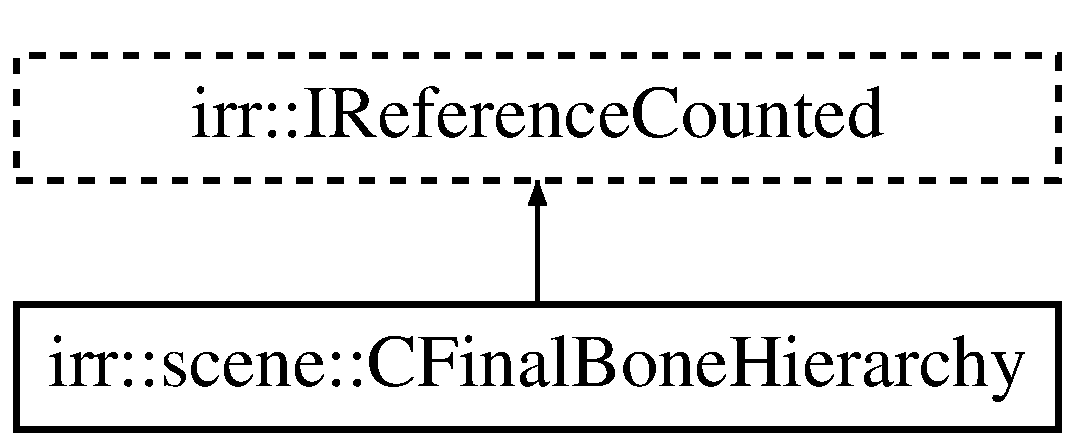
\includegraphics[height=2.000000cm]{classirr_1_1scene_1_1CFinalBoneHierarchy}
\end{center}
\end{figure}
\subsection*{Classes}
\begin{DoxyCompactItemize}
\item 
struct \hyperlink{structirr_1_1scene_1_1CFinalBoneHierarchy_1_1AnimationKeyData}{Animation\+Key\+Data}
\item 
struct \hyperlink{structirr_1_1scene_1_1CFinalBoneHierarchy_1_1BoneReferenceData}{Bone\+Reference\+Data}
\end{DoxyCompactItemize}
\subsection*{Public Member Functions}
\begin{DoxyCompactItemize}
\item 
{\bfseries C\+Final\+Bone\+Hierarchy} (const std\+::vector$<$ \hyperlink{classirr_1_1scene_1_1ICPUSkinnedMesh_1_1SJoint}{I\+C\+P\+U\+Skinned\+Mesh\+::\+S\+Joint} $\ast$ $>$ \&in\+Level\+Fixed\+Joints, const std\+::vector$<$ size\+\_\+t $>$ \&in\+Joints\+Level\+End)\hypertarget{classirr_1_1scene_1_1CFinalBoneHierarchy_ac8858e4e16cf973516650dc48b638ceb}{}\label{classirr_1_1scene_1_1CFinalBoneHierarchy_ac8858e4e16cf973516650dc48b638ceb}

\item 
\hyperlink{classirr_1_1scene_1_1CFinalBoneHierarchy_a7e20b6ecb0668954ecc1f279f6e02006}{$\sim$\+C\+Final\+Bone\+Hierarchy} ()
\item 
const size\+\_\+t \& {\bfseries get\+Bone\+Count} () const \hypertarget{classirr_1_1scene_1_1CFinalBoneHierarchy_ae267cac421c80aa9d087e0b3f1a0ce89}{}\label{classirr_1_1scene_1_1CFinalBoneHierarchy_ae267cac421c80aa9d087e0b3f1a0ce89}

\item 
const \hyperlink{structirr_1_1scene_1_1CFinalBoneHierarchy_1_1BoneReferenceData}{Bone\+Reference\+Data} $\ast$ {\bfseries get\+Bone\+Data} () const \hypertarget{classirr_1_1scene_1_1CFinalBoneHierarchy_a320196a123686ee5bd9e7aff3d6dc09c}{}\label{classirr_1_1scene_1_1CFinalBoneHierarchy_a320196a123686ee5bd9e7aff3d6dc09c}

\item 
const \hyperlink{namespaceirr_1_1core_ade1071a878633f2f6d8a75c5d11fec19}{core\+::stringc} \& {\bfseries get\+Bone\+Name} (const size\+\_\+t \&bone\+ID) const \hypertarget{classirr_1_1scene_1_1CFinalBoneHierarchy_a2f1a515e0107f75bc7674ab02d359751}{}\label{classirr_1_1scene_1_1CFinalBoneHierarchy_a2f1a515e0107f75bc7674ab02d359751}

\item 
size\+\_\+t {\bfseries get\+Bone\+I\+D\+From\+Name} (const char $\ast$name) const \hypertarget{classirr_1_1scene_1_1CFinalBoneHierarchy_a4de13716f8fe16db7469ac2463a1b26f}{}\label{classirr_1_1scene_1_1CFinalBoneHierarchy_a4de13716f8fe16db7469ac2463a1b26f}

\item 
const size\+\_\+t \& {\bfseries get\+Hierarchy\+Levels} () const \hypertarget{classirr_1_1scene_1_1CFinalBoneHierarchy_af9ec96fc70811d08704f37ebca442b3a}{}\label{classirr_1_1scene_1_1CFinalBoneHierarchy_af9ec96fc70811d08704f37ebca442b3a}

\item 
const size\+\_\+t \& {\bfseries get\+Bone\+Level\+Range\+Start} (const size\+\_\+t \&level) const \hypertarget{classirr_1_1scene_1_1CFinalBoneHierarchy_a5b9b191cca693d282ca9a73bdffb7ce2}{}\label{classirr_1_1scene_1_1CFinalBoneHierarchy_a5b9b191cca693d282ca9a73bdffb7ce2}

\item 
const size\+\_\+t \& {\bfseries get\+Bone\+Level\+Range\+Length} (const size\+\_\+t \&level) const \hypertarget{classirr_1_1scene_1_1CFinalBoneHierarchy_af7b2aae797a70555fc5dc9f2e610a8ed}{}\label{classirr_1_1scene_1_1CFinalBoneHierarchy_af7b2aae797a70555fc5dc9f2e610a8ed}

\item 
const size\+\_\+t \& {\bfseries get\+Bone\+Level\+Range\+End} (const size\+\_\+t \&level) const \hypertarget{classirr_1_1scene_1_1CFinalBoneHierarchy_aa5d8d288132102e61dce15ffdb7d0212}{}\label{classirr_1_1scene_1_1CFinalBoneHierarchy_aa5d8d288132102e61dce15ffdb7d0212}

\item 
const size\+\_\+t \& {\bfseries get\+Key\+Frame\+Count} () const \hypertarget{classirr_1_1scene_1_1CFinalBoneHierarchy_abb07afd622f2e9a915e636aeb1398f08}{}\label{classirr_1_1scene_1_1CFinalBoneHierarchy_abb07afd622f2e9a915e636aeb1398f08}

\item 
const float $\ast$ {\bfseries get\+Keys} () const \hypertarget{classirr_1_1scene_1_1CFinalBoneHierarchy_a9b8bf03d3c967fe96a488d1e0a66f6cf}{}\label{classirr_1_1scene_1_1CFinalBoneHierarchy_a9b8bf03d3c967fe96a488d1e0a66f6cf}

\item 
size\+\_\+t \hyperlink{classirr_1_1scene_1_1CFinalBoneHierarchy_a73ab77d3cb4e1972faa34a43b94205e7}{get\+Lower\+Bound\+Bone\+Keyframes} (float \&interpolation\+Factor, const float \&frame) const 
\item 
size\+\_\+t {\bfseries get\+Lower\+Bound\+Bone\+Keyframes} (const float \&frame) const \hypertarget{classirr_1_1scene_1_1CFinalBoneHierarchy_a2ebef77caf191a4aa31daffa91effb54}{}\label{classirr_1_1scene_1_1CFinalBoneHierarchy_a2ebef77caf191a4aa31daffa91effb54}

\item 
const \hyperlink{structirr_1_1scene_1_1CFinalBoneHierarchy_1_1AnimationKeyData}{Animation\+Key\+Data} $\ast$ {\bfseries get\+Interpolated\+Animation\+Data} (const size\+\_\+t \&bone\+ID=0) const \hypertarget{classirr_1_1scene_1_1CFinalBoneHierarchy_ac52eae05ebf14e2d197c323bdb53ac57}{}\label{classirr_1_1scene_1_1CFinalBoneHierarchy_ac52eae05ebf14e2d197c323bdb53ac57}

\item 
const \hyperlink{structirr_1_1scene_1_1CFinalBoneHierarchy_1_1AnimationKeyData}{Animation\+Key\+Data} $\ast$ {\bfseries get\+Non\+Interpolated\+Animation\+Data} (const size\+\_\+t \&bone\+ID=0) const \hypertarget{classirr_1_1scene_1_1CFinalBoneHierarchy_a5ddd341f3f071885256b5bfe2a4b59b7}{}\label{classirr_1_1scene_1_1CFinalBoneHierarchy_a5ddd341f3f071885256b5bfe2a4b59b7}

\end{DoxyCompactItemize}
\subsection*{Static Public Member Functions}
\begin{DoxyCompactItemize}
\item 
static \hyperlink{classirr_1_1core_1_1matrix4x3}{core\+::matrix4x3} {\bfseries get\+Matrix\+From\+Keys} (const \hyperlink{structirr_1_1scene_1_1CFinalBoneHierarchy_1_1AnimationKeyData}{Animation\+Key\+Data} \&keyframeA, const \hyperlink{structirr_1_1scene_1_1CFinalBoneHierarchy_1_1AnimationKeyData}{Animation\+Key\+Data} \&keyframeB, const float \&interpolant)\hypertarget{classirr_1_1scene_1_1CFinalBoneHierarchy_aad061460e833df60faf9bea74ddfca21}{}\label{classirr_1_1scene_1_1CFinalBoneHierarchy_aad061460e833df60faf9bea74ddfca21}

\item 
static \hyperlink{classirr_1_1core_1_1matrix4x3}{core\+::matrix4x3} {\bfseries get\+Matrix\+From\+Key} (const \hyperlink{structirr_1_1scene_1_1CFinalBoneHierarchy_1_1AnimationKeyData}{Animation\+Key\+Data} \&keyframe)\hypertarget{classirr_1_1scene_1_1CFinalBoneHierarchy_a685c4657b59edd2b32b8ce0632801293}{}\label{classirr_1_1scene_1_1CFinalBoneHierarchy_a685c4657b59edd2b32b8ce0632801293}

\end{DoxyCompactItemize}
\subsection*{Public Attributes}
\begin{DoxyCompactItemize}
\item 
struct \hyperlink{structirr_1_1scene_1_1CFinalBoneHierarchy_1_1BoneReferenceData}{irr\+::scene\+::\+C\+Final\+Bone\+Hierarchy\+::\+Bone\+Reference\+Data} {\bfseries P\+A\+C\+K\+\_\+\+S\+T\+R\+U\+CT}\hypertarget{classirr_1_1scene_1_1CFinalBoneHierarchy_ab0d7af1304027fb016201956eabcc871}{}\label{classirr_1_1scene_1_1CFinalBoneHierarchy_ab0d7af1304027fb016201956eabcc871}

\item 
struct \hyperlink{structirr_1_1scene_1_1CFinalBoneHierarchy_1_1AnimationKeyData}{irr\+::scene\+::\+C\+Final\+Bone\+Hierarchy\+::\+Animation\+Key\+Data} {\bfseries P\+A\+C\+K\+\_\+\+S\+T\+R\+U\+CT}\hypertarget{classirr_1_1scene_1_1CFinalBoneHierarchy_afc5d3887d08697790efda6abea2897d8}{}\label{classirr_1_1scene_1_1CFinalBoneHierarchy_afc5d3887d08697790efda6abea2897d8}

\end{DoxyCompactItemize}
\subsection*{Additional Inherited Members}


\subsection{Detailed Description}
If it has no animation, make 1 frame of animation with Local\+Matrix. 

\subsection{Constructor \& Destructor Documentation}
\index{irr\+::scene\+::\+C\+Final\+Bone\+Hierarchy@{irr\+::scene\+::\+C\+Final\+Bone\+Hierarchy}!````~C\+Final\+Bone\+Hierarchy@{$\sim$\+C\+Final\+Bone\+Hierarchy}}
\index{````~C\+Final\+Bone\+Hierarchy@{$\sim$\+C\+Final\+Bone\+Hierarchy}!irr\+::scene\+::\+C\+Final\+Bone\+Hierarchy@{irr\+::scene\+::\+C\+Final\+Bone\+Hierarchy}}
\subsubsection[{\texorpdfstring{$\sim$\+C\+Final\+Bone\+Hierarchy()}{~CFinalBoneHierarchy()}}]{\setlength{\rightskip}{0pt plus 5cm}irr\+::scene\+::\+C\+Final\+Bone\+Hierarchy\+::$\sim$\+C\+Final\+Bone\+Hierarchy (
\begin{DoxyParamCaption}
{}
\end{DoxyParamCaption}
)\hspace{0.3cm}{\ttfamily [inline]}}\hypertarget{classirr_1_1scene_1_1CFinalBoneHierarchy_a7e20b6ecb0668954ecc1f279f6e02006}{}\label{classirr_1_1scene_1_1CFinalBoneHierarchy_a7e20b6ecb0668954ecc1f279f6e02006}
if (bound\+Buffer) bound\+Buffer-\/$>$\hyperlink{classirr_1_1IReferenceCounted_afb169a857e0d2cdb96b8821cb9bff17a}{drop()};

\subsection{Member Function Documentation}
\index{irr\+::scene\+::\+C\+Final\+Bone\+Hierarchy@{irr\+::scene\+::\+C\+Final\+Bone\+Hierarchy}!get\+Lower\+Bound\+Bone\+Keyframes@{get\+Lower\+Bound\+Bone\+Keyframes}}
\index{get\+Lower\+Bound\+Bone\+Keyframes@{get\+Lower\+Bound\+Bone\+Keyframes}!irr\+::scene\+::\+C\+Final\+Bone\+Hierarchy@{irr\+::scene\+::\+C\+Final\+Bone\+Hierarchy}}
\subsubsection[{\texorpdfstring{get\+Lower\+Bound\+Bone\+Keyframes(float \&interpolation\+Factor, const float \&frame) const }{getLowerBoundBoneKeyframes(float \&interpolationFactor, const float \&frame) const }}]{\setlength{\rightskip}{0pt plus 5cm}size\+\_\+t irr\+::scene\+::\+C\+Final\+Bone\+Hierarchy\+::get\+Lower\+Bound\+Bone\+Keyframes (
\begin{DoxyParamCaption}
\item[{float \&}]{interpolation\+Factor, }
\item[{const float \&}]{frame}
\end{DoxyParamCaption}
) const\hspace{0.3cm}{\ttfamily [inline]}}\hypertarget{classirr_1_1scene_1_1CFinalBoneHierarchy_a73ab77d3cb4e1972faa34a43b94205e7}{}\label{classirr_1_1scene_1_1CFinalBoneHierarchy_a73ab77d3cb4e1972faa34a43b94205e7}
! ready but untested inline void put\+In\+G\+P\+U\+Buffer(\hyperlink{classirr_1_1video_1_1IGPUBuffer}{video\+::\+I\+G\+P\+U\+Buffer}$\ast$ buffer, const size\+\_\+t\& byte\+Offset=0) \{ size\+\_\+t bone\+Data\+Size = sizeof(\+Bone\+Reference\+Data)$\ast$bone\+Count; if (!buffer$\vert$$\vert$byte\+Offset+bone\+Data\+Size$>$buffer-\/$>$get\+Size()) return; else if (buffer-\/$>$is\+Mapped\+Buffer()) \{ if (!dynamic\+\_\+cast$<$\hyperlink{classirr_1_1video_1_1IGPUMappedBuffer}{video\+::\+I\+G\+P\+U\+Mapped\+Buffer}$\ast$$>$(buffer)-\/$>$get\+Pointer()) return; \} else if (!buffer-\/$>$can\+Update\+Sub\+Range()) return;

buffer-\/$>$\hyperlink{classirr_1_1IReferenceCounted_a2b7a035532e5f409ca9482dab79185f4}{grab()}; if (bound\+Buffer) bound\+Buffer-\/$>$\hyperlink{classirr_1_1IReferenceCounted_afb169a857e0d2cdb96b8821cb9bff17a}{drop()}; bound\+Buffer = buffer;

if (buffer-\/$>$is\+Mapped\+Buffer()) memcpy(reinterpret\+\_\+cast$<$uint8\+\_\+t$\ast$$>$(dynamic\+\_\+cast$<$video\+::\+I\+G\+P\+U\+Mapped\+Buffer$\ast$$>$(buffer)-\/$>$get\+Pointer())+byte\+Offset,bone\+Flat\+Array,bone\+Data\+Size); else buffer-\/$>$update\+Sub\+Range(byte\+Offset,bone\+Data\+Size,bone\+Flat\+Array); \} never a divide by zero, asserts make sure!!! 

The documentation for this class was generated from the following file\+:\begin{DoxyCompactItemize}
\item 
include/C\+Final\+Bone\+Hierarchy.\+h\end{DoxyCompactItemize}

\hypertarget{classirr_1_1scene_1_1CGeometryCreator}{}\section{irr\+:\+:scene\+:\+:C\+Geometry\+Creator Class Reference}
\label{classirr_1_1scene_1_1CGeometryCreator}\index{irr\+::scene\+::\+C\+Geometry\+Creator@{irr\+::scene\+::\+C\+Geometry\+Creator}}


class for creating geometry on the fly  




{\ttfamily \#include $<$C\+Geometry\+Creator.\+h$>$}

Inheritance diagram for irr\+:\+:scene\+:\+:C\+Geometry\+Creator\+:\begin{figure}[H]
\begin{center}
\leavevmode
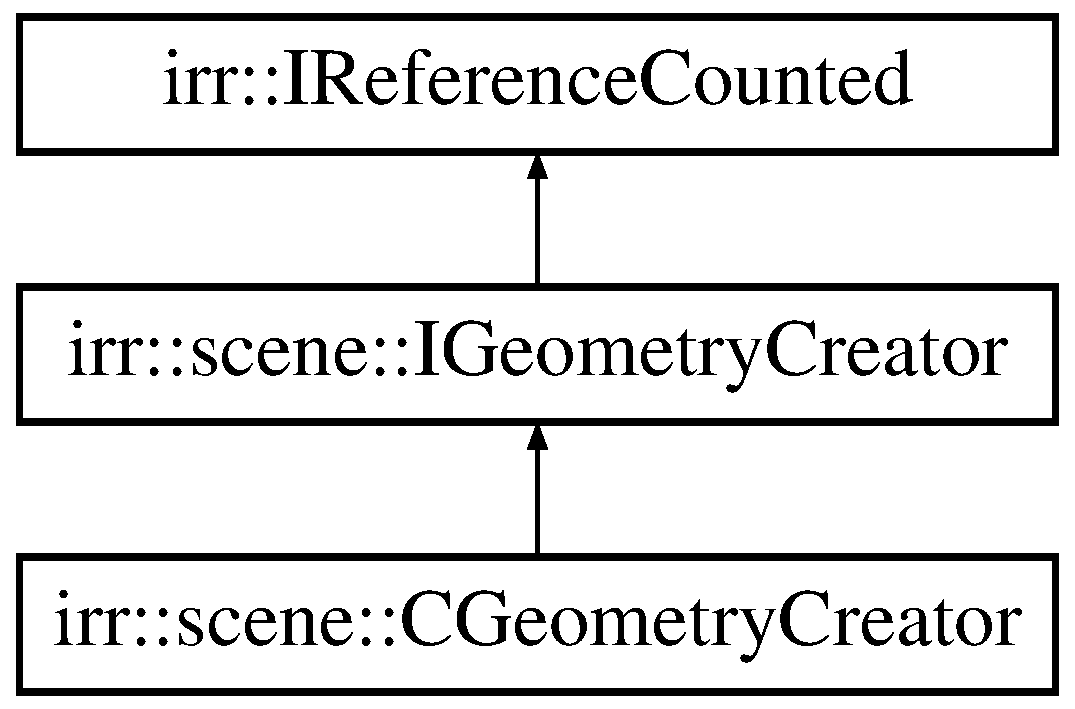
\includegraphics[height=3.000000cm]{classirr_1_1scene_1_1CGeometryCreator}
\end{center}
\end{figure}
\subsection*{Public Member Functions}
\begin{DoxyCompactItemize}
\item 
\hyperlink{classirr_1_1scene_1_1IMesh}{I\+C\+P\+U\+Mesh} $\ast$ {\bfseries create\+Cube\+Mesh\+C\+PU} (const \hyperlink{namespaceirr_1_1core_a06f169d08b5c429f5575acb7edbad811}{core\+::vector3df} \&size) const \hypertarget{classirr_1_1scene_1_1CGeometryCreator_a6f50727c9761662a71b6107b56755db5}{}\label{classirr_1_1scene_1_1CGeometryCreator_a6f50727c9761662a71b6107b56755db5}

\item 
\hyperlink{classirr_1_1scene_1_1IMesh}{I\+G\+P\+U\+Mesh} $\ast$ \hyperlink{classirr_1_1scene_1_1CGeometryCreator_a9aea899bffc8dc7042f4b2d8d176f40d}{create\+Cube\+Mesh\+G\+PU} (\hyperlink{classirr_1_1video_1_1IVideoDriver}{video\+::\+I\+Video\+Driver} $\ast$driver, const \hyperlink{namespaceirr_1_1core_a06f169d08b5c429f5575acb7edbad811}{core\+::vector3df} \&size) const 
\begin{DoxyCompactList}\small\item\em Creates a simple cube mesh. \end{DoxyCompactList}\item 
\hyperlink{classirr_1_1scene_1_1IMesh}{I\+C\+P\+U\+Mesh} $\ast$ {\bfseries create\+Terrain\+Mesh\+C\+PU} (\hyperlink{classirr_1_1video_1_1IImage}{video\+::\+I\+Image} $\ast$texture, \hyperlink{classirr_1_1video_1_1IImage}{video\+::\+I\+Image} $\ast$heightmap, const \hyperlink{classirr_1_1core_1_1dimension2d}{core\+::dimension2d}$<$ \hyperlink{namespaceirr_a0277be98d67dc26ff93b1a6a1d086b07}{f32} $>$ \&stretch\+Size, \hyperlink{namespaceirr_a0277be98d67dc26ff93b1a6a1d086b07}{f32} max\+Height, \hyperlink{classirr_1_1video_1_1IVideoDriver}{video\+::\+I\+Video\+Driver} $\ast$driver, const \hyperlink{classirr_1_1core_1_1dimension2d}{core\+::dimension2d}$<$ \hyperlink{namespaceirr_a0416a53257075833e7002efd0a18e804}{u32} $>$ \&default\+Vertex\+Block\+Size, bool debug\+Borders=false) const \hypertarget{classirr_1_1scene_1_1CGeometryCreator_ae8b0311a5836d5910dd018caa6992ca1}{}\label{classirr_1_1scene_1_1CGeometryCreator_ae8b0311a5836d5910dd018caa6992ca1}

\item 
\hyperlink{classirr_1_1scene_1_1IMesh}{I\+G\+P\+U\+Mesh} $\ast$ \hyperlink{classirr_1_1scene_1_1CGeometryCreator_a98e9498db779952823f9f1b5fcf7d68e}{create\+Terrain\+Mesh\+G\+PU} (\hyperlink{classirr_1_1video_1_1IImage}{video\+::\+I\+Image} $\ast$texture, \hyperlink{classirr_1_1video_1_1IImage}{video\+::\+I\+Image} $\ast$heightmap, const \hyperlink{classirr_1_1core_1_1dimension2d}{core\+::dimension2d}$<$ \hyperlink{namespaceirr_a0277be98d67dc26ff93b1a6a1d086b07}{f32} $>$ \&stretch\+Size, \hyperlink{namespaceirr_a0277be98d67dc26ff93b1a6a1d086b07}{f32} max\+Height, \hyperlink{classirr_1_1video_1_1IVideoDriver}{video\+::\+I\+Video\+Driver} $\ast$driver, const \hyperlink{classirr_1_1core_1_1dimension2d}{core\+::dimension2d}$<$ \hyperlink{namespaceirr_a0416a53257075833e7002efd0a18e804}{u32} $>$ \&default\+Vertex\+Block\+Size, bool debug\+Borders=false) const 
\begin{DoxyCompactList}\small\item\em Create a terrain mesh from an image representing a heightfield. \end{DoxyCompactList}\item 
\hyperlink{classirr_1_1scene_1_1IMesh}{I\+C\+P\+U\+Mesh} $\ast$ {\bfseries create\+Arrow\+Mesh\+C\+PU} (const \hyperlink{namespaceirr_a0416a53257075833e7002efd0a18e804}{u32} tesselation\+Cylinder, const \hyperlink{namespaceirr_a0416a53257075833e7002efd0a18e804}{u32} tesselation\+Cone, const \hyperlink{namespaceirr_a0277be98d67dc26ff93b1a6a1d086b07}{f32} height, const \hyperlink{namespaceirr_a0277be98d67dc26ff93b1a6a1d086b07}{f32} cylinder\+Height, const \hyperlink{namespaceirr_a0277be98d67dc26ff93b1a6a1d086b07}{f32} width0, const \hyperlink{namespaceirr_a0277be98d67dc26ff93b1a6a1d086b07}{f32} width1, const \hyperlink{classirr_1_1video_1_1SColor}{video\+::\+S\+Color} vtx\+Color0, const \hyperlink{classirr_1_1video_1_1SColor}{video\+::\+S\+Color} vtx\+Color1) const \hypertarget{classirr_1_1scene_1_1CGeometryCreator_ad623c74eb80d4d3375c03cff99852f16}{}\label{classirr_1_1scene_1_1CGeometryCreator_ad623c74eb80d4d3375c03cff99852f16}

\item 
\hyperlink{classirr_1_1scene_1_1IMesh}{I\+G\+P\+U\+Mesh} $\ast$ \hyperlink{classirr_1_1scene_1_1CGeometryCreator_a2409f4deb5ede1eec584137928b4bdb5}{create\+Arrow\+Mesh\+G\+PU} (\hyperlink{classirr_1_1video_1_1IVideoDriver}{video\+::\+I\+Video\+Driver} $\ast$driver, const \hyperlink{namespaceirr_a0416a53257075833e7002efd0a18e804}{u32} tesselation\+Cylinder, const \hyperlink{namespaceirr_a0416a53257075833e7002efd0a18e804}{u32} tesselation\+Cone, const \hyperlink{namespaceirr_a0277be98d67dc26ff93b1a6a1d086b07}{f32} height, const \hyperlink{namespaceirr_a0277be98d67dc26ff93b1a6a1d086b07}{f32} cylinder\+Height, const \hyperlink{namespaceirr_a0277be98d67dc26ff93b1a6a1d086b07}{f32} width0, const \hyperlink{namespaceirr_a0277be98d67dc26ff93b1a6a1d086b07}{f32} width1, const \hyperlink{classirr_1_1video_1_1SColor}{video\+::\+S\+Color} vtx\+Color0, const \hyperlink{classirr_1_1video_1_1SColor}{video\+::\+S\+Color} vtx\+Color1) const 
\begin{DoxyCompactList}\small\item\em Create an arrow mesh, composed of a cylinder and a cone. \end{DoxyCompactList}\item 
\hyperlink{classirr_1_1scene_1_1IMesh}{I\+C\+P\+U\+Mesh} $\ast$ {\bfseries create\+Sphere\+Mesh\+C\+PU} (\hyperlink{namespaceirr_a0277be98d67dc26ff93b1a6a1d086b07}{f32} radius, \hyperlink{namespaceirr_a0416a53257075833e7002efd0a18e804}{u32} poly\+CountX, \hyperlink{namespaceirr_a0416a53257075833e7002efd0a18e804}{u32} poly\+CountY) const \hypertarget{classirr_1_1scene_1_1CGeometryCreator_a6fe2ddebda8cfb001b47912d05113c49}{}\label{classirr_1_1scene_1_1CGeometryCreator_a6fe2ddebda8cfb001b47912d05113c49}

\item 
\hyperlink{classirr_1_1scene_1_1IMesh}{I\+G\+P\+U\+Mesh} $\ast$ \hyperlink{classirr_1_1scene_1_1CGeometryCreator_a3dd60997db6232e563cba44eb3c0880f}{create\+Sphere\+Mesh\+G\+PU} (\hyperlink{classirr_1_1video_1_1IVideoDriver}{video\+::\+I\+Video\+Driver} $\ast$driver, \hyperlink{namespaceirr_a0277be98d67dc26ff93b1a6a1d086b07}{f32} radius, \hyperlink{namespaceirr_a0416a53257075833e7002efd0a18e804}{u32} poly\+CountX, \hyperlink{namespaceirr_a0416a53257075833e7002efd0a18e804}{u32} poly\+CountY) const 
\begin{DoxyCompactList}\small\item\em Create a sphere mesh. \end{DoxyCompactList}\item 
\hyperlink{classirr_1_1scene_1_1IMesh}{I\+C\+P\+U\+Mesh} $\ast$ {\bfseries create\+Cylinder\+Mesh\+C\+PU} (\hyperlink{namespaceirr_a0277be98d67dc26ff93b1a6a1d086b07}{f32} radius, \hyperlink{namespaceirr_a0277be98d67dc26ff93b1a6a1d086b07}{f32} length, \hyperlink{namespaceirr_a0416a53257075833e7002efd0a18e804}{u32} tesselation, const \hyperlink{classirr_1_1video_1_1SColor}{video\+::\+S\+Color} \&color=0xffffffff, bool close\+Top=true, f32 oblique=0.\+f) const \hypertarget{classirr_1_1scene_1_1CGeometryCreator_a9cd6309163a191f7fcf73c81bfee5f09}{}\label{classirr_1_1scene_1_1CGeometryCreator_a9cd6309163a191f7fcf73c81bfee5f09}

\item 
\hyperlink{classirr_1_1scene_1_1IMesh}{I\+G\+P\+U\+Mesh} $\ast$ \hyperlink{classirr_1_1scene_1_1CGeometryCreator_ac35744e4622432d0df0d550c588d5082}{create\+Cylinder\+Mesh\+G\+PU} (\hyperlink{classirr_1_1video_1_1IVideoDriver}{video\+::\+I\+Video\+Driver} $\ast$driver, \hyperlink{namespaceirr_a0277be98d67dc26ff93b1a6a1d086b07}{f32} radius, \hyperlink{namespaceirr_a0277be98d67dc26ff93b1a6a1d086b07}{f32} length, \hyperlink{namespaceirr_a0416a53257075833e7002efd0a18e804}{u32} tesselation, const \hyperlink{classirr_1_1video_1_1SColor}{video\+::\+S\+Color} \&color=0xffffffff, bool close\+Top=true, f32 oblique=0.\+f) const 
\begin{DoxyCompactList}\small\item\em Create a cylinder mesh. \end{DoxyCompactList}\item 
\hyperlink{classirr_1_1scene_1_1IMesh}{I\+C\+P\+U\+Mesh} $\ast$ {\bfseries create\+Cone\+Mesh\+C\+PU} (\hyperlink{namespaceirr_a0277be98d67dc26ff93b1a6a1d086b07}{f32} radius, \hyperlink{namespaceirr_a0277be98d67dc26ff93b1a6a1d086b07}{f32} length, \hyperlink{namespaceirr_a0416a53257075833e7002efd0a18e804}{u32} tesselation, const \hyperlink{classirr_1_1video_1_1SColor}{video\+::\+S\+Color} \&color\+Top=0xffffffff, const video\+::\+S\+Color \&color\+Bottom=0xffffffff, f32 oblique=0.\+f) const \hypertarget{classirr_1_1scene_1_1CGeometryCreator_a229519d3118ba2d02ee9eb4c85143d5b}{}\label{classirr_1_1scene_1_1CGeometryCreator_a229519d3118ba2d02ee9eb4c85143d5b}

\item 
\hyperlink{classirr_1_1scene_1_1IMesh}{I\+G\+P\+U\+Mesh} $\ast$ \hyperlink{classirr_1_1scene_1_1CGeometryCreator_a6587c178f43773c42d4566c93147eebb}{create\+Cone\+Mesh\+G\+PU} (\hyperlink{classirr_1_1video_1_1IVideoDriver}{video\+::\+I\+Video\+Driver} $\ast$driver, \hyperlink{namespaceirr_a0277be98d67dc26ff93b1a6a1d086b07}{f32} radius, \hyperlink{namespaceirr_a0277be98d67dc26ff93b1a6a1d086b07}{f32} length, \hyperlink{namespaceirr_a0416a53257075833e7002efd0a18e804}{u32} tesselation, const \hyperlink{classirr_1_1video_1_1SColor}{video\+::\+S\+Color} \&color\+Top=0xffffffff, const video\+::\+S\+Color \&color\+Bottom=0xffffffff, f32 oblique=0.\+f) const 
\begin{DoxyCompactList}\small\item\em Create a cone mesh. \end{DoxyCompactList}\end{DoxyCompactItemize}
\subsection*{Additional Inherited Members}


\subsection{Detailed Description}
class for creating geometry on the fly 

\subsection{Member Function Documentation}
\index{irr\+::scene\+::\+C\+Geometry\+Creator@{irr\+::scene\+::\+C\+Geometry\+Creator}!create\+Arrow\+Mesh\+G\+PU@{create\+Arrow\+Mesh\+G\+PU}}
\index{create\+Arrow\+Mesh\+G\+PU@{create\+Arrow\+Mesh\+G\+PU}!irr\+::scene\+::\+C\+Geometry\+Creator@{irr\+::scene\+::\+C\+Geometry\+Creator}}
\subsubsection[{\texorpdfstring{create\+Arrow\+Mesh\+G\+P\+U(video\+::\+I\+Video\+Driver $\ast$driver, const u32 tesselation\+Cylinder, const u32 tesselation\+Cone, const f32 height, const f32 cylinder\+Height, const f32 width0, const f32 width1, const video\+::\+S\+Color vtx\+Color0, const video\+::\+S\+Color vtx\+Color1) const }{createArrowMeshGPU(video::IVideoDriver *driver, const u32 tesselationCylinder, const u32 tesselationCone, const f32 height, const f32 cylinderHeight, const f32 width0, const f32 width1, const video::SColor vtxColor0, const video::SColor vtxColor1) const }}]{\setlength{\rightskip}{0pt plus 5cm}{\bf I\+G\+P\+U\+Mesh}$\ast$ irr\+::scene\+::\+C\+Geometry\+Creator\+::create\+Arrow\+Mesh\+G\+PU (
\begin{DoxyParamCaption}
\item[{{\bf video\+::\+I\+Video\+Driver} $\ast$}]{driver, }
\item[{const {\bf u32}}]{tesselation\+Cylinder, }
\item[{const {\bf u32}}]{tesselation\+Cone, }
\item[{const {\bf f32}}]{height, }
\item[{const {\bf f32}}]{cylinder\+Height, }
\item[{const {\bf f32}}]{width\+Cylinder, }
\item[{const {\bf f32}}]{width\+Cone, }
\item[{const {\bf video\+::\+S\+Color}}]{color\+Cylinder, }
\item[{const {\bf video\+::\+S\+Color}}]{color\+Cone}
\end{DoxyParamCaption}
) const\hspace{0.3cm}{\ttfamily [virtual]}}\hypertarget{classirr_1_1scene_1_1CGeometryCreator_a2409f4deb5ede1eec584137928b4bdb5}{}\label{classirr_1_1scene_1_1CGeometryCreator_a2409f4deb5ede1eec584137928b4bdb5}


Create an arrow mesh, composed of a cylinder and a cone. 


\begin{DoxyParams}{Parameters}
{\em tesselation\+Cylinder} & Number of quads composing the cylinder. \\
\hline
{\em tesselation\+Cone} & Number of triangles composing the cone\textquotesingle{}s roof. \\
\hline
{\em height} & Total height of the arrow \\
\hline
{\em cylinder\+Height} & Total height of the cylinder, should be lesser than total height \\
\hline
{\em width\+Cylinder} & Diameter of the cylinder \\
\hline
{\em width\+Cone} & Diameter of the cone\textquotesingle{}s base, should be not smaller than the cylinder\textquotesingle{}s diameter \\
\hline
{\em color\+Cylinder} & color of the cylinder \\
\hline
{\em color\+Cone} & color of the cone \\
\hline
\end{DoxyParams}
\begin{DoxyReturn}{Returns}
Generated mesh. 
\end{DoxyReturn}


Implements \hyperlink{classirr_1_1scene_1_1IGeometryCreator_abca19991f6bbfbc05b64ab45c2df80c7}{irr\+::scene\+::\+I\+Geometry\+Creator}.

\index{irr\+::scene\+::\+C\+Geometry\+Creator@{irr\+::scene\+::\+C\+Geometry\+Creator}!create\+Cone\+Mesh\+G\+PU@{create\+Cone\+Mesh\+G\+PU}}
\index{create\+Cone\+Mesh\+G\+PU@{create\+Cone\+Mesh\+G\+PU}!irr\+::scene\+::\+C\+Geometry\+Creator@{irr\+::scene\+::\+C\+Geometry\+Creator}}
\subsubsection[{\texorpdfstring{create\+Cone\+Mesh\+G\+P\+U(video\+::\+I\+Video\+Driver $\ast$driver, f32 radius, f32 length, u32 tesselation, const video\+::\+S\+Color \&color\+Top=0xffffffff, const video\+::\+S\+Color \&color\+Bottom=0xffffffff, f32 oblique=0.\+f) const }{createConeMeshGPU(video::IVideoDriver *driver, f32 radius, f32 length, u32 tesselation, const video::SColor \&colorTop=0xffffffff, const video::SColor \&colorBottom=0xffffffff, f32 oblique=0.f) const }}]{\setlength{\rightskip}{0pt plus 5cm}{\bf I\+G\+P\+U\+Mesh}$\ast$ irr\+::scene\+::\+C\+Geometry\+Creator\+::create\+Cone\+Mesh\+G\+PU (
\begin{DoxyParamCaption}
\item[{{\bf video\+::\+I\+Video\+Driver} $\ast$}]{driver, }
\item[{{\bf f32}}]{radius, }
\item[{{\bf f32}}]{length, }
\item[{{\bf u32}}]{tesselation, }
\item[{const {\bf video\+::\+S\+Color} \&}]{color\+Top = {\ttfamily 0xffffffff}, }
\item[{const {\bf video\+::\+S\+Color} \&}]{color\+Bottom = {\ttfamily 0xffffffff}, }
\item[{{\bf f32}}]{oblique = {\ttfamily 0.f}}
\end{DoxyParamCaption}
) const\hspace{0.3cm}{\ttfamily [virtual]}}\hypertarget{classirr_1_1scene_1_1CGeometryCreator_a6587c178f43773c42d4566c93147eebb}{}\label{classirr_1_1scene_1_1CGeometryCreator_a6587c178f43773c42d4566c93147eebb}


Create a cone mesh. 


\begin{DoxyParams}{Parameters}
{\em radius} & Radius of the cone. \\
\hline
{\em length} & Length of the cone. \\
\hline
{\em tesselation} & Number of quads around the circumference of the cone. \\
\hline
{\em color\+Top} & The color of the top of the cone. \\
\hline
{\em color\+Bottom} & The color of the bottom of the cone. \\
\hline
{\em oblique} & (to be documented) \\
\hline
\end{DoxyParams}
\begin{DoxyReturn}{Returns}
Generated mesh. 
\end{DoxyReturn}


Implements \hyperlink{classirr_1_1scene_1_1IGeometryCreator_ad977d1ab6a7d9f839d47e4dc2b50d756}{irr\+::scene\+::\+I\+Geometry\+Creator}.

\index{irr\+::scene\+::\+C\+Geometry\+Creator@{irr\+::scene\+::\+C\+Geometry\+Creator}!create\+Cube\+Mesh\+G\+PU@{create\+Cube\+Mesh\+G\+PU}}
\index{create\+Cube\+Mesh\+G\+PU@{create\+Cube\+Mesh\+G\+PU}!irr\+::scene\+::\+C\+Geometry\+Creator@{irr\+::scene\+::\+C\+Geometry\+Creator}}
\subsubsection[{\texorpdfstring{create\+Cube\+Mesh\+G\+P\+U(video\+::\+I\+Video\+Driver $\ast$driver, const core\+::vector3df \&size) const }{createCubeMeshGPU(video::IVideoDriver *driver, const core::vector3df \&size) const }}]{\setlength{\rightskip}{0pt plus 5cm}{\bf I\+G\+P\+U\+Mesh}$\ast$ irr\+::scene\+::\+C\+Geometry\+Creator\+::create\+Cube\+Mesh\+G\+PU (
\begin{DoxyParamCaption}
\item[{{\bf video\+::\+I\+Video\+Driver} $\ast$}]{driver, }
\item[{const {\bf core\+::vector3df} \&}]{size}
\end{DoxyParamCaption}
) const\hspace{0.3cm}{\ttfamily [virtual]}}\hypertarget{classirr_1_1scene_1_1CGeometryCreator_a9aea899bffc8dc7042f4b2d8d176f40d}{}\label{classirr_1_1scene_1_1CGeometryCreator_a9aea899bffc8dc7042f4b2d8d176f40d}


Creates a simple cube mesh. 


\begin{DoxyParams}{Parameters}
{\em size} & Dimensions of the cube. \\
\hline
\end{DoxyParams}
\begin{DoxyReturn}{Returns}
Generated mesh. 
\end{DoxyReturn}


Implements \hyperlink{classirr_1_1scene_1_1IGeometryCreator_a1676dd58d6bfd7546e728dd9ea5599f6}{irr\+::scene\+::\+I\+Geometry\+Creator}.

\index{irr\+::scene\+::\+C\+Geometry\+Creator@{irr\+::scene\+::\+C\+Geometry\+Creator}!create\+Cylinder\+Mesh\+G\+PU@{create\+Cylinder\+Mesh\+G\+PU}}
\index{create\+Cylinder\+Mesh\+G\+PU@{create\+Cylinder\+Mesh\+G\+PU}!irr\+::scene\+::\+C\+Geometry\+Creator@{irr\+::scene\+::\+C\+Geometry\+Creator}}
\subsubsection[{\texorpdfstring{create\+Cylinder\+Mesh\+G\+P\+U(video\+::\+I\+Video\+Driver $\ast$driver, f32 radius, f32 length, u32 tesselation, const video\+::\+S\+Color \&color=0xffffffff, bool close\+Top=true, f32 oblique=0.\+f) const }{createCylinderMeshGPU(video::IVideoDriver *driver, f32 radius, f32 length, u32 tesselation, const video::SColor \&color=0xffffffff, bool closeTop=true, f32 oblique=0.f) const }}]{\setlength{\rightskip}{0pt plus 5cm}{\bf I\+G\+P\+U\+Mesh}$\ast$ irr\+::scene\+::\+C\+Geometry\+Creator\+::create\+Cylinder\+Mesh\+G\+PU (
\begin{DoxyParamCaption}
\item[{{\bf video\+::\+I\+Video\+Driver} $\ast$}]{driver, }
\item[{{\bf f32}}]{radius, }
\item[{{\bf f32}}]{length, }
\item[{{\bf u32}}]{tesselation, }
\item[{const {\bf video\+::\+S\+Color} \&}]{color = {\ttfamily 0xffffffff}, }
\item[{bool}]{close\+Top = {\ttfamily true}, }
\item[{{\bf f32}}]{oblique = {\ttfamily 0.f}}
\end{DoxyParamCaption}
) const\hspace{0.3cm}{\ttfamily [virtual]}}\hypertarget{classirr_1_1scene_1_1CGeometryCreator_ac35744e4622432d0df0d550c588d5082}{}\label{classirr_1_1scene_1_1CGeometryCreator_ac35744e4622432d0df0d550c588d5082}


Create a cylinder mesh. 


\begin{DoxyParams}{Parameters}
{\em radius} & Radius of the cylinder. \\
\hline
{\em length} & Length of the cylinder. \\
\hline
{\em tesselation} & Number of quads around the circumference of the cylinder. \\
\hline
{\em color} & The color of the cylinder. \\
\hline
{\em close\+Top} & If true, close the ends of the cylinder, otherwise leave them open. \\
\hline
{\em oblique} & (to be documented) \\
\hline
\end{DoxyParams}
\begin{DoxyReturn}{Returns}
Generated mesh. 
\end{DoxyReturn}


Implements \hyperlink{classirr_1_1scene_1_1IGeometryCreator_a407144cf0d15dcac00cdbf32478cb62b}{irr\+::scene\+::\+I\+Geometry\+Creator}.

\index{irr\+::scene\+::\+C\+Geometry\+Creator@{irr\+::scene\+::\+C\+Geometry\+Creator}!create\+Sphere\+Mesh\+G\+PU@{create\+Sphere\+Mesh\+G\+PU}}
\index{create\+Sphere\+Mesh\+G\+PU@{create\+Sphere\+Mesh\+G\+PU}!irr\+::scene\+::\+C\+Geometry\+Creator@{irr\+::scene\+::\+C\+Geometry\+Creator}}
\subsubsection[{\texorpdfstring{create\+Sphere\+Mesh\+G\+P\+U(video\+::\+I\+Video\+Driver $\ast$driver, f32 radius, u32 poly\+Count\+X, u32 poly\+Count\+Y) const }{createSphereMeshGPU(video::IVideoDriver *driver, f32 radius, u32 polyCountX, u32 polyCountY) const }}]{\setlength{\rightskip}{0pt plus 5cm}{\bf I\+G\+P\+U\+Mesh}$\ast$ irr\+::scene\+::\+C\+Geometry\+Creator\+::create\+Sphere\+Mesh\+G\+PU (
\begin{DoxyParamCaption}
\item[{{\bf video\+::\+I\+Video\+Driver} $\ast$}]{driver, }
\item[{{\bf f32}}]{radius, }
\item[{{\bf u32}}]{poly\+CountX, }
\item[{{\bf u32}}]{poly\+CountY}
\end{DoxyParamCaption}
) const\hspace{0.3cm}{\ttfamily [virtual]}}\hypertarget{classirr_1_1scene_1_1CGeometryCreator_a3dd60997db6232e563cba44eb3c0880f}{}\label{classirr_1_1scene_1_1CGeometryCreator_a3dd60997db6232e563cba44eb3c0880f}


Create a sphere mesh. 


\begin{DoxyParams}{Parameters}
{\em radius} & Radius of the sphere \\
\hline
{\em poly\+CountX} & Number of quads used for the horizontal tiling \\
\hline
{\em poly\+CountY} & Number of quads used for the vertical tiling \\
\hline
\end{DoxyParams}
\begin{DoxyReturn}{Returns}
Generated mesh. 
\end{DoxyReturn}


Implements \hyperlink{classirr_1_1scene_1_1IGeometryCreator_abdea997960c37f721892203312dcadbd}{irr\+::scene\+::\+I\+Geometry\+Creator}.

\index{irr\+::scene\+::\+C\+Geometry\+Creator@{irr\+::scene\+::\+C\+Geometry\+Creator}!create\+Terrain\+Mesh\+G\+PU@{create\+Terrain\+Mesh\+G\+PU}}
\index{create\+Terrain\+Mesh\+G\+PU@{create\+Terrain\+Mesh\+G\+PU}!irr\+::scene\+::\+C\+Geometry\+Creator@{irr\+::scene\+::\+C\+Geometry\+Creator}}
\subsubsection[{\texorpdfstring{create\+Terrain\+Mesh\+G\+P\+U(video\+::\+I\+Image $\ast$texture, video\+::\+I\+Image $\ast$heightmap, const core\+::dimension2d$<$ f32 $>$ \&stretch\+Size, f32 max\+Height, video\+::\+I\+Video\+Driver $\ast$driver, const core\+::dimension2d$<$ u32 $>$ \&default\+Vertex\+Block\+Size, bool debug\+Borders=false) const }{createTerrainMeshGPU(video::IImage *texture, video::IImage *heightmap, const core::dimension2d< f32 > \&stretchSize, f32 maxHeight, video::IVideoDriver *driver, const core::dimension2d< u32 > \&defaultVertexBlockSize, bool debugBorders=false) const }}]{\setlength{\rightskip}{0pt plus 5cm}{\bf I\+G\+P\+U\+Mesh}$\ast$ irr\+::scene\+::\+C\+Geometry\+Creator\+::create\+Terrain\+Mesh\+G\+PU (
\begin{DoxyParamCaption}
\item[{{\bf video\+::\+I\+Image} $\ast$}]{texture, }
\item[{{\bf video\+::\+I\+Image} $\ast$}]{heightmap, }
\item[{const {\bf core\+::dimension2d}$<$ {\bf f32} $>$ \&}]{stretch\+Size, }
\item[{{\bf f32}}]{max\+Height, }
\item[{{\bf video\+::\+I\+Video\+Driver} $\ast$}]{driver, }
\item[{const {\bf core\+::dimension2d}$<$ {\bf u32} $>$ \&}]{default\+Vertex\+Block\+Size, }
\item[{bool}]{debug\+Borders = {\ttfamily false}}
\end{DoxyParamCaption}
) const\hspace{0.3cm}{\ttfamily [virtual]}}\hypertarget{classirr_1_1scene_1_1CGeometryCreator_a98e9498db779952823f9f1b5fcf7d68e}{}\label{classirr_1_1scene_1_1CGeometryCreator_a98e9498db779952823f9f1b5fcf7d68e}


Create a terrain mesh from an image representing a heightfield. 


\begin{DoxyParams}{Parameters}
{\em texture} & The texture to apply to the terrain. \\
\hline
{\em heightmap} & An image that will be interpreted as a heightmap. The brightness (average color) of each pixel is interpreted as a height, with a 255 brightness pixel producing the maximum height. \\
\hline
{\em stretch\+Size} & The size that each pixel will produce, i.\+e. a 512x512 heightmap and a stretch\+Size of (10.\+f, 20.\+f) will produce a mesh of size 5120.\+f x 10240.\+f \\
\hline
{\em max\+Height} & The maximum height of the terrain. \\
\hline
{\em driver} & The current video driver. \\
\hline
{\em default\+Vertex\+Block\+Size} & (to be documented) \\
\hline
{\em debug\+Borders} & (to be documented) \\
\hline
\end{DoxyParams}
\begin{DoxyReturn}{Returns}
Generated mesh. 
\end{DoxyReturn}


Implements \hyperlink{classirr_1_1scene_1_1IGeometryCreator_a687cc4dc19a40ab892d6a18cb9c6f86e}{irr\+::scene\+::\+I\+Geometry\+Creator}.



The documentation for this class was generated from the following file\+:\begin{DoxyCompactItemize}
\item 
include/C\+Geometry\+Creator.\+h\end{DoxyCompactItemize}

\hypertarget{classirr_1_1core_1_1CMatrix4}{}\section{irr\+:\+:core\+:\+:C\+Matrix4$<$ T $>$ Class Template Reference}
\label{classirr_1_1core_1_1CMatrix4}\index{irr\+::core\+::\+C\+Matrix4$<$ T $>$@{irr\+::core\+::\+C\+Matrix4$<$ T $>$}}


4x4 matrix. Mostly used as transformation matrix for 3d calculations.  




{\ttfamily \#include $<$matrix4.\+h$>$}

\subsection*{Public Types}
\begin{DoxyCompactItemize}
\item 
enum \hyperlink{classirr_1_1core_1_1CMatrix4_a7bb79712227617f706ed57a34f3eb4fe}{e\+Constructor} \{ \\*
{\bfseries E\+M4\+C\+O\+N\+S\+T\+\_\+\+N\+O\+T\+H\+I\+NG} = 0, 
{\bfseries E\+M4\+C\+O\+N\+S\+T\+\_\+\+C\+O\+PY}, 
{\bfseries E\+M4\+C\+O\+N\+S\+T\+\_\+\+I\+D\+E\+N\+T\+I\+TY}, 
{\bfseries E\+M4\+C\+O\+N\+S\+T\+\_\+\+T\+R\+A\+N\+S\+P\+O\+S\+ED}, 
\\*
{\bfseries E\+M4\+C\+O\+N\+S\+T\+\_\+\+I\+N\+V\+E\+R\+SE}, 
{\bfseries E\+M4\+C\+O\+N\+S\+T\+\_\+\+I\+N\+V\+E\+R\+S\+E\+\_\+\+T\+R\+A\+N\+S\+P\+O\+S\+ED}
 \}\hypertarget{classirr_1_1core_1_1CMatrix4_a7bb79712227617f706ed57a34f3eb4fe}{}\label{classirr_1_1core_1_1CMatrix4_a7bb79712227617f706ed57a34f3eb4fe}
\begin{DoxyCompactList}\small\item\em Constructor Flags. \end{DoxyCompactList}
\end{DoxyCompactItemize}
\subsection*{Public Member Functions}
\begin{DoxyCompactItemize}
\item 
\hyperlink{classirr_1_1core_1_1CMatrix4_af771bfde63cdaa3baa4d9f6121e56411}{C\+Matrix4} (\hyperlink{classirr_1_1core_1_1CMatrix4_a7bb79712227617f706ed57a34f3eb4fe}{e\+Constructor} constructor=E\+M4\+C\+O\+N\+S\+T\+\_\+\+I\+D\+E\+N\+T\+I\+TY)
\begin{DoxyCompactList}\small\item\em Default constructor. \end{DoxyCompactList}\item 
\hyperlink{classirr_1_1core_1_1CMatrix4_acdb7afc2248d97a7e882cd1bdeed07b7}{C\+Matrix4} (const \hyperlink{classirr_1_1core_1_1CMatrix4}{C\+Matrix4}$<$ T $>$ \&other, \hyperlink{classirr_1_1core_1_1CMatrix4_a7bb79712227617f706ed57a34f3eb4fe}{e\+Constructor} constructor=E\+M4\+C\+O\+N\+S\+T\+\_\+\+C\+O\+PY)
\begin{DoxyCompactList}\small\item\em Copy constructor. \end{DoxyCompactList}\item 
T \& \hyperlink{classirr_1_1core_1_1CMatrix4_aaede6824ed3ee05b928815d52e1834d1}{operator()} (const \hyperlink{namespaceirr_ac66849b7a6ed16e30ebede579f9b47c6}{s32} row, const \hyperlink{namespaceirr_ac66849b7a6ed16e30ebede579f9b47c6}{s32} col)\hypertarget{classirr_1_1core_1_1CMatrix4_aaede6824ed3ee05b928815d52e1834d1}{}\label{classirr_1_1core_1_1CMatrix4_aaede6824ed3ee05b928815d52e1834d1}

\begin{DoxyCompactList}\small\item\em Simple operator for directly accessing every element of the matrix. \end{DoxyCompactList}\item 
const T \& \hyperlink{classirr_1_1core_1_1CMatrix4_a370e3a1ed88e95011125d09943b50e3b}{operator()} (const \hyperlink{namespaceirr_ac66849b7a6ed16e30ebede579f9b47c6}{s32} row, const \hyperlink{namespaceirr_ac66849b7a6ed16e30ebede579f9b47c6}{s32} col) const \hypertarget{classirr_1_1core_1_1CMatrix4_a370e3a1ed88e95011125d09943b50e3b}{}\label{classirr_1_1core_1_1CMatrix4_a370e3a1ed88e95011125d09943b50e3b}

\begin{DoxyCompactList}\small\item\em Simple operator for directly accessing every element of the matrix. \end{DoxyCompactList}\item 
T \& \hyperlink{classirr_1_1core_1_1CMatrix4_aead4909f8bb2ab40875af175caf0085f}{operator\mbox{[}$\,$\mbox{]}} (\hyperlink{namespaceirr_a0416a53257075833e7002efd0a18e804}{u32} index)\hypertarget{classirr_1_1core_1_1CMatrix4_aead4909f8bb2ab40875af175caf0085f}{}\label{classirr_1_1core_1_1CMatrix4_aead4909f8bb2ab40875af175caf0085f}

\begin{DoxyCompactList}\small\item\em Simple operator for linearly accessing every element of the matrix. \end{DoxyCompactList}\item 
const T \& \hyperlink{classirr_1_1core_1_1CMatrix4_a1c7a81521e81280c31b8ae3397d1fffe}{operator\mbox{[}$\,$\mbox{]}} (\hyperlink{namespaceirr_a0416a53257075833e7002efd0a18e804}{u32} index) const \hypertarget{classirr_1_1core_1_1CMatrix4_a1c7a81521e81280c31b8ae3397d1fffe}{}\label{classirr_1_1core_1_1CMatrix4_a1c7a81521e81280c31b8ae3397d1fffe}

\begin{DoxyCompactList}\small\item\em Simple operator for linearly accessing every element of the matrix. \end{DoxyCompactList}\item 
\hyperlink{classirr_1_1core_1_1CMatrix4}{C\+Matrix4}$<$ T $>$ \& \hyperlink{classirr_1_1core_1_1CMatrix4_a47571eb3acae9a6aa330a03edcea7896}{operator=} (const \hyperlink{classirr_1_1core_1_1CMatrix4}{C\+Matrix4}$<$ T $>$ \&other)\hypertarget{classirr_1_1core_1_1CMatrix4_a47571eb3acae9a6aa330a03edcea7896}{}\label{classirr_1_1core_1_1CMatrix4_a47571eb3acae9a6aa330a03edcea7896}

\begin{DoxyCompactList}\small\item\em Sets this matrix equal to the other matrix. \end{DoxyCompactList}\item 
\hyperlink{classirr_1_1core_1_1CMatrix4}{C\+Matrix4}$<$ T $>$ \& \hyperlink{classirr_1_1core_1_1CMatrix4_aa77c0ec30f4e42f7281392440898e9e3}{operator=} (const T \&scalar)\hypertarget{classirr_1_1core_1_1CMatrix4_aa77c0ec30f4e42f7281392440898e9e3}{}\label{classirr_1_1core_1_1CMatrix4_aa77c0ec30f4e42f7281392440898e9e3}

\begin{DoxyCompactList}\small\item\em Sets all elements of this matrix to the value. \end{DoxyCompactList}\item 
const T $\ast$ \hyperlink{classirr_1_1core_1_1CMatrix4_a11a3ffa3eb0987030e7a8758dee8965a}{pointer} () const \hypertarget{classirr_1_1core_1_1CMatrix4_a11a3ffa3eb0987030e7a8758dee8965a}{}\label{classirr_1_1core_1_1CMatrix4_a11a3ffa3eb0987030e7a8758dee8965a}

\begin{DoxyCompactList}\small\item\em Returns pointer to internal array. \end{DoxyCompactList}\item 
T $\ast$ {\bfseries pointer} ()\hypertarget{classirr_1_1core_1_1CMatrix4_a2d9b231425d1b8abddb9e1e997fbf2ea}{}\label{classirr_1_1core_1_1CMatrix4_a2d9b231425d1b8abddb9e1e997fbf2ea}

\item 
bool \hyperlink{classirr_1_1core_1_1CMatrix4_a81029252a2a83ef4647f5d8a02cf62b5}{operator==} (const \hyperlink{classirr_1_1core_1_1CMatrix4}{C\+Matrix4}$<$ T $>$ \&other) const \hypertarget{classirr_1_1core_1_1CMatrix4_a81029252a2a83ef4647f5d8a02cf62b5}{}\label{classirr_1_1core_1_1CMatrix4_a81029252a2a83ef4647f5d8a02cf62b5}

\begin{DoxyCompactList}\small\item\em Returns true if other matrix is equal to this matrix. \end{DoxyCompactList}\item 
bool \hyperlink{classirr_1_1core_1_1CMatrix4_a99b4c127f31033b5f7314b98164b99ed}{operator!=} (const \hyperlink{classirr_1_1core_1_1CMatrix4}{C\+Matrix4}$<$ T $>$ \&other) const \hypertarget{classirr_1_1core_1_1CMatrix4_a99b4c127f31033b5f7314b98164b99ed}{}\label{classirr_1_1core_1_1CMatrix4_a99b4c127f31033b5f7314b98164b99ed}

\begin{DoxyCompactList}\small\item\em Returns true if other matrix is not equal to this matrix. \end{DoxyCompactList}\item 
\hyperlink{classirr_1_1core_1_1CMatrix4}{C\+Matrix4}$<$ T $>$ \hyperlink{classirr_1_1core_1_1CMatrix4_ac2192a7d9dd89dcd23fe2f9ded3252bf}{operator+} (const \hyperlink{classirr_1_1core_1_1CMatrix4}{C\+Matrix4}$<$ T $>$ \&other) const \hypertarget{classirr_1_1core_1_1CMatrix4_ac2192a7d9dd89dcd23fe2f9ded3252bf}{}\label{classirr_1_1core_1_1CMatrix4_ac2192a7d9dd89dcd23fe2f9ded3252bf}

\begin{DoxyCompactList}\small\item\em Add another matrix. \end{DoxyCompactList}\item 
\hyperlink{classirr_1_1core_1_1CMatrix4}{C\+Matrix4}$<$ T $>$ \& \hyperlink{classirr_1_1core_1_1CMatrix4_af91c5be0562ce4be3f8feedd3d017ba1}{operator+=} (const \hyperlink{classirr_1_1core_1_1CMatrix4}{C\+Matrix4}$<$ T $>$ \&other)\hypertarget{classirr_1_1core_1_1CMatrix4_af91c5be0562ce4be3f8feedd3d017ba1}{}\label{classirr_1_1core_1_1CMatrix4_af91c5be0562ce4be3f8feedd3d017ba1}

\begin{DoxyCompactList}\small\item\em Add another matrix. \end{DoxyCompactList}\item 
\hyperlink{classirr_1_1core_1_1CMatrix4}{C\+Matrix4}$<$ T $>$ \hyperlink{classirr_1_1core_1_1CMatrix4_aee45563e7f9fdf3d4ef7f5a9d63d87c0}{operator-\/} (const \hyperlink{classirr_1_1core_1_1CMatrix4}{C\+Matrix4}$<$ T $>$ \&other) const \hypertarget{classirr_1_1core_1_1CMatrix4_aee45563e7f9fdf3d4ef7f5a9d63d87c0}{}\label{classirr_1_1core_1_1CMatrix4_aee45563e7f9fdf3d4ef7f5a9d63d87c0}

\begin{DoxyCompactList}\small\item\em Subtract another matrix. \end{DoxyCompactList}\item 
\hyperlink{classirr_1_1core_1_1CMatrix4}{C\+Matrix4}$<$ T $>$ \& \hyperlink{classirr_1_1core_1_1CMatrix4_a24eb7faa1418765ba87d3f02f27d643f}{operator-\/=} (const \hyperlink{classirr_1_1core_1_1CMatrix4}{C\+Matrix4}$<$ T $>$ \&other)\hypertarget{classirr_1_1core_1_1CMatrix4_a24eb7faa1418765ba87d3f02f27d643f}{}\label{classirr_1_1core_1_1CMatrix4_a24eb7faa1418765ba87d3f02f27d643f}

\begin{DoxyCompactList}\small\item\em Subtract another matrix. \end{DoxyCompactList}\item 
\hyperlink{classirr_1_1core_1_1CMatrix4}{C\+Matrix4}$<$ T $>$ \& \hyperlink{classirr_1_1core_1_1CMatrix4_a8503c58913ba9407ba00b173d8a3e25c}{setbyproduct} (const \hyperlink{classirr_1_1core_1_1CMatrix4}{C\+Matrix4}$<$ T $>$ \&other\+\_\+a, const \hyperlink{classirr_1_1core_1_1CMatrix4}{C\+Matrix4}$<$ T $>$ \&other\+\_\+b)
\begin{DoxyCompactList}\small\item\em set this matrix to the product of two matrices \end{DoxyCompactList}\item 
\hyperlink{classirr_1_1core_1_1CMatrix4}{C\+Matrix4}$<$ T $>$ \& \hyperlink{classirr_1_1core_1_1CMatrix4_a526a2a11dcd8b18c9e77deb84094778d}{setbyproduct\+\_\+nocheck} (const \hyperlink{classirr_1_1core_1_1CMatrix4}{C\+Matrix4}$<$ T $>$ \&other\+\_\+a, const \hyperlink{classirr_1_1core_1_1CMatrix4}{C\+Matrix4}$<$ T $>$ \&other\+\_\+b)
\begin{DoxyCompactList}\small\item\em Set this matrix to the product of two matrices. \end{DoxyCompactList}\item 
\hyperlink{classirr_1_1core_1_1CMatrix4}{C\+Matrix4}$<$ T $>$ \hyperlink{classirr_1_1core_1_1CMatrix4_a4173ab9beecf99940ba2eb01081f1613}{operator$\ast$} (const \hyperlink{classirr_1_1core_1_1CMatrix4}{C\+Matrix4}$<$ T $>$ \&other) const 
\begin{DoxyCompactList}\small\item\em Multiply by another matrix. \end{DoxyCompactList}\item 
\hyperlink{classirr_1_1core_1_1CMatrix4}{C\+Matrix4}$<$ T $>$ \& \hyperlink{classirr_1_1core_1_1CMatrix4_ac3d29f86c91d9d095ab155ecb8870f87}{operator$\ast$=} (const \hyperlink{classirr_1_1core_1_1CMatrix4}{C\+Matrix4}$<$ T $>$ \&other)
\begin{DoxyCompactList}\small\item\em Multiply by another matrix. \end{DoxyCompactList}\item 
\hyperlink{classirr_1_1core_1_1CMatrix4}{C\+Matrix4}$<$ T $>$ \hyperlink{classirr_1_1core_1_1CMatrix4_a2695d5d90aa8cf55e06649fc83752466}{operator$\ast$} (const T \&scalar) const \hypertarget{classirr_1_1core_1_1CMatrix4_a2695d5d90aa8cf55e06649fc83752466}{}\label{classirr_1_1core_1_1CMatrix4_a2695d5d90aa8cf55e06649fc83752466}

\begin{DoxyCompactList}\small\item\em Multiply by scalar. \end{DoxyCompactList}\item 
\hyperlink{classirr_1_1core_1_1CMatrix4}{C\+Matrix4}$<$ T $>$ \& \hyperlink{classirr_1_1core_1_1CMatrix4_ae78879a3d7f0113ba5208d5476c3af9c}{operator$\ast$=} (const T \&scalar)\hypertarget{classirr_1_1core_1_1CMatrix4_ae78879a3d7f0113ba5208d5476c3af9c}{}\label{classirr_1_1core_1_1CMatrix4_ae78879a3d7f0113ba5208d5476c3af9c}

\begin{DoxyCompactList}\small\item\em Multiply by scalar. \end{DoxyCompactList}\item 
\hyperlink{classirr_1_1core_1_1CMatrix4}{C\+Matrix4}$<$ T $>$ \& \hyperlink{classirr_1_1core_1_1CMatrix4_a45f876ed1aed2c3c98b87fee6d938604}{make\+Identity} ()\hypertarget{classirr_1_1core_1_1CMatrix4_a45f876ed1aed2c3c98b87fee6d938604}{}\label{classirr_1_1core_1_1CMatrix4_a45f876ed1aed2c3c98b87fee6d938604}

\begin{DoxyCompactList}\small\item\em Set matrix to identity. \end{DoxyCompactList}\item 
bool \hyperlink{classirr_1_1core_1_1CMatrix4_a24e7bc5d302f6c0cb11bad0771a40826}{is\+Identity} () const \hypertarget{classirr_1_1core_1_1CMatrix4_a24e7bc5d302f6c0cb11bad0771a40826}{}\label{classirr_1_1core_1_1CMatrix4_a24e7bc5d302f6c0cb11bad0771a40826}

\begin{DoxyCompactList}\small\item\em Returns true if the matrix is the identity matrix. \end{DoxyCompactList}\item 
bool \hyperlink{classirr_1_1core_1_1CMatrix4_afc4fe0bdfb771b15eff91264c0ed37f9}{is\+Orthogonal} () const \hypertarget{classirr_1_1core_1_1CMatrix4_afc4fe0bdfb771b15eff91264c0ed37f9}{}\label{classirr_1_1core_1_1CMatrix4_afc4fe0bdfb771b15eff91264c0ed37f9}

\begin{DoxyCompactList}\small\item\em Returns true if the matrix is orthogonal. \end{DoxyCompactList}\item 
bool \hyperlink{classirr_1_1core_1_1CMatrix4_ab4b515a697bb3749a8e1dd9fc31342bd}{is\+Identity\+\_\+integer\+\_\+base} () const \hypertarget{classirr_1_1core_1_1CMatrix4_ab4b515a697bb3749a8e1dd9fc31342bd}{}\label{classirr_1_1core_1_1CMatrix4_ab4b515a697bb3749a8e1dd9fc31342bd}

\begin{DoxyCompactList}\small\item\em Returns true if the matrix is the identity matrix. \end{DoxyCompactList}\item 
\hyperlink{classirr_1_1core_1_1CMatrix4}{C\+Matrix4}$<$ T $>$ \& \hyperlink{classirr_1_1core_1_1CMatrix4_ac04a3b341cbfbb7986be682691655622}{set\+Translation} (const \hyperlink{classirr_1_1core_1_1vector3d}{vector3d}$<$ T $>$ \&translation)\hypertarget{classirr_1_1core_1_1CMatrix4_ac04a3b341cbfbb7986be682691655622}{}\label{classirr_1_1core_1_1CMatrix4_ac04a3b341cbfbb7986be682691655622}

\begin{DoxyCompactList}\small\item\em Set the translation of the current matrix. Will erase any previous values. \end{DoxyCompactList}\item 
\hyperlink{classirr_1_1core_1_1vector3d}{vector3d}$<$ T $>$ \hyperlink{classirr_1_1core_1_1CMatrix4_aec84b278e87611352b75298238e54006}{get\+Translation} () const \hypertarget{classirr_1_1core_1_1CMatrix4_aec84b278e87611352b75298238e54006}{}\label{classirr_1_1core_1_1CMatrix4_aec84b278e87611352b75298238e54006}

\begin{DoxyCompactList}\small\item\em Gets the current translation. \end{DoxyCompactList}\item 
\hyperlink{classirr_1_1core_1_1CMatrix4}{C\+Matrix4}$<$ T $>$ \& \hyperlink{classirr_1_1core_1_1CMatrix4_a258e103fcb6ce1564978624280ecb7fe}{set\+Inverse\+Translation} (const \hyperlink{classirr_1_1core_1_1vector3d}{vector3d}$<$ T $>$ \&translation)\hypertarget{classirr_1_1core_1_1CMatrix4_a258e103fcb6ce1564978624280ecb7fe}{}\label{classirr_1_1core_1_1CMatrix4_a258e103fcb6ce1564978624280ecb7fe}

\begin{DoxyCompactList}\small\item\em Set the inverse translation of the current matrix. Will erase any previous values. \end{DoxyCompactList}\item 
\hyperlink{classirr_1_1core_1_1CMatrix4}{C\+Matrix4}$<$ T $>$ \& \hyperlink{classirr_1_1core_1_1CMatrix4_a05aac7bd2e7651369fc813a51258afbe}{set\+Rotation\+Radians} (const \hyperlink{classirr_1_1core_1_1vector3d}{vector3d}$<$ T $>$ \&rotation)\hypertarget{classirr_1_1core_1_1CMatrix4_a05aac7bd2e7651369fc813a51258afbe}{}\label{classirr_1_1core_1_1CMatrix4_a05aac7bd2e7651369fc813a51258afbe}

\begin{DoxyCompactList}\small\item\em Make a rotation matrix from Euler angles. The 4th row and column are unmodified. \end{DoxyCompactList}\item 
\hyperlink{classirr_1_1core_1_1CMatrix4}{C\+Matrix4}$<$ T $>$ \& \hyperlink{classirr_1_1core_1_1CMatrix4_a8ee5ef8619d4b0f56d72ac84495ed644}{set\+Rotation\+Degrees} (const \hyperlink{classirr_1_1core_1_1vector3d}{vector3d}$<$ T $>$ \&rotation)\hypertarget{classirr_1_1core_1_1CMatrix4_a8ee5ef8619d4b0f56d72ac84495ed644}{}\label{classirr_1_1core_1_1CMatrix4_a8ee5ef8619d4b0f56d72ac84495ed644}

\begin{DoxyCompactList}\small\item\em Make a rotation matrix from Euler angles. The 4th row and column are unmodified. \end{DoxyCompactList}\item 
\hyperlink{classirr_1_1core_1_1vector3d}{core\+::vector3d}$<$ T $>$ \hyperlink{classirr_1_1core_1_1CMatrix4_aa348817a724b49816da5c181ba672e1d}{get\+Rotation\+Degrees} () const 
\begin{DoxyCompactList}\small\item\em Returns the rotation, as set by set\+Rotation(). \end{DoxyCompactList}\item 
\hyperlink{classirr_1_1core_1_1CMatrix4}{C\+Matrix4}$<$ T $>$ \& \hyperlink{classirr_1_1core_1_1CMatrix4_a1a15d7b55769678512144f0fb7e15a92}{set\+Inverse\+Rotation\+Radians} (const \hyperlink{classirr_1_1core_1_1vector3d}{vector3d}$<$ T $>$ \&rotation)
\begin{DoxyCompactList}\small\item\em Make an inverted rotation matrix from Euler angles. \end{DoxyCompactList}\item 
\hyperlink{classirr_1_1core_1_1CMatrix4}{C\+Matrix4}$<$ T $>$ \& \hyperlink{classirr_1_1core_1_1CMatrix4_afd84b9c93b4c8e9dc2abefa4a28057f9}{set\+Inverse\+Rotation\+Degrees} (const \hyperlink{classirr_1_1core_1_1vector3d}{vector3d}$<$ T $>$ \&rotation)
\begin{DoxyCompactList}\small\item\em Make an inverted rotation matrix from Euler angles. \end{DoxyCompactList}\item 
\hyperlink{classirr_1_1core_1_1CMatrix4}{C\+Matrix4}$<$ T $>$ \& \hyperlink{classirr_1_1core_1_1CMatrix4_a2fad61540e78fc7dafe7f6270b0558ac}{set\+Rotation\+Axis\+Radians} (const T \&angle, const \hyperlink{classirr_1_1core_1_1vector3d}{vector3d}$<$ T $>$ \&axis)
\begin{DoxyCompactList}\small\item\em Make a rotation matrix from angle and axis, assuming left handed rotation. \end{DoxyCompactList}\item 
\hyperlink{classirr_1_1core_1_1CMatrix4}{C\+Matrix4}$<$ T $>$ \& \hyperlink{classirr_1_1core_1_1CMatrix4_a47117d44419af87e70084c01ab852049}{set\+Scale} (const \hyperlink{classirr_1_1core_1_1vector3d}{vector3d}$<$ T $>$ \&scale)\hypertarget{classirr_1_1core_1_1CMatrix4_a47117d44419af87e70084c01ab852049}{}\label{classirr_1_1core_1_1CMatrix4_a47117d44419af87e70084c01ab852049}

\begin{DoxyCompactList}\small\item\em Set Scale. \end{DoxyCompactList}\item 
\hyperlink{classirr_1_1core_1_1CMatrix4}{C\+Matrix4}$<$ T $>$ \& \hyperlink{classirr_1_1core_1_1CMatrix4_a18af980e2bc3575f60576b6d4b4cc0f3}{set\+Scale} (const T scale)\hypertarget{classirr_1_1core_1_1CMatrix4_a18af980e2bc3575f60576b6d4b4cc0f3}{}\label{classirr_1_1core_1_1CMatrix4_a18af980e2bc3575f60576b6d4b4cc0f3}

\begin{DoxyCompactList}\small\item\em Set Scale. \end{DoxyCompactList}\item 
\hyperlink{classirr_1_1core_1_1vector3d}{core\+::vector3d}$<$ T $>$ \hyperlink{classirr_1_1core_1_1CMatrix4_aa29f46680cea92b6d38886d1e9759cdd}{get\+Scale} () const 
\begin{DoxyCompactList}\small\item\em Get Scale. \end{DoxyCompactList}\item 
void \hyperlink{classirr_1_1core_1_1CMatrix4_a83bf069639e0538f047041ae51042907}{inverse\+Translate\+Vect} (\hyperlink{namespaceirr_1_1core_a06f169d08b5c429f5575acb7edbad811}{vector3df} \&vect) const \hypertarget{classirr_1_1core_1_1CMatrix4_a83bf069639e0538f047041ae51042907}{}\label{classirr_1_1core_1_1CMatrix4_a83bf069639e0538f047041ae51042907}

\begin{DoxyCompactList}\small\item\em Translate a vector by the inverse of the translation part of this matrix. \end{DoxyCompactList}\item 
void \hyperlink{classirr_1_1core_1_1CMatrix4_a8abcfbf972b19946c3022db380c6d153}{rotate\+Vect} (\hyperlink{namespaceirr_1_1core_a06f169d08b5c429f5575acb7edbad811}{vector3df} \&vect) const \hypertarget{classirr_1_1core_1_1CMatrix4_a8abcfbf972b19946c3022db380c6d153}{}\label{classirr_1_1core_1_1CMatrix4_a8abcfbf972b19946c3022db380c6d153}

\begin{DoxyCompactList}\small\item\em Rotate a vector by the rotation part of this matrix. \end{DoxyCompactList}\item 
void \hyperlink{classirr_1_1core_1_1CMatrix4_a592d57581118b651a24dc68b17b99ff6}{rotate\+Vect} (\hyperlink{namespaceirr_1_1core_a06f169d08b5c429f5575acb7edbad811}{core\+::vector3df} \&out, const \hyperlink{namespaceirr_1_1core_a06f169d08b5c429f5575acb7edbad811}{core\+::vector3df} \&in) const \hypertarget{classirr_1_1core_1_1CMatrix4_a592d57581118b651a24dc68b17b99ff6}{}\label{classirr_1_1core_1_1CMatrix4_a592d57581118b651a24dc68b17b99ff6}

\begin{DoxyCompactList}\small\item\em An alternate transform vector method, writing into a second vector. \end{DoxyCompactList}\item 
void \hyperlink{classirr_1_1core_1_1CMatrix4_aa188488f489118e4daafd3b2ebab5119}{rotate\+Vect} (T $\ast$out, const \hyperlink{namespaceirr_1_1core_a06f169d08b5c429f5575acb7edbad811}{core\+::vector3df} \&in) const \hypertarget{classirr_1_1core_1_1CMatrix4_aa188488f489118e4daafd3b2ebab5119}{}\label{classirr_1_1core_1_1CMatrix4_aa188488f489118e4daafd3b2ebab5119}

\begin{DoxyCompactList}\small\item\em An alternate transform vector method, writing into an array of 3 floats. \end{DoxyCompactList}\item 
void \hyperlink{classirr_1_1core_1_1CMatrix4_aa6bb8b39114749d70e51bd1b90bce0a1}{transform\+Vect} (\hyperlink{namespaceirr_1_1core_a06f169d08b5c429f5575acb7edbad811}{vector3df} \&vect) const \hypertarget{classirr_1_1core_1_1CMatrix4_aa6bb8b39114749d70e51bd1b90bce0a1}{}\label{classirr_1_1core_1_1CMatrix4_aa6bb8b39114749d70e51bd1b90bce0a1}

\begin{DoxyCompactList}\small\item\em Transforms the vector by this matrix. \end{DoxyCompactList}\item 
void \hyperlink{classirr_1_1core_1_1CMatrix4_a7f630ed6811ab36921c2fe6f63f7f426}{transform\+Vect} (\hyperlink{namespaceirr_1_1core_a06f169d08b5c429f5575acb7edbad811}{vector3df} \&out, const \hyperlink{namespaceirr_1_1core_a06f169d08b5c429f5575acb7edbad811}{vector3df} \&in) const \hypertarget{classirr_1_1core_1_1CMatrix4_a7f630ed6811ab36921c2fe6f63f7f426}{}\label{classirr_1_1core_1_1CMatrix4_a7f630ed6811ab36921c2fe6f63f7f426}

\begin{DoxyCompactList}\small\item\em Transforms input vector by this matrix and stores result in output vector. \end{DoxyCompactList}\item 
void \hyperlink{classirr_1_1core_1_1CMatrix4_aad3d6e0c59e2d5709a534abc2b86dbd3}{transform\+Vect} (T $\ast$out, const \hyperlink{namespaceirr_1_1core_a06f169d08b5c429f5575acb7edbad811}{core\+::vector3df} \&in) const \hypertarget{classirr_1_1core_1_1CMatrix4_aad3d6e0c59e2d5709a534abc2b86dbd3}{}\label{classirr_1_1core_1_1CMatrix4_aad3d6e0c59e2d5709a534abc2b86dbd3}

\begin{DoxyCompactList}\small\item\em An alternate transform vector method, writing into an array of 4 floats. \end{DoxyCompactList}\item 
void \hyperlink{classirr_1_1core_1_1CMatrix4_a82b910d8a4116a7455167dfa62fc4d72}{transform\+Vec3} (T $\ast$out, const T $\ast$in) const \hypertarget{classirr_1_1core_1_1CMatrix4_a82b910d8a4116a7455167dfa62fc4d72}{}\label{classirr_1_1core_1_1CMatrix4_a82b910d8a4116a7455167dfa62fc4d72}

\begin{DoxyCompactList}\small\item\em An alternate transform vector method, reading from and writing to an array of 3 floats. \end{DoxyCompactList}\item 
void \hyperlink{classirr_1_1core_1_1CMatrix4_a587cb77fd7de7a13771c96a90c4f3de0}{translate\+Vect} (\hyperlink{namespaceirr_1_1core_a06f169d08b5c429f5575acb7edbad811}{vector3df} \&vect) const \hypertarget{classirr_1_1core_1_1CMatrix4_a587cb77fd7de7a13771c96a90c4f3de0}{}\label{classirr_1_1core_1_1CMatrix4_a587cb77fd7de7a13771c96a90c4f3de0}

\begin{DoxyCompactList}\small\item\em Translate a vector by the translation part of this matrix. \end{DoxyCompactList}\item 
void \hyperlink{classirr_1_1core_1_1CMatrix4_ac4f0d4156d573d8b73eb51dce76e094e}{transform\+Plane} (\hyperlink{classirr_1_1core_1_1plane3d}{core\+::plane3d}$<$ \hyperlink{namespaceirr_a0277be98d67dc26ff93b1a6a1d086b07}{f32} $>$ \&plane) const \hypertarget{classirr_1_1core_1_1CMatrix4_ac4f0d4156d573d8b73eb51dce76e094e}{}\label{classirr_1_1core_1_1CMatrix4_ac4f0d4156d573d8b73eb51dce76e094e}

\begin{DoxyCompactList}\small\item\em Transforms a plane by this matrix. \end{DoxyCompactList}\item 
void \hyperlink{classirr_1_1core_1_1CMatrix4_a949042276c2025189cc568c8080d7579}{transform\+Plane} (const \hyperlink{classirr_1_1core_1_1plane3d}{core\+::plane3d}$<$ \hyperlink{namespaceirr_a0277be98d67dc26ff93b1a6a1d086b07}{f32} $>$ \&in, \hyperlink{classirr_1_1core_1_1plane3d}{core\+::plane3d}$<$ \hyperlink{namespaceirr_a0277be98d67dc26ff93b1a6a1d086b07}{f32} $>$ \&out) const \hypertarget{classirr_1_1core_1_1CMatrix4_a949042276c2025189cc568c8080d7579}{}\label{classirr_1_1core_1_1CMatrix4_a949042276c2025189cc568c8080d7579}

\begin{DoxyCompactList}\small\item\em Transforms a plane by this matrix. \end{DoxyCompactList}\item 
void \hyperlink{classirr_1_1core_1_1CMatrix4_ac12468d698fbf6cd545e8b3fbf2a0042}{transform\+Box} (\hyperlink{classirr_1_1core_1_1aabbox3d}{core\+::aabbox3d}$<$ \hyperlink{namespaceirr_a0277be98d67dc26ff93b1a6a1d086b07}{f32} $>$ \&box) const 
\begin{DoxyCompactList}\small\item\em Transforms a axis aligned bounding box. \end{DoxyCompactList}\item 
void \hyperlink{classirr_1_1core_1_1CMatrix4_a87451aea9c07b71d1a8b6091b8cefa63}{transform\+Box\+Ex} (\hyperlink{classirr_1_1core_1_1aabbox3d}{core\+::aabbox3d}$<$ \hyperlink{namespaceirr_a0277be98d67dc26ff93b1a6a1d086b07}{f32} $>$ \&box) const 
\begin{DoxyCompactList}\small\item\em Transforms a axis aligned bounding box. \end{DoxyCompactList}\item 
void \hyperlink{classirr_1_1core_1_1CMatrix4_a1e1f04cdf57dc76be2875427498a0d62}{multiply\+With1x4\+Matrix} (T $\ast$matrix) const \hypertarget{classirr_1_1core_1_1CMatrix4_a1e1f04cdf57dc76be2875427498a0d62}{}\label{classirr_1_1core_1_1CMatrix4_a1e1f04cdf57dc76be2875427498a0d62}

\begin{DoxyCompactList}\small\item\em Multiplies this matrix by a 1x4 matrix. \end{DoxyCompactList}\item 
bool \hyperlink{classirr_1_1core_1_1CMatrix4_a3fbface2cb6b959af64f82a5bb17540e}{make\+Inverse} ()
\begin{DoxyCompactList}\small\item\em Calculates inverse of matrix. Slow. \end{DoxyCompactList}\item 
bool \hyperlink{classirr_1_1core_1_1CMatrix4_af8c024c494998296fc7ed63603d7cb62}{get\+Inverse\+Primitive} (\hyperlink{classirr_1_1core_1_1CMatrix4}{C\+Matrix4}$<$ T $>$ \&out) const 
\begin{DoxyCompactList}\small\item\em Inverts a primitive matrix which only contains a translation and a rotation. \end{DoxyCompactList}\item 
bool \hyperlink{classirr_1_1core_1_1CMatrix4_a33c110cd75fdddb840a990ab52f10900}{get\+Inverse} (\hyperlink{classirr_1_1core_1_1CMatrix4}{C\+Matrix4}$<$ T $>$ \&out) const 
\begin{DoxyCompactList}\small\item\em Gets the inversed matrix of this one. \end{DoxyCompactList}\item 
\hyperlink{classirr_1_1core_1_1CMatrix4}{C\+Matrix4}$<$ T $>$ \& \hyperlink{classirr_1_1core_1_1CMatrix4_a5bea6c6f5479720841cea61651e35879}{build\+Projection\+Matrix\+Perspective\+Fov\+RH} (\hyperlink{namespaceirr_a0277be98d67dc26ff93b1a6a1d086b07}{f32} field\+Of\+View\+Radians, \hyperlink{namespaceirr_a0277be98d67dc26ff93b1a6a1d086b07}{f32} aspect\+Ratio, \hyperlink{namespaceirr_a0277be98d67dc26ff93b1a6a1d086b07}{f32} z\+Near, \hyperlink{namespaceirr_a0277be98d67dc26ff93b1a6a1d086b07}{f32} z\+Far)\hypertarget{classirr_1_1core_1_1CMatrix4_a5bea6c6f5479720841cea61651e35879}{}\label{classirr_1_1core_1_1CMatrix4_a5bea6c6f5479720841cea61651e35879}

\begin{DoxyCompactList}\small\item\em Builds a right-\/handed perspective projection matrix based on a field of view. \end{DoxyCompactList}\item 
\hyperlink{classirr_1_1core_1_1CMatrix4}{C\+Matrix4}$<$ T $>$ \& \hyperlink{classirr_1_1core_1_1CMatrix4_a1895b967a8f8c9d7ad90fe5434f2499f}{build\+Projection\+Matrix\+Perspective\+Fov\+LH} (\hyperlink{namespaceirr_a0277be98d67dc26ff93b1a6a1d086b07}{f32} field\+Of\+View\+Radians, \hyperlink{namespaceirr_a0277be98d67dc26ff93b1a6a1d086b07}{f32} aspect\+Ratio, \hyperlink{namespaceirr_a0277be98d67dc26ff93b1a6a1d086b07}{f32} z\+Near, \hyperlink{namespaceirr_a0277be98d67dc26ff93b1a6a1d086b07}{f32} z\+Far)\hypertarget{classirr_1_1core_1_1CMatrix4_a1895b967a8f8c9d7ad90fe5434f2499f}{}\label{classirr_1_1core_1_1CMatrix4_a1895b967a8f8c9d7ad90fe5434f2499f}

\begin{DoxyCompactList}\small\item\em Builds a left-\/handed perspective projection matrix based on a field of view. \end{DoxyCompactList}\item 
\hyperlink{classirr_1_1core_1_1CMatrix4}{C\+Matrix4}$<$ T $>$ \& \hyperlink{classirr_1_1core_1_1CMatrix4_a3e4c3f6c545dd522f9f09177259f2f18}{build\+Projection\+Matrix\+Perspective\+Fov\+Infinity\+LH} (\hyperlink{namespaceirr_a0277be98d67dc26ff93b1a6a1d086b07}{f32} field\+Of\+View\+Radians, \hyperlink{namespaceirr_a0277be98d67dc26ff93b1a6a1d086b07}{f32} aspect\+Ratio, \hyperlink{namespaceirr_a0277be98d67dc26ff93b1a6a1d086b07}{f32} z\+Near, \hyperlink{namespaceirr_a0277be98d67dc26ff93b1a6a1d086b07}{f32} epsilon=0)\hypertarget{classirr_1_1core_1_1CMatrix4_a3e4c3f6c545dd522f9f09177259f2f18}{}\label{classirr_1_1core_1_1CMatrix4_a3e4c3f6c545dd522f9f09177259f2f18}

\begin{DoxyCompactList}\small\item\em Builds a left-\/handed perspective projection matrix based on a field of view, with far plane at infinity. \end{DoxyCompactList}\item 
\hyperlink{classirr_1_1core_1_1CMatrix4}{C\+Matrix4}$<$ T $>$ \& \hyperlink{classirr_1_1core_1_1CMatrix4_a649a29922f622503399bcb16c97b78b4}{build\+Projection\+Matrix\+Perspective\+RH} (\hyperlink{namespaceirr_a0277be98d67dc26ff93b1a6a1d086b07}{f32} width\+Of\+View\+Volume, \hyperlink{namespaceirr_a0277be98d67dc26ff93b1a6a1d086b07}{f32} height\+Of\+View\+Volume, \hyperlink{namespaceirr_a0277be98d67dc26ff93b1a6a1d086b07}{f32} z\+Near, \hyperlink{namespaceirr_a0277be98d67dc26ff93b1a6a1d086b07}{f32} z\+Far)\hypertarget{classirr_1_1core_1_1CMatrix4_a649a29922f622503399bcb16c97b78b4}{}\label{classirr_1_1core_1_1CMatrix4_a649a29922f622503399bcb16c97b78b4}

\begin{DoxyCompactList}\small\item\em Builds a right-\/handed perspective projection matrix. \end{DoxyCompactList}\item 
\hyperlink{classirr_1_1core_1_1CMatrix4}{C\+Matrix4}$<$ T $>$ \& \hyperlink{classirr_1_1core_1_1CMatrix4_a8306f02451b06f8e6710f23631654086}{build\+Projection\+Matrix\+Perspective\+LH} (\hyperlink{namespaceirr_a0277be98d67dc26ff93b1a6a1d086b07}{f32} width\+Of\+View\+Volume, \hyperlink{namespaceirr_a0277be98d67dc26ff93b1a6a1d086b07}{f32} height\+Of\+View\+Volume, \hyperlink{namespaceirr_a0277be98d67dc26ff93b1a6a1d086b07}{f32} z\+Near, \hyperlink{namespaceirr_a0277be98d67dc26ff93b1a6a1d086b07}{f32} z\+Far)\hypertarget{classirr_1_1core_1_1CMatrix4_a8306f02451b06f8e6710f23631654086}{}\label{classirr_1_1core_1_1CMatrix4_a8306f02451b06f8e6710f23631654086}

\begin{DoxyCompactList}\small\item\em Builds a left-\/handed perspective projection matrix. \end{DoxyCompactList}\item 
\hyperlink{classirr_1_1core_1_1CMatrix4}{C\+Matrix4}$<$ T $>$ \& \hyperlink{classirr_1_1core_1_1CMatrix4_ae4a0618e2da724a26a5d8a201a63d8a5}{build\+Projection\+Matrix\+Ortho\+LH} (\hyperlink{namespaceirr_a0277be98d67dc26ff93b1a6a1d086b07}{f32} width\+Of\+View\+Volume, \hyperlink{namespaceirr_a0277be98d67dc26ff93b1a6a1d086b07}{f32} height\+Of\+View\+Volume, \hyperlink{namespaceirr_a0277be98d67dc26ff93b1a6a1d086b07}{f32} z\+Near, \hyperlink{namespaceirr_a0277be98d67dc26ff93b1a6a1d086b07}{f32} z\+Far)\hypertarget{classirr_1_1core_1_1CMatrix4_ae4a0618e2da724a26a5d8a201a63d8a5}{}\label{classirr_1_1core_1_1CMatrix4_ae4a0618e2da724a26a5d8a201a63d8a5}

\begin{DoxyCompactList}\small\item\em Builds a left-\/handed orthogonal projection matrix. \end{DoxyCompactList}\item 
\hyperlink{classirr_1_1core_1_1CMatrix4}{C\+Matrix4}$<$ T $>$ \& \hyperlink{classirr_1_1core_1_1CMatrix4_ae7a837a3b2d86bfc830d25c6144b7a46}{build\+Projection\+Matrix\+Ortho\+RH} (\hyperlink{namespaceirr_a0277be98d67dc26ff93b1a6a1d086b07}{f32} width\+Of\+View\+Volume, \hyperlink{namespaceirr_a0277be98d67dc26ff93b1a6a1d086b07}{f32} height\+Of\+View\+Volume, \hyperlink{namespaceirr_a0277be98d67dc26ff93b1a6a1d086b07}{f32} z\+Near, \hyperlink{namespaceirr_a0277be98d67dc26ff93b1a6a1d086b07}{f32} z\+Far)\hypertarget{classirr_1_1core_1_1CMatrix4_ae7a837a3b2d86bfc830d25c6144b7a46}{}\label{classirr_1_1core_1_1CMatrix4_ae7a837a3b2d86bfc830d25c6144b7a46}

\begin{DoxyCompactList}\small\item\em Builds a right-\/handed orthogonal projection matrix. \end{DoxyCompactList}\item 
\hyperlink{classirr_1_1core_1_1CMatrix4}{C\+Matrix4}$<$ T $>$ \& \hyperlink{classirr_1_1core_1_1CMatrix4_a78e15297c806006898df58498755ecd4}{build\+Camera\+Look\+At\+Matrix\+LH} (const \hyperlink{namespaceirr_1_1core_a06f169d08b5c429f5575acb7edbad811}{vector3df} \&position, const \hyperlink{namespaceirr_1_1core_a06f169d08b5c429f5575acb7edbad811}{vector3df} \&target, const \hyperlink{namespaceirr_1_1core_a06f169d08b5c429f5575acb7edbad811}{vector3df} \&up\+Vector)\hypertarget{classirr_1_1core_1_1CMatrix4_a78e15297c806006898df58498755ecd4}{}\label{classirr_1_1core_1_1CMatrix4_a78e15297c806006898df58498755ecd4}

\begin{DoxyCompactList}\small\item\em Builds a left-\/handed look-\/at matrix. \end{DoxyCompactList}\item 
\hyperlink{classirr_1_1core_1_1CMatrix4}{C\+Matrix4}$<$ T $>$ \& \hyperlink{classirr_1_1core_1_1CMatrix4_a62ebd6002a5018c1096ac368f6be271a}{build\+Camera\+Look\+At\+Matrix\+RH} (const \hyperlink{namespaceirr_1_1core_a06f169d08b5c429f5575acb7edbad811}{vector3df} \&position, const \hyperlink{namespaceirr_1_1core_a06f169d08b5c429f5575acb7edbad811}{vector3df} \&target, const \hyperlink{namespaceirr_1_1core_a06f169d08b5c429f5575acb7edbad811}{vector3df} \&up\+Vector)\hypertarget{classirr_1_1core_1_1CMatrix4_a62ebd6002a5018c1096ac368f6be271a}{}\label{classirr_1_1core_1_1CMatrix4_a62ebd6002a5018c1096ac368f6be271a}

\begin{DoxyCompactList}\small\item\em Builds a right-\/handed look-\/at matrix. \end{DoxyCompactList}\item 
\hyperlink{classirr_1_1core_1_1CMatrix4}{C\+Matrix4}$<$ T $>$ \& \hyperlink{classirr_1_1core_1_1CMatrix4_a583d0ece1d80f69101660e1cbe441768}{build\+Shadow\+Matrix} (const \hyperlink{namespaceirr_1_1core_a06f169d08b5c429f5575acb7edbad811}{core\+::vector3df} \&light, \hyperlink{namespaceirr_1_1core_ae7491b7985dcb74b840bfcd9c054b232}{core\+::plane3df} plane, \hyperlink{namespaceirr_a0277be98d67dc26ff93b1a6a1d086b07}{f32} point=1.\+0f)
\begin{DoxyCompactList}\small\item\em Builds a matrix that flattens geometry into a plane. \end{DoxyCompactList}\item 
\hyperlink{classirr_1_1core_1_1CMatrix4}{C\+Matrix4}$<$ T $>$ \& \hyperlink{classirr_1_1core_1_1CMatrix4_a88a7d2f56d4ce637823379de308f673a}{build\+N\+D\+C\+To\+D\+C\+Matrix} (const \hyperlink{classirr_1_1core_1_1rect}{core\+::rect}$<$ \hyperlink{namespaceirr_ac66849b7a6ed16e30ebede579f9b47c6}{s32} $>$ \&area, \hyperlink{namespaceirr_a0277be98d67dc26ff93b1a6a1d086b07}{f32} z\+Scale)
\begin{DoxyCompactList}\small\item\em Builds a matrix which transforms a normalized Device Coordinate to Device Coordinates. \end{DoxyCompactList}\item 
\hyperlink{classirr_1_1core_1_1CMatrix4}{C\+Matrix4}$<$ T $>$ \hyperlink{classirr_1_1core_1_1CMatrix4_a0c9ed4a87ab8a1340e075490cd9de309}{interpolate} (const \hyperlink{classirr_1_1core_1_1CMatrix4}{core\+::\+C\+Matrix4}$<$ T $>$ \&b, \hyperlink{namespaceirr_a0277be98d67dc26ff93b1a6a1d086b07}{f32} time) const 
\begin{DoxyCompactList}\small\item\em Creates a new matrix as interpolated matrix from two other ones. \end{DoxyCompactList}\item 
\hyperlink{classirr_1_1core_1_1CMatrix4}{C\+Matrix4}$<$ T $>$ \hyperlink{classirr_1_1core_1_1CMatrix4_a83e8a629180ab12262d2e2cf52c7991b}{get\+Transposed} () const \hypertarget{classirr_1_1core_1_1CMatrix4_a83e8a629180ab12262d2e2cf52c7991b}{}\label{classirr_1_1core_1_1CMatrix4_a83e8a629180ab12262d2e2cf52c7991b}

\begin{DoxyCompactList}\small\item\em Gets transposed matrix. \end{DoxyCompactList}\item 
void \hyperlink{classirr_1_1core_1_1CMatrix4_abc4f641ad798591424020e38efe21636}{get\+Transposed} (\hyperlink{classirr_1_1core_1_1CMatrix4}{C\+Matrix4}$<$ T $>$ \&dest) const \hypertarget{classirr_1_1core_1_1CMatrix4_abc4f641ad798591424020e38efe21636}{}\label{classirr_1_1core_1_1CMatrix4_abc4f641ad798591424020e38efe21636}

\begin{DoxyCompactList}\small\item\em Gets transposed matrix. \end{DoxyCompactList}\item 
\hyperlink{classirr_1_1core_1_1CMatrix4}{C\+Matrix4}$<$ T $>$ \& \hyperlink{classirr_1_1core_1_1CMatrix4_a4802c6a89ad813e2919f68f512fb320f}{build\+Rotate\+From\+To} (const \hyperlink{namespaceirr_1_1core_a06f169d08b5c429f5575acb7edbad811}{core\+::vector3df} \&from, const \hyperlink{namespaceirr_1_1core_a06f169d08b5c429f5575acb7edbad811}{core\+::vector3df} \&to)
\begin{DoxyCompactList}\small\item\em Builds a matrix that rotates from one vector to another. \end{DoxyCompactList}\item 
void \hyperlink{classirr_1_1core_1_1CMatrix4_a8117628146ce654b3b292af7c49e25e2}{set\+Rotation\+Center} (const \hyperlink{namespaceirr_1_1core_a06f169d08b5c429f5575acb7edbad811}{core\+::vector3df} \&center, const \hyperlink{namespaceirr_1_1core_a06f169d08b5c429f5575acb7edbad811}{core\+::vector3df} \&translate)
\begin{DoxyCompactList}\small\item\em Builds a combined matrix which translates to a center before rotation and translates from origin afterwards. \end{DoxyCompactList}\item 
void \hyperlink{classirr_1_1core_1_1CMatrix4_ad2dc80f2aed15900839389cf52f9e798}{build\+Axis\+Aligned\+Billboard} (const \hyperlink{namespaceirr_1_1core_a06f169d08b5c429f5575acb7edbad811}{core\+::vector3df} \&cam\+Pos, const \hyperlink{namespaceirr_1_1core_a06f169d08b5c429f5575acb7edbad811}{core\+::vector3df} \&center, const \hyperlink{namespaceirr_1_1core_a06f169d08b5c429f5575acb7edbad811}{core\+::vector3df} \&translation, const \hyperlink{namespaceirr_1_1core_a06f169d08b5c429f5575acb7edbad811}{core\+::vector3df} \&axis, const \hyperlink{namespaceirr_1_1core_a06f169d08b5c429f5575acb7edbad811}{core\+::vector3df} \&from)
\begin{DoxyCompactList}\small\item\em Builds a matrix which rotates a source vector to a look vector over an arbitrary axis. \end{DoxyCompactList}\item 
\hyperlink{classirr_1_1core_1_1CMatrix4}{C\+Matrix4}$<$ T $>$ \& \hyperlink{classirr_1_1core_1_1CMatrix4_afc72faaf2c883d9c0fdc1e0940d1acde}{build\+Texture\+Transform} (\hyperlink{namespaceirr_a0277be98d67dc26ff93b1a6a1d086b07}{f32} rotate\+Rad, const \hyperlink{namespaceirr_1_1core_a2cf08556d77f6f5a792973a6e27ed11b}{core\+::vector2df} \&rotatecenter, const \hyperlink{namespaceirr_1_1core_a2cf08556d77f6f5a792973a6e27ed11b}{core\+::vector2df} \&translate, const \hyperlink{namespaceirr_1_1core_a2cf08556d77f6f5a792973a6e27ed11b}{core\+::vector2df} \&scale)
\begin{DoxyCompactList}\small\item\em Set to a texture transformation matrix with the given parameters. \end{DoxyCompactList}\item 
\hyperlink{classirr_1_1core_1_1CMatrix4}{C\+Matrix4}$<$ T $>$ \& \hyperlink{classirr_1_1core_1_1CMatrix4_a445a7653292ae4ffb0baa50032a8674e}{set\+Texture\+Rotation\+Center} (\hyperlink{namespaceirr_a0277be98d67dc26ff93b1a6a1d086b07}{f32} rad\+Angle)
\begin{DoxyCompactList}\small\item\em Set texture transformation rotation. \end{DoxyCompactList}\item 
\hyperlink{classirr_1_1core_1_1CMatrix4}{C\+Matrix4}$<$ T $>$ \& \hyperlink{classirr_1_1core_1_1CMatrix4_a2bab9633697a892f08d89c7aeee6daf6}{set\+Texture\+Translate} (\hyperlink{namespaceirr_a0277be98d67dc26ff93b1a6a1d086b07}{f32} x, \hyperlink{namespaceirr_a0277be98d67dc26ff93b1a6a1d086b07}{f32} y)
\begin{DoxyCompactList}\small\item\em Set texture transformation translation. \end{DoxyCompactList}\item 
\hyperlink{classirr_1_1core_1_1CMatrix4}{C\+Matrix4}$<$ T $>$ \& \hyperlink{classirr_1_1core_1_1CMatrix4_a7d999210cc7427e9d744271e50d26c3c}{set\+Texture\+Translate\+Transposed} (\hyperlink{namespaceirr_a0277be98d67dc26ff93b1a6a1d086b07}{f32} x, \hyperlink{namespaceirr_a0277be98d67dc26ff93b1a6a1d086b07}{f32} y)
\begin{DoxyCompactList}\small\item\em Set texture transformation translation, using a transposed representation. \end{DoxyCompactList}\item 
\hyperlink{classirr_1_1core_1_1CMatrix4}{C\+Matrix4}$<$ T $>$ \& \hyperlink{classirr_1_1core_1_1CMatrix4_aed32a7a8da9c4cee5babe8f6b4aa7dd4}{set\+Texture\+Scale} (\hyperlink{namespaceirr_a0277be98d67dc26ff93b1a6a1d086b07}{f32} sx, \hyperlink{namespaceirr_a0277be98d67dc26ff93b1a6a1d086b07}{f32} sy)
\begin{DoxyCompactList}\small\item\em Set texture transformation scale. \end{DoxyCompactList}\item 
\hyperlink{classirr_1_1core_1_1CMatrix4}{C\+Matrix4}$<$ T $>$ \& \hyperlink{classirr_1_1core_1_1CMatrix4_adbd668867d117dc9331e68abef0af221}{set\+Texture\+Scale\+Center} (\hyperlink{namespaceirr_a0277be98d67dc26ff93b1a6a1d086b07}{f32} sx, \hyperlink{namespaceirr_a0277be98d67dc26ff93b1a6a1d086b07}{f32} sy)
\begin{DoxyCompactList}\small\item\em Set texture transformation scale, and recenter at (0.\+5,0.\+5) \end{DoxyCompactList}\item 
\hyperlink{classirr_1_1core_1_1CMatrix4}{C\+Matrix4}$<$ T $>$ \& \hyperlink{classirr_1_1core_1_1CMatrix4_ae59fb2248865eba3026d13b9756ba1e1}{setM} (const T $\ast$data)\hypertarget{classirr_1_1core_1_1CMatrix4_ae59fb2248865eba3026d13b9756ba1e1}{}\label{classirr_1_1core_1_1CMatrix4_ae59fb2248865eba3026d13b9756ba1e1}

\begin{DoxyCompactList}\small\item\em Sets all matrix data members at once. \end{DoxyCompactList}\item 
void \hyperlink{classirr_1_1core_1_1CMatrix4_a87f7195337a2bf7a49978c2ec1100c0a}{set\+Definitely\+Identity\+Matrix} (bool is\+Definitely\+Identity\+Matrix)\hypertarget{classirr_1_1core_1_1CMatrix4_a87f7195337a2bf7a49978c2ec1100c0a}{}\label{classirr_1_1core_1_1CMatrix4_a87f7195337a2bf7a49978c2ec1100c0a}

\begin{DoxyCompactList}\small\item\em Sets if the matrix is definitely identity matrix. \end{DoxyCompactList}\item 
bool \hyperlink{classirr_1_1core_1_1CMatrix4_ab91cb550bdacbc7b79a47d5b4ee5f4fa}{get\+Definitely\+Identity\+Matrix} () const \hypertarget{classirr_1_1core_1_1CMatrix4_ab91cb550bdacbc7b79a47d5b4ee5f4fa}{}\label{classirr_1_1core_1_1CMatrix4_ab91cb550bdacbc7b79a47d5b4ee5f4fa}

\begin{DoxyCompactList}\small\item\em Gets if the matrix is definitely identity matrix. \end{DoxyCompactList}\item 
bool \hyperlink{classirr_1_1core_1_1CMatrix4_a5342bc1ac46e8bf7e287f1d58ec702c2}{equals} (const \hyperlink{classirr_1_1core_1_1CMatrix4}{core\+::\+C\+Matrix4}$<$ T $>$ \&other, const T tolerance=(T) R\+O\+U\+N\+D\+I\+N\+G\+\_\+\+E\+R\+R\+O\+R\+\_\+f64) const \hypertarget{classirr_1_1core_1_1CMatrix4_a5342bc1ac46e8bf7e287f1d58ec702c2}{}\label{classirr_1_1core_1_1CMatrix4_a5342bc1ac46e8bf7e287f1d58ec702c2}

\begin{DoxyCompactList}\small\item\em Compare two matrices using the equal method. \end{DoxyCompactList}\end{DoxyCompactItemize}


\subsection{Detailed Description}
\subsubsection*{template$<$class T$>$\\*
class irr\+::core\+::\+C\+Matrix4$<$ T $>$}

4x4 matrix. Mostly used as transformation matrix for 3d calculations. 

The matrix is a D3D style matrix, row major with translations in the 4th row. 

\subsection{Constructor \& Destructor Documentation}
\index{irr\+::core\+::\+C\+Matrix4@{irr\+::core\+::\+C\+Matrix4}!C\+Matrix4@{C\+Matrix4}}
\index{C\+Matrix4@{C\+Matrix4}!irr\+::core\+::\+C\+Matrix4@{irr\+::core\+::\+C\+Matrix4}}
\subsubsection[{\texorpdfstring{C\+Matrix4(e\+Constructor constructor=\+E\+M4\+C\+O\+N\+S\+T\+\_\+\+I\+D\+E\+N\+T\+I\+T\+Y)}{CMatrix4(eConstructor constructor=EM4CONST\_IDENTITY)}}]{\setlength{\rightskip}{0pt plus 5cm}template$<$class T $>$ {\bf irr\+::core\+::\+C\+Matrix4}$<$ T $>$\+::{\bf C\+Matrix4} (
\begin{DoxyParamCaption}
\item[{{\bf e\+Constructor}}]{constructor = {\ttfamily EM4CONST\+\_\+IDENTITY}}
\end{DoxyParamCaption}
)\hspace{0.3cm}{\ttfamily [inline]}}\hypertarget{classirr_1_1core_1_1CMatrix4_af771bfde63cdaa3baa4d9f6121e56411}{}\label{classirr_1_1core_1_1CMatrix4_af771bfde63cdaa3baa4d9f6121e56411}


Default constructor. 


\begin{DoxyParams}{Parameters}
{\em constructor} & Choose the initialization style \\
\hline
\end{DoxyParams}
\index{irr\+::core\+::\+C\+Matrix4@{irr\+::core\+::\+C\+Matrix4}!C\+Matrix4@{C\+Matrix4}}
\index{C\+Matrix4@{C\+Matrix4}!irr\+::core\+::\+C\+Matrix4@{irr\+::core\+::\+C\+Matrix4}}
\subsubsection[{\texorpdfstring{C\+Matrix4(const C\+Matrix4$<$ T $>$ \&other, e\+Constructor constructor=\+E\+M4\+C\+O\+N\+S\+T\+\_\+\+C\+O\+P\+Y)}{CMatrix4(const CMatrix4< T > \&other, eConstructor constructor=EM4CONST\_COPY)}}]{\setlength{\rightskip}{0pt plus 5cm}template$<$class T $>$ {\bf irr\+::core\+::\+C\+Matrix4}$<$ T $>$\+::{\bf C\+Matrix4} (
\begin{DoxyParamCaption}
\item[{const {\bf C\+Matrix4}$<$ T $>$ \&}]{other, }
\item[{{\bf e\+Constructor}}]{constructor = {\ttfamily EM4CONST\+\_\+COPY}}
\end{DoxyParamCaption}
)\hspace{0.3cm}{\ttfamily [inline]}}\hypertarget{classirr_1_1core_1_1CMatrix4_acdb7afc2248d97a7e882cd1bdeed07b7}{}\label{classirr_1_1core_1_1CMatrix4_acdb7afc2248d97a7e882cd1bdeed07b7}


Copy constructor. 


\begin{DoxyParams}{Parameters}
{\em other} & Other matrix to copy from \\
\hline
{\em constructor} & Choose the initialization style \\
\hline
\end{DoxyParams}


\subsection{Member Function Documentation}
\index{irr\+::core\+::\+C\+Matrix4@{irr\+::core\+::\+C\+Matrix4}!build\+Axis\+Aligned\+Billboard@{build\+Axis\+Aligned\+Billboard}}
\index{build\+Axis\+Aligned\+Billboard@{build\+Axis\+Aligned\+Billboard}!irr\+::core\+::\+C\+Matrix4@{irr\+::core\+::\+C\+Matrix4}}
\subsubsection[{\texorpdfstring{build\+Axis\+Aligned\+Billboard(const core\+::vector3df \&cam\+Pos, const core\+::vector3df \&center, const core\+::vector3df \&translation, const core\+::vector3df \&axis, const core\+::vector3df \&from)}{buildAxisAlignedBillboard(const core::vector3df \&camPos, const core::vector3df \&center, const core::vector3df \&translation, const core::vector3df \&axis, const core::vector3df \&from)}}]{\setlength{\rightskip}{0pt plus 5cm}template$<$class T $>$ void {\bf irr\+::core\+::\+C\+Matrix4}$<$ T $>$\+::build\+Axis\+Aligned\+Billboard (
\begin{DoxyParamCaption}
\item[{const {\bf core\+::vector3df} \&}]{cam\+Pos, }
\item[{const {\bf core\+::vector3df} \&}]{center, }
\item[{const {\bf core\+::vector3df} \&}]{translation, }
\item[{const {\bf core\+::vector3df} \&}]{axis, }
\item[{const {\bf core\+::vector3df} \&}]{from}
\end{DoxyParamCaption}
)\hspace{0.3cm}{\ttfamily [inline]}}\hypertarget{classirr_1_1core_1_1CMatrix4_ad2dc80f2aed15900839389cf52f9e798}{}\label{classirr_1_1core_1_1CMatrix4_ad2dc80f2aed15900839389cf52f9e798}


Builds a matrix which rotates a source vector to a look vector over an arbitrary axis. 


\begin{DoxyParams}{Parameters}
{\em cam\+Pos} & viewer position in world coo \\
\hline
{\em center} & object position in world-\/coo and rotation pivot \\
\hline
{\em translation} & object final translation from center \\
\hline
{\em axis} & axis to rotate about \\
\hline
{\em from} & source vector to rotate from\\
\hline
{\em cam\+Pos} & viewer position in world coord \\
\hline
{\em center} & object position in world-\/coord, rotation pivot \\
\hline
{\em translation} & object final translation from center \\
\hline
{\em axis} & axis to rotate about \\
\hline
{\em from} & source vector to rotate from \\
\hline
\end{DoxyParams}
\index{irr\+::core\+::\+C\+Matrix4@{irr\+::core\+::\+C\+Matrix4}!build\+N\+D\+C\+To\+D\+C\+Matrix@{build\+N\+D\+C\+To\+D\+C\+Matrix}}
\index{build\+N\+D\+C\+To\+D\+C\+Matrix@{build\+N\+D\+C\+To\+D\+C\+Matrix}!irr\+::core\+::\+C\+Matrix4@{irr\+::core\+::\+C\+Matrix4}}
\subsubsection[{\texorpdfstring{build\+N\+D\+C\+To\+D\+C\+Matrix(const core\+::rect$<$ s32 $>$ \&area, f32 z\+Scale)}{buildNDCToDCMatrix(const core::rect< s32 > \&area, f32 zScale)}}]{\setlength{\rightskip}{0pt plus 5cm}template$<$class T $>$ {\bf C\+Matrix4}$<$ T $>$ \& {\bf irr\+::core\+::\+C\+Matrix4}$<$ T $>$\+::build\+N\+D\+C\+To\+D\+C\+Matrix (
\begin{DoxyParamCaption}
\item[{const {\bf core\+::rect}$<$ {\bf s32} $>$ \&}]{area, }
\item[{{\bf f32}}]{z\+Scale}
\end{DoxyParamCaption}
)\hspace{0.3cm}{\ttfamily [inline]}}\hypertarget{classirr_1_1core_1_1CMatrix4_a88a7d2f56d4ce637823379de308f673a}{}\label{classirr_1_1core_1_1CMatrix4_a88a7d2f56d4ce637823379de308f673a}


Builds a matrix which transforms a normalized Device Coordinate to Device Coordinates. 

Used to scale $<$-\/1,-\/1$>$$<$1,1$>$ to viewport, for example from $<$-\/1,-\/1$>$ $<$1,1$>$ to the viewport $<$0,0$>$$<$0,640$>$ \index{irr\+::core\+::\+C\+Matrix4@{irr\+::core\+::\+C\+Matrix4}!build\+Rotate\+From\+To@{build\+Rotate\+From\+To}}
\index{build\+Rotate\+From\+To@{build\+Rotate\+From\+To}!irr\+::core\+::\+C\+Matrix4@{irr\+::core\+::\+C\+Matrix4}}
\subsubsection[{\texorpdfstring{build\+Rotate\+From\+To(const core\+::vector3df \&from, const core\+::vector3df \&to)}{buildRotateFromTo(const core::vector3df \&from, const core::vector3df \&to)}}]{\setlength{\rightskip}{0pt plus 5cm}template$<$class T $>$ {\bf C\+Matrix4}$<$ T $>$ \& {\bf irr\+::core\+::\+C\+Matrix4}$<$ T $>$\+::build\+Rotate\+From\+To (
\begin{DoxyParamCaption}
\item[{const {\bf core\+::vector3df} \&}]{from, }
\item[{const {\bf core\+::vector3df} \&}]{to}
\end{DoxyParamCaption}
)\hspace{0.3cm}{\ttfamily [inline]}}\hypertarget{classirr_1_1core_1_1CMatrix4_a4802c6a89ad813e2919f68f512fb320f}{}\label{classirr_1_1core_1_1CMatrix4_a4802c6a89ad813e2919f68f512fb320f}


Builds a matrix that rotates from one vector to another. 


\begin{DoxyParams}{Parameters}
{\em from} & vector to rotate from \\
\hline
{\em to} & vector to rotate to\\
\hline
{\em from} & vector to rotate from \\
\hline
{\em to} & vector to rotate to \begin{DoxyVerb}http://www.euclideanspace.com/maths/geometry/rotations/conversions/angleToMatrix/index.htm\end{DoxyVerb}
 \\
\hline
\end{DoxyParams}
\index{irr\+::core\+::\+C\+Matrix4@{irr\+::core\+::\+C\+Matrix4}!build\+Shadow\+Matrix@{build\+Shadow\+Matrix}}
\index{build\+Shadow\+Matrix@{build\+Shadow\+Matrix}!irr\+::core\+::\+C\+Matrix4@{irr\+::core\+::\+C\+Matrix4}}
\subsubsection[{\texorpdfstring{build\+Shadow\+Matrix(const core\+::vector3df \&light, core\+::plane3df plane, f32 point=1.\+0f)}{buildShadowMatrix(const core::vector3df \&light, core::plane3df plane, f32 point=1.0f)}}]{\setlength{\rightskip}{0pt plus 5cm}template$<$class T $>$ {\bf C\+Matrix4}$<$ T $>$ \& {\bf irr\+::core\+::\+C\+Matrix4}$<$ T $>$\+::build\+Shadow\+Matrix (
\begin{DoxyParamCaption}
\item[{const {\bf core\+::vector3df} \&}]{light, }
\item[{{\bf core\+::plane3df}}]{plane, }
\item[{{\bf f32}}]{point = {\ttfamily 1.0f}}
\end{DoxyParamCaption}
)\hspace{0.3cm}{\ttfamily [inline]}}\hypertarget{classirr_1_1core_1_1CMatrix4_a583d0ece1d80f69101660e1cbe441768}{}\label{classirr_1_1core_1_1CMatrix4_a583d0ece1d80f69101660e1cbe441768}


Builds a matrix that flattens geometry into a plane. 


\begin{DoxyParams}{Parameters}
{\em light} & light source \\
\hline
{\em plane} & plane into which the geometry if flattened into \\
\hline
{\em point} & value between 0 and 1, describing the light source. If this is 1, it is a point light, if it is 0, it is a directional light. \\
\hline
\end{DoxyParams}
\index{irr\+::core\+::\+C\+Matrix4@{irr\+::core\+::\+C\+Matrix4}!build\+Texture\+Transform@{build\+Texture\+Transform}}
\index{build\+Texture\+Transform@{build\+Texture\+Transform}!irr\+::core\+::\+C\+Matrix4@{irr\+::core\+::\+C\+Matrix4}}
\subsubsection[{\texorpdfstring{build\+Texture\+Transform(f32 rotate\+Rad, const core\+::vector2df \&rotatecenter, const core\+::vector2df \&translate, const core\+::vector2df \&scale)}{buildTextureTransform(f32 rotateRad, const core::vector2df \&rotatecenter, const core::vector2df \&translate, const core::vector2df \&scale)}}]{\setlength{\rightskip}{0pt plus 5cm}template$<$class T $>$ {\bf C\+Matrix4}$<$ T $>$ \& {\bf irr\+::core\+::\+C\+Matrix4}$<$ T $>$\+::build\+Texture\+Transform (
\begin{DoxyParamCaption}
\item[{{\bf f32}}]{rotate\+Rad, }
\item[{const {\bf core\+::vector2df} \&}]{rotatecenter, }
\item[{const {\bf core\+::vector2df} \&}]{translate, }
\item[{const {\bf core\+::vector2df} \&}]{scale}
\end{DoxyParamCaption}
)\hspace{0.3cm}{\ttfamily [inline]}}\hypertarget{classirr_1_1core_1_1CMatrix4_afc72faaf2c883d9c0fdc1e0940d1acde}{}\label{classirr_1_1core_1_1CMatrix4_afc72faaf2c883d9c0fdc1e0940d1acde}


Set to a texture transformation matrix with the given parameters. 

Generate texture coordinates as linear functions so that\+: u = Ux$\ast$x + Uy$\ast$y + Uz$\ast$z + Uw v = Vx$\ast$x + Vy$\ast$y + Vz$\ast$z + Vw The matrix M for this case is\+: Ux Vx 0 0 Uy Vy 0 0 Uz Vz 0 0 Uw Vw 0 0 \index{irr\+::core\+::\+C\+Matrix4@{irr\+::core\+::\+C\+Matrix4}!get\+Inverse@{get\+Inverse}}
\index{get\+Inverse@{get\+Inverse}!irr\+::core\+::\+C\+Matrix4@{irr\+::core\+::\+C\+Matrix4}}
\subsubsection[{\texorpdfstring{get\+Inverse(\+C\+Matrix4$<$ T $>$ \&out) const }{getInverse(CMatrix4< T > \&out) const }}]{\setlength{\rightskip}{0pt plus 5cm}template$<$class T $>$ bool {\bf irr\+::core\+::\+C\+Matrix4}$<$ T $>$\+::get\+Inverse (
\begin{DoxyParamCaption}
\item[{{\bf C\+Matrix4}$<$ T $>$ \&}]{out}
\end{DoxyParamCaption}
) const\hspace{0.3cm}{\ttfamily [inline]}}\hypertarget{classirr_1_1core_1_1CMatrix4_a33c110cd75fdddb840a990ab52f10900}{}\label{classirr_1_1core_1_1CMatrix4_a33c110cd75fdddb840a990ab52f10900}


Gets the inversed matrix of this one. 


\begin{DoxyParams}{Parameters}
{\em out} & where result matrix is written to. \\
\hline
\end{DoxyParams}
\begin{DoxyReturn}{Returns}
Returns false if there is no inverse matrix. 
\end{DoxyReturn}
Calculates the inverse of this Matrix The inverse is calculated using Cramers rule. If no inverse exists then \textquotesingle{}false\textquotesingle{} is returned. \index{irr\+::core\+::\+C\+Matrix4@{irr\+::core\+::\+C\+Matrix4}!get\+Inverse\+Primitive@{get\+Inverse\+Primitive}}
\index{get\+Inverse\+Primitive@{get\+Inverse\+Primitive}!irr\+::core\+::\+C\+Matrix4@{irr\+::core\+::\+C\+Matrix4}}
\subsubsection[{\texorpdfstring{get\+Inverse\+Primitive(\+C\+Matrix4$<$ T $>$ \&out) const }{getInversePrimitive(CMatrix4< T > \&out) const }}]{\setlength{\rightskip}{0pt plus 5cm}template$<$class T $>$ bool {\bf irr\+::core\+::\+C\+Matrix4}$<$ T $>$\+::get\+Inverse\+Primitive (
\begin{DoxyParamCaption}
\item[{{\bf C\+Matrix4}$<$ T $>$ \&}]{out}
\end{DoxyParamCaption}
) const\hspace{0.3cm}{\ttfamily [inline]}}\hypertarget{classirr_1_1core_1_1CMatrix4_af8c024c494998296fc7ed63603d7cb62}{}\label{classirr_1_1core_1_1CMatrix4_af8c024c494998296fc7ed63603d7cb62}


Inverts a primitive matrix which only contains a translation and a rotation. 


\begin{DoxyParams}{Parameters}
{\em out} & where result matrix is written to.\\
\hline
\end{DoxyParams}
Inverts a primitive matrix which only contains a translation and a rotation 
\begin{DoxyParams}{Parameters}
{\em out} & where result matrix is written to. \\
\hline
\end{DoxyParams}
\index{irr\+::core\+::\+C\+Matrix4@{irr\+::core\+::\+C\+Matrix4}!get\+Rotation\+Degrees@{get\+Rotation\+Degrees}}
\index{get\+Rotation\+Degrees@{get\+Rotation\+Degrees}!irr\+::core\+::\+C\+Matrix4@{irr\+::core\+::\+C\+Matrix4}}
\subsubsection[{\texorpdfstring{get\+Rotation\+Degrees() const }{getRotationDegrees() const }}]{\setlength{\rightskip}{0pt plus 5cm}template$<$class T $>$ {\bf core\+::vector3d}$<$ T $>$ {\bf irr\+::core\+::\+C\+Matrix4}$<$ T $>$\+::get\+Rotation\+Degrees (
\begin{DoxyParamCaption}
{}
\end{DoxyParamCaption}
) const\hspace{0.3cm}{\ttfamily [inline]}}\hypertarget{classirr_1_1core_1_1CMatrix4_aa348817a724b49816da5c181ba672e1d}{}\label{classirr_1_1core_1_1CMatrix4_aa348817a724b49816da5c181ba672e1d}


Returns the rotation, as set by set\+Rotation(). 

Returns a rotation that is equivalent to that set by \hyperlink{classirr_1_1core_1_1CMatrix4_a8ee5ef8619d4b0f56d72ac84495ed644}{set\+Rotation\+Degrees()}.

This code was orginally written by by Chev.

This code was sent in by Chev. Note that it does not necessarily return the {\itshape same} Euler angles as those set by \hyperlink{classirr_1_1core_1_1CMatrix4_a8ee5ef8619d4b0f56d72ac84495ed644}{set\+Rotation\+Degrees()}, but the rotation will be equivalent, i.\+e. will have the same result when used to rotate a vector or node. \index{irr\+::core\+::\+C\+Matrix4@{irr\+::core\+::\+C\+Matrix4}!get\+Scale@{get\+Scale}}
\index{get\+Scale@{get\+Scale}!irr\+::core\+::\+C\+Matrix4@{irr\+::core\+::\+C\+Matrix4}}
\subsubsection[{\texorpdfstring{get\+Scale() const }{getScale() const }}]{\setlength{\rightskip}{0pt plus 5cm}template$<$class T $>$ {\bf vector3d}$<$ T $>$ {\bf irr\+::core\+::\+C\+Matrix4}$<$ T $>$\+::get\+Scale (
\begin{DoxyParamCaption}
{}
\end{DoxyParamCaption}
) const\hspace{0.3cm}{\ttfamily [inline]}}\hypertarget{classirr_1_1core_1_1CMatrix4_aa29f46680cea92b6d38886d1e9759cdd}{}\label{classirr_1_1core_1_1CMatrix4_aa29f46680cea92b6d38886d1e9759cdd}


Get Scale. 

Returns the absolute values of the scales of the matrix.

Note that this returns the absolute (positive) values unless only scale is set. Unfortunately it does not appear to be possible to extract any original negative values. The best that we could do would be to arbitrarily make one scale negative if one or three of them were negative. F\+I\+X\+ME -\/ return the original values. \index{irr\+::core\+::\+C\+Matrix4@{irr\+::core\+::\+C\+Matrix4}!interpolate@{interpolate}}
\index{interpolate@{interpolate}!irr\+::core\+::\+C\+Matrix4@{irr\+::core\+::\+C\+Matrix4}}
\subsubsection[{\texorpdfstring{interpolate(const core\+::\+C\+Matrix4$<$ T $>$ \&b, f32 time) const }{interpolate(const core::CMatrix4< T > \&b, f32 time) const }}]{\setlength{\rightskip}{0pt plus 5cm}template$<$class T $>$ {\bf C\+Matrix4}$<$ T $>$ {\bf irr\+::core\+::\+C\+Matrix4}$<$ T $>$\+::interpolate (
\begin{DoxyParamCaption}
\item[{const {\bf core\+::\+C\+Matrix4}$<$ T $>$ \&}]{b, }
\item[{{\bf f32}}]{time}
\end{DoxyParamCaption}
) const\hspace{0.3cm}{\ttfamily [inline]}}\hypertarget{classirr_1_1core_1_1CMatrix4_a0c9ed4a87ab8a1340e075490cd9de309}{}\label{classirr_1_1core_1_1CMatrix4_a0c9ed4a87ab8a1340e075490cd9de309}


Creates a new matrix as interpolated matrix from two other ones. 


\begin{DoxyParams}{Parameters}
{\em b} & other matrix to interpolate with \\
\hline
{\em time} & Must be a value between 0 and 1. \\
\hline
\end{DoxyParams}
\index{irr\+::core\+::\+C\+Matrix4@{irr\+::core\+::\+C\+Matrix4}!make\+Inverse@{make\+Inverse}}
\index{make\+Inverse@{make\+Inverse}!irr\+::core\+::\+C\+Matrix4@{irr\+::core\+::\+C\+Matrix4}}
\subsubsection[{\texorpdfstring{make\+Inverse()}{makeInverse()}}]{\setlength{\rightskip}{0pt plus 5cm}template$<$class T $>$ bool {\bf irr\+::core\+::\+C\+Matrix4}$<$ T $>$\+::make\+Inverse (
\begin{DoxyParamCaption}
{}
\end{DoxyParamCaption}
)\hspace{0.3cm}{\ttfamily [inline]}}\hypertarget{classirr_1_1core_1_1CMatrix4_a3fbface2cb6b959af64f82a5bb17540e}{}\label{classirr_1_1core_1_1CMatrix4_a3fbface2cb6b959af64f82a5bb17540e}


Calculates inverse of matrix. Slow. 

\begin{DoxyReturn}{Returns}
Returns false if there is no inverse matrix. 
\end{DoxyReturn}
\index{irr\+::core\+::\+C\+Matrix4@{irr\+::core\+::\+C\+Matrix4}!operator$\ast$@{operator$\ast$}}
\index{operator$\ast$@{operator$\ast$}!irr\+::core\+::\+C\+Matrix4@{irr\+::core\+::\+C\+Matrix4}}
\subsubsection[{\texorpdfstring{operator$\ast$(const C\+Matrix4$<$ T $>$ \&other) const }{operator*(const CMatrix4< T > \&other) const }}]{\setlength{\rightskip}{0pt plus 5cm}template$<$class T $>$ {\bf C\+Matrix4}$<$ T $>$ {\bf irr\+::core\+::\+C\+Matrix4}$<$ T $>$\+::operator$\ast$ (
\begin{DoxyParamCaption}
\item[{const {\bf C\+Matrix4}$<$ T $>$ \&}]{other}
\end{DoxyParamCaption}
) const\hspace{0.3cm}{\ttfamily [inline]}}\hypertarget{classirr_1_1core_1_1CMatrix4_a4173ab9beecf99940ba2eb01081f1613}{}\label{classirr_1_1core_1_1CMatrix4_a4173ab9beecf99940ba2eb01081f1613}


Multiply by another matrix. 

multiply by another matrix

Calculate other$\ast$this \index{irr\+::core\+::\+C\+Matrix4@{irr\+::core\+::\+C\+Matrix4}!operator$\ast$=@{operator$\ast$=}}
\index{operator$\ast$=@{operator$\ast$=}!irr\+::core\+::\+C\+Matrix4@{irr\+::core\+::\+C\+Matrix4}}
\subsubsection[{\texorpdfstring{operator$\ast$=(const C\+Matrix4$<$ T $>$ \&other)}{operator*=(const CMatrix4< T > \&other)}}]{\setlength{\rightskip}{0pt plus 5cm}template$<$class T $>$ {\bf C\+Matrix4}$<$ T $>$ \& {\bf irr\+::core\+::\+C\+Matrix4}$<$ T $>$\+::operator$\ast$= (
\begin{DoxyParamCaption}
\item[{const {\bf C\+Matrix4}$<$ T $>$ \&}]{other}
\end{DoxyParamCaption}
)\hspace{0.3cm}{\ttfamily [inline]}}\hypertarget{classirr_1_1core_1_1CMatrix4_ac3d29f86c91d9d095ab155ecb8870f87}{}\label{classirr_1_1core_1_1CMatrix4_ac3d29f86c91d9d095ab155ecb8870f87}


Multiply by another matrix. 

Calculate and return other$\ast$this \index{irr\+::core\+::\+C\+Matrix4@{irr\+::core\+::\+C\+Matrix4}!setbyproduct@{setbyproduct}}
\index{setbyproduct@{setbyproduct}!irr\+::core\+::\+C\+Matrix4@{irr\+::core\+::\+C\+Matrix4}}
\subsubsection[{\texorpdfstring{setbyproduct(const C\+Matrix4$<$ T $>$ \&other\+\_\+a, const C\+Matrix4$<$ T $>$ \&other\+\_\+b)}{setbyproduct(const CMatrix4< T > \&other\_a, const CMatrix4< T > \&other\_b)}}]{\setlength{\rightskip}{0pt plus 5cm}template$<$class T $>$ {\bf C\+Matrix4}$<$ T $>$ \& {\bf irr\+::core\+::\+C\+Matrix4}$<$ T $>$\+::setbyproduct (
\begin{DoxyParamCaption}
\item[{const {\bf C\+Matrix4}$<$ T $>$ \&}]{other\+\_\+a, }
\item[{const {\bf C\+Matrix4}$<$ T $>$ \&}]{other\+\_\+b}
\end{DoxyParamCaption}
)\hspace{0.3cm}{\ttfamily [inline]}}\hypertarget{classirr_1_1core_1_1CMatrix4_a8503c58913ba9407ba00b173d8a3e25c}{}\label{classirr_1_1core_1_1CMatrix4_a8503c58913ba9407ba00b173d8a3e25c}


set this matrix to the product of two matrices 

multiply by another matrix

Calculate b$\ast$a \index{irr\+::core\+::\+C\+Matrix4@{irr\+::core\+::\+C\+Matrix4}!setbyproduct\+\_\+nocheck@{setbyproduct\+\_\+nocheck}}
\index{setbyproduct\+\_\+nocheck@{setbyproduct\+\_\+nocheck}!irr\+::core\+::\+C\+Matrix4@{irr\+::core\+::\+C\+Matrix4}}
\subsubsection[{\texorpdfstring{setbyproduct\+\_\+nocheck(const C\+Matrix4$<$ T $>$ \&other\+\_\+a, const C\+Matrix4$<$ T $>$ \&other\+\_\+b)}{setbyproduct\_nocheck(const CMatrix4< T > \&other\_a, const CMatrix4< T > \&other\_b)}}]{\setlength{\rightskip}{0pt plus 5cm}template$<$class T $>$ {\bf C\+Matrix4}$<$ T $>$ \& {\bf irr\+::core\+::\+C\+Matrix4}$<$ T $>$\+::setbyproduct\+\_\+nocheck (
\begin{DoxyParamCaption}
\item[{const {\bf C\+Matrix4}$<$ T $>$ \&}]{other\+\_\+a, }
\item[{const {\bf C\+Matrix4}$<$ T $>$ \&}]{other\+\_\+b}
\end{DoxyParamCaption}
)\hspace{0.3cm}{\ttfamily [inline]}}\hypertarget{classirr_1_1core_1_1CMatrix4_a526a2a11dcd8b18c9e77deb84094778d}{}\label{classirr_1_1core_1_1CMatrix4_a526a2a11dcd8b18c9e77deb84094778d}


Set this matrix to the product of two matrices. 

multiply by another matrix

Calculate b$\ast$a, no optimization used, use it if you know you never have a identity matrix \index{irr\+::core\+::\+C\+Matrix4@{irr\+::core\+::\+C\+Matrix4}!set\+Inverse\+Rotation\+Degrees@{set\+Inverse\+Rotation\+Degrees}}
\index{set\+Inverse\+Rotation\+Degrees@{set\+Inverse\+Rotation\+Degrees}!irr\+::core\+::\+C\+Matrix4@{irr\+::core\+::\+C\+Matrix4}}
\subsubsection[{\texorpdfstring{set\+Inverse\+Rotation\+Degrees(const vector3d$<$ T $>$ \&rotation)}{setInverseRotationDegrees(const vector3d< T > \&rotation)}}]{\setlength{\rightskip}{0pt plus 5cm}template$<$class T $>$ {\bf C\+Matrix4}$<$ T $>$ \& {\bf irr\+::core\+::\+C\+Matrix4}$<$ T $>$\+::set\+Inverse\+Rotation\+Degrees (
\begin{DoxyParamCaption}
\item[{const {\bf vector3d}$<$ T $>$ \&}]{rotation}
\end{DoxyParamCaption}
)\hspace{0.3cm}{\ttfamily [inline]}}\hypertarget{classirr_1_1core_1_1CMatrix4_afd84b9c93b4c8e9dc2abefa4a28057f9}{}\label{classirr_1_1core_1_1CMatrix4_afd84b9c93b4c8e9dc2abefa4a28057f9}


Make an inverted rotation matrix from Euler angles. 

The 4th row and column are unmodified. \index{irr\+::core\+::\+C\+Matrix4@{irr\+::core\+::\+C\+Matrix4}!set\+Inverse\+Rotation\+Radians@{set\+Inverse\+Rotation\+Radians}}
\index{set\+Inverse\+Rotation\+Radians@{set\+Inverse\+Rotation\+Radians}!irr\+::core\+::\+C\+Matrix4@{irr\+::core\+::\+C\+Matrix4}}
\subsubsection[{\texorpdfstring{set\+Inverse\+Rotation\+Radians(const vector3d$<$ T $>$ \&rotation)}{setInverseRotationRadians(const vector3d< T > \&rotation)}}]{\setlength{\rightskip}{0pt plus 5cm}template$<$class T $>$ {\bf C\+Matrix4}$<$ T $>$ \& {\bf irr\+::core\+::\+C\+Matrix4}$<$ T $>$\+::set\+Inverse\+Rotation\+Radians (
\begin{DoxyParamCaption}
\item[{const {\bf vector3d}$<$ T $>$ \&}]{rotation}
\end{DoxyParamCaption}
)\hspace{0.3cm}{\ttfamily [inline]}}\hypertarget{classirr_1_1core_1_1CMatrix4_a1a15d7b55769678512144f0fb7e15a92}{}\label{classirr_1_1core_1_1CMatrix4_a1a15d7b55769678512144f0fb7e15a92}


Make an inverted rotation matrix from Euler angles. 

Sets matrix to rotation matrix of inverse angles given as parameters.

The 4th row and column are unmodified. \index{irr\+::core\+::\+C\+Matrix4@{irr\+::core\+::\+C\+Matrix4}!set\+Rotation\+Axis\+Radians@{set\+Rotation\+Axis\+Radians}}
\index{set\+Rotation\+Axis\+Radians@{set\+Rotation\+Axis\+Radians}!irr\+::core\+::\+C\+Matrix4@{irr\+::core\+::\+C\+Matrix4}}
\subsubsection[{\texorpdfstring{set\+Rotation\+Axis\+Radians(const T \&angle, const vector3d$<$ T $>$ \&axis)}{setRotationAxisRadians(const T \&angle, const vector3d< T > \&axis)}}]{\setlength{\rightskip}{0pt plus 5cm}template$<$class T $>$ {\bf C\+Matrix4}$<$ T $>$ \& {\bf irr\+::core\+::\+C\+Matrix4}$<$ T $>$\+::set\+Rotation\+Axis\+Radians (
\begin{DoxyParamCaption}
\item[{const T \&}]{angle, }
\item[{const {\bf vector3d}$<$ T $>$ \&}]{axis}
\end{DoxyParamCaption}
)\hspace{0.3cm}{\ttfamily [inline]}}\hypertarget{classirr_1_1core_1_1CMatrix4_a2fad61540e78fc7dafe7f6270b0558ac}{}\label{classirr_1_1core_1_1CMatrix4_a2fad61540e78fc7dafe7f6270b0558ac}


Make a rotation matrix from angle and axis, assuming left handed rotation. 

Sets matrix to rotation matrix defined by axis and angle, assuming LH rotation.

The 4th row and column are unmodified. \index{irr\+::core\+::\+C\+Matrix4@{irr\+::core\+::\+C\+Matrix4}!set\+Rotation\+Center@{set\+Rotation\+Center}}
\index{set\+Rotation\+Center@{set\+Rotation\+Center}!irr\+::core\+::\+C\+Matrix4@{irr\+::core\+::\+C\+Matrix4}}
\subsubsection[{\texorpdfstring{set\+Rotation\+Center(const core\+::vector3df \&center, const core\+::vector3df \&translate)}{setRotationCenter(const core::vector3df \&center, const core::vector3df \&translate)}}]{\setlength{\rightskip}{0pt plus 5cm}template$<$class T $>$ void {\bf irr\+::core\+::\+C\+Matrix4}$<$ T $>$\+::set\+Rotation\+Center (
\begin{DoxyParamCaption}
\item[{const {\bf core\+::vector3df} \&}]{center, }
\item[{const {\bf core\+::vector3df} \&}]{translate}
\end{DoxyParamCaption}
)\hspace{0.3cm}{\ttfamily [inline]}}\hypertarget{classirr_1_1core_1_1CMatrix4_a8117628146ce654b3b292af7c49e25e2}{}\label{classirr_1_1core_1_1CMatrix4_a8117628146ce654b3b292af7c49e25e2}


Builds a combined matrix which translates to a center before rotation and translates from origin afterwards. 

Builds a combined matrix which translate to a center before rotation and translate afterwards.


\begin{DoxyParams}{Parameters}
{\em center} & Position to rotate around \\
\hline
{\em translate} & Translation applied after the rotation \\
\hline
\end{DoxyParams}
\index{irr\+::core\+::\+C\+Matrix4@{irr\+::core\+::\+C\+Matrix4}!set\+Texture\+Rotation\+Center@{set\+Texture\+Rotation\+Center}}
\index{set\+Texture\+Rotation\+Center@{set\+Texture\+Rotation\+Center}!irr\+::core\+::\+C\+Matrix4@{irr\+::core\+::\+C\+Matrix4}}
\subsubsection[{\texorpdfstring{set\+Texture\+Rotation\+Center(f32 rad\+Angle)}{setTextureRotationCenter(f32 radAngle)}}]{\setlength{\rightskip}{0pt plus 5cm}template$<$class T $>$ {\bf C\+Matrix4}$<$ T $>$ \& {\bf irr\+::core\+::\+C\+Matrix4}$<$ T $>$\+::set\+Texture\+Rotation\+Center (
\begin{DoxyParamCaption}
\item[{{\bf f32}}]{rad\+Angle}
\end{DoxyParamCaption}
)\hspace{0.3cm}{\ttfamily [inline]}}\hypertarget{classirr_1_1core_1_1CMatrix4_a445a7653292ae4ffb0baa50032a8674e}{}\label{classirr_1_1core_1_1CMatrix4_a445a7653292ae4ffb0baa50032a8674e}


Set texture transformation rotation. 

Rotate about z axis, recenter at (0.\+5,0.\+5). Doesn\textquotesingle{}t clear other elements than those affected 
\begin{DoxyParams}{Parameters}
{\em rad\+Angle} & Angle in radians \\
\hline
\end{DoxyParams}
\begin{DoxyReturn}{Returns}
Altered matrix 
\end{DoxyReturn}
\index{irr\+::core\+::\+C\+Matrix4@{irr\+::core\+::\+C\+Matrix4}!set\+Texture\+Scale@{set\+Texture\+Scale}}
\index{set\+Texture\+Scale@{set\+Texture\+Scale}!irr\+::core\+::\+C\+Matrix4@{irr\+::core\+::\+C\+Matrix4}}
\subsubsection[{\texorpdfstring{set\+Texture\+Scale(f32 sx, f32 sy)}{setTextureScale(f32 sx, f32 sy)}}]{\setlength{\rightskip}{0pt plus 5cm}template$<$class T $>$ {\bf C\+Matrix4}$<$ T $>$ \& {\bf irr\+::core\+::\+C\+Matrix4}$<$ T $>$\+::set\+Texture\+Scale (
\begin{DoxyParamCaption}
\item[{{\bf f32}}]{sx, }
\item[{{\bf f32}}]{sy}
\end{DoxyParamCaption}
)\hspace{0.3cm}{\ttfamily [inline]}}\hypertarget{classirr_1_1core_1_1CMatrix4_aed32a7a8da9c4cee5babe8f6b4aa7dd4}{}\label{classirr_1_1core_1_1CMatrix4_aed32a7a8da9c4cee5babe8f6b4aa7dd4}


Set texture transformation scale. 

Doesn\textquotesingle{}t clear other elements than those affected. 
\begin{DoxyParams}{Parameters}
{\em sx} & Scale factor on x axis \\
\hline
{\em sy} & Scale factor on y axis \\
\hline
\end{DoxyParams}
\begin{DoxyReturn}{Returns}
Altered matrix. 
\end{DoxyReturn}
\index{irr\+::core\+::\+C\+Matrix4@{irr\+::core\+::\+C\+Matrix4}!set\+Texture\+Scale\+Center@{set\+Texture\+Scale\+Center}}
\index{set\+Texture\+Scale\+Center@{set\+Texture\+Scale\+Center}!irr\+::core\+::\+C\+Matrix4@{irr\+::core\+::\+C\+Matrix4}}
\subsubsection[{\texorpdfstring{set\+Texture\+Scale\+Center(f32 sx, f32 sy)}{setTextureScaleCenter(f32 sx, f32 sy)}}]{\setlength{\rightskip}{0pt plus 5cm}template$<$class T $>$ {\bf C\+Matrix4}$<$ T $>$ \& {\bf irr\+::core\+::\+C\+Matrix4}$<$ T $>$\+::set\+Texture\+Scale\+Center (
\begin{DoxyParamCaption}
\item[{{\bf f32}}]{sx, }
\item[{{\bf f32}}]{sy}
\end{DoxyParamCaption}
)\hspace{0.3cm}{\ttfamily [inline]}}\hypertarget{classirr_1_1core_1_1CMatrix4_adbd668867d117dc9331e68abef0af221}{}\label{classirr_1_1core_1_1CMatrix4_adbd668867d117dc9331e68abef0af221}


Set texture transformation scale, and recenter at (0.\+5,0.\+5) 

Doesn\textquotesingle{}t clear other elements than those affected. 
\begin{DoxyParams}{Parameters}
{\em sx} & Scale factor on x axis \\
\hline
{\em sy} & Scale factor on y axis \\
\hline
\end{DoxyParams}
\begin{DoxyReturn}{Returns}
Altered matrix. 
\end{DoxyReturn}
\index{irr\+::core\+::\+C\+Matrix4@{irr\+::core\+::\+C\+Matrix4}!set\+Texture\+Translate@{set\+Texture\+Translate}}
\index{set\+Texture\+Translate@{set\+Texture\+Translate}!irr\+::core\+::\+C\+Matrix4@{irr\+::core\+::\+C\+Matrix4}}
\subsubsection[{\texorpdfstring{set\+Texture\+Translate(f32 x, f32 y)}{setTextureTranslate(f32 x, f32 y)}}]{\setlength{\rightskip}{0pt plus 5cm}template$<$class T $>$ {\bf C\+Matrix4}$<$ T $>$ \& {\bf irr\+::core\+::\+C\+Matrix4}$<$ T $>$\+::set\+Texture\+Translate (
\begin{DoxyParamCaption}
\item[{{\bf f32}}]{x, }
\item[{{\bf f32}}]{y}
\end{DoxyParamCaption}
)\hspace{0.3cm}{\ttfamily [inline]}}\hypertarget{classirr_1_1core_1_1CMatrix4_a2bab9633697a892f08d89c7aeee6daf6}{}\label{classirr_1_1core_1_1CMatrix4_a2bab9633697a892f08d89c7aeee6daf6}


Set texture transformation translation. 

Doesn\textquotesingle{}t clear other elements than those affected. 
\begin{DoxyParams}{Parameters}
{\em x} & Offset on x axis \\
\hline
{\em y} & Offset on y axis \\
\hline
\end{DoxyParams}
\begin{DoxyReturn}{Returns}
Altered matrix 
\end{DoxyReturn}
\index{irr\+::core\+::\+C\+Matrix4@{irr\+::core\+::\+C\+Matrix4}!set\+Texture\+Translate\+Transposed@{set\+Texture\+Translate\+Transposed}}
\index{set\+Texture\+Translate\+Transposed@{set\+Texture\+Translate\+Transposed}!irr\+::core\+::\+C\+Matrix4@{irr\+::core\+::\+C\+Matrix4}}
\subsubsection[{\texorpdfstring{set\+Texture\+Translate\+Transposed(f32 x, f32 y)}{setTextureTranslateTransposed(f32 x, f32 y)}}]{\setlength{\rightskip}{0pt plus 5cm}template$<$class T $>$ {\bf C\+Matrix4}$<$ T $>$ \& {\bf irr\+::core\+::\+C\+Matrix4}$<$ T $>$\+::set\+Texture\+Translate\+Transposed (
\begin{DoxyParamCaption}
\item[{{\bf f32}}]{x, }
\item[{{\bf f32}}]{y}
\end{DoxyParamCaption}
)\hspace{0.3cm}{\ttfamily [inline]}}\hypertarget{classirr_1_1core_1_1CMatrix4_a7d999210cc7427e9d744271e50d26c3c}{}\label{classirr_1_1core_1_1CMatrix4_a7d999210cc7427e9d744271e50d26c3c}


Set texture transformation translation, using a transposed representation. 

Doesn\textquotesingle{}t clear other elements than those affected. 
\begin{DoxyParams}{Parameters}
{\em x} & Offset on x axis \\
\hline
{\em y} & Offset on y axis \\
\hline
\end{DoxyParams}
\begin{DoxyReturn}{Returns}
Altered matrix 
\end{DoxyReturn}
\index{irr\+::core\+::\+C\+Matrix4@{irr\+::core\+::\+C\+Matrix4}!transform\+Box@{transform\+Box}}
\index{transform\+Box@{transform\+Box}!irr\+::core\+::\+C\+Matrix4@{irr\+::core\+::\+C\+Matrix4}}
\subsubsection[{\texorpdfstring{transform\+Box(core\+::aabbox3d$<$ f32 $>$ \&box) const }{transformBox(core::aabbox3d< f32 > \&box) const }}]{\setlength{\rightskip}{0pt plus 5cm}template$<$class T$>$ void {\bf irr\+::core\+::\+C\+Matrix4}$<$ T $>$\+::transform\+Box (
\begin{DoxyParamCaption}
\item[{{\bf core\+::aabbox3d}$<$ {\bf f32} $>$ \&}]{box}
\end{DoxyParamCaption}
) const}\hypertarget{classirr_1_1core_1_1CMatrix4_ac12468d698fbf6cd545e8b3fbf2a0042}{}\label{classirr_1_1core_1_1CMatrix4_ac12468d698fbf6cd545e8b3fbf2a0042}


Transforms a axis aligned bounding box. 

The result box of this operation may not be accurate at all. For correct results, use \hyperlink{classirr_1_1core_1_1CMatrix4_a87451aea9c07b71d1a8b6091b8cefa63}{transform\+Box\+Ex()} \index{irr\+::core\+::\+C\+Matrix4@{irr\+::core\+::\+C\+Matrix4}!transform\+Box\+Ex@{transform\+Box\+Ex}}
\index{transform\+Box\+Ex@{transform\+Box\+Ex}!irr\+::core\+::\+C\+Matrix4@{irr\+::core\+::\+C\+Matrix4}}
\subsubsection[{\texorpdfstring{transform\+Box\+Ex(core\+::aabbox3d$<$ f32 $>$ \&box) const }{transformBoxEx(core::aabbox3d< f32 > \&box) const }}]{\setlength{\rightskip}{0pt plus 5cm}template$<$class T $>$ void {\bf irr\+::core\+::\+C\+Matrix4}$<$ T $>$\+::transform\+Box\+Ex (
\begin{DoxyParamCaption}
\item[{{\bf core\+::aabbox3d}$<$ {\bf f32} $>$ \&}]{box}
\end{DoxyParamCaption}
) const\hspace{0.3cm}{\ttfamily [inline]}}\hypertarget{classirr_1_1core_1_1CMatrix4_a87451aea9c07b71d1a8b6091b8cefa63}{}\label{classirr_1_1core_1_1CMatrix4_a87451aea9c07b71d1a8b6091b8cefa63}


Transforms a axis aligned bounding box. 

Transforms a axis aligned bounding box more accurately than \hyperlink{classirr_1_1core_1_1CMatrix4_ac12468d698fbf6cd545e8b3fbf2a0042}{transform\+Box()}

The result box of this operation should by accurate, but this operation is slower than \hyperlink{classirr_1_1core_1_1CMatrix4_ac12468d698fbf6cd545e8b3fbf2a0042}{transform\+Box()}. 

The documentation for this class was generated from the following file\+:\begin{DoxyCompactItemize}
\item 
include/matrix4.\+h\end{DoxyCompactItemize}

\hypertarget{classirr_1_1core_1_1list_1_1ConstIterator}{}\section{irr\+:\+:core\+:\+:list$<$ T $>$\+:\+:Const\+Iterator Class Reference}
\label{classirr_1_1core_1_1list_1_1ConstIterator}\index{irr\+::core\+::list$<$ T $>$\+::\+Const\+Iterator@{irr\+::core\+::list$<$ T $>$\+::\+Const\+Iterator}}


List iterator for const access.  




{\ttfamily \#include $<$irr\+List.\+h$>$}

\subsection*{Public Member Functions}
\begin{DoxyCompactItemize}
\item 
{\bfseries Const\+Iterator} (const \hyperlink{classirr_1_1core_1_1list_1_1Iterator}{Iterator} \&iter)\hypertarget{classirr_1_1core_1_1list_1_1ConstIterator_acf9f597d398738e731a5911225fd4205}{}\label{classirr_1_1core_1_1list_1_1ConstIterator_acf9f597d398738e731a5911225fd4205}

\item 
\hyperlink{classirr_1_1core_1_1list_1_1ConstIterator}{Const\+Iterator} \& {\bfseries operator++} ()\hypertarget{classirr_1_1core_1_1list_1_1ConstIterator_a81399bb49cfd5086f681915088f86e9a}{}\label{classirr_1_1core_1_1list_1_1ConstIterator_a81399bb49cfd5086f681915088f86e9a}

\item 
\hyperlink{classirr_1_1core_1_1list_1_1ConstIterator}{Const\+Iterator} \& {\bfseries operator-\/-\/} ()\hypertarget{classirr_1_1core_1_1list_1_1ConstIterator_a64394500b4c45852fe77a1b7e9f96bad}{}\label{classirr_1_1core_1_1list_1_1ConstIterator_a64394500b4c45852fe77a1b7e9f96bad}

\item 
\hyperlink{classirr_1_1core_1_1list_1_1ConstIterator}{Const\+Iterator} {\bfseries operator++} (\hyperlink{namespaceirr_ac66849b7a6ed16e30ebede579f9b47c6}{s32})\hypertarget{classirr_1_1core_1_1list_1_1ConstIterator_a21710432f6c9618479bb8a76ea89f598}{}\label{classirr_1_1core_1_1list_1_1ConstIterator_a21710432f6c9618479bb8a76ea89f598}

\item 
\hyperlink{classirr_1_1core_1_1list_1_1ConstIterator}{Const\+Iterator} {\bfseries operator-\/-\/} (\hyperlink{namespaceirr_ac66849b7a6ed16e30ebede579f9b47c6}{s32})\hypertarget{classirr_1_1core_1_1list_1_1ConstIterator_a36ff8397c373597162503f0eefdd626b}{}\label{classirr_1_1core_1_1list_1_1ConstIterator_a36ff8397c373597162503f0eefdd626b}

\item 
\hyperlink{classirr_1_1core_1_1list_1_1ConstIterator}{Const\+Iterator} \& {\bfseries operator+=} (\hyperlink{namespaceirr_ac66849b7a6ed16e30ebede579f9b47c6}{s32} num)\hypertarget{classirr_1_1core_1_1list_1_1ConstIterator_af473621024114d0592f1cb2a6a503139}{}\label{classirr_1_1core_1_1list_1_1ConstIterator_af473621024114d0592f1cb2a6a503139}

\item 
\hyperlink{classirr_1_1core_1_1list_1_1ConstIterator}{Const\+Iterator} {\bfseries operator+} (\hyperlink{namespaceirr_ac66849b7a6ed16e30ebede579f9b47c6}{s32} num) const \hypertarget{classirr_1_1core_1_1list_1_1ConstIterator_a551d6c729ebbfd6195dccad1254f5f5d}{}\label{classirr_1_1core_1_1list_1_1ConstIterator_a551d6c729ebbfd6195dccad1254f5f5d}

\item 
\hyperlink{classirr_1_1core_1_1list_1_1ConstIterator}{Const\+Iterator} \& {\bfseries operator-\/=} (\hyperlink{namespaceirr_ac66849b7a6ed16e30ebede579f9b47c6}{s32} num)\hypertarget{classirr_1_1core_1_1list_1_1ConstIterator_a3b68232b0c39696ffe97d5f2679a5bad}{}\label{classirr_1_1core_1_1list_1_1ConstIterator_a3b68232b0c39696ffe97d5f2679a5bad}

\item 
\hyperlink{classirr_1_1core_1_1list_1_1ConstIterator}{Const\+Iterator} {\bfseries operator-\/} (\hyperlink{namespaceirr_ac66849b7a6ed16e30ebede579f9b47c6}{s32} num) const \hypertarget{classirr_1_1core_1_1list_1_1ConstIterator_af3a8433fd6cbe00cc3da1f5c946d4575}{}\label{classirr_1_1core_1_1list_1_1ConstIterator_af3a8433fd6cbe00cc3da1f5c946d4575}

\item 
bool {\bfseries operator==} (const \hyperlink{classirr_1_1core_1_1list_1_1ConstIterator}{Const\+Iterator} \&other) const \hypertarget{classirr_1_1core_1_1list_1_1ConstIterator_a70cd8a93665cda2f65b3fb6e870d0963}{}\label{classirr_1_1core_1_1list_1_1ConstIterator_a70cd8a93665cda2f65b3fb6e870d0963}

\item 
bool {\bfseries operator!=} (const \hyperlink{classirr_1_1core_1_1list_1_1ConstIterator}{Const\+Iterator} \&other) const \hypertarget{classirr_1_1core_1_1list_1_1ConstIterator_ac545434dc87ded0f9bd3fe513956c695}{}\label{classirr_1_1core_1_1list_1_1ConstIterator_ac545434dc87ded0f9bd3fe513956c695}

\item 
bool {\bfseries operator==} (const \hyperlink{classirr_1_1core_1_1list_1_1Iterator}{Iterator} \&other) const \hypertarget{classirr_1_1core_1_1list_1_1ConstIterator_a2f5b81b5ecf7eb38f5a87729981e0994}{}\label{classirr_1_1core_1_1list_1_1ConstIterator_a2f5b81b5ecf7eb38f5a87729981e0994}

\item 
bool {\bfseries operator!=} (const \hyperlink{classirr_1_1core_1_1list_1_1Iterator}{Iterator} \&other) const \hypertarget{classirr_1_1core_1_1list_1_1ConstIterator_abb07e3438ee97211f478c5bf58b14e8c}{}\label{classirr_1_1core_1_1list_1_1ConstIterator_abb07e3438ee97211f478c5bf58b14e8c}

\item 
const T \& {\bfseries operator$\ast$} ()\hypertarget{classirr_1_1core_1_1list_1_1ConstIterator_aca0141b366f403b7406b5b4f137f623a}{}\label{classirr_1_1core_1_1list_1_1ConstIterator_aca0141b366f403b7406b5b4f137f623a}

\item 
const T $\ast$ {\bfseries operator-\/$>$} ()\hypertarget{classirr_1_1core_1_1list_1_1ConstIterator_a9f2fce6eb3279389b34c3a35b3d3ff8e}{}\label{classirr_1_1core_1_1list_1_1ConstIterator_a9f2fce6eb3279389b34c3a35b3d3ff8e}

\item 
\hyperlink{classirr_1_1core_1_1list_1_1ConstIterator}{Const\+Iterator} \& {\bfseries operator=} (const \hyperlink{classirr_1_1core_1_1list_1_1Iterator}{Iterator} \&iterator)\hypertarget{classirr_1_1core_1_1list_1_1ConstIterator_a203907f016f941b0f944f5b10304f392}{}\label{classirr_1_1core_1_1list_1_1ConstIterator_a203907f016f941b0f944f5b10304f392}

\end{DoxyCompactItemize}
\subsection*{Friends}
\begin{DoxyCompactItemize}
\item 
class {\bfseries Iterator}\hypertarget{classirr_1_1core_1_1list_1_1ConstIterator_a9830fc407400559db7e7783cc10a9394}{}\label{classirr_1_1core_1_1list_1_1ConstIterator_a9830fc407400559db7e7783cc10a9394}

\item 
class {\bfseries list$<$ T $>$}\hypertarget{classirr_1_1core_1_1list_1_1ConstIterator_ab6cf03d50c50087700b0fb872accfa7b}{}\label{classirr_1_1core_1_1list_1_1ConstIterator_ab6cf03d50c50087700b0fb872accfa7b}

\end{DoxyCompactItemize}


\subsection{Detailed Description}
\subsubsection*{template$<$class T$>$\\*
class irr\+::core\+::list$<$ T $>$\+::\+Const\+Iterator}

List iterator for const access. 

The documentation for this class was generated from the following file\+:\begin{DoxyCompactItemize}
\item 
include/irr\+List.\+h\end{DoxyCompactItemize}

\hypertarget{classirr_1_1core_1_1map_1_1ConstIterator}{}\section{irr\+:\+:core\+:\+:map$<$ Key\+Type, Value\+Type $>$\+:\+:Const\+Iterator Class Reference}
\label{classirr_1_1core_1_1map_1_1ConstIterator}\index{irr\+::core\+::map$<$ Key\+Type, Value\+Type $>$\+::\+Const\+Iterator@{irr\+::core\+::map$<$ Key\+Type, Value\+Type $>$\+::\+Const\+Iterator}}


Const \hyperlink{classirr_1_1core_1_1map_1_1Iterator}{Iterator}.  




{\ttfamily \#include $<$irr\+Map.\+h$>$}

\subsection*{Public Member Functions}
\begin{DoxyCompactItemize}
\item 
{\bfseries Const\+Iterator} (const Node $\ast$root)\hypertarget{classirr_1_1core_1_1map_1_1ConstIterator_a7752531a2edbaf49b9f6ab369e6f7b6d}{}\label{classirr_1_1core_1_1map_1_1ConstIterator_a7752531a2edbaf49b9f6ab369e6f7b6d}

\item 
{\bfseries Const\+Iterator} (const \hyperlink{classirr_1_1core_1_1map_1_1ConstIterator}{Const\+Iterator} \&src)\hypertarget{classirr_1_1core_1_1map_1_1ConstIterator_a64feda787ba6b41213c46b568835feab}{}\label{classirr_1_1core_1_1map_1_1ConstIterator_a64feda787ba6b41213c46b568835feab}

\item 
{\bfseries Const\+Iterator} (const \hyperlink{classirr_1_1core_1_1map_1_1Iterator}{Iterator} \&src)\hypertarget{classirr_1_1core_1_1map_1_1ConstIterator_abd8f733814d984b7b48aa50b777d1a53}{}\label{classirr_1_1core_1_1map_1_1ConstIterator_abd8f733814d984b7b48aa50b777d1a53}

\item 
void {\bfseries reset} (bool at\+Lowest=true)\hypertarget{classirr_1_1core_1_1map_1_1ConstIterator_a73585cabdf369eff484831e7ec9e36cf}{}\label{classirr_1_1core_1_1map_1_1ConstIterator_a73585cabdf369eff484831e7ec9e36cf}

\item 
bool {\bfseries at\+End} () const \hypertarget{classirr_1_1core_1_1map_1_1ConstIterator_aa04731741ac3c5d43ab1bf3bf2f06ab8}{}\label{classirr_1_1core_1_1map_1_1ConstIterator_aa04731741ac3c5d43ab1bf3bf2f06ab8}

\item 
const Node $\ast$ {\bfseries get\+Node} () const \hypertarget{classirr_1_1core_1_1map_1_1ConstIterator_a0191331e73b7092aad9ae09756a5d73e}{}\label{classirr_1_1core_1_1map_1_1ConstIterator_a0191331e73b7092aad9ae09756a5d73e}

\item 
\hyperlink{classirr_1_1core_1_1map_1_1ConstIterator}{Const\+Iterator} \& {\bfseries operator=} (const \hyperlink{classirr_1_1core_1_1map_1_1ConstIterator}{Const\+Iterator} \&src)\hypertarget{classirr_1_1core_1_1map_1_1ConstIterator_a97b011255d93acd9ebaac5e9c492e907}{}\label{classirr_1_1core_1_1map_1_1ConstIterator_a97b011255d93acd9ebaac5e9c492e907}

\item 
void {\bfseries operator++} (int)\hypertarget{classirr_1_1core_1_1map_1_1ConstIterator_a98d71ff60938b7632f8ca947322d91e6}{}\label{classirr_1_1core_1_1map_1_1ConstIterator_a98d71ff60938b7632f8ca947322d91e6}

\item 
void {\bfseries operator-\/-\/} (int)\hypertarget{classirr_1_1core_1_1map_1_1ConstIterator_a780455ee04a273292a7d13c8f7658898}{}\label{classirr_1_1core_1_1map_1_1ConstIterator_a780455ee04a273292a7d13c8f7658898}

\item 
const Node $\ast$ {\bfseries operator-\/$>$} ()\hypertarget{classirr_1_1core_1_1map_1_1ConstIterator_a699be8abf3a2514d1f12bae54cb12d43}{}\label{classirr_1_1core_1_1map_1_1ConstIterator_a699be8abf3a2514d1f12bae54cb12d43}

\item 
const Node \& {\bfseries operator$\ast$} ()\hypertarget{classirr_1_1core_1_1map_1_1ConstIterator_a57444336eeed447575db54fcb8027dfe}{}\label{classirr_1_1core_1_1map_1_1ConstIterator_a57444336eeed447575db54fcb8027dfe}

\end{DoxyCompactItemize}
\subsection*{Friends}
\begin{DoxyCompactItemize}
\item 
class {\bfseries Iterator}\hypertarget{classirr_1_1core_1_1map_1_1ConstIterator_a9830fc407400559db7e7783cc10a9394}{}\label{classirr_1_1core_1_1map_1_1ConstIterator_a9830fc407400559db7e7783cc10a9394}

\end{DoxyCompactItemize}


\subsection{Detailed Description}
\subsubsection*{template$<$class Key\+Type, class Value\+Type$>$\\*
class irr\+::core\+::map$<$ Key\+Type, Value\+Type $>$\+::\+Const\+Iterator}

Const \hyperlink{classirr_1_1core_1_1map_1_1Iterator}{Iterator}. 

The documentation for this class was generated from the following file\+:\begin{DoxyCompactItemize}
\item 
include/irr\+Map.\+h\end{DoxyCompactItemize}

\hypertarget{classirr_1_1core_1_1dimension2d}{}\section{irr\+:\+:core\+:\+:dimension2d$<$ T $>$ Class Template Reference}
\label{classirr_1_1core_1_1dimension2d}\index{irr\+::core\+::dimension2d$<$ T $>$@{irr\+::core\+::dimension2d$<$ T $>$}}


Specifies a 2 dimensional size.  




{\ttfamily \#include $<$dimension2d.\+h$>$}

\subsection*{Public Member Functions}
\begin{DoxyCompactItemize}
\item 
\hyperlink{classirr_1_1core_1_1dimension2d_ae0c2a30ce6283602c454901ef0bd6a04}{dimension2d} ()\hypertarget{classirr_1_1core_1_1dimension2d_ae0c2a30ce6283602c454901ef0bd6a04}{}\label{classirr_1_1core_1_1dimension2d_ae0c2a30ce6283602c454901ef0bd6a04}

\begin{DoxyCompactList}\small\item\em Default constructor for empty dimension. \end{DoxyCompactList}\item 
\hyperlink{classirr_1_1core_1_1dimension2d_a9032aa6e975b32497ed3b570e3d03b76}{dimension2d} (const T \&width, const T \&height)\hypertarget{classirr_1_1core_1_1dimension2d_a9032aa6e975b32497ed3b570e3d03b76}{}\label{classirr_1_1core_1_1dimension2d_a9032aa6e975b32497ed3b570e3d03b76}

\begin{DoxyCompactList}\small\item\em Constructor with width and height. \end{DoxyCompactList}\item 
{\bfseries dimension2d} (const \hyperlink{classirr_1_1core_1_1vector2d}{vector2d}$<$ T $>$ \&other)\hypertarget{classirr_1_1core_1_1dimension2d_a96f90d1d96392bf736a01f8def8aa7db}{}\label{classirr_1_1core_1_1dimension2d_a96f90d1d96392bf736a01f8def8aa7db}

\item 
{\footnotesize template$<$class U $>$ }\\\hyperlink{classirr_1_1core_1_1dimension2d_a50814f5fc29d226104d5739350befb31}{dimension2d} (const \hyperlink{classirr_1_1core_1_1dimension2d}{dimension2d}$<$ U $>$ \&other)\hypertarget{classirr_1_1core_1_1dimension2d_a50814f5fc29d226104d5739350befb31}{}\label{classirr_1_1core_1_1dimension2d_a50814f5fc29d226104d5739350befb31}

\begin{DoxyCompactList}\small\item\em Use this constructor only where you are sure that the conversion is valid. \end{DoxyCompactList}\item 
{\footnotesize template$<$class U $>$ }\\\hyperlink{classirr_1_1core_1_1dimension2d}{dimension2d}$<$ T $>$ \& {\bfseries operator=} (const \hyperlink{classirr_1_1core_1_1dimension2d}{dimension2d}$<$ U $>$ \&other)\hypertarget{classirr_1_1core_1_1dimension2d_a22388905976bbcd11f32a765a601a4fd}{}\label{classirr_1_1core_1_1dimension2d_a22388905976bbcd11f32a765a601a4fd}

\item 
bool \hyperlink{classirr_1_1core_1_1dimension2d_aa8e64f2adf3d069324e6159cfb6aa82d}{operator==} (const \hyperlink{classirr_1_1core_1_1dimension2d}{dimension2d}$<$ T $>$ \&other) const \hypertarget{classirr_1_1core_1_1dimension2d_aa8e64f2adf3d069324e6159cfb6aa82d}{}\label{classirr_1_1core_1_1dimension2d_aa8e64f2adf3d069324e6159cfb6aa82d}

\begin{DoxyCompactList}\small\item\em Equality operator. \end{DoxyCompactList}\item 
bool \hyperlink{classirr_1_1core_1_1dimension2d_a76c0933b790d66cb3b0c7446bb45e089}{operator!=} (const \hyperlink{classirr_1_1core_1_1dimension2d}{dimension2d}$<$ T $>$ \&other) const \hypertarget{classirr_1_1core_1_1dimension2d_a76c0933b790d66cb3b0c7446bb45e089}{}\label{classirr_1_1core_1_1dimension2d_a76c0933b790d66cb3b0c7446bb45e089}

\begin{DoxyCompactList}\small\item\em Inequality operator. \end{DoxyCompactList}\item 
bool {\bfseries operator==} (const \hyperlink{classirr_1_1core_1_1vector2d}{vector2d}$<$ T $>$ \&other) const \hypertarget{classirr_1_1core_1_1dimension2d_a34c99e1d9d11c1e20dde2ab6a3a0bfb9}{}\label{classirr_1_1core_1_1dimension2d_a34c99e1d9d11c1e20dde2ab6a3a0bfb9}

\item 
bool {\bfseries operator!=} (const \hyperlink{classirr_1_1core_1_1vector2d}{vector2d}$<$ T $>$ \&other) const \hypertarget{classirr_1_1core_1_1dimension2d_a91d1aee9d097f3b9e7259e7a79bbd19d}{}\label{classirr_1_1core_1_1dimension2d_a91d1aee9d097f3b9e7259e7a79bbd19d}

\item 
\hyperlink{classirr_1_1core_1_1dimension2d}{dimension2d}$<$ T $>$ \& \hyperlink{classirr_1_1core_1_1dimension2d_a81860d7ff5a888a37af84f7bbbad7c91}{set} (const T \&width, const T \&height)\hypertarget{classirr_1_1core_1_1dimension2d_a81860d7ff5a888a37af84f7bbbad7c91}{}\label{classirr_1_1core_1_1dimension2d_a81860d7ff5a888a37af84f7bbbad7c91}

\begin{DoxyCompactList}\small\item\em Set to new values. \end{DoxyCompactList}\item 
\hyperlink{classirr_1_1core_1_1dimension2d}{dimension2d}$<$ T $>$ \& \hyperlink{classirr_1_1core_1_1dimension2d_ac581fbe07dabf2a342314c7a73f862c8}{operator/=} (const T \&scale)\hypertarget{classirr_1_1core_1_1dimension2d_ac581fbe07dabf2a342314c7a73f862c8}{}\label{classirr_1_1core_1_1dimension2d_ac581fbe07dabf2a342314c7a73f862c8}

\begin{DoxyCompactList}\small\item\em Divide width and height by scalar. \end{DoxyCompactList}\item 
\hyperlink{classirr_1_1core_1_1dimension2d}{dimension2d}$<$ T $>$ \hyperlink{classirr_1_1core_1_1dimension2d_ab5539b955741b270081559f82c413b70}{operator/} (const T \&scale) const \hypertarget{classirr_1_1core_1_1dimension2d_ab5539b955741b270081559f82c413b70}{}\label{classirr_1_1core_1_1dimension2d_ab5539b955741b270081559f82c413b70}

\begin{DoxyCompactList}\small\item\em Divide width and height by scalar. \end{DoxyCompactList}\item 
\hyperlink{classirr_1_1core_1_1dimension2d}{dimension2d}$<$ T $>$ \& \hyperlink{classirr_1_1core_1_1dimension2d_acd311b8270b3c95791edf9a5b2869b1b}{operator$\ast$=} (const T \&scale)\hypertarget{classirr_1_1core_1_1dimension2d_acd311b8270b3c95791edf9a5b2869b1b}{}\label{classirr_1_1core_1_1dimension2d_acd311b8270b3c95791edf9a5b2869b1b}

\begin{DoxyCompactList}\small\item\em Multiply width and height by scalar. \end{DoxyCompactList}\item 
\hyperlink{classirr_1_1core_1_1dimension2d}{dimension2d}$<$ T $>$ \hyperlink{classirr_1_1core_1_1dimension2d_a2e4febe786961e1fb3f0c1d61d65cc58}{operator$\ast$} (const T \&scale) const \hypertarget{classirr_1_1core_1_1dimension2d_a2e4febe786961e1fb3f0c1d61d65cc58}{}\label{classirr_1_1core_1_1dimension2d_a2e4febe786961e1fb3f0c1d61d65cc58}

\begin{DoxyCompactList}\small\item\em Multiply width and height by scalar. \end{DoxyCompactList}\item 
\hyperlink{classirr_1_1core_1_1dimension2d}{dimension2d}$<$ T $>$ \& \hyperlink{classirr_1_1core_1_1dimension2d_ae233386e59e95f213367922f7638bc46}{operator+=} (const \hyperlink{classirr_1_1core_1_1dimension2d}{dimension2d}$<$ T $>$ \&other)\hypertarget{classirr_1_1core_1_1dimension2d_ae233386e59e95f213367922f7638bc46}{}\label{classirr_1_1core_1_1dimension2d_ae233386e59e95f213367922f7638bc46}

\begin{DoxyCompactList}\small\item\em Add another dimension to this one. \end{DoxyCompactList}\item 
\hyperlink{classirr_1_1core_1_1dimension2d}{dimension2d}$<$ T $>$ \hyperlink{classirr_1_1core_1_1dimension2d_a6f3010fe9e2e9acbf56a1ec15a142765}{operator+} (const \hyperlink{classirr_1_1core_1_1dimension2d}{dimension2d}$<$ T $>$ \&other) const \hypertarget{classirr_1_1core_1_1dimension2d_a6f3010fe9e2e9acbf56a1ec15a142765}{}\label{classirr_1_1core_1_1dimension2d_a6f3010fe9e2e9acbf56a1ec15a142765}

\begin{DoxyCompactList}\small\item\em Add two dimensions. \end{DoxyCompactList}\item 
\hyperlink{classirr_1_1core_1_1dimension2d}{dimension2d}$<$ T $>$ \& \hyperlink{classirr_1_1core_1_1dimension2d_af5bb67163a3cdbcbceb9eda015382bfe}{operator-\/=} (const \hyperlink{classirr_1_1core_1_1dimension2d}{dimension2d}$<$ T $>$ \&other)\hypertarget{classirr_1_1core_1_1dimension2d_af5bb67163a3cdbcbceb9eda015382bfe}{}\label{classirr_1_1core_1_1dimension2d_af5bb67163a3cdbcbceb9eda015382bfe}

\begin{DoxyCompactList}\small\item\em Subtract a dimension from this one. \end{DoxyCompactList}\item 
\hyperlink{classirr_1_1core_1_1dimension2d}{dimension2d}$<$ T $>$ \hyperlink{classirr_1_1core_1_1dimension2d_a323cdb56e179c78f37f5016e49587d2c}{operator-\/} (const \hyperlink{classirr_1_1core_1_1dimension2d}{dimension2d}$<$ T $>$ \&other) const \hypertarget{classirr_1_1core_1_1dimension2d_a323cdb56e179c78f37f5016e49587d2c}{}\label{classirr_1_1core_1_1dimension2d_a323cdb56e179c78f37f5016e49587d2c}

\begin{DoxyCompactList}\small\item\em Subtract one dimension from another. \end{DoxyCompactList}\item 
T \hyperlink{classirr_1_1core_1_1dimension2d_a1454be218dbb43736488ff9f4236f0da}{get\+Area} () const \hypertarget{classirr_1_1core_1_1dimension2d_a1454be218dbb43736488ff9f4236f0da}{}\label{classirr_1_1core_1_1dimension2d_a1454be218dbb43736488ff9f4236f0da}

\begin{DoxyCompactList}\small\item\em Get area. \end{DoxyCompactList}\item 
\hyperlink{classirr_1_1core_1_1dimension2d}{dimension2d}$<$ T $>$ \hyperlink{classirr_1_1core_1_1dimension2d_a0490f90fb05d89434cdf367a835abd28}{get\+Optimal\+Size} (bool require\+Power\+Of\+Two=true, bool require\+Square=false, bool larger=true, \hyperlink{namespaceirr_a0416a53257075833e7002efd0a18e804}{u32} max\+Value=0) const 
\begin{DoxyCompactList}\small\item\em Get the optimal size according to some properties. \end{DoxyCompactList}\item 
\hyperlink{classirr_1_1core_1_1dimension2d}{dimension2d}$<$ T $>$ \hyperlink{classirr_1_1core_1_1dimension2d_a80462f0ce0720f6fc61aed13873db817}{get\+Interpolated} (const \hyperlink{classirr_1_1core_1_1dimension2d}{dimension2d}$<$ T $>$ \&other, \hyperlink{namespaceirr_a0277be98d67dc26ff93b1a6a1d086b07}{f32} d) const 
\begin{DoxyCompactList}\small\item\em Get the interpolated dimension. \end{DoxyCompactList}\end{DoxyCompactItemize}
\subsection*{Public Attributes}
\begin{DoxyCompactItemize}
\item 
T \hyperlink{classirr_1_1core_1_1dimension2d_a0399dcc023c19d381d1a192596107db4}{Width}\hypertarget{classirr_1_1core_1_1dimension2d_a0399dcc023c19d381d1a192596107db4}{}\label{classirr_1_1core_1_1dimension2d_a0399dcc023c19d381d1a192596107db4}

\begin{DoxyCompactList}\small\item\em Width of the dimension. \end{DoxyCompactList}\item 
T \hyperlink{classirr_1_1core_1_1dimension2d_a89b253523d31336c6b2a6a56dfd48a6b}{Height}\hypertarget{classirr_1_1core_1_1dimension2d_a89b253523d31336c6b2a6a56dfd48a6b}{}\label{classirr_1_1core_1_1dimension2d_a89b253523d31336c6b2a6a56dfd48a6b}

\begin{DoxyCompactList}\small\item\em Height of the dimension. \end{DoxyCompactList}\end{DoxyCompactItemize}


\subsection{Detailed Description}
\subsubsection*{template$<$class T$>$\\*
class irr\+::core\+::dimension2d$<$ T $>$}

Specifies a 2 dimensional size. 

\subsection{Member Function Documentation}
\index{irr\+::core\+::dimension2d@{irr\+::core\+::dimension2d}!get\+Interpolated@{get\+Interpolated}}
\index{get\+Interpolated@{get\+Interpolated}!irr\+::core\+::dimension2d@{irr\+::core\+::dimension2d}}
\subsubsection[{\texorpdfstring{get\+Interpolated(const dimension2d$<$ T $>$ \&other, f32 d) const }{getInterpolated(const dimension2d< T > \&other, f32 d) const }}]{\setlength{\rightskip}{0pt plus 5cm}template$<$class T$>$ {\bf dimension2d}$<$T$>$ {\bf irr\+::core\+::dimension2d}$<$ T $>$\+::get\+Interpolated (
\begin{DoxyParamCaption}
\item[{const {\bf dimension2d}$<$ T $>$ \&}]{other, }
\item[{{\bf f32}}]{d}
\end{DoxyParamCaption}
) const\hspace{0.3cm}{\ttfamily [inline]}}\hypertarget{classirr_1_1core_1_1dimension2d_a80462f0ce0720f6fc61aed13873db817}{}\label{classirr_1_1core_1_1dimension2d_a80462f0ce0720f6fc61aed13873db817}


Get the interpolated dimension. 


\begin{DoxyParams}{Parameters}
{\em other} & Other dimension to interpolate with. \\
\hline
{\em d} & Value between 0.\+0f and 1.\+0f. \\
\hline
\end{DoxyParams}
\begin{DoxyReturn}{Returns}
Interpolated dimension. 
\end{DoxyReturn}
\index{irr\+::core\+::dimension2d@{irr\+::core\+::dimension2d}!get\+Optimal\+Size@{get\+Optimal\+Size}}
\index{get\+Optimal\+Size@{get\+Optimal\+Size}!irr\+::core\+::dimension2d@{irr\+::core\+::dimension2d}}
\subsubsection[{\texorpdfstring{get\+Optimal\+Size(bool require\+Power\+Of\+Two=true, bool require\+Square=false, bool larger=true, u32 max\+Value=0) const }{getOptimalSize(bool requirePowerOfTwo=true, bool requireSquare=false, bool larger=true, u32 maxValue=0) const }}]{\setlength{\rightskip}{0pt plus 5cm}template$<$class T$>$ {\bf dimension2d}$<$T$>$ {\bf irr\+::core\+::dimension2d}$<$ T $>$\+::get\+Optimal\+Size (
\begin{DoxyParamCaption}
\item[{bool}]{require\+Power\+Of\+Two = {\ttfamily true}, }
\item[{bool}]{require\+Square = {\ttfamily false}, }
\item[{bool}]{larger = {\ttfamily true}, }
\item[{{\bf u32}}]{max\+Value = {\ttfamily 0}}
\end{DoxyParamCaption}
) const\hspace{0.3cm}{\ttfamily [inline]}}\hypertarget{classirr_1_1core_1_1dimension2d_a0490f90fb05d89434cdf367a835abd28}{}\label{classirr_1_1core_1_1dimension2d_a0490f90fb05d89434cdf367a835abd28}


Get the optimal size according to some properties. 

This is a function often used for texture dimension calculations. The function returns the next larger or smaller dimension which is a power-\/of-\/two dimension (2$^\wedge$n,2$^\wedge$m) and/or square (Width=Height). 
\begin{DoxyParams}{Parameters}
{\em require\+Power\+Of\+Two} & Forces the result to use only powers of two as values. \\
\hline
{\em require\+Square} & Makes width==height in the result \\
\hline
{\em larger} & Choose whether the result is larger or smaller than the current dimension. If one dimension need not be changed it is kept with any value of larger. \\
\hline
{\em max\+Value} & Maximum texturesize. if value $>$ 0 size is clamped to max\+Value \\
\hline
\end{DoxyParams}
\begin{DoxyReturn}{Returns}
The optimal dimension under the given constraints. 
\end{DoxyReturn}


The documentation for this class was generated from the following files\+:\begin{DoxyCompactItemize}
\item 
include/dimension2d.\+h\item 
include/vector2d.\+h\end{DoxyCompactItemize}

\hypertarget{structirr_1_1scene_1_1ISkinningStateManager_1_1FinalBoneData}{}\section{irr\+:\+:scene\+:\+:I\+Skinning\+State\+Manager\+:\+:Final\+Bone\+Data Struct Reference}
\label{structirr_1_1scene_1_1ISkinningStateManager_1_1FinalBoneData}\index{irr\+::scene\+::\+I\+Skinning\+State\+Manager\+::\+Final\+Bone\+Data@{irr\+::scene\+::\+I\+Skinning\+State\+Manager\+::\+Final\+Bone\+Data}}
\subsection*{Public Attributes}
\begin{DoxyCompactItemize}
\item 
\hyperlink{classirr_1_1core_1_1matrix4x3}{core\+::matrix4x3} {\bfseries Skinning\+Transform}\hypertarget{structirr_1_1scene_1_1ISkinningStateManager_1_1FinalBoneData_ad493000655ab6bc43a97825e666d11ad}{}\label{structirr_1_1scene_1_1ISkinningStateManager_1_1FinalBoneData_ad493000655ab6bc43a97825e666d11ad}

\item 
float {\bfseries Skinning\+Normal\+Matrix} \mbox{[}9\mbox{]}\hypertarget{structirr_1_1scene_1_1ISkinningStateManager_1_1FinalBoneData_ad6ad6f692d4f9883398fbba355725b8d}{}\label{structirr_1_1scene_1_1ISkinningStateManager_1_1FinalBoneData_ad6ad6f692d4f9883398fbba355725b8d}

\item 
float {\bfseries Min\+B\+Box\+Edge} \mbox{[}3\mbox{]}\hypertarget{structirr_1_1scene_1_1ISkinningStateManager_1_1FinalBoneData_aa39f2e1b874f112421c8e225a523a8fc}{}\label{structirr_1_1scene_1_1ISkinningStateManager_1_1FinalBoneData_aa39f2e1b874f112421c8e225a523a8fc}

\item 
float {\bfseries Max\+B\+Box\+Edge} \mbox{[}3\mbox{]}\hypertarget{structirr_1_1scene_1_1ISkinningStateManager_1_1FinalBoneData_a3a91f2739d3bac6b80cac09bd4a2a2ee}{}\label{structirr_1_1scene_1_1ISkinningStateManager_1_1FinalBoneData_a3a91f2739d3bac6b80cac09bd4a2a2ee}

\item 
float {\bfseries last\+Animated\+Frame}\hypertarget{structirr_1_1scene_1_1ISkinningStateManager_1_1FinalBoneData_a7d3ae1278661643b3747d79925c782ec}{}\label{structirr_1_1scene_1_1ISkinningStateManager_1_1FinalBoneData_a7d3ae1278661643b3747d79925c782ec}

\end{DoxyCompactItemize}


The documentation for this struct was generated from the following file\+:\begin{DoxyCompactItemize}
\item 
include/I\+Skinning\+State\+Manager.\+h\end{DoxyCompactItemize}

\hypertarget{unionirr_1_1core_1_1FloatIntUnion32}{}\section{irr\+:\+:core\+:\+:Float\+Int\+Union32 Union Reference}
\label{unionirr_1_1core_1_1FloatIntUnion32}\index{irr\+::core\+::\+Float\+Int\+Union32@{irr\+::core\+::\+Float\+Int\+Union32}}
\subsection*{Public Member Functions}
\begin{DoxyCompactItemize}
\item 
{\bfseries Float\+Int\+Union32} (float f1=0.\+0f)\hypertarget{unionirr_1_1core_1_1FloatIntUnion32_a8bb52272b7efd87afba959ae50365d24}{}\label{unionirr_1_1core_1_1FloatIntUnion32_a8bb52272b7efd87afba959ae50365d24}

\item 
bool {\bfseries sign} () const \hypertarget{unionirr_1_1core_1_1FloatIntUnion32_a24af76290e16126c533f6b76391372b3}{}\label{unionirr_1_1core_1_1FloatIntUnion32_a24af76290e16126c533f6b76391372b3}

\end{DoxyCompactItemize}
\subsection*{Public Attributes}
\begin{DoxyCompactItemize}
\item 
\hyperlink{namespaceirr_ac66849b7a6ed16e30ebede579f9b47c6}{irr\+::s32} {\bfseries i}\hypertarget{unionirr_1_1core_1_1FloatIntUnion32_a79c3131fd06e80a7ca80b9c0201c60fb}{}\label{unionirr_1_1core_1_1FloatIntUnion32_a79c3131fd06e80a7ca80b9c0201c60fb}

\item 
\hyperlink{namespaceirr_a0277be98d67dc26ff93b1a6a1d086b07}{irr\+::f32} {\bfseries f}\hypertarget{unionirr_1_1core_1_1FloatIntUnion32_a6be8ea1e57c1fa1824799c470d08af98}{}\label{unionirr_1_1core_1_1FloatIntUnion32_a6be8ea1e57c1fa1824799c470d08af98}

\end{DoxyCompactItemize}


The documentation for this union was generated from the following file\+:\begin{DoxyCompactItemize}
\item 
include/irr\+Math.\+h\end{DoxyCompactItemize}

\hypertarget{classirr_1_1scene_1_1IAnimationEndCallBack}{}\section{irr\+:\+:scene\+:\+:I\+Animation\+End\+Call\+Back$<$ T $>$ Class Template Reference}
\label{classirr_1_1scene_1_1IAnimationEndCallBack}\index{irr\+::scene\+::\+I\+Animation\+End\+Call\+Back$<$ T $>$@{irr\+::scene\+::\+I\+Animation\+End\+Call\+Back$<$ T $>$}}


Callback interface for catching events of ended animations.  




{\ttfamily \#include $<$I\+Animated\+Mesh\+Scene\+Node.\+h$>$}

Inheritance diagram for irr\+:\+:scene\+:\+:I\+Animation\+End\+Call\+Back$<$ T $>$\+:\begin{figure}[H]
\begin{center}
\leavevmode
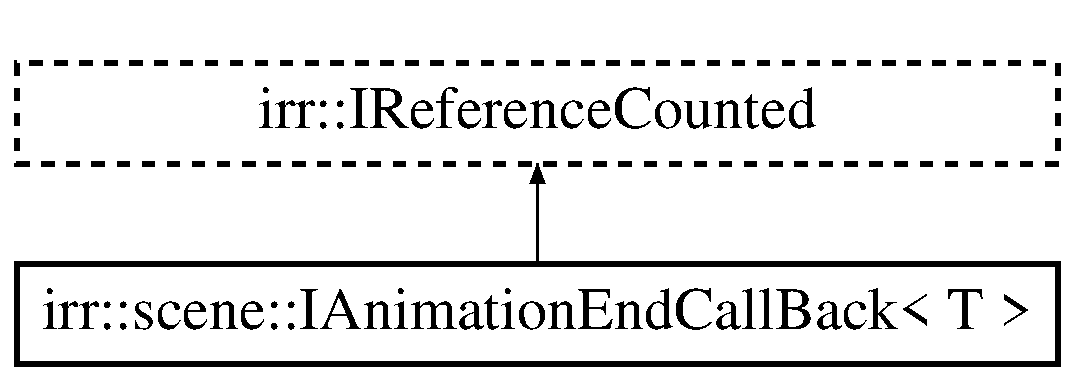
\includegraphics[height=2.000000cm]{classirr_1_1scene_1_1IAnimationEndCallBack}
\end{center}
\end{figure}
\subsection*{Public Member Functions}
\begin{DoxyCompactItemize}
\item 
virtual void \hyperlink{classirr_1_1scene_1_1IAnimationEndCallBack_afe7fa9ae8a2f89cc13460d915fafaead}{On\+Animation\+End} (T $\ast$node)=0
\begin{DoxyCompactList}\small\item\em Will be called when the animation playback has ended. \end{DoxyCompactList}\end{DoxyCompactItemize}
\subsection*{Additional Inherited Members}


\subsection{Detailed Description}
\subsubsection*{template$<$class T$>$\\*
class irr\+::scene\+::\+I\+Animation\+End\+Call\+Back$<$ T $>$}

Callback interface for catching events of ended animations. 

Implement this interface to be able to be notified if an animation playback has ended. 

\subsection{Member Function Documentation}
\index{irr\+::scene\+::\+I\+Animation\+End\+Call\+Back@{irr\+::scene\+::\+I\+Animation\+End\+Call\+Back}!On\+Animation\+End@{On\+Animation\+End}}
\index{On\+Animation\+End@{On\+Animation\+End}!irr\+::scene\+::\+I\+Animation\+End\+Call\+Back@{irr\+::scene\+::\+I\+Animation\+End\+Call\+Back}}
\subsubsection[{\texorpdfstring{On\+Animation\+End(\+T $\ast$node)=0}{OnAnimationEnd(T *node)=0}}]{\setlength{\rightskip}{0pt plus 5cm}template$<$class T $>$ virtual void {\bf irr\+::scene\+::\+I\+Animation\+End\+Call\+Back}$<$ T $>$\+::On\+Animation\+End (
\begin{DoxyParamCaption}
\item[{T $\ast$}]{node}
\end{DoxyParamCaption}
)\hspace{0.3cm}{\ttfamily [pure virtual]}}\hypertarget{classirr_1_1scene_1_1IAnimationEndCallBack_afe7fa9ae8a2f89cc13460d915fafaead}{}\label{classirr_1_1scene_1_1IAnimationEndCallBack_afe7fa9ae8a2f89cc13460d915fafaead}


Will be called when the animation playback has ended. 

See \hyperlink{classirr_1_1scene_1_1ISkinnedMeshSceneNode_aff45c2cd4eb26d8ca6142109ea3e351f}{I\+Skinned\+Mesh\+Scene\+Node\+::set\+Animation\+End\+Callback} and I\+Animated\+Mesh\+Scene\+Noe\+::set\+Animation\+End\+Callback for more informations. 
\begin{DoxyParams}{Parameters}
{\em node} & Node of which the animation has ended. \\
\hline
\end{DoxyParams}


The documentation for this class was generated from the following file\+:\begin{DoxyCompactItemize}
\item 
include/I\+Animated\+Mesh\+Scene\+Node.\+h\end{DoxyCompactItemize}

\hypertarget{classirr_1_1io_1_1IArchiveLoader}{}\section{irr\+:\+:io\+:\+:I\+Archive\+Loader Class Reference}
\label{classirr_1_1io_1_1IArchiveLoader}\index{irr\+::io\+::\+I\+Archive\+Loader@{irr\+::io\+::\+I\+Archive\+Loader}}


Class which is able to create an archive from a file.  




{\ttfamily \#include $<$I\+File\+Archive.\+h$>$}

Inheritance diagram for irr\+:\+:io\+:\+:I\+Archive\+Loader\+:\begin{figure}[H]
\begin{center}
\leavevmode
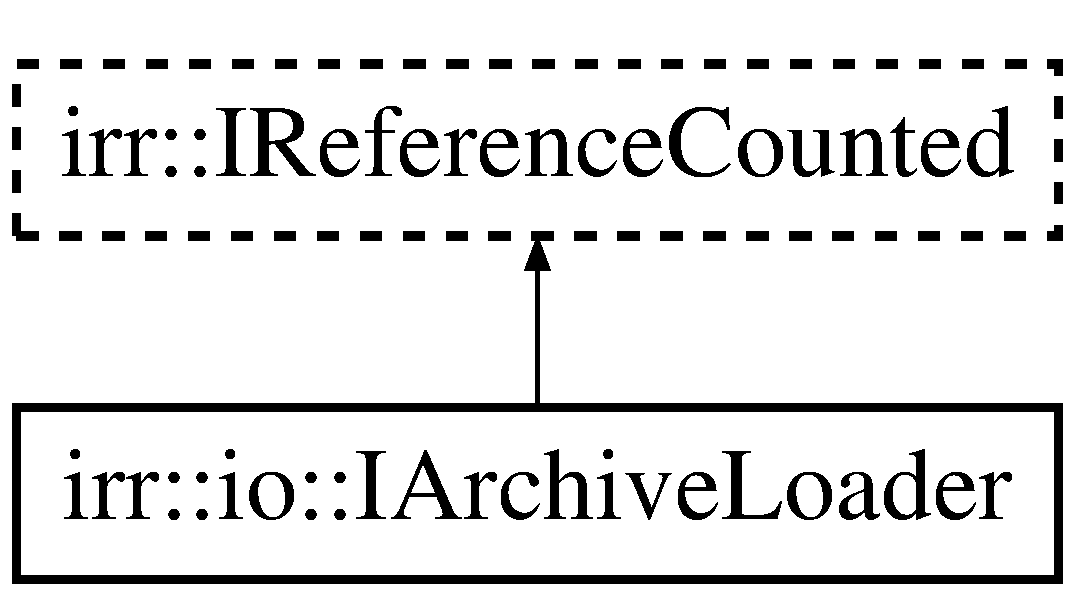
\includegraphics[height=2.000000cm]{classirr_1_1io_1_1IArchiveLoader}
\end{center}
\end{figure}
\subsection*{Public Member Functions}
\begin{DoxyCompactItemize}
\item 
virtual bool \hyperlink{classirr_1_1io_1_1IArchiveLoader_a9e1f6da1913c595347c731f691cae004}{is\+A\+Loadable\+File\+Format} (const \hyperlink{namespaceirr_1_1io_ab1bdc45edb3f94d8319c02bc0f840ee1}{path} \&filename) const  =0
\begin{DoxyCompactList}\small\item\em Check if the file might be loaded by this class. \end{DoxyCompactList}\item 
virtual bool \hyperlink{classirr_1_1io_1_1IArchiveLoader_a3cb29e4f60789e1d658e7ac7a2e0861d}{is\+A\+Loadable\+File\+Format} (\hyperlink{classirr_1_1io_1_1IReadFile}{io\+::\+I\+Read\+File} $\ast$file) const  =0
\begin{DoxyCompactList}\small\item\em Check if the file might be loaded by this class. \end{DoxyCompactList}\item 
virtual bool \hyperlink{classirr_1_1io_1_1IArchiveLoader_a208afadf81b882ba1c430ce54edda06e}{is\+A\+Loadable\+File\+Format} (\hyperlink{namespaceirr_1_1io_adb3e3c445ec8e608ed1f0f93306da14f}{E\+\_\+\+F\+I\+L\+E\+\_\+\+A\+R\+C\+H\+I\+V\+E\+\_\+\+T\+Y\+PE} file\+Type) const  =0
\begin{DoxyCompactList}\small\item\em Check to see if the loader can create archives of this type. \end{DoxyCompactList}\item 
virtual \hyperlink{classirr_1_1io_1_1IFileArchive}{I\+File\+Archive} $\ast$ \hyperlink{classirr_1_1io_1_1IArchiveLoader_a528c9c775506607e2bfc6d37f3b40875}{create\+Archive} (const \hyperlink{namespaceirr_1_1io_ab1bdc45edb3f94d8319c02bc0f840ee1}{path} \&filename, bool ignore\+Case, bool ignore\+Paths) const  =0
\begin{DoxyCompactList}\small\item\em Creates an archive from the filename. \end{DoxyCompactList}\item 
virtual \hyperlink{classirr_1_1io_1_1IFileArchive}{I\+File\+Archive} $\ast$ \hyperlink{classirr_1_1io_1_1IArchiveLoader_ad8d1903f130a5b40916e25a174bd55ec}{create\+Archive} (\hyperlink{classirr_1_1io_1_1IReadFile}{io\+::\+I\+Read\+File} $\ast$file, bool ignore\+Case, bool ignore\+Paths) const  =0
\begin{DoxyCompactList}\small\item\em Creates an archive from the file. \end{DoxyCompactList}\end{DoxyCompactItemize}
\subsection*{Additional Inherited Members}


\subsection{Detailed Description}
Class which is able to create an archive from a file. 

If you want the Irrlicht Engine be able to load archives of currently unsupported file formats (e.\+g .wad), then implement this and add your new Archive loader with \hyperlink{classirr_1_1io_1_1IFileSystem_ad56456302b4697c49b461a909d9269b9}{I\+File\+System\+::add\+Archive\+Loader()} to the engine. 

\subsection{Member Function Documentation}
\index{irr\+::io\+::\+I\+Archive\+Loader@{irr\+::io\+::\+I\+Archive\+Loader}!create\+Archive@{create\+Archive}}
\index{create\+Archive@{create\+Archive}!irr\+::io\+::\+I\+Archive\+Loader@{irr\+::io\+::\+I\+Archive\+Loader}}
\subsubsection[{\texorpdfstring{create\+Archive(const path \&filename, bool ignore\+Case, bool ignore\+Paths) const  =0}{createArchive(const path \&filename, bool ignoreCase, bool ignorePaths) const  =0}}]{\setlength{\rightskip}{0pt plus 5cm}virtual {\bf I\+File\+Archive}$\ast$ irr\+::io\+::\+I\+Archive\+Loader\+::create\+Archive (
\begin{DoxyParamCaption}
\item[{const {\bf path} \&}]{filename, }
\item[{bool}]{ignore\+Case, }
\item[{bool}]{ignore\+Paths}
\end{DoxyParamCaption}
) const\hspace{0.3cm}{\ttfamily [pure virtual]}}\hypertarget{classirr_1_1io_1_1IArchiveLoader_a528c9c775506607e2bfc6d37f3b40875}{}\label{classirr_1_1io_1_1IArchiveLoader_a528c9c775506607e2bfc6d37f3b40875}


Creates an archive from the filename. 


\begin{DoxyParams}{Parameters}
{\em filename} & File to use. \\
\hline
{\em ignore\+Case} & Searching is performed without regarding the case \\
\hline
{\em ignore\+Paths} & Files are searched for without checking for the directories \\
\hline
\end{DoxyParams}
\begin{DoxyReturn}{Returns}
Pointer to newly created archive, or 0 upon error. 
\end{DoxyReturn}
\index{irr\+::io\+::\+I\+Archive\+Loader@{irr\+::io\+::\+I\+Archive\+Loader}!create\+Archive@{create\+Archive}}
\index{create\+Archive@{create\+Archive}!irr\+::io\+::\+I\+Archive\+Loader@{irr\+::io\+::\+I\+Archive\+Loader}}
\subsubsection[{\texorpdfstring{create\+Archive(io\+::\+I\+Read\+File $\ast$file, bool ignore\+Case, bool ignore\+Paths) const  =0}{createArchive(io::IReadFile *file, bool ignoreCase, bool ignorePaths) const  =0}}]{\setlength{\rightskip}{0pt plus 5cm}virtual {\bf I\+File\+Archive}$\ast$ irr\+::io\+::\+I\+Archive\+Loader\+::create\+Archive (
\begin{DoxyParamCaption}
\item[{{\bf io\+::\+I\+Read\+File} $\ast$}]{file, }
\item[{bool}]{ignore\+Case, }
\item[{bool}]{ignore\+Paths}
\end{DoxyParamCaption}
) const\hspace{0.3cm}{\ttfamily [pure virtual]}}\hypertarget{classirr_1_1io_1_1IArchiveLoader_ad8d1903f130a5b40916e25a174bd55ec}{}\label{classirr_1_1io_1_1IArchiveLoader_ad8d1903f130a5b40916e25a174bd55ec}


Creates an archive from the file. 


\begin{DoxyParams}{Parameters}
{\em file} & File handle to use. \\
\hline
{\em ignore\+Case} & Searching is performed without regarding the case \\
\hline
{\em ignore\+Paths} & Files are searched for without checking for the directories \\
\hline
\end{DoxyParams}
\begin{DoxyReturn}{Returns}
Pointer to newly created archive, or 0 upon error. 
\end{DoxyReturn}
\index{irr\+::io\+::\+I\+Archive\+Loader@{irr\+::io\+::\+I\+Archive\+Loader}!is\+A\+Loadable\+File\+Format@{is\+A\+Loadable\+File\+Format}}
\index{is\+A\+Loadable\+File\+Format@{is\+A\+Loadable\+File\+Format}!irr\+::io\+::\+I\+Archive\+Loader@{irr\+::io\+::\+I\+Archive\+Loader}}
\subsubsection[{\texorpdfstring{is\+A\+Loadable\+File\+Format(const path \&filename) const  =0}{isALoadableFileFormat(const path \&filename) const  =0}}]{\setlength{\rightskip}{0pt plus 5cm}virtual bool irr\+::io\+::\+I\+Archive\+Loader\+::is\+A\+Loadable\+File\+Format (
\begin{DoxyParamCaption}
\item[{const {\bf path} \&}]{filename}
\end{DoxyParamCaption}
) const\hspace{0.3cm}{\ttfamily [pure virtual]}}\hypertarget{classirr_1_1io_1_1IArchiveLoader_a9e1f6da1913c595347c731f691cae004}{}\label{classirr_1_1io_1_1IArchiveLoader_a9e1f6da1913c595347c731f691cae004}


Check if the file might be loaded by this class. 

Check based on the file extension (e.\+g. \char`\"{}.\+zip\char`\"{}) 
\begin{DoxyParams}{Parameters}
{\em filename} & Name of file to check. \\
\hline
\end{DoxyParams}
\begin{DoxyReturn}{Returns}
True if file seems to be loadable. 
\end{DoxyReturn}
\index{irr\+::io\+::\+I\+Archive\+Loader@{irr\+::io\+::\+I\+Archive\+Loader}!is\+A\+Loadable\+File\+Format@{is\+A\+Loadable\+File\+Format}}
\index{is\+A\+Loadable\+File\+Format@{is\+A\+Loadable\+File\+Format}!irr\+::io\+::\+I\+Archive\+Loader@{irr\+::io\+::\+I\+Archive\+Loader}}
\subsubsection[{\texorpdfstring{is\+A\+Loadable\+File\+Format(io\+::\+I\+Read\+File $\ast$file) const  =0}{isALoadableFileFormat(io::IReadFile *file) const  =0}}]{\setlength{\rightskip}{0pt plus 5cm}virtual bool irr\+::io\+::\+I\+Archive\+Loader\+::is\+A\+Loadable\+File\+Format (
\begin{DoxyParamCaption}
\item[{{\bf io\+::\+I\+Read\+File} $\ast$}]{file}
\end{DoxyParamCaption}
) const\hspace{0.3cm}{\ttfamily [pure virtual]}}\hypertarget{classirr_1_1io_1_1IArchiveLoader_a3cb29e4f60789e1d658e7ac7a2e0861d}{}\label{classirr_1_1io_1_1IArchiveLoader_a3cb29e4f60789e1d658e7ac7a2e0861d}


Check if the file might be loaded by this class. 

This check may look into the file. 
\begin{DoxyParams}{Parameters}
{\em file} & File handle to check. \\
\hline
\end{DoxyParams}
\begin{DoxyReturn}{Returns}
True if file seems to be loadable. 
\end{DoxyReturn}
\index{irr\+::io\+::\+I\+Archive\+Loader@{irr\+::io\+::\+I\+Archive\+Loader}!is\+A\+Loadable\+File\+Format@{is\+A\+Loadable\+File\+Format}}
\index{is\+A\+Loadable\+File\+Format@{is\+A\+Loadable\+File\+Format}!irr\+::io\+::\+I\+Archive\+Loader@{irr\+::io\+::\+I\+Archive\+Loader}}
\subsubsection[{\texorpdfstring{is\+A\+Loadable\+File\+Format(\+E\+\_\+\+F\+I\+L\+E\+\_\+\+A\+R\+C\+H\+I\+V\+E\+\_\+\+T\+Y\+P\+E file\+Type) const  =0}{isALoadableFileFormat(E\_FILE\_ARCHIVE\_TYPE fileType) const  =0}}]{\setlength{\rightskip}{0pt plus 5cm}virtual bool irr\+::io\+::\+I\+Archive\+Loader\+::is\+A\+Loadable\+File\+Format (
\begin{DoxyParamCaption}
\item[{{\bf E\+\_\+\+F\+I\+L\+E\+\_\+\+A\+R\+C\+H\+I\+V\+E\+\_\+\+T\+Y\+PE}}]{file\+Type}
\end{DoxyParamCaption}
) const\hspace{0.3cm}{\ttfamily [pure virtual]}}\hypertarget{classirr_1_1io_1_1IArchiveLoader_a208afadf81b882ba1c430ce54edda06e}{}\label{classirr_1_1io_1_1IArchiveLoader_a208afadf81b882ba1c430ce54edda06e}


Check to see if the loader can create archives of this type. 

Check based on the archive type. 
\begin{DoxyParams}{Parameters}
{\em file\+Type} & The archive type to check. \\
\hline
\end{DoxyParams}
\begin{DoxyReturn}{Returns}
True if the archile loader supports this type, false if not 
\end{DoxyReturn}


The documentation for this class was generated from the following file\+:\begin{DoxyCompactItemize}
\item 
include/I\+File\+Archive.\+h\end{DoxyCompactItemize}

\hypertarget{classirr_1_1scene_1_1IBillboardSceneNode}{}\section{irr\+:\+:scene\+:\+:I\+Billboard\+Scene\+Node Class Reference}
\label{classirr_1_1scene_1_1IBillboardSceneNode}\index{irr\+::scene\+::\+I\+Billboard\+Scene\+Node@{irr\+::scene\+::\+I\+Billboard\+Scene\+Node}}


A billboard scene node.  




{\ttfamily \#include $<$I\+Billboard\+Scene\+Node.\+h$>$}

Inheritance diagram for irr\+:\+:scene\+:\+:I\+Billboard\+Scene\+Node\+:\begin{figure}[H]
\begin{center}
\leavevmode
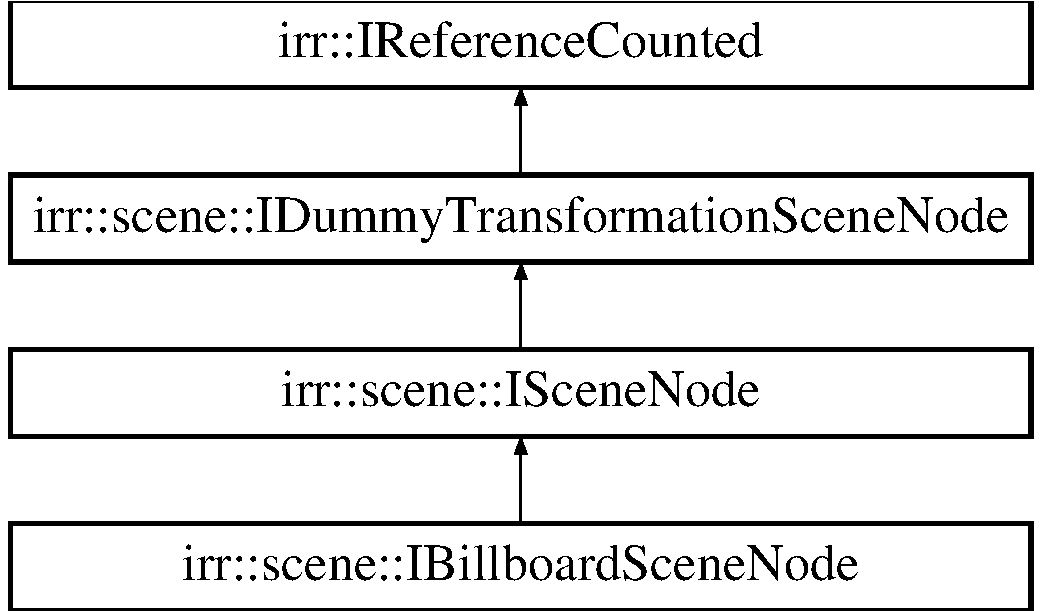
\includegraphics[height=4.000000cm]{classirr_1_1scene_1_1IBillboardSceneNode}
\end{center}
\end{figure}
\subsection*{Public Member Functions}
\begin{DoxyCompactItemize}
\item 
\hyperlink{classirr_1_1scene_1_1IBillboardSceneNode_a92d3ac7399c874d59cd26d5dfb36ff63}{I\+Billboard\+Scene\+Node} (\hyperlink{classirr_1_1scene_1_1IDummyTransformationSceneNode}{I\+Dummy\+Transformation\+Scene\+Node} $\ast$parent, \hyperlink{classirr_1_1scene_1_1ISceneManager}{I\+Scene\+Manager} $\ast$mgr, \hyperlink{namespaceirr_ac66849b7a6ed16e30ebede579f9b47c6}{s32} id, const \hyperlink{namespaceirr_1_1core_a06f169d08b5c429f5575acb7edbad811}{core\+::vector3df} \&position=\hyperlink{namespaceirr_1_1core_a06f169d08b5c429f5575acb7edbad811}{core\+::vector3df}(0, 0, 0))\hypertarget{classirr_1_1scene_1_1IBillboardSceneNode_a92d3ac7399c874d59cd26d5dfb36ff63}{}\label{classirr_1_1scene_1_1IBillboardSceneNode_a92d3ac7399c874d59cd26d5dfb36ff63}

\begin{DoxyCompactList}\small\item\em Constructor. \end{DoxyCompactList}\item 
virtual void \hyperlink{classirr_1_1scene_1_1IBillboardSceneNode_a911415ac24440bd3ccfcde102583fd60}{set\+Size} (const \hyperlink{classirr_1_1core_1_1dimension2d}{core\+::dimension2d}$<$ \hyperlink{namespaceirr_a0277be98d67dc26ff93b1a6a1d086b07}{f32} $>$ \&size)=0\hypertarget{classirr_1_1scene_1_1IBillboardSceneNode_a911415ac24440bd3ccfcde102583fd60}{}\label{classirr_1_1scene_1_1IBillboardSceneNode_a911415ac24440bd3ccfcde102583fd60}

\begin{DoxyCompactList}\small\item\em Sets the size of the billboard, making it rectangular. \end{DoxyCompactList}\item 
virtual void \hyperlink{classirr_1_1scene_1_1IBillboardSceneNode_a9a5d47a00bb0160daab8fa53453a2ba4}{set\+Size} (\hyperlink{namespaceirr_a0277be98d67dc26ff93b1a6a1d086b07}{f32} height, \hyperlink{namespaceirr_a0277be98d67dc26ff93b1a6a1d086b07}{f32} bottom\+Edge\+Width, \hyperlink{namespaceirr_a0277be98d67dc26ff93b1a6a1d086b07}{f32} top\+Edge\+Width)=0
\begin{DoxyCompactList}\small\item\em Sets the size of the billboard with independent widths of the bottom and top edges. \end{DoxyCompactList}\item 
virtual const \hyperlink{classirr_1_1core_1_1dimension2d}{core\+::dimension2d}$<$ \hyperlink{namespaceirr_a0277be98d67dc26ff93b1a6a1d086b07}{f32} $>$ \& \hyperlink{classirr_1_1scene_1_1IBillboardSceneNode_ada77331a59e5b45d4cbb963f8826bbd4}{get\+Size} () const  =0
\begin{DoxyCompactList}\small\item\em Returns the size of the billboard. \end{DoxyCompactList}\item 
virtual void \hyperlink{classirr_1_1scene_1_1IBillboardSceneNode_a58d336f020732ebcda44c5c9f57e9495}{get\+Size} (\hyperlink{namespaceirr_a0277be98d67dc26ff93b1a6a1d086b07}{f32} \&height, \hyperlink{namespaceirr_a0277be98d67dc26ff93b1a6a1d086b07}{f32} \&bottom\+Edge\+Width, \hyperlink{namespaceirr_a0277be98d67dc26ff93b1a6a1d086b07}{f32} \&top\+Edge\+Width) const  =0
\begin{DoxyCompactList}\small\item\em Gets the size of the the billboard and handles independent top and bottom edge widths correctly. \end{DoxyCompactList}\item 
virtual void \hyperlink{classirr_1_1scene_1_1IBillboardSceneNode_a82c1038a6dfcd255863baa96aaba4182}{set\+Color} (const \hyperlink{classirr_1_1video_1_1SColor}{video\+::\+S\+Color} \&overall\+Color)=0
\begin{DoxyCompactList}\small\item\em Set the color of all vertices of the billboard. \end{DoxyCompactList}\item 
virtual void \hyperlink{classirr_1_1scene_1_1IBillboardSceneNode_a13efdfa73998706baf10cedcdb48d559}{set\+Color} (const \hyperlink{classirr_1_1video_1_1SColor}{video\+::\+S\+Color} \&top\+Color, const \hyperlink{classirr_1_1video_1_1SColor}{video\+::\+S\+Color} \&bottom\+Color)=0
\begin{DoxyCompactList}\small\item\em Set the color of the top and bottom vertices of the billboard. \end{DoxyCompactList}\end{DoxyCompactItemize}
\subsection*{Additional Inherited Members}


\subsection{Detailed Description}
A billboard scene node. 

A billboard is like a 3d sprite\+: A 2d element, which always looks to the camera. It is usually used for explosions, fire, lensflares, particles and things like that. 

\subsection{Member Function Documentation}
\index{irr\+::scene\+::\+I\+Billboard\+Scene\+Node@{irr\+::scene\+::\+I\+Billboard\+Scene\+Node}!get\+Size@{get\+Size}}
\index{get\+Size@{get\+Size}!irr\+::scene\+::\+I\+Billboard\+Scene\+Node@{irr\+::scene\+::\+I\+Billboard\+Scene\+Node}}
\subsubsection[{\texorpdfstring{get\+Size() const  =0}{getSize() const  =0}}]{\setlength{\rightskip}{0pt plus 5cm}virtual const {\bf core\+::dimension2d}$<${\bf f32}$>$\& irr\+::scene\+::\+I\+Billboard\+Scene\+Node\+::get\+Size (
\begin{DoxyParamCaption}
{}
\end{DoxyParamCaption}
) const\hspace{0.3cm}{\ttfamily [pure virtual]}}\hypertarget{classirr_1_1scene_1_1IBillboardSceneNode_ada77331a59e5b45d4cbb963f8826bbd4}{}\label{classirr_1_1scene_1_1IBillboardSceneNode_ada77331a59e5b45d4cbb963f8826bbd4}


Returns the size of the billboard. 

This will return the width of the bottom edge of the billboard. Use get\+Widths() to retrieve the bottom and top edges independently. \begin{DoxyReturn}{Returns}
Size of the billboard. 
\end{DoxyReturn}
\index{irr\+::scene\+::\+I\+Billboard\+Scene\+Node@{irr\+::scene\+::\+I\+Billboard\+Scene\+Node}!get\+Size@{get\+Size}}
\index{get\+Size@{get\+Size}!irr\+::scene\+::\+I\+Billboard\+Scene\+Node@{irr\+::scene\+::\+I\+Billboard\+Scene\+Node}}
\subsubsection[{\texorpdfstring{get\+Size(f32 \&height, f32 \&bottom\+Edge\+Width, f32 \&top\+Edge\+Width) const  =0}{getSize(f32 \&height, f32 \&bottomEdgeWidth, f32 \&topEdgeWidth) const  =0}}]{\setlength{\rightskip}{0pt plus 5cm}virtual void irr\+::scene\+::\+I\+Billboard\+Scene\+Node\+::get\+Size (
\begin{DoxyParamCaption}
\item[{{\bf f32} \&}]{height, }
\item[{{\bf f32} \&}]{bottom\+Edge\+Width, }
\item[{{\bf f32} \&}]{top\+Edge\+Width}
\end{DoxyParamCaption}
) const\hspace{0.3cm}{\ttfamily [pure virtual]}}\hypertarget{classirr_1_1scene_1_1IBillboardSceneNode_a58d336f020732ebcda44c5c9f57e9495}{}\label{classirr_1_1scene_1_1IBillboardSceneNode_a58d336f020732ebcda44c5c9f57e9495}


Gets the size of the the billboard and handles independent top and bottom edge widths correctly. 


\begin{DoxyParams}[1]{Parameters}
\mbox{\tt out}  & {\em height} & The height of the billboard. \\
\hline
\mbox{\tt out}  & {\em bottom\+Edge\+Width} & The width of the bottom edge of the billboard. \\
\hline
\mbox{\tt out}  & {\em top\+Edge\+Width} & The width of the top edge of the billboard. \\
\hline
\end{DoxyParams}
\index{irr\+::scene\+::\+I\+Billboard\+Scene\+Node@{irr\+::scene\+::\+I\+Billboard\+Scene\+Node}!set\+Color@{set\+Color}}
\index{set\+Color@{set\+Color}!irr\+::scene\+::\+I\+Billboard\+Scene\+Node@{irr\+::scene\+::\+I\+Billboard\+Scene\+Node}}
\subsubsection[{\texorpdfstring{set\+Color(const video\+::\+S\+Color \&overall\+Color)=0}{setColor(const video::SColor \&overallColor)=0}}]{\setlength{\rightskip}{0pt plus 5cm}virtual void irr\+::scene\+::\+I\+Billboard\+Scene\+Node\+::set\+Color (
\begin{DoxyParamCaption}
\item[{const {\bf video\+::\+S\+Color} \&}]{overall\+Color}
\end{DoxyParamCaption}
)\hspace{0.3cm}{\ttfamily [pure virtual]}}\hypertarget{classirr_1_1scene_1_1IBillboardSceneNode_a82c1038a6dfcd255863baa96aaba4182}{}\label{classirr_1_1scene_1_1IBillboardSceneNode_a82c1038a6dfcd255863baa96aaba4182}


Set the color of all vertices of the billboard. 


\begin{DoxyParams}[1]{Parameters}
\mbox{\tt in}  & {\em overall\+Color} & Color to set \\
\hline
\end{DoxyParams}
\index{irr\+::scene\+::\+I\+Billboard\+Scene\+Node@{irr\+::scene\+::\+I\+Billboard\+Scene\+Node}!set\+Color@{set\+Color}}
\index{set\+Color@{set\+Color}!irr\+::scene\+::\+I\+Billboard\+Scene\+Node@{irr\+::scene\+::\+I\+Billboard\+Scene\+Node}}
\subsubsection[{\texorpdfstring{set\+Color(const video\+::\+S\+Color \&top\+Color, const video\+::\+S\+Color \&bottom\+Color)=0}{setColor(const video::SColor \&topColor, const video::SColor \&bottomColor)=0}}]{\setlength{\rightskip}{0pt plus 5cm}virtual void irr\+::scene\+::\+I\+Billboard\+Scene\+Node\+::set\+Color (
\begin{DoxyParamCaption}
\item[{const {\bf video\+::\+S\+Color} \&}]{top\+Color, }
\item[{const {\bf video\+::\+S\+Color} \&}]{bottom\+Color}
\end{DoxyParamCaption}
)\hspace{0.3cm}{\ttfamily [pure virtual]}}\hypertarget{classirr_1_1scene_1_1IBillboardSceneNode_a13efdfa73998706baf10cedcdb48d559}{}\label{classirr_1_1scene_1_1IBillboardSceneNode_a13efdfa73998706baf10cedcdb48d559}


Set the color of the top and bottom vertices of the billboard. 


\begin{DoxyParams}[1]{Parameters}
\mbox{\tt in}  & {\em top\+Color} & Color to set the top vertices \\
\hline
\mbox{\tt in}  & {\em bottom\+Color} & Color to set the bottom vertices \\
\hline
\end{DoxyParams}
\index{irr\+::scene\+::\+I\+Billboard\+Scene\+Node@{irr\+::scene\+::\+I\+Billboard\+Scene\+Node}!set\+Size@{set\+Size}}
\index{set\+Size@{set\+Size}!irr\+::scene\+::\+I\+Billboard\+Scene\+Node@{irr\+::scene\+::\+I\+Billboard\+Scene\+Node}}
\subsubsection[{\texorpdfstring{set\+Size(f32 height, f32 bottom\+Edge\+Width, f32 top\+Edge\+Width)=0}{setSize(f32 height, f32 bottomEdgeWidth, f32 topEdgeWidth)=0}}]{\setlength{\rightskip}{0pt plus 5cm}virtual void irr\+::scene\+::\+I\+Billboard\+Scene\+Node\+::set\+Size (
\begin{DoxyParamCaption}
\item[{{\bf f32}}]{height, }
\item[{{\bf f32}}]{bottom\+Edge\+Width, }
\item[{{\bf f32}}]{top\+Edge\+Width}
\end{DoxyParamCaption}
)\hspace{0.3cm}{\ttfamily [pure virtual]}}\hypertarget{classirr_1_1scene_1_1IBillboardSceneNode_a9a5d47a00bb0160daab8fa53453a2ba4}{}\label{classirr_1_1scene_1_1IBillboardSceneNode_a9a5d47a00bb0160daab8fa53453a2ba4}


Sets the size of the billboard with independent widths of the bottom and top edges. 


\begin{DoxyParams}[1]{Parameters}
\mbox{\tt in}  & {\em height} & The height of the billboard. \\
\hline
\mbox{\tt in}  & {\em bottom\+Edge\+Width} & The width of the bottom edge of the billboard. \\
\hline
\mbox{\tt in}  & {\em top\+Edge\+Width} & The width of the top edge of the billboard. \\
\hline
\end{DoxyParams}


The documentation for this class was generated from the following file\+:\begin{DoxyCompactItemize}
\item 
include/I\+Billboard\+Scene\+Node.\+h\end{DoxyCompactItemize}

\hypertarget{classirr_1_1scene_1_1ISkinningStateManager_1_1IBoneSceneNode}{}\section{irr\+:\+:scene\+:\+:I\+Skinning\+State\+Manager\+:\+:I\+Bone\+Scene\+Node Class Reference}
\label{classirr_1_1scene_1_1ISkinningStateManager_1_1IBoneSceneNode}\index{irr\+::scene\+::\+I\+Skinning\+State\+Manager\+::\+I\+Bone\+Scene\+Node@{irr\+::scene\+::\+I\+Skinning\+State\+Manager\+::\+I\+Bone\+Scene\+Node}}
Inheritance diagram for irr\+:\+:scene\+:\+:I\+Skinning\+State\+Manager\+:\+:I\+Bone\+Scene\+Node\+:\begin{figure}[H]
\begin{center}
\leavevmode
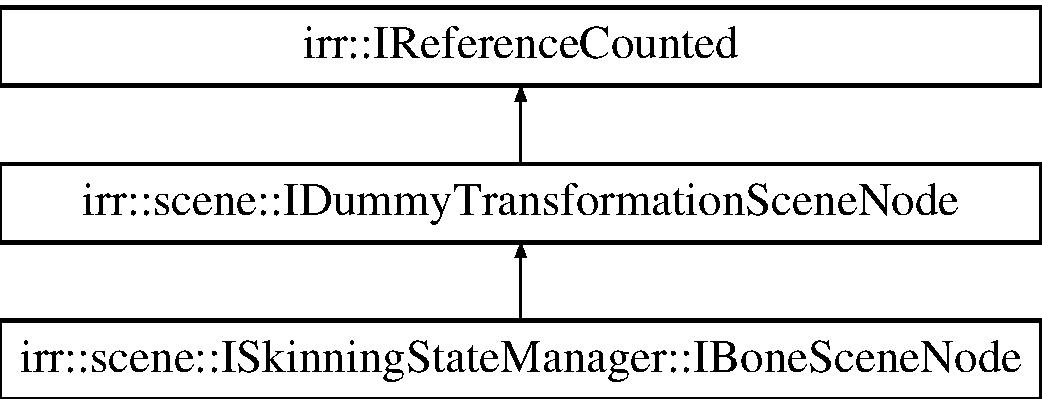
\includegraphics[height=3.000000cm]{classirr_1_1scene_1_1ISkinningStateManager_1_1IBoneSceneNode}
\end{center}
\end{figure}
\subsection*{Public Types}
\begin{DoxyCompactItemize}
\item 
enum \hyperlink{classirr_1_1scene_1_1ISkinningStateManager_1_1IBoneSceneNode_a746e46bb30372063ca11a4695fd345bd}{E\+\_\+\+B\+O\+N\+E\+\_\+\+S\+K\+I\+N\+N\+I\+N\+G\+\_\+\+S\+P\+A\+CE} \{ \hyperlink{classirr_1_1scene_1_1ISkinningStateManager_1_1IBoneSceneNode_a746e46bb30372063ca11a4695fd345bda80eee20d1f6a106998a7c97378126398}{E\+B\+S\+S\+\_\+\+L\+O\+C\+AL} =0, 
\hyperlink{classirr_1_1scene_1_1ISkinningStateManager_1_1IBoneSceneNode_a746e46bb30372063ca11a4695fd345bda3408d599f51f779ffae4dce7908c3f69}{E\+B\+S\+S\+\_\+\+G\+L\+O\+B\+AL}, 
{\bfseries E\+B\+S\+S\+\_\+\+C\+O\+U\+NT}
 \}
\end{DoxyCompactItemize}
\subsection*{Public Member Functions}
\begin{DoxyCompactItemize}
\item 
{\bfseries I\+Bone\+Scene\+Node} (\hyperlink{classirr_1_1scene_1_1ISkinningStateManager}{I\+Skinning\+State\+Manager} $\ast$owner, const uint32\+\_\+t \&instance\+Index, \hyperlink{classirr_1_1scene_1_1IDummyTransformationSceneNode}{I\+Dummy\+Transformation\+Scene\+Node} $\ast$parent, const uint32\+\_\+t \&bone\+Index, const \hyperlink{classirr_1_1core_1_1matrix4x3}{core\+::matrix4x3} \&initial\+Relative\+Matrix=\hyperlink{classirr_1_1core_1_1matrix4x3}{core\+::matrix4x3}())\hypertarget{classirr_1_1scene_1_1ISkinningStateManager_1_1IBoneSceneNode_abddb29366296038e2220227c40409977}{}\label{classirr_1_1scene_1_1ISkinningStateManager_1_1IBoneSceneNode_abddb29366296038e2220227c40409977}

\item 
void \hyperlink{classirr_1_1scene_1_1ISkinningStateManager_1_1IBoneSceneNode_af55d36fe96f9e41c994648f1950db450}{set\+Skinning\+Space} (const \hyperlink{classirr_1_1scene_1_1ISkinningStateManager_1_1IBoneSceneNode_a746e46bb30372063ca11a4695fd345bd}{E\+\_\+\+B\+O\+N\+E\+\_\+\+S\+K\+I\+N\+N\+I\+N\+G\+\_\+\+S\+P\+A\+CE} \&space)
\item 
const \hyperlink{classirr_1_1scene_1_1ISkinningStateManager_1_1IBoneSceneNode_a746e46bb30372063ca11a4695fd345bd}{E\+\_\+\+B\+O\+N\+E\+\_\+\+S\+K\+I\+N\+N\+I\+N\+G\+\_\+\+S\+P\+A\+CE} \& \hyperlink{classirr_1_1scene_1_1ISkinningStateManager_1_1IBoneSceneNode_af9670516d5c70ed4bc2ac0e87912a6fc}{get\+Skinning\+Space} () const \hypertarget{classirr_1_1scene_1_1ISkinningStateManager_1_1IBoneSceneNode_af9670516d5c70ed4bc2ac0e87912a6fc}{}\label{classirr_1_1scene_1_1ISkinningStateManager_1_1IBoneSceneNode_af9670516d5c70ed4bc2ac0e87912a6fc}

\begin{DoxyCompactList}\small\item\em How the relative transformation of the bone is used. \end{DoxyCompactList}\item 
virtual const \hyperlink{classirr_1_1core_1_1matrix4x3}{core\+::matrix4x3} \& \hyperlink{classirr_1_1scene_1_1ISkinningStateManager_1_1IBoneSceneNode_aa01aed4ed2c55c61449ee38c98583fd4}{get\+Relative\+Transformation\+Matrix} ()\hypertarget{classirr_1_1scene_1_1ISkinningStateManager_1_1IBoneSceneNode_aa01aed4ed2c55c61449ee38c98583fd4}{}\label{classirr_1_1scene_1_1ISkinningStateManager_1_1IBoneSceneNode_aa01aed4ed2c55c61449ee38c98583fd4}

\begin{DoxyCompactList}\small\item\em O\+V\+E\+R\+R\+I\+D\+D\+EN F\+U\+N\+C\+T\+I\+O\+NS. \end{DoxyCompactList}\item 
virtual bool {\bfseries needs\+Absolute\+Transform\+Recompute} () const \hypertarget{classirr_1_1scene_1_1ISkinningStateManager_1_1IBoneSceneNode_a1719818c1c7c746d55221015034ddd97}{}\label{classirr_1_1scene_1_1ISkinningStateManager_1_1IBoneSceneNode_a1719818c1c7c746d55221015034ddd97}

\item 
virtual size\+\_\+t {\bfseries needs\+Deep\+Absolute\+Transform\+Recompute} () const \hypertarget{classirr_1_1scene_1_1ISkinningStateManager_1_1IBoneSceneNode_aa4bcdd303e29df104fa19ec5af857e59}{}\label{classirr_1_1scene_1_1ISkinningStateManager_1_1IBoneSceneNode_aa4bcdd303e29df104fa19ec5af857e59}

\item 
virtual void \hyperlink{classirr_1_1scene_1_1ISkinningStateManager_1_1IBoneSceneNode_a32bd793195468797fb07249946a8be21}{update\+Absolute\+Position} ()\hypertarget{classirr_1_1scene_1_1ISkinningStateManager_1_1IBoneSceneNode_a32bd793195468797fb07249946a8be21}{}\label{classirr_1_1scene_1_1ISkinningStateManager_1_1IBoneSceneNode_a32bd793195468797fb07249946a8be21}

\begin{DoxyCompactList}\small\item\em if the M\+O\+DE is R\+E\+AD, have to do implicit boning of an instance \+:D \end{DoxyCompactList}\item 
bool {\bfseries get\+Transform\+Changed\+Boning\+Hint} () const \hypertarget{classirr_1_1scene_1_1ISkinningStateManager_1_1IBoneSceneNode_a6f4044ae71a568c1f4d42130763b329c}{}\label{classirr_1_1scene_1_1ISkinningStateManager_1_1IBoneSceneNode_a6f4044ae71a568c1f4d42130763b329c}

\item 
void {\bfseries set\+Transform\+Changed\+Boning\+Hint} ()\hypertarget{classirr_1_1scene_1_1ISkinningStateManager_1_1IBoneSceneNode_a2ff6348df87f35dc49cb2c82356d925c}{}\label{classirr_1_1scene_1_1ISkinningStateManager_1_1IBoneSceneNode_a2ff6348df87f35dc49cb2c82356d925c}

\end{DoxyCompactItemize}
\subsection*{Protected Attributes}
\begin{DoxyCompactItemize}
\item 
\hyperlink{classirr_1_1scene_1_1ISkinningStateManager}{I\+Skinning\+State\+Manager} $\ast$ {\bfseries owner\+Manager}\hypertarget{classirr_1_1scene_1_1ISkinningStateManager_1_1IBoneSceneNode_a0b58c21b7a684497a94be417f22e7cad}{}\label{classirr_1_1scene_1_1ISkinningStateManager_1_1IBoneSceneNode_a0b58c21b7a684497a94be417f22e7cad}

\item 
uint32\+\_\+t {\bfseries Instance\+ID}\hypertarget{classirr_1_1scene_1_1ISkinningStateManager_1_1IBoneSceneNode_a1a2eb0bd7dd37561e62d5c1579f605eb}{}\label{classirr_1_1scene_1_1ISkinningStateManager_1_1IBoneSceneNode_a1a2eb0bd7dd37561e62d5c1579f605eb}

\item 
uint32\+\_\+t {\bfseries Bone\+Index}\hypertarget{classirr_1_1scene_1_1ISkinningStateManager_1_1IBoneSceneNode_ab3a059c2b6add6d2d320d04adb899be8}{}\label{classirr_1_1scene_1_1ISkinningStateManager_1_1IBoneSceneNode_ab3a059c2b6add6d2d320d04adb899be8}

\item 
\hyperlink{classirr_1_1scene_1_1ISkinningStateManager_1_1IBoneSceneNode_a746e46bb30372063ca11a4695fd345bd}{E\+\_\+\+B\+O\+N\+E\+\_\+\+S\+K\+I\+N\+N\+I\+N\+G\+\_\+\+S\+P\+A\+CE} {\bfseries Skinning\+Space}\hypertarget{classirr_1_1scene_1_1ISkinningStateManager_1_1IBoneSceneNode_ab8193efc734344696dabfda9a928afd8}{}\label{classirr_1_1scene_1_1ISkinningStateManager_1_1IBoneSceneNode_ab8193efc734344696dabfda9a928afd8}

\item 
uint64\+\_\+t {\bfseries last\+Time\+Pulled\+Absolute\+T\+Form\+For\+Boning}\hypertarget{classirr_1_1scene_1_1ISkinningStateManager_1_1IBoneSceneNode_ac262bb415c1cea3d13213f5c80f02138}{}\label{classirr_1_1scene_1_1ISkinningStateManager_1_1IBoneSceneNode_ac262bb415c1cea3d13213f5c80f02138}

\end{DoxyCompactItemize}
\subsection*{Additional Inherited Members}


\subsection{Member Enumeration Documentation}
\index{irr\+::scene\+::\+I\+Skinning\+State\+Manager\+::\+I\+Bone\+Scene\+Node@{irr\+::scene\+::\+I\+Skinning\+State\+Manager\+::\+I\+Bone\+Scene\+Node}!E\+\_\+\+B\+O\+N\+E\+\_\+\+S\+K\+I\+N\+N\+I\+N\+G\+\_\+\+S\+P\+A\+CE@{E\+\_\+\+B\+O\+N\+E\+\_\+\+S\+K\+I\+N\+N\+I\+N\+G\+\_\+\+S\+P\+A\+CE}}
\index{E\+\_\+\+B\+O\+N\+E\+\_\+\+S\+K\+I\+N\+N\+I\+N\+G\+\_\+\+S\+P\+A\+CE@{E\+\_\+\+B\+O\+N\+E\+\_\+\+S\+K\+I\+N\+N\+I\+N\+G\+\_\+\+S\+P\+A\+CE}!irr\+::scene\+::\+I\+Skinning\+State\+Manager\+::\+I\+Bone\+Scene\+Node@{irr\+::scene\+::\+I\+Skinning\+State\+Manager\+::\+I\+Bone\+Scene\+Node}}
\subsubsection[{\texorpdfstring{E\+\_\+\+B\+O\+N\+E\+\_\+\+S\+K\+I\+N\+N\+I\+N\+G\+\_\+\+S\+P\+A\+CE}{E\_BONE\_SKINNING\_SPACE}}]{\setlength{\rightskip}{0pt plus 5cm}enum {\bf irr\+::scene\+::\+I\+Skinning\+State\+Manager\+::\+I\+Bone\+Scene\+Node\+::\+E\+\_\+\+B\+O\+N\+E\+\_\+\+S\+K\+I\+N\+N\+I\+N\+G\+\_\+\+S\+P\+A\+CE}}\hypertarget{classirr_1_1scene_1_1ISkinningStateManager_1_1IBoneSceneNode_a746e46bb30372063ca11a4695fd345bd}{}\label{classirr_1_1scene_1_1ISkinningStateManager_1_1IBoneSceneNode_a746e46bb30372063ca11a4695fd345bd}
\begin{Desc}
\item[Enumerator]\par
\begin{description}
\index{E\+B\+S\+S\+\_\+\+L\+O\+C\+AL@{E\+B\+S\+S\+\_\+\+L\+O\+C\+AL}!irr\+::scene\+::\+I\+Skinning\+State\+Manager\+::\+I\+Bone\+Scene\+Node@{irr\+::scene\+::\+I\+Skinning\+State\+Manager\+::\+I\+Bone\+Scene\+Node}}\index{irr\+::scene\+::\+I\+Skinning\+State\+Manager\+::\+I\+Bone\+Scene\+Node@{irr\+::scene\+::\+I\+Skinning\+State\+Manager\+::\+I\+Bone\+Scene\+Node}!E\+B\+S\+S\+\_\+\+L\+O\+C\+AL@{E\+B\+S\+S\+\_\+\+L\+O\+C\+AL}}\item[{\em 
E\+B\+S\+S\+\_\+\+L\+O\+C\+AL\hypertarget{classirr_1_1scene_1_1ISkinningStateManager_1_1IBoneSceneNode_a746e46bb30372063ca11a4695fd345bda80eee20d1f6a106998a7c97378126398}{}\label{classirr_1_1scene_1_1ISkinningStateManager_1_1IBoneSceneNode_a746e46bb30372063ca11a4695fd345bda80eee20d1f6a106998a7c97378126398}
}]local skinning, standard \index{E\+B\+S\+S\+\_\+\+G\+L\+O\+B\+AL@{E\+B\+S\+S\+\_\+\+G\+L\+O\+B\+AL}!irr\+::scene\+::\+I\+Skinning\+State\+Manager\+::\+I\+Bone\+Scene\+Node@{irr\+::scene\+::\+I\+Skinning\+State\+Manager\+::\+I\+Bone\+Scene\+Node}}\index{irr\+::scene\+::\+I\+Skinning\+State\+Manager\+::\+I\+Bone\+Scene\+Node@{irr\+::scene\+::\+I\+Skinning\+State\+Manager\+::\+I\+Bone\+Scene\+Node}!E\+B\+S\+S\+\_\+\+G\+L\+O\+B\+AL@{E\+B\+S\+S\+\_\+\+G\+L\+O\+B\+AL}}\item[{\em 
E\+B\+S\+S\+\_\+\+G\+L\+O\+B\+AL\hypertarget{classirr_1_1scene_1_1ISkinningStateManager_1_1IBoneSceneNode_a746e46bb30372063ca11a4695fd345bda3408d599f51f779ffae4dce7908c3f69}{}\label{classirr_1_1scene_1_1ISkinningStateManager_1_1IBoneSceneNode_a746e46bb30372063ca11a4695fd345bda3408d599f51f779ffae4dce7908c3f69}
}]global skinning \end{description}
\end{Desc}


\subsection{Member Function Documentation}
\index{irr\+::scene\+::\+I\+Skinning\+State\+Manager\+::\+I\+Bone\+Scene\+Node@{irr\+::scene\+::\+I\+Skinning\+State\+Manager\+::\+I\+Bone\+Scene\+Node}!set\+Skinning\+Space@{set\+Skinning\+Space}}
\index{set\+Skinning\+Space@{set\+Skinning\+Space}!irr\+::scene\+::\+I\+Skinning\+State\+Manager\+::\+I\+Bone\+Scene\+Node@{irr\+::scene\+::\+I\+Skinning\+State\+Manager\+::\+I\+Bone\+Scene\+Node}}
\subsubsection[{\texorpdfstring{set\+Skinning\+Space(const E\+\_\+\+B\+O\+N\+E\+\_\+\+S\+K\+I\+N\+N\+I\+N\+G\+\_\+\+S\+P\+A\+C\+E \&space)}{setSkinningSpace(const E\_BONE\_SKINNING\_SPACE \&space)}}]{\setlength{\rightskip}{0pt plus 5cm}void irr\+::scene\+::\+I\+Skinning\+State\+Manager\+::\+I\+Bone\+Scene\+Node\+::set\+Skinning\+Space (
\begin{DoxyParamCaption}
\item[{const {\bf E\+\_\+\+B\+O\+N\+E\+\_\+\+S\+K\+I\+N\+N\+I\+N\+G\+\_\+\+S\+P\+A\+CE} \&}]{space}
\end{DoxyParamCaption}
)\hspace{0.3cm}{\ttfamily [inline]}}\hypertarget{classirr_1_1scene_1_1ISkinningStateManager_1_1IBoneSceneNode_af55d36fe96f9e41c994648f1950db450}{}\label{classirr_1_1scene_1_1ISkinningStateManager_1_1IBoneSceneNode_af55d36fe96f9e41c994648f1950db450}
How the relative transformation of the bone is used T\+H\+IS W\+I\+LL N\+OT M\+A\+G\+I\+C\+A\+L\+LY C\+O\+N\+V\+E\+RT T\+HE M\+A\+T\+R\+IX V\+A\+L\+U\+ES O\+N\+\_\+\+S\+W\+I\+T\+CH Y\+OU N\+E\+ED TO C\+A\+L\+C\+U\+L\+A\+TE T\+H\+EM A\+ND S\+ET T\+H\+EM B\+E\+F\+O\+RE OR A\+F\+T\+ER T\+HE S\+W\+I\+T\+C\+H!!! 

The documentation for this class was generated from the following file\+:\begin{DoxyCompactItemize}
\item 
include/I\+Skinning\+State\+Manager.\+h\end{DoxyCompactItemize}

\hypertarget{classirr_1_1core_1_1IBuffer}{}\section{irr\+:\+:core\+:\+:I\+Buffer Class Reference}
\label{classirr_1_1core_1_1IBuffer}\index{irr\+::core\+::\+I\+Buffer@{irr\+::core\+::\+I\+Buffer}}
Inheritance diagram for irr\+:\+:core\+:\+:I\+Buffer\+:\begin{figure}[H]
\begin{center}
\leavevmode
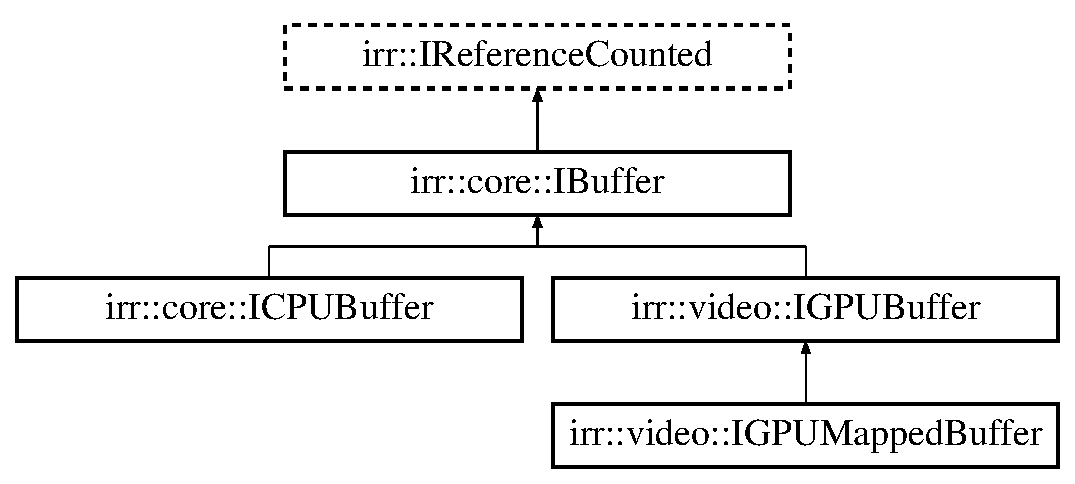
\includegraphics[height=4.000000cm]{classirr_1_1core_1_1IBuffer}
\end{center}
\end{figure}
\subsection*{Public Member Functions}
\begin{DoxyCompactItemize}
\item 
virtual E\+\_\+\+B\+U\+F\+F\+E\+R\+\_\+\+T\+Y\+PE {\bfseries get\+Buffer\+Type} () const  =0\hypertarget{classirr_1_1core_1_1IBuffer_a0df30ec3bd50265def2cc33c5e476479}{}\label{classirr_1_1core_1_1IBuffer_a0df30ec3bd50265def2cc33c5e476479}

\item 
virtual const uint64\+\_\+t \& \hyperlink{classirr_1_1core_1_1IBuffer_afdbb76c21eaf7ba4396eb68edd72a0c5}{get\+Size} () const  =0\hypertarget{classirr_1_1core_1_1IBuffer_afdbb76c21eaf7ba4396eb68edd72a0c5}{}\label{classirr_1_1core_1_1IBuffer_afdbb76c21eaf7ba4396eb68edd72a0c5}

\begin{DoxyCompactList}\small\item\em size in B\+Y\+T\+ES \end{DoxyCompactList}\item 
virtual bool \hyperlink{classirr_1_1core_1_1IBuffer_a725232c3869f003574d73707f40d7412}{reallocate} (const size\+\_\+t \&new\+Size, const bool \&force\+Retention\+Of\+Data=false, const bool \&reallocate\+If\+Shrink=false)=0
\item 
virtual const uint64\+\_\+t \& {\bfseries get\+Last\+Time\+Reallocated} () const \hypertarget{classirr_1_1core_1_1IBuffer_a5b4589f99466bfd84e578775289ef637}{}\label{classirr_1_1core_1_1IBuffer_a5b4589f99466bfd84e578775289ef637}

\end{DoxyCompactItemize}
\subsection*{Protected Attributes}
\begin{DoxyCompactItemize}
\item 
uint64\+\_\+t {\bfseries last\+Time\+Reallocated}\hypertarget{classirr_1_1core_1_1IBuffer_a57fd615be4290ea6bdec6f2fb695707e}{}\label{classirr_1_1core_1_1IBuffer_a57fd615be4290ea6bdec6f2fb695707e}

\end{DoxyCompactItemize}
\subsection*{Additional Inherited Members}


\subsection{Member Function Documentation}
\index{irr\+::core\+::\+I\+Buffer@{irr\+::core\+::\+I\+Buffer}!reallocate@{reallocate}}
\index{reallocate@{reallocate}!irr\+::core\+::\+I\+Buffer@{irr\+::core\+::\+I\+Buffer}}
\subsubsection[{\texorpdfstring{reallocate(const size\+\_\+t \&new\+Size, const bool \&force\+Retention\+Of\+Data=false, const bool \&reallocate\+If\+Shrink=false)=0}{reallocate(const size\_t \&newSize, const bool \&forceRetentionOfData=false, const bool \&reallocateIfShrink=false)=0}}]{\setlength{\rightskip}{0pt plus 5cm}virtual bool irr\+::core\+::\+I\+Buffer\+::reallocate (
\begin{DoxyParamCaption}
\item[{const size\+\_\+t \&}]{new\+Size, }
\item[{const bool \&}]{force\+Retention\+Of\+Data = {\ttfamily false}, }
\item[{const bool \&}]{reallocate\+If\+Shrink = {\ttfamily false}}
\end{DoxyParamCaption}
)\hspace{0.3cm}{\ttfamily [pure virtual]}}\hypertarget{classirr_1_1core_1_1IBuffer_a725232c3869f003574d73707f40d7412}{}\label{classirr_1_1core_1_1IBuffer_a725232c3869f003574d73707f40d7412}
returns true on success (some types always return false since they dont support resize) This function will invalidate any sizes, pointers etc. returned before! 

Implemented in \hyperlink{classirr_1_1core_1_1ICPUBuffer_ae223eb80a29ac3993b0bfa3e515ef5ce}{irr\+::core\+::\+I\+C\+P\+U\+Buffer}.



The documentation for this class was generated from the following file\+:\begin{DoxyCompactItemize}
\item 
include/I\+Buffer.\+h\end{DoxyCompactItemize}

\hypertarget{classirr_1_1scene_1_1ICameraSceneNode}{}\section{irr\+:\+:scene\+:\+:I\+Camera\+Scene\+Node Class Reference}
\label{classirr_1_1scene_1_1ICameraSceneNode}\index{irr\+::scene\+::\+I\+Camera\+Scene\+Node@{irr\+::scene\+::\+I\+Camera\+Scene\+Node}}


Scene Node which is a (controlable) camera.  




{\ttfamily \#include $<$I\+Camera\+Scene\+Node.\+h$>$}

Inheritance diagram for irr\+:\+:scene\+:\+:I\+Camera\+Scene\+Node\+:\begin{figure}[H]
\begin{center}
\leavevmode
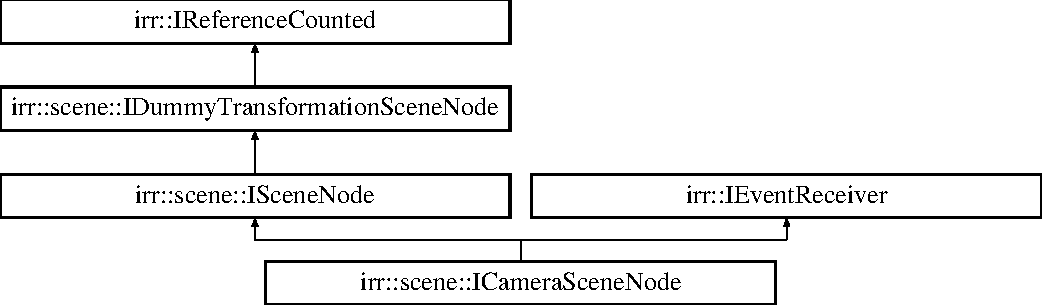
\includegraphics[height=4.000000cm]{classirr_1_1scene_1_1ICameraSceneNode}
\end{center}
\end{figure}
\subsection*{Public Member Functions}
\begin{DoxyCompactItemize}
\item 
\hyperlink{classirr_1_1scene_1_1ICameraSceneNode_a77dabb4f8182c1389758c0736f9dff3d}{I\+Camera\+Scene\+Node} (\hyperlink{classirr_1_1scene_1_1IDummyTransformationSceneNode}{I\+Dummy\+Transformation\+Scene\+Node} $\ast$parent, \hyperlink{classirr_1_1scene_1_1ISceneManager}{I\+Scene\+Manager} $\ast$mgr, \hyperlink{namespaceirr_ac66849b7a6ed16e30ebede579f9b47c6}{s32} id, const \hyperlink{namespaceirr_1_1core_a06f169d08b5c429f5575acb7edbad811}{core\+::vector3df} \&position=\hyperlink{namespaceirr_1_1core_a06f169d08b5c429f5575acb7edbad811}{core\+::vector3df}(0, 0, 0), const \hyperlink{namespaceirr_1_1core_a06f169d08b5c429f5575acb7edbad811}{core\+::vector3df} \&rotation=\hyperlink{namespaceirr_1_1core_a06f169d08b5c429f5575acb7edbad811}{core\+::vector3df}(0, 0, 0), const \hyperlink{namespaceirr_1_1core_a06f169d08b5c429f5575acb7edbad811}{core\+::vector3df} \&scale=\hyperlink{namespaceirr_1_1core_a06f169d08b5c429f5575acb7edbad811}{core\+::vector3df}(1.\+0f, 1.\+0f, 1.\+0f))\hypertarget{classirr_1_1scene_1_1ICameraSceneNode_a77dabb4f8182c1389758c0736f9dff3d}{}\label{classirr_1_1scene_1_1ICameraSceneNode_a77dabb4f8182c1389758c0736f9dff3d}

\begin{DoxyCompactList}\small\item\em Constructor. \end{DoxyCompactList}\item 
virtual void \hyperlink{classirr_1_1scene_1_1ICameraSceneNode_a022415e06070ad77c6053eba64ba62ae}{set\+Projection\+Matrix} (const \hyperlink{namespaceirr_1_1core_a73fa92e638c5ca97efd72da307cc9b65}{core\+::matrix4} \&projection, bool \hyperlink{classirr_1_1scene_1_1ICameraSceneNode_a6d3054077c7514f05101644e143b1ab8}{is\+Orthogonal}=false)=0
\begin{DoxyCompactList}\small\item\em Sets the projection matrix of the camera. \end{DoxyCompactList}\item 
virtual const \hyperlink{namespaceirr_1_1core_a73fa92e638c5ca97efd72da307cc9b65}{core\+::matrix4} \& \hyperlink{classirr_1_1scene_1_1ICameraSceneNode_a819336312e8559c2f2b074ebacd97c08}{get\+Projection\+Matrix} () const  =0
\begin{DoxyCompactList}\small\item\em Gets the current projection matrix of the camera. \end{DoxyCompactList}\item 
virtual const \hyperlink{classirr_1_1core_1_1matrix4x3}{core\+::matrix4x3} \& \hyperlink{classirr_1_1scene_1_1ICameraSceneNode_aecd85028f1ca71be10945154bbba043a}{get\+View\+Matrix} () const  =0
\begin{DoxyCompactList}\small\item\em Gets the current view matrix of the camera. \end{DoxyCompactList}\item 
virtual const \hyperlink{namespaceirr_1_1core_a73fa92e638c5ca97efd72da307cc9b65}{core\+::matrix4} \& {\bfseries get\+Concatenated\+Matrix} () const  =0\hypertarget{classirr_1_1scene_1_1ICameraSceneNode_aec0c8a62f72d57c6d6d75b5468476d73}{}\label{classirr_1_1scene_1_1ICameraSceneNode_aec0c8a62f72d57c6d6d75b5468476d73}

\item 
virtual bool \hyperlink{classirr_1_1scene_1_1ICameraSceneNode_af27145518f43a17f803cdea086f68f3c}{On\+Event} (const \hyperlink{structirr_1_1SEvent}{S\+Event} \&event)=0
\begin{DoxyCompactList}\small\item\em It is possible to send mouse and key events to the camera. \end{DoxyCompactList}\item 
virtual void \hyperlink{classirr_1_1scene_1_1ICameraSceneNode_a7280b07fd7915c64350db5a132b4ba07}{set\+Target} (const \hyperlink{namespaceirr_1_1core_a06f169d08b5c429f5575acb7edbad811}{core\+::vector3df} \&pos)=0
\begin{DoxyCompactList}\small\item\em Sets the look at target of the camera. \end{DoxyCompactList}\item 
virtual void \hyperlink{classirr_1_1scene_1_1ICameraSceneNode_af95d5f50c192f212e11f3f050e92a470}{set\+Rotation} (const \hyperlink{namespaceirr_1_1core_a06f169d08b5c429f5575acb7edbad811}{core\+::vector3df} \&rotation)=0
\begin{DoxyCompactList}\small\item\em Sets the rotation of the node. \end{DoxyCompactList}\item 
virtual const \hyperlink{namespaceirr_1_1core_a06f169d08b5c429f5575acb7edbad811}{core\+::vector3df} \& \hyperlink{classirr_1_1scene_1_1ICameraSceneNode_a49991f078c8eedc2581a1f2fa059d040}{get\+Target} () const  =0
\begin{DoxyCompactList}\small\item\em Gets the current look at target of the camera. \end{DoxyCompactList}\item 
virtual void \hyperlink{classirr_1_1scene_1_1ICameraSceneNode_a1e74c17d89979fde4738276ccdcc0d3a}{set\+Up\+Vector} (const \hyperlink{namespaceirr_1_1core_a06f169d08b5c429f5575acb7edbad811}{core\+::vector3df} \&pos)=0
\begin{DoxyCompactList}\small\item\em Sets the up vector of the camera. \end{DoxyCompactList}\item 
virtual const \hyperlink{namespaceirr_1_1core_a06f169d08b5c429f5575acb7edbad811}{core\+::vector3df} \& \hyperlink{classirr_1_1scene_1_1ICameraSceneNode_a9e5a0aae5899fe4adafb597b416fccf0}{get\+Up\+Vector} () const  =0
\begin{DoxyCompactList}\small\item\em Gets the up vector of the camera. \end{DoxyCompactList}\item 
virtual \hyperlink{namespaceirr_a0277be98d67dc26ff93b1a6a1d086b07}{f32} \hyperlink{classirr_1_1scene_1_1ICameraSceneNode_a4c8e279cc5b5e185b9588472607fcf9d}{get\+Near\+Value} () const  =0
\begin{DoxyCompactList}\small\item\em Gets the value of the near plane of the camera. \end{DoxyCompactList}\item 
virtual \hyperlink{namespaceirr_a0277be98d67dc26ff93b1a6a1d086b07}{f32} \hyperlink{classirr_1_1scene_1_1ICameraSceneNode_aac51884dba5f6167f270bc28a3d93f20}{get\+Far\+Value} () const  =0
\begin{DoxyCompactList}\small\item\em Gets the value of the far plane of the camera. \end{DoxyCompactList}\item 
virtual \hyperlink{namespaceirr_a0277be98d67dc26ff93b1a6a1d086b07}{f32} \hyperlink{classirr_1_1scene_1_1ICameraSceneNode_a65add6131d7a0aadb8668a21b8add647}{get\+Aspect\+Ratio} () const  =0
\begin{DoxyCompactList}\small\item\em Gets the aspect ratio of the camera. \end{DoxyCompactList}\item 
virtual \hyperlink{namespaceirr_a0277be98d67dc26ff93b1a6a1d086b07}{f32} \hyperlink{classirr_1_1scene_1_1ICameraSceneNode_a34dec43859d13ae6b2f8c5446b32e6fa}{get\+F\+OV} () const  =0
\begin{DoxyCompactList}\small\item\em Gets the field of view of the camera. \end{DoxyCompactList}\item 
virtual void \hyperlink{classirr_1_1scene_1_1ICameraSceneNode_aab5107ae5d0373d6fb005a87741e7057}{set\+Near\+Value} (\hyperlink{namespaceirr_a0277be98d67dc26ff93b1a6a1d086b07}{f32} zn)=0
\begin{DoxyCompactList}\small\item\em Sets the value of the near clipping plane. (default\+: 1.\+0f) \end{DoxyCompactList}\item 
virtual void \hyperlink{classirr_1_1scene_1_1ICameraSceneNode_ab7e427dd639b6bb63f648d6d087da1ea}{set\+Far\+Value} (\hyperlink{namespaceirr_a0277be98d67dc26ff93b1a6a1d086b07}{f32} zf)=0
\begin{DoxyCompactList}\small\item\em Sets the value of the far clipping plane (default\+: 2000.\+0f) \end{DoxyCompactList}\item 
virtual void \hyperlink{classirr_1_1scene_1_1ICameraSceneNode_a5c3728a61a208376b9df6a701f4a5b3c}{set\+Aspect\+Ratio} (\hyperlink{namespaceirr_a0277be98d67dc26ff93b1a6a1d086b07}{f32} aspect)=0
\begin{DoxyCompactList}\small\item\em Sets the aspect ratio (default\+: 4.\+0f / 3.\+0f) \end{DoxyCompactList}\item 
virtual void \hyperlink{classirr_1_1scene_1_1ICameraSceneNode_a43ee11523e9cf842d4b5d8c6a572241c}{set\+F\+OV} (\hyperlink{namespaceirr_a0277be98d67dc26ff93b1a6a1d086b07}{f32} fovy)=0
\begin{DoxyCompactList}\small\item\em Sets the field of view (Default\+: PI / 2.\+5f) \end{DoxyCompactList}\item 
virtual const \hyperlink{structirr_1_1scene_1_1SViewFrustum}{S\+View\+Frustum} $\ast$ \hyperlink{classirr_1_1scene_1_1ICameraSceneNode_a8157c6a5d7d3dbc137c046350551b825}{get\+View\+Frustum} () const  =0
\begin{DoxyCompactList}\small\item\em Get the view frustum. \end{DoxyCompactList}\item 
virtual void \hyperlink{classirr_1_1scene_1_1ICameraSceneNode_a5b5c89233c1805676d6fcb392236dfec}{set\+Input\+Receiver\+Enabled} (bool enabled)=0
\begin{DoxyCompactList}\small\item\em Disables or enables the camera to get key or mouse inputs. \end{DoxyCompactList}\item 
virtual bool \hyperlink{classirr_1_1scene_1_1ICameraSceneNode_a7a5a369f6832d78512194bcc029bf232}{is\+Input\+Receiver\+Enabled} () const  =0\hypertarget{classirr_1_1scene_1_1ICameraSceneNode_a7a5a369f6832d78512194bcc029bf232}{}\label{classirr_1_1scene_1_1ICameraSceneNode_a7a5a369f6832d78512194bcc029bf232}

\begin{DoxyCompactList}\small\item\em Checks if the input receiver of the camera is currently enabled. \end{DoxyCompactList}\item 
virtual bool \hyperlink{classirr_1_1scene_1_1ICameraSceneNode_a6d3054077c7514f05101644e143b1ab8}{is\+Orthogonal} () const \hypertarget{classirr_1_1scene_1_1ICameraSceneNode_a6d3054077c7514f05101644e143b1ab8}{}\label{classirr_1_1scene_1_1ICameraSceneNode_a6d3054077c7514f05101644e143b1ab8}

\begin{DoxyCompactList}\small\item\em Checks if a camera is orthogonal. \end{DoxyCompactList}\item 
virtual void \hyperlink{classirr_1_1scene_1_1ICameraSceneNode_ad8785d7b2f730933a8d4425ac54e7205}{bind\+Target\+And\+Rotation} (bool bound)=0
\begin{DoxyCompactList}\small\item\em Binds the camera scene node\textquotesingle{}s rotation to its target position and vice vera, or unbinds them. \end{DoxyCompactList}\item 
virtual bool \hyperlink{classirr_1_1scene_1_1ICameraSceneNode_a38d308533515b921c9da6005214a1e4c}{get\+Target\+And\+Rotation\+Binding} (void) const  =0
\begin{DoxyCompactList}\small\item\em Queries if the camera scene node\textquotesingle{}s rotation and its target position are bound together. \end{DoxyCompactList}\end{DoxyCompactItemize}
\subsection*{Protected Member Functions}
\begin{DoxyCompactItemize}
\item 
void {\bfseries clone\+Members} (\hyperlink{classirr_1_1scene_1_1ICameraSceneNode}{I\+Camera\+Scene\+Node} $\ast$to\+Copy\+From)\hypertarget{classirr_1_1scene_1_1ICameraSceneNode_a5e96861b208dfbb8845748dfc35eb9b7}{}\label{classirr_1_1scene_1_1ICameraSceneNode_a5e96861b208dfbb8845748dfc35eb9b7}

\end{DoxyCompactItemize}
\subsection*{Protected Attributes}
\begin{DoxyCompactItemize}
\item 
bool {\bfseries Is\+Orthogonal}\hypertarget{classirr_1_1scene_1_1ICameraSceneNode_ab0487690db54b06683f5ceb5db2dcad1}{}\label{classirr_1_1scene_1_1ICameraSceneNode_ab0487690db54b06683f5ceb5db2dcad1}

\end{DoxyCompactItemize}
\subsection*{Additional Inherited Members}


\subsection{Detailed Description}
Scene Node which is a (controlable) camera. 

The whole scene will be rendered from the cameras point of view. Because the I\+Camera\+Scen\+Node is a Scene\+Node, it can be attached to any other scene node, and will follow its parents movement, rotation and so on. 

\subsection{Member Function Documentation}
\index{irr\+::scene\+::\+I\+Camera\+Scene\+Node@{irr\+::scene\+::\+I\+Camera\+Scene\+Node}!bind\+Target\+And\+Rotation@{bind\+Target\+And\+Rotation}}
\index{bind\+Target\+And\+Rotation@{bind\+Target\+And\+Rotation}!irr\+::scene\+::\+I\+Camera\+Scene\+Node@{irr\+::scene\+::\+I\+Camera\+Scene\+Node}}
\subsubsection[{\texorpdfstring{bind\+Target\+And\+Rotation(bool bound)=0}{bindTargetAndRotation(bool bound)=0}}]{\setlength{\rightskip}{0pt plus 5cm}virtual void irr\+::scene\+::\+I\+Camera\+Scene\+Node\+::bind\+Target\+And\+Rotation (
\begin{DoxyParamCaption}
\item[{bool}]{bound}
\end{DoxyParamCaption}
)\hspace{0.3cm}{\ttfamily [pure virtual]}}\hypertarget{classirr_1_1scene_1_1ICameraSceneNode_ad8785d7b2f730933a8d4425ac54e7205}{}\label{classirr_1_1scene_1_1ICameraSceneNode_ad8785d7b2f730933a8d4425ac54e7205}


Binds the camera scene node\textquotesingle{}s rotation to its target position and vice vera, or unbinds them. 

When bound, calling \hyperlink{classirr_1_1scene_1_1ICameraSceneNode_af95d5f50c192f212e11f3f050e92a470}{set\+Rotation()} will update the camera\textquotesingle{}s target position to be along its +Z axis, and likewise calling \hyperlink{classirr_1_1scene_1_1ICameraSceneNode_a7280b07fd7915c64350db5a132b4ba07}{set\+Target()} will update its rotation so that its +Z axis will point at the target point. F\+PS camera use this binding by default; other cameras do not. 
\begin{DoxyParams}{Parameters}
{\em bound} & True to bind the camera\textquotesingle{}s scene node rotation and targetting, false to unbind them. \\
\hline
\end{DoxyParams}
\begin{DoxySeeAlso}{See also}
\hyperlink{classirr_1_1scene_1_1ICameraSceneNode_a38d308533515b921c9da6005214a1e4c}{get\+Target\+And\+Rotation\+Binding()} 
\end{DoxySeeAlso}
\index{irr\+::scene\+::\+I\+Camera\+Scene\+Node@{irr\+::scene\+::\+I\+Camera\+Scene\+Node}!get\+Aspect\+Ratio@{get\+Aspect\+Ratio}}
\index{get\+Aspect\+Ratio@{get\+Aspect\+Ratio}!irr\+::scene\+::\+I\+Camera\+Scene\+Node@{irr\+::scene\+::\+I\+Camera\+Scene\+Node}}
\subsubsection[{\texorpdfstring{get\+Aspect\+Ratio() const  =0}{getAspectRatio() const  =0}}]{\setlength{\rightskip}{0pt plus 5cm}virtual {\bf f32} irr\+::scene\+::\+I\+Camera\+Scene\+Node\+::get\+Aspect\+Ratio (
\begin{DoxyParamCaption}
{}
\end{DoxyParamCaption}
) const\hspace{0.3cm}{\ttfamily [pure virtual]}}\hypertarget{classirr_1_1scene_1_1ICameraSceneNode_a65add6131d7a0aadb8668a21b8add647}{}\label{classirr_1_1scene_1_1ICameraSceneNode_a65add6131d7a0aadb8668a21b8add647}


Gets the aspect ratio of the camera. 

\begin{DoxyReturn}{Returns}
The aspect ratio of the camera. 
\end{DoxyReturn}
\index{irr\+::scene\+::\+I\+Camera\+Scene\+Node@{irr\+::scene\+::\+I\+Camera\+Scene\+Node}!get\+Far\+Value@{get\+Far\+Value}}
\index{get\+Far\+Value@{get\+Far\+Value}!irr\+::scene\+::\+I\+Camera\+Scene\+Node@{irr\+::scene\+::\+I\+Camera\+Scene\+Node}}
\subsubsection[{\texorpdfstring{get\+Far\+Value() const  =0}{getFarValue() const  =0}}]{\setlength{\rightskip}{0pt plus 5cm}virtual {\bf f32} irr\+::scene\+::\+I\+Camera\+Scene\+Node\+::get\+Far\+Value (
\begin{DoxyParamCaption}
{}
\end{DoxyParamCaption}
) const\hspace{0.3cm}{\ttfamily [pure virtual]}}\hypertarget{classirr_1_1scene_1_1ICameraSceneNode_aac51884dba5f6167f270bc28a3d93f20}{}\label{classirr_1_1scene_1_1ICameraSceneNode_aac51884dba5f6167f270bc28a3d93f20}


Gets the value of the far plane of the camera. 

\begin{DoxyReturn}{Returns}
The value of the far plane of the camera. 
\end{DoxyReturn}
\index{irr\+::scene\+::\+I\+Camera\+Scene\+Node@{irr\+::scene\+::\+I\+Camera\+Scene\+Node}!get\+F\+OV@{get\+F\+OV}}
\index{get\+F\+OV@{get\+F\+OV}!irr\+::scene\+::\+I\+Camera\+Scene\+Node@{irr\+::scene\+::\+I\+Camera\+Scene\+Node}}
\subsubsection[{\texorpdfstring{get\+F\+O\+V() const  =0}{getFOV() const  =0}}]{\setlength{\rightskip}{0pt plus 5cm}virtual {\bf f32} irr\+::scene\+::\+I\+Camera\+Scene\+Node\+::get\+F\+OV (
\begin{DoxyParamCaption}
{}
\end{DoxyParamCaption}
) const\hspace{0.3cm}{\ttfamily [pure virtual]}}\hypertarget{classirr_1_1scene_1_1ICameraSceneNode_a34dec43859d13ae6b2f8c5446b32e6fa}{}\label{classirr_1_1scene_1_1ICameraSceneNode_a34dec43859d13ae6b2f8c5446b32e6fa}


Gets the field of view of the camera. 

\begin{DoxyReturn}{Returns}
The field of view of the camera in radians. 
\end{DoxyReturn}
\index{irr\+::scene\+::\+I\+Camera\+Scene\+Node@{irr\+::scene\+::\+I\+Camera\+Scene\+Node}!get\+Near\+Value@{get\+Near\+Value}}
\index{get\+Near\+Value@{get\+Near\+Value}!irr\+::scene\+::\+I\+Camera\+Scene\+Node@{irr\+::scene\+::\+I\+Camera\+Scene\+Node}}
\subsubsection[{\texorpdfstring{get\+Near\+Value() const  =0}{getNearValue() const  =0}}]{\setlength{\rightskip}{0pt plus 5cm}virtual {\bf f32} irr\+::scene\+::\+I\+Camera\+Scene\+Node\+::get\+Near\+Value (
\begin{DoxyParamCaption}
{}
\end{DoxyParamCaption}
) const\hspace{0.3cm}{\ttfamily [pure virtual]}}\hypertarget{classirr_1_1scene_1_1ICameraSceneNode_a4c8e279cc5b5e185b9588472607fcf9d}{}\label{classirr_1_1scene_1_1ICameraSceneNode_a4c8e279cc5b5e185b9588472607fcf9d}


Gets the value of the near plane of the camera. 

\begin{DoxyReturn}{Returns}
The value of the near plane of the camera. 
\end{DoxyReturn}
\index{irr\+::scene\+::\+I\+Camera\+Scene\+Node@{irr\+::scene\+::\+I\+Camera\+Scene\+Node}!get\+Projection\+Matrix@{get\+Projection\+Matrix}}
\index{get\+Projection\+Matrix@{get\+Projection\+Matrix}!irr\+::scene\+::\+I\+Camera\+Scene\+Node@{irr\+::scene\+::\+I\+Camera\+Scene\+Node}}
\subsubsection[{\texorpdfstring{get\+Projection\+Matrix() const  =0}{getProjectionMatrix() const  =0}}]{\setlength{\rightskip}{0pt plus 5cm}virtual const {\bf core\+::matrix4}\& irr\+::scene\+::\+I\+Camera\+Scene\+Node\+::get\+Projection\+Matrix (
\begin{DoxyParamCaption}
{}
\end{DoxyParamCaption}
) const\hspace{0.3cm}{\ttfamily [pure virtual]}}\hypertarget{classirr_1_1scene_1_1ICameraSceneNode_a819336312e8559c2f2b074ebacd97c08}{}\label{classirr_1_1scene_1_1ICameraSceneNode_a819336312e8559c2f2b074ebacd97c08}


Gets the current projection matrix of the camera. 

\begin{DoxyReturn}{Returns}
The current projection matrix of the camera. 
\end{DoxyReturn}
\index{irr\+::scene\+::\+I\+Camera\+Scene\+Node@{irr\+::scene\+::\+I\+Camera\+Scene\+Node}!get\+Target@{get\+Target}}
\index{get\+Target@{get\+Target}!irr\+::scene\+::\+I\+Camera\+Scene\+Node@{irr\+::scene\+::\+I\+Camera\+Scene\+Node}}
\subsubsection[{\texorpdfstring{get\+Target() const  =0}{getTarget() const  =0}}]{\setlength{\rightskip}{0pt plus 5cm}virtual const {\bf core\+::vector3df}\& irr\+::scene\+::\+I\+Camera\+Scene\+Node\+::get\+Target (
\begin{DoxyParamCaption}
{}
\end{DoxyParamCaption}
) const\hspace{0.3cm}{\ttfamily [pure virtual]}}\hypertarget{classirr_1_1scene_1_1ICameraSceneNode_a49991f078c8eedc2581a1f2fa059d040}{}\label{classirr_1_1scene_1_1ICameraSceneNode_a49991f078c8eedc2581a1f2fa059d040}


Gets the current look at target of the camera. 

\begin{DoxyReturn}{Returns}
The current look at target of the camera, in world co-\/ordinates 
\end{DoxyReturn}
\index{irr\+::scene\+::\+I\+Camera\+Scene\+Node@{irr\+::scene\+::\+I\+Camera\+Scene\+Node}!get\+Target\+And\+Rotation\+Binding@{get\+Target\+And\+Rotation\+Binding}}
\index{get\+Target\+And\+Rotation\+Binding@{get\+Target\+And\+Rotation\+Binding}!irr\+::scene\+::\+I\+Camera\+Scene\+Node@{irr\+::scene\+::\+I\+Camera\+Scene\+Node}}
\subsubsection[{\texorpdfstring{get\+Target\+And\+Rotation\+Binding(void) const  =0}{getTargetAndRotationBinding(void) const  =0}}]{\setlength{\rightskip}{0pt plus 5cm}virtual bool irr\+::scene\+::\+I\+Camera\+Scene\+Node\+::get\+Target\+And\+Rotation\+Binding (
\begin{DoxyParamCaption}
\item[{void}]{}
\end{DoxyParamCaption}
) const\hspace{0.3cm}{\ttfamily [pure virtual]}}\hypertarget{classirr_1_1scene_1_1ICameraSceneNode_a38d308533515b921c9da6005214a1e4c}{}\label{classirr_1_1scene_1_1ICameraSceneNode_a38d308533515b921c9da6005214a1e4c}


Queries if the camera scene node\textquotesingle{}s rotation and its target position are bound together. 

\begin{DoxySeeAlso}{See also}
\hyperlink{classirr_1_1scene_1_1ICameraSceneNode_ad8785d7b2f730933a8d4425ac54e7205}{bind\+Target\+And\+Rotation()} 
\end{DoxySeeAlso}
\index{irr\+::scene\+::\+I\+Camera\+Scene\+Node@{irr\+::scene\+::\+I\+Camera\+Scene\+Node}!get\+Up\+Vector@{get\+Up\+Vector}}
\index{get\+Up\+Vector@{get\+Up\+Vector}!irr\+::scene\+::\+I\+Camera\+Scene\+Node@{irr\+::scene\+::\+I\+Camera\+Scene\+Node}}
\subsubsection[{\texorpdfstring{get\+Up\+Vector() const  =0}{getUpVector() const  =0}}]{\setlength{\rightskip}{0pt plus 5cm}virtual const {\bf core\+::vector3df}\& irr\+::scene\+::\+I\+Camera\+Scene\+Node\+::get\+Up\+Vector (
\begin{DoxyParamCaption}
{}
\end{DoxyParamCaption}
) const\hspace{0.3cm}{\ttfamily [pure virtual]}}\hypertarget{classirr_1_1scene_1_1ICameraSceneNode_a9e5a0aae5899fe4adafb597b416fccf0}{}\label{classirr_1_1scene_1_1ICameraSceneNode_a9e5a0aae5899fe4adafb597b416fccf0}


Gets the up vector of the camera. 

\begin{DoxyReturn}{Returns}
The up vector of the camera, in world space. 
\end{DoxyReturn}
\index{irr\+::scene\+::\+I\+Camera\+Scene\+Node@{irr\+::scene\+::\+I\+Camera\+Scene\+Node}!get\+View\+Frustum@{get\+View\+Frustum}}
\index{get\+View\+Frustum@{get\+View\+Frustum}!irr\+::scene\+::\+I\+Camera\+Scene\+Node@{irr\+::scene\+::\+I\+Camera\+Scene\+Node}}
\subsubsection[{\texorpdfstring{get\+View\+Frustum() const  =0}{getViewFrustum() const  =0}}]{\setlength{\rightskip}{0pt plus 5cm}virtual const {\bf S\+View\+Frustum}$\ast$ irr\+::scene\+::\+I\+Camera\+Scene\+Node\+::get\+View\+Frustum (
\begin{DoxyParamCaption}
{}
\end{DoxyParamCaption}
) const\hspace{0.3cm}{\ttfamily [pure virtual]}}\hypertarget{classirr_1_1scene_1_1ICameraSceneNode_a8157c6a5d7d3dbc137c046350551b825}{}\label{classirr_1_1scene_1_1ICameraSceneNode_a8157c6a5d7d3dbc137c046350551b825}


Get the view frustum. 

Needed sometimes by bsp\+Tree or L\+OD render nodes. \begin{DoxyReturn}{Returns}
The current view frustum. 
\end{DoxyReturn}
\index{irr\+::scene\+::\+I\+Camera\+Scene\+Node@{irr\+::scene\+::\+I\+Camera\+Scene\+Node}!get\+View\+Matrix@{get\+View\+Matrix}}
\index{get\+View\+Matrix@{get\+View\+Matrix}!irr\+::scene\+::\+I\+Camera\+Scene\+Node@{irr\+::scene\+::\+I\+Camera\+Scene\+Node}}
\subsubsection[{\texorpdfstring{get\+View\+Matrix() const  =0}{getViewMatrix() const  =0}}]{\setlength{\rightskip}{0pt plus 5cm}virtual const {\bf core\+::matrix4x3}\& irr\+::scene\+::\+I\+Camera\+Scene\+Node\+::get\+View\+Matrix (
\begin{DoxyParamCaption}
{}
\end{DoxyParamCaption}
) const\hspace{0.3cm}{\ttfamily [pure virtual]}}\hypertarget{classirr_1_1scene_1_1ICameraSceneNode_aecd85028f1ca71be10945154bbba043a}{}\label{classirr_1_1scene_1_1ICameraSceneNode_aecd85028f1ca71be10945154bbba043a}


Gets the current view matrix of the camera. 

\begin{DoxyReturn}{Returns}
The current view matrix of the camera. 
\end{DoxyReturn}
\index{irr\+::scene\+::\+I\+Camera\+Scene\+Node@{irr\+::scene\+::\+I\+Camera\+Scene\+Node}!On\+Event@{On\+Event}}
\index{On\+Event@{On\+Event}!irr\+::scene\+::\+I\+Camera\+Scene\+Node@{irr\+::scene\+::\+I\+Camera\+Scene\+Node}}
\subsubsection[{\texorpdfstring{On\+Event(const S\+Event \&event)=0}{OnEvent(const SEvent \&event)=0}}]{\setlength{\rightskip}{0pt plus 5cm}virtual bool irr\+::scene\+::\+I\+Camera\+Scene\+Node\+::\+On\+Event (
\begin{DoxyParamCaption}
\item[{const {\bf S\+Event} \&}]{event}
\end{DoxyParamCaption}
)\hspace{0.3cm}{\ttfamily [pure virtual]}}\hypertarget{classirr_1_1scene_1_1ICameraSceneNode_af27145518f43a17f803cdea086f68f3c}{}\label{classirr_1_1scene_1_1ICameraSceneNode_af27145518f43a17f803cdea086f68f3c}


It is possible to send mouse and key events to the camera. 

Most cameras may ignore this input, but camera scene nodes which are created for example with \hyperlink{classirr_1_1scene_1_1ISceneManager_adc6cafb1f284dea325e9511917cb1f14}{I\+Scene\+Manager\+::add\+Camera\+Scene\+Node\+Maya} or \hyperlink{classirr_1_1scene_1_1ISceneManager_a0ad89f90e140ec8f26ec54c9b8f3d81c}{I\+Scene\+Manager\+::add\+Camera\+Scene\+Node\+F\+PS}, may want to get this input for changing their position, look at target or whatever. 

Implements \hyperlink{classirr_1_1IEventReceiver_a571f744ceffc3b4fe8a81f529163eb97}{irr\+::\+I\+Event\+Receiver}.

\index{irr\+::scene\+::\+I\+Camera\+Scene\+Node@{irr\+::scene\+::\+I\+Camera\+Scene\+Node}!set\+Aspect\+Ratio@{set\+Aspect\+Ratio}}
\index{set\+Aspect\+Ratio@{set\+Aspect\+Ratio}!irr\+::scene\+::\+I\+Camera\+Scene\+Node@{irr\+::scene\+::\+I\+Camera\+Scene\+Node}}
\subsubsection[{\texorpdfstring{set\+Aspect\+Ratio(f32 aspect)=0}{setAspectRatio(f32 aspect)=0}}]{\setlength{\rightskip}{0pt plus 5cm}virtual void irr\+::scene\+::\+I\+Camera\+Scene\+Node\+::set\+Aspect\+Ratio (
\begin{DoxyParamCaption}
\item[{{\bf f32}}]{aspect}
\end{DoxyParamCaption}
)\hspace{0.3cm}{\ttfamily [pure virtual]}}\hypertarget{classirr_1_1scene_1_1ICameraSceneNode_a5c3728a61a208376b9df6a701f4a5b3c}{}\label{classirr_1_1scene_1_1ICameraSceneNode_a5c3728a61a208376b9df6a701f4a5b3c}


Sets the aspect ratio (default\+: 4.\+0f / 3.\+0f) 


\begin{DoxyParams}{Parameters}
{\em aspect} & New aspect ratio. \\
\hline
\end{DoxyParams}
\index{irr\+::scene\+::\+I\+Camera\+Scene\+Node@{irr\+::scene\+::\+I\+Camera\+Scene\+Node}!set\+Far\+Value@{set\+Far\+Value}}
\index{set\+Far\+Value@{set\+Far\+Value}!irr\+::scene\+::\+I\+Camera\+Scene\+Node@{irr\+::scene\+::\+I\+Camera\+Scene\+Node}}
\subsubsection[{\texorpdfstring{set\+Far\+Value(f32 zf)=0}{setFarValue(f32 zf)=0}}]{\setlength{\rightskip}{0pt plus 5cm}virtual void irr\+::scene\+::\+I\+Camera\+Scene\+Node\+::set\+Far\+Value (
\begin{DoxyParamCaption}
\item[{{\bf f32}}]{zf}
\end{DoxyParamCaption}
)\hspace{0.3cm}{\ttfamily [pure virtual]}}\hypertarget{classirr_1_1scene_1_1ICameraSceneNode_ab7e427dd639b6bb63f648d6d087da1ea}{}\label{classirr_1_1scene_1_1ICameraSceneNode_ab7e427dd639b6bb63f648d6d087da1ea}


Sets the value of the far clipping plane (default\+: 2000.\+0f) 


\begin{DoxyParams}{Parameters}
{\em zf} & New z far value. \\
\hline
\end{DoxyParams}
\index{irr\+::scene\+::\+I\+Camera\+Scene\+Node@{irr\+::scene\+::\+I\+Camera\+Scene\+Node}!set\+F\+OV@{set\+F\+OV}}
\index{set\+F\+OV@{set\+F\+OV}!irr\+::scene\+::\+I\+Camera\+Scene\+Node@{irr\+::scene\+::\+I\+Camera\+Scene\+Node}}
\subsubsection[{\texorpdfstring{set\+F\+O\+V(f32 fovy)=0}{setFOV(f32 fovy)=0}}]{\setlength{\rightskip}{0pt plus 5cm}virtual void irr\+::scene\+::\+I\+Camera\+Scene\+Node\+::set\+F\+OV (
\begin{DoxyParamCaption}
\item[{{\bf f32}}]{fovy}
\end{DoxyParamCaption}
)\hspace{0.3cm}{\ttfamily [pure virtual]}}\hypertarget{classirr_1_1scene_1_1ICameraSceneNode_a43ee11523e9cf842d4b5d8c6a572241c}{}\label{classirr_1_1scene_1_1ICameraSceneNode_a43ee11523e9cf842d4b5d8c6a572241c}


Sets the field of view (Default\+: PI / 2.\+5f) 


\begin{DoxyParams}{Parameters}
{\em fovy} & New field of view in radians. \\
\hline
\end{DoxyParams}
\index{irr\+::scene\+::\+I\+Camera\+Scene\+Node@{irr\+::scene\+::\+I\+Camera\+Scene\+Node}!set\+Input\+Receiver\+Enabled@{set\+Input\+Receiver\+Enabled}}
\index{set\+Input\+Receiver\+Enabled@{set\+Input\+Receiver\+Enabled}!irr\+::scene\+::\+I\+Camera\+Scene\+Node@{irr\+::scene\+::\+I\+Camera\+Scene\+Node}}
\subsubsection[{\texorpdfstring{set\+Input\+Receiver\+Enabled(bool enabled)=0}{setInputReceiverEnabled(bool enabled)=0}}]{\setlength{\rightskip}{0pt plus 5cm}virtual void irr\+::scene\+::\+I\+Camera\+Scene\+Node\+::set\+Input\+Receiver\+Enabled (
\begin{DoxyParamCaption}
\item[{bool}]{enabled}
\end{DoxyParamCaption}
)\hspace{0.3cm}{\ttfamily [pure virtual]}}\hypertarget{classirr_1_1scene_1_1ICameraSceneNode_a5b5c89233c1805676d6fcb392236dfec}{}\label{classirr_1_1scene_1_1ICameraSceneNode_a5b5c89233c1805676d6fcb392236dfec}


Disables or enables the camera to get key or mouse inputs. 

If this is set to true, the camera will respond to key inputs otherwise not. \index{irr\+::scene\+::\+I\+Camera\+Scene\+Node@{irr\+::scene\+::\+I\+Camera\+Scene\+Node}!set\+Near\+Value@{set\+Near\+Value}}
\index{set\+Near\+Value@{set\+Near\+Value}!irr\+::scene\+::\+I\+Camera\+Scene\+Node@{irr\+::scene\+::\+I\+Camera\+Scene\+Node}}
\subsubsection[{\texorpdfstring{set\+Near\+Value(f32 zn)=0}{setNearValue(f32 zn)=0}}]{\setlength{\rightskip}{0pt plus 5cm}virtual void irr\+::scene\+::\+I\+Camera\+Scene\+Node\+::set\+Near\+Value (
\begin{DoxyParamCaption}
\item[{{\bf f32}}]{zn}
\end{DoxyParamCaption}
)\hspace{0.3cm}{\ttfamily [pure virtual]}}\hypertarget{classirr_1_1scene_1_1ICameraSceneNode_aab5107ae5d0373d6fb005a87741e7057}{}\label{classirr_1_1scene_1_1ICameraSceneNode_aab5107ae5d0373d6fb005a87741e7057}


Sets the value of the near clipping plane. (default\+: 1.\+0f) 


\begin{DoxyParams}{Parameters}
{\em zn} & New z near value. \\
\hline
\end{DoxyParams}
\index{irr\+::scene\+::\+I\+Camera\+Scene\+Node@{irr\+::scene\+::\+I\+Camera\+Scene\+Node}!set\+Projection\+Matrix@{set\+Projection\+Matrix}}
\index{set\+Projection\+Matrix@{set\+Projection\+Matrix}!irr\+::scene\+::\+I\+Camera\+Scene\+Node@{irr\+::scene\+::\+I\+Camera\+Scene\+Node}}
\subsubsection[{\texorpdfstring{set\+Projection\+Matrix(const core\+::matrix4 \&projection, bool is\+Orthogonal=false)=0}{setProjectionMatrix(const core::matrix4 \&projection, bool isOrthogonal=false)=0}}]{\setlength{\rightskip}{0pt plus 5cm}virtual void irr\+::scene\+::\+I\+Camera\+Scene\+Node\+::set\+Projection\+Matrix (
\begin{DoxyParamCaption}
\item[{const {\bf core\+::matrix4} \&}]{projection, }
\item[{bool}]{is\+Orthogonal = {\ttfamily false}}
\end{DoxyParamCaption}
)\hspace{0.3cm}{\ttfamily [pure virtual]}}\hypertarget{classirr_1_1scene_1_1ICameraSceneNode_a022415e06070ad77c6053eba64ba62ae}{}\label{classirr_1_1scene_1_1ICameraSceneNode_a022415e06070ad77c6053eba64ba62ae}


Sets the projection matrix of the camera. 

The \hyperlink{namespaceirr_1_1core_a73fa92e638c5ca97efd72da307cc9b65}{core\+::matrix4} class has some methods to build a projection matrix. e.\+g\+: \hyperlink{classirr_1_1core_1_1CMatrix4_a1895b967a8f8c9d7ad90fe5434f2499f}{core\+::matrix4\+::build\+Projection\+Matrix\+Perspective\+Fov\+LH}. Note that the matrix will only stay as set by this method until one of the following Methods are called\+: set\+Near\+Value, set\+Far\+Value, set\+Aspect\+Ratio, set\+F\+OV. 
\begin{DoxyParams}{Parameters}
{\em projection} & The new projection matrix of the camera. \\
\hline
{\em is\+Orthogonal} & Set this to true if the matrix is an orthogonal one (e.\+g. from matrix4\+::build\+Projection\+Matrix\+Ortho). \\
\hline
\end{DoxyParams}
\index{irr\+::scene\+::\+I\+Camera\+Scene\+Node@{irr\+::scene\+::\+I\+Camera\+Scene\+Node}!set\+Rotation@{set\+Rotation}}
\index{set\+Rotation@{set\+Rotation}!irr\+::scene\+::\+I\+Camera\+Scene\+Node@{irr\+::scene\+::\+I\+Camera\+Scene\+Node}}
\subsubsection[{\texorpdfstring{set\+Rotation(const core\+::vector3df \&rotation)=0}{setRotation(const core::vector3df \&rotation)=0}}]{\setlength{\rightskip}{0pt plus 5cm}virtual void irr\+::scene\+::\+I\+Camera\+Scene\+Node\+::set\+Rotation (
\begin{DoxyParamCaption}
\item[{const {\bf core\+::vector3df} \&}]{rotation}
\end{DoxyParamCaption}
)\hspace{0.3cm}{\ttfamily [pure virtual]}}\hypertarget{classirr_1_1scene_1_1ICameraSceneNode_af95d5f50c192f212e11f3f050e92a470}{}\label{classirr_1_1scene_1_1ICameraSceneNode_af95d5f50c192f212e11f3f050e92a470}


Sets the rotation of the node. 

This only modifies the relative rotation of the node. If the camera\textquotesingle{}s target and rotation are bound ( \begin{DoxySeeAlso}{See also}
\hyperlink{classirr_1_1scene_1_1ICameraSceneNode_ad8785d7b2f730933a8d4425ac54e7205}{bind\+Target\+And\+Rotation()} ) then calling this will also change the camera\textquotesingle{}s target to match the rotation. 
\end{DoxySeeAlso}

\begin{DoxyParams}{Parameters}
{\em rotation} & New rotation of the node in degrees. \\
\hline
\end{DoxyParams}
\index{irr\+::scene\+::\+I\+Camera\+Scene\+Node@{irr\+::scene\+::\+I\+Camera\+Scene\+Node}!set\+Target@{set\+Target}}
\index{set\+Target@{set\+Target}!irr\+::scene\+::\+I\+Camera\+Scene\+Node@{irr\+::scene\+::\+I\+Camera\+Scene\+Node}}
\subsubsection[{\texorpdfstring{set\+Target(const core\+::vector3df \&pos)=0}{setTarget(const core::vector3df \&pos)=0}}]{\setlength{\rightskip}{0pt plus 5cm}virtual void irr\+::scene\+::\+I\+Camera\+Scene\+Node\+::set\+Target (
\begin{DoxyParamCaption}
\item[{const {\bf core\+::vector3df} \&}]{pos}
\end{DoxyParamCaption}
)\hspace{0.3cm}{\ttfamily [pure virtual]}}\hypertarget{classirr_1_1scene_1_1ICameraSceneNode_a7280b07fd7915c64350db5a132b4ba07}{}\label{classirr_1_1scene_1_1ICameraSceneNode_a7280b07fd7915c64350db5a132b4ba07}


Sets the look at target of the camera. 

If the camera\textquotesingle{}s target and rotation are bound ( \begin{DoxySeeAlso}{See also}
\hyperlink{classirr_1_1scene_1_1ICameraSceneNode_ad8785d7b2f730933a8d4425ac54e7205}{bind\+Target\+And\+Rotation()} ) then calling this will also change the camera\textquotesingle{}s \hyperlink{namespaceirr_1_1scene}{scene} node rotation to match the target. Note that \hyperlink{classirr_1_1scene_1_1ICameraSceneNode_a7280b07fd7915c64350db5a132b4ba07}{set\+Target} uses the current absolute position internally, so if you changed set\+Position since last rendering you must call \hyperlink{classirr_1_1scene_1_1IDummyTransformationSceneNode_ae2d53618b7d24167526d980c434fbe22}{update\+Absolute\+Position} before using this function. 
\end{DoxySeeAlso}

\begin{DoxyParams}{Parameters}
{\em pos} & Look at target of the camera, in world co-\/ordinates. \\
\hline
\end{DoxyParams}
\index{irr\+::scene\+::\+I\+Camera\+Scene\+Node@{irr\+::scene\+::\+I\+Camera\+Scene\+Node}!set\+Up\+Vector@{set\+Up\+Vector}}
\index{set\+Up\+Vector@{set\+Up\+Vector}!irr\+::scene\+::\+I\+Camera\+Scene\+Node@{irr\+::scene\+::\+I\+Camera\+Scene\+Node}}
\subsubsection[{\texorpdfstring{set\+Up\+Vector(const core\+::vector3df \&pos)=0}{setUpVector(const core::vector3df \&pos)=0}}]{\setlength{\rightskip}{0pt plus 5cm}virtual void irr\+::scene\+::\+I\+Camera\+Scene\+Node\+::set\+Up\+Vector (
\begin{DoxyParamCaption}
\item[{const {\bf core\+::vector3df} \&}]{pos}
\end{DoxyParamCaption}
)\hspace{0.3cm}{\ttfamily [pure virtual]}}\hypertarget{classirr_1_1scene_1_1ICameraSceneNode_a1e74c17d89979fde4738276ccdcc0d3a}{}\label{classirr_1_1scene_1_1ICameraSceneNode_a1e74c17d89979fde4738276ccdcc0d3a}


Sets the up vector of the camera. 


\begin{DoxyParams}{Parameters}
{\em pos} & New upvector of the camera. \\
\hline
\end{DoxyParams}


The documentation for this class was generated from the following file\+:\begin{DoxyCompactItemize}
\item 
include/I\+Camera\+Scene\+Node.\+h\end{DoxyCompactItemize}

\hypertarget{classirr_1_1core_1_1ICPUBuffer}{}\section{irr\+:\+:core\+:\+:I\+C\+P\+U\+Buffer Class Reference}
\label{classirr_1_1core_1_1ICPUBuffer}\index{irr\+::core\+::\+I\+C\+P\+U\+Buffer@{irr\+::core\+::\+I\+C\+P\+U\+Buffer}}


Persistently Mapped buffer.  




{\ttfamily \#include $<$I\+C\+P\+U\+Buffer.\+h$>$}

Inheritance diagram for irr\+:\+:core\+:\+:I\+C\+P\+U\+Buffer\+:\begin{figure}[H]
\begin{center}
\leavevmode
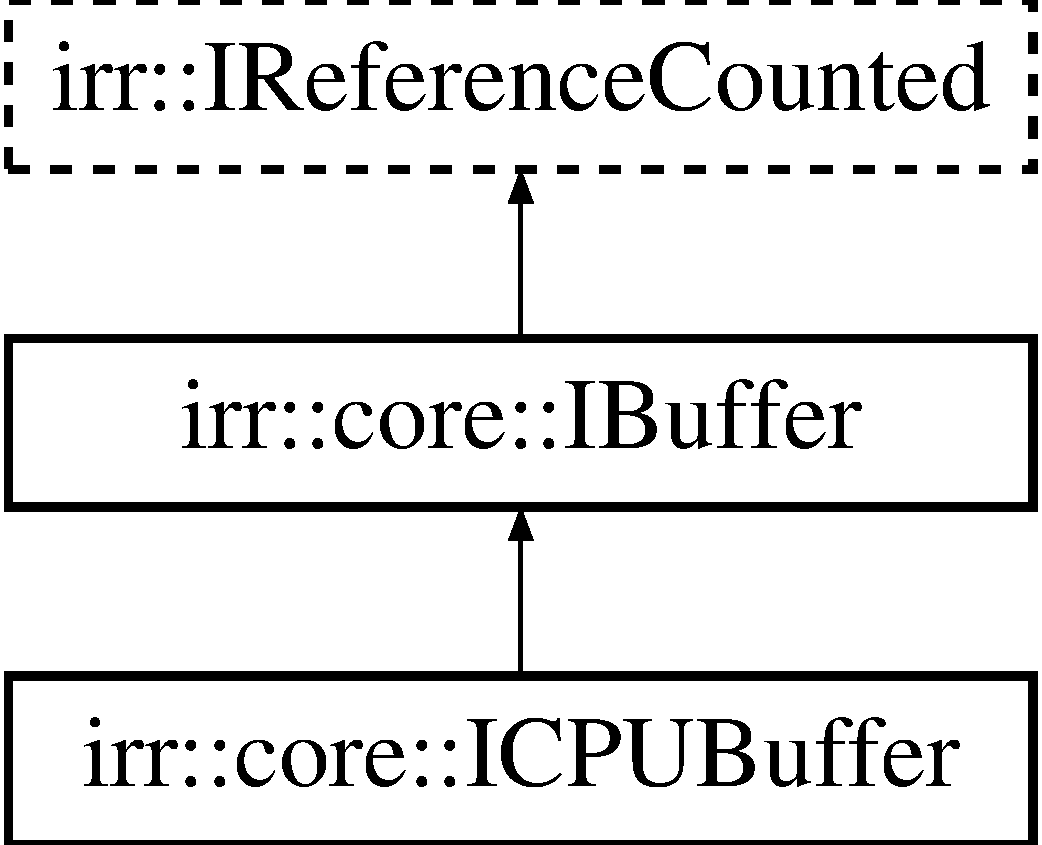
\includegraphics[height=3.000000cm]{classirr_1_1core_1_1ICPUBuffer}
\end{center}
\end{figure}
\subsection*{Public Member Functions}
\begin{DoxyCompactItemize}
\item 
{\bfseries I\+C\+P\+U\+Buffer} (const size\+\_\+t \&size\+In\+Bytes)\hypertarget{classirr_1_1core_1_1ICPUBuffer_a6747a9dd7d4c2a42cd1fb910d629f4d2}{}\label{classirr_1_1core_1_1ICPUBuffer_a6747a9dd7d4c2a42cd1fb910d629f4d2}

\item 
virtual E\+\_\+\+B\+U\+F\+F\+E\+R\+\_\+\+T\+Y\+PE {\bfseries get\+Buffer\+Type} () const \hypertarget{classirr_1_1core_1_1ICPUBuffer_aa590d78d044e599618e936702ad3c151}{}\label{classirr_1_1core_1_1ICPUBuffer_aa590d78d044e599618e936702ad3c151}

\item 
virtual const uint64\+\_\+t \& \hyperlink{classirr_1_1core_1_1ICPUBuffer_addfd5f5b83f7ff9614d80b8679082897}{get\+Size} () const \hypertarget{classirr_1_1core_1_1ICPUBuffer_addfd5f5b83f7ff9614d80b8679082897}{}\label{classirr_1_1core_1_1ICPUBuffer_addfd5f5b83f7ff9614d80b8679082897}

\begin{DoxyCompactList}\small\item\em size in B\+Y\+T\+ES \end{DoxyCompactList}\item 
virtual bool \hyperlink{classirr_1_1core_1_1ICPUBuffer_ae223eb80a29ac3993b0bfa3e515ef5ce}{reallocate} (const size\+\_\+t \&new\+Size, const bool \&force\+Retention\+Of\+Data=false, const bool \&reallocate\+If\+Shrink=false)
\item 
virtual const void $\ast$ \hyperlink{classirr_1_1core_1_1ICPUBuffer_af4202485ff6630611fa9045c9f8018da}{get\+Pointer} () const \hypertarget{classirr_1_1core_1_1ICPUBuffer_af4202485ff6630611fa9045c9f8018da}{}\label{classirr_1_1core_1_1ICPUBuffer_af4202485ff6630611fa9045c9f8018da}

\begin{DoxyCompactList}\small\item\em W\+A\+R\+N\+I\+NG\+: R\+E\+S\+I\+ZE will invalidate pointer. \end{DoxyCompactList}\item 
virtual void $\ast$ {\bfseries get\+Pointer} ()\hypertarget{classirr_1_1core_1_1ICPUBuffer_aa63952d75dd3273a2a36feff79e9cf3d}{}\label{classirr_1_1core_1_1ICPUBuffer_aa63952d75dd3273a2a36feff79e9cf3d}

\end{DoxyCompactItemize}
\subsection*{Additional Inherited Members}


\subsection{Detailed Description}
Persistently Mapped buffer. 

\subsection{Member Function Documentation}
\index{irr\+::core\+::\+I\+C\+P\+U\+Buffer@{irr\+::core\+::\+I\+C\+P\+U\+Buffer}!reallocate@{reallocate}}
\index{reallocate@{reallocate}!irr\+::core\+::\+I\+C\+P\+U\+Buffer@{irr\+::core\+::\+I\+C\+P\+U\+Buffer}}
\subsubsection[{\texorpdfstring{reallocate(const size\+\_\+t \&new\+Size, const bool \&force\+Retention\+Of\+Data=false, const bool \&reallocate\+If\+Shrink=false)}{reallocate(const size\_t \&newSize, const bool \&forceRetentionOfData=false, const bool \&reallocateIfShrink=false)}}]{\setlength{\rightskip}{0pt plus 5cm}virtual bool irr\+::core\+::\+I\+C\+P\+U\+Buffer\+::reallocate (
\begin{DoxyParamCaption}
\item[{const size\+\_\+t \&}]{new\+Size, }
\item[{const bool \&}]{force\+Retention\+Of\+Data = {\ttfamily false}, }
\item[{const bool \&}]{reallocate\+If\+Shrink = {\ttfamily false}}
\end{DoxyParamCaption}
)\hspace{0.3cm}{\ttfamily [inline]}, {\ttfamily [virtual]}}\hypertarget{classirr_1_1core_1_1ICPUBuffer_ae223eb80a29ac3993b0bfa3e515ef5ce}{}\label{classirr_1_1core_1_1ICPUBuffer_ae223eb80a29ac3993b0bfa3e515ef5ce}
returns true on success (some types always return false since they dont support resize) This function will invalidate any sizes, pointers etc. returned before! 

Implements \hyperlink{classirr_1_1core_1_1IBuffer_a725232c3869f003574d73707f40d7412}{irr\+::core\+::\+I\+Buffer}.



The documentation for this class was generated from the following file\+:\begin{DoxyCompactItemize}
\item 
include/I\+C\+P\+U\+Buffer.\+h\end{DoxyCompactItemize}

\hypertarget{classirr_1_1scene_1_1ICPUMeshBuffer}{}\section{irr\+:\+:scene\+:\+:I\+C\+P\+U\+Mesh\+Buffer Class Reference}
\label{classirr_1_1scene_1_1ICPUMeshBuffer}\index{irr\+::scene\+::\+I\+C\+P\+U\+Mesh\+Buffer@{irr\+::scene\+::\+I\+C\+P\+U\+Mesh\+Buffer}}
Inheritance diagram for irr\+:\+:scene\+:\+:I\+C\+P\+U\+Mesh\+Buffer\+:\begin{figure}[H]
\begin{center}
\leavevmode
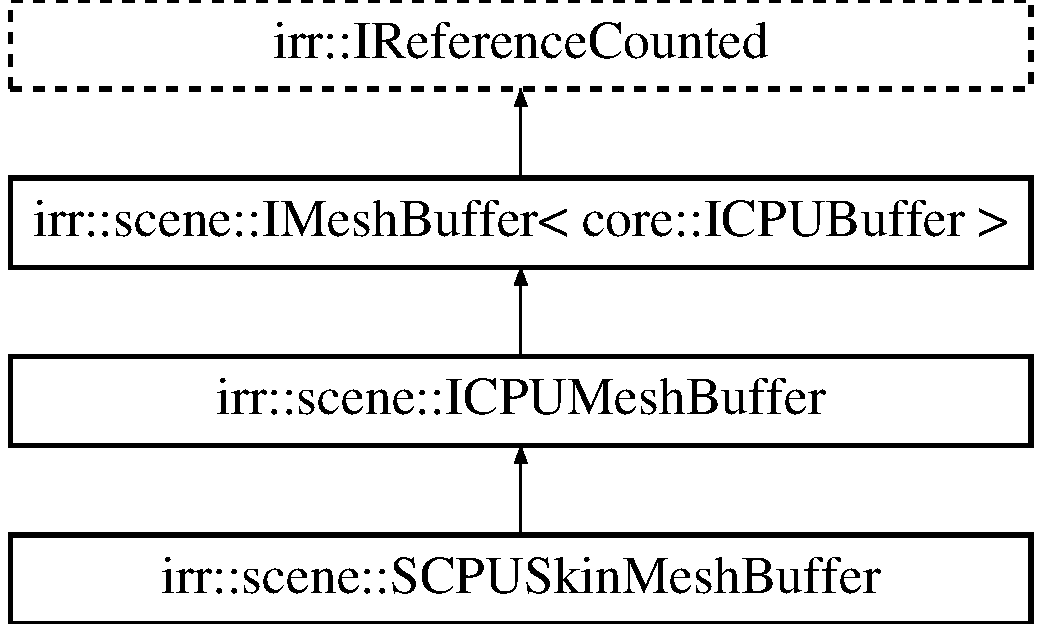
\includegraphics[height=4.000000cm]{classirr_1_1scene_1_1ICPUMeshBuffer}
\end{center}
\end{figure}
\subsection*{Public Member Functions}
\begin{DoxyCompactItemize}
\item 
const E\+\_\+\+V\+E\+R\+T\+E\+X\+\_\+\+A\+T\+T\+R\+I\+B\+U\+T\+E\+\_\+\+ID \& {\bfseries get\+Position\+Attribute\+Ix} () const \hypertarget{classirr_1_1scene_1_1ICPUMeshBuffer_a54c6d8ed3901b52b0fb7b189faa7a02b}{}\label{classirr_1_1scene_1_1ICPUMeshBuffer_a54c6d8ed3901b52b0fb7b189faa7a02b}

\item 
void {\bfseries set\+Position\+Attribute\+Ix} (const E\+\_\+\+V\+E\+R\+T\+E\+X\+\_\+\+A\+T\+T\+R\+I\+B\+U\+T\+E\+\_\+\+ID \&attr\+Id)\hypertarget{classirr_1_1scene_1_1ICPUMeshBuffer_ab77d7f76b288804c248448e82c04c84b}{}\label{classirr_1_1scene_1_1ICPUMeshBuffer_ab77d7f76b288804c248448e82c04c84b}

\item 
void $\ast$ \hyperlink{classirr_1_1scene_1_1ICPUMeshBuffer_a8d0f5fd79037531de1a70ea97da70269}{get\+Indices} ()
\begin{DoxyCompactList}\small\item\em Get access to Indices. \end{DoxyCompactList}\item 
const void $\ast$ {\bfseries get\+Indices} () const \hypertarget{classirr_1_1scene_1_1ICPUMeshBuffer_a6c53a614dfbd7580c3a9da8a06920731}{}\label{classirr_1_1scene_1_1ICPUMeshBuffer_a6c53a614dfbd7580c3a9da8a06920731}

\item 
virtual \hyperlink{classirr_1_1core_1_1vectorSIMDf}{core\+::vector\+S\+I\+M\+Df} {\bfseries get\+Position} (size\+\_\+t ix) const \hypertarget{classirr_1_1scene_1_1ICPUMeshBuffer_a969b13b257374c78872ffcbe2852b2b0}{}\label{classirr_1_1scene_1_1ICPUMeshBuffer_a969b13b257374c78872ffcbe2852b2b0}

\item 
virtual uint8\+\_\+t $\ast$ {\bfseries get\+Attrib\+Pointer} (const E\+\_\+\+V\+E\+R\+T\+E\+X\+\_\+\+A\+T\+T\+R\+I\+B\+U\+T\+E\+\_\+\+ID \&attr\+Id) const \hypertarget{classirr_1_1scene_1_1ICPUMeshBuffer_a92ef1ac64c0cb774062b029a3e9b7f4c}{}\label{classirr_1_1scene_1_1ICPUMeshBuffer_a92ef1ac64c0cb774062b029a3e9b7f4c}

\item 
virtual bool \hyperlink{classirr_1_1scene_1_1ICPUMeshBuffer_a6d971fdaf4537e249a9ed849b72e0377}{get\+Attribute} (\hyperlink{classirr_1_1core_1_1vectorSIMDf}{core\+::vector\+S\+I\+M\+Df} \&output, const E\+\_\+\+V\+E\+R\+T\+E\+X\+\_\+\+A\+T\+T\+R\+I\+B\+U\+T\+E\+\_\+\+ID \&attr\+Id, size\+\_\+t ix) const 
\item 
virtual bool \hyperlink{classirr_1_1scene_1_1ICPUMeshBuffer_a09de5f90f3abd1fab782551015d3af44}{set\+Attribute} (\hyperlink{classirr_1_1core_1_1vectorSIMDf}{core\+::vector\+S\+I\+M\+Df} input, const E\+\_\+\+V\+E\+R\+T\+E\+X\+\_\+\+A\+T\+T\+R\+I\+B\+U\+T\+E\+\_\+\+ID \&attr\+Id, size\+\_\+t ix) const 
\item 
virtual bool {\bfseries set\+Attribute} (uint32\+\_\+t $\ast$input, const E\+\_\+\+V\+E\+R\+T\+E\+X\+\_\+\+A\+T\+T\+R\+I\+B\+U\+T\+E\+\_\+\+ID \&attr\+Id, size\+\_\+t ix) const \hypertarget{classirr_1_1scene_1_1ICPUMeshBuffer_ac680f86f70345c4216cd639115901a78}{}\label{classirr_1_1scene_1_1ICPUMeshBuffer_ac680f86f70345c4216cd639115901a78}

\item 
virtual void \hyperlink{classirr_1_1scene_1_1ICPUMeshBuffer_af7950e5b319d74c646c396b073fd78bf}{recalculate\+Bounding\+Box} ()\hypertarget{classirr_1_1scene_1_1ICPUMeshBuffer_af7950e5b319d74c646c396b073fd78bf}{}\label{classirr_1_1scene_1_1ICPUMeshBuffer_af7950e5b319d74c646c396b073fd78bf}

\begin{DoxyCompactList}\small\item\em Recalculates the bounding box. Should be called if the mesh changed. \end{DoxyCompactList}\end{DoxyCompactItemize}
\subsection*{Additional Inherited Members}


\subsection{Member Function Documentation}
\index{irr\+::scene\+::\+I\+C\+P\+U\+Mesh\+Buffer@{irr\+::scene\+::\+I\+C\+P\+U\+Mesh\+Buffer}!get\+Attribute@{get\+Attribute}}
\index{get\+Attribute@{get\+Attribute}!irr\+::scene\+::\+I\+C\+P\+U\+Mesh\+Buffer@{irr\+::scene\+::\+I\+C\+P\+U\+Mesh\+Buffer}}
\subsubsection[{\texorpdfstring{get\+Attribute(core\+::vector\+S\+I\+M\+Df \&output, const E\+\_\+\+V\+E\+R\+T\+E\+X\+\_\+\+A\+T\+T\+R\+I\+B\+U\+T\+E\+\_\+\+I\+D \&attr\+Id, size\+\_\+t ix) const }{getAttribute(core::vectorSIMDf \&output, const E\_VERTEX\_ATTRIBUTE\_ID \&attrId, size\_t ix) const }}]{\setlength{\rightskip}{0pt plus 5cm}virtual bool irr\+::scene\+::\+I\+C\+P\+U\+Mesh\+Buffer\+::get\+Attribute (
\begin{DoxyParamCaption}
\item[{{\bf core\+::vector\+S\+I\+M\+Df} \&}]{output, }
\item[{const E\+\_\+\+V\+E\+R\+T\+E\+X\+\_\+\+A\+T\+T\+R\+I\+B\+U\+T\+E\+\_\+\+ID \&}]{attr\+Id, }
\item[{size\+\_\+t}]{ix}
\end{DoxyParamCaption}
) const\hspace{0.3cm}{\ttfamily [inline]}, {\ttfamily [virtual]}}\hypertarget{classirr_1_1scene_1_1ICPUMeshBuffer_a6d971fdaf4537e249a9ed849b72e0377}{}\label{classirr_1_1scene_1_1ICPUMeshBuffer_a6d971fdaf4537e249a9ed849b72e0377}
E\+C\+P\+A\+\_\+\+R\+E\+V\+E\+R\+S\+E\+D\+\_\+\+O\+R\+\_\+\+B\+G\+RA not D\+O\+NE C\+O\+R\+R\+E\+C\+T\+LY \index{irr\+::scene\+::\+I\+C\+P\+U\+Mesh\+Buffer@{irr\+::scene\+::\+I\+C\+P\+U\+Mesh\+Buffer}!get\+Indices@{get\+Indices}}
\index{get\+Indices@{get\+Indices}!irr\+::scene\+::\+I\+C\+P\+U\+Mesh\+Buffer@{irr\+::scene\+::\+I\+C\+P\+U\+Mesh\+Buffer}}
\subsubsection[{\texorpdfstring{get\+Indices()}{getIndices()}}]{\setlength{\rightskip}{0pt plus 5cm}void$\ast$ irr\+::scene\+::\+I\+C\+P\+U\+Mesh\+Buffer\+::get\+Indices (
\begin{DoxyParamCaption}
{}
\end{DoxyParamCaption}
)\hspace{0.3cm}{\ttfamily [inline]}}\hypertarget{classirr_1_1scene_1_1ICPUMeshBuffer_a8d0f5fd79037531de1a70ea97da70269}{}\label{classirr_1_1scene_1_1ICPUMeshBuffer_a8d0f5fd79037531de1a70ea97da70269}


Get access to Indices. 

\begin{DoxyReturn}{Returns}
Pointer to indices array. 
\end{DoxyReturn}
\index{irr\+::scene\+::\+I\+C\+P\+U\+Mesh\+Buffer@{irr\+::scene\+::\+I\+C\+P\+U\+Mesh\+Buffer}!set\+Attribute@{set\+Attribute}}
\index{set\+Attribute@{set\+Attribute}!irr\+::scene\+::\+I\+C\+P\+U\+Mesh\+Buffer@{irr\+::scene\+::\+I\+C\+P\+U\+Mesh\+Buffer}}
\subsubsection[{\texorpdfstring{set\+Attribute(core\+::vector\+S\+I\+M\+Df input, const E\+\_\+\+V\+E\+R\+T\+E\+X\+\_\+\+A\+T\+T\+R\+I\+B\+U\+T\+E\+\_\+\+I\+D \&attr\+Id, size\+\_\+t ix) const }{setAttribute(core::vectorSIMDf input, const E\_VERTEX\_ATTRIBUTE\_ID \&attrId, size\_t ix) const }}]{\setlength{\rightskip}{0pt plus 5cm}virtual bool irr\+::scene\+::\+I\+C\+P\+U\+Mesh\+Buffer\+::set\+Attribute (
\begin{DoxyParamCaption}
\item[{{\bf core\+::vector\+S\+I\+M\+Df}}]{input, }
\item[{const E\+\_\+\+V\+E\+R\+T\+E\+X\+\_\+\+A\+T\+T\+R\+I\+B\+U\+T\+E\+\_\+\+ID \&}]{attr\+Id, }
\item[{size\+\_\+t}]{ix}
\end{DoxyParamCaption}
) const\hspace{0.3cm}{\ttfamily [inline]}, {\ttfamily [virtual]}}\hypertarget{classirr_1_1scene_1_1ICPUMeshBuffer_a09de5f90f3abd1fab782551015d3af44}{}\label{classirr_1_1scene_1_1ICPUMeshBuffer_a09de5f90f3abd1fab782551015d3af44}
E\+C\+P\+A\+\_\+\+R\+E\+V\+E\+R\+S\+E\+D\+\_\+\+O\+R\+\_\+\+B\+G\+RA not D\+O\+NE C\+O\+R\+R\+E\+C\+T\+LY

if normalized convert up,

cast to int64\+\_\+t \begin{DoxyVerb}        core::vectorSIMDf divisors[8][ECPA_COUNT] = {
            {core::vectorSIMDf(1.f,511.f,511.f,511.f),core::vectorSIMDf(511.f,1.f,1.f,1.f),core::vectorSIMDf(511.f,511.f,1.f,1.f),core::vectorSIMDf(511.f,511.f,511.f,1.f),core::vectorSIMDf(511.f,511.f,511.f,1.f)},
            {core::vectorSIMDf(3.f,1023.f,1023.f,1023.f),core::vectorSIMDf(1023.f,1.f,1.f,1.f),core::vectorSIMDf(1023.f,1023.f,1.f,1.f),core::vectorSIMDf(1023.f,1023.f,1023.f,1.f),core::vectorSIMDf(1023.f,1023.f,1023.f,3.f)},
            {core::vectorSIMDf(127.f,127.f,127.f,127.f),core::vectorSIMDf(127.f,1.f,1.f,1.f),core::vectorSIMDf(127.f,127.f,1.f,1.f),core::vectorSIMDf(127.f,127.f,127.f,1.f),core::vectorSIMDf(127.f,127.f,127.f,127.f)},
            {core::vectorSIMDf(255.f,255.f,255.f,255.f),core::vectorSIMDf(255.f,1.f,1.f,1.f),core::vectorSIMDf(255.f,255.f,1.f,1.f),core::vectorSIMDf(255.f,255.f,255.f,1.f),core::vectorSIMDf(255.f,255.f,255.f,255.f)},
            {core::vectorSIMDf(32767.f,32767.f,32767.f,32767.f),core::vectorSIMDf(32767.f,1.f,1.f,1.f),core::vectorSIMDf(32767.f,32767.f,1.f,1.f),core::vectorSIMDf(32767.f,32767.f,32767.f,1.f),core::vectorSIMDf(32767.f,32767.f,32767.f,32767.f)},
            {core::vectorSIMDf(65535.f,65535.f,65535.f,65535.f),core::vectorSIMDf(65535.f,1.f,1.f,1.f),core::vectorSIMDf(65535.f,65535.f,1.f,1.f),core::vectorSIMDf(65535.f,65535.f,65535.f,1.f),core::vectorSIMDf(65535.f,65535.f,65535.f,65535.f)},
            {core::vectorSIMDf(2147483647.f,2147483647.f,2147483647.f,2147483647.f),core::vectorSIMDf(2147483647.f,1.f,1.f,1.f),core::vectorSIMDf(2147483647.f,2147483647.f,1.f,1.f),core::vectorSIMDf(2147483647.f,2147483647.f,2147483647.f,1.f),core::vectorSIMDf(2147483647.f,2147483647.f,2147483647.f,2147483647.f)},
            {core::vectorSIMDf(4294967295.f,4294967295.f,4294967295.f,4294967295.f),core::vectorSIMDf(4294967295.f,1.f,1.f,1.f),core::vectorSIMDf(4294967295.f,4294967295.f,1.f,1.f),core::vectorSIMDf(4294967295.f,4294967295.f,4294967295.f,1.f),core::vectorSIMDf(4294967295.f,4294967295.f,4294967295.f,4294967295.f)}
        };
        int64_t results[4];
        switch (attrType)
        {
            case ECT_NORMALIZED_INT_2_10_10_10_REV:
            case ECT_NORMALIZED_UNSIGNED_INT_2_10_10_10_REV:
            case ECT_NORMALIZED_BYTE:
            case ECT_NORMALIZED_UNSIGNED_BYTE:
            case ECT_NORMALIZED_SHORT:
            case ECT_NORMALIZED_UNSIGNED_SHORT:
            case ECT_NORMALIZED_INT:
            case ECT_NORMALIZED_UNSIGNED_INT:
                break;
        }
        for (size_t j=0; j<components; j++)
            results[j] = input.pointer[j]; \end{DoxyVerb}


The documentation for this class was generated from the following file\+:\begin{DoxyCompactItemize}
\item 
include/I\+Mesh\+Buffer.\+h\end{DoxyCompactItemize}

\hypertarget{classirr_1_1scene_1_1ICPUMeshDataFormatDesc}{}\section{irr\+:\+:scene\+:\+:I\+C\+P\+U\+Mesh\+Data\+Format\+Desc Class Reference}
\label{classirr_1_1scene_1_1ICPUMeshDataFormatDesc}\index{irr\+::scene\+::\+I\+C\+P\+U\+Mesh\+Data\+Format\+Desc@{irr\+::scene\+::\+I\+C\+P\+U\+Mesh\+Data\+Format\+Desc}}
Inheritance diagram for irr\+:\+:scene\+:\+:I\+C\+P\+U\+Mesh\+Data\+Format\+Desc\+:\begin{figure}[H]
\begin{center}
\leavevmode
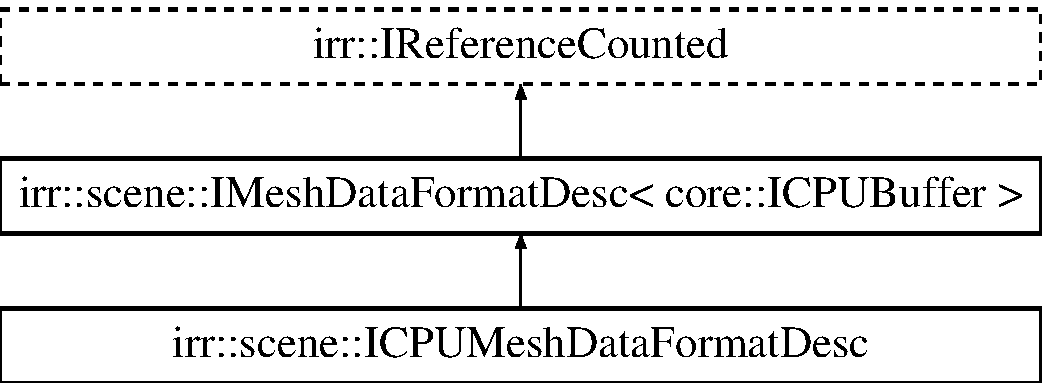
\includegraphics[height=3.000000cm]{classirr_1_1scene_1_1ICPUMeshDataFormatDesc}
\end{center}
\end{figure}
\subsection*{Public Member Functions}
\begin{DoxyCompactItemize}
\item 
bool {\bfseries format\+Can\+Be\+Appended} (const \hyperlink{classirr_1_1scene_1_1IMeshDataFormatDesc}{I\+Mesh\+Data\+Format\+Desc}$<$ \hyperlink{classirr_1_1core_1_1ICPUBuffer}{core\+::\+I\+C\+P\+U\+Buffer} $>$ $\ast$other) const \hypertarget{classirr_1_1scene_1_1ICPUMeshDataFormatDesc_a19ab69d08fe00b1bac3282900e1a46b5}{}\label{classirr_1_1scene_1_1ICPUMeshDataFormatDesc_a19ab69d08fe00b1bac3282900e1a46b5}

\item 
void {\bfseries map\+Index\+Buffer} (\hyperlink{classirr_1_1core_1_1ICPUBuffer}{core\+::\+I\+C\+P\+U\+Buffer} $\ast$ixbuf)\hypertarget{classirr_1_1scene_1_1ICPUMeshDataFormatDesc_ab1591e86c8073c37bc494f29a266f597}{}\label{classirr_1_1scene_1_1ICPUMeshDataFormatDesc_ab1591e86c8073c37bc494f29a266f597}

\item 
virtual const \hyperlink{classirr_1_1core_1_1ICPUBuffer}{core\+::\+I\+C\+P\+U\+Buffer} $\ast$ {\bfseries get\+Index\+Buffer} () const \hypertarget{classirr_1_1scene_1_1ICPUMeshDataFormatDesc_a3e1d0cb1d3224d341674c39bb0b32e3c}{}\label{classirr_1_1scene_1_1ICPUMeshDataFormatDesc_a3e1d0cb1d3224d341674c39bb0b32e3c}

\item 
void {\bfseries map\+Vertex\+Attr\+Buffer} (\hyperlink{classirr_1_1core_1_1ICPUBuffer}{core\+::\+I\+C\+P\+U\+Buffer} $\ast$attr\+Buf, const E\+\_\+\+V\+E\+R\+T\+E\+X\+\_\+\+A\+T\+T\+R\+I\+B\+U\+T\+E\+\_\+\+ID \&attr\+Id, E\+\_\+\+C\+O\+M\+P\+O\+N\+E\+N\+T\+S\+\_\+\+P\+E\+R\+\_\+\+A\+T\+T\+R\+I\+B\+U\+TE components, E\+\_\+\+C\+O\+M\+P\+O\+N\+E\+N\+T\+\_\+\+T\+Y\+PE type, const size\+\_\+t \&stride=0, size\+\_\+t offset=0, uint32\+\_\+t divisor=0)\hypertarget{classirr_1_1scene_1_1ICPUMeshDataFormatDesc_a39f0d0f14f6ed5f989a70ed0ddc96352}{}\label{classirr_1_1scene_1_1ICPUMeshDataFormatDesc_a39f0d0f14f6ed5f989a70ed0ddc96352}

\item 
virtual const \hyperlink{classirr_1_1core_1_1ICPUBuffer}{core\+::\+I\+C\+P\+U\+Buffer} $\ast$ {\bfseries get\+Mapped\+Buffer} (const E\+\_\+\+V\+E\+R\+T\+E\+X\+\_\+\+A\+T\+T\+R\+I\+B\+U\+T\+E\+\_\+\+ID \&attr\+Id) const \hypertarget{classirr_1_1scene_1_1ICPUMeshDataFormatDesc_aa6f266e7db72021074c60ba47638bd1d}{}\label{classirr_1_1scene_1_1ICPUMeshDataFormatDesc_aa6f266e7db72021074c60ba47638bd1d}

\item 
void {\bfseries set\+Mapped\+Buffer\+Offset} (const E\+\_\+\+V\+E\+R\+T\+E\+X\+\_\+\+A\+T\+T\+R\+I\+B\+U\+T\+E\+\_\+\+ID \&attr\+Id, const size\+\_\+t \&offset)\hypertarget{classirr_1_1scene_1_1ICPUMeshDataFormatDesc_ab0d72252abc276fcb275882bfec0d88b}{}\label{classirr_1_1scene_1_1ICPUMeshDataFormatDesc_ab0d72252abc276fcb275882bfec0d88b}

\end{DoxyCompactItemize}
\subsection*{Protected Attributes}
\begin{DoxyCompactItemize}
\item 
\hyperlink{classirr_1_1core_1_1ICPUBuffer}{core\+::\+I\+C\+P\+U\+Buffer} $\ast$ {\bfseries mapped\+Attr\+Buf} \mbox{[}E\+V\+A\+I\+\_\+\+C\+O\+U\+NT\mbox{]}\hypertarget{classirr_1_1scene_1_1ICPUMeshDataFormatDesc_ad7374aa5c82fb16c0dcfdf2bb06b8da0}{}\label{classirr_1_1scene_1_1ICPUMeshDataFormatDesc_ad7374aa5c82fb16c0dcfdf2bb06b8da0}

\item 
\hyperlink{classirr_1_1core_1_1ICPUBuffer}{core\+::\+I\+C\+P\+U\+Buffer} $\ast$ {\bfseries mapped\+Index\+Buf}\hypertarget{classirr_1_1scene_1_1ICPUMeshDataFormatDesc_adb80af396a0546ef695d28c376ea7224}{}\label{classirr_1_1scene_1_1ICPUMeshDataFormatDesc_adb80af396a0546ef695d28c376ea7224}

\end{DoxyCompactItemize}
\subsection*{Additional Inherited Members}


The documentation for this class was generated from the following file\+:\begin{DoxyCompactItemize}
\item 
include/I\+Mesh\+Buffer.\+h\end{DoxyCompactItemize}

\hypertarget{classirr_1_1scene_1_1ICPUSkinnedMesh}{}\section{irr\+:\+:scene\+:\+:I\+C\+P\+U\+Skinned\+Mesh Class Reference}
\label{classirr_1_1scene_1_1ICPUSkinnedMesh}\index{irr\+::scene\+::\+I\+C\+P\+U\+Skinned\+Mesh@{irr\+::scene\+::\+I\+C\+P\+U\+Skinned\+Mesh}}


Interface for using some special functions of Skinned meshes.  




{\ttfamily \#include $<$I\+Skinned\+Mesh.\+h$>$}

Inheritance diagram for irr\+:\+:scene\+:\+:I\+C\+P\+U\+Skinned\+Mesh\+:\begin{figure}[H]
\begin{center}
\leavevmode
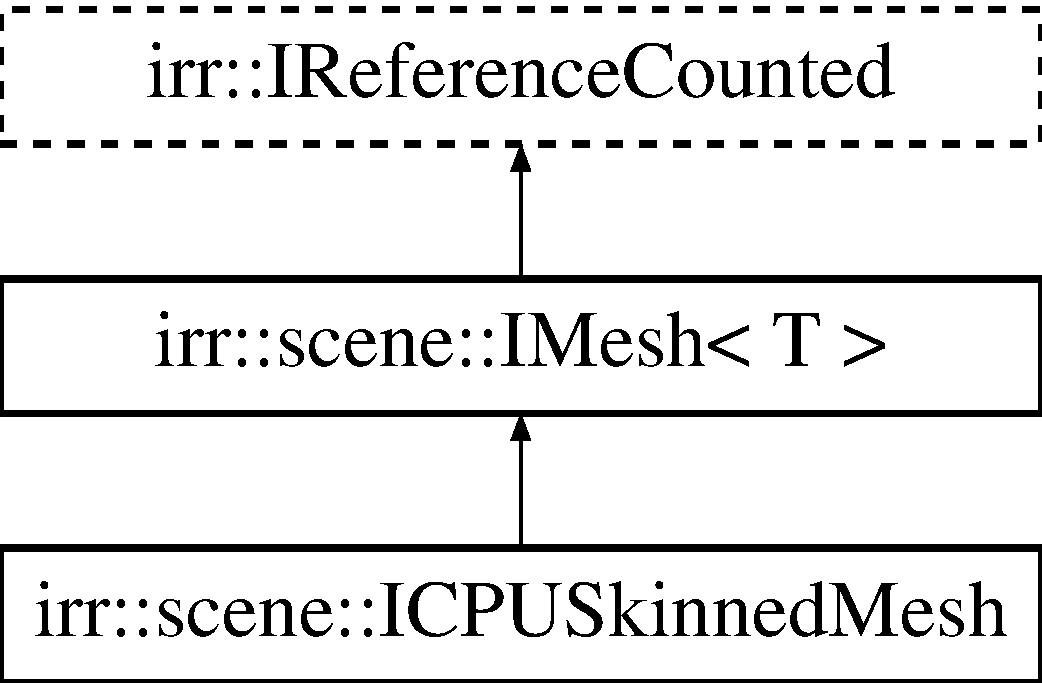
\includegraphics[height=3.000000cm]{classirr_1_1scene_1_1ICPUSkinnedMesh}
\end{center}
\end{figure}
\subsection*{Classes}
\begin{DoxyCompactItemize}
\item 
class \hyperlink{classirr_1_1scene_1_1ICPUSkinnedMesh_1_1SJoint}{S\+Joint}
\begin{DoxyCompactList}\small\item\em Joints. \end{DoxyCompactList}\item 
class \hyperlink{classirr_1_1scene_1_1ICPUSkinnedMesh_1_1SPositionKey}{S\+Position\+Key}
\begin{DoxyCompactList}\small\item\em Animation keyframe which describes a new position. \end{DoxyCompactList}\item 
class \hyperlink{classirr_1_1scene_1_1ICPUSkinnedMesh_1_1SRotationKey}{S\+Rotation\+Key}
\begin{DoxyCompactList}\small\item\em Animation keyframe which describes a new rotation. \end{DoxyCompactList}\item 
class \hyperlink{classirr_1_1scene_1_1ICPUSkinnedMesh_1_1SScaleKey}{S\+Scale\+Key}
\begin{DoxyCompactList}\small\item\em Animation keyframe which describes a new scale. \end{DoxyCompactList}\end{DoxyCompactItemize}
\subsection*{Public Member Functions}
\begin{DoxyCompactItemize}
\item 
virtual \hyperlink{classirr_1_1scene_1_1CFinalBoneHierarchy}{C\+Final\+Bone\+Hierarchy} $\ast$ {\bfseries get\+Bone\+Reference\+Hierarchy} () const  =0\hypertarget{classirr_1_1scene_1_1ICPUSkinnedMesh_aa443e276729090325135e3de174a739e}{}\label{classirr_1_1scene_1_1ICPUSkinnedMesh_aa443e276729090325135e3de174a739e}

\item 
virtual \hyperlink{namespaceirr_1_1scene_aef0400177e5941293dff6640e800d11b}{E\+\_\+\+M\+E\+S\+H\+\_\+\+T\+Y\+PE} {\bfseries get\+Mesh\+Type} () const \hypertarget{classirr_1_1scene_1_1ICPUSkinnedMesh_a0f67b6b70b6ecd72ae9f8ab654c612b5}{}\label{classirr_1_1scene_1_1ICPUSkinnedMesh_a0f67b6b70b6ecd72ae9f8ab654c612b5}

\item 
virtual std\+::vector$<$ \hyperlink{classirr_1_1scene_1_1ICPUSkinnedMesh_1_1SJoint}{S\+Joint} $\ast$ $>$ \& \hyperlink{classirr_1_1scene_1_1ICPUSkinnedMesh_a432026219234bd5c98b1af820fd0103e}{get\+All\+Joints} ()=0\hypertarget{classirr_1_1scene_1_1ICPUSkinnedMesh_a432026219234bd5c98b1af820fd0103e}{}\label{classirr_1_1scene_1_1ICPUSkinnedMesh_a432026219234bd5c98b1af820fd0103e}

\begin{DoxyCompactList}\small\item\em exposed for loaders\+: joints list \end{DoxyCompactList}\item 
virtual const std\+::vector$<$ \hyperlink{classirr_1_1scene_1_1ICPUSkinnedMesh_1_1SJoint}{S\+Joint} $\ast$ $>$ \& \hyperlink{classirr_1_1scene_1_1ICPUSkinnedMesh_aef97dd768afe4cae2652bba7d3487d6c}{get\+All\+Joints} () const  =0\hypertarget{classirr_1_1scene_1_1ICPUSkinnedMesh_aef97dd768afe4cae2652bba7d3487d6c}{}\label{classirr_1_1scene_1_1ICPUSkinnedMesh_aef97dd768afe4cae2652bba7d3487d6c}

\begin{DoxyCompactList}\small\item\em exposed for loaders\+: joints list \end{DoxyCompactList}\item 
virtual void \hyperlink{classirr_1_1scene_1_1ICPUSkinnedMesh_a811b994c81509909cbb5c13d28ccb44f}{finalize} ()=0\hypertarget{classirr_1_1scene_1_1ICPUSkinnedMesh_a811b994c81509909cbb5c13d28ccb44f}{}\label{classirr_1_1scene_1_1ICPUSkinnedMesh_a811b994c81509909cbb5c13d28ccb44f}

\begin{DoxyCompactList}\small\item\em loaders should call this after populating the mesh \end{DoxyCompactList}\item 
virtual \hyperlink{classirr_1_1scene_1_1ICPUSkinnedMesh_1_1SJoint}{S\+Joint} $\ast$ \hyperlink{classirr_1_1scene_1_1ICPUSkinnedMesh_a99cb2728263977178ed1d49eb4b6b345}{add\+Joint} (\hyperlink{classirr_1_1scene_1_1ICPUSkinnedMesh_1_1SJoint}{S\+Joint} $\ast$parent=0)=0\hypertarget{classirr_1_1scene_1_1ICPUSkinnedMesh_a99cb2728263977178ed1d49eb4b6b345}{}\label{classirr_1_1scene_1_1ICPUSkinnedMesh_a99cb2728263977178ed1d49eb4b6b345}

\begin{DoxyCompactList}\small\item\em Adds a new joint to the mesh, access it as last one. \end{DoxyCompactList}\item 
virtual bool \hyperlink{classirr_1_1scene_1_1ICPUSkinnedMesh_a4b2b1dee3654d83a0aa6eb4de46cc816}{is\+Static} ()=0\hypertarget{classirr_1_1scene_1_1ICPUSkinnedMesh_a4b2b1dee3654d83a0aa6eb4de46cc816}{}\label{classirr_1_1scene_1_1ICPUSkinnedMesh_a4b2b1dee3654d83a0aa6eb4de46cc816}

\begin{DoxyCompactList}\small\item\em Check if the mesh is non-\/animated. \end{DoxyCompactList}\end{DoxyCompactItemize}
\subsection*{Additional Inherited Members}


\subsection{Detailed Description}
Interface for using some special functions of Skinned meshes. 

The documentation for this class was generated from the following file\+:\begin{DoxyCompactItemize}
\item 
include/I\+Skinned\+Mesh.\+h\end{DoxyCompactItemize}

\hypertarget{classirr_1_1gui_1_1ICursorControl}{}\section{irr\+:\+:gui\+:\+:I\+Cursor\+Control Class Reference}
\label{classirr_1_1gui_1_1ICursorControl}\index{irr\+::gui\+::\+I\+Cursor\+Control@{irr\+::gui\+::\+I\+Cursor\+Control}}


Interface to manipulate the mouse cursor.  




{\ttfamily \#include $<$I\+Cursor\+Control.\+h$>$}

Inheritance diagram for irr\+:\+:gui\+:\+:I\+Cursor\+Control\+:\begin{figure}[H]
\begin{center}
\leavevmode
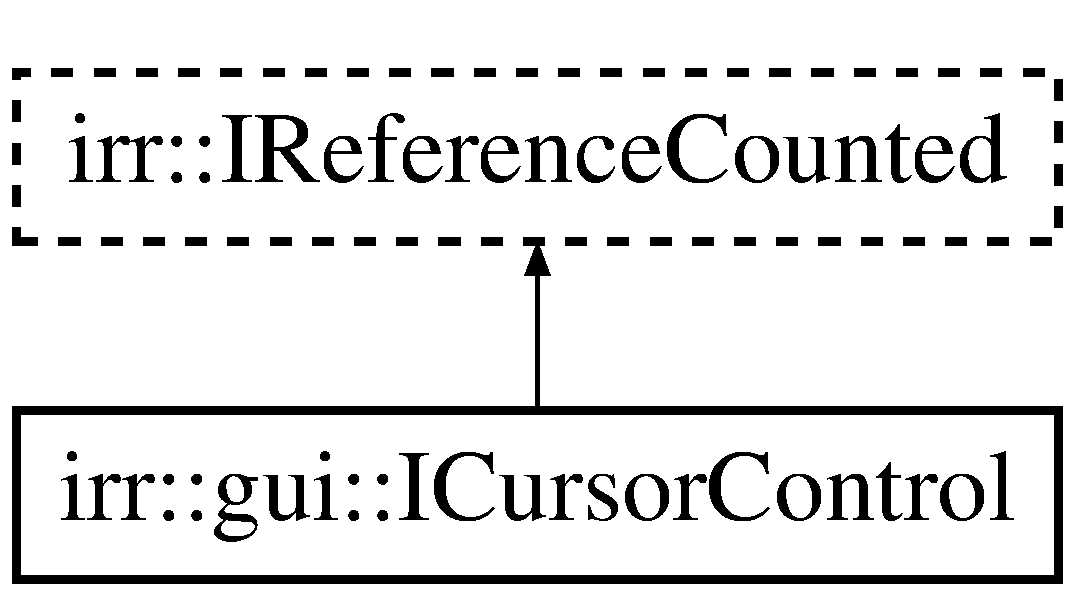
\includegraphics[height=2.000000cm]{classirr_1_1gui_1_1ICursorControl}
\end{center}
\end{figure}
\subsection*{Public Member Functions}
\begin{DoxyCompactItemize}
\item 
virtual void \hyperlink{classirr_1_1gui_1_1ICursorControl_aceb41d68494e2b2076fbc6949b254c74}{set\+Visible} (bool visible)=0
\begin{DoxyCompactList}\small\item\em Changes the visible state of the mouse cursor. \end{DoxyCompactList}\item 
virtual bool \hyperlink{classirr_1_1gui_1_1ICursorControl_afe03225e5ea27e2b2f97c0e02f04fc2a}{is\+Visible} () const  =0
\begin{DoxyCompactList}\small\item\em Returns if the cursor is currently visible. \end{DoxyCompactList}\item 
virtual void \hyperlink{classirr_1_1gui_1_1ICursorControl_a951b5afe97fa21d98ce5360d96314306}{set\+Position} (const core\+::position2d$<$ \hyperlink{namespaceirr_a0277be98d67dc26ff93b1a6a1d086b07}{f32} $>$ \&pos)=0
\begin{DoxyCompactList}\small\item\em Sets the new position of the cursor. \end{DoxyCompactList}\item 
virtual void \hyperlink{classirr_1_1gui_1_1ICursorControl_adca41054684f73435c9b045520f7c83b}{set\+Position} (\hyperlink{namespaceirr_a0277be98d67dc26ff93b1a6a1d086b07}{f32} x, \hyperlink{namespaceirr_a0277be98d67dc26ff93b1a6a1d086b07}{f32} y)=0
\begin{DoxyCompactList}\small\item\em Sets the new position of the cursor. \end{DoxyCompactList}\item 
virtual void \hyperlink{classirr_1_1gui_1_1ICursorControl_a421c770ffc494f8f6082a16bef0feed2}{set\+Position} (const core\+::position2d$<$ \hyperlink{namespaceirr_ac66849b7a6ed16e30ebede579f9b47c6}{s32} $>$ \&pos)=0
\begin{DoxyCompactList}\small\item\em Sets the new position of the cursor. \end{DoxyCompactList}\item 
virtual void \hyperlink{classirr_1_1gui_1_1ICursorControl_a3b0a59608d1d0810079349acfa01a79b}{set\+Position} (\hyperlink{namespaceirr_ac66849b7a6ed16e30ebede579f9b47c6}{s32} x, \hyperlink{namespaceirr_ac66849b7a6ed16e30ebede579f9b47c6}{s32} y)=0
\begin{DoxyCompactList}\small\item\em Sets the new position of the cursor. \end{DoxyCompactList}\item 
virtual const core\+::position2d$<$ \hyperlink{namespaceirr_ac66849b7a6ed16e30ebede579f9b47c6}{s32} $>$ \& \hyperlink{classirr_1_1gui_1_1ICursorControl_a65d9f6e734baa02be69b7e9f5fbdd565}{get\+Position} ()=0
\begin{DoxyCompactList}\small\item\em Returns the current position of the mouse cursor. \end{DoxyCompactList}\item 
virtual core\+::position2d$<$ \hyperlink{namespaceirr_a0277be98d67dc26ff93b1a6a1d086b07}{f32} $>$ \hyperlink{classirr_1_1gui_1_1ICursorControl_a8ba1cb0ff11edc5fb32cdadddece09f8}{get\+Relative\+Position} ()=0
\begin{DoxyCompactList}\small\item\em Returns the current position of the mouse cursor. \end{DoxyCompactList}\item 
virtual void \hyperlink{classirr_1_1gui_1_1ICursorControl_a2a7428ef716a60f8f4b86361a69b8770}{set\+Reference\+Rect} (\hyperlink{classirr_1_1core_1_1rect}{core\+::rect}$<$ \hyperlink{namespaceirr_ac66849b7a6ed16e30ebede579f9b47c6}{s32} $>$ $\ast$rect=0)=0
\begin{DoxyCompactList}\small\item\em Sets an absolute reference rect for setting and retrieving the cursor position. \end{DoxyCompactList}\item 
virtual void \hyperlink{classirr_1_1gui_1_1ICursorControl_af394700d5279b13cc0f2bcdad679469c}{set\+Active\+Icon} (\hyperlink{namespaceirr_1_1gui_aefee802dd632c5735703e40ef40f879b}{E\+C\+U\+R\+S\+O\+R\+\_\+\+I\+C\+ON} icon\+Id)
\begin{DoxyCompactList}\small\item\em Sets the active cursor icon. \end{DoxyCompactList}\item 
virtual \hyperlink{namespaceirr_1_1gui_aefee802dd632c5735703e40ef40f879b}{E\+C\+U\+R\+S\+O\+R\+\_\+\+I\+C\+ON} \hyperlink{classirr_1_1gui_1_1ICursorControl_a6c08f4adefe397b8054296151f15f2ad}{get\+Active\+Icon} () const \hypertarget{classirr_1_1gui_1_1ICursorControl_a6c08f4adefe397b8054296151f15f2ad}{}\label{classirr_1_1gui_1_1ICursorControl_a6c08f4adefe397b8054296151f15f2ad}

\begin{DoxyCompactList}\small\item\em Gets the currently active icon. \end{DoxyCompactList}\item 
virtual \hyperlink{namespaceirr_1_1gui_aefee802dd632c5735703e40ef40f879b}{E\+C\+U\+R\+S\+O\+R\+\_\+\+I\+C\+ON} \hyperlink{classirr_1_1gui_1_1ICursorControl_a102ff455c70595886281e636ef063d3b}{add\+Icon} (const \hyperlink{structirr_1_1gui_1_1SCursorSprite}{gui\+::\+S\+Cursor\+Sprite} \&icon)
\begin{DoxyCompactList}\small\item\em Add a custom sprite as cursor icon. \end{DoxyCompactList}\item 
virtual void \hyperlink{classirr_1_1gui_1_1ICursorControl_a3e7c8cb1f03e1ccc31fcc3c30f717762}{change\+Icon} (\hyperlink{namespaceirr_1_1gui_aefee802dd632c5735703e40ef40f879b}{E\+C\+U\+R\+S\+O\+R\+\_\+\+I\+C\+ON} icon\+Id, const \hyperlink{structirr_1_1gui_1_1SCursorSprite}{gui\+::\+S\+Cursor\+Sprite} \&sprite)
\begin{DoxyCompactList}\small\item\em replace a cursor icon. \end{DoxyCompactList}\item 
virtual \hyperlink{namespaceirr_1_1core_ac79bc3704cf28bc1ab72d7cd1cae78d1}{core\+::dimension2di} \hyperlink{classirr_1_1gui_1_1ICursorControl_ad2c301e1c82366520913c270ef8d738c}{get\+Supported\+Icon\+Size} () const \hypertarget{classirr_1_1gui_1_1ICursorControl_ad2c301e1c82366520913c270ef8d738c}{}\label{classirr_1_1gui_1_1ICursorControl_ad2c301e1c82366520913c270ef8d738c}

\begin{DoxyCompactList}\small\item\em Return a system-\/specific size which is supported for cursors. Larger icons will fail, smaller icons might work. \end{DoxyCompactList}\item 
virtual void \hyperlink{classirr_1_1gui_1_1ICursorControl_ad7688bb200945f15877a598e8be53878}{set\+Platform\+Behavior} (\hyperlink{namespaceirr_1_1gui_abbd186f9cfba2f805d98248df226acef}{E\+C\+U\+R\+S\+O\+R\+\_\+\+P\+L\+A\+T\+F\+O\+R\+M\+\_\+\+B\+E\+H\+A\+V\+I\+OR} behavior)\hypertarget{classirr_1_1gui_1_1ICursorControl_ad7688bb200945f15877a598e8be53878}{}\label{classirr_1_1gui_1_1ICursorControl_ad7688bb200945f15877a598e8be53878}

\begin{DoxyCompactList}\small\item\em Set platform specific behavior flags. \end{DoxyCompactList}\item 
virtual \hyperlink{namespaceirr_1_1gui_abbd186f9cfba2f805d98248df226acef}{E\+C\+U\+R\+S\+O\+R\+\_\+\+P\+L\+A\+T\+F\+O\+R\+M\+\_\+\+B\+E\+H\+A\+V\+I\+OR} \hyperlink{classirr_1_1gui_1_1ICursorControl_a0d0b11d3d3d5d0adb6e0b0de78edd2a8}{get\+Platform\+Behavior} () const 
\begin{DoxyCompactList}\small\item\em Return platform specific behavior. \end{DoxyCompactList}\end{DoxyCompactItemize}
\subsection*{Additional Inherited Members}


\subsection{Detailed Description}
Interface to manipulate the mouse cursor. 

\subsection{Member Function Documentation}
\index{irr\+::gui\+::\+I\+Cursor\+Control@{irr\+::gui\+::\+I\+Cursor\+Control}!add\+Icon@{add\+Icon}}
\index{add\+Icon@{add\+Icon}!irr\+::gui\+::\+I\+Cursor\+Control@{irr\+::gui\+::\+I\+Cursor\+Control}}
\subsubsection[{\texorpdfstring{add\+Icon(const gui\+::\+S\+Cursor\+Sprite \&icon)}{addIcon(const gui::SCursorSprite \&icon)}}]{\setlength{\rightskip}{0pt plus 5cm}virtual {\bf E\+C\+U\+R\+S\+O\+R\+\_\+\+I\+C\+ON} irr\+::gui\+::\+I\+Cursor\+Control\+::add\+Icon (
\begin{DoxyParamCaption}
\item[{const {\bf gui\+::\+S\+Cursor\+Sprite} \&}]{icon}
\end{DoxyParamCaption}
)\hspace{0.3cm}{\ttfamily [inline]}, {\ttfamily [virtual]}}\hypertarget{classirr_1_1gui_1_1ICursorControl_a102ff455c70595886281e636ef063d3b}{}\label{classirr_1_1gui_1_1ICursorControl_a102ff455c70595886281e636ef063d3b}


Add a custom sprite as cursor icon. 

\begin{DoxyReturn}{Returns}
Identification for the icon 
\end{DoxyReturn}
\index{irr\+::gui\+::\+I\+Cursor\+Control@{irr\+::gui\+::\+I\+Cursor\+Control}!change\+Icon@{change\+Icon}}
\index{change\+Icon@{change\+Icon}!irr\+::gui\+::\+I\+Cursor\+Control@{irr\+::gui\+::\+I\+Cursor\+Control}}
\subsubsection[{\texorpdfstring{change\+Icon(\+E\+C\+U\+R\+S\+O\+R\+\_\+\+I\+C\+O\+N icon\+Id, const gui\+::\+S\+Cursor\+Sprite \&sprite)}{changeIcon(ECURSOR\_ICON iconId, const gui::SCursorSprite \&sprite)}}]{\setlength{\rightskip}{0pt plus 5cm}virtual void irr\+::gui\+::\+I\+Cursor\+Control\+::change\+Icon (
\begin{DoxyParamCaption}
\item[{{\bf E\+C\+U\+R\+S\+O\+R\+\_\+\+I\+C\+ON}}]{icon\+Id, }
\item[{const {\bf gui\+::\+S\+Cursor\+Sprite} \&}]{sprite}
\end{DoxyParamCaption}
)\hspace{0.3cm}{\ttfamily [inline]}, {\ttfamily [virtual]}}\hypertarget{classirr_1_1gui_1_1ICursorControl_a3e7c8cb1f03e1ccc31fcc3c30f717762}{}\label{classirr_1_1gui_1_1ICursorControl_a3e7c8cb1f03e1ccc31fcc3c30f717762}


replace a cursor icon. 

Changing cursor icons is so far only supported on Win32 and Linux Note that this only changes the icons within your application, system cursors outside your application will not be affected. \index{irr\+::gui\+::\+I\+Cursor\+Control@{irr\+::gui\+::\+I\+Cursor\+Control}!get\+Platform\+Behavior@{get\+Platform\+Behavior}}
\index{get\+Platform\+Behavior@{get\+Platform\+Behavior}!irr\+::gui\+::\+I\+Cursor\+Control@{irr\+::gui\+::\+I\+Cursor\+Control}}
\subsubsection[{\texorpdfstring{get\+Platform\+Behavior() const }{getPlatformBehavior() const }}]{\setlength{\rightskip}{0pt plus 5cm}virtual {\bf E\+C\+U\+R\+S\+O\+R\+\_\+\+P\+L\+A\+T\+F\+O\+R\+M\+\_\+\+B\+E\+H\+A\+V\+I\+OR} irr\+::gui\+::\+I\+Cursor\+Control\+::get\+Platform\+Behavior (
\begin{DoxyParamCaption}
{}
\end{DoxyParamCaption}
) const\hspace{0.3cm}{\ttfamily [inline]}, {\ttfamily [virtual]}}\hypertarget{classirr_1_1gui_1_1ICursorControl_a0d0b11d3d3d5d0adb6e0b0de78edd2a8}{}\label{classirr_1_1gui_1_1ICursorControl_a0d0b11d3d3d5d0adb6e0b0de78edd2a8}


Return platform specific behavior. 

\begin{DoxyReturn}{Returns}
Behavior set by set\+Platform\+Behavior or E\+C\+P\+B\+\_\+\+N\+O\+NE for platforms not implementing specific behaviors. 
\end{DoxyReturn}
\index{irr\+::gui\+::\+I\+Cursor\+Control@{irr\+::gui\+::\+I\+Cursor\+Control}!get\+Position@{get\+Position}}
\index{get\+Position@{get\+Position}!irr\+::gui\+::\+I\+Cursor\+Control@{irr\+::gui\+::\+I\+Cursor\+Control}}
\subsubsection[{\texorpdfstring{get\+Position()=0}{getPosition()=0}}]{\setlength{\rightskip}{0pt plus 5cm}virtual const core\+::position2d$<${\bf s32}$>$\& irr\+::gui\+::\+I\+Cursor\+Control\+::get\+Position (
\begin{DoxyParamCaption}
{}
\end{DoxyParamCaption}
)\hspace{0.3cm}{\ttfamily [pure virtual]}}\hypertarget{classirr_1_1gui_1_1ICursorControl_a65d9f6e734baa02be69b7e9f5fbdd565}{}\label{classirr_1_1gui_1_1ICursorControl_a65d9f6e734baa02be69b7e9f5fbdd565}


Returns the current position of the mouse cursor. 

\begin{DoxyReturn}{Returns}
Returns the current position of the cursor. The returned position is the position of the mouse cursor in pixel units. 
\end{DoxyReturn}
\index{irr\+::gui\+::\+I\+Cursor\+Control@{irr\+::gui\+::\+I\+Cursor\+Control}!get\+Relative\+Position@{get\+Relative\+Position}}
\index{get\+Relative\+Position@{get\+Relative\+Position}!irr\+::gui\+::\+I\+Cursor\+Control@{irr\+::gui\+::\+I\+Cursor\+Control}}
\subsubsection[{\texorpdfstring{get\+Relative\+Position()=0}{getRelativePosition()=0}}]{\setlength{\rightskip}{0pt plus 5cm}virtual core\+::position2d$<${\bf f32}$>$ irr\+::gui\+::\+I\+Cursor\+Control\+::get\+Relative\+Position (
\begin{DoxyParamCaption}
{}
\end{DoxyParamCaption}
)\hspace{0.3cm}{\ttfamily [pure virtual]}}\hypertarget{classirr_1_1gui_1_1ICursorControl_a8ba1cb0ff11edc5fb32cdadddece09f8}{}\label{classirr_1_1gui_1_1ICursorControl_a8ba1cb0ff11edc5fb32cdadddece09f8}


Returns the current position of the mouse cursor. 

\begin{DoxyReturn}{Returns}
Returns the current position of the cursor. The returned position is a value between (0.\+0f, 0.\+0f) and (1.\+0f, 1.\+0f), where (0.\+0f, 0.\+0f) is the top left corner and (1.\+0f, 1.\+0f) is the bottom right corner of the render window. 
\end{DoxyReturn}
\index{irr\+::gui\+::\+I\+Cursor\+Control@{irr\+::gui\+::\+I\+Cursor\+Control}!is\+Visible@{is\+Visible}}
\index{is\+Visible@{is\+Visible}!irr\+::gui\+::\+I\+Cursor\+Control@{irr\+::gui\+::\+I\+Cursor\+Control}}
\subsubsection[{\texorpdfstring{is\+Visible() const  =0}{isVisible() const  =0}}]{\setlength{\rightskip}{0pt plus 5cm}virtual bool irr\+::gui\+::\+I\+Cursor\+Control\+::is\+Visible (
\begin{DoxyParamCaption}
{}
\end{DoxyParamCaption}
) const\hspace{0.3cm}{\ttfamily [pure virtual]}}\hypertarget{classirr_1_1gui_1_1ICursorControl_afe03225e5ea27e2b2f97c0e02f04fc2a}{}\label{classirr_1_1gui_1_1ICursorControl_afe03225e5ea27e2b2f97c0e02f04fc2a}


Returns if the cursor is currently visible. 

\begin{DoxyReturn}{Returns}
True if the cursor is visible, false if not. 
\end{DoxyReturn}
\index{irr\+::gui\+::\+I\+Cursor\+Control@{irr\+::gui\+::\+I\+Cursor\+Control}!set\+Active\+Icon@{set\+Active\+Icon}}
\index{set\+Active\+Icon@{set\+Active\+Icon}!irr\+::gui\+::\+I\+Cursor\+Control@{irr\+::gui\+::\+I\+Cursor\+Control}}
\subsubsection[{\texorpdfstring{set\+Active\+Icon(\+E\+C\+U\+R\+S\+O\+R\+\_\+\+I\+C\+O\+N icon\+Id)}{setActiveIcon(ECURSOR\_ICON iconId)}}]{\setlength{\rightskip}{0pt plus 5cm}virtual void irr\+::gui\+::\+I\+Cursor\+Control\+::set\+Active\+Icon (
\begin{DoxyParamCaption}
\item[{{\bf E\+C\+U\+R\+S\+O\+R\+\_\+\+I\+C\+ON}}]{icon\+Id}
\end{DoxyParamCaption}
)\hspace{0.3cm}{\ttfamily [inline]}, {\ttfamily [virtual]}}\hypertarget{classirr_1_1gui_1_1ICursorControl_af394700d5279b13cc0f2bcdad679469c}{}\label{classirr_1_1gui_1_1ICursorControl_af394700d5279b13cc0f2bcdad679469c}


Sets the active cursor icon. 

Setting cursor icons is so far only supported on Win32 and Linux \index{irr\+::gui\+::\+I\+Cursor\+Control@{irr\+::gui\+::\+I\+Cursor\+Control}!set\+Position@{set\+Position}}
\index{set\+Position@{set\+Position}!irr\+::gui\+::\+I\+Cursor\+Control@{irr\+::gui\+::\+I\+Cursor\+Control}}
\subsubsection[{\texorpdfstring{set\+Position(const core\+::position2d$<$ f32 $>$ \&pos)=0}{setPosition(const core::position2d< f32 > \&pos)=0}}]{\setlength{\rightskip}{0pt plus 5cm}virtual void irr\+::gui\+::\+I\+Cursor\+Control\+::set\+Position (
\begin{DoxyParamCaption}
\item[{const core\+::position2d$<$ {\bf f32} $>$ \&}]{pos}
\end{DoxyParamCaption}
)\hspace{0.3cm}{\ttfamily [pure virtual]}}\hypertarget{classirr_1_1gui_1_1ICursorControl_a951b5afe97fa21d98ce5360d96314306}{}\label{classirr_1_1gui_1_1ICursorControl_a951b5afe97fa21d98ce5360d96314306}


Sets the new position of the cursor. 

The position must be between (0.\+0f, 0.\+0f) and (1.\+0f, 1.\+0f), where (0.\+0f, 0.\+0f) is the top left corner and (1.\+0f, 1.\+0f) is the bottom right corner of the render window. 
\begin{DoxyParams}{Parameters}
{\em pos} & New position of the cursor. \\
\hline
\end{DoxyParams}
\index{irr\+::gui\+::\+I\+Cursor\+Control@{irr\+::gui\+::\+I\+Cursor\+Control}!set\+Position@{set\+Position}}
\index{set\+Position@{set\+Position}!irr\+::gui\+::\+I\+Cursor\+Control@{irr\+::gui\+::\+I\+Cursor\+Control}}
\subsubsection[{\texorpdfstring{set\+Position(f32 x, f32 y)=0}{setPosition(f32 x, f32 y)=0}}]{\setlength{\rightskip}{0pt plus 5cm}virtual void irr\+::gui\+::\+I\+Cursor\+Control\+::set\+Position (
\begin{DoxyParamCaption}
\item[{{\bf f32}}]{x, }
\item[{{\bf f32}}]{y}
\end{DoxyParamCaption}
)\hspace{0.3cm}{\ttfamily [pure virtual]}}\hypertarget{classirr_1_1gui_1_1ICursorControl_adca41054684f73435c9b045520f7c83b}{}\label{classirr_1_1gui_1_1ICursorControl_adca41054684f73435c9b045520f7c83b}


Sets the new position of the cursor. 

The position must be between (0.\+0f, 0.\+0f) and (1.\+0f, 1.\+0f), where (0.\+0f, 0.\+0f) is the top left corner and (1.\+0f, 1.\+0f) is the bottom right corner of the render window. 
\begin{DoxyParams}{Parameters}
{\em x} & New x-\/coord of the cursor. \\
\hline
{\em y} & New x-\/coord of the cursor. \\
\hline
\end{DoxyParams}
\index{irr\+::gui\+::\+I\+Cursor\+Control@{irr\+::gui\+::\+I\+Cursor\+Control}!set\+Position@{set\+Position}}
\index{set\+Position@{set\+Position}!irr\+::gui\+::\+I\+Cursor\+Control@{irr\+::gui\+::\+I\+Cursor\+Control}}
\subsubsection[{\texorpdfstring{set\+Position(const core\+::position2d$<$ s32 $>$ \&pos)=0}{setPosition(const core::position2d< s32 > \&pos)=0}}]{\setlength{\rightskip}{0pt plus 5cm}virtual void irr\+::gui\+::\+I\+Cursor\+Control\+::set\+Position (
\begin{DoxyParamCaption}
\item[{const core\+::position2d$<$ {\bf s32} $>$ \&}]{pos}
\end{DoxyParamCaption}
)\hspace{0.3cm}{\ttfamily [pure virtual]}}\hypertarget{classirr_1_1gui_1_1ICursorControl_a421c770ffc494f8f6082a16bef0feed2}{}\label{classirr_1_1gui_1_1ICursorControl_a421c770ffc494f8f6082a16bef0feed2}


Sets the new position of the cursor. 


\begin{DoxyParams}{Parameters}
{\em pos} & New position of the cursor. The coordinates are pixel units. \\
\hline
\end{DoxyParams}
\index{irr\+::gui\+::\+I\+Cursor\+Control@{irr\+::gui\+::\+I\+Cursor\+Control}!set\+Position@{set\+Position}}
\index{set\+Position@{set\+Position}!irr\+::gui\+::\+I\+Cursor\+Control@{irr\+::gui\+::\+I\+Cursor\+Control}}
\subsubsection[{\texorpdfstring{set\+Position(s32 x, s32 y)=0}{setPosition(s32 x, s32 y)=0}}]{\setlength{\rightskip}{0pt plus 5cm}virtual void irr\+::gui\+::\+I\+Cursor\+Control\+::set\+Position (
\begin{DoxyParamCaption}
\item[{{\bf s32}}]{x, }
\item[{{\bf s32}}]{y}
\end{DoxyParamCaption}
)\hspace{0.3cm}{\ttfamily [pure virtual]}}\hypertarget{classirr_1_1gui_1_1ICursorControl_a3b0a59608d1d0810079349acfa01a79b}{}\label{classirr_1_1gui_1_1ICursorControl_a3b0a59608d1d0810079349acfa01a79b}


Sets the new position of the cursor. 


\begin{DoxyParams}{Parameters}
{\em x} & New x-\/coord of the cursor. The coordinates are pixel units. \\
\hline
{\em y} & New y-\/coord of the cursor. The coordinates are pixel units. \\
\hline
\end{DoxyParams}
\index{irr\+::gui\+::\+I\+Cursor\+Control@{irr\+::gui\+::\+I\+Cursor\+Control}!set\+Reference\+Rect@{set\+Reference\+Rect}}
\index{set\+Reference\+Rect@{set\+Reference\+Rect}!irr\+::gui\+::\+I\+Cursor\+Control@{irr\+::gui\+::\+I\+Cursor\+Control}}
\subsubsection[{\texorpdfstring{set\+Reference\+Rect(core\+::rect$<$ s32 $>$ $\ast$rect=0)=0}{setReferenceRect(core::rect< s32 > *rect=0)=0}}]{\setlength{\rightskip}{0pt plus 5cm}virtual void irr\+::gui\+::\+I\+Cursor\+Control\+::set\+Reference\+Rect (
\begin{DoxyParamCaption}
\item[{{\bf core\+::rect}$<$ {\bf s32} $>$ $\ast$}]{rect = {\ttfamily 0}}
\end{DoxyParamCaption}
)\hspace{0.3cm}{\ttfamily [pure virtual]}}\hypertarget{classirr_1_1gui_1_1ICursorControl_a2a7428ef716a60f8f4b86361a69b8770}{}\label{classirr_1_1gui_1_1ICursorControl_a2a7428ef716a60f8f4b86361a69b8770}


Sets an absolute reference rect for setting and retrieving the cursor position. 

If this rect is set, the cursor position is not being calculated relative to the rendering window but to this rect. You can set the rect pointer to 0 to disable this feature again. This feature is useful when rendering into parts of foreign windows for example in an editor. 
\begin{DoxyParams}{Parameters}
{\em rect} & A pointer to an reference rectangle or 0 to disable the reference rectangle. \\
\hline
\end{DoxyParams}
\index{irr\+::gui\+::\+I\+Cursor\+Control@{irr\+::gui\+::\+I\+Cursor\+Control}!set\+Visible@{set\+Visible}}
\index{set\+Visible@{set\+Visible}!irr\+::gui\+::\+I\+Cursor\+Control@{irr\+::gui\+::\+I\+Cursor\+Control}}
\subsubsection[{\texorpdfstring{set\+Visible(bool visible)=0}{setVisible(bool visible)=0}}]{\setlength{\rightskip}{0pt plus 5cm}virtual void irr\+::gui\+::\+I\+Cursor\+Control\+::set\+Visible (
\begin{DoxyParamCaption}
\item[{bool}]{visible}
\end{DoxyParamCaption}
)\hspace{0.3cm}{\ttfamily [pure virtual]}}\hypertarget{classirr_1_1gui_1_1ICursorControl_aceb41d68494e2b2076fbc6949b254c74}{}\label{classirr_1_1gui_1_1ICursorControl_aceb41d68494e2b2076fbc6949b254c74}


Changes the visible state of the mouse cursor. 


\begin{DoxyParams}{Parameters}
{\em visible} & The new visible state. If true, the cursor will be visible, if false, it will be invisible. \\
\hline
\end{DoxyParams}


The documentation for this class was generated from the following file\+:\begin{DoxyCompactItemize}
\item 
include/I\+Cursor\+Control.\+h\end{DoxyCompactItemize}

\hypertarget{classirr_1_1video_1_1IDriverFence}{}\section{irr\+:\+:video\+:\+:I\+Driver\+Fence Class Reference}
\label{classirr_1_1video_1_1IDriverFence}\index{irr\+::video\+::\+I\+Driver\+Fence@{irr\+::video\+::\+I\+Driver\+Fence}}


Persistently Mapped buffer.  




{\ttfamily \#include $<$I\+Driver\+Fence.\+h$>$}

Inheritance diagram for irr\+:\+:video\+:\+:I\+Driver\+Fence\+:\begin{figure}[H]
\begin{center}
\leavevmode
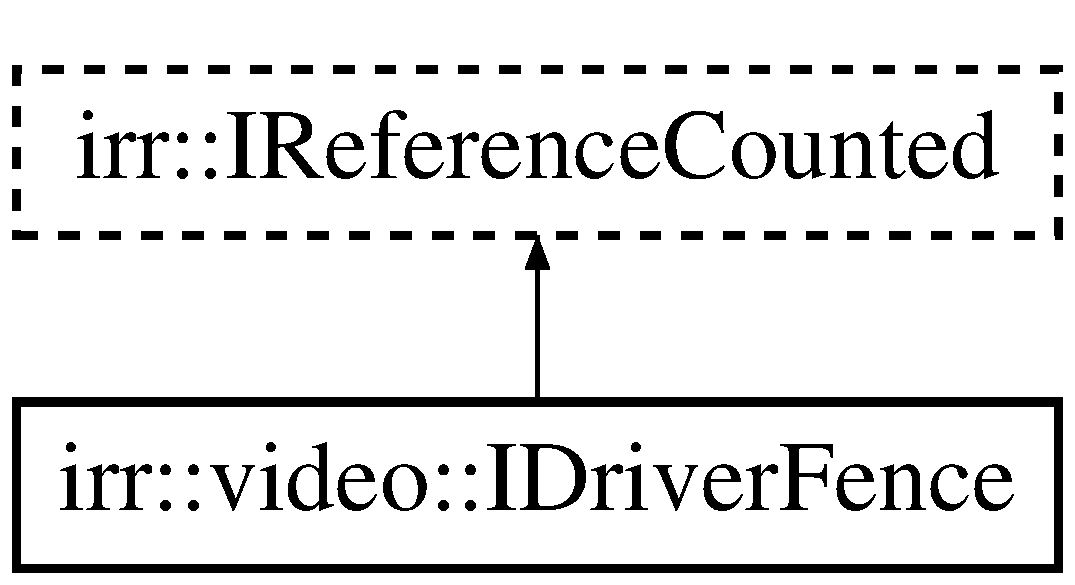
\includegraphics[height=2.000000cm]{classirr_1_1video_1_1IDriverFence}
\end{center}
\end{figure}
\subsection*{Public Member Functions}
\begin{DoxyCompactItemize}
\item 
virtual \hyperlink{namespaceirr_1_1video_ae93020af22218bae203c7bb52b87590b}{E\+\_\+\+D\+R\+I\+V\+E\+R\+\_\+\+F\+E\+N\+C\+E\+\_\+\+R\+E\+T\+V\+AL} \hyperlink{classirr_1_1video_1_1IDriverFence_a6071037e9963ecd4fa550a5cadb75a74}{wait\+C\+PU} (const uint64\+\_\+t \&timeout, const bool \&flush=false)=0\hypertarget{classirr_1_1video_1_1IDriverFence_a6071037e9963ecd4fa550a5cadb75a74}{}\label{classirr_1_1video_1_1IDriverFence_a6071037e9963ecd4fa550a5cadb75a74}

\begin{DoxyCompactList}\small\item\em If timeout​ is zero, the function will simply check to see if the sync object is signaled and return immediately. \end{DoxyCompactList}\item 
virtual void {\bfseries wait\+G\+PU} ()=0\hypertarget{classirr_1_1video_1_1IDriverFence_af976db482d86248df380d15a8ba2972e}{}\label{classirr_1_1video_1_1IDriverFence_af976db482d86248df380d15a8ba2972e}

\end{DoxyCompactItemize}
\subsection*{Additional Inherited Members}


\subsection{Detailed Description}
Persistently Mapped buffer. 

The documentation for this class was generated from the following file\+:\begin{DoxyCompactItemize}
\item 
include/I\+Driver\+Fence.\+h\end{DoxyCompactItemize}

\hypertarget{classirr_1_1scene_1_1IDummyTransformationSceneNode}{}\section{irr\+:\+:scene\+:\+:I\+Dummy\+Transformation\+Scene\+Node Class Reference}
\label{classirr_1_1scene_1_1IDummyTransformationSceneNode}\index{irr\+::scene\+::\+I\+Dummy\+Transformation\+Scene\+Node@{irr\+::scene\+::\+I\+Dummy\+Transformation\+Scene\+Node}}


Dummy scene node for adding additional transformations to the scene graph.  




{\ttfamily \#include $<$I\+Dummy\+Transformation\+Scene\+Node.\+h$>$}

Inheritance diagram for irr\+:\+:scene\+:\+:I\+Dummy\+Transformation\+Scene\+Node\+:\begin{figure}[H]
\begin{center}
\leavevmode
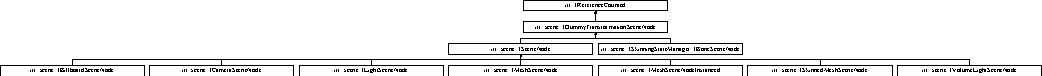
\includegraphics[height=1.022364cm]{classirr_1_1scene_1_1IDummyTransformationSceneNode}
\end{center}
\end{figure}
\subsection*{Public Member Functions}
\begin{DoxyCompactItemize}
\item 
\hyperlink{classirr_1_1scene_1_1IDummyTransformationSceneNode_ae5af13edb138640195e48d8f5811fe79}{I\+Dummy\+Transformation\+Scene\+Node} (\hyperlink{classirr_1_1scene_1_1IDummyTransformationSceneNode}{I\+Dummy\+Transformation\+Scene\+Node} $\ast$parent, const \hyperlink{namespaceirr_1_1core_a06f169d08b5c429f5575acb7edbad811}{core\+::vector3df} \&position=\hyperlink{namespaceirr_1_1core_a06f169d08b5c429f5575acb7edbad811}{core\+::vector3df}(0, 0, 0), const \hyperlink{namespaceirr_1_1core_a06f169d08b5c429f5575acb7edbad811}{core\+::vector3df} \&rotation=\hyperlink{namespaceirr_1_1core_a06f169d08b5c429f5575acb7edbad811}{core\+::vector3df}(0, 0, 0), const \hyperlink{namespaceirr_1_1core_a06f169d08b5c429f5575acb7edbad811}{core\+::vector3df} \&scale=\hyperlink{namespaceirr_1_1core_a06f169d08b5c429f5575acb7edbad811}{core\+::vector3df}(1.\+0f, 1.\+0f, 1.\+0f))\hypertarget{classirr_1_1scene_1_1IDummyTransformationSceneNode_ae5af13edb138640195e48d8f5811fe79}{}\label{classirr_1_1scene_1_1IDummyTransformationSceneNode_ae5af13edb138640195e48d8f5811fe79}

\begin{DoxyCompactList}\small\item\em Constructor. \end{DoxyCompactList}\item 
virtual const bool {\bfseries is\+I\+Scene\+Node} () const \hypertarget{classirr_1_1scene_1_1IDummyTransformationSceneNode_aafeae403a5f9689fce5e371b7ded2027}{}\label{classirr_1_1scene_1_1IDummyTransformationSceneNode_aafeae403a5f9689fce5e371b7ded2027}

\item 
virtual const \hyperlink{classirr_1_1core_1_1matrix4x3}{core\+::matrix4x3} \& \hyperlink{classirr_1_1scene_1_1IDummyTransformationSceneNode_aeda15f68e3b6c7ee44b6fcc9709cecec}{get\+Relative\+Transformation\+Matrix} ()
\begin{DoxyCompactList}\small\item\em Returns a reference to the current relative transformation matrix. \end{DoxyCompactList}\item 
void {\bfseries set\+Relative\+Transformation\+Matrix} (const \hyperlink{classirr_1_1core_1_1matrix4x3}{core\+::matrix4x3} \&tform)\hypertarget{classirr_1_1scene_1_1IDummyTransformationSceneNode_a39d0ba78cf93d8a9052f9cc015bed6a4}{}\label{classirr_1_1scene_1_1IDummyTransformationSceneNode_a39d0ba78cf93d8a9052f9cc015bed6a4}

\item 
const uint64\+\_\+t \& {\bfseries get\+Relative\+Trans\+Changed\+Hint} () const \hypertarget{classirr_1_1scene_1_1IDummyTransformationSceneNode_a84672f1b532e9782fa2308837e9377ec}{}\label{classirr_1_1scene_1_1IDummyTransformationSceneNode_a84672f1b532e9782fa2308837e9377ec}

\item 
const uint64\+\_\+t \& {\bfseries get\+Absolute\+Transform\+Last\+Recompute\+Hint} () const \hypertarget{classirr_1_1scene_1_1IDummyTransformationSceneNode_ad671f00c939b1a3357a73212129925f0}{}\label{classirr_1_1scene_1_1IDummyTransformationSceneNode_ad671f00c939b1a3357a73212129925f0}

\item 
const \hyperlink{namespaceirr_1_1core_a06f169d08b5c429f5575acb7edbad811}{core\+::vector3df} \& {\bfseries get\+Scale} ()\hypertarget{classirr_1_1scene_1_1IDummyTransformationSceneNode_a75fc25839a943a3084f12ce42e07d11f}{}\label{classirr_1_1scene_1_1IDummyTransformationSceneNode_a75fc25839a943a3084f12ce42e07d11f}

\item 
void {\bfseries set\+Scale} (const \hyperlink{namespaceirr_1_1core_a06f169d08b5c429f5575acb7edbad811}{core\+::vector3df} \&scale)\hypertarget{classirr_1_1scene_1_1IDummyTransformationSceneNode_ae1d572e938bc32e9d1be6fb2c056c74c}{}\label{classirr_1_1scene_1_1IDummyTransformationSceneNode_ae1d572e938bc32e9d1be6fb2c056c74c}

\item 
const \hyperlink{namespaceirr_1_1core_a06f169d08b5c429f5575acb7edbad811}{core\+::vector3df} \& {\bfseries get\+Rotation} ()\hypertarget{classirr_1_1scene_1_1IDummyTransformationSceneNode_ad3c298d5a818b4ae60bd236b763aa897}{}\label{classirr_1_1scene_1_1IDummyTransformationSceneNode_ad3c298d5a818b4ae60bd236b763aa897}

\item 
void {\bfseries set\+Rotation} (const \hyperlink{namespaceirr_1_1core_a06f169d08b5c429f5575acb7edbad811}{core\+::vector3df} \&rotation)\hypertarget{classirr_1_1scene_1_1IDummyTransformationSceneNode_a7a64a192242e68aa0d3ed9bd44b2a0f4}{}\label{classirr_1_1scene_1_1IDummyTransformationSceneNode_a7a64a192242e68aa0d3ed9bd44b2a0f4}

\item 
const \hyperlink{namespaceirr_1_1core_a06f169d08b5c429f5575acb7edbad811}{core\+::vector3df} \& {\bfseries get\+Position} ()\hypertarget{classirr_1_1scene_1_1IDummyTransformationSceneNode_a4c48ec272f309c4667d2fb4764187b4a}{}\label{classirr_1_1scene_1_1IDummyTransformationSceneNode_a4c48ec272f309c4667d2fb4764187b4a}

\item 
void {\bfseries set\+Position} (const \hyperlink{namespaceirr_1_1core_a06f169d08b5c429f5575acb7edbad811}{core\+::vector3df} \&newpos)\hypertarget{classirr_1_1scene_1_1IDummyTransformationSceneNode_ae8855c16184df28ae297bb1028d29b04}{}\label{classirr_1_1scene_1_1IDummyTransformationSceneNode_ae8855c16184df28ae297bb1028d29b04}

\item 
virtual bool {\bfseries needs\+Absolute\+Transform\+Recompute} () const \hypertarget{classirr_1_1scene_1_1IDummyTransformationSceneNode_a75c7c307815ebc52f5837ffb9f7a1f78}{}\label{classirr_1_1scene_1_1IDummyTransformationSceneNode_a75c7c307815ebc52f5837ffb9f7a1f78}

\item 
virtual size\+\_\+t {\bfseries needs\+Deep\+Absolute\+Transform\+Recompute} () const \hypertarget{classirr_1_1scene_1_1IDummyTransformationSceneNode_a2f76b44a1dc5863603b9cd073ce6b1bb}{}\label{classirr_1_1scene_1_1IDummyTransformationSceneNode_a2f76b44a1dc5863603b9cd073ce6b1bb}

\item 
const \hyperlink{classirr_1_1core_1_1matrix4x3}{core\+::matrix4x3} \& {\bfseries get\+Absolute\+Transformation} ()\hypertarget{classirr_1_1scene_1_1IDummyTransformationSceneNode_a60a6df4e6a2e780c7a105a726523bfd3}{}\label{classirr_1_1scene_1_1IDummyTransformationSceneNode_a60a6df4e6a2e780c7a105a726523bfd3}

\item 
\hyperlink{namespaceirr_1_1core_a06f169d08b5c429f5575acb7edbad811}{core\+::vector3df} \hyperlink{classirr_1_1scene_1_1IDummyTransformationSceneNode_a8c3e2a52fcd61512316f134d2a29f562}{get\+Absolute\+Position} () const 
\begin{DoxyCompactList}\small\item\em Gets the absolute position of the node in world coordinates. \end{DoxyCompactList}\item 
virtual void \hyperlink{classirr_1_1scene_1_1IDummyTransformationSceneNode_ae2d53618b7d24167526d980c434fbe22}{update\+Absolute\+Position} ()
\begin{DoxyCompactList}\small\item\em Updates the absolute position based on the relative and the parents position. \end{DoxyCompactList}\item 
const \hyperlink{classirr_1_1core_1_1list}{core\+::list}$<$ \hyperlink{classirr_1_1scene_1_1IDummyTransformationSceneNode}{I\+Dummy\+Transformation\+Scene\+Node} $\ast$ $>$ \& \hyperlink{classirr_1_1scene_1_1IDummyTransformationSceneNode_aed89b962b30a41070c2c5cb42e97845b}{get\+Children} () const 
\begin{DoxyCompactList}\small\item\em Returns a const reference to the list of all children. \end{DoxyCompactList}\item 
virtual void \hyperlink{classirr_1_1scene_1_1IDummyTransformationSceneNode_a3a3e9ed634ccb3a0b9744f93529ecc31}{set\+Parent} (\hyperlink{classirr_1_1scene_1_1IDummyTransformationSceneNode}{I\+Dummy\+Transformation\+Scene\+Node} $\ast$new\+Parent)
\begin{DoxyCompactList}\small\item\em Changes the parent of the scene node. \end{DoxyCompactList}\item 
\hyperlink{classirr_1_1scene_1_1IDummyTransformationSceneNode}{I\+Dummy\+Transformation\+Scene\+Node} $\ast$ \hyperlink{classirr_1_1scene_1_1IDummyTransformationSceneNode_a8f36007bafc2bebbbc8008adda7ecd61}{get\+Parent} () const 
\begin{DoxyCompactList}\small\item\em Returns the parent of this scene node. \end{DoxyCompactList}\item 
virtual void \hyperlink{classirr_1_1scene_1_1IDummyTransformationSceneNode_ab77154a16a662029a795706d2e4942b7}{add\+Child} (\hyperlink{classirr_1_1scene_1_1IDummyTransformationSceneNode}{I\+Dummy\+Transformation\+Scene\+Node} $\ast$child)
\begin{DoxyCompactList}\small\item\em Adds a child to this scene node. \end{DoxyCompactList}\item 
virtual bool \hyperlink{classirr_1_1scene_1_1IDummyTransformationSceneNode_a0b0d33aefe1f93d278765f5eb74dc966}{remove\+Child} (\hyperlink{classirr_1_1scene_1_1IDummyTransformationSceneNode}{I\+Dummy\+Transformation\+Scene\+Node} $\ast$child)
\begin{DoxyCompactList}\small\item\em Removes a child from this scene node. \end{DoxyCompactList}\item 
virtual void \hyperlink{classirr_1_1scene_1_1IDummyTransformationSceneNode_a785adff20757a034167201bdfb13bbfa}{remove\+All} ()
\begin{DoxyCompactList}\small\item\em Removes all children of this scene node. \end{DoxyCompactList}\item 
virtual void \hyperlink{classirr_1_1scene_1_1IDummyTransformationSceneNode_a672cb748079172ee204bb389e1bde04d}{remove} ()
\begin{DoxyCompactList}\small\item\em Removes this scene node from the scene. \end{DoxyCompactList}\item 
virtual void \hyperlink{classirr_1_1scene_1_1IDummyTransformationSceneNode_ace62fd3a3a33bccfbed6fa958786bf9b}{add\+Animator} (\hyperlink{classirr_1_1scene_1_1ISceneNodeAnimator}{I\+Scene\+Node\+Animator} $\ast$animator)
\begin{DoxyCompactList}\small\item\em Adds an animator which should animate this node. \end{DoxyCompactList}\item 
const \hyperlink{classirr_1_1core_1_1list}{core\+::list}$<$ \hyperlink{classirr_1_1scene_1_1ISceneNodeAnimator}{I\+Scene\+Node\+Animator} $\ast$ $>$ \& \hyperlink{classirr_1_1scene_1_1IDummyTransformationSceneNode_a329082f8ec526ac1ba5bbc817b69326c}{get\+Animators} () const 
\begin{DoxyCompactList}\small\item\em Get a list of all scene node animators. \end{DoxyCompactList}\item 
virtual void \hyperlink{classirr_1_1scene_1_1IDummyTransformationSceneNode_a684d1d1066004a833be3ba83b4db5249}{remove\+Animator} (\hyperlink{classirr_1_1scene_1_1ISceneNodeAnimator}{I\+Scene\+Node\+Animator} $\ast$animator)
\begin{DoxyCompactList}\small\item\em Removes an animator from this scene node. \end{DoxyCompactList}\item 
virtual void \hyperlink{classirr_1_1scene_1_1IDummyTransformationSceneNode_af6bb280ece8f5cf84f50603d337c18c1}{remove\+Animators} ()
\begin{DoxyCompactList}\small\item\em Removes all animators from this scene node. \end{DoxyCompactList}\item 
virtual \hyperlink{namespaceirr_1_1scene_acad3d7ef92a9807d391ba29120f3b7bd}{E\+S\+C\+E\+N\+E\+\_\+\+N\+O\+D\+E\+\_\+\+T\+Y\+PE} \hyperlink{classirr_1_1scene_1_1IDummyTransformationSceneNode_a4ac844750b866a1c05e72c3288b3d6cd}{get\+Type} () const \hypertarget{classirr_1_1scene_1_1IDummyTransformationSceneNode_a4ac844750b866a1c05e72c3288b3d6cd}{}\label{classirr_1_1scene_1_1IDummyTransformationSceneNode_a4ac844750b866a1c05e72c3288b3d6cd}

\begin{DoxyCompactList}\small\item\em Returns type of the scene node. \end{DoxyCompactList}\item 
virtual \hyperlink{classirr_1_1scene_1_1IDummyTransformationSceneNode}{I\+Dummy\+Transformation\+Scene\+Node} $\ast$ \hyperlink{classirr_1_1scene_1_1IDummyTransformationSceneNode_a3fb98da7defed119bd565f5e7fefb5f3}{clone} (\hyperlink{classirr_1_1scene_1_1IDummyTransformationSceneNode}{I\+Dummy\+Transformation\+Scene\+Node} $\ast$new\+Parent=0, \hyperlink{classirr_1_1scene_1_1ISceneManager}{I\+Scene\+Manager} $\ast$new\+Manager=0)\hypertarget{classirr_1_1scene_1_1IDummyTransformationSceneNode_a3fb98da7defed119bd565f5e7fefb5f3}{}\label{classirr_1_1scene_1_1IDummyTransformationSceneNode_a3fb98da7defed119bd565f5e7fefb5f3}

\begin{DoxyCompactList}\small\item\em Creates a clone of this scene node and its children. \end{DoxyCompactList}\end{DoxyCompactItemize}
\subsection*{Protected Member Functions}
\begin{DoxyCompactItemize}
\item 
virtual void \hyperlink{classirr_1_1scene_1_1IDummyTransformationSceneNode_a5dbc7f63a04a445fc1fbe8efbb1287b3}{clone\+Members} (\hyperlink{classirr_1_1scene_1_1IDummyTransformationSceneNode}{I\+Dummy\+Transformation\+Scene\+Node} $\ast$to\+Copy\+From, \hyperlink{classirr_1_1scene_1_1ISceneManager}{I\+Scene\+Manager} $\ast$new\+Manager)
\begin{DoxyCompactList}\small\item\em A clone function for the I\+Dummy... members. \end{DoxyCompactList}\end{DoxyCompactItemize}
\subsection*{Protected Attributes}
\begin{DoxyCompactItemize}
\item 
uint64\+\_\+t {\bfseries last\+Time\+Relative\+Trans\+Read} \mbox{[}5\mbox{]}\hypertarget{classirr_1_1scene_1_1IDummyTransformationSceneNode_a1eeb653040c4bf8d072ad310e5d14d65}{}\label{classirr_1_1scene_1_1IDummyTransformationSceneNode_a1eeb653040c4bf8d072ad310e5d14d65}

\item 
uint64\+\_\+t {\bfseries relative\+Trans\+Changed}\hypertarget{classirr_1_1scene_1_1IDummyTransformationSceneNode_abb98dea3451d5a5bdd71fb16740fb7f5}{}\label{classirr_1_1scene_1_1IDummyTransformationSceneNode_abb98dea3451d5a5bdd71fb16740fb7f5}

\item 
bool {\bfseries relative\+Trans\+Needs\+Update}\hypertarget{classirr_1_1scene_1_1IDummyTransformationSceneNode_a6a8af3d36894ec61cbff89fa72070e64}{}\label{classirr_1_1scene_1_1IDummyTransformationSceneNode_a6a8af3d36894ec61cbff89fa72070e64}

\item 
\hyperlink{classirr_1_1scene_1_1IDummyTransformationSceneNode}{I\+Dummy\+Transformation\+Scene\+Node} $\ast$ \hyperlink{classirr_1_1scene_1_1IDummyTransformationSceneNode_ad4403cd701e4112d6e9dcf4888442b34}{Parent}\hypertarget{classirr_1_1scene_1_1IDummyTransformationSceneNode_ad4403cd701e4112d6e9dcf4888442b34}{}\label{classirr_1_1scene_1_1IDummyTransformationSceneNode_ad4403cd701e4112d6e9dcf4888442b34}

\begin{DoxyCompactList}\small\item\em Pointer to the parent. \end{DoxyCompactList}\item 
\hyperlink{classirr_1_1core_1_1list}{core\+::list}$<$ \hyperlink{classirr_1_1scene_1_1IDummyTransformationSceneNode}{I\+Dummy\+Transformation\+Scene\+Node} $\ast$ $>$ \hyperlink{classirr_1_1scene_1_1IDummyTransformationSceneNode_a5a74140096f12c3e0d82303e5c946d9b}{Children}\hypertarget{classirr_1_1scene_1_1IDummyTransformationSceneNode_a5a74140096f12c3e0d82303e5c946d9b}{}\label{classirr_1_1scene_1_1IDummyTransformationSceneNode_a5a74140096f12c3e0d82303e5c946d9b}

\begin{DoxyCompactList}\small\item\em List of all children of this node. \end{DoxyCompactList}\item 
\hyperlink{classirr_1_1core_1_1list}{core\+::list}$<$ \hyperlink{classirr_1_1scene_1_1ISceneNodeAnimator}{I\+Scene\+Node\+Animator} $\ast$ $>$ \hyperlink{classirr_1_1scene_1_1IDummyTransformationSceneNode_a66cb6325bdcf5411e5a9384e4c647ae9}{Animators}\hypertarget{classirr_1_1scene_1_1IDummyTransformationSceneNode_a66cb6325bdcf5411e5a9384e4c647ae9}{}\label{classirr_1_1scene_1_1IDummyTransformationSceneNode_a66cb6325bdcf5411e5a9384e4c647ae9}

\begin{DoxyCompactList}\small\item\em List of all animator nodes. \end{DoxyCompactList}\item 
\hyperlink{classirr_1_1core_1_1matrix4x3}{core\+::matrix4x3} \hyperlink{classirr_1_1scene_1_1IDummyTransformationSceneNode_af1e3a5765b240e6fb26babed7b45abda}{Absolute\+Transformation}\hypertarget{classirr_1_1scene_1_1IDummyTransformationSceneNode_af1e3a5765b240e6fb26babed7b45abda}{}\label{classirr_1_1scene_1_1IDummyTransformationSceneNode_af1e3a5765b240e6fb26babed7b45abda}

\begin{DoxyCompactList}\small\item\em Absolute transformation of the node. \end{DoxyCompactList}\item 
\hyperlink{classirr_1_1core_1_1matrix4x3}{core\+::matrix4x3} \hyperlink{classirr_1_1scene_1_1IDummyTransformationSceneNode_a400e961f3e5a3fc49f7cdebdb2af02cc}{Relative\+Transformation}\hypertarget{classirr_1_1scene_1_1IDummyTransformationSceneNode_a400e961f3e5a3fc49f7cdebdb2af02cc}{}\label{classirr_1_1scene_1_1IDummyTransformationSceneNode_a400e961f3e5a3fc49f7cdebdb2af02cc}

\begin{DoxyCompactList}\small\item\em Relative transformation of the node. \end{DoxyCompactList}\item 
\hyperlink{namespaceirr_1_1core_a06f169d08b5c429f5575acb7edbad811}{core\+::vector3df} \hyperlink{classirr_1_1scene_1_1IDummyTransformationSceneNode_a8ac24fb56526cdad93349aa7df2eae8d}{Relative\+Translation}\hypertarget{classirr_1_1scene_1_1IDummyTransformationSceneNode_a8ac24fb56526cdad93349aa7df2eae8d}{}\label{classirr_1_1scene_1_1IDummyTransformationSceneNode_a8ac24fb56526cdad93349aa7df2eae8d}

\begin{DoxyCompactList}\small\item\em Relative translation of the scene node. \end{DoxyCompactList}\item 
\hyperlink{namespaceirr_1_1core_a06f169d08b5c429f5575acb7edbad811}{core\+::vector3df} \hyperlink{classirr_1_1scene_1_1IDummyTransformationSceneNode_aaa3f160af13bb3175d9afb19d84c60f3}{Relative\+Rotation}\hypertarget{classirr_1_1scene_1_1IDummyTransformationSceneNode_aaa3f160af13bb3175d9afb19d84c60f3}{}\label{classirr_1_1scene_1_1IDummyTransformationSceneNode_aaa3f160af13bb3175d9afb19d84c60f3}

\begin{DoxyCompactList}\small\item\em Relative rotation of the scene node. \end{DoxyCompactList}\item 
\hyperlink{namespaceirr_1_1core_a06f169d08b5c429f5575acb7edbad811}{core\+::vector3df} \hyperlink{classirr_1_1scene_1_1IDummyTransformationSceneNode_a8fcbc0235c943939fd5eb78596ed38d1}{Relative\+Scale}\hypertarget{classirr_1_1scene_1_1IDummyTransformationSceneNode_a8fcbc0235c943939fd5eb78596ed38d1}{}\label{classirr_1_1scene_1_1IDummyTransformationSceneNode_a8fcbc0235c943939fd5eb78596ed38d1}

\begin{DoxyCompactList}\small\item\em Relative scale of the scene node. \end{DoxyCompactList}\end{DoxyCompactItemize}


\subsection{Detailed Description}
Dummy scene node for adding additional transformations to the scene graph. 

This scene node does not render itself, and does not respond to set/get\+Position, set/get\+Rotation and set/get\+Scale. Its just a simple scene node that takes a matrix as relative transformation, making it possible to insert any transformation anywhere into the scene graph. This scene node is for example used by the I\+Animated\+Mesh\+Scene\+Node for emulating joint scene nodes when playing skeletal animations. 

\subsection{Member Function Documentation}
\index{irr\+::scene\+::\+I\+Dummy\+Transformation\+Scene\+Node@{irr\+::scene\+::\+I\+Dummy\+Transformation\+Scene\+Node}!add\+Animator@{add\+Animator}}
\index{add\+Animator@{add\+Animator}!irr\+::scene\+::\+I\+Dummy\+Transformation\+Scene\+Node@{irr\+::scene\+::\+I\+Dummy\+Transformation\+Scene\+Node}}
\subsubsection[{\texorpdfstring{add\+Animator(\+I\+Scene\+Node\+Animator $\ast$animator)}{addAnimator(ISceneNodeAnimator *animator)}}]{\setlength{\rightskip}{0pt plus 5cm}virtual void irr\+::scene\+::\+I\+Dummy\+Transformation\+Scene\+Node\+::add\+Animator (
\begin{DoxyParamCaption}
\item[{{\bf I\+Scene\+Node\+Animator} $\ast$}]{animator}
\end{DoxyParamCaption}
)\hspace{0.3cm}{\ttfamily [inline]}, {\ttfamily [virtual]}}\hypertarget{classirr_1_1scene_1_1IDummyTransformationSceneNode_ace62fd3a3a33bccfbed6fa958786bf9b}{}\label{classirr_1_1scene_1_1IDummyTransformationSceneNode_ace62fd3a3a33bccfbed6fa958786bf9b}


Adds an animator which should animate this node. 


\begin{DoxyParams}{Parameters}
{\em animator} & A pointer to the new animator. \\
\hline
\end{DoxyParams}
\index{irr\+::scene\+::\+I\+Dummy\+Transformation\+Scene\+Node@{irr\+::scene\+::\+I\+Dummy\+Transformation\+Scene\+Node}!add\+Child@{add\+Child}}
\index{add\+Child@{add\+Child}!irr\+::scene\+::\+I\+Dummy\+Transformation\+Scene\+Node@{irr\+::scene\+::\+I\+Dummy\+Transformation\+Scene\+Node}}
\subsubsection[{\texorpdfstring{add\+Child(\+I\+Dummy\+Transformation\+Scene\+Node $\ast$child)}{addChild(IDummyTransformationSceneNode *child)}}]{\setlength{\rightskip}{0pt plus 5cm}virtual void irr\+::scene\+::\+I\+Dummy\+Transformation\+Scene\+Node\+::add\+Child (
\begin{DoxyParamCaption}
\item[{{\bf I\+Dummy\+Transformation\+Scene\+Node} $\ast$}]{child}
\end{DoxyParamCaption}
)\hspace{0.3cm}{\ttfamily [inline]}, {\ttfamily [virtual]}}\hypertarget{classirr_1_1scene_1_1IDummyTransformationSceneNode_ab77154a16a662029a795706d2e4942b7}{}\label{classirr_1_1scene_1_1IDummyTransformationSceneNode_ab77154a16a662029a795706d2e4942b7}


Adds a child to this scene node. 

If the scene node already has a parent it is first removed from the other parent. 
\begin{DoxyParams}{Parameters}
{\em child} & A pointer to the new child. \\
\hline
\end{DoxyParams}
\index{irr\+::scene\+::\+I\+Dummy\+Transformation\+Scene\+Node@{irr\+::scene\+::\+I\+Dummy\+Transformation\+Scene\+Node}!clone\+Members@{clone\+Members}}
\index{clone\+Members@{clone\+Members}!irr\+::scene\+::\+I\+Dummy\+Transformation\+Scene\+Node@{irr\+::scene\+::\+I\+Dummy\+Transformation\+Scene\+Node}}
\subsubsection[{\texorpdfstring{clone\+Members(\+I\+Dummy\+Transformation\+Scene\+Node $\ast$to\+Copy\+From, I\+Scene\+Manager $\ast$new\+Manager)}{cloneMembers(IDummyTransformationSceneNode *toCopyFrom, ISceneManager *newManager)}}]{\setlength{\rightskip}{0pt plus 5cm}virtual void irr\+::scene\+::\+I\+Dummy\+Transformation\+Scene\+Node\+::clone\+Members (
\begin{DoxyParamCaption}
\item[{{\bf I\+Dummy\+Transformation\+Scene\+Node} $\ast$}]{to\+Copy\+From, }
\item[{{\bf I\+Scene\+Manager} $\ast$}]{new\+Manager}
\end{DoxyParamCaption}
)\hspace{0.3cm}{\ttfamily [inline]}, {\ttfamily [protected]}, {\ttfamily [virtual]}}\hypertarget{classirr_1_1scene_1_1IDummyTransformationSceneNode_a5dbc7f63a04a445fc1fbe8efbb1287b3}{}\label{classirr_1_1scene_1_1IDummyTransformationSceneNode_a5dbc7f63a04a445fc1fbe8efbb1287b3}


A clone function for the I\+Dummy... members. 

This method can be used by \hyperlink{classirr_1_1scene_1_1IDummyTransformationSceneNode_a3fb98da7defed119bd565f5e7fefb5f3}{clone()} implementations of derived classes 
\begin{DoxyParams}{Parameters}
{\em to\+Copy\+From} & The node from which the values are copied \\
\hline
\end{DoxyParams}
\index{irr\+::scene\+::\+I\+Dummy\+Transformation\+Scene\+Node@{irr\+::scene\+::\+I\+Dummy\+Transformation\+Scene\+Node}!get\+Absolute\+Position@{get\+Absolute\+Position}}
\index{get\+Absolute\+Position@{get\+Absolute\+Position}!irr\+::scene\+::\+I\+Dummy\+Transformation\+Scene\+Node@{irr\+::scene\+::\+I\+Dummy\+Transformation\+Scene\+Node}}
\subsubsection[{\texorpdfstring{get\+Absolute\+Position() const }{getAbsolutePosition() const }}]{\setlength{\rightskip}{0pt plus 5cm}{\bf core\+::vector3df} irr\+::scene\+::\+I\+Dummy\+Transformation\+Scene\+Node\+::get\+Absolute\+Position (
\begin{DoxyParamCaption}
{}
\end{DoxyParamCaption}
) const\hspace{0.3cm}{\ttfamily [inline]}}\hypertarget{classirr_1_1scene_1_1IDummyTransformationSceneNode_a8c3e2a52fcd61512316f134d2a29f562}{}\label{classirr_1_1scene_1_1IDummyTransformationSceneNode_a8c3e2a52fcd61512316f134d2a29f562}


Gets the absolute position of the node in world coordinates. 

If you want the position of the node relative to its parent, use get\+Position() instead. N\+O\+TE\+: For speed reasons the absolute position is not automatically recalculated on each change of the relative position or by a position change of an parent. Instead the update usually happens once per frame in On\+Animate. You can enforce an update with \hyperlink{classirr_1_1scene_1_1IDummyTransformationSceneNode_ae2d53618b7d24167526d980c434fbe22}{update\+Absolute\+Position()}. \begin{DoxyReturn}{Returns}
The current absolute position of the scene node (updated on last call of update\+Absolute\+Position). 
\end{DoxyReturn}
\index{irr\+::scene\+::\+I\+Dummy\+Transformation\+Scene\+Node@{irr\+::scene\+::\+I\+Dummy\+Transformation\+Scene\+Node}!get\+Animators@{get\+Animators}}
\index{get\+Animators@{get\+Animators}!irr\+::scene\+::\+I\+Dummy\+Transformation\+Scene\+Node@{irr\+::scene\+::\+I\+Dummy\+Transformation\+Scene\+Node}}
\subsubsection[{\texorpdfstring{get\+Animators() const }{getAnimators() const }}]{\setlength{\rightskip}{0pt plus 5cm}const {\bf core\+::list}$<${\bf I\+Scene\+Node\+Animator}$\ast$$>$\& irr\+::scene\+::\+I\+Dummy\+Transformation\+Scene\+Node\+::get\+Animators (
\begin{DoxyParamCaption}
{}
\end{DoxyParamCaption}
) const\hspace{0.3cm}{\ttfamily [inline]}}\hypertarget{classirr_1_1scene_1_1IDummyTransformationSceneNode_a329082f8ec526ac1ba5bbc817b69326c}{}\label{classirr_1_1scene_1_1IDummyTransformationSceneNode_a329082f8ec526ac1ba5bbc817b69326c}


Get a list of all scene node animators. 

\begin{DoxyReturn}{Returns}
The list of animators attached to this node. 
\end{DoxyReturn}
\index{irr\+::scene\+::\+I\+Dummy\+Transformation\+Scene\+Node@{irr\+::scene\+::\+I\+Dummy\+Transformation\+Scene\+Node}!get\+Children@{get\+Children}}
\index{get\+Children@{get\+Children}!irr\+::scene\+::\+I\+Dummy\+Transformation\+Scene\+Node@{irr\+::scene\+::\+I\+Dummy\+Transformation\+Scene\+Node}}
\subsubsection[{\texorpdfstring{get\+Children() const }{getChildren() const }}]{\setlength{\rightskip}{0pt plus 5cm}const {\bf core\+::list}$<${\bf I\+Dummy\+Transformation\+Scene\+Node}$\ast$$>$\& irr\+::scene\+::\+I\+Dummy\+Transformation\+Scene\+Node\+::get\+Children (
\begin{DoxyParamCaption}
{}
\end{DoxyParamCaption}
) const\hspace{0.3cm}{\ttfamily [inline]}}\hypertarget{classirr_1_1scene_1_1IDummyTransformationSceneNode_aed89b962b30a41070c2c5cb42e97845b}{}\label{classirr_1_1scene_1_1IDummyTransformationSceneNode_aed89b962b30a41070c2c5cb42e97845b}


Returns a const reference to the list of all children. 

\begin{DoxyReturn}{Returns}
The list of all children of this node. 
\end{DoxyReturn}
\index{irr\+::scene\+::\+I\+Dummy\+Transformation\+Scene\+Node@{irr\+::scene\+::\+I\+Dummy\+Transformation\+Scene\+Node}!get\+Parent@{get\+Parent}}
\index{get\+Parent@{get\+Parent}!irr\+::scene\+::\+I\+Dummy\+Transformation\+Scene\+Node@{irr\+::scene\+::\+I\+Dummy\+Transformation\+Scene\+Node}}
\subsubsection[{\texorpdfstring{get\+Parent() const }{getParent() const }}]{\setlength{\rightskip}{0pt plus 5cm}{\bf I\+Dummy\+Transformation\+Scene\+Node}$\ast$ irr\+::scene\+::\+I\+Dummy\+Transformation\+Scene\+Node\+::get\+Parent (
\begin{DoxyParamCaption}
{}
\end{DoxyParamCaption}
) const\hspace{0.3cm}{\ttfamily [inline]}}\hypertarget{classirr_1_1scene_1_1IDummyTransformationSceneNode_a8f36007bafc2bebbbc8008adda7ecd61}{}\label{classirr_1_1scene_1_1IDummyTransformationSceneNode_a8f36007bafc2bebbbc8008adda7ecd61}


Returns the parent of this scene node. 

\begin{DoxyReturn}{Returns}
A pointer to the parent. 
\end{DoxyReturn}
\index{irr\+::scene\+::\+I\+Dummy\+Transformation\+Scene\+Node@{irr\+::scene\+::\+I\+Dummy\+Transformation\+Scene\+Node}!get\+Relative\+Transformation\+Matrix@{get\+Relative\+Transformation\+Matrix}}
\index{get\+Relative\+Transformation\+Matrix@{get\+Relative\+Transformation\+Matrix}!irr\+::scene\+::\+I\+Dummy\+Transformation\+Scene\+Node@{irr\+::scene\+::\+I\+Dummy\+Transformation\+Scene\+Node}}
\subsubsection[{\texorpdfstring{get\+Relative\+Transformation\+Matrix()}{getRelativeTransformationMatrix()}}]{\setlength{\rightskip}{0pt plus 5cm}virtual const {\bf core\+::matrix4x3}\& irr\+::scene\+::\+I\+Dummy\+Transformation\+Scene\+Node\+::get\+Relative\+Transformation\+Matrix (
\begin{DoxyParamCaption}
{}
\end{DoxyParamCaption}
)\hspace{0.3cm}{\ttfamily [inline]}, {\ttfamily [virtual]}}\hypertarget{classirr_1_1scene_1_1IDummyTransformationSceneNode_aeda15f68e3b6c7ee44b6fcc9709cecec}{}\label{classirr_1_1scene_1_1IDummyTransformationSceneNode_aeda15f68e3b6c7ee44b6fcc9709cecec}


Returns a reference to the current relative transformation matrix. 

This is the matrix, this scene node uses instead of scale, translation and rotation. 

Reimplemented in \hyperlink{classirr_1_1scene_1_1ISkinningStateManager_1_1IBoneSceneNode_aa01aed4ed2c55c61449ee38c98583fd4}{irr\+::scene\+::\+I\+Skinning\+State\+Manager\+::\+I\+Bone\+Scene\+Node}.

\index{irr\+::scene\+::\+I\+Dummy\+Transformation\+Scene\+Node@{irr\+::scene\+::\+I\+Dummy\+Transformation\+Scene\+Node}!remove@{remove}}
\index{remove@{remove}!irr\+::scene\+::\+I\+Dummy\+Transformation\+Scene\+Node@{irr\+::scene\+::\+I\+Dummy\+Transformation\+Scene\+Node}}
\subsubsection[{\texorpdfstring{remove()}{remove()}}]{\setlength{\rightskip}{0pt plus 5cm}virtual void irr\+::scene\+::\+I\+Dummy\+Transformation\+Scene\+Node\+::remove (
\begin{DoxyParamCaption}
{}
\end{DoxyParamCaption}
)\hspace{0.3cm}{\ttfamily [inline]}, {\ttfamily [virtual]}}\hypertarget{classirr_1_1scene_1_1IDummyTransformationSceneNode_a672cb748079172ee204bb389e1bde04d}{}\label{classirr_1_1scene_1_1IDummyTransformationSceneNode_a672cb748079172ee204bb389e1bde04d}


Removes this scene node from the scene. 

If no other grab exists for this node, it will be deleted. \index{irr\+::scene\+::\+I\+Dummy\+Transformation\+Scene\+Node@{irr\+::scene\+::\+I\+Dummy\+Transformation\+Scene\+Node}!remove\+All@{remove\+All}}
\index{remove\+All@{remove\+All}!irr\+::scene\+::\+I\+Dummy\+Transformation\+Scene\+Node@{irr\+::scene\+::\+I\+Dummy\+Transformation\+Scene\+Node}}
\subsubsection[{\texorpdfstring{remove\+All()}{removeAll()}}]{\setlength{\rightskip}{0pt plus 5cm}virtual void irr\+::scene\+::\+I\+Dummy\+Transformation\+Scene\+Node\+::remove\+All (
\begin{DoxyParamCaption}
{}
\end{DoxyParamCaption}
)\hspace{0.3cm}{\ttfamily [inline]}, {\ttfamily [virtual]}}\hypertarget{classirr_1_1scene_1_1IDummyTransformationSceneNode_a785adff20757a034167201bdfb13bbfa}{}\label{classirr_1_1scene_1_1IDummyTransformationSceneNode_a785adff20757a034167201bdfb13bbfa}


Removes all children of this scene node. 

The scene nodes found in the children list are also dropped and might be deleted if no other grab exists on them. \index{irr\+::scene\+::\+I\+Dummy\+Transformation\+Scene\+Node@{irr\+::scene\+::\+I\+Dummy\+Transformation\+Scene\+Node}!remove\+Animator@{remove\+Animator}}
\index{remove\+Animator@{remove\+Animator}!irr\+::scene\+::\+I\+Dummy\+Transformation\+Scene\+Node@{irr\+::scene\+::\+I\+Dummy\+Transformation\+Scene\+Node}}
\subsubsection[{\texorpdfstring{remove\+Animator(\+I\+Scene\+Node\+Animator $\ast$animator)}{removeAnimator(ISceneNodeAnimator *animator)}}]{\setlength{\rightskip}{0pt plus 5cm}virtual void irr\+::scene\+::\+I\+Dummy\+Transformation\+Scene\+Node\+::remove\+Animator (
\begin{DoxyParamCaption}
\item[{{\bf I\+Scene\+Node\+Animator} $\ast$}]{animator}
\end{DoxyParamCaption}
)\hspace{0.3cm}{\ttfamily [inline]}, {\ttfamily [virtual]}}\hypertarget{classirr_1_1scene_1_1IDummyTransformationSceneNode_a684d1d1066004a833be3ba83b4db5249}{}\label{classirr_1_1scene_1_1IDummyTransformationSceneNode_a684d1d1066004a833be3ba83b4db5249}


Removes an animator from this scene node. 

If the animator is found, it is also dropped and might be deleted if not other grab exists for it. 
\begin{DoxyParams}{Parameters}
{\em animator} & A pointer to the animator to be deleted. \\
\hline
\end{DoxyParams}
\index{irr\+::scene\+::\+I\+Dummy\+Transformation\+Scene\+Node@{irr\+::scene\+::\+I\+Dummy\+Transformation\+Scene\+Node}!remove\+Animators@{remove\+Animators}}
\index{remove\+Animators@{remove\+Animators}!irr\+::scene\+::\+I\+Dummy\+Transformation\+Scene\+Node@{irr\+::scene\+::\+I\+Dummy\+Transformation\+Scene\+Node}}
\subsubsection[{\texorpdfstring{remove\+Animators()}{removeAnimators()}}]{\setlength{\rightskip}{0pt plus 5cm}virtual void irr\+::scene\+::\+I\+Dummy\+Transformation\+Scene\+Node\+::remove\+Animators (
\begin{DoxyParamCaption}
{}
\end{DoxyParamCaption}
)\hspace{0.3cm}{\ttfamily [inline]}, {\ttfamily [virtual]}}\hypertarget{classirr_1_1scene_1_1IDummyTransformationSceneNode_af6bb280ece8f5cf84f50603d337c18c1}{}\label{classirr_1_1scene_1_1IDummyTransformationSceneNode_af6bb280ece8f5cf84f50603d337c18c1}


Removes all animators from this scene node. 

The animators might also be deleted if no other grab exists for them. \index{irr\+::scene\+::\+I\+Dummy\+Transformation\+Scene\+Node@{irr\+::scene\+::\+I\+Dummy\+Transformation\+Scene\+Node}!remove\+Child@{remove\+Child}}
\index{remove\+Child@{remove\+Child}!irr\+::scene\+::\+I\+Dummy\+Transformation\+Scene\+Node@{irr\+::scene\+::\+I\+Dummy\+Transformation\+Scene\+Node}}
\subsubsection[{\texorpdfstring{remove\+Child(\+I\+Dummy\+Transformation\+Scene\+Node $\ast$child)}{removeChild(IDummyTransformationSceneNode *child)}}]{\setlength{\rightskip}{0pt plus 5cm}virtual bool irr\+::scene\+::\+I\+Dummy\+Transformation\+Scene\+Node\+::remove\+Child (
\begin{DoxyParamCaption}
\item[{{\bf I\+Dummy\+Transformation\+Scene\+Node} $\ast$}]{child}
\end{DoxyParamCaption}
)\hspace{0.3cm}{\ttfamily [inline]}, {\ttfamily [virtual]}}\hypertarget{classirr_1_1scene_1_1IDummyTransformationSceneNode_a0b0d33aefe1f93d278765f5eb74dc966}{}\label{classirr_1_1scene_1_1IDummyTransformationSceneNode_a0b0d33aefe1f93d278765f5eb74dc966}


Removes a child from this scene node. 

If found in the children list, the child pointer is also dropped and might be deleted if no other grab exists. 
\begin{DoxyParams}{Parameters}
{\em child} & A pointer to the child which shall be removed. \\
\hline
\end{DoxyParams}
\begin{DoxyReturn}{Returns}
True if the child was removed, and false if not, e.\+g. because it couldn\textquotesingle{}t be found in the children list. 
\end{DoxyReturn}
\index{irr\+::scene\+::\+I\+Dummy\+Transformation\+Scene\+Node@{irr\+::scene\+::\+I\+Dummy\+Transformation\+Scene\+Node}!set\+Parent@{set\+Parent}}
\index{set\+Parent@{set\+Parent}!irr\+::scene\+::\+I\+Dummy\+Transformation\+Scene\+Node@{irr\+::scene\+::\+I\+Dummy\+Transformation\+Scene\+Node}}
\subsubsection[{\texorpdfstring{set\+Parent(\+I\+Dummy\+Transformation\+Scene\+Node $\ast$new\+Parent)}{setParent(IDummyTransformationSceneNode *newParent)}}]{\setlength{\rightskip}{0pt plus 5cm}virtual void irr\+::scene\+::\+I\+Dummy\+Transformation\+Scene\+Node\+::set\+Parent (
\begin{DoxyParamCaption}
\item[{{\bf I\+Dummy\+Transformation\+Scene\+Node} $\ast$}]{new\+Parent}
\end{DoxyParamCaption}
)\hspace{0.3cm}{\ttfamily [inline]}, {\ttfamily [virtual]}}\hypertarget{classirr_1_1scene_1_1IDummyTransformationSceneNode_a3a3e9ed634ccb3a0b9744f93529ecc31}{}\label{classirr_1_1scene_1_1IDummyTransformationSceneNode_a3a3e9ed634ccb3a0b9744f93529ecc31}


Changes the parent of the scene node. 


\begin{DoxyParams}{Parameters}
{\em new\+Parent} & The new parent to be used. \\
\hline
\end{DoxyParams}
\index{irr\+::scene\+::\+I\+Dummy\+Transformation\+Scene\+Node@{irr\+::scene\+::\+I\+Dummy\+Transformation\+Scene\+Node}!update\+Absolute\+Position@{update\+Absolute\+Position}}
\index{update\+Absolute\+Position@{update\+Absolute\+Position}!irr\+::scene\+::\+I\+Dummy\+Transformation\+Scene\+Node@{irr\+::scene\+::\+I\+Dummy\+Transformation\+Scene\+Node}}
\subsubsection[{\texorpdfstring{update\+Absolute\+Position()}{updateAbsolutePosition()}}]{\setlength{\rightskip}{0pt plus 5cm}virtual void irr\+::scene\+::\+I\+Dummy\+Transformation\+Scene\+Node\+::update\+Absolute\+Position (
\begin{DoxyParamCaption}
{}
\end{DoxyParamCaption}
)\hspace{0.3cm}{\ttfamily [inline]}, {\ttfamily [virtual]}}\hypertarget{classirr_1_1scene_1_1IDummyTransformationSceneNode_ae2d53618b7d24167526d980c434fbe22}{}\label{classirr_1_1scene_1_1IDummyTransformationSceneNode_ae2d53618b7d24167526d980c434fbe22}


Updates the absolute position based on the relative and the parents position. 

Note\+: This does not recursively update the parents absolute positions, so if you have a deeper hierarchy you might want to update the parents first. 

Reimplemented in \hyperlink{classirr_1_1scene_1_1ISkinningStateManager_1_1IBoneSceneNode_a32bd793195468797fb07249946a8be21}{irr\+::scene\+::\+I\+Skinning\+State\+Manager\+::\+I\+Bone\+Scene\+Node}.



The documentation for this class was generated from the following file\+:\begin{DoxyCompactItemize}
\item 
include/I\+Dummy\+Transformation\+Scene\+Node.\+h\end{DoxyCompactItemize}

\hypertarget{classirr_1_1IEventReceiver}{}\section{irr\+:\+:I\+Event\+Receiver Class Reference}
\label{classirr_1_1IEventReceiver}\index{irr\+::\+I\+Event\+Receiver@{irr\+::\+I\+Event\+Receiver}}


Interface of an object which can receive events.  




{\ttfamily \#include $<$I\+Event\+Receiver.\+h$>$}

Inheritance diagram for irr\+:\+:I\+Event\+Receiver\+:\begin{figure}[H]
\begin{center}
\leavevmode
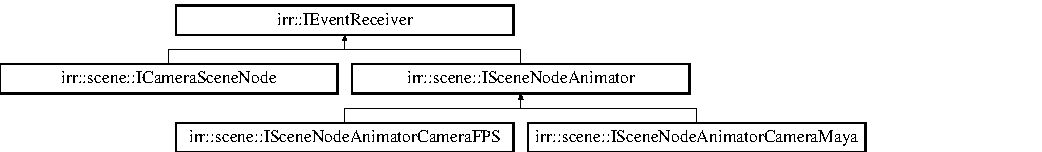
\includegraphics[height=2.043796cm]{classirr_1_1IEventReceiver}
\end{center}
\end{figure}
\subsection*{Public Member Functions}
\begin{DoxyCompactItemize}
\item 
virtual \hyperlink{classirr_1_1IEventReceiver_a4ec011612f02017d95654cf5b5d567b6}{$\sim$\+I\+Event\+Receiver} ()\hypertarget{classirr_1_1IEventReceiver_a4ec011612f02017d95654cf5b5d567b6}{}\label{classirr_1_1IEventReceiver_a4ec011612f02017d95654cf5b5d567b6}

\begin{DoxyCompactList}\small\item\em Destructor. \end{DoxyCompactList}\item 
virtual bool \hyperlink{classirr_1_1IEventReceiver_a571f744ceffc3b4fe8a81f529163eb97}{On\+Event} (const \hyperlink{structirr_1_1SEvent}{S\+Event} \&event)=0
\begin{DoxyCompactList}\small\item\em Called if an event happened. \end{DoxyCompactList}\end{DoxyCompactItemize}


\subsection{Detailed Description}
Interface of an object which can receive events. 

Many of the engine\textquotesingle{}s classes inherit \hyperlink{classirr_1_1IEventReceiver}{I\+Event\+Receiver} so they are able to process events. Events usually start at a post\+Event\+From\+User function and are passed down through a chain of event receivers until On\+Event returns true. See \hyperlink{namespaceirr_ac9eed96e06e85ce3c86fcbbbe9e48a0c}{irr\+::\+E\+E\+V\+E\+N\+T\+\_\+\+T\+Y\+PE} for a description of where each type of event starts, and the path it takes through the system. 

\subsection{Member Function Documentation}
\index{irr\+::\+I\+Event\+Receiver@{irr\+::\+I\+Event\+Receiver}!On\+Event@{On\+Event}}
\index{On\+Event@{On\+Event}!irr\+::\+I\+Event\+Receiver@{irr\+::\+I\+Event\+Receiver}}
\subsubsection[{\texorpdfstring{On\+Event(const S\+Event \&event)=0}{OnEvent(const SEvent \&event)=0}}]{\setlength{\rightskip}{0pt plus 5cm}virtual bool irr\+::\+I\+Event\+Receiver\+::\+On\+Event (
\begin{DoxyParamCaption}
\item[{const {\bf S\+Event} \&}]{event}
\end{DoxyParamCaption}
)\hspace{0.3cm}{\ttfamily [pure virtual]}}\hypertarget{classirr_1_1IEventReceiver_a571f744ceffc3b4fe8a81f529163eb97}{}\label{classirr_1_1IEventReceiver_a571f744ceffc3b4fe8a81f529163eb97}


Called if an event happened. 

Please take care that you should only return \textquotesingle{}true\textquotesingle{} when you want to {\itshape prevent} Irrlicht from processing the event any further. So \textquotesingle{}true\textquotesingle{} does mean that an event is completely done. Therefore your return value for all unprocessed events should be \textquotesingle{}false\textquotesingle{}. \begin{DoxyReturn}{Returns}
True if the event was processed. 
\end{DoxyReturn}


Implemented in \hyperlink{classirr_1_1scene_1_1ICameraSceneNode_af27145518f43a17f803cdea086f68f3c}{irr\+::scene\+::\+I\+Camera\+Scene\+Node}, and \hyperlink{classirr_1_1scene_1_1ISceneNodeAnimator_aca20b841bb586cd9654464b001a7b6aa}{irr\+::scene\+::\+I\+Scene\+Node\+Animator}.



The documentation for this class was generated from the following file\+:\begin{DoxyCompactItemize}
\item 
include/I\+Event\+Receiver.\+h\end{DoxyCompactItemize}

\hypertarget{classirr_1_1io_1_1IFileArchive}{}\section{irr\+:\+:io\+:\+:I\+File\+Archive Class Reference}
\label{classirr_1_1io_1_1IFileArchive}\index{irr\+::io\+::\+I\+File\+Archive@{irr\+::io\+::\+I\+File\+Archive}}


The File\+Archive manages archives and provides access to files inside them.  




{\ttfamily \#include $<$I\+File\+Archive.\+h$>$}

Inheritance diagram for irr\+:\+:io\+:\+:I\+File\+Archive\+:\begin{figure}[H]
\begin{center}
\leavevmode
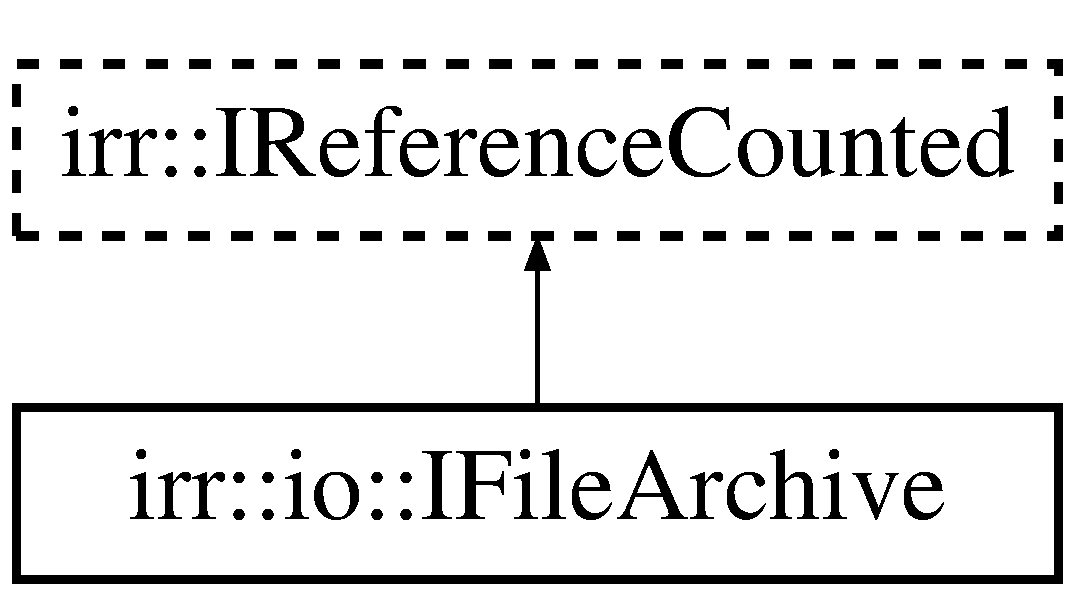
\includegraphics[height=2.000000cm]{classirr_1_1io_1_1IFileArchive}
\end{center}
\end{figure}
\subsection*{Public Member Functions}
\begin{DoxyCompactItemize}
\item 
virtual \hyperlink{classirr_1_1io_1_1IReadFile}{I\+Read\+File} $\ast$ \hyperlink{classirr_1_1io_1_1IFileArchive_a5c3b4994ae63447d2634dd86b3069988}{create\+And\+Open\+File} (const \hyperlink{namespaceirr_1_1io_ab1bdc45edb3f94d8319c02bc0f840ee1}{path} \&filename)=0
\begin{DoxyCompactList}\small\item\em Opens a file based on its name. \end{DoxyCompactList}\item 
virtual \hyperlink{classirr_1_1io_1_1IReadFile}{I\+Read\+File} $\ast$ \hyperlink{classirr_1_1io_1_1IFileArchive_ab6bc8fbd660bbbe42b4d30a9d4f26c7d}{create\+And\+Open\+File} (\hyperlink{namespaceirr_a0416a53257075833e7002efd0a18e804}{u32} index)=0
\begin{DoxyCompactList}\small\item\em Opens a file based on its position in the file list. \end{DoxyCompactList}\item 
virtual const \hyperlink{classirr_1_1io_1_1IFileList}{I\+File\+List} $\ast$ \hyperlink{classirr_1_1io_1_1IFileArchive_a5e7068953cabaaa0c02930cdf5bea97c}{get\+File\+List} () const  =0
\begin{DoxyCompactList}\small\item\em Returns the complete file tree. \end{DoxyCompactList}\item 
virtual \hyperlink{namespaceirr_1_1io_adb3e3c445ec8e608ed1f0f93306da14f}{E\+\_\+\+F\+I\+L\+E\+\_\+\+A\+R\+C\+H\+I\+V\+E\+\_\+\+T\+Y\+PE} \hyperlink{classirr_1_1io_1_1IFileArchive_acffb15450606924696fb8f9608819536}{get\+Type} () const \hypertarget{classirr_1_1io_1_1IFileArchive_acffb15450606924696fb8f9608819536}{}\label{classirr_1_1io_1_1IFileArchive_acffb15450606924696fb8f9608819536}

\begin{DoxyCompactList}\small\item\em get the archive type \end{DoxyCompactList}\end{DoxyCompactItemize}
\subsection*{Public Attributes}
\begin{DoxyCompactItemize}
\item 
\hyperlink{namespaceirr_1_1core_ade1071a878633f2f6d8a75c5d11fec19}{core\+::stringc} \hyperlink{classirr_1_1io_1_1IFileArchive_ae5b574864226b09c70518e163e59b6ba}{Password}
\begin{DoxyCompactList}\small\item\em An optionally used password string. \end{DoxyCompactList}\end{DoxyCompactItemize}
\subsection*{Additional Inherited Members}


\subsection{Detailed Description}
The File\+Archive manages archives and provides access to files inside them. 

\subsection{Member Function Documentation}
\index{irr\+::io\+::\+I\+File\+Archive@{irr\+::io\+::\+I\+File\+Archive}!create\+And\+Open\+File@{create\+And\+Open\+File}}
\index{create\+And\+Open\+File@{create\+And\+Open\+File}!irr\+::io\+::\+I\+File\+Archive@{irr\+::io\+::\+I\+File\+Archive}}
\subsubsection[{\texorpdfstring{create\+And\+Open\+File(const path \&filename)=0}{createAndOpenFile(const path \&filename)=0}}]{\setlength{\rightskip}{0pt plus 5cm}virtual {\bf I\+Read\+File}$\ast$ irr\+::io\+::\+I\+File\+Archive\+::create\+And\+Open\+File (
\begin{DoxyParamCaption}
\item[{const {\bf path} \&}]{filename}
\end{DoxyParamCaption}
)\hspace{0.3cm}{\ttfamily [pure virtual]}}\hypertarget{classirr_1_1io_1_1IFileArchive_a5c3b4994ae63447d2634dd86b3069988}{}\label{classirr_1_1io_1_1IFileArchive_a5c3b4994ae63447d2634dd86b3069988}


Opens a file based on its name. 

Creates and returns a new \hyperlink{classirr_1_1io_1_1IReadFile}{I\+Read\+File} for a file in the archive. 
\begin{DoxyParams}{Parameters}
{\em filename} & The file to open \\
\hline
\end{DoxyParams}
\begin{DoxyReturn}{Returns}
Returns A pointer to the created file on success, or 0 on failure. 
\end{DoxyReturn}
\index{irr\+::io\+::\+I\+File\+Archive@{irr\+::io\+::\+I\+File\+Archive}!create\+And\+Open\+File@{create\+And\+Open\+File}}
\index{create\+And\+Open\+File@{create\+And\+Open\+File}!irr\+::io\+::\+I\+File\+Archive@{irr\+::io\+::\+I\+File\+Archive}}
\subsubsection[{\texorpdfstring{create\+And\+Open\+File(u32 index)=0}{createAndOpenFile(u32 index)=0}}]{\setlength{\rightskip}{0pt plus 5cm}virtual {\bf I\+Read\+File}$\ast$ irr\+::io\+::\+I\+File\+Archive\+::create\+And\+Open\+File (
\begin{DoxyParamCaption}
\item[{{\bf u32}}]{index}
\end{DoxyParamCaption}
)\hspace{0.3cm}{\ttfamily [pure virtual]}}\hypertarget{classirr_1_1io_1_1IFileArchive_ab6bc8fbd660bbbe42b4d30a9d4f26c7d}{}\label{classirr_1_1io_1_1IFileArchive_ab6bc8fbd660bbbe42b4d30a9d4f26c7d}


Opens a file based on its position in the file list. 

Creates and returns 
\begin{DoxyParams}{Parameters}
{\em index} & The zero based index of the file. \\
\hline
\end{DoxyParams}
\begin{DoxyReturn}{Returns}
Returns a pointer to the created file on success, or 0 on failure. 
\end{DoxyReturn}
\index{irr\+::io\+::\+I\+File\+Archive@{irr\+::io\+::\+I\+File\+Archive}!get\+File\+List@{get\+File\+List}}
\index{get\+File\+List@{get\+File\+List}!irr\+::io\+::\+I\+File\+Archive@{irr\+::io\+::\+I\+File\+Archive}}
\subsubsection[{\texorpdfstring{get\+File\+List() const  =0}{getFileList() const  =0}}]{\setlength{\rightskip}{0pt plus 5cm}virtual const {\bf I\+File\+List}$\ast$ irr\+::io\+::\+I\+File\+Archive\+::get\+File\+List (
\begin{DoxyParamCaption}
{}
\end{DoxyParamCaption}
) const\hspace{0.3cm}{\ttfamily [pure virtual]}}\hypertarget{classirr_1_1io_1_1IFileArchive_a5e7068953cabaaa0c02930cdf5bea97c}{}\label{classirr_1_1io_1_1IFileArchive_a5e7068953cabaaa0c02930cdf5bea97c}


Returns the complete file tree. 

\begin{DoxyReturn}{Returns}
Returns the complete directory tree for the archive, including all files and folders 
\end{DoxyReturn}


\subsection{Member Data Documentation}
\index{irr\+::io\+::\+I\+File\+Archive@{irr\+::io\+::\+I\+File\+Archive}!Password@{Password}}
\index{Password@{Password}!irr\+::io\+::\+I\+File\+Archive@{irr\+::io\+::\+I\+File\+Archive}}
\subsubsection[{\texorpdfstring{Password}{Password}}]{\setlength{\rightskip}{0pt plus 5cm}{\bf core\+::stringc} irr\+::io\+::\+I\+File\+Archive\+::\+Password}\hypertarget{classirr_1_1io_1_1IFileArchive_ae5b574864226b09c70518e163e59b6ba}{}\label{classirr_1_1io_1_1IFileArchive_ae5b574864226b09c70518e163e59b6ba}


An optionally used password string. 

This variable is publicly accessible from the interface in order to avoid single access patterns to this place, and hence allow some more obscurity. 

The documentation for this class was generated from the following file\+:\begin{DoxyCompactItemize}
\item 
include/I\+File\+Archive.\+h\end{DoxyCompactItemize}

\hypertarget{classirr_1_1io_1_1IFileList}{}\section{irr\+:\+:io\+:\+:I\+File\+List Class Reference}
\label{classirr_1_1io_1_1IFileList}\index{irr\+::io\+::\+I\+File\+List@{irr\+::io\+::\+I\+File\+List}}


Provides a list of files and folders.  




{\ttfamily \#include $<$I\+File\+List.\+h$>$}

Inheritance diagram for irr\+:\+:io\+:\+:I\+File\+List\+:\begin{figure}[H]
\begin{center}
\leavevmode
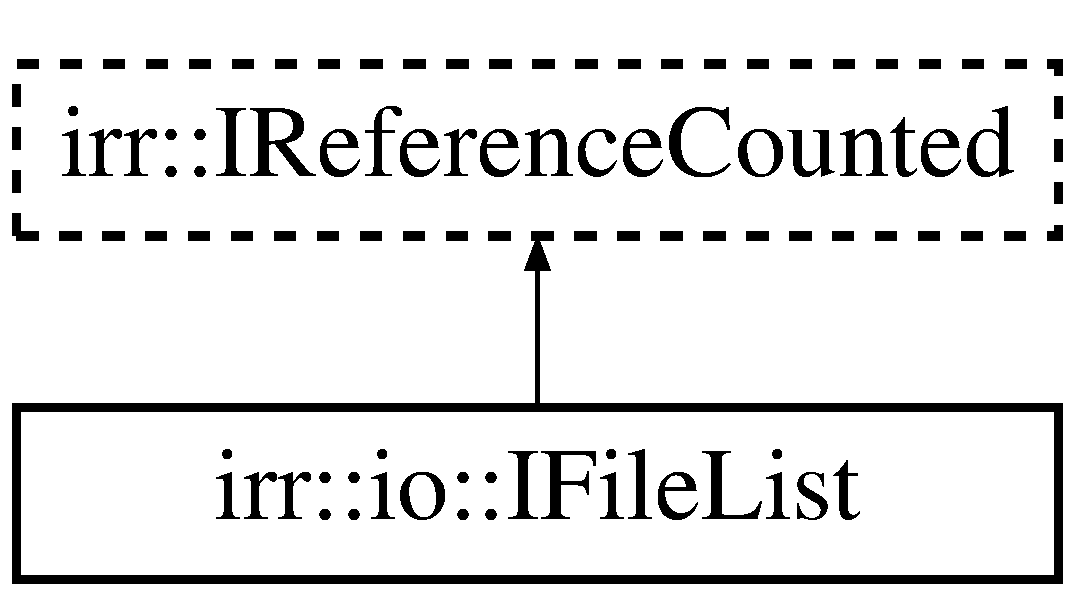
\includegraphics[height=2.000000cm]{classirr_1_1io_1_1IFileList}
\end{center}
\end{figure}
\subsection*{Public Member Functions}
\begin{DoxyCompactItemize}
\item 
virtual \hyperlink{namespaceirr_a0416a53257075833e7002efd0a18e804}{u32} \hyperlink{classirr_1_1io_1_1IFileList_a64a240d1da0e220fea18af96ec7bb982}{get\+File\+Count} () const  =0
\begin{DoxyCompactList}\small\item\em Get the number of files in the filelist. \end{DoxyCompactList}\item 
virtual const \hyperlink{namespaceirr_1_1io_ab1bdc45edb3f94d8319c02bc0f840ee1}{io\+::path} \& \hyperlink{classirr_1_1io_1_1IFileList_accaf8302604eb9f0a7f6bc49a7b53e5d}{get\+File\+Name} (\hyperlink{namespaceirr_a0416a53257075833e7002efd0a18e804}{u32} index) const  =0
\begin{DoxyCompactList}\small\item\em Gets the name of a file in the list, based on an index. \end{DoxyCompactList}\item 
virtual const \hyperlink{namespaceirr_1_1io_ab1bdc45edb3f94d8319c02bc0f840ee1}{io\+::path} \& \hyperlink{classirr_1_1io_1_1IFileList_a2e61971adb2b978515d63f6d07dc14e3}{get\+Full\+File\+Name} (\hyperlink{namespaceirr_a0416a53257075833e7002efd0a18e804}{u32} index) const  =0
\begin{DoxyCompactList}\small\item\em Gets the full name of a file in the list including the path, based on an index. \end{DoxyCompactList}\item 
virtual \hyperlink{namespaceirr_a0416a53257075833e7002efd0a18e804}{u32} \hyperlink{classirr_1_1io_1_1IFileList_a17ed7f43fa2acdd7af7d011eca22b956}{get\+File\+Size} (\hyperlink{namespaceirr_a0416a53257075833e7002efd0a18e804}{u32} index) const  =0
\begin{DoxyCompactList}\small\item\em Returns the size of a file in the file list, based on an index. \end{DoxyCompactList}\item 
virtual \hyperlink{namespaceirr_a0416a53257075833e7002efd0a18e804}{u32} \hyperlink{classirr_1_1io_1_1IFileList_a385fb29a7bab275c86bef507336cc33d}{get\+File\+Offset} (\hyperlink{namespaceirr_a0416a53257075833e7002efd0a18e804}{u32} index) const  =0
\begin{DoxyCompactList}\small\item\em Returns the file offset of a file in the file list, based on an index. \end{DoxyCompactList}\item 
virtual \hyperlink{namespaceirr_a0416a53257075833e7002efd0a18e804}{u32} \hyperlink{classirr_1_1io_1_1IFileList_ab5c1f08fbbde4cda0e3b135499a5fc84}{get\+ID} (\hyperlink{namespaceirr_a0416a53257075833e7002efd0a18e804}{u32} index) const  =0
\begin{DoxyCompactList}\small\item\em Returns the ID of a file in the file list, based on an index. \end{DoxyCompactList}\item 
virtual bool \hyperlink{classirr_1_1io_1_1IFileList_ac10cdbc20abb0817010d869af0032078}{is\+Directory} (\hyperlink{namespaceirr_a0416a53257075833e7002efd0a18e804}{u32} index) const  =0
\begin{DoxyCompactList}\small\item\em Check if the file is a directory. \end{DoxyCompactList}\item 
virtual \hyperlink{namespaceirr_ac66849b7a6ed16e30ebede579f9b47c6}{s32} \hyperlink{classirr_1_1io_1_1IFileList_a31c90fda10d00bdab5c83d7c3d35807c}{find\+File} (const \hyperlink{namespaceirr_1_1io_ab1bdc45edb3f94d8319c02bc0f840ee1}{io\+::path} \&filename, bool is\+Folder=false) const  =0
\begin{DoxyCompactList}\small\item\em Searches for a file or folder in the list. \end{DoxyCompactList}\item 
virtual const \hyperlink{namespaceirr_1_1io_ab1bdc45edb3f94d8319c02bc0f840ee1}{io\+::path} \& \hyperlink{classirr_1_1io_1_1IFileList_a0b77ba658cddaa7120483c9c55cac396}{get\+Path} () const  =0\hypertarget{classirr_1_1io_1_1IFileList_a0b77ba658cddaa7120483c9c55cac396}{}\label{classirr_1_1io_1_1IFileList_a0b77ba658cddaa7120483c9c55cac396}

\begin{DoxyCompactList}\small\item\em Returns the base path of the file list. \end{DoxyCompactList}\item 
virtual \hyperlink{namespaceirr_a0416a53257075833e7002efd0a18e804}{u32} \hyperlink{classirr_1_1io_1_1IFileList_ad0d90f1bb8a35910f4f877268e2f043e}{add\+Item} (const \hyperlink{namespaceirr_1_1io_ab1bdc45edb3f94d8319c02bc0f840ee1}{io\+::path} \&full\+Path, \hyperlink{namespaceirr_a0416a53257075833e7002efd0a18e804}{u32} offset, \hyperlink{namespaceirr_a0416a53257075833e7002efd0a18e804}{u32} size, bool \hyperlink{classirr_1_1io_1_1IFileList_ac10cdbc20abb0817010d869af0032078}{is\+Directory}, \hyperlink{namespaceirr_a0416a53257075833e7002efd0a18e804}{u32} id=0)=0
\begin{DoxyCompactList}\small\item\em Add as a file or folder to the list. \end{DoxyCompactList}\item 
virtual void \hyperlink{classirr_1_1io_1_1IFileList_a2cf4f12d7ee6ab35257169ec23654da8}{sort} ()=0\hypertarget{classirr_1_1io_1_1IFileList_a2cf4f12d7ee6ab35257169ec23654da8}{}\label{classirr_1_1io_1_1IFileList_a2cf4f12d7ee6ab35257169ec23654da8}

\begin{DoxyCompactList}\small\item\em Sorts the file list. You should call this after adding any items to the file list. \end{DoxyCompactList}\end{DoxyCompactItemize}
\subsection*{Additional Inherited Members}


\subsection{Detailed Description}
Provides a list of files and folders. 

File lists usually contain a list of all files in a given folder, but can also contain a complete directory structure. 

\subsection{Member Function Documentation}
\index{irr\+::io\+::\+I\+File\+List@{irr\+::io\+::\+I\+File\+List}!add\+Item@{add\+Item}}
\index{add\+Item@{add\+Item}!irr\+::io\+::\+I\+File\+List@{irr\+::io\+::\+I\+File\+List}}
\subsubsection[{\texorpdfstring{add\+Item(const io\+::path \&full\+Path, u32 offset, u32 size, bool is\+Directory, u32 id=0)=0}{addItem(const io::path \&fullPath, u32 offset, u32 size, bool isDirectory, u32 id=0)=0}}]{\setlength{\rightskip}{0pt plus 5cm}virtual {\bf u32} irr\+::io\+::\+I\+File\+List\+::add\+Item (
\begin{DoxyParamCaption}
\item[{const {\bf io\+::path} \&}]{full\+Path, }
\item[{{\bf u32}}]{offset, }
\item[{{\bf u32}}]{size, }
\item[{bool}]{is\+Directory, }
\item[{{\bf u32}}]{id = {\ttfamily 0}}
\end{DoxyParamCaption}
)\hspace{0.3cm}{\ttfamily [pure virtual]}}\hypertarget{classirr_1_1io_1_1IFileList_ad0d90f1bb8a35910f4f877268e2f043e}{}\label{classirr_1_1io_1_1IFileList_ad0d90f1bb8a35910f4f877268e2f043e}


Add as a file or folder to the list. 


\begin{DoxyParams}{Parameters}
{\em full\+Path} & The file name including path, from the root of the file list. \\
\hline
{\em is\+Directory} & True if this is a directory rather than a file. \\
\hline
{\em offset} & The file offset inside an archive \\
\hline
{\em size} & The size of the file in bytes. \\
\hline
{\em id} & The ID of the file in the archive which owns it \\
\hline
\end{DoxyParams}
\index{irr\+::io\+::\+I\+File\+List@{irr\+::io\+::\+I\+File\+List}!find\+File@{find\+File}}
\index{find\+File@{find\+File}!irr\+::io\+::\+I\+File\+List@{irr\+::io\+::\+I\+File\+List}}
\subsubsection[{\texorpdfstring{find\+File(const io\+::path \&filename, bool is\+Folder=false) const  =0}{findFile(const io::path \&filename, bool isFolder=false) const  =0}}]{\setlength{\rightskip}{0pt plus 5cm}virtual {\bf s32} irr\+::io\+::\+I\+File\+List\+::find\+File (
\begin{DoxyParamCaption}
\item[{const {\bf io\+::path} \&}]{filename, }
\item[{bool}]{is\+Folder = {\ttfamily false}}
\end{DoxyParamCaption}
) const\hspace{0.3cm}{\ttfamily [pure virtual]}}\hypertarget{classirr_1_1io_1_1IFileList_a31c90fda10d00bdab5c83d7c3d35807c}{}\label{classirr_1_1io_1_1IFileList_a31c90fda10d00bdab5c83d7c3d35807c}


Searches for a file or folder in the list. 

Searches for a file by name 
\begin{DoxyParams}{Parameters}
{\em filename} & The name of the file to search for. \\
\hline
{\em is\+Folder} & True if you are searching for a directory path, false if you are searching for a file \\
\hline
\end{DoxyParams}
\begin{DoxyReturn}{Returns}
Returns the index of the file in the file list, or -\/1 if no matching name name was found. 
\end{DoxyReturn}
\index{irr\+::io\+::\+I\+File\+List@{irr\+::io\+::\+I\+File\+List}!get\+File\+Count@{get\+File\+Count}}
\index{get\+File\+Count@{get\+File\+Count}!irr\+::io\+::\+I\+File\+List@{irr\+::io\+::\+I\+File\+List}}
\subsubsection[{\texorpdfstring{get\+File\+Count() const  =0}{getFileCount() const  =0}}]{\setlength{\rightskip}{0pt plus 5cm}virtual {\bf u32} irr\+::io\+::\+I\+File\+List\+::get\+File\+Count (
\begin{DoxyParamCaption}
{}
\end{DoxyParamCaption}
) const\hspace{0.3cm}{\ttfamily [pure virtual]}}\hypertarget{classirr_1_1io_1_1IFileList_a64a240d1da0e220fea18af96ec7bb982}{}\label{classirr_1_1io_1_1IFileList_a64a240d1da0e220fea18af96ec7bb982}


Get the number of files in the filelist. 

\begin{DoxyReturn}{Returns}
Amount of files and directories in the file list. 
\end{DoxyReturn}
\index{irr\+::io\+::\+I\+File\+List@{irr\+::io\+::\+I\+File\+List}!get\+File\+Name@{get\+File\+Name}}
\index{get\+File\+Name@{get\+File\+Name}!irr\+::io\+::\+I\+File\+List@{irr\+::io\+::\+I\+File\+List}}
\subsubsection[{\texorpdfstring{get\+File\+Name(u32 index) const  =0}{getFileName(u32 index) const  =0}}]{\setlength{\rightskip}{0pt plus 5cm}virtual const {\bf io\+::path}\& irr\+::io\+::\+I\+File\+List\+::get\+File\+Name (
\begin{DoxyParamCaption}
\item[{{\bf u32}}]{index}
\end{DoxyParamCaption}
) const\hspace{0.3cm}{\ttfamily [pure virtual]}}\hypertarget{classirr_1_1io_1_1IFileList_accaf8302604eb9f0a7f6bc49a7b53e5d}{}\label{classirr_1_1io_1_1IFileList_accaf8302604eb9f0a7f6bc49a7b53e5d}


Gets the name of a file in the list, based on an index. 

The path is not included in this name. Use get\+Full\+File\+Name for this. 
\begin{DoxyParams}{Parameters}
{\em index} & is the zero based index of the file which name should be returned. The index must be less than the amount \hyperlink{classirr_1_1io_1_1IFileList_a64a240d1da0e220fea18af96ec7bb982}{get\+File\+Count()} returns. \\
\hline
\end{DoxyParams}
\begin{DoxyReturn}{Returns}
File name of the file. Returns 0, if an error occured. 
\end{DoxyReturn}
\index{irr\+::io\+::\+I\+File\+List@{irr\+::io\+::\+I\+File\+List}!get\+File\+Offset@{get\+File\+Offset}}
\index{get\+File\+Offset@{get\+File\+Offset}!irr\+::io\+::\+I\+File\+List@{irr\+::io\+::\+I\+File\+List}}
\subsubsection[{\texorpdfstring{get\+File\+Offset(u32 index) const  =0}{getFileOffset(u32 index) const  =0}}]{\setlength{\rightskip}{0pt plus 5cm}virtual {\bf u32} irr\+::io\+::\+I\+File\+List\+::get\+File\+Offset (
\begin{DoxyParamCaption}
\item[{{\bf u32}}]{index}
\end{DoxyParamCaption}
) const\hspace{0.3cm}{\ttfamily [pure virtual]}}\hypertarget{classirr_1_1io_1_1IFileList_a385fb29a7bab275c86bef507336cc33d}{}\label{classirr_1_1io_1_1IFileList_a385fb29a7bab275c86bef507336cc33d}


Returns the file offset of a file in the file list, based on an index. 


\begin{DoxyParams}{Parameters}
{\em index} & is the zero based index of the file which should be returned. The index must be less than the amount \hyperlink{classirr_1_1io_1_1IFileList_a64a240d1da0e220fea18af96ec7bb982}{get\+File\+Count()} returns. \\
\hline
\end{DoxyParams}
\begin{DoxyReturn}{Returns}
The offset of the file in bytes. 
\end{DoxyReturn}
\index{irr\+::io\+::\+I\+File\+List@{irr\+::io\+::\+I\+File\+List}!get\+File\+Size@{get\+File\+Size}}
\index{get\+File\+Size@{get\+File\+Size}!irr\+::io\+::\+I\+File\+List@{irr\+::io\+::\+I\+File\+List}}
\subsubsection[{\texorpdfstring{get\+File\+Size(u32 index) const  =0}{getFileSize(u32 index) const  =0}}]{\setlength{\rightskip}{0pt plus 5cm}virtual {\bf u32} irr\+::io\+::\+I\+File\+List\+::get\+File\+Size (
\begin{DoxyParamCaption}
\item[{{\bf u32}}]{index}
\end{DoxyParamCaption}
) const\hspace{0.3cm}{\ttfamily [pure virtual]}}\hypertarget{classirr_1_1io_1_1IFileList_a17ed7f43fa2acdd7af7d011eca22b956}{}\label{classirr_1_1io_1_1IFileList_a17ed7f43fa2acdd7af7d011eca22b956}


Returns the size of a file in the file list, based on an index. 


\begin{DoxyParams}{Parameters}
{\em index} & is the zero based index of the file which should be returned. The index must be less than the amount \hyperlink{classirr_1_1io_1_1IFileList_a64a240d1da0e220fea18af96ec7bb982}{get\+File\+Count()} returns. \\
\hline
\end{DoxyParams}
\begin{DoxyReturn}{Returns}
The size of the file in bytes. 
\end{DoxyReturn}
\index{irr\+::io\+::\+I\+File\+List@{irr\+::io\+::\+I\+File\+List}!get\+Full\+File\+Name@{get\+Full\+File\+Name}}
\index{get\+Full\+File\+Name@{get\+Full\+File\+Name}!irr\+::io\+::\+I\+File\+List@{irr\+::io\+::\+I\+File\+List}}
\subsubsection[{\texorpdfstring{get\+Full\+File\+Name(u32 index) const  =0}{getFullFileName(u32 index) const  =0}}]{\setlength{\rightskip}{0pt plus 5cm}virtual const {\bf io\+::path}\& irr\+::io\+::\+I\+File\+List\+::get\+Full\+File\+Name (
\begin{DoxyParamCaption}
\item[{{\bf u32}}]{index}
\end{DoxyParamCaption}
) const\hspace{0.3cm}{\ttfamily [pure virtual]}}\hypertarget{classirr_1_1io_1_1IFileList_a2e61971adb2b978515d63f6d07dc14e3}{}\label{classirr_1_1io_1_1IFileList_a2e61971adb2b978515d63f6d07dc14e3}


Gets the full name of a file in the list including the path, based on an index. 


\begin{DoxyParams}{Parameters}
{\em index} & is the zero based index of the file which name should be returned. The index must be less than the amount \hyperlink{classirr_1_1io_1_1IFileList_a64a240d1da0e220fea18af96ec7bb982}{get\+File\+Count()} returns. \\
\hline
\end{DoxyParams}
\begin{DoxyReturn}{Returns}
File name of the file. Returns 0 if an error occured. 
\end{DoxyReturn}
\index{irr\+::io\+::\+I\+File\+List@{irr\+::io\+::\+I\+File\+List}!get\+ID@{get\+ID}}
\index{get\+ID@{get\+ID}!irr\+::io\+::\+I\+File\+List@{irr\+::io\+::\+I\+File\+List}}
\subsubsection[{\texorpdfstring{get\+I\+D(u32 index) const  =0}{getID(u32 index) const  =0}}]{\setlength{\rightskip}{0pt plus 5cm}virtual {\bf u32} irr\+::io\+::\+I\+File\+List\+::get\+ID (
\begin{DoxyParamCaption}
\item[{{\bf u32}}]{index}
\end{DoxyParamCaption}
) const\hspace{0.3cm}{\ttfamily [pure virtual]}}\hypertarget{classirr_1_1io_1_1IFileList_ab5c1f08fbbde4cda0e3b135499a5fc84}{}\label{classirr_1_1io_1_1IFileList_ab5c1f08fbbde4cda0e3b135499a5fc84}


Returns the ID of a file in the file list, based on an index. 

This optional ID can be used to link the file list entry to information held elsewhere. For example this could be an index in an \hyperlink{classirr_1_1io_1_1IFileArchive}{I\+File\+Archive}, linking the entry to its data offset, uncompressed size and C\+RC. 
\begin{DoxyParams}{Parameters}
{\em index} & is the zero based index of the file which should be returned. The index must be less than the amount \hyperlink{classirr_1_1io_1_1IFileList_a64a240d1da0e220fea18af96ec7bb982}{get\+File\+Count()} returns. \\
\hline
\end{DoxyParams}
\begin{DoxyReturn}{Returns}
The ID of the file. 
\end{DoxyReturn}
\index{irr\+::io\+::\+I\+File\+List@{irr\+::io\+::\+I\+File\+List}!is\+Directory@{is\+Directory}}
\index{is\+Directory@{is\+Directory}!irr\+::io\+::\+I\+File\+List@{irr\+::io\+::\+I\+File\+List}}
\subsubsection[{\texorpdfstring{is\+Directory(u32 index) const  =0}{isDirectory(u32 index) const  =0}}]{\setlength{\rightskip}{0pt plus 5cm}virtual bool irr\+::io\+::\+I\+File\+List\+::is\+Directory (
\begin{DoxyParamCaption}
\item[{{\bf u32}}]{index}
\end{DoxyParamCaption}
) const\hspace{0.3cm}{\ttfamily [pure virtual]}}\hypertarget{classirr_1_1io_1_1IFileList_ac10cdbc20abb0817010d869af0032078}{}\label{classirr_1_1io_1_1IFileList_ac10cdbc20abb0817010d869af0032078}


Check if the file is a directory. 


\begin{DoxyParams}{Parameters}
{\em index} & The zero based index which will be checked. The index must be less than the amount \hyperlink{classirr_1_1io_1_1IFileList_a64a240d1da0e220fea18af96ec7bb982}{get\+File\+Count()} returns. \\
\hline
\end{DoxyParams}
\begin{DoxyReturn}{Returns}
True if the file is a directory, else false. 
\end{DoxyReturn}


The documentation for this class was generated from the following file\+:\begin{DoxyCompactItemize}
\item 
include/I\+File\+List.\+h\end{DoxyCompactItemize}

\hypertarget{classirr_1_1io_1_1IFileReadCallBack}{}\section{irr\+:\+:io\+:\+:I\+File\+Read\+Call\+Back Class Reference}
\label{classirr_1_1io_1_1IFileReadCallBack}\index{irr\+::io\+::\+I\+File\+Read\+Call\+Back@{irr\+::io\+::\+I\+File\+Read\+Call\+Back}}


Callback class for file read abstraction.  




{\ttfamily \#include $<$irr\+X\+M\+L.\+h$>$}

\subsection*{Public Member Functions}
\begin{DoxyCompactItemize}
\item 
virtual \hyperlink{classirr_1_1io_1_1IFileReadCallBack_a91ace84f0a3966d88d78da5342eb9619}{$\sim$\+I\+File\+Read\+Call\+Back} ()\hypertarget{classirr_1_1io_1_1IFileReadCallBack_a91ace84f0a3966d88d78da5342eb9619}{}\label{classirr_1_1io_1_1IFileReadCallBack_a91ace84f0a3966d88d78da5342eb9619}

\begin{DoxyCompactList}\small\item\em Destructor. \end{DoxyCompactList}\item 
virtual int \hyperlink{classirr_1_1io_1_1IFileReadCallBack_ae8c57b8454078aa2acd39772a6aa4439}{read} (void $\ast$buffer, int size\+To\+Read)=0
\begin{DoxyCompactList}\small\item\em Reads an amount of bytes from the file. \end{DoxyCompactList}\item 
virtual long \hyperlink{classirr_1_1io_1_1IFileReadCallBack_a31ee0fbc44db4568bffe0ce526478f5d}{get\+Size} () const  =0\hypertarget{classirr_1_1io_1_1IFileReadCallBack_a31ee0fbc44db4568bffe0ce526478f5d}{}\label{classirr_1_1io_1_1IFileReadCallBack_a31ee0fbc44db4568bffe0ce526478f5d}

\begin{DoxyCompactList}\small\item\em Returns size of file in bytes. \end{DoxyCompactList}\end{DoxyCompactItemize}


\subsection{Detailed Description}
Callback class for file read abstraction. 

With this, it is possible to make the xml parser read in other things than just files. The Irrlicht engine is using this for example to read xml from compressed .zip files. To make the parser read in any other data, derive a class from this interface, implement the two methods to read your data and give a pointer to an instance of your implementation when calling \hyperlink{namespaceirr_1_1io_a581f4d4648398759c61266d63d7106b1}{create\+Irr\+X\+M\+L\+Reader()}, \hyperlink{namespaceirr_1_1io_a86473ef152c15b685af181a4c5461a5d}{create\+Irr\+X\+M\+L\+Reader\+U\+T\+F16()} or \hyperlink{namespaceirr_1_1io_ae05bf7ee342431ea8c98fb98e75b974a}{create\+Irr\+X\+M\+L\+Reader\+U\+T\+F32()} 

\subsection{Member Function Documentation}
\index{irr\+::io\+::\+I\+File\+Read\+Call\+Back@{irr\+::io\+::\+I\+File\+Read\+Call\+Back}!read@{read}}
\index{read@{read}!irr\+::io\+::\+I\+File\+Read\+Call\+Back@{irr\+::io\+::\+I\+File\+Read\+Call\+Back}}
\subsubsection[{\texorpdfstring{read(void $\ast$buffer, int size\+To\+Read)=0}{read(void *buffer, int sizeToRead)=0}}]{\setlength{\rightskip}{0pt plus 5cm}virtual int irr\+::io\+::\+I\+File\+Read\+Call\+Back\+::read (
\begin{DoxyParamCaption}
\item[{void $\ast$}]{buffer, }
\item[{int}]{size\+To\+Read}
\end{DoxyParamCaption}
)\hspace{0.3cm}{\ttfamily [pure virtual]}}\hypertarget{classirr_1_1io_1_1IFileReadCallBack_ae8c57b8454078aa2acd39772a6aa4439}{}\label{classirr_1_1io_1_1IFileReadCallBack_ae8c57b8454078aa2acd39772a6aa4439}


Reads an amount of bytes from the file. 


\begin{DoxyParams}{Parameters}
{\em buffer} & Pointer to buffer where to read bytes will be written to. \\
\hline
{\em size\+To\+Read} & Amount of bytes to read from the file. \\
\hline
\end{DoxyParams}
\begin{DoxyReturn}{Returns}
Returns how much bytes were read. 
\end{DoxyReturn}


The documentation for this class was generated from the following file\+:\begin{DoxyCompactItemize}
\item 
include/\hyperlink{irrXML_8h}{irr\+X\+M\+L.\+h}\end{DoxyCompactItemize}

\hypertarget{classirr_1_1io_1_1IFileSystem}{}\section{irr\+:\+:io\+:\+:I\+File\+System Class Reference}
\label{classirr_1_1io_1_1IFileSystem}\index{irr\+::io\+::\+I\+File\+System@{irr\+::io\+::\+I\+File\+System}}


The File\+System manages files and archives and provides access to them.  




{\ttfamily \#include $<$I\+File\+System.\+h$>$}

Inheritance diagram for irr\+:\+:io\+:\+:I\+File\+System\+:\begin{figure}[H]
\begin{center}
\leavevmode
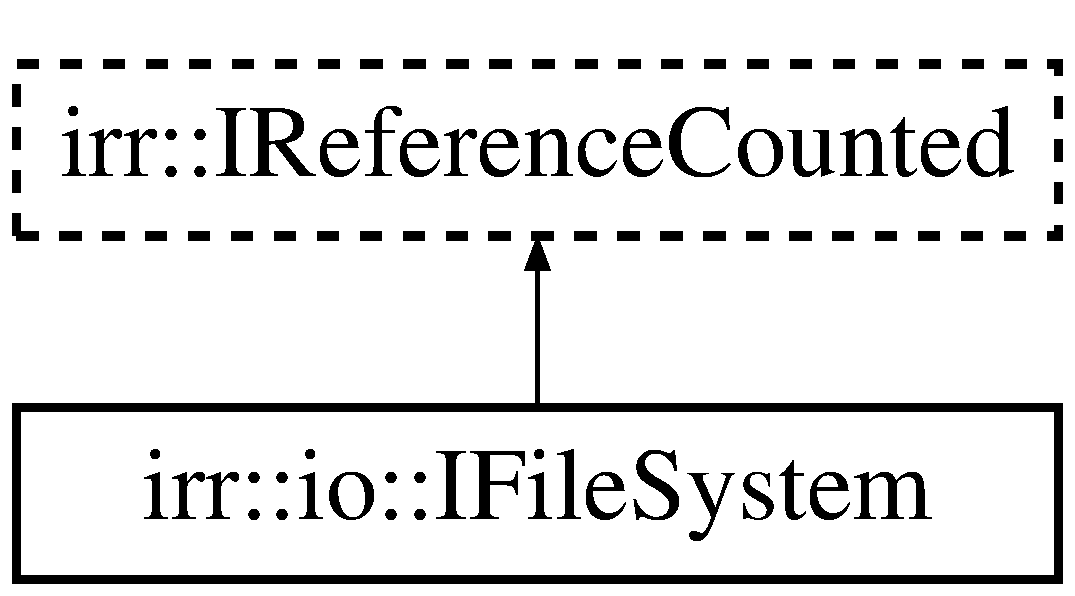
\includegraphics[height=2.000000cm]{classirr_1_1io_1_1IFileSystem}
\end{center}
\end{figure}
\subsection*{Public Member Functions}
\begin{DoxyCompactItemize}
\item 
virtual \hyperlink{classirr_1_1io_1_1IReadFile}{I\+Read\+File} $\ast$ \hyperlink{classirr_1_1io_1_1IFileSystem_a3678bb77e12cc6ee2b3947f4c79f6c90}{create\+And\+Open\+File} (const \hyperlink{namespaceirr_1_1io_ab1bdc45edb3f94d8319c02bc0f840ee1}{path} \&filename)=0
\begin{DoxyCompactList}\small\item\em Opens a file for read access. \end{DoxyCompactList}\item 
virtual \hyperlink{classirr_1_1io_1_1IReadFile}{I\+Read\+File} $\ast$ \hyperlink{classirr_1_1io_1_1IFileSystem_ac60a4b7912a7f2364426dc1aaf9bccae}{create\+Memory\+Read\+File} (void $\ast$memory, \hyperlink{namespaceirr_ac66849b7a6ed16e30ebede579f9b47c6}{s32} len, const \hyperlink{namespaceirr_1_1io_ab1bdc45edb3f94d8319c02bc0f840ee1}{path} \&file\+Name, bool delete\+Memory\+When\+Dropped=false)=0
\begin{DoxyCompactList}\small\item\em Creates an \hyperlink{classirr_1_1io_1_1IReadFile}{I\+Read\+File} interface for accessing memory like a file. \end{DoxyCompactList}\item 
virtual \hyperlink{classirr_1_1io_1_1IReadFile}{I\+Read\+File} $\ast$ \hyperlink{classirr_1_1io_1_1IFileSystem_a8b110f1ed6f52098753b7a558c020dbc}{create\+Limit\+Read\+File} (const \hyperlink{namespaceirr_1_1io_ab1bdc45edb3f94d8319c02bc0f840ee1}{path} \&file\+Name, \hyperlink{classirr_1_1io_1_1IReadFile}{I\+Read\+File} $\ast$already\+Opened\+File, long pos, long area\+Size)=0
\begin{DoxyCompactList}\small\item\em Creates an \hyperlink{classirr_1_1io_1_1IReadFile}{I\+Read\+File} interface for accessing files inside files. \end{DoxyCompactList}\item 
virtual \hyperlink{classirr_1_1io_1_1IWriteFile}{I\+Write\+File} $\ast$ \hyperlink{classirr_1_1io_1_1IFileSystem_a568dd1e737fe3d3222b2e4ca2b6ebad3}{create\+Memory\+Write\+File} (void $\ast$memory, \hyperlink{namespaceirr_ac66849b7a6ed16e30ebede579f9b47c6}{s32} len, const \hyperlink{namespaceirr_1_1io_ab1bdc45edb3f94d8319c02bc0f840ee1}{path} \&file\+Name, bool delete\+Memory\+When\+Dropped=false)=0
\begin{DoxyCompactList}\small\item\em Creates an \hyperlink{classirr_1_1io_1_1IWriteFile}{I\+Write\+File} interface for accessing memory like a file. \end{DoxyCompactList}\item 
virtual \hyperlink{classirr_1_1io_1_1IWriteFile}{I\+Write\+File} $\ast$ \hyperlink{classirr_1_1io_1_1IFileSystem_af0ed28b697936ee8aa60a5a0877ac90a}{create\+And\+Write\+File} (const \hyperlink{namespaceirr_1_1io_ab1bdc45edb3f94d8319c02bc0f840ee1}{path} \&filename, bool append=false)=0
\begin{DoxyCompactList}\small\item\em Opens a file for write access. \end{DoxyCompactList}\item 
virtual bool \hyperlink{classirr_1_1io_1_1IFileSystem_afe6641c7f88a8fea0205c113b8379730}{add\+File\+Archive} (const \hyperlink{namespaceirr_1_1io_ab1bdc45edb3f94d8319c02bc0f840ee1}{path} \&filename, bool ignore\+Case=true, bool ignore\+Paths=true, \hyperlink{namespaceirr_1_1io_adb3e3c445ec8e608ed1f0f93306da14f}{E\+\_\+\+F\+I\+L\+E\+\_\+\+A\+R\+C\+H\+I\+V\+E\+\_\+\+T\+Y\+PE} archive\+Type=\hyperlink{namespaceirr_1_1io_adb3e3c445ec8e608ed1f0f93306da14fa2c2aea9bc955ae4e0d29071ba66ff8dc}{E\+F\+A\+T\+\_\+\+U\+N\+K\+N\+O\+WN}, const \hyperlink{namespaceirr_1_1core_ade1071a878633f2f6d8a75c5d11fec19}{core\+::stringc} \&password=\char`\"{}\char`\"{}, \hyperlink{classirr_1_1io_1_1IFileArchive}{I\+File\+Archive} $\ast$$\ast$ret\+Archive=0)=0
\begin{DoxyCompactList}\small\item\em Adds an archive to the file system. \end{DoxyCompactList}\item 
virtual bool \hyperlink{classirr_1_1io_1_1IFileSystem_abe4d01069e7fbf0fa871197a68ad87b9}{add\+File\+Archive} (\hyperlink{classirr_1_1io_1_1IReadFile}{I\+Read\+File} $\ast$file, bool ignore\+Case=true, bool ignore\+Paths=true, \hyperlink{namespaceirr_1_1io_adb3e3c445ec8e608ed1f0f93306da14f}{E\+\_\+\+F\+I\+L\+E\+\_\+\+A\+R\+C\+H\+I\+V\+E\+\_\+\+T\+Y\+PE} archive\+Type=\hyperlink{namespaceirr_1_1io_adb3e3c445ec8e608ed1f0f93306da14fa2c2aea9bc955ae4e0d29071ba66ff8dc}{E\+F\+A\+T\+\_\+\+U\+N\+K\+N\+O\+WN}, const \hyperlink{namespaceirr_1_1core_ade1071a878633f2f6d8a75c5d11fec19}{core\+::stringc} \&password=\char`\"{}\char`\"{}, \hyperlink{classirr_1_1io_1_1IFileArchive}{I\+File\+Archive} $\ast$$\ast$ret\+Archive=0)=0
\begin{DoxyCompactList}\small\item\em Adds an archive to the file system. \end{DoxyCompactList}\item 
virtual bool \hyperlink{classirr_1_1io_1_1IFileSystem_aedecc2c6f4c567de8bbe54fd711f7143}{add\+File\+Archive} (\hyperlink{classirr_1_1io_1_1IFileArchive}{I\+File\+Archive} $\ast$archive)=0
\begin{DoxyCompactList}\small\item\em Adds an archive to the file system. \end{DoxyCompactList}\item 
virtual \hyperlink{namespaceirr_a0416a53257075833e7002efd0a18e804}{u32} \hyperlink{classirr_1_1io_1_1IFileSystem_a15ecdb3ac4fd3d564a7fd976bab9acd6}{get\+File\+Archive\+Count} () const  =0\hypertarget{classirr_1_1io_1_1IFileSystem_a15ecdb3ac4fd3d564a7fd976bab9acd6}{}\label{classirr_1_1io_1_1IFileSystem_a15ecdb3ac4fd3d564a7fd976bab9acd6}

\begin{DoxyCompactList}\small\item\em Get the number of archives currently attached to the file system. \end{DoxyCompactList}\item 
virtual bool \hyperlink{classirr_1_1io_1_1IFileSystem_aa509623756c9bcbc3a9bcf455ea2a3ba}{remove\+File\+Archive} (\hyperlink{namespaceirr_a0416a53257075833e7002efd0a18e804}{u32} index)=0
\begin{DoxyCompactList}\small\item\em Removes an archive from the file system. \end{DoxyCompactList}\item 
virtual bool \hyperlink{classirr_1_1io_1_1IFileSystem_a03b405c8f5346c225c590cde585eb73c}{remove\+File\+Archive} (const \hyperlink{namespaceirr_1_1io_ab1bdc45edb3f94d8319c02bc0f840ee1}{path} \&filename)=0
\begin{DoxyCompactList}\small\item\em Removes an archive from the file system. \end{DoxyCompactList}\item 
virtual bool \hyperlink{classirr_1_1io_1_1IFileSystem_ab7579f5ccca7bc7c1e079f5cb38173ed}{remove\+File\+Archive} (const \hyperlink{classirr_1_1io_1_1IFileArchive}{I\+File\+Archive} $\ast$archive)=0
\begin{DoxyCompactList}\small\item\em Removes an archive from the file system. \end{DoxyCompactList}\item 
virtual bool \hyperlink{classirr_1_1io_1_1IFileSystem_ae8530fb9793373cf4dbee956090e99f6}{move\+File\+Archive} (\hyperlink{namespaceirr_a0416a53257075833e7002efd0a18e804}{u32} source\+Index, \hyperlink{namespaceirr_ac66849b7a6ed16e30ebede579f9b47c6}{s32} relative)=0
\begin{DoxyCompactList}\small\item\em Changes the search order of attached archives. \end{DoxyCompactList}\item 
virtual \hyperlink{classirr_1_1io_1_1IFileArchive}{I\+File\+Archive} $\ast$ \hyperlink{classirr_1_1io_1_1IFileSystem_a1ac4bfb7bfd7d2961af8e5c128190fae}{get\+File\+Archive} (\hyperlink{namespaceirr_a0416a53257075833e7002efd0a18e804}{u32} index)=0\hypertarget{classirr_1_1io_1_1IFileSystem_a1ac4bfb7bfd7d2961af8e5c128190fae}{}\label{classirr_1_1io_1_1IFileSystem_a1ac4bfb7bfd7d2961af8e5c128190fae}

\begin{DoxyCompactList}\small\item\em Get the archive at a given index. \end{DoxyCompactList}\item 
virtual void \hyperlink{classirr_1_1io_1_1IFileSystem_ad56456302b4697c49b461a909d9269b9}{add\+Archive\+Loader} (\hyperlink{classirr_1_1io_1_1IArchiveLoader}{I\+Archive\+Loader} $\ast$loader)=0
\begin{DoxyCompactList}\small\item\em Adds an external archive loader to the engine. \end{DoxyCompactList}\item 
virtual \hyperlink{namespaceirr_a0416a53257075833e7002efd0a18e804}{u32} \hyperlink{classirr_1_1io_1_1IFileSystem_abdd27df25640e6ea3a89e8261111b6fd}{get\+Archive\+Loader\+Count} () const  =0\hypertarget{classirr_1_1io_1_1IFileSystem_abdd27df25640e6ea3a89e8261111b6fd}{}\label{classirr_1_1io_1_1IFileSystem_abdd27df25640e6ea3a89e8261111b6fd}

\begin{DoxyCompactList}\small\item\em Gets the number of archive loaders currently added. \end{DoxyCompactList}\item 
virtual \hyperlink{classirr_1_1io_1_1IArchiveLoader}{I\+Archive\+Loader} $\ast$ \hyperlink{classirr_1_1io_1_1IFileSystem_af7265859f3cd85f1c097ca3eead10979}{get\+Archive\+Loader} (\hyperlink{namespaceirr_a0416a53257075833e7002efd0a18e804}{u32} index) const  =0
\begin{DoxyCompactList}\small\item\em Retrieve the given archive loader. \end{DoxyCompactList}\item 
virtual \+\_\+\+I\+R\+R\+\_\+\+D\+E\+P\+R\+E\+C\+A\+T\+E\+D\+\_\+ bool \hyperlink{classirr_1_1io_1_1IFileSystem_aef11ff9b5c171d7b3a99d8a79b71f2b3}{add\+Zip\+File\+Archive} (const \hyperlink{namespaceirr_a9395eaea339bcb546b319e9c96bf7410}{c8} $\ast$filename, bool ignore\+Case=true, bool ignore\+Paths=true)
\begin{DoxyCompactList}\small\item\em Adds a zip archive to the file system. \end{DoxyCompactList}\item 
virtual \+\_\+\+I\+R\+R\+\_\+\+D\+E\+P\+R\+E\+C\+A\+T\+E\+D\+\_\+ bool \hyperlink{classirr_1_1io_1_1IFileSystem_a7b5235a1473ff67d97f1487211762723}{add\+Folder\+File\+Archive} (const \hyperlink{namespaceirr_a9395eaea339bcb546b319e9c96bf7410}{c8} $\ast$filename, bool ignore\+Case=true, bool ignore\+Paths=true)
\begin{DoxyCompactList}\small\item\em Adds an unzipped archive (or basedirectory with subdirectories..) to the file system. \end{DoxyCompactList}\item 
virtual \+\_\+\+I\+R\+R\+\_\+\+D\+E\+P\+R\+E\+C\+A\+T\+E\+D\+\_\+ bool \hyperlink{classirr_1_1io_1_1IFileSystem_a5ade21d59a80b16965d57d1977ad6cc4}{add\+Pak\+File\+Archive} (const \hyperlink{namespaceirr_a9395eaea339bcb546b319e9c96bf7410}{c8} $\ast$filename, bool ignore\+Case=true, bool ignore\+Paths=true)
\begin{DoxyCompactList}\small\item\em Adds a pak archive to the file system. \end{DoxyCompactList}\item 
virtual const \hyperlink{namespaceirr_1_1io_ab1bdc45edb3f94d8319c02bc0f840ee1}{path} \& \hyperlink{classirr_1_1io_1_1IFileSystem_acbf7342afa6e2fc9583db3e521e66e61}{get\+Working\+Directory} ()=0
\begin{DoxyCompactList}\small\item\em Get the current working directory. \end{DoxyCompactList}\item 
virtual bool \hyperlink{classirr_1_1io_1_1IFileSystem_a8859a2bed44815eeccc4fbcef189b073}{change\+Working\+Directory\+To} (const \hyperlink{namespaceirr_1_1io_ab1bdc45edb3f94d8319c02bc0f840ee1}{path} \&new\+Directory)=0
\begin{DoxyCompactList}\small\item\em Changes the current working directory. \end{DoxyCompactList}\item 
virtual \hyperlink{namespaceirr_1_1io_ab1bdc45edb3f94d8319c02bc0f840ee1}{path} \hyperlink{classirr_1_1io_1_1IFileSystem_ab135350f466da9ab896b6ec8e85a5c7e}{get\+Absolute\+Path} (const \hyperlink{namespaceirr_1_1io_ab1bdc45edb3f94d8319c02bc0f840ee1}{path} \&filename) const  =0
\begin{DoxyCompactList}\small\item\em Converts a relative path to an absolute (unique) path, resolving symbolic links if required. \end{DoxyCompactList}\item 
virtual \hyperlink{namespaceirr_1_1io_ab1bdc45edb3f94d8319c02bc0f840ee1}{path} \hyperlink{classirr_1_1io_1_1IFileSystem_a82a93a756a0d23a10464f2d925ebd6cd}{get\+File\+Dir} (const \hyperlink{namespaceirr_1_1io_ab1bdc45edb3f94d8319c02bc0f840ee1}{path} \&filename) const  =0
\begin{DoxyCompactList}\small\item\em Get the directory a file is located in. \end{DoxyCompactList}\item 
virtual \hyperlink{namespaceirr_1_1io_ab1bdc45edb3f94d8319c02bc0f840ee1}{path} \hyperlink{classirr_1_1io_1_1IFileSystem_a06e60c2df6231b872fa8eb47fe72e25e}{get\+File\+Basename} (const \hyperlink{namespaceirr_1_1io_ab1bdc45edb3f94d8319c02bc0f840ee1}{path} \&filename, bool keep\+Extension=true) const  =0
\begin{DoxyCompactList}\small\item\em Get the base part of a filename, i.\+e. the name without the directory part. \end{DoxyCompactList}\item 
virtual \hyperlink{namespaceirr_1_1io_ab1bdc45edb3f94d8319c02bc0f840ee1}{path} \& \hyperlink{classirr_1_1io_1_1IFileSystem_a4b7f6cde4107bd98f69089faeb2fb23c}{flatten\+Filename} (\hyperlink{namespaceirr_1_1io_ab1bdc45edb3f94d8319c02bc0f840ee1}{path} \&directory, const \hyperlink{namespaceirr_1_1io_ab1bdc45edb3f94d8319c02bc0f840ee1}{path} \&root=\char`\"{}/\char`\"{}) const  =0\hypertarget{classirr_1_1io_1_1IFileSystem_a4b7f6cde4107bd98f69089faeb2fb23c}{}\label{classirr_1_1io_1_1IFileSystem_a4b7f6cde4107bd98f69089faeb2fb23c}

\begin{DoxyCompactList}\small\item\em flatten a path and file name for example\+: \char`\"{}/you/me/../.\char`\"{} becomes \char`\"{}/you\char`\"{} \end{DoxyCompactList}\item 
virtual \hyperlink{namespaceirr_1_1io_ab1bdc45edb3f94d8319c02bc0f840ee1}{path} \hyperlink{classirr_1_1io_1_1IFileSystem_a1f4d7b1130556a6d0b8310125af82d91}{get\+Relative\+Filename} (const \hyperlink{namespaceirr_1_1io_ab1bdc45edb3f94d8319c02bc0f840ee1}{path} \&filename, const \hyperlink{namespaceirr_1_1io_ab1bdc45edb3f94d8319c02bc0f840ee1}{path} \&directory) const  =0\hypertarget{classirr_1_1io_1_1IFileSystem_a1f4d7b1130556a6d0b8310125af82d91}{}\label{classirr_1_1io_1_1IFileSystem_a1f4d7b1130556a6d0b8310125af82d91}

\begin{DoxyCompactList}\small\item\em Get the relative filename, relative to the given directory. \end{DoxyCompactList}\item 
virtual \hyperlink{classirr_1_1io_1_1IFileList}{I\+File\+List} $\ast$ \hyperlink{classirr_1_1io_1_1IFileSystem_ad5820e7664377c12015ea7a6c801f7f8}{create\+File\+List} ()=0
\begin{DoxyCompactList}\small\item\em Creates a list of files and directories in the current working directory and returns it. \end{DoxyCompactList}\item 
virtual \hyperlink{classirr_1_1io_1_1IFileList}{I\+File\+List} $\ast$ \hyperlink{classirr_1_1io_1_1IFileSystem_a4f8a69f557f2b7022f6cd7346c3e85d2}{create\+Empty\+File\+List} (const \hyperlink{namespaceirr_1_1io_ab1bdc45edb3f94d8319c02bc0f840ee1}{io\+::path} \&\hyperlink{namespaceirr_1_1io_ab1bdc45edb3f94d8319c02bc0f840ee1}{path}, bool ignore\+Case, bool ignore\+Paths)=0
\begin{DoxyCompactList}\small\item\em Creates an empty filelist. \end{DoxyCompactList}\item 
virtual \hyperlink{namespaceirr_1_1io_a22364f1caf06442a70f6198025af3fe9}{E\+File\+System\+Type} \hyperlink{classirr_1_1io_1_1IFileSystem_a767614d727f0b1ec0bc5fdaaf906169b}{set\+File\+List\+System} (\hyperlink{namespaceirr_1_1io_a22364f1caf06442a70f6198025af3fe9}{E\+File\+System\+Type} list\+Type)=0\hypertarget{classirr_1_1io_1_1IFileSystem_a767614d727f0b1ec0bc5fdaaf906169b}{}\label{classirr_1_1io_1_1IFileSystem_a767614d727f0b1ec0bc5fdaaf906169b}

\begin{DoxyCompactList}\small\item\em Set the active type of file system. \end{DoxyCompactList}\item 
virtual bool \hyperlink{classirr_1_1io_1_1IFileSystem_a4a4c1c4db3d58c6aff068ff0c8c241b0}{exist\+File} (const \hyperlink{namespaceirr_1_1io_ab1bdc45edb3f94d8319c02bc0f840ee1}{path} \&filename) const  =0
\begin{DoxyCompactList}\small\item\em Determines if a file exists and could be opened. \end{DoxyCompactList}\item 
virtual \hyperlink{namespaceirr_1_1io_a9dc6291fb7e4c73155a3e3c8339f9bff}{I\+X\+M\+L\+Reader} $\ast$ \hyperlink{classirr_1_1io_1_1IFileSystem_a167c9fa159d16ee5c56c074636b0865e}{create\+X\+M\+L\+Reader} (const \hyperlink{namespaceirr_1_1io_ab1bdc45edb3f94d8319c02bc0f840ee1}{path} \&filename)=0
\begin{DoxyCompactList}\small\item\em Creates a X\+ML Reader from a file which returns all parsed strings as wide characters (wchar\+\_\+t$\ast$). \end{DoxyCompactList}\item 
virtual \hyperlink{namespaceirr_1_1io_a9dc6291fb7e4c73155a3e3c8339f9bff}{I\+X\+M\+L\+Reader} $\ast$ \hyperlink{classirr_1_1io_1_1IFileSystem_a38f4c90db3fd1b21473ce0cd2437bb59}{create\+X\+M\+L\+Reader} (\hyperlink{classirr_1_1io_1_1IReadFile}{I\+Read\+File} $\ast$file)=0
\begin{DoxyCompactList}\small\item\em Creates a X\+ML Reader from a file which returns all parsed strings as wide characters (wchar\+\_\+t$\ast$). \end{DoxyCompactList}\item 
virtual \hyperlink{namespaceirr_1_1io_a2dedc8156931082e6b147b562195e310}{I\+X\+M\+L\+Reader\+U\+T\+F8} $\ast$ \hyperlink{classirr_1_1io_1_1IFileSystem_affd8f622ac7c3dcd507f20f9cd23b21f}{create\+X\+M\+L\+Reader\+U\+T\+F8} (const \hyperlink{namespaceirr_1_1io_ab1bdc45edb3f94d8319c02bc0f840ee1}{path} \&filename)=0
\begin{DoxyCompactList}\small\item\em Creates a X\+ML Reader from a file which returns all parsed strings as A\+S\+C\+I\+I/\+U\+T\+F-\/8 characters (char$\ast$). \end{DoxyCompactList}\item 
virtual \hyperlink{namespaceirr_1_1io_a2dedc8156931082e6b147b562195e310}{I\+X\+M\+L\+Reader\+U\+T\+F8} $\ast$ \hyperlink{classirr_1_1io_1_1IFileSystem_acda42a761d3b2fb4d39ad1d9e2ada973}{create\+X\+M\+L\+Reader\+U\+T\+F8} (\hyperlink{classirr_1_1io_1_1IReadFile}{I\+Read\+File} $\ast$file)=0
\begin{DoxyCompactList}\small\item\em Creates a X\+ML Reader from a file which returns all parsed strings as A\+S\+C\+I\+I/\+U\+T\+F-\/8 characters (char$\ast$). \end{DoxyCompactList}\item 
virtual \hyperlink{classirr_1_1io_1_1IXMLWriter}{I\+X\+M\+L\+Writer} $\ast$ \hyperlink{classirr_1_1io_1_1IFileSystem_a0737712d1c90001e5765ef46912c616d}{create\+X\+M\+L\+Writer} (const \hyperlink{namespaceirr_1_1io_ab1bdc45edb3f94d8319c02bc0f840ee1}{path} \&filename)=0
\begin{DoxyCompactList}\small\item\em Creates a X\+ML Writer from a file. \end{DoxyCompactList}\item 
virtual \hyperlink{classirr_1_1io_1_1IXMLWriter}{I\+X\+M\+L\+Writer} $\ast$ \hyperlink{classirr_1_1io_1_1IFileSystem_ac2bcaf8c338e80ff579061b7056c06da}{create\+X\+M\+L\+Writer} (\hyperlink{classirr_1_1io_1_1IWriteFile}{I\+Write\+File} $\ast$file)=0
\begin{DoxyCompactList}\small\item\em Creates a X\+ML Writer from a file. \end{DoxyCompactList}\end{DoxyCompactItemize}
\subsection*{Additional Inherited Members}


\subsection{Detailed Description}
The File\+System manages files and archives and provides access to them. 

It manages where files are, so that modules which use the the IO do not need to know where every file is located. A file could be in a .zip-\/\+Archive or as file on disk, using the \hyperlink{classirr_1_1io_1_1IFileSystem}{I\+File\+System} makes no difference to this. 

\subsection{Member Function Documentation}
\index{irr\+::io\+::\+I\+File\+System@{irr\+::io\+::\+I\+File\+System}!add\+Archive\+Loader@{add\+Archive\+Loader}}
\index{add\+Archive\+Loader@{add\+Archive\+Loader}!irr\+::io\+::\+I\+File\+System@{irr\+::io\+::\+I\+File\+System}}
\subsubsection[{\texorpdfstring{add\+Archive\+Loader(\+I\+Archive\+Loader $\ast$loader)=0}{addArchiveLoader(IArchiveLoader *loader)=0}}]{\setlength{\rightskip}{0pt plus 5cm}virtual void irr\+::io\+::\+I\+File\+System\+::add\+Archive\+Loader (
\begin{DoxyParamCaption}
\item[{{\bf I\+Archive\+Loader} $\ast$}]{loader}
\end{DoxyParamCaption}
)\hspace{0.3cm}{\ttfamily [pure virtual]}}\hypertarget{classirr_1_1io_1_1IFileSystem_ad56456302b4697c49b461a909d9269b9}{}\label{classirr_1_1io_1_1IFileSystem_ad56456302b4697c49b461a909d9269b9}


Adds an external archive loader to the engine. 

Use this function to add support for new archive types to the engine, for example proprietary or encrypted file storage. \index{irr\+::io\+::\+I\+File\+System@{irr\+::io\+::\+I\+File\+System}!add\+File\+Archive@{add\+File\+Archive}}
\index{add\+File\+Archive@{add\+File\+Archive}!irr\+::io\+::\+I\+File\+System@{irr\+::io\+::\+I\+File\+System}}
\subsubsection[{\texorpdfstring{add\+File\+Archive(const path \&filename, bool ignore\+Case=true, bool ignore\+Paths=true, E\+\_\+\+F\+I\+L\+E\+\_\+\+A\+R\+C\+H\+I\+V\+E\+\_\+\+T\+Y\+P\+E archive\+Type=\+E\+F\+A\+T\+\_\+\+U\+N\+K\+N\+O\+W\+N, const core\+::stringc \&password="""", I\+File\+Archive $\ast$$\ast$ret\+Archive=0)=0}{addFileArchive(const path \&filename, bool ignoreCase=true, bool ignorePaths=true, E\_FILE\_ARCHIVE\_TYPE archiveType=EFAT\_UNKNOWN, const core::stringc \&password="", IFileArchive **retArchive=0)=0}}]{\setlength{\rightskip}{0pt plus 5cm}virtual bool irr\+::io\+::\+I\+File\+System\+::add\+File\+Archive (
\begin{DoxyParamCaption}
\item[{const {\bf path} \&}]{filename, }
\item[{bool}]{ignore\+Case = {\ttfamily true}, }
\item[{bool}]{ignore\+Paths = {\ttfamily true}, }
\item[{{\bf E\+\_\+\+F\+I\+L\+E\+\_\+\+A\+R\+C\+H\+I\+V\+E\+\_\+\+T\+Y\+PE}}]{archive\+Type = {\ttfamily {\bf E\+F\+A\+T\+\_\+\+U\+N\+K\+N\+O\+WN}}, }
\item[{const {\bf core\+::stringc} \&}]{password = {\ttfamily \char`\"{}\char`\"{}}, }
\item[{{\bf I\+File\+Archive} $\ast$$\ast$}]{ret\+Archive = {\ttfamily 0}}
\end{DoxyParamCaption}
)\hspace{0.3cm}{\ttfamily [pure virtual]}}\hypertarget{classirr_1_1io_1_1IFileSystem_afe6641c7f88a8fea0205c113b8379730}{}\label{classirr_1_1io_1_1IFileSystem_afe6641c7f88a8fea0205c113b8379730}


Adds an archive to the file system. 

After calling this, the Irrlicht Engine will also search and open files directly from this archive. This is useful for hiding data from the end user, speeding up file access and making it possible to access for example Quake3 .pk3 files, which are just renamed .zip files. By default Irrlicht supports Z\+IP, P\+AK, T\+AR, P\+NK, and directories as archives. You can provide your own archive types by implementing \hyperlink{classirr_1_1io_1_1IArchiveLoader}{I\+Archive\+Loader} and passing an instance to add\+Archive\+Loader. Irrlicht supports A\+E\+S-\/encrypted zip files, and the advanced compression techniques lzma and bzip2. 
\begin{DoxyParams}{Parameters}
{\em filename} & Filename of the archive to add to the file system. \\
\hline
{\em ignore\+Case} & If set to true, files in the archive can be accessed without writing all letters in the right case. \\
\hline
{\em ignore\+Paths} & If set to true, files in the added archive can be accessed without its complete path. \\
\hline
{\em archive\+Type} & If no specific E\+\_\+\+F\+I\+L\+E\+\_\+\+A\+R\+C\+H\+I\+V\+E\+\_\+\+T\+Y\+PE is selected then the type of archive will depend on the extension of the file name. If you use a different extension then you can use this parameter to force a specific type of archive. \\
\hline
{\em password} & An optional password, which is used in case of encrypted archives. \\
\hline
{\em ret\+Archive} & A pointer that will be set to the archive that is added. \\
\hline
\end{DoxyParams}
\begin{DoxyReturn}{Returns}
True if the archive was added successfully, false if not. 
\end{DoxyReturn}
\index{irr\+::io\+::\+I\+File\+System@{irr\+::io\+::\+I\+File\+System}!add\+File\+Archive@{add\+File\+Archive}}
\index{add\+File\+Archive@{add\+File\+Archive}!irr\+::io\+::\+I\+File\+System@{irr\+::io\+::\+I\+File\+System}}
\subsubsection[{\texorpdfstring{add\+File\+Archive(\+I\+Read\+File $\ast$file, bool ignore\+Case=true, bool ignore\+Paths=true, E\+\_\+\+F\+I\+L\+E\+\_\+\+A\+R\+C\+H\+I\+V\+E\+\_\+\+T\+Y\+P\+E archive\+Type=\+E\+F\+A\+T\+\_\+\+U\+N\+K\+N\+O\+W\+N, const core\+::stringc \&password="""", I\+File\+Archive $\ast$$\ast$ret\+Archive=0)=0}{addFileArchive(IReadFile *file, bool ignoreCase=true, bool ignorePaths=true, E\_FILE\_ARCHIVE\_TYPE archiveType=EFAT\_UNKNOWN, const core::stringc \&password="", IFileArchive **retArchive=0)=0}}]{\setlength{\rightskip}{0pt plus 5cm}virtual bool irr\+::io\+::\+I\+File\+System\+::add\+File\+Archive (
\begin{DoxyParamCaption}
\item[{{\bf I\+Read\+File} $\ast$}]{file, }
\item[{bool}]{ignore\+Case = {\ttfamily true}, }
\item[{bool}]{ignore\+Paths = {\ttfamily true}, }
\item[{{\bf E\+\_\+\+F\+I\+L\+E\+\_\+\+A\+R\+C\+H\+I\+V\+E\+\_\+\+T\+Y\+PE}}]{archive\+Type = {\ttfamily {\bf E\+F\+A\+T\+\_\+\+U\+N\+K\+N\+O\+WN}}, }
\item[{const {\bf core\+::stringc} \&}]{password = {\ttfamily \char`\"{}\char`\"{}}, }
\item[{{\bf I\+File\+Archive} $\ast$$\ast$}]{ret\+Archive = {\ttfamily 0}}
\end{DoxyParamCaption}
)\hspace{0.3cm}{\ttfamily [pure virtual]}}\hypertarget{classirr_1_1io_1_1IFileSystem_abe4d01069e7fbf0fa871197a68ad87b9}{}\label{classirr_1_1io_1_1IFileSystem_abe4d01069e7fbf0fa871197a68ad87b9}


Adds an archive to the file system. 

After calling this, the Irrlicht Engine will also search and open files directly from this archive. This is useful for hiding data from the end user, speeding up file access and making it possible to access for example Quake3 .pk3 files, which are just renamed .zip files. By default Irrlicht supports Z\+IP, P\+AK, T\+AR, P\+NK, and directories as archives. You can provide your own archive types by implementing \hyperlink{classirr_1_1io_1_1IArchiveLoader}{I\+Archive\+Loader} and passing an instance to add\+Archive\+Loader. Irrlicht supports A\+E\+S-\/encrypted zip files, and the advanced compression techniques lzma and bzip2. If you want to add a directory as an archive, prefix its name with a slash in order to let Irrlicht recognize it as a folder mount (mypath/). Using this technique one can build up a search order, because archives are read first, and can be used more easily with relative filenames. 
\begin{DoxyParams}{Parameters}
{\em file} & Archive to add to the file system. \\
\hline
{\em ignore\+Case} & If set to true, files in the archive can be accessed without writing all letters in the right case. \\
\hline
{\em ignore\+Paths} & If set to true, files in the added archive can be accessed without its complete path. \\
\hline
{\em archive\+Type} & If no specific E\+\_\+\+F\+I\+L\+E\+\_\+\+A\+R\+C\+H\+I\+V\+E\+\_\+\+T\+Y\+PE is selected then the type of archive will depend on the extension of the file name. If you use a different extension then you can use this parameter to force a specific type of archive. \\
\hline
{\em password} & An optional password, which is used in case of encrypted archives. \\
\hline
{\em ret\+Archive} & A pointer that will be set to the archive that is added. \\
\hline
\end{DoxyParams}
\begin{DoxyReturn}{Returns}
True if the archive was added successfully, false if not. 
\end{DoxyReturn}
\index{irr\+::io\+::\+I\+File\+System@{irr\+::io\+::\+I\+File\+System}!add\+File\+Archive@{add\+File\+Archive}}
\index{add\+File\+Archive@{add\+File\+Archive}!irr\+::io\+::\+I\+File\+System@{irr\+::io\+::\+I\+File\+System}}
\subsubsection[{\texorpdfstring{add\+File\+Archive(\+I\+File\+Archive $\ast$archive)=0}{addFileArchive(IFileArchive *archive)=0}}]{\setlength{\rightskip}{0pt plus 5cm}virtual bool irr\+::io\+::\+I\+File\+System\+::add\+File\+Archive (
\begin{DoxyParamCaption}
\item[{{\bf I\+File\+Archive} $\ast$}]{archive}
\end{DoxyParamCaption}
)\hspace{0.3cm}{\ttfamily [pure virtual]}}\hypertarget{classirr_1_1io_1_1IFileSystem_aedecc2c6f4c567de8bbe54fd711f7143}{}\label{classirr_1_1io_1_1IFileSystem_aedecc2c6f4c567de8bbe54fd711f7143}


Adds an archive to the file system. 


\begin{DoxyParams}{Parameters}
{\em archive} & The archive to add to the file system. \\
\hline
\end{DoxyParams}
\begin{DoxyReturn}{Returns}
True if the archive was added successfully, false if not. 
\end{DoxyReturn}
\index{irr\+::io\+::\+I\+File\+System@{irr\+::io\+::\+I\+File\+System}!add\+Folder\+File\+Archive@{add\+Folder\+File\+Archive}}
\index{add\+Folder\+File\+Archive@{add\+Folder\+File\+Archive}!irr\+::io\+::\+I\+File\+System@{irr\+::io\+::\+I\+File\+System}}
\subsubsection[{\texorpdfstring{add\+Folder\+File\+Archive(const c8 $\ast$filename, bool ignore\+Case=true, bool ignore\+Paths=true)}{addFolderFileArchive(const c8 *filename, bool ignoreCase=true, bool ignorePaths=true)}}]{\setlength{\rightskip}{0pt plus 5cm}virtual \+\_\+\+I\+R\+R\+\_\+\+D\+E\+P\+R\+E\+C\+A\+T\+E\+D\+\_\+ bool irr\+::io\+::\+I\+File\+System\+::add\+Folder\+File\+Archive (
\begin{DoxyParamCaption}
\item[{const {\bf c8} $\ast$}]{filename, }
\item[{bool}]{ignore\+Case = {\ttfamily true}, }
\item[{bool}]{ignore\+Paths = {\ttfamily true}}
\end{DoxyParamCaption}
)\hspace{0.3cm}{\ttfamily [inline]}, {\ttfamily [virtual]}}\hypertarget{classirr_1_1io_1_1IFileSystem_a7b5235a1473ff67d97f1487211762723}{}\label{classirr_1_1io_1_1IFileSystem_a7b5235a1473ff67d97f1487211762723}


Adds an unzipped archive (or basedirectory with subdirectories..) to the file system. 

\begin{DoxyRefDesc}{Deprecated}
\item[\hyperlink{deprecated__deprecated000002}{Deprecated}]This function is provided for compatibility with older versions of Irrlicht and may be removed in Irrlicht 1.\+9, you should use add\+File\+Archive instead. Useful for handling data which will be in a zip file \end{DoxyRefDesc}

\begin{DoxyParams}{Parameters}
{\em filename} & Filename of the unzipped zip archive base directory to add to the file system. \\
\hline
{\em ignore\+Case} & If set to true, files in the archive can be accessed without writing all letters in the right case. \\
\hline
{\em ignore\+Paths} & If set to true, files in the added archive can be accessed without its complete path. \\
\hline
\end{DoxyParams}
\begin{DoxyReturn}{Returns}
True if the archive was added successful, false if not. 
\end{DoxyReturn}
\index{irr\+::io\+::\+I\+File\+System@{irr\+::io\+::\+I\+File\+System}!add\+Pak\+File\+Archive@{add\+Pak\+File\+Archive}}
\index{add\+Pak\+File\+Archive@{add\+Pak\+File\+Archive}!irr\+::io\+::\+I\+File\+System@{irr\+::io\+::\+I\+File\+System}}
\subsubsection[{\texorpdfstring{add\+Pak\+File\+Archive(const c8 $\ast$filename, bool ignore\+Case=true, bool ignore\+Paths=true)}{addPakFileArchive(const c8 *filename, bool ignoreCase=true, bool ignorePaths=true)}}]{\setlength{\rightskip}{0pt plus 5cm}virtual \+\_\+\+I\+R\+R\+\_\+\+D\+E\+P\+R\+E\+C\+A\+T\+E\+D\+\_\+ bool irr\+::io\+::\+I\+File\+System\+::add\+Pak\+File\+Archive (
\begin{DoxyParamCaption}
\item[{const {\bf c8} $\ast$}]{filename, }
\item[{bool}]{ignore\+Case = {\ttfamily true}, }
\item[{bool}]{ignore\+Paths = {\ttfamily true}}
\end{DoxyParamCaption}
)\hspace{0.3cm}{\ttfamily [inline]}, {\ttfamily [virtual]}}\hypertarget{classirr_1_1io_1_1IFileSystem_a5ade21d59a80b16965d57d1977ad6cc4}{}\label{classirr_1_1io_1_1IFileSystem_a5ade21d59a80b16965d57d1977ad6cc4}


Adds a pak archive to the file system. 

\begin{DoxyRefDesc}{Deprecated}
\item[\hyperlink{deprecated__deprecated000003}{Deprecated}]This function is provided for compatibility with older versions of Irrlicht and may be removed in Irrlicht 1.\+9, you should use add\+File\+Archive instead. After calling this, the Irrlicht Engine will search and open files directly from this archive too. This is useful for hiding data from the end user, speeding up file access and making it possible to access for example Quake2/\+King\+Pin/\+Hexen2 .pak files \end{DoxyRefDesc}

\begin{DoxyParams}{Parameters}
{\em filename} & Filename of the pak archive to add to the file system. \\
\hline
{\em ignore\+Case} & If set to true, files in the archive can be accessed without writing all letters in the right case. \\
\hline
{\em ignore\+Paths} & If set to true, files in the added archive can be accessed without its complete path.(should not use with Quake2 paks \\
\hline
\end{DoxyParams}
\begin{DoxyReturn}{Returns}
True if the archive was added successful, false if not. 
\end{DoxyReturn}
\index{irr\+::io\+::\+I\+File\+System@{irr\+::io\+::\+I\+File\+System}!add\+Zip\+File\+Archive@{add\+Zip\+File\+Archive}}
\index{add\+Zip\+File\+Archive@{add\+Zip\+File\+Archive}!irr\+::io\+::\+I\+File\+System@{irr\+::io\+::\+I\+File\+System}}
\subsubsection[{\texorpdfstring{add\+Zip\+File\+Archive(const c8 $\ast$filename, bool ignore\+Case=true, bool ignore\+Paths=true)}{addZipFileArchive(const c8 *filename, bool ignoreCase=true, bool ignorePaths=true)}}]{\setlength{\rightskip}{0pt plus 5cm}virtual \+\_\+\+I\+R\+R\+\_\+\+D\+E\+P\+R\+E\+C\+A\+T\+E\+D\+\_\+ bool irr\+::io\+::\+I\+File\+System\+::add\+Zip\+File\+Archive (
\begin{DoxyParamCaption}
\item[{const {\bf c8} $\ast$}]{filename, }
\item[{bool}]{ignore\+Case = {\ttfamily true}, }
\item[{bool}]{ignore\+Paths = {\ttfamily true}}
\end{DoxyParamCaption}
)\hspace{0.3cm}{\ttfamily [inline]}, {\ttfamily [virtual]}}\hypertarget{classirr_1_1io_1_1IFileSystem_aef11ff9b5c171d7b3a99d8a79b71f2b3}{}\label{classirr_1_1io_1_1IFileSystem_aef11ff9b5c171d7b3a99d8a79b71f2b3}


Adds a zip archive to the file system. 

\begin{DoxyRefDesc}{Deprecated}
\item[\hyperlink{deprecated__deprecated000001}{Deprecated}]This function is provided for compatibility with older versions of Irrlicht and may be removed in Irrlicht 1.\+9, you should use add\+File\+Archive instead. After calling this, the Irrlicht Engine will search and open files directly from this archive too. This is useful for hiding data from the end user, speeding up file access and making it possible to access for example Quake3 .pk3 files, which are no different than .zip files. \end{DoxyRefDesc}

\begin{DoxyParams}{Parameters}
{\em filename} & Filename of the zip archive to add to the file system. \\
\hline
{\em ignore\+Case} & If set to true, files in the archive can be accessed without writing all letters in the right case. \\
\hline
{\em ignore\+Paths} & If set to true, files in the added archive can be accessed without its complete path. \\
\hline
\end{DoxyParams}
\begin{DoxyReturn}{Returns}
True if the archive was added successfully, false if not. 
\end{DoxyReturn}
\index{irr\+::io\+::\+I\+File\+System@{irr\+::io\+::\+I\+File\+System}!change\+Working\+Directory\+To@{change\+Working\+Directory\+To}}
\index{change\+Working\+Directory\+To@{change\+Working\+Directory\+To}!irr\+::io\+::\+I\+File\+System@{irr\+::io\+::\+I\+File\+System}}
\subsubsection[{\texorpdfstring{change\+Working\+Directory\+To(const path \&new\+Directory)=0}{changeWorkingDirectoryTo(const path \&newDirectory)=0}}]{\setlength{\rightskip}{0pt plus 5cm}virtual bool irr\+::io\+::\+I\+File\+System\+::change\+Working\+Directory\+To (
\begin{DoxyParamCaption}
\item[{const {\bf path} \&}]{new\+Directory}
\end{DoxyParamCaption}
)\hspace{0.3cm}{\ttfamily [pure virtual]}}\hypertarget{classirr_1_1io_1_1IFileSystem_a8859a2bed44815eeccc4fbcef189b073}{}\label{classirr_1_1io_1_1IFileSystem_a8859a2bed44815eeccc4fbcef189b073}


Changes the current working directory. 


\begin{DoxyParams}{Parameters}
{\em new\+Directory} & A string specifying the new working directory. The string is operating system dependent. Under Windows it has the form \char`\"{}$<$drive$>$\+:\textbackslash{}$<$directory$>$\textbackslash{}$<$sudirectory$>$\textbackslash{}$<$..$>$\char`\"{}. An example would be\+: \char`\"{}\+C\+:\textbackslash{}\+Windows\textbackslash{}\char`\"{} \\
\hline
\end{DoxyParams}
\begin{DoxyReturn}{Returns}
True if successful, otherwise false. 
\end{DoxyReturn}
\index{irr\+::io\+::\+I\+File\+System@{irr\+::io\+::\+I\+File\+System}!create\+And\+Open\+File@{create\+And\+Open\+File}}
\index{create\+And\+Open\+File@{create\+And\+Open\+File}!irr\+::io\+::\+I\+File\+System@{irr\+::io\+::\+I\+File\+System}}
\subsubsection[{\texorpdfstring{create\+And\+Open\+File(const path \&filename)=0}{createAndOpenFile(const path \&filename)=0}}]{\setlength{\rightskip}{0pt plus 5cm}virtual {\bf I\+Read\+File}$\ast$ irr\+::io\+::\+I\+File\+System\+::create\+And\+Open\+File (
\begin{DoxyParamCaption}
\item[{const {\bf path} \&}]{filename}
\end{DoxyParamCaption}
)\hspace{0.3cm}{\ttfamily [pure virtual]}}\hypertarget{classirr_1_1io_1_1IFileSystem_a3678bb77e12cc6ee2b3947f4c79f6c90}{}\label{classirr_1_1io_1_1IFileSystem_a3678bb77e12cc6ee2b3947f4c79f6c90}


Opens a file for read access. 


\begin{DoxyParams}{Parameters}
{\em filename} & Name of file to open. \\
\hline
\end{DoxyParams}
\begin{DoxyReturn}{Returns}
Pointer to the created file interface. The returned pointer should be dropped when no longer needed. See \hyperlink{classirr_1_1IReferenceCounted_afb169a857e0d2cdb96b8821cb9bff17a}{I\+Reference\+Counted\+::drop()} for more information. 
\end{DoxyReturn}
\index{irr\+::io\+::\+I\+File\+System@{irr\+::io\+::\+I\+File\+System}!create\+And\+Write\+File@{create\+And\+Write\+File}}
\index{create\+And\+Write\+File@{create\+And\+Write\+File}!irr\+::io\+::\+I\+File\+System@{irr\+::io\+::\+I\+File\+System}}
\subsubsection[{\texorpdfstring{create\+And\+Write\+File(const path \&filename, bool append=false)=0}{createAndWriteFile(const path \&filename, bool append=false)=0}}]{\setlength{\rightskip}{0pt plus 5cm}virtual {\bf I\+Write\+File}$\ast$ irr\+::io\+::\+I\+File\+System\+::create\+And\+Write\+File (
\begin{DoxyParamCaption}
\item[{const {\bf path} \&}]{filename, }
\item[{bool}]{append = {\ttfamily false}}
\end{DoxyParamCaption}
)\hspace{0.3cm}{\ttfamily [pure virtual]}}\hypertarget{classirr_1_1io_1_1IFileSystem_af0ed28b697936ee8aa60a5a0877ac90a}{}\label{classirr_1_1io_1_1IFileSystem_af0ed28b697936ee8aa60a5a0877ac90a}


Opens a file for write access. 


\begin{DoxyParams}{Parameters}
{\em filename} & Name of file to open. \\
\hline
{\em append} & If the file already exist, all write operations are appended to the file. \\
\hline
\end{DoxyParams}
\begin{DoxyReturn}{Returns}
Pointer to the created file interface. 0 is returned, if the file could not created or opened for writing. The returned pointer should be dropped when no longer needed. See \hyperlink{classirr_1_1IReferenceCounted_afb169a857e0d2cdb96b8821cb9bff17a}{I\+Reference\+Counted\+::drop()} for more information. 
\end{DoxyReturn}
\index{irr\+::io\+::\+I\+File\+System@{irr\+::io\+::\+I\+File\+System}!create\+Empty\+File\+List@{create\+Empty\+File\+List}}
\index{create\+Empty\+File\+List@{create\+Empty\+File\+List}!irr\+::io\+::\+I\+File\+System@{irr\+::io\+::\+I\+File\+System}}
\subsubsection[{\texorpdfstring{create\+Empty\+File\+List(const io\+::path \&path, bool ignore\+Case, bool ignore\+Paths)=0}{createEmptyFileList(const io::path \&path, bool ignoreCase, bool ignorePaths)=0}}]{\setlength{\rightskip}{0pt plus 5cm}virtual {\bf I\+File\+List}$\ast$ irr\+::io\+::\+I\+File\+System\+::create\+Empty\+File\+List (
\begin{DoxyParamCaption}
\item[{const {\bf io\+::path} \&}]{path, }
\item[{bool}]{ignore\+Case, }
\item[{bool}]{ignore\+Paths}
\end{DoxyParamCaption}
)\hspace{0.3cm}{\ttfamily [pure virtual]}}\hypertarget{classirr_1_1io_1_1IFileSystem_a4f8a69f557f2b7022f6cd7346c3e85d2}{}\label{classirr_1_1io_1_1IFileSystem_a4f8a69f557f2b7022f6cd7346c3e85d2}


Creates an empty filelist. 

\begin{DoxyReturn}{Returns}
a Pointer to the created \hyperlink{classirr_1_1io_1_1IFileList}{I\+File\+List} is returned. After the list has been used it has to be deleted using its \hyperlink{classirr_1_1IReferenceCounted_afb169a857e0d2cdb96b8821cb9bff17a}{I\+File\+List\+::drop()} method. See \hyperlink{classirr_1_1IReferenceCounted_afb169a857e0d2cdb96b8821cb9bff17a}{I\+Reference\+Counted\+::drop()} for more information. 
\end{DoxyReturn}
\index{irr\+::io\+::\+I\+File\+System@{irr\+::io\+::\+I\+File\+System}!create\+File\+List@{create\+File\+List}}
\index{create\+File\+List@{create\+File\+List}!irr\+::io\+::\+I\+File\+System@{irr\+::io\+::\+I\+File\+System}}
\subsubsection[{\texorpdfstring{create\+File\+List()=0}{createFileList()=0}}]{\setlength{\rightskip}{0pt plus 5cm}virtual {\bf I\+File\+List}$\ast$ irr\+::io\+::\+I\+File\+System\+::create\+File\+List (
\begin{DoxyParamCaption}
{}
\end{DoxyParamCaption}
)\hspace{0.3cm}{\ttfamily [pure virtual]}}\hypertarget{classirr_1_1io_1_1IFileSystem_ad5820e7664377c12015ea7a6c801f7f8}{}\label{classirr_1_1io_1_1IFileSystem_ad5820e7664377c12015ea7a6c801f7f8}


Creates a list of files and directories in the current working directory and returns it. 

\begin{DoxyReturn}{Returns}
a Pointer to the created \hyperlink{classirr_1_1io_1_1IFileList}{I\+File\+List} is returned. After the list has been used it has to be deleted using its \hyperlink{classirr_1_1IReferenceCounted_afb169a857e0d2cdb96b8821cb9bff17a}{I\+File\+List\+::drop()} method. See \hyperlink{classirr_1_1IReferenceCounted_afb169a857e0d2cdb96b8821cb9bff17a}{I\+Reference\+Counted\+::drop()} for more information. 
\end{DoxyReturn}
\index{irr\+::io\+::\+I\+File\+System@{irr\+::io\+::\+I\+File\+System}!create\+Limit\+Read\+File@{create\+Limit\+Read\+File}}
\index{create\+Limit\+Read\+File@{create\+Limit\+Read\+File}!irr\+::io\+::\+I\+File\+System@{irr\+::io\+::\+I\+File\+System}}
\subsubsection[{\texorpdfstring{create\+Limit\+Read\+File(const path \&file\+Name, I\+Read\+File $\ast$already\+Opened\+File, long pos, long area\+Size)=0}{createLimitReadFile(const path \&fileName, IReadFile *alreadyOpenedFile, long pos, long areaSize)=0}}]{\setlength{\rightskip}{0pt plus 5cm}virtual {\bf I\+Read\+File}$\ast$ irr\+::io\+::\+I\+File\+System\+::create\+Limit\+Read\+File (
\begin{DoxyParamCaption}
\item[{const {\bf path} \&}]{file\+Name, }
\item[{{\bf I\+Read\+File} $\ast$}]{already\+Opened\+File, }
\item[{long}]{pos, }
\item[{long}]{area\+Size}
\end{DoxyParamCaption}
)\hspace{0.3cm}{\ttfamily [pure virtual]}}\hypertarget{classirr_1_1io_1_1IFileSystem_a8b110f1ed6f52098753b7a558c020dbc}{}\label{classirr_1_1io_1_1IFileSystem_a8b110f1ed6f52098753b7a558c020dbc}


Creates an \hyperlink{classirr_1_1io_1_1IReadFile}{I\+Read\+File} interface for accessing files inside files. 

This is useful e.\+g. for archives. 
\begin{DoxyParams}{Parameters}
{\em file\+Name} & The name given to this file \\
\hline
{\em already\+Opened\+File} & Pointer to the enclosing file \\
\hline
{\em pos} & Start of the file inside already\+Opened\+File \\
\hline
{\em area\+Size} & The length of the file \\
\hline
\end{DoxyParams}
\begin{DoxyReturn}{Returns}
A pointer to the created file interface. The returned pointer should be dropped when no longer needed. See \hyperlink{classirr_1_1IReferenceCounted_afb169a857e0d2cdb96b8821cb9bff17a}{I\+Reference\+Counted\+::drop()} for more information. 
\end{DoxyReturn}
\index{irr\+::io\+::\+I\+File\+System@{irr\+::io\+::\+I\+File\+System}!create\+Memory\+Read\+File@{create\+Memory\+Read\+File}}
\index{create\+Memory\+Read\+File@{create\+Memory\+Read\+File}!irr\+::io\+::\+I\+File\+System@{irr\+::io\+::\+I\+File\+System}}
\subsubsection[{\texorpdfstring{create\+Memory\+Read\+File(void $\ast$memory, s32 len, const path \&file\+Name, bool delete\+Memory\+When\+Dropped=false)=0}{createMemoryReadFile(void *memory, s32 len, const path \&fileName, bool deleteMemoryWhenDropped=false)=0}}]{\setlength{\rightskip}{0pt plus 5cm}virtual {\bf I\+Read\+File}$\ast$ irr\+::io\+::\+I\+File\+System\+::create\+Memory\+Read\+File (
\begin{DoxyParamCaption}
\item[{void $\ast$}]{memory, }
\item[{{\bf s32}}]{len, }
\item[{const {\bf path} \&}]{file\+Name, }
\item[{bool}]{delete\+Memory\+When\+Dropped = {\ttfamily false}}
\end{DoxyParamCaption}
)\hspace{0.3cm}{\ttfamily [pure virtual]}}\hypertarget{classirr_1_1io_1_1IFileSystem_ac60a4b7912a7f2364426dc1aaf9bccae}{}\label{classirr_1_1io_1_1IFileSystem_ac60a4b7912a7f2364426dc1aaf9bccae}


Creates an \hyperlink{classirr_1_1io_1_1IReadFile}{I\+Read\+File} interface for accessing memory like a file. 

This allows you to use a pointer to memory where an \hyperlink{classirr_1_1io_1_1IReadFile}{I\+Read\+File} is requested. 
\begin{DoxyParams}{Parameters}
{\em memory} & A pointer to the start of the file in memory \\
\hline
{\em len} & The length of the memory in bytes \\
\hline
{\em file\+Name} & The name given to this file \\
\hline
{\em delete\+Memory\+When\+Dropped} & True if the memory should be deleted along with the \hyperlink{classirr_1_1io_1_1IReadFile}{I\+Read\+File} when it is dropped. \\
\hline
\end{DoxyParams}
\begin{DoxyReturn}{Returns}
Pointer to the created file interface. The returned pointer should be dropped when no longer needed. See \hyperlink{classirr_1_1IReferenceCounted_afb169a857e0d2cdb96b8821cb9bff17a}{I\+Reference\+Counted\+::drop()} for more information. 
\end{DoxyReturn}
\index{irr\+::io\+::\+I\+File\+System@{irr\+::io\+::\+I\+File\+System}!create\+Memory\+Write\+File@{create\+Memory\+Write\+File}}
\index{create\+Memory\+Write\+File@{create\+Memory\+Write\+File}!irr\+::io\+::\+I\+File\+System@{irr\+::io\+::\+I\+File\+System}}
\subsubsection[{\texorpdfstring{create\+Memory\+Write\+File(void $\ast$memory, s32 len, const path \&file\+Name, bool delete\+Memory\+When\+Dropped=false)=0}{createMemoryWriteFile(void *memory, s32 len, const path \&fileName, bool deleteMemoryWhenDropped=false)=0}}]{\setlength{\rightskip}{0pt plus 5cm}virtual {\bf I\+Write\+File}$\ast$ irr\+::io\+::\+I\+File\+System\+::create\+Memory\+Write\+File (
\begin{DoxyParamCaption}
\item[{void $\ast$}]{memory, }
\item[{{\bf s32}}]{len, }
\item[{const {\bf path} \&}]{file\+Name, }
\item[{bool}]{delete\+Memory\+When\+Dropped = {\ttfamily false}}
\end{DoxyParamCaption}
)\hspace{0.3cm}{\ttfamily [pure virtual]}}\hypertarget{classirr_1_1io_1_1IFileSystem_a568dd1e737fe3d3222b2e4ca2b6ebad3}{}\label{classirr_1_1io_1_1IFileSystem_a568dd1e737fe3d3222b2e4ca2b6ebad3}


Creates an \hyperlink{classirr_1_1io_1_1IWriteFile}{I\+Write\+File} interface for accessing memory like a file. 

This allows you to use a pointer to memory where an \hyperlink{classirr_1_1io_1_1IWriteFile}{I\+Write\+File} is requested. You are responsible for allocating enough memory. 
\begin{DoxyParams}{Parameters}
{\em memory} & A pointer to the start of the file in memory (allocated by you) \\
\hline
{\em len} & The length of the memory in bytes \\
\hline
{\em file\+Name} & The name given to this file \\
\hline
{\em delete\+Memory\+When\+Dropped} & True if the memory should be deleted along with the \hyperlink{classirr_1_1io_1_1IWriteFile}{I\+Write\+File} when it is dropped. \\
\hline
\end{DoxyParams}
\begin{DoxyReturn}{Returns}
Pointer to the created file interface. The returned pointer should be dropped when no longer needed. See \hyperlink{classirr_1_1IReferenceCounted_afb169a857e0d2cdb96b8821cb9bff17a}{I\+Reference\+Counted\+::drop()} for more information. 
\end{DoxyReturn}
\index{irr\+::io\+::\+I\+File\+System@{irr\+::io\+::\+I\+File\+System}!create\+X\+M\+L\+Reader@{create\+X\+M\+L\+Reader}}
\index{create\+X\+M\+L\+Reader@{create\+X\+M\+L\+Reader}!irr\+::io\+::\+I\+File\+System@{irr\+::io\+::\+I\+File\+System}}
\subsubsection[{\texorpdfstring{create\+X\+M\+L\+Reader(const path \&filename)=0}{createXMLReader(const path \&filename)=0}}]{\setlength{\rightskip}{0pt plus 5cm}virtual {\bf I\+X\+M\+L\+Reader}$\ast$ irr\+::io\+::\+I\+File\+System\+::create\+X\+M\+L\+Reader (
\begin{DoxyParamCaption}
\item[{const {\bf path} \&}]{filename}
\end{DoxyParamCaption}
)\hspace{0.3cm}{\ttfamily [pure virtual]}}\hypertarget{classirr_1_1io_1_1IFileSystem_a167c9fa159d16ee5c56c074636b0865e}{}\label{classirr_1_1io_1_1IFileSystem_a167c9fa159d16ee5c56c074636b0865e}


Creates a X\+ML Reader from a file which returns all parsed strings as wide characters (wchar\+\_\+t$\ast$). 

Use \hyperlink{classirr_1_1io_1_1IFileSystem_affd8f622ac7c3dcd507f20f9cd23b21f}{create\+X\+M\+L\+Reader\+U\+T\+F8()} if you prefer char$\ast$ instead of wchar\+\_\+t$\ast$. See \hyperlink{classirr_1_1io_1_1IIrrXMLReader}{I\+Irr\+X\+M\+L\+Reader} for more information on how to use the parser. \begin{DoxyReturn}{Returns}
0, if file could not be opened, otherwise a pointer to the created I\+X\+M\+L\+Reader is returned. After use, the reader has to be deleted using its I\+X\+M\+L\+Reader\+::drop() method. See \hyperlink{classirr_1_1IReferenceCounted_afb169a857e0d2cdb96b8821cb9bff17a}{I\+Reference\+Counted\+::drop()} for more information. 
\end{DoxyReturn}
\index{irr\+::io\+::\+I\+File\+System@{irr\+::io\+::\+I\+File\+System}!create\+X\+M\+L\+Reader@{create\+X\+M\+L\+Reader}}
\index{create\+X\+M\+L\+Reader@{create\+X\+M\+L\+Reader}!irr\+::io\+::\+I\+File\+System@{irr\+::io\+::\+I\+File\+System}}
\subsubsection[{\texorpdfstring{create\+X\+M\+L\+Reader(\+I\+Read\+File $\ast$file)=0}{createXMLReader(IReadFile *file)=0}}]{\setlength{\rightskip}{0pt plus 5cm}virtual {\bf I\+X\+M\+L\+Reader}$\ast$ irr\+::io\+::\+I\+File\+System\+::create\+X\+M\+L\+Reader (
\begin{DoxyParamCaption}
\item[{{\bf I\+Read\+File} $\ast$}]{file}
\end{DoxyParamCaption}
)\hspace{0.3cm}{\ttfamily [pure virtual]}}\hypertarget{classirr_1_1io_1_1IFileSystem_a38f4c90db3fd1b21473ce0cd2437bb59}{}\label{classirr_1_1io_1_1IFileSystem_a38f4c90db3fd1b21473ce0cd2437bb59}


Creates a X\+ML Reader from a file which returns all parsed strings as wide characters (wchar\+\_\+t$\ast$). 

Use \hyperlink{classirr_1_1io_1_1IFileSystem_affd8f622ac7c3dcd507f20f9cd23b21f}{create\+X\+M\+L\+Reader\+U\+T\+F8()} if you prefer char$\ast$ instead of wchar\+\_\+t$\ast$. See \hyperlink{classirr_1_1io_1_1IIrrXMLReader}{I\+Irr\+X\+M\+L\+Reader} for more information on how to use the parser. \begin{DoxyReturn}{Returns}
0, if file could not be opened, otherwise a pointer to the created I\+X\+M\+L\+Reader is returned. After use, the reader has to be deleted using its I\+X\+M\+L\+Reader\+::drop() method. See \hyperlink{classirr_1_1IReferenceCounted_afb169a857e0d2cdb96b8821cb9bff17a}{I\+Reference\+Counted\+::drop()} for more information. 
\end{DoxyReturn}
\index{irr\+::io\+::\+I\+File\+System@{irr\+::io\+::\+I\+File\+System}!create\+X\+M\+L\+Reader\+U\+T\+F8@{create\+X\+M\+L\+Reader\+U\+T\+F8}}
\index{create\+X\+M\+L\+Reader\+U\+T\+F8@{create\+X\+M\+L\+Reader\+U\+T\+F8}!irr\+::io\+::\+I\+File\+System@{irr\+::io\+::\+I\+File\+System}}
\subsubsection[{\texorpdfstring{create\+X\+M\+L\+Reader\+U\+T\+F8(const path \&filename)=0}{createXMLReaderUTF8(const path \&filename)=0}}]{\setlength{\rightskip}{0pt plus 5cm}virtual {\bf I\+X\+M\+L\+Reader\+U\+T\+F8}$\ast$ irr\+::io\+::\+I\+File\+System\+::create\+X\+M\+L\+Reader\+U\+T\+F8 (
\begin{DoxyParamCaption}
\item[{const {\bf path} \&}]{filename}
\end{DoxyParamCaption}
)\hspace{0.3cm}{\ttfamily [pure virtual]}}\hypertarget{classirr_1_1io_1_1IFileSystem_affd8f622ac7c3dcd507f20f9cd23b21f}{}\label{classirr_1_1io_1_1IFileSystem_affd8f622ac7c3dcd507f20f9cd23b21f}


Creates a X\+ML Reader from a file which returns all parsed strings as A\+S\+C\+I\+I/\+U\+T\+F-\/8 characters (char$\ast$). 

Use \hyperlink{classirr_1_1io_1_1IFileSystem_a167c9fa159d16ee5c56c074636b0865e}{create\+X\+M\+L\+Reader()} if you prefer wchar\+\_\+t$\ast$ instead of char$\ast$. See \hyperlink{classirr_1_1io_1_1IIrrXMLReader}{I\+Irr\+X\+M\+L\+Reader} for more information on how to use the parser. \begin{DoxyReturn}{Returns}
0, if file could not be opened, otherwise a pointer to the created I\+X\+M\+L\+Reader is returned. After use, the reader has to be deleted using its I\+X\+M\+L\+Reader\+U\+T\+F8\+::drop() method. See \hyperlink{classirr_1_1IReferenceCounted_afb169a857e0d2cdb96b8821cb9bff17a}{I\+Reference\+Counted\+::drop()} for more information. 
\end{DoxyReturn}
\index{irr\+::io\+::\+I\+File\+System@{irr\+::io\+::\+I\+File\+System}!create\+X\+M\+L\+Reader\+U\+T\+F8@{create\+X\+M\+L\+Reader\+U\+T\+F8}}
\index{create\+X\+M\+L\+Reader\+U\+T\+F8@{create\+X\+M\+L\+Reader\+U\+T\+F8}!irr\+::io\+::\+I\+File\+System@{irr\+::io\+::\+I\+File\+System}}
\subsubsection[{\texorpdfstring{create\+X\+M\+L\+Reader\+U\+T\+F8(\+I\+Read\+File $\ast$file)=0}{createXMLReaderUTF8(IReadFile *file)=0}}]{\setlength{\rightskip}{0pt plus 5cm}virtual {\bf I\+X\+M\+L\+Reader\+U\+T\+F8}$\ast$ irr\+::io\+::\+I\+File\+System\+::create\+X\+M\+L\+Reader\+U\+T\+F8 (
\begin{DoxyParamCaption}
\item[{{\bf I\+Read\+File} $\ast$}]{file}
\end{DoxyParamCaption}
)\hspace{0.3cm}{\ttfamily [pure virtual]}}\hypertarget{classirr_1_1io_1_1IFileSystem_acda42a761d3b2fb4d39ad1d9e2ada973}{}\label{classirr_1_1io_1_1IFileSystem_acda42a761d3b2fb4d39ad1d9e2ada973}


Creates a X\+ML Reader from a file which returns all parsed strings as A\+S\+C\+I\+I/\+U\+T\+F-\/8 characters (char$\ast$). 

Use \hyperlink{classirr_1_1io_1_1IFileSystem_a167c9fa159d16ee5c56c074636b0865e}{create\+X\+M\+L\+Reader()} if you prefer wchar\+\_\+t$\ast$ instead of char$\ast$. See \hyperlink{classirr_1_1io_1_1IIrrXMLReader}{I\+Irr\+X\+M\+L\+Reader} for more information on how to use the parser. \begin{DoxyReturn}{Returns}
0, if file could not be opened, otherwise a pointer to the created I\+X\+M\+L\+Reader is returned. After use, the reader has to be deleted using its I\+X\+M\+L\+Reader\+U\+T\+F8\+::drop() method. See \hyperlink{classirr_1_1IReferenceCounted_afb169a857e0d2cdb96b8821cb9bff17a}{I\+Reference\+Counted\+::drop()} for more information. 
\end{DoxyReturn}
\index{irr\+::io\+::\+I\+File\+System@{irr\+::io\+::\+I\+File\+System}!create\+X\+M\+L\+Writer@{create\+X\+M\+L\+Writer}}
\index{create\+X\+M\+L\+Writer@{create\+X\+M\+L\+Writer}!irr\+::io\+::\+I\+File\+System@{irr\+::io\+::\+I\+File\+System}}
\subsubsection[{\texorpdfstring{create\+X\+M\+L\+Writer(const path \&filename)=0}{createXMLWriter(const path \&filename)=0}}]{\setlength{\rightskip}{0pt plus 5cm}virtual {\bf I\+X\+M\+L\+Writer}$\ast$ irr\+::io\+::\+I\+File\+System\+::create\+X\+M\+L\+Writer (
\begin{DoxyParamCaption}
\item[{const {\bf path} \&}]{filename}
\end{DoxyParamCaption}
)\hspace{0.3cm}{\ttfamily [pure virtual]}}\hypertarget{classirr_1_1io_1_1IFileSystem_a0737712d1c90001e5765ef46912c616d}{}\label{classirr_1_1io_1_1IFileSystem_a0737712d1c90001e5765ef46912c616d}


Creates a X\+ML Writer from a file. 

\begin{DoxyReturn}{Returns}
0, if file could not be opened, otherwise a pointer to the created \hyperlink{classirr_1_1io_1_1IXMLWriter}{I\+X\+M\+L\+Writer} is returned. After use, the reader has to be deleted using its \hyperlink{classirr_1_1IReferenceCounted_afb169a857e0d2cdb96b8821cb9bff17a}{I\+X\+M\+L\+Writer\+::drop()} method. See \hyperlink{classirr_1_1IReferenceCounted_afb169a857e0d2cdb96b8821cb9bff17a}{I\+Reference\+Counted\+::drop()} for more information. 
\end{DoxyReturn}
\index{irr\+::io\+::\+I\+File\+System@{irr\+::io\+::\+I\+File\+System}!create\+X\+M\+L\+Writer@{create\+X\+M\+L\+Writer}}
\index{create\+X\+M\+L\+Writer@{create\+X\+M\+L\+Writer}!irr\+::io\+::\+I\+File\+System@{irr\+::io\+::\+I\+File\+System}}
\subsubsection[{\texorpdfstring{create\+X\+M\+L\+Writer(\+I\+Write\+File $\ast$file)=0}{createXMLWriter(IWriteFile *file)=0}}]{\setlength{\rightskip}{0pt plus 5cm}virtual {\bf I\+X\+M\+L\+Writer}$\ast$ irr\+::io\+::\+I\+File\+System\+::create\+X\+M\+L\+Writer (
\begin{DoxyParamCaption}
\item[{{\bf I\+Write\+File} $\ast$}]{file}
\end{DoxyParamCaption}
)\hspace{0.3cm}{\ttfamily [pure virtual]}}\hypertarget{classirr_1_1io_1_1IFileSystem_ac2bcaf8c338e80ff579061b7056c06da}{}\label{classirr_1_1io_1_1IFileSystem_ac2bcaf8c338e80ff579061b7056c06da}


Creates a X\+ML Writer from a file. 

\begin{DoxyReturn}{Returns}
0, if file could not be opened, otherwise a pointer to the created \hyperlink{classirr_1_1io_1_1IXMLWriter}{I\+X\+M\+L\+Writer} is returned. After use, the reader has to be deleted using its \hyperlink{classirr_1_1IReferenceCounted_afb169a857e0d2cdb96b8821cb9bff17a}{I\+X\+M\+L\+Writer\+::drop()} method. See \hyperlink{classirr_1_1IReferenceCounted_afb169a857e0d2cdb96b8821cb9bff17a}{I\+Reference\+Counted\+::drop()} for more information. 
\end{DoxyReturn}
\index{irr\+::io\+::\+I\+File\+System@{irr\+::io\+::\+I\+File\+System}!exist\+File@{exist\+File}}
\index{exist\+File@{exist\+File}!irr\+::io\+::\+I\+File\+System@{irr\+::io\+::\+I\+File\+System}}
\subsubsection[{\texorpdfstring{exist\+File(const path \&filename) const  =0}{existFile(const path \&filename) const  =0}}]{\setlength{\rightskip}{0pt plus 5cm}virtual bool irr\+::io\+::\+I\+File\+System\+::exist\+File (
\begin{DoxyParamCaption}
\item[{const {\bf path} \&}]{filename}
\end{DoxyParamCaption}
) const\hspace{0.3cm}{\ttfamily [pure virtual]}}\hypertarget{classirr_1_1io_1_1IFileSystem_a4a4c1c4db3d58c6aff068ff0c8c241b0}{}\label{classirr_1_1io_1_1IFileSystem_a4a4c1c4db3d58c6aff068ff0c8c241b0}


Determines if a file exists and could be opened. 


\begin{DoxyParams}{Parameters}
{\em filename} & is the string identifying the file which should be tested for existence. \\
\hline
\end{DoxyParams}
\begin{DoxyReturn}{Returns}
True if file exists, and false if it does not exist or an error occured. 
\end{DoxyReturn}
\index{irr\+::io\+::\+I\+File\+System@{irr\+::io\+::\+I\+File\+System}!get\+Absolute\+Path@{get\+Absolute\+Path}}
\index{get\+Absolute\+Path@{get\+Absolute\+Path}!irr\+::io\+::\+I\+File\+System@{irr\+::io\+::\+I\+File\+System}}
\subsubsection[{\texorpdfstring{get\+Absolute\+Path(const path \&filename) const  =0}{getAbsolutePath(const path \&filename) const  =0}}]{\setlength{\rightskip}{0pt plus 5cm}virtual {\bf path} irr\+::io\+::\+I\+File\+System\+::get\+Absolute\+Path (
\begin{DoxyParamCaption}
\item[{const {\bf path} \&}]{filename}
\end{DoxyParamCaption}
) const\hspace{0.3cm}{\ttfamily [pure virtual]}}\hypertarget{classirr_1_1io_1_1IFileSystem_ab135350f466da9ab896b6ec8e85a5c7e}{}\label{classirr_1_1io_1_1IFileSystem_ab135350f466da9ab896b6ec8e85a5c7e}


Converts a relative path to an absolute (unique) path, resolving symbolic links if required. 


\begin{DoxyParams}{Parameters}
{\em filename} & Possibly relative file or directory name to query. \\
\hline
\end{DoxyParams}
\begin{DoxyReturn}{Returns}
Absolute filename which points to the same file. 
\end{DoxyReturn}
\index{irr\+::io\+::\+I\+File\+System@{irr\+::io\+::\+I\+File\+System}!get\+Archive\+Loader@{get\+Archive\+Loader}}
\index{get\+Archive\+Loader@{get\+Archive\+Loader}!irr\+::io\+::\+I\+File\+System@{irr\+::io\+::\+I\+File\+System}}
\subsubsection[{\texorpdfstring{get\+Archive\+Loader(u32 index) const  =0}{getArchiveLoader(u32 index) const  =0}}]{\setlength{\rightskip}{0pt plus 5cm}virtual {\bf I\+Archive\+Loader}$\ast$ irr\+::io\+::\+I\+File\+System\+::get\+Archive\+Loader (
\begin{DoxyParamCaption}
\item[{{\bf u32}}]{index}
\end{DoxyParamCaption}
) const\hspace{0.3cm}{\ttfamily [pure virtual]}}\hypertarget{classirr_1_1io_1_1IFileSystem_af7265859f3cd85f1c097ca3eead10979}{}\label{classirr_1_1io_1_1IFileSystem_af7265859f3cd85f1c097ca3eead10979}


Retrieve the given archive loader. 


\begin{DoxyParams}{Parameters}
{\em index} & The index of the loader to retrieve. This parameter is an 0-\/based array index. \\
\hline
\end{DoxyParams}
\begin{DoxyReturn}{Returns}
A pointer to the specified loader, 0 if the index is incorrect. 
\end{DoxyReturn}
\index{irr\+::io\+::\+I\+File\+System@{irr\+::io\+::\+I\+File\+System}!get\+File\+Basename@{get\+File\+Basename}}
\index{get\+File\+Basename@{get\+File\+Basename}!irr\+::io\+::\+I\+File\+System@{irr\+::io\+::\+I\+File\+System}}
\subsubsection[{\texorpdfstring{get\+File\+Basename(const path \&filename, bool keep\+Extension=true) const  =0}{getFileBasename(const path \&filename, bool keepExtension=true) const  =0}}]{\setlength{\rightskip}{0pt plus 5cm}virtual {\bf path} irr\+::io\+::\+I\+File\+System\+::get\+File\+Basename (
\begin{DoxyParamCaption}
\item[{const {\bf path} \&}]{filename, }
\item[{bool}]{keep\+Extension = {\ttfamily true}}
\end{DoxyParamCaption}
) const\hspace{0.3cm}{\ttfamily [pure virtual]}}\hypertarget{classirr_1_1io_1_1IFileSystem_a06e60c2df6231b872fa8eb47fe72e25e}{}\label{classirr_1_1io_1_1IFileSystem_a06e60c2df6231b872fa8eb47fe72e25e}


Get the base part of a filename, i.\+e. the name without the directory part. 

If no directory is prefixed, the full name is returned. 
\begin{DoxyParams}{Parameters}
{\em filename} & The file to get the basename from \\
\hline
{\em keep\+Extension} & True if filename with extension is returned otherwise everything after the final \textquotesingle{}.\textquotesingle{} is removed as well. \\
\hline
\end{DoxyParams}
\index{irr\+::io\+::\+I\+File\+System@{irr\+::io\+::\+I\+File\+System}!get\+File\+Dir@{get\+File\+Dir}}
\index{get\+File\+Dir@{get\+File\+Dir}!irr\+::io\+::\+I\+File\+System@{irr\+::io\+::\+I\+File\+System}}
\subsubsection[{\texorpdfstring{get\+File\+Dir(const path \&filename) const  =0}{getFileDir(const path \&filename) const  =0}}]{\setlength{\rightskip}{0pt plus 5cm}virtual {\bf path} irr\+::io\+::\+I\+File\+System\+::get\+File\+Dir (
\begin{DoxyParamCaption}
\item[{const {\bf path} \&}]{filename}
\end{DoxyParamCaption}
) const\hspace{0.3cm}{\ttfamily [pure virtual]}}\hypertarget{classirr_1_1io_1_1IFileSystem_a82a93a756a0d23a10464f2d925ebd6cd}{}\label{classirr_1_1io_1_1IFileSystem_a82a93a756a0d23a10464f2d925ebd6cd}


Get the directory a file is located in. 


\begin{DoxyParams}{Parameters}
{\em filename} & The file to get the directory from. \\
\hline
\end{DoxyParams}
\begin{DoxyReturn}{Returns}
String containing the directory of the file. 
\end{DoxyReturn}
\index{irr\+::io\+::\+I\+File\+System@{irr\+::io\+::\+I\+File\+System}!get\+Working\+Directory@{get\+Working\+Directory}}
\index{get\+Working\+Directory@{get\+Working\+Directory}!irr\+::io\+::\+I\+File\+System@{irr\+::io\+::\+I\+File\+System}}
\subsubsection[{\texorpdfstring{get\+Working\+Directory()=0}{getWorkingDirectory()=0}}]{\setlength{\rightskip}{0pt plus 5cm}virtual const {\bf path}\& irr\+::io\+::\+I\+File\+System\+::get\+Working\+Directory (
\begin{DoxyParamCaption}
{}
\end{DoxyParamCaption}
)\hspace{0.3cm}{\ttfamily [pure virtual]}}\hypertarget{classirr_1_1io_1_1IFileSystem_acbf7342afa6e2fc9583db3e521e66e61}{}\label{classirr_1_1io_1_1IFileSystem_acbf7342afa6e2fc9583db3e521e66e61}


Get the current working directory. 

\begin{DoxyReturn}{Returns}
Current working directory as a string. 
\end{DoxyReturn}
\index{irr\+::io\+::\+I\+File\+System@{irr\+::io\+::\+I\+File\+System}!move\+File\+Archive@{move\+File\+Archive}}
\index{move\+File\+Archive@{move\+File\+Archive}!irr\+::io\+::\+I\+File\+System@{irr\+::io\+::\+I\+File\+System}}
\subsubsection[{\texorpdfstring{move\+File\+Archive(u32 source\+Index, s32 relative)=0}{moveFileArchive(u32 sourceIndex, s32 relative)=0}}]{\setlength{\rightskip}{0pt plus 5cm}virtual bool irr\+::io\+::\+I\+File\+System\+::move\+File\+Archive (
\begin{DoxyParamCaption}
\item[{{\bf u32}}]{source\+Index, }
\item[{{\bf s32}}]{relative}
\end{DoxyParamCaption}
)\hspace{0.3cm}{\ttfamily [pure virtual]}}\hypertarget{classirr_1_1io_1_1IFileSystem_ae8530fb9793373cf4dbee956090e99f6}{}\label{classirr_1_1io_1_1IFileSystem_ae8530fb9793373cf4dbee956090e99f6}


Changes the search order of attached archives. 


\begin{DoxyParams}{Parameters}
{\em source\+Index} & The index of the archive to change \\
\hline
{\em relative} & The relative change in position, archives with a lower index are searched first \\
\hline
\end{DoxyParams}
\index{irr\+::io\+::\+I\+File\+System@{irr\+::io\+::\+I\+File\+System}!remove\+File\+Archive@{remove\+File\+Archive}}
\index{remove\+File\+Archive@{remove\+File\+Archive}!irr\+::io\+::\+I\+File\+System@{irr\+::io\+::\+I\+File\+System}}
\subsubsection[{\texorpdfstring{remove\+File\+Archive(u32 index)=0}{removeFileArchive(u32 index)=0}}]{\setlength{\rightskip}{0pt plus 5cm}virtual bool irr\+::io\+::\+I\+File\+System\+::remove\+File\+Archive (
\begin{DoxyParamCaption}
\item[{{\bf u32}}]{index}
\end{DoxyParamCaption}
)\hspace{0.3cm}{\ttfamily [pure virtual]}}\hypertarget{classirr_1_1io_1_1IFileSystem_aa509623756c9bcbc3a9bcf455ea2a3ba}{}\label{classirr_1_1io_1_1IFileSystem_aa509623756c9bcbc3a9bcf455ea2a3ba}


Removes an archive from the file system. 

This will close the archive and free any file handles, but will not close resources which have already been loaded and are now cached, for example textures and meshes. 
\begin{DoxyParams}{Parameters}
{\em index} & The index of the archive to remove \\
\hline
\end{DoxyParams}
\begin{DoxyReturn}{Returns}
True on success, false on failure 
\end{DoxyReturn}
\index{irr\+::io\+::\+I\+File\+System@{irr\+::io\+::\+I\+File\+System}!remove\+File\+Archive@{remove\+File\+Archive}}
\index{remove\+File\+Archive@{remove\+File\+Archive}!irr\+::io\+::\+I\+File\+System@{irr\+::io\+::\+I\+File\+System}}
\subsubsection[{\texorpdfstring{remove\+File\+Archive(const path \&filename)=0}{removeFileArchive(const path \&filename)=0}}]{\setlength{\rightskip}{0pt plus 5cm}virtual bool irr\+::io\+::\+I\+File\+System\+::remove\+File\+Archive (
\begin{DoxyParamCaption}
\item[{const {\bf path} \&}]{filename}
\end{DoxyParamCaption}
)\hspace{0.3cm}{\ttfamily [pure virtual]}}\hypertarget{classirr_1_1io_1_1IFileSystem_a03b405c8f5346c225c590cde585eb73c}{}\label{classirr_1_1io_1_1IFileSystem_a03b405c8f5346c225c590cde585eb73c}


Removes an archive from the file system. 

This will close the archive and free any file handles, but will not close resources which have already been loaded and are now cached, for example textures and meshes. Note that a relative filename might be interpreted differently on each call, depending on the current working directory. In case you want to remove an archive that was added using a relative path name, you have to change to the same working directory again. This means, that the filename given on creation is not an identifier for the archive, but just a usual filename that is used for locating the archive to work with. 
\begin{DoxyParams}{Parameters}
{\em filename} & The archive pointed to by the name will be removed \\
\hline
\end{DoxyParams}
\begin{DoxyReturn}{Returns}
True on success, false on failure 
\end{DoxyReturn}
\index{irr\+::io\+::\+I\+File\+System@{irr\+::io\+::\+I\+File\+System}!remove\+File\+Archive@{remove\+File\+Archive}}
\index{remove\+File\+Archive@{remove\+File\+Archive}!irr\+::io\+::\+I\+File\+System@{irr\+::io\+::\+I\+File\+System}}
\subsubsection[{\texorpdfstring{remove\+File\+Archive(const I\+File\+Archive $\ast$archive)=0}{removeFileArchive(const IFileArchive *archive)=0}}]{\setlength{\rightskip}{0pt plus 5cm}virtual bool irr\+::io\+::\+I\+File\+System\+::remove\+File\+Archive (
\begin{DoxyParamCaption}
\item[{const {\bf I\+File\+Archive} $\ast$}]{archive}
\end{DoxyParamCaption}
)\hspace{0.3cm}{\ttfamily [pure virtual]}}\hypertarget{classirr_1_1io_1_1IFileSystem_ab7579f5ccca7bc7c1e079f5cb38173ed}{}\label{classirr_1_1io_1_1IFileSystem_ab7579f5ccca7bc7c1e079f5cb38173ed}


Removes an archive from the file system. 

This will close the archive and free any file handles, but will not close resources which have already been loaded and are now cached, for example textures and meshes. 
\begin{DoxyParams}{Parameters}
{\em archive} & The archive to remove. \\
\hline
\end{DoxyParams}
\begin{DoxyReturn}{Returns}
True on success, false on failure 
\end{DoxyReturn}


The documentation for this class was generated from the following file\+:\begin{DoxyCompactItemize}
\item 
include/I\+File\+System.\+h\end{DoxyCompactItemize}

\hypertarget{classirr_1_1video_1_1IFrameBuffer}{}\section{irr\+:\+:video\+:\+:I\+Frame\+Buffer Class Reference}
\label{classirr_1_1video_1_1IFrameBuffer}\index{irr\+::video\+::\+I\+Frame\+Buffer@{irr\+::video\+::\+I\+Frame\+Buffer}}
Inheritance diagram for irr\+:\+:video\+:\+:I\+Frame\+Buffer\+:\begin{figure}[H]
\begin{center}
\leavevmode
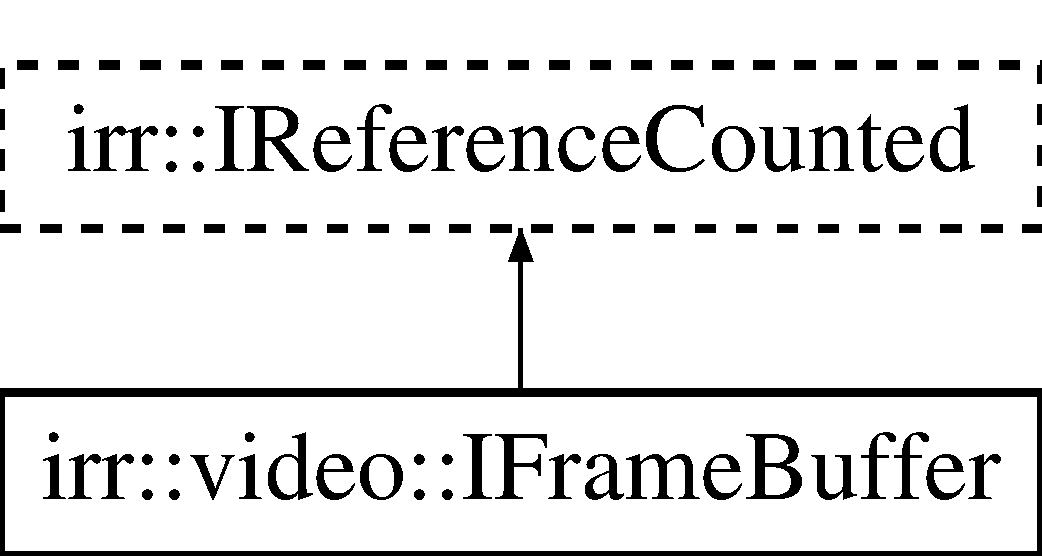
\includegraphics[height=2.000000cm]{classirr_1_1video_1_1IFrameBuffer}
\end{center}
\end{figure}
\subsection*{Public Member Functions}
\begin{DoxyCompactItemize}
\item 
virtual bool {\bfseries attach} (const E\+\_\+\+F\+B\+O\+\_\+\+A\+T\+T\+A\+C\+H\+M\+E\+N\+T\+\_\+\+P\+O\+I\+NT \&attachmen\+Point, \hyperlink{classirr_1_1video_1_1ITexture}{I\+Texture} $\ast$tex, const uint32\+\_\+t \&mip\+Map\+Layer=0, const int32\+\_\+t \&layer=-\/1)=0\hypertarget{classirr_1_1video_1_1IFrameBuffer_a5be8733620e5a5cd78fcb18405df2fd6}{}\label{classirr_1_1video_1_1IFrameBuffer_a5be8733620e5a5cd78fcb18405df2fd6}

\item 
virtual bool {\bfseries attach} (const E\+\_\+\+F\+B\+O\+\_\+\+A\+T\+T\+A\+C\+H\+M\+E\+N\+T\+\_\+\+P\+O\+I\+NT \&attachmen\+Point, \hyperlink{classirr_1_1video_1_1IRenderBuffer}{I\+Render\+Buffer} $\ast$rbf)=0\hypertarget{classirr_1_1video_1_1IFrameBuffer_a1c7e8a45b7c1e2717df3c10902fef62a}{}\label{classirr_1_1video_1_1IFrameBuffer_a1c7e8a45b7c1e2717df3c10902fef62a}

\item 
virtual bool {\bfseries rebind\+Revalidate} ()=0\hypertarget{classirr_1_1video_1_1IFrameBuffer_aaf227a8a7aee3bbec5477a1edaf90382}{}\label{classirr_1_1video_1_1IFrameBuffer_aaf227a8a7aee3bbec5477a1edaf90382}

\item 
virtual const \hyperlink{classirr_1_1video_1_1IRenderable}{I\+Renderable} $\ast$ {\bfseries get\+Attachment} (const size\+\_\+t \&ix) const  =0\hypertarget{classirr_1_1video_1_1IFrameBuffer_a93148ef68e94fb5edf44a79a27ccd35a}{}\label{classirr_1_1video_1_1IFrameBuffer_a93148ef68e94fb5edf44a79a27ccd35a}

\end{DoxyCompactItemize}
\subsection*{Additional Inherited Members}


The documentation for this class was generated from the following file\+:\begin{DoxyCompactItemize}
\item 
include/I\+Frame\+Buffer.\+h\end{DoxyCompactItemize}

\hypertarget{classirr_1_1scene_1_1IGeometryCreator}{}\section{irr\+:\+:scene\+:\+:I\+Geometry\+Creator Class Reference}
\label{classirr_1_1scene_1_1IGeometryCreator}\index{irr\+::scene\+::\+I\+Geometry\+Creator@{irr\+::scene\+::\+I\+Geometry\+Creator}}


Helper class for creating geometry on the fly.  




{\ttfamily \#include $<$I\+Geometry\+Creator.\+h$>$}

Inheritance diagram for irr\+:\+:scene\+:\+:I\+Geometry\+Creator\+:\begin{figure}[H]
\begin{center}
\leavevmode
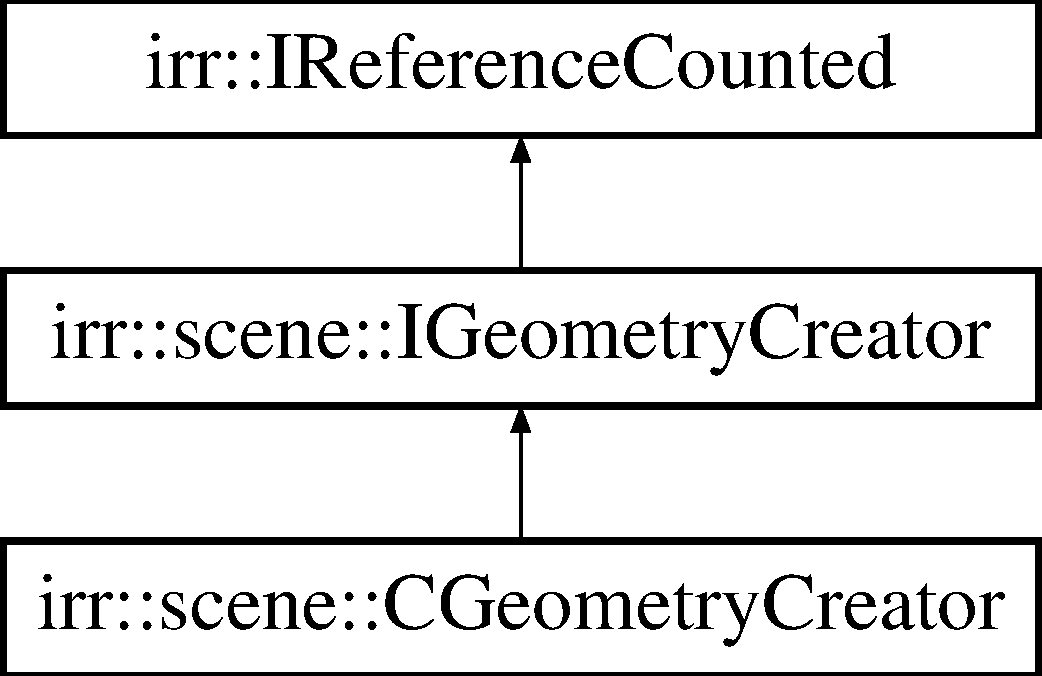
\includegraphics[height=3.000000cm]{classirr_1_1scene_1_1IGeometryCreator}
\end{center}
\end{figure}
\subsection*{Public Member Functions}
\begin{DoxyCompactItemize}
\item 
virtual \hyperlink{classirr_1_1scene_1_1IMesh}{I\+G\+P\+U\+Mesh} $\ast$ \hyperlink{classirr_1_1scene_1_1IGeometryCreator_a1676dd58d6bfd7546e728dd9ea5599f6}{create\+Cube\+Mesh\+G\+PU} (\hyperlink{classirr_1_1video_1_1IVideoDriver}{video\+::\+I\+Video\+Driver} $\ast$driver, const \hyperlink{namespaceirr_1_1core_a06f169d08b5c429f5575acb7edbad811}{core\+::vector3df} \&size=\hyperlink{namespaceirr_1_1core_a06f169d08b5c429f5575acb7edbad811}{core\+::vector3df}(5.f, 5.f, 5.f)) const  =0
\begin{DoxyCompactList}\small\item\em Creates a simple cube mesh. \end{DoxyCompactList}\item 
virtual \hyperlink{classirr_1_1scene_1_1IMesh}{I\+C\+P\+U\+Mesh} $\ast$ {\bfseries create\+Cube\+Mesh\+C\+PU} (const \hyperlink{namespaceirr_1_1core_a06f169d08b5c429f5575acb7edbad811}{core\+::vector3df} \&size=\hyperlink{namespaceirr_1_1core_a06f169d08b5c429f5575acb7edbad811}{core\+::vector3df}(5.f, 5.f, 5.f)) const  =0\hypertarget{classirr_1_1scene_1_1IGeometryCreator_aba9a44905c6b09242da0b2646feed423}{}\label{classirr_1_1scene_1_1IGeometryCreator_aba9a44905c6b09242da0b2646feed423}

\item 
virtual \hyperlink{classirr_1_1scene_1_1IMesh}{I\+G\+P\+U\+Mesh} $\ast$ \hyperlink{classirr_1_1scene_1_1IGeometryCreator_a687cc4dc19a40ab892d6a18cb9c6f86e}{create\+Terrain\+Mesh\+G\+PU} (\hyperlink{classirr_1_1video_1_1IImage}{video\+::\+I\+Image} $\ast$texture, \hyperlink{classirr_1_1video_1_1IImage}{video\+::\+I\+Image} $\ast$heightmap, const \hyperlink{classirr_1_1core_1_1dimension2d}{core\+::dimension2d}$<$ \hyperlink{namespaceirr_a0277be98d67dc26ff93b1a6a1d086b07}{f32} $>$ \&stretch\+Size, \hyperlink{namespaceirr_a0277be98d67dc26ff93b1a6a1d086b07}{f32} max\+Height, \hyperlink{classirr_1_1video_1_1IVideoDriver}{video\+::\+I\+Video\+Driver} $\ast$driver, const \hyperlink{classirr_1_1core_1_1dimension2d}{core\+::dimension2d}$<$ \hyperlink{namespaceirr_a0416a53257075833e7002efd0a18e804}{u32} $>$ \&default\+Vertex\+Block\+Size, bool debug\+Borders=false) const  =0
\begin{DoxyCompactList}\small\item\em Create a terrain mesh from an image representing a heightfield. \end{DoxyCompactList}\item 
virtual \hyperlink{classirr_1_1scene_1_1IMesh}{I\+C\+P\+U\+Mesh} $\ast$ {\bfseries create\+Terrain\+Mesh\+C\+PU} (\hyperlink{classirr_1_1video_1_1IImage}{video\+::\+I\+Image} $\ast$texture, \hyperlink{classirr_1_1video_1_1IImage}{video\+::\+I\+Image} $\ast$heightmap, const \hyperlink{classirr_1_1core_1_1dimension2d}{core\+::dimension2d}$<$ \hyperlink{namespaceirr_a0277be98d67dc26ff93b1a6a1d086b07}{f32} $>$ \&stretch\+Size, \hyperlink{namespaceirr_a0277be98d67dc26ff93b1a6a1d086b07}{f32} max\+Height, \hyperlink{classirr_1_1video_1_1IVideoDriver}{video\+::\+I\+Video\+Driver} $\ast$driver, const \hyperlink{classirr_1_1core_1_1dimension2d}{core\+::dimension2d}$<$ \hyperlink{namespaceirr_a0416a53257075833e7002efd0a18e804}{u32} $>$ \&default\+Vertex\+Block\+Size, bool debug\+Borders=false) const  =0\hypertarget{classirr_1_1scene_1_1IGeometryCreator_a534d5cc0c557daaf3ee9160c24866ddd}{}\label{classirr_1_1scene_1_1IGeometryCreator_a534d5cc0c557daaf3ee9160c24866ddd}

\item 
virtual \hyperlink{classirr_1_1scene_1_1IMesh}{I\+G\+P\+U\+Mesh} $\ast$ \hyperlink{classirr_1_1scene_1_1IGeometryCreator_abca19991f6bbfbc05b64ab45c2df80c7}{create\+Arrow\+Mesh\+G\+PU} (\hyperlink{classirr_1_1video_1_1IVideoDriver}{video\+::\+I\+Video\+Driver} $\ast$driver, const \hyperlink{namespaceirr_a0416a53257075833e7002efd0a18e804}{u32} tesselation\+Cylinder=4, const \hyperlink{namespaceirr_a0416a53257075833e7002efd0a18e804}{u32} tesselation\+Cone=8, const \hyperlink{namespaceirr_a0277be98d67dc26ff93b1a6a1d086b07}{f32} height=1.f, const \hyperlink{namespaceirr_a0277be98d67dc26ff93b1a6a1d086b07}{f32} cylinder\+Height=0.\+6f, const f32 width\+Cylinder=0.\+05f, const f32 width\+Cone=0.\+3f, const video\+::\+S\+Color color\+Cylinder=0x\+F\+F\+F\+F\+F\+F\+F\+F, const video\+::\+S\+Color color\+Cone=0x\+F\+F\+F\+F\+F\+F\+F\+F) const  =0
\begin{DoxyCompactList}\small\item\em Create an arrow mesh, composed of a cylinder and a cone. \end{DoxyCompactList}\item 
virtual \hyperlink{classirr_1_1scene_1_1IMesh}{I\+C\+P\+U\+Mesh} $\ast$ {\bfseries create\+Arrow\+Mesh\+C\+PU} (const \hyperlink{namespaceirr_a0416a53257075833e7002efd0a18e804}{u32} tesselation\+Cylinder=4, const \hyperlink{namespaceirr_a0416a53257075833e7002efd0a18e804}{u32} tesselation\+Cone=8, const \hyperlink{namespaceirr_a0277be98d67dc26ff93b1a6a1d086b07}{f32} height=1.f, const \hyperlink{namespaceirr_a0277be98d67dc26ff93b1a6a1d086b07}{f32} cylinder\+Height=0.\+6f, const f32 width\+Cylinder=0.\+05f, const f32 width\+Cone=0.\+3f, const video\+::\+S\+Color color\+Cylinder=0x\+F\+F\+F\+F\+F\+F\+F\+F, const video\+::\+S\+Color color\+Cone=0x\+F\+F\+F\+F\+F\+F\+F\+F) const  =0\hypertarget{classirr_1_1scene_1_1IGeometryCreator_a654005b83bc734daf6531d096e647a18}{}\label{classirr_1_1scene_1_1IGeometryCreator_a654005b83bc734daf6531d096e647a18}

\item 
virtual \hyperlink{classirr_1_1scene_1_1IMesh}{I\+G\+P\+U\+Mesh} $\ast$ \hyperlink{classirr_1_1scene_1_1IGeometryCreator_abdea997960c37f721892203312dcadbd}{create\+Sphere\+Mesh\+G\+PU} (\hyperlink{classirr_1_1video_1_1IVideoDriver}{video\+::\+I\+Video\+Driver} $\ast$driver, \hyperlink{namespaceirr_a0277be98d67dc26ff93b1a6a1d086b07}{f32} radius=5.f, \hyperlink{namespaceirr_a0416a53257075833e7002efd0a18e804}{u32} poly\+CountX=16, \hyperlink{namespaceirr_a0416a53257075833e7002efd0a18e804}{u32} poly\+CountY=16) const  =0
\begin{DoxyCompactList}\small\item\em Create a sphere mesh. \end{DoxyCompactList}\item 
virtual \hyperlink{classirr_1_1scene_1_1IMesh}{I\+C\+P\+U\+Mesh} $\ast$ {\bfseries create\+Sphere\+Mesh\+C\+PU} (\hyperlink{namespaceirr_a0277be98d67dc26ff93b1a6a1d086b07}{f32} radius=5.f, \hyperlink{namespaceirr_a0416a53257075833e7002efd0a18e804}{u32} poly\+CountX=16, \hyperlink{namespaceirr_a0416a53257075833e7002efd0a18e804}{u32} poly\+CountY=16) const  =0\hypertarget{classirr_1_1scene_1_1IGeometryCreator_a4302454584a0fb49e2be465d191fe79d}{}\label{classirr_1_1scene_1_1IGeometryCreator_a4302454584a0fb49e2be465d191fe79d}

\item 
virtual \hyperlink{classirr_1_1scene_1_1IMesh}{I\+G\+P\+U\+Mesh} $\ast$ \hyperlink{classirr_1_1scene_1_1IGeometryCreator_a407144cf0d15dcac00cdbf32478cb62b}{create\+Cylinder\+Mesh\+G\+PU} (\hyperlink{classirr_1_1video_1_1IVideoDriver}{video\+::\+I\+Video\+Driver} $\ast$driver, \hyperlink{namespaceirr_a0277be98d67dc26ff93b1a6a1d086b07}{f32} radius, \hyperlink{namespaceirr_a0277be98d67dc26ff93b1a6a1d086b07}{f32} length, \hyperlink{namespaceirr_a0416a53257075833e7002efd0a18e804}{u32} tesselation, const \hyperlink{classirr_1_1video_1_1SColor}{video\+::\+S\+Color} \&color=\hyperlink{classirr_1_1video_1_1SColor}{video\+::\+S\+Color}(0xffffffff), bool close\+Top=true, f32 oblique=0.\+f) const  =0
\begin{DoxyCompactList}\small\item\em Create a cylinder mesh. \end{DoxyCompactList}\item 
virtual \hyperlink{classirr_1_1scene_1_1IMesh}{I\+C\+P\+U\+Mesh} $\ast$ {\bfseries create\+Cylinder\+Mesh\+C\+PU} (\hyperlink{namespaceirr_a0277be98d67dc26ff93b1a6a1d086b07}{f32} radius, \hyperlink{namespaceirr_a0277be98d67dc26ff93b1a6a1d086b07}{f32} length, \hyperlink{namespaceirr_a0416a53257075833e7002efd0a18e804}{u32} tesselation, const \hyperlink{classirr_1_1video_1_1SColor}{video\+::\+S\+Color} \&color=\hyperlink{classirr_1_1video_1_1SColor}{video\+::\+S\+Color}(0xffffffff), bool close\+Top=true, f32 oblique=0.\+f) const  =0\hypertarget{classirr_1_1scene_1_1IGeometryCreator_a16fa2473091b8b5b8c11e4c8a67eccb4}{}\label{classirr_1_1scene_1_1IGeometryCreator_a16fa2473091b8b5b8c11e4c8a67eccb4}

\item 
virtual \hyperlink{classirr_1_1scene_1_1IMesh}{I\+G\+P\+U\+Mesh} $\ast$ \hyperlink{classirr_1_1scene_1_1IGeometryCreator_ad977d1ab6a7d9f839d47e4dc2b50d756}{create\+Cone\+Mesh\+G\+PU} (\hyperlink{classirr_1_1video_1_1IVideoDriver}{video\+::\+I\+Video\+Driver} $\ast$driver, \hyperlink{namespaceirr_a0277be98d67dc26ff93b1a6a1d086b07}{f32} radius, \hyperlink{namespaceirr_a0277be98d67dc26ff93b1a6a1d086b07}{f32} length, \hyperlink{namespaceirr_a0416a53257075833e7002efd0a18e804}{u32} tesselation, const \hyperlink{classirr_1_1video_1_1SColor}{video\+::\+S\+Color} \&color\+Top=\hyperlink{classirr_1_1video_1_1SColor}{video\+::\+S\+Color}(0xffffffff), const video\+::\+S\+Color \&color\+Bottom=video\+::\+S\+Color(0xffffffff), f32 oblique=0.\+f) const  =0
\begin{DoxyCompactList}\small\item\em Create a cone mesh. \end{DoxyCompactList}\item 
virtual \hyperlink{classirr_1_1scene_1_1IMesh}{I\+C\+P\+U\+Mesh} $\ast$ {\bfseries create\+Cone\+Mesh\+C\+PU} (\hyperlink{namespaceirr_a0277be98d67dc26ff93b1a6a1d086b07}{f32} radius, \hyperlink{namespaceirr_a0277be98d67dc26ff93b1a6a1d086b07}{f32} length, \hyperlink{namespaceirr_a0416a53257075833e7002efd0a18e804}{u32} tesselation, const \hyperlink{classirr_1_1video_1_1SColor}{video\+::\+S\+Color} \&color\+Top=\hyperlink{classirr_1_1video_1_1SColor}{video\+::\+S\+Color}(0xffffffff), const video\+::\+S\+Color \&color\+Bottom=video\+::\+S\+Color(0xffffffff), f32 oblique=0.\+f) const  =0\hypertarget{classirr_1_1scene_1_1IGeometryCreator_a78035212f111bc622b640508c9e65b54}{}\label{classirr_1_1scene_1_1IGeometryCreator_a78035212f111bc622b640508c9e65b54}

\end{DoxyCompactItemize}
\subsection*{Additional Inherited Members}


\subsection{Detailed Description}
Helper class for creating geometry on the fly. 

You can get an instance of this class through \hyperlink{classirr_1_1scene_1_1ISceneManager_aa907bfdd82887a9855157fdfb41985e0}{I\+Scene\+Manager\+::get\+Geometry\+Creator()} 

\subsection{Member Function Documentation}
\index{irr\+::scene\+::\+I\+Geometry\+Creator@{irr\+::scene\+::\+I\+Geometry\+Creator}!create\+Arrow\+Mesh\+G\+PU@{create\+Arrow\+Mesh\+G\+PU}}
\index{create\+Arrow\+Mesh\+G\+PU@{create\+Arrow\+Mesh\+G\+PU}!irr\+::scene\+::\+I\+Geometry\+Creator@{irr\+::scene\+::\+I\+Geometry\+Creator}}
\subsubsection[{\texorpdfstring{create\+Arrow\+Mesh\+G\+P\+U(video\+::\+I\+Video\+Driver $\ast$driver, const u32 tesselation\+Cylinder=4, const u32 tesselation\+Cone=8, const f32 height=1.\+f, const f32 cylinder\+Height=0.\+6f, const f32 width\+Cylinder=0.\+05f, const f32 width\+Cone=0.\+3f, const video\+::\+S\+Color color\+Cylinder=0x\+F\+F\+F\+F\+F\+F\+F\+F, const video\+::\+S\+Color color\+Cone=0x\+F\+F\+F\+F\+F\+F\+F\+F) const  =0}{createArrowMeshGPU(video::IVideoDriver *driver, const u32 tesselationCylinder=4, const u32 tesselationCone=8, const f32 height=1.f, const f32 cylinderHeight=0.6f, const f32 widthCylinder=0.05f, const f32 widthCone=0.3f, const video::SColor colorCylinder=0xFFFFFFFF, const video::SColor colorCone=0xFFFFFFFF) const  =0}}]{\setlength{\rightskip}{0pt plus 5cm}virtual {\bf I\+G\+P\+U\+Mesh}$\ast$ irr\+::scene\+::\+I\+Geometry\+Creator\+::create\+Arrow\+Mesh\+G\+PU (
\begin{DoxyParamCaption}
\item[{{\bf video\+::\+I\+Video\+Driver} $\ast$}]{driver, }
\item[{const {\bf u32}}]{tesselation\+Cylinder = {\ttfamily 4}, }
\item[{const {\bf u32}}]{tesselation\+Cone = {\ttfamily 8}, }
\item[{const {\bf f32}}]{height = {\ttfamily 1.f}, }
\item[{const {\bf f32}}]{cylinder\+Height = {\ttfamily 0.6f}, }
\item[{const {\bf f32}}]{width\+Cylinder = {\ttfamily 0.05f}, }
\item[{const {\bf f32}}]{width\+Cone = {\ttfamily 0.3f}, }
\item[{const {\bf video\+::\+S\+Color}}]{color\+Cylinder = {\ttfamily 0xFFFFFFFF}, }
\item[{const {\bf video\+::\+S\+Color}}]{color\+Cone = {\ttfamily 0xFFFFFFFF}}
\end{DoxyParamCaption}
) const\hspace{0.3cm}{\ttfamily [pure virtual]}}\hypertarget{classirr_1_1scene_1_1IGeometryCreator_abca19991f6bbfbc05b64ab45c2df80c7}{}\label{classirr_1_1scene_1_1IGeometryCreator_abca19991f6bbfbc05b64ab45c2df80c7}


Create an arrow mesh, composed of a cylinder and a cone. 


\begin{DoxyParams}{Parameters}
{\em tesselation\+Cylinder} & Number of quads composing the cylinder. \\
\hline
{\em tesselation\+Cone} & Number of triangles composing the cone\textquotesingle{}s roof. \\
\hline
{\em height} & Total height of the arrow \\
\hline
{\em cylinder\+Height} & Total height of the cylinder, should be lesser than total height \\
\hline
{\em width\+Cylinder} & Diameter of the cylinder \\
\hline
{\em width\+Cone} & Diameter of the cone\textquotesingle{}s base, should be not smaller than the cylinder\textquotesingle{}s diameter \\
\hline
{\em color\+Cylinder} & color of the cylinder \\
\hline
{\em color\+Cone} & color of the cone \\
\hline
\end{DoxyParams}
\begin{DoxyReturn}{Returns}
Generated mesh. 
\end{DoxyReturn}


Implemented in \hyperlink{classirr_1_1scene_1_1CGeometryCreator_a2409f4deb5ede1eec584137928b4bdb5}{irr\+::scene\+::\+C\+Geometry\+Creator}.

\index{irr\+::scene\+::\+I\+Geometry\+Creator@{irr\+::scene\+::\+I\+Geometry\+Creator}!create\+Cone\+Mesh\+G\+PU@{create\+Cone\+Mesh\+G\+PU}}
\index{create\+Cone\+Mesh\+G\+PU@{create\+Cone\+Mesh\+G\+PU}!irr\+::scene\+::\+I\+Geometry\+Creator@{irr\+::scene\+::\+I\+Geometry\+Creator}}
\subsubsection[{\texorpdfstring{create\+Cone\+Mesh\+G\+P\+U(video\+::\+I\+Video\+Driver $\ast$driver, f32 radius, f32 length, u32 tesselation, const video\+::\+S\+Color \&color\+Top=video\+::\+S\+Color(0xffffffff), const video\+::\+S\+Color \&color\+Bottom=video\+::\+S\+Color(0xffffffff), f32 oblique=0.\+f) const  =0}{createConeMeshGPU(video::IVideoDriver *driver, f32 radius, f32 length, u32 tesselation, const video::SColor \&colorTop=video::SColor(0xffffffff), const video::SColor \&colorBottom=video::SColor(0xffffffff), f32 oblique=0.f) const  =0}}]{\setlength{\rightskip}{0pt plus 5cm}virtual {\bf I\+G\+P\+U\+Mesh}$\ast$ irr\+::scene\+::\+I\+Geometry\+Creator\+::create\+Cone\+Mesh\+G\+PU (
\begin{DoxyParamCaption}
\item[{{\bf video\+::\+I\+Video\+Driver} $\ast$}]{driver, }
\item[{{\bf f32}}]{radius, }
\item[{{\bf f32}}]{length, }
\item[{{\bf u32}}]{tesselation, }
\item[{const {\bf video\+::\+S\+Color} \&}]{color\+Top = {\ttfamily {\bf video\+::\+S\+Color}(0xffffffff)}, }
\item[{const {\bf video\+::\+S\+Color} \&}]{color\+Bottom = {\ttfamily {\bf video\+::\+S\+Color}(0xffffffff)}, }
\item[{{\bf f32}}]{oblique = {\ttfamily 0.f}}
\end{DoxyParamCaption}
) const\hspace{0.3cm}{\ttfamily [pure virtual]}}\hypertarget{classirr_1_1scene_1_1IGeometryCreator_ad977d1ab6a7d9f839d47e4dc2b50d756}{}\label{classirr_1_1scene_1_1IGeometryCreator_ad977d1ab6a7d9f839d47e4dc2b50d756}


Create a cone mesh. 


\begin{DoxyParams}{Parameters}
{\em radius} & Radius of the cone. \\
\hline
{\em length} & Length of the cone. \\
\hline
{\em tesselation} & Number of quads around the circumference of the cone. \\
\hline
{\em color\+Top} & The color of the top of the cone. \\
\hline
{\em color\+Bottom} & The color of the bottom of the cone. \\
\hline
{\em oblique} & (to be documented) \\
\hline
\end{DoxyParams}
\begin{DoxyReturn}{Returns}
Generated mesh. 
\end{DoxyReturn}


Implemented in \hyperlink{classirr_1_1scene_1_1CGeometryCreator_a6587c178f43773c42d4566c93147eebb}{irr\+::scene\+::\+C\+Geometry\+Creator}.

\index{irr\+::scene\+::\+I\+Geometry\+Creator@{irr\+::scene\+::\+I\+Geometry\+Creator}!create\+Cube\+Mesh\+G\+PU@{create\+Cube\+Mesh\+G\+PU}}
\index{create\+Cube\+Mesh\+G\+PU@{create\+Cube\+Mesh\+G\+PU}!irr\+::scene\+::\+I\+Geometry\+Creator@{irr\+::scene\+::\+I\+Geometry\+Creator}}
\subsubsection[{\texorpdfstring{create\+Cube\+Mesh\+G\+P\+U(video\+::\+I\+Video\+Driver $\ast$driver, const core\+::vector3df \&size=core\+::vector3df(5.\+f, 5.\+f, 5.\+f)) const  =0}{createCubeMeshGPU(video::IVideoDriver *driver, const core::vector3df \&size=core::vector3df(5.f, 5.f, 5.f)) const  =0}}]{\setlength{\rightskip}{0pt plus 5cm}virtual {\bf I\+G\+P\+U\+Mesh}$\ast$ irr\+::scene\+::\+I\+Geometry\+Creator\+::create\+Cube\+Mesh\+G\+PU (
\begin{DoxyParamCaption}
\item[{{\bf video\+::\+I\+Video\+Driver} $\ast$}]{driver, }
\item[{const {\bf core\+::vector3df} \&}]{size = {\ttfamily {\bf core\+::vector3df}(5.f,~5.f,~5.f)}}
\end{DoxyParamCaption}
) const\hspace{0.3cm}{\ttfamily [pure virtual]}}\hypertarget{classirr_1_1scene_1_1IGeometryCreator_a1676dd58d6bfd7546e728dd9ea5599f6}{}\label{classirr_1_1scene_1_1IGeometryCreator_a1676dd58d6bfd7546e728dd9ea5599f6}


Creates a simple cube mesh. 


\begin{DoxyParams}{Parameters}
{\em size} & Dimensions of the cube. \\
\hline
\end{DoxyParams}
\begin{DoxyReturn}{Returns}
Generated mesh. 
\end{DoxyReturn}


Implemented in \hyperlink{classirr_1_1scene_1_1CGeometryCreator_a9aea899bffc8dc7042f4b2d8d176f40d}{irr\+::scene\+::\+C\+Geometry\+Creator}.

\index{irr\+::scene\+::\+I\+Geometry\+Creator@{irr\+::scene\+::\+I\+Geometry\+Creator}!create\+Cylinder\+Mesh\+G\+PU@{create\+Cylinder\+Mesh\+G\+PU}}
\index{create\+Cylinder\+Mesh\+G\+PU@{create\+Cylinder\+Mesh\+G\+PU}!irr\+::scene\+::\+I\+Geometry\+Creator@{irr\+::scene\+::\+I\+Geometry\+Creator}}
\subsubsection[{\texorpdfstring{create\+Cylinder\+Mesh\+G\+P\+U(video\+::\+I\+Video\+Driver $\ast$driver, f32 radius, f32 length, u32 tesselation, const video\+::\+S\+Color \&color=video\+::\+S\+Color(0xffffffff), bool close\+Top=true, f32 oblique=0.\+f) const  =0}{createCylinderMeshGPU(video::IVideoDriver *driver, f32 radius, f32 length, u32 tesselation, const video::SColor \&color=video::SColor(0xffffffff), bool closeTop=true, f32 oblique=0.f) const  =0}}]{\setlength{\rightskip}{0pt plus 5cm}virtual {\bf I\+G\+P\+U\+Mesh}$\ast$ irr\+::scene\+::\+I\+Geometry\+Creator\+::create\+Cylinder\+Mesh\+G\+PU (
\begin{DoxyParamCaption}
\item[{{\bf video\+::\+I\+Video\+Driver} $\ast$}]{driver, }
\item[{{\bf f32}}]{radius, }
\item[{{\bf f32}}]{length, }
\item[{{\bf u32}}]{tesselation, }
\item[{const {\bf video\+::\+S\+Color} \&}]{color = {\ttfamily {\bf video\+::\+S\+Color}(0xffffffff)}, }
\item[{bool}]{close\+Top = {\ttfamily true}, }
\item[{{\bf f32}}]{oblique = {\ttfamily 0.f}}
\end{DoxyParamCaption}
) const\hspace{0.3cm}{\ttfamily [pure virtual]}}\hypertarget{classirr_1_1scene_1_1IGeometryCreator_a407144cf0d15dcac00cdbf32478cb62b}{}\label{classirr_1_1scene_1_1IGeometryCreator_a407144cf0d15dcac00cdbf32478cb62b}


Create a cylinder mesh. 


\begin{DoxyParams}{Parameters}
{\em radius} & Radius of the cylinder. \\
\hline
{\em length} & Length of the cylinder. \\
\hline
{\em tesselation} & Number of quads around the circumference of the cylinder. \\
\hline
{\em color} & The color of the cylinder. \\
\hline
{\em close\+Top} & If true, close the ends of the cylinder, otherwise leave them open. \\
\hline
{\em oblique} & (to be documented) \\
\hline
\end{DoxyParams}
\begin{DoxyReturn}{Returns}
Generated mesh. 
\end{DoxyReturn}


Implemented in \hyperlink{classirr_1_1scene_1_1CGeometryCreator_ac35744e4622432d0df0d550c588d5082}{irr\+::scene\+::\+C\+Geometry\+Creator}.

\index{irr\+::scene\+::\+I\+Geometry\+Creator@{irr\+::scene\+::\+I\+Geometry\+Creator}!create\+Sphere\+Mesh\+G\+PU@{create\+Sphere\+Mesh\+G\+PU}}
\index{create\+Sphere\+Mesh\+G\+PU@{create\+Sphere\+Mesh\+G\+PU}!irr\+::scene\+::\+I\+Geometry\+Creator@{irr\+::scene\+::\+I\+Geometry\+Creator}}
\subsubsection[{\texorpdfstring{create\+Sphere\+Mesh\+G\+P\+U(video\+::\+I\+Video\+Driver $\ast$driver, f32 radius=5.\+f, u32 poly\+Count\+X=16, u32 poly\+Count\+Y=16) const  =0}{createSphereMeshGPU(video::IVideoDriver *driver, f32 radius=5.f, u32 polyCountX=16, u32 polyCountY=16) const  =0}}]{\setlength{\rightskip}{0pt plus 5cm}virtual {\bf I\+G\+P\+U\+Mesh}$\ast$ irr\+::scene\+::\+I\+Geometry\+Creator\+::create\+Sphere\+Mesh\+G\+PU (
\begin{DoxyParamCaption}
\item[{{\bf video\+::\+I\+Video\+Driver} $\ast$}]{driver, }
\item[{{\bf f32}}]{radius = {\ttfamily 5.f}, }
\item[{{\bf u32}}]{poly\+CountX = {\ttfamily 16}, }
\item[{{\bf u32}}]{poly\+CountY = {\ttfamily 16}}
\end{DoxyParamCaption}
) const\hspace{0.3cm}{\ttfamily [pure virtual]}}\hypertarget{classirr_1_1scene_1_1IGeometryCreator_abdea997960c37f721892203312dcadbd}{}\label{classirr_1_1scene_1_1IGeometryCreator_abdea997960c37f721892203312dcadbd}


Create a sphere mesh. 


\begin{DoxyParams}{Parameters}
{\em radius} & Radius of the sphere \\
\hline
{\em poly\+CountX} & Number of quads used for the horizontal tiling \\
\hline
{\em poly\+CountY} & Number of quads used for the vertical tiling \\
\hline
\end{DoxyParams}
\begin{DoxyReturn}{Returns}
Generated mesh. 
\end{DoxyReturn}


Implemented in \hyperlink{classirr_1_1scene_1_1CGeometryCreator_a3dd60997db6232e563cba44eb3c0880f}{irr\+::scene\+::\+C\+Geometry\+Creator}.

\index{irr\+::scene\+::\+I\+Geometry\+Creator@{irr\+::scene\+::\+I\+Geometry\+Creator}!create\+Terrain\+Mesh\+G\+PU@{create\+Terrain\+Mesh\+G\+PU}}
\index{create\+Terrain\+Mesh\+G\+PU@{create\+Terrain\+Mesh\+G\+PU}!irr\+::scene\+::\+I\+Geometry\+Creator@{irr\+::scene\+::\+I\+Geometry\+Creator}}
\subsubsection[{\texorpdfstring{create\+Terrain\+Mesh\+G\+P\+U(video\+::\+I\+Image $\ast$texture, video\+::\+I\+Image $\ast$heightmap, const core\+::dimension2d$<$ f32 $>$ \&stretch\+Size, f32 max\+Height, video\+::\+I\+Video\+Driver $\ast$driver, const core\+::dimension2d$<$ u32 $>$ \&default\+Vertex\+Block\+Size, bool debug\+Borders=false) const  =0}{createTerrainMeshGPU(video::IImage *texture, video::IImage *heightmap, const core::dimension2d< f32 > \&stretchSize, f32 maxHeight, video::IVideoDriver *driver, const core::dimension2d< u32 > \&defaultVertexBlockSize, bool debugBorders=false) const  =0}}]{\setlength{\rightskip}{0pt plus 5cm}virtual {\bf I\+G\+P\+U\+Mesh}$\ast$ irr\+::scene\+::\+I\+Geometry\+Creator\+::create\+Terrain\+Mesh\+G\+PU (
\begin{DoxyParamCaption}
\item[{{\bf video\+::\+I\+Image} $\ast$}]{texture, }
\item[{{\bf video\+::\+I\+Image} $\ast$}]{heightmap, }
\item[{const {\bf core\+::dimension2d}$<$ {\bf f32} $>$ \&}]{stretch\+Size, }
\item[{{\bf f32}}]{max\+Height, }
\item[{{\bf video\+::\+I\+Video\+Driver} $\ast$}]{driver, }
\item[{const {\bf core\+::dimension2d}$<$ {\bf u32} $>$ \&}]{default\+Vertex\+Block\+Size, }
\item[{bool}]{debug\+Borders = {\ttfamily false}}
\end{DoxyParamCaption}
) const\hspace{0.3cm}{\ttfamily [pure virtual]}}\hypertarget{classirr_1_1scene_1_1IGeometryCreator_a687cc4dc19a40ab892d6a18cb9c6f86e}{}\label{classirr_1_1scene_1_1IGeometryCreator_a687cc4dc19a40ab892d6a18cb9c6f86e}


Create a terrain mesh from an image representing a heightfield. 


\begin{DoxyParams}{Parameters}
{\em texture} & The texture to apply to the terrain. \\
\hline
{\em heightmap} & An image that will be interpreted as a heightmap. The brightness (average color) of each pixel is interpreted as a height, with a 255 brightness pixel producing the maximum height. \\
\hline
{\em stretch\+Size} & The size that each pixel will produce, i.\+e. a 512x512 heightmap and a stretch\+Size of (10.\+f, 20.\+f) will produce a mesh of size 5120.\+f x 10240.\+f \\
\hline
{\em max\+Height} & The maximum height of the terrain. \\
\hline
{\em driver} & The current video driver. \\
\hline
{\em default\+Vertex\+Block\+Size} & (to be documented) \\
\hline
{\em debug\+Borders} & (to be documented) \\
\hline
\end{DoxyParams}
\begin{DoxyReturn}{Returns}
Generated mesh. 
\end{DoxyReturn}


Implemented in \hyperlink{classirr_1_1scene_1_1CGeometryCreator_a98e9498db779952823f9f1b5fcf7d68e}{irr\+::scene\+::\+C\+Geometry\+Creator}.



The documentation for this class was generated from the following file\+:\begin{DoxyCompactItemize}
\item 
include/I\+Geometry\+Creator.\+h\end{DoxyCompactItemize}

\hypertarget{classirr_1_1video_1_1IGPUBuffer}{}\section{irr\+:\+:video\+:\+:I\+G\+P\+U\+Buffer Class Reference}
\label{classirr_1_1video_1_1IGPUBuffer}\index{irr\+::video\+::\+I\+G\+P\+U\+Buffer@{irr\+::video\+::\+I\+G\+P\+U\+Buffer}}
Inheritance diagram for irr\+:\+:video\+:\+:I\+G\+P\+U\+Buffer\+:\begin{figure}[H]
\begin{center}
\leavevmode
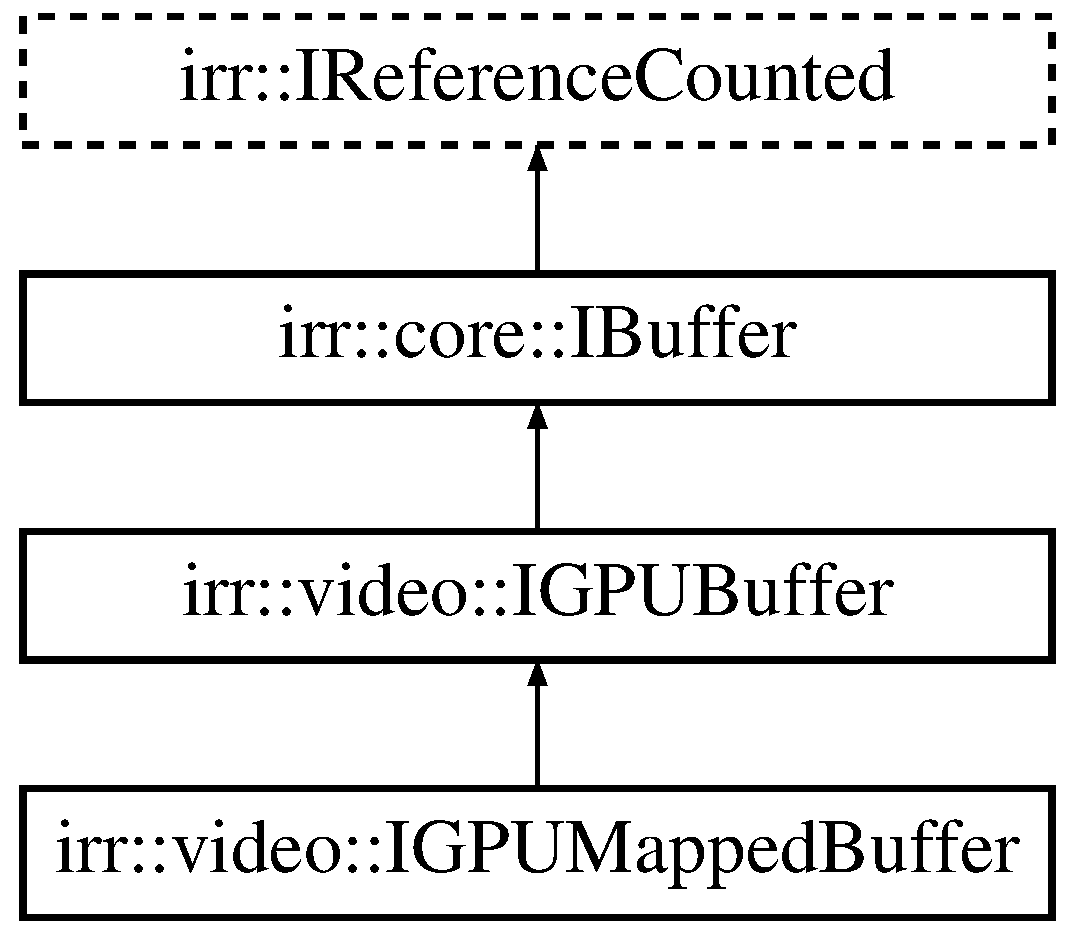
\includegraphics[height=4.000000cm]{classirr_1_1video_1_1IGPUBuffer}
\end{center}
\end{figure}
\subsection*{Public Member Functions}
\begin{DoxyCompactItemize}
\item 
virtual void {\bfseries clandestine\+Recreate} (const size\+\_\+t \&size, const void $\ast$data)=0\hypertarget{classirr_1_1video_1_1IGPUBuffer_a1a6ee6de198bda531f111cbd7c30067c}{}\label{classirr_1_1video_1_1IGPUBuffer_a1a6ee6de198bda531f111cbd7c30067c}

\item 
virtual void {\bfseries update\+Sub\+Range} (const size\+\_\+t \&offset, const size\+\_\+t \&size, const void $\ast$data)=0\hypertarget{classirr_1_1video_1_1IGPUBuffer_a956acd88e159028175ec33c7bdc7be36}{}\label{classirr_1_1video_1_1IGPUBuffer_a956acd88e159028175ec33c7bdc7be36}

\item 
virtual bool {\bfseries can\+Update\+Sub\+Range} () const  =0\hypertarget{classirr_1_1video_1_1IGPUBuffer_af74c5f66d2538fb8d966ec2762f0a64e}{}\label{classirr_1_1video_1_1IGPUBuffer_af74c5f66d2538fb8d966ec2762f0a64e}

\item 
virtual const bool {\bfseries is\+Mapped\+Buffer} () const \hypertarget{classirr_1_1video_1_1IGPUBuffer_a7e812765c75d4a6c0259e2aa8a2093b3}{}\label{classirr_1_1video_1_1IGPUBuffer_a7e812765c75d4a6c0259e2aa8a2093b3}

\end{DoxyCompactItemize}
\subsection*{Additional Inherited Members}


The documentation for this class was generated from the following file\+:\begin{DoxyCompactItemize}
\item 
include/I\+G\+P\+U\+Buffer.\+h\end{DoxyCompactItemize}

\hypertarget{classirr_1_1video_1_1IGPUMappedBuffer}{}\section{irr\+:\+:video\+:\+:I\+G\+P\+U\+Mapped\+Buffer Class Reference}
\label{classirr_1_1video_1_1IGPUMappedBuffer}\index{irr\+::video\+::\+I\+G\+P\+U\+Mapped\+Buffer@{irr\+::video\+::\+I\+G\+P\+U\+Mapped\+Buffer}}


Persistently Mapped buffer.  




{\ttfamily \#include $<$I\+G\+P\+U\+Mapped\+Buffer.\+h$>$}

Inheritance diagram for irr\+:\+:video\+:\+:I\+G\+P\+U\+Mapped\+Buffer\+:\begin{figure}[H]
\begin{center}
\leavevmode
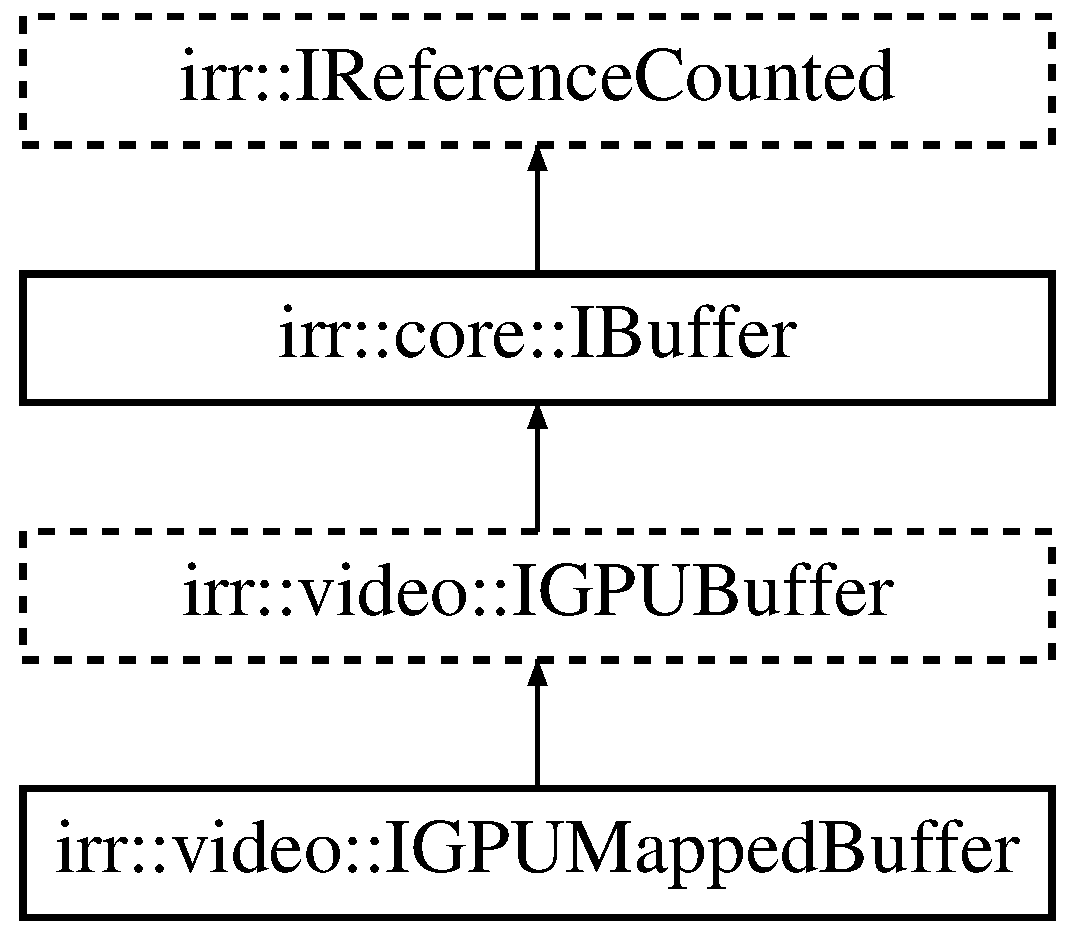
\includegraphics[height=4.000000cm]{classirr_1_1video_1_1IGPUMappedBuffer}
\end{center}
\end{figure}
\subsection*{Public Member Functions}
\begin{DoxyCompactItemize}
\item 
virtual void $\ast$ \hyperlink{classirr_1_1video_1_1IGPUMappedBuffer_aa51f531fc87e800e10c9f8b91357f1be}{get\+Pointer} ()=0
\item 
virtual const bool {\bfseries is\+Mapped\+Buffer} () const \hypertarget{classirr_1_1video_1_1IGPUMappedBuffer_a00793692ef2756b07854664c7e8e6780}{}\label{classirr_1_1video_1_1IGPUMappedBuffer_a00793692ef2756b07854664c7e8e6780}

\end{DoxyCompactItemize}
\subsection*{Additional Inherited Members}


\subsection{Detailed Description}
Persistently Mapped buffer. 

\subsection{Member Function Documentation}
\index{irr\+::video\+::\+I\+G\+P\+U\+Mapped\+Buffer@{irr\+::video\+::\+I\+G\+P\+U\+Mapped\+Buffer}!get\+Pointer@{get\+Pointer}}
\index{get\+Pointer@{get\+Pointer}!irr\+::video\+::\+I\+G\+P\+U\+Mapped\+Buffer@{irr\+::video\+::\+I\+G\+P\+U\+Mapped\+Buffer}}
\subsubsection[{\texorpdfstring{get\+Pointer()=0}{getPointer()=0}}]{\setlength{\rightskip}{0pt plus 5cm}virtual void$\ast$ irr\+::video\+::\+I\+G\+P\+U\+Mapped\+Buffer\+::get\+Pointer (
\begin{DoxyParamCaption}
{}
\end{DoxyParamCaption}
)\hspace{0.3cm}{\ttfamily [pure virtual]}}\hypertarget{classirr_1_1video_1_1IGPUMappedBuffer_aa51f531fc87e800e10c9f8b91357f1be}{}\label{classirr_1_1video_1_1IGPUMappedBuffer_aa51f531fc87e800e10c9f8b91357f1be}
W\+A\+R\+N\+I\+NG\+: R\+E\+S\+I\+ZE will invalidate pointer W\+A\+R\+N\+I\+NG\+: N\+E\+ED TO F\+E\+N\+CE B\+E\+F\+O\+RE U\+S\+E!!!!!!!!!!!!! 

The documentation for this class was generated from the following file\+:\begin{DoxyCompactItemize}
\item 
include/I\+G\+P\+U\+Mapped\+Buffer.\+h\end{DoxyCompactItemize}

\hypertarget{classirr_1_1scene_1_1IGPUMeshBuffer}{}\section{irr\+:\+:scene\+:\+:I\+G\+P\+U\+Mesh\+Buffer Class Reference}
\label{classirr_1_1scene_1_1IGPUMeshBuffer}\index{irr\+::scene\+::\+I\+G\+P\+U\+Mesh\+Buffer@{irr\+::scene\+::\+I\+G\+P\+U\+Mesh\+Buffer}}
Inheritance diagram for irr\+:\+:scene\+:\+:I\+G\+P\+U\+Mesh\+Buffer\+:\begin{figure}[H]
\begin{center}
\leavevmode
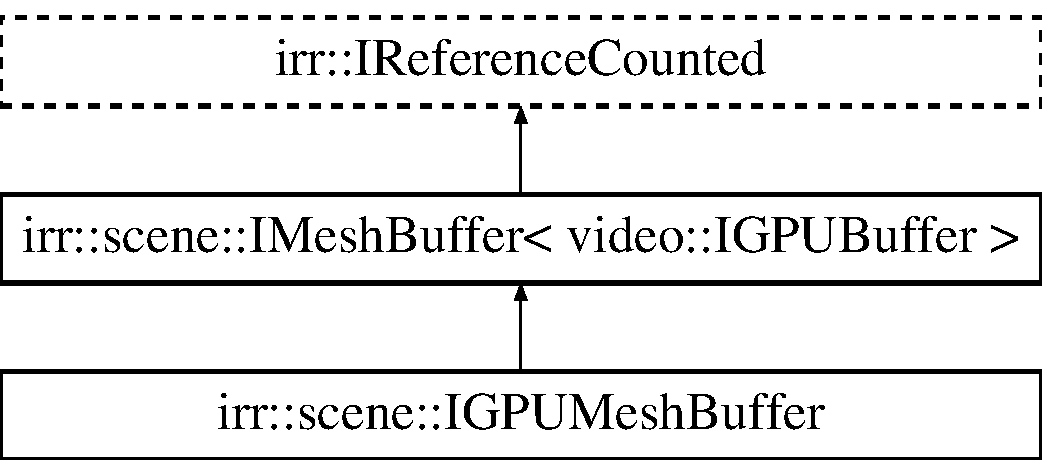
\includegraphics[height=3.000000cm]{classirr_1_1scene_1_1IGPUMeshBuffer}
\end{center}
\end{figure}
\subsection*{Public Member Functions}
\begin{DoxyCompactItemize}
\item 
void {\bfseries set\+Index\+Count\+From\+X\+Form\+Feedback} (\hyperlink{classirr_1_1video_1_1ITransformFeedback}{video\+::\+I\+Transform\+Feedback} $\ast$xform\+Feedback)\hypertarget{classirr_1_1scene_1_1IGPUMeshBuffer_ac81c7da4bca1be4a1c460e68e4de1dab}{}\label{classirr_1_1scene_1_1IGPUMeshBuffer_ac81c7da4bca1be4a1c460e68e4de1dab}

\item 
\hyperlink{classirr_1_1video_1_1ITransformFeedback}{video\+::\+I\+Transform\+Feedback} $\ast$ {\bfseries get\+X\+Form\+Feedback} () const \hypertarget{classirr_1_1scene_1_1IGPUMeshBuffer_a6d41e55265ae0b5e58cff757d05f4495}{}\label{classirr_1_1scene_1_1IGPUMeshBuffer_a6d41e55265ae0b5e58cff757d05f4495}

\item 
bool {\bfseries is\+Index\+Count\+Given\+By\+X\+Form\+Feedback} () const \hypertarget{classirr_1_1scene_1_1IGPUMeshBuffer_a43da010520a35eb4ea1a3d640098ab30}{}\label{classirr_1_1scene_1_1IGPUMeshBuffer_a43da010520a35eb4ea1a3d640098ab30}

\end{DoxyCompactItemize}
\subsection*{Additional Inherited Members}


The documentation for this class was generated from the following file\+:\begin{DoxyCompactItemize}
\item 
include/I\+Mesh\+Buffer.\+h\end{DoxyCompactItemize}

\hypertarget{classirr_1_1video_1_1IGPUProgrammingServices}{}\section{irr\+:\+:video\+:\+:I\+G\+P\+U\+Programming\+Services Class Reference}
\label{classirr_1_1video_1_1IGPUProgrammingServices}\index{irr\+::video\+::\+I\+G\+P\+U\+Programming\+Services@{irr\+::video\+::\+I\+G\+P\+U\+Programming\+Services}}


Interface making it possible to create and use programs running on the G\+PU.  




{\ttfamily \#include $<$I\+G\+P\+U\+Programming\+Services.\+h$>$}

\subsection*{Public Member Functions}
\begin{DoxyCompactItemize}
\item 
virtual \hyperlink{classirr_1_1video_1_1IGPUProgrammingServices_a09d143ea5c55840c15ebcb84e8539bc0}{$\sim$\+I\+G\+P\+U\+Programming\+Services} ()\hypertarget{classirr_1_1video_1_1IGPUProgrammingServices_a09d143ea5c55840c15ebcb84e8539bc0}{}\label{classirr_1_1video_1_1IGPUProgrammingServices_a09d143ea5c55840c15ebcb84e8539bc0}

\begin{DoxyCompactList}\small\item\em Destructor. \end{DoxyCompactList}\item 
virtual \hyperlink{namespaceirr_ac66849b7a6ed16e30ebede579f9b47c6}{s32} {\bfseries add\+High\+Level\+Shader\+Material} (const \hyperlink{namespaceirr_a9395eaea339bcb546b319e9c96bf7410}{c8} $\ast$vertex\+Shader\+Program, const \hyperlink{namespaceirr_a9395eaea339bcb546b319e9c96bf7410}{c8} $\ast$control\+Shader\+Program, const \hyperlink{namespaceirr_a9395eaea339bcb546b319e9c96bf7410}{c8} $\ast$evaluation\+Shader\+Program, const \hyperlink{namespaceirr_a9395eaea339bcb546b319e9c96bf7410}{c8} $\ast$geometry\+Shader\+Program, const \hyperlink{namespaceirr_a9395eaea339bcb546b319e9c96bf7410}{c8} $\ast$pixel\+Shader\+Program, \hyperlink{namespaceirr_a0416a53257075833e7002efd0a18e804}{u32} patch\+Vertices=3, \hyperlink{namespaceirr_1_1video_ac8e9b6c66f7cebabd1a6d30cbc5430f1}{E\+\_\+\+M\+A\+T\+E\+R\+I\+A\+L\+\_\+\+T\+Y\+PE} base\+Material=\hyperlink{namespaceirr_1_1video_ac8e9b6c66f7cebabd1a6d30cbc5430f1a9bc471b9c18c9e2d20496004d2a2e803}{video\+::\+E\+M\+T\+\_\+\+S\+O\+L\+ID}, \hyperlink{classirr_1_1video_1_1IShaderConstantSetCallBack}{I\+Shader\+Constant\+Set\+Call\+Back} $\ast$callback=0, const char $\ast$$\ast$xform\+Feedback\+Outputs=N\+U\+LL, const uint32\+\_\+t \&xform\+Feedback\+Output\+Count=0, const E\+\_\+\+X\+F\+O\+R\+M\+\_\+\+F\+E\+E\+D\+B\+A\+C\+K\+\_\+\+A\+T\+T\+R\+I\+B\+U\+T\+E\+\_\+\+M\+O\+DE \&attrib\+Layout=E\+X\+F\+A\+M\+\_\+\+C\+O\+U\+N\+T\+\_\+\+I\+N\+V\+A\+L\+ID, \hyperlink{namespaceirr_ac66849b7a6ed16e30ebede579f9b47c6}{s32} user\+Data=0, const \hyperlink{namespaceirr_a9395eaea339bcb546b319e9c96bf7410}{c8} $\ast$vertex\+Shader\+Entry\+Point\+Name=\char`\"{}main\char`\"{}, const \hyperlink{namespaceirr_a9395eaea339bcb546b319e9c96bf7410}{c8} $\ast$control\+Shader\+Entry\+Point\+Name=\char`\"{}main\char`\"{}, const \hyperlink{namespaceirr_a9395eaea339bcb546b319e9c96bf7410}{c8} $\ast$evaluation\+Shader\+Entry\+Point\+Name=\char`\"{}main\char`\"{}, const \hyperlink{namespaceirr_a9395eaea339bcb546b319e9c96bf7410}{c8} $\ast$geometry\+Shader\+Entry\+Point\+Name=\char`\"{}main\char`\"{}, const \hyperlink{namespaceirr_a9395eaea339bcb546b319e9c96bf7410}{c8} $\ast$pixel\+Shader\+Entry\+Point\+Name=\char`\"{}main\char`\"{})=0\hypertarget{classirr_1_1video_1_1IGPUProgrammingServices_a6437f640a4c06a3dd5b79b0c82360970}{}\label{classirr_1_1video_1_1IGPUProgrammingServices_a6437f640a4c06a3dd5b79b0c82360970}

\item 
virtual \hyperlink{namespaceirr_ac66849b7a6ed16e30ebede579f9b47c6}{s32} {\bfseries add\+High\+Level\+Shader\+Material\+From\+Files} (const \hyperlink{namespaceirr_1_1io_ab1bdc45edb3f94d8319c02bc0f840ee1}{io\+::path} \&vertex\+Shader\+Program\+File\+Name, const \hyperlink{namespaceirr_1_1io_ab1bdc45edb3f94d8319c02bc0f840ee1}{io\+::path} \&control\+Shader\+Program\+File\+Name, const \hyperlink{namespaceirr_1_1io_ab1bdc45edb3f94d8319c02bc0f840ee1}{io\+::path} \&evaluation\+Shader\+Program\+File\+Name, const \hyperlink{namespaceirr_1_1io_ab1bdc45edb3f94d8319c02bc0f840ee1}{io\+::path} \&geometry\+Shader\+Program\+File\+Name, const \hyperlink{namespaceirr_1_1io_ab1bdc45edb3f94d8319c02bc0f840ee1}{io\+::path} \&pixel\+Shader\+Program\+File\+Name, \hyperlink{namespaceirr_a0416a53257075833e7002efd0a18e804}{u32} patch\+Vertices=3, \hyperlink{namespaceirr_1_1video_ac8e9b6c66f7cebabd1a6d30cbc5430f1}{E\+\_\+\+M\+A\+T\+E\+R\+I\+A\+L\+\_\+\+T\+Y\+PE} base\+Material=\hyperlink{namespaceirr_1_1video_ac8e9b6c66f7cebabd1a6d30cbc5430f1a9bc471b9c18c9e2d20496004d2a2e803}{video\+::\+E\+M\+T\+\_\+\+S\+O\+L\+ID}, \hyperlink{classirr_1_1video_1_1IShaderConstantSetCallBack}{I\+Shader\+Constant\+Set\+Call\+Back} $\ast$callback=0, const char $\ast$$\ast$xform\+Feedback\+Outputs=N\+U\+LL, const uint32\+\_\+t \&xform\+Feedback\+Output\+Count=0, const E\+\_\+\+X\+F\+O\+R\+M\+\_\+\+F\+E\+E\+D\+B\+A\+C\+K\+\_\+\+A\+T\+T\+R\+I\+B\+U\+T\+E\+\_\+\+M\+O\+DE \&attrib\+Layout=E\+X\+F\+A\+M\+\_\+\+C\+O\+U\+N\+T\+\_\+\+I\+N\+V\+A\+L\+ID, \hyperlink{namespaceirr_ac66849b7a6ed16e30ebede579f9b47c6}{s32} user\+Data=0, const \hyperlink{namespaceirr_a9395eaea339bcb546b319e9c96bf7410}{c8} $\ast$vertex\+Shader\+Entry\+Point\+Name=\char`\"{}main\char`\"{}, const \hyperlink{namespaceirr_a9395eaea339bcb546b319e9c96bf7410}{c8} $\ast$control\+Shader\+Entry\+Point\+Name=\char`\"{}main\char`\"{}, const \hyperlink{namespaceirr_a9395eaea339bcb546b319e9c96bf7410}{c8} $\ast$evaluation\+Shader\+Entry\+Point\+Name=\char`\"{}main\char`\"{}, const \hyperlink{namespaceirr_a9395eaea339bcb546b319e9c96bf7410}{c8} $\ast$geometry\+Shader\+Entry\+Point\+Name=\char`\"{}main\char`\"{}, const \hyperlink{namespaceirr_a9395eaea339bcb546b319e9c96bf7410}{c8} $\ast$pixel\+Shader\+Entry\+Point\+Name=\char`\"{}main\char`\"{})=0\hypertarget{classirr_1_1video_1_1IGPUProgrammingServices_af6b1c2199e34129624e017773d110054}{}\label{classirr_1_1video_1_1IGPUProgrammingServices_af6b1c2199e34129624e017773d110054}

\item 
virtual \hyperlink{namespaceirr_ac66849b7a6ed16e30ebede579f9b47c6}{s32} {\bfseries add\+High\+Level\+Shader\+Material\+From\+Files} (\hyperlink{classirr_1_1io_1_1IReadFile}{io\+::\+I\+Read\+File} $\ast$vertex\+Shader\+Program, \hyperlink{classirr_1_1io_1_1IReadFile}{io\+::\+I\+Read\+File} $\ast$control\+Shader\+Program, \hyperlink{classirr_1_1io_1_1IReadFile}{io\+::\+I\+Read\+File} $\ast$evaluation\+Shader\+Program, \hyperlink{classirr_1_1io_1_1IReadFile}{io\+::\+I\+Read\+File} $\ast$geometry\+Shader\+Program, \hyperlink{classirr_1_1io_1_1IReadFile}{io\+::\+I\+Read\+File} $\ast$pixel\+Shader\+Program, \hyperlink{namespaceirr_a0416a53257075833e7002efd0a18e804}{u32} patch\+Vertices=3, \hyperlink{namespaceirr_1_1video_ac8e9b6c66f7cebabd1a6d30cbc5430f1}{E\+\_\+\+M\+A\+T\+E\+R\+I\+A\+L\+\_\+\+T\+Y\+PE} base\+Material=\hyperlink{namespaceirr_1_1video_ac8e9b6c66f7cebabd1a6d30cbc5430f1a9bc471b9c18c9e2d20496004d2a2e803}{video\+::\+E\+M\+T\+\_\+\+S\+O\+L\+ID}, \hyperlink{classirr_1_1video_1_1IShaderConstantSetCallBack}{I\+Shader\+Constant\+Set\+Call\+Back} $\ast$callback=0, const char $\ast$$\ast$xform\+Feedback\+Outputs=N\+U\+LL, const uint32\+\_\+t \&xform\+Feedback\+Output\+Count=0, const E\+\_\+\+X\+F\+O\+R\+M\+\_\+\+F\+E\+E\+D\+B\+A\+C\+K\+\_\+\+A\+T\+T\+R\+I\+B\+U\+T\+E\+\_\+\+M\+O\+DE \&attrib\+Layout=E\+X\+F\+A\+M\+\_\+\+C\+O\+U\+N\+T\+\_\+\+I\+N\+V\+A\+L\+ID, \hyperlink{namespaceirr_ac66849b7a6ed16e30ebede579f9b47c6}{s32} user\+Data=0, const \hyperlink{namespaceirr_a9395eaea339bcb546b319e9c96bf7410}{c8} $\ast$vertex\+Shader\+Entry\+Point\+Name=\char`\"{}main\char`\"{}, const \hyperlink{namespaceirr_a9395eaea339bcb546b319e9c96bf7410}{c8} $\ast$control\+Shader\+Entry\+Point\+Name=\char`\"{}main\char`\"{}, const \hyperlink{namespaceirr_a9395eaea339bcb546b319e9c96bf7410}{c8} $\ast$evaluation\+Shader\+Entry\+Point\+Name=\char`\"{}main\char`\"{}, const \hyperlink{namespaceirr_a9395eaea339bcb546b319e9c96bf7410}{c8} $\ast$geometry\+Shader\+Entry\+Point\+Name=\char`\"{}main\char`\"{}, const \hyperlink{namespaceirr_a9395eaea339bcb546b319e9c96bf7410}{c8} $\ast$pixel\+Shader\+Entry\+Point\+Name=\char`\"{}main\char`\"{})=0\hypertarget{classirr_1_1video_1_1IGPUProgrammingServices_adf457fca744406fb2290dd1334162eac}{}\label{classirr_1_1video_1_1IGPUProgrammingServices_adf457fca744406fb2290dd1334162eac}

\item 
virtual bool {\bfseries replace\+High\+Level\+Shader\+Material} (const \hyperlink{namespaceirr_ac66849b7a6ed16e30ebede579f9b47c6}{s32} \&material\+I\+D\+To\+Replace, const \hyperlink{namespaceirr_a9395eaea339bcb546b319e9c96bf7410}{c8} $\ast$vertex\+Shader\+Program, const \hyperlink{namespaceirr_a9395eaea339bcb546b319e9c96bf7410}{c8} $\ast$control\+Shader\+Program, const \hyperlink{namespaceirr_a9395eaea339bcb546b319e9c96bf7410}{c8} $\ast$evaluation\+Shader\+Program, const \hyperlink{namespaceirr_a9395eaea339bcb546b319e9c96bf7410}{c8} $\ast$geometry\+Shader\+Program, const \hyperlink{namespaceirr_a9395eaea339bcb546b319e9c96bf7410}{c8} $\ast$pixel\+Shader\+Program, \hyperlink{namespaceirr_a0416a53257075833e7002efd0a18e804}{u32} patch\+Vertices=3, \hyperlink{namespaceirr_1_1video_ac8e9b6c66f7cebabd1a6d30cbc5430f1}{E\+\_\+\+M\+A\+T\+E\+R\+I\+A\+L\+\_\+\+T\+Y\+PE} base\+Material=\hyperlink{namespaceirr_1_1video_ac8e9b6c66f7cebabd1a6d30cbc5430f1a9bc471b9c18c9e2d20496004d2a2e803}{video\+::\+E\+M\+T\+\_\+\+S\+O\+L\+ID}, \hyperlink{classirr_1_1video_1_1IShaderConstantSetCallBack}{I\+Shader\+Constant\+Set\+Call\+Back} $\ast$callback=0, const char $\ast$$\ast$xform\+Feedback\+Outputs=N\+U\+LL, const uint32\+\_\+t \&xform\+Feedback\+Output\+Count=0, const E\+\_\+\+X\+F\+O\+R\+M\+\_\+\+F\+E\+E\+D\+B\+A\+C\+K\+\_\+\+A\+T\+T\+R\+I\+B\+U\+T\+E\+\_\+\+M\+O\+DE \&attrib\+Layout=E\+X\+F\+A\+M\+\_\+\+C\+O\+U\+N\+T\+\_\+\+I\+N\+V\+A\+L\+ID, \hyperlink{namespaceirr_ac66849b7a6ed16e30ebede579f9b47c6}{s32} user\+Data=0, const \hyperlink{namespaceirr_a9395eaea339bcb546b319e9c96bf7410}{c8} $\ast$vertex\+Shader\+Entry\+Point\+Name=\char`\"{}main\char`\"{}, const \hyperlink{namespaceirr_a9395eaea339bcb546b319e9c96bf7410}{c8} $\ast$control\+Shader\+Entry\+Point\+Name=\char`\"{}main\char`\"{}, const \hyperlink{namespaceirr_a9395eaea339bcb546b319e9c96bf7410}{c8} $\ast$evaluation\+Shader\+Entry\+Point\+Name=\char`\"{}main\char`\"{}, const \hyperlink{namespaceirr_a9395eaea339bcb546b319e9c96bf7410}{c8} $\ast$geometry\+Shader\+Entry\+Point\+Name=\char`\"{}main\char`\"{}, const \hyperlink{namespaceirr_a9395eaea339bcb546b319e9c96bf7410}{c8} $\ast$pixel\+Shader\+Entry\+Point\+Name=\char`\"{}main\char`\"{})=0\hypertarget{classirr_1_1video_1_1IGPUProgrammingServices_a6e61f246a54fa3a0f2908ff5e318f499}{}\label{classirr_1_1video_1_1IGPUProgrammingServices_a6e61f246a54fa3a0f2908ff5e318f499}

\end{DoxyCompactItemize}


\subsection{Detailed Description}
Interface making it possible to create and use programs running on the G\+PU. 

The documentation for this class was generated from the following file\+:\begin{DoxyCompactItemize}
\item 
include/I\+G\+P\+U\+Programming\+Services.\+h\end{DoxyCompactItemize}

\hypertarget{classirr_1_1scene_1_1IGPUSkinnedMesh}{}\section{irr\+:\+:scene\+:\+:I\+G\+P\+U\+Skinned\+Mesh Class Reference}
\label{classirr_1_1scene_1_1IGPUSkinnedMesh}\index{irr\+::scene\+::\+I\+G\+P\+U\+Skinned\+Mesh@{irr\+::scene\+::\+I\+G\+P\+U\+Skinned\+Mesh}}
Inheritance diagram for irr\+:\+:scene\+:\+:I\+G\+P\+U\+Skinned\+Mesh\+:\begin{figure}[H]
\begin{center}
\leavevmode
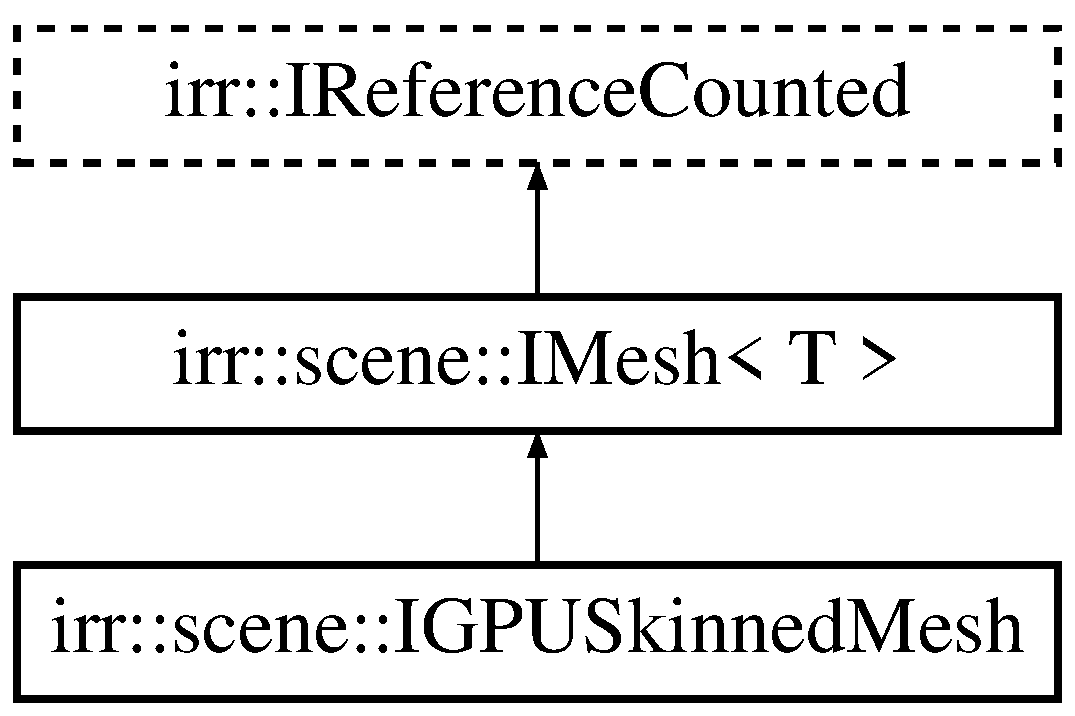
\includegraphics[height=3.000000cm]{classirr_1_1scene_1_1IGPUSkinnedMesh}
\end{center}
\end{figure}
\subsection*{Public Member Functions}
\begin{DoxyCompactItemize}
\item 
{\bfseries I\+G\+P\+U\+Skinned\+Mesh} (\hyperlink{classirr_1_1scene_1_1CFinalBoneHierarchy}{C\+Final\+Bone\+Hierarchy} $\ast$bone\+Hierarchy)\hypertarget{classirr_1_1scene_1_1IGPUSkinnedMesh_a689247f8e29bbbafb51a8600457254c4}{}\label{classirr_1_1scene_1_1IGPUSkinnedMesh_a689247f8e29bbbafb51a8600457254c4}

\item 
const \hyperlink{classirr_1_1scene_1_1CFinalBoneHierarchy}{C\+Final\+Bone\+Hierarchy} $\ast$ {\bfseries get\+Bone\+Reference\+Hierarchy} () const \hypertarget{classirr_1_1scene_1_1IGPUSkinnedMesh_a17c6911519d5af6cf220e07cacd998f5}{}\label{classirr_1_1scene_1_1IGPUSkinnedMesh_a17c6911519d5af6cf220e07cacd998f5}

\item 
virtual const \hyperlink{classirr_1_1core_1_1aabbox3d}{core\+::aabbox3d}$<$ \hyperlink{namespaceirr_a0277be98d67dc26ff93b1a6a1d086b07}{f32} $>$ \& \hyperlink{classirr_1_1scene_1_1IGPUSkinnedMesh_af6e2919ba3abcb6747f7b688b338ac16}{get\+Bounding\+Box} () const 
\begin{DoxyCompactList}\small\item\em Returns an axis aligned bounding box of the mesh. \end{DoxyCompactList}\item 
virtual void \hyperlink{classirr_1_1scene_1_1IGPUSkinnedMesh_a91372effa8144b0bac6f7483eccb1f66}{set\+Bounding\+Box} (const \hyperlink{namespaceirr_1_1core_adfc8fa01b30044c55f3332a1d6c1aa19}{core\+::aabbox3df} \&box)\hypertarget{classirr_1_1scene_1_1IGPUSkinnedMesh_a91372effa8144b0bac6f7483eccb1f66}{}\label{classirr_1_1scene_1_1IGPUSkinnedMesh_a91372effa8144b0bac6f7483eccb1f66}

\begin{DoxyCompactList}\small\item\em set user axis aligned bounding box \end{DoxyCompactList}\item 
virtual uint32\+\_\+t \hyperlink{classirr_1_1scene_1_1IGPUSkinnedMesh_ae55d0240ceae42379e5b5dfaa4efa0ea}{get\+Frame\+Count} () const  =0
\begin{DoxyCompactList}\small\item\em Gets the frame count of the animated mesh. \end{DoxyCompactList}\item 
virtual float {\bfseries get\+First\+Frame} () const  =0\hypertarget{classirr_1_1scene_1_1IGPUSkinnedMesh_a42a856efa06d48e11024f225fb5dc710}{}\label{classirr_1_1scene_1_1IGPUSkinnedMesh_a42a856efa06d48e11024f225fb5dc710}

\item 
virtual float {\bfseries get\+Last\+Frame} () const  =0\hypertarget{classirr_1_1scene_1_1IGPUSkinnedMesh_ae8f69ffa9b586e4334c63655c650483b}{}\label{classirr_1_1scene_1_1IGPUSkinnedMesh_ae8f69ffa9b586e4334c63655c650483b}

\item 
virtual \hyperlink{namespaceirr_1_1scene_aef0400177e5941293dff6640e800d11b}{E\+\_\+\+M\+E\+S\+H\+\_\+\+T\+Y\+PE} {\bfseries get\+Mesh\+Type} () const \hypertarget{classirr_1_1scene_1_1IGPUSkinnedMesh_afcde74ebf49b3789a78a297dca93bf23}{}\label{classirr_1_1scene_1_1IGPUSkinnedMesh_afcde74ebf49b3789a78a297dca93bf23}

\item 
virtual const uint32\+\_\+t \& \hyperlink{classirr_1_1scene_1_1IGPUSkinnedMesh_a2b2779acd0213c9769237e216891b892}{get\+Max\+Vertex\+Weights} (const size\+\_\+t \&meshbuffer\+Ix) const  =0\hypertarget{classirr_1_1scene_1_1IGPUSkinnedMesh_a2b2779acd0213c9769237e216891b892}{}\label{classirr_1_1scene_1_1IGPUSkinnedMesh_a2b2779acd0213c9769237e216891b892}

\begin{DoxyCompactList}\small\item\em can use more efficient shaders this way \+:D \end{DoxyCompactList}\item 
virtual uint32\+\_\+t {\bfseries get\+Max\+Vertex\+Weights} () const  =0\hypertarget{classirr_1_1scene_1_1IGPUSkinnedMesh_aca93da90a67c3c2e5a783af739569d85}{}\label{classirr_1_1scene_1_1IGPUSkinnedMesh_aca93da90a67c3c2e5a783af739569d85}

\end{DoxyCompactItemize}
\subsection*{Protected Attributes}
\begin{DoxyCompactItemize}
\item 
const \hyperlink{classirr_1_1scene_1_1CFinalBoneHierarchy}{C\+Final\+Bone\+Hierarchy} $\ast$ {\bfseries reference\+Hierarchy}\hypertarget{classirr_1_1scene_1_1IGPUSkinnedMesh_a05574ad2f9284c6fb552d434bbcba6eb}{}\label{classirr_1_1scene_1_1IGPUSkinnedMesh_a05574ad2f9284c6fb552d434bbcba6eb}

\item 
\hyperlink{classirr_1_1core_1_1aabbox3d}{core\+::aabbox3d}$<$ \hyperlink{namespaceirr_a0277be98d67dc26ff93b1a6a1d086b07}{f32} $>$ \hyperlink{classirr_1_1scene_1_1IGPUSkinnedMesh_ae83749a4ab9aec4f98f2d16cc49e14f6}{Box}\hypertarget{classirr_1_1scene_1_1IGPUSkinnedMesh_ae83749a4ab9aec4f98f2d16cc49e14f6}{}\label{classirr_1_1scene_1_1IGPUSkinnedMesh_ae83749a4ab9aec4f98f2d16cc49e14f6}

\begin{DoxyCompactList}\small\item\em The bounding box of this mesh. \end{DoxyCompactList}\end{DoxyCompactItemize}
\subsection*{Additional Inherited Members}


\subsection{Member Function Documentation}
\index{irr\+::scene\+::\+I\+G\+P\+U\+Skinned\+Mesh@{irr\+::scene\+::\+I\+G\+P\+U\+Skinned\+Mesh}!get\+Bounding\+Box@{get\+Bounding\+Box}}
\index{get\+Bounding\+Box@{get\+Bounding\+Box}!irr\+::scene\+::\+I\+G\+P\+U\+Skinned\+Mesh@{irr\+::scene\+::\+I\+G\+P\+U\+Skinned\+Mesh}}
\subsubsection[{\texorpdfstring{get\+Bounding\+Box() const }{getBoundingBox() const }}]{\setlength{\rightskip}{0pt plus 5cm}virtual const {\bf core\+::aabbox3d}$<${\bf f32}$>$\& irr\+::scene\+::\+I\+G\+P\+U\+Skinned\+Mesh\+::get\+Bounding\+Box (
\begin{DoxyParamCaption}
{}
\end{DoxyParamCaption}
) const\hspace{0.3cm}{\ttfamily [inline]}, {\ttfamily [virtual]}}\hypertarget{classirr_1_1scene_1_1IGPUSkinnedMesh_af6e2919ba3abcb6747f7b688b338ac16}{}\label{classirr_1_1scene_1_1IGPUSkinnedMesh_af6e2919ba3abcb6747f7b688b338ac16}


Returns an axis aligned bounding box of the mesh. 

\begin{DoxyReturn}{Returns}
A bounding box of this mesh is returned. 
\end{DoxyReturn}


Implements \hyperlink{classirr_1_1scene_1_1IMesh_a821ad4b325444ff5b47035cf54a4303f}{irr\+::scene\+::\+I\+Mesh$<$ T $>$}.

\index{irr\+::scene\+::\+I\+G\+P\+U\+Skinned\+Mesh@{irr\+::scene\+::\+I\+G\+P\+U\+Skinned\+Mesh}!get\+Frame\+Count@{get\+Frame\+Count}}
\index{get\+Frame\+Count@{get\+Frame\+Count}!irr\+::scene\+::\+I\+G\+P\+U\+Skinned\+Mesh@{irr\+::scene\+::\+I\+G\+P\+U\+Skinned\+Mesh}}
\subsubsection[{\texorpdfstring{get\+Frame\+Count() const  =0}{getFrameCount() const  =0}}]{\setlength{\rightskip}{0pt plus 5cm}virtual uint32\+\_\+t irr\+::scene\+::\+I\+G\+P\+U\+Skinned\+Mesh\+::get\+Frame\+Count (
\begin{DoxyParamCaption}
{}
\end{DoxyParamCaption}
) const\hspace{0.3cm}{\ttfamily [pure virtual]}}\hypertarget{classirr_1_1scene_1_1IGPUSkinnedMesh_ae55d0240ceae42379e5b5dfaa4efa0ea}{}\label{classirr_1_1scene_1_1IGPUSkinnedMesh_ae55d0240ceae42379e5b5dfaa4efa0ea}


Gets the frame count of the animated mesh. 

\begin{DoxyReturn}{Returns}
The amount of frames. If the amount is 1, it is a static, non animated mesh. If 0 it just is in the bind-\/pose doesn\textquotesingle{}t have keyframes 
\end{DoxyReturn}


The documentation for this class was generated from the following file\+:\begin{DoxyCompactItemize}
\item 
include/I\+Skinned\+Mesh.\+h\end{DoxyCompactItemize}

\hypertarget{classirr_1_1video_1_1IGPUTimestampQuery}{}\section{irr\+:\+:video\+:\+:I\+G\+P\+U\+Timestamp\+Query Class Reference}
\label{classirr_1_1video_1_1IGPUTimestampQuery}\index{irr\+::video\+::\+I\+G\+P\+U\+Timestamp\+Query@{irr\+::video\+::\+I\+G\+P\+U\+Timestamp\+Query}}
Inheritance diagram for irr\+:\+:video\+:\+:I\+G\+P\+U\+Timestamp\+Query\+:\begin{figure}[H]
\begin{center}
\leavevmode
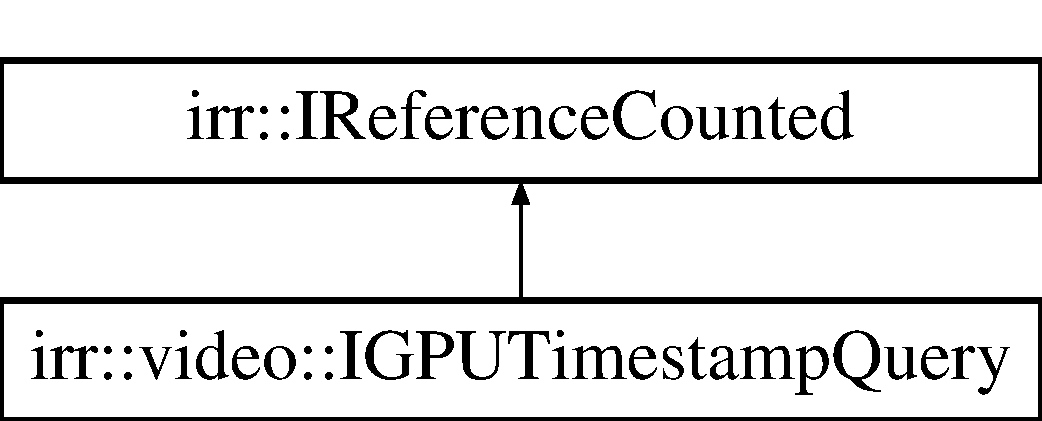
\includegraphics[height=2.000000cm]{classirr_1_1video_1_1IGPUTimestampQuery}
\end{center}
\end{figure}
\subsection*{Public Member Functions}
\begin{DoxyCompactItemize}
\item 
virtual bool {\bfseries is\+Query\+Ready} ()=0\hypertarget{classirr_1_1video_1_1IGPUTimestampQuery_a4259a73853a5892a6c7757b7aaa188be}{}\label{classirr_1_1video_1_1IGPUTimestampQuery_a4259a73853a5892a6c7757b7aaa188be}

\item 
virtual uint64\+\_\+t {\bfseries get\+Timestamp\+When\+Completed} ()=0\hypertarget{classirr_1_1video_1_1IGPUTimestampQuery_a1de290890c933d2a6a1a7c979e777dcf}{}\label{classirr_1_1video_1_1IGPUTimestampQuery_a1de290890c933d2a6a1a7c979e777dcf}

\end{DoxyCompactItemize}
\subsection*{Additional Inherited Members}


The documentation for this class was generated from the following file\+:\begin{DoxyCompactItemize}
\item 
include/I\+G\+P\+U\+Timestamp\+Query.\+h\end{DoxyCompactItemize}

\hypertarget{classirr_1_1video_1_1IGPUTransientBuffer}{}\section{irr\+:\+:video\+:\+:I\+G\+P\+U\+Transient\+Buffer Class Reference}
\label{classirr_1_1video_1_1IGPUTransientBuffer}\index{irr\+::video\+::\+I\+G\+P\+U\+Transient\+Buffer@{irr\+::video\+::\+I\+G\+P\+U\+Transient\+Buffer}}


Persistently Mapped buffer.  




{\ttfamily \#include $<$I\+G\+P\+U\+Transient\+Buffer.\+h$>$}

Inheritance diagram for irr\+:\+:video\+:\+:I\+G\+P\+U\+Transient\+Buffer\+:\begin{figure}[H]
\begin{center}
\leavevmode
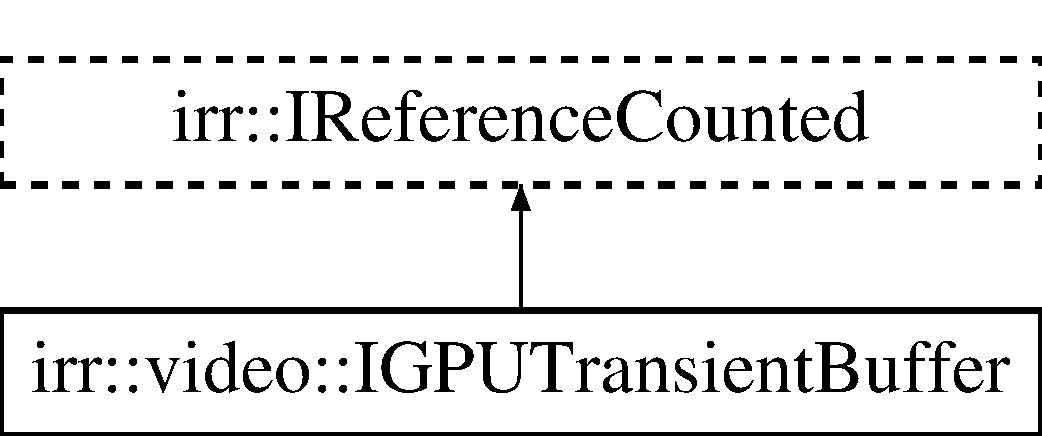
\includegraphics[height=2.000000cm]{classirr_1_1video_1_1IGPUTransientBuffer}
\end{center}
\end{figure}
\subsection*{Classes}
\begin{DoxyCompactItemize}
\item 
struct \hyperlink{structirr_1_1video_1_1IGPUTransientBuffer_1_1Allocation}{Allocation}
\end{DoxyCompactItemize}
\subsection*{Public Types}
\begin{DoxyCompactItemize}
\item 
enum \hyperlink{classirr_1_1video_1_1IGPUTransientBuffer_a08e145b30588c9a3e5ec469e36f2847b}{E\+\_\+\+A\+L\+L\+O\+C\+\_\+\+R\+E\+T\+U\+R\+N\+\_\+\+S\+T\+A\+T\+US} \{ {\bfseries E\+A\+R\+S\+\_\+\+S\+U\+C\+C\+E\+SS} = 0, 
\hyperlink{classirr_1_1video_1_1IGPUTransientBuffer_a08e145b30588c9a3e5ec469e36f2847bab3c64a0286d714b4590193582b0d0cb6}{E\+A\+R\+S\+\_\+\+F\+A\+IL}, 
{\bfseries E\+A\+R\+S\+\_\+\+E\+R\+R\+OR}
 \}
\item 
enum {\bfseries E\+\_\+\+W\+A\+I\+T\+\_\+\+P\+O\+L\+I\+CY} \{ {\bfseries E\+W\+P\+\_\+\+D\+O\+N\+T\+\_\+\+W\+A\+IT}, 
{\bfseries E\+W\+P\+\_\+\+W\+A\+I\+T\+\_\+\+F\+O\+R\+\_\+\+C\+P\+U\+\_\+\+U\+N\+M\+AP} =1, 
{\bfseries E\+W\+P\+\_\+\+W\+A\+I\+T\+\_\+\+F\+O\+R\+\_\+\+G\+P\+U\+\_\+\+F\+R\+EE} =2
 \}\hypertarget{classirr_1_1video_1_1IGPUTransientBuffer_aa62d526fb6c6a166336fdc691219a542}{}\label{classirr_1_1video_1_1IGPUTransientBuffer_aa62d526fb6c6a166336fdc691219a542}

\end{DoxyCompactItemize}
\subsection*{Public Member Functions}
\begin{DoxyCompactItemize}
\item 
\hyperlink{classirr_1_1video_1_1IGPUBuffer}{I\+G\+P\+U\+Buffer} $\ast$ {\bfseries get\+Underlying\+Buffer} ()\hypertarget{classirr_1_1video_1_1IGPUTransientBuffer_ab8ad89fa1f308a360e1983f99ba58807}{}\label{classirr_1_1video_1_1IGPUTransientBuffer_ab8ad89fa1f308a360e1983f99ba58807}

\item 
bool {\bfseries Validate} ()\hypertarget{classirr_1_1video_1_1IGPUTransientBuffer_a9dcefa03ff7ea4f3ac4d3948e9170e67}{}\label{classirr_1_1video_1_1IGPUTransientBuffer_a9dcefa03ff7ea4f3ac4d3948e9170e67}

\item 
void {\bfseries Print\+Debug} (bool needs\+Mutex=true)\hypertarget{classirr_1_1video_1_1IGPUTransientBuffer_abe7c1e4eb63672bd00d46c8d5172301e}{}\label{classirr_1_1video_1_1IGPUTransientBuffer_abe7c1e4eb63672bd00d46c8d5172301e}

\item 
\hyperlink{classirr_1_1video_1_1IGPUTransientBuffer_a08e145b30588c9a3e5ec469e36f2847b}{E\+\_\+\+A\+L\+L\+O\+C\+\_\+\+R\+E\+T\+U\+R\+N\+\_\+\+S\+T\+A\+T\+US} {\bfseries Alloc} (size\+\_\+t \&offset\+Out, const size\+\_\+t \&max\+Size, const size\+\_\+t \&alignment=32, E\+\_\+\+W\+A\+I\+T\+\_\+\+P\+O\+L\+I\+CY wait\+Policy=E\+W\+P\+\_\+\+D\+O\+N\+T\+\_\+\+W\+A\+IT, bool grow\+If\+Too\+Small=false)\hypertarget{classirr_1_1video_1_1IGPUTransientBuffer_a0f7829c4499edf6ba5b26847641a4828}{}\label{classirr_1_1video_1_1IGPUTransientBuffer_a0f7829c4499edf6ba5b26847641a4828}

\item 
bool {\bfseries Commit} (const size\+\_\+t \&start, const size\+\_\+t \&end)\hypertarget{classirr_1_1video_1_1IGPUTransientBuffer_a5627d745e53c7664ac297f366f55dd9d}{}\label{classirr_1_1video_1_1IGPUTransientBuffer_a5627d745e53c7664ac297f366f55dd9d}

\item 
bool {\bfseries Place} (size\+\_\+t \&offset\+Out, const void $\ast$data, const size\+\_\+t \&data\+Size, const size\+\_\+t \&alignment=32, const E\+\_\+\+W\+A\+I\+T\+\_\+\+P\+O\+L\+I\+CY \&wait\+Policy=E\+W\+P\+\_\+\+D\+O\+N\+T\+\_\+\+W\+A\+IT, const bool \&grow\+If\+Too\+Small=false)\hypertarget{classirr_1_1video_1_1IGPUTransientBuffer_ade893f9cc1109c472568db7c69018615}{}\label{classirr_1_1video_1_1IGPUTransientBuffer_ade893f9cc1109c472568db7c69018615}

\item 
bool \hyperlink{classirr_1_1video_1_1IGPUTransientBuffer_aa575e8d02383688f671e1ed818790d17}{Free} (const size\+\_\+t \&start, const size\+\_\+t \&end)
\item 
bool {\bfseries fence\+Range\+Used\+By\+G\+PU} (const size\+\_\+t \&start, const size\+\_\+t \&end)\hypertarget{classirr_1_1video_1_1IGPUTransientBuffer_a25453b67fc5f499ac06e61e04c338574}{}\label{classirr_1_1video_1_1IGPUTransientBuffer_a25453b67fc5f499ac06e61e04c338574}

\item 
bool {\bfseries query\+Range\+Committed} (const size\+\_\+t \&start, const size\+\_\+t \&end)\hypertarget{classirr_1_1video_1_1IGPUTransientBuffer_a6ba14ee0eee587474da04d3d24a307cf}{}\label{classirr_1_1video_1_1IGPUTransientBuffer_a6ba14ee0eee587474da04d3d24a307cf}

\item 
bool {\bfseries query\+Range} (const size\+\_\+t \&start, const size\+\_\+t \&end, const Allocation\+::\+E\+\_\+\+A\+L\+L\+O\+C\+A\+T\+I\+O\+N\+\_\+\+S\+T\+A\+TE \&state)\hypertarget{classirr_1_1video_1_1IGPUTransientBuffer_adcacd73554da2efeabd7ef440bade85b}{}\label{classirr_1_1video_1_1IGPUTransientBuffer_adcacd73554da2efeabd7ef440bade85b}

\item 
bool {\bfseries wait\+Range\+Fences} (const size\+\_\+t \&start, const size\+\_\+t \&end, size\+\_\+t time\+Out\+Ns)\hypertarget{classirr_1_1video_1_1IGPUTransientBuffer_acb2efc6648dd3457a7b444dd965879a4}{}\label{classirr_1_1video_1_1IGPUTransientBuffer_acb2efc6648dd3457a7b444dd965879a4}

\item 
void {\bfseries Defrag\+Descriptor} ()\hypertarget{classirr_1_1video_1_1IGPUTransientBuffer_ad86d655907dced2d87bb44bc4b3648ec}{}\label{classirr_1_1video_1_1IGPUTransientBuffer_ad86d655907dced2d87bb44bc4b3648ec}

\item 
const size\+\_\+t \& {\bfseries get\+Free\+Space} () const \hypertarget{classirr_1_1video_1_1IGPUTransientBuffer_a679a10b6e9852ea9b554a7a4753a7bda}{}\label{classirr_1_1video_1_1IGPUTransientBuffer_a679a10b6e9852ea9b554a7a4753a7bda}

\item 
const size\+\_\+t \& {\bfseries get\+True\+Free\+Space} () const \hypertarget{classirr_1_1video_1_1IGPUTransientBuffer_ab20491c633e85264b79630e4759a1d70}{}\label{classirr_1_1video_1_1IGPUTransientBuffer_ab20491c633e85264b79630e4759a1d70}

\end{DoxyCompactItemize}
\subsection*{Static Public Member Functions}
\begin{DoxyCompactItemize}
\item 
static \hyperlink{classirr_1_1video_1_1IGPUTransientBuffer}{I\+G\+P\+U\+Transient\+Buffer} $\ast$ {\bfseries create\+Mapped\+Transient\+Buffer} (\hyperlink{classirr_1_1video_1_1IVideoDriver}{I\+Video\+Driver} $\ast$driver, const size\+\_\+t \&bufsize=0x100000u, const E\+\_\+\+G\+P\+U\+\_\+\+B\+U\+F\+F\+E\+R\+\_\+\+A\+C\+C\+E\+S\+S \&access\+Pattern=\+E\+G\+B\+A\+\_\+\+W\+R\+I\+T\+E, const bool \&in\+C\+P\+U\+Mem=true, const bool \&growable=false, const bool \&auto\+Flush=true, const bool \&thread\+Safe=true)\hypertarget{classirr_1_1video_1_1IGPUTransientBuffer_a86dcc22d24ca78f6823eee14b883196f}{}\label{classirr_1_1video_1_1IGPUTransientBuffer_a86dcc22d24ca78f6823eee14b883196f}

\item 
static \hyperlink{classirr_1_1video_1_1IGPUTransientBuffer}{I\+G\+P\+U\+Transient\+Buffer} $\ast$ {\bfseries create\+Mapped\+Transient\+Buffer} (\hyperlink{classirr_1_1video_1_1IVideoDriver}{I\+Video\+Driver} $\ast$driver, \hyperlink{classirr_1_1video_1_1IGPUMappedBuffer}{I\+G\+P\+U\+Mapped\+Buffer} $\ast$buffer, const bool \&growable=false, const bool \&auto\+Flush=true, const bool \&thread\+Safe=true)\hypertarget{classirr_1_1video_1_1IGPUTransientBuffer_a1c150de3ed0a5dac854fbb03a4d173c9}{}\label{classirr_1_1video_1_1IGPUTransientBuffer_a1c150de3ed0a5dac854fbb03a4d173c9}

\item 
static \hyperlink{classirr_1_1video_1_1IGPUTransientBuffer}{I\+G\+P\+U\+Transient\+Buffer} $\ast$ {\bfseries create\+Transient\+Buffer} (\hyperlink{classirr_1_1video_1_1IVideoDriver}{I\+Video\+Driver} $\ast$driver, const size\+\_\+t \&bufsize=0x100000u, const E\+\_\+\+G\+P\+U\+\_\+\+B\+U\+F\+F\+E\+R\+\_\+\+A\+C\+C\+E\+S\+S \&access\+Pattern=\+E\+G\+B\+A\+\_\+\+W\+R\+I\+T\+E, const bool \&in\+C\+P\+U\+Mem=true, const bool \&can\+Modify\+Sub\+Data=false, const bool \&growable=false, const bool \&auto\+Flush=true, const bool \&thread\+Safe=true)\hypertarget{classirr_1_1video_1_1IGPUTransientBuffer_ad3271733fe1db3ac1fd03dd6b2732018}{}\label{classirr_1_1video_1_1IGPUTransientBuffer_ad3271733fe1db3ac1fd03dd6b2732018}

\end{DoxyCompactItemize}
\subsection*{Additional Inherited Members}


\subsection{Detailed Description}
Persistently Mapped buffer. 

A) Only one thread can modify buffer descriptor B) Only the main thread can grow the buffer!!!!!!!!! (Open\+GL) B1) The grow can only occur if there are no pointers mapped to data B2) But can alloc from other thread if we agree to wait on \hyperlink{classirr_1_1video_1_1IGPUTransientBuffer_aa575e8d02383688f671e1ed818790d17}{Free()} or G\+PU fences Thread Safeness\+: \begin{DoxyVerb}1) Creation and Deletion of IGPUTransientBuffer is NOT THREAD SAFE, and CAN ONLY BE DONE IN THE OPENGL THREAD
    (basically expose the object [handle] to other threads after creating it)
2) Using the pointer returned by getRangePointer(size_t start) is NOT THREAD SAFE,
    UNLESS AT LEAST one sub-range remains allocated, that is Commit() has not been called on a Alloc()'ed subrange yet
3) fenceRangeUsedByGPU() most probably should be calle donly by the OpenGL THREAD!!!!
4) Alloc(,growIfTooSmall=true) CAN ONLY BE CALLED FROM THE OpenGL THREAD!!!
5) Alloc(), Commit(), Place(), Free(), fenceRangeUsedByGPU() and DefragDescriptor() are all thread safe
6) Using EWP_WAIT_FOR_CPU_UNMAP bit on any call while having un-Commit()'ed ranges (which will not be Commit()'ed by other Threads) will DEADLOCK
7) Using EWP_WAIT_FOR_GPU_FREE bit on Alloc() while having un-Free()'ed ranges (which will not be Free()'ed by other Threads) will DEADLOCK\end{DoxyVerb}
 

\subsection{Member Enumeration Documentation}
\index{irr\+::video\+::\+I\+G\+P\+U\+Transient\+Buffer@{irr\+::video\+::\+I\+G\+P\+U\+Transient\+Buffer}!E\+\_\+\+A\+L\+L\+O\+C\+\_\+\+R\+E\+T\+U\+R\+N\+\_\+\+S\+T\+A\+T\+US@{E\+\_\+\+A\+L\+L\+O\+C\+\_\+\+R\+E\+T\+U\+R\+N\+\_\+\+S\+T\+A\+T\+US}}
\index{E\+\_\+\+A\+L\+L\+O\+C\+\_\+\+R\+E\+T\+U\+R\+N\+\_\+\+S\+T\+A\+T\+US@{E\+\_\+\+A\+L\+L\+O\+C\+\_\+\+R\+E\+T\+U\+R\+N\+\_\+\+S\+T\+A\+T\+US}!irr\+::video\+::\+I\+G\+P\+U\+Transient\+Buffer@{irr\+::video\+::\+I\+G\+P\+U\+Transient\+Buffer}}
\subsubsection[{\texorpdfstring{E\+\_\+\+A\+L\+L\+O\+C\+\_\+\+R\+E\+T\+U\+R\+N\+\_\+\+S\+T\+A\+T\+US}{E\_ALLOC\_RETURN\_STATUS}}]{\setlength{\rightskip}{0pt plus 5cm}enum {\bf irr\+::video\+::\+I\+G\+P\+U\+Transient\+Buffer\+::\+E\+\_\+\+A\+L\+L\+O\+C\+\_\+\+R\+E\+T\+U\+R\+N\+\_\+\+S\+T\+A\+T\+US}}\hypertarget{classirr_1_1video_1_1IGPUTransientBuffer_a08e145b30588c9a3e5ec469e36f2847b}{}\label{classirr_1_1video_1_1IGPUTransientBuffer_a08e145b30588c9a3e5ec469e36f2847b}
\begin{Desc}
\item[Enumerator]\par
\begin{description}
\index{E\+A\+R\+S\+\_\+\+F\+A\+IL@{E\+A\+R\+S\+\_\+\+F\+A\+IL}!irr\+::video\+::\+I\+G\+P\+U\+Transient\+Buffer@{irr\+::video\+::\+I\+G\+P\+U\+Transient\+Buffer}}\index{irr\+::video\+::\+I\+G\+P\+U\+Transient\+Buffer@{irr\+::video\+::\+I\+G\+P\+U\+Transient\+Buffer}!E\+A\+R\+S\+\_\+\+F\+A\+IL@{E\+A\+R\+S\+\_\+\+F\+A\+IL}}\item[{\em 
E\+A\+R\+S\+\_\+\+F\+A\+IL\hypertarget{classirr_1_1video_1_1IGPUTransientBuffer_a08e145b30588c9a3e5ec469e36f2847bab3c64a0286d714b4590193582b0d0cb6}{}\label{classirr_1_1video_1_1IGPUTransientBuffer_a08e145b30588c9a3e5ec469e36f2847bab3c64a0286d714b4590193582b0d0cb6}
}]E\+A\+R\+S\+\_\+\+T\+I\+M\+E\+O\+UT, Future. \end{description}
\end{Desc}


\subsection{Member Function Documentation}
\index{irr\+::video\+::\+I\+G\+P\+U\+Transient\+Buffer@{irr\+::video\+::\+I\+G\+P\+U\+Transient\+Buffer}!Free@{Free}}
\index{Free@{Free}!irr\+::video\+::\+I\+G\+P\+U\+Transient\+Buffer@{irr\+::video\+::\+I\+G\+P\+U\+Transient\+Buffer}}
\subsubsection[{\texorpdfstring{Free(const size\+\_\+t \&start, const size\+\_\+t \&end)}{Free(const size\_t \&start, const size\_t \&end)}}]{\setlength{\rightskip}{0pt plus 5cm}bool irr\+::video\+::\+I\+G\+P\+U\+Transient\+Buffer\+::\+Free (
\begin{DoxyParamCaption}
\item[{const size\+\_\+t \&}]{start, }
\item[{const size\+\_\+t \&}]{end}
\end{DoxyParamCaption}
)}\hypertarget{classirr_1_1video_1_1IGPUTransientBuffer_aa575e8d02383688f671e1ed818790d17}{}\label{classirr_1_1video_1_1IGPUTransientBuffer_aa575e8d02383688f671e1ed818790d17}
Unless memory is being used by G\+PU it will be returned to free pool straight away Useful if you dont end up using comitted memory by G\+PU 

The documentation for this class was generated from the following file\+:\begin{DoxyCompactItemize}
\item 
include/I\+G\+P\+U\+Transient\+Buffer.\+h\end{DoxyCompactItemize}

\hypertarget{classirr_1_1video_1_1IImage}{}\section{irr\+:\+:video\+:\+:I\+Image Class Reference}
\label{classirr_1_1video_1_1IImage}\index{irr\+::video\+::\+I\+Image@{irr\+::video\+::\+I\+Image}}


Interface for software image data.  




{\ttfamily \#include $<$I\+Image.\+h$>$}

Inheritance diagram for irr\+:\+:video\+:\+:I\+Image\+:\begin{figure}[H]
\begin{center}
\leavevmode
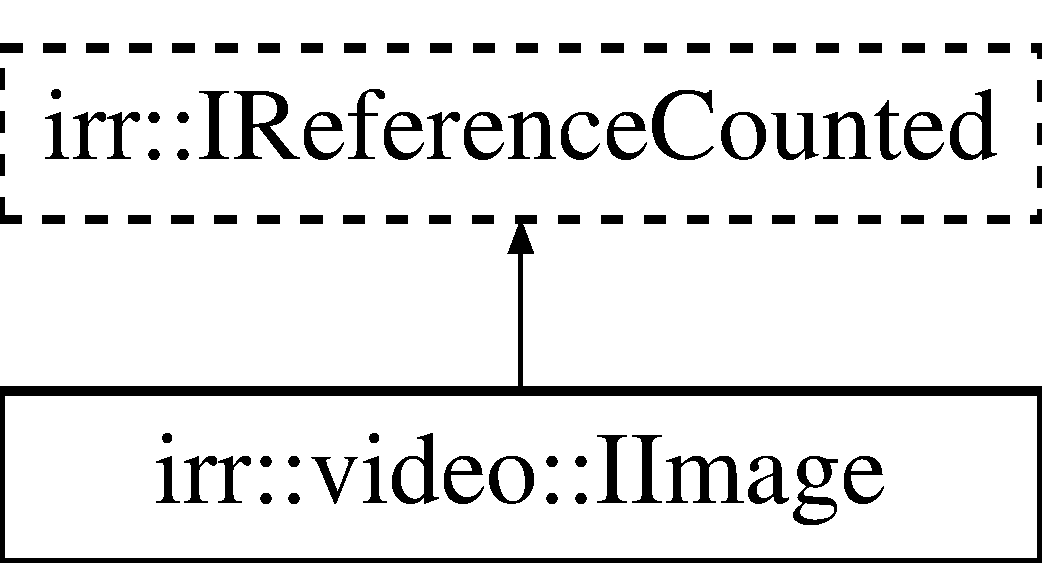
\includegraphics[height=2.000000cm]{classirr_1_1video_1_1IImage}
\end{center}
\end{figure}
\subsection*{Public Member Functions}
\begin{DoxyCompactItemize}
\item 
virtual void $\ast$ \hyperlink{classirr_1_1video_1_1IImage_a5c4b0b5fa2a5f253f93c1b038e20d204}{lock} ()=0
\begin{DoxyCompactList}\small\item\em Lock function. Use this to get a pointer to the image data. \end{DoxyCompactList}\item 
virtual void \hyperlink{classirr_1_1video_1_1IImage_ad0f902d74a948ee66be2d70dc90ed38d}{unlock} ()=0
\begin{DoxyCompactList}\small\item\em Unlock function. \end{DoxyCompactList}\item 
virtual const \hyperlink{classirr_1_1core_1_1dimension2d}{core\+::dimension2d}$<$ \hyperlink{namespaceirr_a0416a53257075833e7002efd0a18e804}{u32} $>$ \& \hyperlink{classirr_1_1video_1_1IImage_a407b43a35787e35217a236de738047ec}{get\+Dimension} () const  =0\hypertarget{classirr_1_1video_1_1IImage_a407b43a35787e35217a236de738047ec}{}\label{classirr_1_1video_1_1IImage_a407b43a35787e35217a236de738047ec}

\begin{DoxyCompactList}\small\item\em Returns width and height of image data. \end{DoxyCompactList}\item 
virtual \hyperlink{namespaceirr_a0416a53257075833e7002efd0a18e804}{u32} \hyperlink{classirr_1_1video_1_1IImage_a729c4224a6ac60350b8ff5e04461beb8}{get\+Bits\+Per\+Pixel} () const  =0\hypertarget{classirr_1_1video_1_1IImage_a729c4224a6ac60350b8ff5e04461beb8}{}\label{classirr_1_1video_1_1IImage_a729c4224a6ac60350b8ff5e04461beb8}

\begin{DoxyCompactList}\small\item\em Returns bits per pixel. \end{DoxyCompactList}\item 
virtual \hyperlink{namespaceirr_a0416a53257075833e7002efd0a18e804}{u32} \hyperlink{classirr_1_1video_1_1IImage_a2143205d060b93ce05163e1aa9b807ba}{get\+Image\+Data\+Size\+In\+Bytes} () const  =0\hypertarget{classirr_1_1video_1_1IImage_a2143205d060b93ce05163e1aa9b807ba}{}\label{classirr_1_1video_1_1IImage_a2143205d060b93ce05163e1aa9b807ba}

\begin{DoxyCompactList}\small\item\em Returns image data size in bytes. \end{DoxyCompactList}\item 
virtual \hyperlink{namespaceirr_a0416a53257075833e7002efd0a18e804}{u32} \hyperlink{classirr_1_1video_1_1IImage_a8c348f459af5323559b81ac4d3a5c3d8}{get\+Image\+Data\+Size\+In\+Pixels} () const  =0\hypertarget{classirr_1_1video_1_1IImage_a8c348f459af5323559b81ac4d3a5c3d8}{}\label{classirr_1_1video_1_1IImage_a8c348f459af5323559b81ac4d3a5c3d8}

\begin{DoxyCompactList}\small\item\em Returns image data size in pixels. \end{DoxyCompactList}\item 
virtual \hyperlink{classirr_1_1video_1_1SColor}{S\+Color} \hyperlink{classirr_1_1video_1_1IImage_abd1ee6c06af158c36245803b57bbff01}{get\+Pixel} (\hyperlink{namespaceirr_a0416a53257075833e7002efd0a18e804}{u32} x, \hyperlink{namespaceirr_a0416a53257075833e7002efd0a18e804}{u32} y) const  =0\hypertarget{classirr_1_1video_1_1IImage_abd1ee6c06af158c36245803b57bbff01}{}\label{classirr_1_1video_1_1IImage_abd1ee6c06af158c36245803b57bbff01}

\begin{DoxyCompactList}\small\item\em Returns a pixel. \end{DoxyCompactList}\item 
virtual void \hyperlink{classirr_1_1video_1_1IImage_a89bf6020ce6ac1066e4d585ce46f79bd}{set\+Pixel} (\hyperlink{namespaceirr_a0416a53257075833e7002efd0a18e804}{u32} x, \hyperlink{namespaceirr_a0416a53257075833e7002efd0a18e804}{u32} y, const \hyperlink{classirr_1_1video_1_1SColor}{S\+Color} \&color, bool blend=false)=0\hypertarget{classirr_1_1video_1_1IImage_a89bf6020ce6ac1066e4d585ce46f79bd}{}\label{classirr_1_1video_1_1IImage_a89bf6020ce6ac1066e4d585ce46f79bd}

\begin{DoxyCompactList}\small\item\em Sets a pixel. \end{DoxyCompactList}\item 
virtual \hyperlink{namespaceirr_1_1video_a1d5e487888c32b1674a8f75116d829ed}{E\+C\+O\+L\+O\+R\+\_\+\+F\+O\+R\+M\+AT} \hyperlink{classirr_1_1video_1_1IImage_a36bac90ac99f8de86fae8b38144171cf}{get\+Color\+Format} () const  =0\hypertarget{classirr_1_1video_1_1IImage_a36bac90ac99f8de86fae8b38144171cf}{}\label{classirr_1_1video_1_1IImage_a36bac90ac99f8de86fae8b38144171cf}

\begin{DoxyCompactList}\small\item\em Returns the color format. \end{DoxyCompactList}\item 
virtual \hyperlink{namespaceirr_a0416a53257075833e7002efd0a18e804}{u32} \hyperlink{classirr_1_1video_1_1IImage_af00bb57f04a6f910641446781f11dad9}{get\+Red\+Mask} () const  =0\hypertarget{classirr_1_1video_1_1IImage_af00bb57f04a6f910641446781f11dad9}{}\label{classirr_1_1video_1_1IImage_af00bb57f04a6f910641446781f11dad9}

\begin{DoxyCompactList}\small\item\em Returns mask for red value of a pixel. \end{DoxyCompactList}\item 
virtual \hyperlink{namespaceirr_a0416a53257075833e7002efd0a18e804}{u32} \hyperlink{classirr_1_1video_1_1IImage_aeff5ac41ee1fea04b04fef342797c134}{get\+Green\+Mask} () const  =0\hypertarget{classirr_1_1video_1_1IImage_aeff5ac41ee1fea04b04fef342797c134}{}\label{classirr_1_1video_1_1IImage_aeff5ac41ee1fea04b04fef342797c134}

\begin{DoxyCompactList}\small\item\em Returns mask for green value of a pixel. \end{DoxyCompactList}\item 
virtual \hyperlink{namespaceirr_a0416a53257075833e7002efd0a18e804}{u32} \hyperlink{classirr_1_1video_1_1IImage_a9025c7c03826f1ee94f0114e3dda55df}{get\+Blue\+Mask} () const  =0\hypertarget{classirr_1_1video_1_1IImage_a9025c7c03826f1ee94f0114e3dda55df}{}\label{classirr_1_1video_1_1IImage_a9025c7c03826f1ee94f0114e3dda55df}

\begin{DoxyCompactList}\small\item\em Returns mask for blue value of a pixel. \end{DoxyCompactList}\item 
virtual \hyperlink{namespaceirr_a0416a53257075833e7002efd0a18e804}{u32} \hyperlink{classirr_1_1video_1_1IImage_a7091575227ea183ec70bdb91415cf4ef}{get\+Alpha\+Mask} () const  =0\hypertarget{classirr_1_1video_1_1IImage_a7091575227ea183ec70bdb91415cf4ef}{}\label{classirr_1_1video_1_1IImage_a7091575227ea183ec70bdb91415cf4ef}

\begin{DoxyCompactList}\small\item\em Returns mask for alpha value of a pixel. \end{DoxyCompactList}\item 
virtual \hyperlink{namespaceirr_a0416a53257075833e7002efd0a18e804}{u32} \hyperlink{classirr_1_1video_1_1IImage_a0a34596052ca6ba682ea0022c783f0d0}{get\+Pitch} () const  =0\hypertarget{classirr_1_1video_1_1IImage_a0a34596052ca6ba682ea0022c783f0d0}{}\label{classirr_1_1video_1_1IImage_a0a34596052ca6ba682ea0022c783f0d0}

\begin{DoxyCompactList}\small\item\em Returns pitch of image. \end{DoxyCompactList}\item 
virtual void \hyperlink{classirr_1_1video_1_1IImage_a6f57153218f5ecd4da9aeb5a37f92f59}{copy\+To\+Scaling} (void $\ast$target, \hyperlink{namespaceirr_a0416a53257075833e7002efd0a18e804}{u32} width, \hyperlink{namespaceirr_a0416a53257075833e7002efd0a18e804}{u32} height, \hyperlink{namespaceirr_1_1video_a1d5e487888c32b1674a8f75116d829ed}{E\+C\+O\+L\+O\+R\+\_\+\+F\+O\+R\+M\+AT} format=\hyperlink{namespaceirr_1_1video_a1d5e487888c32b1674a8f75116d829eda55c57d63efff39efe33ee733fe962df0}{E\+C\+F\+\_\+\+A8\+R8\+G8\+B8}, \hyperlink{namespaceirr_a0416a53257075833e7002efd0a18e804}{u32} pitch=0)=0\hypertarget{classirr_1_1video_1_1IImage_a6f57153218f5ecd4da9aeb5a37f92f59}{}\label{classirr_1_1video_1_1IImage_a6f57153218f5ecd4da9aeb5a37f92f59}

\begin{DoxyCompactList}\small\item\em Copies the image into the target, scaling the image to fit. \end{DoxyCompactList}\item 
virtual void \hyperlink{classirr_1_1video_1_1IImage_aa969bf7167171a18003e26ff7876febd}{copy\+To\+Scaling} (\hyperlink{classirr_1_1video_1_1IImage}{I\+Image} $\ast$target)=0\hypertarget{classirr_1_1video_1_1IImage_aa969bf7167171a18003e26ff7876febd}{}\label{classirr_1_1video_1_1IImage_aa969bf7167171a18003e26ff7876febd}

\begin{DoxyCompactList}\small\item\em Copies the image into the target, scaling the image to fit. \end{DoxyCompactList}\item 
virtual void \hyperlink{classirr_1_1video_1_1IImage_ae4a8a2fc245f691224825aceffd53b8a}{copy\+To} (\hyperlink{classirr_1_1video_1_1IImage}{I\+Image} $\ast$target, const core\+::position2d$<$ \hyperlink{namespaceirr_ac66849b7a6ed16e30ebede579f9b47c6}{s32} $>$ \&pos=core\+::position2d$<$ \hyperlink{namespaceirr_ac66849b7a6ed16e30ebede579f9b47c6}{s32} $>$(0, 0))=0\hypertarget{classirr_1_1video_1_1IImage_ae4a8a2fc245f691224825aceffd53b8a}{}\label{classirr_1_1video_1_1IImage_ae4a8a2fc245f691224825aceffd53b8a}

\begin{DoxyCompactList}\small\item\em copies this surface into another \end{DoxyCompactList}\item 
virtual void \hyperlink{classirr_1_1video_1_1IImage_ac43f477f9da28077fc3573a628b33bcb}{copy\+To} (\hyperlink{classirr_1_1video_1_1IImage}{I\+Image} $\ast$target, const core\+::position2d$<$ \hyperlink{namespaceirr_ac66849b7a6ed16e30ebede579f9b47c6}{s32} $>$ \&pos, const \hyperlink{classirr_1_1core_1_1rect}{core\+::rect}$<$ \hyperlink{namespaceirr_ac66849b7a6ed16e30ebede579f9b47c6}{s32} $>$ \&source\+Rect, const \hyperlink{classirr_1_1core_1_1rect}{core\+::rect}$<$ \hyperlink{namespaceirr_ac66849b7a6ed16e30ebede579f9b47c6}{s32} $>$ $\ast$clip\+Rect=0)=0\hypertarget{classirr_1_1video_1_1IImage_ac43f477f9da28077fc3573a628b33bcb}{}\label{classirr_1_1video_1_1IImage_ac43f477f9da28077fc3573a628b33bcb}

\begin{DoxyCompactList}\small\item\em copies this surface into another \end{DoxyCompactList}\item 
virtual void \hyperlink{classirr_1_1video_1_1IImage_a7dd1e5dd19cb35be17c2fa00e38a193d}{copy\+To\+With\+Alpha} (\hyperlink{classirr_1_1video_1_1IImage}{I\+Image} $\ast$target, const core\+::position2d$<$ \hyperlink{namespaceirr_ac66849b7a6ed16e30ebede579f9b47c6}{s32} $>$ \&pos, const \hyperlink{classirr_1_1core_1_1rect}{core\+::rect}$<$ \hyperlink{namespaceirr_ac66849b7a6ed16e30ebede579f9b47c6}{s32} $>$ \&source\+Rect, const \hyperlink{classirr_1_1video_1_1SColor}{S\+Color} \&color, const \hyperlink{classirr_1_1core_1_1rect}{core\+::rect}$<$ \hyperlink{namespaceirr_ac66849b7a6ed16e30ebede579f9b47c6}{s32} $>$ $\ast$clip\+Rect=0)=0\hypertarget{classirr_1_1video_1_1IImage_a7dd1e5dd19cb35be17c2fa00e38a193d}{}\label{classirr_1_1video_1_1IImage_a7dd1e5dd19cb35be17c2fa00e38a193d}

\begin{DoxyCompactList}\small\item\em copies this surface into another, using the alpha mask and cliprect and a color to add with \end{DoxyCompactList}\item 
virtual void \hyperlink{classirr_1_1video_1_1IImage_a651c196f681a105fabfb5ff4f6b28682}{copy\+To\+Scaling\+Box\+Filter} (\hyperlink{classirr_1_1video_1_1IImage}{I\+Image} $\ast$target, \hyperlink{namespaceirr_ac66849b7a6ed16e30ebede579f9b47c6}{s32} bias=0, bool blend=false)=0\hypertarget{classirr_1_1video_1_1IImage_a651c196f681a105fabfb5ff4f6b28682}{}\label{classirr_1_1video_1_1IImage_a651c196f681a105fabfb5ff4f6b28682}

\begin{DoxyCompactList}\small\item\em copies this surface into another, scaling it to fit, appyling a box filter \end{DoxyCompactList}\item 
virtual void \hyperlink{classirr_1_1video_1_1IImage_a04973e101790130f611c4c6790e5b352}{fill} (const \hyperlink{classirr_1_1video_1_1SColor}{S\+Color} \&color)=0\hypertarget{classirr_1_1video_1_1IImage_a04973e101790130f611c4c6790e5b352}{}\label{classirr_1_1video_1_1IImage_a04973e101790130f611c4c6790e5b352}

\begin{DoxyCompactList}\small\item\em fills the surface with given color \end{DoxyCompactList}\end{DoxyCompactItemize}
\subsection*{Static Public Member Functions}
\begin{DoxyCompactItemize}
\item 
static \hyperlink{namespaceirr_a0416a53257075833e7002efd0a18e804}{u32} \hyperlink{classirr_1_1video_1_1IImage_a70b50ef1bbb6f90ec4c43a91f521c2b6}{get\+Bits\+Per\+Pixel\+From\+Format} (const \hyperlink{namespaceirr_1_1video_a1d5e487888c32b1674a8f75116d829ed}{E\+C\+O\+L\+O\+R\+\_\+\+F\+O\+R\+M\+AT} format)\hypertarget{classirr_1_1video_1_1IImage_a70b50ef1bbb6f90ec4c43a91f521c2b6}{}\label{classirr_1_1video_1_1IImage_a70b50ef1bbb6f90ec4c43a91f521c2b6}

\begin{DoxyCompactList}\small\item\em get the amount of Bits per Pixel of the given color format \end{DoxyCompactList}\end{DoxyCompactItemize}
\subsection*{Additional Inherited Members}


\subsection{Detailed Description}
Interface for software image data. 

Image loaders create these images from files. I\+Video\+Drivers convert these images into their (hardware) textures. 

\subsection{Member Function Documentation}
\index{irr\+::video\+::\+I\+Image@{irr\+::video\+::\+I\+Image}!lock@{lock}}
\index{lock@{lock}!irr\+::video\+::\+I\+Image@{irr\+::video\+::\+I\+Image}}
\subsubsection[{\texorpdfstring{lock()=0}{lock()=0}}]{\setlength{\rightskip}{0pt plus 5cm}virtual void$\ast$ irr\+::video\+::\+I\+Image\+::lock (
\begin{DoxyParamCaption}
{}
\end{DoxyParamCaption}
)\hspace{0.3cm}{\ttfamily [pure virtual]}}\hypertarget{classirr_1_1video_1_1IImage_a5c4b0b5fa2a5f253f93c1b038e20d204}{}\label{classirr_1_1video_1_1IImage_a5c4b0b5fa2a5f253f93c1b038e20d204}


Lock function. Use this to get a pointer to the image data. 

After you don\textquotesingle{}t need the pointer anymore, you must call \hyperlink{classirr_1_1video_1_1IImage_ad0f902d74a948ee66be2d70dc90ed38d}{unlock()}. \begin{DoxyReturn}{Returns}
Pointer to the image data. What type of data is pointed to depends on the color format of the image. For example if the color format is E\+C\+F\+\_\+\+A8\+R8\+G8\+B8, it is of u32. Be sure to call \hyperlink{classirr_1_1video_1_1IImage_ad0f902d74a948ee66be2d70dc90ed38d}{unlock()} after you don\textquotesingle{}t need the pointer any more. 
\end{DoxyReturn}
\index{irr\+::video\+::\+I\+Image@{irr\+::video\+::\+I\+Image}!unlock@{unlock}}
\index{unlock@{unlock}!irr\+::video\+::\+I\+Image@{irr\+::video\+::\+I\+Image}}
\subsubsection[{\texorpdfstring{unlock()=0}{unlock()=0}}]{\setlength{\rightskip}{0pt plus 5cm}virtual void irr\+::video\+::\+I\+Image\+::unlock (
\begin{DoxyParamCaption}
{}
\end{DoxyParamCaption}
)\hspace{0.3cm}{\ttfamily [pure virtual]}}\hypertarget{classirr_1_1video_1_1IImage_ad0f902d74a948ee66be2d70dc90ed38d}{}\label{classirr_1_1video_1_1IImage_ad0f902d74a948ee66be2d70dc90ed38d}


Unlock function. 

Should be called after the pointer received by \hyperlink{classirr_1_1video_1_1IImage_a5c4b0b5fa2a5f253f93c1b038e20d204}{lock()} is not needed anymore. 

The documentation for this class was generated from the following file\+:\begin{DoxyCompactItemize}
\item 
include/I\+Image.\+h\end{DoxyCompactItemize}

\hypertarget{classirr_1_1video_1_1IImageLoader}{}\section{irr\+:\+:video\+:\+:I\+Image\+Loader Class Reference}
\label{classirr_1_1video_1_1IImageLoader}\index{irr\+::video\+::\+I\+Image\+Loader@{irr\+::video\+::\+I\+Image\+Loader}}


Class which is able to create a image from a file.  




{\ttfamily \#include $<$I\+Image\+Loader.\+h$>$}

Inheritance diagram for irr\+:\+:video\+:\+:I\+Image\+Loader\+:\begin{figure}[H]
\begin{center}
\leavevmode
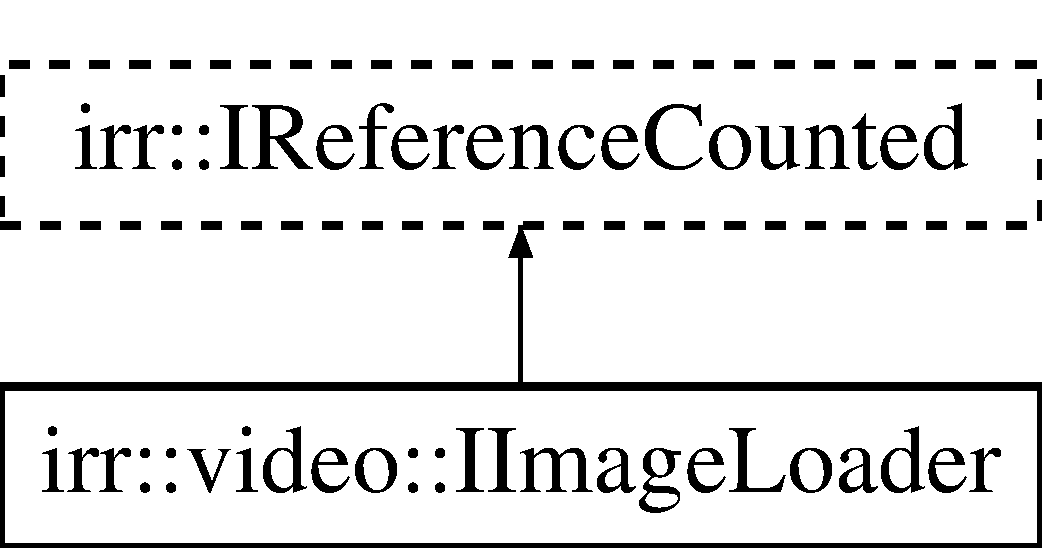
\includegraphics[height=2.000000cm]{classirr_1_1video_1_1IImageLoader}
\end{center}
\end{figure}
\subsection*{Public Member Functions}
\begin{DoxyCompactItemize}
\item 
virtual bool \hyperlink{classirr_1_1video_1_1IImageLoader_ad8c467efd18e7c74f845029083764df3}{is\+A\+Loadable\+File\+Extension} (const \hyperlink{namespaceirr_1_1io_ab1bdc45edb3f94d8319c02bc0f840ee1}{io\+::path} \&filename) const  =0
\begin{DoxyCompactList}\small\item\em Check if the file might be loaded by this class. \end{DoxyCompactList}\item 
virtual bool \hyperlink{classirr_1_1video_1_1IImageLoader_ad577be0a3111c625f60cb5204454a0be}{is\+A\+Loadable\+File\+Format} (\hyperlink{classirr_1_1io_1_1IReadFile}{io\+::\+I\+Read\+File} $\ast$file) const  =0
\begin{DoxyCompactList}\small\item\em Check if the file might be loaded by this class. \end{DoxyCompactList}\item 
virtual \hyperlink{classirr_1_1video_1_1IImage}{I\+Image} $\ast$ \hyperlink{classirr_1_1video_1_1IImageLoader_a6f3241106908fe8c9c0c929fe1fe770b}{load\+Image} (\hyperlink{classirr_1_1io_1_1IReadFile}{io\+::\+I\+Read\+File} $\ast$file) const  =0
\begin{DoxyCompactList}\small\item\em Creates a surface from the file. \end{DoxyCompactList}\end{DoxyCompactItemize}
\subsection*{Additional Inherited Members}


\subsection{Detailed Description}
Class which is able to create a image from a file. 

If you want the Irrlicht Engine be able to load textures of currently unsupported file formats (e.\+g .gif), then implement this and add your new Surface loader with \hyperlink{classirr_1_1video_1_1IVideoDriver_a9479ae15f0e26eaaf15c9420ff289b6d}{I\+Video\+Driver\+::add\+External\+Image\+Loader()} to the engine. 

\subsection{Member Function Documentation}
\index{irr\+::video\+::\+I\+Image\+Loader@{irr\+::video\+::\+I\+Image\+Loader}!is\+A\+Loadable\+File\+Extension@{is\+A\+Loadable\+File\+Extension}}
\index{is\+A\+Loadable\+File\+Extension@{is\+A\+Loadable\+File\+Extension}!irr\+::video\+::\+I\+Image\+Loader@{irr\+::video\+::\+I\+Image\+Loader}}
\subsubsection[{\texorpdfstring{is\+A\+Loadable\+File\+Extension(const io\+::path \&filename) const  =0}{isALoadableFileExtension(const io::path \&filename) const  =0}}]{\setlength{\rightskip}{0pt plus 5cm}virtual bool irr\+::video\+::\+I\+Image\+Loader\+::is\+A\+Loadable\+File\+Extension (
\begin{DoxyParamCaption}
\item[{const {\bf io\+::path} \&}]{filename}
\end{DoxyParamCaption}
) const\hspace{0.3cm}{\ttfamily [pure virtual]}}\hypertarget{classirr_1_1video_1_1IImageLoader_ad8c467efd18e7c74f845029083764df3}{}\label{classirr_1_1video_1_1IImageLoader_ad8c467efd18e7c74f845029083764df3}


Check if the file might be loaded by this class. 

Check is based on the file extension (e.\+g. \char`\"{}.\+tga\char`\"{}) 
\begin{DoxyParams}{Parameters}
{\em filename} & Name of file to check. \\
\hline
\end{DoxyParams}
\begin{DoxyReturn}{Returns}
True if file seems to be loadable. 
\end{DoxyReturn}
\index{irr\+::video\+::\+I\+Image\+Loader@{irr\+::video\+::\+I\+Image\+Loader}!is\+A\+Loadable\+File\+Format@{is\+A\+Loadable\+File\+Format}}
\index{is\+A\+Loadable\+File\+Format@{is\+A\+Loadable\+File\+Format}!irr\+::video\+::\+I\+Image\+Loader@{irr\+::video\+::\+I\+Image\+Loader}}
\subsubsection[{\texorpdfstring{is\+A\+Loadable\+File\+Format(io\+::\+I\+Read\+File $\ast$file) const  =0}{isALoadableFileFormat(io::IReadFile *file) const  =0}}]{\setlength{\rightskip}{0pt plus 5cm}virtual bool irr\+::video\+::\+I\+Image\+Loader\+::is\+A\+Loadable\+File\+Format (
\begin{DoxyParamCaption}
\item[{{\bf io\+::\+I\+Read\+File} $\ast$}]{file}
\end{DoxyParamCaption}
) const\hspace{0.3cm}{\ttfamily [pure virtual]}}\hypertarget{classirr_1_1video_1_1IImageLoader_ad577be0a3111c625f60cb5204454a0be}{}\label{classirr_1_1video_1_1IImageLoader_ad577be0a3111c625f60cb5204454a0be}


Check if the file might be loaded by this class. 

Check might look into the file. 
\begin{DoxyParams}{Parameters}
{\em file} & File handle to check. \\
\hline
\end{DoxyParams}
\begin{DoxyReturn}{Returns}
True if file seems to be loadable. 
\end{DoxyReturn}
\index{irr\+::video\+::\+I\+Image\+Loader@{irr\+::video\+::\+I\+Image\+Loader}!load\+Image@{load\+Image}}
\index{load\+Image@{load\+Image}!irr\+::video\+::\+I\+Image\+Loader@{irr\+::video\+::\+I\+Image\+Loader}}
\subsubsection[{\texorpdfstring{load\+Image(io\+::\+I\+Read\+File $\ast$file) const  =0}{loadImage(io::IReadFile *file) const  =0}}]{\setlength{\rightskip}{0pt plus 5cm}virtual {\bf I\+Image}$\ast$ irr\+::video\+::\+I\+Image\+Loader\+::load\+Image (
\begin{DoxyParamCaption}
\item[{{\bf io\+::\+I\+Read\+File} $\ast$}]{file}
\end{DoxyParamCaption}
) const\hspace{0.3cm}{\ttfamily [pure virtual]}}\hypertarget{classirr_1_1video_1_1IImageLoader_a6f3241106908fe8c9c0c929fe1fe770b}{}\label{classirr_1_1video_1_1IImageLoader_a6f3241106908fe8c9c0c929fe1fe770b}


Creates a surface from the file. 


\begin{DoxyParams}{Parameters}
{\em file} & File handle to check. \\
\hline
\end{DoxyParams}
\begin{DoxyReturn}{Returns}
Pointer to newly created image, or 0 upon error. 
\end{DoxyReturn}


The documentation for this class was generated from the following file\+:\begin{DoxyCompactItemize}
\item 
include/I\+Image\+Loader.\+h\end{DoxyCompactItemize}

\hypertarget{classirr_1_1video_1_1IImageWriter}{}\section{irr\+:\+:video\+:\+:I\+Image\+Writer Class Reference}
\label{classirr_1_1video_1_1IImageWriter}\index{irr\+::video\+::\+I\+Image\+Writer@{irr\+::video\+::\+I\+Image\+Writer}}


Interface for writing software image data.  




{\ttfamily \#include $<$I\+Image\+Writer.\+h$>$}

Inheritance diagram for irr\+:\+:video\+:\+:I\+Image\+Writer\+:\begin{figure}[H]
\begin{center}
\leavevmode
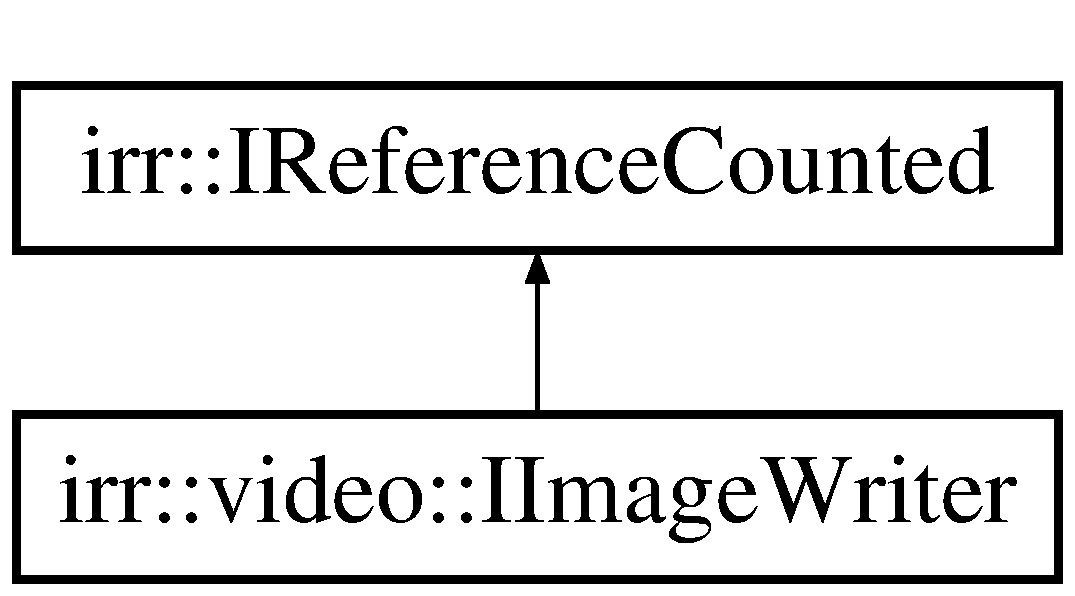
\includegraphics[height=2.000000cm]{classirr_1_1video_1_1IImageWriter}
\end{center}
\end{figure}
\subsection*{Public Member Functions}
\begin{DoxyCompactItemize}
\item 
virtual bool \hyperlink{classirr_1_1video_1_1IImageWriter_a41511c91ebb7f7d80085ed828455fc1c}{is\+A\+Writeable\+File\+Extension} (const \hyperlink{namespaceirr_1_1io_ab1bdc45edb3f94d8319c02bc0f840ee1}{io\+::path} \&filename) const  =0
\begin{DoxyCompactList}\small\item\em Check if this writer can write a file with the given extension. \end{DoxyCompactList}\item 
virtual bool \hyperlink{classirr_1_1video_1_1IImageWriter_a362efef33e28bc15fd1e307f0145dba8}{write\+Image} (\hyperlink{classirr_1_1io_1_1IWriteFile}{io\+::\+I\+Write\+File} $\ast$file, \hyperlink{classirr_1_1video_1_1IImage}{I\+Image} $\ast$image, \hyperlink{namespaceirr_a0416a53257075833e7002efd0a18e804}{u32} param=0) const  =0
\begin{DoxyCompactList}\small\item\em Write image to file. \end{DoxyCompactList}\end{DoxyCompactItemize}
\subsection*{Additional Inherited Members}


\subsection{Detailed Description}
Interface for writing software image data. 

\subsection{Member Function Documentation}
\index{irr\+::video\+::\+I\+Image\+Writer@{irr\+::video\+::\+I\+Image\+Writer}!is\+A\+Writeable\+File\+Extension@{is\+A\+Writeable\+File\+Extension}}
\index{is\+A\+Writeable\+File\+Extension@{is\+A\+Writeable\+File\+Extension}!irr\+::video\+::\+I\+Image\+Writer@{irr\+::video\+::\+I\+Image\+Writer}}
\subsubsection[{\texorpdfstring{is\+A\+Writeable\+File\+Extension(const io\+::path \&filename) const  =0}{isAWriteableFileExtension(const io::path \&filename) const  =0}}]{\setlength{\rightskip}{0pt plus 5cm}virtual bool irr\+::video\+::\+I\+Image\+Writer\+::is\+A\+Writeable\+File\+Extension (
\begin{DoxyParamCaption}
\item[{const {\bf io\+::path} \&}]{filename}
\end{DoxyParamCaption}
) const\hspace{0.3cm}{\ttfamily [pure virtual]}}\hypertarget{classirr_1_1video_1_1IImageWriter_a41511c91ebb7f7d80085ed828455fc1c}{}\label{classirr_1_1video_1_1IImageWriter_a41511c91ebb7f7d80085ed828455fc1c}


Check if this writer can write a file with the given extension. 


\begin{DoxyParams}{Parameters}
{\em filename} & Name of the file to check. \\
\hline
\end{DoxyParams}
\begin{DoxyReturn}{Returns}
True if file extension specifies a writable type. 
\end{DoxyReturn}
\index{irr\+::video\+::\+I\+Image\+Writer@{irr\+::video\+::\+I\+Image\+Writer}!write\+Image@{write\+Image}}
\index{write\+Image@{write\+Image}!irr\+::video\+::\+I\+Image\+Writer@{irr\+::video\+::\+I\+Image\+Writer}}
\subsubsection[{\texorpdfstring{write\+Image(io\+::\+I\+Write\+File $\ast$file, I\+Image $\ast$image, u32 param=0) const  =0}{writeImage(io::IWriteFile *file, IImage *image, u32 param=0) const  =0}}]{\setlength{\rightskip}{0pt plus 5cm}virtual bool irr\+::video\+::\+I\+Image\+Writer\+::write\+Image (
\begin{DoxyParamCaption}
\item[{{\bf io\+::\+I\+Write\+File} $\ast$}]{file, }
\item[{{\bf I\+Image} $\ast$}]{image, }
\item[{{\bf u32}}]{param = {\ttfamily 0}}
\end{DoxyParamCaption}
) const\hspace{0.3cm}{\ttfamily [pure virtual]}}\hypertarget{classirr_1_1video_1_1IImageWriter_a362efef33e28bc15fd1e307f0145dba8}{}\label{classirr_1_1video_1_1IImageWriter_a362efef33e28bc15fd1e307f0145dba8}


Write image to file. 


\begin{DoxyParams}{Parameters}
{\em file} & File handle to write to. \\
\hline
{\em image} & Image to write into file. \\
\hline
{\em param} & Writer specific parameter, influencing e.\+g. quality. \\
\hline
\end{DoxyParams}
\begin{DoxyReturn}{Returns}
True if image was successfully written. 
\end{DoxyReturn}


The documentation for this class was generated from the following file\+:\begin{DoxyCompactItemize}
\item 
include/I\+Image\+Writer.\+h\end{DoxyCompactItemize}

\hypertarget{classirr_1_1io_1_1IIrrXMLReader}{}\section{irr\+:\+:io\+:\+:I\+Irr\+X\+M\+L\+Reader$<$ char\+\_\+type, super\+\_\+class $>$ Class Template Reference}
\label{classirr_1_1io_1_1IIrrXMLReader}\index{irr\+::io\+::\+I\+Irr\+X\+M\+L\+Reader$<$ char\+\_\+type, super\+\_\+class $>$@{irr\+::io\+::\+I\+Irr\+X\+M\+L\+Reader$<$ char\+\_\+type, super\+\_\+class $>$}}


Interface providing easy read access to a X\+ML file.  




{\ttfamily \#include $<$irr\+X\+M\+L.\+h$>$}

Inheritance diagram for irr\+:\+:io\+:\+:I\+Irr\+X\+M\+L\+Reader$<$ char\+\_\+type, super\+\_\+class $>$\+:\begin{figure}[H]
\begin{center}
\leavevmode
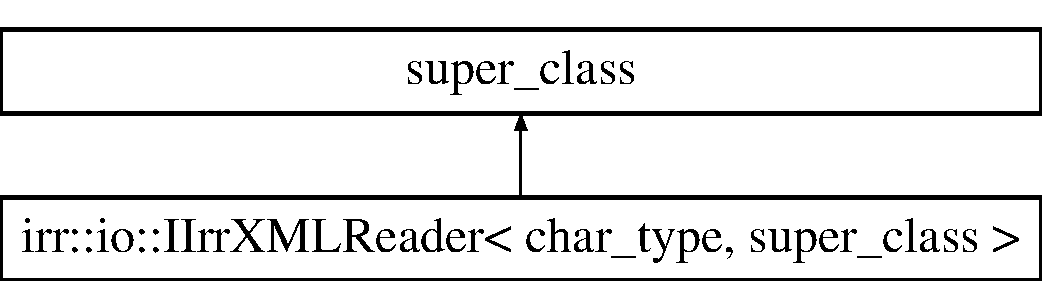
\includegraphics[height=2.000000cm]{classirr_1_1io_1_1IIrrXMLReader}
\end{center}
\end{figure}
\subsection*{Public Member Functions}
\begin{DoxyCompactItemize}
\item 
virtual \hyperlink{classirr_1_1io_1_1IIrrXMLReader_ad1d9faeae926afc224d9dea0ad7a08ac}{$\sim$\+I\+Irr\+X\+M\+L\+Reader} ()\hypertarget{classirr_1_1io_1_1IIrrXMLReader_ad1d9faeae926afc224d9dea0ad7a08ac}{}\label{classirr_1_1io_1_1IIrrXMLReader_ad1d9faeae926afc224d9dea0ad7a08ac}

\begin{DoxyCompactList}\small\item\em Destructor. \end{DoxyCompactList}\item 
virtual bool \hyperlink{classirr_1_1io_1_1IIrrXMLReader_a157f458f7dabeeff173f72a0fb443a8e}{read} ()=0
\begin{DoxyCompactList}\small\item\em Reads forward to the next xml node. \end{DoxyCompactList}\item 
virtual \hyperlink{namespaceirr_1_1io_a86a02676c9cbb822e04d60c81b4f33ed}{E\+X\+M\+L\+\_\+\+N\+O\+DE} \hyperlink{classirr_1_1io_1_1IIrrXMLReader_a62b779eddb8a8a7bc18878fc738cf1af}{get\+Node\+Type} () const  =0\hypertarget{classirr_1_1io_1_1IIrrXMLReader_a62b779eddb8a8a7bc18878fc738cf1af}{}\label{classirr_1_1io_1_1IIrrXMLReader_a62b779eddb8a8a7bc18878fc738cf1af}

\begin{DoxyCompactList}\small\item\em Returns the type of the current X\+ML node. \end{DoxyCompactList}\item 
virtual unsigned int \hyperlink{classirr_1_1io_1_1IIrrXMLReader_a66045277298db8d3db485ac2f5ea59c5}{get\+Attribute\+Count} () const  =0
\begin{DoxyCompactList}\small\item\em Returns attribute count of the current X\+ML node. \end{DoxyCompactList}\item 
virtual const char\+\_\+type $\ast$ \hyperlink{classirr_1_1io_1_1IIrrXMLReader_a5aa56a2623da10898f1f2bf1f92a243b}{get\+Attribute\+Name} (int idx) const  =0
\begin{DoxyCompactList}\small\item\em Returns name of an attribute. \end{DoxyCompactList}\item 
virtual const char\+\_\+type $\ast$ \hyperlink{classirr_1_1io_1_1IIrrXMLReader_a6b8721b2c9e4bbd165535af26afc6704}{get\+Attribute\+Value} (int idx) const  =0
\begin{DoxyCompactList}\small\item\em Returns the value of an attribute. \end{DoxyCompactList}\item 
virtual const char\+\_\+type $\ast$ \hyperlink{classirr_1_1io_1_1IIrrXMLReader_ad7632e2dd0bc1d3f76ec63e5a42eb4c7}{get\+Attribute\+Value} (const char\+\_\+type $\ast$name) const  =0
\begin{DoxyCompactList}\small\item\em Returns the value of an attribute. \end{DoxyCompactList}\item 
virtual const char\+\_\+type $\ast$ \hyperlink{classirr_1_1io_1_1IIrrXMLReader_a43ab4fd1fe9beb8a4a4ecea7a7e0c766}{get\+Attribute\+Value\+Safe} (const char\+\_\+type $\ast$name) const  =0
\begin{DoxyCompactList}\small\item\em Returns the value of an attribute in a safe way. \end{DoxyCompactList}\item 
virtual int \hyperlink{classirr_1_1io_1_1IIrrXMLReader_ac66b72a442f5f3b103133ceeaf0ce8d2}{get\+Attribute\+Value\+As\+Int} (const char\+\_\+type $\ast$name) const  =0
\begin{DoxyCompactList}\small\item\em Returns the value of an attribute as integer. \end{DoxyCompactList}\item 
virtual int \hyperlink{classirr_1_1io_1_1IIrrXMLReader_ae07b2fef9c200362fc4bb11759428d93}{get\+Attribute\+Value\+As\+Int} (int idx) const  =0
\begin{DoxyCompactList}\small\item\em Returns the value of an attribute as integer. \end{DoxyCompactList}\item 
virtual float \hyperlink{classirr_1_1io_1_1IIrrXMLReader_ae29fd76d29855774c854369047917bac}{get\+Attribute\+Value\+As\+Float} (const char\+\_\+type $\ast$name) const  =0
\begin{DoxyCompactList}\small\item\em Returns the value of an attribute as float. \end{DoxyCompactList}\item 
virtual float \hyperlink{classirr_1_1io_1_1IIrrXMLReader_a9ca89b6f3c930eb94dac0c283cc79b1c}{get\+Attribute\+Value\+As\+Float} (int idx) const  =0
\begin{DoxyCompactList}\small\item\em Returns the value of an attribute as float. \end{DoxyCompactList}\item 
virtual const char\+\_\+type $\ast$ \hyperlink{classirr_1_1io_1_1IIrrXMLReader_a5e168b2f2321eefff0922823072d7c5d}{get\+Node\+Name} () const  =0
\begin{DoxyCompactList}\small\item\em Returns the name of the current node. \end{DoxyCompactList}\item 
virtual const char\+\_\+type $\ast$ \hyperlink{classirr_1_1io_1_1IIrrXMLReader_a0e46cdf194b2c6b6db908989c000ba58}{get\+Node\+Data} () const  =0
\begin{DoxyCompactList}\small\item\em Returns data of the current node. \end{DoxyCompactList}\item 
virtual bool \hyperlink{classirr_1_1io_1_1IIrrXMLReader_a4de66bcaae7f017803b341785c4dab9a}{is\+Empty\+Element} () const  =0\hypertarget{classirr_1_1io_1_1IIrrXMLReader_a4de66bcaae7f017803b341785c4dab9a}{}\label{classirr_1_1io_1_1IIrrXMLReader_a4de66bcaae7f017803b341785c4dab9a}

\begin{DoxyCompactList}\small\item\em Returns if an element is an empty element, like $<$foo /$>$ \end{DoxyCompactList}\item 
virtual \hyperlink{namespaceirr_1_1io_ac7e51e5a6bd00451dec248f497b16a9d}{E\+T\+E\+X\+T\+\_\+\+F\+O\+R\+M\+AT} \hyperlink{classirr_1_1io_1_1IIrrXMLReader_ae43dfce5f583202501bb1fc9eeb42df7}{get\+Source\+Format} () const  =0
\begin{DoxyCompactList}\small\item\em Returns format of the source xml file. \end{DoxyCompactList}\item 
virtual \hyperlink{namespaceirr_1_1io_ac7e51e5a6bd00451dec248f497b16a9d}{E\+T\+E\+X\+T\+\_\+\+F\+O\+R\+M\+AT} \hyperlink{classirr_1_1io_1_1IIrrXMLReader_ac124d1c4fa2909d5328de5a616b4af44}{get\+Parser\+Format} () const  =0
\begin{DoxyCompactList}\small\item\em Returns format of the strings returned by the parser. \end{DoxyCompactList}\end{DoxyCompactItemize}


\subsection{Detailed Description}
\subsubsection*{template$<$class char\+\_\+type, class super\+\_\+class$>$\\*
class irr\+::io\+::\+I\+Irr\+X\+M\+L\+Reader$<$ char\+\_\+type, super\+\_\+class $>$}

Interface providing easy read access to a X\+ML file. 

You can create an instance of this reader using one of the factory functions \hyperlink{namespaceirr_1_1io_a581f4d4648398759c61266d63d7106b1}{create\+Irr\+X\+M\+L\+Reader()}, \hyperlink{namespaceirr_1_1io_a86473ef152c15b685af181a4c5461a5d}{create\+Irr\+X\+M\+L\+Reader\+U\+T\+F16()} and \hyperlink{namespaceirr_1_1io_ae05bf7ee342431ea8c98fb98e75b974a}{create\+Irr\+X\+M\+L\+Reader\+U\+T\+F32()}. If using the parser from the Irrlicht Engine, please use \hyperlink{classirr_1_1io_1_1IFileSystem_a167c9fa159d16ee5c56c074636b0865e}{I\+File\+System\+::create\+X\+M\+L\+Reader()} instead. For a detailed intro how to use the parser, see \hyperlink{index_irrxmlexample}{Example} and \hyperlink{index_features}{Features}.

The typical usage of this parser looks like this\+: 
\begin{DoxyCode}
\textcolor{preprocessor}{#include <\hyperlink{irrXML_8h}{irrXML.h}>}
\textcolor{keyword}{using namespace }\hyperlink{namespaceirr}{irr}; \textcolor{comment}{// irrXML is located in the namespace irr::io}
\textcolor{keyword}{using namespace }io;

\textcolor{keywordtype}{void} main()
\{
    \textcolor{comment}{// create the reader using one of the factory functions}
    \hyperlink{namespaceirr_1_1io_a1628edbb9d5d53f18c82d2a92b0ad27e}{IrrXMLReader}* xml = \hyperlink{namespaceirr_1_1io_a581f4d4648398759c61266d63d7106b1}{createIrrXMLReader}(\textcolor{stringliteral}{"config.xml"});

    \textcolor{keywordflow}{if} (xml == 0)
        \textcolor{keywordflow}{return}; \textcolor{comment}{// file could not be opened}

    \textcolor{comment}{// parse the file until end reached}
    \textcolor{keywordflow}{while}(xml->read())
    \{
        \textcolor{comment}{// based on xml->getNodeType(), do something.}
    \}

    \textcolor{comment}{// delete the xml parser after usage}
    \textcolor{keyword}{delete} xml;
\}
\end{DoxyCode}
 See \hyperlink{index_irrxmlexample}{Example} for a more detailed example. 

\subsection{Member Function Documentation}
\index{irr\+::io\+::\+I\+Irr\+X\+M\+L\+Reader@{irr\+::io\+::\+I\+Irr\+X\+M\+L\+Reader}!get\+Attribute\+Count@{get\+Attribute\+Count}}
\index{get\+Attribute\+Count@{get\+Attribute\+Count}!irr\+::io\+::\+I\+Irr\+X\+M\+L\+Reader@{irr\+::io\+::\+I\+Irr\+X\+M\+L\+Reader}}
\subsubsection[{\texorpdfstring{get\+Attribute\+Count() const  =0}{getAttributeCount() const  =0}}]{\setlength{\rightskip}{0pt plus 5cm}template$<$class char\+\_\+type , class super\+\_\+class $>$ virtual unsigned int {\bf irr\+::io\+::\+I\+Irr\+X\+M\+L\+Reader}$<$ char\+\_\+type, super\+\_\+class $>$\+::get\+Attribute\+Count (
\begin{DoxyParamCaption}
{}
\end{DoxyParamCaption}
) const\hspace{0.3cm}{\ttfamily [pure virtual]}}\hypertarget{classirr_1_1io_1_1IIrrXMLReader_a66045277298db8d3db485ac2f5ea59c5}{}\label{classirr_1_1io_1_1IIrrXMLReader_a66045277298db8d3db485ac2f5ea59c5}


Returns attribute count of the current X\+ML node. 

This is usually non null if the current node is E\+X\+N\+\_\+\+E\+L\+E\+M\+E\+NT, and the element has attributes. \begin{DoxyReturn}{Returns}
Returns amount of attributes of this xml node. 
\end{DoxyReturn}
\index{irr\+::io\+::\+I\+Irr\+X\+M\+L\+Reader@{irr\+::io\+::\+I\+Irr\+X\+M\+L\+Reader}!get\+Attribute\+Name@{get\+Attribute\+Name}}
\index{get\+Attribute\+Name@{get\+Attribute\+Name}!irr\+::io\+::\+I\+Irr\+X\+M\+L\+Reader@{irr\+::io\+::\+I\+Irr\+X\+M\+L\+Reader}}
\subsubsection[{\texorpdfstring{get\+Attribute\+Name(int idx) const  =0}{getAttributeName(int idx) const  =0}}]{\setlength{\rightskip}{0pt plus 5cm}template$<$class char\+\_\+type , class super\+\_\+class $>$ virtual const char\+\_\+type$\ast$ {\bf irr\+::io\+::\+I\+Irr\+X\+M\+L\+Reader}$<$ char\+\_\+type, super\+\_\+class $>$\+::get\+Attribute\+Name (
\begin{DoxyParamCaption}
\item[{int}]{idx}
\end{DoxyParamCaption}
) const\hspace{0.3cm}{\ttfamily [pure virtual]}}\hypertarget{classirr_1_1io_1_1IIrrXMLReader_a5aa56a2623da10898f1f2bf1f92a243b}{}\label{classirr_1_1io_1_1IIrrXMLReader_a5aa56a2623da10898f1f2bf1f92a243b}


Returns name of an attribute. 


\begin{DoxyParams}{Parameters}
{\em idx} & Zero based index, should be something between 0 and \hyperlink{classirr_1_1io_1_1IIrrXMLReader_a66045277298db8d3db485ac2f5ea59c5}{get\+Attribute\+Count()}-\/1. \\
\hline
\end{DoxyParams}
\begin{DoxyReturn}{Returns}
Name of the attribute, 0 if an attribute with this index does not exist. 
\end{DoxyReturn}
\index{irr\+::io\+::\+I\+Irr\+X\+M\+L\+Reader@{irr\+::io\+::\+I\+Irr\+X\+M\+L\+Reader}!get\+Attribute\+Value@{get\+Attribute\+Value}}
\index{get\+Attribute\+Value@{get\+Attribute\+Value}!irr\+::io\+::\+I\+Irr\+X\+M\+L\+Reader@{irr\+::io\+::\+I\+Irr\+X\+M\+L\+Reader}}
\subsubsection[{\texorpdfstring{get\+Attribute\+Value(int idx) const  =0}{getAttributeValue(int idx) const  =0}}]{\setlength{\rightskip}{0pt plus 5cm}template$<$class char\+\_\+type , class super\+\_\+class $>$ virtual const char\+\_\+type$\ast$ {\bf irr\+::io\+::\+I\+Irr\+X\+M\+L\+Reader}$<$ char\+\_\+type, super\+\_\+class $>$\+::get\+Attribute\+Value (
\begin{DoxyParamCaption}
\item[{int}]{idx}
\end{DoxyParamCaption}
) const\hspace{0.3cm}{\ttfamily [pure virtual]}}\hypertarget{classirr_1_1io_1_1IIrrXMLReader_a6b8721b2c9e4bbd165535af26afc6704}{}\label{classirr_1_1io_1_1IIrrXMLReader_a6b8721b2c9e4bbd165535af26afc6704}


Returns the value of an attribute. 


\begin{DoxyParams}{Parameters}
{\em idx} & Zero based index, should be something between 0 and \hyperlink{classirr_1_1io_1_1IIrrXMLReader_a66045277298db8d3db485ac2f5ea59c5}{get\+Attribute\+Count()}-\/1. \\
\hline
\end{DoxyParams}
\begin{DoxyReturn}{Returns}
Value of the attribute, 0 if an attribute with this index does not exist. 
\end{DoxyReturn}
\index{irr\+::io\+::\+I\+Irr\+X\+M\+L\+Reader@{irr\+::io\+::\+I\+Irr\+X\+M\+L\+Reader}!get\+Attribute\+Value@{get\+Attribute\+Value}}
\index{get\+Attribute\+Value@{get\+Attribute\+Value}!irr\+::io\+::\+I\+Irr\+X\+M\+L\+Reader@{irr\+::io\+::\+I\+Irr\+X\+M\+L\+Reader}}
\subsubsection[{\texorpdfstring{get\+Attribute\+Value(const char\+\_\+type $\ast$name) const  =0}{getAttributeValue(const char\_type *name) const  =0}}]{\setlength{\rightskip}{0pt plus 5cm}template$<$class char\+\_\+type , class super\+\_\+class $>$ virtual const char\+\_\+type$\ast$ {\bf irr\+::io\+::\+I\+Irr\+X\+M\+L\+Reader}$<$ char\+\_\+type, super\+\_\+class $>$\+::get\+Attribute\+Value (
\begin{DoxyParamCaption}
\item[{const char\+\_\+type $\ast$}]{name}
\end{DoxyParamCaption}
) const\hspace{0.3cm}{\ttfamily [pure virtual]}}\hypertarget{classirr_1_1io_1_1IIrrXMLReader_ad7632e2dd0bc1d3f76ec63e5a42eb4c7}{}\label{classirr_1_1io_1_1IIrrXMLReader_ad7632e2dd0bc1d3f76ec63e5a42eb4c7}


Returns the value of an attribute. 


\begin{DoxyParams}{Parameters}
{\em name} & Name of the attribute. \\
\hline
\end{DoxyParams}
\begin{DoxyReturn}{Returns}
Value of the attribute, 0 if an attribute with this name does not exist. 
\end{DoxyReturn}
\index{irr\+::io\+::\+I\+Irr\+X\+M\+L\+Reader@{irr\+::io\+::\+I\+Irr\+X\+M\+L\+Reader}!get\+Attribute\+Value\+As\+Float@{get\+Attribute\+Value\+As\+Float}}
\index{get\+Attribute\+Value\+As\+Float@{get\+Attribute\+Value\+As\+Float}!irr\+::io\+::\+I\+Irr\+X\+M\+L\+Reader@{irr\+::io\+::\+I\+Irr\+X\+M\+L\+Reader}}
\subsubsection[{\texorpdfstring{get\+Attribute\+Value\+As\+Float(const char\+\_\+type $\ast$name) const  =0}{getAttributeValueAsFloat(const char\_type *name) const  =0}}]{\setlength{\rightskip}{0pt plus 5cm}template$<$class char\+\_\+type , class super\+\_\+class $>$ virtual float {\bf irr\+::io\+::\+I\+Irr\+X\+M\+L\+Reader}$<$ char\+\_\+type, super\+\_\+class $>$\+::get\+Attribute\+Value\+As\+Float (
\begin{DoxyParamCaption}
\item[{const char\+\_\+type $\ast$}]{name}
\end{DoxyParamCaption}
) const\hspace{0.3cm}{\ttfamily [pure virtual]}}\hypertarget{classirr_1_1io_1_1IIrrXMLReader_ae29fd76d29855774c854369047917bac}{}\label{classirr_1_1io_1_1IIrrXMLReader_ae29fd76d29855774c854369047917bac}


Returns the value of an attribute as float. 


\begin{DoxyParams}{Parameters}
{\em name} & Name of the attribute. \\
\hline
\end{DoxyParams}
\begin{DoxyReturn}{Returns}
Value of the attribute as float, and 0 if an attribute with this name does not exist or the value could not be interpreted as float. 
\end{DoxyReturn}
\index{irr\+::io\+::\+I\+Irr\+X\+M\+L\+Reader@{irr\+::io\+::\+I\+Irr\+X\+M\+L\+Reader}!get\+Attribute\+Value\+As\+Float@{get\+Attribute\+Value\+As\+Float}}
\index{get\+Attribute\+Value\+As\+Float@{get\+Attribute\+Value\+As\+Float}!irr\+::io\+::\+I\+Irr\+X\+M\+L\+Reader@{irr\+::io\+::\+I\+Irr\+X\+M\+L\+Reader}}
\subsubsection[{\texorpdfstring{get\+Attribute\+Value\+As\+Float(int idx) const  =0}{getAttributeValueAsFloat(int idx) const  =0}}]{\setlength{\rightskip}{0pt plus 5cm}template$<$class char\+\_\+type , class super\+\_\+class $>$ virtual float {\bf irr\+::io\+::\+I\+Irr\+X\+M\+L\+Reader}$<$ char\+\_\+type, super\+\_\+class $>$\+::get\+Attribute\+Value\+As\+Float (
\begin{DoxyParamCaption}
\item[{int}]{idx}
\end{DoxyParamCaption}
) const\hspace{0.3cm}{\ttfamily [pure virtual]}}\hypertarget{classirr_1_1io_1_1IIrrXMLReader_a9ca89b6f3c930eb94dac0c283cc79b1c}{}\label{classirr_1_1io_1_1IIrrXMLReader_a9ca89b6f3c930eb94dac0c283cc79b1c}


Returns the value of an attribute as float. 


\begin{DoxyParams}{Parameters}
{\em idx} & Zero based index, should be something between 0 and \hyperlink{classirr_1_1io_1_1IIrrXMLReader_a66045277298db8d3db485ac2f5ea59c5}{get\+Attribute\+Count()}-\/1. \\
\hline
\end{DoxyParams}
\begin{DoxyReturn}{Returns}
Value of the attribute as float, and 0 if an attribute with this index does not exist or the value could not be interpreted as float. 
\end{DoxyReturn}
\index{irr\+::io\+::\+I\+Irr\+X\+M\+L\+Reader@{irr\+::io\+::\+I\+Irr\+X\+M\+L\+Reader}!get\+Attribute\+Value\+As\+Int@{get\+Attribute\+Value\+As\+Int}}
\index{get\+Attribute\+Value\+As\+Int@{get\+Attribute\+Value\+As\+Int}!irr\+::io\+::\+I\+Irr\+X\+M\+L\+Reader@{irr\+::io\+::\+I\+Irr\+X\+M\+L\+Reader}}
\subsubsection[{\texorpdfstring{get\+Attribute\+Value\+As\+Int(const char\+\_\+type $\ast$name) const  =0}{getAttributeValueAsInt(const char\_type *name) const  =0}}]{\setlength{\rightskip}{0pt plus 5cm}template$<$class char\+\_\+type , class super\+\_\+class $>$ virtual int {\bf irr\+::io\+::\+I\+Irr\+X\+M\+L\+Reader}$<$ char\+\_\+type, super\+\_\+class $>$\+::get\+Attribute\+Value\+As\+Int (
\begin{DoxyParamCaption}
\item[{const char\+\_\+type $\ast$}]{name}
\end{DoxyParamCaption}
) const\hspace{0.3cm}{\ttfamily [pure virtual]}}\hypertarget{classirr_1_1io_1_1IIrrXMLReader_ac66b72a442f5f3b103133ceeaf0ce8d2}{}\label{classirr_1_1io_1_1IIrrXMLReader_ac66b72a442f5f3b103133ceeaf0ce8d2}


Returns the value of an attribute as integer. 


\begin{DoxyParams}{Parameters}
{\em name} & Name of the attribute. \\
\hline
\end{DoxyParams}
\begin{DoxyReturn}{Returns}
Value of the attribute as integer, and 0 if an attribute with this name does not exist or the value could not be interpreted as integer. 
\end{DoxyReturn}
\index{irr\+::io\+::\+I\+Irr\+X\+M\+L\+Reader@{irr\+::io\+::\+I\+Irr\+X\+M\+L\+Reader}!get\+Attribute\+Value\+As\+Int@{get\+Attribute\+Value\+As\+Int}}
\index{get\+Attribute\+Value\+As\+Int@{get\+Attribute\+Value\+As\+Int}!irr\+::io\+::\+I\+Irr\+X\+M\+L\+Reader@{irr\+::io\+::\+I\+Irr\+X\+M\+L\+Reader}}
\subsubsection[{\texorpdfstring{get\+Attribute\+Value\+As\+Int(int idx) const  =0}{getAttributeValueAsInt(int idx) const  =0}}]{\setlength{\rightskip}{0pt plus 5cm}template$<$class char\+\_\+type , class super\+\_\+class $>$ virtual int {\bf irr\+::io\+::\+I\+Irr\+X\+M\+L\+Reader}$<$ char\+\_\+type, super\+\_\+class $>$\+::get\+Attribute\+Value\+As\+Int (
\begin{DoxyParamCaption}
\item[{int}]{idx}
\end{DoxyParamCaption}
) const\hspace{0.3cm}{\ttfamily [pure virtual]}}\hypertarget{classirr_1_1io_1_1IIrrXMLReader_ae07b2fef9c200362fc4bb11759428d93}{}\label{classirr_1_1io_1_1IIrrXMLReader_ae07b2fef9c200362fc4bb11759428d93}


Returns the value of an attribute as integer. 


\begin{DoxyParams}{Parameters}
{\em idx} & Zero based index, should be something between 0 and \hyperlink{classirr_1_1io_1_1IIrrXMLReader_a66045277298db8d3db485ac2f5ea59c5}{get\+Attribute\+Count()}-\/1. \\
\hline
\end{DoxyParams}
\begin{DoxyReturn}{Returns}
Value of the attribute as integer, and 0 if an attribute with this index does not exist or the value could not be interpreted as integer. 
\end{DoxyReturn}
\index{irr\+::io\+::\+I\+Irr\+X\+M\+L\+Reader@{irr\+::io\+::\+I\+Irr\+X\+M\+L\+Reader}!get\+Attribute\+Value\+Safe@{get\+Attribute\+Value\+Safe}}
\index{get\+Attribute\+Value\+Safe@{get\+Attribute\+Value\+Safe}!irr\+::io\+::\+I\+Irr\+X\+M\+L\+Reader@{irr\+::io\+::\+I\+Irr\+X\+M\+L\+Reader}}
\subsubsection[{\texorpdfstring{get\+Attribute\+Value\+Safe(const char\+\_\+type $\ast$name) const  =0}{getAttributeValueSafe(const char\_type *name) const  =0}}]{\setlength{\rightskip}{0pt plus 5cm}template$<$class char\+\_\+type , class super\+\_\+class $>$ virtual const char\+\_\+type$\ast$ {\bf irr\+::io\+::\+I\+Irr\+X\+M\+L\+Reader}$<$ char\+\_\+type, super\+\_\+class $>$\+::get\+Attribute\+Value\+Safe (
\begin{DoxyParamCaption}
\item[{const char\+\_\+type $\ast$}]{name}
\end{DoxyParamCaption}
) const\hspace{0.3cm}{\ttfamily [pure virtual]}}\hypertarget{classirr_1_1io_1_1IIrrXMLReader_a43ab4fd1fe9beb8a4a4ecea7a7e0c766}{}\label{classirr_1_1io_1_1IIrrXMLReader_a43ab4fd1fe9beb8a4a4ecea7a7e0c766}


Returns the value of an attribute in a safe way. 

Like \hyperlink{classirr_1_1io_1_1IIrrXMLReader_a6b8721b2c9e4bbd165535af26afc6704}{get\+Attribute\+Value()}, but does not return 0 if the attribute does not exist. An empty string (\char`\"{}\char`\"{}) is returned then. 
\begin{DoxyParams}{Parameters}
{\em name} & Name of the attribute. \\
\hline
\end{DoxyParams}
\begin{DoxyReturn}{Returns}
Value of the attribute, and \char`\"{}\char`\"{} if an attribute with this name does not exist 
\end{DoxyReturn}
\index{irr\+::io\+::\+I\+Irr\+X\+M\+L\+Reader@{irr\+::io\+::\+I\+Irr\+X\+M\+L\+Reader}!get\+Node\+Data@{get\+Node\+Data}}
\index{get\+Node\+Data@{get\+Node\+Data}!irr\+::io\+::\+I\+Irr\+X\+M\+L\+Reader@{irr\+::io\+::\+I\+Irr\+X\+M\+L\+Reader}}
\subsubsection[{\texorpdfstring{get\+Node\+Data() const  =0}{getNodeData() const  =0}}]{\setlength{\rightskip}{0pt plus 5cm}template$<$class char\+\_\+type , class super\+\_\+class $>$ virtual const char\+\_\+type$\ast$ {\bf irr\+::io\+::\+I\+Irr\+X\+M\+L\+Reader}$<$ char\+\_\+type, super\+\_\+class $>$\+::get\+Node\+Data (
\begin{DoxyParamCaption}
{}
\end{DoxyParamCaption}
) const\hspace{0.3cm}{\ttfamily [pure virtual]}}\hypertarget{classirr_1_1io_1_1IIrrXMLReader_a0e46cdf194b2c6b6db908989c000ba58}{}\label{classirr_1_1io_1_1IIrrXMLReader_a0e46cdf194b2c6b6db908989c000ba58}


Returns data of the current node. 

Only valid if the node has some data and it is of type E\+X\+N\+\_\+\+T\+E\+XT, E\+X\+N\+\_\+\+C\+O\+M\+M\+E\+NT, E\+X\+N\+\_\+\+C\+D\+A\+TA or E\+X\+N\+\_\+\+U\+N\+K\+N\+O\+WN. \index{irr\+::io\+::\+I\+Irr\+X\+M\+L\+Reader@{irr\+::io\+::\+I\+Irr\+X\+M\+L\+Reader}!get\+Node\+Name@{get\+Node\+Name}}
\index{get\+Node\+Name@{get\+Node\+Name}!irr\+::io\+::\+I\+Irr\+X\+M\+L\+Reader@{irr\+::io\+::\+I\+Irr\+X\+M\+L\+Reader}}
\subsubsection[{\texorpdfstring{get\+Node\+Name() const  =0}{getNodeName() const  =0}}]{\setlength{\rightskip}{0pt plus 5cm}template$<$class char\+\_\+type , class super\+\_\+class $>$ virtual const char\+\_\+type$\ast$ {\bf irr\+::io\+::\+I\+Irr\+X\+M\+L\+Reader}$<$ char\+\_\+type, super\+\_\+class $>$\+::get\+Node\+Name (
\begin{DoxyParamCaption}
{}
\end{DoxyParamCaption}
) const\hspace{0.3cm}{\ttfamily [pure virtual]}}\hypertarget{classirr_1_1io_1_1IIrrXMLReader_a5e168b2f2321eefff0922823072d7c5d}{}\label{classirr_1_1io_1_1IIrrXMLReader_a5e168b2f2321eefff0922823072d7c5d}


Returns the name of the current node. 

Only valid, if the node type is E\+X\+N\+\_\+\+E\+L\+E\+M\+E\+NT. \begin{DoxyReturn}{Returns}
Name of the current node or 0 if the node has no name. 
\end{DoxyReturn}
\index{irr\+::io\+::\+I\+Irr\+X\+M\+L\+Reader@{irr\+::io\+::\+I\+Irr\+X\+M\+L\+Reader}!get\+Parser\+Format@{get\+Parser\+Format}}
\index{get\+Parser\+Format@{get\+Parser\+Format}!irr\+::io\+::\+I\+Irr\+X\+M\+L\+Reader@{irr\+::io\+::\+I\+Irr\+X\+M\+L\+Reader}}
\subsubsection[{\texorpdfstring{get\+Parser\+Format() const  =0}{getParserFormat() const  =0}}]{\setlength{\rightskip}{0pt plus 5cm}template$<$class char\+\_\+type , class super\+\_\+class $>$ virtual {\bf E\+T\+E\+X\+T\+\_\+\+F\+O\+R\+M\+AT} {\bf irr\+::io\+::\+I\+Irr\+X\+M\+L\+Reader}$<$ char\+\_\+type, super\+\_\+class $>$\+::get\+Parser\+Format (
\begin{DoxyParamCaption}
{}
\end{DoxyParamCaption}
) const\hspace{0.3cm}{\ttfamily [pure virtual]}}\hypertarget{classirr_1_1io_1_1IIrrXMLReader_ac124d1c4fa2909d5328de5a616b4af44}{}\label{classirr_1_1io_1_1IIrrXMLReader_ac124d1c4fa2909d5328de5a616b4af44}


Returns format of the strings returned by the parser. 

This will be U\+T\+F8 for example when you created a parser with Irr\+X\+M\+L\+Reader\+U\+T\+F8() and U\+T\+F32 when it has been created using Irr\+X\+M\+L\+Reader\+U\+T\+F32. It should not be necessary to call this method and only exists for informational purposes. \index{irr\+::io\+::\+I\+Irr\+X\+M\+L\+Reader@{irr\+::io\+::\+I\+Irr\+X\+M\+L\+Reader}!get\+Source\+Format@{get\+Source\+Format}}
\index{get\+Source\+Format@{get\+Source\+Format}!irr\+::io\+::\+I\+Irr\+X\+M\+L\+Reader@{irr\+::io\+::\+I\+Irr\+X\+M\+L\+Reader}}
\subsubsection[{\texorpdfstring{get\+Source\+Format() const  =0}{getSourceFormat() const  =0}}]{\setlength{\rightskip}{0pt plus 5cm}template$<$class char\+\_\+type , class super\+\_\+class $>$ virtual {\bf E\+T\+E\+X\+T\+\_\+\+F\+O\+R\+M\+AT} {\bf irr\+::io\+::\+I\+Irr\+X\+M\+L\+Reader}$<$ char\+\_\+type, super\+\_\+class $>$\+::get\+Source\+Format (
\begin{DoxyParamCaption}
{}
\end{DoxyParamCaption}
) const\hspace{0.3cm}{\ttfamily [pure virtual]}}\hypertarget{classirr_1_1io_1_1IIrrXMLReader_ae43dfce5f583202501bb1fc9eeb42df7}{}\label{classirr_1_1io_1_1IIrrXMLReader_ae43dfce5f583202501bb1fc9eeb42df7}


Returns format of the source xml file. 

It is not necessary to use this method because the parser will convert the input file format to the format wanted by the user when creating the parser. This method is useful to get/display additional informations. \index{irr\+::io\+::\+I\+Irr\+X\+M\+L\+Reader@{irr\+::io\+::\+I\+Irr\+X\+M\+L\+Reader}!read@{read}}
\index{read@{read}!irr\+::io\+::\+I\+Irr\+X\+M\+L\+Reader@{irr\+::io\+::\+I\+Irr\+X\+M\+L\+Reader}}
\subsubsection[{\texorpdfstring{read()=0}{read()=0}}]{\setlength{\rightskip}{0pt plus 5cm}template$<$class char\+\_\+type , class super\+\_\+class $>$ virtual bool {\bf irr\+::io\+::\+I\+Irr\+X\+M\+L\+Reader}$<$ char\+\_\+type, super\+\_\+class $>$\+::read (
\begin{DoxyParamCaption}
{}
\end{DoxyParamCaption}
)\hspace{0.3cm}{\ttfamily [pure virtual]}}\hypertarget{classirr_1_1io_1_1IIrrXMLReader_a157f458f7dabeeff173f72a0fb443a8e}{}\label{classirr_1_1io_1_1IIrrXMLReader_a157f458f7dabeeff173f72a0fb443a8e}


Reads forward to the next xml node. 

\begin{DoxyReturn}{Returns}
Returns false, if there was no further node. 
\end{DoxyReturn}


The documentation for this class was generated from the following file\+:\begin{DoxyCompactItemize}
\item 
include/\hyperlink{irrXML_8h}{irr\+X\+M\+L.\+h}\end{DoxyCompactItemize}

\hypertarget{classirr_1_1scene_1_1ILightManager}{}\section{irr\+:\+:scene\+:\+:I\+Light\+Manager Class Reference}
\label{classirr_1_1scene_1_1ILightManager}\index{irr\+::scene\+::\+I\+Light\+Manager@{irr\+::scene\+::\+I\+Light\+Manager}}


\hyperlink{classirr_1_1scene_1_1ILightManager}{I\+Light\+Manager} provides an interface for user applications to manipulate the list of lights in the scene.  




{\ttfamily \#include $<$I\+Light\+Manager.\+h$>$}

Inheritance diagram for irr\+:\+:scene\+:\+:I\+Light\+Manager\+:\begin{figure}[H]
\begin{center}
\leavevmode
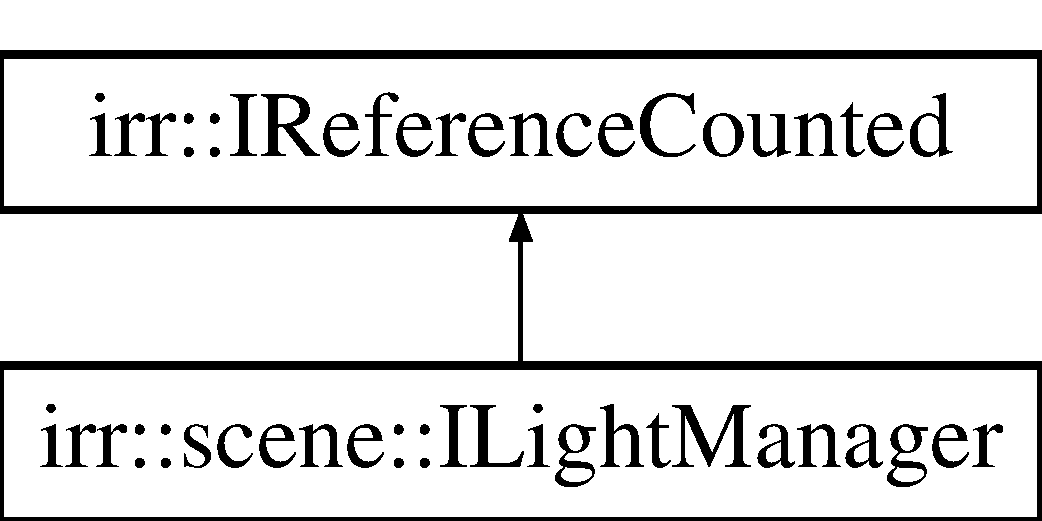
\includegraphics[height=2.000000cm]{classirr_1_1scene_1_1ILightManager}
\end{center}
\end{figure}
\subsection*{Public Member Functions}
\begin{DoxyCompactItemize}
\item 
virtual void \hyperlink{classirr_1_1scene_1_1ILightManager_a060badf09dc2f8ba8ddb148034c27817}{On\+Pre\+Render} (\hyperlink{classirr_1_1core_1_1array}{core\+::array}$<$ \hyperlink{classirr_1_1scene_1_1ISceneNode}{I\+Scene\+Node} $\ast$ $>$ \&light\+List)=0
\begin{DoxyCompactList}\small\item\em Called after the scene\textquotesingle{}s light list has been built, but before rendering has begun. \end{DoxyCompactList}\item 
virtual void \hyperlink{classirr_1_1scene_1_1ILightManager_ac8f92f0fbd43ba9cb01b47647125a1a3}{On\+Post\+Render} (void)=0
\begin{DoxyCompactList}\small\item\em Called after the last scene node is rendered. \end{DoxyCompactList}\item 
virtual void \hyperlink{classirr_1_1scene_1_1ILightManager_a56eaec6a697659f40b4f29b681fbdfad}{On\+Render\+Pass\+Pre\+Render} (\hyperlink{namespaceirr_1_1scene_a7862269bd1abc123929d4dbb8200d67f}{E\+\_\+\+S\+C\+E\+N\+E\+\_\+\+N\+O\+D\+E\+\_\+\+R\+E\+N\+D\+E\+R\+\_\+\+P\+A\+SS} render\+Pass)=0
\begin{DoxyCompactList}\small\item\em Called before a render pass begins. \end{DoxyCompactList}\item 
virtual void \hyperlink{classirr_1_1scene_1_1ILightManager_a189edbf3a16ebb3c82e5d9f93dd2b41b}{On\+Render\+Pass\+Post\+Render} (\hyperlink{namespaceirr_1_1scene_a7862269bd1abc123929d4dbb8200d67f}{E\+\_\+\+S\+C\+E\+N\+E\+\_\+\+N\+O\+D\+E\+\_\+\+R\+E\+N\+D\+E\+R\+\_\+\+P\+A\+SS} render\+Pass)=0
\begin{DoxyCompactList}\small\item\em Called after the render pass specified in \hyperlink{classirr_1_1scene_1_1ILightManager_a56eaec6a697659f40b4f29b681fbdfad}{On\+Render\+Pass\+Pre\+Render()} ends. \end{DoxyCompactList}\item 
virtual void \hyperlink{classirr_1_1scene_1_1ILightManager_a23ae7bdf54613e6dd41d4138cb6f5edc}{On\+Node\+Pre\+Render} (\hyperlink{classirr_1_1scene_1_1ISceneNode}{I\+Scene\+Node} $\ast$node)=0
\begin{DoxyCompactList}\small\item\em Called before the given scene node is rendered. \end{DoxyCompactList}\item 
virtual void \hyperlink{classirr_1_1scene_1_1ILightManager_aa9e6195a3a783a97f440a4b947090ab0}{On\+Node\+Post\+Render} (\hyperlink{classirr_1_1scene_1_1ISceneNode}{I\+Scene\+Node} $\ast$node)=0
\begin{DoxyCompactList}\small\item\em Called after the the node specified in \hyperlink{classirr_1_1scene_1_1ILightManager_a23ae7bdf54613e6dd41d4138cb6f5edc}{On\+Node\+Pre\+Render()} has been rendered. \end{DoxyCompactList}\end{DoxyCompactItemize}
\subsection*{Additional Inherited Members}


\subsection{Detailed Description}
\hyperlink{classirr_1_1scene_1_1ILightManager}{I\+Light\+Manager} provides an interface for user applications to manipulate the list of lights in the scene. 

The light list can be trimmed or re-\/ordered before device/ hardware lights are created, and/or individual lights can be switched on and off before or after each scene node is rendered. It is assumed that the \hyperlink{classirr_1_1scene_1_1ILightManager}{I\+Light\+Manager} implementation will store any data that it wishes to retain, i.\+e. the \hyperlink{classirr_1_1scene_1_1ISceneManager}{I\+Scene\+Manager} to which it is assigned, the light\+List, the current render pass, and the current scene node. 

\subsection{Member Function Documentation}
\index{irr\+::scene\+::\+I\+Light\+Manager@{irr\+::scene\+::\+I\+Light\+Manager}!On\+Node\+Post\+Render@{On\+Node\+Post\+Render}}
\index{On\+Node\+Post\+Render@{On\+Node\+Post\+Render}!irr\+::scene\+::\+I\+Light\+Manager@{irr\+::scene\+::\+I\+Light\+Manager}}
\subsubsection[{\texorpdfstring{On\+Node\+Post\+Render(\+I\+Scene\+Node $\ast$node)=0}{OnNodePostRender(ISceneNode *node)=0}}]{\setlength{\rightskip}{0pt plus 5cm}virtual void irr\+::scene\+::\+I\+Light\+Manager\+::\+On\+Node\+Post\+Render (
\begin{DoxyParamCaption}
\item[{{\bf I\+Scene\+Node} $\ast$}]{node}
\end{DoxyParamCaption}
)\hspace{0.3cm}{\ttfamily [pure virtual]}}\hypertarget{classirr_1_1scene_1_1ILightManager_aa9e6195a3a783a97f440a4b947090ab0}{}\label{classirr_1_1scene_1_1ILightManager_aa9e6195a3a783a97f440a4b947090ab0}


Called after the the node specified in \hyperlink{classirr_1_1scene_1_1ILightManager_a23ae7bdf54613e6dd41d4138cb6f5edc}{On\+Node\+Pre\+Render()} has been rendered. 


\begin{DoxyParams}[1]{Parameters}
\mbox{\tt in}  & {\em node} & the scene node that has just been rendered \\
\hline
\end{DoxyParams}
\index{irr\+::scene\+::\+I\+Light\+Manager@{irr\+::scene\+::\+I\+Light\+Manager}!On\+Node\+Pre\+Render@{On\+Node\+Pre\+Render}}
\index{On\+Node\+Pre\+Render@{On\+Node\+Pre\+Render}!irr\+::scene\+::\+I\+Light\+Manager@{irr\+::scene\+::\+I\+Light\+Manager}}
\subsubsection[{\texorpdfstring{On\+Node\+Pre\+Render(\+I\+Scene\+Node $\ast$node)=0}{OnNodePreRender(ISceneNode *node)=0}}]{\setlength{\rightskip}{0pt plus 5cm}virtual void irr\+::scene\+::\+I\+Light\+Manager\+::\+On\+Node\+Pre\+Render (
\begin{DoxyParamCaption}
\item[{{\bf I\+Scene\+Node} $\ast$}]{node}
\end{DoxyParamCaption}
)\hspace{0.3cm}{\ttfamily [pure virtual]}}\hypertarget{classirr_1_1scene_1_1ILightManager_a23ae7bdf54613e6dd41d4138cb6f5edc}{}\label{classirr_1_1scene_1_1ILightManager_a23ae7bdf54613e6dd41d4138cb6f5edc}


Called before the given scene node is rendered. 


\begin{DoxyParams}[1]{Parameters}
\mbox{\tt in}  & {\em node} & the scene node that\textquotesingle{}s about to be rendered \\
\hline
\end{DoxyParams}
\index{irr\+::scene\+::\+I\+Light\+Manager@{irr\+::scene\+::\+I\+Light\+Manager}!On\+Post\+Render@{On\+Post\+Render}}
\index{On\+Post\+Render@{On\+Post\+Render}!irr\+::scene\+::\+I\+Light\+Manager@{irr\+::scene\+::\+I\+Light\+Manager}}
\subsubsection[{\texorpdfstring{On\+Post\+Render(void)=0}{OnPostRender(void)=0}}]{\setlength{\rightskip}{0pt plus 5cm}virtual void irr\+::scene\+::\+I\+Light\+Manager\+::\+On\+Post\+Render (
\begin{DoxyParamCaption}
\item[{void}]{}
\end{DoxyParamCaption}
)\hspace{0.3cm}{\ttfamily [pure virtual]}}\hypertarget{classirr_1_1scene_1_1ILightManager_ac8f92f0fbd43ba9cb01b47647125a1a3}{}\label{classirr_1_1scene_1_1ILightManager_ac8f92f0fbd43ba9cb01b47647125a1a3}


Called after the last scene node is rendered. 

After this call returns, the light\+List passed to \hyperlink{classirr_1_1scene_1_1ILightManager_a060badf09dc2f8ba8ddb148034c27817}{On\+Pre\+Render()} becomes invalid. \index{irr\+::scene\+::\+I\+Light\+Manager@{irr\+::scene\+::\+I\+Light\+Manager}!On\+Pre\+Render@{On\+Pre\+Render}}
\index{On\+Pre\+Render@{On\+Pre\+Render}!irr\+::scene\+::\+I\+Light\+Manager@{irr\+::scene\+::\+I\+Light\+Manager}}
\subsubsection[{\texorpdfstring{On\+Pre\+Render(core\+::array$<$ I\+Scene\+Node $\ast$ $>$ \&light\+List)=0}{OnPreRender(core::array< ISceneNode * > \&lightList)=0}}]{\setlength{\rightskip}{0pt plus 5cm}virtual void irr\+::scene\+::\+I\+Light\+Manager\+::\+On\+Pre\+Render (
\begin{DoxyParamCaption}
\item[{{\bf core\+::array}$<$ {\bf I\+Scene\+Node} $\ast$ $>$ \&}]{light\+List}
\end{DoxyParamCaption}
)\hspace{0.3cm}{\ttfamily [pure virtual]}}\hypertarget{classirr_1_1scene_1_1ILightManager_a060badf09dc2f8ba8ddb148034c27817}{}\label{classirr_1_1scene_1_1ILightManager_a060badf09dc2f8ba8ddb148034c27817}


Called after the scene\textquotesingle{}s light list has been built, but before rendering has begun. 

As actual device/hardware lights are not created until the E\+S\+N\+R\+P\+\_\+\+L\+I\+G\+HT render pass, this provides an opportunity for the light manager to trim or re-\/order the light list, before any device/hardware lights have actually been created. 
\begin{DoxyParams}{Parameters}
{\em light\+List} & the Scene Manager\textquotesingle{}s light list, which the light manager may modify. This reference will remain valid until \hyperlink{classirr_1_1scene_1_1ILightManager_ac8f92f0fbd43ba9cb01b47647125a1a3}{On\+Post\+Render()}. \\
\hline
\end{DoxyParams}
\index{irr\+::scene\+::\+I\+Light\+Manager@{irr\+::scene\+::\+I\+Light\+Manager}!On\+Render\+Pass\+Post\+Render@{On\+Render\+Pass\+Post\+Render}}
\index{On\+Render\+Pass\+Post\+Render@{On\+Render\+Pass\+Post\+Render}!irr\+::scene\+::\+I\+Light\+Manager@{irr\+::scene\+::\+I\+Light\+Manager}}
\subsubsection[{\texorpdfstring{On\+Render\+Pass\+Post\+Render(\+E\+\_\+\+S\+C\+E\+N\+E\+\_\+\+N\+O\+D\+E\+\_\+\+R\+E\+N\+D\+E\+R\+\_\+\+P\+A\+S\+S render\+Pass)=0}{OnRenderPassPostRender(E\_SCENE\_NODE\_RENDER\_PASS renderPass)=0}}]{\setlength{\rightskip}{0pt plus 5cm}virtual void irr\+::scene\+::\+I\+Light\+Manager\+::\+On\+Render\+Pass\+Post\+Render (
\begin{DoxyParamCaption}
\item[{{\bf E\+\_\+\+S\+C\+E\+N\+E\+\_\+\+N\+O\+D\+E\+\_\+\+R\+E\+N\+D\+E\+R\+\_\+\+P\+A\+SS}}]{render\+Pass}
\end{DoxyParamCaption}
)\hspace{0.3cm}{\ttfamily [pure virtual]}}\hypertarget{classirr_1_1scene_1_1ILightManager_a189edbf3a16ebb3c82e5d9f93dd2b41b}{}\label{classirr_1_1scene_1_1ILightManager_a189edbf3a16ebb3c82e5d9f93dd2b41b}


Called after the render pass specified in \hyperlink{classirr_1_1scene_1_1ILightManager_a56eaec6a697659f40b4f29b681fbdfad}{On\+Render\+Pass\+Pre\+Render()} ends. 


\begin{DoxyParams}[1]{Parameters}
\mbox{\tt in}  & {\em render\+Pass} & the render pass that has finished \\
\hline
\end{DoxyParams}
\index{irr\+::scene\+::\+I\+Light\+Manager@{irr\+::scene\+::\+I\+Light\+Manager}!On\+Render\+Pass\+Pre\+Render@{On\+Render\+Pass\+Pre\+Render}}
\index{On\+Render\+Pass\+Pre\+Render@{On\+Render\+Pass\+Pre\+Render}!irr\+::scene\+::\+I\+Light\+Manager@{irr\+::scene\+::\+I\+Light\+Manager}}
\subsubsection[{\texorpdfstring{On\+Render\+Pass\+Pre\+Render(\+E\+\_\+\+S\+C\+E\+N\+E\+\_\+\+N\+O\+D\+E\+\_\+\+R\+E\+N\+D\+E\+R\+\_\+\+P\+A\+S\+S render\+Pass)=0}{OnRenderPassPreRender(E\_SCENE\_NODE\_RENDER\_PASS renderPass)=0}}]{\setlength{\rightskip}{0pt plus 5cm}virtual void irr\+::scene\+::\+I\+Light\+Manager\+::\+On\+Render\+Pass\+Pre\+Render (
\begin{DoxyParamCaption}
\item[{{\bf E\+\_\+\+S\+C\+E\+N\+E\+\_\+\+N\+O\+D\+E\+\_\+\+R\+E\+N\+D\+E\+R\+\_\+\+P\+A\+SS}}]{render\+Pass}
\end{DoxyParamCaption}
)\hspace{0.3cm}{\ttfamily [pure virtual]}}\hypertarget{classirr_1_1scene_1_1ILightManager_a56eaec6a697659f40b4f29b681fbdfad}{}\label{classirr_1_1scene_1_1ILightManager_a56eaec6a697659f40b4f29b681fbdfad}


Called before a render pass begins. 


\begin{DoxyParams}{Parameters}
{\em render\+Pass} & the render pass that\textquotesingle{}s about to begin \\
\hline
\end{DoxyParams}


The documentation for this class was generated from the following file\+:\begin{DoxyCompactItemize}
\item 
include/I\+Light\+Manager.\+h\end{DoxyCompactItemize}

\hypertarget{classirr_1_1scene_1_1ILightSceneNode}{}\section{irr\+:\+:scene\+:\+:I\+Light\+Scene\+Node Class Reference}
\label{classirr_1_1scene_1_1ILightSceneNode}\index{irr\+::scene\+::\+I\+Light\+Scene\+Node@{irr\+::scene\+::\+I\+Light\+Scene\+Node}}


Scene node which is a dynamic light.  




{\ttfamily \#include $<$I\+Light\+Scene\+Node.\+h$>$}

Inheritance diagram for irr\+:\+:scene\+:\+:I\+Light\+Scene\+Node\+:\begin{figure}[H]
\begin{center}
\leavevmode
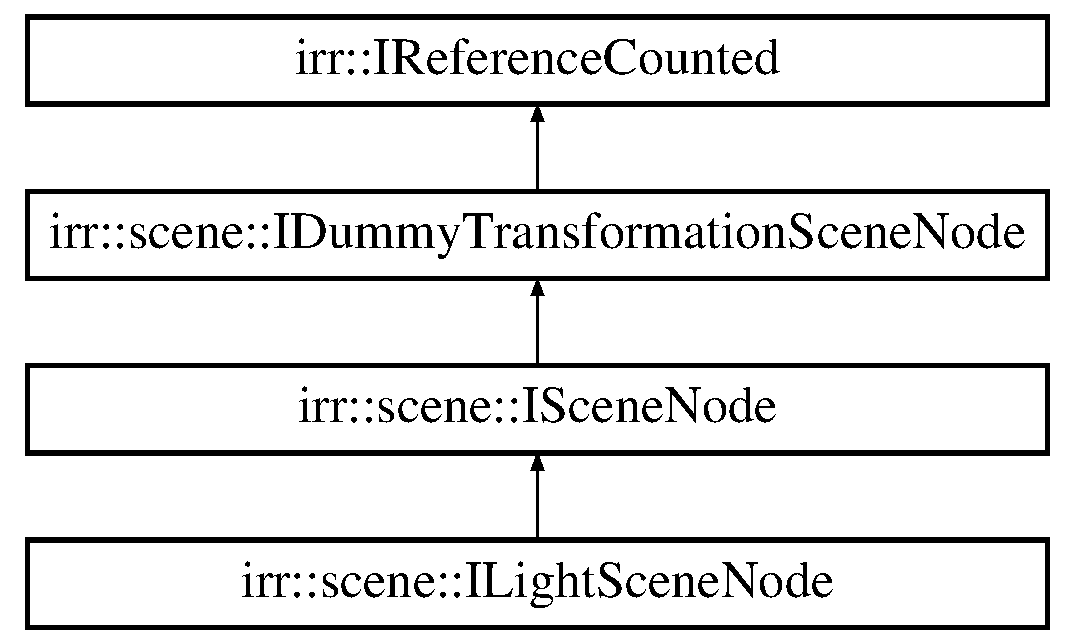
\includegraphics[height=4.000000cm]{classirr_1_1scene_1_1ILightSceneNode}
\end{center}
\end{figure}
\subsection*{Public Member Functions}
\begin{DoxyCompactItemize}
\item 
\hyperlink{classirr_1_1scene_1_1ILightSceneNode_a59891d791131ab7085584ee67bc95a8a}{I\+Light\+Scene\+Node} (\hyperlink{classirr_1_1scene_1_1IDummyTransformationSceneNode}{I\+Dummy\+Transformation\+Scene\+Node} $\ast$parent, \hyperlink{classirr_1_1scene_1_1ISceneManager}{I\+Scene\+Manager} $\ast$mgr, \hyperlink{namespaceirr_ac66849b7a6ed16e30ebede579f9b47c6}{s32} id, const \hyperlink{namespaceirr_1_1core_a06f169d08b5c429f5575acb7edbad811}{core\+::vector3df} \&position=\hyperlink{namespaceirr_1_1core_a06f169d08b5c429f5575acb7edbad811}{core\+::vector3df}(0, 0, 0))\hypertarget{classirr_1_1scene_1_1ILightSceneNode_a59891d791131ab7085584ee67bc95a8a}{}\label{classirr_1_1scene_1_1ILightSceneNode_a59891d791131ab7085584ee67bc95a8a}

\begin{DoxyCompactList}\small\item\em constructor \end{DoxyCompactList}\item 
virtual void \hyperlink{classirr_1_1scene_1_1ILightSceneNode_acf74ff3400a26ae31eb96b9c479e62d5}{set\+Light\+Data} (const \hyperlink{structirr_1_1video_1_1SLight}{video\+::\+S\+Light} \&light)=0
\begin{DoxyCompactList}\small\item\em Sets the light data associated with this \hyperlink{classirr_1_1scene_1_1ILightSceneNode}{I\+Light\+Scene\+Node}. \end{DoxyCompactList}\item 
virtual const \hyperlink{structirr_1_1video_1_1SLight}{video\+::\+S\+Light} \& \hyperlink{classirr_1_1scene_1_1ILightSceneNode_aff8c7b0a10b1fee1264ae68b772c809e}{get\+Light\+Data} () const  =0
\begin{DoxyCompactList}\small\item\em Gets the light data associated with this \hyperlink{classirr_1_1scene_1_1ILightSceneNode}{I\+Light\+Scene\+Node}. \end{DoxyCompactList}\item 
virtual \hyperlink{structirr_1_1video_1_1SLight}{video\+::\+S\+Light} \& \hyperlink{classirr_1_1scene_1_1ILightSceneNode_a20147e049be1a4790346fd72b150b30c}{get\+Light\+Data} ()=0
\begin{DoxyCompactList}\small\item\em Gets the light data associated with this \hyperlink{classirr_1_1scene_1_1ILightSceneNode}{I\+Light\+Scene\+Node}. \end{DoxyCompactList}\item 
virtual void \hyperlink{classirr_1_1scene_1_1ILightSceneNode_a3a6a6681a665ec4c214cda8a84a29337}{set\+Visible} (bool \hyperlink{classirr_1_1scene_1_1ISceneNode_a1aef4f0feccebcd0d38373beadbc1827}{is\+Visible})=0
\begin{DoxyCompactList}\small\item\em Sets if the node should be visible or not. \end{DoxyCompactList}\item 
virtual void \hyperlink{classirr_1_1scene_1_1ILightSceneNode_a7da64c8c4776988a39927827f2c3f364}{set\+Radius} (\hyperlink{namespaceirr_a0277be98d67dc26ff93b1a6a1d086b07}{f32} radius)=0
\begin{DoxyCompactList}\small\item\em Sets the light\textquotesingle{}s radius of influence. \end{DoxyCompactList}\item 
virtual \hyperlink{namespaceirr_a0277be98d67dc26ff93b1a6a1d086b07}{f32} \hyperlink{classirr_1_1scene_1_1ILightSceneNode_a50052a152ede23b2253819abbbd4598d}{get\+Radius} () const  =0
\begin{DoxyCompactList}\small\item\em Gets the light\textquotesingle{}s radius of influence. \end{DoxyCompactList}\item 
virtual void \hyperlink{classirr_1_1scene_1_1ILightSceneNode_a18b3c0ba831bdc9166db341a35701c9b}{set\+Light\+Type} (\hyperlink{namespaceirr_1_1video_aaf0e02f6f83cc35cf9e764bf18400d39}{video\+::\+E\+\_\+\+L\+I\+G\+H\+T\+\_\+\+T\+Y\+PE} type)=0
\begin{DoxyCompactList}\small\item\em Sets the light type. \end{DoxyCompactList}\item 
virtual \hyperlink{namespaceirr_1_1video_aaf0e02f6f83cc35cf9e764bf18400d39}{video\+::\+E\+\_\+\+L\+I\+G\+H\+T\+\_\+\+T\+Y\+PE} \hyperlink{classirr_1_1scene_1_1ILightSceneNode_ac961abe6a318e3167c998680ff51ff52}{get\+Light\+Type} () const  =0
\begin{DoxyCompactList}\small\item\em Gets the light type. \end{DoxyCompactList}\item 
virtual void \hyperlink{classirr_1_1scene_1_1ILightSceneNode_a1520d051fe04bc8c5c8975fb3908161b}{enable\+Cast\+Shadow} (bool shadow=true)=0
\begin{DoxyCompactList}\small\item\em Sets whether this light casts shadows. \end{DoxyCompactList}\item 
virtual bool \hyperlink{classirr_1_1scene_1_1ILightSceneNode_aa3e1cc720dd0aeded8ae30095e8afa47}{get\+Cast\+Shadow} () const  =0
\begin{DoxyCompactList}\small\item\em Check whether this light casts shadows. \end{DoxyCompactList}\end{DoxyCompactItemize}
\subsection*{Additional Inherited Members}


\subsection{Detailed Description}
Scene node which is a dynamic light. 

You can switch the light on and off by making it visible or not. It can be animated by ordinary scene node animators. If the light type is directional or spot, the direction of the light source is defined by the rotation of the scene node (assuming (0,0,1) as the local direction of the light). 

\subsection{Member Function Documentation}
\index{irr\+::scene\+::\+I\+Light\+Scene\+Node@{irr\+::scene\+::\+I\+Light\+Scene\+Node}!enable\+Cast\+Shadow@{enable\+Cast\+Shadow}}
\index{enable\+Cast\+Shadow@{enable\+Cast\+Shadow}!irr\+::scene\+::\+I\+Light\+Scene\+Node@{irr\+::scene\+::\+I\+Light\+Scene\+Node}}
\subsubsection[{\texorpdfstring{enable\+Cast\+Shadow(bool shadow=true)=0}{enableCastShadow(bool shadow=true)=0}}]{\setlength{\rightskip}{0pt plus 5cm}virtual void irr\+::scene\+::\+I\+Light\+Scene\+Node\+::enable\+Cast\+Shadow (
\begin{DoxyParamCaption}
\item[{bool}]{shadow = {\ttfamily true}}
\end{DoxyParamCaption}
)\hspace{0.3cm}{\ttfamily [pure virtual]}}\hypertarget{classirr_1_1scene_1_1ILightSceneNode_a1520d051fe04bc8c5c8975fb3908161b}{}\label{classirr_1_1scene_1_1ILightSceneNode_a1520d051fe04bc8c5c8975fb3908161b}


Sets whether this light casts shadows. 

Enabling this flag won\textquotesingle{}t automatically cast shadows, the meshes will still need shadow scene nodes attached. But one can enable or disable distinct lights for shadow casting for performance reasons. 
\begin{DoxyParams}{Parameters}
{\em shadow} & True if this light shall cast shadows. \\
\hline
\end{DoxyParams}
\index{irr\+::scene\+::\+I\+Light\+Scene\+Node@{irr\+::scene\+::\+I\+Light\+Scene\+Node}!get\+Cast\+Shadow@{get\+Cast\+Shadow}}
\index{get\+Cast\+Shadow@{get\+Cast\+Shadow}!irr\+::scene\+::\+I\+Light\+Scene\+Node@{irr\+::scene\+::\+I\+Light\+Scene\+Node}}
\subsubsection[{\texorpdfstring{get\+Cast\+Shadow() const  =0}{getCastShadow() const  =0}}]{\setlength{\rightskip}{0pt plus 5cm}virtual bool irr\+::scene\+::\+I\+Light\+Scene\+Node\+::get\+Cast\+Shadow (
\begin{DoxyParamCaption}
{}
\end{DoxyParamCaption}
) const\hspace{0.3cm}{\ttfamily [pure virtual]}}\hypertarget{classirr_1_1scene_1_1ILightSceneNode_aa3e1cc720dd0aeded8ae30095e8afa47}{}\label{classirr_1_1scene_1_1ILightSceneNode_aa3e1cc720dd0aeded8ae30095e8afa47}


Check whether this light casts shadows. 

\begin{DoxyReturn}{Returns}
True if light would cast shadows, else false. 
\end{DoxyReturn}
\index{irr\+::scene\+::\+I\+Light\+Scene\+Node@{irr\+::scene\+::\+I\+Light\+Scene\+Node}!get\+Light\+Data@{get\+Light\+Data}}
\index{get\+Light\+Data@{get\+Light\+Data}!irr\+::scene\+::\+I\+Light\+Scene\+Node@{irr\+::scene\+::\+I\+Light\+Scene\+Node}}
\subsubsection[{\texorpdfstring{get\+Light\+Data() const  =0}{getLightData() const  =0}}]{\setlength{\rightskip}{0pt plus 5cm}virtual const {\bf video\+::\+S\+Light}\& irr\+::scene\+::\+I\+Light\+Scene\+Node\+::get\+Light\+Data (
\begin{DoxyParamCaption}
{}
\end{DoxyParamCaption}
) const\hspace{0.3cm}{\ttfamily [pure virtual]}}\hypertarget{classirr_1_1scene_1_1ILightSceneNode_aff8c7b0a10b1fee1264ae68b772c809e}{}\label{classirr_1_1scene_1_1ILightSceneNode_aff8c7b0a10b1fee1264ae68b772c809e}


Gets the light data associated with this \hyperlink{classirr_1_1scene_1_1ILightSceneNode}{I\+Light\+Scene\+Node}. 

\begin{DoxyReturn}{Returns}
The light data. 
\end{DoxyReturn}
\index{irr\+::scene\+::\+I\+Light\+Scene\+Node@{irr\+::scene\+::\+I\+Light\+Scene\+Node}!get\+Light\+Data@{get\+Light\+Data}}
\index{get\+Light\+Data@{get\+Light\+Data}!irr\+::scene\+::\+I\+Light\+Scene\+Node@{irr\+::scene\+::\+I\+Light\+Scene\+Node}}
\subsubsection[{\texorpdfstring{get\+Light\+Data()=0}{getLightData()=0}}]{\setlength{\rightskip}{0pt plus 5cm}virtual {\bf video\+::\+S\+Light}\& irr\+::scene\+::\+I\+Light\+Scene\+Node\+::get\+Light\+Data (
\begin{DoxyParamCaption}
{}
\end{DoxyParamCaption}
)\hspace{0.3cm}{\ttfamily [pure virtual]}}\hypertarget{classirr_1_1scene_1_1ILightSceneNode_a20147e049be1a4790346fd72b150b30c}{}\label{classirr_1_1scene_1_1ILightSceneNode_a20147e049be1a4790346fd72b150b30c}


Gets the light data associated with this \hyperlink{classirr_1_1scene_1_1ILightSceneNode}{I\+Light\+Scene\+Node}. 

\begin{DoxyReturn}{Returns}
The light data. 
\end{DoxyReturn}
\index{irr\+::scene\+::\+I\+Light\+Scene\+Node@{irr\+::scene\+::\+I\+Light\+Scene\+Node}!get\+Light\+Type@{get\+Light\+Type}}
\index{get\+Light\+Type@{get\+Light\+Type}!irr\+::scene\+::\+I\+Light\+Scene\+Node@{irr\+::scene\+::\+I\+Light\+Scene\+Node}}
\subsubsection[{\texorpdfstring{get\+Light\+Type() const  =0}{getLightType() const  =0}}]{\setlength{\rightskip}{0pt plus 5cm}virtual {\bf video\+::\+E\+\_\+\+L\+I\+G\+H\+T\+\_\+\+T\+Y\+PE} irr\+::scene\+::\+I\+Light\+Scene\+Node\+::get\+Light\+Type (
\begin{DoxyParamCaption}
{}
\end{DoxyParamCaption}
) const\hspace{0.3cm}{\ttfamily [pure virtual]}}\hypertarget{classirr_1_1scene_1_1ILightSceneNode_ac961abe6a318e3167c998680ff51ff52}{}\label{classirr_1_1scene_1_1ILightSceneNode_ac961abe6a318e3167c998680ff51ff52}


Gets the light type. 

\begin{DoxyReturn}{Returns}
The current light type. 
\end{DoxyReturn}
\index{irr\+::scene\+::\+I\+Light\+Scene\+Node@{irr\+::scene\+::\+I\+Light\+Scene\+Node}!get\+Radius@{get\+Radius}}
\index{get\+Radius@{get\+Radius}!irr\+::scene\+::\+I\+Light\+Scene\+Node@{irr\+::scene\+::\+I\+Light\+Scene\+Node}}
\subsubsection[{\texorpdfstring{get\+Radius() const  =0}{getRadius() const  =0}}]{\setlength{\rightskip}{0pt plus 5cm}virtual {\bf f32} irr\+::scene\+::\+I\+Light\+Scene\+Node\+::get\+Radius (
\begin{DoxyParamCaption}
{}
\end{DoxyParamCaption}
) const\hspace{0.3cm}{\ttfamily [pure virtual]}}\hypertarget{classirr_1_1scene_1_1ILightSceneNode_a50052a152ede23b2253819abbbd4598d}{}\label{classirr_1_1scene_1_1ILightSceneNode_a50052a152ede23b2253819abbbd4598d}


Gets the light\textquotesingle{}s radius of influence. 

\begin{DoxyReturn}{Returns}
The current radius. 
\end{DoxyReturn}
\index{irr\+::scene\+::\+I\+Light\+Scene\+Node@{irr\+::scene\+::\+I\+Light\+Scene\+Node}!set\+Light\+Data@{set\+Light\+Data}}
\index{set\+Light\+Data@{set\+Light\+Data}!irr\+::scene\+::\+I\+Light\+Scene\+Node@{irr\+::scene\+::\+I\+Light\+Scene\+Node}}
\subsubsection[{\texorpdfstring{set\+Light\+Data(const video\+::\+S\+Light \&light)=0}{setLightData(const video::SLight \&light)=0}}]{\setlength{\rightskip}{0pt plus 5cm}virtual void irr\+::scene\+::\+I\+Light\+Scene\+Node\+::set\+Light\+Data (
\begin{DoxyParamCaption}
\item[{const {\bf video\+::\+S\+Light} \&}]{light}
\end{DoxyParamCaption}
)\hspace{0.3cm}{\ttfamily [pure virtual]}}\hypertarget{classirr_1_1scene_1_1ILightSceneNode_acf74ff3400a26ae31eb96b9c479e62d5}{}\label{classirr_1_1scene_1_1ILightSceneNode_acf74ff3400a26ae31eb96b9c479e62d5}


Sets the light data associated with this \hyperlink{classirr_1_1scene_1_1ILightSceneNode}{I\+Light\+Scene\+Node}. 


\begin{DoxyParams}{Parameters}
{\em light} & The new light data. \\
\hline
\end{DoxyParams}
\index{irr\+::scene\+::\+I\+Light\+Scene\+Node@{irr\+::scene\+::\+I\+Light\+Scene\+Node}!set\+Light\+Type@{set\+Light\+Type}}
\index{set\+Light\+Type@{set\+Light\+Type}!irr\+::scene\+::\+I\+Light\+Scene\+Node@{irr\+::scene\+::\+I\+Light\+Scene\+Node}}
\subsubsection[{\texorpdfstring{set\+Light\+Type(video\+::\+E\+\_\+\+L\+I\+G\+H\+T\+\_\+\+T\+Y\+P\+E type)=0}{setLightType(video::E\_LIGHT\_TYPE type)=0}}]{\setlength{\rightskip}{0pt plus 5cm}virtual void irr\+::scene\+::\+I\+Light\+Scene\+Node\+::set\+Light\+Type (
\begin{DoxyParamCaption}
\item[{{\bf video\+::\+E\+\_\+\+L\+I\+G\+H\+T\+\_\+\+T\+Y\+PE}}]{type}
\end{DoxyParamCaption}
)\hspace{0.3cm}{\ttfamily [pure virtual]}}\hypertarget{classirr_1_1scene_1_1ILightSceneNode_a18b3c0ba831bdc9166db341a35701c9b}{}\label{classirr_1_1scene_1_1ILightSceneNode_a18b3c0ba831bdc9166db341a35701c9b}


Sets the light type. 


\begin{DoxyParams}{Parameters}
{\em type} & The new type. \\
\hline
\end{DoxyParams}
\index{irr\+::scene\+::\+I\+Light\+Scene\+Node@{irr\+::scene\+::\+I\+Light\+Scene\+Node}!set\+Radius@{set\+Radius}}
\index{set\+Radius@{set\+Radius}!irr\+::scene\+::\+I\+Light\+Scene\+Node@{irr\+::scene\+::\+I\+Light\+Scene\+Node}}
\subsubsection[{\texorpdfstring{set\+Radius(f32 radius)=0}{setRadius(f32 radius)=0}}]{\setlength{\rightskip}{0pt plus 5cm}virtual void irr\+::scene\+::\+I\+Light\+Scene\+Node\+::set\+Radius (
\begin{DoxyParamCaption}
\item[{{\bf f32}}]{radius}
\end{DoxyParamCaption}
)\hspace{0.3cm}{\ttfamily [pure virtual]}}\hypertarget{classirr_1_1scene_1_1ILightSceneNode_a7da64c8c4776988a39927827f2c3f364}{}\label{classirr_1_1scene_1_1ILightSceneNode_a7da64c8c4776988a39927827f2c3f364}


Sets the light\textquotesingle{}s radius of influence. 

Outside this radius the light won\textquotesingle{}t lighten geometry and cast no shadows. Setting the radius will also influence the attenuation, setting it to (0,1/radius,0). If you want to override this behavior, set the attenuation after the radius. 
\begin{DoxyParams}{Parameters}
{\em radius} & The new radius. \\
\hline
\end{DoxyParams}
\index{irr\+::scene\+::\+I\+Light\+Scene\+Node@{irr\+::scene\+::\+I\+Light\+Scene\+Node}!set\+Visible@{set\+Visible}}
\index{set\+Visible@{set\+Visible}!irr\+::scene\+::\+I\+Light\+Scene\+Node@{irr\+::scene\+::\+I\+Light\+Scene\+Node}}
\subsubsection[{\texorpdfstring{set\+Visible(bool is\+Visible)=0}{setVisible(bool isVisible)=0}}]{\setlength{\rightskip}{0pt plus 5cm}virtual void irr\+::scene\+::\+I\+Light\+Scene\+Node\+::set\+Visible (
\begin{DoxyParamCaption}
\item[{bool}]{is\+Visible}
\end{DoxyParamCaption}
)\hspace{0.3cm}{\ttfamily [pure virtual]}}\hypertarget{classirr_1_1scene_1_1ILightSceneNode_a3a6a6681a665ec4c214cda8a84a29337}{}\label{classirr_1_1scene_1_1ILightSceneNode_a3a6a6681a665ec4c214cda8a84a29337}


Sets if the node should be visible or not. 

All children of this node won\textquotesingle{}t be visible either, when set to true. 
\begin{DoxyParams}{Parameters}
{\em is\+Visible} & If the node shall be visible. \\
\hline
\end{DoxyParams}


Reimplemented from \hyperlink{classirr_1_1scene_1_1ISceneNode_a7a5de878c7084088646f07afaac0a73f}{irr\+::scene\+::\+I\+Scene\+Node}.



The documentation for this class was generated from the following file\+:\begin{DoxyCompactItemize}
\item 
include/I\+Light\+Scene\+Node.\+h\end{DoxyCompactItemize}

\hypertarget{classirr_1_1ILogger}{}\section{irr\+:\+:I\+Logger Class Reference}
\label{classirr_1_1ILogger}\index{irr\+::\+I\+Logger@{irr\+::\+I\+Logger}}


Interface for logging messages, warnings and errors.  




{\ttfamily \#include $<$I\+Logger.\+h$>$}

Inheritance diagram for irr\+:\+:I\+Logger\+:\begin{figure}[H]
\begin{center}
\leavevmode
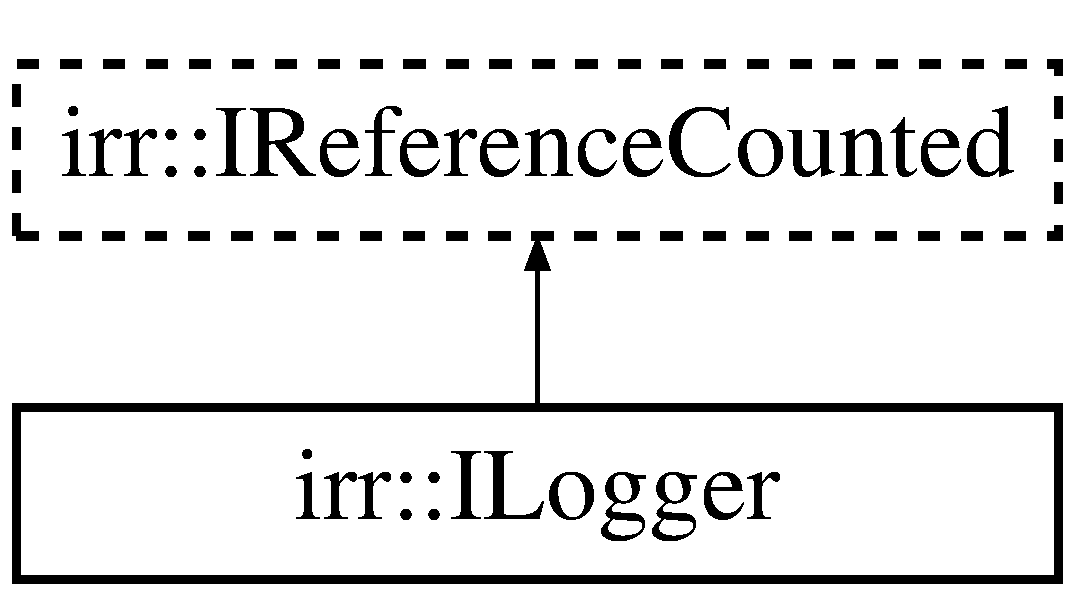
\includegraphics[height=2.000000cm]{classirr_1_1ILogger}
\end{center}
\end{figure}
\subsection*{Public Member Functions}
\begin{DoxyCompactItemize}
\item 
virtual \hyperlink{classirr_1_1ILogger_ae1ceda88c9b97cc1efcefa38588f9116}{$\sim$\+I\+Logger} ()\hypertarget{classirr_1_1ILogger_ae1ceda88c9b97cc1efcefa38588f9116}{}\label{classirr_1_1ILogger_ae1ceda88c9b97cc1efcefa38588f9116}

\begin{DoxyCompactList}\small\item\em Destructor. \end{DoxyCompactList}\item 
virtual \hyperlink{namespaceirr_aa2d1cac68606a25ed24cfffccfa30a92}{E\+L\+O\+G\+\_\+\+L\+E\+V\+EL} \hyperlink{classirr_1_1ILogger_afd7e5a2e6b6a0563df5002a655c3a2da}{get\+Log\+Level} () const  =0\hypertarget{classirr_1_1ILogger_afd7e5a2e6b6a0563df5002a655c3a2da}{}\label{classirr_1_1ILogger_afd7e5a2e6b6a0563df5002a655c3a2da}

\begin{DoxyCompactList}\small\item\em Returns the current set log level. \end{DoxyCompactList}\item 
virtual void \hyperlink{classirr_1_1ILogger_a226a6f71f76970f2d846a10599f2e5ec}{set\+Log\+Level} (\hyperlink{namespaceirr_aa2d1cac68606a25ed24cfffccfa30a92}{E\+L\+O\+G\+\_\+\+L\+E\+V\+EL} ll)=0
\begin{DoxyCompactList}\small\item\em Sets a new log level. \end{DoxyCompactList}\item 
virtual void \hyperlink{classirr_1_1ILogger_acbbc214a06cd968409000f55aa76c82f}{log} (const \hyperlink{namespaceirr_a9395eaea339bcb546b319e9c96bf7410}{c8} $\ast$text, \hyperlink{namespaceirr_aa2d1cac68606a25ed24cfffccfa30a92}{E\+L\+O\+G\+\_\+\+L\+E\+V\+EL} ll=\hyperlink{namespaceirr_aa2d1cac68606a25ed24cfffccfa30a92a9d74de15737e326a91aec6f38c23f9cf}{E\+L\+L\+\_\+\+I\+N\+F\+O\+R\+M\+A\+T\+I\+ON})=0
\begin{DoxyCompactList}\small\item\em Prints out a text into the log. \end{DoxyCompactList}\item 
virtual void \hyperlink{classirr_1_1ILogger_afccb7b2bb0a9b0415204d63e2b0cf290}{log} (const \hyperlink{namespaceirr_a9395eaea339bcb546b319e9c96bf7410}{c8} $\ast$text, const \hyperlink{namespaceirr_a9395eaea339bcb546b319e9c96bf7410}{c8} $\ast$hint, \hyperlink{namespaceirr_aa2d1cac68606a25ed24cfffccfa30a92}{E\+L\+O\+G\+\_\+\+L\+E\+V\+EL} ll=\hyperlink{namespaceirr_aa2d1cac68606a25ed24cfffccfa30a92a9d74de15737e326a91aec6f38c23f9cf}{E\+L\+L\+\_\+\+I\+N\+F\+O\+R\+M\+A\+T\+I\+ON})=0
\begin{DoxyCompactList}\small\item\em Prints out a text into the log. \end{DoxyCompactList}\item 
virtual void {\bfseries log} (const \hyperlink{namespaceirr_a9395eaea339bcb546b319e9c96bf7410}{c8} $\ast$text, const wchar\+\_\+t $\ast$hint, \hyperlink{namespaceirr_aa2d1cac68606a25ed24cfffccfa30a92}{E\+L\+O\+G\+\_\+\+L\+E\+V\+EL} ll=\hyperlink{namespaceirr_aa2d1cac68606a25ed24cfffccfa30a92a9d74de15737e326a91aec6f38c23f9cf}{E\+L\+L\+\_\+\+I\+N\+F\+O\+R\+M\+A\+T\+I\+ON})=0\hypertarget{classirr_1_1ILogger_afbdfdab8e53d060e08d7847f8ca77b4a}{}\label{classirr_1_1ILogger_afbdfdab8e53d060e08d7847f8ca77b4a}

\item 
virtual void \hyperlink{classirr_1_1ILogger_aeef998619135d81205d2fd488d4a69b1}{log} (const wchar\+\_\+t $\ast$text, const wchar\+\_\+t $\ast$hint, \hyperlink{namespaceirr_aa2d1cac68606a25ed24cfffccfa30a92}{E\+L\+O\+G\+\_\+\+L\+E\+V\+EL} ll=\hyperlink{namespaceirr_aa2d1cac68606a25ed24cfffccfa30a92a9d74de15737e326a91aec6f38c23f9cf}{E\+L\+L\+\_\+\+I\+N\+F\+O\+R\+M\+A\+T\+I\+ON})=0
\begin{DoxyCompactList}\small\item\em Prints out a text into the log. \end{DoxyCompactList}\item 
virtual void \hyperlink{classirr_1_1ILogger_a40af57afdc28c5e890920cb448663ff9}{log} (const wchar\+\_\+t $\ast$text, \hyperlink{namespaceirr_aa2d1cac68606a25ed24cfffccfa30a92}{E\+L\+O\+G\+\_\+\+L\+E\+V\+EL} ll=\hyperlink{namespaceirr_aa2d1cac68606a25ed24cfffccfa30a92a9d74de15737e326a91aec6f38c23f9cf}{E\+L\+L\+\_\+\+I\+N\+F\+O\+R\+M\+A\+T\+I\+ON})=0
\begin{DoxyCompactList}\small\item\em Prints out a text into the log. \end{DoxyCompactList}\end{DoxyCompactItemize}
\subsection*{Additional Inherited Members}


\subsection{Detailed Description}
Interface for logging messages, warnings and errors. 

\subsection{Member Function Documentation}
\index{irr\+::\+I\+Logger@{irr\+::\+I\+Logger}!log@{log}}
\index{log@{log}!irr\+::\+I\+Logger@{irr\+::\+I\+Logger}}
\subsubsection[{\texorpdfstring{log(const c8 $\ast$text, E\+L\+O\+G\+\_\+\+L\+E\+V\+E\+L ll=\+E\+L\+L\+\_\+\+I\+N\+F\+O\+R\+M\+A\+T\+I\+O\+N)=0}{log(const c8 *text, ELOG\_LEVEL ll=ELL\_INFORMATION)=0}}]{\setlength{\rightskip}{0pt plus 5cm}virtual void irr\+::\+I\+Logger\+::log (
\begin{DoxyParamCaption}
\item[{const {\bf c8} $\ast$}]{text, }
\item[{{\bf E\+L\+O\+G\+\_\+\+L\+E\+V\+EL}}]{ll = {\ttfamily {\bf E\+L\+L\+\_\+\+I\+N\+F\+O\+R\+M\+A\+T\+I\+ON}}}
\end{DoxyParamCaption}
)\hspace{0.3cm}{\ttfamily [pure virtual]}}\hypertarget{classirr_1_1ILogger_acbbc214a06cd968409000f55aa76c82f}{}\label{classirr_1_1ILogger_acbbc214a06cd968409000f55aa76c82f}


Prints out a text into the log. 


\begin{DoxyParams}{Parameters}
{\em text} & Text to print out. \\
\hline
{\em ll} & Log level of the text. If the text is an error, set it to E\+L\+L\+\_\+\+E\+R\+R\+OR, if it is warning set it to E\+L\+L\+\_\+\+W\+A\+R\+N\+I\+NG, and if it is just an informational text, set it to E\+L\+L\+\_\+\+I\+N\+F\+O\+R\+M\+A\+T\+I\+ON. Texts are filtered with these levels. If you want to be a text displayed, independent on what level filter is set, use E\+L\+L\+\_\+\+N\+O\+NE. \\
\hline
\end{DoxyParams}
\index{irr\+::\+I\+Logger@{irr\+::\+I\+Logger}!log@{log}}
\index{log@{log}!irr\+::\+I\+Logger@{irr\+::\+I\+Logger}}
\subsubsection[{\texorpdfstring{log(const c8 $\ast$text, const c8 $\ast$hint, E\+L\+O\+G\+\_\+\+L\+E\+V\+E\+L ll=\+E\+L\+L\+\_\+\+I\+N\+F\+O\+R\+M\+A\+T\+I\+O\+N)=0}{log(const c8 *text, const c8 *hint, ELOG\_LEVEL ll=ELL\_INFORMATION)=0}}]{\setlength{\rightskip}{0pt plus 5cm}virtual void irr\+::\+I\+Logger\+::log (
\begin{DoxyParamCaption}
\item[{const {\bf c8} $\ast$}]{text, }
\item[{const {\bf c8} $\ast$}]{hint, }
\item[{{\bf E\+L\+O\+G\+\_\+\+L\+E\+V\+EL}}]{ll = {\ttfamily {\bf E\+L\+L\+\_\+\+I\+N\+F\+O\+R\+M\+A\+T\+I\+ON}}}
\end{DoxyParamCaption}
)\hspace{0.3cm}{\ttfamily [pure virtual]}}\hypertarget{classirr_1_1ILogger_afccb7b2bb0a9b0415204d63e2b0cf290}{}\label{classirr_1_1ILogger_afccb7b2bb0a9b0415204d63e2b0cf290}


Prints out a text into the log. 


\begin{DoxyParams}{Parameters}
{\em text} & Text to print out. \\
\hline
{\em hint} & Additional info. This string is added after a \char`\"{} \+:\char`\"{} to the string. \\
\hline
{\em ll} & Log level of the text. If the text is an error, set it to E\+L\+L\+\_\+\+E\+R\+R\+OR, if it is warning set it to E\+L\+L\+\_\+\+W\+A\+R\+N\+I\+NG, and if it is just an informational text, set it to E\+L\+L\+\_\+\+I\+N\+F\+O\+R\+M\+A\+T\+I\+ON. Texts are filtered with these levels. If you want to be a text displayed, independent on what level filter is set, use E\+L\+L\+\_\+\+N\+O\+NE. \\
\hline
\end{DoxyParams}
\index{irr\+::\+I\+Logger@{irr\+::\+I\+Logger}!log@{log}}
\index{log@{log}!irr\+::\+I\+Logger@{irr\+::\+I\+Logger}}
\subsubsection[{\texorpdfstring{log(const wchar\+\_\+t $\ast$text, const wchar\+\_\+t $\ast$hint, E\+L\+O\+G\+\_\+\+L\+E\+V\+E\+L ll=\+E\+L\+L\+\_\+\+I\+N\+F\+O\+R\+M\+A\+T\+I\+O\+N)=0}{log(const wchar\_t *text, const wchar\_t *hint, ELOG\_LEVEL ll=ELL\_INFORMATION)=0}}]{\setlength{\rightskip}{0pt plus 5cm}virtual void irr\+::\+I\+Logger\+::log (
\begin{DoxyParamCaption}
\item[{const wchar\+\_\+t $\ast$}]{text, }
\item[{const wchar\+\_\+t $\ast$}]{hint, }
\item[{{\bf E\+L\+O\+G\+\_\+\+L\+E\+V\+EL}}]{ll = {\ttfamily {\bf E\+L\+L\+\_\+\+I\+N\+F\+O\+R\+M\+A\+T\+I\+ON}}}
\end{DoxyParamCaption}
)\hspace{0.3cm}{\ttfamily [pure virtual]}}\hypertarget{classirr_1_1ILogger_aeef998619135d81205d2fd488d4a69b1}{}\label{classirr_1_1ILogger_aeef998619135d81205d2fd488d4a69b1}


Prints out a text into the log. 


\begin{DoxyParams}{Parameters}
{\em text} & Text to print out. \\
\hline
{\em hint} & Additional info. This string is added after a \char`\"{} \+:\char`\"{} to the string. \\
\hline
{\em ll} & Log level of the text. If the text is an error, set it to E\+L\+L\+\_\+\+E\+R\+R\+OR, if it is warning set it to E\+L\+L\+\_\+\+W\+A\+R\+N\+I\+NG, and if it is just an informational text, set it to E\+L\+L\+\_\+\+I\+N\+F\+O\+R\+M\+A\+T\+I\+ON. Texts are filtered with these levels. If you want to be a text displayed, independent on what level filter is set, use E\+L\+L\+\_\+\+N\+O\+NE. \\
\hline
\end{DoxyParams}
\index{irr\+::\+I\+Logger@{irr\+::\+I\+Logger}!log@{log}}
\index{log@{log}!irr\+::\+I\+Logger@{irr\+::\+I\+Logger}}
\subsubsection[{\texorpdfstring{log(const wchar\+\_\+t $\ast$text, E\+L\+O\+G\+\_\+\+L\+E\+V\+E\+L ll=\+E\+L\+L\+\_\+\+I\+N\+F\+O\+R\+M\+A\+T\+I\+O\+N)=0}{log(const wchar\_t *text, ELOG\_LEVEL ll=ELL\_INFORMATION)=0}}]{\setlength{\rightskip}{0pt plus 5cm}virtual void irr\+::\+I\+Logger\+::log (
\begin{DoxyParamCaption}
\item[{const wchar\+\_\+t $\ast$}]{text, }
\item[{{\bf E\+L\+O\+G\+\_\+\+L\+E\+V\+EL}}]{ll = {\ttfamily {\bf E\+L\+L\+\_\+\+I\+N\+F\+O\+R\+M\+A\+T\+I\+ON}}}
\end{DoxyParamCaption}
)\hspace{0.3cm}{\ttfamily [pure virtual]}}\hypertarget{classirr_1_1ILogger_a40af57afdc28c5e890920cb448663ff9}{}\label{classirr_1_1ILogger_a40af57afdc28c5e890920cb448663ff9}


Prints out a text into the log. 


\begin{DoxyParams}{Parameters}
{\em text} & Text to print out. \\
\hline
{\em ll} & Log level of the text. If the text is an error, set it to E\+L\+L\+\_\+\+E\+R\+R\+OR, if it is warning set it to E\+L\+L\+\_\+\+W\+A\+R\+N\+I\+NG, and if it is just an informational text, set it to E\+L\+L\+\_\+\+I\+N\+F\+O\+R\+M\+A\+T\+I\+ON. Texts are filtered with these levels. If you want to be a text displayed, independent on what level filter is set, use E\+L\+L\+\_\+\+N\+O\+NE. \\
\hline
\end{DoxyParams}
\index{irr\+::\+I\+Logger@{irr\+::\+I\+Logger}!set\+Log\+Level@{set\+Log\+Level}}
\index{set\+Log\+Level@{set\+Log\+Level}!irr\+::\+I\+Logger@{irr\+::\+I\+Logger}}
\subsubsection[{\texorpdfstring{set\+Log\+Level(\+E\+L\+O\+G\+\_\+\+L\+E\+V\+E\+L ll)=0}{setLogLevel(ELOG\_LEVEL ll)=0}}]{\setlength{\rightskip}{0pt plus 5cm}virtual void irr\+::\+I\+Logger\+::set\+Log\+Level (
\begin{DoxyParamCaption}
\item[{{\bf E\+L\+O\+G\+\_\+\+L\+E\+V\+EL}}]{ll}
\end{DoxyParamCaption}
)\hspace{0.3cm}{\ttfamily [pure virtual]}}\hypertarget{classirr_1_1ILogger_a226a6f71f76970f2d846a10599f2e5ec}{}\label{classirr_1_1ILogger_a226a6f71f76970f2d846a10599f2e5ec}


Sets a new log level. 

With this value, texts which are sent to the logger are filtered out. For example setting this value to E\+L\+L\+\_\+\+W\+A\+R\+N\+I\+NG, only warnings and errors are printed out. Setting it to E\+L\+L\+\_\+\+I\+N\+F\+O\+R\+M\+A\+T\+I\+ON, which is the default setting, warnings, errors and informational texts are printed out. 
\begin{DoxyParams}{Parameters}
{\em ll} & new log level filter value. \\
\hline
\end{DoxyParams}


The documentation for this class was generated from the following file\+:\begin{DoxyCompactItemize}
\item 
include/I\+Logger.\+h\end{DoxyCompactItemize}

\hypertarget{classirr_1_1video_1_1IMaterialRenderer}{}\section{irr\+:\+:video\+:\+:I\+Material\+Renderer Class Reference}
\label{classirr_1_1video_1_1IMaterialRenderer}\index{irr\+::video\+::\+I\+Material\+Renderer@{irr\+::video\+::\+I\+Material\+Renderer}}


Interface for material rendering.  




{\ttfamily \#include $<$I\+Material\+Renderer.\+h$>$}

Inheritance diagram for irr\+:\+:video\+:\+:I\+Material\+Renderer\+:\begin{figure}[H]
\begin{center}
\leavevmode
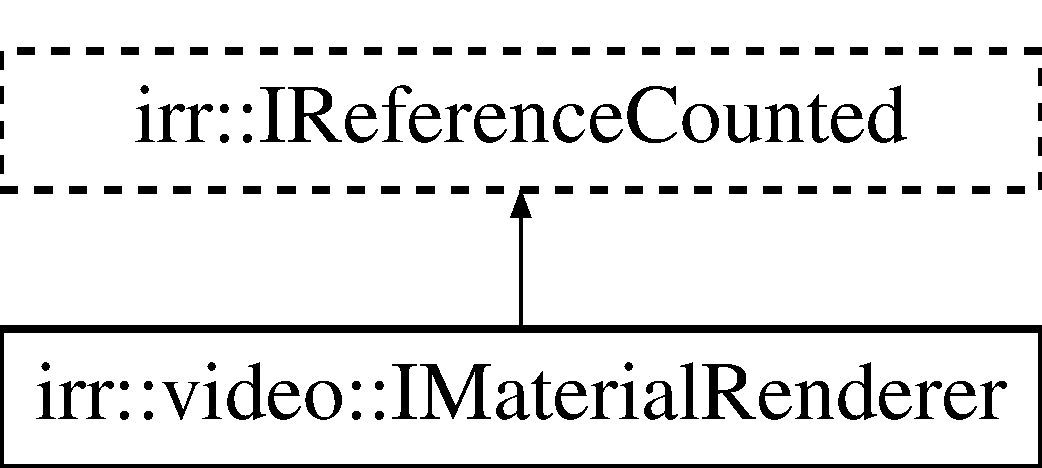
\includegraphics[height=2.000000cm]{classirr_1_1video_1_1IMaterialRenderer}
\end{center}
\end{figure}
\subsection*{Public Member Functions}
\begin{DoxyCompactItemize}
\item 
virtual void \hyperlink{classirr_1_1video_1_1IMaterialRenderer_aeaffc03c1b9feb40cd01469726b287e3}{On\+Set\+Material} (const \hyperlink{classirr_1_1video_1_1SMaterial}{S\+Material} \&material, const \hyperlink{classirr_1_1video_1_1SMaterial}{S\+Material} \&last\+Material, bool reset\+All\+Renderstates, \hyperlink{classirr_1_1video_1_1IMaterialRendererServices}{I\+Material\+Renderer\+Services} $\ast$services)
\begin{DoxyCompactList}\small\item\em Called by the \hyperlink{classirr_1_1video_1_1IVideoDriver}{I\+Video\+Driver} implementation the let the renderer set its needed render states. \end{DoxyCompactList}\item 
virtual bool \hyperlink{classirr_1_1video_1_1IMaterialRenderer_acdb3d562cbb7a7d7d83f8cc231ee0421}{On\+Render} (\hyperlink{classirr_1_1video_1_1IMaterialRendererServices}{I\+Material\+Renderer\+Services} $\ast$service)
\begin{DoxyCompactList}\small\item\em Called every time before a new bunch of geometry is being drawn using this material with for example draw\+Indexed\+Triangle\+List() call. \end{DoxyCompactList}\item 
virtual void \hyperlink{classirr_1_1video_1_1IMaterialRenderer_a694b1285671853cb151c03100fd01c73}{On\+Unset\+Material} ()
\begin{DoxyCompactList}\small\item\em Called by the \hyperlink{classirr_1_1video_1_1IVideoDriver}{I\+Video\+Driver} to unset this material. \end{DoxyCompactList}\item 
virtual bool \hyperlink{classirr_1_1video_1_1IMaterialRenderer_a31ba4c2c50b85327d328cb9e7b1764bd}{is\+Transparent} () const 
\begin{DoxyCompactList}\small\item\em Returns if the material is transparent. \end{DoxyCompactList}\item 
virtual \hyperlink{namespaceirr_ac66849b7a6ed16e30ebede579f9b47c6}{s32} \hyperlink{classirr_1_1video_1_1IMaterialRenderer_a8ccaf22f84f26a718559d3c97f7cb550}{get\+Render\+Capability} () const 
\begin{DoxyCompactList}\small\item\em Returns the render capability of the material. \end{DoxyCompactList}\end{DoxyCompactItemize}
\subsection*{Additional Inherited Members}


\subsection{Detailed Description}
Interface for material rendering. 

Can be used to extend the engine with new materials. Refer to \hyperlink{classirr_1_1video_1_1IVideoDriver_a0dfc3a7168f3a73a6f4323b579f03ff6}{I\+Video\+Driver\+::add\+Material\+Renderer()} for more informations on how to extend the engine with new materials. 

\subsection{Member Function Documentation}
\index{irr\+::video\+::\+I\+Material\+Renderer@{irr\+::video\+::\+I\+Material\+Renderer}!get\+Render\+Capability@{get\+Render\+Capability}}
\index{get\+Render\+Capability@{get\+Render\+Capability}!irr\+::video\+::\+I\+Material\+Renderer@{irr\+::video\+::\+I\+Material\+Renderer}}
\subsubsection[{\texorpdfstring{get\+Render\+Capability() const }{getRenderCapability() const }}]{\setlength{\rightskip}{0pt plus 5cm}virtual {\bf s32} irr\+::video\+::\+I\+Material\+Renderer\+::get\+Render\+Capability (
\begin{DoxyParamCaption}
{}
\end{DoxyParamCaption}
) const\hspace{0.3cm}{\ttfamily [inline]}, {\ttfamily [virtual]}}\hypertarget{classirr_1_1video_1_1IMaterialRenderer_a8ccaf22f84f26a718559d3c97f7cb550}{}\label{classirr_1_1video_1_1IMaterialRenderer_a8ccaf22f84f26a718559d3c97f7cb550}


Returns the render capability of the material. 

Because some more complex materials are implemented in multiple ways and need special hardware capabilities, it is possible to query how the current material renderer is performing on the current hardware with this function. \begin{DoxyReturn}{Returns}
Returns 0 if everything is running fine. Any other value is material renderer specific and means for example that the renderer switched back to a fall back material because it cannot use the latest shaders. More specific examples\+: Fixed function pipeline materials should return 0 in most cases, parallax mapped material will only return 0 when at least pixel shader 1.\+4 is available on that machine. 
\end{DoxyReturn}
\index{irr\+::video\+::\+I\+Material\+Renderer@{irr\+::video\+::\+I\+Material\+Renderer}!is\+Transparent@{is\+Transparent}}
\index{is\+Transparent@{is\+Transparent}!irr\+::video\+::\+I\+Material\+Renderer@{irr\+::video\+::\+I\+Material\+Renderer}}
\subsubsection[{\texorpdfstring{is\+Transparent() const }{isTransparent() const }}]{\setlength{\rightskip}{0pt plus 5cm}virtual bool irr\+::video\+::\+I\+Material\+Renderer\+::is\+Transparent (
\begin{DoxyParamCaption}
{}
\end{DoxyParamCaption}
) const\hspace{0.3cm}{\ttfamily [inline]}, {\ttfamily [virtual]}}\hypertarget{classirr_1_1video_1_1IMaterialRenderer_a31ba4c2c50b85327d328cb9e7b1764bd}{}\label{classirr_1_1video_1_1IMaterialRenderer_a31ba4c2c50b85327d328cb9e7b1764bd}


Returns if the material is transparent. 

The scene managment needs to know this for being able to sort the materials by opaque and transparent. \index{irr\+::video\+::\+I\+Material\+Renderer@{irr\+::video\+::\+I\+Material\+Renderer}!On\+Render@{On\+Render}}
\index{On\+Render@{On\+Render}!irr\+::video\+::\+I\+Material\+Renderer@{irr\+::video\+::\+I\+Material\+Renderer}}
\subsubsection[{\texorpdfstring{On\+Render(\+I\+Material\+Renderer\+Services $\ast$service)}{OnRender(IMaterialRendererServices *service)}}]{\setlength{\rightskip}{0pt plus 5cm}virtual bool irr\+::video\+::\+I\+Material\+Renderer\+::\+On\+Render (
\begin{DoxyParamCaption}
\item[{{\bf I\+Material\+Renderer\+Services} $\ast$}]{service}
\end{DoxyParamCaption}
)\hspace{0.3cm}{\ttfamily [inline]}, {\ttfamily [virtual]}}\hypertarget{classirr_1_1video_1_1IMaterialRenderer_acdb3d562cbb7a7d7d83f8cc231ee0421}{}\label{classirr_1_1video_1_1IMaterialRenderer_acdb3d562cbb7a7d7d83f8cc231ee0421}


Called every time before a new bunch of geometry is being drawn using this material with for example draw\+Indexed\+Triangle\+List() call. 

On\+Set\+Material should normally only be called if the renderer decides that the renderstates should be changed, it won\textquotesingle{}t be called if for example two draw\+Indexed\+Triangle\+List() will be called with the same material set. This method will be called every time. This is useful for example for materials with shaders, which don\textquotesingle{}t only set new renderstates but also shader constants. 
\begin{DoxyParams}{Parameters}
{\em service} & Pointer to interface providing methos for setting constants and other things. \\
\hline
{\em vtxtype} & Vertex type with which the next rendering will be done. This can be used by the material renderer to set some specific optimized shaders or if this is an incompatible vertex type for this renderer, to refuse rendering for example. \\
\hline
\end{DoxyParams}
\begin{DoxyReturn}{Returns}
Returns true if everything is ok, and false if nothing should be rendered. The material renderer can choose to return false for example if he doesn\textquotesingle{}t support the specified vertex type. This is actually done in D3\+D8 and D3\+D9 when using a normal mapped material with a vertex type other than E\+V\+T\+\_\+\+T\+A\+N\+G\+E\+N\+TS. 
\end{DoxyReturn}
\index{irr\+::video\+::\+I\+Material\+Renderer@{irr\+::video\+::\+I\+Material\+Renderer}!On\+Set\+Material@{On\+Set\+Material}}
\index{On\+Set\+Material@{On\+Set\+Material}!irr\+::video\+::\+I\+Material\+Renderer@{irr\+::video\+::\+I\+Material\+Renderer}}
\subsubsection[{\texorpdfstring{On\+Set\+Material(const S\+Material \&material, const S\+Material \&last\+Material, bool reset\+All\+Renderstates, I\+Material\+Renderer\+Services $\ast$services)}{OnSetMaterial(const SMaterial \&material, const SMaterial \&lastMaterial, bool resetAllRenderstates, IMaterialRendererServices *services)}}]{\setlength{\rightskip}{0pt plus 5cm}virtual void irr\+::video\+::\+I\+Material\+Renderer\+::\+On\+Set\+Material (
\begin{DoxyParamCaption}
\item[{const {\bf S\+Material} \&}]{material, }
\item[{const {\bf S\+Material} \&}]{last\+Material, }
\item[{bool}]{reset\+All\+Renderstates, }
\item[{{\bf I\+Material\+Renderer\+Services} $\ast$}]{services}
\end{DoxyParamCaption}
)\hspace{0.3cm}{\ttfamily [inline]}, {\ttfamily [virtual]}}\hypertarget{classirr_1_1video_1_1IMaterialRenderer_aeaffc03c1b9feb40cd01469726b287e3}{}\label{classirr_1_1video_1_1IMaterialRenderer_aeaffc03c1b9feb40cd01469726b287e3}


Called by the \hyperlink{classirr_1_1video_1_1IVideoDriver}{I\+Video\+Driver} implementation the let the renderer set its needed render states. 

This is called during the \hyperlink{classirr_1_1video_1_1IVideoDriver_a8c9e31b41b7e6fd26cf65ce538ebab05}{I\+Video\+Driver\+::set\+Material()} call. When overriding this, you can set some renderstates or for example a vertex or pixel shader if you like. 
\begin{DoxyParams}{Parameters}
{\em material} & The new material parameters to be set. The renderer may change the material flags in this material. For example if this material does not accept the zbuffer = true, it can set it to false. This is useful, because in the next last\+Material will be just the material in this call. \\
\hline
{\em last\+Material} & The material parameters which have been set before this material. \\
\hline
{\em reset\+All\+Renderstates} & True if all renderstates should really be reset. This is usually true if the last rendering mode was not a usual 3d rendering mode, but for example a 2d rendering mode. You should reset really all renderstates if this is true, no matter if the last\+Material had some similar settings. This is used because in most cases, some common renderstates are not changed if they are already there, for example bilinear filtering, wireframe, gouraudshading, lighting, zbuffer, zwriteenable, backfaceculling and fogenable. \\
\hline
{\em services} & Interface providing some methods for changing advanced, internal states of a \hyperlink{classirr_1_1video_1_1IVideoDriver}{I\+Video\+Driver}. \\
\hline
\end{DoxyParams}
\index{irr\+::video\+::\+I\+Material\+Renderer@{irr\+::video\+::\+I\+Material\+Renderer}!On\+Unset\+Material@{On\+Unset\+Material}}
\index{On\+Unset\+Material@{On\+Unset\+Material}!irr\+::video\+::\+I\+Material\+Renderer@{irr\+::video\+::\+I\+Material\+Renderer}}
\subsubsection[{\texorpdfstring{On\+Unset\+Material()}{OnUnsetMaterial()}}]{\setlength{\rightskip}{0pt plus 5cm}virtual void irr\+::video\+::\+I\+Material\+Renderer\+::\+On\+Unset\+Material (
\begin{DoxyParamCaption}
{}
\end{DoxyParamCaption}
)\hspace{0.3cm}{\ttfamily [inline]}, {\ttfamily [virtual]}}\hypertarget{classirr_1_1video_1_1IMaterialRenderer_a694b1285671853cb151c03100fd01c73}{}\label{classirr_1_1video_1_1IMaterialRenderer_a694b1285671853cb151c03100fd01c73}


Called by the \hyperlink{classirr_1_1video_1_1IVideoDriver}{I\+Video\+Driver} to unset this material. 

Called during the \hyperlink{classirr_1_1video_1_1IVideoDriver_a8c9e31b41b7e6fd26cf65ce538ebab05}{I\+Video\+Driver\+::set\+Material()} call before the new material will get the \hyperlink{classirr_1_1video_1_1IMaterialRenderer_aeaffc03c1b9feb40cd01469726b287e3}{On\+Set\+Material()} call. 

The documentation for this class was generated from the following file\+:\begin{DoxyCompactItemize}
\item 
include/I\+Material\+Renderer.\+h\end{DoxyCompactItemize}

\hypertarget{classirr_1_1video_1_1IMaterialRendererServices}{}\section{irr\+:\+:video\+:\+:I\+Material\+Renderer\+Services Class Reference}
\label{classirr_1_1video_1_1IMaterialRendererServices}\index{irr\+::video\+::\+I\+Material\+Renderer\+Services@{irr\+::video\+::\+I\+Material\+Renderer\+Services}}


Interface providing some methods for changing advanced, internal states of a \hyperlink{classirr_1_1video_1_1IVideoDriver}{I\+Video\+Driver}.  




{\ttfamily \#include $<$I\+Material\+Renderer\+Services.\+h$>$}

\subsection*{Public Member Functions}
\begin{DoxyCompactItemize}
\item 
virtual \hyperlink{classirr_1_1video_1_1IMaterialRendererServices_abbab02366d5303f106d14278bf88aff3}{$\sim$\+I\+Material\+Renderer\+Services} ()\hypertarget{classirr_1_1video_1_1IMaterialRendererServices_abbab02366d5303f106d14278bf88aff3}{}\label{classirr_1_1video_1_1IMaterialRendererServices_abbab02366d5303f106d14278bf88aff3}

\begin{DoxyCompactList}\small\item\em Destructor. \end{DoxyCompactList}\item 
virtual void \hyperlink{classirr_1_1video_1_1IMaterialRendererServices_ab000e24fe3f65fb63b007a37895df3f2}{set\+Basic\+Render\+States} (const \hyperlink{classirr_1_1video_1_1SMaterial}{S\+Material} \&material, const \hyperlink{classirr_1_1video_1_1SMaterial}{S\+Material} \&last\+Material, bool reset\+All\+Renderstates)=0
\begin{DoxyCompactList}\small\item\em Can be called by an \hyperlink{classirr_1_1video_1_1IMaterialRenderer}{I\+Material\+Renderer} to make its work easier. \end{DoxyCompactList}\item 
virtual void {\bfseries set\+Shader\+Constant} (const void $\ast$data, \hyperlink{namespaceirr_ac66849b7a6ed16e30ebede579f9b47c6}{s32} location, E\+\_\+\+S\+H\+A\+D\+E\+R\+\_\+\+C\+O\+N\+S\+T\+A\+N\+T\+\_\+\+T\+Y\+PE type, \hyperlink{namespaceirr_a0416a53257075833e7002efd0a18e804}{u32} number=1)=0\hypertarget{classirr_1_1video_1_1IMaterialRendererServices_a9daba6be508488249813391f3916b977}{}\label{classirr_1_1video_1_1IMaterialRendererServices_a9daba6be508488249813391f3916b977}

\item 
virtual void {\bfseries set\+Shader\+Textures} (const \hyperlink{namespaceirr_ac66849b7a6ed16e30ebede579f9b47c6}{s32} $\ast$texture\+Indices, \hyperlink{namespaceirr_ac66849b7a6ed16e30ebede579f9b47c6}{s32} location, E\+\_\+\+S\+H\+A\+D\+E\+R\+\_\+\+C\+O\+N\+S\+T\+A\+N\+T\+\_\+\+T\+Y\+PE type, \hyperlink{namespaceirr_a0416a53257075833e7002efd0a18e804}{u32} number=1)=0\hypertarget{classirr_1_1video_1_1IMaterialRendererServices_a2afca0de6c076417afd0058446ccfeb3}{}\label{classirr_1_1video_1_1IMaterialRendererServices_a2afca0de6c076417afd0058446ccfeb3}

\item 
virtual \hyperlink{classirr_1_1video_1_1IVideoDriver}{I\+Video\+Driver} $\ast$ \hyperlink{classirr_1_1video_1_1IMaterialRendererServices_a2a80795887e43cb743eb5ee82604d4cf}{get\+Video\+Driver} ()=0
\begin{DoxyCompactList}\small\item\em Get pointer to the \hyperlink{classirr_1_1video_1_1IVideoDriver}{I\+Video\+Driver} interface. \end{DoxyCompactList}\end{DoxyCompactItemize}


\subsection{Detailed Description}
Interface providing some methods for changing advanced, internal states of a \hyperlink{classirr_1_1video_1_1IVideoDriver}{I\+Video\+Driver}. 

\subsection{Member Function Documentation}
\index{irr\+::video\+::\+I\+Material\+Renderer\+Services@{irr\+::video\+::\+I\+Material\+Renderer\+Services}!get\+Video\+Driver@{get\+Video\+Driver}}
\index{get\+Video\+Driver@{get\+Video\+Driver}!irr\+::video\+::\+I\+Material\+Renderer\+Services@{irr\+::video\+::\+I\+Material\+Renderer\+Services}}
\subsubsection[{\texorpdfstring{get\+Video\+Driver()=0}{getVideoDriver()=0}}]{\setlength{\rightskip}{0pt plus 5cm}virtual {\bf I\+Video\+Driver}$\ast$ irr\+::video\+::\+I\+Material\+Renderer\+Services\+::get\+Video\+Driver (
\begin{DoxyParamCaption}
{}
\end{DoxyParamCaption}
)\hspace{0.3cm}{\ttfamily [pure virtual]}}\hypertarget{classirr_1_1video_1_1IMaterialRendererServices_a2a80795887e43cb743eb5ee82604d4cf}{}\label{classirr_1_1video_1_1IMaterialRendererServices_a2a80795887e43cb743eb5ee82604d4cf}


Get pointer to the \hyperlink{classirr_1_1video_1_1IVideoDriver}{I\+Video\+Driver} interface. 

\begin{DoxyReturn}{Returns}
Pointer to the \hyperlink{classirr_1_1video_1_1IVideoDriver}{I\+Video\+Driver} interface 
\end{DoxyReturn}
\index{irr\+::video\+::\+I\+Material\+Renderer\+Services@{irr\+::video\+::\+I\+Material\+Renderer\+Services}!set\+Basic\+Render\+States@{set\+Basic\+Render\+States}}
\index{set\+Basic\+Render\+States@{set\+Basic\+Render\+States}!irr\+::video\+::\+I\+Material\+Renderer\+Services@{irr\+::video\+::\+I\+Material\+Renderer\+Services}}
\subsubsection[{\texorpdfstring{set\+Basic\+Render\+States(const S\+Material \&material, const S\+Material \&last\+Material, bool reset\+All\+Renderstates)=0}{setBasicRenderStates(const SMaterial \&material, const SMaterial \&lastMaterial, bool resetAllRenderstates)=0}}]{\setlength{\rightskip}{0pt plus 5cm}virtual void irr\+::video\+::\+I\+Material\+Renderer\+Services\+::set\+Basic\+Render\+States (
\begin{DoxyParamCaption}
\item[{const {\bf S\+Material} \&}]{material, }
\item[{const {\bf S\+Material} \&}]{last\+Material, }
\item[{bool}]{reset\+All\+Renderstates}
\end{DoxyParamCaption}
)\hspace{0.3cm}{\ttfamily [pure virtual]}}\hypertarget{classirr_1_1video_1_1IMaterialRendererServices_ab000e24fe3f65fb63b007a37895df3f2}{}\label{classirr_1_1video_1_1IMaterialRendererServices_ab000e24fe3f65fb63b007a37895df3f2}


Can be called by an \hyperlink{classirr_1_1video_1_1IMaterialRenderer}{I\+Material\+Renderer} to make its work easier. 

Sets all basic renderstates if needed. Basic render states are diffuse, ambient, specular, and emissive color, specular power, bilinear and trilinear filtering, wireframe mode, grouraudshading, lighting, zbuffer, zwriteenable, backfaceculling and fog enabling. 
\begin{DoxyParams}{Parameters}
{\em material} & The new material to be used. \\
\hline
{\em last\+Material} & The material used until now. \\
\hline
{\em reset\+All\+Renderstates} & Set to true if all renderstates should be set, regardless of their current state. \\
\hline
\end{DoxyParams}


The documentation for this class was generated from the following file\+:\begin{DoxyCompactItemize}
\item 
include/I\+Material\+Renderer\+Services.\+h\end{DoxyCompactItemize}

\hypertarget{classirr_1_1scene_1_1IMesh}{}\section{irr\+:\+:scene\+:\+:I\+Mesh$<$ T $>$ Class Template Reference}
\label{classirr_1_1scene_1_1IMesh}\index{irr\+::scene\+::\+I\+Mesh$<$ T $>$@{irr\+::scene\+::\+I\+Mesh$<$ T $>$}}


Class which holds the geometry of an object.  




{\ttfamily \#include $<$I\+Mesh.\+h$>$}

Inheritance diagram for irr\+:\+:scene\+:\+:I\+Mesh$<$ T $>$\+:\begin{figure}[H]
\begin{center}
\leavevmode
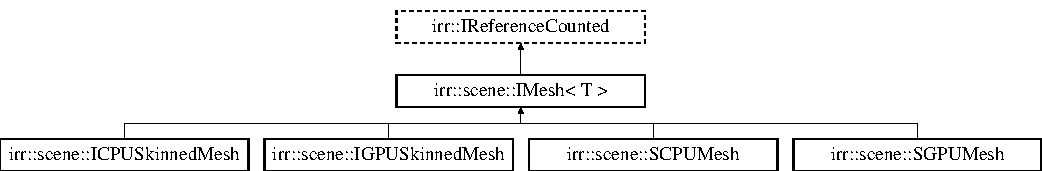
\includegraphics[height=2.295082cm]{classirr_1_1scene_1_1IMesh}
\end{center}
\end{figure}
\subsection*{Public Member Functions}
\begin{DoxyCompactItemize}
\item 
virtual \hyperlink{namespaceirr_a0416a53257075833e7002efd0a18e804}{u32} \hyperlink{classirr_1_1scene_1_1IMesh_ac646156350e42e51bac3ab7951034151}{get\+Mesh\+Buffer\+Count} () const  =0
\begin{DoxyCompactList}\small\item\em Get the amount of mesh buffers. \end{DoxyCompactList}\item 
virtual T $\ast$ \hyperlink{classirr_1_1scene_1_1IMesh_a67a26eef0e99a45ef5aab73dd80a993f}{get\+Mesh\+Buffer} (\hyperlink{namespaceirr_a0416a53257075833e7002efd0a18e804}{u32} nr) const  =0
\begin{DoxyCompactList}\small\item\em Get pointer to a mesh buffer. \end{DoxyCompactList}\item 
virtual const \hyperlink{classirr_1_1core_1_1aabbox3d}{core\+::aabbox3d}$<$ \hyperlink{namespaceirr_a0277be98d67dc26ff93b1a6a1d086b07}{f32} $>$ \& \hyperlink{classirr_1_1scene_1_1IMesh_a821ad4b325444ff5b47035cf54a4303f}{get\+Bounding\+Box} () const  =0
\begin{DoxyCompactList}\small\item\em Get an axis aligned bounding box of the mesh. \end{DoxyCompactList}\item 
virtual void \hyperlink{classirr_1_1scene_1_1IMesh_afe0512c81bf86d2feb16d84bbce72b6d}{set\+Bounding\+Box} (const \hyperlink{namespaceirr_1_1core_adfc8fa01b30044c55f3332a1d6c1aa19}{core\+::aabbox3df} \&box)=0
\begin{DoxyCompactList}\small\item\em Set user-\/defined axis aligned bounding box. \end{DoxyCompactList}\item 
virtual void \hyperlink{classirr_1_1scene_1_1IMesh_a38e6d34862f1d27ba69f6009f8eea9e5}{recalculate\+Bounding\+Box} ()\hypertarget{classirr_1_1scene_1_1IMesh_a38e6d34862f1d27ba69f6009f8eea9e5}{}\label{classirr_1_1scene_1_1IMesh_a38e6d34862f1d27ba69f6009f8eea9e5}

\begin{DoxyCompactList}\small\item\em recalculates the bounding box \end{DoxyCompactList}\item 
virtual void \hyperlink{classirr_1_1scene_1_1IMesh_a3e7e9c201ad12e33d1387b11fb1409f0}{set\+Material\+Flag} (\hyperlink{namespaceirr_1_1video_a8a3bc00ae8137535b9fbc5f40add70d3}{video\+::\+E\+\_\+\+M\+A\+T\+E\+R\+I\+A\+L\+\_\+\+F\+L\+AG} flag, bool newvalue)=0
\begin{DoxyCompactList}\small\item\em Sets a flag of all contained materials to a new value. \end{DoxyCompactList}\item 
virtual \hyperlink{namespaceirr_1_1scene_aef0400177e5941293dff6640e800d11b}{E\+\_\+\+M\+E\+S\+H\+\_\+\+T\+Y\+PE} {\bfseries get\+Mesh\+Type} () const  =0\hypertarget{classirr_1_1scene_1_1IMesh_ab7f1e7e39c225a1f2bd13f96f6429aa0}{}\label{classirr_1_1scene_1_1IMesh_ab7f1e7e39c225a1f2bd13f96f6429aa0}

\end{DoxyCompactItemize}
\subsection*{Additional Inherited Members}


\subsection{Detailed Description}
\subsubsection*{template$<$class T$>$\\*
class irr\+::scene\+::\+I\+Mesh$<$ T $>$}

Class which holds the geometry of an object. 

An \hyperlink{classirr_1_1scene_1_1IMesh}{I\+Mesh} is nothing more than a collection of some mesh buffers (\hyperlink{classirr_1_1scene_1_1IMeshBuffer}{I\+Mesh\+Buffer}). S\+Mesh is a simple implementation of an \hyperlink{classirr_1_1scene_1_1IMesh}{I\+Mesh}. A mesh is usually added to an \hyperlink{classirr_1_1scene_1_1IMeshSceneNode}{I\+Mesh\+Scene\+Node} in order to be rendered. 

\subsection{Member Function Documentation}
\index{irr\+::scene\+::\+I\+Mesh@{irr\+::scene\+::\+I\+Mesh}!get\+Bounding\+Box@{get\+Bounding\+Box}}
\index{get\+Bounding\+Box@{get\+Bounding\+Box}!irr\+::scene\+::\+I\+Mesh@{irr\+::scene\+::\+I\+Mesh}}
\subsubsection[{\texorpdfstring{get\+Bounding\+Box() const  =0}{getBoundingBox() const  =0}}]{\setlength{\rightskip}{0pt plus 5cm}template$<$class T$>$ virtual const {\bf core\+::aabbox3d}$<${\bf f32}$>$\& {\bf irr\+::scene\+::\+I\+Mesh}$<$ T $>$\+::get\+Bounding\+Box (
\begin{DoxyParamCaption}
{}
\end{DoxyParamCaption}
) const\hspace{0.3cm}{\ttfamily [pure virtual]}}\hypertarget{classirr_1_1scene_1_1IMesh_a821ad4b325444ff5b47035cf54a4303f}{}\label{classirr_1_1scene_1_1IMesh_a821ad4b325444ff5b47035cf54a4303f}


Get an axis aligned bounding box of the mesh. 

\begin{DoxyReturn}{Returns}
Bounding box of this mesh. 
\end{DoxyReturn}


Implemented in \hyperlink{classirr_1_1scene_1_1SGPUMesh_a19ce317ec8eed0e5051135506c2767b4}{irr\+::scene\+::\+S\+G\+P\+U\+Mesh}, \hyperlink{classirr_1_1scene_1_1SCPUMesh_adae935230822cf8fe704848e2ceea8be}{irr\+::scene\+::\+S\+C\+P\+U\+Mesh}, and \hyperlink{classirr_1_1scene_1_1IGPUSkinnedMesh_af6e2919ba3abcb6747f7b688b338ac16}{irr\+::scene\+::\+I\+G\+P\+U\+Skinned\+Mesh}.

\index{irr\+::scene\+::\+I\+Mesh@{irr\+::scene\+::\+I\+Mesh}!get\+Mesh\+Buffer@{get\+Mesh\+Buffer}}
\index{get\+Mesh\+Buffer@{get\+Mesh\+Buffer}!irr\+::scene\+::\+I\+Mesh@{irr\+::scene\+::\+I\+Mesh}}
\subsubsection[{\texorpdfstring{get\+Mesh\+Buffer(u32 nr) const  =0}{getMeshBuffer(u32 nr) const  =0}}]{\setlength{\rightskip}{0pt plus 5cm}template$<$class T$>$ virtual T$\ast$ {\bf irr\+::scene\+::\+I\+Mesh}$<$ T $>$\+::get\+Mesh\+Buffer (
\begin{DoxyParamCaption}
\item[{{\bf u32}}]{nr}
\end{DoxyParamCaption}
) const\hspace{0.3cm}{\ttfamily [pure virtual]}}\hypertarget{classirr_1_1scene_1_1IMesh_a67a26eef0e99a45ef5aab73dd80a993f}{}\label{classirr_1_1scene_1_1IMesh_a67a26eef0e99a45ef5aab73dd80a993f}


Get pointer to a mesh buffer. 


\begin{DoxyParams}{Parameters}
{\em nr} & Zero based index of the mesh buffer. The maximum value is \hyperlink{classirr_1_1scene_1_1IMesh_ac646156350e42e51bac3ab7951034151}{get\+Mesh\+Buffer\+Count()} -\/ 1; \\
\hline
\end{DoxyParams}
\begin{DoxyReturn}{Returns}
Pointer to the mesh buffer or 0 if there is no such mesh buffer. 
\end{DoxyReturn}


Implemented in \hyperlink{classirr_1_1scene_1_1SGPUMesh_af3f219d8cb7c6ade7ff48e52b68cfde8}{irr\+::scene\+::\+S\+G\+P\+U\+Mesh}, and \hyperlink{classirr_1_1scene_1_1SCPUMesh_aceebdb00f6de1a5ec9564930c1a55a6e}{irr\+::scene\+::\+S\+C\+P\+U\+Mesh}.

\index{irr\+::scene\+::\+I\+Mesh@{irr\+::scene\+::\+I\+Mesh}!get\+Mesh\+Buffer\+Count@{get\+Mesh\+Buffer\+Count}}
\index{get\+Mesh\+Buffer\+Count@{get\+Mesh\+Buffer\+Count}!irr\+::scene\+::\+I\+Mesh@{irr\+::scene\+::\+I\+Mesh}}
\subsubsection[{\texorpdfstring{get\+Mesh\+Buffer\+Count() const  =0}{getMeshBufferCount() const  =0}}]{\setlength{\rightskip}{0pt plus 5cm}template$<$class T$>$ virtual {\bf u32} {\bf irr\+::scene\+::\+I\+Mesh}$<$ T $>$\+::get\+Mesh\+Buffer\+Count (
\begin{DoxyParamCaption}
{}
\end{DoxyParamCaption}
) const\hspace{0.3cm}{\ttfamily [pure virtual]}}\hypertarget{classirr_1_1scene_1_1IMesh_ac646156350e42e51bac3ab7951034151}{}\label{classirr_1_1scene_1_1IMesh_ac646156350e42e51bac3ab7951034151}


Get the amount of mesh buffers. 

\begin{DoxyReturn}{Returns}
Amount of mesh buffers (\hyperlink{classirr_1_1scene_1_1IMeshBuffer}{I\+Mesh\+Buffer}) in this mesh. 
\end{DoxyReturn}


Implemented in \hyperlink{classirr_1_1scene_1_1SGPUMesh_a7978038f8a6f7f89df9df69dfaf36d57}{irr\+::scene\+::\+S\+G\+P\+U\+Mesh}, and \hyperlink{classirr_1_1scene_1_1SCPUMesh_a779211c91a74cb292ffc6992e228799d}{irr\+::scene\+::\+S\+C\+P\+U\+Mesh}.

\index{irr\+::scene\+::\+I\+Mesh@{irr\+::scene\+::\+I\+Mesh}!set\+Bounding\+Box@{set\+Bounding\+Box}}
\index{set\+Bounding\+Box@{set\+Bounding\+Box}!irr\+::scene\+::\+I\+Mesh@{irr\+::scene\+::\+I\+Mesh}}
\subsubsection[{\texorpdfstring{set\+Bounding\+Box(const core\+::aabbox3df \&box)=0}{setBoundingBox(const core::aabbox3df \&box)=0}}]{\setlength{\rightskip}{0pt plus 5cm}template$<$class T$>$ virtual void {\bf irr\+::scene\+::\+I\+Mesh}$<$ T $>$\+::set\+Bounding\+Box (
\begin{DoxyParamCaption}
\item[{const {\bf core\+::aabbox3df} \&}]{box}
\end{DoxyParamCaption}
)\hspace{0.3cm}{\ttfamily [pure virtual]}}\hypertarget{classirr_1_1scene_1_1IMesh_afe0512c81bf86d2feb16d84bbce72b6d}{}\label{classirr_1_1scene_1_1IMesh_afe0512c81bf86d2feb16d84bbce72b6d}


Set user-\/defined axis aligned bounding box. 


\begin{DoxyParams}{Parameters}
{\em box} & New bounding box to use for the mesh. \\
\hline
\end{DoxyParams}


Implemented in \hyperlink{classirr_1_1scene_1_1SGPUMesh_a077ac911871bacb359bdf540de40029f}{irr\+::scene\+::\+S\+G\+P\+U\+Mesh}, \hyperlink{classirr_1_1scene_1_1SCPUMesh_aaa92ceeaa9abff9b55d9316e01678d7e}{irr\+::scene\+::\+S\+C\+P\+U\+Mesh}, and \hyperlink{classirr_1_1scene_1_1IGPUSkinnedMesh_a91372effa8144b0bac6f7483eccb1f66}{irr\+::scene\+::\+I\+G\+P\+U\+Skinned\+Mesh}.

\index{irr\+::scene\+::\+I\+Mesh@{irr\+::scene\+::\+I\+Mesh}!set\+Material\+Flag@{set\+Material\+Flag}}
\index{set\+Material\+Flag@{set\+Material\+Flag}!irr\+::scene\+::\+I\+Mesh@{irr\+::scene\+::\+I\+Mesh}}
\subsubsection[{\texorpdfstring{set\+Material\+Flag(video\+::\+E\+\_\+\+M\+A\+T\+E\+R\+I\+A\+L\+\_\+\+F\+L\+A\+G flag, bool newvalue)=0}{setMaterialFlag(video::E\_MATERIAL\_FLAG flag, bool newvalue)=0}}]{\setlength{\rightskip}{0pt plus 5cm}template$<$class T$>$ virtual void {\bf irr\+::scene\+::\+I\+Mesh}$<$ T $>$\+::set\+Material\+Flag (
\begin{DoxyParamCaption}
\item[{{\bf video\+::\+E\+\_\+\+M\+A\+T\+E\+R\+I\+A\+L\+\_\+\+F\+L\+AG}}]{flag, }
\item[{bool}]{newvalue}
\end{DoxyParamCaption}
)\hspace{0.3cm}{\ttfamily [pure virtual]}}\hypertarget{classirr_1_1scene_1_1IMesh_a3e7e9c201ad12e33d1387b11fb1409f0}{}\label{classirr_1_1scene_1_1IMesh_a3e7e9c201ad12e33d1387b11fb1409f0}


Sets a flag of all contained materials to a new value. 


\begin{DoxyParams}{Parameters}
{\em flag} & Flag to set in all materials. \\
\hline
{\em newvalue} & New value to set in all materials. \\
\hline
\end{DoxyParams}


Implemented in \hyperlink{classirr_1_1scene_1_1SGPUMesh_a8cbba306dc9fc44460808ff4c9d925be}{irr\+::scene\+::\+S\+G\+P\+U\+Mesh}, and \hyperlink{classirr_1_1scene_1_1SCPUMesh_a3f151b1292b1e0aa70cde8f50793d85c}{irr\+::scene\+::\+S\+C\+P\+U\+Mesh}.



The documentation for this class was generated from the following file\+:\begin{DoxyCompactItemize}
\item 
include/I\+Mesh.\+h\end{DoxyCompactItemize}

\hypertarget{classirr_1_1scene_1_1IMeshBuffer}{}\section{irr\+:\+:scene\+:\+:I\+Mesh\+Buffer$<$ T $>$ Class Template Reference}
\label{classirr_1_1scene_1_1IMeshBuffer}\index{irr\+::scene\+::\+I\+Mesh\+Buffer$<$ T $>$@{irr\+::scene\+::\+I\+Mesh\+Buffer$<$ T $>$}}
Inheritance diagram for irr\+:\+:scene\+:\+:I\+Mesh\+Buffer$<$ T $>$\+:\begin{figure}[H]
\begin{center}
\leavevmode
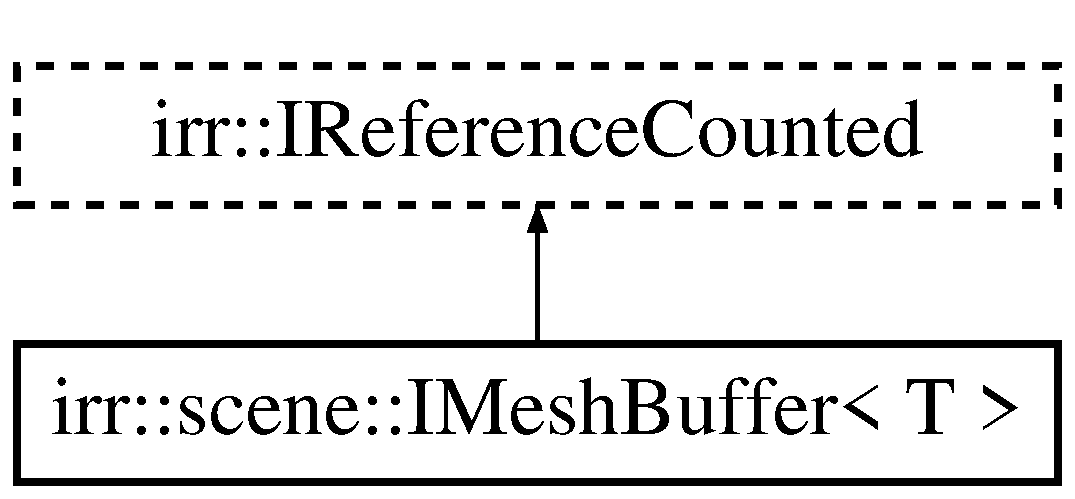
\includegraphics[height=2.000000cm]{classirr_1_1scene_1_1IMeshBuffer}
\end{center}
\end{figure}
\subsection*{Public Member Functions}
\begin{DoxyCompactItemize}
\item 
{\bfseries I\+Mesh\+Buffer} (\hyperlink{classirr_1_1scene_1_1IMeshDataFormatDesc}{I\+Mesh\+Data\+Format\+Desc}$<$ T $>$ $\ast$layout=N\+U\+LL)\hypertarget{classirr_1_1scene_1_1IMeshBuffer_a0f66dafa934fc63e83958c2f73ff796e}{}\label{classirr_1_1scene_1_1IMeshBuffer_a0f66dafa934fc63e83958c2f73ff796e}

\item 
\hyperlink{classirr_1_1scene_1_1IMeshDataFormatDesc}{I\+Mesh\+Data\+Format\+Desc}$<$ T $>$ $\ast$ {\bfseries get\+Mesh\+Data\+And\+Format} ()\hypertarget{classirr_1_1scene_1_1IMeshBuffer_a416c8e972e84063a02878a269a943b8e}{}\label{classirr_1_1scene_1_1IMeshBuffer_a416c8e972e84063a02878a269a943b8e}

\item 
const \hyperlink{classirr_1_1scene_1_1IMeshDataFormatDesc}{I\+Mesh\+Data\+Format\+Desc}$<$ T $>$ $\ast$ {\bfseries get\+Mesh\+Data\+And\+Format} () const \hypertarget{classirr_1_1scene_1_1IMeshBuffer_af9bc1d32d27767c33d63d2d117592791}{}\label{classirr_1_1scene_1_1IMeshBuffer_af9bc1d32d27767c33d63d2d117592791}

\item 
void {\bfseries set\+Mesh\+Data\+And\+Format} (\hyperlink{classirr_1_1scene_1_1IMeshDataFormatDesc}{I\+Mesh\+Data\+Format\+Desc}$<$ T $>$ $\ast$layout)\hypertarget{classirr_1_1scene_1_1IMeshBuffer_ac607c17b7935e1d44b7f3d7c0ed6e94f}{}\label{classirr_1_1scene_1_1IMeshBuffer_ac607c17b7935e1d44b7f3d7c0ed6e94f}

\item 
const video\+::\+E\+\_\+\+I\+N\+D\+E\+X\+\_\+\+T\+Y\+PE \& \hyperlink{classirr_1_1scene_1_1IMeshBuffer_a5b01c80eb695dfa21f21220d759539ea}{get\+Index\+Type} () const 
\begin{DoxyCompactList}\small\item\em Get type of index data which is stored in this meshbuffer. \end{DoxyCompactList}\item 
void {\bfseries set\+Index\+Type} (const video\+::\+E\+\_\+\+I\+N\+D\+E\+X\+\_\+\+T\+Y\+PE \&type)\hypertarget{classirr_1_1scene_1_1IMeshBuffer_a037c8dd0425f71ac1901a2a78529fa22}{}\label{classirr_1_1scene_1_1IMeshBuffer_a037c8dd0425f71ac1901a2a78529fa22}

\item 
void {\bfseries set\+Index\+Buffer\+Offset} (const size\+\_\+t \&byte\+Offset)\hypertarget{classirr_1_1scene_1_1IMeshBuffer_af06ccefb6f2825f13eeadcdf6880cfa7}{}\label{classirr_1_1scene_1_1IMeshBuffer_af06ccefb6f2825f13eeadcdf6880cfa7}

\item 
const size\+\_\+t \& {\bfseries get\+Index\+Buffer\+Offset} () const \hypertarget{classirr_1_1scene_1_1IMeshBuffer_a58e8b5abbe9627c89c377961b756cf96}{}\label{classirr_1_1scene_1_1IMeshBuffer_a58e8b5abbe9627c89c377961b756cf96}

\item 
const uint64\+\_\+t \& \hyperlink{classirr_1_1scene_1_1IMeshBuffer_aab91c05463d1cf3232c4f6255e14065d}{get\+Index\+Count} () const 
\begin{DoxyCompactList}\small\item\em Get amount of indices in this meshbuffer. \end{DoxyCompactList}\item 
bool {\bfseries set\+Index\+Count} (const uint64\+\_\+t \&new\+Index\+Count)\hypertarget{classirr_1_1scene_1_1IMeshBuffer_ae5ebcb1ecd31e8c6930ec5c037e2fa84}{}\label{classirr_1_1scene_1_1IMeshBuffer_ae5ebcb1ecd31e8c6930ec5c037e2fa84}

\item 
const int32\+\_\+t \& {\bfseries get\+Base\+Vertex} () const \hypertarget{classirr_1_1scene_1_1IMeshBuffer_a459873751dd41f9c3b1d66dbab976724}{}\label{classirr_1_1scene_1_1IMeshBuffer_a459873751dd41f9c3b1d66dbab976724}

\item 
void {\bfseries set\+Base\+Vertex} (const int32\+\_\+t \&base\+Vx)\hypertarget{classirr_1_1scene_1_1IMeshBuffer_a653a308af6252aed4c74ff4b2986e951}{}\label{classirr_1_1scene_1_1IMeshBuffer_a653a308af6252aed4c74ff4b2986e951}

\item 
const \hyperlink{namespaceirr_1_1scene_a5d7de82f2169761194b2f44d95cdc1dc}{scene\+::\+E\+\_\+\+P\+R\+I\+M\+I\+T\+I\+V\+E\+\_\+\+T\+Y\+PE} \& {\bfseries get\+Primitive\+Type} () const \hypertarget{classirr_1_1scene_1_1IMeshBuffer_ab84167de1015f1c6850ef1dd75c77182}{}\label{classirr_1_1scene_1_1IMeshBuffer_ab84167de1015f1c6850ef1dd75c77182}

\item 
void {\bfseries set\+Primitive\+Type} (const \hyperlink{namespaceirr_1_1scene_a5d7de82f2169761194b2f44d95cdc1dc}{scene\+::\+E\+\_\+\+P\+R\+I\+M\+I\+T\+I\+V\+E\+\_\+\+T\+Y\+PE} \&type)\hypertarget{classirr_1_1scene_1_1IMeshBuffer_aada06347c1195cdfd5e9e3955d842a9b}{}\label{classirr_1_1scene_1_1IMeshBuffer_aada06347c1195cdfd5e9e3955d842a9b}

\item 
const size\+\_\+t \& {\bfseries get\+Instance\+Count} () const \hypertarget{classirr_1_1scene_1_1IMeshBuffer_ac13655bb7c91e4917c8ed74ba7241414}{}\label{classirr_1_1scene_1_1IMeshBuffer_ac13655bb7c91e4917c8ed74ba7241414}

\item 
void {\bfseries set\+Instance\+Count} (const size\+\_\+t \&count)\hypertarget{classirr_1_1scene_1_1IMeshBuffer_a8358b00737428ad08be25c97188bec65}{}\label{classirr_1_1scene_1_1IMeshBuffer_a8358b00737428ad08be25c97188bec65}

\item 
const uint32\+\_\+t \& {\bfseries get\+Base\+Instance} () const \hypertarget{classirr_1_1scene_1_1IMeshBuffer_a9fea491c3617ce1a4ac0f24a5b0ac8bf}{}\label{classirr_1_1scene_1_1IMeshBuffer_a9fea491c3617ce1a4ac0f24a5b0ac8bf}

\item 
void {\bfseries set\+Base\+Instance} (const uint32\+\_\+t \&base)\hypertarget{classirr_1_1scene_1_1IMeshBuffer_a621584bc5b4a3f7c703a696272441b0a}{}\label{classirr_1_1scene_1_1IMeshBuffer_a621584bc5b4a3f7c703a696272441b0a}

\item 
const \hyperlink{namespaceirr_1_1core_adfc8fa01b30044c55f3332a1d6c1aa19}{core\+::aabbox3df} \& \hyperlink{classirr_1_1scene_1_1IMeshBuffer_a8b8b19540e5d82432acbddb61d05459b}{get\+Bounding\+Box} () const 
\begin{DoxyCompactList}\small\item\em Get the axis aligned bounding box of this meshbuffer. \end{DoxyCompactList}\item 
void \hyperlink{classirr_1_1scene_1_1IMeshBuffer_a6434ba67b31904215afb17b8180e7e66}{set\+Bounding\+Box} (const \hyperlink{namespaceirr_1_1core_adfc8fa01b30044c55f3332a1d6c1aa19}{core\+::aabbox3df} \&box)
\begin{DoxyCompactList}\small\item\em Set axis aligned bounding box. \end{DoxyCompactList}\item 
const \hyperlink{classirr_1_1video_1_1SMaterial}{video\+::\+S\+Material} \& \hyperlink{classirr_1_1scene_1_1IMeshBuffer_a46c154b3cf9730cbc078c1e6ea1b6b18}{get\+Material} () const 
\begin{DoxyCompactList}\small\item\em Get material of this meshbuffer. \end{DoxyCompactList}\item 
\hyperlink{classirr_1_1video_1_1SMaterial}{video\+::\+S\+Material} \& \hyperlink{classirr_1_1scene_1_1IMeshBuffer_a4f4160dbdd5bb5dbfc4b74b5042dc0ec}{get\+Material} ()
\begin{DoxyCompactList}\small\item\em Get material of this meshbuffer. \end{DoxyCompactList}\end{DoxyCompactItemize}
\subsection*{Protected Attributes}
\begin{DoxyCompactItemize}
\item 
\hyperlink{classirr_1_1video_1_1SMaterial}{video\+::\+S\+Material} {\bfseries Material}\hypertarget{classirr_1_1scene_1_1IMeshBuffer_a68ef6f0ebfba22e338068271e9dbaefd}{}\label{classirr_1_1scene_1_1IMeshBuffer_a68ef6f0ebfba22e338068271e9dbaefd}

\item 
\hyperlink{namespaceirr_1_1core_adfc8fa01b30044c55f3332a1d6c1aa19}{core\+::aabbox3df} {\bfseries bounding\+Box}\hypertarget{classirr_1_1scene_1_1IMeshBuffer_a3878604f531bede20dd859c8779f9246}{}\label{classirr_1_1scene_1_1IMeshBuffer_a3878604f531bede20dd859c8779f9246}

\item 
\hyperlink{classirr_1_1scene_1_1IMeshDataFormatDesc}{I\+Mesh\+Data\+Format\+Desc}$<$ T $>$ $\ast$ {\bfseries mesh\+Layout}\hypertarget{classirr_1_1scene_1_1IMeshBuffer_adbf6974b2807e62d7f8de703a3a0c821}{}\label{classirr_1_1scene_1_1IMeshBuffer_adbf6974b2807e62d7f8de703a3a0c821}

\item 
video\+::\+E\+\_\+\+I\+N\+D\+E\+X\+\_\+\+T\+Y\+PE {\bfseries index\+Type}\hypertarget{classirr_1_1scene_1_1IMeshBuffer_af9d6815073725a6a003846648c63dfc1}{}\label{classirr_1_1scene_1_1IMeshBuffer_af9d6815073725a6a003846648c63dfc1}

\item 
int32\+\_\+t {\bfseries base\+Vertex}\hypertarget{classirr_1_1scene_1_1IMeshBuffer_a1e0345abd78dadd2235e2e9671bede1f}{}\label{classirr_1_1scene_1_1IMeshBuffer_a1e0345abd78dadd2235e2e9671bede1f}

\item 
uint64\+\_\+t {\bfseries index\+Count}\hypertarget{classirr_1_1scene_1_1IMeshBuffer_a8c611fb2c87c764765cb2db2123dda72}{}\label{classirr_1_1scene_1_1IMeshBuffer_a8c611fb2c87c764765cb2db2123dda72}

\item 
size\+\_\+t {\bfseries index\+Buf\+Offset}\hypertarget{classirr_1_1scene_1_1IMeshBuffer_ad40066414da2a21a3ab9f62a3bf5f41f}{}\label{classirr_1_1scene_1_1IMeshBuffer_ad40066414da2a21a3ab9f62a3bf5f41f}

\item 
size\+\_\+t {\bfseries instance\+Count}\hypertarget{classirr_1_1scene_1_1IMeshBuffer_a2edd6467d896cacf0782e9ed62b50712}{}\label{classirr_1_1scene_1_1IMeshBuffer_a2edd6467d896cacf0782e9ed62b50712}

\item 
uint32\+\_\+t {\bfseries base\+Instance}\hypertarget{classirr_1_1scene_1_1IMeshBuffer_a816b2d414cd010c2033b670d476baeed}{}\label{classirr_1_1scene_1_1IMeshBuffer_a816b2d414cd010c2033b670d476baeed}

\item 
\hyperlink{namespaceirr_1_1scene_a5d7de82f2169761194b2f44d95cdc1dc}{scene\+::\+E\+\_\+\+P\+R\+I\+M\+I\+T\+I\+V\+E\+\_\+\+T\+Y\+PE} {\bfseries primitive\+Type}\hypertarget{classirr_1_1scene_1_1IMeshBuffer_ad1b28d6240e87658cbb084f141ba7b10}{}\label{classirr_1_1scene_1_1IMeshBuffer_ad1b28d6240e87658cbb084f141ba7b10}

\end{DoxyCompactItemize}
\subsection*{Additional Inherited Members}


\subsection{Member Function Documentation}
\index{irr\+::scene\+::\+I\+Mesh\+Buffer@{irr\+::scene\+::\+I\+Mesh\+Buffer}!get\+Bounding\+Box@{get\+Bounding\+Box}}
\index{get\+Bounding\+Box@{get\+Bounding\+Box}!irr\+::scene\+::\+I\+Mesh\+Buffer@{irr\+::scene\+::\+I\+Mesh\+Buffer}}
\subsubsection[{\texorpdfstring{get\+Bounding\+Box() const }{getBoundingBox() const }}]{\setlength{\rightskip}{0pt plus 5cm}template$<$class T$>$ const {\bf core\+::aabbox3df}\& {\bf irr\+::scene\+::\+I\+Mesh\+Buffer}$<$ T $>$\+::get\+Bounding\+Box (
\begin{DoxyParamCaption}
{}
\end{DoxyParamCaption}
) const\hspace{0.3cm}{\ttfamily [inline]}}\hypertarget{classirr_1_1scene_1_1IMeshBuffer_a8b8b19540e5d82432acbddb61d05459b}{}\label{classirr_1_1scene_1_1IMeshBuffer_a8b8b19540e5d82432acbddb61d05459b}


Get the axis aligned bounding box of this meshbuffer. 

\begin{DoxyReturn}{Returns}
Axis aligned bounding box of this buffer. 
\end{DoxyReturn}
\index{irr\+::scene\+::\+I\+Mesh\+Buffer@{irr\+::scene\+::\+I\+Mesh\+Buffer}!get\+Index\+Count@{get\+Index\+Count}}
\index{get\+Index\+Count@{get\+Index\+Count}!irr\+::scene\+::\+I\+Mesh\+Buffer@{irr\+::scene\+::\+I\+Mesh\+Buffer}}
\subsubsection[{\texorpdfstring{get\+Index\+Count() const }{getIndexCount() const }}]{\setlength{\rightskip}{0pt plus 5cm}template$<$class T$>$ const uint64\+\_\+t\& {\bf irr\+::scene\+::\+I\+Mesh\+Buffer}$<$ T $>$\+::get\+Index\+Count (
\begin{DoxyParamCaption}
{}
\end{DoxyParamCaption}
) const\hspace{0.3cm}{\ttfamily [inline]}}\hypertarget{classirr_1_1scene_1_1IMeshBuffer_aab91c05463d1cf3232c4f6255e14065d}{}\label{classirr_1_1scene_1_1IMeshBuffer_aab91c05463d1cf3232c4f6255e14065d}


Get amount of indices in this meshbuffer. 

\begin{DoxyReturn}{Returns}
Number of indices in this buffer. 
\end{DoxyReturn}
\index{irr\+::scene\+::\+I\+Mesh\+Buffer@{irr\+::scene\+::\+I\+Mesh\+Buffer}!get\+Index\+Type@{get\+Index\+Type}}
\index{get\+Index\+Type@{get\+Index\+Type}!irr\+::scene\+::\+I\+Mesh\+Buffer@{irr\+::scene\+::\+I\+Mesh\+Buffer}}
\subsubsection[{\texorpdfstring{get\+Index\+Type() const }{getIndexType() const }}]{\setlength{\rightskip}{0pt plus 5cm}template$<$class T$>$ const video\+::\+E\+\_\+\+I\+N\+D\+E\+X\+\_\+\+T\+Y\+PE\& {\bf irr\+::scene\+::\+I\+Mesh\+Buffer}$<$ T $>$\+::get\+Index\+Type (
\begin{DoxyParamCaption}
{}
\end{DoxyParamCaption}
) const\hspace{0.3cm}{\ttfamily [inline]}}\hypertarget{classirr_1_1scene_1_1IMeshBuffer_a5b01c80eb695dfa21f21220d759539ea}{}\label{classirr_1_1scene_1_1IMeshBuffer_a5b01c80eb695dfa21f21220d759539ea}


Get type of index data which is stored in this meshbuffer. 

\begin{DoxyReturn}{Returns}
Index type of this buffer. 
\end{DoxyReturn}
\index{irr\+::scene\+::\+I\+Mesh\+Buffer@{irr\+::scene\+::\+I\+Mesh\+Buffer}!get\+Material@{get\+Material}}
\index{get\+Material@{get\+Material}!irr\+::scene\+::\+I\+Mesh\+Buffer@{irr\+::scene\+::\+I\+Mesh\+Buffer}}
\subsubsection[{\texorpdfstring{get\+Material() const }{getMaterial() const }}]{\setlength{\rightskip}{0pt plus 5cm}template$<$class T$>$ const {\bf video\+::\+S\+Material}\& {\bf irr\+::scene\+::\+I\+Mesh\+Buffer}$<$ T $>$\+::get\+Material (
\begin{DoxyParamCaption}
{}
\end{DoxyParamCaption}
) const\hspace{0.3cm}{\ttfamily [inline]}}\hypertarget{classirr_1_1scene_1_1IMeshBuffer_a46c154b3cf9730cbc078c1e6ea1b6b18}{}\label{classirr_1_1scene_1_1IMeshBuffer_a46c154b3cf9730cbc078c1e6ea1b6b18}


Get material of this meshbuffer. 

\begin{DoxyReturn}{Returns}
Material of this buffer 
\end{DoxyReturn}
\index{irr\+::scene\+::\+I\+Mesh\+Buffer@{irr\+::scene\+::\+I\+Mesh\+Buffer}!get\+Material@{get\+Material}}
\index{get\+Material@{get\+Material}!irr\+::scene\+::\+I\+Mesh\+Buffer@{irr\+::scene\+::\+I\+Mesh\+Buffer}}
\subsubsection[{\texorpdfstring{get\+Material()}{getMaterial()}}]{\setlength{\rightskip}{0pt plus 5cm}template$<$class T$>$ {\bf video\+::\+S\+Material}\& {\bf irr\+::scene\+::\+I\+Mesh\+Buffer}$<$ T $>$\+::get\+Material (
\begin{DoxyParamCaption}
{}
\end{DoxyParamCaption}
)\hspace{0.3cm}{\ttfamily [inline]}}\hypertarget{classirr_1_1scene_1_1IMeshBuffer_a4f4160dbdd5bb5dbfc4b74b5042dc0ec}{}\label{classirr_1_1scene_1_1IMeshBuffer_a4f4160dbdd5bb5dbfc4b74b5042dc0ec}


Get material of this meshbuffer. 

\begin{DoxyReturn}{Returns}
Material of this buffer 
\end{DoxyReturn}
\index{irr\+::scene\+::\+I\+Mesh\+Buffer@{irr\+::scene\+::\+I\+Mesh\+Buffer}!set\+Bounding\+Box@{set\+Bounding\+Box}}
\index{set\+Bounding\+Box@{set\+Bounding\+Box}!irr\+::scene\+::\+I\+Mesh\+Buffer@{irr\+::scene\+::\+I\+Mesh\+Buffer}}
\subsubsection[{\texorpdfstring{set\+Bounding\+Box(const core\+::aabbox3df \&box)}{setBoundingBox(const core::aabbox3df \&box)}}]{\setlength{\rightskip}{0pt plus 5cm}template$<$class T$>$ void {\bf irr\+::scene\+::\+I\+Mesh\+Buffer}$<$ T $>$\+::set\+Bounding\+Box (
\begin{DoxyParamCaption}
\item[{const {\bf core\+::aabbox3df} \&}]{box}
\end{DoxyParamCaption}
)\hspace{0.3cm}{\ttfamily [inline]}}\hypertarget{classirr_1_1scene_1_1IMeshBuffer_a6434ba67b31904215afb17b8180e7e66}{}\label{classirr_1_1scene_1_1IMeshBuffer_a6434ba67b31904215afb17b8180e7e66}


Set axis aligned bounding box. 


\begin{DoxyParams}{Parameters}
{\em box} & User defined axis aligned bounding box to use for this buffer. \\
\hline
\end{DoxyParams}


The documentation for this class was generated from the following file\+:\begin{DoxyCompactItemize}
\item 
include/I\+Mesh\+Buffer.\+h\end{DoxyCompactItemize}

\hypertarget{classirr_1_1scene_1_1IMeshCache}{}\section{irr\+:\+:scene\+:\+:I\+Mesh\+Cache$<$ T $>$ Class Template Reference}
\label{classirr_1_1scene_1_1IMeshCache}\index{irr\+::scene\+::\+I\+Mesh\+Cache$<$ T $>$@{irr\+::scene\+::\+I\+Mesh\+Cache$<$ T $>$}}


The mesh cache stores already loaded meshes and provides an interface to them.  




{\ttfamily \#include $<$I\+Mesh\+Cache.\+h$>$}

Inheritance diagram for irr\+:\+:scene\+:\+:I\+Mesh\+Cache$<$ T $>$\+:\begin{figure}[H]
\begin{center}
\leavevmode
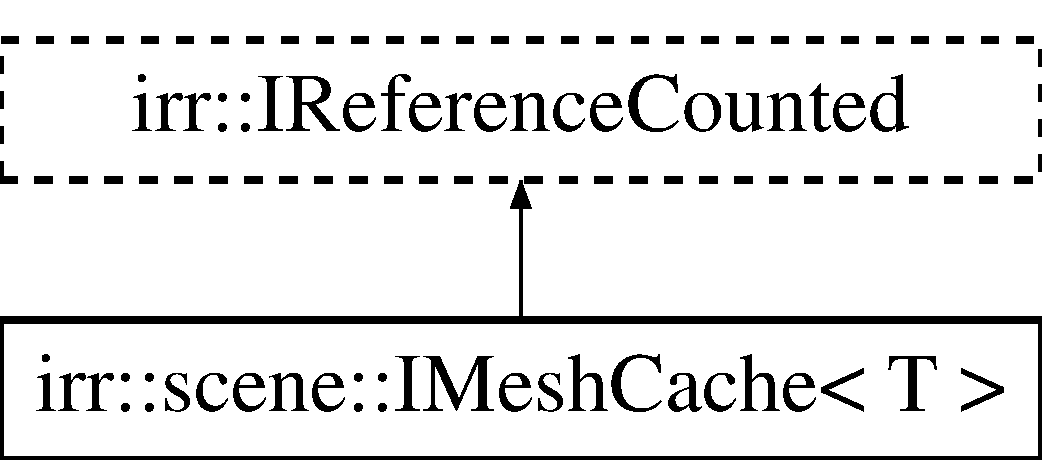
\includegraphics[height=2.000000cm]{classirr_1_1scene_1_1IMeshCache}
\end{center}
\end{figure}
\subsection*{Public Member Functions}
\begin{DoxyCompactItemize}
\item 
virtual \hyperlink{classirr_1_1scene_1_1IMeshCache_aac581c0d4c048446c282590447223435}{$\sim$\+I\+Mesh\+Cache} ()\hypertarget{classirr_1_1scene_1_1IMeshCache_aac581c0d4c048446c282590447223435}{}\label{classirr_1_1scene_1_1IMeshCache_aac581c0d4c048446c282590447223435}

\begin{DoxyCompactList}\small\item\em Destructor. \end{DoxyCompactList}\item 
virtual void \hyperlink{classirr_1_1scene_1_1IMeshCache_aaea60b117903d0f960d0e19df2bce39e}{add\+Mesh} (const \hyperlink{namespaceirr_1_1io_ab1bdc45edb3f94d8319c02bc0f840ee1}{io\+::path} \&name, T $\ast$mesh)=0
\begin{DoxyCompactList}\small\item\em Adds a mesh to the internal list of loaded meshes. \end{DoxyCompactList}\item 
virtual void \hyperlink{classirr_1_1scene_1_1IMeshCache_ab90eb5eca6864c96078d65e700223f45}{remove\+Mesh} (const T $\ast$const mesh)=0
\begin{DoxyCompactList}\small\item\em Removes the mesh from the cache. \end{DoxyCompactList}\item 
virtual \hyperlink{namespaceirr_a0416a53257075833e7002efd0a18e804}{u32} \hyperlink{classirr_1_1scene_1_1IMeshCache_a866c87d11246df2a3803d4689ee5ca4d}{get\+Mesh\+Count} () const  =0
\begin{DoxyCompactList}\small\item\em Returns amount of loaded meshes in the cache. \end{DoxyCompactList}\item 
virtual \hyperlink{namespaceirr_ac66849b7a6ed16e30ebede579f9b47c6}{s32} \hyperlink{classirr_1_1scene_1_1IMeshCache_a162b4e8fd055fd1a7b472c4ceb8f0fd5}{get\+Mesh\+Index} (const T $\ast$const mesh) const  =0
\begin{DoxyCompactList}\small\item\em Returns current index number of the mesh or -\/1 when not found. \end{DoxyCompactList}\item 
virtual T $\ast$ \hyperlink{classirr_1_1scene_1_1IMeshCache_ac4ab47723ac9c9ee81ff553af105bd6e}{get\+Mesh\+By\+Index} (\hyperlink{namespaceirr_a0416a53257075833e7002efd0a18e804}{u32} index)=0
\begin{DoxyCompactList}\small\item\em Returns a mesh based on its index number. \end{DoxyCompactList}\item 
virtual T $\ast$ \hyperlink{classirr_1_1scene_1_1IMeshCache_a6165e3f028c526af9ac094a99881598b}{get\+Mesh\+By\+Name} (const \hyperlink{namespaceirr_1_1io_ab1bdc45edb3f94d8319c02bc0f840ee1}{io\+::path} \&name)=0
\begin{DoxyCompactList}\small\item\em Returns a mesh based on its name. \end{DoxyCompactList}\item 
virtual const \hyperlink{structirr_1_1io_1_1SNamedPath}{io\+::\+S\+Named\+Path} \& \hyperlink{classirr_1_1scene_1_1IMeshCache_ac61e9ae1135743d90cc28266a6cfc236}{get\+Mesh\+Name} (\hyperlink{namespaceirr_a0416a53257075833e7002efd0a18e804}{u32} index) const  =0
\begin{DoxyCompactList}\small\item\em Get the name of a loaded mesh, based on its index. \end{DoxyCompactList}\item 
virtual const \hyperlink{structirr_1_1io_1_1SNamedPath}{io\+::\+S\+Named\+Path} \& \hyperlink{classirr_1_1scene_1_1IMeshCache_a50a1fd8b5e27c14c729b69f8313bb1eb}{get\+Mesh\+Name} (const T $\ast$const mesh) const  =0
\begin{DoxyCompactList}\small\item\em Get the name of the loaded mesh if there is any. \end{DoxyCompactList}\item 
virtual bool \hyperlink{classirr_1_1scene_1_1IMeshCache_a694f606aa09dcdf75d32a2349be2ff3f}{rename\+Mesh} (\hyperlink{namespaceirr_a0416a53257075833e7002efd0a18e804}{u32} index, const \hyperlink{namespaceirr_1_1io_ab1bdc45edb3f94d8319c02bc0f840ee1}{io\+::path} \&name)=0
\begin{DoxyCompactList}\small\item\em Renames a loaded mesh. \end{DoxyCompactList}\item 
virtual bool \hyperlink{classirr_1_1scene_1_1IMeshCache_a18169251ed55f2ea9f2e5341382ab49f}{rename\+Mesh} (const T $\ast$const mesh, const \hyperlink{namespaceirr_1_1io_ab1bdc45edb3f94d8319c02bc0f840ee1}{io\+::path} \&name)=0
\begin{DoxyCompactList}\small\item\em Renames the loaded mesh. \end{DoxyCompactList}\item 
virtual bool \hyperlink{classirr_1_1scene_1_1IMeshCache_a888be60cbdb155443108fb27908c0d51}{is\+Mesh\+Loaded} (const \hyperlink{namespaceirr_1_1io_ab1bdc45edb3f94d8319c02bc0f840ee1}{io\+::path} \&name)=0
\begin{DoxyCompactList}\small\item\em Check if a mesh was already loaded. \end{DoxyCompactList}\item 
virtual void \hyperlink{classirr_1_1scene_1_1IMeshCache_a973742f191f37291e202f2eda51ab444}{clear} ()=0
\begin{DoxyCompactList}\small\item\em Clears the whole mesh cache, removing all meshes. \end{DoxyCompactList}\item 
virtual void \hyperlink{classirr_1_1scene_1_1IMeshCache_aa79e0c6c82e5361b94167f99f7a958c8}{clear\+Unused\+Meshes} ()=0
\begin{DoxyCompactList}\small\item\em Clears all meshes that are held in the mesh cache but not used anywhere else. \end{DoxyCompactList}\end{DoxyCompactItemize}
\subsection*{Additional Inherited Members}


\subsection{Detailed Description}
\subsubsection*{template$<$class T$>$\\*
class irr\+::scene\+::\+I\+Mesh\+Cache$<$ T $>$}

The mesh cache stores already loaded meshes and provides an interface to them. 

You can access it using \hyperlink{classirr_1_1scene_1_1ISceneManager_ac5ffbb676d3c68becfb565cf72e2afa0}{I\+Scene\+Manager\+::get\+Mesh\+Cache()}. All existing scene managers will return a pointer to the same mesh cache, because it is shared between them. With this interface, it is possible to manually add new loaded meshes (if \hyperlink{classirr_1_1scene_1_1ISceneManager_aca1b12117220849983243ee2f73a8f4d}{I\+Scene\+Manager\+::get\+Mesh()} is not sufficient), to remove them and to iterate through already loaded meshes. 

\subsection{Member Function Documentation}
\index{irr\+::scene\+::\+I\+Mesh\+Cache@{irr\+::scene\+::\+I\+Mesh\+Cache}!add\+Mesh@{add\+Mesh}}
\index{add\+Mesh@{add\+Mesh}!irr\+::scene\+::\+I\+Mesh\+Cache@{irr\+::scene\+::\+I\+Mesh\+Cache}}
\subsubsection[{\texorpdfstring{add\+Mesh(const io\+::path \&name, T $\ast$mesh)=0}{addMesh(const io::path \&name, T *mesh)=0}}]{\setlength{\rightskip}{0pt plus 5cm}template$<$class T $>$ virtual void {\bf irr\+::scene\+::\+I\+Mesh\+Cache}$<$ T $>$\+::add\+Mesh (
\begin{DoxyParamCaption}
\item[{const {\bf io\+::path} \&}]{name, }
\item[{T $\ast$}]{mesh}
\end{DoxyParamCaption}
)\hspace{0.3cm}{\ttfamily [pure virtual]}}\hypertarget{classirr_1_1scene_1_1IMeshCache_aaea60b117903d0f960d0e19df2bce39e}{}\label{classirr_1_1scene_1_1IMeshCache_aaea60b117903d0f960d0e19df2bce39e}


Adds a mesh to the internal list of loaded meshes. 

Usually, \hyperlink{classirr_1_1scene_1_1ISceneManager_aca1b12117220849983243ee2f73a8f4d}{I\+Scene\+Manager\+::get\+Mesh()} is called to load a mesh from a file. That method searches the list of loaded meshes if a mesh has already been loaded and returns a pointer to if it is in that list and already in memory. Otherwise it loads the mesh. With \hyperlink{classirr_1_1scene_1_1IMeshCache_aaea60b117903d0f960d0e19df2bce39e}{I\+Mesh\+Cache\+::add\+Mesh()}, it is possible to pretend that a mesh already has been loaded. This method can be used for example by mesh loaders who need to load more than one mesh with one call. They can add additional meshes with this method to the scene manager. The C\+O\+L\+L\+A\+DA loader for example uses this method. 
\begin{DoxyParams}{Parameters}
{\em name} & Name of the mesh. When calling \hyperlink{classirr_1_1scene_1_1ISceneManager_aca1b12117220849983243ee2f73a8f4d}{I\+Scene\+Manager\+::get\+Mesh()} with this name it will return the mesh set by this method. \\
\hline
{\em mesh} & Pointer to a mesh which will now be referenced by this name. \\
\hline
\end{DoxyParams}
\index{irr\+::scene\+::\+I\+Mesh\+Cache@{irr\+::scene\+::\+I\+Mesh\+Cache}!clear@{clear}}
\index{clear@{clear}!irr\+::scene\+::\+I\+Mesh\+Cache@{irr\+::scene\+::\+I\+Mesh\+Cache}}
\subsubsection[{\texorpdfstring{clear()=0}{clear()=0}}]{\setlength{\rightskip}{0pt plus 5cm}template$<$class T $>$ virtual void {\bf irr\+::scene\+::\+I\+Mesh\+Cache}$<$ T $>$\+::clear (
\begin{DoxyParamCaption}
{}
\end{DoxyParamCaption}
)\hspace{0.3cm}{\ttfamily [pure virtual]}}\hypertarget{classirr_1_1scene_1_1IMeshCache_a973742f191f37291e202f2eda51ab444}{}\label{classirr_1_1scene_1_1IMeshCache_a973742f191f37291e202f2eda51ab444}


Clears the whole mesh cache, removing all meshes. 

All meshes will be reloaded completely when using \hyperlink{classirr_1_1scene_1_1ISceneManager_aca1b12117220849983243ee2f73a8f4d}{I\+Scene\+Manager\+::get\+Mesh()} after calling this method. Warning\+: If you have pointers to meshes that were loaded with \hyperlink{classirr_1_1scene_1_1ISceneManager_aca1b12117220849983243ee2f73a8f4d}{I\+Scene\+Manager\+::get\+Mesh()} and you did not grab them, then they may become invalid. \index{irr\+::scene\+::\+I\+Mesh\+Cache@{irr\+::scene\+::\+I\+Mesh\+Cache}!clear\+Unused\+Meshes@{clear\+Unused\+Meshes}}
\index{clear\+Unused\+Meshes@{clear\+Unused\+Meshes}!irr\+::scene\+::\+I\+Mesh\+Cache@{irr\+::scene\+::\+I\+Mesh\+Cache}}
\subsubsection[{\texorpdfstring{clear\+Unused\+Meshes()=0}{clearUnusedMeshes()=0}}]{\setlength{\rightskip}{0pt plus 5cm}template$<$class T $>$ virtual void {\bf irr\+::scene\+::\+I\+Mesh\+Cache}$<$ T $>$\+::clear\+Unused\+Meshes (
\begin{DoxyParamCaption}
{}
\end{DoxyParamCaption}
)\hspace{0.3cm}{\ttfamily [pure virtual]}}\hypertarget{classirr_1_1scene_1_1IMeshCache_aa79e0c6c82e5361b94167f99f7a958c8}{}\label{classirr_1_1scene_1_1IMeshCache_aa79e0c6c82e5361b94167f99f7a958c8}


Clears all meshes that are held in the mesh cache but not used anywhere else. 

Warning\+: If you have pointers to meshes that were loaded with \hyperlink{classirr_1_1scene_1_1ISceneManager_aca1b12117220849983243ee2f73a8f4d}{I\+Scene\+Manager\+::get\+Mesh()} and you did not grab them, then they may become invalid. \index{irr\+::scene\+::\+I\+Mesh\+Cache@{irr\+::scene\+::\+I\+Mesh\+Cache}!get\+Mesh\+By\+Index@{get\+Mesh\+By\+Index}}
\index{get\+Mesh\+By\+Index@{get\+Mesh\+By\+Index}!irr\+::scene\+::\+I\+Mesh\+Cache@{irr\+::scene\+::\+I\+Mesh\+Cache}}
\subsubsection[{\texorpdfstring{get\+Mesh\+By\+Index(u32 index)=0}{getMeshByIndex(u32 index)=0}}]{\setlength{\rightskip}{0pt plus 5cm}template$<$class T $>$ virtual T$\ast$ {\bf irr\+::scene\+::\+I\+Mesh\+Cache}$<$ T $>$\+::get\+Mesh\+By\+Index (
\begin{DoxyParamCaption}
\item[{{\bf u32}}]{index}
\end{DoxyParamCaption}
)\hspace{0.3cm}{\ttfamily [pure virtual]}}\hypertarget{classirr_1_1scene_1_1IMeshCache_ac4ab47723ac9c9ee81ff553af105bd6e}{}\label{classirr_1_1scene_1_1IMeshCache_ac4ab47723ac9c9ee81ff553af105bd6e}


Returns a mesh based on its index number. 


\begin{DoxyParams}{Parameters}
{\em index} & Index of the mesh, number between 0 and \hyperlink{classirr_1_1scene_1_1IMeshCache_a866c87d11246df2a3803d4689ee5ca4d}{get\+Mesh\+Count()}-\/1. Note that this number is only valid until a new mesh is loaded or removed. \\
\hline
\end{DoxyParams}
\begin{DoxyReturn}{Returns}
Pointer to the mesh or 0 if there is none with this number. 
\end{DoxyReturn}
\index{irr\+::scene\+::\+I\+Mesh\+Cache@{irr\+::scene\+::\+I\+Mesh\+Cache}!get\+Mesh\+By\+Name@{get\+Mesh\+By\+Name}}
\index{get\+Mesh\+By\+Name@{get\+Mesh\+By\+Name}!irr\+::scene\+::\+I\+Mesh\+Cache@{irr\+::scene\+::\+I\+Mesh\+Cache}}
\subsubsection[{\texorpdfstring{get\+Mesh\+By\+Name(const io\+::path \&name)=0}{getMeshByName(const io::path \&name)=0}}]{\setlength{\rightskip}{0pt plus 5cm}template$<$class T $>$ virtual T$\ast$ {\bf irr\+::scene\+::\+I\+Mesh\+Cache}$<$ T $>$\+::get\+Mesh\+By\+Name (
\begin{DoxyParamCaption}
\item[{const {\bf io\+::path} \&}]{name}
\end{DoxyParamCaption}
)\hspace{0.3cm}{\ttfamily [pure virtual]}}\hypertarget{classirr_1_1scene_1_1IMeshCache_a6165e3f028c526af9ac094a99881598b}{}\label{classirr_1_1scene_1_1IMeshCache_a6165e3f028c526af9ac094a99881598b}


Returns a mesh based on its name. 


\begin{DoxyParams}{Parameters}
{\em name} & Name of the mesh. Usually a filename. \\
\hline
\end{DoxyParams}
\begin{DoxyReturn}{Returns}
Pointer to the mesh or 0 if there is none with this number. 
\end{DoxyReturn}
\index{irr\+::scene\+::\+I\+Mesh\+Cache@{irr\+::scene\+::\+I\+Mesh\+Cache}!get\+Mesh\+Count@{get\+Mesh\+Count}}
\index{get\+Mesh\+Count@{get\+Mesh\+Count}!irr\+::scene\+::\+I\+Mesh\+Cache@{irr\+::scene\+::\+I\+Mesh\+Cache}}
\subsubsection[{\texorpdfstring{get\+Mesh\+Count() const  =0}{getMeshCount() const  =0}}]{\setlength{\rightskip}{0pt plus 5cm}template$<$class T $>$ virtual {\bf u32} {\bf irr\+::scene\+::\+I\+Mesh\+Cache}$<$ T $>$\+::get\+Mesh\+Count (
\begin{DoxyParamCaption}
{}
\end{DoxyParamCaption}
) const\hspace{0.3cm}{\ttfamily [pure virtual]}}\hypertarget{classirr_1_1scene_1_1IMeshCache_a866c87d11246df2a3803d4689ee5ca4d}{}\label{classirr_1_1scene_1_1IMeshCache_a866c87d11246df2a3803d4689ee5ca4d}


Returns amount of loaded meshes in the cache. 

You can load new meshes into the cache using get\+Mesh() and \hyperlink{classirr_1_1scene_1_1IMeshCache_aaea60b117903d0f960d0e19df2bce39e}{add\+Mesh()}. If you ever need to access the internal mesh cache, you can do this using \hyperlink{classirr_1_1scene_1_1IMeshCache_ab90eb5eca6864c96078d65e700223f45}{remove\+Mesh()}, get\+Mesh\+Number(), \hyperlink{classirr_1_1scene_1_1IMeshCache_ac4ab47723ac9c9ee81ff553af105bd6e}{get\+Mesh\+By\+Index()} and \hyperlink{classirr_1_1scene_1_1IMeshCache_ac61e9ae1135743d90cc28266a6cfc236}{get\+Mesh\+Name()}. \begin{DoxyReturn}{Returns}
Number of meshes in cache. 
\end{DoxyReturn}
\index{irr\+::scene\+::\+I\+Mesh\+Cache@{irr\+::scene\+::\+I\+Mesh\+Cache}!get\+Mesh\+Index@{get\+Mesh\+Index}}
\index{get\+Mesh\+Index@{get\+Mesh\+Index}!irr\+::scene\+::\+I\+Mesh\+Cache@{irr\+::scene\+::\+I\+Mesh\+Cache}}
\subsubsection[{\texorpdfstring{get\+Mesh\+Index(const T $\ast$const mesh) const  =0}{getMeshIndex(const T *const mesh) const  =0}}]{\setlength{\rightskip}{0pt plus 5cm}template$<$class T $>$ virtual {\bf s32} {\bf irr\+::scene\+::\+I\+Mesh\+Cache}$<$ T $>$\+::get\+Mesh\+Index (
\begin{DoxyParamCaption}
\item[{const T $\ast$const}]{mesh}
\end{DoxyParamCaption}
) const\hspace{0.3cm}{\ttfamily [pure virtual]}}\hypertarget{classirr_1_1scene_1_1IMeshCache_a162b4e8fd055fd1a7b472c4ceb8f0fd5}{}\label{classirr_1_1scene_1_1IMeshCache_a162b4e8fd055fd1a7b472c4ceb8f0fd5}


Returns current index number of the mesh or -\/1 when not found. 


\begin{DoxyParams}{Parameters}
{\em mesh} & Pointer to the mesh to search for. \\
\hline
\end{DoxyParams}
\begin{DoxyReturn}{Returns}
Index of the mesh in the cache, or -\/1 if not found. 
\end{DoxyReturn}
\index{irr\+::scene\+::\+I\+Mesh\+Cache@{irr\+::scene\+::\+I\+Mesh\+Cache}!get\+Mesh\+Name@{get\+Mesh\+Name}}
\index{get\+Mesh\+Name@{get\+Mesh\+Name}!irr\+::scene\+::\+I\+Mesh\+Cache@{irr\+::scene\+::\+I\+Mesh\+Cache}}
\subsubsection[{\texorpdfstring{get\+Mesh\+Name(u32 index) const  =0}{getMeshName(u32 index) const  =0}}]{\setlength{\rightskip}{0pt plus 5cm}template$<$class T $>$ virtual const {\bf io\+::\+S\+Named\+Path}\& {\bf irr\+::scene\+::\+I\+Mesh\+Cache}$<$ T $>$\+::get\+Mesh\+Name (
\begin{DoxyParamCaption}
\item[{{\bf u32}}]{index}
\end{DoxyParamCaption}
) const\hspace{0.3cm}{\ttfamily [pure virtual]}}\hypertarget{classirr_1_1scene_1_1IMeshCache_ac61e9ae1135743d90cc28266a6cfc236}{}\label{classirr_1_1scene_1_1IMeshCache_ac61e9ae1135743d90cc28266a6cfc236}


Get the name of a loaded mesh, based on its index. 


\begin{DoxyParams}{Parameters}
{\em index} & Index of the mesh, number between 0 and \hyperlink{classirr_1_1scene_1_1IMeshCache_a866c87d11246df2a3803d4689ee5ca4d}{get\+Mesh\+Count()}-\/1. \\
\hline
\end{DoxyParams}
\begin{DoxyReturn}{Returns}
The name if mesh was found and has a name, else the path is empty. 
\end{DoxyReturn}
\index{irr\+::scene\+::\+I\+Mesh\+Cache@{irr\+::scene\+::\+I\+Mesh\+Cache}!get\+Mesh\+Name@{get\+Mesh\+Name}}
\index{get\+Mesh\+Name@{get\+Mesh\+Name}!irr\+::scene\+::\+I\+Mesh\+Cache@{irr\+::scene\+::\+I\+Mesh\+Cache}}
\subsubsection[{\texorpdfstring{get\+Mesh\+Name(const T $\ast$const mesh) const  =0}{getMeshName(const T *const mesh) const  =0}}]{\setlength{\rightskip}{0pt plus 5cm}template$<$class T $>$ virtual const {\bf io\+::\+S\+Named\+Path}\& {\bf irr\+::scene\+::\+I\+Mesh\+Cache}$<$ T $>$\+::get\+Mesh\+Name (
\begin{DoxyParamCaption}
\item[{const T $\ast$const}]{mesh}
\end{DoxyParamCaption}
) const\hspace{0.3cm}{\ttfamily [pure virtual]}}\hypertarget{classirr_1_1scene_1_1IMeshCache_a50a1fd8b5e27c14c729b69f8313bb1eb}{}\label{classirr_1_1scene_1_1IMeshCache_a50a1fd8b5e27c14c729b69f8313bb1eb}


Get the name of the loaded mesh if there is any. 


\begin{DoxyParams}{Parameters}
{\em mesh} & Pointer to mesh to query. \\
\hline
\end{DoxyParams}
\begin{DoxyReturn}{Returns}
The name if mesh was found and has a name, else the path is empty. 
\end{DoxyReturn}
\index{irr\+::scene\+::\+I\+Mesh\+Cache@{irr\+::scene\+::\+I\+Mesh\+Cache}!is\+Mesh\+Loaded@{is\+Mesh\+Loaded}}
\index{is\+Mesh\+Loaded@{is\+Mesh\+Loaded}!irr\+::scene\+::\+I\+Mesh\+Cache@{irr\+::scene\+::\+I\+Mesh\+Cache}}
\subsubsection[{\texorpdfstring{is\+Mesh\+Loaded(const io\+::path \&name)=0}{isMeshLoaded(const io::path \&name)=0}}]{\setlength{\rightskip}{0pt plus 5cm}template$<$class T $>$ virtual bool {\bf irr\+::scene\+::\+I\+Mesh\+Cache}$<$ T $>$\+::is\+Mesh\+Loaded (
\begin{DoxyParamCaption}
\item[{const {\bf io\+::path} \&}]{name}
\end{DoxyParamCaption}
)\hspace{0.3cm}{\ttfamily [pure virtual]}}\hypertarget{classirr_1_1scene_1_1IMeshCache_a888be60cbdb155443108fb27908c0d51}{}\label{classirr_1_1scene_1_1IMeshCache_a888be60cbdb155443108fb27908c0d51}


Check if a mesh was already loaded. 


\begin{DoxyParams}{Parameters}
{\em name} & Name of the mesh. Usually a filename. \\
\hline
\end{DoxyParams}
\begin{DoxyReturn}{Returns}
True if the mesh has been loaded, else false. 
\end{DoxyReturn}
\index{irr\+::scene\+::\+I\+Mesh\+Cache@{irr\+::scene\+::\+I\+Mesh\+Cache}!remove\+Mesh@{remove\+Mesh}}
\index{remove\+Mesh@{remove\+Mesh}!irr\+::scene\+::\+I\+Mesh\+Cache@{irr\+::scene\+::\+I\+Mesh\+Cache}}
\subsubsection[{\texorpdfstring{remove\+Mesh(const T $\ast$const mesh)=0}{removeMesh(const T *const mesh)=0}}]{\setlength{\rightskip}{0pt plus 5cm}template$<$class T $>$ virtual void {\bf irr\+::scene\+::\+I\+Mesh\+Cache}$<$ T $>$\+::remove\+Mesh (
\begin{DoxyParamCaption}
\item[{const T $\ast$const}]{mesh}
\end{DoxyParamCaption}
)\hspace{0.3cm}{\ttfamily [pure virtual]}}\hypertarget{classirr_1_1scene_1_1IMeshCache_ab90eb5eca6864c96078d65e700223f45}{}\label{classirr_1_1scene_1_1IMeshCache_ab90eb5eca6864c96078d65e700223f45}


Removes the mesh from the cache. 

After loading a mesh with get\+Mesh(), the mesh can be removed from the cache using this method, freeing a lot of memory. 
\begin{DoxyParams}{Parameters}
{\em mesh} & Pointer to the mesh which shall be removed. \\
\hline
\end{DoxyParams}
\index{irr\+::scene\+::\+I\+Mesh\+Cache@{irr\+::scene\+::\+I\+Mesh\+Cache}!rename\+Mesh@{rename\+Mesh}}
\index{rename\+Mesh@{rename\+Mesh}!irr\+::scene\+::\+I\+Mesh\+Cache@{irr\+::scene\+::\+I\+Mesh\+Cache}}
\subsubsection[{\texorpdfstring{rename\+Mesh(u32 index, const io\+::path \&name)=0}{renameMesh(u32 index, const io::path \&name)=0}}]{\setlength{\rightskip}{0pt plus 5cm}template$<$class T $>$ virtual bool {\bf irr\+::scene\+::\+I\+Mesh\+Cache}$<$ T $>$\+::rename\+Mesh (
\begin{DoxyParamCaption}
\item[{{\bf u32}}]{index, }
\item[{const {\bf io\+::path} \&}]{name}
\end{DoxyParamCaption}
)\hspace{0.3cm}{\ttfamily [pure virtual]}}\hypertarget{classirr_1_1scene_1_1IMeshCache_a694f606aa09dcdf75d32a2349be2ff3f}{}\label{classirr_1_1scene_1_1IMeshCache_a694f606aa09dcdf75d32a2349be2ff3f}


Renames a loaded mesh. 

Note that renaming meshes might change the ordering of the meshes, and so the index of the meshes as returned by \hyperlink{classirr_1_1scene_1_1IMeshCache_a162b4e8fd055fd1a7b472c4ceb8f0fd5}{get\+Mesh\+Index()} or taken by some methods will change. 
\begin{DoxyParams}{Parameters}
{\em index} & The index of the mesh in the cache. \\
\hline
{\em name} & New name for the mesh. \\
\hline
\end{DoxyParams}
\begin{DoxyReturn}{Returns}
True if mesh was renamed. 
\end{DoxyReturn}
\index{irr\+::scene\+::\+I\+Mesh\+Cache@{irr\+::scene\+::\+I\+Mesh\+Cache}!rename\+Mesh@{rename\+Mesh}}
\index{rename\+Mesh@{rename\+Mesh}!irr\+::scene\+::\+I\+Mesh\+Cache@{irr\+::scene\+::\+I\+Mesh\+Cache}}
\subsubsection[{\texorpdfstring{rename\+Mesh(const T $\ast$const mesh, const io\+::path \&name)=0}{renameMesh(const T *const mesh, const io::path \&name)=0}}]{\setlength{\rightskip}{0pt plus 5cm}template$<$class T $>$ virtual bool {\bf irr\+::scene\+::\+I\+Mesh\+Cache}$<$ T $>$\+::rename\+Mesh (
\begin{DoxyParamCaption}
\item[{const T $\ast$const}]{mesh, }
\item[{const {\bf io\+::path} \&}]{name}
\end{DoxyParamCaption}
)\hspace{0.3cm}{\ttfamily [pure virtual]}}\hypertarget{classirr_1_1scene_1_1IMeshCache_a18169251ed55f2ea9f2e5341382ab49f}{}\label{classirr_1_1scene_1_1IMeshCache_a18169251ed55f2ea9f2e5341382ab49f}


Renames the loaded mesh. 

Note that renaming meshes might change the ordering of the meshes, and so the index of the meshes as returned by \hyperlink{classirr_1_1scene_1_1IMeshCache_a162b4e8fd055fd1a7b472c4ceb8f0fd5}{get\+Mesh\+Index()} or taken by some methods will change. 
\begin{DoxyParams}{Parameters}
{\em mesh} & Mesh to be renamed. \\
\hline
{\em name} & New name for the mesh. \\
\hline
\end{DoxyParams}
\begin{DoxyReturn}{Returns}
True if mesh was renamed. 
\end{DoxyReturn}


The documentation for this class was generated from the following file\+:\begin{DoxyCompactItemize}
\item 
include/I\+Mesh\+Cache.\+h\end{DoxyCompactItemize}

\hypertarget{classirr_1_1scene_1_1IMeshDataFormatDesc}{}\section{irr\+:\+:scene\+:\+:I\+Mesh\+Data\+Format\+Desc$<$ T $>$ Class Template Reference}
\label{classirr_1_1scene_1_1IMeshDataFormatDesc}\index{irr\+::scene\+::\+I\+Mesh\+Data\+Format\+Desc$<$ T $>$@{irr\+::scene\+::\+I\+Mesh\+Data\+Format\+Desc$<$ T $>$}}
Inheritance diagram for irr\+:\+:scene\+:\+:I\+Mesh\+Data\+Format\+Desc$<$ T $>$\+:\begin{figure}[H]
\begin{center}
\leavevmode
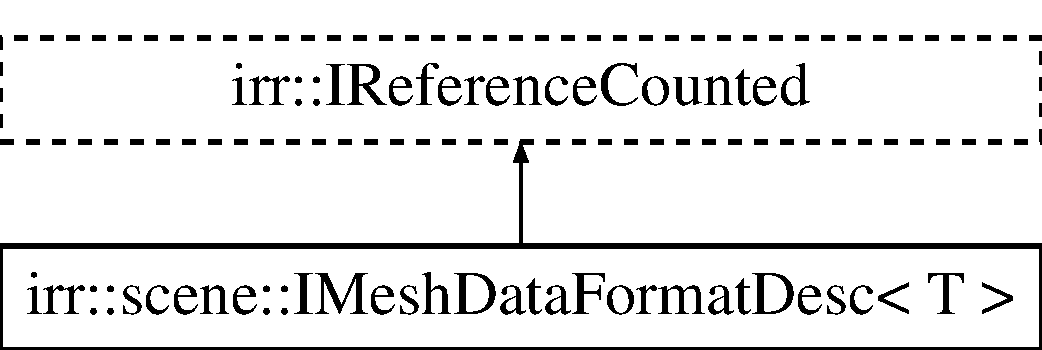
\includegraphics[height=2.000000cm]{classirr_1_1scene_1_1IMeshDataFormatDesc}
\end{center}
\end{figure}
\subsection*{Public Member Functions}
\begin{DoxyCompactItemize}
\item 
virtual bool {\bfseries format\+Can\+Be\+Appended} (const \hyperlink{classirr_1_1scene_1_1IMeshDataFormatDesc}{I\+Mesh\+Data\+Format\+Desc} $\ast$other) const  =0\hypertarget{classirr_1_1scene_1_1IMeshDataFormatDesc_a4b51403b1c2c43f14ad2d17d4610b8d4}{}\label{classirr_1_1scene_1_1IMeshDataFormatDesc_a4b51403b1c2c43f14ad2d17d4610b8d4}

\item 
virtual void {\bfseries map\+Index\+Buffer} (T $\ast$ixbuf)=0\hypertarget{classirr_1_1scene_1_1IMeshDataFormatDesc_aa0dfd0c43df0141a3cb3b390ced4fb0c}{}\label{classirr_1_1scene_1_1IMeshDataFormatDesc_aa0dfd0c43df0141a3cb3b390ced4fb0c}

\item 
virtual const T $\ast$ {\bfseries get\+Index\+Buffer} () const  =0\hypertarget{classirr_1_1scene_1_1IMeshDataFormatDesc_af3e0c28174c2ed19961ec499d1265f3b}{}\label{classirr_1_1scene_1_1IMeshDataFormatDesc_af3e0c28174c2ed19961ec499d1265f3b}

\item 
virtual void {\bfseries map\+Vertex\+Attr\+Buffer} (T $\ast$attr\+Buf, const E\+\_\+\+V\+E\+R\+T\+E\+X\+\_\+\+A\+T\+T\+R\+I\+B\+U\+T\+E\+\_\+\+ID \&attr\+Id, E\+\_\+\+C\+O\+M\+P\+O\+N\+E\+N\+T\+S\+\_\+\+P\+E\+R\+\_\+\+A\+T\+T\+R\+I\+B\+U\+TE components, E\+\_\+\+C\+O\+M\+P\+O\+N\+E\+N\+T\+\_\+\+T\+Y\+PE type, const size\+\_\+t \&stride=0, size\+\_\+t offset=0, uint32\+\_\+t divisor=0)=0\hypertarget{classirr_1_1scene_1_1IMeshDataFormatDesc_a00500097ec5a89aa60dc0c9db737ab99}{}\label{classirr_1_1scene_1_1IMeshDataFormatDesc_a00500097ec5a89aa60dc0c9db737ab99}

\item 
virtual const T $\ast$ {\bfseries get\+Mapped\+Buffer} (const E\+\_\+\+V\+E\+R\+T\+E\+X\+\_\+\+A\+T\+T\+R\+I\+B\+U\+T\+E\+\_\+\+ID \&attr\+Id) const  =0\hypertarget{classirr_1_1scene_1_1IMeshDataFormatDesc_a969a5fb222ac95993e3b7c3bfa9f6adf}{}\label{classirr_1_1scene_1_1IMeshDataFormatDesc_a969a5fb222ac95993e3b7c3bfa9f6adf}

\item 
E\+\_\+\+C\+O\+M\+P\+O\+N\+E\+N\+T\+\_\+\+T\+Y\+PE {\bfseries get\+Attrib\+Type} (const E\+\_\+\+V\+E\+R\+T\+E\+X\+\_\+\+A\+T\+T\+R\+I\+B\+U\+T\+E\+\_\+\+ID \&attr\+Id) const \hypertarget{classirr_1_1scene_1_1IMeshDataFormatDesc_a63473bd4cb2c740272fc3f132fa13ea4}{}\label{classirr_1_1scene_1_1IMeshDataFormatDesc_a63473bd4cb2c740272fc3f132fa13ea4}

\item 
E\+\_\+\+C\+O\+M\+P\+O\+N\+E\+N\+T\+S\+\_\+\+P\+E\+R\+\_\+\+A\+T\+T\+R\+I\+B\+U\+TE {\bfseries get\+Attrib\+Component\+Count} (const E\+\_\+\+V\+E\+R\+T\+E\+X\+\_\+\+A\+T\+T\+R\+I\+B\+U\+T\+E\+\_\+\+ID \&attr\+Id) const \hypertarget{classirr_1_1scene_1_1IMeshDataFormatDesc_ae7a9a0b275926e5b6a3788688beb1cd2}{}\label{classirr_1_1scene_1_1IMeshDataFormatDesc_ae7a9a0b275926e5b6a3788688beb1cd2}

\item 
virtual void {\bfseries set\+Mapped\+Buffer\+Offset} (const E\+\_\+\+V\+E\+R\+T\+E\+X\+\_\+\+A\+T\+T\+R\+I\+B\+U\+T\+E\+\_\+\+ID \&attr\+Id, const size\+\_\+t \&offset)=0\hypertarget{classirr_1_1scene_1_1IMeshDataFormatDesc_a38cc39383b3d46752a338244caaa537d}{}\label{classirr_1_1scene_1_1IMeshDataFormatDesc_a38cc39383b3d46752a338244caaa537d}

\item 
size\+\_\+t {\bfseries get\+Mapped\+Buffer\+Offset} (const E\+\_\+\+V\+E\+R\+T\+E\+X\+\_\+\+A\+T\+T\+R\+I\+B\+U\+T\+E\+\_\+\+ID \&attr\+Id) const \hypertarget{classirr_1_1scene_1_1IMeshDataFormatDesc_aa8e96e7b7fbc292d5b66b735f48fcdd7}{}\label{classirr_1_1scene_1_1IMeshDataFormatDesc_aa8e96e7b7fbc292d5b66b735f48fcdd7}

\item 
size\+\_\+t {\bfseries get\+Mapped\+Buffer\+Stride} (const E\+\_\+\+V\+E\+R\+T\+E\+X\+\_\+\+A\+T\+T\+R\+I\+B\+U\+T\+E\+\_\+\+ID \&attr\+Id) const \hypertarget{classirr_1_1scene_1_1IMeshDataFormatDesc_a4b5ca31ff9ba87b2d49e0cd4f2256db6}{}\label{classirr_1_1scene_1_1IMeshDataFormatDesc_a4b5ca31ff9ba87b2d49e0cd4f2256db6}

\item 
uint32\+\_\+t {\bfseries get\+Attrib\+Divisor} (const E\+\_\+\+V\+E\+R\+T\+E\+X\+\_\+\+A\+T\+T\+R\+I\+B\+U\+T\+E\+\_\+\+ID \&attr\+Id) const \hypertarget{classirr_1_1scene_1_1IMeshDataFormatDesc_a4ef356e8ac1bb3dc4f34e0badabae787}{}\label{classirr_1_1scene_1_1IMeshDataFormatDesc_a4ef356e8ac1bb3dc4f34e0badabae787}

\end{DoxyCompactItemize}
\subsection*{Protected Attributes}
\begin{DoxyCompactItemize}
\item 
E\+\_\+\+C\+O\+M\+P\+O\+N\+E\+N\+T\+S\+\_\+\+P\+E\+R\+\_\+\+A\+T\+T\+R\+I\+B\+U\+TE {\bfseries compnts\+Per\+Attr} \mbox{[}E\+V\+A\+I\+\_\+\+C\+O\+U\+NT\mbox{]}\hypertarget{classirr_1_1scene_1_1IMeshDataFormatDesc_a3a40a6d342dafa80dc998208f9b9ee30}{}\label{classirr_1_1scene_1_1IMeshDataFormatDesc_a3a40a6d342dafa80dc998208f9b9ee30}

\item 
E\+\_\+\+C\+O\+M\+P\+O\+N\+E\+N\+T\+\_\+\+T\+Y\+PE {\bfseries attr\+Type} \mbox{[}E\+V\+A\+I\+\_\+\+C\+O\+U\+NT\mbox{]}\hypertarget{classirr_1_1scene_1_1IMeshDataFormatDesc_a08caf005474f007de70b2852fa976c0d}{}\label{classirr_1_1scene_1_1IMeshDataFormatDesc_a08caf005474f007de70b2852fa976c0d}

\item 
size\+\_\+t {\bfseries attr\+Stride} \mbox{[}E\+V\+A\+I\+\_\+\+C\+O\+U\+NT\mbox{]}\hypertarget{classirr_1_1scene_1_1IMeshDataFormatDesc_a728b3f3df3f5d7a905cbdd79eb34036f}{}\label{classirr_1_1scene_1_1IMeshDataFormatDesc_a728b3f3df3f5d7a905cbdd79eb34036f}

\item 
size\+\_\+t {\bfseries attr\+Offset} \mbox{[}E\+V\+A\+I\+\_\+\+C\+O\+U\+NT\mbox{]}\hypertarget{classirr_1_1scene_1_1IMeshDataFormatDesc_a41c18f15fadfaf04fdbd14cde995a1d6}{}\label{classirr_1_1scene_1_1IMeshDataFormatDesc_a41c18f15fadfaf04fdbd14cde995a1d6}

\item 
uint32\+\_\+t {\bfseries attr\+Divisor} \mbox{[}E\+V\+A\+I\+\_\+\+C\+O\+U\+NT\mbox{]}\hypertarget{classirr_1_1scene_1_1IMeshDataFormatDesc_a753628e19b1f0a60eca390692d825d4d}{}\label{classirr_1_1scene_1_1IMeshDataFormatDesc_a753628e19b1f0a60eca390692d825d4d}

\end{DoxyCompactItemize}
\subsection*{Additional Inherited Members}


The documentation for this class was generated from the following file\+:\begin{DoxyCompactItemize}
\item 
include/I\+Mesh\+Buffer.\+h\end{DoxyCompactItemize}

\hypertarget{classirr_1_1scene_1_1IMeshLoader}{}\section{irr\+:\+:scene\+:\+:I\+Mesh\+Loader Class Reference}
\label{classirr_1_1scene_1_1IMeshLoader}\index{irr\+::scene\+::\+I\+Mesh\+Loader@{irr\+::scene\+::\+I\+Mesh\+Loader}}


Class which is able to load an animated mesh from a file.  




{\ttfamily \#include $<$I\+Mesh\+Loader.\+h$>$}

Inheritance diagram for irr\+:\+:scene\+:\+:I\+Mesh\+Loader\+:\begin{figure}[H]
\begin{center}
\leavevmode
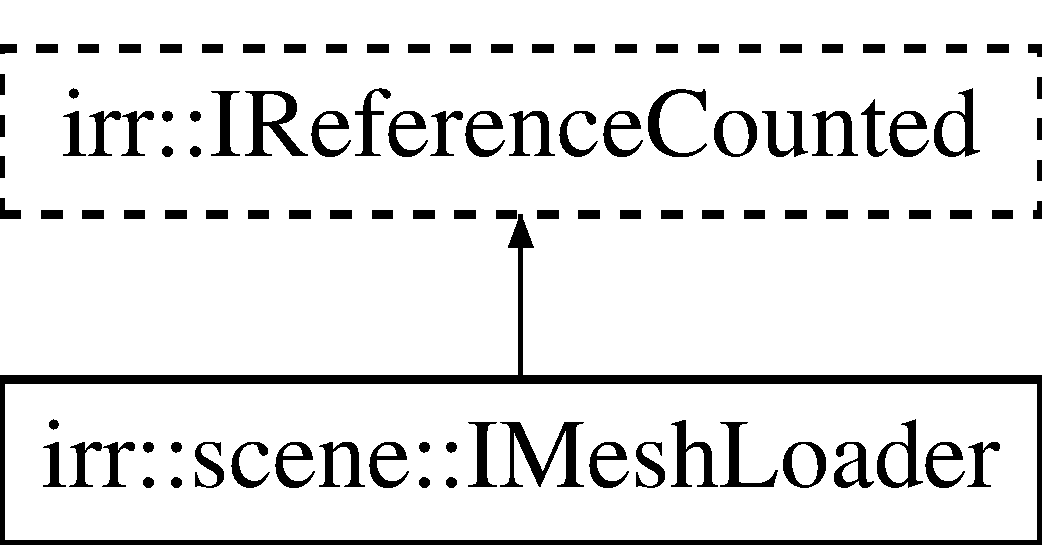
\includegraphics[height=2.000000cm]{classirr_1_1scene_1_1IMeshLoader}
\end{center}
\end{figure}
\subsection*{Public Member Functions}
\begin{DoxyCompactItemize}
\item 
virtual \hyperlink{classirr_1_1scene_1_1IMeshLoader_ad20920b323a9902d50e8d09211730d4d}{$\sim$\+I\+Mesh\+Loader} ()\hypertarget{classirr_1_1scene_1_1IMeshLoader_ad20920b323a9902d50e8d09211730d4d}{}\label{classirr_1_1scene_1_1IMeshLoader_ad20920b323a9902d50e8d09211730d4d}

\begin{DoxyCompactList}\small\item\em Destructor. \end{DoxyCompactList}\item 
virtual bool \hyperlink{classirr_1_1scene_1_1IMeshLoader_aab617e979ee6bb774b87f30b8eeaf157}{is\+A\+Loadable\+File\+Extension} (const \hyperlink{namespaceirr_1_1io_ab1bdc45edb3f94d8319c02bc0f840ee1}{io\+::path} \&filename) const  =0
\begin{DoxyCompactList}\small\item\em Returns true if the file might be loaded by this class. \end{DoxyCompactList}\item 
virtual \hyperlink{classirr_1_1scene_1_1IMesh}{I\+C\+P\+U\+Mesh} $\ast$ {\bfseries create\+Mesh} (\hyperlink{classirr_1_1io_1_1IReadFile}{io\+::\+I\+Read\+File} $\ast$file)=0\hypertarget{classirr_1_1scene_1_1IMeshLoader_aa94557000cc544d270da072fbe059af6}{}\label{classirr_1_1scene_1_1IMeshLoader_aa94557000cc544d270da072fbe059af6}

\end{DoxyCompactItemize}
\subsection*{Additional Inherited Members}


\subsection{Detailed Description}
Class which is able to load an animated mesh from a file. 

If you want Irrlicht be able to load meshes of currently unsupported file formats (e.\+g. .cob), then implement this and add your new Meshloader with \hyperlink{classirr_1_1scene_1_1ISceneManager_a808972cc001db86c0576c38b3b3fbbf7}{I\+Scene\+Manager\+::add\+External\+Mesh\+Loader()} to the engine. 

\subsection{Member Function Documentation}
\index{irr\+::scene\+::\+I\+Mesh\+Loader@{irr\+::scene\+::\+I\+Mesh\+Loader}!is\+A\+Loadable\+File\+Extension@{is\+A\+Loadable\+File\+Extension}}
\index{is\+A\+Loadable\+File\+Extension@{is\+A\+Loadable\+File\+Extension}!irr\+::scene\+::\+I\+Mesh\+Loader@{irr\+::scene\+::\+I\+Mesh\+Loader}}
\subsubsection[{\texorpdfstring{is\+A\+Loadable\+File\+Extension(const io\+::path \&filename) const  =0}{isALoadableFileExtension(const io::path \&filename) const  =0}}]{\setlength{\rightskip}{0pt plus 5cm}virtual bool irr\+::scene\+::\+I\+Mesh\+Loader\+::is\+A\+Loadable\+File\+Extension (
\begin{DoxyParamCaption}
\item[{const {\bf io\+::path} \&}]{filename}
\end{DoxyParamCaption}
) const\hspace{0.3cm}{\ttfamily [pure virtual]}}\hypertarget{classirr_1_1scene_1_1IMeshLoader_aab617e979ee6bb774b87f30b8eeaf157}{}\label{classirr_1_1scene_1_1IMeshLoader_aab617e979ee6bb774b87f30b8eeaf157}


Returns true if the file might be loaded by this class. 

This decision should be based on the file extension (e.\+g. \char`\"{}.\+cob\char`\"{}) only. 
\begin{DoxyParams}{Parameters}
{\em filename} & Name of the file to test. \\
\hline
\end{DoxyParams}
\begin{DoxyReturn}{Returns}
True if the file might be loaded by this class. 
\end{DoxyReturn}


The documentation for this class was generated from the following file\+:\begin{DoxyCompactItemize}
\item 
include/I\+Mesh\+Loader.\+h\end{DoxyCompactItemize}

\hypertarget{classirr_1_1scene_1_1IMeshManipulator}{}\section{irr\+:\+:scene\+:\+:I\+Mesh\+Manipulator Class Reference}
\label{classirr_1_1scene_1_1IMeshManipulator}\index{irr\+::scene\+::\+I\+Mesh\+Manipulator@{irr\+::scene\+::\+I\+Mesh\+Manipulator}}


An interface for easy manipulation of meshes.  




{\ttfamily \#include $<$I\+Mesh\+Manipulator.\+h$>$}

Inheritance diagram for irr\+:\+:scene\+:\+:I\+Mesh\+Manipulator\+:\begin{figure}[H]
\begin{center}
\leavevmode
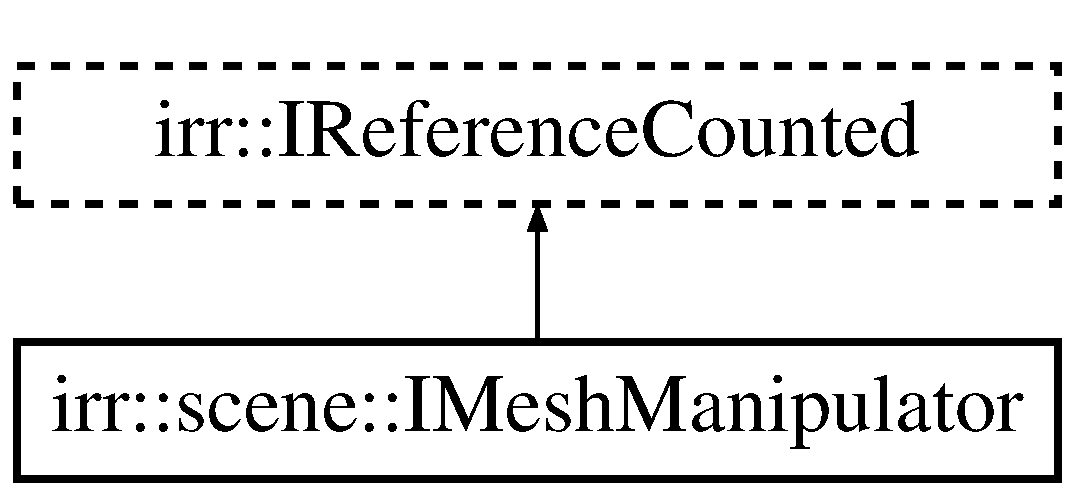
\includegraphics[height=2.000000cm]{classirr_1_1scene_1_1IMeshManipulator}
\end{center}
\end{figure}
\subsection*{Public Member Functions}
\begin{DoxyCompactItemize}
\item 
virtual void \hyperlink{classirr_1_1scene_1_1IMeshManipulator_a96bb33f5d55951912cac9a5cfd4b8289}{flip\+Surfaces} (\hyperlink{classirr_1_1scene_1_1ICPUMeshBuffer}{I\+C\+P\+U\+Mesh\+Buffer} $\ast$inbuffer) const  =0
\begin{DoxyCompactList}\small\item\em Flips the direction of surfaces. \end{DoxyCompactList}\item 
virtual \hyperlink{classirr_1_1scene_1_1ICPUMeshBuffer}{I\+C\+P\+U\+Mesh\+Buffer} $\ast$ \hyperlink{classirr_1_1scene_1_1IMeshManipulator_abd33bc1018923b33094e020ae05a0b4f}{create\+Mesh\+Buffer\+Unique\+Primitives} (\hyperlink{classirr_1_1scene_1_1ICPUMeshBuffer}{I\+C\+P\+U\+Mesh\+Buffer} $\ast$inbuffer) const  =0
\begin{DoxyCompactList}\small\item\em Creates a copy of a mesh with all vertices unwelded. \end{DoxyCompactList}\item 
virtual \hyperlink{classirr_1_1scene_1_1ICPUMeshBuffer}{I\+C\+P\+U\+Mesh\+Buffer} $\ast$ \hyperlink{classirr_1_1scene_1_1IMeshManipulator_aeec0af71135b6ec27e139da2e0d5b070}{create\+Mesh\+Buffer\+Welded} (\hyperlink{classirr_1_1scene_1_1ICPUMeshBuffer}{I\+C\+P\+U\+Mesh\+Buffer} $\ast$inbuffer, const bool \&make\+New\+Mesh=false, \hyperlink{namespaceirr_a0277be98d67dc26ff93b1a6a1d086b07}{f32} tolerance=core\+::\+R\+O\+U\+N\+D\+I\+N\+G\+\_\+\+E\+R\+R\+O\+R\+\_\+f32) const  =0
\begin{DoxyCompactList}\small\item\em Creates a copy of a mesh with vertices welded. \end{DoxyCompactList}\end{DoxyCompactItemize}
\subsection*{Static Public Member Functions}
\begin{DoxyCompactItemize}
\item 
{\footnotesize template$<$typename T $>$ }\\static bool \hyperlink{classirr_1_1scene_1_1IMeshManipulator_a641ecc0aae0b0372071c2770cdcd9f2f}{get\+Poly\+Count} (uint32\+\_\+t \&out\+Count, \hyperlink{classirr_1_1scene_1_1IMeshBuffer}{I\+Mesh\+Buffer}$<$ T $>$ $\ast$meshbuffer)
\begin{DoxyCompactList}\small\item\em Get amount of polygons in mesh buffer. \end{DoxyCompactList}\item 
{\footnotesize template$<$typename T $>$ }\\static bool \hyperlink{classirr_1_1scene_1_1IMeshManipulator_acb922b739ebdf1b3bdb239c557e51cae}{get\+Poly\+Count} (uint32\+\_\+t \&out\+Count, \hyperlink{classirr_1_1scene_1_1IMesh}{I\+Mesh}$<$ T $>$ $\ast$mesh)
\begin{DoxyCompactList}\small\item\em Get amount of polygons in mesh. \end{DoxyCompactList}\end{DoxyCompactItemize}
\subsection*{Additional Inherited Members}


\subsection{Detailed Description}
An interface for easy manipulation of meshes. 

Scale, set alpha value, flip surfaces, and so on. This exists for fixing problems with wrong imported or exported meshes quickly after loading. It is not intended for doing mesh modifications and/or animations during runtime. 

\subsection{Member Function Documentation}
\index{irr\+::scene\+::\+I\+Mesh\+Manipulator@{irr\+::scene\+::\+I\+Mesh\+Manipulator}!create\+Mesh\+Buffer\+Unique\+Primitives@{create\+Mesh\+Buffer\+Unique\+Primitives}}
\index{create\+Mesh\+Buffer\+Unique\+Primitives@{create\+Mesh\+Buffer\+Unique\+Primitives}!irr\+::scene\+::\+I\+Mesh\+Manipulator@{irr\+::scene\+::\+I\+Mesh\+Manipulator}}
\subsubsection[{\texorpdfstring{create\+Mesh\+Buffer\+Unique\+Primitives(\+I\+C\+P\+U\+Mesh\+Buffer $\ast$inbuffer) const  =0}{createMeshBufferUniquePrimitives(ICPUMeshBuffer *inbuffer) const  =0}}]{\setlength{\rightskip}{0pt plus 5cm}virtual {\bf I\+C\+P\+U\+Mesh\+Buffer}$\ast$ irr\+::scene\+::\+I\+Mesh\+Manipulator\+::create\+Mesh\+Buffer\+Unique\+Primitives (
\begin{DoxyParamCaption}
\item[{{\bf I\+C\+P\+U\+Mesh\+Buffer} $\ast$}]{inbuffer}
\end{DoxyParamCaption}
) const\hspace{0.3cm}{\ttfamily [pure virtual]}}\hypertarget{classirr_1_1scene_1_1IMeshManipulator_abd33bc1018923b33094e020ae05a0b4f}{}\label{classirr_1_1scene_1_1IMeshManipulator_abd33bc1018923b33094e020ae05a0b4f}


Creates a copy of a mesh with all vertices unwelded. 


\begin{DoxyParams}{Parameters}
{\em mesh} & Input mesh \\
\hline
\end{DoxyParams}
\begin{DoxyReturn}{Returns}
Mesh consisting only of unique faces. All vertices which were previously shared are now duplicated. If you no longer need the cloned mesh, you should call \hyperlink{classirr_1_1IReferenceCounted_afb169a857e0d2cdb96b8821cb9bff17a}{I\+Mesh\+::drop()}. See \hyperlink{classirr_1_1IReferenceCounted_afb169a857e0d2cdb96b8821cb9bff17a}{I\+Reference\+Counted\+::drop()} for more information. 
\end{DoxyReturn}
\index{irr\+::scene\+::\+I\+Mesh\+Manipulator@{irr\+::scene\+::\+I\+Mesh\+Manipulator}!create\+Mesh\+Buffer\+Welded@{create\+Mesh\+Buffer\+Welded}}
\index{create\+Mesh\+Buffer\+Welded@{create\+Mesh\+Buffer\+Welded}!irr\+::scene\+::\+I\+Mesh\+Manipulator@{irr\+::scene\+::\+I\+Mesh\+Manipulator}}
\subsubsection[{\texorpdfstring{create\+Mesh\+Buffer\+Welded(\+I\+C\+P\+U\+Mesh\+Buffer $\ast$inbuffer, const bool \&make\+New\+Mesh=false, f32 tolerance=core\+::\+R\+O\+U\+N\+D\+I\+N\+G\+\_\+\+E\+R\+R\+O\+R\+\_\+f32) const  =0}{createMeshBufferWelded(ICPUMeshBuffer *inbuffer, const bool \&makeNewMesh=false, f32 tolerance=core::ROUNDING\_ERROR\_f32) const  =0}}]{\setlength{\rightskip}{0pt plus 5cm}virtual {\bf I\+C\+P\+U\+Mesh\+Buffer}$\ast$ irr\+::scene\+::\+I\+Mesh\+Manipulator\+::create\+Mesh\+Buffer\+Welded (
\begin{DoxyParamCaption}
\item[{{\bf I\+C\+P\+U\+Mesh\+Buffer} $\ast$}]{inbuffer, }
\item[{const bool \&}]{make\+New\+Mesh = {\ttfamily false}, }
\item[{{\bf f32}}]{tolerance = {\ttfamily core\+:\+:ROUNDING\+\_\+ERROR\+\_\+f32}}
\end{DoxyParamCaption}
) const\hspace{0.3cm}{\ttfamily [pure virtual]}}\hypertarget{classirr_1_1scene_1_1IMeshManipulator_aeec0af71135b6ec27e139da2e0d5b070}{}\label{classirr_1_1scene_1_1IMeshManipulator_aeec0af71135b6ec27e139da2e0d5b070}


Creates a copy of a mesh with vertices welded. 


\begin{DoxyParams}{Parameters}
{\em mesh} & Input mesh \\
\hline
{\em tolerance} & The threshold for vertex comparisons. \\
\hline
\end{DoxyParams}
\begin{DoxyReturn}{Returns}
Mesh without redundant vertices. If you no longer need the cloned mesh, you should call \hyperlink{classirr_1_1IReferenceCounted_afb169a857e0d2cdb96b8821cb9bff17a}{I\+Mesh\+::drop()}. See \hyperlink{classirr_1_1IReferenceCounted_afb169a857e0d2cdb96b8821cb9bff17a}{I\+Reference\+Counted\+::drop()} for more information. 
\end{DoxyReturn}
\index{irr\+::scene\+::\+I\+Mesh\+Manipulator@{irr\+::scene\+::\+I\+Mesh\+Manipulator}!flip\+Surfaces@{flip\+Surfaces}}
\index{flip\+Surfaces@{flip\+Surfaces}!irr\+::scene\+::\+I\+Mesh\+Manipulator@{irr\+::scene\+::\+I\+Mesh\+Manipulator}}
\subsubsection[{\texorpdfstring{flip\+Surfaces(\+I\+C\+P\+U\+Mesh\+Buffer $\ast$inbuffer) const  =0}{flipSurfaces(ICPUMeshBuffer *inbuffer) const  =0}}]{\setlength{\rightskip}{0pt plus 5cm}virtual void irr\+::scene\+::\+I\+Mesh\+Manipulator\+::flip\+Surfaces (
\begin{DoxyParamCaption}
\item[{{\bf I\+C\+P\+U\+Mesh\+Buffer} $\ast$}]{inbuffer}
\end{DoxyParamCaption}
) const\hspace{0.3cm}{\ttfamily [pure virtual]}}\hypertarget{classirr_1_1scene_1_1IMeshManipulator_a96bb33f5d55951912cac9a5cfd4b8289}{}\label{classirr_1_1scene_1_1IMeshManipulator_a96bb33f5d55951912cac9a5cfd4b8289}


Flips the direction of surfaces. 

Changes backfacing triangles to frontfacing triangles and vice versa. 
\begin{DoxyParams}{Parameters}
{\em mesh} & Mesh on which the operation is performed. \\
\hline
\end{DoxyParams}
\index{irr\+::scene\+::\+I\+Mesh\+Manipulator@{irr\+::scene\+::\+I\+Mesh\+Manipulator}!get\+Poly\+Count@{get\+Poly\+Count}}
\index{get\+Poly\+Count@{get\+Poly\+Count}!irr\+::scene\+::\+I\+Mesh\+Manipulator@{irr\+::scene\+::\+I\+Mesh\+Manipulator}}
\subsubsection[{\texorpdfstring{get\+Poly\+Count(uint32\+\_\+t \&out\+Count, I\+Mesh\+Buffer$<$ T $>$ $\ast$meshbuffer)}{getPolyCount(uint32\_t \&outCount, IMeshBuffer< T > *meshbuffer)}}]{\setlength{\rightskip}{0pt plus 5cm}template$<$typename T $>$ static bool irr\+::scene\+::\+I\+Mesh\+Manipulator\+::get\+Poly\+Count (
\begin{DoxyParamCaption}
\item[{uint32\+\_\+t \&}]{out\+Count, }
\item[{{\bf I\+Mesh\+Buffer}$<$ T $>$ $\ast$}]{meshbuffer}
\end{DoxyParamCaption}
)\hspace{0.3cm}{\ttfamily [static]}}\hypertarget{classirr_1_1scene_1_1IMeshManipulator_a641ecc0aae0b0372071c2770cdcd9f2f}{}\label{classirr_1_1scene_1_1IMeshManipulator_a641ecc0aae0b0372071c2770cdcd9f2f}


Get amount of polygons in mesh buffer. 


\begin{DoxyParams}{Parameters}
{\em meshbuffer} & Input mesh buffer \\
\hline
{\em Outputted} & Number of polygons in mesh buffer, if successful. \\
\hline
\end{DoxyParams}
\begin{DoxyReturn}{Returns}
If successfully can provide information, i.\+e. if X\+Form\+Feedback is providing Poly\+Count we dont know how many there are 
\end{DoxyReturn}
\index{irr\+::scene\+::\+I\+Mesh\+Manipulator@{irr\+::scene\+::\+I\+Mesh\+Manipulator}!get\+Poly\+Count@{get\+Poly\+Count}}
\index{get\+Poly\+Count@{get\+Poly\+Count}!irr\+::scene\+::\+I\+Mesh\+Manipulator@{irr\+::scene\+::\+I\+Mesh\+Manipulator}}
\subsubsection[{\texorpdfstring{get\+Poly\+Count(uint32\+\_\+t \&out\+Count, I\+Mesh$<$ T $>$ $\ast$mesh)}{getPolyCount(uint32\_t \&outCount, IMesh< T > *mesh)}}]{\setlength{\rightskip}{0pt plus 5cm}template$<$typename T $>$ static bool irr\+::scene\+::\+I\+Mesh\+Manipulator\+::get\+Poly\+Count (
\begin{DoxyParamCaption}
\item[{uint32\+\_\+t \&}]{out\+Count, }
\item[{{\bf I\+Mesh}$<$ T $>$ $\ast$}]{mesh}
\end{DoxyParamCaption}
)\hspace{0.3cm}{\ttfamily [static]}}\hypertarget{classirr_1_1scene_1_1IMeshManipulator_acb922b739ebdf1b3bdb239c557e51cae}{}\label{classirr_1_1scene_1_1IMeshManipulator_acb922b739ebdf1b3bdb239c557e51cae}


Get amount of polygons in mesh. 


\begin{DoxyParams}{Parameters}
{\em meshbuffer} & Input mesh \\
\hline
{\em Outputted} & Number of polygons in mesh, if successful. \\
\hline
\end{DoxyParams}
\begin{DoxyReturn}{Returns}
If successfully can provide information, i.\+e. if X\+Form\+Feedback is providing Poly\+Count we dont know how many there are 
\end{DoxyReturn}


The documentation for this class was generated from the following file\+:\begin{DoxyCompactItemize}
\item 
include/I\+Mesh\+Manipulator.\+h\end{DoxyCompactItemize}

\hypertarget{classirr_1_1scene_1_1IMeshSceneNode}{}\section{irr\+:\+:scene\+:\+:I\+Mesh\+Scene\+Node Class Reference}
\label{classirr_1_1scene_1_1IMeshSceneNode}\index{irr\+::scene\+::\+I\+Mesh\+Scene\+Node@{irr\+::scene\+::\+I\+Mesh\+Scene\+Node}}


A scene node displaying a static mesh.  




{\ttfamily \#include $<$I\+Mesh\+Scene\+Node.\+h$>$}

Inheritance diagram for irr\+:\+:scene\+:\+:I\+Mesh\+Scene\+Node\+:\begin{figure}[H]
\begin{center}
\leavevmode
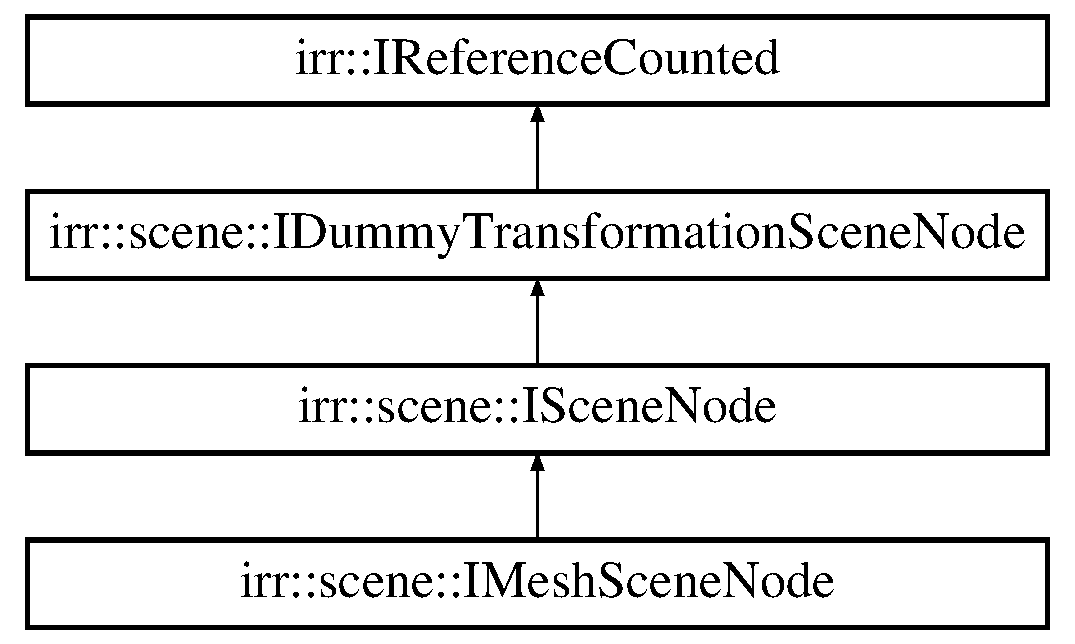
\includegraphics[height=4.000000cm]{classirr_1_1scene_1_1IMeshSceneNode}
\end{center}
\end{figure}
\subsection*{Public Member Functions}
\begin{DoxyCompactItemize}
\item 
\hyperlink{classirr_1_1scene_1_1IMeshSceneNode_ab528ef0063ebfe5d288fcc6f68282417}{I\+Mesh\+Scene\+Node} (\hyperlink{classirr_1_1scene_1_1IDummyTransformationSceneNode}{I\+Dummy\+Transformation\+Scene\+Node} $\ast$parent, \hyperlink{classirr_1_1scene_1_1ISceneManager}{I\+Scene\+Manager} $\ast$mgr, \hyperlink{namespaceirr_ac66849b7a6ed16e30ebede579f9b47c6}{s32} id, const \hyperlink{namespaceirr_1_1core_a06f169d08b5c429f5575acb7edbad811}{core\+::vector3df} \&position=\hyperlink{namespaceirr_1_1core_a06f169d08b5c429f5575acb7edbad811}{core\+::vector3df}(0, 0, 0), const \hyperlink{namespaceirr_1_1core_a06f169d08b5c429f5575acb7edbad811}{core\+::vector3df} \&rotation=\hyperlink{namespaceirr_1_1core_a06f169d08b5c429f5575acb7edbad811}{core\+::vector3df}(0, 0, 0), const \hyperlink{namespaceirr_1_1core_a06f169d08b5c429f5575acb7edbad811}{core\+::vector3df} \&scale=\hyperlink{namespaceirr_1_1core_a06f169d08b5c429f5575acb7edbad811}{core\+::vector3df}(1, 1, 1))
\begin{DoxyCompactList}\small\item\em Constructor. \end{DoxyCompactList}\item 
virtual void \hyperlink{classirr_1_1scene_1_1IMeshSceneNode_a661d6526a4cdde01c5c57592e2efdac8}{set\+Mesh} (\hyperlink{classirr_1_1scene_1_1IMesh}{I\+G\+P\+U\+Mesh} $\ast$mesh)=0
\begin{DoxyCompactList}\small\item\em Sets a new mesh to display. \end{DoxyCompactList}\item 
virtual \hyperlink{classirr_1_1scene_1_1IMesh}{I\+G\+P\+U\+Mesh} $\ast$ \hyperlink{classirr_1_1scene_1_1IMeshSceneNode_a517eb714d4e8f994f0c70d33330dc93c}{get\+Mesh} (void)=0
\begin{DoxyCompactList}\small\item\em Get the currently defined mesh for display. \end{DoxyCompactList}\item 
virtual void {\bfseries set\+Referencing\+Mesh\+Materials} (const bool \&referencing)=0\hypertarget{classirr_1_1scene_1_1IMeshSceneNode_a280ca3401011074a69b19ba4fb1cf9a1}{}\label{classirr_1_1scene_1_1IMeshSceneNode_a280ca3401011074a69b19ba4fb1cf9a1}

\item 
virtual bool {\bfseries is\+Referencinge\+Mesh\+Materials} () const  =0\hypertarget{classirr_1_1scene_1_1IMeshSceneNode_a0bc184c21fd1cedfe95bc5219d6ec812}{}\label{classirr_1_1scene_1_1IMeshSceneNode_a0bc184c21fd1cedfe95bc5219d6ec812}

\end{DoxyCompactItemize}
\subsection*{Additional Inherited Members}


\subsection{Detailed Description}
A scene node displaying a static mesh. 

\subsection{Constructor \& Destructor Documentation}
\index{irr\+::scene\+::\+I\+Mesh\+Scene\+Node@{irr\+::scene\+::\+I\+Mesh\+Scene\+Node}!I\+Mesh\+Scene\+Node@{I\+Mesh\+Scene\+Node}}
\index{I\+Mesh\+Scene\+Node@{I\+Mesh\+Scene\+Node}!irr\+::scene\+::\+I\+Mesh\+Scene\+Node@{irr\+::scene\+::\+I\+Mesh\+Scene\+Node}}
\subsubsection[{\texorpdfstring{I\+Mesh\+Scene\+Node(\+I\+Dummy\+Transformation\+Scene\+Node $\ast$parent, I\+Scene\+Manager $\ast$mgr, s32 id, const core\+::vector3df \&position=core\+::vector3df(0, 0, 0), const core\+::vector3df \&rotation=core\+::vector3df(0, 0, 0), const core\+::vector3df \&scale=core\+::vector3df(1, 1, 1))}{IMeshSceneNode(IDummyTransformationSceneNode *parent, ISceneManager *mgr, s32 id, const core::vector3df \&position=core::vector3df(0, 0, 0), const core::vector3df \&rotation=core::vector3df(0, 0, 0), const core::vector3df \&scale=core::vector3df(1, 1, 1))}}]{\setlength{\rightskip}{0pt plus 5cm}irr\+::scene\+::\+I\+Mesh\+Scene\+Node\+::\+I\+Mesh\+Scene\+Node (
\begin{DoxyParamCaption}
\item[{{\bf I\+Dummy\+Transformation\+Scene\+Node} $\ast$}]{parent, }
\item[{{\bf I\+Scene\+Manager} $\ast$}]{mgr, }
\item[{{\bf s32}}]{id, }
\item[{const {\bf core\+::vector3df} \&}]{position = {\ttfamily {\bf core\+::vector3df}(0,0,0)}, }
\item[{const {\bf core\+::vector3df} \&}]{rotation = {\ttfamily {\bf core\+::vector3df}(0,0,0)}, }
\item[{const {\bf core\+::vector3df} \&}]{scale = {\ttfamily {\bf core\+::vector3df}(1,1,1)}}
\end{DoxyParamCaption}
)\hspace{0.3cm}{\ttfamily [inline]}}\hypertarget{classirr_1_1scene_1_1IMeshSceneNode_ab528ef0063ebfe5d288fcc6f68282417}{}\label{classirr_1_1scene_1_1IMeshSceneNode_ab528ef0063ebfe5d288fcc6f68282417}


Constructor. 

Use \hyperlink{classirr_1_1scene_1_1IMeshSceneNode_a661d6526a4cdde01c5c57592e2efdac8}{set\+Mesh()} to set the mesh to display. 

\subsection{Member Function Documentation}
\index{irr\+::scene\+::\+I\+Mesh\+Scene\+Node@{irr\+::scene\+::\+I\+Mesh\+Scene\+Node}!get\+Mesh@{get\+Mesh}}
\index{get\+Mesh@{get\+Mesh}!irr\+::scene\+::\+I\+Mesh\+Scene\+Node@{irr\+::scene\+::\+I\+Mesh\+Scene\+Node}}
\subsubsection[{\texorpdfstring{get\+Mesh(void)=0}{getMesh(void)=0}}]{\setlength{\rightskip}{0pt plus 5cm}virtual {\bf I\+G\+P\+U\+Mesh}$\ast$ irr\+::scene\+::\+I\+Mesh\+Scene\+Node\+::get\+Mesh (
\begin{DoxyParamCaption}
\item[{void}]{}
\end{DoxyParamCaption}
)\hspace{0.3cm}{\ttfamily [pure virtual]}}\hypertarget{classirr_1_1scene_1_1IMeshSceneNode_a517eb714d4e8f994f0c70d33330dc93c}{}\label{classirr_1_1scene_1_1IMeshSceneNode_a517eb714d4e8f994f0c70d33330dc93c}


Get the currently defined mesh for display. 

\begin{DoxyReturn}{Returns}
Pointer to mesh which is displayed by this node. 
\end{DoxyReturn}
\index{irr\+::scene\+::\+I\+Mesh\+Scene\+Node@{irr\+::scene\+::\+I\+Mesh\+Scene\+Node}!set\+Mesh@{set\+Mesh}}
\index{set\+Mesh@{set\+Mesh}!irr\+::scene\+::\+I\+Mesh\+Scene\+Node@{irr\+::scene\+::\+I\+Mesh\+Scene\+Node}}
\subsubsection[{\texorpdfstring{set\+Mesh(\+I\+G\+P\+U\+Mesh $\ast$mesh)=0}{setMesh(IGPUMesh *mesh)=0}}]{\setlength{\rightskip}{0pt plus 5cm}virtual void irr\+::scene\+::\+I\+Mesh\+Scene\+Node\+::set\+Mesh (
\begin{DoxyParamCaption}
\item[{{\bf I\+G\+P\+U\+Mesh} $\ast$}]{mesh}
\end{DoxyParamCaption}
)\hspace{0.3cm}{\ttfamily [pure virtual]}}\hypertarget{classirr_1_1scene_1_1IMeshSceneNode_a661d6526a4cdde01c5c57592e2efdac8}{}\label{classirr_1_1scene_1_1IMeshSceneNode_a661d6526a4cdde01c5c57592e2efdac8}


Sets a new mesh to display. 


\begin{DoxyParams}{Parameters}
{\em mesh} & Mesh to display. \\
\hline
\end{DoxyParams}


The documentation for this class was generated from the following file\+:\begin{DoxyCompactItemize}
\item 
include/I\+Mesh\+Scene\+Node.\+h\end{DoxyCompactItemize}

\hypertarget{classirr_1_1scene_1_1IMeshSceneNodeInstanced}{}\section{irr\+:\+:scene\+:\+:I\+Mesh\+Scene\+Node\+Instanced Class Reference}
\label{classirr_1_1scene_1_1IMeshSceneNodeInstanced}\index{irr\+::scene\+::\+I\+Mesh\+Scene\+Node\+Instanced@{irr\+::scene\+::\+I\+Mesh\+Scene\+Node\+Instanced}}


{\ttfamily \#include $<$I\+Mesh\+Scene\+Node\+Instanced.\+h$>$}

Inheritance diagram for irr\+:\+:scene\+:\+:I\+Mesh\+Scene\+Node\+Instanced\+:\begin{figure}[H]
\begin{center}
\leavevmode
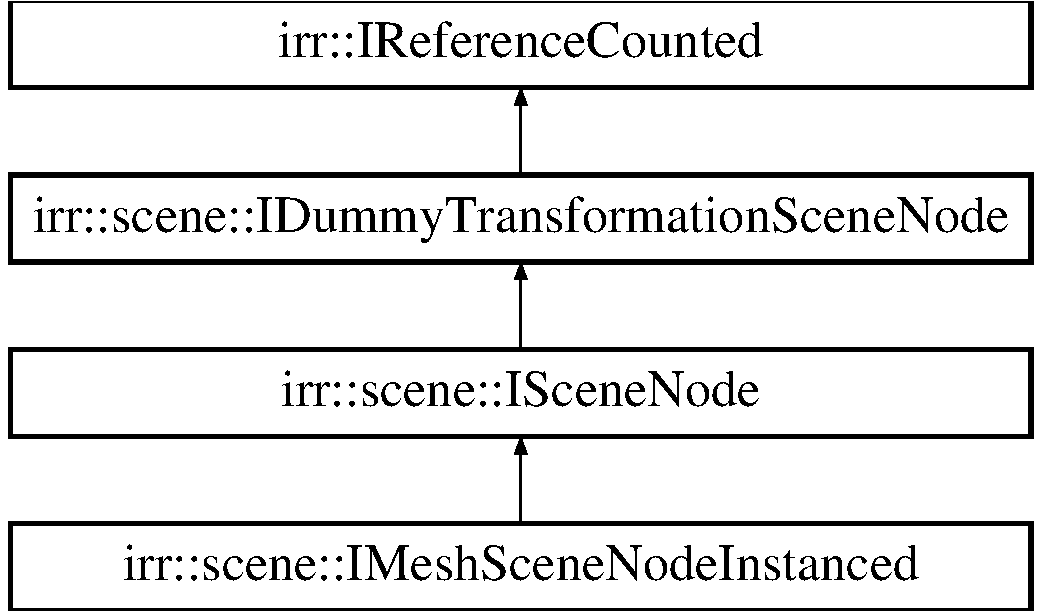
\includegraphics[height=4.000000cm]{classirr_1_1scene_1_1IMeshSceneNodeInstanced}
\end{center}
\end{figure}
\subsection*{Classes}
\begin{DoxyCompactItemize}
\item 
struct \hyperlink{structirr_1_1scene_1_1IMeshSceneNodeInstanced_1_1MeshLoD}{Mesh\+LoD}
\end{DoxyCompactItemize}
\subsection*{Public Member Functions}
\begin{DoxyCompactItemize}
\item 
\hyperlink{classirr_1_1scene_1_1IMeshSceneNodeInstanced_a2aa6f622516a2b0f541d279fa8996247}{I\+Mesh\+Scene\+Node\+Instanced} (\hyperlink{classirr_1_1scene_1_1IDummyTransformationSceneNode}{I\+Dummy\+Transformation\+Scene\+Node} $\ast$parent, \hyperlink{classirr_1_1scene_1_1ISceneManager}{I\+Scene\+Manager} $\ast$mgr, \hyperlink{namespaceirr_ac66849b7a6ed16e30ebede579f9b47c6}{s32} id, const \hyperlink{namespaceirr_1_1core_a06f169d08b5c429f5575acb7edbad811}{core\+::vector3df} \&position=\hyperlink{namespaceirr_1_1core_a06f169d08b5c429f5575acb7edbad811}{core\+::vector3df}(0, 0, 0), const \hyperlink{namespaceirr_1_1core_a06f169d08b5c429f5575acb7edbad811}{core\+::vector3df} \&rotation=\hyperlink{namespaceirr_1_1core_a06f169d08b5c429f5575acb7edbad811}{core\+::vector3df}(0, 0, 0), const \hyperlink{namespaceirr_1_1core_a06f169d08b5c429f5575acb7edbad811}{core\+::vector3df} \&scale=\hyperlink{namespaceirr_1_1core_a06f169d08b5c429f5575acb7edbad811}{core\+::vector3df}(1, 1, 1))
\begin{DoxyCompactList}\small\item\em Constructor. \end{DoxyCompactList}\item 
virtual bool \hyperlink{classirr_1_1scene_1_1IMeshSceneNodeInstanced_a01d0dca01d9c058ee4c907ddf617211c}{set\+Lo\+D\+Meshes} (std\+::vector$<$ \hyperlink{structirr_1_1scene_1_1IMeshSceneNodeInstanced_1_1MeshLoD}{Mesh\+LoD} $>$ levels\+Of\+Detail, const size\+\_\+t \&data\+Size\+Per\+Instance\+Output, const \hyperlink{classirr_1_1video_1_1SMaterial}{video\+::\+S\+Material} \&lod\+Selection\+Shader, \hyperlink{classirr_1_1scene_1_1IMeshDataFormatDesc}{I\+G\+P\+U\+Mesh\+Data\+Format\+Desc} $\ast$($\ast$vao\+Setup\+Override)(\hyperlink{classirr_1_1scene_1_1ISceneManager}{I\+Scene\+Manager} $\ast$, \hyperlink{classirr_1_1video_1_1IGPUBuffer}{video\+::\+I\+G\+P\+U\+Buffer} $\ast$, const std\+::vector$<$ \hyperlink{structirr_1_1scene_1_1IMeshSceneNodeInstanced_1_1MeshLoD}{Mesh\+LoD} $>$ \&, const size\+\_\+t \&, const size\+\_\+t \&, const size\+\_\+t \&), const size\+\_\+t \&extra\+Data\+Size\+Per\+Instance\+Input=0)=0
\begin{DoxyCompactList}\small\item\em Sets a new mesh to display. \end{DoxyCompactList}\item 
virtual \hyperlink{classirr_1_1scene_1_1SGPUMesh}{S\+G\+P\+U\+Mesh} $\ast$ \hyperlink{classirr_1_1scene_1_1IMeshSceneNodeInstanced_ae9fa5c16448503254bd5a3810f8805ed}{get\+Lo\+D\+Mesh} (const size\+\_\+t \&lod)=0
\begin{DoxyCompactList}\small\item\em Get the currently defined mesh for display. \end{DoxyCompactList}\item 
virtual const size\+\_\+t \& {\bfseries get\+Instance\+Count} () const  =0\hypertarget{classirr_1_1scene_1_1IMeshSceneNodeInstanced_a93df569413230da297250022bac235d3}{}\label{classirr_1_1scene_1_1IMeshSceneNodeInstanced_a93df569413230da297250022bac235d3}

\item 
virtual const \hyperlink{namespaceirr_1_1core_adfc8fa01b30044c55f3332a1d6c1aa19}{core\+::aabbox3df} \& {\bfseries get\+Lo\+D\+Invariant\+B\+Box} () const  =0\hypertarget{classirr_1_1scene_1_1IMeshSceneNodeInstanced_a35f7e5e97be0667bc2336e2f1d3e90e5}{}\label{classirr_1_1scene_1_1IMeshSceneNodeInstanced_a35f7e5e97be0667bc2336e2f1d3e90e5}

\item 
void {\bfseries set\+B\+Box\+Update\+Enabled} ()\hypertarget{classirr_1_1scene_1_1IMeshSceneNodeInstanced_abb61c6cf5413d0c1d90617636a3a96b1}{}\label{classirr_1_1scene_1_1IMeshSceneNodeInstanced_abb61c6cf5413d0c1d90617636a3a96b1}

\item 
void {\bfseries set\+B\+Box\+Update\+Disabled} ()\hypertarget{classirr_1_1scene_1_1IMeshSceneNodeInstanced_a77fc012efe2c1c83d13d0a456737a4f8}{}\label{classirr_1_1scene_1_1IMeshSceneNodeInstanced_a77fc012efe2c1c83d13d0a456737a4f8}

\item 
const bool \& {\bfseries get\+B\+Box\+Update\+Mode} ()\hypertarget{classirr_1_1scene_1_1IMeshSceneNodeInstanced_a1738c7d291de6e1c43529752b1393103}{}\label{classirr_1_1scene_1_1IMeshSceneNodeInstanced_a1738c7d291de6e1c43529752b1393103}

\item 
virtual uint32\+\_\+t {\bfseries add\+Instance} (const \hyperlink{classirr_1_1core_1_1matrix4x3}{core\+::matrix4x3} \&relative\+Transform, void $\ast$extra\+Data=N\+U\+LL)=0\hypertarget{classirr_1_1scene_1_1IMeshSceneNodeInstanced_a25c2717ac8e82232946dac253465630e}{}\label{classirr_1_1scene_1_1IMeshSceneNodeInstanced_a25c2717ac8e82232946dac253465630e}

\item 
virtual bool {\bfseries add\+Instances} (uint32\+\_\+t $\ast$instance\+I\+Ds, const size\+\_\+t \&instance\+Count, const \hyperlink{classirr_1_1core_1_1matrix4x3}{core\+::matrix4x3} $\ast$relative\+Transforms, void $\ast$extra\+Data)=0\hypertarget{classirr_1_1scene_1_1IMeshSceneNodeInstanced_a740f777188464b4d5a50665e791f2fa2}{}\label{classirr_1_1scene_1_1IMeshSceneNodeInstanced_a740f777188464b4d5a50665e791f2fa2}

\item 
virtual void {\bfseries set\+Instance\+Transform} (const uint32\+\_\+t \&instance\+ID, const \hyperlink{classirr_1_1core_1_1matrix4x3}{core\+::matrix4x3} \&relative\+Transform)=0\hypertarget{classirr_1_1scene_1_1IMeshSceneNodeInstanced_afb2a08615a4c15419692b247f7db4764}{}\label{classirr_1_1scene_1_1IMeshSceneNodeInstanced_afb2a08615a4c15419692b247f7db4764}

\item 
virtual \hyperlink{classirr_1_1core_1_1matrix4x3}{core\+::matrix4x3} {\bfseries get\+Instance\+Transform} (const uint32\+\_\+t \&instance\+ID)=0\hypertarget{classirr_1_1scene_1_1IMeshSceneNodeInstanced_a34217ec376a4097c60de88733daedfc6}{}\label{classirr_1_1scene_1_1IMeshSceneNodeInstanced_a34217ec376a4097c60de88733daedfc6}

\item 
virtual void {\bfseries set\+Instance\+Visible} (const uint32\+\_\+t \&instance\+ID, const bool \&visible)=0\hypertarget{classirr_1_1scene_1_1IMeshSceneNodeInstanced_a06cb1420110581c3821f86b4b6effd5f}{}\label{classirr_1_1scene_1_1IMeshSceneNodeInstanced_a06cb1420110581c3821f86b4b6effd5f}

\item 
virtual void {\bfseries set\+Instance\+Data} (const uint32\+\_\+t \&instance\+ID, void $\ast$data)=0\hypertarget{classirr_1_1scene_1_1IMeshSceneNodeInstanced_a3b535fa76b0d45c19fd13e72056e66b4}{}\label{classirr_1_1scene_1_1IMeshSceneNodeInstanced_a3b535fa76b0d45c19fd13e72056e66b4}

\item 
virtual void {\bfseries remove\+Instance} (const uint32\+\_\+t \&instance\+ID)=0\hypertarget{classirr_1_1scene_1_1IMeshSceneNodeInstanced_a9b28f8201e65c59ad64121888c2da7c9}{}\label{classirr_1_1scene_1_1IMeshSceneNodeInstanced_a9b28f8201e65c59ad64121888c2da7c9}

\item 
virtual void {\bfseries remove\+Instances} (const size\+\_\+t \&instance\+Count, const uint32\+\_\+t $\ast$instance\+I\+Ds)=0\hypertarget{classirr_1_1scene_1_1IMeshSceneNodeInstanced_afae67cfe034812560fb6b5083844d33a}{}\label{classirr_1_1scene_1_1IMeshSceneNodeInstanced_afae67cfe034812560fb6b5083844d33a}

\end{DoxyCompactItemize}
\subsection*{Protected Attributes}
\begin{DoxyCompactItemize}
\item 
bool {\bfseries want\+B\+Box\+Update}\hypertarget{classirr_1_1scene_1_1IMeshSceneNodeInstanced_ae574130fe1f4e66f64fa429e044f0ba6}{}\label{classirr_1_1scene_1_1IMeshSceneNodeInstanced_ae574130fe1f4e66f64fa429e044f0ba6}

\end{DoxyCompactItemize}
\subsection*{Additional Inherited Members}


\subsection{Detailed Description}
A scene node displaying a static mesh default instance data is interleaved 

\subsection{Constructor \& Destructor Documentation}
\index{irr\+::scene\+::\+I\+Mesh\+Scene\+Node\+Instanced@{irr\+::scene\+::\+I\+Mesh\+Scene\+Node\+Instanced}!I\+Mesh\+Scene\+Node\+Instanced@{I\+Mesh\+Scene\+Node\+Instanced}}
\index{I\+Mesh\+Scene\+Node\+Instanced@{I\+Mesh\+Scene\+Node\+Instanced}!irr\+::scene\+::\+I\+Mesh\+Scene\+Node\+Instanced@{irr\+::scene\+::\+I\+Mesh\+Scene\+Node\+Instanced}}
\subsubsection[{\texorpdfstring{I\+Mesh\+Scene\+Node\+Instanced(\+I\+Dummy\+Transformation\+Scene\+Node $\ast$parent, I\+Scene\+Manager $\ast$mgr, s32 id, const core\+::vector3df \&position=core\+::vector3df(0, 0, 0), const core\+::vector3df \&rotation=core\+::vector3df(0, 0, 0), const core\+::vector3df \&scale=core\+::vector3df(1, 1, 1))}{IMeshSceneNodeInstanced(IDummyTransformationSceneNode *parent, ISceneManager *mgr, s32 id, const core::vector3df \&position=core::vector3df(0, 0, 0), const core::vector3df \&rotation=core::vector3df(0, 0, 0), const core::vector3df \&scale=core::vector3df(1, 1, 1))}}]{\setlength{\rightskip}{0pt plus 5cm}irr\+::scene\+::\+I\+Mesh\+Scene\+Node\+Instanced\+::\+I\+Mesh\+Scene\+Node\+Instanced (
\begin{DoxyParamCaption}
\item[{{\bf I\+Dummy\+Transformation\+Scene\+Node} $\ast$}]{parent, }
\item[{{\bf I\+Scene\+Manager} $\ast$}]{mgr, }
\item[{{\bf s32}}]{id, }
\item[{const {\bf core\+::vector3df} \&}]{position = {\ttfamily {\bf core\+::vector3df}(0,0,0)}, }
\item[{const {\bf core\+::vector3df} \&}]{rotation = {\ttfamily {\bf core\+::vector3df}(0,0,0)}, }
\item[{const {\bf core\+::vector3df} \&}]{scale = {\ttfamily {\bf core\+::vector3df}(1,1,1)}}
\end{DoxyParamCaption}
)\hspace{0.3cm}{\ttfamily [inline]}}\hypertarget{classirr_1_1scene_1_1IMeshSceneNodeInstanced_a2aa6f622516a2b0f541d279fa8996247}{}\label{classirr_1_1scene_1_1IMeshSceneNodeInstanced_a2aa6f622516a2b0f541d279fa8996247}


Constructor. 

Use set\+Mesh() to set the mesh to display. 

\subsection{Member Function Documentation}
\index{irr\+::scene\+::\+I\+Mesh\+Scene\+Node\+Instanced@{irr\+::scene\+::\+I\+Mesh\+Scene\+Node\+Instanced}!get\+Lo\+D\+Mesh@{get\+Lo\+D\+Mesh}}
\index{get\+Lo\+D\+Mesh@{get\+Lo\+D\+Mesh}!irr\+::scene\+::\+I\+Mesh\+Scene\+Node\+Instanced@{irr\+::scene\+::\+I\+Mesh\+Scene\+Node\+Instanced}}
\subsubsection[{\texorpdfstring{get\+Lo\+D\+Mesh(const size\+\_\+t \&lod)=0}{getLoDMesh(const size\_t \&lod)=0}}]{\setlength{\rightskip}{0pt plus 5cm}virtual {\bf S\+G\+P\+U\+Mesh}$\ast$ irr\+::scene\+::\+I\+Mesh\+Scene\+Node\+Instanced\+::get\+Lo\+D\+Mesh (
\begin{DoxyParamCaption}
\item[{const size\+\_\+t \&}]{lod}
\end{DoxyParamCaption}
)\hspace{0.3cm}{\ttfamily [pure virtual]}}\hypertarget{classirr_1_1scene_1_1IMeshSceneNodeInstanced_ae9fa5c16448503254bd5a3810f8805ed}{}\label{classirr_1_1scene_1_1IMeshSceneNodeInstanced_ae9fa5c16448503254bd5a3810f8805ed}


Get the currently defined mesh for display. 

\begin{DoxyReturn}{Returns}
Pointer to mesh which is displayed by this node. 
\end{DoxyReturn}
\index{irr\+::scene\+::\+I\+Mesh\+Scene\+Node\+Instanced@{irr\+::scene\+::\+I\+Mesh\+Scene\+Node\+Instanced}!set\+Lo\+D\+Meshes@{set\+Lo\+D\+Meshes}}
\index{set\+Lo\+D\+Meshes@{set\+Lo\+D\+Meshes}!irr\+::scene\+::\+I\+Mesh\+Scene\+Node\+Instanced@{irr\+::scene\+::\+I\+Mesh\+Scene\+Node\+Instanced}}
\subsubsection[{\texorpdfstring{set\+Lo\+D\+Meshes(std\+::vector$<$ Mesh\+Lo\+D $>$ levels\+Of\+Detail, const size\+\_\+t \&data\+Size\+Per\+Instance\+Output, const video\+::\+S\+Material \&lod\+Selection\+Shader, I\+G\+P\+U\+Mesh\+Data\+Format\+Desc $\ast$($\ast$vao\+Setup\+Override)(\+I\+Scene\+Manager $\ast$, video\+::\+I\+G\+P\+U\+Buffer $\ast$, const std\+::vector$<$ Mesh\+Lo\+D $>$ \&, const size\+\_\+t \&, const size\+\_\+t \&, const size\+\_\+t \&), const size\+\_\+t \&extra\+Data\+Size\+Per\+Instance\+Input=0)=0}{setLoDMeshes(std::vector< MeshLoD > levelsOfDetail, const size\_t \&dataSizePerInstanceOutput, const video::SMaterial \&lodSelectionShader, IGPUMeshDataFormatDesc *(*vaoSetupOverride)(ISceneManager *, video::IGPUBuffer *, const std::vector< MeshLoD > \&, const size\_t \&, const size\_t \&, const size\_t \&), const size\_t \&extraDataSizePerInstanceInput=0)=0}}]{\setlength{\rightskip}{0pt plus 5cm}virtual bool irr\+::scene\+::\+I\+Mesh\+Scene\+Node\+Instanced\+::set\+Lo\+D\+Meshes (
\begin{DoxyParamCaption}
\item[{std\+::vector$<$ {\bf Mesh\+LoD} $>$}]{levels\+Of\+Detail, }
\item[{const size\+\_\+t \&}]{data\+Size\+Per\+Instance\+Output, }
\item[{const {\bf video\+::\+S\+Material} \&}]{lod\+Selection\+Shader, }
\item[{{\bf I\+G\+P\+U\+Mesh\+Data\+Format\+Desc} $\ast$($\ast$)({\bf I\+Scene\+Manager} $\ast$, {\bf video\+::\+I\+G\+P\+U\+Buffer} $\ast$, const std\+::vector$<$ {\bf Mesh\+LoD} $>$ \&, const size\+\_\+t \&, const size\+\_\+t \&, const size\+\_\+t \&)}]{vao\+Setup\+Override, }
\item[{const size\+\_\+t \&}]{extra\+Data\+Size\+Per\+Instance\+Input = {\ttfamily 0}}
\end{DoxyParamCaption}
)\hspace{0.3cm}{\ttfamily [pure virtual]}}\hypertarget{classirr_1_1scene_1_1IMeshSceneNodeInstanced_a01d0dca01d9c058ee4c907ddf617211c}{}\label{classirr_1_1scene_1_1IMeshSceneNodeInstanced_a01d0dca01d9c058ee4c907ddf617211c}


Sets a new mesh to display. 

Extra Per-\/\+Instance input data is passed along as floating point components filling attribute slot 5 yzw components, and all components slots in attribute 6 and up Any remaining data after attribute 15 W component will not be passed as vertex attribute but will be retained in the input array which can be accessed by creating a Texture Buffer Object and grabbing the data with texel\+Fetch inside the \char`\"{}lod\+Selection\+Shader\char`\"{} Lod selection is done by shader supplied, your callback can extract which Lod\{s\}\textquotesingle{}s instance data is being computer by casting Material\+Type\+Param and Material\+Type\+Param2 to uint32\+\_\+t together they give the first LoD index and the last LoD index in the LoD range currently having its buffers filled. F\+U\+T\+U\+RE\+: If hardware does not support A\+R\+B\+\_\+transform\+\_\+feedback3 or shader does not explicitly support computing N instance LoD\textquotesingle{}s data at once, only 1 LoD at a time can be computed and Material\+Type\+Param and Material\+Type\+Param2 will be equal The compute shader mode can compute A\+LL Lo\+Ds at once and possibly all \hyperlink{classirr_1_1scene_1_1IMeshSceneNodeInstanced}{I\+Mesh\+Scene\+Node\+Instanced}\textquotesingle{} nodes\textquotesingle{} culling and instance data at once. 
\begin{DoxyParams}{Parameters}
{\em mesh} & Mesh to display. \\
\hline
\end{DoxyParams}


The documentation for this class was generated from the following file\+:\begin{DoxyCompactItemize}
\item 
include/I\+Mesh\+Scene\+Node\+Instanced.\+h\end{DoxyCompactItemize}

\hypertarget{classirr_1_1scene_1_1IMeshWriter}{}\section{irr\+:\+:scene\+:\+:I\+Mesh\+Writer Class Reference}
\label{classirr_1_1scene_1_1IMeshWriter}\index{irr\+::scene\+::\+I\+Mesh\+Writer@{irr\+::scene\+::\+I\+Mesh\+Writer}}


Interface for writing meshes.  




{\ttfamily \#include $<$I\+Mesh\+Writer.\+h$>$}

Inheritance diagram for irr\+:\+:scene\+:\+:I\+Mesh\+Writer\+:\begin{figure}[H]
\begin{center}
\leavevmode
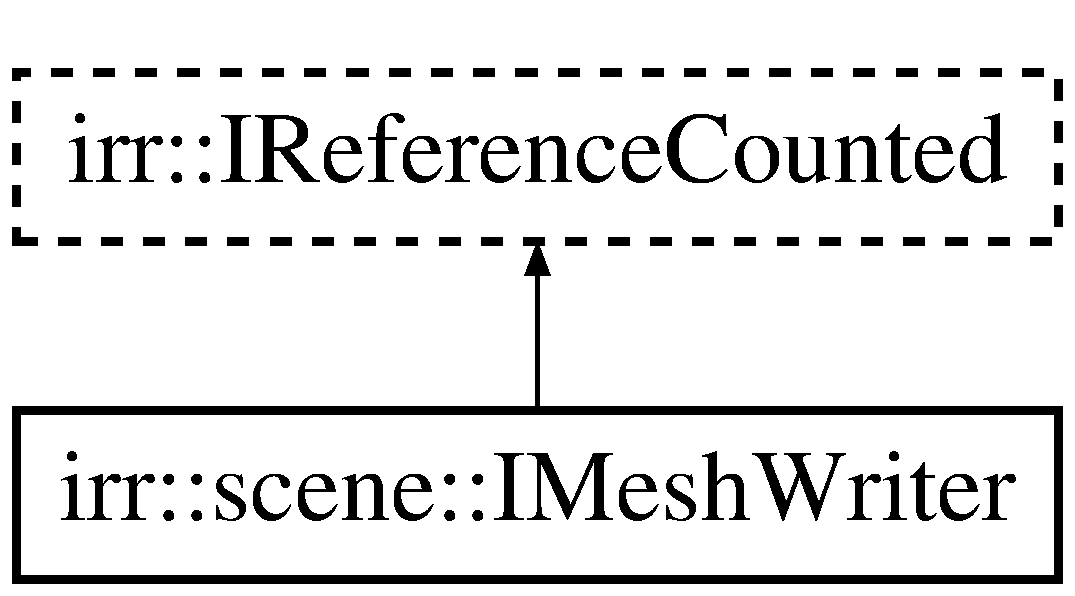
\includegraphics[height=2.000000cm]{classirr_1_1scene_1_1IMeshWriter}
\end{center}
\end{figure}
\subsection*{Public Member Functions}
\begin{DoxyCompactItemize}
\item 
virtual \hyperlink{classirr_1_1scene_1_1IMeshWriter_a9f92ba59b4ea9a21ccc6bcddc0d3ada9}{$\sim$\+I\+Mesh\+Writer} ()\hypertarget{classirr_1_1scene_1_1IMeshWriter_a9f92ba59b4ea9a21ccc6bcddc0d3ada9}{}\label{classirr_1_1scene_1_1IMeshWriter_a9f92ba59b4ea9a21ccc6bcddc0d3ada9}

\begin{DoxyCompactList}\small\item\em Destructor. \end{DoxyCompactList}\item 
virtual \hyperlink{namespaceirr_1_1scene_a431fa15741518ba15f6d5f2608b6cb4e}{E\+M\+E\+S\+H\+\_\+\+W\+R\+I\+T\+E\+R\+\_\+\+T\+Y\+PE} \hyperlink{classirr_1_1scene_1_1IMeshWriter_a21453b44e10b79fb084a3914ac737aec}{get\+Type} () const  =0
\begin{DoxyCompactList}\small\item\em Get the type of the mesh writer. \end{DoxyCompactList}\item 
virtual bool \hyperlink{classirr_1_1scene_1_1IMeshWriter_a200fc475979168b3baa6804f02ffd1a6}{write\+Mesh} (\hyperlink{classirr_1_1io_1_1IWriteFile}{io\+::\+I\+Write\+File} $\ast$file, \hyperlink{classirr_1_1scene_1_1IMesh}{scene\+::\+I\+C\+P\+U\+Mesh} $\ast$mesh, \hyperlink{namespaceirr_ac66849b7a6ed16e30ebede579f9b47c6}{s32} flags=\hyperlink{namespaceirr_1_1scene_a9faae6cd9e415a0553cb4cdc190bbc1daf2dfebddfd0a2cd2b558e23cb6a87464}{E\+M\+W\+F\+\_\+\+N\+O\+NE})=0
\begin{DoxyCompactList}\small\item\em Write a static mesh. \end{DoxyCompactList}\end{DoxyCompactItemize}
\subsection*{Additional Inherited Members}


\subsection{Detailed Description}
Interface for writing meshes. 

\subsection{Member Function Documentation}
\index{irr\+::scene\+::\+I\+Mesh\+Writer@{irr\+::scene\+::\+I\+Mesh\+Writer}!get\+Type@{get\+Type}}
\index{get\+Type@{get\+Type}!irr\+::scene\+::\+I\+Mesh\+Writer@{irr\+::scene\+::\+I\+Mesh\+Writer}}
\subsubsection[{\texorpdfstring{get\+Type() const  =0}{getType() const  =0}}]{\setlength{\rightskip}{0pt plus 5cm}virtual {\bf E\+M\+E\+S\+H\+\_\+\+W\+R\+I\+T\+E\+R\+\_\+\+T\+Y\+PE} irr\+::scene\+::\+I\+Mesh\+Writer\+::get\+Type (
\begin{DoxyParamCaption}
{}
\end{DoxyParamCaption}
) const\hspace{0.3cm}{\ttfamily [pure virtual]}}\hypertarget{classirr_1_1scene_1_1IMeshWriter_a21453b44e10b79fb084a3914ac737aec}{}\label{classirr_1_1scene_1_1IMeshWriter_a21453b44e10b79fb084a3914ac737aec}


Get the type of the mesh writer. 

For own implementations, use M\+A\+K\+E\+\_\+\+I\+R\+R\+\_\+\+ID as shown in the E\+M\+E\+S\+H\+\_\+\+W\+R\+I\+T\+E\+R\+\_\+\+T\+Y\+PE enumeration to return your own unique mesh type id. \begin{DoxyReturn}{Returns}
Type of the mesh writer. 
\end{DoxyReturn}
\index{irr\+::scene\+::\+I\+Mesh\+Writer@{irr\+::scene\+::\+I\+Mesh\+Writer}!write\+Mesh@{write\+Mesh}}
\index{write\+Mesh@{write\+Mesh}!irr\+::scene\+::\+I\+Mesh\+Writer@{irr\+::scene\+::\+I\+Mesh\+Writer}}
\subsubsection[{\texorpdfstring{write\+Mesh(io\+::\+I\+Write\+File $\ast$file, scene\+::\+I\+C\+P\+U\+Mesh $\ast$mesh, s32 flags=\+E\+M\+W\+F\+\_\+\+N\+O\+N\+E)=0}{writeMesh(io::IWriteFile *file, scene::ICPUMesh *mesh, s32 flags=EMWF\_NONE)=0}}]{\setlength{\rightskip}{0pt plus 5cm}virtual bool irr\+::scene\+::\+I\+Mesh\+Writer\+::write\+Mesh (
\begin{DoxyParamCaption}
\item[{{\bf io\+::\+I\+Write\+File} $\ast$}]{file, }
\item[{{\bf scene\+::\+I\+C\+P\+U\+Mesh} $\ast$}]{mesh, }
\item[{{\bf s32}}]{flags = {\ttfamily {\bf E\+M\+W\+F\+\_\+\+N\+O\+NE}}}
\end{DoxyParamCaption}
)\hspace{0.3cm}{\ttfamily [pure virtual]}}\hypertarget{classirr_1_1scene_1_1IMeshWriter_a200fc475979168b3baa6804f02ffd1a6}{}\label{classirr_1_1scene_1_1IMeshWriter_a200fc475979168b3baa6804f02ffd1a6}


Write a static mesh. 


\begin{DoxyParams}{Parameters}
{\em file} & File handle to write the mesh to. \\
\hline
{\em mesh} & Pointer to mesh to be written. \\
\hline
{\em flags} & Optional flags to set properties of the writer. \\
\hline
\end{DoxyParams}
\begin{DoxyReturn}{Returns}
True if sucessful 
\end{DoxyReturn}


The documentation for this class was generated from the following file\+:\begin{DoxyCompactItemize}
\item 
include/I\+Mesh\+Writer.\+h\end{DoxyCompactItemize}

\hypertarget{classirr_1_1core_1_1IMetaGranularBuffer}{}\section{irr\+:\+:core\+:\+:I\+Meta\+Granular\+Buffer$<$ T $>$ Class Template Reference}
\label{classirr_1_1core_1_1IMetaGranularBuffer}\index{irr\+::core\+::\+I\+Meta\+Granular\+Buffer$<$ T $>$@{irr\+::core\+::\+I\+Meta\+Granular\+Buffer$<$ T $>$}}
Inheritance diagram for irr\+:\+:core\+:\+:I\+Meta\+Granular\+Buffer$<$ T $>$\+:\begin{figure}[H]
\begin{center}
\leavevmode
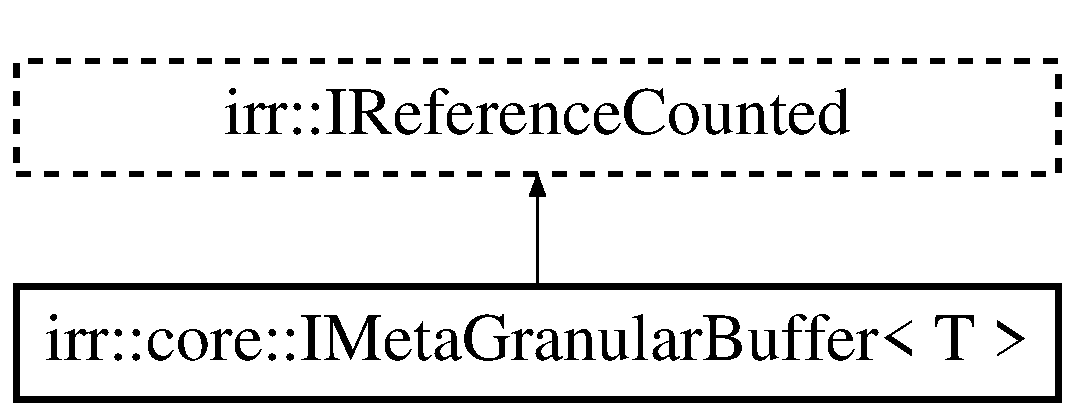
\includegraphics[height=2.000000cm]{classirr_1_1core_1_1IMetaGranularBuffer}
\end{center}
\end{figure}
\subsection*{Public Member Functions}
\begin{DoxyCompactItemize}
\item 
{\bfseries I\+Meta\+Granular\+Buffer} (const size\+\_\+t \&granule\+Size, const size\+\_\+t \&granule\+Count, const size\+\_\+t \&buffer\+Grow\+Step=512, const size\+\_\+t \&buffer\+Shrink\+Step=2048)\hypertarget{classirr_1_1core_1_1IMetaGranularBuffer_a97aea503eee9c815d3e38d684188108c}{}\label{classirr_1_1core_1_1IMetaGranularBuffer_a97aea503eee9c815d3e38d684188108c}

\item 
virtual T $\ast$ {\bfseries get\+Front\+Buffer} ()=0\hypertarget{classirr_1_1core_1_1IMetaGranularBuffer_ac1c88ef8dfece9e74ee2c872aa09d77b}{}\label{classirr_1_1core_1_1IMetaGranularBuffer_ac1c88ef8dfece9e74ee2c872aa09d77b}

\item 
void $\ast$ {\bfseries get\+Back\+Buffer\+Pointer} ()\hypertarget{classirr_1_1core_1_1IMetaGranularBuffer_a163b18f0f1b95312bfb3c898bae695bb}{}\label{classirr_1_1core_1_1IMetaGranularBuffer_a163b18f0f1b95312bfb3c898bae695bb}

\item 
virtual void {\bfseries Swap\+Buffers} (void($\ast$Stuff\+To\+Do\+To\+New\+Buffer)(T $\ast$, void $\ast$)=N\+U\+LL, void $\ast$user\+Data=N\+U\+LL)=0\hypertarget{classirr_1_1core_1_1IMetaGranularBuffer_af4f5b75a9efba16838e5abc99f6201bc}{}\label{classirr_1_1core_1_1IMetaGranularBuffer_af4f5b75a9efba16838e5abc99f6201bc}

\item 
const size\+\_\+t \& {\bfseries get\+Allocated\+Count} () const \hypertarget{classirr_1_1core_1_1IMetaGranularBuffer_aeba8de5e23886c0087b8a69533393e19}{}\label{classirr_1_1core_1_1IMetaGranularBuffer_aeba8de5e23886c0087b8a69533393e19}

\item 
const size\+\_\+t \& {\bfseries get\+Capacity} ()\hypertarget{classirr_1_1core_1_1IMetaGranularBuffer_a5086dbd701e9fe944b6b3cc53dba3715}{}\label{classirr_1_1core_1_1IMetaGranularBuffer_a5086dbd701e9fe944b6b3cc53dba3715}

\item 
virtual bool \hyperlink{classirr_1_1core_1_1IMetaGranularBuffer_a643ec9c885022593d6e4b653bed6f97f}{Alloc} (uint32\+\_\+t $\ast$granule\+I\+Ds, const size\+\_\+t \&count)
\item 
const uint32\+\_\+t \& {\bfseries get\+Redirect\+From\+ID} (const size\+\_\+t \&ix) const \hypertarget{classirr_1_1core_1_1IMetaGranularBuffer_aadc2dbdd80003f830bc62bbc7aa8dd82}{}\label{classirr_1_1core_1_1IMetaGranularBuffer_aadc2dbdd80003f830bc62bbc7aa8dd82}

\item 
virtual void {\bfseries Free} (const uint32\+\_\+t $\ast$granule\+I\+Ds, const size\+\_\+t \&count)\hypertarget{classirr_1_1core_1_1IMetaGranularBuffer_aebed18f1992fb10890115ec68f1c52de}{}\label{classirr_1_1core_1_1IMetaGranularBuffer_aebed18f1992fb10890115ec68f1c52de}

\item 
const size\+\_\+t {\bfseries get\+Granule\+Byte\+Size} () const \hypertarget{classirr_1_1core_1_1IMetaGranularBuffer_a3d0a821f552e65b7c9ea7b3dc3de8702}{}\label{classirr_1_1core_1_1IMetaGranularBuffer_a3d0a821f552e65b7c9ea7b3dc3de8702}

\end{DoxyCompactItemize}
\subsection*{Protected Member Functions}
\begin{DoxyCompactItemize}
\item 
bool {\bfseries Grow\+Back\+Buffer} (const size\+\_\+t \&new\+Granule\+Count)\hypertarget{classirr_1_1core_1_1IMetaGranularBuffer_a6b167f07ffc2aaf61c13c2aeca9fee04}{}\label{classirr_1_1core_1_1IMetaGranularBuffer_a6b167f07ffc2aaf61c13c2aeca9fee04}

\item 
void {\bfseries Shrink\+Back\+Buffer} ()\hypertarget{classirr_1_1core_1_1IMetaGranularBuffer_acbbdca59a6c48bfc8e32e29aab8ebfe6}{}\label{classirr_1_1core_1_1IMetaGranularBuffer_acbbdca59a6c48bfc8e32e29aab8ebfe6}

\item 
void {\bfseries Validate\+Hash\+Map} (const uint32\+\_\+t \&max\+Alloc)\hypertarget{classirr_1_1core_1_1IMetaGranularBuffer_a8570b25dfec2219c63e9c2782f61e3b1}{}\label{classirr_1_1core_1_1IMetaGranularBuffer_a8570b25dfec2219c63e9c2782f61e3b1}

\end{DoxyCompactItemize}
\subsection*{Protected Attributes}
\begin{DoxyCompactItemize}
\item 
size\+\_\+t {\bfseries Allocated}\hypertarget{classirr_1_1core_1_1IMetaGranularBuffer_a442d6eca3b37b144613f5dd00c460c54}{}\label{classirr_1_1core_1_1IMetaGranularBuffer_a442d6eca3b37b144613f5dd00c460c54}

\item 
size\+\_\+t {\bfseries Granules}\hypertarget{classirr_1_1core_1_1IMetaGranularBuffer_a11b06d843a11bca67e291476c4a157e9}{}\label{classirr_1_1core_1_1IMetaGranularBuffer_a11b06d843a11bca67e291476c4a157e9}

\item 
uint32\+\_\+t $\ast$ {\bfseries residency\+Redirect\+To}\hypertarget{classirr_1_1core_1_1IMetaGranularBuffer_aebf9a9512a50f8c8685788f6bab0dec1}{}\label{classirr_1_1core_1_1IMetaGranularBuffer_aebf9a9512a50f8c8685788f6bab0dec1}

\item 
const size\+\_\+t {\bfseries Granule\+Byte\+Size}\hypertarget{classirr_1_1core_1_1IMetaGranularBuffer_a8f9abf4ce149ef18375b067c1e1139c6}{}\label{classirr_1_1core_1_1IMetaGranularBuffer_a8f9abf4ce149ef18375b067c1e1139c6}

\item 
const size\+\_\+t {\bfseries Back\+Buffer\+Grow\+Step}\hypertarget{classirr_1_1core_1_1IMetaGranularBuffer_a3f64f1fbe9751c256b6b393077e7de8a}{}\label{classirr_1_1core_1_1IMetaGranularBuffer_a3f64f1fbe9751c256b6b393077e7de8a}

\item 
const size\+\_\+t {\bfseries Back\+Buffer\+Shrink\+Step}\hypertarget{classirr_1_1core_1_1IMetaGranularBuffer_a8dc4bc7da4525315648f1170b78afae6}{}\label{classirr_1_1core_1_1IMetaGranularBuffer_a8dc4bc7da4525315648f1170b78afae6}

\item 
\hyperlink{classirr_1_1core_1_1ICPUBuffer}{core\+::\+I\+C\+P\+U\+Buffer} $\ast$ {\bfseries B}\hypertarget{classirr_1_1core_1_1IMetaGranularBuffer_af9bdbf0de5af5cbce948285e3cbb2e33}{}\label{classirr_1_1core_1_1IMetaGranularBuffer_af9bdbf0de5af5cbce948285e3cbb2e33}

\end{DoxyCompactItemize}


\subsection{Member Function Documentation}
\index{irr\+::core\+::\+I\+Meta\+Granular\+Buffer@{irr\+::core\+::\+I\+Meta\+Granular\+Buffer}!Alloc@{Alloc}}
\index{Alloc@{Alloc}!irr\+::core\+::\+I\+Meta\+Granular\+Buffer@{irr\+::core\+::\+I\+Meta\+Granular\+Buffer}}
\subsubsection[{\texorpdfstring{Alloc(uint32\+\_\+t $\ast$granule\+I\+Ds, const size\+\_\+t \&count)}{Alloc(uint32\_t *granuleIDs, const size\_t \&count)}}]{\setlength{\rightskip}{0pt plus 5cm}template$<$class T$>$ virtual bool {\bf irr\+::core\+::\+I\+Meta\+Granular\+Buffer}$<$ T $>$\+::Alloc (
\begin{DoxyParamCaption}
\item[{uint32\+\_\+t $\ast$}]{granule\+I\+Ds, }
\item[{const size\+\_\+t \&}]{count}
\end{DoxyParamCaption}
)\hspace{0.3cm}{\ttfamily [inline]}, {\ttfamily [virtual]}}\hypertarget{classirr_1_1core_1_1IMetaGranularBuffer_a643ec9c885022593d6e4b653bed6f97f}{}\label{classirr_1_1core_1_1IMetaGranularBuffer_a643ec9c885022593d6e4b653bed6f97f}
Preconditions\+: 1) no holes in allocation 2) can have holes in redirects 

The documentation for this class was generated from the following file\+:\begin{DoxyCompactItemize}
\item 
include/I\+Meta\+Granular\+Buffer.\+h\end{DoxyCompactItemize}

\hypertarget{classirr_1_1core_1_1IMetaGranularCPUBuffer}{}\section{irr\+:\+:core\+:\+:I\+Meta\+Granular\+C\+P\+U\+Buffer Class Reference}
\label{classirr_1_1core_1_1IMetaGranularCPUBuffer}\index{irr\+::core\+::\+I\+Meta\+Granular\+C\+P\+U\+Buffer@{irr\+::core\+::\+I\+Meta\+Granular\+C\+P\+U\+Buffer}}
Inheritance diagram for irr\+:\+:core\+:\+:I\+Meta\+Granular\+C\+P\+U\+Buffer\+:\begin{figure}[H]
\begin{center}
\leavevmode
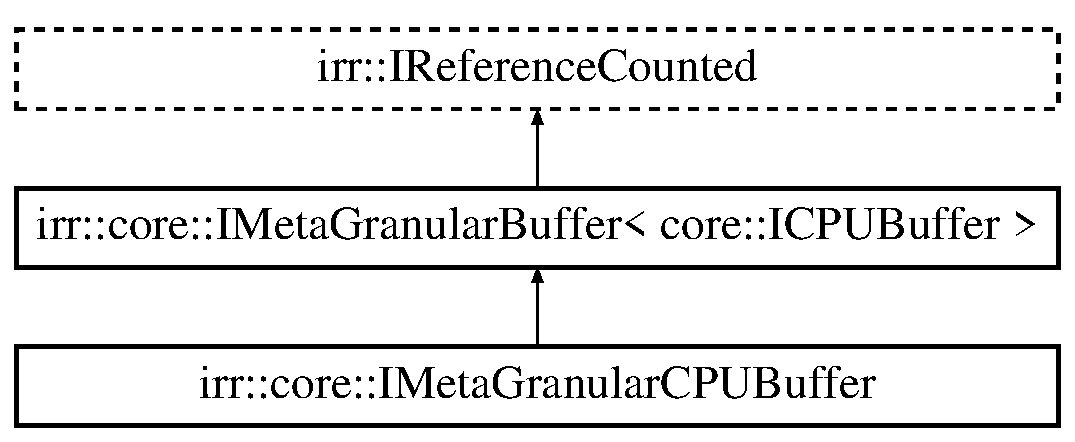
\includegraphics[height=3.000000cm]{classirr_1_1core_1_1IMetaGranularCPUBuffer}
\end{center}
\end{figure}
\subsection*{Public Member Functions}
\begin{DoxyCompactItemize}
\item 
{\bfseries I\+Meta\+Granular\+C\+P\+U\+Buffer} (const size\+\_\+t \&granule\+Size, const size\+\_\+t \&granule\+Count, const bool \&client\+Memeory=true, const size\+\_\+t \&buffer\+Grow\+Step=512, const size\+\_\+t \&buffer\+Shrink\+Step=2048)\hypertarget{classirr_1_1core_1_1IMetaGranularCPUBuffer_a79aeb46c01f8ad65f03a020ec53d0abd}{}\label{classirr_1_1core_1_1IMetaGranularCPUBuffer_a79aeb46c01f8ad65f03a020ec53d0abd}

\item 
virtual \hyperlink{classirr_1_1core_1_1ICPUBuffer}{core\+::\+I\+C\+P\+U\+Buffer} $\ast$ {\bfseries get\+Front\+Buffer} ()\hypertarget{classirr_1_1core_1_1IMetaGranularCPUBuffer_ac3d08aca62d511d17f0c7fbb11773ab1}{}\label{classirr_1_1core_1_1IMetaGranularCPUBuffer_ac3d08aca62d511d17f0c7fbb11773ab1}

\item 
virtual void {\bfseries Swap\+Buffers} (void($\ast$Stuff\+To\+Do\+To\+New\+Buffer)(\hyperlink{classirr_1_1core_1_1ICPUBuffer}{core\+::\+I\+C\+P\+U\+Buffer} $\ast$, void $\ast$)=N\+U\+LL, void $\ast$user\+Data=N\+U\+LL)\hypertarget{classirr_1_1core_1_1IMetaGranularCPUBuffer_a2697927ad936d009c06b8e649f33dcf8}{}\label{classirr_1_1core_1_1IMetaGranularCPUBuffer_a2697927ad936d009c06b8e649f33dcf8}

\end{DoxyCompactItemize}
\subsection*{Protected Attributes}
\begin{DoxyCompactItemize}
\item 
\hyperlink{classirr_1_1core_1_1ICPUBuffer}{core\+::\+I\+C\+P\+U\+Buffer} $\ast$ {\bfseries A}\hypertarget{classirr_1_1core_1_1IMetaGranularCPUBuffer_a24be9466e652e9819f0d677876e336cf}{}\label{classirr_1_1core_1_1IMetaGranularCPUBuffer_a24be9466e652e9819f0d677876e336cf}

\end{DoxyCompactItemize}
\subsection*{Additional Inherited Members}


The documentation for this class was generated from the following file\+:\begin{DoxyCompactItemize}
\item 
include/I\+Meta\+Granular\+Buffer.\+h\end{DoxyCompactItemize}

\hypertarget{classirr_1_1video_1_1IMetaGranularGPUMappedBuffer}{}\section{irr\+:\+:video\+:\+:I\+Meta\+Granular\+G\+P\+U\+Mapped\+Buffer Class Reference}
\label{classirr_1_1video_1_1IMetaGranularGPUMappedBuffer}\index{irr\+::video\+::\+I\+Meta\+Granular\+G\+P\+U\+Mapped\+Buffer@{irr\+::video\+::\+I\+Meta\+Granular\+G\+P\+U\+Mapped\+Buffer}}
Inheritance diagram for irr\+:\+:video\+:\+:I\+Meta\+Granular\+G\+P\+U\+Mapped\+Buffer\+:\begin{figure}[H]
\begin{center}
\leavevmode
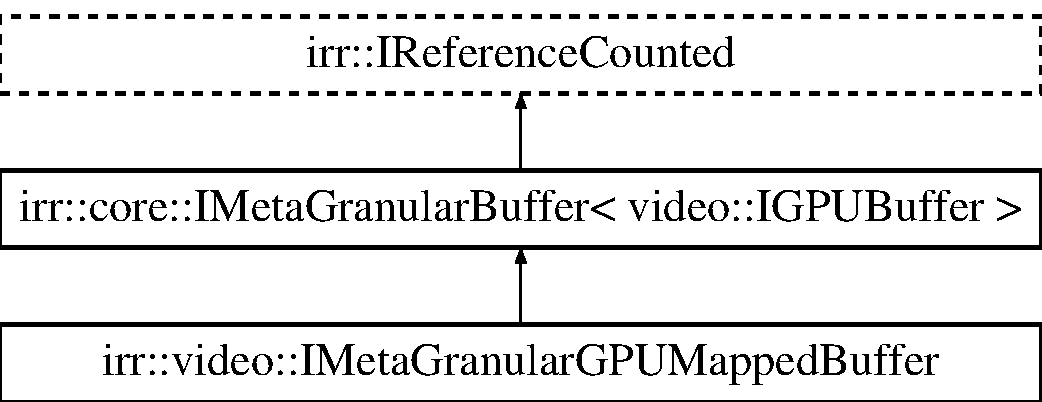
\includegraphics[height=3.000000cm]{classirr_1_1video_1_1IMetaGranularGPUMappedBuffer}
\end{center}
\end{figure}
\subsection*{Public Member Functions}
\begin{DoxyCompactItemize}
\item 
{\bfseries I\+Meta\+Granular\+G\+P\+U\+Mapped\+Buffer} (\hyperlink{classirr_1_1video_1_1IVideoDriver}{video\+::\+I\+Video\+Driver} $\ast$driver, const size\+\_\+t \&granule\+Size, const size\+\_\+t \&granule\+Count, const bool \&client\+Memeory=true, const size\+\_\+t \&buffer\+Grow\+Step=512, const size\+\_\+t \&buffer\+Shrink\+Step=2048)\hypertarget{classirr_1_1video_1_1IMetaGranularGPUMappedBuffer_a9f89e94296ed8b68dfec6c511670bf0d}{}\label{classirr_1_1video_1_1IMetaGranularGPUMappedBuffer_a9f89e94296ed8b68dfec6c511670bf0d}

\item 
virtual \hyperlink{classirr_1_1video_1_1IGPUBuffer}{video\+::\+I\+G\+P\+U\+Buffer} $\ast$ {\bfseries get\+Front\+Buffer} ()\hypertarget{classirr_1_1video_1_1IMetaGranularGPUMappedBuffer_a08b6d77a85676200aa9a9289ef152947}{}\label{classirr_1_1video_1_1IMetaGranularGPUMappedBuffer_a08b6d77a85676200aa9a9289ef152947}

\item 
virtual void {\bfseries Swap\+Buffers} (void($\ast$Stuff\+To\+Do\+To\+New\+Buffer)(\hyperlink{classirr_1_1video_1_1IGPUBuffer}{video\+::\+I\+G\+P\+U\+Buffer} $\ast$, void $\ast$)=N\+U\+LL, void $\ast$user\+Data=N\+U\+LL)\hypertarget{classirr_1_1video_1_1IMetaGranularGPUMappedBuffer_a20e99ec2be4138ac0cced78b15b2f33a}{}\label{classirr_1_1video_1_1IMetaGranularGPUMappedBuffer_a20e99ec2be4138ac0cced78b15b2f33a}

\end{DoxyCompactItemize}
\subsection*{Additional Inherited Members}


The documentation for this class was generated from the following file\+:\begin{DoxyCompactItemize}
\item 
include/I\+Meta\+Granular\+Buffer.\+h\end{DoxyCompactItemize}

\hypertarget{unionirr_1_1core_1_1inttofloat}{}\section{irr\+:\+:core\+:\+:inttofloat Union Reference}
\label{unionirr_1_1core_1_1inttofloat}\index{irr\+::core\+::inttofloat@{irr\+::core\+::inttofloat}}
\subsection*{Public Attributes}
\begin{DoxyCompactItemize}
\item 
\hyperlink{namespaceirr_a0416a53257075833e7002efd0a18e804}{u32} {\bfseries u}\hypertarget{unionirr_1_1core_1_1inttofloat_a87651356c7436ac7755e85189412f75a}{}\label{unionirr_1_1core_1_1inttofloat_a87651356c7436ac7755e85189412f75a}

\item 
\hyperlink{namespaceirr_ac66849b7a6ed16e30ebede579f9b47c6}{s32} {\bfseries s}\hypertarget{unionirr_1_1core_1_1inttofloat_a1adc8b3417ac325bd9695c0cbb6c043e}{}\label{unionirr_1_1core_1_1inttofloat_a1adc8b3417ac325bd9695c0cbb6c043e}

\item 
\hyperlink{namespaceirr_a0277be98d67dc26ff93b1a6a1d086b07}{f32} {\bfseries f}\hypertarget{unionirr_1_1core_1_1inttofloat_ab0dd36fa35cbb368602fa0d18b2d9788}{}\label{unionirr_1_1core_1_1inttofloat_ab0dd36fa35cbb368602fa0d18b2d9788}

\end{DoxyCompactItemize}


The documentation for this union was generated from the following file\+:\begin{DoxyCompactItemize}
\item 
include/irr\+Math.\+h\end{DoxyCompactItemize}

\hypertarget{classirr_1_1video_1_1IOcclusionQuery}{}\section{irr\+:\+:video\+:\+:I\+Occlusion\+Query Class Reference}
\label{classirr_1_1video_1_1IOcclusionQuery}\index{irr\+::video\+::\+I\+Occlusion\+Query@{irr\+::video\+::\+I\+Occlusion\+Query}}
Inheritance diagram for irr\+:\+:video\+:\+:I\+Occlusion\+Query\+:\begin{figure}[H]
\begin{center}
\leavevmode
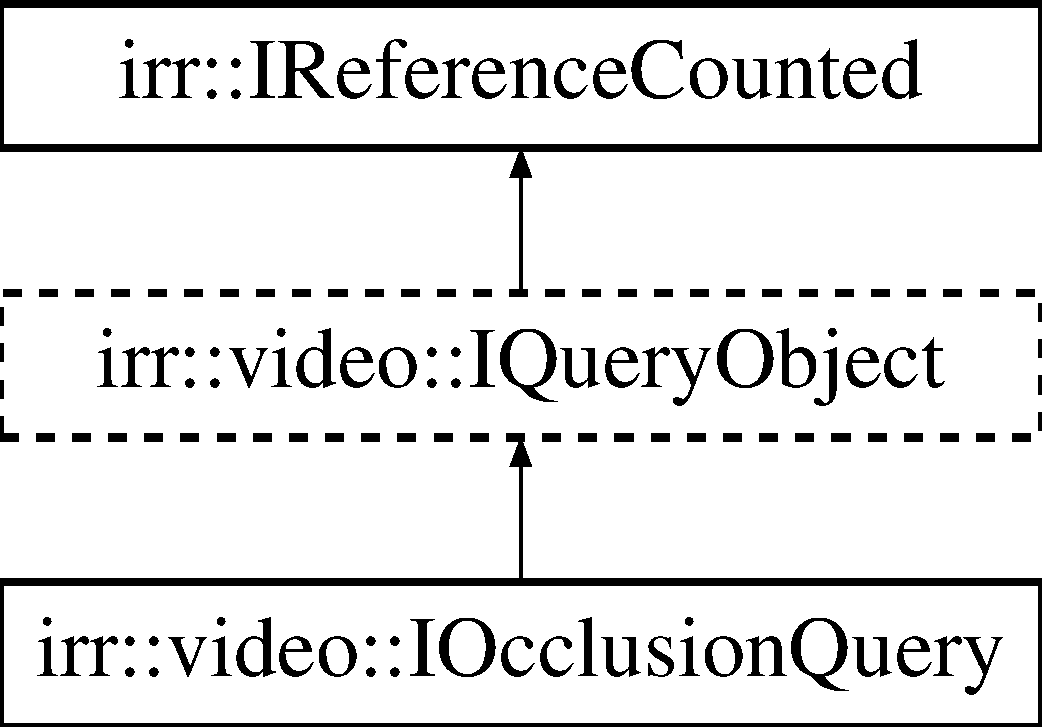
\includegraphics[height=3.000000cm]{classirr_1_1video_1_1IOcclusionQuery}
\end{center}
\end{figure}
\subsection*{Public Member Functions}
\begin{DoxyCompactItemize}
\item 
E\+\_\+\+C\+O\+N\+D\+I\+T\+I\+O\+N\+A\+L\+\_\+\+R\+E\+N\+D\+E\+R\+I\+N\+G\+\_\+\+W\+A\+I\+T\+\_\+\+M\+O\+DE {\bfseries get\+Cond\+Wait\+Mode} () const \hypertarget{classirr_1_1video_1_1IOcclusionQuery_a11dca98cd885a473c1286bc3f12dc07e}{}\label{classirr_1_1video_1_1IOcclusionQuery_a11dca98cd885a473c1286bc3f12dc07e}

\item 
virtual void {\bfseries set\+Cond\+Wait\+Mode} (const E\+\_\+\+C\+O\+N\+D\+I\+T\+I\+O\+N\+A\+L\+\_\+\+R\+E\+N\+D\+E\+R\+I\+N\+G\+\_\+\+W\+A\+I\+T\+\_\+\+M\+O\+DE \&mode)\hypertarget{classirr_1_1video_1_1IOcclusionQuery_a50bb0fb79825c6814814c4ec8265437d}{}\label{classirr_1_1video_1_1IOcclusionQuery_a50bb0fb79825c6814814c4ec8265437d}

\item 
virtual const E\+\_\+\+Q\+U\+E\+R\+Y\+\_\+\+O\+B\+J\+E\+C\+T\+\_\+\+T\+Y\+PE {\bfseries get\+Query\+Object\+Type} () const \hypertarget{classirr_1_1video_1_1IOcclusionQuery_a8e289150dc5169457d00f2f61faae58f}{}\label{classirr_1_1video_1_1IOcclusionQuery_a8e289150dc5169457d00f2f61faae58f}

\item 
const E\+\_\+\+O\+C\+C\+L\+U\+S\+I\+O\+N\+\_\+\+Q\+U\+E\+R\+Y\+\_\+\+T\+Y\+PE \& {\bfseries get\+Occlusion\+Query\+Type} () const \hypertarget{classirr_1_1video_1_1IOcclusionQuery_a611dfaa0102f4794d48ef4b901cde63a}{}\label{classirr_1_1video_1_1IOcclusionQuery_a611dfaa0102f4794d48ef4b901cde63a}

\end{DoxyCompactItemize}
\subsection*{Protected Member Functions}
\begin{DoxyCompactItemize}
\item 
{\bfseries I\+Occlusion\+Query} (const E\+\_\+\+O\+C\+C\+L\+U\+S\+I\+O\+N\+\_\+\+Q\+U\+E\+R\+Y\+\_\+\+T\+Y\+PE \&occlusion\+Query\+Type\+Heuristic)\hypertarget{classirr_1_1video_1_1IOcclusionQuery_ae5a69c234898dca7afe7fcffeadbeb44}{}\label{classirr_1_1video_1_1IOcclusionQuery_ae5a69c234898dca7afe7fcffeadbeb44}

\end{DoxyCompactItemize}


The documentation for this class was generated from the following file\+:\begin{DoxyCompactItemize}
\item 
include/I\+Occlusion\+Query.\+h\end{DoxyCompactItemize}

\hypertarget{classirr_1_1IOSOperator}{}\section{irr\+:\+:I\+O\+S\+Operator Class Reference}
\label{classirr_1_1IOSOperator}\index{irr\+::\+I\+O\+S\+Operator@{irr\+::\+I\+O\+S\+Operator}}


The Operating system operator provides operation system specific methods and informations.  




{\ttfamily \#include $<$I\+O\+S\+Operator.\+h$>$}

Inheritance diagram for irr\+:\+:I\+O\+S\+Operator\+:\begin{figure}[H]
\begin{center}
\leavevmode
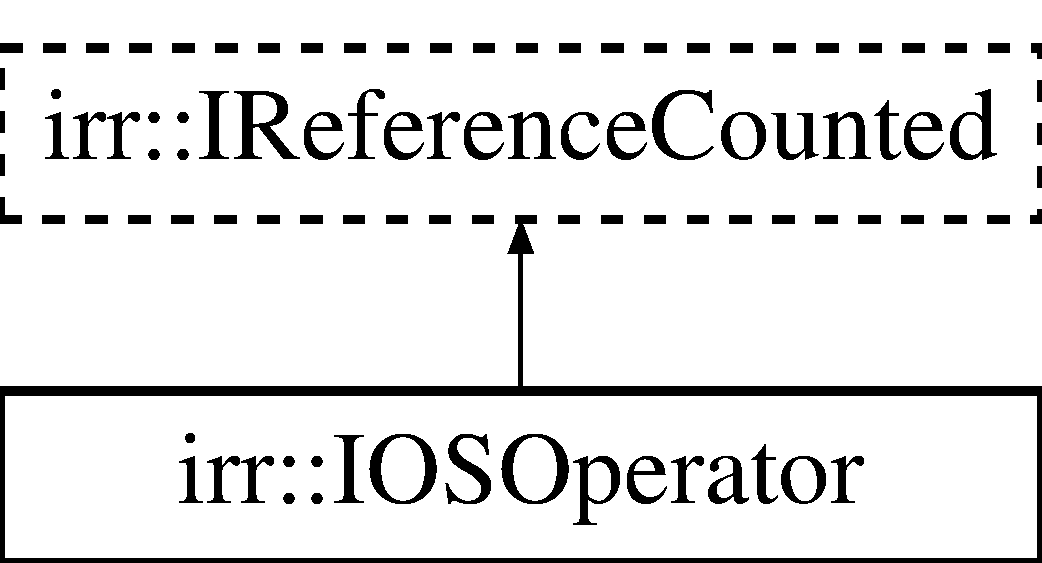
\includegraphics[height=2.000000cm]{classirr_1_1IOSOperator}
\end{center}
\end{figure}
\subsection*{Public Member Functions}
\begin{DoxyCompactItemize}
\item 
virtual const \hyperlink{namespaceirr_1_1core_ade1071a878633f2f6d8a75c5d11fec19}{core\+::stringc} \& \hyperlink{classirr_1_1IOSOperator_a376386a7fceab8b414eac974a4055839}{get\+Operating\+System\+Version} () const  =0\hypertarget{classirr_1_1IOSOperator_a376386a7fceab8b414eac974a4055839}{}\label{classirr_1_1IOSOperator_a376386a7fceab8b414eac974a4055839}

\begin{DoxyCompactList}\small\item\em Get the current operation system version as string. \end{DoxyCompactList}\item 
\+\_\+\+I\+R\+R\+\_\+\+D\+E\+P\+R\+E\+C\+A\+T\+E\+D\+\_\+ const wchar\+\_\+t $\ast$ \hyperlink{classirr_1_1IOSOperator_a213ace1e7332bf2b08e5c8245784cb0e}{get\+Operation\+System\+Version} () const 
\begin{DoxyCompactList}\small\item\em Get the current operation system version as string. \end{DoxyCompactList}\item 
virtual void \hyperlink{classirr_1_1IOSOperator_a98080d0fa3d8fa1754af10b4d4f60f39}{copy\+To\+Clipboard} (const \hyperlink{namespaceirr_a9395eaea339bcb546b319e9c96bf7410}{c8} $\ast$text) const  =0\hypertarget{classirr_1_1IOSOperator_a98080d0fa3d8fa1754af10b4d4f60f39}{}\label{classirr_1_1IOSOperator_a98080d0fa3d8fa1754af10b4d4f60f39}

\begin{DoxyCompactList}\small\item\em Copies text to the clipboard. \end{DoxyCompactList}\item 
virtual const \hyperlink{namespaceirr_a9395eaea339bcb546b319e9c96bf7410}{c8} $\ast$ \hyperlink{classirr_1_1IOSOperator_a058508332b292594046ec8b7d804f513}{get\+Text\+From\+Clipboard} () const  =0
\begin{DoxyCompactList}\small\item\em Get text from the clipboard. \end{DoxyCompactList}\item 
virtual bool \hyperlink{classirr_1_1IOSOperator_a8dd05488cbbcc4a6d8b12ecad2579129}{get\+Processor\+Speed\+M\+Hz} (\hyperlink{namespaceirr_a0416a53257075833e7002efd0a18e804}{u32} $\ast$M\+Hz) const  =0
\begin{DoxyCompactList}\small\item\em Get the processor speed in megahertz. \end{DoxyCompactList}\item 
virtual bool \hyperlink{classirr_1_1IOSOperator_abd6567708e997ed7731f3147c1dd5829}{get\+System\+Memory} (\hyperlink{namespaceirr_a0416a53257075833e7002efd0a18e804}{u32} $\ast$Total, \hyperlink{namespaceirr_a0416a53257075833e7002efd0a18e804}{u32} $\ast$Avail) const  =0
\begin{DoxyCompactList}\small\item\em Get the total and available system R\+AM. \end{DoxyCompactList}\end{DoxyCompactItemize}
\subsection*{Additional Inherited Members}


\subsection{Detailed Description}
The Operating system operator provides operation system specific methods and informations. 

\subsection{Member Function Documentation}
\index{irr\+::\+I\+O\+S\+Operator@{irr\+::\+I\+O\+S\+Operator}!get\+Operation\+System\+Version@{get\+Operation\+System\+Version}}
\index{get\+Operation\+System\+Version@{get\+Operation\+System\+Version}!irr\+::\+I\+O\+S\+Operator@{irr\+::\+I\+O\+S\+Operator}}
\subsubsection[{\texorpdfstring{get\+Operation\+System\+Version() const }{getOperationSystemVersion() const }}]{\setlength{\rightskip}{0pt plus 5cm}\+\_\+\+I\+R\+R\+\_\+\+D\+E\+P\+R\+E\+C\+A\+T\+E\+D\+\_\+ const wchar\+\_\+t$\ast$ irr\+::\+I\+O\+S\+Operator\+::get\+Operation\+System\+Version (
\begin{DoxyParamCaption}
{}
\end{DoxyParamCaption}
) const\hspace{0.3cm}{\ttfamily [inline]}}\hypertarget{classirr_1_1IOSOperator_a213ace1e7332bf2b08e5c8245784cb0e}{}\label{classirr_1_1IOSOperator_a213ace1e7332bf2b08e5c8245784cb0e}


Get the current operation system version as string. 

\begin{DoxyRefDesc}{Deprecated}
\item[\hyperlink{deprecated__deprecated000004}{Deprecated}]Use get\+Operating\+System\+Version instead. This method will be removed in Irrlicht 1.\+9. \end{DoxyRefDesc}
\index{irr\+::\+I\+O\+S\+Operator@{irr\+::\+I\+O\+S\+Operator}!get\+Processor\+Speed\+M\+Hz@{get\+Processor\+Speed\+M\+Hz}}
\index{get\+Processor\+Speed\+M\+Hz@{get\+Processor\+Speed\+M\+Hz}!irr\+::\+I\+O\+S\+Operator@{irr\+::\+I\+O\+S\+Operator}}
\subsubsection[{\texorpdfstring{get\+Processor\+Speed\+M\+Hz(u32 $\ast$\+M\+Hz) const  =0}{getProcessorSpeedMHz(u32 *MHz) const  =0}}]{\setlength{\rightskip}{0pt plus 5cm}virtual bool irr\+::\+I\+O\+S\+Operator\+::get\+Processor\+Speed\+M\+Hz (
\begin{DoxyParamCaption}
\item[{{\bf u32} $\ast$}]{M\+Hz}
\end{DoxyParamCaption}
) const\hspace{0.3cm}{\ttfamily [pure virtual]}}\hypertarget{classirr_1_1IOSOperator_a8dd05488cbbcc4a6d8b12ecad2579129}{}\label{classirr_1_1IOSOperator_a8dd05488cbbcc4a6d8b12ecad2579129}


Get the processor speed in megahertz. 


\begin{DoxyParams}{Parameters}
{\em M\+Hz} & The integer variable to store the speed in. \\
\hline
\end{DoxyParams}
\begin{DoxyReturn}{Returns}
True if successful, false if not 
\end{DoxyReturn}
\index{irr\+::\+I\+O\+S\+Operator@{irr\+::\+I\+O\+S\+Operator}!get\+System\+Memory@{get\+System\+Memory}}
\index{get\+System\+Memory@{get\+System\+Memory}!irr\+::\+I\+O\+S\+Operator@{irr\+::\+I\+O\+S\+Operator}}
\subsubsection[{\texorpdfstring{get\+System\+Memory(u32 $\ast$\+Total, u32 $\ast$\+Avail) const  =0}{getSystemMemory(u32 *Total, u32 *Avail) const  =0}}]{\setlength{\rightskip}{0pt plus 5cm}virtual bool irr\+::\+I\+O\+S\+Operator\+::get\+System\+Memory (
\begin{DoxyParamCaption}
\item[{{\bf u32} $\ast$}]{Total, }
\item[{{\bf u32} $\ast$}]{Avail}
\end{DoxyParamCaption}
) const\hspace{0.3cm}{\ttfamily [pure virtual]}}\hypertarget{classirr_1_1IOSOperator_abd6567708e997ed7731f3147c1dd5829}{}\label{classirr_1_1IOSOperator_abd6567708e997ed7731f3147c1dd5829}


Get the total and available system R\+AM. 


\begin{DoxyParams}{Parameters}
{\em Total} & will contain the total system memory \\
\hline
{\em Avail} & will contain the available memory \\
\hline
\end{DoxyParams}
\begin{DoxyReturn}{Returns}
True if successful, false if not 
\end{DoxyReturn}
\index{irr\+::\+I\+O\+S\+Operator@{irr\+::\+I\+O\+S\+Operator}!get\+Text\+From\+Clipboard@{get\+Text\+From\+Clipboard}}
\index{get\+Text\+From\+Clipboard@{get\+Text\+From\+Clipboard}!irr\+::\+I\+O\+S\+Operator@{irr\+::\+I\+O\+S\+Operator}}
\subsubsection[{\texorpdfstring{get\+Text\+From\+Clipboard() const  =0}{getTextFromClipboard() const  =0}}]{\setlength{\rightskip}{0pt plus 5cm}virtual const {\bf c8}$\ast$ irr\+::\+I\+O\+S\+Operator\+::get\+Text\+From\+Clipboard (
\begin{DoxyParamCaption}
{}
\end{DoxyParamCaption}
) const\hspace{0.3cm}{\ttfamily [pure virtual]}}\hypertarget{classirr_1_1IOSOperator_a058508332b292594046ec8b7d804f513}{}\label{classirr_1_1IOSOperator_a058508332b292594046ec8b7d804f513}


Get text from the clipboard. 

\begin{DoxyReturn}{Returns}
Returns 0 if no string is in there. 
\end{DoxyReturn}


The documentation for this class was generated from the following file\+:\begin{DoxyCompactItemize}
\item 
include/I\+O\+S\+Operator.\+h\end{DoxyCompactItemize}

\hypertarget{classirr_1_1video_1_1IQueryObject}{}\section{irr\+:\+:video\+:\+:I\+Query\+Object Class Reference}
\label{classirr_1_1video_1_1IQueryObject}\index{irr\+::video\+::\+I\+Query\+Object@{irr\+::video\+::\+I\+Query\+Object}}
Inheritance diagram for irr\+:\+:video\+:\+:I\+Query\+Object\+:\begin{figure}[H]
\begin{center}
\leavevmode
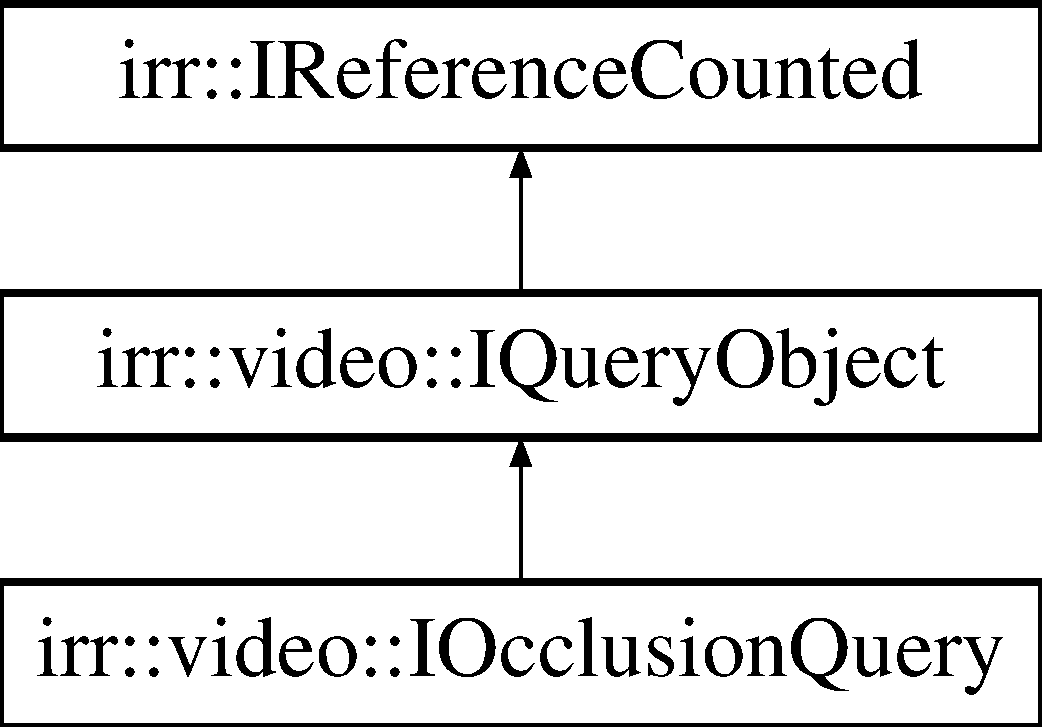
\includegraphics[height=3.000000cm]{classirr_1_1video_1_1IQueryObject}
\end{center}
\end{figure}
\subsection*{Public Member Functions}
\begin{DoxyCompactItemize}
\item 
virtual void \hyperlink{classirr_1_1video_1_1IQueryObject_a43774e2f4777db9fd8d9761ad1c66928}{get\+Query\+Result} (uint32\+\_\+t $\ast$query\+Result)=0\hypertarget{classirr_1_1video_1_1IQueryObject_a43774e2f4777db9fd8d9761ad1c66928}{}\label{classirr_1_1video_1_1IQueryObject_a43774e2f4777db9fd8d9761ad1c66928}

\begin{DoxyCompactList}\small\item\em A\+LL will S\+T\+A\+LL C\+PU IF Q\+U\+E\+RY N\+OT R\+E\+A\+DY. \end{DoxyCompactList}\item 
virtual void {\bfseries get\+Query\+Result} (uint64\+\_\+t $\ast$query\+Result)=0\hypertarget{classirr_1_1video_1_1IQueryObject_aa25da93912517d5579b2c99e12611219}{}\label{classirr_1_1video_1_1IQueryObject_aa25da93912517d5579b2c99e12611219}

\item 
virtual bool \hyperlink{classirr_1_1video_1_1IQueryObject_aecb33e043550f7114734f8a854300391}{get\+Query\+Result32} (\hyperlink{classirr_1_1video_1_1IGPUBuffer}{I\+G\+P\+U\+Buffer} $\ast$buffer, const size\+\_\+t \&offset=0, const bool \&conditional\+Write=true)=0\hypertarget{classirr_1_1video_1_1IQueryObject_aecb33e043550f7114734f8a854300391}{}\label{classirr_1_1video_1_1IQueryObject_aecb33e043550f7114734f8a854300391}

\begin{DoxyCompactList}\small\item\em A\+V\+A\+I\+L\+A\+B\+LE O\+N\+LY W\+I\+TH A\+R\+B\+\_\+query\+\_\+buffer\+\_\+object !! \end{DoxyCompactList}\item 
virtual bool {\bfseries get\+Query\+Result64} (\hyperlink{classirr_1_1video_1_1IGPUBuffer}{I\+G\+P\+U\+Buffer} $\ast$buffer, const size\+\_\+t \&offset=0, const bool \&conditional\+Write=true)=0\hypertarget{classirr_1_1video_1_1IQueryObject_a0e02e85a0861e96f6c59eae693c9127f}{}\label{classirr_1_1video_1_1IQueryObject_a0e02e85a0861e96f6c59eae693c9127f}

\item 
virtual bool {\bfseries is\+Query\+Ready} ()=0\hypertarget{classirr_1_1video_1_1IQueryObject_ae7a325b0492adb930d028c63bba02922}{}\label{classirr_1_1video_1_1IQueryObject_ae7a325b0492adb930d028c63bba02922}

\item 
virtual void \hyperlink{classirr_1_1video_1_1IQueryObject_aaa61fd1b6540fdd5ba0270412bf05326}{is\+Query\+Ready32} (\hyperlink{classirr_1_1video_1_1IGPUBuffer}{I\+G\+P\+U\+Buffer} $\ast$buffer, const size\+\_\+t \&offset=0)=0\hypertarget{classirr_1_1video_1_1IQueryObject_aaa61fd1b6540fdd5ba0270412bf05326}{}\label{classirr_1_1video_1_1IQueryObject_aaa61fd1b6540fdd5ba0270412bf05326}

\begin{DoxyCompactList}\small\item\em A\+V\+A\+I\+L\+A\+B\+LE O\+N\+LY W\+I\+TH A\+R\+B\+\_\+query\+\_\+buffer\+\_\+object !! \end{DoxyCompactList}\item 
virtual void {\bfseries is\+Query\+Ready64} (\hyperlink{classirr_1_1video_1_1IGPUBuffer}{I\+G\+P\+U\+Buffer} $\ast$buffer, const size\+\_\+t \&offset=0)=0\hypertarget{classirr_1_1video_1_1IQueryObject_a292a09602a6125458fd11fdde5cbc4d2}{}\label{classirr_1_1video_1_1IQueryObject_a292a09602a6125458fd11fdde5cbc4d2}

\item 
virtual const E\+\_\+\+Q\+U\+E\+R\+Y\+\_\+\+O\+B\+J\+E\+C\+T\+\_\+\+T\+Y\+PE {\bfseries get\+Query\+Object\+Type} () const  =0\hypertarget{classirr_1_1video_1_1IQueryObject_aff7e93fee7b1fcd2c02619706c807ffd}{}\label{classirr_1_1video_1_1IQueryObject_aff7e93fee7b1fcd2c02619706c807ffd}

\end{DoxyCompactItemize}
\subsection*{Additional Inherited Members}


The documentation for this class was generated from the following file\+:\begin{DoxyCompactItemize}
\item 
include/I\+Query\+Object.\+h\end{DoxyCompactItemize}

\hypertarget{classirr_1_1IRandomizer}{}\section{irr\+:\+:I\+Randomizer Class Reference}
\label{classirr_1_1IRandomizer}\index{irr\+::\+I\+Randomizer@{irr\+::\+I\+Randomizer}}


Interface for generating random numbers.  




{\ttfamily \#include $<$I\+Randomizer.\+h$>$}

Inheritance diagram for irr\+:\+:I\+Randomizer\+:\begin{figure}[H]
\begin{center}
\leavevmode
\includegraphics[height=2.000000cm]{classirr_1_1IRandomizer}
\end{center}
\end{figure}
\subsection*{Public Member Functions}
\begin{DoxyCompactItemize}
\item 
virtual void \hyperlink{classirr_1_1IRandomizer_ac9d7c9464698f6e183992fb895fa5ac4}{reset} (\hyperlink{namespaceirr_ac66849b7a6ed16e30ebede579f9b47c6}{s32} value=0x0f0f0f0f)=0
\begin{DoxyCompactList}\small\item\em resets the randomizer \end{DoxyCompactList}\item 
virtual \hyperlink{namespaceirr_ac66849b7a6ed16e30ebede579f9b47c6}{s32} \hyperlink{classirr_1_1IRandomizer_a703520f7f34f4aa4a818a4d89035c762}{rand} () const  =0\hypertarget{classirr_1_1IRandomizer_a703520f7f34f4aa4a818a4d89035c762}{}\label{classirr_1_1IRandomizer_a703520f7f34f4aa4a818a4d89035c762}

\begin{DoxyCompactList}\small\item\em generates a pseudo random number in the range 0..\hyperlink{classirr_1_1IRandomizer_adfa89add203d9afacfa43bd8fbea0f99}{rand\+Max()} \end{DoxyCompactList}\item 
virtual \hyperlink{namespaceirr_a0277be98d67dc26ff93b1a6a1d086b07}{f32} \hyperlink{classirr_1_1IRandomizer_adb4c7f81d74af18c5de3e0dfabfbd05d}{frand} () const  =0\hypertarget{classirr_1_1IRandomizer_adb4c7f81d74af18c5de3e0dfabfbd05d}{}\label{classirr_1_1IRandomizer_adb4c7f81d74af18c5de3e0dfabfbd05d}

\begin{DoxyCompactList}\small\item\em generates a pseudo random number in the range 0..1 \end{DoxyCompactList}\item 
virtual \hyperlink{namespaceirr_ac66849b7a6ed16e30ebede579f9b47c6}{s32} \hyperlink{classirr_1_1IRandomizer_adfa89add203d9afacfa43bd8fbea0f99}{rand\+Max} () const  =0\hypertarget{classirr_1_1IRandomizer_adfa89add203d9afacfa43bd8fbea0f99}{}\label{classirr_1_1IRandomizer_adfa89add203d9afacfa43bd8fbea0f99}

\begin{DoxyCompactList}\small\item\em get maxmimum number generated by \hyperlink{classirr_1_1IRandomizer_a703520f7f34f4aa4a818a4d89035c762}{rand()} \end{DoxyCompactList}\end{DoxyCompactItemize}
\subsection*{Additional Inherited Members}


\subsection{Detailed Description}
Interface for generating random numbers. 

\subsection{Member Function Documentation}
\index{irr\+::\+I\+Randomizer@{irr\+::\+I\+Randomizer}!reset@{reset}}
\index{reset@{reset}!irr\+::\+I\+Randomizer@{irr\+::\+I\+Randomizer}}
\subsubsection[{\texorpdfstring{reset(s32 value=0x0f0f0f0f)=0}{reset(s32 value=0x0f0f0f0f)=0}}]{\setlength{\rightskip}{0pt plus 5cm}virtual void irr\+::\+I\+Randomizer\+::reset (
\begin{DoxyParamCaption}
\item[{{\bf s32}}]{value = {\ttfamily 0x0f0f0f0f}}
\end{DoxyParamCaption}
)\hspace{0.3cm}{\ttfamily [pure virtual]}}\hypertarget{classirr_1_1IRandomizer_ac9d7c9464698f6e183992fb895fa5ac4}{}\label{classirr_1_1IRandomizer_ac9d7c9464698f6e183992fb895fa5ac4}


resets the randomizer 


\begin{DoxyParams}{Parameters}
{\em value} & Initialization value (seed) \\
\hline
\end{DoxyParams}


The documentation for this class was generated from the following file\+:\begin{DoxyCompactItemize}
\item 
include/I\+Randomizer.\+h\end{DoxyCompactItemize}

\hypertarget{classirr_1_1io_1_1IReadFile}{}\section{irr\+:\+:io\+:\+:I\+Read\+File Class Reference}
\label{classirr_1_1io_1_1IReadFile}\index{irr\+::io\+::\+I\+Read\+File@{irr\+::io\+::\+I\+Read\+File}}


Interface providing read acess to a file.  




{\ttfamily \#include $<$I\+Read\+File.\+h$>$}

Inheritance diagram for irr\+:\+:io\+:\+:I\+Read\+File\+:\begin{figure}[H]
\begin{center}
\leavevmode
\includegraphics[height=2.000000cm]{classirr_1_1io_1_1IReadFile}
\end{center}
\end{figure}
\subsection*{Public Member Functions}
\begin{DoxyCompactItemize}
\item 
virtual \hyperlink{namespaceirr_ac66849b7a6ed16e30ebede579f9b47c6}{s32} \hyperlink{classirr_1_1io_1_1IReadFile_ab51878d36bc9dd3964b664055fbeb13f}{read} (void $\ast$buffer, \hyperlink{namespaceirr_a0416a53257075833e7002efd0a18e804}{u32} size\+To\+Read)=0
\begin{DoxyCompactList}\small\item\em Reads an amount of bytes from the file. \end{DoxyCompactList}\item 
virtual bool \hyperlink{classirr_1_1io_1_1IReadFile_ac1cd81f18832e8703838d7abd495bf34}{seek} (long final\+Pos, bool relative\+Movement=false)=0
\begin{DoxyCompactList}\small\item\em Changes position in file. \end{DoxyCompactList}\item 
virtual long \hyperlink{classirr_1_1io_1_1IReadFile_a24cdf0a504497dfa21e5faca19554992}{get\+Size} () const  =0
\begin{DoxyCompactList}\small\item\em Get size of file. \end{DoxyCompactList}\item 
virtual long \hyperlink{classirr_1_1io_1_1IReadFile_a1623dda157d5e60304937de3fbd12a49}{get\+Pos} () const  =0
\begin{DoxyCompactList}\small\item\em Get the current position in the file. \end{DoxyCompactList}\item 
virtual const \hyperlink{namespaceirr_1_1io_ab1bdc45edb3f94d8319c02bc0f840ee1}{io\+::path} \& \hyperlink{classirr_1_1io_1_1IReadFile_a9d0133ac610157cd3a91c10e8423313f}{get\+File\+Name} () const  =0
\begin{DoxyCompactList}\small\item\em Get name of file. \end{DoxyCompactList}\end{DoxyCompactItemize}
\subsection*{Additional Inherited Members}


\subsection{Detailed Description}
Interface providing read acess to a file. 

\subsection{Member Function Documentation}
\index{irr\+::io\+::\+I\+Read\+File@{irr\+::io\+::\+I\+Read\+File}!get\+File\+Name@{get\+File\+Name}}
\index{get\+File\+Name@{get\+File\+Name}!irr\+::io\+::\+I\+Read\+File@{irr\+::io\+::\+I\+Read\+File}}
\subsubsection[{\texorpdfstring{get\+File\+Name() const  =0}{getFileName() const  =0}}]{\setlength{\rightskip}{0pt plus 5cm}virtual const {\bf io\+::path}\& irr\+::io\+::\+I\+Read\+File\+::get\+File\+Name (
\begin{DoxyParamCaption}
{}
\end{DoxyParamCaption}
) const\hspace{0.3cm}{\ttfamily [pure virtual]}}\hypertarget{classirr_1_1io_1_1IReadFile_a9d0133ac610157cd3a91c10e8423313f}{}\label{classirr_1_1io_1_1IReadFile_a9d0133ac610157cd3a91c10e8423313f}


Get name of file. 

\begin{DoxyReturn}{Returns}
File name as zero terminated character string. 
\end{DoxyReturn}
\index{irr\+::io\+::\+I\+Read\+File@{irr\+::io\+::\+I\+Read\+File}!get\+Pos@{get\+Pos}}
\index{get\+Pos@{get\+Pos}!irr\+::io\+::\+I\+Read\+File@{irr\+::io\+::\+I\+Read\+File}}
\subsubsection[{\texorpdfstring{get\+Pos() const  =0}{getPos() const  =0}}]{\setlength{\rightskip}{0pt plus 5cm}virtual long irr\+::io\+::\+I\+Read\+File\+::get\+Pos (
\begin{DoxyParamCaption}
{}
\end{DoxyParamCaption}
) const\hspace{0.3cm}{\ttfamily [pure virtual]}}\hypertarget{classirr_1_1io_1_1IReadFile_a1623dda157d5e60304937de3fbd12a49}{}\label{classirr_1_1io_1_1IReadFile_a1623dda157d5e60304937de3fbd12a49}


Get the current position in the file. 

\begin{DoxyReturn}{Returns}
Current position in the file in bytes. 
\end{DoxyReturn}
\index{irr\+::io\+::\+I\+Read\+File@{irr\+::io\+::\+I\+Read\+File}!get\+Size@{get\+Size}}
\index{get\+Size@{get\+Size}!irr\+::io\+::\+I\+Read\+File@{irr\+::io\+::\+I\+Read\+File}}
\subsubsection[{\texorpdfstring{get\+Size() const  =0}{getSize() const  =0}}]{\setlength{\rightskip}{0pt plus 5cm}virtual long irr\+::io\+::\+I\+Read\+File\+::get\+Size (
\begin{DoxyParamCaption}
{}
\end{DoxyParamCaption}
) const\hspace{0.3cm}{\ttfamily [pure virtual]}}\hypertarget{classirr_1_1io_1_1IReadFile_a24cdf0a504497dfa21e5faca19554992}{}\label{classirr_1_1io_1_1IReadFile_a24cdf0a504497dfa21e5faca19554992}


Get size of file. 

\begin{DoxyReturn}{Returns}
Size of the file in bytes. 
\end{DoxyReturn}
\index{irr\+::io\+::\+I\+Read\+File@{irr\+::io\+::\+I\+Read\+File}!read@{read}}
\index{read@{read}!irr\+::io\+::\+I\+Read\+File@{irr\+::io\+::\+I\+Read\+File}}
\subsubsection[{\texorpdfstring{read(void $\ast$buffer, u32 size\+To\+Read)=0}{read(void *buffer, u32 sizeToRead)=0}}]{\setlength{\rightskip}{0pt plus 5cm}virtual {\bf s32} irr\+::io\+::\+I\+Read\+File\+::read (
\begin{DoxyParamCaption}
\item[{void $\ast$}]{buffer, }
\item[{{\bf u32}}]{size\+To\+Read}
\end{DoxyParamCaption}
)\hspace{0.3cm}{\ttfamily [pure virtual]}}\hypertarget{classirr_1_1io_1_1IReadFile_ab51878d36bc9dd3964b664055fbeb13f}{}\label{classirr_1_1io_1_1IReadFile_ab51878d36bc9dd3964b664055fbeb13f}


Reads an amount of bytes from the file. 


\begin{DoxyParams}{Parameters}
{\em buffer} & Pointer to buffer where read bytes are written to. \\
\hline
{\em size\+To\+Read} & Amount of bytes to read from the file. \\
\hline
\end{DoxyParams}
\begin{DoxyReturn}{Returns}
How many bytes were read. 
\end{DoxyReturn}
\index{irr\+::io\+::\+I\+Read\+File@{irr\+::io\+::\+I\+Read\+File}!seek@{seek}}
\index{seek@{seek}!irr\+::io\+::\+I\+Read\+File@{irr\+::io\+::\+I\+Read\+File}}
\subsubsection[{\texorpdfstring{seek(long final\+Pos, bool relative\+Movement=false)=0}{seek(long finalPos, bool relativeMovement=false)=0}}]{\setlength{\rightskip}{0pt plus 5cm}virtual bool irr\+::io\+::\+I\+Read\+File\+::seek (
\begin{DoxyParamCaption}
\item[{long}]{final\+Pos, }
\item[{bool}]{relative\+Movement = {\ttfamily false}}
\end{DoxyParamCaption}
)\hspace{0.3cm}{\ttfamily [pure virtual]}}\hypertarget{classirr_1_1io_1_1IReadFile_ac1cd81f18832e8703838d7abd495bf34}{}\label{classirr_1_1io_1_1IReadFile_ac1cd81f18832e8703838d7abd495bf34}


Changes position in file. 


\begin{DoxyParams}{Parameters}
{\em final\+Pos} & Destination position in the file. \\
\hline
{\em relative\+Movement} & If set to true, the position in the file is changed relative to current position. Otherwise the position is changed from beginning of file. \\
\hline
\end{DoxyParams}
\begin{DoxyReturn}{Returns}
True if successful, otherwise false. 
\end{DoxyReturn}


The documentation for this class was generated from the following file\+:\begin{DoxyCompactItemize}
\item 
include/I\+Read\+File.\+h\end{DoxyCompactItemize}

\hypertarget{classirr_1_1IReferenceCounted}{}\section{irr\+:\+:I\+Reference\+Counted Class Reference}
\label{classirr_1_1IReferenceCounted}\index{irr\+::\+I\+Reference\+Counted@{irr\+::\+I\+Reference\+Counted}}


Base class of most objects of the Irrlicht Engine.  




{\ttfamily \#include $<$I\+Reference\+Counted.\+h$>$}

Inheritance diagram for irr\+:\+:I\+Reference\+Counted\+:\begin{figure}[H]
\begin{center}
\leavevmode
\includegraphics[height=12.000000cm]{classirr_1_1IReferenceCounted}
\end{center}
\end{figure}
\subsection*{Public Member Functions}
\begin{DoxyCompactItemize}
\item 
\hyperlink{classirr_1_1IReferenceCounted_a8411682018e68a2752d4c82675c71040}{I\+Reference\+Counted} ()\hypertarget{classirr_1_1IReferenceCounted_a8411682018e68a2752d4c82675c71040}{}\label{classirr_1_1IReferenceCounted_a8411682018e68a2752d4c82675c71040}

\begin{DoxyCompactList}\small\item\em Constructor. \end{DoxyCompactList}\item 
virtual \hyperlink{classirr_1_1IReferenceCounted_a78abc75801cbb13d9db0955b3c07251c}{$\sim$\+I\+Reference\+Counted} ()\hypertarget{classirr_1_1IReferenceCounted_a78abc75801cbb13d9db0955b3c07251c}{}\label{classirr_1_1IReferenceCounted_a78abc75801cbb13d9db0955b3c07251c}

\begin{DoxyCompactList}\small\item\em Destructor. \end{DoxyCompactList}\item 
void \hyperlink{classirr_1_1IReferenceCounted_a2b7a035532e5f409ca9482dab79185f4}{grab} () const 
\begin{DoxyCompactList}\small\item\em Grabs the object. Increments the reference counter by one. \end{DoxyCompactList}\item 
bool \hyperlink{classirr_1_1IReferenceCounted_afb169a857e0d2cdb96b8821cb9bff17a}{drop} () const 
\begin{DoxyCompactList}\small\item\em Drops the object. Decrements the reference counter by one. \end{DoxyCompactList}\item 
\hyperlink{namespaceirr_ac66849b7a6ed16e30ebede579f9b47c6}{s32} \hyperlink{classirr_1_1IReferenceCounted_a198560456588db46331f06eda909a399}{get\+Reference\+Count} () const 
\begin{DoxyCompactList}\small\item\em Get the reference count. \end{DoxyCompactList}\item 
const \hyperlink{namespaceirr_a9395eaea339bcb546b319e9c96bf7410}{c8} $\ast$ \hyperlink{classirr_1_1IReferenceCounted_a768e697e55d496e396b3acc5003d2bea}{get\+Debug\+Name} () const 
\begin{DoxyCompactList}\small\item\em Returns the debug name of the object. \end{DoxyCompactList}\end{DoxyCompactItemize}
\subsection*{Protected Member Functions}
\begin{DoxyCompactItemize}
\item 
void \hyperlink{classirr_1_1IReferenceCounted_a704c5042d399fe8cd3bdd65a0559002a}{set\+Debug\+Name} (const \hyperlink{namespaceirr_a9395eaea339bcb546b319e9c96bf7410}{c8} $\ast$new\+Name)
\begin{DoxyCompactList}\small\item\em Sets the debug name of the object. \end{DoxyCompactList}\end{DoxyCompactItemize}


\subsection{Detailed Description}
Base class of most objects of the Irrlicht Engine. 

This class provides reference counting through the methods \hyperlink{classirr_1_1IReferenceCounted_a2b7a035532e5f409ca9482dab79185f4}{grab()} and \hyperlink{classirr_1_1IReferenceCounted_afb169a857e0d2cdb96b8821cb9bff17a}{drop()}. It also is able to store a debug string for every instance of an object. Most objects of the Irrlicht Engine are derived from \hyperlink{classirr_1_1IReferenceCounted}{I\+Reference\+Counted}, and so they are reference counted.

When you create an object in the Irrlicht engine, calling a method which starts with \textquotesingle{}create\textquotesingle{}, an object is created, and you get a pointer to the new object. If you no longer need the object, you have to call \hyperlink{classirr_1_1IReferenceCounted_afb169a857e0d2cdb96b8821cb9bff17a}{drop()}. This will destroy the object, if \hyperlink{classirr_1_1IReferenceCounted_a2b7a035532e5f409ca9482dab79185f4}{grab()} was not called in another part of you program, because this part still needs the object. Note, that you only need to call \hyperlink{classirr_1_1IReferenceCounted_afb169a857e0d2cdb96b8821cb9bff17a}{drop()} to the object, if you created it, and the method had a \textquotesingle{}create\textquotesingle{} in it.

A simple example\+:

If you want to create a texture, you may want to call an imaginable method I\+Driver\+::create\+Texture. You call I\+Texture$\ast$ texture = driver-\/$>$create\+Texture(dimension2d$<$u32$>$(128, 128)); If you no longer need the texture, call texture-\/$>$\hyperlink{classirr_1_1IReferenceCounted_afb169a857e0d2cdb96b8821cb9bff17a}{drop()}.

If you want to load a texture, you may want to call imaginable method I\+Driver\+::load\+Texture. You do this like I\+Texture$\ast$ texture = driver-\/$>$load\+Texture(\char`\"{}example.\+jpg\char`\"{}); You will not have to drop the pointer to the loaded texture, because the name of the method does not start with \textquotesingle{}create\textquotesingle{}. The texture is stored somewhere by the driver. 

\subsection{Member Function Documentation}
\index{irr\+::\+I\+Reference\+Counted@{irr\+::\+I\+Reference\+Counted}!drop@{drop}}
\index{drop@{drop}!irr\+::\+I\+Reference\+Counted@{irr\+::\+I\+Reference\+Counted}}
\subsubsection[{\texorpdfstring{drop() const }{drop() const }}]{\setlength{\rightskip}{0pt plus 5cm}bool irr\+::\+I\+Reference\+Counted\+::drop (
\begin{DoxyParamCaption}
{}
\end{DoxyParamCaption}
) const\hspace{0.3cm}{\ttfamily [inline]}}\hypertarget{classirr_1_1IReferenceCounted_afb169a857e0d2cdb96b8821cb9bff17a}{}\label{classirr_1_1IReferenceCounted_afb169a857e0d2cdb96b8821cb9bff17a}


Drops the object. Decrements the reference counter by one. 

The \hyperlink{classirr_1_1IReferenceCounted}{I\+Reference\+Counted} class provides a basic reference counting mechanism with its methods \hyperlink{classirr_1_1IReferenceCounted_a2b7a035532e5f409ca9482dab79185f4}{grab()} and \hyperlink{classirr_1_1IReferenceCounted_afb169a857e0d2cdb96b8821cb9bff17a}{drop()}. Most objects of the Irrlicht Engine are derived from \hyperlink{classirr_1_1IReferenceCounted}{I\+Reference\+Counted}, and so they are reference counted.

When you create an object in the Irrlicht engine, calling a method which starts with \textquotesingle{}create\textquotesingle{}, an object is created, and you get a pointer to the new object. If you no longer need the object, you have to call \hyperlink{classirr_1_1IReferenceCounted_afb169a857e0d2cdb96b8821cb9bff17a}{drop()}. This will destroy the object, if \hyperlink{classirr_1_1IReferenceCounted_a2b7a035532e5f409ca9482dab79185f4}{grab()} was not called in another part of you program, because this part still needs the object. Note, that you only need to call \hyperlink{classirr_1_1IReferenceCounted_afb169a857e0d2cdb96b8821cb9bff17a}{drop()} to the object, if you created it, and the method had a \textquotesingle{}create\textquotesingle{} in it.

A simple example\+:

If you want to create a texture, you may want to call an imaginable method I\+Driver\+::create\+Texture. You call I\+Texture$\ast$ texture = driver-\/$>$create\+Texture(dimension2d$<$u32$>$(128, 128)); If you no longer need the texture, call texture-\/$>$\hyperlink{classirr_1_1IReferenceCounted_afb169a857e0d2cdb96b8821cb9bff17a}{drop()}. If you want to load a texture, you may want to call imaginable method I\+Driver\+::load\+Texture. You do this like I\+Texture$\ast$ texture = driver-\/$>$load\+Texture(\char`\"{}example.\+jpg\char`\"{}); You will not have to drop the pointer to the loaded texture, because the name of the method does not start with \textquotesingle{}create\textquotesingle{}. The texture is stored somewhere by the driver. \begin{DoxyReturn}{Returns}
True, if the object was deleted. 
\end{DoxyReturn}
\index{irr\+::\+I\+Reference\+Counted@{irr\+::\+I\+Reference\+Counted}!get\+Debug\+Name@{get\+Debug\+Name}}
\index{get\+Debug\+Name@{get\+Debug\+Name}!irr\+::\+I\+Reference\+Counted@{irr\+::\+I\+Reference\+Counted}}
\subsubsection[{\texorpdfstring{get\+Debug\+Name() const }{getDebugName() const }}]{\setlength{\rightskip}{0pt plus 5cm}const {\bf c8}$\ast$ irr\+::\+I\+Reference\+Counted\+::get\+Debug\+Name (
\begin{DoxyParamCaption}
{}
\end{DoxyParamCaption}
) const\hspace{0.3cm}{\ttfamily [inline]}}\hypertarget{classirr_1_1IReferenceCounted_a768e697e55d496e396b3acc5003d2bea}{}\label{classirr_1_1IReferenceCounted_a768e697e55d496e396b3acc5003d2bea}


Returns the debug name of the object. 

The Debugname may only be set and changed by the object itself. This method should only be used in Debug mode. \begin{DoxyReturn}{Returns}
Returns a string, previously set by \hyperlink{classirr_1_1IReferenceCounted_a704c5042d399fe8cd3bdd65a0559002a}{set\+Debug\+Name()}; 
\end{DoxyReturn}
\index{irr\+::\+I\+Reference\+Counted@{irr\+::\+I\+Reference\+Counted}!get\+Reference\+Count@{get\+Reference\+Count}}
\index{get\+Reference\+Count@{get\+Reference\+Count}!irr\+::\+I\+Reference\+Counted@{irr\+::\+I\+Reference\+Counted}}
\subsubsection[{\texorpdfstring{get\+Reference\+Count() const }{getReferenceCount() const }}]{\setlength{\rightskip}{0pt plus 5cm}{\bf s32} irr\+::\+I\+Reference\+Counted\+::get\+Reference\+Count (
\begin{DoxyParamCaption}
{}
\end{DoxyParamCaption}
) const\hspace{0.3cm}{\ttfamily [inline]}}\hypertarget{classirr_1_1IReferenceCounted_a198560456588db46331f06eda909a399}{}\label{classirr_1_1IReferenceCounted_a198560456588db46331f06eda909a399}


Get the reference count. 

\begin{DoxyReturn}{Returns}
Current value of the reference counter. 
\end{DoxyReturn}
\index{irr\+::\+I\+Reference\+Counted@{irr\+::\+I\+Reference\+Counted}!grab@{grab}}
\index{grab@{grab}!irr\+::\+I\+Reference\+Counted@{irr\+::\+I\+Reference\+Counted}}
\subsubsection[{\texorpdfstring{grab() const }{grab() const }}]{\setlength{\rightskip}{0pt plus 5cm}void irr\+::\+I\+Reference\+Counted\+::grab (
\begin{DoxyParamCaption}
{}
\end{DoxyParamCaption}
) const\hspace{0.3cm}{\ttfamily [inline]}}\hypertarget{classirr_1_1IReferenceCounted_a2b7a035532e5f409ca9482dab79185f4}{}\label{classirr_1_1IReferenceCounted_a2b7a035532e5f409ca9482dab79185f4}


Grabs the object. Increments the reference counter by one. 

Someone who calls \hyperlink{classirr_1_1IReferenceCounted_a2b7a035532e5f409ca9482dab79185f4}{grab()} to an object, should later also call \hyperlink{classirr_1_1IReferenceCounted_afb169a857e0d2cdb96b8821cb9bff17a}{drop()} to it. If an object never gets as much \hyperlink{classirr_1_1IReferenceCounted_afb169a857e0d2cdb96b8821cb9bff17a}{drop()} as \hyperlink{classirr_1_1IReferenceCounted_a2b7a035532e5f409ca9482dab79185f4}{grab()} calls, it will never be destroyed. The \hyperlink{classirr_1_1IReferenceCounted}{I\+Reference\+Counted} class provides a basic reference counting mechanism with its methods \hyperlink{classirr_1_1IReferenceCounted_a2b7a035532e5f409ca9482dab79185f4}{grab()} and \hyperlink{classirr_1_1IReferenceCounted_afb169a857e0d2cdb96b8821cb9bff17a}{drop()}. Most objects of the Irrlicht Engine are derived from \hyperlink{classirr_1_1IReferenceCounted}{I\+Reference\+Counted}, and so they are reference counted.

When you create an object in the Irrlicht engine, calling a method which starts with \textquotesingle{}create\textquotesingle{}, an object is created, and you get a pointer to the new object. If you no longer need the object, you have to call \hyperlink{classirr_1_1IReferenceCounted_afb169a857e0d2cdb96b8821cb9bff17a}{drop()}. This will destroy the object, if \hyperlink{classirr_1_1IReferenceCounted_a2b7a035532e5f409ca9482dab79185f4}{grab()} was not called in another part of you program, because this part still needs the object. Note, that you only need to call \hyperlink{classirr_1_1IReferenceCounted_afb169a857e0d2cdb96b8821cb9bff17a}{drop()} to the object, if you created it, and the method had a \textquotesingle{}create\textquotesingle{} in it.

A simple example\+:

If you want to create a texture, you may want to call an imaginable method I\+Driver\+::create\+Texture. You call I\+Texture$\ast$ texture = driver-\/$>$create\+Texture(dimension2d$<$u32$>$(128, 128)); If you no longer need the texture, call texture-\/$>$\hyperlink{classirr_1_1IReferenceCounted_afb169a857e0d2cdb96b8821cb9bff17a}{drop()}. If you want to load a texture, you may want to call imaginable method I\+Driver\+::load\+Texture. You do this like I\+Texture$\ast$ texture = driver-\/$>$load\+Texture(\char`\"{}example.\+jpg\char`\"{}); You will not have to drop the pointer to the loaded texture, because the name of the method does not start with \textquotesingle{}create\textquotesingle{}. The texture is stored somewhere by the driver. \index{irr\+::\+I\+Reference\+Counted@{irr\+::\+I\+Reference\+Counted}!set\+Debug\+Name@{set\+Debug\+Name}}
\index{set\+Debug\+Name@{set\+Debug\+Name}!irr\+::\+I\+Reference\+Counted@{irr\+::\+I\+Reference\+Counted}}
\subsubsection[{\texorpdfstring{set\+Debug\+Name(const c8 $\ast$new\+Name)}{setDebugName(const c8 *newName)}}]{\setlength{\rightskip}{0pt plus 5cm}void irr\+::\+I\+Reference\+Counted\+::set\+Debug\+Name (
\begin{DoxyParamCaption}
\item[{const {\bf c8} $\ast$}]{new\+Name}
\end{DoxyParamCaption}
)\hspace{0.3cm}{\ttfamily [inline]}, {\ttfamily [protected]}}\hypertarget{classirr_1_1IReferenceCounted_a704c5042d399fe8cd3bdd65a0559002a}{}\label{classirr_1_1IReferenceCounted_a704c5042d399fe8cd3bdd65a0559002a}


Sets the debug name of the object. 

The Debugname may only be set and changed by the object itself. This method should only be used in Debug mode. 
\begin{DoxyParams}{Parameters}
{\em new\+Name} & New debug name to set. \\
\hline
\end{DoxyParams}


The documentation for this class was generated from the following file\+:\begin{DoxyCompactItemize}
\item 
include/I\+Reference\+Counted.\+h\end{DoxyCompactItemize}

\hypertarget{classirr_1_1video_1_1IRenderable}{}\section{irr\+:\+:video\+:\+:I\+Renderable Class Reference}
\label{classirr_1_1video_1_1IRenderable}\index{irr\+::video\+::\+I\+Renderable@{irr\+::video\+::\+I\+Renderable}}
Inheritance diagram for irr\+:\+:video\+:\+:I\+Renderable\+:\begin{figure}[H]
\begin{center}
\leavevmode
\includegraphics[height=3.000000cm]{classirr_1_1video_1_1IRenderable}
\end{center}
\end{figure}
\subsection*{Public Member Functions}
\begin{DoxyCompactItemize}
\item 
virtual E\+\_\+\+R\+E\+N\+D\+E\+R\+A\+B\+L\+E\+\_\+\+T\+Y\+PE {\bfseries get\+Renderable\+Type} () const  =0\hypertarget{classirr_1_1video_1_1IRenderable_a9b5d286db913e2ea03e96c711ab6c43d}{}\label{classirr_1_1video_1_1IRenderable_a9b5d286db913e2ea03e96c711ab6c43d}

\item 
virtual \hyperlink{namespaceirr_1_1core_ad2e562e3219072e2f7fc7c2bba0ef0cb}{core\+::dimension2du} {\bfseries get\+Renderable\+Size} () const  =0\hypertarget{classirr_1_1video_1_1IRenderable_a60273d8de41fd71211ca7e34aabf0680}{}\label{classirr_1_1video_1_1IRenderable_a60273d8de41fd71211ca7e34aabf0680}

\end{DoxyCompactItemize}
\subsection*{Additional Inherited Members}


The documentation for this class was generated from the following file\+:\begin{DoxyCompactItemize}
\item 
include/I\+Frame\+Buffer.\+h\end{DoxyCompactItemize}

\hypertarget{classirr_1_1video_1_1IRenderBuffer}{}\section{irr\+:\+:video\+:\+:I\+Render\+Buffer Class Reference}
\label{classirr_1_1video_1_1IRenderBuffer}\index{irr\+::video\+::\+I\+Render\+Buffer@{irr\+::video\+::\+I\+Render\+Buffer}}
Inheritance diagram for irr\+:\+:video\+:\+:I\+Render\+Buffer\+:\begin{figure}[H]
\begin{center}
\leavevmode
\includegraphics[height=3.000000cm]{classirr_1_1video_1_1IRenderBuffer}
\end{center}
\end{figure}
\subsection*{Public Member Functions}
\begin{DoxyCompactItemize}
\item 
E\+\_\+\+R\+E\+N\+D\+E\+R\+A\+B\+L\+E\+\_\+\+T\+Y\+PE {\bfseries get\+Renderable\+Type} () const \hypertarget{classirr_1_1video_1_1IRenderBuffer_a517ec38fff889514abef63fba83e6900}{}\label{classirr_1_1video_1_1IRenderBuffer_a517ec38fff889514abef63fba83e6900}

\item 
virtual void {\bfseries resize} (const \hyperlink{namespaceirr_1_1core_ad2e562e3219072e2f7fc7c2bba0ef0cb}{core\+::dimension2du} \&new\+Size)=0\hypertarget{classirr_1_1video_1_1IRenderBuffer_adeb168cd12e9f9305219e2e049b5fef6}{}\label{classirr_1_1video_1_1IRenderBuffer_adeb168cd12e9f9305219e2e049b5fef6}

\end{DoxyCompactItemize}
\subsection*{Additional Inherited Members}


The documentation for this class was generated from the following file\+:\begin{DoxyCompactItemize}
\item 
include/I\+Render\+Buffer.\+h\end{DoxyCompactItemize}

\hypertarget{classirr_1_1core_1_1irrAllocator}{}\section{irr\+:\+:core\+:\+:irr\+Allocator$<$ T, Alignment $>$ Class Template Reference}
\label{classirr_1_1core_1_1irrAllocator}\index{irr\+::core\+::irr\+Allocator$<$ T, Alignment $>$@{irr\+::core\+::irr\+Allocator$<$ T, Alignment $>$}}


Very simple allocator implementation, containers using it can be used across dll boundaries.  




{\ttfamily \#include $<$irr\+Allocator.\+h$>$}

\subsection*{Public Member Functions}
\begin{DoxyCompactItemize}
\item 
virtual \hyperlink{classirr_1_1core_1_1irrAllocator_a971615689cbe11a8135b2e1a9ee5e869}{$\sim$irr\+Allocator} ()\hypertarget{classirr_1_1core_1_1irrAllocator_a971615689cbe11a8135b2e1a9ee5e869}{}\label{classirr_1_1core_1_1irrAllocator_a971615689cbe11a8135b2e1a9ee5e869}

\begin{DoxyCompactList}\small\item\em Destructor. \end{DoxyCompactList}\item 
T $\ast$ \hyperlink{classirr_1_1core_1_1irrAllocator_ab9fb1cf7606ad55f0284e306e3e8cf04}{allocate} (size\+\_\+t cnt)\hypertarget{classirr_1_1core_1_1irrAllocator_ab9fb1cf7606ad55f0284e306e3e8cf04}{}\label{classirr_1_1core_1_1irrAllocator_ab9fb1cf7606ad55f0284e306e3e8cf04}

\begin{DoxyCompactList}\small\item\em Allocate memory for an array of objects. \end{DoxyCompactList}\item 
void \hyperlink{classirr_1_1core_1_1irrAllocator_a3d5dfa666e50a273d45b83a13a1c623e}{deallocate} (T $\ast$ptr)\hypertarget{classirr_1_1core_1_1irrAllocator_a3d5dfa666e50a273d45b83a13a1c623e}{}\label{classirr_1_1core_1_1irrAllocator_a3d5dfa666e50a273d45b83a13a1c623e}

\begin{DoxyCompactList}\small\item\em Deallocate memory for an array of objects. \end{DoxyCompactList}\item 
void \hyperlink{classirr_1_1core_1_1irrAllocator_a84044ec8a256be5fc9f2b404c21e2e54}{construct} (T $\ast$ptr, const T \&e)\hypertarget{classirr_1_1core_1_1irrAllocator_a84044ec8a256be5fc9f2b404c21e2e54}{}\label{classirr_1_1core_1_1irrAllocator_a84044ec8a256be5fc9f2b404c21e2e54}

\begin{DoxyCompactList}\small\item\em Construct an element. \end{DoxyCompactList}\item 
void \hyperlink{classirr_1_1core_1_1irrAllocator_a64cc0d1344ff975959b51aa6954eefb4}{destruct} (T $\ast$ptr)\hypertarget{classirr_1_1core_1_1irrAllocator_a64cc0d1344ff975959b51aa6954eefb4}{}\label{classirr_1_1core_1_1irrAllocator_a64cc0d1344ff975959b51aa6954eefb4}

\begin{DoxyCompactList}\small\item\em Destruct an element. \end{DoxyCompactList}\end{DoxyCompactItemize}
\subsection*{Protected Member Functions}
\begin{DoxyCompactItemize}
\item 
virtual void $\ast$ {\bfseries internal\+\_\+new} (size\+\_\+t cnt)\hypertarget{classirr_1_1core_1_1irrAllocator_a6fa3d3e83f4327f1e06c76566efe987b}{}\label{classirr_1_1core_1_1irrAllocator_a6fa3d3e83f4327f1e06c76566efe987b}

\item 
virtual void {\bfseries internal\+\_\+delete} (void $\ast$ptr)\hypertarget{classirr_1_1core_1_1irrAllocator_aca46b2c1fd15b7c6b0de206c7197755a}{}\label{classirr_1_1core_1_1irrAllocator_aca46b2c1fd15b7c6b0de206c7197755a}

\end{DoxyCompactItemize}


\subsection{Detailed Description}
\subsubsection*{template$<$typename T, std\+::size\+\_\+t Alignment = 16$>$\\*
class irr\+::core\+::irr\+Allocator$<$ T, Alignment $>$}

Very simple allocator implementation, containers using it can be used across dll boundaries. 

The documentation for this class was generated from the following file\+:\begin{DoxyCompactItemize}
\item 
include/irr\+Allocator.\+h\end{DoxyCompactItemize}

\hypertarget{classirr_1_1core_1_1irrAllocatorFast}{}\section{irr\+:\+:core\+:\+:irr\+Allocator\+Fast$<$ T, Alignment $>$ Class Template Reference}
\label{classirr_1_1core_1_1irrAllocatorFast}\index{irr\+::core\+::irr\+Allocator\+Fast$<$ T, Alignment $>$@{irr\+::core\+::irr\+Allocator\+Fast$<$ T, Alignment $>$}}


Fast allocator, only to be used in containers inside the same memory heap.  




{\ttfamily \#include $<$irr\+Allocator.\+h$>$}

\subsection*{Public Member Functions}
\begin{DoxyCompactItemize}
\item 
T $\ast$ \hyperlink{classirr_1_1core_1_1irrAllocatorFast_a952d1328adf6f9fd558a1571c39bd724}{allocate} (size\+\_\+t cnt)\hypertarget{classirr_1_1core_1_1irrAllocatorFast_a952d1328adf6f9fd558a1571c39bd724}{}\label{classirr_1_1core_1_1irrAllocatorFast_a952d1328adf6f9fd558a1571c39bd724}

\begin{DoxyCompactList}\small\item\em Allocate memory for an array of objects. \end{DoxyCompactList}\item 
void \hyperlink{classirr_1_1core_1_1irrAllocatorFast_a5ad4218c20277e81515570e9356684d3}{deallocate} (T $\ast$ptr)\hypertarget{classirr_1_1core_1_1irrAllocatorFast_a5ad4218c20277e81515570e9356684d3}{}\label{classirr_1_1core_1_1irrAllocatorFast_a5ad4218c20277e81515570e9356684d3}

\begin{DoxyCompactList}\small\item\em Deallocate memory for an array of objects. \end{DoxyCompactList}\item 
void \hyperlink{classirr_1_1core_1_1irrAllocatorFast_a70ced0e984c516b5cd959aa7c17c602b}{construct} (T $\ast$ptr, const T \&e)\hypertarget{classirr_1_1core_1_1irrAllocatorFast_a70ced0e984c516b5cd959aa7c17c602b}{}\label{classirr_1_1core_1_1irrAllocatorFast_a70ced0e984c516b5cd959aa7c17c602b}

\begin{DoxyCompactList}\small\item\em Construct an element. \end{DoxyCompactList}\item 
void \hyperlink{classirr_1_1core_1_1irrAllocatorFast_a2ae7c1784480a6405e40c62101d08642}{destruct} (T $\ast$ptr)\hypertarget{classirr_1_1core_1_1irrAllocatorFast_a2ae7c1784480a6405e40c62101d08642}{}\label{classirr_1_1core_1_1irrAllocatorFast_a2ae7c1784480a6405e40c62101d08642}

\begin{DoxyCompactList}\small\item\em Destruct an element. \end{DoxyCompactList}\end{DoxyCompactItemize}


\subsection{Detailed Description}
\subsubsection*{template$<$typename T, std\+::size\+\_\+t Alignment = 16$>$\\*
class irr\+::core\+::irr\+Allocator\+Fast$<$ T, Alignment $>$}

Fast allocator, only to be used in containers inside the same memory heap. 

Containers using it are N\+OT able to be used it across dll boundaries. Use this when using in an internal class or function or when compiled into a static lib 

The documentation for this class was generated from the following file\+:\begin{DoxyCompactItemize}
\item 
include/irr\+Allocator.\+h\end{DoxyCompactItemize}

\hypertarget{classirr_1_1IrrlichtDevice}{}\section{irr\+:\+:Irrlicht\+Device Class Reference}
\label{classirr_1_1IrrlichtDevice}\index{irr\+::\+Irrlicht\+Device@{irr\+::\+Irrlicht\+Device}}


The Irrlicht device. You can create it with \hyperlink{namespaceirr_abaf4d8719cc26b0d30813abf85e47c76}{create\+Device()} or \hyperlink{namespaceirr_ac83a30d674204dcb94d70f849e9b4a62}{create\+Device\+Ex()}.  




{\ttfamily \#include $<$Irrlicht\+Device.\+h$>$}

Inheritance diagram for irr\+:\+:Irrlicht\+Device\+:\begin{figure}[H]
\begin{center}
\leavevmode
\includegraphics[height=2.000000cm]{classirr_1_1IrrlichtDevice}
\end{center}
\end{figure}
\subsection*{Public Member Functions}
\begin{DoxyCompactItemize}
\item 
virtual bool \hyperlink{classirr_1_1IrrlichtDevice_a0489f8151dc43f6f41503ffb5a160b35}{run} ()=0
\begin{DoxyCompactList}\small\item\em Runs the device. \end{DoxyCompactList}\item 
virtual void \hyperlink{classirr_1_1IrrlichtDevice_a731727774fad9fc4c6c1c85277ca36dc}{yield} ()=0
\begin{DoxyCompactList}\small\item\em Cause the device to temporarily pause execution and let other processes run. \end{DoxyCompactList}\item 
virtual void \hyperlink{classirr_1_1IrrlichtDevice_a89a3ecebc0e7c5ae08617b78a6e8a9f7}{sleep} (\hyperlink{namespaceirr_a0416a53257075833e7002efd0a18e804}{u32} time\+Ms, bool pause\+Timer=false)=0
\begin{DoxyCompactList}\small\item\em Pause execution and let other processes to run for a specified amount of time. \end{DoxyCompactList}\item 
virtual \hyperlink{classirr_1_1video_1_1IVideoDriver}{video\+::\+I\+Video\+Driver} $\ast$ \hyperlink{classirr_1_1IrrlichtDevice_ada90707ba5c645d47e000e4e0f87c4c4}{get\+Video\+Driver} ()=0
\begin{DoxyCompactList}\small\item\em Provides access to the video driver for drawing 3d and 2d geometry. \end{DoxyCompactList}\item 
virtual \hyperlink{classirr_1_1io_1_1IFileSystem}{io\+::\+I\+File\+System} $\ast$ \hyperlink{classirr_1_1IrrlichtDevice_a3d8d2dee2f57aa7e6c0d14592de3e6ed}{get\+File\+System} ()=0
\begin{DoxyCompactList}\small\item\em Provides access to the virtual file system. \end{DoxyCompactList}\item 
virtual \hyperlink{classirr_1_1scene_1_1ISceneManager}{scene\+::\+I\+Scene\+Manager} $\ast$ \hyperlink{classirr_1_1IrrlichtDevice_a891b503ff4d5041296d88f23f97d7b3d}{get\+Scene\+Manager} ()=0
\begin{DoxyCompactList}\small\item\em Provides access to the scene manager. \end{DoxyCompactList}\item 
virtual \hyperlink{classirr_1_1gui_1_1ICursorControl}{gui\+::\+I\+Cursor\+Control} $\ast$ \hyperlink{classirr_1_1IrrlichtDevice_a500a3b7bf69487ff7e2075dd0b0db529}{get\+Cursor\+Control} ()=0
\begin{DoxyCompactList}\small\item\em Provides access to the cursor control. \end{DoxyCompactList}\item 
virtual \hyperlink{classirr_1_1ILogger}{I\+Logger} $\ast$ \hyperlink{classirr_1_1IrrlichtDevice_adec0b0b6b71b5066dd2c7039f1f4d85b}{get\+Logger} ()=0
\begin{DoxyCompactList}\small\item\em Provides access to the message logger. \end{DoxyCompactList}\item 
virtual \hyperlink{classirr_1_1video_1_1IVideoModeList}{video\+::\+I\+Video\+Mode\+List} $\ast$ \hyperlink{classirr_1_1IrrlichtDevice_a8872867a5ad728a4673679e9e8f469e7}{get\+Video\+Mode\+List} ()=0
\begin{DoxyCompactList}\small\item\em Gets a list with all video modes available. \end{DoxyCompactList}\item 
virtual \hyperlink{classirr_1_1IOSOperator}{I\+O\+S\+Operator} $\ast$ \hyperlink{classirr_1_1IrrlichtDevice_a3833250e8b0d7a94cd34b1e1809033ac}{get\+O\+S\+Operator} ()=0
\begin{DoxyCompactList}\small\item\em Provides access to the operation system operator object. \end{DoxyCompactList}\item 
virtual \hyperlink{classirr_1_1ITimer}{I\+Timer} $\ast$ \hyperlink{classirr_1_1IrrlichtDevice_a96c30fb7f644e1d1dabff563bde26460}{get\+Timer} ()=0
\begin{DoxyCompactList}\small\item\em Provides access to the engine\textquotesingle{}s timer. \end{DoxyCompactList}\item 
virtual \hyperlink{classirr_1_1IRandomizer}{I\+Randomizer} $\ast$ \hyperlink{classirr_1_1IrrlichtDevice_a5dfd4ee5de202a2b8307252a9da39d8a}{get\+Randomizer} () const  =0
\begin{DoxyCompactList}\small\item\em Provides access to the engine\textquotesingle{}s currently set randomizer. \end{DoxyCompactList}\item 
virtual void \hyperlink{classirr_1_1IrrlichtDevice_af996a8a8031dacd823e3c65ee3ed2c33}{set\+Randomizer} (\hyperlink{classirr_1_1IRandomizer}{I\+Randomizer} $\ast$r)=0
\begin{DoxyCompactList}\small\item\em Sets a new randomizer. \end{DoxyCompactList}\item 
virtual \hyperlink{classirr_1_1IRandomizer}{I\+Randomizer} $\ast$ \hyperlink{classirr_1_1IrrlichtDevice_aabebf76ae1e89d9fd9ec562ece4c252e}{create\+Default\+Randomizer} () const  =0
\begin{DoxyCompactList}\small\item\em Creates a new default randomizer. \end{DoxyCompactList}\item 
virtual void \hyperlink{classirr_1_1IrrlichtDevice_a3d7c98d520bf18ce1973c6f1439a7c0f}{set\+Window\+Caption} (const wchar\+\_\+t $\ast$text)=0
\begin{DoxyCompactList}\small\item\em Sets the caption of the window. \end{DoxyCompactList}\item 
virtual bool \hyperlink{classirr_1_1IrrlichtDevice_a8ef9d5b648a17e6f2e3afd36fde38dcc}{is\+Window\+Active} () const  =0
\begin{DoxyCompactList}\small\item\em Returns if the window is active. \end{DoxyCompactList}\item 
virtual bool \hyperlink{classirr_1_1IrrlichtDevice_a24a6b3c67db6b5babc7d0a90bf01fb40}{is\+Window\+Focused} () const  =0
\begin{DoxyCompactList}\small\item\em Checks if the Irrlicht window has focus. \end{DoxyCompactList}\item 
virtual bool \hyperlink{classirr_1_1IrrlichtDevice_a30fc94cba79061a6c130ebb728149dcb}{is\+Window\+Minimized} () const  =0
\begin{DoxyCompactList}\small\item\em Checks if the Irrlicht window is minimized. \end{DoxyCompactList}\item 
virtual bool \hyperlink{classirr_1_1IrrlichtDevice_a7bf2f6fbe570ea99d16671507afd2340}{is\+Fullscreen} () const  =0
\begin{DoxyCompactList}\small\item\em Checks if the Irrlicht window is running in fullscreen mode. \end{DoxyCompactList}\item 
virtual \hyperlink{namespaceirr_1_1video_a1d5e487888c32b1674a8f75116d829ed}{video\+::\+E\+C\+O\+L\+O\+R\+\_\+\+F\+O\+R\+M\+AT} \hyperlink{classirr_1_1IrrlichtDevice_a13536e5f401b299650a704e120cdb26b}{get\+Color\+Format} () const  =0
\begin{DoxyCompactList}\small\item\em Get the current color format of the window. \end{DoxyCompactList}\item 
virtual void \hyperlink{classirr_1_1IrrlichtDevice_a08c97937e0f60f98d443b397a7c60e18}{close\+Device} ()=0
\begin{DoxyCompactList}\small\item\em Notifies the device that it should close itself. \end{DoxyCompactList}\item 
virtual const \hyperlink{namespaceirr_a9395eaea339bcb546b319e9c96bf7410}{c8} $\ast$ \hyperlink{classirr_1_1IrrlichtDevice_a3eb1c2ab5b89607eab6ff67f3a236b3d}{get\+Version} () const  =0
\begin{DoxyCompactList}\small\item\em Get the version of the engine. \end{DoxyCompactList}\item 
virtual void \hyperlink{classirr_1_1IrrlichtDevice_abf71a5ed6bb6b287e769f699010cedf0}{set\+Event\+Receiver} (\hyperlink{classirr_1_1IEventReceiver}{I\+Event\+Receiver} $\ast$receiver)=0
\begin{DoxyCompactList}\small\item\em Sets a new user event receiver which will receive events from the engine. \end{DoxyCompactList}\item 
virtual \hyperlink{classirr_1_1IEventReceiver}{I\+Event\+Receiver} $\ast$ \hyperlink{classirr_1_1IrrlichtDevice_a26227e20e46915942d067532c61df42b}{get\+Event\+Receiver} ()=0
\begin{DoxyCompactList}\small\item\em Provides access to the current event receiver. \end{DoxyCompactList}\item 
virtual bool \hyperlink{classirr_1_1IrrlichtDevice_abf859e39f017b0403c6ed331e48e01df}{post\+Event\+From\+User} (const \hyperlink{structirr_1_1SEvent}{S\+Event} \&event)=0
\begin{DoxyCompactList}\small\item\em Sends a user created event to the engine. \end{DoxyCompactList}\item 
virtual void \hyperlink{classirr_1_1IrrlichtDevice_a22ab84f23050dbef122f16a33aa9b91d}{set\+Input\+Receiving\+Scene\+Manager} (\hyperlink{classirr_1_1scene_1_1ISceneManager}{scene\+::\+I\+Scene\+Manager} $\ast$scene\+Manager)=0
\begin{DoxyCompactList}\small\item\em Sets the input receiving scene manager. \end{DoxyCompactList}\item 
virtual void \hyperlink{classirr_1_1IrrlichtDevice_a4911502bd085d2d87474ff12959bc341}{set\+Resizable} (bool resize=false)=0
\begin{DoxyCompactList}\small\item\em Sets if the window should be resizable in windowed mode. \end{DoxyCompactList}\item 
virtual void \hyperlink{classirr_1_1IrrlichtDevice_a23e31ff31f564d5e715edc901e519311}{minimize\+Window} ()=0\hypertarget{classirr_1_1IrrlichtDevice_a23e31ff31f564d5e715edc901e519311}{}\label{classirr_1_1IrrlichtDevice_a23e31ff31f564d5e715edc901e519311}

\begin{DoxyCompactList}\small\item\em Minimizes the window if possible. \end{DoxyCompactList}\item 
virtual void \hyperlink{classirr_1_1IrrlichtDevice_a24cb8ac97c16114ff7df1f0ec604a219}{maximize\+Window} ()=0\hypertarget{classirr_1_1IrrlichtDevice_a24cb8ac97c16114ff7df1f0ec604a219}{}\label{classirr_1_1IrrlichtDevice_a24cb8ac97c16114ff7df1f0ec604a219}

\begin{DoxyCompactList}\small\item\em Maximizes the window if possible. \end{DoxyCompactList}\item 
virtual void \hyperlink{classirr_1_1IrrlichtDevice_a4a92974b424cc612198505e31fe125d3}{restore\+Window} ()=0\hypertarget{classirr_1_1IrrlichtDevice_a4a92974b424cc612198505e31fe125d3}{}\label{classirr_1_1IrrlichtDevice_a4a92974b424cc612198505e31fe125d3}

\begin{DoxyCompactList}\small\item\em Restore the window to normal size if possible. \end{DoxyCompactList}\item 
virtual bool \hyperlink{classirr_1_1IrrlichtDevice_af06f8d2c4fdffd1f879e46685bcbc6e3}{activate\+Joysticks} (\hyperlink{classirr_1_1core_1_1array}{core\+::array}$<$ \hyperlink{structirr_1_1SJoystickInfo}{S\+Joystick\+Info} $>$ \&joystick\+Info)=0
\begin{DoxyCompactList}\small\item\em Activate any joysticks, and generate events for them. \end{DoxyCompactList}\item 
virtual void \hyperlink{classirr_1_1IrrlichtDevice_aa10c6151a267d8a1500d5dc7b44425dd}{clear\+System\+Messages} ()=0
\begin{DoxyCompactList}\small\item\em Remove messages pending in the system message loop. \end{DoxyCompactList}\item 
virtual \hyperlink{namespaceirr_ac25d94cf2e1037c7ca18ee79b3bd4505}{E\+\_\+\+D\+E\+V\+I\+C\+E\+\_\+\+T\+Y\+PE} \hyperlink{classirr_1_1IrrlichtDevice_a644d7e8416cf1be387cdf447de743716}{get\+Type} () const  =0
\begin{DoxyCompactList}\small\item\em Get the type of the device. \end{DoxyCompactList}\end{DoxyCompactItemize}
\subsection*{Static Public Member Functions}
\begin{DoxyCompactItemize}
\item 
static bool \hyperlink{classirr_1_1IrrlichtDevice_a5a74995aec731b26c6a9cb5bea6842fe}{is\+Driver\+Supported} (\hyperlink{namespaceirr_1_1video_ae35a6de6d436c76107ad157fe42356d0}{video\+::\+E\+\_\+\+D\+R\+I\+V\+E\+R\+\_\+\+T\+Y\+PE} driver)
\begin{DoxyCompactList}\small\item\em Check if a driver type is supported by the engine. \end{DoxyCompactList}\end{DoxyCompactItemize}
\subsection*{Additional Inherited Members}


\subsection{Detailed Description}
The Irrlicht device. You can create it with \hyperlink{namespaceirr_abaf4d8719cc26b0d30813abf85e47c76}{create\+Device()} or \hyperlink{namespaceirr_ac83a30d674204dcb94d70f849e9b4a62}{create\+Device\+Ex()}. 

This is the most important class of the Irrlicht Engine. You can access everything in the engine if you have a pointer to an instance of this class. There should be only one instance of this class at any time. 

\subsection{Member Function Documentation}
\index{irr\+::\+Irrlicht\+Device@{irr\+::\+Irrlicht\+Device}!activate\+Joysticks@{activate\+Joysticks}}
\index{activate\+Joysticks@{activate\+Joysticks}!irr\+::\+Irrlicht\+Device@{irr\+::\+Irrlicht\+Device}}
\subsubsection[{\texorpdfstring{activate\+Joysticks(core\+::array$<$ S\+Joystick\+Info $>$ \&joystick\+Info)=0}{activateJoysticks(core::array< SJoystickInfo > \&joystickInfo)=0}}]{\setlength{\rightskip}{0pt plus 5cm}virtual bool irr\+::\+Irrlicht\+Device\+::activate\+Joysticks (
\begin{DoxyParamCaption}
\item[{{\bf core\+::array}$<$ {\bf S\+Joystick\+Info} $>$ \&}]{joystick\+Info}
\end{DoxyParamCaption}
)\hspace{0.3cm}{\ttfamily [pure virtual]}}\hypertarget{classirr_1_1IrrlichtDevice_af06f8d2c4fdffd1f879e46685bcbc6e3}{}\label{classirr_1_1IrrlichtDevice_af06f8d2c4fdffd1f879e46685bcbc6e3}


Activate any joysticks, and generate events for them. 

Irrlicht contains support for joysticks, but does not generate joystick events by default, as this would consume joystick info that 3rd party libraries might rely on. Call this method to activate joystick support in Irrlicht and to receive irr\+::\+S\+Joystick\+Event events. 
\begin{DoxyParams}{Parameters}
{\em joystick\+Info} & On return, this will contain an array of each joystick that was found and activated. \\
\hline
\end{DoxyParams}
\begin{DoxyReturn}{Returns}
true if joysticks are supported on this device and {\itshape I\+R\+R\+\_\+\+C\+O\+M\+P\+I\+L\+E\+\_\+\+W\+I\+T\+H\+\_\+\+J\+O\+Y\+S\+T\+I\+C\+K\+\_\+\+E\+V\+E\+N\+TS} is defined, false if joysticks are not supported or support is compiled out. 
\end{DoxyReturn}
\index{irr\+::\+Irrlicht\+Device@{irr\+::\+Irrlicht\+Device}!clear\+System\+Messages@{clear\+System\+Messages}}
\index{clear\+System\+Messages@{clear\+System\+Messages}!irr\+::\+Irrlicht\+Device@{irr\+::\+Irrlicht\+Device}}
\subsubsection[{\texorpdfstring{clear\+System\+Messages()=0}{clearSystemMessages()=0}}]{\setlength{\rightskip}{0pt plus 5cm}virtual void irr\+::\+Irrlicht\+Device\+::clear\+System\+Messages (
\begin{DoxyParamCaption}
{}
\end{DoxyParamCaption}
)\hspace{0.3cm}{\ttfamily [pure virtual]}}\hypertarget{classirr_1_1IrrlichtDevice_aa10c6151a267d8a1500d5dc7b44425dd}{}\label{classirr_1_1IrrlichtDevice_aa10c6151a267d8a1500d5dc7b44425dd}


Remove messages pending in the system message loop. 

This function is usually used after messages have been buffered for a longer time, for example when loading a large scene. Clearing the message loop prevents that mouse-\/ or buttonclicks which users have pressed in the meantime will now trigger unexpected actions in the gui. ~\newline
 So far the following messages are cleared\+:~\newline
 Win32\+: All keyboard and mouse messages~\newline
 Linux\+: All keyboard and mouse messages~\newline
 All other devices are not yet supported here.~\newline
 The function is still somewhat experimental, as the kind of messages we clear is based on just a few use-\/cases. If you think further messages should be cleared, or some messages should not be cleared here, then please tell us. \index{irr\+::\+Irrlicht\+Device@{irr\+::\+Irrlicht\+Device}!close\+Device@{close\+Device}}
\index{close\+Device@{close\+Device}!irr\+::\+Irrlicht\+Device@{irr\+::\+Irrlicht\+Device}}
\subsubsection[{\texorpdfstring{close\+Device()=0}{closeDevice()=0}}]{\setlength{\rightskip}{0pt plus 5cm}virtual void irr\+::\+Irrlicht\+Device\+::close\+Device (
\begin{DoxyParamCaption}
{}
\end{DoxyParamCaption}
)\hspace{0.3cm}{\ttfamily [pure virtual]}}\hypertarget{classirr_1_1IrrlichtDevice_a08c97937e0f60f98d443b397a7c60e18}{}\label{classirr_1_1IrrlichtDevice_a08c97937e0f60f98d443b397a7c60e18}


Notifies the device that it should close itself. 

\hyperlink{classirr_1_1IrrlichtDevice_a0489f8151dc43f6f41503ffb5a160b35}{Irrlicht\+Device\+::run()} will always return false after \hyperlink{classirr_1_1IrrlichtDevice_a08c97937e0f60f98d443b397a7c60e18}{close\+Device()} was called. \index{irr\+::\+Irrlicht\+Device@{irr\+::\+Irrlicht\+Device}!create\+Default\+Randomizer@{create\+Default\+Randomizer}}
\index{create\+Default\+Randomizer@{create\+Default\+Randomizer}!irr\+::\+Irrlicht\+Device@{irr\+::\+Irrlicht\+Device}}
\subsubsection[{\texorpdfstring{create\+Default\+Randomizer() const  =0}{createDefaultRandomizer() const  =0}}]{\setlength{\rightskip}{0pt plus 5cm}virtual {\bf I\+Randomizer}$\ast$ irr\+::\+Irrlicht\+Device\+::create\+Default\+Randomizer (
\begin{DoxyParamCaption}
{}
\end{DoxyParamCaption}
) const\hspace{0.3cm}{\ttfamily [pure virtual]}}\hypertarget{classirr_1_1IrrlichtDevice_aabebf76ae1e89d9fd9ec562ece4c252e}{}\label{classirr_1_1IrrlichtDevice_aabebf76ae1e89d9fd9ec562ece4c252e}


Creates a new default randomizer. 

The default randomizer provides the random sequence known from previous Irrlicht versions and is the initial randomizer set on device creation. \begin{DoxyReturn}{Returns}
Pointer to the default \hyperlink{classirr_1_1IRandomizer}{I\+Randomizer} object. 
\end{DoxyReturn}
\index{irr\+::\+Irrlicht\+Device@{irr\+::\+Irrlicht\+Device}!get\+Color\+Format@{get\+Color\+Format}}
\index{get\+Color\+Format@{get\+Color\+Format}!irr\+::\+Irrlicht\+Device@{irr\+::\+Irrlicht\+Device}}
\subsubsection[{\texorpdfstring{get\+Color\+Format() const  =0}{getColorFormat() const  =0}}]{\setlength{\rightskip}{0pt plus 5cm}virtual {\bf video\+::\+E\+C\+O\+L\+O\+R\+\_\+\+F\+O\+R\+M\+AT} irr\+::\+Irrlicht\+Device\+::get\+Color\+Format (
\begin{DoxyParamCaption}
{}
\end{DoxyParamCaption}
) const\hspace{0.3cm}{\ttfamily [pure virtual]}}\hypertarget{classirr_1_1IrrlichtDevice_a13536e5f401b299650a704e120cdb26b}{}\label{classirr_1_1IrrlichtDevice_a13536e5f401b299650a704e120cdb26b}


Get the current color format of the window. 

\begin{DoxyReturn}{Returns}
Color format of the window. 
\end{DoxyReturn}
\index{irr\+::\+Irrlicht\+Device@{irr\+::\+Irrlicht\+Device}!get\+Cursor\+Control@{get\+Cursor\+Control}}
\index{get\+Cursor\+Control@{get\+Cursor\+Control}!irr\+::\+Irrlicht\+Device@{irr\+::\+Irrlicht\+Device}}
\subsubsection[{\texorpdfstring{get\+Cursor\+Control()=0}{getCursorControl()=0}}]{\setlength{\rightskip}{0pt plus 5cm}virtual {\bf gui\+::\+I\+Cursor\+Control}$\ast$ irr\+::\+Irrlicht\+Device\+::get\+Cursor\+Control (
\begin{DoxyParamCaption}
{}
\end{DoxyParamCaption}
)\hspace{0.3cm}{\ttfamily [pure virtual]}}\hypertarget{classirr_1_1IrrlichtDevice_a500a3b7bf69487ff7e2075dd0b0db529}{}\label{classirr_1_1IrrlichtDevice_a500a3b7bf69487ff7e2075dd0b0db529}


Provides access to the cursor control. 

\begin{DoxyReturn}{Returns}
Pointer to the mouse cursor control interface. 
\end{DoxyReturn}
\index{irr\+::\+Irrlicht\+Device@{irr\+::\+Irrlicht\+Device}!get\+Event\+Receiver@{get\+Event\+Receiver}}
\index{get\+Event\+Receiver@{get\+Event\+Receiver}!irr\+::\+Irrlicht\+Device@{irr\+::\+Irrlicht\+Device}}
\subsubsection[{\texorpdfstring{get\+Event\+Receiver()=0}{getEventReceiver()=0}}]{\setlength{\rightskip}{0pt plus 5cm}virtual {\bf I\+Event\+Receiver}$\ast$ irr\+::\+Irrlicht\+Device\+::get\+Event\+Receiver (
\begin{DoxyParamCaption}
{}
\end{DoxyParamCaption}
)\hspace{0.3cm}{\ttfamily [pure virtual]}}\hypertarget{classirr_1_1IrrlichtDevice_a26227e20e46915942d067532c61df42b}{}\label{classirr_1_1IrrlichtDevice_a26227e20e46915942d067532c61df42b}


Provides access to the current event receiver. 

\begin{DoxyReturn}{Returns}
Pointer to the current event receiver. Returns 0 if there is none. 
\end{DoxyReturn}
\index{irr\+::\+Irrlicht\+Device@{irr\+::\+Irrlicht\+Device}!get\+File\+System@{get\+File\+System}}
\index{get\+File\+System@{get\+File\+System}!irr\+::\+Irrlicht\+Device@{irr\+::\+Irrlicht\+Device}}
\subsubsection[{\texorpdfstring{get\+File\+System()=0}{getFileSystem()=0}}]{\setlength{\rightskip}{0pt plus 5cm}virtual {\bf io\+::\+I\+File\+System}$\ast$ irr\+::\+Irrlicht\+Device\+::get\+File\+System (
\begin{DoxyParamCaption}
{}
\end{DoxyParamCaption}
)\hspace{0.3cm}{\ttfamily [pure virtual]}}\hypertarget{classirr_1_1IrrlichtDevice_a3d8d2dee2f57aa7e6c0d14592de3e6ed}{}\label{classirr_1_1IrrlichtDevice_a3d8d2dee2f57aa7e6c0d14592de3e6ed}


Provides access to the virtual file system. 

\begin{DoxyReturn}{Returns}
Pointer to the file system. 
\end{DoxyReturn}
\index{irr\+::\+Irrlicht\+Device@{irr\+::\+Irrlicht\+Device}!get\+Logger@{get\+Logger}}
\index{get\+Logger@{get\+Logger}!irr\+::\+Irrlicht\+Device@{irr\+::\+Irrlicht\+Device}}
\subsubsection[{\texorpdfstring{get\+Logger()=0}{getLogger()=0}}]{\setlength{\rightskip}{0pt plus 5cm}virtual {\bf I\+Logger}$\ast$ irr\+::\+Irrlicht\+Device\+::get\+Logger (
\begin{DoxyParamCaption}
{}
\end{DoxyParamCaption}
)\hspace{0.3cm}{\ttfamily [pure virtual]}}\hypertarget{classirr_1_1IrrlichtDevice_adec0b0b6b71b5066dd2c7039f1f4d85b}{}\label{classirr_1_1IrrlichtDevice_adec0b0b6b71b5066dd2c7039f1f4d85b}


Provides access to the message logger. 

\begin{DoxyReturn}{Returns}
Pointer to the logger. 
\end{DoxyReturn}
\index{irr\+::\+Irrlicht\+Device@{irr\+::\+Irrlicht\+Device}!get\+O\+S\+Operator@{get\+O\+S\+Operator}}
\index{get\+O\+S\+Operator@{get\+O\+S\+Operator}!irr\+::\+Irrlicht\+Device@{irr\+::\+Irrlicht\+Device}}
\subsubsection[{\texorpdfstring{get\+O\+S\+Operator()=0}{getOSOperator()=0}}]{\setlength{\rightskip}{0pt plus 5cm}virtual {\bf I\+O\+S\+Operator}$\ast$ irr\+::\+Irrlicht\+Device\+::get\+O\+S\+Operator (
\begin{DoxyParamCaption}
{}
\end{DoxyParamCaption}
)\hspace{0.3cm}{\ttfamily [pure virtual]}}\hypertarget{classirr_1_1IrrlichtDevice_a3833250e8b0d7a94cd34b1e1809033ac}{}\label{classirr_1_1IrrlichtDevice_a3833250e8b0d7a94cd34b1e1809033ac}


Provides access to the operation system operator object. 

The OS operator provides methods for getting system specific informations and doing system specific operations, such as exchanging data with the clipboard or reading the operation system version. \begin{DoxyReturn}{Returns}
Pointer to the OS operator. 
\end{DoxyReturn}
\index{irr\+::\+Irrlicht\+Device@{irr\+::\+Irrlicht\+Device}!get\+Randomizer@{get\+Randomizer}}
\index{get\+Randomizer@{get\+Randomizer}!irr\+::\+Irrlicht\+Device@{irr\+::\+Irrlicht\+Device}}
\subsubsection[{\texorpdfstring{get\+Randomizer() const  =0}{getRandomizer() const  =0}}]{\setlength{\rightskip}{0pt plus 5cm}virtual {\bf I\+Randomizer}$\ast$ irr\+::\+Irrlicht\+Device\+::get\+Randomizer (
\begin{DoxyParamCaption}
{}
\end{DoxyParamCaption}
) const\hspace{0.3cm}{\ttfamily [pure virtual]}}\hypertarget{classirr_1_1IrrlichtDevice_a5dfd4ee5de202a2b8307252a9da39d8a}{}\label{classirr_1_1IrrlichtDevice_a5dfd4ee5de202a2b8307252a9da39d8a}


Provides access to the engine\textquotesingle{}s currently set randomizer. 

\begin{DoxyReturn}{Returns}
Pointer to the \hyperlink{classirr_1_1IRandomizer}{I\+Randomizer} object. 
\end{DoxyReturn}
\index{irr\+::\+Irrlicht\+Device@{irr\+::\+Irrlicht\+Device}!get\+Scene\+Manager@{get\+Scene\+Manager}}
\index{get\+Scene\+Manager@{get\+Scene\+Manager}!irr\+::\+Irrlicht\+Device@{irr\+::\+Irrlicht\+Device}}
\subsubsection[{\texorpdfstring{get\+Scene\+Manager()=0}{getSceneManager()=0}}]{\setlength{\rightskip}{0pt plus 5cm}virtual {\bf scene\+::\+I\+Scene\+Manager}$\ast$ irr\+::\+Irrlicht\+Device\+::get\+Scene\+Manager (
\begin{DoxyParamCaption}
{}
\end{DoxyParamCaption}
)\hspace{0.3cm}{\ttfamily [pure virtual]}}\hypertarget{classirr_1_1IrrlichtDevice_a891b503ff4d5041296d88f23f97d7b3d}{}\label{classirr_1_1IrrlichtDevice_a891b503ff4d5041296d88f23f97d7b3d}


Provides access to the scene manager. 

\begin{DoxyReturn}{Returns}
Pointer to the scene manager. 
\end{DoxyReturn}
\index{irr\+::\+Irrlicht\+Device@{irr\+::\+Irrlicht\+Device}!get\+Timer@{get\+Timer}}
\index{get\+Timer@{get\+Timer}!irr\+::\+Irrlicht\+Device@{irr\+::\+Irrlicht\+Device}}
\subsubsection[{\texorpdfstring{get\+Timer()=0}{getTimer()=0}}]{\setlength{\rightskip}{0pt plus 5cm}virtual {\bf I\+Timer}$\ast$ irr\+::\+Irrlicht\+Device\+::get\+Timer (
\begin{DoxyParamCaption}
{}
\end{DoxyParamCaption}
)\hspace{0.3cm}{\ttfamily [pure virtual]}}\hypertarget{classirr_1_1IrrlichtDevice_a96c30fb7f644e1d1dabff563bde26460}{}\label{classirr_1_1IrrlichtDevice_a96c30fb7f644e1d1dabff563bde26460}


Provides access to the engine\textquotesingle{}s timer. 

The system time can be retrieved by it as well as the virtual time, which also can be manipulated. \begin{DoxyReturn}{Returns}
Pointer to the \hyperlink{classirr_1_1ITimer}{I\+Timer} object. 
\end{DoxyReturn}
\index{irr\+::\+Irrlicht\+Device@{irr\+::\+Irrlicht\+Device}!get\+Type@{get\+Type}}
\index{get\+Type@{get\+Type}!irr\+::\+Irrlicht\+Device@{irr\+::\+Irrlicht\+Device}}
\subsubsection[{\texorpdfstring{get\+Type() const  =0}{getType() const  =0}}]{\setlength{\rightskip}{0pt plus 5cm}virtual {\bf E\+\_\+\+D\+E\+V\+I\+C\+E\+\_\+\+T\+Y\+PE} irr\+::\+Irrlicht\+Device\+::get\+Type (
\begin{DoxyParamCaption}
{}
\end{DoxyParamCaption}
) const\hspace{0.3cm}{\ttfamily [pure virtual]}}\hypertarget{classirr_1_1IrrlichtDevice_a644d7e8416cf1be387cdf447de743716}{}\label{classirr_1_1IrrlichtDevice_a644d7e8416cf1be387cdf447de743716}


Get the type of the device. 

This allows the user to check which windowing system is currently being used. \index{irr\+::\+Irrlicht\+Device@{irr\+::\+Irrlicht\+Device}!get\+Version@{get\+Version}}
\index{get\+Version@{get\+Version}!irr\+::\+Irrlicht\+Device@{irr\+::\+Irrlicht\+Device}}
\subsubsection[{\texorpdfstring{get\+Version() const  =0}{getVersion() const  =0}}]{\setlength{\rightskip}{0pt plus 5cm}virtual const {\bf c8}$\ast$ irr\+::\+Irrlicht\+Device\+::get\+Version (
\begin{DoxyParamCaption}
{}
\end{DoxyParamCaption}
) const\hspace{0.3cm}{\ttfamily [pure virtual]}}\hypertarget{classirr_1_1IrrlichtDevice_a3eb1c2ab5b89607eab6ff67f3a236b3d}{}\label{classirr_1_1IrrlichtDevice_a3eb1c2ab5b89607eab6ff67f3a236b3d}


Get the version of the engine. 

The returned string will look like this\+: \char`\"{}1.\+2.\+3\char`\"{} or this\+: \char`\"{}1.\+2\char`\"{}. \begin{DoxyReturn}{Returns}
String which contains the version. 
\end{DoxyReturn}
\index{irr\+::\+Irrlicht\+Device@{irr\+::\+Irrlicht\+Device}!get\+Video\+Driver@{get\+Video\+Driver}}
\index{get\+Video\+Driver@{get\+Video\+Driver}!irr\+::\+Irrlicht\+Device@{irr\+::\+Irrlicht\+Device}}
\subsubsection[{\texorpdfstring{get\+Video\+Driver()=0}{getVideoDriver()=0}}]{\setlength{\rightskip}{0pt plus 5cm}virtual {\bf video\+::\+I\+Video\+Driver}$\ast$ irr\+::\+Irrlicht\+Device\+::get\+Video\+Driver (
\begin{DoxyParamCaption}
{}
\end{DoxyParamCaption}
)\hspace{0.3cm}{\ttfamily [pure virtual]}}\hypertarget{classirr_1_1IrrlichtDevice_ada90707ba5c645d47e000e4e0f87c4c4}{}\label{classirr_1_1IrrlichtDevice_ada90707ba5c645d47e000e4e0f87c4c4}


Provides access to the video driver for drawing 3d and 2d geometry. 

\begin{DoxyReturn}{Returns}
Pointer the video driver. 
\end{DoxyReturn}
\index{irr\+::\+Irrlicht\+Device@{irr\+::\+Irrlicht\+Device}!get\+Video\+Mode\+List@{get\+Video\+Mode\+List}}
\index{get\+Video\+Mode\+List@{get\+Video\+Mode\+List}!irr\+::\+Irrlicht\+Device@{irr\+::\+Irrlicht\+Device}}
\subsubsection[{\texorpdfstring{get\+Video\+Mode\+List()=0}{getVideoModeList()=0}}]{\setlength{\rightskip}{0pt plus 5cm}virtual {\bf video\+::\+I\+Video\+Mode\+List}$\ast$ irr\+::\+Irrlicht\+Device\+::get\+Video\+Mode\+List (
\begin{DoxyParamCaption}
{}
\end{DoxyParamCaption}
)\hspace{0.3cm}{\ttfamily [pure virtual]}}\hypertarget{classirr_1_1IrrlichtDevice_a8872867a5ad728a4673679e9e8f469e7}{}\label{classirr_1_1IrrlichtDevice_a8872867a5ad728a4673679e9e8f469e7}


Gets a list with all video modes available. 

If you are confused now, because you think you have to create an Irrlicht Device with a video mode before being able to get the video mode list, let me tell you that there is no need to start up an Irrlicht Device with E\+D\+T\+\_\+\+D\+I\+R\+E\+C\+T3\+D8, E\+D\+T\+\_\+\+O\+P\+E\+N\+GL or E\+D\+T\+\_\+\+S\+O\+F\+T\+W\+A\+RE\+: For this (and for lots of other reasons) the null driver, E\+D\+T\+\_\+\+N\+U\+LL exists. \begin{DoxyReturn}{Returns}
Pointer to a list with all video modes supported by the gfx adapter. 
\end{DoxyReturn}
\index{irr\+::\+Irrlicht\+Device@{irr\+::\+Irrlicht\+Device}!is\+Driver\+Supported@{is\+Driver\+Supported}}
\index{is\+Driver\+Supported@{is\+Driver\+Supported}!irr\+::\+Irrlicht\+Device@{irr\+::\+Irrlicht\+Device}}
\subsubsection[{\texorpdfstring{is\+Driver\+Supported(video\+::\+E\+\_\+\+D\+R\+I\+V\+E\+R\+\_\+\+T\+Y\+P\+E driver)}{isDriverSupported(video::E\_DRIVER\_TYPE driver)}}]{\setlength{\rightskip}{0pt plus 5cm}static bool irr\+::\+Irrlicht\+Device\+::is\+Driver\+Supported (
\begin{DoxyParamCaption}
\item[{{\bf video\+::\+E\+\_\+\+D\+R\+I\+V\+E\+R\+\_\+\+T\+Y\+PE}}]{driver}
\end{DoxyParamCaption}
)\hspace{0.3cm}{\ttfamily [inline]}, {\ttfamily [static]}}\hypertarget{classirr_1_1IrrlichtDevice_a5a74995aec731b26c6a9cb5bea6842fe}{}\label{classirr_1_1IrrlichtDevice_a5a74995aec731b26c6a9cb5bea6842fe}


Check if a driver type is supported by the engine. 

Even if true is returned the driver may not be available for a configuration requested when creating the device. \index{irr\+::\+Irrlicht\+Device@{irr\+::\+Irrlicht\+Device}!is\+Fullscreen@{is\+Fullscreen}}
\index{is\+Fullscreen@{is\+Fullscreen}!irr\+::\+Irrlicht\+Device@{irr\+::\+Irrlicht\+Device}}
\subsubsection[{\texorpdfstring{is\+Fullscreen() const  =0}{isFullscreen() const  =0}}]{\setlength{\rightskip}{0pt plus 5cm}virtual bool irr\+::\+Irrlicht\+Device\+::is\+Fullscreen (
\begin{DoxyParamCaption}
{}
\end{DoxyParamCaption}
) const\hspace{0.3cm}{\ttfamily [pure virtual]}}\hypertarget{classirr_1_1IrrlichtDevice_a7bf2f6fbe570ea99d16671507afd2340}{}\label{classirr_1_1IrrlichtDevice_a7bf2f6fbe570ea99d16671507afd2340}


Checks if the Irrlicht window is running in fullscreen mode. 

\begin{DoxyReturn}{Returns}
True if window is fullscreen. 
\end{DoxyReturn}
\index{irr\+::\+Irrlicht\+Device@{irr\+::\+Irrlicht\+Device}!is\+Window\+Active@{is\+Window\+Active}}
\index{is\+Window\+Active@{is\+Window\+Active}!irr\+::\+Irrlicht\+Device@{irr\+::\+Irrlicht\+Device}}
\subsubsection[{\texorpdfstring{is\+Window\+Active() const  =0}{isWindowActive() const  =0}}]{\setlength{\rightskip}{0pt plus 5cm}virtual bool irr\+::\+Irrlicht\+Device\+::is\+Window\+Active (
\begin{DoxyParamCaption}
{}
\end{DoxyParamCaption}
) const\hspace{0.3cm}{\ttfamily [pure virtual]}}\hypertarget{classirr_1_1IrrlichtDevice_a8ef9d5b648a17e6f2e3afd36fde38dcc}{}\label{classirr_1_1IrrlichtDevice_a8ef9d5b648a17e6f2e3afd36fde38dcc}


Returns if the window is active. 

If the window is inactive, nothing needs to be drawn. So if you don\textquotesingle{}t want to draw anything when the window is inactive, create your drawing loop this way\+: 
\begin{DoxyCode}
\textcolor{keywordflow}{while}(device->run())
\{
    \textcolor{keywordflow}{if} (device->isWindowActive())
    \{
        \textcolor{comment}{// draw everything here}
    \}
    \textcolor{keywordflow}{else}
        device->yield();
\}
\end{DoxyCode}
 \begin{DoxyReturn}{Returns}
True if window is active. 
\end{DoxyReturn}
\index{irr\+::\+Irrlicht\+Device@{irr\+::\+Irrlicht\+Device}!is\+Window\+Focused@{is\+Window\+Focused}}
\index{is\+Window\+Focused@{is\+Window\+Focused}!irr\+::\+Irrlicht\+Device@{irr\+::\+Irrlicht\+Device}}
\subsubsection[{\texorpdfstring{is\+Window\+Focused() const  =0}{isWindowFocused() const  =0}}]{\setlength{\rightskip}{0pt plus 5cm}virtual bool irr\+::\+Irrlicht\+Device\+::is\+Window\+Focused (
\begin{DoxyParamCaption}
{}
\end{DoxyParamCaption}
) const\hspace{0.3cm}{\ttfamily [pure virtual]}}\hypertarget{classirr_1_1IrrlichtDevice_a24a6b3c67db6b5babc7d0a90bf01fb40}{}\label{classirr_1_1IrrlichtDevice_a24a6b3c67db6b5babc7d0a90bf01fb40}


Checks if the Irrlicht window has focus. 

\begin{DoxyReturn}{Returns}
True if window has focus. 
\end{DoxyReturn}
\index{irr\+::\+Irrlicht\+Device@{irr\+::\+Irrlicht\+Device}!is\+Window\+Minimized@{is\+Window\+Minimized}}
\index{is\+Window\+Minimized@{is\+Window\+Minimized}!irr\+::\+Irrlicht\+Device@{irr\+::\+Irrlicht\+Device}}
\subsubsection[{\texorpdfstring{is\+Window\+Minimized() const  =0}{isWindowMinimized() const  =0}}]{\setlength{\rightskip}{0pt plus 5cm}virtual bool irr\+::\+Irrlicht\+Device\+::is\+Window\+Minimized (
\begin{DoxyParamCaption}
{}
\end{DoxyParamCaption}
) const\hspace{0.3cm}{\ttfamily [pure virtual]}}\hypertarget{classirr_1_1IrrlichtDevice_a30fc94cba79061a6c130ebb728149dcb}{}\label{classirr_1_1IrrlichtDevice_a30fc94cba79061a6c130ebb728149dcb}


Checks if the Irrlicht window is minimized. 

\begin{DoxyReturn}{Returns}
True if window is minimized. 
\end{DoxyReturn}
\index{irr\+::\+Irrlicht\+Device@{irr\+::\+Irrlicht\+Device}!post\+Event\+From\+User@{post\+Event\+From\+User}}
\index{post\+Event\+From\+User@{post\+Event\+From\+User}!irr\+::\+Irrlicht\+Device@{irr\+::\+Irrlicht\+Device}}
\subsubsection[{\texorpdfstring{post\+Event\+From\+User(const S\+Event \&event)=0}{postEventFromUser(const SEvent \&event)=0}}]{\setlength{\rightskip}{0pt plus 5cm}virtual bool irr\+::\+Irrlicht\+Device\+::post\+Event\+From\+User (
\begin{DoxyParamCaption}
\item[{const {\bf S\+Event} \&}]{event}
\end{DoxyParamCaption}
)\hspace{0.3cm}{\ttfamily [pure virtual]}}\hypertarget{classirr_1_1IrrlichtDevice_abf859e39f017b0403c6ed331e48e01df}{}\label{classirr_1_1IrrlichtDevice_abf859e39f017b0403c6ed331e48e01df}


Sends a user created event to the engine. 

Is is usually not necessary to use this. However, if you are using an own input library for example for doing joystick input, you can use this to post key or mouse input events to the engine. Internally, this method only delegates the events further to the scene manager and the G\+UI environment. \index{irr\+::\+Irrlicht\+Device@{irr\+::\+Irrlicht\+Device}!run@{run}}
\index{run@{run}!irr\+::\+Irrlicht\+Device@{irr\+::\+Irrlicht\+Device}}
\subsubsection[{\texorpdfstring{run()=0}{run()=0}}]{\setlength{\rightskip}{0pt plus 5cm}virtual bool irr\+::\+Irrlicht\+Device\+::run (
\begin{DoxyParamCaption}
{}
\end{DoxyParamCaption}
)\hspace{0.3cm}{\ttfamily [pure virtual]}}\hypertarget{classirr_1_1IrrlichtDevice_a0489f8151dc43f6f41503ffb5a160b35}{}\label{classirr_1_1IrrlichtDevice_a0489f8151dc43f6f41503ffb5a160b35}


Runs the device. 

Also increments the virtual timer by calling \hyperlink{classirr_1_1ITimer_a50ee793711cace4410e1f9c9e1ce20c6}{I\+Timer\+::tick()};. You can prevent this by calling \hyperlink{classirr_1_1ITimer_a649e7294fafc6e6de00f9a4dc6894c16}{I\+Timer\+::stop()}; before and \hyperlink{classirr_1_1ITimer_a9467dc5a72de3869712715d0473c9697}{I\+Timer\+::start()} after calling \hyperlink{classirr_1_1IrrlichtDevice_a0489f8151dc43f6f41503ffb5a160b35}{Irrlicht\+Device\+::run()}. Returns false if device wants to be deleted. Use it in this way\+: 
\begin{DoxyCode}
\textcolor{keywordflow}{while}(device->run())
\{
    \textcolor{comment}{// draw everything here}
\}
\end{DoxyCode}
 If you want the device to do nothing if the window is inactive (recommended), use the slightly enhanced code shown at \hyperlink{classirr_1_1IrrlichtDevice_a8ef9d5b648a17e6f2e3afd36fde38dcc}{is\+Window\+Active()}.

Note if you are running Irrlicht inside an external, custom created window\+: Calling Device-\/$>$\hyperlink{classirr_1_1IrrlichtDevice_a0489f8151dc43f6f41503ffb5a160b35}{run()} will cause Irrlicht to dispatch windows messages internally. If you are running Irrlicht in your own custom window, you can also simply use your own message loop using Get\+Message, Dispatch\+Message and whatever and simply don\textquotesingle{}t use this method. But note that Irrlicht will not be able to fetch user input then. See \hyperlink{structirr_1_1SIrrlichtCreationParameters_af287810d910a23f8f7db98cef87b6eae}{irr\+::\+S\+Irrlicht\+Creation\+Parameters\+::\+Window\+Id} for more informations and example code. \index{irr\+::\+Irrlicht\+Device@{irr\+::\+Irrlicht\+Device}!set\+Event\+Receiver@{set\+Event\+Receiver}}
\index{set\+Event\+Receiver@{set\+Event\+Receiver}!irr\+::\+Irrlicht\+Device@{irr\+::\+Irrlicht\+Device}}
\subsubsection[{\texorpdfstring{set\+Event\+Receiver(\+I\+Event\+Receiver $\ast$receiver)=0}{setEventReceiver(IEventReceiver *receiver)=0}}]{\setlength{\rightskip}{0pt plus 5cm}virtual void irr\+::\+Irrlicht\+Device\+::set\+Event\+Receiver (
\begin{DoxyParamCaption}
\item[{{\bf I\+Event\+Receiver} $\ast$}]{receiver}
\end{DoxyParamCaption}
)\hspace{0.3cm}{\ttfamily [pure virtual]}}\hypertarget{classirr_1_1IrrlichtDevice_abf71a5ed6bb6b287e769f699010cedf0}{}\label{classirr_1_1IrrlichtDevice_abf71a5ed6bb6b287e769f699010cedf0}


Sets a new user event receiver which will receive events from the engine. 

Return true in \hyperlink{classirr_1_1IEventReceiver_a571f744ceffc3b4fe8a81f529163eb97}{I\+Event\+Receiver\+::\+On\+Event} to prevent the event from continuing along the chain of event receivers. The path that an event takes through the system depends on its type. See \hyperlink{namespaceirr_ac9eed96e06e85ce3c86fcbbbe9e48a0c}{irr\+::\+E\+E\+V\+E\+N\+T\+\_\+\+T\+Y\+PE} for details. 
\begin{DoxyParams}{Parameters}
{\em receiver} & New receiver to be used. \\
\hline
\end{DoxyParams}
\index{irr\+::\+Irrlicht\+Device@{irr\+::\+Irrlicht\+Device}!set\+Input\+Receiving\+Scene\+Manager@{set\+Input\+Receiving\+Scene\+Manager}}
\index{set\+Input\+Receiving\+Scene\+Manager@{set\+Input\+Receiving\+Scene\+Manager}!irr\+::\+Irrlicht\+Device@{irr\+::\+Irrlicht\+Device}}
\subsubsection[{\texorpdfstring{set\+Input\+Receiving\+Scene\+Manager(scene\+::\+I\+Scene\+Manager $\ast$scene\+Manager)=0}{setInputReceivingSceneManager(scene::ISceneManager *sceneManager)=0}}]{\setlength{\rightskip}{0pt plus 5cm}virtual void irr\+::\+Irrlicht\+Device\+::set\+Input\+Receiving\+Scene\+Manager (
\begin{DoxyParamCaption}
\item[{{\bf scene\+::\+I\+Scene\+Manager} $\ast$}]{scene\+Manager}
\end{DoxyParamCaption}
)\hspace{0.3cm}{\ttfamily [pure virtual]}}\hypertarget{classirr_1_1IrrlichtDevice_a22ab84f23050dbef122f16a33aa9b91d}{}\label{classirr_1_1IrrlichtDevice_a22ab84f23050dbef122f16a33aa9b91d}


Sets the input receiving scene manager. 

If set to null, the main scene manager (returned by Get\+Scene\+Manager()) will receive the input 
\begin{DoxyParams}{Parameters}
{\em scene\+Manager} & New scene manager to be used. \\
\hline
\end{DoxyParams}
\index{irr\+::\+Irrlicht\+Device@{irr\+::\+Irrlicht\+Device}!set\+Randomizer@{set\+Randomizer}}
\index{set\+Randomizer@{set\+Randomizer}!irr\+::\+Irrlicht\+Device@{irr\+::\+Irrlicht\+Device}}
\subsubsection[{\texorpdfstring{set\+Randomizer(\+I\+Randomizer $\ast$r)=0}{setRandomizer(IRandomizer *r)=0}}]{\setlength{\rightskip}{0pt plus 5cm}virtual void irr\+::\+Irrlicht\+Device\+::set\+Randomizer (
\begin{DoxyParamCaption}
\item[{{\bf I\+Randomizer} $\ast$}]{r}
\end{DoxyParamCaption}
)\hspace{0.3cm}{\ttfamily [pure virtual]}}\hypertarget{classirr_1_1IrrlichtDevice_af996a8a8031dacd823e3c65ee3ed2c33}{}\label{classirr_1_1IrrlichtDevice_af996a8a8031dacd823e3c65ee3ed2c33}


Sets a new randomizer. 


\begin{DoxyParams}{Parameters}
{\em r} & Pointer to the new \hyperlink{classirr_1_1IRandomizer}{I\+Randomizer} object. This object is \hyperlink{classirr_1_1IReferenceCounted_a2b7a035532e5f409ca9482dab79185f4}{grab()}\textquotesingle{}ed by the engine and will be released upon the next set\+Randomizer call or upon device destruction. \\
\hline
\end{DoxyParams}
\index{irr\+::\+Irrlicht\+Device@{irr\+::\+Irrlicht\+Device}!set\+Resizable@{set\+Resizable}}
\index{set\+Resizable@{set\+Resizable}!irr\+::\+Irrlicht\+Device@{irr\+::\+Irrlicht\+Device}}
\subsubsection[{\texorpdfstring{set\+Resizable(bool resize=false)=0}{setResizable(bool resize=false)=0}}]{\setlength{\rightskip}{0pt plus 5cm}virtual void irr\+::\+Irrlicht\+Device\+::set\+Resizable (
\begin{DoxyParamCaption}
\item[{bool}]{resize = {\ttfamily false}}
\end{DoxyParamCaption}
)\hspace{0.3cm}{\ttfamily [pure virtual]}}\hypertarget{classirr_1_1IrrlichtDevice_a4911502bd085d2d87474ff12959bc341}{}\label{classirr_1_1IrrlichtDevice_a4911502bd085d2d87474ff12959bc341}


Sets if the window should be resizable in windowed mode. 

The default is false. This method only works in windowed mode. 
\begin{DoxyParams}{Parameters}
{\em resize} & Flag whether the window should be resizable. \\
\hline
\end{DoxyParams}
\index{irr\+::\+Irrlicht\+Device@{irr\+::\+Irrlicht\+Device}!set\+Window\+Caption@{set\+Window\+Caption}}
\index{set\+Window\+Caption@{set\+Window\+Caption}!irr\+::\+Irrlicht\+Device@{irr\+::\+Irrlicht\+Device}}
\subsubsection[{\texorpdfstring{set\+Window\+Caption(const wchar\+\_\+t $\ast$text)=0}{setWindowCaption(const wchar\_t *text)=0}}]{\setlength{\rightskip}{0pt plus 5cm}virtual void irr\+::\+Irrlicht\+Device\+::set\+Window\+Caption (
\begin{DoxyParamCaption}
\item[{const wchar\+\_\+t $\ast$}]{text}
\end{DoxyParamCaption}
)\hspace{0.3cm}{\ttfamily [pure virtual]}}\hypertarget{classirr_1_1IrrlichtDevice_a3d7c98d520bf18ce1973c6f1439a7c0f}{}\label{classirr_1_1IrrlichtDevice_a3d7c98d520bf18ce1973c6f1439a7c0f}


Sets the caption of the window. 


\begin{DoxyParams}{Parameters}
{\em text} & New text of the window caption. \\
\hline
\end{DoxyParams}
\index{irr\+::\+Irrlicht\+Device@{irr\+::\+Irrlicht\+Device}!sleep@{sleep}}
\index{sleep@{sleep}!irr\+::\+Irrlicht\+Device@{irr\+::\+Irrlicht\+Device}}
\subsubsection[{\texorpdfstring{sleep(u32 time\+Ms, bool pause\+Timer=false)=0}{sleep(u32 timeMs, bool pauseTimer=false)=0}}]{\setlength{\rightskip}{0pt plus 5cm}virtual void irr\+::\+Irrlicht\+Device\+::sleep (
\begin{DoxyParamCaption}
\item[{{\bf u32}}]{time\+Ms, }
\item[{bool}]{pause\+Timer = {\ttfamily false}}
\end{DoxyParamCaption}
)\hspace{0.3cm}{\ttfamily [pure virtual]}}\hypertarget{classirr_1_1IrrlichtDevice_a89a3ecebc0e7c5ae08617b78a6e8a9f7}{}\label{classirr_1_1IrrlichtDevice_a89a3ecebc0e7c5ae08617b78a6e8a9f7}


Pause execution and let other processes to run for a specified amount of time. 

It may not wait the full given time, as sleep may be interrupted 
\begin{DoxyParams}{Parameters}
{\em time\+Ms} & Time to sleep for in milisecs. \\
\hline
{\em pause\+Timer} & If true, pauses the device timer while sleeping \\
\hline
\end{DoxyParams}
\index{irr\+::\+Irrlicht\+Device@{irr\+::\+Irrlicht\+Device}!yield@{yield}}
\index{yield@{yield}!irr\+::\+Irrlicht\+Device@{irr\+::\+Irrlicht\+Device}}
\subsubsection[{\texorpdfstring{yield()=0}{yield()=0}}]{\setlength{\rightskip}{0pt plus 5cm}virtual void irr\+::\+Irrlicht\+Device\+::yield (
\begin{DoxyParamCaption}
{}
\end{DoxyParamCaption}
)\hspace{0.3cm}{\ttfamily [pure virtual]}}\hypertarget{classirr_1_1IrrlichtDevice_a731727774fad9fc4c6c1c85277ca36dc}{}\label{classirr_1_1IrrlichtDevice_a731727774fad9fc4c6c1c85277ca36dc}


Cause the device to temporarily pause execution and let other processes run. 

This should bring down processor usage without major performance loss for Irrlicht 

The documentation for this class was generated from the following file\+:\begin{DoxyCompactItemize}
\item 
include/Irrlicht\+Device.\+h\end{DoxyCompactItemize}

\hypertarget{classirr_1_1scene_1_1ISceneManager}{}\section{irr\+:\+:scene\+:\+:I\+Scene\+Manager Class Reference}
\label{classirr_1_1scene_1_1ISceneManager}\index{irr\+::scene\+::\+I\+Scene\+Manager@{irr\+::scene\+::\+I\+Scene\+Manager}}


The Scene Manager manages scene nodes, mesh recources, cameras and all the other stuff.  




{\ttfamily \#include $<$I\+Scene\+Manager.\+h$>$}

Inheritance diagram for irr\+:\+:scene\+:\+:I\+Scene\+Manager\+:\begin{figure}[H]
\begin{center}
\leavevmode
\includegraphics[height=2.000000cm]{classirr_1_1scene_1_1ISceneManager}
\end{center}
\end{figure}
\subsection*{Public Member Functions}
\begin{DoxyCompactItemize}
\item 
virtual \hyperlink{classirr_1_1scene_1_1IMesh}{I\+C\+P\+U\+Mesh} $\ast$ \hyperlink{classirr_1_1scene_1_1ISceneManager_aca1b12117220849983243ee2f73a8f4d}{get\+Mesh} (const \hyperlink{namespaceirr_1_1io_ab1bdc45edb3f94d8319c02bc0f840ee1}{io\+::path} \&filename)=0
\begin{DoxyCompactList}\small\item\em Get pointer to an animateable mesh. Loads the file if not loaded already. \end{DoxyCompactList}\item 
virtual \hyperlink{classirr_1_1scene_1_1IMesh}{I\+C\+P\+U\+Mesh} $\ast$ \hyperlink{classirr_1_1scene_1_1ISceneManager_a733c4e8040702ec9fe486ee15a5089a6}{get\+Mesh} (\hyperlink{classirr_1_1io_1_1IReadFile}{io\+::\+I\+Read\+File} $\ast$file)=0
\begin{DoxyCompactList}\small\item\em Get pointer to an animateable mesh. Loads the file if not loaded already. \end{DoxyCompactList}\item 
virtual \hyperlink{classirr_1_1scene_1_1IMeshCache}{I\+Mesh\+Cache}$<$ \hyperlink{classirr_1_1scene_1_1IMesh}{I\+C\+P\+U\+Mesh} $>$ $\ast$ \hyperlink{classirr_1_1scene_1_1ISceneManager_ac5ffbb676d3c68becfb565cf72e2afa0}{get\+Mesh\+Cache} ()=0
\begin{DoxyCompactList}\small\item\em Get interface to the mesh cache which is shared beween all existing scene managers. \end{DoxyCompactList}\item 
virtual \hyperlink{classirr_1_1video_1_1IVideoDriver}{video\+::\+I\+Video\+Driver} $\ast$ \hyperlink{classirr_1_1scene_1_1ISceneManager_afde082160205a8faab44cd5b61e3745c}{get\+Video\+Driver} ()=0
\begin{DoxyCompactList}\small\item\em Get the video driver. \end{DoxyCompactList}\item 
virtual \hyperlink{classirr_1_1io_1_1IFileSystem}{io\+::\+I\+File\+System} $\ast$ \hyperlink{classirr_1_1scene_1_1ISceneManager_adbd98fbeba199005cf795a5bae7ccbaf}{get\+File\+System} ()=0
\begin{DoxyCompactList}\small\item\em Get the active File\+System. \end{DoxyCompactList}\item 
virtual \hyperlink{classirr_1_1scene_1_1IMeshSceneNode}{I\+Mesh\+Scene\+Node} $\ast$ \hyperlink{classirr_1_1scene_1_1ISceneManager_afd4dcb2db5e5e03088ecf8be1b18224b}{add\+Cube\+Scene\+Node} (\hyperlink{namespaceirr_a0277be98d67dc26ff93b1a6a1d086b07}{f32} size=10.\+0f, I\+Dummy\+Transformation\+Scene\+Node $\ast$parent=0, s32 id=-\/1, const core\+::vector3df \&position=core\+::vector3df(0, 0, 0), const core\+::vector3df \&rotation=core\+::vector3df(0, 0, 0), const core\+::vector3df \&scale=core\+::vector3df(1.\+0f, 1.\+0f, 1.\+0f))=0
\begin{DoxyCompactList}\small\item\em Adds a cube scene node. \end{DoxyCompactList}\item 
virtual \hyperlink{classirr_1_1scene_1_1IMeshSceneNode}{I\+Mesh\+Scene\+Node} $\ast$ \hyperlink{classirr_1_1scene_1_1ISceneManager_a12969449cd9a4365657702a69315d1db}{add\+Sphere\+Scene\+Node} (\hyperlink{namespaceirr_a0277be98d67dc26ff93b1a6a1d086b07}{f32} radius=5.\+0f, s32 poly\+Count=16, I\+Dummy\+Transformation\+Scene\+Node $\ast$parent=0, s32 id=-\/1, const core\+::vector3df \&position=core\+::vector3df(0, 0, 0), const core\+::vector3df \&rotation=core\+::vector3df(0, 0, 0), const core\+::vector3df \&scale=core\+::vector3df(1.\+0f, 1.\+0f, 1.\+0f))=0
\begin{DoxyCompactList}\small\item\em Adds a sphere scene node of the given radius and detail. \end{DoxyCompactList}\item 
virtual \hyperlink{classirr_1_1scene_1_1ISkinnedMeshSceneNode}{I\+Skinned\+Mesh\+Scene\+Node} $\ast$ \hyperlink{classirr_1_1scene_1_1ISceneManager_a4951de213617dba472877a459d9e4402}{add\+Skinned\+Mesh\+Scene\+Node} (\hyperlink{classirr_1_1scene_1_1IGPUSkinnedMesh}{I\+G\+P\+U\+Skinned\+Mesh} $\ast$mesh, const \hyperlink{classirr_1_1scene_1_1ISkinningStateManager_a78f9d8d280dc029b3637bd3a48c0c3c6}{I\+Skinning\+State\+Manager\+::\+E\+\_\+\+B\+O\+N\+E\+\_\+\+U\+P\+D\+A\+T\+E\+\_\+\+M\+O\+DE} \&bone\+Control\+Mode=\hyperlink{classirr_1_1scene_1_1ISkinningStateManager_a78f9d8d280dc029b3637bd3a48c0c3c6af91613b0a4c9ac338de93ff48a28885c}{I\+Skinning\+State\+Manager\+::\+E\+B\+U\+M\+\_\+\+N\+O\+NE}, \hyperlink{classirr_1_1scene_1_1IDummyTransformationSceneNode}{I\+Dummy\+Transformation\+Scene\+Node} $\ast$parent=0, \hyperlink{namespaceirr_ac66849b7a6ed16e30ebede579f9b47c6}{s32} id=-\/1, const \hyperlink{namespaceirr_1_1core_a06f169d08b5c429f5575acb7edbad811}{core\+::vector3df} \&position=\hyperlink{namespaceirr_1_1core_a06f169d08b5c429f5575acb7edbad811}{core\+::vector3df}(0, 0, 0), const \hyperlink{namespaceirr_1_1core_a06f169d08b5c429f5575acb7edbad811}{core\+::vector3df} \&rotation=\hyperlink{namespaceirr_1_1core_a06f169d08b5c429f5575acb7edbad811}{core\+::vector3df}(0, 0, 0), const \hyperlink{namespaceirr_1_1core_a06f169d08b5c429f5575acb7edbad811}{core\+::vector3df} \&scale=\hyperlink{namespaceirr_1_1core_a06f169d08b5c429f5575acb7edbad811}{core\+::vector3df}(1.\+0f, 1.\+0f, 1.\+0f))=0\hypertarget{classirr_1_1scene_1_1ISceneManager_a4951de213617dba472877a459d9e4402}{}\label{classirr_1_1scene_1_1ISceneManager_a4951de213617dba472877a459d9e4402}

\begin{DoxyCompactList}\small\item\em Adds a scene node for rendering an skinned mesh model. \end{DoxyCompactList}\item 
virtual \hyperlink{classirr_1_1scene_1_1IMeshSceneNode}{I\+Mesh\+Scene\+Node} $\ast$ \hyperlink{classirr_1_1scene_1_1ISceneManager_a38b254e43611c84a73c1302ced3816a8}{add\+Mesh\+Scene\+Node} (\hyperlink{classirr_1_1scene_1_1IMesh}{I\+G\+P\+U\+Mesh} $\ast$mesh, \hyperlink{classirr_1_1scene_1_1IDummyTransformationSceneNode}{I\+Dummy\+Transformation\+Scene\+Node} $\ast$parent=0, \hyperlink{namespaceirr_ac66849b7a6ed16e30ebede579f9b47c6}{s32} id=-\/1, const \hyperlink{namespaceirr_1_1core_a06f169d08b5c429f5575acb7edbad811}{core\+::vector3df} \&position=\hyperlink{namespaceirr_1_1core_a06f169d08b5c429f5575acb7edbad811}{core\+::vector3df}(0, 0, 0), const \hyperlink{namespaceirr_1_1core_a06f169d08b5c429f5575acb7edbad811}{core\+::vector3df} \&rotation=\hyperlink{namespaceirr_1_1core_a06f169d08b5c429f5575acb7edbad811}{core\+::vector3df}(0, 0, 0), const \hyperlink{namespaceirr_1_1core_a06f169d08b5c429f5575acb7edbad811}{core\+::vector3df} \&scale=\hyperlink{namespaceirr_1_1core_a06f169d08b5c429f5575acb7edbad811}{core\+::vector3df}(1.\+0f, 1.\+0f, 1.\+0f), bool also\+Add\+If\+Mesh\+Pointer\+Zero=false)=0
\begin{DoxyCompactList}\small\item\em Adds a scene node for rendering a static mesh. \end{DoxyCompactList}\item 
virtual \hyperlink{classirr_1_1scene_1_1IMeshSceneNodeInstanced}{I\+Mesh\+Scene\+Node\+Instanced} $\ast$ {\bfseries add\+Mesh\+Scene\+Node\+Instanced} (\hyperlink{classirr_1_1scene_1_1IDummyTransformationSceneNode}{I\+Dummy\+Transformation\+Scene\+Node} $\ast$parent=0, \hyperlink{namespaceirr_ac66849b7a6ed16e30ebede579f9b47c6}{s32} id=-\/1, const \hyperlink{namespaceirr_1_1core_a06f169d08b5c429f5575acb7edbad811}{core\+::vector3df} \&position=\hyperlink{namespaceirr_1_1core_a06f169d08b5c429f5575acb7edbad811}{core\+::vector3df}(0, 0, 0), const \hyperlink{namespaceirr_1_1core_a06f169d08b5c429f5575acb7edbad811}{core\+::vector3df} \&rotation=\hyperlink{namespaceirr_1_1core_a06f169d08b5c429f5575acb7edbad811}{core\+::vector3df}(0, 0, 0), const \hyperlink{namespaceirr_1_1core_a06f169d08b5c429f5575acb7edbad811}{core\+::vector3df} \&scale=\hyperlink{namespaceirr_1_1core_a06f169d08b5c429f5575acb7edbad811}{core\+::vector3df}(1.\+0f, 1.\+0f, 1.\+0f))=0\hypertarget{classirr_1_1scene_1_1ISceneManager_a8828efc58d2e2630ce14453978bfa710}{}\label{classirr_1_1scene_1_1ISceneManager_a8828efc58d2e2630ce14453978bfa710}

\item 
virtual \hyperlink{classirr_1_1scene_1_1ICameraSceneNode}{I\+Camera\+Scene\+Node} $\ast$ \hyperlink{classirr_1_1scene_1_1ISceneManager_a6d8f9930cfbd4469ebfd798ba1e65db8}{add\+Camera\+Scene\+Node} (\hyperlink{classirr_1_1scene_1_1IDummyTransformationSceneNode}{I\+Dummy\+Transformation\+Scene\+Node} $\ast$parent=0, const \hyperlink{namespaceirr_1_1core_a06f169d08b5c429f5575acb7edbad811}{core\+::vector3df} \&position=\hyperlink{namespaceirr_1_1core_a06f169d08b5c429f5575acb7edbad811}{core\+::vector3df}(0, 0, 0), const \hyperlink{namespaceirr_1_1core_a06f169d08b5c429f5575acb7edbad811}{core\+::vector3df} \&lookat=\hyperlink{namespaceirr_1_1core_a06f169d08b5c429f5575acb7edbad811}{core\+::vector3df}(0, 0, 100), \hyperlink{namespaceirr_ac66849b7a6ed16e30ebede579f9b47c6}{s32} id=-\/1, bool make\+Active=true)=0
\begin{DoxyCompactList}\small\item\em Adds a camera scene node to the scene graph and sets it as active camera. \end{DoxyCompactList}\item 
virtual \hyperlink{classirr_1_1scene_1_1ICameraSceneNode}{I\+Camera\+Scene\+Node} $\ast$ \hyperlink{classirr_1_1scene_1_1ISceneManager_adc6cafb1f284dea325e9511917cb1f14}{add\+Camera\+Scene\+Node\+Maya} (\hyperlink{classirr_1_1scene_1_1IDummyTransformationSceneNode}{I\+Dummy\+Transformation\+Scene\+Node} $\ast$parent=0, \hyperlink{namespaceirr_a0277be98d67dc26ff93b1a6a1d086b07}{f32} rotate\+Speed=-\/1500.f, \hyperlink{namespaceirr_a0277be98d67dc26ff93b1a6a1d086b07}{f32} zoom\+Speed=200.f, \hyperlink{namespaceirr_a0277be98d67dc26ff93b1a6a1d086b07}{f32} translation\+Speed=1500.f, \hyperlink{namespaceirr_ac66849b7a6ed16e30ebede579f9b47c6}{s32} id=-\/1, \hyperlink{namespaceirr_a0277be98d67dc26ff93b1a6a1d086b07}{f32} distance=70.f, bool make\+Active=true)=0
\begin{DoxyCompactList}\small\item\em Adds a maya style user controlled camera scene node to the scene graph. \end{DoxyCompactList}\item 
virtual \hyperlink{classirr_1_1scene_1_1ICameraSceneNode}{I\+Camera\+Scene\+Node} $\ast$ \hyperlink{classirr_1_1scene_1_1ISceneManager_a0ad89f90e140ec8f26ec54c9b8f3d81c}{add\+Camera\+Scene\+Node\+F\+PS} (\hyperlink{classirr_1_1scene_1_1IDummyTransformationSceneNode}{I\+Dummy\+Transformation\+Scene\+Node} $\ast$parent=0, \hyperlink{namespaceirr_a0277be98d67dc26ff93b1a6a1d086b07}{f32} rotate\+Speed=100.\+0f, f32 move\+Speed=0.\+5f, s32 id=-\/1, S\+Key\+Map $\ast$key\+Map\+Array=0, s32 key\+Map\+Size=0, bool no\+Vertical\+Movement=false, f32 jump\+Speed=0.\+f, bool invert\+Mouse=false, bool make\+Active=true)=0
\begin{DoxyCompactList}\small\item\em Adds a camera scene node with an animator which provides mouse and keyboard control appropriate for first person shooters (F\+PS). \end{DoxyCompactList}\item 
virtual \hyperlink{classirr_1_1scene_1_1ILightSceneNode}{I\+Light\+Scene\+Node} $\ast$ \hyperlink{classirr_1_1scene_1_1ISceneManager_ac832789009b7670a90eb0e3250397a83}{add\+Light\+Scene\+Node} (\hyperlink{classirr_1_1scene_1_1IDummyTransformationSceneNode}{I\+Dummy\+Transformation\+Scene\+Node} $\ast$parent=0, const \hyperlink{namespaceirr_1_1core_a06f169d08b5c429f5575acb7edbad811}{core\+::vector3df} \&position=\hyperlink{namespaceirr_1_1core_a06f169d08b5c429f5575acb7edbad811}{core\+::vector3df}(0, 0, 0), \hyperlink{classirr_1_1video_1_1SColorf}{video\+::\+S\+Colorf} color=\hyperlink{classirr_1_1video_1_1SColorf}{video\+::\+S\+Colorf}(1.\+0f, 1.\+0f, 1.\+0f), f32 radius=100.\+0f, s32 id=-\/1)=0
\begin{DoxyCompactList}\small\item\em Adds a dynamic light scene node to the scene graph. \end{DoxyCompactList}\item 
virtual \hyperlink{classirr_1_1scene_1_1IBillboardSceneNode}{I\+Billboard\+Scene\+Node} $\ast$ \hyperlink{classirr_1_1scene_1_1ISceneManager_a580bb5e0db1043e9c57874b87a7d3b8a}{add\+Billboard\+Scene\+Node} (\hyperlink{classirr_1_1scene_1_1IDummyTransformationSceneNode}{I\+Dummy\+Transformation\+Scene\+Node} $\ast$parent=0, const \hyperlink{classirr_1_1core_1_1dimension2d}{core\+::dimension2d}$<$ \hyperlink{namespaceirr_a0277be98d67dc26ff93b1a6a1d086b07}{f32} $>$ \&size=\hyperlink{classirr_1_1core_1_1dimension2d}{core\+::dimension2d}$<$ \hyperlink{namespaceirr_a0277be98d67dc26ff93b1a6a1d086b07}{f32} $>$(10.\+0f, 10.\+0f), const core\+::vector3df \&position=core\+::vector3df(0, 0, 0), s32 id=-\/1, video\+::\+S\+Color color\+Top=0x\+F\+F\+F\+F\+F\+F\+F\+F, video\+::\+S\+Color color\+Bottom=0x\+F\+F\+F\+F\+F\+F\+F\+F)=0
\begin{DoxyCompactList}\small\item\em Adds a billboard scene node to the scene graph. \end{DoxyCompactList}\item 
virtual \hyperlink{classirr_1_1scene_1_1ISceneNode}{I\+Scene\+Node} $\ast$ \hyperlink{classirr_1_1scene_1_1ISceneManager_acd697396eaef0d1d22e7bb32abbf7d55}{add\+Sky\+Box\+Scene\+Node} (\hyperlink{classirr_1_1video_1_1ITexture}{video\+::\+I\+Texture} $\ast$top, \hyperlink{classirr_1_1video_1_1ITexture}{video\+::\+I\+Texture} $\ast$bottom, \hyperlink{classirr_1_1video_1_1ITexture}{video\+::\+I\+Texture} $\ast$left, \hyperlink{classirr_1_1video_1_1ITexture}{video\+::\+I\+Texture} $\ast$right, \hyperlink{classirr_1_1video_1_1ITexture}{video\+::\+I\+Texture} $\ast$front, \hyperlink{classirr_1_1video_1_1ITexture}{video\+::\+I\+Texture} $\ast$back, \hyperlink{classirr_1_1scene_1_1IDummyTransformationSceneNode}{I\+Dummy\+Transformation\+Scene\+Node} $\ast$parent=0, \hyperlink{namespaceirr_ac66849b7a6ed16e30ebede579f9b47c6}{s32} id=-\/1)=0
\begin{DoxyCompactList}\small\item\em Adds a skybox scene node to the scene graph. \end{DoxyCompactList}\item 
virtual \hyperlink{classirr_1_1scene_1_1ISceneNode}{I\+Scene\+Node} $\ast$ \hyperlink{classirr_1_1scene_1_1ISceneManager_a30ea6d8b624064781a6ffd6a1841b525}{add\+Sky\+Dome\+Scene\+Node} (\hyperlink{classirr_1_1video_1_1ITexture}{video\+::\+I\+Texture} $\ast$texture, \hyperlink{namespaceirr_a0416a53257075833e7002efd0a18e804}{u32} hori\+Res=16, \hyperlink{namespaceirr_a0416a53257075833e7002efd0a18e804}{u32} vert\+Res=8, \hyperlink{namespaceirr_a0277be98d67dc26ff93b1a6a1d086b07}{f32} texture\+Percentage=0.\+9, \hyperlink{namespaceirr_a0277be98d67dc26ff93b1a6a1d086b07}{f32} sphere\+Percentage=2.\+0, \hyperlink{namespaceirr_a0277be98d67dc26ff93b1a6a1d086b07}{f32} radius=1000.f, \hyperlink{classirr_1_1scene_1_1IDummyTransformationSceneNode}{I\+Dummy\+Transformation\+Scene\+Node} $\ast$parent=0, \hyperlink{namespaceirr_ac66849b7a6ed16e30ebede579f9b47c6}{s32} id=-\/1)=0
\begin{DoxyCompactList}\small\item\em Adds a skydome scene node to the scene graph. \end{DoxyCompactList}\item 
virtual \hyperlink{classirr_1_1scene_1_1ISceneNode}{I\+Scene\+Node} $\ast$ \hyperlink{classirr_1_1scene_1_1ISceneManager_aebb834a110b49b0306c9220dee900b66}{add\+Empty\+Scene\+Node} (\hyperlink{classirr_1_1scene_1_1IDummyTransformationSceneNode}{I\+Dummy\+Transformation\+Scene\+Node} $\ast$parent=0, \hyperlink{namespaceirr_ac66849b7a6ed16e30ebede579f9b47c6}{s32} id=-\/1)=0
\begin{DoxyCompactList}\small\item\em Adds an empty scene node to the scene graph. \end{DoxyCompactList}\item 
virtual \hyperlink{classirr_1_1scene_1_1IDummyTransformationSceneNode}{I\+Dummy\+Transformation\+Scene\+Node} $\ast$ \hyperlink{classirr_1_1scene_1_1ISceneManager_ae411fd946f586aaed158364640cef58c}{add\+Dummy\+Transformation\+Scene\+Node} (\hyperlink{classirr_1_1scene_1_1IDummyTransformationSceneNode}{I\+Dummy\+Transformation\+Scene\+Node} $\ast$parent=0, \hyperlink{namespaceirr_ac66849b7a6ed16e30ebede579f9b47c6}{s32} id=-\/1)=0
\begin{DoxyCompactList}\small\item\em Adds a dummy transformation scene node to the scene graph. \end{DoxyCompactList}\item 
virtual \hyperlink{classirr_1_1scene_1_1ISceneNode}{I\+Scene\+Node} $\ast$ \hyperlink{classirr_1_1scene_1_1ISceneManager_a4f7075320f1a3bf2838f29c23f78635f}{get\+Root\+Scene\+Node} ()=0
\begin{DoxyCompactList}\small\item\em Gets the root scene node. \end{DoxyCompactList}\item 
virtual \hyperlink{classirr_1_1scene_1_1ICameraSceneNode}{I\+Camera\+Scene\+Node} $\ast$ \hyperlink{classirr_1_1scene_1_1ISceneManager_a78585330c2c7ffae133abefd55f495b3}{get\+Active\+Camera} () const  =0
\begin{DoxyCompactList}\small\item\em Get the current active camera. \end{DoxyCompactList}\item 
virtual void \hyperlink{classirr_1_1scene_1_1ISceneManager_a5d19b7a6803a0a021082fc2b86043b3d}{set\+Active\+Camera} (\hyperlink{classirr_1_1scene_1_1ICameraSceneNode}{I\+Camera\+Scene\+Node} $\ast$camera)=0
\begin{DoxyCompactList}\small\item\em Sets the currently active camera. \end{DoxyCompactList}\item 
virtual \hyperlink{namespaceirr_a0416a53257075833e7002efd0a18e804}{u32} \hyperlink{classirr_1_1scene_1_1ISceneManager_aaf17bdde6d4e9ef61a76f3b43100ecb8}{register\+Node\+For\+Rendering} (\hyperlink{classirr_1_1scene_1_1ISceneNode}{I\+Scene\+Node} $\ast$node, \hyperlink{namespaceirr_1_1scene_a7862269bd1abc123929d4dbb8200d67f}{E\+\_\+\+S\+C\+E\+N\+E\+\_\+\+N\+O\+D\+E\+\_\+\+R\+E\+N\+D\+E\+R\+\_\+\+P\+A\+SS} pass=\hyperlink{namespaceirr_1_1scene_a7862269bd1abc123929d4dbb8200d67fa5ceee6e4bc2fab42c663b32018e276e8}{E\+S\+N\+R\+P\+\_\+\+A\+U\+T\+O\+M\+A\+T\+IC})=0
\begin{DoxyCompactList}\small\item\em Registers a node for rendering it at a specific time. \end{DoxyCompactList}\item 
virtual void \hyperlink{classirr_1_1scene_1_1ISceneManager_a04240262904667c821bd9de5e5fd9b02}{draw\+All} ()=0
\begin{DoxyCompactList}\small\item\em Draws all the scene nodes. \end{DoxyCompactList}\item 
virtual \hyperlink{classirr_1_1scene_1_1ISceneNodeAnimator}{I\+Scene\+Node\+Animator} $\ast$ \hyperlink{classirr_1_1scene_1_1ISceneManager_a29efe9505de4e5dc2218283ef0c2a64d}{create\+Rotation\+Animator} (const \hyperlink{namespaceirr_1_1core_a06f169d08b5c429f5575acb7edbad811}{core\+::vector3df} \&rotation\+Speed)=0
\begin{DoxyCompactList}\small\item\em Creates a rotation animator, which rotates the attached scene node around itself. \end{DoxyCompactList}\item 
virtual \hyperlink{classirr_1_1scene_1_1ISceneNodeAnimator}{I\+Scene\+Node\+Animator} $\ast$ \hyperlink{classirr_1_1scene_1_1ISceneManager_a2e49ff49bc9e88e8ecf3d681354e1ab6}{create\+Fly\+Circle\+Animator} (const \hyperlink{namespaceirr_1_1core_a06f169d08b5c429f5575acb7edbad811}{core\+::vector3df} \&center=\hyperlink{namespaceirr_1_1core_a06f169d08b5c429f5575acb7edbad811}{core\+::vector3df}(0.f, 0.f, 0.f), \hyperlink{namespaceirr_a0277be98d67dc26ff93b1a6a1d086b07}{f32} radius=100.f, \hyperlink{namespaceirr_a0277be98d67dc26ff93b1a6a1d086b07}{f32} speed=0.\+001f, const core\+::vector3df \&direction=core\+::vector3df(0.\+f, 1.\+f, 0.\+f), f32 start\+Position=0.\+f, f32 radius\+Ellipsoid=0.\+f)=0
\begin{DoxyCompactList}\small\item\em Creates a fly circle animator, which lets the attached scene node fly around a center. \end{DoxyCompactList}\item 
virtual \hyperlink{classirr_1_1scene_1_1ISceneNodeAnimator}{I\+Scene\+Node\+Animator} $\ast$ \hyperlink{classirr_1_1scene_1_1ISceneManager_a865c2da86486dcdb44847d5baa7aaa61}{create\+Fly\+Straight\+Animator} (const \hyperlink{namespaceirr_1_1core_a06f169d08b5c429f5575acb7edbad811}{core\+::vector3df} \&start\+Point, const \hyperlink{namespaceirr_1_1core_a06f169d08b5c429f5575acb7edbad811}{core\+::vector3df} \&end\+Point, \hyperlink{namespaceirr_a0416a53257075833e7002efd0a18e804}{u32} time\+For\+Way, bool loop=false, bool pingpong=false)=0
\begin{DoxyCompactList}\small\item\em Creates a fly straight animator, which lets the attached scene node fly or move along a line between two points. \end{DoxyCompactList}\item 
virtual \hyperlink{classirr_1_1scene_1_1ISceneNodeAnimator}{I\+Scene\+Node\+Animator} $\ast$ \hyperlink{classirr_1_1scene_1_1ISceneManager_ae212e01dffc4891d32e3d1735d22d04a}{create\+Texture\+Animator} (const \hyperlink{classirr_1_1core_1_1array}{core\+::array}$<$ \hyperlink{classirr_1_1video_1_1ITexture}{video\+::\+I\+Texture} $\ast$ $>$ \&textures, \hyperlink{namespaceirr_ac66849b7a6ed16e30ebede579f9b47c6}{s32} time\+Per\+Frame, bool loop=true)=0
\begin{DoxyCompactList}\small\item\em Creates a texture animator, which switches the textures of the target scene node based on a list of textures. \end{DoxyCompactList}\item 
virtual \hyperlink{classirr_1_1scene_1_1ISceneNodeAnimator}{I\+Scene\+Node\+Animator} $\ast$ \hyperlink{classirr_1_1scene_1_1ISceneManager_a163cc04ff2cb03852ac891de56200fa3}{create\+Delete\+Animator} (\hyperlink{namespaceirr_a0416a53257075833e7002efd0a18e804}{u32} time\+Ms)=0
\begin{DoxyCompactList}\small\item\em Creates a scene node animator, which deletes the scene node after some time automatically. \end{DoxyCompactList}\item 
virtual \hyperlink{classirr_1_1scene_1_1ISceneNodeAnimator}{I\+Scene\+Node\+Animator} $\ast$ \hyperlink{classirr_1_1scene_1_1ISceneManager_ab0c9d4ab88bbe2ad71623b1054a0c3ba}{create\+Follow\+Spline\+Animator} (\hyperlink{namespaceirr_ac66849b7a6ed16e30ebede579f9b47c6}{s32} start\+Time, const \hyperlink{classirr_1_1core_1_1array}{core\+::array}$<$ \hyperlink{namespaceirr_1_1core_a06f169d08b5c429f5575acb7edbad811}{core\+::vector3df} $>$ \&points, \hyperlink{namespaceirr_a0277be98d67dc26ff93b1a6a1d086b07}{f32} speed=1.\+0f, f32 tightness=0.\+5f, bool loop=true, bool pingpong=false)=0
\begin{DoxyCompactList}\small\item\em Creates a follow spline animator. \end{DoxyCompactList}\item 
virtual void \hyperlink{classirr_1_1scene_1_1ISceneManager_a808972cc001db86c0576c38b3b3fbbf7}{add\+External\+Mesh\+Loader} (\hyperlink{classirr_1_1scene_1_1IMeshLoader}{I\+Mesh\+Loader} $\ast$external\+Loader)=0
\begin{DoxyCompactList}\small\item\em Adds an external mesh loader for extending the engine with new file formats. \end{DoxyCompactList}\item 
virtual \hyperlink{namespaceirr_a0416a53257075833e7002efd0a18e804}{u32} \hyperlink{classirr_1_1scene_1_1ISceneManager_a78f1cb453aa87f3cbaa2fd9d1a2aa9a6}{get\+Mesh\+Loader\+Count} () const  =0\hypertarget{classirr_1_1scene_1_1ISceneManager_a78f1cb453aa87f3cbaa2fd9d1a2aa9a6}{}\label{classirr_1_1scene_1_1ISceneManager_a78f1cb453aa87f3cbaa2fd9d1a2aa9a6}

\begin{DoxyCompactList}\small\item\em Returns the number of mesh loaders supported by Irrlicht at this time. \end{DoxyCompactList}\item 
virtual \hyperlink{classirr_1_1scene_1_1IMeshLoader}{I\+Mesh\+Loader} $\ast$ \hyperlink{classirr_1_1scene_1_1ISceneManager_a9fd2e6e1f82298b9b95e96d2b36ddc33}{get\+Mesh\+Loader} (\hyperlink{namespaceirr_a0416a53257075833e7002efd0a18e804}{u32} index) const  =0
\begin{DoxyCompactList}\small\item\em Retrieve the given mesh loader. \end{DoxyCompactList}\item 
virtual \hyperlink{classirr_1_1scene_1_1IMeshManipulator}{I\+Mesh\+Manipulator} $\ast$ \hyperlink{classirr_1_1scene_1_1ISceneManager_a05138d6b5f99fced0061794fb5c42318}{get\+Mesh\+Manipulator} ()=0
\begin{DoxyCompactList}\small\item\em Get pointer to the mesh manipulator. \end{DoxyCompactList}\item 
virtual void \hyperlink{classirr_1_1scene_1_1ISceneManager_a4c29710a7802881200a26384313bd14c}{add\+To\+Deletion\+Queue} (\hyperlink{classirr_1_1scene_1_1IDummyTransformationSceneNode}{I\+Dummy\+Transformation\+Scene\+Node} $\ast$node)=0
\begin{DoxyCompactList}\small\item\em Adds a scene node to the deletion queue. \end{DoxyCompactList}\item 
virtual bool \hyperlink{classirr_1_1scene_1_1ISceneManager_ac68aa8d654884f19ad52fa28f11db424}{post\+Event\+From\+User} (const \hyperlink{structirr_1_1SEvent}{S\+Event} \&event)=0
\begin{DoxyCompactList}\small\item\em Posts an input event to the environment. \end{DoxyCompactList}\item 
virtual void \hyperlink{classirr_1_1scene_1_1ISceneManager_abaa3d11a833b89f7579848e234881988}{clear} ()=0
\begin{DoxyCompactList}\small\item\em Clears the whole scene. \end{DoxyCompactList}\item 
virtual \hyperlink{namespaceirr_1_1scene_a7862269bd1abc123929d4dbb8200d67f}{E\+\_\+\+S\+C\+E\+N\+E\+\_\+\+N\+O\+D\+E\+\_\+\+R\+E\+N\+D\+E\+R\+\_\+\+P\+A\+SS} \hyperlink{classirr_1_1scene_1_1ISceneManager_a7f92b38444d719c4d2314242884e4951}{get\+Scene\+Node\+Render\+Pass} () const  =0
\begin{DoxyCompactList}\small\item\em Get current render pass. \end{DoxyCompactList}\item 
virtual \hyperlink{classirr_1_1scene_1_1ISceneNodeFactory}{I\+Scene\+Node\+Factory} $\ast$ \hyperlink{classirr_1_1scene_1_1ISceneManager_a1ea0ec7ec95a97819f1de5222b97e774}{get\+Default\+Scene\+Node\+Factory} ()=0
\begin{DoxyCompactList}\small\item\em Get the default scene node factory which can create all built in scene nodes. \end{DoxyCompactList}\item 
virtual void \hyperlink{classirr_1_1scene_1_1ISceneManager_a75ac9315def74ae5e26a2d6a2f5a38e9}{register\+Scene\+Node\+Factory} (\hyperlink{classirr_1_1scene_1_1ISceneNodeFactory}{I\+Scene\+Node\+Factory} $\ast$factory\+To\+Add)=0
\begin{DoxyCompactList}\small\item\em Adds a scene node factory to the scene manager. \end{DoxyCompactList}\item 
virtual \hyperlink{namespaceirr_a0416a53257075833e7002efd0a18e804}{u32} \hyperlink{classirr_1_1scene_1_1ISceneManager_a6297be8248b8bada0de1bf7f56753c63}{get\+Registered\+Scene\+Node\+Factory\+Count} () const  =0\hypertarget{classirr_1_1scene_1_1ISceneManager_a6297be8248b8bada0de1bf7f56753c63}{}\label{classirr_1_1scene_1_1ISceneManager_a6297be8248b8bada0de1bf7f56753c63}

\begin{DoxyCompactList}\small\item\em Get amount of registered scene node factories. \end{DoxyCompactList}\item 
virtual \hyperlink{classirr_1_1scene_1_1ISceneNodeFactory}{I\+Scene\+Node\+Factory} $\ast$ \hyperlink{classirr_1_1scene_1_1ISceneManager_ac912b9effd5ce46f5dc038e0568e614c}{get\+Scene\+Node\+Factory} (\hyperlink{namespaceirr_a0416a53257075833e7002efd0a18e804}{u32} index)=0
\begin{DoxyCompactList}\small\item\em Get a scene node factory by index. \end{DoxyCompactList}\item 
virtual \hyperlink{classirr_1_1scene_1_1ISceneNodeAnimatorFactory}{I\+Scene\+Node\+Animator\+Factory} $\ast$ \hyperlink{classirr_1_1scene_1_1ISceneManager_adeb3d24c8ffafd5e671f344931a0b3a5}{get\+Default\+Scene\+Node\+Animator\+Factory} ()=0
\begin{DoxyCompactList}\small\item\em Get the default scene node animator factory which can create all built-\/in scene node animators. \end{DoxyCompactList}\item 
virtual void \hyperlink{classirr_1_1scene_1_1ISceneManager_af48c93cc41f986f08ed964cc575ee7a0}{register\+Scene\+Node\+Animator\+Factory} (\hyperlink{classirr_1_1scene_1_1ISceneNodeAnimatorFactory}{I\+Scene\+Node\+Animator\+Factory} $\ast$factory\+To\+Add)=0
\begin{DoxyCompactList}\small\item\em Adds a scene node animator factory to the scene manager. \end{DoxyCompactList}\item 
virtual \hyperlink{namespaceirr_a0416a53257075833e7002efd0a18e804}{u32} \hyperlink{classirr_1_1scene_1_1ISceneManager_a8d694570ee1de7279727555a9ecd7bc2}{get\+Registered\+Scene\+Node\+Animator\+Factory\+Count} () const  =0\hypertarget{classirr_1_1scene_1_1ISceneManager_a8d694570ee1de7279727555a9ecd7bc2}{}\label{classirr_1_1scene_1_1ISceneManager_a8d694570ee1de7279727555a9ecd7bc2}

\begin{DoxyCompactList}\small\item\em Get amount of registered scene node animator factories. \end{DoxyCompactList}\item 
virtual \hyperlink{classirr_1_1scene_1_1ISceneNodeAnimatorFactory}{I\+Scene\+Node\+Animator\+Factory} $\ast$ \hyperlink{classirr_1_1scene_1_1ISceneManager_a96d8272b74bd0adc9138f17e832dc887}{get\+Scene\+Node\+Animator\+Factory} (\hyperlink{namespaceirr_a0416a53257075833e7002efd0a18e804}{u32} index)=0
\begin{DoxyCompactList}\small\item\em Get scene node animator factory by index. \end{DoxyCompactList}\item 
virtual const \hyperlink{namespaceirr_a9395eaea339bcb546b319e9c96bf7410}{c8} $\ast$ \hyperlink{classirr_1_1scene_1_1ISceneManager_a9f8cc1f55b8e067528b7a9a21b7fdd50}{get\+Scene\+Node\+Type\+Name} (\hyperlink{namespaceirr_1_1scene_acad3d7ef92a9807d391ba29120f3b7bd}{E\+S\+C\+E\+N\+E\+\_\+\+N\+O\+D\+E\+\_\+\+T\+Y\+PE} type)=0\hypertarget{classirr_1_1scene_1_1ISceneManager_a9f8cc1f55b8e067528b7a9a21b7fdd50}{}\label{classirr_1_1scene_1_1ISceneManager_a9f8cc1f55b8e067528b7a9a21b7fdd50}

\begin{DoxyCompactList}\small\item\em Get typename from a scene node type or null if not found. \end{DoxyCompactList}\item 
virtual const \hyperlink{namespaceirr_a9395eaea339bcb546b319e9c96bf7410}{c8} $\ast$ \hyperlink{classirr_1_1scene_1_1ISceneManager_aeedfa596280048e6ea6463ff69d23855}{get\+Animator\+Type\+Name} (\hyperlink{namespaceirr_1_1scene_a327a1e43872705cf8f3f3342fb307d19}{E\+S\+C\+E\+N\+E\+\_\+\+N\+O\+D\+E\+\_\+\+A\+N\+I\+M\+A\+T\+O\+R\+\_\+\+T\+Y\+PE} type)=0\hypertarget{classirr_1_1scene_1_1ISceneManager_aeedfa596280048e6ea6463ff69d23855}{}\label{classirr_1_1scene_1_1ISceneManager_aeedfa596280048e6ea6463ff69d23855}

\begin{DoxyCompactList}\small\item\em Returns a typename from a scene node animator type or null if not found. \end{DoxyCompactList}\item 
virtual \hyperlink{classirr_1_1scene_1_1ISceneNode}{I\+Scene\+Node} $\ast$ \hyperlink{classirr_1_1scene_1_1ISceneManager_a8a3616e641e586b400a923b967ff32ab}{add\+Scene\+Node} (const char $\ast$scene\+Node\+Type\+Name, \hyperlink{classirr_1_1scene_1_1IDummyTransformationSceneNode}{I\+Dummy\+Transformation\+Scene\+Node} $\ast$parent=0)=0
\begin{DoxyCompactList}\small\item\em Adds a scene node to the scene by name. \end{DoxyCompactList}\item 
virtual \hyperlink{classirr_1_1scene_1_1ISceneNodeAnimator}{I\+Scene\+Node\+Animator} $\ast$ \hyperlink{classirr_1_1scene_1_1ISceneManager_ac63c38a05b8e7d0a11ddb1752da36835}{create\+Scene\+Node\+Animator} (const char $\ast$type\+Name, \hyperlink{classirr_1_1scene_1_1ISceneNode}{I\+Scene\+Node} $\ast$target=0)=0
\begin{DoxyCompactList}\small\item\em creates a scene node animator based on its type name \end{DoxyCompactList}\item 
virtual \hyperlink{classirr_1_1scene_1_1ISceneManager}{I\+Scene\+Manager} $\ast$ \hyperlink{classirr_1_1scene_1_1ISceneManager_a94805dd4eca41ccef9607aefe669aed9}{create\+New\+Scene\+Manager} (bool clone\+Content=false)=0
\begin{DoxyCompactList}\small\item\em Creates a new scene manager. \end{DoxyCompactList}\item 
virtual \hyperlink{classirr_1_1scene_1_1IMeshWriter}{I\+Mesh\+Writer} $\ast$ \hyperlink{classirr_1_1scene_1_1ISceneManager_ae9a06fb68757381f99cfe11ecbd153e6}{create\+Mesh\+Writer} (\hyperlink{namespaceirr_1_1scene_a431fa15741518ba15f6d5f2608b6cb4e}{E\+M\+E\+S\+H\+\_\+\+W\+R\+I\+T\+E\+R\+\_\+\+T\+Y\+PE} type)=0
\begin{DoxyCompactList}\small\item\em Get a mesh writer implementation if available. \end{DoxyCompactList}\item 
virtual void \hyperlink{classirr_1_1scene_1_1ISceneManager_a8a424accb615c4f60fde59f55033a816}{set\+Ambient\+Light} (const \hyperlink{classirr_1_1video_1_1SColorf}{video\+::\+S\+Colorf} \&ambient\+Color)=0\hypertarget{classirr_1_1scene_1_1ISceneManager_a8a424accb615c4f60fde59f55033a816}{}\label{classirr_1_1scene_1_1ISceneManager_a8a424accb615c4f60fde59f55033a816}

\begin{DoxyCompactList}\small\item\em Sets ambient color of the scene. \end{DoxyCompactList}\item 
virtual const \hyperlink{classirr_1_1video_1_1SColorf}{video\+::\+S\+Colorf} \& \hyperlink{classirr_1_1scene_1_1ISceneManager_adec06ba0cc248383153af9bc044cbd34}{get\+Ambient\+Light} () const  =0\hypertarget{classirr_1_1scene_1_1ISceneManager_adec06ba0cc248383153af9bc044cbd34}{}\label{classirr_1_1scene_1_1ISceneManager_adec06ba0cc248383153af9bc044cbd34}

\begin{DoxyCompactList}\small\item\em Get ambient color of the scene. \end{DoxyCompactList}\item 
virtual void \hyperlink{classirr_1_1scene_1_1ISceneManager_a0065307bf3ff12fdc5b7bb624987a1c2}{set\+Light\+Manager} (\hyperlink{classirr_1_1scene_1_1ILightManager}{I\+Light\+Manager} $\ast$light\+Manager)=0
\begin{DoxyCompactList}\small\item\em Register a custom callbacks manager which gets callbacks during scene rendering. \end{DoxyCompactList}\item 
virtual const \hyperlink{classirr_1_1scene_1_1IGeometryCreator}{I\+Geometry\+Creator} $\ast$ \hyperlink{classirr_1_1scene_1_1ISceneManager_aa907bfdd82887a9855157fdfb41985e0}{get\+Geometry\+Creator} (void) const  =0
\begin{DoxyCompactList}\small\item\em Get an instance of a geometry creator. \end{DoxyCompactList}\item 
virtual bool \hyperlink{classirr_1_1scene_1_1ISceneManager_a819bea16578056eea049d4bfe0545575}{is\+Culled} (\hyperlink{classirr_1_1scene_1_1ISceneNode}{I\+Scene\+Node} $\ast$node) const  =0
\begin{DoxyCompactList}\small\item\em Check if node is culled in current view frustum. \end{DoxyCompactList}\end{DoxyCompactItemize}
\subsection*{Additional Inherited Members}


\subsection{Detailed Description}
The Scene Manager manages scene nodes, mesh recources, cameras and all the other stuff. 

All Scene nodes can be created only here. There is a always growing list of scene nodes for lots of purposes\+: Indoor rendering scene nodes, different Camera scene nodes (\hyperlink{classirr_1_1scene_1_1ISceneManager_a6d8f9930cfbd4469ebfd798ba1e65db8}{add\+Camera\+Scene\+Node()}, \hyperlink{classirr_1_1scene_1_1ISceneManager_adc6cafb1f284dea325e9511917cb1f14}{add\+Camera\+Scene\+Node\+Maya()}), scene nodes for Light (\hyperlink{classirr_1_1scene_1_1ISceneManager_ac832789009b7670a90eb0e3250397a83}{add\+Light\+Scene\+Node()}), Billboards (\hyperlink{classirr_1_1scene_1_1ISceneManager_a580bb5e0db1043e9c57874b87a7d3b8a}{add\+Billboard\+Scene\+Node()}) and so on. A scene node is a node in the hierachical scene graph. Every scene node may have children, which are other scene nodes. Children move relative the their parents position. If the parent of a node is not visible, its children won\textquotesingle{}t be visible, too. In this way, it is for example easily possible to attach a light to a moving car or to place a walking character on a moving platform on a moving ship. The Scene\+Manager is also able to load 3d mesh files of different formats. Take a look at \hyperlink{classirr_1_1scene_1_1ISceneManager_aca1b12117220849983243ee2f73a8f4d}{get\+Mesh()} to find out what formats are supported. If these formats are not enough, use \hyperlink{classirr_1_1scene_1_1ISceneManager_a808972cc001db86c0576c38b3b3fbbf7}{add\+External\+Mesh\+Loader()} to add new formats to the engine. 

\subsection{Member Function Documentation}
\index{irr\+::scene\+::\+I\+Scene\+Manager@{irr\+::scene\+::\+I\+Scene\+Manager}!add\+Billboard\+Scene\+Node@{add\+Billboard\+Scene\+Node}}
\index{add\+Billboard\+Scene\+Node@{add\+Billboard\+Scene\+Node}!irr\+::scene\+::\+I\+Scene\+Manager@{irr\+::scene\+::\+I\+Scene\+Manager}}
\subsubsection[{\texorpdfstring{add\+Billboard\+Scene\+Node(\+I\+Dummy\+Transformation\+Scene\+Node $\ast$parent=0, const core\+::dimension2d$<$ f32 $>$ \&size=core\+::dimension2d$<$ f32 $>$(10.\+0f, 10.\+0f), const core\+::vector3df \&position=core\+::vector3df(0, 0, 0), s32 id=-\/1, video\+::\+S\+Color color\+Top=0x\+F\+F\+F\+F\+F\+F\+F\+F, video\+::\+S\+Color color\+Bottom=0x\+F\+F\+F\+F\+F\+F\+F\+F)=0}{addBillboardSceneNode(IDummyTransformationSceneNode *parent=0, const core::dimension2d< f32 > \&size=core::dimension2d< f32 >(10.0f, 10.0f), const core::vector3df \&position=core::vector3df(0, 0, 0), s32 id=-1, video::SColor colorTop=0xFFFFFFFF, video::SColor colorBottom=0xFFFFFFFF)=0}}]{\setlength{\rightskip}{0pt plus 5cm}virtual {\bf I\+Billboard\+Scene\+Node}$\ast$ irr\+::scene\+::\+I\+Scene\+Manager\+::add\+Billboard\+Scene\+Node (
\begin{DoxyParamCaption}
\item[{{\bf I\+Dummy\+Transformation\+Scene\+Node} $\ast$}]{parent = {\ttfamily 0}, }
\item[{const {\bf core\+::dimension2d}$<$ {\bf f32} $>$ \&}]{size = {\ttfamily {\bf core\+::dimension2d}$<$~{\bf f32}~$>$(10.0f,~10.0f)}, }
\item[{const {\bf core\+::vector3df} \&}]{position = {\ttfamily {\bf core\+::vector3df}(0,~0,~0)}, }
\item[{{\bf s32}}]{id = {\ttfamily -\/1}, }
\item[{{\bf video\+::\+S\+Color}}]{color\+Top = {\ttfamily 0xFFFFFFFF}, }
\item[{{\bf video\+::\+S\+Color}}]{color\+Bottom = {\ttfamily 0xFFFFFFFF}}
\end{DoxyParamCaption}
)\hspace{0.3cm}{\ttfamily [pure virtual]}}\hypertarget{classirr_1_1scene_1_1ISceneManager_a580bb5e0db1043e9c57874b87a7d3b8a}{}\label{classirr_1_1scene_1_1ISceneManager_a580bb5e0db1043e9c57874b87a7d3b8a}


Adds a billboard scene node to the scene graph. 

A billboard is like a 3d sprite\+: A 2d element, which always looks to the camera. It is usually used for things like explosions, fire, lensflares and things like that. 
\begin{DoxyParams}{Parameters}
{\em parent} & Parent scene node of the billboard. Can be null. If the parent moves, the billboard will move too. \\
\hline
{\em size} & Size of the billboard. This size is 2 dimensional because a billboard only has width and height. \\
\hline
{\em position} & Position of the space relative to its parent where the billboard will be placed. \\
\hline
{\em id} & An id of the node. This id can be used to identify the node. \\
\hline
{\em color\+Top} & The color of the vertices at the top of the billboard (default\+: white). \\
\hline
{\em color\+Bottom} & The color of the vertices at the bottom of the billboard (default\+: white). \\
\hline
\end{DoxyParams}
\begin{DoxyReturn}{Returns}
Pointer to the billboard if successful, otherwise N\+U\+LL. This pointer should not be dropped. See \hyperlink{classirr_1_1IReferenceCounted_afb169a857e0d2cdb96b8821cb9bff17a}{I\+Reference\+Counted\+::drop()} for more information. 
\end{DoxyReturn}
\index{irr\+::scene\+::\+I\+Scene\+Manager@{irr\+::scene\+::\+I\+Scene\+Manager}!add\+Camera\+Scene\+Node@{add\+Camera\+Scene\+Node}}
\index{add\+Camera\+Scene\+Node@{add\+Camera\+Scene\+Node}!irr\+::scene\+::\+I\+Scene\+Manager@{irr\+::scene\+::\+I\+Scene\+Manager}}
\subsubsection[{\texorpdfstring{add\+Camera\+Scene\+Node(\+I\+Dummy\+Transformation\+Scene\+Node $\ast$parent=0, const core\+::vector3df \&position=core\+::vector3df(0, 0, 0), const core\+::vector3df \&lookat=core\+::vector3df(0, 0, 100), s32 id=-\/1, bool make\+Active=true)=0}{addCameraSceneNode(IDummyTransformationSceneNode *parent=0, const core::vector3df \&position=core::vector3df(0, 0, 0), const core::vector3df \&lookat=core::vector3df(0, 0, 100), s32 id=-1, bool makeActive=true)=0}}]{\setlength{\rightskip}{0pt plus 5cm}virtual {\bf I\+Camera\+Scene\+Node}$\ast$ irr\+::scene\+::\+I\+Scene\+Manager\+::add\+Camera\+Scene\+Node (
\begin{DoxyParamCaption}
\item[{{\bf I\+Dummy\+Transformation\+Scene\+Node} $\ast$}]{parent = {\ttfamily 0}, }
\item[{const {\bf core\+::vector3df} \&}]{position = {\ttfamily {\bf core\+::vector3df}(0,~0,~0)}, }
\item[{const {\bf core\+::vector3df} \&}]{lookat = {\ttfamily {\bf core\+::vector3df}(0,~0,~100)}, }
\item[{{\bf s32}}]{id = {\ttfamily -\/1}, }
\item[{bool}]{make\+Active = {\ttfamily true}}
\end{DoxyParamCaption}
)\hspace{0.3cm}{\ttfamily [pure virtual]}}\hypertarget{classirr_1_1scene_1_1ISceneManager_a6d8f9930cfbd4469ebfd798ba1e65db8}{}\label{classirr_1_1scene_1_1ISceneManager_a6d8f9930cfbd4469ebfd798ba1e65db8}


Adds a camera scene node to the scene graph and sets it as active camera. 

This camera does not react on user input like for example the one created with \hyperlink{classirr_1_1scene_1_1ISceneManager_a0ad89f90e140ec8f26ec54c9b8f3d81c}{add\+Camera\+Scene\+Node\+F\+P\+S()}. If you want to move or animate it, use animators or the I\+Scene\+Node\+::set\+Position(), \hyperlink{classirr_1_1scene_1_1ICameraSceneNode_a7280b07fd7915c64350db5a132b4ba07}{I\+Camera\+Scene\+Node\+::set\+Target()} etc methods. By default, a camera\textquotesingle{}s look at position (set with set\+Target()) and its scene node rotation (set with set\+Rotation()) are independent. If you want to be able to control the direction that the camera looks by using set\+Rotation() then call I\+Camera\+Scene\+Node\+::bind\+Target\+And\+Rotation(true) on it. 
\begin{DoxyParams}{Parameters}
{\em position} & Position of the space relative to its parent where the camera will be placed. \\
\hline
{\em lookat} & Position where the camera will look at. Also known as target. \\
\hline
{\em parent} & Parent scene node of the camera. Can be null. If the parent moves, the camera will move too. \\
\hline
{\em id} & id of the camera. This id can be used to identify the camera. \\
\hline
{\em make\+Active} & Flag whether this camera should become the active one. Make sure you always have one active camera. \\
\hline
\end{DoxyParams}
\begin{DoxyReturn}{Returns}
Pointer to interface to camera if successful, otherwise 0. This pointer should not be dropped. See \hyperlink{classirr_1_1IReferenceCounted_afb169a857e0d2cdb96b8821cb9bff17a}{I\+Reference\+Counted\+::drop()} for more information. 
\end{DoxyReturn}
\index{irr\+::scene\+::\+I\+Scene\+Manager@{irr\+::scene\+::\+I\+Scene\+Manager}!add\+Camera\+Scene\+Node\+F\+PS@{add\+Camera\+Scene\+Node\+F\+PS}}
\index{add\+Camera\+Scene\+Node\+F\+PS@{add\+Camera\+Scene\+Node\+F\+PS}!irr\+::scene\+::\+I\+Scene\+Manager@{irr\+::scene\+::\+I\+Scene\+Manager}}
\subsubsection[{\texorpdfstring{add\+Camera\+Scene\+Node\+F\+P\+S(\+I\+Dummy\+Transformation\+Scene\+Node $\ast$parent=0, f32 rotate\+Speed=100.\+0f, f32 move\+Speed=0.\+5f, s32 id=-\/1, S\+Key\+Map $\ast$key\+Map\+Array=0, s32 key\+Map\+Size=0, bool no\+Vertical\+Movement=false, f32 jump\+Speed=0.\+f, bool invert\+Mouse=false, bool make\+Active=true)=0}{addCameraSceneNodeFPS(IDummyTransformationSceneNode *parent=0, f32 rotateSpeed=100.0f, f32 moveSpeed=0.5f, s32 id=-1, SKeyMap *keyMapArray=0, s32 keyMapSize=0, bool noVerticalMovement=false, f32 jumpSpeed=0.f, bool invertMouse=false, bool makeActive=true)=0}}]{\setlength{\rightskip}{0pt plus 5cm}virtual {\bf I\+Camera\+Scene\+Node}$\ast$ irr\+::scene\+::\+I\+Scene\+Manager\+::add\+Camera\+Scene\+Node\+F\+PS (
\begin{DoxyParamCaption}
\item[{{\bf I\+Dummy\+Transformation\+Scene\+Node} $\ast$}]{parent = {\ttfamily 0}, }
\item[{{\bf f32}}]{rotate\+Speed = {\ttfamily 100.0f}, }
\item[{{\bf f32}}]{move\+Speed = {\ttfamily 0.5f}, }
\item[{{\bf s32}}]{id = {\ttfamily -\/1}, }
\item[{{\bf S\+Key\+Map} $\ast$}]{key\+Map\+Array = {\ttfamily 0}, }
\item[{{\bf s32}}]{key\+Map\+Size = {\ttfamily 0}, }
\item[{bool}]{no\+Vertical\+Movement = {\ttfamily false}, }
\item[{{\bf f32}}]{jump\+Speed = {\ttfamily 0.f}, }
\item[{bool}]{invert\+Mouse = {\ttfamily false}, }
\item[{bool}]{make\+Active = {\ttfamily true}}
\end{DoxyParamCaption}
)\hspace{0.3cm}{\ttfamily [pure virtual]}}\hypertarget{classirr_1_1scene_1_1ISceneManager_a0ad89f90e140ec8f26ec54c9b8f3d81c}{}\label{classirr_1_1scene_1_1ISceneManager_a0ad89f90e140ec8f26ec54c9b8f3d81c}


Adds a camera scene node with an animator which provides mouse and keyboard control appropriate for first person shooters (F\+PS). 

This F\+PS camera is intended to provide a demonstration of a camera that behaves like a typical First Person Shooter. It is useful for simple demos and prototyping but is not intended to provide a full solution for a production quality game. It binds the camera scene node rotation to the look-\/at target; \begin{DoxySeeAlso}{See also}
\hyperlink{classirr_1_1scene_1_1ICameraSceneNode_ad8785d7b2f730933a8d4425ac54e7205}{I\+Camera\+Scene\+Node\+::bind\+Target\+And\+Rotation()}. With this camera, you look with the mouse, and move with cursor keys. If you want to change the key layout, you can specify your own keymap. For example to make the camera be controlled by the cursor keys A\+ND the keys W,A,S, and D, do something like this\+: 
\begin{DoxyCode}
 SKeyMap keyMap[8];
 keyMap[0].Action = EKA\_MOVE\_FORWARD;
 keyMap[0].KeyCode = KEY\_UP;
 keyMap[1].Action = EKA\_MOVE\_FORWARD;
 keyMap[1].KeyCode = KEY\_KEY\_W;

 keyMap[2].Action = EKA\_MOVE\_BACKWARD;
 keyMap[2].KeyCode = KEY\_DOWN;
 keyMap[3].Action = EKA\_MOVE\_BACKWARD;
 keyMap[3].KeyCode = KEY\_KEY\_S;

 keyMap[4].Action = EKA\_STRAFE\_LEFT;
 keyMap[4].KeyCode = KEY\_LEFT;
 keyMap[5].Action = EKA\_STRAFE\_LEFT;
 keyMap[5].KeyCode = KEY\_KEY\_A;

 keyMap[6].Action = EKA\_STRAFE\_RIGHT;
 keyMap[6].KeyCode = KEY\_RIGHT;
 keyMap[7].Action = EKA\_STRAFE\_RIGHT;
 keyMap[7].KeyCode = KEY\_KEY\_D;

camera = sceneManager->addCameraSceneNodeFPS(0, 100, 500, -1, keyMap, 8);
\end{DoxyCode}
 
\end{DoxySeeAlso}

\begin{DoxyParams}{Parameters}
{\em parent} & Parent scene node of the camera. Can be null. \\
\hline
{\em rotate\+Speed} & Speed in degress with which the camera is rotated. This can be done only with the mouse. \\
\hline
{\em move\+Speed} & Speed in units per millisecond with which the camera is moved. Movement is done with the cursor keys. \\
\hline
{\em id} & id of the camera. This id can be used to identify the camera. \\
\hline
{\em key\+Map\+Array} & Optional pointer to an array of a keymap, specifying what keys should be used to move the camera. If this is null, the default keymap is used. You can define actions more then one time in the array, to bind multiple keys to the same action. \\
\hline
{\em key\+Map\+Size} & Amount of items in the keymap array. \\
\hline
{\em no\+Vertical\+Movement} & Setting this to true makes the camera only move within a horizontal plane, and disables vertical movement as known from most ego shooters. Default is \textquotesingle{}false\textquotesingle{}, with which it is possible to fly around in space, if no gravity is there. \\
\hline
{\em jump\+Speed} & Speed with which the camera is moved when jumping. \\
\hline
{\em invert\+Mouse} & Setting this to true makes the camera look up when the mouse is moved down and down when the mouse is moved up, the default is \textquotesingle{}false\textquotesingle{} which means it will follow the movement of the mouse cursor. \\
\hline
{\em make\+Active} & Flag whether this camera should become the active one. Make sure you always have one active camera. \\
\hline
\end{DoxyParams}
\begin{DoxyReturn}{Returns}
Pointer to the interface of the camera if successful, otherwise 0. This pointer should not be dropped. See \hyperlink{classirr_1_1IReferenceCounted_afb169a857e0d2cdb96b8821cb9bff17a}{I\+Reference\+Counted\+::drop()} for more information. 
\end{DoxyReturn}
\index{irr\+::scene\+::\+I\+Scene\+Manager@{irr\+::scene\+::\+I\+Scene\+Manager}!add\+Camera\+Scene\+Node\+Maya@{add\+Camera\+Scene\+Node\+Maya}}
\index{add\+Camera\+Scene\+Node\+Maya@{add\+Camera\+Scene\+Node\+Maya}!irr\+::scene\+::\+I\+Scene\+Manager@{irr\+::scene\+::\+I\+Scene\+Manager}}
\subsubsection[{\texorpdfstring{add\+Camera\+Scene\+Node\+Maya(\+I\+Dummy\+Transformation\+Scene\+Node $\ast$parent=0, f32 rotate\+Speed=-\/1500.\+f, f32 zoom\+Speed=200.\+f, f32 translation\+Speed=1500.\+f, s32 id=-\/1, f32 distance=70.\+f, bool make\+Active=true)=0}{addCameraSceneNodeMaya(IDummyTransformationSceneNode *parent=0, f32 rotateSpeed=-1500.f, f32 zoomSpeed=200.f, f32 translationSpeed=1500.f, s32 id=-1, f32 distance=70.f, bool makeActive=true)=0}}]{\setlength{\rightskip}{0pt plus 5cm}virtual {\bf I\+Camera\+Scene\+Node}$\ast$ irr\+::scene\+::\+I\+Scene\+Manager\+::add\+Camera\+Scene\+Node\+Maya (
\begin{DoxyParamCaption}
\item[{{\bf I\+Dummy\+Transformation\+Scene\+Node} $\ast$}]{parent = {\ttfamily 0}, }
\item[{{\bf f32}}]{rotate\+Speed = {\ttfamily -\/1500.f}, }
\item[{{\bf f32}}]{zoom\+Speed = {\ttfamily 200.f}, }
\item[{{\bf f32}}]{translation\+Speed = {\ttfamily 1500.f}, }
\item[{{\bf s32}}]{id = {\ttfamily -\/1}, }
\item[{{\bf f32}}]{distance = {\ttfamily 70.f}, }
\item[{bool}]{make\+Active = {\ttfamily true}}
\end{DoxyParamCaption}
)\hspace{0.3cm}{\ttfamily [pure virtual]}}\hypertarget{classirr_1_1scene_1_1ISceneManager_adc6cafb1f284dea325e9511917cb1f14}{}\label{classirr_1_1scene_1_1ISceneManager_adc6cafb1f284dea325e9511917cb1f14}


Adds a maya style user controlled camera scene node to the scene graph. 

This is a standard camera with an animator that provides mouse control similar to camera in the 3D Software Maya by Alias Wavefront. The camera does not react on set\+Position anymore after applying this animator. Instead use set\+Target, to fix the target the camera the camera hovers around. And set\+Distance to set the current distance from that target, i.\+e. the radius of the orbit the camera hovers on. 
\begin{DoxyParams}{Parameters}
{\em parent} & Parent scene node of the camera. Can be null. \\
\hline
{\em rotate\+Speed} & Rotation speed of the camera. \\
\hline
{\em zoom\+Speed} & Zoom speed of the camera. \\
\hline
{\em translation\+Speed} & Translation\+Speed of the camera. \\
\hline
{\em id} & id of the camera. This id can be used to identify the camera. \\
\hline
{\em distance} & Initial distance of the camera from the object \\
\hline
{\em make\+Active} & Flag whether this camera should become the active one. Make sure you always have one active camera. \\
\hline
\end{DoxyParams}
\begin{DoxyReturn}{Returns}
Returns a pointer to the interface of the camera if successful, otherwise 0. This pointer should not be dropped. See \hyperlink{classirr_1_1IReferenceCounted_afb169a857e0d2cdb96b8821cb9bff17a}{I\+Reference\+Counted\+::drop()} for more information. 
\end{DoxyReturn}
\index{irr\+::scene\+::\+I\+Scene\+Manager@{irr\+::scene\+::\+I\+Scene\+Manager}!add\+Cube\+Scene\+Node@{add\+Cube\+Scene\+Node}}
\index{add\+Cube\+Scene\+Node@{add\+Cube\+Scene\+Node}!irr\+::scene\+::\+I\+Scene\+Manager@{irr\+::scene\+::\+I\+Scene\+Manager}}
\subsubsection[{\texorpdfstring{add\+Cube\+Scene\+Node(f32 size=10.\+0f, I\+Dummy\+Transformation\+Scene\+Node $\ast$parent=0, s32 id=-\/1, const core\+::vector3df \&position=core\+::vector3df(0, 0, 0), const core\+::vector3df \&rotation=core\+::vector3df(0, 0, 0), const core\+::vector3df \&scale=core\+::vector3df(1.\+0f, 1.\+0f, 1.\+0f))=0}{addCubeSceneNode(f32 size=10.0f, IDummyTransformationSceneNode *parent=0, s32 id=-1, const core::vector3df \&position=core::vector3df(0, 0, 0), const core::vector3df \&rotation=core::vector3df(0, 0, 0), const core::vector3df \&scale=core::vector3df(1.0f, 1.0f, 1.0f))=0}}]{\setlength{\rightskip}{0pt plus 5cm}virtual {\bf I\+Mesh\+Scene\+Node}$\ast$ irr\+::scene\+::\+I\+Scene\+Manager\+::add\+Cube\+Scene\+Node (
\begin{DoxyParamCaption}
\item[{{\bf f32}}]{size = {\ttfamily 10.0f}, }
\item[{{\bf I\+Dummy\+Transformation\+Scene\+Node} $\ast$}]{parent = {\ttfamily 0}, }
\item[{{\bf s32}}]{id = {\ttfamily -\/1}, }
\item[{const {\bf core\+::vector3df} \&}]{position = {\ttfamily {\bf core\+::vector3df}(0,~0,~0)}, }
\item[{const {\bf core\+::vector3df} \&}]{rotation = {\ttfamily {\bf core\+::vector3df}(0,~0,~0)}, }
\item[{const {\bf core\+::vector3df} \&}]{scale = {\ttfamily {\bf core\+::vector3df}(1.0f,~1.0f,~1.0f)}}
\end{DoxyParamCaption}
)\hspace{0.3cm}{\ttfamily [pure virtual]}}\hypertarget{classirr_1_1scene_1_1ISceneManager_afd4dcb2db5e5e03088ecf8be1b18224b}{}\label{classirr_1_1scene_1_1ISceneManager_afd4dcb2db5e5e03088ecf8be1b18224b}


Adds a cube scene node. 


\begin{DoxyParams}{Parameters}
{\em size} & Size of the cube, uniformly in each dimension. \\
\hline
{\em parent} & Parent of the scene node. Can be 0 if no parent. \\
\hline
{\em id} & Id of the node. This id can be used to identify the scene node. \\
\hline
{\em position} & Position of the space relative to its parent where the scene node will be placed. \\
\hline
{\em rotation} & Initital rotation of the scene node. \\
\hline
{\em scale} & Initial scale of the scene node. \\
\hline
\end{DoxyParams}
\begin{DoxyReturn}{Returns}
Pointer to the created test scene node. This pointer should not be dropped. See \hyperlink{classirr_1_1IReferenceCounted_afb169a857e0d2cdb96b8821cb9bff17a}{I\+Reference\+Counted\+::drop()} for more information. 
\end{DoxyReturn}
\index{irr\+::scene\+::\+I\+Scene\+Manager@{irr\+::scene\+::\+I\+Scene\+Manager}!add\+Dummy\+Transformation\+Scene\+Node@{add\+Dummy\+Transformation\+Scene\+Node}}
\index{add\+Dummy\+Transformation\+Scene\+Node@{add\+Dummy\+Transformation\+Scene\+Node}!irr\+::scene\+::\+I\+Scene\+Manager@{irr\+::scene\+::\+I\+Scene\+Manager}}
\subsubsection[{\texorpdfstring{add\+Dummy\+Transformation\+Scene\+Node(\+I\+Dummy\+Transformation\+Scene\+Node $\ast$parent=0, s32 id=-\/1)=0}{addDummyTransformationSceneNode(IDummyTransformationSceneNode *parent=0, s32 id=-1)=0}}]{\setlength{\rightskip}{0pt plus 5cm}virtual {\bf I\+Dummy\+Transformation\+Scene\+Node}$\ast$ irr\+::scene\+::\+I\+Scene\+Manager\+::add\+Dummy\+Transformation\+Scene\+Node (
\begin{DoxyParamCaption}
\item[{{\bf I\+Dummy\+Transformation\+Scene\+Node} $\ast$}]{parent = {\ttfamily 0}, }
\item[{{\bf s32}}]{id = {\ttfamily -\/1}}
\end{DoxyParamCaption}
)\hspace{0.3cm}{\ttfamily [pure virtual]}}\hypertarget{classirr_1_1scene_1_1ISceneManager_ae411fd946f586aaed158364640cef58c}{}\label{classirr_1_1scene_1_1ISceneManager_ae411fd946f586aaed158364640cef58c}


Adds a dummy transformation scene node to the scene graph. 

This scene node does not render itself, and does not respond to set/get\+Position, set/get\+Rotation and set/get\+Scale. Its just a simple scene node that takes a matrix as relative transformation, making it possible to insert any transformation anywhere into the scene graph. \begin{DoxyReturn}{Returns}
Pointer to the created scene node. This pointer should not be dropped. See \hyperlink{classirr_1_1IReferenceCounted_afb169a857e0d2cdb96b8821cb9bff17a}{I\+Reference\+Counted\+::drop()} for more information. 
\end{DoxyReturn}
\index{irr\+::scene\+::\+I\+Scene\+Manager@{irr\+::scene\+::\+I\+Scene\+Manager}!add\+Empty\+Scene\+Node@{add\+Empty\+Scene\+Node}}
\index{add\+Empty\+Scene\+Node@{add\+Empty\+Scene\+Node}!irr\+::scene\+::\+I\+Scene\+Manager@{irr\+::scene\+::\+I\+Scene\+Manager}}
\subsubsection[{\texorpdfstring{add\+Empty\+Scene\+Node(\+I\+Dummy\+Transformation\+Scene\+Node $\ast$parent=0, s32 id=-\/1)=0}{addEmptySceneNode(IDummyTransformationSceneNode *parent=0, s32 id=-1)=0}}]{\setlength{\rightskip}{0pt plus 5cm}virtual {\bf I\+Scene\+Node}$\ast$ irr\+::scene\+::\+I\+Scene\+Manager\+::add\+Empty\+Scene\+Node (
\begin{DoxyParamCaption}
\item[{{\bf I\+Dummy\+Transformation\+Scene\+Node} $\ast$}]{parent = {\ttfamily 0}, }
\item[{{\bf s32}}]{id = {\ttfamily -\/1}}
\end{DoxyParamCaption}
)\hspace{0.3cm}{\ttfamily [pure virtual]}}\hypertarget{classirr_1_1scene_1_1ISceneManager_aebb834a110b49b0306c9220dee900b66}{}\label{classirr_1_1scene_1_1ISceneManager_aebb834a110b49b0306c9220dee900b66}


Adds an empty scene node to the scene graph. 

Can be used for doing advanced transformations or structuring the scene graph. \begin{DoxyReturn}{Returns}
Pointer to the created scene node. This pointer should not be dropped. See \hyperlink{classirr_1_1IReferenceCounted_afb169a857e0d2cdb96b8821cb9bff17a}{I\+Reference\+Counted\+::drop()} for more information. 
\end{DoxyReturn}
\index{irr\+::scene\+::\+I\+Scene\+Manager@{irr\+::scene\+::\+I\+Scene\+Manager}!add\+External\+Mesh\+Loader@{add\+External\+Mesh\+Loader}}
\index{add\+External\+Mesh\+Loader@{add\+External\+Mesh\+Loader}!irr\+::scene\+::\+I\+Scene\+Manager@{irr\+::scene\+::\+I\+Scene\+Manager}}
\subsubsection[{\texorpdfstring{add\+External\+Mesh\+Loader(\+I\+Mesh\+Loader $\ast$external\+Loader)=0}{addExternalMeshLoader(IMeshLoader *externalLoader)=0}}]{\setlength{\rightskip}{0pt plus 5cm}virtual void irr\+::scene\+::\+I\+Scene\+Manager\+::add\+External\+Mesh\+Loader (
\begin{DoxyParamCaption}
\item[{{\bf I\+Mesh\+Loader} $\ast$}]{external\+Loader}
\end{DoxyParamCaption}
)\hspace{0.3cm}{\ttfamily [pure virtual]}}\hypertarget{classirr_1_1scene_1_1ISceneManager_a808972cc001db86c0576c38b3b3fbbf7}{}\label{classirr_1_1scene_1_1ISceneManager_a808972cc001db86c0576c38b3b3fbbf7}


Adds an external mesh loader for extending the engine with new file formats. 

If you want the engine to be extended with file formats it currently is not able to load (e.\+g. .cob), just implement the \hyperlink{classirr_1_1scene_1_1IMeshLoader}{I\+Mesh\+Loader} interface in your loading class and add it with this method. Using this method it is also possible to override built-\/in mesh loaders with newer or updated versions without the need to recompile the engine. 
\begin{DoxyParams}{Parameters}
{\em external\+Loader} & Implementation of a new mesh loader. \\
\hline
\end{DoxyParams}
\index{irr\+::scene\+::\+I\+Scene\+Manager@{irr\+::scene\+::\+I\+Scene\+Manager}!add\+Light\+Scene\+Node@{add\+Light\+Scene\+Node}}
\index{add\+Light\+Scene\+Node@{add\+Light\+Scene\+Node}!irr\+::scene\+::\+I\+Scene\+Manager@{irr\+::scene\+::\+I\+Scene\+Manager}}
\subsubsection[{\texorpdfstring{add\+Light\+Scene\+Node(\+I\+Dummy\+Transformation\+Scene\+Node $\ast$parent=0, const core\+::vector3df \&position=core\+::vector3df(0, 0, 0), video\+::\+S\+Colorf color=video\+::\+S\+Colorf(1.\+0f, 1.\+0f, 1.\+0f), f32 radius=100.\+0f, s32 id=-\/1)=0}{addLightSceneNode(IDummyTransformationSceneNode *parent=0, const core::vector3df \&position=core::vector3df(0, 0, 0), video::SColorf color=video::SColorf(1.0f, 1.0f, 1.0f), f32 radius=100.0f, s32 id=-1)=0}}]{\setlength{\rightskip}{0pt plus 5cm}virtual {\bf I\+Light\+Scene\+Node}$\ast$ irr\+::scene\+::\+I\+Scene\+Manager\+::add\+Light\+Scene\+Node (
\begin{DoxyParamCaption}
\item[{{\bf I\+Dummy\+Transformation\+Scene\+Node} $\ast$}]{parent = {\ttfamily 0}, }
\item[{const {\bf core\+::vector3df} \&}]{position = {\ttfamily {\bf core\+::vector3df}(0,~0,~0)}, }
\item[{{\bf video\+::\+S\+Colorf}}]{color = {\ttfamily {\bf video\+::\+S\+Colorf}(1.0f,~1.0f,~1.0f)}, }
\item[{{\bf f32}}]{radius = {\ttfamily 100.0f}, }
\item[{{\bf s32}}]{id = {\ttfamily -\/1}}
\end{DoxyParamCaption}
)\hspace{0.3cm}{\ttfamily [pure virtual]}}\hypertarget{classirr_1_1scene_1_1ISceneManager_ac832789009b7670a90eb0e3250397a83}{}\label{classirr_1_1scene_1_1ISceneManager_ac832789009b7670a90eb0e3250397a83}


Adds a dynamic light scene node to the scene graph. 

The light will cast dynamic light on all other scene nodes in the scene, which have the material flag video\+::\+M\+T\+F\+\_\+\+L\+I\+G\+H\+T\+I\+NG turned on. (This is the default setting in most scene nodes). 
\begin{DoxyParams}{Parameters}
{\em parent} & Parent scene node of the light. Can be null. If the parent moves, the light will move too. \\
\hline
{\em position} & Position of the space relative to its parent where the light will be placed. \\
\hline
{\em color} & Diffuse color of the light. Ambient or Specular colors can be set manually with the \hyperlink{classirr_1_1scene_1_1ILightSceneNode_a20147e049be1a4790346fd72b150b30c}{I\+Light\+Scene\+Node\+::get\+Light\+Data()} method. \\
\hline
{\em radius} & Radius of the light. \\
\hline
{\em id} & id of the node. This id can be used to identify the node. \\
\hline
\end{DoxyParams}
\begin{DoxyReturn}{Returns}
Pointer to the interface of the light if successful, otherwise N\+U\+LL. This pointer should not be dropped. See \hyperlink{classirr_1_1IReferenceCounted_afb169a857e0d2cdb96b8821cb9bff17a}{I\+Reference\+Counted\+::drop()} for more information. 
\end{DoxyReturn}
\index{irr\+::scene\+::\+I\+Scene\+Manager@{irr\+::scene\+::\+I\+Scene\+Manager}!add\+Mesh\+Scene\+Node@{add\+Mesh\+Scene\+Node}}
\index{add\+Mesh\+Scene\+Node@{add\+Mesh\+Scene\+Node}!irr\+::scene\+::\+I\+Scene\+Manager@{irr\+::scene\+::\+I\+Scene\+Manager}}
\subsubsection[{\texorpdfstring{add\+Mesh\+Scene\+Node(\+I\+G\+P\+U\+Mesh $\ast$mesh, I\+Dummy\+Transformation\+Scene\+Node $\ast$parent=0, s32 id=-\/1, const core\+::vector3df \&position=core\+::vector3df(0, 0, 0), const core\+::vector3df \&rotation=core\+::vector3df(0, 0, 0), const core\+::vector3df \&scale=core\+::vector3df(1.\+0f, 1.\+0f, 1.\+0f), bool also\+Add\+If\+Mesh\+Pointer\+Zero=false)=0}{addMeshSceneNode(IGPUMesh *mesh, IDummyTransformationSceneNode *parent=0, s32 id=-1, const core::vector3df \&position=core::vector3df(0, 0, 0), const core::vector3df \&rotation=core::vector3df(0, 0, 0), const core::vector3df \&scale=core::vector3df(1.0f, 1.0f, 1.0f), bool alsoAddIfMeshPointerZero=false)=0}}]{\setlength{\rightskip}{0pt plus 5cm}virtual {\bf I\+Mesh\+Scene\+Node}$\ast$ irr\+::scene\+::\+I\+Scene\+Manager\+::add\+Mesh\+Scene\+Node (
\begin{DoxyParamCaption}
\item[{{\bf I\+G\+P\+U\+Mesh} $\ast$}]{mesh, }
\item[{{\bf I\+Dummy\+Transformation\+Scene\+Node} $\ast$}]{parent = {\ttfamily 0}, }
\item[{{\bf s32}}]{id = {\ttfamily -\/1}, }
\item[{const {\bf core\+::vector3df} \&}]{position = {\ttfamily {\bf core\+::vector3df}(0,~0,~0)}, }
\item[{const {\bf core\+::vector3df} \&}]{rotation = {\ttfamily {\bf core\+::vector3df}(0,~0,~0)}, }
\item[{const {\bf core\+::vector3df} \&}]{scale = {\ttfamily {\bf core\+::vector3df}(1.0f,~1.0f,~1.0f)}, }
\item[{bool}]{also\+Add\+If\+Mesh\+Pointer\+Zero = {\ttfamily false}}
\end{DoxyParamCaption}
)\hspace{0.3cm}{\ttfamily [pure virtual]}}\hypertarget{classirr_1_1scene_1_1ISceneManager_a38b254e43611c84a73c1302ced3816a8}{}\label{classirr_1_1scene_1_1ISceneManager_a38b254e43611c84a73c1302ced3816a8}


Adds a scene node for rendering a static mesh. 


\begin{DoxyParams}{Parameters}
{\em mesh} & Pointer to the loaded static mesh to be displayed. \\
\hline
{\em parent} & Parent of the scene node. Can be N\+U\+LL if no parent. \\
\hline
{\em id} & Id of the node. This id can be used to identify the scene node. \\
\hline
{\em position} & Position of the space relative to its parent where the scene node will be placed. \\
\hline
{\em rotation} & Initital rotation of the scene node. \\
\hline
{\em scale} & Initial scale of the scene node. \\
\hline
{\em also\+Add\+If\+Mesh\+Pointer\+Zero} & Add the scene node even if a 0 pointer is passed. \\
\hline
\end{DoxyParams}
\begin{DoxyReturn}{Returns}
Pointer to the created scene node. This pointer should not be dropped. See \hyperlink{classirr_1_1IReferenceCounted_afb169a857e0d2cdb96b8821cb9bff17a}{I\+Reference\+Counted\+::drop()} for more information. 
\end{DoxyReturn}
\index{irr\+::scene\+::\+I\+Scene\+Manager@{irr\+::scene\+::\+I\+Scene\+Manager}!add\+Scene\+Node@{add\+Scene\+Node}}
\index{add\+Scene\+Node@{add\+Scene\+Node}!irr\+::scene\+::\+I\+Scene\+Manager@{irr\+::scene\+::\+I\+Scene\+Manager}}
\subsubsection[{\texorpdfstring{add\+Scene\+Node(const char $\ast$scene\+Node\+Type\+Name, I\+Dummy\+Transformation\+Scene\+Node $\ast$parent=0)=0}{addSceneNode(const char *sceneNodeTypeName, IDummyTransformationSceneNode *parent=0)=0}}]{\setlength{\rightskip}{0pt plus 5cm}virtual {\bf I\+Scene\+Node}$\ast$ irr\+::scene\+::\+I\+Scene\+Manager\+::add\+Scene\+Node (
\begin{DoxyParamCaption}
\item[{const char $\ast$}]{scene\+Node\+Type\+Name, }
\item[{{\bf I\+Dummy\+Transformation\+Scene\+Node} $\ast$}]{parent = {\ttfamily 0}}
\end{DoxyParamCaption}
)\hspace{0.3cm}{\ttfamily [pure virtual]}}\hypertarget{classirr_1_1scene_1_1ISceneManager_a8a3616e641e586b400a923b967ff32ab}{}\label{classirr_1_1scene_1_1ISceneManager_a8a3616e641e586b400a923b967ff32ab}


Adds a scene node to the scene by name. 

\begin{DoxyReturn}{Returns}
Pointer to the scene node added by a factory This pointer should not be dropped. See \hyperlink{classirr_1_1IReferenceCounted_afb169a857e0d2cdb96b8821cb9bff17a}{I\+Reference\+Counted\+::drop()} for more information. 
\end{DoxyReturn}
\index{irr\+::scene\+::\+I\+Scene\+Manager@{irr\+::scene\+::\+I\+Scene\+Manager}!add\+Sky\+Box\+Scene\+Node@{add\+Sky\+Box\+Scene\+Node}}
\index{add\+Sky\+Box\+Scene\+Node@{add\+Sky\+Box\+Scene\+Node}!irr\+::scene\+::\+I\+Scene\+Manager@{irr\+::scene\+::\+I\+Scene\+Manager}}
\subsubsection[{\texorpdfstring{add\+Sky\+Box\+Scene\+Node(video\+::\+I\+Texture $\ast$top, video\+::\+I\+Texture $\ast$bottom, video\+::\+I\+Texture $\ast$left, video\+::\+I\+Texture $\ast$right, video\+::\+I\+Texture $\ast$front, video\+::\+I\+Texture $\ast$back, I\+Dummy\+Transformation\+Scene\+Node $\ast$parent=0, s32 id=-\/1)=0}{addSkyBoxSceneNode(video::ITexture *top, video::ITexture *bottom, video::ITexture *left, video::ITexture *right, video::ITexture *front, video::ITexture *back, IDummyTransformationSceneNode *parent=0, s32 id=-1)=0}}]{\setlength{\rightskip}{0pt plus 5cm}virtual {\bf I\+Scene\+Node}$\ast$ irr\+::scene\+::\+I\+Scene\+Manager\+::add\+Sky\+Box\+Scene\+Node (
\begin{DoxyParamCaption}
\item[{{\bf video\+::\+I\+Texture} $\ast$}]{top, }
\item[{{\bf video\+::\+I\+Texture} $\ast$}]{bottom, }
\item[{{\bf video\+::\+I\+Texture} $\ast$}]{left, }
\item[{{\bf video\+::\+I\+Texture} $\ast$}]{right, }
\item[{{\bf video\+::\+I\+Texture} $\ast$}]{front, }
\item[{{\bf video\+::\+I\+Texture} $\ast$}]{back, }
\item[{{\bf I\+Dummy\+Transformation\+Scene\+Node} $\ast$}]{parent = {\ttfamily 0}, }
\item[{{\bf s32}}]{id = {\ttfamily -\/1}}
\end{DoxyParamCaption}
)\hspace{0.3cm}{\ttfamily [pure virtual]}}\hypertarget{classirr_1_1scene_1_1ISceneManager_acd697396eaef0d1d22e7bb32abbf7d55}{}\label{classirr_1_1scene_1_1ISceneManager_acd697396eaef0d1d22e7bb32abbf7d55}


Adds a skybox scene node to the scene graph. 

A skybox is a big cube with 6 textures on it and is drawn around the camera position. 
\begin{DoxyParams}{Parameters}
{\em top} & Texture for the top plane of the box. \\
\hline
{\em bottom} & Texture for the bottom plane of the box. \\
\hline
{\em left} & Texture for the left plane of the box. \\
\hline
{\em right} & Texture for the right plane of the box. \\
\hline
{\em front} & Texture for the front plane of the box. \\
\hline
{\em back} & Texture for the back plane of the box. \\
\hline
{\em parent} & Parent scene node of the skybox. A skybox usually has no parent, so this should be null. Note\+: If a parent is set to the skybox, the box will not change how it is drawn. \\
\hline
{\em id} & An id of the node. This id can be used to identify the node. \\
\hline
\end{DoxyParams}
\begin{DoxyReturn}{Returns}
Pointer to the sky box if successful, otherwise N\+U\+LL. This pointer should not be dropped. See \hyperlink{classirr_1_1IReferenceCounted_afb169a857e0d2cdb96b8821cb9bff17a}{I\+Reference\+Counted\+::drop()} for more information. 
\end{DoxyReturn}
\index{irr\+::scene\+::\+I\+Scene\+Manager@{irr\+::scene\+::\+I\+Scene\+Manager}!add\+Sky\+Dome\+Scene\+Node@{add\+Sky\+Dome\+Scene\+Node}}
\index{add\+Sky\+Dome\+Scene\+Node@{add\+Sky\+Dome\+Scene\+Node}!irr\+::scene\+::\+I\+Scene\+Manager@{irr\+::scene\+::\+I\+Scene\+Manager}}
\subsubsection[{\texorpdfstring{add\+Sky\+Dome\+Scene\+Node(video\+::\+I\+Texture $\ast$texture, u32 hori\+Res=16, u32 vert\+Res=8, f32 texture\+Percentage=0.\+9, f32 sphere\+Percentage=2.\+0, f32 radius=1000.\+f, I\+Dummy\+Transformation\+Scene\+Node $\ast$parent=0, s32 id=-\/1)=0}{addSkyDomeSceneNode(video::ITexture *texture, u32 horiRes=16, u32 vertRes=8, f32 texturePercentage=0.9, f32 spherePercentage=2.0, f32 radius=1000.f, IDummyTransformationSceneNode *parent=0, s32 id=-1)=0}}]{\setlength{\rightskip}{0pt plus 5cm}virtual {\bf I\+Scene\+Node}$\ast$ irr\+::scene\+::\+I\+Scene\+Manager\+::add\+Sky\+Dome\+Scene\+Node (
\begin{DoxyParamCaption}
\item[{{\bf video\+::\+I\+Texture} $\ast$}]{texture, }
\item[{{\bf u32}}]{hori\+Res = {\ttfamily 16}, }
\item[{{\bf u32}}]{vert\+Res = {\ttfamily 8}, }
\item[{{\bf f32}}]{texture\+Percentage = {\ttfamily 0.9}, }
\item[{{\bf f32}}]{sphere\+Percentage = {\ttfamily 2.0}, }
\item[{{\bf f32}}]{radius = {\ttfamily 1000.f}, }
\item[{{\bf I\+Dummy\+Transformation\+Scene\+Node} $\ast$}]{parent = {\ttfamily 0}, }
\item[{{\bf s32}}]{id = {\ttfamily -\/1}}
\end{DoxyParamCaption}
)\hspace{0.3cm}{\ttfamily [pure virtual]}}\hypertarget{classirr_1_1scene_1_1ISceneManager_a30ea6d8b624064781a6ffd6a1841b525}{}\label{classirr_1_1scene_1_1ISceneManager_a30ea6d8b624064781a6ffd6a1841b525}


Adds a skydome scene node to the scene graph. 

A skydome is a large (half-\/) sphere with a panoramic texture on the inside and is drawn around the camera position. 
\begin{DoxyParams}{Parameters}
{\em texture} & Texture for the dome. \\
\hline
{\em hori\+Res} & Number of vertices of a horizontal layer of the sphere. \\
\hline
{\em vert\+Res} & Number of vertices of a vertical layer of the sphere. \\
\hline
{\em texture\+Percentage} & How much of the height of the texture is used. Should be between 0 and 1. \\
\hline
{\em sphere\+Percentage} & How much of the sphere is drawn. Value should be between 0 and 2, where 1 is an exact half-\/sphere and 2 is a full sphere. \\
\hline
{\em radius} & The Radius of the sphere \\
\hline
{\em parent} & Parent scene node of the dome. A dome usually has no parent, so this should be null. Note\+: If a parent is set, the dome will not change how it is drawn. \\
\hline
{\em id} & An id of the node. This id can be used to identify the node. \\
\hline
\end{DoxyParams}
\begin{DoxyReturn}{Returns}
Pointer to the sky dome if successful, otherwise N\+U\+LL. This pointer should not be dropped. See \hyperlink{classirr_1_1IReferenceCounted_afb169a857e0d2cdb96b8821cb9bff17a}{I\+Reference\+Counted\+::drop()} for more information. 
\end{DoxyReturn}
\index{irr\+::scene\+::\+I\+Scene\+Manager@{irr\+::scene\+::\+I\+Scene\+Manager}!add\+Sphere\+Scene\+Node@{add\+Sphere\+Scene\+Node}}
\index{add\+Sphere\+Scene\+Node@{add\+Sphere\+Scene\+Node}!irr\+::scene\+::\+I\+Scene\+Manager@{irr\+::scene\+::\+I\+Scene\+Manager}}
\subsubsection[{\texorpdfstring{add\+Sphere\+Scene\+Node(f32 radius=5.\+0f, s32 poly\+Count=16, I\+Dummy\+Transformation\+Scene\+Node $\ast$parent=0, s32 id=-\/1, const core\+::vector3df \&position=core\+::vector3df(0, 0, 0), const core\+::vector3df \&rotation=core\+::vector3df(0, 0, 0), const core\+::vector3df \&scale=core\+::vector3df(1.\+0f, 1.\+0f, 1.\+0f))=0}{addSphereSceneNode(f32 radius=5.0f, s32 polyCount=16, IDummyTransformationSceneNode *parent=0, s32 id=-1, const core::vector3df \&position=core::vector3df(0, 0, 0), const core::vector3df \&rotation=core::vector3df(0, 0, 0), const core::vector3df \&scale=core::vector3df(1.0f, 1.0f, 1.0f))=0}}]{\setlength{\rightskip}{0pt plus 5cm}virtual {\bf I\+Mesh\+Scene\+Node}$\ast$ irr\+::scene\+::\+I\+Scene\+Manager\+::add\+Sphere\+Scene\+Node (
\begin{DoxyParamCaption}
\item[{{\bf f32}}]{radius = {\ttfamily 5.0f}, }
\item[{{\bf s32}}]{poly\+Count = {\ttfamily 16}, }
\item[{{\bf I\+Dummy\+Transformation\+Scene\+Node} $\ast$}]{parent = {\ttfamily 0}, }
\item[{{\bf s32}}]{id = {\ttfamily -\/1}, }
\item[{const {\bf core\+::vector3df} \&}]{position = {\ttfamily {\bf core\+::vector3df}(0,~0,~0)}, }
\item[{const {\bf core\+::vector3df} \&}]{rotation = {\ttfamily {\bf core\+::vector3df}(0,~0,~0)}, }
\item[{const {\bf core\+::vector3df} \&}]{scale = {\ttfamily {\bf core\+::vector3df}(1.0f,~1.0f,~1.0f)}}
\end{DoxyParamCaption}
)\hspace{0.3cm}{\ttfamily [pure virtual]}}\hypertarget{classirr_1_1scene_1_1ISceneManager_a12969449cd9a4365657702a69315d1db}{}\label{classirr_1_1scene_1_1ISceneManager_a12969449cd9a4365657702a69315d1db}


Adds a sphere scene node of the given radius and detail. 


\begin{DoxyParams}{Parameters}
{\em radius} & Radius of the sphere. \\
\hline
{\em poly\+Count} & The number of vertices in horizontal and vertical direction. The total poly\+Count of the sphere is poly\+Count$\ast$poly\+Count. This parameter must be less than 256 to stay within the 16-\/bit limit of the indices of a meshbuffer. \\
\hline
{\em parent} & Parent of the scene node. Can be 0 if no parent. \\
\hline
{\em id} & Id of the node. This id can be used to identify the scene node. \\
\hline
{\em position} & Position of the space relative to its parent where the scene node will be placed. \\
\hline
{\em rotation} & Initital rotation of the scene node. \\
\hline
{\em scale} & Initial scale of the scene node. \\
\hline
\end{DoxyParams}
\begin{DoxyReturn}{Returns}
Pointer to the created test scene node. This pointer should not be dropped. See \hyperlink{classirr_1_1IReferenceCounted_afb169a857e0d2cdb96b8821cb9bff17a}{I\+Reference\+Counted\+::drop()} for more information. 
\end{DoxyReturn}
\index{irr\+::scene\+::\+I\+Scene\+Manager@{irr\+::scene\+::\+I\+Scene\+Manager}!add\+To\+Deletion\+Queue@{add\+To\+Deletion\+Queue}}
\index{add\+To\+Deletion\+Queue@{add\+To\+Deletion\+Queue}!irr\+::scene\+::\+I\+Scene\+Manager@{irr\+::scene\+::\+I\+Scene\+Manager}}
\subsubsection[{\texorpdfstring{add\+To\+Deletion\+Queue(\+I\+Dummy\+Transformation\+Scene\+Node $\ast$node)=0}{addToDeletionQueue(IDummyTransformationSceneNode *node)=0}}]{\setlength{\rightskip}{0pt plus 5cm}virtual void irr\+::scene\+::\+I\+Scene\+Manager\+::add\+To\+Deletion\+Queue (
\begin{DoxyParamCaption}
\item[{{\bf I\+Dummy\+Transformation\+Scene\+Node} $\ast$}]{node}
\end{DoxyParamCaption}
)\hspace{0.3cm}{\ttfamily [pure virtual]}}\hypertarget{classirr_1_1scene_1_1ISceneManager_a4c29710a7802881200a26384313bd14c}{}\label{classirr_1_1scene_1_1ISceneManager_a4c29710a7802881200a26384313bd14c}


Adds a scene node to the deletion queue. 

The scene node is immediatly deleted when it\textquotesingle{}s secure. Which means when the scene node does not execute animators and things like that. This method is for example used for deleting scene nodes by their scene node animators. In most other cases, a \hyperlink{classirr_1_1scene_1_1IDummyTransformationSceneNode_a672cb748079172ee204bb389e1bde04d}{I\+Scene\+Node\+::remove()} call is enough, using this deletion queue is not necessary. See \hyperlink{classirr_1_1scene_1_1ISceneManager_a163cc04ff2cb03852ac891de56200fa3}{I\+Scene\+Manager\+::create\+Delete\+Animator()} for details. 
\begin{DoxyParams}{Parameters}
{\em node} & Node to detete. \\
\hline
\end{DoxyParams}
\index{irr\+::scene\+::\+I\+Scene\+Manager@{irr\+::scene\+::\+I\+Scene\+Manager}!clear@{clear}}
\index{clear@{clear}!irr\+::scene\+::\+I\+Scene\+Manager@{irr\+::scene\+::\+I\+Scene\+Manager}}
\subsubsection[{\texorpdfstring{clear()=0}{clear()=0}}]{\setlength{\rightskip}{0pt plus 5cm}virtual void irr\+::scene\+::\+I\+Scene\+Manager\+::clear (
\begin{DoxyParamCaption}
{}
\end{DoxyParamCaption}
)\hspace{0.3cm}{\ttfamily [pure virtual]}}\hypertarget{classirr_1_1scene_1_1ISceneManager_abaa3d11a833b89f7579848e234881988}{}\label{classirr_1_1scene_1_1ISceneManager_abaa3d11a833b89f7579848e234881988}


Clears the whole scene. 

All scene nodes are removed. \index{irr\+::scene\+::\+I\+Scene\+Manager@{irr\+::scene\+::\+I\+Scene\+Manager}!create\+Delete\+Animator@{create\+Delete\+Animator}}
\index{create\+Delete\+Animator@{create\+Delete\+Animator}!irr\+::scene\+::\+I\+Scene\+Manager@{irr\+::scene\+::\+I\+Scene\+Manager}}
\subsubsection[{\texorpdfstring{create\+Delete\+Animator(u32 time\+Ms)=0}{createDeleteAnimator(u32 timeMs)=0}}]{\setlength{\rightskip}{0pt plus 5cm}virtual {\bf I\+Scene\+Node\+Animator}$\ast$ irr\+::scene\+::\+I\+Scene\+Manager\+::create\+Delete\+Animator (
\begin{DoxyParamCaption}
\item[{{\bf u32}}]{time\+Ms}
\end{DoxyParamCaption}
)\hspace{0.3cm}{\ttfamily [pure virtual]}}\hypertarget{classirr_1_1scene_1_1ISceneManager_a163cc04ff2cb03852ac891de56200fa3}{}\label{classirr_1_1scene_1_1ISceneManager_a163cc04ff2cb03852ac891de56200fa3}


Creates a scene node animator, which deletes the scene node after some time automatically. 


\begin{DoxyParams}{Parameters}
{\em time\+Ms} & Time in milliseconds, after when the node will be deleted. \\
\hline
\end{DoxyParams}
\begin{DoxyReturn}{Returns}
The animator. Attach it to a scene node with \hyperlink{classirr_1_1scene_1_1IDummyTransformationSceneNode_ace62fd3a3a33bccfbed6fa958786bf9b}{I\+Scene\+Node\+::add\+Animator()} and the animator will animate it. If you no longer need the animator, you should call \hyperlink{classirr_1_1IReferenceCounted_afb169a857e0d2cdb96b8821cb9bff17a}{I\+Scene\+Node\+Animator\+::drop()}. See \hyperlink{classirr_1_1IReferenceCounted_afb169a857e0d2cdb96b8821cb9bff17a}{I\+Reference\+Counted\+::drop()} for more information. 
\end{DoxyReturn}
\index{irr\+::scene\+::\+I\+Scene\+Manager@{irr\+::scene\+::\+I\+Scene\+Manager}!create\+Fly\+Circle\+Animator@{create\+Fly\+Circle\+Animator}}
\index{create\+Fly\+Circle\+Animator@{create\+Fly\+Circle\+Animator}!irr\+::scene\+::\+I\+Scene\+Manager@{irr\+::scene\+::\+I\+Scene\+Manager}}
\subsubsection[{\texorpdfstring{create\+Fly\+Circle\+Animator(const core\+::vector3df \&center=core\+::vector3df(0.\+f, 0.\+f, 0.\+f), f32 radius=100.\+f, f32 speed=0.\+001f, const core\+::vector3df \&direction=core\+::vector3df(0.\+f, 1.\+f, 0.\+f), f32 start\+Position=0.\+f, f32 radius\+Ellipsoid=0.\+f)=0}{createFlyCircleAnimator(const core::vector3df \&center=core::vector3df(0.f, 0.f, 0.f), f32 radius=100.f, f32 speed=0.001f, const core::vector3df \&direction=core::vector3df(0.f, 1.f, 0.f), f32 startPosition=0.f, f32 radiusEllipsoid=0.f)=0}}]{\setlength{\rightskip}{0pt plus 5cm}virtual {\bf I\+Scene\+Node\+Animator}$\ast$ irr\+::scene\+::\+I\+Scene\+Manager\+::create\+Fly\+Circle\+Animator (
\begin{DoxyParamCaption}
\item[{const {\bf core\+::vector3df} \&}]{center = {\ttfamily {\bf core\+::vector3df}(0.f,~0.f,~0.f)}, }
\item[{{\bf f32}}]{radius = {\ttfamily 100.f}, }
\item[{{\bf f32}}]{speed = {\ttfamily 0.001f}, }
\item[{const {\bf core\+::vector3df} \&}]{direction = {\ttfamily {\bf core\+::vector3df}(0.f,~1.f,~0.f)}, }
\item[{{\bf f32}}]{start\+Position = {\ttfamily 0.f}, }
\item[{{\bf f32}}]{radius\+Ellipsoid = {\ttfamily 0.f}}
\end{DoxyParamCaption}
)\hspace{0.3cm}{\ttfamily [pure virtual]}}\hypertarget{classirr_1_1scene_1_1ISceneManager_a2e49ff49bc9e88e8ecf3d681354e1ab6}{}\label{classirr_1_1scene_1_1ISceneManager_a2e49ff49bc9e88e8ecf3d681354e1ab6}


Creates a fly circle animator, which lets the attached scene node fly around a center. 


\begin{DoxyParams}{Parameters}
{\em center} & Center of the circle. \\
\hline
{\em radius} & Radius of the circle. \\
\hline
{\em speed} & The orbital speed, in radians per millisecond. \\
\hline
{\em direction} & Specifies the upvector used for alignment of the mesh. \\
\hline
{\em start\+Position} & The position on the circle where the animator will begin. Value is in multiples of a circle, i.\+e. 0.\+5 is half way around. (phase) \\
\hline
{\em radius\+Ellipsoid} & if radius\+Ellipsoid != 0 then radius2 froms a ellipsoid begin. Value is in multiples of a circle, i.\+e. 0.\+5 is half way around. (phase) \\
\hline
\end{DoxyParams}
\begin{DoxyReturn}{Returns}
The animator. Attach it to a scene node with \hyperlink{classirr_1_1scene_1_1IDummyTransformationSceneNode_ace62fd3a3a33bccfbed6fa958786bf9b}{I\+Scene\+Node\+::add\+Animator()} and the animator will animate it. If you no longer need the animator, you should call \hyperlink{classirr_1_1IReferenceCounted_afb169a857e0d2cdb96b8821cb9bff17a}{I\+Scene\+Node\+Animator\+::drop()}. See \hyperlink{classirr_1_1IReferenceCounted_afb169a857e0d2cdb96b8821cb9bff17a}{I\+Reference\+Counted\+::drop()} for more information. 
\end{DoxyReturn}
\index{irr\+::scene\+::\+I\+Scene\+Manager@{irr\+::scene\+::\+I\+Scene\+Manager}!create\+Fly\+Straight\+Animator@{create\+Fly\+Straight\+Animator}}
\index{create\+Fly\+Straight\+Animator@{create\+Fly\+Straight\+Animator}!irr\+::scene\+::\+I\+Scene\+Manager@{irr\+::scene\+::\+I\+Scene\+Manager}}
\subsubsection[{\texorpdfstring{create\+Fly\+Straight\+Animator(const core\+::vector3df \&start\+Point, const core\+::vector3df \&end\+Point, u32 time\+For\+Way, bool loop=false, bool pingpong=false)=0}{createFlyStraightAnimator(const core::vector3df \&startPoint, const core::vector3df \&endPoint, u32 timeForWay, bool loop=false, bool pingpong=false)=0}}]{\setlength{\rightskip}{0pt plus 5cm}virtual {\bf I\+Scene\+Node\+Animator}$\ast$ irr\+::scene\+::\+I\+Scene\+Manager\+::create\+Fly\+Straight\+Animator (
\begin{DoxyParamCaption}
\item[{const {\bf core\+::vector3df} \&}]{start\+Point, }
\item[{const {\bf core\+::vector3df} \&}]{end\+Point, }
\item[{{\bf u32}}]{time\+For\+Way, }
\item[{bool}]{loop = {\ttfamily false}, }
\item[{bool}]{pingpong = {\ttfamily false}}
\end{DoxyParamCaption}
)\hspace{0.3cm}{\ttfamily [pure virtual]}}\hypertarget{classirr_1_1scene_1_1ISceneManager_a865c2da86486dcdb44847d5baa7aaa61}{}\label{classirr_1_1scene_1_1ISceneManager_a865c2da86486dcdb44847d5baa7aaa61}


Creates a fly straight animator, which lets the attached scene node fly or move along a line between two points. 


\begin{DoxyParams}{Parameters}
{\em start\+Point} & Start point of the line. \\
\hline
{\em end\+Point} & End point of the line. \\
\hline
{\em time\+For\+Way} & Time in milli seconds how long the node should need to move from the start point to the end point. \\
\hline
{\em loop} & If set to false, the node stops when the end point is reached. If loop is true, the node begins again at the start. \\
\hline
{\em pingpong} & Flag to set whether the animator should fly back from end to start again. \\
\hline
\end{DoxyParams}
\begin{DoxyReturn}{Returns}
The animator. Attach it to a scene node with \hyperlink{classirr_1_1scene_1_1IDummyTransformationSceneNode_ace62fd3a3a33bccfbed6fa958786bf9b}{I\+Scene\+Node\+::add\+Animator()} and the animator will animate it. If you no longer need the animator, you should call \hyperlink{classirr_1_1IReferenceCounted_afb169a857e0d2cdb96b8821cb9bff17a}{I\+Scene\+Node\+Animator\+::drop()}. See \hyperlink{classirr_1_1IReferenceCounted_afb169a857e0d2cdb96b8821cb9bff17a}{I\+Reference\+Counted\+::drop()} for more information. 
\end{DoxyReturn}
\index{irr\+::scene\+::\+I\+Scene\+Manager@{irr\+::scene\+::\+I\+Scene\+Manager}!create\+Follow\+Spline\+Animator@{create\+Follow\+Spline\+Animator}}
\index{create\+Follow\+Spline\+Animator@{create\+Follow\+Spline\+Animator}!irr\+::scene\+::\+I\+Scene\+Manager@{irr\+::scene\+::\+I\+Scene\+Manager}}
\subsubsection[{\texorpdfstring{create\+Follow\+Spline\+Animator(s32 start\+Time, const core\+::array$<$ core\+::vector3df $>$ \&points, f32 speed=1.\+0f, f32 tightness=0.\+5f, bool loop=true, bool pingpong=false)=0}{createFollowSplineAnimator(s32 startTime, const core::array< core::vector3df > \&points, f32 speed=1.0f, f32 tightness=0.5f, bool loop=true, bool pingpong=false)=0}}]{\setlength{\rightskip}{0pt plus 5cm}virtual {\bf I\+Scene\+Node\+Animator}$\ast$ irr\+::scene\+::\+I\+Scene\+Manager\+::create\+Follow\+Spline\+Animator (
\begin{DoxyParamCaption}
\item[{{\bf s32}}]{start\+Time, }
\item[{const {\bf core\+::array}$<$ {\bf core\+::vector3df} $>$ \&}]{points, }
\item[{{\bf f32}}]{speed = {\ttfamily 1.0f}, }
\item[{{\bf f32}}]{tightness = {\ttfamily 0.5f}, }
\item[{bool}]{loop = {\ttfamily true}, }
\item[{bool}]{pingpong = {\ttfamily false}}
\end{DoxyParamCaption}
)\hspace{0.3cm}{\ttfamily [pure virtual]}}\hypertarget{classirr_1_1scene_1_1ISceneManager_ab0c9d4ab88bbe2ad71623b1054a0c3ba}{}\label{classirr_1_1scene_1_1ISceneManager_ab0c9d4ab88bbe2ad71623b1054a0c3ba}


Creates a follow spline animator. 

The animator modifies the position of the attached scene node to make it follow a hermite spline. It uses a subset of hermite splines\+: either cardinal splines (tightness != 0.\+5) or catmull-\/rom-\/splines (tightness == 0.\+5). The animator moves from one control point to the next in 1/speed seconds. This code was sent in by Matthias Gall. If you no longer need the animator, you should call \hyperlink{classirr_1_1IReferenceCounted_afb169a857e0d2cdb96b8821cb9bff17a}{I\+Scene\+Node\+Animator\+::drop()}. See \hyperlink{classirr_1_1IReferenceCounted_afb169a857e0d2cdb96b8821cb9bff17a}{I\+Reference\+Counted\+::drop()} for more information. \index{irr\+::scene\+::\+I\+Scene\+Manager@{irr\+::scene\+::\+I\+Scene\+Manager}!create\+Mesh\+Writer@{create\+Mesh\+Writer}}
\index{create\+Mesh\+Writer@{create\+Mesh\+Writer}!irr\+::scene\+::\+I\+Scene\+Manager@{irr\+::scene\+::\+I\+Scene\+Manager}}
\subsubsection[{\texorpdfstring{create\+Mesh\+Writer(\+E\+M\+E\+S\+H\+\_\+\+W\+R\+I\+T\+E\+R\+\_\+\+T\+Y\+P\+E type)=0}{createMeshWriter(EMESH\_WRITER\_TYPE type)=0}}]{\setlength{\rightskip}{0pt plus 5cm}virtual {\bf I\+Mesh\+Writer}$\ast$ irr\+::scene\+::\+I\+Scene\+Manager\+::create\+Mesh\+Writer (
\begin{DoxyParamCaption}
\item[{{\bf E\+M\+E\+S\+H\+\_\+\+W\+R\+I\+T\+E\+R\+\_\+\+T\+Y\+PE}}]{type}
\end{DoxyParamCaption}
)\hspace{0.3cm}{\ttfamily [pure virtual]}}\hypertarget{classirr_1_1scene_1_1ISceneManager_ae9a06fb68757381f99cfe11ecbd153e6}{}\label{classirr_1_1scene_1_1ISceneManager_ae9a06fb68757381f99cfe11ecbd153e6}


Get a mesh writer implementation if available. 

Note\+: You need to \hyperlink{classirr_1_1IReferenceCounted_afb169a857e0d2cdb96b8821cb9bff17a}{drop()} the pointer after use again, see \hyperlink{classirr_1_1IReferenceCounted_afb169a857e0d2cdb96b8821cb9bff17a}{I\+Reference\+Counted\+::drop()} for details. \index{irr\+::scene\+::\+I\+Scene\+Manager@{irr\+::scene\+::\+I\+Scene\+Manager}!create\+New\+Scene\+Manager@{create\+New\+Scene\+Manager}}
\index{create\+New\+Scene\+Manager@{create\+New\+Scene\+Manager}!irr\+::scene\+::\+I\+Scene\+Manager@{irr\+::scene\+::\+I\+Scene\+Manager}}
\subsubsection[{\texorpdfstring{create\+New\+Scene\+Manager(bool clone\+Content=false)=0}{createNewSceneManager(bool cloneContent=false)=0}}]{\setlength{\rightskip}{0pt plus 5cm}virtual {\bf I\+Scene\+Manager}$\ast$ irr\+::scene\+::\+I\+Scene\+Manager\+::create\+New\+Scene\+Manager (
\begin{DoxyParamCaption}
\item[{bool}]{clone\+Content = {\ttfamily false}}
\end{DoxyParamCaption}
)\hspace{0.3cm}{\ttfamily [pure virtual]}}\hypertarget{classirr_1_1scene_1_1ISceneManager_a94805dd4eca41ccef9607aefe669aed9}{}\label{classirr_1_1scene_1_1ISceneManager_a94805dd4eca41ccef9607aefe669aed9}


Creates a new scene manager. 

This can be used to easily draw and/or store two independent scenes at the same time. The mesh cache will be shared between all existing scene managers, which means if you load a mesh in the original scene manager using for example \hyperlink{classirr_1_1scene_1_1ISceneManager_aca1b12117220849983243ee2f73a8f4d}{get\+Mesh()}, the mesh will be available in all other scene managers too, without loading. The original/main scene manager will still be there and accessible via \hyperlink{classirr_1_1IrrlichtDevice_a891b503ff4d5041296d88f23f97d7b3d}{Irrlicht\+Device\+::get\+Scene\+Manager()}. If you need input event in this new scene manager, for example for F\+PS cameras, you\textquotesingle{}ll need to forward input to this manually\+: Just implement an \hyperlink{classirr_1_1IEventReceiver}{I\+Event\+Receiver} and call your\+New\+Scene\+Manager-\/$>$\hyperlink{classirr_1_1scene_1_1ISceneManager_ac68aa8d654884f19ad52fa28f11db424}{post\+Event\+From\+User()}, and return true so that the original scene manager doesn\textquotesingle{}t get the event. Otherwise, all input will go to the main scene manager automatically. If you no longer need the new scene manager, you should call \hyperlink{classirr_1_1IReferenceCounted_afb169a857e0d2cdb96b8821cb9bff17a}{I\+Scene\+Manager\+::drop()}. See \hyperlink{classirr_1_1IReferenceCounted_afb169a857e0d2cdb96b8821cb9bff17a}{I\+Reference\+Counted\+::drop()} for more information. \index{irr\+::scene\+::\+I\+Scene\+Manager@{irr\+::scene\+::\+I\+Scene\+Manager}!create\+Rotation\+Animator@{create\+Rotation\+Animator}}
\index{create\+Rotation\+Animator@{create\+Rotation\+Animator}!irr\+::scene\+::\+I\+Scene\+Manager@{irr\+::scene\+::\+I\+Scene\+Manager}}
\subsubsection[{\texorpdfstring{create\+Rotation\+Animator(const core\+::vector3df \&rotation\+Speed)=0}{createRotationAnimator(const core::vector3df \&rotationSpeed)=0}}]{\setlength{\rightskip}{0pt plus 5cm}virtual {\bf I\+Scene\+Node\+Animator}$\ast$ irr\+::scene\+::\+I\+Scene\+Manager\+::create\+Rotation\+Animator (
\begin{DoxyParamCaption}
\item[{const {\bf core\+::vector3df} \&}]{rotation\+Speed}
\end{DoxyParamCaption}
)\hspace{0.3cm}{\ttfamily [pure virtual]}}\hypertarget{classirr_1_1scene_1_1ISceneManager_a29efe9505de4e5dc2218283ef0c2a64d}{}\label{classirr_1_1scene_1_1ISceneManager_a29efe9505de4e5dc2218283ef0c2a64d}


Creates a rotation animator, which rotates the attached scene node around itself. 


\begin{DoxyParams}{Parameters}
{\em rotation\+Speed} & Specifies the speed of the animation in degree per 10 milliseconds. \\
\hline
\end{DoxyParams}
\begin{DoxyReturn}{Returns}
The animator. Attach it to a scene node with \hyperlink{classirr_1_1scene_1_1IDummyTransformationSceneNode_ace62fd3a3a33bccfbed6fa958786bf9b}{I\+Scene\+Node\+::add\+Animator()} and the animator will animate it. If you no longer need the animator, you should call \hyperlink{classirr_1_1IReferenceCounted_afb169a857e0d2cdb96b8821cb9bff17a}{I\+Scene\+Node\+Animator\+::drop()}. See \hyperlink{classirr_1_1IReferenceCounted_afb169a857e0d2cdb96b8821cb9bff17a}{I\+Reference\+Counted\+::drop()} for more information. 
\end{DoxyReturn}
\index{irr\+::scene\+::\+I\+Scene\+Manager@{irr\+::scene\+::\+I\+Scene\+Manager}!create\+Scene\+Node\+Animator@{create\+Scene\+Node\+Animator}}
\index{create\+Scene\+Node\+Animator@{create\+Scene\+Node\+Animator}!irr\+::scene\+::\+I\+Scene\+Manager@{irr\+::scene\+::\+I\+Scene\+Manager}}
\subsubsection[{\texorpdfstring{create\+Scene\+Node\+Animator(const char $\ast$type\+Name, I\+Scene\+Node $\ast$target=0)=0}{createSceneNodeAnimator(const char *typeName, ISceneNode *target=0)=0}}]{\setlength{\rightskip}{0pt plus 5cm}virtual {\bf I\+Scene\+Node\+Animator}$\ast$ irr\+::scene\+::\+I\+Scene\+Manager\+::create\+Scene\+Node\+Animator (
\begin{DoxyParamCaption}
\item[{const char $\ast$}]{type\+Name, }
\item[{{\bf I\+Scene\+Node} $\ast$}]{target = {\ttfamily 0}}
\end{DoxyParamCaption}
)\hspace{0.3cm}{\ttfamily [pure virtual]}}\hypertarget{classirr_1_1scene_1_1ISceneManager_ac63c38a05b8e7d0a11ddb1752da36835}{}\label{classirr_1_1scene_1_1ISceneManager_ac63c38a05b8e7d0a11ddb1752da36835}


creates a scene node animator based on its type name 


\begin{DoxyParams}{Parameters}
{\em type\+Name} & Type of the scene node animator to add. \\
\hline
{\em target} & Target scene node of the new animator. \\
\hline
\end{DoxyParams}
\begin{DoxyReturn}{Returns}
Returns pointer to the new scene node animator or null if not successful. You need to drop this pointer after calling this, see \hyperlink{classirr_1_1IReferenceCounted_afb169a857e0d2cdb96b8821cb9bff17a}{I\+Reference\+Counted\+::drop()} for details. 
\end{DoxyReturn}
\index{irr\+::scene\+::\+I\+Scene\+Manager@{irr\+::scene\+::\+I\+Scene\+Manager}!create\+Texture\+Animator@{create\+Texture\+Animator}}
\index{create\+Texture\+Animator@{create\+Texture\+Animator}!irr\+::scene\+::\+I\+Scene\+Manager@{irr\+::scene\+::\+I\+Scene\+Manager}}
\subsubsection[{\texorpdfstring{create\+Texture\+Animator(const core\+::array$<$ video\+::\+I\+Texture $\ast$ $>$ \&textures, s32 time\+Per\+Frame, bool loop=true)=0}{createTextureAnimator(const core::array< video::ITexture * > \&textures, s32 timePerFrame, bool loop=true)=0}}]{\setlength{\rightskip}{0pt plus 5cm}virtual {\bf I\+Scene\+Node\+Animator}$\ast$ irr\+::scene\+::\+I\+Scene\+Manager\+::create\+Texture\+Animator (
\begin{DoxyParamCaption}
\item[{const {\bf core\+::array}$<$ {\bf video\+::\+I\+Texture} $\ast$ $>$ \&}]{textures, }
\item[{{\bf s32}}]{time\+Per\+Frame, }
\item[{bool}]{loop = {\ttfamily true}}
\end{DoxyParamCaption}
)\hspace{0.3cm}{\ttfamily [pure virtual]}}\hypertarget{classirr_1_1scene_1_1ISceneManager_ae212e01dffc4891d32e3d1735d22d04a}{}\label{classirr_1_1scene_1_1ISceneManager_ae212e01dffc4891d32e3d1735d22d04a}


Creates a texture animator, which switches the textures of the target scene node based on a list of textures. 


\begin{DoxyParams}{Parameters}
{\em textures} & List of textures to use. \\
\hline
{\em time\+Per\+Frame} & Time in milliseconds, how long any texture in the list should be visible. \\
\hline
{\em loop} & If set to to false, the last texture remains set, and the animation stops. If set to true, the animation restarts with the first texture. \\
\hline
\end{DoxyParams}
\begin{DoxyReturn}{Returns}
The animator. Attach it to a scene node with \hyperlink{classirr_1_1scene_1_1IDummyTransformationSceneNode_ace62fd3a3a33bccfbed6fa958786bf9b}{I\+Scene\+Node\+::add\+Animator()} and the animator will animate it. If you no longer need the animator, you should call \hyperlink{classirr_1_1IReferenceCounted_afb169a857e0d2cdb96b8821cb9bff17a}{I\+Scene\+Node\+Animator\+::drop()}. See \hyperlink{classirr_1_1IReferenceCounted_afb169a857e0d2cdb96b8821cb9bff17a}{I\+Reference\+Counted\+::drop()} for more information. 
\end{DoxyReturn}
\index{irr\+::scene\+::\+I\+Scene\+Manager@{irr\+::scene\+::\+I\+Scene\+Manager}!draw\+All@{draw\+All}}
\index{draw\+All@{draw\+All}!irr\+::scene\+::\+I\+Scene\+Manager@{irr\+::scene\+::\+I\+Scene\+Manager}}
\subsubsection[{\texorpdfstring{draw\+All()=0}{drawAll()=0}}]{\setlength{\rightskip}{0pt plus 5cm}virtual void irr\+::scene\+::\+I\+Scene\+Manager\+::draw\+All (
\begin{DoxyParamCaption}
{}
\end{DoxyParamCaption}
)\hspace{0.3cm}{\ttfamily [pure virtual]}}\hypertarget{classirr_1_1scene_1_1ISceneManager_a04240262904667c821bd9de5e5fd9b02}{}\label{classirr_1_1scene_1_1ISceneManager_a04240262904667c821bd9de5e5fd9b02}


Draws all the scene nodes. 

This can only be invoked between I\+Video\+Driver\+::begin\+Scene() and I\+Video\+Driver\+::end\+Scene(). Please note that the scene is not only drawn when calling this, but also animated by existing scene node animators, culling of scene nodes is done, etc. \index{irr\+::scene\+::\+I\+Scene\+Manager@{irr\+::scene\+::\+I\+Scene\+Manager}!get\+Active\+Camera@{get\+Active\+Camera}}
\index{get\+Active\+Camera@{get\+Active\+Camera}!irr\+::scene\+::\+I\+Scene\+Manager@{irr\+::scene\+::\+I\+Scene\+Manager}}
\subsubsection[{\texorpdfstring{get\+Active\+Camera() const  =0}{getActiveCamera() const  =0}}]{\setlength{\rightskip}{0pt plus 5cm}virtual {\bf I\+Camera\+Scene\+Node}$\ast$ irr\+::scene\+::\+I\+Scene\+Manager\+::get\+Active\+Camera (
\begin{DoxyParamCaption}
{}
\end{DoxyParamCaption}
) const\hspace{0.3cm}{\ttfamily [pure virtual]}}\hypertarget{classirr_1_1scene_1_1ISceneManager_a78585330c2c7ffae133abefd55f495b3}{}\label{classirr_1_1scene_1_1ISceneManager_a78585330c2c7ffae133abefd55f495b3}


Get the current active camera. 

\begin{DoxyReturn}{Returns}
The active camera is returned. Note that this can be N\+U\+LL, if there was no camera created yet. This pointer should not be dropped. See \hyperlink{classirr_1_1IReferenceCounted_afb169a857e0d2cdb96b8821cb9bff17a}{I\+Reference\+Counted\+::drop()} for more information. 
\end{DoxyReturn}
\index{irr\+::scene\+::\+I\+Scene\+Manager@{irr\+::scene\+::\+I\+Scene\+Manager}!get\+Default\+Scene\+Node\+Animator\+Factory@{get\+Default\+Scene\+Node\+Animator\+Factory}}
\index{get\+Default\+Scene\+Node\+Animator\+Factory@{get\+Default\+Scene\+Node\+Animator\+Factory}!irr\+::scene\+::\+I\+Scene\+Manager@{irr\+::scene\+::\+I\+Scene\+Manager}}
\subsubsection[{\texorpdfstring{get\+Default\+Scene\+Node\+Animator\+Factory()=0}{getDefaultSceneNodeAnimatorFactory()=0}}]{\setlength{\rightskip}{0pt plus 5cm}virtual {\bf I\+Scene\+Node\+Animator\+Factory}$\ast$ irr\+::scene\+::\+I\+Scene\+Manager\+::get\+Default\+Scene\+Node\+Animator\+Factory (
\begin{DoxyParamCaption}
{}
\end{DoxyParamCaption}
)\hspace{0.3cm}{\ttfamily [pure virtual]}}\hypertarget{classirr_1_1scene_1_1ISceneManager_adeb3d24c8ffafd5e671f344931a0b3a5}{}\label{classirr_1_1scene_1_1ISceneManager_adeb3d24c8ffafd5e671f344931a0b3a5}


Get the default scene node animator factory which can create all built-\/in scene node animators. 

\begin{DoxyReturn}{Returns}
Pointer to the default scene node animator factory This pointer should not be dropped. See \hyperlink{classirr_1_1IReferenceCounted_afb169a857e0d2cdb96b8821cb9bff17a}{I\+Reference\+Counted\+::drop()} for more information. 
\end{DoxyReturn}
\index{irr\+::scene\+::\+I\+Scene\+Manager@{irr\+::scene\+::\+I\+Scene\+Manager}!get\+Default\+Scene\+Node\+Factory@{get\+Default\+Scene\+Node\+Factory}}
\index{get\+Default\+Scene\+Node\+Factory@{get\+Default\+Scene\+Node\+Factory}!irr\+::scene\+::\+I\+Scene\+Manager@{irr\+::scene\+::\+I\+Scene\+Manager}}
\subsubsection[{\texorpdfstring{get\+Default\+Scene\+Node\+Factory()=0}{getDefaultSceneNodeFactory()=0}}]{\setlength{\rightskip}{0pt plus 5cm}virtual {\bf I\+Scene\+Node\+Factory}$\ast$ irr\+::scene\+::\+I\+Scene\+Manager\+::get\+Default\+Scene\+Node\+Factory (
\begin{DoxyParamCaption}
{}
\end{DoxyParamCaption}
)\hspace{0.3cm}{\ttfamily [pure virtual]}}\hypertarget{classirr_1_1scene_1_1ISceneManager_a1ea0ec7ec95a97819f1de5222b97e774}{}\label{classirr_1_1scene_1_1ISceneManager_a1ea0ec7ec95a97819f1de5222b97e774}


Get the default scene node factory which can create all built in scene nodes. 

\begin{DoxyReturn}{Returns}
Pointer to the default scene node factory This pointer should not be dropped. See \hyperlink{classirr_1_1IReferenceCounted_afb169a857e0d2cdb96b8821cb9bff17a}{I\+Reference\+Counted\+::drop()} for more information. 
\end{DoxyReturn}
\index{irr\+::scene\+::\+I\+Scene\+Manager@{irr\+::scene\+::\+I\+Scene\+Manager}!get\+File\+System@{get\+File\+System}}
\index{get\+File\+System@{get\+File\+System}!irr\+::scene\+::\+I\+Scene\+Manager@{irr\+::scene\+::\+I\+Scene\+Manager}}
\subsubsection[{\texorpdfstring{get\+File\+System()=0}{getFileSystem()=0}}]{\setlength{\rightskip}{0pt plus 5cm}virtual {\bf io\+::\+I\+File\+System}$\ast$ irr\+::scene\+::\+I\+Scene\+Manager\+::get\+File\+System (
\begin{DoxyParamCaption}
{}
\end{DoxyParamCaption}
)\hspace{0.3cm}{\ttfamily [pure virtual]}}\hypertarget{classirr_1_1scene_1_1ISceneManager_adbd98fbeba199005cf795a5bae7ccbaf}{}\label{classirr_1_1scene_1_1ISceneManager_adbd98fbeba199005cf795a5bae7ccbaf}


Get the active File\+System. 

\begin{DoxyReturn}{Returns}
Pointer to the File\+System This pointer should not be dropped. See \hyperlink{classirr_1_1IReferenceCounted_afb169a857e0d2cdb96b8821cb9bff17a}{I\+Reference\+Counted\+::drop()} for more information. 
\end{DoxyReturn}
\index{irr\+::scene\+::\+I\+Scene\+Manager@{irr\+::scene\+::\+I\+Scene\+Manager}!get\+Geometry\+Creator@{get\+Geometry\+Creator}}
\index{get\+Geometry\+Creator@{get\+Geometry\+Creator}!irr\+::scene\+::\+I\+Scene\+Manager@{irr\+::scene\+::\+I\+Scene\+Manager}}
\subsubsection[{\texorpdfstring{get\+Geometry\+Creator(void) const  =0}{getGeometryCreator(void) const  =0}}]{\setlength{\rightskip}{0pt plus 5cm}virtual const {\bf I\+Geometry\+Creator}$\ast$ irr\+::scene\+::\+I\+Scene\+Manager\+::get\+Geometry\+Creator (
\begin{DoxyParamCaption}
\item[{void}]{}
\end{DoxyParamCaption}
) const\hspace{0.3cm}{\ttfamily [pure virtual]}}\hypertarget{classirr_1_1scene_1_1ISceneManager_aa907bfdd82887a9855157fdfb41985e0}{}\label{classirr_1_1scene_1_1ISceneManager_aa907bfdd82887a9855157fdfb41985e0}


Get an instance of a geometry creator. 

The geometry creator provides some helper methods to create various types of basic geometry. This can be useful for custom scene nodes. \index{irr\+::scene\+::\+I\+Scene\+Manager@{irr\+::scene\+::\+I\+Scene\+Manager}!get\+Mesh@{get\+Mesh}}
\index{get\+Mesh@{get\+Mesh}!irr\+::scene\+::\+I\+Scene\+Manager@{irr\+::scene\+::\+I\+Scene\+Manager}}
\subsubsection[{\texorpdfstring{get\+Mesh(const io\+::path \&filename)=0}{getMesh(const io::path \&filename)=0}}]{\setlength{\rightskip}{0pt plus 5cm}virtual {\bf I\+C\+P\+U\+Mesh}$\ast$ irr\+::scene\+::\+I\+Scene\+Manager\+::get\+Mesh (
\begin{DoxyParamCaption}
\item[{const {\bf io\+::path} \&}]{filename}
\end{DoxyParamCaption}
)\hspace{0.3cm}{\ttfamily [pure virtual]}}\hypertarget{classirr_1_1scene_1_1ISceneManager_aca1b12117220849983243ee2f73a8f4d}{}\label{classirr_1_1scene_1_1ISceneManager_aca1b12117220849983243ee2f73a8f4d}


Get pointer to an animateable mesh. Loads the file if not loaded already. 

If you want to remove a loaded mesh from the cache again, use remove\+Mesh(). Currently there are the following mesh formats supported\+: \tabulinesep=1mm
\begin{longtabu} spread 0pt [c]{*2{|X[-1]}|}
\hline
Format &Description  \\\cline{1-2}
3D Studio (.3ds) &Loader for 3\+D-\/\+Studio files which lots of 3D packages are able to export. Only static meshes are currently supported by this importer.  \\\cline{1-2}
3D World Studio (.smf) &Loader for Leadwerks S\+MF mesh files, a simple mesh format containing static geometry for games. The proprietary .S\+TF texture format is not supported yet. This loader was originally written by Joseph Ellis.   \\\cline{1-2}
Bliz Basic B3D (.b3d) &Loader for blitz basic files, developed by Mark Sibly. This is the ideal animated mesh format for game characters as it is both rigidly defined and widely supported by modeling and animation software. As this format supports skeletal animations, an I\+Skinned\+Mesh will be returned by this importer.  \\\cline{1-2}
Cartography shop 4 (.csm) &Cartography Shop is a modeling program for creating architecture and calculating lighting. Irrlicht can directly import .csm files thanks to the Irr\+C\+SM library created by Saurav Mohapatra which is now integrated directly in Irrlicht. If you are using this loader, please note that you\textquotesingle{}ll have to set the path of the textures before loading .csm files. You can do this using Scene\+Manager-\/$>$get\+Parameters()-\/$>$set\+Attribute(\hyperlink{namespaceirr_1_1scene_aecf002b9e14bd101b455632e1c260a8d}{scene\+::\+C\+S\+M\+\_\+\+T\+E\+X\+T\+U\+R\+E\+\_\+\+P\+A\+TH}, "path/to/your/textures");  \\\cline{1-2}
C\+O\+L\+L\+A\+DA (.dae, .xml) &C\+O\+L\+L\+A\+DA is an open Digital Asset Exchange Schema for the interactive 3D industry. There are exporters and importers for this format available for most of the big 3d packagesat \href{http://collada.org}{\tt http\+://collada.\+org}. Irrlicht can import C\+O\+L\+L\+A\+DA files by using the \hyperlink{classirr_1_1scene_1_1ISceneManager_aca1b12117220849983243ee2f73a8f4d}{I\+Scene\+Manager\+::get\+Mesh()} method. C\+O\+L\+L\+A\+DA files need not contain only one single mesh but multiple meshes and a whole scene setup with lights, cameras and mesh instances, this loader can set up a scene as described by the C\+O\+L\+L\+A\+DA file instead of loading and returning one single mesh. By default, this loader behaves like the other loaders and does not create instances, but it can be switched into this mode by using Scene\+Manager-\/$>$get\+Parameters()-\/$>$set\+Attribute(\+C\+O\+L\+L\+A\+D\+A\+\_\+\+C\+R\+E\+A\+T\+E\+\_\+\+S\+C\+E\+N\+E\+\_\+\+I\+N\+S\+T\+A\+N\+C\+E\+S, true); Created scene nodes will be named as the names of the nodes in the C\+O\+L\+L\+A\+DA file. The returned mesh is just a dummy object in this mode. Meshes included in the scene will be added into the scene manager with the following naming scheme\+: \char`\"{}path/to/file/file.\+dea\#meshname\char`\"{}. The loading of such meshes is logged. Currently, this loader is able to

\begin{DoxyVerb}   create meshes (made of only polygons), lights, and
   cameras. Materials and animations are currently not
   supported but this will change with future releases.
\end{DoxyVerb}
   \\\cline{1-2}
Delgine DeleD (.dmf) &DeleD (delgine.\+com) is a 3D editor and level-\/editor combined into one and is specifically designed for 3D game-\/development. With this loader, it is possible to directly load all geometry is as well as textures and lightmaps from .dmf files. To set texture and material paths, see scene\+::\+D\+M\+F\+\_\+\+U\+S\+E\+\_\+\+M\+A\+T\+E\+R\+I\+A\+L\+S\+\_\+\+D\+I\+RS and \hyperlink{namespaceirr_1_1scene_a2a6e8bd33eaec1815e3e16a59c269fb5}{scene\+::\+D\+M\+F\+\_\+\+T\+E\+X\+T\+U\+R\+E\+\_\+\+P\+A\+TH}. It is also possible to flip the alpha texture by setting \hyperlink{namespaceirr_1_1scene_acdc1ddd0bfeb4118a5d8f3ea953717f6}{scene\+::\+D\+M\+F\+\_\+\+F\+L\+I\+P\+\_\+\+A\+L\+P\+H\+A\+\_\+\+T\+E\+X\+T\+U\+R\+ES} to true and to set the material transparent reference value by setting \hyperlink{namespaceirr_1_1scene_afd6e025453e80983de80371dc56718ef}{scene\+::\+D\+M\+F\+\_\+\+A\+L\+P\+H\+A\+\_\+\+C\+H\+A\+N\+N\+E\+L\+\_\+\+R\+EF} to a float between 0 and
\begin{DoxyEnumerate}
\item The loader is based on Salvatore Russo\textquotesingle{}s .dmf loader, I just changed some parts of it. Thanks to Salvatore for his work and for allowing me to use his code in Irrlicht and put it under Irrlicht\textquotesingle{}s license. For newer and more enchanced versions of the loader, take a look at delgine.\+com.   
\end{DoxyEnumerate}\\\cline{1-2}
DirectX (.x) &Platform independent importer (so not D3\+D-\/only) for .x files. Most 3D packages can export these natively and there are several tools for them available, e.\+g. the Maya exporter included in the DX S\+DK. .x files can include skeletal animations and Irrlicht is able to play and display them, users can manipulate the joints via the I\+Skinned\+Mesh interface. Currently, Irrlicht only supports uncompressed .x files.  \\\cline{1-2}
Half-\/\+Life model (.mdl) &This loader opens Half-\/life 1 models, it was contributed by Fabio Concas and adapted by Thomas Alten.  \\\cline{1-2}
Light\+Wave (.lwo) &Native to New\+Tek\textquotesingle{}s Light\+Wave 3D, the L\+WO format is well known and supported by many exporters. This loader will import L\+W\+O2 models including lightmaps, bumpmaps and reflection textures.  \\\cline{1-2}
Maya (.obj) &Most 3D software can create .obj files which contain static geometry without material data. The material files .mtl are also supported. This importer for Irrlicht can load them directly.   \\\cline{1-2}
Milkshape (.ms3d) &.M\+S3D files contain models and sometimes skeletal animations from the Milkshape 3D modeling and animation software. Like the other skeletal mesh loaders, oints are exposed via the I\+Skinned\+Mesh animated mesh type.  \\\cline{1-2}
My3D (.my3d) &.my3D is a flexible 3D file format. The My3\+D\+Tools contains plug-\/ins to export .my3D files from several 3D packages. With this built-\/in importer, Irrlicht can read and display those files directly. This loader was written by Zhuck Dimitry who also created the whole My3\+D\+Tools package. If you are using this loader, please note that you can set the path of the textures before loading .my3d files. You can do this using Scene\+Manager-\/$>$get\+Parameters()-\/$>$set\+Attribute(\hyperlink{namespaceirr_1_1scene_a54eb9ea68ba13b4689444f8d34e338b9}{scene\+::\+M\+Y3\+D\+\_\+\+T\+E\+X\+T\+U\+R\+E\+\_\+\+P\+A\+TH}, "path/to/your/textures");   \\\cline{1-2}
O\+CT (.oct) &The oct file format contains 3D geometry and lightmaps and can be loaded directly by Irrlicht. O\+CT files~\newline
 can be created by F\+S\+Rad, Paul Nette\textquotesingle{}s radiosity processor or exported from Blender using O\+C\+T\+Tools which can be found in the exporters/\+O\+C\+T\+Tools directory of the S\+DK. Thanks to Murphy Mc\+Cauley for creating all this.  \\\cline{1-2}
O\+G\+RE Meshes (.mesh) &Ogre .mesh files contain 3D data for the O\+G\+RE 3D engine. Irrlicht can read and display them directly with this importer. To define materials for the mesh, copy a .material file named like the corresponding .mesh file where the .mesh file is. (For example ogrehead.\+material for ogrehead.\+mesh). Thanks to Christian Stehno who wrote and contributed this loader.  \\\cline{1-2}
Pulsar L\+M\+Tools (.lmts) &L\+M\+Tools is a set of tools (Windows \& Linux) for creating lightmaps. Irrlicht can directly read .lmts files thanks to~\newline
 the importer created by Jonas Petersen. If you are using this loader, please note that you can set the path of the textures before loading .lmts files. You can do this using Scene\+Manager-\/$>$get\+Parameters()-\/$>$set\+Attribute(\hyperlink{namespaceirr_1_1scene_a1d81a2ac8866dfa4a0ff3bdece327f75}{scene\+::\+L\+M\+T\+S\+\_\+\+T\+E\+X\+T\+U\+R\+E\+\_\+\+P\+A\+TH}, "path/to/your/textures"); Notes for~\newline
 this version of the loader\+:~\newline

\begin{DoxyItemize}
\item It does not recognise/support user data in the $\ast$.lmts files.~\newline

\item The T\+G\+As generated by L\+M\+Tools don\textquotesingle{}t work in Irrlicht for some reason (the textures are upside down). Opening and resaving them in a graphics app will solve the problem.  
\end{DoxyItemize}\\\cline{1-2}
Stanford Triangle (.ply) &Invented by Stanford University and known as the native format of the infamous \char`\"{}\+Stanford Bunny\char`\"{} model, this is a popular static mesh format used by 3D scanning hardware and software. This loader supports extremely large models in both A\+S\+C\+II and binary format, but only has rudimentary material support in the form of vertex colors and texture coordinates.  \\\cline{1-2}
Stereolithography (.stl) &The S\+TL format is used for rapid prototyping and computer-\/aided manufacturing, thus has no support for materials.  \\\cline{1-2}
\end{longtabu}


To load and display a mesh quickly, just do this\+: 
\begin{DoxyCode}
SceneManager->addAnimatedMeshSceneNode(
   SceneManager->getMesh(\textcolor{stringliteral}{"yourmesh.3ds"}));
\end{DoxyCode}
 If you would like to implement and add your own file format loader to Irrlicht, see \hyperlink{classirr_1_1scene_1_1ISceneManager_a808972cc001db86c0576c38b3b3fbbf7}{add\+External\+Mesh\+Loader()}. 
\begin{DoxyParams}{Parameters}
{\em filename} & Filename of the mesh to load. \\
\hline
\end{DoxyParams}
\begin{DoxyReturn}{Returns}
Null if failed, otherwise pointer to the mesh. This pointer should not be dropped. See \hyperlink{classirr_1_1IReferenceCounted_afb169a857e0d2cdb96b8821cb9bff17a}{I\+Reference\+Counted\+::drop()} for more information. 
\end{DoxyReturn}
\index{irr\+::scene\+::\+I\+Scene\+Manager@{irr\+::scene\+::\+I\+Scene\+Manager}!get\+Mesh@{get\+Mesh}}
\index{get\+Mesh@{get\+Mesh}!irr\+::scene\+::\+I\+Scene\+Manager@{irr\+::scene\+::\+I\+Scene\+Manager}}
\subsubsection[{\texorpdfstring{get\+Mesh(io\+::\+I\+Read\+File $\ast$file)=0}{getMesh(io::IReadFile *file)=0}}]{\setlength{\rightskip}{0pt plus 5cm}virtual {\bf I\+C\+P\+U\+Mesh}$\ast$ irr\+::scene\+::\+I\+Scene\+Manager\+::get\+Mesh (
\begin{DoxyParamCaption}
\item[{{\bf io\+::\+I\+Read\+File} $\ast$}]{file}
\end{DoxyParamCaption}
)\hspace{0.3cm}{\ttfamily [pure virtual]}}\hypertarget{classirr_1_1scene_1_1ISceneManager_a733c4e8040702ec9fe486ee15a5089a6}{}\label{classirr_1_1scene_1_1ISceneManager_a733c4e8040702ec9fe486ee15a5089a6}


Get pointer to an animateable mesh. Loads the file if not loaded already. 

Works just as get\+Mesh(const char$\ast$ filename). If you want to remove a loaded mesh from the cache again, use remove\+Mesh(). 
\begin{DoxyParams}{Parameters}
{\em file} & File handle of the mesh to load. \\
\hline
\end{DoxyParams}
\begin{DoxyReturn}{Returns}
N\+U\+LL if failed and pointer to the mesh if successful. This pointer should not be dropped. See \hyperlink{classirr_1_1IReferenceCounted_afb169a857e0d2cdb96b8821cb9bff17a}{I\+Reference\+Counted\+::drop()} for more information. 
\end{DoxyReturn}
\index{irr\+::scene\+::\+I\+Scene\+Manager@{irr\+::scene\+::\+I\+Scene\+Manager}!get\+Mesh\+Cache@{get\+Mesh\+Cache}}
\index{get\+Mesh\+Cache@{get\+Mesh\+Cache}!irr\+::scene\+::\+I\+Scene\+Manager@{irr\+::scene\+::\+I\+Scene\+Manager}}
\subsubsection[{\texorpdfstring{get\+Mesh\+Cache()=0}{getMeshCache()=0}}]{\setlength{\rightskip}{0pt plus 5cm}virtual {\bf I\+Mesh\+Cache}$<${\bf I\+C\+P\+U\+Mesh}$>$$\ast$ irr\+::scene\+::\+I\+Scene\+Manager\+::get\+Mesh\+Cache (
\begin{DoxyParamCaption}
{}
\end{DoxyParamCaption}
)\hspace{0.3cm}{\ttfamily [pure virtual]}}\hypertarget{classirr_1_1scene_1_1ISceneManager_ac5ffbb676d3c68becfb565cf72e2afa0}{}\label{classirr_1_1scene_1_1ISceneManager_ac5ffbb676d3c68becfb565cf72e2afa0}


Get interface to the mesh cache which is shared beween all existing scene managers. 

With this interface, it is possible to manually add new loaded meshes (if \hyperlink{classirr_1_1scene_1_1ISceneManager_aca1b12117220849983243ee2f73a8f4d}{I\+Scene\+Manager\+::get\+Mesh()} is not sufficient), to remove them and to iterate through already loaded meshes. \index{irr\+::scene\+::\+I\+Scene\+Manager@{irr\+::scene\+::\+I\+Scene\+Manager}!get\+Mesh\+Loader@{get\+Mesh\+Loader}}
\index{get\+Mesh\+Loader@{get\+Mesh\+Loader}!irr\+::scene\+::\+I\+Scene\+Manager@{irr\+::scene\+::\+I\+Scene\+Manager}}
\subsubsection[{\texorpdfstring{get\+Mesh\+Loader(u32 index) const  =0}{getMeshLoader(u32 index) const  =0}}]{\setlength{\rightskip}{0pt plus 5cm}virtual {\bf I\+Mesh\+Loader}$\ast$ irr\+::scene\+::\+I\+Scene\+Manager\+::get\+Mesh\+Loader (
\begin{DoxyParamCaption}
\item[{{\bf u32}}]{index}
\end{DoxyParamCaption}
) const\hspace{0.3cm}{\ttfamily [pure virtual]}}\hypertarget{classirr_1_1scene_1_1ISceneManager_a9fd2e6e1f82298b9b95e96d2b36ddc33}{}\label{classirr_1_1scene_1_1ISceneManager_a9fd2e6e1f82298b9b95e96d2b36ddc33}


Retrieve the given mesh loader. 


\begin{DoxyParams}{Parameters}
{\em index} & The index of the loader to retrieve. This parameter is an 0-\/based array index. \\
\hline
\end{DoxyParams}
\begin{DoxyReturn}{Returns}
A pointer to the specified loader, 0 if the index is incorrect. 
\end{DoxyReturn}
\index{irr\+::scene\+::\+I\+Scene\+Manager@{irr\+::scene\+::\+I\+Scene\+Manager}!get\+Mesh\+Manipulator@{get\+Mesh\+Manipulator}}
\index{get\+Mesh\+Manipulator@{get\+Mesh\+Manipulator}!irr\+::scene\+::\+I\+Scene\+Manager@{irr\+::scene\+::\+I\+Scene\+Manager}}
\subsubsection[{\texorpdfstring{get\+Mesh\+Manipulator()=0}{getMeshManipulator()=0}}]{\setlength{\rightskip}{0pt plus 5cm}virtual {\bf I\+Mesh\+Manipulator}$\ast$ irr\+::scene\+::\+I\+Scene\+Manager\+::get\+Mesh\+Manipulator (
\begin{DoxyParamCaption}
{}
\end{DoxyParamCaption}
)\hspace{0.3cm}{\ttfamily [pure virtual]}}\hypertarget{classirr_1_1scene_1_1ISceneManager_a05138d6b5f99fced0061794fb5c42318}{}\label{classirr_1_1scene_1_1ISceneManager_a05138d6b5f99fced0061794fb5c42318}


Get pointer to the mesh manipulator. 

\begin{DoxyReturn}{Returns}
Pointer to the mesh manipulator This pointer should not be dropped. See \hyperlink{classirr_1_1IReferenceCounted_afb169a857e0d2cdb96b8821cb9bff17a}{I\+Reference\+Counted\+::drop()} for more information. 
\end{DoxyReturn}
\index{irr\+::scene\+::\+I\+Scene\+Manager@{irr\+::scene\+::\+I\+Scene\+Manager}!get\+Root\+Scene\+Node@{get\+Root\+Scene\+Node}}
\index{get\+Root\+Scene\+Node@{get\+Root\+Scene\+Node}!irr\+::scene\+::\+I\+Scene\+Manager@{irr\+::scene\+::\+I\+Scene\+Manager}}
\subsubsection[{\texorpdfstring{get\+Root\+Scene\+Node()=0}{getRootSceneNode()=0}}]{\setlength{\rightskip}{0pt plus 5cm}virtual {\bf I\+Scene\+Node}$\ast$ irr\+::scene\+::\+I\+Scene\+Manager\+::get\+Root\+Scene\+Node (
\begin{DoxyParamCaption}
{}
\end{DoxyParamCaption}
)\hspace{0.3cm}{\ttfamily [pure virtual]}}\hypertarget{classirr_1_1scene_1_1ISceneManager_a4f7075320f1a3bf2838f29c23f78635f}{}\label{classirr_1_1scene_1_1ISceneManager_a4f7075320f1a3bf2838f29c23f78635f}


Gets the root scene node. 

This is the scene node which is parent of all scene nodes. The root scene node is a special scene node which only exists to manage all scene nodes. It will not be rendered and cannot be removed from the scene. \begin{DoxyReturn}{Returns}
Pointer to the root scene node. This pointer should not be dropped. See \hyperlink{classirr_1_1IReferenceCounted_afb169a857e0d2cdb96b8821cb9bff17a}{I\+Reference\+Counted\+::drop()} for more information. 
\end{DoxyReturn}
\index{irr\+::scene\+::\+I\+Scene\+Manager@{irr\+::scene\+::\+I\+Scene\+Manager}!get\+Scene\+Node\+Animator\+Factory@{get\+Scene\+Node\+Animator\+Factory}}
\index{get\+Scene\+Node\+Animator\+Factory@{get\+Scene\+Node\+Animator\+Factory}!irr\+::scene\+::\+I\+Scene\+Manager@{irr\+::scene\+::\+I\+Scene\+Manager}}
\subsubsection[{\texorpdfstring{get\+Scene\+Node\+Animator\+Factory(u32 index)=0}{getSceneNodeAnimatorFactory(u32 index)=0}}]{\setlength{\rightskip}{0pt plus 5cm}virtual {\bf I\+Scene\+Node\+Animator\+Factory}$\ast$ irr\+::scene\+::\+I\+Scene\+Manager\+::get\+Scene\+Node\+Animator\+Factory (
\begin{DoxyParamCaption}
\item[{{\bf u32}}]{index}
\end{DoxyParamCaption}
)\hspace{0.3cm}{\ttfamily [pure virtual]}}\hypertarget{classirr_1_1scene_1_1ISceneManager_a96d8272b74bd0adc9138f17e832dc887}{}\label{classirr_1_1scene_1_1ISceneManager_a96d8272b74bd0adc9138f17e832dc887}


Get scene node animator factory by index. 

\begin{DoxyReturn}{Returns}
Pointer to the requested scene node animator factory, or 0 if it does not exist. This pointer should not be dropped. See \hyperlink{classirr_1_1IReferenceCounted_afb169a857e0d2cdb96b8821cb9bff17a}{I\+Reference\+Counted\+::drop()} for more information. 
\end{DoxyReturn}
\index{irr\+::scene\+::\+I\+Scene\+Manager@{irr\+::scene\+::\+I\+Scene\+Manager}!get\+Scene\+Node\+Factory@{get\+Scene\+Node\+Factory}}
\index{get\+Scene\+Node\+Factory@{get\+Scene\+Node\+Factory}!irr\+::scene\+::\+I\+Scene\+Manager@{irr\+::scene\+::\+I\+Scene\+Manager}}
\subsubsection[{\texorpdfstring{get\+Scene\+Node\+Factory(u32 index)=0}{getSceneNodeFactory(u32 index)=0}}]{\setlength{\rightskip}{0pt plus 5cm}virtual {\bf I\+Scene\+Node\+Factory}$\ast$ irr\+::scene\+::\+I\+Scene\+Manager\+::get\+Scene\+Node\+Factory (
\begin{DoxyParamCaption}
\item[{{\bf u32}}]{index}
\end{DoxyParamCaption}
)\hspace{0.3cm}{\ttfamily [pure virtual]}}\hypertarget{classirr_1_1scene_1_1ISceneManager_ac912b9effd5ce46f5dc038e0568e614c}{}\label{classirr_1_1scene_1_1ISceneManager_ac912b9effd5ce46f5dc038e0568e614c}


Get a scene node factory by index. 

\begin{DoxyReturn}{Returns}
Pointer to the requested scene node factory, or 0 if it does not exist. This pointer should not be dropped. See \hyperlink{classirr_1_1IReferenceCounted_afb169a857e0d2cdb96b8821cb9bff17a}{I\+Reference\+Counted\+::drop()} for more information. 
\end{DoxyReturn}
\index{irr\+::scene\+::\+I\+Scene\+Manager@{irr\+::scene\+::\+I\+Scene\+Manager}!get\+Scene\+Node\+Render\+Pass@{get\+Scene\+Node\+Render\+Pass}}
\index{get\+Scene\+Node\+Render\+Pass@{get\+Scene\+Node\+Render\+Pass}!irr\+::scene\+::\+I\+Scene\+Manager@{irr\+::scene\+::\+I\+Scene\+Manager}}
\subsubsection[{\texorpdfstring{get\+Scene\+Node\+Render\+Pass() const  =0}{getSceneNodeRenderPass() const  =0}}]{\setlength{\rightskip}{0pt plus 5cm}virtual {\bf E\+\_\+\+S\+C\+E\+N\+E\+\_\+\+N\+O\+D\+E\+\_\+\+R\+E\+N\+D\+E\+R\+\_\+\+P\+A\+SS} irr\+::scene\+::\+I\+Scene\+Manager\+::get\+Scene\+Node\+Render\+Pass (
\begin{DoxyParamCaption}
{}
\end{DoxyParamCaption}
) const\hspace{0.3cm}{\ttfamily [pure virtual]}}\hypertarget{classirr_1_1scene_1_1ISceneManager_a7f92b38444d719c4d2314242884e4951}{}\label{classirr_1_1scene_1_1ISceneManager_a7f92b38444d719c4d2314242884e4951}


Get current render pass. 

All scene nodes are being rendered in a specific order. First lights, cameras, sky boxes, solid geometry, and then transparent stuff. During the rendering process, scene nodes may want to know what the scene manager is rendering currently, because for example they registered for rendering twice, once for transparent geometry and once for solid. When knowing what rendering pass currently is active they can render the correct part of their geometry. \index{irr\+::scene\+::\+I\+Scene\+Manager@{irr\+::scene\+::\+I\+Scene\+Manager}!get\+Video\+Driver@{get\+Video\+Driver}}
\index{get\+Video\+Driver@{get\+Video\+Driver}!irr\+::scene\+::\+I\+Scene\+Manager@{irr\+::scene\+::\+I\+Scene\+Manager}}
\subsubsection[{\texorpdfstring{get\+Video\+Driver()=0}{getVideoDriver()=0}}]{\setlength{\rightskip}{0pt plus 5cm}virtual {\bf video\+::\+I\+Video\+Driver}$\ast$ irr\+::scene\+::\+I\+Scene\+Manager\+::get\+Video\+Driver (
\begin{DoxyParamCaption}
{}
\end{DoxyParamCaption}
)\hspace{0.3cm}{\ttfamily [pure virtual]}}\hypertarget{classirr_1_1scene_1_1ISceneManager_afde082160205a8faab44cd5b61e3745c}{}\label{classirr_1_1scene_1_1ISceneManager_afde082160205a8faab44cd5b61e3745c}


Get the video driver. 

\begin{DoxyReturn}{Returns}
Pointer to the video Driver. This pointer should not be dropped. See \hyperlink{classirr_1_1IReferenceCounted_afb169a857e0d2cdb96b8821cb9bff17a}{I\+Reference\+Counted\+::drop()} for more information. 
\end{DoxyReturn}
\index{irr\+::scene\+::\+I\+Scene\+Manager@{irr\+::scene\+::\+I\+Scene\+Manager}!is\+Culled@{is\+Culled}}
\index{is\+Culled@{is\+Culled}!irr\+::scene\+::\+I\+Scene\+Manager@{irr\+::scene\+::\+I\+Scene\+Manager}}
\subsubsection[{\texorpdfstring{is\+Culled(\+I\+Scene\+Node $\ast$node) const  =0}{isCulled(ISceneNode *node) const  =0}}]{\setlength{\rightskip}{0pt plus 5cm}virtual bool irr\+::scene\+::\+I\+Scene\+Manager\+::is\+Culled (
\begin{DoxyParamCaption}
\item[{{\bf I\+Scene\+Node} $\ast$}]{node}
\end{DoxyParamCaption}
) const\hspace{0.3cm}{\ttfamily [pure virtual]}}\hypertarget{classirr_1_1scene_1_1ISceneManager_a819bea16578056eea049d4bfe0545575}{}\label{classirr_1_1scene_1_1ISceneManager_a819bea16578056eea049d4bfe0545575}


Check if node is culled in current view frustum. 

Please note that depending on the used culling method this check can be rather coarse, or slow. A positive result is correct, though, i.\+e. if this method returns true the node is positively not visible. The node might still be invisible even if this method returns false. 
\begin{DoxyParams}{Parameters}
{\em node} & The scene node which is checked for culling. \\
\hline
\end{DoxyParams}
\begin{DoxyReturn}{Returns}
True if node is not visible in the current scene, else false. 
\end{DoxyReturn}
\index{irr\+::scene\+::\+I\+Scene\+Manager@{irr\+::scene\+::\+I\+Scene\+Manager}!post\+Event\+From\+User@{post\+Event\+From\+User}}
\index{post\+Event\+From\+User@{post\+Event\+From\+User}!irr\+::scene\+::\+I\+Scene\+Manager@{irr\+::scene\+::\+I\+Scene\+Manager}}
\subsubsection[{\texorpdfstring{post\+Event\+From\+User(const S\+Event \&event)=0}{postEventFromUser(const SEvent \&event)=0}}]{\setlength{\rightskip}{0pt plus 5cm}virtual bool irr\+::scene\+::\+I\+Scene\+Manager\+::post\+Event\+From\+User (
\begin{DoxyParamCaption}
\item[{const {\bf S\+Event} \&}]{event}
\end{DoxyParamCaption}
)\hspace{0.3cm}{\ttfamily [pure virtual]}}\hypertarget{classirr_1_1scene_1_1ISceneManager_ac68aa8d654884f19ad52fa28f11db424}{}\label{classirr_1_1scene_1_1ISceneManager_ac68aa8d654884f19ad52fa28f11db424}


Posts an input event to the environment. 

Usually you do not have to use this method, it is used by the internal engine. \index{irr\+::scene\+::\+I\+Scene\+Manager@{irr\+::scene\+::\+I\+Scene\+Manager}!register\+Node\+For\+Rendering@{register\+Node\+For\+Rendering}}
\index{register\+Node\+For\+Rendering@{register\+Node\+For\+Rendering}!irr\+::scene\+::\+I\+Scene\+Manager@{irr\+::scene\+::\+I\+Scene\+Manager}}
\subsubsection[{\texorpdfstring{register\+Node\+For\+Rendering(\+I\+Scene\+Node $\ast$node, E\+\_\+\+S\+C\+E\+N\+E\+\_\+\+N\+O\+D\+E\+\_\+\+R\+E\+N\+D\+E\+R\+\_\+\+P\+A\+S\+S pass=\+E\+S\+N\+R\+P\+\_\+\+A\+U\+T\+O\+M\+A\+T\+I\+C)=0}{registerNodeForRendering(ISceneNode *node, E\_SCENE\_NODE\_RENDER\_PASS pass=ESNRP\_AUTOMATIC)=0}}]{\setlength{\rightskip}{0pt plus 5cm}virtual {\bf u32} irr\+::scene\+::\+I\+Scene\+Manager\+::register\+Node\+For\+Rendering (
\begin{DoxyParamCaption}
\item[{{\bf I\+Scene\+Node} $\ast$}]{node, }
\item[{{\bf E\+\_\+\+S\+C\+E\+N\+E\+\_\+\+N\+O\+D\+E\+\_\+\+R\+E\+N\+D\+E\+R\+\_\+\+P\+A\+SS}}]{pass = {\ttfamily {\bf E\+S\+N\+R\+P\+\_\+\+A\+U\+T\+O\+M\+A\+T\+IC}}}
\end{DoxyParamCaption}
)\hspace{0.3cm}{\ttfamily [pure virtual]}}\hypertarget{classirr_1_1scene_1_1ISceneManager_aaf17bdde6d4e9ef61a76f3b43100ecb8}{}\label{classirr_1_1scene_1_1ISceneManager_aaf17bdde6d4e9ef61a76f3b43100ecb8}


Registers a node for rendering it at a specific time. 

This method should only be used by Scene\+Nodes when they get a \hyperlink{classirr_1_1scene_1_1ISceneNode_ac9795bfcb88dcaf8cba6ea3296e5d8d0}{I\+Scene\+Node\+::\+On\+Register\+Scene\+Node()} call. 
\begin{DoxyParams}{Parameters}
{\em node} & Node to register for drawing. Usually scene nodes would set \textquotesingle{}this\textquotesingle{} as parameter here because they want to be drawn. \\
\hline
{\em pass} & Specifies when the node wants to be drawn in relation to the other nodes. For example, if the node is a shadow, it usually wants to be drawn after all other nodes and will use E\+S\+N\+R\+P\+\_\+\+S\+H\+A\+D\+OW for this. See \hyperlink{namespaceirr_1_1scene_a7862269bd1abc123929d4dbb8200d67f}{scene\+::\+E\+\_\+\+S\+C\+E\+N\+E\+\_\+\+N\+O\+D\+E\+\_\+\+R\+E\+N\+D\+E\+R\+\_\+\+P\+A\+SS} for details. \\
\hline
\end{DoxyParams}
\begin{DoxyReturn}{Returns}
scene will be rendered ( passed culling ) 
\end{DoxyReturn}
\index{irr\+::scene\+::\+I\+Scene\+Manager@{irr\+::scene\+::\+I\+Scene\+Manager}!register\+Scene\+Node\+Animator\+Factory@{register\+Scene\+Node\+Animator\+Factory}}
\index{register\+Scene\+Node\+Animator\+Factory@{register\+Scene\+Node\+Animator\+Factory}!irr\+::scene\+::\+I\+Scene\+Manager@{irr\+::scene\+::\+I\+Scene\+Manager}}
\subsubsection[{\texorpdfstring{register\+Scene\+Node\+Animator\+Factory(\+I\+Scene\+Node\+Animator\+Factory $\ast$factory\+To\+Add)=0}{registerSceneNodeAnimatorFactory(ISceneNodeAnimatorFactory *factoryToAdd)=0}}]{\setlength{\rightskip}{0pt plus 5cm}virtual void irr\+::scene\+::\+I\+Scene\+Manager\+::register\+Scene\+Node\+Animator\+Factory (
\begin{DoxyParamCaption}
\item[{{\bf I\+Scene\+Node\+Animator\+Factory} $\ast$}]{factory\+To\+Add}
\end{DoxyParamCaption}
)\hspace{0.3cm}{\ttfamily [pure virtual]}}\hypertarget{classirr_1_1scene_1_1ISceneManager_af48c93cc41f986f08ed964cc575ee7a0}{}\label{classirr_1_1scene_1_1ISceneManager_af48c93cc41f986f08ed964cc575ee7a0}


Adds a scene node animator factory to the scene manager. 

Use this to extend the scene manager with new scene node animator types which it should be able to create automaticly, for example when loading data from xml files. \index{irr\+::scene\+::\+I\+Scene\+Manager@{irr\+::scene\+::\+I\+Scene\+Manager}!register\+Scene\+Node\+Factory@{register\+Scene\+Node\+Factory}}
\index{register\+Scene\+Node\+Factory@{register\+Scene\+Node\+Factory}!irr\+::scene\+::\+I\+Scene\+Manager@{irr\+::scene\+::\+I\+Scene\+Manager}}
\subsubsection[{\texorpdfstring{register\+Scene\+Node\+Factory(\+I\+Scene\+Node\+Factory $\ast$factory\+To\+Add)=0}{registerSceneNodeFactory(ISceneNodeFactory *factoryToAdd)=0}}]{\setlength{\rightskip}{0pt plus 5cm}virtual void irr\+::scene\+::\+I\+Scene\+Manager\+::register\+Scene\+Node\+Factory (
\begin{DoxyParamCaption}
\item[{{\bf I\+Scene\+Node\+Factory} $\ast$}]{factory\+To\+Add}
\end{DoxyParamCaption}
)\hspace{0.3cm}{\ttfamily [pure virtual]}}\hypertarget{classirr_1_1scene_1_1ISceneManager_a75ac9315def74ae5e26a2d6a2f5a38e9}{}\label{classirr_1_1scene_1_1ISceneManager_a75ac9315def74ae5e26a2d6a2f5a38e9}


Adds a scene node factory to the scene manager. 

Use this to extend the scene manager with new scene node types which it should be able to create automaticly, for example when loading data from xml files. \index{irr\+::scene\+::\+I\+Scene\+Manager@{irr\+::scene\+::\+I\+Scene\+Manager}!set\+Active\+Camera@{set\+Active\+Camera}}
\index{set\+Active\+Camera@{set\+Active\+Camera}!irr\+::scene\+::\+I\+Scene\+Manager@{irr\+::scene\+::\+I\+Scene\+Manager}}
\subsubsection[{\texorpdfstring{set\+Active\+Camera(\+I\+Camera\+Scene\+Node $\ast$camera)=0}{setActiveCamera(ICameraSceneNode *camera)=0}}]{\setlength{\rightskip}{0pt plus 5cm}virtual void irr\+::scene\+::\+I\+Scene\+Manager\+::set\+Active\+Camera (
\begin{DoxyParamCaption}
\item[{{\bf I\+Camera\+Scene\+Node} $\ast$}]{camera}
\end{DoxyParamCaption}
)\hspace{0.3cm}{\ttfamily [pure virtual]}}\hypertarget{classirr_1_1scene_1_1ISceneManager_a5d19b7a6803a0a021082fc2b86043b3d}{}\label{classirr_1_1scene_1_1ISceneManager_a5d19b7a6803a0a021082fc2b86043b3d}


Sets the currently active camera. 

The previous active camera will be deactivated. 
\begin{DoxyParams}{Parameters}
{\em camera} & The new camera which should be active. \\
\hline
\end{DoxyParams}
\index{irr\+::scene\+::\+I\+Scene\+Manager@{irr\+::scene\+::\+I\+Scene\+Manager}!set\+Light\+Manager@{set\+Light\+Manager}}
\index{set\+Light\+Manager@{set\+Light\+Manager}!irr\+::scene\+::\+I\+Scene\+Manager@{irr\+::scene\+::\+I\+Scene\+Manager}}
\subsubsection[{\texorpdfstring{set\+Light\+Manager(\+I\+Light\+Manager $\ast$light\+Manager)=0}{setLightManager(ILightManager *lightManager)=0}}]{\setlength{\rightskip}{0pt plus 5cm}virtual void irr\+::scene\+::\+I\+Scene\+Manager\+::set\+Light\+Manager (
\begin{DoxyParamCaption}
\item[{{\bf I\+Light\+Manager} $\ast$}]{light\+Manager}
\end{DoxyParamCaption}
)\hspace{0.3cm}{\ttfamily [pure virtual]}}\hypertarget{classirr_1_1scene_1_1ISceneManager_a0065307bf3ff12fdc5b7bb624987a1c2}{}\label{classirr_1_1scene_1_1ISceneManager_a0065307bf3ff12fdc5b7bb624987a1c2}


Register a custom callbacks manager which gets callbacks during scene rendering. 


\begin{DoxyParams}[1]{Parameters}
\mbox{\tt in}  & {\em light\+Manager} & the new callbacks manager. You may pass 0 to remove the current callbacks manager and restore the default behavior. \\
\hline
\end{DoxyParams}


The documentation for this class was generated from the following file\+:\begin{DoxyCompactItemize}
\item 
include/I\+Scene\+Manager.\+h\end{DoxyCompactItemize}

\hypertarget{classirr_1_1scene_1_1ISceneNode}{}\section{irr\+:\+:scene\+:\+:I\+Scene\+Node Class Reference}
\label{classirr_1_1scene_1_1ISceneNode}\index{irr\+::scene\+::\+I\+Scene\+Node@{irr\+::scene\+::\+I\+Scene\+Node}}


Scene node interface.  




{\ttfamily \#include $<$I\+Scene\+Node.\+h$>$}

Inheritance diagram for irr\+:\+:scene\+:\+:I\+Scene\+Node\+:\begin{figure}[H]
\begin{center}
\leavevmode
\includegraphics[height=1.172161cm]{classirr_1_1scene_1_1ISceneNode}
\end{center}
\end{figure}
\subsection*{Public Member Functions}
\begin{DoxyCompactItemize}
\item 
\hyperlink{classirr_1_1scene_1_1ISceneNode_a9e49a6113057f0e89cbdad6646a1fc14}{I\+Scene\+Node} (\hyperlink{classirr_1_1scene_1_1IDummyTransformationSceneNode}{I\+Dummy\+Transformation\+Scene\+Node} $\ast$parent, \hyperlink{classirr_1_1scene_1_1ISceneManager}{I\+Scene\+Manager} $\ast$mgr, \hyperlink{namespaceirr_ac66849b7a6ed16e30ebede579f9b47c6}{s32} id=-\/1, const \hyperlink{namespaceirr_1_1core_a06f169d08b5c429f5575acb7edbad811}{core\+::vector3df} \&position=\hyperlink{namespaceirr_1_1core_a06f169d08b5c429f5575acb7edbad811}{core\+::vector3df}(0, 0, 0), const \hyperlink{namespaceirr_1_1core_a06f169d08b5c429f5575acb7edbad811}{core\+::vector3df} \&rotation=\hyperlink{namespaceirr_1_1core_a06f169d08b5c429f5575acb7edbad811}{core\+::vector3df}(0, 0, 0), const \hyperlink{namespaceirr_1_1core_a06f169d08b5c429f5575acb7edbad811}{core\+::vector3df} \&scale=\hyperlink{namespaceirr_1_1core_a06f169d08b5c429f5575acb7edbad811}{core\+::vector3df}(1.\+0f, 1.\+0f, 1.\+0f))\hypertarget{classirr_1_1scene_1_1ISceneNode_a9e49a6113057f0e89cbdad6646a1fc14}{}\label{classirr_1_1scene_1_1ISceneNode_a9e49a6113057f0e89cbdad6646a1fc14}

\begin{DoxyCompactList}\small\item\em Constructor. \end{DoxyCompactList}\item 
virtual \hyperlink{classirr_1_1scene_1_1ISceneNode_a3064ed436d731f072e55873577724fbc}{$\sim$\+I\+Scene\+Node} ()\hypertarget{classirr_1_1scene_1_1ISceneNode_a3064ed436d731f072e55873577724fbc}{}\label{classirr_1_1scene_1_1ISceneNode_a3064ed436d731f072e55873577724fbc}

\begin{DoxyCompactList}\small\item\em Destructor. \end{DoxyCompactList}\item 
virtual const bool {\bfseries is\+I\+Scene\+Node} () const \hypertarget{classirr_1_1scene_1_1ISceneNode_af1b1521916e7cd391e0571dd5da0d151}{}\label{classirr_1_1scene_1_1ISceneNode_af1b1521916e7cd391e0571dd5da0d151}

\item 
virtual void \hyperlink{classirr_1_1scene_1_1ISceneNode_ac9795bfcb88dcaf8cba6ea3296e5d8d0}{On\+Register\+Scene\+Node} ()
\begin{DoxyCompactList}\small\item\em This method is called just before the rendering process of the whole scene. \end{DoxyCompactList}\item 
virtual void {\bfseries set\+Occlusion\+Query} (\hyperlink{classirr_1_1video_1_1IOcclusionQuery}{video\+::\+I\+Occlusion\+Query} $\ast$query\+\_\+in)\hypertarget{classirr_1_1scene_1_1ISceneNode_a9e6ad639973bd46fb563a0e9fa492e3e}{}\label{classirr_1_1scene_1_1ISceneNode_a9e6ad639973bd46fb563a0e9fa492e3e}

\item 
virtual \hyperlink{classirr_1_1video_1_1IOcclusionQuery}{video\+::\+I\+Occlusion\+Query} $\ast$ {\bfseries get\+Occlusion\+Query} ()\hypertarget{classirr_1_1scene_1_1ISceneNode_a793877c9a60e5c63b3a349557d51fb08}{}\label{classirr_1_1scene_1_1ISceneNode_a793877c9a60e5c63b3a349557d51fb08}

\item 
virtual \hyperlink{classirr_1_1video_1_1IOcclusionQuery}{video\+::\+I\+Occlusion\+Query} const $\ast$ {\bfseries get\+Occlusion\+Query} () const \hypertarget{classirr_1_1scene_1_1ISceneNode_a2da44d4d0bb420bbedfbf74da53f1f5f}{}\label{classirr_1_1scene_1_1ISceneNode_a2da44d4d0bb420bbedfbf74da53f1f5f}

\item 
virtual void \hyperlink{classirr_1_1scene_1_1ISceneNode_acceef4fbb68f6cc7bb40035225350970}{add\+Child} (\hyperlink{classirr_1_1scene_1_1ISceneNode}{I\+Scene\+Node} $\ast$child)
\begin{DoxyCompactList}\small\item\em Adds a child to this scene node. \end{DoxyCompactList}\item 
virtual void \hyperlink{classirr_1_1scene_1_1ISceneNode_afc1dcb5cb19116d0c7aa3d4ebdf04cc5}{On\+Animate} (\hyperlink{namespaceirr_a0416a53257075833e7002efd0a18e804}{u32} time\+Ms)
\begin{DoxyCompactList}\small\item\em \hyperlink{classirr_1_1scene_1_1ISceneNode_afc1dcb5cb19116d0c7aa3d4ebdf04cc5}{On\+Animate()} is called just before rendering the whole scene. \end{DoxyCompactList}\item 
virtual void \hyperlink{classirr_1_1scene_1_1ISceneNode_aff530cc4856792101d0aedee51ce35fa}{render} ()=0\hypertarget{classirr_1_1scene_1_1ISceneNode_aff530cc4856792101d0aedee51ce35fa}{}\label{classirr_1_1scene_1_1ISceneNode_aff530cc4856792101d0aedee51ce35fa}

\begin{DoxyCompactList}\small\item\em Renders the node. \end{DoxyCompactList}\item 
virtual const \hyperlink{namespaceirr_a9395eaea339bcb546b319e9c96bf7410}{c8} $\ast$ \hyperlink{classirr_1_1scene_1_1ISceneNode_aabb3b657d0afb62994399181b952f3e3}{get\+Name} () const 
\begin{DoxyCompactList}\small\item\em Returns the name of the node. \end{DoxyCompactList}\item 
virtual void \hyperlink{classirr_1_1scene_1_1ISceneNode_a810a54a2fc178b9a0e731513865f67d0}{set\+Name} (const \hyperlink{namespaceirr_a9395eaea339bcb546b319e9c96bf7410}{c8} $\ast$name)
\begin{DoxyCompactList}\small\item\em Sets the name of the node. \end{DoxyCompactList}\item 
virtual void \hyperlink{classirr_1_1scene_1_1ISceneNode_a20a22d956974f4817a20663361f20042}{set\+Name} (const \hyperlink{namespaceirr_1_1core_ade1071a878633f2f6d8a75c5d11fec19}{core\+::stringc} \&name)
\begin{DoxyCompactList}\small\item\em Sets the name of the node. \end{DoxyCompactList}\item 
virtual const \hyperlink{classirr_1_1core_1_1aabbox3d}{core\+::aabbox3d}$<$ \hyperlink{namespaceirr_a0277be98d67dc26ff93b1a6a1d086b07}{f32} $>$ \& \hyperlink{classirr_1_1scene_1_1ISceneNode_a327b73e3ae6faafa63e4767e338425f5}{get\+Bounding\+Box} ()=0
\begin{DoxyCompactList}\small\item\em Get the axis aligned, not transformed bounding box of this node. \end{DoxyCompactList}\item 
virtual const \hyperlink{classirr_1_1core_1_1aabbox3d}{core\+::aabbox3d}$<$ \hyperlink{namespaceirr_a0277be98d67dc26ff93b1a6a1d086b07}{f32} $>$ \hyperlink{classirr_1_1scene_1_1ISceneNode_a23f1bf45efcca008816f3e05a52e4994}{get\+Transformed\+Bounding\+Box} ()
\begin{DoxyCompactList}\small\item\em Get the axis aligned, transformed and animated absolute bounding box of this node. \end{DoxyCompactList}\item 
const uint32\+\_\+t \& {\bfseries get\+Render\+Priority\+Score} () const \hypertarget{classirr_1_1scene_1_1ISceneNode_ae5eb0b83ed427f138f9e3a2c519b9adb}{}\label{classirr_1_1scene_1_1ISceneNode_ae5eb0b83ed427f138f9e3a2c519b9adb}

\item 
void {\bfseries set\+Render\+Priority\+Score} (const uint32\+\_\+t \&nice)\hypertarget{classirr_1_1scene_1_1ISceneNode_aa5d0004d14fd9a23af3f835a2c7c6111}{}\label{classirr_1_1scene_1_1ISceneNode_aa5d0004d14fd9a23af3f835a2c7c6111}

\item 
virtual bool \hyperlink{classirr_1_1scene_1_1ISceneNode_a1aef4f0feccebcd0d38373beadbc1827}{is\+Visible} () const 
\begin{DoxyCompactList}\small\item\em Returns whether the node should be visible (if all of its parents are visible). \end{DoxyCompactList}\item 
virtual bool \hyperlink{classirr_1_1scene_1_1ISceneNode_aa7065e757724f61d4a91d25db25c3a2b}{is\+Truly\+Visible} () const 
\begin{DoxyCompactList}\small\item\em Check whether the node is truly visible, taking into accounts its parents\textquotesingle{} visibility. \end{DoxyCompactList}\item 
virtual void \hyperlink{classirr_1_1scene_1_1ISceneNode_a7a5de878c7084088646f07afaac0a73f}{set\+Visible} (bool is\+Visible\+\_\+in)
\begin{DoxyCompactList}\small\item\em Sets if the node should be visible or not. \end{DoxyCompactList}\item 
virtual \hyperlink{namespaceirr_ac66849b7a6ed16e30ebede579f9b47c6}{s32} \hyperlink{classirr_1_1scene_1_1ISceneNode_a8f695e36340a9bb32f7e655fe4c1ea97}{get\+ID} () const 
\begin{DoxyCompactList}\small\item\em Get the id of the scene node. \end{DoxyCompactList}\item 
virtual void \hyperlink{classirr_1_1scene_1_1ISceneNode_ade60c630c4768200b1d15debbd00fe0e}{set\+ID} (\hyperlink{namespaceirr_ac66849b7a6ed16e30ebede579f9b47c6}{s32} id)
\begin{DoxyCompactList}\small\item\em Sets the id of the scene node. \end{DoxyCompactList}\item 
virtual \hyperlink{classirr_1_1video_1_1SMaterial}{video\+::\+S\+Material} \& \hyperlink{classirr_1_1scene_1_1ISceneNode_a1f44d8cf753b2e4c17c90d4fc2ed05b2}{get\+Material} (\hyperlink{namespaceirr_a0416a53257075833e7002efd0a18e804}{u32} num)
\begin{DoxyCompactList}\small\item\em Returns the material based on the zero based index i. \end{DoxyCompactList}\item 
virtual \hyperlink{namespaceirr_a0416a53257075833e7002efd0a18e804}{u32} \hyperlink{classirr_1_1scene_1_1ISceneNode_afa904bf3742941087aaee56b0b4cdfe2}{get\+Material\+Count} () const 
\begin{DoxyCompactList}\small\item\em Get amount of materials used by this scene node. \end{DoxyCompactList}\item 
void \hyperlink{classirr_1_1scene_1_1ISceneNode_a2841d5077854b9981711a403f33762cd}{set\+Material\+Flag} (\hyperlink{namespaceirr_1_1video_a8a3bc00ae8137535b9fbc5f40add70d3}{video\+::\+E\+\_\+\+M\+A\+T\+E\+R\+I\+A\+L\+\_\+\+F\+L\+AG} flag, bool newvalue)
\begin{DoxyCompactList}\small\item\em Sets all material flags at once to a new value. \end{DoxyCompactList}\item 
void \hyperlink{classirr_1_1scene_1_1ISceneNode_a0d5d2e05ebe08e6a432fbb4fd1d28dd0}{set\+Material\+Texture} (\hyperlink{namespaceirr_a0416a53257075833e7002efd0a18e804}{u32} texture\+Layer, \hyperlink{classirr_1_1video_1_1ITexture}{video\+::\+I\+Texture} $\ast$texture)
\begin{DoxyCompactList}\small\item\em Sets the texture of the specified layer in all materials of this scene node to the new texture. \end{DoxyCompactList}\item 
void \hyperlink{classirr_1_1scene_1_1ISceneNode_a302c7dedd776b52111823df5ed8446de}{set\+Material\+Type} (\hyperlink{namespaceirr_1_1video_ac8e9b6c66f7cebabd1a6d30cbc5430f1}{video\+::\+E\+\_\+\+M\+A\+T\+E\+R\+I\+A\+L\+\_\+\+T\+Y\+PE} new\+Type)
\begin{DoxyCompactList}\small\item\em Sets the material type of all materials in this scene node to a new material type. \end{DoxyCompactList}\item 
void \hyperlink{classirr_1_1scene_1_1ISceneNode_a5fcd62dbf524b8d2d6daa61c7d6cf119}{set\+Automatic\+Culling} (\hyperlink{namespaceirr_a0416a53257075833e7002efd0a18e804}{u32} state)
\begin{DoxyCompactList}\small\item\em Enables or disables automatic culling based on the bounding box. \end{DoxyCompactList}\item 
\hyperlink{namespaceirr_a0416a53257075833e7002efd0a18e804}{u32} \hyperlink{classirr_1_1scene_1_1ISceneNode_a494c159287ab022d0f797642bf41476e}{get\+Automatic\+Culling} () const 
\begin{DoxyCompactList}\small\item\em Gets the automatic culling state. \end{DoxyCompactList}\item 
virtual void \hyperlink{classirr_1_1scene_1_1ISceneNode_ad83877ca84fa9cde95f099f961e80577}{set\+Debug\+Data\+Visible} (\hyperlink{namespaceirr_a0416a53257075833e7002efd0a18e804}{u32} state)
\begin{DoxyCompactList}\small\item\em Sets if debug data like bounding boxes should be drawn. \end{DoxyCompactList}\item 
\hyperlink{namespaceirr_a0416a53257075833e7002efd0a18e804}{u32} \hyperlink{classirr_1_1scene_1_1ISceneNode_a29224344555fef716b7c466b54349e65}{is\+Debug\+Data\+Visible} () const 
\begin{DoxyCompactList}\small\item\em Returns if debug data like bounding boxes are drawn. \end{DoxyCompactList}\item 
void \hyperlink{classirr_1_1scene_1_1ISceneNode_a7ceda3eb747a353ffeda02c26e697cbd}{set\+Is\+Debug\+Object} (bool debug\+Object)
\begin{DoxyCompactList}\small\item\em Sets if this scene node is a debug object. \end{DoxyCompactList}\item 
bool \hyperlink{classirr_1_1scene_1_1ISceneNode_aaf7667d0fec6953461237e8e11c0ceb3}{is\+Debug\+Object} () const 
\begin{DoxyCompactList}\small\item\em Returns if this scene node is a debug object. \end{DoxyCompactList}\item 
virtual \hyperlink{namespaceirr_1_1scene_acad3d7ef92a9807d391ba29120f3b7bd}{E\+S\+C\+E\+N\+E\+\_\+\+N\+O\+D\+E\+\_\+\+T\+Y\+PE} \hyperlink{classirr_1_1scene_1_1ISceneNode_acb294abaf64a85e11744cce96f99926e}{get\+Type} () const 
\begin{DoxyCompactList}\small\item\em Returns type of the scene node. \end{DoxyCompactList}\item 
virtual \hyperlink{classirr_1_1scene_1_1IDummyTransformationSceneNode}{I\+Dummy\+Transformation\+Scene\+Node} $\ast$ \hyperlink{classirr_1_1scene_1_1ISceneNode_a551a6aaa89346393a0868f609b79c133}{clone} (\hyperlink{classirr_1_1scene_1_1IDummyTransformationSceneNode}{I\+Dummy\+Transformation\+Scene\+Node} $\ast$new\+Parent=0, \hyperlink{classirr_1_1scene_1_1ISceneManager}{I\+Scene\+Manager} $\ast$new\+Manager=0)
\begin{DoxyCompactList}\small\item\em Creates a clone of this scene node and its children. \end{DoxyCompactList}\item 
virtual \hyperlink{classirr_1_1scene_1_1ISceneManager}{I\+Scene\+Manager} $\ast$ \hyperlink{classirr_1_1scene_1_1ISceneNode_a58d2c91b48c9fe5c64a7de0c801ca511}{get\+Scene\+Manager} (void) const 
\begin{DoxyCompactList}\small\item\em Retrieve the scene manager for this node. \end{DoxyCompactList}\end{DoxyCompactItemize}
\subsection*{Public Attributes}
\begin{DoxyCompactItemize}
\item 
int32\+\_\+t {\bfseries mobtype}\hypertarget{classirr_1_1scene_1_1ISceneNode_ac37e433535f36baf25691d8514905e13}{}\label{classirr_1_1scene_1_1ISceneNode_ac37e433535f36baf25691d8514905e13}

\item 
int32\+\_\+t {\bfseries mobid}\hypertarget{classirr_1_1scene_1_1ISceneNode_a9325c47fbd742b9299af222c6f0ba6e4}{}\label{classirr_1_1scene_1_1ISceneNode_a9325c47fbd742b9299af222c6f0ba6e4}

\item 
int32\+\_\+t {\bfseries staticmeshid}\hypertarget{classirr_1_1scene_1_1ISceneNode_ae2eca2dae7f8c1537f4c8c5226c56bd3}{}\label{classirr_1_1scene_1_1ISceneNode_ae2eca2dae7f8c1537f4c8c5226c56bd3}

\item 
int32\+\_\+t {\bfseries blockposX}\hypertarget{classirr_1_1scene_1_1ISceneNode_a6aee09c83c8156c2dae2b748c2630122}{}\label{classirr_1_1scene_1_1ISceneNode_a6aee09c83c8156c2dae2b748c2630122}

\item 
int32\+\_\+t {\bfseries blockposY}\hypertarget{classirr_1_1scene_1_1ISceneNode_ac4316b6ef4b10820bb8ed31a43464a25}{}\label{classirr_1_1scene_1_1ISceneNode_ac4316b6ef4b10820bb8ed31a43464a25}

\item 
int32\+\_\+t {\bfseries blockposZ}\hypertarget{classirr_1_1scene_1_1ISceneNode_ae4a9b59ac2b59b621b4e4684e81cdda1}{}\label{classirr_1_1scene_1_1ISceneNode_ae4a9b59ac2b59b621b4e4684e81cdda1}

\end{DoxyCompactItemize}
\subsection*{Protected Member Functions}
\begin{DoxyCompactItemize}
\item 
virtual void \hyperlink{classirr_1_1scene_1_1ISceneNode_a366e4c223481f5af089c1f0ecce3394f}{clone\+Members} (\hyperlink{classirr_1_1scene_1_1ISceneNode}{I\+Scene\+Node} $\ast$to\+Copy\+From, \hyperlink{classirr_1_1scene_1_1ISceneManager}{I\+Scene\+Manager} $\ast$new\+Manager)
\begin{DoxyCompactList}\small\item\em A clone function for the \hyperlink{classirr_1_1scene_1_1ISceneNode}{I\+Scene\+Node} members. \end{DoxyCompactList}\item 
void \hyperlink{classirr_1_1scene_1_1ISceneNode_a513d09ae37f71391d7c4838e29164a3e}{set\+Scene\+Manager} (\hyperlink{classirr_1_1scene_1_1ISceneManager}{I\+Scene\+Manager} $\ast$new\+Manager)
\end{DoxyCompactItemize}
\subsection*{Static Protected Member Functions}
\begin{DoxyCompactItemize}
\item 
static void {\bfseries On\+Animate\+\_\+static} (\hyperlink{classirr_1_1scene_1_1IDummyTransformationSceneNode}{I\+Dummy\+Transformation\+Scene\+Node} $\ast$node, \hyperlink{namespaceirr_a0416a53257075833e7002efd0a18e804}{u32} time\+Ms)\hypertarget{classirr_1_1scene_1_1ISceneNode_a669f88c8a0e325786f8a8f7f929e41d9}{}\label{classirr_1_1scene_1_1ISceneNode_a669f88c8a0e325786f8a8f7f929e41d9}

\end{DoxyCompactItemize}
\subsection*{Protected Attributes}
\begin{DoxyCompactItemize}
\item 
\hyperlink{namespaceirr_1_1core_ade1071a878633f2f6d8a75c5d11fec19}{core\+::stringc} \hyperlink{classirr_1_1scene_1_1ISceneNode_a2527ec038f7e400fc141efa7fdc6327b}{Name}\hypertarget{classirr_1_1scene_1_1ISceneNode_a2527ec038f7e400fc141efa7fdc6327b}{}\label{classirr_1_1scene_1_1ISceneNode_a2527ec038f7e400fc141efa7fdc6327b}

\begin{DoxyCompactList}\small\item\em Name of the scene node. \end{DoxyCompactList}\item 
\hyperlink{classirr_1_1scene_1_1ISceneManager}{I\+Scene\+Manager} $\ast$ \hyperlink{classirr_1_1scene_1_1ISceneNode_a062a201ee9b870398fe5aa8f36ce54a5}{Scene\+Manager}\hypertarget{classirr_1_1scene_1_1ISceneNode_a062a201ee9b870398fe5aa8f36ce54a5}{}\label{classirr_1_1scene_1_1ISceneNode_a062a201ee9b870398fe5aa8f36ce54a5}

\begin{DoxyCompactList}\small\item\em Pointer to the scene manager. \end{DoxyCompactList}\item 
\hyperlink{classirr_1_1video_1_1IOcclusionQuery}{video\+::\+I\+Occlusion\+Query} $\ast$ \hyperlink{classirr_1_1scene_1_1ISceneNode_a2e0c610829eeaa9d5b9093c8e549644d}{query}\hypertarget{classirr_1_1scene_1_1ISceneNode_a2e0c610829eeaa9d5b9093c8e549644d}{}\label{classirr_1_1scene_1_1ISceneNode_a2e0c610829eeaa9d5b9093c8e549644d}

\begin{DoxyCompactList}\small\item\em Pointer to the attached occlusion query. \end{DoxyCompactList}\item 
\hyperlink{namespaceirr_ac66849b7a6ed16e30ebede579f9b47c6}{s32} \hyperlink{classirr_1_1scene_1_1ISceneNode_a001b5cf9866fae4092b9b2cc89f3ebef}{ID}\hypertarget{classirr_1_1scene_1_1ISceneNode_a001b5cf9866fae4092b9b2cc89f3ebef}{}\label{classirr_1_1scene_1_1ISceneNode_a001b5cf9866fae4092b9b2cc89f3ebef}

\begin{DoxyCompactList}\small\item\em ID of the node. \end{DoxyCompactList}\item 
\hyperlink{namespaceirr_a0416a53257075833e7002efd0a18e804}{u32} \hyperlink{classirr_1_1scene_1_1ISceneNode_a0906d6df682ef3b1cbbe117907c0b995}{Automatic\+Culling\+State}\hypertarget{classirr_1_1scene_1_1ISceneNode_a0906d6df682ef3b1cbbe117907c0b995}{}\label{classirr_1_1scene_1_1ISceneNode_a0906d6df682ef3b1cbbe117907c0b995}

\begin{DoxyCompactList}\small\item\em Automatic culling state. \end{DoxyCompactList}\item 
\hyperlink{namespaceirr_a0416a53257075833e7002efd0a18e804}{u32} \hyperlink{classirr_1_1scene_1_1ISceneNode_a223a66d82d1c56e5f3730aeb9f83589c}{Debug\+Data\+Visible}\hypertarget{classirr_1_1scene_1_1ISceneNode_a223a66d82d1c56e5f3730aeb9f83589c}{}\label{classirr_1_1scene_1_1ISceneNode_a223a66d82d1c56e5f3730aeb9f83589c}

\begin{DoxyCompactList}\small\item\em Flag if debug data should be drawn, such as Bounding Boxes. \end{DoxyCompactList}\item 
bool \hyperlink{classirr_1_1scene_1_1ISceneNode_aa834128c57215457914ef46d9b18cc5e}{Is\+Visible}\hypertarget{classirr_1_1scene_1_1ISceneNode_aa834128c57215457914ef46d9b18cc5e}{}\label{classirr_1_1scene_1_1ISceneNode_aa834128c57215457914ef46d9b18cc5e}

\begin{DoxyCompactList}\small\item\em Is the node visible? \end{DoxyCompactList}\item 
uint32\+\_\+t {\bfseries render\+Priority}\hypertarget{classirr_1_1scene_1_1ISceneNode_ac04f784982056b494884f50782a70342}{}\label{classirr_1_1scene_1_1ISceneNode_ac04f784982056b494884f50782a70342}

\item 
bool \hyperlink{classirr_1_1scene_1_1ISceneNode_a8f1ba7c5e77eecc2adc6d12df0d27dd6}{Is\+Debug\+Object}\hypertarget{classirr_1_1scene_1_1ISceneNode_a8f1ba7c5e77eecc2adc6d12df0d27dd6}{}\label{classirr_1_1scene_1_1ISceneNode_a8f1ba7c5e77eecc2adc6d12df0d27dd6}

\begin{DoxyCompactList}\small\item\em Is debug object? \end{DoxyCompactList}\end{DoxyCompactItemize}


\subsection{Detailed Description}
Scene node interface. 

A scene node is a node in the hierarchical scene graph. Every scene node may have children, which are also scene nodes. Children move relative to their parent\textquotesingle{}s position. If the parent of a node is not visible, its children won\textquotesingle{}t be visible either. In this way, it is for example easily possible to attach a light to a moving car, or to place a walking character on a moving platform on a moving ship. 

\subsection{Member Function Documentation}
\index{irr\+::scene\+::\+I\+Scene\+Node@{irr\+::scene\+::\+I\+Scene\+Node}!add\+Child@{add\+Child}}
\index{add\+Child@{add\+Child}!irr\+::scene\+::\+I\+Scene\+Node@{irr\+::scene\+::\+I\+Scene\+Node}}
\subsubsection[{\texorpdfstring{add\+Child(\+I\+Scene\+Node $\ast$child)}{addChild(ISceneNode *child)}}]{\setlength{\rightskip}{0pt plus 5cm}virtual void irr\+::scene\+::\+I\+Scene\+Node\+::add\+Child (
\begin{DoxyParamCaption}
\item[{{\bf I\+Scene\+Node} $\ast$}]{child}
\end{DoxyParamCaption}
)\hspace{0.3cm}{\ttfamily [inline]}, {\ttfamily [virtual]}}\hypertarget{classirr_1_1scene_1_1ISceneNode_acceef4fbb68f6cc7bb40035225350970}{}\label{classirr_1_1scene_1_1ISceneNode_acceef4fbb68f6cc7bb40035225350970}


Adds a child to this scene node. 

If the scene node already has a parent it is first removed from the other parent. 
\begin{DoxyParams}{Parameters}
{\em child} & A pointer to the new child. \\
\hline
\end{DoxyParams}
\index{irr\+::scene\+::\+I\+Scene\+Node@{irr\+::scene\+::\+I\+Scene\+Node}!clone@{clone}}
\index{clone@{clone}!irr\+::scene\+::\+I\+Scene\+Node@{irr\+::scene\+::\+I\+Scene\+Node}}
\subsubsection[{\texorpdfstring{clone(\+I\+Dummy\+Transformation\+Scene\+Node $\ast$new\+Parent=0, I\+Scene\+Manager $\ast$new\+Manager=0)}{clone(IDummyTransformationSceneNode *newParent=0, ISceneManager *newManager=0)}}]{\setlength{\rightskip}{0pt plus 5cm}virtual {\bf I\+Dummy\+Transformation\+Scene\+Node}$\ast$ irr\+::scene\+::\+I\+Scene\+Node\+::clone (
\begin{DoxyParamCaption}
\item[{{\bf I\+Dummy\+Transformation\+Scene\+Node} $\ast$}]{new\+Parent = {\ttfamily 0}, }
\item[{{\bf I\+Scene\+Manager} $\ast$}]{new\+Manager = {\ttfamily 0}}
\end{DoxyParamCaption}
)\hspace{0.3cm}{\ttfamily [inline]}, {\ttfamily [virtual]}}\hypertarget{classirr_1_1scene_1_1ISceneNode_a551a6aaa89346393a0868f609b79c133}{}\label{classirr_1_1scene_1_1ISceneNode_a551a6aaa89346393a0868f609b79c133}


Creates a clone of this scene node and its children. 


\begin{DoxyParams}{Parameters}
{\em new\+Parent} & An optional new parent. \\
\hline
{\em new\+Manager} & An optional new scene manager. \\
\hline
\end{DoxyParams}
\begin{DoxyReturn}{Returns}
The newly created clone of this node. 
\end{DoxyReturn}


Reimplemented from \hyperlink{classirr_1_1scene_1_1IDummyTransformationSceneNode_a3fb98da7defed119bd565f5e7fefb5f3}{irr\+::scene\+::\+I\+Dummy\+Transformation\+Scene\+Node}.



Reimplemented in \hyperlink{classirr_1_1scene_1_1ISkinnedMeshSceneNode_ad77d0172fd48b2f531acc734bc6a2d16}{irr\+::scene\+::\+I\+Skinned\+Mesh\+Scene\+Node}.

\index{irr\+::scene\+::\+I\+Scene\+Node@{irr\+::scene\+::\+I\+Scene\+Node}!clone\+Members@{clone\+Members}}
\index{clone\+Members@{clone\+Members}!irr\+::scene\+::\+I\+Scene\+Node@{irr\+::scene\+::\+I\+Scene\+Node}}
\subsubsection[{\texorpdfstring{clone\+Members(\+I\+Scene\+Node $\ast$to\+Copy\+From, I\+Scene\+Manager $\ast$new\+Manager)}{cloneMembers(ISceneNode *toCopyFrom, ISceneManager *newManager)}}]{\setlength{\rightskip}{0pt plus 5cm}virtual void irr\+::scene\+::\+I\+Scene\+Node\+::clone\+Members (
\begin{DoxyParamCaption}
\item[{{\bf I\+Scene\+Node} $\ast$}]{to\+Copy\+From, }
\item[{{\bf I\+Scene\+Manager} $\ast$}]{new\+Manager}
\end{DoxyParamCaption}
)\hspace{0.3cm}{\ttfamily [inline]}, {\ttfamily [protected]}, {\ttfamily [virtual]}}\hypertarget{classirr_1_1scene_1_1ISceneNode_a366e4c223481f5af089c1f0ecce3394f}{}\label{classirr_1_1scene_1_1ISceneNode_a366e4c223481f5af089c1f0ecce3394f}


A clone function for the \hyperlink{classirr_1_1scene_1_1ISceneNode}{I\+Scene\+Node} members. 

This method can be used by \hyperlink{classirr_1_1scene_1_1ISceneNode_a551a6aaa89346393a0868f609b79c133}{clone()} implementations of derived classes 
\begin{DoxyParams}{Parameters}
{\em to\+Copy\+From} & The node from which the values are copied \\
\hline
{\em new\+Manager} & The new scene manager. \\
\hline
\end{DoxyParams}
\index{irr\+::scene\+::\+I\+Scene\+Node@{irr\+::scene\+::\+I\+Scene\+Node}!get\+Automatic\+Culling@{get\+Automatic\+Culling}}
\index{get\+Automatic\+Culling@{get\+Automatic\+Culling}!irr\+::scene\+::\+I\+Scene\+Node@{irr\+::scene\+::\+I\+Scene\+Node}}
\subsubsection[{\texorpdfstring{get\+Automatic\+Culling() const }{getAutomaticCulling() const }}]{\setlength{\rightskip}{0pt plus 5cm}{\bf u32} irr\+::scene\+::\+I\+Scene\+Node\+::get\+Automatic\+Culling (
\begin{DoxyParamCaption}
{}
\end{DoxyParamCaption}
) const\hspace{0.3cm}{\ttfamily [inline]}}\hypertarget{classirr_1_1scene_1_1ISceneNode_a494c159287ab022d0f797642bf41476e}{}\label{classirr_1_1scene_1_1ISceneNode_a494c159287ab022d0f797642bf41476e}


Gets the automatic culling state. 

\begin{DoxyReturn}{Returns}
The automatic culling state. 
\end{DoxyReturn}
\index{irr\+::scene\+::\+I\+Scene\+Node@{irr\+::scene\+::\+I\+Scene\+Node}!get\+Bounding\+Box@{get\+Bounding\+Box}}
\index{get\+Bounding\+Box@{get\+Bounding\+Box}!irr\+::scene\+::\+I\+Scene\+Node@{irr\+::scene\+::\+I\+Scene\+Node}}
\subsubsection[{\texorpdfstring{get\+Bounding\+Box()=0}{getBoundingBox()=0}}]{\setlength{\rightskip}{0pt plus 5cm}virtual const {\bf core\+::aabbox3d}$<${\bf f32}$>$\& irr\+::scene\+::\+I\+Scene\+Node\+::get\+Bounding\+Box (
\begin{DoxyParamCaption}
{}
\end{DoxyParamCaption}
)\hspace{0.3cm}{\ttfamily [pure virtual]}}\hypertarget{classirr_1_1scene_1_1ISceneNode_a327b73e3ae6faafa63e4767e338425f5}{}\label{classirr_1_1scene_1_1ISceneNode_a327b73e3ae6faafa63e4767e338425f5}


Get the axis aligned, not transformed bounding box of this node. 

This means that if this node is an animated 3d character, moving in a room, the bounding box will always be around the origin. To get the box in real world coordinates, just transform it with the matrix you receive with get\+Absolute\+Transformation() or simply use \hyperlink{classirr_1_1scene_1_1ISceneNode_a23f1bf45efcca008816f3e05a52e4994}{get\+Transformed\+Bounding\+Box()}, which does the same. \begin{DoxyReturn}{Returns}
The non-\/transformed bounding box. 
\end{DoxyReturn}


Implemented in \hyperlink{classirr_1_1scene_1_1ISkinnedMeshSceneNode_a5a5613c75cc0ed13151f73cdea0a241d}{irr\+::scene\+::\+I\+Skinned\+Mesh\+Scene\+Node}.

\index{irr\+::scene\+::\+I\+Scene\+Node@{irr\+::scene\+::\+I\+Scene\+Node}!get\+ID@{get\+ID}}
\index{get\+ID@{get\+ID}!irr\+::scene\+::\+I\+Scene\+Node@{irr\+::scene\+::\+I\+Scene\+Node}}
\subsubsection[{\texorpdfstring{get\+I\+D() const }{getID() const }}]{\setlength{\rightskip}{0pt plus 5cm}virtual {\bf s32} irr\+::scene\+::\+I\+Scene\+Node\+::get\+ID (
\begin{DoxyParamCaption}
{}
\end{DoxyParamCaption}
) const\hspace{0.3cm}{\ttfamily [inline]}, {\ttfamily [virtual]}}\hypertarget{classirr_1_1scene_1_1ISceneNode_a8f695e36340a9bb32f7e655fe4c1ea97}{}\label{classirr_1_1scene_1_1ISceneNode_a8f695e36340a9bb32f7e655fe4c1ea97}


Get the id of the scene node. 

This id can be used to identify the node. \begin{DoxyReturn}{Returns}
The id. 
\end{DoxyReturn}
\index{irr\+::scene\+::\+I\+Scene\+Node@{irr\+::scene\+::\+I\+Scene\+Node}!get\+Material@{get\+Material}}
\index{get\+Material@{get\+Material}!irr\+::scene\+::\+I\+Scene\+Node@{irr\+::scene\+::\+I\+Scene\+Node}}
\subsubsection[{\texorpdfstring{get\+Material(u32 num)}{getMaterial(u32 num)}}]{\setlength{\rightskip}{0pt plus 5cm}virtual {\bf video\+::\+S\+Material}\& irr\+::scene\+::\+I\+Scene\+Node\+::get\+Material (
\begin{DoxyParamCaption}
\item[{{\bf u32}}]{num}
\end{DoxyParamCaption}
)\hspace{0.3cm}{\ttfamily [inline]}, {\ttfamily [virtual]}}\hypertarget{classirr_1_1scene_1_1ISceneNode_a1f44d8cf753b2e4c17c90d4fc2ed05b2}{}\label{classirr_1_1scene_1_1ISceneNode_a1f44d8cf753b2e4c17c90d4fc2ed05b2}


Returns the material based on the zero based index i. 

To get the amount of materials used by this scene node, use \hyperlink{classirr_1_1scene_1_1ISceneNode_afa904bf3742941087aaee56b0b4cdfe2}{get\+Material\+Count()}. This function is needed for inserting the node into the scene hierarchy at an optimal position for minimizing renderstate changes, but can also be used to directly modify the material of a scene node. 
\begin{DoxyParams}{Parameters}
{\em num} & Zero based index. The maximal value is \hyperlink{classirr_1_1scene_1_1ISceneNode_afa904bf3742941087aaee56b0b4cdfe2}{get\+Material\+Count()} -\/ 1. \\
\hline
\end{DoxyParams}
\begin{DoxyReturn}{Returns}
The material at that index. 
\end{DoxyReturn}


Reimplemented in \hyperlink{classirr_1_1scene_1_1ISkinnedMeshSceneNode_a38bb136fca8d4860b474c076447eba32}{irr\+::scene\+::\+I\+Skinned\+Mesh\+Scene\+Node}.

\index{irr\+::scene\+::\+I\+Scene\+Node@{irr\+::scene\+::\+I\+Scene\+Node}!get\+Material\+Count@{get\+Material\+Count}}
\index{get\+Material\+Count@{get\+Material\+Count}!irr\+::scene\+::\+I\+Scene\+Node@{irr\+::scene\+::\+I\+Scene\+Node}}
\subsubsection[{\texorpdfstring{get\+Material\+Count() const }{getMaterialCount() const }}]{\setlength{\rightskip}{0pt plus 5cm}virtual {\bf u32} irr\+::scene\+::\+I\+Scene\+Node\+::get\+Material\+Count (
\begin{DoxyParamCaption}
{}
\end{DoxyParamCaption}
) const\hspace{0.3cm}{\ttfamily [inline]}, {\ttfamily [virtual]}}\hypertarget{classirr_1_1scene_1_1ISceneNode_afa904bf3742941087aaee56b0b4cdfe2}{}\label{classirr_1_1scene_1_1ISceneNode_afa904bf3742941087aaee56b0b4cdfe2}


Get amount of materials used by this scene node. 

\begin{DoxyReturn}{Returns}
Current amount of materials of this scene node. 
\end{DoxyReturn}


Reimplemented in \hyperlink{classirr_1_1scene_1_1ISkinnedMeshSceneNode_a55a2001d34463a4d84a206d4e5c74629}{irr\+::scene\+::\+I\+Skinned\+Mesh\+Scene\+Node}.

\index{irr\+::scene\+::\+I\+Scene\+Node@{irr\+::scene\+::\+I\+Scene\+Node}!get\+Name@{get\+Name}}
\index{get\+Name@{get\+Name}!irr\+::scene\+::\+I\+Scene\+Node@{irr\+::scene\+::\+I\+Scene\+Node}}
\subsubsection[{\texorpdfstring{get\+Name() const }{getName() const }}]{\setlength{\rightskip}{0pt plus 5cm}virtual const {\bf c8}$\ast$ irr\+::scene\+::\+I\+Scene\+Node\+::get\+Name (
\begin{DoxyParamCaption}
{}
\end{DoxyParamCaption}
) const\hspace{0.3cm}{\ttfamily [inline]}, {\ttfamily [virtual]}}\hypertarget{classirr_1_1scene_1_1ISceneNode_aabb3b657d0afb62994399181b952f3e3}{}\label{classirr_1_1scene_1_1ISceneNode_aabb3b657d0afb62994399181b952f3e3}


Returns the name of the node. 

\begin{DoxyReturn}{Returns}
Name as character string. 
\end{DoxyReturn}
\index{irr\+::scene\+::\+I\+Scene\+Node@{irr\+::scene\+::\+I\+Scene\+Node}!get\+Scene\+Manager@{get\+Scene\+Manager}}
\index{get\+Scene\+Manager@{get\+Scene\+Manager}!irr\+::scene\+::\+I\+Scene\+Node@{irr\+::scene\+::\+I\+Scene\+Node}}
\subsubsection[{\texorpdfstring{get\+Scene\+Manager(void) const }{getSceneManager(void) const }}]{\setlength{\rightskip}{0pt plus 5cm}virtual {\bf I\+Scene\+Manager}$\ast$ irr\+::scene\+::\+I\+Scene\+Node\+::get\+Scene\+Manager (
\begin{DoxyParamCaption}
\item[{void}]{}
\end{DoxyParamCaption}
) const\hspace{0.3cm}{\ttfamily [inline]}, {\ttfamily [virtual]}}\hypertarget{classirr_1_1scene_1_1ISceneNode_a58d2c91b48c9fe5c64a7de0c801ca511}{}\label{classirr_1_1scene_1_1ISceneNode_a58d2c91b48c9fe5c64a7de0c801ca511}


Retrieve the scene manager for this node. 

\begin{DoxyReturn}{Returns}
The node\textquotesingle{}s scene manager. 
\end{DoxyReturn}
\index{irr\+::scene\+::\+I\+Scene\+Node@{irr\+::scene\+::\+I\+Scene\+Node}!get\+Transformed\+Bounding\+Box@{get\+Transformed\+Bounding\+Box}}
\index{get\+Transformed\+Bounding\+Box@{get\+Transformed\+Bounding\+Box}!irr\+::scene\+::\+I\+Scene\+Node@{irr\+::scene\+::\+I\+Scene\+Node}}
\subsubsection[{\texorpdfstring{get\+Transformed\+Bounding\+Box()}{getTransformedBoundingBox()}}]{\setlength{\rightskip}{0pt plus 5cm}virtual const {\bf core\+::aabbox3d}$<${\bf f32}$>$ irr\+::scene\+::\+I\+Scene\+Node\+::get\+Transformed\+Bounding\+Box (
\begin{DoxyParamCaption}
{}
\end{DoxyParamCaption}
)\hspace{0.3cm}{\ttfamily [inline]}, {\ttfamily [virtual]}}\hypertarget{classirr_1_1scene_1_1ISceneNode_a23f1bf45efcca008816f3e05a52e4994}{}\label{classirr_1_1scene_1_1ISceneNode_a23f1bf45efcca008816f3e05a52e4994}


Get the axis aligned, transformed and animated absolute bounding box of this node. 

\begin{DoxyReturn}{Returns}
The transformed bounding box. 
\end{DoxyReturn}
\index{irr\+::scene\+::\+I\+Scene\+Node@{irr\+::scene\+::\+I\+Scene\+Node}!get\+Type@{get\+Type}}
\index{get\+Type@{get\+Type}!irr\+::scene\+::\+I\+Scene\+Node@{irr\+::scene\+::\+I\+Scene\+Node}}
\subsubsection[{\texorpdfstring{get\+Type() const }{getType() const }}]{\setlength{\rightskip}{0pt plus 5cm}virtual {\bf E\+S\+C\+E\+N\+E\+\_\+\+N\+O\+D\+E\+\_\+\+T\+Y\+PE} irr\+::scene\+::\+I\+Scene\+Node\+::get\+Type (
\begin{DoxyParamCaption}
{}
\end{DoxyParamCaption}
) const\hspace{0.3cm}{\ttfamily [inline]}, {\ttfamily [virtual]}}\hypertarget{classirr_1_1scene_1_1ISceneNode_acb294abaf64a85e11744cce96f99926e}{}\label{classirr_1_1scene_1_1ISceneNode_acb294abaf64a85e11744cce96f99926e}


Returns type of the scene node. 

\begin{DoxyReturn}{Returns}
The type of this node. 
\end{DoxyReturn}


Reimplemented from \hyperlink{classirr_1_1scene_1_1IDummyTransformationSceneNode_a4ac844750b866a1c05e72c3288b3d6cd}{irr\+::scene\+::\+I\+Dummy\+Transformation\+Scene\+Node}.



Reimplemented in \hyperlink{classirr_1_1scene_1_1ISkinnedMeshSceneNode_a9624f557ef2236424cc26ce9a6d1a9c1}{irr\+::scene\+::\+I\+Skinned\+Mesh\+Scene\+Node}, and \hyperlink{classirr_1_1scene_1_1IVolumeLightSceneNode_aaeb00bc1d00bdef60d1c3619e4b78325}{irr\+::scene\+::\+I\+Volume\+Light\+Scene\+Node}.

\index{irr\+::scene\+::\+I\+Scene\+Node@{irr\+::scene\+::\+I\+Scene\+Node}!is\+Debug\+Data\+Visible@{is\+Debug\+Data\+Visible}}
\index{is\+Debug\+Data\+Visible@{is\+Debug\+Data\+Visible}!irr\+::scene\+::\+I\+Scene\+Node@{irr\+::scene\+::\+I\+Scene\+Node}}
\subsubsection[{\texorpdfstring{is\+Debug\+Data\+Visible() const }{isDebugDataVisible() const }}]{\setlength{\rightskip}{0pt plus 5cm}{\bf u32} irr\+::scene\+::\+I\+Scene\+Node\+::is\+Debug\+Data\+Visible (
\begin{DoxyParamCaption}
{}
\end{DoxyParamCaption}
) const\hspace{0.3cm}{\ttfamily [inline]}}\hypertarget{classirr_1_1scene_1_1ISceneNode_a29224344555fef716b7c466b54349e65}{}\label{classirr_1_1scene_1_1ISceneNode_a29224344555fef716b7c466b54349e65}


Returns if debug data like bounding boxes are drawn. 

\begin{DoxyReturn}{Returns}
A bitwise OR of the debug data values from \hyperlink{namespaceirr_1_1scene_a52b664c4c988113735042b168fc32dbe}{irr\+::scene\+::\+E\+\_\+\+D\+E\+B\+U\+G\+\_\+\+S\+C\+E\+N\+E\+\_\+\+T\+Y\+PE} that are currently visible. 
\end{DoxyReturn}
\index{irr\+::scene\+::\+I\+Scene\+Node@{irr\+::scene\+::\+I\+Scene\+Node}!is\+Debug\+Object@{is\+Debug\+Object}}
\index{is\+Debug\+Object@{is\+Debug\+Object}!irr\+::scene\+::\+I\+Scene\+Node@{irr\+::scene\+::\+I\+Scene\+Node}}
\subsubsection[{\texorpdfstring{is\+Debug\+Object() const }{isDebugObject() const }}]{\setlength{\rightskip}{0pt plus 5cm}bool irr\+::scene\+::\+I\+Scene\+Node\+::is\+Debug\+Object (
\begin{DoxyParamCaption}
{}
\end{DoxyParamCaption}
) const\hspace{0.3cm}{\ttfamily [inline]}}\hypertarget{classirr_1_1scene_1_1ISceneNode_aaf7667d0fec6953461237e8e11c0ceb3}{}\label{classirr_1_1scene_1_1ISceneNode_aaf7667d0fec6953461237e8e11c0ceb3}


Returns if this scene node is a debug object. 

Debug objects have some special properties, for example they can be easily excluded from collision detection or from serialization, etc. \begin{DoxyReturn}{Returns}
If this node is a debug object, true is returned. 
\end{DoxyReturn}
\index{irr\+::scene\+::\+I\+Scene\+Node@{irr\+::scene\+::\+I\+Scene\+Node}!is\+Truly\+Visible@{is\+Truly\+Visible}}
\index{is\+Truly\+Visible@{is\+Truly\+Visible}!irr\+::scene\+::\+I\+Scene\+Node@{irr\+::scene\+::\+I\+Scene\+Node}}
\subsubsection[{\texorpdfstring{is\+Truly\+Visible() const }{isTrulyVisible() const }}]{\setlength{\rightskip}{0pt plus 5cm}virtual bool irr\+::scene\+::\+I\+Scene\+Node\+::is\+Truly\+Visible (
\begin{DoxyParamCaption}
{}
\end{DoxyParamCaption}
) const\hspace{0.3cm}{\ttfamily [inline]}, {\ttfamily [virtual]}}\hypertarget{classirr_1_1scene_1_1ISceneNode_aa7065e757724f61d4a91d25db25c3a2b}{}\label{classirr_1_1scene_1_1ISceneNode_aa7065e757724f61d4a91d25db25c3a2b}


Check whether the node is truly visible, taking into accounts its parents\textquotesingle{} visibility. 

\begin{DoxyReturn}{Returns}
true if the node and all its parents are visible, false if this or any parent node is invisible. 
\end{DoxyReturn}
\index{irr\+::scene\+::\+I\+Scene\+Node@{irr\+::scene\+::\+I\+Scene\+Node}!is\+Visible@{is\+Visible}}
\index{is\+Visible@{is\+Visible}!irr\+::scene\+::\+I\+Scene\+Node@{irr\+::scene\+::\+I\+Scene\+Node}}
\subsubsection[{\texorpdfstring{is\+Visible() const }{isVisible() const }}]{\setlength{\rightskip}{0pt plus 5cm}virtual bool irr\+::scene\+::\+I\+Scene\+Node\+::is\+Visible (
\begin{DoxyParamCaption}
{}
\end{DoxyParamCaption}
) const\hspace{0.3cm}{\ttfamily [inline]}, {\ttfamily [virtual]}}\hypertarget{classirr_1_1scene_1_1ISceneNode_a1aef4f0feccebcd0d38373beadbc1827}{}\label{classirr_1_1scene_1_1ISceneNode_a1aef4f0feccebcd0d38373beadbc1827}


Returns whether the node should be visible (if all of its parents are visible). 

This is only an option set by the user, but has nothing to do with geometry culling \begin{DoxyReturn}{Returns}
The requested visibility of the node, true means visible (if all parents are also visible). 
\end{DoxyReturn}
\index{irr\+::scene\+::\+I\+Scene\+Node@{irr\+::scene\+::\+I\+Scene\+Node}!On\+Animate@{On\+Animate}}
\index{On\+Animate@{On\+Animate}!irr\+::scene\+::\+I\+Scene\+Node@{irr\+::scene\+::\+I\+Scene\+Node}}
\subsubsection[{\texorpdfstring{On\+Animate(u32 time\+Ms)}{OnAnimate(u32 timeMs)}}]{\setlength{\rightskip}{0pt plus 5cm}virtual void irr\+::scene\+::\+I\+Scene\+Node\+::\+On\+Animate (
\begin{DoxyParamCaption}
\item[{{\bf u32}}]{time\+Ms}
\end{DoxyParamCaption}
)\hspace{0.3cm}{\ttfamily [inline]}, {\ttfamily [virtual]}}\hypertarget{classirr_1_1scene_1_1ISceneNode_afc1dcb5cb19116d0c7aa3d4ebdf04cc5}{}\label{classirr_1_1scene_1_1ISceneNode_afc1dcb5cb19116d0c7aa3d4ebdf04cc5}


\hyperlink{classirr_1_1scene_1_1ISceneNode_afc1dcb5cb19116d0c7aa3d4ebdf04cc5}{On\+Animate()} is called just before rendering the whole scene. 

Nodes may calculate or store animations here, and may do other useful things, depending on what they are. Also, \hyperlink{classirr_1_1scene_1_1ISceneNode_afc1dcb5cb19116d0c7aa3d4ebdf04cc5}{On\+Animate()} should be called for all child scene nodes here. This method will be called once per frame, independent of whether the scene node is visible or not. 
\begin{DoxyParams}{Parameters}
{\em time\+Ms} & Current time in milliseconds. \\
\hline
\end{DoxyParams}


Reimplemented in \hyperlink{classirr_1_1scene_1_1ISkinnedMeshSceneNode_aa3ebdfb8b061492bdfb33198ee6f5f8c}{irr\+::scene\+::\+I\+Skinned\+Mesh\+Scene\+Node}.

\index{irr\+::scene\+::\+I\+Scene\+Node@{irr\+::scene\+::\+I\+Scene\+Node}!On\+Register\+Scene\+Node@{On\+Register\+Scene\+Node}}
\index{On\+Register\+Scene\+Node@{On\+Register\+Scene\+Node}!irr\+::scene\+::\+I\+Scene\+Node@{irr\+::scene\+::\+I\+Scene\+Node}}
\subsubsection[{\texorpdfstring{On\+Register\+Scene\+Node()}{OnRegisterSceneNode()}}]{\setlength{\rightskip}{0pt plus 5cm}virtual void irr\+::scene\+::\+I\+Scene\+Node\+::\+On\+Register\+Scene\+Node (
\begin{DoxyParamCaption}
{}
\end{DoxyParamCaption}
)\hspace{0.3cm}{\ttfamily [inline]}, {\ttfamily [virtual]}}\hypertarget{classirr_1_1scene_1_1ISceneNode_ac9795bfcb88dcaf8cba6ea3296e5d8d0}{}\label{classirr_1_1scene_1_1ISceneNode_ac9795bfcb88dcaf8cba6ea3296e5d8d0}


This method is called just before the rendering process of the whole scene. 

Nodes may register themselves in the render pipeline during this call, precalculate the geometry which should be renderered, and prevent their children from being able to register themselves if they are clipped by simply not calling their On\+Register\+Scene\+Node method. If you are implementing your own scene node, you should overwrite this method with an implementation code looking like this\+: 
\begin{DoxyCode}
\textcolor{keywordflow}{if} (\hyperlink{classirr_1_1scene_1_1ISceneNode_aa834128c57215457914ef46d9b18cc5e}{IsVisible})
    \hyperlink{classirr_1_1scene_1_1ISceneNode_a062a201ee9b870398fe5aa8f36ce54a5}{SceneManager}->\hyperlink{classirr_1_1scene_1_1ISceneManager_aaf17bdde6d4e9ef61a76f3b43100ecb8}{registerNodeForRendering}(\textcolor{keyword}{this});

\hyperlink{classirr_1_1scene_1_1ISceneNode_ac9795bfcb88dcaf8cba6ea3296e5d8d0}{ISceneNode::OnRegisterSceneNode}();
\end{DoxyCode}
 

Reimplemented in \hyperlink{classirr_1_1scene_1_1ISkinnedMeshSceneNode_a08480c06181d4c855b6858251b956524}{irr\+::scene\+::\+I\+Skinned\+Mesh\+Scene\+Node}.

\index{irr\+::scene\+::\+I\+Scene\+Node@{irr\+::scene\+::\+I\+Scene\+Node}!set\+Automatic\+Culling@{set\+Automatic\+Culling}}
\index{set\+Automatic\+Culling@{set\+Automatic\+Culling}!irr\+::scene\+::\+I\+Scene\+Node@{irr\+::scene\+::\+I\+Scene\+Node}}
\subsubsection[{\texorpdfstring{set\+Automatic\+Culling(u32 state)}{setAutomaticCulling(u32 state)}}]{\setlength{\rightskip}{0pt plus 5cm}void irr\+::scene\+::\+I\+Scene\+Node\+::set\+Automatic\+Culling (
\begin{DoxyParamCaption}
\item[{{\bf u32}}]{state}
\end{DoxyParamCaption}
)\hspace{0.3cm}{\ttfamily [inline]}}\hypertarget{classirr_1_1scene_1_1ISceneNode_a5fcd62dbf524b8d2d6daa61c7d6cf119}{}\label{classirr_1_1scene_1_1ISceneNode_a5fcd62dbf524b8d2d6daa61c7d6cf119}


Enables or disables automatic culling based on the bounding box. 

Automatic culling is enabled by default. Note that not all Scene\+Nodes support culling and that some nodes always cull their geometry because it is their only reason for existence. 
\begin{DoxyParams}{Parameters}
{\em state} & The culling state to be used. \\
\hline
\end{DoxyParams}
\index{irr\+::scene\+::\+I\+Scene\+Node@{irr\+::scene\+::\+I\+Scene\+Node}!set\+Debug\+Data\+Visible@{set\+Debug\+Data\+Visible}}
\index{set\+Debug\+Data\+Visible@{set\+Debug\+Data\+Visible}!irr\+::scene\+::\+I\+Scene\+Node@{irr\+::scene\+::\+I\+Scene\+Node}}
\subsubsection[{\texorpdfstring{set\+Debug\+Data\+Visible(u32 state)}{setDebugDataVisible(u32 state)}}]{\setlength{\rightskip}{0pt plus 5cm}virtual void irr\+::scene\+::\+I\+Scene\+Node\+::set\+Debug\+Data\+Visible (
\begin{DoxyParamCaption}
\item[{{\bf u32}}]{state}
\end{DoxyParamCaption}
)\hspace{0.3cm}{\ttfamily [inline]}, {\ttfamily [virtual]}}\hypertarget{classirr_1_1scene_1_1ISceneNode_ad83877ca84fa9cde95f099f961e80577}{}\label{classirr_1_1scene_1_1ISceneNode_ad83877ca84fa9cde95f099f961e80577}


Sets if debug data like bounding boxes should be drawn. 

A bitwise OR of the types from \hyperlink{namespaceirr_1_1scene_a52b664c4c988113735042b168fc32dbe}{irr\+::scene\+::\+E\+\_\+\+D\+E\+B\+U\+G\+\_\+\+S\+C\+E\+N\+E\+\_\+\+T\+Y\+PE}. Please note that not all scene nodes support all debug data types. 
\begin{DoxyParams}{Parameters}
{\em state} & The debug data visibility state to be used. \\
\hline
\end{DoxyParams}
\index{irr\+::scene\+::\+I\+Scene\+Node@{irr\+::scene\+::\+I\+Scene\+Node}!set\+ID@{set\+ID}}
\index{set\+ID@{set\+ID}!irr\+::scene\+::\+I\+Scene\+Node@{irr\+::scene\+::\+I\+Scene\+Node}}
\subsubsection[{\texorpdfstring{set\+I\+D(s32 id)}{setID(s32 id)}}]{\setlength{\rightskip}{0pt plus 5cm}virtual void irr\+::scene\+::\+I\+Scene\+Node\+::set\+ID (
\begin{DoxyParamCaption}
\item[{{\bf s32}}]{id}
\end{DoxyParamCaption}
)\hspace{0.3cm}{\ttfamily [inline]}, {\ttfamily [virtual]}}\hypertarget{classirr_1_1scene_1_1ISceneNode_ade60c630c4768200b1d15debbd00fe0e}{}\label{classirr_1_1scene_1_1ISceneNode_ade60c630c4768200b1d15debbd00fe0e}


Sets the id of the scene node. 

This id can be used to identify the node. 
\begin{DoxyParams}{Parameters}
{\em id} & The new id. \\
\hline
\end{DoxyParams}
\index{irr\+::scene\+::\+I\+Scene\+Node@{irr\+::scene\+::\+I\+Scene\+Node}!set\+Is\+Debug\+Object@{set\+Is\+Debug\+Object}}
\index{set\+Is\+Debug\+Object@{set\+Is\+Debug\+Object}!irr\+::scene\+::\+I\+Scene\+Node@{irr\+::scene\+::\+I\+Scene\+Node}}
\subsubsection[{\texorpdfstring{set\+Is\+Debug\+Object(bool debug\+Object)}{setIsDebugObject(bool debugObject)}}]{\setlength{\rightskip}{0pt plus 5cm}void irr\+::scene\+::\+I\+Scene\+Node\+::set\+Is\+Debug\+Object (
\begin{DoxyParamCaption}
\item[{bool}]{debug\+Object}
\end{DoxyParamCaption}
)\hspace{0.3cm}{\ttfamily [inline]}}\hypertarget{classirr_1_1scene_1_1ISceneNode_a7ceda3eb747a353ffeda02c26e697cbd}{}\label{classirr_1_1scene_1_1ISceneNode_a7ceda3eb747a353ffeda02c26e697cbd}


Sets if this scene node is a debug object. 

Debug objects have some special properties, for example they can be easily excluded from collision detection or from serialization, etc. \index{irr\+::scene\+::\+I\+Scene\+Node@{irr\+::scene\+::\+I\+Scene\+Node}!set\+Material\+Flag@{set\+Material\+Flag}}
\index{set\+Material\+Flag@{set\+Material\+Flag}!irr\+::scene\+::\+I\+Scene\+Node@{irr\+::scene\+::\+I\+Scene\+Node}}
\subsubsection[{\texorpdfstring{set\+Material\+Flag(video\+::\+E\+\_\+\+M\+A\+T\+E\+R\+I\+A\+L\+\_\+\+F\+L\+A\+G flag, bool newvalue)}{setMaterialFlag(video::E\_MATERIAL\_FLAG flag, bool newvalue)}}]{\setlength{\rightskip}{0pt plus 5cm}void irr\+::scene\+::\+I\+Scene\+Node\+::set\+Material\+Flag (
\begin{DoxyParamCaption}
\item[{{\bf video\+::\+E\+\_\+\+M\+A\+T\+E\+R\+I\+A\+L\+\_\+\+F\+L\+AG}}]{flag, }
\item[{bool}]{newvalue}
\end{DoxyParamCaption}
)\hspace{0.3cm}{\ttfamily [inline]}}\hypertarget{classirr_1_1scene_1_1ISceneNode_a2841d5077854b9981711a403f33762cd}{}\label{classirr_1_1scene_1_1ISceneNode_a2841d5077854b9981711a403f33762cd}


Sets all material flags at once to a new value. 

Useful, for example, if you want the whole mesh to be affected by light. 
\begin{DoxyParams}{Parameters}
{\em flag} & Which flag of all materials to be set. \\
\hline
{\em newvalue} & New value of that flag. \\
\hline
\end{DoxyParams}
\index{irr\+::scene\+::\+I\+Scene\+Node@{irr\+::scene\+::\+I\+Scene\+Node}!set\+Material\+Texture@{set\+Material\+Texture}}
\index{set\+Material\+Texture@{set\+Material\+Texture}!irr\+::scene\+::\+I\+Scene\+Node@{irr\+::scene\+::\+I\+Scene\+Node}}
\subsubsection[{\texorpdfstring{set\+Material\+Texture(u32 texture\+Layer, video\+::\+I\+Texture $\ast$texture)}{setMaterialTexture(u32 textureLayer, video::ITexture *texture)}}]{\setlength{\rightskip}{0pt plus 5cm}void irr\+::scene\+::\+I\+Scene\+Node\+::set\+Material\+Texture (
\begin{DoxyParamCaption}
\item[{{\bf u32}}]{texture\+Layer, }
\item[{{\bf video\+::\+I\+Texture} $\ast$}]{texture}
\end{DoxyParamCaption}
)\hspace{0.3cm}{\ttfamily [inline]}}\hypertarget{classirr_1_1scene_1_1ISceneNode_a0d5d2e05ebe08e6a432fbb4fd1d28dd0}{}\label{classirr_1_1scene_1_1ISceneNode_a0d5d2e05ebe08e6a432fbb4fd1d28dd0}


Sets the texture of the specified layer in all materials of this scene node to the new texture. 


\begin{DoxyParams}{Parameters}
{\em texture\+Layer} & Layer of texture to be set. Must be a value smaller than M\+A\+T\+E\+R\+I\+A\+L\+\_\+\+M\+A\+X\+\_\+\+T\+E\+X\+T\+U\+R\+ES. \\
\hline
{\em texture} & New texture to be used. \\
\hline
\end{DoxyParams}
\index{irr\+::scene\+::\+I\+Scene\+Node@{irr\+::scene\+::\+I\+Scene\+Node}!set\+Material\+Type@{set\+Material\+Type}}
\index{set\+Material\+Type@{set\+Material\+Type}!irr\+::scene\+::\+I\+Scene\+Node@{irr\+::scene\+::\+I\+Scene\+Node}}
\subsubsection[{\texorpdfstring{set\+Material\+Type(video\+::\+E\+\_\+\+M\+A\+T\+E\+R\+I\+A\+L\+\_\+\+T\+Y\+P\+E new\+Type)}{setMaterialType(video::E\_MATERIAL\_TYPE newType)}}]{\setlength{\rightskip}{0pt plus 5cm}void irr\+::scene\+::\+I\+Scene\+Node\+::set\+Material\+Type (
\begin{DoxyParamCaption}
\item[{{\bf video\+::\+E\+\_\+\+M\+A\+T\+E\+R\+I\+A\+L\+\_\+\+T\+Y\+PE}}]{new\+Type}
\end{DoxyParamCaption}
)\hspace{0.3cm}{\ttfamily [inline]}}\hypertarget{classirr_1_1scene_1_1ISceneNode_a302c7dedd776b52111823df5ed8446de}{}\label{classirr_1_1scene_1_1ISceneNode_a302c7dedd776b52111823df5ed8446de}


Sets the material type of all materials in this scene node to a new material type. 


\begin{DoxyParams}{Parameters}
{\em new\+Type} & New type of material to be set. \\
\hline
\end{DoxyParams}
\index{irr\+::scene\+::\+I\+Scene\+Node@{irr\+::scene\+::\+I\+Scene\+Node}!set\+Name@{set\+Name}}
\index{set\+Name@{set\+Name}!irr\+::scene\+::\+I\+Scene\+Node@{irr\+::scene\+::\+I\+Scene\+Node}}
\subsubsection[{\texorpdfstring{set\+Name(const c8 $\ast$name)}{setName(const c8 *name)}}]{\setlength{\rightskip}{0pt plus 5cm}virtual void irr\+::scene\+::\+I\+Scene\+Node\+::set\+Name (
\begin{DoxyParamCaption}
\item[{const {\bf c8} $\ast$}]{name}
\end{DoxyParamCaption}
)\hspace{0.3cm}{\ttfamily [inline]}, {\ttfamily [virtual]}}\hypertarget{classirr_1_1scene_1_1ISceneNode_a810a54a2fc178b9a0e731513865f67d0}{}\label{classirr_1_1scene_1_1ISceneNode_a810a54a2fc178b9a0e731513865f67d0}


Sets the name of the node. 


\begin{DoxyParams}{Parameters}
{\em name} & New name of the scene node. \\
\hline
\end{DoxyParams}
\index{irr\+::scene\+::\+I\+Scene\+Node@{irr\+::scene\+::\+I\+Scene\+Node}!set\+Name@{set\+Name}}
\index{set\+Name@{set\+Name}!irr\+::scene\+::\+I\+Scene\+Node@{irr\+::scene\+::\+I\+Scene\+Node}}
\subsubsection[{\texorpdfstring{set\+Name(const core\+::stringc \&name)}{setName(const core::stringc \&name)}}]{\setlength{\rightskip}{0pt plus 5cm}virtual void irr\+::scene\+::\+I\+Scene\+Node\+::set\+Name (
\begin{DoxyParamCaption}
\item[{const {\bf core\+::stringc} \&}]{name}
\end{DoxyParamCaption}
)\hspace{0.3cm}{\ttfamily [inline]}, {\ttfamily [virtual]}}\hypertarget{classirr_1_1scene_1_1ISceneNode_a20a22d956974f4817a20663361f20042}{}\label{classirr_1_1scene_1_1ISceneNode_a20a22d956974f4817a20663361f20042}


Sets the name of the node. 


\begin{DoxyParams}{Parameters}
{\em name} & New name of the scene node. \\
\hline
\end{DoxyParams}
\index{irr\+::scene\+::\+I\+Scene\+Node@{irr\+::scene\+::\+I\+Scene\+Node}!set\+Scene\+Manager@{set\+Scene\+Manager}}
\index{set\+Scene\+Manager@{set\+Scene\+Manager}!irr\+::scene\+::\+I\+Scene\+Node@{irr\+::scene\+::\+I\+Scene\+Node}}
\subsubsection[{\texorpdfstring{set\+Scene\+Manager(\+I\+Scene\+Manager $\ast$new\+Manager)}{setSceneManager(ISceneManager *newManager)}}]{\setlength{\rightskip}{0pt plus 5cm}void irr\+::scene\+::\+I\+Scene\+Node\+::set\+Scene\+Manager (
\begin{DoxyParamCaption}
\item[{{\bf I\+Scene\+Manager} $\ast$}]{new\+Manager}
\end{DoxyParamCaption}
)\hspace{0.3cm}{\ttfamily [inline]}, {\ttfamily [protected]}}\hypertarget{classirr_1_1scene_1_1ISceneNode_a513d09ae37f71391d7c4838e29164a3e}{}\label{classirr_1_1scene_1_1ISceneNode_a513d09ae37f71391d7c4838e29164a3e}
Sets the new scene manager for this node and all children. Called by add\+Child when moving nodes between scene managers \index{irr\+::scene\+::\+I\+Scene\+Node@{irr\+::scene\+::\+I\+Scene\+Node}!set\+Visible@{set\+Visible}}
\index{set\+Visible@{set\+Visible}!irr\+::scene\+::\+I\+Scene\+Node@{irr\+::scene\+::\+I\+Scene\+Node}}
\subsubsection[{\texorpdfstring{set\+Visible(bool is\+Visible\+\_\+in)}{setVisible(bool isVisible\_in)}}]{\setlength{\rightskip}{0pt plus 5cm}virtual void irr\+::scene\+::\+I\+Scene\+Node\+::set\+Visible (
\begin{DoxyParamCaption}
\item[{bool}]{is\+Visible\+\_\+in}
\end{DoxyParamCaption}
)\hspace{0.3cm}{\ttfamily [inline]}, {\ttfamily [virtual]}}\hypertarget{classirr_1_1scene_1_1ISceneNode_a7a5de878c7084088646f07afaac0a73f}{}\label{classirr_1_1scene_1_1ISceneNode_a7a5de878c7084088646f07afaac0a73f}


Sets if the node should be visible or not. 

All children of this node won\textquotesingle{}t be visible either, when set to false. Invisible nodes are not valid candidates for selection by collision manager bounding box methods. 
\begin{DoxyParams}{Parameters}
{\em is\+Visible} & If the node shall be visible. \\
\hline
\end{DoxyParams}


Reimplemented in \hyperlink{classirr_1_1scene_1_1ILightSceneNode_a3a6a6681a665ec4c214cda8a84a29337}{irr\+::scene\+::\+I\+Light\+Scene\+Node}.



The documentation for this class was generated from the following file\+:\begin{DoxyCompactItemize}
\item 
include/I\+Scene\+Node.\+h\end{DoxyCompactItemize}

\hypertarget{classirr_1_1scene_1_1ISceneNodeAnimator}{}\section{irr\+:\+:scene\+:\+:I\+Scene\+Node\+Animator Class Reference}
\label{classirr_1_1scene_1_1ISceneNodeAnimator}\index{irr\+::scene\+::\+I\+Scene\+Node\+Animator@{irr\+::scene\+::\+I\+Scene\+Node\+Animator}}


Animates a scene node. Can animate position, rotation, material, and so on.  




{\ttfamily \#include $<$I\+Scene\+Node\+Animator.\+h$>$}

Inheritance diagram for irr\+:\+:scene\+:\+:I\+Scene\+Node\+Animator\+:\begin{figure}[H]
\begin{center}
\leavevmode
\includegraphics[height=3.000000cm]{classirr_1_1scene_1_1ISceneNodeAnimator}
\end{center}
\end{figure}
\subsection*{Public Member Functions}
\begin{DoxyCompactItemize}
\item 
virtual void \hyperlink{classirr_1_1scene_1_1ISceneNodeAnimator_ab7fe10093baa860ac6fbd0b805f85cd7}{animate\+Node} (\hyperlink{classirr_1_1scene_1_1IDummyTransformationSceneNode}{I\+Dummy\+Transformation\+Scene\+Node} $\ast$node, \hyperlink{namespaceirr_a0416a53257075833e7002efd0a18e804}{u32} time\+Ms)=0
\begin{DoxyCompactList}\small\item\em Animates a scene node. \end{DoxyCompactList}\item 
virtual \hyperlink{classirr_1_1scene_1_1ISceneNodeAnimator}{I\+Scene\+Node\+Animator} $\ast$ \hyperlink{classirr_1_1scene_1_1ISceneNodeAnimator_a0f066f3764f0bc4c74c516fcc67ed1d5}{create\+Clone} (\hyperlink{classirr_1_1scene_1_1IDummyTransformationSceneNode}{I\+Dummy\+Transformation\+Scene\+Node} $\ast$node, \hyperlink{classirr_1_1scene_1_1ISceneManager}{I\+Scene\+Manager} $\ast$new\+Manager=0)=0
\begin{DoxyCompactList}\small\item\em Creates a clone of this animator. \end{DoxyCompactList}\item 
virtual bool \hyperlink{classirr_1_1scene_1_1ISceneNodeAnimator_a75c9e4eb1fa1af868034678fdcdbe15b}{is\+Event\+Receiver\+Enabled} () const 
\begin{DoxyCompactList}\small\item\em Returns true if this animator receives events. \end{DoxyCompactList}\item 
virtual bool \hyperlink{classirr_1_1scene_1_1ISceneNodeAnimator_aca20b841bb586cd9654464b001a7b6aa}{On\+Event} (const \hyperlink{structirr_1_1SEvent}{S\+Event} \&event)\hypertarget{classirr_1_1scene_1_1ISceneNodeAnimator_aca20b841bb586cd9654464b001a7b6aa}{}\label{classirr_1_1scene_1_1ISceneNodeAnimator_aca20b841bb586cd9654464b001a7b6aa}

\begin{DoxyCompactList}\small\item\em Event receiver, override this function for camera controlling animators. \end{DoxyCompactList}\item 
virtual \hyperlink{namespaceirr_1_1scene_a327a1e43872705cf8f3f3342fb307d19}{E\+S\+C\+E\+N\+E\+\_\+\+N\+O\+D\+E\+\_\+\+A\+N\+I\+M\+A\+T\+O\+R\+\_\+\+T\+Y\+PE} \hyperlink{classirr_1_1scene_1_1ISceneNodeAnimator_aeed52b1fb289dcf456867b3916076cac}{get\+Type} () const \hypertarget{classirr_1_1scene_1_1ISceneNodeAnimator_aeed52b1fb289dcf456867b3916076cac}{}\label{classirr_1_1scene_1_1ISceneNodeAnimator_aeed52b1fb289dcf456867b3916076cac}

\begin{DoxyCompactList}\small\item\em Returns type of the scene node animator. \end{DoxyCompactList}\item 
virtual bool \hyperlink{classirr_1_1scene_1_1ISceneNodeAnimator_a2ea0caa26a5d377fa438dc7c836731fd}{has\+Finished} (void) const 
\begin{DoxyCompactList}\small\item\em Returns if the animator has finished. \end{DoxyCompactList}\end{DoxyCompactItemize}
\subsection*{Additional Inherited Members}


\subsection{Detailed Description}
Animates a scene node. Can animate position, rotation, material, and so on. 

A scene node animator is able to animate a scene node in a very simple way. It may change its position, rotation, scale and/or material. There are lots of animators to choose from. You can create scene node animators with the \hyperlink{classirr_1_1scene_1_1ISceneManager}{I\+Scene\+Manager} interface. 

\subsection{Member Function Documentation}
\index{irr\+::scene\+::\+I\+Scene\+Node\+Animator@{irr\+::scene\+::\+I\+Scene\+Node\+Animator}!animate\+Node@{animate\+Node}}
\index{animate\+Node@{animate\+Node}!irr\+::scene\+::\+I\+Scene\+Node\+Animator@{irr\+::scene\+::\+I\+Scene\+Node\+Animator}}
\subsubsection[{\texorpdfstring{animate\+Node(\+I\+Dummy\+Transformation\+Scene\+Node $\ast$node, u32 time\+Ms)=0}{animateNode(IDummyTransformationSceneNode *node, u32 timeMs)=0}}]{\setlength{\rightskip}{0pt plus 5cm}virtual void irr\+::scene\+::\+I\+Scene\+Node\+Animator\+::animate\+Node (
\begin{DoxyParamCaption}
\item[{{\bf I\+Dummy\+Transformation\+Scene\+Node} $\ast$}]{node, }
\item[{{\bf u32}}]{time\+Ms}
\end{DoxyParamCaption}
)\hspace{0.3cm}{\ttfamily [pure virtual]}}\hypertarget{classirr_1_1scene_1_1ISceneNodeAnimator_ab7fe10093baa860ac6fbd0b805f85cd7}{}\label{classirr_1_1scene_1_1ISceneNodeAnimator_ab7fe10093baa860ac6fbd0b805f85cd7}


Animates a scene node. 


\begin{DoxyParams}{Parameters}
{\em node} & Node to animate. \\
\hline
{\em time\+Ms} & Current time in milli seconds. \\
\hline
\end{DoxyParams}
\index{irr\+::scene\+::\+I\+Scene\+Node\+Animator@{irr\+::scene\+::\+I\+Scene\+Node\+Animator}!create\+Clone@{create\+Clone}}
\index{create\+Clone@{create\+Clone}!irr\+::scene\+::\+I\+Scene\+Node\+Animator@{irr\+::scene\+::\+I\+Scene\+Node\+Animator}}
\subsubsection[{\texorpdfstring{create\+Clone(\+I\+Dummy\+Transformation\+Scene\+Node $\ast$node, I\+Scene\+Manager $\ast$new\+Manager=0)=0}{createClone(IDummyTransformationSceneNode *node, ISceneManager *newManager=0)=0}}]{\setlength{\rightskip}{0pt plus 5cm}virtual {\bf I\+Scene\+Node\+Animator}$\ast$ irr\+::scene\+::\+I\+Scene\+Node\+Animator\+::create\+Clone (
\begin{DoxyParamCaption}
\item[{{\bf I\+Dummy\+Transformation\+Scene\+Node} $\ast$}]{node, }
\item[{{\bf I\+Scene\+Manager} $\ast$}]{new\+Manager = {\ttfamily 0}}
\end{DoxyParamCaption}
)\hspace{0.3cm}{\ttfamily [pure virtual]}}\hypertarget{classirr_1_1scene_1_1ISceneNodeAnimator_a0f066f3764f0bc4c74c516fcc67ed1d5}{}\label{classirr_1_1scene_1_1ISceneNodeAnimator_a0f066f3764f0bc4c74c516fcc67ed1d5}


Creates a clone of this animator. 

Please note that you will have to drop (\hyperlink{classirr_1_1IReferenceCounted_afb169a857e0d2cdb96b8821cb9bff17a}{I\+Reference\+Counted\+::drop()}) the returned pointer after calling this. \index{irr\+::scene\+::\+I\+Scene\+Node\+Animator@{irr\+::scene\+::\+I\+Scene\+Node\+Animator}!has\+Finished@{has\+Finished}}
\index{has\+Finished@{has\+Finished}!irr\+::scene\+::\+I\+Scene\+Node\+Animator@{irr\+::scene\+::\+I\+Scene\+Node\+Animator}}
\subsubsection[{\texorpdfstring{has\+Finished(void) const }{hasFinished(void) const }}]{\setlength{\rightskip}{0pt plus 5cm}virtual bool irr\+::scene\+::\+I\+Scene\+Node\+Animator\+::has\+Finished (
\begin{DoxyParamCaption}
\item[{void}]{}
\end{DoxyParamCaption}
) const\hspace{0.3cm}{\ttfamily [inline]}, {\ttfamily [virtual]}}\hypertarget{classirr_1_1scene_1_1ISceneNodeAnimator_a2ea0caa26a5d377fa438dc7c836731fd}{}\label{classirr_1_1scene_1_1ISceneNodeAnimator_a2ea0caa26a5d377fa438dc7c836731fd}


Returns if the animator has finished. 

This is only valid for non-\/looping animators with a discrete end state. \begin{DoxyReturn}{Returns}
true if the animator has finished, false if it is still running. 
\end{DoxyReturn}
\index{irr\+::scene\+::\+I\+Scene\+Node\+Animator@{irr\+::scene\+::\+I\+Scene\+Node\+Animator}!is\+Event\+Receiver\+Enabled@{is\+Event\+Receiver\+Enabled}}
\index{is\+Event\+Receiver\+Enabled@{is\+Event\+Receiver\+Enabled}!irr\+::scene\+::\+I\+Scene\+Node\+Animator@{irr\+::scene\+::\+I\+Scene\+Node\+Animator}}
\subsubsection[{\texorpdfstring{is\+Event\+Receiver\+Enabled() const }{isEventReceiverEnabled() const }}]{\setlength{\rightskip}{0pt plus 5cm}virtual bool irr\+::scene\+::\+I\+Scene\+Node\+Animator\+::is\+Event\+Receiver\+Enabled (
\begin{DoxyParamCaption}
{}
\end{DoxyParamCaption}
) const\hspace{0.3cm}{\ttfamily [inline]}, {\ttfamily [virtual]}}\hypertarget{classirr_1_1scene_1_1ISceneNodeAnimator_a75c9e4eb1fa1af868034678fdcdbe15b}{}\label{classirr_1_1scene_1_1ISceneNodeAnimator_a75c9e4eb1fa1af868034678fdcdbe15b}


Returns true if this animator receives events. 

When attached to an active camera, this animator will be able to respond to events such as mouse and keyboard events. 

The documentation for this class was generated from the following file\+:\begin{DoxyCompactItemize}
\item 
include/I\+Scene\+Node\+Animator.\+h\end{DoxyCompactItemize}

\hypertarget{classirr_1_1scene_1_1ISceneNodeAnimatorCameraFPS}{}\section{irr\+:\+:scene\+:\+:I\+Scene\+Node\+Animator\+Camera\+F\+PS Class Reference}
\label{classirr_1_1scene_1_1ISceneNodeAnimatorCameraFPS}\index{irr\+::scene\+::\+I\+Scene\+Node\+Animator\+Camera\+F\+PS@{irr\+::scene\+::\+I\+Scene\+Node\+Animator\+Camera\+F\+PS}}


Special scene node animator for F\+PS cameras.  




{\ttfamily \#include $<$I\+Scene\+Node\+Animator\+Camera\+F\+P\+S.\+h$>$}

Inheritance diagram for irr\+:\+:scene\+:\+:I\+Scene\+Node\+Animator\+Camera\+F\+PS\+:\begin{figure}[H]
\begin{center}
\leavevmode
\includegraphics[height=3.000000cm]{classirr_1_1scene_1_1ISceneNodeAnimatorCameraFPS}
\end{center}
\end{figure}
\subsection*{Public Member Functions}
\begin{DoxyCompactItemize}
\item 
virtual \hyperlink{namespaceirr_a0277be98d67dc26ff93b1a6a1d086b07}{f32} \hyperlink{classirr_1_1scene_1_1ISceneNodeAnimatorCameraFPS_a4d31e127991f240b4c6ef4a2abdb2199}{get\+Move\+Speed} () const  =0\hypertarget{classirr_1_1scene_1_1ISceneNodeAnimatorCameraFPS_a4d31e127991f240b4c6ef4a2abdb2199}{}\label{classirr_1_1scene_1_1ISceneNodeAnimatorCameraFPS_a4d31e127991f240b4c6ef4a2abdb2199}

\begin{DoxyCompactList}\small\item\em Returns the speed of movement in units per millisecond. \end{DoxyCompactList}\item 
virtual void \hyperlink{classirr_1_1scene_1_1ISceneNodeAnimatorCameraFPS_a0f9a2f2742a4f7f19bcbba22d7803e96}{set\+Move\+Speed} (\hyperlink{namespaceirr_a0277be98d67dc26ff93b1a6a1d086b07}{f32} move\+Speed)=0\hypertarget{classirr_1_1scene_1_1ISceneNodeAnimatorCameraFPS_a0f9a2f2742a4f7f19bcbba22d7803e96}{}\label{classirr_1_1scene_1_1ISceneNodeAnimatorCameraFPS_a0f9a2f2742a4f7f19bcbba22d7803e96}

\begin{DoxyCompactList}\small\item\em Sets the speed of movement in units per millisecond. \end{DoxyCompactList}\item 
virtual \hyperlink{namespaceirr_a0277be98d67dc26ff93b1a6a1d086b07}{f32} \hyperlink{classirr_1_1scene_1_1ISceneNodeAnimatorCameraFPS_aa58d77249b59512c13e1ab99d2811bd6}{get\+Rotate\+Speed} () const  =0
\begin{DoxyCompactList}\small\item\em Returns the rotation speed in degrees. \end{DoxyCompactList}\item 
virtual void \hyperlink{classirr_1_1scene_1_1ISceneNodeAnimatorCameraFPS_aa2aa1cda142b9221dc702c0d740c1467}{set\+Rotate\+Speed} (\hyperlink{namespaceirr_a0277be98d67dc26ff93b1a6a1d086b07}{f32} rotate\+Speed)=0\hypertarget{classirr_1_1scene_1_1ISceneNodeAnimatorCameraFPS_aa2aa1cda142b9221dc702c0d740c1467}{}\label{classirr_1_1scene_1_1ISceneNodeAnimatorCameraFPS_aa2aa1cda142b9221dc702c0d740c1467}

\begin{DoxyCompactList}\small\item\em Set the rotation speed in degrees. \end{DoxyCompactList}\item 
virtual void \hyperlink{classirr_1_1scene_1_1ISceneNodeAnimatorCameraFPS_a449aba2c0047f895e417a872505c02ce}{set\+Key\+Map} (\hyperlink{structirr_1_1SKeyMap}{S\+Key\+Map} $\ast$map, \hyperlink{namespaceirr_a0416a53257075833e7002efd0a18e804}{u32} count)=0
\begin{DoxyCompactList}\small\item\em Sets the keyboard mapping for this animator (old style) \end{DoxyCompactList}\item 
virtual void \hyperlink{classirr_1_1scene_1_1ISceneNodeAnimatorCameraFPS_a9a76aeafb9fe79a13b7b128b3eb3b103}{set\+Key\+Map} (const \hyperlink{classirr_1_1core_1_1array}{core\+::array}$<$ \hyperlink{structirr_1_1SKeyMap}{S\+Key\+Map} $>$ \&keymap)=0
\item 
virtual const \hyperlink{classirr_1_1core_1_1array}{core\+::array}$<$ \hyperlink{structirr_1_1SKeyMap}{S\+Key\+Map} $>$ \& \hyperlink{classirr_1_1scene_1_1ISceneNodeAnimatorCameraFPS_a1ff58ce4ec848666f989cbb17367afe2}{get\+Key\+Map} () const  =0\hypertarget{classirr_1_1scene_1_1ISceneNodeAnimatorCameraFPS_a1ff58ce4ec848666f989cbb17367afe2}{}\label{classirr_1_1scene_1_1ISceneNodeAnimatorCameraFPS_a1ff58ce4ec848666f989cbb17367afe2}

\begin{DoxyCompactList}\small\item\em Gets the keyboard mapping for this animator. \end{DoxyCompactList}\item 
virtual void \hyperlink{classirr_1_1scene_1_1ISceneNodeAnimatorCameraFPS_a56cd5340472cc22e08ff17217af8af89}{set\+Vertical\+Movement} (bool allow)=0
\begin{DoxyCompactList}\small\item\em Sets whether vertical movement should be allowed. \end{DoxyCompactList}\item 
virtual void \hyperlink{classirr_1_1scene_1_1ISceneNodeAnimatorCameraFPS_abe634d0c7b03cc6f5adb9df3f04bacd5}{set\+Invert\+Mouse} (bool invert)=0
\begin{DoxyCompactList}\small\item\em Sets whether the Y axis of the mouse should be inverted. \end{DoxyCompactList}\end{DoxyCompactItemize}
\subsection*{Additional Inherited Members}


\subsection{Detailed Description}
Special scene node animator for F\+PS cameras. 

This scene node animator can be attached to a camera to make it act like a first person shooter 

\subsection{Member Function Documentation}
\index{irr\+::scene\+::\+I\+Scene\+Node\+Animator\+Camera\+F\+PS@{irr\+::scene\+::\+I\+Scene\+Node\+Animator\+Camera\+F\+PS}!get\+Rotate\+Speed@{get\+Rotate\+Speed}}
\index{get\+Rotate\+Speed@{get\+Rotate\+Speed}!irr\+::scene\+::\+I\+Scene\+Node\+Animator\+Camera\+F\+PS@{irr\+::scene\+::\+I\+Scene\+Node\+Animator\+Camera\+F\+PS}}
\subsubsection[{\texorpdfstring{get\+Rotate\+Speed() const  =0}{getRotateSpeed() const  =0}}]{\setlength{\rightskip}{0pt plus 5cm}virtual {\bf f32} irr\+::scene\+::\+I\+Scene\+Node\+Animator\+Camera\+F\+P\+S\+::get\+Rotate\+Speed (
\begin{DoxyParamCaption}
{}
\end{DoxyParamCaption}
) const\hspace{0.3cm}{\ttfamily [pure virtual]}}\hypertarget{classirr_1_1scene_1_1ISceneNodeAnimatorCameraFPS_aa58d77249b59512c13e1ab99d2811bd6}{}\label{classirr_1_1scene_1_1ISceneNodeAnimatorCameraFPS_aa58d77249b59512c13e1ab99d2811bd6}


Returns the rotation speed in degrees. 

The degrees are equivalent to a half screen movement of the mouse, i.\+e. if the mouse cursor had been moved to the border of the screen since the last animation. \index{irr\+::scene\+::\+I\+Scene\+Node\+Animator\+Camera\+F\+PS@{irr\+::scene\+::\+I\+Scene\+Node\+Animator\+Camera\+F\+PS}!set\+Invert\+Mouse@{set\+Invert\+Mouse}}
\index{set\+Invert\+Mouse@{set\+Invert\+Mouse}!irr\+::scene\+::\+I\+Scene\+Node\+Animator\+Camera\+F\+PS@{irr\+::scene\+::\+I\+Scene\+Node\+Animator\+Camera\+F\+PS}}
\subsubsection[{\texorpdfstring{set\+Invert\+Mouse(bool invert)=0}{setInvertMouse(bool invert)=0}}]{\setlength{\rightskip}{0pt plus 5cm}virtual void irr\+::scene\+::\+I\+Scene\+Node\+Animator\+Camera\+F\+P\+S\+::set\+Invert\+Mouse (
\begin{DoxyParamCaption}
\item[{bool}]{invert}
\end{DoxyParamCaption}
)\hspace{0.3cm}{\ttfamily [pure virtual]}}\hypertarget{classirr_1_1scene_1_1ISceneNodeAnimatorCameraFPS_abe634d0c7b03cc6f5adb9df3f04bacd5}{}\label{classirr_1_1scene_1_1ISceneNodeAnimatorCameraFPS_abe634d0c7b03cc6f5adb9df3f04bacd5}


Sets whether the Y axis of the mouse should be inverted. 

If enabled then moving the mouse down will cause the camera to look up. It is disabled by default. \index{irr\+::scene\+::\+I\+Scene\+Node\+Animator\+Camera\+F\+PS@{irr\+::scene\+::\+I\+Scene\+Node\+Animator\+Camera\+F\+PS}!set\+Key\+Map@{set\+Key\+Map}}
\index{set\+Key\+Map@{set\+Key\+Map}!irr\+::scene\+::\+I\+Scene\+Node\+Animator\+Camera\+F\+PS@{irr\+::scene\+::\+I\+Scene\+Node\+Animator\+Camera\+F\+PS}}
\subsubsection[{\texorpdfstring{set\+Key\+Map(\+S\+Key\+Map $\ast$map, u32 count)=0}{setKeyMap(SKeyMap *map, u32 count)=0}}]{\setlength{\rightskip}{0pt plus 5cm}virtual void irr\+::scene\+::\+I\+Scene\+Node\+Animator\+Camera\+F\+P\+S\+::set\+Key\+Map (
\begin{DoxyParamCaption}
\item[{{\bf S\+Key\+Map} $\ast$}]{map, }
\item[{{\bf u32}}]{count}
\end{DoxyParamCaption}
)\hspace{0.3cm}{\ttfamily [pure virtual]}}\hypertarget{classirr_1_1scene_1_1ISceneNodeAnimatorCameraFPS_a449aba2c0047f895e417a872505c02ce}{}\label{classirr_1_1scene_1_1ISceneNodeAnimatorCameraFPS_a449aba2c0047f895e417a872505c02ce}


Sets the keyboard mapping for this animator (old style) 


\begin{DoxyParams}{Parameters}
{\em map} & Array of keyboard mappings, see \hyperlink{structirr_1_1SKeyMap}{irr\+::\+S\+Key\+Map} \\
\hline
{\em count} & Size of the keyboard map array. \\
\hline
\end{DoxyParams}
\index{irr\+::scene\+::\+I\+Scene\+Node\+Animator\+Camera\+F\+PS@{irr\+::scene\+::\+I\+Scene\+Node\+Animator\+Camera\+F\+PS}!set\+Key\+Map@{set\+Key\+Map}}
\index{set\+Key\+Map@{set\+Key\+Map}!irr\+::scene\+::\+I\+Scene\+Node\+Animator\+Camera\+F\+PS@{irr\+::scene\+::\+I\+Scene\+Node\+Animator\+Camera\+F\+PS}}
\subsubsection[{\texorpdfstring{set\+Key\+Map(const core\+::array$<$ S\+Key\+Map $>$ \&keymap)=0}{setKeyMap(const core::array< SKeyMap > \&keymap)=0}}]{\setlength{\rightskip}{0pt plus 5cm}virtual void irr\+::scene\+::\+I\+Scene\+Node\+Animator\+Camera\+F\+P\+S\+::set\+Key\+Map (
\begin{DoxyParamCaption}
\item[{const {\bf core\+::array}$<$ {\bf S\+Key\+Map} $>$ \&}]{keymap}
\end{DoxyParamCaption}
)\hspace{0.3cm}{\ttfamily [pure virtual]}}\hypertarget{classirr_1_1scene_1_1ISceneNodeAnimatorCameraFPS_a9a76aeafb9fe79a13b7b128b3eb3b103}{}\label{classirr_1_1scene_1_1ISceneNodeAnimatorCameraFPS_a9a76aeafb9fe79a13b7b128b3eb3b103}
Sets the keyboard mapping for this animator 
\begin{DoxyParams}{Parameters}
{\em keymap} & The new keymap array \\
\hline
\end{DoxyParams}
\index{irr\+::scene\+::\+I\+Scene\+Node\+Animator\+Camera\+F\+PS@{irr\+::scene\+::\+I\+Scene\+Node\+Animator\+Camera\+F\+PS}!set\+Vertical\+Movement@{set\+Vertical\+Movement}}
\index{set\+Vertical\+Movement@{set\+Vertical\+Movement}!irr\+::scene\+::\+I\+Scene\+Node\+Animator\+Camera\+F\+PS@{irr\+::scene\+::\+I\+Scene\+Node\+Animator\+Camera\+F\+PS}}
\subsubsection[{\texorpdfstring{set\+Vertical\+Movement(bool allow)=0}{setVerticalMovement(bool allow)=0}}]{\setlength{\rightskip}{0pt plus 5cm}virtual void irr\+::scene\+::\+I\+Scene\+Node\+Animator\+Camera\+F\+P\+S\+::set\+Vertical\+Movement (
\begin{DoxyParamCaption}
\item[{bool}]{allow}
\end{DoxyParamCaption}
)\hspace{0.3cm}{\ttfamily [pure virtual]}}\hypertarget{classirr_1_1scene_1_1ISceneNodeAnimatorCameraFPS_a56cd5340472cc22e08ff17217af8af89}{}\label{classirr_1_1scene_1_1ISceneNodeAnimatorCameraFPS_a56cd5340472cc22e08ff17217af8af89}


Sets whether vertical movement should be allowed. 

If vertical movement is enabled then the camera may fight with gravity causing camera shake. Disable this if the camera has a collision animator with gravity enabled. 

The documentation for this class was generated from the following file\+:\begin{DoxyCompactItemize}
\item 
include/I\+Scene\+Node\+Animator\+Camera\+F\+P\+S.\+h\end{DoxyCompactItemize}

\hypertarget{classirr_1_1scene_1_1ISceneNodeAnimatorCameraMaya}{}\section{irr\+:\+:scene\+:\+:I\+Scene\+Node\+Animator\+Camera\+Maya Class Reference}
\label{classirr_1_1scene_1_1ISceneNodeAnimatorCameraMaya}\index{irr\+::scene\+::\+I\+Scene\+Node\+Animator\+Camera\+Maya@{irr\+::scene\+::\+I\+Scene\+Node\+Animator\+Camera\+Maya}}


Special scene node animator for Maya-\/style cameras.  




{\ttfamily \#include $<$I\+Scene\+Node\+Animator\+Camera\+Maya.\+h$>$}

Inheritance diagram for irr\+:\+:scene\+:\+:I\+Scene\+Node\+Animator\+Camera\+Maya\+:\begin{figure}[H]
\begin{center}
\leavevmode
\includegraphics[height=3.000000cm]{classirr_1_1scene_1_1ISceneNodeAnimatorCameraMaya}
\end{center}
\end{figure}
\subsection*{Public Member Functions}
\begin{DoxyCompactItemize}
\item 
virtual \hyperlink{namespaceirr_a0277be98d67dc26ff93b1a6a1d086b07}{f32} \hyperlink{classirr_1_1scene_1_1ISceneNodeAnimatorCameraMaya_a0fa38aa31bc59e6c8152b3807ea12314}{get\+Move\+Speed} () const  =0\hypertarget{classirr_1_1scene_1_1ISceneNodeAnimatorCameraMaya_a0fa38aa31bc59e6c8152b3807ea12314}{}\label{classirr_1_1scene_1_1ISceneNodeAnimatorCameraMaya_a0fa38aa31bc59e6c8152b3807ea12314}

\begin{DoxyCompactList}\small\item\em Returns the speed of movement. \end{DoxyCompactList}\item 
virtual void \hyperlink{classirr_1_1scene_1_1ISceneNodeAnimatorCameraMaya_a5c583efca9eb00a83ded134627351112}{set\+Move\+Speed} (\hyperlink{namespaceirr_a0277be98d67dc26ff93b1a6a1d086b07}{f32} move\+Speed)=0\hypertarget{classirr_1_1scene_1_1ISceneNodeAnimatorCameraMaya_a5c583efca9eb00a83ded134627351112}{}\label{classirr_1_1scene_1_1ISceneNodeAnimatorCameraMaya_a5c583efca9eb00a83ded134627351112}

\begin{DoxyCompactList}\small\item\em Sets the speed of movement. \end{DoxyCompactList}\item 
virtual \hyperlink{namespaceirr_a0277be98d67dc26ff93b1a6a1d086b07}{f32} \hyperlink{classirr_1_1scene_1_1ISceneNodeAnimatorCameraMaya_a002b67ffff431603f9a303b43f60f00b}{get\+Rotate\+Speed} () const  =0\hypertarget{classirr_1_1scene_1_1ISceneNodeAnimatorCameraMaya_a002b67ffff431603f9a303b43f60f00b}{}\label{classirr_1_1scene_1_1ISceneNodeAnimatorCameraMaya_a002b67ffff431603f9a303b43f60f00b}

\begin{DoxyCompactList}\small\item\em Returns the rotation speed. \end{DoxyCompactList}\item 
virtual void \hyperlink{classirr_1_1scene_1_1ISceneNodeAnimatorCameraMaya_aa9ef39046a324d462c49c75746d2128d}{set\+Rotate\+Speed} (\hyperlink{namespaceirr_a0277be98d67dc26ff93b1a6a1d086b07}{f32} rotate\+Speed)=0\hypertarget{classirr_1_1scene_1_1ISceneNodeAnimatorCameraMaya_aa9ef39046a324d462c49c75746d2128d}{}\label{classirr_1_1scene_1_1ISceneNodeAnimatorCameraMaya_aa9ef39046a324d462c49c75746d2128d}

\begin{DoxyCompactList}\small\item\em Set the rotation speed. \end{DoxyCompactList}\item 
virtual \hyperlink{namespaceirr_a0277be98d67dc26ff93b1a6a1d086b07}{f32} \hyperlink{classirr_1_1scene_1_1ISceneNodeAnimatorCameraMaya_ab20a51035539b9006f668f52ee8e7a6d}{get\+Zoom\+Speed} () const  =0\hypertarget{classirr_1_1scene_1_1ISceneNodeAnimatorCameraMaya_ab20a51035539b9006f668f52ee8e7a6d}{}\label{classirr_1_1scene_1_1ISceneNodeAnimatorCameraMaya_ab20a51035539b9006f668f52ee8e7a6d}

\begin{DoxyCompactList}\small\item\em Returns the zoom speed. \end{DoxyCompactList}\item 
virtual void \hyperlink{classirr_1_1scene_1_1ISceneNodeAnimatorCameraMaya_a125dd53f6b1fb249b5353ea41ff6c796}{set\+Zoom\+Speed} (\hyperlink{namespaceirr_a0277be98d67dc26ff93b1a6a1d086b07}{f32} zoom\+Speed)=0\hypertarget{classirr_1_1scene_1_1ISceneNodeAnimatorCameraMaya_a125dd53f6b1fb249b5353ea41ff6c796}{}\label{classirr_1_1scene_1_1ISceneNodeAnimatorCameraMaya_a125dd53f6b1fb249b5353ea41ff6c796}

\begin{DoxyCompactList}\small\item\em Set the zoom speed. \end{DoxyCompactList}\item 
virtual \hyperlink{namespaceirr_a0277be98d67dc26ff93b1a6a1d086b07}{f32} \hyperlink{classirr_1_1scene_1_1ISceneNodeAnimatorCameraMaya_a50176539b163fcf067c921654a12f1e6}{get\+Distance} () const  =0\hypertarget{classirr_1_1scene_1_1ISceneNodeAnimatorCameraMaya_a50176539b163fcf067c921654a12f1e6}{}\label{classirr_1_1scene_1_1ISceneNodeAnimatorCameraMaya_a50176539b163fcf067c921654a12f1e6}

\begin{DoxyCompactList}\small\item\em Returns the current distance, i.\+e. orbit radius. \end{DoxyCompactList}\item 
virtual void \hyperlink{classirr_1_1scene_1_1ISceneNodeAnimatorCameraMaya_adf3c63410e72dc45e319f2574d1b8dd0}{set\+Distance} (\hyperlink{namespaceirr_a0277be98d67dc26ff93b1a6a1d086b07}{f32} distance)=0\hypertarget{classirr_1_1scene_1_1ISceneNodeAnimatorCameraMaya_adf3c63410e72dc45e319f2574d1b8dd0}{}\label{classirr_1_1scene_1_1ISceneNodeAnimatorCameraMaya_adf3c63410e72dc45e319f2574d1b8dd0}

\begin{DoxyCompactList}\small\item\em Set the distance. \end{DoxyCompactList}\end{DoxyCompactItemize}
\subsection*{Additional Inherited Members}


\subsection{Detailed Description}
Special scene node animator for Maya-\/style cameras. 

This scene node animator can be attached to a camera to make it act like a 3d modelling tool. The camera is moving relative to the target with the mouse, by pressing either of the three buttons. In order to move the camera, set a new target for the camera. The distance defines the current orbit radius the camera moves on. Distance can be changed via the setter or by mouse events. 

The documentation for this class was generated from the following file\+:\begin{DoxyCompactItemize}
\item 
include/I\+Scene\+Node\+Animator\+Camera\+Maya.\+h\end{DoxyCompactItemize}

\hypertarget{classirr_1_1scene_1_1ISceneNodeAnimatorFactory}{}\section{irr\+:\+:scene\+:\+:I\+Scene\+Node\+Animator\+Factory Class Reference}
\label{classirr_1_1scene_1_1ISceneNodeAnimatorFactory}\index{irr\+::scene\+::\+I\+Scene\+Node\+Animator\+Factory@{irr\+::scene\+::\+I\+Scene\+Node\+Animator\+Factory}}


Interface for dynamic creation of scene node animators.  




{\ttfamily \#include $<$I\+Scene\+Node\+Animator\+Factory.\+h$>$}

Inheritance diagram for irr\+:\+:scene\+:\+:I\+Scene\+Node\+Animator\+Factory\+:\begin{figure}[H]
\begin{center}
\leavevmode
\includegraphics[height=2.000000cm]{classirr_1_1scene_1_1ISceneNodeAnimatorFactory}
\end{center}
\end{figure}
\subsection*{Public Member Functions}
\begin{DoxyCompactItemize}
\item 
virtual \hyperlink{classirr_1_1scene_1_1ISceneNodeAnimator}{I\+Scene\+Node\+Animator} $\ast$ \hyperlink{classirr_1_1scene_1_1ISceneNodeAnimatorFactory_a509845a16fa1fdd7241bb10416327eb2}{create\+Scene\+Node\+Animator} (\hyperlink{namespaceirr_1_1scene_a327a1e43872705cf8f3f3342fb307d19}{E\+S\+C\+E\+N\+E\+\_\+\+N\+O\+D\+E\+\_\+\+A\+N\+I\+M\+A\+T\+O\+R\+\_\+\+T\+Y\+PE} type, \hyperlink{classirr_1_1scene_1_1ISceneNode}{I\+Scene\+Node} $\ast$target)=0
\begin{DoxyCompactList}\small\item\em creates a scene node animator based on its type id \end{DoxyCompactList}\item 
virtual \hyperlink{classirr_1_1scene_1_1ISceneNodeAnimator}{I\+Scene\+Node\+Animator} $\ast$ \hyperlink{classirr_1_1scene_1_1ISceneNodeAnimatorFactory_a093f1fb03d8e1c73ff60c8612b0ba778}{create\+Scene\+Node\+Animator} (const \hyperlink{namespaceirr_a9395eaea339bcb546b319e9c96bf7410}{c8} $\ast$type\+Name, \hyperlink{classirr_1_1scene_1_1ISceneNode}{I\+Scene\+Node} $\ast$target)=0
\begin{DoxyCompactList}\small\item\em creates a scene node animator based on its type name \end{DoxyCompactList}\item 
virtual \hyperlink{namespaceirr_a0416a53257075833e7002efd0a18e804}{u32} \hyperlink{classirr_1_1scene_1_1ISceneNodeAnimatorFactory_aaac2beca8e497141728477f993f55210}{get\+Creatable\+Scene\+Node\+Animator\+Type\+Count} () const  =0\hypertarget{classirr_1_1scene_1_1ISceneNodeAnimatorFactory_aaac2beca8e497141728477f993f55210}{}\label{classirr_1_1scene_1_1ISceneNodeAnimatorFactory_aaac2beca8e497141728477f993f55210}

\begin{DoxyCompactList}\small\item\em returns amount of scene node animator types this factory is able to create \end{DoxyCompactList}\item 
virtual \hyperlink{namespaceirr_1_1scene_a327a1e43872705cf8f3f3342fb307d19}{E\+S\+C\+E\+N\+E\+\_\+\+N\+O\+D\+E\+\_\+\+A\+N\+I\+M\+A\+T\+O\+R\+\_\+\+T\+Y\+PE} \hyperlink{classirr_1_1scene_1_1ISceneNodeAnimatorFactory_aa8896f3db0963df428da850c42d36649}{get\+Createable\+Scene\+Node\+Animator\+Type} (\hyperlink{namespaceirr_a0416a53257075833e7002efd0a18e804}{u32} idx) const  =0
\begin{DoxyCompactList}\small\item\em returns type of a createable scene node animator type \end{DoxyCompactList}\item 
virtual const \hyperlink{namespaceirr_a9395eaea339bcb546b319e9c96bf7410}{c8} $\ast$ \hyperlink{classirr_1_1scene_1_1ISceneNodeAnimatorFactory_a9ab1422a70438cf923900f168057175f}{get\+Createable\+Scene\+Node\+Animator\+Type\+Name} (\hyperlink{namespaceirr_a0416a53257075833e7002efd0a18e804}{u32} idx) const  =0
\begin{DoxyCompactList}\small\item\em returns type name of a createable scene node animator type \end{DoxyCompactList}\item 
virtual const \hyperlink{namespaceirr_a9395eaea339bcb546b319e9c96bf7410}{c8} $\ast$ \hyperlink{classirr_1_1scene_1_1ISceneNodeAnimatorFactory_ac7ec46c00111b543d8c096790f504016}{get\+Createable\+Scene\+Node\+Animator\+Type\+Name} (\hyperlink{namespaceirr_1_1scene_a327a1e43872705cf8f3f3342fb307d19}{E\+S\+C\+E\+N\+E\+\_\+\+N\+O\+D\+E\+\_\+\+A\+N\+I\+M\+A\+T\+O\+R\+\_\+\+T\+Y\+PE} type) const  =0
\begin{DoxyCompactList}\small\item\em returns type name of a createable scene node animator type \end{DoxyCompactList}\end{DoxyCompactItemize}
\subsection*{Additional Inherited Members}


\subsection{Detailed Description}
Interface for dynamic creation of scene node animators. 

To be able to add custom scene node animators to Irrlicht and to make it possible for the scene manager to save and load those external animators, simply implement this interface and register it in you scene manager via \hyperlink{classirr_1_1scene_1_1ISceneManager_af48c93cc41f986f08ed964cc575ee7a0}{I\+Scene\+Manager\+::register\+Scene\+Node\+Animator\+Factory}. Note\+: When implementing your own scene node factory, don\textquotesingle{}t call I\+Scene\+Node\+Manager\+::grab() to increase the reference counter of the scene node manager. This is not necessary because the scene node manager will \hyperlink{classirr_1_1IReferenceCounted_a2b7a035532e5f409ca9482dab79185f4}{grab()} the factory anyway, and otherwise cyclic references will be created and the scene manager and all its nodes won\textquotesingle{}t get deallocated. 

\subsection{Member Function Documentation}
\index{irr\+::scene\+::\+I\+Scene\+Node\+Animator\+Factory@{irr\+::scene\+::\+I\+Scene\+Node\+Animator\+Factory}!create\+Scene\+Node\+Animator@{create\+Scene\+Node\+Animator}}
\index{create\+Scene\+Node\+Animator@{create\+Scene\+Node\+Animator}!irr\+::scene\+::\+I\+Scene\+Node\+Animator\+Factory@{irr\+::scene\+::\+I\+Scene\+Node\+Animator\+Factory}}
\subsubsection[{\texorpdfstring{create\+Scene\+Node\+Animator(\+E\+S\+C\+E\+N\+E\+\_\+\+N\+O\+D\+E\+\_\+\+A\+N\+I\+M\+A\+T\+O\+R\+\_\+\+T\+Y\+P\+E type, I\+Scene\+Node $\ast$target)=0}{createSceneNodeAnimator(ESCENE\_NODE\_ANIMATOR\_TYPE type, ISceneNode *target)=0}}]{\setlength{\rightskip}{0pt plus 5cm}virtual {\bf I\+Scene\+Node\+Animator}$\ast$ irr\+::scene\+::\+I\+Scene\+Node\+Animator\+Factory\+::create\+Scene\+Node\+Animator (
\begin{DoxyParamCaption}
\item[{{\bf E\+S\+C\+E\+N\+E\+\_\+\+N\+O\+D\+E\+\_\+\+A\+N\+I\+M\+A\+T\+O\+R\+\_\+\+T\+Y\+PE}}]{type, }
\item[{{\bf I\+Scene\+Node} $\ast$}]{target}
\end{DoxyParamCaption}
)\hspace{0.3cm}{\ttfamily [pure virtual]}}\hypertarget{classirr_1_1scene_1_1ISceneNodeAnimatorFactory_a509845a16fa1fdd7241bb10416327eb2}{}\label{classirr_1_1scene_1_1ISceneNodeAnimatorFactory_a509845a16fa1fdd7241bb10416327eb2}


creates a scene node animator based on its type id 


\begin{DoxyParams}{Parameters}
{\em type} & Type of the scene node animator to add. \\
\hline
{\em target} & Target scene node of the new animator. \\
\hline
\end{DoxyParams}
\begin{DoxyReturn}{Returns}
Returns pointer to the new scene node animator or null if not successful. You need to drop this pointer after calling this, see \hyperlink{classirr_1_1IReferenceCounted_afb169a857e0d2cdb96b8821cb9bff17a}{I\+Reference\+Counted\+::drop()} for details. 
\end{DoxyReturn}
\index{irr\+::scene\+::\+I\+Scene\+Node\+Animator\+Factory@{irr\+::scene\+::\+I\+Scene\+Node\+Animator\+Factory}!create\+Scene\+Node\+Animator@{create\+Scene\+Node\+Animator}}
\index{create\+Scene\+Node\+Animator@{create\+Scene\+Node\+Animator}!irr\+::scene\+::\+I\+Scene\+Node\+Animator\+Factory@{irr\+::scene\+::\+I\+Scene\+Node\+Animator\+Factory}}
\subsubsection[{\texorpdfstring{create\+Scene\+Node\+Animator(const c8 $\ast$type\+Name, I\+Scene\+Node $\ast$target)=0}{createSceneNodeAnimator(const c8 *typeName, ISceneNode *target)=0}}]{\setlength{\rightskip}{0pt plus 5cm}virtual {\bf I\+Scene\+Node\+Animator}$\ast$ irr\+::scene\+::\+I\+Scene\+Node\+Animator\+Factory\+::create\+Scene\+Node\+Animator (
\begin{DoxyParamCaption}
\item[{const {\bf c8} $\ast$}]{type\+Name, }
\item[{{\bf I\+Scene\+Node} $\ast$}]{target}
\end{DoxyParamCaption}
)\hspace{0.3cm}{\ttfamily [pure virtual]}}\hypertarget{classirr_1_1scene_1_1ISceneNodeAnimatorFactory_a093f1fb03d8e1c73ff60c8612b0ba778}{}\label{classirr_1_1scene_1_1ISceneNodeAnimatorFactory_a093f1fb03d8e1c73ff60c8612b0ba778}


creates a scene node animator based on its type name 


\begin{DoxyParams}{Parameters}
{\em type\+Name} & Type of the scene node animator to add. \\
\hline
{\em target} & Target scene node of the new animator. \\
\hline
\end{DoxyParams}
\begin{DoxyReturn}{Returns}
Returns pointer to the new scene node animator or null if not successful. You need to drop this pointer after calling this, see \hyperlink{classirr_1_1IReferenceCounted_afb169a857e0d2cdb96b8821cb9bff17a}{I\+Reference\+Counted\+::drop()} for details. 
\end{DoxyReturn}
\index{irr\+::scene\+::\+I\+Scene\+Node\+Animator\+Factory@{irr\+::scene\+::\+I\+Scene\+Node\+Animator\+Factory}!get\+Createable\+Scene\+Node\+Animator\+Type@{get\+Createable\+Scene\+Node\+Animator\+Type}}
\index{get\+Createable\+Scene\+Node\+Animator\+Type@{get\+Createable\+Scene\+Node\+Animator\+Type}!irr\+::scene\+::\+I\+Scene\+Node\+Animator\+Factory@{irr\+::scene\+::\+I\+Scene\+Node\+Animator\+Factory}}
\subsubsection[{\texorpdfstring{get\+Createable\+Scene\+Node\+Animator\+Type(u32 idx) const  =0}{getCreateableSceneNodeAnimatorType(u32 idx) const  =0}}]{\setlength{\rightskip}{0pt plus 5cm}virtual {\bf E\+S\+C\+E\+N\+E\+\_\+\+N\+O\+D\+E\+\_\+\+A\+N\+I\+M\+A\+T\+O\+R\+\_\+\+T\+Y\+PE} irr\+::scene\+::\+I\+Scene\+Node\+Animator\+Factory\+::get\+Createable\+Scene\+Node\+Animator\+Type (
\begin{DoxyParamCaption}
\item[{{\bf u32}}]{idx}
\end{DoxyParamCaption}
) const\hspace{0.3cm}{\ttfamily [pure virtual]}}\hypertarget{classirr_1_1scene_1_1ISceneNodeAnimatorFactory_aa8896f3db0963df428da850c42d36649}{}\label{classirr_1_1scene_1_1ISceneNodeAnimatorFactory_aa8896f3db0963df428da850c42d36649}


returns type of a createable scene node animator type 


\begin{DoxyParams}{Parameters}
{\em idx} & Index of scene node animator type in this factory. Must be a value between 0 and get\+Creatable\+Scene\+Node\+Type\+Count() \\
\hline
\end{DoxyParams}
\index{irr\+::scene\+::\+I\+Scene\+Node\+Animator\+Factory@{irr\+::scene\+::\+I\+Scene\+Node\+Animator\+Factory}!get\+Createable\+Scene\+Node\+Animator\+Type\+Name@{get\+Createable\+Scene\+Node\+Animator\+Type\+Name}}
\index{get\+Createable\+Scene\+Node\+Animator\+Type\+Name@{get\+Createable\+Scene\+Node\+Animator\+Type\+Name}!irr\+::scene\+::\+I\+Scene\+Node\+Animator\+Factory@{irr\+::scene\+::\+I\+Scene\+Node\+Animator\+Factory}}
\subsubsection[{\texorpdfstring{get\+Createable\+Scene\+Node\+Animator\+Type\+Name(u32 idx) const  =0}{getCreateableSceneNodeAnimatorTypeName(u32 idx) const  =0}}]{\setlength{\rightskip}{0pt plus 5cm}virtual const {\bf c8}$\ast$ irr\+::scene\+::\+I\+Scene\+Node\+Animator\+Factory\+::get\+Createable\+Scene\+Node\+Animator\+Type\+Name (
\begin{DoxyParamCaption}
\item[{{\bf u32}}]{idx}
\end{DoxyParamCaption}
) const\hspace{0.3cm}{\ttfamily [pure virtual]}}\hypertarget{classirr_1_1scene_1_1ISceneNodeAnimatorFactory_a9ab1422a70438cf923900f168057175f}{}\label{classirr_1_1scene_1_1ISceneNodeAnimatorFactory_a9ab1422a70438cf923900f168057175f}


returns type name of a createable scene node animator type 


\begin{DoxyParams}{Parameters}
{\em idx} & Index of scene node animator type in this factory. Must be a value between 0 and \hyperlink{classirr_1_1scene_1_1ISceneNodeAnimatorFactory_aaac2beca8e497141728477f993f55210}{get\+Creatable\+Scene\+Node\+Animator\+Type\+Count()} \\
\hline
\end{DoxyParams}
\index{irr\+::scene\+::\+I\+Scene\+Node\+Animator\+Factory@{irr\+::scene\+::\+I\+Scene\+Node\+Animator\+Factory}!get\+Createable\+Scene\+Node\+Animator\+Type\+Name@{get\+Createable\+Scene\+Node\+Animator\+Type\+Name}}
\index{get\+Createable\+Scene\+Node\+Animator\+Type\+Name@{get\+Createable\+Scene\+Node\+Animator\+Type\+Name}!irr\+::scene\+::\+I\+Scene\+Node\+Animator\+Factory@{irr\+::scene\+::\+I\+Scene\+Node\+Animator\+Factory}}
\subsubsection[{\texorpdfstring{get\+Createable\+Scene\+Node\+Animator\+Type\+Name(\+E\+S\+C\+E\+N\+E\+\_\+\+N\+O\+D\+E\+\_\+\+A\+N\+I\+M\+A\+T\+O\+R\+\_\+\+T\+Y\+P\+E type) const  =0}{getCreateableSceneNodeAnimatorTypeName(ESCENE\_NODE\_ANIMATOR\_TYPE type) const  =0}}]{\setlength{\rightskip}{0pt plus 5cm}virtual const {\bf c8}$\ast$ irr\+::scene\+::\+I\+Scene\+Node\+Animator\+Factory\+::get\+Createable\+Scene\+Node\+Animator\+Type\+Name (
\begin{DoxyParamCaption}
\item[{{\bf E\+S\+C\+E\+N\+E\+\_\+\+N\+O\+D\+E\+\_\+\+A\+N\+I\+M\+A\+T\+O\+R\+\_\+\+T\+Y\+PE}}]{type}
\end{DoxyParamCaption}
) const\hspace{0.3cm}{\ttfamily [pure virtual]}}\hypertarget{classirr_1_1scene_1_1ISceneNodeAnimatorFactory_ac7ec46c00111b543d8c096790f504016}{}\label{classirr_1_1scene_1_1ISceneNodeAnimatorFactory_ac7ec46c00111b543d8c096790f504016}


returns type name of a createable scene node animator type 


\begin{DoxyParams}{Parameters}
{\em type} & Type of scene node animator. \\
\hline
\end{DoxyParams}
\begin{DoxyReturn}{Returns}
\+: Returns name of scene node animator type if this factory can create the type, otherwise 0. 
\end{DoxyReturn}


The documentation for this class was generated from the following file\+:\begin{DoxyCompactItemize}
\item 
include/I\+Scene\+Node\+Animator\+Factory.\+h\end{DoxyCompactItemize}

\hypertarget{classirr_1_1scene_1_1ISceneNodeFactory}{}\section{irr\+:\+:scene\+:\+:I\+Scene\+Node\+Factory Class Reference}
\label{classirr_1_1scene_1_1ISceneNodeFactory}\index{irr\+::scene\+::\+I\+Scene\+Node\+Factory@{irr\+::scene\+::\+I\+Scene\+Node\+Factory}}


Interface for dynamic creation of scene nodes.  




{\ttfamily \#include $<$I\+Scene\+Node\+Factory.\+h$>$}

Inheritance diagram for irr\+:\+:scene\+:\+:I\+Scene\+Node\+Factory\+:\begin{figure}[H]
\begin{center}
\leavevmode
\includegraphics[height=2.000000cm]{classirr_1_1scene_1_1ISceneNodeFactory}
\end{center}
\end{figure}
\subsection*{Public Member Functions}
\begin{DoxyCompactItemize}
\item 
virtual \hyperlink{classirr_1_1scene_1_1ISceneNode}{I\+Scene\+Node} $\ast$ \hyperlink{classirr_1_1scene_1_1ISceneNodeFactory_ac048c44d17c837c63adc42d02c4e865a}{add\+Scene\+Node} (\hyperlink{namespaceirr_1_1scene_acad3d7ef92a9807d391ba29120f3b7bd}{E\+S\+C\+E\+N\+E\+\_\+\+N\+O\+D\+E\+\_\+\+T\+Y\+PE} type, \hyperlink{classirr_1_1scene_1_1IDummyTransformationSceneNode}{I\+Dummy\+Transformation\+Scene\+Node} $\ast$parent=0)=0
\begin{DoxyCompactList}\small\item\em adds a scene node to the scene graph based on its type id \end{DoxyCompactList}\item 
virtual \hyperlink{classirr_1_1scene_1_1ISceneNode}{I\+Scene\+Node} $\ast$ \hyperlink{classirr_1_1scene_1_1ISceneNodeFactory_ab12162d09e0ee3b20a4f15853692a194}{add\+Scene\+Node} (const \hyperlink{namespaceirr_a9395eaea339bcb546b319e9c96bf7410}{c8} $\ast$type\+Name, \hyperlink{classirr_1_1scene_1_1IDummyTransformationSceneNode}{I\+Dummy\+Transformation\+Scene\+Node} $\ast$parent=0)=0
\begin{DoxyCompactList}\small\item\em adds a scene node to the scene graph based on its type name \end{DoxyCompactList}\item 
virtual \hyperlink{namespaceirr_a0416a53257075833e7002efd0a18e804}{u32} \hyperlink{classirr_1_1scene_1_1ISceneNodeFactory_a9bddacbed34d9d433c1d9075c71410eb}{get\+Creatable\+Scene\+Node\+Type\+Count} () const  =0\hypertarget{classirr_1_1scene_1_1ISceneNodeFactory_a9bddacbed34d9d433c1d9075c71410eb}{}\label{classirr_1_1scene_1_1ISceneNodeFactory_a9bddacbed34d9d433c1d9075c71410eb}

\begin{DoxyCompactList}\small\item\em returns amount of scene node types this factory is able to create \end{DoxyCompactList}\item 
virtual \hyperlink{namespaceirr_1_1scene_acad3d7ef92a9807d391ba29120f3b7bd}{E\+S\+C\+E\+N\+E\+\_\+\+N\+O\+D\+E\+\_\+\+T\+Y\+PE} \hyperlink{classirr_1_1scene_1_1ISceneNodeFactory_afc8a6858ebf0e396f111ffbd3d8f14e8}{get\+Createable\+Scene\+Node\+Type} (\hyperlink{namespaceirr_a0416a53257075833e7002efd0a18e804}{u32} idx) const  =0
\begin{DoxyCompactList}\small\item\em returns type of a createable scene node type \end{DoxyCompactList}\item 
virtual const \hyperlink{namespaceirr_a9395eaea339bcb546b319e9c96bf7410}{c8} $\ast$ \hyperlink{classirr_1_1scene_1_1ISceneNodeFactory_a5b743a2f17398d3de73a898004bee1b1}{get\+Createable\+Scene\+Node\+Type\+Name} (\hyperlink{namespaceirr_a0416a53257075833e7002efd0a18e804}{u32} idx) const  =0
\begin{DoxyCompactList}\small\item\em returns type name of a createable scene node type by index \end{DoxyCompactList}\item 
virtual const \hyperlink{namespaceirr_a9395eaea339bcb546b319e9c96bf7410}{c8} $\ast$ \hyperlink{classirr_1_1scene_1_1ISceneNodeFactory_ac214ed520c49594de077b697a658328a}{get\+Createable\+Scene\+Node\+Type\+Name} (\hyperlink{namespaceirr_1_1scene_acad3d7ef92a9807d391ba29120f3b7bd}{E\+S\+C\+E\+N\+E\+\_\+\+N\+O\+D\+E\+\_\+\+T\+Y\+PE} type) const  =0
\begin{DoxyCompactList}\small\item\em returns type name of a createable scene node type \end{DoxyCompactList}\end{DoxyCompactItemize}
\subsection*{Additional Inherited Members}


\subsection{Detailed Description}
Interface for dynamic creation of scene nodes. 

To be able to add custom scene nodes to Irrlicht and to make it possible for the scene manager to save and load those external scene nodes, simply implement this interface and register it in you scene manager via \hyperlink{classirr_1_1scene_1_1ISceneManager_a75ac9315def74ae5e26a2d6a2f5a38e9}{I\+Scene\+Manager\+::register\+Scene\+Node\+Factory}. Note\+: When implementing your own scene node factory, don\textquotesingle{}t call I\+Scene\+Node\+Manager\+::grab() to increase the reference counter of the scene node manager. This is not necessary because the scene node manager will \hyperlink{classirr_1_1IReferenceCounted_a2b7a035532e5f409ca9482dab79185f4}{grab()} the factory anyway, and otherwise cyclic references will be created and the scene manager and all its nodes won\textquotesingle{}t get deallocated. 

\subsection{Member Function Documentation}
\index{irr\+::scene\+::\+I\+Scene\+Node\+Factory@{irr\+::scene\+::\+I\+Scene\+Node\+Factory}!add\+Scene\+Node@{add\+Scene\+Node}}
\index{add\+Scene\+Node@{add\+Scene\+Node}!irr\+::scene\+::\+I\+Scene\+Node\+Factory@{irr\+::scene\+::\+I\+Scene\+Node\+Factory}}
\subsubsection[{\texorpdfstring{add\+Scene\+Node(\+E\+S\+C\+E\+N\+E\+\_\+\+N\+O\+D\+E\+\_\+\+T\+Y\+P\+E type, I\+Dummy\+Transformation\+Scene\+Node $\ast$parent=0)=0}{addSceneNode(ESCENE\_NODE\_TYPE type, IDummyTransformationSceneNode *parent=0)=0}}]{\setlength{\rightskip}{0pt plus 5cm}virtual {\bf I\+Scene\+Node}$\ast$ irr\+::scene\+::\+I\+Scene\+Node\+Factory\+::add\+Scene\+Node (
\begin{DoxyParamCaption}
\item[{{\bf E\+S\+C\+E\+N\+E\+\_\+\+N\+O\+D\+E\+\_\+\+T\+Y\+PE}}]{type, }
\item[{{\bf I\+Dummy\+Transformation\+Scene\+Node} $\ast$}]{parent = {\ttfamily 0}}
\end{DoxyParamCaption}
)\hspace{0.3cm}{\ttfamily [pure virtual]}}\hypertarget{classirr_1_1scene_1_1ISceneNodeFactory_ac048c44d17c837c63adc42d02c4e865a}{}\label{classirr_1_1scene_1_1ISceneNodeFactory_ac048c44d17c837c63adc42d02c4e865a}


adds a scene node to the scene graph based on its type id 


\begin{DoxyParams}{Parameters}
{\em type} & Type of the scene node to add. \\
\hline
{\em parent} & Parent scene node of the new node, can be null to add the scene node to the root. \\
\hline
\end{DoxyParams}
\begin{DoxyReturn}{Returns}
Returns pointer to the new scene node or null if not successful. This pointer should not be dropped. See \hyperlink{classirr_1_1IReferenceCounted_afb169a857e0d2cdb96b8821cb9bff17a}{I\+Reference\+Counted\+::drop()} for more information. 
\end{DoxyReturn}
\index{irr\+::scene\+::\+I\+Scene\+Node\+Factory@{irr\+::scene\+::\+I\+Scene\+Node\+Factory}!add\+Scene\+Node@{add\+Scene\+Node}}
\index{add\+Scene\+Node@{add\+Scene\+Node}!irr\+::scene\+::\+I\+Scene\+Node\+Factory@{irr\+::scene\+::\+I\+Scene\+Node\+Factory}}
\subsubsection[{\texorpdfstring{add\+Scene\+Node(const c8 $\ast$type\+Name, I\+Dummy\+Transformation\+Scene\+Node $\ast$parent=0)=0}{addSceneNode(const c8 *typeName, IDummyTransformationSceneNode *parent=0)=0}}]{\setlength{\rightskip}{0pt plus 5cm}virtual {\bf I\+Scene\+Node}$\ast$ irr\+::scene\+::\+I\+Scene\+Node\+Factory\+::add\+Scene\+Node (
\begin{DoxyParamCaption}
\item[{const {\bf c8} $\ast$}]{type\+Name, }
\item[{{\bf I\+Dummy\+Transformation\+Scene\+Node} $\ast$}]{parent = {\ttfamily 0}}
\end{DoxyParamCaption}
)\hspace{0.3cm}{\ttfamily [pure virtual]}}\hypertarget{classirr_1_1scene_1_1ISceneNodeFactory_ab12162d09e0ee3b20a4f15853692a194}{}\label{classirr_1_1scene_1_1ISceneNodeFactory_ab12162d09e0ee3b20a4f15853692a194}


adds a scene node to the scene graph based on its type name 


\begin{DoxyParams}{Parameters}
{\em type\+Name} & Type name of the scene node to add. \\
\hline
{\em parent} & Parent scene node of the new node, can be null to add the scene node to the root. \\
\hline
\end{DoxyParams}
\begin{DoxyReturn}{Returns}
Returns pointer to the new scene node or null if not successful. This pointer should not be dropped. See \hyperlink{classirr_1_1IReferenceCounted_afb169a857e0d2cdb96b8821cb9bff17a}{I\+Reference\+Counted\+::drop()} for more information. 
\end{DoxyReturn}
\index{irr\+::scene\+::\+I\+Scene\+Node\+Factory@{irr\+::scene\+::\+I\+Scene\+Node\+Factory}!get\+Createable\+Scene\+Node\+Type@{get\+Createable\+Scene\+Node\+Type}}
\index{get\+Createable\+Scene\+Node\+Type@{get\+Createable\+Scene\+Node\+Type}!irr\+::scene\+::\+I\+Scene\+Node\+Factory@{irr\+::scene\+::\+I\+Scene\+Node\+Factory}}
\subsubsection[{\texorpdfstring{get\+Createable\+Scene\+Node\+Type(u32 idx) const  =0}{getCreateableSceneNodeType(u32 idx) const  =0}}]{\setlength{\rightskip}{0pt plus 5cm}virtual {\bf E\+S\+C\+E\+N\+E\+\_\+\+N\+O\+D\+E\+\_\+\+T\+Y\+PE} irr\+::scene\+::\+I\+Scene\+Node\+Factory\+::get\+Createable\+Scene\+Node\+Type (
\begin{DoxyParamCaption}
\item[{{\bf u32}}]{idx}
\end{DoxyParamCaption}
) const\hspace{0.3cm}{\ttfamily [pure virtual]}}\hypertarget{classirr_1_1scene_1_1ISceneNodeFactory_afc8a6858ebf0e396f111ffbd3d8f14e8}{}\label{classirr_1_1scene_1_1ISceneNodeFactory_afc8a6858ebf0e396f111ffbd3d8f14e8}


returns type of a createable scene node type 


\begin{DoxyParams}{Parameters}
{\em idx} & Index of scene node type in this factory. Must be a value between 0 and \hyperlink{classirr_1_1scene_1_1ISceneNodeFactory_a9bddacbed34d9d433c1d9075c71410eb}{get\+Creatable\+Scene\+Node\+Type\+Count()} \\
\hline
\end{DoxyParams}
\index{irr\+::scene\+::\+I\+Scene\+Node\+Factory@{irr\+::scene\+::\+I\+Scene\+Node\+Factory}!get\+Createable\+Scene\+Node\+Type\+Name@{get\+Createable\+Scene\+Node\+Type\+Name}}
\index{get\+Createable\+Scene\+Node\+Type\+Name@{get\+Createable\+Scene\+Node\+Type\+Name}!irr\+::scene\+::\+I\+Scene\+Node\+Factory@{irr\+::scene\+::\+I\+Scene\+Node\+Factory}}
\subsubsection[{\texorpdfstring{get\+Createable\+Scene\+Node\+Type\+Name(u32 idx) const  =0}{getCreateableSceneNodeTypeName(u32 idx) const  =0}}]{\setlength{\rightskip}{0pt plus 5cm}virtual const {\bf c8}$\ast$ irr\+::scene\+::\+I\+Scene\+Node\+Factory\+::get\+Createable\+Scene\+Node\+Type\+Name (
\begin{DoxyParamCaption}
\item[{{\bf u32}}]{idx}
\end{DoxyParamCaption}
) const\hspace{0.3cm}{\ttfamily [pure virtual]}}\hypertarget{classirr_1_1scene_1_1ISceneNodeFactory_a5b743a2f17398d3de73a898004bee1b1}{}\label{classirr_1_1scene_1_1ISceneNodeFactory_a5b743a2f17398d3de73a898004bee1b1}


returns type name of a createable scene node type by index 


\begin{DoxyParams}{Parameters}
{\em idx} & Index of scene node type in this factory. Must be a value between 0 and \hyperlink{classirr_1_1scene_1_1ISceneNodeFactory_a9bddacbed34d9d433c1d9075c71410eb}{get\+Creatable\+Scene\+Node\+Type\+Count()} \\
\hline
\end{DoxyParams}
\index{irr\+::scene\+::\+I\+Scene\+Node\+Factory@{irr\+::scene\+::\+I\+Scene\+Node\+Factory}!get\+Createable\+Scene\+Node\+Type\+Name@{get\+Createable\+Scene\+Node\+Type\+Name}}
\index{get\+Createable\+Scene\+Node\+Type\+Name@{get\+Createable\+Scene\+Node\+Type\+Name}!irr\+::scene\+::\+I\+Scene\+Node\+Factory@{irr\+::scene\+::\+I\+Scene\+Node\+Factory}}
\subsubsection[{\texorpdfstring{get\+Createable\+Scene\+Node\+Type\+Name(\+E\+S\+C\+E\+N\+E\+\_\+\+N\+O\+D\+E\+\_\+\+T\+Y\+P\+E type) const  =0}{getCreateableSceneNodeTypeName(ESCENE\_NODE\_TYPE type) const  =0}}]{\setlength{\rightskip}{0pt plus 5cm}virtual const {\bf c8}$\ast$ irr\+::scene\+::\+I\+Scene\+Node\+Factory\+::get\+Createable\+Scene\+Node\+Type\+Name (
\begin{DoxyParamCaption}
\item[{{\bf E\+S\+C\+E\+N\+E\+\_\+\+N\+O\+D\+E\+\_\+\+T\+Y\+PE}}]{type}
\end{DoxyParamCaption}
) const\hspace{0.3cm}{\ttfamily [pure virtual]}}\hypertarget{classirr_1_1scene_1_1ISceneNodeFactory_ac214ed520c49594de077b697a658328a}{}\label{classirr_1_1scene_1_1ISceneNodeFactory_ac214ed520c49594de077b697a658328a}


returns type name of a createable scene node type 


\begin{DoxyParams}{Parameters}
{\em type} & Type of scene node. \\
\hline
\end{DoxyParams}
\begin{DoxyReturn}{Returns}
\+: Returns name of scene node type if this factory can create the type, otherwise 0. 
\end{DoxyReturn}


The documentation for this class was generated from the following file\+:\begin{DoxyCompactItemize}
\item 
include/I\+Scene\+Node\+Factory.\+h\end{DoxyCompactItemize}

\hypertarget{classirr_1_1video_1_1IShaderConstantSetCallBack}{}\section{irr\+:\+:video\+:\+:I\+Shader\+Constant\+Set\+Call\+Back Class Reference}
\label{classirr_1_1video_1_1IShaderConstantSetCallBack}\index{irr\+::video\+::\+I\+Shader\+Constant\+Set\+Call\+Back@{irr\+::video\+::\+I\+Shader\+Constant\+Set\+Call\+Back}}


Interface making it possible to set constants for gpu programs every frame.  




{\ttfamily \#include $<$I\+Shader\+Constant\+Set\+Call\+Back.\+h$>$}

Inheritance diagram for irr\+:\+:video\+:\+:I\+Shader\+Constant\+Set\+Call\+Back\+:\begin{figure}[H]
\begin{center}
\leavevmode
\includegraphics[height=2.000000cm]{classirr_1_1video_1_1IShaderConstantSetCallBack}
\end{center}
\end{figure}
\subsection*{Public Member Functions}
\begin{DoxyCompactItemize}
\item 
virtual void {\bfseries Pre\+Link} (\hyperlink{namespaceirr_a0416a53257075833e7002efd0a18e804}{u32} program)\hypertarget{classirr_1_1video_1_1IShaderConstantSetCallBack_ae8b9192f8ea9e4df1f55852dce572cf8}{}\label{classirr_1_1video_1_1IShaderConstantSetCallBack_ae8b9192f8ea9e4df1f55852dce572cf8}

\item 
virtual void {\bfseries Post\+Link} (\hyperlink{classirr_1_1video_1_1IMaterialRendererServices}{video\+::\+I\+Material\+Renderer\+Services} $\ast$services, const \hyperlink{namespaceirr_1_1video_ac8e9b6c66f7cebabd1a6d30cbc5430f1}{E\+\_\+\+M\+A\+T\+E\+R\+I\+A\+L\+\_\+\+T\+Y\+PE} \&material\+Type, const \hyperlink{classirr_1_1core_1_1array}{irr\+::core\+::array}$<$ \hyperlink{structirr_1_1video_1_1SConstantLocationNamePair}{S\+Constant\+Location\+Name\+Pair} $>$ \&constants)=0\hypertarget{classirr_1_1video_1_1IShaderConstantSetCallBack_ab31bb771e2f442c91f18bb1fd96da0de}{}\label{classirr_1_1video_1_1IShaderConstantSetCallBack_ab31bb771e2f442c91f18bb1fd96da0de}

\item 
virtual void \hyperlink{classirr_1_1video_1_1IShaderConstantSetCallBack_a68acab7c06fc7893b280fda8dad806f0}{On\+Set\+Material} (\hyperlink{classirr_1_1video_1_1IMaterialRendererServices}{I\+Material\+Renderer\+Services} $\ast$services, const \hyperlink{classirr_1_1video_1_1SMaterial}{S\+Material} \&material, const \hyperlink{classirr_1_1video_1_1SMaterial}{S\+Material} \&last\+Material)
\begin{DoxyCompactList}\small\item\em Called to let the call\+Back know the used material (optional method) \end{DoxyCompactList}\item 
virtual void \hyperlink{classirr_1_1video_1_1IShaderConstantSetCallBack_a91cf4eb8d20d278defaca4e3c9390396}{On\+Set\+Constants} (\hyperlink{classirr_1_1video_1_1IMaterialRendererServices}{I\+Material\+Renderer\+Services} $\ast$services, \hyperlink{namespaceirr_ac66849b7a6ed16e30ebede579f9b47c6}{s32} user\+Data)=0
\begin{DoxyCompactList}\small\item\em Called by the engine when the vertex and/or pixel shader constants for an material renderer should be set. \end{DoxyCompactList}\item 
virtual void {\bfseries On\+Unset\+Material} ()=0\hypertarget{classirr_1_1video_1_1IShaderConstantSetCallBack_af0cd8ec4b7dfa7dd3dcc982b32733aa4}{}\label{classirr_1_1video_1_1IShaderConstantSetCallBack_af0cd8ec4b7dfa7dd3dcc982b32733aa4}

\end{DoxyCompactItemize}
\subsection*{Additional Inherited Members}


\subsection{Detailed Description}
Interface making it possible to set constants for gpu programs every frame. 

Implement this interface in an own class and pass a pointer to it to one of the methods in \hyperlink{classirr_1_1video_1_1IGPUProgrammingServices}{I\+G\+P\+U\+Programming\+Services} when creating a shader. The On\+Set\+Constants method will be called every frame now. 

\subsection{Member Function Documentation}
\index{irr\+::video\+::\+I\+Shader\+Constant\+Set\+Call\+Back@{irr\+::video\+::\+I\+Shader\+Constant\+Set\+Call\+Back}!On\+Set\+Constants@{On\+Set\+Constants}}
\index{On\+Set\+Constants@{On\+Set\+Constants}!irr\+::video\+::\+I\+Shader\+Constant\+Set\+Call\+Back@{irr\+::video\+::\+I\+Shader\+Constant\+Set\+Call\+Back}}
\subsubsection[{\texorpdfstring{On\+Set\+Constants(\+I\+Material\+Renderer\+Services $\ast$services, s32 user\+Data)=0}{OnSetConstants(IMaterialRendererServices *services, s32 userData)=0}}]{\setlength{\rightskip}{0pt plus 5cm}virtual void irr\+::video\+::\+I\+Shader\+Constant\+Set\+Call\+Back\+::\+On\+Set\+Constants (
\begin{DoxyParamCaption}
\item[{{\bf I\+Material\+Renderer\+Services} $\ast$}]{services, }
\item[{{\bf s32}}]{user\+Data}
\end{DoxyParamCaption}
)\hspace{0.3cm}{\ttfamily [pure virtual]}}\hypertarget{classirr_1_1video_1_1IShaderConstantSetCallBack_a91cf4eb8d20d278defaca4e3c9390396}{}\label{classirr_1_1video_1_1IShaderConstantSetCallBack_a91cf4eb8d20d278defaca4e3c9390396}


Called by the engine when the vertex and/or pixel shader constants for an material renderer should be set. 

Implement the \hyperlink{classirr_1_1video_1_1IShaderConstantSetCallBack}{I\+Shader\+Constant\+Set\+Call\+Back} in an own class and implement your own On\+Set\+Constants method using the given \hyperlink{classirr_1_1video_1_1IMaterialRendererServices}{I\+Material\+Renderer\+Services} interface. Pass a pointer to this class to one of the methods in \hyperlink{classirr_1_1video_1_1IGPUProgrammingServices}{I\+G\+P\+U\+Programming\+Services} when creating a shader. The On\+Set\+Constants method will now be called every time before geometry is being drawn using your shader material. A sample implementation would look like this\+: 
\begin{DoxyCode}
\textcolor{keyword}{virtual} \textcolor{keywordtype}{void} \hyperlink{classirr_1_1video_1_1IShaderConstantSetCallBack_a91cf4eb8d20d278defaca4e3c9390396}{OnSetConstants}(video::IMaterialRendererServices* services, 
      \hyperlink{namespaceirr_ac66849b7a6ed16e30ebede579f9b47c6}{s32} userData)
\{
    video::IVideoDriver* driver = services->getVideoDriver();

    \textcolor{comment}{// set clip matrix at register 4}
    \hyperlink{namespaceirr_1_1core_a73fa92e638c5ca97efd72da307cc9b65}{core::matrix4} worldViewProj(driver->getTransform(video::ETS\_PROJECTION));
    worldViewProj *= driver->getTransform(\hyperlink{namespaceirr_1_1video_a9f34b0dd7b888c8cbabb22989f23b853a6b3cdacd3de582697af3c99519ca49e4}{video::E4X3TS\_VIEW});
    worldViewProj *= driver->getTransform(\hyperlink{namespaceirr_1_1video_a9f34b0dd7b888c8cbabb22989f23b853a9e2da71dc29e91d31f7be3ce1ea1f377}{video::E4X3TS\_WORLD});
    services->setVertexShaderConstant(&worldViewProj.M[0], 4, 4);
    \textcolor{comment}{// for high level shading languages, this would be another solution:}
    \textcolor{comment}{//services->setVertexShaderConstant("mWorldViewProj", worldViewProj.M, 16);}

    \textcolor{comment}{// set some light color at register 9}
    video::SColorf col(0.0f,1.0f,1.0f,0.0f);
    services->setVertexShaderConstant(reinterpret\_cast<const f32*>(&col), 9, 1);
    \textcolor{comment}{// for high level shading languages, this would be another solution:}
    \textcolor{comment}{//services->setVertexShaderConstant("myColor", reinterpret\_cast<f32*>(&col), 4);}
\}
\end{DoxyCode}
 
\begin{DoxyParams}{Parameters}
{\em services} & Pointer to an interface providing methods to set the constants for the shader. \\
\hline
{\em user\+Data} & Userdata int which can be specified when creating the shader. \\
\hline
\end{DoxyParams}
\index{irr\+::video\+::\+I\+Shader\+Constant\+Set\+Call\+Back@{irr\+::video\+::\+I\+Shader\+Constant\+Set\+Call\+Back}!On\+Set\+Material@{On\+Set\+Material}}
\index{On\+Set\+Material@{On\+Set\+Material}!irr\+::video\+::\+I\+Shader\+Constant\+Set\+Call\+Back@{irr\+::video\+::\+I\+Shader\+Constant\+Set\+Call\+Back}}
\subsubsection[{\texorpdfstring{On\+Set\+Material(\+I\+Material\+Renderer\+Services $\ast$services, const S\+Material \&material, const S\+Material \&last\+Material)}{OnSetMaterial(IMaterialRendererServices *services, const SMaterial \&material, const SMaterial \&lastMaterial)}}]{\setlength{\rightskip}{0pt plus 5cm}virtual void irr\+::video\+::\+I\+Shader\+Constant\+Set\+Call\+Back\+::\+On\+Set\+Material (
\begin{DoxyParamCaption}
\item[{{\bf I\+Material\+Renderer\+Services} $\ast$}]{services, }
\item[{const {\bf S\+Material} \&}]{material, }
\item[{const {\bf S\+Material} \&}]{last\+Material}
\end{DoxyParamCaption}
)\hspace{0.3cm}{\ttfamily [inline]}, {\ttfamily [virtual]}}\hypertarget{classirr_1_1video_1_1IShaderConstantSetCallBack_a68acab7c06fc7893b280fda8dad806f0}{}\label{classirr_1_1video_1_1IShaderConstantSetCallBack_a68acab7c06fc7893b280fda8dad806f0}


Called to let the call\+Back know the used material (optional method) 


\begin{DoxyCode}
\textcolor{keyword}{class }MyCallBack : \textcolor{keyword}{public} IShaderConstantSetCallBack
\{
    \textcolor{keyword}{const} video::SMaterial *UsedMaterial;

    \hyperlink{classirr_1_1video_1_1IShaderConstantSetCallBack_a68acab7c06fc7893b280fda8dad806f0}{OnSetMaterial}(\textcolor{keyword}{const} video::SMaterial& material)
    \{
        UsedMaterial=&material;
    \}

    \hyperlink{classirr_1_1video_1_1IShaderConstantSetCallBack_a91cf4eb8d20d278defaca4e3c9390396}{OnSetConstants}(IMaterialRendererServices* services, \hyperlink{namespaceirr_ac66849b7a6ed16e30ebede579f9b47c6}{s32} userData)
    \{
        services->setVertexShaderConstant(\textcolor{stringliteral}{"myColor"}, reinterpret\_cast<f32*>(&UsedMaterial->color), 4);
    \}
\}
\end{DoxyCode}
 

The documentation for this class was generated from the following file\+:\begin{DoxyCompactItemize}
\item 
include/I\+Shader\+Constant\+Set\+Call\+Back.\+h\end{DoxyCompactItemize}

\hypertarget{classirr_1_1scene_1_1ISkinnedMeshSceneNode}{}\section{irr\+:\+:scene\+:\+:I\+Skinned\+Mesh\+Scene\+Node Class Reference}
\label{classirr_1_1scene_1_1ISkinnedMeshSceneNode}\index{irr\+::scene\+::\+I\+Skinned\+Mesh\+Scene\+Node@{irr\+::scene\+::\+I\+Skinned\+Mesh\+Scene\+Node}}


Scene node capable of displaying an Skinned mesh and its shadow.  




{\ttfamily \#include $<$I\+Skinned\+Mesh\+Scene\+Node.\+h$>$}

Inheritance diagram for irr\+:\+:scene\+:\+:I\+Skinned\+Mesh\+Scene\+Node\+:\begin{figure}[H]
\begin{center}
\leavevmode
\includegraphics[height=4.000000cm]{classirr_1_1scene_1_1ISkinnedMeshSceneNode}
\end{center}
\end{figure}
\subsection*{Public Member Functions}
\begin{DoxyCompactItemize}
\item 
\hyperlink{classirr_1_1scene_1_1ISkinnedMeshSceneNode_af3e1741041a378a668fca3510214260c}{I\+Skinned\+Mesh\+Scene\+Node} (\hyperlink{classirr_1_1scene_1_1IDummyTransformationSceneNode}{I\+Dummy\+Transformation\+Scene\+Node} $\ast$parent, \hyperlink{classirr_1_1scene_1_1ISceneManager}{I\+Scene\+Manager} $\ast$mgr, \hyperlink{namespaceirr_ac66849b7a6ed16e30ebede579f9b47c6}{s32} id, const \hyperlink{namespaceirr_1_1core_a06f169d08b5c429f5575acb7edbad811}{core\+::vector3df} \&position=\hyperlink{namespaceirr_1_1core_a06f169d08b5c429f5575acb7edbad811}{core\+::vector3df}(0, 0, 0), const \hyperlink{namespaceirr_1_1core_a06f169d08b5c429f5575acb7edbad811}{core\+::vector3df} \&rotation=\hyperlink{namespaceirr_1_1core_a06f169d08b5c429f5575acb7edbad811}{core\+::vector3df}(0, 0, 0), const \hyperlink{namespaceirr_1_1core_a06f169d08b5c429f5575acb7edbad811}{core\+::vector3df} \&scale=\hyperlink{namespaceirr_1_1core_a06f169d08b5c429f5575acb7edbad811}{core\+::vector3df}(1.\+0f, 1.\+0f, 1.\+0f))\hypertarget{classirr_1_1scene_1_1ISkinnedMeshSceneNode_af3e1741041a378a668fca3510214260c}{}\label{classirr_1_1scene_1_1ISkinnedMeshSceneNode_af3e1741041a378a668fca3510214260c}

\begin{DoxyCompactList}\small\item\em Constructor. \end{DoxyCompactList}\item 
virtual \hyperlink{classirr_1_1scene_1_1ISkinnedMeshSceneNode_a6209924b450ae29d61ac00eb412ac52a}{$\sim$\+I\+Skinned\+Mesh\+Scene\+Node} ()\hypertarget{classirr_1_1scene_1_1ISkinnedMeshSceneNode_a6209924b450ae29d61ac00eb412ac52a}{}\label{classirr_1_1scene_1_1ISkinnedMeshSceneNode_a6209924b450ae29d61ac00eb412ac52a}

\begin{DoxyCompactList}\small\item\em Destructor. \end{DoxyCompactList}\item 
virtual \hyperlink{namespaceirr_1_1scene_acad3d7ef92a9807d391ba29120f3b7bd}{E\+S\+C\+E\+N\+E\+\_\+\+N\+O\+D\+E\+\_\+\+T\+Y\+PE} \hyperlink{classirr_1_1scene_1_1ISkinnedMeshSceneNode_a9624f557ef2236424cc26ce9a6d1a9c1}{get\+Type} () const \hypertarget{classirr_1_1scene_1_1ISkinnedMeshSceneNode_a9624f557ef2236424cc26ce9a6d1a9c1}{}\label{classirr_1_1scene_1_1ISkinnedMeshSceneNode_a9624f557ef2236424cc26ce9a6d1a9c1}

\begin{DoxyCompactList}\small\item\em Returns type of the scene node. \end{DoxyCompactList}\item 
virtual \hyperlink{classirr_1_1video_1_1ITexture}{video\+::\+I\+Texture} $\ast$ {\bfseries get\+Bone\+Pose\+T\+BO} () const  =0\hypertarget{classirr_1_1scene_1_1ISkinnedMeshSceneNode_a3f2df0084ecc0944f61c748e3393e8d3}{}\label{classirr_1_1scene_1_1ISkinnedMeshSceneNode_a3f2df0084ecc0944f61c748e3393e8d3}

\item 
virtual void \hyperlink{classirr_1_1scene_1_1ISkinnedMeshSceneNode_ad545607e976621e97fe2df6aed1740e5}{set\+Current\+Frame} (const float \&frame)=0
\begin{DoxyCompactList}\small\item\em Sets the current frame number. \end{DoxyCompactList}\item 
virtual bool \hyperlink{classirr_1_1scene_1_1ISkinnedMeshSceneNode_a9fe34b9fd091c5910f3fecedd90a30d5}{set\+Frame\+Loop} (const float \&begin, const float \&end)=0
\begin{DoxyCompactList}\small\item\em Sets the frame numbers between the animation is looped. \end{DoxyCompactList}\item 
virtual void \hyperlink{classirr_1_1scene_1_1ISkinnedMeshSceneNode_ae0c03f0f2db8fa1c58b2de49c3d31352}{set\+Animation\+Speed} (const float \&frames\+Per\+Second)=0
\begin{DoxyCompactList}\small\item\em Sets the speed with which the animation is played. \end{DoxyCompactList}\item 
virtual float \hyperlink{classirr_1_1scene_1_1ISkinnedMeshSceneNode_ad66f474edadb93b8cfbaa567ce667772}{get\+Animation\+Speed} () const  =0
\begin{DoxyCompactList}\small\item\em Gets the speed with which the animation is played. \end{DoxyCompactList}\item 
virtual void \hyperlink{classirr_1_1scene_1_1ISkinnedMeshSceneNode_aaac892e54cfa06a6e98ffd3cafe6646f}{set\+Desired\+Update\+Frequency} (const float \&hertz)=0
\item 
virtual float {\bfseries get\+Desired\+Update\+Frequency} () const  =0\hypertarget{classirr_1_1scene_1_1ISkinnedMeshSceneNode_a843c025365cc2650d4c6f866aed4140b}{}\label{classirr_1_1scene_1_1ISkinnedMeshSceneNode_a843c025365cc2650d4c6f866aed4140b}

\item 
virtual \hyperlink{classirr_1_1video_1_1SMaterial}{video\+::\+S\+Material} \& \hyperlink{classirr_1_1scene_1_1ISkinnedMeshSceneNode_a38bb136fca8d4860b474c076447eba32}{get\+Material} (\hyperlink{namespaceirr_a0416a53257075833e7002efd0a18e804}{u32} i)=0
\item 
virtual \hyperlink{namespaceirr_a0416a53257075833e7002efd0a18e804}{u32} \hyperlink{classirr_1_1scene_1_1ISkinnedMeshSceneNode_a55a2001d34463a4d84a206d4e5c74629}{get\+Material\+Count} () const  =0\hypertarget{classirr_1_1scene_1_1ISkinnedMeshSceneNode_a55a2001d34463a4d84a206d4e5c74629}{}\label{classirr_1_1scene_1_1ISkinnedMeshSceneNode_a55a2001d34463a4d84a206d4e5c74629}

\begin{DoxyCompactList}\small\item\em returns amount of materials used by this scene node. \end{DoxyCompactList}\item 
virtual void \hyperlink{classirr_1_1scene_1_1ISkinnedMeshSceneNode_a08480c06181d4c855b6858251b956524}{On\+Register\+Scene\+Node} ()=0\hypertarget{classirr_1_1scene_1_1ISkinnedMeshSceneNode_a08480c06181d4c855b6858251b956524}{}\label{classirr_1_1scene_1_1ISkinnedMeshSceneNode_a08480c06181d4c855b6858251b956524}

\begin{DoxyCompactList}\small\item\em frame \end{DoxyCompactList}\item 
virtual void \hyperlink{classirr_1_1scene_1_1ISkinnedMeshSceneNode_aa3ebdfb8b061492bdfb33198ee6f5f8c}{On\+Animate} (\hyperlink{namespaceirr_a0416a53257075833e7002efd0a18e804}{u32} time\+Ms)=0\hypertarget{classirr_1_1scene_1_1ISkinnedMeshSceneNode_aa3ebdfb8b061492bdfb33198ee6f5f8c}{}\label{classirr_1_1scene_1_1ISkinnedMeshSceneNode_aa3ebdfb8b061492bdfb33198ee6f5f8c}

\begin{DoxyCompactList}\small\item\em \hyperlink{classirr_1_1scene_1_1ISkinnedMeshSceneNode_aa3ebdfb8b061492bdfb33198ee6f5f8c}{On\+Animate()} is called just before rendering the whole scene. \end{DoxyCompactList}\item 
virtual void \hyperlink{classirr_1_1scene_1_1ISkinnedMeshSceneNode_a31275ffd9047f6e59dbf6a985da61867}{render} ()=0\hypertarget{classirr_1_1scene_1_1ISkinnedMeshSceneNode_a31275ffd9047f6e59dbf6a985da61867}{}\label{classirr_1_1scene_1_1ISkinnedMeshSceneNode_a31275ffd9047f6e59dbf6a985da61867}

\begin{DoxyCompactList}\small\item\em renders the node. \end{DoxyCompactList}\item 
virtual void {\bfseries set\+Bounding\+Box} (const \hyperlink{classirr_1_1core_1_1aabbox3d}{core\+::aabbox3d}$<$ \hyperlink{namespaceirr_a0277be98d67dc26ff93b1a6a1d086b07}{f32} $>$ \&bbox)=0\hypertarget{classirr_1_1scene_1_1ISkinnedMeshSceneNode_ae257040dfca5c8f91d6c138d61aa49f7}{}\label{classirr_1_1scene_1_1ISkinnedMeshSceneNode_ae257040dfca5c8f91d6c138d61aa49f7}

\item 
virtual const \hyperlink{classirr_1_1core_1_1aabbox3d}{core\+::aabbox3d}$<$ \hyperlink{namespaceirr_a0277be98d67dc26ff93b1a6a1d086b07}{f32} $>$ \& \hyperlink{classirr_1_1scene_1_1ISkinnedMeshSceneNode_a5a5613c75cc0ed13151f73cdea0a241d}{get\+Bounding\+Box} ()=0\hypertarget{classirr_1_1scene_1_1ISkinnedMeshSceneNode_a5a5613c75cc0ed13151f73cdea0a241d}{}\label{classirr_1_1scene_1_1ISkinnedMeshSceneNode_a5a5613c75cc0ed13151f73cdea0a241d}

\begin{DoxyCompactList}\small\item\em returns the axis aligned bounding box of this node \end{DoxyCompactList}\item 
virtual \hyperlink{classirr_1_1scene_1_1ISkinningStateManager_1_1IBoneSceneNode}{I\+Skinning\+State\+Manager\+::\+I\+Bone\+Scene\+Node} $\ast$ \hyperlink{classirr_1_1scene_1_1ISkinnedMeshSceneNode_a9bdebc409416a8dc972046b94517e294}{get\+Joint\+Node} (const size\+\_\+t \&joint\+ID)=0
\begin{DoxyCompactList}\small\item\em Get a pointer to a joint in the mesh. \end{DoxyCompactList}\item 
virtual float \hyperlink{classirr_1_1scene_1_1ISkinnedMeshSceneNode_a6c4220f9aee4e02cfe983895dd3176ad}{get\+Frame\+Nr} () const  =0\hypertarget{classirr_1_1scene_1_1ISkinnedMeshSceneNode_a6c4220f9aee4e02cfe983895dd3176ad}{}\label{classirr_1_1scene_1_1ISkinnedMeshSceneNode_a6c4220f9aee4e02cfe983895dd3176ad}

\begin{DoxyCompactList}\small\item\em Returns the currently displayed frame number. \end{DoxyCompactList}\item 
virtual float \hyperlink{classirr_1_1scene_1_1ISkinnedMeshSceneNode_a21292043e2ad53e737db5efcc88dd8bf}{get\+Start\+Frame} () const  =0\hypertarget{classirr_1_1scene_1_1ISkinnedMeshSceneNode_a21292043e2ad53e737db5efcc88dd8bf}{}\label{classirr_1_1scene_1_1ISkinnedMeshSceneNode_a21292043e2ad53e737db5efcc88dd8bf}

\begin{DoxyCompactList}\small\item\em Returns the current start frame number. \end{DoxyCompactList}\item 
virtual float \hyperlink{classirr_1_1scene_1_1ISkinnedMeshSceneNode_a685112d6f355e49377fe00e359c468fa}{get\+End\+Frame} () const  =0\hypertarget{classirr_1_1scene_1_1ISkinnedMeshSceneNode_a685112d6f355e49377fe00e359c468fa}{}\label{classirr_1_1scene_1_1ISkinnedMeshSceneNode_a685112d6f355e49377fe00e359c468fa}

\begin{DoxyCompactList}\small\item\em Returns the current end frame number. \end{DoxyCompactList}\item 
virtual void \hyperlink{classirr_1_1scene_1_1ISkinnedMeshSceneNode_a5dd774c3fa110e8bada9d4e53266dc34}{set\+Loop\+Mode} (bool play\+Animation\+Looped)=0
\begin{DoxyCompactList}\small\item\em Sets looping mode which is on by default. \end{DoxyCompactList}\item 
virtual bool \hyperlink{classirr_1_1scene_1_1ISkinnedMeshSceneNode_a0c6f3c8a9d56cbe24acbdaa2bc0fa029}{get\+Loop\+Mode} () const  =0
\begin{DoxyCompactList}\small\item\em returns the current loop mode \end{DoxyCompactList}\item 
virtual void \hyperlink{classirr_1_1scene_1_1ISkinnedMeshSceneNode_aff45c2cd4eb26d8ca6142109ea3e351f}{set\+Animation\+End\+Callback} (\hyperlink{classirr_1_1scene_1_1IAnimationEndCallBack}{I\+Animation\+End\+Call\+Back}$<$ \hyperlink{classirr_1_1scene_1_1ISkinnedMeshSceneNode}{I\+Skinned\+Mesh\+Scene\+Node} $>$ $\ast$callback=0)=0
\begin{DoxyCompactList}\small\item\em Sets a callback interface which will be called if an animation playback has ended. \end{DoxyCompactList}\item 
virtual void \hyperlink{classirr_1_1scene_1_1ISkinnedMeshSceneNode_a60eea4931588604b2e7569a3c6a26cea}{set\+Mesh} (\hyperlink{classirr_1_1scene_1_1IGPUSkinnedMesh}{I\+G\+P\+U\+Skinned\+Mesh} $\ast$mesh, const \hyperlink{classirr_1_1scene_1_1ISkinningStateManager_a78f9d8d280dc029b3637bd3a48c0c3c6}{I\+Skinning\+State\+Manager\+::\+E\+\_\+\+B\+O\+N\+E\+\_\+\+U\+P\+D\+A\+T\+E\+\_\+\+M\+O\+DE} \&bone\+Control=\hyperlink{classirr_1_1scene_1_1ISkinningStateManager_a78f9d8d280dc029b3637bd3a48c0c3c6af91613b0a4c9ac338de93ff48a28885c}{I\+Skinning\+State\+Manager\+::\+E\+B\+U\+M\+\_\+\+N\+O\+NE})=0\hypertarget{classirr_1_1scene_1_1ISkinnedMeshSceneNode_a60eea4931588604b2e7569a3c6a26cea}{}\label{classirr_1_1scene_1_1ISkinnedMeshSceneNode_a60eea4931588604b2e7569a3c6a26cea}

\begin{DoxyCompactList}\small\item\em Sets a new mesh. \end{DoxyCompactList}\item 
virtual \hyperlink{classirr_1_1scene_1_1IGPUSkinnedMesh}{I\+G\+P\+U\+Skinned\+Mesh} $\ast$ \hyperlink{classirr_1_1scene_1_1ISkinnedMeshSceneNode_a7a8dba15a9dd83b733282e8acbb3cdea}{get\+Mesh} (void)=0\hypertarget{classirr_1_1scene_1_1ISkinnedMeshSceneNode_a7a8dba15a9dd83b733282e8acbb3cdea}{}\label{classirr_1_1scene_1_1ISkinnedMeshSceneNode_a7a8dba15a9dd83b733282e8acbb3cdea}

\begin{DoxyCompactList}\small\item\em Returns the current mesh. \end{DoxyCompactList}\item 
virtual void \hyperlink{classirr_1_1scene_1_1ISkinnedMeshSceneNode_a64990a5ca347edafa131ccd0e4d60b8b}{animate\+Joints} ()=0
\begin{DoxyCompactList}\small\item\em animates the joints in the mesh based on the current frame. \end{DoxyCompactList}\item 
virtual \hyperlink{classirr_1_1scene_1_1ISceneNode}{I\+Scene\+Node} $\ast$ \hyperlink{classirr_1_1scene_1_1ISkinnedMeshSceneNode_ad77d0172fd48b2f531acc734bc6a2d16}{clone} (\hyperlink{classirr_1_1scene_1_1IDummyTransformationSceneNode}{I\+Dummy\+Transformation\+Scene\+Node} $\ast$new\+Parent=0, \hyperlink{classirr_1_1scene_1_1ISceneManager}{I\+Scene\+Manager} $\ast$new\+Manager=0)
\begin{DoxyCompactList}\small\item\em Creates a clone of this scene node and its children. \end{DoxyCompactList}\end{DoxyCompactItemize}
\subsection*{Additional Inherited Members}


\subsection{Detailed Description}
Scene node capable of displaying an Skinned mesh and its shadow. 

The shadow is optional\+: If a shadow should be displayed too, just invoke the I\+Skinned\+Mesh\+Scene\+Node\+::create\+Shadow\+Volume\+Scene\+Node(). 

\subsection{Member Function Documentation}
\index{irr\+::scene\+::\+I\+Skinned\+Mesh\+Scene\+Node@{irr\+::scene\+::\+I\+Skinned\+Mesh\+Scene\+Node}!animate\+Joints@{animate\+Joints}}
\index{animate\+Joints@{animate\+Joints}!irr\+::scene\+::\+I\+Skinned\+Mesh\+Scene\+Node@{irr\+::scene\+::\+I\+Skinned\+Mesh\+Scene\+Node}}
\subsubsection[{\texorpdfstring{animate\+Joints()=0}{animateJoints()=0}}]{\setlength{\rightskip}{0pt plus 5cm}virtual void irr\+::scene\+::\+I\+Skinned\+Mesh\+Scene\+Node\+::animate\+Joints (
\begin{DoxyParamCaption}
{}
\end{DoxyParamCaption}
)\hspace{0.3cm}{\ttfamily [pure virtual]}}\hypertarget{classirr_1_1scene_1_1ISkinnedMeshSceneNode_a64990a5ca347edafa131ccd0e4d60b8b}{}\label{classirr_1_1scene_1_1ISkinnedMeshSceneNode_a64990a5ca347edafa131ccd0e4d60b8b}


animates the joints in the mesh based on the current frame. 

Also takes in to account transitions. \index{irr\+::scene\+::\+I\+Skinned\+Mesh\+Scene\+Node@{irr\+::scene\+::\+I\+Skinned\+Mesh\+Scene\+Node}!clone@{clone}}
\index{clone@{clone}!irr\+::scene\+::\+I\+Skinned\+Mesh\+Scene\+Node@{irr\+::scene\+::\+I\+Skinned\+Mesh\+Scene\+Node}}
\subsubsection[{\texorpdfstring{clone(\+I\+Dummy\+Transformation\+Scene\+Node $\ast$new\+Parent=0, I\+Scene\+Manager $\ast$new\+Manager=0)}{clone(IDummyTransformationSceneNode *newParent=0, ISceneManager *newManager=0)}}]{\setlength{\rightskip}{0pt plus 5cm}virtual {\bf I\+Scene\+Node}$\ast$ irr\+::scene\+::\+I\+Skinned\+Mesh\+Scene\+Node\+::clone (
\begin{DoxyParamCaption}
\item[{{\bf I\+Dummy\+Transformation\+Scene\+Node} $\ast$}]{new\+Parent = {\ttfamily 0}, }
\item[{{\bf I\+Scene\+Manager} $\ast$}]{new\+Manager = {\ttfamily 0}}
\end{DoxyParamCaption}
)\hspace{0.3cm}{\ttfamily [inline]}, {\ttfamily [virtual]}}\hypertarget{classirr_1_1scene_1_1ISkinnedMeshSceneNode_ad77d0172fd48b2f531acc734bc6a2d16}{}\label{classirr_1_1scene_1_1ISkinnedMeshSceneNode_ad77d0172fd48b2f531acc734bc6a2d16}


Creates a clone of this scene node and its children. 


\begin{DoxyParams}{Parameters}
{\em new\+Parent} & An optional new parent. \\
\hline
{\em new\+Manager} & An optional new scene manager. \\
\hline
\end{DoxyParams}
\begin{DoxyReturn}{Returns}
The newly created clone of this node. 
\end{DoxyReturn}


Reimplemented from \hyperlink{classirr_1_1scene_1_1ISceneNode_a551a6aaa89346393a0868f609b79c133}{irr\+::scene\+::\+I\+Scene\+Node}.

\index{irr\+::scene\+::\+I\+Skinned\+Mesh\+Scene\+Node@{irr\+::scene\+::\+I\+Skinned\+Mesh\+Scene\+Node}!get\+Animation\+Speed@{get\+Animation\+Speed}}
\index{get\+Animation\+Speed@{get\+Animation\+Speed}!irr\+::scene\+::\+I\+Skinned\+Mesh\+Scene\+Node@{irr\+::scene\+::\+I\+Skinned\+Mesh\+Scene\+Node}}
\subsubsection[{\texorpdfstring{get\+Animation\+Speed() const  =0}{getAnimationSpeed() const  =0}}]{\setlength{\rightskip}{0pt plus 5cm}virtual float irr\+::scene\+::\+I\+Skinned\+Mesh\+Scene\+Node\+::get\+Animation\+Speed (
\begin{DoxyParamCaption}
{}
\end{DoxyParamCaption}
) const\hspace{0.3cm}{\ttfamily [pure virtual]}}\hypertarget{classirr_1_1scene_1_1ISkinnedMeshSceneNode_ad66f474edadb93b8cfbaa567ce667772}{}\label{classirr_1_1scene_1_1ISkinnedMeshSceneNode_ad66f474edadb93b8cfbaa567ce667772}


Gets the speed with which the animation is played. 

\begin{DoxyReturn}{Returns}
Frames per second played. 
\end{DoxyReturn}
\index{irr\+::scene\+::\+I\+Skinned\+Mesh\+Scene\+Node@{irr\+::scene\+::\+I\+Skinned\+Mesh\+Scene\+Node}!get\+Joint\+Node@{get\+Joint\+Node}}
\index{get\+Joint\+Node@{get\+Joint\+Node}!irr\+::scene\+::\+I\+Skinned\+Mesh\+Scene\+Node@{irr\+::scene\+::\+I\+Skinned\+Mesh\+Scene\+Node}}
\subsubsection[{\texorpdfstring{get\+Joint\+Node(const size\+\_\+t \&joint\+I\+D)=0}{getJointNode(const size\_t \&jointID)=0}}]{\setlength{\rightskip}{0pt plus 5cm}virtual {\bf I\+Skinning\+State\+Manager\+::\+I\+Bone\+Scene\+Node}$\ast$ irr\+::scene\+::\+I\+Skinned\+Mesh\+Scene\+Node\+::get\+Joint\+Node (
\begin{DoxyParamCaption}
\item[{const size\+\_\+t \&}]{joint\+ID}
\end{DoxyParamCaption}
)\hspace{0.3cm}{\ttfamily [pure virtual]}}\hypertarget{classirr_1_1scene_1_1ISkinnedMeshSceneNode_a9bdebc409416a8dc972046b94517e294}{}\label{classirr_1_1scene_1_1ISkinnedMeshSceneNode_a9bdebc409416a8dc972046b94517e294}


Get a pointer to a joint in the mesh. 

With this method it is possible to attach scene nodes to joints for example possible to attach a weapon to the left hand of an Skinned model. This example shows how\+: 
\begin{DoxyCode}
\hyperlink{classirr_1_1scene_1_1ISceneNode_a9e49a6113057f0e89cbdad6646a1fc14}{ISceneNode}* hand =
    yourSkinnedMeshSceneNode->getJointNode(\textcolor{stringliteral}{"LeftHand"});
hand->addChild(weaponSceneNode);
\end{DoxyCode}
 Please note that the joint returned by this method may not exist before this call and the joints in the node were created by it. 
\begin{DoxyParams}{Parameters}
{\em joint\+ID} & ID of the joint. \\
\hline
\end{DoxyParams}
\begin{DoxyReturn}{Returns}
Pointer to the scene node which represents the joint with the specified name. Returns 0 if the contained mesh is not an skinned mesh or the name of the joint could not be found. 
\end{DoxyReturn}
\index{irr\+::scene\+::\+I\+Skinned\+Mesh\+Scene\+Node@{irr\+::scene\+::\+I\+Skinned\+Mesh\+Scene\+Node}!get\+Loop\+Mode@{get\+Loop\+Mode}}
\index{get\+Loop\+Mode@{get\+Loop\+Mode}!irr\+::scene\+::\+I\+Skinned\+Mesh\+Scene\+Node@{irr\+::scene\+::\+I\+Skinned\+Mesh\+Scene\+Node}}
\subsubsection[{\texorpdfstring{get\+Loop\+Mode() const  =0}{getLoopMode() const  =0}}]{\setlength{\rightskip}{0pt plus 5cm}virtual bool irr\+::scene\+::\+I\+Skinned\+Mesh\+Scene\+Node\+::get\+Loop\+Mode (
\begin{DoxyParamCaption}
{}
\end{DoxyParamCaption}
) const\hspace{0.3cm}{\ttfamily [pure virtual]}}\hypertarget{classirr_1_1scene_1_1ISkinnedMeshSceneNode_a0c6f3c8a9d56cbe24acbdaa2bc0fa029}{}\label{classirr_1_1scene_1_1ISkinnedMeshSceneNode_a0c6f3c8a9d56cbe24acbdaa2bc0fa029}


returns the current loop mode 

When true the animations are played looped \index{irr\+::scene\+::\+I\+Skinned\+Mesh\+Scene\+Node@{irr\+::scene\+::\+I\+Skinned\+Mesh\+Scene\+Node}!get\+Material@{get\+Material}}
\index{get\+Material@{get\+Material}!irr\+::scene\+::\+I\+Skinned\+Mesh\+Scene\+Node@{irr\+::scene\+::\+I\+Skinned\+Mesh\+Scene\+Node}}
\subsubsection[{\texorpdfstring{get\+Material(u32 i)=0}{getMaterial(u32 i)=0}}]{\setlength{\rightskip}{0pt plus 5cm}virtual {\bf video\+::\+S\+Material}\& irr\+::scene\+::\+I\+Skinned\+Mesh\+Scene\+Node\+::get\+Material (
\begin{DoxyParamCaption}
\item[{{\bf u32}}]{i}
\end{DoxyParamCaption}
)\hspace{0.3cm}{\ttfamily [pure virtual]}}\hypertarget{classirr_1_1scene_1_1ISkinnedMeshSceneNode_a38bb136fca8d4860b474c076447eba32}{}\label{classirr_1_1scene_1_1ISkinnedMeshSceneNode_a38bb136fca8d4860b474c076447eba32}
returns the material based on the zero based index i. To get the amount of materials used by this scene node, use \hyperlink{classirr_1_1scene_1_1ISkinnedMeshSceneNode_a55a2001d34463a4d84a206d4e5c74629}{get\+Material\+Count()}. This function is needed for inserting the node into the scene hirachy on a optimal position for minimizing renderstate changes, but can also be used to directly modify the material of a scene node. 

Reimplemented from \hyperlink{classirr_1_1scene_1_1ISceneNode_a1f44d8cf753b2e4c17c90d4fc2ed05b2}{irr\+::scene\+::\+I\+Scene\+Node}.

\index{irr\+::scene\+::\+I\+Skinned\+Mesh\+Scene\+Node@{irr\+::scene\+::\+I\+Skinned\+Mesh\+Scene\+Node}!set\+Animation\+End\+Callback@{set\+Animation\+End\+Callback}}
\index{set\+Animation\+End\+Callback@{set\+Animation\+End\+Callback}!irr\+::scene\+::\+I\+Skinned\+Mesh\+Scene\+Node@{irr\+::scene\+::\+I\+Skinned\+Mesh\+Scene\+Node}}
\subsubsection[{\texorpdfstring{set\+Animation\+End\+Callback(\+I\+Animation\+End\+Call\+Back$<$ I\+Skinned\+Mesh\+Scene\+Node $>$ $\ast$callback=0)=0}{setAnimationEndCallback(IAnimationEndCallBack< ISkinnedMeshSceneNode > *callback=0)=0}}]{\setlength{\rightskip}{0pt plus 5cm}virtual void irr\+::scene\+::\+I\+Skinned\+Mesh\+Scene\+Node\+::set\+Animation\+End\+Callback (
\begin{DoxyParamCaption}
\item[{{\bf I\+Animation\+End\+Call\+Back}$<$ {\bf I\+Skinned\+Mesh\+Scene\+Node} $>$ $\ast$}]{callback = {\ttfamily 0}}
\end{DoxyParamCaption}
)\hspace{0.3cm}{\ttfamily [pure virtual]}}\hypertarget{classirr_1_1scene_1_1ISkinnedMeshSceneNode_aff45c2cd4eb26d8ca6142109ea3e351f}{}\label{classirr_1_1scene_1_1ISkinnedMeshSceneNode_aff45c2cd4eb26d8ca6142109ea3e351f}


Sets a callback interface which will be called if an animation playback has ended. 

Set this to 0 to disable the callback again. Please note that this will only be called when in non looped mode, see \hyperlink{classirr_1_1scene_1_1ISkinnedMeshSceneNode_a5dd774c3fa110e8bada9d4e53266dc34}{I\+Skinned\+Mesh\+Scene\+Node\+::set\+Loop\+Mode()}. \index{irr\+::scene\+::\+I\+Skinned\+Mesh\+Scene\+Node@{irr\+::scene\+::\+I\+Skinned\+Mesh\+Scene\+Node}!set\+Animation\+Speed@{set\+Animation\+Speed}}
\index{set\+Animation\+Speed@{set\+Animation\+Speed}!irr\+::scene\+::\+I\+Skinned\+Mesh\+Scene\+Node@{irr\+::scene\+::\+I\+Skinned\+Mesh\+Scene\+Node}}
\subsubsection[{\texorpdfstring{set\+Animation\+Speed(const float \&frames\+Per\+Second)=0}{setAnimationSpeed(const float \&framesPerSecond)=0}}]{\setlength{\rightskip}{0pt plus 5cm}virtual void irr\+::scene\+::\+I\+Skinned\+Mesh\+Scene\+Node\+::set\+Animation\+Speed (
\begin{DoxyParamCaption}
\item[{const float \&}]{frames\+Per\+Second}
\end{DoxyParamCaption}
)\hspace{0.3cm}{\ttfamily [pure virtual]}}\hypertarget{classirr_1_1scene_1_1ISkinnedMeshSceneNode_ae0c03f0f2db8fa1c58b2de49c3d31352}{}\label{classirr_1_1scene_1_1ISkinnedMeshSceneNode_ae0c03f0f2db8fa1c58b2de49c3d31352}


Sets the speed with which the animation is played. 


\begin{DoxyParams}{Parameters}
{\em frames\+Per\+Second} & Frames per second played. \\
\hline
\end{DoxyParams}
\index{irr\+::scene\+::\+I\+Skinned\+Mesh\+Scene\+Node@{irr\+::scene\+::\+I\+Skinned\+Mesh\+Scene\+Node}!set\+Current\+Frame@{set\+Current\+Frame}}
\index{set\+Current\+Frame@{set\+Current\+Frame}!irr\+::scene\+::\+I\+Skinned\+Mesh\+Scene\+Node@{irr\+::scene\+::\+I\+Skinned\+Mesh\+Scene\+Node}}
\subsubsection[{\texorpdfstring{set\+Current\+Frame(const float \&frame)=0}{setCurrentFrame(const float \&frame)=0}}]{\setlength{\rightskip}{0pt plus 5cm}virtual void irr\+::scene\+::\+I\+Skinned\+Mesh\+Scene\+Node\+::set\+Current\+Frame (
\begin{DoxyParamCaption}
\item[{const float \&}]{frame}
\end{DoxyParamCaption}
)\hspace{0.3cm}{\ttfamily [pure virtual]}}\hypertarget{classirr_1_1scene_1_1ISkinnedMeshSceneNode_ad545607e976621e97fe2df6aed1740e5}{}\label{classirr_1_1scene_1_1ISkinnedMeshSceneNode_ad545607e976621e97fe2df6aed1740e5}


Sets the current frame number. 

From now on the animation is played from this frame. 
\begin{DoxyParams}{Parameters}
{\em frame} & Number of the frame to let the animation be started from. The frame number must be a valid frame number of the \hyperlink{classirr_1_1scene_1_1IMesh}{I\+Mesh} used by this scene node. Set I\+Skinned\+Mesh\+::get\+Mesh() for details. \\
\hline
\end{DoxyParams}
\index{irr\+::scene\+::\+I\+Skinned\+Mesh\+Scene\+Node@{irr\+::scene\+::\+I\+Skinned\+Mesh\+Scene\+Node}!set\+Desired\+Update\+Frequency@{set\+Desired\+Update\+Frequency}}
\index{set\+Desired\+Update\+Frequency@{set\+Desired\+Update\+Frequency}!irr\+::scene\+::\+I\+Skinned\+Mesh\+Scene\+Node@{irr\+::scene\+::\+I\+Skinned\+Mesh\+Scene\+Node}}
\subsubsection[{\texorpdfstring{set\+Desired\+Update\+Frequency(const float \&hertz)=0}{setDesiredUpdateFrequency(const float \&hertz)=0}}]{\setlength{\rightskip}{0pt plus 5cm}virtual void irr\+::scene\+::\+I\+Skinned\+Mesh\+Scene\+Node\+::set\+Desired\+Update\+Frequency (
\begin{DoxyParamCaption}
\item[{const float \&}]{hertz}
\end{DoxyParamCaption}
)\hspace{0.3cm}{\ttfamily [pure virtual]}}\hypertarget{classirr_1_1scene_1_1ISkinnedMeshSceneNode_aaac892e54cfa06a6e98ffd3cafe6646f}{}\label{classirr_1_1scene_1_1ISkinnedMeshSceneNode_aaac892e54cfa06a6e98ffd3cafe6646f}
only for E\+B\+U\+M\+\_\+\+N\+O\+NE and E\+B\+U\+M\+\_\+\+R\+E\+AD, it dictates what is the actual frequency we want to bother updating the mesh because we don\textquotesingle{}t want to waste C\+PU time if we can tolerate the bones updating at 120\+Hz or similar \index{irr\+::scene\+::\+I\+Skinned\+Mesh\+Scene\+Node@{irr\+::scene\+::\+I\+Skinned\+Mesh\+Scene\+Node}!set\+Frame\+Loop@{set\+Frame\+Loop}}
\index{set\+Frame\+Loop@{set\+Frame\+Loop}!irr\+::scene\+::\+I\+Skinned\+Mesh\+Scene\+Node@{irr\+::scene\+::\+I\+Skinned\+Mesh\+Scene\+Node}}
\subsubsection[{\texorpdfstring{set\+Frame\+Loop(const float \&begin, const float \&end)=0}{setFrameLoop(const float \&begin, const float \&end)=0}}]{\setlength{\rightskip}{0pt plus 5cm}virtual bool irr\+::scene\+::\+I\+Skinned\+Mesh\+Scene\+Node\+::set\+Frame\+Loop (
\begin{DoxyParamCaption}
\item[{const float \&}]{begin, }
\item[{const float \&}]{end}
\end{DoxyParamCaption}
)\hspace{0.3cm}{\ttfamily [pure virtual]}}\hypertarget{classirr_1_1scene_1_1ISkinnedMeshSceneNode_a9fe34b9fd091c5910f3fecedd90a30d5}{}\label{classirr_1_1scene_1_1ISkinnedMeshSceneNode_a9fe34b9fd091c5910f3fecedd90a30d5}


Sets the frame numbers between the animation is looped. 

The default is 0 -\/ Maximal\+Frame\+Count of the mesh. 
\begin{DoxyParams}{Parameters}
{\em begin} & Start frame number of the loop. \\
\hline
{\em end} & End frame number of the loop. \\
\hline
\end{DoxyParams}
\begin{DoxyReturn}{Returns}
True if successful, false if not. 
\end{DoxyReturn}
\index{irr\+::scene\+::\+I\+Skinned\+Mesh\+Scene\+Node@{irr\+::scene\+::\+I\+Skinned\+Mesh\+Scene\+Node}!set\+Loop\+Mode@{set\+Loop\+Mode}}
\index{set\+Loop\+Mode@{set\+Loop\+Mode}!irr\+::scene\+::\+I\+Skinned\+Mesh\+Scene\+Node@{irr\+::scene\+::\+I\+Skinned\+Mesh\+Scene\+Node}}
\subsubsection[{\texorpdfstring{set\+Loop\+Mode(bool play\+Animation\+Looped)=0}{setLoopMode(bool playAnimationLooped)=0}}]{\setlength{\rightskip}{0pt plus 5cm}virtual void irr\+::scene\+::\+I\+Skinned\+Mesh\+Scene\+Node\+::set\+Loop\+Mode (
\begin{DoxyParamCaption}
\item[{bool}]{play\+Animation\+Looped}
\end{DoxyParamCaption}
)\hspace{0.3cm}{\ttfamily [pure virtual]}}\hypertarget{classirr_1_1scene_1_1ISkinnedMeshSceneNode_a5dd774c3fa110e8bada9d4e53266dc34}{}\label{classirr_1_1scene_1_1ISkinnedMeshSceneNode_a5dd774c3fa110e8bada9d4e53266dc34}


Sets looping mode which is on by default. 

If set to false, animations will not be played looped. 

The documentation for this class was generated from the following file\+:\begin{DoxyCompactItemize}
\item 
include/I\+Skinned\+Mesh\+Scene\+Node.\+h\end{DoxyCompactItemize}

\hypertarget{classirr_1_1scene_1_1ISkinningStateManager}{}\section{irr\+:\+:scene\+:\+:I\+Skinning\+State\+Manager Class Reference}
\label{classirr_1_1scene_1_1ISkinningStateManager}\index{irr\+::scene\+::\+I\+Skinning\+State\+Manager@{irr\+::scene\+::\+I\+Skinning\+State\+Manager}}


S\+U\+P\+E\+R-\/\+C\+O\+N\+S\+T\+R\+A\+I\+NT\+:\+:\+:\+:\+: A\+LL I\+Animated\+Mesh\+Scene\+Node\+Instanced LoD Meshes H\+A\+VE TO U\+SE T\+HE S\+A\+ME C\+Final\+Bone\+Hierarchy!!  




{\ttfamily \#include $<$I\+Skinning\+State\+Manager.\+h$>$}

Inheritance diagram for irr\+:\+:scene\+:\+:I\+Skinning\+State\+Manager\+:\begin{figure}[H]
\begin{center}
\leavevmode
\includegraphics[height=2.000000cm]{classirr_1_1scene_1_1ISkinningStateManager}
\end{center}
\end{figure}
\subsection*{Classes}
\begin{DoxyCompactItemize}
\item 
class \hyperlink{classirr_1_1scene_1_1ISkinningStateManager_1_1BoneHierarchyInstanceData}{Bone\+Hierarchy\+Instance\+Data}
\item 
struct \hyperlink{structirr_1_1scene_1_1ISkinningStateManager_1_1FinalBoneData}{Final\+Bone\+Data}
\item 
class \hyperlink{classirr_1_1scene_1_1ISkinningStateManager_1_1IBoneSceneNode}{I\+Bone\+Scene\+Node}
\end{DoxyCompactItemize}
\subsection*{Public Types}
\begin{DoxyCompactItemize}
\item 
enum \hyperlink{classirr_1_1scene_1_1ISkinningStateManager_a78f9d8d280dc029b3637bd3a48c0c3c6}{E\+\_\+\+B\+O\+N\+E\+\_\+\+U\+P\+D\+A\+T\+E\+\_\+\+M\+O\+DE} \{ \hyperlink{classirr_1_1scene_1_1ISkinningStateManager_a78f9d8d280dc029b3637bd3a48c0c3c6af91613b0a4c9ac338de93ff48a28885c}{E\+B\+U\+M\+\_\+\+N\+O\+NE} = 0, 
\hyperlink{classirr_1_1scene_1_1ISkinningStateManager_a78f9d8d280dc029b3637bd3a48c0c3c6a250d56ffd813cdc7d28ac9ea1aef21b4}{E\+B\+U\+M\+\_\+\+R\+E\+AD}, 
\hyperlink{classirr_1_1scene_1_1ISkinningStateManager_a78f9d8d280dc029b3637bd3a48c0c3c6aea3dbe0db8e6924d226987f485166169}{E\+B\+U\+M\+\_\+\+C\+O\+N\+T\+R\+OL}, 
{\bfseries E\+B\+U\+M\+\_\+\+C\+O\+U\+NT}
 \}
\end{DoxyCompactItemize}
\subsection*{Public Member Functions}
\begin{DoxyCompactItemize}
\item 
{\bfseries I\+Skinning\+State\+Manager} (const \hyperlink{classirr_1_1scene_1_1ISkinningStateManager_a78f9d8d280dc029b3637bd3a48c0c3c6}{E\+\_\+\+B\+O\+N\+E\+\_\+\+U\+P\+D\+A\+T\+E\+\_\+\+M\+O\+DE} \&bone\+Control, \hyperlink{classirr_1_1video_1_1IVideoDriver}{video\+::\+I\+Video\+Driver} $\ast$driver, const \hyperlink{classirr_1_1scene_1_1CFinalBoneHierarchy}{C\+Final\+Bone\+Hierarchy} $\ast$source\+Hierarchy)\hypertarget{classirr_1_1scene_1_1ISkinningStateManager_adf5b88fa4accee665d68202c801823e0}{}\label{classirr_1_1scene_1_1ISkinningStateManager_adf5b88fa4accee665d68202c801823e0}

\item 
const \hyperlink{classirr_1_1scene_1_1ISkinningStateManager_a78f9d8d280dc029b3637bd3a48c0c3c6}{E\+\_\+\+B\+O\+N\+E\+\_\+\+U\+P\+D\+A\+T\+E\+\_\+\+M\+O\+DE} \& {\bfseries get\+Bone\+Update\+Mode} () const \hypertarget{classirr_1_1scene_1_1ISkinningStateManager_a5420964d441b12da53bffc441c64576f}{}\label{classirr_1_1scene_1_1ISkinningStateManager_a5420964d441b12da53bffc441c64576f}

\item 
virtual \hyperlink{classirr_1_1video_1_1ITexture}{video\+::\+I\+Texture} $\ast$ {\bfseries get\+Bone\+Data\+T\+BO} () const  =0\hypertarget{classirr_1_1scene_1_1ISkinningStateManager_a754508df2082302b640de45b22cabc18}{}\label{classirr_1_1scene_1_1ISkinningStateManager_a754508df2082302b640de45b22cabc18}

\item 
virtual void {\bfseries implicit\+Bone} (const size\+\_\+t \&instance\+ID, const size\+\_\+t \&bone\+ID)=0\hypertarget{classirr_1_1scene_1_1ISkinningStateManager_aa1d06120eee6b758f797d0aeb9486f0a}{}\label{classirr_1_1scene_1_1ISkinningStateManager_aa1d06120eee6b758f797d0aeb9486f0a}

\item 
virtual void {\bfseries perform\+Boning} ()=0\hypertarget{classirr_1_1scene_1_1ISkinningStateManager_aec92f935f6cd5b58624f766a34612d47}{}\label{classirr_1_1scene_1_1ISkinningStateManager_aec92f935f6cd5b58624f766a34612d47}

\item 
virtual void {\bfseries create\+Bones} (const size\+\_\+t \&instance\+ID)=0\hypertarget{classirr_1_1scene_1_1ISkinningStateManager_a067ec057ef57a4fcecabc36c4875745c}{}\label{classirr_1_1scene_1_1ISkinningStateManager_a067ec057ef57a4fcecabc36c4875745c}

\item 
virtual uint32\+\_\+t \hyperlink{classirr_1_1scene_1_1ISkinningStateManager_aec7fe2f2a583a3d3262f44777a27f135}{add\+Instance} (\hyperlink{classirr_1_1scene_1_1ISkinnedMeshSceneNode}{I\+Skinned\+Mesh\+Scene\+Node} $\ast$attached\+Node=N\+U\+LL, const bool \&create\+Bone\+Nodes=false)=0\hypertarget{classirr_1_1scene_1_1ISkinningStateManager_aec7fe2f2a583a3d3262f44777a27f135}{}\label{classirr_1_1scene_1_1ISkinningStateManager_aec7fe2f2a583a3d3262f44777a27f135}

\begin{DoxyCompactList}\small\item\em always creates bones in E\+B\+U\+M\+\_\+\+C\+O\+N\+T\+R\+OL mode \end{DoxyCompactList}\item 
void {\bfseries grab\+Instance} (const uint32\+\_\+t \&ID)\hypertarget{classirr_1_1scene_1_1ISkinningStateManager_a15fe70130aee56e22783bc2359415798}{}\label{classirr_1_1scene_1_1ISkinningStateManager_a15fe70130aee56e22783bc2359415798}

\item 
virtual bool \hyperlink{classirr_1_1scene_1_1ISkinningStateManager_a1d32269cebcb4d2ce8750463d5036355}{drop\+Instance} (const uint32\+\_\+t \&ID)\hypertarget{classirr_1_1scene_1_1ISkinningStateManager_a1d32269cebcb4d2ce8750463d5036355}{}\label{classirr_1_1scene_1_1ISkinningStateManager_a1d32269cebcb4d2ce8750463d5036355}

\begin{DoxyCompactList}\small\item\em true if deleted \end{DoxyCompactList}\item 
void {\bfseries set\+Interpolation} (const bool \&is\+Linear, const uint32\+\_\+t \&ID)\hypertarget{classirr_1_1scene_1_1ISkinningStateManager_af0bc1a6901ca195811ed3f8d31975e81}{}\label{classirr_1_1scene_1_1ISkinningStateManager_af0bc1a6901ca195811ed3f8d31975e81}

\item 
void {\bfseries set\+Frame} (const float \&frame, const uint32\+\_\+t \&ID)\hypertarget{classirr_1_1scene_1_1ISkinningStateManager_a76986dcfac7813ebdbf1e47afba42290}{}\label{classirr_1_1scene_1_1ISkinningStateManager_a76986dcfac7813ebdbf1e47afba42290}

\item 
\hyperlink{classirr_1_1scene_1_1ISkinningStateManager_1_1IBoneSceneNode}{I\+Bone\+Scene\+Node} $\ast$ {\bfseries get\+Bone} (const uint32\+\_\+t \&bone\+ID, const uint32\+\_\+t \&ID)\hypertarget{classirr_1_1scene_1_1ISkinningStateManager_aeb85bbf38a20c5f52c0abd9c25becc70}{}\label{classirr_1_1scene_1_1ISkinningStateManager_aeb85bbf38a20c5f52c0abd9c25becc70}

\item 
const size\+\_\+t \& {\bfseries get\+Data\+Instance\+Count} () const \hypertarget{classirr_1_1scene_1_1ISkinningStateManager_afaa0afdf8b21f72143e93fdf3e1ea9df}{}\label{classirr_1_1scene_1_1ISkinningStateManager_afaa0afdf8b21f72143e93fdf3e1ea9df}

\end{DoxyCompactItemize}
\subsection*{Protected Member Functions}
\begin{DoxyCompactItemize}
\item 
\hyperlink{classirr_1_1core_1_1matrix4x3}{core\+::matrix4x3} $\ast$ {\bfseries get\+Global\+Matrices} (\hyperlink{classirr_1_1scene_1_1ISkinningStateManager_1_1BoneHierarchyInstanceData}{Bone\+Hierarchy\+Instance\+Data} $\ast$current\+Instance)\hypertarget{classirr_1_1scene_1_1ISkinningStateManager_a7a425d2de5412d26a3afc63b52228e7b}{}\label{classirr_1_1scene_1_1ISkinningStateManager_a7a425d2de5412d26a3afc63b52228e7b}

\item 
\hyperlink{classirr_1_1scene_1_1ISkinningStateManager_1_1IBoneSceneNode}{I\+Bone\+Scene\+Node} $\ast$$\ast$ {\bfseries get\+Bones} (\hyperlink{classirr_1_1scene_1_1ISkinningStateManager_1_1BoneHierarchyInstanceData}{Bone\+Hierarchy\+Instance\+Data} $\ast$current\+Instance)\hypertarget{classirr_1_1scene_1_1ISkinningStateManager_a9a314b9abe17d9a68294db97e00dbe4e}{}\label{classirr_1_1scene_1_1ISkinningStateManager_a9a314b9abe17d9a68294db97e00dbe4e}

\end{DoxyCompactItemize}
\subsection*{Protected Attributes}
\begin{DoxyCompactItemize}
\item 
int8\+\_\+t {\bfseries using\+G\+P\+Uor\+C\+P\+U\+Boning}\hypertarget{classirr_1_1scene_1_1ISkinningStateManager_ab7da18a30f7fd16f8ecbd3ceac2c710e}{}\label{classirr_1_1scene_1_1ISkinningStateManager_ab7da18a30f7fd16f8ecbd3ceac2c710e}

\item 
const \hyperlink{classirr_1_1scene_1_1ISkinningStateManager_a78f9d8d280dc029b3637bd3a48c0c3c6}{E\+\_\+\+B\+O\+N\+E\+\_\+\+U\+P\+D\+A\+T\+E\+\_\+\+M\+O\+DE} {\bfseries bone\+Control\+Mode}\hypertarget{classirr_1_1scene_1_1ISkinningStateManager_ac12fa09fde99d4e78766596fa1c2c471}{}\label{classirr_1_1scene_1_1ISkinningStateManager_ac12fa09fde99d4e78766596fa1c2c471}

\item 
const \hyperlink{classirr_1_1scene_1_1CFinalBoneHierarchy}{C\+Final\+Bone\+Hierarchy} $\ast$ {\bfseries reference\+Hierarchy}\hypertarget{classirr_1_1scene_1_1ISkinningStateManager_a58e5cef9c776ae57e47290327949b5be}{}\label{classirr_1_1scene_1_1ISkinningStateManager_a58e5cef9c776ae57e47290327949b5be}

\item 
\hyperlink{classirr_1_1video_1_1IMetaGranularGPUMappedBuffer}{video\+::\+I\+Meta\+Granular\+G\+P\+U\+Mapped\+Buffer} $\ast$ {\bfseries final\+Bone\+Data\+Instance\+Buffer}\hypertarget{classirr_1_1scene_1_1ISkinningStateManager_a849404f9f8f4b10ca4cff31359b98298}{}\label{classirr_1_1scene_1_1ISkinningStateManager_a849404f9f8f4b10ca4cff31359b98298}

\item 
uint32\+\_\+t {\bfseries first\+Dirty\+Bone}\hypertarget{classirr_1_1scene_1_1ISkinningStateManager_a99fdbc0a2932b22970b43d9df2e8fd64}{}\label{classirr_1_1scene_1_1ISkinningStateManager_a99fdbc0a2932b22970b43d9df2e8fd64}

\item 
uint32\+\_\+t {\bfseries last\+Dirty\+Bone}\hypertarget{classirr_1_1scene_1_1ISkinningStateManager_ac885e4f883ccbec6799ea65704e7b2c5}{}\label{classirr_1_1scene_1_1ISkinningStateManager_ac885e4f883ccbec6799ea65704e7b2c5}

\item 
uint32\+\_\+t {\bfseries first\+Dirty\+Instance}\hypertarget{classirr_1_1scene_1_1ISkinningStateManager_a17b4ced3198ae226cd03c06fb3758716}{}\label{classirr_1_1scene_1_1ISkinningStateManager_a17b4ced3198ae226cd03c06fb3758716}

\item 
uint32\+\_\+t {\bfseries last\+Dirty\+Instance}\hypertarget{classirr_1_1scene_1_1ISkinningStateManager_a036112bafc63f5664881745f9a7440d4}{}\label{classirr_1_1scene_1_1ISkinningStateManager_a036112bafc63f5664881745f9a7440d4}

\item 
size\+\_\+t {\bfseries actual\+Size\+Of\+Instance\+Data\+Element}\hypertarget{classirr_1_1scene_1_1ISkinningStateManager_aa212691d78753ef1bce90473ed02d00d}{}\label{classirr_1_1scene_1_1ISkinningStateManager_aa212691d78753ef1bce90473ed02d00d}

\item 
uint8\+\_\+t $\ast$ {\bfseries instance\+Data}\hypertarget{classirr_1_1scene_1_1ISkinningStateManager_aaa85cf8babf1cc22d674ee45bd35a450}{}\label{classirr_1_1scene_1_1ISkinningStateManager_aaa85cf8babf1cc22d674ee45bd35a450}

\item 
size\+\_\+t {\bfseries instance\+Data\+Size}\hypertarget{classirr_1_1scene_1_1ISkinningStateManager_aad3c6749d288588d9ab499430d9ef77b}{}\label{classirr_1_1scene_1_1ISkinningStateManager_aad3c6749d288588d9ab499430d9ef77b}

\item 
size\+\_\+t {\bfseries instance\+Final\+Bone\+Data\+Size}\hypertarget{classirr_1_1scene_1_1ISkinningStateManager_ae832866f6912bc8a272d39fa3b676686}{}\label{classirr_1_1scene_1_1ISkinningStateManager_ae832866f6912bc8a272d39fa3b676686}

\item 
struct \hyperlink{structirr_1_1scene_1_1ISkinningStateManager_1_1FinalBoneData}{irr\+::scene\+::\+I\+Skinning\+State\+Manager\+::\+Final\+Bone\+Data} {\bfseries P\+A\+C\+K\+\_\+\+S\+T\+R\+U\+CT}\hypertarget{classirr_1_1scene_1_1ISkinningStateManager_acc1da60b06dbfb41baa3a3eb01d63a5d}{}\label{classirr_1_1scene_1_1ISkinningStateManager_acc1da60b06dbfb41baa3a3eb01d63a5d}

\end{DoxyCompactItemize}


\subsection{Detailed Description}
S\+U\+P\+E\+R-\/\+C\+O\+N\+S\+T\+R\+A\+I\+NT\+:\+:\+:\+:\+: A\+LL I\+Animated\+Mesh\+Scene\+Node\+Instanced LoD Meshes H\+A\+VE TO U\+SE T\+HE S\+A\+ME C\+Final\+Bone\+Hierarchy!! 

Or We need two separate classes, one which makes instances with bones, one that makes them without and these can use different bone hierarchies! 

\subsection{Member Enumeration Documentation}
\index{irr\+::scene\+::\+I\+Skinning\+State\+Manager@{irr\+::scene\+::\+I\+Skinning\+State\+Manager}!E\+\_\+\+B\+O\+N\+E\+\_\+\+U\+P\+D\+A\+T\+E\+\_\+\+M\+O\+DE@{E\+\_\+\+B\+O\+N\+E\+\_\+\+U\+P\+D\+A\+T\+E\+\_\+\+M\+O\+DE}}
\index{E\+\_\+\+B\+O\+N\+E\+\_\+\+U\+P\+D\+A\+T\+E\+\_\+\+M\+O\+DE@{E\+\_\+\+B\+O\+N\+E\+\_\+\+U\+P\+D\+A\+T\+E\+\_\+\+M\+O\+DE}!irr\+::scene\+::\+I\+Skinning\+State\+Manager@{irr\+::scene\+::\+I\+Skinning\+State\+Manager}}
\subsubsection[{\texorpdfstring{E\+\_\+\+B\+O\+N\+E\+\_\+\+U\+P\+D\+A\+T\+E\+\_\+\+M\+O\+DE}{E\_BONE\_UPDATE\_MODE}}]{\setlength{\rightskip}{0pt plus 5cm}enum {\bf irr\+::scene\+::\+I\+Skinning\+State\+Manager\+::\+E\+\_\+\+B\+O\+N\+E\+\_\+\+U\+P\+D\+A\+T\+E\+\_\+\+M\+O\+DE}}\hypertarget{classirr_1_1scene_1_1ISkinningStateManager_a78f9d8d280dc029b3637bd3a48c0c3c6}{}\label{classirr_1_1scene_1_1ISkinningStateManager_a78f9d8d280dc029b3637bd3a48c0c3c6}
\begin{Desc}
\item[Enumerator]\par
\begin{description}
\index{E\+B\+U\+M\+\_\+\+N\+O\+NE@{E\+B\+U\+M\+\_\+\+N\+O\+NE}!irr\+::scene\+::\+I\+Skinning\+State\+Manager@{irr\+::scene\+::\+I\+Skinning\+State\+Manager}}\index{irr\+::scene\+::\+I\+Skinning\+State\+Manager@{irr\+::scene\+::\+I\+Skinning\+State\+Manager}!E\+B\+U\+M\+\_\+\+N\+O\+NE@{E\+B\+U\+M\+\_\+\+N\+O\+NE}}\item[{\em 
E\+B\+U\+M\+\_\+\+N\+O\+NE\hypertarget{classirr_1_1scene_1_1ISkinningStateManager_a78f9d8d280dc029b3637bd3a48c0c3c6af91613b0a4c9ac338de93ff48a28885c}{}\label{classirr_1_1scene_1_1ISkinningStateManager_a78f9d8d280dc029b3637bd3a48c0c3c6af91613b0a4c9ac338de93ff48a28885c}
}]do nothing, no bones get made, G\+P\+U\+\_\+\+B\+O\+N\+I\+NG compatibile \index{E\+B\+U\+M\+\_\+\+R\+E\+AD@{E\+B\+U\+M\+\_\+\+R\+E\+AD}!irr\+::scene\+::\+I\+Skinning\+State\+Manager@{irr\+::scene\+::\+I\+Skinning\+State\+Manager}}\index{irr\+::scene\+::\+I\+Skinning\+State\+Manager@{irr\+::scene\+::\+I\+Skinning\+State\+Manager}!E\+B\+U\+M\+\_\+\+R\+E\+AD@{E\+B\+U\+M\+\_\+\+R\+E\+AD}}\item[{\em 
E\+B\+U\+M\+\_\+\+R\+E\+AD\hypertarget{classirr_1_1scene_1_1ISkinningStateManager_a78f9d8d280dc029b3637bd3a48c0c3c6a250d56ffd813cdc7d28ac9ea1aef21b4}{}\label{classirr_1_1scene_1_1ISkinningStateManager_a78f9d8d280dc029b3637bd3a48c0c3c6a250d56ffd813cdc7d28ac9ea1aef21b4}
}]get joints positions from the mesh (for attached nodes, etc), due to the possible complicated interdependence in the Scene\+Node hierarchy its impossible to enable G\+P\+U\+\_\+\+B\+O\+N\+I\+NG for this case (think Animated\+Node instance being child of another or another\textquotesingle{}s bone etc.) The C\+PU Boning supports implicit boning outside the main boning call \index{E\+B\+U\+M\+\_\+\+C\+O\+N\+T\+R\+OL@{E\+B\+U\+M\+\_\+\+C\+O\+N\+T\+R\+OL}!irr\+::scene\+::\+I\+Skinning\+State\+Manager@{irr\+::scene\+::\+I\+Skinning\+State\+Manager}}\index{irr\+::scene\+::\+I\+Skinning\+State\+Manager@{irr\+::scene\+::\+I\+Skinning\+State\+Manager}!E\+B\+U\+M\+\_\+\+C\+O\+N\+T\+R\+OL@{E\+B\+U\+M\+\_\+\+C\+O\+N\+T\+R\+OL}}\item[{\em 
E\+B\+U\+M\+\_\+\+C\+O\+N\+T\+R\+OL\hypertarget{classirr_1_1scene_1_1ISkinningStateManager_a78f9d8d280dc029b3637bd3a48c0c3c6aea3dbe0db8e6924d226987f485166169}{}\label{classirr_1_1scene_1_1ISkinningStateManager_a78f9d8d280dc029b3637bd3a48c0c3c6aea3dbe0db8e6924d226987f485166169}
}]control joint positions in the mesh (eg. ragdolls), G\+P\+U\+\_\+\+B\+O\+N\+I\+NG useless except just to calculate Normal\+Matrix and B\+Box for each bone Hence G\+P\+U\+\_\+\+B\+O\+N\+I\+NG not compatibile \end{description}
\end{Desc}


The documentation for this class was generated from the following file\+:\begin{DoxyCompactItemize}
\item 
include/I\+Skinning\+State\+Manager.\+h\end{DoxyCompactItemize}

\hypertarget{classirr_1_1core_1_1list_1_1Iterator}{}\section{irr\+:\+:core\+:\+:list$<$ T $>$\+:\+:Iterator Class Reference}
\label{classirr_1_1core_1_1list_1_1Iterator}\index{irr\+::core\+::list$<$ T $>$\+::\+Iterator@{irr\+::core\+::list$<$ T $>$\+::\+Iterator}}


List iterator.  




{\ttfamily \#include $<$irr\+List.\+h$>$}

\subsection*{Public Member Functions}
\begin{DoxyCompactItemize}
\item 
\hyperlink{classirr_1_1core_1_1list_1_1Iterator}{Iterator} \& {\bfseries operator++} ()\hypertarget{classirr_1_1core_1_1list_1_1Iterator_a3d9a0e89be1ca80a0e4ca6321723ca46}{}\label{classirr_1_1core_1_1list_1_1Iterator_a3d9a0e89be1ca80a0e4ca6321723ca46}

\item 
\hyperlink{classirr_1_1core_1_1list_1_1Iterator}{Iterator} \& {\bfseries operator-\/-\/} ()\hypertarget{classirr_1_1core_1_1list_1_1Iterator_a8faef85eda196959b528c3879ff04ba2}{}\label{classirr_1_1core_1_1list_1_1Iterator_a8faef85eda196959b528c3879ff04ba2}

\item 
\hyperlink{classirr_1_1core_1_1list_1_1Iterator}{Iterator} {\bfseries operator++} (\hyperlink{namespaceirr_ac66849b7a6ed16e30ebede579f9b47c6}{s32})\hypertarget{classirr_1_1core_1_1list_1_1Iterator_a9313eb2751b512cb35baf01edcd83cc9}{}\label{classirr_1_1core_1_1list_1_1Iterator_a9313eb2751b512cb35baf01edcd83cc9}

\item 
\hyperlink{classirr_1_1core_1_1list_1_1Iterator}{Iterator} {\bfseries operator-\/-\/} (\hyperlink{namespaceirr_ac66849b7a6ed16e30ebede579f9b47c6}{s32})\hypertarget{classirr_1_1core_1_1list_1_1Iterator_a34ed22dcfb28ab5313dd82557c7d06e4}{}\label{classirr_1_1core_1_1list_1_1Iterator_a34ed22dcfb28ab5313dd82557c7d06e4}

\item 
\hyperlink{classirr_1_1core_1_1list_1_1Iterator}{Iterator} \& {\bfseries operator+=} (\hyperlink{namespaceirr_ac66849b7a6ed16e30ebede579f9b47c6}{s32} num)\hypertarget{classirr_1_1core_1_1list_1_1Iterator_a1c96267d7500c946e35230032a87689f}{}\label{classirr_1_1core_1_1list_1_1Iterator_a1c96267d7500c946e35230032a87689f}

\item 
\hyperlink{classirr_1_1core_1_1list_1_1Iterator}{Iterator} {\bfseries operator+} (\hyperlink{namespaceirr_ac66849b7a6ed16e30ebede579f9b47c6}{s32} num) const \hypertarget{classirr_1_1core_1_1list_1_1Iterator_a5a851ff3ab7772d737081b9a43fd1966}{}\label{classirr_1_1core_1_1list_1_1Iterator_a5a851ff3ab7772d737081b9a43fd1966}

\item 
\hyperlink{classirr_1_1core_1_1list_1_1Iterator}{Iterator} \& {\bfseries operator-\/=} (\hyperlink{namespaceirr_ac66849b7a6ed16e30ebede579f9b47c6}{s32} num)\hypertarget{classirr_1_1core_1_1list_1_1Iterator_ab20ca9b8ae2d25f1c71e07f16d6a4756}{}\label{classirr_1_1core_1_1list_1_1Iterator_ab20ca9b8ae2d25f1c71e07f16d6a4756}

\item 
\hyperlink{classirr_1_1core_1_1list_1_1Iterator}{Iterator} {\bfseries operator-\/} (\hyperlink{namespaceirr_ac66849b7a6ed16e30ebede579f9b47c6}{s32} num) const \hypertarget{classirr_1_1core_1_1list_1_1Iterator_ac8ce969b3206702e2fc9126e12bf3f05}{}\label{classirr_1_1core_1_1list_1_1Iterator_ac8ce969b3206702e2fc9126e12bf3f05}

\item 
bool {\bfseries operator==} (const \hyperlink{classirr_1_1core_1_1list_1_1Iterator}{Iterator} \&other) const \hypertarget{classirr_1_1core_1_1list_1_1Iterator_ac78b31a3d252ad80d2cbab9e4ccb6e2f}{}\label{classirr_1_1core_1_1list_1_1Iterator_ac78b31a3d252ad80d2cbab9e4ccb6e2f}

\item 
bool {\bfseries operator!=} (const \hyperlink{classirr_1_1core_1_1list_1_1Iterator}{Iterator} \&other) const \hypertarget{classirr_1_1core_1_1list_1_1Iterator_ad2a098b5ca3b48caf7515a418439f228}{}\label{classirr_1_1core_1_1list_1_1Iterator_ad2a098b5ca3b48caf7515a418439f228}

\item 
bool {\bfseries operator==} (const \hyperlink{classirr_1_1core_1_1list_1_1ConstIterator}{Const\+Iterator} \&other) const \hypertarget{classirr_1_1core_1_1list_1_1Iterator_adf8c0162b8a04c67dde72a097bef4f1e}{}\label{classirr_1_1core_1_1list_1_1Iterator_adf8c0162b8a04c67dde72a097bef4f1e}

\item 
bool {\bfseries operator!=} (const \hyperlink{classirr_1_1core_1_1list_1_1ConstIterator}{Const\+Iterator} \&other) const \hypertarget{classirr_1_1core_1_1list_1_1Iterator_ae3cda104f0aedc5f2983aaa8c7d38b2e}{}\label{classirr_1_1core_1_1list_1_1Iterator_ae3cda104f0aedc5f2983aaa8c7d38b2e}

\item 
T \& {\bfseries operator$\ast$} ()\hypertarget{classirr_1_1core_1_1list_1_1Iterator_a6a7b856e9c9cc597e84604dbfaf9dabf}{}\label{classirr_1_1core_1_1list_1_1Iterator_a6a7b856e9c9cc597e84604dbfaf9dabf}

\item 
T $\ast$ {\bfseries operator-\/$>$} ()\hypertarget{classirr_1_1core_1_1list_1_1Iterator_a5ae27bad569cb829ece1d55d74c62ace}{}\label{classirr_1_1core_1_1list_1_1Iterator_a5ae27bad569cb829ece1d55d74c62ace}

\end{DoxyCompactItemize}
\subsection*{Friends}
\begin{DoxyCompactItemize}
\item 
class {\bfseries list$<$ T $>$}\hypertarget{classirr_1_1core_1_1list_1_1Iterator_ab6cf03d50c50087700b0fb872accfa7b}{}\label{classirr_1_1core_1_1list_1_1Iterator_ab6cf03d50c50087700b0fb872accfa7b}

\item 
class {\bfseries Const\+Iterator}\hypertarget{classirr_1_1core_1_1list_1_1Iterator_a5485970bb9da6b5d782fa28638b5658f}{}\label{classirr_1_1core_1_1list_1_1Iterator_a5485970bb9da6b5d782fa28638b5658f}

\end{DoxyCompactItemize}


\subsection{Detailed Description}
\subsubsection*{template$<$class T$>$\\*
class irr\+::core\+::list$<$ T $>$\+::\+Iterator}

List iterator. 

The documentation for this class was generated from the following file\+:\begin{DoxyCompactItemize}
\item 
include/irr\+List.\+h\end{DoxyCompactItemize}

\hypertarget{classirr_1_1core_1_1map_1_1Iterator}{}\section{irr\+:\+:core\+:\+:map$<$ Key\+Type, Value\+Type $>$\+:\+:Iterator Class Reference}
\label{classirr_1_1core_1_1map_1_1Iterator}\index{irr\+::core\+::map$<$ Key\+Type, Value\+Type $>$\+::\+Iterator@{irr\+::core\+::map$<$ Key\+Type, Value\+Type $>$\+::\+Iterator}}


Normal \hyperlink{classirr_1_1core_1_1map_1_1Iterator}{Iterator}.  




{\ttfamily \#include $<$irr\+Map.\+h$>$}

\subsection*{Public Member Functions}
\begin{DoxyCompactItemize}
\item 
{\bfseries Iterator} (Node $\ast$root)\hypertarget{classirr_1_1core_1_1map_1_1Iterator_a5d05d4a846f3103d099e3e5308b63ff8}{}\label{classirr_1_1core_1_1map_1_1Iterator_a5d05d4a846f3103d099e3e5308b63ff8}

\item 
{\bfseries Iterator} (const \hyperlink{classirr_1_1core_1_1map_1_1Iterator}{Iterator} \&src)\hypertarget{classirr_1_1core_1_1map_1_1Iterator_a65505a0639a7d60523012915421ecbca}{}\label{classirr_1_1core_1_1map_1_1Iterator_a65505a0639a7d60523012915421ecbca}

\item 
void {\bfseries reset} (bool at\+Lowest=true)\hypertarget{classirr_1_1core_1_1map_1_1Iterator_ad097d52b6e77514491e7dcb0f81fc898}{}\label{classirr_1_1core_1_1map_1_1Iterator_ad097d52b6e77514491e7dcb0f81fc898}

\item 
bool {\bfseries at\+End} () const \hypertarget{classirr_1_1core_1_1map_1_1Iterator_ad3e095f3c74edbbba131d966cd2bd0bb}{}\label{classirr_1_1core_1_1map_1_1Iterator_ad3e095f3c74edbbba131d966cd2bd0bb}

\item 
Node $\ast$ {\bfseries get\+Node} () const \hypertarget{classirr_1_1core_1_1map_1_1Iterator_a0bcf0d1df889b46f2876b20c4c356a8a}{}\label{classirr_1_1core_1_1map_1_1Iterator_a0bcf0d1df889b46f2876b20c4c356a8a}

\item 
\hyperlink{classirr_1_1core_1_1map_1_1Iterator}{Iterator} \& {\bfseries operator=} (const \hyperlink{classirr_1_1core_1_1map_1_1Iterator}{Iterator} \&src)\hypertarget{classirr_1_1core_1_1map_1_1Iterator_a5d0a93a6bf5996207e31964e1d3fba18}{}\label{classirr_1_1core_1_1map_1_1Iterator_a5d0a93a6bf5996207e31964e1d3fba18}

\item 
void {\bfseries operator++} (int)\hypertarget{classirr_1_1core_1_1map_1_1Iterator_aab068627540dbbf9ed6503e6a27acf2d}{}\label{classirr_1_1core_1_1map_1_1Iterator_aab068627540dbbf9ed6503e6a27acf2d}

\item 
void {\bfseries operator-\/-\/} (int)\hypertarget{classirr_1_1core_1_1map_1_1Iterator_a60f99a10a53cfdc741de06febe38744a}{}\label{classirr_1_1core_1_1map_1_1Iterator_a60f99a10a53cfdc741de06febe38744a}

\item 
Node $\ast$ {\bfseries operator-\/$>$} ()\hypertarget{classirr_1_1core_1_1map_1_1Iterator_a3c3028981cb2b4d4826b535f1c965021}{}\label{classirr_1_1core_1_1map_1_1Iterator_a3c3028981cb2b4d4826b535f1c965021}

\item 
Node \& {\bfseries operator$\ast$} ()\hypertarget{classirr_1_1core_1_1map_1_1Iterator_a6f2de16c879c563046eb228ff50c4662}{}\label{classirr_1_1core_1_1map_1_1Iterator_a6f2de16c879c563046eb228ff50c4662}

\end{DoxyCompactItemize}
\subsection*{Friends}
\begin{DoxyCompactItemize}
\item 
class {\bfseries Const\+Iterator}\hypertarget{classirr_1_1core_1_1map_1_1Iterator_a5485970bb9da6b5d782fa28638b5658f}{}\label{classirr_1_1core_1_1map_1_1Iterator_a5485970bb9da6b5d782fa28638b5658f}

\end{DoxyCompactItemize}


\subsection{Detailed Description}
\subsubsection*{template$<$class Key\+Type, class Value\+Type$>$\\*
class irr\+::core\+::map$<$ Key\+Type, Value\+Type $>$\+::\+Iterator}

Normal \hyperlink{classirr_1_1core_1_1map_1_1Iterator}{Iterator}. 

The documentation for this class was generated from the following file\+:\begin{DoxyCompactItemize}
\item 
include/irr\+Map.\+h\end{DoxyCompactItemize}

\hypertarget{classirr_1_1video_1_1ITexture}{}\section{irr\+:\+:video\+:\+:I\+Texture Class Reference}
\label{classirr_1_1video_1_1ITexture}\index{irr\+::video\+::\+I\+Texture@{irr\+::video\+::\+I\+Texture}}


Interface of a Video Driver dependent Texture.  




{\ttfamily \#include $<$I\+Texture.\+h$>$}

Inheritance diagram for irr\+:\+:video\+:\+:I\+Texture\+:\begin{figure}[H]
\begin{center}
\leavevmode
\includegraphics[height=3.000000cm]{classirr_1_1video_1_1ITexture}
\end{center}
\end{figure}
\subsection*{Public Types}
\begin{DoxyCompactItemize}
\item 
enum {\bfseries E\+\_\+\+D\+I\+M\+E\+N\+S\+I\+O\+N\+\_\+\+C\+O\+U\+NT} \{ \\*
{\bfseries E\+D\+C\+\_\+\+Z\+E\+RO} =0, 
{\bfseries E\+D\+C\+\_\+\+O\+NE}, 
{\bfseries E\+D\+C\+\_\+\+T\+WO}, 
{\bfseries E\+D\+C\+\_\+\+T\+H\+R\+EE}, 
\\*
{\bfseries E\+D\+C\+\_\+\+C\+O\+U\+NT}, 
{\bfseries E\+D\+C\+\_\+\+F\+O\+R\+C\+E32\+B\+IT} =0xffffffffu
 \}\hypertarget{classirr_1_1video_1_1ITexture_aa9cf6e10681c560af2805086dc8cac79}{}\label{classirr_1_1video_1_1ITexture_aa9cf6e10681c560af2805086dc8cac79}

\item 
enum {\bfseries E\+\_\+\+T\+E\+X\+T\+U\+R\+E\+\_\+\+T\+Y\+PE} \{ \\*
{\bfseries E\+T\+T\+\_\+1D} =0, 
{\bfseries E\+T\+T\+\_\+2D}, 
{\bfseries E\+T\+T\+\_\+3D}, 
{\bfseries E\+T\+T\+\_\+1\+D\+\_\+\+A\+R\+R\+AY}, 
\\*
{\bfseries E\+T\+T\+\_\+2\+D\+\_\+\+A\+R\+R\+AY}, 
{\bfseries E\+T\+T\+\_\+\+C\+U\+B\+E\+\_\+\+M\+AP}, 
{\bfseries E\+T\+T\+\_\+\+C\+U\+B\+E\+\_\+\+M\+A\+P\+\_\+\+A\+R\+R\+AY}, 
{\bfseries E\+T\+T\+\_\+\+T\+E\+X\+T\+U\+R\+E\+\_\+\+B\+U\+F\+F\+ER}, 
\\*
{\bfseries E\+T\+T\+\_\+\+C\+O\+U\+NT}
 \}\hypertarget{classirr_1_1video_1_1ITexture_ad1ac61e4b7342c0e93e12f723dbfd83d}{}\label{classirr_1_1video_1_1ITexture_ad1ac61e4b7342c0e93e12f723dbfd83d}

\end{DoxyCompactItemize}
\subsection*{Public Member Functions}
\begin{DoxyCompactItemize}
\item 
\hyperlink{classirr_1_1video_1_1ITexture_a32dbd62fef8a65f11e5b440706346c90}{I\+Texture} (const \hyperlink{namespaceirr_1_1io_ab1bdc45edb3f94d8319c02bc0f840ee1}{io\+::path} \&name)\hypertarget{classirr_1_1video_1_1ITexture_a32dbd62fef8a65f11e5b440706346c90}{}\label{classirr_1_1video_1_1ITexture_a32dbd62fef8a65f11e5b440706346c90}

\begin{DoxyCompactList}\small\item\em constructor \end{DoxyCompactList}\item 
virtual const E\+\_\+\+D\+I\+M\+E\+N\+S\+I\+O\+N\+\_\+\+C\+O\+U\+NT {\bfseries get\+Dimensionality} () const  =0\hypertarget{classirr_1_1video_1_1ITexture_ac434c6d3115aba97b1030e162dcca53b}{}\label{classirr_1_1video_1_1ITexture_ac434c6d3115aba97b1030e162dcca53b}

\item 
virtual const uint32\+\_\+t $\ast$ \hyperlink{classirr_1_1video_1_1ITexture_ae42f21caf68848160b70092b05c2026b}{get\+Size} () const  =0
\begin{DoxyCompactList}\small\item\em Get dimension (=size) of the texture. \end{DoxyCompactList}\item 
virtual bool {\bfseries update\+Sub\+Region} (const \hyperlink{namespaceirr_1_1video_a1d5e487888c32b1674a8f75116d829ed}{E\+C\+O\+L\+O\+R\+\_\+\+F\+O\+R\+M\+AT} \&in\+Data\+Color\+Format, const void $\ast$data, const uint32\+\_\+t $\ast$minimum, const uint32\+\_\+t $\ast$maximum, \hyperlink{namespaceirr_ac66849b7a6ed16e30ebede579f9b47c6}{s32} mipmap=0)=0\hypertarget{classirr_1_1video_1_1ITexture_ac18e534a9bd7f9713b3f4831acdd8ee4}{}\label{classirr_1_1video_1_1ITexture_ac18e534a9bd7f9713b3f4831acdd8ee4}

\item 
virtual bool {\bfseries resize} (const uint32\+\_\+t $\ast$size, const \hyperlink{namespaceirr_a0416a53257075833e7002efd0a18e804}{u32} \&mip\+Levels=0)=0\hypertarget{classirr_1_1video_1_1ITexture_a7e029f557f9718b4f794764f8d4b0986}{}\label{classirr_1_1video_1_1ITexture_a7e029f557f9718b4f794764f8d4b0986}

\item 
virtual const E\+\_\+\+T\+E\+X\+T\+U\+R\+E\+\_\+\+T\+Y\+PE {\bfseries get\+Texture\+Type} () const  =0\hypertarget{classirr_1_1video_1_1ITexture_ab696ee26722a88a8d6974eae3713000f}{}\label{classirr_1_1video_1_1ITexture_ab696ee26722a88a8d6974eae3713000f}

\item 
virtual \hyperlink{namespaceirr_1_1video_ae35a6de6d436c76107ad157fe42356d0}{E\+\_\+\+D\+R\+I\+V\+E\+R\+\_\+\+T\+Y\+PE} \hyperlink{classirr_1_1video_1_1ITexture_a2de30082b35cc4d25a9d77824ab0faab}{get\+Driver\+Type} () const  =0
\begin{DoxyCompactList}\small\item\em Get driver type of texture. \end{DoxyCompactList}\item 
virtual \hyperlink{namespaceirr_1_1video_a1d5e487888c32b1674a8f75116d829ed}{E\+C\+O\+L\+O\+R\+\_\+\+F\+O\+R\+M\+AT} \hyperlink{classirr_1_1video_1_1ITexture_a5c1ce696f49f60a1d6bbabdfabf7a45d}{get\+Color\+Format} () const  =0
\begin{DoxyCompactList}\small\item\em Get the color format of texture. \end{DoxyCompactList}\item 
virtual \hyperlink{namespaceirr_a0416a53257075833e7002efd0a18e804}{u32} \hyperlink{classirr_1_1video_1_1ITexture_a9d00c75c7390735546c54c025642d1c4}{get\+Pitch} () const  =0
\begin{DoxyCompactList}\small\item\em Get pitch of the main texture (in bytes). \end{DoxyCompactList}\item 
virtual bool \hyperlink{classirr_1_1video_1_1ITexture_a37444068f2f292c43c2ffd516a32a764}{has\+Mip\+Maps} () const 
\begin{DoxyCompactList}\small\item\em Check whether the texture has Mip\+Maps. \end{DoxyCompactList}\item 
virtual bool \hyperlink{classirr_1_1video_1_1ITexture_a38b90ca5d956bd9772f2aa8032b38cd5}{has\+Alpha} () const \hypertarget{classirr_1_1video_1_1ITexture_a38b90ca5d956bd9772f2aa8032b38cd5}{}\label{classirr_1_1video_1_1ITexture_a38b90ca5d956bd9772f2aa8032b38cd5}

\begin{DoxyCompactList}\small\item\em Returns if the texture has an alpha channel. \end{DoxyCompactList}\item 
virtual void \hyperlink{classirr_1_1video_1_1ITexture_a9fdb71df5df36c2113504a883f3b3905}{regenerate\+Mip\+Map\+Levels} ()=0
\begin{DoxyCompactList}\small\item\em Regenerates the mip map levels of the texture. \end{DoxyCompactList}\item 
const \hyperlink{structirr_1_1io_1_1SNamedPath}{io\+::\+S\+Named\+Path} \& \hyperlink{classirr_1_1video_1_1ITexture_acad4f8a4e9b8de5683eebbd7451e2009}{get\+Name} () const \hypertarget{classirr_1_1video_1_1ITexture_acad4f8a4e9b8de5683eebbd7451e2009}{}\label{classirr_1_1video_1_1ITexture_acad4f8a4e9b8de5683eebbd7451e2009}

\begin{DoxyCompactList}\small\item\em Get name of texture (in most cases this is the filename) \end{DoxyCompactList}\item 
E\+\_\+\+R\+E\+N\+D\+E\+R\+A\+B\+L\+E\+\_\+\+T\+Y\+PE {\bfseries get\+Renderable\+Type} () const \hypertarget{classirr_1_1video_1_1ITexture_ad7ec490ad27e951eba9f237c751efdd9}{}\label{classirr_1_1video_1_1ITexture_ad7ec490ad27e951eba9f237c751efdd9}

\end{DoxyCompactItemize}
\subsection*{Protected Member Functions}
\begin{DoxyCompactItemize}
\item 
\hyperlink{namespaceirr_1_1video_acaf6f7414534f7d62bff18c5bf11876f}{E\+\_\+\+T\+E\+X\+T\+U\+R\+E\+\_\+\+C\+R\+E\+A\+T\+I\+O\+N\+\_\+\+F\+L\+AG} \hyperlink{classirr_1_1video_1_1ITexture_afff3160f6aa5f749365ae4f776a440f3}{get\+Texture\+Format\+From\+Flags} (\hyperlink{namespaceirr_a0416a53257075833e7002efd0a18e804}{u32} flags)
\begin{DoxyCompactList}\small\item\em Helper function, helps to get the desired texture creation format from the flags. \end{DoxyCompactList}\end{DoxyCompactItemize}
\subsection*{Protected Attributes}
\begin{DoxyCompactItemize}
\item 
\hyperlink{structirr_1_1io_1_1SNamedPath}{io\+::\+S\+Named\+Path} {\bfseries Named\+Path}\hypertarget{classirr_1_1video_1_1ITexture_ad1ab74da43861e50f0ec6a2e9a813fb4}{}\label{classirr_1_1video_1_1ITexture_ad1ab74da43861e50f0ec6a2e9a813fb4}

\end{DoxyCompactItemize}


\subsection{Detailed Description}
Interface of a Video Driver dependent Texture. 

An \hyperlink{classirr_1_1video_1_1ITexture}{I\+Texture} is created by an \hyperlink{classirr_1_1video_1_1IVideoDriver}{I\+Video\+Driver} by using \hyperlink{classirr_1_1video_1_1IVideoDriver_a10d535f75351c4c65ac29a30407db530}{I\+Video\+Driver\+::add\+Texture} or \hyperlink{classirr_1_1video_1_1IVideoDriver_af4055165190e4adf221c6dc6f2434ea0}{I\+Video\+Driver\+::get\+Texture}. After that, the texture may only be used by this Video\+Driver. As you can imagine, textures of the DirectX and the Open\+GL device will, e.\+g., not be compatible. An exception is the Software device and the N\+U\+LL device, their textures are compatible. If you try to use a texture created by one device with an other device, the device will refuse to do that and write a warning or an error message to the output buffer. 

\subsection{Member Function Documentation}
\index{irr\+::video\+::\+I\+Texture@{irr\+::video\+::\+I\+Texture}!get\+Color\+Format@{get\+Color\+Format}}
\index{get\+Color\+Format@{get\+Color\+Format}!irr\+::video\+::\+I\+Texture@{irr\+::video\+::\+I\+Texture}}
\subsubsection[{\texorpdfstring{get\+Color\+Format() const  =0}{getColorFormat() const  =0}}]{\setlength{\rightskip}{0pt plus 5cm}virtual {\bf E\+C\+O\+L\+O\+R\+\_\+\+F\+O\+R\+M\+AT} irr\+::video\+::\+I\+Texture\+::get\+Color\+Format (
\begin{DoxyParamCaption}
{}
\end{DoxyParamCaption}
) const\hspace{0.3cm}{\ttfamily [pure virtual]}}\hypertarget{classirr_1_1video_1_1ITexture_a5c1ce696f49f60a1d6bbabdfabf7a45d}{}\label{classirr_1_1video_1_1ITexture_a5c1ce696f49f60a1d6bbabdfabf7a45d}


Get the color format of texture. 

\begin{DoxyReturn}{Returns}
The color format of texture. 
\end{DoxyReturn}
\index{irr\+::video\+::\+I\+Texture@{irr\+::video\+::\+I\+Texture}!get\+Driver\+Type@{get\+Driver\+Type}}
\index{get\+Driver\+Type@{get\+Driver\+Type}!irr\+::video\+::\+I\+Texture@{irr\+::video\+::\+I\+Texture}}
\subsubsection[{\texorpdfstring{get\+Driver\+Type() const  =0}{getDriverType() const  =0}}]{\setlength{\rightskip}{0pt plus 5cm}virtual {\bf E\+\_\+\+D\+R\+I\+V\+E\+R\+\_\+\+T\+Y\+PE} irr\+::video\+::\+I\+Texture\+::get\+Driver\+Type (
\begin{DoxyParamCaption}
{}
\end{DoxyParamCaption}
) const\hspace{0.3cm}{\ttfamily [pure virtual]}}\hypertarget{classirr_1_1video_1_1ITexture_a2de30082b35cc4d25a9d77824ab0faab}{}\label{classirr_1_1video_1_1ITexture_a2de30082b35cc4d25a9d77824ab0faab}


Get driver type of texture. 

This is the driver, which created the texture. This method is used internally by the video devices, to check, if they may use a texture because textures may be incompatible between different devices. \begin{DoxyReturn}{Returns}
Driver type of texture. 
\end{DoxyReturn}
\index{irr\+::video\+::\+I\+Texture@{irr\+::video\+::\+I\+Texture}!get\+Pitch@{get\+Pitch}}
\index{get\+Pitch@{get\+Pitch}!irr\+::video\+::\+I\+Texture@{irr\+::video\+::\+I\+Texture}}
\subsubsection[{\texorpdfstring{get\+Pitch() const  =0}{getPitch() const  =0}}]{\setlength{\rightskip}{0pt plus 5cm}virtual {\bf u32} irr\+::video\+::\+I\+Texture\+::get\+Pitch (
\begin{DoxyParamCaption}
{}
\end{DoxyParamCaption}
) const\hspace{0.3cm}{\ttfamily [pure virtual]}}\hypertarget{classirr_1_1video_1_1ITexture_a9d00c75c7390735546c54c025642d1c4}{}\label{classirr_1_1video_1_1ITexture_a9d00c75c7390735546c54c025642d1c4}


Get pitch of the main texture (in bytes). 

The pitch is the amount of bytes used for a row of pixels in a texture. \begin{DoxyReturn}{Returns}
Pitch of texture in bytes. 
\end{DoxyReturn}
\index{irr\+::video\+::\+I\+Texture@{irr\+::video\+::\+I\+Texture}!get\+Size@{get\+Size}}
\index{get\+Size@{get\+Size}!irr\+::video\+::\+I\+Texture@{irr\+::video\+::\+I\+Texture}}
\subsubsection[{\texorpdfstring{get\+Size() const  =0}{getSize() const  =0}}]{\setlength{\rightskip}{0pt plus 5cm}virtual const uint32\+\_\+t$\ast$ irr\+::video\+::\+I\+Texture\+::get\+Size (
\begin{DoxyParamCaption}
{}
\end{DoxyParamCaption}
) const\hspace{0.3cm}{\ttfamily [pure virtual]}}\hypertarget{classirr_1_1video_1_1ITexture_ae42f21caf68848160b70092b05c2026b}{}\label{classirr_1_1video_1_1ITexture_ae42f21caf68848160b70092b05c2026b}


Get dimension (=size) of the texture. 

\begin{DoxyReturn}{Returns}
The size of the texture. 
\end{DoxyReturn}
\index{irr\+::video\+::\+I\+Texture@{irr\+::video\+::\+I\+Texture}!get\+Texture\+Format\+From\+Flags@{get\+Texture\+Format\+From\+Flags}}
\index{get\+Texture\+Format\+From\+Flags@{get\+Texture\+Format\+From\+Flags}!irr\+::video\+::\+I\+Texture@{irr\+::video\+::\+I\+Texture}}
\subsubsection[{\texorpdfstring{get\+Texture\+Format\+From\+Flags(u32 flags)}{getTextureFormatFromFlags(u32 flags)}}]{\setlength{\rightskip}{0pt plus 5cm}{\bf E\+\_\+\+T\+E\+X\+T\+U\+R\+E\+\_\+\+C\+R\+E\+A\+T\+I\+O\+N\+\_\+\+F\+L\+AG} irr\+::video\+::\+I\+Texture\+::get\+Texture\+Format\+From\+Flags (
\begin{DoxyParamCaption}
\item[{{\bf u32}}]{flags}
\end{DoxyParamCaption}
)\hspace{0.3cm}{\ttfamily [inline]}, {\ttfamily [protected]}}\hypertarget{classirr_1_1video_1_1ITexture_afff3160f6aa5f749365ae4f776a440f3}{}\label{classirr_1_1video_1_1ITexture_afff3160f6aa5f749365ae4f776a440f3}


Helper function, helps to get the desired texture creation format from the flags. 

\begin{DoxyReturn}{Returns}
Either E\+T\+C\+F\+\_\+\+A\+L\+W\+A\+Y\+S\+\_\+32\+\_\+\+B\+IT, E\+T\+C\+F\+\_\+\+A\+L\+W\+A\+Y\+S\+\_\+16\+\_\+\+B\+IT, E\+T\+C\+F\+\_\+\+O\+P\+T\+I\+M\+I\+Z\+E\+D\+\_\+\+F\+O\+R\+\_\+\+Q\+U\+A\+L\+I\+TY, or E\+T\+C\+F\+\_\+\+O\+P\+T\+I\+M\+I\+Z\+E\+D\+\_\+\+F\+O\+R\+\_\+\+S\+P\+E\+ED. 
\end{DoxyReturn}
\index{irr\+::video\+::\+I\+Texture@{irr\+::video\+::\+I\+Texture}!has\+Mip\+Maps@{has\+Mip\+Maps}}
\index{has\+Mip\+Maps@{has\+Mip\+Maps}!irr\+::video\+::\+I\+Texture@{irr\+::video\+::\+I\+Texture}}
\subsubsection[{\texorpdfstring{has\+Mip\+Maps() const }{hasMipMaps() const }}]{\setlength{\rightskip}{0pt plus 5cm}virtual bool irr\+::video\+::\+I\+Texture\+::has\+Mip\+Maps (
\begin{DoxyParamCaption}
{}
\end{DoxyParamCaption}
) const\hspace{0.3cm}{\ttfamily [inline]}, {\ttfamily [virtual]}}\hypertarget{classirr_1_1video_1_1ITexture_a37444068f2f292c43c2ffd516a32a764}{}\label{classirr_1_1video_1_1ITexture_a37444068f2f292c43c2ffd516a32a764}


Check whether the texture has Mip\+Maps. 

\begin{DoxyReturn}{Returns}
True if texture has Mip\+Maps, else false. 
\end{DoxyReturn}
\index{irr\+::video\+::\+I\+Texture@{irr\+::video\+::\+I\+Texture}!regenerate\+Mip\+Map\+Levels@{regenerate\+Mip\+Map\+Levels}}
\index{regenerate\+Mip\+Map\+Levels@{regenerate\+Mip\+Map\+Levels}!irr\+::video\+::\+I\+Texture@{irr\+::video\+::\+I\+Texture}}
\subsubsection[{\texorpdfstring{regenerate\+Mip\+Map\+Levels()=0}{regenerateMipMapLevels()=0}}]{\setlength{\rightskip}{0pt plus 5cm}virtual void irr\+::video\+::\+I\+Texture\+::regenerate\+Mip\+Map\+Levels (
\begin{DoxyParamCaption}
{}
\end{DoxyParamCaption}
)\hspace{0.3cm}{\ttfamily [pure virtual]}}\hypertarget{classirr_1_1video_1_1ITexture_a9fdb71df5df36c2113504a883f3b3905}{}\label{classirr_1_1video_1_1ITexture_a9fdb71df5df36c2113504a883f3b3905}


Regenerates the mip map levels of the texture. 

Required after modifying the texture, usually after calling unlock(). 
\begin{DoxyParams}{Parameters}
{\em mipmap\+Data} & Optional parameter to pass in image data which will be used instead of the previously stored or automatically generated mipmap data. The data has to be a continuous pixel data for all mipmaps until 1x1 pixel. Each mipmap has to be half the width and height of the previous level. At least one pixel will be always kept. \\
\hline
\end{DoxyParams}


The documentation for this class was generated from the following file\+:\begin{DoxyCompactItemize}
\item 
include/I\+Texture.\+h\end{DoxyCompactItemize}

\hypertarget{classirr_1_1ITimer}{}\section{irr\+:\+:I\+Timer Class Reference}
\label{classirr_1_1ITimer}\index{irr\+::\+I\+Timer@{irr\+::\+I\+Timer}}


Interface for getting and manipulating the virtual time.  




{\ttfamily \#include $<$I\+Timer.\+h$>$}

Inheritance diagram for irr\+:\+:I\+Timer\+:\begin{figure}[H]
\begin{center}
\leavevmode
\includegraphics[height=2.000000cm]{classirr_1_1ITimer}
\end{center}
\end{figure}
\subsection*{Classes}
\begin{DoxyCompactItemize}
\item 
struct \hyperlink{structirr_1_1ITimer_1_1RealTimeDate}{Real\+Time\+Date}
\end{DoxyCompactItemize}
\subsection*{Public Types}
\begin{DoxyCompactItemize}
\item 
enum {\bfseries E\+Weekday} \{ \\*
{\bfseries E\+W\+D\+\_\+\+S\+U\+N\+D\+AY} =0, 
{\bfseries E\+W\+D\+\_\+\+M\+O\+N\+D\+AY}, 
{\bfseries E\+W\+D\+\_\+\+T\+U\+E\+S\+D\+AY}, 
{\bfseries E\+W\+D\+\_\+\+W\+E\+D\+N\+E\+S\+D\+AY}, 
\\*
{\bfseries E\+W\+D\+\_\+\+T\+H\+U\+R\+S\+D\+AY}, 
{\bfseries E\+W\+D\+\_\+\+F\+R\+I\+D\+AY}, 
{\bfseries E\+W\+D\+\_\+\+S\+A\+T\+U\+R\+D\+AY}
 \}\hypertarget{classirr_1_1ITimer_a2758e01562bb2e5c0087d104bbd98b83}{}\label{classirr_1_1ITimer_a2758e01562bb2e5c0087d104bbd98b83}

\end{DoxyCompactItemize}
\subsection*{Public Member Functions}
\begin{DoxyCompactItemize}
\item 
virtual \hyperlink{namespaceirr_a0416a53257075833e7002efd0a18e804}{u32} \hyperlink{classirr_1_1ITimer_aeb263c77d73b29e436694d6d58bdbd32}{get\+Real\+Time} () const  =0
\begin{DoxyCompactList}\small\item\em Returns current real time in milliseconds of the system. \end{DoxyCompactList}\item 
virtual \hyperlink{namespaceirr_a9701cac11d289143453e212684075af7}{u64} {\bfseries get\+Real\+Time64} () const  =0\hypertarget{classirr_1_1ITimer_a28348054f0a41b8db8facf44d4bac54e}{}\label{classirr_1_1ITimer_a28348054f0a41b8db8facf44d4bac54e}

\item 
virtual \hyperlink{structirr_1_1ITimer_1_1RealTimeDate}{Real\+Time\+Date} {\bfseries get\+Real\+Time\+And\+Date} () const  =0\hypertarget{classirr_1_1ITimer_ae611417544e5e3fccc11d076b1c2ec45}{}\label{classirr_1_1ITimer_ae611417544e5e3fccc11d076b1c2ec45}

\item 
virtual \hyperlink{namespaceirr_a0416a53257075833e7002efd0a18e804}{u32} \hyperlink{classirr_1_1ITimer_a4e0ba6dccdfc6419b1335e68a2ec36b3}{get\+Time} () const  =0
\begin{DoxyCompactList}\small\item\em Returns current virtual time in milliseconds. \end{DoxyCompactList}\item 
virtual void \hyperlink{classirr_1_1ITimer_ae93bf312ccf87478565e080450291386}{set\+Time} (\hyperlink{namespaceirr_a0416a53257075833e7002efd0a18e804}{u32} time)=0\hypertarget{classirr_1_1ITimer_ae93bf312ccf87478565e080450291386}{}\label{classirr_1_1ITimer_ae93bf312ccf87478565e080450291386}

\begin{DoxyCompactList}\small\item\em sets current virtual time \end{DoxyCompactList}\item 
virtual void \hyperlink{classirr_1_1ITimer_a649e7294fafc6e6de00f9a4dc6894c16}{stop} ()=0
\begin{DoxyCompactList}\small\item\em Stops the virtual timer. \end{DoxyCompactList}\item 
virtual void \hyperlink{classirr_1_1ITimer_a9467dc5a72de3869712715d0473c9697}{start} ()=0
\begin{DoxyCompactList}\small\item\em Starts the virtual timer. \end{DoxyCompactList}\item 
virtual void \hyperlink{classirr_1_1ITimer_a13f3f4919a3431733bc90cd87d110675}{set\+Speed} (\hyperlink{namespaceirr_a0277be98d67dc26ff93b1a6a1d086b07}{f32} speed=1.\+0f)=0
\begin{DoxyCompactList}\small\item\em Sets the speed of the timer. \end{DoxyCompactList}\item 
virtual \hyperlink{namespaceirr_a0277be98d67dc26ff93b1a6a1d086b07}{f32} \hyperlink{classirr_1_1ITimer_a2f5bea821b9dd3546c948d4fda7fdff0}{get\+Speed} () const  =0
\begin{DoxyCompactList}\small\item\em Returns current speed of the timer. \end{DoxyCompactList}\item 
virtual bool \hyperlink{classirr_1_1ITimer_a0b9a8a09ad7383e7d105f841af8784f8}{is\+Stopped} () const  =0\hypertarget{classirr_1_1ITimer_a0b9a8a09ad7383e7d105f841af8784f8}{}\label{classirr_1_1ITimer_a0b9a8a09ad7383e7d105f841af8784f8}

\begin{DoxyCompactList}\small\item\em Returns if the virtual timer is currently stopped. \end{DoxyCompactList}\item 
virtual void \hyperlink{classirr_1_1ITimer_a50ee793711cace4410e1f9c9e1ce20c6}{tick} ()=0
\begin{DoxyCompactList}\small\item\em Advances the virtual time. \end{DoxyCompactList}\end{DoxyCompactItemize}
\subsection*{Additional Inherited Members}


\subsection{Detailed Description}
Interface for getting and manipulating the virtual time. 

\subsection{Member Function Documentation}
\index{irr\+::\+I\+Timer@{irr\+::\+I\+Timer}!get\+Real\+Time@{get\+Real\+Time}}
\index{get\+Real\+Time@{get\+Real\+Time}!irr\+::\+I\+Timer@{irr\+::\+I\+Timer}}
\subsubsection[{\texorpdfstring{get\+Real\+Time() const  =0}{getRealTime() const  =0}}]{\setlength{\rightskip}{0pt plus 5cm}virtual {\bf u32} irr\+::\+I\+Timer\+::get\+Real\+Time (
\begin{DoxyParamCaption}
{}
\end{DoxyParamCaption}
) const\hspace{0.3cm}{\ttfamily [pure virtual]}}\hypertarget{classirr_1_1ITimer_aeb263c77d73b29e436694d6d58bdbd32}{}\label{classirr_1_1ITimer_aeb263c77d73b29e436694d6d58bdbd32}


Returns current real time in milliseconds of the system. 

This value does not start with 0 when the application starts. For example in one implementation the value returned could be the amount of milliseconds which have elapsed since the system was started. \index{irr\+::\+I\+Timer@{irr\+::\+I\+Timer}!get\+Speed@{get\+Speed}}
\index{get\+Speed@{get\+Speed}!irr\+::\+I\+Timer@{irr\+::\+I\+Timer}}
\subsubsection[{\texorpdfstring{get\+Speed() const  =0}{getSpeed() const  =0}}]{\setlength{\rightskip}{0pt plus 5cm}virtual {\bf f32} irr\+::\+I\+Timer\+::get\+Speed (
\begin{DoxyParamCaption}
{}
\end{DoxyParamCaption}
) const\hspace{0.3cm}{\ttfamily [pure virtual]}}\hypertarget{classirr_1_1ITimer_a2f5bea821b9dd3546c948d4fda7fdff0}{}\label{classirr_1_1ITimer_a2f5bea821b9dd3546c948d4fda7fdff0}


Returns current speed of the timer. 

The speed is the factor with which the time is running faster or slower then the real system time. \index{irr\+::\+I\+Timer@{irr\+::\+I\+Timer}!get\+Time@{get\+Time}}
\index{get\+Time@{get\+Time}!irr\+::\+I\+Timer@{irr\+::\+I\+Timer}}
\subsubsection[{\texorpdfstring{get\+Time() const  =0}{getTime() const  =0}}]{\setlength{\rightskip}{0pt plus 5cm}virtual {\bf u32} irr\+::\+I\+Timer\+::get\+Time (
\begin{DoxyParamCaption}
{}
\end{DoxyParamCaption}
) const\hspace{0.3cm}{\ttfamily [pure virtual]}}\hypertarget{classirr_1_1ITimer_a4e0ba6dccdfc6419b1335e68a2ec36b3}{}\label{classirr_1_1ITimer_a4e0ba6dccdfc6419b1335e68a2ec36b3}


Returns current virtual time in milliseconds. 

This value starts with 0 and can be manipulated using \hyperlink{classirr_1_1ITimer_ae93bf312ccf87478565e080450291386}{set\+Time()}, stop\+Timer(), start\+Timer(), etc. This value depends on the set speed of the timer if the timer is stopped, etc. If you need the system time, use \hyperlink{classirr_1_1ITimer_aeb263c77d73b29e436694d6d58bdbd32}{get\+Real\+Time()} \index{irr\+::\+I\+Timer@{irr\+::\+I\+Timer}!set\+Speed@{set\+Speed}}
\index{set\+Speed@{set\+Speed}!irr\+::\+I\+Timer@{irr\+::\+I\+Timer}}
\subsubsection[{\texorpdfstring{set\+Speed(f32 speed=1.\+0f)=0}{setSpeed(f32 speed=1.0f)=0}}]{\setlength{\rightskip}{0pt plus 5cm}virtual void irr\+::\+I\+Timer\+::set\+Speed (
\begin{DoxyParamCaption}
\item[{{\bf f32}}]{speed = {\ttfamily 1.0f}}
\end{DoxyParamCaption}
)\hspace{0.3cm}{\ttfamily [pure virtual]}}\hypertarget{classirr_1_1ITimer_a13f3f4919a3431733bc90cd87d110675}{}\label{classirr_1_1ITimer_a13f3f4919a3431733bc90cd87d110675}


Sets the speed of the timer. 

The speed is the factor with which the time is running faster or slower then the real system time. \index{irr\+::\+I\+Timer@{irr\+::\+I\+Timer}!start@{start}}
\index{start@{start}!irr\+::\+I\+Timer@{irr\+::\+I\+Timer}}
\subsubsection[{\texorpdfstring{start()=0}{start()=0}}]{\setlength{\rightskip}{0pt plus 5cm}virtual void irr\+::\+I\+Timer\+::start (
\begin{DoxyParamCaption}
{}
\end{DoxyParamCaption}
)\hspace{0.3cm}{\ttfamily [pure virtual]}}\hypertarget{classirr_1_1ITimer_a9467dc5a72de3869712715d0473c9697}{}\label{classirr_1_1ITimer_a9467dc5a72de3869712715d0473c9697}


Starts the virtual timer. 

The timer is reference counted, which means everything which calls \hyperlink{classirr_1_1ITimer_a649e7294fafc6e6de00f9a4dc6894c16}{stop()} will also have to call \hyperlink{classirr_1_1ITimer_a9467dc5a72de3869712715d0473c9697}{start()}, otherwise the timer may not start/stop correctly again. \index{irr\+::\+I\+Timer@{irr\+::\+I\+Timer}!stop@{stop}}
\index{stop@{stop}!irr\+::\+I\+Timer@{irr\+::\+I\+Timer}}
\subsubsection[{\texorpdfstring{stop()=0}{stop()=0}}]{\setlength{\rightskip}{0pt plus 5cm}virtual void irr\+::\+I\+Timer\+::stop (
\begin{DoxyParamCaption}
{}
\end{DoxyParamCaption}
)\hspace{0.3cm}{\ttfamily [pure virtual]}}\hypertarget{classirr_1_1ITimer_a649e7294fafc6e6de00f9a4dc6894c16}{}\label{classirr_1_1ITimer_a649e7294fafc6e6de00f9a4dc6894c16}


Stops the virtual timer. 

The timer is reference counted, which means everything which calls \hyperlink{classirr_1_1ITimer_a649e7294fafc6e6de00f9a4dc6894c16}{stop()} will also have to call \hyperlink{classirr_1_1ITimer_a9467dc5a72de3869712715d0473c9697}{start()}, otherwise the timer may not start/stop correctly again. \index{irr\+::\+I\+Timer@{irr\+::\+I\+Timer}!tick@{tick}}
\index{tick@{tick}!irr\+::\+I\+Timer@{irr\+::\+I\+Timer}}
\subsubsection[{\texorpdfstring{tick()=0}{tick()=0}}]{\setlength{\rightskip}{0pt plus 5cm}virtual void irr\+::\+I\+Timer\+::tick (
\begin{DoxyParamCaption}
{}
\end{DoxyParamCaption}
)\hspace{0.3cm}{\ttfamily [pure virtual]}}\hypertarget{classirr_1_1ITimer_a50ee793711cace4410e1f9c9e1ce20c6}{}\label{classirr_1_1ITimer_a50ee793711cace4410e1f9c9e1ce20c6}


Advances the virtual time. 

Makes the virtual timer update the time value based on the real time. This is called automatically when calling \hyperlink{classirr_1_1IrrlichtDevice_a0489f8151dc43f6f41503ffb5a160b35}{Irrlicht\+Device\+::run()}, but you can call it manually if you don\textquotesingle{}t use this method. 

The documentation for this class was generated from the following file\+:\begin{DoxyCompactItemize}
\item 
include/I\+Timer.\+h\end{DoxyCompactItemize}

\hypertarget{classirr_1_1video_1_1ITransformFeedback}{}\section{irr\+:\+:video\+:\+:I\+Transform\+Feedback Class Reference}
\label{classirr_1_1video_1_1ITransformFeedback}\index{irr\+::video\+::\+I\+Transform\+Feedback@{irr\+::video\+::\+I\+Transform\+Feedback}}
Inheritance diagram for irr\+:\+:video\+:\+:I\+Transform\+Feedback\+:\begin{figure}[H]
\begin{center}
\leavevmode
\includegraphics[height=2.000000cm]{classirr_1_1video_1_1ITransformFeedback}
\end{center}
\end{figure}
\subsection*{Public Member Functions}
\begin{DoxyCompactItemize}
\item 
virtual bool {\bfseries rebind\+Revalidate} ()=0\hypertarget{classirr_1_1video_1_1ITransformFeedback_ac4198f709fd60c95d20240bd15659bd8}{}\label{classirr_1_1video_1_1ITransformFeedback_ac4198f709fd60c95d20240bd15659bd8}

\item 
virtual bool {\bfseries bind\+Output\+Buffer} (const size\+\_\+t \&index, \hyperlink{classirr_1_1video_1_1IGPUBuffer}{I\+G\+P\+U\+Buffer} $\ast$buffer, const size\+\_\+t \&offset=0, const size\+\_\+t \&length=0)=0\hypertarget{classirr_1_1video_1_1ITransformFeedback_aca2a5db351c04c4a5146c7ceb6453e6d}{}\label{classirr_1_1video_1_1ITransformFeedback_aca2a5db351c04c4a5146c7ceb6453e6d}

\item 
virtual const \hyperlink{classirr_1_1video_1_1IGPUBuffer}{I\+G\+P\+U\+Buffer} $\ast$ {\bfseries get\+Output\+Buffer} (const size\+\_\+t \&ix) const  =0\hypertarget{classirr_1_1video_1_1ITransformFeedback_adec2da6de05f7cecff7fcb594e30079f}{}\label{classirr_1_1video_1_1ITransformFeedback_adec2da6de05f7cecff7fcb594e30079f}

\item 
virtual const size\+\_\+t {\bfseries get\+Output\+Buffer\+Offset} (const size\+\_\+t \&ix) const  =0\hypertarget{classirr_1_1video_1_1ITransformFeedback_aecd8e58019d0ee005229af43648c97c2}{}\label{classirr_1_1video_1_1ITransformFeedback_aecd8e58019d0ee005229af43648c97c2}

\item 
virtual void \hyperlink{classirr_1_1video_1_1ITransformFeedback_ad6b5bfc841c37ea0c52eb40cf30b61c6}{pause\+Transform\+Feedback} ()=0\hypertarget{classirr_1_1video_1_1ITransformFeedback_ad6b5bfc841c37ea0c52eb40cf30b61c6}{}\label{classirr_1_1video_1_1ITransformFeedback_ad6b5bfc841c37ea0c52eb40cf30b61c6}

\begin{DoxyCompactList}\small\item\em Will not take place until material is set which matches. \end{DoxyCompactList}\item 
virtual void {\bfseries resume\+Transform\+Feedback} ()=0\hypertarget{classirr_1_1video_1_1ITransformFeedback_a455016a7824228fc65eeb995e0bed16e}{}\label{classirr_1_1video_1_1ITransformFeedback_a455016a7824228fc65eeb995e0bed16e}

\item 
const bool \& {\bfseries is\+Active} () const \hypertarget{classirr_1_1video_1_1ITransformFeedback_accceeb166b48617c911c0b6694e7c67c}{}\label{classirr_1_1video_1_1ITransformFeedback_accceeb166b48617c911c0b6694e7c67c}

\end{DoxyCompactItemize}
\subsection*{Protected Attributes}
\begin{DoxyCompactItemize}
\item 
bool {\bfseries active}\hypertarget{classirr_1_1video_1_1ITransformFeedback_a5012ad2600086b6b0b32774ce220da1a}{}\label{classirr_1_1video_1_1ITransformFeedback_a5012ad2600086b6b0b32774ce220da1a}

\end{DoxyCompactItemize}
\subsection*{Additional Inherited Members}


The documentation for this class was generated from the following file\+:\begin{DoxyCompactItemize}
\item 
include/I\+Transform\+Feedback.\+h\end{DoxyCompactItemize}

\hypertarget{classirr_1_1video_1_1IVideoDriver}{}\section{irr\+:\+:video\+:\+:I\+Video\+Driver Class Reference}
\label{classirr_1_1video_1_1IVideoDriver}\index{irr\+::video\+::\+I\+Video\+Driver@{irr\+::video\+::\+I\+Video\+Driver}}


Interface to driver which is able to perform 2d and 3d graphics functions.  




{\ttfamily \#include $<$I\+Video\+Driver.\+h$>$}

Inheritance diagram for irr\+:\+:video\+:\+:I\+Video\+Driver\+:\begin{figure}[H]
\begin{center}
\leavevmode
\includegraphics[height=2.000000cm]{classirr_1_1video_1_1IVideoDriver}
\end{center}
\end{figure}
\subsection*{Public Member Functions}
\begin{DoxyCompactItemize}
\item 
virtual \hyperlink{classirr_1_1video_1_1IGPUBuffer}{I\+G\+P\+U\+Buffer} $\ast$ {\bfseries create\+G\+P\+U\+Buffer} (const size\+\_\+t \&size, const void $\ast$data, const bool can\+Modify\+Sub\+Data=false, const bool \&in\+C\+P\+U\+Mem=false, const E\+\_\+\+G\+P\+U\+\_\+\+B\+U\+F\+F\+E\+R\+\_\+\+A\+C\+C\+E\+SS \&usage\+Pattern=E\+G\+B\+A\+\_\+\+N\+O\+NE)=0\hypertarget{classirr_1_1video_1_1IVideoDriver_ad8cfbfe854ca31d578870cb2dedfe1a3}{}\label{classirr_1_1video_1_1IVideoDriver_ad8cfbfe854ca31d578870cb2dedfe1a3}

\item 
virtual \hyperlink{classirr_1_1video_1_1IGPUMappedBuffer}{I\+G\+P\+U\+Mapped\+Buffer} $\ast$ {\bfseries create\+Persistently\+Mapped\+Buffer} (const size\+\_\+t \&size, const void $\ast$data, const E\+\_\+\+G\+P\+U\+\_\+\+B\+U\+F\+F\+E\+R\+\_\+\+A\+C\+C\+E\+SS \&usage\+Pattern, const bool \&assumed\+Coherent, const bool \&in\+C\+P\+U\+Mem=true)=0\hypertarget{classirr_1_1video_1_1IVideoDriver_a62005b92bf8cd24c1fd1a08ddfd4faec}{}\label{classirr_1_1video_1_1IVideoDriver_a62005b92bf8cd24c1fd1a08ddfd4faec}

\item 
virtual \hyperlink{classirr_1_1scene_1_1IMeshDataFormatDesc}{scene\+::\+I\+G\+P\+U\+Mesh\+Data\+Format\+Desc} $\ast$ {\bfseries create\+G\+P\+U\+Mesh\+Data\+Format\+Desc} ()=0\hypertarget{classirr_1_1video_1_1IVideoDriver_a29e5b923cdc8ec2d6d265e317608e368}{}\label{classirr_1_1video_1_1IVideoDriver_a29e5b923cdc8ec2d6d265e317608e368}

\item 
virtual \hyperlink{classirr_1_1scene_1_1IMesh}{scene\+::\+I\+G\+P\+U\+Mesh} $\ast$ {\bfseries create\+G\+P\+U\+Mesh\+From\+C\+PU} (\hyperlink{classirr_1_1scene_1_1IMesh}{scene\+::\+I\+C\+P\+U\+Mesh} $\ast$mesh, const E\+\_\+\+M\+E\+S\+H\+\_\+\+D\+E\+S\+C\+\_\+\+C\+O\+N\+V\+E\+R\+T\+\_\+\+B\+E\+H\+A\+V\+I\+O\+UR \&buffer\+Options=E\+M\+D\+C\+B\+\_\+\+C\+L\+O\+N\+E\+\_\+\+A\+N\+D\+\_\+\+M\+I\+R\+R\+O\+R\+\_\+\+L\+A\+Y\+O\+UT)=0\hypertarget{classirr_1_1video_1_1IVideoDriver_a7a40fc1ab509af104a505e394ce61ac2}{}\label{classirr_1_1video_1_1IVideoDriver_a7a40fc1ab509af104a505e394ce61ac2}

\item 
virtual void {\bfseries buffer\+Copy} (\hyperlink{classirr_1_1video_1_1IGPUBuffer}{I\+G\+P\+U\+Buffer} $\ast$read\+Buffer, \hyperlink{classirr_1_1video_1_1IGPUBuffer}{I\+G\+P\+U\+Buffer} $\ast$write\+Buffer, const size\+\_\+t \&read\+Offset, const size\+\_\+t \&write\+Offset, const size\+\_\+t \&length)=0\hypertarget{classirr_1_1video_1_1IVideoDriver_adb4634036e04db7614a0cf0f18030333}{}\label{classirr_1_1video_1_1IVideoDriver_adb4634036e04db7614a0cf0f18030333}

\item 
virtual bool {\bfseries init\+Aux\+Context} (const size\+\_\+t \&ctx\+Ix)=0\hypertarget{classirr_1_1video_1_1IVideoDriver_a6806af376ade2139e653a1c1c4a912a8}{}\label{classirr_1_1video_1_1IVideoDriver_a6806af376ade2139e653a1c1c4a912a8}

\item 
virtual bool {\bfseries deinit\+Aux\+Context} ()=0\hypertarget{classirr_1_1video_1_1IVideoDriver_a54d1cc3527f786faef44892a86f3ad65}{}\label{classirr_1_1video_1_1IVideoDriver_a54d1cc3527f786faef44892a86f3ad65}

\item 
virtual bool \hyperlink{classirr_1_1video_1_1IVideoDriver_a015b8f2f18c260a00a858181be1e9945}{begin\+Scene} (bool back\+Buffer=true, bool z\+Buffer=true, \hyperlink{classirr_1_1video_1_1SColor}{S\+Color} color=\hyperlink{classirr_1_1video_1_1SColor}{S\+Color}(255, 0, 0, 0), const \hyperlink{structirr_1_1video_1_1SExposedVideoData}{S\+Exposed\+Video\+Data} \&video\+Data=\hyperlink{structirr_1_1video_1_1SExposedVideoData}{S\+Exposed\+Video\+Data}(), \hyperlink{classirr_1_1core_1_1rect}{core\+::rect}$<$ \hyperlink{namespaceirr_ac66849b7a6ed16e30ebede579f9b47c6}{s32} $>$ $\ast$source\+Rect=0)=0
\begin{DoxyCompactList}\small\item\em Applications must call this method before performing any rendering. \end{DoxyCompactList}\item 
virtual bool \hyperlink{classirr_1_1video_1_1IVideoDriver_a75f61a93c5fc9fdf161c044d27bc994e}{end\+Scene} ()=0
\begin{DoxyCompactList}\small\item\em Presents the rendered image to the screen. \end{DoxyCompactList}\item 
virtual bool \hyperlink{classirr_1_1video_1_1IVideoDriver_acf2585c46d032904267887284c6e041c}{query\+Feature} (\hyperlink{namespaceirr_1_1video_a57b1721e42a79c5dcf8e830e3621e08f}{E\+\_\+\+V\+I\+D\+E\+O\+\_\+\+D\+R\+I\+V\+E\+R\+\_\+\+F\+E\+A\+T\+U\+RE} feature) const  =0
\begin{DoxyCompactList}\small\item\em Queries the features of the driver. \end{DoxyCompactList}\item 
virtual void \hyperlink{classirr_1_1video_1_1IVideoDriver_aea64c03fc205f23ec7575884fb7309c8}{disable\+Feature} (\hyperlink{namespaceirr_1_1video_a57b1721e42a79c5dcf8e830e3621e08f}{E\+\_\+\+V\+I\+D\+E\+O\+\_\+\+D\+R\+I\+V\+E\+R\+\_\+\+F\+E\+A\+T\+U\+RE} feature, bool flag=true)=0
\begin{DoxyCompactList}\small\item\em Disable a feature of the driver. \end{DoxyCompactList}\item 
virtual bool \hyperlink{classirr_1_1video_1_1IVideoDriver_a4ba84ee992939fc913d4935caffce87b}{check\+Driver\+Reset} ()=0
\begin{DoxyCompactList}\small\item\em Check if the driver was recently reset. \end{DoxyCompactList}\item 
virtual void \hyperlink{classirr_1_1video_1_1IVideoDriver_a827c428b9f83d07bfb4c6f2a0cb7dd07}{set\+Transform} (const \hyperlink{namespaceirr_1_1video_a9f34b0dd7b888c8cbabb22989f23b853}{E\+\_\+4\+X3\+\_\+\+T\+R\+A\+N\+S\+F\+O\+R\+M\+A\+T\+I\+O\+N\+\_\+\+S\+T\+A\+TE} \&state, const \hyperlink{classirr_1_1core_1_1matrix4x3}{core\+::matrix4x3} \&mat)=0
\begin{DoxyCompactList}\small\item\em Sets transformation matrices. \end{DoxyCompactList}\item 
virtual void {\bfseries set\+Transform} (const \hyperlink{namespaceirr_1_1video_a1336265bc542e3a3855f420565d889b6}{E\+\_\+\+P\+R\+O\+J\+E\+C\+T\+I\+O\+N\+\_\+\+T\+R\+A\+N\+S\+F\+O\+R\+M\+A\+T\+I\+O\+N\+\_\+\+S\+T\+A\+TE} \&state, const \hyperlink{namespaceirr_1_1core_a73fa92e638c5ca97efd72da307cc9b65}{core\+::matrix4} \&mat)=0\hypertarget{classirr_1_1video_1_1IVideoDriver_a0f13f6748f018bec8f2ec5c6a4e7fabe}{}\label{classirr_1_1video_1_1IVideoDriver_a0f13f6748f018bec8f2ec5c6a4e7fabe}

\item 
virtual const \hyperlink{classirr_1_1core_1_1matrix4x3}{core\+::matrix4x3} \& \hyperlink{classirr_1_1video_1_1IVideoDriver_a36c57effe355831805e340a4a1ee69b7}{get\+Transform} (const \hyperlink{namespaceirr_1_1video_a9f34b0dd7b888c8cbabb22989f23b853}{E\+\_\+4\+X3\+\_\+\+T\+R\+A\+N\+S\+F\+O\+R\+M\+A\+T\+I\+O\+N\+\_\+\+S\+T\+A\+TE} \&state)=0
\begin{DoxyCompactList}\small\item\em Returns the transformation set by set\+Transform. \end{DoxyCompactList}\item 
virtual const \hyperlink{namespaceirr_1_1core_a73fa92e638c5ca97efd72da307cc9b65}{core\+::matrix4} \& {\bfseries get\+Transform} (const \hyperlink{namespaceirr_1_1video_a1336265bc542e3a3855f420565d889b6}{E\+\_\+\+P\+R\+O\+J\+E\+C\+T\+I\+O\+N\+\_\+\+T\+R\+A\+N\+S\+F\+O\+R\+M\+A\+T\+I\+O\+N\+\_\+\+S\+T\+A\+TE} \&state)=0\hypertarget{classirr_1_1video_1_1IVideoDriver_ad8676494c4eb637d5d978df60c57ab68}{}\label{classirr_1_1video_1_1IVideoDriver_ad8676494c4eb637d5d978df60c57ab68}

\item 
virtual \hyperlink{namespaceirr_a0416a53257075833e7002efd0a18e804}{u32} \hyperlink{classirr_1_1video_1_1IVideoDriver_a672575822cce8b590b6ed709f08cdaac}{get\+Image\+Loader\+Count} () const  =0
\begin{DoxyCompactList}\small\item\em Retrieve the number of image loaders. \end{DoxyCompactList}\item 
virtual \hyperlink{classirr_1_1video_1_1IImageLoader}{I\+Image\+Loader} $\ast$ \hyperlink{classirr_1_1video_1_1IVideoDriver_a5cc08e7cd2ce2a30275e22ce13bb1013}{get\+Image\+Loader} (\hyperlink{namespaceirr_a0416a53257075833e7002efd0a18e804}{u32} n)=0
\begin{DoxyCompactList}\small\item\em Retrieve the given image loader. \end{DoxyCompactList}\item 
virtual \hyperlink{namespaceirr_a0416a53257075833e7002efd0a18e804}{u32} \hyperlink{classirr_1_1video_1_1IVideoDriver_ab8765c883399c84fca2165309e19d65e}{get\+Image\+Writer\+Count} () const  =0
\begin{DoxyCompactList}\small\item\em Retrieve the number of image writers. \end{DoxyCompactList}\item 
virtual \hyperlink{classirr_1_1video_1_1IImageWriter}{I\+Image\+Writer} $\ast$ \hyperlink{classirr_1_1video_1_1IVideoDriver_acdc5e788993c117efebb22e155ab6a77}{get\+Image\+Writer} (\hyperlink{namespaceirr_a0416a53257075833e7002efd0a18e804}{u32} n)=0
\begin{DoxyCompactList}\small\item\em Retrieve the given image writer. \end{DoxyCompactList}\item 
virtual void \hyperlink{classirr_1_1video_1_1IVideoDriver_a8c9e31b41b7e6fd26cf65ce538ebab05}{set\+Material} (const \hyperlink{classirr_1_1video_1_1SMaterial}{S\+Material} \&material)=0
\begin{DoxyCompactList}\small\item\em Sets a material. \end{DoxyCompactList}\item 
virtual \hyperlink{classirr_1_1video_1_1IDriverFence}{I\+Driver\+Fence} $\ast$ \hyperlink{classirr_1_1video_1_1IVideoDriver_aafdf5e755656fdd9f35d8ff8314db439}{place\+Fence} ()=0
\begin{DoxyCompactList}\small\item\em needs to be \char`\"{}deleted\char`\"{} since its not refcounted \end{DoxyCompactList}\item 
virtual \hyperlink{classirr_1_1video_1_1ITexture}{I\+Texture} $\ast$ \hyperlink{classirr_1_1video_1_1IVideoDriver_af4055165190e4adf221c6dc6f2434ea0}{get\+Texture} (const \hyperlink{namespaceirr_1_1io_ab1bdc45edb3f94d8319c02bc0f840ee1}{io\+::path} \&filename)=0
\begin{DoxyCompactList}\small\item\em Get access to a named texture. \end{DoxyCompactList}\item 
virtual \hyperlink{classirr_1_1video_1_1ITexture}{I\+Texture} $\ast$ \hyperlink{classirr_1_1video_1_1IVideoDriver_aaf989c8688ffe2a28a4b8e7b6ec2bce7}{get\+Texture} (\hyperlink{classirr_1_1io_1_1IReadFile}{io\+::\+I\+Read\+File} $\ast$file)=0
\begin{DoxyCompactList}\small\item\em Get access to a named texture. \end{DoxyCompactList}\item 
virtual \hyperlink{classirr_1_1video_1_1ITexture}{I\+Texture} $\ast$ \hyperlink{classirr_1_1video_1_1IVideoDriver_abfe395b1320ac52cea6be0e912135351}{get\+Texture\+By\+Index} (\hyperlink{namespaceirr_a0416a53257075833e7002efd0a18e804}{u32} index)=0
\begin{DoxyCompactList}\small\item\em Returns a texture by index. \end{DoxyCompactList}\item 
virtual \hyperlink{namespaceirr_a0416a53257075833e7002efd0a18e804}{u32} \hyperlink{classirr_1_1video_1_1IVideoDriver_acdfe6845b292baeff2fa160890c6d193}{get\+Texture\+Count} () const  =0
\begin{DoxyCompactList}\small\item\em Returns amount of textures currently loaded. \end{DoxyCompactList}\item 
virtual void \hyperlink{classirr_1_1video_1_1IVideoDriver_a2cefddb9ebd7f46ee946c04b301a5c5b}{rename\+Texture} (\hyperlink{classirr_1_1video_1_1ITexture}{I\+Texture} $\ast$texture, const \hyperlink{namespaceirr_1_1io_ab1bdc45edb3f94d8319c02bc0f840ee1}{io\+::path} \&new\+Name)=0
\begin{DoxyCompactList}\small\item\em Renames a texture. \end{DoxyCompactList}\item 
virtual \hyperlink{classirr_1_1video_1_1ITexture}{I\+Texture} $\ast$ \hyperlink{classirr_1_1video_1_1IVideoDriver_a10d535f75351c4c65ac29a30407db530}{add\+Texture} (const I\+Texture\+::\+E\+\_\+\+T\+E\+X\+T\+U\+R\+E\+\_\+\+T\+Y\+PE \&type, const uint32\+\_\+t $\ast$size, uint32\+\_\+t mipmap\+Levels, const \hyperlink{namespaceirr_1_1io_ab1bdc45edb3f94d8319c02bc0f840ee1}{io\+::path} \&name, \hyperlink{namespaceirr_1_1video_a1d5e487888c32b1674a8f75116d829ed}{E\+C\+O\+L\+O\+R\+\_\+\+F\+O\+R\+M\+AT} format=\hyperlink{namespaceirr_1_1video_a1d5e487888c32b1674a8f75116d829eda55c57d63efff39efe33ee733fe962df0}{E\+C\+F\+\_\+\+A8\+R8\+G8\+B8})=0
\begin{DoxyCompactList}\small\item\em Creates an empty texture of specified size. \end{DoxyCompactList}\item 
virtual \hyperlink{classirr_1_1video_1_1ITexture}{I\+Texture} $\ast$ \hyperlink{classirr_1_1video_1_1IVideoDriver_abfebeb09a692c0d6b4741d952d97668e}{add\+Texture} (const \hyperlink{namespaceirr_1_1io_ab1bdc45edb3f94d8319c02bc0f840ee1}{io\+::path} \&name, \hyperlink{classirr_1_1video_1_1IImage}{I\+Image} $\ast$image, void $\ast$mipmap\+Data=0)=0
\begin{DoxyCompactList}\small\item\em Creates a texture from an \hyperlink{classirr_1_1video_1_1IImage}{I\+Image}. \end{DoxyCompactList}\item 
virtual \hyperlink{classirr_1_1video_1_1IRenderBuffer}{I\+Render\+Buffer} $\ast$ {\bfseries add\+Render\+Buffer} (const \hyperlink{classirr_1_1core_1_1dimension2d}{core\+::dimension2d}$<$ \hyperlink{namespaceirr_a0416a53257075833e7002efd0a18e804}{u32} $>$ \&size, \hyperlink{namespaceirr_1_1video_a1d5e487888c32b1674a8f75116d829ed}{E\+C\+O\+L\+O\+R\+\_\+\+F\+O\+R\+M\+AT} format=\hyperlink{namespaceirr_1_1video_a1d5e487888c32b1674a8f75116d829eda55c57d63efff39efe33ee733fe962df0}{E\+C\+F\+\_\+\+A8\+R8\+G8\+B8})=0\hypertarget{classirr_1_1video_1_1IVideoDriver_a4c57d9a7ea6df655946b55d0b06431f9}{}\label{classirr_1_1video_1_1IVideoDriver_a4c57d9a7ea6df655946b55d0b06431f9}

\item 
virtual \hyperlink{classirr_1_1video_1_1IFrameBuffer}{I\+Frame\+Buffer} $\ast$ {\bfseries add\+Frame\+Buffer} ()=0\hypertarget{classirr_1_1video_1_1IVideoDriver_a3d5b472fbe5fbbe0d7d40a69bb71b58a}{}\label{classirr_1_1video_1_1IVideoDriver_a3d5b472fbe5fbbe0d7d40a69bb71b58a}

\item 
virtual void {\bfseries blit\+Render\+Targets} (\hyperlink{classirr_1_1video_1_1IFrameBuffer}{I\+Frame\+Buffer} $\ast$in, \hyperlink{classirr_1_1video_1_1IFrameBuffer}{I\+Frame\+Buffer} $\ast$out, bool copy\+Depth=true, \hyperlink{namespaceirr_1_1core_a628365d56b9d3ca9c887cd7f651f7b45}{core\+::recti} src\+Rect=\hyperlink{namespaceirr_1_1core_a628365d56b9d3ca9c887cd7f651f7b45}{core\+::recti}(0, 0, 0, 0), \hyperlink{namespaceirr_1_1core_a628365d56b9d3ca9c887cd7f651f7b45}{core\+::recti} dst\+Rect=\hyperlink{namespaceirr_1_1core_a628365d56b9d3ca9c887cd7f651f7b45}{core\+::recti}(0, 0, 0, 0), bool bilinear\+Filter=false)=0\hypertarget{classirr_1_1video_1_1IVideoDriver_a1e066a013cb212d7f469b7f4deeb1f37}{}\label{classirr_1_1video_1_1IVideoDriver_a1e066a013cb212d7f469b7f4deeb1f37}

\item 
virtual void \hyperlink{classirr_1_1video_1_1IVideoDriver_ac88319ec41daa23fef2ae935285afcc9}{remove\+Texture} (\hyperlink{classirr_1_1video_1_1ITexture}{I\+Texture} $\ast$texture)=0
\begin{DoxyCompactList}\small\item\em Removes a texture from the texture cache and deletes it. \end{DoxyCompactList}\item 
virtual void {\bfseries remove\+Render\+Buffer} (\hyperlink{classirr_1_1video_1_1IRenderBuffer}{I\+Render\+Buffer} $\ast$renderbuf)=0\hypertarget{classirr_1_1video_1_1IVideoDriver_a58817dcfb83529e627504b095edafbe4}{}\label{classirr_1_1video_1_1IVideoDriver_a58817dcfb83529e627504b095edafbe4}

\item 
virtual void {\bfseries remove\+Frame\+Buffer} (\hyperlink{classirr_1_1video_1_1IFrameBuffer}{I\+Frame\+Buffer} $\ast$framebuf)=0\hypertarget{classirr_1_1video_1_1IVideoDriver_a02616480a0d14d2b5b5e06727a58fdc1}{}\label{classirr_1_1video_1_1IVideoDriver_a02616480a0d14d2b5b5e06727a58fdc1}

\item 
virtual void \hyperlink{classirr_1_1video_1_1IVideoDriver_a179990e76fa91175d46c891b3508e717}{remove\+All\+Textures} ()=0
\begin{DoxyCompactList}\small\item\em Removes all textures from the texture cache and deletes them. \end{DoxyCompactList}\item 
virtual void {\bfseries remove\+All\+Render\+Buffers} ()=0\hypertarget{classirr_1_1video_1_1IVideoDriver_af81a6192421b73903c2bc3a422337e59}{}\label{classirr_1_1video_1_1IVideoDriver_af81a6192421b73903c2bc3a422337e59}

\item 
virtual void {\bfseries remove\+All\+Frame\+Buffers} ()=0\hypertarget{classirr_1_1video_1_1IVideoDriver_ad32e60d68c5121d1414539dc1648ae6a}{}\label{classirr_1_1video_1_1IVideoDriver_ad32e60d68c5121d1414539dc1648ae6a}

\item 
virtual void \hyperlink{classirr_1_1video_1_1IVideoDriver_abda0f0cef1461cb199270e367280861e}{begin\+Query} (\hyperlink{classirr_1_1video_1_1IQueryObject}{I\+Query\+Object} $\ast$query)=0\hypertarget{classirr_1_1video_1_1IVideoDriver_abda0f0cef1461cb199270e367280861e}{}\label{classirr_1_1video_1_1IVideoDriver_abda0f0cef1461cb199270e367280861e}

\begin{DoxyCompactList}\small\item\em Queries. \end{DoxyCompactList}\item 
virtual void {\bfseries end\+Query} (\hyperlink{classirr_1_1video_1_1IQueryObject}{I\+Query\+Object} $\ast$query)=0\hypertarget{classirr_1_1video_1_1IVideoDriver_ac73bd1ad0502d6010edd95db52fdbb90}{}\label{classirr_1_1video_1_1IVideoDriver_ac73bd1ad0502d6010edd95db52fdbb90}

\item 
virtual void {\bfseries begin\+Query} (\hyperlink{classirr_1_1video_1_1IQueryObject}{I\+Query\+Object} $\ast$query, const size\+\_\+t \&index)=0\hypertarget{classirr_1_1video_1_1IVideoDriver_a88af402abf5273aa277f888f526430b9}{}\label{classirr_1_1video_1_1IVideoDriver_a88af402abf5273aa277f888f526430b9}

\item 
virtual void {\bfseries end\+Query} (\hyperlink{classirr_1_1video_1_1IQueryObject}{I\+Query\+Object} $\ast$query, const size\+\_\+t \&index)=0\hypertarget{classirr_1_1video_1_1IVideoDriver_a2c58e5c0bf72f153306eca4c4e427f26}{}\label{classirr_1_1video_1_1IVideoDriver_a2c58e5c0bf72f153306eca4c4e427f26}

\item 
virtual \hyperlink{classirr_1_1video_1_1IOcclusionQuery}{I\+Occlusion\+Query} $\ast$ {\bfseries create\+Occlusion\+Query} (const E\+\_\+\+O\+C\+C\+L\+U\+S\+I\+O\+N\+\_\+\+Q\+U\+E\+R\+Y\+\_\+\+T\+Y\+PE \&heuristic)=0\hypertarget{classirr_1_1video_1_1IVideoDriver_a1e20c5d721d84428cfcd92b849aa8fe5}{}\label{classirr_1_1video_1_1IVideoDriver_a1e20c5d721d84428cfcd92b849aa8fe5}

\item 
virtual \hyperlink{classirr_1_1video_1_1IQueryObject}{I\+Query\+Object} $\ast$ {\bfseries create\+Primitives\+Generated\+Query} ()=0\hypertarget{classirr_1_1video_1_1IVideoDriver_a94828950c426987af5fef58924474d96}{}\label{classirr_1_1video_1_1IVideoDriver_a94828950c426987af5fef58924474d96}

\item 
virtual \hyperlink{classirr_1_1video_1_1IQueryObject}{I\+Query\+Object} $\ast$ {\bfseries create\+X\+Form\+Feedback\+Primitive\+Query} ()=0\hypertarget{classirr_1_1video_1_1IVideoDriver_a750c25703eb080d45a966d34a24aa227}{}\label{classirr_1_1video_1_1IVideoDriver_a750c25703eb080d45a966d34a24aa227}

\item 
virtual \hyperlink{classirr_1_1video_1_1IQueryObject}{I\+Query\+Object} $\ast$ {\bfseries create\+Elapsed\+Time\+Query} ()=0\hypertarget{classirr_1_1video_1_1IVideoDriver_a4c5180420fa55523508c335a416048b4}{}\label{classirr_1_1video_1_1IVideoDriver_a4c5180420fa55523508c335a416048b4}

\item 
virtual \hyperlink{classirr_1_1video_1_1IGPUTimestampQuery}{I\+G\+P\+U\+Timestamp\+Query} $\ast$ {\bfseries create\+Timestamp\+Query} ()=0\hypertarget{classirr_1_1video_1_1IVideoDriver_a144176498753bebd35210bfc443a3c44}{}\label{classirr_1_1video_1_1IVideoDriver_a144176498753bebd35210bfc443a3c44}

\item 
virtual void \hyperlink{classirr_1_1video_1_1IVideoDriver_a6b349355b288c0b4ec69271e0d5cfc6b}{make\+Normal\+Map\+Texture} (\hyperlink{classirr_1_1video_1_1ITexture}{video\+::\+I\+Texture} $\ast$texture, \hyperlink{namespaceirr_a0277be98d67dc26ff93b1a6a1d086b07}{f32} amplitude=1.\+0f) const  =0
\begin{DoxyCompactList}\small\item\em Creates a normal map from a height map texture. \end{DoxyCompactList}\item 
virtual bool \hyperlink{classirr_1_1video_1_1IVideoDriver_a6ae8e7ce16215e5d0e8a0c155029aaa1}{set\+Render\+Target} (\hyperlink{classirr_1_1video_1_1IFrameBuffer}{I\+Frame\+Buffer} $\ast$frame\+Buffer, bool set\+New\+Viewport=true)=0\hypertarget{classirr_1_1video_1_1IVideoDriver_a6ae8e7ce16215e5d0e8a0c155029aaa1}{}\label{classirr_1_1video_1_1IVideoDriver_a6ae8e7ce16215e5d0e8a0c155029aaa1}

\begin{DoxyCompactList}\small\item\em Sets new multiple render targets. \end{DoxyCompactList}\item 
virtual void \hyperlink{classirr_1_1video_1_1IVideoDriver_a1cdd936731066604668e7be11cfead8d}{clear\+Z\+Buffer} (const float \&depth=0.\+0)=0
\begin{DoxyCompactList}\small\item\em Clears the Z\+Buffer. \end{DoxyCompactList}\item 
virtual void {\bfseries clear\+Stencil\+Buffer} (const int32\+\_\+t \&stencil)=0\hypertarget{classirr_1_1video_1_1IVideoDriver_a9f7f193f3f4a76a9fc55caf8687570b0}{}\label{classirr_1_1video_1_1IVideoDriver_a9f7f193f3f4a76a9fc55caf8687570b0}

\item 
virtual void {\bfseries clear\+Z\+Stencil\+Buffers} (const float \&depth, const int32\+\_\+t \&stencil)=0\hypertarget{classirr_1_1video_1_1IVideoDriver_a295d58e3c6e84878f495404889740d77}{}\label{classirr_1_1video_1_1IVideoDriver_a295d58e3c6e84878f495404889740d77}

\item 
virtual void {\bfseries clear\+Color\+Buffer} (const E\+\_\+\+F\+B\+O\+\_\+\+A\+T\+T\+A\+C\+H\+M\+E\+N\+T\+\_\+\+P\+O\+I\+NT \&attachment, const int32\+\_\+t $\ast$vals)=0\hypertarget{classirr_1_1video_1_1IVideoDriver_aeabb7de919c37d53dfed05ad4c62ff9e}{}\label{classirr_1_1video_1_1IVideoDriver_aeabb7de919c37d53dfed05ad4c62ff9e}

\item 
virtual void {\bfseries clear\+Color\+Buffer} (const E\+\_\+\+F\+B\+O\+\_\+\+A\+T\+T\+A\+C\+H\+M\+E\+N\+T\+\_\+\+P\+O\+I\+NT \&attachment, const uint32\+\_\+t $\ast$vals)=0\hypertarget{classirr_1_1video_1_1IVideoDriver_a2fd4e332386938874a56e787fb7d7eeb}{}\label{classirr_1_1video_1_1IVideoDriver_a2fd4e332386938874a56e787fb7d7eeb}

\item 
virtual void {\bfseries clear\+Color\+Buffer} (const E\+\_\+\+F\+B\+O\+\_\+\+A\+T\+T\+A\+C\+H\+M\+E\+N\+T\+\_\+\+P\+O\+I\+NT \&attachment, const float $\ast$vals)=0\hypertarget{classirr_1_1video_1_1IVideoDriver_a89e94068508574cc1327a9c634022c57}{}\label{classirr_1_1video_1_1IVideoDriver_a89e94068508574cc1327a9c634022c57}

\item 
virtual void {\bfseries clear\+Screen} (const E\+\_\+\+S\+C\+R\+E\+E\+N\+\_\+\+B\+U\+F\+F\+E\+RS \&buffer, const float $\ast$vals)=0\hypertarget{classirr_1_1video_1_1IVideoDriver_a046d35598e7bf1e540cbb0ae91c73d02}{}\label{classirr_1_1video_1_1IVideoDriver_a046d35598e7bf1e540cbb0ae91c73d02}

\item 
virtual void {\bfseries clear\+Screen} (const E\+\_\+\+S\+C\+R\+E\+E\+N\+\_\+\+B\+U\+F\+F\+E\+RS \&buffer, const uint32\+\_\+t $\ast$vals)=0\hypertarget{classirr_1_1video_1_1IVideoDriver_a0a549d901e085c6f9ab0819cce03314b}{}\label{classirr_1_1video_1_1IVideoDriver_a0a549d901e085c6f9ab0819cce03314b}

\item 
virtual \hyperlink{classirr_1_1video_1_1ITransformFeedback}{I\+Transform\+Feedback} $\ast$ {\bfseries create\+Transform\+Feedback} ()=0\hypertarget{classirr_1_1video_1_1IVideoDriver_a35d53be79765ac777e5b2bf8a9661c51}{}\label{classirr_1_1video_1_1IVideoDriver_a35d53be79765ac777e5b2bf8a9661c51}

\item 
virtual void {\bfseries bind\+Transform\+Feedback} (\hyperlink{classirr_1_1video_1_1ITransformFeedback}{I\+Transform\+Feedback} $\ast$xform\+Feedback)=0\hypertarget{classirr_1_1video_1_1IVideoDriver_a56cd7dcee97b68dcabfff12ec53f2fd4}{}\label{classirr_1_1video_1_1IVideoDriver_a56cd7dcee97b68dcabfff12ec53f2fd4}

\item 
virtual \hyperlink{classirr_1_1video_1_1ITransformFeedback}{I\+Transform\+Feedback} $\ast$ {\bfseries get\+Bound\+Transform\+Feedback} ()=0\hypertarget{classirr_1_1video_1_1IVideoDriver_aaf763ec31cb9281ea403716a92c09410}{}\label{classirr_1_1video_1_1IVideoDriver_aaf763ec31cb9281ea403716a92c09410}

\item 
virtual void \hyperlink{classirr_1_1video_1_1IVideoDriver_a2f5b83de6b1fff8059d443760a1e266e}{begin\+Transform\+Feedback} (\hyperlink{classirr_1_1video_1_1ITransformFeedback}{I\+Transform\+Feedback} $\ast$xform\+Feedback, const \hyperlink{namespaceirr_1_1video_ac8e9b6c66f7cebabd1a6d30cbc5430f1}{E\+\_\+\+M\+A\+T\+E\+R\+I\+A\+L\+\_\+\+T\+Y\+PE} \&xform\+Feedback\+Shader, const \hyperlink{namespaceirr_1_1scene_a5d7de82f2169761194b2f44d95cdc1dc}{scene\+::\+E\+\_\+\+P\+R\+I\+M\+I\+T\+I\+V\+E\+\_\+\+T\+Y\+PE} \&prim\+Type=\hyperlink{namespaceirr_1_1scene_a5d7de82f2169761194b2f44d95cdc1dca180689eadf794441c2c2dcd87462e203}{scene\+::\+E\+P\+T\+\_\+\+P\+O\+I\+N\+TS})=0
\item 
virtual void \hyperlink{classirr_1_1video_1_1IVideoDriver_a48d9a5dddc334f33b7183d51e2632fdf}{pause\+Transform\+Feedback} ()=0\hypertarget{classirr_1_1video_1_1IVideoDriver_a48d9a5dddc334f33b7183d51e2632fdf}{}\label{classirr_1_1video_1_1IVideoDriver_a48d9a5dddc334f33b7183d51e2632fdf}

\begin{DoxyCompactList}\small\item\em A redundant wrapper call to \hyperlink{classirr_1_1video_1_1ITransformFeedback_ad6b5bfc841c37ea0c52eb40cf30b61c6}{I\+Transform\+Feedback\+::pause\+Transform\+Feedback()}, made just for clarity. \end{DoxyCompactList}\item 
virtual void \hyperlink{classirr_1_1video_1_1IVideoDriver_a0b4f5b82710a7a861f68898987f93ad1}{resume\+Transform\+Feedback} ()=0\hypertarget{classirr_1_1video_1_1IVideoDriver_a0b4f5b82710a7a861f68898987f93ad1}{}\label{classirr_1_1video_1_1IVideoDriver_a0b4f5b82710a7a861f68898987f93ad1}

\begin{DoxyCompactList}\small\item\em A redundant wrapper call to \hyperlink{classirr_1_1video_1_1ITransformFeedback_ad6b5bfc841c37ea0c52eb40cf30b61c6}{I\+Transform\+Feedback\+::pause\+Transform\+Feedback()}, made just for clarity. \end{DoxyCompactList}\item 
virtual void \hyperlink{classirr_1_1video_1_1IVideoDriver_a692be066885a3d0a5b777bfd16cac196}{end\+Transform\+Feedback} ()=0\hypertarget{classirr_1_1video_1_1IVideoDriver_a692be066885a3d0a5b777bfd16cac196}{}\label{classirr_1_1video_1_1IVideoDriver_a692be066885a3d0a5b777bfd16cac196}

\begin{DoxyCompactList}\small\item\em This issues an implicit call to bind\+Transform\+Feedback(\+N\+U\+L\+L) \end{DoxyCompactList}\item 
virtual void \hyperlink{classirr_1_1video_1_1IVideoDriver_af03cf9b67bb7b43a8021bbe4baa78a08}{set\+View\+Port} (const \hyperlink{classirr_1_1core_1_1rect}{core\+::rect}$<$ \hyperlink{namespaceirr_ac66849b7a6ed16e30ebede579f9b47c6}{s32} $>$ \&area)=0
\begin{DoxyCompactList}\small\item\em Sets a new viewport. \end{DoxyCompactList}\item 
virtual const \hyperlink{classirr_1_1core_1_1rect}{core\+::rect}$<$ \hyperlink{namespaceirr_ac66849b7a6ed16e30ebede579f9b47c6}{s32} $>$ \& \hyperlink{classirr_1_1video_1_1IVideoDriver_aaf6c38991ee735a26acf0c70ffa463e6}{get\+View\+Port} () const  =0
\begin{DoxyCompactList}\small\item\em Gets the area of the current viewport. \end{DoxyCompactList}\item 
virtual void \hyperlink{classirr_1_1video_1_1IVideoDriver_a5e4e03dca1720f3d2019b73a4eebb5e6}{draw3\+D\+Line} (const \hyperlink{namespaceirr_1_1core_a06f169d08b5c429f5575acb7edbad811}{core\+::vector3df} \&start, const \hyperlink{namespaceirr_1_1core_a06f169d08b5c429f5575acb7edbad811}{core\+::vector3df} \&end, \hyperlink{classirr_1_1video_1_1SColor}{S\+Color} color=\hyperlink{classirr_1_1video_1_1SColor}{S\+Color}(255, 255, 255, 255))=0
\begin{DoxyCompactList}\small\item\em Draws a 3d line. \end{DoxyCompactList}\item 
virtual void \hyperlink{classirr_1_1video_1_1IVideoDriver_a7773fce9358ee81db5484b2d21015570}{draw3\+D\+Box} (const \hyperlink{classirr_1_1core_1_1aabbox3d}{core\+::aabbox3d}$<$ \hyperlink{namespaceirr_a0277be98d67dc26ff93b1a6a1d086b07}{f32} $>$ \&box, \hyperlink{classirr_1_1video_1_1SColor}{S\+Color} color=\hyperlink{classirr_1_1video_1_1SColor}{S\+Color}(255, 255, 255, 255))=0
\begin{DoxyCompactList}\small\item\em Draws a 3d axis aligned box. \end{DoxyCompactList}\item 
virtual void \hyperlink{classirr_1_1video_1_1IVideoDriver_ac1f12aefefb24414e03876bca942fb02}{draw2\+D\+Image} (const \hyperlink{classirr_1_1video_1_1ITexture}{video\+::\+I\+Texture} $\ast$texture, const core\+::position2d$<$ \hyperlink{namespaceirr_ac66849b7a6ed16e30ebede579f9b47c6}{s32} $>$ \&dest\+Pos)=0
\begin{DoxyCompactList}\small\item\em Draws a 2d image without any special effects. \end{DoxyCompactList}\item 
virtual void \hyperlink{classirr_1_1video_1_1IVideoDriver_a167d3a5e2ea5804bfa9ba9e526bbcdb3}{draw2\+D\+Image} (const \hyperlink{classirr_1_1video_1_1ITexture}{video\+::\+I\+Texture} $\ast$texture, const core\+::position2d$<$ \hyperlink{namespaceirr_ac66849b7a6ed16e30ebede579f9b47c6}{s32} $>$ \&dest\+Pos, const \hyperlink{classirr_1_1core_1_1rect}{core\+::rect}$<$ \hyperlink{namespaceirr_ac66849b7a6ed16e30ebede579f9b47c6}{s32} $>$ \&source\+Rect, const \hyperlink{classirr_1_1core_1_1rect}{core\+::rect}$<$ \hyperlink{namespaceirr_ac66849b7a6ed16e30ebede579f9b47c6}{s32} $>$ $\ast$clip\+Rect=0, \hyperlink{classirr_1_1video_1_1SColor}{S\+Color} color=\hyperlink{classirr_1_1video_1_1SColor}{S\+Color}(255, 255, 255, 255), bool use\+Alpha\+Channel\+Of\+Texture=false)=0
\begin{DoxyCompactList}\small\item\em Draws a 2d image using a color. \end{DoxyCompactList}\item 
virtual void \hyperlink{classirr_1_1video_1_1IVideoDriver_a1b7647e900a56f23abb0809fd533617e}{draw2\+D\+Image\+Batch} (const \hyperlink{classirr_1_1video_1_1ITexture}{video\+::\+I\+Texture} $\ast$texture, const core\+::position2d$<$ \hyperlink{namespaceirr_ac66849b7a6ed16e30ebede579f9b47c6}{s32} $>$ \&pos, const \hyperlink{classirr_1_1core_1_1array}{core\+::array}$<$ \hyperlink{classirr_1_1core_1_1rect}{core\+::rect}$<$ \hyperlink{namespaceirr_ac66849b7a6ed16e30ebede579f9b47c6}{s32} $>$ $>$ \&source\+Rects, const \hyperlink{classirr_1_1core_1_1array}{core\+::array}$<$ \hyperlink{namespaceirr_ac66849b7a6ed16e30ebede579f9b47c6}{s32} $>$ \&indices, \hyperlink{namespaceirr_ac66849b7a6ed16e30ebede579f9b47c6}{s32} kerning\+Width=0, const \hyperlink{classirr_1_1core_1_1rect}{core\+::rect}$<$ \hyperlink{namespaceirr_ac66849b7a6ed16e30ebede579f9b47c6}{s32} $>$ $\ast$clip\+Rect=0, \hyperlink{classirr_1_1video_1_1SColor}{S\+Color} color=\hyperlink{classirr_1_1video_1_1SColor}{S\+Color}(255, 255, 255, 255), bool use\+Alpha\+Channel\+Of\+Texture=false)=0
\begin{DoxyCompactList}\small\item\em Draws a set of 2d images, using a color and the alpha channel of the texture. \end{DoxyCompactList}\item 
virtual void \hyperlink{classirr_1_1video_1_1IVideoDriver_a6485a684c4dfa4d0f94d0edfb46439a6}{draw2\+D\+Image\+Batch} (const \hyperlink{classirr_1_1video_1_1ITexture}{video\+::\+I\+Texture} $\ast$texture, const \hyperlink{classirr_1_1core_1_1array}{core\+::array}$<$ core\+::position2d$<$ \hyperlink{namespaceirr_ac66849b7a6ed16e30ebede579f9b47c6}{s32} $>$ $>$ \&positions, const \hyperlink{classirr_1_1core_1_1array}{core\+::array}$<$ \hyperlink{classirr_1_1core_1_1rect}{core\+::rect}$<$ \hyperlink{namespaceirr_ac66849b7a6ed16e30ebede579f9b47c6}{s32} $>$ $>$ \&source\+Rects, const \hyperlink{classirr_1_1core_1_1rect}{core\+::rect}$<$ \hyperlink{namespaceirr_ac66849b7a6ed16e30ebede579f9b47c6}{s32} $>$ $\ast$clip\+Rect=0, \hyperlink{classirr_1_1video_1_1SColor}{S\+Color} color=\hyperlink{classirr_1_1video_1_1SColor}{S\+Color}(255, 255, 255, 255), bool use\+Alpha\+Channel\+Of\+Texture=false)=0
\begin{DoxyCompactList}\small\item\em Draws a set of 2d images, using a color and the alpha channel of the texture. \end{DoxyCompactList}\item 
virtual void \hyperlink{classirr_1_1video_1_1IVideoDriver_a49258725a8c36dbb22d073acf7927354}{draw2\+D\+Image} (const \hyperlink{classirr_1_1video_1_1ITexture}{video\+::\+I\+Texture} $\ast$texture, const \hyperlink{classirr_1_1core_1_1rect}{core\+::rect}$<$ \hyperlink{namespaceirr_ac66849b7a6ed16e30ebede579f9b47c6}{s32} $>$ \&dest\+Rect, const \hyperlink{classirr_1_1core_1_1rect}{core\+::rect}$<$ \hyperlink{namespaceirr_ac66849b7a6ed16e30ebede579f9b47c6}{s32} $>$ \&source\+Rect, const \hyperlink{classirr_1_1core_1_1rect}{core\+::rect}$<$ \hyperlink{namespaceirr_ac66849b7a6ed16e30ebede579f9b47c6}{s32} $>$ $\ast$clip\+Rect=0, const \hyperlink{classirr_1_1video_1_1SColor}{video\+::\+S\+Color} $\ast$const colors=0, bool use\+Alpha\+Channel\+Of\+Texture=false)=0
\begin{DoxyCompactList}\small\item\em Draws a part of the texture into the rectangle. Note that colors must be an array of 4 colors if used. \end{DoxyCompactList}\item 
virtual void \hyperlink{classirr_1_1video_1_1IVideoDriver_ac7f452fae0ef8abe01768a78ba7033b7}{draw2\+D\+Rectangle} (\hyperlink{classirr_1_1video_1_1SColor}{S\+Color} color, const \hyperlink{classirr_1_1core_1_1rect}{core\+::rect}$<$ \hyperlink{namespaceirr_ac66849b7a6ed16e30ebede579f9b47c6}{s32} $>$ \&pos, const \hyperlink{classirr_1_1core_1_1rect}{core\+::rect}$<$ \hyperlink{namespaceirr_ac66849b7a6ed16e30ebede579f9b47c6}{s32} $>$ $\ast$clip=0)=0
\begin{DoxyCompactList}\small\item\em Draws a 2d rectangle. \end{DoxyCompactList}\item 
virtual void \hyperlink{classirr_1_1video_1_1IVideoDriver_a83bb3c30be6c9f960a4d8b625d7dee8c}{draw2\+D\+Rectangle} (const \hyperlink{classirr_1_1core_1_1rect}{core\+::rect}$<$ \hyperlink{namespaceirr_ac66849b7a6ed16e30ebede579f9b47c6}{s32} $>$ \&pos, \hyperlink{classirr_1_1video_1_1SColor}{S\+Color} color\+Left\+Up, \hyperlink{classirr_1_1video_1_1SColor}{S\+Color} color\+Right\+Up, \hyperlink{classirr_1_1video_1_1SColor}{S\+Color} color\+Left\+Down, \hyperlink{classirr_1_1video_1_1SColor}{S\+Color} color\+Right\+Down, const \hyperlink{classirr_1_1core_1_1rect}{core\+::rect}$<$ \hyperlink{namespaceirr_ac66849b7a6ed16e30ebede579f9b47c6}{s32} $>$ $\ast$clip=0)=0
\begin{DoxyCompactList}\small\item\em Draws a 2d rectangle with a gradient. \end{DoxyCompactList}\item 
virtual void \hyperlink{classirr_1_1video_1_1IVideoDriver_a65efe36e19f0570988848175a8af7bd1}{draw2\+D\+Rectangle\+Outline} (const \hyperlink{namespaceirr_1_1core_a628365d56b9d3ca9c887cd7f651f7b45}{core\+::recti} \&pos, \hyperlink{classirr_1_1video_1_1SColor}{S\+Color} color=\hyperlink{classirr_1_1video_1_1SColor}{S\+Color}(255, 255, 255, 255))=0
\begin{DoxyCompactList}\small\item\em Draws the outline of a 2D rectangle. \end{DoxyCompactList}\item 
virtual void \hyperlink{classirr_1_1video_1_1IVideoDriver_a7b5388e319a0ae1340c3d81db02dd959}{draw2\+D\+Line} (const core\+::position2d$<$ \hyperlink{namespaceirr_ac66849b7a6ed16e30ebede579f9b47c6}{s32} $>$ \&start, const core\+::position2d$<$ \hyperlink{namespaceirr_ac66849b7a6ed16e30ebede579f9b47c6}{s32} $>$ \&end, \hyperlink{classirr_1_1video_1_1SColor}{S\+Color} color=\hyperlink{classirr_1_1video_1_1SColor}{S\+Color}(255, 255, 255, 255))=0
\begin{DoxyCompactList}\small\item\em Draws a 2d line. Both start and end will be included in coloring. \end{DoxyCompactList}\item 
virtual void \hyperlink{classirr_1_1video_1_1IVideoDriver_a6567ced74ed6dc8cb1b325493ae7a093}{draw\+Pixel} (\hyperlink{namespaceirr_a0416a53257075833e7002efd0a18e804}{u32} x, \hyperlink{namespaceirr_a0416a53257075833e7002efd0a18e804}{u32} y, const \hyperlink{classirr_1_1video_1_1SColor}{S\+Color} \&color)=0
\begin{DoxyCompactList}\small\item\em Draws a pixel. \end{DoxyCompactList}\item 
virtual void \hyperlink{classirr_1_1video_1_1IVideoDriver_aaf1318379f3d70c9347cfa853b944ad4}{draw2\+D\+Polygon} (core\+::position2d$<$ \hyperlink{namespaceirr_ac66849b7a6ed16e30ebede579f9b47c6}{s32} $>$ center, \hyperlink{namespaceirr_a0277be98d67dc26ff93b1a6a1d086b07}{f32} radius, \hyperlink{classirr_1_1video_1_1SColor}{video\+::\+S\+Color} color=\hyperlink{classirr_1_1video_1_1SColor}{S\+Color}(100, 255, 255, 255), \hyperlink{namespaceirr_ac66849b7a6ed16e30ebede579f9b47c6}{s32} vertex\+Count=10)=0
\begin{DoxyCompactList}\small\item\em Draws a non filled concyclic regular 2d polyon. \end{DoxyCompactList}\item 
virtual void \hyperlink{classirr_1_1video_1_1IVideoDriver_a3f03e53661b1fc83d92cba4af7de6c70}{draw\+Mesh\+Buffer} (\hyperlink{classirr_1_1scene_1_1IGPUMeshBuffer}{scene\+::\+I\+G\+P\+U\+Mesh\+Buffer} $\ast$mb, \hyperlink{classirr_1_1video_1_1IOcclusionQuery}{I\+Occlusion\+Query} $\ast$query=N\+U\+LL)=0
\begin{DoxyCompactList}\small\item\em Draws a mesh buffer. \end{DoxyCompactList}\item 
virtual \hyperlink{namespaceirr_1_1video_a1d5e487888c32b1674a8f75116d829ed}{E\+C\+O\+L\+O\+R\+\_\+\+F\+O\+R\+M\+AT} \hyperlink{classirr_1_1video_1_1IVideoDriver_a9a4eaeebbeae43dc329b978a79d9e034}{get\+Color\+Format} () const  =0
\begin{DoxyCompactList}\small\item\em Get the current color format of the color buffer. \end{DoxyCompactList}\item 
virtual const \hyperlink{classirr_1_1core_1_1dimension2d}{core\+::dimension2d}$<$ \hyperlink{namespaceirr_a0416a53257075833e7002efd0a18e804}{u32} $>$ \& \hyperlink{classirr_1_1video_1_1IVideoDriver_a8c072ecaab1a2786a3feaf274fbb99b6}{get\+Screen\+Size} () const  =0
\begin{DoxyCompactList}\small\item\em Get the size of the screen or render window. \end{DoxyCompactList}\item 
virtual const \hyperlink{classirr_1_1core_1_1dimension2d}{core\+::dimension2d}$<$ \hyperlink{namespaceirr_a0416a53257075833e7002efd0a18e804}{u32} $>$ \& \hyperlink{classirr_1_1video_1_1IVideoDriver_a38c665baaf25dcfd510dd3413455af4c}{get\+Current\+Render\+Target\+Size} () const  =0
\begin{DoxyCompactList}\small\item\em Get the size of the current render target. \end{DoxyCompactList}\item 
virtual \hyperlink{namespaceirr_ac66849b7a6ed16e30ebede579f9b47c6}{s32} \hyperlink{classirr_1_1video_1_1IVideoDriver_a2fd9d69e9fb01719b8bcff7a463929a8}{get\+F\+PS} () const  =0
\begin{DoxyCompactList}\small\item\em Returns current frames per second value. \end{DoxyCompactList}\item 
virtual \hyperlink{namespaceirr_a0416a53257075833e7002efd0a18e804}{u32} \hyperlink{classirr_1_1video_1_1IVideoDriver_a29e046d6b90563100a2f2b0b06294c7d}{get\+Primitive\+Count\+Drawn} (\hyperlink{namespaceirr_a0416a53257075833e7002efd0a18e804}{u32} mode=0) const  =0
\begin{DoxyCompactList}\small\item\em Returns amount of primitives (mostly triangles) which were drawn in the last frame. \end{DoxyCompactList}\item 
virtual void \hyperlink{classirr_1_1video_1_1IVideoDriver_ab1bd29567ef6eb31a43bebe04c47eb5e}{delete\+All\+Dynamic\+Lights} ()=0\hypertarget{classirr_1_1video_1_1IVideoDriver_ab1bd29567ef6eb31a43bebe04c47eb5e}{}\label{classirr_1_1video_1_1IVideoDriver_ab1bd29567ef6eb31a43bebe04c47eb5e}

\begin{DoxyCompactList}\small\item\em Deletes all dynamic lights which were previously added with \hyperlink{classirr_1_1video_1_1IVideoDriver_a813a39352eae26c4d30b5882618639be}{add\+Dynamic\+Light()}. \end{DoxyCompactList}\item 
virtual \hyperlink{namespaceirr_ac66849b7a6ed16e30ebede579f9b47c6}{s32} \hyperlink{classirr_1_1video_1_1IVideoDriver_a813a39352eae26c4d30b5882618639be}{add\+Dynamic\+Light} (const \hyperlink{structirr_1_1video_1_1SLight}{S\+Light} \&light)=0
\item 
virtual \hyperlink{namespaceirr_a0416a53257075833e7002efd0a18e804}{u32} \hyperlink{classirr_1_1video_1_1IVideoDriver_a242c9e9d469476eb28d55dc8a17b6622}{get\+Maximal\+Dynamic\+Light\+Amount} () const  =0
\begin{DoxyCompactList}\small\item\em Returns the maximal amount of dynamic lights the device can handle. \end{DoxyCompactList}\item 
virtual \hyperlink{namespaceirr_a0416a53257075833e7002efd0a18e804}{u32} \hyperlink{classirr_1_1video_1_1IVideoDriver_a4c85208c572dc8c37350bf0bd11583f8}{get\+Dynamic\+Light\+Count} () const  =0
\begin{DoxyCompactList}\small\item\em Returns amount of dynamic lights currently set. \end{DoxyCompactList}\item 
virtual const \hyperlink{structirr_1_1video_1_1SLight}{S\+Light} \& \hyperlink{classirr_1_1video_1_1IVideoDriver_aba32f5b6ba9bf1a9eabe54cf1649bb97}{get\+Dynamic\+Light} (\hyperlink{namespaceirr_a0416a53257075833e7002efd0a18e804}{u32} idx) const  =0
\begin{DoxyCompactList}\small\item\em Returns light data which was previously set by \hyperlink{classirr_1_1video_1_1IVideoDriver_a813a39352eae26c4d30b5882618639be}{I\+Video\+Driver\+::add\+Dynamic\+Light()}. \end{DoxyCompactList}\item 
virtual void \hyperlink{classirr_1_1video_1_1IVideoDriver_a3c26904f7d1bf0e37d51fe71562346a0}{turn\+Light\+On} (\hyperlink{namespaceirr_ac66849b7a6ed16e30ebede579f9b47c6}{s32} light\+Index, bool turn\+On)=0
\item 
virtual const wchar\+\_\+t $\ast$ \hyperlink{classirr_1_1video_1_1IVideoDriver_a3effb1d6dd3ea2f4b2671eabf9b15d6e}{get\+Name} () const  =0
\begin{DoxyCompactList}\small\item\em Gets name of this video driver. \end{DoxyCompactList}\item 
virtual void \hyperlink{classirr_1_1video_1_1IVideoDriver_a9479ae15f0e26eaaf15c9420ff289b6d}{add\+External\+Image\+Loader} (\hyperlink{classirr_1_1video_1_1IImageLoader}{I\+Image\+Loader} $\ast$loader)=0
\begin{DoxyCompactList}\small\item\em Adds an external image loader to the engine. \end{DoxyCompactList}\item 
virtual void \hyperlink{classirr_1_1video_1_1IVideoDriver_a56160e0d88346e04db921fbe4635a7ae}{add\+External\+Image\+Writer} (\hyperlink{classirr_1_1video_1_1IImageWriter}{I\+Image\+Writer} $\ast$writer)=0
\begin{DoxyCompactList}\small\item\em Adds an external image writer to the engine. \end{DoxyCompactList}\item 
virtual \hyperlink{namespaceirr_a0416a53257075833e7002efd0a18e804}{u32} \hyperlink{classirr_1_1video_1_1IVideoDriver_a834b7db981d14737c9162a4e3368eb03}{get\+Maximal\+Indices\+Count} () const  =0
\begin{DoxyCompactList}\small\item\em Returns the maximum amount of primitives. \end{DoxyCompactList}\item 
virtual void \hyperlink{classirr_1_1video_1_1IVideoDriver_a868b58a6b86b9e4841ca3879ce246c4e}{set\+Texture\+Creation\+Flag} (\hyperlink{namespaceirr_1_1video_acaf6f7414534f7d62bff18c5bf11876f}{E\+\_\+\+T\+E\+X\+T\+U\+R\+E\+\_\+\+C\+R\+E\+A\+T\+I\+O\+N\+\_\+\+F\+L\+AG} flag, bool enabled=true)=0
\begin{DoxyCompactList}\small\item\em Enables or disables a texture creation flag. \end{DoxyCompactList}\item 
virtual bool \hyperlink{classirr_1_1video_1_1IVideoDriver_a44621435e1e6b518fc833e6a3c68a837}{get\+Texture\+Creation\+Flag} (\hyperlink{namespaceirr_1_1video_acaf6f7414534f7d62bff18c5bf11876f}{E\+\_\+\+T\+E\+X\+T\+U\+R\+E\+\_\+\+C\+R\+E\+A\+T\+I\+O\+N\+\_\+\+F\+L\+AG} flag) const  =0
\begin{DoxyCompactList}\small\item\em Returns if a texture creation flag is enabled or disabled. \end{DoxyCompactList}\item 
virtual \hyperlink{classirr_1_1video_1_1IImage}{I\+Image} $\ast$ \hyperlink{classirr_1_1video_1_1IVideoDriver_ac5b4c13f64d96d27fa27f52b68f77b8c}{create\+Image\+From\+File} (const \hyperlink{namespaceirr_1_1io_ab1bdc45edb3f94d8319c02bc0f840ee1}{io\+::path} \&filename)=0
\begin{DoxyCompactList}\small\item\em Creates a software image from a file. \end{DoxyCompactList}\item 
virtual \hyperlink{classirr_1_1video_1_1IImage}{I\+Image} $\ast$ \hyperlink{classirr_1_1video_1_1IVideoDriver_a322c41fa08c1da9de4633cf8a1e68607}{create\+Image\+From\+File} (\hyperlink{classirr_1_1io_1_1IReadFile}{io\+::\+I\+Read\+File} $\ast$file)=0
\begin{DoxyCompactList}\small\item\em Creates a software image from a file. \end{DoxyCompactList}\item 
virtual bool \hyperlink{classirr_1_1video_1_1IVideoDriver_a407d6a1483f995060035340e0a92ce9b}{write\+Image\+To\+File} (\hyperlink{classirr_1_1video_1_1IImage}{I\+Image} $\ast$image, const \hyperlink{namespaceirr_1_1io_ab1bdc45edb3f94d8319c02bc0f840ee1}{io\+::path} \&filename, \hyperlink{namespaceirr_a0416a53257075833e7002efd0a18e804}{u32} param=0)=0
\begin{DoxyCompactList}\small\item\em Writes the provided image to a file. \end{DoxyCompactList}\item 
virtual bool \hyperlink{classirr_1_1video_1_1IVideoDriver_ae12c362cfbc92a7c59b434666c8436c0}{write\+Image\+To\+File} (\hyperlink{classirr_1_1video_1_1IImage}{I\+Image} $\ast$image, \hyperlink{classirr_1_1io_1_1IWriteFile}{io\+::\+I\+Write\+File} $\ast$file, \hyperlink{namespaceirr_a0416a53257075833e7002efd0a18e804}{u32} param=0)=0
\begin{DoxyCompactList}\small\item\em Writes the provided image to a file. \end{DoxyCompactList}\item 
virtual \hyperlink{classirr_1_1video_1_1IImage}{I\+Image} $\ast$ \hyperlink{classirr_1_1video_1_1IVideoDriver_a425d60f2fcad42d8a79c33c587f41a06}{create\+Image\+From\+Data} (\hyperlink{namespaceirr_1_1video_a1d5e487888c32b1674a8f75116d829ed}{E\+C\+O\+L\+O\+R\+\_\+\+F\+O\+R\+M\+AT} format, const \hyperlink{classirr_1_1core_1_1dimension2d}{core\+::dimension2d}$<$ \hyperlink{namespaceirr_a0416a53257075833e7002efd0a18e804}{u32} $>$ \&size, void $\ast$data, bool own\+Foreign\+Memory=false, bool delete\+Memory=true)=0
\begin{DoxyCompactList}\small\item\em Creates a software image from a byte array. \end{DoxyCompactList}\item 
virtual \hyperlink{classirr_1_1video_1_1IImage}{I\+Image} $\ast$ \hyperlink{classirr_1_1video_1_1IVideoDriver_aee1578fdd92118665755f31c0dd1dbb5}{create\+Image} (\hyperlink{namespaceirr_1_1video_a1d5e487888c32b1674a8f75116d829ed}{E\+C\+O\+L\+O\+R\+\_\+\+F\+O\+R\+M\+AT} format, const \hyperlink{classirr_1_1core_1_1dimension2d}{core\+::dimension2d}$<$ \hyperlink{namespaceirr_a0416a53257075833e7002efd0a18e804}{u32} $>$ \&size)=0
\begin{DoxyCompactList}\small\item\em Creates an empty software image. \end{DoxyCompactList}\item 
virtual \+\_\+\+I\+R\+R\+\_\+\+D\+E\+P\+R\+E\+C\+A\+T\+E\+D\+\_\+ \hyperlink{classirr_1_1video_1_1IImage}{I\+Image} $\ast$ \hyperlink{classirr_1_1video_1_1IVideoDriver_af92ef735bc8c755f5c201a52a70d05e8}{create\+Image} (\hyperlink{namespaceirr_1_1video_a1d5e487888c32b1674a8f75116d829ed}{E\+C\+O\+L\+O\+R\+\_\+\+F\+O\+R\+M\+AT} format, \hyperlink{classirr_1_1video_1_1IImage}{I\+Image} $\ast$image\+To\+Copy)=0
\begin{DoxyCompactList}\small\item\em Creates a software image by converting it to given format from another image. \end{DoxyCompactList}\item 
virtual \+\_\+\+I\+R\+R\+\_\+\+D\+E\+P\+R\+E\+C\+A\+T\+E\+D\+\_\+ \hyperlink{classirr_1_1video_1_1IImage}{I\+Image} $\ast$ \hyperlink{classirr_1_1video_1_1IVideoDriver_aa06059abf33e473d7af77e1fbc2b0f75}{create\+Image} (\hyperlink{classirr_1_1video_1_1IImage}{I\+Image} $\ast$image\+To\+Copy, const core\+::position2d$<$ \hyperlink{namespaceirr_ac66849b7a6ed16e30ebede579f9b47c6}{s32} $>$ \&pos, const \hyperlink{classirr_1_1core_1_1dimension2d}{core\+::dimension2d}$<$ \hyperlink{namespaceirr_a0416a53257075833e7002efd0a18e804}{u32} $>$ \&size)=0
\begin{DoxyCompactList}\small\item\em Creates a software image from a part of another image. \end{DoxyCompactList}\item 
virtual void \hyperlink{classirr_1_1video_1_1IVideoDriver_a1a236e1233fc6fc2c5f36aaa830814fc}{On\+Resize} (const \hyperlink{classirr_1_1core_1_1dimension2d}{core\+::dimension2d}$<$ \hyperlink{namespaceirr_a0416a53257075833e7002efd0a18e804}{u32} $>$ \&size)=0
\begin{DoxyCompactList}\small\item\em Event handler for resize events. Only used by the engine internally. \end{DoxyCompactList}\item 
virtual \hyperlink{namespaceirr_ac66849b7a6ed16e30ebede579f9b47c6}{s32} \hyperlink{classirr_1_1video_1_1IVideoDriver_a0dfc3a7168f3a73a6f4323b579f03ff6}{add\+Material\+Renderer} (\hyperlink{classirr_1_1video_1_1IMaterialRenderer}{I\+Material\+Renderer} $\ast$renderer, const \hyperlink{namespaceirr_a9395eaea339bcb546b319e9c96bf7410}{c8} $\ast$name=0)=0
\begin{DoxyCompactList}\small\item\em Adds a new material renderer to the video device. \end{DoxyCompactList}\item 
virtual \hyperlink{classirr_1_1video_1_1IMaterialRenderer}{I\+Material\+Renderer} $\ast$ \hyperlink{classirr_1_1video_1_1IVideoDriver_accb321dfb32ad3c76efb99427bc90cc8}{get\+Material\+Renderer} (\hyperlink{namespaceirr_a0416a53257075833e7002efd0a18e804}{u32} idx)=0
\begin{DoxyCompactList}\small\item\em Get access to a material renderer by index. \end{DoxyCompactList}\item 
virtual \hyperlink{namespaceirr_a0416a53257075833e7002efd0a18e804}{u32} \hyperlink{classirr_1_1video_1_1IVideoDriver_a928018242ff962a0d37bfdab2019bea0}{get\+Material\+Renderer\+Count} () const  =0
\begin{DoxyCompactList}\small\item\em Get amount of currently available material renderers. \end{DoxyCompactList}\item 
virtual const \hyperlink{namespaceirr_a9395eaea339bcb546b319e9c96bf7410}{c8} $\ast$ \hyperlink{classirr_1_1video_1_1IVideoDriver_ac5d9a63968887470b663f17b574a1642}{get\+Material\+Renderer\+Name} (\hyperlink{namespaceirr_a0416a53257075833e7002efd0a18e804}{u32} idx) const  =0
\begin{DoxyCompactList}\small\item\em Get name of a material renderer. \end{DoxyCompactList}\item 
virtual void \hyperlink{classirr_1_1video_1_1IVideoDriver_a4ef324ed93094f84832e8d31cf0776f2}{set\+Material\+Renderer\+Name} (\hyperlink{namespaceirr_ac66849b7a6ed16e30ebede579f9b47c6}{s32} idx, const \hyperlink{namespaceirr_a9395eaea339bcb546b319e9c96bf7410}{c8} $\ast$name)=0
\begin{DoxyCompactList}\small\item\em Sets the name of a material renderer. \end{DoxyCompactList}\item 
virtual const \hyperlink{structirr_1_1video_1_1SExposedVideoData}{S\+Exposed\+Video\+Data} \& \hyperlink{classirr_1_1video_1_1IVideoDriver_a4f3535b2125e654e2e9645745e50cc49}{get\+Exposed\+Video\+Data} ()=0
\begin{DoxyCompactList}\small\item\em Returns driver and operating system specific data about the \hyperlink{classirr_1_1video_1_1IVideoDriver}{I\+Video\+Driver}. \end{DoxyCompactList}\item 
virtual \hyperlink{namespaceirr_1_1video_ae35a6de6d436c76107ad157fe42356d0}{E\+\_\+\+D\+R\+I\+V\+E\+R\+\_\+\+T\+Y\+PE} \hyperlink{classirr_1_1video_1_1IVideoDriver_ade555878f685d40aba348a71f25cd73c}{get\+Driver\+Type} () const  =0
\begin{DoxyCompactList}\small\item\em Get type of video driver. \end{DoxyCompactList}\item 
virtual \hyperlink{classirr_1_1video_1_1IGPUProgrammingServices}{I\+G\+P\+U\+Programming\+Services} $\ast$ \hyperlink{classirr_1_1video_1_1IVideoDriver_ad2098a408bbe9dad8053c3f4aea7d856}{get\+G\+P\+U\+Programming\+Services} ()=0
\begin{DoxyCompactList}\small\item\em Gets the \hyperlink{classirr_1_1video_1_1IGPUProgrammingServices}{I\+G\+P\+U\+Programming\+Services} interface. \end{DoxyCompactList}\item 
virtual \hyperlink{classirr_1_1video_1_1ITexture}{video\+::\+I\+Texture} $\ast$ \hyperlink{classirr_1_1video_1_1IVideoDriver_ad4eaed6d56b092e6805400ca59795de9}{find\+Texture} (const \hyperlink{namespaceirr_1_1io_ab1bdc45edb3f94d8319c02bc0f840ee1}{io\+::path} \&filename)=0
\begin{DoxyCompactList}\small\item\em Check if the image is already loaded. \end{DoxyCompactList}\item 
virtual void \hyperlink{classirr_1_1video_1_1IVideoDriver_aaaf9567c759f866311c76e3874822339}{enable\+Clip\+Plane} (\hyperlink{namespaceirr_a0416a53257075833e7002efd0a18e804}{u32} index, bool enable)=0
\begin{DoxyCompactList}\small\item\em Enable or disable a clipping plane. \end{DoxyCompactList}\item 
virtual void \hyperlink{classirr_1_1video_1_1IVideoDriver_a79cbd1329b4206503e9a9593592502ea}{set\+Min\+Hardware\+Buffer\+Vertex\+Count} (\hyperlink{namespaceirr_a0416a53257075833e7002efd0a18e804}{u32} count)=0
\begin{DoxyCompactList}\small\item\em Set the minimum number of vertices for which a hw buffer will be created. \end{DoxyCompactList}\item 
virtual \hyperlink{structirr_1_1video_1_1SOverrideMaterial}{S\+Override\+Material} \& \hyperlink{classirr_1_1video_1_1IVideoDriver_af119ebfd02f99f77a463007277abf14a}{get\+Override\+Material} ()=0
\begin{DoxyCompactList}\small\item\em Get the global Material, which might override local materials. \end{DoxyCompactList}\item 
virtual \hyperlink{classirr_1_1video_1_1SMaterial}{S\+Material} \& \hyperlink{classirr_1_1video_1_1IVideoDriver_a198bbe60fdb1b5d6d0f4921e8a26109c}{get\+Material2D} ()=0
\begin{DoxyCompactList}\small\item\em Get the 2d override material for altering its values. \end{DoxyCompactList}\item 
virtual void \hyperlink{classirr_1_1video_1_1IVideoDriver_a7686a41fe0f506bb04c262f724f65756}{enable\+Material2D} (bool enable=true)=0
\begin{DoxyCompactList}\small\item\em Enable the 2d override material. \end{DoxyCompactList}\item 
virtual \hyperlink{namespaceirr_1_1core_ade1071a878633f2f6d8a75c5d11fec19}{core\+::stringc} \hyperlink{classirr_1_1video_1_1IVideoDriver_a221a3ee79676ad9fbebc39cf0150516e}{get\+Vendor\+Info} ()=0\hypertarget{classirr_1_1video_1_1IVideoDriver_a221a3ee79676ad9fbebc39cf0150516e}{}\label{classirr_1_1video_1_1IVideoDriver_a221a3ee79676ad9fbebc39cf0150516e}

\begin{DoxyCompactList}\small\item\em Get the graphics card vendor name. \end{DoxyCompactList}\item 
virtual void \hyperlink{classirr_1_1video_1_1IVideoDriver_af78022589e5b7cb42b4d6ed2f7950e42}{set\+Allow\+Z\+Write\+On\+Transparent} (bool flag)=0
\begin{DoxyCompactList}\small\item\em Only used by the engine internally. \end{DoxyCompactList}\item 
virtual const uint32\+\_\+t $\ast$ \hyperlink{classirr_1_1video_1_1IVideoDriver_a006a7122fae833d18c7d2633c8c21780}{get\+Max\+Texture\+Size} (const I\+Texture\+::\+E\+\_\+\+T\+E\+X\+T\+U\+R\+E\+\_\+\+T\+Y\+PE \&type) const  =0\hypertarget{classirr_1_1video_1_1IVideoDriver_a006a7122fae833d18c7d2633c8c21780}{}\label{classirr_1_1video_1_1IVideoDriver_a006a7122fae833d18c7d2633c8c21780}

\begin{DoxyCompactList}\small\item\em Get the maximum texture size supported. \end{DoxyCompactList}\item 
virtual void \hyperlink{classirr_1_1video_1_1IVideoDriver_a3a66ae240bccdc514d699be87a4582e5}{convert\+Color} (const void $\ast$sP, \hyperlink{namespaceirr_1_1video_a1d5e487888c32b1674a8f75116d829ed}{E\+C\+O\+L\+O\+R\+\_\+\+F\+O\+R\+M\+AT} sF, \hyperlink{namespaceirr_ac66849b7a6ed16e30ebede579f9b47c6}{s32} sN, void $\ast$dP, \hyperlink{namespaceirr_1_1video_a1d5e487888c32b1674a8f75116d829ed}{E\+C\+O\+L\+O\+R\+\_\+\+F\+O\+R\+M\+AT} dF) const  =0
\begin{DoxyCompactList}\small\item\em Color conversion convenience function. \end{DoxyCompactList}\end{DoxyCompactItemize}
\subsection*{Additional Inherited Members}


\subsection{Detailed Description}
Interface to driver which is able to perform 2d and 3d graphics functions. 

This interface is one of the most important interfaces of the Irrlicht Engine\+: All rendering and texture manipulation is done with this interface. You are able to use the Irrlicht Engine by only invoking methods of this interface if you like to, although the \hyperlink{classirr_1_1scene_1_1ISceneManager}{irr\+::scene\+::\+I\+Scene\+Manager} interface provides a lot of powerful classes and methods to make the programmer\textquotesingle{}s life easier. 

\subsection{Member Function Documentation}
\index{irr\+::video\+::\+I\+Video\+Driver@{irr\+::video\+::\+I\+Video\+Driver}!add\+Dynamic\+Light@{add\+Dynamic\+Light}}
\index{add\+Dynamic\+Light@{add\+Dynamic\+Light}!irr\+::video\+::\+I\+Video\+Driver@{irr\+::video\+::\+I\+Video\+Driver}}
\subsubsection[{\texorpdfstring{add\+Dynamic\+Light(const S\+Light \&light)=0}{addDynamicLight(const SLight \&light)=0}}]{\setlength{\rightskip}{0pt plus 5cm}virtual {\bf s32} irr\+::video\+::\+I\+Video\+Driver\+::add\+Dynamic\+Light (
\begin{DoxyParamCaption}
\item[{const {\bf S\+Light} \&}]{light}
\end{DoxyParamCaption}
)\hspace{0.3cm}{\ttfamily [pure virtual]}}\hypertarget{classirr_1_1video_1_1IVideoDriver_a813a39352eae26c4d30b5882618639be}{}\label{classirr_1_1video_1_1IVideoDriver_a813a39352eae26c4d30b5882618639be}
adds a dynamic light, returning an index to the light 
\begin{DoxyParams}{Parameters}
{\em light} & the light data to use to create the light \\
\hline
\end{DoxyParams}
\begin{DoxyReturn}{Returns}
An index to the light, or -\/1 if an error occurs 
\end{DoxyReturn}
\index{irr\+::video\+::\+I\+Video\+Driver@{irr\+::video\+::\+I\+Video\+Driver}!add\+External\+Image\+Loader@{add\+External\+Image\+Loader}}
\index{add\+External\+Image\+Loader@{add\+External\+Image\+Loader}!irr\+::video\+::\+I\+Video\+Driver@{irr\+::video\+::\+I\+Video\+Driver}}
\subsubsection[{\texorpdfstring{add\+External\+Image\+Loader(\+I\+Image\+Loader $\ast$loader)=0}{addExternalImageLoader(IImageLoader *loader)=0}}]{\setlength{\rightskip}{0pt plus 5cm}virtual void irr\+::video\+::\+I\+Video\+Driver\+::add\+External\+Image\+Loader (
\begin{DoxyParamCaption}
\item[{{\bf I\+Image\+Loader} $\ast$}]{loader}
\end{DoxyParamCaption}
)\hspace{0.3cm}{\ttfamily [pure virtual]}}\hypertarget{classirr_1_1video_1_1IVideoDriver_a9479ae15f0e26eaaf15c9420ff289b6d}{}\label{classirr_1_1video_1_1IVideoDriver_a9479ae15f0e26eaaf15c9420ff289b6d}


Adds an external image loader to the engine. 

This is useful if the Irrlicht Engine should be able to load textures of currently unsupported file formats (e.\+g. gif). The \hyperlink{classirr_1_1video_1_1IImageLoader}{I\+Image\+Loader} only needs to be implemented for loading this file format. A pointer to the implementation can be passed to the engine using this method. 
\begin{DoxyParams}{Parameters}
{\em loader} & Pointer to the external loader created. \\
\hline
\end{DoxyParams}
\index{irr\+::video\+::\+I\+Video\+Driver@{irr\+::video\+::\+I\+Video\+Driver}!add\+External\+Image\+Writer@{add\+External\+Image\+Writer}}
\index{add\+External\+Image\+Writer@{add\+External\+Image\+Writer}!irr\+::video\+::\+I\+Video\+Driver@{irr\+::video\+::\+I\+Video\+Driver}}
\subsubsection[{\texorpdfstring{add\+External\+Image\+Writer(\+I\+Image\+Writer $\ast$writer)=0}{addExternalImageWriter(IImageWriter *writer)=0}}]{\setlength{\rightskip}{0pt plus 5cm}virtual void irr\+::video\+::\+I\+Video\+Driver\+::add\+External\+Image\+Writer (
\begin{DoxyParamCaption}
\item[{{\bf I\+Image\+Writer} $\ast$}]{writer}
\end{DoxyParamCaption}
)\hspace{0.3cm}{\ttfamily [pure virtual]}}\hypertarget{classirr_1_1video_1_1IVideoDriver_a56160e0d88346e04db921fbe4635a7ae}{}\label{classirr_1_1video_1_1IVideoDriver_a56160e0d88346e04db921fbe4635a7ae}


Adds an external image writer to the engine. 

This is useful if the Irrlicht Engine should be able to write textures of currently unsupported file formats (e.\+g .gif). The \hyperlink{classirr_1_1video_1_1IImageWriter}{I\+Image\+Writer} only needs to be implemented for writing this file format. A pointer to the implementation can be passed to the engine using this method. 
\begin{DoxyParams}{Parameters}
{\em writer} & Pointer to the external writer created. \\
\hline
\end{DoxyParams}
\index{irr\+::video\+::\+I\+Video\+Driver@{irr\+::video\+::\+I\+Video\+Driver}!add\+Material\+Renderer@{add\+Material\+Renderer}}
\index{add\+Material\+Renderer@{add\+Material\+Renderer}!irr\+::video\+::\+I\+Video\+Driver@{irr\+::video\+::\+I\+Video\+Driver}}
\subsubsection[{\texorpdfstring{add\+Material\+Renderer(\+I\+Material\+Renderer $\ast$renderer, const c8 $\ast$name=0)=0}{addMaterialRenderer(IMaterialRenderer *renderer, const c8 *name=0)=0}}]{\setlength{\rightskip}{0pt plus 5cm}virtual {\bf s32} irr\+::video\+::\+I\+Video\+Driver\+::add\+Material\+Renderer (
\begin{DoxyParamCaption}
\item[{{\bf I\+Material\+Renderer} $\ast$}]{renderer, }
\item[{const {\bf c8} $\ast$}]{name = {\ttfamily 0}}
\end{DoxyParamCaption}
)\hspace{0.3cm}{\ttfamily [pure virtual]}}\hypertarget{classirr_1_1video_1_1IVideoDriver_a0dfc3a7168f3a73a6f4323b579f03ff6}{}\label{classirr_1_1video_1_1IVideoDriver_a0dfc3a7168f3a73a6f4323b579f03ff6}


Adds a new material renderer to the video device. 

Use this method to extend the Video\+Driver with new material types. To extend the engine using this method do the following\+: Derive a class from \hyperlink{classirr_1_1video_1_1IMaterialRenderer}{I\+Material\+Renderer} and override the methods you need. For setting the right renderstates, you can try to get a pointer to the real rendering device using \hyperlink{classirr_1_1video_1_1IVideoDriver_a4f3535b2125e654e2e9645745e50cc49}{I\+Video\+Driver\+::get\+Exposed\+Video\+Data()}. Add your class with \hyperlink{classirr_1_1video_1_1IVideoDriver_a0dfc3a7168f3a73a6f4323b579f03ff6}{I\+Video\+Driver\+::add\+Material\+Renderer()}. To use an object being displayed with your new material, set the Material\+Type member of the \hyperlink{classirr_1_1video_1_1SMaterial}{S\+Material} struct to the value returned by this method. If you simply want to create a new material using vertex and/or pixel shaders it would be easier to use the \hyperlink{classirr_1_1video_1_1IGPUProgrammingServices}{video\+::\+I\+G\+P\+U\+Programming\+Services} interface which you can get using the \hyperlink{classirr_1_1video_1_1IVideoDriver_ad2098a408bbe9dad8053c3f4aea7d856}{get\+G\+P\+U\+Programming\+Services()} method. 
\begin{DoxyParams}{Parameters}
{\em renderer} & A pointer to the new renderer. \\
\hline
{\em name} & Optional name for the material renderer entry. \\
\hline
\end{DoxyParams}
\begin{DoxyReturn}{Returns}
The number of the material type which can be set in \hyperlink{classirr_1_1video_1_1SMaterial_a8cb63ab4b49ae1c61fbca8353e6b2f8a}{S\+Material\+::\+Material\+Type} to use the renderer. -\/1 is returned if an error occured. For example if you tried to add an material renderer to the software renderer or the null device, which do not accept material renderers. 
\end{DoxyReturn}
\index{irr\+::video\+::\+I\+Video\+Driver@{irr\+::video\+::\+I\+Video\+Driver}!add\+Texture@{add\+Texture}}
\index{add\+Texture@{add\+Texture}!irr\+::video\+::\+I\+Video\+Driver@{irr\+::video\+::\+I\+Video\+Driver}}
\subsubsection[{\texorpdfstring{add\+Texture(const I\+Texture\+::\+E\+\_\+\+T\+E\+X\+T\+U\+R\+E\+\_\+\+T\+Y\+P\+E \&type, const uint32\+\_\+t $\ast$size, uint32\+\_\+t mipmap\+Levels, const io\+::path \&name, E\+C\+O\+L\+O\+R\+\_\+\+F\+O\+R\+M\+A\+T format=\+E\+C\+F\+\_\+\+A8\+R8\+G8\+B8)=0}{addTexture(const ITexture::E\_TEXTURE\_TYPE \&type, const uint32\_t *size, uint32\_t mipmapLevels, const io::path \&name, ECOLOR\_FORMAT format=ECF\_A8R8G8B8)=0}}]{\setlength{\rightskip}{0pt plus 5cm}virtual {\bf I\+Texture}$\ast$ irr\+::video\+::\+I\+Video\+Driver\+::add\+Texture (
\begin{DoxyParamCaption}
\item[{const I\+Texture\+::\+E\+\_\+\+T\+E\+X\+T\+U\+R\+E\+\_\+\+T\+Y\+PE \&}]{type, }
\item[{const uint32\+\_\+t $\ast$}]{size, }
\item[{uint32\+\_\+t}]{mipmap\+Levels, }
\item[{const {\bf io\+::path} \&}]{name, }
\item[{{\bf E\+C\+O\+L\+O\+R\+\_\+\+F\+O\+R\+M\+AT}}]{format = {\ttfamily {\bf E\+C\+F\+\_\+\+A8\+R8\+G8\+B8}}}
\end{DoxyParamCaption}
)\hspace{0.3cm}{\ttfamily [pure virtual]}}\hypertarget{classirr_1_1video_1_1IVideoDriver_a10d535f75351c4c65ac29a30407db530}{}\label{classirr_1_1video_1_1IVideoDriver_a10d535f75351c4c65ac29a30407db530}


Creates an empty texture of specified size. 


\begin{DoxyParams}{Parameters}
{\em size} & Size of the texture. \\
\hline
{\em name} & A name for the texture. Later calls to \hyperlink{classirr_1_1video_1_1IVideoDriver_af4055165190e4adf221c6dc6f2434ea0}{get\+Texture()} with this name will return this texture \\
\hline
{\em format} & Desired color format of the texture. Please note that the driver may choose to create the texture in another color format. \\
\hline
\end{DoxyParams}
\begin{DoxyReturn}{Returns}
Pointer to the newly created texture. This pointer should not be dropped. See \hyperlink{classirr_1_1IReferenceCounted_afb169a857e0d2cdb96b8821cb9bff17a}{I\+Reference\+Counted\+::drop()} for more information. 
\end{DoxyReturn}
\index{irr\+::video\+::\+I\+Video\+Driver@{irr\+::video\+::\+I\+Video\+Driver}!add\+Texture@{add\+Texture}}
\index{add\+Texture@{add\+Texture}!irr\+::video\+::\+I\+Video\+Driver@{irr\+::video\+::\+I\+Video\+Driver}}
\subsubsection[{\texorpdfstring{add\+Texture(const io\+::path \&name, I\+Image $\ast$image, void $\ast$mipmap\+Data=0)=0}{addTexture(const io::path \&name, IImage *image, void *mipmapData=0)=0}}]{\setlength{\rightskip}{0pt plus 5cm}virtual {\bf I\+Texture}$\ast$ irr\+::video\+::\+I\+Video\+Driver\+::add\+Texture (
\begin{DoxyParamCaption}
\item[{const {\bf io\+::path} \&}]{name, }
\item[{{\bf I\+Image} $\ast$}]{image, }
\item[{void $\ast$}]{mipmap\+Data = {\ttfamily 0}}
\end{DoxyParamCaption}
)\hspace{0.3cm}{\ttfamily [pure virtual]}}\hypertarget{classirr_1_1video_1_1IVideoDriver_abfebeb09a692c0d6b4741d952d97668e}{}\label{classirr_1_1video_1_1IVideoDriver_abfebeb09a692c0d6b4741d952d97668e}


Creates a texture from an \hyperlink{classirr_1_1video_1_1IImage}{I\+Image}. 


\begin{DoxyParams}{Parameters}
{\em name} & A name for the texture. Later calls of \hyperlink{classirr_1_1video_1_1IVideoDriver_af4055165190e4adf221c6dc6f2434ea0}{get\+Texture()} with this name will return this texture \\
\hline
{\em image} & Image the texture is created from. \\
\hline
{\em mipmap\+Data} & Optional pointer to a set of images which build up the whole mipmap set. Must be images of the same color type as image. If this parameter is not given, the mipmaps are derived from image. \\
\hline
\end{DoxyParams}
\begin{DoxyReturn}{Returns}
Pointer to the newly created texture. This pointer should not be dropped. See \hyperlink{classirr_1_1IReferenceCounted_afb169a857e0d2cdb96b8821cb9bff17a}{I\+Reference\+Counted\+::drop()} for more information. 
\end{DoxyReturn}
\index{irr\+::video\+::\+I\+Video\+Driver@{irr\+::video\+::\+I\+Video\+Driver}!begin\+Scene@{begin\+Scene}}
\index{begin\+Scene@{begin\+Scene}!irr\+::video\+::\+I\+Video\+Driver@{irr\+::video\+::\+I\+Video\+Driver}}
\subsubsection[{\texorpdfstring{begin\+Scene(bool back\+Buffer=true, bool z\+Buffer=true, S\+Color color=\+S\+Color(255, 0, 0, 0), const S\+Exposed\+Video\+Data \&video\+Data=\+S\+Exposed\+Video\+Data(), core\+::rect$<$ s32 $>$ $\ast$source\+Rect=0)=0}{beginScene(bool backBuffer=true, bool zBuffer=true, SColor color=SColor(255, 0, 0, 0), const SExposedVideoData \&videoData=SExposedVideoData(), core::rect< s32 > *sourceRect=0)=0}}]{\setlength{\rightskip}{0pt plus 5cm}virtual bool irr\+::video\+::\+I\+Video\+Driver\+::begin\+Scene (
\begin{DoxyParamCaption}
\item[{bool}]{back\+Buffer = {\ttfamily true}, }
\item[{bool}]{z\+Buffer = {\ttfamily true}, }
\item[{{\bf S\+Color}}]{color = {\ttfamily {\bf S\+Color}(255,~0,~0,~0)}, }
\item[{const {\bf S\+Exposed\+Video\+Data} \&}]{video\+Data = {\ttfamily {\bf S\+Exposed\+Video\+Data}()}, }
\item[{{\bf core\+::rect}$<$ {\bf s32} $>$ $\ast$}]{source\+Rect = {\ttfamily 0}}
\end{DoxyParamCaption}
)\hspace{0.3cm}{\ttfamily [pure virtual]}}\hypertarget{classirr_1_1video_1_1IVideoDriver_a015b8f2f18c260a00a858181be1e9945}{}\label{classirr_1_1video_1_1IVideoDriver_a015b8f2f18c260a00a858181be1e9945}


Applications must call this method before performing any rendering. 

This method can clear the back-\/ and the z-\/buffer. 
\begin{DoxyParams}{Parameters}
{\em back\+Buffer} & Specifies if the back buffer should be cleared, which means that the screen is filled with the color specified. If this parameter is false, the back buffer will not be cleared and the color parameter is ignored. \\
\hline
{\em z\+Buffer} & Specifies if the depth buffer (z buffer) should be cleared. It is not nesesarry to do so if only 2d drawing is used. \\
\hline
{\em color} & The color used for back buffer clearing \\
\hline
{\em video\+Data} & Handle of another window, if you want the bitmap to be displayed on another window. If this is an empty element, everything will be displayed in the default window. Note\+: This feature is not fully implemented for all devices. \\
\hline
{\em source\+Rect} & Pointer to a rectangle defining the source rectangle of the area to be presented. Set to null to present everything. Note\+: not implemented in all devices. \\
\hline
\end{DoxyParams}
\begin{DoxyReturn}{Returns}
False if failed. 
\end{DoxyReturn}
\index{irr\+::video\+::\+I\+Video\+Driver@{irr\+::video\+::\+I\+Video\+Driver}!begin\+Transform\+Feedback@{begin\+Transform\+Feedback}}
\index{begin\+Transform\+Feedback@{begin\+Transform\+Feedback}!irr\+::video\+::\+I\+Video\+Driver@{irr\+::video\+::\+I\+Video\+Driver}}
\subsubsection[{\texorpdfstring{begin\+Transform\+Feedback(\+I\+Transform\+Feedback $\ast$xform\+Feedback, const E\+\_\+\+M\+A\+T\+E\+R\+I\+A\+L\+\_\+\+T\+Y\+P\+E \&xform\+Feedback\+Shader, const scene\+::\+E\+\_\+\+P\+R\+I\+M\+I\+T\+I\+V\+E\+\_\+\+T\+Y\+P\+E \&prim\+Type=scene\+::\+E\+P\+T\+\_\+\+P\+O\+I\+N\+T\+S)=0}{beginTransformFeedback(ITransformFeedback *xformFeedback, const E\_MATERIAL\_TYPE \&xformFeedbackShader, const scene::E\_PRIMITIVE\_TYPE \&primType=scene::EPT\_POINTS)=0}}]{\setlength{\rightskip}{0pt plus 5cm}virtual void irr\+::video\+::\+I\+Video\+Driver\+::begin\+Transform\+Feedback (
\begin{DoxyParamCaption}
\item[{{\bf I\+Transform\+Feedback} $\ast$}]{xform\+Feedback, }
\item[{const {\bf E\+\_\+\+M\+A\+T\+E\+R\+I\+A\+L\+\_\+\+T\+Y\+PE} \&}]{xform\+Feedback\+Shader, }
\item[{const {\bf scene\+::\+E\+\_\+\+P\+R\+I\+M\+I\+T\+I\+V\+E\+\_\+\+T\+Y\+PE} \&}]{prim\+Type = {\ttfamily {\bf scene\+::\+E\+P\+T\+\_\+\+P\+O\+I\+N\+TS}}}
\end{DoxyParamCaption}
)\hspace{0.3cm}{\ttfamily [pure virtual]}}\hypertarget{classirr_1_1video_1_1IVideoDriver_a2f5b83de6b1fff8059d443760a1e266e}{}\label{classirr_1_1video_1_1IVideoDriver_a2f5b83de6b1fff8059d443760a1e266e}
Only P\+O\+I\+N\+TS, L\+I\+N\+ES, and T\+R\+I\+A\+N\+G\+L\+ES are allowed as capture types.. no strips or fans! This issues an implicit call to bind\+Transform\+Feedback() \index{irr\+::video\+::\+I\+Video\+Driver@{irr\+::video\+::\+I\+Video\+Driver}!check\+Driver\+Reset@{check\+Driver\+Reset}}
\index{check\+Driver\+Reset@{check\+Driver\+Reset}!irr\+::video\+::\+I\+Video\+Driver@{irr\+::video\+::\+I\+Video\+Driver}}
\subsubsection[{\texorpdfstring{check\+Driver\+Reset()=0}{checkDriverReset()=0}}]{\setlength{\rightskip}{0pt plus 5cm}virtual bool irr\+::video\+::\+I\+Video\+Driver\+::check\+Driver\+Reset (
\begin{DoxyParamCaption}
{}
\end{DoxyParamCaption}
)\hspace{0.3cm}{\ttfamily [pure virtual]}}\hypertarget{classirr_1_1video_1_1IVideoDriver_a4ba84ee992939fc913d4935caffce87b}{}\label{classirr_1_1video_1_1IVideoDriver_a4ba84ee992939fc913d4935caffce87b}


Check if the driver was recently reset. 

For d3d devices you will need to recreate the R\+T\+Ts if the driver was reset. Should be queried right after \hyperlink{classirr_1_1video_1_1IVideoDriver_a015b8f2f18c260a00a858181be1e9945}{begin\+Scene()}. \index{irr\+::video\+::\+I\+Video\+Driver@{irr\+::video\+::\+I\+Video\+Driver}!clear\+Z\+Buffer@{clear\+Z\+Buffer}}
\index{clear\+Z\+Buffer@{clear\+Z\+Buffer}!irr\+::video\+::\+I\+Video\+Driver@{irr\+::video\+::\+I\+Video\+Driver}}
\subsubsection[{\texorpdfstring{clear\+Z\+Buffer(const float \&depth=0.\+0)=0}{clearZBuffer(const float \&depth=0.0)=0}}]{\setlength{\rightskip}{0pt plus 5cm}virtual void irr\+::video\+::\+I\+Video\+Driver\+::clear\+Z\+Buffer (
\begin{DoxyParamCaption}
\item[{const float \&}]{depth = {\ttfamily 0.0}}
\end{DoxyParamCaption}
)\hspace{0.3cm}{\ttfamily [pure virtual]}}\hypertarget{classirr_1_1video_1_1IVideoDriver_a1cdd936731066604668e7be11cfead8d}{}\label{classirr_1_1video_1_1IVideoDriver_a1cdd936731066604668e7be11cfead8d}


Clears the Z\+Buffer. 

Note that you usually need not to call this method, as it is automatically done in \hyperlink{classirr_1_1video_1_1IVideoDriver_a015b8f2f18c260a00a858181be1e9945}{I\+Video\+Driver\+::begin\+Scene()} or \hyperlink{classirr_1_1video_1_1IVideoDriver_a6ae8e7ce16215e5d0e8a0c155029aaa1}{I\+Video\+Driver\+::set\+Render\+Target()} if you enable z\+Buffer. But if you have to render some special things, you can clear the zbuffer during the rendering process with this method any time. \index{irr\+::video\+::\+I\+Video\+Driver@{irr\+::video\+::\+I\+Video\+Driver}!convert\+Color@{convert\+Color}}
\index{convert\+Color@{convert\+Color}!irr\+::video\+::\+I\+Video\+Driver@{irr\+::video\+::\+I\+Video\+Driver}}
\subsubsection[{\texorpdfstring{convert\+Color(const void $\ast$s\+P, E\+C\+O\+L\+O\+R\+\_\+\+F\+O\+R\+M\+A\+T s\+F, s32 s\+N, void $\ast$d\+P, E\+C\+O\+L\+O\+R\+\_\+\+F\+O\+R\+M\+A\+T d\+F) const  =0}{convertColor(const void *sP, ECOLOR\_FORMAT sF, s32 sN, void *dP, ECOLOR\_FORMAT dF) const  =0}}]{\setlength{\rightskip}{0pt plus 5cm}virtual void irr\+::video\+::\+I\+Video\+Driver\+::convert\+Color (
\begin{DoxyParamCaption}
\item[{const void $\ast$}]{sP, }
\item[{{\bf E\+C\+O\+L\+O\+R\+\_\+\+F\+O\+R\+M\+AT}}]{sF, }
\item[{{\bf s32}}]{sN, }
\item[{void $\ast$}]{dP, }
\item[{{\bf E\+C\+O\+L\+O\+R\+\_\+\+F\+O\+R\+M\+AT}}]{dF}
\end{DoxyParamCaption}
) const\hspace{0.3cm}{\ttfamily [pure virtual]}}\hypertarget{classirr_1_1video_1_1IVideoDriver_a3a66ae240bccdc514d699be87a4582e5}{}\label{classirr_1_1video_1_1IVideoDriver_a3a66ae240bccdc514d699be87a4582e5}


Color conversion convenience function. 

Convert an image (as array of pixels) from source to destination array, thereby converting the color format. The pixel size is determined by the color formats. 
\begin{DoxyParams}{Parameters}
{\em sP} & Pointer to source \\
\hline
{\em sF} & Color format of source \\
\hline
{\em sN} & Number of pixels to convert, both array must be large enough \\
\hline
{\em dP} & Pointer to destination \\
\hline
{\em dF} & Color format of destination \\
\hline
\end{DoxyParams}
\index{irr\+::video\+::\+I\+Video\+Driver@{irr\+::video\+::\+I\+Video\+Driver}!create\+Image@{create\+Image}}
\index{create\+Image@{create\+Image}!irr\+::video\+::\+I\+Video\+Driver@{irr\+::video\+::\+I\+Video\+Driver}}
\subsubsection[{\texorpdfstring{create\+Image(\+E\+C\+O\+L\+O\+R\+\_\+\+F\+O\+R\+M\+A\+T format, const core\+::dimension2d$<$ u32 $>$ \&size)=0}{createImage(ECOLOR\_FORMAT format, const core::dimension2d< u32 > \&size)=0}}]{\setlength{\rightskip}{0pt plus 5cm}virtual {\bf I\+Image}$\ast$ irr\+::video\+::\+I\+Video\+Driver\+::create\+Image (
\begin{DoxyParamCaption}
\item[{{\bf E\+C\+O\+L\+O\+R\+\_\+\+F\+O\+R\+M\+AT}}]{format, }
\item[{const {\bf core\+::dimension2d}$<$ {\bf u32} $>$ \&}]{size}
\end{DoxyParamCaption}
)\hspace{0.3cm}{\ttfamily [pure virtual]}}\hypertarget{classirr_1_1video_1_1IVideoDriver_aee1578fdd92118665755f31c0dd1dbb5}{}\label{classirr_1_1video_1_1IVideoDriver_aee1578fdd92118665755f31c0dd1dbb5}


Creates an empty software image. 


\begin{DoxyParams}{Parameters}
{\em format} & Desired color format of the image. \\
\hline
{\em size} & Size of the image to create. \\
\hline
\end{DoxyParams}
\begin{DoxyReturn}{Returns}
The created image. If you no longer need the image, you should call \hyperlink{classirr_1_1IReferenceCounted_afb169a857e0d2cdb96b8821cb9bff17a}{I\+Image\+::drop()}. See \hyperlink{classirr_1_1IReferenceCounted_afb169a857e0d2cdb96b8821cb9bff17a}{I\+Reference\+Counted\+::drop()} for more information. 
\end{DoxyReturn}
\index{irr\+::video\+::\+I\+Video\+Driver@{irr\+::video\+::\+I\+Video\+Driver}!create\+Image@{create\+Image}}
\index{create\+Image@{create\+Image}!irr\+::video\+::\+I\+Video\+Driver@{irr\+::video\+::\+I\+Video\+Driver}}
\subsubsection[{\texorpdfstring{create\+Image(\+E\+C\+O\+L\+O\+R\+\_\+\+F\+O\+R\+M\+A\+T format, I\+Image $\ast$image\+To\+Copy)=0}{createImage(ECOLOR\_FORMAT format, IImage *imageToCopy)=0}}]{\setlength{\rightskip}{0pt plus 5cm}virtual \+\_\+\+I\+R\+R\+\_\+\+D\+E\+P\+R\+E\+C\+A\+T\+E\+D\+\_\+ {\bf I\+Image}$\ast$ irr\+::video\+::\+I\+Video\+Driver\+::create\+Image (
\begin{DoxyParamCaption}
\item[{{\bf E\+C\+O\+L\+O\+R\+\_\+\+F\+O\+R\+M\+AT}}]{format, }
\item[{{\bf I\+Image} $\ast$}]{image\+To\+Copy}
\end{DoxyParamCaption}
)\hspace{0.3cm}{\ttfamily [pure virtual]}}\hypertarget{classirr_1_1video_1_1IVideoDriver_af92ef735bc8c755f5c201a52a70d05e8}{}\label{classirr_1_1video_1_1IVideoDriver_af92ef735bc8c755f5c201a52a70d05e8}


Creates a software image by converting it to given format from another image. 

\begin{DoxyRefDesc}{Deprecated}
\item[\hyperlink{deprecated__deprecated000006}{Deprecated}]Create an empty image and use copy\+To(). This method may be removed by Irrlicht 1.\+9. \end{DoxyRefDesc}

\begin{DoxyParams}{Parameters}
{\em format} & Desired color format of the image. \\
\hline
{\em image\+To\+Copy} & Image to copy to the new image. \\
\hline
\end{DoxyParams}
\begin{DoxyReturn}{Returns}
The created image. If you no longer need the image, you should call \hyperlink{classirr_1_1IReferenceCounted_afb169a857e0d2cdb96b8821cb9bff17a}{I\+Image\+::drop()}. See \hyperlink{classirr_1_1IReferenceCounted_afb169a857e0d2cdb96b8821cb9bff17a}{I\+Reference\+Counted\+::drop()} for more information. 
\end{DoxyReturn}
\index{irr\+::video\+::\+I\+Video\+Driver@{irr\+::video\+::\+I\+Video\+Driver}!create\+Image@{create\+Image}}
\index{create\+Image@{create\+Image}!irr\+::video\+::\+I\+Video\+Driver@{irr\+::video\+::\+I\+Video\+Driver}}
\subsubsection[{\texorpdfstring{create\+Image(\+I\+Image $\ast$image\+To\+Copy, const core\+::position2d$<$ s32 $>$ \&pos, const core\+::dimension2d$<$ u32 $>$ \&size)=0}{createImage(IImage *imageToCopy, const core::position2d< s32 > \&pos, const core::dimension2d< u32 > \&size)=0}}]{\setlength{\rightskip}{0pt plus 5cm}virtual \+\_\+\+I\+R\+R\+\_\+\+D\+E\+P\+R\+E\+C\+A\+T\+E\+D\+\_\+ {\bf I\+Image}$\ast$ irr\+::video\+::\+I\+Video\+Driver\+::create\+Image (
\begin{DoxyParamCaption}
\item[{{\bf I\+Image} $\ast$}]{image\+To\+Copy, }
\item[{const core\+::position2d$<$ {\bf s32} $>$ \&}]{pos, }
\item[{const {\bf core\+::dimension2d}$<$ {\bf u32} $>$ \&}]{size}
\end{DoxyParamCaption}
)\hspace{0.3cm}{\ttfamily [pure virtual]}}\hypertarget{classirr_1_1video_1_1IVideoDriver_aa06059abf33e473d7af77e1fbc2b0f75}{}\label{classirr_1_1video_1_1IVideoDriver_aa06059abf33e473d7af77e1fbc2b0f75}


Creates a software image from a part of another image. 

\begin{DoxyRefDesc}{Deprecated}
\item[\hyperlink{deprecated__deprecated000007}{Deprecated}]Create an empty image and use copy\+To(). This method may be removed by Irrlicht 1.\+9. \end{DoxyRefDesc}

\begin{DoxyParams}{Parameters}
{\em image\+To\+Copy} & Image to copy to the new image in part. \\
\hline
{\em pos} & Position of rectangle to copy. \\
\hline
{\em size} & Extents of rectangle to copy. \\
\hline
\end{DoxyParams}
\begin{DoxyReturn}{Returns}
The created image. If you no longer need the image, you should call \hyperlink{classirr_1_1IReferenceCounted_afb169a857e0d2cdb96b8821cb9bff17a}{I\+Image\+::drop()}. See \hyperlink{classirr_1_1IReferenceCounted_afb169a857e0d2cdb96b8821cb9bff17a}{I\+Reference\+Counted\+::drop()} for more information. 
\end{DoxyReturn}
\index{irr\+::video\+::\+I\+Video\+Driver@{irr\+::video\+::\+I\+Video\+Driver}!create\+Image\+From\+Data@{create\+Image\+From\+Data}}
\index{create\+Image\+From\+Data@{create\+Image\+From\+Data}!irr\+::video\+::\+I\+Video\+Driver@{irr\+::video\+::\+I\+Video\+Driver}}
\subsubsection[{\texorpdfstring{create\+Image\+From\+Data(\+E\+C\+O\+L\+O\+R\+\_\+\+F\+O\+R\+M\+A\+T format, const core\+::dimension2d$<$ u32 $>$ \&size, void $\ast$data, bool own\+Foreign\+Memory=false, bool delete\+Memory=true)=0}{createImageFromData(ECOLOR\_FORMAT format, const core::dimension2d< u32 > \&size, void *data, bool ownForeignMemory=false, bool deleteMemory=true)=0}}]{\setlength{\rightskip}{0pt plus 5cm}virtual {\bf I\+Image}$\ast$ irr\+::video\+::\+I\+Video\+Driver\+::create\+Image\+From\+Data (
\begin{DoxyParamCaption}
\item[{{\bf E\+C\+O\+L\+O\+R\+\_\+\+F\+O\+R\+M\+AT}}]{format, }
\item[{const {\bf core\+::dimension2d}$<$ {\bf u32} $>$ \&}]{size, }
\item[{void $\ast$}]{data, }
\item[{bool}]{own\+Foreign\+Memory = {\ttfamily false}, }
\item[{bool}]{delete\+Memory = {\ttfamily true}}
\end{DoxyParamCaption}
)\hspace{0.3cm}{\ttfamily [pure virtual]}}\hypertarget{classirr_1_1video_1_1IVideoDriver_a425d60f2fcad42d8a79c33c587f41a06}{}\label{classirr_1_1video_1_1IVideoDriver_a425d60f2fcad42d8a79c33c587f41a06}


Creates a software image from a byte array. 

No hardware texture will be created for this image. This method is useful for example if you want to read a heightmap for a terrain renderer. 
\begin{DoxyParams}{Parameters}
{\em format} & Desired color format of the texture \\
\hline
{\em size} & Desired size of the image \\
\hline
{\em data} & A byte array with pixel color information \\
\hline
{\em own\+Foreign\+Memory} & If true, the image will use the data pointer directly and own it afterwards. If false, the memory will by copied internally. \\
\hline
{\em delete\+Memory} & Whether the memory is deallocated upon destruction. \\
\hline
\end{DoxyParams}
\begin{DoxyReturn}{Returns}
The created image. If you no longer need the image, you should call \hyperlink{classirr_1_1IReferenceCounted_afb169a857e0d2cdb96b8821cb9bff17a}{I\+Image\+::drop()}. See \hyperlink{classirr_1_1IReferenceCounted_afb169a857e0d2cdb96b8821cb9bff17a}{I\+Reference\+Counted\+::drop()} for more information. 
\end{DoxyReturn}
\index{irr\+::video\+::\+I\+Video\+Driver@{irr\+::video\+::\+I\+Video\+Driver}!create\+Image\+From\+File@{create\+Image\+From\+File}}
\index{create\+Image\+From\+File@{create\+Image\+From\+File}!irr\+::video\+::\+I\+Video\+Driver@{irr\+::video\+::\+I\+Video\+Driver}}
\subsubsection[{\texorpdfstring{create\+Image\+From\+File(const io\+::path \&filename)=0}{createImageFromFile(const io::path \&filename)=0}}]{\setlength{\rightskip}{0pt plus 5cm}virtual {\bf I\+Image}$\ast$ irr\+::video\+::\+I\+Video\+Driver\+::create\+Image\+From\+File (
\begin{DoxyParamCaption}
\item[{const {\bf io\+::path} \&}]{filename}
\end{DoxyParamCaption}
)\hspace{0.3cm}{\ttfamily [pure virtual]}}\hypertarget{classirr_1_1video_1_1IVideoDriver_ac5b4c13f64d96d27fa27f52b68f77b8c}{}\label{classirr_1_1video_1_1IVideoDriver_ac5b4c13f64d96d27fa27f52b68f77b8c}


Creates a software image from a file. 

No hardware texture will be created for this image. This method is useful for example if you want to read a heightmap for a terrain renderer. 
\begin{DoxyParams}{Parameters}
{\em filename} & Name of the file from which the image is created. \\
\hline
\end{DoxyParams}
\begin{DoxyReturn}{Returns}
The created image. If you no longer need the image, you should call \hyperlink{classirr_1_1IReferenceCounted_afb169a857e0d2cdb96b8821cb9bff17a}{I\+Image\+::drop()}. See \hyperlink{classirr_1_1IReferenceCounted_afb169a857e0d2cdb96b8821cb9bff17a}{I\+Reference\+Counted\+::drop()} for more information. 
\end{DoxyReturn}
\index{irr\+::video\+::\+I\+Video\+Driver@{irr\+::video\+::\+I\+Video\+Driver}!create\+Image\+From\+File@{create\+Image\+From\+File}}
\index{create\+Image\+From\+File@{create\+Image\+From\+File}!irr\+::video\+::\+I\+Video\+Driver@{irr\+::video\+::\+I\+Video\+Driver}}
\subsubsection[{\texorpdfstring{create\+Image\+From\+File(io\+::\+I\+Read\+File $\ast$file)=0}{createImageFromFile(io::IReadFile *file)=0}}]{\setlength{\rightskip}{0pt plus 5cm}virtual {\bf I\+Image}$\ast$ irr\+::video\+::\+I\+Video\+Driver\+::create\+Image\+From\+File (
\begin{DoxyParamCaption}
\item[{{\bf io\+::\+I\+Read\+File} $\ast$}]{file}
\end{DoxyParamCaption}
)\hspace{0.3cm}{\ttfamily [pure virtual]}}\hypertarget{classirr_1_1video_1_1IVideoDriver_a322c41fa08c1da9de4633cf8a1e68607}{}\label{classirr_1_1video_1_1IVideoDriver_a322c41fa08c1da9de4633cf8a1e68607}


Creates a software image from a file. 

No hardware texture will be created for this image. This method is useful for example if you want to read a heightmap for a terrain renderer. 
\begin{DoxyParams}{Parameters}
{\em file} & File from which the image is created. \\
\hline
\end{DoxyParams}
\begin{DoxyReturn}{Returns}
The created image. If you no longer need the image, you should call \hyperlink{classirr_1_1IReferenceCounted_afb169a857e0d2cdb96b8821cb9bff17a}{I\+Image\+::drop()}. See \hyperlink{classirr_1_1IReferenceCounted_afb169a857e0d2cdb96b8821cb9bff17a}{I\+Reference\+Counted\+::drop()} for more information. 
\end{DoxyReturn}
\index{irr\+::video\+::\+I\+Video\+Driver@{irr\+::video\+::\+I\+Video\+Driver}!disable\+Feature@{disable\+Feature}}
\index{disable\+Feature@{disable\+Feature}!irr\+::video\+::\+I\+Video\+Driver@{irr\+::video\+::\+I\+Video\+Driver}}
\subsubsection[{\texorpdfstring{disable\+Feature(\+E\+\_\+\+V\+I\+D\+E\+O\+\_\+\+D\+R\+I\+V\+E\+R\+\_\+\+F\+E\+A\+T\+U\+R\+E feature, bool flag=true)=0}{disableFeature(E\_VIDEO\_DRIVER\_FEATURE feature, bool flag=true)=0}}]{\setlength{\rightskip}{0pt plus 5cm}virtual void irr\+::video\+::\+I\+Video\+Driver\+::disable\+Feature (
\begin{DoxyParamCaption}
\item[{{\bf E\+\_\+\+V\+I\+D\+E\+O\+\_\+\+D\+R\+I\+V\+E\+R\+\_\+\+F\+E\+A\+T\+U\+RE}}]{feature, }
\item[{bool}]{flag = {\ttfamily true}}
\end{DoxyParamCaption}
)\hspace{0.3cm}{\ttfamily [pure virtual]}}\hypertarget{classirr_1_1video_1_1IVideoDriver_aea64c03fc205f23ec7575884fb7309c8}{}\label{classirr_1_1video_1_1IVideoDriver_aea64c03fc205f23ec7575884fb7309c8}


Disable a feature of the driver. 

Can also be used to enable the features again. It is not possible to enable unsupported features this way, though. 
\begin{DoxyParams}{Parameters}
{\em feature} & Feature to disable. \\
\hline
{\em flag} & When true the feature is disabled, otherwise it is enabled. \\
\hline
\end{DoxyParams}
\index{irr\+::video\+::\+I\+Video\+Driver@{irr\+::video\+::\+I\+Video\+Driver}!draw2\+D\+Image@{draw2\+D\+Image}}
\index{draw2\+D\+Image@{draw2\+D\+Image}!irr\+::video\+::\+I\+Video\+Driver@{irr\+::video\+::\+I\+Video\+Driver}}
\subsubsection[{\texorpdfstring{draw2\+D\+Image(const video\+::\+I\+Texture $\ast$texture, const core\+::position2d$<$ s32 $>$ \&dest\+Pos)=0}{draw2DImage(const video::ITexture *texture, const core::position2d< s32 > \&destPos)=0}}]{\setlength{\rightskip}{0pt plus 5cm}virtual void irr\+::video\+::\+I\+Video\+Driver\+::draw2\+D\+Image (
\begin{DoxyParamCaption}
\item[{const {\bf video\+::\+I\+Texture} $\ast$}]{texture, }
\item[{const core\+::position2d$<$ {\bf s32} $>$ \&}]{dest\+Pos}
\end{DoxyParamCaption}
)\hspace{0.3cm}{\ttfamily [pure virtual]}}\hypertarget{classirr_1_1video_1_1IVideoDriver_ac1f12aefefb24414e03876bca942fb02}{}\label{classirr_1_1video_1_1IVideoDriver_ac1f12aefefb24414e03876bca942fb02}


Draws a 2d image without any special effects. 


\begin{DoxyParams}{Parameters}
{\em texture} & Pointer to texture to use. \\
\hline
{\em dest\+Pos} & Upper left 2d destination position where the image will be drawn. \\
\hline
\end{DoxyParams}
\index{irr\+::video\+::\+I\+Video\+Driver@{irr\+::video\+::\+I\+Video\+Driver}!draw2\+D\+Image@{draw2\+D\+Image}}
\index{draw2\+D\+Image@{draw2\+D\+Image}!irr\+::video\+::\+I\+Video\+Driver@{irr\+::video\+::\+I\+Video\+Driver}}
\subsubsection[{\texorpdfstring{draw2\+D\+Image(const video\+::\+I\+Texture $\ast$texture, const core\+::position2d$<$ s32 $>$ \&dest\+Pos, const core\+::rect$<$ s32 $>$ \&source\+Rect, const core\+::rect$<$ s32 $>$ $\ast$clip\+Rect=0, S\+Color color=\+S\+Color(255, 255, 255, 255), bool use\+Alpha\+Channel\+Of\+Texture=false)=0}{draw2DImage(const video::ITexture *texture, const core::position2d< s32 > \&destPos, const core::rect< s32 > \&sourceRect, const core::rect< s32 > *clipRect=0, SColor color=SColor(255, 255, 255, 255), bool useAlphaChannelOfTexture=false)=0}}]{\setlength{\rightskip}{0pt plus 5cm}virtual void irr\+::video\+::\+I\+Video\+Driver\+::draw2\+D\+Image (
\begin{DoxyParamCaption}
\item[{const {\bf video\+::\+I\+Texture} $\ast$}]{texture, }
\item[{const core\+::position2d$<$ {\bf s32} $>$ \&}]{dest\+Pos, }
\item[{const {\bf core\+::rect}$<$ {\bf s32} $>$ \&}]{source\+Rect, }
\item[{const {\bf core\+::rect}$<$ {\bf s32} $>$ $\ast$}]{clip\+Rect = {\ttfamily 0}, }
\item[{{\bf S\+Color}}]{color = {\ttfamily {\bf S\+Color}(255,~255,~255,~255)}, }
\item[{bool}]{use\+Alpha\+Channel\+Of\+Texture = {\ttfamily false}}
\end{DoxyParamCaption}
)\hspace{0.3cm}{\ttfamily [pure virtual]}}\hypertarget{classirr_1_1video_1_1IVideoDriver_a167d3a5e2ea5804bfa9ba9e526bbcdb3}{}\label{classirr_1_1video_1_1IVideoDriver_a167d3a5e2ea5804bfa9ba9e526bbcdb3}


Draws a 2d image using a color. 

(if color is other than Color(255,255,255,255)) and the alpha channel of the texture. 
\begin{DoxyParams}{Parameters}
{\em texture} & Texture to be drawn. \\
\hline
{\em dest\+Pos} & Upper left 2d destination position where the image will be drawn. \\
\hline
{\em source\+Rect} & Source rectangle in the image. \\
\hline
{\em clip\+Rect} & Pointer to rectangle on the screen where the image is clipped to. If this pointer is N\+U\+LL the image is not clipped. \\
\hline
{\em color} & Color with which the image is drawn. If the color equals Color(255,255,255,255) it is ignored. Note that the alpha component is used\+: If alpha is other than 255, the image will be transparent. \\
\hline
{\em use\+Alpha\+Channel\+Of\+Texture} & If true, the alpha channel of the texture is used to draw the image. \\
\hline
\end{DoxyParams}
\index{irr\+::video\+::\+I\+Video\+Driver@{irr\+::video\+::\+I\+Video\+Driver}!draw2\+D\+Image@{draw2\+D\+Image}}
\index{draw2\+D\+Image@{draw2\+D\+Image}!irr\+::video\+::\+I\+Video\+Driver@{irr\+::video\+::\+I\+Video\+Driver}}
\subsubsection[{\texorpdfstring{draw2\+D\+Image(const video\+::\+I\+Texture $\ast$texture, const core\+::rect$<$ s32 $>$ \&dest\+Rect, const core\+::rect$<$ s32 $>$ \&source\+Rect, const core\+::rect$<$ s32 $>$ $\ast$clip\+Rect=0, const video\+::\+S\+Color $\ast$const colors=0, bool use\+Alpha\+Channel\+Of\+Texture=false)=0}{draw2DImage(const video::ITexture *texture, const core::rect< s32 > \&destRect, const core::rect< s32 > \&sourceRect, const core::rect< s32 > *clipRect=0, const video::SColor *const colors=0, bool useAlphaChannelOfTexture=false)=0}}]{\setlength{\rightskip}{0pt plus 5cm}virtual void irr\+::video\+::\+I\+Video\+Driver\+::draw2\+D\+Image (
\begin{DoxyParamCaption}
\item[{const {\bf video\+::\+I\+Texture} $\ast$}]{texture, }
\item[{const {\bf core\+::rect}$<$ {\bf s32} $>$ \&}]{dest\+Rect, }
\item[{const {\bf core\+::rect}$<$ {\bf s32} $>$ \&}]{source\+Rect, }
\item[{const {\bf core\+::rect}$<$ {\bf s32} $>$ $\ast$}]{clip\+Rect = {\ttfamily 0}, }
\item[{const {\bf video\+::\+S\+Color} $\ast$const}]{colors = {\ttfamily 0}, }
\item[{bool}]{use\+Alpha\+Channel\+Of\+Texture = {\ttfamily false}}
\end{DoxyParamCaption}
)\hspace{0.3cm}{\ttfamily [pure virtual]}}\hypertarget{classirr_1_1video_1_1IVideoDriver_a49258725a8c36dbb22d073acf7927354}{}\label{classirr_1_1video_1_1IVideoDriver_a49258725a8c36dbb22d073acf7927354}


Draws a part of the texture into the rectangle. Note that colors must be an array of 4 colors if used. 

Suggested and first implemented by zola. 
\begin{DoxyParams}{Parameters}
{\em texture} & The texture to draw from \\
\hline
{\em dest\+Rect} & The rectangle to draw into \\
\hline
{\em source\+Rect} & The rectangle denoting a part of the texture \\
\hline
{\em clip\+Rect} & Clips the destination rectangle (may be 0) \\
\hline
{\em colors} & Array of 4 colors denoting the color values of the corners of the dest\+Rect \\
\hline
{\em use\+Alpha\+Channel\+Of\+Texture} & True if alpha channel will be blended. \\
\hline
\end{DoxyParams}
\index{irr\+::video\+::\+I\+Video\+Driver@{irr\+::video\+::\+I\+Video\+Driver}!draw2\+D\+Image\+Batch@{draw2\+D\+Image\+Batch}}
\index{draw2\+D\+Image\+Batch@{draw2\+D\+Image\+Batch}!irr\+::video\+::\+I\+Video\+Driver@{irr\+::video\+::\+I\+Video\+Driver}}
\subsubsection[{\texorpdfstring{draw2\+D\+Image\+Batch(const video\+::\+I\+Texture $\ast$texture, const core\+::position2d$<$ s32 $>$ \&pos, const core\+::array$<$ core\+::rect$<$ s32 $>$ $>$ \&source\+Rects, const core\+::array$<$ s32 $>$ \&indices, s32 kerning\+Width=0, const core\+::rect$<$ s32 $>$ $\ast$clip\+Rect=0, S\+Color color=\+S\+Color(255, 255, 255, 255), bool use\+Alpha\+Channel\+Of\+Texture=false)=0}{draw2DImageBatch(const video::ITexture *texture, const core::position2d< s32 > \&pos, const core::array< core::rect< s32 > > \&sourceRects, const core::array< s32 > \&indices, s32 kerningWidth=0, const core::rect< s32 > *clipRect=0, SColor color=SColor(255, 255, 255, 255), bool useAlphaChannelOfTexture=false)=0}}]{\setlength{\rightskip}{0pt plus 5cm}virtual void irr\+::video\+::\+I\+Video\+Driver\+::draw2\+D\+Image\+Batch (
\begin{DoxyParamCaption}
\item[{const {\bf video\+::\+I\+Texture} $\ast$}]{texture, }
\item[{const core\+::position2d$<$ {\bf s32} $>$ \&}]{pos, }
\item[{const {\bf core\+::array}$<$ {\bf core\+::rect}$<$ {\bf s32} $>$ $>$ \&}]{source\+Rects, }
\item[{const {\bf core\+::array}$<$ {\bf s32} $>$ \&}]{indices, }
\item[{{\bf s32}}]{kerning\+Width = {\ttfamily 0}, }
\item[{const {\bf core\+::rect}$<$ {\bf s32} $>$ $\ast$}]{clip\+Rect = {\ttfamily 0}, }
\item[{{\bf S\+Color}}]{color = {\ttfamily {\bf S\+Color}(255,~255,~255,~255)}, }
\item[{bool}]{use\+Alpha\+Channel\+Of\+Texture = {\ttfamily false}}
\end{DoxyParamCaption}
)\hspace{0.3cm}{\ttfamily [pure virtual]}}\hypertarget{classirr_1_1video_1_1IVideoDriver_a1b7647e900a56f23abb0809fd533617e}{}\label{classirr_1_1video_1_1IVideoDriver_a1b7647e900a56f23abb0809fd533617e}


Draws a set of 2d images, using a color and the alpha channel of the texture. 

The images are drawn beginning at pos and concatenated in one line. All drawings are clipped against clip\+Rect (if != 0). The subtextures are defined by the array of source\+Rects and are chosen by the indices given. 
\begin{DoxyParams}{Parameters}
{\em texture} & Texture to be drawn. \\
\hline
{\em pos} & Upper left 2d destination position where the image will be drawn. \\
\hline
{\em source\+Rects} & Source rectangles of the image. \\
\hline
{\em indices} & List of indices which choose the actual rectangle used each time. \\
\hline
{\em kerning\+Width} & Offset to Position on X \\
\hline
{\em clip\+Rect} & Pointer to rectangle on the screen where the image is clipped to. If this pointer is 0 then the image is not clipped. \\
\hline
{\em color} & Color with which the image is drawn. Note that the alpha component is used. If alpha is other than 255, the image will be transparent. \\
\hline
{\em use\+Alpha\+Channel\+Of\+Texture} & If true, the alpha channel of the texture is used to draw the image. \\
\hline
\end{DoxyParams}
\index{irr\+::video\+::\+I\+Video\+Driver@{irr\+::video\+::\+I\+Video\+Driver}!draw2\+D\+Image\+Batch@{draw2\+D\+Image\+Batch}}
\index{draw2\+D\+Image\+Batch@{draw2\+D\+Image\+Batch}!irr\+::video\+::\+I\+Video\+Driver@{irr\+::video\+::\+I\+Video\+Driver}}
\subsubsection[{\texorpdfstring{draw2\+D\+Image\+Batch(const video\+::\+I\+Texture $\ast$texture, const core\+::array$<$ core\+::position2d$<$ s32 $>$ $>$ \&positions, const core\+::array$<$ core\+::rect$<$ s32 $>$ $>$ \&source\+Rects, const core\+::rect$<$ s32 $>$ $\ast$clip\+Rect=0, S\+Color color=\+S\+Color(255, 255, 255, 255), bool use\+Alpha\+Channel\+Of\+Texture=false)=0}{draw2DImageBatch(const video::ITexture *texture, const core::array< core::position2d< s32 > > \&positions, const core::array< core::rect< s32 > > \&sourceRects, const core::rect< s32 > *clipRect=0, SColor color=SColor(255, 255, 255, 255), bool useAlphaChannelOfTexture=false)=0}}]{\setlength{\rightskip}{0pt plus 5cm}virtual void irr\+::video\+::\+I\+Video\+Driver\+::draw2\+D\+Image\+Batch (
\begin{DoxyParamCaption}
\item[{const {\bf video\+::\+I\+Texture} $\ast$}]{texture, }
\item[{const {\bf core\+::array}$<$ core\+::position2d$<$ {\bf s32} $>$ $>$ \&}]{positions, }
\item[{const {\bf core\+::array}$<$ {\bf core\+::rect}$<$ {\bf s32} $>$ $>$ \&}]{source\+Rects, }
\item[{const {\bf core\+::rect}$<$ {\bf s32} $>$ $\ast$}]{clip\+Rect = {\ttfamily 0}, }
\item[{{\bf S\+Color}}]{color = {\ttfamily {\bf S\+Color}(255,~255,~255,~255)}, }
\item[{bool}]{use\+Alpha\+Channel\+Of\+Texture = {\ttfamily false}}
\end{DoxyParamCaption}
)\hspace{0.3cm}{\ttfamily [pure virtual]}}\hypertarget{classirr_1_1video_1_1IVideoDriver_a6485a684c4dfa4d0f94d0edfb46439a6}{}\label{classirr_1_1video_1_1IVideoDriver_a6485a684c4dfa4d0f94d0edfb46439a6}


Draws a set of 2d images, using a color and the alpha channel of the texture. 

All drawings are clipped against clip\+Rect (if != 0). The subtextures are defined by the array of source\+Rects and are positioned using the array of positions. 
\begin{DoxyParams}{Parameters}
{\em texture} & Texture to be drawn. \\
\hline
{\em positions} & Array of upper left 2d destinations where the images will be drawn. \\
\hline
{\em source\+Rects} & Source rectangles of the image. \\
\hline
{\em clip\+Rect} & Pointer to rectangle on the screen where the images are clipped to. If this pointer is 0 then the image is not clipped. \\
\hline
{\em color} & Color with which the image is drawn. Note that the alpha component is used. If alpha is other than 255, the image will be transparent. \\
\hline
{\em use\+Alpha\+Channel\+Of\+Texture} & If true, the alpha channel of the texture is used to draw the image. \\
\hline
\end{DoxyParams}
\index{irr\+::video\+::\+I\+Video\+Driver@{irr\+::video\+::\+I\+Video\+Driver}!draw2\+D\+Line@{draw2\+D\+Line}}
\index{draw2\+D\+Line@{draw2\+D\+Line}!irr\+::video\+::\+I\+Video\+Driver@{irr\+::video\+::\+I\+Video\+Driver}}
\subsubsection[{\texorpdfstring{draw2\+D\+Line(const core\+::position2d$<$ s32 $>$ \&start, const core\+::position2d$<$ s32 $>$ \&end, S\+Color color=\+S\+Color(255, 255, 255, 255))=0}{draw2DLine(const core::position2d< s32 > \&start, const core::position2d< s32 > \&end, SColor color=SColor(255, 255, 255, 255))=0}}]{\setlength{\rightskip}{0pt plus 5cm}virtual void irr\+::video\+::\+I\+Video\+Driver\+::draw2\+D\+Line (
\begin{DoxyParamCaption}
\item[{const core\+::position2d$<$ {\bf s32} $>$ \&}]{start, }
\item[{const core\+::position2d$<$ {\bf s32} $>$ \&}]{end, }
\item[{{\bf S\+Color}}]{color = {\ttfamily {\bf S\+Color}(255,~255,~255,~255)}}
\end{DoxyParamCaption}
)\hspace{0.3cm}{\ttfamily [pure virtual]}}\hypertarget{classirr_1_1video_1_1IVideoDriver_a7b5388e319a0ae1340c3d81db02dd959}{}\label{classirr_1_1video_1_1IVideoDriver_a7b5388e319a0ae1340c3d81db02dd959}


Draws a 2d line. Both start and end will be included in coloring. 


\begin{DoxyParams}{Parameters}
{\em start} & Screen coordinates of the start of the line in pixels. \\
\hline
{\em end} & Screen coordinates of the start of the line in pixels. \\
\hline
{\em color} & Color of the line to draw. \\
\hline
\end{DoxyParams}
\index{irr\+::video\+::\+I\+Video\+Driver@{irr\+::video\+::\+I\+Video\+Driver}!draw2\+D\+Polygon@{draw2\+D\+Polygon}}
\index{draw2\+D\+Polygon@{draw2\+D\+Polygon}!irr\+::video\+::\+I\+Video\+Driver@{irr\+::video\+::\+I\+Video\+Driver}}
\subsubsection[{\texorpdfstring{draw2\+D\+Polygon(core\+::position2d$<$ s32 $>$ center, f32 radius, video\+::\+S\+Color color=\+S\+Color(100, 255, 255, 255), s32 vertex\+Count=10)=0}{draw2DPolygon(core::position2d< s32 > center, f32 radius, video::SColor color=SColor(100, 255, 255, 255), s32 vertexCount=10)=0}}]{\setlength{\rightskip}{0pt plus 5cm}virtual void irr\+::video\+::\+I\+Video\+Driver\+::draw2\+D\+Polygon (
\begin{DoxyParamCaption}
\item[{core\+::position2d$<$ {\bf s32} $>$}]{center, }
\item[{{\bf f32}}]{radius, }
\item[{{\bf video\+::\+S\+Color}}]{color = {\ttfamily {\bf S\+Color}(100,~255,~255,~255)}, }
\item[{{\bf s32}}]{vertex\+Count = {\ttfamily 10}}
\end{DoxyParamCaption}
)\hspace{0.3cm}{\ttfamily [pure virtual]}}\hypertarget{classirr_1_1video_1_1IVideoDriver_aaf1318379f3d70c9347cfa853b944ad4}{}\label{classirr_1_1video_1_1IVideoDriver_aaf1318379f3d70c9347cfa853b944ad4}


Draws a non filled concyclic regular 2d polyon. 

This method can be used to draw circles, but also triangles, tetragons, pentagons, hexagons, heptagons, octagons, enneagons, decagons, hendecagons, dodecagon, triskaidecagons, etc. I think you\textquotesingle{}ll got it now. And all this by simply specifying the vertex count. Welcome to the wonders of geometry. 
\begin{DoxyParams}{Parameters}
{\em center} & Position of center of circle (pixels). \\
\hline
{\em radius} & Radius of circle in pixels. \\
\hline
{\em color} & Color of the circle. \\
\hline
{\em vertex\+Count} & Amount of vertices of the polygon. Specify 2 to draw a line, 3 to draw a triangle, 4 for tetragons and a lot ($>$10) for nearly a circle. \\
\hline
\end{DoxyParams}
\index{irr\+::video\+::\+I\+Video\+Driver@{irr\+::video\+::\+I\+Video\+Driver}!draw2\+D\+Rectangle@{draw2\+D\+Rectangle}}
\index{draw2\+D\+Rectangle@{draw2\+D\+Rectangle}!irr\+::video\+::\+I\+Video\+Driver@{irr\+::video\+::\+I\+Video\+Driver}}
\subsubsection[{\texorpdfstring{draw2\+D\+Rectangle(\+S\+Color color, const core\+::rect$<$ s32 $>$ \&pos, const core\+::rect$<$ s32 $>$ $\ast$clip=0)=0}{draw2DRectangle(SColor color, const core::rect< s32 > \&pos, const core::rect< s32 > *clip=0)=0}}]{\setlength{\rightskip}{0pt plus 5cm}virtual void irr\+::video\+::\+I\+Video\+Driver\+::draw2\+D\+Rectangle (
\begin{DoxyParamCaption}
\item[{{\bf S\+Color}}]{color, }
\item[{const {\bf core\+::rect}$<$ {\bf s32} $>$ \&}]{pos, }
\item[{const {\bf core\+::rect}$<$ {\bf s32} $>$ $\ast$}]{clip = {\ttfamily 0}}
\end{DoxyParamCaption}
)\hspace{0.3cm}{\ttfamily [pure virtual]}}\hypertarget{classirr_1_1video_1_1IVideoDriver_ac7f452fae0ef8abe01768a78ba7033b7}{}\label{classirr_1_1video_1_1IVideoDriver_ac7f452fae0ef8abe01768a78ba7033b7}


Draws a 2d rectangle. 


\begin{DoxyParams}{Parameters}
{\em color} & Color of the rectangle to draw. The alpha component will not be ignored and specifies how transparent the rectangle will be. \\
\hline
{\em pos} & Position of the rectangle. \\
\hline
{\em clip} & Pointer to rectangle against which the rectangle will be clipped. If the pointer is null, no clipping will be performed. \\
\hline
\end{DoxyParams}
\index{irr\+::video\+::\+I\+Video\+Driver@{irr\+::video\+::\+I\+Video\+Driver}!draw2\+D\+Rectangle@{draw2\+D\+Rectangle}}
\index{draw2\+D\+Rectangle@{draw2\+D\+Rectangle}!irr\+::video\+::\+I\+Video\+Driver@{irr\+::video\+::\+I\+Video\+Driver}}
\subsubsection[{\texorpdfstring{draw2\+D\+Rectangle(const core\+::rect$<$ s32 $>$ \&pos, S\+Color color\+Left\+Up, S\+Color color\+Right\+Up, S\+Color color\+Left\+Down, S\+Color color\+Right\+Down, const core\+::rect$<$ s32 $>$ $\ast$clip=0)=0}{draw2DRectangle(const core::rect< s32 > \&pos, SColor colorLeftUp, SColor colorRightUp, SColor colorLeftDown, SColor colorRightDown, const core::rect< s32 > *clip=0)=0}}]{\setlength{\rightskip}{0pt plus 5cm}virtual void irr\+::video\+::\+I\+Video\+Driver\+::draw2\+D\+Rectangle (
\begin{DoxyParamCaption}
\item[{const {\bf core\+::rect}$<$ {\bf s32} $>$ \&}]{pos, }
\item[{{\bf S\+Color}}]{color\+Left\+Up, }
\item[{{\bf S\+Color}}]{color\+Right\+Up, }
\item[{{\bf S\+Color}}]{color\+Left\+Down, }
\item[{{\bf S\+Color}}]{color\+Right\+Down, }
\item[{const {\bf core\+::rect}$<$ {\bf s32} $>$ $\ast$}]{clip = {\ttfamily 0}}
\end{DoxyParamCaption}
)\hspace{0.3cm}{\ttfamily [pure virtual]}}\hypertarget{classirr_1_1video_1_1IVideoDriver_a83bb3c30be6c9f960a4d8b625d7dee8c}{}\label{classirr_1_1video_1_1IVideoDriver_a83bb3c30be6c9f960a4d8b625d7dee8c}


Draws a 2d rectangle with a gradient. 


\begin{DoxyParams}{Parameters}
{\em color\+Left\+Up} & Color of the upper left corner to draw. The alpha component will not be ignored and specifies how transparent the rectangle will be. \\
\hline
{\em color\+Right\+Up} & Color of the upper right corner to draw. The alpha component will not be ignored and specifies how transparent the rectangle will be. \\
\hline
{\em color\+Left\+Down} & Color of the lower left corner to draw. The alpha component will not be ignored and specifies how transparent the rectangle will be. \\
\hline
{\em color\+Right\+Down} & Color of the lower right corner to draw. The alpha component will not be ignored and specifies how transparent the rectangle will be. \\
\hline
{\em pos} & Position of the rectangle. \\
\hline
{\em clip} & Pointer to rectangle against which the rectangle will be clipped. If the pointer is null, no clipping will be performed. \\
\hline
\end{DoxyParams}
\index{irr\+::video\+::\+I\+Video\+Driver@{irr\+::video\+::\+I\+Video\+Driver}!draw2\+D\+Rectangle\+Outline@{draw2\+D\+Rectangle\+Outline}}
\index{draw2\+D\+Rectangle\+Outline@{draw2\+D\+Rectangle\+Outline}!irr\+::video\+::\+I\+Video\+Driver@{irr\+::video\+::\+I\+Video\+Driver}}
\subsubsection[{\texorpdfstring{draw2\+D\+Rectangle\+Outline(const core\+::recti \&pos, S\+Color color=\+S\+Color(255, 255, 255, 255))=0}{draw2DRectangleOutline(const core::recti \&pos, SColor color=SColor(255, 255, 255, 255))=0}}]{\setlength{\rightskip}{0pt plus 5cm}virtual void irr\+::video\+::\+I\+Video\+Driver\+::draw2\+D\+Rectangle\+Outline (
\begin{DoxyParamCaption}
\item[{const {\bf core\+::recti} \&}]{pos, }
\item[{{\bf S\+Color}}]{color = {\ttfamily {\bf S\+Color}(255,~255,~255,~255)}}
\end{DoxyParamCaption}
)\hspace{0.3cm}{\ttfamily [pure virtual]}}\hypertarget{classirr_1_1video_1_1IVideoDriver_a65efe36e19f0570988848175a8af7bd1}{}\label{classirr_1_1video_1_1IVideoDriver_a65efe36e19f0570988848175a8af7bd1}


Draws the outline of a 2D rectangle. 


\begin{DoxyParams}{Parameters}
{\em pos} & Position of the rectangle. \\
\hline
{\em color} & Color of the rectangle to draw. The alpha component specifies how transparent the rectangle outline will be. \\
\hline
\end{DoxyParams}
\index{irr\+::video\+::\+I\+Video\+Driver@{irr\+::video\+::\+I\+Video\+Driver}!draw3\+D\+Box@{draw3\+D\+Box}}
\index{draw3\+D\+Box@{draw3\+D\+Box}!irr\+::video\+::\+I\+Video\+Driver@{irr\+::video\+::\+I\+Video\+Driver}}
\subsubsection[{\texorpdfstring{draw3\+D\+Box(const core\+::aabbox3d$<$ f32 $>$ \&box, S\+Color color=\+S\+Color(255, 255, 255, 255))=0}{draw3DBox(const core::aabbox3d< f32 > \&box, SColor color=SColor(255, 255, 255, 255))=0}}]{\setlength{\rightskip}{0pt plus 5cm}virtual void irr\+::video\+::\+I\+Video\+Driver\+::draw3\+D\+Box (
\begin{DoxyParamCaption}
\item[{const {\bf core\+::aabbox3d}$<$ {\bf f32} $>$ \&}]{box, }
\item[{{\bf S\+Color}}]{color = {\ttfamily {\bf S\+Color}(255,~255,~255,~255)}}
\end{DoxyParamCaption}
)\hspace{0.3cm}{\ttfamily [pure virtual]}}\hypertarget{classirr_1_1video_1_1IVideoDriver_a7773fce9358ee81db5484b2d21015570}{}\label{classirr_1_1video_1_1IVideoDriver_a7773fce9358ee81db5484b2d21015570}


Draws a 3d axis aligned box. 

This method simply calls draw3\+D\+Line for the edges of the box. Note that the box is drawn using the current transformation matrix and material. So if you need to draw it independently of the current transformation, use 
\begin{DoxyCode}
driver->setMaterial(someMaterial);
driver->setTransform(\hyperlink{namespaceirr_1_1video_a9f34b0dd7b888c8cbabb22989f23b853a9e2da71dc29e91d31f7be3ce1ea1f377}{video::E4X3TS\_WORLD}, 
      \hyperlink{namespaceirr_1_1core_af9c0ceb45d98dc627c8ed455d223efeb}{core::IdentityMatrix});
\end{DoxyCode}
 for some properly set up material before drawing the box. 
\begin{DoxyParams}{Parameters}
{\em box} & The axis aligned box to draw \\
\hline
{\em color} & Color to use while drawing the box. \\
\hline
\end{DoxyParams}
\index{irr\+::video\+::\+I\+Video\+Driver@{irr\+::video\+::\+I\+Video\+Driver}!draw3\+D\+Line@{draw3\+D\+Line}}
\index{draw3\+D\+Line@{draw3\+D\+Line}!irr\+::video\+::\+I\+Video\+Driver@{irr\+::video\+::\+I\+Video\+Driver}}
\subsubsection[{\texorpdfstring{draw3\+D\+Line(const core\+::vector3df \&start, const core\+::vector3df \&end, S\+Color color=\+S\+Color(255, 255, 255, 255))=0}{draw3DLine(const core::vector3df \&start, const core::vector3df \&end, SColor color=SColor(255, 255, 255, 255))=0}}]{\setlength{\rightskip}{0pt plus 5cm}virtual void irr\+::video\+::\+I\+Video\+Driver\+::draw3\+D\+Line (
\begin{DoxyParamCaption}
\item[{const {\bf core\+::vector3df} \&}]{start, }
\item[{const {\bf core\+::vector3df} \&}]{end, }
\item[{{\bf S\+Color}}]{color = {\ttfamily {\bf S\+Color}(255,~255,~255,~255)}}
\end{DoxyParamCaption}
)\hspace{0.3cm}{\ttfamily [pure virtual]}}\hypertarget{classirr_1_1video_1_1IVideoDriver_a5e4e03dca1720f3d2019b73a4eebb5e6}{}\label{classirr_1_1video_1_1IVideoDriver_a5e4e03dca1720f3d2019b73a4eebb5e6}


Draws a 3d line. 

Note that the line is drawn using the current transformation matrix and material. So if you need to draw the 3D line independently of the current transformation, use 
\begin{DoxyCode}
driver->setMaterial(someMaterial);
driver->setTransform(\hyperlink{namespaceirr_1_1video_a9f34b0dd7b888c8cbabb22989f23b853a9e2da71dc29e91d31f7be3ce1ea1f377}{video::E4X3TS\_WORLD}, 
      \hyperlink{namespaceirr_1_1core_af9c0ceb45d98dc627c8ed455d223efeb}{core::IdentityMatrix});
\end{DoxyCode}
 for some properly set up material before drawing the line. Some drivers support line thickness set in the material. 
\begin{DoxyParams}{Parameters}
{\em start} & Start of the 3d line. \\
\hline
{\em end} & End of the 3d line. \\
\hline
{\em color} & Color of the line. \\
\hline
\end{DoxyParams}
\index{irr\+::video\+::\+I\+Video\+Driver@{irr\+::video\+::\+I\+Video\+Driver}!draw\+Mesh\+Buffer@{draw\+Mesh\+Buffer}}
\index{draw\+Mesh\+Buffer@{draw\+Mesh\+Buffer}!irr\+::video\+::\+I\+Video\+Driver@{irr\+::video\+::\+I\+Video\+Driver}}
\subsubsection[{\texorpdfstring{draw\+Mesh\+Buffer(scene\+::\+I\+G\+P\+U\+Mesh\+Buffer $\ast$mb, I\+Occlusion\+Query $\ast$query=\+N\+U\+L\+L)=0}{drawMeshBuffer(scene::IGPUMeshBuffer *mb, IOcclusionQuery *query=NULL)=0}}]{\setlength{\rightskip}{0pt plus 5cm}virtual void irr\+::video\+::\+I\+Video\+Driver\+::draw\+Mesh\+Buffer (
\begin{DoxyParamCaption}
\item[{{\bf scene\+::\+I\+G\+P\+U\+Mesh\+Buffer} $\ast$}]{mb, }
\item[{{\bf I\+Occlusion\+Query} $\ast$}]{query = {\ttfamily NULL}}
\end{DoxyParamCaption}
)\hspace{0.3cm}{\ttfamily [pure virtual]}}\hypertarget{classirr_1_1video_1_1IVideoDriver_a3f03e53661b1fc83d92cba4af7de6c70}{}\label{classirr_1_1video_1_1IVideoDriver_a3f03e53661b1fc83d92cba4af7de6c70}


Draws a mesh buffer. 


\begin{DoxyParams}{Parameters}
{\em mb} & Buffer to draw \\
\hline
\end{DoxyParams}
\index{irr\+::video\+::\+I\+Video\+Driver@{irr\+::video\+::\+I\+Video\+Driver}!draw\+Pixel@{draw\+Pixel}}
\index{draw\+Pixel@{draw\+Pixel}!irr\+::video\+::\+I\+Video\+Driver@{irr\+::video\+::\+I\+Video\+Driver}}
\subsubsection[{\texorpdfstring{draw\+Pixel(u32 x, u32 y, const S\+Color \&color)=0}{drawPixel(u32 x, u32 y, const SColor \&color)=0}}]{\setlength{\rightskip}{0pt plus 5cm}virtual void irr\+::video\+::\+I\+Video\+Driver\+::draw\+Pixel (
\begin{DoxyParamCaption}
\item[{{\bf u32}}]{x, }
\item[{{\bf u32}}]{y, }
\item[{const {\bf S\+Color} \&}]{color}
\end{DoxyParamCaption}
)\hspace{0.3cm}{\ttfamily [pure virtual]}}\hypertarget{classirr_1_1video_1_1IVideoDriver_a6567ced74ed6dc8cb1b325493ae7a093}{}\label{classirr_1_1video_1_1IVideoDriver_a6567ced74ed6dc8cb1b325493ae7a093}


Draws a pixel. 


\begin{DoxyParams}{Parameters}
{\em x} & The x-\/position of the pixel. \\
\hline
{\em y} & The y-\/position of the pixel. \\
\hline
{\em color} & Color of the pixel to draw. \\
\hline
\end{DoxyParams}
\index{irr\+::video\+::\+I\+Video\+Driver@{irr\+::video\+::\+I\+Video\+Driver}!enable\+Clip\+Plane@{enable\+Clip\+Plane}}
\index{enable\+Clip\+Plane@{enable\+Clip\+Plane}!irr\+::video\+::\+I\+Video\+Driver@{irr\+::video\+::\+I\+Video\+Driver}}
\subsubsection[{\texorpdfstring{enable\+Clip\+Plane(u32 index, bool enable)=0}{enableClipPlane(u32 index, bool enable)=0}}]{\setlength{\rightskip}{0pt plus 5cm}virtual void irr\+::video\+::\+I\+Video\+Driver\+::enable\+Clip\+Plane (
\begin{DoxyParamCaption}
\item[{{\bf u32}}]{index, }
\item[{bool}]{enable}
\end{DoxyParamCaption}
)\hspace{0.3cm}{\ttfamily [pure virtual]}}\hypertarget{classirr_1_1video_1_1IVideoDriver_aaaf9567c759f866311c76e3874822339}{}\label{classirr_1_1video_1_1IVideoDriver_aaaf9567c759f866311c76e3874822339}


Enable or disable a clipping plane. 

There are at least 6 clipping planes available for the user to set at will. 
\begin{DoxyParams}{Parameters}
{\em index} & The plane index. Must be between 0 and Max\+User\+Clip\+Planes. \\
\hline
{\em enable} & If true, enable the clipping plane else disable it. \\
\hline
\end{DoxyParams}
\index{irr\+::video\+::\+I\+Video\+Driver@{irr\+::video\+::\+I\+Video\+Driver}!enable\+Material2D@{enable\+Material2D}}
\index{enable\+Material2D@{enable\+Material2D}!irr\+::video\+::\+I\+Video\+Driver@{irr\+::video\+::\+I\+Video\+Driver}}
\subsubsection[{\texorpdfstring{enable\+Material2\+D(bool enable=true)=0}{enableMaterial2D(bool enable=true)=0}}]{\setlength{\rightskip}{0pt plus 5cm}virtual void irr\+::video\+::\+I\+Video\+Driver\+::enable\+Material2D (
\begin{DoxyParamCaption}
\item[{bool}]{enable = {\ttfamily true}}
\end{DoxyParamCaption}
)\hspace{0.3cm}{\ttfamily [pure virtual]}}\hypertarget{classirr_1_1video_1_1IVideoDriver_a7686a41fe0f506bb04c262f724f65756}{}\label{classirr_1_1video_1_1IVideoDriver_a7686a41fe0f506bb04c262f724f65756}


Enable the 2d override material. 


\begin{DoxyParams}{Parameters}
{\em enable} & Flag which tells whether the material shall be enabled or disabled. \\
\hline
\end{DoxyParams}
\index{irr\+::video\+::\+I\+Video\+Driver@{irr\+::video\+::\+I\+Video\+Driver}!end\+Scene@{end\+Scene}}
\index{end\+Scene@{end\+Scene}!irr\+::video\+::\+I\+Video\+Driver@{irr\+::video\+::\+I\+Video\+Driver}}
\subsubsection[{\texorpdfstring{end\+Scene()=0}{endScene()=0}}]{\setlength{\rightskip}{0pt plus 5cm}virtual bool irr\+::video\+::\+I\+Video\+Driver\+::end\+Scene (
\begin{DoxyParamCaption}
{}
\end{DoxyParamCaption}
)\hspace{0.3cm}{\ttfamily [pure virtual]}}\hypertarget{classirr_1_1video_1_1IVideoDriver_a75f61a93c5fc9fdf161c044d27bc994e}{}\label{classirr_1_1video_1_1IVideoDriver_a75f61a93c5fc9fdf161c044d27bc994e}


Presents the rendered image to the screen. 

Applications must call this method after performing any rendering. \begin{DoxyReturn}{Returns}
False if failed and true if succeeded. 
\end{DoxyReturn}
\index{irr\+::video\+::\+I\+Video\+Driver@{irr\+::video\+::\+I\+Video\+Driver}!find\+Texture@{find\+Texture}}
\index{find\+Texture@{find\+Texture}!irr\+::video\+::\+I\+Video\+Driver@{irr\+::video\+::\+I\+Video\+Driver}}
\subsubsection[{\texorpdfstring{find\+Texture(const io\+::path \&filename)=0}{findTexture(const io::path \&filename)=0}}]{\setlength{\rightskip}{0pt plus 5cm}virtual {\bf video\+::\+I\+Texture}$\ast$ irr\+::video\+::\+I\+Video\+Driver\+::find\+Texture (
\begin{DoxyParamCaption}
\item[{const {\bf io\+::path} \&}]{filename}
\end{DoxyParamCaption}
)\hspace{0.3cm}{\ttfamily [pure virtual]}}\hypertarget{classirr_1_1video_1_1IVideoDriver_ad4eaed6d56b092e6805400ca59795de9}{}\label{classirr_1_1video_1_1IVideoDriver_ad4eaed6d56b092e6805400ca59795de9}


Check if the image is already loaded. 

Works similar to \hyperlink{classirr_1_1video_1_1IVideoDriver_af4055165190e4adf221c6dc6f2434ea0}{get\+Texture()}, but does not load the texture if it is not currently loaded. 
\begin{DoxyParams}{Parameters}
{\em filename} & Name of the texture. \\
\hline
\end{DoxyParams}
\begin{DoxyReturn}{Returns}
Pointer to loaded texture, or 0 if not found. 
\end{DoxyReturn}
\index{irr\+::video\+::\+I\+Video\+Driver@{irr\+::video\+::\+I\+Video\+Driver}!get\+Color\+Format@{get\+Color\+Format}}
\index{get\+Color\+Format@{get\+Color\+Format}!irr\+::video\+::\+I\+Video\+Driver@{irr\+::video\+::\+I\+Video\+Driver}}
\subsubsection[{\texorpdfstring{get\+Color\+Format() const  =0}{getColorFormat() const  =0}}]{\setlength{\rightskip}{0pt plus 5cm}virtual {\bf E\+C\+O\+L\+O\+R\+\_\+\+F\+O\+R\+M\+AT} irr\+::video\+::\+I\+Video\+Driver\+::get\+Color\+Format (
\begin{DoxyParamCaption}
{}
\end{DoxyParamCaption}
) const\hspace{0.3cm}{\ttfamily [pure virtual]}}\hypertarget{classirr_1_1video_1_1IVideoDriver_a9a4eaeebbeae43dc329b978a79d9e034}{}\label{classirr_1_1video_1_1IVideoDriver_a9a4eaeebbeae43dc329b978a79d9e034}


Get the current color format of the color buffer. 

\begin{DoxyReturn}{Returns}
Color format of the color buffer. 
\end{DoxyReturn}
\index{irr\+::video\+::\+I\+Video\+Driver@{irr\+::video\+::\+I\+Video\+Driver}!get\+Current\+Render\+Target\+Size@{get\+Current\+Render\+Target\+Size}}
\index{get\+Current\+Render\+Target\+Size@{get\+Current\+Render\+Target\+Size}!irr\+::video\+::\+I\+Video\+Driver@{irr\+::video\+::\+I\+Video\+Driver}}
\subsubsection[{\texorpdfstring{get\+Current\+Render\+Target\+Size() const  =0}{getCurrentRenderTargetSize() const  =0}}]{\setlength{\rightskip}{0pt plus 5cm}virtual const {\bf core\+::dimension2d}$<${\bf u32}$>$\& irr\+::video\+::\+I\+Video\+Driver\+::get\+Current\+Render\+Target\+Size (
\begin{DoxyParamCaption}
{}
\end{DoxyParamCaption}
) const\hspace{0.3cm}{\ttfamily [pure virtual]}}\hypertarget{classirr_1_1video_1_1IVideoDriver_a38c665baaf25dcfd510dd3413455af4c}{}\label{classirr_1_1video_1_1IVideoDriver_a38c665baaf25dcfd510dd3413455af4c}


Get the size of the current render target. 

This method will return the screen size if the driver doesn\textquotesingle{}t support render to texture, or if the current render target is the screen. \begin{DoxyReturn}{Returns}
Size of render target or screen/window 
\end{DoxyReturn}
\index{irr\+::video\+::\+I\+Video\+Driver@{irr\+::video\+::\+I\+Video\+Driver}!get\+Driver\+Type@{get\+Driver\+Type}}
\index{get\+Driver\+Type@{get\+Driver\+Type}!irr\+::video\+::\+I\+Video\+Driver@{irr\+::video\+::\+I\+Video\+Driver}}
\subsubsection[{\texorpdfstring{get\+Driver\+Type() const  =0}{getDriverType() const  =0}}]{\setlength{\rightskip}{0pt plus 5cm}virtual {\bf E\+\_\+\+D\+R\+I\+V\+E\+R\+\_\+\+T\+Y\+PE} irr\+::video\+::\+I\+Video\+Driver\+::get\+Driver\+Type (
\begin{DoxyParamCaption}
{}
\end{DoxyParamCaption}
) const\hspace{0.3cm}{\ttfamily [pure virtual]}}\hypertarget{classirr_1_1video_1_1IVideoDriver_ade555878f685d40aba348a71f25cd73c}{}\label{classirr_1_1video_1_1IVideoDriver_ade555878f685d40aba348a71f25cd73c}


Get type of video driver. 

\begin{DoxyReturn}{Returns}
Type of driver. 
\end{DoxyReturn}
\index{irr\+::video\+::\+I\+Video\+Driver@{irr\+::video\+::\+I\+Video\+Driver}!get\+Dynamic\+Light@{get\+Dynamic\+Light}}
\index{get\+Dynamic\+Light@{get\+Dynamic\+Light}!irr\+::video\+::\+I\+Video\+Driver@{irr\+::video\+::\+I\+Video\+Driver}}
\subsubsection[{\texorpdfstring{get\+Dynamic\+Light(u32 idx) const  =0}{getDynamicLight(u32 idx) const  =0}}]{\setlength{\rightskip}{0pt plus 5cm}virtual const {\bf S\+Light}\& irr\+::video\+::\+I\+Video\+Driver\+::get\+Dynamic\+Light (
\begin{DoxyParamCaption}
\item[{{\bf u32}}]{idx}
\end{DoxyParamCaption}
) const\hspace{0.3cm}{\ttfamily [pure virtual]}}\hypertarget{classirr_1_1video_1_1IVideoDriver_aba32f5b6ba9bf1a9eabe54cf1649bb97}{}\label{classirr_1_1video_1_1IVideoDriver_aba32f5b6ba9bf1a9eabe54cf1649bb97}


Returns light data which was previously set by \hyperlink{classirr_1_1video_1_1IVideoDriver_a813a39352eae26c4d30b5882618639be}{I\+Video\+Driver\+::add\+Dynamic\+Light()}. 


\begin{DoxyParams}{Parameters}
{\em idx} & Zero based index of the light. Must be 0 or greater and smaller than \hyperlink{classirr_1_1video_1_1IVideoDriver_a4c85208c572dc8c37350bf0bd11583f8}{I\+Video\+Driver\+::get\+Dynamic\+Light\+Count}. \\
\hline
\end{DoxyParams}
\begin{DoxyReturn}{Returns}
Light data. 
\end{DoxyReturn}
\index{irr\+::video\+::\+I\+Video\+Driver@{irr\+::video\+::\+I\+Video\+Driver}!get\+Dynamic\+Light\+Count@{get\+Dynamic\+Light\+Count}}
\index{get\+Dynamic\+Light\+Count@{get\+Dynamic\+Light\+Count}!irr\+::video\+::\+I\+Video\+Driver@{irr\+::video\+::\+I\+Video\+Driver}}
\subsubsection[{\texorpdfstring{get\+Dynamic\+Light\+Count() const  =0}{getDynamicLightCount() const  =0}}]{\setlength{\rightskip}{0pt plus 5cm}virtual {\bf u32} irr\+::video\+::\+I\+Video\+Driver\+::get\+Dynamic\+Light\+Count (
\begin{DoxyParamCaption}
{}
\end{DoxyParamCaption}
) const\hspace{0.3cm}{\ttfamily [pure virtual]}}\hypertarget{classirr_1_1video_1_1IVideoDriver_a4c85208c572dc8c37350bf0bd11583f8}{}\label{classirr_1_1video_1_1IVideoDriver_a4c85208c572dc8c37350bf0bd11583f8}


Returns amount of dynamic lights currently set. 

\begin{DoxyReturn}{Returns}
Amount of dynamic lights currently set 
\end{DoxyReturn}
\index{irr\+::video\+::\+I\+Video\+Driver@{irr\+::video\+::\+I\+Video\+Driver}!get\+Exposed\+Video\+Data@{get\+Exposed\+Video\+Data}}
\index{get\+Exposed\+Video\+Data@{get\+Exposed\+Video\+Data}!irr\+::video\+::\+I\+Video\+Driver@{irr\+::video\+::\+I\+Video\+Driver}}
\subsubsection[{\texorpdfstring{get\+Exposed\+Video\+Data()=0}{getExposedVideoData()=0}}]{\setlength{\rightskip}{0pt plus 5cm}virtual const {\bf S\+Exposed\+Video\+Data}\& irr\+::video\+::\+I\+Video\+Driver\+::get\+Exposed\+Video\+Data (
\begin{DoxyParamCaption}
{}
\end{DoxyParamCaption}
)\hspace{0.3cm}{\ttfamily [pure virtual]}}\hypertarget{classirr_1_1video_1_1IVideoDriver_a4f3535b2125e654e2e9645745e50cc49}{}\label{classirr_1_1video_1_1IVideoDriver_a4f3535b2125e654e2e9645745e50cc49}


Returns driver and operating system specific data about the \hyperlink{classirr_1_1video_1_1IVideoDriver}{I\+Video\+Driver}. 

This method should only be used if the engine should be extended without having to modify the source of the engine. \begin{DoxyReturn}{Returns}
Collection of device dependent pointers. 
\end{DoxyReturn}
\index{irr\+::video\+::\+I\+Video\+Driver@{irr\+::video\+::\+I\+Video\+Driver}!get\+F\+PS@{get\+F\+PS}}
\index{get\+F\+PS@{get\+F\+PS}!irr\+::video\+::\+I\+Video\+Driver@{irr\+::video\+::\+I\+Video\+Driver}}
\subsubsection[{\texorpdfstring{get\+F\+P\+S() const  =0}{getFPS() const  =0}}]{\setlength{\rightskip}{0pt plus 5cm}virtual {\bf s32} irr\+::video\+::\+I\+Video\+Driver\+::get\+F\+PS (
\begin{DoxyParamCaption}
{}
\end{DoxyParamCaption}
) const\hspace{0.3cm}{\ttfamily [pure virtual]}}\hypertarget{classirr_1_1video_1_1IVideoDriver_a2fd9d69e9fb01719b8bcff7a463929a8}{}\label{classirr_1_1video_1_1IVideoDriver_a2fd9d69e9fb01719b8bcff7a463929a8}


Returns current frames per second value. 

This value is updated approximately every 1.\+5 seconds and is only intended to provide a rough guide to the average frame rate. It is not suitable for use in performing timing calculations or framerate independent movement. \begin{DoxyReturn}{Returns}
Approximate amount of frames per second drawn. 
\end{DoxyReturn}
\index{irr\+::video\+::\+I\+Video\+Driver@{irr\+::video\+::\+I\+Video\+Driver}!get\+G\+P\+U\+Programming\+Services@{get\+G\+P\+U\+Programming\+Services}}
\index{get\+G\+P\+U\+Programming\+Services@{get\+G\+P\+U\+Programming\+Services}!irr\+::video\+::\+I\+Video\+Driver@{irr\+::video\+::\+I\+Video\+Driver}}
\subsubsection[{\texorpdfstring{get\+G\+P\+U\+Programming\+Services()=0}{getGPUProgrammingServices()=0}}]{\setlength{\rightskip}{0pt plus 5cm}virtual {\bf I\+G\+P\+U\+Programming\+Services}$\ast$ irr\+::video\+::\+I\+Video\+Driver\+::get\+G\+P\+U\+Programming\+Services (
\begin{DoxyParamCaption}
{}
\end{DoxyParamCaption}
)\hspace{0.3cm}{\ttfamily [pure virtual]}}\hypertarget{classirr_1_1video_1_1IVideoDriver_ad2098a408bbe9dad8053c3f4aea7d856}{}\label{classirr_1_1video_1_1IVideoDriver_ad2098a408bbe9dad8053c3f4aea7d856}


Gets the \hyperlink{classirr_1_1video_1_1IGPUProgrammingServices}{I\+G\+P\+U\+Programming\+Services} interface. 

\begin{DoxyReturn}{Returns}
Pointer to the \hyperlink{classirr_1_1video_1_1IGPUProgrammingServices}{I\+G\+P\+U\+Programming\+Services}. Returns 0 if the video driver does not support this. For example the Software driver and the Null driver will always return 0. 
\end{DoxyReturn}
\index{irr\+::video\+::\+I\+Video\+Driver@{irr\+::video\+::\+I\+Video\+Driver}!get\+Image\+Loader@{get\+Image\+Loader}}
\index{get\+Image\+Loader@{get\+Image\+Loader}!irr\+::video\+::\+I\+Video\+Driver@{irr\+::video\+::\+I\+Video\+Driver}}
\subsubsection[{\texorpdfstring{get\+Image\+Loader(u32 n)=0}{getImageLoader(u32 n)=0}}]{\setlength{\rightskip}{0pt plus 5cm}virtual {\bf I\+Image\+Loader}$\ast$ irr\+::video\+::\+I\+Video\+Driver\+::get\+Image\+Loader (
\begin{DoxyParamCaption}
\item[{{\bf u32}}]{n}
\end{DoxyParamCaption}
)\hspace{0.3cm}{\ttfamily [pure virtual]}}\hypertarget{classirr_1_1video_1_1IVideoDriver_a5cc08e7cd2ce2a30275e22ce13bb1013}{}\label{classirr_1_1video_1_1IVideoDriver_a5cc08e7cd2ce2a30275e22ce13bb1013}


Retrieve the given image loader. 


\begin{DoxyParams}{Parameters}
{\em n} & The index of the loader to retrieve. This parameter is an 0-\/based array index. \\
\hline
\end{DoxyParams}
\begin{DoxyReturn}{Returns}
A pointer to the specified loader, 0 if the index is incorrect. 
\end{DoxyReturn}
\index{irr\+::video\+::\+I\+Video\+Driver@{irr\+::video\+::\+I\+Video\+Driver}!get\+Image\+Loader\+Count@{get\+Image\+Loader\+Count}}
\index{get\+Image\+Loader\+Count@{get\+Image\+Loader\+Count}!irr\+::video\+::\+I\+Video\+Driver@{irr\+::video\+::\+I\+Video\+Driver}}
\subsubsection[{\texorpdfstring{get\+Image\+Loader\+Count() const  =0}{getImageLoaderCount() const  =0}}]{\setlength{\rightskip}{0pt plus 5cm}virtual {\bf u32} irr\+::video\+::\+I\+Video\+Driver\+::get\+Image\+Loader\+Count (
\begin{DoxyParamCaption}
{}
\end{DoxyParamCaption}
) const\hspace{0.3cm}{\ttfamily [pure virtual]}}\hypertarget{classirr_1_1video_1_1IVideoDriver_a672575822cce8b590b6ed709f08cdaac}{}\label{classirr_1_1video_1_1IVideoDriver_a672575822cce8b590b6ed709f08cdaac}


Retrieve the number of image loaders. 

\begin{DoxyReturn}{Returns}
Number of image loaders 
\end{DoxyReturn}
\index{irr\+::video\+::\+I\+Video\+Driver@{irr\+::video\+::\+I\+Video\+Driver}!get\+Image\+Writer@{get\+Image\+Writer}}
\index{get\+Image\+Writer@{get\+Image\+Writer}!irr\+::video\+::\+I\+Video\+Driver@{irr\+::video\+::\+I\+Video\+Driver}}
\subsubsection[{\texorpdfstring{get\+Image\+Writer(u32 n)=0}{getImageWriter(u32 n)=0}}]{\setlength{\rightskip}{0pt plus 5cm}virtual {\bf I\+Image\+Writer}$\ast$ irr\+::video\+::\+I\+Video\+Driver\+::get\+Image\+Writer (
\begin{DoxyParamCaption}
\item[{{\bf u32}}]{n}
\end{DoxyParamCaption}
)\hspace{0.3cm}{\ttfamily [pure virtual]}}\hypertarget{classirr_1_1video_1_1IVideoDriver_acdc5e788993c117efebb22e155ab6a77}{}\label{classirr_1_1video_1_1IVideoDriver_acdc5e788993c117efebb22e155ab6a77}


Retrieve the given image writer. 


\begin{DoxyParams}{Parameters}
{\em n} & The index of the writer to retrieve. This parameter is an 0-\/based array index. \\
\hline
\end{DoxyParams}
\begin{DoxyReturn}{Returns}
A pointer to the specified writer, 0 if the index is incorrect. 
\end{DoxyReturn}
\index{irr\+::video\+::\+I\+Video\+Driver@{irr\+::video\+::\+I\+Video\+Driver}!get\+Image\+Writer\+Count@{get\+Image\+Writer\+Count}}
\index{get\+Image\+Writer\+Count@{get\+Image\+Writer\+Count}!irr\+::video\+::\+I\+Video\+Driver@{irr\+::video\+::\+I\+Video\+Driver}}
\subsubsection[{\texorpdfstring{get\+Image\+Writer\+Count() const  =0}{getImageWriterCount() const  =0}}]{\setlength{\rightskip}{0pt plus 5cm}virtual {\bf u32} irr\+::video\+::\+I\+Video\+Driver\+::get\+Image\+Writer\+Count (
\begin{DoxyParamCaption}
{}
\end{DoxyParamCaption}
) const\hspace{0.3cm}{\ttfamily [pure virtual]}}\hypertarget{classirr_1_1video_1_1IVideoDriver_ab8765c883399c84fca2165309e19d65e}{}\label{classirr_1_1video_1_1IVideoDriver_ab8765c883399c84fca2165309e19d65e}


Retrieve the number of image writers. 

\begin{DoxyReturn}{Returns}
Number of image writers 
\end{DoxyReturn}
\index{irr\+::video\+::\+I\+Video\+Driver@{irr\+::video\+::\+I\+Video\+Driver}!get\+Material2D@{get\+Material2D}}
\index{get\+Material2D@{get\+Material2D}!irr\+::video\+::\+I\+Video\+Driver@{irr\+::video\+::\+I\+Video\+Driver}}
\subsubsection[{\texorpdfstring{get\+Material2\+D()=0}{getMaterial2D()=0}}]{\setlength{\rightskip}{0pt plus 5cm}virtual {\bf S\+Material}\& irr\+::video\+::\+I\+Video\+Driver\+::get\+Material2D (
\begin{DoxyParamCaption}
{}
\end{DoxyParamCaption}
)\hspace{0.3cm}{\ttfamily [pure virtual]}}\hypertarget{classirr_1_1video_1_1IVideoDriver_a198bbe60fdb1b5d6d0f4921e8a26109c}{}\label{classirr_1_1video_1_1IVideoDriver_a198bbe60fdb1b5d6d0f4921e8a26109c}


Get the 2d override material for altering its values. 

The 2d override materual allows to alter certain render states of the 2d methods. Not all members of \hyperlink{classirr_1_1video_1_1SMaterial}{S\+Material} are honored, especially not Material\+Type and Textures. Moreover, the zbuffer is always ignored, and lighting is always off. All other flags can be changed, though some might have to effect in most cases. Please note that you have to enable/disable this effect with enable\+Init\+Material2\+D(). This effect is costly, as it increases the number of state changes considerably. Always reset the values when done. \begin{DoxyReturn}{Returns}
Material reference which should be altered to reflect the new settings. 
\end{DoxyReturn}
\index{irr\+::video\+::\+I\+Video\+Driver@{irr\+::video\+::\+I\+Video\+Driver}!get\+Material\+Renderer@{get\+Material\+Renderer}}
\index{get\+Material\+Renderer@{get\+Material\+Renderer}!irr\+::video\+::\+I\+Video\+Driver@{irr\+::video\+::\+I\+Video\+Driver}}
\subsubsection[{\texorpdfstring{get\+Material\+Renderer(u32 idx)=0}{getMaterialRenderer(u32 idx)=0}}]{\setlength{\rightskip}{0pt plus 5cm}virtual {\bf I\+Material\+Renderer}$\ast$ irr\+::video\+::\+I\+Video\+Driver\+::get\+Material\+Renderer (
\begin{DoxyParamCaption}
\item[{{\bf u32}}]{idx}
\end{DoxyParamCaption}
)\hspace{0.3cm}{\ttfamily [pure virtual]}}\hypertarget{classirr_1_1video_1_1IVideoDriver_accb321dfb32ad3c76efb99427bc90cc8}{}\label{classirr_1_1video_1_1IVideoDriver_accb321dfb32ad3c76efb99427bc90cc8}


Get access to a material renderer by index. 


\begin{DoxyParams}{Parameters}
{\em idx} & Id of the material renderer. Can be a value of the E\+\_\+\+M\+A\+T\+E\+R\+I\+A\+L\+\_\+\+T\+Y\+PE enum or a value which was returned by \hyperlink{classirr_1_1video_1_1IVideoDriver_a0dfc3a7168f3a73a6f4323b579f03ff6}{add\+Material\+Renderer()}. \\
\hline
\end{DoxyParams}
\begin{DoxyReturn}{Returns}
Pointer to material renderer or null if not existing. 
\end{DoxyReturn}
\index{irr\+::video\+::\+I\+Video\+Driver@{irr\+::video\+::\+I\+Video\+Driver}!get\+Material\+Renderer\+Count@{get\+Material\+Renderer\+Count}}
\index{get\+Material\+Renderer\+Count@{get\+Material\+Renderer\+Count}!irr\+::video\+::\+I\+Video\+Driver@{irr\+::video\+::\+I\+Video\+Driver}}
\subsubsection[{\texorpdfstring{get\+Material\+Renderer\+Count() const  =0}{getMaterialRendererCount() const  =0}}]{\setlength{\rightskip}{0pt plus 5cm}virtual {\bf u32} irr\+::video\+::\+I\+Video\+Driver\+::get\+Material\+Renderer\+Count (
\begin{DoxyParamCaption}
{}
\end{DoxyParamCaption}
) const\hspace{0.3cm}{\ttfamily [pure virtual]}}\hypertarget{classirr_1_1video_1_1IVideoDriver_a928018242ff962a0d37bfdab2019bea0}{}\label{classirr_1_1video_1_1IVideoDriver_a928018242ff962a0d37bfdab2019bea0}


Get amount of currently available material renderers. 

\begin{DoxyReturn}{Returns}
Amount of currently available material renderers. 
\end{DoxyReturn}
\index{irr\+::video\+::\+I\+Video\+Driver@{irr\+::video\+::\+I\+Video\+Driver}!get\+Material\+Renderer\+Name@{get\+Material\+Renderer\+Name}}
\index{get\+Material\+Renderer\+Name@{get\+Material\+Renderer\+Name}!irr\+::video\+::\+I\+Video\+Driver@{irr\+::video\+::\+I\+Video\+Driver}}
\subsubsection[{\texorpdfstring{get\+Material\+Renderer\+Name(u32 idx) const  =0}{getMaterialRendererName(u32 idx) const  =0}}]{\setlength{\rightskip}{0pt plus 5cm}virtual const {\bf c8}$\ast$ irr\+::video\+::\+I\+Video\+Driver\+::get\+Material\+Renderer\+Name (
\begin{DoxyParamCaption}
\item[{{\bf u32}}]{idx}
\end{DoxyParamCaption}
) const\hspace{0.3cm}{\ttfamily [pure virtual]}}\hypertarget{classirr_1_1video_1_1IVideoDriver_ac5d9a63968887470b663f17b574a1642}{}\label{classirr_1_1video_1_1IVideoDriver_ac5d9a63968887470b663f17b574a1642}


Get name of a material renderer. 

This string can, e.\+g., be used to test if a specific renderer already has been registered/created, or use this string to store data about materials\+: This returned name will be also used when serializing materials. 
\begin{DoxyParams}{Parameters}
{\em idx} & Id of the material renderer. Can be a value of the E\+\_\+\+M\+A\+T\+E\+R\+I\+A\+L\+\_\+\+T\+Y\+PE enum or a value which was returned by \hyperlink{classirr_1_1video_1_1IVideoDriver_a0dfc3a7168f3a73a6f4323b579f03ff6}{add\+Material\+Renderer()}. \\
\hline
\end{DoxyParams}
\begin{DoxyReturn}{Returns}
String with the name of the renderer, or 0 if not exisiting 
\end{DoxyReturn}
\index{irr\+::video\+::\+I\+Video\+Driver@{irr\+::video\+::\+I\+Video\+Driver}!get\+Maximal\+Dynamic\+Light\+Amount@{get\+Maximal\+Dynamic\+Light\+Amount}}
\index{get\+Maximal\+Dynamic\+Light\+Amount@{get\+Maximal\+Dynamic\+Light\+Amount}!irr\+::video\+::\+I\+Video\+Driver@{irr\+::video\+::\+I\+Video\+Driver}}
\subsubsection[{\texorpdfstring{get\+Maximal\+Dynamic\+Light\+Amount() const  =0}{getMaximalDynamicLightAmount() const  =0}}]{\setlength{\rightskip}{0pt plus 5cm}virtual {\bf u32} irr\+::video\+::\+I\+Video\+Driver\+::get\+Maximal\+Dynamic\+Light\+Amount (
\begin{DoxyParamCaption}
{}
\end{DoxyParamCaption}
) const\hspace{0.3cm}{\ttfamily [pure virtual]}}\hypertarget{classirr_1_1video_1_1IVideoDriver_a242c9e9d469476eb28d55dc8a17b6622}{}\label{classirr_1_1video_1_1IVideoDriver_a242c9e9d469476eb28d55dc8a17b6622}


Returns the maximal amount of dynamic lights the device can handle. 

\begin{DoxyReturn}{Returns}
Maximal amount of dynamic lights. 
\end{DoxyReturn}
\index{irr\+::video\+::\+I\+Video\+Driver@{irr\+::video\+::\+I\+Video\+Driver}!get\+Maximal\+Indices\+Count@{get\+Maximal\+Indices\+Count}}
\index{get\+Maximal\+Indices\+Count@{get\+Maximal\+Indices\+Count}!irr\+::video\+::\+I\+Video\+Driver@{irr\+::video\+::\+I\+Video\+Driver}}
\subsubsection[{\texorpdfstring{get\+Maximal\+Indices\+Count() const  =0}{getMaximalIndicesCount() const  =0}}]{\setlength{\rightskip}{0pt plus 5cm}virtual {\bf u32} irr\+::video\+::\+I\+Video\+Driver\+::get\+Maximal\+Indices\+Count (
\begin{DoxyParamCaption}
{}
\end{DoxyParamCaption}
) const\hspace{0.3cm}{\ttfamily [pure virtual]}}\hypertarget{classirr_1_1video_1_1IVideoDriver_a834b7db981d14737c9162a4e3368eb03}{}\label{classirr_1_1video_1_1IVideoDriver_a834b7db981d14737c9162a4e3368eb03}


Returns the maximum amount of primitives. 

(mostly vertices) which the device is able to render. \begin{DoxyReturn}{Returns}
Maximum amount of primitives. 
\end{DoxyReturn}
\index{irr\+::video\+::\+I\+Video\+Driver@{irr\+::video\+::\+I\+Video\+Driver}!get\+Name@{get\+Name}}
\index{get\+Name@{get\+Name}!irr\+::video\+::\+I\+Video\+Driver@{irr\+::video\+::\+I\+Video\+Driver}}
\subsubsection[{\texorpdfstring{get\+Name() const  =0}{getName() const  =0}}]{\setlength{\rightskip}{0pt plus 5cm}virtual const wchar\+\_\+t$\ast$ irr\+::video\+::\+I\+Video\+Driver\+::get\+Name (
\begin{DoxyParamCaption}
{}
\end{DoxyParamCaption}
) const\hspace{0.3cm}{\ttfamily [pure virtual]}}\hypertarget{classirr_1_1video_1_1IVideoDriver_a3effb1d6dd3ea2f4b2671eabf9b15d6e}{}\label{classirr_1_1video_1_1IVideoDriver_a3effb1d6dd3ea2f4b2671eabf9b15d6e}


Gets name of this video driver. 

\begin{DoxyReturn}{Returns}
Returns the name of the video driver, e.\+g. in case of the Direct3\+D8 driver, it would return \char`\"{}\+Direct3\+D 8.\+1\char`\"{}. 
\end{DoxyReturn}
\index{irr\+::video\+::\+I\+Video\+Driver@{irr\+::video\+::\+I\+Video\+Driver}!get\+Override\+Material@{get\+Override\+Material}}
\index{get\+Override\+Material@{get\+Override\+Material}!irr\+::video\+::\+I\+Video\+Driver@{irr\+::video\+::\+I\+Video\+Driver}}
\subsubsection[{\texorpdfstring{get\+Override\+Material()=0}{getOverrideMaterial()=0}}]{\setlength{\rightskip}{0pt plus 5cm}virtual {\bf S\+Override\+Material}\& irr\+::video\+::\+I\+Video\+Driver\+::get\+Override\+Material (
\begin{DoxyParamCaption}
{}
\end{DoxyParamCaption}
)\hspace{0.3cm}{\ttfamily [pure virtual]}}\hypertarget{classirr_1_1video_1_1IVideoDriver_af119ebfd02f99f77a463007277abf14a}{}\label{classirr_1_1video_1_1IVideoDriver_af119ebfd02f99f77a463007277abf14a}


Get the global Material, which might override local materials. 

Depending on the enable flags, values from this Material are used to override those of local materials of some meshbuffer being rendered. \begin{DoxyReturn}{Returns}
Reference to the Override Material. 
\end{DoxyReturn}
\index{irr\+::video\+::\+I\+Video\+Driver@{irr\+::video\+::\+I\+Video\+Driver}!get\+Primitive\+Count\+Drawn@{get\+Primitive\+Count\+Drawn}}
\index{get\+Primitive\+Count\+Drawn@{get\+Primitive\+Count\+Drawn}!irr\+::video\+::\+I\+Video\+Driver@{irr\+::video\+::\+I\+Video\+Driver}}
\subsubsection[{\texorpdfstring{get\+Primitive\+Count\+Drawn(u32 mode=0) const  =0}{getPrimitiveCountDrawn(u32 mode=0) const  =0}}]{\setlength{\rightskip}{0pt plus 5cm}virtual {\bf u32} irr\+::video\+::\+I\+Video\+Driver\+::get\+Primitive\+Count\+Drawn (
\begin{DoxyParamCaption}
\item[{{\bf u32}}]{mode = {\ttfamily 0}}
\end{DoxyParamCaption}
) const\hspace{0.3cm}{\ttfamily [pure virtual]}}\hypertarget{classirr_1_1video_1_1IVideoDriver_a29e046d6b90563100a2f2b0b06294c7d}{}\label{classirr_1_1video_1_1IVideoDriver_a29e046d6b90563100a2f2b0b06294c7d}


Returns amount of primitives (mostly triangles) which were drawn in the last frame. 

Together with \hyperlink{classirr_1_1video_1_1IVideoDriver_a2fd9d69e9fb01719b8bcff7a463929a8}{get\+F\+P\+S()} very useful method for statistics. 
\begin{DoxyParams}{Parameters}
{\em mode} & Defines if the primitives drawn are accumulated or counted per frame. \\
\hline
\end{DoxyParams}
\begin{DoxyReturn}{Returns}
Amount of primitives drawn in the last frame. 
\end{DoxyReturn}
\index{irr\+::video\+::\+I\+Video\+Driver@{irr\+::video\+::\+I\+Video\+Driver}!get\+Screen\+Size@{get\+Screen\+Size}}
\index{get\+Screen\+Size@{get\+Screen\+Size}!irr\+::video\+::\+I\+Video\+Driver@{irr\+::video\+::\+I\+Video\+Driver}}
\subsubsection[{\texorpdfstring{get\+Screen\+Size() const  =0}{getScreenSize() const  =0}}]{\setlength{\rightskip}{0pt plus 5cm}virtual const {\bf core\+::dimension2d}$<${\bf u32}$>$\& irr\+::video\+::\+I\+Video\+Driver\+::get\+Screen\+Size (
\begin{DoxyParamCaption}
{}
\end{DoxyParamCaption}
) const\hspace{0.3cm}{\ttfamily [pure virtual]}}\hypertarget{classirr_1_1video_1_1IVideoDriver_a8c072ecaab1a2786a3feaf274fbb99b6}{}\label{classirr_1_1video_1_1IVideoDriver_a8c072ecaab1a2786a3feaf274fbb99b6}


Get the size of the screen or render window. 

\begin{DoxyReturn}{Returns}
Size of screen or render window. 
\end{DoxyReturn}
\index{irr\+::video\+::\+I\+Video\+Driver@{irr\+::video\+::\+I\+Video\+Driver}!get\+Texture@{get\+Texture}}
\index{get\+Texture@{get\+Texture}!irr\+::video\+::\+I\+Video\+Driver@{irr\+::video\+::\+I\+Video\+Driver}}
\subsubsection[{\texorpdfstring{get\+Texture(const io\+::path \&filename)=0}{getTexture(const io::path \&filename)=0}}]{\setlength{\rightskip}{0pt plus 5cm}virtual {\bf I\+Texture}$\ast$ irr\+::video\+::\+I\+Video\+Driver\+::get\+Texture (
\begin{DoxyParamCaption}
\item[{const {\bf io\+::path} \&}]{filename}
\end{DoxyParamCaption}
)\hspace{0.3cm}{\ttfamily [pure virtual]}}\hypertarget{classirr_1_1video_1_1IVideoDriver_af4055165190e4adf221c6dc6f2434ea0}{}\label{classirr_1_1video_1_1IVideoDriver_af4055165190e4adf221c6dc6f2434ea0}


Get access to a named texture. 

Loads the texture from disk if it is not already loaded and generates mipmap levels if desired. Texture loading can be influenced using the \hyperlink{classirr_1_1video_1_1IVideoDriver_a868b58a6b86b9e4841ca3879ce246c4e}{set\+Texture\+Creation\+Flag()} method. The texture can be in several imageformats, such as B\+MP, J\+PG, T\+GA, P\+CX, P\+NG, and P\+SD. 
\begin{DoxyParams}{Parameters}
{\em filename} & Filename of the texture to be loaded. \\
\hline
\end{DoxyParams}
\begin{DoxyReturn}{Returns}
Pointer to the texture, or 0 if the texture could not be loaded. This pointer should not be dropped. See \hyperlink{classirr_1_1IReferenceCounted_afb169a857e0d2cdb96b8821cb9bff17a}{I\+Reference\+Counted\+::drop()} for more information. 
\end{DoxyReturn}
\index{irr\+::video\+::\+I\+Video\+Driver@{irr\+::video\+::\+I\+Video\+Driver}!get\+Texture@{get\+Texture}}
\index{get\+Texture@{get\+Texture}!irr\+::video\+::\+I\+Video\+Driver@{irr\+::video\+::\+I\+Video\+Driver}}
\subsubsection[{\texorpdfstring{get\+Texture(io\+::\+I\+Read\+File $\ast$file)=0}{getTexture(io::IReadFile *file)=0}}]{\setlength{\rightskip}{0pt plus 5cm}virtual {\bf I\+Texture}$\ast$ irr\+::video\+::\+I\+Video\+Driver\+::get\+Texture (
\begin{DoxyParamCaption}
\item[{{\bf io\+::\+I\+Read\+File} $\ast$}]{file}
\end{DoxyParamCaption}
)\hspace{0.3cm}{\ttfamily [pure virtual]}}\hypertarget{classirr_1_1video_1_1IVideoDriver_aaf989c8688ffe2a28a4b8e7b6ec2bce7}{}\label{classirr_1_1video_1_1IVideoDriver_aaf989c8688ffe2a28a4b8e7b6ec2bce7}


Get access to a named texture. 

Loads the texture from disk if it is not already loaded and generates mipmap levels if desired. Texture loading can be influenced using the \hyperlink{classirr_1_1video_1_1IVideoDriver_a868b58a6b86b9e4841ca3879ce246c4e}{set\+Texture\+Creation\+Flag()} method. The texture can be in several imageformats, such as B\+MP, J\+PG, T\+GA, P\+CX, P\+NG, and P\+SD. 
\begin{DoxyParams}{Parameters}
{\em file} & Pointer to an already opened file. \\
\hline
\end{DoxyParams}
\begin{DoxyReturn}{Returns}
Pointer to the texture, or 0 if the texture could not be loaded. This pointer should not be dropped. See \hyperlink{classirr_1_1IReferenceCounted_afb169a857e0d2cdb96b8821cb9bff17a}{I\+Reference\+Counted\+::drop()} for more information. 
\end{DoxyReturn}
\index{irr\+::video\+::\+I\+Video\+Driver@{irr\+::video\+::\+I\+Video\+Driver}!get\+Texture\+By\+Index@{get\+Texture\+By\+Index}}
\index{get\+Texture\+By\+Index@{get\+Texture\+By\+Index}!irr\+::video\+::\+I\+Video\+Driver@{irr\+::video\+::\+I\+Video\+Driver}}
\subsubsection[{\texorpdfstring{get\+Texture\+By\+Index(u32 index)=0}{getTextureByIndex(u32 index)=0}}]{\setlength{\rightskip}{0pt plus 5cm}virtual {\bf I\+Texture}$\ast$ irr\+::video\+::\+I\+Video\+Driver\+::get\+Texture\+By\+Index (
\begin{DoxyParamCaption}
\item[{{\bf u32}}]{index}
\end{DoxyParamCaption}
)\hspace{0.3cm}{\ttfamily [pure virtual]}}\hypertarget{classirr_1_1video_1_1IVideoDriver_abfe395b1320ac52cea6be0e912135351}{}\label{classirr_1_1video_1_1IVideoDriver_abfe395b1320ac52cea6be0e912135351}


Returns a texture by index. 


\begin{DoxyParams}{Parameters}
{\em index} & Index of the texture, must be smaller than \hyperlink{classirr_1_1video_1_1IVideoDriver_acdfe6845b292baeff2fa160890c6d193}{get\+Texture\+Count()} Please note that this index might change when adding or removing textures \\
\hline
\end{DoxyParams}
\begin{DoxyReturn}{Returns}
Pointer to the texture, or 0 if the texture was not set or index is out of bounds. This pointer should not be dropped. See \hyperlink{classirr_1_1IReferenceCounted_afb169a857e0d2cdb96b8821cb9bff17a}{I\+Reference\+Counted\+::drop()} for more information. 
\end{DoxyReturn}
\index{irr\+::video\+::\+I\+Video\+Driver@{irr\+::video\+::\+I\+Video\+Driver}!get\+Texture\+Count@{get\+Texture\+Count}}
\index{get\+Texture\+Count@{get\+Texture\+Count}!irr\+::video\+::\+I\+Video\+Driver@{irr\+::video\+::\+I\+Video\+Driver}}
\subsubsection[{\texorpdfstring{get\+Texture\+Count() const  =0}{getTextureCount() const  =0}}]{\setlength{\rightskip}{0pt plus 5cm}virtual {\bf u32} irr\+::video\+::\+I\+Video\+Driver\+::get\+Texture\+Count (
\begin{DoxyParamCaption}
{}
\end{DoxyParamCaption}
) const\hspace{0.3cm}{\ttfamily [pure virtual]}}\hypertarget{classirr_1_1video_1_1IVideoDriver_acdfe6845b292baeff2fa160890c6d193}{}\label{classirr_1_1video_1_1IVideoDriver_acdfe6845b292baeff2fa160890c6d193}


Returns amount of textures currently loaded. 

\begin{DoxyReturn}{Returns}
Amount of textures currently loaded 
\end{DoxyReturn}
\index{irr\+::video\+::\+I\+Video\+Driver@{irr\+::video\+::\+I\+Video\+Driver}!get\+Texture\+Creation\+Flag@{get\+Texture\+Creation\+Flag}}
\index{get\+Texture\+Creation\+Flag@{get\+Texture\+Creation\+Flag}!irr\+::video\+::\+I\+Video\+Driver@{irr\+::video\+::\+I\+Video\+Driver}}
\subsubsection[{\texorpdfstring{get\+Texture\+Creation\+Flag(\+E\+\_\+\+T\+E\+X\+T\+U\+R\+E\+\_\+\+C\+R\+E\+A\+T\+I\+O\+N\+\_\+\+F\+L\+A\+G flag) const  =0}{getTextureCreationFlag(E\_TEXTURE\_CREATION\_FLAG flag) const  =0}}]{\setlength{\rightskip}{0pt plus 5cm}virtual bool irr\+::video\+::\+I\+Video\+Driver\+::get\+Texture\+Creation\+Flag (
\begin{DoxyParamCaption}
\item[{{\bf E\+\_\+\+T\+E\+X\+T\+U\+R\+E\+\_\+\+C\+R\+E\+A\+T\+I\+O\+N\+\_\+\+F\+L\+AG}}]{flag}
\end{DoxyParamCaption}
) const\hspace{0.3cm}{\ttfamily [pure virtual]}}\hypertarget{classirr_1_1video_1_1IVideoDriver_a44621435e1e6b518fc833e6a3c68a837}{}\label{classirr_1_1video_1_1IVideoDriver_a44621435e1e6b518fc833e6a3c68a837}


Returns if a texture creation flag is enabled or disabled. 

You can change this value using \hyperlink{classirr_1_1video_1_1IVideoDriver_a868b58a6b86b9e4841ca3879ce246c4e}{set\+Texture\+Creation\+Flag()}. 
\begin{DoxyParams}{Parameters}
{\em flag} & Texture creation flag. \\
\hline
\end{DoxyParams}
\begin{DoxyReturn}{Returns}
The current texture creation flag enabled mode. 
\end{DoxyReturn}
\index{irr\+::video\+::\+I\+Video\+Driver@{irr\+::video\+::\+I\+Video\+Driver}!get\+Transform@{get\+Transform}}
\index{get\+Transform@{get\+Transform}!irr\+::video\+::\+I\+Video\+Driver@{irr\+::video\+::\+I\+Video\+Driver}}
\subsubsection[{\texorpdfstring{get\+Transform(const E\+\_\+4\+X3\+\_\+\+T\+R\+A\+N\+S\+F\+O\+R\+M\+A\+T\+I\+O\+N\+\_\+\+S\+T\+A\+T\+E \&state)=0}{getTransform(const E\_4X3\_TRANSFORMATION\_STATE \&state)=0}}]{\setlength{\rightskip}{0pt plus 5cm}virtual const {\bf core\+::matrix4x3}\& irr\+::video\+::\+I\+Video\+Driver\+::get\+Transform (
\begin{DoxyParamCaption}
\item[{const {\bf E\+\_\+4\+X3\+\_\+\+T\+R\+A\+N\+S\+F\+O\+R\+M\+A\+T\+I\+O\+N\+\_\+\+S\+T\+A\+TE} \&}]{state}
\end{DoxyParamCaption}
)\hspace{0.3cm}{\ttfamily [pure virtual]}}\hypertarget{classirr_1_1video_1_1IVideoDriver_a36c57effe355831805e340a4a1ee69b7}{}\label{classirr_1_1video_1_1IVideoDriver_a36c57effe355831805e340a4a1ee69b7}


Returns the transformation set by set\+Transform. 


\begin{DoxyParams}{Parameters}
{\em state} & Transformation type to query \\
\hline
\end{DoxyParams}
\begin{DoxyReturn}{Returns}
Matrix describing the transformation. 
\end{DoxyReturn}
\index{irr\+::video\+::\+I\+Video\+Driver@{irr\+::video\+::\+I\+Video\+Driver}!get\+View\+Port@{get\+View\+Port}}
\index{get\+View\+Port@{get\+View\+Port}!irr\+::video\+::\+I\+Video\+Driver@{irr\+::video\+::\+I\+Video\+Driver}}
\subsubsection[{\texorpdfstring{get\+View\+Port() const  =0}{getViewPort() const  =0}}]{\setlength{\rightskip}{0pt plus 5cm}virtual const {\bf core\+::rect}$<${\bf s32}$>$\& irr\+::video\+::\+I\+Video\+Driver\+::get\+View\+Port (
\begin{DoxyParamCaption}
{}
\end{DoxyParamCaption}
) const\hspace{0.3cm}{\ttfamily [pure virtual]}}\hypertarget{classirr_1_1video_1_1IVideoDriver_aaf6c38991ee735a26acf0c70ffa463e6}{}\label{classirr_1_1video_1_1IVideoDriver_aaf6c38991ee735a26acf0c70ffa463e6}


Gets the area of the current viewport. 

\begin{DoxyReturn}{Returns}
Rectangle of the current viewport. 
\end{DoxyReturn}
\index{irr\+::video\+::\+I\+Video\+Driver@{irr\+::video\+::\+I\+Video\+Driver}!make\+Normal\+Map\+Texture@{make\+Normal\+Map\+Texture}}
\index{make\+Normal\+Map\+Texture@{make\+Normal\+Map\+Texture}!irr\+::video\+::\+I\+Video\+Driver@{irr\+::video\+::\+I\+Video\+Driver}}
\subsubsection[{\texorpdfstring{make\+Normal\+Map\+Texture(video\+::\+I\+Texture $\ast$texture, f32 amplitude=1.\+0f) const  =0}{makeNormalMapTexture(video::ITexture *texture, f32 amplitude=1.0f) const  =0}}]{\setlength{\rightskip}{0pt plus 5cm}virtual void irr\+::video\+::\+I\+Video\+Driver\+::make\+Normal\+Map\+Texture (
\begin{DoxyParamCaption}
\item[{{\bf video\+::\+I\+Texture} $\ast$}]{texture, }
\item[{{\bf f32}}]{amplitude = {\ttfamily 1.0f}}
\end{DoxyParamCaption}
) const\hspace{0.3cm}{\ttfamily [pure virtual]}}\hypertarget{classirr_1_1video_1_1IVideoDriver_a6b349355b288c0b4ec69271e0d5cfc6b}{}\label{classirr_1_1video_1_1IVideoDriver_a6b349355b288c0b4ec69271e0d5cfc6b}


Creates a normal map from a height map texture. 

If the target texture has 32 bit, the height value is stored in the alpha component of the texture as addition. This value is used by the video\+::\+E\+M\+T\+\_\+\+P\+A\+R\+A\+L\+L\+A\+X\+\_\+\+M\+A\+P\+\_\+\+S\+O\+L\+ID material and similar materials. 
\begin{DoxyParams}{Parameters}
{\em texture} & Texture whose alpha channel is modified. \\
\hline
{\em amplitude} & Constant value by which the height information is multiplied. \\
\hline
\end{DoxyParams}
\index{irr\+::video\+::\+I\+Video\+Driver@{irr\+::video\+::\+I\+Video\+Driver}!On\+Resize@{On\+Resize}}
\index{On\+Resize@{On\+Resize}!irr\+::video\+::\+I\+Video\+Driver@{irr\+::video\+::\+I\+Video\+Driver}}
\subsubsection[{\texorpdfstring{On\+Resize(const core\+::dimension2d$<$ u32 $>$ \&size)=0}{OnResize(const core::dimension2d< u32 > \&size)=0}}]{\setlength{\rightskip}{0pt plus 5cm}virtual void irr\+::video\+::\+I\+Video\+Driver\+::\+On\+Resize (
\begin{DoxyParamCaption}
\item[{const {\bf core\+::dimension2d}$<$ {\bf u32} $>$ \&}]{size}
\end{DoxyParamCaption}
)\hspace{0.3cm}{\ttfamily [pure virtual]}}\hypertarget{classirr_1_1video_1_1IVideoDriver_a1a236e1233fc6fc2c5f36aaa830814fc}{}\label{classirr_1_1video_1_1IVideoDriver_a1a236e1233fc6fc2c5f36aaa830814fc}


Event handler for resize events. Only used by the engine internally. 

Used to notify the driver that the window was resized. Usually, there is no need to call this method. \index{irr\+::video\+::\+I\+Video\+Driver@{irr\+::video\+::\+I\+Video\+Driver}!place\+Fence@{place\+Fence}}
\index{place\+Fence@{place\+Fence}!irr\+::video\+::\+I\+Video\+Driver@{irr\+::video\+::\+I\+Video\+Driver}}
\subsubsection[{\texorpdfstring{place\+Fence()=0}{placeFence()=0}}]{\setlength{\rightskip}{0pt plus 5cm}virtual {\bf I\+Driver\+Fence}$\ast$ irr\+::video\+::\+I\+Video\+Driver\+::place\+Fence (
\begin{DoxyParamCaption}
{}
\end{DoxyParamCaption}
)\hspace{0.3cm}{\ttfamily [pure virtual]}}\hypertarget{classirr_1_1video_1_1IVideoDriver_aafdf5e755656fdd9f35d8ff8314db439}{}\label{classirr_1_1video_1_1IVideoDriver_aafdf5e755656fdd9f35d8ff8314db439}


needs to be \char`\"{}deleted\char`\"{} since its not refcounted 

Since not owned by any open\+GL context and hence not owned by driver \index{irr\+::video\+::\+I\+Video\+Driver@{irr\+::video\+::\+I\+Video\+Driver}!query\+Feature@{query\+Feature}}
\index{query\+Feature@{query\+Feature}!irr\+::video\+::\+I\+Video\+Driver@{irr\+::video\+::\+I\+Video\+Driver}}
\subsubsection[{\texorpdfstring{query\+Feature(\+E\+\_\+\+V\+I\+D\+E\+O\+\_\+\+D\+R\+I\+V\+E\+R\+\_\+\+F\+E\+A\+T\+U\+R\+E feature) const  =0}{queryFeature(E\_VIDEO\_DRIVER\_FEATURE feature) const  =0}}]{\setlength{\rightskip}{0pt plus 5cm}virtual bool irr\+::video\+::\+I\+Video\+Driver\+::query\+Feature (
\begin{DoxyParamCaption}
\item[{{\bf E\+\_\+\+V\+I\+D\+E\+O\+\_\+\+D\+R\+I\+V\+E\+R\+\_\+\+F\+E\+A\+T\+U\+RE}}]{feature}
\end{DoxyParamCaption}
) const\hspace{0.3cm}{\ttfamily [pure virtual]}}\hypertarget{classirr_1_1video_1_1IVideoDriver_acf2585c46d032904267887284c6e041c}{}\label{classirr_1_1video_1_1IVideoDriver_acf2585c46d032904267887284c6e041c}


Queries the features of the driver. 

Returns true if a feature is available 
\begin{DoxyParams}{Parameters}
{\em feature} & Feature to query. \\
\hline
\end{DoxyParams}
\begin{DoxyReturn}{Returns}
True if the feature is available, false if not. 
\end{DoxyReturn}
\index{irr\+::video\+::\+I\+Video\+Driver@{irr\+::video\+::\+I\+Video\+Driver}!remove\+All\+Textures@{remove\+All\+Textures}}
\index{remove\+All\+Textures@{remove\+All\+Textures}!irr\+::video\+::\+I\+Video\+Driver@{irr\+::video\+::\+I\+Video\+Driver}}
\subsubsection[{\texorpdfstring{remove\+All\+Textures()=0}{removeAllTextures()=0}}]{\setlength{\rightskip}{0pt plus 5cm}virtual void irr\+::video\+::\+I\+Video\+Driver\+::remove\+All\+Textures (
\begin{DoxyParamCaption}
{}
\end{DoxyParamCaption}
)\hspace{0.3cm}{\ttfamily [pure virtual]}}\hypertarget{classirr_1_1video_1_1IVideoDriver_a179990e76fa91175d46c891b3508e717}{}\label{classirr_1_1video_1_1IVideoDriver_a179990e76fa91175d46c891b3508e717}


Removes all textures from the texture cache and deletes them. 

This method can free a lot of memory! Please note that after calling this, the pointer to the \hyperlink{classirr_1_1video_1_1ITexture}{I\+Texture} may no longer be valid, if it was not grabbed before by other parts of the engine for storing it longer. So it is a good idea to set all materials which are using this texture to 0 or another texture first. \index{irr\+::video\+::\+I\+Video\+Driver@{irr\+::video\+::\+I\+Video\+Driver}!remove\+Texture@{remove\+Texture}}
\index{remove\+Texture@{remove\+Texture}!irr\+::video\+::\+I\+Video\+Driver@{irr\+::video\+::\+I\+Video\+Driver}}
\subsubsection[{\texorpdfstring{remove\+Texture(\+I\+Texture $\ast$texture)=0}{removeTexture(ITexture *texture)=0}}]{\setlength{\rightskip}{0pt plus 5cm}virtual void irr\+::video\+::\+I\+Video\+Driver\+::remove\+Texture (
\begin{DoxyParamCaption}
\item[{{\bf I\+Texture} $\ast$}]{texture}
\end{DoxyParamCaption}
)\hspace{0.3cm}{\ttfamily [pure virtual]}}\hypertarget{classirr_1_1video_1_1IVideoDriver_ac88319ec41daa23fef2ae935285afcc9}{}\label{classirr_1_1video_1_1IVideoDriver_ac88319ec41daa23fef2ae935285afcc9}


Removes a texture from the texture cache and deletes it. 

This method can free a lot of memory! Please note that after calling this, the pointer to the \hyperlink{classirr_1_1video_1_1ITexture}{I\+Texture} may no longer be valid, if it was not grabbed before by other parts of the engine for storing it longer. So it is a good idea to set all materials which are using this texture to 0 or another texture first. 
\begin{DoxyParams}{Parameters}
{\em texture} & Texture to delete from the engine cache. \\
\hline
\end{DoxyParams}
\index{irr\+::video\+::\+I\+Video\+Driver@{irr\+::video\+::\+I\+Video\+Driver}!rename\+Texture@{rename\+Texture}}
\index{rename\+Texture@{rename\+Texture}!irr\+::video\+::\+I\+Video\+Driver@{irr\+::video\+::\+I\+Video\+Driver}}
\subsubsection[{\texorpdfstring{rename\+Texture(\+I\+Texture $\ast$texture, const io\+::path \&new\+Name)=0}{renameTexture(ITexture *texture, const io::path \&newName)=0}}]{\setlength{\rightskip}{0pt plus 5cm}virtual void irr\+::video\+::\+I\+Video\+Driver\+::rename\+Texture (
\begin{DoxyParamCaption}
\item[{{\bf I\+Texture} $\ast$}]{texture, }
\item[{const {\bf io\+::path} \&}]{new\+Name}
\end{DoxyParamCaption}
)\hspace{0.3cm}{\ttfamily [pure virtual]}}\hypertarget{classirr_1_1video_1_1IVideoDriver_a2cefddb9ebd7f46ee946c04b301a5c5b}{}\label{classirr_1_1video_1_1IVideoDriver_a2cefddb9ebd7f46ee946c04b301a5c5b}


Renames a texture. 


\begin{DoxyParams}{Parameters}
{\em texture} & Pointer to the texture to rename. \\
\hline
{\em new\+Name} & New name for the texture. This should be a unique name. \\
\hline
\end{DoxyParams}
\index{irr\+::video\+::\+I\+Video\+Driver@{irr\+::video\+::\+I\+Video\+Driver}!set\+Allow\+Z\+Write\+On\+Transparent@{set\+Allow\+Z\+Write\+On\+Transparent}}
\index{set\+Allow\+Z\+Write\+On\+Transparent@{set\+Allow\+Z\+Write\+On\+Transparent}!irr\+::video\+::\+I\+Video\+Driver@{irr\+::video\+::\+I\+Video\+Driver}}
\subsubsection[{\texorpdfstring{set\+Allow\+Z\+Write\+On\+Transparent(bool flag)=0}{setAllowZWriteOnTransparent(bool flag)=0}}]{\setlength{\rightskip}{0pt plus 5cm}virtual void irr\+::video\+::\+I\+Video\+Driver\+::set\+Allow\+Z\+Write\+On\+Transparent (
\begin{DoxyParamCaption}
\item[{bool}]{flag}
\end{DoxyParamCaption}
)\hspace{0.3cm}{\ttfamily [pure virtual]}}\hypertarget{classirr_1_1video_1_1IVideoDriver_af78022589e5b7cb42b4d6ed2f7950e42}{}\label{classirr_1_1video_1_1IVideoDriver_af78022589e5b7cb42b4d6ed2f7950e42}


Only used by the engine internally. 

Passes the global material flag Allow\+Z\+Write\+On\+Transparent. Use the Scene\+Manager attribute to set this value from your app. 
\begin{DoxyParams}{Parameters}
{\em flag} & Default behavior is to disable Z\+Write, i.\+e. false. \\
\hline
\end{DoxyParams}
\index{irr\+::video\+::\+I\+Video\+Driver@{irr\+::video\+::\+I\+Video\+Driver}!set\+Material@{set\+Material}}
\index{set\+Material@{set\+Material}!irr\+::video\+::\+I\+Video\+Driver@{irr\+::video\+::\+I\+Video\+Driver}}
\subsubsection[{\texorpdfstring{set\+Material(const S\+Material \&material)=0}{setMaterial(const SMaterial \&material)=0}}]{\setlength{\rightskip}{0pt plus 5cm}virtual void irr\+::video\+::\+I\+Video\+Driver\+::set\+Material (
\begin{DoxyParamCaption}
\item[{const {\bf S\+Material} \&}]{material}
\end{DoxyParamCaption}
)\hspace{0.3cm}{\ttfamily [pure virtual]}}\hypertarget{classirr_1_1video_1_1IVideoDriver_a8c9e31b41b7e6fd26cf65ce538ebab05}{}\label{classirr_1_1video_1_1IVideoDriver_a8c9e31b41b7e6fd26cf65ce538ebab05}


Sets a material. 

All 3d drawing functions will draw geometry using this material thereafter. 
\begin{DoxyParams}{Parameters}
{\em material} & Material to be used from now on. \\
\hline
\end{DoxyParams}
\index{irr\+::video\+::\+I\+Video\+Driver@{irr\+::video\+::\+I\+Video\+Driver}!set\+Material\+Renderer\+Name@{set\+Material\+Renderer\+Name}}
\index{set\+Material\+Renderer\+Name@{set\+Material\+Renderer\+Name}!irr\+::video\+::\+I\+Video\+Driver@{irr\+::video\+::\+I\+Video\+Driver}}
\subsubsection[{\texorpdfstring{set\+Material\+Renderer\+Name(s32 idx, const c8 $\ast$name)=0}{setMaterialRendererName(s32 idx, const c8 *name)=0}}]{\setlength{\rightskip}{0pt plus 5cm}virtual void irr\+::video\+::\+I\+Video\+Driver\+::set\+Material\+Renderer\+Name (
\begin{DoxyParamCaption}
\item[{{\bf s32}}]{idx, }
\item[{const {\bf c8} $\ast$}]{name}
\end{DoxyParamCaption}
)\hspace{0.3cm}{\ttfamily [pure virtual]}}\hypertarget{classirr_1_1video_1_1IVideoDriver_a4ef324ed93094f84832e8d31cf0776f2}{}\label{classirr_1_1video_1_1IVideoDriver_a4ef324ed93094f84832e8d31cf0776f2}


Sets the name of a material renderer. 

Will have no effect on built-\/in material renderers. 
\begin{DoxyParams}{Parameters}
{\em idx} & Id of the material renderer. Can be a value of the E\+\_\+\+M\+A\+T\+E\+R\+I\+A\+L\+\_\+\+T\+Y\+PE enum or a value which was returned by \hyperlink{classirr_1_1video_1_1IVideoDriver_a0dfc3a7168f3a73a6f4323b579f03ff6}{add\+Material\+Renderer()}. \\
\hline
{\em name} & New name of the material renderer. \\
\hline
\end{DoxyParams}
\index{irr\+::video\+::\+I\+Video\+Driver@{irr\+::video\+::\+I\+Video\+Driver}!set\+Min\+Hardware\+Buffer\+Vertex\+Count@{set\+Min\+Hardware\+Buffer\+Vertex\+Count}}
\index{set\+Min\+Hardware\+Buffer\+Vertex\+Count@{set\+Min\+Hardware\+Buffer\+Vertex\+Count}!irr\+::video\+::\+I\+Video\+Driver@{irr\+::video\+::\+I\+Video\+Driver}}
\subsubsection[{\texorpdfstring{set\+Min\+Hardware\+Buffer\+Vertex\+Count(u32 count)=0}{setMinHardwareBufferVertexCount(u32 count)=0}}]{\setlength{\rightskip}{0pt plus 5cm}virtual void irr\+::video\+::\+I\+Video\+Driver\+::set\+Min\+Hardware\+Buffer\+Vertex\+Count (
\begin{DoxyParamCaption}
\item[{{\bf u32}}]{count}
\end{DoxyParamCaption}
)\hspace{0.3cm}{\ttfamily [pure virtual]}}\hypertarget{classirr_1_1video_1_1IVideoDriver_a79cbd1329b4206503e9a9593592502ea}{}\label{classirr_1_1video_1_1IVideoDriver_a79cbd1329b4206503e9a9593592502ea}


Set the minimum number of vertices for which a hw buffer will be created. 


\begin{DoxyParams}{Parameters}
{\em count} & Number of vertices to set as minimum. \\
\hline
\end{DoxyParams}
\index{irr\+::video\+::\+I\+Video\+Driver@{irr\+::video\+::\+I\+Video\+Driver}!set\+Texture\+Creation\+Flag@{set\+Texture\+Creation\+Flag}}
\index{set\+Texture\+Creation\+Flag@{set\+Texture\+Creation\+Flag}!irr\+::video\+::\+I\+Video\+Driver@{irr\+::video\+::\+I\+Video\+Driver}}
\subsubsection[{\texorpdfstring{set\+Texture\+Creation\+Flag(\+E\+\_\+\+T\+E\+X\+T\+U\+R\+E\+\_\+\+C\+R\+E\+A\+T\+I\+O\+N\+\_\+\+F\+L\+A\+G flag, bool enabled=true)=0}{setTextureCreationFlag(E\_TEXTURE\_CREATION\_FLAG flag, bool enabled=true)=0}}]{\setlength{\rightskip}{0pt plus 5cm}virtual void irr\+::video\+::\+I\+Video\+Driver\+::set\+Texture\+Creation\+Flag (
\begin{DoxyParamCaption}
\item[{{\bf E\+\_\+\+T\+E\+X\+T\+U\+R\+E\+\_\+\+C\+R\+E\+A\+T\+I\+O\+N\+\_\+\+F\+L\+AG}}]{flag, }
\item[{bool}]{enabled = {\ttfamily true}}
\end{DoxyParamCaption}
)\hspace{0.3cm}{\ttfamily [pure virtual]}}\hypertarget{classirr_1_1video_1_1IVideoDriver_a868b58a6b86b9e4841ca3879ce246c4e}{}\label{classirr_1_1video_1_1IVideoDriver_a868b58a6b86b9e4841ca3879ce246c4e}


Enables or disables a texture creation flag. 

These flags define how textures should be created. By changing this value, you can influence for example the speed of rendering a lot. But please note that the video drivers take this value only as recommendation. It could happen that you enable the E\+T\+C\+F\+\_\+\+A\+L\+W\+A\+Y\+S\+\_\+16\+\_\+\+B\+IT mode, but the driver still creates 32 bit textures. 
\begin{DoxyParams}{Parameters}
{\em flag} & Texture creation flag. \\
\hline
{\em enabled} & Specifies if the given flag should be enabled or disabled. \\
\hline
\end{DoxyParams}
\index{irr\+::video\+::\+I\+Video\+Driver@{irr\+::video\+::\+I\+Video\+Driver}!set\+Transform@{set\+Transform}}
\index{set\+Transform@{set\+Transform}!irr\+::video\+::\+I\+Video\+Driver@{irr\+::video\+::\+I\+Video\+Driver}}
\subsubsection[{\texorpdfstring{set\+Transform(const E\+\_\+4\+X3\+\_\+\+T\+R\+A\+N\+S\+F\+O\+R\+M\+A\+T\+I\+O\+N\+\_\+\+S\+T\+A\+T\+E \&state, const core\+::matrix4x3 \&mat)=0}{setTransform(const E\_4X3\_TRANSFORMATION\_STATE \&state, const core::matrix4x3 \&mat)=0}}]{\setlength{\rightskip}{0pt plus 5cm}virtual void irr\+::video\+::\+I\+Video\+Driver\+::set\+Transform (
\begin{DoxyParamCaption}
\item[{const {\bf E\+\_\+4\+X3\+\_\+\+T\+R\+A\+N\+S\+F\+O\+R\+M\+A\+T\+I\+O\+N\+\_\+\+S\+T\+A\+TE} \&}]{state, }
\item[{const {\bf core\+::matrix4x3} \&}]{mat}
\end{DoxyParamCaption}
)\hspace{0.3cm}{\ttfamily [pure virtual]}}\hypertarget{classirr_1_1video_1_1IVideoDriver_a827c428b9f83d07bfb4c6f2a0cb7dd07}{}\label{classirr_1_1video_1_1IVideoDriver_a827c428b9f83d07bfb4c6f2a0cb7dd07}


Sets transformation matrices. 


\begin{DoxyParams}{Parameters}
{\em state} & Transformation type to be set, e.\+g. view, world, or projection. \\
\hline
{\em mat} & Matrix describing the transformation. \\
\hline
\end{DoxyParams}
\index{irr\+::video\+::\+I\+Video\+Driver@{irr\+::video\+::\+I\+Video\+Driver}!set\+View\+Port@{set\+View\+Port}}
\index{set\+View\+Port@{set\+View\+Port}!irr\+::video\+::\+I\+Video\+Driver@{irr\+::video\+::\+I\+Video\+Driver}}
\subsubsection[{\texorpdfstring{set\+View\+Port(const core\+::rect$<$ s32 $>$ \&area)=0}{setViewPort(const core::rect< s32 > \&area)=0}}]{\setlength{\rightskip}{0pt plus 5cm}virtual void irr\+::video\+::\+I\+Video\+Driver\+::set\+View\+Port (
\begin{DoxyParamCaption}
\item[{const {\bf core\+::rect}$<$ {\bf s32} $>$ \&}]{area}
\end{DoxyParamCaption}
)\hspace{0.3cm}{\ttfamily [pure virtual]}}\hypertarget{classirr_1_1video_1_1IVideoDriver_af03cf9b67bb7b43a8021bbe4baa78a08}{}\label{classirr_1_1video_1_1IVideoDriver_af03cf9b67bb7b43a8021bbe4baa78a08}


Sets a new viewport. 

Every rendering operation is done into this new area. 
\begin{DoxyParams}{Parameters}
{\em area} & Rectangle defining the new area of rendering operations. \\
\hline
\end{DoxyParams}
\index{irr\+::video\+::\+I\+Video\+Driver@{irr\+::video\+::\+I\+Video\+Driver}!turn\+Light\+On@{turn\+Light\+On}}
\index{turn\+Light\+On@{turn\+Light\+On}!irr\+::video\+::\+I\+Video\+Driver@{irr\+::video\+::\+I\+Video\+Driver}}
\subsubsection[{\texorpdfstring{turn\+Light\+On(s32 light\+Index, bool turn\+On)=0}{turnLightOn(s32 lightIndex, bool turnOn)=0}}]{\setlength{\rightskip}{0pt plus 5cm}virtual void irr\+::video\+::\+I\+Video\+Driver\+::turn\+Light\+On (
\begin{DoxyParamCaption}
\item[{{\bf s32}}]{light\+Index, }
\item[{bool}]{turn\+On}
\end{DoxyParamCaption}
)\hspace{0.3cm}{\ttfamily [pure virtual]}}\hypertarget{classirr_1_1video_1_1IVideoDriver_a3c26904f7d1bf0e37d51fe71562346a0}{}\label{classirr_1_1video_1_1IVideoDriver_a3c26904f7d1bf0e37d51fe71562346a0}
Turns a dynamic light on or off 
\begin{DoxyParams}{Parameters}
{\em light\+Index} & the index returned by add\+Dynamic\+Light \\
\hline
{\em turn\+On} & true to turn the light on, false to turn it off \\
\hline
\end{DoxyParams}
\index{irr\+::video\+::\+I\+Video\+Driver@{irr\+::video\+::\+I\+Video\+Driver}!write\+Image\+To\+File@{write\+Image\+To\+File}}
\index{write\+Image\+To\+File@{write\+Image\+To\+File}!irr\+::video\+::\+I\+Video\+Driver@{irr\+::video\+::\+I\+Video\+Driver}}
\subsubsection[{\texorpdfstring{write\+Image\+To\+File(\+I\+Image $\ast$image, const io\+::path \&filename, u32 param=0)=0}{writeImageToFile(IImage *image, const io::path \&filename, u32 param=0)=0}}]{\setlength{\rightskip}{0pt plus 5cm}virtual bool irr\+::video\+::\+I\+Video\+Driver\+::write\+Image\+To\+File (
\begin{DoxyParamCaption}
\item[{{\bf I\+Image} $\ast$}]{image, }
\item[{const {\bf io\+::path} \&}]{filename, }
\item[{{\bf u32}}]{param = {\ttfamily 0}}
\end{DoxyParamCaption}
)\hspace{0.3cm}{\ttfamily [pure virtual]}}\hypertarget{classirr_1_1video_1_1IVideoDriver_a407d6a1483f995060035340e0a92ce9b}{}\label{classirr_1_1video_1_1IVideoDriver_a407d6a1483f995060035340e0a92ce9b}


Writes the provided image to a file. 

Requires that there is a suitable image writer registered for writing the image. 
\begin{DoxyParams}{Parameters}
{\em image} & Image to write. \\
\hline
{\em filename} & Name of the file to write. \\
\hline
{\em param} & Control parameter for the backend (e.\+g. compression level). \\
\hline
\end{DoxyParams}
\begin{DoxyReturn}{Returns}
True on successful write. 
\end{DoxyReturn}
\index{irr\+::video\+::\+I\+Video\+Driver@{irr\+::video\+::\+I\+Video\+Driver}!write\+Image\+To\+File@{write\+Image\+To\+File}}
\index{write\+Image\+To\+File@{write\+Image\+To\+File}!irr\+::video\+::\+I\+Video\+Driver@{irr\+::video\+::\+I\+Video\+Driver}}
\subsubsection[{\texorpdfstring{write\+Image\+To\+File(\+I\+Image $\ast$image, io\+::\+I\+Write\+File $\ast$file, u32 param=0)=0}{writeImageToFile(IImage *image, io::IWriteFile *file, u32 param=0)=0}}]{\setlength{\rightskip}{0pt plus 5cm}virtual bool irr\+::video\+::\+I\+Video\+Driver\+::write\+Image\+To\+File (
\begin{DoxyParamCaption}
\item[{{\bf I\+Image} $\ast$}]{image, }
\item[{{\bf io\+::\+I\+Write\+File} $\ast$}]{file, }
\item[{{\bf u32}}]{param = {\ttfamily 0}}
\end{DoxyParamCaption}
)\hspace{0.3cm}{\ttfamily [pure virtual]}}\hypertarget{classirr_1_1video_1_1IVideoDriver_ae12c362cfbc92a7c59b434666c8436c0}{}\label{classirr_1_1video_1_1IVideoDriver_ae12c362cfbc92a7c59b434666c8436c0}


Writes the provided image to a file. 

Requires that there is a suitable image writer registered for writing the image. 
\begin{DoxyParams}{Parameters}
{\em image} & Image to write. \\
\hline
{\em file} & An already open \hyperlink{classirr_1_1io_1_1IWriteFile}{io\+::\+I\+Write\+File} object. The name will be used to determine the appropriate image writer to use. \\
\hline
{\em param} & Control parameter for the backend (e.\+g. compression level). \\
\hline
\end{DoxyParams}
\begin{DoxyReturn}{Returns}
True on successful write. 
\end{DoxyReturn}


The documentation for this class was generated from the following file\+:\begin{DoxyCompactItemize}
\item 
include/I\+Video\+Driver.\+h\end{DoxyCompactItemize}

\hypertarget{classirr_1_1video_1_1IVideoModeList}{}\section{irr\+:\+:video\+:\+:I\+Video\+Mode\+List Class Reference}
\label{classirr_1_1video_1_1IVideoModeList}\index{irr\+::video\+::\+I\+Video\+Mode\+List@{irr\+::video\+::\+I\+Video\+Mode\+List}}


A list of all available video modes.  




{\ttfamily \#include $<$I\+Video\+Mode\+List.\+h$>$}

Inheritance diagram for irr\+:\+:video\+:\+:I\+Video\+Mode\+List\+:\begin{figure}[H]
\begin{center}
\leavevmode
\includegraphics[height=2.000000cm]{classirr_1_1video_1_1IVideoModeList}
\end{center}
\end{figure}
\subsection*{Public Member Functions}
\begin{DoxyCompactItemize}
\item 
virtual \hyperlink{namespaceirr_ac66849b7a6ed16e30ebede579f9b47c6}{s32} \hyperlink{classirr_1_1video_1_1IVideoModeList_a532ba6311217a17a583f4b59a06efb25}{get\+Video\+Mode\+Count} () const  =0
\begin{DoxyCompactList}\small\item\em Gets amount of video modes in the list. \end{DoxyCompactList}\item 
virtual \hyperlink{classirr_1_1core_1_1dimension2d}{core\+::dimension2d}$<$ \hyperlink{namespaceirr_a0416a53257075833e7002efd0a18e804}{u32} $>$ \hyperlink{classirr_1_1video_1_1IVideoModeList_a5268585e2d8f71c5421891d4731a8ad4}{get\+Video\+Mode\+Resolution} (\hyperlink{namespaceirr_ac66849b7a6ed16e30ebede579f9b47c6}{s32} mode\+Number) const  =0
\begin{DoxyCompactList}\small\item\em Get the screen size of a video mode in pixels. \end{DoxyCompactList}\item 
virtual \hyperlink{classirr_1_1core_1_1dimension2d}{core\+::dimension2d}$<$ \hyperlink{namespaceirr_a0416a53257075833e7002efd0a18e804}{u32} $>$ \hyperlink{classirr_1_1video_1_1IVideoModeList_a17659edae60be3b79ca521a3e5ac040f}{get\+Video\+Mode\+Resolution} (const \hyperlink{classirr_1_1core_1_1dimension2d}{core\+::dimension2d}$<$ \hyperlink{namespaceirr_a0416a53257075833e7002efd0a18e804}{u32} $>$ \&min\+Size, const \hyperlink{classirr_1_1core_1_1dimension2d}{core\+::dimension2d}$<$ \hyperlink{namespaceirr_a0416a53257075833e7002efd0a18e804}{u32} $>$ \&max\+Size) const  =0
\begin{DoxyCompactList}\small\item\em Get a supported screen size with certain constraints. \end{DoxyCompactList}\item 
virtual \hyperlink{namespaceirr_ac66849b7a6ed16e30ebede579f9b47c6}{s32} \hyperlink{classirr_1_1video_1_1IVideoModeList_a10b6fd6da9747fcb2a34d9bca9473b10}{get\+Video\+Mode\+Depth} (\hyperlink{namespaceirr_ac66849b7a6ed16e30ebede579f9b47c6}{s32} mode\+Number) const  =0
\begin{DoxyCompactList}\small\item\em Get the pixel depth of a video mode in bits. \end{DoxyCompactList}\item 
virtual const \hyperlink{classirr_1_1core_1_1dimension2d}{core\+::dimension2d}$<$ \hyperlink{namespaceirr_a0416a53257075833e7002efd0a18e804}{u32} $>$ \& \hyperlink{classirr_1_1video_1_1IVideoModeList_a9234a4838ba66177afec14120273ca7a}{get\+Desktop\+Resolution} () const  =0
\begin{DoxyCompactList}\small\item\em Get current desktop screen resolution. \end{DoxyCompactList}\item 
virtual \hyperlink{namespaceirr_ac66849b7a6ed16e30ebede579f9b47c6}{s32} \hyperlink{classirr_1_1video_1_1IVideoModeList_a6cb209e8375881281f09f42435cdbf3e}{get\+Desktop\+Depth} () const  =0
\begin{DoxyCompactList}\small\item\em Get the pixel depth of a video mode in bits. \end{DoxyCompactList}\end{DoxyCompactItemize}
\subsection*{Additional Inherited Members}


\subsection{Detailed Description}
A list of all available video modes. 

You can get a list via \hyperlink{classirr_1_1IrrlichtDevice_a8872867a5ad728a4673679e9e8f469e7}{Irrlicht\+Device\+::get\+Video\+Mode\+List()}. If you are confused now, because you think you have to create an Irrlicht Device with a video mode before being able to get the video mode list, let me tell you that there is no need to start up an Irrlicht Device with E\+D\+T\+\_\+\+D\+I\+R\+E\+C\+T3\+D8, E\+D\+T\+\_\+\+O\+P\+E\+N\+GL or E\+D\+T\+\_\+\+S\+O\+F\+T\+W\+A\+RE\+: For this (and for lots of other reasons) the null device, E\+D\+T\+\_\+\+N\+U\+LL exists. 

\subsection{Member Function Documentation}
\index{irr\+::video\+::\+I\+Video\+Mode\+List@{irr\+::video\+::\+I\+Video\+Mode\+List}!get\+Desktop\+Depth@{get\+Desktop\+Depth}}
\index{get\+Desktop\+Depth@{get\+Desktop\+Depth}!irr\+::video\+::\+I\+Video\+Mode\+List@{irr\+::video\+::\+I\+Video\+Mode\+List}}
\subsubsection[{\texorpdfstring{get\+Desktop\+Depth() const  =0}{getDesktopDepth() const  =0}}]{\setlength{\rightskip}{0pt plus 5cm}virtual {\bf s32} irr\+::video\+::\+I\+Video\+Mode\+List\+::get\+Desktop\+Depth (
\begin{DoxyParamCaption}
{}
\end{DoxyParamCaption}
) const\hspace{0.3cm}{\ttfamily [pure virtual]}}\hypertarget{classirr_1_1video_1_1IVideoModeList_a6cb209e8375881281f09f42435cdbf3e}{}\label{classirr_1_1video_1_1IVideoModeList_a6cb209e8375881281f09f42435cdbf3e}


Get the pixel depth of a video mode in bits. 

\begin{DoxyReturn}{Returns}
Size of each pixel of the current desktop video mode in bits. 
\end{DoxyReturn}
\index{irr\+::video\+::\+I\+Video\+Mode\+List@{irr\+::video\+::\+I\+Video\+Mode\+List}!get\+Desktop\+Resolution@{get\+Desktop\+Resolution}}
\index{get\+Desktop\+Resolution@{get\+Desktop\+Resolution}!irr\+::video\+::\+I\+Video\+Mode\+List@{irr\+::video\+::\+I\+Video\+Mode\+List}}
\subsubsection[{\texorpdfstring{get\+Desktop\+Resolution() const  =0}{getDesktopResolution() const  =0}}]{\setlength{\rightskip}{0pt plus 5cm}virtual const {\bf core\+::dimension2d}$<${\bf u32}$>$\& irr\+::video\+::\+I\+Video\+Mode\+List\+::get\+Desktop\+Resolution (
\begin{DoxyParamCaption}
{}
\end{DoxyParamCaption}
) const\hspace{0.3cm}{\ttfamily [pure virtual]}}\hypertarget{classirr_1_1video_1_1IVideoModeList_a9234a4838ba66177afec14120273ca7a}{}\label{classirr_1_1video_1_1IVideoModeList_a9234a4838ba66177afec14120273ca7a}


Get current desktop screen resolution. 

\begin{DoxyReturn}{Returns}
Size of screen in pixels of the current desktop video mode. 
\end{DoxyReturn}
\index{irr\+::video\+::\+I\+Video\+Mode\+List@{irr\+::video\+::\+I\+Video\+Mode\+List}!get\+Video\+Mode\+Count@{get\+Video\+Mode\+Count}}
\index{get\+Video\+Mode\+Count@{get\+Video\+Mode\+Count}!irr\+::video\+::\+I\+Video\+Mode\+List@{irr\+::video\+::\+I\+Video\+Mode\+List}}
\subsubsection[{\texorpdfstring{get\+Video\+Mode\+Count() const  =0}{getVideoModeCount() const  =0}}]{\setlength{\rightskip}{0pt plus 5cm}virtual {\bf s32} irr\+::video\+::\+I\+Video\+Mode\+List\+::get\+Video\+Mode\+Count (
\begin{DoxyParamCaption}
{}
\end{DoxyParamCaption}
) const\hspace{0.3cm}{\ttfamily [pure virtual]}}\hypertarget{classirr_1_1video_1_1IVideoModeList_a532ba6311217a17a583f4b59a06efb25}{}\label{classirr_1_1video_1_1IVideoModeList_a532ba6311217a17a583f4b59a06efb25}


Gets amount of video modes in the list. 

\begin{DoxyReturn}{Returns}
Returns amount of video modes. 
\end{DoxyReturn}
\index{irr\+::video\+::\+I\+Video\+Mode\+List@{irr\+::video\+::\+I\+Video\+Mode\+List}!get\+Video\+Mode\+Depth@{get\+Video\+Mode\+Depth}}
\index{get\+Video\+Mode\+Depth@{get\+Video\+Mode\+Depth}!irr\+::video\+::\+I\+Video\+Mode\+List@{irr\+::video\+::\+I\+Video\+Mode\+List}}
\subsubsection[{\texorpdfstring{get\+Video\+Mode\+Depth(s32 mode\+Number) const  =0}{getVideoModeDepth(s32 modeNumber) const  =0}}]{\setlength{\rightskip}{0pt plus 5cm}virtual {\bf s32} irr\+::video\+::\+I\+Video\+Mode\+List\+::get\+Video\+Mode\+Depth (
\begin{DoxyParamCaption}
\item[{{\bf s32}}]{mode\+Number}
\end{DoxyParamCaption}
) const\hspace{0.3cm}{\ttfamily [pure virtual]}}\hypertarget{classirr_1_1video_1_1IVideoModeList_a10b6fd6da9747fcb2a34d9bca9473b10}{}\label{classirr_1_1video_1_1IVideoModeList_a10b6fd6da9747fcb2a34d9bca9473b10}


Get the pixel depth of a video mode in bits. 


\begin{DoxyParams}{Parameters}
{\em mode\+Number} & zero based index of the video mode. \\
\hline
\end{DoxyParams}
\begin{DoxyReturn}{Returns}
Size of each pixel of the specified video mode in bits. 
\end{DoxyReturn}
\index{irr\+::video\+::\+I\+Video\+Mode\+List@{irr\+::video\+::\+I\+Video\+Mode\+List}!get\+Video\+Mode\+Resolution@{get\+Video\+Mode\+Resolution}}
\index{get\+Video\+Mode\+Resolution@{get\+Video\+Mode\+Resolution}!irr\+::video\+::\+I\+Video\+Mode\+List@{irr\+::video\+::\+I\+Video\+Mode\+List}}
\subsubsection[{\texorpdfstring{get\+Video\+Mode\+Resolution(s32 mode\+Number) const  =0}{getVideoModeResolution(s32 modeNumber) const  =0}}]{\setlength{\rightskip}{0pt plus 5cm}virtual {\bf core\+::dimension2d}$<${\bf u32}$>$ irr\+::video\+::\+I\+Video\+Mode\+List\+::get\+Video\+Mode\+Resolution (
\begin{DoxyParamCaption}
\item[{{\bf s32}}]{mode\+Number}
\end{DoxyParamCaption}
) const\hspace{0.3cm}{\ttfamily [pure virtual]}}\hypertarget{classirr_1_1video_1_1IVideoModeList_a5268585e2d8f71c5421891d4731a8ad4}{}\label{classirr_1_1video_1_1IVideoModeList_a5268585e2d8f71c5421891d4731a8ad4}


Get the screen size of a video mode in pixels. 


\begin{DoxyParams}{Parameters}
{\em mode\+Number} & zero based index of the video mode. \\
\hline
\end{DoxyParams}
\begin{DoxyReturn}{Returns}
Size of screen in pixels of the specified video mode. 
\end{DoxyReturn}
\index{irr\+::video\+::\+I\+Video\+Mode\+List@{irr\+::video\+::\+I\+Video\+Mode\+List}!get\+Video\+Mode\+Resolution@{get\+Video\+Mode\+Resolution}}
\index{get\+Video\+Mode\+Resolution@{get\+Video\+Mode\+Resolution}!irr\+::video\+::\+I\+Video\+Mode\+List@{irr\+::video\+::\+I\+Video\+Mode\+List}}
\subsubsection[{\texorpdfstring{get\+Video\+Mode\+Resolution(const core\+::dimension2d$<$ u32 $>$ \&min\+Size, const core\+::dimension2d$<$ u32 $>$ \&max\+Size) const  =0}{getVideoModeResolution(const core::dimension2d< u32 > \&minSize, const core::dimension2d< u32 > \&maxSize) const  =0}}]{\setlength{\rightskip}{0pt plus 5cm}virtual {\bf core\+::dimension2d}$<${\bf u32}$>$ irr\+::video\+::\+I\+Video\+Mode\+List\+::get\+Video\+Mode\+Resolution (
\begin{DoxyParamCaption}
\item[{const {\bf core\+::dimension2d}$<$ {\bf u32} $>$ \&}]{min\+Size, }
\item[{const {\bf core\+::dimension2d}$<$ {\bf u32} $>$ \&}]{max\+Size}
\end{DoxyParamCaption}
) const\hspace{0.3cm}{\ttfamily [pure virtual]}}\hypertarget{classirr_1_1video_1_1IVideoModeList_a17659edae60be3b79ca521a3e5ac040f}{}\label{classirr_1_1video_1_1IVideoModeList_a17659edae60be3b79ca521a3e5ac040f}


Get a supported screen size with certain constraints. 


\begin{DoxyParams}{Parameters}
{\em min\+Size} & Minimum dimensions required. \\
\hline
{\em max\+Size} & Maximum dimensions allowed. \\
\hline
\end{DoxyParams}
\begin{DoxyReturn}{Returns}
Size of screen in pixels which matches the requirements. as good as possible. 
\end{DoxyReturn}


The documentation for this class was generated from the following file\+:\begin{DoxyCompactItemize}
\item 
include/I\+Video\+Mode\+List.\+h\end{DoxyCompactItemize}

\hypertarget{classirr_1_1scene_1_1IVolumeLightSceneNode}{}\section{irr\+:\+:scene\+:\+:I\+Volume\+Light\+Scene\+Node Class Reference}
\label{classirr_1_1scene_1_1IVolumeLightSceneNode}\index{irr\+::scene\+::\+I\+Volume\+Light\+Scene\+Node@{irr\+::scene\+::\+I\+Volume\+Light\+Scene\+Node}}
Inheritance diagram for irr\+:\+:scene\+:\+:I\+Volume\+Light\+Scene\+Node\+:\begin{figure}[H]
\begin{center}
\leavevmode
\includegraphics[height=4.000000cm]{classirr_1_1scene_1_1IVolumeLightSceneNode}
\end{center}
\end{figure}
\subsection*{Public Member Functions}
\begin{DoxyCompactItemize}
\item 
\hyperlink{classirr_1_1scene_1_1IVolumeLightSceneNode_a4bbb5ce233b9f8807ca62cbc0d48e5a9}{I\+Volume\+Light\+Scene\+Node} (\hyperlink{classirr_1_1scene_1_1ISceneNode}{I\+Scene\+Node} $\ast$parent, \hyperlink{classirr_1_1scene_1_1ISceneManager}{I\+Scene\+Manager} $\ast$mgr, \hyperlink{namespaceirr_ac66849b7a6ed16e30ebede579f9b47c6}{s32} id, const \hyperlink{namespaceirr_1_1core_a06f169d08b5c429f5575acb7edbad811}{core\+::vector3df} \&position, const \hyperlink{namespaceirr_1_1core_a06f169d08b5c429f5575acb7edbad811}{core\+::vector3df} \&rotation, const \hyperlink{namespaceirr_1_1core_a06f169d08b5c429f5575acb7edbad811}{core\+::vector3df} \&scale)\hypertarget{classirr_1_1scene_1_1IVolumeLightSceneNode_a4bbb5ce233b9f8807ca62cbc0d48e5a9}{}\label{classirr_1_1scene_1_1IVolumeLightSceneNode_a4bbb5ce233b9f8807ca62cbc0d48e5a9}

\begin{DoxyCompactList}\small\item\em constructor \end{DoxyCompactList}\item 
virtual \hyperlink{namespaceirr_1_1scene_acad3d7ef92a9807d391ba29120f3b7bd}{E\+S\+C\+E\+N\+E\+\_\+\+N\+O\+D\+E\+\_\+\+T\+Y\+PE} \hyperlink{classirr_1_1scene_1_1IVolumeLightSceneNode_aaeb00bc1d00bdef60d1c3619e4b78325}{get\+Type} () const \hypertarget{classirr_1_1scene_1_1IVolumeLightSceneNode_aaeb00bc1d00bdef60d1c3619e4b78325}{}\label{classirr_1_1scene_1_1IVolumeLightSceneNode_aaeb00bc1d00bdef60d1c3619e4b78325}

\begin{DoxyCompactList}\small\item\em Returns type of the scene node. \end{DoxyCompactList}\item 
virtual void \hyperlink{classirr_1_1scene_1_1IVolumeLightSceneNode_a38d9dfc64c70660882c3bed4bfb65aea}{set\+Sub\+DivideU} (const \hyperlink{namespaceirr_a0416a53257075833e7002efd0a18e804}{u32} inU)=0\hypertarget{classirr_1_1scene_1_1IVolumeLightSceneNode_a38d9dfc64c70660882c3bed4bfb65aea}{}\label{classirr_1_1scene_1_1IVolumeLightSceneNode_a38d9dfc64c70660882c3bed4bfb65aea}

\begin{DoxyCompactList}\small\item\em Sets the number of segments across the U axis. \end{DoxyCompactList}\item 
virtual void \hyperlink{classirr_1_1scene_1_1IVolumeLightSceneNode_a768059900d05389fd7cd832290d085fc}{set\+Sub\+DivideV} (const \hyperlink{namespaceirr_a0416a53257075833e7002efd0a18e804}{u32} inV)=0\hypertarget{classirr_1_1scene_1_1IVolumeLightSceneNode_a768059900d05389fd7cd832290d085fc}{}\label{classirr_1_1scene_1_1IVolumeLightSceneNode_a768059900d05389fd7cd832290d085fc}

\begin{DoxyCompactList}\small\item\em Sets the number of segments across the V axis. \end{DoxyCompactList}\item 
virtual \hyperlink{namespaceirr_a0416a53257075833e7002efd0a18e804}{u32} \hyperlink{classirr_1_1scene_1_1IVolumeLightSceneNode_a7690f9b05d4ef8816cc89155d7810767}{get\+Sub\+DivideU} () const  =0\hypertarget{classirr_1_1scene_1_1IVolumeLightSceneNode_a7690f9b05d4ef8816cc89155d7810767}{}\label{classirr_1_1scene_1_1IVolumeLightSceneNode_a7690f9b05d4ef8816cc89155d7810767}

\begin{DoxyCompactList}\small\item\em Returns the number of segments across the U axis. \end{DoxyCompactList}\item 
virtual \hyperlink{namespaceirr_a0416a53257075833e7002efd0a18e804}{u32} \hyperlink{classirr_1_1scene_1_1IVolumeLightSceneNode_adae752395399e1988a0b3d29139deabc}{get\+Sub\+DivideV} () const  =0\hypertarget{classirr_1_1scene_1_1IVolumeLightSceneNode_adae752395399e1988a0b3d29139deabc}{}\label{classirr_1_1scene_1_1IVolumeLightSceneNode_adae752395399e1988a0b3d29139deabc}

\begin{DoxyCompactList}\small\item\em Returns the number of segments across the V axis. \end{DoxyCompactList}\item 
virtual void \hyperlink{classirr_1_1scene_1_1IVolumeLightSceneNode_aa44a1ade6dfc5383a51c6c88550d7ae0}{set\+Foot\+Color} (const \hyperlink{classirr_1_1video_1_1SColor}{video\+::\+S\+Color} in\+Color)=0\hypertarget{classirr_1_1scene_1_1IVolumeLightSceneNode_aa44a1ade6dfc5383a51c6c88550d7ae0}{}\label{classirr_1_1scene_1_1IVolumeLightSceneNode_aa44a1ade6dfc5383a51c6c88550d7ae0}

\begin{DoxyCompactList}\small\item\em Sets the color of the base of the light. \end{DoxyCompactList}\item 
virtual void \hyperlink{classirr_1_1scene_1_1IVolumeLightSceneNode_a4934b1e6a0855d171d8c588f7cc2e845}{set\+Tail\+Color} (const \hyperlink{classirr_1_1video_1_1SColor}{video\+::\+S\+Color} in\+Color)=0\hypertarget{classirr_1_1scene_1_1IVolumeLightSceneNode_a4934b1e6a0855d171d8c588f7cc2e845}{}\label{classirr_1_1scene_1_1IVolumeLightSceneNode_a4934b1e6a0855d171d8c588f7cc2e845}

\begin{DoxyCompactList}\small\item\em Sets the color of the tip of the light. \end{DoxyCompactList}\item 
virtual \hyperlink{classirr_1_1video_1_1SColor}{video\+::\+S\+Color} \hyperlink{classirr_1_1scene_1_1IVolumeLightSceneNode_abbdc1a18786727a50870b90650f2936b}{get\+Foot\+Color} () const  =0\hypertarget{classirr_1_1scene_1_1IVolumeLightSceneNode_abbdc1a18786727a50870b90650f2936b}{}\label{classirr_1_1scene_1_1IVolumeLightSceneNode_abbdc1a18786727a50870b90650f2936b}

\begin{DoxyCompactList}\small\item\em Returns the color of the base of the light. \end{DoxyCompactList}\item 
virtual \hyperlink{classirr_1_1video_1_1SColor}{video\+::\+S\+Color} \hyperlink{classirr_1_1scene_1_1IVolumeLightSceneNode_afc57b7745d0a2cc8aac54d3a06791c5d}{get\+Tail\+Color} () const  =0\hypertarget{classirr_1_1scene_1_1IVolumeLightSceneNode_afc57b7745d0a2cc8aac54d3a06791c5d}{}\label{classirr_1_1scene_1_1IVolumeLightSceneNode_afc57b7745d0a2cc8aac54d3a06791c5d}

\begin{DoxyCompactList}\small\item\em Returns the color of the tip of the light. \end{DoxyCompactList}\end{DoxyCompactItemize}
\subsection*{Additional Inherited Members}


The documentation for this class was generated from the following file\+:\begin{DoxyCompactItemize}
\item 
include/I\+Volume\+Light\+Scene\+Node.\+h\end{DoxyCompactItemize}

\hypertarget{classirr_1_1io_1_1IWriteFile}{}\section{irr\+:\+:io\+:\+:I\+Write\+File Class Reference}
\label{classirr_1_1io_1_1IWriteFile}\index{irr\+::io\+::\+I\+Write\+File@{irr\+::io\+::\+I\+Write\+File}}


Interface providing write access to a file.  




{\ttfamily \#include $<$I\+Write\+File.\+h$>$}

Inheritance diagram for irr\+:\+:io\+:\+:I\+Write\+File\+:\begin{figure}[H]
\begin{center}
\leavevmode
\includegraphics[height=2.000000cm]{classirr_1_1io_1_1IWriteFile}
\end{center}
\end{figure}
\subsection*{Public Member Functions}
\begin{DoxyCompactItemize}
\item 
virtual \hyperlink{namespaceirr_ac66849b7a6ed16e30ebede579f9b47c6}{s32} \hyperlink{classirr_1_1io_1_1IWriteFile_a32ce2fb186c4a21fcf3c85adb13c7c77}{write} (const void $\ast$buffer, \hyperlink{namespaceirr_a0416a53257075833e7002efd0a18e804}{u32} size\+To\+Write)=0
\begin{DoxyCompactList}\small\item\em Writes an amount of bytes to the file. \end{DoxyCompactList}\item 
virtual bool \hyperlink{classirr_1_1io_1_1IWriteFile_ad68289024b2a2079fce20ca9b95c9519}{seek} (long final\+Pos, bool relative\+Movement=false)=0
\begin{DoxyCompactList}\small\item\em Changes position in file. \end{DoxyCompactList}\item 
virtual long \hyperlink{classirr_1_1io_1_1IWriteFile_af9936d936c2df2d0069ca29697a2613c}{get\+Pos} () const  =0
\begin{DoxyCompactList}\small\item\em Get the current position in the file. \end{DoxyCompactList}\item 
virtual const \hyperlink{namespaceirr_1_1io_ab1bdc45edb3f94d8319c02bc0f840ee1}{path} \& \hyperlink{classirr_1_1io_1_1IWriteFile_a9339e386044eed2d3f7cd5fad6957d37}{get\+File\+Name} () const  =0
\begin{DoxyCompactList}\small\item\em Get name of file. \end{DoxyCompactList}\end{DoxyCompactItemize}
\subsection*{Additional Inherited Members}


\subsection{Detailed Description}
Interface providing write access to a file. 

\subsection{Member Function Documentation}
\index{irr\+::io\+::\+I\+Write\+File@{irr\+::io\+::\+I\+Write\+File}!get\+File\+Name@{get\+File\+Name}}
\index{get\+File\+Name@{get\+File\+Name}!irr\+::io\+::\+I\+Write\+File@{irr\+::io\+::\+I\+Write\+File}}
\subsubsection[{\texorpdfstring{get\+File\+Name() const  =0}{getFileName() const  =0}}]{\setlength{\rightskip}{0pt plus 5cm}virtual const {\bf path}\& irr\+::io\+::\+I\+Write\+File\+::get\+File\+Name (
\begin{DoxyParamCaption}
{}
\end{DoxyParamCaption}
) const\hspace{0.3cm}{\ttfamily [pure virtual]}}\hypertarget{classirr_1_1io_1_1IWriteFile_a9339e386044eed2d3f7cd5fad6957d37}{}\label{classirr_1_1io_1_1IWriteFile_a9339e386044eed2d3f7cd5fad6957d37}


Get name of file. 

\begin{DoxyReturn}{Returns}
File name as zero terminated character string. 
\end{DoxyReturn}
\index{irr\+::io\+::\+I\+Write\+File@{irr\+::io\+::\+I\+Write\+File}!get\+Pos@{get\+Pos}}
\index{get\+Pos@{get\+Pos}!irr\+::io\+::\+I\+Write\+File@{irr\+::io\+::\+I\+Write\+File}}
\subsubsection[{\texorpdfstring{get\+Pos() const  =0}{getPos() const  =0}}]{\setlength{\rightskip}{0pt plus 5cm}virtual long irr\+::io\+::\+I\+Write\+File\+::get\+Pos (
\begin{DoxyParamCaption}
{}
\end{DoxyParamCaption}
) const\hspace{0.3cm}{\ttfamily [pure virtual]}}\hypertarget{classirr_1_1io_1_1IWriteFile_af9936d936c2df2d0069ca29697a2613c}{}\label{classirr_1_1io_1_1IWriteFile_af9936d936c2df2d0069ca29697a2613c}


Get the current position in the file. 

\begin{DoxyReturn}{Returns}
Current position in the file in bytes. 
\end{DoxyReturn}
\index{irr\+::io\+::\+I\+Write\+File@{irr\+::io\+::\+I\+Write\+File}!seek@{seek}}
\index{seek@{seek}!irr\+::io\+::\+I\+Write\+File@{irr\+::io\+::\+I\+Write\+File}}
\subsubsection[{\texorpdfstring{seek(long final\+Pos, bool relative\+Movement=false)=0}{seek(long finalPos, bool relativeMovement=false)=0}}]{\setlength{\rightskip}{0pt plus 5cm}virtual bool irr\+::io\+::\+I\+Write\+File\+::seek (
\begin{DoxyParamCaption}
\item[{long}]{final\+Pos, }
\item[{bool}]{relative\+Movement = {\ttfamily false}}
\end{DoxyParamCaption}
)\hspace{0.3cm}{\ttfamily [pure virtual]}}\hypertarget{classirr_1_1io_1_1IWriteFile_ad68289024b2a2079fce20ca9b95c9519}{}\label{classirr_1_1io_1_1IWriteFile_ad68289024b2a2079fce20ca9b95c9519}


Changes position in file. 


\begin{DoxyParams}{Parameters}
{\em final\+Pos} & Destination position in the file. \\
\hline
{\em relative\+Movement} & If set to true, the position in the file is changed relative to current position. Otherwise the position is changed from begin of file. \\
\hline
\end{DoxyParams}
\begin{DoxyReturn}{Returns}
True if successful, otherwise false. 
\end{DoxyReturn}
\index{irr\+::io\+::\+I\+Write\+File@{irr\+::io\+::\+I\+Write\+File}!write@{write}}
\index{write@{write}!irr\+::io\+::\+I\+Write\+File@{irr\+::io\+::\+I\+Write\+File}}
\subsubsection[{\texorpdfstring{write(const void $\ast$buffer, u32 size\+To\+Write)=0}{write(const void *buffer, u32 sizeToWrite)=0}}]{\setlength{\rightskip}{0pt plus 5cm}virtual {\bf s32} irr\+::io\+::\+I\+Write\+File\+::write (
\begin{DoxyParamCaption}
\item[{const void $\ast$}]{buffer, }
\item[{{\bf u32}}]{size\+To\+Write}
\end{DoxyParamCaption}
)\hspace{0.3cm}{\ttfamily [pure virtual]}}\hypertarget{classirr_1_1io_1_1IWriteFile_a32ce2fb186c4a21fcf3c85adb13c7c77}{}\label{classirr_1_1io_1_1IWriteFile_a32ce2fb186c4a21fcf3c85adb13c7c77}


Writes an amount of bytes to the file. 


\begin{DoxyParams}{Parameters}
{\em buffer} & Pointer to buffer of bytes to write. \\
\hline
{\em size\+To\+Write} & Amount of bytes to write to the file. \\
\hline
\end{DoxyParams}
\begin{DoxyReturn}{Returns}
How much bytes were written. 
\end{DoxyReturn}


The documentation for this class was generated from the following file\+:\begin{DoxyCompactItemize}
\item 
include/I\+Write\+File.\+h\end{DoxyCompactItemize}

\hypertarget{classirr_1_1io_1_1IXMLBase}{}\section{irr\+:\+:io\+:\+:I\+X\+M\+L\+Base Class Reference}
\label{classirr_1_1io_1_1IXMLBase}\index{irr\+::io\+::\+I\+X\+M\+L\+Base@{irr\+::io\+::\+I\+X\+M\+L\+Base}}


Empty class to be used as parent class for Irr\+X\+M\+L\+Reader.  




{\ttfamily \#include $<$irr\+X\+M\+L.\+h$>$}



\subsection{Detailed Description}
Empty class to be used as parent class for Irr\+X\+M\+L\+Reader. 

If you need another class as base class for the xml reader, you can do this by creating the reader using for example new C\+X\+M\+L\+Reader\+Impl$<$char, Your\+Base\+Class$>$(yourcallback); The Irrlicht Engine for example needs \hyperlink{classirr_1_1IReferenceCounted}{I\+Reference\+Counted} as base class for every object to let it automaticly reference countend, hence it replaces \hyperlink{classirr_1_1io_1_1IXMLBase}{I\+X\+M\+L\+Base} with \hyperlink{classirr_1_1IReferenceCounted}{I\+Reference\+Counted}. See irr\+X\+M\+L.\+cpp on how this can be done in detail. 

The documentation for this class was generated from the following file\+:\begin{DoxyCompactItemize}
\item 
include/\hyperlink{irrXML_8h}{irr\+X\+M\+L.\+h}\end{DoxyCompactItemize}

\hypertarget{classirr_1_1io_1_1IXMLWriter}{}\section{irr\+:\+:io\+:\+:I\+X\+M\+L\+Writer Class Reference}
\label{classirr_1_1io_1_1IXMLWriter}\index{irr\+::io\+::\+I\+X\+M\+L\+Writer@{irr\+::io\+::\+I\+X\+M\+L\+Writer}}


Interface providing methods for making it easier to write X\+ML files.  




{\ttfamily \#include $<$I\+X\+M\+L\+Writer.\+h$>$}

Inheritance diagram for irr\+:\+:io\+:\+:I\+X\+M\+L\+Writer\+:\begin{figure}[H]
\begin{center}
\leavevmode
\includegraphics[height=2.000000cm]{classirr_1_1io_1_1IXMLWriter}
\end{center}
\end{figure}
\subsection*{Public Member Functions}
\begin{DoxyCompactItemize}
\item 
virtual void \hyperlink{classirr_1_1io_1_1IXMLWriter_a66fd00f6528fc967e53ea2a83f4fbf09}{write\+X\+M\+L\+Header} ()=0
\begin{DoxyCompactList}\small\item\em Writes an xml 1.\+0 header. \end{DoxyCompactList}\item 
virtual void \hyperlink{classirr_1_1io_1_1IXMLWriter_a09ffde58db20f23b7eba1bf08e1daf42}{write\+Element} (const wchar\+\_\+t $\ast$name, bool empty=false, const wchar\+\_\+t $\ast$attr1\+Name=0, const wchar\+\_\+t $\ast$attr1\+Value=0, const wchar\+\_\+t $\ast$attr2\+Name=0, const wchar\+\_\+t $\ast$attr2\+Value=0, const wchar\+\_\+t $\ast$attr3\+Name=0, const wchar\+\_\+t $\ast$attr3\+Value=0, const wchar\+\_\+t $\ast$attr4\+Name=0, const wchar\+\_\+t $\ast$attr4\+Value=0, const wchar\+\_\+t $\ast$attr5\+Name=0, const wchar\+\_\+t $\ast$attr5\+Value=0)=0
\item 
virtual void \hyperlink{classirr_1_1io_1_1IXMLWriter_a78bbf9835512bb404c34339c1a34ea31}{write\+Element} (const wchar\+\_\+t $\ast$name, bool empty, \hyperlink{classirr_1_1core_1_1array}{core\+::array}$<$ \hyperlink{namespaceirr_1_1core_aef83fafbb1b36fcce44c07c9be23a7f2}{core\+::stringw} $>$ \&names, \hyperlink{classirr_1_1core_1_1array}{core\+::array}$<$ \hyperlink{namespaceirr_1_1core_aef83fafbb1b36fcce44c07c9be23a7f2}{core\+::stringw} $>$ \&values)=0\hypertarget{classirr_1_1io_1_1IXMLWriter_a78bbf9835512bb404c34339c1a34ea31}{}\label{classirr_1_1io_1_1IXMLWriter_a78bbf9835512bb404c34339c1a34ea31}

\begin{DoxyCompactList}\small\item\em Writes an xml element with any number of attributes. \end{DoxyCompactList}\item 
virtual void \hyperlink{classirr_1_1io_1_1IXMLWriter_af6de322540d69764bd33a384763babd1}{write\+Comment} (const wchar\+\_\+t $\ast$comment)=0\hypertarget{classirr_1_1io_1_1IXMLWriter_af6de322540d69764bd33a384763babd1}{}\label{classirr_1_1io_1_1IXMLWriter_af6de322540d69764bd33a384763babd1}

\begin{DoxyCompactList}\small\item\em Writes a comment into the xml file. \end{DoxyCompactList}\item 
virtual void \hyperlink{classirr_1_1io_1_1IXMLWriter_a904c931fe03455eee04fcf41ef519715}{write\+Closing\+Tag} (const wchar\+\_\+t $\ast$name)=0\hypertarget{classirr_1_1io_1_1IXMLWriter_a904c931fe03455eee04fcf41ef519715}{}\label{classirr_1_1io_1_1IXMLWriter_a904c931fe03455eee04fcf41ef519715}

\begin{DoxyCompactList}\small\item\em Writes the closing tag for an element. Like \char`\"{}$<$/foo$>$\char`\"{}. \end{DoxyCompactList}\item 
virtual void \hyperlink{classirr_1_1io_1_1IXMLWriter_a321adae57bcf06aadd2dda57eba1e4a6}{write\+Text} (const wchar\+\_\+t $\ast$text)=0
\begin{DoxyCompactList}\small\item\em Writes a text into the file. \end{DoxyCompactList}\item 
virtual void \hyperlink{classirr_1_1io_1_1IXMLWriter_a98d9b558d991211f77f6d3f2f68d30d2}{write\+Line\+Break} ()=0\hypertarget{classirr_1_1io_1_1IXMLWriter_a98d9b558d991211f77f6d3f2f68d30d2}{}\label{classirr_1_1io_1_1IXMLWriter_a98d9b558d991211f77f6d3f2f68d30d2}

\begin{DoxyCompactList}\small\item\em Writes a line break. \end{DoxyCompactList}\end{DoxyCompactItemize}
\subsection*{Additional Inherited Members}


\subsection{Detailed Description}
Interface providing methods for making it easier to write X\+ML files. 

This X\+ML Writer writes xml files using in the platform dependent wchar\+\_\+t format and sets the xml-\/encoding correspondingly. 

\subsection{Member Function Documentation}
\index{irr\+::io\+::\+I\+X\+M\+L\+Writer@{irr\+::io\+::\+I\+X\+M\+L\+Writer}!write\+Element@{write\+Element}}
\index{write\+Element@{write\+Element}!irr\+::io\+::\+I\+X\+M\+L\+Writer@{irr\+::io\+::\+I\+X\+M\+L\+Writer}}
\subsubsection[{\texorpdfstring{write\+Element(const wchar\+\_\+t $\ast$name, bool empty=false, const wchar\+\_\+t $\ast$attr1\+Name=0, const wchar\+\_\+t $\ast$attr1\+Value=0, const wchar\+\_\+t $\ast$attr2\+Name=0, const wchar\+\_\+t $\ast$attr2\+Value=0, const wchar\+\_\+t $\ast$attr3\+Name=0, const wchar\+\_\+t $\ast$attr3\+Value=0, const wchar\+\_\+t $\ast$attr4\+Name=0, const wchar\+\_\+t $\ast$attr4\+Value=0, const wchar\+\_\+t $\ast$attr5\+Name=0, const wchar\+\_\+t $\ast$attr5\+Value=0)=0}{writeElement(const wchar\_t *name, bool empty=false, const wchar\_t *attr1Name=0, const wchar\_t *attr1Value=0, const wchar\_t *attr2Name=0, const wchar\_t *attr2Value=0, const wchar\_t *attr3Name=0, const wchar\_t *attr3Value=0, const wchar\_t *attr4Name=0, const wchar\_t *attr4Value=0, const wchar\_t *attr5Name=0, const wchar\_t *attr5Value=0)=0}}]{\setlength{\rightskip}{0pt plus 5cm}virtual void irr\+::io\+::\+I\+X\+M\+L\+Writer\+::write\+Element (
\begin{DoxyParamCaption}
\item[{const wchar\+\_\+t $\ast$}]{name, }
\item[{bool}]{empty = {\ttfamily false}, }
\item[{const wchar\+\_\+t $\ast$}]{attr1\+Name = {\ttfamily 0}, }
\item[{const wchar\+\_\+t $\ast$}]{attr1\+Value = {\ttfamily 0}, }
\item[{const wchar\+\_\+t $\ast$}]{attr2\+Name = {\ttfamily 0}, }
\item[{const wchar\+\_\+t $\ast$}]{attr2\+Value = {\ttfamily 0}, }
\item[{const wchar\+\_\+t $\ast$}]{attr3\+Name = {\ttfamily 0}, }
\item[{const wchar\+\_\+t $\ast$}]{attr3\+Value = {\ttfamily 0}, }
\item[{const wchar\+\_\+t $\ast$}]{attr4\+Name = {\ttfamily 0}, }
\item[{const wchar\+\_\+t $\ast$}]{attr4\+Value = {\ttfamily 0}, }
\item[{const wchar\+\_\+t $\ast$}]{attr5\+Name = {\ttfamily 0}, }
\item[{const wchar\+\_\+t $\ast$}]{attr5\+Value = {\ttfamily 0}}
\end{DoxyParamCaption}
)\hspace{0.3cm}{\ttfamily [pure virtual]}}\hypertarget{classirr_1_1io_1_1IXMLWriter_a09ffde58db20f23b7eba1bf08e1daf42}{}\label{classirr_1_1io_1_1IXMLWriter_a09ffde58db20f23b7eba1bf08e1daf42}
Writes an xml element with maximal 5 attributes like \char`\"{}$<$foo /$>$\char`\"{} or $<$foo opt\+Attr=\char`\"{}value\char`\"{} /$>$. The element can be empty or not. 
\begin{DoxyParams}{Parameters}
{\em name} & Name of the element \\
\hline
{\em empty} & Specifies if the element should be empty. Like \char`\"{}$<$foo /$>$\char`\"{}. If You set this to false, something like this is written instead\+: \char`\"{}$<$foo$>$\char`\"{}. \\
\hline
{\em attr1\+Name} & 1st attributes name \\
\hline
{\em attr1\+Value} & 1st attributes value \\
\hline
{\em attr2\+Name} & 2nd attributes name \\
\hline
{\em attr2\+Value} & 2nd attributes value \\
\hline
{\em attr3\+Name} & 3rd attributes name \\
\hline
{\em attr3\+Value} & 3rd attributes value \\
\hline
{\em attr4\+Name} & 4th attributes name \\
\hline
{\em attr4\+Value} & 4th attributes value \\
\hline
{\em attr5\+Name} & 5th attributes name \\
\hline
{\em attr5\+Value} & 5th attributes value \\
\hline
\end{DoxyParams}
\index{irr\+::io\+::\+I\+X\+M\+L\+Writer@{irr\+::io\+::\+I\+X\+M\+L\+Writer}!write\+Text@{write\+Text}}
\index{write\+Text@{write\+Text}!irr\+::io\+::\+I\+X\+M\+L\+Writer@{irr\+::io\+::\+I\+X\+M\+L\+Writer}}
\subsubsection[{\texorpdfstring{write\+Text(const wchar\+\_\+t $\ast$text)=0}{writeText(const wchar\_t *text)=0}}]{\setlength{\rightskip}{0pt plus 5cm}virtual void irr\+::io\+::\+I\+X\+M\+L\+Writer\+::write\+Text (
\begin{DoxyParamCaption}
\item[{const wchar\+\_\+t $\ast$}]{text}
\end{DoxyParamCaption}
)\hspace{0.3cm}{\ttfamily [pure virtual]}}\hypertarget{classirr_1_1io_1_1IXMLWriter_a321adae57bcf06aadd2dda57eba1e4a6}{}\label{classirr_1_1io_1_1IXMLWriter_a321adae57bcf06aadd2dda57eba1e4a6}


Writes a text into the file. 

All occurrences of special characters such as \& (\&), $<$ ($<$), $>$ ($>$), and " (") are automaticly replaced. \index{irr\+::io\+::\+I\+X\+M\+L\+Writer@{irr\+::io\+::\+I\+X\+M\+L\+Writer}!write\+X\+M\+L\+Header@{write\+X\+M\+L\+Header}}
\index{write\+X\+M\+L\+Header@{write\+X\+M\+L\+Header}!irr\+::io\+::\+I\+X\+M\+L\+Writer@{irr\+::io\+::\+I\+X\+M\+L\+Writer}}
\subsubsection[{\texorpdfstring{write\+X\+M\+L\+Header()=0}{writeXMLHeader()=0}}]{\setlength{\rightskip}{0pt plus 5cm}virtual void irr\+::io\+::\+I\+X\+M\+L\+Writer\+::write\+X\+M\+L\+Header (
\begin{DoxyParamCaption}
{}
\end{DoxyParamCaption}
)\hspace{0.3cm}{\ttfamily [pure virtual]}}\hypertarget{classirr_1_1io_1_1IXMLWriter_a66fd00f6528fc967e53ea2a83f4fbf09}{}\label{classirr_1_1io_1_1IXMLWriter_a66fd00f6528fc967e53ea2a83f4fbf09}


Writes an xml 1.\+0 header. 

Looks like $<$?xml version=\char`\"{}1.\+0\char`\"{}?$>$. This should always be called before writing anything other, because also the text file header for unicode texts is written out with this method. 

The documentation for this class was generated from the following file\+:\begin{DoxyCompactItemize}
\item 
include/I\+X\+M\+L\+Writer.\+h\end{DoxyCompactItemize}

\hypertarget{classirr_1_1core_1_1line2d}{}\section{irr\+:\+:core\+:\+:line2d$<$ T $>$ Class Template Reference}
\label{classirr_1_1core_1_1line2d}\index{irr\+::core\+::line2d$<$ T $>$@{irr\+::core\+::line2d$<$ T $>$}}


2D line between two points with intersection methods.  




{\ttfamily \#include $<$line2d.\+h$>$}

\subsection*{Public Member Functions}
\begin{DoxyCompactItemize}
\item 
\hyperlink{classirr_1_1core_1_1line2d_a7d0f25f93572eb73734da83da8490410}{line2d} ()\hypertarget{classirr_1_1core_1_1line2d_a7d0f25f93572eb73734da83da8490410}{}\label{classirr_1_1core_1_1line2d_a7d0f25f93572eb73734da83da8490410}

\begin{DoxyCompactList}\small\item\em Default constructor for line going from (0,0) to (1,1). \end{DoxyCompactList}\item 
\hyperlink{classirr_1_1core_1_1line2d_af9614350cdb0527c190dcf3342ecb42e}{line2d} (T xa, T ya, T xb, T yb)\hypertarget{classirr_1_1core_1_1line2d_af9614350cdb0527c190dcf3342ecb42e}{}\label{classirr_1_1core_1_1line2d_af9614350cdb0527c190dcf3342ecb42e}

\begin{DoxyCompactList}\small\item\em Constructor for line between the two points. \end{DoxyCompactList}\item 
\hyperlink{classirr_1_1core_1_1line2d_a2e0935715c84712f48eeb492f689d5b0}{line2d} (const \hyperlink{classirr_1_1core_1_1vector2d}{vector2d}$<$ T $>$ \&start\+\_\+in, const \hyperlink{classirr_1_1core_1_1vector2d}{vector2d}$<$ T $>$ \&end\+\_\+in)\hypertarget{classirr_1_1core_1_1line2d_a2e0935715c84712f48eeb492f689d5b0}{}\label{classirr_1_1core_1_1line2d_a2e0935715c84712f48eeb492f689d5b0}

\begin{DoxyCompactList}\small\item\em Constructor for line between the two points given as vectors. \end{DoxyCompactList}\item 
\hyperlink{classirr_1_1core_1_1line2d_a19338e17d69fa3062709ebd7b7f73409}{line2d} (const \hyperlink{classirr_1_1core_1_1line2d}{line2d}$<$ T $>$ \&other)\hypertarget{classirr_1_1core_1_1line2d_a19338e17d69fa3062709ebd7b7f73409}{}\label{classirr_1_1core_1_1line2d_a19338e17d69fa3062709ebd7b7f73409}

\begin{DoxyCompactList}\small\item\em Copy constructor. \end{DoxyCompactList}\item 
\hyperlink{classirr_1_1core_1_1line2d}{line2d}$<$ T $>$ {\bfseries operator+} (const \hyperlink{classirr_1_1core_1_1vector2d}{vector2d}$<$ T $>$ \&point) const \hypertarget{classirr_1_1core_1_1line2d_a51af9b8fe28dd6b86ecdec1a4bb0b33b}{}\label{classirr_1_1core_1_1line2d_a51af9b8fe28dd6b86ecdec1a4bb0b33b}

\item 
\hyperlink{classirr_1_1core_1_1line2d}{line2d}$<$ T $>$ \& {\bfseries operator+=} (const \hyperlink{classirr_1_1core_1_1vector2d}{vector2d}$<$ T $>$ \&point)\hypertarget{classirr_1_1core_1_1line2d_a65cf466904a15dd61311c1381e05cf8a}{}\label{classirr_1_1core_1_1line2d_a65cf466904a15dd61311c1381e05cf8a}

\item 
\hyperlink{classirr_1_1core_1_1line2d}{line2d}$<$ T $>$ {\bfseries operator-\/} (const \hyperlink{classirr_1_1core_1_1vector2d}{vector2d}$<$ T $>$ \&point) const \hypertarget{classirr_1_1core_1_1line2d_adf2a36aae4b47529e5675386dec27e2e}{}\label{classirr_1_1core_1_1line2d_adf2a36aae4b47529e5675386dec27e2e}

\item 
\hyperlink{classirr_1_1core_1_1line2d}{line2d}$<$ T $>$ \& {\bfseries operator-\/=} (const \hyperlink{classirr_1_1core_1_1vector2d}{vector2d}$<$ T $>$ \&point)\hypertarget{classirr_1_1core_1_1line2d_a57edf657caac2f4c15ae8201fcef0e84}{}\label{classirr_1_1core_1_1line2d_a57edf657caac2f4c15ae8201fcef0e84}

\item 
bool {\bfseries operator==} (const \hyperlink{classirr_1_1core_1_1line2d}{line2d}$<$ T $>$ \&other) const \hypertarget{classirr_1_1core_1_1line2d_afe1f119e95b91aafedab58c5019bdd1c}{}\label{classirr_1_1core_1_1line2d_afe1f119e95b91aafedab58c5019bdd1c}

\item 
bool {\bfseries operator!=} (const \hyperlink{classirr_1_1core_1_1line2d}{line2d}$<$ T $>$ \&other) const \hypertarget{classirr_1_1core_1_1line2d_a6b11d575a1e248c2928ababb81638e87}{}\label{classirr_1_1core_1_1line2d_a6b11d575a1e248c2928ababb81638e87}

\item 
void \hyperlink{classirr_1_1core_1_1line2d_a65224228a0681a6be6f2576fb0093a12}{set\+Line} (const T \&xa, const T \&ya, const T \&xb, const T \&yb)\hypertarget{classirr_1_1core_1_1line2d_a65224228a0681a6be6f2576fb0093a12}{}\label{classirr_1_1core_1_1line2d_a65224228a0681a6be6f2576fb0093a12}

\begin{DoxyCompactList}\small\item\em Set this line to new line going through the two points. \end{DoxyCompactList}\item 
void \hyperlink{classirr_1_1core_1_1line2d_a2573eb6b41d08ae4ab16be2630168d3b}{set\+Line} (const \hyperlink{classirr_1_1core_1_1vector2d}{vector2d}$<$ T $>$ \&nstart, const \hyperlink{classirr_1_1core_1_1vector2d}{vector2d}$<$ T $>$ \&nend)\hypertarget{classirr_1_1core_1_1line2d_a2573eb6b41d08ae4ab16be2630168d3b}{}\label{classirr_1_1core_1_1line2d_a2573eb6b41d08ae4ab16be2630168d3b}

\begin{DoxyCompactList}\small\item\em Set this line to new line going through the two points. \end{DoxyCompactList}\item 
void \hyperlink{classirr_1_1core_1_1line2d_af7a159fc82aff5dcab173fcd24934df1}{set\+Line} (const \hyperlink{classirr_1_1core_1_1line2d}{line2d}$<$ T $>$ \&line)\hypertarget{classirr_1_1core_1_1line2d_af7a159fc82aff5dcab173fcd24934df1}{}\label{classirr_1_1core_1_1line2d_af7a159fc82aff5dcab173fcd24934df1}

\begin{DoxyCompactList}\small\item\em Set this line to new line given as parameter. \end{DoxyCompactList}\item 
T \hyperlink{classirr_1_1core_1_1line2d_a2eb306d0e3db94712ece741bfadbfa55}{get\+Length} () const 
\begin{DoxyCompactList}\small\item\em Get length of line. \end{DoxyCompactList}\item 
T \hyperlink{classirr_1_1core_1_1line2d_abd4c50d417c8d91401ff4bc59902ab35}{get\+Length\+SQ} () const 
\begin{DoxyCompactList}\small\item\em Get squared length of the line. \end{DoxyCompactList}\item 
\hyperlink{classirr_1_1core_1_1vector2d}{vector2d}$<$ T $>$ \hyperlink{classirr_1_1core_1_1line2d_a83b583161e402d93a2346a2dfbbd885c}{get\+Middle} () const 
\begin{DoxyCompactList}\small\item\em Get middle of the line. \end{DoxyCompactList}\item 
\hyperlink{classirr_1_1core_1_1vector2d}{vector2d}$<$ T $>$ \hyperlink{classirr_1_1core_1_1line2d_af6df3035ac8f217f86106ea88cc2e941}{get\+Vector} () const 
\begin{DoxyCompactList}\small\item\em Get the vector of the line. \end{DoxyCompactList}\item 
bool \hyperlink{classirr_1_1core_1_1line2d_a3ebdfe2b5dd3de6da61d7cb3030662e8}{intersect\+With} (const \hyperlink{classirr_1_1core_1_1line2d}{line2d}$<$ T $>$ \&l, \hyperlink{classirr_1_1core_1_1vector2d}{vector2d}$<$ T $>$ \&out, bool check\+Only\+Segments=true) const 
\begin{DoxyCompactList}\small\item\em Tests if this line intersects with another line. \end{DoxyCompactList}\item 
\hyperlink{classirr_1_1core_1_1vector2d}{vector2d}$<$ T $>$ \hyperlink{classirr_1_1core_1_1line2d_aa504bac64b0ccd56786d6179809ecdd9}{get\+Unit\+Vector} () const 
\begin{DoxyCompactList}\small\item\em Get unit vector of the line. \end{DoxyCompactList}\item 
\hyperlink{namespaceirr_a1325b02603ad449f92c68fc640af9b28}{f64} \hyperlink{classirr_1_1core_1_1line2d_a0f5dbd437c10e127d2797dd002ed3f98}{get\+Angle\+With} (const \hyperlink{classirr_1_1core_1_1line2d}{line2d}$<$ T $>$ \&l) const 
\begin{DoxyCompactList}\small\item\em Get angle between this line and given line. \end{DoxyCompactList}\item 
T \hyperlink{classirr_1_1core_1_1line2d_ae9c006816863a6ec0e0eda497bc2ba96}{get\+Point\+Orientation} (const \hyperlink{classirr_1_1core_1_1vector2d}{vector2d}$<$ T $>$ \&point) const 
\begin{DoxyCompactList}\small\item\em Tells us if the given point lies to the left, right, or on the line. \end{DoxyCompactList}\item 
bool \hyperlink{classirr_1_1core_1_1line2d_ad30c08c673c12674d29a942b657b9457}{is\+Point\+On\+Line} (const \hyperlink{classirr_1_1core_1_1vector2d}{vector2d}$<$ T $>$ \&point) const 
\begin{DoxyCompactList}\small\item\em Check if the given point is a member of the line. \end{DoxyCompactList}\item 
bool \hyperlink{classirr_1_1core_1_1line2d_a44e00a0ecc9604954f7b5507a3b1e067}{is\+Point\+Between\+Start\+And\+End} (const \hyperlink{classirr_1_1core_1_1vector2d}{vector2d}$<$ T $>$ \&point) const 
\begin{DoxyCompactList}\small\item\em Check if the given point is between start and end of the line. \end{DoxyCompactList}\item 
\hyperlink{classirr_1_1core_1_1vector2d}{vector2d}$<$ T $>$ \hyperlink{classirr_1_1core_1_1line2d_acf6060494506a97e09052e661f1b6014}{get\+Closest\+Point} (const \hyperlink{classirr_1_1core_1_1vector2d}{vector2d}$<$ T $>$ \&point, bool check\+Only\+Segments=true) const 
\begin{DoxyCompactList}\small\item\em Get the closest point on this line to a point. \end{DoxyCompactList}\item 
{\footnotesize template$<$$>$ }\\\hyperlink{namespaceirr_1_1core_a2cf08556d77f6f5a792973a6e27ed11b}{vector2df} {\bfseries get\+Closest\+Point} (const \hyperlink{namespaceirr_1_1core_a2cf08556d77f6f5a792973a6e27ed11b}{vector2df} \&point, bool check\+Only\+Segments) const\hypertarget{classirr_1_1core_1_1line2d_a8768141176461ebf0f49d64182108e6e}{}\label{classirr_1_1core_1_1line2d_a8768141176461ebf0f49d64182108e6e}

\end{DoxyCompactItemize}
\subsection*{Public Attributes}
\begin{DoxyCompactItemize}
\item 
\hyperlink{classirr_1_1core_1_1vector2d}{vector2d}$<$ T $>$ \hyperlink{classirr_1_1core_1_1line2d_ae9a3be281b33b15eb7de868b51651ad8}{start}\hypertarget{classirr_1_1core_1_1line2d_ae9a3be281b33b15eb7de868b51651ad8}{}\label{classirr_1_1core_1_1line2d_ae9a3be281b33b15eb7de868b51651ad8}

\begin{DoxyCompactList}\small\item\em Start point of the line. \end{DoxyCompactList}\item 
\hyperlink{classirr_1_1core_1_1vector2d}{vector2d}$<$ T $>$ \hyperlink{classirr_1_1core_1_1line2d_a339c443c3be2c006ac2f616a773f2863}{end}\hypertarget{classirr_1_1core_1_1line2d_a339c443c3be2c006ac2f616a773f2863}{}\label{classirr_1_1core_1_1line2d_a339c443c3be2c006ac2f616a773f2863}

\begin{DoxyCompactList}\small\item\em End point of the line. \end{DoxyCompactList}\end{DoxyCompactItemize}


\subsection{Detailed Description}
\subsubsection*{template$<$class T$>$\\*
class irr\+::core\+::line2d$<$ T $>$}

2D line between two points with intersection methods. 

\subsection{Member Function Documentation}
\index{irr\+::core\+::line2d@{irr\+::core\+::line2d}!get\+Angle\+With@{get\+Angle\+With}}
\index{get\+Angle\+With@{get\+Angle\+With}!irr\+::core\+::line2d@{irr\+::core\+::line2d}}
\subsubsection[{\texorpdfstring{get\+Angle\+With(const line2d$<$ T $>$ \&l) const }{getAngleWith(const line2d< T > \&l) const }}]{\setlength{\rightskip}{0pt plus 5cm}template$<$class T$>$ {\bf f64} {\bf irr\+::core\+::line2d}$<$ T $>$\+::get\+Angle\+With (
\begin{DoxyParamCaption}
\item[{const {\bf line2d}$<$ T $>$ \&}]{l}
\end{DoxyParamCaption}
) const\hspace{0.3cm}{\ttfamily [inline]}}\hypertarget{classirr_1_1core_1_1line2d_a0f5dbd437c10e127d2797dd002ed3f98}{}\label{classirr_1_1core_1_1line2d_a0f5dbd437c10e127d2797dd002ed3f98}


Get angle between this line and given line. 


\begin{DoxyParams}{Parameters}
{\em l} & Other line for test. \\
\hline
\end{DoxyParams}
\begin{DoxyReturn}{Returns}
Angle in degrees. 
\end{DoxyReturn}
\index{irr\+::core\+::line2d@{irr\+::core\+::line2d}!get\+Closest\+Point@{get\+Closest\+Point}}
\index{get\+Closest\+Point@{get\+Closest\+Point}!irr\+::core\+::line2d@{irr\+::core\+::line2d}}
\subsubsection[{\texorpdfstring{get\+Closest\+Point(const vector2d$<$ T $>$ \&point, bool check\+Only\+Segments=true) const }{getClosestPoint(const vector2d< T > \&point, bool checkOnlySegments=true) const }}]{\setlength{\rightskip}{0pt plus 5cm}template$<$class T$>$ {\bf vector2d}$<$T$>$ {\bf irr\+::core\+::line2d}$<$ T $>$\+::get\+Closest\+Point (
\begin{DoxyParamCaption}
\item[{const {\bf vector2d}$<$ T $>$ \&}]{point, }
\item[{bool}]{check\+Only\+Segments = {\ttfamily true}}
\end{DoxyParamCaption}
) const\hspace{0.3cm}{\ttfamily [inline]}}\hypertarget{classirr_1_1core_1_1line2d_acf6060494506a97e09052e661f1b6014}{}\label{classirr_1_1core_1_1line2d_acf6060494506a97e09052e661f1b6014}


Get the closest point on this line to a point. 


\begin{DoxyParams}{Parameters}
{\em check\+Only\+Segments} & Default (true) is to return a point on the line-\/segment (between begin and end) of the line. When set to false the function will check for the first the closest point on the the line even when outside the segment. \\
\hline
\end{DoxyParams}
\index{irr\+::core\+::line2d@{irr\+::core\+::line2d}!get\+Length@{get\+Length}}
\index{get\+Length@{get\+Length}!irr\+::core\+::line2d@{irr\+::core\+::line2d}}
\subsubsection[{\texorpdfstring{get\+Length() const }{getLength() const }}]{\setlength{\rightskip}{0pt plus 5cm}template$<$class T$>$ T {\bf irr\+::core\+::line2d}$<$ T $>$\+::get\+Length (
\begin{DoxyParamCaption}
{}
\end{DoxyParamCaption}
) const\hspace{0.3cm}{\ttfamily [inline]}}\hypertarget{classirr_1_1core_1_1line2d_a2eb306d0e3db94712ece741bfadbfa55}{}\label{classirr_1_1core_1_1line2d_a2eb306d0e3db94712ece741bfadbfa55}


Get length of line. 

\begin{DoxyReturn}{Returns}
Length of the line. 
\end{DoxyReturn}
\index{irr\+::core\+::line2d@{irr\+::core\+::line2d}!get\+Length\+SQ@{get\+Length\+SQ}}
\index{get\+Length\+SQ@{get\+Length\+SQ}!irr\+::core\+::line2d@{irr\+::core\+::line2d}}
\subsubsection[{\texorpdfstring{get\+Length\+S\+Q() const }{getLengthSQ() const }}]{\setlength{\rightskip}{0pt plus 5cm}template$<$class T$>$ T {\bf irr\+::core\+::line2d}$<$ T $>$\+::get\+Length\+SQ (
\begin{DoxyParamCaption}
{}
\end{DoxyParamCaption}
) const\hspace{0.3cm}{\ttfamily [inline]}}\hypertarget{classirr_1_1core_1_1line2d_abd4c50d417c8d91401ff4bc59902ab35}{}\label{classirr_1_1core_1_1line2d_abd4c50d417c8d91401ff4bc59902ab35}


Get squared length of the line. 

\begin{DoxyReturn}{Returns}
Squared length of line. 
\end{DoxyReturn}
\index{irr\+::core\+::line2d@{irr\+::core\+::line2d}!get\+Middle@{get\+Middle}}
\index{get\+Middle@{get\+Middle}!irr\+::core\+::line2d@{irr\+::core\+::line2d}}
\subsubsection[{\texorpdfstring{get\+Middle() const }{getMiddle() const }}]{\setlength{\rightskip}{0pt plus 5cm}template$<$class T$>$ {\bf vector2d}$<$T$>$ {\bf irr\+::core\+::line2d}$<$ T $>$\+::get\+Middle (
\begin{DoxyParamCaption}
{}
\end{DoxyParamCaption}
) const\hspace{0.3cm}{\ttfamily [inline]}}\hypertarget{classirr_1_1core_1_1line2d_a83b583161e402d93a2346a2dfbbd885c}{}\label{classirr_1_1core_1_1line2d_a83b583161e402d93a2346a2dfbbd885c}


Get middle of the line. 

\begin{DoxyReturn}{Returns}
center of the line. 
\end{DoxyReturn}
\index{irr\+::core\+::line2d@{irr\+::core\+::line2d}!get\+Point\+Orientation@{get\+Point\+Orientation}}
\index{get\+Point\+Orientation@{get\+Point\+Orientation}!irr\+::core\+::line2d@{irr\+::core\+::line2d}}
\subsubsection[{\texorpdfstring{get\+Point\+Orientation(const vector2d$<$ T $>$ \&point) const }{getPointOrientation(const vector2d< T > \&point) const }}]{\setlength{\rightskip}{0pt plus 5cm}template$<$class T$>$ T {\bf irr\+::core\+::line2d}$<$ T $>$\+::get\+Point\+Orientation (
\begin{DoxyParamCaption}
\item[{const {\bf vector2d}$<$ T $>$ \&}]{point}
\end{DoxyParamCaption}
) const\hspace{0.3cm}{\ttfamily [inline]}}\hypertarget{classirr_1_1core_1_1line2d_ae9c006816863a6ec0e0eda497bc2ba96}{}\label{classirr_1_1core_1_1line2d_ae9c006816863a6ec0e0eda497bc2ba96}


Tells us if the given point lies to the left, right, or on the line. 

\begin{DoxyReturn}{Returns}
0 if the point is on the line $<$0 if to the left, or $>$0 if to the right. 
\end{DoxyReturn}
\index{irr\+::core\+::line2d@{irr\+::core\+::line2d}!get\+Unit\+Vector@{get\+Unit\+Vector}}
\index{get\+Unit\+Vector@{get\+Unit\+Vector}!irr\+::core\+::line2d@{irr\+::core\+::line2d}}
\subsubsection[{\texorpdfstring{get\+Unit\+Vector() const }{getUnitVector() const }}]{\setlength{\rightskip}{0pt plus 5cm}template$<$class T$>$ {\bf vector2d}$<$T$>$ {\bf irr\+::core\+::line2d}$<$ T $>$\+::get\+Unit\+Vector (
\begin{DoxyParamCaption}
{}
\end{DoxyParamCaption}
) const\hspace{0.3cm}{\ttfamily [inline]}}\hypertarget{classirr_1_1core_1_1line2d_aa504bac64b0ccd56786d6179809ecdd9}{}\label{classirr_1_1core_1_1line2d_aa504bac64b0ccd56786d6179809ecdd9}


Get unit vector of the line. 

\begin{DoxyReturn}{Returns}
Unit vector of this line. 
\end{DoxyReturn}
\index{irr\+::core\+::line2d@{irr\+::core\+::line2d}!get\+Vector@{get\+Vector}}
\index{get\+Vector@{get\+Vector}!irr\+::core\+::line2d@{irr\+::core\+::line2d}}
\subsubsection[{\texorpdfstring{get\+Vector() const }{getVector() const }}]{\setlength{\rightskip}{0pt plus 5cm}template$<$class T$>$ {\bf vector2d}$<$T$>$ {\bf irr\+::core\+::line2d}$<$ T $>$\+::get\+Vector (
\begin{DoxyParamCaption}
{}
\end{DoxyParamCaption}
) const\hspace{0.3cm}{\ttfamily [inline]}}\hypertarget{classirr_1_1core_1_1line2d_af6df3035ac8f217f86106ea88cc2e941}{}\label{classirr_1_1core_1_1line2d_af6df3035ac8f217f86106ea88cc2e941}


Get the vector of the line. 

\begin{DoxyReturn}{Returns}
The vector of the line. 
\end{DoxyReturn}
\index{irr\+::core\+::line2d@{irr\+::core\+::line2d}!intersect\+With@{intersect\+With}}
\index{intersect\+With@{intersect\+With}!irr\+::core\+::line2d@{irr\+::core\+::line2d}}
\subsubsection[{\texorpdfstring{intersect\+With(const line2d$<$ T $>$ \&l, vector2d$<$ T $>$ \&out, bool check\+Only\+Segments=true) const }{intersectWith(const line2d< T > \&l, vector2d< T > \&out, bool checkOnlySegments=true) const }}]{\setlength{\rightskip}{0pt plus 5cm}template$<$class T$>$ bool {\bf irr\+::core\+::line2d}$<$ T $>$\+::intersect\+With (
\begin{DoxyParamCaption}
\item[{const {\bf line2d}$<$ T $>$ \&}]{l, }
\item[{{\bf vector2d}$<$ T $>$ \&}]{out, }
\item[{bool}]{check\+Only\+Segments = {\ttfamily true}}
\end{DoxyParamCaption}
) const\hspace{0.3cm}{\ttfamily [inline]}}\hypertarget{classirr_1_1core_1_1line2d_a3ebdfe2b5dd3de6da61d7cb3030662e8}{}\label{classirr_1_1core_1_1line2d_a3ebdfe2b5dd3de6da61d7cb3030662e8}


Tests if this line intersects with another line. 


\begin{DoxyParams}{Parameters}
{\em l} & Other line to test intersection with. \\
\hline
{\em check\+Only\+Segments} & Default is to check intersection between the begin and endpoints. When set to false the function will check for the first intersection point when extending the lines. \\
\hline
{\em out} & If there is an intersection, the location of the intersection will be stored in this vector. \\
\hline
\end{DoxyParams}
\begin{DoxyReturn}{Returns}
True if there is an intersection, false if not. 
\end{DoxyReturn}
\index{irr\+::core\+::line2d@{irr\+::core\+::line2d}!is\+Point\+Between\+Start\+And\+End@{is\+Point\+Between\+Start\+And\+End}}
\index{is\+Point\+Between\+Start\+And\+End@{is\+Point\+Between\+Start\+And\+End}!irr\+::core\+::line2d@{irr\+::core\+::line2d}}
\subsubsection[{\texorpdfstring{is\+Point\+Between\+Start\+And\+End(const vector2d$<$ T $>$ \&point) const }{isPointBetweenStartAndEnd(const vector2d< T > \&point) const }}]{\setlength{\rightskip}{0pt plus 5cm}template$<$class T$>$ bool {\bf irr\+::core\+::line2d}$<$ T $>$\+::is\+Point\+Between\+Start\+And\+End (
\begin{DoxyParamCaption}
\item[{const {\bf vector2d}$<$ T $>$ \&}]{point}
\end{DoxyParamCaption}
) const\hspace{0.3cm}{\ttfamily [inline]}}\hypertarget{classirr_1_1core_1_1line2d_a44e00a0ecc9604954f7b5507a3b1e067}{}\label{classirr_1_1core_1_1line2d_a44e00a0ecc9604954f7b5507a3b1e067}


Check if the given point is between start and end of the line. 

Assumes that the point is already somewhere on the line. \index{irr\+::core\+::line2d@{irr\+::core\+::line2d}!is\+Point\+On\+Line@{is\+Point\+On\+Line}}
\index{is\+Point\+On\+Line@{is\+Point\+On\+Line}!irr\+::core\+::line2d@{irr\+::core\+::line2d}}
\subsubsection[{\texorpdfstring{is\+Point\+On\+Line(const vector2d$<$ T $>$ \&point) const }{isPointOnLine(const vector2d< T > \&point) const }}]{\setlength{\rightskip}{0pt plus 5cm}template$<$class T$>$ bool {\bf irr\+::core\+::line2d}$<$ T $>$\+::is\+Point\+On\+Line (
\begin{DoxyParamCaption}
\item[{const {\bf vector2d}$<$ T $>$ \&}]{point}
\end{DoxyParamCaption}
) const\hspace{0.3cm}{\ttfamily [inline]}}\hypertarget{classirr_1_1core_1_1line2d_ad30c08c673c12674d29a942b657b9457}{}\label{classirr_1_1core_1_1line2d_ad30c08c673c12674d29a942b657b9457}


Check if the given point is a member of the line. 

\begin{DoxyReturn}{Returns}
True if point is between start and end, else false. 
\end{DoxyReturn}


The documentation for this class was generated from the following file\+:\begin{DoxyCompactItemize}
\item 
include/line2d.\+h\end{DoxyCompactItemize}

\hypertarget{classirr_1_1core_1_1line3d}{}\section{irr\+:\+:core\+:\+:line3d$<$ T $>$ Class Template Reference}
\label{classirr_1_1core_1_1line3d}\index{irr\+::core\+::line3d$<$ T $>$@{irr\+::core\+::line3d$<$ T $>$}}


3D line between two points with intersection methods.  




{\ttfamily \#include $<$line3d.\+h$>$}

\subsection*{Public Member Functions}
\begin{DoxyCompactItemize}
\item 
\hyperlink{classirr_1_1core_1_1line3d_ab88640572a102a9eebd1bf483b7d7e75}{line3d} ()
\begin{DoxyCompactList}\small\item\em Default constructor. \end{DoxyCompactList}\item 
\hyperlink{classirr_1_1core_1_1line3d_a19bc6c5661d8913ac6911b2513f7804f}{line3d} (T xa, T ya, T za, T xb, T yb, T zb)\hypertarget{classirr_1_1core_1_1line3d_a19bc6c5661d8913ac6911b2513f7804f}{}\label{classirr_1_1core_1_1line3d_a19bc6c5661d8913ac6911b2513f7804f}

\begin{DoxyCompactList}\small\item\em Constructor with two points. \end{DoxyCompactList}\item 
\hyperlink{classirr_1_1core_1_1line3d_ab32a434ffff553940d6f7febe29630cc}{line3d} (const \hyperlink{classirr_1_1core_1_1vector3d}{vector3d}$<$ T $>$ \&start\+\_\+in, const \hyperlink{classirr_1_1core_1_1vector3d}{vector3d}$<$ T $>$ \&end\+\_\+in)\hypertarget{classirr_1_1core_1_1line3d_ab32a434ffff553940d6f7febe29630cc}{}\label{classirr_1_1core_1_1line3d_ab32a434ffff553940d6f7febe29630cc}

\begin{DoxyCompactList}\small\item\em Constructor with two points as vectors. \end{DoxyCompactList}\item 
\hyperlink{classirr_1_1core_1_1line3d}{line3d}$<$ T $>$ {\bfseries operator+} (const \hyperlink{classirr_1_1core_1_1vector3d}{vector3d}$<$ T $>$ \&point) const \hypertarget{classirr_1_1core_1_1line3d_a1a83fbe4b2ac9a0e0127bc379bfcfa0a}{}\label{classirr_1_1core_1_1line3d_a1a83fbe4b2ac9a0e0127bc379bfcfa0a}

\item 
\hyperlink{classirr_1_1core_1_1line3d}{line3d}$<$ T $>$ \& {\bfseries operator+=} (const \hyperlink{classirr_1_1core_1_1vector3d}{vector3d}$<$ T $>$ \&point)\hypertarget{classirr_1_1core_1_1line3d_a087964aee6bc9250364a2419c4fd8bcd}{}\label{classirr_1_1core_1_1line3d_a087964aee6bc9250364a2419c4fd8bcd}

\item 
\hyperlink{classirr_1_1core_1_1line3d}{line3d}$<$ T $>$ {\bfseries operator-\/} (const \hyperlink{classirr_1_1core_1_1vector3d}{vector3d}$<$ T $>$ \&point) const \hypertarget{classirr_1_1core_1_1line3d_a3b068104309f8eb6ed8ae3f8ad9c0536}{}\label{classirr_1_1core_1_1line3d_a3b068104309f8eb6ed8ae3f8ad9c0536}

\item 
\hyperlink{classirr_1_1core_1_1line3d}{line3d}$<$ T $>$ \& {\bfseries operator-\/=} (const \hyperlink{classirr_1_1core_1_1vector3d}{vector3d}$<$ T $>$ \&point)\hypertarget{classirr_1_1core_1_1line3d_aef9ba9ecbfac940e2d221f67015774ce}{}\label{classirr_1_1core_1_1line3d_aef9ba9ecbfac940e2d221f67015774ce}

\item 
bool {\bfseries operator==} (const \hyperlink{classirr_1_1core_1_1line3d}{line3d}$<$ T $>$ \&other) const \hypertarget{classirr_1_1core_1_1line3d_a4d0d98986e6bffdf0bb943e103707c65}{}\label{classirr_1_1core_1_1line3d_a4d0d98986e6bffdf0bb943e103707c65}

\item 
bool {\bfseries operator!=} (const \hyperlink{classirr_1_1core_1_1line3d}{line3d}$<$ T $>$ \&other) const \hypertarget{classirr_1_1core_1_1line3d_ad73e0c54bfaded49c81b618c6caf3284}{}\label{classirr_1_1core_1_1line3d_ad73e0c54bfaded49c81b618c6caf3284}

\item 
void \hyperlink{classirr_1_1core_1_1line3d_aa691426799bff0ccf37bc09f56b8fa59}{set\+Line} (const T \&xa, const T \&ya, const T \&za, const T \&xb, const T \&yb, const T \&zb)\hypertarget{classirr_1_1core_1_1line3d_aa691426799bff0ccf37bc09f56b8fa59}{}\label{classirr_1_1core_1_1line3d_aa691426799bff0ccf37bc09f56b8fa59}

\begin{DoxyCompactList}\small\item\em Set this line to a new line going through the two points. \end{DoxyCompactList}\item 
void \hyperlink{classirr_1_1core_1_1line3d_af66862d06acc114567e1e0cfaa23f429}{set\+Line} (const \hyperlink{classirr_1_1core_1_1vector3d}{vector3d}$<$ T $>$ \&nstart, const \hyperlink{classirr_1_1core_1_1vector3d}{vector3d}$<$ T $>$ \&nend)\hypertarget{classirr_1_1core_1_1line3d_af66862d06acc114567e1e0cfaa23f429}{}\label{classirr_1_1core_1_1line3d_af66862d06acc114567e1e0cfaa23f429}

\begin{DoxyCompactList}\small\item\em Set this line to a new line going through the two points. \end{DoxyCompactList}\item 
void \hyperlink{classirr_1_1core_1_1line3d_a75d2a9f34ca66c2a1399f8b9fe0fa760}{set\+Line} (const \hyperlink{classirr_1_1core_1_1line3d}{line3d}$<$ T $>$ \&line)\hypertarget{classirr_1_1core_1_1line3d_a75d2a9f34ca66c2a1399f8b9fe0fa760}{}\label{classirr_1_1core_1_1line3d_a75d2a9f34ca66c2a1399f8b9fe0fa760}

\begin{DoxyCompactList}\small\item\em Set this line to new line given as parameter. \end{DoxyCompactList}\item 
T \hyperlink{classirr_1_1core_1_1line3d_abbcbf8958f99c0204c54024322c07a03}{get\+Length} () const 
\begin{DoxyCompactList}\small\item\em Get length of line. \end{DoxyCompactList}\item 
T \hyperlink{classirr_1_1core_1_1line3d_ab5f46ffef60794e9755fc33fdc3a0408}{get\+Length\+SQ} () const 
\begin{DoxyCompactList}\small\item\em Get squared length of line. \end{DoxyCompactList}\item 
\hyperlink{classirr_1_1core_1_1vector3d}{vector3d}$<$ T $>$ \hyperlink{classirr_1_1core_1_1line3d_a2d4f769eb73ef41e3223dc0b2713a759}{get\+Middle} () const 
\begin{DoxyCompactList}\small\item\em Get middle of line. \end{DoxyCompactList}\item 
\hyperlink{classirr_1_1core_1_1vector3d}{vector3d}$<$ T $>$ \hyperlink{classirr_1_1core_1_1line3d_a1394b59b713cec4044259d1999bbcc80}{get\+Vector} () const 
\begin{DoxyCompactList}\small\item\em Get vector of line. \end{DoxyCompactList}\item 
bool \hyperlink{classirr_1_1core_1_1line3d_a1f51d4736b808a665697fba776818239}{is\+Point\+Between\+Start\+And\+End} (const \hyperlink{classirr_1_1core_1_1vector3d}{vector3d}$<$ T $>$ \&point) const 
\begin{DoxyCompactList}\small\item\em Check if the given point is between start and end of the line. \end{DoxyCompactList}\item 
\hyperlink{classirr_1_1core_1_1vector3d}{vector3d}$<$ T $>$ \hyperlink{classirr_1_1core_1_1line3d_afae16456838c8e8f88f71fe1480967e8}{get\+Closest\+Point} (const \hyperlink{classirr_1_1core_1_1vector3d}{vector3d}$<$ T $>$ \&point) const 
\begin{DoxyCompactList}\small\item\em Get the closest point on this line to a point. \end{DoxyCompactList}\item 
bool \hyperlink{classirr_1_1core_1_1line3d_aaa4419864f37980fc38ae6b618bb0133}{get\+Intersection\+With\+Sphere} (\hyperlink{classirr_1_1core_1_1vector3d}{vector3d}$<$ T $>$ sorigin, T sradius, \hyperlink{namespaceirr_a1325b02603ad449f92c68fc640af9b28}{f64} \&outdistance) const 
\begin{DoxyCompactList}\small\item\em Check if the line intersects with a shpere. \end{DoxyCompactList}\end{DoxyCompactItemize}
\subsection*{Public Attributes}
\begin{DoxyCompactItemize}
\item 
\hyperlink{classirr_1_1core_1_1vector3d}{vector3d}$<$ T $>$ \hyperlink{classirr_1_1core_1_1line3d_a8874f77324b6ef6632e66b22051a3251}{start}\hypertarget{classirr_1_1core_1_1line3d_a8874f77324b6ef6632e66b22051a3251}{}\label{classirr_1_1core_1_1line3d_a8874f77324b6ef6632e66b22051a3251}

\begin{DoxyCompactList}\small\item\em Start point of line. \end{DoxyCompactList}\item 
\hyperlink{classirr_1_1core_1_1vector3d}{vector3d}$<$ T $>$ \hyperlink{classirr_1_1core_1_1line3d_aea19cb33971bb20e1d736facdae8a8f0}{end}\hypertarget{classirr_1_1core_1_1line3d_aea19cb33971bb20e1d736facdae8a8f0}{}\label{classirr_1_1core_1_1line3d_aea19cb33971bb20e1d736facdae8a8f0}

\begin{DoxyCompactList}\small\item\em End point of line. \end{DoxyCompactList}\end{DoxyCompactItemize}


\subsection{Detailed Description}
\subsubsection*{template$<$class T$>$\\*
class irr\+::core\+::line3d$<$ T $>$}

3D line between two points with intersection methods. 

\subsection{Constructor \& Destructor Documentation}
\index{irr\+::core\+::line3d@{irr\+::core\+::line3d}!line3d@{line3d}}
\index{line3d@{line3d}!irr\+::core\+::line3d@{irr\+::core\+::line3d}}
\subsubsection[{\texorpdfstring{line3d()}{line3d()}}]{\setlength{\rightskip}{0pt plus 5cm}template$<$class T$>$ {\bf irr\+::core\+::line3d}$<$ T $>$\+::{\bf line3d} (
\begin{DoxyParamCaption}
{}
\end{DoxyParamCaption}
)\hspace{0.3cm}{\ttfamily [inline]}}\hypertarget{classirr_1_1core_1_1line3d_ab88640572a102a9eebd1bf483b7d7e75}{}\label{classirr_1_1core_1_1line3d_ab88640572a102a9eebd1bf483b7d7e75}


Default constructor. 

line from (0,0,0) to (1,1,1) 

\subsection{Member Function Documentation}
\index{irr\+::core\+::line3d@{irr\+::core\+::line3d}!get\+Closest\+Point@{get\+Closest\+Point}}
\index{get\+Closest\+Point@{get\+Closest\+Point}!irr\+::core\+::line3d@{irr\+::core\+::line3d}}
\subsubsection[{\texorpdfstring{get\+Closest\+Point(const vector3d$<$ T $>$ \&point) const }{getClosestPoint(const vector3d< T > \&point) const }}]{\setlength{\rightskip}{0pt plus 5cm}template$<$class T$>$ {\bf vector3d}$<$T$>$ {\bf irr\+::core\+::line3d}$<$ T $>$\+::get\+Closest\+Point (
\begin{DoxyParamCaption}
\item[{const {\bf vector3d}$<$ T $>$ \&}]{point}
\end{DoxyParamCaption}
) const\hspace{0.3cm}{\ttfamily [inline]}}\hypertarget{classirr_1_1core_1_1line3d_afae16456838c8e8f88f71fe1480967e8}{}\label{classirr_1_1core_1_1line3d_afae16456838c8e8f88f71fe1480967e8}


Get the closest point on this line to a point. 


\begin{DoxyParams}{Parameters}
{\em point} & The point to compare to. \\
\hline
\end{DoxyParams}
\begin{DoxyReturn}{Returns}
The nearest point which is part of the line. 
\end{DoxyReturn}
\index{irr\+::core\+::line3d@{irr\+::core\+::line3d}!get\+Intersection\+With\+Sphere@{get\+Intersection\+With\+Sphere}}
\index{get\+Intersection\+With\+Sphere@{get\+Intersection\+With\+Sphere}!irr\+::core\+::line3d@{irr\+::core\+::line3d}}
\subsubsection[{\texorpdfstring{get\+Intersection\+With\+Sphere(vector3d$<$ T $>$ sorigin, T sradius, f64 \&outdistance) const }{getIntersectionWithSphere(vector3d< T > sorigin, T sradius, f64 \&outdistance) const }}]{\setlength{\rightskip}{0pt plus 5cm}template$<$class T$>$ bool {\bf irr\+::core\+::line3d}$<$ T $>$\+::get\+Intersection\+With\+Sphere (
\begin{DoxyParamCaption}
\item[{{\bf vector3d}$<$ T $>$}]{sorigin, }
\item[{T}]{sradius, }
\item[{{\bf f64} \&}]{outdistance}
\end{DoxyParamCaption}
) const\hspace{0.3cm}{\ttfamily [inline]}}\hypertarget{classirr_1_1core_1_1line3d_aaa4419864f37980fc38ae6b618bb0133}{}\label{classirr_1_1core_1_1line3d_aaa4419864f37980fc38ae6b618bb0133}


Check if the line intersects with a shpere. 


\begin{DoxyParams}{Parameters}
{\em sorigin} & Origin of the shpere. \\
\hline
{\em sradius} & Radius of the sphere. \\
\hline
{\em outdistance} & The distance to the first intersection point. \\
\hline
\end{DoxyParams}
\begin{DoxyReturn}{Returns}
True if there is an intersection. If there is one, the distance to the first intersection point is stored in outdistance. 
\end{DoxyReturn}
\index{irr\+::core\+::line3d@{irr\+::core\+::line3d}!get\+Length@{get\+Length}}
\index{get\+Length@{get\+Length}!irr\+::core\+::line3d@{irr\+::core\+::line3d}}
\subsubsection[{\texorpdfstring{get\+Length() const }{getLength() const }}]{\setlength{\rightskip}{0pt plus 5cm}template$<$class T$>$ T {\bf irr\+::core\+::line3d}$<$ T $>$\+::get\+Length (
\begin{DoxyParamCaption}
{}
\end{DoxyParamCaption}
) const\hspace{0.3cm}{\ttfamily [inline]}}\hypertarget{classirr_1_1core_1_1line3d_abbcbf8958f99c0204c54024322c07a03}{}\label{classirr_1_1core_1_1line3d_abbcbf8958f99c0204c54024322c07a03}


Get length of line. 

\begin{DoxyReturn}{Returns}
Length of line. 
\end{DoxyReturn}
\index{irr\+::core\+::line3d@{irr\+::core\+::line3d}!get\+Length\+SQ@{get\+Length\+SQ}}
\index{get\+Length\+SQ@{get\+Length\+SQ}!irr\+::core\+::line3d@{irr\+::core\+::line3d}}
\subsubsection[{\texorpdfstring{get\+Length\+S\+Q() const }{getLengthSQ() const }}]{\setlength{\rightskip}{0pt plus 5cm}template$<$class T$>$ T {\bf irr\+::core\+::line3d}$<$ T $>$\+::get\+Length\+SQ (
\begin{DoxyParamCaption}
{}
\end{DoxyParamCaption}
) const\hspace{0.3cm}{\ttfamily [inline]}}\hypertarget{classirr_1_1core_1_1line3d_ab5f46ffef60794e9755fc33fdc3a0408}{}\label{classirr_1_1core_1_1line3d_ab5f46ffef60794e9755fc33fdc3a0408}


Get squared length of line. 

\begin{DoxyReturn}{Returns}
Squared length of line. 
\end{DoxyReturn}
\index{irr\+::core\+::line3d@{irr\+::core\+::line3d}!get\+Middle@{get\+Middle}}
\index{get\+Middle@{get\+Middle}!irr\+::core\+::line3d@{irr\+::core\+::line3d}}
\subsubsection[{\texorpdfstring{get\+Middle() const }{getMiddle() const }}]{\setlength{\rightskip}{0pt plus 5cm}template$<$class T$>$ {\bf vector3d}$<$T$>$ {\bf irr\+::core\+::line3d}$<$ T $>$\+::get\+Middle (
\begin{DoxyParamCaption}
{}
\end{DoxyParamCaption}
) const\hspace{0.3cm}{\ttfamily [inline]}}\hypertarget{classirr_1_1core_1_1line3d_a2d4f769eb73ef41e3223dc0b2713a759}{}\label{classirr_1_1core_1_1line3d_a2d4f769eb73ef41e3223dc0b2713a759}


Get middle of line. 

\begin{DoxyReturn}{Returns}
Center of line. 
\end{DoxyReturn}
\index{irr\+::core\+::line3d@{irr\+::core\+::line3d}!get\+Vector@{get\+Vector}}
\index{get\+Vector@{get\+Vector}!irr\+::core\+::line3d@{irr\+::core\+::line3d}}
\subsubsection[{\texorpdfstring{get\+Vector() const }{getVector() const }}]{\setlength{\rightskip}{0pt plus 5cm}template$<$class T$>$ {\bf vector3d}$<$T$>$ {\bf irr\+::core\+::line3d}$<$ T $>$\+::get\+Vector (
\begin{DoxyParamCaption}
{}
\end{DoxyParamCaption}
) const\hspace{0.3cm}{\ttfamily [inline]}}\hypertarget{classirr_1_1core_1_1line3d_a1394b59b713cec4044259d1999bbcc80}{}\label{classirr_1_1core_1_1line3d_a1394b59b713cec4044259d1999bbcc80}


Get vector of line. 

\begin{DoxyReturn}{Returns}
vector of line. 
\end{DoxyReturn}
\index{irr\+::core\+::line3d@{irr\+::core\+::line3d}!is\+Point\+Between\+Start\+And\+End@{is\+Point\+Between\+Start\+And\+End}}
\index{is\+Point\+Between\+Start\+And\+End@{is\+Point\+Between\+Start\+And\+End}!irr\+::core\+::line3d@{irr\+::core\+::line3d}}
\subsubsection[{\texorpdfstring{is\+Point\+Between\+Start\+And\+End(const vector3d$<$ T $>$ \&point) const }{isPointBetweenStartAndEnd(const vector3d< T > \&point) const }}]{\setlength{\rightskip}{0pt plus 5cm}template$<$class T$>$ bool {\bf irr\+::core\+::line3d}$<$ T $>$\+::is\+Point\+Between\+Start\+And\+End (
\begin{DoxyParamCaption}
\item[{const {\bf vector3d}$<$ T $>$ \&}]{point}
\end{DoxyParamCaption}
) const\hspace{0.3cm}{\ttfamily [inline]}}\hypertarget{classirr_1_1core_1_1line3d_a1f51d4736b808a665697fba776818239}{}\label{classirr_1_1core_1_1line3d_a1f51d4736b808a665697fba776818239}


Check if the given point is between start and end of the line. 

Assumes that the point is already somewhere on the line. 
\begin{DoxyParams}{Parameters}
{\em point} & The point to test. \\
\hline
\end{DoxyParams}
\begin{DoxyReturn}{Returns}
True if point is on the line between start and end, else false. 
\end{DoxyReturn}


The documentation for this class was generated from the following file\+:\begin{DoxyCompactItemize}
\item 
include/line3d.\+h\end{DoxyCompactItemize}

\hypertarget{classirr_1_1core_1_1list}{}\section{irr\+:\+:core\+:\+:list$<$ T $>$ Class Template Reference}
\label{classirr_1_1core_1_1list}\index{irr\+::core\+::list$<$ T $>$@{irr\+::core\+::list$<$ T $>$}}


Doubly linked list template.  




{\ttfamily \#include $<$irr\+List.\+h$>$}

\subsection*{Classes}
\begin{DoxyCompactItemize}
\item 
class \hyperlink{classirr_1_1core_1_1list_1_1ConstIterator}{Const\+Iterator}
\begin{DoxyCompactList}\small\item\em List iterator for const access. \end{DoxyCompactList}\item 
class \hyperlink{classirr_1_1core_1_1list_1_1Iterator}{Iterator}
\begin{DoxyCompactList}\small\item\em List iterator. \end{DoxyCompactList}\end{DoxyCompactItemize}
\subsection*{Public Member Functions}
\begin{DoxyCompactItemize}
\item 
\hyperlink{classirr_1_1core_1_1list_aa4de347b726e57c72270377e1a07d41a}{list} ()\hypertarget{classirr_1_1core_1_1list_aa4de347b726e57c72270377e1a07d41a}{}\label{classirr_1_1core_1_1list_aa4de347b726e57c72270377e1a07d41a}

\begin{DoxyCompactList}\small\item\em Default constructor for empty list. \end{DoxyCompactList}\item 
\hyperlink{classirr_1_1core_1_1list_a28c5e720eb16cee8bf8c26c233de3722}{list} (const \hyperlink{classirr_1_1core_1_1list}{list}$<$ T $>$ \&other)\hypertarget{classirr_1_1core_1_1list_a28c5e720eb16cee8bf8c26c233de3722}{}\label{classirr_1_1core_1_1list_a28c5e720eb16cee8bf8c26c233de3722}

\begin{DoxyCompactList}\small\item\em Copy constructor. \end{DoxyCompactList}\item 
\hyperlink{classirr_1_1core_1_1list_a5c760fcc63fb6446a33d91e950736a57}{$\sim$list} ()\hypertarget{classirr_1_1core_1_1list_a5c760fcc63fb6446a33d91e950736a57}{}\label{classirr_1_1core_1_1list_a5c760fcc63fb6446a33d91e950736a57}

\begin{DoxyCompactList}\small\item\em Destructor. \end{DoxyCompactList}\item 
void \hyperlink{classirr_1_1core_1_1list_a43d98ff46af6eb5f4b1f9f71e2f0601c}{operator=} (const \hyperlink{classirr_1_1core_1_1list}{list}$<$ T $>$ \&other)\hypertarget{classirr_1_1core_1_1list_a43d98ff46af6eb5f4b1f9f71e2f0601c}{}\label{classirr_1_1core_1_1list_a43d98ff46af6eb5f4b1f9f71e2f0601c}

\begin{DoxyCompactList}\small\item\em Assignment operator. \end{DoxyCompactList}\item 
\hyperlink{namespaceirr_a0416a53257075833e7002efd0a18e804}{u32} \hyperlink{classirr_1_1core_1_1list_a64aee4e4c37522119f460c109b955767}{size} () const 
\begin{DoxyCompactList}\small\item\em Returns amount of elements in list. \end{DoxyCompactList}\item 
\hyperlink{namespaceirr_a0416a53257075833e7002efd0a18e804}{u32} {\bfseries get\+Size} () const \hypertarget{classirr_1_1core_1_1list_abbbf6ae6253ced60b259a35c34302af3}{}\label{classirr_1_1core_1_1list_abbbf6ae6253ced60b259a35c34302af3}

\item 
void \hyperlink{classirr_1_1core_1_1list_aad18996ed41454bf7bb8e1d3199f4e73}{clear} ()
\begin{DoxyCompactList}\small\item\em Clears the list, deletes all elements in the list. \end{DoxyCompactList}\item 
bool \hyperlink{classirr_1_1core_1_1list_a4a51f1a7101bc5e22b65e1c18cc6fb7d}{empty} () const 
\begin{DoxyCompactList}\small\item\em Checks for empty list. \end{DoxyCompactList}\item 
void \hyperlink{classirr_1_1core_1_1list_a0f73ebd87279766f339cb1462c2a24d1}{push\+\_\+back} (const T \&element)
\begin{DoxyCompactList}\small\item\em Adds an element at the end of the list. \end{DoxyCompactList}\item 
void \hyperlink{classirr_1_1core_1_1list_aec58963596cbc0435e706d1d00777b61}{push\+\_\+front} (const T \&element)
\begin{DoxyCompactList}\small\item\em Adds an element at the begin of the list. \end{DoxyCompactList}\item 
\hyperlink{classirr_1_1core_1_1list_1_1Iterator}{Iterator} \hyperlink{classirr_1_1core_1_1list_aebd05a0f5e5ead6e1d5b6e3973da8039}{begin} ()
\begin{DoxyCompactList}\small\item\em Gets first node. \end{DoxyCompactList}\item 
\hyperlink{classirr_1_1core_1_1list_1_1ConstIterator}{Const\+Iterator} \hyperlink{classirr_1_1core_1_1list_afd5e08fa782786d898aad30d8c09cf42}{begin} () const 
\begin{DoxyCompactList}\small\item\em Gets first node. \end{DoxyCompactList}\item 
\hyperlink{classirr_1_1core_1_1list_1_1Iterator}{Iterator} \hyperlink{classirr_1_1core_1_1list_aa80509dac5224fa57cc548e39480a115}{end} ()
\begin{DoxyCompactList}\small\item\em Gets end node. \end{DoxyCompactList}\item 
\hyperlink{classirr_1_1core_1_1list_1_1ConstIterator}{Const\+Iterator} \hyperlink{classirr_1_1core_1_1list_a68b3da8c4e3e283ac6fd73a71d7a49bf}{end} () const 
\begin{DoxyCompactList}\small\item\em Gets end node. \end{DoxyCompactList}\item 
\hyperlink{classirr_1_1core_1_1list_1_1Iterator}{Iterator} \hyperlink{classirr_1_1core_1_1list_a6ba09d4c7865a451e40b5bd5f4c2dd50}{get\+Last} ()
\begin{DoxyCompactList}\small\item\em Gets last element. \end{DoxyCompactList}\item 
\hyperlink{classirr_1_1core_1_1list_1_1ConstIterator}{Const\+Iterator} \hyperlink{classirr_1_1core_1_1list_a23497b9de2726df5ec64c457470d49a0}{get\+Last} () const 
\begin{DoxyCompactList}\small\item\em Gets last element. \end{DoxyCompactList}\item 
void \hyperlink{classirr_1_1core_1_1list_aa4b91d7a9191fc98266425366b774c8a}{insert\+\_\+after} (const \hyperlink{classirr_1_1core_1_1list_1_1Iterator}{Iterator} \&it, const T \&element)
\begin{DoxyCompactList}\small\item\em Inserts an element after an element. \end{DoxyCompactList}\item 
void \hyperlink{classirr_1_1core_1_1list_a366070e0356029f0b355f5dd81710b29}{insert\+\_\+before} (const \hyperlink{classirr_1_1core_1_1list_1_1Iterator}{Iterator} \&it, const T \&element)
\begin{DoxyCompactList}\small\item\em Inserts an element before an element. \end{DoxyCompactList}\item 
\hyperlink{classirr_1_1core_1_1list_1_1Iterator}{Iterator} \hyperlink{classirr_1_1core_1_1list_a407935fc79a35ce7caa19e4f6ce25c3f}{erase} (\hyperlink{classirr_1_1core_1_1list_1_1Iterator}{Iterator} \&it)
\begin{DoxyCompactList}\small\item\em Erases an element. \end{DoxyCompactList}\item 
void \hyperlink{classirr_1_1core_1_1list_a860e4dab70f2ac5f13b9385f7f63d5b9}{swap} (\hyperlink{classirr_1_1core_1_1list}{list}$<$ T $>$ \&other)
\begin{DoxyCompactList}\small\item\em Swap the content of this list container with the content of another list. \end{DoxyCompactList}\end{DoxyCompactItemize}


\subsection{Detailed Description}
\subsubsection*{template$<$class T$>$\\*
class irr\+::core\+::list$<$ T $>$}

Doubly linked list template. 

\subsection{Member Function Documentation}
\index{irr\+::core\+::list@{irr\+::core\+::list}!begin@{begin}}
\index{begin@{begin}!irr\+::core\+::list@{irr\+::core\+::list}}
\subsubsection[{\texorpdfstring{begin()}{begin()}}]{\setlength{\rightskip}{0pt plus 5cm}template$<$class T$>$ {\bf Iterator} {\bf irr\+::core\+::list}$<$ T $>$\+::begin (
\begin{DoxyParamCaption}
{}
\end{DoxyParamCaption}
)\hspace{0.3cm}{\ttfamily [inline]}}\hypertarget{classirr_1_1core_1_1list_aebd05a0f5e5ead6e1d5b6e3973da8039}{}\label{classirr_1_1core_1_1list_aebd05a0f5e5ead6e1d5b6e3973da8039}


Gets first node. 

\begin{DoxyReturn}{Returns}
A list iterator pointing to the beginning of the list. 
\end{DoxyReturn}
\index{irr\+::core\+::list@{irr\+::core\+::list}!begin@{begin}}
\index{begin@{begin}!irr\+::core\+::list@{irr\+::core\+::list}}
\subsubsection[{\texorpdfstring{begin() const }{begin() const }}]{\setlength{\rightskip}{0pt plus 5cm}template$<$class T$>$ {\bf Const\+Iterator} {\bf irr\+::core\+::list}$<$ T $>$\+::begin (
\begin{DoxyParamCaption}
{}
\end{DoxyParamCaption}
) const\hspace{0.3cm}{\ttfamily [inline]}}\hypertarget{classirr_1_1core_1_1list_afd5e08fa782786d898aad30d8c09cf42}{}\label{classirr_1_1core_1_1list_afd5e08fa782786d898aad30d8c09cf42}


Gets first node. 

\begin{DoxyReturn}{Returns}
A const list iterator pointing to the beginning of the list. 
\end{DoxyReturn}
\index{irr\+::core\+::list@{irr\+::core\+::list}!clear@{clear}}
\index{clear@{clear}!irr\+::core\+::list@{irr\+::core\+::list}}
\subsubsection[{\texorpdfstring{clear()}{clear()}}]{\setlength{\rightskip}{0pt plus 5cm}template$<$class T$>$ void {\bf irr\+::core\+::list}$<$ T $>$\+::clear (
\begin{DoxyParamCaption}
{}
\end{DoxyParamCaption}
)\hspace{0.3cm}{\ttfamily [inline]}}\hypertarget{classirr_1_1core_1_1list_aad18996ed41454bf7bb8e1d3199f4e73}{}\label{classirr_1_1core_1_1list_aad18996ed41454bf7bb8e1d3199f4e73}


Clears the list, deletes all elements in the list. 

All existing iterators of this list will be invalid. \index{irr\+::core\+::list@{irr\+::core\+::list}!empty@{empty}}
\index{empty@{empty}!irr\+::core\+::list@{irr\+::core\+::list}}
\subsubsection[{\texorpdfstring{empty() const }{empty() const }}]{\setlength{\rightskip}{0pt plus 5cm}template$<$class T$>$ bool {\bf irr\+::core\+::list}$<$ T $>$\+::empty (
\begin{DoxyParamCaption}
{}
\end{DoxyParamCaption}
) const\hspace{0.3cm}{\ttfamily [inline]}}\hypertarget{classirr_1_1core_1_1list_a4a51f1a7101bc5e22b65e1c18cc6fb7d}{}\label{classirr_1_1core_1_1list_a4a51f1a7101bc5e22b65e1c18cc6fb7d}


Checks for empty list. 

\begin{DoxyReturn}{Returns}
True if the list is empty and false if not. 
\end{DoxyReturn}
\index{irr\+::core\+::list@{irr\+::core\+::list}!end@{end}}
\index{end@{end}!irr\+::core\+::list@{irr\+::core\+::list}}
\subsubsection[{\texorpdfstring{end()}{end()}}]{\setlength{\rightskip}{0pt plus 5cm}template$<$class T$>$ {\bf Iterator} {\bf irr\+::core\+::list}$<$ T $>$\+::end (
\begin{DoxyParamCaption}
{}
\end{DoxyParamCaption}
)\hspace{0.3cm}{\ttfamily [inline]}}\hypertarget{classirr_1_1core_1_1list_aa80509dac5224fa57cc548e39480a115}{}\label{classirr_1_1core_1_1list_aa80509dac5224fa57cc548e39480a115}


Gets end node. 

\begin{DoxyReturn}{Returns}
List iterator pointing to null. 
\end{DoxyReturn}
\index{irr\+::core\+::list@{irr\+::core\+::list}!end@{end}}
\index{end@{end}!irr\+::core\+::list@{irr\+::core\+::list}}
\subsubsection[{\texorpdfstring{end() const }{end() const }}]{\setlength{\rightskip}{0pt plus 5cm}template$<$class T$>$ {\bf Const\+Iterator} {\bf irr\+::core\+::list}$<$ T $>$\+::end (
\begin{DoxyParamCaption}
{}
\end{DoxyParamCaption}
) const\hspace{0.3cm}{\ttfamily [inline]}}\hypertarget{classirr_1_1core_1_1list_a68b3da8c4e3e283ac6fd73a71d7a49bf}{}\label{classirr_1_1core_1_1list_a68b3da8c4e3e283ac6fd73a71d7a49bf}


Gets end node. 

\begin{DoxyReturn}{Returns}
Const list iterator pointing to null. 
\end{DoxyReturn}
\index{irr\+::core\+::list@{irr\+::core\+::list}!erase@{erase}}
\index{erase@{erase}!irr\+::core\+::list@{irr\+::core\+::list}}
\subsubsection[{\texorpdfstring{erase(\+Iterator \&it)}{erase(Iterator \&it)}}]{\setlength{\rightskip}{0pt plus 5cm}template$<$class T$>$ {\bf Iterator} {\bf irr\+::core\+::list}$<$ T $>$\+::erase (
\begin{DoxyParamCaption}
\item[{{\bf Iterator} \&}]{it}
\end{DoxyParamCaption}
)\hspace{0.3cm}{\ttfamily [inline]}}\hypertarget{classirr_1_1core_1_1list_a407935fc79a35ce7caa19e4f6ce25c3f}{}\label{classirr_1_1core_1_1list_a407935fc79a35ce7caa19e4f6ce25c3f}


Erases an element. 


\begin{DoxyParams}{Parameters}
{\em it} & \hyperlink{classirr_1_1core_1_1list_1_1Iterator}{Iterator} pointing to the element which shall be erased. \\
\hline
\end{DoxyParams}
\begin{DoxyReturn}{Returns}
\hyperlink{classirr_1_1core_1_1list_1_1Iterator}{Iterator} pointing to next element. 
\end{DoxyReturn}
\index{irr\+::core\+::list@{irr\+::core\+::list}!get\+Last@{get\+Last}}
\index{get\+Last@{get\+Last}!irr\+::core\+::list@{irr\+::core\+::list}}
\subsubsection[{\texorpdfstring{get\+Last()}{getLast()}}]{\setlength{\rightskip}{0pt plus 5cm}template$<$class T$>$ {\bf Iterator} {\bf irr\+::core\+::list}$<$ T $>$\+::get\+Last (
\begin{DoxyParamCaption}
{}
\end{DoxyParamCaption}
)\hspace{0.3cm}{\ttfamily [inline]}}\hypertarget{classirr_1_1core_1_1list_a6ba09d4c7865a451e40b5bd5f4c2dd50}{}\label{classirr_1_1core_1_1list_a6ba09d4c7865a451e40b5bd5f4c2dd50}


Gets last element. 

\begin{DoxyReturn}{Returns}
List iterator pointing to the last element of the list. 
\end{DoxyReturn}
\index{irr\+::core\+::list@{irr\+::core\+::list}!get\+Last@{get\+Last}}
\index{get\+Last@{get\+Last}!irr\+::core\+::list@{irr\+::core\+::list}}
\subsubsection[{\texorpdfstring{get\+Last() const }{getLast() const }}]{\setlength{\rightskip}{0pt plus 5cm}template$<$class T$>$ {\bf Const\+Iterator} {\bf irr\+::core\+::list}$<$ T $>$\+::get\+Last (
\begin{DoxyParamCaption}
{}
\end{DoxyParamCaption}
) const\hspace{0.3cm}{\ttfamily [inline]}}\hypertarget{classirr_1_1core_1_1list_a23497b9de2726df5ec64c457470d49a0}{}\label{classirr_1_1core_1_1list_a23497b9de2726df5ec64c457470d49a0}


Gets last element. 

\begin{DoxyReturn}{Returns}
Const list iterator pointing to the last element of the list. 
\end{DoxyReturn}
\index{irr\+::core\+::list@{irr\+::core\+::list}!insert\+\_\+after@{insert\+\_\+after}}
\index{insert\+\_\+after@{insert\+\_\+after}!irr\+::core\+::list@{irr\+::core\+::list}}
\subsubsection[{\texorpdfstring{insert\+\_\+after(const Iterator \&it, const T \&element)}{insert\_after(const Iterator \&it, const T \&element)}}]{\setlength{\rightskip}{0pt plus 5cm}template$<$class T$>$ void {\bf irr\+::core\+::list}$<$ T $>$\+::insert\+\_\+after (
\begin{DoxyParamCaption}
\item[{const {\bf Iterator} \&}]{it, }
\item[{const T \&}]{element}
\end{DoxyParamCaption}
)\hspace{0.3cm}{\ttfamily [inline]}}\hypertarget{classirr_1_1core_1_1list_aa4b91d7a9191fc98266425366b774c8a}{}\label{classirr_1_1core_1_1list_aa4b91d7a9191fc98266425366b774c8a}


Inserts an element after an element. 


\begin{DoxyParams}{Parameters}
{\em it} & \hyperlink{classirr_1_1core_1_1list_1_1Iterator}{Iterator} pointing to element after which the new element should be inserted. \\
\hline
{\em element} & The new element to be inserted into the list. \\
\hline
\end{DoxyParams}
\index{irr\+::core\+::list@{irr\+::core\+::list}!insert\+\_\+before@{insert\+\_\+before}}
\index{insert\+\_\+before@{insert\+\_\+before}!irr\+::core\+::list@{irr\+::core\+::list}}
\subsubsection[{\texorpdfstring{insert\+\_\+before(const Iterator \&it, const T \&element)}{insert\_before(const Iterator \&it, const T \&element)}}]{\setlength{\rightskip}{0pt plus 5cm}template$<$class T$>$ void {\bf irr\+::core\+::list}$<$ T $>$\+::insert\+\_\+before (
\begin{DoxyParamCaption}
\item[{const {\bf Iterator} \&}]{it, }
\item[{const T \&}]{element}
\end{DoxyParamCaption}
)\hspace{0.3cm}{\ttfamily [inline]}}\hypertarget{classirr_1_1core_1_1list_a366070e0356029f0b355f5dd81710b29}{}\label{classirr_1_1core_1_1list_a366070e0356029f0b355f5dd81710b29}


Inserts an element before an element. 


\begin{DoxyParams}{Parameters}
{\em it} & \hyperlink{classirr_1_1core_1_1list_1_1Iterator}{Iterator} pointing to element before which the new element should be inserted. \\
\hline
{\em element} & The new element to be inserted into the list. \\
\hline
\end{DoxyParams}
\index{irr\+::core\+::list@{irr\+::core\+::list}!push\+\_\+back@{push\+\_\+back}}
\index{push\+\_\+back@{push\+\_\+back}!irr\+::core\+::list@{irr\+::core\+::list}}
\subsubsection[{\texorpdfstring{push\+\_\+back(const T \&element)}{push\_back(const T \&element)}}]{\setlength{\rightskip}{0pt plus 5cm}template$<$class T$>$ void {\bf irr\+::core\+::list}$<$ T $>$\+::push\+\_\+back (
\begin{DoxyParamCaption}
\item[{const T \&}]{element}
\end{DoxyParamCaption}
)\hspace{0.3cm}{\ttfamily [inline]}}\hypertarget{classirr_1_1core_1_1list_a0f73ebd87279766f339cb1462c2a24d1}{}\label{classirr_1_1core_1_1list_a0f73ebd87279766f339cb1462c2a24d1}


Adds an element at the end of the list. 


\begin{DoxyParams}{Parameters}
{\em element} & Element to add to the list. \\
\hline
\end{DoxyParams}
\index{irr\+::core\+::list@{irr\+::core\+::list}!push\+\_\+front@{push\+\_\+front}}
\index{push\+\_\+front@{push\+\_\+front}!irr\+::core\+::list@{irr\+::core\+::list}}
\subsubsection[{\texorpdfstring{push\+\_\+front(const T \&element)}{push\_front(const T \&element)}}]{\setlength{\rightskip}{0pt plus 5cm}template$<$class T$>$ void {\bf irr\+::core\+::list}$<$ T $>$\+::push\+\_\+front (
\begin{DoxyParamCaption}
\item[{const T \&}]{element}
\end{DoxyParamCaption}
)\hspace{0.3cm}{\ttfamily [inline]}}\hypertarget{classirr_1_1core_1_1list_aec58963596cbc0435e706d1d00777b61}{}\label{classirr_1_1core_1_1list_aec58963596cbc0435e706d1d00777b61}


Adds an element at the begin of the list. 


\begin{DoxyParams}{Parameters}
{\em element} & Element to add to the list. \\
\hline
\end{DoxyParams}
\index{irr\+::core\+::list@{irr\+::core\+::list}!size@{size}}
\index{size@{size}!irr\+::core\+::list@{irr\+::core\+::list}}
\subsubsection[{\texorpdfstring{size() const }{size() const }}]{\setlength{\rightskip}{0pt plus 5cm}template$<$class T$>$ {\bf u32} {\bf irr\+::core\+::list}$<$ T $>$\+::size (
\begin{DoxyParamCaption}
{}
\end{DoxyParamCaption}
) const\hspace{0.3cm}{\ttfamily [inline]}}\hypertarget{classirr_1_1core_1_1list_a64aee4e4c37522119f460c109b955767}{}\label{classirr_1_1core_1_1list_a64aee4e4c37522119f460c109b955767}


Returns amount of elements in list. 

\begin{DoxyReturn}{Returns}
Amount of elements in the list. 
\end{DoxyReturn}
\index{irr\+::core\+::list@{irr\+::core\+::list}!swap@{swap}}
\index{swap@{swap}!irr\+::core\+::list@{irr\+::core\+::list}}
\subsubsection[{\texorpdfstring{swap(list$<$ T $>$ \&other)}{swap(list< T > \&other)}}]{\setlength{\rightskip}{0pt plus 5cm}template$<$class T$>$ void {\bf irr\+::core\+::list}$<$ T $>$\+::swap (
\begin{DoxyParamCaption}
\item[{{\bf list}$<$ T $>$ \&}]{other}
\end{DoxyParamCaption}
)\hspace{0.3cm}{\ttfamily [inline]}}\hypertarget{classirr_1_1core_1_1list_a860e4dab70f2ac5f13b9385f7f63d5b9}{}\label{classirr_1_1core_1_1list_a860e4dab70f2ac5f13b9385f7f63d5b9}


Swap the content of this list container with the content of another list. 

Afterwards this object will contain the content of the other object and the other object will contain the content of this object. Iterators will afterwards be valid for the swapped object. 
\begin{DoxyParams}{Parameters}
{\em other} & Swap content with this object \\
\hline
\end{DoxyParams}


The documentation for this class was generated from the following file\+:\begin{DoxyCompactItemize}
\item 
include/irr\+List.\+h\end{DoxyCompactItemize}

\hypertarget{classirr_1_1core_1_1map}{}\section{irr\+:\+:core\+:\+:map$<$ Key\+Type, Value\+Type $>$ Class Template Reference}
\label{classirr_1_1core_1_1map}\index{irr\+::core\+::map$<$ Key\+Type, Value\+Type $>$@{irr\+::core\+::map$<$ Key\+Type, Value\+Type $>$}}


map template for associative arrays using a red-\/black tree  




{\ttfamily \#include $<$irr\+Map.\+h$>$}

\subsection*{Classes}
\begin{DoxyCompactItemize}
\item 
class \hyperlink{classirr_1_1core_1_1map_1_1AccessClass}{Access\+Class}
\item 
class \hyperlink{classirr_1_1core_1_1map_1_1ConstIterator}{Const\+Iterator}
\begin{DoxyCompactList}\small\item\em Const \hyperlink{classirr_1_1core_1_1map_1_1Iterator}{Iterator}. \end{DoxyCompactList}\item 
class \hyperlink{classirr_1_1core_1_1map_1_1Iterator}{Iterator}
\begin{DoxyCompactList}\small\item\em Normal \hyperlink{classirr_1_1core_1_1map_1_1Iterator}{Iterator}. \end{DoxyCompactList}\item 
class \hyperlink{classirr_1_1core_1_1map_1_1ParentFirstIterator}{Parent\+First\+Iterator}
\begin{DoxyCompactList}\small\item\em Parent First \hyperlink{classirr_1_1core_1_1map_1_1Iterator}{Iterator}. \end{DoxyCompactList}\item 
class \hyperlink{classirr_1_1core_1_1map_1_1ParentLastIterator}{Parent\+Last\+Iterator}
\begin{DoxyCompactList}\small\item\em Parent Last \hyperlink{classirr_1_1core_1_1map_1_1Iterator}{Iterator}. \end{DoxyCompactList}\end{DoxyCompactItemize}
\subsection*{Public Types}
\begin{DoxyCompactItemize}
\item 
typedef R\+B\+Tree$<$ Key\+Type, Value\+Type $>$ {\bfseries Node}\hypertarget{classirr_1_1core_1_1map_ab5900de54f7cce26c95de541dff483ff}{}\label{classirr_1_1core_1_1map_ab5900de54f7cce26c95de541dff483ff}

\end{DoxyCompactItemize}
\subsection*{Public Member Functions}
\begin{DoxyCompactItemize}
\item 
bool \hyperlink{classirr_1_1core_1_1map_af9f8f34cab620e3bdc1ae72715ab9d15}{insert} (const Key\+Type \&key\+New, const Value\+Type \&v)
\begin{DoxyCompactList}\small\item\em Inserts a new node into the tree. \end{DoxyCompactList}\item 
void \hyperlink{classirr_1_1core_1_1map_ae31213e9478dd259bdd79c7fd3249584}{set} (const Key\+Type \&k, const Value\+Type \&v)
\begin{DoxyCompactList}\small\item\em Replaces the value if the key already exists, otherwise inserts a new element. \end{DoxyCompactList}\item 
Node $\ast$ \hyperlink{classirr_1_1core_1_1map_a6f95533c709ef2dbe17148442aa26984}{delink} (const Key\+Type \&k)
\begin{DoxyCompactList}\small\item\em Removes a node from the tree and returns it. \end{DoxyCompactList}\item 
bool \hyperlink{classirr_1_1core_1_1map_a83d8a6261249668ae6a0f2bbd6e84c26}{remove} (const Key\+Type \&k)
\begin{DoxyCompactList}\small\item\em Removes a node from the tree and deletes it. \end{DoxyCompactList}\item 
bool \hyperlink{classirr_1_1core_1_1map_a8f8ee85b87b3764be03d78ba696e75f2}{remove} (Node $\ast$p)
\begin{DoxyCompactList}\small\item\em Removes a node from the tree and deletes it. \end{DoxyCompactList}\item 
void \hyperlink{classirr_1_1core_1_1map_a0f7e7fdbb5ec7794851e32c9716dace0}{clear} ()\hypertarget{classirr_1_1core_1_1map_a0f7e7fdbb5ec7794851e32c9716dace0}{}\label{classirr_1_1core_1_1map_a0f7e7fdbb5ec7794851e32c9716dace0}

\begin{DoxyCompactList}\small\item\em Clear the entire tree. \end{DoxyCompactList}\item 
bool \hyperlink{classirr_1_1core_1_1map_a910309524c697daa29877863b49ed3b9}{empty} () const 
\item 
\+\_\+\+I\+R\+R\+\_\+\+D\+E\+P\+R\+E\+C\+A\+T\+E\+D\+\_\+ bool \hyperlink{classirr_1_1core_1_1map_abe50aefff40a6d71aa9f8b616acaa464}{is\+Empty} () const 
\item 
Node $\ast$ \hyperlink{classirr_1_1core_1_1map_ab8336f5210a2a5fcfd722e5050bd86e0}{find} (const Key\+Type \&key\+To\+Find) const 
\item 
Node $\ast$ \hyperlink{classirr_1_1core_1_1map_ab8823db164a055ec17a68a4ad24f5d4c}{get\+Root} () const 
\item 
\hyperlink{namespaceirr_a0416a53257075833e7002efd0a18e804}{u32} \hyperlink{classirr_1_1core_1_1map_aaf4cb9eaca145cd25030d99121ec4ed6}{size} () const \hypertarget{classirr_1_1core_1_1map_aaf4cb9eaca145cd25030d99121ec4ed6}{}\label{classirr_1_1core_1_1map_aaf4cb9eaca145cd25030d99121ec4ed6}

\begin{DoxyCompactList}\small\item\em Returns the number of nodes in the tree. \end{DoxyCompactList}\item 
void \hyperlink{classirr_1_1core_1_1map_a411cde5df191c16616e20eb7027b9a20}{swap} (\hyperlink{classirr_1_1core_1_1map}{map}$<$ Key\+Type, Value\+Type $>$ \&other)
\begin{DoxyCompactList}\small\item\em Swap the content of this map container with the content of another map. \end{DoxyCompactList}\item 
\hyperlink{classirr_1_1core_1_1map_1_1Iterator}{Iterator} \hyperlink{classirr_1_1core_1_1map_aabacc5723088035c10c28b6642a6a921}{get\+Iterator} () const \hypertarget{classirr_1_1core_1_1map_aabacc5723088035c10c28b6642a6a921}{}\label{classirr_1_1core_1_1map_aabacc5723088035c10c28b6642a6a921}

\begin{DoxyCompactList}\small\item\em Returns an iterator. \end{DoxyCompactList}\item 
\hyperlink{classirr_1_1core_1_1map_1_1ConstIterator}{Const\+Iterator} \hyperlink{classirr_1_1core_1_1map_a997bb3bf46f66a4b42b23ec65e111b65}{get\+Const\+Iterator} () const \hypertarget{classirr_1_1core_1_1map_a997bb3bf46f66a4b42b23ec65e111b65}{}\label{classirr_1_1core_1_1map_a997bb3bf46f66a4b42b23ec65e111b65}

\begin{DoxyCompactList}\small\item\em Returns a Constiterator. \end{DoxyCompactList}\item 
\hyperlink{classirr_1_1core_1_1map_1_1ParentFirstIterator}{Parent\+First\+Iterator} \hyperlink{classirr_1_1core_1_1map_a8a9f9a68e17eadb6a401c0fb78202d4a}{get\+Parent\+First\+Iterator} () const 
\item 
\hyperlink{classirr_1_1core_1_1map_1_1ParentLastIterator}{Parent\+Last\+Iterator} \hyperlink{classirr_1_1core_1_1map_a8a1f6a2997b05126d80ef103a4f4b1ec}{get\+Parent\+Last\+Iterator} () const 
\item 
\hyperlink{classirr_1_1core_1_1map_1_1AccessClass}{Access\+Class} \hyperlink{classirr_1_1core_1_1map_a396b601a40d70eb34aa6571e29f55992}{operator\mbox{[}$\,$\mbox{]}} (const Key\+Type \&k)
\begin{DoxyCompactList}\small\item\em operator \mbox{[}\mbox{]} for access to elements \end{DoxyCompactList}\end{DoxyCompactItemize}


\subsection{Detailed Description}
\subsubsection*{template$<$class Key\+Type, class Value\+Type$>$\\*
class irr\+::core\+::map$<$ Key\+Type, Value\+Type $>$}

map template for associative arrays using a red-\/black tree 

\subsection{Member Function Documentation}
\index{irr\+::core\+::map@{irr\+::core\+::map}!delink@{delink}}
\index{delink@{delink}!irr\+::core\+::map@{irr\+::core\+::map}}
\subsubsection[{\texorpdfstring{delink(const Key\+Type \&k)}{delink(const KeyType \&k)}}]{\setlength{\rightskip}{0pt plus 5cm}template$<$class Key\+Type, class Value\+Type$>$ Node$\ast$ {\bf irr\+::core\+::map}$<$ Key\+Type, Value\+Type $>$\+::delink (
\begin{DoxyParamCaption}
\item[{const Key\+Type \&}]{k}
\end{DoxyParamCaption}
)\hspace{0.3cm}{\ttfamily [inline]}}\hypertarget{classirr_1_1core_1_1map_a6f95533c709ef2dbe17148442aa26984}{}\label{classirr_1_1core_1_1map_a6f95533c709ef2dbe17148442aa26984}


Removes a node from the tree and returns it. 

The returned node must be deleted by the user 
\begin{DoxyParams}{Parameters}
{\em k} & the key to remove \\
\hline
\end{DoxyParams}
\begin{DoxyReturn}{Returns}
A pointer to the node, or 0 if not found 
\end{DoxyReturn}
\index{irr\+::core\+::map@{irr\+::core\+::map}!empty@{empty}}
\index{empty@{empty}!irr\+::core\+::map@{irr\+::core\+::map}}
\subsubsection[{\texorpdfstring{empty() const }{empty() const }}]{\setlength{\rightskip}{0pt plus 5cm}template$<$class Key\+Type, class Value\+Type$>$ bool {\bf irr\+::core\+::map}$<$ Key\+Type, Value\+Type $>$\+::empty (
\begin{DoxyParamCaption}
{}
\end{DoxyParamCaption}
) const\hspace{0.3cm}{\ttfamily [inline]}}\hypertarget{classirr_1_1core_1_1map_a910309524c697daa29877863b49ed3b9}{}\label{classirr_1_1core_1_1map_a910309524c697daa29877863b49ed3b9}
Is the tree empty? \begin{DoxyReturn}{Returns}
Returns true if empty, false if not 
\end{DoxyReturn}
\index{irr\+::core\+::map@{irr\+::core\+::map}!find@{find}}
\index{find@{find}!irr\+::core\+::map@{irr\+::core\+::map}}
\subsubsection[{\texorpdfstring{find(const Key\+Type \&key\+To\+Find) const }{find(const KeyType \&keyToFind) const }}]{\setlength{\rightskip}{0pt plus 5cm}template$<$class Key\+Type, class Value\+Type$>$ Node$\ast$ {\bf irr\+::core\+::map}$<$ Key\+Type, Value\+Type $>$\+::find (
\begin{DoxyParamCaption}
\item[{const Key\+Type \&}]{key\+To\+Find}
\end{DoxyParamCaption}
) const\hspace{0.3cm}{\ttfamily [inline]}}\hypertarget{classirr_1_1core_1_1map_ab8336f5210a2a5fcfd722e5050bd86e0}{}\label{classirr_1_1core_1_1map_ab8336f5210a2a5fcfd722e5050bd86e0}
Search for a node with the specified key. 
\begin{DoxyParams}{Parameters}
{\em key\+To\+Find} & The key to find \\
\hline
\end{DoxyParams}
\begin{DoxyReturn}{Returns}
Returns 0 if node couldn\textquotesingle{}t be found. 
\end{DoxyReturn}
\index{irr\+::core\+::map@{irr\+::core\+::map}!get\+Parent\+First\+Iterator@{get\+Parent\+First\+Iterator}}
\index{get\+Parent\+First\+Iterator@{get\+Parent\+First\+Iterator}!irr\+::core\+::map@{irr\+::core\+::map}}
\subsubsection[{\texorpdfstring{get\+Parent\+First\+Iterator() const }{getParentFirstIterator() const }}]{\setlength{\rightskip}{0pt plus 5cm}template$<$class Key\+Type, class Value\+Type$>$ {\bf Parent\+First\+Iterator} {\bf irr\+::core\+::map}$<$ Key\+Type, Value\+Type $>$\+::get\+Parent\+First\+Iterator (
\begin{DoxyParamCaption}
{}
\end{DoxyParamCaption}
) const\hspace{0.3cm}{\ttfamily [inline]}}\hypertarget{classirr_1_1core_1_1map_a8a9f9a68e17eadb6a401c0fb78202d4a}{}\label{classirr_1_1core_1_1map_a8a9f9a68e17eadb6a401c0fb78202d4a}
Returns a \hyperlink{classirr_1_1core_1_1map_1_1ParentFirstIterator}{Parent\+First\+Iterator}. Traverses the tree from top to bottom. Typical usage is when storing the tree structure, because when reading it later (and inserting elements) the tree structure will be the same. \index{irr\+::core\+::map@{irr\+::core\+::map}!get\+Parent\+Last\+Iterator@{get\+Parent\+Last\+Iterator}}
\index{get\+Parent\+Last\+Iterator@{get\+Parent\+Last\+Iterator}!irr\+::core\+::map@{irr\+::core\+::map}}
\subsubsection[{\texorpdfstring{get\+Parent\+Last\+Iterator() const }{getParentLastIterator() const }}]{\setlength{\rightskip}{0pt plus 5cm}template$<$class Key\+Type, class Value\+Type$>$ {\bf Parent\+Last\+Iterator} {\bf irr\+::core\+::map}$<$ Key\+Type, Value\+Type $>$\+::get\+Parent\+Last\+Iterator (
\begin{DoxyParamCaption}
{}
\end{DoxyParamCaption}
) const\hspace{0.3cm}{\ttfamily [inline]}}\hypertarget{classirr_1_1core_1_1map_a8a1f6a2997b05126d80ef103a4f4b1ec}{}\label{classirr_1_1core_1_1map_a8a1f6a2997b05126d80ef103a4f4b1ec}
Returns a \hyperlink{classirr_1_1core_1_1map_1_1ParentLastIterator}{Parent\+Last\+Iterator} to traverse the tree from bottom to top. Typical usage is when deleting all elements in the tree because you must delete the children before you delete their parent. \index{irr\+::core\+::map@{irr\+::core\+::map}!get\+Root@{get\+Root}}
\index{get\+Root@{get\+Root}!irr\+::core\+::map@{irr\+::core\+::map}}
\subsubsection[{\texorpdfstring{get\+Root() const }{getRoot() const }}]{\setlength{\rightskip}{0pt plus 5cm}template$<$class Key\+Type, class Value\+Type$>$ Node$\ast$ {\bf irr\+::core\+::map}$<$ Key\+Type, Value\+Type $>$\+::get\+Root (
\begin{DoxyParamCaption}
{}
\end{DoxyParamCaption}
) const\hspace{0.3cm}{\ttfamily [inline]}}\hypertarget{classirr_1_1core_1_1map_ab8823db164a055ec17a68a4ad24f5d4c}{}\label{classirr_1_1core_1_1map_ab8823db164a055ec17a68a4ad24f5d4c}
Gets the root element. \begin{DoxyReturn}{Returns}
Returns a pointer to the root node, or 0 if the tree is empty. 
\end{DoxyReturn}
\index{irr\+::core\+::map@{irr\+::core\+::map}!insert@{insert}}
\index{insert@{insert}!irr\+::core\+::map@{irr\+::core\+::map}}
\subsubsection[{\texorpdfstring{insert(const Key\+Type \&key\+New, const Value\+Type \&v)}{insert(const KeyType \&keyNew, const ValueType \&v)}}]{\setlength{\rightskip}{0pt plus 5cm}template$<$class Key\+Type, class Value\+Type$>$ bool {\bf irr\+::core\+::map}$<$ Key\+Type, Value\+Type $>$\+::insert (
\begin{DoxyParamCaption}
\item[{const Key\+Type \&}]{key\+New, }
\item[{const Value\+Type \&}]{v}
\end{DoxyParamCaption}
)\hspace{0.3cm}{\ttfamily [inline]}}\hypertarget{classirr_1_1core_1_1map_af9f8f34cab620e3bdc1ae72715ab9d15}{}\label{classirr_1_1core_1_1map_af9f8f34cab620e3bdc1ae72715ab9d15}


Inserts a new node into the tree. 


\begin{DoxyParams}{Parameters}
{\em key\+New} & the index for this value \\
\hline
{\em v} & the value to insert \\
\hline
\end{DoxyParams}
\begin{DoxyReturn}{Returns}
True if successful, false if it fails (already exists) 
\end{DoxyReturn}
\index{irr\+::core\+::map@{irr\+::core\+::map}!is\+Empty@{is\+Empty}}
\index{is\+Empty@{is\+Empty}!irr\+::core\+::map@{irr\+::core\+::map}}
\subsubsection[{\texorpdfstring{is\+Empty() const }{isEmpty() const }}]{\setlength{\rightskip}{0pt plus 5cm}template$<$class Key\+Type, class Value\+Type$>$ \+\_\+\+I\+R\+R\+\_\+\+D\+E\+P\+R\+E\+C\+A\+T\+E\+D\+\_\+ bool {\bf irr\+::core\+::map}$<$ Key\+Type, Value\+Type $>$\+::is\+Empty (
\begin{DoxyParamCaption}
{}
\end{DoxyParamCaption}
) const\hspace{0.3cm}{\ttfamily [inline]}}\hypertarget{classirr_1_1core_1_1map_abe50aefff40a6d71aa9f8b616acaa464}{}\label{classirr_1_1core_1_1map_abe50aefff40a6d71aa9f8b616acaa464}
\begin{DoxyRefDesc}{Deprecated}
\item[\hyperlink{deprecated__deprecated000005}{Deprecated}]Use \hyperlink{classirr_1_1core_1_1map_a910309524c697daa29877863b49ed3b9}{empty()} instead. This method may be removed by Irrlicht 1.\+9 \end{DoxyRefDesc}
\index{irr\+::core\+::map@{irr\+::core\+::map}!operator\mbox{[}$\,$\mbox{]}@{operator[]}}
\index{operator\mbox{[}$\,$\mbox{]}@{operator[]}!irr\+::core\+::map@{irr\+::core\+::map}}
\subsubsection[{\texorpdfstring{operator[](const Key\+Type \&k)}{operator[](const KeyType \&k)}}]{\setlength{\rightskip}{0pt plus 5cm}template$<$class Key\+Type, class Value\+Type$>$ {\bf Access\+Class} {\bf irr\+::core\+::map}$<$ Key\+Type, Value\+Type $>$\+::operator\mbox{[}$\,$\mbox{]} (
\begin{DoxyParamCaption}
\item[{const Key\+Type \&}]{k}
\end{DoxyParamCaption}
)\hspace{0.3cm}{\ttfamily [inline]}}\hypertarget{classirr_1_1core_1_1map_a396b601a40d70eb34aa6571e29f55992}{}\label{classirr_1_1core_1_1map_a396b601a40d70eb34aa6571e29f55992}


operator \mbox{[}\mbox{]} for access to elements 

for example my\+Map\mbox{[}\char`\"{}key\char`\"{}\mbox{]} \index{irr\+::core\+::map@{irr\+::core\+::map}!remove@{remove}}
\index{remove@{remove}!irr\+::core\+::map@{irr\+::core\+::map}}
\subsubsection[{\texorpdfstring{remove(const Key\+Type \&k)}{remove(const KeyType \&k)}}]{\setlength{\rightskip}{0pt plus 5cm}template$<$class Key\+Type, class Value\+Type$>$ bool {\bf irr\+::core\+::map}$<$ Key\+Type, Value\+Type $>$\+::remove (
\begin{DoxyParamCaption}
\item[{const Key\+Type \&}]{k}
\end{DoxyParamCaption}
)\hspace{0.3cm}{\ttfamily [inline]}}\hypertarget{classirr_1_1core_1_1map_a83d8a6261249668ae6a0f2bbd6e84c26}{}\label{classirr_1_1core_1_1map_a83d8a6261249668ae6a0f2bbd6e84c26}


Removes a node from the tree and deletes it. 

\begin{DoxyReturn}{Returns}
True if the node was found and deleted 
\end{DoxyReturn}
\index{irr\+::core\+::map@{irr\+::core\+::map}!remove@{remove}}
\index{remove@{remove}!irr\+::core\+::map@{irr\+::core\+::map}}
\subsubsection[{\texorpdfstring{remove(\+Node $\ast$p)}{remove(Node *p)}}]{\setlength{\rightskip}{0pt plus 5cm}template$<$class Key\+Type, class Value\+Type$>$ bool {\bf irr\+::core\+::map}$<$ Key\+Type, Value\+Type $>$\+::remove (
\begin{DoxyParamCaption}
\item[{Node $\ast$}]{p}
\end{DoxyParamCaption}
)\hspace{0.3cm}{\ttfamily [inline]}}\hypertarget{classirr_1_1core_1_1map_a8f8ee85b87b3764be03d78ba696e75f2}{}\label{classirr_1_1core_1_1map_a8f8ee85b87b3764be03d78ba696e75f2}


Removes a node from the tree and deletes it. 

\begin{DoxyReturn}{Returns}
True if the node was found and deleted 
\end{DoxyReturn}
\index{irr\+::core\+::map@{irr\+::core\+::map}!set@{set}}
\index{set@{set}!irr\+::core\+::map@{irr\+::core\+::map}}
\subsubsection[{\texorpdfstring{set(const Key\+Type \&k, const Value\+Type \&v)}{set(const KeyType \&k, const ValueType \&v)}}]{\setlength{\rightskip}{0pt plus 5cm}template$<$class Key\+Type, class Value\+Type$>$ void {\bf irr\+::core\+::map}$<$ Key\+Type, Value\+Type $>$\+::set (
\begin{DoxyParamCaption}
\item[{const Key\+Type \&}]{k, }
\item[{const Value\+Type \&}]{v}
\end{DoxyParamCaption}
)\hspace{0.3cm}{\ttfamily [inline]}}\hypertarget{classirr_1_1core_1_1map_ae31213e9478dd259bdd79c7fd3249584}{}\label{classirr_1_1core_1_1map_ae31213e9478dd259bdd79c7fd3249584}


Replaces the value if the key already exists, otherwise inserts a new element. 


\begin{DoxyParams}{Parameters}
{\em k} & The index for this value \\
\hline
{\em v} & The new value of \\
\hline
\end{DoxyParams}
\index{irr\+::core\+::map@{irr\+::core\+::map}!swap@{swap}}
\index{swap@{swap}!irr\+::core\+::map@{irr\+::core\+::map}}
\subsubsection[{\texorpdfstring{swap(map$<$ Key\+Type, Value\+Type $>$ \&other)}{swap(map< KeyType, ValueType > \&other)}}]{\setlength{\rightskip}{0pt plus 5cm}template$<$class Key\+Type, class Value\+Type$>$ void {\bf irr\+::core\+::map}$<$ Key\+Type, Value\+Type $>$\+::swap (
\begin{DoxyParamCaption}
\item[{{\bf map}$<$ Key\+Type, Value\+Type $>$ \&}]{other}
\end{DoxyParamCaption}
)\hspace{0.3cm}{\ttfamily [inline]}}\hypertarget{classirr_1_1core_1_1map_a411cde5df191c16616e20eb7027b9a20}{}\label{classirr_1_1core_1_1map_a411cde5df191c16616e20eb7027b9a20}


Swap the content of this map container with the content of another map. 

Afterwards this object will contain the content of the other object and the other object will contain the content of this object. Iterators will afterwards be valid for the swapped object. 
\begin{DoxyParams}{Parameters}
{\em other} & Swap content with this object \\
\hline
\end{DoxyParams}


The documentation for this class was generated from the following file\+:\begin{DoxyCompactItemize}
\item 
include/irr\+Map.\+h\end{DoxyCompactItemize}

\hypertarget{classirr_1_1core_1_1matrix4x3}{}\section{irr\+:\+:core\+:\+:matrix4x3 Class Reference}
\label{classirr_1_1core_1_1matrix4x3}\index{irr\+::core\+::matrix4x3@{irr\+::core\+::matrix4x3}}
\subsection*{Public Types}
\begin{DoxyCompactItemize}
\item 
enum \hyperlink{classirr_1_1core_1_1matrix4x3_a71900f0a319758c8bd685289aafcf4d7}{e\+Constructor} \{ {\bfseries E\+M4\+C\+O\+N\+S\+T\+\_\+\+N\+O\+T\+H\+I\+NG} = 0, 
{\bfseries E\+M4\+C\+O\+N\+S\+T\+\_\+\+C\+O\+PY}, 
{\bfseries E\+M4\+C\+O\+N\+S\+T\+\_\+\+I\+D\+E\+N\+T\+I\+TY}, 
{\bfseries E\+M4\+C\+O\+N\+S\+T\+\_\+\+I\+N\+V\+E\+R\+SE} =4
 \}\hypertarget{classirr_1_1core_1_1matrix4x3_a71900f0a319758c8bd685289aafcf4d7}{}\label{classirr_1_1core_1_1matrix4x3_a71900f0a319758c8bd685289aafcf4d7}
\begin{DoxyCompactList}\small\item\em Constructor Flags. \end{DoxyCompactList}
\end{DoxyCompactItemize}
\subsection*{Public Member Functions}
\begin{DoxyCompactItemize}
\item 
\hyperlink{classirr_1_1core_1_1matrix4x3_a3e990bb68e47cfd855bfdaa118468d48}{matrix4x3} (\hyperlink{classirr_1_1core_1_1matrix4x3_a71900f0a319758c8bd685289aafcf4d7}{e\+Constructor} constructor=E\+M4\+C\+O\+N\+S\+T\+\_\+\+I\+D\+E\+N\+T\+I\+TY)
\begin{DoxyCompactList}\small\item\em Default constructor. \end{DoxyCompactList}\item 
\hyperlink{classirr_1_1core_1_1matrix4x3_a4fbbbf9473543f026e28ee09670cd1ad}{matrix4x3} (const \hyperlink{classirr_1_1core_1_1matrix4x3}{matrix4x3} \&other, \hyperlink{classirr_1_1core_1_1matrix4x3_a71900f0a319758c8bd685289aafcf4d7}{e\+Constructor} constructor=E\+M4\+C\+O\+N\+S\+T\+\_\+\+C\+O\+PY)
\begin{DoxyCompactList}\small\item\em Copy constructor. \end{DoxyCompactList}\item 
\hyperlink{namespaceirr_1_1core_a73fa92e638c5ca97efd72da307cc9b65}{matrix4} {\bfseries convert\+To4x4} () const \hypertarget{classirr_1_1core_1_1matrix4x3_a1630eff0c1b6c26ca3660ace1480213c}{}\label{classirr_1_1core_1_1matrix4x3_a1630eff0c1b6c26ca3660ace1480213c}

\item 
float \& \hyperlink{classirr_1_1core_1_1matrix4x3_a8f1a9e944105ed5645b0c854d64519ad}{operator()} (const size\+\_\+t \&i, const size\+\_\+t \&j)\hypertarget{classirr_1_1core_1_1matrix4x3_a8f1a9e944105ed5645b0c854d64519ad}{}\label{classirr_1_1core_1_1matrix4x3_a8f1a9e944105ed5645b0c854d64519ad}

\begin{DoxyCompactList}\small\item\em Simple operator for directly accessing every element of the matrix. \end{DoxyCompactList}\item 
const float \& \hyperlink{classirr_1_1core_1_1matrix4x3_a246e4d29eb466e55d67c7a7fb9183af0}{operator()} (const size\+\_\+t \&i, const size\+\_\+t \&j) const \hypertarget{classirr_1_1core_1_1matrix4x3_a246e4d29eb466e55d67c7a7fb9183af0}{}\label{classirr_1_1core_1_1matrix4x3_a246e4d29eb466e55d67c7a7fb9183af0}

\begin{DoxyCompactList}\small\item\em Simple operator for directly accessing every element of the matrix. \end{DoxyCompactList}\item 
\hyperlink{namespaceirr_1_1core_a06f169d08b5c429f5575acb7edbad811}{vector3df} \& {\bfseries get\+Column} (const size\+\_\+t \&index)\hypertarget{classirr_1_1core_1_1matrix4x3_a8125f183b81e21867aef5795c5a287ef}{}\label{classirr_1_1core_1_1matrix4x3_a8125f183b81e21867aef5795c5a287ef}

\item 
const \hyperlink{namespaceirr_1_1core_a06f169d08b5c429f5575acb7edbad811}{vector3df} \& {\bfseries get\+Column} (const size\+\_\+t \&index) const \hypertarget{classirr_1_1core_1_1matrix4x3_ab8bd146a07050934ed3da37b23db08f9}{}\label{classirr_1_1core_1_1matrix4x3_ab8bd146a07050934ed3da37b23db08f9}

\item 
\hyperlink{classirr_1_1core_1_1matrix4x3}{matrix4x3} \& \hyperlink{classirr_1_1core_1_1matrix4x3_a26390c47e84ff97ef07ccc41242b4d83}{operator=} (const \hyperlink{classirr_1_1core_1_1matrix4x3}{matrix4x3} \&other)\hypertarget{classirr_1_1core_1_1matrix4x3_a26390c47e84ff97ef07ccc41242b4d83}{}\label{classirr_1_1core_1_1matrix4x3_a26390c47e84ff97ef07ccc41242b4d83}

\begin{DoxyCompactList}\small\item\em Sets this matrix equal to the other matrix. \end{DoxyCompactList}\item 
const float $\ast$ \hyperlink{classirr_1_1core_1_1matrix4x3_af26dc93c54dd42babbe1bb9d8c7f4408}{pointer} () const \hypertarget{classirr_1_1core_1_1matrix4x3_af26dc93c54dd42babbe1bb9d8c7f4408}{}\label{classirr_1_1core_1_1matrix4x3_af26dc93c54dd42babbe1bb9d8c7f4408}

\begin{DoxyCompactList}\small\item\em Returns pointer to internal array. \end{DoxyCompactList}\item 
float $\ast$ {\bfseries pointer} ()\hypertarget{classirr_1_1core_1_1matrix4x3_ace2538ae12dd881f01f1dc48a0c52a3e}{}\label{classirr_1_1core_1_1matrix4x3_ace2538ae12dd881f01f1dc48a0c52a3e}

\item 
bool \hyperlink{classirr_1_1core_1_1matrix4x3_a4112482eda098a78bccc2d1c69442573}{operator==} (const \hyperlink{classirr_1_1core_1_1matrix4x3}{matrix4x3} \&other) const \hypertarget{classirr_1_1core_1_1matrix4x3_a4112482eda098a78bccc2d1c69442573}{}\label{classirr_1_1core_1_1matrix4x3_a4112482eda098a78bccc2d1c69442573}

\begin{DoxyCompactList}\small\item\em Returns true if other matrix is equal to this matrix. \end{DoxyCompactList}\item 
bool \hyperlink{classirr_1_1core_1_1matrix4x3_a0d8eb92286d5505334f2a1340c3d4ab8}{operator!=} (const \hyperlink{classirr_1_1core_1_1matrix4x3}{matrix4x3} \&other) const \hypertarget{classirr_1_1core_1_1matrix4x3_a0d8eb92286d5505334f2a1340c3d4ab8}{}\label{classirr_1_1core_1_1matrix4x3_a0d8eb92286d5505334f2a1340c3d4ab8}

\begin{DoxyCompactList}\small\item\em Returns true if other matrix is not equal to this matrix. \end{DoxyCompactList}\item 
\hyperlink{classirr_1_1core_1_1matrix4x3}{matrix4x3} \hyperlink{classirr_1_1core_1_1matrix4x3_a06716b48f9b94be5e13eb881ac4041f4}{operator+} (const \hyperlink{classirr_1_1core_1_1matrix4x3}{matrix4x3} \&other) const \hypertarget{classirr_1_1core_1_1matrix4x3_a06716b48f9b94be5e13eb881ac4041f4}{}\label{classirr_1_1core_1_1matrix4x3_a06716b48f9b94be5e13eb881ac4041f4}

\begin{DoxyCompactList}\small\item\em Add another matrix. \end{DoxyCompactList}\item 
\hyperlink{classirr_1_1core_1_1matrix4x3}{matrix4x3} \& \hyperlink{classirr_1_1core_1_1matrix4x3_a83de53130a6aad438354a8e82cb19d67}{operator+=} (const \hyperlink{classirr_1_1core_1_1matrix4x3}{matrix4x3} \&other)\hypertarget{classirr_1_1core_1_1matrix4x3_a83de53130a6aad438354a8e82cb19d67}{}\label{classirr_1_1core_1_1matrix4x3_a83de53130a6aad438354a8e82cb19d67}

\begin{DoxyCompactList}\small\item\em Add another matrix. \end{DoxyCompactList}\item 
\hyperlink{classirr_1_1core_1_1matrix4x3}{matrix4x3} \hyperlink{classirr_1_1core_1_1matrix4x3_ae19c7a7a418cf45a93b8b191b8b56a42}{operator-\/} (const \hyperlink{classirr_1_1core_1_1matrix4x3}{matrix4x3} \&other) const \hypertarget{classirr_1_1core_1_1matrix4x3_ae19c7a7a418cf45a93b8b191b8b56a42}{}\label{classirr_1_1core_1_1matrix4x3_ae19c7a7a418cf45a93b8b191b8b56a42}

\begin{DoxyCompactList}\small\item\em Subtract another matrix. \end{DoxyCompactList}\item 
\hyperlink{classirr_1_1core_1_1matrix4x3}{matrix4x3} \& \hyperlink{classirr_1_1core_1_1matrix4x3_ad97a61b06809d712b6a61c7922da205b}{operator-\/=} (const \hyperlink{classirr_1_1core_1_1matrix4x3}{matrix4x3} \&other)\hypertarget{classirr_1_1core_1_1matrix4x3_ad97a61b06809d712b6a61c7922da205b}{}\label{classirr_1_1core_1_1matrix4x3_ad97a61b06809d712b6a61c7922da205b}

\begin{DoxyCompactList}\small\item\em Subtract another matrix. \end{DoxyCompactList}\item 
\hyperlink{classirr_1_1core_1_1matrix4x3}{matrix4x3} \& \hyperlink{classirr_1_1core_1_1matrix4x3_a33601a7cce33567d0dd2c6094b9b1e1d}{concatenate\+Before} (const \hyperlink{classirr_1_1core_1_1matrix4x3}{matrix4x3} \&other)\hypertarget{classirr_1_1core_1_1matrix4x3_a33601a7cce33567d0dd2c6094b9b1e1d}{}\label{classirr_1_1core_1_1matrix4x3_a33601a7cce33567d0dd2c6094b9b1e1d}

\begin{DoxyCompactList}\small\item\em apply this transformation before other (i.\+e. this==world, other==viewproj, gl\+\_\+\+World\+View\+Proj = world.\+concatenate\+Before(viewproj) ) \end{DoxyCompactList}\item 
\hyperlink{classirr_1_1core_1_1matrix4x3}{matrix4x3} \& {\bfseries concatenate\+Precisely\+Before} (const \hyperlink{classirr_1_1core_1_1matrix4x3}{matrix4x3} \&other)\hypertarget{classirr_1_1core_1_1matrix4x3_af5684e95ae81c6b675a878513a3ca885}{}\label{classirr_1_1core_1_1matrix4x3_af5684e95ae81c6b675a878513a3ca885}

\item 
\hyperlink{classirr_1_1core_1_1matrix4x3}{matrix4x3} \& \hyperlink{classirr_1_1core_1_1matrix4x3_a422a7297b8e903cdbf7699da22c634b2}{concatenate\+After} (const \hyperlink{classirr_1_1core_1_1matrix4x3}{matrix4x3} \&other)\hypertarget{classirr_1_1core_1_1matrix4x3_a422a7297b8e903cdbf7699da22c634b2}{}\label{classirr_1_1core_1_1matrix4x3_a422a7297b8e903cdbf7699da22c634b2}

\begin{DoxyCompactList}\small\item\em apply this transformation after other (i.\+e. this==proj, other==view, gl\+\_\+\+View\+Proj = proj.\+concatenate\+After(view) ) \end{DoxyCompactList}\item 
\hyperlink{classirr_1_1core_1_1matrix4x3}{matrix4x3} \& {\bfseries concatenate\+Precisely\+After} (const \hyperlink{classirr_1_1core_1_1matrix4x3}{matrix4x3} \&other)\hypertarget{classirr_1_1core_1_1matrix4x3_a42fe0b730b02cbba03cb14221966c077}{}\label{classirr_1_1core_1_1matrix4x3_a42fe0b730b02cbba03cb14221966c077}

\item 
\hyperlink{classirr_1_1core_1_1matrix4x3}{matrix4x3} \hyperlink{classirr_1_1core_1_1matrix4x3_ad44108f3d062004b4b5066f425594135}{operator$\ast$} (const float \&scalar) const \hypertarget{classirr_1_1core_1_1matrix4x3_ad44108f3d062004b4b5066f425594135}{}\label{classirr_1_1core_1_1matrix4x3_ad44108f3d062004b4b5066f425594135}

\begin{DoxyCompactList}\small\item\em Multiply by scalar. \end{DoxyCompactList}\item 
\hyperlink{classirr_1_1core_1_1matrix4x3}{matrix4x3} \& \hyperlink{classirr_1_1core_1_1matrix4x3_adecf33df3d6e8f5a5c95281560154ec1}{operator$\ast$=} (const float \&scalar)\hypertarget{classirr_1_1core_1_1matrix4x3_adecf33df3d6e8f5a5c95281560154ec1}{}\label{classirr_1_1core_1_1matrix4x3_adecf33df3d6e8f5a5c95281560154ec1}

\begin{DoxyCompactList}\small\item\em Multiply by scalar. \end{DoxyCompactList}\item 
\hyperlink{classirr_1_1core_1_1matrix4x3}{matrix4x3} \& \hyperlink{classirr_1_1core_1_1matrix4x3_a46f40cd1931c6ea3d864e555f49f2170}{make\+Identity} ()\hypertarget{classirr_1_1core_1_1matrix4x3_a46f40cd1931c6ea3d864e555f49f2170}{}\label{classirr_1_1core_1_1matrix4x3_a46f40cd1931c6ea3d864e555f49f2170}

\begin{DoxyCompactList}\small\item\em Set matrix to identity. \end{DoxyCompactList}\item 
bool \hyperlink{classirr_1_1core_1_1matrix4x3_ae7f9f79c1544452196efbc1cefe5d7cf}{is\+Identity} () const \hypertarget{classirr_1_1core_1_1matrix4x3_ae7f9f79c1544452196efbc1cefe5d7cf}{}\label{classirr_1_1core_1_1matrix4x3_ae7f9f79c1544452196efbc1cefe5d7cf}

\begin{DoxyCompactList}\small\item\em Returns true if the matrix is the identity matrix. \end{DoxyCompactList}\item 
\hyperlink{classirr_1_1core_1_1matrix4x3}{matrix4x3} \& \hyperlink{classirr_1_1core_1_1matrix4x3_acc396dd2457de0053161298b719041c3}{set\+Translation} (const \hyperlink{namespaceirr_1_1core_a06f169d08b5c429f5575acb7edbad811}{vector3df} \&translation)\hypertarget{classirr_1_1core_1_1matrix4x3_acc396dd2457de0053161298b719041c3}{}\label{classirr_1_1core_1_1matrix4x3_acc396dd2457de0053161298b719041c3}

\begin{DoxyCompactList}\small\item\em Set the translation of the current matrix. Will erase any previous values. \end{DoxyCompactList}\item 
const \hyperlink{namespaceirr_1_1core_a06f169d08b5c429f5575acb7edbad811}{vector3df} \& \hyperlink{classirr_1_1core_1_1matrix4x3_a72132bb97691a8b149b23c8ed8a93cf1}{get\+Translation} () const \hypertarget{classirr_1_1core_1_1matrix4x3_a72132bb97691a8b149b23c8ed8a93cf1}{}\label{classirr_1_1core_1_1matrix4x3_a72132bb97691a8b149b23c8ed8a93cf1}

\begin{DoxyCompactList}\small\item\em Gets the current translation. \end{DoxyCompactList}\item 
\hyperlink{classirr_1_1core_1_1matrix4x3}{matrix4x3} \& \hyperlink{classirr_1_1core_1_1matrix4x3_ad661ee4e99378c4e7e7c53b750fc4d8c}{set\+Inverse\+Translation} (const \hyperlink{namespaceirr_1_1core_a06f169d08b5c429f5575acb7edbad811}{vector3df} \&translation)\hypertarget{classirr_1_1core_1_1matrix4x3_ad661ee4e99378c4e7e7c53b750fc4d8c}{}\label{classirr_1_1core_1_1matrix4x3_ad661ee4e99378c4e7e7c53b750fc4d8c}

\begin{DoxyCompactList}\small\item\em Set the inverse translation of the current matrix. Will erase any previous values. \end{DoxyCompactList}\item 
\hyperlink{classirr_1_1core_1_1matrix4x3}{matrix4x3} \& \hyperlink{classirr_1_1core_1_1matrix4x3_af1bd04bd0554b6331b5db6b28104b964}{set\+Rotation\+Radians} (const \hyperlink{namespaceirr_1_1core_a06f169d08b5c429f5575acb7edbad811}{vector3df} \&rotation)\hypertarget{classirr_1_1core_1_1matrix4x3_af1bd04bd0554b6331b5db6b28104b964}{}\label{classirr_1_1core_1_1matrix4x3_af1bd04bd0554b6331b5db6b28104b964}

\begin{DoxyCompactList}\small\item\em Make a rotation matrix from Euler angles. The 4th row and column are unmodified. \end{DoxyCompactList}\item 
\hyperlink{classirr_1_1core_1_1matrix4x3}{matrix4x3} \& \hyperlink{classirr_1_1core_1_1matrix4x3_acd5b9dda4aea333f6eb196411b4ce997}{set\+Rotation\+Degrees} (const \hyperlink{namespaceirr_1_1core_a06f169d08b5c429f5575acb7edbad811}{vector3df} \&rotation)\hypertarget{classirr_1_1core_1_1matrix4x3_acd5b9dda4aea333f6eb196411b4ce997}{}\label{classirr_1_1core_1_1matrix4x3_acd5b9dda4aea333f6eb196411b4ce997}

\begin{DoxyCompactList}\small\item\em Make a rotation matrix from Euler angles. The 4th row and column are unmodified. \end{DoxyCompactList}\item 
\hyperlink{namespaceirr_1_1core_a06f169d08b5c429f5575acb7edbad811}{core\+::vector3df} \hyperlink{classirr_1_1core_1_1matrix4x3_a80d4941a98d63a19a73f4f4cf677b15a}{get\+Rotation\+Degrees} () const 
\begin{DoxyCompactList}\small\item\em Returns the rotation, as set by set\+Rotation(). \end{DoxyCompactList}\item 
\hyperlink{classirr_1_1core_1_1matrix4x3}{matrix4x3} \& \hyperlink{classirr_1_1core_1_1matrix4x3_ac3206798e7b264fa56806f4bb1e01c83}{set\+Rotation\+Axis\+Radians} (const float \&angle, const \hyperlink{namespaceirr_1_1core_a06f169d08b5c429f5575acb7edbad811}{vector3df} \&axis)
\begin{DoxyCompactList}\small\item\em Make a rotation matrix from angle and axis, assuming left handed rotation. \end{DoxyCompactList}\item 
\hyperlink{classirr_1_1core_1_1matrix4x3}{matrix4x3} \& \hyperlink{classirr_1_1core_1_1matrix4x3_a202272ffaac2c554248a1d865b45a46a}{set\+Scale} (const \hyperlink{namespaceirr_1_1core_a06f169d08b5c429f5575acb7edbad811}{vector3df} \&scale)\hypertarget{classirr_1_1core_1_1matrix4x3_a202272ffaac2c554248a1d865b45a46a}{}\label{classirr_1_1core_1_1matrix4x3_a202272ffaac2c554248a1d865b45a46a}

\begin{DoxyCompactList}\small\item\em Set Scale. \end{DoxyCompactList}\item 
\hyperlink{classirr_1_1core_1_1matrix4x3}{matrix4x3} \& \hyperlink{classirr_1_1core_1_1matrix4x3_aa5da343090100e00f189650463e5f6e0}{set\+Scale} (const float scale)\hypertarget{classirr_1_1core_1_1matrix4x3_aa5da343090100e00f189650463e5f6e0}{}\label{classirr_1_1core_1_1matrix4x3_aa5da343090100e00f189650463e5f6e0}

\begin{DoxyCompactList}\small\item\em Set Scale. \end{DoxyCompactList}\item 
\hyperlink{namespaceirr_1_1core_a06f169d08b5c429f5575acb7edbad811}{core\+::vector3df} \hyperlink{classirr_1_1core_1_1matrix4x3_a63e1552db1e60237827f5334ac6699b7}{get\+Scale} () const 
\begin{DoxyCompactList}\small\item\em Get Scale. \end{DoxyCompactList}\item 
void \hyperlink{classirr_1_1core_1_1matrix4x3_a8d0149aed94699d0b2d074a1a301fa31}{translate\+Vect} (\hyperlink{namespaceirr_1_1core_a06f169d08b5c429f5575acb7edbad811}{vector3df} \&vect) const \hypertarget{classirr_1_1core_1_1matrix4x3_a8d0149aed94699d0b2d074a1a301fa31}{}\label{classirr_1_1core_1_1matrix4x3_a8d0149aed94699d0b2d074a1a301fa31}

\begin{DoxyCompactList}\small\item\em Translate a vector by the translation part of this matrix. \end{DoxyCompactList}\item 
void \hyperlink{classirr_1_1core_1_1matrix4x3_a512f3d3e7b6be4e5183085e46b86e45c}{inverse\+Translate\+Vect} (\hyperlink{namespaceirr_1_1core_a06f169d08b5c429f5575acb7edbad811}{vector3df} \&vect) const \hypertarget{classirr_1_1core_1_1matrix4x3_a512f3d3e7b6be4e5183085e46b86e45c}{}\label{classirr_1_1core_1_1matrix4x3_a512f3d3e7b6be4e5183085e46b86e45c}

\begin{DoxyCompactList}\small\item\em Translate a vector by the inverse of the translation part of this matrix. \end{DoxyCompactList}\item 
void {\bfseries transform\+Vect} (float $\ast$in\+\_\+out) const \hypertarget{classirr_1_1core_1_1matrix4x3_a965719803197a818a73a3cac465865fe}{}\label{classirr_1_1core_1_1matrix4x3_a965719803197a818a73a3cac465865fe}

\item 
void {\bfseries transform\+Vect} (float $\ast$out, const float $\ast$in) const \hypertarget{classirr_1_1core_1_1matrix4x3_a2f2ff5f975bd5d6e33dbf47fed7d3d5d}{}\label{classirr_1_1core_1_1matrix4x3_a2f2ff5f975bd5d6e33dbf47fed7d3d5d}

\item 
void {\bfseries pseudo\+Mul\+With4x1} (float $\ast$in\+\_\+out) const \hypertarget{classirr_1_1core_1_1matrix4x3_ad865bc374df007cb04b9b962a2a6e50c}{}\label{classirr_1_1core_1_1matrix4x3_ad865bc374df007cb04b9b962a2a6e50c}

\item 
void {\bfseries pseudo\+Mul\+With4x1} (float $\ast$out, const float $\ast$in) const \hypertarget{classirr_1_1core_1_1matrix4x3_a1e6e1832923caa0e2a2132601f2791be}{}\label{classirr_1_1core_1_1matrix4x3_a1e6e1832923caa0e2a2132601f2791be}

\item 
void {\bfseries mul\+Sub3x3\+With3x1} (float $\ast$in\+\_\+out) const \hypertarget{classirr_1_1core_1_1matrix4x3_a054e637ea04ebe26f7cd96d30f5cd2e5}{}\label{classirr_1_1core_1_1matrix4x3_a054e637ea04ebe26f7cd96d30f5cd2e5}

\item 
void {\bfseries mul\+Sub3x3\+With3x1} (float $\ast$out, const float $\ast$in) const \hypertarget{classirr_1_1core_1_1matrix4x3_a6f270a5f34ffe9253c48754e98682a41}{}\label{classirr_1_1core_1_1matrix4x3_a6f270a5f34ffe9253c48754e98682a41}

\item 
void \hyperlink{classirr_1_1core_1_1matrix4x3_af8e88f270ab78d75ec4f77689035ac23}{transform\+Plane} (\hyperlink{classirr_1_1core_1_1plane3d}{core\+::plane3d}$<$ \hyperlink{namespaceirr_a0277be98d67dc26ff93b1a6a1d086b07}{f32} $>$ \&plane) const \hypertarget{classirr_1_1core_1_1matrix4x3_af8e88f270ab78d75ec4f77689035ac23}{}\label{classirr_1_1core_1_1matrix4x3_af8e88f270ab78d75ec4f77689035ac23}

\begin{DoxyCompactList}\small\item\em Transforms a plane by this matrix. \end{DoxyCompactList}\item 
void \hyperlink{classirr_1_1core_1_1matrix4x3_a7d99bfa29ef0edd49ce119322c0048f2}{transform\+Plane} (const \hyperlink{classirr_1_1core_1_1plane3d}{core\+::plane3d}$<$ \hyperlink{namespaceirr_a0277be98d67dc26ff93b1a6a1d086b07}{f32} $>$ \&in, \hyperlink{classirr_1_1core_1_1plane3d}{core\+::plane3d}$<$ \hyperlink{namespaceirr_a0277be98d67dc26ff93b1a6a1d086b07}{f32} $>$ \&out) const \hypertarget{classirr_1_1core_1_1matrix4x3_a7d99bfa29ef0edd49ce119322c0048f2}{}\label{classirr_1_1core_1_1matrix4x3_a7d99bfa29ef0edd49ce119322c0048f2}

\begin{DoxyCompactList}\small\item\em Transforms a plane by this matrix. \end{DoxyCompactList}\item 
void \hyperlink{classirr_1_1core_1_1matrix4x3_a1b46e402584287ceadb50af3aec93c19}{transform\+Box\+Ex} (\hyperlink{classirr_1_1core_1_1aabbox3d}{core\+::aabbox3d}$<$ \hyperlink{namespaceirr_a0277be98d67dc26ff93b1a6a1d086b07}{f32} $>$ \&box) const \hypertarget{classirr_1_1core_1_1matrix4x3_a1b46e402584287ceadb50af3aec93c19}{}\label{classirr_1_1core_1_1matrix4x3_a1b46e402584287ceadb50af3aec93c19}

\begin{DoxyCompactList}\small\item\em Transforms a axis aligned bounding box. \end{DoxyCompactList}\item 
bool \hyperlink{classirr_1_1core_1_1matrix4x3_a6bfced7bef742a13b927abbb6fc918b1}{make\+Inverse} ()
\begin{DoxyCompactList}\small\item\em Calculates inverse of matrix. Slow. \end{DoxyCompactList}\item 
bool \hyperlink{classirr_1_1core_1_1matrix4x3_aa2da2761e9586ef35b6a626eb1ffbf61}{get\+Inverse} (\hyperlink{classirr_1_1core_1_1matrix4x3}{matrix4x3} \&out) const 
\begin{DoxyCompactList}\small\item\em Gets the inversed matrix of this one. \end{DoxyCompactList}\item 
bool \hyperlink{classirr_1_1core_1_1matrix4x3_ab38d1ed86236532b9853146eae03019a}{get\+Sub3x3\+Inverse\+Transpose} (float $\ast$out) const 
\item 
\hyperlink{classirr_1_1core_1_1matrix4x3}{matrix4x3} \& \hyperlink{classirr_1_1core_1_1matrix4x3_a702d01f5c471c43b051b9f9176d17a4d}{build\+Camera\+Look\+At\+Matrix\+LH} (const \hyperlink{namespaceirr_1_1core_a06f169d08b5c429f5575acb7edbad811}{vector3df} \&position, const \hyperlink{namespaceirr_1_1core_a06f169d08b5c429f5575acb7edbad811}{vector3df} \&target, const \hyperlink{namespaceirr_1_1core_a06f169d08b5c429f5575acb7edbad811}{vector3df} \&up\+Vector)\hypertarget{classirr_1_1core_1_1matrix4x3_a702d01f5c471c43b051b9f9176d17a4d}{}\label{classirr_1_1core_1_1matrix4x3_a702d01f5c471c43b051b9f9176d17a4d}

\begin{DoxyCompactList}\small\item\em Builds a left-\/handed look-\/at matrix. \end{DoxyCompactList}\item 
\hyperlink{classirr_1_1core_1_1matrix4x3}{matrix4x3} \& \hyperlink{classirr_1_1core_1_1matrix4x3_a2e09aa402aa79b259d18f19dc09541eb}{build\+Camera\+Look\+At\+Matrix\+RH} (const \hyperlink{namespaceirr_1_1core_a06f169d08b5c429f5575acb7edbad811}{vector3df} \&position, const \hyperlink{namespaceirr_1_1core_a06f169d08b5c429f5575acb7edbad811}{vector3df} \&target, const \hyperlink{namespaceirr_1_1core_a06f169d08b5c429f5575acb7edbad811}{vector3df} \&up\+Vector)\hypertarget{classirr_1_1core_1_1matrix4x3_a2e09aa402aa79b259d18f19dc09541eb}{}\label{classirr_1_1core_1_1matrix4x3_a2e09aa402aa79b259d18f19dc09541eb}

\begin{DoxyCompactList}\small\item\em Builds a right-\/handed look-\/at matrix. \end{DoxyCompactList}\item 
\hyperlink{classirr_1_1core_1_1matrix4x3}{matrix4x3} \& \hyperlink{classirr_1_1core_1_1matrix4x3_a379a442f6c24799853d614d593385ca1}{build\+Rotate\+From\+To} (const \hyperlink{namespaceirr_1_1core_a06f169d08b5c429f5575acb7edbad811}{core\+::vector3df} \&from, const \hyperlink{namespaceirr_1_1core_a06f169d08b5c429f5575acb7edbad811}{core\+::vector3df} \&to)
\begin{DoxyCompactList}\small\item\em Builds a matrix that rotates from one vector to another. \end{DoxyCompactList}\item 
void \hyperlink{classirr_1_1core_1_1matrix4x3_a2585391fcb65724f6cfc56e44e5d8fbd}{set\+Rotation\+Center} (const \hyperlink{namespaceirr_1_1core_a06f169d08b5c429f5575acb7edbad811}{core\+::vector3df} \&center, const \hyperlink{namespaceirr_1_1core_a06f169d08b5c429f5575acb7edbad811}{core\+::vector3df} \&translate)
\begin{DoxyCompactList}\small\item\em Builds a combined matrix which translates to a center before rotation and translates from origin afterwards. \end{DoxyCompactList}\item 
void \hyperlink{classirr_1_1core_1_1matrix4x3_a7e96ec4e47a175574d7b55c336107fc3}{build\+Axis\+Aligned\+Billboard} (const \hyperlink{namespaceirr_1_1core_a06f169d08b5c429f5575acb7edbad811}{core\+::vector3df} \&cam\+Pos, const \hyperlink{namespaceirr_1_1core_a06f169d08b5c429f5575acb7edbad811}{core\+::vector3df} \&center, const \hyperlink{namespaceirr_1_1core_a06f169d08b5c429f5575acb7edbad811}{core\+::vector3df} \&translation, const \hyperlink{namespaceirr_1_1core_a06f169d08b5c429f5575acb7edbad811}{core\+::vector3df} \&axis, const \hyperlink{namespaceirr_1_1core_a06f169d08b5c429f5575acb7edbad811}{core\+::vector3df} \&from)
\begin{DoxyCompactList}\small\item\em Builds a matrix which rotates a source vector to a look vector over an arbitrary axis. \end{DoxyCompactList}\item 
\hyperlink{classirr_1_1core_1_1matrix4x3}{matrix4x3} \& \hyperlink{classirr_1_1core_1_1matrix4x3_a46ed512bed19dd32c2181d47ac89fe28}{setM} (const float $\ast$data)\hypertarget{classirr_1_1core_1_1matrix4x3_a46ed512bed19dd32c2181d47ac89fe28}{}\label{classirr_1_1core_1_1matrix4x3_a46ed512bed19dd32c2181d47ac89fe28}

\begin{DoxyCompactList}\small\item\em Sets all matrix data members at once. \end{DoxyCompactList}\end{DoxyCompactItemize}


\subsection{Constructor \& Destructor Documentation}
\index{irr\+::core\+::matrix4x3@{irr\+::core\+::matrix4x3}!matrix4x3@{matrix4x3}}
\index{matrix4x3@{matrix4x3}!irr\+::core\+::matrix4x3@{irr\+::core\+::matrix4x3}}
\subsubsection[{\texorpdfstring{matrix4x3(e\+Constructor constructor=\+E\+M4\+C\+O\+N\+S\+T\+\_\+\+I\+D\+E\+N\+T\+I\+T\+Y)}{matrix4x3(eConstructor constructor=EM4CONST\_IDENTITY)}}]{\setlength{\rightskip}{0pt plus 5cm}irr\+::core\+::matrix4x3\+::matrix4x3 (
\begin{DoxyParamCaption}
\item[{{\bf e\+Constructor}}]{constructor = {\ttfamily EM4CONST\+\_\+IDENTITY}}
\end{DoxyParamCaption}
)\hspace{0.3cm}{\ttfamily [inline]}}\hypertarget{classirr_1_1core_1_1matrix4x3_a3e990bb68e47cfd855bfdaa118468d48}{}\label{classirr_1_1core_1_1matrix4x3_a3e990bb68e47cfd855bfdaa118468d48}


Default constructor. 


\begin{DoxyParams}{Parameters}
{\em constructor} & Choose the initialization style \\
\hline
\end{DoxyParams}
\index{irr\+::core\+::matrix4x3@{irr\+::core\+::matrix4x3}!matrix4x3@{matrix4x3}}
\index{matrix4x3@{matrix4x3}!irr\+::core\+::matrix4x3@{irr\+::core\+::matrix4x3}}
\subsubsection[{\texorpdfstring{matrix4x3(const matrix4x3 \&other, e\+Constructor constructor=\+E\+M4\+C\+O\+N\+S\+T\+\_\+\+C\+O\+P\+Y)}{matrix4x3(const matrix4x3 \&other, eConstructor constructor=EM4CONST\_COPY)}}]{\setlength{\rightskip}{0pt plus 5cm}irr\+::core\+::matrix4x3\+::matrix4x3 (
\begin{DoxyParamCaption}
\item[{const {\bf matrix4x3} \&}]{other, }
\item[{{\bf e\+Constructor}}]{constructor = {\ttfamily EM4CONST\+\_\+COPY}}
\end{DoxyParamCaption}
)\hspace{0.3cm}{\ttfamily [inline]}}\hypertarget{classirr_1_1core_1_1matrix4x3_a4fbbbf9473543f026e28ee09670cd1ad}{}\label{classirr_1_1core_1_1matrix4x3_a4fbbbf9473543f026e28ee09670cd1ad}


Copy constructor. 


\begin{DoxyParams}{Parameters}
{\em other} & Other matrix to copy from \\
\hline
{\em constructor} & Choose the initialization style \\
\hline
\end{DoxyParams}


\subsection{Member Function Documentation}
\index{irr\+::core\+::matrix4x3@{irr\+::core\+::matrix4x3}!build\+Axis\+Aligned\+Billboard@{build\+Axis\+Aligned\+Billboard}}
\index{build\+Axis\+Aligned\+Billboard@{build\+Axis\+Aligned\+Billboard}!irr\+::core\+::matrix4x3@{irr\+::core\+::matrix4x3}}
\subsubsection[{\texorpdfstring{build\+Axis\+Aligned\+Billboard(const core\+::vector3df \&cam\+Pos, const core\+::vector3df \&center, const core\+::vector3df \&translation, const core\+::vector3df \&axis, const core\+::vector3df \&from)}{buildAxisAlignedBillboard(const core::vector3df \&camPos, const core::vector3df \&center, const core::vector3df \&translation, const core::vector3df \&axis, const core::vector3df \&from)}}]{\setlength{\rightskip}{0pt plus 5cm}void irr\+::core\+::matrix4x3\+::build\+Axis\+Aligned\+Billboard (
\begin{DoxyParamCaption}
\item[{const {\bf core\+::vector3df} \&}]{cam\+Pos, }
\item[{const {\bf core\+::vector3df} \&}]{center, }
\item[{const {\bf core\+::vector3df} \&}]{translation, }
\item[{const {\bf core\+::vector3df} \&}]{axis, }
\item[{const {\bf core\+::vector3df} \&}]{from}
\end{DoxyParamCaption}
)\hspace{0.3cm}{\ttfamily [inline]}}\hypertarget{classirr_1_1core_1_1matrix4x3_a7e96ec4e47a175574d7b55c336107fc3}{}\label{classirr_1_1core_1_1matrix4x3_a7e96ec4e47a175574d7b55c336107fc3}


Builds a matrix which rotates a source vector to a look vector over an arbitrary axis. 


\begin{DoxyParams}{Parameters}
{\em cam\+Pos} & viewer position in world coo \\
\hline
{\em center} & object position in world-\/coo and rotation pivot \\
\hline
{\em translation} & object final translation from center \\
\hline
{\em axis} & axis to rotate about \\
\hline
{\em from} & source vector to rotate from\\
\hline
{\em cam\+Pos} & viewer position in world coord \\
\hline
{\em center} & object position in world-\/coord, rotation pivot \\
\hline
{\em translation} & object final translation from center \\
\hline
{\em axis} & axis to rotate about \\
\hline
{\em from} & source vector to rotate from \\
\hline
\end{DoxyParams}
\index{irr\+::core\+::matrix4x3@{irr\+::core\+::matrix4x3}!build\+Rotate\+From\+To@{build\+Rotate\+From\+To}}
\index{build\+Rotate\+From\+To@{build\+Rotate\+From\+To}!irr\+::core\+::matrix4x3@{irr\+::core\+::matrix4x3}}
\subsubsection[{\texorpdfstring{build\+Rotate\+From\+To(const core\+::vector3df \&from, const core\+::vector3df \&to)}{buildRotateFromTo(const core::vector3df \&from, const core::vector3df \&to)}}]{\setlength{\rightskip}{0pt plus 5cm}{\bf matrix4x3} \& irr\+::core\+::matrix4x3\+::build\+Rotate\+From\+To (
\begin{DoxyParamCaption}
\item[{const {\bf core\+::vector3df} \&}]{from, }
\item[{const {\bf core\+::vector3df} \&}]{to}
\end{DoxyParamCaption}
)\hspace{0.3cm}{\ttfamily [inline]}}\hypertarget{classirr_1_1core_1_1matrix4x3_a379a442f6c24799853d614d593385ca1}{}\label{classirr_1_1core_1_1matrix4x3_a379a442f6c24799853d614d593385ca1}


Builds a matrix that rotates from one vector to another. 


\begin{DoxyParams}{Parameters}
{\em from} & vector to rotate from \\
\hline
{\em to} & vector to rotate to\\
\hline
{\em from} & vector to rotate from \\
\hline
{\em to} & vector to rotate to \begin{DoxyVerb}http://www.euclideanspace.com/maths/geometry/rotations/conversions/angleToMatrix/index.htm\end{DoxyVerb}
 \\
\hline
\end{DoxyParams}
\index{irr\+::core\+::matrix4x3@{irr\+::core\+::matrix4x3}!get\+Inverse@{get\+Inverse}}
\index{get\+Inverse@{get\+Inverse}!irr\+::core\+::matrix4x3@{irr\+::core\+::matrix4x3}}
\subsubsection[{\texorpdfstring{get\+Inverse(matrix4x3 \&out) const }{getInverse(matrix4x3 \&out) const }}]{\setlength{\rightskip}{0pt plus 5cm}bool irr\+::core\+::matrix4x3\+::get\+Inverse (
\begin{DoxyParamCaption}
\item[{{\bf matrix4x3} \&}]{out}
\end{DoxyParamCaption}
) const\hspace{0.3cm}{\ttfamily [inline]}}\hypertarget{classirr_1_1core_1_1matrix4x3_aa2da2761e9586ef35b6a626eb1ffbf61}{}\label{classirr_1_1core_1_1matrix4x3_aa2da2761e9586ef35b6a626eb1ffbf61}


Gets the inversed matrix of this one. 


\begin{DoxyParams}{Parameters}
{\em out} & where result matrix is written to. \\
\hline
\end{DoxyParams}
\begin{DoxyReturn}{Returns}
Returns false if there is no inverse matrix. 
\end{DoxyReturn}
Calculates the inverse of this Matrix The inverse is calculated using Cramers rule. If no inverse exists then \textquotesingle{}false\textquotesingle{} is returned. \index{irr\+::core\+::matrix4x3@{irr\+::core\+::matrix4x3}!get\+Rotation\+Degrees@{get\+Rotation\+Degrees}}
\index{get\+Rotation\+Degrees@{get\+Rotation\+Degrees}!irr\+::core\+::matrix4x3@{irr\+::core\+::matrix4x3}}
\subsubsection[{\texorpdfstring{get\+Rotation\+Degrees() const }{getRotationDegrees() const }}]{\setlength{\rightskip}{0pt plus 5cm}{\bf core\+::vector3df} irr\+::core\+::matrix4x3\+::get\+Rotation\+Degrees (
\begin{DoxyParamCaption}
{}
\end{DoxyParamCaption}
) const\hspace{0.3cm}{\ttfamily [inline]}}\hypertarget{classirr_1_1core_1_1matrix4x3_a80d4941a98d63a19a73f4f4cf677b15a}{}\label{classirr_1_1core_1_1matrix4x3_a80d4941a98d63a19a73f4f4cf677b15a}


Returns the rotation, as set by set\+Rotation(). 

Returns a rotation that is equivalent to that set by \hyperlink{classirr_1_1core_1_1matrix4x3_acd5b9dda4aea333f6eb196411b4ce997}{set\+Rotation\+Degrees()}.

This code was orginally written by by Chev.

This code was sent in by Chev. Note that it does not necessarily return the {\itshape same} Euler angles as those set by \hyperlink{classirr_1_1core_1_1matrix4x3_acd5b9dda4aea333f6eb196411b4ce997}{set\+Rotation\+Degrees()}, but the rotation will be equivalent, i.\+e. will have the same result when used to rotate a vector or node. \index{irr\+::core\+::matrix4x3@{irr\+::core\+::matrix4x3}!get\+Scale@{get\+Scale}}
\index{get\+Scale@{get\+Scale}!irr\+::core\+::matrix4x3@{irr\+::core\+::matrix4x3}}
\subsubsection[{\texorpdfstring{get\+Scale() const }{getScale() const }}]{\setlength{\rightskip}{0pt plus 5cm}{\bf vector3df} irr\+::core\+::matrix4x3\+::get\+Scale (
\begin{DoxyParamCaption}
{}
\end{DoxyParamCaption}
) const\hspace{0.3cm}{\ttfamily [inline]}}\hypertarget{classirr_1_1core_1_1matrix4x3_a63e1552db1e60237827f5334ac6699b7}{}\label{classirr_1_1core_1_1matrix4x3_a63e1552db1e60237827f5334ac6699b7}


Get Scale. 

Returns the absolute values of the scales of the matrix.

Note that this returns the absolute (positive) values unless only scale is set. Unfortunately it does not appear to be possible to extract any original negative values. The best that we could do would be to arbitrarily make one scale negative if one or three of them were negative. F\+I\+X\+ME -\/ return the original values. \index{irr\+::core\+::matrix4x3@{irr\+::core\+::matrix4x3}!get\+Sub3x3\+Inverse\+Transpose@{get\+Sub3x3\+Inverse\+Transpose}}
\index{get\+Sub3x3\+Inverse\+Transpose@{get\+Sub3x3\+Inverse\+Transpose}!irr\+::core\+::matrix4x3@{irr\+::core\+::matrix4x3}}
\subsubsection[{\texorpdfstring{get\+Sub3x3\+Inverse\+Transpose(float $\ast$out) const }{getSub3x3InverseTranspose(float *out) const }}]{\setlength{\rightskip}{0pt plus 5cm}bool irr\+::core\+::matrix4x3\+::get\+Sub3x3\+Inverse\+Transpose (
\begin{DoxyParamCaption}
\item[{float $\ast$}]{out}
\end{DoxyParamCaption}
) const\hspace{0.3cm}{\ttfamily [inline]}}\hypertarget{classirr_1_1core_1_1matrix4x3_ab38d1ed86236532b9853146eae03019a}{}\label{classirr_1_1core_1_1matrix4x3_ab38d1ed86236532b9853146eae03019a}
Calculates the inverse of this Matrix The inverse is calculated using Cramers rule. If no inverse exists then \textquotesingle{}false\textquotesingle{} is returned. \index{irr\+::core\+::matrix4x3@{irr\+::core\+::matrix4x3}!make\+Inverse@{make\+Inverse}}
\index{make\+Inverse@{make\+Inverse}!irr\+::core\+::matrix4x3@{irr\+::core\+::matrix4x3}}
\subsubsection[{\texorpdfstring{make\+Inverse()}{makeInverse()}}]{\setlength{\rightskip}{0pt plus 5cm}bool irr\+::core\+::matrix4x3\+::make\+Inverse (
\begin{DoxyParamCaption}
{}
\end{DoxyParamCaption}
)\hspace{0.3cm}{\ttfamily [inline]}}\hypertarget{classirr_1_1core_1_1matrix4x3_a6bfced7bef742a13b927abbb6fc918b1}{}\label{classirr_1_1core_1_1matrix4x3_a6bfced7bef742a13b927abbb6fc918b1}


Calculates inverse of matrix. Slow. 

\begin{DoxyReturn}{Returns}
Returns false if there is no inverse matrix. 
\end{DoxyReturn}
\index{irr\+::core\+::matrix4x3@{irr\+::core\+::matrix4x3}!set\+Rotation\+Axis\+Radians@{set\+Rotation\+Axis\+Radians}}
\index{set\+Rotation\+Axis\+Radians@{set\+Rotation\+Axis\+Radians}!irr\+::core\+::matrix4x3@{irr\+::core\+::matrix4x3}}
\subsubsection[{\texorpdfstring{set\+Rotation\+Axis\+Radians(const float \&angle, const vector3df \&axis)}{setRotationAxisRadians(const float \&angle, const vector3df \&axis)}}]{\setlength{\rightskip}{0pt plus 5cm}{\bf matrix4x3} \& irr\+::core\+::matrix4x3\+::set\+Rotation\+Axis\+Radians (
\begin{DoxyParamCaption}
\item[{const float \&}]{angle, }
\item[{const {\bf vector3df} \&}]{axis}
\end{DoxyParamCaption}
)\hspace{0.3cm}{\ttfamily [inline]}}\hypertarget{classirr_1_1core_1_1matrix4x3_ac3206798e7b264fa56806f4bb1e01c83}{}\label{classirr_1_1core_1_1matrix4x3_ac3206798e7b264fa56806f4bb1e01c83}


Make a rotation matrix from angle and axis, assuming left handed rotation. 

Sets matrix to rotation matrix defined by axis and angle, assuming LH rotation.

The 4th row and column are unmodified. \index{irr\+::core\+::matrix4x3@{irr\+::core\+::matrix4x3}!set\+Rotation\+Center@{set\+Rotation\+Center}}
\index{set\+Rotation\+Center@{set\+Rotation\+Center}!irr\+::core\+::matrix4x3@{irr\+::core\+::matrix4x3}}
\subsubsection[{\texorpdfstring{set\+Rotation\+Center(const core\+::vector3df \&center, const core\+::vector3df \&translate)}{setRotationCenter(const core::vector3df \&center, const core::vector3df \&translate)}}]{\setlength{\rightskip}{0pt plus 5cm}void irr\+::core\+::matrix4x3\+::set\+Rotation\+Center (
\begin{DoxyParamCaption}
\item[{const {\bf core\+::vector3df} \&}]{center, }
\item[{const {\bf core\+::vector3df} \&}]{translate}
\end{DoxyParamCaption}
)\hspace{0.3cm}{\ttfamily [inline]}}\hypertarget{classirr_1_1core_1_1matrix4x3_a2585391fcb65724f6cfc56e44e5d8fbd}{}\label{classirr_1_1core_1_1matrix4x3_a2585391fcb65724f6cfc56e44e5d8fbd}


Builds a combined matrix which translates to a center before rotation and translates from origin afterwards. 

Builds a combined matrix which translate to a center before rotation and translate afterwards.


\begin{DoxyParams}{Parameters}
{\em center} & Position to rotate around \\
\hline
{\em translate} & Translation applied after the rotation \\
\hline
\end{DoxyParams}


The documentation for this class was generated from the following file\+:\begin{DoxyCompactItemize}
\item 
include/matrix4x3.\+h\end{DoxyCompactItemize}

\hypertarget{classirr_1_1core_1_1matrixSIMD4}{}\section{irr\+:\+:core\+:\+:matrix\+S\+I\+M\+D4 Class Reference}
\label{classirr_1_1core_1_1matrixSIMD4}\index{irr\+::core\+::matrix\+S\+I\+M\+D4@{irr\+::core\+::matrix\+S\+I\+M\+D4}}


4x4 matrix. Mostly used as transformation matrix for 3d calculations.  




{\ttfamily \#include $<$matrix\+S\+I\+M\+D4.\+h$>$}

\subsection*{Public Member Functions}
\begin{DoxyCompactItemize}
\item 
\hyperlink{classirr_1_1core_1_1matrixSIMD4_ad941c3ea98b19b0b0cb9c07b63b8615b}{matrix\+S\+I\+M\+D4} (\hyperlink{classirr_1_1core_1_1CMatrix4_a7bb79712227617f706ed57a34f3eb4fe}{matrix4\+::e\+Constructor} constructor=matrix4\+::\+E\+M4\+C\+O\+N\+S\+T\+\_\+\+I\+D\+E\+N\+T\+I\+TY)
\begin{DoxyCompactList}\small\item\em Default constructor. \end{DoxyCompactList}\item 
\hyperlink{classirr_1_1core_1_1matrixSIMD4_ac2e86af9bb3dff4123441db4c583d7af}{matrix\+S\+I\+M\+D4} (const \hyperlink{classirr_1_1core_1_1matrixSIMD4}{matrix\+S\+I\+M\+D4} \&other, \hyperlink{classirr_1_1core_1_1CMatrix4_a7bb79712227617f706ed57a34f3eb4fe}{matrix4\+::e\+Constructor} constructor=matrix4\+::\+E\+M4\+C\+O\+N\+S\+T\+\_\+\+C\+O\+PY)
\begin{DoxyCompactList}\small\item\em Copy constructor. \end{DoxyCompactList}\item 
\hyperlink{classirr_1_1core_1_1matrixSIMD4_a3cd4ef4a7c2333f8f71c9567c1020405}{matrix\+S\+I\+M\+D4} (const \hyperlink{classirr_1_1core_1_1vectorSIMDf}{vector\+S\+I\+M\+Df} \&row0, const \hyperlink{classirr_1_1core_1_1vectorSIMDf}{vector\+S\+I\+M\+Df} \&row1, const \hyperlink{classirr_1_1core_1_1vectorSIMDf}{vector\+S\+I\+M\+Df} \&row2, const \hyperlink{classirr_1_1core_1_1vectorSIMDf}{vector\+S\+I\+M\+Df} \&row3)\hypertarget{classirr_1_1core_1_1matrixSIMD4_a3cd4ef4a7c2333f8f71c9567c1020405}{}\label{classirr_1_1core_1_1matrixSIMD4_a3cd4ef4a7c2333f8f71c9567c1020405}

\begin{DoxyCompactList}\small\item\em init from 4 row vectors \end{DoxyCompactList}\item 
\hyperlink{classirr_1_1core_1_1matrixSIMD4_a9e52554ea0d5312f9ed917ec2e63f3dd}{matrix\+S\+I\+M\+D4} (const float \&x0, const float \&y0, const float \&z0, const float \&w0, const float \&x1, const float \&y1, const float \&z1, const float \&w1, const float \&x2, const float \&y2, const float \&z2, const float \&w2, const float \&x3, const float \&y3, const float \&z3, const float \&w3)\hypertarget{classirr_1_1core_1_1matrixSIMD4_a9e52554ea0d5312f9ed917ec2e63f3dd}{}\label{classirr_1_1core_1_1matrixSIMD4_a9e52554ea0d5312f9ed917ec2e63f3dd}

\begin{DoxyCompactList}\small\item\em init from 16 floats \end{DoxyCompactList}\item 
\hyperlink{classirr_1_1core_1_1matrixSIMD4_a98fc07a74b54f6fafbfd9ed5bd259d56}{matrix\+S\+I\+M\+D4} (const float \&scalar)\hypertarget{classirr_1_1core_1_1matrixSIMD4_a98fc07a74b54f6fafbfd9ed5bd259d56}{}\label{classirr_1_1core_1_1matrixSIMD4_a98fc07a74b54f6fafbfd9ed5bd259d56}

\begin{DoxyCompactList}\small\item\em init from 1 float \end{DoxyCompactList}\item 
\hyperlink{classirr_1_1core_1_1matrixSIMD4_a707e8a72f09f2272109b002d8fad6d8b}{matrix\+S\+I\+M\+D4} (const \hyperlink{namespaceirr_1_1core_a73fa92e638c5ca97efd72da307cc9b65}{matrix4} \&retarded\+Irrlicht\+Matrix)\hypertarget{classirr_1_1core_1_1matrixSIMD4_a707e8a72f09f2272109b002d8fad6d8b}{}\label{classirr_1_1core_1_1matrixSIMD4_a707e8a72f09f2272109b002d8fad6d8b}

\begin{DoxyCompactList}\small\item\em init from 1 float \end{DoxyCompactList}\item 
\hyperlink{namespaceirr_1_1core_a73fa92e638c5ca97efd72da307cc9b65}{matrix4} {\bfseries get\+As\+Retarded\+Irrlicht\+Matrix} ()\hypertarget{classirr_1_1core_1_1matrixSIMD4_a7f136ef3d4ba5136cbc770fdbc6abf81}{}\label{classirr_1_1core_1_1matrixSIMD4_a7f136ef3d4ba5136cbc770fdbc6abf81}

\item 
float \& \hyperlink{classirr_1_1core_1_1matrixSIMD4_aa20c863a0ad035b4ee91f055d2208af7}{operator()} (const \hyperlink{namespaceirr_ac66849b7a6ed16e30ebede579f9b47c6}{s32} \&row, const \hyperlink{namespaceirr_ac66849b7a6ed16e30ebede579f9b47c6}{s32} \&col)\hypertarget{classirr_1_1core_1_1matrixSIMD4_aa20c863a0ad035b4ee91f055d2208af7}{}\label{classirr_1_1core_1_1matrixSIMD4_aa20c863a0ad035b4ee91f055d2208af7}

\begin{DoxyCompactList}\small\item\em Simple operator for directly accessing every element of the matrix. \end{DoxyCompactList}\item 
const float \& \hyperlink{classirr_1_1core_1_1matrixSIMD4_a7dfe15d7cd2627ccc519175401ffdb34}{operator()} (const \hyperlink{namespaceirr_ac66849b7a6ed16e30ebede579f9b47c6}{s32} \&row, const \hyperlink{namespaceirr_ac66849b7a6ed16e30ebede579f9b47c6}{s32} \&col) const \hypertarget{classirr_1_1core_1_1matrixSIMD4_a7dfe15d7cd2627ccc519175401ffdb34}{}\label{classirr_1_1core_1_1matrixSIMD4_a7dfe15d7cd2627ccc519175401ffdb34}

\begin{DoxyCompactList}\small\item\em Simple operator for directly accessing every element of the matrix. \end{DoxyCompactList}\item 
float \& \hyperlink{classirr_1_1core_1_1matrixSIMD4_a76676eebdf216b41ccb445622fe0a40a}{operator\mbox{[}$\,$\mbox{]}} (\hyperlink{namespaceirr_a0416a53257075833e7002efd0a18e804}{u32} index)\hypertarget{classirr_1_1core_1_1matrixSIMD4_a76676eebdf216b41ccb445622fe0a40a}{}\label{classirr_1_1core_1_1matrixSIMD4_a76676eebdf216b41ccb445622fe0a40a}

\begin{DoxyCompactList}\small\item\em Simple operator for linearly accessing every element of the matrix. \end{DoxyCompactList}\item 
const float \& \hyperlink{classirr_1_1core_1_1matrixSIMD4_a614f53023b261b4773f6c632fcc93dbe}{operator\mbox{[}$\,$\mbox{]}} (\hyperlink{namespaceirr_a0416a53257075833e7002efd0a18e804}{u32} index) const \hypertarget{classirr_1_1core_1_1matrixSIMD4_a614f53023b261b4773f6c632fcc93dbe}{}\label{classirr_1_1core_1_1matrixSIMD4_a614f53023b261b4773f6c632fcc93dbe}

\begin{DoxyCompactList}\small\item\em Simple operator for linearly accessing every element of the matrix. \end{DoxyCompactList}\item 
\hyperlink{classirr_1_1core_1_1matrixSIMD4}{matrix\+S\+I\+M\+D4} \& \hyperlink{classirr_1_1core_1_1matrixSIMD4_a1e1f5dd9f97e06168ac7e253e419e82c}{operator=} (const \hyperlink{classirr_1_1core_1_1matrixSIMD4}{matrix\+S\+I\+M\+D4} \&other)\hypertarget{classirr_1_1core_1_1matrixSIMD4_a1e1f5dd9f97e06168ac7e253e419e82c}{}\label{classirr_1_1core_1_1matrixSIMD4_a1e1f5dd9f97e06168ac7e253e419e82c}

\begin{DoxyCompactList}\small\item\em Sets this matrix equal to the other matrix. \end{DoxyCompactList}\item 
\hyperlink{classirr_1_1core_1_1matrixSIMD4}{matrix\+S\+I\+M\+D4} \& \hyperlink{classirr_1_1core_1_1matrixSIMD4_a6e8b2cafe9e1497116995067b647a9c9}{operator=} (const float \&scalar)\hypertarget{classirr_1_1core_1_1matrixSIMD4_a6e8b2cafe9e1497116995067b647a9c9}{}\label{classirr_1_1core_1_1matrixSIMD4_a6e8b2cafe9e1497116995067b647a9c9}

\begin{DoxyCompactList}\small\item\em Sets all elements of this matrix to the value. \end{DoxyCompactList}\item 
const float $\ast$ \hyperlink{classirr_1_1core_1_1matrixSIMD4_ad15fadf0bc34bbfcc291b63515c3d0b1}{pointer} () const \hypertarget{classirr_1_1core_1_1matrixSIMD4_ad15fadf0bc34bbfcc291b63515c3d0b1}{}\label{classirr_1_1core_1_1matrixSIMD4_ad15fadf0bc34bbfcc291b63515c3d0b1}

\begin{DoxyCompactList}\small\item\em Returns pointer to internal array. \end{DoxyCompactList}\item 
float $\ast$ {\bfseries pointer} ()\hypertarget{classirr_1_1core_1_1matrixSIMD4_a2c24310eb7ea4bd9ba3c1dc9d46f2dba}{}\label{classirr_1_1core_1_1matrixSIMD4_a2c24310eb7ea4bd9ba3c1dc9d46f2dba}

\item 
bool \hyperlink{classirr_1_1core_1_1matrixSIMD4_ad8ca705dc0d7f65966297e20d0f3c7db}{operator==} (const \hyperlink{classirr_1_1core_1_1matrixSIMD4}{matrix\+S\+I\+M\+D4} \&other) const \hypertarget{classirr_1_1core_1_1matrixSIMD4_ad8ca705dc0d7f65966297e20d0f3c7db}{}\label{classirr_1_1core_1_1matrixSIMD4_ad8ca705dc0d7f65966297e20d0f3c7db}

\begin{DoxyCompactList}\small\item\em Returns true if other matrix is equal to this matrix. \end{DoxyCompactList}\item 
bool \hyperlink{classirr_1_1core_1_1matrixSIMD4_acd89bfa917872620dbe290874a1406a5}{operator!=} (const \hyperlink{classirr_1_1core_1_1matrixSIMD4}{matrix\+S\+I\+M\+D4} \&other) const \hypertarget{classirr_1_1core_1_1matrixSIMD4_acd89bfa917872620dbe290874a1406a5}{}\label{classirr_1_1core_1_1matrixSIMD4_acd89bfa917872620dbe290874a1406a5}

\begin{DoxyCompactList}\small\item\em Returns true if other matrix is not equal to this matrix. \end{DoxyCompactList}\item 
\hyperlink{classirr_1_1core_1_1matrixSIMD4}{matrix\+S\+I\+M\+D4} \hyperlink{classirr_1_1core_1_1matrixSIMD4_a0547eb39a2cf07f716db8541aec2083e}{operator+} (const \hyperlink{classirr_1_1core_1_1matrixSIMD4}{matrix\+S\+I\+M\+D4} \&other) const \hypertarget{classirr_1_1core_1_1matrixSIMD4_a0547eb39a2cf07f716db8541aec2083e}{}\label{classirr_1_1core_1_1matrixSIMD4_a0547eb39a2cf07f716db8541aec2083e}

\begin{DoxyCompactList}\small\item\em Add another matrix. \end{DoxyCompactList}\item 
\hyperlink{classirr_1_1core_1_1matrixSIMD4}{matrix\+S\+I\+M\+D4} \& \hyperlink{classirr_1_1core_1_1matrixSIMD4_ae1a14a97e938c067b8c01ca18e332f54}{operator+=} (const \hyperlink{classirr_1_1core_1_1matrixSIMD4}{matrix\+S\+I\+M\+D4} \&other)\hypertarget{classirr_1_1core_1_1matrixSIMD4_ae1a14a97e938c067b8c01ca18e332f54}{}\label{classirr_1_1core_1_1matrixSIMD4_ae1a14a97e938c067b8c01ca18e332f54}

\begin{DoxyCompactList}\small\item\em Add another matrix. \end{DoxyCompactList}\item 
\hyperlink{classirr_1_1core_1_1matrixSIMD4}{matrix\+S\+I\+M\+D4} \hyperlink{classirr_1_1core_1_1matrixSIMD4_afaa97a63fc1962029e850e5394c380b5}{operator-\/} (const \hyperlink{classirr_1_1core_1_1matrixSIMD4}{matrix\+S\+I\+M\+D4} \&other) const \hypertarget{classirr_1_1core_1_1matrixSIMD4_afaa97a63fc1962029e850e5394c380b5}{}\label{classirr_1_1core_1_1matrixSIMD4_afaa97a63fc1962029e850e5394c380b5}

\begin{DoxyCompactList}\small\item\em Subtract another matrix. \end{DoxyCompactList}\item 
\hyperlink{classirr_1_1core_1_1matrixSIMD4}{matrix\+S\+I\+M\+D4} \& \hyperlink{classirr_1_1core_1_1matrixSIMD4_aca267356c41bf25ff648155328483f78}{operator-\/=} (const \hyperlink{classirr_1_1core_1_1matrixSIMD4}{matrix\+S\+I\+M\+D4} \&other)\hypertarget{classirr_1_1core_1_1matrixSIMD4_aca267356c41bf25ff648155328483f78}{}\label{classirr_1_1core_1_1matrixSIMD4_aca267356c41bf25ff648155328483f78}

\begin{DoxyCompactList}\small\item\em Subtract another matrix. \end{DoxyCompactList}\item 
\hyperlink{classirr_1_1core_1_1matrixSIMD4}{matrix\+S\+I\+M\+D4} \& \hyperlink{classirr_1_1core_1_1matrixSIMD4_a82b9d8e97f225f4b227e1cb1dd23291f}{setbyproduct} (const \hyperlink{classirr_1_1core_1_1matrixSIMD4}{matrix\+S\+I\+M\+D4} \&other\+\_\+a, const \hyperlink{classirr_1_1core_1_1matrixSIMD4}{matrix\+S\+I\+M\+D4} \&other\+\_\+b)
\begin{DoxyCompactList}\small\item\em set this matrix to the product of two matrices \end{DoxyCompactList}\item 
\hyperlink{classirr_1_1core_1_1matrixSIMD4}{matrix\+S\+I\+M\+D4} \& \hyperlink{classirr_1_1core_1_1matrixSIMD4_aab1e846c3b1bcd94239c1a2455bd8c16}{setbyproduct\+\_\+nocheck} (const \hyperlink{classirr_1_1core_1_1matrixSIMD4}{matrix\+S\+I\+M\+D4} \&other\+\_\+a, const \hyperlink{classirr_1_1core_1_1matrixSIMD4}{matrix\+S\+I\+M\+D4} \&other\+\_\+b)
\begin{DoxyCompactList}\small\item\em Set this matrix to the product of two matrices. \end{DoxyCompactList}\item 
\hyperlink{classirr_1_1core_1_1matrixSIMD4}{matrix\+S\+I\+M\+D4} \hyperlink{classirr_1_1core_1_1matrixSIMD4_a7dda90f3288b11f8ab19f64606680ef9}{operator$\ast$} (const \hyperlink{classirr_1_1core_1_1matrixSIMD4}{matrix\+S\+I\+M\+D4} \&other) const 
\begin{DoxyCompactList}\small\item\em Multiply by another matrix. \end{DoxyCompactList}\item 
\hyperlink{classirr_1_1core_1_1matrixSIMD4}{matrix\+S\+I\+M\+D4} \& \hyperlink{classirr_1_1core_1_1matrixSIMD4_add40fc064a657e7a7882f819a0d61c4d}{operator$\ast$=} (const \hyperlink{classirr_1_1core_1_1matrixSIMD4}{matrix\+S\+I\+M\+D4} \&other)
\begin{DoxyCompactList}\small\item\em Multiply by another matrix. \end{DoxyCompactList}\item 
\hyperlink{classirr_1_1core_1_1matrixSIMD4}{matrix\+S\+I\+M\+D4} \hyperlink{classirr_1_1core_1_1matrixSIMD4_a2ba0cce4dd071f46239d302bc2f717f9}{operator$\ast$} (const float \&scalar) const \hypertarget{classirr_1_1core_1_1matrixSIMD4_a2ba0cce4dd071f46239d302bc2f717f9}{}\label{classirr_1_1core_1_1matrixSIMD4_a2ba0cce4dd071f46239d302bc2f717f9}

\begin{DoxyCompactList}\small\item\em Multiply by scalar. \end{DoxyCompactList}\item 
\hyperlink{classirr_1_1core_1_1matrixSIMD4}{matrix\+S\+I\+M\+D4} \& \hyperlink{classirr_1_1core_1_1matrixSIMD4_a8bee50b9d35327373753850a19047e08}{operator$\ast$=} (const float \&scalar)\hypertarget{classirr_1_1core_1_1matrixSIMD4_a8bee50b9d35327373753850a19047e08}{}\label{classirr_1_1core_1_1matrixSIMD4_a8bee50b9d35327373753850a19047e08}

\begin{DoxyCompactList}\small\item\em Multiply by scalar. \end{DoxyCompactList}\item 
\hyperlink{classirr_1_1core_1_1matrixSIMD4}{matrix\+S\+I\+M\+D4} \& \hyperlink{classirr_1_1core_1_1matrixSIMD4_a9a70b8688d86cb8b872cf1a940283632}{make\+Identity} ()\hypertarget{classirr_1_1core_1_1matrixSIMD4_a9a70b8688d86cb8b872cf1a940283632}{}\label{classirr_1_1core_1_1matrixSIMD4_a9a70b8688d86cb8b872cf1a940283632}

\begin{DoxyCompactList}\small\item\em Set matrix to identity. \end{DoxyCompactList}\item 
bool \hyperlink{classirr_1_1core_1_1matrixSIMD4_a5ec67c604259aadff0a1136310b3859d}{is\+Identity} () const \hypertarget{classirr_1_1core_1_1matrixSIMD4_a5ec67c604259aadff0a1136310b3859d}{}\label{classirr_1_1core_1_1matrixSIMD4_a5ec67c604259aadff0a1136310b3859d}

\begin{DoxyCompactList}\small\item\em Returns true if the matrix is the identity matrix. \end{DoxyCompactList}\item 
bool \hyperlink{classirr_1_1core_1_1matrixSIMD4_a2b22bb3abb4facdd7ba0cd88271332b2}{is\+Orthogonal} () const \hypertarget{classirr_1_1core_1_1matrixSIMD4_a2b22bb3abb4facdd7ba0cd88271332b2}{}\label{classirr_1_1core_1_1matrixSIMD4_a2b22bb3abb4facdd7ba0cd88271332b2}

\begin{DoxyCompactList}\small\item\em Returns true if the matrix is orthogonal. \end{DoxyCompactList}\item 
\hyperlink{classirr_1_1core_1_1matrixSIMD4}{matrix\+S\+I\+M\+D4} \& \hyperlink{classirr_1_1core_1_1matrixSIMD4_a035c181d1853dea8835c7517d999ea24}{set\+Translation} (const \hyperlink{classirr_1_1core_1_1vectorSIMDf}{vector\+S\+I\+M\+Df} \&translation)\hypertarget{classirr_1_1core_1_1matrixSIMD4_a035c181d1853dea8835c7517d999ea24}{}\label{classirr_1_1core_1_1matrixSIMD4_a035c181d1853dea8835c7517d999ea24}

\begin{DoxyCompactList}\small\item\em Set the translation of the current matrix. Will erase any previous values. \end{DoxyCompactList}\item 
\hyperlink{classirr_1_1core_1_1vectorSIMDf}{vector\+S\+I\+M\+Df} \hyperlink{classirr_1_1core_1_1matrixSIMD4_a0e0da796355a006a2d1666fe8700d68d}{get\+Translation} () const \hypertarget{classirr_1_1core_1_1matrixSIMD4_a0e0da796355a006a2d1666fe8700d68d}{}\label{classirr_1_1core_1_1matrixSIMD4_a0e0da796355a006a2d1666fe8700d68d}

\begin{DoxyCompactList}\small\item\em Gets the current translation. \end{DoxyCompactList}\item 
\hyperlink{classirr_1_1core_1_1matrixSIMD4}{matrix\+S\+I\+M\+D4} \& \hyperlink{classirr_1_1core_1_1matrixSIMD4_ac69334867ec8b557be4ee407675dac54}{set\+Inverse\+Translation} (const \hyperlink{classirr_1_1core_1_1vectorSIMDf}{vector\+S\+I\+M\+Df} \&translation)\hypertarget{classirr_1_1core_1_1matrixSIMD4_ac69334867ec8b557be4ee407675dac54}{}\label{classirr_1_1core_1_1matrixSIMD4_ac69334867ec8b557be4ee407675dac54}

\begin{DoxyCompactList}\small\item\em Set the inverse translation of the current matrix. Will erase any previous values. \end{DoxyCompactList}\item 
\hyperlink{classirr_1_1core_1_1matrixSIMD4}{matrix\+S\+I\+M\+D4} \& \hyperlink{classirr_1_1core_1_1matrixSIMD4_ab14646ef7e2b931dfb751cd25398fc32}{set\+Scale} (const \hyperlink{classirr_1_1core_1_1vectorSIMDf}{vector\+S\+I\+M\+Df} \&scale)\hypertarget{classirr_1_1core_1_1matrixSIMD4_ab14646ef7e2b931dfb751cd25398fc32}{}\label{classirr_1_1core_1_1matrixSIMD4_ab14646ef7e2b931dfb751cd25398fc32}

\begin{DoxyCompactList}\small\item\em Set Scale. \end{DoxyCompactList}\item 
\hyperlink{classirr_1_1core_1_1matrixSIMD4}{matrix\+S\+I\+M\+D4} \& \hyperlink{classirr_1_1core_1_1matrixSIMD4_ace3643029026ae72f4c49899b1eb9263}{set\+Scale} (const float scale)\hypertarget{classirr_1_1core_1_1matrixSIMD4_ace3643029026ae72f4c49899b1eb9263}{}\label{classirr_1_1core_1_1matrixSIMD4_ace3643029026ae72f4c49899b1eb9263}

\begin{DoxyCompactList}\small\item\em Set Scale. \end{DoxyCompactList}\item 
\hyperlink{classirr_1_1core_1_1vectorSIMDf}{core\+::vector\+S\+I\+M\+Df} \hyperlink{classirr_1_1core_1_1matrixSIMD4_ae679b755d86ddd9f4246520e67e9354e}{get\+Scale} () const \hypertarget{classirr_1_1core_1_1matrixSIMD4_ae679b755d86ddd9f4246520e67e9354e}{}\label{classirr_1_1core_1_1matrixSIMD4_ae679b755d86ddd9f4246520e67e9354e}

\begin{DoxyCompactList}\small\item\em Get Scale. \end{DoxyCompactList}\item 
void \hyperlink{classirr_1_1core_1_1matrixSIMD4_afd588a00b56809139113605e5fe46c68}{inverse\+Translate\+Vect} (\hyperlink{namespaceirr_1_1core_a06f169d08b5c429f5575acb7edbad811}{vector3df} \&vect) const \hypertarget{classirr_1_1core_1_1matrixSIMD4_afd588a00b56809139113605e5fe46c68}{}\label{classirr_1_1core_1_1matrixSIMD4_afd588a00b56809139113605e5fe46c68}

\begin{DoxyCompactList}\small\item\em Translate a vector by the inverse of the translation part of this matrix. \end{DoxyCompactList}\item 
void \hyperlink{classirr_1_1core_1_1matrixSIMD4_a32232cc086c8906376dfba55f269d962}{transform\+Vect} (\hyperlink{namespaceirr_1_1core_a06f169d08b5c429f5575acb7edbad811}{vector3df} \&vect) const \hypertarget{classirr_1_1core_1_1matrixSIMD4_a32232cc086c8906376dfba55f269d962}{}\label{classirr_1_1core_1_1matrixSIMD4_a32232cc086c8906376dfba55f269d962}

\begin{DoxyCompactList}\small\item\em Transforms the vector by this matrix. \end{DoxyCompactList}\item 
void \hyperlink{classirr_1_1core_1_1matrixSIMD4_a1d6d3fd92f18e06b02977588a77029aa}{transform\+Vect} (\hyperlink{namespaceirr_1_1core_a06f169d08b5c429f5575acb7edbad811}{vector3df} \&out, const \hyperlink{namespaceirr_1_1core_a06f169d08b5c429f5575acb7edbad811}{vector3df} \&in) const \hypertarget{classirr_1_1core_1_1matrixSIMD4_a1d6d3fd92f18e06b02977588a77029aa}{}\label{classirr_1_1core_1_1matrixSIMD4_a1d6d3fd92f18e06b02977588a77029aa}

\begin{DoxyCompactList}\small\item\em Transforms input vector by this matrix and stores result in output vector. \end{DoxyCompactList}\item 
void \hyperlink{classirr_1_1core_1_1matrixSIMD4_a8da1fb612b9558320f228f4af0845598}{transform\+Vect} (float $\ast$out, const \hyperlink{namespaceirr_1_1core_a06f169d08b5c429f5575acb7edbad811}{core\+::vector3df} \&in) const \hypertarget{classirr_1_1core_1_1matrixSIMD4_a8da1fb612b9558320f228f4af0845598}{}\label{classirr_1_1core_1_1matrixSIMD4_a8da1fb612b9558320f228f4af0845598}

\begin{DoxyCompactList}\small\item\em An alternate transform vector method, writing into an array of 4 floats. \end{DoxyCompactList}\item 
void \hyperlink{classirr_1_1core_1_1matrixSIMD4_ade5d046f8d30bfa400db6df91eddd40f}{transform\+Vec3} (float $\ast$out, const float $\ast$in) const \hypertarget{classirr_1_1core_1_1matrixSIMD4_ade5d046f8d30bfa400db6df91eddd40f}{}\label{classirr_1_1core_1_1matrixSIMD4_ade5d046f8d30bfa400db6df91eddd40f}

\begin{DoxyCompactList}\small\item\em An alternate transform vector method, reading from and writing to an array of 3 floats. \end{DoxyCompactList}\item 
void \hyperlink{classirr_1_1core_1_1matrixSIMD4_a49c12f0a75c6ec9dce03f4b7df68ca1a}{translate\+Vect} (\hyperlink{namespaceirr_1_1core_a06f169d08b5c429f5575acb7edbad811}{vector3df} \&vect) const \hypertarget{classirr_1_1core_1_1matrixSIMD4_a49c12f0a75c6ec9dce03f4b7df68ca1a}{}\label{classirr_1_1core_1_1matrixSIMD4_a49c12f0a75c6ec9dce03f4b7df68ca1a}

\begin{DoxyCompactList}\small\item\em Translate a vector by the translation part of this matrix. \end{DoxyCompactList}\item 
\hyperlink{classirr_1_1core_1_1matrixSIMD4}{matrix\+S\+I\+M\+D4} \hyperlink{classirr_1_1core_1_1matrixSIMD4_a300bd77f8b402b15f2e5044ed00e03d8}{interpolate} (const \hyperlink{classirr_1_1core_1_1matrixSIMD4}{core\+::matrix\+S\+I\+M\+D4} \&b, float factor) const 
\begin{DoxyCompactList}\small\item\em Creates a new matrix as interpolated matrix from two other ones. \end{DoxyCompactList}\item 
\hyperlink{classirr_1_1core_1_1matrixSIMD4}{matrix\+S\+I\+M\+D4} \hyperlink{classirr_1_1core_1_1matrixSIMD4_a54230a8b2187a48c556306519de481d9}{get\+Transposed} () const \hypertarget{classirr_1_1core_1_1matrixSIMD4_a54230a8b2187a48c556306519de481d9}{}\label{classirr_1_1core_1_1matrixSIMD4_a54230a8b2187a48c556306519de481d9}

\begin{DoxyCompactList}\small\item\em Gets transposed matrix. \end{DoxyCompactList}\item 
void \hyperlink{classirr_1_1core_1_1matrixSIMD4_ab98044682f4b2d2b2f75e90f513e997b}{get\+Transposed} (\hyperlink{classirr_1_1core_1_1matrixSIMD4}{matrix\+S\+I\+M\+D4} \&dest) const \hypertarget{classirr_1_1core_1_1matrixSIMD4_ab98044682f4b2d2b2f75e90f513e997b}{}\label{classirr_1_1core_1_1matrixSIMD4_ab98044682f4b2d2b2f75e90f513e997b}

\begin{DoxyCompactList}\small\item\em Gets transposed matrix. \end{DoxyCompactList}\end{DoxyCompactItemize}


\subsection{Detailed Description}
4x4 matrix. Mostly used as transformation matrix for 3d calculations. 

Translations in the 4th column, this is laid out in memory in the completely opposite way to irrlicht matrix4. 

\subsection{Constructor \& Destructor Documentation}
\index{irr\+::core\+::matrix\+S\+I\+M\+D4@{irr\+::core\+::matrix\+S\+I\+M\+D4}!matrix\+S\+I\+M\+D4@{matrix\+S\+I\+M\+D4}}
\index{matrix\+S\+I\+M\+D4@{matrix\+S\+I\+M\+D4}!irr\+::core\+::matrix\+S\+I\+M\+D4@{irr\+::core\+::matrix\+S\+I\+M\+D4}}
\subsubsection[{\texorpdfstring{matrix\+S\+I\+M\+D4(matrix4\+::e\+Constructor constructor=matrix4\+::\+E\+M4\+C\+O\+N\+S\+T\+\_\+\+I\+D\+E\+N\+T\+I\+T\+Y)}{matrixSIMD4(matrix4::eConstructor constructor=matrix4::EM4CONST\_IDENTITY)}}]{\setlength{\rightskip}{0pt plus 5cm}irr\+::core\+::matrix\+S\+I\+M\+D4\+::matrix\+S\+I\+M\+D4 (
\begin{DoxyParamCaption}
\item[{{\bf matrix4\+::e\+Constructor}}]{constructor = {\ttfamily matrix4\+:\+:EM4CONST\+\_\+IDENTITY}}
\end{DoxyParamCaption}
)}\hypertarget{classirr_1_1core_1_1matrixSIMD4_ad941c3ea98b19b0b0cb9c07b63b8615b}{}\label{classirr_1_1core_1_1matrixSIMD4_ad941c3ea98b19b0b0cb9c07b63b8615b}


Default constructor. 


\begin{DoxyParams}{Parameters}
{\em constructor} & Choose the initialization style \\
\hline
\end{DoxyParams}
\index{irr\+::core\+::matrix\+S\+I\+M\+D4@{irr\+::core\+::matrix\+S\+I\+M\+D4}!matrix\+S\+I\+M\+D4@{matrix\+S\+I\+M\+D4}}
\index{matrix\+S\+I\+M\+D4@{matrix\+S\+I\+M\+D4}!irr\+::core\+::matrix\+S\+I\+M\+D4@{irr\+::core\+::matrix\+S\+I\+M\+D4}}
\subsubsection[{\texorpdfstring{matrix\+S\+I\+M\+D4(const matrix\+S\+I\+M\+D4 \&other, matrix4\+::e\+Constructor constructor=matrix4\+::\+E\+M4\+C\+O\+N\+S\+T\+\_\+\+C\+O\+P\+Y)}{matrixSIMD4(const matrixSIMD4 \&other, matrix4::eConstructor constructor=matrix4::EM4CONST\_COPY)}}]{\setlength{\rightskip}{0pt plus 5cm}irr\+::core\+::matrix\+S\+I\+M\+D4\+::matrix\+S\+I\+M\+D4 (
\begin{DoxyParamCaption}
\item[{const {\bf matrix\+S\+I\+M\+D4} \&}]{other, }
\item[{{\bf matrix4\+::e\+Constructor}}]{constructor = {\ttfamily matrix4\+:\+:EM4CONST\+\_\+COPY}}
\end{DoxyParamCaption}
)}\hypertarget{classirr_1_1core_1_1matrixSIMD4_ac2e86af9bb3dff4123441db4c583d7af}{}\label{classirr_1_1core_1_1matrixSIMD4_ac2e86af9bb3dff4123441db4c583d7af}


Copy constructor. 


\begin{DoxyParams}{Parameters}
{\em other} & Other matrix to copy from \\
\hline
{\em constructor} & Choose the initialization style \\
\hline
\end{DoxyParams}


\subsection{Member Function Documentation}
\index{irr\+::core\+::matrix\+S\+I\+M\+D4@{irr\+::core\+::matrix\+S\+I\+M\+D4}!interpolate@{interpolate}}
\index{interpolate@{interpolate}!irr\+::core\+::matrix\+S\+I\+M\+D4@{irr\+::core\+::matrix\+S\+I\+M\+D4}}
\subsubsection[{\texorpdfstring{interpolate(const core\+::matrix\+S\+I\+M\+D4 \&b, float factor) const }{interpolate(const core::matrixSIMD4 \&b, float factor) const }}]{\setlength{\rightskip}{0pt plus 5cm}{\bf matrix\+S\+I\+M\+D4} irr\+::core\+::matrix\+S\+I\+M\+D4\+::interpolate (
\begin{DoxyParamCaption}
\item[{const {\bf core\+::matrix\+S\+I\+M\+D4} \&}]{b, }
\item[{float}]{factor}
\end{DoxyParamCaption}
) const\hspace{0.3cm}{\ttfamily [inline]}}\hypertarget{classirr_1_1core_1_1matrixSIMD4_a300bd77f8b402b15f2e5044ed00e03d8}{}\label{classirr_1_1core_1_1matrixSIMD4_a300bd77f8b402b15f2e5044ed00e03d8}


Creates a new matrix as interpolated matrix from two other ones. 


\begin{DoxyParams}{Parameters}
{\em b} & other matrix to interpolate with \\
\hline
{\em time} & Must be a value between 0 and 1. \\
\hline
\end{DoxyParams}
\index{irr\+::core\+::matrix\+S\+I\+M\+D4@{irr\+::core\+::matrix\+S\+I\+M\+D4}!operator$\ast$@{operator$\ast$}}
\index{operator$\ast$@{operator$\ast$}!irr\+::core\+::matrix\+S\+I\+M\+D4@{irr\+::core\+::matrix\+S\+I\+M\+D4}}
\subsubsection[{\texorpdfstring{operator$\ast$(const matrix\+S\+I\+M\+D4 \&other) const }{operator*(const matrixSIMD4 \&other) const }}]{\setlength{\rightskip}{0pt plus 5cm}{\bf matrix\+S\+I\+M\+D4} irr\+::core\+::matrix\+S\+I\+M\+D4\+::operator$\ast$ (
\begin{DoxyParamCaption}
\item[{const {\bf matrix\+S\+I\+M\+D4} \&}]{other}
\end{DoxyParamCaption}
) const\hspace{0.3cm}{\ttfamily [inline]}}\hypertarget{classirr_1_1core_1_1matrixSIMD4_a7dda90f3288b11f8ab19f64606680ef9}{}\label{classirr_1_1core_1_1matrixSIMD4_a7dda90f3288b11f8ab19f64606680ef9}


Multiply by another matrix. 

multiply by another matrix

Calculate other$\ast$this \index{irr\+::core\+::matrix\+S\+I\+M\+D4@{irr\+::core\+::matrix\+S\+I\+M\+D4}!operator$\ast$=@{operator$\ast$=}}
\index{operator$\ast$=@{operator$\ast$=}!irr\+::core\+::matrix\+S\+I\+M\+D4@{irr\+::core\+::matrix\+S\+I\+M\+D4}}
\subsubsection[{\texorpdfstring{operator$\ast$=(const matrix\+S\+I\+M\+D4 \&other)}{operator*=(const matrixSIMD4 \&other)}}]{\setlength{\rightskip}{0pt plus 5cm}{\bf matrix\+S\+I\+M\+D4} \& irr\+::core\+::matrix\+S\+I\+M\+D4\+::operator$\ast$= (
\begin{DoxyParamCaption}
\item[{const {\bf matrix\+S\+I\+M\+D4} \&}]{other}
\end{DoxyParamCaption}
)\hspace{0.3cm}{\ttfamily [inline]}}\hypertarget{classirr_1_1core_1_1matrixSIMD4_add40fc064a657e7a7882f819a0d61c4d}{}\label{classirr_1_1core_1_1matrixSIMD4_add40fc064a657e7a7882f819a0d61c4d}


Multiply by another matrix. 

Calculate and return other$\ast$this \index{irr\+::core\+::matrix\+S\+I\+M\+D4@{irr\+::core\+::matrix\+S\+I\+M\+D4}!setbyproduct@{setbyproduct}}
\index{setbyproduct@{setbyproduct}!irr\+::core\+::matrix\+S\+I\+M\+D4@{irr\+::core\+::matrix\+S\+I\+M\+D4}}
\subsubsection[{\texorpdfstring{setbyproduct(const matrix\+S\+I\+M\+D4 \&other\+\_\+a, const matrix\+S\+I\+M\+D4 \&other\+\_\+b)}{setbyproduct(const matrixSIMD4 \&other\_a, const matrixSIMD4 \&other\_b)}}]{\setlength{\rightskip}{0pt plus 5cm}{\bf matrix\+S\+I\+M\+D4} \& irr\+::core\+::matrix\+S\+I\+M\+D4\+::setbyproduct (
\begin{DoxyParamCaption}
\item[{const {\bf matrix\+S\+I\+M\+D4} \&}]{other\+\_\+a, }
\item[{const {\bf matrix\+S\+I\+M\+D4} \&}]{other\+\_\+b}
\end{DoxyParamCaption}
)\hspace{0.3cm}{\ttfamily [inline]}}\hypertarget{classirr_1_1core_1_1matrixSIMD4_a82b9d8e97f225f4b227e1cb1dd23291f}{}\label{classirr_1_1core_1_1matrixSIMD4_a82b9d8e97f225f4b227e1cb1dd23291f}


set this matrix to the product of two matrices 

multiply by another matrix

Calculate b$\ast$a \index{irr\+::core\+::matrix\+S\+I\+M\+D4@{irr\+::core\+::matrix\+S\+I\+M\+D4}!setbyproduct\+\_\+nocheck@{setbyproduct\+\_\+nocheck}}
\index{setbyproduct\+\_\+nocheck@{setbyproduct\+\_\+nocheck}!irr\+::core\+::matrix\+S\+I\+M\+D4@{irr\+::core\+::matrix\+S\+I\+M\+D4}}
\subsubsection[{\texorpdfstring{setbyproduct\+\_\+nocheck(const matrix\+S\+I\+M\+D4 \&other\+\_\+a, const matrix\+S\+I\+M\+D4 \&other\+\_\+b)}{setbyproduct\_nocheck(const matrixSIMD4 \&other\_a, const matrixSIMD4 \&other\_b)}}]{\setlength{\rightskip}{0pt plus 5cm}{\bf matrix\+S\+I\+M\+D4} \& irr\+::core\+::matrix\+S\+I\+M\+D4\+::setbyproduct\+\_\+nocheck (
\begin{DoxyParamCaption}
\item[{const {\bf matrix\+S\+I\+M\+D4} \&}]{other\+\_\+a, }
\item[{const {\bf matrix\+S\+I\+M\+D4} \&}]{other\+\_\+b}
\end{DoxyParamCaption}
)\hspace{0.3cm}{\ttfamily [inline]}}\hypertarget{classirr_1_1core_1_1matrixSIMD4_aab1e846c3b1bcd94239c1a2455bd8c16}{}\label{classirr_1_1core_1_1matrixSIMD4_aab1e846c3b1bcd94239c1a2455bd8c16}


Set this matrix to the product of two matrices. 

multiply by another matrix

Calculate b$\ast$a, no optimization used, use it if you know you never have a identity matrix 

The documentation for this class was generated from the following file\+:\begin{DoxyCompactItemize}
\item 
include/matrix\+S\+I\+M\+D4.\+h\end{DoxyCompactItemize}

\hypertarget{structirr_1_1scene_1_1IMeshSceneNodeInstanced_1_1MeshLoD}{}\section{irr\+:\+:scene\+:\+:I\+Mesh\+Scene\+Node\+Instanced\+:\+:Mesh\+LoD Struct Reference}
\label{structirr_1_1scene_1_1IMeshSceneNodeInstanced_1_1MeshLoD}\index{irr\+::scene\+::\+I\+Mesh\+Scene\+Node\+Instanced\+::\+Mesh\+LoD@{irr\+::scene\+::\+I\+Mesh\+Scene\+Node\+Instanced\+::\+Mesh\+LoD}}
\subsection*{Public Attributes}
\begin{DoxyCompactItemize}
\item 
\hyperlink{classirr_1_1scene_1_1IMesh}{I\+G\+P\+U\+Mesh} $\ast$ {\bfseries mesh}\hypertarget{structirr_1_1scene_1_1IMeshSceneNodeInstanced_1_1MeshLoD_a8b7ec4e2478f843f44c041ce9f79e3ba}{}\label{structirr_1_1scene_1_1IMeshSceneNodeInstanced_1_1MeshLoD_a8b7ec4e2478f843f44c041ce9f79e3ba}

\item 
void $\ast$ {\bfseries user\+Data\+For\+V\+A\+O\+Setup}\hypertarget{structirr_1_1scene_1_1IMeshSceneNodeInstanced_1_1MeshLoD_ababdc7746e8420bb77216a25cdfd1dd3}{}\label{structirr_1_1scene_1_1IMeshSceneNodeInstanced_1_1MeshLoD_ababdc7746e8420bb77216a25cdfd1dd3}

\item 
float {\bfseries lod\+Distance}\hypertarget{structirr_1_1scene_1_1IMeshSceneNodeInstanced_1_1MeshLoD_a42cf168f7a65df322e9cd1e0f9cd529a}{}\label{structirr_1_1scene_1_1IMeshSceneNodeInstanced_1_1MeshLoD_a42cf168f7a65df322e9cd1e0f9cd529a}

\end{DoxyCompactItemize}


The documentation for this struct was generated from the following file\+:\begin{DoxyCompactItemize}
\item 
include/I\+Mesh\+Scene\+Node\+Instanced.\+h\end{DoxyCompactItemize}

\hypertarget{classirr_1_1core_1_1map_1_1ParentFirstIterator}{}\section{irr\+:\+:core\+:\+:map$<$ Key\+Type, Value\+Type $>$\+:\+:Parent\+First\+Iterator Class Reference}
\label{classirr_1_1core_1_1map_1_1ParentFirstIterator}\index{irr\+::core\+::map$<$ Key\+Type, Value\+Type $>$\+::\+Parent\+First\+Iterator@{irr\+::core\+::map$<$ Key\+Type, Value\+Type $>$\+::\+Parent\+First\+Iterator}}


Parent First \hyperlink{classirr_1_1core_1_1map_1_1Iterator}{Iterator}.  




{\ttfamily \#include $<$irr\+Map.\+h$>$}

\subsection*{Public Member Functions}
\begin{DoxyCompactItemize}
\item 
{\bfseries Parent\+First\+Iterator} (Node $\ast$root)\hypertarget{classirr_1_1core_1_1map_1_1ParentFirstIterator_a357ac1c340fd19bb14e28a7d168371e1}{}\label{classirr_1_1core_1_1map_1_1ParentFirstIterator_a357ac1c340fd19bb14e28a7d168371e1}

\item 
void {\bfseries reset} ()\hypertarget{classirr_1_1core_1_1map_1_1ParentFirstIterator_af31332a1d7256060bcb8dbb82ca6496a}{}\label{classirr_1_1core_1_1map_1_1ParentFirstIterator_af31332a1d7256060bcb8dbb82ca6496a}

\item 
bool {\bfseries at\+End} () const \hypertarget{classirr_1_1core_1_1map_1_1ParentFirstIterator_ae3ffab18920aed9315081c324a350818}{}\label{classirr_1_1core_1_1map_1_1ParentFirstIterator_ae3ffab18920aed9315081c324a350818}

\item 
Node $\ast$ {\bfseries get\+Node} ()\hypertarget{classirr_1_1core_1_1map_1_1ParentFirstIterator_a51055e1698217a8a718066505a05ecbf}{}\label{classirr_1_1core_1_1map_1_1ParentFirstIterator_a51055e1698217a8a718066505a05ecbf}

\item 
\hyperlink{classirr_1_1core_1_1map_1_1ParentFirstIterator}{Parent\+First\+Iterator} \& {\bfseries operator=} (const \hyperlink{classirr_1_1core_1_1map_1_1ParentFirstIterator}{Parent\+First\+Iterator} \&src)\hypertarget{classirr_1_1core_1_1map_1_1ParentFirstIterator_a51a80976e2b3df0f1ac950c4b8d59426}{}\label{classirr_1_1core_1_1map_1_1ParentFirstIterator_a51a80976e2b3df0f1ac950c4b8d59426}

\item 
void {\bfseries operator++} (int)\hypertarget{classirr_1_1core_1_1map_1_1ParentFirstIterator_a43bf9ef9131d11a110112c55bf9b2503}{}\label{classirr_1_1core_1_1map_1_1ParentFirstIterator_a43bf9ef9131d11a110112c55bf9b2503}

\item 
Node $\ast$ {\bfseries operator-\/$>$} ()\hypertarget{classirr_1_1core_1_1map_1_1ParentFirstIterator_a18dd8259483e19753969987a979040f6}{}\label{classirr_1_1core_1_1map_1_1ParentFirstIterator_a18dd8259483e19753969987a979040f6}

\item 
Node \& {\bfseries operator$\ast$} ()\hypertarget{classirr_1_1core_1_1map_1_1ParentFirstIterator_af1aa7b281ef68cf163e286e14a198126}{}\label{classirr_1_1core_1_1map_1_1ParentFirstIterator_af1aa7b281ef68cf163e286e14a198126}

\end{DoxyCompactItemize}


\subsection{Detailed Description}
\subsubsection*{template$<$class Key\+Type, class Value\+Type$>$\\*
class irr\+::core\+::map$<$ Key\+Type, Value\+Type $>$\+::\+Parent\+First\+Iterator}

Parent First \hyperlink{classirr_1_1core_1_1map_1_1Iterator}{Iterator}. 

Traverses the tree from top to bottom. Typical usage is when storing the tree structure, because when reading it later (and inserting elements) the tree structure will be the same. 

The documentation for this class was generated from the following file\+:\begin{DoxyCompactItemize}
\item 
include/irr\+Map.\+h\end{DoxyCompactItemize}

\hypertarget{classirr_1_1core_1_1map_1_1ParentLastIterator}{}\section{irr\+:\+:core\+:\+:map$<$ Key\+Type, Value\+Type $>$\+:\+:Parent\+Last\+Iterator Class Reference}
\label{classirr_1_1core_1_1map_1_1ParentLastIterator}\index{irr\+::core\+::map$<$ Key\+Type, Value\+Type $>$\+::\+Parent\+Last\+Iterator@{irr\+::core\+::map$<$ Key\+Type, Value\+Type $>$\+::\+Parent\+Last\+Iterator}}


Parent Last \hyperlink{classirr_1_1core_1_1map_1_1Iterator}{Iterator}.  




{\ttfamily \#include $<$irr\+Map.\+h$>$}

\subsection*{Public Member Functions}
\begin{DoxyCompactItemize}
\item 
{\bfseries Parent\+Last\+Iterator} (Node $\ast$root)\hypertarget{classirr_1_1core_1_1map_1_1ParentLastIterator_a90bee57feae21230e63cd1db5aef0474}{}\label{classirr_1_1core_1_1map_1_1ParentLastIterator_a90bee57feae21230e63cd1db5aef0474}

\item 
void {\bfseries reset} ()\hypertarget{classirr_1_1core_1_1map_1_1ParentLastIterator_af044bc095a91a28888e747cea4a88d14}{}\label{classirr_1_1core_1_1map_1_1ParentLastIterator_af044bc095a91a28888e747cea4a88d14}

\item 
bool {\bfseries at\+End} () const \hypertarget{classirr_1_1core_1_1map_1_1ParentLastIterator_aac8bdae26b1c4f2f9fd7c335eda6d559}{}\label{classirr_1_1core_1_1map_1_1ParentLastIterator_aac8bdae26b1c4f2f9fd7c335eda6d559}

\item 
Node $\ast$ {\bfseries get\+Node} ()\hypertarget{classirr_1_1core_1_1map_1_1ParentLastIterator_a796c59daef23201b69c9ebec455e646a}{}\label{classirr_1_1core_1_1map_1_1ParentLastIterator_a796c59daef23201b69c9ebec455e646a}

\item 
\hyperlink{classirr_1_1core_1_1map_1_1ParentLastIterator}{Parent\+Last\+Iterator} \& {\bfseries operator=} (const \hyperlink{classirr_1_1core_1_1map_1_1ParentLastIterator}{Parent\+Last\+Iterator} \&src)\hypertarget{classirr_1_1core_1_1map_1_1ParentLastIterator_a23a2c49c36ad6913ceb2b4398f7d66b7}{}\label{classirr_1_1core_1_1map_1_1ParentLastIterator_a23a2c49c36ad6913ceb2b4398f7d66b7}

\item 
void {\bfseries operator++} (int)\hypertarget{classirr_1_1core_1_1map_1_1ParentLastIterator_ac853023c517549bb3f7eb6d87224948e}{}\label{classirr_1_1core_1_1map_1_1ParentLastIterator_ac853023c517549bb3f7eb6d87224948e}

\item 
Node $\ast$ {\bfseries operator-\/$>$} ()\hypertarget{classirr_1_1core_1_1map_1_1ParentLastIterator_af9cda22394f295d90d47cb3714e9e1b2}{}\label{classirr_1_1core_1_1map_1_1ParentLastIterator_af9cda22394f295d90d47cb3714e9e1b2}

\item 
Node \& {\bfseries operator$\ast$} ()\hypertarget{classirr_1_1core_1_1map_1_1ParentLastIterator_acb7a240c0adbf19fbd90ee1736e6fc62}{}\label{classirr_1_1core_1_1map_1_1ParentLastIterator_acb7a240c0adbf19fbd90ee1736e6fc62}

\end{DoxyCompactItemize}


\subsection{Detailed Description}
\subsubsection*{template$<$class Key\+Type, class Value\+Type$>$\\*
class irr\+::core\+::map$<$ Key\+Type, Value\+Type $>$\+::\+Parent\+Last\+Iterator}

Parent Last \hyperlink{classirr_1_1core_1_1map_1_1Iterator}{Iterator}. 

Traverse the tree from bottom to top. Typical usage is when deleting all elements in the tree because you must delete the children before you delete their parent. 

The documentation for this class was generated from the following file\+:\begin{DoxyCompactItemize}
\item 
include/irr\+Map.\+h\end{DoxyCompactItemize}

\hypertarget{classirr_1_1core_1_1plane3d}{}\section{irr\+:\+:core\+:\+:plane3d$<$ T $>$ Class Template Reference}
\label{classirr_1_1core_1_1plane3d}\index{irr\+::core\+::plane3d$<$ T $>$@{irr\+::core\+::plane3d$<$ T $>$}}


Template plane class with some intersection testing methods.  




{\ttfamily \#include $<$plane3d.\+h$>$}

\subsection*{Public Member Functions}
\begin{DoxyCompactItemize}
\item 
{\bfseries plane3d} (const \hyperlink{classirr_1_1core_1_1vector3d}{vector3d}$<$ T $>$ \&M\+Point, const \hyperlink{classirr_1_1core_1_1vector3d}{vector3d}$<$ T $>$ \&Normal\+\_\+in)\hypertarget{classirr_1_1core_1_1plane3d_a479bad81272248a153f9520be7b8da4c}{}\label{classirr_1_1core_1_1plane3d_a479bad81272248a153f9520be7b8da4c}

\item 
{\bfseries plane3d} (T px, T py, T pz, T nx, T ny, T nz)\hypertarget{classirr_1_1core_1_1plane3d_af754b386af5b0296a47d97f1c9e39d55}{}\label{classirr_1_1core_1_1plane3d_af754b386af5b0296a47d97f1c9e39d55}

\item 
{\bfseries plane3d} (const \hyperlink{classirr_1_1core_1_1vector3d}{vector3d}$<$ T $>$ \&point1, const \hyperlink{classirr_1_1core_1_1vector3d}{vector3d}$<$ T $>$ \&point2, const \hyperlink{classirr_1_1core_1_1vector3d}{vector3d}$<$ T $>$ \&point3)\hypertarget{classirr_1_1core_1_1plane3d_a79aa2659564f880e71db761516d91b9e}{}\label{classirr_1_1core_1_1plane3d_a79aa2659564f880e71db761516d91b9e}

\item 
{\bfseries plane3d} (const \hyperlink{classirr_1_1core_1_1vector3d}{vector3d}$<$ T $>$ \&normal, const T d)\hypertarget{classirr_1_1core_1_1plane3d_a3f3171c926e019c47e56e2eb0ba9a9bf}{}\label{classirr_1_1core_1_1plane3d_a3f3171c926e019c47e56e2eb0ba9a9bf}

\item 
bool {\bfseries operator==} (const \hyperlink{classirr_1_1core_1_1plane3d}{plane3d}$<$ T $>$ \&other) const \hypertarget{classirr_1_1core_1_1plane3d_a4ea013907b2e44c91cc9defacb7a8d53}{}\label{classirr_1_1core_1_1plane3d_a4ea013907b2e44c91cc9defacb7a8d53}

\item 
bool {\bfseries operator!=} (const \hyperlink{classirr_1_1core_1_1plane3d}{plane3d}$<$ T $>$ \&other) const \hypertarget{classirr_1_1core_1_1plane3d_a1ef3ad54e652a02f3ea8c97884332f06}{}\label{classirr_1_1core_1_1plane3d_a1ef3ad54e652a02f3ea8c97884332f06}

\item 
void {\bfseries set\+Plane} (const \hyperlink{classirr_1_1core_1_1vector3d}{vector3d}$<$ T $>$ \&point, const \hyperlink{classirr_1_1core_1_1vector3d}{vector3d}$<$ T $>$ \&nvector)\hypertarget{classirr_1_1core_1_1plane3d_a74c75911a10cc048c546ca5ea3646232}{}\label{classirr_1_1core_1_1plane3d_a74c75911a10cc048c546ca5ea3646232}

\item 
void {\bfseries set\+Plane} (const \hyperlink{classirr_1_1core_1_1vector3d}{vector3d}$<$ T $>$ \&nvect, T d)\hypertarget{classirr_1_1core_1_1plane3d_a1f68018de37d6bc904c33192816b899b}{}\label{classirr_1_1core_1_1plane3d_a1f68018de37d6bc904c33192816b899b}

\item 
void {\bfseries set\+Plane} (const \hyperlink{classirr_1_1core_1_1vector3d}{vector3d}$<$ T $>$ \&point1, const \hyperlink{classirr_1_1core_1_1vector3d}{vector3d}$<$ T $>$ \&point2, const \hyperlink{classirr_1_1core_1_1vector3d}{vector3d}$<$ T $>$ \&point3)\hypertarget{classirr_1_1core_1_1plane3d_a32ca1fd89b65630b4d77641005ffa94d}{}\label{classirr_1_1core_1_1plane3d_a32ca1fd89b65630b4d77641005ffa94d}

\item 
bool \hyperlink{classirr_1_1core_1_1plane3d_a81c6fd667e7018805f9fb388721e2f30}{get\+Intersection\+With\+Line} (const \hyperlink{classirr_1_1core_1_1vector3d}{vector3d}$<$ T $>$ \&line\+Point, const \hyperlink{classirr_1_1core_1_1vector3d}{vector3d}$<$ T $>$ \&line\+Vect, \hyperlink{classirr_1_1core_1_1vector3d}{vector3d}$<$ T $>$ \&out\+Intersection) const 
\begin{DoxyCompactList}\small\item\em Get an intersection with a 3d line. \end{DoxyCompactList}\item 
\hyperlink{namespaceirr_a0277be98d67dc26ff93b1a6a1d086b07}{f32} \hyperlink{classirr_1_1core_1_1plane3d_a572803fab72c142ad186b364da3193cb}{get\+Known\+Intersection\+With\+Line} (const \hyperlink{classirr_1_1core_1_1vector3d}{vector3d}$<$ T $>$ \&line\+Point1, const \hyperlink{classirr_1_1core_1_1vector3d}{vector3d}$<$ T $>$ \&line\+Point2) const 
\begin{DoxyCompactList}\small\item\em Get percentage of line between two points where an intersection with this plane happens. \end{DoxyCompactList}\item 
bool \hyperlink{classirr_1_1core_1_1plane3d_a9da6378730742e46bd1e73624b048641}{get\+Intersection\+With\+Limited\+Line} (const \hyperlink{classirr_1_1core_1_1vector3d}{vector3d}$<$ T $>$ \&line\+Point1, const \hyperlink{classirr_1_1core_1_1vector3d}{vector3d}$<$ T $>$ \&line\+Point2, \hyperlink{classirr_1_1core_1_1vector3d}{vector3d}$<$ T $>$ \&out\+Intersection) const 
\begin{DoxyCompactList}\small\item\em Get an intersection with a 3d line, limited between two 3d points. \end{DoxyCompactList}\item 
\hyperlink{namespaceirr_1_1core_a8a9999eb0d151083f48afe5f7d17a96c}{E\+Intersection\+Relation3D} \hyperlink{classirr_1_1core_1_1plane3d_a0ef82b15cefb92fc8a1a93f2465c95cb}{classify\+Point\+Relation} (const \hyperlink{classirr_1_1core_1_1vector3d}{vector3d}$<$ T $>$ \&point) const 
\begin{DoxyCompactList}\small\item\em Classifies the relation of a point to this plane. \end{DoxyCompactList}\item 
void \hyperlink{classirr_1_1core_1_1plane3d_a65c1748d516ddc820b6b970f9367f1ff}{recalculateD} (const \hyperlink{classirr_1_1core_1_1vector3d}{vector3d}$<$ T $>$ \&M\+Point)\hypertarget{classirr_1_1core_1_1plane3d_a65c1748d516ddc820b6b970f9367f1ff}{}\label{classirr_1_1core_1_1plane3d_a65c1748d516ddc820b6b970f9367f1ff}

\begin{DoxyCompactList}\small\item\em Recalculates the distance from origin by applying a new member point to the plane. \end{DoxyCompactList}\item 
\hyperlink{classirr_1_1core_1_1vector3d}{vector3d}$<$ T $>$ \hyperlink{classirr_1_1core_1_1plane3d_ae95084f1f1d942d2416aeaef247882fd}{get\+Member\+Point} () const \hypertarget{classirr_1_1core_1_1plane3d_ae95084f1f1d942d2416aeaef247882fd}{}\label{classirr_1_1core_1_1plane3d_ae95084f1f1d942d2416aeaef247882fd}

\begin{DoxyCompactList}\small\item\em Gets a member point of the plane. \end{DoxyCompactList}\item 
bool \hyperlink{classirr_1_1core_1_1plane3d_aa238ddaac4eb9d2781ccac678d594a78}{exists\+Intersection} (const \hyperlink{classirr_1_1core_1_1plane3d}{plane3d}$<$ T $>$ \&other) const 
\begin{DoxyCompactList}\small\item\em Tests if there is an intersection with the other plane. \end{DoxyCompactList}\item 
bool \hyperlink{classirr_1_1core_1_1plane3d_a8c611fd6346a361bbf34eb0e4fbd3fe0}{get\+Intersection\+With\+Plane} (const \hyperlink{classirr_1_1core_1_1plane3d}{plane3d}$<$ T $>$ \&other, \hyperlink{classirr_1_1core_1_1vector3d}{vector3d}$<$ T $>$ \&out\+Line\+Point, \hyperlink{classirr_1_1core_1_1vector3d}{vector3d}$<$ T $>$ \&out\+Line\+Vect) const 
\begin{DoxyCompactList}\small\item\em Intersects this plane with another. \end{DoxyCompactList}\item 
bool \hyperlink{classirr_1_1core_1_1plane3d_a42591d9bdd8dd03bb6b14836b6e5af7b}{get\+Intersection\+With\+Planes} (const \hyperlink{classirr_1_1core_1_1plane3d}{plane3d}$<$ T $>$ \&o1, const \hyperlink{classirr_1_1core_1_1plane3d}{plane3d}$<$ T $>$ \&o2, \hyperlink{classirr_1_1core_1_1vector3d}{vector3d}$<$ T $>$ \&out\+Point) const \hypertarget{classirr_1_1core_1_1plane3d_a42591d9bdd8dd03bb6b14836b6e5af7b}{}\label{classirr_1_1core_1_1plane3d_a42591d9bdd8dd03bb6b14836b6e5af7b}

\begin{DoxyCompactList}\small\item\em Get the intersection point with two other planes if there is one. \end{DoxyCompactList}\item 
bool \hyperlink{classirr_1_1core_1_1plane3d_a5b769b842600d377415d594f0db09a3e}{is\+Front\+Facing} (const \hyperlink{classirr_1_1core_1_1vector3d}{vector3d}$<$ T $>$ \&look\+Direction) const 
\begin{DoxyCompactList}\small\item\em Test if the triangle would be front or backfacing from any point. \end{DoxyCompactList}\item 
T \hyperlink{classirr_1_1core_1_1plane3d_a1877d6c25a437f2f00a664a1ac3d247f}{get\+Distance\+To} (const \hyperlink{classirr_1_1core_1_1vector3d}{vector3d}$<$ T $>$ \&point) const 
\begin{DoxyCompactList}\small\item\em Get the distance to a point. \end{DoxyCompactList}\end{DoxyCompactItemize}
\subsection*{Public Attributes}
\begin{DoxyCompactItemize}
\item 
\hyperlink{classirr_1_1core_1_1vector3d}{vector3d}$<$ T $>$ \hyperlink{classirr_1_1core_1_1plane3d_a932ca6e90e55cdceedb4f15ab706b719}{Normal}\hypertarget{classirr_1_1core_1_1plane3d_a932ca6e90e55cdceedb4f15ab706b719}{}\label{classirr_1_1core_1_1plane3d_a932ca6e90e55cdceedb4f15ab706b719}

\begin{DoxyCompactList}\small\item\em Normal vector of the plane. \end{DoxyCompactList}\item 
T \hyperlink{classirr_1_1core_1_1plane3d_afa304cf77cf1a3aae2351d5add5606a8}{D}\hypertarget{classirr_1_1core_1_1plane3d_afa304cf77cf1a3aae2351d5add5606a8}{}\label{classirr_1_1core_1_1plane3d_afa304cf77cf1a3aae2351d5add5606a8}

\begin{DoxyCompactList}\small\item\em Distance from origin. \end{DoxyCompactList}\end{DoxyCompactItemize}


\subsection{Detailed Description}
\subsubsection*{template$<$class T$>$\\*
class irr\+::core\+::plane3d$<$ T $>$}

Template plane class with some intersection testing methods. 

It has to be ensured, that the normal is always normalized. The constructors and setters of this class will not ensure this automatically. So any normal passed in has to be normalized in advance. No change to the normal will be made by any of the class methods. 

\subsection{Member Function Documentation}
\index{irr\+::core\+::plane3d@{irr\+::core\+::plane3d}!classify\+Point\+Relation@{classify\+Point\+Relation}}
\index{classify\+Point\+Relation@{classify\+Point\+Relation}!irr\+::core\+::plane3d@{irr\+::core\+::plane3d}}
\subsubsection[{\texorpdfstring{classify\+Point\+Relation(const vector3d$<$ T $>$ \&point) const }{classifyPointRelation(const vector3d< T > \&point) const }}]{\setlength{\rightskip}{0pt plus 5cm}template$<$class T$>$ {\bf E\+Intersection\+Relation3D} {\bf irr\+::core\+::plane3d}$<$ T $>$\+::classify\+Point\+Relation (
\begin{DoxyParamCaption}
\item[{const {\bf vector3d}$<$ T $>$ \&}]{point}
\end{DoxyParamCaption}
) const\hspace{0.3cm}{\ttfamily [inline]}}\hypertarget{classirr_1_1core_1_1plane3d_a0ef82b15cefb92fc8a1a93f2465c95cb}{}\label{classirr_1_1core_1_1plane3d_a0ef82b15cefb92fc8a1a93f2465c95cb}


Classifies the relation of a point to this plane. 


\begin{DoxyParams}{Parameters}
{\em point} & Point to classify its relation. \\
\hline
\end{DoxyParams}
\begin{DoxyReturn}{Returns}
I\+S\+R\+E\+L3\+D\+\_\+\+F\+R\+O\+NT if the point is in front of the plane, I\+S\+R\+E\+L3\+D\+\_\+\+B\+A\+CK if the point is behind of the plane, and I\+S\+R\+E\+L3\+D\+\_\+\+P\+L\+A\+N\+AR if the point is within the plane. 
\end{DoxyReturn}
\index{irr\+::core\+::plane3d@{irr\+::core\+::plane3d}!exists\+Intersection@{exists\+Intersection}}
\index{exists\+Intersection@{exists\+Intersection}!irr\+::core\+::plane3d@{irr\+::core\+::plane3d}}
\subsubsection[{\texorpdfstring{exists\+Intersection(const plane3d$<$ T $>$ \&other) const }{existsIntersection(const plane3d< T > \&other) const }}]{\setlength{\rightskip}{0pt plus 5cm}template$<$class T$>$ bool {\bf irr\+::core\+::plane3d}$<$ T $>$\+::exists\+Intersection (
\begin{DoxyParamCaption}
\item[{const {\bf plane3d}$<$ T $>$ \&}]{other}
\end{DoxyParamCaption}
) const\hspace{0.3cm}{\ttfamily [inline]}}\hypertarget{classirr_1_1core_1_1plane3d_aa238ddaac4eb9d2781ccac678d594a78}{}\label{classirr_1_1core_1_1plane3d_aa238ddaac4eb9d2781ccac678d594a78}


Tests if there is an intersection with the other plane. 

\begin{DoxyReturn}{Returns}
True if there is a intersection. 
\end{DoxyReturn}
\index{irr\+::core\+::plane3d@{irr\+::core\+::plane3d}!get\+Distance\+To@{get\+Distance\+To}}
\index{get\+Distance\+To@{get\+Distance\+To}!irr\+::core\+::plane3d@{irr\+::core\+::plane3d}}
\subsubsection[{\texorpdfstring{get\+Distance\+To(const vector3d$<$ T $>$ \&point) const }{getDistanceTo(const vector3d< T > \&point) const }}]{\setlength{\rightskip}{0pt plus 5cm}template$<$class T$>$ T {\bf irr\+::core\+::plane3d}$<$ T $>$\+::get\+Distance\+To (
\begin{DoxyParamCaption}
\item[{const {\bf vector3d}$<$ T $>$ \&}]{point}
\end{DoxyParamCaption}
) const\hspace{0.3cm}{\ttfamily [inline]}}\hypertarget{classirr_1_1core_1_1plane3d_a1877d6c25a437f2f00a664a1ac3d247f}{}\label{classirr_1_1core_1_1plane3d_a1877d6c25a437f2f00a664a1ac3d247f}


Get the distance to a point. 

Note that this only works if the normal is normalized. \index{irr\+::core\+::plane3d@{irr\+::core\+::plane3d}!get\+Intersection\+With\+Limited\+Line@{get\+Intersection\+With\+Limited\+Line}}
\index{get\+Intersection\+With\+Limited\+Line@{get\+Intersection\+With\+Limited\+Line}!irr\+::core\+::plane3d@{irr\+::core\+::plane3d}}
\subsubsection[{\texorpdfstring{get\+Intersection\+With\+Limited\+Line(const vector3d$<$ T $>$ \&line\+Point1, const vector3d$<$ T $>$ \&line\+Point2, vector3d$<$ T $>$ \&out\+Intersection) const }{getIntersectionWithLimitedLine(const vector3d< T > \&linePoint1, const vector3d< T > \&linePoint2, vector3d< T > \&outIntersection) const }}]{\setlength{\rightskip}{0pt plus 5cm}template$<$class T$>$ bool {\bf irr\+::core\+::plane3d}$<$ T $>$\+::get\+Intersection\+With\+Limited\+Line (
\begin{DoxyParamCaption}
\item[{const {\bf vector3d}$<$ T $>$ \&}]{line\+Point1, }
\item[{const {\bf vector3d}$<$ T $>$ \&}]{line\+Point2, }
\item[{{\bf vector3d}$<$ T $>$ \&}]{out\+Intersection}
\end{DoxyParamCaption}
) const\hspace{0.3cm}{\ttfamily [inline]}}\hypertarget{classirr_1_1core_1_1plane3d_a9da6378730742e46bd1e73624b048641}{}\label{classirr_1_1core_1_1plane3d_a9da6378730742e46bd1e73624b048641}


Get an intersection with a 3d line, limited between two 3d points. 


\begin{DoxyParams}{Parameters}
{\em line\+Point1} & Point 1 of the line. \\
\hline
{\em line\+Point2} & Point 2 of the line. \\
\hline
{\em out\+Intersection} & Place to store the intersection point, if there is one. \\
\hline
\end{DoxyParams}
\begin{DoxyReturn}{Returns}
True if there was an intersection, false if there was not. 
\end{DoxyReturn}
\index{irr\+::core\+::plane3d@{irr\+::core\+::plane3d}!get\+Intersection\+With\+Line@{get\+Intersection\+With\+Line}}
\index{get\+Intersection\+With\+Line@{get\+Intersection\+With\+Line}!irr\+::core\+::plane3d@{irr\+::core\+::plane3d}}
\subsubsection[{\texorpdfstring{get\+Intersection\+With\+Line(const vector3d$<$ T $>$ \&line\+Point, const vector3d$<$ T $>$ \&line\+Vect, vector3d$<$ T $>$ \&out\+Intersection) const }{getIntersectionWithLine(const vector3d< T > \&linePoint, const vector3d< T > \&lineVect, vector3d< T > \&outIntersection) const }}]{\setlength{\rightskip}{0pt plus 5cm}template$<$class T$>$ bool {\bf irr\+::core\+::plane3d}$<$ T $>$\+::get\+Intersection\+With\+Line (
\begin{DoxyParamCaption}
\item[{const {\bf vector3d}$<$ T $>$ \&}]{line\+Point, }
\item[{const {\bf vector3d}$<$ T $>$ \&}]{line\+Vect, }
\item[{{\bf vector3d}$<$ T $>$ \&}]{out\+Intersection}
\end{DoxyParamCaption}
) const\hspace{0.3cm}{\ttfamily [inline]}}\hypertarget{classirr_1_1core_1_1plane3d_a81c6fd667e7018805f9fb388721e2f30}{}\label{classirr_1_1core_1_1plane3d_a81c6fd667e7018805f9fb388721e2f30}


Get an intersection with a 3d line. 


\begin{DoxyParams}{Parameters}
{\em line\+Vect} & Vector of the line to intersect with. \\
\hline
{\em line\+Point} & Point of the line to intersect with. \\
\hline
{\em out\+Intersection} & Place to store the intersection point, if there is one. \\
\hline
\end{DoxyParams}
\begin{DoxyReturn}{Returns}
True if there was an intersection, false if there was not. 
\end{DoxyReturn}
\index{irr\+::core\+::plane3d@{irr\+::core\+::plane3d}!get\+Intersection\+With\+Plane@{get\+Intersection\+With\+Plane}}
\index{get\+Intersection\+With\+Plane@{get\+Intersection\+With\+Plane}!irr\+::core\+::plane3d@{irr\+::core\+::plane3d}}
\subsubsection[{\texorpdfstring{get\+Intersection\+With\+Plane(const plane3d$<$ T $>$ \&other, vector3d$<$ T $>$ \&out\+Line\+Point, vector3d$<$ T $>$ \&out\+Line\+Vect) const }{getIntersectionWithPlane(const plane3d< T > \&other, vector3d< T > \&outLinePoint, vector3d< T > \&outLineVect) const }}]{\setlength{\rightskip}{0pt plus 5cm}template$<$class T$>$ bool {\bf irr\+::core\+::plane3d}$<$ T $>$\+::get\+Intersection\+With\+Plane (
\begin{DoxyParamCaption}
\item[{const {\bf plane3d}$<$ T $>$ \&}]{other, }
\item[{{\bf vector3d}$<$ T $>$ \&}]{out\+Line\+Point, }
\item[{{\bf vector3d}$<$ T $>$ \&}]{out\+Line\+Vect}
\end{DoxyParamCaption}
) const\hspace{0.3cm}{\ttfamily [inline]}}\hypertarget{classirr_1_1core_1_1plane3d_a8c611fd6346a361bbf34eb0e4fbd3fe0}{}\label{classirr_1_1core_1_1plane3d_a8c611fd6346a361bbf34eb0e4fbd3fe0}


Intersects this plane with another. 


\begin{DoxyParams}{Parameters}
{\em other} & Other plane to intersect with. \\
\hline
{\em out\+Line\+Point} & Base point of intersection line. \\
\hline
{\em out\+Line\+Vect} & Vector of intersection. \\
\hline
\end{DoxyParams}
\begin{DoxyReturn}{Returns}
True if there is a intersection, false if not. 
\end{DoxyReturn}
\index{irr\+::core\+::plane3d@{irr\+::core\+::plane3d}!get\+Known\+Intersection\+With\+Line@{get\+Known\+Intersection\+With\+Line}}
\index{get\+Known\+Intersection\+With\+Line@{get\+Known\+Intersection\+With\+Line}!irr\+::core\+::plane3d@{irr\+::core\+::plane3d}}
\subsubsection[{\texorpdfstring{get\+Known\+Intersection\+With\+Line(const vector3d$<$ T $>$ \&line\+Point1, const vector3d$<$ T $>$ \&line\+Point2) const }{getKnownIntersectionWithLine(const vector3d< T > \&linePoint1, const vector3d< T > \&linePoint2) const }}]{\setlength{\rightskip}{0pt plus 5cm}template$<$class T$>$ {\bf f32} {\bf irr\+::core\+::plane3d}$<$ T $>$\+::get\+Known\+Intersection\+With\+Line (
\begin{DoxyParamCaption}
\item[{const {\bf vector3d}$<$ T $>$ \&}]{line\+Point1, }
\item[{const {\bf vector3d}$<$ T $>$ \&}]{line\+Point2}
\end{DoxyParamCaption}
) const\hspace{0.3cm}{\ttfamily [inline]}}\hypertarget{classirr_1_1core_1_1plane3d_a572803fab72c142ad186b364da3193cb}{}\label{classirr_1_1core_1_1plane3d_a572803fab72c142ad186b364da3193cb}


Get percentage of line between two points where an intersection with this plane happens. 

Only useful if known that there is an intersection. 
\begin{DoxyParams}{Parameters}
{\em line\+Point1} & Point1 of the line to intersect with. \\
\hline
{\em line\+Point2} & Point2 of the line to intersect with. \\
\hline
\end{DoxyParams}
\begin{DoxyReturn}{Returns}
Where on a line between two points an intersection with this plane happened. For example, 0.\+5 is returned if the intersection happened exactly in the middle of the two points. 
\end{DoxyReturn}
\index{irr\+::core\+::plane3d@{irr\+::core\+::plane3d}!is\+Front\+Facing@{is\+Front\+Facing}}
\index{is\+Front\+Facing@{is\+Front\+Facing}!irr\+::core\+::plane3d@{irr\+::core\+::plane3d}}
\subsubsection[{\texorpdfstring{is\+Front\+Facing(const vector3d$<$ T $>$ \&look\+Direction) const }{isFrontFacing(const vector3d< T > \&lookDirection) const }}]{\setlength{\rightskip}{0pt plus 5cm}template$<$class T$>$ bool {\bf irr\+::core\+::plane3d}$<$ T $>$\+::is\+Front\+Facing (
\begin{DoxyParamCaption}
\item[{const {\bf vector3d}$<$ T $>$ \&}]{look\+Direction}
\end{DoxyParamCaption}
) const\hspace{0.3cm}{\ttfamily [inline]}}\hypertarget{classirr_1_1core_1_1plane3d_a5b769b842600d377415d594f0db09a3e}{}\label{classirr_1_1core_1_1plane3d_a5b769b842600d377415d594f0db09a3e}


Test if the triangle would be front or backfacing from any point. 

Thus, this method assumes a camera position from which the triangle is definitely visible when looking into the given direction. Note that this only works if the normal is Normalized. Do not use this method with points as it will give wrong results! 
\begin{DoxyParams}{Parameters}
{\em look\+Direction} & Look direction. \\
\hline
\end{DoxyParams}
\begin{DoxyReturn}{Returns}
True if the plane is front facing and false if it is backfacing. 
\end{DoxyReturn}


The documentation for this class was generated from the following file\+:\begin{DoxyCompactItemize}
\item 
include/plane3d.\+h\end{DoxyCompactItemize}

\hypertarget{classirr_1_1core_1_1pseudoarray}{}\section{irr\+:\+:core\+:\+:pseudoarray$<$ T $>$ Class Template Reference}
\label{classirr_1_1core_1_1pseudoarray}\index{irr\+::core\+::pseudoarray$<$ T $>$@{irr\+::core\+::pseudoarray$<$ T $>$}}
\subsection*{Public Member Functions}
\begin{DoxyCompactItemize}
\item 
\hyperlink{classirr_1_1core_1_1pseudoarray_a1c1e832bac5efcf695e7fb140c167062}{pseudoarray} (T $\ast$mapped\+Range, const size\+\_\+t \&max\+Size, const size\+\_\+t \&current\+Size=0)\hypertarget{classirr_1_1core_1_1pseudoarray_a1c1e832bac5efcf695e7fb140c167062}{}\label{classirr_1_1core_1_1pseudoarray_a1c1e832bac5efcf695e7fb140c167062}

\begin{DoxyCompactList}\small\item\em Default constructor for empty array. \end{DoxyCompactList}\item 
\hyperlink{classirr_1_1core_1_1pseudoarray_af06422a66e1948e9d25a432b9b62d221}{pseudoarray} (const \hyperlink{classirr_1_1core_1_1pseudoarray}{pseudoarray}$<$ T $>$ \&other)\hypertarget{classirr_1_1core_1_1pseudoarray_af06422a66e1948e9d25a432b9b62d221}{}\label{classirr_1_1core_1_1pseudoarray_af06422a66e1948e9d25a432b9b62d221}

\begin{DoxyCompactList}\small\item\em Copy constructor. \end{DoxyCompactList}\item 
void \hyperlink{classirr_1_1core_1_1pseudoarray_a64254a230836a5cf6ebc68917333613e}{push\+\_\+back} (const T \&element)
\begin{DoxyCompactList}\small\item\em Adds an element at back of array. \end{DoxyCompactList}\item 
void \hyperlink{classirr_1_1core_1_1pseudoarray_a0971acf89d90a44dc0b668ba5a8fda80}{push\+\_\+front} (const T \&element)
\begin{DoxyCompactList}\small\item\em Adds an element at the front of the array. \end{DoxyCompactList}\item 
void \hyperlink{classirr_1_1core_1_1pseudoarray_a170e5bbb017e369f2bc35312c36bcd5d}{insert} (const T \&element, \hyperlink{namespaceirr_a0416a53257075833e7002efd0a18e804}{u32} index=0)
\begin{DoxyCompactList}\small\item\em Insert item into array at specified position. \end{DoxyCompactList}\item 
void \hyperlink{classirr_1_1core_1_1pseudoarray_ace4c1c83d532b76111e72d499fc10083}{set\+\_\+used} (\hyperlink{namespaceirr_a0416a53257075833e7002efd0a18e804}{u32} used\+Now)
\begin{DoxyCompactList}\small\item\em Sets the size of the array and allocates new elements if necessary. \end{DoxyCompactList}\item 
const \hyperlink{classirr_1_1core_1_1pseudoarray}{pseudoarray}$<$ T $>$ \& \hyperlink{classirr_1_1core_1_1pseudoarray_ad88ccc4ac554cf2e15f50a2b6ce342e3}{operator=} (const \hyperlink{classirr_1_1core_1_1pseudoarray}{pseudoarray}$<$ T $>$ \&other)\hypertarget{classirr_1_1core_1_1pseudoarray_ad88ccc4ac554cf2e15f50a2b6ce342e3}{}\label{classirr_1_1core_1_1pseudoarray_ad88ccc4ac554cf2e15f50a2b6ce342e3}

\begin{DoxyCompactList}\small\item\em Assignment operator. \end{DoxyCompactList}\item 
T \& \hyperlink{classirr_1_1core_1_1pseudoarray_acd345edb852a782d19905c6d016551db}{operator\mbox{[}$\,$\mbox{]}} (\hyperlink{namespaceirr_a0416a53257075833e7002efd0a18e804}{u32} index)\hypertarget{classirr_1_1core_1_1pseudoarray_acd345edb852a782d19905c6d016551db}{}\label{classirr_1_1core_1_1pseudoarray_acd345edb852a782d19905c6d016551db}

\begin{DoxyCompactList}\small\item\em Direct access operator. \end{DoxyCompactList}\item 
const T \& \hyperlink{classirr_1_1core_1_1pseudoarray_af2b31efb6c9beda9d7ea610b1587bbb9}{operator\mbox{[}$\,$\mbox{]}} (\hyperlink{namespaceirr_a0416a53257075833e7002efd0a18e804}{u32} index) const \hypertarget{classirr_1_1core_1_1pseudoarray_af2b31efb6c9beda9d7ea610b1587bbb9}{}\label{classirr_1_1core_1_1pseudoarray_af2b31efb6c9beda9d7ea610b1587bbb9}

\begin{DoxyCompactList}\small\item\em Direct const access operator. \end{DoxyCompactList}\item 
T \& \hyperlink{classirr_1_1core_1_1pseudoarray_acbcc83d4d8f7db9d129a3539be4b8ccf}{get\+Last} ()\hypertarget{classirr_1_1core_1_1pseudoarray_acbcc83d4d8f7db9d129a3539be4b8ccf}{}\label{classirr_1_1core_1_1pseudoarray_acbcc83d4d8f7db9d129a3539be4b8ccf}

\begin{DoxyCompactList}\small\item\em Gets last element. \end{DoxyCompactList}\item 
const T \& \hyperlink{classirr_1_1core_1_1pseudoarray_aa3b2faadd7b74e8d4d3bb74ee47ec005}{get\+Last} () const \hypertarget{classirr_1_1core_1_1pseudoarray_aa3b2faadd7b74e8d4d3bb74ee47ec005}{}\label{classirr_1_1core_1_1pseudoarray_aa3b2faadd7b74e8d4d3bb74ee47ec005}

\begin{DoxyCompactList}\small\item\em Gets last element. \end{DoxyCompactList}\item 
T $\ast$ \hyperlink{classirr_1_1core_1_1pseudoarray_afe861bbf5267706cf4e08e4da448a4ad}{pointer} ()
\begin{DoxyCompactList}\small\item\em Gets a pointer to the array. \end{DoxyCompactList}\item 
const T $\ast$ \hyperlink{classirr_1_1core_1_1pseudoarray_aafe9d7b336b821a604dd4563ab47225b}{const\+\_\+pointer} () const 
\begin{DoxyCompactList}\small\item\em Gets a const pointer to the array. \end{DoxyCompactList}\item 
\hyperlink{namespaceirr_a0416a53257075833e7002efd0a18e804}{u32} \hyperlink{classirr_1_1core_1_1pseudoarray_ab28729f59bf9e55e413a38f697014a1c}{size} () const 
\begin{DoxyCompactList}\small\item\em Get number of occupied elements of the array. \end{DoxyCompactList}\item 
\hyperlink{namespaceirr_a0416a53257075833e7002efd0a18e804}{u32} \hyperlink{classirr_1_1core_1_1pseudoarray_abeed6fb7c047af0fc07397976c3cedef}{allocated\+\_\+size} () const 
\begin{DoxyCompactList}\small\item\em Get amount of memory allocated. \end{DoxyCompactList}\item 
bool \hyperlink{classirr_1_1core_1_1pseudoarray_aa5ccbee4785125805d83f3b12bc10336}{empty} () const 
\begin{DoxyCompactList}\small\item\em Check if array is empty. \end{DoxyCompactList}\item 
void \hyperlink{classirr_1_1core_1_1pseudoarray_a7e98df807c706fe41de8e3ab3253287e}{sort} ()
\begin{DoxyCompactList}\small\item\em Sorts the array using heapsort. \end{DoxyCompactList}\item 
\hyperlink{namespaceirr_ac66849b7a6ed16e30ebede579f9b47c6}{s32} \hyperlink{classirr_1_1core_1_1pseudoarray_ae027c281626d25f49f7042dde9d4085f}{binary\+\_\+search} (const T \&element)
\begin{DoxyCompactList}\small\item\em Performs a binary search for an element, returns -\/1 if not found. \end{DoxyCompactList}\item 
\hyperlink{namespaceirr_ac66849b7a6ed16e30ebede579f9b47c6}{s32} \hyperlink{classirr_1_1core_1_1pseudoarray_abe9db8ae9f0aa06d9bdfa36addc45102}{binary\+\_\+search} (const T \&element) const 
\begin{DoxyCompactList}\small\item\em Performs a binary search for an element if possible, returns -\/1 if not found. \end{DoxyCompactList}\item 
\hyperlink{namespaceirr_ac66849b7a6ed16e30ebede579f9b47c6}{s32} \hyperlink{classirr_1_1core_1_1pseudoarray_a06fa9de8befb5ce24e6e3c86692fdf72}{binary\+\_\+search} (const T \&element, \hyperlink{namespaceirr_ac66849b7a6ed16e30ebede579f9b47c6}{s32} left, \hyperlink{namespaceirr_ac66849b7a6ed16e30ebede579f9b47c6}{s32} right) const 
\begin{DoxyCompactList}\small\item\em Performs a binary search for an element, returns -\/1 if not found. \end{DoxyCompactList}\item 
\hyperlink{namespaceirr_ac66849b7a6ed16e30ebede579f9b47c6}{s32} \hyperlink{classirr_1_1core_1_1pseudoarray_a5c0fc3ea4723e044e48b1479513a9014}{binary\+\_\+search\+\_\+multi} (const T \&element, \hyperlink{namespaceirr_ac66849b7a6ed16e30ebede579f9b47c6}{s32} \&last)
\item 
\hyperlink{namespaceirr_ac66849b7a6ed16e30ebede579f9b47c6}{s32} \hyperlink{classirr_1_1core_1_1pseudoarray_a3ad731721c59cc25dfaf9619c5acb087}{linear\+\_\+search} (const T \&element) const 
\begin{DoxyCompactList}\small\item\em Finds an element in linear time, which is very slow. \end{DoxyCompactList}\item 
\hyperlink{namespaceirr_ac66849b7a6ed16e30ebede579f9b47c6}{s32} \hyperlink{classirr_1_1core_1_1pseudoarray_a04c85c2d9932d53c0c9efbeae53e1d59}{linear\+\_\+reverse\+\_\+search} (const T \&element) const 
\begin{DoxyCompactList}\small\item\em Finds an element in linear time, which is very slow. \end{DoxyCompactList}\item 
void \hyperlink{classirr_1_1core_1_1pseudoarray_a90ba03bacae91dff41b49e18d63022c4}{erase} (\hyperlink{namespaceirr_a0416a53257075833e7002efd0a18e804}{u32} index)
\begin{DoxyCompactList}\small\item\em Erases an element from the array. \end{DoxyCompactList}\item 
void \hyperlink{classirr_1_1core_1_1pseudoarray_a42d70917aca97eba691c8468f78e8ba4}{erase} (\hyperlink{namespaceirr_a0416a53257075833e7002efd0a18e804}{u32} index, \hyperlink{namespaceirr_ac66849b7a6ed16e30ebede579f9b47c6}{s32} count)
\begin{DoxyCompactList}\small\item\em Erases some elements from the array. \end{DoxyCompactList}\item 
void \hyperlink{classirr_1_1core_1_1pseudoarray_af8c4e02d718fc0749afe54c924cb03f1}{set\+\_\+sorted} (bool \+\_\+is\+\_\+sorted)\hypertarget{classirr_1_1core_1_1pseudoarray_af8c4e02d718fc0749afe54c924cb03f1}{}\label{classirr_1_1core_1_1pseudoarray_af8c4e02d718fc0749afe54c924cb03f1}

\begin{DoxyCompactList}\small\item\em Sets if the array is sorted. \end{DoxyCompactList}\end{DoxyCompactItemize}


\subsection{Member Function Documentation}
\index{irr\+::core\+::pseudoarray@{irr\+::core\+::pseudoarray}!allocated\+\_\+size@{allocated\+\_\+size}}
\index{allocated\+\_\+size@{allocated\+\_\+size}!irr\+::core\+::pseudoarray@{irr\+::core\+::pseudoarray}}
\subsubsection[{\texorpdfstring{allocated\+\_\+size() const }{allocated\_size() const }}]{\setlength{\rightskip}{0pt plus 5cm}template$<$class T$>$ {\bf u32} {\bf irr\+::core\+::pseudoarray}$<$ T $>$\+::allocated\+\_\+size (
\begin{DoxyParamCaption}
{}
\end{DoxyParamCaption}
) const\hspace{0.3cm}{\ttfamily [inline]}}\hypertarget{classirr_1_1core_1_1pseudoarray_abeed6fb7c047af0fc07397976c3cedef}{}\label{classirr_1_1core_1_1pseudoarray_abeed6fb7c047af0fc07397976c3cedef}


Get amount of memory allocated. 

\begin{DoxyReturn}{Returns}
Amount of memory allocated. The amount of bytes allocated would be \hyperlink{classirr_1_1core_1_1pseudoarray_abeed6fb7c047af0fc07397976c3cedef}{allocated\+\_\+size()} $\ast$ sizeof(\+Element\+Type\+Used); 
\end{DoxyReturn}
\index{irr\+::core\+::pseudoarray@{irr\+::core\+::pseudoarray}!binary\+\_\+search@{binary\+\_\+search}}
\index{binary\+\_\+search@{binary\+\_\+search}!irr\+::core\+::pseudoarray@{irr\+::core\+::pseudoarray}}
\subsubsection[{\texorpdfstring{binary\+\_\+search(const T \&element)}{binary\_search(const T \&element)}}]{\setlength{\rightskip}{0pt plus 5cm}template$<$class T$>$ {\bf s32} {\bf irr\+::core\+::pseudoarray}$<$ T $>$\+::binary\+\_\+search (
\begin{DoxyParamCaption}
\item[{const T \&}]{element}
\end{DoxyParamCaption}
)\hspace{0.3cm}{\ttfamily [inline]}}\hypertarget{classirr_1_1core_1_1pseudoarray_ae027c281626d25f49f7042dde9d4085f}{}\label{classirr_1_1core_1_1pseudoarray_ae027c281626d25f49f7042dde9d4085f}


Performs a binary search for an element, returns -\/1 if not found. 

The array will be sorted before the binary search if it is not already sorted. Caution is advised! Be careful not to call this on unsorted const arrays, or the slower method will be used. 
\begin{DoxyParams}{Parameters}
{\em element} & Element to search for. \\
\hline
\end{DoxyParams}
\begin{DoxyReturn}{Returns}
Position of the searched element if it was found, otherwise -\/1 is returned. 
\end{DoxyReturn}
\index{irr\+::core\+::pseudoarray@{irr\+::core\+::pseudoarray}!binary\+\_\+search@{binary\+\_\+search}}
\index{binary\+\_\+search@{binary\+\_\+search}!irr\+::core\+::pseudoarray@{irr\+::core\+::pseudoarray}}
\subsubsection[{\texorpdfstring{binary\+\_\+search(const T \&element) const }{binary\_search(const T \&element) const }}]{\setlength{\rightskip}{0pt plus 5cm}template$<$class T$>$ {\bf s32} {\bf irr\+::core\+::pseudoarray}$<$ T $>$\+::binary\+\_\+search (
\begin{DoxyParamCaption}
\item[{const T \&}]{element}
\end{DoxyParamCaption}
) const\hspace{0.3cm}{\ttfamily [inline]}}\hypertarget{classirr_1_1core_1_1pseudoarray_abe9db8ae9f0aa06d9bdfa36addc45102}{}\label{classirr_1_1core_1_1pseudoarray_abe9db8ae9f0aa06d9bdfa36addc45102}


Performs a binary search for an element if possible, returns -\/1 if not found. 

This method is for const arrays and so cannot call \hyperlink{classirr_1_1core_1_1pseudoarray_a7e98df807c706fe41de8e3ab3253287e}{sort()}, if the array is not sorted then linear\+\_\+search will be used instead. Potentially very slow! 
\begin{DoxyParams}{Parameters}
{\em element} & Element to search for. \\
\hline
\end{DoxyParams}
\begin{DoxyReturn}{Returns}
Position of the searched element if it was found, otherwise -\/1 is returned. 
\end{DoxyReturn}
\index{irr\+::core\+::pseudoarray@{irr\+::core\+::pseudoarray}!binary\+\_\+search@{binary\+\_\+search}}
\index{binary\+\_\+search@{binary\+\_\+search}!irr\+::core\+::pseudoarray@{irr\+::core\+::pseudoarray}}
\subsubsection[{\texorpdfstring{binary\+\_\+search(const T \&element, s32 left, s32 right) const }{binary\_search(const T \&element, s32 left, s32 right) const }}]{\setlength{\rightskip}{0pt plus 5cm}template$<$class T$>$ {\bf s32} {\bf irr\+::core\+::pseudoarray}$<$ T $>$\+::binary\+\_\+search (
\begin{DoxyParamCaption}
\item[{const T \&}]{element, }
\item[{{\bf s32}}]{left, }
\item[{{\bf s32}}]{right}
\end{DoxyParamCaption}
) const\hspace{0.3cm}{\ttfamily [inline]}}\hypertarget{classirr_1_1core_1_1pseudoarray_a06fa9de8befb5ce24e6e3c86692fdf72}{}\label{classirr_1_1core_1_1pseudoarray_a06fa9de8befb5ce24e6e3c86692fdf72}


Performs a binary search for an element, returns -\/1 if not found. 


\begin{DoxyParams}{Parameters}
{\em element} & Element to search for. \\
\hline
{\em left} & First left index \\
\hline
{\em right} & Last right index. \\
\hline
\end{DoxyParams}
\begin{DoxyReturn}{Returns}
Position of the searched element if it was found, otherwise -\/1 is returned. 
\end{DoxyReturn}
\index{irr\+::core\+::pseudoarray@{irr\+::core\+::pseudoarray}!binary\+\_\+search\+\_\+multi@{binary\+\_\+search\+\_\+multi}}
\index{binary\+\_\+search\+\_\+multi@{binary\+\_\+search\+\_\+multi}!irr\+::core\+::pseudoarray@{irr\+::core\+::pseudoarray}}
\subsubsection[{\texorpdfstring{binary\+\_\+search\+\_\+multi(const T \&element, s32 \&last)}{binary\_search\_multi(const T \&element, s32 \&last)}}]{\setlength{\rightskip}{0pt plus 5cm}template$<$class T$>$ {\bf s32} {\bf irr\+::core\+::pseudoarray}$<$ T $>$\+::binary\+\_\+search\+\_\+multi (
\begin{DoxyParamCaption}
\item[{const T \&}]{element, }
\item[{{\bf s32} \&}]{last}
\end{DoxyParamCaption}
)\hspace{0.3cm}{\ttfamily [inline]}}\hypertarget{classirr_1_1core_1_1pseudoarray_a5c0fc3ea4723e044e48b1479513a9014}{}\label{classirr_1_1core_1_1pseudoarray_a5c0fc3ea4723e044e48b1479513a9014}
Performs a binary search for an element, returns -\/1 if not found. it is used for searching a multiset The array will be sorted before the binary search if it is not already sorted. 
\begin{DoxyParams}{Parameters}
{\em element} & Element to search for. \\
\hline
{\em \&last} & return last\+Index of equal elements \\
\hline
\end{DoxyParams}
\begin{DoxyReturn}{Returns}
Position of the first searched element if it was found, otherwise -\/1 is returned. 
\end{DoxyReturn}
\index{irr\+::core\+::pseudoarray@{irr\+::core\+::pseudoarray}!const\+\_\+pointer@{const\+\_\+pointer}}
\index{const\+\_\+pointer@{const\+\_\+pointer}!irr\+::core\+::pseudoarray@{irr\+::core\+::pseudoarray}}
\subsubsection[{\texorpdfstring{const\+\_\+pointer() const }{const\_pointer() const }}]{\setlength{\rightskip}{0pt plus 5cm}template$<$class T$>$ const T$\ast$ {\bf irr\+::core\+::pseudoarray}$<$ T $>$\+::const\+\_\+pointer (
\begin{DoxyParamCaption}
{}
\end{DoxyParamCaption}
) const\hspace{0.3cm}{\ttfamily [inline]}}\hypertarget{classirr_1_1core_1_1pseudoarray_aafe9d7b336b821a604dd4563ab47225b}{}\label{classirr_1_1core_1_1pseudoarray_aafe9d7b336b821a604dd4563ab47225b}


Gets a const pointer to the array. 

\begin{DoxyReturn}{Returns}
Pointer to the array. 
\end{DoxyReturn}
\index{irr\+::core\+::pseudoarray@{irr\+::core\+::pseudoarray}!empty@{empty}}
\index{empty@{empty}!irr\+::core\+::pseudoarray@{irr\+::core\+::pseudoarray}}
\subsubsection[{\texorpdfstring{empty() const }{empty() const }}]{\setlength{\rightskip}{0pt plus 5cm}template$<$class T$>$ bool {\bf irr\+::core\+::pseudoarray}$<$ T $>$\+::empty (
\begin{DoxyParamCaption}
{}
\end{DoxyParamCaption}
) const\hspace{0.3cm}{\ttfamily [inline]}}\hypertarget{classirr_1_1core_1_1pseudoarray_aa5ccbee4785125805d83f3b12bc10336}{}\label{classirr_1_1core_1_1pseudoarray_aa5ccbee4785125805d83f3b12bc10336}


Check if array is empty. 

\begin{DoxyReturn}{Returns}
True if the array is empty false if not. 
\end{DoxyReturn}
\index{irr\+::core\+::pseudoarray@{irr\+::core\+::pseudoarray}!erase@{erase}}
\index{erase@{erase}!irr\+::core\+::pseudoarray@{irr\+::core\+::pseudoarray}}
\subsubsection[{\texorpdfstring{erase(u32 index)}{erase(u32 index)}}]{\setlength{\rightskip}{0pt plus 5cm}template$<$class T$>$ void {\bf irr\+::core\+::pseudoarray}$<$ T $>$\+::erase (
\begin{DoxyParamCaption}
\item[{{\bf u32}}]{index}
\end{DoxyParamCaption}
)\hspace{0.3cm}{\ttfamily [inline]}}\hypertarget{classirr_1_1core_1_1pseudoarray_a90ba03bacae91dff41b49e18d63022c4}{}\label{classirr_1_1core_1_1pseudoarray_a90ba03bacae91dff41b49e18d63022c4}


Erases an element from the array. 

May be slow, because all elements following after the erased element have to be copied. 
\begin{DoxyParams}{Parameters}
{\em index} & Index of element to be erased. \\
\hline
\end{DoxyParams}
\index{irr\+::core\+::pseudoarray@{irr\+::core\+::pseudoarray}!erase@{erase}}
\index{erase@{erase}!irr\+::core\+::pseudoarray@{irr\+::core\+::pseudoarray}}
\subsubsection[{\texorpdfstring{erase(u32 index, s32 count)}{erase(u32 index, s32 count)}}]{\setlength{\rightskip}{0pt plus 5cm}template$<$class T$>$ void {\bf irr\+::core\+::pseudoarray}$<$ T $>$\+::erase (
\begin{DoxyParamCaption}
\item[{{\bf u32}}]{index, }
\item[{{\bf s32}}]{count}
\end{DoxyParamCaption}
)\hspace{0.3cm}{\ttfamily [inline]}}\hypertarget{classirr_1_1core_1_1pseudoarray_a42d70917aca97eba691c8468f78e8ba4}{}\label{classirr_1_1core_1_1pseudoarray_a42d70917aca97eba691c8468f78e8ba4}


Erases some elements from the array. 

May be slow, because all elements following after the erased element have to be copied. 
\begin{DoxyParams}{Parameters}
{\em index} & Index of the first element to be erased. \\
\hline
{\em count} & Amount of elements to be erased. \\
\hline
\end{DoxyParams}
\index{irr\+::core\+::pseudoarray@{irr\+::core\+::pseudoarray}!insert@{insert}}
\index{insert@{insert}!irr\+::core\+::pseudoarray@{irr\+::core\+::pseudoarray}}
\subsubsection[{\texorpdfstring{insert(const T \&element, u32 index=0)}{insert(const T \&element, u32 index=0)}}]{\setlength{\rightskip}{0pt plus 5cm}template$<$class T$>$ void {\bf irr\+::core\+::pseudoarray}$<$ T $>$\+::insert (
\begin{DoxyParamCaption}
\item[{const T \&}]{element, }
\item[{{\bf u32}}]{index = {\ttfamily 0}}
\end{DoxyParamCaption}
)\hspace{0.3cm}{\ttfamily [inline]}}\hypertarget{classirr_1_1core_1_1pseudoarray_a170e5bbb017e369f2bc35312c36bcd5d}{}\label{classirr_1_1core_1_1pseudoarray_a170e5bbb017e369f2bc35312c36bcd5d}


Insert item into array at specified position. 

Please use this only if you know what you are doing (possible performance loss). The preferred method of adding elements should be \hyperlink{classirr_1_1core_1_1pseudoarray_a64254a230836a5cf6ebc68917333613e}{push\+\_\+back()}. 
\begin{DoxyParams}{Parameters}
{\em element} & Element to be inserted \\
\hline
{\em index} & Where position to insert the new element. \\
\hline
\end{DoxyParams}
\index{irr\+::core\+::pseudoarray@{irr\+::core\+::pseudoarray}!linear\+\_\+reverse\+\_\+search@{linear\+\_\+reverse\+\_\+search}}
\index{linear\+\_\+reverse\+\_\+search@{linear\+\_\+reverse\+\_\+search}!irr\+::core\+::pseudoarray@{irr\+::core\+::pseudoarray}}
\subsubsection[{\texorpdfstring{linear\+\_\+reverse\+\_\+search(const T \&element) const }{linear\_reverse\_search(const T \&element) const }}]{\setlength{\rightskip}{0pt plus 5cm}template$<$class T$>$ {\bf s32} {\bf irr\+::core\+::pseudoarray}$<$ T $>$\+::linear\+\_\+reverse\+\_\+search (
\begin{DoxyParamCaption}
\item[{const T \&}]{element}
\end{DoxyParamCaption}
) const\hspace{0.3cm}{\ttfamily [inline]}}\hypertarget{classirr_1_1core_1_1pseudoarray_a04c85c2d9932d53c0c9efbeae53e1d59}{}\label{classirr_1_1core_1_1pseudoarray_a04c85c2d9932d53c0c9efbeae53e1d59}


Finds an element in linear time, which is very slow. 

Use binary\+\_\+search for faster finding. Only works if ==operator is implemented. 
\begin{DoxyParams}{Parameters}
{\em element} & Element to search for. \\
\hline
\end{DoxyParams}
\begin{DoxyReturn}{Returns}
Position of the searched element if it was found, otherwise -\/1 is returned. 
\end{DoxyReturn}
\index{irr\+::core\+::pseudoarray@{irr\+::core\+::pseudoarray}!linear\+\_\+search@{linear\+\_\+search}}
\index{linear\+\_\+search@{linear\+\_\+search}!irr\+::core\+::pseudoarray@{irr\+::core\+::pseudoarray}}
\subsubsection[{\texorpdfstring{linear\+\_\+search(const T \&element) const }{linear\_search(const T \&element) const }}]{\setlength{\rightskip}{0pt plus 5cm}template$<$class T$>$ {\bf s32} {\bf irr\+::core\+::pseudoarray}$<$ T $>$\+::linear\+\_\+search (
\begin{DoxyParamCaption}
\item[{const T \&}]{element}
\end{DoxyParamCaption}
) const\hspace{0.3cm}{\ttfamily [inline]}}\hypertarget{classirr_1_1core_1_1pseudoarray_a3ad731721c59cc25dfaf9619c5acb087}{}\label{classirr_1_1core_1_1pseudoarray_a3ad731721c59cc25dfaf9619c5acb087}


Finds an element in linear time, which is very slow. 

Use binary\+\_\+search for faster finding. Only works if ==operator is implemented. 
\begin{DoxyParams}{Parameters}
{\em element} & Element to search for. \\
\hline
\end{DoxyParams}
\begin{DoxyReturn}{Returns}
Position of the searched element if it was found, otherwise -\/1 is returned. 
\end{DoxyReturn}
\index{irr\+::core\+::pseudoarray@{irr\+::core\+::pseudoarray}!pointer@{pointer}}
\index{pointer@{pointer}!irr\+::core\+::pseudoarray@{irr\+::core\+::pseudoarray}}
\subsubsection[{\texorpdfstring{pointer()}{pointer()}}]{\setlength{\rightskip}{0pt plus 5cm}template$<$class T$>$ T$\ast$ {\bf irr\+::core\+::pseudoarray}$<$ T $>$\+::pointer (
\begin{DoxyParamCaption}
{}
\end{DoxyParamCaption}
)\hspace{0.3cm}{\ttfamily [inline]}}\hypertarget{classirr_1_1core_1_1pseudoarray_afe861bbf5267706cf4e08e4da448a4ad}{}\label{classirr_1_1core_1_1pseudoarray_afe861bbf5267706cf4e08e4da448a4ad}


Gets a pointer to the array. 

\begin{DoxyReturn}{Returns}
Pointer to the array. 
\end{DoxyReturn}
\index{irr\+::core\+::pseudoarray@{irr\+::core\+::pseudoarray}!push\+\_\+back@{push\+\_\+back}}
\index{push\+\_\+back@{push\+\_\+back}!irr\+::core\+::pseudoarray@{irr\+::core\+::pseudoarray}}
\subsubsection[{\texorpdfstring{push\+\_\+back(const T \&element)}{push\_back(const T \&element)}}]{\setlength{\rightskip}{0pt plus 5cm}template$<$class T$>$ void {\bf irr\+::core\+::pseudoarray}$<$ T $>$\+::push\+\_\+back (
\begin{DoxyParamCaption}
\item[{const T \&}]{element}
\end{DoxyParamCaption}
)\hspace{0.3cm}{\ttfamily [inline]}}\hypertarget{classirr_1_1core_1_1pseudoarray_a64254a230836a5cf6ebc68917333613e}{}\label{classirr_1_1core_1_1pseudoarray_a64254a230836a5cf6ebc68917333613e}


Adds an element at back of array. 

If the array is too small to add this new element it is made bigger. 
\begin{DoxyParams}{Parameters}
{\em element} & Element to add at the back of the array. \\
\hline
\end{DoxyParams}
\index{irr\+::core\+::pseudoarray@{irr\+::core\+::pseudoarray}!push\+\_\+front@{push\+\_\+front}}
\index{push\+\_\+front@{push\+\_\+front}!irr\+::core\+::pseudoarray@{irr\+::core\+::pseudoarray}}
\subsubsection[{\texorpdfstring{push\+\_\+front(const T \&element)}{push\_front(const T \&element)}}]{\setlength{\rightskip}{0pt plus 5cm}template$<$class T$>$ void {\bf irr\+::core\+::pseudoarray}$<$ T $>$\+::push\+\_\+front (
\begin{DoxyParamCaption}
\item[{const T \&}]{element}
\end{DoxyParamCaption}
)\hspace{0.3cm}{\ttfamily [inline]}}\hypertarget{classirr_1_1core_1_1pseudoarray_a0971acf89d90a44dc0b668ba5a8fda80}{}\label{classirr_1_1core_1_1pseudoarray_a0971acf89d90a44dc0b668ba5a8fda80}


Adds an element at the front of the array. 

If the array is to small to add this new element, the array is made bigger. Please note that this is slow, because the whole array needs to be copied for this. 
\begin{DoxyParams}{Parameters}
{\em element} & Element to add at the back of the array. \\
\hline
\end{DoxyParams}
\index{irr\+::core\+::pseudoarray@{irr\+::core\+::pseudoarray}!set\+\_\+used@{set\+\_\+used}}
\index{set\+\_\+used@{set\+\_\+used}!irr\+::core\+::pseudoarray@{irr\+::core\+::pseudoarray}}
\subsubsection[{\texorpdfstring{set\+\_\+used(u32 used\+Now)}{set\_used(u32 usedNow)}}]{\setlength{\rightskip}{0pt plus 5cm}template$<$class T$>$ void {\bf irr\+::core\+::pseudoarray}$<$ T $>$\+::set\+\_\+used (
\begin{DoxyParamCaption}
\item[{{\bf u32}}]{used\+Now}
\end{DoxyParamCaption}
)\hspace{0.3cm}{\ttfamily [inline]}}\hypertarget{classirr_1_1core_1_1pseudoarray_ace4c1c83d532b76111e72d499fc10083}{}\label{classirr_1_1core_1_1pseudoarray_ace4c1c83d532b76111e72d499fc10083}


Sets the size of the array and allocates new elements if necessary. 

Please note\+: This is only secure when using it with simple types, because no default constructor will be called for the added elements. 
\begin{DoxyParams}{Parameters}
{\em used\+Now} & Amount of elements now used. \\
\hline
\end{DoxyParams}
\index{irr\+::core\+::pseudoarray@{irr\+::core\+::pseudoarray}!size@{size}}
\index{size@{size}!irr\+::core\+::pseudoarray@{irr\+::core\+::pseudoarray}}
\subsubsection[{\texorpdfstring{size() const }{size() const }}]{\setlength{\rightskip}{0pt plus 5cm}template$<$class T$>$ {\bf u32} {\bf irr\+::core\+::pseudoarray}$<$ T $>$\+::size (
\begin{DoxyParamCaption}
{}
\end{DoxyParamCaption}
) const\hspace{0.3cm}{\ttfamily [inline]}}\hypertarget{classirr_1_1core_1_1pseudoarray_ab28729f59bf9e55e413a38f697014a1c}{}\label{classirr_1_1core_1_1pseudoarray_ab28729f59bf9e55e413a38f697014a1c}


Get number of occupied elements of the array. 

\begin{DoxyReturn}{Returns}
Size of elements in the array which are actually occupied. 
\end{DoxyReturn}
\index{irr\+::core\+::pseudoarray@{irr\+::core\+::pseudoarray}!sort@{sort}}
\index{sort@{sort}!irr\+::core\+::pseudoarray@{irr\+::core\+::pseudoarray}}
\subsubsection[{\texorpdfstring{sort()}{sort()}}]{\setlength{\rightskip}{0pt plus 5cm}template$<$class T$>$ void {\bf irr\+::core\+::pseudoarray}$<$ T $>$\+::sort (
\begin{DoxyParamCaption}
{}
\end{DoxyParamCaption}
)\hspace{0.3cm}{\ttfamily [inline]}}\hypertarget{classirr_1_1core_1_1pseudoarray_a7e98df807c706fe41de8e3ab3253287e}{}\label{classirr_1_1core_1_1pseudoarray_a7e98df807c706fe41de8e3ab3253287e}


Sorts the array using heapsort. 

There is no additional memory waste and the algorithm performs O(n$\ast$log n) in worst case. 

The documentation for this class was generated from the following file\+:\begin{DoxyCompactItemize}
\item 
include/irr\+Array.\+h\end{DoxyCompactItemize}

\hypertarget{classirr_1_1scene_1_1QuantizationCacheEntry2__10__10__10}{}\section{irr\+:\+:scene\+:\+:Quantization\+Cache\+Entry2\+\_\+10\+\_\+10\+\_\+10 Class Reference}
\label{classirr_1_1scene_1_1QuantizationCacheEntry2__10__10__10}\index{irr\+::scene\+::\+Quantization\+Cache\+Entry2\+\_\+10\+\_\+10\+\_\+10@{irr\+::scene\+::\+Quantization\+Cache\+Entry2\+\_\+10\+\_\+10\+\_\+10}}
\subsection*{Public Member Functions}
\begin{DoxyCompactItemize}
\item 
bool {\bfseries operator$<$} (const \hyperlink{classirr_1_1scene_1_1QuantizationCacheEntry2__10__10__10}{Quantization\+Cache\+Entry2\+\_\+10\+\_\+10\+\_\+10} \&other) const \hypertarget{classirr_1_1scene_1_1QuantizationCacheEntry2__10__10__10_a75d1e6d3851bb745e3abc414e38ea088}{}\label{classirr_1_1scene_1_1QuantizationCacheEntry2__10__10__10_a75d1e6d3851bb745e3abc414e38ea088}

\end{DoxyCompactItemize}
\subsection*{Public Attributes}
\begin{DoxyCompactItemize}
\item 
core\+::vector3df\+\_\+\+S\+I\+MD {\bfseries key}\hypertarget{classirr_1_1scene_1_1QuantizationCacheEntry2__10__10__10_a92b764212aa2cbeb7965389445fcefe7}{}\label{classirr_1_1scene_1_1QuantizationCacheEntry2__10__10__10_a92b764212aa2cbeb7965389445fcefe7}

\item 
uint32\+\_\+t {\bfseries value}\hypertarget{classirr_1_1scene_1_1QuantizationCacheEntry2__10__10__10_a669bd5a645b8edd5f8a7da185a6d16f9}{}\label{classirr_1_1scene_1_1QuantizationCacheEntry2__10__10__10_a669bd5a645b8edd5f8a7da185a6d16f9}

\end{DoxyCompactItemize}


The documentation for this class was generated from the following file\+:\begin{DoxyCompactItemize}
\item 
include/S\+Vertex\+Manipulator.\+h\end{DoxyCompactItemize}

\hypertarget{classirr_1_1core_1_1quaternion}{}\section{irr\+:\+:core\+:\+:quaternion Class Reference}
\label{classirr_1_1core_1_1quaternion}\index{irr\+::core\+::quaternion@{irr\+::core\+::quaternion}}


Quaternion class for representing rotations.  




{\ttfamily \#include $<$quaternion.\+h$>$}

Inheritance diagram for irr\+:\+:core\+:\+:quaternion\+:\begin{figure}[H]
\begin{center}
\leavevmode
\includegraphics[height=2.000000cm]{classirr_1_1core_1_1quaternion}
\end{center}
\end{figure}
\subsection*{Public Member Functions}
\begin{DoxyCompactItemize}
\item 
\hyperlink{classirr_1_1core_1_1quaternion_af19629224bc2ed3a3ecbc335309099c8}{quaternion} ()\hypertarget{classirr_1_1core_1_1quaternion_af19629224bc2ed3a3ecbc335309099c8}{}\label{classirr_1_1core_1_1quaternion_af19629224bc2ed3a3ecbc335309099c8}

\begin{DoxyCompactList}\small\item\em Default Constructor. \end{DoxyCompactList}\item 
{\bfseries quaternion} (const float $\ast$data)\hypertarget{classirr_1_1core_1_1quaternion_a90e3b74391d16acfcd0c8e658741f0af}{}\label{classirr_1_1core_1_1quaternion_a90e3b74391d16acfcd0c8e658741f0af}

\item 
\hyperlink{classirr_1_1core_1_1quaternion_a0dd7ef378726b328f8efc370f39abf0d}{quaternion} (const float \&x, const float \&y, const float \&z, const float \&w)\hypertarget{classirr_1_1core_1_1quaternion_a0dd7ef378726b328f8efc370f39abf0d}{}\label{classirr_1_1core_1_1quaternion_a0dd7ef378726b328f8efc370f39abf0d}

\begin{DoxyCompactList}\small\item\em Constructor. \end{DoxyCompactList}\item 
\hyperlink{classirr_1_1core_1_1quaternion_ad9691a9d5755e15fea659dd8dbf8c5ae}{quaternion} (const float \&pitch, const float \&yaw, const float \&roll)\hypertarget{classirr_1_1core_1_1quaternion_ad9691a9d5755e15fea659dd8dbf8c5ae}{}\label{classirr_1_1core_1_1quaternion_ad9691a9d5755e15fea659dd8dbf8c5ae}

\begin{DoxyCompactList}\small\item\em Constructor which converts euler angles (radians) to a quaternion. \end{DoxyCompactList}\item 
\hyperlink{classirr_1_1core_1_1quaternion_a5c8e9be05579e24c071d8b4e437760c1}{quaternion} (const \hyperlink{classirr_1_1core_1_1matrix4x3}{matrix4x3} \&mat)\hypertarget{classirr_1_1core_1_1quaternion_a5c8e9be05579e24c071d8b4e437760c1}{}\label{classirr_1_1core_1_1quaternion_a5c8e9be05579e24c071d8b4e437760c1}

\begin{DoxyCompactList}\small\item\em Constructor which converts a matrix to a quaternion. \end{DoxyCompactList}\item 
float $\ast$ {\bfseries get\+Pointer} ()\hypertarget{classirr_1_1core_1_1quaternion_a9ef50eb59852286a2d96ed0fa7932b3f}{}\label{classirr_1_1core_1_1quaternion_a9ef50eb59852286a2d96ed0fa7932b3f}

\item 
\hyperlink{classirr_1_1core_1_1vectorSIMDBool}{vector4db\+\_\+\+S\+I\+MD} \hyperlink{classirr_1_1core_1_1quaternion_a70ac83a6c647a79915c13382b4a0d3be}{operator==} (const \hyperlink{classirr_1_1core_1_1quaternion}{quaternion} \&other) const \hypertarget{classirr_1_1core_1_1quaternion_a70ac83a6c647a79915c13382b4a0d3be}{}\label{classirr_1_1core_1_1quaternion_a70ac83a6c647a79915c13382b4a0d3be}

\begin{DoxyCompactList}\small\item\em Equalilty operator. \end{DoxyCompactList}\item 
\hyperlink{classirr_1_1core_1_1vectorSIMDBool}{vector4db\+\_\+\+S\+I\+MD} \hyperlink{classirr_1_1core_1_1quaternion_a72a48bb4e4d1d158ca73a01344181ff7}{operator!=} (const \hyperlink{classirr_1_1core_1_1quaternion}{quaternion} \&other) const \hypertarget{classirr_1_1core_1_1quaternion_a72a48bb4e4d1d158ca73a01344181ff7}{}\label{classirr_1_1core_1_1quaternion_a72a48bb4e4d1d158ca73a01344181ff7}

\begin{DoxyCompactList}\small\item\em inequality operator \end{DoxyCompactList}\item 
\hyperlink{classirr_1_1core_1_1quaternion}{quaternion} \& \hyperlink{classirr_1_1core_1_1quaternion_ac985b164e0b1e3403fdd7352bd9de8c5}{operator=} (const \hyperlink{classirr_1_1core_1_1quaternion}{quaternion} \&other)\hypertarget{classirr_1_1core_1_1quaternion_ac985b164e0b1e3403fdd7352bd9de8c5}{}\label{classirr_1_1core_1_1quaternion_ac985b164e0b1e3403fdd7352bd9de8c5}

\begin{DoxyCompactList}\small\item\em Assignment operator. \end{DoxyCompactList}\item 
\hyperlink{classirr_1_1core_1_1quaternion}{quaternion} \& \hyperlink{classirr_1_1core_1_1quaternion_a9a4a0a63e255104415d386f4bdeee4bc}{operator=} (const \hyperlink{classirr_1_1core_1_1matrix4x3}{matrix4x3} \&m)\hypertarget{classirr_1_1core_1_1quaternion_a9a4a0a63e255104415d386f4bdeee4bc}{}\label{classirr_1_1core_1_1quaternion_a9a4a0a63e255104415d386f4bdeee4bc}

\begin{DoxyCompactList}\small\item\em Matrix assignment operator. \end{DoxyCompactList}\item 
\hyperlink{classirr_1_1core_1_1quaternion}{quaternion} \hyperlink{classirr_1_1core_1_1quaternion_abd7459aa54f449019c593d04282c0c99}{operator$\ast$} (const float \&s) const \hypertarget{classirr_1_1core_1_1quaternion_abd7459aa54f449019c593d04282c0c99}{}\label{classirr_1_1core_1_1quaternion_abd7459aa54f449019c593d04282c0c99}

\begin{DoxyCompactList}\small\item\em Multiplication operator with scalar. \end{DoxyCompactList}\item 
\hyperlink{classirr_1_1core_1_1quaternion}{quaternion} \& \hyperlink{classirr_1_1core_1_1quaternion_a6048ee0ff617cda80eb2e160c444784f}{operator$\ast$=} (const float \&s)\hypertarget{classirr_1_1core_1_1quaternion_a6048ee0ff617cda80eb2e160c444784f}{}\label{classirr_1_1core_1_1quaternion_a6048ee0ff617cda80eb2e160c444784f}

\begin{DoxyCompactList}\small\item\em Multiplication operator with scalar. \end{DoxyCompactList}\item 
\hyperlink{classirr_1_1core_1_1quaternion}{quaternion} \& \hyperlink{classirr_1_1core_1_1quaternion_acfc5a94312c9f569d9b0d50c954dfcc0}{operator$\ast$=} (const \hyperlink{classirr_1_1core_1_1quaternion}{quaternion} \&other)\hypertarget{classirr_1_1core_1_1quaternion_acfc5a94312c9f569d9b0d50c954dfcc0}{}\label{classirr_1_1core_1_1quaternion_acfc5a94312c9f569d9b0d50c954dfcc0}

\begin{DoxyCompactList}\small\item\em Multiplication operator. \end{DoxyCompactList}\item 
\hyperlink{classirr_1_1core_1_1quaternion}{quaternion} \hyperlink{classirr_1_1core_1_1quaternion_a740a2885a20005a62e8f24dffa1d48c7}{operator$\ast$} (const \hyperlink{classirr_1_1core_1_1quaternion}{quaternion} \&other) const \hypertarget{classirr_1_1core_1_1quaternion_a740a2885a20005a62e8f24dffa1d48c7}{}\label{classirr_1_1core_1_1quaternion_a740a2885a20005a62e8f24dffa1d48c7}

\begin{DoxyCompactList}\small\item\em Multiplication operator. \end{DoxyCompactList}\item 
\hyperlink{classirr_1_1core_1_1vectorSIMDf}{vector\+S\+I\+M\+Df} {\bfseries transform\+Vect} (const \hyperlink{classirr_1_1core_1_1vectorSIMDf}{vector\+S\+I\+M\+Df} \&vec)\hypertarget{classirr_1_1core_1_1quaternion_aa0e9e62b3c65456b1bfd84650c07bd76}{}\label{classirr_1_1core_1_1quaternion_aa0e9e62b3c65456b1bfd84650c07bd76}

\item 
\hyperlink{classirr_1_1core_1_1vectorSIMDf}{vector\+S\+I\+M\+Df} \hyperlink{classirr_1_1core_1_1quaternion_a264ddadb83fa70d5eb4621b25819c2fd}{dot\+Product} (const \hyperlink{classirr_1_1core_1_1quaternion}{quaternion} \&other) const \hypertarget{classirr_1_1core_1_1quaternion_a264ddadb83fa70d5eb4621b25819c2fd}{}\label{classirr_1_1core_1_1quaternion_a264ddadb83fa70d5eb4621b25819c2fd}

\begin{DoxyCompactList}\small\item\em Calculates the dot product. \end{DoxyCompactList}\item 
float {\bfseries dot\+Product\+As\+Float} (const \hyperlink{classirr_1_1core_1_1quaternion}{quaternion} \&other) const \hypertarget{classirr_1_1core_1_1quaternion_a141527d343e8e584cb2970446339d914}{}\label{classirr_1_1core_1_1quaternion_a141527d343e8e584cb2970446339d914}

\item 
\hyperlink{classirr_1_1core_1_1quaternion}{quaternion} \& \hyperlink{classirr_1_1core_1_1quaternion_aa67824ebc8a0ed3986aa58428f89e914}{set} (const \hyperlink{classirr_1_1core_1_1vectorSIMDf}{vector\+S\+I\+M\+Df} \&xyzw)\hypertarget{classirr_1_1core_1_1quaternion_aa67824ebc8a0ed3986aa58428f89e914}{}\label{classirr_1_1core_1_1quaternion_aa67824ebc8a0ed3986aa58428f89e914}

\begin{DoxyCompactList}\small\item\em Sets new quaternion. \end{DoxyCompactList}\item 
\hyperlink{classirr_1_1core_1_1quaternion}{quaternion} \& \hyperlink{classirr_1_1core_1_1quaternion_af82fb45e1cab272f67d92849fd5f55aa}{set} (const float \&pitch, const float \&yaw, const float \&roll)\hypertarget{classirr_1_1core_1_1quaternion_af82fb45e1cab272f67d92849fd5f55aa}{}\label{classirr_1_1core_1_1quaternion_af82fb45e1cab272f67d92849fd5f55aa}

\begin{DoxyCompactList}\small\item\em Sets new quaternion based on euler angles (radians) \end{DoxyCompactList}\item 
\hyperlink{classirr_1_1core_1_1quaternion}{quaternion} \& \hyperlink{classirr_1_1core_1_1quaternion_ab47ecb117abef3c08f72f595e2a64357}{set} (const \hyperlink{classirr_1_1core_1_1quaternion}{quaternion} \&quat)\hypertarget{classirr_1_1core_1_1quaternion_ab47ecb117abef3c08f72f595e2a64357}{}\label{classirr_1_1core_1_1quaternion_ab47ecb117abef3c08f72f595e2a64357}

\begin{DoxyCompactList}\small\item\em Sets new quaternion from other quaternion. \end{DoxyCompactList}\item 
\hyperlink{classirr_1_1core_1_1matrix4x3}{matrix4x3} \hyperlink{classirr_1_1core_1_1quaternion_a5d7b3a13a8a62d3df9405be6be213934}{get\+Matrix} () const \hypertarget{classirr_1_1core_1_1quaternion_a5d7b3a13a8a62d3df9405be6be213934}{}\label{classirr_1_1core_1_1quaternion_a5d7b3a13a8a62d3df9405be6be213934}

\begin{DoxyCompactList}\small\item\em Creates a matrix from this quaternion. \end{DoxyCompactList}\item 
void \hyperlink{classirr_1_1core_1_1quaternion_a14d7e99f9544a60dee15e1422972c8c3}{get\+Matrix} (\hyperlink{classirr_1_1core_1_1matrix4x3}{matrix4x3} \&dest, const vector3df\+\_\+\+S\+I\+MD \&translation=\hyperlink{classirr_1_1core_1_1vectorSIMDf}{vector\+S\+I\+M\+Df}()) const \hypertarget{classirr_1_1core_1_1quaternion_a14d7e99f9544a60dee15e1422972c8c3}{}\label{classirr_1_1core_1_1quaternion_a14d7e99f9544a60dee15e1422972c8c3}

\begin{DoxyCompactList}\small\item\em Creates a matrix from this quaternion. \end{DoxyCompactList}\item 
void {\bfseries get\+Matrix\+\_\+\+Sub3x3\+Transposed} (\hyperlink{classirr_1_1core_1_1matrix4x3}{matrix4x3} \&dest, const vector3df\+\_\+\+S\+I\+MD \&translation=\hyperlink{classirr_1_1core_1_1vectorSIMDf}{vector\+S\+I\+M\+Df}()) const \hypertarget{classirr_1_1core_1_1quaternion_a1b257345673b71c9a668587f42498b0c}{}\label{classirr_1_1core_1_1quaternion_a1b257345673b71c9a668587f42498b0c}

\item 
void \hyperlink{classirr_1_1core_1_1quaternion_a23c21005eb052ee32ab3771054b3ef84}{get\+Matrix\+Center} (\hyperlink{classirr_1_1core_1_1matrix4x3}{matrix4x3} \&dest, const vector3df\+\_\+\+S\+I\+MD \&center, const vector3df\+\_\+\+S\+I\+MD \&translation) const 
\item 
void \hyperlink{classirr_1_1core_1_1quaternion_a9a0598c6c97fd22b1d3d5e37a0dcc017}{make\+Inverse} ()\hypertarget{classirr_1_1core_1_1quaternion_a9a0598c6c97fd22b1d3d5e37a0dcc017}{}\label{classirr_1_1core_1_1quaternion_a9a0598c6c97fd22b1d3d5e37a0dcc017}

\begin{DoxyCompactList}\small\item\em Inverts this quaternion. \end{DoxyCompactList}\item 
void \hyperlink{classirr_1_1core_1_1quaternion_a24f05e33115743a16cd1f37d6549125f}{to\+Angle\+Axis} (float \&angle, vector3df\+\_\+\+S\+I\+MD \&axis) const \hypertarget{classirr_1_1core_1_1quaternion_a24f05e33115743a16cd1f37d6549125f}{}\label{classirr_1_1core_1_1quaternion_a24f05e33115743a16cd1f37d6549125f}

\begin{DoxyCompactList}\small\item\em Fills an angle (radians) around an axis (unit vector) \end{DoxyCompactList}\item 
void \hyperlink{classirr_1_1core_1_1quaternion_ae8a400c956520f53dbe80b7a7eb14398}{to\+Euler} (vector3df\+\_\+\+S\+I\+MD \&euler) const \hypertarget{classirr_1_1core_1_1quaternion_ae8a400c956520f53dbe80b7a7eb14398}{}\label{classirr_1_1core_1_1quaternion_ae8a400c956520f53dbe80b7a7eb14398}

\begin{DoxyCompactList}\small\item\em Output this quaternion to an euler angle (radians) \end{DoxyCompactList}\item 
void \hyperlink{classirr_1_1core_1_1quaternion_abe5607605f4138543669c27ada6b89e0}{make\+Identity} ()\hypertarget{classirr_1_1core_1_1quaternion_abe5607605f4138543669c27ada6b89e0}{}\label{classirr_1_1core_1_1quaternion_abe5607605f4138543669c27ada6b89e0}

\begin{DoxyCompactList}\small\item\em Set quaternion to identity. \end{DoxyCompactList}\item 
\hyperlink{classirr_1_1core_1_1vectorSIMDf}{vector\+S\+I\+M\+Df} \& {\bfseries get\+Data} ()\hypertarget{classirr_1_1core_1_1quaternion_ac385333109a6d9bc271977586c8c8b93}{}\label{classirr_1_1core_1_1quaternion_ac385333109a6d9bc271977586c8c8b93}

\end{DoxyCompactItemize}
\subsection*{Static Public Member Functions}
\begin{DoxyCompactItemize}
\item 
static void $\ast$ {\bfseries operator new} (size\+\_\+t size)  throw (std\+::bad\+\_\+alloc)\hypertarget{classirr_1_1core_1_1quaternion_a2c89ab4cd9c41206e0fdaf5421b1d01a}{}\label{classirr_1_1core_1_1quaternion_a2c89ab4cd9c41206e0fdaf5421b1d01a}

\item 
static void {\bfseries operator delete} (void $\ast$ptr)\hypertarget{classirr_1_1core_1_1quaternion_a6c0cec3ca47fcd10bb25cb931d99ca4d}{}\label{classirr_1_1core_1_1quaternion_a6c0cec3ca47fcd10bb25cb931d99ca4d}

\item 
static void $\ast$ {\bfseries operator new\mbox{[}$\,$\mbox{]}} (size\+\_\+t size)  throw (std\+::bad\+\_\+alloc)\hypertarget{classirr_1_1core_1_1quaternion_a8b4663f706b3ccb5bc1512fb5058395c}{}\label{classirr_1_1core_1_1quaternion_a8b4663f706b3ccb5bc1512fb5058395c}

\item 
static void {\bfseries operator delete\mbox{[}$\,$\mbox{]}} (void $\ast$ptr)  throw ()\hypertarget{classirr_1_1core_1_1quaternion_a06437adf56a7502dc4a923c8ac89a83a}{}\label{classirr_1_1core_1_1quaternion_a06437adf56a7502dc4a923c8ac89a83a}

\item 
static void $\ast$ {\bfseries operator new} (std\+::size\+\_\+t size, void $\ast$p)  throw (std\+::bad\+\_\+alloc)\hypertarget{classirr_1_1core_1_1quaternion_aef7b008372614fca8a4a0e461fe89f2e}{}\label{classirr_1_1core_1_1quaternion_aef7b008372614fca8a4a0e461fe89f2e}

\item 
static void {\bfseries operator delete} (void $\ast$p, void $\ast$t)  throw ()\hypertarget{classirr_1_1core_1_1quaternion_aacc43bc34ef99172c5e43fe4c2e5e2e7}{}\label{classirr_1_1core_1_1quaternion_aacc43bc34ef99172c5e43fe4c2e5e2e7}

\item 
static void $\ast$ {\bfseries operator new\mbox{[}$\,$\mbox{]}} (std\+::size\+\_\+t size, void $\ast$p)  throw (std\+::bad\+\_\+alloc)\hypertarget{classirr_1_1core_1_1quaternion_ab8471d31998c5d56925c449a70a64cf5}{}\label{classirr_1_1core_1_1quaternion_ab8471d31998c5d56925c449a70a64cf5}

\item 
static void {\bfseries operator delete\mbox{[}$\,$\mbox{]}} (void $\ast$p, void $\ast$t)  throw ()\hypertarget{classirr_1_1core_1_1quaternion_abdc0694426887872bbecc1eff5c77279}{}\label{classirr_1_1core_1_1quaternion_abdc0694426887872bbecc1eff5c77279}

\item 
static \hyperlink{classirr_1_1core_1_1quaternion}{quaternion} {\bfseries normalize} (const \hyperlink{classirr_1_1core_1_1quaternion}{quaternion} \&in)\hypertarget{classirr_1_1core_1_1quaternion_a14251b3b9faec080270bf8b8b319862f}{}\label{classirr_1_1core_1_1quaternion_a14251b3b9faec080270bf8b8b319862f}

\item 
static \hyperlink{classirr_1_1core_1_1quaternion}{quaternion} \hyperlink{classirr_1_1core_1_1quaternion_a6ae7bdda648cd5d69904c877b9e0bbb7}{lerp} (const \hyperlink{classirr_1_1core_1_1quaternion}{quaternion} \&q1, const \hyperlink{classirr_1_1core_1_1quaternion}{quaternion} \&q2, const float \&interpolant)
\begin{DoxyCompactList}\small\item\em Set this quaternion to the linear interpolation between two quaternions. \end{DoxyCompactList}\item 
static \hyperlink{classirr_1_1core_1_1quaternion}{quaternion} \hyperlink{classirr_1_1core_1_1quaternion_a590374b0b6f3a5483715de2ed796054b}{slerp} (\hyperlink{classirr_1_1core_1_1quaternion}{quaternion} q1, const \hyperlink{classirr_1_1core_1_1quaternion}{quaternion} \&q2, const float \&interpolant, const float \&threshold=.\+05f)
\begin{DoxyCompactList}\small\item\em Set this quaternion to the result of the spherical interpolation between two quaternions. \end{DoxyCompactList}\item 
static \hyperlink{classirr_1_1core_1_1quaternion}{quaternion} {\bfseries from\+Euler} (const vector3df\+\_\+\+S\+I\+MD \&euler)\hypertarget{classirr_1_1core_1_1quaternion_aab64aa2fb614e9149c7f51f7e305beb4}{}\label{classirr_1_1core_1_1quaternion_aab64aa2fb614e9149c7f51f7e305beb4}

\item 
static \hyperlink{classirr_1_1core_1_1quaternion}{quaternion} {\bfseries from\+Euler} (const \hyperlink{namespaceirr_1_1core_a06f169d08b5c429f5575acb7edbad811}{vector3df} \&euler)\hypertarget{classirr_1_1core_1_1quaternion_a114c75994c12aad798e557382c3c64f7}{}\label{classirr_1_1core_1_1quaternion_a114c75994c12aad798e557382c3c64f7}

\item 
static \hyperlink{classirr_1_1core_1_1quaternion}{quaternion} \hyperlink{classirr_1_1core_1_1quaternion_aaaacf68bdfcc022e0e16368be1379b67}{rotation\+From\+To} (const vector3df\+\_\+\+S\+I\+MD \&from, const vector3df\+\_\+\+S\+I\+MD \&to)\hypertarget{classirr_1_1core_1_1quaternion_aaaacf68bdfcc022e0e16368be1379b67}{}\label{classirr_1_1core_1_1quaternion_aaaacf68bdfcc022e0e16368be1379b67}

\begin{DoxyCompactList}\small\item\em Set quaternion to represent a rotation from one vector to another. \end{DoxyCompactList}\item 
static \hyperlink{classirr_1_1core_1_1quaternion}{quaternion} \hyperlink{classirr_1_1core_1_1quaternion_a4e1a1bf587f66e6411fbd593feb5988b}{from\+Angle\+Axis} (const float \&angle, const vector3df\+\_\+\+S\+I\+MD \&axis)
\begin{DoxyCompactList}\small\item\em Create quaternion from rotation angle and rotation axis. \end{DoxyCompactList}\end{DoxyCompactItemize}


\subsection{Detailed Description}
Quaternion class for representing rotations. 

It provides cheap combinations and avoids gimbal locks. Also useful for interpolations. 

\subsection{Member Function Documentation}
\index{irr\+::core\+::quaternion@{irr\+::core\+::quaternion}!from\+Angle\+Axis@{from\+Angle\+Axis}}
\index{from\+Angle\+Axis@{from\+Angle\+Axis}!irr\+::core\+::quaternion@{irr\+::core\+::quaternion}}
\subsubsection[{\texorpdfstring{from\+Angle\+Axis(const float \&angle, const vector3df\+\_\+\+S\+I\+M\+D \&axis)}{fromAngleAxis(const float \&angle, const vector3df\_SIMD \&axis)}}]{\setlength{\rightskip}{0pt plus 5cm}{\bf quaternion} irr\+::core\+::quaternion\+::from\+Angle\+Axis (
\begin{DoxyParamCaption}
\item[{const float \&}]{angle, }
\item[{const vector3df\+\_\+\+S\+I\+MD \&}]{axis}
\end{DoxyParamCaption}
)\hspace{0.3cm}{\ttfamily [inline]}, {\ttfamily [static]}}\hypertarget{classirr_1_1core_1_1quaternion_a4e1a1bf587f66e6411fbd593feb5988b}{}\label{classirr_1_1core_1_1quaternion_a4e1a1bf587f66e6411fbd593feb5988b}


Create quaternion from rotation angle and rotation axis. 

axis must be unit length, angle in radians

Axis must be unit length. The quaternion representing the rotation is q = cos(A/2)+sin(A/2)$\ast$(x$\ast$i+y$\ast$j+z$\ast$k). 
\begin{DoxyParams}{Parameters}
{\em angle} & Rotation Angle in radians. \\
\hline
{\em axis} & Rotation axis. \\
\hline
\end{DoxyParams}
\index{irr\+::core\+::quaternion@{irr\+::core\+::quaternion}!get\+Matrix\+Center@{get\+Matrix\+Center}}
\index{get\+Matrix\+Center@{get\+Matrix\+Center}!irr\+::core\+::quaternion@{irr\+::core\+::quaternion}}
\subsubsection[{\texorpdfstring{get\+Matrix\+Center(matrix4x3 \&dest, const vector3df\+\_\+\+S\+I\+M\+D \&center, const vector3df\+\_\+\+S\+I\+M\+D \&translation) const }{getMatrixCenter(matrix4x3 \&dest, const vector3df\_SIMD \&center, const vector3df\_SIMD \&translation) const }}]{\setlength{\rightskip}{0pt plus 5cm}void irr\+::core\+::quaternion\+::get\+Matrix\+Center (
\begin{DoxyParamCaption}
\item[{{\bf matrix4x3} \&}]{dest, }
\item[{const vector3df\+\_\+\+S\+I\+MD \&}]{center, }
\item[{const vector3df\+\_\+\+S\+I\+MD \&}]{translation}
\end{DoxyParamCaption}
) const\hspace{0.3cm}{\ttfamily [inline]}}\hypertarget{classirr_1_1core_1_1quaternion_a23c21005eb052ee32ab3771054b3ef84}{}\label{classirr_1_1core_1_1quaternion_a23c21005eb052ee32ab3771054b3ef84}
Creates a matrix from this quaternion Rotate about a center point shortcut for quaternion q; q.\+rotation\+From\+To ( vin\mbox{[}i\mbox{]}.Normal, forward ); q.\+get\+Matrix\+Center ( lookat, center, new\+Pos );

\hyperlink{classirr_1_1core_1_1matrix4x3}{matrix4x3} m2; m2.\+set\+Inverse\+Translation ( center ); lookat $\ast$= m2;

\hyperlink{classirr_1_1core_1_1matrix4x3}{matrix4x3} m3; m2.\+set\+Translation ( new\+Pos ); lookat $\ast$= m3;

Creates a matrix from this quaternion Rotate about a center point shortcut for quaternion q; q.\+rotation\+From\+To(vin\mbox{[}i\mbox{]}.Normal, forward); q.\+get\+Matrix(lookat, center);

\hyperlink{classirr_1_1core_1_1matrix4x3}{matrix4x3} m2; m2.\+set\+Inverse\+Translation(center); lookat $\ast$= m2; \index{irr\+::core\+::quaternion@{irr\+::core\+::quaternion}!lerp@{lerp}}
\index{lerp@{lerp}!irr\+::core\+::quaternion@{irr\+::core\+::quaternion}}
\subsubsection[{\texorpdfstring{lerp(const quaternion \&q1, const quaternion \&q2, const float \&interpolant)}{lerp(const quaternion \&q1, const quaternion \&q2, const float \&interpolant)}}]{\setlength{\rightskip}{0pt plus 5cm}{\bf quaternion} irr\+::core\+::quaternion\+::lerp (
\begin{DoxyParamCaption}
\item[{const {\bf quaternion} \&}]{q1, }
\item[{const {\bf quaternion} \&}]{q2, }
\item[{const float \&}]{interpolant}
\end{DoxyParamCaption}
)\hspace{0.3cm}{\ttfamily [inline]}, {\ttfamily [static]}}\hypertarget{classirr_1_1core_1_1quaternion_a6ae7bdda648cd5d69904c877b9e0bbb7}{}\label{classirr_1_1core_1_1quaternion_a6ae7bdda648cd5d69904c877b9e0bbb7}


Set this quaternion to the linear interpolation between two quaternions. 


\begin{DoxyParams}{Parameters}
{\em q1} & First quaternion to be interpolated. \\
\hline
{\em q2} & Second quaternion to be interpolated. \\
\hline
{\em time} & Progress of interpolation. For time=0 the result is q1, for time=1 the result is q2. Otherwise interpolation between q1 and q2. \\
\hline
\end{DoxyParams}
\index{irr\+::core\+::quaternion@{irr\+::core\+::quaternion}!slerp@{slerp}}
\index{slerp@{slerp}!irr\+::core\+::quaternion@{irr\+::core\+::quaternion}}
\subsubsection[{\texorpdfstring{slerp(quaternion q1, const quaternion \&q2, const float \&interpolant, const float \&threshold=.\+05f)}{slerp(quaternion q1, const quaternion \&q2, const float \&interpolant, const float \&threshold=.05f)}}]{\setlength{\rightskip}{0pt plus 5cm}{\bf quaternion} irr\+::core\+::quaternion\+::slerp (
\begin{DoxyParamCaption}
\item[{{\bf quaternion}}]{q1, }
\item[{const {\bf quaternion} \&}]{q2, }
\item[{const float \&}]{interpolant, }
\item[{const float \&}]{threshold = {\ttfamily .05f}}
\end{DoxyParamCaption}
)\hspace{0.3cm}{\ttfamily [inline]}, {\ttfamily [static]}}\hypertarget{classirr_1_1core_1_1quaternion_a590374b0b6f3a5483715de2ed796054b}{}\label{classirr_1_1core_1_1quaternion_a590374b0b6f3a5483715de2ed796054b}


Set this quaternion to the result of the spherical interpolation between two quaternions. 


\begin{DoxyParams}{Parameters}
{\em q1} & First quaternion to be interpolated. \\
\hline
{\em q2} & Second quaternion to be interpolated. \\
\hline
{\em time} & Progress of interpolation. For time=0 the result is q1, for time=1 the result is q2. Otherwise interpolation between q1 and q2. \\
\hline
{\em threshold} & To avoid inaccuracies at the end (time=1) the interpolation switches to linear interpolation at some point. This value defines how much of the remaining interpolation will be calculated with lerp. Everything from 1-\/threshold up will be linear interpolation. \\
\hline
\end{DoxyParams}


The documentation for this class was generated from the following file\+:\begin{DoxyCompactItemize}
\item 
include/quaternion.\+h\end{DoxyCompactItemize}

\hypertarget{structirr_1_1ITimer_1_1RealTimeDate}{}\section{irr\+:\+:I\+Timer\+:\+:Real\+Time\+Date Struct Reference}
\label{structirr_1_1ITimer_1_1RealTimeDate}\index{irr\+::\+I\+Timer\+::\+Real\+Time\+Date@{irr\+::\+I\+Timer\+::\+Real\+Time\+Date}}
\subsection*{Public Attributes}
\begin{DoxyCompactItemize}
\item 
\hyperlink{namespaceirr_a0416a53257075833e7002efd0a18e804}{u32} {\bfseries Hour}\hypertarget{structirr_1_1ITimer_1_1RealTimeDate_aa351790a80c772be74a6ff1e31ec02aa}{}\label{structirr_1_1ITimer_1_1RealTimeDate_aa351790a80c772be74a6ff1e31ec02aa}

\item 
\hyperlink{namespaceirr_a0416a53257075833e7002efd0a18e804}{u32} {\bfseries Minute}\hypertarget{structirr_1_1ITimer_1_1RealTimeDate_aa00685f995f29fbaa53c68fa0ab2ddb9}{}\label{structirr_1_1ITimer_1_1RealTimeDate_aa00685f995f29fbaa53c68fa0ab2ddb9}

\item 
\hyperlink{namespaceirr_a0416a53257075833e7002efd0a18e804}{u32} {\bfseries Second}\hypertarget{structirr_1_1ITimer_1_1RealTimeDate_afe3e99433021c0a16a3f10503841de42}{}\label{structirr_1_1ITimer_1_1RealTimeDate_afe3e99433021c0a16a3f10503841de42}

\item 
\hyperlink{namespaceirr_ac66849b7a6ed16e30ebede579f9b47c6}{s32} {\bfseries Year}\hypertarget{structirr_1_1ITimer_1_1RealTimeDate_aa9d53aef51c2b18351aaec8f56af4822}{}\label{structirr_1_1ITimer_1_1RealTimeDate_aa9d53aef51c2b18351aaec8f56af4822}

\item 
\hyperlink{namespaceirr_a0416a53257075833e7002efd0a18e804}{u32} {\bfseries Month}\hypertarget{structirr_1_1ITimer_1_1RealTimeDate_a2d881e471c8fa0a0b6f50762964e48a5}{}\label{structirr_1_1ITimer_1_1RealTimeDate_a2d881e471c8fa0a0b6f50762964e48a5}

\item 
\hyperlink{namespaceirr_a0416a53257075833e7002efd0a18e804}{u32} {\bfseries Day}\hypertarget{structirr_1_1ITimer_1_1RealTimeDate_ae956d5d24c4b617e89f44ca901d502fc}{}\label{structirr_1_1ITimer_1_1RealTimeDate_ae956d5d24c4b617e89f44ca901d502fc}

\item 
E\+Weekday {\bfseries Weekday}\hypertarget{structirr_1_1ITimer_1_1RealTimeDate_a81320e596906e61abac7db978bd96276}{}\label{structirr_1_1ITimer_1_1RealTimeDate_a81320e596906e61abac7db978bd96276}

\item 
\hyperlink{namespaceirr_a0416a53257075833e7002efd0a18e804}{u32} {\bfseries Yearday}\hypertarget{structirr_1_1ITimer_1_1RealTimeDate_aa5617f09bd0a5a311a3fe1b9d1b07f50}{}\label{structirr_1_1ITimer_1_1RealTimeDate_aa5617f09bd0a5a311a3fe1b9d1b07f50}

\item 
bool {\bfseries Is\+D\+ST}\hypertarget{structirr_1_1ITimer_1_1RealTimeDate_a20c5475e8e9a65e410f218f192ca6d28}{}\label{structirr_1_1ITimer_1_1RealTimeDate_a20c5475e8e9a65e410f218f192ca6d28}

\end{DoxyCompactItemize}


The documentation for this struct was generated from the following file\+:\begin{DoxyCompactItemize}
\item 
include/I\+Timer.\+h\end{DoxyCompactItemize}

\hypertarget{classirr_1_1core_1_1rect}{}\section{irr\+:\+:core\+:\+:rect$<$ T $>$ Class Template Reference}
\label{classirr_1_1core_1_1rect}\index{irr\+::core\+::rect$<$ T $>$@{irr\+::core\+::rect$<$ T $>$}}


Rectangle template.  




{\ttfamily \#include $<$rect.\+h$>$}

\subsection*{Public Member Functions}
\begin{DoxyCompactItemize}
\item 
\hyperlink{classirr_1_1core_1_1rect_a04c79e7af6ff14b62e569628c4f83e44}{rect} ()\hypertarget{classirr_1_1core_1_1rect_a04c79e7af6ff14b62e569628c4f83e44}{}\label{classirr_1_1core_1_1rect_a04c79e7af6ff14b62e569628c4f83e44}

\begin{DoxyCompactList}\small\item\em Default constructor creating empty rectangle at (0,0) \end{DoxyCompactList}\item 
\hyperlink{classirr_1_1core_1_1rect_af7d59f53cd24d5f9f587896160ece50a}{rect} (T x, T y, T x2, T y2)\hypertarget{classirr_1_1core_1_1rect_af7d59f53cd24d5f9f587896160ece50a}{}\label{classirr_1_1core_1_1rect_af7d59f53cd24d5f9f587896160ece50a}

\begin{DoxyCompactList}\small\item\em Constructor with two corners. \end{DoxyCompactList}\item 
\hyperlink{classirr_1_1core_1_1rect_a8f207109cebad893de44b01cc67e9e34}{rect} (const position2d$<$ T $>$ \&upper\+Left, const position2d$<$ T $>$ \&lower\+Right)\hypertarget{classirr_1_1core_1_1rect_a8f207109cebad893de44b01cc67e9e34}{}\label{classirr_1_1core_1_1rect_a8f207109cebad893de44b01cc67e9e34}

\begin{DoxyCompactList}\small\item\em Constructor with two corners. \end{DoxyCompactList}\item 
{\footnotesize template$<$class U $>$ }\\\hyperlink{classirr_1_1core_1_1rect_a54526b73a11cf90a4f4ff0c6d1556fcc}{rect} (const position2d$<$ T $>$ \&pos, const \hyperlink{classirr_1_1core_1_1dimension2d}{dimension2d}$<$ U $>$ \&size)\hypertarget{classirr_1_1core_1_1rect_a54526b73a11cf90a4f4ff0c6d1556fcc}{}\label{classirr_1_1core_1_1rect_a54526b73a11cf90a4f4ff0c6d1556fcc}

\begin{DoxyCompactList}\small\item\em Constructor with upper left corner and dimension. \end{DoxyCompactList}\item 
\hyperlink{classirr_1_1core_1_1rect}{rect}$<$ T $>$ \hyperlink{classirr_1_1core_1_1rect_a699b98aff4bf8b7d92cef6d3c940354f}{operator+} (const position2d$<$ T $>$ \&pos) const \hypertarget{classirr_1_1core_1_1rect_a699b98aff4bf8b7d92cef6d3c940354f}{}\label{classirr_1_1core_1_1rect_a699b98aff4bf8b7d92cef6d3c940354f}

\begin{DoxyCompactList}\small\item\em move right by given numbers \end{DoxyCompactList}\item 
\hyperlink{classirr_1_1core_1_1rect}{rect}$<$ T $>$ \& \hyperlink{classirr_1_1core_1_1rect_a4f4f1c3c3321d1ca5e9f617ebf47421c}{operator+=} (const position2d$<$ T $>$ \&pos)\hypertarget{classirr_1_1core_1_1rect_a4f4f1c3c3321d1ca5e9f617ebf47421c}{}\label{classirr_1_1core_1_1rect_a4f4f1c3c3321d1ca5e9f617ebf47421c}

\begin{DoxyCompactList}\small\item\em move right by given numbers \end{DoxyCompactList}\item 
\hyperlink{classirr_1_1core_1_1rect}{rect}$<$ T $>$ \hyperlink{classirr_1_1core_1_1rect_a031c021cf1ccbc4efe5b5242e85cdc6d}{operator-\/} (const position2d$<$ T $>$ \&pos) const \hypertarget{classirr_1_1core_1_1rect_a031c021cf1ccbc4efe5b5242e85cdc6d}{}\label{classirr_1_1core_1_1rect_a031c021cf1ccbc4efe5b5242e85cdc6d}

\begin{DoxyCompactList}\small\item\em move left by given numbers \end{DoxyCompactList}\item 
\hyperlink{classirr_1_1core_1_1rect}{rect}$<$ T $>$ \& \hyperlink{classirr_1_1core_1_1rect_a3ef4f6f13ec79c3d5745df3a76f9e1e1}{operator-\/=} (const position2d$<$ T $>$ \&pos)\hypertarget{classirr_1_1core_1_1rect_a3ef4f6f13ec79c3d5745df3a76f9e1e1}{}\label{classirr_1_1core_1_1rect_a3ef4f6f13ec79c3d5745df3a76f9e1e1}

\begin{DoxyCompactList}\small\item\em move left by given numbers \end{DoxyCompactList}\item 
bool \hyperlink{classirr_1_1core_1_1rect_ae788c2c726f187fc4681f9ca6eef2b19}{operator==} (const \hyperlink{classirr_1_1core_1_1rect}{rect}$<$ T $>$ \&other) const \hypertarget{classirr_1_1core_1_1rect_ae788c2c726f187fc4681f9ca6eef2b19}{}\label{classirr_1_1core_1_1rect_ae788c2c726f187fc4681f9ca6eef2b19}

\begin{DoxyCompactList}\small\item\em equality operator \end{DoxyCompactList}\item 
bool \hyperlink{classirr_1_1core_1_1rect_a68e23478fc9788779820988f106b9fd2}{operator!=} (const \hyperlink{classirr_1_1core_1_1rect}{rect}$<$ T $>$ \&other) const \hypertarget{classirr_1_1core_1_1rect_a68e23478fc9788779820988f106b9fd2}{}\label{classirr_1_1core_1_1rect_a68e23478fc9788779820988f106b9fd2}

\begin{DoxyCompactList}\small\item\em inequality operator \end{DoxyCompactList}\item 
bool \hyperlink{classirr_1_1core_1_1rect_abcba5b76777333253cd37ed041e7c3a7}{operator$<$} (const \hyperlink{classirr_1_1core_1_1rect}{rect}$<$ T $>$ \&other) const \hypertarget{classirr_1_1core_1_1rect_abcba5b76777333253cd37ed041e7c3a7}{}\label{classirr_1_1core_1_1rect_abcba5b76777333253cd37ed041e7c3a7}

\begin{DoxyCompactList}\small\item\em compares size of rectangles \end{DoxyCompactList}\item 
T \hyperlink{classirr_1_1core_1_1rect_aec261cb39303c6051faf8202741f2b53}{get\+Area} () const \hypertarget{classirr_1_1core_1_1rect_aec261cb39303c6051faf8202741f2b53}{}\label{classirr_1_1core_1_1rect_aec261cb39303c6051faf8202741f2b53}

\begin{DoxyCompactList}\small\item\em Returns size of rectangle. \end{DoxyCompactList}\item 
bool \hyperlink{classirr_1_1core_1_1rect_a3276400775d230f377ff1e2755cbb4ef}{is\+Point\+Inside} (const position2d$<$ T $>$ \&pos) const 
\begin{DoxyCompactList}\small\item\em Returns if a 2d point is within this rectangle. \end{DoxyCompactList}\item 
bool \hyperlink{classirr_1_1core_1_1rect_abb2b27935e617dfad6445b2f25f7513d}{is\+Rect\+Collided} (const \hyperlink{classirr_1_1core_1_1rect}{rect}$<$ T $>$ \&other) const 
\begin{DoxyCompactList}\small\item\em Check if the rectangle collides with another rectangle. \end{DoxyCompactList}\item 
void \hyperlink{classirr_1_1core_1_1rect_a86645d45a8bed1a3539bba9865e93de4}{clip\+Against} (const \hyperlink{classirr_1_1core_1_1rect}{rect}$<$ T $>$ \&other)
\begin{DoxyCompactList}\small\item\em Clips this rectangle with another one. \end{DoxyCompactList}\item 
bool \hyperlink{classirr_1_1core_1_1rect_a4515d2a1349dc805775854a422465f63}{constrain\+To} (const \hyperlink{classirr_1_1core_1_1rect}{rect}$<$ T $>$ \&other)
\begin{DoxyCompactList}\small\item\em Moves this rectangle to fit inside another one. \end{DoxyCompactList}\item 
T \hyperlink{classirr_1_1core_1_1rect_ae313a3674095733348d5e8bcb75c49b4}{get\+Width} () const \hypertarget{classirr_1_1core_1_1rect_ae313a3674095733348d5e8bcb75c49b4}{}\label{classirr_1_1core_1_1rect_ae313a3674095733348d5e8bcb75c49b4}

\begin{DoxyCompactList}\small\item\em Get width of rectangle. \end{DoxyCompactList}\item 
T \hyperlink{classirr_1_1core_1_1rect_a61b4192aa7aee5b55c288b1eac29d76b}{get\+Height} () const \hypertarget{classirr_1_1core_1_1rect_a61b4192aa7aee5b55c288b1eac29d76b}{}\label{classirr_1_1core_1_1rect_a61b4192aa7aee5b55c288b1eac29d76b}

\begin{DoxyCompactList}\small\item\em Get height of rectangle. \end{DoxyCompactList}\item 
void \hyperlink{classirr_1_1core_1_1rect_a45c7665e74aed626bb5c01729f206775}{repair} ()\hypertarget{classirr_1_1core_1_1rect_a45c7665e74aed626bb5c01729f206775}{}\label{classirr_1_1core_1_1rect_a45c7665e74aed626bb5c01729f206775}

\begin{DoxyCompactList}\small\item\em If the lower right corner of the rect is smaller then the upper left, the points are swapped. \end{DoxyCompactList}\item 
bool \hyperlink{classirr_1_1core_1_1rect_a1ab043c2f686a7d02fc72a1655162faf}{is\+Valid} () const 
\begin{DoxyCompactList}\small\item\em Returns if the rect is valid to draw. \end{DoxyCompactList}\item 
position2d$<$ T $>$ \hyperlink{classirr_1_1core_1_1rect_a44fa44c31767208d5bf2b6e6980a742c}{get\+Center} () const \hypertarget{classirr_1_1core_1_1rect_a44fa44c31767208d5bf2b6e6980a742c}{}\label{classirr_1_1core_1_1rect_a44fa44c31767208d5bf2b6e6980a742c}

\begin{DoxyCompactList}\small\item\em Get the center of the rectangle. \end{DoxyCompactList}\item 
\hyperlink{classirr_1_1core_1_1dimension2d}{dimension2d}$<$ T $>$ \hyperlink{classirr_1_1core_1_1rect_adffacbb0f07d8268a32af2a32b3ac3ac}{get\+Size} () const \hypertarget{classirr_1_1core_1_1rect_adffacbb0f07d8268a32af2a32b3ac3ac}{}\label{classirr_1_1core_1_1rect_adffacbb0f07d8268a32af2a32b3ac3ac}

\begin{DoxyCompactList}\small\item\em Get the dimensions of the rectangle. \end{DoxyCompactList}\item 
void \hyperlink{classirr_1_1core_1_1rect_a0b7496319a32ceda640c730f5822f1ef}{add\+Internal\+Point} (const position2d$<$ T $>$ \&p)
\begin{DoxyCompactList}\small\item\em Adds a point to the rectangle. \end{DoxyCompactList}\item 
void \hyperlink{classirr_1_1core_1_1rect_a25b80222bc003a238fa8f5157bdb8b9d}{add\+Internal\+Point} (T x, T y)
\begin{DoxyCompactList}\small\item\em Adds a point to the bounding rectangle. \end{DoxyCompactList}\end{DoxyCompactItemize}
\subsection*{Public Attributes}
\begin{DoxyCompactItemize}
\item 
position2d$<$ T $>$ \hyperlink{classirr_1_1core_1_1rect_abd47b3a4967b2153e58984d964af6573}{Upper\+Left\+Corner}\hypertarget{classirr_1_1core_1_1rect_abd47b3a4967b2153e58984d964af6573}{}\label{classirr_1_1core_1_1rect_abd47b3a4967b2153e58984d964af6573}

\begin{DoxyCompactList}\small\item\em Upper left corner. \end{DoxyCompactList}\item 
position2d$<$ T $>$ \hyperlink{classirr_1_1core_1_1rect_aa7c7e38bbff5f32992f69b36fc8cec1e}{Lower\+Right\+Corner}\hypertarget{classirr_1_1core_1_1rect_aa7c7e38bbff5f32992f69b36fc8cec1e}{}\label{classirr_1_1core_1_1rect_aa7c7e38bbff5f32992f69b36fc8cec1e}

\begin{DoxyCompactList}\small\item\em Lower right corner. \end{DoxyCompactList}\end{DoxyCompactItemize}


\subsection{Detailed Description}
\subsubsection*{template$<$class T$>$\\*
class irr\+::core\+::rect$<$ T $>$}

Rectangle template. 

Mostly used by 2D G\+UI elements and for 2D drawing methods. It has 2 positions instead of position and dimension and a fast method for collision detection with other rectangles and points.

Coordinates are (0,0) for top-\/left corner, and increasing to the right and to the bottom. 

\subsection{Member Function Documentation}
\index{irr\+::core\+::rect@{irr\+::core\+::rect}!add\+Internal\+Point@{add\+Internal\+Point}}
\index{add\+Internal\+Point@{add\+Internal\+Point}!irr\+::core\+::rect@{irr\+::core\+::rect}}
\subsubsection[{\texorpdfstring{add\+Internal\+Point(const position2d$<$ T $>$ \&p)}{addInternalPoint(const position2d< T > \&p)}}]{\setlength{\rightskip}{0pt plus 5cm}template$<$class T$>$ void {\bf irr\+::core\+::rect}$<$ T $>$\+::add\+Internal\+Point (
\begin{DoxyParamCaption}
\item[{const position2d$<$ T $>$ \&}]{p}
\end{DoxyParamCaption}
)\hspace{0.3cm}{\ttfamily [inline]}}\hypertarget{classirr_1_1core_1_1rect_a0b7496319a32ceda640c730f5822f1ef}{}\label{classirr_1_1core_1_1rect_a0b7496319a32ceda640c730f5822f1ef}


Adds a point to the rectangle. 

Causes the rectangle to grow bigger if point is outside of the box 
\begin{DoxyParams}{Parameters}
{\em p} & Point to add to the box. \\
\hline
\end{DoxyParams}
\index{irr\+::core\+::rect@{irr\+::core\+::rect}!add\+Internal\+Point@{add\+Internal\+Point}}
\index{add\+Internal\+Point@{add\+Internal\+Point}!irr\+::core\+::rect@{irr\+::core\+::rect}}
\subsubsection[{\texorpdfstring{add\+Internal\+Point(\+T x, T y)}{addInternalPoint(T x, T y)}}]{\setlength{\rightskip}{0pt plus 5cm}template$<$class T$>$ void {\bf irr\+::core\+::rect}$<$ T $>$\+::add\+Internal\+Point (
\begin{DoxyParamCaption}
\item[{T}]{x, }
\item[{T}]{y}
\end{DoxyParamCaption}
)\hspace{0.3cm}{\ttfamily [inline]}}\hypertarget{classirr_1_1core_1_1rect_a25b80222bc003a238fa8f5157bdb8b9d}{}\label{classirr_1_1core_1_1rect_a25b80222bc003a238fa8f5157bdb8b9d}


Adds a point to the bounding rectangle. 

Causes the rectangle to grow bigger if point is outside of the box 
\begin{DoxyParams}{Parameters}
{\em x} & X-\/\+Coordinate of the point to add to this box. \\
\hline
{\em y} & Y-\/\+Coordinate of the point to add to this box. \\
\hline
\end{DoxyParams}
\index{irr\+::core\+::rect@{irr\+::core\+::rect}!clip\+Against@{clip\+Against}}
\index{clip\+Against@{clip\+Against}!irr\+::core\+::rect@{irr\+::core\+::rect}}
\subsubsection[{\texorpdfstring{clip\+Against(const rect$<$ T $>$ \&other)}{clipAgainst(const rect< T > \&other)}}]{\setlength{\rightskip}{0pt plus 5cm}template$<$class T$>$ void {\bf irr\+::core\+::rect}$<$ T $>$\+::clip\+Against (
\begin{DoxyParamCaption}
\item[{const {\bf rect}$<$ T $>$ \&}]{other}
\end{DoxyParamCaption}
)\hspace{0.3cm}{\ttfamily [inline]}}\hypertarget{classirr_1_1core_1_1rect_a86645d45a8bed1a3539bba9865e93de4}{}\label{classirr_1_1core_1_1rect_a86645d45a8bed1a3539bba9865e93de4}


Clips this rectangle with another one. 


\begin{DoxyParams}{Parameters}
{\em other} & Rectangle to clip with \\
\hline
\end{DoxyParams}
\index{irr\+::core\+::rect@{irr\+::core\+::rect}!constrain\+To@{constrain\+To}}
\index{constrain\+To@{constrain\+To}!irr\+::core\+::rect@{irr\+::core\+::rect}}
\subsubsection[{\texorpdfstring{constrain\+To(const rect$<$ T $>$ \&other)}{constrainTo(const rect< T > \&other)}}]{\setlength{\rightskip}{0pt plus 5cm}template$<$class T$>$ bool {\bf irr\+::core\+::rect}$<$ T $>$\+::constrain\+To (
\begin{DoxyParamCaption}
\item[{const {\bf rect}$<$ T $>$ \&}]{other}
\end{DoxyParamCaption}
)\hspace{0.3cm}{\ttfamily [inline]}}\hypertarget{classirr_1_1core_1_1rect_a4515d2a1349dc805775854a422465f63}{}\label{classirr_1_1core_1_1rect_a4515d2a1349dc805775854a422465f63}


Moves this rectangle to fit inside another one. 

\begin{DoxyReturn}{Returns}
True on success, false if not possible 
\end{DoxyReturn}
\index{irr\+::core\+::rect@{irr\+::core\+::rect}!is\+Point\+Inside@{is\+Point\+Inside}}
\index{is\+Point\+Inside@{is\+Point\+Inside}!irr\+::core\+::rect@{irr\+::core\+::rect}}
\subsubsection[{\texorpdfstring{is\+Point\+Inside(const position2d$<$ T $>$ \&pos) const }{isPointInside(const position2d< T > \&pos) const }}]{\setlength{\rightskip}{0pt plus 5cm}template$<$class T$>$ bool {\bf irr\+::core\+::rect}$<$ T $>$\+::is\+Point\+Inside (
\begin{DoxyParamCaption}
\item[{const position2d$<$ T $>$ \&}]{pos}
\end{DoxyParamCaption}
) const\hspace{0.3cm}{\ttfamily [inline]}}\hypertarget{classirr_1_1core_1_1rect_a3276400775d230f377ff1e2755cbb4ef}{}\label{classirr_1_1core_1_1rect_a3276400775d230f377ff1e2755cbb4ef}


Returns if a 2d point is within this rectangle. 


\begin{DoxyParams}{Parameters}
{\em pos} & Position to test if it lies within this rectangle. \\
\hline
\end{DoxyParams}
\begin{DoxyReturn}{Returns}
True if the position is within the rectangle, false if not. 
\end{DoxyReturn}
\index{irr\+::core\+::rect@{irr\+::core\+::rect}!is\+Rect\+Collided@{is\+Rect\+Collided}}
\index{is\+Rect\+Collided@{is\+Rect\+Collided}!irr\+::core\+::rect@{irr\+::core\+::rect}}
\subsubsection[{\texorpdfstring{is\+Rect\+Collided(const rect$<$ T $>$ \&other) const }{isRectCollided(const rect< T > \&other) const }}]{\setlength{\rightskip}{0pt plus 5cm}template$<$class T$>$ bool {\bf irr\+::core\+::rect}$<$ T $>$\+::is\+Rect\+Collided (
\begin{DoxyParamCaption}
\item[{const {\bf rect}$<$ T $>$ \&}]{other}
\end{DoxyParamCaption}
) const\hspace{0.3cm}{\ttfamily [inline]}}\hypertarget{classirr_1_1core_1_1rect_abb2b27935e617dfad6445b2f25f7513d}{}\label{classirr_1_1core_1_1rect_abb2b27935e617dfad6445b2f25f7513d}


Check if the rectangle collides with another rectangle. 


\begin{DoxyParams}{Parameters}
{\em other} & Rectangle to test collision with \\
\hline
\end{DoxyParams}
\begin{DoxyReturn}{Returns}
True if the rectangles collide. 
\end{DoxyReturn}
\index{irr\+::core\+::rect@{irr\+::core\+::rect}!is\+Valid@{is\+Valid}}
\index{is\+Valid@{is\+Valid}!irr\+::core\+::rect@{irr\+::core\+::rect}}
\subsubsection[{\texorpdfstring{is\+Valid() const }{isValid() const }}]{\setlength{\rightskip}{0pt plus 5cm}template$<$class T$>$ bool {\bf irr\+::core\+::rect}$<$ T $>$\+::is\+Valid (
\begin{DoxyParamCaption}
{}
\end{DoxyParamCaption}
) const\hspace{0.3cm}{\ttfamily [inline]}}\hypertarget{classirr_1_1core_1_1rect_a1ab043c2f686a7d02fc72a1655162faf}{}\label{classirr_1_1core_1_1rect_a1ab043c2f686a7d02fc72a1655162faf}


Returns if the rect is valid to draw. 

It would be invalid if the Upper\+Left\+Corner is lower or more right than the Lower\+Right\+Corner. 

The documentation for this class was generated from the following file\+:\begin{DoxyCompactItemize}
\item 
include/rect.\+h\end{DoxyCompactItemize}

\hypertarget{classirr_1_1core_1_1SAABoxCollider}{}\section{irr\+:\+:core\+:\+:S\+A\+A\+Box\+Collider Class Reference}
\label{classirr_1_1core_1_1SAABoxCollider}\index{irr\+::core\+::\+S\+A\+A\+Box\+Collider@{irr\+::core\+::\+S\+A\+A\+Box\+Collider}}
\subsection*{Public Member Functions}
\begin{DoxyCompactItemize}
\item 
{\bfseries S\+A\+A\+Box\+Collider} (const \hyperlink{namespaceirr_1_1core_adfc8fa01b30044c55f3332a1d6c1aa19}{aabbox3df} \&box)\hypertarget{classirr_1_1core_1_1SAABoxCollider_a101c62dbb3688f2daf85da91647a02d9}{}\label{classirr_1_1core_1_1SAABoxCollider_a101c62dbb3688f2daf85da91647a02d9}

\item 
bool {\bfseries Collide\+With\+Ray} (float \&collision\+Distance, const \hyperlink{classirr_1_1core_1_1vectorSIMDf}{vector\+S\+I\+M\+Df} \&origin, const \hyperlink{classirr_1_1core_1_1vectorSIMDf}{vector\+S\+I\+M\+Df} \&direction, const float \&dir\+Max\+Multiplier, const \hyperlink{classirr_1_1core_1_1vectorSIMDf}{vector\+S\+I\+M\+Df} \&reciprocal\+Direction) const \hypertarget{classirr_1_1core_1_1SAABoxCollider_a580f6c538deb6dbc86fcd6344bc45f87}{}\label{classirr_1_1core_1_1SAABoxCollider_a580f6c538deb6dbc86fcd6344bc45f87}

\end{DoxyCompactItemize}
\subsection*{Static Public Member Functions}
\begin{DoxyCompactItemize}
\item 
static void $\ast$ {\bfseries operator new} (size\+\_\+t size)  throw (std\+::bad\+\_\+alloc)\hypertarget{classirr_1_1core_1_1SAABoxCollider_adcc0dfa7efe18ff66ea4efe43bd6f887}{}\label{classirr_1_1core_1_1SAABoxCollider_adcc0dfa7efe18ff66ea4efe43bd6f887}

\item 
static void {\bfseries operator delete} (void $\ast$ptr)\hypertarget{classirr_1_1core_1_1SAABoxCollider_ab55a04f2aa16ffcd1f8c02188c7c9133}{}\label{classirr_1_1core_1_1SAABoxCollider_ab55a04f2aa16ffcd1f8c02188c7c9133}

\item 
static void $\ast$ {\bfseries operator new\mbox{[}$\,$\mbox{]}} (size\+\_\+t size)  throw (std\+::bad\+\_\+alloc)\hypertarget{classirr_1_1core_1_1SAABoxCollider_a052af1f3df443508e793ec366a08f376}{}\label{classirr_1_1core_1_1SAABoxCollider_a052af1f3df443508e793ec366a08f376}

\item 
static void {\bfseries operator delete\mbox{[}$\,$\mbox{]}} (void $\ast$ptr)  throw ()\hypertarget{classirr_1_1core_1_1SAABoxCollider_a77d21a1fa0747a4e93f7ee63206dda7d}{}\label{classirr_1_1core_1_1SAABoxCollider_a77d21a1fa0747a4e93f7ee63206dda7d}

\item 
static void $\ast$ {\bfseries operator new} (std\+::size\+\_\+t size, void $\ast$p)  throw (std\+::bad\+\_\+alloc)\hypertarget{classirr_1_1core_1_1SAABoxCollider_aa683888bb116babbc198cca08c9c75a2}{}\label{classirr_1_1core_1_1SAABoxCollider_aa683888bb116babbc198cca08c9c75a2}

\item 
static void {\bfseries operator delete} (void $\ast$p, void $\ast$t)  throw ()\hypertarget{classirr_1_1core_1_1SAABoxCollider_a64ce91a879f9516b7e83e5ae6cd890b2}{}\label{classirr_1_1core_1_1SAABoxCollider_a64ce91a879f9516b7e83e5ae6cd890b2}

\item 
static void $\ast$ {\bfseries operator new\mbox{[}$\,$\mbox{]}} (std\+::size\+\_\+t size, void $\ast$p)  throw (std\+::bad\+\_\+alloc)\hypertarget{classirr_1_1core_1_1SAABoxCollider_a08d1991bb0b79bc887585d4f2d7f15e2}{}\label{classirr_1_1core_1_1SAABoxCollider_a08d1991bb0b79bc887585d4f2d7f15e2}

\item 
static void {\bfseries operator delete\mbox{[}$\,$\mbox{]}} (void $\ast$p, void $\ast$t)  throw ()\hypertarget{classirr_1_1core_1_1SAABoxCollider_a8ea7180ca4750f724a6103cd2fcb6066}{}\label{classirr_1_1core_1_1SAABoxCollider_a8ea7180ca4750f724a6103cd2fcb6066}

\end{DoxyCompactItemize}
\subsection*{Public Attributes}
\begin{DoxyCompactItemize}
\item 
\hyperlink{namespaceirr_1_1core_adfc8fa01b30044c55f3332a1d6c1aa19}{aabbox3df} {\bfseries Box}\hypertarget{classirr_1_1core_1_1SAABoxCollider_a3090bb9fd310346c5482174da7a43119}{}\label{classirr_1_1core_1_1SAABoxCollider_a3090bb9fd310346c5482174da7a43119}

\end{DoxyCompactItemize}


The documentation for this class was generated from the following file\+:\begin{DoxyCompactItemize}
\item 
include/S\+A\+A\+Box\+Collider.\+h\end{DoxyCompactItemize}

\hypertarget{classirr_1_1core_1_1SColliderData}{}\section{irr\+:\+:core\+:\+:S\+Collider\+Data Class Reference}
\label{classirr_1_1core_1_1SColliderData}\index{irr\+::core\+::\+S\+Collider\+Data@{irr\+::core\+::\+S\+Collider\+Data}}
\subsection*{Public Attributes}
\begin{DoxyCompactItemize}
\item 
\hyperlink{classirr_1_1scene_1_1ISceneNode}{scene\+::\+I\+Scene\+Node} $\ast$ {\bfseries attached\+Node}\hypertarget{classirr_1_1core_1_1SColliderData_a7f67799474b751d0b21c463a6f2eea3c}{}\label{classirr_1_1core_1_1SColliderData_a7f67799474b751d0b21c463a6f2eea3c}

\item 
uint32\+\_\+t {\bfseries instance\+ID}\hypertarget{classirr_1_1core_1_1SColliderData_a6779a797f1fc432007930a0929622b37}{}\label{classirr_1_1core_1_1SColliderData_a6779a797f1fc432007930a0929622b37}

\item 
void $\ast$ {\bfseries user\+Data}\hypertarget{classirr_1_1core_1_1SColliderData_ac56c5a85ff0d0f6d5f6bcec8c061157d}{}\label{classirr_1_1core_1_1SColliderData_ac56c5a85ff0d0f6d5f6bcec8c061157d}

\end{DoxyCompactItemize}


The documentation for this class was generated from the following file\+:\begin{DoxyCompactItemize}
\item 
include/S\+Compound\+Collider.\+h\end{DoxyCompactItemize}

\hypertarget{classirr_1_1core_1_1SCollisionEngine}{}\section{irr\+:\+:core\+:\+:S\+Collision\+Engine Class Reference}
\label{classirr_1_1core_1_1SCollisionEngine}\index{irr\+::core\+::\+S\+Collision\+Engine@{irr\+::core\+::\+S\+Collision\+Engine}}
\subsection*{Public Member Functions}
\begin{DoxyCompactItemize}
\item 
void {\bfseries add\+Compound\+Collider} (\hyperlink{classirr_1_1core_1_1SCompoundCollider}{S\+Compound\+Collider} $\ast$collider)\hypertarget{classirr_1_1core_1_1SCollisionEngine_ac45899b7bfff2bfc886a6792c53478db}{}\label{classirr_1_1core_1_1SCollisionEngine_ac45899b7bfff2bfc886a6792c53478db}

\item 
void {\bfseries remove\+Compound\+Collider} (\hyperlink{classirr_1_1core_1_1SCompoundCollider}{S\+Compound\+Collider} $\ast$collider)\hypertarget{classirr_1_1core_1_1SCollisionEngine_a90b242aa237344d295ae0e2cf5a80ebd}{}\label{classirr_1_1core_1_1SCollisionEngine_a90b242aa237344d295ae0e2cf5a80ebd}

\item 
size\+\_\+t {\bfseries get\+Collider\+Count} () const \hypertarget{classirr_1_1core_1_1SCollisionEngine_af4189269db3df7a19c7f88878db9a19f}{}\label{classirr_1_1core_1_1SCollisionEngine_af4189269db3df7a19c7f88878db9a19f}

\item 
bool {\bfseries Fast\+Collide} (\hyperlink{classirr_1_1core_1_1SColliderData}{S\+Collider\+Data} \&hit\+Point\+Object\+Data, float \&collision\+Distance, const \hyperlink{classirr_1_1core_1_1vectorSIMDf}{vector\+S\+I\+M\+Df} \&origin, const \hyperlink{classirr_1_1core_1_1vectorSIMDf}{vector\+S\+I\+M\+Df} \&direction, const float \&max\+Ray\+Len=F\+L\+T\+\_\+\+M\+AX) const \hypertarget{classirr_1_1core_1_1SCollisionEngine_a56d3ee4c5d7ea01b50880aacea097c41}{}\label{classirr_1_1core_1_1SCollisionEngine_a56d3ee4c5d7ea01b50880aacea097c41}

\end{DoxyCompactItemize}
\subsection*{Static Public Member Functions}
\begin{DoxyCompactItemize}
\item 
static bool \hyperlink{classirr_1_1core_1_1SCollisionEngine_af3574058f5a349c53bce53f98546c596}{get\+Ray\+From\+Screen\+Coordinates} (\hyperlink{classirr_1_1core_1_1vectorSIMDf}{vector\+S\+I\+M\+Df} \&origin, \hyperlink{classirr_1_1core_1_1vectorSIMDf}{vector\+S\+I\+M\+Df} \&direction, float \&ray\+Len, const \hyperlink{namespaceirr_1_1core_a3643c2cc7820dd78cd87e73a46b92145}{position2di} \&uv, \hyperlink{classirr_1_1video_1_1IVideoDriver}{video\+::\+I\+Video\+Driver} $\ast$driver, \hyperlink{classirr_1_1scene_1_1ICameraSceneNode}{scene\+::\+I\+Camera\+Scene\+Node} $\ast$camera)\hypertarget{classirr_1_1core_1_1SCollisionEngine_af3574058f5a349c53bce53f98546c596}{}\label{classirr_1_1core_1_1SCollisionEngine_af3574058f5a349c53bce53f98546c596}

\begin{DoxyCompactList}\small\item\em Returns a 3d ray which would go through the 2d screen coodinates. \end{DoxyCompactList}\item 
static \hyperlink{namespaceirr_1_1core_a3643c2cc7820dd78cd87e73a46b92145}{position2di} \hyperlink{classirr_1_1core_1_1SCollisionEngine_adf9dff2094bb9b14f7d15cf07234e520}{get\+Screen\+Coordinates\+From3\+D\+Position} (const \hyperlink{namespaceirr_1_1core_a06f169d08b5c429f5575acb7edbad811}{vector3df} \&pos, \hyperlink{classirr_1_1video_1_1IVideoDriver}{video\+::\+I\+Video\+Driver} $\ast$driver, \hyperlink{classirr_1_1scene_1_1ICameraSceneNode}{scene\+::\+I\+Camera\+Scene\+Node} $\ast$camera, bool use\+View\+Port=false)\hypertarget{classirr_1_1core_1_1SCollisionEngine_adf9dff2094bb9b14f7d15cf07234e520}{}\label{classirr_1_1core_1_1SCollisionEngine_adf9dff2094bb9b14f7d15cf07234e520}

\begin{DoxyCompactList}\small\item\em Calculates 2d screen position from a 3d position. \end{DoxyCompactList}\end{DoxyCompactItemize}


The documentation for this class was generated from the following file\+:\begin{DoxyCompactItemize}
\item 
include/S\+Collision\+Engine.\+h\end{DoxyCompactItemize}

\hypertarget{classirr_1_1core_1_1SCollisionShapeDef}{}\section{irr\+:\+:core\+:\+:S\+Collision\+Shape\+Def Class Reference}
\label{classirr_1_1core_1_1SCollisionShapeDef}\index{irr\+::core\+::\+S\+Collision\+Shape\+Def@{irr\+::core\+::\+S\+Collision\+Shape\+Def}}
\subsection*{Public Types}
\begin{DoxyCompactItemize}
\item 
enum {\bfseries E\+\_\+\+C\+O\+L\+L\+I\+S\+I\+O\+N\+\_\+\+S\+H\+A\+P\+E\+\_\+\+T\+Y\+PE} \{ \\*
{\bfseries E\+C\+S\+T\+\_\+\+A\+A\+B\+OX} =0, 
{\bfseries E\+C\+S\+T\+\_\+\+E\+L\+L\+I\+P\+S\+O\+ID}, 
{\bfseries E\+C\+S\+T\+\_\+\+T\+R\+I\+A\+N\+G\+LE}, 
{\bfseries E\+C\+S\+T\+\_\+\+T\+R\+I\+A\+N\+G\+L\+E\+\_\+\+M\+E\+SH}, 
\\*
{\bfseries E\+C\+S\+T\+\_\+\+C\+O\+U\+NT}
 \}\hypertarget{classirr_1_1core_1_1SCollisionShapeDef_ae196e7d4fe5c648f7c9676e24965f2a7}{}\label{classirr_1_1core_1_1SCollisionShapeDef_ae196e7d4fe5c648f7c9676e24965f2a7}

\end{DoxyCompactItemize}
\subsection*{Public Attributes}
\begin{DoxyCompactItemize}
\item 
E\+\_\+\+C\+O\+L\+L\+I\+S\+I\+O\+N\+\_\+\+S\+H\+A\+P\+E\+\_\+\+T\+Y\+PE {\bfseries object\+Type}\hypertarget{classirr_1_1core_1_1SCollisionShapeDef_a0dc19a50d8472946082a789fe476145b}{}\label{classirr_1_1core_1_1SCollisionShapeDef_a0dc19a50d8472946082a789fe476145b}

\item 
void $\ast$ {\bfseries object}\hypertarget{classirr_1_1core_1_1SCollisionShapeDef_af3b3fbc07511ea9650b5dd90f18a9760}{}\label{classirr_1_1core_1_1SCollisionShapeDef_af3b3fbc07511ea9650b5dd90f18a9760}

\end{DoxyCompactItemize}


The documentation for this class was generated from the following file\+:\begin{DoxyCompactItemize}
\item 
include/S\+Compound\+Collider.\+h\end{DoxyCompactItemize}

\hypertarget{classirr_1_1video_1_1SColor}{}\section{irr\+:\+:video\+:\+:S\+Color Class Reference}
\label{classirr_1_1video_1_1SColor}\index{irr\+::video\+::\+S\+Color@{irr\+::video\+::\+S\+Color}}


Class representing a 32 bit A\+R\+GB color.  




{\ttfamily \#include $<$S\+Color.\+h$>$}

\subsection*{Public Member Functions}
\begin{DoxyCompactItemize}
\item 
\hyperlink{classirr_1_1video_1_1SColor_ab001c0c2515ff5f8a0b324d1345485f4}{S\+Color} ()
\begin{DoxyCompactList}\small\item\em Constructor of the Color. Does nothing. \end{DoxyCompactList}\item 
\hyperlink{classirr_1_1video_1_1SColor_aa2ca1fcb9b11375282bb407b635b3dd6}{S\+Color} (\hyperlink{namespaceirr_a0416a53257075833e7002efd0a18e804}{u32} a, \hyperlink{namespaceirr_a0416a53257075833e7002efd0a18e804}{u32} r, \hyperlink{namespaceirr_a0416a53257075833e7002efd0a18e804}{u32} g, \hyperlink{namespaceirr_a0416a53257075833e7002efd0a18e804}{u32} b)
\begin{DoxyCompactList}\small\item\em Constructs the color from 4 values representing the alpha, red, green and blue component. \end{DoxyCompactList}\item 
\hyperlink{classirr_1_1video_1_1SColor_a56dd5677c3e36d3b33d5d796be2597da}{S\+Color} (\hyperlink{namespaceirr_a0416a53257075833e7002efd0a18e804}{u32} clr)\hypertarget{classirr_1_1video_1_1SColor_a56dd5677c3e36d3b33d5d796be2597da}{}\label{classirr_1_1video_1_1SColor_a56dd5677c3e36d3b33d5d796be2597da}

\begin{DoxyCompactList}\small\item\em Constructs the color from a 32 bit value. Could be another color. \end{DoxyCompactList}\item 
\hyperlink{namespaceirr_a0416a53257075833e7002efd0a18e804}{u32} \hyperlink{classirr_1_1video_1_1SColor_a9647d09a9d4b9c6fb48a8fa1f2da425c}{get\+Alpha} () const 
\begin{DoxyCompactList}\small\item\em Returns the alpha component of the color. \end{DoxyCompactList}\item 
\hyperlink{namespaceirr_a0416a53257075833e7002efd0a18e804}{u32} \hyperlink{classirr_1_1video_1_1SColor_af10d2deaccbde5c958032ed9ec81b59f}{get\+Red} () const 
\begin{DoxyCompactList}\small\item\em Returns the red component of the color. \end{DoxyCompactList}\item 
\hyperlink{namespaceirr_a0416a53257075833e7002efd0a18e804}{u32} \hyperlink{classirr_1_1video_1_1SColor_ad604ba81e061b0bfe2ccb5f16e29124d}{get\+Green} () const 
\begin{DoxyCompactList}\small\item\em Returns the green component of the color. \end{DoxyCompactList}\item 
\hyperlink{namespaceirr_a0416a53257075833e7002efd0a18e804}{u32} \hyperlink{classirr_1_1video_1_1SColor_a26fdbde73081b35a1686f8d21a549544}{get\+Blue} () const 
\begin{DoxyCompactList}\small\item\em Returns the blue component of the color. \end{DoxyCompactList}\item 
\hyperlink{namespaceirr_a0277be98d67dc26ff93b1a6a1d086b07}{f32} \hyperlink{classirr_1_1video_1_1SColor_aa96bfc155c181104c61df9d58ad8be0f}{get\+Lightness} () const \hypertarget{classirr_1_1video_1_1SColor_aa96bfc155c181104c61df9d58ad8be0f}{}\label{classirr_1_1video_1_1SColor_aa96bfc155c181104c61df9d58ad8be0f}

\begin{DoxyCompactList}\small\item\em Get lightness of the color in the range \mbox{[}0,255\mbox{]}. \end{DoxyCompactList}\item 
\hyperlink{namespaceirr_a0277be98d67dc26ff93b1a6a1d086b07}{f32} \hyperlink{classirr_1_1video_1_1SColor_ad0a78b90a97e8444a1d12e93e7e929ba}{get\+Luminance} () const \hypertarget{classirr_1_1video_1_1SColor_ad0a78b90a97e8444a1d12e93e7e929ba}{}\label{classirr_1_1video_1_1SColor_ad0a78b90a97e8444a1d12e93e7e929ba}

\begin{DoxyCompactList}\small\item\em Get luminance of the color in the range \mbox{[}0,255\mbox{]}. \end{DoxyCompactList}\item 
\hyperlink{namespaceirr_a0416a53257075833e7002efd0a18e804}{u32} \hyperlink{classirr_1_1video_1_1SColor_a29a672f4bae9805970b84c4aef81b9ab}{get\+Average} () const \hypertarget{classirr_1_1video_1_1SColor_a29a672f4bae9805970b84c4aef81b9ab}{}\label{classirr_1_1video_1_1SColor_a29a672f4bae9805970b84c4aef81b9ab}

\begin{DoxyCompactList}\small\item\em Get average intensity of the color in the range \mbox{[}0,255\mbox{]}. \end{DoxyCompactList}\item 
void \hyperlink{classirr_1_1video_1_1SColor_a7bfe4abc30d563668b947c8bdb055bab}{set\+Alpha} (\hyperlink{namespaceirr_a0416a53257075833e7002efd0a18e804}{u32} a)
\begin{DoxyCompactList}\small\item\em Sets the alpha component of the Color. \end{DoxyCompactList}\item 
void \hyperlink{classirr_1_1video_1_1SColor_a950c98714711ae9dd8c5219f83c07693}{set\+Red} (\hyperlink{namespaceirr_a0416a53257075833e7002efd0a18e804}{u32} r)
\begin{DoxyCompactList}\small\item\em Sets the red component of the Color. \end{DoxyCompactList}\item 
void \hyperlink{classirr_1_1video_1_1SColor_af80cfedd5e761216b8bed259963ac948}{set\+Green} (\hyperlink{namespaceirr_a0416a53257075833e7002efd0a18e804}{u32} g)
\begin{DoxyCompactList}\small\item\em Sets the green component of the Color. \end{DoxyCompactList}\item 
void \hyperlink{classirr_1_1video_1_1SColor_a13d82e6b52d32f7394f3cce041dc2965}{set\+Blue} (\hyperlink{namespaceirr_a0416a53257075833e7002efd0a18e804}{u32} b)
\begin{DoxyCompactList}\small\item\em Sets the blue component of the Color. \end{DoxyCompactList}\item 
\hyperlink{namespaceirr_ae9f8ec82692ad3b83c21f555bfa70bcc}{u16} \hyperlink{classirr_1_1video_1_1SColor_a9a6ad04081a1b15c07746cf84a971565}{to\+A1\+R5\+G5\+B5} () const 
\begin{DoxyCompactList}\small\item\em Calculates a 16 bit A1\+R5\+G5\+B5 value of this color. \end{DoxyCompactList}\item 
void \hyperlink{classirr_1_1video_1_1SColor_a0196acc3dfded9f6161c41f0065267c1}{to\+Open\+G\+L\+Color} (\hyperlink{namespaceirr_a646874f69af8ff87fc10201b0254a761}{u8} $\ast$dest) const 
\begin{DoxyCompactList}\small\item\em Converts color to Open\+GL color format. \end{DoxyCompactList}\item 
void \hyperlink{classirr_1_1video_1_1SColor_a8cf295c05c7406cc249843acbb31ec5f}{set} (\hyperlink{namespaceirr_a0416a53257075833e7002efd0a18e804}{u32} a, \hyperlink{namespaceirr_a0416a53257075833e7002efd0a18e804}{u32} r, \hyperlink{namespaceirr_a0416a53257075833e7002efd0a18e804}{u32} g, \hyperlink{namespaceirr_a0416a53257075833e7002efd0a18e804}{u32} b)
\begin{DoxyCompactList}\small\item\em Sets all four components of the color at once. \end{DoxyCompactList}\item 
void {\bfseries set} (\hyperlink{namespaceirr_a0416a53257075833e7002efd0a18e804}{u32} col)\hypertarget{classirr_1_1video_1_1SColor_a4966581260a89f10386bf9d06239c341}{}\label{classirr_1_1video_1_1SColor_a4966581260a89f10386bf9d06239c341}

\item 
bool \hyperlink{classirr_1_1video_1_1SColor_a68025038ef1c75c8b7ca64270216f79f}{operator==} (const \hyperlink{classirr_1_1video_1_1SColor}{S\+Color} \&other) const 
\begin{DoxyCompactList}\small\item\em Compares the color to another color. \end{DoxyCompactList}\item 
bool \hyperlink{classirr_1_1video_1_1SColor_abcacfc84b1a87f148570efb176999104}{operator!=} (const \hyperlink{classirr_1_1video_1_1SColor}{S\+Color} \&other) const 
\begin{DoxyCompactList}\small\item\em Compares the color to another color. \end{DoxyCompactList}\item 
bool \hyperlink{classirr_1_1video_1_1SColor_a8e7944ddc658076a2933861a1b99f1e7}{operator$<$} (const \hyperlink{classirr_1_1video_1_1SColor}{S\+Color} \&other) const 
\begin{DoxyCompactList}\small\item\em comparison operator \end{DoxyCompactList}\item 
\hyperlink{classirr_1_1video_1_1SColor}{S\+Color} \hyperlink{classirr_1_1video_1_1SColor_a1cd25e0e67050af13a15515b7d2c8782}{operator+} (const \hyperlink{classirr_1_1video_1_1SColor}{S\+Color} \&other) const 
\begin{DoxyCompactList}\small\item\em Adds two colors, result is clamped to 0..255 values. \end{DoxyCompactList}\item 
\hyperlink{classirr_1_1video_1_1SColor}{S\+Color} \hyperlink{classirr_1_1video_1_1SColor_a880760bf37e7c2143cc0b1a0e90a85b1}{get\+Interpolated} (const \hyperlink{classirr_1_1video_1_1SColor}{S\+Color} \&other, \hyperlink{namespaceirr_a0277be98d67dc26ff93b1a6a1d086b07}{f32} d) const 
\begin{DoxyCompactList}\small\item\em Interpolates the color with a f32 value to another color. \end{DoxyCompactList}\item 
\hyperlink{classirr_1_1video_1_1SColor}{S\+Color} \hyperlink{classirr_1_1video_1_1SColor_a9e3832dd71062d1d200f11b91cd3a104}{get\+Interpolated\+\_\+quadratic} (const \hyperlink{classirr_1_1video_1_1SColor}{S\+Color} \&c1, const \hyperlink{classirr_1_1video_1_1SColor}{S\+Color} \&c2, \hyperlink{namespaceirr_a0277be98d67dc26ff93b1a6a1d086b07}{f32} d) const 
\begin{DoxyCompactList}\small\item\em Returns interpolated color. ( quadratic ) \end{DoxyCompactList}\item 
void \hyperlink{classirr_1_1video_1_1SColor_a381f2db0ed17c6b06ba5c8809dce3370}{set\+Data} (const void $\ast$data, \hyperlink{namespaceirr_1_1video_a1d5e487888c32b1674a8f75116d829ed}{E\+C\+O\+L\+O\+R\+\_\+\+F\+O\+R\+M\+AT} format)
\begin{DoxyCompactList}\small\item\em set the color by expecting data in the given format \end{DoxyCompactList}\item 
void \hyperlink{classirr_1_1video_1_1SColor_a7cba1b914230289de9c91ff28be96bc9}{get\+Data} (void $\ast$data, \hyperlink{namespaceirr_1_1video_a1d5e487888c32b1674a8f75116d829ed}{E\+C\+O\+L\+O\+R\+\_\+\+F\+O\+R\+M\+AT} format)
\begin{DoxyCompactList}\small\item\em Write the color to data in the defined format. \end{DoxyCompactList}\end{DoxyCompactItemize}
\subsection*{Public Attributes}
\begin{DoxyCompactItemize}
\item 
\hyperlink{namespaceirr_a0416a53257075833e7002efd0a18e804}{u32} \hyperlink{classirr_1_1video_1_1SColor_a11f2b41eeff9e7f688d322735ca2cfcf}{color}\hypertarget{classirr_1_1video_1_1SColor_a11f2b41eeff9e7f688d322735ca2cfcf}{}\label{classirr_1_1video_1_1SColor_a11f2b41eeff9e7f688d322735ca2cfcf}

\begin{DoxyCompactList}\small\item\em color in A8\+R8\+G8\+B8 Format \end{DoxyCompactList}\end{DoxyCompactItemize}


\subsection{Detailed Description}
Class representing a 32 bit A\+R\+GB color. 

The color values for alpha, red, green, and blue are stored in a single u32. So all four values may be between 0 and 255. Alpha in Irrlicht is opacity, so 0 is fully transparent, 255 is fully opaque (solid). This class is used by most parts of the Irrlicht Engine to specify a color. Another way is using the class \hyperlink{classirr_1_1video_1_1SColorf}{S\+Colorf}, which stores the color values in 4 floats. This class must consist of only one u32 and must not use virtual functions. 

\subsection{Constructor \& Destructor Documentation}
\index{irr\+::video\+::\+S\+Color@{irr\+::video\+::\+S\+Color}!S\+Color@{S\+Color}}
\index{S\+Color@{S\+Color}!irr\+::video\+::\+S\+Color@{irr\+::video\+::\+S\+Color}}
\subsubsection[{\texorpdfstring{S\+Color()}{SColor()}}]{\setlength{\rightskip}{0pt plus 5cm}irr\+::video\+::\+S\+Color\+::\+S\+Color (
\begin{DoxyParamCaption}
{}
\end{DoxyParamCaption}
)\hspace{0.3cm}{\ttfamily [inline]}}\hypertarget{classirr_1_1video_1_1SColor_ab001c0c2515ff5f8a0b324d1345485f4}{}\label{classirr_1_1video_1_1SColor_ab001c0c2515ff5f8a0b324d1345485f4}


Constructor of the Color. Does nothing. 

The color value is not initialized to save time. \index{irr\+::video\+::\+S\+Color@{irr\+::video\+::\+S\+Color}!S\+Color@{S\+Color}}
\index{S\+Color@{S\+Color}!irr\+::video\+::\+S\+Color@{irr\+::video\+::\+S\+Color}}
\subsubsection[{\texorpdfstring{S\+Color(u32 a, u32 r, u32 g, u32 b)}{SColor(u32 a, u32 r, u32 g, u32 b)}}]{\setlength{\rightskip}{0pt plus 5cm}irr\+::video\+::\+S\+Color\+::\+S\+Color (
\begin{DoxyParamCaption}
\item[{{\bf u32}}]{a, }
\item[{{\bf u32}}]{r, }
\item[{{\bf u32}}]{g, }
\item[{{\bf u32}}]{b}
\end{DoxyParamCaption}
)\hspace{0.3cm}{\ttfamily [inline]}}\hypertarget{classirr_1_1video_1_1SColor_aa2ca1fcb9b11375282bb407b635b3dd6}{}\label{classirr_1_1video_1_1SColor_aa2ca1fcb9b11375282bb407b635b3dd6}


Constructs the color from 4 values representing the alpha, red, green and blue component. 

Must be values between 0 and 255. 

\subsection{Member Function Documentation}
\index{irr\+::video\+::\+S\+Color@{irr\+::video\+::\+S\+Color}!get\+Alpha@{get\+Alpha}}
\index{get\+Alpha@{get\+Alpha}!irr\+::video\+::\+S\+Color@{irr\+::video\+::\+S\+Color}}
\subsubsection[{\texorpdfstring{get\+Alpha() const }{getAlpha() const }}]{\setlength{\rightskip}{0pt plus 5cm}{\bf u32} irr\+::video\+::\+S\+Color\+::get\+Alpha (
\begin{DoxyParamCaption}
{}
\end{DoxyParamCaption}
) const\hspace{0.3cm}{\ttfamily [inline]}}\hypertarget{classirr_1_1video_1_1SColor_a9647d09a9d4b9c6fb48a8fa1f2da425c}{}\label{classirr_1_1video_1_1SColor_a9647d09a9d4b9c6fb48a8fa1f2da425c}


Returns the alpha component of the color. 

The alpha component defines how opaque a color is. \begin{DoxyReturn}{Returns}
The alpha value of the color. 0 is fully transparent, 255 is fully opaque. 
\end{DoxyReturn}
\index{irr\+::video\+::\+S\+Color@{irr\+::video\+::\+S\+Color}!get\+Blue@{get\+Blue}}
\index{get\+Blue@{get\+Blue}!irr\+::video\+::\+S\+Color@{irr\+::video\+::\+S\+Color}}
\subsubsection[{\texorpdfstring{get\+Blue() const }{getBlue() const }}]{\setlength{\rightskip}{0pt plus 5cm}{\bf u32} irr\+::video\+::\+S\+Color\+::get\+Blue (
\begin{DoxyParamCaption}
{}
\end{DoxyParamCaption}
) const\hspace{0.3cm}{\ttfamily [inline]}}\hypertarget{classirr_1_1video_1_1SColor_a26fdbde73081b35a1686f8d21a549544}{}\label{classirr_1_1video_1_1SColor_a26fdbde73081b35a1686f8d21a549544}


Returns the blue component of the color. 

\begin{DoxyReturn}{Returns}
Value between 0 and 255, specifying how blue the color is. 0 means no blue, 255 means full blue. 
\end{DoxyReturn}
\index{irr\+::video\+::\+S\+Color@{irr\+::video\+::\+S\+Color}!get\+Data@{get\+Data}}
\index{get\+Data@{get\+Data}!irr\+::video\+::\+S\+Color@{irr\+::video\+::\+S\+Color}}
\subsubsection[{\texorpdfstring{get\+Data(void $\ast$data, E\+C\+O\+L\+O\+R\+\_\+\+F\+O\+R\+M\+A\+T format)}{getData(void *data, ECOLOR\_FORMAT format)}}]{\setlength{\rightskip}{0pt plus 5cm}void irr\+::video\+::\+S\+Color\+::get\+Data (
\begin{DoxyParamCaption}
\item[{void $\ast$}]{data, }
\item[{{\bf E\+C\+O\+L\+O\+R\+\_\+\+F\+O\+R\+M\+AT}}]{format}
\end{DoxyParamCaption}
)\hspace{0.3cm}{\ttfamily [inline]}}\hypertarget{classirr_1_1video_1_1SColor_a7cba1b914230289de9c91ff28be96bc9}{}\label{classirr_1_1video_1_1SColor_a7cba1b914230289de9c91ff28be96bc9}


Write the color to data in the defined format. 


\begin{DoxyParams}{Parameters}
{\em data} & target to write the color. Must contain sufficiently large memory to receive the number of bytes neede for format \\
\hline
{\em format} & tells the format used to write the color into data \\
\hline
\end{DoxyParams}
\index{irr\+::video\+::\+S\+Color@{irr\+::video\+::\+S\+Color}!get\+Green@{get\+Green}}
\index{get\+Green@{get\+Green}!irr\+::video\+::\+S\+Color@{irr\+::video\+::\+S\+Color}}
\subsubsection[{\texorpdfstring{get\+Green() const }{getGreen() const }}]{\setlength{\rightskip}{0pt plus 5cm}{\bf u32} irr\+::video\+::\+S\+Color\+::get\+Green (
\begin{DoxyParamCaption}
{}
\end{DoxyParamCaption}
) const\hspace{0.3cm}{\ttfamily [inline]}}\hypertarget{classirr_1_1video_1_1SColor_ad604ba81e061b0bfe2ccb5f16e29124d}{}\label{classirr_1_1video_1_1SColor_ad604ba81e061b0bfe2ccb5f16e29124d}


Returns the green component of the color. 

\begin{DoxyReturn}{Returns}
Value between 0 and 255, specifying how green the color is. 0 means no green, 255 means full green. 
\end{DoxyReturn}
\index{irr\+::video\+::\+S\+Color@{irr\+::video\+::\+S\+Color}!get\+Interpolated@{get\+Interpolated}}
\index{get\+Interpolated@{get\+Interpolated}!irr\+::video\+::\+S\+Color@{irr\+::video\+::\+S\+Color}}
\subsubsection[{\texorpdfstring{get\+Interpolated(const S\+Color \&other, f32 d) const }{getInterpolated(const SColor \&other, f32 d) const }}]{\setlength{\rightskip}{0pt plus 5cm}{\bf S\+Color} irr\+::video\+::\+S\+Color\+::get\+Interpolated (
\begin{DoxyParamCaption}
\item[{const {\bf S\+Color} \&}]{other, }
\item[{{\bf f32}}]{d}
\end{DoxyParamCaption}
) const\hspace{0.3cm}{\ttfamily [inline]}}\hypertarget{classirr_1_1video_1_1SColor_a880760bf37e7c2143cc0b1a0e90a85b1}{}\label{classirr_1_1video_1_1SColor_a880760bf37e7c2143cc0b1a0e90a85b1}


Interpolates the color with a f32 value to another color. 


\begin{DoxyParams}{Parameters}
{\em other} & Other color \\
\hline
{\em d} & value between 0.\+0f and 1.\+0f \\
\hline
\end{DoxyParams}
\begin{DoxyReturn}{Returns}
Interpolated color. 
\end{DoxyReturn}
\index{irr\+::video\+::\+S\+Color@{irr\+::video\+::\+S\+Color}!get\+Interpolated\+\_\+quadratic@{get\+Interpolated\+\_\+quadratic}}
\index{get\+Interpolated\+\_\+quadratic@{get\+Interpolated\+\_\+quadratic}!irr\+::video\+::\+S\+Color@{irr\+::video\+::\+S\+Color}}
\subsubsection[{\texorpdfstring{get\+Interpolated\+\_\+quadratic(const S\+Color \&c1, const S\+Color \&c2, f32 d) const }{getInterpolated\_quadratic(const SColor \&c1, const SColor \&c2, f32 d) const }}]{\setlength{\rightskip}{0pt plus 5cm}{\bf S\+Color} irr\+::video\+::\+S\+Color\+::get\+Interpolated\+\_\+quadratic (
\begin{DoxyParamCaption}
\item[{const {\bf S\+Color} \&}]{c1, }
\item[{const {\bf S\+Color} \&}]{c2, }
\item[{{\bf f32}}]{d}
\end{DoxyParamCaption}
) const\hspace{0.3cm}{\ttfamily [inline]}}\hypertarget{classirr_1_1video_1_1SColor_a9e3832dd71062d1d200f11b91cd3a104}{}\label{classirr_1_1video_1_1SColor_a9e3832dd71062d1d200f11b91cd3a104}


Returns interpolated color. ( quadratic ) 


\begin{DoxyParams}{Parameters}
{\em c1} & first color to interpolate with \\
\hline
{\em c2} & second color to interpolate with \\
\hline
{\em d} & value between 0.\+0f and 1.\+0f. \\
\hline
\end{DoxyParams}
\index{irr\+::video\+::\+S\+Color@{irr\+::video\+::\+S\+Color}!get\+Red@{get\+Red}}
\index{get\+Red@{get\+Red}!irr\+::video\+::\+S\+Color@{irr\+::video\+::\+S\+Color}}
\subsubsection[{\texorpdfstring{get\+Red() const }{getRed() const }}]{\setlength{\rightskip}{0pt plus 5cm}{\bf u32} irr\+::video\+::\+S\+Color\+::get\+Red (
\begin{DoxyParamCaption}
{}
\end{DoxyParamCaption}
) const\hspace{0.3cm}{\ttfamily [inline]}}\hypertarget{classirr_1_1video_1_1SColor_af10d2deaccbde5c958032ed9ec81b59f}{}\label{classirr_1_1video_1_1SColor_af10d2deaccbde5c958032ed9ec81b59f}


Returns the red component of the color. 

\begin{DoxyReturn}{Returns}
Value between 0 and 255, specifying how red the color is. 0 means no red, 255 means full red. 
\end{DoxyReturn}
\index{irr\+::video\+::\+S\+Color@{irr\+::video\+::\+S\+Color}!operator"!=@{operator"!=}}
\index{operator"!=@{operator"!=}!irr\+::video\+::\+S\+Color@{irr\+::video\+::\+S\+Color}}
\subsubsection[{\texorpdfstring{operator"!=(const S\+Color \&other) const }{operator!=(const SColor \&other) const }}]{\setlength{\rightskip}{0pt plus 5cm}bool irr\+::video\+::\+S\+Color\+::operator!= (
\begin{DoxyParamCaption}
\item[{const {\bf S\+Color} \&}]{other}
\end{DoxyParamCaption}
) const\hspace{0.3cm}{\ttfamily [inline]}}\hypertarget{classirr_1_1video_1_1SColor_abcacfc84b1a87f148570efb176999104}{}\label{classirr_1_1video_1_1SColor_abcacfc84b1a87f148570efb176999104}


Compares the color to another color. 

\begin{DoxyReturn}{Returns}
True if the colors are different, and false if they are the same. 
\end{DoxyReturn}
\index{irr\+::video\+::\+S\+Color@{irr\+::video\+::\+S\+Color}!operator+@{operator+}}
\index{operator+@{operator+}!irr\+::video\+::\+S\+Color@{irr\+::video\+::\+S\+Color}}
\subsubsection[{\texorpdfstring{operator+(const S\+Color \&other) const }{operator+(const SColor \&other) const }}]{\setlength{\rightskip}{0pt plus 5cm}{\bf S\+Color} irr\+::video\+::\+S\+Color\+::operator+ (
\begin{DoxyParamCaption}
\item[{const {\bf S\+Color} \&}]{other}
\end{DoxyParamCaption}
) const\hspace{0.3cm}{\ttfamily [inline]}}\hypertarget{classirr_1_1video_1_1SColor_a1cd25e0e67050af13a15515b7d2c8782}{}\label{classirr_1_1video_1_1SColor_a1cd25e0e67050af13a15515b7d2c8782}


Adds two colors, result is clamped to 0..255 values. 


\begin{DoxyParams}{Parameters}
{\em other} & Color to add to this color \\
\hline
\end{DoxyParams}
\begin{DoxyReturn}{Returns}
Addition of the two colors, clamped to 0..255 values 
\end{DoxyReturn}
\index{irr\+::video\+::\+S\+Color@{irr\+::video\+::\+S\+Color}!operator$<$@{operator$<$}}
\index{operator$<$@{operator$<$}!irr\+::video\+::\+S\+Color@{irr\+::video\+::\+S\+Color}}
\subsubsection[{\texorpdfstring{operator$<$(const S\+Color \&other) const }{operator<(const SColor \&other) const }}]{\setlength{\rightskip}{0pt plus 5cm}bool irr\+::video\+::\+S\+Color\+::operator$<$ (
\begin{DoxyParamCaption}
\item[{const {\bf S\+Color} \&}]{other}
\end{DoxyParamCaption}
) const\hspace{0.3cm}{\ttfamily [inline]}}\hypertarget{classirr_1_1video_1_1SColor_a8e7944ddc658076a2933861a1b99f1e7}{}\label{classirr_1_1video_1_1SColor_a8e7944ddc658076a2933861a1b99f1e7}


comparison operator 

\begin{DoxyReturn}{Returns}
True if this color is smaller than the other one 
\end{DoxyReturn}
\index{irr\+::video\+::\+S\+Color@{irr\+::video\+::\+S\+Color}!operator==@{operator==}}
\index{operator==@{operator==}!irr\+::video\+::\+S\+Color@{irr\+::video\+::\+S\+Color}}
\subsubsection[{\texorpdfstring{operator==(const S\+Color \&other) const }{operator==(const SColor \&other) const }}]{\setlength{\rightskip}{0pt plus 5cm}bool irr\+::video\+::\+S\+Color\+::operator== (
\begin{DoxyParamCaption}
\item[{const {\bf S\+Color} \&}]{other}
\end{DoxyParamCaption}
) const\hspace{0.3cm}{\ttfamily [inline]}}\hypertarget{classirr_1_1video_1_1SColor_a68025038ef1c75c8b7ca64270216f79f}{}\label{classirr_1_1video_1_1SColor_a68025038ef1c75c8b7ca64270216f79f}


Compares the color to another color. 

\begin{DoxyReturn}{Returns}
True if the colors are the same, and false if not. 
\end{DoxyReturn}
\index{irr\+::video\+::\+S\+Color@{irr\+::video\+::\+S\+Color}!set@{set}}
\index{set@{set}!irr\+::video\+::\+S\+Color@{irr\+::video\+::\+S\+Color}}
\subsubsection[{\texorpdfstring{set(u32 a, u32 r, u32 g, u32 b)}{set(u32 a, u32 r, u32 g, u32 b)}}]{\setlength{\rightskip}{0pt plus 5cm}void irr\+::video\+::\+S\+Color\+::set (
\begin{DoxyParamCaption}
\item[{{\bf u32}}]{a, }
\item[{{\bf u32}}]{r, }
\item[{{\bf u32}}]{g, }
\item[{{\bf u32}}]{b}
\end{DoxyParamCaption}
)\hspace{0.3cm}{\ttfamily [inline]}}\hypertarget{classirr_1_1video_1_1SColor_a8cf295c05c7406cc249843acbb31ec5f}{}\label{classirr_1_1video_1_1SColor_a8cf295c05c7406cc249843acbb31ec5f}


Sets all four components of the color at once. 

Constructs the color from 4 values representing the alpha, red, green and blue components of the color. Must be values between 0 and 255. 
\begin{DoxyParams}{Parameters}
{\em a} & Alpha component of the color. The alpha component defines how transparent a color should be. Has to be a value between 0 and 255. 255 means not transparent (opaque), 0 means fully transparent. \\
\hline
{\em r} & Sets the red component of the Color. Has to be a value between 0 and 255. 0 means no red, 255 means full red. \\
\hline
{\em g} & Sets the green component of the Color. Has to be a value between 0 and 255. 0 means no green, 255 means full green. \\
\hline
{\em b} & Sets the blue component of the Color. Has to be a value between 0 and 255. 0 means no blue, 255 means full blue. \\
\hline
\end{DoxyParams}
\index{irr\+::video\+::\+S\+Color@{irr\+::video\+::\+S\+Color}!set\+Alpha@{set\+Alpha}}
\index{set\+Alpha@{set\+Alpha}!irr\+::video\+::\+S\+Color@{irr\+::video\+::\+S\+Color}}
\subsubsection[{\texorpdfstring{set\+Alpha(u32 a)}{setAlpha(u32 a)}}]{\setlength{\rightskip}{0pt plus 5cm}void irr\+::video\+::\+S\+Color\+::set\+Alpha (
\begin{DoxyParamCaption}
\item[{{\bf u32}}]{a}
\end{DoxyParamCaption}
)\hspace{0.3cm}{\ttfamily [inline]}}\hypertarget{classirr_1_1video_1_1SColor_a7bfe4abc30d563668b947c8bdb055bab}{}\label{classirr_1_1video_1_1SColor_a7bfe4abc30d563668b947c8bdb055bab}


Sets the alpha component of the Color. 

The alpha component defines how transparent a color should be. 
\begin{DoxyParams}{Parameters}
{\em a} & The alpha value of the color. 0 is fully transparent, 255 is fully opaque. \\
\hline
\end{DoxyParams}
\index{irr\+::video\+::\+S\+Color@{irr\+::video\+::\+S\+Color}!set\+Blue@{set\+Blue}}
\index{set\+Blue@{set\+Blue}!irr\+::video\+::\+S\+Color@{irr\+::video\+::\+S\+Color}}
\subsubsection[{\texorpdfstring{set\+Blue(u32 b)}{setBlue(u32 b)}}]{\setlength{\rightskip}{0pt plus 5cm}void irr\+::video\+::\+S\+Color\+::set\+Blue (
\begin{DoxyParamCaption}
\item[{{\bf u32}}]{b}
\end{DoxyParamCaption}
)\hspace{0.3cm}{\ttfamily [inline]}}\hypertarget{classirr_1_1video_1_1SColor_a13d82e6b52d32f7394f3cce041dc2965}{}\label{classirr_1_1video_1_1SColor_a13d82e6b52d32f7394f3cce041dc2965}


Sets the blue component of the Color. 


\begin{DoxyParams}{Parameters}
{\em b} & Has to be a value between 0 and 255. 0 means no blue, 255 means full blue. \\
\hline
\end{DoxyParams}
\index{irr\+::video\+::\+S\+Color@{irr\+::video\+::\+S\+Color}!set\+Data@{set\+Data}}
\index{set\+Data@{set\+Data}!irr\+::video\+::\+S\+Color@{irr\+::video\+::\+S\+Color}}
\subsubsection[{\texorpdfstring{set\+Data(const void $\ast$data, E\+C\+O\+L\+O\+R\+\_\+\+F\+O\+R\+M\+A\+T format)}{setData(const void *data, ECOLOR\_FORMAT format)}}]{\setlength{\rightskip}{0pt plus 5cm}void irr\+::video\+::\+S\+Color\+::set\+Data (
\begin{DoxyParamCaption}
\item[{const void $\ast$}]{data, }
\item[{{\bf E\+C\+O\+L\+O\+R\+\_\+\+F\+O\+R\+M\+AT}}]{format}
\end{DoxyParamCaption}
)\hspace{0.3cm}{\ttfamily [inline]}}\hypertarget{classirr_1_1video_1_1SColor_a381f2db0ed17c6b06ba5c8809dce3370}{}\label{classirr_1_1video_1_1SColor_a381f2db0ed17c6b06ba5c8809dce3370}


set the color by expecting data in the given format 


\begin{DoxyParams}{Parameters}
{\em data} & must point to valid memory containing color information in the given format \\
\hline
{\em format} & tells the format in which data is available \\
\hline
\end{DoxyParams}
\index{irr\+::video\+::\+S\+Color@{irr\+::video\+::\+S\+Color}!set\+Green@{set\+Green}}
\index{set\+Green@{set\+Green}!irr\+::video\+::\+S\+Color@{irr\+::video\+::\+S\+Color}}
\subsubsection[{\texorpdfstring{set\+Green(u32 g)}{setGreen(u32 g)}}]{\setlength{\rightskip}{0pt plus 5cm}void irr\+::video\+::\+S\+Color\+::set\+Green (
\begin{DoxyParamCaption}
\item[{{\bf u32}}]{g}
\end{DoxyParamCaption}
)\hspace{0.3cm}{\ttfamily [inline]}}\hypertarget{classirr_1_1video_1_1SColor_af80cfedd5e761216b8bed259963ac948}{}\label{classirr_1_1video_1_1SColor_af80cfedd5e761216b8bed259963ac948}


Sets the green component of the Color. 


\begin{DoxyParams}{Parameters}
{\em g} & Has to be a value between 0 and 255. 0 means no green, 255 means full green. \\
\hline
\end{DoxyParams}
\index{irr\+::video\+::\+S\+Color@{irr\+::video\+::\+S\+Color}!set\+Red@{set\+Red}}
\index{set\+Red@{set\+Red}!irr\+::video\+::\+S\+Color@{irr\+::video\+::\+S\+Color}}
\subsubsection[{\texorpdfstring{set\+Red(u32 r)}{setRed(u32 r)}}]{\setlength{\rightskip}{0pt plus 5cm}void irr\+::video\+::\+S\+Color\+::set\+Red (
\begin{DoxyParamCaption}
\item[{{\bf u32}}]{r}
\end{DoxyParamCaption}
)\hspace{0.3cm}{\ttfamily [inline]}}\hypertarget{classirr_1_1video_1_1SColor_a950c98714711ae9dd8c5219f83c07693}{}\label{classirr_1_1video_1_1SColor_a950c98714711ae9dd8c5219f83c07693}


Sets the red component of the Color. 


\begin{DoxyParams}{Parameters}
{\em r} & Has to be a value between 0 and 255. 0 means no red, 255 means full red. \\
\hline
\end{DoxyParams}
\index{irr\+::video\+::\+S\+Color@{irr\+::video\+::\+S\+Color}!to\+A1\+R5\+G5\+B5@{to\+A1\+R5\+G5\+B5}}
\index{to\+A1\+R5\+G5\+B5@{to\+A1\+R5\+G5\+B5}!irr\+::video\+::\+S\+Color@{irr\+::video\+::\+S\+Color}}
\subsubsection[{\texorpdfstring{to\+A1\+R5\+G5\+B5() const }{toA1R5G5B5() const }}]{\setlength{\rightskip}{0pt plus 5cm}{\bf u16} irr\+::video\+::\+S\+Color\+::to\+A1\+R5\+G5\+B5 (
\begin{DoxyParamCaption}
{}
\end{DoxyParamCaption}
) const\hspace{0.3cm}{\ttfamily [inline]}}\hypertarget{classirr_1_1video_1_1SColor_a9a6ad04081a1b15c07746cf84a971565}{}\label{classirr_1_1video_1_1SColor_a9a6ad04081a1b15c07746cf84a971565}


Calculates a 16 bit A1\+R5\+G5\+B5 value of this color. 

\begin{DoxyReturn}{Returns}
16 bit A1\+R5\+G5\+B5 value of this color. 
\end{DoxyReturn}
\index{irr\+::video\+::\+S\+Color@{irr\+::video\+::\+S\+Color}!to\+Open\+G\+L\+Color@{to\+Open\+G\+L\+Color}}
\index{to\+Open\+G\+L\+Color@{to\+Open\+G\+L\+Color}!irr\+::video\+::\+S\+Color@{irr\+::video\+::\+S\+Color}}
\subsubsection[{\texorpdfstring{to\+Open\+G\+L\+Color(u8 $\ast$dest) const }{toOpenGLColor(u8 *dest) const }}]{\setlength{\rightskip}{0pt plus 5cm}void irr\+::video\+::\+S\+Color\+::to\+Open\+G\+L\+Color (
\begin{DoxyParamCaption}
\item[{{\bf u8} $\ast$}]{dest}
\end{DoxyParamCaption}
) const\hspace{0.3cm}{\ttfamily [inline]}}\hypertarget{classirr_1_1video_1_1SColor_a0196acc3dfded9f6161c41f0065267c1}{}\label{classirr_1_1video_1_1SColor_a0196acc3dfded9f6161c41f0065267c1}


Converts color to Open\+GL color format. 

From A\+R\+GB to R\+G\+BA in 4 byte components for endian aware passing to Open\+GL 
\begin{DoxyParams}{Parameters}
{\em dest} & address where the 4x8 bit Open\+GL color is stored. \\
\hline
\end{DoxyParams}


The documentation for this class was generated from the following file\+:\begin{DoxyCompactItemize}
\item 
include/S\+Color.\+h\end{DoxyCompactItemize}

\hypertarget{classirr_1_1video_1_1SColorf}{}\section{irr\+:\+:video\+:\+:S\+Colorf Class Reference}
\label{classirr_1_1video_1_1SColorf}\index{irr\+::video\+::\+S\+Colorf@{irr\+::video\+::\+S\+Colorf}}


Class representing a color with four floats.  




{\ttfamily \#include $<$S\+Color.\+h$>$}

\subsection*{Public Member Functions}
\begin{DoxyCompactItemize}
\item 
\hyperlink{classirr_1_1video_1_1SColorf_a701ea1b449c2aae4a3dd44a13055ac3e}{S\+Colorf} ()
\begin{DoxyCompactList}\small\item\em Default constructor for \hyperlink{classirr_1_1video_1_1SColorf}{S\+Colorf}. \end{DoxyCompactList}\item 
\hyperlink{classirr_1_1video_1_1SColorf_a62956723325bc3712c051fbe50a6304b}{S\+Colorf} (\hyperlink{namespaceirr_a0277be98d67dc26ff93b1a6a1d086b07}{f32} r\+\_\+in, \hyperlink{namespaceirr_a0277be98d67dc26ff93b1a6a1d086b07}{f32} g\+\_\+in, \hyperlink{namespaceirr_a0277be98d67dc26ff93b1a6a1d086b07}{f32} b\+\_\+in, \hyperlink{namespaceirr_a0277be98d67dc26ff93b1a6a1d086b07}{f32} a\+\_\+in=1.\+0f)
\begin{DoxyCompactList}\small\item\em Constructs a color from up to four color values\+: red, green, blue, and alpha. \end{DoxyCompactList}\item 
\hyperlink{classirr_1_1video_1_1SColorf_a78bdda49d8605203acc99854cc9722b7}{S\+Colorf} (\hyperlink{classirr_1_1video_1_1SColor}{S\+Color} c)
\begin{DoxyCompactList}\small\item\em Constructs a color from 32 bit Color. \end{DoxyCompactList}\item 
\hyperlink{classirr_1_1video_1_1SColor}{S\+Color} \hyperlink{classirr_1_1video_1_1SColorf_a72ce02a50bf17d5a0017caa4cdddd4a1}{to\+S\+Color} () const \hypertarget{classirr_1_1video_1_1SColorf_a72ce02a50bf17d5a0017caa4cdddd4a1}{}\label{classirr_1_1video_1_1SColorf_a72ce02a50bf17d5a0017caa4cdddd4a1}

\begin{DoxyCompactList}\small\item\em Converts this color to a \hyperlink{classirr_1_1video_1_1SColor}{S\+Color} without floats. \end{DoxyCompactList}\item 
void \hyperlink{classirr_1_1video_1_1SColorf_a99fe5c7d261d288d9afe301d4b90d41c}{set} (\hyperlink{namespaceirr_a0277be98d67dc26ff93b1a6a1d086b07}{f32} rr, \hyperlink{namespaceirr_a0277be98d67dc26ff93b1a6a1d086b07}{f32} gg, \hyperlink{namespaceirr_a0277be98d67dc26ff93b1a6a1d086b07}{f32} bb)
\begin{DoxyCompactList}\small\item\em Sets three color components to new values at once. \end{DoxyCompactList}\item 
void \hyperlink{classirr_1_1video_1_1SColorf_ae5a082e95ff2631651356f8a6daa2e73}{set} (\hyperlink{namespaceirr_a0277be98d67dc26ff93b1a6a1d086b07}{f32} aa, \hyperlink{namespaceirr_a0277be98d67dc26ff93b1a6a1d086b07}{f32} rr, \hyperlink{namespaceirr_a0277be98d67dc26ff93b1a6a1d086b07}{f32} gg, \hyperlink{namespaceirr_a0277be98d67dc26ff93b1a6a1d086b07}{f32} bb)
\begin{DoxyCompactList}\small\item\em Sets all four color components to new values at once. \end{DoxyCompactList}\item 
\hyperlink{classirr_1_1video_1_1SColorf}{S\+Colorf} \hyperlink{classirr_1_1video_1_1SColorf_a7167069deeacd120985dedfc578e98f3}{get\+Interpolated} (const \hyperlink{classirr_1_1video_1_1SColorf}{S\+Colorf} \&other, \hyperlink{namespaceirr_a0277be98d67dc26ff93b1a6a1d086b07}{f32} d) const 
\begin{DoxyCompactList}\small\item\em Interpolates the color with a f32 value to another color. \end{DoxyCompactList}\item 
\hyperlink{classirr_1_1video_1_1SColorf}{S\+Colorf} \hyperlink{classirr_1_1video_1_1SColorf_aaba8f592ab29c706a57ef4fdeccf362a}{get\+Interpolated\+\_\+quadratic} (const \hyperlink{classirr_1_1video_1_1SColorf}{S\+Colorf} \&c1, const \hyperlink{classirr_1_1video_1_1SColorf}{S\+Colorf} \&c2, \hyperlink{namespaceirr_a0277be98d67dc26ff93b1a6a1d086b07}{f32} d) const 
\begin{DoxyCompactList}\small\item\em Returns interpolated color. ( quadratic ) \end{DoxyCompactList}\item 
void \hyperlink{classirr_1_1video_1_1SColorf_a79c420ed7052d68d3827f455881535af}{set\+Color\+Component\+Value} (\hyperlink{namespaceirr_ac66849b7a6ed16e30ebede579f9b47c6}{s32} index, \hyperlink{namespaceirr_a0277be98d67dc26ff93b1a6a1d086b07}{f32} value)\hypertarget{classirr_1_1video_1_1SColorf_a79c420ed7052d68d3827f455881535af}{}\label{classirr_1_1video_1_1SColorf_a79c420ed7052d68d3827f455881535af}

\begin{DoxyCompactList}\small\item\em Sets a color component by index. R=0, G=1, B=2, A=3. \end{DoxyCompactList}\item 
\hyperlink{namespaceirr_a0277be98d67dc26ff93b1a6a1d086b07}{f32} \hyperlink{classirr_1_1video_1_1SColorf_a01e38f4fee055d085530baac54dacb67}{get\+Alpha} () const \hypertarget{classirr_1_1video_1_1SColorf_a01e38f4fee055d085530baac54dacb67}{}\label{classirr_1_1video_1_1SColorf_a01e38f4fee055d085530baac54dacb67}

\begin{DoxyCompactList}\small\item\em Returns the alpha component of the color in the range 0.\+0 (transparent) to 1.\+0 (opaque) \end{DoxyCompactList}\item 
\hyperlink{namespaceirr_a0277be98d67dc26ff93b1a6a1d086b07}{f32} \hyperlink{classirr_1_1video_1_1SColorf_abf88944ab00a08054cecaefe65e6d485}{get\+Red} () const \hypertarget{classirr_1_1video_1_1SColorf_abf88944ab00a08054cecaefe65e6d485}{}\label{classirr_1_1video_1_1SColorf_abf88944ab00a08054cecaefe65e6d485}

\begin{DoxyCompactList}\small\item\em Returns the red component of the color in the range 0.\+0 to 1.\+0. \end{DoxyCompactList}\item 
\hyperlink{namespaceirr_a0277be98d67dc26ff93b1a6a1d086b07}{f32} \hyperlink{classirr_1_1video_1_1SColorf_a9b12565067e4606afe7dcdf3c34c232d}{get\+Green} () const \hypertarget{classirr_1_1video_1_1SColorf_a9b12565067e4606afe7dcdf3c34c232d}{}\label{classirr_1_1video_1_1SColorf_a9b12565067e4606afe7dcdf3c34c232d}

\begin{DoxyCompactList}\small\item\em Returns the green component of the color in the range 0.\+0 to 1.\+0. \end{DoxyCompactList}\item 
\hyperlink{namespaceirr_a0277be98d67dc26ff93b1a6a1d086b07}{f32} \hyperlink{classirr_1_1video_1_1SColorf_ad4c669bb1966d58ec9b5eb6b564531c0}{get\+Blue} () const \hypertarget{classirr_1_1video_1_1SColorf_ad4c669bb1966d58ec9b5eb6b564531c0}{}\label{classirr_1_1video_1_1SColorf_ad4c669bb1966d58ec9b5eb6b564531c0}

\begin{DoxyCompactList}\small\item\em Returns the blue component of the color in the range 0.\+0 to 1.\+0. \end{DoxyCompactList}\end{DoxyCompactItemize}
\subsection*{Public Attributes}
\begin{DoxyCompactItemize}
\item 
\hyperlink{namespaceirr_a0277be98d67dc26ff93b1a6a1d086b07}{f32} \hyperlink{classirr_1_1video_1_1SColorf_aaabdd1e2ef53f24e9dec70d5d531e425}{r}\hypertarget{classirr_1_1video_1_1SColorf_aaabdd1e2ef53f24e9dec70d5d531e425}{}\label{classirr_1_1video_1_1SColorf_aaabdd1e2ef53f24e9dec70d5d531e425}

\begin{DoxyCompactList}\small\item\em red color component \end{DoxyCompactList}\item 
\hyperlink{namespaceirr_a0277be98d67dc26ff93b1a6a1d086b07}{f32} \hyperlink{classirr_1_1video_1_1SColorf_abcb076ccba5f994d6dca52aed397d59a}{g}\hypertarget{classirr_1_1video_1_1SColorf_abcb076ccba5f994d6dca52aed397d59a}{}\label{classirr_1_1video_1_1SColorf_abcb076ccba5f994d6dca52aed397d59a}

\begin{DoxyCompactList}\small\item\em green color component \end{DoxyCompactList}\item 
\hyperlink{namespaceirr_a0277be98d67dc26ff93b1a6a1d086b07}{f32} \hyperlink{classirr_1_1video_1_1SColorf_a82d235f32be8c4a5a07acb45abde726e}{b}\hypertarget{classirr_1_1video_1_1SColorf_a82d235f32be8c4a5a07acb45abde726e}{}\label{classirr_1_1video_1_1SColorf_a82d235f32be8c4a5a07acb45abde726e}

\begin{DoxyCompactList}\small\item\em blue component \end{DoxyCompactList}\item 
\hyperlink{namespaceirr_a0277be98d67dc26ff93b1a6a1d086b07}{f32} \hyperlink{classirr_1_1video_1_1SColorf_add63387fd1fd80d09500b85ae679b050}{a}\hypertarget{classirr_1_1video_1_1SColorf_add63387fd1fd80d09500b85ae679b050}{}\label{classirr_1_1video_1_1SColorf_add63387fd1fd80d09500b85ae679b050}

\begin{DoxyCompactList}\small\item\em alpha color component \end{DoxyCompactList}\end{DoxyCompactItemize}


\subsection{Detailed Description}
Class representing a color with four floats. 

The color values for red, green, blue and alpha are each stored in a 32 bit floating point variable. So all four values may be between 0.\+0f and 1.\+0f. Another, faster way to define colors is using the class \hyperlink{classirr_1_1video_1_1SColor}{S\+Color}, which stores the color values in a single 32 bit integer. 

\subsection{Constructor \& Destructor Documentation}
\index{irr\+::video\+::\+S\+Colorf@{irr\+::video\+::\+S\+Colorf}!S\+Colorf@{S\+Colorf}}
\index{S\+Colorf@{S\+Colorf}!irr\+::video\+::\+S\+Colorf@{irr\+::video\+::\+S\+Colorf}}
\subsubsection[{\texorpdfstring{S\+Colorf()}{SColorf()}}]{\setlength{\rightskip}{0pt plus 5cm}irr\+::video\+::\+S\+Colorf\+::\+S\+Colorf (
\begin{DoxyParamCaption}
{}
\end{DoxyParamCaption}
)\hspace{0.3cm}{\ttfamily [inline]}}\hypertarget{classirr_1_1video_1_1SColorf_a701ea1b449c2aae4a3dd44a13055ac3e}{}\label{classirr_1_1video_1_1SColorf_a701ea1b449c2aae4a3dd44a13055ac3e}


Default constructor for \hyperlink{classirr_1_1video_1_1SColorf}{S\+Colorf}. 

Sets red, green and blue to 0.\+0f and alpha to 1.\+0f. \index{irr\+::video\+::\+S\+Colorf@{irr\+::video\+::\+S\+Colorf}!S\+Colorf@{S\+Colorf}}
\index{S\+Colorf@{S\+Colorf}!irr\+::video\+::\+S\+Colorf@{irr\+::video\+::\+S\+Colorf}}
\subsubsection[{\texorpdfstring{S\+Colorf(f32 r\+\_\+in, f32 g\+\_\+in, f32 b\+\_\+in, f32 a\+\_\+in=1.\+0f)}{SColorf(f32 r\_in, f32 g\_in, f32 b\_in, f32 a\_in=1.0f)}}]{\setlength{\rightskip}{0pt plus 5cm}irr\+::video\+::\+S\+Colorf\+::\+S\+Colorf (
\begin{DoxyParamCaption}
\item[{{\bf f32}}]{r\+\_\+in, }
\item[{{\bf f32}}]{g\+\_\+in, }
\item[{{\bf f32}}]{b\+\_\+in, }
\item[{{\bf f32}}]{a\+\_\+in = {\ttfamily 1.0f}}
\end{DoxyParamCaption}
)\hspace{0.3cm}{\ttfamily [inline]}}\hypertarget{classirr_1_1video_1_1SColorf_a62956723325bc3712c051fbe50a6304b}{}\label{classirr_1_1video_1_1SColorf_a62956723325bc3712c051fbe50a6304b}


Constructs a color from up to four color values\+: red, green, blue, and alpha. 


\begin{DoxyParams}{Parameters}
{\em r} & Red color component. Should be a value between 0.\+0f meaning no red and 1.\+0f, meaning full red. \\
\hline
{\em g} & Green color component. Should be a value between 0.\+0f meaning no green and 1.\+0f, meaning full green. \\
\hline
{\em b} & Blue color component. Should be a value between 0.\+0f meaning no blue and 1.\+0f, meaning full blue. \\
\hline
{\em a} & Alpha color component of the color. The alpha component defines how transparent a color should be. Has to be a value between 0.\+0f and 1.\+0f, 1.\+0f means not transparent (opaque), 0.\+0f means fully transparent. \\
\hline
\end{DoxyParams}
\index{irr\+::video\+::\+S\+Colorf@{irr\+::video\+::\+S\+Colorf}!S\+Colorf@{S\+Colorf}}
\index{S\+Colorf@{S\+Colorf}!irr\+::video\+::\+S\+Colorf@{irr\+::video\+::\+S\+Colorf}}
\subsubsection[{\texorpdfstring{S\+Colorf(\+S\+Color c)}{SColorf(SColor c)}}]{\setlength{\rightskip}{0pt plus 5cm}irr\+::video\+::\+S\+Colorf\+::\+S\+Colorf (
\begin{DoxyParamCaption}
\item[{{\bf S\+Color}}]{c}
\end{DoxyParamCaption}
)\hspace{0.3cm}{\ttfamily [inline]}}\hypertarget{classirr_1_1video_1_1SColorf_a78bdda49d8605203acc99854cc9722b7}{}\label{classirr_1_1video_1_1SColorf_a78bdda49d8605203acc99854cc9722b7}


Constructs a color from 32 bit Color. 


\begin{DoxyParams}{Parameters}
{\em c} & 32 bit color from which this \hyperlink{classirr_1_1video_1_1SColorf}{S\+Colorf} class is constructed from. \\
\hline
\end{DoxyParams}


\subsection{Member Function Documentation}
\index{irr\+::video\+::\+S\+Colorf@{irr\+::video\+::\+S\+Colorf}!get\+Interpolated@{get\+Interpolated}}
\index{get\+Interpolated@{get\+Interpolated}!irr\+::video\+::\+S\+Colorf@{irr\+::video\+::\+S\+Colorf}}
\subsubsection[{\texorpdfstring{get\+Interpolated(const S\+Colorf \&other, f32 d) const }{getInterpolated(const SColorf \&other, f32 d) const }}]{\setlength{\rightskip}{0pt plus 5cm}{\bf S\+Colorf} irr\+::video\+::\+S\+Colorf\+::get\+Interpolated (
\begin{DoxyParamCaption}
\item[{const {\bf S\+Colorf} \&}]{other, }
\item[{{\bf f32}}]{d}
\end{DoxyParamCaption}
) const\hspace{0.3cm}{\ttfamily [inline]}}\hypertarget{classirr_1_1video_1_1SColorf_a7167069deeacd120985dedfc578e98f3}{}\label{classirr_1_1video_1_1SColorf_a7167069deeacd120985dedfc578e98f3}


Interpolates the color with a f32 value to another color. 


\begin{DoxyParams}{Parameters}
{\em other} & Other color \\
\hline
{\em d} & value between 0.\+0f and 1.\+0f \\
\hline
\end{DoxyParams}
\begin{DoxyReturn}{Returns}
Interpolated color. 
\end{DoxyReturn}
\index{irr\+::video\+::\+S\+Colorf@{irr\+::video\+::\+S\+Colorf}!get\+Interpolated\+\_\+quadratic@{get\+Interpolated\+\_\+quadratic}}
\index{get\+Interpolated\+\_\+quadratic@{get\+Interpolated\+\_\+quadratic}!irr\+::video\+::\+S\+Colorf@{irr\+::video\+::\+S\+Colorf}}
\subsubsection[{\texorpdfstring{get\+Interpolated\+\_\+quadratic(const S\+Colorf \&c1, const S\+Colorf \&c2, f32 d) const }{getInterpolated\_quadratic(const SColorf \&c1, const SColorf \&c2, f32 d) const }}]{\setlength{\rightskip}{0pt plus 5cm}{\bf S\+Colorf} irr\+::video\+::\+S\+Colorf\+::get\+Interpolated\+\_\+quadratic (
\begin{DoxyParamCaption}
\item[{const {\bf S\+Colorf} \&}]{c1, }
\item[{const {\bf S\+Colorf} \&}]{c2, }
\item[{{\bf f32}}]{d}
\end{DoxyParamCaption}
) const\hspace{0.3cm}{\ttfamily [inline]}}\hypertarget{classirr_1_1video_1_1SColorf_aaba8f592ab29c706a57ef4fdeccf362a}{}\label{classirr_1_1video_1_1SColorf_aaba8f592ab29c706a57ef4fdeccf362a}


Returns interpolated color. ( quadratic ) 


\begin{DoxyParams}{Parameters}
{\em c1} & first color to interpolate with \\
\hline
{\em c2} & second color to interpolate with \\
\hline
{\em d} & value between 0.\+0f and 1.\+0f. \\
\hline
\end{DoxyParams}
\index{irr\+::video\+::\+S\+Colorf@{irr\+::video\+::\+S\+Colorf}!set@{set}}
\index{set@{set}!irr\+::video\+::\+S\+Colorf@{irr\+::video\+::\+S\+Colorf}}
\subsubsection[{\texorpdfstring{set(f32 rr, f32 gg, f32 bb)}{set(f32 rr, f32 gg, f32 bb)}}]{\setlength{\rightskip}{0pt plus 5cm}void irr\+::video\+::\+S\+Colorf\+::set (
\begin{DoxyParamCaption}
\item[{{\bf f32}}]{rr, }
\item[{{\bf f32}}]{gg, }
\item[{{\bf f32}}]{bb}
\end{DoxyParamCaption}
)\hspace{0.3cm}{\ttfamily [inline]}}\hypertarget{classirr_1_1video_1_1SColorf_a99fe5c7d261d288d9afe301d4b90d41c}{}\label{classirr_1_1video_1_1SColorf_a99fe5c7d261d288d9afe301d4b90d41c}


Sets three color components to new values at once. 


\begin{DoxyParams}{Parameters}
{\em rr} & Red color component. Should be a value between 0.\+0f meaning no red (=black) and 1.\+0f, meaning full red. \\
\hline
{\em gg} & Green color component. Should be a value between 0.\+0f meaning no green (=black) and 1.\+0f, meaning full green. \\
\hline
{\em bb} & Blue color component. Should be a value between 0.\+0f meaning no blue (=black) and 1.\+0f, meaning full blue. \\
\hline
\end{DoxyParams}
\index{irr\+::video\+::\+S\+Colorf@{irr\+::video\+::\+S\+Colorf}!set@{set}}
\index{set@{set}!irr\+::video\+::\+S\+Colorf@{irr\+::video\+::\+S\+Colorf}}
\subsubsection[{\texorpdfstring{set(f32 aa, f32 rr, f32 gg, f32 bb)}{set(f32 aa, f32 rr, f32 gg, f32 bb)}}]{\setlength{\rightskip}{0pt plus 5cm}void irr\+::video\+::\+S\+Colorf\+::set (
\begin{DoxyParamCaption}
\item[{{\bf f32}}]{aa, }
\item[{{\bf f32}}]{rr, }
\item[{{\bf f32}}]{gg, }
\item[{{\bf f32}}]{bb}
\end{DoxyParamCaption}
)\hspace{0.3cm}{\ttfamily [inline]}}\hypertarget{classirr_1_1video_1_1SColorf_ae5a082e95ff2631651356f8a6daa2e73}{}\label{classirr_1_1video_1_1SColorf_ae5a082e95ff2631651356f8a6daa2e73}


Sets all four color components to new values at once. 


\begin{DoxyParams}{Parameters}
{\em aa} & Alpha component. Should be a value between 0.\+0f meaning fully transparent and 1.\+0f, meaning opaque. \\
\hline
{\em rr} & Red color component. Should be a value between 0.\+0f meaning no red and 1.\+0f, meaning full red. \\
\hline
{\em gg} & Green color component. Should be a value between 0.\+0f meaning no green and 1.\+0f, meaning full green. \\
\hline
{\em bb} & Blue color component. Should be a value between 0.\+0f meaning no blue and 1.\+0f, meaning full blue. \\
\hline
\end{DoxyParams}


The documentation for this class was generated from the following file\+:\begin{DoxyCompactItemize}
\item 
include/S\+Color.\+h\end{DoxyCompactItemize}

\hypertarget{classirr_1_1video_1_1SColorHSL}{}\section{irr\+:\+:video\+:\+:S\+Color\+H\+SL Class Reference}
\label{classirr_1_1video_1_1SColorHSL}\index{irr\+::video\+::\+S\+Color\+H\+SL@{irr\+::video\+::\+S\+Color\+H\+SL}}


Class representing a color in H\+SL format.  




{\ttfamily \#include $<$S\+Color.\+h$>$}

\subsection*{Public Member Functions}
\begin{DoxyCompactItemize}
\item 
{\bfseries S\+Color\+H\+SL} (\hyperlink{namespaceirr_a0277be98d67dc26ff93b1a6a1d086b07}{f32} h=0.f, \hyperlink{namespaceirr_a0277be98d67dc26ff93b1a6a1d086b07}{f32} s=0.f, \hyperlink{namespaceirr_a0277be98d67dc26ff93b1a6a1d086b07}{f32} l=0.f)\hypertarget{classirr_1_1video_1_1SColorHSL_ad75a96f226bcbb38a2237fb7be22f537}{}\label{classirr_1_1video_1_1SColorHSL_ad75a96f226bcbb38a2237fb7be22f537}

\item 
void {\bfseries from\+R\+GB} (const \hyperlink{classirr_1_1video_1_1SColorf}{S\+Colorf} \&color)\hypertarget{classirr_1_1video_1_1SColorHSL_ac5806ad1f238083ac59d6f3d21673e94}{}\label{classirr_1_1video_1_1SColorHSL_ac5806ad1f238083ac59d6f3d21673e94}

\item 
void {\bfseries to\+R\+GB} (\hyperlink{classirr_1_1video_1_1SColorf}{S\+Colorf} \&color) const \hypertarget{classirr_1_1video_1_1SColorHSL_ad0dc9336487c0912d4d72ba3b803f6c6}{}\label{classirr_1_1video_1_1SColorHSL_ad0dc9336487c0912d4d72ba3b803f6c6}

\end{DoxyCompactItemize}
\subsection*{Public Attributes}
\begin{DoxyCompactItemize}
\item 
\hyperlink{namespaceirr_a0277be98d67dc26ff93b1a6a1d086b07}{f32} {\bfseries Hue}\hypertarget{classirr_1_1video_1_1SColorHSL_a76d317e46d5a30982ed3da58401d319f}{}\label{classirr_1_1video_1_1SColorHSL_a76d317e46d5a30982ed3da58401d319f}

\item 
\hyperlink{namespaceirr_a0277be98d67dc26ff93b1a6a1d086b07}{f32} {\bfseries Saturation}\hypertarget{classirr_1_1video_1_1SColorHSL_a61a3b30e3a7724ec9d091001e411987e}{}\label{classirr_1_1video_1_1SColorHSL_a61a3b30e3a7724ec9d091001e411987e}

\item 
\hyperlink{namespaceirr_a0277be98d67dc26ff93b1a6a1d086b07}{f32} {\bfseries Luminance}\hypertarget{classirr_1_1video_1_1SColorHSL_acc584a689cf0e4a312c07d58f2a9f2b4}{}\label{classirr_1_1video_1_1SColorHSL_acc584a689cf0e4a312c07d58f2a9f2b4}

\end{DoxyCompactItemize}


\subsection{Detailed Description}
Class representing a color in H\+SL format. 

The color values for hue, saturation, luminance are stored in 32bit floating point variables. Hue is in range \mbox{[}0,360\mbox{]}, Luminance and Saturation are in percent \mbox{[}0,100\mbox{]} 

The documentation for this class was generated from the following file\+:\begin{DoxyCompactItemize}
\item 
include/S\+Color.\+h\end{DoxyCompactItemize}

\hypertarget{classirr_1_1core_1_1SCompoundCollider}{}\section{irr\+:\+:core\+:\+:S\+Compound\+Collider Class Reference}
\label{classirr_1_1core_1_1SCompoundCollider}\index{irr\+::core\+::\+S\+Compound\+Collider@{irr\+::core\+::\+S\+Compound\+Collider}}
Inheritance diagram for irr\+:\+:core\+:\+:S\+Compound\+Collider\+:\begin{figure}[H]
\begin{center}
\leavevmode
\includegraphics[height=2.000000cm]{classirr_1_1core_1_1SCompoundCollider}
\end{center}
\end{figure}
\subsection*{Public Member Functions}
\begin{DoxyCompactItemize}
\item 
\hyperlink{classirr_1_1core_1_1SCompoundCollider}{S\+Compound\+Collider} $\ast$ {\bfseries clone} ()\hypertarget{classirr_1_1core_1_1SCompoundCollider_ae58e984d64c2517bf081ce523ad7e438}{}\label{classirr_1_1core_1_1SCompoundCollider_ae58e984d64c2517bf081ce523ad7e438}

\item 
bool \hyperlink{classirr_1_1core_1_1SCompoundCollider_aa57435ad16542fe1e20f6d5c27bcb47d}{Collide\+With\+Ray} (float \&collision\+Distance, \hyperlink{classirr_1_1core_1_1vectorSIMDf}{vector\+S\+I\+M\+Df} origin, \hyperlink{classirr_1_1core_1_1vectorSIMDf}{vector\+S\+I\+M\+Df} direction, const float \&dir\+Max\+Multiplier) const 
\item 
const \hyperlink{classirr_1_1core_1_1SColliderData}{S\+Collider\+Data} \& {\bfseries get\+Collider\+Data} () const \hypertarget{classirr_1_1core_1_1SCompoundCollider_ac359d39b17c11362217faf834c1c169f}{}\label{classirr_1_1core_1_1SCompoundCollider_ac359d39b17c11362217faf834c1c169f}

\item 
void {\bfseries set\+Collider\+Data} (const \hyperlink{classirr_1_1core_1_1SColliderData}{S\+Collider\+Data} \&data)\hypertarget{classirr_1_1core_1_1SCompoundCollider_ac304eb54adba1c6425840a8dad34ae64}{}\label{classirr_1_1core_1_1SCompoundCollider_ac304eb54adba1c6425840a8dad34ae64}

\item 
bool {\bfseries Add\+Box} (const \hyperlink{classirr_1_1core_1_1SAABoxCollider}{S\+A\+A\+Box\+Collider} \&collider)\hypertarget{classirr_1_1core_1_1SCompoundCollider_ac204523573128872a2f5330ce59a8bed}{}\label{classirr_1_1core_1_1SCompoundCollider_ac204523573128872a2f5330ce59a8bed}

\item 
bool {\bfseries Add\+Ellipsoid} (const \hyperlink{classirr_1_1core_1_1vectorSIMDf}{vector\+S\+I\+M\+Df} \&centr, const \hyperlink{classirr_1_1core_1_1vectorSIMDf}{vector\+S\+I\+M\+Df} \&axis\+Lengths)\hypertarget{classirr_1_1core_1_1SCompoundCollider_af46af946ad5654e6e0802800faa1a64d}{}\label{classirr_1_1core_1_1SCompoundCollider_af46af946ad5654e6e0802800faa1a64d}

\item 
bool {\bfseries Add\+Triangle} (const \hyperlink{classirr_1_1core_1_1vectorSIMDf}{vector\+S\+I\+M\+Df} \&A, const \hyperlink{classirr_1_1core_1_1vectorSIMDf}{vector\+S\+I\+M\+Df} \&B, const \hyperlink{classirr_1_1core_1_1vectorSIMDf}{vector\+S\+I\+M\+Df} \&C)\hypertarget{classirr_1_1core_1_1SCompoundCollider_a987a41930039826f6c8431d0016df92c}{}\label{classirr_1_1core_1_1SCompoundCollider_a987a41930039826f6c8431d0016df92c}

\item 
bool {\bfseries Add\+Triangle\+Mesh} (\hyperlink{classirr_1_1core_1_1STriangleMeshCollider}{S\+Triangle\+Mesh\+Collider} $\ast$collider)\hypertarget{classirr_1_1core_1_1SCompoundCollider_ab5955ee708e7278698e8c21a55a089c4}{}\label{classirr_1_1core_1_1SCompoundCollider_ab5955ee708e7278698e8c21a55a089c4}

\end{DoxyCompactItemize}
\subsection*{Static Public Member Functions}
\begin{DoxyCompactItemize}
\item 
static void $\ast$ {\bfseries operator new} (size\+\_\+t size)  throw (std\+::bad\+\_\+alloc)\hypertarget{classirr_1_1core_1_1SCompoundCollider_acfc4f87261ebf7a2997a28f986fee3c1}{}\label{classirr_1_1core_1_1SCompoundCollider_acfc4f87261ebf7a2997a28f986fee3c1}

\item 
static void {\bfseries operator delete} (void $\ast$ptr)\hypertarget{classirr_1_1core_1_1SCompoundCollider_ad5b32709f996403f74bf9e1d11726bc2}{}\label{classirr_1_1core_1_1SCompoundCollider_ad5b32709f996403f74bf9e1d11726bc2}

\item 
static void $\ast$ {\bfseries operator new\mbox{[}$\,$\mbox{]}} (size\+\_\+t size)  throw (std\+::bad\+\_\+alloc)\hypertarget{classirr_1_1core_1_1SCompoundCollider_a6563ecadbf33301ba222e954de779b86}{}\label{classirr_1_1core_1_1SCompoundCollider_a6563ecadbf33301ba222e954de779b86}

\item 
static void {\bfseries operator delete\mbox{[}$\,$\mbox{]}} (void $\ast$ptr)  throw ()\hypertarget{classirr_1_1core_1_1SCompoundCollider_ae753b273fe5d3441888b3bc7e390fa81}{}\label{classirr_1_1core_1_1SCompoundCollider_ae753b273fe5d3441888b3bc7e390fa81}

\item 
static void $\ast$ {\bfseries operator new} (std\+::size\+\_\+t size, void $\ast$p)  throw (std\+::bad\+\_\+alloc)\hypertarget{classirr_1_1core_1_1SCompoundCollider_af516fc4d55d08cede68e7715f6694c4f}{}\label{classirr_1_1core_1_1SCompoundCollider_af516fc4d55d08cede68e7715f6694c4f}

\item 
static void {\bfseries operator delete} (void $\ast$p, void $\ast$t)  throw ()\hypertarget{classirr_1_1core_1_1SCompoundCollider_a061ed5627c6dc32867435e6ba1e793b2}{}\label{classirr_1_1core_1_1SCompoundCollider_a061ed5627c6dc32867435e6ba1e793b2}

\item 
static void $\ast$ {\bfseries operator new\mbox{[}$\,$\mbox{]}} (std\+::size\+\_\+t size, void $\ast$p)  throw (std\+::bad\+\_\+alloc)\hypertarget{classirr_1_1core_1_1SCompoundCollider_ae2552de0e6bc4350007ed0904bbdaa75}{}\label{classirr_1_1core_1_1SCompoundCollider_ae2552de0e6bc4350007ed0904bbdaa75}

\item 
static void {\bfseries operator delete\mbox{[}$\,$\mbox{]}} (void $\ast$p, void $\ast$t)  throw ()\hypertarget{classirr_1_1core_1_1SCompoundCollider_a0b13f16d8c4b817f1bbbca2c9b491792}{}\label{classirr_1_1core_1_1SCompoundCollider_a0b13f16d8c4b817f1bbbca2c9b491792}

\end{DoxyCompactItemize}
\subsection*{Additional Inherited Members}


\subsection{Member Function Documentation}
\index{irr\+::core\+::\+S\+Compound\+Collider@{irr\+::core\+::\+S\+Compound\+Collider}!Collide\+With\+Ray@{Collide\+With\+Ray}}
\index{Collide\+With\+Ray@{Collide\+With\+Ray}!irr\+::core\+::\+S\+Compound\+Collider@{irr\+::core\+::\+S\+Compound\+Collider}}
\subsubsection[{\texorpdfstring{Collide\+With\+Ray(float \&collision\+Distance, vector\+S\+I\+M\+Df origin, vector\+S\+I\+M\+Df direction, const float \&dir\+Max\+Multiplier) const }{CollideWithRay(float \&collisionDistance, vectorSIMDf origin, vectorSIMDf direction, const float \&dirMaxMultiplier) const }}]{\setlength{\rightskip}{0pt plus 5cm}bool irr\+::core\+::\+S\+Compound\+Collider\+::\+Collide\+With\+Ray (
\begin{DoxyParamCaption}
\item[{float \&}]{collision\+Distance, }
\item[{{\bf vector\+S\+I\+M\+Df}}]{origin, }
\item[{{\bf vector\+S\+I\+M\+Df}}]{direction, }
\item[{const float \&}]{dir\+Max\+Multiplier}
\end{DoxyParamCaption}
) const\hspace{0.3cm}{\ttfamily [inline]}}\hypertarget{classirr_1_1core_1_1SCompoundCollider_aa57435ad16542fe1e20f6d5c27bcb47d}{}\label{classirr_1_1core_1_1SCompoundCollider_aa57435ad16542fe1e20f6d5c27bcb47d}
Actually a 3x3 submatrix multiply

case E\+S\+N\+T\+\_\+\+I\+N\+S\+T\+A\+N\+C\+E\+D\+\_\+\+A\+N\+I\+M\+A\+T\+E\+D\+\_\+\+M\+E\+SH\+: 

The documentation for this class was generated from the following file\+:\begin{DoxyCompactItemize}
\item 
include/S\+Compound\+Collider.\+h\end{DoxyCompactItemize}

\hypertarget{structirr_1_1video_1_1SConstantLocationNamePair}{}\section{irr\+:\+:video\+:\+:S\+Constant\+Location\+Name\+Pair Struct Reference}
\label{structirr_1_1video_1_1SConstantLocationNamePair}\index{irr\+::video\+::\+S\+Constant\+Location\+Name\+Pair@{irr\+::video\+::\+S\+Constant\+Location\+Name\+Pair}}
\subsection*{Public Attributes}
\begin{DoxyCompactItemize}
\item 
\hyperlink{namespaceirr_ac66849b7a6ed16e30ebede579f9b47c6}{s32} {\bfseries location}\hypertarget{structirr_1_1video_1_1SConstantLocationNamePair_a01169ad320d9f88c07d7c3ee8be26485}{}\label{structirr_1_1video_1_1SConstantLocationNamePair_a01169ad320d9f88c07d7c3ee8be26485}

\item 
\hyperlink{namespaceirr_ac66849b7a6ed16e30ebede579f9b47c6}{s32} {\bfseries length}\hypertarget{structirr_1_1video_1_1SConstantLocationNamePair_a7eb2c68a4c5926c6a0d4ca87208b9a79}{}\label{structirr_1_1video_1_1SConstantLocationNamePair_a7eb2c68a4c5926c6a0d4ca87208b9a79}

\item 
E\+\_\+\+S\+H\+A\+D\+E\+R\+\_\+\+C\+O\+N\+S\+T\+A\+N\+T\+\_\+\+T\+Y\+PE {\bfseries type}\hypertarget{structirr_1_1video_1_1SConstantLocationNamePair_aa8a8eca6369e2ffca211aec7a3d414ba}{}\label{structirr_1_1video_1_1SConstantLocationNamePair_aa8a8eca6369e2ffca211aec7a3d414ba}

\item 
\hyperlink{namespaceirr_1_1core_ade1071a878633f2f6d8a75c5d11fec19}{core\+::stringc} {\bfseries name}\hypertarget{structirr_1_1video_1_1SConstantLocationNamePair_a73ed82d65efe24c947843f924c11f216}{}\label{structirr_1_1video_1_1SConstantLocationNamePair_a73ed82d65efe24c947843f924c11f216}

\end{DoxyCompactItemize}


The documentation for this struct was generated from the following file\+:\begin{DoxyCompactItemize}
\item 
include/I\+Shader\+Constant\+Set\+Call\+Back.\+h\end{DoxyCompactItemize}

\hypertarget{classirr_1_1scene_1_1SCPUMesh}{}\section{irr\+:\+:scene\+:\+:S\+C\+P\+U\+Mesh Class Reference}
\label{classirr_1_1scene_1_1SCPUMesh}\index{irr\+::scene\+::\+S\+C\+P\+U\+Mesh@{irr\+::scene\+::\+S\+C\+P\+U\+Mesh}}


Simple implementation of the \hyperlink{classirr_1_1scene_1_1IMesh}{I\+Mesh} interface.  




{\ttfamily \#include $<$S\+Mesh.\+h$>$}

Inheritance diagram for irr\+:\+:scene\+:\+:S\+C\+P\+U\+Mesh\+:\begin{figure}[H]
\begin{center}
\leavevmode
\includegraphics[height=3.000000cm]{classirr_1_1scene_1_1SCPUMesh}
\end{center}
\end{figure}
\subsection*{Public Member Functions}
\begin{DoxyCompactItemize}
\item 
\hyperlink{classirr_1_1scene_1_1SCPUMesh_ab969097726b6a4f336d3d08069bfa73f}{S\+C\+P\+U\+Mesh} ()\hypertarget{classirr_1_1scene_1_1SCPUMesh_ab969097726b6a4f336d3d08069bfa73f}{}\label{classirr_1_1scene_1_1SCPUMesh_ab969097726b6a4f336d3d08069bfa73f}

\begin{DoxyCompactList}\small\item\em constructor \end{DoxyCompactList}\item 
virtual \hyperlink{classirr_1_1scene_1_1SCPUMesh_a33d7fd3d103b5071bdf8961c55acebe4}{$\sim$\+S\+C\+P\+U\+Mesh} ()\hypertarget{classirr_1_1scene_1_1SCPUMesh_a33d7fd3d103b5071bdf8961c55acebe4}{}\label{classirr_1_1scene_1_1SCPUMesh_a33d7fd3d103b5071bdf8961c55acebe4}

\begin{DoxyCompactList}\small\item\em destructor \end{DoxyCompactList}\item 
virtual void \hyperlink{classirr_1_1scene_1_1SCPUMesh_aa9c89cd2981701f20863baa6b1d52f78}{clear} ()\hypertarget{classirr_1_1scene_1_1SCPUMesh_aa9c89cd2981701f20863baa6b1d52f78}{}\label{classirr_1_1scene_1_1SCPUMesh_aa9c89cd2981701f20863baa6b1d52f78}

\begin{DoxyCompactList}\small\item\em clean mesh \end{DoxyCompactList}\item 
virtual \hyperlink{namespaceirr_a0416a53257075833e7002efd0a18e804}{u32} \hyperlink{classirr_1_1scene_1_1SCPUMesh_a779211c91a74cb292ffc6992e228799d}{get\+Mesh\+Buffer\+Count} () const \hypertarget{classirr_1_1scene_1_1SCPUMesh_a779211c91a74cb292ffc6992e228799d}{}\label{classirr_1_1scene_1_1SCPUMesh_a779211c91a74cb292ffc6992e228799d}

\begin{DoxyCompactList}\small\item\em returns amount of mesh buffers. \end{DoxyCompactList}\item 
virtual \hyperlink{classirr_1_1scene_1_1ICPUMeshBuffer}{I\+C\+P\+U\+Mesh\+Buffer} $\ast$ \hyperlink{classirr_1_1scene_1_1SCPUMesh_aceebdb00f6de1a5ec9564930c1a55a6e}{get\+Mesh\+Buffer} (\hyperlink{namespaceirr_a0416a53257075833e7002efd0a18e804}{u32} nr) const \hypertarget{classirr_1_1scene_1_1SCPUMesh_aceebdb00f6de1a5ec9564930c1a55a6e}{}\label{classirr_1_1scene_1_1SCPUMesh_aceebdb00f6de1a5ec9564930c1a55a6e}

\begin{DoxyCompactList}\small\item\em returns pointer to a mesh buffer \end{DoxyCompactList}\item 
virtual const \hyperlink{classirr_1_1core_1_1aabbox3d}{core\+::aabbox3d}$<$ \hyperlink{namespaceirr_a0277be98d67dc26ff93b1a6a1d086b07}{f32} $>$ \& \hyperlink{classirr_1_1scene_1_1SCPUMesh_adae935230822cf8fe704848e2ceea8be}{get\+Bounding\+Box} () const \hypertarget{classirr_1_1scene_1_1SCPUMesh_adae935230822cf8fe704848e2ceea8be}{}\label{classirr_1_1scene_1_1SCPUMesh_adae935230822cf8fe704848e2ceea8be}

\begin{DoxyCompactList}\small\item\em returns an axis aligned bounding box \end{DoxyCompactList}\item 
virtual void \hyperlink{classirr_1_1scene_1_1SCPUMesh_aaa92ceeaa9abff9b55d9316e01678d7e}{set\+Bounding\+Box} (const \hyperlink{namespaceirr_1_1core_adfc8fa01b30044c55f3332a1d6c1aa19}{core\+::aabbox3df} \&box)\hypertarget{classirr_1_1scene_1_1SCPUMesh_aaa92ceeaa9abff9b55d9316e01678d7e}{}\label{classirr_1_1scene_1_1SCPUMesh_aaa92ceeaa9abff9b55d9316e01678d7e}

\begin{DoxyCompactList}\small\item\em set user axis aligned bounding box \end{DoxyCompactList}\item 
void \hyperlink{classirr_1_1scene_1_1SCPUMesh_afac121927f337de151dddcd9f677e833}{recalculate\+Bounding\+Box} (const bool recompute\+Sub\+Boxes=false)\hypertarget{classirr_1_1scene_1_1SCPUMesh_afac121927f337de151dddcd9f677e833}{}\label{classirr_1_1scene_1_1SCPUMesh_afac121927f337de151dddcd9f677e833}

\begin{DoxyCompactList}\small\item\em recalculates the bounding box \end{DoxyCompactList}\item 
void \hyperlink{classirr_1_1scene_1_1SCPUMesh_a44ff7f5dfe8f32037638b11801db6ae2}{add\+Mesh\+Buffer} (\hyperlink{classirr_1_1scene_1_1ICPUMeshBuffer}{I\+C\+P\+U\+Mesh\+Buffer} $\ast$buf)
\begin{DoxyCompactList}\small\item\em adds a Mesh\+Buffer \end{DoxyCompactList}\item 
virtual void \hyperlink{classirr_1_1scene_1_1SCPUMesh_a3f151b1292b1e0aa70cde8f50793d85c}{set\+Material\+Flag} (\hyperlink{namespaceirr_1_1video_a8a3bc00ae8137535b9fbc5f40add70d3}{video\+::\+E\+\_\+\+M\+A\+T\+E\+R\+I\+A\+L\+\_\+\+F\+L\+AG} flag, bool newvalue)\hypertarget{classirr_1_1scene_1_1SCPUMesh_a3f151b1292b1e0aa70cde8f50793d85c}{}\label{classirr_1_1scene_1_1SCPUMesh_a3f151b1292b1e0aa70cde8f50793d85c}

\begin{DoxyCompactList}\small\item\em sets a flag of all contained materials to a new value \end{DoxyCompactList}\item 
virtual \hyperlink{namespaceirr_1_1scene_aef0400177e5941293dff6640e800d11b}{E\+\_\+\+M\+E\+S\+H\+\_\+\+T\+Y\+PE} {\bfseries get\+Mesh\+Type} () const \hypertarget{classirr_1_1scene_1_1SCPUMesh_a266ee0d216af20efe48bfc350092de3f}{}\label{classirr_1_1scene_1_1SCPUMesh_a266ee0d216af20efe48bfc350092de3f}

\end{DoxyCompactItemize}
\subsection*{Public Attributes}
\begin{DoxyCompactItemize}
\item 
\hyperlink{classirr_1_1core_1_1aabbox3d}{core\+::aabbox3d}$<$ \hyperlink{namespaceirr_a0277be98d67dc26ff93b1a6a1d086b07}{f32} $>$ \hyperlink{classirr_1_1scene_1_1SCPUMesh_ab47e4766cfa10e9caf1d737995af3e38}{Bounding\+Box}\hypertarget{classirr_1_1scene_1_1SCPUMesh_ab47e4766cfa10e9caf1d737995af3e38}{}\label{classirr_1_1scene_1_1SCPUMesh_ab47e4766cfa10e9caf1d737995af3e38}

\begin{DoxyCompactList}\small\item\em The bounding box of this mesh. \end{DoxyCompactList}\item 
\hyperlink{classirr_1_1core_1_1array}{core\+::array}$<$ \hyperlink{classirr_1_1scene_1_1ICPUMeshBuffer}{I\+C\+P\+U\+Mesh\+Buffer} $\ast$ $>$ \hyperlink{classirr_1_1scene_1_1SCPUMesh_ae9b5e64d0e12205febd5e99e85dc9636}{Mesh\+Buffers}\hypertarget{classirr_1_1scene_1_1SCPUMesh_ae9b5e64d0e12205febd5e99e85dc9636}{}\label{classirr_1_1scene_1_1SCPUMesh_ae9b5e64d0e12205febd5e99e85dc9636}

\begin{DoxyCompactList}\small\item\em The meshbuffers of this mesh. \end{DoxyCompactList}\end{DoxyCompactItemize}
\subsection*{Additional Inherited Members}


\subsection{Detailed Description}
Simple implementation of the \hyperlink{classirr_1_1scene_1_1IMesh}{I\+Mesh} interface. 

\subsection{Member Function Documentation}
\index{irr\+::scene\+::\+S\+C\+P\+U\+Mesh@{irr\+::scene\+::\+S\+C\+P\+U\+Mesh}!add\+Mesh\+Buffer@{add\+Mesh\+Buffer}}
\index{add\+Mesh\+Buffer@{add\+Mesh\+Buffer}!irr\+::scene\+::\+S\+C\+P\+U\+Mesh@{irr\+::scene\+::\+S\+C\+P\+U\+Mesh}}
\subsubsection[{\texorpdfstring{add\+Mesh\+Buffer(\+I\+C\+P\+U\+Mesh\+Buffer $\ast$buf)}{addMeshBuffer(ICPUMeshBuffer *buf)}}]{\setlength{\rightskip}{0pt plus 5cm}void irr\+::scene\+::\+S\+C\+P\+U\+Mesh\+::add\+Mesh\+Buffer (
\begin{DoxyParamCaption}
\item[{{\bf I\+C\+P\+U\+Mesh\+Buffer} $\ast$}]{buf}
\end{DoxyParamCaption}
)\hspace{0.3cm}{\ttfamily [inline]}}\hypertarget{classirr_1_1scene_1_1SCPUMesh_a44ff7f5dfe8f32037638b11801db6ae2}{}\label{classirr_1_1scene_1_1SCPUMesh_a44ff7f5dfe8f32037638b11801db6ae2}


adds a Mesh\+Buffer 

The bounding box is not updated automatically. 

The documentation for this class was generated from the following file\+:\begin{DoxyCompactItemize}
\item 
include/S\+Mesh.\+h\end{DoxyCompactItemize}

\hypertarget{classirr_1_1scene_1_1SCPUSkinMeshBuffer}{}\section{irr\+:\+:scene\+:\+:S\+C\+P\+U\+Skin\+Mesh\+Buffer Class Reference}
\label{classirr_1_1scene_1_1SCPUSkinMeshBuffer}\index{irr\+::scene\+::\+S\+C\+P\+U\+Skin\+Mesh\+Buffer@{irr\+::scene\+::\+S\+C\+P\+U\+Skin\+Mesh\+Buffer}}
Inheritance diagram for irr\+:\+:scene\+:\+:S\+C\+P\+U\+Skin\+Mesh\+Buffer\+:\begin{figure}[H]
\begin{center}
\leavevmode
\includegraphics[height=4.000000cm]{classirr_1_1scene_1_1SCPUSkinMeshBuffer}
\end{center}
\end{figure}
\subsection*{Public Member Functions}
\begin{DoxyCompactItemize}
\item 
\hyperlink{classirr_1_1scene_1_1SCPUSkinMeshBuffer_a9a7f8ae83b89290698df4492d2c34cf9}{S\+C\+P\+U\+Skin\+Mesh\+Buffer} ()\hypertarget{classirr_1_1scene_1_1SCPUSkinMeshBuffer_a9a7f8ae83b89290698df4492d2c34cf9}{}\label{classirr_1_1scene_1_1SCPUSkinMeshBuffer_a9a7f8ae83b89290698df4492d2c34cf9}

\begin{DoxyCompactList}\small\item\em Default constructor. \end{DoxyCompactList}\item 
void {\bfseries set\+Index\+Range} (const uint32\+\_\+t \&min\+Before\+Base\+Vx\+Add, const uint32\+\_\+t \&max\+Before\+Base\+Vx\+Add)\hypertarget{classirr_1_1scene_1_1SCPUSkinMeshBuffer_a7f90195cd9ba52522c998238f12b2ee2}{}\label{classirr_1_1scene_1_1SCPUSkinMeshBuffer_a7f90195cd9ba52522c998238f12b2ee2}

\item 
const uint32\+\_\+t \& {\bfseries get\+Index\+Min\+Bound} () const \hypertarget{classirr_1_1scene_1_1SCPUSkinMeshBuffer_a54cc7ba9677f1993fdc9653424cd9d32}{}\label{classirr_1_1scene_1_1SCPUSkinMeshBuffer_a54cc7ba9677f1993fdc9653424cd9d32}

\item 
const uint32\+\_\+t \& {\bfseries get\+Index\+Max\+Bound} () const \hypertarget{classirr_1_1scene_1_1SCPUSkinMeshBuffer_a771b4365cd60740a662ccb0dcd6ae9ca}{}\label{classirr_1_1scene_1_1SCPUSkinMeshBuffer_a771b4365cd60740a662ccb0dcd6ae9ca}

\item 
void {\bfseries set\+Max\+Vertex\+Bone\+Influences} (const uint32\+\_\+t \&val)\hypertarget{classirr_1_1scene_1_1SCPUSkinMeshBuffer_abe58c1340ae6d19c603a51c54c072370}{}\label{classirr_1_1scene_1_1SCPUSkinMeshBuffer_abe58c1340ae6d19c603a51c54c072370}

\item 
const uint32\+\_\+t \& {\bfseries get\+Max\+Vertex\+Bone\+Influences} () const \hypertarget{classirr_1_1scene_1_1SCPUSkinMeshBuffer_a746156225b1fb04bdfc8c3bf75801cd7}{}\label{classirr_1_1scene_1_1SCPUSkinMeshBuffer_a746156225b1fb04bdfc8c3bf75801cd7}

\end{DoxyCompactItemize}
\subsection*{Additional Inherited Members}


The documentation for this class was generated from the following file\+:\begin{DoxyCompactItemize}
\item 
include/S\+Skin\+Mesh\+Buffer.\+h\end{DoxyCompactItemize}

\hypertarget{structirr_1_1gui_1_1SCursorSprite}{}\section{irr\+:\+:gui\+:\+:S\+Cursor\+Sprite Struct Reference}
\label{structirr_1_1gui_1_1SCursorSprite}\index{irr\+::gui\+::\+S\+Cursor\+Sprite@{irr\+::gui\+::\+S\+Cursor\+Sprite}}


structure used to set sprites as cursors.  




{\ttfamily \#include $<$I\+Cursor\+Control.\+h$>$}

\subsection*{Public Member Functions}
\begin{DoxyCompactItemize}
\item 
\hyperlink{structirr_1_1gui_1_1SCursorSprite_a284c6acfbf07a4d8fea322a2352b8359}{S\+Cursor\+Sprite} ()
\end{DoxyCompactItemize}
\subsection*{Public Attributes}
\begin{DoxyCompactItemize}
\item 
\hyperlink{namespaceirr_ac66849b7a6ed16e30ebede579f9b47c6}{s32} \hyperlink{structirr_1_1gui_1_1SCursorSprite_a2cd96bcba94acfed5e5d5bddbf61c649}{Sprite\+Id}
\begin{DoxyCompactList}\small\item\em I\+G\+U\+I\+Sprite\+Bank $\ast$ Sprite\+Bank;. \end{DoxyCompactList}\item 
core\+::position2d$<$ \hyperlink{namespaceirr_ac66849b7a6ed16e30ebede579f9b47c6}{s32} $>$ {\bfseries Hot\+Spot}\hypertarget{structirr_1_1gui_1_1SCursorSprite_af6c0e6670092e2d608aa0e051db43401}{}\label{structirr_1_1gui_1_1SCursorSprite_af6c0e6670092e2d608aa0e051db43401}

\end{DoxyCompactItemize}


\subsection{Detailed Description}
structure used to set sprites as cursors. 

\subsection{Constructor \& Destructor Documentation}
\index{irr\+::gui\+::\+S\+Cursor\+Sprite@{irr\+::gui\+::\+S\+Cursor\+Sprite}!S\+Cursor\+Sprite@{S\+Cursor\+Sprite}}
\index{S\+Cursor\+Sprite@{S\+Cursor\+Sprite}!irr\+::gui\+::\+S\+Cursor\+Sprite@{irr\+::gui\+::\+S\+Cursor\+Sprite}}
\subsubsection[{\texorpdfstring{S\+Cursor\+Sprite()}{SCursorSprite()}}]{\setlength{\rightskip}{0pt plus 5cm}irr\+::gui\+::\+S\+Cursor\+Sprite\+::\+S\+Cursor\+Sprite (
\begin{DoxyParamCaption}
{}
\end{DoxyParamCaption}
)\hspace{0.3cm}{\ttfamily [inline]}}\hypertarget{structirr_1_1gui_1_1SCursorSprite_a284c6acfbf07a4d8fea322a2352b8359}{}\label{structirr_1_1gui_1_1SCursorSprite_a284c6acfbf07a4d8fea322a2352b8359}
Sprite\+Bank(0), 

\subsection{Member Data Documentation}
\index{irr\+::gui\+::\+S\+Cursor\+Sprite@{irr\+::gui\+::\+S\+Cursor\+Sprite}!Sprite\+Id@{Sprite\+Id}}
\index{Sprite\+Id@{Sprite\+Id}!irr\+::gui\+::\+S\+Cursor\+Sprite@{irr\+::gui\+::\+S\+Cursor\+Sprite}}
\subsubsection[{\texorpdfstring{Sprite\+Id}{SpriteId}}]{\setlength{\rightskip}{0pt plus 5cm}{\bf s32} irr\+::gui\+::\+S\+Cursor\+Sprite\+::\+Sprite\+Id}\hypertarget{structirr_1_1gui_1_1SCursorSprite_a2cd96bcba94acfed5e5d5bddbf61c649}{}\label{structirr_1_1gui_1_1SCursorSprite_a2cd96bcba94acfed5e5d5bddbf61c649}


I\+G\+U\+I\+Sprite\+Bank $\ast$ Sprite\+Bank;. 

\hyperlink{structirr_1_1gui_1_1SCursorSprite}{S\+Cursor\+Sprite}( gui\+::\+I\+G\+U\+I\+Sprite\+Bank $\ast$ sprite\+Bank, s32 sprite\+Id, const core\+::position2d$<$s32$>$ \&hotspot=(core\+::position2d$<$s32$>$(0,0)) ) \+: Sprite\+Bank(sprite\+Bank), Sprite\+Id(sprite\+Id), Hot\+Spot(hotspot) \{ \} 

The documentation for this struct was generated from the following file\+:\begin{DoxyCompactItemize}
\item 
include/I\+Cursor\+Control.\+h\end{DoxyCompactItemize}

\hypertarget{classirr_1_1core_1_1SEllipsoidCollider}{}\section{irr\+:\+:core\+:\+:S\+Ellipsoid\+Collider Class Reference}
\label{classirr_1_1core_1_1SEllipsoidCollider}\index{irr\+::core\+::\+S\+Ellipsoid\+Collider@{irr\+::core\+::\+S\+Ellipsoid\+Collider}}
\subsection*{Public Member Functions}
\begin{DoxyCompactItemize}
\item 
{\bfseries S\+Ellipsoid\+Collider} (bool \&valid\+Ellipse, const \hyperlink{classirr_1_1core_1_1vectorSIMDf}{vector\+S\+I\+M\+Df} \&centr, const \hyperlink{classirr_1_1core_1_1vectorSIMDf}{vector\+S\+I\+M\+Df} \&axis\+Lengths)\hypertarget{classirr_1_1core_1_1SEllipsoidCollider_af1907ea9fa417a2c4948ca0e64913847}{}\label{classirr_1_1core_1_1SEllipsoidCollider_af1907ea9fa417a2c4948ca0e64913847}

\item 
bool {\bfseries Collide\+With\+Ray} (float \&collision\+Distance, \hyperlink{classirr_1_1core_1_1vectorSIMDf}{vector\+S\+I\+M\+Df} origin, \hyperlink{classirr_1_1core_1_1vectorSIMDf}{vector\+S\+I\+M\+Df} direction, const float \&dir\+Max\+Multiplier) const \hypertarget{classirr_1_1core_1_1SEllipsoidCollider_ae31d5020fafb201fb5a17ad7f3aa7388}{}\label{classirr_1_1core_1_1SEllipsoidCollider_ae31d5020fafb201fb5a17ad7f3aa7388}

\end{DoxyCompactItemize}
\subsection*{Static Public Member Functions}
\begin{DoxyCompactItemize}
\item 
static void $\ast$ {\bfseries operator new} (size\+\_\+t size)  throw (std\+::bad\+\_\+alloc)\hypertarget{classirr_1_1core_1_1SEllipsoidCollider_a436f2fbcd8c2f73c13c894ddb76bbb25}{}\label{classirr_1_1core_1_1SEllipsoidCollider_a436f2fbcd8c2f73c13c894ddb76bbb25}

\item 
static void {\bfseries operator delete} (void $\ast$ptr)\hypertarget{classirr_1_1core_1_1SEllipsoidCollider_ae0972fe33534532d462c052a7bf003a6}{}\label{classirr_1_1core_1_1SEllipsoidCollider_ae0972fe33534532d462c052a7bf003a6}

\item 
static void $\ast$ {\bfseries operator new\mbox{[}$\,$\mbox{]}} (size\+\_\+t size)  throw (std\+::bad\+\_\+alloc)\hypertarget{classirr_1_1core_1_1SEllipsoidCollider_a1d07bd391546cbc521e5b7eaddd55c2c}{}\label{classirr_1_1core_1_1SEllipsoidCollider_a1d07bd391546cbc521e5b7eaddd55c2c}

\item 
static void {\bfseries operator delete\mbox{[}$\,$\mbox{]}} (void $\ast$ptr)  throw ()\hypertarget{classirr_1_1core_1_1SEllipsoidCollider_a9145b6109d022e52bd0a72f8a8ce4964}{}\label{classirr_1_1core_1_1SEllipsoidCollider_a9145b6109d022e52bd0a72f8a8ce4964}

\item 
static void $\ast$ {\bfseries operator new} (std\+::size\+\_\+t size, void $\ast$p)  throw (std\+::bad\+\_\+alloc)\hypertarget{classirr_1_1core_1_1SEllipsoidCollider_acc0f1c32d439723bebc30dde19287e06}{}\label{classirr_1_1core_1_1SEllipsoidCollider_acc0f1c32d439723bebc30dde19287e06}

\item 
static void {\bfseries operator delete} (void $\ast$p, void $\ast$t)  throw ()\hypertarget{classirr_1_1core_1_1SEllipsoidCollider_a09fdf709e3145b5626f699d4c60cdd03}{}\label{classirr_1_1core_1_1SEllipsoidCollider_a09fdf709e3145b5626f699d4c60cdd03}

\item 
static void $\ast$ {\bfseries operator new\mbox{[}$\,$\mbox{]}} (std\+::size\+\_\+t size, void $\ast$p)  throw (std\+::bad\+\_\+alloc)\hypertarget{classirr_1_1core_1_1SEllipsoidCollider_ac292c3162a8313ca2617f0d8e6131b84}{}\label{classirr_1_1core_1_1SEllipsoidCollider_ac292c3162a8313ca2617f0d8e6131b84}

\item 
static void {\bfseries operator delete\mbox{[}$\,$\mbox{]}} (void $\ast$p, void $\ast$t)  throw ()\hypertarget{classirr_1_1core_1_1SEllipsoidCollider_a2cbbe3996601a0d411e498202cbe6822}{}\label{classirr_1_1core_1_1SEllipsoidCollider_a2cbbe3996601a0d411e498202cbe6822}

\end{DoxyCompactItemize}


The documentation for this class was generated from the following file\+:\begin{DoxyCompactItemize}
\item 
include/S\+Ellipsoid\+Collider.\+h\end{DoxyCompactItemize}

\hypertarget{structirr_1_1SEvent}{}\section{irr\+:\+:S\+Event Struct Reference}
\label{structirr_1_1SEvent}\index{irr\+::\+S\+Event@{irr\+::\+S\+Event}}


S\+Events hold information about an event. See \hyperlink{classirr_1_1IEventReceiver}{irr\+::\+I\+Event\+Receiver} for details on event handling.  




{\ttfamily \#include $<$I\+Event\+Receiver.\+h$>$}

\subsection*{Classes}
\begin{DoxyCompactItemize}
\item 
struct \hyperlink{structirr_1_1SEvent_1_1SJoystickEvent}{S\+Joystick\+Event}
\begin{DoxyCompactList}\small\item\em A joystick event. \end{DoxyCompactList}\item 
struct \hyperlink{structirr_1_1SEvent_1_1SKeyInput}{S\+Key\+Input}
\begin{DoxyCompactList}\small\item\em Any kind of keyboard event. \end{DoxyCompactList}\item 
struct \hyperlink{structirr_1_1SEvent_1_1SLogEvent}{S\+Log\+Event}
\begin{DoxyCompactList}\small\item\em Any kind of log event. \end{DoxyCompactList}\item 
struct \hyperlink{structirr_1_1SEvent_1_1SMouseInput}{S\+Mouse\+Input}
\begin{DoxyCompactList}\small\item\em Any kind of mouse event. \end{DoxyCompactList}\item 
struct \hyperlink{structirr_1_1SEvent_1_1SUserEvent}{S\+User\+Event}
\begin{DoxyCompactList}\small\item\em Any kind of user event. \end{DoxyCompactList}\end{DoxyCompactItemize}
\subsection*{Public Attributes}
\begin{DoxyCompactItemize}
\item 
\hyperlink{namespaceirr_ac9eed96e06e85ce3c86fcbbbe9e48a0c}{E\+E\+V\+E\+N\+T\+\_\+\+T\+Y\+PE} {\bfseries Event\+Type}\hypertarget{structirr_1_1SEvent_a8b48c016d5c20a9b0967b1ce0fb3ef15}{}\label{structirr_1_1SEvent_a8b48c016d5c20a9b0967b1ce0fb3ef15}

\item 
\begin{tabbing}
xx\=xx\=xx\=xx\=xx\=xx\=xx\=xx\=xx\=\kill
union \{\\
\>struct \hyperlink{structirr_1_1SEvent_1_1SMouseInput}{SMouseInput} {\bfseries MouseInput}\\
\>struct \hyperlink{structirr_1_1SEvent_1_1SKeyInput}{SKeyInput} {\bfseries KeyInput}\\
\>struct \hyperlink{structirr_1_1SEvent_1_1SJoystickEvent}{SJoystickEvent} {\bfseries JoystickEvent}\\
\>struct \hyperlink{structirr_1_1SEvent_1_1SLogEvent}{SLogEvent} {\bfseries LogEvent}\\
\>struct \hyperlink{structirr_1_1SEvent_1_1SUserEvent}{SUserEvent} {\bfseries UserEvent}\\
\}; \hypertarget{structirr_1_1SEvent_a4bfb702606eeb903e4f3d266a883afc3}{}\label{structirr_1_1SEvent_a4bfb702606eeb903e4f3d266a883afc3}
\\

\end{tabbing}\end{DoxyCompactItemize}


\subsection{Detailed Description}
S\+Events hold information about an event. See \hyperlink{classirr_1_1IEventReceiver}{irr\+::\+I\+Event\+Receiver} for details on event handling. 

The documentation for this struct was generated from the following file\+:\begin{DoxyCompactItemize}
\item 
include/I\+Event\+Receiver.\+h\end{DoxyCompactItemize}

\hypertarget{structirr_1_1video_1_1SExposedVideoData}{}\section{irr\+:\+:video\+:\+:S\+Exposed\+Video\+Data Struct Reference}
\label{structirr_1_1video_1_1SExposedVideoData}\index{irr\+::video\+::\+S\+Exposed\+Video\+Data@{irr\+::video\+::\+S\+Exposed\+Video\+Data}}


structure for holding data describing a driver and operating system specific data.  




{\ttfamily \#include $<$S\+Exposed\+Video\+Data.\+h$>$}

\subsection*{Public Member Functions}
\begin{DoxyCompactItemize}
\item 
{\bfseries S\+Exposed\+Video\+Data} (void $\ast$Window)\hypertarget{structirr_1_1video_1_1SExposedVideoData_ae9ee41d892eea320bbd5dc1f76230d6b}{}\label{structirr_1_1video_1_1SExposedVideoData_ae9ee41d892eea320bbd5dc1f76230d6b}

\end{DoxyCompactItemize}
\subsection*{Public Attributes}
\begin{DoxyCompactItemize}
\item 
\begin{tabbing}
xx\=xx\=xx\=xx\=xx\=xx\=xx\=xx\=xx\=\kill
union \{\\
\>struct \{\\
\>\>IDirect3D9 $\ast$ \hyperlink{structirr_1_1video_1_1SExposedVideoData_a67c07a7b5197dcbcdbc5b952f9c24251}{D3D9}\\
\>\>\>{\em Pointer to the IDirect3D9 interface. }\\
\>\>IDirect3DDevice9 $\ast$ \hyperlink{structirr_1_1video_1_1SExposedVideoData_acb2bcad132f9aa57278a1c61df5cdf3c}{D3DDev9}\\
\>\>\>{\em Pointer to the IDirect3DDevice9 interface. }\\
\>\>void $\ast$ \hyperlink{structirr_1_1video_1_1SExposedVideoData_a1811289f08d71ca61b6b88b765753b88}{HWnd}\\
\>\>\>{\em Window handle. }\\
\>\} {\bfseries D3D9}\\
\>struct \{\\
\>\>IDirect3D8 $\ast$ \hyperlink{structirr_1_1video_1_1SExposedVideoData_a4af55cc4ac6d5d15371d1399d57284c8}{D3D8}\\
\>\>\>{\em Pointer to the IDirect3D8 interface. }\\
\>\>IDirect3DDevice8 $\ast$ \hyperlink{structirr_1_1video_1_1SExposedVideoData_ae7b1a142e2f4ce4ad67cbd0073d4ec1d}{D3DDev8}\\
\>\>\>{\em Pointer to the IDirect3DDevice8 interface. }\\
\>\>void $\ast$ \hyperlink{structirr_1_1video_1_1SExposedVideoData_a1811289f08d71ca61b6b88b765753b88}{HWnd}\\
\>\>\>{\em Window handle. }\\
\>\} {\bfseries D3D8}\\
\>struct \{\\
\>\>void $\ast$ \hyperlink{structirr_1_1video_1_1SExposedVideoData_ad7c4d919a8c0e17ee46577fcc69fe8e6}{HDc}\\
\>\>\>{\em Private GDI Device Context. }\\
\>\>void $\ast$ \hyperlink{structirr_1_1video_1_1SExposedVideoData_a02e3cb39affd68c68e0d2e416f078e13}{HRc}\\
\>\>\>{\em Permanent Rendering Context. }\\
\>\>void $\ast$ \hyperlink{structirr_1_1video_1_1SExposedVideoData_a1811289f08d71ca61b6b88b765753b88}{HWnd}\\
\>\>\>{\em Window handle. }\\
\>\} {\bfseries OpenGLWin32}\\
\>struct \{\\
\>\>void $\ast$ {\bfseries X11Display}\\
\>\>void $\ast$ {\bfseries X11Context}\\
\>\>unsigned long {\bfseries X11Window}\\
\>\} {\bfseries OpenGLLinux}\\
\}; \hypertarget{structirr_1_1video_1_1SExposedVideoData_a97c833015b9f592d474a146f2d055d7c}{}\label{structirr_1_1video_1_1SExposedVideoData_a97c833015b9f592d474a146f2d055d7c}
\\

\end{tabbing}\end{DoxyCompactItemize}


\subsection{Detailed Description}
structure for holding data describing a driver and operating system specific data. 

This data can be retrived by \hyperlink{classirr_1_1video_1_1IVideoDriver_a4f3535b2125e654e2e9645745e50cc49}{I\+Video\+Driver\+::get\+Exposed\+Video\+Data()}. Use this with caution. This only should be used to make it possible to extend the engine easily without modification of its source. Note that this structure does not contain any valid data, if you are using the software or the null device. 

\subsection{Member Data Documentation}
\index{irr\+::video\+::\+S\+Exposed\+Video\+Data@{irr\+::video\+::\+S\+Exposed\+Video\+Data}!H\+Dc@{H\+Dc}}
\index{H\+Dc@{H\+Dc}!irr\+::video\+::\+S\+Exposed\+Video\+Data@{irr\+::video\+::\+S\+Exposed\+Video\+Data}}
\subsubsection[{\texorpdfstring{H\+Dc}{HDc}}]{\setlength{\rightskip}{0pt plus 5cm}void$\ast$ irr\+::video\+::\+S\+Exposed\+Video\+Data\+::\+H\+Dc}\hypertarget{structirr_1_1video_1_1SExposedVideoData_ad7c4d919a8c0e17ee46577fcc69fe8e6}{}\label{structirr_1_1video_1_1SExposedVideoData_ad7c4d919a8c0e17ee46577fcc69fe8e6}


Private G\+DI Device Context. 

Get if for example with\+: H\+DC h = reinterpret\+\_\+cast$<$\+H\+D\+C$>$(exposed\+Data.\+Open\+G\+L\+Win32.\+H\+Dc) \index{irr\+::video\+::\+S\+Exposed\+Video\+Data@{irr\+::video\+::\+S\+Exposed\+Video\+Data}!H\+Rc@{H\+Rc}}
\index{H\+Rc@{H\+Rc}!irr\+::video\+::\+S\+Exposed\+Video\+Data@{irr\+::video\+::\+S\+Exposed\+Video\+Data}}
\subsubsection[{\texorpdfstring{H\+Rc}{HRc}}]{\setlength{\rightskip}{0pt plus 5cm}void$\ast$ irr\+::video\+::\+S\+Exposed\+Video\+Data\+::\+H\+Rc}\hypertarget{structirr_1_1video_1_1SExposedVideoData_a02e3cb39affd68c68e0d2e416f078e13}{}\label{structirr_1_1video_1_1SExposedVideoData_a02e3cb39affd68c68e0d2e416f078e13}


Permanent Rendering Context. 

Get if for example with\+: H\+G\+L\+RC h = reinterpret\+\_\+cast$<$\+H\+G\+L\+R\+C$>$(exposed\+Data.\+Open\+G\+L\+Win32.\+H\+Rc) \index{irr\+::video\+::\+S\+Exposed\+Video\+Data@{irr\+::video\+::\+S\+Exposed\+Video\+Data}!H\+Wnd@{H\+Wnd}}
\index{H\+Wnd@{H\+Wnd}!irr\+::video\+::\+S\+Exposed\+Video\+Data@{irr\+::video\+::\+S\+Exposed\+Video\+Data}}
\subsubsection[{\texorpdfstring{H\+Wnd}{HWnd}}]{\setlength{\rightskip}{0pt plus 5cm}void$\ast$ irr\+::video\+::\+S\+Exposed\+Video\+Data\+::\+H\+Wnd}\hypertarget{structirr_1_1video_1_1SExposedVideoData_a1811289f08d71ca61b6b88b765753b88}{}\label{structirr_1_1video_1_1SExposedVideoData_a1811289f08d71ca61b6b88b765753b88}


Window handle. 

Get with for example H\+W\+ND h = reinterpret\+\_\+cast$<$\+H\+W\+N\+D$>$(exposed\+Data.\+D3\+D9.\+H\+Wnd)

Get with for example with\+: H\+W\+ND h = reinterpret\+\_\+cast$<$\+H\+W\+N\+D$>$(exposed\+Data.\+D3\+D8.\+H\+Wnd)

Get with for example with\+: H\+W\+ND h = reinterpret\+\_\+cast$<$\+H\+W\+N\+D$>$(exposed\+Data.\+Open\+G\+L\+Win32.\+H\+Wnd) 

The documentation for this struct was generated from the following file\+:\begin{DoxyCompactItemize}
\item 
include/S\+Exposed\+Video\+Data.\+h\end{DoxyCompactItemize}

\hypertarget{classirr_1_1scene_1_1SGPUMesh}{}\section{irr\+:\+:scene\+:\+:S\+G\+P\+U\+Mesh Class Reference}
\label{classirr_1_1scene_1_1SGPUMesh}\index{irr\+::scene\+::\+S\+G\+P\+U\+Mesh@{irr\+::scene\+::\+S\+G\+P\+U\+Mesh}}


Simple implementation of the \hyperlink{classirr_1_1scene_1_1IMesh}{I\+Mesh} interface.  




{\ttfamily \#include $<$S\+Mesh.\+h$>$}

Inheritance diagram for irr\+:\+:scene\+:\+:S\+G\+P\+U\+Mesh\+:\begin{figure}[H]
\begin{center}
\leavevmode
\includegraphics[height=3.000000cm]{classirr_1_1scene_1_1SGPUMesh}
\end{center}
\end{figure}
\subsection*{Public Member Functions}
\begin{DoxyCompactItemize}
\item 
\hyperlink{classirr_1_1scene_1_1SGPUMesh_a5bc49c0c213f0380d3c3d59680d3daaf}{S\+G\+P\+U\+Mesh} ()\hypertarget{classirr_1_1scene_1_1SGPUMesh_a5bc49c0c213f0380d3c3d59680d3daaf}{}\label{classirr_1_1scene_1_1SGPUMesh_a5bc49c0c213f0380d3c3d59680d3daaf}

\begin{DoxyCompactList}\small\item\em constructor \end{DoxyCompactList}\item 
virtual \hyperlink{classirr_1_1scene_1_1SGPUMesh_a7ebdb5152f94135f23046f8e43a73d3b}{$\sim$\+S\+G\+P\+U\+Mesh} ()\hypertarget{classirr_1_1scene_1_1SGPUMesh_a7ebdb5152f94135f23046f8e43a73d3b}{}\label{classirr_1_1scene_1_1SGPUMesh_a7ebdb5152f94135f23046f8e43a73d3b}

\begin{DoxyCompactList}\small\item\em destructor \end{DoxyCompactList}\item 
virtual void \hyperlink{classirr_1_1scene_1_1SGPUMesh_a2ffe360fd7cdb0a27b131ab9a4cd1d6c}{clear} ()\hypertarget{classirr_1_1scene_1_1SGPUMesh_a2ffe360fd7cdb0a27b131ab9a4cd1d6c}{}\label{classirr_1_1scene_1_1SGPUMesh_a2ffe360fd7cdb0a27b131ab9a4cd1d6c}

\begin{DoxyCompactList}\small\item\em clean mesh \end{DoxyCompactList}\item 
virtual \hyperlink{namespaceirr_a0416a53257075833e7002efd0a18e804}{u32} \hyperlink{classirr_1_1scene_1_1SGPUMesh_a7978038f8a6f7f89df9df69dfaf36d57}{get\+Mesh\+Buffer\+Count} () const \hypertarget{classirr_1_1scene_1_1SGPUMesh_a7978038f8a6f7f89df9df69dfaf36d57}{}\label{classirr_1_1scene_1_1SGPUMesh_a7978038f8a6f7f89df9df69dfaf36d57}

\begin{DoxyCompactList}\small\item\em returns amount of mesh buffers. \end{DoxyCompactList}\item 
virtual \hyperlink{classirr_1_1scene_1_1IGPUMeshBuffer}{I\+G\+P\+U\+Mesh\+Buffer} $\ast$ \hyperlink{classirr_1_1scene_1_1SGPUMesh_af3f219d8cb7c6ade7ff48e52b68cfde8}{get\+Mesh\+Buffer} (\hyperlink{namespaceirr_a0416a53257075833e7002efd0a18e804}{u32} nr) const \hypertarget{classirr_1_1scene_1_1SGPUMesh_af3f219d8cb7c6ade7ff48e52b68cfde8}{}\label{classirr_1_1scene_1_1SGPUMesh_af3f219d8cb7c6ade7ff48e52b68cfde8}

\begin{DoxyCompactList}\small\item\em returns pointer to a mesh buffer \end{DoxyCompactList}\item 
virtual const \hyperlink{classirr_1_1core_1_1aabbox3d}{core\+::aabbox3d}$<$ \hyperlink{namespaceirr_a0277be98d67dc26ff93b1a6a1d086b07}{f32} $>$ \& \hyperlink{classirr_1_1scene_1_1SGPUMesh_a19ce317ec8eed0e5051135506c2767b4}{get\+Bounding\+Box} () const \hypertarget{classirr_1_1scene_1_1SGPUMesh_a19ce317ec8eed0e5051135506c2767b4}{}\label{classirr_1_1scene_1_1SGPUMesh_a19ce317ec8eed0e5051135506c2767b4}

\begin{DoxyCompactList}\small\item\em returns an axis aligned bounding box \end{DoxyCompactList}\item 
virtual void \hyperlink{classirr_1_1scene_1_1SGPUMesh_a077ac911871bacb359bdf540de40029f}{set\+Bounding\+Box} (const \hyperlink{namespaceirr_1_1core_adfc8fa01b30044c55f3332a1d6c1aa19}{core\+::aabbox3df} \&box)\hypertarget{classirr_1_1scene_1_1SGPUMesh_a077ac911871bacb359bdf540de40029f}{}\label{classirr_1_1scene_1_1SGPUMesh_a077ac911871bacb359bdf540de40029f}

\begin{DoxyCompactList}\small\item\em set user axis aligned bounding box \end{DoxyCompactList}\item 
void \hyperlink{classirr_1_1scene_1_1SGPUMesh_ab7e290216161f9f45be8a35b0d98a9c8}{add\+Mesh\+Buffer} (\hyperlink{classirr_1_1scene_1_1IGPUMeshBuffer}{I\+G\+P\+U\+Mesh\+Buffer} $\ast$buf)
\begin{DoxyCompactList}\small\item\em adds a Mesh\+Buffer \end{DoxyCompactList}\item 
virtual void \hyperlink{classirr_1_1scene_1_1SGPUMesh_a8cbba306dc9fc44460808ff4c9d925be}{set\+Material\+Flag} (\hyperlink{namespaceirr_1_1video_a8a3bc00ae8137535b9fbc5f40add70d3}{video\+::\+E\+\_\+\+M\+A\+T\+E\+R\+I\+A\+L\+\_\+\+F\+L\+AG} flag, bool newvalue)\hypertarget{classirr_1_1scene_1_1SGPUMesh_a8cbba306dc9fc44460808ff4c9d925be}{}\label{classirr_1_1scene_1_1SGPUMesh_a8cbba306dc9fc44460808ff4c9d925be}

\begin{DoxyCompactList}\small\item\em sets a flag of all contained materials to a new value \end{DoxyCompactList}\item 
virtual \hyperlink{namespaceirr_1_1scene_aef0400177e5941293dff6640e800d11b}{E\+\_\+\+M\+E\+S\+H\+\_\+\+T\+Y\+PE} {\bfseries get\+Mesh\+Type} () const \hypertarget{classirr_1_1scene_1_1SGPUMesh_a7b18db4d5c489c58fadda3f649b045c6}{}\label{classirr_1_1scene_1_1SGPUMesh_a7b18db4d5c489c58fadda3f649b045c6}

\end{DoxyCompactItemize}
\subsection*{Public Attributes}
\begin{DoxyCompactItemize}
\item 
\hyperlink{classirr_1_1core_1_1aabbox3d}{core\+::aabbox3d}$<$ \hyperlink{namespaceirr_a0277be98d67dc26ff93b1a6a1d086b07}{f32} $>$ \hyperlink{classirr_1_1scene_1_1SGPUMesh_a67182764e8e4d1fda14b423e5c583ee3}{Bounding\+Box}\hypertarget{classirr_1_1scene_1_1SGPUMesh_a67182764e8e4d1fda14b423e5c583ee3}{}\label{classirr_1_1scene_1_1SGPUMesh_a67182764e8e4d1fda14b423e5c583ee3}

\begin{DoxyCompactList}\small\item\em The bounding box of this mesh. \end{DoxyCompactList}\item 
\hyperlink{classirr_1_1core_1_1array}{core\+::array}$<$ \hyperlink{classirr_1_1scene_1_1IGPUMeshBuffer}{I\+G\+P\+U\+Mesh\+Buffer} $\ast$ $>$ \hyperlink{classirr_1_1scene_1_1SGPUMesh_a9c0fd67b8125f7e0e55317ff92d4963d}{Mesh\+Buffers}\hypertarget{classirr_1_1scene_1_1SGPUMesh_a9c0fd67b8125f7e0e55317ff92d4963d}{}\label{classirr_1_1scene_1_1SGPUMesh_a9c0fd67b8125f7e0e55317ff92d4963d}

\begin{DoxyCompactList}\small\item\em The meshbuffers of this mesh. \end{DoxyCompactList}\end{DoxyCompactItemize}
\subsection*{Additional Inherited Members}


\subsection{Detailed Description}
Simple implementation of the \hyperlink{classirr_1_1scene_1_1IMesh}{I\+Mesh} interface. 

\subsection{Member Function Documentation}
\index{irr\+::scene\+::\+S\+G\+P\+U\+Mesh@{irr\+::scene\+::\+S\+G\+P\+U\+Mesh}!add\+Mesh\+Buffer@{add\+Mesh\+Buffer}}
\index{add\+Mesh\+Buffer@{add\+Mesh\+Buffer}!irr\+::scene\+::\+S\+G\+P\+U\+Mesh@{irr\+::scene\+::\+S\+G\+P\+U\+Mesh}}
\subsubsection[{\texorpdfstring{add\+Mesh\+Buffer(\+I\+G\+P\+U\+Mesh\+Buffer $\ast$buf)}{addMeshBuffer(IGPUMeshBuffer *buf)}}]{\setlength{\rightskip}{0pt plus 5cm}void irr\+::scene\+::\+S\+G\+P\+U\+Mesh\+::add\+Mesh\+Buffer (
\begin{DoxyParamCaption}
\item[{{\bf I\+G\+P\+U\+Mesh\+Buffer} $\ast$}]{buf}
\end{DoxyParamCaption}
)\hspace{0.3cm}{\ttfamily [inline]}}\hypertarget{classirr_1_1scene_1_1SGPUMesh_ab7e290216161f9f45be8a35b0d98a9c8}{}\label{classirr_1_1scene_1_1SGPUMesh_ab7e290216161f9f45be8a35b0d98a9c8}


adds a Mesh\+Buffer 

The bounding box is not updated automatically. 

The documentation for this class was generated from the following file\+:\begin{DoxyCompactItemize}
\item 
include/S\+Mesh.\+h\end{DoxyCompactItemize}

\hypertarget{classSIMD__32bitSwizzleAble}{}\section{S\+I\+M\+D\+\_\+32bit\+Swizzle\+Able$<$ T, X $>$ Class Template Reference}
\label{classSIMD__32bitSwizzleAble}\index{S\+I\+M\+D\+\_\+32bit\+Swizzle\+Able$<$ T, X $>$@{S\+I\+M\+D\+\_\+32bit\+Swizzle\+Able$<$ T, X $>$}}
\subsection*{Public Member Functions}
\begin{DoxyCompactItemize}
\item 
T {\bfseries xxxx} () const \hypertarget{classSIMD__32bitSwizzleAble_a9e2a6132d637d50dc5ecde54024ea70d}{}\label{classSIMD__32bitSwizzleAble_a9e2a6132d637d50dc5ecde54024ea70d}

\item 
T {\bfseries xxxy} () const \hypertarget{classSIMD__32bitSwizzleAble_a09e4cee0ed2892622c91a7e87727aa21}{}\label{classSIMD__32bitSwizzleAble_a09e4cee0ed2892622c91a7e87727aa21}

\item 
T {\bfseries xxxz} () const \hypertarget{classSIMD__32bitSwizzleAble_a44f357adacce8fbc164e5066687e0226}{}\label{classSIMD__32bitSwizzleAble_a44f357adacce8fbc164e5066687e0226}

\item 
T {\bfseries xxxw} () const \hypertarget{classSIMD__32bitSwizzleAble_a9f88fc780f1e3ba69c7794df667de971}{}\label{classSIMD__32bitSwizzleAble_a9f88fc780f1e3ba69c7794df667de971}

\item 
T {\bfseries xxyx} () const \hypertarget{classSIMD__32bitSwizzleAble_ae0052c86d2073c9350ef40690c293803}{}\label{classSIMD__32bitSwizzleAble_ae0052c86d2073c9350ef40690c293803}

\item 
T {\bfseries xxyy} () const \hypertarget{classSIMD__32bitSwizzleAble_ae4c3ae079a1da30e53d093504a89fa08}{}\label{classSIMD__32bitSwizzleAble_ae4c3ae079a1da30e53d093504a89fa08}

\item 
T {\bfseries xxyz} () const \hypertarget{classSIMD__32bitSwizzleAble_a18c99f5e6b3d829ac9a28d32ab5f997f}{}\label{classSIMD__32bitSwizzleAble_a18c99f5e6b3d829ac9a28d32ab5f997f}

\item 
T {\bfseries xxyw} () const \hypertarget{classSIMD__32bitSwizzleAble_ae2d6f64ce82002ffa411f66850d22502}{}\label{classSIMD__32bitSwizzleAble_ae2d6f64ce82002ffa411f66850d22502}

\item 
T {\bfseries xxzx} () const \hypertarget{classSIMD__32bitSwizzleAble_a629699e35945535690b953856b9db94b}{}\label{classSIMD__32bitSwizzleAble_a629699e35945535690b953856b9db94b}

\item 
T {\bfseries xxzy} () const \hypertarget{classSIMD__32bitSwizzleAble_ab0a19a16dacdd19cd23a1a1837185db0}{}\label{classSIMD__32bitSwizzleAble_ab0a19a16dacdd19cd23a1a1837185db0}

\item 
T {\bfseries xxzz} () const \hypertarget{classSIMD__32bitSwizzleAble_a2dc8206ab7f65f8495ebf97c294bb88d}{}\label{classSIMD__32bitSwizzleAble_a2dc8206ab7f65f8495ebf97c294bb88d}

\item 
T {\bfseries xxzw} () const \hypertarget{classSIMD__32bitSwizzleAble_a963aaf3db006522713e8a7b9e5780e37}{}\label{classSIMD__32bitSwizzleAble_a963aaf3db006522713e8a7b9e5780e37}

\item 
T {\bfseries xxwx} () const \hypertarget{classSIMD__32bitSwizzleAble_a4273b0336611ea473b296b70a351b7fb}{}\label{classSIMD__32bitSwizzleAble_a4273b0336611ea473b296b70a351b7fb}

\item 
T {\bfseries xxwy} () const \hypertarget{classSIMD__32bitSwizzleAble_a667d0fd52a46c304a9f7980661f4f1bd}{}\label{classSIMD__32bitSwizzleAble_a667d0fd52a46c304a9f7980661f4f1bd}

\item 
T {\bfseries xxwz} () const \hypertarget{classSIMD__32bitSwizzleAble_a0da53798392432720209be5863702214}{}\label{classSIMD__32bitSwizzleAble_a0da53798392432720209be5863702214}

\item 
T {\bfseries xxww} () const \hypertarget{classSIMD__32bitSwizzleAble_acf7e94b3fa1c290c7daafbabff7f6801}{}\label{classSIMD__32bitSwizzleAble_acf7e94b3fa1c290c7daafbabff7f6801}

\item 
T {\bfseries xyxx} () const \hypertarget{classSIMD__32bitSwizzleAble_a5707172085c9fc411fb2d85106122c2d}{}\label{classSIMD__32bitSwizzleAble_a5707172085c9fc411fb2d85106122c2d}

\item 
T {\bfseries xyxy} () const \hypertarget{classSIMD__32bitSwizzleAble_a357b82290969407b4fc55c78199f3174}{}\label{classSIMD__32bitSwizzleAble_a357b82290969407b4fc55c78199f3174}

\item 
T {\bfseries xyxz} () const \hypertarget{classSIMD__32bitSwizzleAble_a39fbccfe59ff507d2d187c7549621ed3}{}\label{classSIMD__32bitSwizzleAble_a39fbccfe59ff507d2d187c7549621ed3}

\item 
T {\bfseries xyxw} () const \hypertarget{classSIMD__32bitSwizzleAble_a7a3456ca8267913abfdb873819460360}{}\label{classSIMD__32bitSwizzleAble_a7a3456ca8267913abfdb873819460360}

\item 
T {\bfseries xyyx} () const \hypertarget{classSIMD__32bitSwizzleAble_a2fe2a2fdf1cceed6ba4914ab0d12d4cf}{}\label{classSIMD__32bitSwizzleAble_a2fe2a2fdf1cceed6ba4914ab0d12d4cf}

\item 
T {\bfseries xyyy} () const \hypertarget{classSIMD__32bitSwizzleAble_a6f8c39319b8cb7da09080b683512784d}{}\label{classSIMD__32bitSwizzleAble_a6f8c39319b8cb7da09080b683512784d}

\item 
T {\bfseries xyyz} () const \hypertarget{classSIMD__32bitSwizzleAble_af9c7f70760b3bba9e16fa61676b7560a}{}\label{classSIMD__32bitSwizzleAble_af9c7f70760b3bba9e16fa61676b7560a}

\item 
T {\bfseries xyyw} () const \hypertarget{classSIMD__32bitSwizzleAble_a22ddb1efba9e88359eb1d7e42c00d853}{}\label{classSIMD__32bitSwizzleAble_a22ddb1efba9e88359eb1d7e42c00d853}

\item 
T {\bfseries xyzx} () const \hypertarget{classSIMD__32bitSwizzleAble_a14e96d854f98815788a8d795dd8a13c1}{}\label{classSIMD__32bitSwizzleAble_a14e96d854f98815788a8d795dd8a13c1}

\item 
T {\bfseries xyzy} () const \hypertarget{classSIMD__32bitSwizzleAble_af3bfc7a191ed7e6c1c719e16dab8c3f6}{}\label{classSIMD__32bitSwizzleAble_af3bfc7a191ed7e6c1c719e16dab8c3f6}

\item 
T {\bfseries xyzz} () const \hypertarget{classSIMD__32bitSwizzleAble_af28f7393d4ae5a193319d9d3ad1e7db3}{}\label{classSIMD__32bitSwizzleAble_af28f7393d4ae5a193319d9d3ad1e7db3}

\item 
T {\bfseries xyzw} () const \hypertarget{classSIMD__32bitSwizzleAble_a3aaadec2122a456b726eb4118f7ab3c2}{}\label{classSIMD__32bitSwizzleAble_a3aaadec2122a456b726eb4118f7ab3c2}

\item 
T {\bfseries xywx} () const \hypertarget{classSIMD__32bitSwizzleAble_a012395e29d99bfca2bbc2a247db6bc53}{}\label{classSIMD__32bitSwizzleAble_a012395e29d99bfca2bbc2a247db6bc53}

\item 
T {\bfseries xywy} () const \hypertarget{classSIMD__32bitSwizzleAble_a71d87807404038040d43154da2925193}{}\label{classSIMD__32bitSwizzleAble_a71d87807404038040d43154da2925193}

\item 
T {\bfseries xywz} () const \hypertarget{classSIMD__32bitSwizzleAble_a2ce97b512ce65da05fddadc1f4c0865b}{}\label{classSIMD__32bitSwizzleAble_a2ce97b512ce65da05fddadc1f4c0865b}

\item 
T {\bfseries xyww} () const \hypertarget{classSIMD__32bitSwizzleAble_a0aa0adfb8c6e0937142fef309c2d36fd}{}\label{classSIMD__32bitSwizzleAble_a0aa0adfb8c6e0937142fef309c2d36fd}

\item 
T {\bfseries xzxx} () const \hypertarget{classSIMD__32bitSwizzleAble_a99e41f1082c44c83f2019fc6095f668d}{}\label{classSIMD__32bitSwizzleAble_a99e41f1082c44c83f2019fc6095f668d}

\item 
T {\bfseries xzxy} () const \hypertarget{classSIMD__32bitSwizzleAble_aba49384b938b3689213d80e9ed65cf24}{}\label{classSIMD__32bitSwizzleAble_aba49384b938b3689213d80e9ed65cf24}

\item 
T {\bfseries xzxz} () const \hypertarget{classSIMD__32bitSwizzleAble_a0f41f43aaecf6d81c7d9f7d10e1f6e50}{}\label{classSIMD__32bitSwizzleAble_a0f41f43aaecf6d81c7d9f7d10e1f6e50}

\item 
T {\bfseries xzxw} () const \hypertarget{classSIMD__32bitSwizzleAble_adb4618914b1109dfa8bc1007e509d912}{}\label{classSIMD__32bitSwizzleAble_adb4618914b1109dfa8bc1007e509d912}

\item 
T {\bfseries xzyx} () const \hypertarget{classSIMD__32bitSwizzleAble_aac99e14c575afeb9914fd9245009caf9}{}\label{classSIMD__32bitSwizzleAble_aac99e14c575afeb9914fd9245009caf9}

\item 
T {\bfseries xzyy} () const \hypertarget{classSIMD__32bitSwizzleAble_a0ac7c2a5e7774e8cde5ffda971b56d40}{}\label{classSIMD__32bitSwizzleAble_a0ac7c2a5e7774e8cde5ffda971b56d40}

\item 
T {\bfseries xzyz} () const \hypertarget{classSIMD__32bitSwizzleAble_ac738ff302178b362218508b2d613c43f}{}\label{classSIMD__32bitSwizzleAble_ac738ff302178b362218508b2d613c43f}

\item 
T {\bfseries xzyw} () const \hypertarget{classSIMD__32bitSwizzleAble_ae4a3c68d1394e5e09d72dae275f09765}{}\label{classSIMD__32bitSwizzleAble_ae4a3c68d1394e5e09d72dae275f09765}

\item 
T {\bfseries xzzx} () const \hypertarget{classSIMD__32bitSwizzleAble_aafd350d7839aae7ad969c32a63e5d2f2}{}\label{classSIMD__32bitSwizzleAble_aafd350d7839aae7ad969c32a63e5d2f2}

\item 
T {\bfseries xzzy} () const \hypertarget{classSIMD__32bitSwizzleAble_a3409aee593e788b1cbc909f6354f0fc8}{}\label{classSIMD__32bitSwizzleAble_a3409aee593e788b1cbc909f6354f0fc8}

\item 
T {\bfseries xzzz} () const \hypertarget{classSIMD__32bitSwizzleAble_a32f223657aaedb3e6d2e30939493d107}{}\label{classSIMD__32bitSwizzleAble_a32f223657aaedb3e6d2e30939493d107}

\item 
T {\bfseries xzzw} () const \hypertarget{classSIMD__32bitSwizzleAble_a06df756706993c8486469f41ee5bed69}{}\label{classSIMD__32bitSwizzleAble_a06df756706993c8486469f41ee5bed69}

\item 
T {\bfseries xzwx} () const \hypertarget{classSIMD__32bitSwizzleAble_ab05edeac3398169f426b5799bec6fcdb}{}\label{classSIMD__32bitSwizzleAble_ab05edeac3398169f426b5799bec6fcdb}

\item 
T {\bfseries xzwy} () const \hypertarget{classSIMD__32bitSwizzleAble_ab2b81c45a1afe7162171ed79e762001e}{}\label{classSIMD__32bitSwizzleAble_ab2b81c45a1afe7162171ed79e762001e}

\item 
T {\bfseries xzwz} () const \hypertarget{classSIMD__32bitSwizzleAble_a4a23af03fd9d8d8e69cae48e0e674119}{}\label{classSIMD__32bitSwizzleAble_a4a23af03fd9d8d8e69cae48e0e674119}

\item 
T {\bfseries xzww} () const \hypertarget{classSIMD__32bitSwizzleAble_a594f51614026b94df985ffaa5f81f769}{}\label{classSIMD__32bitSwizzleAble_a594f51614026b94df985ffaa5f81f769}

\item 
T {\bfseries xwxx} () const \hypertarget{classSIMD__32bitSwizzleAble_acdf04608edbc52b02b582444eb7a9099}{}\label{classSIMD__32bitSwizzleAble_acdf04608edbc52b02b582444eb7a9099}

\item 
T {\bfseries xwxy} () const \hypertarget{classSIMD__32bitSwizzleAble_ac8cbbf46f89f821e9c9ace5e6c5a1f94}{}\label{classSIMD__32bitSwizzleAble_ac8cbbf46f89f821e9c9ace5e6c5a1f94}

\item 
T {\bfseries xwxz} () const \hypertarget{classSIMD__32bitSwizzleAble_ae503bc758b755914331e350a27bf1fda}{}\label{classSIMD__32bitSwizzleAble_ae503bc758b755914331e350a27bf1fda}

\item 
T {\bfseries xwxw} () const \hypertarget{classSIMD__32bitSwizzleAble_aea3570822d932eb2153432ca13d179f4}{}\label{classSIMD__32bitSwizzleAble_aea3570822d932eb2153432ca13d179f4}

\item 
T {\bfseries xwyx} () const \hypertarget{classSIMD__32bitSwizzleAble_a2767062a6bc9b13971e4232bc9901931}{}\label{classSIMD__32bitSwizzleAble_a2767062a6bc9b13971e4232bc9901931}

\item 
T {\bfseries xwyy} () const \hypertarget{classSIMD__32bitSwizzleAble_a1e80b80948b3246116771e6dbd8d3a05}{}\label{classSIMD__32bitSwizzleAble_a1e80b80948b3246116771e6dbd8d3a05}

\item 
T {\bfseries xwyz} () const \hypertarget{classSIMD__32bitSwizzleAble_afbce14772f2e509e18025c004731c3de}{}\label{classSIMD__32bitSwizzleAble_afbce14772f2e509e18025c004731c3de}

\item 
T {\bfseries xwyw} () const \hypertarget{classSIMD__32bitSwizzleAble_af48ac48ba3ab0314cd335b60ef23a0cb}{}\label{classSIMD__32bitSwizzleAble_af48ac48ba3ab0314cd335b60ef23a0cb}

\item 
T {\bfseries xwzx} () const \hypertarget{classSIMD__32bitSwizzleAble_a0ef354989511740fafce7ac201844c17}{}\label{classSIMD__32bitSwizzleAble_a0ef354989511740fafce7ac201844c17}

\item 
T {\bfseries xwzy} () const \hypertarget{classSIMD__32bitSwizzleAble_a0efd0805368522b3da1a15a13a1f3d98}{}\label{classSIMD__32bitSwizzleAble_a0efd0805368522b3da1a15a13a1f3d98}

\item 
T {\bfseries xwzz} () const \hypertarget{classSIMD__32bitSwizzleAble_ab2570afcc9a4415975a7536b27563097}{}\label{classSIMD__32bitSwizzleAble_ab2570afcc9a4415975a7536b27563097}

\item 
T {\bfseries xwzw} () const \hypertarget{classSIMD__32bitSwizzleAble_a94a82343833c701eee5a89ccff3f58e7}{}\label{classSIMD__32bitSwizzleAble_a94a82343833c701eee5a89ccff3f58e7}

\item 
T {\bfseries xwwx} () const \hypertarget{classSIMD__32bitSwizzleAble_a2c801ac54484b380375762287585920b}{}\label{classSIMD__32bitSwizzleAble_a2c801ac54484b380375762287585920b}

\item 
T {\bfseries xwwy} () const \hypertarget{classSIMD__32bitSwizzleAble_a23a9d7b3e259503baf2cd99500547ef4}{}\label{classSIMD__32bitSwizzleAble_a23a9d7b3e259503baf2cd99500547ef4}

\item 
T {\bfseries xwwz} () const \hypertarget{classSIMD__32bitSwizzleAble_aebf2a5573002bc8e16c1b4af475967e4}{}\label{classSIMD__32bitSwizzleAble_aebf2a5573002bc8e16c1b4af475967e4}

\item 
T {\bfseries xwww} () const \hypertarget{classSIMD__32bitSwizzleAble_a6342301cb1949f6a39dde38b47d5a328}{}\label{classSIMD__32bitSwizzleAble_a6342301cb1949f6a39dde38b47d5a328}

\item 
T {\bfseries yxxx} () const \hypertarget{classSIMD__32bitSwizzleAble_a6420eba8c9d6966244548f28f1a5f8c8}{}\label{classSIMD__32bitSwizzleAble_a6420eba8c9d6966244548f28f1a5f8c8}

\item 
T {\bfseries yxxy} () const \hypertarget{classSIMD__32bitSwizzleAble_aa189959420da96e9dde0bee22630f88b}{}\label{classSIMD__32bitSwizzleAble_aa189959420da96e9dde0bee22630f88b}

\item 
T {\bfseries yxxz} () const \hypertarget{classSIMD__32bitSwizzleAble_a0ff18bbb39ac3493d5c0c0d0ad708eb4}{}\label{classSIMD__32bitSwizzleAble_a0ff18bbb39ac3493d5c0c0d0ad708eb4}

\item 
T {\bfseries yxxw} () const \hypertarget{classSIMD__32bitSwizzleAble_a2a27b11bd4dc69a671f032997bf5c775}{}\label{classSIMD__32bitSwizzleAble_a2a27b11bd4dc69a671f032997bf5c775}

\item 
T {\bfseries yxyx} () const \hypertarget{classSIMD__32bitSwizzleAble_a3b5a1e8e00918da17e843c52762c28a9}{}\label{classSIMD__32bitSwizzleAble_a3b5a1e8e00918da17e843c52762c28a9}

\item 
T {\bfseries yxyy} () const \hypertarget{classSIMD__32bitSwizzleAble_ab701dda5d8561ab091bb994a02b205b5}{}\label{classSIMD__32bitSwizzleAble_ab701dda5d8561ab091bb994a02b205b5}

\item 
T {\bfseries yxyz} () const \hypertarget{classSIMD__32bitSwizzleAble_afb94f80c13ce9a4157eaa1f991955535}{}\label{classSIMD__32bitSwizzleAble_afb94f80c13ce9a4157eaa1f991955535}

\item 
T {\bfseries yxyw} () const \hypertarget{classSIMD__32bitSwizzleAble_a0c4782e8a8dbb8dd17864671c895b0b3}{}\label{classSIMD__32bitSwizzleAble_a0c4782e8a8dbb8dd17864671c895b0b3}

\item 
T {\bfseries yxzx} () const \hypertarget{classSIMD__32bitSwizzleAble_ad38e695de395f37053bbe7f8ab152855}{}\label{classSIMD__32bitSwizzleAble_ad38e695de395f37053bbe7f8ab152855}

\item 
T {\bfseries yxzy} () const \hypertarget{classSIMD__32bitSwizzleAble_aec42953779a782202577ab9cdcdd6da0}{}\label{classSIMD__32bitSwizzleAble_aec42953779a782202577ab9cdcdd6da0}

\item 
T {\bfseries yxzz} () const \hypertarget{classSIMD__32bitSwizzleAble_a875313b039a208b4c7605744f9a01064}{}\label{classSIMD__32bitSwizzleAble_a875313b039a208b4c7605744f9a01064}

\item 
T {\bfseries yxzw} () const \hypertarget{classSIMD__32bitSwizzleAble_a97a6970f989ed164a6a25eb49a2d0d2f}{}\label{classSIMD__32bitSwizzleAble_a97a6970f989ed164a6a25eb49a2d0d2f}

\item 
T {\bfseries yxwx} () const \hypertarget{classSIMD__32bitSwizzleAble_a7176743f8f92690da7dc9fa56ef2b555}{}\label{classSIMD__32bitSwizzleAble_a7176743f8f92690da7dc9fa56ef2b555}

\item 
T {\bfseries yxwy} () const \hypertarget{classSIMD__32bitSwizzleAble_a60421e4ffcfd2b8ed27ef9300e60949c}{}\label{classSIMD__32bitSwizzleAble_a60421e4ffcfd2b8ed27ef9300e60949c}

\item 
T {\bfseries yxwz} () const \hypertarget{classSIMD__32bitSwizzleAble_afbee32ead8f22764046f0a25dd032fd0}{}\label{classSIMD__32bitSwizzleAble_afbee32ead8f22764046f0a25dd032fd0}

\item 
T {\bfseries yxww} () const \hypertarget{classSIMD__32bitSwizzleAble_a2a000ee0d5b0ebb2e305e65499c6d3c6}{}\label{classSIMD__32bitSwizzleAble_a2a000ee0d5b0ebb2e305e65499c6d3c6}

\item 
T {\bfseries yyxx} () const \hypertarget{classSIMD__32bitSwizzleAble_a3ad7ee8024428ff07094572b9592417c}{}\label{classSIMD__32bitSwizzleAble_a3ad7ee8024428ff07094572b9592417c}

\item 
T {\bfseries yyxy} () const \hypertarget{classSIMD__32bitSwizzleAble_a908546b484eef9fbce33f5d6e9a7ca2a}{}\label{classSIMD__32bitSwizzleAble_a908546b484eef9fbce33f5d6e9a7ca2a}

\item 
T {\bfseries yyxz} () const \hypertarget{classSIMD__32bitSwizzleAble_a279444cdc2a4dfb5d5c083b07dc95fad}{}\label{classSIMD__32bitSwizzleAble_a279444cdc2a4dfb5d5c083b07dc95fad}

\item 
T {\bfseries yyxw} () const \hypertarget{classSIMD__32bitSwizzleAble_af8547cab1686994791c07b52f8435feb}{}\label{classSIMD__32bitSwizzleAble_af8547cab1686994791c07b52f8435feb}

\item 
T {\bfseries yyyx} () const \hypertarget{classSIMD__32bitSwizzleAble_a123e7b19913f633e22ccf54521465d91}{}\label{classSIMD__32bitSwizzleAble_a123e7b19913f633e22ccf54521465d91}

\item 
T {\bfseries yyyy} () const \hypertarget{classSIMD__32bitSwizzleAble_a709b20cd18d6a4eed230b0c08eb7f396}{}\label{classSIMD__32bitSwizzleAble_a709b20cd18d6a4eed230b0c08eb7f396}

\item 
T {\bfseries yyyz} () const \hypertarget{classSIMD__32bitSwizzleAble_a257dd71ea813ca24e49795e84056571a}{}\label{classSIMD__32bitSwizzleAble_a257dd71ea813ca24e49795e84056571a}

\item 
T {\bfseries yyyw} () const \hypertarget{classSIMD__32bitSwizzleAble_a7c20a8e7039debb928e04abacc95d721}{}\label{classSIMD__32bitSwizzleAble_a7c20a8e7039debb928e04abacc95d721}

\item 
T {\bfseries yyzx} () const \hypertarget{classSIMD__32bitSwizzleAble_af99f5b311babec28474bb43bbfe5a68f}{}\label{classSIMD__32bitSwizzleAble_af99f5b311babec28474bb43bbfe5a68f}

\item 
T {\bfseries yyzy} () const \hypertarget{classSIMD__32bitSwizzleAble_ad7fbc3fd7a2e66ec3ce1da308f20ca1f}{}\label{classSIMD__32bitSwizzleAble_ad7fbc3fd7a2e66ec3ce1da308f20ca1f}

\item 
T {\bfseries yyzz} () const \hypertarget{classSIMD__32bitSwizzleAble_aa69e532461f5ea0c60641fee97071114}{}\label{classSIMD__32bitSwizzleAble_aa69e532461f5ea0c60641fee97071114}

\item 
T {\bfseries yyzw} () const \hypertarget{classSIMD__32bitSwizzleAble_a338b359b49e300713d7ec9704dbc0a10}{}\label{classSIMD__32bitSwizzleAble_a338b359b49e300713d7ec9704dbc0a10}

\item 
T {\bfseries yywx} () const \hypertarget{classSIMD__32bitSwizzleAble_ac242d5190d09c72f4eceb653afd6a6d3}{}\label{classSIMD__32bitSwizzleAble_ac242d5190d09c72f4eceb653afd6a6d3}

\item 
T {\bfseries yywy} () const \hypertarget{classSIMD__32bitSwizzleAble_ae8dbed3a5a6d44dffdd0e208478c5f72}{}\label{classSIMD__32bitSwizzleAble_ae8dbed3a5a6d44dffdd0e208478c5f72}

\item 
T {\bfseries yywz} () const \hypertarget{classSIMD__32bitSwizzleAble_a5c2afd6a1945fb98ef2d13f3e25eaec9}{}\label{classSIMD__32bitSwizzleAble_a5c2afd6a1945fb98ef2d13f3e25eaec9}

\item 
T {\bfseries yyww} () const \hypertarget{classSIMD__32bitSwizzleAble_aed13fd6495d363fc66163eb382a4fe64}{}\label{classSIMD__32bitSwizzleAble_aed13fd6495d363fc66163eb382a4fe64}

\item 
T {\bfseries yzxx} () const \hypertarget{classSIMD__32bitSwizzleAble_ae8042409dc5da1e43ade7cb85d4462c8}{}\label{classSIMD__32bitSwizzleAble_ae8042409dc5da1e43ade7cb85d4462c8}

\item 
T {\bfseries yzxy} () const \hypertarget{classSIMD__32bitSwizzleAble_a64c01da49167c227491e58917d46cb9b}{}\label{classSIMD__32bitSwizzleAble_a64c01da49167c227491e58917d46cb9b}

\item 
T {\bfseries yzxz} () const \hypertarget{classSIMD__32bitSwizzleAble_a3d56683b0a1b2ad5de858238883ba4ee}{}\label{classSIMD__32bitSwizzleAble_a3d56683b0a1b2ad5de858238883ba4ee}

\item 
T {\bfseries yzxw} () const \hypertarget{classSIMD__32bitSwizzleAble_a96a116f4a2ec4e4092fc2c2dc9dd86af}{}\label{classSIMD__32bitSwizzleAble_a96a116f4a2ec4e4092fc2c2dc9dd86af}

\item 
T {\bfseries yzyx} () const \hypertarget{classSIMD__32bitSwizzleAble_ae0a0578693dcc987c52437979cf593b4}{}\label{classSIMD__32bitSwizzleAble_ae0a0578693dcc987c52437979cf593b4}

\item 
T {\bfseries yzyy} () const \hypertarget{classSIMD__32bitSwizzleAble_a002abfbf751f25d78141400b17192644}{}\label{classSIMD__32bitSwizzleAble_a002abfbf751f25d78141400b17192644}

\item 
T {\bfseries yzyz} () const \hypertarget{classSIMD__32bitSwizzleAble_afd3a919d4fbaeec85a753c6afe72708b}{}\label{classSIMD__32bitSwizzleAble_afd3a919d4fbaeec85a753c6afe72708b}

\item 
T {\bfseries yzyw} () const \hypertarget{classSIMD__32bitSwizzleAble_a91dc43443e2ae7e4e7a3d8ef5bb8cf25}{}\label{classSIMD__32bitSwizzleAble_a91dc43443e2ae7e4e7a3d8ef5bb8cf25}

\item 
T {\bfseries yzzx} () const \hypertarget{classSIMD__32bitSwizzleAble_ad5c8e1a751bfbb09ba1e470c8dc3ac21}{}\label{classSIMD__32bitSwizzleAble_ad5c8e1a751bfbb09ba1e470c8dc3ac21}

\item 
T {\bfseries yzzy} () const \hypertarget{classSIMD__32bitSwizzleAble_ad241ece73ac8e796d99702149e2af301}{}\label{classSIMD__32bitSwizzleAble_ad241ece73ac8e796d99702149e2af301}

\item 
T {\bfseries yzzz} () const \hypertarget{classSIMD__32bitSwizzleAble_afa00ab6ace703667824cf2f86ce2bfcd}{}\label{classSIMD__32bitSwizzleAble_afa00ab6ace703667824cf2f86ce2bfcd}

\item 
T {\bfseries yzzw} () const \hypertarget{classSIMD__32bitSwizzleAble_a703a7e1dd4d6e99b438f95ad44750e52}{}\label{classSIMD__32bitSwizzleAble_a703a7e1dd4d6e99b438f95ad44750e52}

\item 
T {\bfseries yzwx} () const \hypertarget{classSIMD__32bitSwizzleAble_aebfc52ccd3aaf374a76c640c23be6569}{}\label{classSIMD__32bitSwizzleAble_aebfc52ccd3aaf374a76c640c23be6569}

\item 
T {\bfseries yzwy} () const \hypertarget{classSIMD__32bitSwizzleAble_afbc57161a034b03651d6b889f5d070f9}{}\label{classSIMD__32bitSwizzleAble_afbc57161a034b03651d6b889f5d070f9}

\item 
T {\bfseries yzwz} () const \hypertarget{classSIMD__32bitSwizzleAble_a1292be9953547a2c1633aa8da2012968}{}\label{classSIMD__32bitSwizzleAble_a1292be9953547a2c1633aa8da2012968}

\item 
T {\bfseries yzww} () const \hypertarget{classSIMD__32bitSwizzleAble_a6a1cdc14391fedee8a39c53efd0906f1}{}\label{classSIMD__32bitSwizzleAble_a6a1cdc14391fedee8a39c53efd0906f1}

\item 
T {\bfseries ywxx} () const \hypertarget{classSIMD__32bitSwizzleAble_ad0894cc18c535a4bcb53a8d7c2a25632}{}\label{classSIMD__32bitSwizzleAble_ad0894cc18c535a4bcb53a8d7c2a25632}

\item 
T {\bfseries ywxy} () const \hypertarget{classSIMD__32bitSwizzleAble_a671e8a3fde3d43f12894c6074821320f}{}\label{classSIMD__32bitSwizzleAble_a671e8a3fde3d43f12894c6074821320f}

\item 
T {\bfseries ywxz} () const \hypertarget{classSIMD__32bitSwizzleAble_afd1ca2619b944e461f01177ab3e53fee}{}\label{classSIMD__32bitSwizzleAble_afd1ca2619b944e461f01177ab3e53fee}

\item 
T {\bfseries ywxw} () const \hypertarget{classSIMD__32bitSwizzleAble_a8b529df06c991c716c4e7c1e35e81c9d}{}\label{classSIMD__32bitSwizzleAble_a8b529df06c991c716c4e7c1e35e81c9d}

\item 
T {\bfseries ywyx} () const \hypertarget{classSIMD__32bitSwizzleAble_a157e7c58f3c62fbb0b82eb2de1506ff1}{}\label{classSIMD__32bitSwizzleAble_a157e7c58f3c62fbb0b82eb2de1506ff1}

\item 
T {\bfseries ywyy} () const \hypertarget{classSIMD__32bitSwizzleAble_a1cb2ee81edc8f9eb3726ceff78469b37}{}\label{classSIMD__32bitSwizzleAble_a1cb2ee81edc8f9eb3726ceff78469b37}

\item 
T {\bfseries ywyz} () const \hypertarget{classSIMD__32bitSwizzleAble_a3bd789dd52cf5e22ec36a0d689490f77}{}\label{classSIMD__32bitSwizzleAble_a3bd789dd52cf5e22ec36a0d689490f77}

\item 
T {\bfseries ywyw} () const \hypertarget{classSIMD__32bitSwizzleAble_af1edc6540534f3e0ae504fcce3f9ccb1}{}\label{classSIMD__32bitSwizzleAble_af1edc6540534f3e0ae504fcce3f9ccb1}

\item 
T {\bfseries ywzx} () const \hypertarget{classSIMD__32bitSwizzleAble_abeaa42bf57f3d378095fcc2f3c6d889e}{}\label{classSIMD__32bitSwizzleAble_abeaa42bf57f3d378095fcc2f3c6d889e}

\item 
T {\bfseries ywzy} () const \hypertarget{classSIMD__32bitSwizzleAble_abfb5cd249533c3a843038eafe0e7bac9}{}\label{classSIMD__32bitSwizzleAble_abfb5cd249533c3a843038eafe0e7bac9}

\item 
T {\bfseries ywzz} () const \hypertarget{classSIMD__32bitSwizzleAble_a9ff3239dac606cb09cde5f3bcd36b190}{}\label{classSIMD__32bitSwizzleAble_a9ff3239dac606cb09cde5f3bcd36b190}

\item 
T {\bfseries ywzw} () const \hypertarget{classSIMD__32bitSwizzleAble_ab28a5f7c86b6ebc8878b0e1306fcf2cd}{}\label{classSIMD__32bitSwizzleAble_ab28a5f7c86b6ebc8878b0e1306fcf2cd}

\item 
T {\bfseries ywwx} () const \hypertarget{classSIMD__32bitSwizzleAble_ad772f0d7eb2fb756166581afb22b18a5}{}\label{classSIMD__32bitSwizzleAble_ad772f0d7eb2fb756166581afb22b18a5}

\item 
T {\bfseries ywwy} () const \hypertarget{classSIMD__32bitSwizzleAble_a66997100d44b9f3ec54bc7a033f4f956}{}\label{classSIMD__32bitSwizzleAble_a66997100d44b9f3ec54bc7a033f4f956}

\item 
T {\bfseries ywwz} () const \hypertarget{classSIMD__32bitSwizzleAble_a35393c5b83c490ce9427da4e153bb890}{}\label{classSIMD__32bitSwizzleAble_a35393c5b83c490ce9427da4e153bb890}

\item 
T {\bfseries ywww} () const \hypertarget{classSIMD__32bitSwizzleAble_a41cb1d57815fd3dd75f8d965dc458690}{}\label{classSIMD__32bitSwizzleAble_a41cb1d57815fd3dd75f8d965dc458690}

\item 
T {\bfseries zxxx} () const \hypertarget{classSIMD__32bitSwizzleAble_ab3454f55dcb3b13c8a6281ce47d53a87}{}\label{classSIMD__32bitSwizzleAble_ab3454f55dcb3b13c8a6281ce47d53a87}

\item 
T {\bfseries zxxy} () const \hypertarget{classSIMD__32bitSwizzleAble_a5b9f3965ef500929330c857d526b7bdd}{}\label{classSIMD__32bitSwizzleAble_a5b9f3965ef500929330c857d526b7bdd}

\item 
T {\bfseries zxxz} () const \hypertarget{classSIMD__32bitSwizzleAble_a24cd318cea48c856047a9cc4a345722c}{}\label{classSIMD__32bitSwizzleAble_a24cd318cea48c856047a9cc4a345722c}

\item 
T {\bfseries zxxw} () const \hypertarget{classSIMD__32bitSwizzleAble_a3fea144b07998f2342ddb0c1e02c00e4}{}\label{classSIMD__32bitSwizzleAble_a3fea144b07998f2342ddb0c1e02c00e4}

\item 
T {\bfseries zxyx} () const \hypertarget{classSIMD__32bitSwizzleAble_a46ad9186fee72b3c67a4ab90339a0d90}{}\label{classSIMD__32bitSwizzleAble_a46ad9186fee72b3c67a4ab90339a0d90}

\item 
T {\bfseries zxyy} () const \hypertarget{classSIMD__32bitSwizzleAble_a904607789eab5ef0c7edd7d2134cd27b}{}\label{classSIMD__32bitSwizzleAble_a904607789eab5ef0c7edd7d2134cd27b}

\item 
T {\bfseries zxyz} () const \hypertarget{classSIMD__32bitSwizzleAble_a72377ff11fb48edb3b3d72481c6a31a5}{}\label{classSIMD__32bitSwizzleAble_a72377ff11fb48edb3b3d72481c6a31a5}

\item 
T {\bfseries zxyw} () const \hypertarget{classSIMD__32bitSwizzleAble_a0effbd7cc0be5c8d3a49daa94001ec9b}{}\label{classSIMD__32bitSwizzleAble_a0effbd7cc0be5c8d3a49daa94001ec9b}

\item 
T {\bfseries zxzx} () const \hypertarget{classSIMD__32bitSwizzleAble_a040811017bddeb943d359e2d9e85511a}{}\label{classSIMD__32bitSwizzleAble_a040811017bddeb943d359e2d9e85511a}

\item 
T {\bfseries zxzy} () const \hypertarget{classSIMD__32bitSwizzleAble_af167f5d715a4fe0e996e94df1e209628}{}\label{classSIMD__32bitSwizzleAble_af167f5d715a4fe0e996e94df1e209628}

\item 
T {\bfseries zxzz} () const \hypertarget{classSIMD__32bitSwizzleAble_a3033afaca02a8187ef10f9b975d2a4a9}{}\label{classSIMD__32bitSwizzleAble_a3033afaca02a8187ef10f9b975d2a4a9}

\item 
T {\bfseries zxzw} () const \hypertarget{classSIMD__32bitSwizzleAble_aedbf300a9eee436d7dbe950654a9532a}{}\label{classSIMD__32bitSwizzleAble_aedbf300a9eee436d7dbe950654a9532a}

\item 
T {\bfseries zxwx} () const \hypertarget{classSIMD__32bitSwizzleAble_adde4270908d44d2cb7f5047118542d2a}{}\label{classSIMD__32bitSwizzleAble_adde4270908d44d2cb7f5047118542d2a}

\item 
T {\bfseries zxwy} () const \hypertarget{classSIMD__32bitSwizzleAble_a1328ca83862e729b0e465388257617c7}{}\label{classSIMD__32bitSwizzleAble_a1328ca83862e729b0e465388257617c7}

\item 
T {\bfseries zxwz} () const \hypertarget{classSIMD__32bitSwizzleAble_a3b9a1e76dcb6b1d371ef91e869b88b9b}{}\label{classSIMD__32bitSwizzleAble_a3b9a1e76dcb6b1d371ef91e869b88b9b}

\item 
T {\bfseries zxww} () const \hypertarget{classSIMD__32bitSwizzleAble_addfb026a10858465e7f996f1034291b4}{}\label{classSIMD__32bitSwizzleAble_addfb026a10858465e7f996f1034291b4}

\item 
T {\bfseries zyxx} () const \hypertarget{classSIMD__32bitSwizzleAble_a56d937ff4cc346592179bc5e4096aee8}{}\label{classSIMD__32bitSwizzleAble_a56d937ff4cc346592179bc5e4096aee8}

\item 
T {\bfseries zyxy} () const \hypertarget{classSIMD__32bitSwizzleAble_aaab0d581a31d330f916095d235613b07}{}\label{classSIMD__32bitSwizzleAble_aaab0d581a31d330f916095d235613b07}

\item 
T {\bfseries zyxz} () const \hypertarget{classSIMD__32bitSwizzleAble_a8d411cabfa806d04799a668e84fec248}{}\label{classSIMD__32bitSwizzleAble_a8d411cabfa806d04799a668e84fec248}

\item 
T {\bfseries zyxw} () const \hypertarget{classSIMD__32bitSwizzleAble_a70c5a47bc7ad05eac542188fc368b294}{}\label{classSIMD__32bitSwizzleAble_a70c5a47bc7ad05eac542188fc368b294}

\item 
T {\bfseries zyyx} () const \hypertarget{classSIMD__32bitSwizzleAble_afb2097e061b41e67225bd230520287df}{}\label{classSIMD__32bitSwizzleAble_afb2097e061b41e67225bd230520287df}

\item 
T {\bfseries zyyy} () const \hypertarget{classSIMD__32bitSwizzleAble_a5287105788c1a025040230f886de0cc7}{}\label{classSIMD__32bitSwizzleAble_a5287105788c1a025040230f886de0cc7}

\item 
T {\bfseries zyyz} () const \hypertarget{classSIMD__32bitSwizzleAble_a2a68820a2a8f0e90c31ecd1dfe8d6a01}{}\label{classSIMD__32bitSwizzleAble_a2a68820a2a8f0e90c31ecd1dfe8d6a01}

\item 
T {\bfseries zyyw} () const \hypertarget{classSIMD__32bitSwizzleAble_a1f20df6a77b0e604824005d768cf0092}{}\label{classSIMD__32bitSwizzleAble_a1f20df6a77b0e604824005d768cf0092}

\item 
T {\bfseries zyzx} () const \hypertarget{classSIMD__32bitSwizzleAble_adf13a3fc5e667aeaa10e2cb29ccf671a}{}\label{classSIMD__32bitSwizzleAble_adf13a3fc5e667aeaa10e2cb29ccf671a}

\item 
T {\bfseries zyzy} () const \hypertarget{classSIMD__32bitSwizzleAble_ab2faea7b5af20df4b0b9db9d9198da1a}{}\label{classSIMD__32bitSwizzleAble_ab2faea7b5af20df4b0b9db9d9198da1a}

\item 
T {\bfseries zyzz} () const \hypertarget{classSIMD__32bitSwizzleAble_ab8f94a7f58344dc075e327d8917ce227}{}\label{classSIMD__32bitSwizzleAble_ab8f94a7f58344dc075e327d8917ce227}

\item 
T {\bfseries zyzw} () const \hypertarget{classSIMD__32bitSwizzleAble_ab824af34ee7b95e80a2fc9e080057ec3}{}\label{classSIMD__32bitSwizzleAble_ab824af34ee7b95e80a2fc9e080057ec3}

\item 
T {\bfseries zywx} () const \hypertarget{classSIMD__32bitSwizzleAble_a0ad8780b0a19adf9240f770d2ef287da}{}\label{classSIMD__32bitSwizzleAble_a0ad8780b0a19adf9240f770d2ef287da}

\item 
T {\bfseries zywy} () const \hypertarget{classSIMD__32bitSwizzleAble_a33ee28459be010e8483b75156f198846}{}\label{classSIMD__32bitSwizzleAble_a33ee28459be010e8483b75156f198846}

\item 
T {\bfseries zywz} () const \hypertarget{classSIMD__32bitSwizzleAble_a08f8b1dc76313fc2ec6af561f36246d9}{}\label{classSIMD__32bitSwizzleAble_a08f8b1dc76313fc2ec6af561f36246d9}

\item 
T {\bfseries zyww} () const \hypertarget{classSIMD__32bitSwizzleAble_adb3d5a06e82145eaf456539e7cfa1448}{}\label{classSIMD__32bitSwizzleAble_adb3d5a06e82145eaf456539e7cfa1448}

\item 
T {\bfseries zzxx} () const \hypertarget{classSIMD__32bitSwizzleAble_a47bdca2e16bf8e1df996f5db1b5e73fe}{}\label{classSIMD__32bitSwizzleAble_a47bdca2e16bf8e1df996f5db1b5e73fe}

\item 
T {\bfseries zzxy} () const \hypertarget{classSIMD__32bitSwizzleAble_acf85362db782f8b003deb3f2d9bf7a5d}{}\label{classSIMD__32bitSwizzleAble_acf85362db782f8b003deb3f2d9bf7a5d}

\item 
T {\bfseries zzxz} () const \hypertarget{classSIMD__32bitSwizzleAble_ac4640a1e1fc4ebd50544ad0853e032b6}{}\label{classSIMD__32bitSwizzleAble_ac4640a1e1fc4ebd50544ad0853e032b6}

\item 
T {\bfseries zzxw} () const \hypertarget{classSIMD__32bitSwizzleAble_ae074e00782c1ff1e9e39186f0b4715ec}{}\label{classSIMD__32bitSwizzleAble_ae074e00782c1ff1e9e39186f0b4715ec}

\item 
T {\bfseries zzyx} () const \hypertarget{classSIMD__32bitSwizzleAble_add614e4855db446b48a9279487237b66}{}\label{classSIMD__32bitSwizzleAble_add614e4855db446b48a9279487237b66}

\item 
T {\bfseries zzyy} () const \hypertarget{classSIMD__32bitSwizzleAble_a5e5d89c12c0587dc02291fe124251940}{}\label{classSIMD__32bitSwizzleAble_a5e5d89c12c0587dc02291fe124251940}

\item 
T {\bfseries zzyz} () const \hypertarget{classSIMD__32bitSwizzleAble_ac64b96a100e5b9d7545a09d5672479c5}{}\label{classSIMD__32bitSwizzleAble_ac64b96a100e5b9d7545a09d5672479c5}

\item 
T {\bfseries zzyw} () const \hypertarget{classSIMD__32bitSwizzleAble_aa57525a042b817be749fef0823c096fd}{}\label{classSIMD__32bitSwizzleAble_aa57525a042b817be749fef0823c096fd}

\item 
T {\bfseries zzzx} () const \hypertarget{classSIMD__32bitSwizzleAble_a25494aca9b2d21232b4c224b1b51ff2a}{}\label{classSIMD__32bitSwizzleAble_a25494aca9b2d21232b4c224b1b51ff2a}

\item 
T {\bfseries zzzy} () const \hypertarget{classSIMD__32bitSwizzleAble_aab3481ef3867ab2b743ae745ea5fa321}{}\label{classSIMD__32bitSwizzleAble_aab3481ef3867ab2b743ae745ea5fa321}

\item 
T {\bfseries zzzz} () const \hypertarget{classSIMD__32bitSwizzleAble_af9cb5b06321fb1dd82c106779486b31e}{}\label{classSIMD__32bitSwizzleAble_af9cb5b06321fb1dd82c106779486b31e}

\item 
T {\bfseries zzzw} () const \hypertarget{classSIMD__32bitSwizzleAble_a81d9d2065de13e3e3a7d13a3399a0361}{}\label{classSIMD__32bitSwizzleAble_a81d9d2065de13e3e3a7d13a3399a0361}

\item 
T {\bfseries zzwx} () const \hypertarget{classSIMD__32bitSwizzleAble_a146f7b5f4520f0dda9b87046a9b1774f}{}\label{classSIMD__32bitSwizzleAble_a146f7b5f4520f0dda9b87046a9b1774f}

\item 
T {\bfseries zzwy} () const \hypertarget{classSIMD__32bitSwizzleAble_a2dbbe056aeef8306f0ac7355e3864e2e}{}\label{classSIMD__32bitSwizzleAble_a2dbbe056aeef8306f0ac7355e3864e2e}

\item 
T {\bfseries zzwz} () const \hypertarget{classSIMD__32bitSwizzleAble_a708a422b17e0ed848806ca3564eb7445}{}\label{classSIMD__32bitSwizzleAble_a708a422b17e0ed848806ca3564eb7445}

\item 
T {\bfseries zzww} () const \hypertarget{classSIMD__32bitSwizzleAble_af7b98d881d8f9ff56d2cc45d75b71cbc}{}\label{classSIMD__32bitSwizzleAble_af7b98d881d8f9ff56d2cc45d75b71cbc}

\item 
T {\bfseries zwxx} () const \hypertarget{classSIMD__32bitSwizzleAble_a392b4f5798e33773d76c0465697aafd8}{}\label{classSIMD__32bitSwizzleAble_a392b4f5798e33773d76c0465697aafd8}

\item 
T {\bfseries zwxy} () const \hypertarget{classSIMD__32bitSwizzleAble_ab92543c0174070d402df4ffffff00588}{}\label{classSIMD__32bitSwizzleAble_ab92543c0174070d402df4ffffff00588}

\item 
T {\bfseries zwxz} () const \hypertarget{classSIMD__32bitSwizzleAble_a4b34f69908f501df1fb5155713a20c19}{}\label{classSIMD__32bitSwizzleAble_a4b34f69908f501df1fb5155713a20c19}

\item 
T {\bfseries zwxw} () const \hypertarget{classSIMD__32bitSwizzleAble_a68c866eb2eb3d7b80bd34fee04b4beb2}{}\label{classSIMD__32bitSwizzleAble_a68c866eb2eb3d7b80bd34fee04b4beb2}

\item 
T {\bfseries zwyx} () const \hypertarget{classSIMD__32bitSwizzleAble_aa97973fe64750480ab30dffe2cf81f1b}{}\label{classSIMD__32bitSwizzleAble_aa97973fe64750480ab30dffe2cf81f1b}

\item 
T {\bfseries zwyy} () const \hypertarget{classSIMD__32bitSwizzleAble_a5385a4e23c954b6c21da0ac8973f9abc}{}\label{classSIMD__32bitSwizzleAble_a5385a4e23c954b6c21da0ac8973f9abc}

\item 
T {\bfseries zwyz} () const \hypertarget{classSIMD__32bitSwizzleAble_a0ccabc64cf608116e5d598f89cdee35c}{}\label{classSIMD__32bitSwizzleAble_a0ccabc64cf608116e5d598f89cdee35c}

\item 
T {\bfseries zwyw} () const \hypertarget{classSIMD__32bitSwizzleAble_a718b591f2b6c97047d0ba0712131ff5d}{}\label{classSIMD__32bitSwizzleAble_a718b591f2b6c97047d0ba0712131ff5d}

\item 
T {\bfseries zwzx} () const \hypertarget{classSIMD__32bitSwizzleAble_ad6bf433fa9ace3ffa5507433f9c21ac7}{}\label{classSIMD__32bitSwizzleAble_ad6bf433fa9ace3ffa5507433f9c21ac7}

\item 
T {\bfseries zwzy} () const \hypertarget{classSIMD__32bitSwizzleAble_a8f341dc56a4e22494005042be8302397}{}\label{classSIMD__32bitSwizzleAble_a8f341dc56a4e22494005042be8302397}

\item 
T {\bfseries zwzz} () const \hypertarget{classSIMD__32bitSwizzleAble_aa8863695e20fb0618283cf09d39d2eb0}{}\label{classSIMD__32bitSwizzleAble_aa8863695e20fb0618283cf09d39d2eb0}

\item 
T {\bfseries zwzw} () const \hypertarget{classSIMD__32bitSwizzleAble_a016ffb36a684b2de862bd0fbe4cd1b04}{}\label{classSIMD__32bitSwizzleAble_a016ffb36a684b2de862bd0fbe4cd1b04}

\item 
T {\bfseries zwwx} () const \hypertarget{classSIMD__32bitSwizzleAble_a17459f889908b4dae82f5908cf090519}{}\label{classSIMD__32bitSwizzleAble_a17459f889908b4dae82f5908cf090519}

\item 
T {\bfseries zwwy} () const \hypertarget{classSIMD__32bitSwizzleAble_a5bdfe1fec7c8da3b25765f8cb5d1dd7d}{}\label{classSIMD__32bitSwizzleAble_a5bdfe1fec7c8da3b25765f8cb5d1dd7d}

\item 
T {\bfseries zwwz} () const \hypertarget{classSIMD__32bitSwizzleAble_aa8b7962bcf7dd0a829ad17f971e9bc69}{}\label{classSIMD__32bitSwizzleAble_aa8b7962bcf7dd0a829ad17f971e9bc69}

\item 
T {\bfseries zwww} () const \hypertarget{classSIMD__32bitSwizzleAble_a59381c54bac30bb0836a9f5a39eef8a8}{}\label{classSIMD__32bitSwizzleAble_a59381c54bac30bb0836a9f5a39eef8a8}

\item 
T {\bfseries wxxx} () const \hypertarget{classSIMD__32bitSwizzleAble_af75bed9f0b2bd6d12a669005004b0232}{}\label{classSIMD__32bitSwizzleAble_af75bed9f0b2bd6d12a669005004b0232}

\item 
T {\bfseries wxxy} () const \hypertarget{classSIMD__32bitSwizzleAble_a5b20b82e4262eed3338ab76d1772fe2f}{}\label{classSIMD__32bitSwizzleAble_a5b20b82e4262eed3338ab76d1772fe2f}

\item 
T {\bfseries wxxz} () const \hypertarget{classSIMD__32bitSwizzleAble_acf623263aa09034b5f0968c1f6638fba}{}\label{classSIMD__32bitSwizzleAble_acf623263aa09034b5f0968c1f6638fba}

\item 
T {\bfseries wxxw} () const \hypertarget{classSIMD__32bitSwizzleAble_a41bf2ee7d05ce22daae7bcecc01c580e}{}\label{classSIMD__32bitSwizzleAble_a41bf2ee7d05ce22daae7bcecc01c580e}

\item 
T {\bfseries wxyx} () const \hypertarget{classSIMD__32bitSwizzleAble_a631ae0742ab4fb8de34d6ac55cd240df}{}\label{classSIMD__32bitSwizzleAble_a631ae0742ab4fb8de34d6ac55cd240df}

\item 
T {\bfseries wxyy} () const \hypertarget{classSIMD__32bitSwizzleAble_a4da304304480ca8afdbf541ac36e075f}{}\label{classSIMD__32bitSwizzleAble_a4da304304480ca8afdbf541ac36e075f}

\item 
T {\bfseries wxyz} () const \hypertarget{classSIMD__32bitSwizzleAble_a66685e3bbb7273c4f41f22f89dc0d6b3}{}\label{classSIMD__32bitSwizzleAble_a66685e3bbb7273c4f41f22f89dc0d6b3}

\item 
T {\bfseries wxyw} () const \hypertarget{classSIMD__32bitSwizzleAble_a8ae3468dba50d7ff294878775199f103}{}\label{classSIMD__32bitSwizzleAble_a8ae3468dba50d7ff294878775199f103}

\item 
T {\bfseries wxzx} () const \hypertarget{classSIMD__32bitSwizzleAble_ae85925024b97bbdea2cc00b0c50d9b03}{}\label{classSIMD__32bitSwizzleAble_ae85925024b97bbdea2cc00b0c50d9b03}

\item 
T {\bfseries wxzy} () const \hypertarget{classSIMD__32bitSwizzleAble_a301442f09f287c32e4b47053c8cadf31}{}\label{classSIMD__32bitSwizzleAble_a301442f09f287c32e4b47053c8cadf31}

\item 
T {\bfseries wxzz} () const \hypertarget{classSIMD__32bitSwizzleAble_afb597a63dda6a518cb6efb2125821be8}{}\label{classSIMD__32bitSwizzleAble_afb597a63dda6a518cb6efb2125821be8}

\item 
T {\bfseries wxzw} () const \hypertarget{classSIMD__32bitSwizzleAble_a75b58321bd90f74386cd127f83dfa6d1}{}\label{classSIMD__32bitSwizzleAble_a75b58321bd90f74386cd127f83dfa6d1}

\item 
T {\bfseries wxwx} () const \hypertarget{classSIMD__32bitSwizzleAble_ae32341b162286965fd9ffcab38cb98a3}{}\label{classSIMD__32bitSwizzleAble_ae32341b162286965fd9ffcab38cb98a3}

\item 
T {\bfseries wxwy} () const \hypertarget{classSIMD__32bitSwizzleAble_abe1bf94ee610e191ff240b02c5b2c867}{}\label{classSIMD__32bitSwizzleAble_abe1bf94ee610e191ff240b02c5b2c867}

\item 
T {\bfseries wxwz} () const \hypertarget{classSIMD__32bitSwizzleAble_a13678400718842bcdaf12989a1be518a}{}\label{classSIMD__32bitSwizzleAble_a13678400718842bcdaf12989a1be518a}

\item 
T {\bfseries wxww} () const \hypertarget{classSIMD__32bitSwizzleAble_aa81bf5d07ca4301b23bb1214be5cff16}{}\label{classSIMD__32bitSwizzleAble_aa81bf5d07ca4301b23bb1214be5cff16}

\item 
T {\bfseries wyxx} () const \hypertarget{classSIMD__32bitSwizzleAble_a7b8d9c2387ddcb5a897ca42d349d61a3}{}\label{classSIMD__32bitSwizzleAble_a7b8d9c2387ddcb5a897ca42d349d61a3}

\item 
T {\bfseries wyxy} () const \hypertarget{classSIMD__32bitSwizzleAble_ae43e870f3db110481421f57e1459d7cc}{}\label{classSIMD__32bitSwizzleAble_ae43e870f3db110481421f57e1459d7cc}

\item 
T {\bfseries wyxz} () const \hypertarget{classSIMD__32bitSwizzleAble_abc484c5fa88c140381aaaacb90e07abb}{}\label{classSIMD__32bitSwizzleAble_abc484c5fa88c140381aaaacb90e07abb}

\item 
T {\bfseries wyxw} () const \hypertarget{classSIMD__32bitSwizzleAble_a5253477e0699463b9582ba642656f2ab}{}\label{classSIMD__32bitSwizzleAble_a5253477e0699463b9582ba642656f2ab}

\item 
T {\bfseries wyyx} () const \hypertarget{classSIMD__32bitSwizzleAble_adaeee4bb04378a9c7c1eb7836487f456}{}\label{classSIMD__32bitSwizzleAble_adaeee4bb04378a9c7c1eb7836487f456}

\item 
T {\bfseries wyyy} () const \hypertarget{classSIMD__32bitSwizzleAble_a41ac01e66046231c306f25a6aef11314}{}\label{classSIMD__32bitSwizzleAble_a41ac01e66046231c306f25a6aef11314}

\item 
T {\bfseries wyyz} () const \hypertarget{classSIMD__32bitSwizzleAble_aa1b06dbdafcead69de568e1e07846905}{}\label{classSIMD__32bitSwizzleAble_aa1b06dbdafcead69de568e1e07846905}

\item 
T {\bfseries wyyw} () const \hypertarget{classSIMD__32bitSwizzleAble_aa15b1c953870b017028455f2dab6a071}{}\label{classSIMD__32bitSwizzleAble_aa15b1c953870b017028455f2dab6a071}

\item 
T {\bfseries wyzx} () const \hypertarget{classSIMD__32bitSwizzleAble_a3a9a60bdeb7e8bc1af8233d933204db5}{}\label{classSIMD__32bitSwizzleAble_a3a9a60bdeb7e8bc1af8233d933204db5}

\item 
T {\bfseries wyzy} () const \hypertarget{classSIMD__32bitSwizzleAble_afc8f3c083c0856b6dd4c037e1a01aa35}{}\label{classSIMD__32bitSwizzleAble_afc8f3c083c0856b6dd4c037e1a01aa35}

\item 
T {\bfseries wyzz} () const \hypertarget{classSIMD__32bitSwizzleAble_ad02f75aac5dea3b136566db9eda1ca8d}{}\label{classSIMD__32bitSwizzleAble_ad02f75aac5dea3b136566db9eda1ca8d}

\item 
T {\bfseries wyzw} () const \hypertarget{classSIMD__32bitSwizzleAble_a7ad9f8fa6ba42acc57be16824c78a1a0}{}\label{classSIMD__32bitSwizzleAble_a7ad9f8fa6ba42acc57be16824c78a1a0}

\item 
T {\bfseries wywx} () const \hypertarget{classSIMD__32bitSwizzleAble_ae0151f2131d213eace1aeba2fbcc7208}{}\label{classSIMD__32bitSwizzleAble_ae0151f2131d213eace1aeba2fbcc7208}

\item 
T {\bfseries wywy} () const \hypertarget{classSIMD__32bitSwizzleAble_a72c004a2ee43682084a25e737b85d088}{}\label{classSIMD__32bitSwizzleAble_a72c004a2ee43682084a25e737b85d088}

\item 
T {\bfseries wywz} () const \hypertarget{classSIMD__32bitSwizzleAble_af388ffcc7d9a9f8ac9ff63f3f263f6f9}{}\label{classSIMD__32bitSwizzleAble_af388ffcc7d9a9f8ac9ff63f3f263f6f9}

\item 
T {\bfseries wyww} () const \hypertarget{classSIMD__32bitSwizzleAble_a36bd767de67871d89977bc2dca77efad}{}\label{classSIMD__32bitSwizzleAble_a36bd767de67871d89977bc2dca77efad}

\item 
T {\bfseries wzxx} () const \hypertarget{classSIMD__32bitSwizzleAble_a281b959af1ff4e43caedba3d441b18ce}{}\label{classSIMD__32bitSwizzleAble_a281b959af1ff4e43caedba3d441b18ce}

\item 
T {\bfseries wzxy} () const \hypertarget{classSIMD__32bitSwizzleAble_a08b9388c6cad16d11cdb718492cfb789}{}\label{classSIMD__32bitSwizzleAble_a08b9388c6cad16d11cdb718492cfb789}

\item 
T {\bfseries wzxz} () const \hypertarget{classSIMD__32bitSwizzleAble_ac8f5ee17f9f1ddaeb4ae5b1a636af8f8}{}\label{classSIMD__32bitSwizzleAble_ac8f5ee17f9f1ddaeb4ae5b1a636af8f8}

\item 
T {\bfseries wzxw} () const \hypertarget{classSIMD__32bitSwizzleAble_a4306fb53ee369b50faa36b9d6de6c856}{}\label{classSIMD__32bitSwizzleAble_a4306fb53ee369b50faa36b9d6de6c856}

\item 
T {\bfseries wzyx} () const \hypertarget{classSIMD__32bitSwizzleAble_a4156e5887c5818171bcfda2d9d38a4ea}{}\label{classSIMD__32bitSwizzleAble_a4156e5887c5818171bcfda2d9d38a4ea}

\item 
T {\bfseries wzyy} () const \hypertarget{classSIMD__32bitSwizzleAble_a61ca4ae7a74a082f4f19626e486fed2c}{}\label{classSIMD__32bitSwizzleAble_a61ca4ae7a74a082f4f19626e486fed2c}

\item 
T {\bfseries wzyz} () const \hypertarget{classSIMD__32bitSwizzleAble_ad1193877e290fc89271825616f027a8b}{}\label{classSIMD__32bitSwizzleAble_ad1193877e290fc89271825616f027a8b}

\item 
T {\bfseries wzyw} () const \hypertarget{classSIMD__32bitSwizzleAble_a9759e949d7dfebca7b2fd4fc7b48b7e0}{}\label{classSIMD__32bitSwizzleAble_a9759e949d7dfebca7b2fd4fc7b48b7e0}

\item 
T {\bfseries wzzx} () const \hypertarget{classSIMD__32bitSwizzleAble_a9061efb0d53d4382cf22054ef5591f6a}{}\label{classSIMD__32bitSwizzleAble_a9061efb0d53d4382cf22054ef5591f6a}

\item 
T {\bfseries wzzy} () const \hypertarget{classSIMD__32bitSwizzleAble_ae6d5e4777ea73d4045d4a335fa663ca3}{}\label{classSIMD__32bitSwizzleAble_ae6d5e4777ea73d4045d4a335fa663ca3}

\item 
T {\bfseries wzzz} () const \hypertarget{classSIMD__32bitSwizzleAble_ab7c7477ceba36f949239d99433fa60af}{}\label{classSIMD__32bitSwizzleAble_ab7c7477ceba36f949239d99433fa60af}

\item 
T {\bfseries wzzw} () const \hypertarget{classSIMD__32bitSwizzleAble_a5ca40b3b7ce2615b7e0023cc625bf039}{}\label{classSIMD__32bitSwizzleAble_a5ca40b3b7ce2615b7e0023cc625bf039}

\item 
T {\bfseries wzwx} () const \hypertarget{classSIMD__32bitSwizzleAble_aaf6940711c1dd954eb750963913d9a7a}{}\label{classSIMD__32bitSwizzleAble_aaf6940711c1dd954eb750963913d9a7a}

\item 
T {\bfseries wzwy} () const \hypertarget{classSIMD__32bitSwizzleAble_ad29a029ae55b20442f8e3b4167643729}{}\label{classSIMD__32bitSwizzleAble_ad29a029ae55b20442f8e3b4167643729}

\item 
T {\bfseries wzwz} () const \hypertarget{classSIMD__32bitSwizzleAble_a6459f502cf7c56549c37a8114d7a63e7}{}\label{classSIMD__32bitSwizzleAble_a6459f502cf7c56549c37a8114d7a63e7}

\item 
T {\bfseries wzww} () const \hypertarget{classSIMD__32bitSwizzleAble_a4682b16cde934ff51d67a0eeb54ab36a}{}\label{classSIMD__32bitSwizzleAble_a4682b16cde934ff51d67a0eeb54ab36a}

\item 
T {\bfseries wwxx} () const \hypertarget{classSIMD__32bitSwizzleAble_a8d3df179c3f74daba6e7403d947c77df}{}\label{classSIMD__32bitSwizzleAble_a8d3df179c3f74daba6e7403d947c77df}

\item 
T {\bfseries wwxy} () const \hypertarget{classSIMD__32bitSwizzleAble_acd7cc7df73317703c873b7c439b673ae}{}\label{classSIMD__32bitSwizzleAble_acd7cc7df73317703c873b7c439b673ae}

\item 
T {\bfseries wwxz} () const \hypertarget{classSIMD__32bitSwizzleAble_a393374357dace88f331791708fb25ef3}{}\label{classSIMD__32bitSwizzleAble_a393374357dace88f331791708fb25ef3}

\item 
T {\bfseries wwxw} () const \hypertarget{classSIMD__32bitSwizzleAble_a483fec9ff179e08f2daabda474430633}{}\label{classSIMD__32bitSwizzleAble_a483fec9ff179e08f2daabda474430633}

\item 
T {\bfseries wwyx} () const \hypertarget{classSIMD__32bitSwizzleAble_a1b3415f2b94941fb916f5367df07e9a1}{}\label{classSIMD__32bitSwizzleAble_a1b3415f2b94941fb916f5367df07e9a1}

\item 
T {\bfseries wwyy} () const \hypertarget{classSIMD__32bitSwizzleAble_a557751079cdb1da8feedb720421d77fc}{}\label{classSIMD__32bitSwizzleAble_a557751079cdb1da8feedb720421d77fc}

\item 
T {\bfseries wwyz} () const \hypertarget{classSIMD__32bitSwizzleAble_a6ad2fdba1b3264ddd8d01f0677270ee4}{}\label{classSIMD__32bitSwizzleAble_a6ad2fdba1b3264ddd8d01f0677270ee4}

\item 
T {\bfseries wwyw} () const \hypertarget{classSIMD__32bitSwizzleAble_a7fd1278a776ee83f028a435476a9c6dd}{}\label{classSIMD__32bitSwizzleAble_a7fd1278a776ee83f028a435476a9c6dd}

\item 
T {\bfseries wwzx} () const \hypertarget{classSIMD__32bitSwizzleAble_aed3149233da2e2d4b0936b23ca53ed80}{}\label{classSIMD__32bitSwizzleAble_aed3149233da2e2d4b0936b23ca53ed80}

\item 
T {\bfseries wwzy} () const \hypertarget{classSIMD__32bitSwizzleAble_aa1e3bedab7552c0c2cba282a3c805279}{}\label{classSIMD__32bitSwizzleAble_aa1e3bedab7552c0c2cba282a3c805279}

\item 
T {\bfseries wwzz} () const \hypertarget{classSIMD__32bitSwizzleAble_a9f7d04a9cfc34b45a913494bb076f404}{}\label{classSIMD__32bitSwizzleAble_a9f7d04a9cfc34b45a913494bb076f404}

\item 
T {\bfseries wwzw} () const \hypertarget{classSIMD__32bitSwizzleAble_afe78ba3c816089e36cb23b70ac9c8d83}{}\label{classSIMD__32bitSwizzleAble_afe78ba3c816089e36cb23b70ac9c8d83}

\item 
T {\bfseries wwwx} () const \hypertarget{classSIMD__32bitSwizzleAble_ab8382eac3447fe475c64c514721e17e2}{}\label{classSIMD__32bitSwizzleAble_ab8382eac3447fe475c64c514721e17e2}

\item 
T {\bfseries wwwy} () const \hypertarget{classSIMD__32bitSwizzleAble_abd69eb1a14c48da33582549d3ac9a94b}{}\label{classSIMD__32bitSwizzleAble_abd69eb1a14c48da33582549d3ac9a94b}

\item 
T {\bfseries wwwz} () const \hypertarget{classSIMD__32bitSwizzleAble_ac25fff8c103bc4afc437272046ff56ee}{}\label{classSIMD__32bitSwizzleAble_ac25fff8c103bc4afc437272046ff56ee}

\item 
T {\bfseries wwww} () const \hypertarget{classSIMD__32bitSwizzleAble_a1d662b71ba42ae9e076f6f2345632d5e}{}\label{classSIMD__32bitSwizzleAble_a1d662b71ba42ae9e076f6f2345632d5e}

\end{DoxyCompactItemize}


The documentation for this class was generated from the following file\+:\begin{DoxyCompactItemize}
\item 
include/S\+I\+M\+Dswizzle.\+h\end{DoxyCompactItemize}

\hypertarget{classirr_1_1core_1_1SIMD__32bitSwizzleAble}{}\section{irr\+:\+:core\+:\+:S\+I\+M\+D\+\_\+32bit\+Swizzle\+Able$<$ T, X $>$ Class Template Reference}
\label{classirr_1_1core_1_1SIMD__32bitSwizzleAble}\index{irr\+::core\+::\+S\+I\+M\+D\+\_\+32bit\+Swizzle\+Able$<$ T, X $>$@{irr\+::core\+::\+S\+I\+M\+D\+\_\+32bit\+Swizzle\+Able$<$ T, X $>$}}
\subsection*{Public Member Functions}
\begin{DoxyCompactItemize}
\item 
T {\bfseries xxxx} () const \hypertarget{classirr_1_1core_1_1SIMD__32bitSwizzleAble_a349b647035bf88c400a5de3272bb9d5c}{}\label{classirr_1_1core_1_1SIMD__32bitSwizzleAble_a349b647035bf88c400a5de3272bb9d5c}

\item 
T {\bfseries xxxy} () const \hypertarget{classirr_1_1core_1_1SIMD__32bitSwizzleAble_a1e120fd9451d54c5c914043e8e805c4a}{}\label{classirr_1_1core_1_1SIMD__32bitSwizzleAble_a1e120fd9451d54c5c914043e8e805c4a}

\item 
T {\bfseries xxxz} () const \hypertarget{classirr_1_1core_1_1SIMD__32bitSwizzleAble_af677720c9f2859bd259862ac9d73e21e}{}\label{classirr_1_1core_1_1SIMD__32bitSwizzleAble_af677720c9f2859bd259862ac9d73e21e}

\item 
T {\bfseries xxxw} () const \hypertarget{classirr_1_1core_1_1SIMD__32bitSwizzleAble_ae6cb947906249ffe39a461a5f9459ba6}{}\label{classirr_1_1core_1_1SIMD__32bitSwizzleAble_ae6cb947906249ffe39a461a5f9459ba6}

\item 
T {\bfseries xxyx} () const \hypertarget{classirr_1_1core_1_1SIMD__32bitSwizzleAble_ad2ceeaf0ab7db8b0367d9d933553ff62}{}\label{classirr_1_1core_1_1SIMD__32bitSwizzleAble_ad2ceeaf0ab7db8b0367d9d933553ff62}

\item 
T {\bfseries xxyy} () const \hypertarget{classirr_1_1core_1_1SIMD__32bitSwizzleAble_af4a6a8d9d8b1c87a8335770b78d443d1}{}\label{classirr_1_1core_1_1SIMD__32bitSwizzleAble_af4a6a8d9d8b1c87a8335770b78d443d1}

\item 
T {\bfseries xxyz} () const \hypertarget{classirr_1_1core_1_1SIMD__32bitSwizzleAble_afdca2b3ad56723ad9ab6cf7a2b189696}{}\label{classirr_1_1core_1_1SIMD__32bitSwizzleAble_afdca2b3ad56723ad9ab6cf7a2b189696}

\item 
T {\bfseries xxyw} () const \hypertarget{classirr_1_1core_1_1SIMD__32bitSwizzleAble_a90340314f78534598c47d33a47255649}{}\label{classirr_1_1core_1_1SIMD__32bitSwizzleAble_a90340314f78534598c47d33a47255649}

\item 
T {\bfseries xxzx} () const \hypertarget{classirr_1_1core_1_1SIMD__32bitSwizzleAble_a36e778fdaff370c2371018b1cf55d34c}{}\label{classirr_1_1core_1_1SIMD__32bitSwizzleAble_a36e778fdaff370c2371018b1cf55d34c}

\item 
T {\bfseries xxzy} () const \hypertarget{classirr_1_1core_1_1SIMD__32bitSwizzleAble_ab3ca156031c6973b8196ac86e922769a}{}\label{classirr_1_1core_1_1SIMD__32bitSwizzleAble_ab3ca156031c6973b8196ac86e922769a}

\item 
T {\bfseries xxzz} () const \hypertarget{classirr_1_1core_1_1SIMD__32bitSwizzleAble_a25b7316910681ed42df3bdba75f8de6a}{}\label{classirr_1_1core_1_1SIMD__32bitSwizzleAble_a25b7316910681ed42df3bdba75f8de6a}

\item 
T {\bfseries xxzw} () const \hypertarget{classirr_1_1core_1_1SIMD__32bitSwizzleAble_a3b8e4e1be3315e62b194553d68c39fcd}{}\label{classirr_1_1core_1_1SIMD__32bitSwizzleAble_a3b8e4e1be3315e62b194553d68c39fcd}

\item 
T {\bfseries xxwx} () const \hypertarget{classirr_1_1core_1_1SIMD__32bitSwizzleAble_adf3494510bbd0d2489d9af74a3dbc5a3}{}\label{classirr_1_1core_1_1SIMD__32bitSwizzleAble_adf3494510bbd0d2489d9af74a3dbc5a3}

\item 
T {\bfseries xxwy} () const \hypertarget{classirr_1_1core_1_1SIMD__32bitSwizzleAble_ac97eab3d68ec5bc285f75d7c3b96bae3}{}\label{classirr_1_1core_1_1SIMD__32bitSwizzleAble_ac97eab3d68ec5bc285f75d7c3b96bae3}

\item 
T {\bfseries xxwz} () const \hypertarget{classirr_1_1core_1_1SIMD__32bitSwizzleAble_a24b903a9db4a5ace649d966c6817f0e2}{}\label{classirr_1_1core_1_1SIMD__32bitSwizzleAble_a24b903a9db4a5ace649d966c6817f0e2}

\item 
T {\bfseries xxww} () const \hypertarget{classirr_1_1core_1_1SIMD__32bitSwizzleAble_a6e362e82af6ded863e979a898356c440}{}\label{classirr_1_1core_1_1SIMD__32bitSwizzleAble_a6e362e82af6ded863e979a898356c440}

\item 
T {\bfseries xyxx} () const \hypertarget{classirr_1_1core_1_1SIMD__32bitSwizzleAble_a12340bf2b6d759b0f8069699651b1a40}{}\label{classirr_1_1core_1_1SIMD__32bitSwizzleAble_a12340bf2b6d759b0f8069699651b1a40}

\item 
T {\bfseries xyxy} () const \hypertarget{classirr_1_1core_1_1SIMD__32bitSwizzleAble_a214b953c3594f17fc7efac61e02f5ae2}{}\label{classirr_1_1core_1_1SIMD__32bitSwizzleAble_a214b953c3594f17fc7efac61e02f5ae2}

\item 
T {\bfseries xyxz} () const \hypertarget{classirr_1_1core_1_1SIMD__32bitSwizzleAble_aa583e4396b14c094c95811e286e0e0e4}{}\label{classirr_1_1core_1_1SIMD__32bitSwizzleAble_aa583e4396b14c094c95811e286e0e0e4}

\item 
T {\bfseries xyxw} () const \hypertarget{classirr_1_1core_1_1SIMD__32bitSwizzleAble_a629703cc90a0ad4a384d76e9ecd9a5bb}{}\label{classirr_1_1core_1_1SIMD__32bitSwizzleAble_a629703cc90a0ad4a384d76e9ecd9a5bb}

\item 
T {\bfseries xyyx} () const \hypertarget{classirr_1_1core_1_1SIMD__32bitSwizzleAble_a5c61e81c574b4d23b9ee419abe2b76c7}{}\label{classirr_1_1core_1_1SIMD__32bitSwizzleAble_a5c61e81c574b4d23b9ee419abe2b76c7}

\item 
T {\bfseries xyyy} () const \hypertarget{classirr_1_1core_1_1SIMD__32bitSwizzleAble_a9573320b0aec1a995649dfb4f063af16}{}\label{classirr_1_1core_1_1SIMD__32bitSwizzleAble_a9573320b0aec1a995649dfb4f063af16}

\item 
T {\bfseries xyyz} () const \hypertarget{classirr_1_1core_1_1SIMD__32bitSwizzleAble_a57d5fc96e9d9a9ff05ef0e06f267e8a3}{}\label{classirr_1_1core_1_1SIMD__32bitSwizzleAble_a57d5fc96e9d9a9ff05ef0e06f267e8a3}

\item 
T {\bfseries xyyw} () const \hypertarget{classirr_1_1core_1_1SIMD__32bitSwizzleAble_a339c2bd4dffd8c7096ada2d191351ab5}{}\label{classirr_1_1core_1_1SIMD__32bitSwizzleAble_a339c2bd4dffd8c7096ada2d191351ab5}

\item 
T {\bfseries xyzx} () const \hypertarget{classirr_1_1core_1_1SIMD__32bitSwizzleAble_aee0c5f86fed32a9b8e2be9644427330a}{}\label{classirr_1_1core_1_1SIMD__32bitSwizzleAble_aee0c5f86fed32a9b8e2be9644427330a}

\item 
T {\bfseries xyzy} () const \hypertarget{classirr_1_1core_1_1SIMD__32bitSwizzleAble_ae170d91cd722fdd21c31b0fd33b4f07b}{}\label{classirr_1_1core_1_1SIMD__32bitSwizzleAble_ae170d91cd722fdd21c31b0fd33b4f07b}

\item 
T {\bfseries xyzz} () const \hypertarget{classirr_1_1core_1_1SIMD__32bitSwizzleAble_a8e9ca3020ccb8baf5347d11850c35d13}{}\label{classirr_1_1core_1_1SIMD__32bitSwizzleAble_a8e9ca3020ccb8baf5347d11850c35d13}

\item 
T {\bfseries xyzw} () const \hypertarget{classirr_1_1core_1_1SIMD__32bitSwizzleAble_aa08c0a0847ec63c96ccd166d725388ff}{}\label{classirr_1_1core_1_1SIMD__32bitSwizzleAble_aa08c0a0847ec63c96ccd166d725388ff}

\item 
T {\bfseries xywx} () const \hypertarget{classirr_1_1core_1_1SIMD__32bitSwizzleAble_abb1f5486a203cccc2a525baa23675d3f}{}\label{classirr_1_1core_1_1SIMD__32bitSwizzleAble_abb1f5486a203cccc2a525baa23675d3f}

\item 
T {\bfseries xywy} () const \hypertarget{classirr_1_1core_1_1SIMD__32bitSwizzleAble_a08ae5d3f1653cacaed83fe4fc634d4e4}{}\label{classirr_1_1core_1_1SIMD__32bitSwizzleAble_a08ae5d3f1653cacaed83fe4fc634d4e4}

\item 
T {\bfseries xywz} () const \hypertarget{classirr_1_1core_1_1SIMD__32bitSwizzleAble_a816ea7bc94b8c6c6ba5865c7f4ce5a2a}{}\label{classirr_1_1core_1_1SIMD__32bitSwizzleAble_a816ea7bc94b8c6c6ba5865c7f4ce5a2a}

\item 
T {\bfseries xyww} () const \hypertarget{classirr_1_1core_1_1SIMD__32bitSwizzleAble_a74712c46f38df5eb00cef1308820a27d}{}\label{classirr_1_1core_1_1SIMD__32bitSwizzleAble_a74712c46f38df5eb00cef1308820a27d}

\item 
T {\bfseries xzxx} () const \hypertarget{classirr_1_1core_1_1SIMD__32bitSwizzleAble_a6b3d6c4f56d5ed491909689cb20b1a85}{}\label{classirr_1_1core_1_1SIMD__32bitSwizzleAble_a6b3d6c4f56d5ed491909689cb20b1a85}

\item 
T {\bfseries xzxy} () const \hypertarget{classirr_1_1core_1_1SIMD__32bitSwizzleAble_a5869839ce35fa0553a21e26445206a6a}{}\label{classirr_1_1core_1_1SIMD__32bitSwizzleAble_a5869839ce35fa0553a21e26445206a6a}

\item 
T {\bfseries xzxz} () const \hypertarget{classirr_1_1core_1_1SIMD__32bitSwizzleAble_a6d281e973bdd95d988ff5ac0f586e4e3}{}\label{classirr_1_1core_1_1SIMD__32bitSwizzleAble_a6d281e973bdd95d988ff5ac0f586e4e3}

\item 
T {\bfseries xzxw} () const \hypertarget{classirr_1_1core_1_1SIMD__32bitSwizzleAble_a89b62cc0b4a04e706238c6cde15be273}{}\label{classirr_1_1core_1_1SIMD__32bitSwizzleAble_a89b62cc0b4a04e706238c6cde15be273}

\item 
T {\bfseries xzyx} () const \hypertarget{classirr_1_1core_1_1SIMD__32bitSwizzleAble_a5552678e58a8b0bb82a2504ced66f8a9}{}\label{classirr_1_1core_1_1SIMD__32bitSwizzleAble_a5552678e58a8b0bb82a2504ced66f8a9}

\item 
T {\bfseries xzyy} () const \hypertarget{classirr_1_1core_1_1SIMD__32bitSwizzleAble_a1485d6715966cf1f01e5ea0b6d42e605}{}\label{classirr_1_1core_1_1SIMD__32bitSwizzleAble_a1485d6715966cf1f01e5ea0b6d42e605}

\item 
T {\bfseries xzyz} () const \hypertarget{classirr_1_1core_1_1SIMD__32bitSwizzleAble_a4d2e8d158bb90009382cf3eb3dc78885}{}\label{classirr_1_1core_1_1SIMD__32bitSwizzleAble_a4d2e8d158bb90009382cf3eb3dc78885}

\item 
T {\bfseries xzyw} () const \hypertarget{classirr_1_1core_1_1SIMD__32bitSwizzleAble_af8fdf1674aa8033cc63ea60896b2d53e}{}\label{classirr_1_1core_1_1SIMD__32bitSwizzleAble_af8fdf1674aa8033cc63ea60896b2d53e}

\item 
T {\bfseries xzzx} () const \hypertarget{classirr_1_1core_1_1SIMD__32bitSwizzleAble_aa14c334d308593e00e4de7cb8704ef33}{}\label{classirr_1_1core_1_1SIMD__32bitSwizzleAble_aa14c334d308593e00e4de7cb8704ef33}

\item 
T {\bfseries xzzy} () const \hypertarget{classirr_1_1core_1_1SIMD__32bitSwizzleAble_ad7cb12db6d2765b87edb6d33b07c42eb}{}\label{classirr_1_1core_1_1SIMD__32bitSwizzleAble_ad7cb12db6d2765b87edb6d33b07c42eb}

\item 
T {\bfseries xzzz} () const \hypertarget{classirr_1_1core_1_1SIMD__32bitSwizzleAble_a98e81a4f0247c9a6e2389eb04a2e7b91}{}\label{classirr_1_1core_1_1SIMD__32bitSwizzleAble_a98e81a4f0247c9a6e2389eb04a2e7b91}

\item 
T {\bfseries xzzw} () const \hypertarget{classirr_1_1core_1_1SIMD__32bitSwizzleAble_a00a24d911bbbdcd28f54cf2e1fe6f459}{}\label{classirr_1_1core_1_1SIMD__32bitSwizzleAble_a00a24d911bbbdcd28f54cf2e1fe6f459}

\item 
T {\bfseries xzwx} () const \hypertarget{classirr_1_1core_1_1SIMD__32bitSwizzleAble_ae566cdbeec059401a2e483c04634644a}{}\label{classirr_1_1core_1_1SIMD__32bitSwizzleAble_ae566cdbeec059401a2e483c04634644a}

\item 
T {\bfseries xzwy} () const \hypertarget{classirr_1_1core_1_1SIMD__32bitSwizzleAble_aecfba360d5a6a145a026c91a015156a3}{}\label{classirr_1_1core_1_1SIMD__32bitSwizzleAble_aecfba360d5a6a145a026c91a015156a3}

\item 
T {\bfseries xzwz} () const \hypertarget{classirr_1_1core_1_1SIMD__32bitSwizzleAble_a379f373f8af02bfbddd31c20b5dcf325}{}\label{classirr_1_1core_1_1SIMD__32bitSwizzleAble_a379f373f8af02bfbddd31c20b5dcf325}

\item 
T {\bfseries xzww} () const \hypertarget{classirr_1_1core_1_1SIMD__32bitSwizzleAble_a168e065b0be7aade538b9615dfd8705e}{}\label{classirr_1_1core_1_1SIMD__32bitSwizzleAble_a168e065b0be7aade538b9615dfd8705e}

\item 
T {\bfseries xwxx} () const \hypertarget{classirr_1_1core_1_1SIMD__32bitSwizzleAble_a413472176182e595aec23b4ed93c98d5}{}\label{classirr_1_1core_1_1SIMD__32bitSwizzleAble_a413472176182e595aec23b4ed93c98d5}

\item 
T {\bfseries xwxy} () const \hypertarget{classirr_1_1core_1_1SIMD__32bitSwizzleAble_ae686b6070ff86dc19f928e6aa746c98c}{}\label{classirr_1_1core_1_1SIMD__32bitSwizzleAble_ae686b6070ff86dc19f928e6aa746c98c}

\item 
T {\bfseries xwxz} () const \hypertarget{classirr_1_1core_1_1SIMD__32bitSwizzleAble_a916d94f44066682fa72c848c6ea197c7}{}\label{classirr_1_1core_1_1SIMD__32bitSwizzleAble_a916d94f44066682fa72c848c6ea197c7}

\item 
T {\bfseries xwxw} () const \hypertarget{classirr_1_1core_1_1SIMD__32bitSwizzleAble_a1839b4c07e60ec68e761e8cb4f21d4fc}{}\label{classirr_1_1core_1_1SIMD__32bitSwizzleAble_a1839b4c07e60ec68e761e8cb4f21d4fc}

\item 
T {\bfseries xwyx} () const \hypertarget{classirr_1_1core_1_1SIMD__32bitSwizzleAble_ace002332d4a242bf1d2f9d3c17cc2089}{}\label{classirr_1_1core_1_1SIMD__32bitSwizzleAble_ace002332d4a242bf1d2f9d3c17cc2089}

\item 
T {\bfseries xwyy} () const \hypertarget{classirr_1_1core_1_1SIMD__32bitSwizzleAble_af8d39bceeb56455cac42b38eeb728686}{}\label{classirr_1_1core_1_1SIMD__32bitSwizzleAble_af8d39bceeb56455cac42b38eeb728686}

\item 
T {\bfseries xwyz} () const \hypertarget{classirr_1_1core_1_1SIMD__32bitSwizzleAble_aad9897e753807f7fbce3dcf679f3f41b}{}\label{classirr_1_1core_1_1SIMD__32bitSwizzleAble_aad9897e753807f7fbce3dcf679f3f41b}

\item 
T {\bfseries xwyw} () const \hypertarget{classirr_1_1core_1_1SIMD__32bitSwizzleAble_a527aa9e9b0d36854c7ea192f35a1695f}{}\label{classirr_1_1core_1_1SIMD__32bitSwizzleAble_a527aa9e9b0d36854c7ea192f35a1695f}

\item 
T {\bfseries xwzx} () const \hypertarget{classirr_1_1core_1_1SIMD__32bitSwizzleAble_abd6d6335f5449872ac62b2b09e85f0f3}{}\label{classirr_1_1core_1_1SIMD__32bitSwizzleAble_abd6d6335f5449872ac62b2b09e85f0f3}

\item 
T {\bfseries xwzy} () const \hypertarget{classirr_1_1core_1_1SIMD__32bitSwizzleAble_a7fdbe24550e61de146672619312f8074}{}\label{classirr_1_1core_1_1SIMD__32bitSwizzleAble_a7fdbe24550e61de146672619312f8074}

\item 
T {\bfseries xwzz} () const \hypertarget{classirr_1_1core_1_1SIMD__32bitSwizzleAble_aac0da09505afebdf793726b6ad6a8c29}{}\label{classirr_1_1core_1_1SIMD__32bitSwizzleAble_aac0da09505afebdf793726b6ad6a8c29}

\item 
T {\bfseries xwzw} () const \hypertarget{classirr_1_1core_1_1SIMD__32bitSwizzleAble_a6d01e09df61fec8b1fe5757b0fdfa5b8}{}\label{classirr_1_1core_1_1SIMD__32bitSwizzleAble_a6d01e09df61fec8b1fe5757b0fdfa5b8}

\item 
T {\bfseries xwwx} () const \hypertarget{classirr_1_1core_1_1SIMD__32bitSwizzleAble_a67026ae55eef7345dfee55a932352005}{}\label{classirr_1_1core_1_1SIMD__32bitSwizzleAble_a67026ae55eef7345dfee55a932352005}

\item 
T {\bfseries xwwy} () const \hypertarget{classirr_1_1core_1_1SIMD__32bitSwizzleAble_a7b95387b7a92e75893e241db642c364e}{}\label{classirr_1_1core_1_1SIMD__32bitSwizzleAble_a7b95387b7a92e75893e241db642c364e}

\item 
T {\bfseries xwwz} () const \hypertarget{classirr_1_1core_1_1SIMD__32bitSwizzleAble_a113a314821a3dd7d26e8d5c9a9647b4c}{}\label{classirr_1_1core_1_1SIMD__32bitSwizzleAble_a113a314821a3dd7d26e8d5c9a9647b4c}

\item 
T {\bfseries xwww} () const \hypertarget{classirr_1_1core_1_1SIMD__32bitSwizzleAble_a0168a6ce34776b0c1f7499ee7d119953}{}\label{classirr_1_1core_1_1SIMD__32bitSwizzleAble_a0168a6ce34776b0c1f7499ee7d119953}

\item 
T {\bfseries yxxx} () const \hypertarget{classirr_1_1core_1_1SIMD__32bitSwizzleAble_a5f10c4fea339b058ba82379cb21c1c07}{}\label{classirr_1_1core_1_1SIMD__32bitSwizzleAble_a5f10c4fea339b058ba82379cb21c1c07}

\item 
T {\bfseries yxxy} () const \hypertarget{classirr_1_1core_1_1SIMD__32bitSwizzleAble_a89d84bcf4f67a6e003bf03b4caf8be2b}{}\label{classirr_1_1core_1_1SIMD__32bitSwizzleAble_a89d84bcf4f67a6e003bf03b4caf8be2b}

\item 
T {\bfseries yxxz} () const \hypertarget{classirr_1_1core_1_1SIMD__32bitSwizzleAble_a9b48f6018e786335692e189c8baa150c}{}\label{classirr_1_1core_1_1SIMD__32bitSwizzleAble_a9b48f6018e786335692e189c8baa150c}

\item 
T {\bfseries yxxw} () const \hypertarget{classirr_1_1core_1_1SIMD__32bitSwizzleAble_a1012e674992ad0c8f24c8d8bdc673533}{}\label{classirr_1_1core_1_1SIMD__32bitSwizzleAble_a1012e674992ad0c8f24c8d8bdc673533}

\item 
T {\bfseries yxyx} () const \hypertarget{classirr_1_1core_1_1SIMD__32bitSwizzleAble_a9611e22de861906d95fb365d8a7d14e9}{}\label{classirr_1_1core_1_1SIMD__32bitSwizzleAble_a9611e22de861906d95fb365d8a7d14e9}

\item 
T {\bfseries yxyy} () const \hypertarget{classirr_1_1core_1_1SIMD__32bitSwizzleAble_a35329ca2de6d2aa8d75b074355445d62}{}\label{classirr_1_1core_1_1SIMD__32bitSwizzleAble_a35329ca2de6d2aa8d75b074355445d62}

\item 
T {\bfseries yxyz} () const \hypertarget{classirr_1_1core_1_1SIMD__32bitSwizzleAble_a7a37c0a6427cfbddfbba58c0a96c5a76}{}\label{classirr_1_1core_1_1SIMD__32bitSwizzleAble_a7a37c0a6427cfbddfbba58c0a96c5a76}

\item 
T {\bfseries yxyw} () const \hypertarget{classirr_1_1core_1_1SIMD__32bitSwizzleAble_a3d0144cb6940ade978b1cfc931b8beb4}{}\label{classirr_1_1core_1_1SIMD__32bitSwizzleAble_a3d0144cb6940ade978b1cfc931b8beb4}

\item 
T {\bfseries yxzx} () const \hypertarget{classirr_1_1core_1_1SIMD__32bitSwizzleAble_ac01554b6d9c4256a4bb004f44c2698f3}{}\label{classirr_1_1core_1_1SIMD__32bitSwizzleAble_ac01554b6d9c4256a4bb004f44c2698f3}

\item 
T {\bfseries yxzy} () const \hypertarget{classirr_1_1core_1_1SIMD__32bitSwizzleAble_a2db3d32d619bd92ffe702ade56a1d5be}{}\label{classirr_1_1core_1_1SIMD__32bitSwizzleAble_a2db3d32d619bd92ffe702ade56a1d5be}

\item 
T {\bfseries yxzz} () const \hypertarget{classirr_1_1core_1_1SIMD__32bitSwizzleAble_a4a0810fdd93fedf37c4839ff47a0bbf0}{}\label{classirr_1_1core_1_1SIMD__32bitSwizzleAble_a4a0810fdd93fedf37c4839ff47a0bbf0}

\item 
T {\bfseries yxzw} () const \hypertarget{classirr_1_1core_1_1SIMD__32bitSwizzleAble_a14fde255d8dbcb5c6d4f220408489fb6}{}\label{classirr_1_1core_1_1SIMD__32bitSwizzleAble_a14fde255d8dbcb5c6d4f220408489fb6}

\item 
T {\bfseries yxwx} () const \hypertarget{classirr_1_1core_1_1SIMD__32bitSwizzleAble_a4e90d70df95b3d17719c4a618fc15118}{}\label{classirr_1_1core_1_1SIMD__32bitSwizzleAble_a4e90d70df95b3d17719c4a618fc15118}

\item 
T {\bfseries yxwy} () const \hypertarget{classirr_1_1core_1_1SIMD__32bitSwizzleAble_ae9f03569ef84283056ec5ae2b2dc1616}{}\label{classirr_1_1core_1_1SIMD__32bitSwizzleAble_ae9f03569ef84283056ec5ae2b2dc1616}

\item 
T {\bfseries yxwz} () const \hypertarget{classirr_1_1core_1_1SIMD__32bitSwizzleAble_a9489bad2460b517b36df16c35c719cf6}{}\label{classirr_1_1core_1_1SIMD__32bitSwizzleAble_a9489bad2460b517b36df16c35c719cf6}

\item 
T {\bfseries yxww} () const \hypertarget{classirr_1_1core_1_1SIMD__32bitSwizzleAble_a774aa3f13c5d28589742b61978e8eeb4}{}\label{classirr_1_1core_1_1SIMD__32bitSwizzleAble_a774aa3f13c5d28589742b61978e8eeb4}

\item 
T {\bfseries yyxx} () const \hypertarget{classirr_1_1core_1_1SIMD__32bitSwizzleAble_a35996f506aecdef7ff757a617ed2cb36}{}\label{classirr_1_1core_1_1SIMD__32bitSwizzleAble_a35996f506aecdef7ff757a617ed2cb36}

\item 
T {\bfseries yyxy} () const \hypertarget{classirr_1_1core_1_1SIMD__32bitSwizzleAble_abefee87f2c2dad1ff42c74404a78e3c3}{}\label{classirr_1_1core_1_1SIMD__32bitSwizzleAble_abefee87f2c2dad1ff42c74404a78e3c3}

\item 
T {\bfseries yyxz} () const \hypertarget{classirr_1_1core_1_1SIMD__32bitSwizzleAble_ae4800504ea027317fdc82b0908d35dda}{}\label{classirr_1_1core_1_1SIMD__32bitSwizzleAble_ae4800504ea027317fdc82b0908d35dda}

\item 
T {\bfseries yyxw} () const \hypertarget{classirr_1_1core_1_1SIMD__32bitSwizzleAble_a2d9da5951683272736709d9b39347717}{}\label{classirr_1_1core_1_1SIMD__32bitSwizzleAble_a2d9da5951683272736709d9b39347717}

\item 
T {\bfseries yyyx} () const \hypertarget{classirr_1_1core_1_1SIMD__32bitSwizzleAble_ae4930c90484408637a38d6929acec83d}{}\label{classirr_1_1core_1_1SIMD__32bitSwizzleAble_ae4930c90484408637a38d6929acec83d}

\item 
T {\bfseries yyyy} () const \hypertarget{classirr_1_1core_1_1SIMD__32bitSwizzleAble_ad4f353b841dc1925b69edd89cb35030a}{}\label{classirr_1_1core_1_1SIMD__32bitSwizzleAble_ad4f353b841dc1925b69edd89cb35030a}

\item 
T {\bfseries yyyz} () const \hypertarget{classirr_1_1core_1_1SIMD__32bitSwizzleAble_ab0d4a77cbb23b276a90fadb848511999}{}\label{classirr_1_1core_1_1SIMD__32bitSwizzleAble_ab0d4a77cbb23b276a90fadb848511999}

\item 
T {\bfseries yyyw} () const \hypertarget{classirr_1_1core_1_1SIMD__32bitSwizzleAble_aa269e319b5ea98de27cdce3787d98f27}{}\label{classirr_1_1core_1_1SIMD__32bitSwizzleAble_aa269e319b5ea98de27cdce3787d98f27}

\item 
T {\bfseries yyzx} () const \hypertarget{classirr_1_1core_1_1SIMD__32bitSwizzleAble_a0b591e314b4866ff5afa215c1e752678}{}\label{classirr_1_1core_1_1SIMD__32bitSwizzleAble_a0b591e314b4866ff5afa215c1e752678}

\item 
T {\bfseries yyzy} () const \hypertarget{classirr_1_1core_1_1SIMD__32bitSwizzleAble_a928b49a45089fedfbd9748682651cf34}{}\label{classirr_1_1core_1_1SIMD__32bitSwizzleAble_a928b49a45089fedfbd9748682651cf34}

\item 
T {\bfseries yyzz} () const \hypertarget{classirr_1_1core_1_1SIMD__32bitSwizzleAble_aa0910899d3d139a0c4b577a240518bf7}{}\label{classirr_1_1core_1_1SIMD__32bitSwizzleAble_aa0910899d3d139a0c4b577a240518bf7}

\item 
T {\bfseries yyzw} () const \hypertarget{classirr_1_1core_1_1SIMD__32bitSwizzleAble_aabc3d895aab4f8d3ba26b1cf51be5399}{}\label{classirr_1_1core_1_1SIMD__32bitSwizzleAble_aabc3d895aab4f8d3ba26b1cf51be5399}

\item 
T {\bfseries yywx} () const \hypertarget{classirr_1_1core_1_1SIMD__32bitSwizzleAble_a02a07d3a565afb3415424b0704238522}{}\label{classirr_1_1core_1_1SIMD__32bitSwizzleAble_a02a07d3a565afb3415424b0704238522}

\item 
T {\bfseries yywy} () const \hypertarget{classirr_1_1core_1_1SIMD__32bitSwizzleAble_a68df9890777708d8429a3ab49d892b05}{}\label{classirr_1_1core_1_1SIMD__32bitSwizzleAble_a68df9890777708d8429a3ab49d892b05}

\item 
T {\bfseries yywz} () const \hypertarget{classirr_1_1core_1_1SIMD__32bitSwizzleAble_a0f195cbb6dabd4ef36d7afc347229cd7}{}\label{classirr_1_1core_1_1SIMD__32bitSwizzleAble_a0f195cbb6dabd4ef36d7afc347229cd7}

\item 
T {\bfseries yyww} () const \hypertarget{classirr_1_1core_1_1SIMD__32bitSwizzleAble_a2dfdfa45d50bd8d8ca31bb5489ce79f2}{}\label{classirr_1_1core_1_1SIMD__32bitSwizzleAble_a2dfdfa45d50bd8d8ca31bb5489ce79f2}

\item 
T {\bfseries yzxx} () const \hypertarget{classirr_1_1core_1_1SIMD__32bitSwizzleAble_aeb3ca34099cfeb6b3667d13483bffb5b}{}\label{classirr_1_1core_1_1SIMD__32bitSwizzleAble_aeb3ca34099cfeb6b3667d13483bffb5b}

\item 
T {\bfseries yzxy} () const \hypertarget{classirr_1_1core_1_1SIMD__32bitSwizzleAble_af38ddc1c03778c9cdca1ef03c3fbce10}{}\label{classirr_1_1core_1_1SIMD__32bitSwizzleAble_af38ddc1c03778c9cdca1ef03c3fbce10}

\item 
T {\bfseries yzxz} () const \hypertarget{classirr_1_1core_1_1SIMD__32bitSwizzleAble_ad5bde5b40e0ac2f342fadf56be30d56a}{}\label{classirr_1_1core_1_1SIMD__32bitSwizzleAble_ad5bde5b40e0ac2f342fadf56be30d56a}

\item 
T {\bfseries yzxw} () const \hypertarget{classirr_1_1core_1_1SIMD__32bitSwizzleAble_afc0ed1caa888677dcbcf3976db220967}{}\label{classirr_1_1core_1_1SIMD__32bitSwizzleAble_afc0ed1caa888677dcbcf3976db220967}

\item 
T {\bfseries yzyx} () const \hypertarget{classirr_1_1core_1_1SIMD__32bitSwizzleAble_a6f3ff6013be9789421b3ac8892e39ed7}{}\label{classirr_1_1core_1_1SIMD__32bitSwizzleAble_a6f3ff6013be9789421b3ac8892e39ed7}

\item 
T {\bfseries yzyy} () const \hypertarget{classirr_1_1core_1_1SIMD__32bitSwizzleAble_a4948dd366e2c91293a766b92014155d0}{}\label{classirr_1_1core_1_1SIMD__32bitSwizzleAble_a4948dd366e2c91293a766b92014155d0}

\item 
T {\bfseries yzyz} () const \hypertarget{classirr_1_1core_1_1SIMD__32bitSwizzleAble_aad790dcbd862140d79eb7169023bf0ea}{}\label{classirr_1_1core_1_1SIMD__32bitSwizzleAble_aad790dcbd862140d79eb7169023bf0ea}

\item 
T {\bfseries yzyw} () const \hypertarget{classirr_1_1core_1_1SIMD__32bitSwizzleAble_a43ff39939c47e2edd972777e75e286b9}{}\label{classirr_1_1core_1_1SIMD__32bitSwizzleAble_a43ff39939c47e2edd972777e75e286b9}

\item 
T {\bfseries yzzx} () const \hypertarget{classirr_1_1core_1_1SIMD__32bitSwizzleAble_aec45803e5e682baeacf35f3cb1cb46df}{}\label{classirr_1_1core_1_1SIMD__32bitSwizzleAble_aec45803e5e682baeacf35f3cb1cb46df}

\item 
T {\bfseries yzzy} () const \hypertarget{classirr_1_1core_1_1SIMD__32bitSwizzleAble_a56e4bf10ddb55cb1c3e286d73ea414cd}{}\label{classirr_1_1core_1_1SIMD__32bitSwizzleAble_a56e4bf10ddb55cb1c3e286d73ea414cd}

\item 
T {\bfseries yzzz} () const \hypertarget{classirr_1_1core_1_1SIMD__32bitSwizzleAble_a3ae2ac3e3c4d9d34d68dabd0add65fec}{}\label{classirr_1_1core_1_1SIMD__32bitSwizzleAble_a3ae2ac3e3c4d9d34d68dabd0add65fec}

\item 
T {\bfseries yzzw} () const \hypertarget{classirr_1_1core_1_1SIMD__32bitSwizzleAble_a2002181a76e5797c624e90539220ab60}{}\label{classirr_1_1core_1_1SIMD__32bitSwizzleAble_a2002181a76e5797c624e90539220ab60}

\item 
T {\bfseries yzwx} () const \hypertarget{classirr_1_1core_1_1SIMD__32bitSwizzleAble_ac208ffd8001c38be7e6af253d476683a}{}\label{classirr_1_1core_1_1SIMD__32bitSwizzleAble_ac208ffd8001c38be7e6af253d476683a}

\item 
T {\bfseries yzwy} () const \hypertarget{classirr_1_1core_1_1SIMD__32bitSwizzleAble_aa744e914bfb385bf0de110baa8ded78e}{}\label{classirr_1_1core_1_1SIMD__32bitSwizzleAble_aa744e914bfb385bf0de110baa8ded78e}

\item 
T {\bfseries yzwz} () const \hypertarget{classirr_1_1core_1_1SIMD__32bitSwizzleAble_a7af217ea00b8cd22289e3fb356487d99}{}\label{classirr_1_1core_1_1SIMD__32bitSwizzleAble_a7af217ea00b8cd22289e3fb356487d99}

\item 
T {\bfseries yzww} () const \hypertarget{classirr_1_1core_1_1SIMD__32bitSwizzleAble_a7080e4167c1337832d86a6ff4951e459}{}\label{classirr_1_1core_1_1SIMD__32bitSwizzleAble_a7080e4167c1337832d86a6ff4951e459}

\item 
T {\bfseries ywxx} () const \hypertarget{classirr_1_1core_1_1SIMD__32bitSwizzleAble_a009ef816b8262bc9cac7f27945dbe9af}{}\label{classirr_1_1core_1_1SIMD__32bitSwizzleAble_a009ef816b8262bc9cac7f27945dbe9af}

\item 
T {\bfseries ywxy} () const \hypertarget{classirr_1_1core_1_1SIMD__32bitSwizzleAble_ab522bedddc2e316ec1c537be37e79b61}{}\label{classirr_1_1core_1_1SIMD__32bitSwizzleAble_ab522bedddc2e316ec1c537be37e79b61}

\item 
T {\bfseries ywxz} () const \hypertarget{classirr_1_1core_1_1SIMD__32bitSwizzleAble_acac22401e0e412e9ef88cd9cb57b23b5}{}\label{classirr_1_1core_1_1SIMD__32bitSwizzleAble_acac22401e0e412e9ef88cd9cb57b23b5}

\item 
T {\bfseries ywxw} () const \hypertarget{classirr_1_1core_1_1SIMD__32bitSwizzleAble_a88d1732e9954e61cabd2dca5f187f4fc}{}\label{classirr_1_1core_1_1SIMD__32bitSwizzleAble_a88d1732e9954e61cabd2dca5f187f4fc}

\item 
T {\bfseries ywyx} () const \hypertarget{classirr_1_1core_1_1SIMD__32bitSwizzleAble_ad1824e0afa9ea0f1abd024de29a00b78}{}\label{classirr_1_1core_1_1SIMD__32bitSwizzleAble_ad1824e0afa9ea0f1abd024de29a00b78}

\item 
T {\bfseries ywyy} () const \hypertarget{classirr_1_1core_1_1SIMD__32bitSwizzleAble_acb1b1be1640a5f48d8dffd4b627f773c}{}\label{classirr_1_1core_1_1SIMD__32bitSwizzleAble_acb1b1be1640a5f48d8dffd4b627f773c}

\item 
T {\bfseries ywyz} () const \hypertarget{classirr_1_1core_1_1SIMD__32bitSwizzleAble_a438ead5d6e2b7c77fe14ffb5bfc118b5}{}\label{classirr_1_1core_1_1SIMD__32bitSwizzleAble_a438ead5d6e2b7c77fe14ffb5bfc118b5}

\item 
T {\bfseries ywyw} () const \hypertarget{classirr_1_1core_1_1SIMD__32bitSwizzleAble_aa385c7843b87027b1347d74a3fc0c036}{}\label{classirr_1_1core_1_1SIMD__32bitSwizzleAble_aa385c7843b87027b1347d74a3fc0c036}

\item 
T {\bfseries ywzx} () const \hypertarget{classirr_1_1core_1_1SIMD__32bitSwizzleAble_aa8ab034f1a5584fd2a7d6408a8e2aeab}{}\label{classirr_1_1core_1_1SIMD__32bitSwizzleAble_aa8ab034f1a5584fd2a7d6408a8e2aeab}

\item 
T {\bfseries ywzy} () const \hypertarget{classirr_1_1core_1_1SIMD__32bitSwizzleAble_ae0d76ae906cdc2139f9dd14bbc09de34}{}\label{classirr_1_1core_1_1SIMD__32bitSwizzleAble_ae0d76ae906cdc2139f9dd14bbc09de34}

\item 
T {\bfseries ywzz} () const \hypertarget{classirr_1_1core_1_1SIMD__32bitSwizzleAble_a6831f3b75ed261fcb386379861c233d0}{}\label{classirr_1_1core_1_1SIMD__32bitSwizzleAble_a6831f3b75ed261fcb386379861c233d0}

\item 
T {\bfseries ywzw} () const \hypertarget{classirr_1_1core_1_1SIMD__32bitSwizzleAble_a9642b3b55561cd7a7a5d77c62facadda}{}\label{classirr_1_1core_1_1SIMD__32bitSwizzleAble_a9642b3b55561cd7a7a5d77c62facadda}

\item 
T {\bfseries ywwx} () const \hypertarget{classirr_1_1core_1_1SIMD__32bitSwizzleAble_a933b936a3744cef5c8c05f276694ef48}{}\label{classirr_1_1core_1_1SIMD__32bitSwizzleAble_a933b936a3744cef5c8c05f276694ef48}

\item 
T {\bfseries ywwy} () const \hypertarget{classirr_1_1core_1_1SIMD__32bitSwizzleAble_a3d8e197a713ff4bc8a72beea40ad4171}{}\label{classirr_1_1core_1_1SIMD__32bitSwizzleAble_a3d8e197a713ff4bc8a72beea40ad4171}

\item 
T {\bfseries ywwz} () const \hypertarget{classirr_1_1core_1_1SIMD__32bitSwizzleAble_a34631e5389a1b01ff4ab92c73e7c6c2b}{}\label{classirr_1_1core_1_1SIMD__32bitSwizzleAble_a34631e5389a1b01ff4ab92c73e7c6c2b}

\item 
T {\bfseries ywww} () const \hypertarget{classirr_1_1core_1_1SIMD__32bitSwizzleAble_a7c0d96f40fca16875296e997c705dbe0}{}\label{classirr_1_1core_1_1SIMD__32bitSwizzleAble_a7c0d96f40fca16875296e997c705dbe0}

\item 
T {\bfseries zxxx} () const \hypertarget{classirr_1_1core_1_1SIMD__32bitSwizzleAble_aa8d71d3dc4b03f21465eec5bd900a221}{}\label{classirr_1_1core_1_1SIMD__32bitSwizzleAble_aa8d71d3dc4b03f21465eec5bd900a221}

\item 
T {\bfseries zxxy} () const \hypertarget{classirr_1_1core_1_1SIMD__32bitSwizzleAble_aba7363361dc57e4387ebd40b50fd72a9}{}\label{classirr_1_1core_1_1SIMD__32bitSwizzleAble_aba7363361dc57e4387ebd40b50fd72a9}

\item 
T {\bfseries zxxz} () const \hypertarget{classirr_1_1core_1_1SIMD__32bitSwizzleAble_a27faf0c28ed2a76566d9e381b4848756}{}\label{classirr_1_1core_1_1SIMD__32bitSwizzleAble_a27faf0c28ed2a76566d9e381b4848756}

\item 
T {\bfseries zxxw} () const \hypertarget{classirr_1_1core_1_1SIMD__32bitSwizzleAble_a6bde4d746ac844feaef090ba84b824d6}{}\label{classirr_1_1core_1_1SIMD__32bitSwizzleAble_a6bde4d746ac844feaef090ba84b824d6}

\item 
T {\bfseries zxyx} () const \hypertarget{classirr_1_1core_1_1SIMD__32bitSwizzleAble_a9bacfbe65486d73057ed21722f89dadb}{}\label{classirr_1_1core_1_1SIMD__32bitSwizzleAble_a9bacfbe65486d73057ed21722f89dadb}

\item 
T {\bfseries zxyy} () const \hypertarget{classirr_1_1core_1_1SIMD__32bitSwizzleAble_add43a8a21483d375b2599344e4f37673}{}\label{classirr_1_1core_1_1SIMD__32bitSwizzleAble_add43a8a21483d375b2599344e4f37673}

\item 
T {\bfseries zxyz} () const \hypertarget{classirr_1_1core_1_1SIMD__32bitSwizzleAble_a9100c8b18bba864e5fd5de0f2521c645}{}\label{classirr_1_1core_1_1SIMD__32bitSwizzleAble_a9100c8b18bba864e5fd5de0f2521c645}

\item 
T {\bfseries zxyw} () const \hypertarget{classirr_1_1core_1_1SIMD__32bitSwizzleAble_a010ef6b8563b1f41b291d078b6b31dd3}{}\label{classirr_1_1core_1_1SIMD__32bitSwizzleAble_a010ef6b8563b1f41b291d078b6b31dd3}

\item 
T {\bfseries zxzx} () const \hypertarget{classirr_1_1core_1_1SIMD__32bitSwizzleAble_a70a033106518d266c45645a50132968a}{}\label{classirr_1_1core_1_1SIMD__32bitSwizzleAble_a70a033106518d266c45645a50132968a}

\item 
T {\bfseries zxzy} () const \hypertarget{classirr_1_1core_1_1SIMD__32bitSwizzleAble_aa2d2b325cfd5a46e723fe7da5302becd}{}\label{classirr_1_1core_1_1SIMD__32bitSwizzleAble_aa2d2b325cfd5a46e723fe7da5302becd}

\item 
T {\bfseries zxzz} () const \hypertarget{classirr_1_1core_1_1SIMD__32bitSwizzleAble_a5ec11ae86a52afbc8f3f4714c14ca574}{}\label{classirr_1_1core_1_1SIMD__32bitSwizzleAble_a5ec11ae86a52afbc8f3f4714c14ca574}

\item 
T {\bfseries zxzw} () const \hypertarget{classirr_1_1core_1_1SIMD__32bitSwizzleAble_a61cf0a2aa98b7f865e9195def8b00c4e}{}\label{classirr_1_1core_1_1SIMD__32bitSwizzleAble_a61cf0a2aa98b7f865e9195def8b00c4e}

\item 
T {\bfseries zxwx} () const \hypertarget{classirr_1_1core_1_1SIMD__32bitSwizzleAble_a582ce9229f390cd304db9063ed24b4dc}{}\label{classirr_1_1core_1_1SIMD__32bitSwizzleAble_a582ce9229f390cd304db9063ed24b4dc}

\item 
T {\bfseries zxwy} () const \hypertarget{classirr_1_1core_1_1SIMD__32bitSwizzleAble_ad30967a4800bb647d8987f6284356aef}{}\label{classirr_1_1core_1_1SIMD__32bitSwizzleAble_ad30967a4800bb647d8987f6284356aef}

\item 
T {\bfseries zxwz} () const \hypertarget{classirr_1_1core_1_1SIMD__32bitSwizzleAble_a6df69728ffc2a0efe036fcf683ea150b}{}\label{classirr_1_1core_1_1SIMD__32bitSwizzleAble_a6df69728ffc2a0efe036fcf683ea150b}

\item 
T {\bfseries zxww} () const \hypertarget{classirr_1_1core_1_1SIMD__32bitSwizzleAble_a9fa5ea16a38345897f0e6dae23974a7e}{}\label{classirr_1_1core_1_1SIMD__32bitSwizzleAble_a9fa5ea16a38345897f0e6dae23974a7e}

\item 
T {\bfseries zyxx} () const \hypertarget{classirr_1_1core_1_1SIMD__32bitSwizzleAble_adadfb17327d10463c762cca7d6af04f8}{}\label{classirr_1_1core_1_1SIMD__32bitSwizzleAble_adadfb17327d10463c762cca7d6af04f8}

\item 
T {\bfseries zyxy} () const \hypertarget{classirr_1_1core_1_1SIMD__32bitSwizzleAble_a84bfc9ab80ade71eb611de7a677a309c}{}\label{classirr_1_1core_1_1SIMD__32bitSwizzleAble_a84bfc9ab80ade71eb611de7a677a309c}

\item 
T {\bfseries zyxz} () const \hypertarget{classirr_1_1core_1_1SIMD__32bitSwizzleAble_ada1090323622496e24511b8a064c5d85}{}\label{classirr_1_1core_1_1SIMD__32bitSwizzleAble_ada1090323622496e24511b8a064c5d85}

\item 
T {\bfseries zyxw} () const \hypertarget{classirr_1_1core_1_1SIMD__32bitSwizzleAble_aa96c81d4d7e98ff64c5f45fd3c7e0238}{}\label{classirr_1_1core_1_1SIMD__32bitSwizzleAble_aa96c81d4d7e98ff64c5f45fd3c7e0238}

\item 
T {\bfseries zyyx} () const \hypertarget{classirr_1_1core_1_1SIMD__32bitSwizzleAble_a13f1455a6039c15d80aeee2d5c099f01}{}\label{classirr_1_1core_1_1SIMD__32bitSwizzleAble_a13f1455a6039c15d80aeee2d5c099f01}

\item 
T {\bfseries zyyy} () const \hypertarget{classirr_1_1core_1_1SIMD__32bitSwizzleAble_a206d1e2e0e7b180ad63fd1bcf164930f}{}\label{classirr_1_1core_1_1SIMD__32bitSwizzleAble_a206d1e2e0e7b180ad63fd1bcf164930f}

\item 
T {\bfseries zyyz} () const \hypertarget{classirr_1_1core_1_1SIMD__32bitSwizzleAble_ac416e3e31387dd8f8863cb7c66a4f515}{}\label{classirr_1_1core_1_1SIMD__32bitSwizzleAble_ac416e3e31387dd8f8863cb7c66a4f515}

\item 
T {\bfseries zyyw} () const \hypertarget{classirr_1_1core_1_1SIMD__32bitSwizzleAble_ae583f83437f11a7424e655e02b46257d}{}\label{classirr_1_1core_1_1SIMD__32bitSwizzleAble_ae583f83437f11a7424e655e02b46257d}

\item 
T {\bfseries zyzx} () const \hypertarget{classirr_1_1core_1_1SIMD__32bitSwizzleAble_ad4c201ae19564b8b8f85875d474b557a}{}\label{classirr_1_1core_1_1SIMD__32bitSwizzleAble_ad4c201ae19564b8b8f85875d474b557a}

\item 
T {\bfseries zyzy} () const \hypertarget{classirr_1_1core_1_1SIMD__32bitSwizzleAble_a7aa29436147ce206be634c739d46a438}{}\label{classirr_1_1core_1_1SIMD__32bitSwizzleAble_a7aa29436147ce206be634c739d46a438}

\item 
T {\bfseries zyzz} () const \hypertarget{classirr_1_1core_1_1SIMD__32bitSwizzleAble_a269029469ad90f3a043035a7e837507e}{}\label{classirr_1_1core_1_1SIMD__32bitSwizzleAble_a269029469ad90f3a043035a7e837507e}

\item 
T {\bfseries zyzw} () const \hypertarget{classirr_1_1core_1_1SIMD__32bitSwizzleAble_ae1b30dfff2d3dcabbcaef3eee9746388}{}\label{classirr_1_1core_1_1SIMD__32bitSwizzleAble_ae1b30dfff2d3dcabbcaef3eee9746388}

\item 
T {\bfseries zywx} () const \hypertarget{classirr_1_1core_1_1SIMD__32bitSwizzleAble_acd025bf48eeac50cfd9ee1668062577d}{}\label{classirr_1_1core_1_1SIMD__32bitSwizzleAble_acd025bf48eeac50cfd9ee1668062577d}

\item 
T {\bfseries zywy} () const \hypertarget{classirr_1_1core_1_1SIMD__32bitSwizzleAble_a2318297d22caa47432e748ac79f0747d}{}\label{classirr_1_1core_1_1SIMD__32bitSwizzleAble_a2318297d22caa47432e748ac79f0747d}

\item 
T {\bfseries zywz} () const \hypertarget{classirr_1_1core_1_1SIMD__32bitSwizzleAble_a6957103a445f109339473c4c16dd6a79}{}\label{classirr_1_1core_1_1SIMD__32bitSwizzleAble_a6957103a445f109339473c4c16dd6a79}

\item 
T {\bfseries zyww} () const \hypertarget{classirr_1_1core_1_1SIMD__32bitSwizzleAble_af92c4b3916548307190333b18cc5d050}{}\label{classirr_1_1core_1_1SIMD__32bitSwizzleAble_af92c4b3916548307190333b18cc5d050}

\item 
T {\bfseries zzxx} () const \hypertarget{classirr_1_1core_1_1SIMD__32bitSwizzleAble_a52e39f62b4476467a3e236a14ea33012}{}\label{classirr_1_1core_1_1SIMD__32bitSwizzleAble_a52e39f62b4476467a3e236a14ea33012}

\item 
T {\bfseries zzxy} () const \hypertarget{classirr_1_1core_1_1SIMD__32bitSwizzleAble_a375dcd69216db4b523b306e8bedec8d1}{}\label{classirr_1_1core_1_1SIMD__32bitSwizzleAble_a375dcd69216db4b523b306e8bedec8d1}

\item 
T {\bfseries zzxz} () const \hypertarget{classirr_1_1core_1_1SIMD__32bitSwizzleAble_abaa6987c8f76a95311c42c21e170f98e}{}\label{classirr_1_1core_1_1SIMD__32bitSwizzleAble_abaa6987c8f76a95311c42c21e170f98e}

\item 
T {\bfseries zzxw} () const \hypertarget{classirr_1_1core_1_1SIMD__32bitSwizzleAble_a9fb8ed9c2b62fb3383baeb3f417f2831}{}\label{classirr_1_1core_1_1SIMD__32bitSwizzleAble_a9fb8ed9c2b62fb3383baeb3f417f2831}

\item 
T {\bfseries zzyx} () const \hypertarget{classirr_1_1core_1_1SIMD__32bitSwizzleAble_a807ebc5c11ce6e44b0d025a24a2d81cf}{}\label{classirr_1_1core_1_1SIMD__32bitSwizzleAble_a807ebc5c11ce6e44b0d025a24a2d81cf}

\item 
T {\bfseries zzyy} () const \hypertarget{classirr_1_1core_1_1SIMD__32bitSwizzleAble_ad7ad405d7b573435c658657f13c639ae}{}\label{classirr_1_1core_1_1SIMD__32bitSwizzleAble_ad7ad405d7b573435c658657f13c639ae}

\item 
T {\bfseries zzyz} () const \hypertarget{classirr_1_1core_1_1SIMD__32bitSwizzleAble_ad2f88b2fc71e4869690cbb9a65ed8387}{}\label{classirr_1_1core_1_1SIMD__32bitSwizzleAble_ad2f88b2fc71e4869690cbb9a65ed8387}

\item 
T {\bfseries zzyw} () const \hypertarget{classirr_1_1core_1_1SIMD__32bitSwizzleAble_abde015e1cfb22d4a2df90fc01f305cf6}{}\label{classirr_1_1core_1_1SIMD__32bitSwizzleAble_abde015e1cfb22d4a2df90fc01f305cf6}

\item 
T {\bfseries zzzx} () const \hypertarget{classirr_1_1core_1_1SIMD__32bitSwizzleAble_af6761ceaa539606ed70c091b442f4113}{}\label{classirr_1_1core_1_1SIMD__32bitSwizzleAble_af6761ceaa539606ed70c091b442f4113}

\item 
T {\bfseries zzzy} () const \hypertarget{classirr_1_1core_1_1SIMD__32bitSwizzleAble_af2cab3c5b373874b4ac30ff281b53450}{}\label{classirr_1_1core_1_1SIMD__32bitSwizzleAble_af2cab3c5b373874b4ac30ff281b53450}

\item 
T {\bfseries zzzz} () const \hypertarget{classirr_1_1core_1_1SIMD__32bitSwizzleAble_a2f15f57a5321b0add9cc6fe279a880a5}{}\label{classirr_1_1core_1_1SIMD__32bitSwizzleAble_a2f15f57a5321b0add9cc6fe279a880a5}

\item 
T {\bfseries zzzw} () const \hypertarget{classirr_1_1core_1_1SIMD__32bitSwizzleAble_aad7d3b4c0d4ff1d29a5abe0e67305bd3}{}\label{classirr_1_1core_1_1SIMD__32bitSwizzleAble_aad7d3b4c0d4ff1d29a5abe0e67305bd3}

\item 
T {\bfseries zzwx} () const \hypertarget{classirr_1_1core_1_1SIMD__32bitSwizzleAble_a1565c3a4fa4b820c25b4ba98a5c6dbc5}{}\label{classirr_1_1core_1_1SIMD__32bitSwizzleAble_a1565c3a4fa4b820c25b4ba98a5c6dbc5}

\item 
T {\bfseries zzwy} () const \hypertarget{classirr_1_1core_1_1SIMD__32bitSwizzleAble_ae1fd8ff95996ef123a88147aa88c700b}{}\label{classirr_1_1core_1_1SIMD__32bitSwizzleAble_ae1fd8ff95996ef123a88147aa88c700b}

\item 
T {\bfseries zzwz} () const \hypertarget{classirr_1_1core_1_1SIMD__32bitSwizzleAble_ae724015aea24a20950ed74fcdfa151bd}{}\label{classirr_1_1core_1_1SIMD__32bitSwizzleAble_ae724015aea24a20950ed74fcdfa151bd}

\item 
T {\bfseries zzww} () const \hypertarget{classirr_1_1core_1_1SIMD__32bitSwizzleAble_a699c95f4fb5f69f313ee855a20a3f02c}{}\label{classirr_1_1core_1_1SIMD__32bitSwizzleAble_a699c95f4fb5f69f313ee855a20a3f02c}

\item 
T {\bfseries zwxx} () const \hypertarget{classirr_1_1core_1_1SIMD__32bitSwizzleAble_a85f8467657bf5602553af5b8dbe33f9b}{}\label{classirr_1_1core_1_1SIMD__32bitSwizzleAble_a85f8467657bf5602553af5b8dbe33f9b}

\item 
T {\bfseries zwxy} () const \hypertarget{classirr_1_1core_1_1SIMD__32bitSwizzleAble_a06b85532a39a26f5ef855bcf865905d2}{}\label{classirr_1_1core_1_1SIMD__32bitSwizzleAble_a06b85532a39a26f5ef855bcf865905d2}

\item 
T {\bfseries zwxz} () const \hypertarget{classirr_1_1core_1_1SIMD__32bitSwizzleAble_a2e1d57cd5b3e5ce0b7f36b4094ce9582}{}\label{classirr_1_1core_1_1SIMD__32bitSwizzleAble_a2e1d57cd5b3e5ce0b7f36b4094ce9582}

\item 
T {\bfseries zwxw} () const \hypertarget{classirr_1_1core_1_1SIMD__32bitSwizzleAble_ab5272197011e12896ba9b2a9cddf7871}{}\label{classirr_1_1core_1_1SIMD__32bitSwizzleAble_ab5272197011e12896ba9b2a9cddf7871}

\item 
T {\bfseries zwyx} () const \hypertarget{classirr_1_1core_1_1SIMD__32bitSwizzleAble_a27874feb33faf9661ef84fd2a4c16d1e}{}\label{classirr_1_1core_1_1SIMD__32bitSwizzleAble_a27874feb33faf9661ef84fd2a4c16d1e}

\item 
T {\bfseries zwyy} () const \hypertarget{classirr_1_1core_1_1SIMD__32bitSwizzleAble_ab87f125fe7027f2fef4da19c5ce96879}{}\label{classirr_1_1core_1_1SIMD__32bitSwizzleAble_ab87f125fe7027f2fef4da19c5ce96879}

\item 
T {\bfseries zwyz} () const \hypertarget{classirr_1_1core_1_1SIMD__32bitSwizzleAble_adb8e3aa9372730fe9f056c1242b03163}{}\label{classirr_1_1core_1_1SIMD__32bitSwizzleAble_adb8e3aa9372730fe9f056c1242b03163}

\item 
T {\bfseries zwyw} () const \hypertarget{classirr_1_1core_1_1SIMD__32bitSwizzleAble_a76163e22e34259b3f441376970024d9a}{}\label{classirr_1_1core_1_1SIMD__32bitSwizzleAble_a76163e22e34259b3f441376970024d9a}

\item 
T {\bfseries zwzx} () const \hypertarget{classirr_1_1core_1_1SIMD__32bitSwizzleAble_af0db09e16cbc13d86284bc56944b10e8}{}\label{classirr_1_1core_1_1SIMD__32bitSwizzleAble_af0db09e16cbc13d86284bc56944b10e8}

\item 
T {\bfseries zwzy} () const \hypertarget{classirr_1_1core_1_1SIMD__32bitSwizzleAble_ad150d6f8d907aae158aca48db3956d8a}{}\label{classirr_1_1core_1_1SIMD__32bitSwizzleAble_ad150d6f8d907aae158aca48db3956d8a}

\item 
T {\bfseries zwzz} () const \hypertarget{classirr_1_1core_1_1SIMD__32bitSwizzleAble_af5e817555738a5bb83e790c22fae1772}{}\label{classirr_1_1core_1_1SIMD__32bitSwizzleAble_af5e817555738a5bb83e790c22fae1772}

\item 
T {\bfseries zwzw} () const \hypertarget{classirr_1_1core_1_1SIMD__32bitSwizzleAble_a2a7d7abf19e78e99f48cfae4188278b3}{}\label{classirr_1_1core_1_1SIMD__32bitSwizzleAble_a2a7d7abf19e78e99f48cfae4188278b3}

\item 
T {\bfseries zwwx} () const \hypertarget{classirr_1_1core_1_1SIMD__32bitSwizzleAble_a6a1d0900109f650b6945f1964536a3f6}{}\label{classirr_1_1core_1_1SIMD__32bitSwizzleAble_a6a1d0900109f650b6945f1964536a3f6}

\item 
T {\bfseries zwwy} () const \hypertarget{classirr_1_1core_1_1SIMD__32bitSwizzleAble_a1a62ca1d0d62f90314af8f475625524c}{}\label{classirr_1_1core_1_1SIMD__32bitSwizzleAble_a1a62ca1d0d62f90314af8f475625524c}

\item 
T {\bfseries zwwz} () const \hypertarget{classirr_1_1core_1_1SIMD__32bitSwizzleAble_aa0a1a97282832d03103c1c4896a0e8f9}{}\label{classirr_1_1core_1_1SIMD__32bitSwizzleAble_aa0a1a97282832d03103c1c4896a0e8f9}

\item 
T {\bfseries zwww} () const \hypertarget{classirr_1_1core_1_1SIMD__32bitSwizzleAble_aaca998c0ee5c8851ec40de23e1c45a8a}{}\label{classirr_1_1core_1_1SIMD__32bitSwizzleAble_aaca998c0ee5c8851ec40de23e1c45a8a}

\item 
T {\bfseries wxxx} () const \hypertarget{classirr_1_1core_1_1SIMD__32bitSwizzleAble_a6d9b41fbae919144bf850cc388656d25}{}\label{classirr_1_1core_1_1SIMD__32bitSwizzleAble_a6d9b41fbae919144bf850cc388656d25}

\item 
T {\bfseries wxxy} () const \hypertarget{classirr_1_1core_1_1SIMD__32bitSwizzleAble_a0c1a8b2d51494ac307b28f789454c39b}{}\label{classirr_1_1core_1_1SIMD__32bitSwizzleAble_a0c1a8b2d51494ac307b28f789454c39b}

\item 
T {\bfseries wxxz} () const \hypertarget{classirr_1_1core_1_1SIMD__32bitSwizzleAble_a106a2c0b55ea835f4fbc365ed4cea217}{}\label{classirr_1_1core_1_1SIMD__32bitSwizzleAble_a106a2c0b55ea835f4fbc365ed4cea217}

\item 
T {\bfseries wxxw} () const \hypertarget{classirr_1_1core_1_1SIMD__32bitSwizzleAble_a94677040df74ce57d981b3b9408a2bcc}{}\label{classirr_1_1core_1_1SIMD__32bitSwizzleAble_a94677040df74ce57d981b3b9408a2bcc}

\item 
T {\bfseries wxyx} () const \hypertarget{classirr_1_1core_1_1SIMD__32bitSwizzleAble_a8c87166020c01261139493404511c0bd}{}\label{classirr_1_1core_1_1SIMD__32bitSwizzleAble_a8c87166020c01261139493404511c0bd}

\item 
T {\bfseries wxyy} () const \hypertarget{classirr_1_1core_1_1SIMD__32bitSwizzleAble_acacef75507f746d2301015adab61458e}{}\label{classirr_1_1core_1_1SIMD__32bitSwizzleAble_acacef75507f746d2301015adab61458e}

\item 
T {\bfseries wxyz} () const \hypertarget{classirr_1_1core_1_1SIMD__32bitSwizzleAble_a196d161643c62ef1a42de3081e39093a}{}\label{classirr_1_1core_1_1SIMD__32bitSwizzleAble_a196d161643c62ef1a42de3081e39093a}

\item 
T {\bfseries wxyw} () const \hypertarget{classirr_1_1core_1_1SIMD__32bitSwizzleAble_a83ef4ea39d0b686899f98c1f35c5c24e}{}\label{classirr_1_1core_1_1SIMD__32bitSwizzleAble_a83ef4ea39d0b686899f98c1f35c5c24e}

\item 
T {\bfseries wxzx} () const \hypertarget{classirr_1_1core_1_1SIMD__32bitSwizzleAble_ac75cd0845681eab68bd9142f4ead4344}{}\label{classirr_1_1core_1_1SIMD__32bitSwizzleAble_ac75cd0845681eab68bd9142f4ead4344}

\item 
T {\bfseries wxzy} () const \hypertarget{classirr_1_1core_1_1SIMD__32bitSwizzleAble_a5ab5a99fe16c651c27832747993313bc}{}\label{classirr_1_1core_1_1SIMD__32bitSwizzleAble_a5ab5a99fe16c651c27832747993313bc}

\item 
T {\bfseries wxzz} () const \hypertarget{classirr_1_1core_1_1SIMD__32bitSwizzleAble_a6ff048f18bc0453dcb11ebe6469577ad}{}\label{classirr_1_1core_1_1SIMD__32bitSwizzleAble_a6ff048f18bc0453dcb11ebe6469577ad}

\item 
T {\bfseries wxzw} () const \hypertarget{classirr_1_1core_1_1SIMD__32bitSwizzleAble_acfd3aac10029870ae8ba700aa232ec76}{}\label{classirr_1_1core_1_1SIMD__32bitSwizzleAble_acfd3aac10029870ae8ba700aa232ec76}

\item 
T {\bfseries wxwx} () const \hypertarget{classirr_1_1core_1_1SIMD__32bitSwizzleAble_a16ea1d2b1c00aa7e38b0ec0b7c1d76cd}{}\label{classirr_1_1core_1_1SIMD__32bitSwizzleAble_a16ea1d2b1c00aa7e38b0ec0b7c1d76cd}

\item 
T {\bfseries wxwy} () const \hypertarget{classirr_1_1core_1_1SIMD__32bitSwizzleAble_a33bdd3f317bc1daeeedd76fee249dd39}{}\label{classirr_1_1core_1_1SIMD__32bitSwizzleAble_a33bdd3f317bc1daeeedd76fee249dd39}

\item 
T {\bfseries wxwz} () const \hypertarget{classirr_1_1core_1_1SIMD__32bitSwizzleAble_a73684151b27d79e4a215741394fff7ff}{}\label{classirr_1_1core_1_1SIMD__32bitSwizzleAble_a73684151b27d79e4a215741394fff7ff}

\item 
T {\bfseries wxww} () const \hypertarget{classirr_1_1core_1_1SIMD__32bitSwizzleAble_a92848f5270f00a4ac436abb1ab44083e}{}\label{classirr_1_1core_1_1SIMD__32bitSwizzleAble_a92848f5270f00a4ac436abb1ab44083e}

\item 
T {\bfseries wyxx} () const \hypertarget{classirr_1_1core_1_1SIMD__32bitSwizzleAble_a74eb52c333d42d49e7dc1a34111b1f9c}{}\label{classirr_1_1core_1_1SIMD__32bitSwizzleAble_a74eb52c333d42d49e7dc1a34111b1f9c}

\item 
T {\bfseries wyxy} () const \hypertarget{classirr_1_1core_1_1SIMD__32bitSwizzleAble_aa1156bf6302367b76bc2229a23fa47d6}{}\label{classirr_1_1core_1_1SIMD__32bitSwizzleAble_aa1156bf6302367b76bc2229a23fa47d6}

\item 
T {\bfseries wyxz} () const \hypertarget{classirr_1_1core_1_1SIMD__32bitSwizzleAble_a30362e623b04484172e17e75581f5b8e}{}\label{classirr_1_1core_1_1SIMD__32bitSwizzleAble_a30362e623b04484172e17e75581f5b8e}

\item 
T {\bfseries wyxw} () const \hypertarget{classirr_1_1core_1_1SIMD__32bitSwizzleAble_a0fff53fdb0a0cd9b1c35d80896801702}{}\label{classirr_1_1core_1_1SIMD__32bitSwizzleAble_a0fff53fdb0a0cd9b1c35d80896801702}

\item 
T {\bfseries wyyx} () const \hypertarget{classirr_1_1core_1_1SIMD__32bitSwizzleAble_a5464cdcb5aceae0ce5199175982fae45}{}\label{classirr_1_1core_1_1SIMD__32bitSwizzleAble_a5464cdcb5aceae0ce5199175982fae45}

\item 
T {\bfseries wyyy} () const \hypertarget{classirr_1_1core_1_1SIMD__32bitSwizzleAble_a09a93aecc33dd465a1921223d8d1c76d}{}\label{classirr_1_1core_1_1SIMD__32bitSwizzleAble_a09a93aecc33dd465a1921223d8d1c76d}

\item 
T {\bfseries wyyz} () const \hypertarget{classirr_1_1core_1_1SIMD__32bitSwizzleAble_ac120742cc73d946838835730ce3c8838}{}\label{classirr_1_1core_1_1SIMD__32bitSwizzleAble_ac120742cc73d946838835730ce3c8838}

\item 
T {\bfseries wyyw} () const \hypertarget{classirr_1_1core_1_1SIMD__32bitSwizzleAble_a8f512057767e91eb78c9f024b0b00d93}{}\label{classirr_1_1core_1_1SIMD__32bitSwizzleAble_a8f512057767e91eb78c9f024b0b00d93}

\item 
T {\bfseries wyzx} () const \hypertarget{classirr_1_1core_1_1SIMD__32bitSwizzleAble_a8bc8166611c83729ce6e46ef6e8fe8e2}{}\label{classirr_1_1core_1_1SIMD__32bitSwizzleAble_a8bc8166611c83729ce6e46ef6e8fe8e2}

\item 
T {\bfseries wyzy} () const \hypertarget{classirr_1_1core_1_1SIMD__32bitSwizzleAble_ac8efdc7d5456dbca29ddc87a80e146cf}{}\label{classirr_1_1core_1_1SIMD__32bitSwizzleAble_ac8efdc7d5456dbca29ddc87a80e146cf}

\item 
T {\bfseries wyzz} () const \hypertarget{classirr_1_1core_1_1SIMD__32bitSwizzleAble_a708f5521c42558ce405ccbf374363cfd}{}\label{classirr_1_1core_1_1SIMD__32bitSwizzleAble_a708f5521c42558ce405ccbf374363cfd}

\item 
T {\bfseries wyzw} () const \hypertarget{classirr_1_1core_1_1SIMD__32bitSwizzleAble_afa8a0100a1bbd3c69de95b213ae775c9}{}\label{classirr_1_1core_1_1SIMD__32bitSwizzleAble_afa8a0100a1bbd3c69de95b213ae775c9}

\item 
T {\bfseries wywx} () const \hypertarget{classirr_1_1core_1_1SIMD__32bitSwizzleAble_a75667dc7f395c4eb05edc95f11172233}{}\label{classirr_1_1core_1_1SIMD__32bitSwizzleAble_a75667dc7f395c4eb05edc95f11172233}

\item 
T {\bfseries wywy} () const \hypertarget{classirr_1_1core_1_1SIMD__32bitSwizzleAble_aa33e8194305d7fa151c68b6f54d10dd6}{}\label{classirr_1_1core_1_1SIMD__32bitSwizzleAble_aa33e8194305d7fa151c68b6f54d10dd6}

\item 
T {\bfseries wywz} () const \hypertarget{classirr_1_1core_1_1SIMD__32bitSwizzleAble_aac750e50a4506efc0c080f0ae7c1df94}{}\label{classirr_1_1core_1_1SIMD__32bitSwizzleAble_aac750e50a4506efc0c080f0ae7c1df94}

\item 
T {\bfseries wyww} () const \hypertarget{classirr_1_1core_1_1SIMD__32bitSwizzleAble_a6103c2d2794bd4130095a07c58c5291b}{}\label{classirr_1_1core_1_1SIMD__32bitSwizzleAble_a6103c2d2794bd4130095a07c58c5291b}

\item 
T {\bfseries wzxx} () const \hypertarget{classirr_1_1core_1_1SIMD__32bitSwizzleAble_adc0e24217480a551c4ecc43705ee0f9d}{}\label{classirr_1_1core_1_1SIMD__32bitSwizzleAble_adc0e24217480a551c4ecc43705ee0f9d}

\item 
T {\bfseries wzxy} () const \hypertarget{classirr_1_1core_1_1SIMD__32bitSwizzleAble_a4dac5c8bfa67481c0ac60ab860553edc}{}\label{classirr_1_1core_1_1SIMD__32bitSwizzleAble_a4dac5c8bfa67481c0ac60ab860553edc}

\item 
T {\bfseries wzxz} () const \hypertarget{classirr_1_1core_1_1SIMD__32bitSwizzleAble_a7150ed3a2220a05d6b99f163dae366db}{}\label{classirr_1_1core_1_1SIMD__32bitSwizzleAble_a7150ed3a2220a05d6b99f163dae366db}

\item 
T {\bfseries wzxw} () const \hypertarget{classirr_1_1core_1_1SIMD__32bitSwizzleAble_a9f51cdf5c56dcdea72ca72ca04cf81b0}{}\label{classirr_1_1core_1_1SIMD__32bitSwizzleAble_a9f51cdf5c56dcdea72ca72ca04cf81b0}

\item 
T {\bfseries wzyx} () const \hypertarget{classirr_1_1core_1_1SIMD__32bitSwizzleAble_a8b8157f2c97c70a5752aeed7bd456638}{}\label{classirr_1_1core_1_1SIMD__32bitSwizzleAble_a8b8157f2c97c70a5752aeed7bd456638}

\item 
T {\bfseries wzyy} () const \hypertarget{classirr_1_1core_1_1SIMD__32bitSwizzleAble_a183d8bd961808466a7d35f6cb419b5eb}{}\label{classirr_1_1core_1_1SIMD__32bitSwizzleAble_a183d8bd961808466a7d35f6cb419b5eb}

\item 
T {\bfseries wzyz} () const \hypertarget{classirr_1_1core_1_1SIMD__32bitSwizzleAble_ac8dc468ffe90d3f50df2689efc8265ea}{}\label{classirr_1_1core_1_1SIMD__32bitSwizzleAble_ac8dc468ffe90d3f50df2689efc8265ea}

\item 
T {\bfseries wzyw} () const \hypertarget{classirr_1_1core_1_1SIMD__32bitSwizzleAble_ab1770503cbadfc2b1eeb72a74c2e4e0b}{}\label{classirr_1_1core_1_1SIMD__32bitSwizzleAble_ab1770503cbadfc2b1eeb72a74c2e4e0b}

\item 
T {\bfseries wzzx} () const \hypertarget{classirr_1_1core_1_1SIMD__32bitSwizzleAble_ad8f0a18d5fd44427dd0b414f8cddc0b0}{}\label{classirr_1_1core_1_1SIMD__32bitSwizzleAble_ad8f0a18d5fd44427dd0b414f8cddc0b0}

\item 
T {\bfseries wzzy} () const \hypertarget{classirr_1_1core_1_1SIMD__32bitSwizzleAble_a1612d456b3cd0b5d881c8cf9971e6584}{}\label{classirr_1_1core_1_1SIMD__32bitSwizzleAble_a1612d456b3cd0b5d881c8cf9971e6584}

\item 
T {\bfseries wzzz} () const \hypertarget{classirr_1_1core_1_1SIMD__32bitSwizzleAble_a83f2dfd6b3109d9e80ba0c713608c0da}{}\label{classirr_1_1core_1_1SIMD__32bitSwizzleAble_a83f2dfd6b3109d9e80ba0c713608c0da}

\item 
T {\bfseries wzzw} () const \hypertarget{classirr_1_1core_1_1SIMD__32bitSwizzleAble_a9dfc5b27a7cfd729b789b7797c453c32}{}\label{classirr_1_1core_1_1SIMD__32bitSwizzleAble_a9dfc5b27a7cfd729b789b7797c453c32}

\item 
T {\bfseries wzwx} () const \hypertarget{classirr_1_1core_1_1SIMD__32bitSwizzleAble_ad45680f15625529dd45f56abc1cc65d7}{}\label{classirr_1_1core_1_1SIMD__32bitSwizzleAble_ad45680f15625529dd45f56abc1cc65d7}

\item 
T {\bfseries wzwy} () const \hypertarget{classirr_1_1core_1_1SIMD__32bitSwizzleAble_a193a6c8ccfdd3f5b97b9822a7e66beaa}{}\label{classirr_1_1core_1_1SIMD__32bitSwizzleAble_a193a6c8ccfdd3f5b97b9822a7e66beaa}

\item 
T {\bfseries wzwz} () const \hypertarget{classirr_1_1core_1_1SIMD__32bitSwizzleAble_a2a2dffabe8ba01a75be98a4d133635ee}{}\label{classirr_1_1core_1_1SIMD__32bitSwizzleAble_a2a2dffabe8ba01a75be98a4d133635ee}

\item 
T {\bfseries wzww} () const \hypertarget{classirr_1_1core_1_1SIMD__32bitSwizzleAble_aada83dcef1ab49ba7f8c8c11e1c78b9e}{}\label{classirr_1_1core_1_1SIMD__32bitSwizzleAble_aada83dcef1ab49ba7f8c8c11e1c78b9e}

\item 
T {\bfseries wwxx} () const \hypertarget{classirr_1_1core_1_1SIMD__32bitSwizzleAble_a7063c3a9caba52b311305c428c573d72}{}\label{classirr_1_1core_1_1SIMD__32bitSwizzleAble_a7063c3a9caba52b311305c428c573d72}

\item 
T {\bfseries wwxy} () const \hypertarget{classirr_1_1core_1_1SIMD__32bitSwizzleAble_aa927857eaf6e102b6d02a8cac394f596}{}\label{classirr_1_1core_1_1SIMD__32bitSwizzleAble_aa927857eaf6e102b6d02a8cac394f596}

\item 
T {\bfseries wwxz} () const \hypertarget{classirr_1_1core_1_1SIMD__32bitSwizzleAble_a3f5d6eabc1c01a4b0065ba2fc7e16d5c}{}\label{classirr_1_1core_1_1SIMD__32bitSwizzleAble_a3f5d6eabc1c01a4b0065ba2fc7e16d5c}

\item 
T {\bfseries wwxw} () const \hypertarget{classirr_1_1core_1_1SIMD__32bitSwizzleAble_adbcdcd3424770c34985c2066adc80958}{}\label{classirr_1_1core_1_1SIMD__32bitSwizzleAble_adbcdcd3424770c34985c2066adc80958}

\item 
T {\bfseries wwyx} () const \hypertarget{classirr_1_1core_1_1SIMD__32bitSwizzleAble_a269523fac417768be8cb5e3401c817db}{}\label{classirr_1_1core_1_1SIMD__32bitSwizzleAble_a269523fac417768be8cb5e3401c817db}

\item 
T {\bfseries wwyy} () const \hypertarget{classirr_1_1core_1_1SIMD__32bitSwizzleAble_a282b66e5cd11e423aa32d436ca28aab5}{}\label{classirr_1_1core_1_1SIMD__32bitSwizzleAble_a282b66e5cd11e423aa32d436ca28aab5}

\item 
T {\bfseries wwyz} () const \hypertarget{classirr_1_1core_1_1SIMD__32bitSwizzleAble_a749c28f84a5334f7ae77203e07c1d67d}{}\label{classirr_1_1core_1_1SIMD__32bitSwizzleAble_a749c28f84a5334f7ae77203e07c1d67d}

\item 
T {\bfseries wwyw} () const \hypertarget{classirr_1_1core_1_1SIMD__32bitSwizzleAble_a842f27eab618e53fbf02cf915f4aafb0}{}\label{classirr_1_1core_1_1SIMD__32bitSwizzleAble_a842f27eab618e53fbf02cf915f4aafb0}

\item 
T {\bfseries wwzx} () const \hypertarget{classirr_1_1core_1_1SIMD__32bitSwizzleAble_ad494d67f1a1e33d793546f0497d75e55}{}\label{classirr_1_1core_1_1SIMD__32bitSwizzleAble_ad494d67f1a1e33d793546f0497d75e55}

\item 
T {\bfseries wwzy} () const \hypertarget{classirr_1_1core_1_1SIMD__32bitSwizzleAble_a40ca80d9916609068a5e4161273c7f09}{}\label{classirr_1_1core_1_1SIMD__32bitSwizzleAble_a40ca80d9916609068a5e4161273c7f09}

\item 
T {\bfseries wwzz} () const \hypertarget{classirr_1_1core_1_1SIMD__32bitSwizzleAble_a7b54a5ff7357997881974f5ad69b833c}{}\label{classirr_1_1core_1_1SIMD__32bitSwizzleAble_a7b54a5ff7357997881974f5ad69b833c}

\item 
T {\bfseries wwzw} () const \hypertarget{classirr_1_1core_1_1SIMD__32bitSwizzleAble_a1fa834444a3db1ae7c88b4bda2990135}{}\label{classirr_1_1core_1_1SIMD__32bitSwizzleAble_a1fa834444a3db1ae7c88b4bda2990135}

\item 
T {\bfseries wwwx} () const \hypertarget{classirr_1_1core_1_1SIMD__32bitSwizzleAble_a1d788ca45fae5aa05d76c7d0549099ca}{}\label{classirr_1_1core_1_1SIMD__32bitSwizzleAble_a1d788ca45fae5aa05d76c7d0549099ca}

\item 
T {\bfseries wwwy} () const \hypertarget{classirr_1_1core_1_1SIMD__32bitSwizzleAble_a3adc52a63a2d42ef69a4e940a4fea158}{}\label{classirr_1_1core_1_1SIMD__32bitSwizzleAble_a3adc52a63a2d42ef69a4e940a4fea158}

\item 
T {\bfseries wwwz} () const \hypertarget{classirr_1_1core_1_1SIMD__32bitSwizzleAble_af111120b4205e7b6c21c340c91d61b88}{}\label{classirr_1_1core_1_1SIMD__32bitSwizzleAble_af111120b4205e7b6c21c340c91d61b88}

\item 
T {\bfseries wwww} () const \hypertarget{classirr_1_1core_1_1SIMD__32bitSwizzleAble_a33cc80735b6c925aeae335c77aacaaaa}{}\label{classirr_1_1core_1_1SIMD__32bitSwizzleAble_a33cc80735b6c925aeae335c77aacaaaa}

\end{DoxyCompactItemize}


The documentation for this class was generated from the following file\+:\begin{DoxyCompactItemize}
\item 
include/vector\+S\+I\+M\+D.\+h\end{DoxyCompactItemize}

\hypertarget{structirr_1_1SIrrlichtCreationParameters}{}\section{irr\+:\+:S\+Irrlicht\+Creation\+Parameters Struct Reference}
\label{structirr_1_1SIrrlichtCreationParameters}\index{irr\+::\+S\+Irrlicht\+Creation\+Parameters@{irr\+::\+S\+Irrlicht\+Creation\+Parameters}}


Structure for holding Irrlicht Device creation parameters.  




{\ttfamily \#include $<$S\+Irr\+Creation\+Parameters.\+h$>$}

\subsection*{Public Member Functions}
\begin{DoxyCompactItemize}
\item 
\hyperlink{structirr_1_1SIrrlichtCreationParameters_a466e3b6d57ea40bdcacd6aae892845f1}{S\+Irrlicht\+Creation\+Parameters} ()\hypertarget{structirr_1_1SIrrlichtCreationParameters_a466e3b6d57ea40bdcacd6aae892845f1}{}\label{structirr_1_1SIrrlichtCreationParameters_a466e3b6d57ea40bdcacd6aae892845f1}

\begin{DoxyCompactList}\small\item\em Constructs a \hyperlink{structirr_1_1SIrrlichtCreationParameters}{S\+Irrlicht\+Creation\+Parameters} structure with default values. \end{DoxyCompactList}\item 
{\bfseries S\+Irrlicht\+Creation\+Parameters} (const \hyperlink{structirr_1_1SIrrlichtCreationParameters}{S\+Irrlicht\+Creation\+Parameters} \&other)\hypertarget{structirr_1_1SIrrlichtCreationParameters_a47655b6ce24945c17780f67915ff1338}{}\label{structirr_1_1SIrrlichtCreationParameters_a47655b6ce24945c17780f67915ff1338}

\item 
\hyperlink{structirr_1_1SIrrlichtCreationParameters}{S\+Irrlicht\+Creation\+Parameters} \& {\bfseries operator=} (const \hyperlink{structirr_1_1SIrrlichtCreationParameters}{S\+Irrlicht\+Creation\+Parameters} \&other)\hypertarget{structirr_1_1SIrrlichtCreationParameters_a224891bb4e94138d426611b48ca71750}{}\label{structirr_1_1SIrrlichtCreationParameters_a224891bb4e94138d426611b48ca71750}

\end{DoxyCompactItemize}
\subsection*{Public Attributes}
\begin{DoxyCompactItemize}
\item 
\hyperlink{namespaceirr_ac25d94cf2e1037c7ca18ee79b3bd4505}{E\+\_\+\+D\+E\+V\+I\+C\+E\+\_\+\+T\+Y\+PE} \hyperlink{structirr_1_1SIrrlichtCreationParameters_a76520addbdf96ee3b3f00cb7f55076e5}{Device\+Type}
\begin{DoxyCompactList}\small\item\em Type of the device. \end{DoxyCompactList}\item 
\hyperlink{namespaceirr_1_1video_ae35a6de6d436c76107ad157fe42356d0}{video\+::\+E\+\_\+\+D\+R\+I\+V\+E\+R\+\_\+\+T\+Y\+PE} \hyperlink{structirr_1_1SIrrlichtCreationParameters_a1ea2f50c3b3a8eed6602a1a86e1cdf82}{Driver\+Type}
\begin{DoxyCompactList}\small\item\em Type of video driver used to render graphics. \end{DoxyCompactList}\item 
\hyperlink{classirr_1_1core_1_1dimension2d}{core\+::dimension2d}$<$ \hyperlink{namespaceirr_a0416a53257075833e7002efd0a18e804}{u32} $>$ \hyperlink{structirr_1_1SIrrlichtCreationParameters_a1b596e201a6ebd63ca2841d46be10433}{Window\+Size}\hypertarget{structirr_1_1SIrrlichtCreationParameters_a1b596e201a6ebd63ca2841d46be10433}{}\label{structirr_1_1SIrrlichtCreationParameters_a1b596e201a6ebd63ca2841d46be10433}

\begin{DoxyCompactList}\small\item\em Size of the window or the video mode in fullscreen mode. Default\+: 800x600. \end{DoxyCompactList}\item 
\hyperlink{namespaceirr_a646874f69af8ff87fc10201b0254a761}{u8} \hyperlink{structirr_1_1SIrrlichtCreationParameters_a0f7480557670df2d954ae217732a8773}{Bits}\hypertarget{structirr_1_1SIrrlichtCreationParameters_a0f7480557670df2d954ae217732a8773}{}\label{structirr_1_1SIrrlichtCreationParameters_a0f7480557670df2d954ae217732a8773}

\begin{DoxyCompactList}\small\item\em Minimum Bits per pixel of the color buffer in fullscreen mode. Ignored if windowed mode. Default\+: 16. \end{DoxyCompactList}\item 
\hyperlink{namespaceirr_a646874f69af8ff87fc10201b0254a761}{u8} \hyperlink{structirr_1_1SIrrlichtCreationParameters_ad34136ed6cd1532ed4e112f7ad72cbcf}{Z\+Buffer\+Bits}\hypertarget{structirr_1_1SIrrlichtCreationParameters_ad34136ed6cd1532ed4e112f7ad72cbcf}{}\label{structirr_1_1SIrrlichtCreationParameters_ad34136ed6cd1532ed4e112f7ad72cbcf}

\begin{DoxyCompactList}\small\item\em Minimum Bits per pixel of the depth buffer. Default\+: 16. \end{DoxyCompactList}\item 
bool \hyperlink{structirr_1_1SIrrlichtCreationParameters_a40c03ef099d60cec514697baf0b64214}{Fullscreen}
\begin{DoxyCompactList}\small\item\em Should be set to true if the device should run in fullscreen. \end{DoxyCompactList}\item 
bool \hyperlink{structirr_1_1SIrrlichtCreationParameters_a8120cfeac3fbf8b12b1e5f6bd6a8ec2f}{Stencilbuffer}
\begin{DoxyCompactList}\small\item\em Specifies if the stencil buffer should be enabled. \end{DoxyCompactList}\item 
bool \hyperlink{structirr_1_1SIrrlichtCreationParameters_a33b07682f12db0d2c2c3a7bf74f64387}{Vsync}
\begin{DoxyCompactList}\small\item\em Specifies vertical syncronisation. \end{DoxyCompactList}\item 
\hyperlink{namespaceirr_a646874f69af8ff87fc10201b0254a761}{u8} \hyperlink{structirr_1_1SIrrlichtCreationParameters_a50602e6ae0cc3d79ca7df0aa8114e75a}{Anti\+Alias}
\begin{DoxyCompactList}\small\item\em Specifies if the device should use fullscreen anti aliasing. \end{DoxyCompactList}\item 
bool \hyperlink{structirr_1_1SIrrlichtCreationParameters_a4808090b31a2a0e004066bded7bfefc6}{Handle\+S\+R\+GB}
\begin{DoxyCompactList}\small\item\em Flag to enable proper s\+R\+GB and linear color handling. \end{DoxyCompactList}\item 
bool \hyperlink{structirr_1_1SIrrlichtCreationParameters_acae5b5e41cec776aa4d05a03f16c57f2}{With\+Alpha\+Channel}
\begin{DoxyCompactList}\small\item\em Whether the main framebuffer uses an alpha channel. \end{DoxyCompactList}\item 
bool \hyperlink{structirr_1_1SIrrlichtCreationParameters_a49f2c3ed6cc7a28f2fde6683ac0b3267}{Doublebuffer}
\begin{DoxyCompactList}\small\item\em Whether the main framebuffer uses doublebuffering. \end{DoxyCompactList}\item 
bool \hyperlink{structirr_1_1SIrrlichtCreationParameters_acf9aee48aa9193f025f5f855d5a147cb}{Ignore\+Input}
\begin{DoxyCompactList}\small\item\em Specifies if the device should ignore input events. \end{DoxyCompactList}\item 
bool \hyperlink{structirr_1_1SIrrlichtCreationParameters_ae5dd722bd6c5a7001b73ef92264220a5}{Stereobuffer}
\begin{DoxyCompactList}\small\item\em Specifies if the device should use stereo buffers. \end{DoxyCompactList}\item 
bool \hyperlink{structirr_1_1SIrrlichtCreationParameters_ac790f1359a357f705bc2a5b24a6cc55d}{High\+Precision\+F\+PU}
\begin{DoxyCompactList}\small\item\em Specifies if the device should use high precision F\+PU setting. \end{DoxyCompactList}\item 
\hyperlink{classirr_1_1IEventReceiver}{I\+Event\+Receiver} $\ast$ \hyperlink{structirr_1_1SIrrlichtCreationParameters_a600183dad7a2f6836e585d7a0d4e3e89}{Event\+Receiver}\hypertarget{structirr_1_1SIrrlichtCreationParameters_a600183dad7a2f6836e585d7a0d4e3e89}{}\label{structirr_1_1SIrrlichtCreationParameters_a600183dad7a2f6836e585d7a0d4e3e89}

\begin{DoxyCompactList}\small\item\em A user created event receiver. \end{DoxyCompactList}\item 
void $\ast$ \hyperlink{structirr_1_1SIrrlichtCreationParameters_af287810d910a23f8f7db98cef87b6eae}{Window\+Id}
\begin{DoxyCompactList}\small\item\em Window Id. \end{DoxyCompactList}\item 
\hyperlink{namespaceirr_aa2d1cac68606a25ed24cfffccfa30a92}{E\+L\+O\+G\+\_\+\+L\+E\+V\+EL} \hyperlink{structirr_1_1SIrrlichtCreationParameters_a2aa305ffabdd842084ddef5014b3e411}{Logging\+Level}
\begin{DoxyCompactList}\small\item\em Specifies the logging level used in the logging interface. \end{DoxyCompactList}\item 
\hyperlink{namespaceirr_a0416a53257075833e7002efd0a18e804}{u32} \hyperlink{structirr_1_1SIrrlichtCreationParameters_aa58e8699007135f9d950712f96fab730}{Display\+Adapter}
\begin{DoxyCompactList}\small\item\em Allows to select which graphic card is used for rendering when more than one card is in the system. \end{DoxyCompactList}\item 
\hyperlink{namespaceirr_a646874f69af8ff87fc10201b0254a761}{u8} {\bfseries Aux\+G\+L\+Contexts}\hypertarget{structirr_1_1SIrrlichtCreationParameters_acf8736b2823d990a889ea2b2240027c6}{}\label{structirr_1_1SIrrlichtCreationParameters_acf8736b2823d990a889ea2b2240027c6}

\item 
bool \hyperlink{structirr_1_1SIrrlichtCreationParameters_a5bb2ea5e72eb07a049b1b7c707f405ef}{Use\+Performance\+Timer}
\begin{DoxyCompactList}\small\item\em Enables use of high performance timers on Windows platform. \end{DoxyCompactList}\item 
const \hyperlink{namespaceirr_a9395eaea339bcb546b319e9c96bf7410}{c8} $\ast$const \hyperlink{structirr_1_1SIrrlichtCreationParameters_af30f104af135b97d3e19fecaf2c10e45}{S\+D\+K\+\_\+version\+\_\+do\+\_\+not\+\_\+use}
\begin{DoxyCompactList}\small\item\em Don\textquotesingle{}t use or change this parameter. \end{DoxyCompactList}\end{DoxyCompactItemize}


\subsection{Detailed Description}
Structure for holding Irrlicht Device creation parameters. 

This structure is used in the \hyperlink{namespaceirr_ac83a30d674204dcb94d70f849e9b4a62}{create\+Device\+Ex()} function. 

\subsection{Member Data Documentation}
\index{irr\+::\+S\+Irrlicht\+Creation\+Parameters@{irr\+::\+S\+Irrlicht\+Creation\+Parameters}!Anti\+Alias@{Anti\+Alias}}
\index{Anti\+Alias@{Anti\+Alias}!irr\+::\+S\+Irrlicht\+Creation\+Parameters@{irr\+::\+S\+Irrlicht\+Creation\+Parameters}}
\subsubsection[{\texorpdfstring{Anti\+Alias}{AntiAlias}}]{\setlength{\rightskip}{0pt plus 5cm}{\bf u8} irr\+::\+S\+Irrlicht\+Creation\+Parameters\+::\+Anti\+Alias}\hypertarget{structirr_1_1SIrrlichtCreationParameters_a50602e6ae0cc3d79ca7df0aa8114e75a}{}\label{structirr_1_1SIrrlichtCreationParameters_a50602e6ae0cc3d79ca7df0aa8114e75a}


Specifies if the device should use fullscreen anti aliasing. 

Makes sharp/pixelated edges softer, but requires more performance. Also, 2D elements might look blurred with this switched on. The resulting rendering quality also depends on the hardware and driver you are using, your program might look different on different hardware with this. So if you are writing a game/application with Anti\+Alias switched on, it would be a good idea to make it possible to switch this option off again by the user. The value is the maximal antialiasing factor requested for the device. The cretion method will automatically try smaller values if no window can be created with the given value. Value one is usually the same as 0 (disabled), but might be a special value on some platforms. On D3D devices it maps to N\+O\+N\+M\+A\+S\+K\+A\+B\+LE. Default value\+: 0 -\/ disabled \index{irr\+::\+S\+Irrlicht\+Creation\+Parameters@{irr\+::\+S\+Irrlicht\+Creation\+Parameters}!Device\+Type@{Device\+Type}}
\index{Device\+Type@{Device\+Type}!irr\+::\+S\+Irrlicht\+Creation\+Parameters@{irr\+::\+S\+Irrlicht\+Creation\+Parameters}}
\subsubsection[{\texorpdfstring{Device\+Type}{DeviceType}}]{\setlength{\rightskip}{0pt plus 5cm}{\bf E\+\_\+\+D\+E\+V\+I\+C\+E\+\_\+\+T\+Y\+PE} irr\+::\+S\+Irrlicht\+Creation\+Parameters\+::\+Device\+Type}\hypertarget{structirr_1_1SIrrlichtCreationParameters_a76520addbdf96ee3b3f00cb7f55076e5}{}\label{structirr_1_1SIrrlichtCreationParameters_a76520addbdf96ee3b3f00cb7f55076e5}


Type of the device. 

This setting decides the windowing system used by the device, most device types are native to a specific operating system and so may not be available. E\+I\+D\+T\+\_\+\+W\+I\+N32 is only available on Windows desktops, E\+I\+D\+T\+\_\+\+W\+I\+N\+CE is only available on Windows mobile devices, E\+I\+D\+T\+\_\+\+C\+O\+C\+OA is only available on Mac O\+SX, E\+I\+D\+T\+\_\+\+X11 is available on Linux, Solaris, B\+SD and other operating systems which use X11, E\+I\+D\+T\+\_\+\+S\+DL is available on most systems if compiled in, E\+I\+D\+T\+\_\+\+C\+O\+N\+S\+O\+LE is usually available but can only render to text, E\+I\+D\+T\+\_\+\+B\+E\+ST will select the best available device for your operating system. Default\+: E\+I\+D\+T\+\_\+\+B\+E\+ST. \index{irr\+::\+S\+Irrlicht\+Creation\+Parameters@{irr\+::\+S\+Irrlicht\+Creation\+Parameters}!Display\+Adapter@{Display\+Adapter}}
\index{Display\+Adapter@{Display\+Adapter}!irr\+::\+S\+Irrlicht\+Creation\+Parameters@{irr\+::\+S\+Irrlicht\+Creation\+Parameters}}
\subsubsection[{\texorpdfstring{Display\+Adapter}{DisplayAdapter}}]{\setlength{\rightskip}{0pt plus 5cm}{\bf u32} irr\+::\+S\+Irrlicht\+Creation\+Parameters\+::\+Display\+Adapter}\hypertarget{structirr_1_1SIrrlichtCreationParameters_aa58e8699007135f9d950712f96fab730}{}\label{structirr_1_1SIrrlichtCreationParameters_aa58e8699007135f9d950712f96fab730}


Allows to select which graphic card is used for rendering when more than one card is in the system. 

So far only supported on D3D \index{irr\+::\+S\+Irrlicht\+Creation\+Parameters@{irr\+::\+S\+Irrlicht\+Creation\+Parameters}!Doublebuffer@{Doublebuffer}}
\index{Doublebuffer@{Doublebuffer}!irr\+::\+S\+Irrlicht\+Creation\+Parameters@{irr\+::\+S\+Irrlicht\+Creation\+Parameters}}
\subsubsection[{\texorpdfstring{Doublebuffer}{Doublebuffer}}]{\setlength{\rightskip}{0pt plus 5cm}bool irr\+::\+S\+Irrlicht\+Creation\+Parameters\+::\+Doublebuffer}\hypertarget{structirr_1_1SIrrlichtCreationParameters_a49f2c3ed6cc7a28f2fde6683ac0b3267}{}\label{structirr_1_1SIrrlichtCreationParameters_a49f2c3ed6cc7a28f2fde6683ac0b3267}


Whether the main framebuffer uses doublebuffering. 

This should be usually enabled, in order to avoid render artifacts on the visible framebuffer. However, it might be useful to use only one buffer on very small devices. If no doublebuffering is available, the drivers will fall back to single buffers. Default value\+: true \index{irr\+::\+S\+Irrlicht\+Creation\+Parameters@{irr\+::\+S\+Irrlicht\+Creation\+Parameters}!Driver\+Type@{Driver\+Type}}
\index{Driver\+Type@{Driver\+Type}!irr\+::\+S\+Irrlicht\+Creation\+Parameters@{irr\+::\+S\+Irrlicht\+Creation\+Parameters}}
\subsubsection[{\texorpdfstring{Driver\+Type}{DriverType}}]{\setlength{\rightskip}{0pt plus 5cm}{\bf video\+::\+E\+\_\+\+D\+R\+I\+V\+E\+R\+\_\+\+T\+Y\+PE} irr\+::\+S\+Irrlicht\+Creation\+Parameters\+::\+Driver\+Type}\hypertarget{structirr_1_1SIrrlichtCreationParameters_a1ea2f50c3b3a8eed6602a1a86e1cdf82}{}\label{structirr_1_1SIrrlichtCreationParameters_a1ea2f50c3b3a8eed6602a1a86e1cdf82}


Type of video driver used to render graphics. 

This can currently be \hyperlink{namespaceirr_1_1video_ae35a6de6d436c76107ad157fe42356d0acfdbd476cbfd4d05e72f9adffcc42210}{video\+::\+E\+D\+T\+\_\+\+N\+U\+LL}, \hyperlink{namespaceirr_1_1video_ae35a6de6d436c76107ad157fe42356d0a1598cd235a1a6bd052e2011b559e8995}{video\+::\+E\+D\+T\+\_\+\+S\+O\+F\+T\+W\+A\+RE}, \hyperlink{namespaceirr_1_1video_ae35a6de6d436c76107ad157fe42356d0ae85481da26159b967191ccc6de1e4a05}{video\+::\+E\+D\+T\+\_\+\+B\+U\+R\+N\+I\+N\+G\+S\+V\+I\+D\+EO}, video\+::\+E\+D\+T\+\_\+\+D\+I\+R\+E\+C\+T3\+D8, video\+::\+E\+D\+T\+\_\+\+D\+I\+R\+E\+C\+T3\+D9, and \hyperlink{namespaceirr_1_1video_ae35a6de6d436c76107ad157fe42356d0a2715182a79f1cb8e2826fd68a8150a53}{video\+::\+E\+D\+T\+\_\+\+O\+P\+E\+N\+GL}. Default\+: Software. \index{irr\+::\+S\+Irrlicht\+Creation\+Parameters@{irr\+::\+S\+Irrlicht\+Creation\+Parameters}!Fullscreen@{Fullscreen}}
\index{Fullscreen@{Fullscreen}!irr\+::\+S\+Irrlicht\+Creation\+Parameters@{irr\+::\+S\+Irrlicht\+Creation\+Parameters}}
\subsubsection[{\texorpdfstring{Fullscreen}{Fullscreen}}]{\setlength{\rightskip}{0pt plus 5cm}bool irr\+::\+S\+Irrlicht\+Creation\+Parameters\+::\+Fullscreen}\hypertarget{structirr_1_1SIrrlichtCreationParameters_a40c03ef099d60cec514697baf0b64214}{}\label{structirr_1_1SIrrlichtCreationParameters_a40c03ef099d60cec514697baf0b64214}


Should be set to true if the device should run in fullscreen. 

Otherwise the device runs in windowed mode. Default\+: false. \index{irr\+::\+S\+Irrlicht\+Creation\+Parameters@{irr\+::\+S\+Irrlicht\+Creation\+Parameters}!Handle\+S\+R\+GB@{Handle\+S\+R\+GB}}
\index{Handle\+S\+R\+GB@{Handle\+S\+R\+GB}!irr\+::\+S\+Irrlicht\+Creation\+Parameters@{irr\+::\+S\+Irrlicht\+Creation\+Parameters}}
\subsubsection[{\texorpdfstring{Handle\+S\+R\+GB}{HandleSRGB}}]{\setlength{\rightskip}{0pt plus 5cm}bool irr\+::\+S\+Irrlicht\+Creation\+Parameters\+::\+Handle\+S\+R\+GB}\hypertarget{structirr_1_1SIrrlichtCreationParameters_a4808090b31a2a0e004066bded7bfefc6}{}\label{structirr_1_1SIrrlichtCreationParameters_a4808090b31a2a0e004066bded7bfefc6}


Flag to enable proper s\+R\+GB and linear color handling. 

In most situations, it is desireable to have the color handling in non-\/linear s\+R\+GB color space, and only do the intermediate color calculations in linear R\+GB space. If this flag is enabled, the device and driver try to assure that all color input and output are color corrected and only the internal color representation is linear. This means, that the color output is properly gamma-\/adjusted to provide the brighter colors for monitor display. And that blending and lighting give a more natural look, due to proper conversion from non-\/linear colors into linear color space for blend operations. If this flag is enabled, all texture colors (which are usually in s\+R\+GB space) are correctly displayed. However vertex colors and other explicitly set values have to be manually encoded in linear color space. Default value\+: false. \index{irr\+::\+S\+Irrlicht\+Creation\+Parameters@{irr\+::\+S\+Irrlicht\+Creation\+Parameters}!High\+Precision\+F\+PU@{High\+Precision\+F\+PU}}
\index{High\+Precision\+F\+PU@{High\+Precision\+F\+PU}!irr\+::\+S\+Irrlicht\+Creation\+Parameters@{irr\+::\+S\+Irrlicht\+Creation\+Parameters}}
\subsubsection[{\texorpdfstring{High\+Precision\+F\+PU}{HighPrecisionFPU}}]{\setlength{\rightskip}{0pt plus 5cm}bool irr\+::\+S\+Irrlicht\+Creation\+Parameters\+::\+High\+Precision\+F\+PU}\hypertarget{structirr_1_1SIrrlichtCreationParameters_ac790f1359a357f705bc2a5b24a6cc55d}{}\label{structirr_1_1SIrrlichtCreationParameters_ac790f1359a357f705bc2a5b24a6cc55d}


Specifies if the device should use high precision F\+PU setting. 

This is only relevant for DirectX Devices, which switch to low F\+PU precision by default for performance reasons. However, this may lead to problems with the other computations of the application. In this case setting this flag to true should help
\begin{DoxyItemize}
\item on the expense of performance loss, though. Default value\+: false 
\end{DoxyItemize}\index{irr\+::\+S\+Irrlicht\+Creation\+Parameters@{irr\+::\+S\+Irrlicht\+Creation\+Parameters}!Ignore\+Input@{Ignore\+Input}}
\index{Ignore\+Input@{Ignore\+Input}!irr\+::\+S\+Irrlicht\+Creation\+Parameters@{irr\+::\+S\+Irrlicht\+Creation\+Parameters}}
\subsubsection[{\texorpdfstring{Ignore\+Input}{IgnoreInput}}]{\setlength{\rightskip}{0pt plus 5cm}bool irr\+::\+S\+Irrlicht\+Creation\+Parameters\+::\+Ignore\+Input}\hypertarget{structirr_1_1SIrrlichtCreationParameters_acf9aee48aa9193f025f5f855d5a147cb}{}\label{structirr_1_1SIrrlichtCreationParameters_acf9aee48aa9193f025f5f855d5a147cb}


Specifies if the device should ignore input events. 

This is only relevant when using external I/O handlers. External windows need to take care of this themselves. Currently only supported by X11. Default value\+: false \index{irr\+::\+S\+Irrlicht\+Creation\+Parameters@{irr\+::\+S\+Irrlicht\+Creation\+Parameters}!Logging\+Level@{Logging\+Level}}
\index{Logging\+Level@{Logging\+Level}!irr\+::\+S\+Irrlicht\+Creation\+Parameters@{irr\+::\+S\+Irrlicht\+Creation\+Parameters}}
\subsubsection[{\texorpdfstring{Logging\+Level}{LoggingLevel}}]{\setlength{\rightskip}{0pt plus 5cm}{\bf E\+L\+O\+G\+\_\+\+L\+E\+V\+EL} irr\+::\+S\+Irrlicht\+Creation\+Parameters\+::\+Logging\+Level}\hypertarget{structirr_1_1SIrrlichtCreationParameters_a2aa305ffabdd842084ddef5014b3e411}{}\label{structirr_1_1SIrrlichtCreationParameters_a2aa305ffabdd842084ddef5014b3e411}


Specifies the logging level used in the logging interface. 

The default value is E\+L\+L\+\_\+\+I\+N\+F\+O\+R\+M\+A\+T\+I\+ON. You can access the \hyperlink{classirr_1_1ILogger}{I\+Logger} interface later on from the \hyperlink{classirr_1_1IrrlichtDevice}{Irrlicht\+Device} with get\+Logger() and set another level. But if you need more or less logging information already from device creation, then you have to change it here. \index{irr\+::\+S\+Irrlicht\+Creation\+Parameters@{irr\+::\+S\+Irrlicht\+Creation\+Parameters}!S\+D\+K\+\_\+version\+\_\+do\+\_\+not\+\_\+use@{S\+D\+K\+\_\+version\+\_\+do\+\_\+not\+\_\+use}}
\index{S\+D\+K\+\_\+version\+\_\+do\+\_\+not\+\_\+use@{S\+D\+K\+\_\+version\+\_\+do\+\_\+not\+\_\+use}!irr\+::\+S\+Irrlicht\+Creation\+Parameters@{irr\+::\+S\+Irrlicht\+Creation\+Parameters}}
\subsubsection[{\texorpdfstring{S\+D\+K\+\_\+version\+\_\+do\+\_\+not\+\_\+use}{SDK\_version\_do\_not\_use}}]{\setlength{\rightskip}{0pt plus 5cm}const {\bf c8}$\ast$ const irr\+::\+S\+Irrlicht\+Creation\+Parameters\+::\+S\+D\+K\+\_\+version\+\_\+do\+\_\+not\+\_\+use}\hypertarget{structirr_1_1SIrrlichtCreationParameters_af30f104af135b97d3e19fecaf2c10e45}{}\label{structirr_1_1SIrrlichtCreationParameters_af30f104af135b97d3e19fecaf2c10e45}


Don\textquotesingle{}t use or change this parameter. 

Always set it to I\+R\+R\+L\+I\+C\+H\+T\+\_\+\+S\+D\+K\+\_\+\+V\+E\+R\+S\+I\+ON, which is done by default. This is needed for sdk version checks. \index{irr\+::\+S\+Irrlicht\+Creation\+Parameters@{irr\+::\+S\+Irrlicht\+Creation\+Parameters}!Stencilbuffer@{Stencilbuffer}}
\index{Stencilbuffer@{Stencilbuffer}!irr\+::\+S\+Irrlicht\+Creation\+Parameters@{irr\+::\+S\+Irrlicht\+Creation\+Parameters}}
\subsubsection[{\texorpdfstring{Stencilbuffer}{Stencilbuffer}}]{\setlength{\rightskip}{0pt plus 5cm}bool irr\+::\+S\+Irrlicht\+Creation\+Parameters\+::\+Stencilbuffer}\hypertarget{structirr_1_1SIrrlichtCreationParameters_a8120cfeac3fbf8b12b1e5f6bd6a8ec2f}{}\label{structirr_1_1SIrrlichtCreationParameters_a8120cfeac3fbf8b12b1e5f6bd6a8ec2f}


Specifies if the stencil buffer should be enabled. 

Set this to true, if you want the engine be able to draw stencil buffer shadows. Note that not all drivers are able to use the stencil buffer, hence it can be ignored during device creation. Without the stencil buffer no shadows will be drawn. Default\+: false. \index{irr\+::\+S\+Irrlicht\+Creation\+Parameters@{irr\+::\+S\+Irrlicht\+Creation\+Parameters}!Stereobuffer@{Stereobuffer}}
\index{Stereobuffer@{Stereobuffer}!irr\+::\+S\+Irrlicht\+Creation\+Parameters@{irr\+::\+S\+Irrlicht\+Creation\+Parameters}}
\subsubsection[{\texorpdfstring{Stereobuffer}{Stereobuffer}}]{\setlength{\rightskip}{0pt plus 5cm}bool irr\+::\+S\+Irrlicht\+Creation\+Parameters\+::\+Stereobuffer}\hypertarget{structirr_1_1SIrrlichtCreationParameters_ae5dd722bd6c5a7001b73ef92264220a5}{}\label{structirr_1_1SIrrlichtCreationParameters_ae5dd722bd6c5a7001b73ef92264220a5}


Specifies if the device should use stereo buffers. 

Some high-\/end gfx cards support two framebuffers for direct support of stereoscopic output devices. If this flag is set the device tries to create a stereo context. Currently only supported by Open\+GL. Default value\+: false \index{irr\+::\+S\+Irrlicht\+Creation\+Parameters@{irr\+::\+S\+Irrlicht\+Creation\+Parameters}!Use\+Performance\+Timer@{Use\+Performance\+Timer}}
\index{Use\+Performance\+Timer@{Use\+Performance\+Timer}!irr\+::\+S\+Irrlicht\+Creation\+Parameters@{irr\+::\+S\+Irrlicht\+Creation\+Parameters}}
\subsubsection[{\texorpdfstring{Use\+Performance\+Timer}{UsePerformanceTimer}}]{\setlength{\rightskip}{0pt plus 5cm}bool irr\+::\+S\+Irrlicht\+Creation\+Parameters\+::\+Use\+Performance\+Timer}\hypertarget{structirr_1_1SIrrlichtCreationParameters_a5bb2ea5e72eb07a049b1b7c707f405ef}{}\label{structirr_1_1SIrrlichtCreationParameters_a5bb2ea5e72eb07a049b1b7c707f405ef}


Enables use of high performance timers on Windows platform. 

When performance timers are not used, standard Get\+Tick\+Count() is used instead which usually has worse resolution, but also less problems with speed stepping and other techniques. \index{irr\+::\+S\+Irrlicht\+Creation\+Parameters@{irr\+::\+S\+Irrlicht\+Creation\+Parameters}!Vsync@{Vsync}}
\index{Vsync@{Vsync}!irr\+::\+S\+Irrlicht\+Creation\+Parameters@{irr\+::\+S\+Irrlicht\+Creation\+Parameters}}
\subsubsection[{\texorpdfstring{Vsync}{Vsync}}]{\setlength{\rightskip}{0pt plus 5cm}bool irr\+::\+S\+Irrlicht\+Creation\+Parameters\+::\+Vsync}\hypertarget{structirr_1_1SIrrlichtCreationParameters_a33b07682f12db0d2c2c3a7bf74f64387}{}\label{structirr_1_1SIrrlichtCreationParameters_a33b07682f12db0d2c2c3a7bf74f64387}


Specifies vertical syncronisation. 

If set to true, the driver will wait for the vertical retrace period, otherwise not. May be silently ignored. Default\+: false \index{irr\+::\+S\+Irrlicht\+Creation\+Parameters@{irr\+::\+S\+Irrlicht\+Creation\+Parameters}!Window\+Id@{Window\+Id}}
\index{Window\+Id@{Window\+Id}!irr\+::\+S\+Irrlicht\+Creation\+Parameters@{irr\+::\+S\+Irrlicht\+Creation\+Parameters}}
\subsubsection[{\texorpdfstring{Window\+Id}{WindowId}}]{\setlength{\rightskip}{0pt plus 5cm}void$\ast$ irr\+::\+S\+Irrlicht\+Creation\+Parameters\+::\+Window\+Id}\hypertarget{structirr_1_1SIrrlichtCreationParameters_af287810d910a23f8f7db98cef87b6eae}{}\label{structirr_1_1SIrrlichtCreationParameters_af287810d910a23f8f7db98cef87b6eae}


Window Id. 

If this is set to a value other than 0, the Irrlicht Engine will be created in an already existing window. For windows, set this to the H\+W\+ND of the window you want. The window\+Size and Full\+Screen options will be ignored when using the Window\+Id parameter. Default this is set to 0. To make Irrlicht run inside the custom window, you still will have to draw Irrlicht on your own. You can use this loop, as usual\+: 
\begin{DoxyCode}
\textcolor{keywordflow}{while} (device->run())
\{
    driver->beginScene(\textcolor{keyword}{true}, \textcolor{keyword}{true}, 0);
    smgr->drawAll();
    driver->endScene();
\}
\end{DoxyCode}
 Instead of this, you can also simply use your own message loop using Get\+Message, Dispatch\+Message and whatever. Calling \hyperlink{classirr_1_1IrrlichtDevice_a0489f8151dc43f6f41503ffb5a160b35}{Irrlicht\+Device\+::run()} will cause Irrlicht to dispatch messages internally too. You need not call Device-\/$>$run() if you want to do your own message dispatching loop, but Irrlicht will not be able to fetch user input then and you have to do it on your own using the window messages, Direct\+Input, or whatever. Also, you\textquotesingle{}ll have to increment the Irrlicht timer. An alternative, own message dispatching loop without device-\/$>$run() would look like this\+: 
\begin{DoxyCode}
MSG msg;
\textcolor{keywordflow}{while} (\textcolor{keyword}{true})
\{
    \textcolor{keywordflow}{if} (PeekMessage(&msg, NULL, 0, 0, PM\_REMOVE))
    \{
        TranslateMessage(&msg);
        DispatchMessage(&msg);

        \textcolor{keywordflow}{if} (msg.message == WM\_QUIT)
            \textcolor{keywordflow}{break};
    \}

    \textcolor{comment}{// increase virtual timer time}
    device->getTimer()->tick();

    \textcolor{comment}{// draw engine picture}
    driver->beginScene(\textcolor{keyword}{true}, \textcolor{keyword}{true}, 0);
    smgr->drawAll();
    driver->endScene();
\}
\end{DoxyCode}
 However, there is no need to draw the picture this often. Just do it how you like. \index{irr\+::\+S\+Irrlicht\+Creation\+Parameters@{irr\+::\+S\+Irrlicht\+Creation\+Parameters}!With\+Alpha\+Channel@{With\+Alpha\+Channel}}
\index{With\+Alpha\+Channel@{With\+Alpha\+Channel}!irr\+::\+S\+Irrlicht\+Creation\+Parameters@{irr\+::\+S\+Irrlicht\+Creation\+Parameters}}
\subsubsection[{\texorpdfstring{With\+Alpha\+Channel}{WithAlphaChannel}}]{\setlength{\rightskip}{0pt plus 5cm}bool irr\+::\+S\+Irrlicht\+Creation\+Parameters\+::\+With\+Alpha\+Channel}\hypertarget{structirr_1_1SIrrlichtCreationParameters_acae5b5e41cec776aa4d05a03f16c57f2}{}\label{structirr_1_1SIrrlichtCreationParameters_acae5b5e41cec776aa4d05a03f16c57f2}


Whether the main framebuffer uses an alpha channel. 

In some situations it might be desireable to get a color buffer with an alpha channel, e.\+g. when rendering into a transparent window or overlay. If this flag is set the device tries to create a framebuffer with alpha channel. If this flag is set, only color buffers with alpha channel are considered. Otherwise, it depends on the actual hardware if the colorbuffer has an alpha channel or not. Default value\+: false 

The documentation for this struct was generated from the following file\+:\begin{DoxyCompactItemize}
\item 
include/S\+Irr\+Creation\+Parameters.\+h\end{DoxyCompactItemize}

\hypertarget{classirr_1_1scene_1_1ICPUSkinnedMesh_1_1SJoint}{}\section{irr\+:\+:scene\+:\+:I\+C\+P\+U\+Skinned\+Mesh\+:\+:S\+Joint Class Reference}
\label{classirr_1_1scene_1_1ICPUSkinnedMesh_1_1SJoint}\index{irr\+::scene\+::\+I\+C\+P\+U\+Skinned\+Mesh\+::\+S\+Joint@{irr\+::scene\+::\+I\+C\+P\+U\+Skinned\+Mesh\+::\+S\+Joint}}


Joints.  




{\ttfamily \#include $<$I\+Skinned\+Mesh.\+h$>$}

\subsection*{Public Member Functions}
\begin{DoxyCompactItemize}
\item 
\hyperlink{classirr_1_1scene_1_1ICPUSkinnedMesh_1_1SPositionKey}{S\+Position\+Key} $\ast$ {\bfseries add\+Position\+Key} ()\hypertarget{classirr_1_1scene_1_1ICPUSkinnedMesh_1_1SJoint_adec79844ee92db9fa2d036fba8032e8d}{}\label{classirr_1_1scene_1_1ICPUSkinnedMesh_1_1SJoint_adec79844ee92db9fa2d036fba8032e8d}

\item 
\hyperlink{classirr_1_1scene_1_1ICPUSkinnedMesh_1_1SScaleKey}{S\+Scale\+Key} $\ast$ {\bfseries add\+Scale\+Key} ()\hypertarget{classirr_1_1scene_1_1ICPUSkinnedMesh_1_1SJoint_a9cb76e323b07bd234624ae2361f52e2a}{}\label{classirr_1_1scene_1_1ICPUSkinnedMesh_1_1SJoint_a9cb76e323b07bd234624ae2361f52e2a}

\item 
\hyperlink{classirr_1_1scene_1_1ICPUSkinnedMesh_1_1SRotationKey}{S\+Rotation\+Key} $\ast$ {\bfseries add\+Rotation\+Key} ()\hypertarget{classirr_1_1scene_1_1ICPUSkinnedMesh_1_1SJoint_a74bb30fb2bb55e854555a84380ee446b}{}\label{classirr_1_1scene_1_1ICPUSkinnedMesh_1_1SJoint_a74bb30fb2bb55e854555a84380ee446b}

\end{DoxyCompactItemize}
\subsection*{Public Attributes}
\begin{DoxyCompactItemize}
\item 
\hyperlink{namespaceirr_1_1core_ade1071a878633f2f6d8a75c5d11fec19}{core\+::stringc} \hyperlink{classirr_1_1scene_1_1ICPUSkinnedMesh_1_1SJoint_a65eb2028879bc2ec9e00763532f36c17}{Name}\hypertarget{classirr_1_1scene_1_1ICPUSkinnedMesh_1_1SJoint_a65eb2028879bc2ec9e00763532f36c17}{}\label{classirr_1_1scene_1_1ICPUSkinnedMesh_1_1SJoint_a65eb2028879bc2ec9e00763532f36c17}

\begin{DoxyCompactList}\small\item\em The name of this joint. \end{DoxyCompactList}\item 
\hyperlink{classirr_1_1core_1_1matrix4x3}{core\+::matrix4x3} \hyperlink{classirr_1_1scene_1_1ICPUSkinnedMesh_1_1SJoint_a93a42f58c585582d132e4c823c2e7280}{Local\+Matrix}\hypertarget{classirr_1_1scene_1_1ICPUSkinnedMesh_1_1SJoint_a93a42f58c585582d132e4c823c2e7280}{}\label{classirr_1_1scene_1_1ICPUSkinnedMesh_1_1SJoint_a93a42f58c585582d132e4c823c2e7280}

\begin{DoxyCompactList}\small\item\em Local matrix of this joint. \end{DoxyCompactList}\item 
\hyperlink{classirr_1_1scene_1_1ICPUSkinnedMesh_1_1SJoint}{S\+Joint} $\ast$ \hyperlink{classirr_1_1scene_1_1ICPUSkinnedMesh_1_1SJoint_a0c09d1b7ee95f65836f9bcb65e59cc2e}{Parent}\hypertarget{classirr_1_1scene_1_1ICPUSkinnedMesh_1_1SJoint_a0c09d1b7ee95f65836f9bcb65e59cc2e}{}\label{classirr_1_1scene_1_1ICPUSkinnedMesh_1_1SJoint_a0c09d1b7ee95f65836f9bcb65e59cc2e}

\begin{DoxyCompactList}\small\item\em List of child joints. \end{DoxyCompactList}\item 
\hyperlink{classirr_1_1core_1_1array}{core\+::array}$<$ \hyperlink{classirr_1_1scene_1_1ICPUSkinnedMesh_1_1SJoint}{S\+Joint} $\ast$ $>$ {\bfseries Children}\hypertarget{classirr_1_1scene_1_1ICPUSkinnedMesh_1_1SJoint_aa5db8b6ea1f2a994bf09f1ed8a309870}{}\label{classirr_1_1scene_1_1ICPUSkinnedMesh_1_1SJoint_aa5db8b6ea1f2a994bf09f1ed8a309870}

\item 
\hyperlink{classirr_1_1core_1_1array}{core\+::array}$<$ \hyperlink{classirr_1_1scene_1_1ICPUSkinnedMesh_1_1SPositionKey}{S\+Position\+Key} $>$ \hyperlink{classirr_1_1scene_1_1ICPUSkinnedMesh_1_1SJoint_aa29726b53e14895bfe4392a3955ed135}{Position\+Keys}\hypertarget{classirr_1_1scene_1_1ICPUSkinnedMesh_1_1SJoint_aa29726b53e14895bfe4392a3955ed135}{}\label{classirr_1_1scene_1_1ICPUSkinnedMesh_1_1SJoint_aa29726b53e14895bfe4392a3955ed135}

\begin{DoxyCompactList}\small\item\em Animation keys causing translation change. \end{DoxyCompactList}\item 
\hyperlink{classirr_1_1core_1_1array}{core\+::array}$<$ \hyperlink{classirr_1_1scene_1_1ICPUSkinnedMesh_1_1SScaleKey}{S\+Scale\+Key} $>$ \hyperlink{classirr_1_1scene_1_1ICPUSkinnedMesh_1_1SJoint_a559f29ffa871cd3dbee6edddd28abfea}{Scale\+Keys}\hypertarget{classirr_1_1scene_1_1ICPUSkinnedMesh_1_1SJoint_a559f29ffa871cd3dbee6edddd28abfea}{}\label{classirr_1_1scene_1_1ICPUSkinnedMesh_1_1SJoint_a559f29ffa871cd3dbee6edddd28abfea}

\begin{DoxyCompactList}\small\item\em Animation keys causing scale change. \end{DoxyCompactList}\item 
\hyperlink{classirr_1_1core_1_1array}{core\+::array}$<$ \hyperlink{classirr_1_1scene_1_1ICPUSkinnedMesh_1_1SRotationKey}{S\+Rotation\+Key} $>$ \hyperlink{classirr_1_1scene_1_1ICPUSkinnedMesh_1_1SJoint_a9395bd7ebe954f13424418930946db06}{Rotation\+Keys}\hypertarget{classirr_1_1scene_1_1ICPUSkinnedMesh_1_1SJoint_a9395bd7ebe954f13424418930946db06}{}\label{classirr_1_1scene_1_1ICPUSkinnedMesh_1_1SJoint_a9395bd7ebe954f13424418930946db06}

\begin{DoxyCompactList}\small\item\em Animation keys causing rotation change. \end{DoxyCompactList}\item 
\hyperlink{namespaceirr_1_1core_adfc8fa01b30044c55f3332a1d6c1aa19}{core\+::aabbox3df} \hyperlink{classirr_1_1scene_1_1ICPUSkinnedMesh_1_1SJoint_a4da16a42d6242c0e5faed3fab29e7151}{bbox}\hypertarget{classirr_1_1scene_1_1ICPUSkinnedMesh_1_1SJoint_a4da16a42d6242c0e5faed3fab29e7151}{}\label{classirr_1_1scene_1_1ICPUSkinnedMesh_1_1SJoint_a4da16a42d6242c0e5faed3fab29e7151}

\begin{DoxyCompactList}\small\item\em Unnecessary for loaders, will be overwritten on finalize. \end{DoxyCompactList}\item 
\hyperlink{classirr_1_1core_1_1matrix4x3}{core\+::matrix4x3} {\bfseries Global\+Matrix}\hypertarget{classirr_1_1scene_1_1ICPUSkinnedMesh_1_1SJoint_a4958db4d327d3ee0a6f2c600197376b3}{}\label{classirr_1_1scene_1_1ICPUSkinnedMesh_1_1SJoint_a4958db4d327d3ee0a6f2c600197376b3}

\item 
\hyperlink{classirr_1_1core_1_1matrix4x3}{core\+::matrix4x3} {\bfseries Global\+Inversed\+Matrix}\hypertarget{classirr_1_1scene_1_1ICPUSkinnedMesh_1_1SJoint_ac183ad4a1e62562ec2f5ac613299e3f3}{}\label{classirr_1_1scene_1_1ICPUSkinnedMesh_1_1SJoint_ac183ad4a1e62562ec2f5ac613299e3f3}

\end{DoxyCompactItemize}


\subsection{Detailed Description}
Joints. 

The documentation for this class was generated from the following file\+:\begin{DoxyCompactItemize}
\item 
include/I\+Skinned\+Mesh.\+h\end{DoxyCompactItemize}

\hypertarget{structirr_1_1SEvent_1_1SJoystickEvent}{}\section{irr\+:\+:S\+Event\+:\+:S\+Joystick\+Event Struct Reference}
\label{structirr_1_1SEvent_1_1SJoystickEvent}\index{irr\+::\+S\+Event\+::\+S\+Joystick\+Event@{irr\+::\+S\+Event\+::\+S\+Joystick\+Event}}


A joystick event.  




{\ttfamily \#include $<$I\+Event\+Receiver.\+h$>$}

\subsection*{Public Types}
\begin{DoxyCompactItemize}
\item 
enum \{ \\*
{\bfseries N\+U\+M\+B\+E\+R\+\_\+\+O\+F\+\_\+\+B\+U\+T\+T\+O\+NS} = 32, 
{\bfseries A\+X\+I\+S\+\_\+X} = 0, 
{\bfseries A\+X\+I\+S\+\_\+Y}, 
{\bfseries A\+X\+I\+S\+\_\+Z}, 
\\*
{\bfseries A\+X\+I\+S\+\_\+R}, 
{\bfseries A\+X\+I\+S\+\_\+U}, 
{\bfseries A\+X\+I\+S\+\_\+V}, 
{\bfseries A\+X\+I\+S\+\_\+6}, 
\\*
{\bfseries A\+X\+I\+S\+\_\+7}, 
{\bfseries N\+U\+M\+B\+E\+R\+\_\+\+O\+F\+\_\+\+A\+X\+ES}
 \}\hypertarget{structirr_1_1SEvent_1_1SJoystickEvent_a2b0fac734e2cb4a5700ebadb68e5ef71}{}\label{structirr_1_1SEvent_1_1SJoystickEvent_a2b0fac734e2cb4a5700ebadb68e5ef71}

\end{DoxyCompactItemize}
\subsection*{Public Member Functions}
\begin{DoxyCompactItemize}
\item 
bool \hyperlink{structirr_1_1SEvent_1_1SJoystickEvent_adac7656dc2bc1fedab52d7f84ce52872}{Is\+Button\+Pressed} (\hyperlink{namespaceirr_a0416a53257075833e7002efd0a18e804}{u32} button) const \hypertarget{structirr_1_1SEvent_1_1SJoystickEvent_adac7656dc2bc1fedab52d7f84ce52872}{}\label{structirr_1_1SEvent_1_1SJoystickEvent_adac7656dc2bc1fedab52d7f84ce52872}

\begin{DoxyCompactList}\small\item\em A helper function to check if a button is pressed. \end{DoxyCompactList}\end{DoxyCompactItemize}
\subsection*{Public Attributes}
\begin{DoxyCompactItemize}
\item 
\hyperlink{namespaceirr_a0416a53257075833e7002efd0a18e804}{u32} \hyperlink{structirr_1_1SEvent_1_1SJoystickEvent_a4fd74c22d62c1613405dc3191ccc5b7c}{Button\+States}
\item 
\hyperlink{namespaceirr_a43ace0af066371ac0862bac3f7314220}{s16} \hyperlink{structirr_1_1SEvent_1_1SJoystickEvent_a1ad2615ffdd8de01b93414228ac3a2d9}{Axis} \mbox{[}N\+U\+M\+B\+E\+R\+\_\+\+O\+F\+\_\+\+A\+X\+ES\mbox{]}
\item 
\hyperlink{namespaceirr_ae9f8ec82692ad3b83c21f555bfa70bcc}{u16} \hyperlink{structirr_1_1SEvent_1_1SJoystickEvent_af30285332d154507b9752ffde3f6bf84}{P\+OV}
\item 
\hyperlink{namespaceirr_a646874f69af8ff87fc10201b0254a761}{u8} \hyperlink{structirr_1_1SEvent_1_1SJoystickEvent_a04424b44a1c3370263afb3af501cae44}{Joystick}
\begin{DoxyCompactList}\small\item\em The ID of the joystick which generated this event. \end{DoxyCompactList}\end{DoxyCompactItemize}


\subsection{Detailed Description}
A joystick event. 

Unlike other events, joystick events represent the result of polling each connected joystick once per run() of the device. Joystick events will not be generated by default. If joystick support is available for the active device, {\itshape I\+R\+R\+\_\+\+C\+O\+M\+P\+I\+L\+E\+\_\+\+W\+I\+T\+H\+\_\+\+J\+O\+Y\+S\+T\+I\+C\+K\+\_\+\+E\+V\+E\+N\+TS} is defined, and \hyperlink{classirr_1_1IrrlichtDevice_af06f8d2c4fdffd1f879e46685bcbc6e3}{irr\+::\+Irrlicht\+Device\+::activate\+Joysticks()} has been called, an event of this type will be generated once per joystick per \hyperlink{classirr_1_1IrrlichtDevice_a0489f8151dc43f6f41503ffb5a160b35}{Irrlicht\+Device\+::run()} regardless of whether the state of the joystick has actually changed. 

\subsection{Member Data Documentation}
\index{irr\+::\+S\+Event\+::\+S\+Joystick\+Event@{irr\+::\+S\+Event\+::\+S\+Joystick\+Event}!Axis@{Axis}}
\index{Axis@{Axis}!irr\+::\+S\+Event\+::\+S\+Joystick\+Event@{irr\+::\+S\+Event\+::\+S\+Joystick\+Event}}
\subsubsection[{\texorpdfstring{Axis}{Axis}}]{\setlength{\rightskip}{0pt plus 5cm}{\bf s16} irr\+::\+S\+Event\+::\+S\+Joystick\+Event\+::\+Axis\mbox{[}N\+U\+M\+B\+E\+R\+\_\+\+O\+F\+\_\+\+A\+X\+ES\mbox{]}}\hypertarget{structirr_1_1SEvent_1_1SJoystickEvent_a1ad2615ffdd8de01b93414228ac3a2d9}{}\label{structirr_1_1SEvent_1_1SJoystickEvent_a1ad2615ffdd8de01b93414228ac3a2d9}
For A\+X\+I\+S\+\_\+X, A\+X\+I\+S\+\_\+Y, A\+X\+I\+S\+\_\+Z, A\+X\+I\+S\+\_\+R, A\+X\+I\+S\+\_\+U and A\+X\+I\+S\+\_\+V Values are in the range -\/32768 to 32767, with 0 representing the center position. You will receive the raw value from the joystick, and so will usually want to implement a dead zone around the center of the range. Axes not supported by this joystick will always have a value of 0. On Linux, P\+OV hats are represented as axes, usually the last two active axis. \index{irr\+::\+S\+Event\+::\+S\+Joystick\+Event@{irr\+::\+S\+Event\+::\+S\+Joystick\+Event}!Button\+States@{Button\+States}}
\index{Button\+States@{Button\+States}!irr\+::\+S\+Event\+::\+S\+Joystick\+Event@{irr\+::\+S\+Event\+::\+S\+Joystick\+Event}}
\subsubsection[{\texorpdfstring{Button\+States}{ButtonStates}}]{\setlength{\rightskip}{0pt plus 5cm}{\bf u32} irr\+::\+S\+Event\+::\+S\+Joystick\+Event\+::\+Button\+States}\hypertarget{structirr_1_1SEvent_1_1SJoystickEvent_a4fd74c22d62c1613405dc3191ccc5b7c}{}\label{structirr_1_1SEvent_1_1SJoystickEvent_a4fd74c22d62c1613405dc3191ccc5b7c}
A bitmap of button states. You can use \hyperlink{structirr_1_1SEvent_1_1SJoystickEvent_adac7656dc2bc1fedab52d7f84ce52872}{Is\+Button\+Pressed()} to ( check the state of each button from 0 to (N\+U\+M\+B\+E\+R\+\_\+\+O\+F\+\_\+\+B\+U\+T\+T\+O\+NS -\/ 1) \index{irr\+::\+S\+Event\+::\+S\+Joystick\+Event@{irr\+::\+S\+Event\+::\+S\+Joystick\+Event}!Joystick@{Joystick}}
\index{Joystick@{Joystick}!irr\+::\+S\+Event\+::\+S\+Joystick\+Event@{irr\+::\+S\+Event\+::\+S\+Joystick\+Event}}
\subsubsection[{\texorpdfstring{Joystick}{Joystick}}]{\setlength{\rightskip}{0pt plus 5cm}{\bf u8} irr\+::\+S\+Event\+::\+S\+Joystick\+Event\+::\+Joystick}\hypertarget{structirr_1_1SEvent_1_1SJoystickEvent_a04424b44a1c3370263afb3af501cae44}{}\label{structirr_1_1SEvent_1_1SJoystickEvent_a04424b44a1c3370263afb3af501cae44}


The ID of the joystick which generated this event. 

This is an internal Irrlicht index; it does not map directly to any particular hardware joystick. \index{irr\+::\+S\+Event\+::\+S\+Joystick\+Event@{irr\+::\+S\+Event\+::\+S\+Joystick\+Event}!P\+OV@{P\+OV}}
\index{P\+OV@{P\+OV}!irr\+::\+S\+Event\+::\+S\+Joystick\+Event@{irr\+::\+S\+Event\+::\+S\+Joystick\+Event}}
\subsubsection[{\texorpdfstring{P\+OV}{POV}}]{\setlength{\rightskip}{0pt plus 5cm}{\bf u16} irr\+::\+S\+Event\+::\+S\+Joystick\+Event\+::\+P\+OV}\hypertarget{structirr_1_1SEvent_1_1SJoystickEvent_af30285332d154507b9752ffde3f6bf84}{}\label{structirr_1_1SEvent_1_1SJoystickEvent_af30285332d154507b9752ffde3f6bf84}
The P\+OV represents the angle of the P\+OV hat in degrees $\ast$ 100, from 0 to 35,900. A value of 65535 indicates that the P\+OV hat is centered (or not present). This value is only supported on Windows. On Linux, the P\+OV hat will be sent as 2 axes instead. 

The documentation for this struct was generated from the following file\+:\begin{DoxyCompactItemize}
\item 
include/I\+Event\+Receiver.\+h\end{DoxyCompactItemize}

\hypertarget{structirr_1_1SJoystickInfo}{}\section{irr\+:\+:S\+Joystick\+Info Struct Reference}
\label{structirr_1_1SJoystickInfo}\index{irr\+::\+S\+Joystick\+Info@{irr\+::\+S\+Joystick\+Info}}


Information on a joystick, returned from \hyperlink{classirr_1_1IrrlichtDevice_af06f8d2c4fdffd1f879e46685bcbc6e3}{irr\+::\+Irrlicht\+Device\+::activate\+Joysticks()}  




{\ttfamily \#include $<$I\+Event\+Receiver.\+h$>$}

\subsection*{Public Types}
\begin{DoxyCompactItemize}
\item 
enum \{ \hyperlink{structirr_1_1SJoystickInfo_a5ab1b9b6969289f70b321d3c3657d999af5061a1972f04f033d581db51f43f986}{P\+O\+V\+\_\+\+H\+A\+T\+\_\+\+P\+R\+E\+S\+E\+NT}, 
\hyperlink{structirr_1_1SJoystickInfo_a5ab1b9b6969289f70b321d3c3657d999a89c1dae670b67183c5b4e675f9e58792}{P\+O\+V\+\_\+\+H\+A\+T\+\_\+\+A\+B\+S\+E\+NT}, 
\hyperlink{structirr_1_1SJoystickInfo_a5ab1b9b6969289f70b321d3c3657d999a5699138583766ab8eafac5c36340c0dc}{P\+O\+V\+\_\+\+H\+A\+T\+\_\+\+U\+N\+K\+N\+O\+WN}
 \}\begin{DoxyCompactList}\small\item\em An indication of whether the joystick has a P\+OV hat. \end{DoxyCompactList}
\end{DoxyCompactItemize}
\subsection*{Public Attributes}
\begin{DoxyCompactItemize}
\item 
\hyperlink{namespaceirr_a646874f69af8ff87fc10201b0254a761}{u8} \hyperlink{structirr_1_1SJoystickInfo_a691ed1bcdbf4ab3b30a4e9ed648c6d9d}{Joystick}
\begin{DoxyCompactList}\small\item\em The ID of the joystick. \end{DoxyCompactList}\item 
\hyperlink{namespaceirr_1_1core_ade1071a878633f2f6d8a75c5d11fec19}{core\+::stringc} \hyperlink{structirr_1_1SJoystickInfo_a56d229ae1e1d9f18b252c2f6bf886815}{Name}\hypertarget{structirr_1_1SJoystickInfo_a56d229ae1e1d9f18b252c2f6bf886815}{}\label{structirr_1_1SJoystickInfo_a56d229ae1e1d9f18b252c2f6bf886815}

\begin{DoxyCompactList}\small\item\em The name that the joystick uses to identify itself. \end{DoxyCompactList}\item 
\hyperlink{namespaceirr_a0416a53257075833e7002efd0a18e804}{u32} \hyperlink{structirr_1_1SJoystickInfo_a31422460c315e69bc057367cb66e4d23}{Buttons}\hypertarget{structirr_1_1SJoystickInfo_a31422460c315e69bc057367cb66e4d23}{}\label{structirr_1_1SJoystickInfo_a31422460c315e69bc057367cb66e4d23}

\begin{DoxyCompactList}\small\item\em The number of buttons that the joystick has. \end{DoxyCompactList}\item 
\hyperlink{namespaceirr_a0416a53257075833e7002efd0a18e804}{u32} \hyperlink{structirr_1_1SJoystickInfo_a0a09d1c3fc664207abaa610e5896b0c5}{Axes}
\begin{DoxyCompactList}\small\item\em The number of axes that the joystick has, i.\+e. X, Y, Z, R, U, V. \end{DoxyCompactList}\item 
enum irr\+::\+S\+Joystick\+Info\+:: \{ ... \}  \hyperlink{structirr_1_1SJoystickInfo_a2abf9d4741731c29fe4d9d64f7909d1e}{Pov\+Hat}
\begin{DoxyCompactList}\small\item\em An indication of whether the joystick has a P\+OV hat. \end{DoxyCompactList}\end{DoxyCompactItemize}


\subsection{Detailed Description}
Information on a joystick, returned from \hyperlink{classirr_1_1IrrlichtDevice_af06f8d2c4fdffd1f879e46685bcbc6e3}{irr\+::\+Irrlicht\+Device\+::activate\+Joysticks()} 

\subsection{Member Enumeration Documentation}
\subsubsection[{\texorpdfstring{anonymous enum}{anonymous enum}}]{\setlength{\rightskip}{0pt plus 5cm}anonymous enum}\hypertarget{structirr_1_1SJoystickInfo_a5ab1b9b6969289f70b321d3c3657d999}{}\label{structirr_1_1SJoystickInfo_a5ab1b9b6969289f70b321d3c3657d999}


An indication of whether the joystick has a P\+OV hat. 

A Windows device will identify the presence or absence or the P\+OV hat. A Linux device cannot, and will always return P\+O\+V\+\_\+\+H\+A\+T\+\_\+\+U\+N\+K\+N\+O\+WN. \begin{Desc}
\item[Enumerator]\par
\begin{description}
\index{P\+O\+V\+\_\+\+H\+A\+T\+\_\+\+P\+R\+E\+S\+E\+NT@{P\+O\+V\+\_\+\+H\+A\+T\+\_\+\+P\+R\+E\+S\+E\+NT}!irr\+::\+S\+Joystick\+Info@{irr\+::\+S\+Joystick\+Info}}\index{irr\+::\+S\+Joystick\+Info@{irr\+::\+S\+Joystick\+Info}!P\+O\+V\+\_\+\+H\+A\+T\+\_\+\+P\+R\+E\+S\+E\+NT@{P\+O\+V\+\_\+\+H\+A\+T\+\_\+\+P\+R\+E\+S\+E\+NT}}\item[{\em 
P\+O\+V\+\_\+\+H\+A\+T\+\_\+\+P\+R\+E\+S\+E\+NT\hypertarget{structirr_1_1SJoystickInfo_a5ab1b9b6969289f70b321d3c3657d999af5061a1972f04f033d581db51f43f986}{}\label{structirr_1_1SJoystickInfo_a5ab1b9b6969289f70b321d3c3657d999af5061a1972f04f033d581db51f43f986}
}]A hat is definitely present. \index{P\+O\+V\+\_\+\+H\+A\+T\+\_\+\+A\+B\+S\+E\+NT@{P\+O\+V\+\_\+\+H\+A\+T\+\_\+\+A\+B\+S\+E\+NT}!irr\+::\+S\+Joystick\+Info@{irr\+::\+S\+Joystick\+Info}}\index{irr\+::\+S\+Joystick\+Info@{irr\+::\+S\+Joystick\+Info}!P\+O\+V\+\_\+\+H\+A\+T\+\_\+\+A\+B\+S\+E\+NT@{P\+O\+V\+\_\+\+H\+A\+T\+\_\+\+A\+B\+S\+E\+NT}}\item[{\em 
P\+O\+V\+\_\+\+H\+A\+T\+\_\+\+A\+B\+S\+E\+NT\hypertarget{structirr_1_1SJoystickInfo_a5ab1b9b6969289f70b321d3c3657d999a89c1dae670b67183c5b4e675f9e58792}{}\label{structirr_1_1SJoystickInfo_a5ab1b9b6969289f70b321d3c3657d999a89c1dae670b67183c5b4e675f9e58792}
}]A hat is definitely not present. \index{P\+O\+V\+\_\+\+H\+A\+T\+\_\+\+U\+N\+K\+N\+O\+WN@{P\+O\+V\+\_\+\+H\+A\+T\+\_\+\+U\+N\+K\+N\+O\+WN}!irr\+::\+S\+Joystick\+Info@{irr\+::\+S\+Joystick\+Info}}\index{irr\+::\+S\+Joystick\+Info@{irr\+::\+S\+Joystick\+Info}!P\+O\+V\+\_\+\+H\+A\+T\+\_\+\+U\+N\+K\+N\+O\+WN@{P\+O\+V\+\_\+\+H\+A\+T\+\_\+\+U\+N\+K\+N\+O\+WN}}\item[{\em 
P\+O\+V\+\_\+\+H\+A\+T\+\_\+\+U\+N\+K\+N\+O\+WN\hypertarget{structirr_1_1SJoystickInfo_a5ab1b9b6969289f70b321d3c3657d999a5699138583766ab8eafac5c36340c0dc}{}\label{structirr_1_1SJoystickInfo_a5ab1b9b6969289f70b321d3c3657d999a5699138583766ab8eafac5c36340c0dc}
}]The presence or absence of a hat cannot be determined. \end{description}
\end{Desc}


\subsection{Member Data Documentation}
\index{irr\+::\+S\+Joystick\+Info@{irr\+::\+S\+Joystick\+Info}!Axes@{Axes}}
\index{Axes@{Axes}!irr\+::\+S\+Joystick\+Info@{irr\+::\+S\+Joystick\+Info}}
\subsubsection[{\texorpdfstring{Axes}{Axes}}]{\setlength{\rightskip}{0pt plus 5cm}{\bf u32} irr\+::\+S\+Joystick\+Info\+::\+Axes}\hypertarget{structirr_1_1SJoystickInfo_a0a09d1c3fc664207abaa610e5896b0c5}{}\label{structirr_1_1SJoystickInfo_a0a09d1c3fc664207abaa610e5896b0c5}


The number of axes that the joystick has, i.\+e. X, Y, Z, R, U, V. 

Note\+: with a Linux device, the P\+OV hat (if any) will use two axes. These will be included in this count. \index{irr\+::\+S\+Joystick\+Info@{irr\+::\+S\+Joystick\+Info}!Joystick@{Joystick}}
\index{Joystick@{Joystick}!irr\+::\+S\+Joystick\+Info@{irr\+::\+S\+Joystick\+Info}}
\subsubsection[{\texorpdfstring{Joystick}{Joystick}}]{\setlength{\rightskip}{0pt plus 5cm}{\bf u8} irr\+::\+S\+Joystick\+Info\+::\+Joystick}\hypertarget{structirr_1_1SJoystickInfo_a691ed1bcdbf4ab3b30a4e9ed648c6d9d}{}\label{structirr_1_1SJoystickInfo_a691ed1bcdbf4ab3b30a4e9ed648c6d9d}


The ID of the joystick. 

This is an internal Irrlicht index; it does not map directly to any particular hardware joystick. It corresponds to the irr\+::\+S\+Joystick\+Event Joystick ID. \index{irr\+::\+S\+Joystick\+Info@{irr\+::\+S\+Joystick\+Info}!Pov\+Hat@{Pov\+Hat}}
\index{Pov\+Hat@{Pov\+Hat}!irr\+::\+S\+Joystick\+Info@{irr\+::\+S\+Joystick\+Info}}
\subsubsection[{\texorpdfstring{Pov\+Hat}{PovHat}}]{\setlength{\rightskip}{0pt plus 5cm}enum \{ ... \}   irr\+::\+S\+Joystick\+Info\+::\+Pov\+Hat}\hypertarget{structirr_1_1SJoystickInfo_a2abf9d4741731c29fe4d9d64f7909d1e}{}\label{structirr_1_1SJoystickInfo_a2abf9d4741731c29fe4d9d64f7909d1e}


An indication of whether the joystick has a P\+OV hat. 

A Windows device will identify the presence or absence or the P\+OV hat. A Linux device cannot, and will always return P\+O\+V\+\_\+\+H\+A\+T\+\_\+\+U\+N\+K\+N\+O\+WN. 

The documentation for this struct was generated from the following file\+:\begin{DoxyCompactItemize}
\item 
include/I\+Event\+Receiver.\+h\end{DoxyCompactItemize}

\hypertarget{structirr_1_1SEvent_1_1SKeyInput}{}\section{irr\+:\+:S\+Event\+:\+:S\+Key\+Input Struct Reference}
\label{structirr_1_1SEvent_1_1SKeyInput}\index{irr\+::\+S\+Event\+::\+S\+Key\+Input@{irr\+::\+S\+Event\+::\+S\+Key\+Input}}


Any kind of keyboard event.  




{\ttfamily \#include $<$I\+Event\+Receiver.\+h$>$}

\subsection*{Public Attributes}
\begin{DoxyCompactItemize}
\item 
wchar\+\_\+t \hyperlink{structirr_1_1SEvent_1_1SKeyInput_a06ea804f1348b79e0fa175606ab5a479}{Char}\hypertarget{structirr_1_1SEvent_1_1SKeyInput_a06ea804f1348b79e0fa175606ab5a479}{}\label{structirr_1_1SEvent_1_1SKeyInput_a06ea804f1348b79e0fa175606ab5a479}

\begin{DoxyCompactList}\small\item\em Character corresponding to the key (0, if not a character) \end{DoxyCompactList}\item 
E\+K\+E\+Y\+\_\+\+C\+O\+DE \hyperlink{structirr_1_1SEvent_1_1SKeyInput_a9cb585618a70c835613fec5b5806cb06}{Key}\hypertarget{structirr_1_1SEvent_1_1SKeyInput_a9cb585618a70c835613fec5b5806cb06}{}\label{structirr_1_1SEvent_1_1SKeyInput_a9cb585618a70c835613fec5b5806cb06}

\begin{DoxyCompactList}\small\item\em Key which has been pressed or released. \end{DoxyCompactList}\item 
bool \hyperlink{structirr_1_1SEvent_1_1SKeyInput_a9cf0a2a7ba9f2d14de79c420c7ba55d9}{Pressed\+Down}\+:1\hypertarget{structirr_1_1SEvent_1_1SKeyInput_a9cf0a2a7ba9f2d14de79c420c7ba55d9}{}\label{structirr_1_1SEvent_1_1SKeyInput_a9cf0a2a7ba9f2d14de79c420c7ba55d9}

\begin{DoxyCompactList}\small\item\em If not true, then the key was left up. \end{DoxyCompactList}\item 
bool \hyperlink{structirr_1_1SEvent_1_1SKeyInput_a54b1c282890d6f6da7ba2f73d795d45a}{Shift}\+:1\hypertarget{structirr_1_1SEvent_1_1SKeyInput_a54b1c282890d6f6da7ba2f73d795d45a}{}\label{structirr_1_1SEvent_1_1SKeyInput_a54b1c282890d6f6da7ba2f73d795d45a}

\begin{DoxyCompactList}\small\item\em True if shift was also pressed. \end{DoxyCompactList}\item 
bool \hyperlink{structirr_1_1SEvent_1_1SKeyInput_a4f8138bfd7842939bde07e7d63bc7434}{Control}\+:1\hypertarget{structirr_1_1SEvent_1_1SKeyInput_a4f8138bfd7842939bde07e7d63bc7434}{}\label{structirr_1_1SEvent_1_1SKeyInput_a4f8138bfd7842939bde07e7d63bc7434}

\begin{DoxyCompactList}\small\item\em True if ctrl was also pressed. \end{DoxyCompactList}\end{DoxyCompactItemize}


\subsection{Detailed Description}
Any kind of keyboard event. 

The documentation for this struct was generated from the following file\+:\begin{DoxyCompactItemize}
\item 
include/I\+Event\+Receiver.\+h\end{DoxyCompactItemize}

\hypertarget{structirr_1_1SKeyMap}{}\section{irr\+:\+:S\+Key\+Map Struct Reference}
\label{structirr_1_1SKeyMap}\index{irr\+::\+S\+Key\+Map@{irr\+::\+S\+Key\+Map}}


Struct storing which key belongs to which action.  




{\ttfamily \#include $<$S\+Key\+Map.\+h$>$}

\subsection*{Public Member Functions}
\begin{DoxyCompactItemize}
\item 
{\bfseries S\+Key\+Map} (\hyperlink{namespaceirr_aa9946ac9f3142f9e790ce52d59fd6168}{E\+K\+E\+Y\+\_\+\+A\+C\+T\+I\+ON} action, E\+K\+E\+Y\+\_\+\+C\+O\+DE key\+Code)\hypertarget{structirr_1_1SKeyMap_a4b3644184da8474be1452ba8680e4dee}{}\label{structirr_1_1SKeyMap_a4b3644184da8474be1452ba8680e4dee}

\end{DoxyCompactItemize}
\subsection*{Public Attributes}
\begin{DoxyCompactItemize}
\item 
\hyperlink{namespaceirr_aa9946ac9f3142f9e790ce52d59fd6168}{E\+K\+E\+Y\+\_\+\+A\+C\+T\+I\+ON} {\bfseries Action}\hypertarget{structirr_1_1SKeyMap_a704d8b6d5d7625ff0e3430e3526888aa}{}\label{structirr_1_1SKeyMap_a704d8b6d5d7625ff0e3430e3526888aa}

\item 
E\+K\+E\+Y\+\_\+\+C\+O\+DE {\bfseries Key\+Code}\hypertarget{structirr_1_1SKeyMap_a7242b0afa53acc48fe4d54c58f128fb2}{}\label{structirr_1_1SKeyMap_a7242b0afa53acc48fe4d54c58f128fb2}

\end{DoxyCompactItemize}


\subsection{Detailed Description}
Struct storing which key belongs to which action. 

The documentation for this struct was generated from the following file\+:\begin{DoxyCompactItemize}
\item 
include/S\+Key\+Map.\+h\end{DoxyCompactItemize}

\hypertarget{structirr_1_1scene_1_1SkinnedVertexFinalData}{}\section{irr\+:\+:scene\+:\+:Skinned\+Vertex\+Final\+Data Struct Reference}
\label{structirr_1_1scene_1_1SkinnedVertexFinalData}\index{irr\+::scene\+::\+Skinned\+Vertex\+Final\+Data@{irr\+::scene\+::\+Skinned\+Vertex\+Final\+Data}}
\subsection*{Public Attributes}
\begin{DoxyCompactItemize}
\item 
uint8\+\_\+t {\bfseries bone\+I\+Ds} \mbox{[}4\mbox{]}\hypertarget{structirr_1_1scene_1_1SkinnedVertexFinalData_aa0fdc7b77ec1dfa3b8720a1699170454}{}\label{structirr_1_1scene_1_1SkinnedVertexFinalData_aa0fdc7b77ec1dfa3b8720a1699170454}

\item 
uint32\+\_\+t {\bfseries bone\+Weights}\hypertarget{structirr_1_1scene_1_1SkinnedVertexFinalData_ab4d03d20234c22c5c53bd819c2652b3a}{}\label{structirr_1_1scene_1_1SkinnedVertexFinalData_ab4d03d20234c22c5c53bd819c2652b3a}

\end{DoxyCompactItemize}


The documentation for this struct was generated from the following file\+:\begin{DoxyCompactItemize}
\item 
include/I\+Mesh\+Buffer.\+h\end{DoxyCompactItemize}

\hypertarget{classirr_1_1scene_1_1SkinnedVertexIntermediateData}{}\section{irr\+:\+:scene\+:\+:Skinned\+Vertex\+Intermediate\+Data Class Reference}
\label{classirr_1_1scene_1_1SkinnedVertexIntermediateData}\index{irr\+::scene\+::\+Skinned\+Vertex\+Intermediate\+Data@{irr\+::scene\+::\+Skinned\+Vertex\+Intermediate\+Data}}
\subsection*{Public Attributes}
\begin{DoxyCompactItemize}
\item 
uint8\+\_\+t {\bfseries bone\+I\+Ds} \mbox{[}4\mbox{]}\hypertarget{classirr_1_1scene_1_1SkinnedVertexIntermediateData_a29281f903e842e237b1e16bbe6811d32}{}\label{classirr_1_1scene_1_1SkinnedVertexIntermediateData_a29281f903e842e237b1e16bbe6811d32}

\item 
float {\bfseries bone\+Weights} \mbox{[}4\mbox{]}\hypertarget{classirr_1_1scene_1_1SkinnedVertexIntermediateData_aeb7d732f1e2c0156b927bba1eb2ee1e0}{}\label{classirr_1_1scene_1_1SkinnedVertexIntermediateData_aeb7d732f1e2c0156b927bba1eb2ee1e0}

\end{DoxyCompactItemize}


The documentation for this class was generated from the following file\+:\begin{DoxyCompactItemize}
\item 
include/I\+Mesh\+Buffer.\+h\end{DoxyCompactItemize}

\hypertarget{structirr_1_1video_1_1SLight}{}\section{irr\+:\+:video\+:\+:S\+Light Struct Reference}
\label{structirr_1_1video_1_1SLight}\index{irr\+::video\+::\+S\+Light@{irr\+::video\+::\+S\+Light}}


structure for holding data describing a dynamic point light.  




{\ttfamily \#include $<$S\+Light.\+h$>$}

\subsection*{Public Attributes}
\begin{DoxyCompactItemize}
\item 
\hyperlink{classirr_1_1video_1_1SColorf}{S\+Colorf} \hyperlink{structirr_1_1video_1_1SLight_a120e9234a2141eb1fbe46cad23794e0e}{Ambient\+Color}\hypertarget{structirr_1_1video_1_1SLight_a120e9234a2141eb1fbe46cad23794e0e}{}\label{structirr_1_1video_1_1SLight_a120e9234a2141eb1fbe46cad23794e0e}

\begin{DoxyCompactList}\small\item\em Ambient color emitted by the light. \end{DoxyCompactList}\item 
\hyperlink{classirr_1_1video_1_1SColorf}{S\+Colorf} \hyperlink{structirr_1_1video_1_1SLight_a226622e93aa1e249fe876fdb9d0186fe}{Diffuse\+Color}
\begin{DoxyCompactList}\small\item\em Diffuse color emitted by the light. \end{DoxyCompactList}\item 
\hyperlink{classirr_1_1video_1_1SColorf}{S\+Colorf} \hyperlink{structirr_1_1video_1_1SLight_a2d66ad28850a8588b2ba727103710604}{Specular\+Color}
\begin{DoxyCompactList}\small\item\em Specular color emitted by the light. \end{DoxyCompactList}\item 
\hyperlink{namespaceirr_1_1core_a06f169d08b5c429f5575acb7edbad811}{core\+::vector3df} \hyperlink{structirr_1_1video_1_1SLight_a06c10ab01b8ad1ee554b956bd5baeacc}{Attenuation}
\begin{DoxyCompactList}\small\item\em Attenuation factors (constant, linear, quadratic) \end{DoxyCompactList}\item 
\hyperlink{namespaceirr_a0277be98d67dc26ff93b1a6a1d086b07}{f32} \hyperlink{structirr_1_1video_1_1SLight_a38ee805b9145d4ab1b1a889bbded9adc}{Outer\+Cone}\hypertarget{structirr_1_1video_1_1SLight_a38ee805b9145d4ab1b1a889bbded9adc}{}\label{structirr_1_1video_1_1SLight_a38ee805b9145d4ab1b1a889bbded9adc}

\begin{DoxyCompactList}\small\item\em The angle of the spot\textquotesingle{}s outer cone. Ignored for other lights. \end{DoxyCompactList}\item 
\hyperlink{namespaceirr_a0277be98d67dc26ff93b1a6a1d086b07}{f32} \hyperlink{structirr_1_1video_1_1SLight_ab079c170fbab1e0a191e8801839d6c83}{Inner\+Cone}\hypertarget{structirr_1_1video_1_1SLight_ab079c170fbab1e0a191e8801839d6c83}{}\label{structirr_1_1video_1_1SLight_ab079c170fbab1e0a191e8801839d6c83}

\begin{DoxyCompactList}\small\item\em The angle of the spot\textquotesingle{}s inner cone. Ignored for other lights. \end{DoxyCompactList}\item 
\hyperlink{namespaceirr_a0277be98d67dc26ff93b1a6a1d086b07}{f32} \hyperlink{structirr_1_1video_1_1SLight_a38cea8db5e6951a9d98802f2f249129d}{Falloff}\hypertarget{structirr_1_1video_1_1SLight_a38cea8db5e6951a9d98802f2f249129d}{}\label{structirr_1_1video_1_1SLight_a38cea8db5e6951a9d98802f2f249129d}

\begin{DoxyCompactList}\small\item\em The light strength\textquotesingle{}s decrease between Outer and Inner cone. \end{DoxyCompactList}\item 
\hyperlink{namespaceirr_1_1core_a06f169d08b5c429f5575acb7edbad811}{core\+::vector3df} \hyperlink{structirr_1_1video_1_1SLight_ac1f0fda0cc1780b09a2597adcfc9c946}{Position}
\begin{DoxyCompactList}\small\item\em Read-\/\+O\+N\+L\+Y! Position of the light. \end{DoxyCompactList}\item 
\hyperlink{namespaceirr_1_1core_a06f169d08b5c429f5575acb7edbad811}{core\+::vector3df} \hyperlink{structirr_1_1video_1_1SLight_a226c488abec5696b995df6895ab42d41}{Direction}
\begin{DoxyCompactList}\small\item\em Read-\/\+O\+N\+L\+Y! Direction of the light. \end{DoxyCompactList}\item 
\hyperlink{namespaceirr_a0277be98d67dc26ff93b1a6a1d086b07}{f32} \hyperlink{structirr_1_1video_1_1SLight_a9f3fbdf2869d9beca604ba1cca7499cb}{Radius}\hypertarget{structirr_1_1video_1_1SLight_a9f3fbdf2869d9beca604ba1cca7499cb}{}\label{structirr_1_1video_1_1SLight_a9f3fbdf2869d9beca604ba1cca7499cb}

\begin{DoxyCompactList}\small\item\em Read-\/\+O\+N\+L\+Y! Radius of light. Everything within this radius will be lighted. \end{DoxyCompactList}\item 
\hyperlink{namespaceirr_1_1video_aaf0e02f6f83cc35cf9e764bf18400d39}{E\+\_\+\+L\+I\+G\+H\+T\+\_\+\+T\+Y\+PE} \hyperlink{structirr_1_1video_1_1SLight_ac06681bb78d4911775f50d33e21761b4}{Type}\hypertarget{structirr_1_1video_1_1SLight_ac06681bb78d4911775f50d33e21761b4}{}\label{structirr_1_1video_1_1SLight_ac06681bb78d4911775f50d33e21761b4}

\begin{DoxyCompactList}\small\item\em Read-\/\+O\+N\+L\+Y! Type of the light. Default\+: E\+L\+T\+\_\+\+P\+O\+I\+NT. \end{DoxyCompactList}\item 
bool \hyperlink{structirr_1_1video_1_1SLight_afbc66ada0baaf9f642d165fb8b11118b}{Cast\+Shadows}\+:1\hypertarget{structirr_1_1video_1_1SLight_afbc66ada0baaf9f642d165fb8b11118b}{}\label{structirr_1_1video_1_1SLight_afbc66ada0baaf9f642d165fb8b11118b}

\begin{DoxyCompactList}\small\item\em Read-\/\+O\+N\+L\+Y! Does the light cast shadows? \end{DoxyCompactList}\end{DoxyCompactItemize}


\subsection{Detailed Description}
structure for holding data describing a dynamic point light. 

Irrlicht supports point lights, spot lights, and directional lights. 

\subsection{Member Data Documentation}
\index{irr\+::video\+::\+S\+Light@{irr\+::video\+::\+S\+Light}!Attenuation@{Attenuation}}
\index{Attenuation@{Attenuation}!irr\+::video\+::\+S\+Light@{irr\+::video\+::\+S\+Light}}
\subsubsection[{\texorpdfstring{Attenuation}{Attenuation}}]{\setlength{\rightskip}{0pt plus 5cm}{\bf core\+::vector3df} irr\+::video\+::\+S\+Light\+::\+Attenuation}\hypertarget{structirr_1_1video_1_1SLight_a06c10ab01b8ad1ee554b956bd5baeacc}{}\label{structirr_1_1video_1_1SLight_a06c10ab01b8ad1ee554b956bd5baeacc}


Attenuation factors (constant, linear, quadratic) 

Changes the light strength fading over distance. Can also be altered by setting the radius, Attenuation will change to (0,1.\+f/radius,0). Can be overridden after radius was set. \index{irr\+::video\+::\+S\+Light@{irr\+::video\+::\+S\+Light}!Diffuse\+Color@{Diffuse\+Color}}
\index{Diffuse\+Color@{Diffuse\+Color}!irr\+::video\+::\+S\+Light@{irr\+::video\+::\+S\+Light}}
\subsubsection[{\texorpdfstring{Diffuse\+Color}{DiffuseColor}}]{\setlength{\rightskip}{0pt plus 5cm}{\bf S\+Colorf} irr\+::video\+::\+S\+Light\+::\+Diffuse\+Color}\hypertarget{structirr_1_1video_1_1SLight_a226622e93aa1e249fe876fdb9d0186fe}{}\label{structirr_1_1video_1_1SLight_a226622e93aa1e249fe876fdb9d0186fe}


Diffuse color emitted by the light. 

This is the primary color you want to set. \index{irr\+::video\+::\+S\+Light@{irr\+::video\+::\+S\+Light}!Direction@{Direction}}
\index{Direction@{Direction}!irr\+::video\+::\+S\+Light@{irr\+::video\+::\+S\+Light}}
\subsubsection[{\texorpdfstring{Direction}{Direction}}]{\setlength{\rightskip}{0pt plus 5cm}{\bf core\+::vector3df} irr\+::video\+::\+S\+Light\+::\+Direction}\hypertarget{structirr_1_1video_1_1SLight_a226c488abec5696b995df6895ab42d41}{}\label{structirr_1_1video_1_1SLight_a226c488abec5696b995df6895ab42d41}


Read-\/\+O\+N\+L\+Y! Direction of the light. 

If Type is E\+L\+T\+\_\+\+P\+O\+I\+NT, it is ignored. Changed via light scene node\textquotesingle{}s rotation. \index{irr\+::video\+::\+S\+Light@{irr\+::video\+::\+S\+Light}!Position@{Position}}
\index{Position@{Position}!irr\+::video\+::\+S\+Light@{irr\+::video\+::\+S\+Light}}
\subsubsection[{\texorpdfstring{Position}{Position}}]{\setlength{\rightskip}{0pt plus 5cm}{\bf core\+::vector3df} irr\+::video\+::\+S\+Light\+::\+Position}\hypertarget{structirr_1_1video_1_1SLight_ac1f0fda0cc1780b09a2597adcfc9c946}{}\label{structirr_1_1video_1_1SLight_ac1f0fda0cc1780b09a2597adcfc9c946}


Read-\/\+O\+N\+L\+Y! Position of the light. 

If Type is E\+L\+T\+\_\+\+D\+I\+R\+E\+C\+T\+I\+O\+N\+AL, it is ignored. Changed via light scene node\textquotesingle{}s position. \index{irr\+::video\+::\+S\+Light@{irr\+::video\+::\+S\+Light}!Specular\+Color@{Specular\+Color}}
\index{Specular\+Color@{Specular\+Color}!irr\+::video\+::\+S\+Light@{irr\+::video\+::\+S\+Light}}
\subsubsection[{\texorpdfstring{Specular\+Color}{SpecularColor}}]{\setlength{\rightskip}{0pt plus 5cm}{\bf S\+Colorf} irr\+::video\+::\+S\+Light\+::\+Specular\+Color}\hypertarget{structirr_1_1video_1_1SLight_a2d66ad28850a8588b2ba727103710604}{}\label{structirr_1_1video_1_1SLight_a2d66ad28850a8588b2ba727103710604}


Specular color emitted by the light. 

For details how to use specular highlights, see \hyperlink{classirr_1_1video_1_1SMaterial_a877106a83108db6d1f30a38379d28494}{S\+Material\+::\+Shininess} 

The documentation for this struct was generated from the following file\+:\begin{DoxyCompactItemize}
\item 
include/S\+Light.\+h\end{DoxyCompactItemize}

\hypertarget{structirr_1_1SEvent_1_1SLogEvent}{}\section{irr\+:\+:S\+Event\+:\+:S\+Log\+Event Struct Reference}
\label{structirr_1_1SEvent_1_1SLogEvent}\index{irr\+::\+S\+Event\+::\+S\+Log\+Event@{irr\+::\+S\+Event\+::\+S\+Log\+Event}}


Any kind of log event.  




{\ttfamily \#include $<$I\+Event\+Receiver.\+h$>$}

\subsection*{Public Attributes}
\begin{DoxyCompactItemize}
\item 
const \hyperlink{namespaceirr_a9395eaea339bcb546b319e9c96bf7410}{c8} $\ast$ \hyperlink{structirr_1_1SEvent_1_1SLogEvent_a50bdc3d9e7cc7b4780bba2b321b5117d}{Text}\hypertarget{structirr_1_1SEvent_1_1SLogEvent_a50bdc3d9e7cc7b4780bba2b321b5117d}{}\label{structirr_1_1SEvent_1_1SLogEvent_a50bdc3d9e7cc7b4780bba2b321b5117d}

\begin{DoxyCompactList}\small\item\em Pointer to text which has been logged. \end{DoxyCompactList}\item 
\hyperlink{namespaceirr_aa2d1cac68606a25ed24cfffccfa30a92}{E\+L\+O\+G\+\_\+\+L\+E\+V\+EL} \hyperlink{structirr_1_1SEvent_1_1SLogEvent_aeb9088d42b7445ac43558e4fe5319db6}{Level}\hypertarget{structirr_1_1SEvent_1_1SLogEvent_aeb9088d42b7445ac43558e4fe5319db6}{}\label{structirr_1_1SEvent_1_1SLogEvent_aeb9088d42b7445ac43558e4fe5319db6}

\begin{DoxyCompactList}\small\item\em Log level in which the text has been logged. \end{DoxyCompactList}\end{DoxyCompactItemize}


\subsection{Detailed Description}
Any kind of log event. 

The documentation for this struct was generated from the following file\+:\begin{DoxyCompactItemize}
\item 
include/I\+Event\+Receiver.\+h\end{DoxyCompactItemize}

\hypertarget{classirr_1_1video_1_1SMaterial}{}\section{irr\+:\+:video\+:\+:S\+Material Class Reference}
\label{classirr_1_1video_1_1SMaterial}\index{irr\+::video\+::\+S\+Material@{irr\+::video\+::\+S\+Material}}


Struct for holding parameters for a material renderer.  




{\ttfamily \#include $<$S\+Material.\+h$>$}

\subsection*{Public Member Functions}
\begin{DoxyCompactItemize}
\item 
\hyperlink{classirr_1_1video_1_1SMaterial_ae5002c3c8ea002539228a9ca95cc8003}{S\+Material} ()\hypertarget{classirr_1_1video_1_1SMaterial_ae5002c3c8ea002539228a9ca95cc8003}{}\label{classirr_1_1video_1_1SMaterial_ae5002c3c8ea002539228a9ca95cc8003}

\begin{DoxyCompactList}\small\item\em Default constructor. Creates a solid, lit material with white colors. \end{DoxyCompactList}\item 
\hyperlink{classirr_1_1video_1_1SMaterial_a66f175294b99e3cc2816e9cc0f372ce3}{S\+Material} (const \hyperlink{classirr_1_1video_1_1SMaterial}{S\+Material} \&other)
\begin{DoxyCompactList}\small\item\em Copy constructor. \end{DoxyCompactList}\item 
\hyperlink{classirr_1_1video_1_1SMaterial}{S\+Material} \& \hyperlink{classirr_1_1video_1_1SMaterial_a752ea337daa705d8d7035f0ee93d178d}{operator=} (const \hyperlink{classirr_1_1video_1_1SMaterial}{S\+Material} \&other)
\begin{DoxyCompactList}\small\item\em Assignment operator. \end{DoxyCompactList}\item 
\hyperlink{classirr_1_1video_1_1ITexture}{I\+Texture} $\ast$ \hyperlink{classirr_1_1video_1_1SMaterial_a14f940e986da1150678fb0f039355d48}{get\+Texture} (\hyperlink{namespaceirr_a0416a53257075833e7002efd0a18e804}{u32} i) const 
\begin{DoxyCompactList}\small\item\em Gets the i-\/th texture. \end{DoxyCompactList}\item 
void \hyperlink{classirr_1_1video_1_1SMaterial_a44dc38e7d4a78434d12ffd02e88e3d60}{set\+Texture} (\hyperlink{namespaceirr_a0416a53257075833e7002efd0a18e804}{u32} i, \hyperlink{classirr_1_1video_1_1ITexture}{I\+Texture} $\ast$tex)
\begin{DoxyCompactList}\small\item\em Sets the i-\/th texture. \end{DoxyCompactList}\item 
void \hyperlink{classirr_1_1video_1_1SMaterial_a460db947d8e2022c6be895b77a65bbda}{set\+Flag} (\hyperlink{namespaceirr_1_1video_a8a3bc00ae8137535b9fbc5f40add70d3}{E\+\_\+\+M\+A\+T\+E\+R\+I\+A\+L\+\_\+\+F\+L\+AG} flag, bool value)
\begin{DoxyCompactList}\small\item\em Sets the Material flag to the given value. \end{DoxyCompactList}\item 
bool \hyperlink{classirr_1_1video_1_1SMaterial_ab8b10dbd364b03745e6708a41b59e9e9}{get\+Flag} (\hyperlink{namespaceirr_1_1video_a8a3bc00ae8137535b9fbc5f40add70d3}{E\+\_\+\+M\+A\+T\+E\+R\+I\+A\+L\+\_\+\+F\+L\+AG} flag) const 
\begin{DoxyCompactList}\small\item\em Gets the Material flag. \end{DoxyCompactList}\item 
bool \hyperlink{classirr_1_1video_1_1SMaterial_aa509d4f4822d3321aa400bfd8d767d10}{operator!=} (const \hyperlink{classirr_1_1video_1_1SMaterial}{S\+Material} \&b) const 
\begin{DoxyCompactList}\small\item\em Inequality operator. \end{DoxyCompactList}\item 
bool \hyperlink{classirr_1_1video_1_1SMaterial_ad6427ceb4e1a89a186aeb5030756c32c}{operator==} (const \hyperlink{classirr_1_1video_1_1SMaterial}{S\+Material} \&b) const 
\begin{DoxyCompactList}\small\item\em Equality operator. \end{DoxyCompactList}\item 
bool {\bfseries is\+Transparent} () const \hypertarget{classirr_1_1video_1_1SMaterial_ac2bee0b84bfbc0b17571574ea914ca8a}{}\label{classirr_1_1video_1_1SMaterial_ac2bee0b84bfbc0b17571574ea914ca8a}

\end{DoxyCompactItemize}
\subsection*{Public Attributes}
\begin{DoxyCompactItemize}
\item 
\hyperlink{classirr_1_1video_1_1SMaterialLayer}{S\+Material\+Layer} \hyperlink{classirr_1_1video_1_1SMaterial_a2a722a68bcc2cb3e779882785a409890}{Texture\+Layer} \mbox{[}\hyperlink{namespaceirr_1_1video_ad41ca808200ca2e8e9d9326355020052}{M\+A\+T\+E\+R\+I\+A\+L\+\_\+\+M\+A\+X\+\_\+\+T\+E\+X\+T\+U\+R\+ES}\mbox{]}\hypertarget{classirr_1_1video_1_1SMaterial_a2a722a68bcc2cb3e779882785a409890}{}\label{classirr_1_1video_1_1SMaterial_a2a722a68bcc2cb3e779882785a409890}

\begin{DoxyCompactList}\small\item\em Texture layer array. \end{DoxyCompactList}\item 
\hyperlink{namespaceirr_1_1video_ac8e9b6c66f7cebabd1a6d30cbc5430f1}{E\+\_\+\+M\+A\+T\+E\+R\+I\+A\+L\+\_\+\+T\+Y\+PE} \hyperlink{classirr_1_1video_1_1SMaterial_a8cb63ab4b49ae1c61fbca8353e6b2f8a}{Material\+Type}\hypertarget{classirr_1_1video_1_1SMaterial_a8cb63ab4b49ae1c61fbca8353e6b2f8a}{}\label{classirr_1_1video_1_1SMaterial_a8cb63ab4b49ae1c61fbca8353e6b2f8a}

\begin{DoxyCompactList}\small\item\em Type of the material. Specifies how everything is blended together. \end{DoxyCompactList}\item 
\hyperlink{classirr_1_1video_1_1SColor}{S\+Color} \hyperlink{classirr_1_1video_1_1SMaterial_a434c189b7c618c66f4d09118d30e6b4b}{Ambient\+Color}
\begin{DoxyCompactList}\small\item\em How much ambient light (a global light) is reflected by this material. \end{DoxyCompactList}\item 
\hyperlink{classirr_1_1video_1_1SColor}{S\+Color} \hyperlink{classirr_1_1video_1_1SMaterial_ac4e1aaf4751f7267eaf255496cc058df}{Diffuse\+Color}
\begin{DoxyCompactList}\small\item\em How much diffuse light coming from a light source is reflected by this material. \end{DoxyCompactList}\item 
\hyperlink{classirr_1_1video_1_1SColor}{S\+Color} \hyperlink{classirr_1_1video_1_1SMaterial_a005f9acf8855681c21b3e3e7de67306f}{Emissive\+Color}\hypertarget{classirr_1_1video_1_1SMaterial_a005f9acf8855681c21b3e3e7de67306f}{}\label{classirr_1_1video_1_1SMaterial_a005f9acf8855681c21b3e3e7de67306f}

\begin{DoxyCompactList}\small\item\em Light emitted by this material. Default is to emit no light. \end{DoxyCompactList}\item 
\hyperlink{classirr_1_1video_1_1SColor}{S\+Color} \hyperlink{classirr_1_1video_1_1SMaterial_a253c2acbafe6698e3d16b3e3a1e199ed}{Specular\+Color}
\begin{DoxyCompactList}\small\item\em How much specular light (highlights from a light) is reflected. \end{DoxyCompactList}\item 
\hyperlink{namespaceirr_a0277be98d67dc26ff93b1a6a1d086b07}{f32} \hyperlink{classirr_1_1video_1_1SMaterial_a877106a83108db6d1f30a38379d28494}{Shininess}
\begin{DoxyCompactList}\small\item\em Value affecting the size of specular highlights. \end{DoxyCompactList}\item 
\hyperlink{namespaceirr_a0277be98d67dc26ff93b1a6a1d086b07}{f32} \hyperlink{classirr_1_1video_1_1SMaterial_aefe0acce491efa8dedcd2b7cb49f8133}{Material\+Type\+Param}
\begin{DoxyCompactList}\small\item\em Free parameter, dependent on the material type. \end{DoxyCompactList}\item 
\hyperlink{namespaceirr_a0277be98d67dc26ff93b1a6a1d086b07}{f32} \hyperlink{classirr_1_1video_1_1SMaterial_a3c4af8e0325a95ff78c3066a497161de}{Material\+Type\+Param2}
\begin{DoxyCompactList}\small\item\em Second free parameter, dependent on the material type. \end{DoxyCompactList}\item 
void $\ast$ \hyperlink{classirr_1_1video_1_1SMaterial_a99703d00c81ffbb5810f45a0ea0a9a9c}{user\+Data}\hypertarget{classirr_1_1video_1_1SMaterial_a99703d00c81ffbb5810f45a0ea0a9a9c}{}\label{classirr_1_1video_1_1SMaterial_a99703d00c81ffbb5810f45a0ea0a9a9c}

\begin{DoxyCompactList}\small\item\em User Data. \end{DoxyCompactList}\item 
int32\+\_\+t {\bfseries user\+Data2\+\_\+irrmat}\hypertarget{classirr_1_1video_1_1SMaterial_a9ffa6f93f858da9e92cf0bc936036305}{}\label{classirr_1_1video_1_1SMaterial_a9ffa6f93f858da9e92cf0bc936036305}

\item 
int32\+\_\+t {\bfseries user\+Data2\+\_\+textureatlas}\hypertarget{classirr_1_1video_1_1SMaterial_ae4d6b7d60515be16e3fb7b0ffc02d3a9}{}\label{classirr_1_1video_1_1SMaterial_ae4d6b7d60515be16e3fb7b0ffc02d3a9}

\item 
\hyperlink{namespaceirr_a0277be98d67dc26ff93b1a6a1d086b07}{f32} \hyperlink{classirr_1_1video_1_1SMaterial_a5b147b8e6fa53c54d3f33e44982220a1}{Thickness}\hypertarget{classirr_1_1video_1_1SMaterial_a5b147b8e6fa53c54d3f33e44982220a1}{}\label{classirr_1_1video_1_1SMaterial_a5b147b8e6fa53c54d3f33e44982220a1}

\begin{DoxyCompactList}\small\item\em Thickness of non-\/3dimensional elements such as lines and points. \end{DoxyCompactList}\item 
\hyperlink{namespaceirr_a646874f69af8ff87fc10201b0254a761}{u8} \hyperlink{classirr_1_1video_1_1SMaterial_a7e604773b2ac61ab7a15ec9afef0dabf}{Z\+Buffer}
\begin{DoxyCompactList}\small\item\em Is the Z\+Buffer enabled? Default\+: E\+C\+F\+N\+\_\+\+G\+R\+E\+A\+T\+E\+R\+E\+Q\+U\+AL. \end{DoxyCompactList}\item 
\hyperlink{namespaceirr_a646874f69af8ff87fc10201b0254a761}{u8} \hyperlink{classirr_1_1video_1_1SMaterial_a8f42b43ebf214c502e6758b9b608c095}{Anti\+Aliasing}
\begin{DoxyCompactList}\small\item\em Sets the antialiasing mode. \end{DoxyCompactList}\item 
\hyperlink{namespaceirr_a646874f69af8ff87fc10201b0254a761}{u8} \hyperlink{classirr_1_1video_1_1SMaterial_a5a4833b515b453c592224d89356dbc01}{Color\+Mask}\+:4
\begin{DoxyCompactList}\small\item\em Defines the enabled color planes. \end{DoxyCompactList}\item 
\hyperlink{namespaceirr_1_1video_a6d78c1faed23a03e8ef7b7b623bbaf2f}{E\+\_\+\+B\+L\+E\+N\+D\+\_\+\+O\+P\+E\+R\+A\+T\+I\+ON} \hyperlink{classirr_1_1video_1_1SMaterial_afbef5b333fd3af57649cf11ab575fa26}{Blend\+Operation}\+:4
\begin{DoxyCompactList}\small\item\em Store the blend operation of choice. \end{DoxyCompactList}\item 
float {\bfseries Polygon\+Offset\+Constant\+Multiplier}\hypertarget{classirr_1_1video_1_1SMaterial_a2ecdbe77e231bf67468faff995000e32}{}\label{classirr_1_1video_1_1SMaterial_a2ecdbe77e231bf67468faff995000e32}

\item 
float {\bfseries Polygon\+Offset\+Gradient\+Multiplier}\hypertarget{classirr_1_1video_1_1SMaterial_aec45c004c02f5dbc44c6eb1009aa7f05}{}\label{classirr_1_1video_1_1SMaterial_aec45c004c02f5dbc44c6eb1009aa7f05}

\item 
bool \hyperlink{classirr_1_1video_1_1SMaterial_a6fb428e6e27d0e143cc7da5ea19f8dcc}{Wireframe}\+:1
\begin{DoxyCompactList}\small\item\em Draw as wireframe or filled triangles? Default\+: false. \end{DoxyCompactList}\item 
bool \hyperlink{classirr_1_1video_1_1SMaterial_a457d243ff8c1cd1777c70349fa55515c}{Point\+Cloud}\+:1\hypertarget{classirr_1_1video_1_1SMaterial_a457d243ff8c1cd1777c70349fa55515c}{}\label{classirr_1_1video_1_1SMaterial_a457d243ff8c1cd1777c70349fa55515c}

\begin{DoxyCompactList}\small\item\em Draw as point cloud or filled triangles? Default\+: false. \end{DoxyCompactList}\item 
bool \hyperlink{classirr_1_1video_1_1SMaterial_a0e6b40e87162a74f2c730af597e20721}{Z\+Write\+Enable}\+:1
\begin{DoxyCompactList}\small\item\em Is the zbuffer writeable or is it read-\/only. Default\+: true. \end{DoxyCompactList}\item 
bool \hyperlink{classirr_1_1video_1_1SMaterial_af3fcfcd5c2042a699a3f6b45deac475e}{Backface\+Culling}\+:1\hypertarget{classirr_1_1video_1_1SMaterial_af3fcfcd5c2042a699a3f6b45deac475e}{}\label{classirr_1_1video_1_1SMaterial_af3fcfcd5c2042a699a3f6b45deac475e}

\begin{DoxyCompactList}\small\item\em Is backface culling enabled? Default\+: true. \end{DoxyCompactList}\item 
bool \hyperlink{classirr_1_1video_1_1SMaterial_a9e0d15829ae99858ed8442582961149f}{Frontface\+Culling}\+:1\hypertarget{classirr_1_1video_1_1SMaterial_a9e0d15829ae99858ed8442582961149f}{}\label{classirr_1_1video_1_1SMaterial_a9e0d15829ae99858ed8442582961149f}

\begin{DoxyCompactList}\small\item\em Is frontface culling enabled? Default\+: false. \end{DoxyCompactList}\item 
bool {\bfseries Rasterizer\+Discard}\+:1\hypertarget{classirr_1_1video_1_1SMaterial_a47e48a49f6b6c9838432499712b35b22}{}\label{classirr_1_1video_1_1SMaterial_a47e48a49f6b6c9838432499712b35b22}

\end{DoxyCompactItemize}


\subsection{Detailed Description}
Struct for holding parameters for a material renderer. 

\subsection{Constructor \& Destructor Documentation}
\index{irr\+::video\+::\+S\+Material@{irr\+::video\+::\+S\+Material}!S\+Material@{S\+Material}}
\index{S\+Material@{S\+Material}!irr\+::video\+::\+S\+Material@{irr\+::video\+::\+S\+Material}}
\subsubsection[{\texorpdfstring{S\+Material(const S\+Material \&other)}{SMaterial(const SMaterial \&other)}}]{\setlength{\rightskip}{0pt plus 5cm}irr\+::video\+::\+S\+Material\+::\+S\+Material (
\begin{DoxyParamCaption}
\item[{const {\bf S\+Material} \&}]{other}
\end{DoxyParamCaption}
)\hspace{0.3cm}{\ttfamily [inline]}}\hypertarget{classirr_1_1video_1_1SMaterial_a66f175294b99e3cc2816e9cc0f372ce3}{}\label{classirr_1_1video_1_1SMaterial_a66f175294b99e3cc2816e9cc0f372ce3}


Copy constructor. 


\begin{DoxyParams}{Parameters}
{\em other} & Material to copy from. \\
\hline
\end{DoxyParams}


\subsection{Member Function Documentation}
\index{irr\+::video\+::\+S\+Material@{irr\+::video\+::\+S\+Material}!get\+Flag@{get\+Flag}}
\index{get\+Flag@{get\+Flag}!irr\+::video\+::\+S\+Material@{irr\+::video\+::\+S\+Material}}
\subsubsection[{\texorpdfstring{get\+Flag(\+E\+\_\+\+M\+A\+T\+E\+R\+I\+A\+L\+\_\+\+F\+L\+A\+G flag) const }{getFlag(E\_MATERIAL\_FLAG flag) const }}]{\setlength{\rightskip}{0pt plus 5cm}bool irr\+::video\+::\+S\+Material\+::get\+Flag (
\begin{DoxyParamCaption}
\item[{{\bf E\+\_\+\+M\+A\+T\+E\+R\+I\+A\+L\+\_\+\+F\+L\+AG}}]{flag}
\end{DoxyParamCaption}
) const\hspace{0.3cm}{\ttfamily [inline]}}\hypertarget{classirr_1_1video_1_1SMaterial_ab8b10dbd364b03745e6708a41b59e9e9}{}\label{classirr_1_1video_1_1SMaterial_ab8b10dbd364b03745e6708a41b59e9e9}


Gets the Material flag. 


\begin{DoxyParams}{Parameters}
{\em flag} & The flag to query. \\
\hline
\end{DoxyParams}
\begin{DoxyReturn}{Returns}
The current value of the flag. 
\end{DoxyReturn}
\index{irr\+::video\+::\+S\+Material@{irr\+::video\+::\+S\+Material}!get\+Texture@{get\+Texture}}
\index{get\+Texture@{get\+Texture}!irr\+::video\+::\+S\+Material@{irr\+::video\+::\+S\+Material}}
\subsubsection[{\texorpdfstring{get\+Texture(u32 i) const }{getTexture(u32 i) const }}]{\setlength{\rightskip}{0pt plus 5cm}{\bf I\+Texture}$\ast$ irr\+::video\+::\+S\+Material\+::get\+Texture (
\begin{DoxyParamCaption}
\item[{{\bf u32}}]{i}
\end{DoxyParamCaption}
) const\hspace{0.3cm}{\ttfamily [inline]}}\hypertarget{classirr_1_1video_1_1SMaterial_a14f940e986da1150678fb0f039355d48}{}\label{classirr_1_1video_1_1SMaterial_a14f940e986da1150678fb0f039355d48}


Gets the i-\/th texture. 


\begin{DoxyParams}{Parameters}
{\em i} & The desired level. \\
\hline
\end{DoxyParams}
\begin{DoxyReturn}{Returns}
Texture for texture level i, if defined, else 0. 
\end{DoxyReturn}
\index{irr\+::video\+::\+S\+Material@{irr\+::video\+::\+S\+Material}!operator"!=@{operator"!=}}
\index{operator"!=@{operator"!=}!irr\+::video\+::\+S\+Material@{irr\+::video\+::\+S\+Material}}
\subsubsection[{\texorpdfstring{operator"!=(const S\+Material \&b) const }{operator!=(const SMaterial \&b) const }}]{\setlength{\rightskip}{0pt plus 5cm}bool irr\+::video\+::\+S\+Material\+::operator!= (
\begin{DoxyParamCaption}
\item[{const {\bf S\+Material} \&}]{b}
\end{DoxyParamCaption}
) const\hspace{0.3cm}{\ttfamily [inline]}}\hypertarget{classirr_1_1video_1_1SMaterial_aa509d4f4822d3321aa400bfd8d767d10}{}\label{classirr_1_1video_1_1SMaterial_aa509d4f4822d3321aa400bfd8d767d10}


Inequality operator. 


\begin{DoxyParams}{Parameters}
{\em b} & Material to compare to. \\
\hline
\end{DoxyParams}
\begin{DoxyReturn}{Returns}
True if the materials differ, else false. 
\end{DoxyReturn}
\index{irr\+::video\+::\+S\+Material@{irr\+::video\+::\+S\+Material}!operator=@{operator=}}
\index{operator=@{operator=}!irr\+::video\+::\+S\+Material@{irr\+::video\+::\+S\+Material}}
\subsubsection[{\texorpdfstring{operator=(const S\+Material \&other)}{operator=(const SMaterial \&other)}}]{\setlength{\rightskip}{0pt plus 5cm}{\bf S\+Material}\& irr\+::video\+::\+S\+Material\+::operator= (
\begin{DoxyParamCaption}
\item[{const {\bf S\+Material} \&}]{other}
\end{DoxyParamCaption}
)\hspace{0.3cm}{\ttfamily [inline]}}\hypertarget{classirr_1_1video_1_1SMaterial_a752ea337daa705d8d7035f0ee93d178d}{}\label{classirr_1_1video_1_1SMaterial_a752ea337daa705d8d7035f0ee93d178d}


Assignment operator. 


\begin{DoxyParams}{Parameters}
{\em other} & Material to copy from. \\
\hline
\end{DoxyParams}
\index{irr\+::video\+::\+S\+Material@{irr\+::video\+::\+S\+Material}!operator==@{operator==}}
\index{operator==@{operator==}!irr\+::video\+::\+S\+Material@{irr\+::video\+::\+S\+Material}}
\subsubsection[{\texorpdfstring{operator==(const S\+Material \&b) const }{operator==(const SMaterial \&b) const }}]{\setlength{\rightskip}{0pt plus 5cm}bool irr\+::video\+::\+S\+Material\+::operator== (
\begin{DoxyParamCaption}
\item[{const {\bf S\+Material} \&}]{b}
\end{DoxyParamCaption}
) const\hspace{0.3cm}{\ttfamily [inline]}}\hypertarget{classirr_1_1video_1_1SMaterial_ad6427ceb4e1a89a186aeb5030756c32c}{}\label{classirr_1_1video_1_1SMaterial_ad6427ceb4e1a89a186aeb5030756c32c}


Equality operator. 


\begin{DoxyParams}{Parameters}
{\em b} & Material to compare to. \\
\hline
\end{DoxyParams}
\begin{DoxyReturn}{Returns}
True if the materials are equal, else false. 
\end{DoxyReturn}
\index{irr\+::video\+::\+S\+Material@{irr\+::video\+::\+S\+Material}!set\+Flag@{set\+Flag}}
\index{set\+Flag@{set\+Flag}!irr\+::video\+::\+S\+Material@{irr\+::video\+::\+S\+Material}}
\subsubsection[{\texorpdfstring{set\+Flag(\+E\+\_\+\+M\+A\+T\+E\+R\+I\+A\+L\+\_\+\+F\+L\+A\+G flag, bool value)}{setFlag(E\_MATERIAL\_FLAG flag, bool value)}}]{\setlength{\rightskip}{0pt plus 5cm}void irr\+::video\+::\+S\+Material\+::set\+Flag (
\begin{DoxyParamCaption}
\item[{{\bf E\+\_\+\+M\+A\+T\+E\+R\+I\+A\+L\+\_\+\+F\+L\+AG}}]{flag, }
\item[{bool}]{value}
\end{DoxyParamCaption}
)\hspace{0.3cm}{\ttfamily [inline]}}\hypertarget{classirr_1_1video_1_1SMaterial_a460db947d8e2022c6be895b77a65bbda}{}\label{classirr_1_1video_1_1SMaterial_a460db947d8e2022c6be895b77a65bbda}


Sets the Material flag to the given value. 


\begin{DoxyParams}{Parameters}
{\em flag} & The flag to be set. \\
\hline
{\em value} & The new value for the flag. \\
\hline
\end{DoxyParams}
\index{irr\+::video\+::\+S\+Material@{irr\+::video\+::\+S\+Material}!set\+Texture@{set\+Texture}}
\index{set\+Texture@{set\+Texture}!irr\+::video\+::\+S\+Material@{irr\+::video\+::\+S\+Material}}
\subsubsection[{\texorpdfstring{set\+Texture(u32 i, I\+Texture $\ast$tex)}{setTexture(u32 i, ITexture *tex)}}]{\setlength{\rightskip}{0pt plus 5cm}void irr\+::video\+::\+S\+Material\+::set\+Texture (
\begin{DoxyParamCaption}
\item[{{\bf u32}}]{i, }
\item[{{\bf I\+Texture} $\ast$}]{tex}
\end{DoxyParamCaption}
)\hspace{0.3cm}{\ttfamily [inline]}}\hypertarget{classirr_1_1video_1_1SMaterial_a44dc38e7d4a78434d12ffd02e88e3d60}{}\label{classirr_1_1video_1_1SMaterial_a44dc38e7d4a78434d12ffd02e88e3d60}


Sets the i-\/th texture. 

If i$>$=M\+A\+T\+E\+R\+I\+A\+L\+\_\+\+M\+A\+X\+\_\+\+T\+E\+X\+T\+U\+R\+ES this setting will be ignored. 
\begin{DoxyParams}{Parameters}
{\em i} & The desired level. \\
\hline
{\em tex} & Texture for texture level i. \\
\hline
\end{DoxyParams}


\subsection{Member Data Documentation}
\index{irr\+::video\+::\+S\+Material@{irr\+::video\+::\+S\+Material}!Ambient\+Color@{Ambient\+Color}}
\index{Ambient\+Color@{Ambient\+Color}!irr\+::video\+::\+S\+Material@{irr\+::video\+::\+S\+Material}}
\subsubsection[{\texorpdfstring{Ambient\+Color}{AmbientColor}}]{\setlength{\rightskip}{0pt plus 5cm}{\bf S\+Color} irr\+::video\+::\+S\+Material\+::\+Ambient\+Color}\hypertarget{classirr_1_1video_1_1SMaterial_a434c189b7c618c66f4d09118d30e6b4b}{}\label{classirr_1_1video_1_1SMaterial_a434c189b7c618c66f4d09118d30e6b4b}


How much ambient light (a global light) is reflected by this material. 

The default is full white, meaning objects are completely globally illuminated. Reduce this if you want to see diffuse or specular light effects. \index{irr\+::video\+::\+S\+Material@{irr\+::video\+::\+S\+Material}!Anti\+Aliasing@{Anti\+Aliasing}}
\index{Anti\+Aliasing@{Anti\+Aliasing}!irr\+::video\+::\+S\+Material@{irr\+::video\+::\+S\+Material}}
\subsubsection[{\texorpdfstring{Anti\+Aliasing}{AntiAliasing}}]{\setlength{\rightskip}{0pt plus 5cm}{\bf u8} irr\+::video\+::\+S\+Material\+::\+Anti\+Aliasing}\hypertarget{classirr_1_1video_1_1SMaterial_a8f42b43ebf214c502e6758b9b608c095}{}\label{classirr_1_1video_1_1SMaterial_a8f42b43ebf214c502e6758b9b608c095}


Sets the antialiasing mode. 

Values are chosen from E\+\_\+\+A\+N\+T\+I\+\_\+\+A\+L\+I\+A\+S\+I\+N\+G\+\_\+\+M\+O\+DE. Default is E\+A\+A\+M\+\_\+\+S\+I\+M\+P\+L\+E$\vert$\+E\+A\+A\+M\+\_\+\+L\+I\+N\+E\+\_\+\+S\+M\+O\+O\+TH, i.\+e. simple multi-\/sample anti-\/aliasing and lime smoothing is enabled. \index{irr\+::video\+::\+S\+Material@{irr\+::video\+::\+S\+Material}!Blend\+Operation@{Blend\+Operation}}
\index{Blend\+Operation@{Blend\+Operation}!irr\+::video\+::\+S\+Material@{irr\+::video\+::\+S\+Material}}
\subsubsection[{\texorpdfstring{Blend\+Operation}{BlendOperation}}]{\setlength{\rightskip}{0pt plus 5cm}{\bf E\+\_\+\+B\+L\+E\+N\+D\+\_\+\+O\+P\+E\+R\+A\+T\+I\+ON} irr\+::video\+::\+S\+Material\+::\+Blend\+Operation}\hypertarget{classirr_1_1video_1_1SMaterial_afbef5b333fd3af57649cf11ab575fa26}{}\label{classirr_1_1video_1_1SMaterial_afbef5b333fd3af57649cf11ab575fa26}


Store the blend operation of choice. 

Values to be chosen from E\+\_\+\+B\+L\+E\+N\+D\+\_\+\+O\+P\+E\+R\+A\+T\+I\+ON. The actual way to use this value is not yet determined, so ignore it for now. \index{irr\+::video\+::\+S\+Material@{irr\+::video\+::\+S\+Material}!Color\+Mask@{Color\+Mask}}
\index{Color\+Mask@{Color\+Mask}!irr\+::video\+::\+S\+Material@{irr\+::video\+::\+S\+Material}}
\subsubsection[{\texorpdfstring{Color\+Mask}{ColorMask}}]{\setlength{\rightskip}{0pt plus 5cm}{\bf u8} irr\+::video\+::\+S\+Material\+::\+Color\+Mask}\hypertarget{classirr_1_1video_1_1SMaterial_a5a4833b515b453c592224d89356dbc01}{}\label{classirr_1_1video_1_1SMaterial_a5a4833b515b453c592224d89356dbc01}


Defines the enabled color planes. 

Values are defined as or\textquotesingle{}ed values of the E\+\_\+\+C\+O\+L\+O\+R\+\_\+\+P\+L\+A\+NE enum. Only enabled color planes will be rendered to the current render target. Typical use is to disable all colors when rendering only to depth or stencil buffer, or using Red and Green for Stereo rendering. \index{irr\+::video\+::\+S\+Material@{irr\+::video\+::\+S\+Material}!Diffuse\+Color@{Diffuse\+Color}}
\index{Diffuse\+Color@{Diffuse\+Color}!irr\+::video\+::\+S\+Material@{irr\+::video\+::\+S\+Material}}
\subsubsection[{\texorpdfstring{Diffuse\+Color}{DiffuseColor}}]{\setlength{\rightskip}{0pt plus 5cm}{\bf S\+Color} irr\+::video\+::\+S\+Material\+::\+Diffuse\+Color}\hypertarget{classirr_1_1video_1_1SMaterial_ac4e1aaf4751f7267eaf255496cc058df}{}\label{classirr_1_1video_1_1SMaterial_ac4e1aaf4751f7267eaf255496cc058df}


How much diffuse light coming from a light source is reflected by this material. 

The default is full white. \index{irr\+::video\+::\+S\+Material@{irr\+::video\+::\+S\+Material}!Material\+Type\+Param@{Material\+Type\+Param}}
\index{Material\+Type\+Param@{Material\+Type\+Param}!irr\+::video\+::\+S\+Material@{irr\+::video\+::\+S\+Material}}
\subsubsection[{\texorpdfstring{Material\+Type\+Param}{MaterialTypeParam}}]{\setlength{\rightskip}{0pt plus 5cm}{\bf f32} irr\+::video\+::\+S\+Material\+::\+Material\+Type\+Param}\hypertarget{classirr_1_1video_1_1SMaterial_aefe0acce491efa8dedcd2b7cb49f8133}{}\label{classirr_1_1video_1_1SMaterial_aefe0acce491efa8dedcd2b7cb49f8133}


Free parameter, dependent on the material type. 

Mostly ignored, used for example in E\+M\+T\+\_\+\+P\+A\+R\+A\+L\+L\+A\+X\+\_\+\+M\+A\+P\+\_\+\+S\+O\+L\+ID and E\+M\+T\+\_\+\+T\+R\+A\+N\+S\+P\+A\+R\+E\+N\+T\+\_\+\+A\+L\+P\+H\+A\+\_\+\+C\+H\+A\+N\+N\+EL. \index{irr\+::video\+::\+S\+Material@{irr\+::video\+::\+S\+Material}!Material\+Type\+Param2@{Material\+Type\+Param2}}
\index{Material\+Type\+Param2@{Material\+Type\+Param2}!irr\+::video\+::\+S\+Material@{irr\+::video\+::\+S\+Material}}
\subsubsection[{\texorpdfstring{Material\+Type\+Param2}{MaterialTypeParam2}}]{\setlength{\rightskip}{0pt plus 5cm}{\bf f32} irr\+::video\+::\+S\+Material\+::\+Material\+Type\+Param2}\hypertarget{classirr_1_1video_1_1SMaterial_a3c4af8e0325a95ff78c3066a497161de}{}\label{classirr_1_1video_1_1SMaterial_a3c4af8e0325a95ff78c3066a497161de}


Second free parameter, dependent on the material type. 

Mostly ignored. \index{irr\+::video\+::\+S\+Material@{irr\+::video\+::\+S\+Material}!Shininess@{Shininess}}
\index{Shininess@{Shininess}!irr\+::video\+::\+S\+Material@{irr\+::video\+::\+S\+Material}}
\subsubsection[{\texorpdfstring{Shininess}{Shininess}}]{\setlength{\rightskip}{0pt plus 5cm}{\bf f32} irr\+::video\+::\+S\+Material\+::\+Shininess}\hypertarget{classirr_1_1video_1_1SMaterial_a877106a83108db6d1f30a38379d28494}{}\label{classirr_1_1video_1_1SMaterial_a877106a83108db6d1f30a38379d28494}


Value affecting the size of specular highlights. 

A value of 20 is common. If set to 0, no specular highlights are being used. To activate, simply set the shininess of a material to a value in the range \mbox{[}0.\+5;128\mbox{]}\+: 
\begin{DoxyCode}
sceneNode->getMaterial(0).Shininess = 20.0f;
\end{DoxyCode}


You can change the color of the highlights using 
\begin{DoxyCode}
sceneNode->getMaterial(0).SpecularColor.set(255,255,255,255);
\end{DoxyCode}


The specular color of the dynamic lights (\hyperlink{structirr_1_1video_1_1SLight_a2d66ad28850a8588b2ba727103710604}{S\+Light\+::\+Specular\+Color}) will influence the the highlight color too, but they are set to a useful value by default when creating the light scene node. Here is a simple example on how to use specular highlights\+: 
\begin{DoxyCode}
\textcolor{comment}{// load and display mesh}
scene::IAnimatedMeshSceneNode* node = smgr->addAnimatedMeshSceneNode(
smgr->getMesh(\textcolor{stringliteral}{"data/faerie.md2"}));
node->setMaterialTexture(0, driver->getTexture(\textcolor{stringliteral}{"data/Faerie2.pcx"})); \textcolor{comment}{// set diffuse texture}
node->setMaterialFlag(video::EMF\_LIGHTING, \textcolor{keyword}{true}); \textcolor{comment}{// enable dynamic lighting}
node->getMaterial(0).Shininess = 20.0f; \textcolor{comment}{// set size of specular highlights}

\textcolor{comment}{// add white light}
scene::ILightSceneNode* light = smgr->addLightSceneNode(0,
    \hyperlink{namespaceirr_1_1core_a06f169d08b5c429f5575acb7edbad811}{core::vector3df}(5,5,5), video::SColorf(1.0f, 1.0f, 1.0f));
\end{DoxyCode}
 \index{irr\+::video\+::\+S\+Material@{irr\+::video\+::\+S\+Material}!Specular\+Color@{Specular\+Color}}
\index{Specular\+Color@{Specular\+Color}!irr\+::video\+::\+S\+Material@{irr\+::video\+::\+S\+Material}}
\subsubsection[{\texorpdfstring{Specular\+Color}{SpecularColor}}]{\setlength{\rightskip}{0pt plus 5cm}{\bf S\+Color} irr\+::video\+::\+S\+Material\+::\+Specular\+Color}\hypertarget{classirr_1_1video_1_1SMaterial_a253c2acbafe6698e3d16b3e3a1e199ed}{}\label{classirr_1_1video_1_1SMaterial_a253c2acbafe6698e3d16b3e3a1e199ed}


How much specular light (highlights from a light) is reflected. 

The default is to reflect white specular light. See \hyperlink{classirr_1_1video_1_1SMaterial_a877106a83108db6d1f30a38379d28494}{S\+Material\+::\+Shininess} on how to enable specular lights. \index{irr\+::video\+::\+S\+Material@{irr\+::video\+::\+S\+Material}!Wireframe@{Wireframe}}
\index{Wireframe@{Wireframe}!irr\+::video\+::\+S\+Material@{irr\+::video\+::\+S\+Material}}
\subsubsection[{\texorpdfstring{Wireframe}{Wireframe}}]{\setlength{\rightskip}{0pt plus 5cm}bool irr\+::video\+::\+S\+Material\+::\+Wireframe}\hypertarget{classirr_1_1video_1_1SMaterial_a6fb428e6e27d0e143cc7da5ea19f8dcc}{}\label{classirr_1_1video_1_1SMaterial_a6fb428e6e27d0e143cc7da5ea19f8dcc}


Draw as wireframe or filled triangles? Default\+: false. 

The user can access a material flag using 
\begin{DoxyCode}
material.Wireframe=\textcolor{keyword}{true} 
\end{DoxyCode}
 or
\begin{DoxyCode}
material.setFlag(\hyperlink{namespaceirr_1_1video_a8a3bc00ae8137535b9fbc5f40add70d3abc620823efed8d6bdbd46c8a0180893a}{EMF\_WIREFRAME}, \textcolor{keyword}{true}); 
\end{DoxyCode}
 \index{irr\+::video\+::\+S\+Material@{irr\+::video\+::\+S\+Material}!Z\+Buffer@{Z\+Buffer}}
\index{Z\+Buffer@{Z\+Buffer}!irr\+::video\+::\+S\+Material@{irr\+::video\+::\+S\+Material}}
\subsubsection[{\texorpdfstring{Z\+Buffer}{ZBuffer}}]{\setlength{\rightskip}{0pt plus 5cm}{\bf u8} irr\+::video\+::\+S\+Material\+::\+Z\+Buffer}\hypertarget{classirr_1_1video_1_1SMaterial_a7e604773b2ac61ab7a15ec9afef0dabf}{}\label{classirr_1_1video_1_1SMaterial_a7e604773b2ac61ab7a15ec9afef0dabf}


Is the Z\+Buffer enabled? Default\+: E\+C\+F\+N\+\_\+\+G\+R\+E\+A\+T\+E\+R\+E\+Q\+U\+AL. 

Values are from E\+\_\+\+C\+O\+M\+P\+A\+R\+I\+S\+O\+N\+\_\+\+F\+U\+NC. \index{irr\+::video\+::\+S\+Material@{irr\+::video\+::\+S\+Material}!Z\+Write\+Enable@{Z\+Write\+Enable}}
\index{Z\+Write\+Enable@{Z\+Write\+Enable}!irr\+::video\+::\+S\+Material@{irr\+::video\+::\+S\+Material}}
\subsubsection[{\texorpdfstring{Z\+Write\+Enable}{ZWriteEnable}}]{\setlength{\rightskip}{0pt plus 5cm}bool irr\+::video\+::\+S\+Material\+::\+Z\+Write\+Enable}\hypertarget{classirr_1_1video_1_1SMaterial_a0e6b40e87162a74f2c730af597e20721}{}\label{classirr_1_1video_1_1SMaterial_a0e6b40e87162a74f2c730af597e20721}


Is the zbuffer writeable or is it read-\/only. Default\+: true. 

This flag is forced to false if the Material\+Type is a transparent type and the scene parameter A\+L\+L\+O\+W\+\_\+\+Z\+W\+R\+I\+T\+E\+\_\+\+O\+N\+\_\+\+T\+R\+A\+N\+S\+P\+A\+R\+E\+NT is not set. 

The documentation for this class was generated from the following file\+:\begin{DoxyCompactItemize}
\item 
include/S\+Material.\+h\end{DoxyCompactItemize}

\hypertarget{classirr_1_1video_1_1SMaterialLayer}{}\section{irr\+:\+:video\+:\+:S\+Material\+Layer Class Reference}
\label{classirr_1_1video_1_1SMaterialLayer}\index{irr\+::video\+::\+S\+Material\+Layer@{irr\+::video\+::\+S\+Material\+Layer}}


Struct for holding material parameters which exist per texture layer.  




{\ttfamily \#include $<$S\+Material\+Layer.\+h$>$}

\subsection*{Public Member Functions}
\begin{DoxyCompactItemize}
\item 
\hyperlink{classirr_1_1video_1_1SMaterialLayer_aa33412579ecf68093eec0926cfddfcda}{S\+Material\+Layer} ()\hypertarget{classirr_1_1video_1_1SMaterialLayer_aa33412579ecf68093eec0926cfddfcda}{}\label{classirr_1_1video_1_1SMaterialLayer_aa33412579ecf68093eec0926cfddfcda}

\begin{DoxyCompactList}\small\item\em Default constructor. \end{DoxyCompactList}\item 
\hyperlink{classirr_1_1video_1_1SMaterialLayer_afb8b8d94178e389f8afa1e6190a35f9d}{S\+Material\+Layer} (const \hyperlink{classirr_1_1video_1_1SMaterialLayer}{S\+Material\+Layer} \&other)
\begin{DoxyCompactList}\small\item\em Copy constructor. \end{DoxyCompactList}\item 
\hyperlink{classirr_1_1video_1_1SMaterialLayer_a3a95dd1993dcc1f2d4bf873602b49b4e}{$\sim$\+S\+Material\+Layer} ()\hypertarget{classirr_1_1video_1_1SMaterialLayer_a3a95dd1993dcc1f2d4bf873602b49b4e}{}\label{classirr_1_1video_1_1SMaterialLayer_a3a95dd1993dcc1f2d4bf873602b49b4e}

\begin{DoxyCompactList}\small\item\em Destructor. \end{DoxyCompactList}\item 
\hyperlink{classirr_1_1video_1_1SMaterialLayer}{S\+Material\+Layer} \& \hyperlink{classirr_1_1video_1_1SMaterialLayer_a94f5f3af3cd4ded545779e1942c63734}{operator=} (const \hyperlink{classirr_1_1video_1_1SMaterialLayer}{S\+Material\+Layer} \&other)
\begin{DoxyCompactList}\small\item\em Assignment operator. \end{DoxyCompactList}\item 
bool \hyperlink{classirr_1_1video_1_1SMaterialLayer_a400cc9efd2910b66dcdc57cbb244ce92}{operator!=} (const \hyperlink{classirr_1_1video_1_1SMaterialLayer}{S\+Material\+Layer} \&b) const 
\begin{DoxyCompactList}\small\item\em Inequality operator. \end{DoxyCompactList}\item 
bool \hyperlink{classirr_1_1video_1_1SMaterialLayer_ac35ecbecf111244de7b91626d935494d}{operator==} (const \hyperlink{classirr_1_1video_1_1SMaterialLayer}{S\+Material\+Layer} \&b) const 
\begin{DoxyCompactList}\small\item\em Equality operator. \end{DoxyCompactList}\end{DoxyCompactItemize}
\subsection*{Public Attributes}
\begin{DoxyCompactItemize}
\item 
\hyperlink{classirr_1_1video_1_1ITexture}{I\+Texture} $\ast$ \hyperlink{classirr_1_1video_1_1SMaterialLayer_aee7162444c5ed350375c7a46e1bbe450}{Texture}\hypertarget{classirr_1_1video_1_1SMaterialLayer_aee7162444c5ed350375c7a46e1bbe450}{}\label{classirr_1_1video_1_1SMaterialLayer_aee7162444c5ed350375c7a46e1bbe450}

\begin{DoxyCompactList}\small\item\em Texture. \end{DoxyCompactList}\item 
\hyperlink{classirr_1_1video_1_1STextureSamplingParams}{S\+Texture\+Sampling\+Params} {\bfseries Sampling\+Params}\hypertarget{classirr_1_1video_1_1SMaterialLayer_a8a0af5761141a0978aa26a76a660a0fb}{}\label{classirr_1_1video_1_1SMaterialLayer_a8a0af5761141a0978aa26a76a660a0fb}

\end{DoxyCompactItemize}
\subsection*{Friends}
\begin{DoxyCompactItemize}
\item 
class {\bfseries S\+Material}\hypertarget{classirr_1_1video_1_1SMaterialLayer_a178a261c0a0cf47aa84fb7e9345f6d6f}{}\label{classirr_1_1video_1_1SMaterialLayer_a178a261c0a0cf47aa84fb7e9345f6d6f}

\end{DoxyCompactItemize}


\subsection{Detailed Description}
Struct for holding material parameters which exist per texture layer. 

\subsection{Constructor \& Destructor Documentation}
\index{irr\+::video\+::\+S\+Material\+Layer@{irr\+::video\+::\+S\+Material\+Layer}!S\+Material\+Layer@{S\+Material\+Layer}}
\index{S\+Material\+Layer@{S\+Material\+Layer}!irr\+::video\+::\+S\+Material\+Layer@{irr\+::video\+::\+S\+Material\+Layer}}
\subsubsection[{\texorpdfstring{S\+Material\+Layer(const S\+Material\+Layer \&other)}{SMaterialLayer(const SMaterialLayer \&other)}}]{\setlength{\rightskip}{0pt plus 5cm}irr\+::video\+::\+S\+Material\+Layer\+::\+S\+Material\+Layer (
\begin{DoxyParamCaption}
\item[{const {\bf S\+Material\+Layer} \&}]{other}
\end{DoxyParamCaption}
)\hspace{0.3cm}{\ttfamily [inline]}}\hypertarget{classirr_1_1video_1_1SMaterialLayer_afb8b8d94178e389f8afa1e6190a35f9d}{}\label{classirr_1_1video_1_1SMaterialLayer_afb8b8d94178e389f8afa1e6190a35f9d}


Copy constructor. 


\begin{DoxyParams}{Parameters}
{\em other} & Material layer to copy from. \\
\hline
\end{DoxyParams}


\subsection{Member Function Documentation}
\index{irr\+::video\+::\+S\+Material\+Layer@{irr\+::video\+::\+S\+Material\+Layer}!operator"!=@{operator"!=}}
\index{operator"!=@{operator"!=}!irr\+::video\+::\+S\+Material\+Layer@{irr\+::video\+::\+S\+Material\+Layer}}
\subsubsection[{\texorpdfstring{operator"!=(const S\+Material\+Layer \&b) const }{operator!=(const SMaterialLayer \&b) const }}]{\setlength{\rightskip}{0pt plus 5cm}bool irr\+::video\+::\+S\+Material\+Layer\+::operator!= (
\begin{DoxyParamCaption}
\item[{const {\bf S\+Material\+Layer} \&}]{b}
\end{DoxyParamCaption}
) const\hspace{0.3cm}{\ttfamily [inline]}}\hypertarget{classirr_1_1video_1_1SMaterialLayer_a400cc9efd2910b66dcdc57cbb244ce92}{}\label{classirr_1_1video_1_1SMaterialLayer_a400cc9efd2910b66dcdc57cbb244ce92}


Inequality operator. 


\begin{DoxyParams}{Parameters}
{\em b} & Layer to compare to. \\
\hline
\end{DoxyParams}
\begin{DoxyReturn}{Returns}
True if layers are different, else false. 
\end{DoxyReturn}
\index{irr\+::video\+::\+S\+Material\+Layer@{irr\+::video\+::\+S\+Material\+Layer}!operator=@{operator=}}
\index{operator=@{operator=}!irr\+::video\+::\+S\+Material\+Layer@{irr\+::video\+::\+S\+Material\+Layer}}
\subsubsection[{\texorpdfstring{operator=(const S\+Material\+Layer \&other)}{operator=(const SMaterialLayer \&other)}}]{\setlength{\rightskip}{0pt plus 5cm}{\bf S\+Material\+Layer}\& irr\+::video\+::\+S\+Material\+Layer\+::operator= (
\begin{DoxyParamCaption}
\item[{const {\bf S\+Material\+Layer} \&}]{other}
\end{DoxyParamCaption}
)\hspace{0.3cm}{\ttfamily [inline]}}\hypertarget{classirr_1_1video_1_1SMaterialLayer_a94f5f3af3cd4ded545779e1942c63734}{}\label{classirr_1_1video_1_1SMaterialLayer_a94f5f3af3cd4ded545779e1942c63734}


Assignment operator. 


\begin{DoxyParams}{Parameters}
{\em other} & Material layer to copy from. \\
\hline
\end{DoxyParams}
\begin{DoxyReturn}{Returns}
This material layer, updated. 
\end{DoxyReturn}
\index{irr\+::video\+::\+S\+Material\+Layer@{irr\+::video\+::\+S\+Material\+Layer}!operator==@{operator==}}
\index{operator==@{operator==}!irr\+::video\+::\+S\+Material\+Layer@{irr\+::video\+::\+S\+Material\+Layer}}
\subsubsection[{\texorpdfstring{operator==(const S\+Material\+Layer \&b) const }{operator==(const SMaterialLayer \&b) const }}]{\setlength{\rightskip}{0pt plus 5cm}bool irr\+::video\+::\+S\+Material\+Layer\+::operator== (
\begin{DoxyParamCaption}
\item[{const {\bf S\+Material\+Layer} \&}]{b}
\end{DoxyParamCaption}
) const\hspace{0.3cm}{\ttfamily [inline]}}\hypertarget{classirr_1_1video_1_1SMaterialLayer_ac35ecbecf111244de7b91626d935494d}{}\label{classirr_1_1video_1_1SMaterialLayer_ac35ecbecf111244de7b91626d935494d}


Equality operator. 


\begin{DoxyParams}{Parameters}
{\em b} & Layer to compare to. \\
\hline
\end{DoxyParams}
\begin{DoxyReturn}{Returns}
True if layers are equal, else false. 
\end{DoxyReturn}


The documentation for this class was generated from the following file\+:\begin{DoxyCompactItemize}
\item 
include/S\+Material\+Layer.\+h\end{DoxyCompactItemize}

\hypertarget{structirr_1_1SEvent_1_1SMouseInput}{}\section{irr\+:\+:S\+Event\+:\+:S\+Mouse\+Input Struct Reference}
\label{structirr_1_1SEvent_1_1SMouseInput}\index{irr\+::\+S\+Event\+::\+S\+Mouse\+Input@{irr\+::\+S\+Event\+::\+S\+Mouse\+Input}}


Any kind of mouse event.  




{\ttfamily \#include $<$I\+Event\+Receiver.\+h$>$}

\subsection*{Public Member Functions}
\begin{DoxyCompactItemize}
\item 
bool \hyperlink{structirr_1_1SEvent_1_1SMouseInput_a7c3fec25a36a285f46897a6350c8fc24}{is\+Left\+Pressed} () const \hypertarget{structirr_1_1SEvent_1_1SMouseInput_a7c3fec25a36a285f46897a6350c8fc24}{}\label{structirr_1_1SEvent_1_1SMouseInput_a7c3fec25a36a285f46897a6350c8fc24}

\begin{DoxyCompactList}\small\item\em Is the left button pressed down? \end{DoxyCompactList}\item 
bool \hyperlink{structirr_1_1SEvent_1_1SMouseInput_a6dc635dc9841455ab2233f469c24c6e9}{is\+Right\+Pressed} () const \hypertarget{structirr_1_1SEvent_1_1SMouseInput_a6dc635dc9841455ab2233f469c24c6e9}{}\label{structirr_1_1SEvent_1_1SMouseInput_a6dc635dc9841455ab2233f469c24c6e9}

\begin{DoxyCompactList}\small\item\em Is the right button pressed down? \end{DoxyCompactList}\item 
bool \hyperlink{structirr_1_1SEvent_1_1SMouseInput_a1a93f70157bfad1c15ae2a7c10745432}{is\+Middle\+Pressed} () const \hypertarget{structirr_1_1SEvent_1_1SMouseInput_a1a93f70157bfad1c15ae2a7c10745432}{}\label{structirr_1_1SEvent_1_1SMouseInput_a1a93f70157bfad1c15ae2a7c10745432}

\begin{DoxyCompactList}\small\item\em Is the middle button pressed down? \end{DoxyCompactList}\end{DoxyCompactItemize}
\subsection*{Public Attributes}
\begin{DoxyCompactItemize}
\item 
\hyperlink{namespaceirr_ac66849b7a6ed16e30ebede579f9b47c6}{s32} \hyperlink{structirr_1_1SEvent_1_1SMouseInput_a8d1f2d8281cc8982eff089b580f58e86}{X}\hypertarget{structirr_1_1SEvent_1_1SMouseInput_a8d1f2d8281cc8982eff089b580f58e86}{}\label{structirr_1_1SEvent_1_1SMouseInput_a8d1f2d8281cc8982eff089b580f58e86}

\begin{DoxyCompactList}\small\item\em X position of mouse cursor. \end{DoxyCompactList}\item 
\hyperlink{namespaceirr_ac66849b7a6ed16e30ebede579f9b47c6}{s32} \hyperlink{structirr_1_1SEvent_1_1SMouseInput_a274d984da2c05655589bd13c4e71e5a3}{Y}\hypertarget{structirr_1_1SEvent_1_1SMouseInput_a274d984da2c05655589bd13c4e71e5a3}{}\label{structirr_1_1SEvent_1_1SMouseInput_a274d984da2c05655589bd13c4e71e5a3}

\begin{DoxyCompactList}\small\item\em Y position of mouse cursor. \end{DoxyCompactList}\item 
\hyperlink{namespaceirr_a0277be98d67dc26ff93b1a6a1d086b07}{f32} \hyperlink{structirr_1_1SEvent_1_1SMouseInput_a0821c616196a7ffcc574e68c060b6d18}{Wheel}
\begin{DoxyCompactList}\small\item\em mouse wheel delta, often 1.\+0 or -\/1.\+0, but can have other values $<$ 0.\+f or $>$ 0.\+f; \end{DoxyCompactList}\item 
bool \hyperlink{structirr_1_1SEvent_1_1SMouseInput_afa1f5dca47f1378ccc27157ba225feda}{Shift}\+:1\hypertarget{structirr_1_1SEvent_1_1SMouseInput_afa1f5dca47f1378ccc27157ba225feda}{}\label{structirr_1_1SEvent_1_1SMouseInput_afa1f5dca47f1378ccc27157ba225feda}

\begin{DoxyCompactList}\small\item\em True if shift was also pressed. \end{DoxyCompactList}\item 
bool \hyperlink{structirr_1_1SEvent_1_1SMouseInput_a2b0cf7a5d52c4489dbfc739fe62aa354}{Control}\+:1\hypertarget{structirr_1_1SEvent_1_1SMouseInput_a2b0cf7a5d52c4489dbfc739fe62aa354}{}\label{structirr_1_1SEvent_1_1SMouseInput_a2b0cf7a5d52c4489dbfc739fe62aa354}

\begin{DoxyCompactList}\small\item\em True if ctrl was also pressed. \end{DoxyCompactList}\item 
\hyperlink{namespaceirr_a0416a53257075833e7002efd0a18e804}{u32} \hyperlink{structirr_1_1SEvent_1_1SMouseInput_af2f4e21a673879db7f89335ccdc3efdd}{Button\+States}
\item 
\hyperlink{namespaceirr_a2dbf2a247aa17a9eeefbbf36ebd5739f}{E\+M\+O\+U\+S\+E\+\_\+\+I\+N\+P\+U\+T\+\_\+\+E\+V\+E\+NT} \hyperlink{structirr_1_1SEvent_1_1SMouseInput_adc389bcfee10b86dc5c6d2f39c4f5acd}{Event}\hypertarget{structirr_1_1SEvent_1_1SMouseInput_adc389bcfee10b86dc5c6d2f39c4f5acd}{}\label{structirr_1_1SEvent_1_1SMouseInput_adc389bcfee10b86dc5c6d2f39c4f5acd}

\begin{DoxyCompactList}\small\item\em Type of mouse event. \end{DoxyCompactList}\end{DoxyCompactItemize}


\subsection{Detailed Description}
Any kind of mouse event. 

\subsection{Member Data Documentation}
\index{irr\+::\+S\+Event\+::\+S\+Mouse\+Input@{irr\+::\+S\+Event\+::\+S\+Mouse\+Input}!Button\+States@{Button\+States}}
\index{Button\+States@{Button\+States}!irr\+::\+S\+Event\+::\+S\+Mouse\+Input@{irr\+::\+S\+Event\+::\+S\+Mouse\+Input}}
\subsubsection[{\texorpdfstring{Button\+States}{ButtonStates}}]{\setlength{\rightskip}{0pt plus 5cm}{\bf u32} irr\+::\+S\+Event\+::\+S\+Mouse\+Input\+::\+Button\+States}\hypertarget{structirr_1_1SEvent_1_1SMouseInput_af2f4e21a673879db7f89335ccdc3efdd}{}\label{structirr_1_1SEvent_1_1SMouseInput_af2f4e21a673879db7f89335ccdc3efdd}
A bitmap of button states. You can use is\+Button\+Pressed() to determine if a button is pressed or not. Currently only valid if the event was E\+M\+I\+E\+\_\+\+M\+O\+U\+S\+E\+\_\+\+M\+O\+V\+ED \index{irr\+::\+S\+Event\+::\+S\+Mouse\+Input@{irr\+::\+S\+Event\+::\+S\+Mouse\+Input}!Wheel@{Wheel}}
\index{Wheel@{Wheel}!irr\+::\+S\+Event\+::\+S\+Mouse\+Input@{irr\+::\+S\+Event\+::\+S\+Mouse\+Input}}
\subsubsection[{\texorpdfstring{Wheel}{Wheel}}]{\setlength{\rightskip}{0pt plus 5cm}{\bf f32} irr\+::\+S\+Event\+::\+S\+Mouse\+Input\+::\+Wheel}\hypertarget{structirr_1_1SEvent_1_1SMouseInput_a0821c616196a7ffcc574e68c060b6d18}{}\label{structirr_1_1SEvent_1_1SMouseInput_a0821c616196a7ffcc574e68c060b6d18}


mouse wheel delta, often 1.\+0 or -\/1.\+0, but can have other values $<$ 0.\+f or $>$ 0.\+f; 

Only valid if event was E\+M\+I\+E\+\_\+\+M\+O\+U\+S\+E\+\_\+\+W\+H\+E\+EL 

The documentation for this struct was generated from the following file\+:\begin{DoxyCompactItemize}
\item 
include/I\+Event\+Receiver.\+h\end{DoxyCompactItemize}

\hypertarget{structirr_1_1io_1_1SNamedPath}{}\section{irr\+:\+:io\+:\+:S\+Named\+Path Struct Reference}
\label{structirr_1_1io_1_1SNamedPath}\index{irr\+::io\+::\+S\+Named\+Path@{irr\+::io\+::\+S\+Named\+Path}}


Used in places where we identify objects by a filename, but don\textquotesingle{}t actually work with the real filename.  




{\ttfamily \#include $<$path.\+h$>$}

\subsection*{Public Member Functions}
\begin{DoxyCompactItemize}
\item 
\hyperlink{structirr_1_1io_1_1SNamedPath_a6a4926fa6d0889cc0da49cb3e74415a4}{S\+Named\+Path} ()\hypertarget{structirr_1_1io_1_1SNamedPath_a6a4926fa6d0889cc0da49cb3e74415a4}{}\label{structirr_1_1io_1_1SNamedPath_a6a4926fa6d0889cc0da49cb3e74415a4}

\begin{DoxyCompactList}\small\item\em Constructor. \end{DoxyCompactList}\item 
\hyperlink{structirr_1_1io_1_1SNamedPath_ac23f075ced19675a5c43d042814be687}{S\+Named\+Path} (const \hyperlink{namespaceirr_1_1io_ab1bdc45edb3f94d8319c02bc0f840ee1}{path} \&p)\hypertarget{structirr_1_1io_1_1SNamedPath_ac23f075ced19675a5c43d042814be687}{}\label{structirr_1_1io_1_1SNamedPath_ac23f075ced19675a5c43d042814be687}

\begin{DoxyCompactList}\small\item\em Constructor. \end{DoxyCompactList}\item 
bool \hyperlink{structirr_1_1io_1_1SNamedPath_a250ac73c47a7c2b746626425db1fe5ad}{operator$<$} (const \hyperlink{structirr_1_1io_1_1SNamedPath}{S\+Named\+Path} \&other) const \hypertarget{structirr_1_1io_1_1SNamedPath_a250ac73c47a7c2b746626425db1fe5ad}{}\label{structirr_1_1io_1_1SNamedPath_a250ac73c47a7c2b746626425db1fe5ad}

\begin{DoxyCompactList}\small\item\em Is smaller comparator. \end{DoxyCompactList}\item 
void \hyperlink{structirr_1_1io_1_1SNamedPath_a2c802b7579938e06bd858d5edade3d72}{set\+Path} (const \hyperlink{namespaceirr_1_1io_ab1bdc45edb3f94d8319c02bc0f840ee1}{path} \&p)\hypertarget{structirr_1_1io_1_1SNamedPath_a2c802b7579938e06bd858d5edade3d72}{}\label{structirr_1_1io_1_1SNamedPath_a2c802b7579938e06bd858d5edade3d72}

\begin{DoxyCompactList}\small\item\em Set the path. \end{DoxyCompactList}\item 
const \hyperlink{namespaceirr_1_1io_ab1bdc45edb3f94d8319c02bc0f840ee1}{path} \& \hyperlink{structirr_1_1io_1_1SNamedPath_a4844a4f6116070ffeb84d889b3077d09}{get\+Path} () const \hypertarget{structirr_1_1io_1_1SNamedPath_a4844a4f6116070ffeb84d889b3077d09}{}\label{structirr_1_1io_1_1SNamedPath_a4844a4f6116070ffeb84d889b3077d09}

\begin{DoxyCompactList}\small\item\em Get the path. \end{DoxyCompactList}\item 
const \hyperlink{namespaceirr_1_1io_ab1bdc45edb3f94d8319c02bc0f840ee1}{path} \& \hyperlink{structirr_1_1io_1_1SNamedPath_ab491ba694139f03d2a8ece5d3efdd7ed}{get\+Internal\+Name} () const 
\item 
\hyperlink{structirr_1_1io_1_1SNamedPath_a4e4f65dd90c3c90ccfeda5588f0db423}{operator core\+::stringc} () const \hypertarget{structirr_1_1io_1_1SNamedPath_a4e4f65dd90c3c90ccfeda5588f0db423}{}\label{structirr_1_1io_1_1SNamedPath_a4e4f65dd90c3c90ccfeda5588f0db423}

\begin{DoxyCompactList}\small\item\em Implicit cast to \hyperlink{namespaceirr_1_1io_ab1bdc45edb3f94d8319c02bc0f840ee1}{io\+::path}. \end{DoxyCompactList}\item 
\hyperlink{structirr_1_1io_1_1SNamedPath_aff4b0d1d31743efc7f54c0fd3244f591}{operator core\+::stringw} () const \hypertarget{structirr_1_1io_1_1SNamedPath_aff4b0d1d31743efc7f54c0fd3244f591}{}\label{structirr_1_1io_1_1SNamedPath_aff4b0d1d31743efc7f54c0fd3244f591}

\begin{DoxyCompactList}\small\item\em Implicit cast to \hyperlink{namespaceirr_1_1io_ab1bdc45edb3f94d8319c02bc0f840ee1}{io\+::path}. \end{DoxyCompactList}\end{DoxyCompactItemize}
\subsection*{Protected Member Functions}
\begin{DoxyCompactItemize}
\item 
\hyperlink{namespaceirr_1_1io_ab1bdc45edb3f94d8319c02bc0f840ee1}{path} {\bfseries Path\+To\+Name} (const \hyperlink{namespaceirr_1_1io_ab1bdc45edb3f94d8319c02bc0f840ee1}{path} \&p) const \hypertarget{structirr_1_1io_1_1SNamedPath_a44b1a0751421673efb55e7d8118199be}{}\label{structirr_1_1io_1_1SNamedPath_a44b1a0751421673efb55e7d8118199be}

\end{DoxyCompactItemize}


\subsection{Detailed Description}
Used in places where we identify objects by a filename, but don\textquotesingle{}t actually work with the real filename. 

Irrlicht is internally not case-\/sensitive when it comes to names. Also this class is a first step towards support for correctly serializing renamed objects. 

\subsection{Member Function Documentation}
\index{irr\+::io\+::\+S\+Named\+Path@{irr\+::io\+::\+S\+Named\+Path}!get\+Internal\+Name@{get\+Internal\+Name}}
\index{get\+Internal\+Name@{get\+Internal\+Name}!irr\+::io\+::\+S\+Named\+Path@{irr\+::io\+::\+S\+Named\+Path}}
\subsubsection[{\texorpdfstring{get\+Internal\+Name() const }{getInternalName() const }}]{\setlength{\rightskip}{0pt plus 5cm}const {\bf path}\& irr\+::io\+::\+S\+Named\+Path\+::get\+Internal\+Name (
\begin{DoxyParamCaption}
{}
\end{DoxyParamCaption}
) const\hspace{0.3cm}{\ttfamily [inline]}}\hypertarget{structirr_1_1io_1_1SNamedPath_ab491ba694139f03d2a8ece5d3efdd7ed}{}\label{structirr_1_1io_1_1SNamedPath_ab491ba694139f03d2a8ece5d3efdd7ed}
Get the name which is used to identify the file. This string is similar to the names and filenames used before Irrlicht 1.\+7 

The documentation for this struct was generated from the following file\+:\begin{DoxyCompactItemize}
\item 
include/path.\+h\end{DoxyCompactItemize}

\hypertarget{structirr_1_1video_1_1SOverrideMaterial}{}\section{irr\+:\+:video\+:\+:S\+Override\+Material Struct Reference}
\label{structirr_1_1video_1_1SOverrideMaterial}\index{irr\+::video\+::\+S\+Override\+Material@{irr\+::video\+::\+S\+Override\+Material}}
\subsection*{Public Member Functions}
\begin{DoxyCompactItemize}
\item 
\hyperlink{structirr_1_1video_1_1SOverrideMaterial_ad9f1deca28bf6efaa302cf736b53cbb7}{S\+Override\+Material} ()\hypertarget{structirr_1_1video_1_1SOverrideMaterial_ad9f1deca28bf6efaa302cf736b53cbb7}{}\label{structirr_1_1video_1_1SOverrideMaterial_ad9f1deca28bf6efaa302cf736b53cbb7}

\begin{DoxyCompactList}\small\item\em Default constructor. \end{DoxyCompactList}\item 
void \hyperlink{structirr_1_1video_1_1SOverrideMaterial_a265ee4ded1529220ca9f1df8acd53a60}{apply} (\hyperlink{classirr_1_1video_1_1SMaterial}{S\+Material} \&material)\hypertarget{structirr_1_1video_1_1SOverrideMaterial_a265ee4ded1529220ca9f1df8acd53a60}{}\label{structirr_1_1video_1_1SOverrideMaterial_a265ee4ded1529220ca9f1df8acd53a60}

\begin{DoxyCompactList}\small\item\em Apply the enabled overrides. \end{DoxyCompactList}\end{DoxyCompactItemize}
\subsection*{Public Attributes}
\begin{DoxyCompactItemize}
\item 
\hyperlink{classirr_1_1video_1_1SMaterial}{S\+Material} \hyperlink{structirr_1_1video_1_1SOverrideMaterial_a592954208c68e970a200a208d3243b5f}{Material}\hypertarget{structirr_1_1video_1_1SOverrideMaterial_a592954208c68e970a200a208d3243b5f}{}\label{structirr_1_1video_1_1SOverrideMaterial_a592954208c68e970a200a208d3243b5f}

\begin{DoxyCompactList}\small\item\em The Material values. \end{DoxyCompactList}\item 
\hyperlink{namespaceirr_a0416a53257075833e7002efd0a18e804}{u32} \hyperlink{structirr_1_1video_1_1SOverrideMaterial_a58b20260b94f880ab4680e08c098e2f4}{Enable\+Flags}
\begin{DoxyCompactList}\small\item\em Which values are taken for override. \end{DoxyCompactList}\item 
\hyperlink{namespaceirr_ae9f8ec82692ad3b83c21f555bfa70bcc}{u16} \hyperlink{structirr_1_1video_1_1SOverrideMaterial_af809f3d1a4408b8369ee94295cf01e4a}{Enable\+Passes}
\begin{DoxyCompactList}\small\item\em Set in which render passes the material override is active. \end{DoxyCompactList}\item 
bool \hyperlink{structirr_1_1video_1_1SOverrideMaterial_ab2606fe0a478e59ec7bcd37dd0f4125a}{Enabled}
\begin{DoxyCompactList}\small\item\em Global enable flag, overwritten by the Scene\+Manager in each pass. \end{DoxyCompactList}\end{DoxyCompactItemize}


\subsection{Member Data Documentation}
\index{irr\+::video\+::\+S\+Override\+Material@{irr\+::video\+::\+S\+Override\+Material}!Enabled@{Enabled}}
\index{Enabled@{Enabled}!irr\+::video\+::\+S\+Override\+Material@{irr\+::video\+::\+S\+Override\+Material}}
\subsubsection[{\texorpdfstring{Enabled}{Enabled}}]{\setlength{\rightskip}{0pt plus 5cm}bool irr\+::video\+::\+S\+Override\+Material\+::\+Enabled}\hypertarget{structirr_1_1video_1_1SOverrideMaterial_ab2606fe0a478e59ec7bcd37dd0f4125a}{}\label{structirr_1_1video_1_1SOverrideMaterial_ab2606fe0a478e59ec7bcd37dd0f4125a}


Global enable flag, overwritten by the Scene\+Manager in each pass. 

The Scenemanager uses the Enable\+Pass array and sets Enabled to true if the Override material is enabled in the current pass. \index{irr\+::video\+::\+S\+Override\+Material@{irr\+::video\+::\+S\+Override\+Material}!Enable\+Flags@{Enable\+Flags}}
\index{Enable\+Flags@{Enable\+Flags}!irr\+::video\+::\+S\+Override\+Material@{irr\+::video\+::\+S\+Override\+Material}}
\subsubsection[{\texorpdfstring{Enable\+Flags}{EnableFlags}}]{\setlength{\rightskip}{0pt plus 5cm}{\bf u32} irr\+::video\+::\+S\+Override\+Material\+::\+Enable\+Flags}\hypertarget{structirr_1_1video_1_1SOverrideMaterial_a58b20260b94f880ab4680e08c098e2f4}{}\label{structirr_1_1video_1_1SOverrideMaterial_a58b20260b94f880ab4680e08c098e2f4}


Which values are taken for override. 

OR\textquotesingle{}ed values from E\+\_\+\+M\+A\+T\+E\+R\+I\+A\+L\+\_\+\+F\+L\+A\+GS. \index{irr\+::video\+::\+S\+Override\+Material@{irr\+::video\+::\+S\+Override\+Material}!Enable\+Passes@{Enable\+Passes}}
\index{Enable\+Passes@{Enable\+Passes}!irr\+::video\+::\+S\+Override\+Material@{irr\+::video\+::\+S\+Override\+Material}}
\subsubsection[{\texorpdfstring{Enable\+Passes}{EnablePasses}}]{\setlength{\rightskip}{0pt plus 5cm}{\bf u16} irr\+::video\+::\+S\+Override\+Material\+::\+Enable\+Passes}\hypertarget{structirr_1_1video_1_1SOverrideMaterial_af809f3d1a4408b8369ee94295cf01e4a}{}\label{structirr_1_1video_1_1SOverrideMaterial_af809f3d1a4408b8369ee94295cf01e4a}


Set in which render passes the material override is active. 

OR\textquotesingle{}ed values from E\+\_\+\+S\+C\+E\+N\+E\+\_\+\+N\+O\+D\+E\+\_\+\+R\+E\+N\+D\+E\+R\+\_\+\+P\+A\+SS. 

The documentation for this struct was generated from the following file\+:\begin{DoxyCompactItemize}
\item 
include/I\+Video\+Driver.\+h\end{DoxyCompactItemize}

\hypertarget{classirr_1_1scene_1_1ICPUSkinnedMesh_1_1SPositionKey}{}\section{irr\+:\+:scene\+:\+:I\+C\+P\+U\+Skinned\+Mesh\+:\+:S\+Position\+Key Class Reference}
\label{classirr_1_1scene_1_1ICPUSkinnedMesh_1_1SPositionKey}\index{irr\+::scene\+::\+I\+C\+P\+U\+Skinned\+Mesh\+::\+S\+Position\+Key@{irr\+::scene\+::\+I\+C\+P\+U\+Skinned\+Mesh\+::\+S\+Position\+Key}}


Animation keyframe which describes a new position.  




{\ttfamily \#include $<$I\+Skinned\+Mesh.\+h$>$}

\subsection*{Public Member Functions}
\begin{DoxyCompactItemize}
\item 
{\bfseries S\+Position\+Key} (const float \&mock\+Frame)\hypertarget{classirr_1_1scene_1_1ICPUSkinnedMesh_1_1SPositionKey_ada1dd4058ad1cef0e96eacbebaa7ec1b}{}\label{classirr_1_1scene_1_1ICPUSkinnedMesh_1_1SPositionKey_ada1dd4058ad1cef0e96eacbebaa7ec1b}

\item 
bool {\bfseries operator$<$} (const \hyperlink{classirr_1_1scene_1_1ICPUSkinnedMesh_1_1SPositionKey}{S\+Position\+Key} \&other) const \hypertarget{classirr_1_1scene_1_1ICPUSkinnedMesh_1_1SPositionKey_a67c2e656f7ab64dfd41c9d6662eae1a4}{}\label{classirr_1_1scene_1_1ICPUSkinnedMesh_1_1SPositionKey_a67c2e656f7ab64dfd41c9d6662eae1a4}

\end{DoxyCompactItemize}
\subsection*{Public Attributes}
\begin{DoxyCompactItemize}
\item 
\hyperlink{namespaceirr_a0277be98d67dc26ff93b1a6a1d086b07}{f32} {\bfseries frame}\hypertarget{classirr_1_1scene_1_1ICPUSkinnedMesh_1_1SPositionKey_a081c4d9dfefc847fae14aabc0db0d1cf}{}\label{classirr_1_1scene_1_1ICPUSkinnedMesh_1_1SPositionKey_a081c4d9dfefc847fae14aabc0db0d1cf}

\item 
\hyperlink{namespaceirr_1_1core_a06f169d08b5c429f5575acb7edbad811}{core\+::vector3df} {\bfseries position}\hypertarget{classirr_1_1scene_1_1ICPUSkinnedMesh_1_1SPositionKey_a4e104efe6939e0679fc2a8a8aa0f6157}{}\label{classirr_1_1scene_1_1ICPUSkinnedMesh_1_1SPositionKey_a4e104efe6939e0679fc2a8a8aa0f6157}

\end{DoxyCompactItemize}


\subsection{Detailed Description}
Animation keyframe which describes a new position. 

The documentation for this class was generated from the following file\+:\begin{DoxyCompactItemize}
\item 
include/I\+Skinned\+Mesh.\+h\end{DoxyCompactItemize}

\hypertarget{classirr_1_1scene_1_1ICPUSkinnedMesh_1_1SRotationKey}{}\section{irr\+:\+:scene\+:\+:I\+C\+P\+U\+Skinned\+Mesh\+:\+:S\+Rotation\+Key Class Reference}
\label{classirr_1_1scene_1_1ICPUSkinnedMesh_1_1SRotationKey}\index{irr\+::scene\+::\+I\+C\+P\+U\+Skinned\+Mesh\+::\+S\+Rotation\+Key@{irr\+::scene\+::\+I\+C\+P\+U\+Skinned\+Mesh\+::\+S\+Rotation\+Key}}


Animation keyframe which describes a new rotation.  




{\ttfamily \#include $<$I\+Skinned\+Mesh.\+h$>$}

\subsection*{Public Member Functions}
\begin{DoxyCompactItemize}
\item 
{\bfseries S\+Rotation\+Key} (const float \&mock\+Frame)\hypertarget{classirr_1_1scene_1_1ICPUSkinnedMesh_1_1SRotationKey_af635eb43999eaea058f5f609c0efae3b}{}\label{classirr_1_1scene_1_1ICPUSkinnedMesh_1_1SRotationKey_af635eb43999eaea058f5f609c0efae3b}

\item 
bool {\bfseries operator$<$} (const \hyperlink{classirr_1_1scene_1_1ICPUSkinnedMesh_1_1SRotationKey}{S\+Rotation\+Key} \&other) const \hypertarget{classirr_1_1scene_1_1ICPUSkinnedMesh_1_1SRotationKey_aaacdbdb20230c75b851e1057a4635e15}{}\label{classirr_1_1scene_1_1ICPUSkinnedMesh_1_1SRotationKey_aaacdbdb20230c75b851e1057a4635e15}

\end{DoxyCompactItemize}
\subsection*{Public Attributes}
\begin{DoxyCompactItemize}
\item 
\hyperlink{namespaceirr_a0277be98d67dc26ff93b1a6a1d086b07}{f32} {\bfseries frame}\hypertarget{classirr_1_1scene_1_1ICPUSkinnedMesh_1_1SRotationKey_a588e7c7e0368540a1127be08ed97c760}{}\label{classirr_1_1scene_1_1ICPUSkinnedMesh_1_1SRotationKey_a588e7c7e0368540a1127be08ed97c760}

\item 
\hyperlink{classirr_1_1core_1_1quaternion}{core\+::quaternion} {\bfseries rotation}\hypertarget{classirr_1_1scene_1_1ICPUSkinnedMesh_1_1SRotationKey_a967dfd931772e12f3b045da0c47bf05c}{}\label{classirr_1_1scene_1_1ICPUSkinnedMesh_1_1SRotationKey_a967dfd931772e12f3b045da0c47bf05c}

\end{DoxyCompactItemize}


\subsection{Detailed Description}
Animation keyframe which describes a new rotation. 

The documentation for this class was generated from the following file\+:\begin{DoxyCompactItemize}
\item 
include/I\+Skinned\+Mesh.\+h\end{DoxyCompactItemize}

\hypertarget{classirr_1_1scene_1_1ICPUSkinnedMesh_1_1SScaleKey}{}\section{irr\+:\+:scene\+:\+:I\+C\+P\+U\+Skinned\+Mesh\+:\+:S\+Scale\+Key Class Reference}
\label{classirr_1_1scene_1_1ICPUSkinnedMesh_1_1SScaleKey}\index{irr\+::scene\+::\+I\+C\+P\+U\+Skinned\+Mesh\+::\+S\+Scale\+Key@{irr\+::scene\+::\+I\+C\+P\+U\+Skinned\+Mesh\+::\+S\+Scale\+Key}}


Animation keyframe which describes a new scale.  




{\ttfamily \#include $<$I\+Skinned\+Mesh.\+h$>$}

\subsection*{Public Member Functions}
\begin{DoxyCompactItemize}
\item 
{\bfseries S\+Scale\+Key} (const float \&mock\+Frame)\hypertarget{classirr_1_1scene_1_1ICPUSkinnedMesh_1_1SScaleKey_a8c480e0ecf4a5d1697d55e85235cf08c}{}\label{classirr_1_1scene_1_1ICPUSkinnedMesh_1_1SScaleKey_a8c480e0ecf4a5d1697d55e85235cf08c}

\item 
bool {\bfseries operator$<$} (const \hyperlink{classirr_1_1scene_1_1ICPUSkinnedMesh_1_1SScaleKey}{S\+Scale\+Key} \&other) const \hypertarget{classirr_1_1scene_1_1ICPUSkinnedMesh_1_1SScaleKey_a17d538b7fe5d8dbbe81e4e9c26602b5d}{}\label{classirr_1_1scene_1_1ICPUSkinnedMesh_1_1SScaleKey_a17d538b7fe5d8dbbe81e4e9c26602b5d}

\end{DoxyCompactItemize}
\subsection*{Public Attributes}
\begin{DoxyCompactItemize}
\item 
\hyperlink{namespaceirr_a0277be98d67dc26ff93b1a6a1d086b07}{f32} {\bfseries frame}\hypertarget{classirr_1_1scene_1_1ICPUSkinnedMesh_1_1SScaleKey_a24ccbefc566d2943884934e02e108104}{}\label{classirr_1_1scene_1_1ICPUSkinnedMesh_1_1SScaleKey_a24ccbefc566d2943884934e02e108104}

\item 
\hyperlink{namespaceirr_1_1core_a06f169d08b5c429f5575acb7edbad811}{core\+::vector3df} {\bfseries scale}\hypertarget{classirr_1_1scene_1_1ICPUSkinnedMesh_1_1SScaleKey_af6fec771a66e9a6955167ad0480dd1a9}{}\label{classirr_1_1scene_1_1ICPUSkinnedMesh_1_1SScaleKey_af6fec771a66e9a6955167ad0480dd1a9}

\end{DoxyCompactItemize}


\subsection{Detailed Description}
Animation keyframe which describes a new scale. 

The documentation for this class was generated from the following file\+:\begin{DoxyCompactItemize}
\item 
include/I\+Skinned\+Mesh.\+h\end{DoxyCompactItemize}

\hypertarget{classirr_1_1video_1_1STextureSamplingParams}{}\section{irr\+:\+:video\+:\+:S\+Texture\+Sampling\+Params Class Reference}
\label{classirr_1_1video_1_1STextureSamplingParams}\index{irr\+::video\+::\+S\+Texture\+Sampling\+Params@{irr\+::video\+::\+S\+Texture\+Sampling\+Params}}


Things I have Purposefully Omitted\+:  




{\ttfamily \#include $<$S\+Material\+Layer.\+h$>$}

\subsection*{Public Member Functions}
\begin{DoxyCompactItemize}
\item 
uint64\+\_\+t {\bfseries calculate\+Hash} () const \hypertarget{classirr_1_1video_1_1STextureSamplingParams_addbba653a10412ca9eb7f40dd8938d7f}{}\label{classirr_1_1video_1_1STextureSamplingParams_addbba653a10412ca9eb7f40dd8938d7f}

\item 
uint64\+\_\+t {\bfseries calculate\+Hash} (const \hyperlink{classirr_1_1video_1_1ITexture}{I\+Texture} $\ast$tex) const \hypertarget{classirr_1_1video_1_1STextureSamplingParams_af3ffc0d9eb5d95ca6e928f392875547c}{}\label{classirr_1_1video_1_1STextureSamplingParams_af3ffc0d9eb5d95ca6e928f392875547c}

\end{DoxyCompactItemize}
\subsection*{Public Attributes}
\begin{DoxyCompactItemize}
\item 
uint32\+\_\+t \hyperlink{classirr_1_1video_1_1STextureSamplingParams_a3f40347e8e6a496211e908dd41704a1d}{Texture\+WrapU}\+:3
\begin{DoxyCompactList}\small\item\em Texture Clamp Mode. \end{DoxyCompactList}\item 
uint32\+\_\+t {\bfseries Texture\+WrapV}\+:3\hypertarget{classirr_1_1video_1_1STextureSamplingParams_a7906a465e75e3d0bcb61af9d2820c933}{}\label{classirr_1_1video_1_1STextureSamplingParams_a7906a465e75e3d0bcb61af9d2820c933}

\item 
uint32\+\_\+t {\bfseries Texture\+WrapW}\+:3\hypertarget{classirr_1_1video_1_1STextureSamplingParams_a8897b9eaa489d54331d4035f572944e1}{}\label{classirr_1_1video_1_1STextureSamplingParams_a8897b9eaa489d54331d4035f572944e1}

\item 
uint32\+\_\+t \hyperlink{classirr_1_1video_1_1STextureSamplingParams_a4b096b55f3a5f68fb2df5f63760807e7}{Min\+Filter}\+:3\hypertarget{classirr_1_1video_1_1STextureSamplingParams_a4b096b55f3a5f68fb2df5f63760807e7}{}\label{classirr_1_1video_1_1STextureSamplingParams_a4b096b55f3a5f68fb2df5f63760807e7}

\begin{DoxyCompactList}\small\item\em filter type to use \end{DoxyCompactList}\item 
uint32\+\_\+t {\bfseries Max\+Filter}\+:1\hypertarget{classirr_1_1video_1_1STextureSamplingParams_aee9239be36a9c5f5582db94a0add538e}{}\label{classirr_1_1video_1_1STextureSamplingParams_aee9239be36a9c5f5582db94a0add538e}

\item 
uint32\+\_\+t \hyperlink{classirr_1_1video_1_1STextureSamplingParams_a9563e16bfe1be9ce0683cdc975ffa059}{Use\+Mipmaps}\+:1\hypertarget{classirr_1_1video_1_1STextureSamplingParams_a9563e16bfe1be9ce0683cdc975ffa059}{}\label{classirr_1_1video_1_1STextureSamplingParams_a9563e16bfe1be9ce0683cdc975ffa059}

\begin{DoxyCompactList}\small\item\em quick setting \end{DoxyCompactList}\item 
uint32\+\_\+t \hyperlink{classirr_1_1video_1_1STextureSamplingParams_afade72ccc4119dd793f918a19739c087}{Anisotropic\+Filter}\+:5
\begin{DoxyCompactList}\small\item\em Is anisotropic filtering enabled? Default\+: 0, disabled. \end{DoxyCompactList}\item 
uint32\+\_\+t {\bfseries Seamless\+Cube\+Map}\+:1\hypertarget{classirr_1_1video_1_1STextureSamplingParams_a366530ec4c5b7c4aae8ca0226e8d2107}{}\label{classirr_1_1video_1_1STextureSamplingParams_a366530ec4c5b7c4aae8ca0226e8d2107}

\item 
float \hyperlink{classirr_1_1video_1_1STextureSamplingParams_a827a14535af4128fc677df4786e11070}{L\+O\+D\+Bias}
\begin{DoxyCompactList}\small\item\em Bias for the mipmap choosing decision. \end{DoxyCompactList}\end{DoxyCompactItemize}


\subsection{Detailed Description}
Things I have Purposefully Omitted\+: 


\begin{DoxyItemize}
\item Texture Border Colors (deprecated in open\+GL)
\item Texture lod range (not used yet)
\item Texture comparison mode (no depth texture support yet) 
\end{DoxyItemize}

\subsection{Member Data Documentation}
\index{irr\+::video\+::\+S\+Texture\+Sampling\+Params@{irr\+::video\+::\+S\+Texture\+Sampling\+Params}!Anisotropic\+Filter@{Anisotropic\+Filter}}
\index{Anisotropic\+Filter@{Anisotropic\+Filter}!irr\+::video\+::\+S\+Texture\+Sampling\+Params@{irr\+::video\+::\+S\+Texture\+Sampling\+Params}}
\subsubsection[{\texorpdfstring{Anisotropic\+Filter}{AnisotropicFilter}}]{\setlength{\rightskip}{0pt plus 5cm}uint32\+\_\+t irr\+::video\+::\+S\+Texture\+Sampling\+Params\+::\+Anisotropic\+Filter}\hypertarget{classirr_1_1video_1_1STextureSamplingParams_afade72ccc4119dd793f918a19739c087}{}\label{classirr_1_1video_1_1STextureSamplingParams_afade72ccc4119dd793f918a19739c087}


Is anisotropic filtering enabled? Default\+: 0, disabled. 

In Irrlicht you can use anisotropic texture filtering in conjunction with bilinear or trilinear texture filtering to improve rendering results. Primitives will look less blurry with this flag switched on. The number gives the maximal anisotropy degree, and is often in the range 2-\/16. Value 1 is equivalent to 0, but should be avoided. \index{irr\+::video\+::\+S\+Texture\+Sampling\+Params@{irr\+::video\+::\+S\+Texture\+Sampling\+Params}!L\+O\+D\+Bias@{L\+O\+D\+Bias}}
\index{L\+O\+D\+Bias@{L\+O\+D\+Bias}!irr\+::video\+::\+S\+Texture\+Sampling\+Params@{irr\+::video\+::\+S\+Texture\+Sampling\+Params}}
\subsubsection[{\texorpdfstring{L\+O\+D\+Bias}{LODBias}}]{\setlength{\rightskip}{0pt plus 5cm}float irr\+::video\+::\+S\+Texture\+Sampling\+Params\+::\+L\+O\+D\+Bias}\hypertarget{classirr_1_1video_1_1STextureSamplingParams_a827a14535af4128fc677df4786e11070}{}\label{classirr_1_1video_1_1STextureSamplingParams_a827a14535af4128fc677df4786e11070}


Bias for the mipmap choosing decision. 

This value can make the textures more or less blurry than with the default value of 0. The value is added to the mipmap level chosen initially, and thus takes a smaller mipmap for a region if the value is positive. \index{irr\+::video\+::\+S\+Texture\+Sampling\+Params@{irr\+::video\+::\+S\+Texture\+Sampling\+Params}!Texture\+WrapU@{Texture\+WrapU}}
\index{Texture\+WrapU@{Texture\+WrapU}!irr\+::video\+::\+S\+Texture\+Sampling\+Params@{irr\+::video\+::\+S\+Texture\+Sampling\+Params}}
\subsubsection[{\texorpdfstring{Texture\+WrapU}{TextureWrapU}}]{\setlength{\rightskip}{0pt plus 5cm}uint32\+\_\+t irr\+::video\+::\+S\+Texture\+Sampling\+Params\+::\+Texture\+WrapU}\hypertarget{classirr_1_1video_1_1STextureSamplingParams_a3f40347e8e6a496211e908dd41704a1d}{}\label{classirr_1_1video_1_1STextureSamplingParams_a3f40347e8e6a496211e908dd41704a1d}


Texture Clamp Mode. 

Values are taken from E\+\_\+\+T\+E\+X\+T\+U\+R\+E\+\_\+\+C\+L\+A\+MP. 

The documentation for this class was generated from the following file\+:\begin{DoxyCompactItemize}
\item 
include/S\+Material\+Layer.\+h\end{DoxyCompactItemize}

\hypertarget{classirr_1_1core_1_1STriangleCollider}{}\section{irr\+:\+:core\+:\+:S\+Triangle\+Collider Class Reference}
\label{classirr_1_1core_1_1STriangleCollider}\index{irr\+::core\+::\+S\+Triangle\+Collider@{irr\+::core\+::\+S\+Triangle\+Collider}}
\subsection*{Public Member Functions}
\begin{DoxyCompactItemize}
\item 
{\bfseries S\+Triangle\+Collider} (const \hyperlink{classirr_1_1core_1_1vectorSIMDf}{vector\+S\+I\+M\+Df} \&A, const \hyperlink{classirr_1_1core_1_1vectorSIMDf}{vector\+S\+I\+M\+Df} \&B, const \hyperlink{classirr_1_1core_1_1vectorSIMDf}{vector\+S\+I\+M\+Df} \&C, bool \&valid\+Triangle)\hypertarget{classirr_1_1core_1_1STriangleCollider_aee1a50870a2205dd106a2c43a4b7aac0}{}\label{classirr_1_1core_1_1STriangleCollider_aee1a50870a2205dd106a2c43a4b7aac0}

\item 
bool {\bfseries Collide\+With\+Ray} (float \&collision\+Distance, const \hyperlink{classirr_1_1core_1_1vectorSIMDf}{vector\+S\+I\+M\+Df} \&origin, const \hyperlink{classirr_1_1core_1_1vectorSIMDf}{vector\+S\+I\+M\+Df} \&direction, const float \&dir\+Max\+Multiplier) const \hypertarget{classirr_1_1core_1_1STriangleCollider_af8ba0079654d7d9af03b127a4ee551bd}{}\label{classirr_1_1core_1_1STriangleCollider_af8ba0079654d7d9af03b127a4ee551bd}

\end{DoxyCompactItemize}
\subsection*{Static Public Member Functions}
\begin{DoxyCompactItemize}
\item 
static void $\ast$ {\bfseries operator new} (size\+\_\+t size)  throw (std\+::bad\+\_\+alloc)\hypertarget{classirr_1_1core_1_1STriangleCollider_af24aa0540f9f47febeac7fb09c265bf7}{}\label{classirr_1_1core_1_1STriangleCollider_af24aa0540f9f47febeac7fb09c265bf7}

\item 
static void {\bfseries operator delete} (void $\ast$ptr)\hypertarget{classirr_1_1core_1_1STriangleCollider_aa0710c6b2477a750ef5601ff7cbdcb7a}{}\label{classirr_1_1core_1_1STriangleCollider_aa0710c6b2477a750ef5601ff7cbdcb7a}

\item 
static void $\ast$ {\bfseries operator new\mbox{[}$\,$\mbox{]}} (size\+\_\+t size)  throw (std\+::bad\+\_\+alloc)\hypertarget{classirr_1_1core_1_1STriangleCollider_a18a8f796ed38d1aad3a3b2f8f898bc34}{}\label{classirr_1_1core_1_1STriangleCollider_a18a8f796ed38d1aad3a3b2f8f898bc34}

\item 
static void {\bfseries operator delete\mbox{[}$\,$\mbox{]}} (void $\ast$ptr)  throw ()\hypertarget{classirr_1_1core_1_1STriangleCollider_a23df7c12aa6bfa050cff7151d2db5af1}{}\label{classirr_1_1core_1_1STriangleCollider_a23df7c12aa6bfa050cff7151d2db5af1}

\item 
static void $\ast$ {\bfseries operator new} (std\+::size\+\_\+t size, void $\ast$p)  throw (std\+::bad\+\_\+alloc)\hypertarget{classirr_1_1core_1_1STriangleCollider_addeffb72751811595747b6c46e197aea}{}\label{classirr_1_1core_1_1STriangleCollider_addeffb72751811595747b6c46e197aea}

\item 
static void {\bfseries operator delete} (void $\ast$p, void $\ast$t)  throw ()\hypertarget{classirr_1_1core_1_1STriangleCollider_a323652eb53eeb83a99fa3fe78fed0d5e}{}\label{classirr_1_1core_1_1STriangleCollider_a323652eb53eeb83a99fa3fe78fed0d5e}

\item 
static void $\ast$ {\bfseries operator new\mbox{[}$\,$\mbox{]}} (std\+::size\+\_\+t size, void $\ast$p)  throw (std\+::bad\+\_\+alloc)\hypertarget{classirr_1_1core_1_1STriangleCollider_a3eaa6957d44762ba72c70589987a9e7a}{}\label{classirr_1_1core_1_1STriangleCollider_a3eaa6957d44762ba72c70589987a9e7a}

\item 
static void {\bfseries operator delete\mbox{[}$\,$\mbox{]}} (void $\ast$p, void $\ast$t)  throw ()\hypertarget{classirr_1_1core_1_1STriangleCollider_ae867994564acd458a40f77dcc1a5695d}{}\label{classirr_1_1core_1_1STriangleCollider_ae867994564acd458a40f77dcc1a5695d}

\end{DoxyCompactItemize}
\subsection*{Public Attributes}
\begin{DoxyCompactItemize}
\item 
\hyperlink{classirr_1_1core_1_1vectorSIMDf}{vector\+S\+I\+M\+Df} {\bfseries plane\+Eq}\hypertarget{classirr_1_1core_1_1STriangleCollider_a0f5968aeb67f5c8a1466838154c359c6}{}\label{classirr_1_1core_1_1STriangleCollider_a0f5968aeb67f5c8a1466838154c359c6}

\item 
\hyperlink{classirr_1_1core_1_1vectorSIMDf}{vector\+S\+I\+M\+Df} {\bfseries boundary\+Planes} \mbox{[}2\mbox{]}\hypertarget{classirr_1_1core_1_1STriangleCollider_ae62a4bc6ed4e5c602fc246fb9f09c31d}{}\label{classirr_1_1core_1_1STriangleCollider_ae62a4bc6ed4e5c602fc246fb9f09c31d}

\end{DoxyCompactItemize}


The documentation for this class was generated from the following file\+:\begin{DoxyCompactItemize}
\item 
include/S\+Triangle\+Mesh\+Collider.\+h\end{DoxyCompactItemize}

\hypertarget{classirr_1_1core_1_1STriangleMeshCollider}{}\section{irr\+:\+:core\+:\+:S\+Triangle\+Mesh\+Collider Class Reference}
\label{classirr_1_1core_1_1STriangleMeshCollider}\index{irr\+::core\+::\+S\+Triangle\+Mesh\+Collider@{irr\+::core\+::\+S\+Triangle\+Mesh\+Collider}}
Inheritance diagram for irr\+:\+:core\+:\+:S\+Triangle\+Mesh\+Collider\+:\begin{figure}[H]
\begin{center}
\leavevmode
\includegraphics[height=2.000000cm]{classirr_1_1core_1_1STriangleMeshCollider}
\end{center}
\end{figure}
\subsection*{Public Member Functions}
\begin{DoxyCompactItemize}
\item 
const \hyperlink{classirr_1_1core_1_1SAABoxCollider}{S\+A\+A\+Box\+Collider} \& {\bfseries get\+Bounding\+Box} () const \hypertarget{classirr_1_1core_1_1STriangleMeshCollider_a670b2bf982766f7a7874c7e8288adf4d}{}\label{classirr_1_1core_1_1STriangleMeshCollider_a670b2bf982766f7a7874c7e8288adf4d}

\item 
size\+\_\+t {\bfseries get\+Triangle\+Count} () const \hypertarget{classirr_1_1core_1_1STriangleMeshCollider_ab4efe19be494006cc2133c2eac8972fc}{}\label{classirr_1_1core_1_1STriangleMeshCollider_ab4efe19be494006cc2133c2eac8972fc}

\item 
bool {\bfseries Init} (float $\ast$vertices, const size\+\_\+t \&index\+Count, uint32\+\_\+t $\ast$indices=N\+U\+LL)\hypertarget{classirr_1_1core_1_1STriangleMeshCollider_a738e7d28e78bd21ea0f9e092463aa968}{}\label{classirr_1_1core_1_1STriangleMeshCollider_a738e7d28e78bd21ea0f9e092463aa968}

\item 
bool {\bfseries Collide\+With\+Ray} (float \&collision\+Distance, const \hyperlink{classirr_1_1core_1_1vectorSIMDf}{vector\+S\+I\+M\+Df} \&origin, const \hyperlink{classirr_1_1core_1_1vectorSIMDf}{vector\+S\+I\+M\+Df} \&direction, const float \&dir\+Max\+Multiplier) const \hypertarget{classirr_1_1core_1_1STriangleMeshCollider_af81f9449531da30ac786d330d75125ac}{}\label{classirr_1_1core_1_1STriangleMeshCollider_af81f9449531da30ac786d330d75125ac}

\item 
bool {\bfseries Collide\+With\+Ray} (float \&collision\+Distance, const \hyperlink{classirr_1_1core_1_1vectorSIMDf}{vector\+S\+I\+M\+Df} \&origin, const \hyperlink{classirr_1_1core_1_1vectorSIMDf}{vector\+S\+I\+M\+Df} \&direction, const float \&dir\+Max\+Multiplier, const \hyperlink{classirr_1_1core_1_1vectorSIMDf}{vector\+S\+I\+M\+Df} \&direction\+\_\+reciprocal) const \hypertarget{classirr_1_1core_1_1STriangleMeshCollider_a705cca7e00f874c7bd3892ee8cc9dedd}{}\label{classirr_1_1core_1_1STriangleMeshCollider_a705cca7e00f874c7bd3892ee8cc9dedd}

\end{DoxyCompactItemize}
\subsection*{Static Public Member Functions}
\begin{DoxyCompactItemize}
\item 
static void $\ast$ {\bfseries operator new} (size\+\_\+t size)  throw (std\+::bad\+\_\+alloc)\hypertarget{classirr_1_1core_1_1STriangleMeshCollider_a1e0cd5e0cfe4cc179f6eb1a161dfec5d}{}\label{classirr_1_1core_1_1STriangleMeshCollider_a1e0cd5e0cfe4cc179f6eb1a161dfec5d}

\item 
static void {\bfseries operator delete} (void $\ast$ptr)\hypertarget{classirr_1_1core_1_1STriangleMeshCollider_a153bcf0b965189fcff3558c25f1efb33}{}\label{classirr_1_1core_1_1STriangleMeshCollider_a153bcf0b965189fcff3558c25f1efb33}

\item 
static void $\ast$ {\bfseries operator new\mbox{[}$\,$\mbox{]}} (size\+\_\+t size)  throw (std\+::bad\+\_\+alloc)\hypertarget{classirr_1_1core_1_1STriangleMeshCollider_adab5c0e15c9d5e5af1e074e1e0137efe}{}\label{classirr_1_1core_1_1STriangleMeshCollider_adab5c0e15c9d5e5af1e074e1e0137efe}

\item 
static void {\bfseries operator delete\mbox{[}$\,$\mbox{]}} (void $\ast$ptr)  throw ()\hypertarget{classirr_1_1core_1_1STriangleMeshCollider_a7bb4e3571032153c9310de547a84f85f}{}\label{classirr_1_1core_1_1STriangleMeshCollider_a7bb4e3571032153c9310de547a84f85f}

\item 
static void $\ast$ {\bfseries operator new} (std\+::size\+\_\+t size, void $\ast$p)  throw (std\+::bad\+\_\+alloc)\hypertarget{classirr_1_1core_1_1STriangleMeshCollider_a06fa17023c339488ee0d9c0587248bef}{}\label{classirr_1_1core_1_1STriangleMeshCollider_a06fa17023c339488ee0d9c0587248bef}

\item 
static void {\bfseries operator delete} (void $\ast$p, void $\ast$t)  throw ()\hypertarget{classirr_1_1core_1_1STriangleMeshCollider_ac16eb9c9a23a6611b31b37bb8deaf37e}{}\label{classirr_1_1core_1_1STriangleMeshCollider_ac16eb9c9a23a6611b31b37bb8deaf37e}

\item 
static void $\ast$ {\bfseries operator new\mbox{[}$\,$\mbox{]}} (std\+::size\+\_\+t size, void $\ast$p)  throw (std\+::bad\+\_\+alloc)\hypertarget{classirr_1_1core_1_1STriangleMeshCollider_af67e264416e87ec9c6c13b88910fd28d}{}\label{classirr_1_1core_1_1STriangleMeshCollider_af67e264416e87ec9c6c13b88910fd28d}

\item 
static void {\bfseries operator delete\mbox{[}$\,$\mbox{]}} (void $\ast$p, void $\ast$t)  throw ()\hypertarget{classirr_1_1core_1_1STriangleMeshCollider_a40576cb013ba8994520ebedecf1491a4}{}\label{classirr_1_1core_1_1STriangleMeshCollider_a40576cb013ba8994520ebedecf1491a4}

\end{DoxyCompactItemize}
\subsection*{Additional Inherited Members}


The documentation for this class was generated from the following file\+:\begin{DoxyCompactItemize}
\item 
include/S\+Triangle\+Mesh\+Collider.\+h\end{DoxyCompactItemize}

\hypertarget{classirr_1_1core_1_1string}{}\section{irr\+:\+:core\+:\+:string$<$ T, T\+Alloc $>$ Class Template Reference}
\label{classirr_1_1core_1_1string}\index{irr\+::core\+::string$<$ T, T\+Alloc $>$@{irr\+::core\+::string$<$ T, T\+Alloc $>$}}
\subsection*{Public Types}
\begin{DoxyCompactItemize}
\item 
typedef T {\bfseries char\+\_\+type}\hypertarget{classirr_1_1core_1_1string_aa29e2f7804a44a4040202083366bf807}{}\label{classirr_1_1core_1_1string_aa29e2f7804a44a4040202083366bf807}

\end{DoxyCompactItemize}
\subsection*{Public Member Functions}
\begin{DoxyCompactItemize}
\item 
\hyperlink{classirr_1_1core_1_1string_a7b207d82c9fa6be0b7fc84b8cfed9561}{string} ()\hypertarget{classirr_1_1core_1_1string_a7b207d82c9fa6be0b7fc84b8cfed9561}{}\label{classirr_1_1core_1_1string_a7b207d82c9fa6be0b7fc84b8cfed9561}

\begin{DoxyCompactList}\small\item\em Default constructor. \end{DoxyCompactList}\item 
\hyperlink{classirr_1_1core_1_1string_ace91a16cab7d366746f6dfe3fa5e8b57}{string} (const \hyperlink{classirr_1_1core_1_1string}{string}$<$ T, T\+Alloc $>$ \&other)\hypertarget{classirr_1_1core_1_1string_ace91a16cab7d366746f6dfe3fa5e8b57}{}\label{classirr_1_1core_1_1string_ace91a16cab7d366746f6dfe3fa5e8b57}

\begin{DoxyCompactList}\small\item\em Constructor. \end{DoxyCompactList}\item 
{\footnotesize template$<$class B , class A $>$ }\\\hyperlink{classirr_1_1core_1_1string_a9928529c22e85f130aef250db6122f95}{string} (const \hyperlink{classirr_1_1core_1_1string}{string}$<$ B, A $>$ \&other)\hypertarget{classirr_1_1core_1_1string_a9928529c22e85f130aef250db6122f95}{}\label{classirr_1_1core_1_1string_a9928529c22e85f130aef250db6122f95}

\begin{DoxyCompactList}\small\item\em Constructor from other string types. \end{DoxyCompactList}\item 
\hyperlink{classirr_1_1core_1_1string_acca907e6c20f3d3494e17e5b3098773e}{string} (const double number)\hypertarget{classirr_1_1core_1_1string_acca907e6c20f3d3494e17e5b3098773e}{}\label{classirr_1_1core_1_1string_acca907e6c20f3d3494e17e5b3098773e}

\begin{DoxyCompactList}\small\item\em Constructs a string from a float. \end{DoxyCompactList}\item 
\hyperlink{classirr_1_1core_1_1string_a39a2ee63ce82d6c87b931a7f9a66793c}{string} (int number)\hypertarget{classirr_1_1core_1_1string_a39a2ee63ce82d6c87b931a7f9a66793c}{}\label{classirr_1_1core_1_1string_a39a2ee63ce82d6c87b931a7f9a66793c}

\begin{DoxyCompactList}\small\item\em Constructs a string from an int. \end{DoxyCompactList}\item 
\hyperlink{classirr_1_1core_1_1string_aa4130758409d44fae8701533a979f897}{string} (unsigned int number)\hypertarget{classirr_1_1core_1_1string_aa4130758409d44fae8701533a979f897}{}\label{classirr_1_1core_1_1string_aa4130758409d44fae8701533a979f897}

\begin{DoxyCompactList}\small\item\em Constructs a string from an unsigned int. \end{DoxyCompactList}\item 
\hyperlink{classirr_1_1core_1_1string_a1ba5469e179b7da58f04e170d6d52f30}{string} (long number)\hypertarget{classirr_1_1core_1_1string_a1ba5469e179b7da58f04e170d6d52f30}{}\label{classirr_1_1core_1_1string_a1ba5469e179b7da58f04e170d6d52f30}

\begin{DoxyCompactList}\small\item\em Constructs a string from a long. \end{DoxyCompactList}\item 
\hyperlink{classirr_1_1core_1_1string_a29ca159309beaa7566d349304e1ce0ae}{string} (unsigned long number)\hypertarget{classirr_1_1core_1_1string_a29ca159309beaa7566d349304e1ce0ae}{}\label{classirr_1_1core_1_1string_a29ca159309beaa7566d349304e1ce0ae}

\begin{DoxyCompactList}\small\item\em Constructs a string from an unsigned long. \end{DoxyCompactList}\item 
{\footnotesize template$<$class B $>$ }\\\hyperlink{classirr_1_1core_1_1string_a8c9f9dc980a9ab0eca9fe4f3e1ae6b80}{string} (const B $\ast$const c, \hyperlink{namespaceirr_a0416a53257075833e7002efd0a18e804}{u32} length)\hypertarget{classirr_1_1core_1_1string_a8c9f9dc980a9ab0eca9fe4f3e1ae6b80}{}\label{classirr_1_1core_1_1string_a8c9f9dc980a9ab0eca9fe4f3e1ae6b80}

\begin{DoxyCompactList}\small\item\em Constructor for copying a string from a pointer with a given length. \end{DoxyCompactList}\item 
{\footnotesize template$<$class B $>$ }\\\hyperlink{classirr_1_1core_1_1string_a6f25cda3e9285958b4e7a7eb01d693a7}{string} (const B $\ast$const c)\hypertarget{classirr_1_1core_1_1string_a6f25cda3e9285958b4e7a7eb01d693a7}{}\label{classirr_1_1core_1_1string_a6f25cda3e9285958b4e7a7eb01d693a7}

\begin{DoxyCompactList}\small\item\em Constructor for unicode and ascii strings. \end{DoxyCompactList}\item 
\hyperlink{classirr_1_1core_1_1string_a03318b653566369a0a192adaebea7c4f}{$\sim$string} ()\hypertarget{classirr_1_1core_1_1string_a03318b653566369a0a192adaebea7c4f}{}\label{classirr_1_1core_1_1string_a03318b653566369a0a192adaebea7c4f}

\begin{DoxyCompactList}\small\item\em Destructor. \end{DoxyCompactList}\item 
\hyperlink{classirr_1_1core_1_1string}{string}$<$ T, T\+Alloc $>$ \& \hyperlink{classirr_1_1core_1_1string_ac2d1635f6ff427d39d2011c3e920d8ed}{operator=} (const \hyperlink{classirr_1_1core_1_1string}{string}$<$ T, T\+Alloc $>$ \&other)\hypertarget{classirr_1_1core_1_1string_ac2d1635f6ff427d39d2011c3e920d8ed}{}\label{classirr_1_1core_1_1string_ac2d1635f6ff427d39d2011c3e920d8ed}

\begin{DoxyCompactList}\small\item\em Assignment operator. \end{DoxyCompactList}\item 
{\footnotesize template$<$class B , class A $>$ }\\\hyperlink{classirr_1_1core_1_1string}{string}$<$ T, T\+Alloc $>$ \& \hyperlink{classirr_1_1core_1_1string_a9f86fc984ed0df4e81fafac3d49fc106}{operator=} (const \hyperlink{classirr_1_1core_1_1string}{string}$<$ B, A $>$ \&other)\hypertarget{classirr_1_1core_1_1string_a9f86fc984ed0df4e81fafac3d49fc106}{}\label{classirr_1_1core_1_1string_a9f86fc984ed0df4e81fafac3d49fc106}

\begin{DoxyCompactList}\small\item\em Assignment operator for other string types. \end{DoxyCompactList}\item 
{\footnotesize template$<$class B $>$ }\\\hyperlink{classirr_1_1core_1_1string}{string}$<$ T, T\+Alloc $>$ \& \hyperlink{classirr_1_1core_1_1string_a3ace0ca7bf1d0156bd317f0acbc9be42}{operator=} (const B $\ast$const c)\hypertarget{classirr_1_1core_1_1string_a3ace0ca7bf1d0156bd317f0acbc9be42}{}\label{classirr_1_1core_1_1string_a3ace0ca7bf1d0156bd317f0acbc9be42}

\begin{DoxyCompactList}\small\item\em Assignment operator for strings, ascii and unicode. \end{DoxyCompactList}\item 
\hyperlink{classirr_1_1core_1_1string}{string}$<$ T, T\+Alloc $>$ \hyperlink{classirr_1_1core_1_1string_a33a88cfd68bf321b2a8e1469e25d7f1a}{operator+} (const \hyperlink{classirr_1_1core_1_1string}{string}$<$ T, T\+Alloc $>$ \&other) const \hypertarget{classirr_1_1core_1_1string_a33a88cfd68bf321b2a8e1469e25d7f1a}{}\label{classirr_1_1core_1_1string_a33a88cfd68bf321b2a8e1469e25d7f1a}

\begin{DoxyCompactList}\small\item\em Append operator for other strings. \end{DoxyCompactList}\item 
{\footnotesize template$<$class B $>$ }\\\hyperlink{classirr_1_1core_1_1string}{string}$<$ T, T\+Alloc $>$ \hyperlink{classirr_1_1core_1_1string_a0ef93540a49be33dd5d4438d2f685ac1}{operator+} (const B $\ast$const c) const \hypertarget{classirr_1_1core_1_1string_a0ef93540a49be33dd5d4438d2f685ac1}{}\label{classirr_1_1core_1_1string_a0ef93540a49be33dd5d4438d2f685ac1}

\begin{DoxyCompactList}\small\item\em Append operator for strings, ascii and unicode. \end{DoxyCompactList}\item 
T \& \hyperlink{classirr_1_1core_1_1string_af1b5093bf01b2472520e6cefa1f7c235}{operator\mbox{[}$\,$\mbox{]}} (const \hyperlink{namespaceirr_a0416a53257075833e7002efd0a18e804}{u32} index)\hypertarget{classirr_1_1core_1_1string_af1b5093bf01b2472520e6cefa1f7c235}{}\label{classirr_1_1core_1_1string_af1b5093bf01b2472520e6cefa1f7c235}

\begin{DoxyCompactList}\small\item\em Direct access operator. \end{DoxyCompactList}\item 
const T \& \hyperlink{classirr_1_1core_1_1string_a916f143e1c422024653bdb071f655cbd}{operator\mbox{[}$\,$\mbox{]}} (const \hyperlink{namespaceirr_a0416a53257075833e7002efd0a18e804}{u32} index) const \hypertarget{classirr_1_1core_1_1string_a916f143e1c422024653bdb071f655cbd}{}\label{classirr_1_1core_1_1string_a916f143e1c422024653bdb071f655cbd}

\begin{DoxyCompactList}\small\item\em Direct access operator. \end{DoxyCompactList}\item 
bool \hyperlink{classirr_1_1core_1_1string_a71c6fdf182a1420c7ca7186e22fa71cc}{operator==} (const T $\ast$const str) const \hypertarget{classirr_1_1core_1_1string_a71c6fdf182a1420c7ca7186e22fa71cc}{}\label{classirr_1_1core_1_1string_a71c6fdf182a1420c7ca7186e22fa71cc}

\begin{DoxyCompactList}\small\item\em Equality operator. \end{DoxyCompactList}\item 
bool \hyperlink{classirr_1_1core_1_1string_a20402605668559f43ebd5eab486d46ca}{operator==} (const \hyperlink{classirr_1_1core_1_1string}{string}$<$ T, T\+Alloc $>$ \&other) const \hypertarget{classirr_1_1core_1_1string_a20402605668559f43ebd5eab486d46ca}{}\label{classirr_1_1core_1_1string_a20402605668559f43ebd5eab486d46ca}

\begin{DoxyCompactList}\small\item\em Equality operator. \end{DoxyCompactList}\item 
bool \hyperlink{classirr_1_1core_1_1string_a6893220181667b95a9ed7281bbce2601}{operator$<$} (const \hyperlink{classirr_1_1core_1_1string}{string}$<$ T, T\+Alloc $>$ \&other) const \hypertarget{classirr_1_1core_1_1string_a6893220181667b95a9ed7281bbce2601}{}\label{classirr_1_1core_1_1string_a6893220181667b95a9ed7281bbce2601}

\begin{DoxyCompactList}\small\item\em Is smaller comparator. \end{DoxyCompactList}\item 
bool \hyperlink{classirr_1_1core_1_1string_aee3f3f2b8ea3859a77b5722c8c8e51f0}{operator!=} (const T $\ast$const str) const \hypertarget{classirr_1_1core_1_1string_aee3f3f2b8ea3859a77b5722c8c8e51f0}{}\label{classirr_1_1core_1_1string_aee3f3f2b8ea3859a77b5722c8c8e51f0}

\begin{DoxyCompactList}\small\item\em Inequality operator. \end{DoxyCompactList}\item 
bool \hyperlink{classirr_1_1core_1_1string_af9445c6685f611f139a3fce9e841e456}{operator!=} (const \hyperlink{classirr_1_1core_1_1string}{string}$<$ T, T\+Alloc $>$ \&other) const \hypertarget{classirr_1_1core_1_1string_af9445c6685f611f139a3fce9e841e456}{}\label{classirr_1_1core_1_1string_af9445c6685f611f139a3fce9e841e456}

\begin{DoxyCompactList}\small\item\em Inequality operator. \end{DoxyCompactList}\item 
\hyperlink{namespaceirr_a0416a53257075833e7002efd0a18e804}{u32} \hyperlink{classirr_1_1core_1_1string_a062f23675d892012c7e8d5d4e92ecd00}{size} () const 
\begin{DoxyCompactList}\small\item\em Returns length of the string\textquotesingle{}s content. \end{DoxyCompactList}\item 
bool \hyperlink{classirr_1_1core_1_1string_a98485a13c490634eb646eb523f6fc6cb}{empty} () const 
\item 
const T $\ast$ \hyperlink{classirr_1_1core_1_1string_a4abad222c478c108096ee9297870068c}{c\+\_\+str} () const 
\begin{DoxyCompactList}\small\item\em Returns character string. \end{DoxyCompactList}\item 
\hyperlink{classirr_1_1core_1_1string}{string}$<$ T, T\+Alloc $>$ \& \hyperlink{classirr_1_1core_1_1string_ac3d457d0be72202e553581460fb5142c}{make\+\_\+lower} ()\hypertarget{classirr_1_1core_1_1string_ac3d457d0be72202e553581460fb5142c}{}\label{classirr_1_1core_1_1string_ac3d457d0be72202e553581460fb5142c}

\begin{DoxyCompactList}\small\item\em Makes the string lower case. \end{DoxyCompactList}\item 
\hyperlink{classirr_1_1core_1_1string}{string}$<$ T, T\+Alloc $>$ \& \hyperlink{classirr_1_1core_1_1string_aabd36a765f51557070c300f45996432c}{make\+\_\+upper} ()\hypertarget{classirr_1_1core_1_1string_aabd36a765f51557070c300f45996432c}{}\label{classirr_1_1core_1_1string_aabd36a765f51557070c300f45996432c}

\begin{DoxyCompactList}\small\item\em Makes the string upper case. \end{DoxyCompactList}\item 
bool \hyperlink{classirr_1_1core_1_1string_a17f9d297925378d71b5d6abaa42ed856}{equals\+\_\+ignore\+\_\+case} (const \hyperlink{classirr_1_1core_1_1string}{string}$<$ T, T\+Alloc $>$ \&other) const 
\begin{DoxyCompactList}\small\item\em Compares the strings ignoring case. \end{DoxyCompactList}\item 
bool \hyperlink{classirr_1_1core_1_1string_adf74d5a6ce1a2ed79b4b06d51e899602}{equals\+\_\+substring\+\_\+ignore\+\_\+case} (const \hyperlink{classirr_1_1core_1_1string}{string}$<$ T, T\+Alloc $>$ \&other, const \hyperlink{namespaceirr_ac66849b7a6ed16e30ebede579f9b47c6}{s32} source\+Pos=0) const 
\begin{DoxyCompactList}\small\item\em Compares the strings ignoring case. \end{DoxyCompactList}\item 
bool \hyperlink{classirr_1_1core_1_1string_a938dd424bfbae11187178aa1ddbf1aa8}{lower\+\_\+ignore\+\_\+case} (const \hyperlink{classirr_1_1core_1_1string}{string}$<$ T, T\+Alloc $>$ \&other) const 
\begin{DoxyCompactList}\small\item\em Compares the strings ignoring case. \end{DoxyCompactList}\item 
bool \hyperlink{classirr_1_1core_1_1string_a37c19857c3d44a88ae5a98e5be41b74f}{equalsn} (const \hyperlink{classirr_1_1core_1_1string}{string}$<$ T, T\+Alloc $>$ \&other, \hyperlink{namespaceirr_a0416a53257075833e7002efd0a18e804}{u32} n) const 
\begin{DoxyCompactList}\small\item\em compares the first n characters of the strings \end{DoxyCompactList}\item 
bool \hyperlink{classirr_1_1core_1_1string_a9ac31a89e05fc6381dfe1646ed4a0daa}{equalsn} (const T $\ast$const str, \hyperlink{namespaceirr_a0416a53257075833e7002efd0a18e804}{u32} n) const 
\begin{DoxyCompactList}\small\item\em compares the first n characters of the strings \end{DoxyCompactList}\item 
\hyperlink{classirr_1_1core_1_1string}{string}$<$ T, T\+Alloc $>$ \& \hyperlink{classirr_1_1core_1_1string_ab0074e616978fceeee4e16abcdb4b921}{append} (T character)
\begin{DoxyCompactList}\small\item\em Appends a character to this string. \end{DoxyCompactList}\item 
\hyperlink{classirr_1_1core_1_1string}{string}$<$ T, T\+Alloc $>$ \& \hyperlink{classirr_1_1core_1_1string_ae1ff59542bd4a7058eca68c7fa128b99}{append} (const T $\ast$const other, \hyperlink{namespaceirr_a0416a53257075833e7002efd0a18e804}{u32} length=0xffffffff)
\begin{DoxyCompactList}\small\item\em Appends a char string to this string. \end{DoxyCompactList}\item 
\hyperlink{classirr_1_1core_1_1string}{string}$<$ T, T\+Alloc $>$ \& \hyperlink{classirr_1_1core_1_1string_ae7fa168face97243eeedfe21e4938d7d}{append} (const \hyperlink{classirr_1_1core_1_1string}{string}$<$ T, T\+Alloc $>$ \&other)
\begin{DoxyCompactList}\small\item\em Appends a string to this string. \end{DoxyCompactList}\item 
\hyperlink{classirr_1_1core_1_1string}{string}$<$ T, T\+Alloc $>$ \& \hyperlink{classirr_1_1core_1_1string_a517b1603ac10860ae5fe0fe6480aa004}{append} (const \hyperlink{classirr_1_1core_1_1string}{string}$<$ T, T\+Alloc $>$ \&other, \hyperlink{namespaceirr_a0416a53257075833e7002efd0a18e804}{u32} length)
\begin{DoxyCompactList}\small\item\em Appends a string of the length l to this string. \end{DoxyCompactList}\item 
void \hyperlink{classirr_1_1core_1_1string_a50492d4949bc9fea58af7e7b1e1d7556}{reserve} (\hyperlink{namespaceirr_a0416a53257075833e7002efd0a18e804}{u32} count)
\begin{DoxyCompactList}\small\item\em Reserves some memory. \end{DoxyCompactList}\item 
\hyperlink{namespaceirr_ac66849b7a6ed16e30ebede579f9b47c6}{s32} \hyperlink{classirr_1_1core_1_1string_afa7db686b05dff5d10b30a900082036b}{find\+First} (T c) const 
\begin{DoxyCompactList}\small\item\em finds first occurrence of character in string \end{DoxyCompactList}\item 
\hyperlink{namespaceirr_ac66849b7a6ed16e30ebede579f9b47c6}{s32} \hyperlink{classirr_1_1core_1_1string_a0185b250f029b1e90f8620e689d2c57a}{find\+First\+Char} (const T $\ast$const c, \hyperlink{namespaceirr_a0416a53257075833e7002efd0a18e804}{u32} count=1) const 
\begin{DoxyCompactList}\small\item\em finds first occurrence of a character of a list in string \end{DoxyCompactList}\item 
{\footnotesize template$<$class B $>$ }\\\hyperlink{namespaceirr_ac66849b7a6ed16e30ebede579f9b47c6}{s32} \hyperlink{classirr_1_1core_1_1string_af8658311bfe1feaf21c81068b0fc0fd7}{find\+First\+Char\+Not\+In\+List} (const B $\ast$const c, \hyperlink{namespaceirr_a0416a53257075833e7002efd0a18e804}{u32} count=1) const 
\begin{DoxyCompactList}\small\item\em Finds first position of a character not in a given list. \end{DoxyCompactList}\item 
{\footnotesize template$<$class B $>$ }\\\hyperlink{namespaceirr_ac66849b7a6ed16e30ebede579f9b47c6}{s32} \hyperlink{classirr_1_1core_1_1string_ad9ef9ae6702403fe196ccfcb7fcd14d8}{find\+Last\+Char\+Not\+In\+List} (const B $\ast$const c, \hyperlink{namespaceirr_a0416a53257075833e7002efd0a18e804}{u32} count=1) const 
\begin{DoxyCompactList}\small\item\em Finds last position of a character not in a given list. \end{DoxyCompactList}\item 
\hyperlink{namespaceirr_ac66849b7a6ed16e30ebede579f9b47c6}{s32} \hyperlink{classirr_1_1core_1_1string_a6d82f74b061b248f01133f34b94841d9}{find\+Next} (T c, \hyperlink{namespaceirr_a0416a53257075833e7002efd0a18e804}{u32} start\+Pos) const 
\begin{DoxyCompactList}\small\item\em finds next occurrence of character in string \end{DoxyCompactList}\item 
\hyperlink{namespaceirr_ac66849b7a6ed16e30ebede579f9b47c6}{s32} \hyperlink{classirr_1_1core_1_1string_a000258d8ce7a49ba10d20bfb8d9d3ad8}{find\+Last} (T c, \hyperlink{namespaceirr_ac66849b7a6ed16e30ebede579f9b47c6}{s32} start=-\/1) const 
\begin{DoxyCompactList}\small\item\em finds last occurrence of character in string \end{DoxyCompactList}\item 
\hyperlink{namespaceirr_ac66849b7a6ed16e30ebede579f9b47c6}{s32} \hyperlink{classirr_1_1core_1_1string_ae85b9cd2a8e8d4400f826c13e6f3d140}{find\+Last\+Char} (const T $\ast$const c, \hyperlink{namespaceirr_a0416a53257075833e7002efd0a18e804}{u32} count=1) const 
\begin{DoxyCompactList}\small\item\em finds last occurrence of a character of a list in string \end{DoxyCompactList}\item 
{\footnotesize template$<$class B $>$ }\\\hyperlink{namespaceirr_ac66849b7a6ed16e30ebede579f9b47c6}{s32} \hyperlink{classirr_1_1core_1_1string_a4c7f9b29d55e81fde3f13980bd7a2799}{find} (const B $\ast$const str, const \hyperlink{namespaceirr_a0416a53257075833e7002efd0a18e804}{u32} start=0) const 
\begin{DoxyCompactList}\small\item\em finds another string in this string \end{DoxyCompactList}\item 
\hyperlink{classirr_1_1core_1_1string}{string}$<$ T $>$ \hyperlink{classirr_1_1core_1_1string_ae4317f0bcb66c1558e21ad4456bcdc0b}{sub\+String} (\hyperlink{namespaceirr_a0416a53257075833e7002efd0a18e804}{u32} begin, \hyperlink{namespaceirr_ac66849b7a6ed16e30ebede579f9b47c6}{s32} length, bool make\+\_\+lower\+\_\+in=false) const 
\begin{DoxyCompactList}\small\item\em Returns a substring. \end{DoxyCompactList}\item 
\hyperlink{classirr_1_1core_1_1string}{string}$<$ T, T\+Alloc $>$ \& \hyperlink{classirr_1_1core_1_1string_acf10d2688d4276476f918ce8821fbd30}{operator+=} (T c)
\begin{DoxyCompactList}\small\item\em Appends a character to this string. \end{DoxyCompactList}\item 
\hyperlink{classirr_1_1core_1_1string}{string}$<$ T, T\+Alloc $>$ \& \hyperlink{classirr_1_1core_1_1string_aa256902e8686726994677ff008a5653d}{operator+=} (const T $\ast$const c)
\begin{DoxyCompactList}\small\item\em Appends a char string to this string. \end{DoxyCompactList}\item 
\hyperlink{classirr_1_1core_1_1string}{string}$<$ T, T\+Alloc $>$ \& \hyperlink{classirr_1_1core_1_1string_a5e5e68dd049d36007cab6ce41a304aca}{operator+=} (const \hyperlink{classirr_1_1core_1_1string}{string}$<$ T, T\+Alloc $>$ \&other)
\begin{DoxyCompactList}\small\item\em Appends a string to this string. \end{DoxyCompactList}\item 
\hyperlink{classirr_1_1core_1_1string}{string}$<$ T, T\+Alloc $>$ \& \hyperlink{classirr_1_1core_1_1string_a45dc4947705395c8e700b430e1187d89}{operator+=} (const int i)
\begin{DoxyCompactList}\small\item\em Appends a string representation of a number to this string. \end{DoxyCompactList}\item 
\hyperlink{classirr_1_1core_1_1string}{string}$<$ T, T\+Alloc $>$ \& \hyperlink{classirr_1_1core_1_1string_afd43f9db4da3846563922b0f65fc4307}{operator+=} (const unsigned int i)
\begin{DoxyCompactList}\small\item\em Appends a string representation of a number to this string. \end{DoxyCompactList}\item 
\hyperlink{classirr_1_1core_1_1string}{string}$<$ T, T\+Alloc $>$ \& \hyperlink{classirr_1_1core_1_1string_a281c2e52a1af99fc906531ca1a419857}{operator+=} (const long i)
\begin{DoxyCompactList}\small\item\em Appends a string representation of a number to this string. \end{DoxyCompactList}\item 
\hyperlink{classirr_1_1core_1_1string}{string}$<$ T, T\+Alloc $>$ \& \hyperlink{classirr_1_1core_1_1string_a68c816190a129a02cd5d23b319404b0f}{operator+=} (const unsigned long i)
\begin{DoxyCompactList}\small\item\em Appends a string representation of a number to this string. \end{DoxyCompactList}\item 
\hyperlink{classirr_1_1core_1_1string}{string}$<$ T, T\+Alloc $>$ \& \hyperlink{classirr_1_1core_1_1string_acf21ca69167b81fd0c79933a846e17dc}{operator+=} (const double i)
\begin{DoxyCompactList}\small\item\em Appends a string representation of a number to this string. \end{DoxyCompactList}\item 
\hyperlink{classirr_1_1core_1_1string}{string}$<$ T, T\+Alloc $>$ \& \hyperlink{classirr_1_1core_1_1string_a7ca4fa1a02e7992a41d1db5b87760654}{operator+=} (const float i)
\begin{DoxyCompactList}\small\item\em Appends a string representation of a number to this string. \end{DoxyCompactList}\item 
\hyperlink{classirr_1_1core_1_1string}{string}$<$ T, T\+Alloc $>$ \& \hyperlink{classirr_1_1core_1_1string_a8f9ea924e6293d9763d8cf404744631a}{replace} (T to\+Replace, T replace\+With)
\begin{DoxyCompactList}\small\item\em Replaces all characters of a special type with another one. \end{DoxyCompactList}\item 
\hyperlink{classirr_1_1core_1_1string}{string}$<$ T, T\+Alloc $>$ \& \hyperlink{classirr_1_1core_1_1string_a3c61ab1df9457e703893c02c52b6bca0}{replace} (const \hyperlink{classirr_1_1core_1_1string}{string}$<$ T, T\+Alloc $>$ \&to\+Replace, const \hyperlink{classirr_1_1core_1_1string}{string}$<$ T, T\+Alloc $>$ \&replace\+With)
\begin{DoxyCompactList}\small\item\em Replaces all instances of a string with another one. \end{DoxyCompactList}\item 
\hyperlink{classirr_1_1core_1_1string}{string}$<$ T, T\+Alloc $>$ \& \hyperlink{classirr_1_1core_1_1string_a53f381cdc030a5482af5d031cba3f745}{remove} (T c)
\begin{DoxyCompactList}\small\item\em Removes characters from a string. \end{DoxyCompactList}\item 
\hyperlink{classirr_1_1core_1_1string}{string}$<$ T, T\+Alloc $>$ \& \hyperlink{classirr_1_1core_1_1string_a2eacbde99201c8dcecb0f3123d53b42a}{remove} (const \hyperlink{classirr_1_1core_1_1string}{string}$<$ T, T\+Alloc $>$ \&to\+Remove)
\begin{DoxyCompactList}\small\item\em Removes a string from the string. \end{DoxyCompactList}\item 
\hyperlink{classirr_1_1core_1_1string}{string}$<$ T, T\+Alloc $>$ \& \hyperlink{classirr_1_1core_1_1string_a01cf7cf4bd204d0dd15b447b5e7c8027}{remove\+Chars} (const \hyperlink{classirr_1_1core_1_1string}{string}$<$ T, T\+Alloc $>$ \&characters)
\begin{DoxyCompactList}\small\item\em Removes characters from a string. \end{DoxyCompactList}\item 
\hyperlink{classirr_1_1core_1_1string}{string}$<$ T, T\+Alloc $>$ \& \hyperlink{classirr_1_1core_1_1string_a4ff8317af3774b4eaf5ea9791c3dc3e9}{trim} (const \hyperlink{classirr_1_1core_1_1string}{string}$<$ T, T\+Alloc $>$ \&whitespace=\char`\"{} \textbackslash{}t\textbackslash{}n\textbackslash{}r\char`\"{})
\begin{DoxyCompactList}\small\item\em Trims the string. \end{DoxyCompactList}\item 
\hyperlink{classirr_1_1core_1_1string}{string}$<$ T, T\+Alloc $>$ \& \hyperlink{classirr_1_1core_1_1string_ab63649dfea4751439fa09c481b705006}{erase} (\hyperlink{namespaceirr_a0416a53257075833e7002efd0a18e804}{u32} index)
\begin{DoxyCompactList}\small\item\em Erases a character from the string. \end{DoxyCompactList}\item 
\hyperlink{classirr_1_1core_1_1string}{string}$<$ T, T\+Alloc $>$ \& \hyperlink{classirr_1_1core_1_1string_acf96202ede3fc24bc21d9d0167627224}{validate} ()\hypertarget{classirr_1_1core_1_1string_acf96202ede3fc24bc21d9d0167627224}{}\label{classirr_1_1core_1_1string_acf96202ede3fc24bc21d9d0167627224}

\begin{DoxyCompactList}\small\item\em verify the existing string. \end{DoxyCompactList}\item 
T \hyperlink{classirr_1_1core_1_1string_a547bd8190dcc4e668f853d4d02f322ae}{last\+Char} () const \hypertarget{classirr_1_1core_1_1string_a547bd8190dcc4e668f853d4d02f322ae}{}\label{classirr_1_1core_1_1string_a547bd8190dcc4e668f853d4d02f322ae}

\begin{DoxyCompactList}\small\item\em gets the last char of a string or null \end{DoxyCompactList}\item 
{\footnotesize template$<$class container $>$ }\\\hyperlink{namespaceirr_a0416a53257075833e7002efd0a18e804}{u32} \hyperlink{classirr_1_1core_1_1string_a1824ecd275e5ae48dcf74f63bb4fff0a}{split} (container \&ret, const T $\ast$const c, \hyperlink{namespaceirr_a0416a53257075833e7002efd0a18e804}{u32} count=1, bool ignore\+Empty\+Tokens=true, bool keep\+Separators=false) const 
\begin{DoxyCompactList}\small\item\em split string into parts. \end{DoxyCompactList}\end{DoxyCompactItemize}


\subsection{Member Function Documentation}
\index{irr\+::core\+::string@{irr\+::core\+::string}!append@{append}}
\index{append@{append}!irr\+::core\+::string@{irr\+::core\+::string}}
\subsubsection[{\texorpdfstring{append(\+T character)}{append(T character)}}]{\setlength{\rightskip}{0pt plus 5cm}template$<$typename T, typename T\+Alloc = irr\+Allocator$<$\+T$>$$>$ {\bf string}$<$T,T\+Alloc$>$\& {\bf irr\+::core\+::string}$<$ T, T\+Alloc $>$\+::append (
\begin{DoxyParamCaption}
\item[{T}]{character}
\end{DoxyParamCaption}
)\hspace{0.3cm}{\ttfamily [inline]}}\hypertarget{classirr_1_1core_1_1string_ab0074e616978fceeee4e16abcdb4b921}{}\label{classirr_1_1core_1_1string_ab0074e616978fceeee4e16abcdb4b921}


Appends a character to this string. 


\begin{DoxyParams}{Parameters}
{\em character} & Character to append. \\
\hline
\end{DoxyParams}
\index{irr\+::core\+::string@{irr\+::core\+::string}!append@{append}}
\index{append@{append}!irr\+::core\+::string@{irr\+::core\+::string}}
\subsubsection[{\texorpdfstring{append(const T $\ast$const other, u32 length=0xffffffff)}{append(const T *const other, u32 length=0xffffffff)}}]{\setlength{\rightskip}{0pt plus 5cm}template$<$typename T, typename T\+Alloc = irr\+Allocator$<$\+T$>$$>$ {\bf string}$<$T,T\+Alloc$>$\& {\bf irr\+::core\+::string}$<$ T, T\+Alloc $>$\+::append (
\begin{DoxyParamCaption}
\item[{const T $\ast$const}]{other, }
\item[{{\bf u32}}]{length = {\ttfamily 0xffffffff}}
\end{DoxyParamCaption}
)\hspace{0.3cm}{\ttfamily [inline]}}\hypertarget{classirr_1_1core_1_1string_ae1ff59542bd4a7058eca68c7fa128b99}{}\label{classirr_1_1core_1_1string_ae1ff59542bd4a7058eca68c7fa128b99}


Appends a char string to this string. 


\begin{DoxyParams}{Parameters}
{\em other} & Char string to append. \\
\hline
{\em length} & The length of the string to append. \\
\hline
\end{DoxyParams}
\index{irr\+::core\+::string@{irr\+::core\+::string}!append@{append}}
\index{append@{append}!irr\+::core\+::string@{irr\+::core\+::string}}
\subsubsection[{\texorpdfstring{append(const string$<$ T, T\+Alloc $>$ \&other)}{append(const string< T, TAlloc > \&other)}}]{\setlength{\rightskip}{0pt plus 5cm}template$<$typename T, typename T\+Alloc = irr\+Allocator$<$\+T$>$$>$ {\bf string}$<$T,T\+Alloc$>$\& {\bf irr\+::core\+::string}$<$ T, T\+Alloc $>$\+::append (
\begin{DoxyParamCaption}
\item[{const {\bf string}$<$ T, T\+Alloc $>$ \&}]{other}
\end{DoxyParamCaption}
)\hspace{0.3cm}{\ttfamily [inline]}}\hypertarget{classirr_1_1core_1_1string_ae7fa168face97243eeedfe21e4938d7d}{}\label{classirr_1_1core_1_1string_ae7fa168face97243eeedfe21e4938d7d}


Appends a string to this string. 


\begin{DoxyParams}{Parameters}
{\em other} & String to append. \\
\hline
\end{DoxyParams}
\index{irr\+::core\+::string@{irr\+::core\+::string}!append@{append}}
\index{append@{append}!irr\+::core\+::string@{irr\+::core\+::string}}
\subsubsection[{\texorpdfstring{append(const string$<$ T, T\+Alloc $>$ \&other, u32 length)}{append(const string< T, TAlloc > \&other, u32 length)}}]{\setlength{\rightskip}{0pt plus 5cm}template$<$typename T, typename T\+Alloc = irr\+Allocator$<$\+T$>$$>$ {\bf string}$<$T,T\+Alloc$>$\& {\bf irr\+::core\+::string}$<$ T, T\+Alloc $>$\+::append (
\begin{DoxyParamCaption}
\item[{const {\bf string}$<$ T, T\+Alloc $>$ \&}]{other, }
\item[{{\bf u32}}]{length}
\end{DoxyParamCaption}
)\hspace{0.3cm}{\ttfamily [inline]}}\hypertarget{classirr_1_1core_1_1string_a517b1603ac10860ae5fe0fe6480aa004}{}\label{classirr_1_1core_1_1string_a517b1603ac10860ae5fe0fe6480aa004}


Appends a string of the length l to this string. 


\begin{DoxyParams}{Parameters}
{\em other} & other String to append to this string. \\
\hline
{\em length} & How much characters of the other string to add to this one. \\
\hline
\end{DoxyParams}
\index{irr\+::core\+::string@{irr\+::core\+::string}!c\+\_\+str@{c\+\_\+str}}
\index{c\+\_\+str@{c\+\_\+str}!irr\+::core\+::string@{irr\+::core\+::string}}
\subsubsection[{\texorpdfstring{c\+\_\+str() const }{c\_str() const }}]{\setlength{\rightskip}{0pt plus 5cm}template$<$typename T, typename T\+Alloc = irr\+Allocator$<$\+T$>$$>$ const T$\ast$ {\bf irr\+::core\+::string}$<$ T, T\+Alloc $>$\+::c\+\_\+str (
\begin{DoxyParamCaption}
{}
\end{DoxyParamCaption}
) const\hspace{0.3cm}{\ttfamily [inline]}}\hypertarget{classirr_1_1core_1_1string_a4abad222c478c108096ee9297870068c}{}\label{classirr_1_1core_1_1string_a4abad222c478c108096ee9297870068c}


Returns character string. 

\begin{DoxyReturn}{Returns}
pointer to C-\/style N\+UL terminated string. 
\end{DoxyReturn}
\index{irr\+::core\+::string@{irr\+::core\+::string}!empty@{empty}}
\index{empty@{empty}!irr\+::core\+::string@{irr\+::core\+::string}}
\subsubsection[{\texorpdfstring{empty() const }{empty() const }}]{\setlength{\rightskip}{0pt plus 5cm}template$<$typename T, typename T\+Alloc = irr\+Allocator$<$\+T$>$$>$ bool {\bf irr\+::core\+::string}$<$ T, T\+Alloc $>$\+::empty (
\begin{DoxyParamCaption}
{}
\end{DoxyParamCaption}
) const\hspace{0.3cm}{\ttfamily [inline]}}\hypertarget{classirr_1_1core_1_1string_a98485a13c490634eb646eb523f6fc6cb}{}\label{classirr_1_1core_1_1string_a98485a13c490634eb646eb523f6fc6cb}
Informs if the string is empty or not. \begin{DoxyReturn}{Returns}
True if the string is empty, false if not. 
\end{DoxyReturn}
\index{irr\+::core\+::string@{irr\+::core\+::string}!equals\+\_\+ignore\+\_\+case@{equals\+\_\+ignore\+\_\+case}}
\index{equals\+\_\+ignore\+\_\+case@{equals\+\_\+ignore\+\_\+case}!irr\+::core\+::string@{irr\+::core\+::string}}
\subsubsection[{\texorpdfstring{equals\+\_\+ignore\+\_\+case(const string$<$ T, T\+Alloc $>$ \&other) const }{equals\_ignore\_case(const string< T, TAlloc > \&other) const }}]{\setlength{\rightskip}{0pt plus 5cm}template$<$typename T, typename T\+Alloc = irr\+Allocator$<$\+T$>$$>$ bool {\bf irr\+::core\+::string}$<$ T, T\+Alloc $>$\+::equals\+\_\+ignore\+\_\+case (
\begin{DoxyParamCaption}
\item[{const {\bf string}$<$ T, T\+Alloc $>$ \&}]{other}
\end{DoxyParamCaption}
) const\hspace{0.3cm}{\ttfamily [inline]}}\hypertarget{classirr_1_1core_1_1string_a17f9d297925378d71b5d6abaa42ed856}{}\label{classirr_1_1core_1_1string_a17f9d297925378d71b5d6abaa42ed856}


Compares the strings ignoring case. 


\begin{DoxyParams}{Parameters}
{\em other} & Other string to compare. \\
\hline
\end{DoxyParams}
\begin{DoxyReturn}{Returns}
True if the strings are equal ignoring case. 
\end{DoxyReturn}
\index{irr\+::core\+::string@{irr\+::core\+::string}!equals\+\_\+substring\+\_\+ignore\+\_\+case@{equals\+\_\+substring\+\_\+ignore\+\_\+case}}
\index{equals\+\_\+substring\+\_\+ignore\+\_\+case@{equals\+\_\+substring\+\_\+ignore\+\_\+case}!irr\+::core\+::string@{irr\+::core\+::string}}
\subsubsection[{\texorpdfstring{equals\+\_\+substring\+\_\+ignore\+\_\+case(const string$<$ T, T\+Alloc $>$ \&other, const s32 source\+Pos=0) const }{equals\_substring\_ignore\_case(const string< T, TAlloc > \&other, const s32 sourcePos=0) const }}]{\setlength{\rightskip}{0pt plus 5cm}template$<$typename T, typename T\+Alloc = irr\+Allocator$<$\+T$>$$>$ bool {\bf irr\+::core\+::string}$<$ T, T\+Alloc $>$\+::equals\+\_\+substring\+\_\+ignore\+\_\+case (
\begin{DoxyParamCaption}
\item[{const {\bf string}$<$ T, T\+Alloc $>$ \&}]{other, }
\item[{const {\bf s32}}]{source\+Pos = {\ttfamily 0}}
\end{DoxyParamCaption}
) const\hspace{0.3cm}{\ttfamily [inline]}}\hypertarget{classirr_1_1core_1_1string_adf74d5a6ce1a2ed79b4b06d51e899602}{}\label{classirr_1_1core_1_1string_adf74d5a6ce1a2ed79b4b06d51e899602}


Compares the strings ignoring case. 


\begin{DoxyParams}{Parameters}
{\em other} & Other string to compare. \\
\hline
{\em source\+Pos} & where to start to compare in the string \\
\hline
\end{DoxyParams}
\begin{DoxyReturn}{Returns}
True if the strings are equal ignoring case. 
\end{DoxyReturn}
\index{irr\+::core\+::string@{irr\+::core\+::string}!equalsn@{equalsn}}
\index{equalsn@{equalsn}!irr\+::core\+::string@{irr\+::core\+::string}}
\subsubsection[{\texorpdfstring{equalsn(const string$<$ T, T\+Alloc $>$ \&other, u32 n) const }{equalsn(const string< T, TAlloc > \&other, u32 n) const }}]{\setlength{\rightskip}{0pt plus 5cm}template$<$typename T, typename T\+Alloc = irr\+Allocator$<$\+T$>$$>$ bool {\bf irr\+::core\+::string}$<$ T, T\+Alloc $>$\+::equalsn (
\begin{DoxyParamCaption}
\item[{const {\bf string}$<$ T, T\+Alloc $>$ \&}]{other, }
\item[{{\bf u32}}]{n}
\end{DoxyParamCaption}
) const\hspace{0.3cm}{\ttfamily [inline]}}\hypertarget{classirr_1_1core_1_1string_a37c19857c3d44a88ae5a98e5be41b74f}{}\label{classirr_1_1core_1_1string_a37c19857c3d44a88ae5a98e5be41b74f}


compares the first n characters of the strings 


\begin{DoxyParams}{Parameters}
{\em other} & Other string to compare. \\
\hline
{\em n} & Number of characters to compare \\
\hline
\end{DoxyParams}
\begin{DoxyReturn}{Returns}
True if the n first characters of both strings are equal. 
\end{DoxyReturn}
\index{irr\+::core\+::string@{irr\+::core\+::string}!equalsn@{equalsn}}
\index{equalsn@{equalsn}!irr\+::core\+::string@{irr\+::core\+::string}}
\subsubsection[{\texorpdfstring{equalsn(const T $\ast$const str, u32 n) const }{equalsn(const T *const str, u32 n) const }}]{\setlength{\rightskip}{0pt plus 5cm}template$<$typename T, typename T\+Alloc = irr\+Allocator$<$\+T$>$$>$ bool {\bf irr\+::core\+::string}$<$ T, T\+Alloc $>$\+::equalsn (
\begin{DoxyParamCaption}
\item[{const T $\ast$const}]{str, }
\item[{{\bf u32}}]{n}
\end{DoxyParamCaption}
) const\hspace{0.3cm}{\ttfamily [inline]}}\hypertarget{classirr_1_1core_1_1string_a9ac31a89e05fc6381dfe1646ed4a0daa}{}\label{classirr_1_1core_1_1string_a9ac31a89e05fc6381dfe1646ed4a0daa}


compares the first n characters of the strings 


\begin{DoxyParams}{Parameters}
{\em str} & Other string to compare. \\
\hline
{\em n} & Number of characters to compare \\
\hline
\end{DoxyParams}
\begin{DoxyReturn}{Returns}
True if the n first characters of both strings are equal. 
\end{DoxyReturn}
\index{irr\+::core\+::string@{irr\+::core\+::string}!erase@{erase}}
\index{erase@{erase}!irr\+::core\+::string@{irr\+::core\+::string}}
\subsubsection[{\texorpdfstring{erase(u32 index)}{erase(u32 index)}}]{\setlength{\rightskip}{0pt plus 5cm}template$<$typename T, typename T\+Alloc = irr\+Allocator$<$\+T$>$$>$ {\bf string}$<$T,T\+Alloc$>$\& {\bf irr\+::core\+::string}$<$ T, T\+Alloc $>$\+::erase (
\begin{DoxyParamCaption}
\item[{{\bf u32}}]{index}
\end{DoxyParamCaption}
)\hspace{0.3cm}{\ttfamily [inline]}}\hypertarget{classirr_1_1core_1_1string_ab63649dfea4751439fa09c481b705006}{}\label{classirr_1_1core_1_1string_ab63649dfea4751439fa09c481b705006}


Erases a character from the string. 

May be slow, because all elements following after the erased element have to be copied. 
\begin{DoxyParams}{Parameters}
{\em index} & Index of element to be erased. \\
\hline
\end{DoxyParams}
\index{irr\+::core\+::string@{irr\+::core\+::string}!find@{find}}
\index{find@{find}!irr\+::core\+::string@{irr\+::core\+::string}}
\subsubsection[{\texorpdfstring{find(const B $\ast$const str, const u32 start=0) const }{find(const B *const str, const u32 start=0) const }}]{\setlength{\rightskip}{0pt plus 5cm}template$<$typename T, typename T\+Alloc = irr\+Allocator$<$\+T$>$$>$ template$<$class B $>$ {\bf s32} {\bf irr\+::core\+::string}$<$ T, T\+Alloc $>$\+::find (
\begin{DoxyParamCaption}
\item[{const B $\ast$const}]{str, }
\item[{const {\bf u32}}]{start = {\ttfamily 0}}
\end{DoxyParamCaption}
) const\hspace{0.3cm}{\ttfamily [inline]}}\hypertarget{classirr_1_1core_1_1string_a4c7f9b29d55e81fde3f13980bd7a2799}{}\label{classirr_1_1core_1_1string_a4c7f9b29d55e81fde3f13980bd7a2799}


finds another string in this string 


\begin{DoxyParams}{Parameters}
{\em str} & Another string \\
\hline
{\em start} & Start position of the search \\
\hline
\end{DoxyParams}
\begin{DoxyReturn}{Returns}
Positions where the string has been found, or -\/1 if not found. 
\end{DoxyReturn}
\index{irr\+::core\+::string@{irr\+::core\+::string}!find\+First@{find\+First}}
\index{find\+First@{find\+First}!irr\+::core\+::string@{irr\+::core\+::string}}
\subsubsection[{\texorpdfstring{find\+First(\+T c) const }{findFirst(T c) const }}]{\setlength{\rightskip}{0pt plus 5cm}template$<$typename T, typename T\+Alloc = irr\+Allocator$<$\+T$>$$>$ {\bf s32} {\bf irr\+::core\+::string}$<$ T, T\+Alloc $>$\+::find\+First (
\begin{DoxyParamCaption}
\item[{T}]{c}
\end{DoxyParamCaption}
) const\hspace{0.3cm}{\ttfamily [inline]}}\hypertarget{classirr_1_1core_1_1string_afa7db686b05dff5d10b30a900082036b}{}\label{classirr_1_1core_1_1string_afa7db686b05dff5d10b30a900082036b}


finds first occurrence of character in string 


\begin{DoxyParams}{Parameters}
{\em c} & Character to search for. \\
\hline
\end{DoxyParams}
\begin{DoxyReturn}{Returns}
Position where the character has been found, or -\/1 if not found. 
\end{DoxyReturn}
\index{irr\+::core\+::string@{irr\+::core\+::string}!find\+First\+Char@{find\+First\+Char}}
\index{find\+First\+Char@{find\+First\+Char}!irr\+::core\+::string@{irr\+::core\+::string}}
\subsubsection[{\texorpdfstring{find\+First\+Char(const T $\ast$const c, u32 count=1) const }{findFirstChar(const T *const c, u32 count=1) const }}]{\setlength{\rightskip}{0pt plus 5cm}template$<$typename T, typename T\+Alloc = irr\+Allocator$<$\+T$>$$>$ {\bf s32} {\bf irr\+::core\+::string}$<$ T, T\+Alloc $>$\+::find\+First\+Char (
\begin{DoxyParamCaption}
\item[{const T $\ast$const}]{c, }
\item[{{\bf u32}}]{count = {\ttfamily 1}}
\end{DoxyParamCaption}
) const\hspace{0.3cm}{\ttfamily [inline]}}\hypertarget{classirr_1_1core_1_1string_a0185b250f029b1e90f8620e689d2c57a}{}\label{classirr_1_1core_1_1string_a0185b250f029b1e90f8620e689d2c57a}


finds first occurrence of a character of a list in string 


\begin{DoxyParams}{Parameters}
{\em c} & List of characters to find. For example if the method should find the first occurrence of \textquotesingle{}a\textquotesingle{} or \textquotesingle{}b\textquotesingle{}, this parameter should be \char`\"{}ab\char`\"{}. \\
\hline
{\em count} & Amount of characters in the list. Usually, this should be strlen(c) \\
\hline
\end{DoxyParams}
\begin{DoxyReturn}{Returns}
Position where one of the characters has been found, or -\/1 if not found. 
\end{DoxyReturn}
\index{irr\+::core\+::string@{irr\+::core\+::string}!find\+First\+Char\+Not\+In\+List@{find\+First\+Char\+Not\+In\+List}}
\index{find\+First\+Char\+Not\+In\+List@{find\+First\+Char\+Not\+In\+List}!irr\+::core\+::string@{irr\+::core\+::string}}
\subsubsection[{\texorpdfstring{find\+First\+Char\+Not\+In\+List(const B $\ast$const c, u32 count=1) const }{findFirstCharNotInList(const B *const c, u32 count=1) const }}]{\setlength{\rightskip}{0pt plus 5cm}template$<$typename T, typename T\+Alloc = irr\+Allocator$<$\+T$>$$>$ template$<$class B $>$ {\bf s32} {\bf irr\+::core\+::string}$<$ T, T\+Alloc $>$\+::find\+First\+Char\+Not\+In\+List (
\begin{DoxyParamCaption}
\item[{const B $\ast$const}]{c, }
\item[{{\bf u32}}]{count = {\ttfamily 1}}
\end{DoxyParamCaption}
) const\hspace{0.3cm}{\ttfamily [inline]}}\hypertarget{classirr_1_1core_1_1string_af8658311bfe1feaf21c81068b0fc0fd7}{}\label{classirr_1_1core_1_1string_af8658311bfe1feaf21c81068b0fc0fd7}


Finds first position of a character not in a given list. 


\begin{DoxyParams}{Parameters}
{\em c} & List of characters not to find. For example if the method should find the first occurrence of a character not \textquotesingle{}a\textquotesingle{} or \textquotesingle{}b\textquotesingle{}, this parameter should be \char`\"{}ab\char`\"{}. \\
\hline
{\em count} & Amount of characters in the list. Usually, this should be strlen(c) \\
\hline
\end{DoxyParams}
\begin{DoxyReturn}{Returns}
Position where the character has been found, or -\/1 if not found. 
\end{DoxyReturn}
\index{irr\+::core\+::string@{irr\+::core\+::string}!find\+Last@{find\+Last}}
\index{find\+Last@{find\+Last}!irr\+::core\+::string@{irr\+::core\+::string}}
\subsubsection[{\texorpdfstring{find\+Last(\+T c, s32 start=-\/1) const }{findLast(T c, s32 start=-1) const }}]{\setlength{\rightskip}{0pt plus 5cm}template$<$typename T, typename T\+Alloc = irr\+Allocator$<$\+T$>$$>$ {\bf s32} {\bf irr\+::core\+::string}$<$ T, T\+Alloc $>$\+::find\+Last (
\begin{DoxyParamCaption}
\item[{T}]{c, }
\item[{{\bf s32}}]{start = {\ttfamily -\/1}}
\end{DoxyParamCaption}
) const\hspace{0.3cm}{\ttfamily [inline]}}\hypertarget{classirr_1_1core_1_1string_a000258d8ce7a49ba10d20bfb8d9d3ad8}{}\label{classirr_1_1core_1_1string_a000258d8ce7a49ba10d20bfb8d9d3ad8}


finds last occurrence of character in string 


\begin{DoxyParams}{Parameters}
{\em c} & Character to search for. \\
\hline
{\em start} & start to search reverse ( default = -\/1, on end ) \\
\hline
\end{DoxyParams}
\begin{DoxyReturn}{Returns}
Position where the character has been found, or -\/1 if not found. 
\end{DoxyReturn}
\index{irr\+::core\+::string@{irr\+::core\+::string}!find\+Last\+Char@{find\+Last\+Char}}
\index{find\+Last\+Char@{find\+Last\+Char}!irr\+::core\+::string@{irr\+::core\+::string}}
\subsubsection[{\texorpdfstring{find\+Last\+Char(const T $\ast$const c, u32 count=1) const }{findLastChar(const T *const c, u32 count=1) const }}]{\setlength{\rightskip}{0pt plus 5cm}template$<$typename T, typename T\+Alloc = irr\+Allocator$<$\+T$>$$>$ {\bf s32} {\bf irr\+::core\+::string}$<$ T, T\+Alloc $>$\+::find\+Last\+Char (
\begin{DoxyParamCaption}
\item[{const T $\ast$const}]{c, }
\item[{{\bf u32}}]{count = {\ttfamily 1}}
\end{DoxyParamCaption}
) const\hspace{0.3cm}{\ttfamily [inline]}}\hypertarget{classirr_1_1core_1_1string_ae85b9cd2a8e8d4400f826c13e6f3d140}{}\label{classirr_1_1core_1_1string_ae85b9cd2a8e8d4400f826c13e6f3d140}


finds last occurrence of a character of a list in string 


\begin{DoxyParams}{Parameters}
{\em c} & List of strings to find. For example if the method should find the last occurrence of \textquotesingle{}a\textquotesingle{} or \textquotesingle{}b\textquotesingle{}, this parameter should be \char`\"{}ab\char`\"{}. \\
\hline
{\em count} & Amount of characters in the list. Usually, this should be strlen(c) \\
\hline
\end{DoxyParams}
\begin{DoxyReturn}{Returns}
Position where one of the characters has been found, or -\/1 if not found. 
\end{DoxyReturn}
\index{irr\+::core\+::string@{irr\+::core\+::string}!find\+Last\+Char\+Not\+In\+List@{find\+Last\+Char\+Not\+In\+List}}
\index{find\+Last\+Char\+Not\+In\+List@{find\+Last\+Char\+Not\+In\+List}!irr\+::core\+::string@{irr\+::core\+::string}}
\subsubsection[{\texorpdfstring{find\+Last\+Char\+Not\+In\+List(const B $\ast$const c, u32 count=1) const }{findLastCharNotInList(const B *const c, u32 count=1) const }}]{\setlength{\rightskip}{0pt plus 5cm}template$<$typename T, typename T\+Alloc = irr\+Allocator$<$\+T$>$$>$ template$<$class B $>$ {\bf s32} {\bf irr\+::core\+::string}$<$ T, T\+Alloc $>$\+::find\+Last\+Char\+Not\+In\+List (
\begin{DoxyParamCaption}
\item[{const B $\ast$const}]{c, }
\item[{{\bf u32}}]{count = {\ttfamily 1}}
\end{DoxyParamCaption}
) const\hspace{0.3cm}{\ttfamily [inline]}}\hypertarget{classirr_1_1core_1_1string_ad9ef9ae6702403fe196ccfcb7fcd14d8}{}\label{classirr_1_1core_1_1string_ad9ef9ae6702403fe196ccfcb7fcd14d8}


Finds last position of a character not in a given list. 


\begin{DoxyParams}{Parameters}
{\em c} & List of characters not to find. For example if the method should find the first occurrence of a character not \textquotesingle{}a\textquotesingle{} or \textquotesingle{}b\textquotesingle{}, this parameter should be \char`\"{}ab\char`\"{}. \\
\hline
{\em count} & Amount of characters in the list. Usually, this should be strlen(c) \\
\hline
\end{DoxyParams}
\begin{DoxyReturn}{Returns}
Position where the character has been found, or -\/1 if not found. 
\end{DoxyReturn}
\index{irr\+::core\+::string@{irr\+::core\+::string}!find\+Next@{find\+Next}}
\index{find\+Next@{find\+Next}!irr\+::core\+::string@{irr\+::core\+::string}}
\subsubsection[{\texorpdfstring{find\+Next(\+T c, u32 start\+Pos) const }{findNext(T c, u32 startPos) const }}]{\setlength{\rightskip}{0pt plus 5cm}template$<$typename T, typename T\+Alloc = irr\+Allocator$<$\+T$>$$>$ {\bf s32} {\bf irr\+::core\+::string}$<$ T, T\+Alloc $>$\+::find\+Next (
\begin{DoxyParamCaption}
\item[{T}]{c, }
\item[{{\bf u32}}]{start\+Pos}
\end{DoxyParamCaption}
) const\hspace{0.3cm}{\ttfamily [inline]}}\hypertarget{classirr_1_1core_1_1string_a6d82f74b061b248f01133f34b94841d9}{}\label{classirr_1_1core_1_1string_a6d82f74b061b248f01133f34b94841d9}


finds next occurrence of character in string 


\begin{DoxyParams}{Parameters}
{\em c} & Character to search for. \\
\hline
{\em start\+Pos} & Position in string to start searching. \\
\hline
\end{DoxyParams}
\begin{DoxyReturn}{Returns}
Position where the character has been found, or -\/1 if not found. 
\end{DoxyReturn}
\index{irr\+::core\+::string@{irr\+::core\+::string}!lower\+\_\+ignore\+\_\+case@{lower\+\_\+ignore\+\_\+case}}
\index{lower\+\_\+ignore\+\_\+case@{lower\+\_\+ignore\+\_\+case}!irr\+::core\+::string@{irr\+::core\+::string}}
\subsubsection[{\texorpdfstring{lower\+\_\+ignore\+\_\+case(const string$<$ T, T\+Alloc $>$ \&other) const }{lower\_ignore\_case(const string< T, TAlloc > \&other) const }}]{\setlength{\rightskip}{0pt plus 5cm}template$<$typename T, typename T\+Alloc = irr\+Allocator$<$\+T$>$$>$ bool {\bf irr\+::core\+::string}$<$ T, T\+Alloc $>$\+::lower\+\_\+ignore\+\_\+case (
\begin{DoxyParamCaption}
\item[{const {\bf string}$<$ T, T\+Alloc $>$ \&}]{other}
\end{DoxyParamCaption}
) const\hspace{0.3cm}{\ttfamily [inline]}}\hypertarget{classirr_1_1core_1_1string_a938dd424bfbae11187178aa1ddbf1aa8}{}\label{classirr_1_1core_1_1string_a938dd424bfbae11187178aa1ddbf1aa8}


Compares the strings ignoring case. 


\begin{DoxyParams}{Parameters}
{\em other} & Other string to compare. \\
\hline
\end{DoxyParams}
\begin{DoxyReturn}{Returns}
True if this string is smaller ignoring case. 
\end{DoxyReturn}
\index{irr\+::core\+::string@{irr\+::core\+::string}!operator+=@{operator+=}}
\index{operator+=@{operator+=}!irr\+::core\+::string@{irr\+::core\+::string}}
\subsubsection[{\texorpdfstring{operator+=(\+T c)}{operator+=(T c)}}]{\setlength{\rightskip}{0pt plus 5cm}template$<$typename T, typename T\+Alloc = irr\+Allocator$<$\+T$>$$>$ {\bf string}$<$T,T\+Alloc$>$\& {\bf irr\+::core\+::string}$<$ T, T\+Alloc $>$\+::operator+= (
\begin{DoxyParamCaption}
\item[{T}]{c}
\end{DoxyParamCaption}
)\hspace{0.3cm}{\ttfamily [inline]}}\hypertarget{classirr_1_1core_1_1string_acf10d2688d4276476f918ce8821fbd30}{}\label{classirr_1_1core_1_1string_acf10d2688d4276476f918ce8821fbd30}


Appends a character to this string. 


\begin{DoxyParams}{Parameters}
{\em c} & Character to append. \\
\hline
\end{DoxyParams}
\index{irr\+::core\+::string@{irr\+::core\+::string}!operator+=@{operator+=}}
\index{operator+=@{operator+=}!irr\+::core\+::string@{irr\+::core\+::string}}
\subsubsection[{\texorpdfstring{operator+=(const T $\ast$const c)}{operator+=(const T *const c)}}]{\setlength{\rightskip}{0pt plus 5cm}template$<$typename T, typename T\+Alloc = irr\+Allocator$<$\+T$>$$>$ {\bf string}$<$T,T\+Alloc$>$\& {\bf irr\+::core\+::string}$<$ T, T\+Alloc $>$\+::operator+= (
\begin{DoxyParamCaption}
\item[{const T $\ast$const}]{c}
\end{DoxyParamCaption}
)\hspace{0.3cm}{\ttfamily [inline]}}\hypertarget{classirr_1_1core_1_1string_aa256902e8686726994677ff008a5653d}{}\label{classirr_1_1core_1_1string_aa256902e8686726994677ff008a5653d}


Appends a char string to this string. 


\begin{DoxyParams}{Parameters}
{\em c} & Char string to append. \\
\hline
\end{DoxyParams}
\index{irr\+::core\+::string@{irr\+::core\+::string}!operator+=@{operator+=}}
\index{operator+=@{operator+=}!irr\+::core\+::string@{irr\+::core\+::string}}
\subsubsection[{\texorpdfstring{operator+=(const string$<$ T, T\+Alloc $>$ \&other)}{operator+=(const string< T, TAlloc > \&other)}}]{\setlength{\rightskip}{0pt plus 5cm}template$<$typename T, typename T\+Alloc = irr\+Allocator$<$\+T$>$$>$ {\bf string}$<$T,T\+Alloc$>$\& {\bf irr\+::core\+::string}$<$ T, T\+Alloc $>$\+::operator+= (
\begin{DoxyParamCaption}
\item[{const {\bf string}$<$ T, T\+Alloc $>$ \&}]{other}
\end{DoxyParamCaption}
)\hspace{0.3cm}{\ttfamily [inline]}}\hypertarget{classirr_1_1core_1_1string_a5e5e68dd049d36007cab6ce41a304aca}{}\label{classirr_1_1core_1_1string_a5e5e68dd049d36007cab6ce41a304aca}


Appends a string to this string. 


\begin{DoxyParams}{Parameters}
{\em other} & String to append. \\
\hline
\end{DoxyParams}
\index{irr\+::core\+::string@{irr\+::core\+::string}!operator+=@{operator+=}}
\index{operator+=@{operator+=}!irr\+::core\+::string@{irr\+::core\+::string}}
\subsubsection[{\texorpdfstring{operator+=(const int i)}{operator+=(const int i)}}]{\setlength{\rightskip}{0pt plus 5cm}template$<$typename T, typename T\+Alloc = irr\+Allocator$<$\+T$>$$>$ {\bf string}$<$T,T\+Alloc$>$\& {\bf irr\+::core\+::string}$<$ T, T\+Alloc $>$\+::operator+= (
\begin{DoxyParamCaption}
\item[{const int}]{i}
\end{DoxyParamCaption}
)\hspace{0.3cm}{\ttfamily [inline]}}\hypertarget{classirr_1_1core_1_1string_a45dc4947705395c8e700b430e1187d89}{}\label{classirr_1_1core_1_1string_a45dc4947705395c8e700b430e1187d89}


Appends a string representation of a number to this string. 


\begin{DoxyParams}{Parameters}
{\em i} & Number to append. \\
\hline
\end{DoxyParams}
\index{irr\+::core\+::string@{irr\+::core\+::string}!operator+=@{operator+=}}
\index{operator+=@{operator+=}!irr\+::core\+::string@{irr\+::core\+::string}}
\subsubsection[{\texorpdfstring{operator+=(const unsigned int i)}{operator+=(const unsigned int i)}}]{\setlength{\rightskip}{0pt plus 5cm}template$<$typename T, typename T\+Alloc = irr\+Allocator$<$\+T$>$$>$ {\bf string}$<$T,T\+Alloc$>$\& {\bf irr\+::core\+::string}$<$ T, T\+Alloc $>$\+::operator+= (
\begin{DoxyParamCaption}
\item[{const unsigned int}]{i}
\end{DoxyParamCaption}
)\hspace{0.3cm}{\ttfamily [inline]}}\hypertarget{classirr_1_1core_1_1string_afd43f9db4da3846563922b0f65fc4307}{}\label{classirr_1_1core_1_1string_afd43f9db4da3846563922b0f65fc4307}


Appends a string representation of a number to this string. 


\begin{DoxyParams}{Parameters}
{\em i} & Number to append. \\
\hline
\end{DoxyParams}
\index{irr\+::core\+::string@{irr\+::core\+::string}!operator+=@{operator+=}}
\index{operator+=@{operator+=}!irr\+::core\+::string@{irr\+::core\+::string}}
\subsubsection[{\texorpdfstring{operator+=(const long i)}{operator+=(const long i)}}]{\setlength{\rightskip}{0pt plus 5cm}template$<$typename T, typename T\+Alloc = irr\+Allocator$<$\+T$>$$>$ {\bf string}$<$T,T\+Alloc$>$\& {\bf irr\+::core\+::string}$<$ T, T\+Alloc $>$\+::operator+= (
\begin{DoxyParamCaption}
\item[{const long}]{i}
\end{DoxyParamCaption}
)\hspace{0.3cm}{\ttfamily [inline]}}\hypertarget{classirr_1_1core_1_1string_a281c2e52a1af99fc906531ca1a419857}{}\label{classirr_1_1core_1_1string_a281c2e52a1af99fc906531ca1a419857}


Appends a string representation of a number to this string. 


\begin{DoxyParams}{Parameters}
{\em i} & Number to append. \\
\hline
\end{DoxyParams}
\index{irr\+::core\+::string@{irr\+::core\+::string}!operator+=@{operator+=}}
\index{operator+=@{operator+=}!irr\+::core\+::string@{irr\+::core\+::string}}
\subsubsection[{\texorpdfstring{operator+=(const unsigned long i)}{operator+=(const unsigned long i)}}]{\setlength{\rightskip}{0pt plus 5cm}template$<$typename T, typename T\+Alloc = irr\+Allocator$<$\+T$>$$>$ {\bf string}$<$T,T\+Alloc$>$\& {\bf irr\+::core\+::string}$<$ T, T\+Alloc $>$\+::operator+= (
\begin{DoxyParamCaption}
\item[{const unsigned long}]{i}
\end{DoxyParamCaption}
)\hspace{0.3cm}{\ttfamily [inline]}}\hypertarget{classirr_1_1core_1_1string_a68c816190a129a02cd5d23b319404b0f}{}\label{classirr_1_1core_1_1string_a68c816190a129a02cd5d23b319404b0f}


Appends a string representation of a number to this string. 


\begin{DoxyParams}{Parameters}
{\em i} & Number to append. \\
\hline
\end{DoxyParams}
\index{irr\+::core\+::string@{irr\+::core\+::string}!operator+=@{operator+=}}
\index{operator+=@{operator+=}!irr\+::core\+::string@{irr\+::core\+::string}}
\subsubsection[{\texorpdfstring{operator+=(const double i)}{operator+=(const double i)}}]{\setlength{\rightskip}{0pt plus 5cm}template$<$typename T, typename T\+Alloc = irr\+Allocator$<$\+T$>$$>$ {\bf string}$<$T,T\+Alloc$>$\& {\bf irr\+::core\+::string}$<$ T, T\+Alloc $>$\+::operator+= (
\begin{DoxyParamCaption}
\item[{const double}]{i}
\end{DoxyParamCaption}
)\hspace{0.3cm}{\ttfamily [inline]}}\hypertarget{classirr_1_1core_1_1string_acf21ca69167b81fd0c79933a846e17dc}{}\label{classirr_1_1core_1_1string_acf21ca69167b81fd0c79933a846e17dc}


Appends a string representation of a number to this string. 


\begin{DoxyParams}{Parameters}
{\em i} & Number to append. \\
\hline
\end{DoxyParams}
\index{irr\+::core\+::string@{irr\+::core\+::string}!operator+=@{operator+=}}
\index{operator+=@{operator+=}!irr\+::core\+::string@{irr\+::core\+::string}}
\subsubsection[{\texorpdfstring{operator+=(const float i)}{operator+=(const float i)}}]{\setlength{\rightskip}{0pt plus 5cm}template$<$typename T, typename T\+Alloc = irr\+Allocator$<$\+T$>$$>$ {\bf string}$<$T,T\+Alloc$>$\& {\bf irr\+::core\+::string}$<$ T, T\+Alloc $>$\+::operator+= (
\begin{DoxyParamCaption}
\item[{const float}]{i}
\end{DoxyParamCaption}
)\hspace{0.3cm}{\ttfamily [inline]}}\hypertarget{classirr_1_1core_1_1string_a7ca4fa1a02e7992a41d1db5b87760654}{}\label{classirr_1_1core_1_1string_a7ca4fa1a02e7992a41d1db5b87760654}


Appends a string representation of a number to this string. 


\begin{DoxyParams}{Parameters}
{\em i} & Number to append. \\
\hline
\end{DoxyParams}
\index{irr\+::core\+::string@{irr\+::core\+::string}!remove@{remove}}
\index{remove@{remove}!irr\+::core\+::string@{irr\+::core\+::string}}
\subsubsection[{\texorpdfstring{remove(\+T c)}{remove(T c)}}]{\setlength{\rightskip}{0pt plus 5cm}template$<$typename T, typename T\+Alloc = irr\+Allocator$<$\+T$>$$>$ {\bf string}$<$T,T\+Alloc$>$\& {\bf irr\+::core\+::string}$<$ T, T\+Alloc $>$\+::remove (
\begin{DoxyParamCaption}
\item[{T}]{c}
\end{DoxyParamCaption}
)\hspace{0.3cm}{\ttfamily [inline]}}\hypertarget{classirr_1_1core_1_1string_a53f381cdc030a5482af5d031cba3f745}{}\label{classirr_1_1core_1_1string_a53f381cdc030a5482af5d031cba3f745}


Removes characters from a string. 


\begin{DoxyParams}{Parameters}
{\em c} & Character to remove. \\
\hline
\end{DoxyParams}
\index{irr\+::core\+::string@{irr\+::core\+::string}!remove@{remove}}
\index{remove@{remove}!irr\+::core\+::string@{irr\+::core\+::string}}
\subsubsection[{\texorpdfstring{remove(const string$<$ T, T\+Alloc $>$ \&to\+Remove)}{remove(const string< T, TAlloc > \&toRemove)}}]{\setlength{\rightskip}{0pt plus 5cm}template$<$typename T, typename T\+Alloc = irr\+Allocator$<$\+T$>$$>$ {\bf string}$<$T,T\+Alloc$>$\& {\bf irr\+::core\+::string}$<$ T, T\+Alloc $>$\+::remove (
\begin{DoxyParamCaption}
\item[{const {\bf string}$<$ T, T\+Alloc $>$ \&}]{to\+Remove}
\end{DoxyParamCaption}
)\hspace{0.3cm}{\ttfamily [inline]}}\hypertarget{classirr_1_1core_1_1string_a2eacbde99201c8dcecb0f3123d53b42a}{}\label{classirr_1_1core_1_1string_a2eacbde99201c8dcecb0f3123d53b42a}


Removes a string from the string. 


\begin{DoxyParams}{Parameters}
{\em to\+Remove} & String to remove. \\
\hline
\end{DoxyParams}
\index{irr\+::core\+::string@{irr\+::core\+::string}!remove\+Chars@{remove\+Chars}}
\index{remove\+Chars@{remove\+Chars}!irr\+::core\+::string@{irr\+::core\+::string}}
\subsubsection[{\texorpdfstring{remove\+Chars(const string$<$ T, T\+Alloc $>$ \&characters)}{removeChars(const string< T, TAlloc > \&characters)}}]{\setlength{\rightskip}{0pt plus 5cm}template$<$typename T, typename T\+Alloc = irr\+Allocator$<$\+T$>$$>$ {\bf string}$<$T,T\+Alloc$>$\& {\bf irr\+::core\+::string}$<$ T, T\+Alloc $>$\+::remove\+Chars (
\begin{DoxyParamCaption}
\item[{const {\bf string}$<$ T, T\+Alloc $>$ \&}]{characters}
\end{DoxyParamCaption}
)\hspace{0.3cm}{\ttfamily [inline]}}\hypertarget{classirr_1_1core_1_1string_a01cf7cf4bd204d0dd15b447b5e7c8027}{}\label{classirr_1_1core_1_1string_a01cf7cf4bd204d0dd15b447b5e7c8027}


Removes characters from a string. 


\begin{DoxyParams}{Parameters}
{\em characters} & Characters to remove. \\
\hline
\end{DoxyParams}
\index{irr\+::core\+::string@{irr\+::core\+::string}!replace@{replace}}
\index{replace@{replace}!irr\+::core\+::string@{irr\+::core\+::string}}
\subsubsection[{\texorpdfstring{replace(\+T to\+Replace, T replace\+With)}{replace(T toReplace, T replaceWith)}}]{\setlength{\rightskip}{0pt plus 5cm}template$<$typename T, typename T\+Alloc = irr\+Allocator$<$\+T$>$$>$ {\bf string}$<$T,T\+Alloc$>$\& {\bf irr\+::core\+::string}$<$ T, T\+Alloc $>$\+::replace (
\begin{DoxyParamCaption}
\item[{T}]{to\+Replace, }
\item[{T}]{replace\+With}
\end{DoxyParamCaption}
)\hspace{0.3cm}{\ttfamily [inline]}}\hypertarget{classirr_1_1core_1_1string_a8f9ea924e6293d9763d8cf404744631a}{}\label{classirr_1_1core_1_1string_a8f9ea924e6293d9763d8cf404744631a}


Replaces all characters of a special type with another one. 


\begin{DoxyParams}{Parameters}
{\em to\+Replace} & Character to replace. \\
\hline
{\em replace\+With} & Character replacing the old one. \\
\hline
\end{DoxyParams}
\index{irr\+::core\+::string@{irr\+::core\+::string}!replace@{replace}}
\index{replace@{replace}!irr\+::core\+::string@{irr\+::core\+::string}}
\subsubsection[{\texorpdfstring{replace(const string$<$ T, T\+Alloc $>$ \&to\+Replace, const string$<$ T, T\+Alloc $>$ \&replace\+With)}{replace(const string< T, TAlloc > \&toReplace, const string< T, TAlloc > \&replaceWith)}}]{\setlength{\rightskip}{0pt plus 5cm}template$<$typename T, typename T\+Alloc = irr\+Allocator$<$\+T$>$$>$ {\bf string}$<$T,T\+Alloc$>$\& {\bf irr\+::core\+::string}$<$ T, T\+Alloc $>$\+::replace (
\begin{DoxyParamCaption}
\item[{const {\bf string}$<$ T, T\+Alloc $>$ \&}]{to\+Replace, }
\item[{const {\bf string}$<$ T, T\+Alloc $>$ \&}]{replace\+With}
\end{DoxyParamCaption}
)\hspace{0.3cm}{\ttfamily [inline]}}\hypertarget{classirr_1_1core_1_1string_a3c61ab1df9457e703893c02c52b6bca0}{}\label{classirr_1_1core_1_1string_a3c61ab1df9457e703893c02c52b6bca0}


Replaces all instances of a string with another one. 


\begin{DoxyParams}{Parameters}
{\em to\+Replace} & The string to replace. \\
\hline
{\em replace\+With} & The string replacing the old one. \\
\hline
\end{DoxyParams}
\index{irr\+::core\+::string@{irr\+::core\+::string}!reserve@{reserve}}
\index{reserve@{reserve}!irr\+::core\+::string@{irr\+::core\+::string}}
\subsubsection[{\texorpdfstring{reserve(u32 count)}{reserve(u32 count)}}]{\setlength{\rightskip}{0pt plus 5cm}template$<$typename T, typename T\+Alloc = irr\+Allocator$<$\+T$>$$>$ void {\bf irr\+::core\+::string}$<$ T, T\+Alloc $>$\+::reserve (
\begin{DoxyParamCaption}
\item[{{\bf u32}}]{count}
\end{DoxyParamCaption}
)\hspace{0.3cm}{\ttfamily [inline]}}\hypertarget{classirr_1_1core_1_1string_a50492d4949bc9fea58af7e7b1e1d7556}{}\label{classirr_1_1core_1_1string_a50492d4949bc9fea58af7e7b1e1d7556}


Reserves some memory. 


\begin{DoxyParams}{Parameters}
{\em count} & Amount of characters to reserve. \\
\hline
\end{DoxyParams}
\index{irr\+::core\+::string@{irr\+::core\+::string}!size@{size}}
\index{size@{size}!irr\+::core\+::string@{irr\+::core\+::string}}
\subsubsection[{\texorpdfstring{size() const }{size() const }}]{\setlength{\rightskip}{0pt plus 5cm}template$<$typename T, typename T\+Alloc = irr\+Allocator$<$\+T$>$$>$ {\bf u32} {\bf irr\+::core\+::string}$<$ T, T\+Alloc $>$\+::size (
\begin{DoxyParamCaption}
{}
\end{DoxyParamCaption}
) const\hspace{0.3cm}{\ttfamily [inline]}}\hypertarget{classirr_1_1core_1_1string_a062f23675d892012c7e8d5d4e92ecd00}{}\label{classirr_1_1core_1_1string_a062f23675d892012c7e8d5d4e92ecd00}


Returns length of the string\textquotesingle{}s content. 

\begin{DoxyReturn}{Returns}
Length of the string\textquotesingle{}s content in characters, excluding the trailing N\+UL. 
\end{DoxyReturn}
\index{irr\+::core\+::string@{irr\+::core\+::string}!split@{split}}
\index{split@{split}!irr\+::core\+::string@{irr\+::core\+::string}}
\subsubsection[{\texorpdfstring{split(container \&ret, const T $\ast$const c, u32 count=1, bool ignore\+Empty\+Tokens=true, bool keep\+Separators=false) const }{split(container \&ret, const T *const c, u32 count=1, bool ignoreEmptyTokens=true, bool keepSeparators=false) const }}]{\setlength{\rightskip}{0pt plus 5cm}template$<$typename T, typename T\+Alloc = irr\+Allocator$<$\+T$>$$>$ template$<$class container $>$ {\bf u32} {\bf irr\+::core\+::string}$<$ T, T\+Alloc $>$\+::split (
\begin{DoxyParamCaption}
\item[{container \&}]{ret, }
\item[{const T $\ast$const}]{c, }
\item[{{\bf u32}}]{count = {\ttfamily 1}, }
\item[{bool}]{ignore\+Empty\+Tokens = {\ttfamily true}, }
\item[{bool}]{keep\+Separators = {\ttfamily false}}
\end{DoxyParamCaption}
) const\hspace{0.3cm}{\ttfamily [inline]}}\hypertarget{classirr_1_1core_1_1string_a1824ecd275e5ae48dcf74f63bb4fff0a}{}\label{classirr_1_1core_1_1string_a1824ecd275e5ae48dcf74f63bb4fff0a}


split string into parts. 

This method will split a string at certain delimiter characters into the container passed in as reference. The type of the container has to be given as template parameter. It must provide a push\+\_\+back and a size method. 
\begin{DoxyParams}{Parameters}
{\em ret} & The result container \\
\hline
{\em c} & C-\/style string of delimiter characters \\
\hline
{\em count} & Number of delimiter characters \\
\hline
{\em ignore\+Empty\+Tokens} & Flag to avoid empty substrings in the result container. If two delimiters occur without a character in between, an empty substring would be placed in the result. If this flag is set, only non-\/empty strings are stored. \\
\hline
{\em keep\+Separators} & Flag which allows to add the separator to the result string. If this flag is true, the concatenation of the substrings results in the original string. Otherwise, only the characters between the delimiters are returned. \\
\hline
\end{DoxyParams}
\begin{DoxyReturn}{Returns}
The number of resulting substrings 
\end{DoxyReturn}
\index{irr\+::core\+::string@{irr\+::core\+::string}!sub\+String@{sub\+String}}
\index{sub\+String@{sub\+String}!irr\+::core\+::string@{irr\+::core\+::string}}
\subsubsection[{\texorpdfstring{sub\+String(u32 begin, s32 length, bool make\+\_\+lower\+\_\+in=false) const }{subString(u32 begin, s32 length, bool make\_lower\_in=false) const }}]{\setlength{\rightskip}{0pt plus 5cm}template$<$typename T, typename T\+Alloc = irr\+Allocator$<$\+T$>$$>$ {\bf string}$<$T$>$ {\bf irr\+::core\+::string}$<$ T, T\+Alloc $>$\+::sub\+String (
\begin{DoxyParamCaption}
\item[{{\bf u32}}]{begin, }
\item[{{\bf s32}}]{length, }
\item[{bool}]{make\+\_\+lower\+\_\+in = {\ttfamily false}}
\end{DoxyParamCaption}
) const\hspace{0.3cm}{\ttfamily [inline]}}\hypertarget{classirr_1_1core_1_1string_ae4317f0bcb66c1558e21ad4456bcdc0b}{}\label{classirr_1_1core_1_1string_ae4317f0bcb66c1558e21ad4456bcdc0b}


Returns a substring. 


\begin{DoxyParams}{Parameters}
{\em begin} & Start of substring. \\
\hline
{\em length} & Length of substring. \\
\hline
{\em make\+\_\+lower\+\_\+in} & copy only lower case \\
\hline
\end{DoxyParams}
\index{irr\+::core\+::string@{irr\+::core\+::string}!trim@{trim}}
\index{trim@{trim}!irr\+::core\+::string@{irr\+::core\+::string}}
\subsubsection[{\texorpdfstring{trim(const string$<$ T, T\+Alloc $>$ \&whitespace="" \textbackslash{}t\textbackslash{}n\textbackslash{}r"")}{trim(const string< T, TAlloc > \&whitespace=" \textbackslash{}t\textbackslash{}n\textbackslash{}r")}}]{\setlength{\rightskip}{0pt plus 5cm}template$<$typename T, typename T\+Alloc = irr\+Allocator$<$\+T$>$$>$ {\bf string}$<$T,T\+Alloc$>$\& {\bf irr\+::core\+::string}$<$ T, T\+Alloc $>$\+::trim (
\begin{DoxyParamCaption}
\item[{const {\bf string}$<$ T, T\+Alloc $>$ \&}]{whitespace = {\ttfamily \char`\"{}~\textbackslash{}t\textbackslash{}n\textbackslash{}r\char`\"{}}}
\end{DoxyParamCaption}
)\hspace{0.3cm}{\ttfamily [inline]}}\hypertarget{classirr_1_1core_1_1string_a4ff8317af3774b4eaf5ea9791c3dc3e9}{}\label{classirr_1_1core_1_1string_a4ff8317af3774b4eaf5ea9791c3dc3e9}


Trims the string. 

Removes the specified characters (by default, Latin-\/1 whitespace) from the begining and the end of the string. 

The documentation for this class was generated from the following file\+:\begin{DoxyCompactItemize}
\item 
include/irr\+String.\+h\end{DoxyCompactItemize}

\hypertarget{structirr_1_1SEvent_1_1SUserEvent}{}\section{irr\+:\+:S\+Event\+:\+:S\+User\+Event Struct Reference}
\label{structirr_1_1SEvent_1_1SUserEvent}\index{irr\+::\+S\+Event\+::\+S\+User\+Event@{irr\+::\+S\+Event\+::\+S\+User\+Event}}


Any kind of user event.  




{\ttfamily \#include $<$I\+Event\+Receiver.\+h$>$}

\subsection*{Public Attributes}
\begin{DoxyCompactItemize}
\item 
\hyperlink{namespaceirr_ac66849b7a6ed16e30ebede579f9b47c6}{s32} \hyperlink{structirr_1_1SEvent_1_1SUserEvent_adb57182c0dce9791b1ac67baea96d5b8}{User\+Data1}\hypertarget{structirr_1_1SEvent_1_1SUserEvent_adb57182c0dce9791b1ac67baea96d5b8}{}\label{structirr_1_1SEvent_1_1SUserEvent_adb57182c0dce9791b1ac67baea96d5b8}

\begin{DoxyCompactList}\small\item\em Some user specified data as int. \end{DoxyCompactList}\item 
\hyperlink{namespaceirr_ac66849b7a6ed16e30ebede579f9b47c6}{s32} \hyperlink{structirr_1_1SEvent_1_1SUserEvent_a13214839a30e63bcee17f94f0df395d8}{User\+Data2}\hypertarget{structirr_1_1SEvent_1_1SUserEvent_a13214839a30e63bcee17f94f0df395d8}{}\label{structirr_1_1SEvent_1_1SUserEvent_a13214839a30e63bcee17f94f0df395d8}

\begin{DoxyCompactList}\small\item\em Another user specified data as int. \end{DoxyCompactList}\end{DoxyCompactItemize}


\subsection{Detailed Description}
Any kind of user event. 

The documentation for this struct was generated from the following file\+:\begin{DoxyCompactItemize}
\item 
include/I\+Event\+Receiver.\+h\end{DoxyCompactItemize}

\hypertarget{structirr_1_1scene_1_1SViewFrustum}{}\section{irr\+:\+:scene\+:\+:S\+View\+Frustum Struct Reference}
\label{structirr_1_1scene_1_1SViewFrustum}\index{irr\+::scene\+::\+S\+View\+Frustum@{irr\+::scene\+::\+S\+View\+Frustum}}


Defines the view frustum. That\textquotesingle{}s the space visible by the camera.  




{\ttfamily \#include $<$S\+View\+Frustum.\+h$>$}

\subsection*{Public Types}
\begin{DoxyCompactItemize}
\item 
enum \hyperlink{structirr_1_1scene_1_1SViewFrustum_ae3a96797aec028717f0589e82926b9f0}{V\+F\+P\+L\+A\+N\+ES} \{ \\*
\hyperlink{structirr_1_1scene_1_1SViewFrustum_ae3a96797aec028717f0589e82926b9f0a33c11636c0cf3a29df16551fb3222f89}{V\+F\+\_\+\+F\+A\+R\+\_\+\+P\+L\+A\+NE} = 0, 
\hyperlink{structirr_1_1scene_1_1SViewFrustum_ae3a96797aec028717f0589e82926b9f0ad4e37002c2f3f5c9aa7219ca74ffb48e}{V\+F\+\_\+\+N\+E\+A\+R\+\_\+\+P\+L\+A\+NE}, 
\hyperlink{structirr_1_1scene_1_1SViewFrustum_ae3a96797aec028717f0589e82926b9f0a4d611f15cd215819287e533b45715d5c}{V\+F\+\_\+\+L\+E\+F\+T\+\_\+\+P\+L\+A\+NE}, 
\hyperlink{structirr_1_1scene_1_1SViewFrustum_ae3a96797aec028717f0589e82926b9f0acc02c8b170e35f1416f1511646b051aa}{V\+F\+\_\+\+R\+I\+G\+H\+T\+\_\+\+P\+L\+A\+NE}, 
\\*
\hyperlink{structirr_1_1scene_1_1SViewFrustum_ae3a96797aec028717f0589e82926b9f0aa230be71193da774ddcb735ec7b10dd1}{V\+F\+\_\+\+B\+O\+T\+T\+O\+M\+\_\+\+P\+L\+A\+NE}, 
\hyperlink{structirr_1_1scene_1_1SViewFrustum_ae3a96797aec028717f0589e82926b9f0adc6f550cf3890b19837cd8f0d7b1020a}{V\+F\+\_\+\+T\+O\+P\+\_\+\+P\+L\+A\+NE}, 
\hyperlink{structirr_1_1scene_1_1SViewFrustum_ae3a96797aec028717f0589e82926b9f0a6c3c4cb8060a23a2365cf1df46fcefd7}{V\+F\+\_\+\+P\+L\+A\+N\+E\+\_\+\+C\+O\+U\+NT}
 \}
\end{DoxyCompactItemize}
\subsection*{Public Member Functions}
\begin{DoxyCompactItemize}
\item 
\hyperlink{structirr_1_1scene_1_1SViewFrustum_a7052e88c612bd1239115929e94e6210d}{S\+View\+Frustum} ()\hypertarget{structirr_1_1scene_1_1SViewFrustum_a7052e88c612bd1239115929e94e6210d}{}\label{structirr_1_1scene_1_1SViewFrustum_a7052e88c612bd1239115929e94e6210d}

\begin{DoxyCompactList}\small\item\em Default Constructor. \end{DoxyCompactList}\item 
\hyperlink{structirr_1_1scene_1_1SViewFrustum_aa7cfed3ee9feee79efe02d26f3b14b0c}{S\+View\+Frustum} (const \hyperlink{structirr_1_1scene_1_1SViewFrustum}{S\+View\+Frustum} \&other)
\begin{DoxyCompactList}\small\item\em Copy Constructor. \end{DoxyCompactList}\item 
\hyperlink{structirr_1_1scene_1_1SViewFrustum_acfcbb01f1e26f73ee1d9c7695302a508}{S\+View\+Frustum} (const \hyperlink{namespaceirr_1_1core_a73fa92e638c5ca97efd72da307cc9b65}{core\+::matrix4} \&mat)\hypertarget{structirr_1_1scene_1_1SViewFrustum_acfcbb01f1e26f73ee1d9c7695302a508}{}\label{structirr_1_1scene_1_1SViewFrustum_acfcbb01f1e26f73ee1d9c7695302a508}

\begin{DoxyCompactList}\small\item\em This constructor creates a view frustum based on a projection and/or view matrix. \end{DoxyCompactList}\item 
void \hyperlink{structirr_1_1scene_1_1SViewFrustum_a2517bde9292aa26119d75b9ff0b92833}{set\+From} (const \hyperlink{namespaceirr_1_1core_a73fa92e638c5ca97efd72da307cc9b65}{core\+::matrix4} \&mat)
\begin{DoxyCompactList}\small\item\em This constructor creates a view frustum based on a projection and/or view matrix. \end{DoxyCompactList}\item 
void \hyperlink{structirr_1_1scene_1_1SViewFrustum_aeabadaf532f08ba3cb98b897ff0619f2}{transform} (const \hyperlink{namespaceirr_1_1core_a73fa92e638c5ca97efd72da307cc9b65}{core\+::matrix4} \&mat)
\begin{DoxyCompactList}\small\item\em transforms the frustum by the matrix \end{DoxyCompactList}\item 
\hyperlink{namespaceirr_1_1core_a06f169d08b5c429f5575acb7edbad811}{core\+::vector3df} \hyperlink{structirr_1_1scene_1_1SViewFrustum_a99712510130276f440e2c399dde7e5f3}{get\+Far\+Left\+Up} () const \hypertarget{structirr_1_1scene_1_1SViewFrustum_a99712510130276f440e2c399dde7e5f3}{}\label{structirr_1_1scene_1_1SViewFrustum_a99712510130276f440e2c399dde7e5f3}

\begin{DoxyCompactList}\small\item\em returns the point which is on the far left upper corner inside the the view frustum. \end{DoxyCompactList}\item 
\hyperlink{namespaceirr_1_1core_a06f169d08b5c429f5575acb7edbad811}{core\+::vector3df} \hyperlink{structirr_1_1scene_1_1SViewFrustum_a9a79eb4430af41031850adc7a0e0e3cf}{get\+Far\+Left\+Down} () const \hypertarget{structirr_1_1scene_1_1SViewFrustum_a9a79eb4430af41031850adc7a0e0e3cf}{}\label{structirr_1_1scene_1_1SViewFrustum_a9a79eb4430af41031850adc7a0e0e3cf}

\begin{DoxyCompactList}\small\item\em returns the point which is on the far left bottom corner inside the the view frustum. \end{DoxyCompactList}\item 
\hyperlink{namespaceirr_1_1core_a06f169d08b5c429f5575acb7edbad811}{core\+::vector3df} \hyperlink{structirr_1_1scene_1_1SViewFrustum_a1b7f3b1cd4da4ea886b77d674e1c17dd}{get\+Far\+Right\+Up} () const \hypertarget{structirr_1_1scene_1_1SViewFrustum_a1b7f3b1cd4da4ea886b77d674e1c17dd}{}\label{structirr_1_1scene_1_1SViewFrustum_a1b7f3b1cd4da4ea886b77d674e1c17dd}

\begin{DoxyCompactList}\small\item\em returns the point which is on the far right top corner inside the the view frustum. \end{DoxyCompactList}\item 
\hyperlink{namespaceirr_1_1core_a06f169d08b5c429f5575acb7edbad811}{core\+::vector3df} \hyperlink{structirr_1_1scene_1_1SViewFrustum_add04c29bfa22d94be96c92ecff5420b9}{get\+Far\+Right\+Down} () const \hypertarget{structirr_1_1scene_1_1SViewFrustum_add04c29bfa22d94be96c92ecff5420b9}{}\label{structirr_1_1scene_1_1SViewFrustum_add04c29bfa22d94be96c92ecff5420b9}

\begin{DoxyCompactList}\small\item\em returns the point which is on the far right bottom corner inside the the view frustum. \end{DoxyCompactList}\item 
\hyperlink{namespaceirr_1_1core_a06f169d08b5c429f5575acb7edbad811}{core\+::vector3df} \hyperlink{structirr_1_1scene_1_1SViewFrustum_af240a13958215ce0cbe6ccd75301828a}{get\+Near\+Left\+Up} () const \hypertarget{structirr_1_1scene_1_1SViewFrustum_af240a13958215ce0cbe6ccd75301828a}{}\label{structirr_1_1scene_1_1SViewFrustum_af240a13958215ce0cbe6ccd75301828a}

\begin{DoxyCompactList}\small\item\em returns the point which is on the near left upper corner inside the the view frustum. \end{DoxyCompactList}\item 
\hyperlink{namespaceirr_1_1core_a06f169d08b5c429f5575acb7edbad811}{core\+::vector3df} \hyperlink{structirr_1_1scene_1_1SViewFrustum_addbe9237ea17c93ae60bc4c27e862a76}{get\+Near\+Left\+Down} () const \hypertarget{structirr_1_1scene_1_1SViewFrustum_addbe9237ea17c93ae60bc4c27e862a76}{}\label{structirr_1_1scene_1_1SViewFrustum_addbe9237ea17c93ae60bc4c27e862a76}

\begin{DoxyCompactList}\small\item\em returns the point which is on the near left bottom corner inside the the view frustum. \end{DoxyCompactList}\item 
\hyperlink{namespaceirr_1_1core_a06f169d08b5c429f5575acb7edbad811}{core\+::vector3df} \hyperlink{structirr_1_1scene_1_1SViewFrustum_a4fe9e7b51a3f7f7235ef0f895bf32054}{get\+Near\+Right\+Up} () const \hypertarget{structirr_1_1scene_1_1SViewFrustum_a4fe9e7b51a3f7f7235ef0f895bf32054}{}\label{structirr_1_1scene_1_1SViewFrustum_a4fe9e7b51a3f7f7235ef0f895bf32054}

\begin{DoxyCompactList}\small\item\em returns the point which is on the near right top corner inside the the view frustum. \end{DoxyCompactList}\item 
\hyperlink{namespaceirr_1_1core_a06f169d08b5c429f5575acb7edbad811}{core\+::vector3df} \hyperlink{structirr_1_1scene_1_1SViewFrustum_a74e011d85fb41206b5dd0af76635dc00}{get\+Near\+Right\+Down} () const \hypertarget{structirr_1_1scene_1_1SViewFrustum_a74e011d85fb41206b5dd0af76635dc00}{}\label{structirr_1_1scene_1_1SViewFrustum_a74e011d85fb41206b5dd0af76635dc00}

\begin{DoxyCompactList}\small\item\em returns the point which is on the near right bottom corner inside the the view frustum. \end{DoxyCompactList}\item 
const \hyperlink{classirr_1_1core_1_1aabbox3d}{core\+::aabbox3d}$<$ \hyperlink{namespaceirr_a0277be98d67dc26ff93b1a6a1d086b07}{f32} $>$ \& \hyperlink{structirr_1_1scene_1_1SViewFrustum_a4328fe06bedd409ae20e9efc64e68706}{get\+Bounding\+Box} () const \hypertarget{structirr_1_1scene_1_1SViewFrustum_a4328fe06bedd409ae20e9efc64e68706}{}\label{structirr_1_1scene_1_1SViewFrustum_a4328fe06bedd409ae20e9efc64e68706}

\begin{DoxyCompactList}\small\item\em returns a bounding box enclosing the whole view frustum \end{DoxyCompactList}\item 
void \hyperlink{structirr_1_1scene_1_1SViewFrustum_a458eb19a23bcad50da0f9d3163e3621b}{recalculate\+Bounding\+Box} ()\hypertarget{structirr_1_1scene_1_1SViewFrustum_a458eb19a23bcad50da0f9d3163e3621b}{}\label{structirr_1_1scene_1_1SViewFrustum_a458eb19a23bcad50da0f9d3163e3621b}

\begin{DoxyCompactList}\small\item\em recalculates the bounding box member based on the planes \end{DoxyCompactList}\item 
bool \hyperlink{structirr_1_1scene_1_1SViewFrustum_ace0b4c93dcd1d4e6ae50615b457f1851}{clip\+Line} (\hyperlink{classirr_1_1core_1_1line3d}{core\+::line3d}$<$ \hyperlink{namespaceirr_a0277be98d67dc26ff93b1a6a1d086b07}{f32} $>$ \&line) const 
\begin{DoxyCompactList}\small\item\em clips a line to the view frustum. \end{DoxyCompactList}\end{DoxyCompactItemize}
\subsection*{Public Attributes}
\begin{DoxyCompactItemize}
\item 
\hyperlink{namespaceirr_1_1core_a06f169d08b5c429f5575acb7edbad811}{core\+::vector3df} \hyperlink{structirr_1_1scene_1_1SViewFrustum_a77726fa084f416d69f058a7b2f887545}{camera\+Position}\hypertarget{structirr_1_1scene_1_1SViewFrustum_a77726fa084f416d69f058a7b2f887545}{}\label{structirr_1_1scene_1_1SViewFrustum_a77726fa084f416d69f058a7b2f887545}

\begin{DoxyCompactList}\small\item\em the position of the camera \end{DoxyCompactList}\item 
\hyperlink{classirr_1_1core_1_1plane3d}{core\+::plane3d}$<$ \hyperlink{namespaceirr_a0277be98d67dc26ff93b1a6a1d086b07}{f32} $>$ \hyperlink{structirr_1_1scene_1_1SViewFrustum_afa59258f22c23b6f1dc4bcaff142dba2}{planes} \mbox{[}\hyperlink{structirr_1_1scene_1_1SViewFrustum_ae3a96797aec028717f0589e82926b9f0a6c3c4cb8060a23a2365cf1df46fcefd7}{V\+F\+\_\+\+P\+L\+A\+N\+E\+\_\+\+C\+O\+U\+NT}\mbox{]}\hypertarget{structirr_1_1scene_1_1SViewFrustum_afa59258f22c23b6f1dc4bcaff142dba2}{}\label{structirr_1_1scene_1_1SViewFrustum_afa59258f22c23b6f1dc4bcaff142dba2}

\begin{DoxyCompactList}\small\item\em all planes enclosing the view frustum. \end{DoxyCompactList}\item 
\hyperlink{classirr_1_1core_1_1aabbox3d}{core\+::aabbox3d}$<$ \hyperlink{namespaceirr_a0277be98d67dc26ff93b1a6a1d086b07}{f32} $>$ \hyperlink{structirr_1_1scene_1_1SViewFrustum_ad4c8605ad3494093e3e5860e0332fe8a}{bounding\+Box}\hypertarget{structirr_1_1scene_1_1SViewFrustum_ad4c8605ad3494093e3e5860e0332fe8a}{}\label{structirr_1_1scene_1_1SViewFrustum_ad4c8605ad3494093e3e5860e0332fe8a}

\begin{DoxyCompactList}\small\item\em bounding box around the view frustum \end{DoxyCompactList}\end{DoxyCompactItemize}


\subsection{Detailed Description}
Defines the view frustum. That\textquotesingle{}s the space visible by the camera. 

The view frustum is enclosed by 6 planes. These six planes share eight points. A bounding box around these eight points is also stored in this structure. 

\subsection{Member Enumeration Documentation}
\index{irr\+::scene\+::\+S\+View\+Frustum@{irr\+::scene\+::\+S\+View\+Frustum}!V\+F\+P\+L\+A\+N\+ES@{V\+F\+P\+L\+A\+N\+ES}}
\index{V\+F\+P\+L\+A\+N\+ES@{V\+F\+P\+L\+A\+N\+ES}!irr\+::scene\+::\+S\+View\+Frustum@{irr\+::scene\+::\+S\+View\+Frustum}}
\subsubsection[{\texorpdfstring{V\+F\+P\+L\+A\+N\+ES}{VFPLANES}}]{\setlength{\rightskip}{0pt plus 5cm}enum {\bf irr\+::scene\+::\+S\+View\+Frustum\+::\+V\+F\+P\+L\+A\+N\+ES}}\hypertarget{structirr_1_1scene_1_1SViewFrustum_ae3a96797aec028717f0589e82926b9f0}{}\label{structirr_1_1scene_1_1SViewFrustum_ae3a96797aec028717f0589e82926b9f0}
\begin{Desc}
\item[Enumerator]\par
\begin{description}
\index{V\+F\+\_\+\+F\+A\+R\+\_\+\+P\+L\+A\+NE@{V\+F\+\_\+\+F\+A\+R\+\_\+\+P\+L\+A\+NE}!irr\+::scene\+::\+S\+View\+Frustum@{irr\+::scene\+::\+S\+View\+Frustum}}\index{irr\+::scene\+::\+S\+View\+Frustum@{irr\+::scene\+::\+S\+View\+Frustum}!V\+F\+\_\+\+F\+A\+R\+\_\+\+P\+L\+A\+NE@{V\+F\+\_\+\+F\+A\+R\+\_\+\+P\+L\+A\+NE}}\item[{\em 
V\+F\+\_\+\+F\+A\+R\+\_\+\+P\+L\+A\+NE\hypertarget{structirr_1_1scene_1_1SViewFrustum_ae3a96797aec028717f0589e82926b9f0a33c11636c0cf3a29df16551fb3222f89}{}\label{structirr_1_1scene_1_1SViewFrustum_ae3a96797aec028717f0589e82926b9f0a33c11636c0cf3a29df16551fb3222f89}
}]Far plane of the frustum. That is the plane farest away from the eye. \index{V\+F\+\_\+\+N\+E\+A\+R\+\_\+\+P\+L\+A\+NE@{V\+F\+\_\+\+N\+E\+A\+R\+\_\+\+P\+L\+A\+NE}!irr\+::scene\+::\+S\+View\+Frustum@{irr\+::scene\+::\+S\+View\+Frustum}}\index{irr\+::scene\+::\+S\+View\+Frustum@{irr\+::scene\+::\+S\+View\+Frustum}!V\+F\+\_\+\+N\+E\+A\+R\+\_\+\+P\+L\+A\+NE@{V\+F\+\_\+\+N\+E\+A\+R\+\_\+\+P\+L\+A\+NE}}\item[{\em 
V\+F\+\_\+\+N\+E\+A\+R\+\_\+\+P\+L\+A\+NE\hypertarget{structirr_1_1scene_1_1SViewFrustum_ae3a96797aec028717f0589e82926b9f0ad4e37002c2f3f5c9aa7219ca74ffb48e}{}\label{structirr_1_1scene_1_1SViewFrustum_ae3a96797aec028717f0589e82926b9f0ad4e37002c2f3f5c9aa7219ca74ffb48e}
}]Near plane of the frustum. That is the plane nearest to the eye. \index{V\+F\+\_\+\+L\+E\+F\+T\+\_\+\+P\+L\+A\+NE@{V\+F\+\_\+\+L\+E\+F\+T\+\_\+\+P\+L\+A\+NE}!irr\+::scene\+::\+S\+View\+Frustum@{irr\+::scene\+::\+S\+View\+Frustum}}\index{irr\+::scene\+::\+S\+View\+Frustum@{irr\+::scene\+::\+S\+View\+Frustum}!V\+F\+\_\+\+L\+E\+F\+T\+\_\+\+P\+L\+A\+NE@{V\+F\+\_\+\+L\+E\+F\+T\+\_\+\+P\+L\+A\+NE}}\item[{\em 
V\+F\+\_\+\+L\+E\+F\+T\+\_\+\+P\+L\+A\+NE\hypertarget{structirr_1_1scene_1_1SViewFrustum_ae3a96797aec028717f0589e82926b9f0a4d611f15cd215819287e533b45715d5c}{}\label{structirr_1_1scene_1_1SViewFrustum_ae3a96797aec028717f0589e82926b9f0a4d611f15cd215819287e533b45715d5c}
}]Left plane of the frustum. \index{V\+F\+\_\+\+R\+I\+G\+H\+T\+\_\+\+P\+L\+A\+NE@{V\+F\+\_\+\+R\+I\+G\+H\+T\+\_\+\+P\+L\+A\+NE}!irr\+::scene\+::\+S\+View\+Frustum@{irr\+::scene\+::\+S\+View\+Frustum}}\index{irr\+::scene\+::\+S\+View\+Frustum@{irr\+::scene\+::\+S\+View\+Frustum}!V\+F\+\_\+\+R\+I\+G\+H\+T\+\_\+\+P\+L\+A\+NE@{V\+F\+\_\+\+R\+I\+G\+H\+T\+\_\+\+P\+L\+A\+NE}}\item[{\em 
V\+F\+\_\+\+R\+I\+G\+H\+T\+\_\+\+P\+L\+A\+NE\hypertarget{structirr_1_1scene_1_1SViewFrustum_ae3a96797aec028717f0589e82926b9f0acc02c8b170e35f1416f1511646b051aa}{}\label{structirr_1_1scene_1_1SViewFrustum_ae3a96797aec028717f0589e82926b9f0acc02c8b170e35f1416f1511646b051aa}
}]Right plane of the frustum. \index{V\+F\+\_\+\+B\+O\+T\+T\+O\+M\+\_\+\+P\+L\+A\+NE@{V\+F\+\_\+\+B\+O\+T\+T\+O\+M\+\_\+\+P\+L\+A\+NE}!irr\+::scene\+::\+S\+View\+Frustum@{irr\+::scene\+::\+S\+View\+Frustum}}\index{irr\+::scene\+::\+S\+View\+Frustum@{irr\+::scene\+::\+S\+View\+Frustum}!V\+F\+\_\+\+B\+O\+T\+T\+O\+M\+\_\+\+P\+L\+A\+NE@{V\+F\+\_\+\+B\+O\+T\+T\+O\+M\+\_\+\+P\+L\+A\+NE}}\item[{\em 
V\+F\+\_\+\+B\+O\+T\+T\+O\+M\+\_\+\+P\+L\+A\+NE\hypertarget{structirr_1_1scene_1_1SViewFrustum_ae3a96797aec028717f0589e82926b9f0aa230be71193da774ddcb735ec7b10dd1}{}\label{structirr_1_1scene_1_1SViewFrustum_ae3a96797aec028717f0589e82926b9f0aa230be71193da774ddcb735ec7b10dd1}
}]Bottom plane of the frustum. \index{V\+F\+\_\+\+T\+O\+P\+\_\+\+P\+L\+A\+NE@{V\+F\+\_\+\+T\+O\+P\+\_\+\+P\+L\+A\+NE}!irr\+::scene\+::\+S\+View\+Frustum@{irr\+::scene\+::\+S\+View\+Frustum}}\index{irr\+::scene\+::\+S\+View\+Frustum@{irr\+::scene\+::\+S\+View\+Frustum}!V\+F\+\_\+\+T\+O\+P\+\_\+\+P\+L\+A\+NE@{V\+F\+\_\+\+T\+O\+P\+\_\+\+P\+L\+A\+NE}}\item[{\em 
V\+F\+\_\+\+T\+O\+P\+\_\+\+P\+L\+A\+NE\hypertarget{structirr_1_1scene_1_1SViewFrustum_ae3a96797aec028717f0589e82926b9f0adc6f550cf3890b19837cd8f0d7b1020a}{}\label{structirr_1_1scene_1_1SViewFrustum_ae3a96797aec028717f0589e82926b9f0adc6f550cf3890b19837cd8f0d7b1020a}
}]Top plane of the frustum. \index{V\+F\+\_\+\+P\+L\+A\+N\+E\+\_\+\+C\+O\+U\+NT@{V\+F\+\_\+\+P\+L\+A\+N\+E\+\_\+\+C\+O\+U\+NT}!irr\+::scene\+::\+S\+View\+Frustum@{irr\+::scene\+::\+S\+View\+Frustum}}\index{irr\+::scene\+::\+S\+View\+Frustum@{irr\+::scene\+::\+S\+View\+Frustum}!V\+F\+\_\+\+P\+L\+A\+N\+E\+\_\+\+C\+O\+U\+NT@{V\+F\+\_\+\+P\+L\+A\+N\+E\+\_\+\+C\+O\+U\+NT}}\item[{\em 
V\+F\+\_\+\+P\+L\+A\+N\+E\+\_\+\+C\+O\+U\+NT\hypertarget{structirr_1_1scene_1_1SViewFrustum_ae3a96797aec028717f0589e82926b9f0a6c3c4cb8060a23a2365cf1df46fcefd7}{}\label{structirr_1_1scene_1_1SViewFrustum_ae3a96797aec028717f0589e82926b9f0a6c3c4cb8060a23a2365cf1df46fcefd7}
}]Amount of planes enclosing the view frustum. Should be 6. \end{description}
\end{Desc}


\subsection{Constructor \& Destructor Documentation}
\index{irr\+::scene\+::\+S\+View\+Frustum@{irr\+::scene\+::\+S\+View\+Frustum}!S\+View\+Frustum@{S\+View\+Frustum}}
\index{S\+View\+Frustum@{S\+View\+Frustum}!irr\+::scene\+::\+S\+View\+Frustum@{irr\+::scene\+::\+S\+View\+Frustum}}
\subsubsection[{\texorpdfstring{S\+View\+Frustum(const S\+View\+Frustum \&other)}{SViewFrustum(const SViewFrustum \&other)}}]{\setlength{\rightskip}{0pt plus 5cm}irr\+::scene\+::\+S\+View\+Frustum\+::\+S\+View\+Frustum (
\begin{DoxyParamCaption}
\item[{const {\bf S\+View\+Frustum} \&}]{other}
\end{DoxyParamCaption}
)\hspace{0.3cm}{\ttfamily [inline]}}\hypertarget{structirr_1_1scene_1_1SViewFrustum_aa7cfed3ee9feee79efe02d26f3b14b0c}{}\label{structirr_1_1scene_1_1SViewFrustum_aa7cfed3ee9feee79efe02d26f3b14b0c}


Copy Constructor. 

Copy constructor View\+Frustum 

\subsection{Member Function Documentation}
\index{irr\+::scene\+::\+S\+View\+Frustum@{irr\+::scene\+::\+S\+View\+Frustum}!clip\+Line@{clip\+Line}}
\index{clip\+Line@{clip\+Line}!irr\+::scene\+::\+S\+View\+Frustum@{irr\+::scene\+::\+S\+View\+Frustum}}
\subsubsection[{\texorpdfstring{clip\+Line(core\+::line3d$<$ f32 $>$ \&line) const }{clipLine(core::line3d< f32 > \&line) const }}]{\setlength{\rightskip}{0pt plus 5cm}bool irr\+::scene\+::\+S\+View\+Frustum\+::clip\+Line (
\begin{DoxyParamCaption}
\item[{{\bf core\+::line3d}$<$ {\bf f32} $>$ \&}]{line}
\end{DoxyParamCaption}
) const\hspace{0.3cm}{\ttfamily [inline]}}\hypertarget{structirr_1_1scene_1_1SViewFrustum_ace0b4c93dcd1d4e6ae50615b457f1851}{}\label{structirr_1_1scene_1_1SViewFrustum_ace0b4c93dcd1d4e6ae50615b457f1851}


clips a line to the view frustum. 

Clips a line to the frustum.

\begin{DoxyReturn}{Returns}
True if the line was clipped, false if not 
\end{DoxyReturn}
\index{irr\+::scene\+::\+S\+View\+Frustum@{irr\+::scene\+::\+S\+View\+Frustum}!set\+From@{set\+From}}
\index{set\+From@{set\+From}!irr\+::scene\+::\+S\+View\+Frustum@{irr\+::scene\+::\+S\+View\+Frustum}}
\subsubsection[{\texorpdfstring{set\+From(const core\+::matrix4 \&mat)}{setFrom(const core::matrix4 \&mat)}}]{\setlength{\rightskip}{0pt plus 5cm}void irr\+::scene\+::\+S\+View\+Frustum\+::set\+From (
\begin{DoxyParamCaption}
\item[{const {\bf core\+::matrix4} \&}]{mat}
\end{DoxyParamCaption}
)\hspace{0.3cm}{\ttfamily [inline]}}\hypertarget{structirr_1_1scene_1_1SViewFrustum_a2517bde9292aa26119d75b9ff0b92833}{}\label{structirr_1_1scene_1_1SViewFrustum_a2517bde9292aa26119d75b9ff0b92833}


This constructor creates a view frustum based on a projection and/or view matrix. 

This constructor creates a view frustum based on a projection and/or view matrix. \index{irr\+::scene\+::\+S\+View\+Frustum@{irr\+::scene\+::\+S\+View\+Frustum}!transform@{transform}}
\index{transform@{transform}!irr\+::scene\+::\+S\+View\+Frustum@{irr\+::scene\+::\+S\+View\+Frustum}}
\subsubsection[{\texorpdfstring{transform(const core\+::matrix4 \&mat)}{transform(const core::matrix4 \&mat)}}]{\setlength{\rightskip}{0pt plus 5cm}void irr\+::scene\+::\+S\+View\+Frustum\+::transform (
\begin{DoxyParamCaption}
\item[{const {\bf core\+::matrix4} \&}]{mat}
\end{DoxyParamCaption}
)\hspace{0.3cm}{\ttfamily [inline]}}\hypertarget{structirr_1_1scene_1_1SViewFrustum_aeabadaf532f08ba3cb98b897ff0619f2}{}\label{structirr_1_1scene_1_1SViewFrustum_aeabadaf532f08ba3cb98b897ff0619f2}


transforms the frustum by the matrix 


\begin{DoxyParams}{Parameters}
{\em mat} & Matrix by which the view frustum is transformed. \\
\hline
\end{DoxyParams}


The documentation for this struct was generated from the following file\+:\begin{DoxyCompactItemize}
\item 
include/S\+View\+Frustum.\+h\end{DoxyCompactItemize}

\hypertarget{classirr_1_1core_1_1triangle3d}{}\section{irr\+:\+:core\+:\+:triangle3d$<$ T $>$ Class Template Reference}
\label{classirr_1_1core_1_1triangle3d}\index{irr\+::core\+::triangle3d$<$ T $>$@{irr\+::core\+::triangle3d$<$ T $>$}}


3d triangle template class for doing collision detection and other things.  




{\ttfamily \#include $<$triangle3d.\+h$>$}

\subsection*{Public Member Functions}
\begin{DoxyCompactItemize}
\item 
\hyperlink{classirr_1_1core_1_1triangle3d_a4626559294771a8a2fb0cbbaedb6c5f9}{triangle3d} ()\hypertarget{classirr_1_1core_1_1triangle3d_a4626559294771a8a2fb0cbbaedb6c5f9}{}\label{classirr_1_1core_1_1triangle3d_a4626559294771a8a2fb0cbbaedb6c5f9}

\begin{DoxyCompactList}\small\item\em Constructor for an all 0 triangle. \end{DoxyCompactList}\item 
\hyperlink{classirr_1_1core_1_1triangle3d_a489813c59bd130d256640ba4e2745505}{triangle3d} (\hyperlink{classirr_1_1core_1_1vector3d}{vector3d}$<$ T $>$ v1, \hyperlink{classirr_1_1core_1_1vector3d}{vector3d}$<$ T $>$ v2, \hyperlink{classirr_1_1core_1_1vector3d}{vector3d}$<$ T $>$ v3)\hypertarget{classirr_1_1core_1_1triangle3d_a489813c59bd130d256640ba4e2745505}{}\label{classirr_1_1core_1_1triangle3d_a489813c59bd130d256640ba4e2745505}

\begin{DoxyCompactList}\small\item\em Constructor for triangle with given three vertices. \end{DoxyCompactList}\item 
bool \hyperlink{classirr_1_1core_1_1triangle3d_a1541eda9f2baabc1f23eecb520c6fef2}{operator==} (const \hyperlink{classirr_1_1core_1_1triangle3d}{triangle3d}$<$ T $>$ \&other) const \hypertarget{classirr_1_1core_1_1triangle3d_a1541eda9f2baabc1f23eecb520c6fef2}{}\label{classirr_1_1core_1_1triangle3d_a1541eda9f2baabc1f23eecb520c6fef2}

\begin{DoxyCompactList}\small\item\em Equality operator. \end{DoxyCompactList}\item 
bool \hyperlink{classirr_1_1core_1_1triangle3d_a5a3b0b9e0ae5bc1c4c9bf11c06e9d30d}{operator!=} (const \hyperlink{classirr_1_1core_1_1triangle3d}{triangle3d}$<$ T $>$ \&other) const \hypertarget{classirr_1_1core_1_1triangle3d_a5a3b0b9e0ae5bc1c4c9bf11c06e9d30d}{}\label{classirr_1_1core_1_1triangle3d_a5a3b0b9e0ae5bc1c4c9bf11c06e9d30d}

\begin{DoxyCompactList}\small\item\em Inequality operator. \end{DoxyCompactList}\item 
bool \hyperlink{classirr_1_1core_1_1triangle3d_a9e7a8bba12fb314da35a9c249761a170}{is\+Total\+Inside\+Box} (const \hyperlink{classirr_1_1core_1_1aabbox3d}{aabbox3d}$<$ T $>$ \&box) const 
\begin{DoxyCompactList}\small\item\em Determines if the triangle is totally inside a bounding box. \end{DoxyCompactList}\item 
bool \hyperlink{classirr_1_1core_1_1triangle3d_a37e1822a18d88b08b2f9de9ed7e4ff84}{is\+Total\+Outside\+Box} (const \hyperlink{classirr_1_1core_1_1aabbox3d}{aabbox3d}$<$ T $>$ \&box) const 
\begin{DoxyCompactList}\small\item\em Determines if the triangle is totally outside a bounding box. \end{DoxyCompactList}\item 
\hyperlink{classirr_1_1core_1_1vector3d}{core\+::vector3d}$<$ T $>$ \hyperlink{classirr_1_1core_1_1triangle3d_a0318b5951c702a306223b0dff7c83128}{closest\+Point\+On\+Triangle} (const \hyperlink{classirr_1_1core_1_1vector3d}{core\+::vector3d}$<$ T $>$ \&p) const 
\begin{DoxyCompactList}\small\item\em Get the closest point on a triangle to a point on the same plane. \end{DoxyCompactList}\item 
bool \hyperlink{classirr_1_1core_1_1triangle3d_a2a35b829f8389c5548e19e28157979c9}{is\+Point\+Inside} (const \hyperlink{classirr_1_1core_1_1vector3d}{vector3d}$<$ T $>$ \&p) const \hypertarget{classirr_1_1core_1_1triangle3d_a2a35b829f8389c5548e19e28157979c9}{}\label{classirr_1_1core_1_1triangle3d_a2a35b829f8389c5548e19e28157979c9}

\begin{DoxyCompactList}\small\item\em Check if a point is inside the triangle (border-\/points count also as inside) \end{DoxyCompactList}\item 
bool \hyperlink{classirr_1_1core_1_1triangle3d_a80986af43b5a104bef2c75f74fcf7465}{is\+Point\+Inside\+Fast} (const \hyperlink{classirr_1_1core_1_1vector3d}{vector3d}$<$ T $>$ \&p) const 
\begin{DoxyCompactList}\small\item\em Check if a point is inside the triangle (border-\/points count also as inside) \end{DoxyCompactList}\item 
bool \hyperlink{classirr_1_1core_1_1triangle3d_ab29f327aac047e9984256b11ace27318}{get\+Intersection\+With\+Limited\+Line} (const \hyperlink{classirr_1_1core_1_1line3d}{line3d}$<$ T $>$ \&line, \hyperlink{classirr_1_1core_1_1vector3d}{vector3d}$<$ T $>$ \&out\+Intersection) const 
\begin{DoxyCompactList}\small\item\em Get an intersection with a 3d line. \end{DoxyCompactList}\item 
bool \hyperlink{classirr_1_1core_1_1triangle3d_a8507e3af8385b006ca026173fad33506}{get\+Intersection\+With\+Line} (const \hyperlink{classirr_1_1core_1_1vector3d}{vector3d}$<$ T $>$ \&line\+Point, const \hyperlink{classirr_1_1core_1_1vector3d}{vector3d}$<$ T $>$ \&line\+Vect, \hyperlink{classirr_1_1core_1_1vector3d}{vector3d}$<$ T $>$ \&out\+Intersection) const 
\begin{DoxyCompactList}\small\item\em Get an intersection with a 3d line. \end{DoxyCompactList}\item 
bool \hyperlink{classirr_1_1core_1_1triangle3d_a0ac5455e0215040cc93475baa543303a}{get\+Intersection\+Of\+Plane\+With\+Line} (const \hyperlink{classirr_1_1core_1_1vector3d}{vector3d}$<$ T $>$ \&line\+Point, const \hyperlink{classirr_1_1core_1_1vector3d}{vector3d}$<$ T $>$ \&line\+Vect, \hyperlink{classirr_1_1core_1_1vector3d}{vector3d}$<$ T $>$ \&out\+Intersection) const 
\begin{DoxyCompactList}\small\item\em Calculates the intersection between a 3d line and the plane the triangle is on. \end{DoxyCompactList}\item 
\hyperlink{classirr_1_1core_1_1vector3d}{vector3d}$<$ T $>$ \hyperlink{classirr_1_1core_1_1triangle3d_a14298103d89ba5eae37d82d8556f07e2}{get\+Normal} () const 
\begin{DoxyCompactList}\small\item\em Get the normal of the triangle. \end{DoxyCompactList}\item 
bool \hyperlink{classirr_1_1core_1_1triangle3d_acec0805b8512d9c3b0d5fe4b2cdb8562}{is\+Front\+Facing} (const \hyperlink{classirr_1_1core_1_1vector3d}{vector3d}$<$ T $>$ \&look\+Direction) const 
\begin{DoxyCompactList}\small\item\em Test if the triangle would be front or backfacing from any point. \end{DoxyCompactList}\item 
\hyperlink{classirr_1_1core_1_1plane3d}{plane3d}$<$ T $>$ \hyperlink{classirr_1_1core_1_1triangle3d_a8cec7cdb0c9caa0b41f819eac2ad51aa}{get\+Plane} () const \hypertarget{classirr_1_1core_1_1triangle3d_a8cec7cdb0c9caa0b41f819eac2ad51aa}{}\label{classirr_1_1core_1_1triangle3d_a8cec7cdb0c9caa0b41f819eac2ad51aa}

\begin{DoxyCompactList}\small\item\em Get the plane of this triangle. \end{DoxyCompactList}\item 
T \hyperlink{classirr_1_1core_1_1triangle3d_a2394228f2da6063eb8fedf1f3da9facc}{get\+Area} () const \hypertarget{classirr_1_1core_1_1triangle3d_a2394228f2da6063eb8fedf1f3da9facc}{}\label{classirr_1_1core_1_1triangle3d_a2394228f2da6063eb8fedf1f3da9facc}

\begin{DoxyCompactList}\small\item\em Get the area of the triangle. \end{DoxyCompactList}\item 
void \hyperlink{classirr_1_1core_1_1triangle3d_aebcd3f29fcbf9008dac95810c81f152c}{set} (const \hyperlink{classirr_1_1core_1_1vector3d}{core\+::vector3d}$<$ T $>$ \&a, const \hyperlink{classirr_1_1core_1_1vector3d}{core\+::vector3d}$<$ T $>$ \&b, const \hyperlink{classirr_1_1core_1_1vector3d}{core\+::vector3d}$<$ T $>$ \&c)\hypertarget{classirr_1_1core_1_1triangle3d_aebcd3f29fcbf9008dac95810c81f152c}{}\label{classirr_1_1core_1_1triangle3d_aebcd3f29fcbf9008dac95810c81f152c}

\begin{DoxyCompactList}\small\item\em sets the triangle\textquotesingle{}s points \end{DoxyCompactList}\end{DoxyCompactItemize}
\subsection*{Public Attributes}
\begin{DoxyCompactItemize}
\item 
\hyperlink{classirr_1_1core_1_1vector3d}{vector3d}$<$ T $>$ \hyperlink{classirr_1_1core_1_1triangle3d_ad4113299162b5855bccf8465b31ff78b}{pointA}\hypertarget{classirr_1_1core_1_1triangle3d_ad4113299162b5855bccf8465b31ff78b}{}\label{classirr_1_1core_1_1triangle3d_ad4113299162b5855bccf8465b31ff78b}

\begin{DoxyCompactList}\small\item\em the three points of the triangle \end{DoxyCompactList}\item 
\hyperlink{classirr_1_1core_1_1vector3d}{vector3d}$<$ T $>$ {\bfseries pointB}\hypertarget{classirr_1_1core_1_1triangle3d_a3ed5276e50f3d3b6a1e2483dffa822ac}{}\label{classirr_1_1core_1_1triangle3d_a3ed5276e50f3d3b6a1e2483dffa822ac}

\item 
\hyperlink{classirr_1_1core_1_1vector3d}{vector3d}$<$ T $>$ {\bfseries pointC}\hypertarget{classirr_1_1core_1_1triangle3d_a08e65517102b6d04f0537b876e152466}{}\label{classirr_1_1core_1_1triangle3d_a08e65517102b6d04f0537b876e152466}

\end{DoxyCompactItemize}


\subsection{Detailed Description}
\subsubsection*{template$<$class T$>$\\*
class irr\+::core\+::triangle3d$<$ T $>$}

3d triangle template class for doing collision detection and other things. 

\subsection{Member Function Documentation}
\index{irr\+::core\+::triangle3d@{irr\+::core\+::triangle3d}!closest\+Point\+On\+Triangle@{closest\+Point\+On\+Triangle}}
\index{closest\+Point\+On\+Triangle@{closest\+Point\+On\+Triangle}!irr\+::core\+::triangle3d@{irr\+::core\+::triangle3d}}
\subsubsection[{\texorpdfstring{closest\+Point\+On\+Triangle(const core\+::vector3d$<$ T $>$ \&p) const }{closestPointOnTriangle(const core::vector3d< T > \&p) const }}]{\setlength{\rightskip}{0pt plus 5cm}template$<$class T$>$ {\bf core\+::vector3d}$<$T$>$ {\bf irr\+::core\+::triangle3d}$<$ T $>$\+::closest\+Point\+On\+Triangle (
\begin{DoxyParamCaption}
\item[{const {\bf core\+::vector3d}$<$ T $>$ \&}]{p}
\end{DoxyParamCaption}
) const\hspace{0.3cm}{\ttfamily [inline]}}\hypertarget{classirr_1_1core_1_1triangle3d_a0318b5951c702a306223b0dff7c83128}{}\label{classirr_1_1core_1_1triangle3d_a0318b5951c702a306223b0dff7c83128}


Get the closest point on a triangle to a point on the same plane. 


\begin{DoxyParams}{Parameters}
{\em p} & Point which must be on the same plane as the triangle. \\
\hline
\end{DoxyParams}
\begin{DoxyReturn}{Returns}
The closest point of the triangle 
\end{DoxyReturn}
\index{irr\+::core\+::triangle3d@{irr\+::core\+::triangle3d}!get\+Intersection\+Of\+Plane\+With\+Line@{get\+Intersection\+Of\+Plane\+With\+Line}}
\index{get\+Intersection\+Of\+Plane\+With\+Line@{get\+Intersection\+Of\+Plane\+With\+Line}!irr\+::core\+::triangle3d@{irr\+::core\+::triangle3d}}
\subsubsection[{\texorpdfstring{get\+Intersection\+Of\+Plane\+With\+Line(const vector3d$<$ T $>$ \&line\+Point, const vector3d$<$ T $>$ \&line\+Vect, vector3d$<$ T $>$ \&out\+Intersection) const }{getIntersectionOfPlaneWithLine(const vector3d< T > \&linePoint, const vector3d< T > \&lineVect, vector3d< T > \&outIntersection) const }}]{\setlength{\rightskip}{0pt plus 5cm}template$<$class T$>$ bool {\bf irr\+::core\+::triangle3d}$<$ T $>$\+::get\+Intersection\+Of\+Plane\+With\+Line (
\begin{DoxyParamCaption}
\item[{const {\bf vector3d}$<$ T $>$ \&}]{line\+Point, }
\item[{const {\bf vector3d}$<$ T $>$ \&}]{line\+Vect, }
\item[{{\bf vector3d}$<$ T $>$ \&}]{out\+Intersection}
\end{DoxyParamCaption}
) const\hspace{0.3cm}{\ttfamily [inline]}}\hypertarget{classirr_1_1core_1_1triangle3d_a0ac5455e0215040cc93475baa543303a}{}\label{classirr_1_1core_1_1triangle3d_a0ac5455e0215040cc93475baa543303a}


Calculates the intersection between a 3d line and the plane the triangle is on. 


\begin{DoxyParams}{Parameters}
{\em line\+Vect} & Vector of the line to intersect with. \\
\hline
{\em line\+Point} & Point of the line to intersect with. \\
\hline
{\em out\+Intersection} & Place to store the intersection point, if there is one. \\
\hline
\end{DoxyParams}
\begin{DoxyReturn}{Returns}
True if there was an intersection, else false. 
\end{DoxyReturn}
\index{irr\+::core\+::triangle3d@{irr\+::core\+::triangle3d}!get\+Intersection\+With\+Limited\+Line@{get\+Intersection\+With\+Limited\+Line}}
\index{get\+Intersection\+With\+Limited\+Line@{get\+Intersection\+With\+Limited\+Line}!irr\+::core\+::triangle3d@{irr\+::core\+::triangle3d}}
\subsubsection[{\texorpdfstring{get\+Intersection\+With\+Limited\+Line(const line3d$<$ T $>$ \&line, vector3d$<$ T $>$ \&out\+Intersection) const }{getIntersectionWithLimitedLine(const line3d< T > \&line, vector3d< T > \&outIntersection) const }}]{\setlength{\rightskip}{0pt plus 5cm}template$<$class T$>$ bool {\bf irr\+::core\+::triangle3d}$<$ T $>$\+::get\+Intersection\+With\+Limited\+Line (
\begin{DoxyParamCaption}
\item[{const {\bf line3d}$<$ T $>$ \&}]{line, }
\item[{{\bf vector3d}$<$ T $>$ \&}]{out\+Intersection}
\end{DoxyParamCaption}
) const\hspace{0.3cm}{\ttfamily [inline]}}\hypertarget{classirr_1_1core_1_1triangle3d_ab29f327aac047e9984256b11ace27318}{}\label{classirr_1_1core_1_1triangle3d_ab29f327aac047e9984256b11ace27318}


Get an intersection with a 3d line. 


\begin{DoxyParams}{Parameters}
{\em line} & Line to intersect with. \\
\hline
{\em out\+Intersection} & Place to store the intersection point, if there is one. \\
\hline
\end{DoxyParams}
\begin{DoxyReturn}{Returns}
True if there was an intersection, false if not. 
\end{DoxyReturn}
\index{irr\+::core\+::triangle3d@{irr\+::core\+::triangle3d}!get\+Intersection\+With\+Line@{get\+Intersection\+With\+Line}}
\index{get\+Intersection\+With\+Line@{get\+Intersection\+With\+Line}!irr\+::core\+::triangle3d@{irr\+::core\+::triangle3d}}
\subsubsection[{\texorpdfstring{get\+Intersection\+With\+Line(const vector3d$<$ T $>$ \&line\+Point, const vector3d$<$ T $>$ \&line\+Vect, vector3d$<$ T $>$ \&out\+Intersection) const }{getIntersectionWithLine(const vector3d< T > \&linePoint, const vector3d< T > \&lineVect, vector3d< T > \&outIntersection) const }}]{\setlength{\rightskip}{0pt plus 5cm}template$<$class T$>$ bool {\bf irr\+::core\+::triangle3d}$<$ T $>$\+::get\+Intersection\+With\+Line (
\begin{DoxyParamCaption}
\item[{const {\bf vector3d}$<$ T $>$ \&}]{line\+Point, }
\item[{const {\bf vector3d}$<$ T $>$ \&}]{line\+Vect, }
\item[{{\bf vector3d}$<$ T $>$ \&}]{out\+Intersection}
\end{DoxyParamCaption}
) const\hspace{0.3cm}{\ttfamily [inline]}}\hypertarget{classirr_1_1core_1_1triangle3d_a8507e3af8385b006ca026173fad33506}{}\label{classirr_1_1core_1_1triangle3d_a8507e3af8385b006ca026173fad33506}


Get an intersection with a 3d line. 

Please note that also points are returned as intersection which are on the line, but not between the start and end point of the line. If you want the returned point be between start and end use \hyperlink{classirr_1_1core_1_1triangle3d_ab29f327aac047e9984256b11ace27318}{get\+Intersection\+With\+Limited\+Line()}. 
\begin{DoxyParams}{Parameters}
{\em line\+Point} & Point of the line to intersect with. \\
\hline
{\em line\+Vect} & Vector of the line to intersect with. \\
\hline
{\em out\+Intersection} & Place to store the intersection point, if there is one. \\
\hline
\end{DoxyParams}
\begin{DoxyReturn}{Returns}
True if there was an intersection, false if there was not. 
\end{DoxyReturn}
\index{irr\+::core\+::triangle3d@{irr\+::core\+::triangle3d}!get\+Normal@{get\+Normal}}
\index{get\+Normal@{get\+Normal}!irr\+::core\+::triangle3d@{irr\+::core\+::triangle3d}}
\subsubsection[{\texorpdfstring{get\+Normal() const }{getNormal() const }}]{\setlength{\rightskip}{0pt plus 5cm}template$<$class T$>$ {\bf vector3d}$<$T$>$ {\bf irr\+::core\+::triangle3d}$<$ T $>$\+::get\+Normal (
\begin{DoxyParamCaption}
{}
\end{DoxyParamCaption}
) const\hspace{0.3cm}{\ttfamily [inline]}}\hypertarget{classirr_1_1core_1_1triangle3d_a14298103d89ba5eae37d82d8556f07e2}{}\label{classirr_1_1core_1_1triangle3d_a14298103d89ba5eae37d82d8556f07e2}


Get the normal of the triangle. 

Please note\+: The normal is not always normalized. \index{irr\+::core\+::triangle3d@{irr\+::core\+::triangle3d}!is\+Front\+Facing@{is\+Front\+Facing}}
\index{is\+Front\+Facing@{is\+Front\+Facing}!irr\+::core\+::triangle3d@{irr\+::core\+::triangle3d}}
\subsubsection[{\texorpdfstring{is\+Front\+Facing(const vector3d$<$ T $>$ \&look\+Direction) const }{isFrontFacing(const vector3d< T > \&lookDirection) const }}]{\setlength{\rightskip}{0pt plus 5cm}template$<$class T$>$ bool {\bf irr\+::core\+::triangle3d}$<$ T $>$\+::is\+Front\+Facing (
\begin{DoxyParamCaption}
\item[{const {\bf vector3d}$<$ T $>$ \&}]{look\+Direction}
\end{DoxyParamCaption}
) const\hspace{0.3cm}{\ttfamily [inline]}}\hypertarget{classirr_1_1core_1_1triangle3d_acec0805b8512d9c3b0d5fe4b2cdb8562}{}\label{classirr_1_1core_1_1triangle3d_acec0805b8512d9c3b0d5fe4b2cdb8562}


Test if the triangle would be front or backfacing from any point. 

Thus, this method assumes a camera position from which the triangle is definitely visible when looking at the given direction. Do not use this method with points as it will give wrong results! 
\begin{DoxyParams}{Parameters}
{\em look\+Direction} & Look direction. \\
\hline
\end{DoxyParams}
\begin{DoxyReturn}{Returns}
True if the plane is front facing and false if it is backfacing. 
\end{DoxyReturn}
\index{irr\+::core\+::triangle3d@{irr\+::core\+::triangle3d}!is\+Point\+Inside\+Fast@{is\+Point\+Inside\+Fast}}
\index{is\+Point\+Inside\+Fast@{is\+Point\+Inside\+Fast}!irr\+::core\+::triangle3d@{irr\+::core\+::triangle3d}}
\subsubsection[{\texorpdfstring{is\+Point\+Inside\+Fast(const vector3d$<$ T $>$ \&p) const }{isPointInsideFast(const vector3d< T > \&p) const }}]{\setlength{\rightskip}{0pt plus 5cm}template$<$class T$>$ bool {\bf irr\+::core\+::triangle3d}$<$ T $>$\+::is\+Point\+Inside\+Fast (
\begin{DoxyParamCaption}
\item[{const {\bf vector3d}$<$ T $>$ \&}]{p}
\end{DoxyParamCaption}
) const\hspace{0.3cm}{\ttfamily [inline]}}\hypertarget{classirr_1_1core_1_1triangle3d_a80986af43b5a104bef2c75f74fcf7465}{}\label{classirr_1_1core_1_1triangle3d_a80986af43b5a104bef2c75f74fcf7465}


Check if a point is inside the triangle (border-\/points count also as inside) 

This method uses a barycentric coordinate system. It is faster than is\+Point\+Inside but is more susceptible to floating point rounding errors. This will especially be noticable when the F\+PU is in single precision mode (which is for example set on default by Direct3D). 
\begin{DoxyParams}{Parameters}
{\em p} & Point to test. Assumes that this point is already on the plane of the triangle. \\
\hline
\end{DoxyParams}
\begin{DoxyReturn}{Returns}
True if point is inside the triangle, otherwise false. 
\end{DoxyReturn}
\index{irr\+::core\+::triangle3d@{irr\+::core\+::triangle3d}!is\+Total\+Inside\+Box@{is\+Total\+Inside\+Box}}
\index{is\+Total\+Inside\+Box@{is\+Total\+Inside\+Box}!irr\+::core\+::triangle3d@{irr\+::core\+::triangle3d}}
\subsubsection[{\texorpdfstring{is\+Total\+Inside\+Box(const aabbox3d$<$ T $>$ \&box) const }{isTotalInsideBox(const aabbox3d< T > \&box) const }}]{\setlength{\rightskip}{0pt plus 5cm}template$<$class T$>$ bool {\bf irr\+::core\+::triangle3d}$<$ T $>$\+::is\+Total\+Inside\+Box (
\begin{DoxyParamCaption}
\item[{const {\bf aabbox3d}$<$ T $>$ \&}]{box}
\end{DoxyParamCaption}
) const\hspace{0.3cm}{\ttfamily [inline]}}\hypertarget{classirr_1_1core_1_1triangle3d_a9e7a8bba12fb314da35a9c249761a170}{}\label{classirr_1_1core_1_1triangle3d_a9e7a8bba12fb314da35a9c249761a170}


Determines if the triangle is totally inside a bounding box. 


\begin{DoxyParams}{Parameters}
{\em box} & Box to check. \\
\hline
\end{DoxyParams}
\begin{DoxyReturn}{Returns}
True if triangle is within the box, otherwise false. 
\end{DoxyReturn}
\index{irr\+::core\+::triangle3d@{irr\+::core\+::triangle3d}!is\+Total\+Outside\+Box@{is\+Total\+Outside\+Box}}
\index{is\+Total\+Outside\+Box@{is\+Total\+Outside\+Box}!irr\+::core\+::triangle3d@{irr\+::core\+::triangle3d}}
\subsubsection[{\texorpdfstring{is\+Total\+Outside\+Box(const aabbox3d$<$ T $>$ \&box) const }{isTotalOutsideBox(const aabbox3d< T > \&box) const }}]{\setlength{\rightskip}{0pt plus 5cm}template$<$class T$>$ bool {\bf irr\+::core\+::triangle3d}$<$ T $>$\+::is\+Total\+Outside\+Box (
\begin{DoxyParamCaption}
\item[{const {\bf aabbox3d}$<$ T $>$ \&}]{box}
\end{DoxyParamCaption}
) const\hspace{0.3cm}{\ttfamily [inline]}}\hypertarget{classirr_1_1core_1_1triangle3d_a37e1822a18d88b08b2f9de9ed7e4ff84}{}\label{classirr_1_1core_1_1triangle3d_a37e1822a18d88b08b2f9de9ed7e4ff84}


Determines if the triangle is totally outside a bounding box. 


\begin{DoxyParams}{Parameters}
{\em box} & Box to check. \\
\hline
\end{DoxyParams}
\begin{DoxyReturn}{Returns}
True if triangle is outside the box, otherwise false. 
\end{DoxyReturn}


The documentation for this class was generated from the following file\+:\begin{DoxyCompactItemize}
\item 
include/triangle3d.\+h\end{DoxyCompactItemize}

\hypertarget{classirr_1_1core_1_1vector2d}{}\section{irr\+:\+:core\+:\+:vector2d$<$ T $>$ Class Template Reference}
\label{classirr_1_1core_1_1vector2d}\index{irr\+::core\+::vector2d$<$ T $>$@{irr\+::core\+::vector2d$<$ T $>$}}


2d vector template class with lots of operators and methods.  




{\ttfamily \#include $<$vector2d.\+h$>$}

\subsection*{Public Member Functions}
\begin{DoxyCompactItemize}
\item 
\hyperlink{classirr_1_1core_1_1vector2d_a72c37c85b812bdaee77a32857d12bb7f}{vector2d} ()\hypertarget{classirr_1_1core_1_1vector2d_a72c37c85b812bdaee77a32857d12bb7f}{}\label{classirr_1_1core_1_1vector2d_a72c37c85b812bdaee77a32857d12bb7f}

\begin{DoxyCompactList}\small\item\em Default constructor (null vector) \end{DoxyCompactList}\item 
\hyperlink{classirr_1_1core_1_1vector2d_addeb85b77b2f8372609330c66ffe53b0}{vector2d} (T nx, T ny)\hypertarget{classirr_1_1core_1_1vector2d_addeb85b77b2f8372609330c66ffe53b0}{}\label{classirr_1_1core_1_1vector2d_addeb85b77b2f8372609330c66ffe53b0}

\begin{DoxyCompactList}\small\item\em Constructor with two different values. \end{DoxyCompactList}\item 
\hyperlink{classirr_1_1core_1_1vector2d_a88a082b80dbf6b5c221e5086fbade7e5}{vector2d} (T n)\hypertarget{classirr_1_1core_1_1vector2d_a88a082b80dbf6b5c221e5086fbade7e5}{}\label{classirr_1_1core_1_1vector2d_a88a082b80dbf6b5c221e5086fbade7e5}

\begin{DoxyCompactList}\small\item\em Constructor with the same value for both members. \end{DoxyCompactList}\item 
\hyperlink{classirr_1_1core_1_1vector2d_a8ebd20ef37425d42120c13aabdf63298}{vector2d} (const \hyperlink{classirr_1_1core_1_1vector2d}{vector2d}$<$ T $>$ \&other)\hypertarget{classirr_1_1core_1_1vector2d_a8ebd20ef37425d42120c13aabdf63298}{}\label{classirr_1_1core_1_1vector2d_a8ebd20ef37425d42120c13aabdf63298}

\begin{DoxyCompactList}\small\item\em Copy constructor. \end{DoxyCompactList}\item 
{\bfseries vector2d} (const \hyperlink{classirr_1_1core_1_1dimension2d}{dimension2d}$<$ T $>$ \&other)\hypertarget{classirr_1_1core_1_1vector2d_ad394222b16dcdc23c416d57acbb367cb}{}\label{classirr_1_1core_1_1vector2d_ad394222b16dcdc23c416d57acbb367cb}

\item 
\hyperlink{classirr_1_1core_1_1vector2d}{vector2d}$<$ T $>$ {\bfseries operator-\/} () const \hypertarget{classirr_1_1core_1_1vector2d_ad3fec2fa4ab4a2c6e5705d67399ee84c}{}\label{classirr_1_1core_1_1vector2d_ad3fec2fa4ab4a2c6e5705d67399ee84c}

\item 
\hyperlink{classirr_1_1core_1_1vector2d}{vector2d}$<$ T $>$ \& {\bfseries operator=} (const \hyperlink{classirr_1_1core_1_1vector2d}{vector2d}$<$ T $>$ \&other)\hypertarget{classirr_1_1core_1_1vector2d_a26ed12896e0f2b596b90104a10afabe1}{}\label{classirr_1_1core_1_1vector2d_a26ed12896e0f2b596b90104a10afabe1}

\item 
\hyperlink{classirr_1_1core_1_1vector2d}{vector2d}$<$ T $>$ \& {\bfseries operator=} (const \hyperlink{classirr_1_1core_1_1dimension2d}{dimension2d}$<$ T $>$ \&other)\hypertarget{classirr_1_1core_1_1vector2d_a0ee6c8bafead525cd415c84cf74012f2}{}\label{classirr_1_1core_1_1vector2d_a0ee6c8bafead525cd415c84cf74012f2}

\item 
\hyperlink{classirr_1_1core_1_1vector2d}{vector2d}$<$ T $>$ {\bfseries operator+} (const \hyperlink{classirr_1_1core_1_1vector2d}{vector2d}$<$ T $>$ \&other) const \hypertarget{classirr_1_1core_1_1vector2d_ad61d79f7e748f3b02eb57cc61c231a99}{}\label{classirr_1_1core_1_1vector2d_ad61d79f7e748f3b02eb57cc61c231a99}

\item 
\hyperlink{classirr_1_1core_1_1vector2d}{vector2d}$<$ T $>$ {\bfseries operator+} (const \hyperlink{classirr_1_1core_1_1dimension2d}{dimension2d}$<$ T $>$ \&other) const \hypertarget{classirr_1_1core_1_1vector2d_a03cea10fda9ab64ad0378ab78bcbb101}{}\label{classirr_1_1core_1_1vector2d_a03cea10fda9ab64ad0378ab78bcbb101}

\item 
\hyperlink{classirr_1_1core_1_1vector2d}{vector2d}$<$ T $>$ \& {\bfseries operator+=} (const \hyperlink{classirr_1_1core_1_1vector2d}{vector2d}$<$ T $>$ \&other)\hypertarget{classirr_1_1core_1_1vector2d_a9562439453b7fe491e3f3310e6e36440}{}\label{classirr_1_1core_1_1vector2d_a9562439453b7fe491e3f3310e6e36440}

\item 
\hyperlink{classirr_1_1core_1_1vector2d}{vector2d}$<$ T $>$ {\bfseries operator+} (const T v) const \hypertarget{classirr_1_1core_1_1vector2d_a0f2a30be25c63b94cb64dc158af7d0ee}{}\label{classirr_1_1core_1_1vector2d_a0f2a30be25c63b94cb64dc158af7d0ee}

\item 
\hyperlink{classirr_1_1core_1_1vector2d}{vector2d}$<$ T $>$ \& {\bfseries operator+=} (const T v)\hypertarget{classirr_1_1core_1_1vector2d_a3f2bf3a89761ccd3f63fd252e8627d06}{}\label{classirr_1_1core_1_1vector2d_a3f2bf3a89761ccd3f63fd252e8627d06}

\item 
\hyperlink{classirr_1_1core_1_1vector2d}{vector2d}$<$ T $>$ \& {\bfseries operator+=} (const \hyperlink{classirr_1_1core_1_1dimension2d}{dimension2d}$<$ T $>$ \&other)\hypertarget{classirr_1_1core_1_1vector2d_aa05c788c6e98643e285ceaa31da30e8d}{}\label{classirr_1_1core_1_1vector2d_aa05c788c6e98643e285ceaa31da30e8d}

\item 
\hyperlink{classirr_1_1core_1_1vector2d}{vector2d}$<$ T $>$ {\bfseries operator-\/} (const \hyperlink{classirr_1_1core_1_1vector2d}{vector2d}$<$ T $>$ \&other) const \hypertarget{classirr_1_1core_1_1vector2d_a12431c746cfdefb6f4c789a610fddbd1}{}\label{classirr_1_1core_1_1vector2d_a12431c746cfdefb6f4c789a610fddbd1}

\item 
\hyperlink{classirr_1_1core_1_1vector2d}{vector2d}$<$ T $>$ {\bfseries operator-\/} (const \hyperlink{classirr_1_1core_1_1dimension2d}{dimension2d}$<$ T $>$ \&other) const \hypertarget{classirr_1_1core_1_1vector2d_af1833e3ff96a4cf3005ceb322cfc62b1}{}\label{classirr_1_1core_1_1vector2d_af1833e3ff96a4cf3005ceb322cfc62b1}

\item 
\hyperlink{classirr_1_1core_1_1vector2d}{vector2d}$<$ T $>$ \& {\bfseries operator-\/=} (const \hyperlink{classirr_1_1core_1_1vector2d}{vector2d}$<$ T $>$ \&other)\hypertarget{classirr_1_1core_1_1vector2d_a557a9942c5592d176276e1af8e6da2a4}{}\label{classirr_1_1core_1_1vector2d_a557a9942c5592d176276e1af8e6da2a4}

\item 
\hyperlink{classirr_1_1core_1_1vector2d}{vector2d}$<$ T $>$ {\bfseries operator-\/} (const T v) const \hypertarget{classirr_1_1core_1_1vector2d_a95e234978a779d84135c123e4ecd0a06}{}\label{classirr_1_1core_1_1vector2d_a95e234978a779d84135c123e4ecd0a06}

\item 
\hyperlink{classirr_1_1core_1_1vector2d}{vector2d}$<$ T $>$ \& {\bfseries operator-\/=} (const T v)\hypertarget{classirr_1_1core_1_1vector2d_a7fbdd3a9627d4f7342c2f897b846c131}{}\label{classirr_1_1core_1_1vector2d_a7fbdd3a9627d4f7342c2f897b846c131}

\item 
\hyperlink{classirr_1_1core_1_1vector2d}{vector2d}$<$ T $>$ \& {\bfseries operator-\/=} (const \hyperlink{classirr_1_1core_1_1dimension2d}{dimension2d}$<$ T $>$ \&other)\hypertarget{classirr_1_1core_1_1vector2d_a9b8112fbfaa7d1a1c07bc3b8fb82e6fa}{}\label{classirr_1_1core_1_1vector2d_a9b8112fbfaa7d1a1c07bc3b8fb82e6fa}

\item 
\hyperlink{classirr_1_1core_1_1vector2d}{vector2d}$<$ T $>$ {\bfseries operator$\ast$} (const \hyperlink{classirr_1_1core_1_1vector2d}{vector2d}$<$ T $>$ \&other) const \hypertarget{classirr_1_1core_1_1vector2d_ad0267af40443b941680e89803710d296}{}\label{classirr_1_1core_1_1vector2d_ad0267af40443b941680e89803710d296}

\item 
\hyperlink{classirr_1_1core_1_1vector2d}{vector2d}$<$ T $>$ \& {\bfseries operator$\ast$=} (const \hyperlink{classirr_1_1core_1_1vector2d}{vector2d}$<$ T $>$ \&other)\hypertarget{classirr_1_1core_1_1vector2d_a2053cd0795a974e9531412967efcc605}{}\label{classirr_1_1core_1_1vector2d_a2053cd0795a974e9531412967efcc605}

\item 
\hyperlink{classirr_1_1core_1_1vector2d}{vector2d}$<$ T $>$ {\bfseries operator$\ast$} (const T v) const \hypertarget{classirr_1_1core_1_1vector2d_afb6e3105c7a869e05042eedcbc31cc84}{}\label{classirr_1_1core_1_1vector2d_afb6e3105c7a869e05042eedcbc31cc84}

\item 
\hyperlink{classirr_1_1core_1_1vector2d}{vector2d}$<$ T $>$ \& {\bfseries operator$\ast$=} (const T v)\hypertarget{classirr_1_1core_1_1vector2d_ac0935984d68c32a2f0cd7e74c53751a7}{}\label{classirr_1_1core_1_1vector2d_ac0935984d68c32a2f0cd7e74c53751a7}

\item 
\hyperlink{classirr_1_1core_1_1vector2d}{vector2d}$<$ T $>$ {\bfseries operator/} (const \hyperlink{classirr_1_1core_1_1vector2d}{vector2d}$<$ T $>$ \&other) const \hypertarget{classirr_1_1core_1_1vector2d_a4eb3724d5c798fbbe326645829eadc11}{}\label{classirr_1_1core_1_1vector2d_a4eb3724d5c798fbbe326645829eadc11}

\item 
\hyperlink{classirr_1_1core_1_1vector2d}{vector2d}$<$ T $>$ \& {\bfseries operator/=} (const \hyperlink{classirr_1_1core_1_1vector2d}{vector2d}$<$ T $>$ \&other)\hypertarget{classirr_1_1core_1_1vector2d_a2ee6a9455f42afd1f6208332557c7bf6}{}\label{classirr_1_1core_1_1vector2d_a2ee6a9455f42afd1f6208332557c7bf6}

\item 
\hyperlink{classirr_1_1core_1_1vector2d}{vector2d}$<$ T $>$ {\bfseries operator/} (const T v) const \hypertarget{classirr_1_1core_1_1vector2d_a343b682b0b27782efecfcc4bc2b62162}{}\label{classirr_1_1core_1_1vector2d_a343b682b0b27782efecfcc4bc2b62162}

\item 
\hyperlink{classirr_1_1core_1_1vector2d}{vector2d}$<$ T $>$ \& {\bfseries operator/=} (const T v)\hypertarget{classirr_1_1core_1_1vector2d_a0a5115fdbc8023793d11ddfea27dd124}{}\label{classirr_1_1core_1_1vector2d_a0a5115fdbc8023793d11ddfea27dd124}

\item 
bool \hyperlink{classirr_1_1core_1_1vector2d_a828609667abff67902f1de3c2718d9a9}{operator$<$=} (const \hyperlink{classirr_1_1core_1_1vector2d}{vector2d}$<$ T $>$ \&other) const \hypertarget{classirr_1_1core_1_1vector2d_a828609667abff67902f1de3c2718d9a9}{}\label{classirr_1_1core_1_1vector2d_a828609667abff67902f1de3c2718d9a9}

\begin{DoxyCompactList}\small\item\em sort in order X, Y. Equality with rounding tolerance. \end{DoxyCompactList}\item 
bool \hyperlink{classirr_1_1core_1_1vector2d_a09446a47463a9b09c55f87c4ffa19841}{operator$>$=} (const \hyperlink{classirr_1_1core_1_1vector2d}{vector2d}$<$ T $>$ \&other) const \hypertarget{classirr_1_1core_1_1vector2d_a09446a47463a9b09c55f87c4ffa19841}{}\label{classirr_1_1core_1_1vector2d_a09446a47463a9b09c55f87c4ffa19841}

\begin{DoxyCompactList}\small\item\em sort in order X, Y. Equality with rounding tolerance. \end{DoxyCompactList}\item 
bool \hyperlink{classirr_1_1core_1_1vector2d_ac777d6a0b25ed66e73d1b71f25fdbe48}{operator$<$} (const \hyperlink{classirr_1_1core_1_1vector2d}{vector2d}$<$ T $>$ \&other) const \hypertarget{classirr_1_1core_1_1vector2d_ac777d6a0b25ed66e73d1b71f25fdbe48}{}\label{classirr_1_1core_1_1vector2d_ac777d6a0b25ed66e73d1b71f25fdbe48}

\begin{DoxyCompactList}\small\item\em sort in order X, Y. Difference must be above rounding tolerance. \end{DoxyCompactList}\item 
bool \hyperlink{classirr_1_1core_1_1vector2d_a8cd8cc1a497e428e0318a5f698c8396b}{operator$>$} (const \hyperlink{classirr_1_1core_1_1vector2d}{vector2d}$<$ T $>$ \&other) const \hypertarget{classirr_1_1core_1_1vector2d_a8cd8cc1a497e428e0318a5f698c8396b}{}\label{classirr_1_1core_1_1vector2d_a8cd8cc1a497e428e0318a5f698c8396b}

\begin{DoxyCompactList}\small\item\em sort in order X, Y. Difference must be above rounding tolerance. \end{DoxyCompactList}\item 
bool {\bfseries operator==} (const \hyperlink{classirr_1_1core_1_1vector2d}{vector2d}$<$ T $>$ \&other) const \hypertarget{classirr_1_1core_1_1vector2d_a39d74f53f61d65876dc884be7ebe4420}{}\label{classirr_1_1core_1_1vector2d_a39d74f53f61d65876dc884be7ebe4420}

\item 
bool {\bfseries operator!=} (const \hyperlink{classirr_1_1core_1_1vector2d}{vector2d}$<$ T $>$ \&other) const \hypertarget{classirr_1_1core_1_1vector2d_a9270c2d9b665790235d17ecb94450554}{}\label{classirr_1_1core_1_1vector2d_a9270c2d9b665790235d17ecb94450554}

\item 
bool \hyperlink{classirr_1_1core_1_1vector2d_adca6dbf0b73bbed483471137b8b13bd8}{equals} (const \hyperlink{classirr_1_1core_1_1vector2d}{vector2d}$<$ T $>$ \&other) const 
\begin{DoxyCompactList}\small\item\em Checks if this vector equals the other one. \end{DoxyCompactList}\item 
\hyperlink{classirr_1_1core_1_1vector2d}{vector2d}$<$ T $>$ \& {\bfseries set} (T nx, T ny)\hypertarget{classirr_1_1core_1_1vector2d_ab689d358d5ffb2ebf547d4597d6dbb9d}{}\label{classirr_1_1core_1_1vector2d_ab689d358d5ffb2ebf547d4597d6dbb9d}

\item 
\hyperlink{classirr_1_1core_1_1vector2d}{vector2d}$<$ T $>$ \& {\bfseries set} (const \hyperlink{classirr_1_1core_1_1vector2d}{vector2d}$<$ T $>$ \&p)\hypertarget{classirr_1_1core_1_1vector2d_ada63a008c05eabc08b4974edc409e001}{}\label{classirr_1_1core_1_1vector2d_ada63a008c05eabc08b4974edc409e001}

\item 
T \hyperlink{classirr_1_1core_1_1vector2d_ad4c3614d12e2517223349a31632007ed}{get\+Length} () const 
\begin{DoxyCompactList}\small\item\em Gets the length of the vector. \end{DoxyCompactList}\item 
T \hyperlink{classirr_1_1core_1_1vector2d_a50d7eaeed6caf2b99bf3cf86e084c362}{get\+Length\+SQ} () const 
\begin{DoxyCompactList}\small\item\em Get the squared length of this vector. \end{DoxyCompactList}\item 
T \hyperlink{classirr_1_1core_1_1vector2d_a3899c231259a77c4aae6fec8ed72a6bc}{dot\+Product} (const \hyperlink{classirr_1_1core_1_1vector2d}{vector2d}$<$ T $>$ \&other) const 
\begin{DoxyCompactList}\small\item\em Get the dot product of this vector with another. \end{DoxyCompactList}\item 
T \hyperlink{classirr_1_1core_1_1vector2d_ae8541afbe62fe3b01e18fb04130f6d9e}{get\+Distance\+From} (const \hyperlink{classirr_1_1core_1_1vector2d}{vector2d}$<$ T $>$ \&other) const 
\begin{DoxyCompactList}\small\item\em Gets distance from another point. \end{DoxyCompactList}\item 
T \hyperlink{classirr_1_1core_1_1vector2d_a77262661ca3dcd6befea9bbc20bae4aa}{get\+Distance\+From\+SQ} (const \hyperlink{classirr_1_1core_1_1vector2d}{vector2d}$<$ T $>$ \&other) const 
\begin{DoxyCompactList}\small\item\em Returns squared distance from another point. \end{DoxyCompactList}\item 
\hyperlink{classirr_1_1core_1_1vector2d}{vector2d}$<$ T $>$ \& \hyperlink{classirr_1_1core_1_1vector2d_ac9c77997f6594d79d5daa5f6bf690ed2}{rotate\+By} (\hyperlink{namespaceirr_a1325b02603ad449f92c68fc640af9b28}{f64} degrees, const \hyperlink{classirr_1_1core_1_1vector2d}{vector2d}$<$ T $>$ \&center=\hyperlink{classirr_1_1core_1_1vector2d}{vector2d}$<$ T $>$())
\begin{DoxyCompactList}\small\item\em rotates the point anticlockwise around a center by an amount of degrees. \end{DoxyCompactList}\item 
\hyperlink{classirr_1_1core_1_1vector2d}{vector2d}$<$ T $>$ \& \hyperlink{classirr_1_1core_1_1vector2d_a5d5c360ed4c4fd28d4a42272634b8e55}{normalize} ()
\begin{DoxyCompactList}\small\item\em Normalize the vector. \end{DoxyCompactList}\item 
\hyperlink{namespaceirr_a1325b02603ad449f92c68fc640af9b28}{f64} \hyperlink{classirr_1_1core_1_1vector2d_af1baa5b3cf7484262fd32cfbe6698655}{get\+Angle\+Trig} () const 
\begin{DoxyCompactList}\small\item\em Calculates the angle of this vector in degrees in the trigonometric sense. \end{DoxyCompactList}\item 
\hyperlink{namespaceirr_a1325b02603ad449f92c68fc640af9b28}{f64} \hyperlink{classirr_1_1core_1_1vector2d_ab75f18492cd0dac6dd0936e1ac65dc86}{get\+Angle} () const 
\begin{DoxyCompactList}\small\item\em Calculates the angle of this vector in degrees in the counter trigonometric sense. \end{DoxyCompactList}\item 
\hyperlink{namespaceirr_a1325b02603ad449f92c68fc640af9b28}{f64} \hyperlink{classirr_1_1core_1_1vector2d_a581ab3975900d5af8d4c7517738beba2}{get\+Angle\+With} (const \hyperlink{classirr_1_1core_1_1vector2d}{vector2d}$<$ T $>$ \&b) const 
\begin{DoxyCompactList}\small\item\em Calculates the angle between this vector and another one in degree. \end{DoxyCompactList}\item 
bool \hyperlink{classirr_1_1core_1_1vector2d_adc8bba9dfd48218d083dcbe88bf98da0}{is\+Between\+Points} (const \hyperlink{classirr_1_1core_1_1vector2d}{vector2d}$<$ T $>$ \&begin, const \hyperlink{classirr_1_1core_1_1vector2d}{vector2d}$<$ T $>$ \&end) const 
\begin{DoxyCompactList}\small\item\em Returns if this vector interpreted as a point is on a line between two other points. \end{DoxyCompactList}\item 
\hyperlink{classirr_1_1core_1_1vector2d}{vector2d}$<$ T $>$ \hyperlink{classirr_1_1core_1_1vector2d_a865bbbdb5d5a7408cdf733d573c8d747}{get\+Interpolated} (const \hyperlink{classirr_1_1core_1_1vector2d}{vector2d}$<$ T $>$ \&other, \hyperlink{namespaceirr_a1325b02603ad449f92c68fc640af9b28}{f64} d) const 
\begin{DoxyCompactList}\small\item\em Creates an interpolated vector between this vector and another vector. \end{DoxyCompactList}\item 
\hyperlink{classirr_1_1core_1_1vector2d}{vector2d}$<$ T $>$ \hyperlink{classirr_1_1core_1_1vector2d_a4d1636973532da5ee0c3c42f96f19ef9}{get\+Interpolated\+\_\+quadratic} (const \hyperlink{classirr_1_1core_1_1vector2d}{vector2d}$<$ T $>$ \&v2, const \hyperlink{classirr_1_1core_1_1vector2d}{vector2d}$<$ T $>$ \&v3, \hyperlink{namespaceirr_a1325b02603ad449f92c68fc640af9b28}{f64} d) const 
\begin{DoxyCompactList}\small\item\em Creates a quadratically interpolated vector between this and two other vectors. \end{DoxyCompactList}\item 
\hyperlink{classirr_1_1core_1_1vector2d}{vector2d}$<$ T $>$ \& \hyperlink{classirr_1_1core_1_1vector2d_a85bc48f5c313764fd56b51c730a62210}{interpolate} (const \hyperlink{classirr_1_1core_1_1vector2d}{vector2d}$<$ T $>$ \&a, const \hyperlink{classirr_1_1core_1_1vector2d}{vector2d}$<$ T $>$ \&b, \hyperlink{namespaceirr_a1325b02603ad449f92c68fc640af9b28}{f64} d)
\begin{DoxyCompactList}\small\item\em Sets this vector to the linearly interpolated vector between a and b. \end{DoxyCompactList}\end{DoxyCompactItemize}
\subsection*{Public Attributes}
\begin{DoxyCompactItemize}
\item 
T \hyperlink{classirr_1_1core_1_1vector2d_a8fabb0d10a3dd33b407b63bb3539be4d}{X}\hypertarget{classirr_1_1core_1_1vector2d_a8fabb0d10a3dd33b407b63bb3539be4d}{}\label{classirr_1_1core_1_1vector2d_a8fabb0d10a3dd33b407b63bb3539be4d}

\begin{DoxyCompactList}\small\item\em X coordinate of vector. \end{DoxyCompactList}\item 
T \hyperlink{classirr_1_1core_1_1vector2d_aa4d36f518d3fc35a7aafcea33a31f76c}{Y}\hypertarget{classirr_1_1core_1_1vector2d_aa4d36f518d3fc35a7aafcea33a31f76c}{}\label{classirr_1_1core_1_1vector2d_aa4d36f518d3fc35a7aafcea33a31f76c}

\begin{DoxyCompactList}\small\item\em Y coordinate of vector. \end{DoxyCompactList}\end{DoxyCompactItemize}


\subsection{Detailed Description}
\subsubsection*{template$<$class T$>$\\*
class irr\+::core\+::vector2d$<$ T $>$}

2d vector template class with lots of operators and methods. 

As of Irrlicht 1.\+6, this class supercedes position2d, which should be considered deprecated. 

\subsection{Member Function Documentation}
\index{irr\+::core\+::vector2d@{irr\+::core\+::vector2d}!dot\+Product@{dot\+Product}}
\index{dot\+Product@{dot\+Product}!irr\+::core\+::vector2d@{irr\+::core\+::vector2d}}
\subsubsection[{\texorpdfstring{dot\+Product(const vector2d$<$ T $>$ \&other) const }{dotProduct(const vector2d< T > \&other) const }}]{\setlength{\rightskip}{0pt plus 5cm}template$<$class T$>$ T {\bf irr\+::core\+::vector2d}$<$ T $>$\+::dot\+Product (
\begin{DoxyParamCaption}
\item[{const {\bf vector2d}$<$ T $>$ \&}]{other}
\end{DoxyParamCaption}
) const\hspace{0.3cm}{\ttfamily [inline]}}\hypertarget{classirr_1_1core_1_1vector2d_a3899c231259a77c4aae6fec8ed72a6bc}{}\label{classirr_1_1core_1_1vector2d_a3899c231259a77c4aae6fec8ed72a6bc}


Get the dot product of this vector with another. 


\begin{DoxyParams}{Parameters}
{\em other} & Other vector to take dot product with. \\
\hline
\end{DoxyParams}
\begin{DoxyReturn}{Returns}
The dot product of the two vectors. 
\end{DoxyReturn}
\index{irr\+::core\+::vector2d@{irr\+::core\+::vector2d}!equals@{equals}}
\index{equals@{equals}!irr\+::core\+::vector2d@{irr\+::core\+::vector2d}}
\subsubsection[{\texorpdfstring{equals(const vector2d$<$ T $>$ \&other) const }{equals(const vector2d< T > \&other) const }}]{\setlength{\rightskip}{0pt plus 5cm}template$<$class T$>$ bool {\bf irr\+::core\+::vector2d}$<$ T $>$\+::equals (
\begin{DoxyParamCaption}
\item[{const {\bf vector2d}$<$ T $>$ \&}]{other}
\end{DoxyParamCaption}
) const\hspace{0.3cm}{\ttfamily [inline]}}\hypertarget{classirr_1_1core_1_1vector2d_adca6dbf0b73bbed483471137b8b13bd8}{}\label{classirr_1_1core_1_1vector2d_adca6dbf0b73bbed483471137b8b13bd8}


Checks if this vector equals the other one. 

Takes floating point rounding errors into account. 
\begin{DoxyParams}{Parameters}
{\em other} & Vector to compare with. \\
\hline
\end{DoxyParams}
\begin{DoxyReturn}{Returns}
True if the two vector are (almost) equal, else false. 
\end{DoxyReturn}
\index{irr\+::core\+::vector2d@{irr\+::core\+::vector2d}!get\+Angle@{get\+Angle}}
\index{get\+Angle@{get\+Angle}!irr\+::core\+::vector2d@{irr\+::core\+::vector2d}}
\subsubsection[{\texorpdfstring{get\+Angle() const }{getAngle() const }}]{\setlength{\rightskip}{0pt plus 5cm}template$<$class T$>$ {\bf f64} {\bf irr\+::core\+::vector2d}$<$ T $>$\+::get\+Angle (
\begin{DoxyParamCaption}
{}
\end{DoxyParamCaption}
) const\hspace{0.3cm}{\ttfamily [inline]}}\hypertarget{classirr_1_1core_1_1vector2d_ab75f18492cd0dac6dd0936e1ac65dc86}{}\label{classirr_1_1core_1_1vector2d_ab75f18492cd0dac6dd0936e1ac65dc86}


Calculates the angle of this vector in degrees in the counter trigonometric sense. 

0 is to the right (3 o\textquotesingle{}clock), values increase clockwise. \begin{DoxyReturn}{Returns}
Returns a value between 0 and 360. 
\end{DoxyReturn}
\index{irr\+::core\+::vector2d@{irr\+::core\+::vector2d}!get\+Angle\+Trig@{get\+Angle\+Trig}}
\index{get\+Angle\+Trig@{get\+Angle\+Trig}!irr\+::core\+::vector2d@{irr\+::core\+::vector2d}}
\subsubsection[{\texorpdfstring{get\+Angle\+Trig() const }{getAngleTrig() const }}]{\setlength{\rightskip}{0pt plus 5cm}template$<$class T$>$ {\bf f64} {\bf irr\+::core\+::vector2d}$<$ T $>$\+::get\+Angle\+Trig (
\begin{DoxyParamCaption}
{}
\end{DoxyParamCaption}
) const\hspace{0.3cm}{\ttfamily [inline]}}\hypertarget{classirr_1_1core_1_1vector2d_af1baa5b3cf7484262fd32cfbe6698655}{}\label{classirr_1_1core_1_1vector2d_af1baa5b3cf7484262fd32cfbe6698655}


Calculates the angle of this vector in degrees in the trigonometric sense. 

0 is to the right (3 o\textquotesingle{}clock), values increase counter-\/clockwise. This method has been suggested by Pr3t3nd3r. \begin{DoxyReturn}{Returns}
Returns a value between 0 and 360. 
\end{DoxyReturn}
\index{irr\+::core\+::vector2d@{irr\+::core\+::vector2d}!get\+Angle\+With@{get\+Angle\+With}}
\index{get\+Angle\+With@{get\+Angle\+With}!irr\+::core\+::vector2d@{irr\+::core\+::vector2d}}
\subsubsection[{\texorpdfstring{get\+Angle\+With(const vector2d$<$ T $>$ \&b) const }{getAngleWith(const vector2d< T > \&b) const }}]{\setlength{\rightskip}{0pt plus 5cm}template$<$class T$>$ {\bf f64} {\bf irr\+::core\+::vector2d}$<$ T $>$\+::get\+Angle\+With (
\begin{DoxyParamCaption}
\item[{const {\bf vector2d}$<$ T $>$ \&}]{b}
\end{DoxyParamCaption}
) const\hspace{0.3cm}{\ttfamily [inline]}}\hypertarget{classirr_1_1core_1_1vector2d_a581ab3975900d5af8d4c7517738beba2}{}\label{classirr_1_1core_1_1vector2d_a581ab3975900d5af8d4c7517738beba2}


Calculates the angle between this vector and another one in degree. 


\begin{DoxyParams}{Parameters}
{\em b} & Other vector to test with. \\
\hline
\end{DoxyParams}
\begin{DoxyReturn}{Returns}
Returns a value between 0 and 90. 
\end{DoxyReturn}
\index{irr\+::core\+::vector2d@{irr\+::core\+::vector2d}!get\+Distance\+From@{get\+Distance\+From}}
\index{get\+Distance\+From@{get\+Distance\+From}!irr\+::core\+::vector2d@{irr\+::core\+::vector2d}}
\subsubsection[{\texorpdfstring{get\+Distance\+From(const vector2d$<$ T $>$ \&other) const }{getDistanceFrom(const vector2d< T > \&other) const }}]{\setlength{\rightskip}{0pt plus 5cm}template$<$class T$>$ T {\bf irr\+::core\+::vector2d}$<$ T $>$\+::get\+Distance\+From (
\begin{DoxyParamCaption}
\item[{const {\bf vector2d}$<$ T $>$ \&}]{other}
\end{DoxyParamCaption}
) const\hspace{0.3cm}{\ttfamily [inline]}}\hypertarget{classirr_1_1core_1_1vector2d_ae8541afbe62fe3b01e18fb04130f6d9e}{}\label{classirr_1_1core_1_1vector2d_ae8541afbe62fe3b01e18fb04130f6d9e}


Gets distance from another point. 

Here, the vector is interpreted as a point in 2-\/dimensional space. 
\begin{DoxyParams}{Parameters}
{\em other} & Other vector to measure from. \\
\hline
\end{DoxyParams}
\begin{DoxyReturn}{Returns}
Distance from other point. 
\end{DoxyReturn}
\index{irr\+::core\+::vector2d@{irr\+::core\+::vector2d}!get\+Distance\+From\+SQ@{get\+Distance\+From\+SQ}}
\index{get\+Distance\+From\+SQ@{get\+Distance\+From\+SQ}!irr\+::core\+::vector2d@{irr\+::core\+::vector2d}}
\subsubsection[{\texorpdfstring{get\+Distance\+From\+S\+Q(const vector2d$<$ T $>$ \&other) const }{getDistanceFromSQ(const vector2d< T > \&other) const }}]{\setlength{\rightskip}{0pt plus 5cm}template$<$class T$>$ T {\bf irr\+::core\+::vector2d}$<$ T $>$\+::get\+Distance\+From\+SQ (
\begin{DoxyParamCaption}
\item[{const {\bf vector2d}$<$ T $>$ \&}]{other}
\end{DoxyParamCaption}
) const\hspace{0.3cm}{\ttfamily [inline]}}\hypertarget{classirr_1_1core_1_1vector2d_a77262661ca3dcd6befea9bbc20bae4aa}{}\label{classirr_1_1core_1_1vector2d_a77262661ca3dcd6befea9bbc20bae4aa}


Returns squared distance from another point. 

Here, the vector is interpreted as a point in 2-\/dimensional space. 
\begin{DoxyParams}{Parameters}
{\em other} & Other vector to measure from. \\
\hline
\end{DoxyParams}
\begin{DoxyReturn}{Returns}
Squared distance from other point. 
\end{DoxyReturn}
\index{irr\+::core\+::vector2d@{irr\+::core\+::vector2d}!get\+Interpolated@{get\+Interpolated}}
\index{get\+Interpolated@{get\+Interpolated}!irr\+::core\+::vector2d@{irr\+::core\+::vector2d}}
\subsubsection[{\texorpdfstring{get\+Interpolated(const vector2d$<$ T $>$ \&other, f64 d) const }{getInterpolated(const vector2d< T > \&other, f64 d) const }}]{\setlength{\rightskip}{0pt plus 5cm}template$<$class T$>$ {\bf vector2d}$<$T$>$ {\bf irr\+::core\+::vector2d}$<$ T $>$\+::get\+Interpolated (
\begin{DoxyParamCaption}
\item[{const {\bf vector2d}$<$ T $>$ \&}]{other, }
\item[{{\bf f64}}]{d}
\end{DoxyParamCaption}
) const\hspace{0.3cm}{\ttfamily [inline]}}\hypertarget{classirr_1_1core_1_1vector2d_a865bbbdb5d5a7408cdf733d573c8d747}{}\label{classirr_1_1core_1_1vector2d_a865bbbdb5d5a7408cdf733d573c8d747}


Creates an interpolated vector between this vector and another vector. 


\begin{DoxyParams}{Parameters}
{\em other} & The other vector to interpolate with. \\
\hline
{\em d} & Interpolation value between 0.\+0f (all the other vector) and 1.\+0f (all this vector). Note that this is the opposite direction of interpolation to \hyperlink{classirr_1_1core_1_1vector2d_a4d1636973532da5ee0c3c42f96f19ef9}{get\+Interpolated\+\_\+quadratic()} \\
\hline
\end{DoxyParams}
\begin{DoxyReturn}{Returns}
An interpolated vector. This vector is not modified. 
\end{DoxyReturn}
\index{irr\+::core\+::vector2d@{irr\+::core\+::vector2d}!get\+Interpolated\+\_\+quadratic@{get\+Interpolated\+\_\+quadratic}}
\index{get\+Interpolated\+\_\+quadratic@{get\+Interpolated\+\_\+quadratic}!irr\+::core\+::vector2d@{irr\+::core\+::vector2d}}
\subsubsection[{\texorpdfstring{get\+Interpolated\+\_\+quadratic(const vector2d$<$ T $>$ \&v2, const vector2d$<$ T $>$ \&v3, f64 d) const }{getInterpolated\_quadratic(const vector2d< T > \&v2, const vector2d< T > \&v3, f64 d) const }}]{\setlength{\rightskip}{0pt plus 5cm}template$<$class T$>$ {\bf vector2d}$<$T$>$ {\bf irr\+::core\+::vector2d}$<$ T $>$\+::get\+Interpolated\+\_\+quadratic (
\begin{DoxyParamCaption}
\item[{const {\bf vector2d}$<$ T $>$ \&}]{v2, }
\item[{const {\bf vector2d}$<$ T $>$ \&}]{v3, }
\item[{{\bf f64}}]{d}
\end{DoxyParamCaption}
) const\hspace{0.3cm}{\ttfamily [inline]}}\hypertarget{classirr_1_1core_1_1vector2d_a4d1636973532da5ee0c3c42f96f19ef9}{}\label{classirr_1_1core_1_1vector2d_a4d1636973532da5ee0c3c42f96f19ef9}


Creates a quadratically interpolated vector between this and two other vectors. 


\begin{DoxyParams}{Parameters}
{\em v2} & Second vector to interpolate with. \\
\hline
{\em v3} & Third vector to interpolate with (maximum at 1.\+0f) \\
\hline
{\em d} & Interpolation value between 0.\+0f (all this vector) and 1.\+0f (all the 3rd vector). Note that this is the opposite direction of interpolation to \hyperlink{classirr_1_1core_1_1vector2d_a865bbbdb5d5a7408cdf733d573c8d747}{get\+Interpolated()} and \hyperlink{classirr_1_1core_1_1vector2d_a85bc48f5c313764fd56b51c730a62210}{interpolate()} \\
\hline
\end{DoxyParams}
\begin{DoxyReturn}{Returns}
An interpolated vector. This vector is not modified. 
\end{DoxyReturn}
\index{irr\+::core\+::vector2d@{irr\+::core\+::vector2d}!get\+Length@{get\+Length}}
\index{get\+Length@{get\+Length}!irr\+::core\+::vector2d@{irr\+::core\+::vector2d}}
\subsubsection[{\texorpdfstring{get\+Length() const }{getLength() const }}]{\setlength{\rightskip}{0pt plus 5cm}template$<$class T$>$ T {\bf irr\+::core\+::vector2d}$<$ T $>$\+::get\+Length (
\begin{DoxyParamCaption}
{}
\end{DoxyParamCaption}
) const\hspace{0.3cm}{\ttfamily [inline]}}\hypertarget{classirr_1_1core_1_1vector2d_ad4c3614d12e2517223349a31632007ed}{}\label{classirr_1_1core_1_1vector2d_ad4c3614d12e2517223349a31632007ed}


Gets the length of the vector. 

\begin{DoxyReturn}{Returns}
The length of the vector. 
\end{DoxyReturn}
\index{irr\+::core\+::vector2d@{irr\+::core\+::vector2d}!get\+Length\+SQ@{get\+Length\+SQ}}
\index{get\+Length\+SQ@{get\+Length\+SQ}!irr\+::core\+::vector2d@{irr\+::core\+::vector2d}}
\subsubsection[{\texorpdfstring{get\+Length\+S\+Q() const }{getLengthSQ() const }}]{\setlength{\rightskip}{0pt plus 5cm}template$<$class T$>$ T {\bf irr\+::core\+::vector2d}$<$ T $>$\+::get\+Length\+SQ (
\begin{DoxyParamCaption}
{}
\end{DoxyParamCaption}
) const\hspace{0.3cm}{\ttfamily [inline]}}\hypertarget{classirr_1_1core_1_1vector2d_a50d7eaeed6caf2b99bf3cf86e084c362}{}\label{classirr_1_1core_1_1vector2d_a50d7eaeed6caf2b99bf3cf86e084c362}


Get the squared length of this vector. 

This is useful because it is much faster than \hyperlink{classirr_1_1core_1_1vector2d_ad4c3614d12e2517223349a31632007ed}{get\+Length()}. \begin{DoxyReturn}{Returns}
The squared length of the vector. 
\end{DoxyReturn}
\index{irr\+::core\+::vector2d@{irr\+::core\+::vector2d}!interpolate@{interpolate}}
\index{interpolate@{interpolate}!irr\+::core\+::vector2d@{irr\+::core\+::vector2d}}
\subsubsection[{\texorpdfstring{interpolate(const vector2d$<$ T $>$ \&a, const vector2d$<$ T $>$ \&b, f64 d)}{interpolate(const vector2d< T > \&a, const vector2d< T > \&b, f64 d)}}]{\setlength{\rightskip}{0pt plus 5cm}template$<$class T$>$ {\bf vector2d}$<$T$>$\& {\bf irr\+::core\+::vector2d}$<$ T $>$\+::interpolate (
\begin{DoxyParamCaption}
\item[{const {\bf vector2d}$<$ T $>$ \&}]{a, }
\item[{const {\bf vector2d}$<$ T $>$ \&}]{b, }
\item[{{\bf f64}}]{d}
\end{DoxyParamCaption}
)\hspace{0.3cm}{\ttfamily [inline]}}\hypertarget{classirr_1_1core_1_1vector2d_a85bc48f5c313764fd56b51c730a62210}{}\label{classirr_1_1core_1_1vector2d_a85bc48f5c313764fd56b51c730a62210}


Sets this vector to the linearly interpolated vector between a and b. 


\begin{DoxyParams}{Parameters}
{\em a} & first vector to interpolate with, maximum at 1.\+0f \\
\hline
{\em b} & second vector to interpolate with, maximum at 0.\+0f \\
\hline
{\em d} & Interpolation value between 0.\+0f (all vector b) and 1.\+0f (all vector a) Note that this is the opposite direction of interpolation to \hyperlink{classirr_1_1core_1_1vector2d_a4d1636973532da5ee0c3c42f96f19ef9}{get\+Interpolated\+\_\+quadratic()} \\
\hline
\end{DoxyParams}
\index{irr\+::core\+::vector2d@{irr\+::core\+::vector2d}!is\+Between\+Points@{is\+Between\+Points}}
\index{is\+Between\+Points@{is\+Between\+Points}!irr\+::core\+::vector2d@{irr\+::core\+::vector2d}}
\subsubsection[{\texorpdfstring{is\+Between\+Points(const vector2d$<$ T $>$ \&begin, const vector2d$<$ T $>$ \&end) const }{isBetweenPoints(const vector2d< T > \&begin, const vector2d< T > \&end) const }}]{\setlength{\rightskip}{0pt plus 5cm}template$<$class T$>$ bool {\bf irr\+::core\+::vector2d}$<$ T $>$\+::is\+Between\+Points (
\begin{DoxyParamCaption}
\item[{const {\bf vector2d}$<$ T $>$ \&}]{begin, }
\item[{const {\bf vector2d}$<$ T $>$ \&}]{end}
\end{DoxyParamCaption}
) const\hspace{0.3cm}{\ttfamily [inline]}}\hypertarget{classirr_1_1core_1_1vector2d_adc8bba9dfd48218d083dcbe88bf98da0}{}\label{classirr_1_1core_1_1vector2d_adc8bba9dfd48218d083dcbe88bf98da0}


Returns if this vector interpreted as a point is on a line between two other points. 

It is assumed that the point is on the line. 
\begin{DoxyParams}{Parameters}
{\em begin} & Beginning vector to compare between. \\
\hline
{\em end} & Ending vector to compare between. \\
\hline
\end{DoxyParams}
\begin{DoxyReturn}{Returns}
True if this vector is between begin and end, false if not. 
\end{DoxyReturn}
\index{irr\+::core\+::vector2d@{irr\+::core\+::vector2d}!normalize@{normalize}}
\index{normalize@{normalize}!irr\+::core\+::vector2d@{irr\+::core\+::vector2d}}
\subsubsection[{\texorpdfstring{normalize()}{normalize()}}]{\setlength{\rightskip}{0pt plus 5cm}template$<$class T$>$ {\bf vector2d}$<$T$>$\& {\bf irr\+::core\+::vector2d}$<$ T $>$\+::normalize (
\begin{DoxyParamCaption}
{}
\end{DoxyParamCaption}
)\hspace{0.3cm}{\ttfamily [inline]}}\hypertarget{classirr_1_1core_1_1vector2d_a5d5c360ed4c4fd28d4a42272634b8e55}{}\label{classirr_1_1core_1_1vector2d_a5d5c360ed4c4fd28d4a42272634b8e55}


Normalize the vector. 

The null vector is left untouched. \begin{DoxyReturn}{Returns}
Reference to this vector, after normalization. 
\end{DoxyReturn}
\index{irr\+::core\+::vector2d@{irr\+::core\+::vector2d}!rotate\+By@{rotate\+By}}
\index{rotate\+By@{rotate\+By}!irr\+::core\+::vector2d@{irr\+::core\+::vector2d}}
\subsubsection[{\texorpdfstring{rotate\+By(f64 degrees, const vector2d$<$ T $>$ \&center=vector2d$<$ T $>$())}{rotateBy(f64 degrees, const vector2d< T > \&center=vector2d< T >())}}]{\setlength{\rightskip}{0pt plus 5cm}template$<$class T$>$ {\bf vector2d}$<$T$>$\& {\bf irr\+::core\+::vector2d}$<$ T $>$\+::rotate\+By (
\begin{DoxyParamCaption}
\item[{{\bf f64}}]{degrees, }
\item[{const {\bf vector2d}$<$ T $>$ \&}]{center = {\ttfamily {\bf vector2d}$<$T$>$()}}
\end{DoxyParamCaption}
)\hspace{0.3cm}{\ttfamily [inline]}}\hypertarget{classirr_1_1core_1_1vector2d_ac9c77997f6594d79d5daa5f6bf690ed2}{}\label{classirr_1_1core_1_1vector2d_ac9c77997f6594d79d5daa5f6bf690ed2}


rotates the point anticlockwise around a center by an amount of degrees. 


\begin{DoxyParams}{Parameters}
{\em degrees} & Amount of degrees to rotate by, anticlockwise. \\
\hline
{\em center} & Rotation center. \\
\hline
\end{DoxyParams}
\begin{DoxyReturn}{Returns}
This vector after transformation. 
\end{DoxyReturn}


The documentation for this class was generated from the following files\+:\begin{DoxyCompactItemize}
\item 
include/dimension2d.\+h\item 
include/vector2d.\+h\end{DoxyCompactItemize}

\hypertarget{classirr_1_1core_1_1vector3d}{}\section{irr\+:\+:core\+:\+:vector3d$<$ T $>$ Class Template Reference}
\label{classirr_1_1core_1_1vector3d}\index{irr\+::core\+::vector3d$<$ T $>$@{irr\+::core\+::vector3d$<$ T $>$}}


3d vector template class with lots of operators and methods.  




{\ttfamily \#include $<$vector3d.\+h$>$}

\subsection*{Public Member Functions}
\begin{DoxyCompactItemize}
\item 
\hyperlink{classirr_1_1core_1_1vector3d_aed8875ec8b9653857ea87fdb8213daf1}{vector3d} ()\hypertarget{classirr_1_1core_1_1vector3d_aed8875ec8b9653857ea87fdb8213daf1}{}\label{classirr_1_1core_1_1vector3d_aed8875ec8b9653857ea87fdb8213daf1}

\begin{DoxyCompactList}\small\item\em Default constructor (null vector). \end{DoxyCompactList}\item 
\hyperlink{classirr_1_1core_1_1vector3d_a10687f6e33f8f795961a9b8f0a71c79b}{vector3d} (T nx, T ny, T nz)\hypertarget{classirr_1_1core_1_1vector3d_a10687f6e33f8f795961a9b8f0a71c79b}{}\label{classirr_1_1core_1_1vector3d_a10687f6e33f8f795961a9b8f0a71c79b}

\begin{DoxyCompactList}\small\item\em Constructor with three different values. \end{DoxyCompactList}\item 
\hyperlink{classirr_1_1core_1_1vector3d_a08093c70044d66a5c3cdec2522b868f2}{vector3d} (T n)\hypertarget{classirr_1_1core_1_1vector3d_a08093c70044d66a5c3cdec2522b868f2}{}\label{classirr_1_1core_1_1vector3d_a08093c70044d66a5c3cdec2522b868f2}

\begin{DoxyCompactList}\small\item\em Constructor with the same value for all elements. \end{DoxyCompactList}\item 
\hyperlink{classirr_1_1core_1_1vector3d_a039600f48ce75c9eca6c0899135e60d5}{vector3d} (const \hyperlink{classirr_1_1core_1_1vector3d}{vector3d}$<$ T $>$ \&other)\hypertarget{classirr_1_1core_1_1vector3d_a039600f48ce75c9eca6c0899135e60d5}{}\label{classirr_1_1core_1_1vector3d_a039600f48ce75c9eca6c0899135e60d5}

\begin{DoxyCompactList}\small\item\em Copy constructor. \end{DoxyCompactList}\item 
\hyperlink{classirr_1_1core_1_1vector3d}{vector3d}$<$ T $>$ {\bfseries operator-\/} () const \hypertarget{classirr_1_1core_1_1vector3d_acc66a64d3e7ee0b722d155c4e987ecbe}{}\label{classirr_1_1core_1_1vector3d_acc66a64d3e7ee0b722d155c4e987ecbe}

\item 
\hyperlink{classirr_1_1core_1_1vector3d}{vector3d}$<$ T $>$ \& {\bfseries operator=} (const \hyperlink{classirr_1_1core_1_1vector3d}{vector3d}$<$ T $>$ \&other)\hypertarget{classirr_1_1core_1_1vector3d_afaaaf1d22c44ac50d03026cbfc794c42}{}\label{classirr_1_1core_1_1vector3d_afaaaf1d22c44ac50d03026cbfc794c42}

\item 
\hyperlink{classirr_1_1core_1_1vector3d}{vector3d}$<$ T $>$ {\bfseries operator+} (const \hyperlink{classirr_1_1core_1_1vector3d}{vector3d}$<$ T $>$ \&other) const \hypertarget{classirr_1_1core_1_1vector3d_a19d8592169d08d461a80d0e3c5a27b7f}{}\label{classirr_1_1core_1_1vector3d_a19d8592169d08d461a80d0e3c5a27b7f}

\item 
\hyperlink{classirr_1_1core_1_1vector3d}{vector3d}$<$ T $>$ \& {\bfseries operator+=} (const \hyperlink{classirr_1_1core_1_1vector3d}{vector3d}$<$ T $>$ \&other)\hypertarget{classirr_1_1core_1_1vector3d_a37360dbe7e5542e1cd3cdb768f250922}{}\label{classirr_1_1core_1_1vector3d_a37360dbe7e5542e1cd3cdb768f250922}

\item 
\hyperlink{classirr_1_1core_1_1vector3d}{vector3d}$<$ T $>$ {\bfseries operator+} (const T val) const \hypertarget{classirr_1_1core_1_1vector3d_a676c089849a119d557e3fd32eb47d2a8}{}\label{classirr_1_1core_1_1vector3d_a676c089849a119d557e3fd32eb47d2a8}

\item 
\hyperlink{classirr_1_1core_1_1vector3d}{vector3d}$<$ T $>$ \& {\bfseries operator+=} (const T val)\hypertarget{classirr_1_1core_1_1vector3d_a90dd07738795890b90fbf4b133cd7930}{}\label{classirr_1_1core_1_1vector3d_a90dd07738795890b90fbf4b133cd7930}

\item 
\hyperlink{classirr_1_1core_1_1vector3d}{vector3d}$<$ T $>$ {\bfseries operator-\/} (const \hyperlink{classirr_1_1core_1_1vector3d}{vector3d}$<$ T $>$ \&other) const \hypertarget{classirr_1_1core_1_1vector3d_ae17fdfbc02988aff60dfde5456c9032d}{}\label{classirr_1_1core_1_1vector3d_ae17fdfbc02988aff60dfde5456c9032d}

\item 
\hyperlink{classirr_1_1core_1_1vector3d}{vector3d}$<$ T $>$ \& {\bfseries operator-\/=} (const \hyperlink{classirr_1_1core_1_1vector3d}{vector3d}$<$ T $>$ \&other)\hypertarget{classirr_1_1core_1_1vector3d_a91a4a39544340b3d02e81659f1a0b7d2}{}\label{classirr_1_1core_1_1vector3d_a91a4a39544340b3d02e81659f1a0b7d2}

\item 
\hyperlink{classirr_1_1core_1_1vector3d}{vector3d}$<$ T $>$ {\bfseries operator-\/} (const T val) const \hypertarget{classirr_1_1core_1_1vector3d_a4c9b7154c6d582cd49039bd4f61c48cb}{}\label{classirr_1_1core_1_1vector3d_a4c9b7154c6d582cd49039bd4f61c48cb}

\item 
\hyperlink{classirr_1_1core_1_1vector3d}{vector3d}$<$ T $>$ \& {\bfseries operator-\/=} (const T val)\hypertarget{classirr_1_1core_1_1vector3d_afe666e30d5e903d4d910f2544829233c}{}\label{classirr_1_1core_1_1vector3d_afe666e30d5e903d4d910f2544829233c}

\item 
\hyperlink{classirr_1_1core_1_1vector3d}{vector3d}$<$ T $>$ {\bfseries operator$\ast$} (const \hyperlink{classirr_1_1core_1_1vector3d}{vector3d}$<$ T $>$ \&other) const \hypertarget{classirr_1_1core_1_1vector3d_aab7ded0a282f23cdc75533873f41dee5}{}\label{classirr_1_1core_1_1vector3d_aab7ded0a282f23cdc75533873f41dee5}

\item 
\hyperlink{classirr_1_1core_1_1vector3d}{vector3d}$<$ T $>$ \& {\bfseries operator$\ast$=} (const \hyperlink{classirr_1_1core_1_1vector3d}{vector3d}$<$ T $>$ \&other)\hypertarget{classirr_1_1core_1_1vector3d_a04e89643ddbd6e17ffceffd64e740760}{}\label{classirr_1_1core_1_1vector3d_a04e89643ddbd6e17ffceffd64e740760}

\item 
\hyperlink{classirr_1_1core_1_1vector3d}{vector3d}$<$ T $>$ {\bfseries operator$\ast$} (const T v) const \hypertarget{classirr_1_1core_1_1vector3d_ae8ecbd713bd488d45eab406f34679c1c}{}\label{classirr_1_1core_1_1vector3d_ae8ecbd713bd488d45eab406f34679c1c}

\item 
\hyperlink{classirr_1_1core_1_1vector3d}{vector3d}$<$ T $>$ \& {\bfseries operator$\ast$=} (const T v)\hypertarget{classirr_1_1core_1_1vector3d_a588d293d4d3ebd95240a9d2b46072233}{}\label{classirr_1_1core_1_1vector3d_a588d293d4d3ebd95240a9d2b46072233}

\item 
\hyperlink{classirr_1_1core_1_1vector3d}{vector3d}$<$ T $>$ {\bfseries operator/} (const \hyperlink{classirr_1_1core_1_1vector3d}{vector3d}$<$ T $>$ \&other) const \hypertarget{classirr_1_1core_1_1vector3d_a82f734747a8d460a73482dc69a1d2ece}{}\label{classirr_1_1core_1_1vector3d_a82f734747a8d460a73482dc69a1d2ece}

\item 
\hyperlink{classirr_1_1core_1_1vector3d}{vector3d}$<$ T $>$ \& {\bfseries operator/=} (const \hyperlink{classirr_1_1core_1_1vector3d}{vector3d}$<$ T $>$ \&other)\hypertarget{classirr_1_1core_1_1vector3d_ab46c94558797997b369cfe0a38c57794}{}\label{classirr_1_1core_1_1vector3d_ab46c94558797997b369cfe0a38c57794}

\item 
\hyperlink{classirr_1_1core_1_1vector3d}{vector3d}$<$ T $>$ {\bfseries operator/} (const T v) const \hypertarget{classirr_1_1core_1_1vector3d_a783084cb15a1a395c54de649544de966}{}\label{classirr_1_1core_1_1vector3d_a783084cb15a1a395c54de649544de966}

\item 
\hyperlink{classirr_1_1core_1_1vector3d}{vector3d}$<$ T $>$ \& {\bfseries operator/=} (const T v)\hypertarget{classirr_1_1core_1_1vector3d_a6b1f864e2316167a8b5a65ca086c11ff}{}\label{classirr_1_1core_1_1vector3d_a6b1f864e2316167a8b5a65ca086c11ff}

\item 
bool \hyperlink{classirr_1_1core_1_1vector3d_ad567b75b65cd2ded2312d41f7a5263da}{operator$<$=} (const \hyperlink{classirr_1_1core_1_1vector3d}{vector3d}$<$ T $>$ \&other) const \hypertarget{classirr_1_1core_1_1vector3d_ad567b75b65cd2ded2312d41f7a5263da}{}\label{classirr_1_1core_1_1vector3d_ad567b75b65cd2ded2312d41f7a5263da}

\begin{DoxyCompactList}\small\item\em sort in order X, Y, Z. Equality with rounding tolerance. \end{DoxyCompactList}\item 
bool \hyperlink{classirr_1_1core_1_1vector3d_ab3c1da2da396a7f2ae336fda985cab6d}{operator$>$=} (const \hyperlink{classirr_1_1core_1_1vector3d}{vector3d}$<$ T $>$ \&other) const \hypertarget{classirr_1_1core_1_1vector3d_ab3c1da2da396a7f2ae336fda985cab6d}{}\label{classirr_1_1core_1_1vector3d_ab3c1da2da396a7f2ae336fda985cab6d}

\begin{DoxyCompactList}\small\item\em sort in order X, Y, Z. Equality with rounding tolerance. \end{DoxyCompactList}\item 
bool \hyperlink{classirr_1_1core_1_1vector3d_a9ce8b1cf82c64f0985cf668056698519}{operator$<$} (const \hyperlink{classirr_1_1core_1_1vector3d}{vector3d}$<$ T $>$ \&other) const \hypertarget{classirr_1_1core_1_1vector3d_a9ce8b1cf82c64f0985cf668056698519}{}\label{classirr_1_1core_1_1vector3d_a9ce8b1cf82c64f0985cf668056698519}

\begin{DoxyCompactList}\small\item\em sort in order X, Y, Z. Difference must be above rounding tolerance. \end{DoxyCompactList}\item 
bool \hyperlink{classirr_1_1core_1_1vector3d_aeabe64473259a894507360f399d7f816}{operator$>$} (const \hyperlink{classirr_1_1core_1_1vector3d}{vector3d}$<$ T $>$ \&other) const \hypertarget{classirr_1_1core_1_1vector3d_aeabe64473259a894507360f399d7f816}{}\label{classirr_1_1core_1_1vector3d_aeabe64473259a894507360f399d7f816}

\begin{DoxyCompactList}\small\item\em sort in order X, Y, Z. Difference must be above rounding tolerance. \end{DoxyCompactList}\item 
bool \hyperlink{classirr_1_1core_1_1vector3d_a3908b4e712fa753a0c88ca6dfce36e34}{operator==} (const \hyperlink{classirr_1_1core_1_1vector3d}{vector3d}$<$ T $>$ \&other) const \hypertarget{classirr_1_1core_1_1vector3d_a3908b4e712fa753a0c88ca6dfce36e34}{}\label{classirr_1_1core_1_1vector3d_a3908b4e712fa753a0c88ca6dfce36e34}

\begin{DoxyCompactList}\small\item\em use weak float compare \end{DoxyCompactList}\item 
bool {\bfseries operator!=} (const \hyperlink{classirr_1_1core_1_1vector3d}{vector3d}$<$ T $>$ \&other) const \hypertarget{classirr_1_1core_1_1vector3d_a125c9bfa0c551f3543f1466f1a670c51}{}\label{classirr_1_1core_1_1vector3d_a125c9bfa0c551f3543f1466f1a670c51}

\item 
bool \hyperlink{classirr_1_1core_1_1vector3d_a7aa9401191db377d67a6d5b160e4c38e}{equals} (const \hyperlink{classirr_1_1core_1_1vector3d}{vector3d}$<$ T $>$ \&other, const T tolerance=(T) R\+O\+U\+N\+D\+I\+N\+G\+\_\+\+E\+R\+R\+O\+R\+\_\+f32) const \hypertarget{classirr_1_1core_1_1vector3d_a7aa9401191db377d67a6d5b160e4c38e}{}\label{classirr_1_1core_1_1vector3d_a7aa9401191db377d67a6d5b160e4c38e}

\begin{DoxyCompactList}\small\item\em returns if this vector equals the other one, taking floating point rounding errors into account \end{DoxyCompactList}\item 
\hyperlink{classirr_1_1core_1_1vector3d}{vector3d}$<$ T $>$ \& {\bfseries set} (const T nx, const T ny, const T nz)\hypertarget{classirr_1_1core_1_1vector3d_a3e9048423e1176a7342759a290d55c96}{}\label{classirr_1_1core_1_1vector3d_a3e9048423e1176a7342759a290d55c96}

\item 
\hyperlink{classirr_1_1core_1_1vector3d}{vector3d}$<$ T $>$ \& {\bfseries set} (const \hyperlink{classirr_1_1core_1_1vector3d}{vector3d}$<$ T $>$ \&p)\hypertarget{classirr_1_1core_1_1vector3d_aaa41e0e1f747d4d83af8ac6b621184da}{}\label{classirr_1_1core_1_1vector3d_aaa41e0e1f747d4d83af8ac6b621184da}

\item 
T \hyperlink{classirr_1_1core_1_1vector3d_ab0f95138bd31d82b5486237c8e49a2d5}{get\+Length} () const \hypertarget{classirr_1_1core_1_1vector3d_ab0f95138bd31d82b5486237c8e49a2d5}{}\label{classirr_1_1core_1_1vector3d_ab0f95138bd31d82b5486237c8e49a2d5}

\begin{DoxyCompactList}\small\item\em Get length of the vector. \end{DoxyCompactList}\item 
T \hyperlink{classirr_1_1core_1_1vector3d_ad72df96d0e280b0e6383be273f94f6ae}{get\+Length\+SQ} () const 
\begin{DoxyCompactList}\small\item\em Get squared length of the vector. \end{DoxyCompactList}\item 
T \hyperlink{classirr_1_1core_1_1vector3d_a0b247d39047c0e51ff16d0118bb396ab}{dot\+Product} (const \hyperlink{classirr_1_1core_1_1vector3d}{vector3d}$<$ T $>$ \&other) const \hypertarget{classirr_1_1core_1_1vector3d_a0b247d39047c0e51ff16d0118bb396ab}{}\label{classirr_1_1core_1_1vector3d_a0b247d39047c0e51ff16d0118bb396ab}

\begin{DoxyCompactList}\small\item\em Get the dot product with another vector. \end{DoxyCompactList}\item 
T \hyperlink{classirr_1_1core_1_1vector3d_afd81bdc7d165f0e2082155127c3005e2}{get\+Distance\+From} (const \hyperlink{classirr_1_1core_1_1vector3d}{vector3d}$<$ T $>$ \&other) const 
\begin{DoxyCompactList}\small\item\em Get distance from another point. \end{DoxyCompactList}\item 
T \hyperlink{classirr_1_1core_1_1vector3d_afe85829b53b8ea449a4b51a2fb14c7be}{get\+Distance\+From\+SQ} (const \hyperlink{classirr_1_1core_1_1vector3d}{vector3d}$<$ T $>$ \&other) const 
\begin{DoxyCompactList}\small\item\em Returns squared distance from another point. \end{DoxyCompactList}\item 
\hyperlink{classirr_1_1core_1_1vector3d}{vector3d}$<$ T $>$ \hyperlink{classirr_1_1core_1_1vector3d_aa2470a12e1ef53f440c95df6249e9aa4}{cross\+Product} (const \hyperlink{classirr_1_1core_1_1vector3d}{vector3d}$<$ T $>$ \&p) const 
\begin{DoxyCompactList}\small\item\em Calculates the cross product with another vector. \end{DoxyCompactList}\item 
bool \hyperlink{classirr_1_1core_1_1vector3d_ace05ee3b68b47c2ec6baff0d9d64de98}{is\+Between\+Points} (const \hyperlink{classirr_1_1core_1_1vector3d}{vector3d}$<$ T $>$ \&begin, const \hyperlink{classirr_1_1core_1_1vector3d}{vector3d}$<$ T $>$ \&end) const 
\begin{DoxyCompactList}\small\item\em Returns if this vector interpreted as a point is on a line between two other points. \end{DoxyCompactList}\item 
\hyperlink{classirr_1_1core_1_1vector3d}{vector3d}$<$ T $>$ \& \hyperlink{classirr_1_1core_1_1vector3d_a84a1861464ef70e6965c146732103c09}{normalize} ()
\begin{DoxyCompactList}\small\item\em Normalizes the vector. \end{DoxyCompactList}\item 
\hyperlink{classirr_1_1core_1_1vector3d}{vector3d}$<$ T $>$ \& \hyperlink{classirr_1_1core_1_1vector3d_ae593448ac63803b3d254b0e6c7600f28}{set\+Length} (T newlength)\hypertarget{classirr_1_1core_1_1vector3d_ae593448ac63803b3d254b0e6c7600f28}{}\label{classirr_1_1core_1_1vector3d_ae593448ac63803b3d254b0e6c7600f28}

\begin{DoxyCompactList}\small\item\em Sets the length of the vector to a new value. \end{DoxyCompactList}\item 
\hyperlink{classirr_1_1core_1_1vector3d}{vector3d}$<$ T $>$ \& \hyperlink{classirr_1_1core_1_1vector3d_a55a10e03bc09f87b95fc81ea0d508722}{invert} ()\hypertarget{classirr_1_1core_1_1vector3d_a55a10e03bc09f87b95fc81ea0d508722}{}\label{classirr_1_1core_1_1vector3d_a55a10e03bc09f87b95fc81ea0d508722}

\begin{DoxyCompactList}\small\item\em Inverts the vector. \end{DoxyCompactList}\item 
void \hyperlink{classirr_1_1core_1_1vector3d_a621fbddb42814edd3d14410252cf7b7a}{rotate\+X\+Z\+By} (\hyperlink{namespaceirr_a1325b02603ad449f92c68fc640af9b28}{f64} degrees, const \hyperlink{classirr_1_1core_1_1vector3d}{vector3d}$<$ T $>$ \&center=\hyperlink{classirr_1_1core_1_1vector3d}{vector3d}$<$ T $>$())
\begin{DoxyCompactList}\small\item\em Rotates the vector by a specified number of degrees around the Y axis and the specified center. \end{DoxyCompactList}\item 
void \hyperlink{classirr_1_1core_1_1vector3d_ac38b75735ec06716305fbb09ec71784d}{rotate\+X\+Y\+By} (\hyperlink{namespaceirr_a1325b02603ad449f92c68fc640af9b28}{f64} degrees, const \hyperlink{classirr_1_1core_1_1vector3d}{vector3d}$<$ T $>$ \&center=\hyperlink{classirr_1_1core_1_1vector3d}{vector3d}$<$ T $>$())
\begin{DoxyCompactList}\small\item\em Rotates the vector by a specified number of degrees around the Z axis and the specified center. \end{DoxyCompactList}\item 
void \hyperlink{classirr_1_1core_1_1vector3d_aaa048312f75f152861479cb48e2ddfe4}{rotate\+Y\+Z\+By} (\hyperlink{namespaceirr_a1325b02603ad449f92c68fc640af9b28}{f64} degrees, const \hyperlink{classirr_1_1core_1_1vector3d}{vector3d}$<$ T $>$ \&center=\hyperlink{classirr_1_1core_1_1vector3d}{vector3d}$<$ T $>$())
\begin{DoxyCompactList}\small\item\em Rotates the vector by a specified number of degrees around the X axis and the specified center. \end{DoxyCompactList}\item 
\hyperlink{classirr_1_1core_1_1vector3d}{vector3d}$<$ T $>$ \hyperlink{classirr_1_1core_1_1vector3d_ab0ad2c732121c2b6e36c2c2e9ed715fd}{get\+Interpolated} (const \hyperlink{classirr_1_1core_1_1vector3d}{vector3d}$<$ T $>$ \&other, \hyperlink{namespaceirr_a1325b02603ad449f92c68fc640af9b28}{f64} d) const 
\begin{DoxyCompactList}\small\item\em Creates an interpolated vector between this vector and another vector. \end{DoxyCompactList}\item 
\hyperlink{classirr_1_1core_1_1vector3d}{vector3d}$<$ T $>$ \hyperlink{classirr_1_1core_1_1vector3d_adb749559ee0941687d4692941146a388}{get\+Interpolated\+\_\+quadratic} (const \hyperlink{classirr_1_1core_1_1vector3d}{vector3d}$<$ T $>$ \&v2, const \hyperlink{classirr_1_1core_1_1vector3d}{vector3d}$<$ T $>$ \&v3, \hyperlink{namespaceirr_a1325b02603ad449f92c68fc640af9b28}{f64} d) const 
\begin{DoxyCompactList}\small\item\em Creates a quadratically interpolated vector between this and two other vectors. \end{DoxyCompactList}\item 
\hyperlink{classirr_1_1core_1_1vector3d}{vector3d}$<$ T $>$ \& \hyperlink{classirr_1_1core_1_1vector3d_a32a888e0f608a20deee98c794a321c4c}{interpolate} (const \hyperlink{classirr_1_1core_1_1vector3d}{vector3d}$<$ T $>$ \&a, const \hyperlink{classirr_1_1core_1_1vector3d}{vector3d}$<$ T $>$ \&b, \hyperlink{namespaceirr_a1325b02603ad449f92c68fc640af9b28}{f64} d)
\begin{DoxyCompactList}\small\item\em Sets this vector to the linearly interpolated vector between a and b. \end{DoxyCompactList}\item 
\hyperlink{classirr_1_1core_1_1vector3d}{vector3d}$<$ T $>$ \hyperlink{classirr_1_1core_1_1vector3d_a9485549addf9967247d3431c7746fbda}{get\+Horizontal\+Angle} () const 
\begin{DoxyCompactList}\small\item\em Get the rotations that would make a (0,0,1) direction vector point in the same direction as this direction vector. \end{DoxyCompactList}\item 
\hyperlink{classirr_1_1core_1_1vector3d}{vector3d}$<$ T $>$ \hyperlink{classirr_1_1core_1_1vector3d_aab6d3c2dc082d8142c7ac4da8625f93a}{get\+Spherical\+Coordinate\+Angles} () const 
\begin{DoxyCompactList}\small\item\em Get the spherical coordinate angles. \end{DoxyCompactList}\item 
\hyperlink{classirr_1_1core_1_1vector3d}{vector3d}$<$ T $>$ \hyperlink{classirr_1_1core_1_1vector3d_a4db5cfbb71995227e37334a19278474d}{rotation\+To\+Direction} (const \hyperlink{classirr_1_1core_1_1vector3d}{vector3d}$<$ T $>$ \&forwards=\hyperlink{classirr_1_1core_1_1vector3d}{vector3d}$<$ T $>$(0, 0, 1)) const 
\begin{DoxyCompactList}\small\item\em Builds a direction vector from (this) rotation vector. \end{DoxyCompactList}\item 
void \hyperlink{classirr_1_1core_1_1vector3d_a357c8d00022e04a68fb20b24f9eb34ce}{get\+As4\+Values} (T $\ast$\hyperlink{classirr_1_1core_1_1array}{array}) const 
\begin{DoxyCompactList}\small\item\em Fills an array of 4 values with the vector data (usually floats). \end{DoxyCompactList}\item 
void \hyperlink{classirr_1_1core_1_1vector3d_a543aaa4376afd2b5321228fa71540329}{get\+As3\+Values} (T $\ast$\hyperlink{classirr_1_1core_1_1array}{array}) const 
\begin{DoxyCompactList}\small\item\em Fills an array of 3 values with the vector data (usually floats). \end{DoxyCompactList}\item 
{\footnotesize template$<$$>$ }\\\hyperlink{classirr_1_1core_1_1vector3d}{vector3d}$<$ \hyperlink{namespaceirr_ac66849b7a6ed16e30ebede579f9b47c6}{s32} $>$ \hyperlink{classirr_1_1core_1_1vector3d_a7597f07300c420146117f2e5854153c2}{operator/} (\hyperlink{namespaceirr_ac66849b7a6ed16e30ebede579f9b47c6}{s32} val) const\hypertarget{classirr_1_1core_1_1vector3d_a7597f07300c420146117f2e5854153c2}{}\label{classirr_1_1core_1_1vector3d_a7597f07300c420146117f2e5854153c2}

\begin{DoxyCompactList}\small\item\em partial specialization for integer vectors \end{DoxyCompactList}\item 
{\footnotesize template$<$$>$ }\\\hyperlink{classirr_1_1core_1_1vector3d}{vector3d}$<$ \hyperlink{namespaceirr_ac66849b7a6ed16e30ebede579f9b47c6}{s32} $>$ \& {\bfseries operator/=} (\hyperlink{namespaceirr_ac66849b7a6ed16e30ebede579f9b47c6}{s32} val)\hypertarget{classirr_1_1core_1_1vector3d_a1d153631bde79b7bf50c2ab453d2bc60}{}\label{classirr_1_1core_1_1vector3d_a1d153631bde79b7bf50c2ab453d2bc60}

\item 
{\footnotesize template$<$$>$ }\\\hyperlink{classirr_1_1core_1_1vector3d}{vector3d}$<$ \hyperlink{namespaceirr_ac66849b7a6ed16e30ebede579f9b47c6}{s32} $>$ {\bfseries get\+Spherical\+Coordinate\+Angles} () const\hypertarget{classirr_1_1core_1_1vector3d_aa11de50e7f575c6c282de66417279444}{}\label{classirr_1_1core_1_1vector3d_aa11de50e7f575c6c282de66417279444}

\end{DoxyCompactItemize}
\subsection*{Public Attributes}
\begin{DoxyCompactItemize}
\item 
T \hyperlink{classirr_1_1core_1_1vector3d_a8c9ed06774dc668112bcefacb6e7732b}{X}\hypertarget{classirr_1_1core_1_1vector3d_a8c9ed06774dc668112bcefacb6e7732b}{}\label{classirr_1_1core_1_1vector3d_a8c9ed06774dc668112bcefacb6e7732b}

\begin{DoxyCompactList}\small\item\em X coordinate of the vector. \end{DoxyCompactList}\item 
T \hyperlink{classirr_1_1core_1_1vector3d_af8f87c2fe0ce717ade7c3d7419302fbd}{Y}\hypertarget{classirr_1_1core_1_1vector3d_af8f87c2fe0ce717ade7c3d7419302fbd}{}\label{classirr_1_1core_1_1vector3d_af8f87c2fe0ce717ade7c3d7419302fbd}

\begin{DoxyCompactList}\small\item\em Y coordinate of the vector. \end{DoxyCompactList}\item 
T \hyperlink{classirr_1_1core_1_1vector3d_ac2beb702e718c3579971348981b220ed}{Z}\hypertarget{classirr_1_1core_1_1vector3d_ac2beb702e718c3579971348981b220ed}{}\label{classirr_1_1core_1_1vector3d_ac2beb702e718c3579971348981b220ed}

\begin{DoxyCompactList}\small\item\em Z coordinate of the vector. \end{DoxyCompactList}\end{DoxyCompactItemize}


\subsection{Detailed Description}
\subsubsection*{template$<$class T$>$\\*
class irr\+::core\+::vector3d$<$ T $>$}

3d vector template class with lots of operators and methods. 

The \hyperlink{classirr_1_1core_1_1vector3d}{vector3d} class is used in Irrlicht for three main purposes\+: 1) As a direction vector (most of the methods assume this). 2) As a position in 3d space (which is synonymous with a direction vector from the origin to this position). 3) To hold three Euler rotations, where X is pitch, Y is yaw and Z is roll. 

\subsection{Member Function Documentation}
\index{irr\+::core\+::vector3d@{irr\+::core\+::vector3d}!cross\+Product@{cross\+Product}}
\index{cross\+Product@{cross\+Product}!irr\+::core\+::vector3d@{irr\+::core\+::vector3d}}
\subsubsection[{\texorpdfstring{cross\+Product(const vector3d$<$ T $>$ \&p) const }{crossProduct(const vector3d< T > \&p) const }}]{\setlength{\rightskip}{0pt plus 5cm}template$<$class T$>$ {\bf vector3d}$<$T$>$ {\bf irr\+::core\+::vector3d}$<$ T $>$\+::cross\+Product (
\begin{DoxyParamCaption}
\item[{const {\bf vector3d}$<$ T $>$ \&}]{p}
\end{DoxyParamCaption}
) const\hspace{0.3cm}{\ttfamily [inline]}}\hypertarget{classirr_1_1core_1_1vector3d_aa2470a12e1ef53f440c95df6249e9aa4}{}\label{classirr_1_1core_1_1vector3d_aa2470a12e1ef53f440c95df6249e9aa4}


Calculates the cross product with another vector. 


\begin{DoxyParams}{Parameters}
{\em p} & Vector to multiply with. \\
\hline
\end{DoxyParams}
\begin{DoxyReturn}{Returns}
Crossproduct of this vector with p. 
\end{DoxyReturn}
\index{irr\+::core\+::vector3d@{irr\+::core\+::vector3d}!get\+As3\+Values@{get\+As3\+Values}}
\index{get\+As3\+Values@{get\+As3\+Values}!irr\+::core\+::vector3d@{irr\+::core\+::vector3d}}
\subsubsection[{\texorpdfstring{get\+As3\+Values(\+T $\ast$array) const }{getAs3Values(T *array) const }}]{\setlength{\rightskip}{0pt plus 5cm}template$<$class T$>$ void {\bf irr\+::core\+::vector3d}$<$ T $>$\+::get\+As3\+Values (
\begin{DoxyParamCaption}
\item[{T $\ast$}]{array}
\end{DoxyParamCaption}
) const\hspace{0.3cm}{\ttfamily [inline]}}\hypertarget{classirr_1_1core_1_1vector3d_a543aaa4376afd2b5321228fa71540329}{}\label{classirr_1_1core_1_1vector3d_a543aaa4376afd2b5321228fa71540329}


Fills an array of 3 values with the vector data (usually floats). 

Useful for setting in shader constants for example. \index{irr\+::core\+::vector3d@{irr\+::core\+::vector3d}!get\+As4\+Values@{get\+As4\+Values}}
\index{get\+As4\+Values@{get\+As4\+Values}!irr\+::core\+::vector3d@{irr\+::core\+::vector3d}}
\subsubsection[{\texorpdfstring{get\+As4\+Values(\+T $\ast$array) const }{getAs4Values(T *array) const }}]{\setlength{\rightskip}{0pt plus 5cm}template$<$class T$>$ void {\bf irr\+::core\+::vector3d}$<$ T $>$\+::get\+As4\+Values (
\begin{DoxyParamCaption}
\item[{T $\ast$}]{array}
\end{DoxyParamCaption}
) const\hspace{0.3cm}{\ttfamily [inline]}}\hypertarget{classirr_1_1core_1_1vector3d_a357c8d00022e04a68fb20b24f9eb34ce}{}\label{classirr_1_1core_1_1vector3d_a357c8d00022e04a68fb20b24f9eb34ce}


Fills an array of 4 values with the vector data (usually floats). 

Useful for setting in shader constants for example. The fourth value will always be 0. \index{irr\+::core\+::vector3d@{irr\+::core\+::vector3d}!get\+Distance\+From@{get\+Distance\+From}}
\index{get\+Distance\+From@{get\+Distance\+From}!irr\+::core\+::vector3d@{irr\+::core\+::vector3d}}
\subsubsection[{\texorpdfstring{get\+Distance\+From(const vector3d$<$ T $>$ \&other) const }{getDistanceFrom(const vector3d< T > \&other) const }}]{\setlength{\rightskip}{0pt plus 5cm}template$<$class T$>$ T {\bf irr\+::core\+::vector3d}$<$ T $>$\+::get\+Distance\+From (
\begin{DoxyParamCaption}
\item[{const {\bf vector3d}$<$ T $>$ \&}]{other}
\end{DoxyParamCaption}
) const\hspace{0.3cm}{\ttfamily [inline]}}\hypertarget{classirr_1_1core_1_1vector3d_afd81bdc7d165f0e2082155127c3005e2}{}\label{classirr_1_1core_1_1vector3d_afd81bdc7d165f0e2082155127c3005e2}


Get distance from another point. 

Here, the vector is interpreted as point in 3 dimensional space. \index{irr\+::core\+::vector3d@{irr\+::core\+::vector3d}!get\+Distance\+From\+SQ@{get\+Distance\+From\+SQ}}
\index{get\+Distance\+From\+SQ@{get\+Distance\+From\+SQ}!irr\+::core\+::vector3d@{irr\+::core\+::vector3d}}
\subsubsection[{\texorpdfstring{get\+Distance\+From\+S\+Q(const vector3d$<$ T $>$ \&other) const }{getDistanceFromSQ(const vector3d< T > \&other) const }}]{\setlength{\rightskip}{0pt plus 5cm}template$<$class T$>$ T {\bf irr\+::core\+::vector3d}$<$ T $>$\+::get\+Distance\+From\+SQ (
\begin{DoxyParamCaption}
\item[{const {\bf vector3d}$<$ T $>$ \&}]{other}
\end{DoxyParamCaption}
) const\hspace{0.3cm}{\ttfamily [inline]}}\hypertarget{classirr_1_1core_1_1vector3d_afe85829b53b8ea449a4b51a2fb14c7be}{}\label{classirr_1_1core_1_1vector3d_afe85829b53b8ea449a4b51a2fb14c7be}


Returns squared distance from another point. 

Here, the vector is interpreted as point in 3 dimensional space. \index{irr\+::core\+::vector3d@{irr\+::core\+::vector3d}!get\+Horizontal\+Angle@{get\+Horizontal\+Angle}}
\index{get\+Horizontal\+Angle@{get\+Horizontal\+Angle}!irr\+::core\+::vector3d@{irr\+::core\+::vector3d}}
\subsubsection[{\texorpdfstring{get\+Horizontal\+Angle() const }{getHorizontalAngle() const }}]{\setlength{\rightskip}{0pt plus 5cm}template$<$class T$>$ {\bf vector3d}$<$T$>$ {\bf irr\+::core\+::vector3d}$<$ T $>$\+::get\+Horizontal\+Angle (
\begin{DoxyParamCaption}
{}
\end{DoxyParamCaption}
) const\hspace{0.3cm}{\ttfamily [inline]}}\hypertarget{classirr_1_1core_1_1vector3d_a9485549addf9967247d3431c7746fbda}{}\label{classirr_1_1core_1_1vector3d_a9485549addf9967247d3431c7746fbda}


Get the rotations that would make a (0,0,1) direction vector point in the same direction as this direction vector. 

Thanks to Arras on the Irrlicht forums for this method. This utility method is very useful for orienting scene nodes towards specific targets. For example, if this vector represents the difference between two scene nodes, then applying the result of \hyperlink{classirr_1_1core_1_1vector3d_a9485549addf9967247d3431c7746fbda}{get\+Horizontal\+Angle()} to one scene node will point it at the other one. Example code\+: Where target and seeker are of type I\+Scene\+Node$\ast$ const vector3df to\+Target(target-\/$>$get\+Absolute\+Position() -\/ seeker-\/$>$get\+Absolute\+Position()); const vector3df required\+Rotation = to\+Target.\+get\+Horizontal\+Angle(); seeker-\/$>$set\+Rotation(required\+Rotation);

\begin{DoxyReturn}{Returns}
A rotation vector containing the X (pitch) and Y (raw) rotations (in degrees) that when applied to a +Z (e.\+g. 0, 0, 1) direction vector would make it point in the same direction as this vector. The Z (roll) rotation is always 0, since two Euler rotations are sufficient to point in any given direction. 
\end{DoxyReturn}
\index{irr\+::core\+::vector3d@{irr\+::core\+::vector3d}!get\+Interpolated@{get\+Interpolated}}
\index{get\+Interpolated@{get\+Interpolated}!irr\+::core\+::vector3d@{irr\+::core\+::vector3d}}
\subsubsection[{\texorpdfstring{get\+Interpolated(const vector3d$<$ T $>$ \&other, f64 d) const }{getInterpolated(const vector3d< T > \&other, f64 d) const }}]{\setlength{\rightskip}{0pt plus 5cm}template$<$class T$>$ {\bf vector3d}$<$T$>$ {\bf irr\+::core\+::vector3d}$<$ T $>$\+::get\+Interpolated (
\begin{DoxyParamCaption}
\item[{const {\bf vector3d}$<$ T $>$ \&}]{other, }
\item[{{\bf f64}}]{d}
\end{DoxyParamCaption}
) const\hspace{0.3cm}{\ttfamily [inline]}}\hypertarget{classirr_1_1core_1_1vector3d_ab0ad2c732121c2b6e36c2c2e9ed715fd}{}\label{classirr_1_1core_1_1vector3d_ab0ad2c732121c2b6e36c2c2e9ed715fd}


Creates an interpolated vector between this vector and another vector. 


\begin{DoxyParams}{Parameters}
{\em other} & The other vector to interpolate with. \\
\hline
{\em d} & Interpolation value between 0.\+0f (all the other vector) and 1.\+0f (all this vector). Note that this is the opposite direction of interpolation to \hyperlink{classirr_1_1core_1_1vector3d_adb749559ee0941687d4692941146a388}{get\+Interpolated\+\_\+quadratic()} \\
\hline
\end{DoxyParams}
\begin{DoxyReturn}{Returns}
An interpolated vector. This vector is not modified. 
\end{DoxyReturn}
\index{irr\+::core\+::vector3d@{irr\+::core\+::vector3d}!get\+Interpolated\+\_\+quadratic@{get\+Interpolated\+\_\+quadratic}}
\index{get\+Interpolated\+\_\+quadratic@{get\+Interpolated\+\_\+quadratic}!irr\+::core\+::vector3d@{irr\+::core\+::vector3d}}
\subsubsection[{\texorpdfstring{get\+Interpolated\+\_\+quadratic(const vector3d$<$ T $>$ \&v2, const vector3d$<$ T $>$ \&v3, f64 d) const }{getInterpolated\_quadratic(const vector3d< T > \&v2, const vector3d< T > \&v3, f64 d) const }}]{\setlength{\rightskip}{0pt plus 5cm}template$<$class T$>$ {\bf vector3d}$<$T$>$ {\bf irr\+::core\+::vector3d}$<$ T $>$\+::get\+Interpolated\+\_\+quadratic (
\begin{DoxyParamCaption}
\item[{const {\bf vector3d}$<$ T $>$ \&}]{v2, }
\item[{const {\bf vector3d}$<$ T $>$ \&}]{v3, }
\item[{{\bf f64}}]{d}
\end{DoxyParamCaption}
) const\hspace{0.3cm}{\ttfamily [inline]}}\hypertarget{classirr_1_1core_1_1vector3d_adb749559ee0941687d4692941146a388}{}\label{classirr_1_1core_1_1vector3d_adb749559ee0941687d4692941146a388}


Creates a quadratically interpolated vector between this and two other vectors. 


\begin{DoxyParams}{Parameters}
{\em v2} & Second vector to interpolate with. \\
\hline
{\em v3} & Third vector to interpolate with (maximum at 1.\+0f) \\
\hline
{\em d} & Interpolation value between 0.\+0f (all this vector) and 1.\+0f (all the 3rd vector). Note that this is the opposite direction of interpolation to \hyperlink{classirr_1_1core_1_1vector3d_ab0ad2c732121c2b6e36c2c2e9ed715fd}{get\+Interpolated()} and \hyperlink{classirr_1_1core_1_1vector3d_a32a888e0f608a20deee98c794a321c4c}{interpolate()} \\
\hline
\end{DoxyParams}
\begin{DoxyReturn}{Returns}
An interpolated vector. This vector is not modified. 
\end{DoxyReturn}
\index{irr\+::core\+::vector3d@{irr\+::core\+::vector3d}!get\+Length\+SQ@{get\+Length\+SQ}}
\index{get\+Length\+SQ@{get\+Length\+SQ}!irr\+::core\+::vector3d@{irr\+::core\+::vector3d}}
\subsubsection[{\texorpdfstring{get\+Length\+S\+Q() const }{getLengthSQ() const }}]{\setlength{\rightskip}{0pt plus 5cm}template$<$class T$>$ T {\bf irr\+::core\+::vector3d}$<$ T $>$\+::get\+Length\+SQ (
\begin{DoxyParamCaption}
{}
\end{DoxyParamCaption}
) const\hspace{0.3cm}{\ttfamily [inline]}}\hypertarget{classirr_1_1core_1_1vector3d_ad72df96d0e280b0e6383be273f94f6ae}{}\label{classirr_1_1core_1_1vector3d_ad72df96d0e280b0e6383be273f94f6ae}


Get squared length of the vector. 

This is useful because it is much faster than \hyperlink{classirr_1_1core_1_1vector3d_ab0f95138bd31d82b5486237c8e49a2d5}{get\+Length()}. \begin{DoxyReturn}{Returns}
Squared length of the vector. 
\end{DoxyReturn}
\index{irr\+::core\+::vector3d@{irr\+::core\+::vector3d}!get\+Spherical\+Coordinate\+Angles@{get\+Spherical\+Coordinate\+Angles}}
\index{get\+Spherical\+Coordinate\+Angles@{get\+Spherical\+Coordinate\+Angles}!irr\+::core\+::vector3d@{irr\+::core\+::vector3d}}
\subsubsection[{\texorpdfstring{get\+Spherical\+Coordinate\+Angles() const }{getSphericalCoordinateAngles() const }}]{\setlength{\rightskip}{0pt plus 5cm}template$<$class T$>$ {\bf vector3d}$<$T$>$ {\bf irr\+::core\+::vector3d}$<$ T $>$\+::get\+Spherical\+Coordinate\+Angles (
\begin{DoxyParamCaption}
{}
\end{DoxyParamCaption}
) const\hspace{0.3cm}{\ttfamily [inline]}}\hypertarget{classirr_1_1core_1_1vector3d_aab6d3c2dc082d8142c7ac4da8625f93a}{}\label{classirr_1_1core_1_1vector3d_aab6d3c2dc082d8142c7ac4da8625f93a}


Get the spherical coordinate angles. 

This returns Euler degrees for the point represented by this vector. The calculation assumes the pole at (0,1,0) and returns the angles in X and Y. \index{irr\+::core\+::vector3d@{irr\+::core\+::vector3d}!interpolate@{interpolate}}
\index{interpolate@{interpolate}!irr\+::core\+::vector3d@{irr\+::core\+::vector3d}}
\subsubsection[{\texorpdfstring{interpolate(const vector3d$<$ T $>$ \&a, const vector3d$<$ T $>$ \&b, f64 d)}{interpolate(const vector3d< T > \&a, const vector3d< T > \&b, f64 d)}}]{\setlength{\rightskip}{0pt plus 5cm}template$<$class T$>$ {\bf vector3d}$<$T$>$\& {\bf irr\+::core\+::vector3d}$<$ T $>$\+::interpolate (
\begin{DoxyParamCaption}
\item[{const {\bf vector3d}$<$ T $>$ \&}]{a, }
\item[{const {\bf vector3d}$<$ T $>$ \&}]{b, }
\item[{{\bf f64}}]{d}
\end{DoxyParamCaption}
)\hspace{0.3cm}{\ttfamily [inline]}}\hypertarget{classirr_1_1core_1_1vector3d_a32a888e0f608a20deee98c794a321c4c}{}\label{classirr_1_1core_1_1vector3d_a32a888e0f608a20deee98c794a321c4c}


Sets this vector to the linearly interpolated vector between a and b. 


\begin{DoxyParams}{Parameters}
{\em a} & first vector to interpolate with, maximum at 1.\+0f \\
\hline
{\em b} & second vector to interpolate with, maximum at 0.\+0f \\
\hline
{\em d} & Interpolation value between 0.\+0f (all vector b) and 1.\+0f (all vector a) Note that this is the opposite direction of interpolation to \hyperlink{classirr_1_1core_1_1vector3d_adb749559ee0941687d4692941146a388}{get\+Interpolated\+\_\+quadratic()} \\
\hline
\end{DoxyParams}
\index{irr\+::core\+::vector3d@{irr\+::core\+::vector3d}!is\+Between\+Points@{is\+Between\+Points}}
\index{is\+Between\+Points@{is\+Between\+Points}!irr\+::core\+::vector3d@{irr\+::core\+::vector3d}}
\subsubsection[{\texorpdfstring{is\+Between\+Points(const vector3d$<$ T $>$ \&begin, const vector3d$<$ T $>$ \&end) const }{isBetweenPoints(const vector3d< T > \&begin, const vector3d< T > \&end) const }}]{\setlength{\rightskip}{0pt plus 5cm}template$<$class T$>$ bool {\bf irr\+::core\+::vector3d}$<$ T $>$\+::is\+Between\+Points (
\begin{DoxyParamCaption}
\item[{const {\bf vector3d}$<$ T $>$ \&}]{begin, }
\item[{const {\bf vector3d}$<$ T $>$ \&}]{end}
\end{DoxyParamCaption}
) const\hspace{0.3cm}{\ttfamily [inline]}}\hypertarget{classirr_1_1core_1_1vector3d_ace05ee3b68b47c2ec6baff0d9d64de98}{}\label{classirr_1_1core_1_1vector3d_ace05ee3b68b47c2ec6baff0d9d64de98}


Returns if this vector interpreted as a point is on a line between two other points. 

It is assumed that the point is on the line. 
\begin{DoxyParams}{Parameters}
{\em begin} & Beginning vector to compare between. \\
\hline
{\em end} & Ending vector to compare between. \\
\hline
\end{DoxyParams}
\begin{DoxyReturn}{Returns}
True if this vector is between begin and end, false if not. 
\end{DoxyReturn}
\index{irr\+::core\+::vector3d@{irr\+::core\+::vector3d}!normalize@{normalize}}
\index{normalize@{normalize}!irr\+::core\+::vector3d@{irr\+::core\+::vector3d}}
\subsubsection[{\texorpdfstring{normalize()}{normalize()}}]{\setlength{\rightskip}{0pt plus 5cm}template$<$class T$>$ {\bf vector3d}$<$T$>$\& {\bf irr\+::core\+::vector3d}$<$ T $>$\+::normalize (
\begin{DoxyParamCaption}
{}
\end{DoxyParamCaption}
)\hspace{0.3cm}{\ttfamily [inline]}}\hypertarget{classirr_1_1core_1_1vector3d_a84a1861464ef70e6965c146732103c09}{}\label{classirr_1_1core_1_1vector3d_a84a1861464ef70e6965c146732103c09}


Normalizes the vector. 

In case of the 0 vector the result is still 0, otherwise the length of the vector will be 1. \begin{DoxyReturn}{Returns}
Reference to this vector after normalization. 
\end{DoxyReturn}
\index{irr\+::core\+::vector3d@{irr\+::core\+::vector3d}!rotate\+X\+Y\+By@{rotate\+X\+Y\+By}}
\index{rotate\+X\+Y\+By@{rotate\+X\+Y\+By}!irr\+::core\+::vector3d@{irr\+::core\+::vector3d}}
\subsubsection[{\texorpdfstring{rotate\+X\+Y\+By(f64 degrees, const vector3d$<$ T $>$ \&center=vector3d$<$ T $>$())}{rotateXYBy(f64 degrees, const vector3d< T > \&center=vector3d< T >())}}]{\setlength{\rightskip}{0pt plus 5cm}template$<$class T$>$ void {\bf irr\+::core\+::vector3d}$<$ T $>$\+::rotate\+X\+Y\+By (
\begin{DoxyParamCaption}
\item[{{\bf f64}}]{degrees, }
\item[{const {\bf vector3d}$<$ T $>$ \&}]{center = {\ttfamily {\bf vector3d}$<$T$>$()}}
\end{DoxyParamCaption}
)\hspace{0.3cm}{\ttfamily [inline]}}\hypertarget{classirr_1_1core_1_1vector3d_ac38b75735ec06716305fbb09ec71784d}{}\label{classirr_1_1core_1_1vector3d_ac38b75735ec06716305fbb09ec71784d}


Rotates the vector by a specified number of degrees around the Z axis and the specified center. 


\begin{DoxyParams}{Parameters}
{\em degrees} & Number of degrees to rotate around the Z axis. \\
\hline
{\em center} & The center of the rotation. \\
\hline
\end{DoxyParams}
\index{irr\+::core\+::vector3d@{irr\+::core\+::vector3d}!rotate\+X\+Z\+By@{rotate\+X\+Z\+By}}
\index{rotate\+X\+Z\+By@{rotate\+X\+Z\+By}!irr\+::core\+::vector3d@{irr\+::core\+::vector3d}}
\subsubsection[{\texorpdfstring{rotate\+X\+Z\+By(f64 degrees, const vector3d$<$ T $>$ \&center=vector3d$<$ T $>$())}{rotateXZBy(f64 degrees, const vector3d< T > \&center=vector3d< T >())}}]{\setlength{\rightskip}{0pt plus 5cm}template$<$class T$>$ void {\bf irr\+::core\+::vector3d}$<$ T $>$\+::rotate\+X\+Z\+By (
\begin{DoxyParamCaption}
\item[{{\bf f64}}]{degrees, }
\item[{const {\bf vector3d}$<$ T $>$ \&}]{center = {\ttfamily {\bf vector3d}$<$T$>$()}}
\end{DoxyParamCaption}
)\hspace{0.3cm}{\ttfamily [inline]}}\hypertarget{classirr_1_1core_1_1vector3d_a621fbddb42814edd3d14410252cf7b7a}{}\label{classirr_1_1core_1_1vector3d_a621fbddb42814edd3d14410252cf7b7a}


Rotates the vector by a specified number of degrees around the Y axis and the specified center. 


\begin{DoxyParams}{Parameters}
{\em degrees} & Number of degrees to rotate around the Y axis. \\
\hline
{\em center} & The center of the rotation. \\
\hline
\end{DoxyParams}
\index{irr\+::core\+::vector3d@{irr\+::core\+::vector3d}!rotate\+Y\+Z\+By@{rotate\+Y\+Z\+By}}
\index{rotate\+Y\+Z\+By@{rotate\+Y\+Z\+By}!irr\+::core\+::vector3d@{irr\+::core\+::vector3d}}
\subsubsection[{\texorpdfstring{rotate\+Y\+Z\+By(f64 degrees, const vector3d$<$ T $>$ \&center=vector3d$<$ T $>$())}{rotateYZBy(f64 degrees, const vector3d< T > \&center=vector3d< T >())}}]{\setlength{\rightskip}{0pt plus 5cm}template$<$class T$>$ void {\bf irr\+::core\+::vector3d}$<$ T $>$\+::rotate\+Y\+Z\+By (
\begin{DoxyParamCaption}
\item[{{\bf f64}}]{degrees, }
\item[{const {\bf vector3d}$<$ T $>$ \&}]{center = {\ttfamily {\bf vector3d}$<$T$>$()}}
\end{DoxyParamCaption}
)\hspace{0.3cm}{\ttfamily [inline]}}\hypertarget{classirr_1_1core_1_1vector3d_aaa048312f75f152861479cb48e2ddfe4}{}\label{classirr_1_1core_1_1vector3d_aaa048312f75f152861479cb48e2ddfe4}


Rotates the vector by a specified number of degrees around the X axis and the specified center. 


\begin{DoxyParams}{Parameters}
{\em degrees} & Number of degrees to rotate around the X axis. \\
\hline
{\em center} & The center of the rotation. \\
\hline
\end{DoxyParams}
\index{irr\+::core\+::vector3d@{irr\+::core\+::vector3d}!rotation\+To\+Direction@{rotation\+To\+Direction}}
\index{rotation\+To\+Direction@{rotation\+To\+Direction}!irr\+::core\+::vector3d@{irr\+::core\+::vector3d}}
\subsubsection[{\texorpdfstring{rotation\+To\+Direction(const vector3d$<$ T $>$ \&forwards=vector3d$<$ T $>$(0, 0, 1)) const }{rotationToDirection(const vector3d< T > \&forwards=vector3d< T >(0, 0, 1)) const }}]{\setlength{\rightskip}{0pt plus 5cm}template$<$class T$>$ {\bf vector3d}$<$T$>$ {\bf irr\+::core\+::vector3d}$<$ T $>$\+::rotation\+To\+Direction (
\begin{DoxyParamCaption}
\item[{const {\bf vector3d}$<$ T $>$ \&}]{forwards = {\ttfamily {\bf vector3d}$<$T$>$(0,~0,~1)}}
\end{DoxyParamCaption}
) const\hspace{0.3cm}{\ttfamily [inline]}}\hypertarget{classirr_1_1core_1_1vector3d_a4db5cfbb71995227e37334a19278474d}{}\label{classirr_1_1core_1_1vector3d_a4db5cfbb71995227e37334a19278474d}


Builds a direction vector from (this) rotation vector. 

This vector is assumed to be a rotation vector composed of 3 Euler angle rotations, in degrees. The implementation performs the same calculations as using a matrix to do the rotation.


\begin{DoxyParams}[1]{Parameters}
\mbox{\tt in}  & {\em forwards} & The direction representing \char`\"{}forwards\char`\"{} which will be rotated by this vector. If you do not provide a direction, then the +Z axis (0, 0, 1) will be assumed to be forwards. \\
\hline
\end{DoxyParams}
\begin{DoxyReturn}{Returns}
A direction vector calculated by rotating the forwards direction by the 3 Euler angles (in degrees) represented by this vector. 
\end{DoxyReturn}


The documentation for this class was generated from the following file\+:\begin{DoxyCompactItemize}
\item 
include/vector3d.\+h\end{DoxyCompactItemize}

\hypertarget{classirr_1_1core_1_1vectorSIMD__16}{}\section{irr\+:\+:core\+:\+:vector\+S\+I\+M\+D\+\_\+16$<$ T $>$ Class Template Reference}
\label{classirr_1_1core_1_1vectorSIMD__16}\index{irr\+::core\+::vector\+S\+I\+M\+D\+\_\+16$<$ T $>$@{irr\+::core\+::vector\+S\+I\+M\+D\+\_\+16$<$ T $>$}}


The documentation for this class was generated from the following file\+:\begin{DoxyCompactItemize}
\item 
include/vector\+S\+I\+M\+D.\+h\end{DoxyCompactItemize}

\hypertarget{classirr_1_1core_1_1vectorSIMD__32}{}\section{irr\+:\+:core\+:\+:vector\+S\+I\+M\+D\+\_\+32$<$ T $>$ Class Template Reference}
\label{classirr_1_1core_1_1vectorSIMD__32}\index{irr\+::core\+::vector\+S\+I\+M\+D\+\_\+32$<$ T $>$@{irr\+::core\+::vector\+S\+I\+M\+D\+\_\+32$<$ T $>$}}


The documentation for this class was generated from the following file\+:\begin{DoxyCompactItemize}
\item 
include/vector\+S\+I\+M\+D.\+h\end{DoxyCompactItemize}

\hypertarget{classirr_1_1vectorSIMD__32}{}\section{irr\+:\+:vector\+S\+I\+M\+D\+\_\+32$<$ T $>$ Class Template Reference}
\label{classirr_1_1vectorSIMD__32}\index{irr\+::vector\+S\+I\+M\+D\+\_\+32$<$ T $>$@{irr\+::vector\+S\+I\+M\+D\+\_\+32$<$ T $>$}}
Inheritance diagram for irr\+:\+:vector\+S\+I\+M\+D\+\_\+32$<$ T $>$\+:\begin{figure}[H]
\begin{center}
\leavevmode
\includegraphics[height=2.000000cm]{classirr_1_1vectorSIMD__32}
\end{center}
\end{figure}
\subsection*{Public Member Functions}
\begin{DoxyCompactItemize}
\item 
\hyperlink{classirr_1_1vectorSIMD__32_ae789a4c0bc77759804c3683206c4b8e8}{vector\+S\+I\+M\+D\+\_\+32} ()\hypertarget{classirr_1_1vectorSIMD__32_ae789a4c0bc77759804c3683206c4b8e8}{}\label{classirr_1_1vectorSIMD__32_ae789a4c0bc77759804c3683206c4b8e8}

\begin{DoxyCompactList}\small\item\em Default constructor (null vector). \end{DoxyCompactList}\item 
{\bfseries vector\+S\+I\+M\+D\+\_\+32} (T $\ast$const \&array)\hypertarget{classirr_1_1vectorSIMD__32_ab87ad90dca6291677adc7e71186a5655}{}\label{classirr_1_1vectorSIMD__32_ab87ad90dca6291677adc7e71186a5655}

\item 
{\bfseries vector\+S\+I\+M\+D\+\_\+32} (T $\ast$const \&array, bool A\+L\+I\+G\+N\+ED)\hypertarget{classirr_1_1vectorSIMD__32_a89ac23d68463613a04c4c19d8fa7df81}{}\label{classirr_1_1vectorSIMD__32_a89ac23d68463613a04c4c19d8fa7df81}

\item 
\hyperlink{classirr_1_1vectorSIMD__32_a262d7224a5b381a661b62eb361512ed5}{vector\+S\+I\+M\+D\+\_\+32} (const \+\_\+\+\_\+m128i \&reg)\hypertarget{classirr_1_1vectorSIMD__32_a262d7224a5b381a661b62eb361512ed5}{}\label{classirr_1_1vectorSIMD__32_a262d7224a5b381a661b62eb361512ed5}

\begin{DoxyCompactList}\small\item\em Fastest and most natural constructor. \end{DoxyCompactList}\item 
\hyperlink{classirr_1_1vectorSIMD__32_a67bd670b073b57da70c96554aee3e38b}{vector\+S\+I\+M\+D\+\_\+32} (const T \&n)\hypertarget{classirr_1_1vectorSIMD__32_a67bd670b073b57da70c96554aee3e38b}{}\label{classirr_1_1vectorSIMD__32_a67bd670b073b57da70c96554aee3e38b}

\begin{DoxyCompactList}\small\item\em Constructor with the same value for all elements. \end{DoxyCompactList}\item 
\hyperlink{classirr_1_1vectorSIMD__32_a74b1ae6778d8fced1e00386199cbc6c9}{vector\+S\+I\+M\+D\+\_\+32} (const \hyperlink{classirr_1_1vectorSIMD__32}{vector\+S\+I\+M\+D\+\_\+32}$<$ T $>$ \&other)\hypertarget{classirr_1_1vectorSIMD__32_a74b1ae6778d8fced1e00386199cbc6c9}{}\label{classirr_1_1vectorSIMD__32_a74b1ae6778d8fced1e00386199cbc6c9}

\begin{DoxyCompactList}\small\item\em Copy constructor. \end{DoxyCompactList}\item 
\hyperlink{classirr_1_1vectorSIMD__32}{vector\+S\+I\+M\+D\+\_\+32}$<$ T $>$ \& {\bfseries operator=} (const \hyperlink{classirr_1_1vectorSIMD__32}{vector\+S\+I\+M\+D\+\_\+32}$<$ T $>$ \&other)\hypertarget{classirr_1_1vectorSIMD__32_a3dc5415539b3b5deeddd354ba5fbc0f8}{}\label{classirr_1_1vectorSIMD__32_a3dc5415539b3b5deeddd354ba5fbc0f8}

\item 
\hyperlink{classirr_1_1vectorSIMD__32}{vector\+S\+I\+M\+D\+\_\+32}$<$ T $>$ \hyperlink{classirr_1_1vectorSIMD__32_adf74b458bb3829ad097724c0644b915a}{operator\&} (const \hyperlink{classirr_1_1vectorSIMD__32}{vector\+S\+I\+M\+D\+\_\+32}$<$ T $>$ \&other)\hypertarget{classirr_1_1vectorSIMD__32_adf74b458bb3829ad097724c0644b915a}{}\label{classirr_1_1vectorSIMD__32_adf74b458bb3829ad097724c0644b915a}

\begin{DoxyCompactList}\small\item\em bitwise ops \end{DoxyCompactList}\item 
\hyperlink{classirr_1_1vectorSIMD__32}{vector\+S\+I\+M\+D\+\_\+32}$<$ T $>$ {\bfseries operator$\vert$} (const \hyperlink{classirr_1_1vectorSIMD__32}{vector\+S\+I\+M\+D\+\_\+32}$<$ T $>$ \&other)\hypertarget{classirr_1_1vectorSIMD__32_adb463d90bd7c59ed553415e942706814}{}\label{classirr_1_1vectorSIMD__32_adb463d90bd7c59ed553415e942706814}

\item 
\hyperlink{classirr_1_1vectorSIMD__32}{vector\+S\+I\+M\+D\+\_\+32}$<$ T $>$ {\bfseries operator$^\wedge$} (const \hyperlink{classirr_1_1vectorSIMD__32}{vector\+S\+I\+M\+D\+\_\+32}$<$ T $>$ \&other)\hypertarget{classirr_1_1vectorSIMD__32_a0678bc896bc316620c8966cd8502268b}{}\label{classirr_1_1vectorSIMD__32_a0678bc896bc316620c8966cd8502268b}

\item 
\+\_\+\+\_\+m128i \hyperlink{classirr_1_1vectorSIMD__32_a369ec6a7fab1710e6484a14188b070ab}{get\+As\+Register} () const \hypertarget{classirr_1_1vectorSIMD__32_a369ec6a7fab1710e6484a14188b070ab}{}\label{classirr_1_1vectorSIMD__32_a369ec6a7fab1710e6484a14188b070ab}

\begin{DoxyCompactList}\small\item\em in case you want to do your own S\+SE \end{DoxyCompactList}\item 
{\bfseries \+\_\+\+\_\+declspec} (align(S\+I\+M\+D\+\_\+\+A\+L\+I\+G\+N\+M\+E\+NT)) union union\hypertarget{classirr_1_1vectorSIMD__32_a8bc661e7edb9d9bc19f46a41a9c58d7c}{}\label{classirr_1_1vectorSIMD__32_a8bc661e7edb9d9bc19f46a41a9c58d7c}

\end{DoxyCompactItemize}
\subsection*{Static Public Member Functions}
\begin{DoxyCompactItemize}
\item 
static void $\ast$ {\bfseries operator new} (size\+\_\+t size)  throw (std\+::bad\+\_\+alloc)\hypertarget{classirr_1_1vectorSIMD__32_ac2c4814f4eb148a1d2e183a49ad48ad5}{}\label{classirr_1_1vectorSIMD__32_ac2c4814f4eb148a1d2e183a49ad48ad5}

\item 
static void {\bfseries operator delete} (void $\ast$ptr)\hypertarget{classirr_1_1vectorSIMD__32_a81ff00e9b2272f5858f18e33ac8b9ce5}{}\label{classirr_1_1vectorSIMD__32_a81ff00e9b2272f5858f18e33ac8b9ce5}

\item 
static void $\ast$ {\bfseries operator new\mbox{[}$\,$\mbox{]}} (size\+\_\+t size)  throw (std\+::bad\+\_\+alloc)\hypertarget{classirr_1_1vectorSIMD__32_afa5efa80c3bb9ba2c14a90650ead879a}{}\label{classirr_1_1vectorSIMD__32_afa5efa80c3bb9ba2c14a90650ead879a}

\item 
static void {\bfseries operator delete\mbox{[}$\,$\mbox{]}} (void $\ast$ptr)  throw ()\hypertarget{classirr_1_1vectorSIMD__32_a72a9291aebc6a84f8a6895fa43eaef78}{}\label{classirr_1_1vectorSIMD__32_a72a9291aebc6a84f8a6895fa43eaef78}

\item 
static void $\ast$ {\bfseries operator new} (std\+::size\+\_\+t size, void $\ast$p)  throw (std\+::bad\+\_\+alloc)\hypertarget{classirr_1_1vectorSIMD__32_a87518dd22c99a94a59bee73916bc2db8}{}\label{classirr_1_1vectorSIMD__32_a87518dd22c99a94a59bee73916bc2db8}

\item 
static void {\bfseries operator delete} (void $\ast$p, void $\ast$t)  throw ()\hypertarget{classirr_1_1vectorSIMD__32_a06447e0f88ed49bf678551a7f0d1bf8b}{}\label{classirr_1_1vectorSIMD__32_a06447e0f88ed49bf678551a7f0d1bf8b}

\item 
static void $\ast$ {\bfseries operator new\mbox{[}$\,$\mbox{]}} (std\+::size\+\_\+t size, void $\ast$p)  throw (std\+::bad\+\_\+alloc)\hypertarget{classirr_1_1vectorSIMD__32_aa6cad6ffc6eb785db1526d07d1e3d5c3}{}\label{classirr_1_1vectorSIMD__32_aa6cad6ffc6eb785db1526d07d1e3d5c3}

\item 
static void {\bfseries operator delete\mbox{[}$\,$\mbox{]}} (void $\ast$p, void $\ast$t)  throw ()\hypertarget{classirr_1_1vectorSIMD__32_afaef82ecdf98763726424f5861692f51}{}\label{classirr_1_1vectorSIMD__32_afaef82ecdf98763726424f5861692f51}

\end{DoxyCompactItemize}


The documentation for this class was generated from the following file\+:\begin{DoxyCompactItemize}
\item 
include/vector\+S\+I\+M\+D.\+h\end{DoxyCompactItemize}

\hypertarget{classirr_1_1core_1_1vectorSIMDBool}{}\section{irr\+:\+:core\+:\+:vector\+S\+I\+M\+D\+Bool$<$ components $>$ Class Template Reference}
\label{classirr_1_1core_1_1vectorSIMDBool}\index{irr\+::core\+::vector\+S\+I\+M\+D\+Bool$<$ components $>$@{irr\+::core\+::vector\+S\+I\+M\+D\+Bool$<$ components $>$}}
\subsection*{Public Member Functions}
\begin{DoxyCompactItemize}
\item 
\hyperlink{classirr_1_1core_1_1vectorSIMDBool_a0f4ee7c74723352fff1d507774603770}{vector\+S\+I\+M\+D\+Bool} (const \+\_\+\+\_\+m128 \&reg)\hypertarget{classirr_1_1core_1_1vectorSIMDBool_a0f4ee7c74723352fff1d507774603770}{}\label{classirr_1_1core_1_1vectorSIMDBool_a0f4ee7c74723352fff1d507774603770}

\begin{DoxyCompactList}\small\item\em These constructors will bytewise cast the reg into the value. \end{DoxyCompactList}\item 
{\bfseries vector\+S\+I\+M\+D\+Bool} (const \+\_\+\+\_\+m128d \&reg)\hypertarget{classirr_1_1core_1_1vectorSIMDBool_a6240d43cadeeb11fde644cfcd6fff609}{}\label{classirr_1_1core_1_1vectorSIMDBool_a6240d43cadeeb11fde644cfcd6fff609}

\item 
{\bfseries vector\+S\+I\+M\+D\+Bool} (const \+\_\+\+\_\+m128i \&reg)\hypertarget{classirr_1_1core_1_1vectorSIMDBool_ac6d55b83c835c1b68d4a99bfc1c26631}{}\label{classirr_1_1core_1_1vectorSIMDBool_ac6d55b83c835c1b68d4a99bfc1c26631}

\item 
{\bfseries vector\+S\+I\+M\+D\+Bool} (const \hyperlink{classirr_1_1core_1_1vectorSIMDBool}{vector\+S\+I\+M\+D\+Bool} \&other)\hypertarget{classirr_1_1core_1_1vectorSIMDBool_a1168b5ff40a0e19cbc002788e86c2531}{}\label{classirr_1_1core_1_1vectorSIMDBool_a1168b5ff40a0e19cbc002788e86c2531}

\item 
\hyperlink{classirr_1_1core_1_1vectorSIMDBool_af95a519d0fafe94ec52fb22f5d7a42d1}{vector\+S\+I\+M\+D\+Bool} (uint8\+\_\+t $\ast$const \&\hyperlink{classirr_1_1core_1_1array}{array})\hypertarget{classirr_1_1core_1_1vectorSIMDBool_af95a519d0fafe94ec52fb22f5d7a42d1}{}\label{classirr_1_1core_1_1vectorSIMDBool_af95a519d0fafe94ec52fb22f5d7a42d1}

\begin{DoxyCompactList}\small\item\em reads 16 bytes from an array of uint8\+\_\+t \end{DoxyCompactList}\item 
\hyperlink{classirr_1_1core_1_1vectorSIMDBool_ab364494d57b5d4d6d72a0aac023dc0fe}{vector\+S\+I\+M\+D\+Bool} (uint8\+\_\+t $\ast$const \&\hyperlink{classirr_1_1core_1_1array}{array}, bool A\+L\+I\+G\+N\+ED)\hypertarget{classirr_1_1core_1_1vectorSIMDBool_ab364494d57b5d4d6d72a0aac023dc0fe}{}\label{classirr_1_1core_1_1vectorSIMDBool_ab364494d57b5d4d6d72a0aac023dc0fe}

\begin{DoxyCompactList}\small\item\em same as above, B\+UT W\+I\+LL C\+R\+A\+SH IF A\+R\+R\+AY N\+OT 16 B\+Y\+TE A\+L\+I\+G\+N\+ED \end{DoxyCompactList}\item 
\hyperlink{classirr_1_1core_1_1vectorSIMDBool_a79087cc22b1a48c9e811cab79011e29a}{vector\+S\+I\+M\+D\+Bool} (const bool \&n)\hypertarget{classirr_1_1core_1_1vectorSIMDBool_a79087cc22b1a48c9e811cab79011e29a}{}\label{classirr_1_1core_1_1vectorSIMDBool_a79087cc22b1a48c9e811cab79011e29a}

\begin{DoxyCompactList}\small\item\em Constructor with the same value for all elements. \end{DoxyCompactList}\item 
\hyperlink{classirr_1_1core_1_1vectorSIMDBool}{vector\+S\+I\+M\+D\+Bool} {\bfseries operator$\sim$} () const \hypertarget{classirr_1_1core_1_1vectorSIMDBool_a72913adcd124cb0e45fae14e1203e1c6}{}\label{classirr_1_1core_1_1vectorSIMDBool_a72913adcd124cb0e45fae14e1203e1c6}

\item 
\hyperlink{classirr_1_1core_1_1vectorSIMDBool}{vector\+S\+I\+M\+D\+Bool} {\bfseries operator\&} (const \hyperlink{classirr_1_1core_1_1vectorSIMDBool}{vector\+S\+I\+M\+D\+Bool} \&other) const \hypertarget{classirr_1_1core_1_1vectorSIMDBool_a3923f9dba4a3dc390b3ea722c06916bf}{}\label{classirr_1_1core_1_1vectorSIMDBool_a3923f9dba4a3dc390b3ea722c06916bf}

\item 
\hyperlink{classirr_1_1core_1_1vectorSIMDBool}{vector\+S\+I\+M\+D\+Bool} {\bfseries operator$\vert$} (const \hyperlink{classirr_1_1core_1_1vectorSIMDBool}{vector\+S\+I\+M\+D\+Bool} \&other) const \hypertarget{classirr_1_1core_1_1vectorSIMDBool_a9e1f8e6bf368e9def14a2c4ec9f27d3c}{}\label{classirr_1_1core_1_1vectorSIMDBool_a9e1f8e6bf368e9def14a2c4ec9f27d3c}

\item 
\hyperlink{classirr_1_1core_1_1vectorSIMDBool}{vector\+S\+I\+M\+D\+Bool} {\bfseries operator$^\wedge$} (const \hyperlink{classirr_1_1core_1_1vectorSIMDBool}{vector\+S\+I\+M\+D\+Bool} \&other) const \hypertarget{classirr_1_1core_1_1vectorSIMDBool_a2c14d7112da1098c5f959d699f9b0243}{}\label{classirr_1_1core_1_1vectorSIMDBool_a2c14d7112da1098c5f959d699f9b0243}

\item 
\hyperlink{classirr_1_1core_1_1vectorSIMDBool}{vector\+S\+I\+M\+D\+Bool}$<$ components $>$ {\bfseries operator!} () const \hypertarget{classirr_1_1core_1_1vectorSIMDBool_af1d9151617fb0321306f88ed13fb02b2}{}\label{classirr_1_1core_1_1vectorSIMDBool_af1d9151617fb0321306f88ed13fb02b2}

\item 
\hyperlink{classirr_1_1core_1_1vectorSIMDBool}{vector\+S\+I\+M\+D\+Bool}$<$ components $>$ {\bfseries operator\&\&} (const \hyperlink{classirr_1_1core_1_1vectorSIMDBool}{vector\+S\+I\+M\+D\+Bool}$<$ components $>$ \&other) const \hypertarget{classirr_1_1core_1_1vectorSIMDBool_ae5d105ce29426b11e8e57be7cfa18646}{}\label{classirr_1_1core_1_1vectorSIMDBool_ae5d105ce29426b11e8e57be7cfa18646}

\item 
\hyperlink{classirr_1_1core_1_1vectorSIMDBool}{vector\+S\+I\+M\+D\+Bool}$<$ components $>$ {\bfseries operator$\vert$$\vert$} (const \hyperlink{classirr_1_1core_1_1vectorSIMDBool}{vector\+S\+I\+M\+D\+Bool}$<$ components $>$ \&other) const \hypertarget{classirr_1_1core_1_1vectorSIMDBool_a5b2f994a6560fc6da2447bb74866b968}{}\label{classirr_1_1core_1_1vectorSIMDBool_a5b2f994a6560fc6da2447bb74866b968}

\item 
bool \hyperlink{classirr_1_1core_1_1vectorSIMDBool_abe9f1569b7b3eff1c08f3690d13f0644}{any} (void) const \hypertarget{classirr_1_1core_1_1vectorSIMDBool_abe9f1569b7b3eff1c08f3690d13f0644}{}\label{classirr_1_1core_1_1vectorSIMDBool_abe9f1569b7b3eff1c08f3690d13f0644}

\begin{DoxyCompactList}\small\item\em like G\+L\+SL, returns true if any bit of value is set \end{DoxyCompactList}\item 
bool \hyperlink{classirr_1_1core_1_1vectorSIMDBool_a59e5904e6027913b28819836c4fbfd3a}{all\+Bits} (void) const \hypertarget{classirr_1_1core_1_1vectorSIMDBool_a59e5904e6027913b28819836c4fbfd3a}{}\label{classirr_1_1core_1_1vectorSIMDBool_a59e5904e6027913b28819836c4fbfd3a}

\begin{DoxyCompactList}\small\item\em like G\+L\+SL, returns true if all bits of value are set \end{DoxyCompactList}\item 
bool \hyperlink{classirr_1_1core_1_1vectorSIMDBool_ab192a5d96487ecc7cfaa549ad42ede8d}{all} (void) const \hypertarget{classirr_1_1core_1_1vectorSIMDBool_ab192a5d96487ecc7cfaa549ad42ede8d}{}\label{classirr_1_1core_1_1vectorSIMDBool_ab192a5d96487ecc7cfaa549ad42ede8d}

\begin{DoxyCompactList}\small\item\em like G\+L\+SL, returns true if all components non zero \end{DoxyCompactList}\item 
\+\_\+\+\_\+m128i \hyperlink{classirr_1_1core_1_1vectorSIMDBool_a9cc4f69d33c83a4829492cf6c8984b3d}{get\+As\+Register} () const \hypertarget{classirr_1_1core_1_1vectorSIMDBool_a9cc4f69d33c83a4829492cf6c8984b3d}{}\label{classirr_1_1core_1_1vectorSIMDBool_a9cc4f69d33c83a4829492cf6c8984b3d}

\begin{DoxyCompactList}\small\item\em in case you want to do your own S\+SE \end{DoxyCompactList}\item 
{\footnotesize template$<$$>$ }\\bool \hyperlink{classirr_1_1core_1_1vectorSIMDBool_a45123182d43ae3886d3368a1ea2c61b9}{all} (void) const\hypertarget{classirr_1_1core_1_1vectorSIMDBool_a45123182d43ae3886d3368a1ea2c61b9}{}\label{classirr_1_1core_1_1vectorSIMDBool_a45123182d43ae3886d3368a1ea2c61b9}

\begin{DoxyCompactList}\small\item\em partial specialization for variable width vectors \end{DoxyCompactList}\item 
{\footnotesize template$<$$>$ }\\bool {\bfseries all} (void) const\hypertarget{classirr_1_1core_1_1vectorSIMDBool_ac994df18692fb353f4105ae90a87c4c6}{}\label{classirr_1_1core_1_1vectorSIMDBool_ac994df18692fb353f4105ae90a87c4c6}

\item 
{\footnotesize template$<$$>$ }\\bool {\bfseries all} (void) const\hypertarget{classirr_1_1core_1_1vectorSIMDBool_a73c22d028ee77a1acdbf1921761c34b5}{}\label{classirr_1_1core_1_1vectorSIMDBool_a73c22d028ee77a1acdbf1921761c34b5}

\item 
{\footnotesize template$<$$>$ }\\\hyperlink{classirr_1_1core_1_1vectorSIMDBool}{vector\+S\+I\+M\+D\+Bool}$<$ 4 $>$ {\bfseries operator\&\&} (const \hyperlink{classirr_1_1core_1_1vectorSIMDBool}{vector\+S\+I\+M\+D\+Bool}$<$ 4 $>$ \&other) const\hypertarget{classirr_1_1core_1_1vectorSIMDBool_a6c8e6108571902f57ec2e65162424706}{}\label{classirr_1_1core_1_1vectorSIMDBool_a6c8e6108571902f57ec2e65162424706}

\item 
{\footnotesize template$<$$>$ }\\\hyperlink{classirr_1_1core_1_1vectorSIMDBool}{vector\+S\+I\+M\+D\+Bool}$<$ 4 $>$ {\bfseries operator$\vert$$\vert$} (const \hyperlink{classirr_1_1core_1_1vectorSIMDBool}{vector\+S\+I\+M\+D\+Bool}$<$ 4 $>$ \&other) const\hypertarget{classirr_1_1core_1_1vectorSIMDBool_af616573f20a489a98140181cb2699ffb}{}\label{classirr_1_1core_1_1vectorSIMDBool_af616573f20a489a98140181cb2699ffb}

\item 
{\footnotesize template$<$$>$ }\\\hyperlink{classirr_1_1core_1_1vectorSIMDBool}{vector\+S\+I\+M\+D\+Bool}$<$ 4 $>$ {\bfseries operator!} () const\hypertarget{classirr_1_1core_1_1vectorSIMDBool_afd9d69789b413cc3296564990648c6f4}{}\label{classirr_1_1core_1_1vectorSIMDBool_afd9d69789b413cc3296564990648c6f4}

\item 
{\footnotesize template$<$$>$ }\\\hyperlink{classirr_1_1core_1_1vectorSIMDBool}{vector\+S\+I\+M\+D\+Bool}$<$ 8 $>$ {\bfseries operator\&\&} (const \hyperlink{classirr_1_1core_1_1vectorSIMDBool}{vector\+S\+I\+M\+D\+Bool}$<$ 8 $>$ \&other) const\hypertarget{classirr_1_1core_1_1vectorSIMDBool_abb46836ea8cdc8019907030db4d8435a}{}\label{classirr_1_1core_1_1vectorSIMDBool_abb46836ea8cdc8019907030db4d8435a}

\item 
{\footnotesize template$<$$>$ }\\\hyperlink{classirr_1_1core_1_1vectorSIMDBool}{vector\+S\+I\+M\+D\+Bool}$<$ 8 $>$ {\bfseries operator$\vert$$\vert$} (const \hyperlink{classirr_1_1core_1_1vectorSIMDBool}{vector\+S\+I\+M\+D\+Bool}$<$ 8 $>$ \&other) const\hypertarget{classirr_1_1core_1_1vectorSIMDBool_a4efef7164e45d921dfbb37d1a9e699b8}{}\label{classirr_1_1core_1_1vectorSIMDBool_a4efef7164e45d921dfbb37d1a9e699b8}

\item 
{\footnotesize template$<$$>$ }\\\hyperlink{classirr_1_1core_1_1vectorSIMDBool}{vector\+S\+I\+M\+D\+Bool}$<$ 8 $>$ {\bfseries operator!} () const\hypertarget{classirr_1_1core_1_1vectorSIMDBool_a9ff74f4c14d2bee4fa17a3ec70d1ee40}{}\label{classirr_1_1core_1_1vectorSIMDBool_a9ff74f4c14d2bee4fa17a3ec70d1ee40}

\end{DoxyCompactItemize}
\subsection*{Public Attributes}
\begin{DoxyCompactItemize}
\item 
uint8\+\_\+t {\bfseries value} \mbox{[}16\mbox{]}\hypertarget{classirr_1_1core_1_1vectorSIMDBool_a5e7d9a13b8d67e9495a6e0b87b12d675}{}\label{classirr_1_1core_1_1vectorSIMDBool_a5e7d9a13b8d67e9495a6e0b87b12d675}

\end{DoxyCompactItemize}


The documentation for this class was generated from the following file\+:\begin{DoxyCompactItemize}
\item 
include/vector\+S\+I\+M\+D.\+h\end{DoxyCompactItemize}

\hypertarget{classirr_1_1core_1_1vectorSIMDf}{}\section{irr\+:\+:core\+:\+:vector\+S\+I\+M\+Df Class Reference}
\label{classirr_1_1core_1_1vectorSIMDf}\index{irr\+::core\+::vector\+S\+I\+M\+Df@{irr\+::core\+::vector\+S\+I\+M\+Df}}
Inheritance diagram for irr\+:\+:core\+:\+:vector\+S\+I\+M\+Df\+:\begin{figure}[H]
\begin{center}
\leavevmode
\includegraphics[height=3.000000cm]{classirr_1_1core_1_1vectorSIMDf}
\end{center}
\end{figure}
\subsection*{Public Member Functions}
\begin{DoxyCompactItemize}
\item 
\hyperlink{classirr_1_1core_1_1vectorSIMDf_ad38f456dbd31a650fdd1ee1f22b5c842}{vector\+S\+I\+M\+Df} ()\hypertarget{classirr_1_1core_1_1vectorSIMDf_ad38f456dbd31a650fdd1ee1f22b5c842}{}\label{classirr_1_1core_1_1vectorSIMDf_ad38f456dbd31a650fdd1ee1f22b5c842}

\begin{DoxyCompactList}\small\item\em Default constructor (null vector). \end{DoxyCompactList}\item 
\hyperlink{classirr_1_1core_1_1vectorSIMDf_af0148c9132ea76e8944251615c382719}{vector\+S\+I\+M\+Df} (const float \&nx, const float \&ny, const float \&nz, const float \&nw)\hypertarget{classirr_1_1core_1_1vectorSIMDf_af0148c9132ea76e8944251615c382719}{}\label{classirr_1_1core_1_1vectorSIMDf_af0148c9132ea76e8944251615c382719}

\begin{DoxyCompactList}\small\item\em Constructor with four different values, F\+A\+S\+T\+E\+ST IF the values are constant literals. \end{DoxyCompactList}\item 
\hyperlink{classirr_1_1core_1_1vectorSIMDf_a8dc3b6baa225e5057c4f7e24061b202c}{vector\+S\+I\+M\+Df} (const float \&nx, const float \&ny, const float \&nz)\hypertarget{classirr_1_1core_1_1vectorSIMDf_a8dc3b6baa225e5057c4f7e24061b202c}{}\label{classirr_1_1core_1_1vectorSIMDf_a8dc3b6baa225e5057c4f7e24061b202c}

\begin{DoxyCompactList}\small\item\em 3d constructor \end{DoxyCompactList}\item 
\hyperlink{classirr_1_1core_1_1vectorSIMDf_a1a6ac9b42422df259c5cbcdb676f114c}{vector\+S\+I\+M\+Df} (const float \&nx, const float \&ny)\hypertarget{classirr_1_1core_1_1vectorSIMDf_a1a6ac9b42422df259c5cbcdb676f114c}{}\label{classirr_1_1core_1_1vectorSIMDf_a1a6ac9b42422df259c5cbcdb676f114c}

\begin{DoxyCompactList}\small\item\em 2d constructor \end{DoxyCompactList}\item 
\hyperlink{classirr_1_1core_1_1vectorSIMDf_aee468c673c48c431f6b3ffb191be16cc}{vector\+S\+I\+M\+Df} (const float $\ast$const \&\hyperlink{classirr_1_1core_1_1array}{array})\hypertarget{classirr_1_1core_1_1vectorSIMDf_aee468c673c48c431f6b3ffb191be16cc}{}\label{classirr_1_1core_1_1vectorSIMDf_aee468c673c48c431f6b3ffb191be16cc}

\begin{DoxyCompactList}\small\item\em Fast Constructor from floats, they come in normal order \mbox{[}0\mbox{]}=X,\mbox{[}1\mbox{]}=Y, etc. \end{DoxyCompactList}\item 
\hyperlink{classirr_1_1core_1_1vectorSIMDf_a9e1a06b8bef12013ab7cf21ebb33992b}{vector\+S\+I\+M\+Df} (const float $\ast$const \&\hyperlink{classirr_1_1core_1_1array}{array}, bool A\+L\+I\+G\+N\+ED)\hypertarget{classirr_1_1core_1_1vectorSIMDf_a9e1a06b8bef12013ab7cf21ebb33992b}{}\label{classirr_1_1core_1_1vectorSIMDf_a9e1a06b8bef12013ab7cf21ebb33992b}

\begin{DoxyCompactList}\small\item\em Fastest Constructor from floats, they come in normal order \mbox{[}0\mbox{]}=X,\mbox{[}1\mbox{]}=Y, etc. Address has to be aligned to 16bytes OR W\+I\+LL C\+R\+A\+SH. \end{DoxyCompactList}\item 
\hyperlink{classirr_1_1core_1_1vectorSIMDf_a7254c478748c4a9428c82149b8b984b1}{vector\+S\+I\+M\+Df} (const \+\_\+\+\_\+m128 \&reg)\hypertarget{classirr_1_1core_1_1vectorSIMDf_a7254c478748c4a9428c82149b8b984b1}{}\label{classirr_1_1core_1_1vectorSIMDf_a7254c478748c4a9428c82149b8b984b1}

\begin{DoxyCompactList}\small\item\em Fastest and most natural constructor. \end{DoxyCompactList}\item 
\hyperlink{classirr_1_1core_1_1vectorSIMDf_a98932b293007659a7b1e35828b447f4d}{vector\+S\+I\+M\+Df} (const float \&n)\hypertarget{classirr_1_1core_1_1vectorSIMDf_a98932b293007659a7b1e35828b447f4d}{}\label{classirr_1_1core_1_1vectorSIMDf_a98932b293007659a7b1e35828b447f4d}

\begin{DoxyCompactList}\small\item\em Constructor with the same value for all elements. \end{DoxyCompactList}\item 
\hyperlink{classirr_1_1core_1_1vectorSIMDf_afdbb7dcee43e7ebe98beee6d58b83422}{vector\+S\+I\+M\+Df} (const \hyperlink{classirr_1_1core_1_1vectorSIMDf}{vector\+S\+I\+M\+Df} \&other)\hypertarget{classirr_1_1core_1_1vectorSIMDf_afdbb7dcee43e7ebe98beee6d58b83422}{}\label{classirr_1_1core_1_1vectorSIMDf_afdbb7dcee43e7ebe98beee6d58b83422}

\begin{DoxyCompactList}\small\item\em Copy constructor. \end{DoxyCompactList}\item 
\hyperlink{classirr_1_1core_1_1vectorSIMDf}{vector\+S\+I\+M\+Df} \& {\bfseries operator=} (const \hyperlink{classirr_1_1core_1_1vectorSIMDf}{vector\+S\+I\+M\+Df} \&other)\hypertarget{classirr_1_1core_1_1vectorSIMDf_a351bff66d7665f25093dfa8591305e2c}{}\label{classirr_1_1core_1_1vectorSIMDf_a351bff66d7665f25093dfa8591305e2c}

\item 
\hyperlink{classirr_1_1core_1_1vectorSIMDf}{vector\+S\+I\+M\+Df} \hyperlink{classirr_1_1core_1_1vectorSIMDf_af0116c350c997a28daf510f62ef4be65}{operator\&} (const \hyperlink{classirr_1_1core_1_1vectorSIMDf}{vector\+S\+I\+M\+Df} \&other)\hypertarget{classirr_1_1core_1_1vectorSIMDf_af0116c350c997a28daf510f62ef4be65}{}\label{classirr_1_1core_1_1vectorSIMDf_af0116c350c997a28daf510f62ef4be65}

\begin{DoxyCompactList}\small\item\em bitwise ops \end{DoxyCompactList}\item 
\hyperlink{classirr_1_1core_1_1vectorSIMDf}{vector\+S\+I\+M\+Df} {\bfseries operator$\vert$} (const \hyperlink{classirr_1_1core_1_1vectorSIMDf}{vector\+S\+I\+M\+Df} \&other)\hypertarget{classirr_1_1core_1_1vectorSIMDf_aca0970eaae50dcad5dee6ce87b1c5728}{}\label{classirr_1_1core_1_1vectorSIMDf_aca0970eaae50dcad5dee6ce87b1c5728}

\item 
\hyperlink{classirr_1_1core_1_1vectorSIMDf}{vector\+S\+I\+M\+Df} {\bfseries operator$^\wedge$} (const \hyperlink{classirr_1_1core_1_1vectorSIMDf}{vector\+S\+I\+M\+Df} \&other)\hypertarget{classirr_1_1core_1_1vectorSIMDf_ad16184ea2e41c651df003ff757480380}{}\label{classirr_1_1core_1_1vectorSIMDf_ad16184ea2e41c651df003ff757480380}

\item 
\+\_\+\+\_\+m128 \hyperlink{classirr_1_1core_1_1vectorSIMDf_ae8eaf4bc69acea0950948c38c16498a8}{get\+As\+Register} () const \hypertarget{classirr_1_1core_1_1vectorSIMDf_ae8eaf4bc69acea0950948c38c16498a8}{}\label{classirr_1_1core_1_1vectorSIMDf_ae8eaf4bc69acea0950948c38c16498a8}

\begin{DoxyCompactList}\small\item\em in case you want to do your own S\+SE \end{DoxyCompactList}\item 
\hyperlink{classirr_1_1core_1_1vectorSIMDf}{vector\+S\+I\+M\+Df} {\bfseries operator-\/} () const \hypertarget{classirr_1_1core_1_1vectorSIMDf_a22f8deafd25ba8b4aa1d3d703e2702ae}{}\label{classirr_1_1core_1_1vectorSIMDf_a22f8deafd25ba8b4aa1d3d703e2702ae}

\item 
\hyperlink{classirr_1_1core_1_1vectorSIMDf}{vector\+S\+I\+M\+Df} {\bfseries operator+} (const \hyperlink{classirr_1_1core_1_1vectorSIMDf}{vector\+S\+I\+M\+Df} \&other) const \hypertarget{classirr_1_1core_1_1vectorSIMDf_a9ab15d611a4eb2abd8c55bc9b85d454d}{}\label{classirr_1_1core_1_1vectorSIMDf_a9ab15d611a4eb2abd8c55bc9b85d454d}

\item 
\hyperlink{classirr_1_1core_1_1vectorSIMDf}{vector\+S\+I\+M\+Df} \& {\bfseries operator+=} (const \hyperlink{classirr_1_1core_1_1vectorSIMDf}{vector\+S\+I\+M\+Df} \&other)\hypertarget{classirr_1_1core_1_1vectorSIMDf_a2c361f0bd0f8da0a1ccd287973689b1d}{}\label{classirr_1_1core_1_1vectorSIMDf_a2c361f0bd0f8da0a1ccd287973689b1d}

\item 
\hyperlink{classirr_1_1core_1_1vectorSIMDf}{vector\+S\+I\+M\+Df} {\bfseries operator-\/} (const \hyperlink{classirr_1_1core_1_1vectorSIMDf}{vector\+S\+I\+M\+Df} \&other) const \hypertarget{classirr_1_1core_1_1vectorSIMDf_ae95c1949ad1f1ca723318a9f5fe8b039}{}\label{classirr_1_1core_1_1vectorSIMDf_ae95c1949ad1f1ca723318a9f5fe8b039}

\item 
\hyperlink{classirr_1_1core_1_1vectorSIMDf}{vector\+S\+I\+M\+Df} \& {\bfseries operator-\/=} (const \hyperlink{classirr_1_1core_1_1vectorSIMDf}{vector\+S\+I\+M\+Df} \&other)\hypertarget{classirr_1_1core_1_1vectorSIMDf_ad922a9ee96bc9994d0bde873765bdc85}{}\label{classirr_1_1core_1_1vectorSIMDf_ad922a9ee96bc9994d0bde873765bdc85}

\item 
\hyperlink{classirr_1_1core_1_1vectorSIMDf}{vector\+S\+I\+M\+Df} {\bfseries operator$\ast$} (const \hyperlink{classirr_1_1core_1_1vectorSIMDf}{vector\+S\+I\+M\+Df} \&other) const \hypertarget{classirr_1_1core_1_1vectorSIMDf_abcbe40c1d75730b8d6d56f8abf1dbcc6}{}\label{classirr_1_1core_1_1vectorSIMDf_abcbe40c1d75730b8d6d56f8abf1dbcc6}

\item 
\hyperlink{classirr_1_1core_1_1vectorSIMDf}{vector\+S\+I\+M\+Df} \& {\bfseries operator$\ast$=} (const \hyperlink{classirr_1_1core_1_1vectorSIMDf}{vector\+S\+I\+M\+Df} \&other)\hypertarget{classirr_1_1core_1_1vectorSIMDf_a478fd39211c0877801322bccbfc8dcef}{}\label{classirr_1_1core_1_1vectorSIMDf_a478fd39211c0877801322bccbfc8dcef}

\item 
\hyperlink{classirr_1_1core_1_1vectorSIMDf}{vector\+S\+I\+M\+Df} {\bfseries operator/} (const \hyperlink{classirr_1_1core_1_1vectorSIMDf}{vector\+S\+I\+M\+Df} \&other) const \hypertarget{classirr_1_1core_1_1vectorSIMDf_a74b72a564ef6052a2c644f30354e5609}{}\label{classirr_1_1core_1_1vectorSIMDf_a74b72a564ef6052a2c644f30354e5609}

\item 
\hyperlink{classirr_1_1core_1_1vectorSIMDf}{vector\+S\+I\+M\+Df} \& {\bfseries operator/=} (const \hyperlink{classirr_1_1core_1_1vectorSIMDf}{vector\+S\+I\+M\+Df} \&other)\hypertarget{classirr_1_1core_1_1vectorSIMDf_adad62d05d5581a4c3260de1a742ace99}{}\label{classirr_1_1core_1_1vectorSIMDf_adad62d05d5581a4c3260de1a742ace99}

\item 
\hyperlink{classirr_1_1core_1_1vectorSIMDf}{vector\+S\+I\+M\+Df} {\bfseries precise\+Division} (const \hyperlink{classirr_1_1core_1_1vectorSIMDf}{vector\+S\+I\+M\+Df} \&other) const \hypertarget{classirr_1_1core_1_1vectorSIMDf_a620264c59dede090fe783faf73979cde}{}\label{classirr_1_1core_1_1vectorSIMDf_a620264c59dede090fe783faf73979cde}

\item 
\hyperlink{classirr_1_1core_1_1vectorSIMDf}{vector\+S\+I\+M\+Df} {\bfseries operator+} (const float \&val) const \hypertarget{classirr_1_1core_1_1vectorSIMDf_abad8949d125b064766d81d39e785f579}{}\label{classirr_1_1core_1_1vectorSIMDf_abad8949d125b064766d81d39e785f579}

\item 
\hyperlink{classirr_1_1core_1_1vectorSIMDf}{vector\+S\+I\+M\+Df} \& {\bfseries operator+=} (const float \&val)\hypertarget{classirr_1_1core_1_1vectorSIMDf_a3b802bcf960328a2339838553b1f1be4}{}\label{classirr_1_1core_1_1vectorSIMDf_a3b802bcf960328a2339838553b1f1be4}

\item 
\hyperlink{classirr_1_1core_1_1vectorSIMDf}{vector\+S\+I\+M\+Df} {\bfseries operator-\/} (const float \&val) const \hypertarget{classirr_1_1core_1_1vectorSIMDf_aedd3b5badb65236c84daf9f817821a8a}{}\label{classirr_1_1core_1_1vectorSIMDf_aedd3b5badb65236c84daf9f817821a8a}

\item 
\hyperlink{classirr_1_1core_1_1vectorSIMDf}{vector\+S\+I\+M\+Df} \& {\bfseries operator-\/=} (const float \&val)\hypertarget{classirr_1_1core_1_1vectorSIMDf_a44089376f964249891b0c114a4c13892}{}\label{classirr_1_1core_1_1vectorSIMDf_a44089376f964249891b0c114a4c13892}

\item 
\hyperlink{classirr_1_1core_1_1vectorSIMDf}{vector\+S\+I\+M\+Df} {\bfseries operator$\ast$} (const float \&val) const \hypertarget{classirr_1_1core_1_1vectorSIMDf_a8aa1c09b74978c942ce14a0c25387c87}{}\label{classirr_1_1core_1_1vectorSIMDf_a8aa1c09b74978c942ce14a0c25387c87}

\item 
\hyperlink{classirr_1_1core_1_1vectorSIMDf}{vector\+S\+I\+M\+Df} \& {\bfseries operator$\ast$=} (const float \&val)\hypertarget{classirr_1_1core_1_1vectorSIMDf_ac755d3105ef029289119287ed17e46d0}{}\label{classirr_1_1core_1_1vectorSIMDf_ac755d3105ef029289119287ed17e46d0}

\item 
\hyperlink{classirr_1_1core_1_1vectorSIMDf}{vector\+S\+I\+M\+Df} {\bfseries operator/} (const float \&v) const \hypertarget{classirr_1_1core_1_1vectorSIMDf_af31f9e1c4bdbfa05af6711356101d738}{}\label{classirr_1_1core_1_1vectorSIMDf_af31f9e1c4bdbfa05af6711356101d738}

\item 
\hyperlink{classirr_1_1core_1_1vectorSIMDf}{vector\+S\+I\+M\+Df} \& {\bfseries operator/=} (const float \&v)\hypertarget{classirr_1_1core_1_1vectorSIMDf_a87daff6edaf1aaeecfe0837df0d0c215}{}\label{classirr_1_1core_1_1vectorSIMDf_a87daff6edaf1aaeecfe0837df0d0c215}

\item 
\hyperlink{classirr_1_1core_1_1vectorSIMDBool}{vector4db\+\_\+\+S\+I\+MD} \hyperlink{classirr_1_1core_1_1vectorSIMDf_a7d16954ce36da679550043d8e127bd5b}{operator$<$=} (const \hyperlink{classirr_1_1core_1_1vectorSIMDf}{vector\+S\+I\+M\+Df} \&other) const \hypertarget{classirr_1_1core_1_1vectorSIMDf_a7d16954ce36da679550043d8e127bd5b}{}\label{classirr_1_1core_1_1vectorSIMDf_a7d16954ce36da679550043d8e127bd5b}

\begin{DoxyCompactList}\small\item\em I AM B\+R\+E\+A\+K\+I\+NG I\+R\+R\+L\+I\+C\+HT\textquotesingle{}S C\+O\+M\+P\+A\+R\+I\+S\+ON O\+P\+E\+R\+A\+T\+O\+RS. \end{DoxyCompactList}\item 
\hyperlink{classirr_1_1core_1_1vectorSIMDBool}{vector4db\+\_\+\+S\+I\+MD} {\bfseries operator$>$=} (const \hyperlink{classirr_1_1core_1_1vectorSIMDf}{vector\+S\+I\+M\+Df} \&other) const \hypertarget{classirr_1_1core_1_1vectorSIMDf_a1a3c162962f111dbf7009258243edf0d}{}\label{classirr_1_1core_1_1vectorSIMDf_a1a3c162962f111dbf7009258243edf0d}

\item 
\hyperlink{classirr_1_1core_1_1vectorSIMDBool}{vector4db\+\_\+\+S\+I\+MD} {\bfseries operator$<$} (const \hyperlink{classirr_1_1core_1_1vectorSIMDf}{vector\+S\+I\+M\+Df} \&other) const \hypertarget{classirr_1_1core_1_1vectorSIMDf_ab936ea0a5b095819bcc899d0b5805d91}{}\label{classirr_1_1core_1_1vectorSIMDf_ab936ea0a5b095819bcc899d0b5805d91}

\item 
\hyperlink{classirr_1_1core_1_1vectorSIMDBool}{vector4db\+\_\+\+S\+I\+MD} {\bfseries operator$>$} (const \hyperlink{classirr_1_1core_1_1vectorSIMDf}{vector\+S\+I\+M\+Df} \&other) const \hypertarget{classirr_1_1core_1_1vectorSIMDf_a0a0b64421af4b0719b59ccef81ecd781}{}\label{classirr_1_1core_1_1vectorSIMDf_a0a0b64421af4b0719b59ccef81ecd781}

\item 
\hyperlink{classirr_1_1core_1_1vectorSIMDBool}{vector4db\+\_\+\+S\+I\+MD} \hyperlink{classirr_1_1core_1_1vectorSIMDf_ac9fb94dca9de195b0670b045cd8df896}{operator==} (const \hyperlink{classirr_1_1core_1_1vectorSIMDf}{vector\+S\+I\+M\+Df} \&other) const \hypertarget{classirr_1_1core_1_1vectorSIMDf_ac9fb94dca9de195b0670b045cd8df896}{}\label{classirr_1_1core_1_1vectorSIMDf_ac9fb94dca9de195b0670b045cd8df896}

\begin{DoxyCompactList}\small\item\em only the method that returns bool confirms if two vectors are exactly the same \end{DoxyCompactList}\item 
\hyperlink{classirr_1_1core_1_1vectorSIMDBool}{vector4db\+\_\+\+S\+I\+MD} {\bfseries operator!=} (const \hyperlink{classirr_1_1core_1_1vectorSIMDf}{vector\+S\+I\+M\+Df} \&other) const \hypertarget{classirr_1_1core_1_1vectorSIMDf_ab0a9a26c761dc292172803693b3fedb8}{}\label{classirr_1_1core_1_1vectorSIMDf_ab0a9a26c761dc292172803693b3fedb8}

\item 
void \hyperlink{classirr_1_1core_1_1vectorSIMDf_a49f886d7f73c7878c120d09eae9a9366}{make\+Safe2D} (void)\hypertarget{classirr_1_1core_1_1vectorSIMDf_a49f886d7f73c7878c120d09eae9a9366}{}\label{classirr_1_1core_1_1vectorSIMDf_a49f886d7f73c7878c120d09eae9a9366}

\begin{DoxyCompactList}\small\item\em zeroes out out of range components (useful before performing a dot product so it doesnt get polluted with random values) W\+A\+R\+N\+I\+NG IT D\+O\+ES C\+O\+ST C\+Y\+C\+L\+ES \end{DoxyCompactList}\item 
void {\bfseries make\+Safe3D} (void)\hypertarget{classirr_1_1core_1_1vectorSIMDf_ac0bdac77cc253b645a3d26df62ca242c}{}\label{classirr_1_1core_1_1vectorSIMDf_ac0bdac77cc253b645a3d26df62ca242c}

\item 
\hyperlink{classirr_1_1core_1_1vectorSIMDf}{vector\+S\+I\+M\+Df} \& \hyperlink{classirr_1_1core_1_1vectorSIMDf_ab83cb199d2ce42b0baef98f030a6d066}{set} (float $\ast$const \&\hyperlink{classirr_1_1core_1_1array}{array})\hypertarget{classirr_1_1core_1_1vectorSIMDf_ab83cb199d2ce42b0baef98f030a6d066}{}\label{classirr_1_1core_1_1vectorSIMDf_ab83cb199d2ce42b0baef98f030a6d066}

\begin{DoxyCompactList}\small\item\em slightly faster than memcpy\textquotesingle{}ing into the pointers \end{DoxyCompactList}\item 
\hyperlink{classirr_1_1core_1_1vectorSIMDf}{vector\+S\+I\+M\+Df} \& \hyperlink{classirr_1_1core_1_1vectorSIMDf_a1a581ff444487c90b32e1b7c830841cd}{set} (float $\ast$const \&\hyperlink{classirr_1_1core_1_1array}{array}, bool A\+L\+I\+G\+N\+ED)\hypertarget{classirr_1_1core_1_1vectorSIMDf_a1a581ff444487c90b32e1b7c830841cd}{}\label{classirr_1_1core_1_1vectorSIMDf_a1a581ff444487c90b32e1b7c830841cd}

\begin{DoxyCompactList}\small\item\em F\+A\+S\+T\+E\+ST W\+AY TO S\+ET V\+A\+L\+U\+ES, Address has to be aligned to 16bytes OR W\+I\+LL C\+R\+A\+SH. \end{DoxyCompactList}\item 
\hyperlink{classirr_1_1core_1_1vectorSIMDf}{vector\+S\+I\+M\+Df} \& \hyperlink{classirr_1_1core_1_1vectorSIMDf_a0078656e5d396b309fe64290abcd11b7}{set} (const float \&nx, const float \&ny, const float \&nz, const float \&nw)\hypertarget{classirr_1_1core_1_1vectorSIMDf_a0078656e5d396b309fe64290abcd11b7}{}\label{classirr_1_1core_1_1vectorSIMDf_a0078656e5d396b309fe64290abcd11b7}

\begin{DoxyCompactList}\small\item\em normal \hyperlink{classirr_1_1core_1_1vectorSIMDf_ab83cb199d2ce42b0baef98f030a6d066}{set()} like vector3df\textquotesingle{}s, but for different dimensional vectors \end{DoxyCompactList}\item 
\hyperlink{classirr_1_1core_1_1vectorSIMDf}{vector\+S\+I\+M\+Df} \& {\bfseries set} (const float \&nx, const float \&ny, const float \&nz)\hypertarget{classirr_1_1core_1_1vectorSIMDf_af5e153b0607789df4e75ad2e42e7f996}{}\label{classirr_1_1core_1_1vectorSIMDf_af5e153b0607789df4e75ad2e42e7f996}

\item 
\hyperlink{classirr_1_1core_1_1vectorSIMDf}{vector\+S\+I\+M\+Df} \& {\bfseries set} (const float \&nx, const float \&ny)\hypertarget{classirr_1_1core_1_1vectorSIMDf_aabcbf6679db35d13286ac17a179dee93}{}\label{classirr_1_1core_1_1vectorSIMDf_aabcbf6679db35d13286ac17a179dee93}

\item 
\hyperlink{classirr_1_1core_1_1vectorSIMDf}{vector\+S\+I\+M\+Df} \& {\bfseries set} (const \hyperlink{classirr_1_1core_1_1vectorSIMDf}{vector\+S\+I\+M\+Df} \&p)\hypertarget{classirr_1_1core_1_1vectorSIMDf_ac010effda14afca4f37620b21a57c1c1}{}\label{classirr_1_1core_1_1vectorSIMDf_ac010effda14afca4f37620b21a57c1c1}

\item 
\hyperlink{classirr_1_1core_1_1vectorSIMDf}{vector\+S\+I\+M\+Df} \& \hyperlink{classirr_1_1core_1_1vectorSIMDf_ae00cdb57cca255d4743faa27ff68c260}{set} (const \hyperlink{namespaceirr_1_1core_a06f169d08b5c429f5575acb7edbad811}{vector3df} \&p)\hypertarget{classirr_1_1core_1_1vectorSIMDf_ae00cdb57cca255d4743faa27ff68c260}{}\label{classirr_1_1core_1_1vectorSIMDf_ae00cdb57cca255d4743faa27ff68c260}

\begin{DoxyCompactList}\small\item\em convert from vector\+Ndf types of irrlicht -\/ it will read a few values past the range of the allocated memory but \+\_\+mm\+\_\+loadu\+\_\+ps shouldnt have that kind of protection \end{DoxyCompactList}\item 
\hyperlink{classirr_1_1core_1_1vectorSIMDf}{vector\+S\+I\+M\+Df} \& {\bfseries set} (const \hyperlink{namespaceirr_1_1core_a2cf08556d77f6f5a792973a6e27ed11b}{vector2df} \&p)\hypertarget{classirr_1_1core_1_1vectorSIMDf_a4a6b5b1edafb07d05054d66617243f45}{}\label{classirr_1_1core_1_1vectorSIMDf_a4a6b5b1edafb07d05054d66617243f45}

\item 
\hyperlink{namespaceirr_1_1core_a2cf08556d77f6f5a792973a6e27ed11b}{vector2df} \hyperlink{classirr_1_1core_1_1vectorSIMDf_a91036e3d48a765df0d27b10bea29d859}{get\+As\+Vector2df} (void) const \hypertarget{classirr_1_1core_1_1vectorSIMDf_a91036e3d48a765df0d27b10bea29d859}{}\label{classirr_1_1core_1_1vectorSIMDf_a91036e3d48a765df0d27b10bea29d859}

\begin{DoxyCompactList}\small\item\em going directly from vector\+S\+I\+MD to irrlicht types is safe cause \hyperlink{classirr_1_1core_1_1vectorSIMDf}{vector\+S\+I\+M\+Df} is wider \end{DoxyCompactList}\item 
\hyperlink{namespaceirr_1_1core_a06f169d08b5c429f5575acb7edbad811}{vector3df} {\bfseries get\+As\+Vector3df} (void) const \hypertarget{classirr_1_1core_1_1vectorSIMDf_a73d0987bcbabe94987a8b730ab5e244e}{}\label{classirr_1_1core_1_1vectorSIMDf_a73d0987bcbabe94987a8b730ab5e244e}

\item 
float \hyperlink{classirr_1_1core_1_1vectorSIMDf_a38b8ce5c27682aef634369b33114296f}{get\+Length\+As\+Float} () const \hypertarget{classirr_1_1core_1_1vectorSIMDf_a38b8ce5c27682aef634369b33114296f}{}\label{classirr_1_1core_1_1vectorSIMDf_a38b8ce5c27682aef634369b33114296f}

\begin{DoxyCompactList}\small\item\em Get length of the vector. \end{DoxyCompactList}\item 
\hyperlink{classirr_1_1core_1_1vectorSIMDf}{vector\+S\+I\+M\+Df} \hyperlink{classirr_1_1core_1_1vectorSIMDf_aa8e515b53a167e396364c61b45f36788}{get\+Length} () const \hypertarget{classirr_1_1core_1_1vectorSIMDf_aa8e515b53a167e396364c61b45f36788}{}\label{classirr_1_1core_1_1vectorSIMDf_aa8e515b53a167e396364c61b45f36788}

\begin{DoxyCompactList}\small\item\em Useful when you have to divide a vector by another vector\textquotesingle{}s length (so you dont convert/store to a scalar) all components are filled with length if you need something else, you can get the register and shuffle. \end{DoxyCompactList}\item 
\hyperlink{classirr_1_1core_1_1vectorSIMDf}{vector\+S\+I\+M\+Df} {\bfseries get\+Square\+Root} () const \hypertarget{classirr_1_1core_1_1vectorSIMDf_af569aed307c77b7161628b828ce2f155}{}\label{classirr_1_1core_1_1vectorSIMDf_af569aed307c77b7161628b828ce2f155}

\item 
\hyperlink{classirr_1_1core_1_1vectorSIMDf}{vector\+S\+I\+M\+Df} {\bfseries get\+Reciprocal\+S\+Q\+RT} () const \hypertarget{classirr_1_1core_1_1vectorSIMDf_ad18b8e85773b038a38d9359f173dd3c9}{}\label{classirr_1_1core_1_1vectorSIMDf_ad18b8e85773b038a38d9359f173dd3c9}

\item 
float \hyperlink{classirr_1_1core_1_1vectorSIMDf_a0f61bd94fd41aff8249bfacc3b400b9c}{dot\+Product\+As\+Float} (const \hyperlink{classirr_1_1core_1_1vectorSIMDf}{vector\+S\+I\+M\+Df} \&other) const \hypertarget{classirr_1_1core_1_1vectorSIMDf_a0f61bd94fd41aff8249bfacc3b400b9c}{}\label{classirr_1_1core_1_1vectorSIMDf_a0f61bd94fd41aff8249bfacc3b400b9c}

\begin{DoxyCompactList}\small\item\em Get the dot product with another vector. \end{DoxyCompactList}\item 
\hyperlink{classirr_1_1core_1_1vectorSIMDf}{vector\+S\+I\+M\+Df} {\bfseries dot\+Product} (const \hyperlink{classirr_1_1core_1_1vectorSIMDf}{vector\+S\+I\+M\+Df} \&other) const \hypertarget{classirr_1_1core_1_1vectorSIMDf_a55838f3871012d9032e24071a1f2b725}{}\label{classirr_1_1core_1_1vectorSIMDf_a55838f3871012d9032e24071a1f2b725}

\item 
float \hyperlink{classirr_1_1core_1_1vectorSIMDf_ade174de2b6537e4c8679aedaf40f23a5}{get\+Length\+S\+Q\+As\+Float} () const 
\begin{DoxyCompactList}\small\item\em Get squared length of the vector. \end{DoxyCompactList}\item 
\hyperlink{classirr_1_1core_1_1vectorSIMDf}{vector\+S\+I\+M\+Df} \hyperlink{classirr_1_1core_1_1vectorSIMDf_a9204995d330747b22fa7e2f96b669e81}{get\+Length\+SQ} () const \hypertarget{classirr_1_1core_1_1vectorSIMDf_a9204995d330747b22fa7e2f96b669e81}{}\label{classirr_1_1core_1_1vectorSIMDf_a9204995d330747b22fa7e2f96b669e81}

\begin{DoxyCompactList}\small\item\em Useful when you have to divide a vector by another vector\textquotesingle{}s length (so you dont convert/store to a scalar) \end{DoxyCompactList}\item 
float \hyperlink{classirr_1_1core_1_1vectorSIMDf_a1778db3c1e554c1015b658c85863cb9b}{get\+Distance\+From\+As\+Float} (const \hyperlink{classirr_1_1core_1_1vectorSIMDf}{vector\+S\+I\+M\+Df} \&other) const 
\begin{DoxyCompactList}\small\item\em Get distance from another point. \end{DoxyCompactList}\item 
\hyperlink{classirr_1_1core_1_1vectorSIMDf}{vector\+S\+I\+M\+Df} {\bfseries get\+Distance\+From} (const \hyperlink{classirr_1_1core_1_1vectorSIMDf}{vector\+S\+I\+M\+Df} \&other) const \hypertarget{classirr_1_1core_1_1vectorSIMDf_a84b5f45a0690a3415c2f703dcb488f58}{}\label{classirr_1_1core_1_1vectorSIMDf_a84b5f45a0690a3415c2f703dcb488f58}

\item 
float \hyperlink{classirr_1_1core_1_1vectorSIMDf_af9f145fc9d0cddfaece712ff0ceecd0f}{get\+Distance\+From\+S\+Q\+As\+Float} (const \hyperlink{classirr_1_1core_1_1vectorSIMDf}{vector\+S\+I\+M\+Df} \&other) const 
\begin{DoxyCompactList}\small\item\em Returns squared distance from another point. \end{DoxyCompactList}\item 
\hyperlink{classirr_1_1core_1_1vectorSIMDf}{vector\+S\+I\+M\+Df} {\bfseries get\+Distance\+From\+SQ} (const \hyperlink{classirr_1_1core_1_1vectorSIMDf}{vector\+S\+I\+M\+Df} \&other) const \hypertarget{classirr_1_1core_1_1vectorSIMDf_a86eb11ca1f9cddeab90e2df054ceb86e}{}\label{classirr_1_1core_1_1vectorSIMDf_a86eb11ca1f9cddeab90e2df054ceb86e}

\item 
\hyperlink{classirr_1_1core_1_1vectorSIMDf}{vector\+S\+I\+M\+Df} \hyperlink{classirr_1_1core_1_1vectorSIMDf_ad0fb87579c874dbb91030453c34f491b}{cross\+Product} (const \hyperlink{classirr_1_1core_1_1vectorSIMDf}{vector\+S\+I\+M\+Df} \&p) const 
\begin{DoxyCompactList}\small\item\em Calculates the cross product with another vector. \end{DoxyCompactList}\item 
\hyperlink{classirr_1_1core_1_1vectorSIMDf}{vector\+S\+I\+M\+Df} \& \hyperlink{classirr_1_1core_1_1vectorSIMDf_a6759e2eaaaf70f402eb4fd88206153b9}{set\+Length\+As\+Float} (float newlength)\hypertarget{classirr_1_1core_1_1vectorSIMDf_a6759e2eaaaf70f402eb4fd88206153b9}{}\label{classirr_1_1core_1_1vectorSIMDf_a6759e2eaaaf70f402eb4fd88206153b9}

\begin{DoxyCompactList}\small\item\em Sets the length of the vector to a new value. \end{DoxyCompactList}\item 
\hyperlink{classirr_1_1core_1_1vectorSIMDf}{vector\+S\+I\+M\+Df} \& \hyperlink{classirr_1_1core_1_1vectorSIMDf_ad8b248b451f76a8c51c1c92bbecb36a6}{invert} ()\hypertarget{classirr_1_1core_1_1vectorSIMDf_ad8b248b451f76a8c51c1c92bbecb36a6}{}\label{classirr_1_1core_1_1vectorSIMDf_ad8b248b451f76a8c51c1c92bbecb36a6}

\begin{DoxyCompactList}\small\item\em Inverts the vector. \end{DoxyCompactList}\item 
\hyperlink{classirr_1_1core_1_1vectorSIMDf}{vector\+S\+I\+M\+Df} \hyperlink{classirr_1_1core_1_1vectorSIMDf_a02d4f1440a0a47367224342839c9b3e0}{get\+Absolute\+Value} () const \hypertarget{classirr_1_1core_1_1vectorSIMDf_a02d4f1440a0a47367224342839c9b3e0}{}\label{classirr_1_1core_1_1vectorSIMDf_a02d4f1440a0a47367224342839c9b3e0}

\begin{DoxyCompactList}\small\item\em Returns component-\/wise absolute value of itself. \end{DoxyCompactList}\item 
void \hyperlink{classirr_1_1core_1_1vectorSIMDf_a09fa6616bea81293b371a125b0ff72c2}{rotate\+X\+Z\+By\+R\+AD} (const float \&radians, const \hyperlink{classirr_1_1core_1_1vectorSIMDf}{vector\+S\+I\+M\+Df} \&center)
\begin{DoxyCompactList}\small\item\em Rotates the vector by a specified number of R\+A\+D\+I\+A\+NS around the Y axis and the specified center. \end{DoxyCompactList}\item 
void {\bfseries rotate\+X\+Z\+By\+R\+AD} (const float \&radians)\hypertarget{classirr_1_1core_1_1vectorSIMDf_afa673a5e70af5f6af60312e0a01d6c0e}{}\label{classirr_1_1core_1_1vectorSIMDf_afa673a5e70af5f6af60312e0a01d6c0e}

\item 
void \hyperlink{classirr_1_1core_1_1vectorSIMDf_aebb03507a44d912b262571d74ccf735e}{rotate\+X\+Y\+By\+R\+AD} (const float \&radians, const \hyperlink{classirr_1_1core_1_1vectorSIMDf}{vector\+S\+I\+M\+Df} \&center)
\begin{DoxyCompactList}\small\item\em Rotates the vector by a specified number of R\+A\+D\+I\+A\+NS around the Z axis and the specified center. \end{DoxyCompactList}\item 
void {\bfseries rotate\+X\+Y\+By\+R\+AD} (const float \&radians)\hypertarget{classirr_1_1core_1_1vectorSIMDf_aecd35a05d41780b6f058120f8a2ea1fe}{}\label{classirr_1_1core_1_1vectorSIMDf_aecd35a05d41780b6f058120f8a2ea1fe}

\item 
void \hyperlink{classirr_1_1core_1_1vectorSIMDf_a8ab5b905241accbc598af956e1dd3921}{rotate\+Y\+Z\+By\+R\+AD} (const float \&radians, const \hyperlink{classirr_1_1core_1_1vectorSIMDf}{vector\+S\+I\+M\+Df} \&center)
\begin{DoxyCompactList}\small\item\em Rotates the vector by a specified number of degrees around the X axis and the specified center. \end{DoxyCompactList}\item 
void {\bfseries rotate\+Y\+Z\+By\+R\+AD} (const float \&radians)\hypertarget{classirr_1_1core_1_1vectorSIMDf_ace671cb6474d577aec1b368327791ce9}{}\label{classirr_1_1core_1_1vectorSIMDf_ace671cb6474d577aec1b368327791ce9}

\end{DoxyCompactItemize}
\subsection*{Static Public Member Functions}
\begin{DoxyCompactItemize}
\item 
static void $\ast$ {\bfseries operator new} (size\+\_\+t size)  throw (std\+::bad\+\_\+alloc)\hypertarget{classirr_1_1core_1_1vectorSIMDf_ab1e114c88cd439043cad8062748b7481}{}\label{classirr_1_1core_1_1vectorSIMDf_ab1e114c88cd439043cad8062748b7481}

\item 
static void {\bfseries operator delete} (void $\ast$ptr)\hypertarget{classirr_1_1core_1_1vectorSIMDf_ad17be5a7cb53debd2678a2bab91448fc}{}\label{classirr_1_1core_1_1vectorSIMDf_ad17be5a7cb53debd2678a2bab91448fc}

\item 
static void $\ast$ {\bfseries operator new\mbox{[}$\,$\mbox{]}} (size\+\_\+t size)  throw (std\+::bad\+\_\+alloc)\hypertarget{classirr_1_1core_1_1vectorSIMDf_a02d924b9065ae59ade6b203a8f2c204e}{}\label{classirr_1_1core_1_1vectorSIMDf_a02d924b9065ae59ade6b203a8f2c204e}

\item 
static void {\bfseries operator delete\mbox{[}$\,$\mbox{]}} (void $\ast$ptr)  throw ()\hypertarget{classirr_1_1core_1_1vectorSIMDf_a222dc8cad9f91043b986aad1152e3eac}{}\label{classirr_1_1core_1_1vectorSIMDf_a222dc8cad9f91043b986aad1152e3eac}

\item 
static void $\ast$ {\bfseries operator new} (std\+::size\+\_\+t size, void $\ast$p)  throw (std\+::bad\+\_\+alloc)\hypertarget{classirr_1_1core_1_1vectorSIMDf_a64738dac32129a85d9de95df357bc2ec}{}\label{classirr_1_1core_1_1vectorSIMDf_a64738dac32129a85d9de95df357bc2ec}

\item 
static void {\bfseries operator delete} (void $\ast$p, void $\ast$t)  throw ()\hypertarget{classirr_1_1core_1_1vectorSIMDf_ac74ff7e143d8dfbe025df1c399c17298}{}\label{classirr_1_1core_1_1vectorSIMDf_ac74ff7e143d8dfbe025df1c399c17298}

\item 
static void $\ast$ {\bfseries operator new\mbox{[}$\,$\mbox{]}} (std\+::size\+\_\+t size, void $\ast$p)  throw (std\+::bad\+\_\+alloc)\hypertarget{classirr_1_1core_1_1vectorSIMDf_a88fcbb7888eb7f9400093baf7e763e38}{}\label{classirr_1_1core_1_1vectorSIMDf_a88fcbb7888eb7f9400093baf7e763e38}

\item 
static void {\bfseries operator delete\mbox{[}$\,$\mbox{]}} (void $\ast$p, void $\ast$t)  throw ()\hypertarget{classirr_1_1core_1_1vectorSIMDf_a7bb9eb3909b14536fdd58c55db8f66e9}{}\label{classirr_1_1core_1_1vectorSIMDf_a7bb9eb3909b14536fdd58c55db8f66e9}

\item 
static \hyperlink{classirr_1_1core_1_1vectorSIMDf}{vector\+S\+I\+M\+Df} \hyperlink{classirr_1_1core_1_1vectorSIMDf_ae4f75658be1be29840c568031800d55d}{from\+S\+Color} (const \hyperlink{classirr_1_1video_1_1SColor}{irr\+::video\+::\+S\+Color} \&col)\hypertarget{classirr_1_1core_1_1vectorSIMDf_ae4f75658be1be29840c568031800d55d}{}\label{classirr_1_1core_1_1vectorSIMDf_ae4f75658be1be29840c568031800d55d}

\begin{DoxyCompactList}\small\item\em Get the rotations that would make a (0,0,1) direction vector point in the same direction as this direction vector. \end{DoxyCompactList}\end{DoxyCompactItemize}
\subsection*{Public Attributes}
\begin{DoxyCompactItemize}
\item 
\begin{tabbing}
xx\=xx\=xx\=xx\=xx\=xx\=xx\=xx\=xx\=\kill
union \{\\
\>struct \{\\
\>\>float {\bfseries X}\\
\>\>float {\bfseries Y}\\
\>\>float {\bfseries Z}\\
\>\>float {\bfseries W}\\
\>\} \hypertarget{unionirr_1_1core_1_1vectorSIMDf_1_1_0D12_a2c9bf9ffb2c7c051db7525644a325c23}{}\label{unionirr_1_1core_1_1vectorSIMDf_1_1_0D12_a2c9bf9ffb2c7c051db7525644a325c23}
\\
\>struct \{\\
\>\>float {\bfseries x}\\
\>\>float {\bfseries y}\\
\>\>float {\bfseries z}\\
\>\>float {\bfseries w}\\
\>\} \hypertarget{unionirr_1_1core_1_1vectorSIMDf_1_1_0D12_ab834f6a15bbf77a7cd2249f60f1db478}{}\label{unionirr_1_1core_1_1vectorSIMDf_1_1_0D12_ab834f6a15bbf77a7cd2249f60f1db478}
\\
\>struct \{\\
\>\>float {\bfseries r}\\
\>\>float {\bfseries g}\\
\>\>float {\bfseries b}\\
\>\>float {\bfseries a}\\
\>\} \hypertarget{unionirr_1_1core_1_1vectorSIMDf_1_1_0D12_ad506a219c065c4c0cfd398501e0d517a}{}\label{unionirr_1_1core_1_1vectorSIMDf_1_1_0D12_ad506a219c065c4c0cfd398501e0d517a}
\\
\>struct \{\\
\>\>float {\bfseries s}\\
\>\>float {\bfseries t}\\
\>\>float {\bfseries p}\\
\>\>float {\bfseries q}\\
\>\} \hypertarget{unionirr_1_1core_1_1vectorSIMDf_1_1_0D12_a24a176279e2f073e60a99c24d50b28d0}{}\label{unionirr_1_1core_1_1vectorSIMDf_1_1_0D12_a24a176279e2f073e60a99c24d50b28d0}
\\
\>float {\bfseries pointer} \mbox{[}4\mbox{]}\\
\}; \hypertarget{classirr_1_1core_1_1vectorSIMDf_aaee5e4d21eb60c3e59253f69d15e91f7}{}\label{classirr_1_1core_1_1vectorSIMDf_aaee5e4d21eb60c3e59253f69d15e91f7}
\\

\end{tabbing}\end{DoxyCompactItemize}


\subsection{Member Function Documentation}
\index{irr\+::core\+::vector\+S\+I\+M\+Df@{irr\+::core\+::vector\+S\+I\+M\+Df}!cross\+Product@{cross\+Product}}
\index{cross\+Product@{cross\+Product}!irr\+::core\+::vector\+S\+I\+M\+Df@{irr\+::core\+::vector\+S\+I\+M\+Df}}
\subsubsection[{\texorpdfstring{cross\+Product(const vector\+S\+I\+M\+Df \&p) const }{crossProduct(const vectorSIMDf \&p) const }}]{\setlength{\rightskip}{0pt plus 5cm}{\bf vector\+S\+I\+M\+Df} irr\+::core\+::vector\+S\+I\+M\+Df\+::cross\+Product (
\begin{DoxyParamCaption}
\item[{const {\bf vector\+S\+I\+M\+Df} \&}]{p}
\end{DoxyParamCaption}
) const\hspace{0.3cm}{\ttfamily [inline]}}\hypertarget{classirr_1_1core_1_1vectorSIMDf_ad0fb87579c874dbb91030453c34f491b}{}\label{classirr_1_1core_1_1vectorSIMDf_ad0fb87579c874dbb91030453c34f491b}


Calculates the cross product with another vector. 


\begin{DoxyParams}{Parameters}
{\em p} & Vector to multiply with. \\
\hline
\end{DoxyParams}
\begin{DoxyReturn}{Returns}
Crossproduct of this vector with p. 
\end{DoxyReturn}
\index{irr\+::core\+::vector\+S\+I\+M\+Df@{irr\+::core\+::vector\+S\+I\+M\+Df}!get\+Distance\+From\+As\+Float@{get\+Distance\+From\+As\+Float}}
\index{get\+Distance\+From\+As\+Float@{get\+Distance\+From\+As\+Float}!irr\+::core\+::vector\+S\+I\+M\+Df@{irr\+::core\+::vector\+S\+I\+M\+Df}}
\subsubsection[{\texorpdfstring{get\+Distance\+From\+As\+Float(const vector\+S\+I\+M\+Df \&other) const }{getDistanceFromAsFloat(const vectorSIMDf \&other) const }}]{\setlength{\rightskip}{0pt plus 5cm}float irr\+::core\+::vector\+S\+I\+M\+Df\+::get\+Distance\+From\+As\+Float (
\begin{DoxyParamCaption}
\item[{const {\bf vector\+S\+I\+M\+Df} \&}]{other}
\end{DoxyParamCaption}
) const\hspace{0.3cm}{\ttfamily [inline]}}\hypertarget{classirr_1_1core_1_1vectorSIMDf_a1778db3c1e554c1015b658c85863cb9b}{}\label{classirr_1_1core_1_1vectorSIMDf_a1778db3c1e554c1015b658c85863cb9b}


Get distance from another point. 

Here, the vector is interpreted as point in 3 dimensional space. \index{irr\+::core\+::vector\+S\+I\+M\+Df@{irr\+::core\+::vector\+S\+I\+M\+Df}!get\+Distance\+From\+S\+Q\+As\+Float@{get\+Distance\+From\+S\+Q\+As\+Float}}
\index{get\+Distance\+From\+S\+Q\+As\+Float@{get\+Distance\+From\+S\+Q\+As\+Float}!irr\+::core\+::vector\+S\+I\+M\+Df@{irr\+::core\+::vector\+S\+I\+M\+Df}}
\subsubsection[{\texorpdfstring{get\+Distance\+From\+S\+Q\+As\+Float(const vector\+S\+I\+M\+Df \&other) const }{getDistanceFromSQAsFloat(const vectorSIMDf \&other) const }}]{\setlength{\rightskip}{0pt plus 5cm}float irr\+::core\+::vector\+S\+I\+M\+Df\+::get\+Distance\+From\+S\+Q\+As\+Float (
\begin{DoxyParamCaption}
\item[{const {\bf vector\+S\+I\+M\+Df} \&}]{other}
\end{DoxyParamCaption}
) const\hspace{0.3cm}{\ttfamily [inline]}}\hypertarget{classirr_1_1core_1_1vectorSIMDf_af9f145fc9d0cddfaece712ff0ceecd0f}{}\label{classirr_1_1core_1_1vectorSIMDf_af9f145fc9d0cddfaece712ff0ceecd0f}


Returns squared distance from another point. 

Here, the vector is interpreted as point in 3 dimensional space. \index{irr\+::core\+::vector\+S\+I\+M\+Df@{irr\+::core\+::vector\+S\+I\+M\+Df}!get\+Length\+S\+Q\+As\+Float@{get\+Length\+S\+Q\+As\+Float}}
\index{get\+Length\+S\+Q\+As\+Float@{get\+Length\+S\+Q\+As\+Float}!irr\+::core\+::vector\+S\+I\+M\+Df@{irr\+::core\+::vector\+S\+I\+M\+Df}}
\subsubsection[{\texorpdfstring{get\+Length\+S\+Q\+As\+Float() const }{getLengthSQAsFloat() const }}]{\setlength{\rightskip}{0pt plus 5cm}float irr\+::core\+::vector\+S\+I\+M\+Df\+::get\+Length\+S\+Q\+As\+Float (
\begin{DoxyParamCaption}
{}
\end{DoxyParamCaption}
) const\hspace{0.3cm}{\ttfamily [inline]}}\hypertarget{classirr_1_1core_1_1vectorSIMDf_ade174de2b6537e4c8679aedaf40f23a5}{}\label{classirr_1_1core_1_1vectorSIMDf_ade174de2b6537e4c8679aedaf40f23a5}


Get squared length of the vector. 

This is useful because it is much faster than \hyperlink{classirr_1_1core_1_1vectorSIMDf_aa8e515b53a167e396364c61b45f36788}{get\+Length()}. \begin{DoxyReturn}{Returns}
Squared length of the vector. 
\end{DoxyReturn}
\index{irr\+::core\+::vector\+S\+I\+M\+Df@{irr\+::core\+::vector\+S\+I\+M\+Df}!rotate\+X\+Y\+By\+R\+AD@{rotate\+X\+Y\+By\+R\+AD}}
\index{rotate\+X\+Y\+By\+R\+AD@{rotate\+X\+Y\+By\+R\+AD}!irr\+::core\+::vector\+S\+I\+M\+Df@{irr\+::core\+::vector\+S\+I\+M\+Df}}
\subsubsection[{\texorpdfstring{rotate\+X\+Y\+By\+R\+A\+D(const float \&radians, const vector\+S\+I\+M\+Df \&center)}{rotateXYByRAD(const float \&radians, const vectorSIMDf \&center)}}]{\setlength{\rightskip}{0pt plus 5cm}void irr\+::core\+::vector\+S\+I\+M\+Df\+::rotate\+X\+Y\+By\+R\+AD (
\begin{DoxyParamCaption}
\item[{const float \&}]{radians, }
\item[{const {\bf vector\+S\+I\+M\+Df} \&}]{center}
\end{DoxyParamCaption}
)\hspace{0.3cm}{\ttfamily [inline]}}\hypertarget{classirr_1_1core_1_1vectorSIMDf_aebb03507a44d912b262571d74ccf735e}{}\label{classirr_1_1core_1_1vectorSIMDf_aebb03507a44d912b262571d74ccf735e}


Rotates the vector by a specified number of R\+A\+D\+I\+A\+NS around the Z axis and the specified center. 


\begin{DoxyParams}{Parameters}
{\em R\+A\+D\+I\+A\+NS} & Number of R\+A\+D\+I\+A\+NS to rotate around the Z axis. \\
\hline
{\em center} & The center of the rotation. \\
\hline
\end{DoxyParams}
\index{irr\+::core\+::vector\+S\+I\+M\+Df@{irr\+::core\+::vector\+S\+I\+M\+Df}!rotate\+X\+Z\+By\+R\+AD@{rotate\+X\+Z\+By\+R\+AD}}
\index{rotate\+X\+Z\+By\+R\+AD@{rotate\+X\+Z\+By\+R\+AD}!irr\+::core\+::vector\+S\+I\+M\+Df@{irr\+::core\+::vector\+S\+I\+M\+Df}}
\subsubsection[{\texorpdfstring{rotate\+X\+Z\+By\+R\+A\+D(const float \&radians, const vector\+S\+I\+M\+Df \&center)}{rotateXZByRAD(const float \&radians, const vectorSIMDf \&center)}}]{\setlength{\rightskip}{0pt plus 5cm}void irr\+::core\+::vector\+S\+I\+M\+Df\+::rotate\+X\+Z\+By\+R\+AD (
\begin{DoxyParamCaption}
\item[{const float \&}]{radians, }
\item[{const {\bf vector\+S\+I\+M\+Df} \&}]{center}
\end{DoxyParamCaption}
)\hspace{0.3cm}{\ttfamily [inline]}}\hypertarget{classirr_1_1core_1_1vectorSIMDf_a09fa6616bea81293b371a125b0ff72c2}{}\label{classirr_1_1core_1_1vectorSIMDf_a09fa6616bea81293b371a125b0ff72c2}


Rotates the vector by a specified number of R\+A\+D\+I\+A\+NS around the Y axis and the specified center. 


\begin{DoxyParams}{Parameters}
{\em radians} & Number of R\+A\+D\+I\+A\+NS to rotate around the Y axis. \\
\hline
{\em center} & The center of the rotation. \\
\hline
\end{DoxyParams}
\index{irr\+::core\+::vector\+S\+I\+M\+Df@{irr\+::core\+::vector\+S\+I\+M\+Df}!rotate\+Y\+Z\+By\+R\+AD@{rotate\+Y\+Z\+By\+R\+AD}}
\index{rotate\+Y\+Z\+By\+R\+AD@{rotate\+Y\+Z\+By\+R\+AD}!irr\+::core\+::vector\+S\+I\+M\+Df@{irr\+::core\+::vector\+S\+I\+M\+Df}}
\subsubsection[{\texorpdfstring{rotate\+Y\+Z\+By\+R\+A\+D(const float \&radians, const vector\+S\+I\+M\+Df \&center)}{rotateYZByRAD(const float \&radians, const vectorSIMDf \&center)}}]{\setlength{\rightskip}{0pt plus 5cm}void irr\+::core\+::vector\+S\+I\+M\+Df\+::rotate\+Y\+Z\+By\+R\+AD (
\begin{DoxyParamCaption}
\item[{const float \&}]{radians, }
\item[{const {\bf vector\+S\+I\+M\+Df} \&}]{center}
\end{DoxyParamCaption}
)\hspace{0.3cm}{\ttfamily [inline]}}\hypertarget{classirr_1_1core_1_1vectorSIMDf_a8ab5b905241accbc598af956e1dd3921}{}\label{classirr_1_1core_1_1vectorSIMDf_a8ab5b905241accbc598af956e1dd3921}


Rotates the vector by a specified number of degrees around the X axis and the specified center. 


\begin{DoxyParams}{Parameters}
{\em degrees} & Number of degrees to rotate around the X axis. \\
\hline
{\em center} & The center of the rotation. \\
\hline
\end{DoxyParams}


The documentation for this class was generated from the following file\+:\begin{DoxyCompactItemize}
\item 
include/vector\+S\+I\+M\+D.\+h\end{DoxyCompactItemize}

\hypertarget{structirr_1_1io_1_1xmlChar}{}\section{irr\+:\+:io\+:\+:xml\+Char$<$ T $>$ Struct Template Reference}
\label{structirr_1_1io_1_1xmlChar}\index{irr\+::io\+::xml\+Char$<$ T $>$@{irr\+::io\+::xml\+Char$<$ T $>$}}
\subsection*{Public Member Functions}
\begin{DoxyCompactItemize}
\item 
{\bfseries xml\+Char} (char in)\hypertarget{structirr_1_1io_1_1xmlChar_a7e2e2fb1c425f31ce60a61b4c516d13f}{}\label{structirr_1_1io_1_1xmlChar_a7e2e2fb1c425f31ce60a61b4c516d13f}

\item 
{\bfseries xml\+Char} (wchar\+\_\+t in)\hypertarget{structirr_1_1io_1_1xmlChar_a577cfdfe6ddfa4e37a55804ea054885c}{}\label{structirr_1_1io_1_1xmlChar_a577cfdfe6ddfa4e37a55804ea054885c}

\item 
{\bfseries xml\+Char} (unsigned char in)\hypertarget{structirr_1_1io_1_1xmlChar_a4f9f63293cadcd44c7cd8bc7e1a098f7}{}\label{structirr_1_1io_1_1xmlChar_a4f9f63293cadcd44c7cd8bc7e1a098f7}

\item 
{\bfseries xml\+Char} (unsigned short in)\hypertarget{structirr_1_1io_1_1xmlChar_a2339ce7c1d201c397805a37f47589efa}{}\label{structirr_1_1io_1_1xmlChar_a2339ce7c1d201c397805a37f47589efa}

\item 
{\bfseries xml\+Char} (unsigned int in)\hypertarget{structirr_1_1io_1_1xmlChar_a54a243bd9821e6677d9be9106deaf0cf}{}\label{structirr_1_1io_1_1xmlChar_a54a243bd9821e6677d9be9106deaf0cf}

\item 
{\bfseries xml\+Char} (unsigned long in)\hypertarget{structirr_1_1io_1_1xmlChar_ae7474c9384d8807f8fcd029cc238e2c2}{}\label{structirr_1_1io_1_1xmlChar_ae7474c9384d8807f8fcd029cc238e2c2}

\item 
{\bfseries operator T} () const \hypertarget{structirr_1_1io_1_1xmlChar_a676ddac484d71f58c34498bf2d71bcf7}{}\label{structirr_1_1io_1_1xmlChar_a676ddac484d71f58c34498bf2d71bcf7}

\item 
void {\bfseries operator=} (int t)\hypertarget{structirr_1_1io_1_1xmlChar_ab89d0f74b935fb69090c5da5e504e78b}{}\label{structirr_1_1io_1_1xmlChar_ab89d0f74b935fb69090c5da5e504e78b}

\end{DoxyCompactItemize}
\subsection*{Public Attributes}
\begin{DoxyCompactItemize}
\item 
T {\bfseries c}\hypertarget{structirr_1_1io_1_1xmlChar_a1d4bf8ca9981f09e1390798cde13262c}{}\label{structirr_1_1io_1_1xmlChar_a1d4bf8ca9981f09e1390798cde13262c}

\end{DoxyCompactItemize}


The documentation for this struct was generated from the following file\+:\begin{DoxyCompactItemize}
\item 
include/\hyperlink{irrXML_8h}{irr\+X\+M\+L.\+h}\end{DoxyCompactItemize}

\chapter{File Documentation}
\hypertarget{coreutil_8h}{}\section{include/coreutil.h File Reference}
\label{coreutil_8h}\index{include/coreutil.\+h@{include/coreutil.\+h}}


File containing useful basic utility functions.  


{\ttfamily \#include \char`\"{}irr\+String.\+h\char`\"{}}\\*
{\ttfamily \#include \char`\"{}path.\+h\char`\"{}}\\*
\subsection*{Namespaces}
\begin{DoxyCompactItemize}
\item 
 \hyperlink{namespaceirr}{irr}
\begin{DoxyCompactList}\small\item\em Everything in the Irrlicht Engine can be found in this namespace. \end{DoxyCompactList}\item 
 \hyperlink{namespaceirr_1_1core}{irr\+::core}
\begin{DoxyCompactList}\small\item\em Basic classes such as vectors, planes, arrays, lists, and so on can be found in this namespace. \end{DoxyCompactList}\end{DoxyCompactItemize}
\subsection*{Functions}
\begin{DoxyCompactItemize}
\item 
s32 \hyperlink{namespaceirr_1_1core_ab214253f8925de2ed42a7d671d02cf7f}{irr\+::core\+::is\+File\+Extension} (const io\+::path \&filename, const io\+::path \&ext0, const io\+::path \&ext1, const io\+::path \&ext2)\hypertarget{namespaceirr_1_1core_ab214253f8925de2ed42a7d671d02cf7f}{}\label{namespaceirr_1_1core_ab214253f8925de2ed42a7d671d02cf7f}

\begin{DoxyCompactList}\small\item\em search if a filename has a proper extension \end{DoxyCompactList}\item 
bool \hyperlink{namespaceirr_1_1core_a7a0c7be24d78c02b334c3ae5a18005a1}{irr\+::core\+::has\+File\+Extension} (const io\+::path \&filename, const io\+::path \&ext0, const io\+::path \&ext1=\char`\"{}\char`\"{}, const io\+::path \&ext2=\char`\"{}\char`\"{})\hypertarget{namespaceirr_1_1core_a7a0c7be24d78c02b334c3ae5a18005a1}{}\label{namespaceirr_1_1core_a7a0c7be24d78c02b334c3ae5a18005a1}

\begin{DoxyCompactList}\small\item\em search if a filename has a proper extension \end{DoxyCompactList}\item 
io\+::path \& \hyperlink{namespaceirr_1_1core_a188da2e914c6d4a6535bee08565d877b}{irr\+::core\+::cut\+Filename\+Extension} (io\+::path \&dest, const io\+::path \&source)\hypertarget{namespaceirr_1_1core_a188da2e914c6d4a6535bee08565d877b}{}\label{namespaceirr_1_1core_a188da2e914c6d4a6535bee08565d877b}

\begin{DoxyCompactList}\small\item\em cut the filename extension from a source file path and store it in a dest file path \end{DoxyCompactList}\item 
io\+::path \& \hyperlink{namespaceirr_1_1core_abebbe8b229dc865ebeb9bb0fd367d6ea}{irr\+::core\+::get\+File\+Name\+Extension} (io\+::path \&dest, const io\+::path \&source)\hypertarget{namespaceirr_1_1core_abebbe8b229dc865ebeb9bb0fd367d6ea}{}\label{namespaceirr_1_1core_abebbe8b229dc865ebeb9bb0fd367d6ea}

\begin{DoxyCompactList}\small\item\em get the filename extension from a file path \end{DoxyCompactList}\item 
io\+::path \& \hyperlink{namespaceirr_1_1core_a905c95bab4a7e8d5360a19b0726383a9}{irr\+::core\+::delete\+Path\+From\+Filename} (io\+::path \&filename)\hypertarget{namespaceirr_1_1core_a905c95bab4a7e8d5360a19b0726383a9}{}\label{namespaceirr_1_1core_a905c95bab4a7e8d5360a19b0726383a9}

\begin{DoxyCompactList}\small\item\em delete path from filename \end{DoxyCompactList}\item 
io\+::path \& \hyperlink{namespaceirr_1_1core_a9215d20e34c12cb6c1522366389bfcce}{irr\+::core\+::delete\+Path\+From\+Path} (io\+::path \&filename, s32 path\+Count)\hypertarget{namespaceirr_1_1core_a9215d20e34c12cb6c1522366389bfcce}{}\label{namespaceirr_1_1core_a9215d20e34c12cb6c1522366389bfcce}

\begin{DoxyCompactList}\small\item\em trim paths \end{DoxyCompactList}\item 
s32 \hyperlink{namespaceirr_1_1core_afc9926e02ab9727cd5998ab2ffa9fa32}{irr\+::core\+::is\+In\+Same\+Directory} (const io\+::path \&path, const io\+::path \&file)
\item 
s32 \hyperlink{namespaceirr_1_1core_ac7f1fc1c7eb3f8291b8a044214823070}{irr\+::core\+::isdigit} (s32 c)\hypertarget{namespaceirr_1_1core_ac7f1fc1c7eb3f8291b8a044214823070}{}\label{namespaceirr_1_1core_ac7f1fc1c7eb3f8291b8a044214823070}

\begin{DoxyCompactList}\small\item\em some standard function ( to remove dependencies ) \end{DoxyCompactList}\item 
s32 {\bfseries irr\+::core\+::isspace} (s32 c)\hypertarget{namespaceirr_1_1core_aca7b6fe1985b526a8519885bbbd670bb}{}\label{namespaceirr_1_1core_aca7b6fe1985b526a8519885bbbd670bb}

\item 
s32 {\bfseries irr\+::core\+::isupper} (s32 c)\hypertarget{namespaceirr_1_1core_a5d1328379d825a783e8ac832480701b7}{}\label{namespaceirr_1_1core_a5d1328379d825a783e8ac832480701b7}

\end{DoxyCompactItemize}


\subsection{Detailed Description}
File containing useful basic utility functions. 


\hypertarget{irrlicht_8h}{}\section{include/irrlicht.h File Reference}
\label{irrlicht_8h}\index{include/irrlicht.\+h@{include/irrlicht.\+h}}


Main header file of the irrlicht, the only file needed to include.  


{\ttfamily \#include \char`\"{}Irr\+Compile\+Config.\+h\char`\"{}}\\*
{\ttfamily \#include \char`\"{}aabbox3d.\+h\char`\"{}}\\*
{\ttfamily \#include \char`\"{}coreutil.\+h\char`\"{}}\\*
{\ttfamily \#include \char`\"{}dimension2d.\+h\char`\"{}}\\*
{\ttfamily \#include \char`\"{}C\+Final\+Bone\+Hierarchy.\+h\char`\"{}}\\*
{\ttfamily \#include \char`\"{}E\+Culling\+Types.\+h\char`\"{}}\\*
{\ttfamily \#include \char`\"{}E\+Debug\+Scene\+Types.\+h\char`\"{}}\\*
{\ttfamily \#include \char`\"{}E\+Driver\+Features.\+h\char`\"{}}\\*
{\ttfamily \#include \char`\"{}E\+Driver\+Types.\+h\char`\"{}}\\*
{\ttfamily \#include \char`\"{}E\+Material\+Flags.\+h\char`\"{}}\\*
{\ttfamily \#include \char`\"{}E\+Material\+Types.\+h\char`\"{}}\\*
{\ttfamily \#include \char`\"{}E\+Mesh\+Writer\+Enums.\+h\char`\"{}}\\*
{\ttfamily \#include \char`\"{}E\+Scene\+Node\+Animator\+Types.\+h\char`\"{}}\\*
{\ttfamily \#include \char`\"{}E\+Scene\+Node\+Types.\+h\char`\"{}}\\*
{\ttfamily \#include \char`\"{}fast\+\_\+atof.\+h\char`\"{}}\\*
{\ttfamily \#include \char`\"{}heapsort.\+h\char`\"{}}\\*
{\ttfamily \#include \char`\"{}I\+Animated\+Mesh.\+h\char`\"{}}\\*
{\ttfamily \#include \char`\"{}I\+Animated\+Mesh\+Scene\+Node.\+h\char`\"{}}\\*
{\ttfamily \#include \char`\"{}I\+Billboard\+Scene\+Node.\+h\char`\"{}}\\*
{\ttfamily \#include \char`\"{}I\+Camera\+Scene\+Node.\+h\char`\"{}}\\*
{\ttfamily \#include \char`\"{}I\+Cursor\+Control.\+h\char`\"{}}\\*
{\ttfamily \#include \char`\"{}I\+Dummy\+Transformation\+Scene\+Node.\+h\char`\"{}}\\*
{\ttfamily \#include \char`\"{}I\+Event\+Receiver.\+h\char`\"{}}\\*
{\ttfamily \#include \char`\"{}I\+File\+List.\+h\char`\"{}}\\*
{\ttfamily \#include \char`\"{}I\+File\+System.\+h\char`\"{}}\\*
{\ttfamily \#include \char`\"{}I\+Geometry\+Creator.\+h\char`\"{}}\\*
{\ttfamily \#include \char`\"{}I\+G\+P\+U\+Transient\+Buffer.\+h\char`\"{}}\\*
{\ttfamily \#include \char`\"{}I\+G\+P\+U\+Programming\+Services.\+h\char`\"{}}\\*
{\ttfamily \#include \char`\"{}I\+Image.\+h\char`\"{}}\\*
{\ttfamily \#include \char`\"{}I\+Image\+Loader.\+h\char`\"{}}\\*
{\ttfamily \#include \char`\"{}I\+Image\+Writer.\+h\char`\"{}}\\*
{\ttfamily \#include \char`\"{}I\+Light\+Scene\+Node.\+h\char`\"{}}\\*
{\ttfamily \#include \char`\"{}I\+Logger.\+h\char`\"{}}\\*
{\ttfamily \#include \char`\"{}I\+Material\+Renderer.\+h\char`\"{}}\\*
{\ttfamily \#include \char`\"{}I\+Material\+Renderer\+Services.\+h\char`\"{}}\\*
{\ttfamily \#include \char`\"{}I\+Mesh.\+h\char`\"{}}\\*
{\ttfamily \#include \char`\"{}I\+Mesh\+Buffer.\+h\char`\"{}}\\*
{\ttfamily \#include \char`\"{}I\+Mesh\+Cache.\+h\char`\"{}}\\*
{\ttfamily \#include \char`\"{}I\+Mesh\+Loader.\+h\char`\"{}}\\*
{\ttfamily \#include \char`\"{}I\+Mesh\+Manipulator.\+h\char`\"{}}\\*
{\ttfamily \#include \char`\"{}I\+Mesh\+Scene\+Node.\+h\char`\"{}}\\*
{\ttfamily \#include \char`\"{}I\+Mesh\+Scene\+Node\+Instanced.\+h\char`\"{}}\\*
{\ttfamily \#include \char`\"{}I\+Mesh\+Writer.\+h\char`\"{}}\\*
{\ttfamily \#include \char`\"{}I\+Meta\+Granular\+Buffer.\+h\char`\"{}}\\*
{\ttfamily \#include \char`\"{}I\+Collada\+Mesh\+Writer.\+h\char`\"{}}\\*
{\ttfamily \#include \char`\"{}I\+O\+S\+Operator.\+h\char`\"{}}\\*
{\ttfamily \#include \char`\"{}I\+Read\+File.\+h\char`\"{}}\\*
{\ttfamily \#include \char`\"{}I\+Reference\+Counted.\+h\char`\"{}}\\*
{\ttfamily \#include \char`\"{}irr\+Array.\+h\char`\"{}}\\*
{\ttfamily \#include \char`\"{}I\+Randomizer.\+h\char`\"{}}\\*
{\ttfamily \#include \char`\"{}Irrlicht\+Device.\+h\char`\"{}}\\*
{\ttfamily \#include \char`\"{}irr\+List.\+h\char`\"{}}\\*
{\ttfamily \#include \char`\"{}irr\+Map.\+h\char`\"{}}\\*
{\ttfamily \#include \char`\"{}irr\+Math.\+h\char`\"{}}\\*
{\ttfamily \#include \char`\"{}irr\+String.\+h\char`\"{}}\\*
{\ttfamily \#include \char`\"{}irr\+Types.\+h\char`\"{}}\\*
{\ttfamily \#include \char`\"{}path.\+h\char`\"{}}\\*
{\ttfamily \#include \char`\"{}irr\+X\+M\+L.\+h\char`\"{}}\\*
{\ttfamily \#include \char`\"{}I\+Scene\+Manager.\+h\char`\"{}}\\*
{\ttfamily \#include \char`\"{}I\+Scene\+Node.\+h\char`\"{}}\\*
{\ttfamily \#include \char`\"{}I\+Scene\+Node\+Animator.\+h\char`\"{}}\\*
{\ttfamily \#include \char`\"{}I\+Scene\+Node\+Animator\+Camera\+F\+P\+S.\+h\char`\"{}}\\*
{\ttfamily \#include \char`\"{}I\+Scene\+Node\+Animator\+Camera\+Maya.\+h\char`\"{}}\\*
{\ttfamily \#include \char`\"{}I\+Scene\+Node\+Animator\+Factory.\+h\char`\"{}}\\*
{\ttfamily \#include \char`\"{}I\+Scene\+Node\+Factory.\+h\char`\"{}}\\*
{\ttfamily \#include \char`\"{}I\+Shader\+Constant\+Set\+Call\+Back.\+h\char`\"{}}\\*
{\ttfamily \#include \char`\"{}I\+Skinned\+Mesh.\+h\char`\"{}}\\*
{\ttfamily \#include \char`\"{}I\+Skinned\+Mesh\+Scene\+Node.\+h\char`\"{}}\\*
{\ttfamily \#include \char`\"{}I\+Texture.\+h\char`\"{}}\\*
{\ttfamily \#include \char`\"{}I\+Timer.\+h\char`\"{}}\\*
{\ttfamily \#include \char`\"{}I\+Transform\+Feedback.\+h\char`\"{}}\\*
{\ttfamily \#include \char`\"{}I\+Video\+Driver.\+h\char`\"{}}\\*
{\ttfamily \#include \char`\"{}I\+Video\+Mode\+List.\+h\char`\"{}}\\*
{\ttfamily \#include \char`\"{}I\+Write\+File.\+h\char`\"{}}\\*
{\ttfamily \#include \char`\"{}I\+X\+M\+L\+Reader.\+h\char`\"{}}\\*
{\ttfamily \#include \char`\"{}I\+X\+M\+L\+Writer.\+h\char`\"{}}\\*
{\ttfamily \#include \char`\"{}I\+Light\+Manager.\+h\char`\"{}}\\*
{\ttfamily \#include \char`\"{}Keycodes.\+h\char`\"{}}\\*
{\ttfamily \#include \char`\"{}line2d.\+h\char`\"{}}\\*
{\ttfamily \#include \char`\"{}line3d.\+h\char`\"{}}\\*
{\ttfamily \#include \char`\"{}matrix4.\+h\char`\"{}}\\*
{\ttfamily \#include \char`\"{}matrix\+S\+I\+M\+D4.\+h\char`\"{}}\\*
\subsection*{Namespaces}
\begin{DoxyCompactItemize}
\item 
 \hyperlink{namespaceirr}{irr}
\begin{DoxyCompactList}\small\item\em Everything in the Irrlicht Engine can be found in this namespace. \end{DoxyCompactList}\item 
 \hyperlink{namespaceirr_1_1core}{irr\+::core}
\begin{DoxyCompactList}\small\item\em Basic classes such as vectors, planes, arrays, lists, and so on can be found in this namespace. \end{DoxyCompactList}\item 
 \hyperlink{namespaceirr_1_1gui}{irr\+::gui}
\begin{DoxyCompactList}\small\item\em The gui namespace contains useful classes for easy creation of a graphical user interface. \end{DoxyCompactList}\item 
 \hyperlink{namespaceirr_1_1io}{irr\+::io}
\begin{DoxyCompactList}\small\item\em This namespace provides interfaces for input/output\+: Reading and writing files, accessing zip archives, xml files, ... \end{DoxyCompactList}\item 
 \hyperlink{namespaceirr_1_1scene}{irr\+::scene}
\begin{DoxyCompactList}\small\item\em All scene management can be found in this namespace\+: Mesh loading, special scene nodes like octrees and billboards, ... \end{DoxyCompactList}\item 
 \hyperlink{namespaceirr_1_1video}{irr\+::video}
\begin{DoxyCompactList}\small\item\em The video namespace contains classes for accessing the video driver. All 2d and 3d rendering is done here. \end{DoxyCompactList}\end{DoxyCompactItemize}
\subsection*{Typedefs}
\begin{DoxyCompactItemize}
\item 
typedef Irrlicht\+Device $\ast$I\+R\+R\+C\+A\+L\+L\+C\+O\+NV $\ast$ \hyperlink{namespaceirr_a0ab845f2df3820e04106b7625e9919cd}{irr\+::funcptr\+\_\+create\+Device}(video\+::\+E\+\_\+\+D\+R\+I\+V\+E\+R\+\_\+\+T\+Y\+PE device\+Type, const core\+::dimension2d$<$ u32 $>$ \&window\+Size, u32 bits, bool fullscreen, bool stencilbuffer, bool vsync, I\+Event\+Receiver $\ast$receiver)\hypertarget{namespaceirr_a0ab845f2df3820e04106b7625e9919cd}{}\label{namespaceirr_a0ab845f2df3820e04106b7625e9919cd}

\begin{DoxyCompactList}\small\item\em typedef for Function Pointer \end{DoxyCompactList}\item 
typedef Irrlicht\+Device $\ast$I\+R\+R\+C\+A\+L\+L\+C\+O\+NV $\ast$ \hyperlink{namespaceirr_a5137701377b2241305607fc37a27e9f8}{irr\+::funcptr\+\_\+create\+Device\+Ex}(const S\+Irrlicht\+Creation\+Parameters \&parameters)\hypertarget{namespaceirr_a5137701377b2241305607fc37a27e9f8}{}\label{namespaceirr_a5137701377b2241305607fc37a27e9f8}

\begin{DoxyCompactList}\small\item\em typedef for Function Pointer \end{DoxyCompactList}\end{DoxyCompactItemize}
\subsection*{Functions}
\begin{DoxyCompactItemize}
\item 
I\+R\+R\+L\+I\+C\+H\+T\+\_\+\+A\+PI Irrlicht\+Device $\ast$I\+R\+R\+C\+A\+L\+L\+C\+O\+NV \hyperlink{namespaceirr_abaf4d8719cc26b0d30813abf85e47c76}{irr\+::create\+Device} (video\+::\+E\+\_\+\+D\+R\+I\+V\+E\+R\+\_\+\+T\+Y\+PE device\+Type=video\+::\+E\+D\+T\+\_\+\+S\+O\+F\+T\+W\+A\+RE, const core\+::dimension2d$<$ u32 $>$ \&window\+Size=(core\+::dimension2d$<$ u32 $>$(640, 480)), u32 bits=16, bool fullscreen=false, bool stencilbuffer=false, bool vsync=false, I\+Event\+Receiver $\ast$receiver=0)
\begin{DoxyCompactList}\small\item\em Creates an Irrlicht device. The Irrlicht device is the root object for using the engine. \end{DoxyCompactList}\item 
I\+R\+R\+L\+I\+C\+H\+T\+\_\+\+A\+PI Irrlicht\+Device $\ast$I\+R\+R\+C\+A\+L\+L\+C\+O\+NV \hyperlink{namespaceirr_ac83a30d674204dcb94d70f849e9b4a62}{irr\+::create\+Device\+Ex} (const S\+Irrlicht\+Creation\+Parameters \&parameters)
\begin{DoxyCompactList}\small\item\em Creates an Irrlicht device with the option to specify advanced parameters. \end{DoxyCompactList}\end{DoxyCompactItemize}


\subsection{Detailed Description}
Main header file of the irrlicht, the only file needed to include. 


\hypertarget{irrXML_8h}{}\section{include/irr\+X\+ML.h File Reference}
\label{irrXML_8h}\index{include/irr\+X\+M\+L.\+h@{include/irr\+X\+M\+L.\+h}}


Header file of the irr\+X\+ML, the Irrlicht X\+ML parser.  


{\ttfamily \#include $<$stdio.\+h$>$}\\*
{\ttfamily \#include \char`\"{}Irr\+Compile\+Config.\+h\char`\"{}}\\*
\subsection*{Classes}
\begin{DoxyCompactItemize}
\item 
class \hyperlink{classirr_1_1io_1_1IFileReadCallBack}{irr\+::io\+::\+I\+File\+Read\+Call\+Back}
\begin{DoxyCompactList}\small\item\em Callback class for file read abstraction. \end{DoxyCompactList}\item 
class \hyperlink{classirr_1_1io_1_1IXMLBase}{irr\+::io\+::\+I\+X\+M\+L\+Base}
\begin{DoxyCompactList}\small\item\em Empty class to be used as parent class for Irr\+X\+M\+L\+Reader. \end{DoxyCompactList}\item 
class \hyperlink{classirr_1_1io_1_1IIrrXMLReader}{irr\+::io\+::\+I\+Irr\+X\+M\+L\+Reader$<$ char\+\_\+type, super\+\_\+class $>$}
\begin{DoxyCompactList}\small\item\em Interface providing easy read access to a X\+ML file. \end{DoxyCompactList}\item 
struct \hyperlink{structirr_1_1io_1_1xmlChar}{irr\+::io\+::xml\+Char$<$ T $>$}
\end{DoxyCompactItemize}
\subsection*{Namespaces}
\begin{DoxyCompactItemize}
\item 
 \hyperlink{namespaceirr}{irr}
\begin{DoxyCompactList}\small\item\em Everything in the Irrlicht Engine can be found in this namespace. \end{DoxyCompactList}\item 
 \hyperlink{namespaceirr_1_1io}{irr\+::io}
\begin{DoxyCompactList}\small\item\em This namespace provides interfaces for input/output\+: Reading and writing files, accessing zip archives, xml files, ... \end{DoxyCompactList}\end{DoxyCompactItemize}
\subsection*{Typedefs}
\begin{DoxyCompactItemize}
\item 
typedef xml\+Char$<$ unsigned short $>$ \hyperlink{namespaceirr_1_1io_a9140fe380f1a4e2fb4e114463e2d2838}{irr\+::io\+::char16}
\begin{DoxyCompactList}\small\item\em defines the utf-\/16 type. \end{DoxyCompactList}\item 
typedef xml\+Char$<$ unsigned int $>$ \hyperlink{namespaceirr_1_1io_adfbb5748d02235670728f95ab89b69a4}{irr\+::io\+::char32}
\begin{DoxyCompactList}\small\item\em defines the utf-\/32 type. \end{DoxyCompactList}\item 
typedef I\+Irr\+X\+M\+L\+Reader$<$ char, I\+X\+M\+L\+Base $>$ \hyperlink{namespaceirr_1_1io_a1628edbb9d5d53f18c82d2a92b0ad27e}{irr\+::io\+::\+Irr\+X\+M\+L\+Reader}
\begin{DoxyCompactList}\small\item\em A U\+T\+F-\/8 or A\+S\+C\+II character xml parser. \end{DoxyCompactList}\item 
typedef I\+Irr\+X\+M\+L\+Reader$<$ char16, I\+X\+M\+L\+Base $>$ \hyperlink{namespaceirr_1_1io_a5eb4094dfd0d509e0cd8a9d1dd30a5b9}{irr\+::io\+::\+Irr\+X\+M\+L\+Reader\+U\+T\+F16}
\begin{DoxyCompactList}\small\item\em A U\+T\+F-\/16 xml parser. \end{DoxyCompactList}\item 
typedef I\+Irr\+X\+M\+L\+Reader$<$ char32, I\+X\+M\+L\+Base $>$ \hyperlink{namespaceirr_1_1io_a70f411ff403636fb5c4e9becb090d5ec}{irr\+::io\+::\+Irr\+X\+M\+L\+Reader\+U\+T\+F32}
\begin{DoxyCompactList}\small\item\em A U\+T\+F-\/32 xml parser. \end{DoxyCompactList}\end{DoxyCompactItemize}
\subsection*{Enumerations}
\begin{DoxyCompactItemize}
\item 
enum \hyperlink{namespaceirr_1_1io_ac7e51e5a6bd00451dec248f497b16a9d}{irr\+::io\+::\+E\+T\+E\+X\+T\+\_\+\+F\+O\+R\+M\+AT} \{ \\*
\hyperlink{namespaceirr_1_1io_ac7e51e5a6bd00451dec248f497b16a9daa83b76584091bdef7401e2e7c27837bf}{irr\+::io\+::\+E\+T\+F\+\_\+\+A\+S\+C\+II}, 
\hyperlink{namespaceirr_1_1io_ac7e51e5a6bd00451dec248f497b16a9dae9766ce8a50bc70e144a7b0cc96ba8db}{irr\+::io\+::\+E\+T\+F\+\_\+\+U\+T\+F8}, 
\hyperlink{namespaceirr_1_1io_ac7e51e5a6bd00451dec248f497b16a9da5c0685f21f600ba0acdd84bae458ee5c}{irr\+::io\+::\+E\+T\+F\+\_\+\+U\+T\+F16\+\_\+\+BE}, 
\hyperlink{namespaceirr_1_1io_ac7e51e5a6bd00451dec248f497b16a9da331a03a8d3459ad9a05d31dee38a8a73}{irr\+::io\+::\+E\+T\+F\+\_\+\+U\+T\+F16\+\_\+\+LE}, 
\\*
\hyperlink{namespaceirr_1_1io_ac7e51e5a6bd00451dec248f497b16a9daa550dbb5ed61125ff6a12a9a50e4e7b1}{irr\+::io\+::\+E\+T\+F\+\_\+\+U\+T\+F32\+\_\+\+BE}, 
\hyperlink{namespaceirr_1_1io_ac7e51e5a6bd00451dec248f497b16a9da122cd8cec108b4e5a4040f1a9bcc6709}{irr\+::io\+::\+E\+T\+F\+\_\+\+U\+T\+F32\+\_\+\+LE}
 \}\begin{DoxyCompactList}\small\item\em Enumeration of all supported source text file formats. \end{DoxyCompactList}
\item 
enum \hyperlink{namespaceirr_1_1io_a86a02676c9cbb822e04d60c81b4f33ed}{irr\+::io\+::\+E\+X\+M\+L\+\_\+\+N\+O\+DE} \{ \\*
\hyperlink{namespaceirr_1_1io_a86a02676c9cbb822e04d60c81b4f33edaa7f8e643a481d9c8b75a25499f40235c}{irr\+::io\+::\+E\+X\+N\+\_\+\+N\+O\+NE}, 
\hyperlink{namespaceirr_1_1io_a86a02676c9cbb822e04d60c81b4f33eda9df4f5baccc23a0ad1f6fa64d8de2fc0}{irr\+::io\+::\+E\+X\+N\+\_\+\+E\+L\+E\+M\+E\+NT}, 
\hyperlink{namespaceirr_1_1io_a86a02676c9cbb822e04d60c81b4f33eda54ef1997279f08180634f4a897f771b8}{irr\+::io\+::\+E\+X\+N\+\_\+\+E\+L\+E\+M\+E\+N\+T\+\_\+\+E\+ND}, 
\hyperlink{namespaceirr_1_1io_a86a02676c9cbb822e04d60c81b4f33eda0edf973f8ca0f6097f69369539d432a4}{irr\+::io\+::\+E\+X\+N\+\_\+\+T\+E\+XT}, 
\\*
\hyperlink{namespaceirr_1_1io_a86a02676c9cbb822e04d60c81b4f33edadc47ef6b25afabf76ff3acea8fea2680}{irr\+::io\+::\+E\+X\+N\+\_\+\+C\+O\+M\+M\+E\+NT}, 
\hyperlink{namespaceirr_1_1io_a86a02676c9cbb822e04d60c81b4f33edaabb26cfe097fadf64c45db0f76523ac6}{irr\+::io\+::\+E\+X\+N\+\_\+\+C\+D\+A\+TA}, 
\hyperlink{namespaceirr_1_1io_a86a02676c9cbb822e04d60c81b4f33edaf80bf58165975de0e7a7c28882906865}{irr\+::io\+::\+E\+X\+N\+\_\+\+U\+N\+K\+N\+O\+WN}
 \}\begin{DoxyCompactList}\small\item\em Enumeration for all xml nodes which are parsed by Irr\+X\+M\+L\+Reader. \end{DoxyCompactList}
\end{DoxyCompactItemize}
\subsection*{Functions}
\begin{DoxyCompactItemize}
\item 
I\+R\+R\+L\+I\+C\+H\+T\+\_\+\+A\+PI Irr\+X\+M\+L\+Reader $\ast$I\+R\+R\+C\+A\+L\+L\+C\+O\+NV \hyperlink{namespaceirr_1_1io_a581f4d4648398759c61266d63d7106b1}{irr\+::io\+::create\+Irr\+X\+M\+L\+Reader} (const char $\ast$filename)
\begin{DoxyCompactList}\small\item\em Creates an instance of an U\+F\+T-\/8 or A\+S\+C\+II character xml parser. \end{DoxyCompactList}\item 
I\+R\+R\+L\+I\+C\+H\+T\+\_\+\+A\+PI Irr\+X\+M\+L\+Reader $\ast$I\+R\+R\+C\+A\+L\+L\+C\+O\+NV \hyperlink{namespaceirr_1_1io_a9c0ebca5a4addfcfd90f51b5131f7d56}{irr\+::io\+::create\+Irr\+X\+M\+L\+Reader} (F\+I\+LE $\ast$file)
\begin{DoxyCompactList}\small\item\em Creates an instance of an U\+F\+T-\/8 or A\+S\+C\+II character xml parser. \end{DoxyCompactList}\item 
I\+R\+R\+L\+I\+C\+H\+T\+\_\+\+A\+PI Irr\+X\+M\+L\+Reader $\ast$I\+R\+R\+C\+A\+L\+L\+C\+O\+NV \hyperlink{namespaceirr_1_1io_af853ea962be4432c2d9a50cc7d303fe5}{irr\+::io\+::create\+Irr\+X\+M\+L\+Reader} (I\+File\+Read\+Call\+Back $\ast$callback, bool delete\+Callback=false)
\begin{DoxyCompactList}\small\item\em Creates an instance of an U\+F\+T-\/8 or A\+S\+C\+II character xml parser. \end{DoxyCompactList}\item 
I\+R\+R\+L\+I\+C\+H\+T\+\_\+\+A\+PI Irr\+X\+M\+L\+Reader\+U\+T\+F16 $\ast$I\+R\+R\+C\+A\+L\+L\+C\+O\+NV \hyperlink{namespaceirr_1_1io_a86473ef152c15b685af181a4c5461a5d}{irr\+::io\+::create\+Irr\+X\+M\+L\+Reader\+U\+T\+F16} (const char $\ast$filename)
\begin{DoxyCompactList}\small\item\em Creates an instance of an U\+F\+T-\/16 xml parser. \end{DoxyCompactList}\item 
I\+R\+R\+L\+I\+C\+H\+T\+\_\+\+A\+PI Irr\+X\+M\+L\+Reader\+U\+T\+F16 $\ast$I\+R\+R\+C\+A\+L\+L\+C\+O\+NV \hyperlink{namespaceirr_1_1io_a7e7ecf8350b446da3a4080f3949bc0b1}{irr\+::io\+::create\+Irr\+X\+M\+L\+Reader\+U\+T\+F16} (F\+I\+LE $\ast$file)
\begin{DoxyCompactList}\small\item\em Creates an instance of an U\+F\+T-\/16 xml parser. \end{DoxyCompactList}\item 
I\+R\+R\+L\+I\+C\+H\+T\+\_\+\+A\+PI Irr\+X\+M\+L\+Reader\+U\+T\+F16 $\ast$I\+R\+R\+C\+A\+L\+L\+C\+O\+NV \hyperlink{namespaceirr_1_1io_a9248bcaf5d5f394d7926c28bfc479d6c}{irr\+::io\+::create\+Irr\+X\+M\+L\+Reader\+U\+T\+F16} (I\+File\+Read\+Call\+Back $\ast$callback, bool delete\+Callback=false)
\begin{DoxyCompactList}\small\item\em Creates an instance of an U\+F\+T-\/16 xml parser. \end{DoxyCompactList}\item 
I\+R\+R\+L\+I\+C\+H\+T\+\_\+\+A\+PI Irr\+X\+M\+L\+Reader\+U\+T\+F32 $\ast$I\+R\+R\+C\+A\+L\+L\+C\+O\+NV \hyperlink{namespaceirr_1_1io_ae05bf7ee342431ea8c98fb98e75b974a}{irr\+::io\+::create\+Irr\+X\+M\+L\+Reader\+U\+T\+F32} (const char $\ast$filename)
\begin{DoxyCompactList}\small\item\em Creates an instance of an U\+F\+T-\/32 xml parser. \end{DoxyCompactList}\item 
I\+R\+R\+L\+I\+C\+H\+T\+\_\+\+A\+PI Irr\+X\+M\+L\+Reader\+U\+T\+F32 $\ast$I\+R\+R\+C\+A\+L\+L\+C\+O\+NV \hyperlink{namespaceirr_1_1io_a4ea88dd2598272cff85357611a5e5938}{irr\+::io\+::create\+Irr\+X\+M\+L\+Reader\+U\+T\+F32} (F\+I\+LE $\ast$file)
\begin{DoxyCompactList}\small\item\em Creates an instance of an U\+F\+T-\/32 xml parser. \end{DoxyCompactList}\item 
I\+R\+R\+L\+I\+C\+H\+T\+\_\+\+A\+PI Irr\+X\+M\+L\+Reader\+U\+T\+F32 $\ast$I\+R\+R\+C\+A\+L\+L\+C\+O\+NV \hyperlink{namespaceirr_1_1io_a0f6ab4835641471a523c485c8d229eb2}{irr\+::io\+::create\+Irr\+X\+M\+L\+Reader\+U\+T\+F32} (I\+File\+Read\+Call\+Back $\ast$callback, bool delete\+Callback=false)
\begin{DoxyCompactList}\small\item\em Creates an instance of an U\+F\+T-\/32 xml parser. \end{DoxyCompactList}\end{DoxyCompactItemize}


\subsection{Detailed Description}
Header file of the irr\+X\+ML, the Irrlicht X\+ML parser. 

This file includes everything needed for using irr\+X\+ML, the X\+ML parser of the Irrlicht Engine. To use irr\+X\+ML, you only need to include this file in your project\+:


\begin{DoxyCode}
\textcolor{preprocessor}{#include <\hyperlink{irrXML_8h}{irrXML.h}>}
\end{DoxyCode}


It is also common to use the two namespaces in which irr\+X\+ML is included, directly after including \hyperlink{irrXML_8h}{irr\+X\+M\+L.\+h}\+:


\begin{DoxyCode}
\textcolor{preprocessor}{#include <\hyperlink{irrXML_8h}{irrXML.h}>}
\textcolor{keyword}{using namespace }\hyperlink{namespaceirr}{irr};
\textcolor{keyword}{using namespace }io;
\end{DoxyCode}
 
\hypertarget{SceneParameters_8h}{}\section{include/\+Scene\+Parameters.h File Reference}
\label{SceneParameters_8h}\index{include/\+Scene\+Parameters.\+h@{include/\+Scene\+Parameters.\+h}}


Header file containing all scene parameters for modifying mesh loading etc.  


\subsection*{Namespaces}
\begin{DoxyCompactItemize}
\item 
 \hyperlink{namespaceirr}{irr}
\begin{DoxyCompactList}\small\item\em Everything in the Irrlicht Engine can be found in this namespace. \end{DoxyCompactList}\item 
 \hyperlink{namespaceirr_1_1scene}{irr\+::scene}
\begin{DoxyCompactList}\small\item\em All scene management can be found in this namespace\+: Mesh loading, special scene nodes like octrees and billboards, ... \end{DoxyCompactList}\end{DoxyCompactItemize}
\subsection*{Variables}
\begin{DoxyCompactItemize}
\item 
const c8 $\ast$const \hyperlink{namespaceirr_1_1scene_ab585d23bc2a3d02cd368d8bfd0b1414a}{irr\+::scene\+::\+A\+L\+L\+O\+W\+\_\+\+Z\+W\+R\+I\+T\+E\+\_\+\+O\+N\+\_\+\+T\+R\+A\+N\+S\+P\+A\+R\+E\+NT} = \char`\"{}Allow\+\_\+\+Z\+Write\+\_\+\+On\+\_\+\+Transparent\char`\"{}
\begin{DoxyCompactList}\small\item\em Name of the parameter for changing how Irrlicht handles the Z\+Write flag for transparent (blending) materials. \end{DoxyCompactList}\item 
const c8 $\ast$const \hyperlink{namespaceirr_1_1scene_aecf002b9e14bd101b455632e1c260a8d}{irr\+::scene\+::\+C\+S\+M\+\_\+\+T\+E\+X\+T\+U\+R\+E\+\_\+\+P\+A\+TH} = \char`\"{}C\+S\+M\+\_\+\+Texture\+Path\char`\"{}
\begin{DoxyCompactList}\small\item\em Name of the parameter for changing the texture path of the built-\/in csm loader. \end{DoxyCompactList}\item 
const c8 $\ast$const \hyperlink{namespaceirr_1_1scene_a1d81a2ac8866dfa4a0ff3bdece327f75}{irr\+::scene\+::\+L\+M\+T\+S\+\_\+\+T\+E\+X\+T\+U\+R\+E\+\_\+\+P\+A\+TH} = \char`\"{}L\+M\+T\+S\+\_\+\+Texture\+Path\char`\"{}
\begin{DoxyCompactList}\small\item\em Name of the parameter for changing the texture path of the built-\/in lmts loader. \end{DoxyCompactList}\item 
const c8 $\ast$const \hyperlink{namespaceirr_1_1scene_a54eb9ea68ba13b4689444f8d34e338b9}{irr\+::scene\+::\+M\+Y3\+D\+\_\+\+T\+E\+X\+T\+U\+R\+E\+\_\+\+P\+A\+TH} = \char`\"{}M\+Y3\+D\+\_\+\+Texture\+Path\char`\"{}
\begin{DoxyCompactList}\small\item\em Name of the parameter for changing the texture path of the built-\/in my3d loader. \end{DoxyCompactList}\item 
const c8 $\ast$const \hyperlink{namespaceirr_1_1scene_a157681b3ef101a801ce278e6f21de946}{irr\+::scene\+::\+C\+O\+L\+L\+A\+D\+A\+\_\+\+C\+R\+E\+A\+T\+E\+\_\+\+S\+C\+E\+N\+E\+\_\+\+I\+N\+S\+T\+A\+N\+C\+ES} = \char`\"{}C\+O\+L\+L\+A\+D\+A\+\_\+\+Create\+Scene\+Instances\char`\"{}
\begin{DoxyCompactList}\small\item\em Name of the parameter specifying the C\+O\+L\+L\+A\+DA mesh loading mode. \end{DoxyCompactList}\item 
const c8 $\ast$const \hyperlink{namespaceirr_1_1scene_a2a6e8bd33eaec1815e3e16a59c269fb5}{irr\+::scene\+::\+D\+M\+F\+\_\+\+T\+E\+X\+T\+U\+R\+E\+\_\+\+P\+A\+TH} = \char`\"{}D\+M\+F\+\_\+\+Texture\+Path\char`\"{}
\begin{DoxyCompactList}\small\item\em Name of the parameter for changing the texture path of the built-\/in D\+MF loader. \end{DoxyCompactList}\item 
const c8 $\ast$const \hyperlink{namespaceirr_1_1scene_ae996d826263cf504dd0260d0a096b0d0}{irr\+::scene\+::\+D\+M\+F\+\_\+\+I\+G\+N\+O\+R\+E\+\_\+\+M\+A\+T\+E\+R\+I\+A\+L\+S\+\_\+\+D\+I\+RS} = \char`\"{}D\+M\+F\+\_\+\+Ignore\+Materials\+Dir\char`\"{}
\begin{DoxyCompactList}\small\item\em Name of the parameter for preserving D\+MF textures dir structure with built-\/in D\+MF loader. \end{DoxyCompactList}\item 
const c8 $\ast$const \hyperlink{namespaceirr_1_1scene_afd6e025453e80983de80371dc56718ef}{irr\+::scene\+::\+D\+M\+F\+\_\+\+A\+L\+P\+H\+A\+\_\+\+C\+H\+A\+N\+N\+E\+L\+\_\+\+R\+EF} = \char`\"{}D\+M\+F\+\_\+\+Alpha\+Ref\char`\"{}
\begin{DoxyCompactList}\small\item\em Name of the parameter for setting reference value of alpha in transparent materials. \end{DoxyCompactList}\item 
const c8 $\ast$const \hyperlink{namespaceirr_1_1scene_acdc1ddd0bfeb4118a5d8f3ea953717f6}{irr\+::scene\+::\+D\+M\+F\+\_\+\+F\+L\+I\+P\+\_\+\+A\+L\+P\+H\+A\+\_\+\+T\+E\+X\+T\+U\+R\+ES} = \char`\"{}D\+M\+F\+\_\+\+Flip\+Alpha\char`\"{}
\begin{DoxyCompactList}\small\item\em Name of the parameter for choose to flip or not tga files. \end{DoxyCompactList}\item 
const c8 $\ast$const \hyperlink{namespaceirr_1_1scene_a12d0b16f969fdaaf7c2161a0c7152b54}{irr\+::scene\+::\+O\+B\+J\+\_\+\+T\+E\+X\+T\+U\+R\+E\+\_\+\+P\+A\+TH} = \char`\"{}O\+B\+J\+\_\+\+Texture\+Path\char`\"{}
\begin{DoxyCompactList}\small\item\em Name of the parameter for changing the texture path of the built-\/in obj loader. \end{DoxyCompactList}\item 
const c8 $\ast$const \hyperlink{namespaceirr_1_1scene_afb0c389302c1e7ad39f83d558dbb2699}{irr\+::scene\+::\+O\+B\+J\+\_\+\+L\+O\+A\+D\+E\+R\+\_\+\+I\+G\+N\+O\+R\+E\+\_\+\+G\+R\+O\+U\+PS} = \char`\"{}O\+B\+J\+\_\+\+Ignore\+Groups\char`\"{}
\begin{DoxyCompactList}\small\item\em Flag to avoid loading group structures in .obj files. \end{DoxyCompactList}\item 
const c8 $\ast$const \hyperlink{namespaceirr_1_1scene_ac7d5a31e2146062ddbde288115bb6c7b}{irr\+::scene\+::\+O\+B\+J\+\_\+\+L\+O\+A\+D\+E\+R\+\_\+\+I\+G\+N\+O\+R\+E\+\_\+\+M\+A\+T\+E\+R\+I\+A\+L\+\_\+\+F\+I\+L\+ES} = \char`\"{}O\+B\+J\+\_\+\+Ignore\+Material\+Files\char`\"{}
\begin{DoxyCompactList}\small\item\em Flag to avoid loading material .mtl file for .obj files. \end{DoxyCompactList}\item 
const c8 $\ast$const \hyperlink{namespaceirr_1_1scene_a0a190773ebdbed9f134b17d496fc526a}{irr\+::scene\+::\+B3\+D\+\_\+\+L\+O\+A\+D\+E\+R\+\_\+\+I\+G\+N\+O\+R\+E\+\_\+\+M\+I\+P\+M\+A\+P\+\_\+\+F\+L\+AG} = \char`\"{}B3\+D\+\_\+\+Ignore\+Mipmap\+Flag\char`\"{}
\begin{DoxyCompactList}\small\item\em Flag to ignore the b3d file\textquotesingle{}s mipmapping flag. \end{DoxyCompactList}\item 
const c8 $\ast$const \hyperlink{namespaceirr_1_1scene_acaad1f28c235751815637948cc845c15}{irr\+::scene\+::\+B3\+D\+\_\+\+T\+E\+X\+T\+U\+R\+E\+\_\+\+P\+A\+TH} = \char`\"{}B3\+D\+\_\+\+Texture\+Path\char`\"{}
\begin{DoxyCompactList}\small\item\em Name of the parameter for changing the texture path of the built-\/in b3d loader. \end{DoxyCompactList}\item 
const c8 $\ast$const \hyperlink{namespaceirr_1_1scene_a7a3f4a75d85bd2b3f6bc4dd58f3ce585}{irr\+::scene\+::\+I\+R\+R\+\_\+\+S\+C\+E\+N\+E\+\_\+\+M\+A\+N\+A\+G\+E\+R\+\_\+\+I\+S\+\_\+\+E\+D\+I\+T\+OR} = \char`\"{}I\+R\+R\+\_\+\+Editor\char`\"{}
\begin{DoxyCompactList}\small\item\em Flag set as parameter when the scene manager is used as editor. \end{DoxyCompactList}\item 
const c8 $\ast$const \hyperlink{namespaceirr_1_1scene_a19153395855d08302b70dcfa9247eb51}{irr\+::scene\+::\+D\+E\+B\+U\+G\+\_\+\+N\+O\+R\+M\+A\+L\+\_\+\+L\+E\+N\+G\+TH} = \char`\"{}D\+E\+B\+U\+G\+\_\+\+Normal\+\_\+\+Length\char`\"{}
\begin{DoxyCompactList}\small\item\em Name of the parameter for setting the length of debug normals. \end{DoxyCompactList}\item 
const c8 $\ast$const \hyperlink{namespaceirr_1_1scene_a767a12984dbf7a4f0917993d748d1350}{irr\+::scene\+::\+D\+E\+B\+U\+G\+\_\+\+N\+O\+R\+M\+A\+L\+\_\+\+C\+O\+L\+OR} = \char`\"{}D\+E\+B\+U\+G\+\_\+\+Normal\+\_\+\+Color\char`\"{}
\begin{DoxyCompactList}\small\item\em Name of the parameter for setting the color of debug normals. \end{DoxyCompactList}\end{DoxyCompactItemize}


\subsection{Detailed Description}
Header file containing all scene parameters for modifying mesh loading etc. 

This file includes all parameter names which can be set using I\+Scene\+Manager\+::get\+Parameters() to modify the behavior of plugins and mesh loaders. 
%--- End generated contents ---

% Index
\backmatter
\newpage
\phantomsection
\clearemptydoublepage
\addcontentsline{toc}{chapter}{Index}
\printindex

\end{document}
